%%%%%%%%%%%%%%%%%%%%%%%%%%%%%%%%%%%%%
% THE THIRTEEN BOOKS OF EUCLID'S ELEMENTS OF GEOMETRY
%
% The Greek text of Heiberg plus a modern English translation by
% Prof. Richard Fitzpatrick, The University of Texas at Austin.
% E-mail: rfitzp@utexas.edu
%
% Modified for XeLaTeX/LuaLaTeX with Unicode Greek support
%%%%%%%%%%%%%%%%%%%%%%%%%%%%%%%%%%%%%

\NeedsTeXFormat{LaTeX2e}
\documentclass[10pt]{article}

%%%%%%%%
% XeLaTeX/LuaLaTeX Font Setup for Unicode Greek
%%%%%%%%
\usepackage{fontspec}
\usepackage{polyglossia}
\setmainlanguage{english}
\setotherlanguage[variant=polytonic]{greek}

% Set fonts with good Greek support
\setmainfont{Times New Roman}[
  Ligatures=TeX,
  Scale=1.0
]

% Greek font with polytonic support
\newfontfamily\greekfont{GFS Porson}[
  Script=Greek,
  Scale=1.1,
  Ligatures=TeX
]

% Alternative Greek fonts (uncomment one if GFS Porson is not available):
% \newfontfamily\greekfont{Linux Libertine O}[Script=Greek,Scale=1.1]
% \newfontfamily\greekfont{Gentium Plus}[Script=Greek,Scale=1.1]
% \newfontfamily\greekfont{Noto Serif}[Script=Greek,Scale=1.1]

%%%%%%%%
% Tex Packages
%%%%%%%%
\usepackage{amssymb,amsmath}
\usepackage{parallel}
\usepackage{fancyhdr}
\usepackage{graphicx} % Modern replacement for epsf
\usepackage[bookmarks=true]{hyperref}

%%%%%%
% PDF info
%%%%%%
\hypersetup{
pdfauthor      = {Richard Fitzpatrick, University of Texas at Austin},
pdftitle          = {Euclid's Elements of Geometry},
pdfsubject     = {Greek text of Euclid's Elements plus English translation},
pdfkeywords = {Ancient Greek, Geometry},
pdfcreator     = {XeLaTeX with hyperref package},
pdfproducer  = {XeLaTeX}}

%%%%%%%%%%
% New Commands for Unicode Greek
%%%%%%%%%%
% Simple Greek text command (Unicode directly)
\newcommand\gr[1]{{\greekfont #1}}
% Greek numerals (simplified for Unicode)
\newcommand\gn[1]{{\greekfont #1}}
\newcommand\ggn[1]{{\greekfont #1}}
% Overline for Greek text
\newcommand\ov[1]{$\overline{\mbox{\gr{#1}}}$}
\newcommand\nline{\\\mbox{}\\ }
\newcommand\spa{\mbox{}\\ }
\long\def\symbolfootnote[#1]#2{\begingroup
\def\thefootnote{\fnsymbol{footnote}}\footnote[#1]{#2}\endgroup}

%%%%%
% Spacing
%%%%%
\setlength\topmargin{0cm}
\setlength\headheight{0cm}
\setlength\headsep{1cm}
\setlength\textheight{23cm}
\setlength\textwidth{16cm}
\setlength\oddsidemargin{0.0cm}
\setlength\evensidemargin{0.0cm}
\setlength\parskip{3ex}
\setlength\parindent{0pt}

%%%%%
% Running title
%%%%%
\pagestyle{fancyplain}
\fancyfoot{}
\fancyhead{}
\fancyhead[C]{\thepage}
\renewcommand{\headrulewidth}{0pt}

%%%%%
% Counter
%%%%%
\newcounter{verso}
\newcounter{subverso}

%%%%%
% Begin document
%%%%%
\begin{document}

\thispagestyle{empty}
\pagenumbering{roman}
\setcounter{page}{-1}

\include{Book00/Introduction}

\pagenumbering{arabic}

% !TEX root = ../Elements.tex
% Greek and English text last checked 13/03/2013
%%%%%%
% BOOK 1
%%%%%%
\pdfbookmark[0]{Book 1}{book1}
\pagestyle{empty}
\begin{center}
{\Huge ELEMENTS BOOK 1}\\
\spa\spa\spa
{\huge\it Fundamentals of Plane Geometry Involving}\\[0.5ex] {\huge\it 
Straight-Lines}
\end{center}
%\vspace{2cm}
%% Removed epsf size command
%\centerline{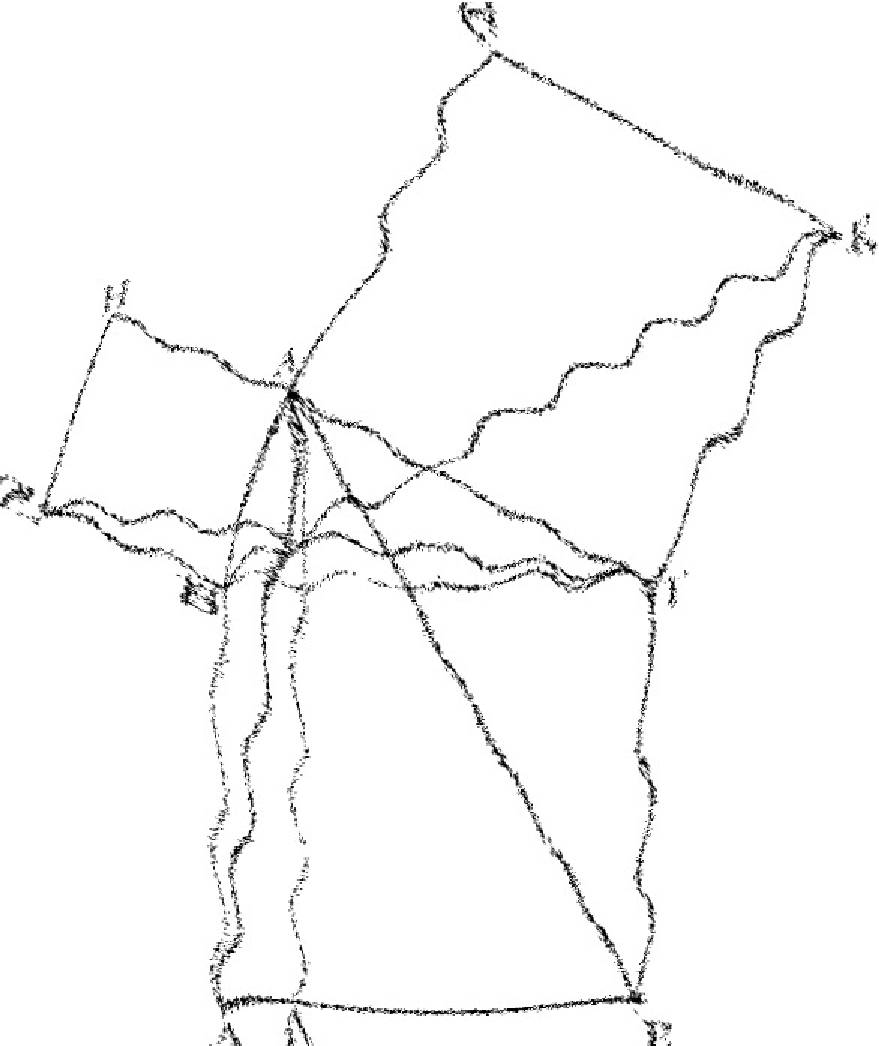
\includegraphics[width=0.8\textwidth]{Book01/front.pdf}}
\newpage

%%%%%%%
% Definitions
%%%%%%%
\pdfbookmark[1]{Definitions}{def1}
\pagestyle{fancy}
\cfoot{\gr{ }}
\lhead{\large\gr{ΣΤΟΙΘΕΙΩΝ  {1}.}}
\rhead{\large ELEMENTS BOOK 1}
\begin{Parallel}{}{} 
\ParallelLText{
\begin{center}
\large{\gr{ὍΟροι}.}
\end{center}
\vspace*{-7pt}

\ggn{1}.~\gr{Σημεῖόν ἐστιν, οὗ μέρος οὐθέν.}

\ggn{2}.~\gr{Γραμμὴ δὲ μῆκος ἀπλατές.}

\ggn{3}.~\gr{Γραμμῆς δὲ πέρατα σημεῖα.}

\ggn{4}.~\gr{Εὐθεῖα γραμμή ἐστιν, ἥτις ἐξ ἴσου τοῖς ἐφ'
ἑαυτῆς σημείοις κεῖται.}

\ggn{5}.~\gr{Ἐπιφάνεια δέ ἐστιν, ὃ μῆκος καὶ πλάτος μόνον ἔχει.}

\ggn{6}.~\gr{Ἐπιφανείας δὲ πέρατα  γραμμαί.}

\ggn{7}.~\gr{Ἐπίπεδος ἐπιφάνειά ἐστιν, ἥτις ἐξ ἴσου
ταῖς ἐφ' ἑαυτῆς εὐθείαις κεῖται.}

\ggn{8}.~\gr{Ἐπίπεδος δὲ γωνία ἐστὶν ἡ ἐν ἐπιπέδῳ δύο γραμμῶν
ἁπτομένων ἀλλήλων καὶ μὴ ἐπ' εὐθείας κειμένων πρὸς
ἀλλήλας τῶν γραμμῶν κλίσις.}

\ggn{9}.~\gr{ὍΟταν δὲ αἱ περιέθουσαι τὴν γωνίαν γραμμαὶ εὐθεῖαι ὦσιν, εὐθύγραμμος καλεῖται ἡ γωνία.}

\ggn{10}.~\gr{ὍΟταν δὲ εὐθεῖα ἐπ' εὐθεῖαν σταθεῖσα τὰξ ἐφεχῆς γωνίας ἴσας ἀλλήλαις ποιῆ|, ὀρθὴ ἑκατέρα τῶνὸίσων γωνιῶν
ἐστι, καὶ ἡ ἐφεστηκυῖα εὐθεῖα κάθετος καλεῖται, ἐφ' ἣν ἐφέστηκεν.}

\ggn{11}.~\gr{Ἀμβλεῖα γωνία ἐστὶν ἡ μείζων ὀρθῆς.}

\ggn{12}.~\gr{Ὀξεῖα δὲ ἡ ἐλάσσων ὀρθῆς.}

\ggn{13}.~\gr{ὍΟρος ἐστίν, ὅ τινόξ ἐστι πέρας.}

\ggn{14}.~\gr{Σχῆμά ἐστι τὸ ὑπό τινος ἢ τινων ὅρων περιεχόμενον.}

\ggn{15}.~\gr{Κύκλος ἐστὶ σχῆμα ἐπίπεδον ὑπὸ μιᾶς γραμμῆς περιεχόμενον [ἣ καλεῖται περιφέρεια], πρὸς ἣν ἀφ' ἑνὸς σημείου
τῶν ἐντὸς τοῦ σχήματος κειμένων πᾶσαι αἱ προσπίπτουσαι εὐθεῖαι
[πρὸς τὴν τοῦ κύκλου περιφέρειαν]  ἴσαι ἀλλήλαις εἰσίν.}

\ggn{16}.~\gr{Κέντρον δὲ τοῦ κύκλου τὸ σημεῖον καλεῖται.}

\ggn{17}.~\gr{Διάμετρος δὲ τοῦ κύκλου ἐστὶν εὐθεῖά τις διὰ τοῦ κέντρου
ἠγμένη καὶ περατουμένη ἐφ' ἑκάτερα τὰ μέρη ὑπὸ τῆς τοῦ κύκλου περιφερείας, ἥτις καὶ δίθα τέμνει τὸν κύκλον.}

\ggn{18}.~\gr{Ἡμικύκλιον δέ ἐστι τὸ περιεχόμενον σχῆμα ὑπό τε τῆς διαμέτρου καὶ τῆς ἀπολαμβανομένης ὑπὸ αὐτῆς περιφερείας. κέντρον δὲ τοῦ ἡμικυκλίου τὸ αὐτό, ὃ καὶ τοῦ κύκλου ἐστίν.}

\ggn{19}.~\gr{Σθήματα εὐθύγραμμά ἐστι τὰ ὑπὸ εὐθειῶν περιεχόμενα,
τρίπλευρα μὲν τὰ ὑπὸ τριῶν, τετράπλευρα
δὲ τὰ ὑπὸ τεσσάρων, πολύπλευρα δὲ τὰ ὑπὸ πλειόνωνὸὴ τεσσάρων
εὐθειῶν περιεχόμενα.}

\ggn{20}.~\gr{Τῶν δὲ τριπλεύρων σχημάτων ἰσόπλευρον μὲν τρίγωνόν ἐστι τὸ
τὰξ τρεῖς ἴσας ἔχον πλευράς, ἰσοσκελὲξ δὲ τὸ τὰξ δύο μόνας ἴσας ἔχον πλευράς, σκαληνὸν δὲ τὸ τὰξ τρεῖς ἀνίσους ἔχον πλευράς.}

\ggn{21}~\gr{ὸ'Ετι δὲ τῶν τριπλεύρων σχημάτων ὀρθογώνιον μὲν τρίγωνόν ἐστι τὸ  ἔχον ὀρθὴν γωνίαν,  ἀμβλυγώνιον δὲ τὸ  ἔχον ἀμβλεῖαν
γωνίαν, ὀξυγώνιον δὲ τὸ τὰξ τρεῖς ὀξείας ἔχον γωνίας.}

\ggn{22}.~\gr{Τὼν δὲ τετραπλεύρων σχημάτων τετράγωνον μέν ἐστιν, ὃ 
ἰσόπλευρόν τέ ἐστι καὶ ὀρθογώνιον, ἑτερόμ  ηκες δέ, ὃ
ὀρθογώνιον μέν, οὐκ ἰσόπλευρον δέ, ῥόμβος δέ, ὃ ἰσόπλευρον
μέν, οὐκ
ὀρθογώνιον δέ, ὁρομβοειδὲξ δὲ τὸ τὰξ ἀπεναντίον πλευράς τε καὶ γωνίας ἴσας ἀλλήλαις ἔχον, ὃ οοὔτε
ἰσόπλευρόν ἐστιν οοὔτε ὀρθογώνιον; τὰ δὲ παρὰ ταῦτα τετράπλευρα
τραπέζια καλείσθω.}

\ggn{23}.~\gr{Παράλληλοί εἰσιν εὐθεῖαι, αὁίτινες ἐν τῷ αὐτῷ ἐπιπέδῳ
οὸῦσαι καὶ ἐκβαλλόμεναι εἰξ ἄπειρον ἐφ' ἑκάτερα τὰ μέρη
ἐπὶ μ  ηδέτερα  συμπίπτουσιν ἀλλήλαις.}}

\ParallelRText{
\begin{center}
{\large Definitions}
\end{center}

1.~A point is that of which there is no part.

2.~And a line is a length without breadth.

3.~And the extremities of a line are points.

4.~A straight-line is (any) one which lies  evenly with points on itself.

5.~And a surface is that which has length and breadth only.

6.~And the extremities of a surface are lines.

7.~A plane surface is (any) one which lies evenly with the straight-lines on itself.

8.~And a plane angle is the inclination of the lines to one another, when two lines in a plane 
meet one another, and are not lying in a straight-line.

9.~And when the lines containing the angle are straight then the angle is called rectilinear.

10.~And when a straight-line stood upon (another) straight-line makes adjacent angles (which are) equal to one another, each of the equal angles is a
right-angle, and the former straight-line  is called a perpendicular to that upon which it stands.

11.~An obtuse angle is one greater than a right-angle.

12.~And an acute angle (is) one less than a right-angle.

13.~A boundary is that which is the extremity of something.

14.~A figure is that which is contained by some boundary or boundaries.

15.~A circle is a plane figure  contained by a single line [which is called a circumference], (such that) all of the straight-lines  radiating towards
 [the circumference] from one
point amongst those lying inside the figure  are equal to one another.

16.~And the point is called the center of the circle.

17.~And a diameter of the circle is any straight-line, being drawn through the
center, and terminated in each direction by the circumference of the circle. (And) any such (straight-line) also cuts the circle in half.$^\dag$

18.~And a semi-circle is the figure contained by the diameter  and
the circumference  cut off by it. And the center of the semi-circle is the same (point)
as (the center of) the circle.

19.~Rectilinear figures are those (figures) contained by straight-lines: trilateral
figures being those contained by three straight-lines,  quadrilateral   by four,
and multilateral by more than four.

20.~And of the trilateral figures: an equilateral triangle is that having
three equal sides, an isosceles (triangle) that having only two equal sides,
and a scalene (triangle) that having three unequal sides.

21.~And further of the trilateral figures: a right-angled triangle is that having
a right-angle, an obtuse-angled  (triangle) that having an obtuse
angle, and an acute-angled (triangle) that having three acute angles.

22.~And of the quadrilateral figures: a square is that which is right-angled
and equilateral, a rectangle that which is right-angled but not equilateral,
a rhombus that which is equilateral but not right-angled, and a rhomboid that
having opposite sides and angles equal to one another which is neither
right-angled nor equilateral. And let quadrilateral figures besides these be called
trapezia.

23.~Parallel lines are straight-lines which, being in the same plane, and
being produced to infinity in each direction, meet with one another in
neither (of these directions).}
\end{Parallel}
{\footnotesize 
\noindent $^\dag$ This should really be counted as a postulate, rather than as part of a definition.}

%%%%%%
% Postulates
%%%%%%
\begin{Parallel}{}{} 
\ParallelLText{
\begin{center}
{\large \gr{Αἰτήματα.}}
\end{center}\vspace*{-7pt}

\ggn{1}.~\gr{Ἠιτήσθω ἀπὸ παντὸς σημείου ἐπὶ πᾶν σημεῖον εὐθεῖαν
γραμμὴν ἀγαγεῖν.}

\ggn{2}.~\gr{Καὶ πεπερασμένην εὐθεῖαν κατὰ τὸ συνεθὲξ ἐπ' εὐθείας ἐκβαλεῖν.}

\ggn{3}.~\gr{Καὶ παντὶ κέντρῳ καὶ διαστήματι κύκλον γράφεσθαι.}

\ggn{4}.~\gr{Καὶ πάσας τὰξ ὀρθὰξ γωνίας ἴσας ἀλλήλαις εὸῖναι.}

\ggn{5}.~\gr{Καὶ ἒαν εἰξ δύο εὐθείας εὐθεῖα ἐμπίπτουσα τὰξ ἐντὸς
καὶ ἐπὶ τὰ αὐτὰ μέρη γωνίας δύο ὀρθῶν ἐλάσσονας ποιῆ|,
ἐκβαλλομένας τὰξ δύο εὐθείας ἐπ'  ἄπειρον συμπίπτειν, ἐφ' ὁὰ
μέρη εἰσὶν αἱ τῶν δύο ὀρθῶν ἐλάσσονες.}}

\ParallelRText{
\begin{center}
{\large Postulates}
\end{center}

1.~Let it be postulated$^\dag$ (that it is possible) to draw a straight-line from any point to any point;

2.~And to produce a finite straight-line continuously in a straight-line;

3.~And to draw a circle with any center and radius.

4.~And that all right-angles are equal to one another.

5.~And that if a straight-line falling across two (other) straight-lines makes 
internal angles on the same side (of itself whose sum is) less than two right-angles, (then) the two (other) straight-lines, being produced to infinity, meet on that side (of the original straight-line) that the (sum of the internal angles) is less
than two right-angles (and do not meet on the other side).$^\ddag$}
\end{Parallel}
{\footnotesize
\noindent $^\dag$ Literally, "let it have been postulated". 
The Greek present perfect tense indicates a past action with present
significance. Hence, the 3rd-person present perfect imperative \gr{ἠιτήσθω} means  ``let it be postulated" in the sense ``let it stand as postulated", but not  ``let the
postulate be now brought forward". This peculiar Greek idiom is used throughout the Elements.\\
\noindent $^\ddag$ This postulate effectively specifies that we are dealing with the geometry of
flat, rather than  curved, space.}

%%%%%%%%%%
% Common Notions
%%%%%%%%%%
\begin{Parallel}{}{} 
\ParallelLText{
\begin{center}
{\large \gr{Κοιναὶ ὸέννοιαι.}}
\end{center}\vspace*{-7pt}

\ggn{1}.~\gr{Τὰ τῷ αὐτῷ  ἴσα καὶ ἀλλήλοις ἐστὶν ἴσα.}

\ggn{2}.~\gr{Καὶ ἒανὸίσοις ἴσα προστεθῆ|, τὰ ὅλα ἐστὶν ἴσα.}

\ggn{3}.~\gr{Καὶ ἒαν ἀπὸ ὸίσων ἴσα ἀφαιρεθῆ|, τὰ καταλειπόμενά ἐστιν ἴσα.}

\ggn{4}.~\gr{Καὶ τὰ ἐφαρμόζοντα ἐπ' ἀλλήλα ἴσα ἀλλήλοις ἐστίν.}

\ggn{5}.~\gr{Καὶ τὸ ὅλον τοῦ μέρους μεῖζόν [ἐστιν].}}

\ParallelRText{
\begin{center}
{\large Common Notions}
\end{center}

1.~Things equal to the same thing are also equal to one another.

2.~And  if equal things are added to equal things (then) the wholes are equal.

3.~And if equal things are subtracted from equal things (then) the remainders are
equal.$^\dag$

4.~And things coinciding with one another are equal to one another.

5.~And the whole [is] greater than the part.}
\end{Parallel}
{\footnotesize
\noindent $^\dag$ As an obvious extension of C.N.s~2 \& 3---if equal things
are added or subtracted from the two sides of an inequality then  the inequality
remains an inequality of the same type.}\\~\\

%%%%%%
% Prop 1.1
%%%%%%
\pdfbookmark[1]{Proposition 1.1}{prop1.1}
\begin{Parallel}{}{} 
\ParallelLText{
\begin{center}
{\large \ggn{1}.}
\end{center}\vspace*{-7pt}

\gr{Ἐπὶ τῆς δοθείσης εὐθείας πεπερασμένης τρίγωνον ἰσόπλευρον συστήσασθαι.}

\gr{Ἔστω ἡ δοθεῖσα εὐθεῖα πεπερασμένη ἡ ΑΒ.}

\gr{Δεῖ δὴ ἐπὶ τῆς ΑΒ εὐθείας τρίγωνον ἰσόπλευρον συστήσνασθαι.}

% Removed epsf size command
\centerline{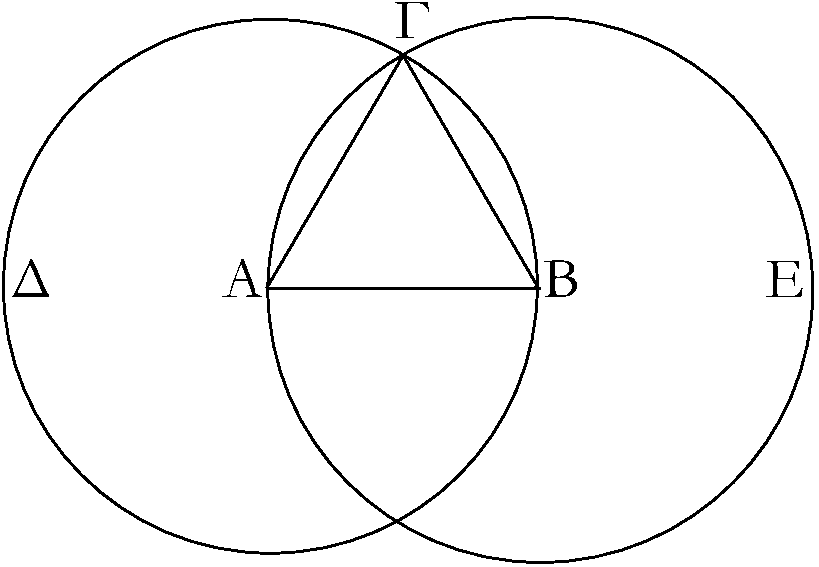
\includegraphics[width=0.8\textwidth]{Book01/fig01g.pdf}}

\gr{Κέντρῳ μὲν τῷ Α διαστήματι δὲ τῷ ΑΒ κύκλος γεγράφθω ὁ ΒΓΔ,
καὶ πάλιν κέντρῳ μὲν τῷ Β διαστήματι δὲ τῷ ΒΑ κύκλος γεγράφθω
ὁ ΑΓΕ, καὶ ἀπὸ τοῦ Γ σημείου, καθὸ ὃ τέμνουσιν ἀλλήλους οἱ
κύκλοι, ἐπί τὰ Α, Β σημεῖα ἐπεζεύθθωσαν εὐθεῖαι αἱ ΓΑ, ΓΒ.}

\gr{Καὶ ἐπεὶ τὸ Α σημεῖον κέντρον ἐστὶ τοῦ ΓΔΒ κύκλου, ὸίση ἐστὶν
ἡ ΑΓ τῇ ΑΒ; πάλιν, ἐπεὶ τὸ Β σημεῖον κέντρον ἐστὶ τοῦ ΓΑΕ
κύκλου, ὸίση ἐστὶν ἡ ΒΓ τῇ ΒΑ. ἐδείθθη δὲ καὶ ἡ ΓΑ τῇ  ΑΒὸίση;
ἑκατέρα ἄρα τῶν ΓΑ, ΓΒ τῇ ΑΒ ἐστινὸίση. τὰ δὲ τῷ αὐτῷ
 ἴσα καὶ ἀλλήλοις ἐστὶν ἴσα;  καὶ ἡ ΓΑ ἄρα τῇ ΓΒ ἐστινὸίση;
αἱ τρεῖς ἄρα αἱ ΓΑ, ΑΒ, ΒΓ ἴσαι ἀλλήλαις εἰσίν.}

\gr{Ἰσόπλευρον ἄρα ἐστὶ τὸ ΑΒΓ τρίγωνον. καὶ συνέσταται ἐπὶ
τῆς δοθείσης εὐθείας πεπερασμένης τῆς ΑΒ. ὅπερ ἔδει ποιῆσαι.}}

\ParallelRText{
\begin{center}
{\large Proposition 1}
\end{center}
To construct an equilateral triangle on a given finite straight-line.

Let $AB$ be the given finite straight-line.

So it is required to construct an equilateral triangle on the straight-line $AB$.

% Removed epsf size command
\centerline{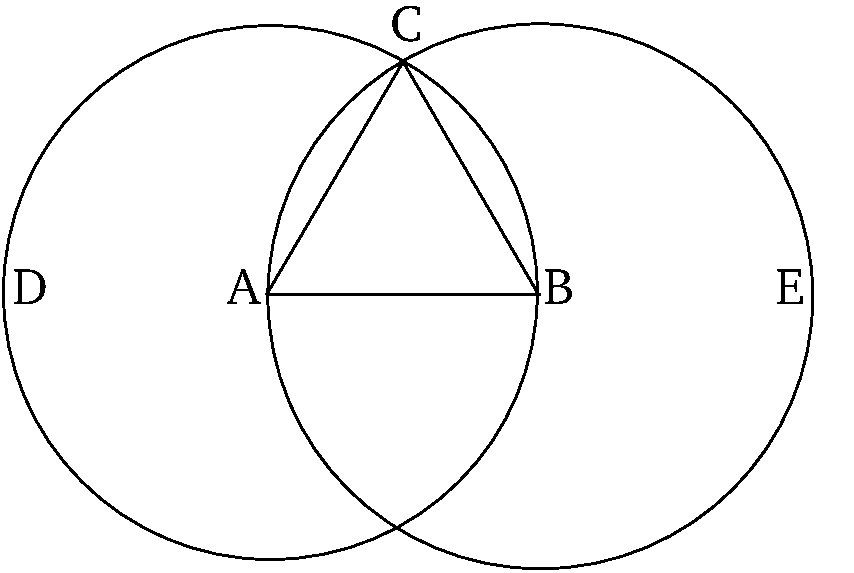
\includegraphics[width=0.8\textwidth]{Book01/fig01e.pdf}}

Let the circle $BCD$ with center $A$ and radius $AB$ be drawn$^\dag$ [Post.~3], and again
let the circle $ACE$ with center $B$ and radius $BA$ be drawn [Post.~3].
And let the straight-lines $CA$ and $CB$ be joined from the point $C$, where the circles cut one another,$^\ddag$ to the points $A$ and $B$ (respectively) [Post.~1].

And since the point $A$ is the center of the circle $CDB$, $AC$ is equal to $AB$ [Def.~1.15]. Again,
since the point $B$ is the center of the circle $CAE$, $BC$ is equal to $BA$ [Def.~1.15]. But $CA$ 
was also shown (to be) equal to $AB$. Thus, $CA$ and $CB$ are each equal to $AB$. But things equal to the same thing are also equal to one another [C.N.~1]. Thus, $CA$ is also equal to $CB$. Thus, the three (straight-lines) $CA$, $AB$, and $BC$ are equal to one another.

Thus, the triangle $ABC$ is equilateral, and has been constructed on the
given finite straight-line $AB$. (Which is) the very thing it was required to do.}
\end{Parallel}
{\footnotesize
\noindent $^\dag$ Literally, "have been drawn". The use of this peculiar Greek idiom will pass
without further comment.\\
\noindent $^\ddag$ The assumption that the circles do indeed cut one another should be counted as an additional 
postulate. There is also an implicit assumption that two straight-lines cannot share a common segment.}

%%%%%%
% Prop 1.2
%%%%%%
\pdfbookmark[1]{Proposition 1.2}{pdf1.2}
\begin{Parallel}{}{} 
\ParallelLText{
\begin{center}
{\large \ggn{2}.}
\end{center}\vspace*{-7pt}

\gr{Πρὸξ τῷ δοθέντι σημείῳ τῇ δοθείσῃ εὐθείᾳ  ἴσην εὐθεῖαν θέσθαι.}

\gr{Ἔστω τὸ μὲν δοθὲν σημεῖον τὸ Α, ἡ δὲ δοθεῖσα εὐθεῖα ἡ ΒΓ;
δεῖ δὴ πρὸς τῷ Α σημείῳ τῇ δοθείσῃ εὐθείᾳ τῇ ΒΓ ἴσην εὐθεῖαν θέσθαι.}

\gr{Ἐπεζεύθθω γὰρ ἀπὸ τοῦ Α σημείου ἐπί τὸ Β σημεῖον εὐθεῖα
ἡ ΑΒ, καὶ συνεστάτω ἐπ' αὐτῆς τρίγωνον ἰσόπλευρον τὸ ΔΑΒ, καὶ
ἐκβεβλήσθωσαν ἐπ' εὐθείας ταῖς  ΔΑ, ΔΒ εὐθεῖαι αἱ ΑΕ, ΒΖ, καὶ
κέντρῳ μὲν τῷ Β διαστήματι δὲ τῷ ΒΓ κύκλος γεγράφθω ὁ
ΓΗΘ, καὶ πάλιν κέντρῳ τῷ Δ καὶ διαστήματι τῷ ΔΗ κύκλος γεγράφθω ὁ
ΗΚΛ.}\\

% Removed epsf size command
\centerline{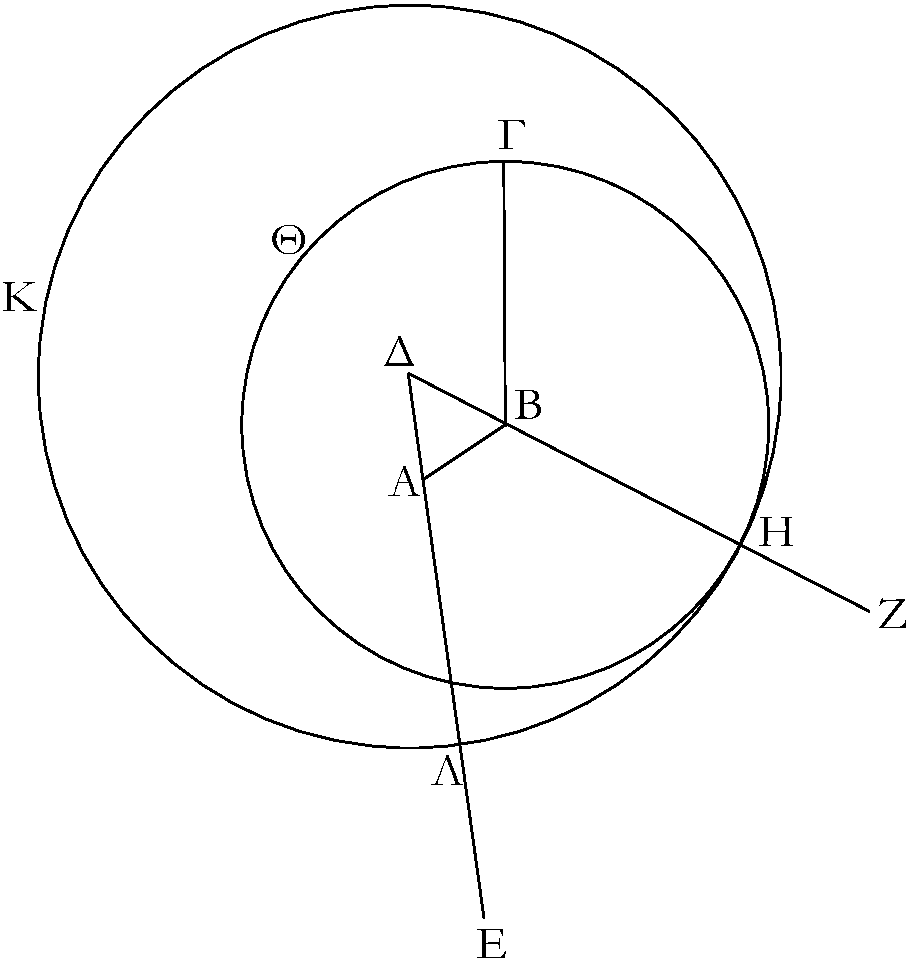
\includegraphics[width=0.8\textwidth]{Book01/fig02g.pdf}}

\gr{Ἐπεὶ οὸῦν τὸ Β σημεῖον κέντρον ἐστὶ τοῦ ΓΗΘ, ὸίση ἐστὶν
ἡ ΒΓ τῇ ΒΗ. πάλιν, ἐπεὶ τὸ Δ σημεῖον κέντρον ἐστὶ τοῦ
ΗΚΛ κύκλου, ὸίση ἐστὶν ἡ ΔΛ τῇ ΔΗ, ὁῶν ἡ ΔΑ τῇ ΔΒὸίση ἐστίν.
λοιπὴ  ἄρα ἡ ΑΛ λοιπῆ| τῇ ΒΗ ἐστινὸίση. 
ἐδείθθη δὲ καὶ ἡ ΒΓ τῇ ΒΗὸίση;
ἑκατέρα ἄρα τῶν ΑΛ, ΒΓ
τῇ ΒΗ ἐστινὸίση. τὰ δὲ τῷ αὐτῷ  ἴσα καὶ ἀλλήλοις ἐστὶν ἴσα; καὶ ἡ ΑΛ ἄρα τῇ ΒΓ ἐστινὸίση.}

\gr{Πρὸξ ἄρα τῷ δοθέντι σημείῳ τῷ Α τῇ δοθείσῃ εὐθείᾳ τῇ ΒΓὸίση εὐθεῖα κεῖται ἡ ΑΛ; ὅπερ ἔδει ποιῆσαι.}}

\ParallelRText{
\begin{center}
{\large Proposition 2$^\dag$}
\end{center}

To place a straight-line equal to a given straight-line at a given point (as an extremity).

Let $A$ be the given point, and $BC$ the given straight-line. So  it is required to
place a straight-line at point $A$ equal to the given straight-line $BC$.

For  let the straight-line $AB$ be joined from point $A$ to point $B$ [Post.~1], and let the
equilateral triangle $DAB$ be  constructed upon it [Prop.~1.1].  And let the
straight-lines $AE$ and $BF$ be produced in a straight-line with $DA$ and $DB$  (respectively) [Post.~2].
And let the circle $CGH$ with center $B$ and radius $BC$ be drawn
[Post.~3], and again let the circle $GKL$ with center $D$ and radius $DG$ be drawn [Post.~3].

% Removed epsf size command
\centerline{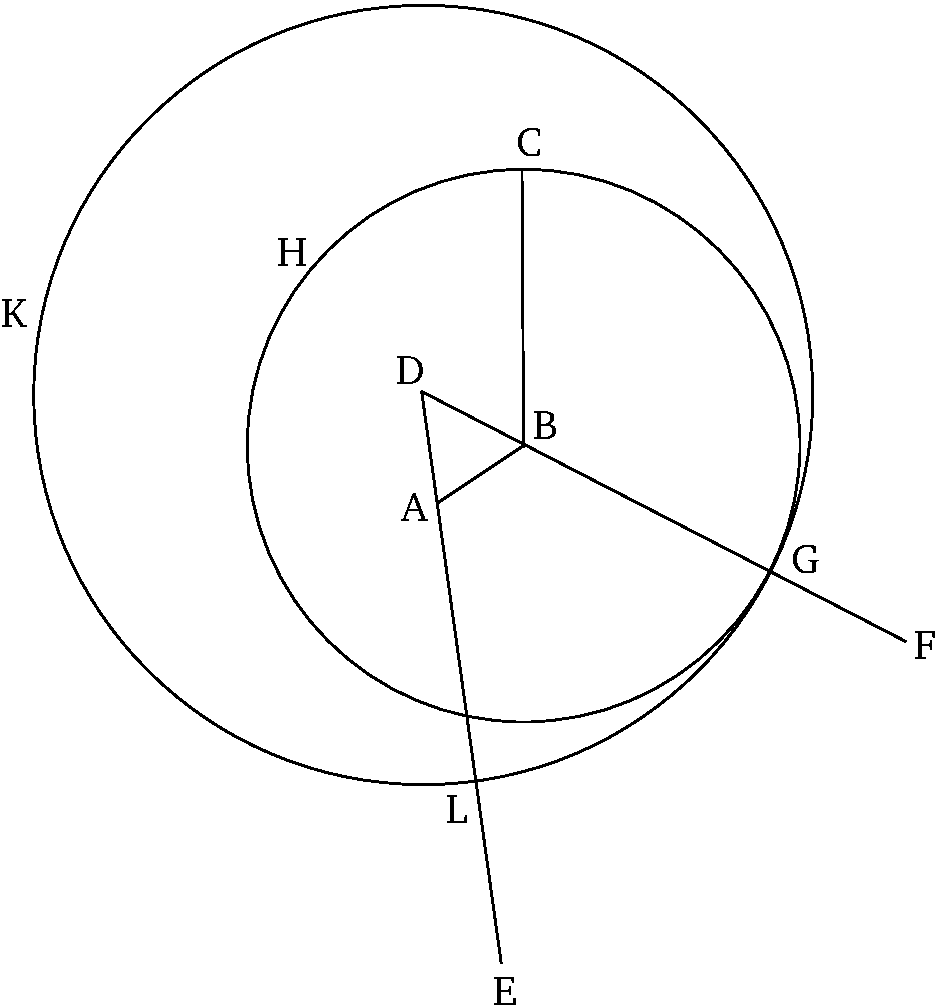
\includegraphics[width=0.8\textwidth]{Book01/fig02e.pdf}}

Therefore, since the point $B$ is the center of (the circle) $CGH$, $BC$ is equal to 
$BG$ [Def.~1.15]. Again, since the point $D$ is the center of the circle $GKL$, $DL$ is equal to $DG$ [Def.~1.15]. And within these,  $DA$ is equal to $DB$. Thus, the remainder $AL$ is equal to the remainder $BG$ [C.N.~3]. But $BC$ was also shown (to be)  equal to $BG$. Thus,  $AL$
and $BC$ are each equal to $BG$. But things equal to the same thing are also equal to one another [C.N.~1]. Thus, $AL$ is also equal to $BC$.

Thus, the straight-line $AL$, equal to the given straight-line $BC$,
has been placed at the given point $A$. (Which is) the very thing it was required to do.}
\end{Parallel}
{\footnotesize
\noindent $^\dag$ This proposition admits of a number
of different cases, depending on the relative positions of the point $A$
and the line $BC$. In such situations, Euclid invariably only considers one
particular case---usually, the most difficult---and leaves the remaining cases as
exercises for the reader.}

%%%%%%
% Prop 1.3
%%%%%%
\pdfbookmark[1]{Proposition 1.3}{pdf1.3}
\begin{Parallel}{}{} 
\ParallelLText{
\begin{center}
{\large \ggn{3}.}
\end{center}\vspace*{-7pt}

\gr{Δύο δοθεισῶν εὐθειῶν ἀνίσων ἀπὸ τῆς μείζονος τῇ ἐλάσσονι ἴσην εὐθεῖαν ἀφελεῖν.}

\gr{Ἔστωσαν αἱ δοθεῖσαι δύο εὐθεῖαιὸάνισοι αἱ ΑΒ, Γ, ὁῶν μείζωνὸέστω ἡ ΑΒ; δεῖ δὴ ἀπὸ τῆς μείζονος τῆς ΑΒ τῇ ἐλάσσονι τῇ Γ ἴσην εὐθεῖαν ἀφελεῖν.}

\gr{Κείσθω πρὸς τῷ Α σημείῳ τῇ Γ εὐθείᾳ ὸίση ἡ ΑΔ; καὶ κέντρῳ μὲν τῷ Α διαστήματι δὲ τῷ ΑΔ κύκλος γεγράφθω ὁ ΔΕΖ.}

\gr{Καὶ ἐπεὶ τὸ Α σημεῖον κέντρον ἐστὶ τοῦ ΔΕΖ κύκλου, ὸίση ἐστὶν ἡ ΑΕ τῇ ΑΔ; ἀλλὰ καὶ ἡ Γ τῇ ΑΔ ἐστινὸίση. ἑκατέρα ἄρα τῶν ΑΕ, Γ τῇ ΑΔ ἐστινὸίση; ὁώστε καὶ ἡ ΑΕ τῇ Γ ἐστινὸίση.}

% Removed epsf size command
\centerline{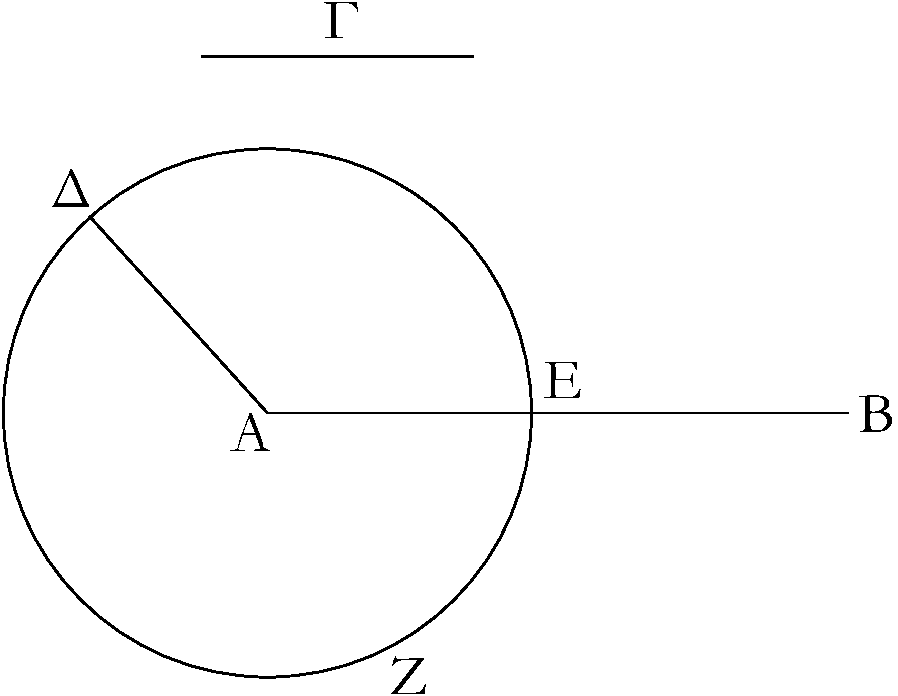
\includegraphics[width=0.8\textwidth]{Book01/fig03g.pdf}}

\gr{Δύο ἄρα δοθεισῶν εὐθειῶν ἀνίσων τῶν ΑΒ, Γ ἀπὸ τῆς μείζονος τῆς ΑΒ τῇ ἐλάσσονι τῇ Γὸίση ἀφή|ρηται ἡ ΑΕ; ὅπερ ἔδει
ποιῆσαι.}}

\ParallelRText{
\begin{center}
{\large Proposition 3}
\end{center}

For two given unequal straight-lines, to cut off from the greater a straight-line
equal to the lesser.

Let $AB$ and $C$ be the two given unequal straight-lines, of which let the greater be $AB$. So it is required to cut off a straight-line equal to the lesser $C$ from the greater $AB$.

Let the line $AD$, equal to the straight-line $C$, be placed at  point $A$ [Prop.~1.2]. And let
the circle $DEF$ be drawn with center $A$ and radius $AD$ [Post.~3].

And since  point $A$ is the center of  circle $DEF$, $AE$ is equal to $AD$ [Def.~1.15]. But,
$C$ is also equal to $AD$. Thus, $AE$ and $C$ are each equal to $AD$. So $AE$
is also equal to $C$ [C.N.~1].\\

% Removed epsf size command
\centerline{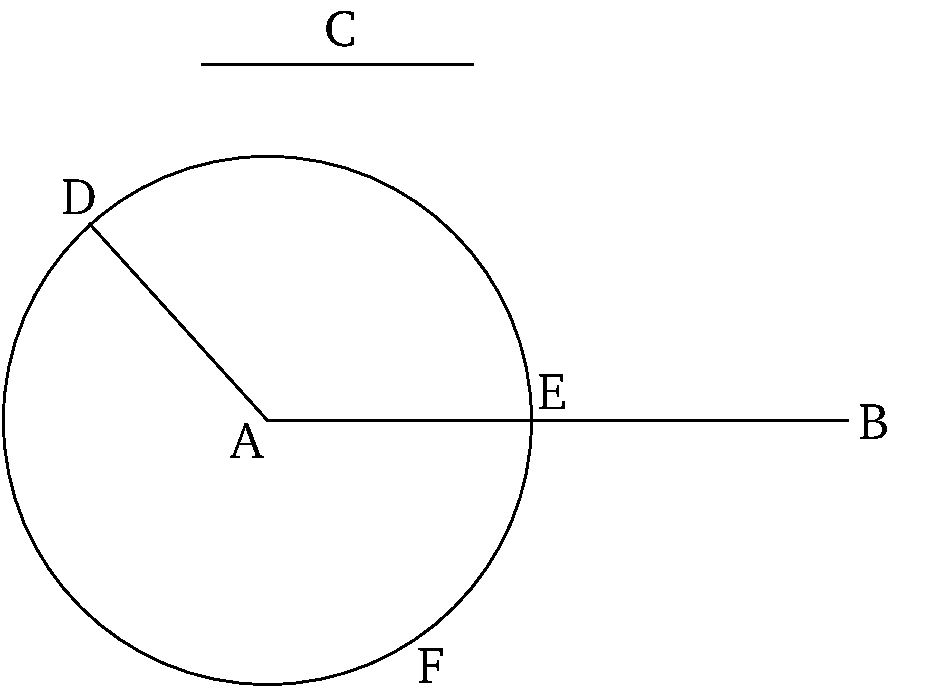
\includegraphics[width=0.8\textwidth]{Book01/fig03e.pdf}}

Thus, for two given unequal straight-lines, $AB$ and $C$, the (straight-line) $AE$, equal to
the lesser $C$, has been cut off from the greater $AB$. (Which is) the very thing it was required to do.}
\end{Parallel}

%%%%%%
% Prop 1.4
%%%%%%
\pdfbookmark[1]{Proposition 1.4}{pdf1.4}
\begin{Parallel}{}{} 
\ParallelLText{
\begin{center}
{\large \ggn{4}.}
\end{center}\vspace*{-7pt}

\gr{Ἐὰν δύο τρίγωνα τὰξ δύο πλευρὰξ [ταῖς] δυσὶ πλευραῖξ ἴσαςὸέθῃ ἑκατέραν ἑκατέρᾳ καὶ τὴν γωνίαν τῇ γωνίᾳ  ἴσηνὸέθῃ τὴν ὑπὸ τῶνὸίσων εὐθειῶν περιεθομένην, καὶ τὴν βάσιν τὴ| βάσει ἴσην ὁέχει, καὶ τὸ τρίγωνον τῷ τριγώνῳ  ἴσονὸέσται, καὶ αἱ λοιπαὶ γωνίαι ταῖς λοιπαῖξ γωνίαις ἴσαιὸέσονται ἑκατέρα ἑκατέρᾳ, ὑφὸ ὁὰξ αἱ
 ἴσαι πλευραὶ ὑποτείνουσιν.}

% Removed epsf size command
\centerline{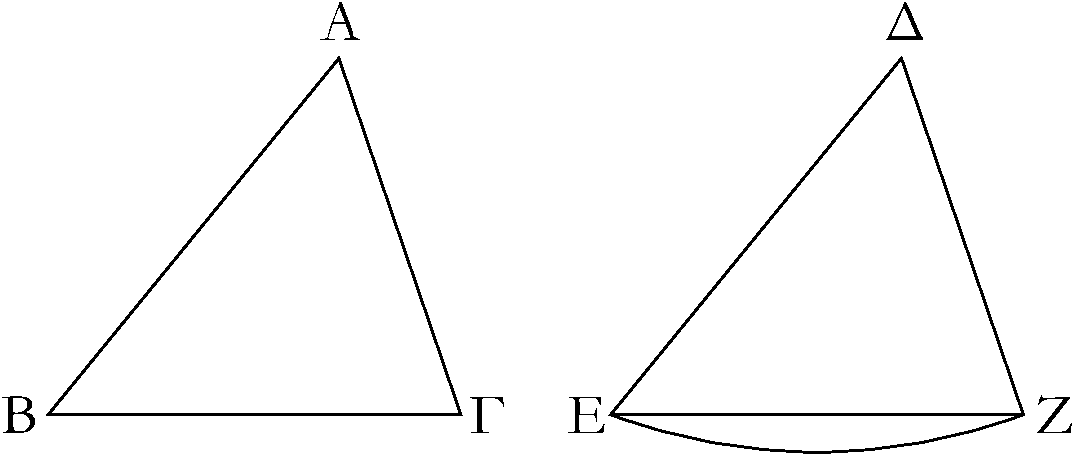
\includegraphics[width=0.8\textwidth]{Book01/fig04g.pdf}}

\gr{Ἔστω δύο τρίγωνα τὰ ΑΒΓ, ΔΕΖ τὰξ δύο πλευρὰξ τὰξ ΑΒ, ΑΓ ταῖς δυσὶ πλευραῖξ ταῖς ΔΕ, ΔΖ ἴσας ἔχοντα ἑκατέραν ἑκατέρᾳ τὴν μὲν ΑΒ τῇ ΔΕ τὴν δὲ ΑΓ τῇ ΔΖ καὶ γωνίαν τὴν ὑπὸ ΒΑΓ γωνίᾳ τῇ ὑπὸ ΕΔΖ ἴσην. λέγω, ὅτι καὶ βάσις ἡ ΒΓ βάσει τῇ ΕΖὸίση ἐστίν, καὶ τὸ ΑΒΓ τρίγωνον τῷ ΔΕΖ τριγώνῳ  ἴσονὸέσται, 
καὶ αἱ λοιπαὶ γωνίαι ταῖς λοιπαῖξ γωνίαις ἴσαιὸέσονται ἑκατέρα ἑκατέρᾳ, ὑφὸ ὁὰξ αἱ  ἴσαι πλευραὶ ὑποτείνουσιν, ἡ μὲν ὑπὸ ΑΒΓ τῇ ὑπὸ ΔΕΖ, ἡ δὲ ὑπὸ ΑΓΒ τῇ ὑπὸ ΔΖΕ.}

\gr{Ἐφαρμοζομένου γὰρ τοῦ ΑΒΓ τριγώνου ἐπὶ τὸ ΔΕΖ τρίγωνον καὶ τιθεμένου τοῦ μὲν Α σημείου ἐπὶ τὸ Δ σημεῖον τῆς δὲ ΑΒ εὐθείας ἐπὶ τὴν ΔΕ, ἐφαρμόσει καὶ τὸ Β σημεῖον ἐπὶ τὸ Ε διὰ τὸ  ἴσην εὸῖναι τὴν ΑΒ τῇ ΔΕ; ἐφαρμοσάσης δὴ τῆς ΑΒ ἐπὶ τὴν ΔΕ ἐφαρμόσει καὶ ἡ ΑΓ εὐθεῖα ἐπὶ τὴν ΔΖ διὰ τὸ  ἴσην εὸῖναι τὴν ὑπὸ ΒΑΓ γωνίαν τῇ ὑπὸ ΕΔΖ; ὁώστε καὶ τὸ Γ σημεῖον ἐπὶ τὸ Ζ σημεῖον ἐφαρμόσει διὰ τὸ  ἴσην πάλιν εὸῖναι τὴν ΑΓ τῇ ΔΖ. ἀλλὰ μὴν καὶ τὸ Β ἐπὶ τὸ Ε ἐφηρμόκει; ὁώστε βάσις ἡ ΒΓ ἐπὶ βάσιν τὴν ΕΖ ἐφαρμόσει. εἰ γὰρ τοῦ μὲν Β ἐπὶ τὸ Ε ἐφαρμόσαντος τοῦ δὲ Γ ἐπὶ τὸ Ζ ἡ ΒΓ βάσις ἐπὶ τὴν ΕΖ οὐκ ἐφαρμόσει, δύο εὐθεῖαι θωρίον περιέχουσιν; ὅπερ ἐστὶν ἀδύνατον. ἐφαρμόσει ἄρα ἡ ΒΓ βάσις ἐπὶ τὴν ΕΖ καὶ ὸίση αὐτῇ ὸέσται; ὁώστε καὶ ὅλον τὸ ΑΒΓ 
τρίγωνον ἐπὶ ὅλον τὸ ΔΕΖ τρίγωνον ἐφαρμόσει καὶ  ἴσον αὐτῷ ὸέσται, καὶ
αἱ λοιπαὶ γωνίαι ἐπὶ τὰξ λοιπὰξ γωνίας ἐφαρμόσουσι καὶ  ἴσαι αὐταῖςὸέσονται, ἡ μὲν ὑπὸ ΑΒΓ τῇ ὑπὸ ΔΕΖ ἡ δὲ ὑπὸ ΑΓΒ τῇ ὑπὸ ΔΖΕ.}

\gr{Ἐὰν ἄρα δύο τρίγωνα τὰξ δύο πλευρὰξ [ταῖς] δύο πλευραῖξ ἴσαςὸέθῃ ἑκατέραν ἑκατέρᾳ καὶ τὴν γωνίαν τῇ γωνίᾳ  ἴσηνὸέθῃ τὴν ὑπὸ τῶνὸίσων εὐθειῶν περιεθομένην, καὶ τὴν βάσιν τὴ| βάσει ἴσην ὁέχει, καὶ τὸ τρίγωνον τῷ τριγώνῳ  ἴσονὸέσται, καὶ αἱ λοιπαὶ γωνίαι ταῖς λοιπαῖξ γωνίαις ἴσαιὸέσονται ἑκατέρα ἑκατέρᾳ, ὑφὸ ὁὰξ αἱ
 ἴσαι πλευραὶ ὑποτείνουσιν; ὅπερ ἔδει δεῖχαι.}}

\ParallelRText{
\begin{center}
{\large Proposition 4}
\end{center}

If two triangles have two  sides equal to two sides, respectively, and have the
angle(s) enclosed by the equal straight-lines equal, (then)
they will also have the base equal to the base, and the triangle will be equal
to the triangle,  and
the remaining angles subtended by the equal sides will be equal to the corresponding remaining angles.

% Removed epsf size command
\centerline{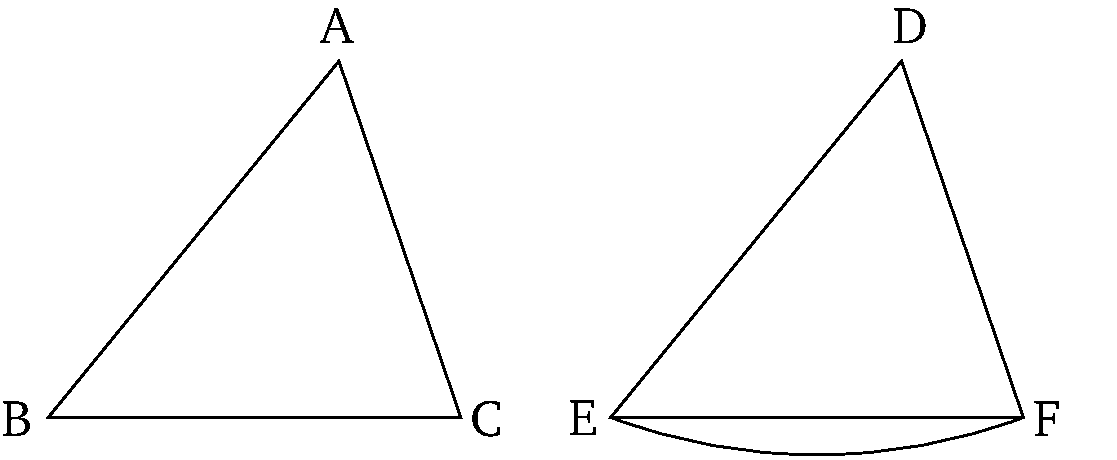
\includegraphics[width=0.8\textwidth]{Book01/fig04e.pdf}}

Let $ABC$ and $DEF$ be  two triangles having the two sides $AB$ and $AC$ equal to the two sides $DE$ and $DF$, respectively. (That is) $AB$ to $DE$, and $AC$ to $DF$. And (let) the angle $BAC$ (be) equal to the angle $EDF$. I say that the base $BC$ is also equal to the base
$EF$, and  triangle $ABC$ will be equal to triangle $DEF$, and the remaining angles
subtended by the equal sides will be equal to the corresponding remaining angles. (That is) $ABC$ to $DEF$, and $ACB$ to
$DFE$.

For if triangle $ABC$ is applied to triangle $DEF$,$^\dag$ the point $A$ being placed
on the point $D$, and the straight-line $AB$ on $DE$, (then) the point $B$ will also coincide with $E$, on account of $AB$ being equal to $DE$. So (because of) $AB$ coinciding with $DE$, the straight-line $AC$ will also coincide with $DF$, on account of the angle $BAC$ being equal to $EDF$. So the point $C$ will also coincide with the
point $F$,  again on account of $AC$ being equal to $DF$.  But,  point $B$  certainly also coincided with point $E$, so that the base $BC$ will coincide with the base $EF$.
For if $B$ coincides with $E$, and $C$ with $F$, and the base $BC$ does not coincide with $EF$, (then) two straight-lines will encompass an area. The very thing is impossible [Post.~1].$^\ddag$ Thus, the base $BC$ will coincide with $EF$, and will be equal to it [C.N.~4]. So  the whole triangle $ABC$ will coincide with the whole triangle $DEF$, and will be equal to it [C.N.~4]. And the remaining angles will coincide with the remaining angles, and  will be equal to them [C.N.~4]. (That is) $ABC$ to $DEF$, and $ACB$
to $DFE$ [C.N.~4].

Thus, if two triangles have two  sides equal to two sides, respectively, and have the
angle(s) enclosed by the equal straight-lines equal, (then)
they will also have the base equal to the base, and the triangle will be equal
to the triangle,  and
the remaining angles subtended by the equal sides will be equal to the
corresponding remaining angles. (Which is) the very thing it was required to show.}
\end{Parallel}
{\footnotesize
\noindent $^\dag$ The application of one figure to another should be counted as an additional postulate.\\[0.5ex]
$^\ddag$ Since Post.~1 implicitly assumes that the straight-line
joining two given points is unique.}

%%%%%%
% Prop 1.5
%%%%%%
\pdfbookmark[1]{Proposition 1.5}{pdf1.5}
\begin{Parallel}{}{} 
\ParallelLText{
\begin{center}
{\large \ggn{5}.}
\end{center}\vspace*{-7pt}

\gr{Τῶν ἰσοσκελῶν τριγώνων αἱ πρὸς τῇ βάσει γωνίαι ἴσαι ἀλλήλαις εἰσίν, καὶ προσεκβληθεισῶν τῶνὸίσων εὐθειῶν αἱ ὑπὸ τὴν βάσιν γωνίαι ἴσαι ἀλλήλαιςὸέσονται.}

\gr{Ἔστω τρίγωνον ἰσοσκελὲξ τὸ ΑΒΓ ἴσην ἔχον τὴν ΑΒ πλευρὰν τῇ ΑΓ πλευρᾶ|, καὶ προσεκβεβλήσθωσαν ἐπ' εὐθείας ταῖς ΑΒ,  ΑΓ εὐθεῖαι αἱ ΒΔ, ΓΕ; λέγω, ὅτι ἡ μὲν ὑπὸ ΑΒΓ γωνία τῇ ὑπὸ ΑΓΒὸίση ἐστίν, ἡ δὲ ὑπὸ ΓΒΔ τῇ ὑπὸ ΒΓΕ.}

\gr{Εἰλήφθω γὰρ ἐπὶ τῆς ΒΔ τυθὸν σημεῖον τὸ Ζ, καὶ ἀφῃρήσθω ἀπὸ τῆς μείζονος τῆς ΑΕ τῇ ἐλάσσονι τῇ ΑΖὸίση ἡ ΑΗ, καὶ ἐπεζεύθθωσαν αἱ ΖΓ, ΗΒ εὐθεῖαι.}\\

% Removed epsf size command
\centerline{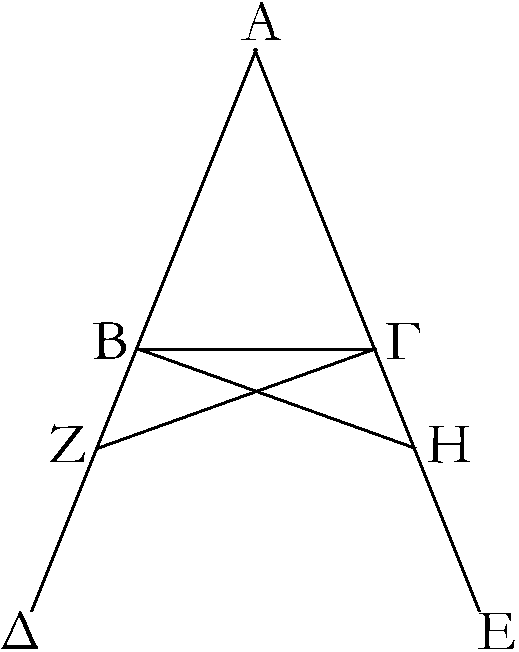
\includegraphics[width=0.8\textwidth]{Book01/fig05g.pdf}}

\gr{Ἐπεὶ οὸῦνὸίση ἐστὶν ἡ μὲν ΑΖ τῇ ΑΗ ἡ δὲ ΑΒ τῇ ΑΓ, δύο δὴ αἱ ΖΑ, ΑΓ δυσὶ ταῖς ΗΑ, ΑΒ ἴσαι εἰσὶν ἑκατέρα ἑκατέρᾳ; καὶ γωνίαν κοινὴν περιέθουσι τὴν ὑπὸ ΖΑΗ; βάσις ἄρα ἡ ΖΓ βάσει τῇ ΗΒὸίση ἐστίν, καὶ τὸ ΑΖΓ τρίγωνον τῷ ΑΗΒ τριγώνῳ  ἴσονὸέσται, καὶ αἱ λοιπαὶ γωνίαι ταῖς λοιπαῖξ γωνίαις ἴσαιὸέσονται ἑκατέρα ἑκατέρᾳ, ὑφὸ ὁὰξ αἱ  ἴσαι πλευραὶ ὑποτείνουσιν, ἡ μὲν ὑπὸ ΑΓΖ τῇ ὑπὸ ΑΒΗ, ἡ δὲ ὑπὸ ΑΖΓ τῇ ὑπὸ ΑΗΒ. καὶ ἐπεὶ ὅλη ἡ ΑΖ ὅλῃ τῇ ΑΗ ἐστινὸίση, ὁῶν ἡ ΑΒ τῇ ΑΓ ἐστινὸίση, λοιπὴ
 ἄρα ἡ ΒΖ λοιπῆ| τῇ ΓΗ ἐστινὸίση. ἐδείθθη δὲ καὶ ἡ ΖΓ τῇ ΗΒὸίση; δύο δὴ αἱ ΒΖ, ΖΓ δυσὶ ταῖς ΓΗ, ΗΒ ἴσαι εἰσὶν ἑκατέρα ἑκατέρᾳ; καὶ γωνία ἡ ὑπὸ ΒΖΓ γωνίᾳ  τῃ ὑπὸ ΓΗΒὸίση, καὶ βάσις αὐτῶν κοινὴ ἡ ΒΓ; καὶ τὸ ΒΖΓ ἄρα τρίγωνον τῷ ΓΗΒ τριγώνῳ
 ἴσονὸέσται, καὶ αἱ λοιπαὶ γωνίαι ταῖς λοιπαῖξ γωνίαις ἴσαιὸέσονται ἑκατέρα  ἑκατέρᾳ, ὑφὸ ὁὰξ αἱ  ἴσαι πλευραὶ ὑποτείνουσιν; ὸίση ἄρα ἐστὶν ἡ μὲν ὑπὸ ΖΒΓ τῇ ὑπὸ ΗΓΒ ἡ δὲ ὑπὸ ΒΓΖ τῇ ὑπὸ ΓΒΗ. ἐπεὶ οὸῦν ὅλη ἡ ὑπὸ ΑΒΗ γωνία ὅλῃ τῇ ὑπὸ ΑΓΖ γωνίᾳ ἐδείθθηὸίση, ὁῶν ἡ ὑπὸ ΓΒΗ τῇ ὑπὸ ΒΓΖὸίση, λοιπὴ
 ἄρα ἡ ὑπὸ
ΑΒΓ λοιπῆ| τῇ ὑπὸ ΑΓΒ ἐστινὸίση; καί εἰσι πρὸς τῇ βάσει τοῦ ΑΒΓ τριγώνου. ἐδείθθη δὲ καὶ ἡ ὑπὸ ΖΒΓ τῇ ὑπὸ ΗΓΒὸίση; καί εἰσιν ὑπὸ τὴν βάσιν.}

\gr{Τῶν ἄρα ἰσοσκελῶν τριγώνων αἱ τρὸξ τῇ βάσει γωνίαι ἴσαι ἀλλήλαις εἰσίν, καὶ προσεκβληθεισῶν τῶνὸίσων εὐθειῶν αἱ ὑπὸ τὴν βάσιν γωνίαι ἴσαι ἀλλήλαιςὸέσονται; ὅπερ ἔδει δεῖχαι.}}

\ParallelRText{
\begin{center}
{\large Proposition 5}
\end{center}

For isosceles triangles, the angles at the base are equal to one another, and if
the equal sides are produced (then) the angles under the base will be equal to one another.

Let $ABC$ be an isosceles triangle having the side $AB$ equal to the side $AC$, and let the straight-lines $BD$ and $CE$ be produced in a straight-line
with $AB$ and $AC$ (respectively) [Post.~2]. I say that the angle $ABC$ is equal to $ACB$, and (angle) $CBD$  to $BCE$.

For let the point $F$ be taken at random on  $BD$, and let $AG$
be cut off from the greater $AE$, equal to the lesser $AF$ [Prop.~1.3]. Also, let
the straight-lines $FC$ and $GB$ be joined [Post.~1].

% Removed epsf size command
\centerline{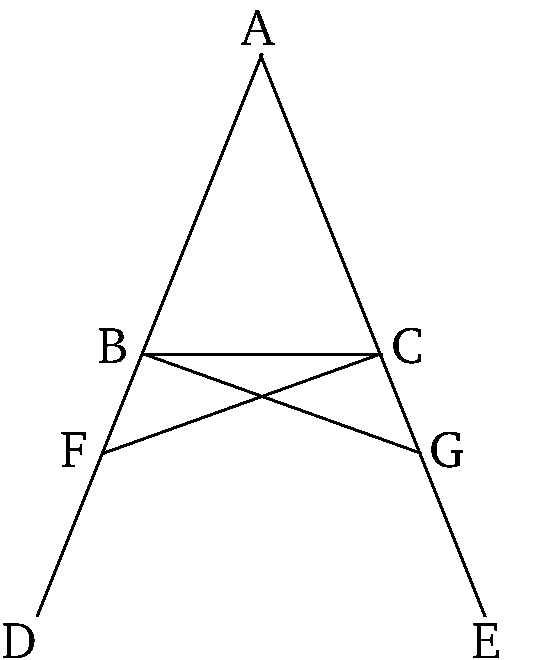
\includegraphics[width=0.8\textwidth]{Book01/fig05e.pdf}}

In fact, since $AF$ is equal to $AG$, and $AB$ to $AC$, the two (straight-lines) $FA$, $AC$ are
equal to the two (straight-lines) $GA$, $AB$, respectively. They also encompass a
common angle, $FAG$. Thus, the base $FC$ is equal to the base $GB$, and the
triangle $AFC$ will be equal to the triangle $AGB$, and the remaining angles
subtended by the equal sides will
be equal to the corresponding  remaining angles [Prop.~1.4].  (That is) $ACF$ to $ABG$, and $AFC$ to $AGB$. And since the whole of $AF$ is
equal to the whole of $AG$, within which $AB$ is equal to $AC$, the remainder
$BF$ is thus equal to the remainder $CG$ [C.N.~3]. But $FC$ was also shown (to be) equal to $GB$. So
the two (straight-lines) $BF$, $FC$ are equal to the two (straight-lines) $CG$, $GB$, respectively,
and the angle $BFC$ (is) equal to the angle $CGB$, and the base $BC$ is common to
them. Thus, the triangle $BFC$ will be equal to the triangle $CGB$, and
the remaining angles subtended by the equal sides will be equal to the corresponding remaining angles [Prop.~1.4]. Thus, $FBC$ is equal to $GCB$, and $BCF$ to
$CBG$. Therefore, since the whole angle $ABG$ was shown (to be) equal to the
whole angle $ACF$, within which $CBG$ is equal to $BCF$, the remainder $ABC$
is thus equal to the remainder $ACB$ [C.N.~3]. And they are at the base of triangle
$ABC$. And $FBC$ was also shown (to be) equal to $GCB$. And they are under
the base.

Thus, for isosceles triangles, the angles at the base are equal to one another, and if
the equal sides are produced (then) the angles under the base will be equal to one another. (Which is) the very thing it was required to show.}
\end{Parallel}

%%%%%%
% Prop 1.6
%%%%%%
\pdfbookmark[1]{Proposition 1.6}{pdf1.6}
\begin{Parallel}{}{} 
\ParallelLText{
\begin{center}
{\large \ggn{6}.}
\end{center}\vspace*{-7pt}

\gr{Ἐὰν τριγώνου αἱ δύο γωνίαι ἴσαι ἀλλήλαις ὦσιν, καὶ αἱ ὑπὸ
τὰξ ἴσας γωνίας ὑποτείνουσαι πλευραὶ  ἴσαι ἀλλήλαιςὸέσονται.}

\gr{Ἔστω τρίγωνον τὸ ΑΒΓ ἴσην ἔχον τὴν ὑπὸ ΑΒΓ γωνίαν τῇ ὑπὸ ΑΓΒ γωνίᾳ; λέγω, ὅτι καὶ πλευρὰ ἡ ΑΒ πλευρᾶ| τῇ ΑΓ ἐστινὸίση.}

% Removed epsf size command
\centerline{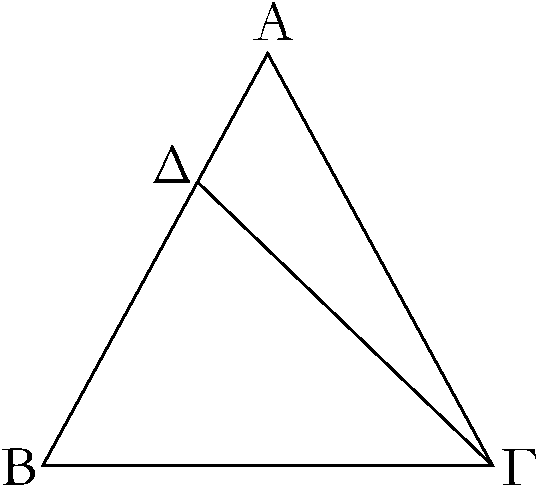
\includegraphics[width=0.8\textwidth]{Book01/fig06g.pdf}}

\gr{Εἰ γὰρὸάνισόξ ἐστιν ἡ ΑΒ τῇ ΑΓ, ἡ ἑτέρα αὐτῶν μείζων ἐστίν. ὸέστω μείζων ἡ ΑΒ, καὶ ἀφῃρήσθω ἀπὸ τῆς μείζονος τῆς ΑΒ τῇ
ἐλάττονι τῇ ΑΓὸίση ἡ ΔΒ, καὶ ἐπεζεύθθω ἡ ΔΓ.}

\gr{Ἐπεὶ οὸῦνὸίση ἐστὶν ἡ ΔΒ τῇ ΑΓ κοινὴ δὲ ἡ ΒΓ, δύο
δὴ αἱ ΔΒ, ΒΓ δύο ταῖς ΑΓ, ΓΒ ἴσαι εἰσὶν ἑκατέρα ἑκατέρᾳ, καὶ
γωνία ἡ ὑπὸ ΔΒΓ γωνίᾳ τῇ ὑπὸ ΑΓΒ ἐστινὸίση; βάσις ἄρα
ἡ ΔΓ βάσει τῇ ΑΒὸίση ἐστίν, καὶ τὸ ΔΒΓ τρίγωνον τῷ ΑΓΒ
τριγώνῳ  ἴσονὸέσται, τὸ ὸέλασσον τῷ μείζονι; ὅπερὸάτοπον;
οὐκ ἄραὸάνισόξ ἐστιν ἡ ΑΒ τῇ ΑΓ; ὸίση ἄρα.}

\gr{Ἐὰν ἄρα  τριγώνου αἱ δὑο γωνίαι ἴσαι ἀλλήλαις ὦσιν, καὶ αἱ ὑπὸ
τὰξ ἴσας γωνίας ὑποτείνουσαι πλευραὶ  ἴσαι ἀλλήλαιςὸέσονται;
ὅπερ ἔδει δεῖχαι.}}

\ParallelRText{
\begin{center}
{\large Proposition 6}
\end{center}

If a triangle has two angles equal to one another (then) the sides subtending the
equal angles will also be equal to one another.

Let $ABC$ be a triangle having the angle $ABC$ equal to the angle $ACB$. I say that
side $AB$ is also equal to side $AC$.\\

% Removed epsf size command
\centerline{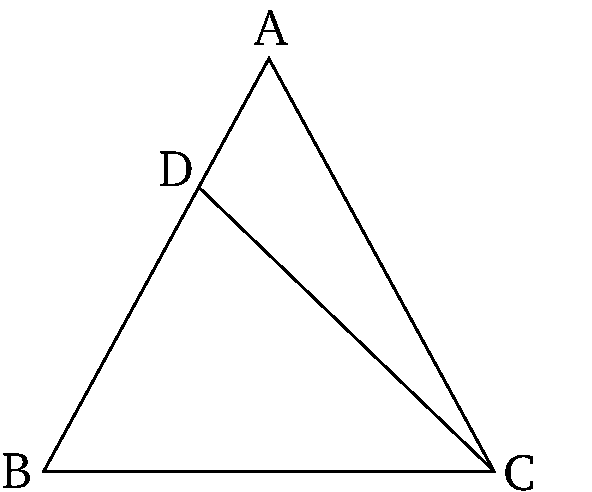
\includegraphics[width=0.8\textwidth]{Book01/fig06e.pdf}}

For if $AB$ is unequal to $AC$ (then) one of them is greater. Let $AB$ be greater. And
let $DB$, equal to the lesser $AC$, be cut off from the greater $AB$ [Prop.~1.3].  And
let $DC$ be joined [Post.~1].

Therefore, since $DB$ is equal to $AC$, and $BC$ (is) common, the two sides $DB$, $BC$ are equal to the two sides $AC$, $CB$, respectively, and the angle $DBC$
is equal to the angle $ACB$. Thus, the base $DC$ is equal to the base
$AB$, and the triangle $DBC$ will be equal to the triangle $ACB$ [Prop.~1.4], the lesser
to the greater. The very notion (is) absurd [C.N.~5]. Thus, $AB$ is not unequal
to $AC$. Thus, (it is) equal.$^\dag$

Thus, if a triangle has two angles equal to one another (then) the sides subtending the
equal angles will also be equal to one another. (Which is) the very thing it was required to show.}
\end{Parallel}
{\footnotesize \noindent $^\dag$ Here, use is made of the previously
unmentioned common notion that if two quantities are not unequal then they must be equal. Later on, use is made of the closely related common notion
that if two quantities are not greater than or less than one another, respectively, then they must be equal to one another.}

%%%%%%
% Prop 1.7
%%%%%%
\pdfbookmark[1]{Proposition 1.7}{pdf1.7}
\begin{Parallel}{}{} 
\ParallelLText{
\begin{center}
{\large \ggn{7}.}
\end{center}\vspace*{-7pt}

\gr{Ἐπὶ τῆς αὐτῆς εὐθείας δύο ταῖς αὐταῖς εὐθείαιςὸάλλαι δύο
εὐθεῖαι ἴσαι ἑκατέρα ἑκατέρᾳ οὐ συσταθήσονται πρὸςὸάλλῳ καὶ ὸάλλῳ
σημείῳ ἐπὶ τὰ αὐτὰ μέρη τὰ αὐτὰ πέραταὸέθουσαι ταῖς ἐξ ἀρθῆς
εὐθείαις.}\\

% Removed epsf size command
\centerline{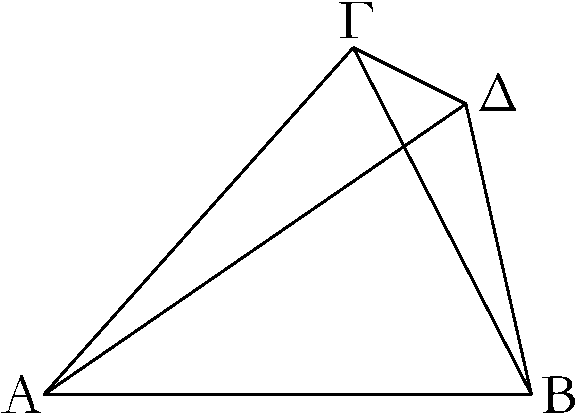
\includegraphics[width=0.8\textwidth]{Book01/fig07g.pdf}}

\gr{Εἰ γὰρ δυνατόν, ἐπὶ τῆς αὐτῆς εὐθείας τῆς ΑΒ δύο ταῖς αὐταῖς
εὐθείαις ταῖς ΑΓ, ΓΒὸάλλαι δύο εὐθεῖαι αἱ ΑΔ, ΔΒ ἴσαι
ἑκατέρα ἑκατέρᾳ συνεστάτωσαν πρὸςὸάλλῳ καὶ ὸάλλῳ σημείῳ τῷ
τε Γ καὶ Δ ἐπὶ τὰ αὐτὰ μέρη τὰ αὐτὰ πέραταὸέθουσαι, ὁώστε ἴσην εὸῖναι τὴν
μὲν ΓΑ τῇ ΔΑ τὸ αὐτὸ πέραςὸέθουσαν αὐτῇ τὸ Α, τὴν δὲ
ΓΒ τῇ ΔΒ τὸ αὐτὸ πέραςὸέθουσαν αὐτῇ τὸ Β, καὶ 
ἐπεζεύθθω ἡ ΓΔ.}

\gr{Ἐπεὶ οὸῦνὸίση ἐστὶν ἡ ΑΓ τῇ  ΑΔ, ὸίση ἐστὶ καὶ  γωνία ἡ ὑπὸ
ΑΓΔ τῇ ὑπὸ ΑΔΓ; μείζων ἄρα ἡ ὑπὸ ΑΔΓ τῆς ὑπὸ ΔΓΒ; πολλῶ|
 ἄρα ἡ ὑπὸ ΓΔΒ μείζων ἐστί τῆς ὑπὸ ΔΓΒ. πάλιν ἐπεὶ
ὸίση ἐστὶν ἡ ΓΒ τῇ ΔΒ, ὸίση ἐστὶ καὶ γωνία ἡ ὑπὸ ΓΔΒ
γωνίᾳ τῇ ὑπὸ ΔΓΒ. ἐδείθθη δὲ αὐτῆς καὶ πολλῶ| μείζων;
ὅπερ ἐστὶν ἀδύνατον.}

\gr{Οὐκ ἄρα ἐπὶ τῆς αὐτῆς εὐθείας δύο ταῖς αὐταῖς εὐθείαιςὸάλλαι δύο
εὐθεῖαι ἴσαι ἑκατέρα ἑκατέρᾳ  
συσταθήσονται πρὸςὸάλλῳ καὶ ὸάλλῳ
σημείῳ ἐπὶ τὰ αὐτὰ μέρη τὰ αὐτὰ πέραταὸέθουσαι ταῖς ἐξ ἀρθῆς
εὐθείαις;  ὅπερ ἔδει δεῖχαι.}}

\ParallelRText{
\begin{center}
{\large Proposition 7}
\end{center}

On the same straight-line, two other straight-lines 
equal, respectively, to 
two (given) straight-lines (which meet) cannot be constructed (meeting)
at  a different point on the same
side (of the straight-line), but having the same ends as the given straight-lines.

% Removed epsf size command
\centerline{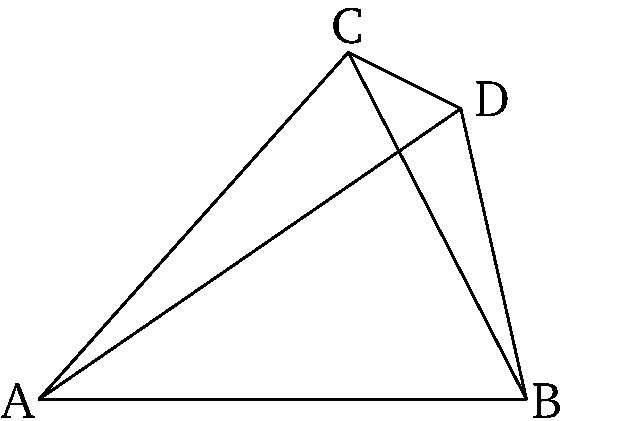
\includegraphics[width=0.8\textwidth]{Book01/fig07e.pdf}}

For, if possible, let the two straight-lines $AC$, $CB$, equal to two other straight-lines $AD$, $DB$, respectively, be constructed
on the same straight-line $AB$, meeting at different points, $C$ and $D$, on the
same side (of $AB$), and having the same ends (on $AB$). So $CA$ is equal to $DA$, having the same end $A$ as it, and $CB$ is equal to $DB$, having the
same end $B$ as it. And let $CD$ be joined [Post.~1].

Therefore, since $AC$ is equal to $AD$,  the angle $ACD$ is also equal to angle $ADC$ [Prop.~1.5].
Thus, $ADC$ (is) greater than $DCB$ [C.N.~5]. Thus, $CDB$ is much greater
than $DCB$ [C.N.~5]. Again, since  $CB$ is equal to $DB$, the angle $CDB$ is also equal to
angle $DCB$ [Prop.~1.5]. But it was shown that the former (angle) is also much
greater (than the latter). The very thing is impossible.

Thus, on the same straight-line, two other straight-lines equal, respectively, to  
two (given) straight-lines  (which meet) cannot be constructed (meeting)
at a different point on the same
side (of the straight-line), but having the same ends as the given straight-lines.
(Which is) the very thing it was required to show.}
\end{Parallel}

%%%%%%
% Prop 1.8
%%%%%%
\pdfbookmark[1]{Proposition 1.8}{pdf1.8}
\begin{Parallel}{}{} 
\ParallelLText{
\begin{center}
{\large \ggn{8}.}
\end{center}\vspace*{-7pt}

\gr{Ἐὰν δύο τρίγωνα τὰξ δύο πλευρὰξ [ταῖς] δύο πλευραῖξ ἴσαςὸέθῃ
ἑκατέραν ἑκατέρᾳ, ὸέθῃ δὲ καὶ τὴν βάσιν τῇ βάσει ἴσην, καὶ
τὴν γωνίαν τῇ γωνίᾳ  ἴσην ὁέχει τὴν ὑπὸ τῶνὸίσων
εὐθειῶν περιεθομένην.}

\gr{Ἔστω δύο τρίγωνα τὰ ΑΒΓ, ΔΕΖ τὰξ δύο πλευρὰξ τὰξ ΑΒ, ΑΓ ταῖς δύο πλευραῖξ ταῖς ΔΕ, ΔΖ ἴσας ἔχοντα ἑκατέραν ἑκατέρᾳ, τὴν μὲν ΑΒ τῇ ΔΕ τὴν δὲ ΑΓ τῇ ΔΖ; ἐθέτω δὲ καὶ βάσιν τὴν ΒΓ βάσει τῇ ΕΖ ἴσην; λέγω, ὅτι καὶ γωνία ἡ ὑπὸ ΒΑΓ γωνίᾳ τῇ ὑπὸ ΕΔΖ ἐστινὸίση.}

% Removed epsf size command
\centerline{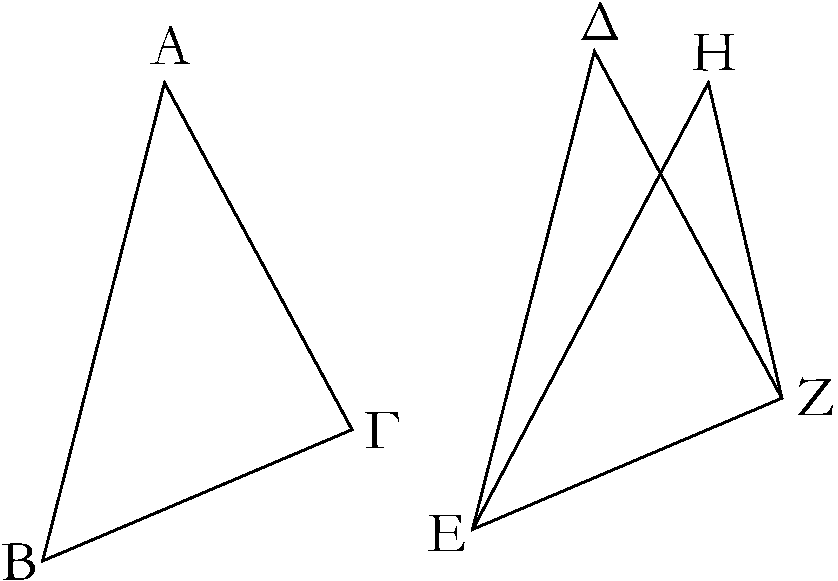
\includegraphics[width=0.8\textwidth]{Book01/fig08g.pdf}}

\gr{Ἐφαρμοζομένου γὰρ τοῦ ΑΒΓ τριγώνου ἐπὶ τὸ ΔΕΖ τρίγωνον
καὶ τιθεμένου τοῦ μὲν Β σημείου ἐπὶ τὸ Ε σημεῖον τῆς δὲ ΒΓ εὐθείας ἐπὶ τὴν ΕΖ ἐφαρμόσει καὶ τὸ Γ σημεῖον ἐπὶ τὸ Ζ
διὰ τὸ  ἴσην εὸῖναι τὴν ΒΓ τῇ ΕΖ; ἐφαρμοσάσης δὴ τῆς ΒΓ ἐπὶ τὴν ΕΖ ἐφαρμόσουσι καὶ αἱ ΒΑ, ΓΑ ἐπὶ τὰξ ΕΔ, ΔΖ. εἰ γὰρ
βάσις μὲν ἡ ΒΓ ἐπὶ βάσιν τὴν ΕΖ ἐφαρμόσει, αἱ δὲ ΒΑ, ΑΓ
πλευραὶ ἐπὶ τὰξ ΕΔ, ΔΖ οὐκ ἐφαρμόσουσιν ἀλλὰ παραλλάχουσιν ὡξ
αἱ ΕΗ, ΗΖ, συσταθήσονται ἐπὶ τῆς αὐτῆς εὐθείας δύο ταῖς αὐταῖς εὐθείαιςὸάλλαι δύο εὐθεῖαι ἴσαι ἑκατέρα ἑκατέρᾳ πρὸςὸάλλῳ καὶ
ὸάλλῳ σημείῳ ἐπὶ τὰ αὐτὰ μέρη τὰ αὐτὰ πέραταὸέθουσαι. οὐ
συνίστανται δέ; οὐκ ἄρα ἐφαρμοζομένης τῆς ΒΓ βάσεως ἐπὶ τὴν
ΕΖ βάσιν οὐκ
ἐφαρμόσουσι καὶ αἱ ΒΑ, ΑΓ πλευραὶ
ἐπὶ τὰξ ΕΔ, ΔΖ. ἐφαρμόσουσιν ἄρα;
ὁώστε καὶ γωνία ἡ ὑπὸ ΒΑΓ ἐπὶ  γωνίαν τὴν ὑπὸ
ΕΔΖ ἐφαρμόσει καὶ ὸίση αὐτῇ ὸέσται.}

\gr{Ἐὰν ἄρα δύο τρίγωνα τὰξ δύο πλευρὰξ [ταῖς] δύο πλευραῖξ ἴσαςὸέθῃ
ἑκατέραν ἑκατέρᾳ  καὶ τὴν βάσιν τῇ βάσει ἴσηνὸέθῃ, καὶ
τὴν γωνίαν τῇ γωνίᾳ  ἴσην ὁέχει τὴν ὑπὸ τῶνὸίσων
εὐθειῶν περιεθομένην; ὅπερ ἔδει δεῖχαι.}}

\ParallelRText{
\begin{center}
{\large Proposition 8}
\end{center}

If two triangles have  two sides equal to two sides, respectively, 
and also have the base equal to the base, (then) they will
also have equal the angles  encompassed by
the equal straight-lines.

Let $ABC$ and $DEF$ be two triangles having the two sides $AB$ and $AC$ equal to the two
sides $DE$ and $DF$, respectively. (That is) $AB$ to $DE$, and $AC$ to $DF$.  Let them also have
the base $BC$ equal to the base $EF$. I say that the angle $BAC$ is also equal
to the angle $EDF$.

% Removed epsf size command
\centerline{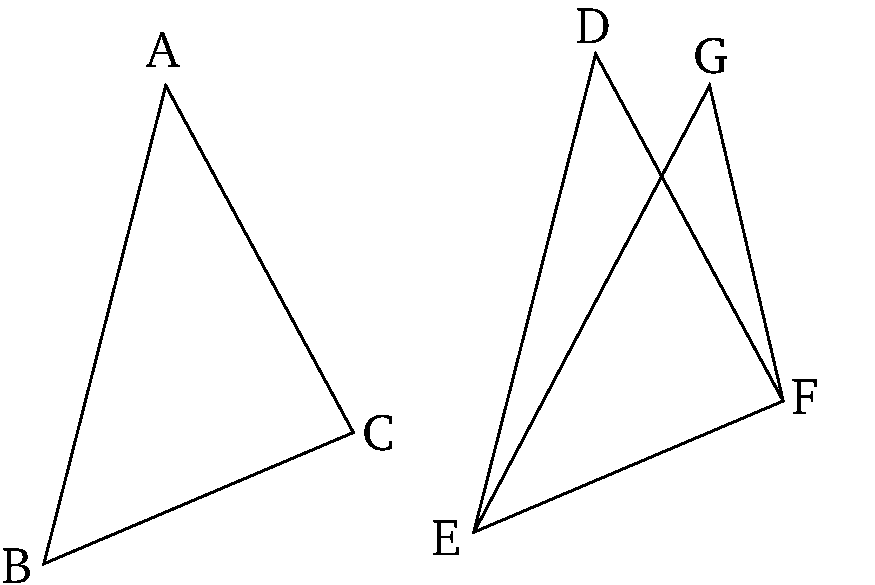
\includegraphics[width=0.8\textwidth]{Book01/fig08e.pdf}}

For if triangle $ABC$ is applied to triangle $DEF$, the point $B$ being placed on
point $E$, and the straight-line $BC$ on $EF$, (then) point $C$ will also coincide with $F$, on
account of $BC$ being equal to $EF$.
So  (because of) $BC$ coinciding with $EF$,  (the sides) $BA$ and $CA$ will also
coincide with  $ED$ and $DF$ (respectively). 
For if base $BC$ coincides with base $EF$, but the sides $AB$ and $AC$ 
do not coincide with $ED$ and $DF$ (respectively), but miss like $EG$
and $GF$ (in the above figure), 
then we will have constructed upon the same straight-line two other straight-lines equal, respectively, to two (given) straight-lines,  and (meeting)
at a different point on the same
side (of the straight-line), but having the same ends. But (such straight-lines) cannot be constructed [Prop.~1.7].
Thus,  the base $BC$ being applied to the  base $EF$,  the sides $BA$ and $AC$
cannot not coincide with $ED$ and $DF$ (respectively). Thus, they
will coincide. So the angle $BAC$ will also coincide with angle $EDF$,
and will be equal to it [C.N.~4].

Thus, if two triangles have  two  sides equal to two side, respectively,
and  have the base equal to the base, (then) they will also have equal the angles  encompassed by
the equal straight-lines. (Which is) the very thing it was required to show.}
\end{Parallel}

%%%%%%
% Prop 1.9
%%%%%%
\pdfbookmark[1]{Proposition 1.9}{pdf1.9}
\begin{Parallel}{}{} 
\ParallelLText{
\begin{center}
{\large \ggn{9}.}
\end{center}\vspace*{-7pt}

\gr{Τὴν δοθεῖσαν γωνίαν εὐθύγραμμον δίθα τεμεῖν.}

\gr{Ἔστω ἡ δοθεῖσα γωνία εὐθύγραμμος ἡ ὑπὸ ΒΑΓ. δεῖ δὴ
αὐτὴν δίθα τεμεῖν.}

\gr{Εἰλήφθω ἐπὶ τῆς ΑΒ τυθὸν σημεῖον τὸ Δ, καὶ ἀφῃρήσθω ἀπὸ
τῆς ΑΓ τῇ ΑΔὸίση ἡ ΑΕ, καὶ ἐπεζεύθθω ἡ ΔΕ, καὶ συνεστάτω
ἐπὶ τῆς ΔΕ τρίγωνον ἰσόπλευρον τὸ ΔΕΖ, καὶ ἐπεζεύθθω ἡ ΑΖ; λέγω, ὅτι ἡ ὑπὸ ΒΑΓ γωνία δίθα τέτμ  ηται ὑπὸ τῆς ΑΖ
εὐθείας.}

\gr{Ἐπεὶ γὰρὸίση ἐστὶν ἡ ΑΔ τῇ ΑΕ, κοινὴ δὲ ἡ ΑΖ, δύο δὴ αἱ ΔΑ, ΑΖ δυσὶ ταῖς ΕΑ, ΑΖ ἴσαι εἰσὶν ἑκατέρα ἑκατέρᾳ. καὶ βάσις ἡ ΔΖ
βάσει τῇ ΕΖὸίση ἐστίν; γωνία ἄρα ἡ ὑπὸ ΔΑΖ γωνίᾳ τῇ
ὑπὸ ΕΑΖὸίση ἐστίν.}

% Removed epsf size command
\centerline{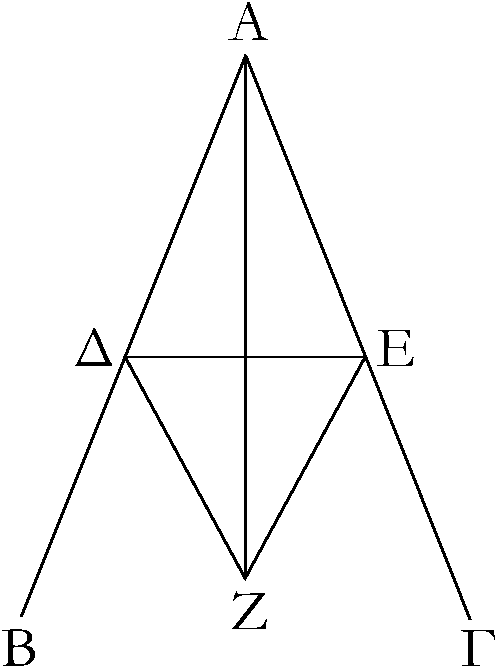
\includegraphics[width=0.8\textwidth]{Book01/fig09g.pdf}}

\gr{Ἡ  ἄρα δοθεῖσα γωνία εὐθύγραμμος ἡ ὑπὸ ΒΑΓ δίθα τέτμ  ηται
ὑπὸ τῆς ΑΖ εὐθείας; ὅπερ ἔδει ποιῆσαι.}}

\ParallelRText{
\begin{center}
{\large Proposition 9}
\end{center}

To cut a given rectilinear angle in half.

Let $BAC$ be the given rectilinear angle. So it is required to
cut it in half.

Let the point $D$ be taken at random on $AB$,
and let $AE$, equal to $AD$,  be cut off from $AC$  [Prop.~1.3], and
let $DE$ be joined. And let the equilateral triangle $DEF$
be constructed upon $DE$ [Prop.~1.1], and let $AF$ be
joined. I say that the angle $BAC$ has been cut in half by the straight-line
$AF$.

For since $AD$ is equal to  $AE$, and $AF$ is common, the two (straight-lines) $DA$,
$AF$ are equal to the two (straight-lines) $EA$, $AF$, respectively. And the base $DF$
is equal to the base $EF$. Thus, angle $DAF$ is equal to angle $EAF$ [Prop.~1.8].

% Removed epsf size command
\centerline{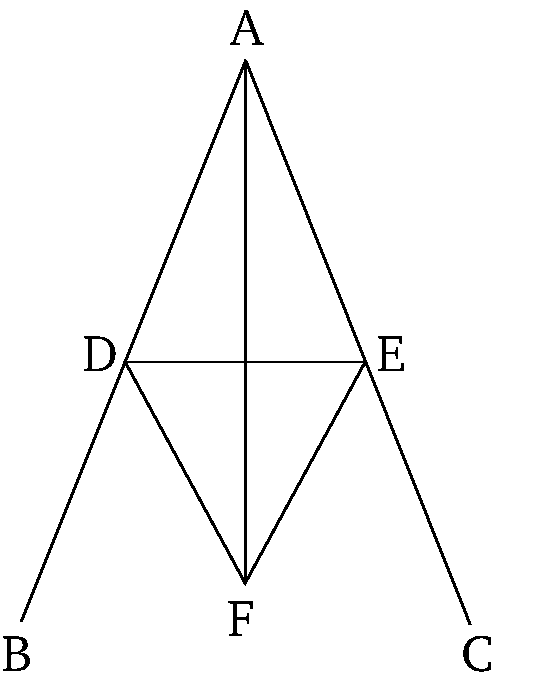
\includegraphics[width=0.8\textwidth]{Book01/fig09e.pdf}}

Thus, the given rectilinear angle $BAC$ has been cut in half by the
straight-line $AF$. (Which is) the very thing it was required to do.}
\end{Parallel}

%%%%%%
% Prop 1.10
%%%%%%
\pdfbookmark[1]{Proposition 1.10}{pdf1.10}
\begin{Parallel}{}{} 
\ParallelLText{
\begin{center}
{\large \ggn{10}.}
\end{center}\vspace*{-7pt}

\gr{Τὴν δοθεῖσαν εὐθεῖαν πεπερασμένην δίθα τεμεῖν.}

\gr{Ἔστω ἡ δοθεῖσα εὐθεῖα πεπερασμένη ἡ ΑΒ; δεῖ δὴ τὴν ΑΒ εὐθεῖαν πεπερασμένην δίθα τεμεῖν.}

\gr{Συνεστάτω ἐπ' αὐτῆς τρίγωνον ἰσόπλευρον τὸ ΑΒΓ, καὶ τετμήσθω ἡ ὑπὸ ΑΓΒ γωνία δίθα τῇ ΓΔ εὐθείᾳ; λέγω, ὅτι ἡ ΑΒ εὐθεῖα
δίθα τέτμ  ηται κατὰ τὸ Δ σημεῖον.}\\

% Removed epsf size command
\centerline{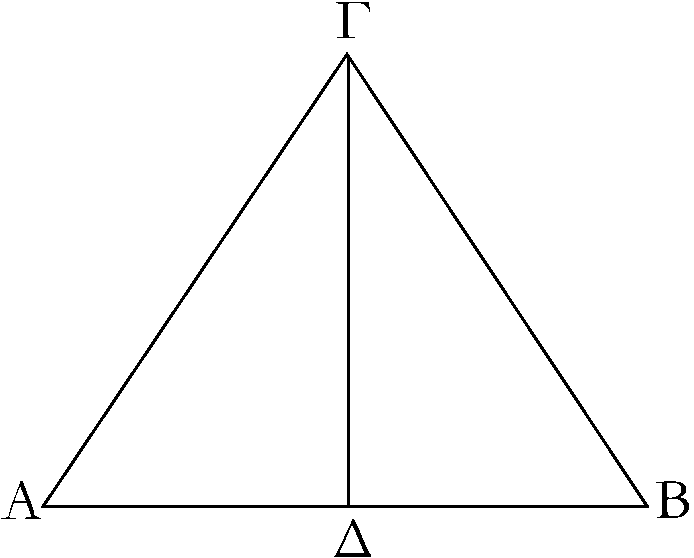
\includegraphics[width=0.8\textwidth]{Book01/fig10g.pdf}}

\gr{Ἐπεὶ γὰρὸίση ἐστὶν ἡ ΑΓ τῇ ΓΒ, κοινὴ δὲ ἡ ΓΔ, δύο δὴ αἱ
ΑΓ, ΓΔ δύο ταῖς ΒΓ, ΓΔ ἴσαι εἰσὶν ἑκατέρα ἑκατέρᾳ; καὶ γωνία
ἡ ὑπὸ ΑΓΔ γωνίᾳ τῇ ὑπὸ ΒΓΔὸίση ἐστίν; βάσις ἄρα ἡ
ΑΔ βάσει τῇ ΒΔὸίση ἐστίν.}

\gr{Ἡ  ἄρα δοθεῖσα εὐθεῖα πεπερασμένη ἡ ΑΒ δίθα τέτμ  ηται κατὰ τὸ
Δ; ὅπερ ἔδει ποιῆσαι.}}

\ParallelRText{
\begin{center}
{\large Proposition 10}
\end{center}

To cut a given finite straight-line in half.

Let $AB$ be the given finite straight-line. So it is required to cut the
finite straight-line $AB$ in half.

Let the equilateral triangle $ABC$ be constructed upon  ($AB$)
[Prop.~1.1], and let the angle $ACB$ be cut in half by the
straight-line $CD$ [Prop.~1.9]. I say that the straight-line $AB$ has been
cut in half at  point $D$.

% Removed epsf size command
\centerline{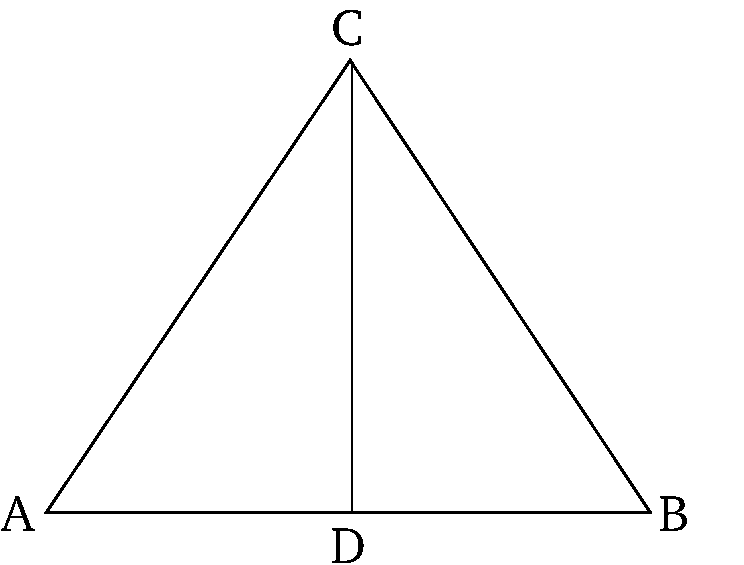
\includegraphics[width=0.8\textwidth]{Book01/fig10e.pdf}}

For since $AC$ is equal to $CB$, and $CD$ (is) common, the two (straight-lines) $AC$, $CD$
are equal to the two (straight-lines) $BC$, $CD$, respectively. And the angle $ACD$ is
equal to the angle $BCD$. Thus, the base $AD$ is equal to the base $BD$
[Prop.~1.4].

Thus, the given finite straight-line $AB$ has been cut in half at  (point) $D$. 
(Which is) the
very thing it was required to do.}
\end{Parallel}

%%%%%%
% Prop 1.11
%%%%%%
\pdfbookmark[1]{Proposition 1.11}{pdf1.11}
\begin{Parallel}{}{} 
\ParallelLText{
\begin{center}
{\large \ggn{11}.}
\end{center}\vspace*{-7pt}

\gr{Τῆ| δοθείσῃ εὐθείᾳ ἀπὸ τοῦ πρὸς αὐτῇ δοθέντος σημείου
πρὸς ὀρθὰξ γωνίας εὐθεῖαν γραμμὴν ἀγαγεῖν.}

\gr{Ἔστω ἡ μὲν δοθεῖσα εὐθεῖα ἡ ΑΒ τὸ δὲ δοθὲν σημεῖον
ἐπ' αὐτῆς τὸ Γ; δεῖ δὴ ἀπὸ τοῦ Γ σημείου τῇ ΑΒ εὐθείᾳ
πρὸς ὀρθὰξ γωνίας εὐθεῖαν γραμμὴν ἀγαγεῖν.}

% Removed epsf size command
\centerline{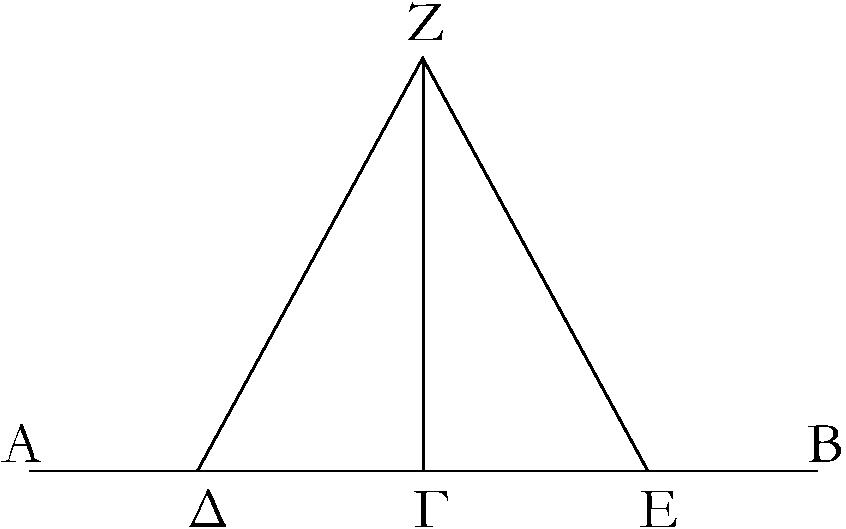
\includegraphics[width=0.8\textwidth]{Book01/fig11g.pdf}}

\gr{Εἰλήφθω ἐπὶ τῆς ΑΓ τυθὸν σημεῖον τὸ Δ, καὶ κείσθω τῇ
ΓΔὸίση ἡ ΓΕ, καὶ συνεστάτω ἐπὶ τῆς ΔΕ τρίγωνον ἰσόπλευρον
τὸ ΖΔΕ, καὶ ἐπεζεύθθω ἡ ΖΓ; λέγω, ὅτι τῇ δοθείσῃ
εὐθείᾳ τῇ ΑΒ ἀπὸ τοῦ πρὸς αὐτῇ δοθέντος σημείου τοῦ
Γ πρὸς ὀρθὰξ γωνίας εὐθεῖα γραμμὴ ὸῆκται ἡ ΖΓ.}

\gr{Ἐπεὶ γὰρὸίση ἐστὶν ἡ ΔΓ τῇ ΓΕ, κοινὴ δὲ ἡ ΓΖ, δύο δὴ
αἱ ΔΓ, ΓΖ δυσὶ ταῖς ΕΓ, ΓΖ ἴσαι εἰσὶν ἑκατέρα ἑκατέρᾳ;
καὶ βάσις ἡ ΔΖ βάσει τῇ ΖΕὸίση ἐστίν; γωνία ἄρα ἡ ὑπὸ
ΔΓΖ γωνίᾳ τῇ ὑπὸ ΕΓΖὸίση ἐστίν; καί εἰσιν ἐφεχῆς.
ὅταν δὲ εὐθεῖα ἐπ' εὐθεῖαν σταθεῖσα τὰξ ἐφεχῆς γωνίας ἴσας ἀλλήλαις ποιῆ|, ὀρθὴ ἑκατέρα τῶνὸίσων γωνιῶν
ἐστιν; ὀρθὴ  ἄρα ἐστὶν ἑκατέρα τῶν ὑπὸ ΔΓΖ, ΖΓΕ.}

\gr{Τῆ|  ἄρα δοθείσῃ εὐθείᾳ τῇ ΑΒ ἀπὸ τοῦ πρὸς αὐτῇ
δοθέντος σημείου τοῦ Γ πρὸς ὀρθὰξ γωνίας εὐθεῖα γραμμὴ
ὸῆκται ἡ ΓΖ; ὅπερ ἔδει ποιῆσαι.}}

\ParallelRText{
\begin{center}
{\large Proposition 11}
\end{center}

To draw a straight-line at right-angles to a given straight-line from a given point on it.

Let $AB$ be the given straight-line, and $C$ the given point on it. So it is required
to draw a straight-line from the point $C$ at right-angles to the straight-line $AB$.

% Removed epsf size command
\centerline{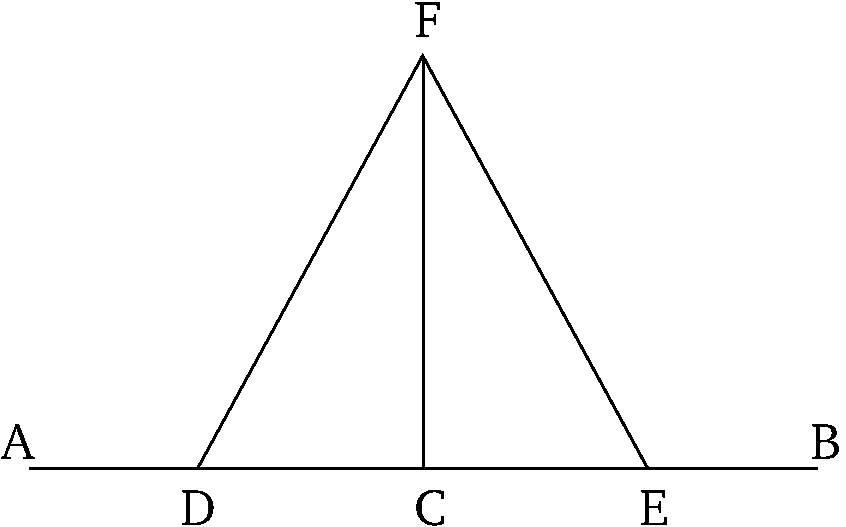
\includegraphics[width=0.8\textwidth]{Book01/fig11e.pdf}}

Let the point $D$ be be taken at random on $AC$, and let $CE$ be made equal to $CD$ [Prop.~1.3], and let the equilateral triangle $FDE$
be constructed on $DE$ [Prop.~1.1], and let $FC$ be
joined. I say that the straight-line $FC$ has been drawn at right-angles
to the given straight-line $AB$ from the given point $C$ on it.

For since $DC$ is equal to $CE$, and $CF$ is common, the two (straight-lines) $DC$, $CF$
are equal to the two (straight-lines), $EC$, $CF$, respectively.  And the base $DF$
is equal to the base $FE$. Thus, the angle $DCF$ is equal to the
angle $ECF$ [Prop.~1.8], and they are adjacent. But when a straight-line stood on 
a(nother) straight-line makes the adjacent angles equal to one another, each of the
equal angles is a right-angle [Def.~1.10]. Thus, each of the (angles)
$DCF$ and $FCE$ is a right-angle.

Thus, the straight-line $CF$ has been drawn at right-angles to the
given straight-line $AB$ from the given point $C$ on it. (Which is) the very thing
it was required to do.}
\end{Parallel}

%%%%%%
% Prop 1.12
%%%%%%
\pdfbookmark[1]{Proposition 1.12}{pdf1.12}
\begin{Parallel}{}{} 
\ParallelLText{
\begin{center}
{\large \ggn{12}.}
\end{center}\vspace*{-7pt}

\gr{Ἐπὶ τὴν δοθεῖσαν εὐθεῖαν ἄπειρον ἀπὸ τοῦ δοθέντος σημείου, ὃ μή
ἐστιν ἐπ' αὐτῆς, κάθετον εὐθεῖαν γραμμὴν ἀγαγεῖν.}

% Removed epsf size command
\centerline{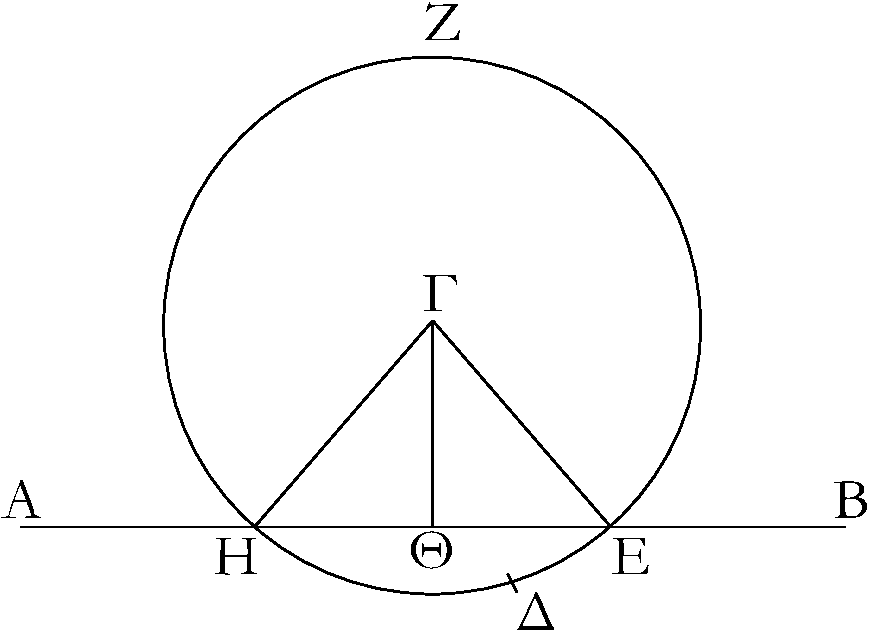
\includegraphics[width=0.8\textwidth]{Book01/fig12g.pdf}}

\gr{Ἔστω ἡ μὲν δοθεῖσα εὐθεῖαὸάπειρος ἡ ΑΒ τὸ δὲ δοθὲν σημεῖον,
ὃ μή ἐστιν ἐπ' αὐτῆς, τὸ Γ; δεῖ δὴ ἐπὶ τὴν δοθεῖσαν εὐθεῖαν ἄπειρον τὴν ΑΒ ἀπὸ τοῦ δοθέντος σημείου τοῦ Γ, ὃ μή ἐστιν
ἐπ' αὐτῆς, κάθετον εὐθεῖαν γραμμὴν ἀγαγεῖν.}

\gr{Εἰλήφθω γὰρ ἐπὶ τὰ ὁέτερα μέρη τῆς ΑΒ εὐθείας τυθὸν σημεῖον τὸ 
Δ, καὶ κέντρῳ μὲν τῷ Γ διαστήματι δὲ τῷ ΓΔ κύκλος γεγράφθω ὁ ΕΖΗ, καὶ τετμήσθω ἡ ΕΗ εὐθεῖα δίθα κατὰ τὸ Θ, καὶ ἐπεζεύθθωσαν
αἱ ΓΗ, ΓΘ, ΓΕ εὐθεῖαι; λέγω, ὅτι ἐπὶ τὴν δοθεῖσαν εὐθεῖαν ἄπειρον τὴν ΑΒ ἀπὸ τοῦ δοθέντος σημείου τοῦ Γ, ὃ μή ἐστιν ἐπ'
αὐτῆς, κάθετοςὸῆκται ἡ ΓΘ.}

\gr{Ἐπεὶ γὰρὸίση ἐστὶν ἡ ΗΘ τῇ ΘΕ, κοινὴ δὲ ἡ ΘΓ, δύο
δὴ αἱ ΗΘ, ΘΓ δύο ταῖς ΕΘ, ΘΓ ἴσαι εἱσὶν ἑκατέρα ἑκατέρᾳ; καὶ
βάσις ἡ ΓΗ βάσει τῇ ΓΕ ἐστινὸίση; γωνία ἄρα ἡ ὑπὸ ΓΘΗ γωνίᾳ
τῇ ὑπὸ ΕΘΓ ἐστινὸίση. καί εἰσιν ἐφεχῆς. ὅταν δὲ εὐθεῖα ἐπ'
εὐθεῖαν σταθεῖσα τὰξ ἐφεχῆς γωνίας ἴσας ἀλλήλαις ποιῆ|, ὀρθὴ
ἑκατέρα τῶνὸίσων γωνιῶν ἐστιν, καὶ ἡ ἐφεστηκυῖα εὐθεῖα
κάθετος καλεῖται ἐφ' ἣν ἐφέστηκεν.}

\gr{Ἐπὶ τὴν δοθεῖσαν ἄρα εὐθεῖαν ἄπειρον τὴν ΑΒ ἀπὸ τοῦ
δοθέντος σημείου τοῦ Γ, ὃ μή ἐστιν ἐπ' αὐτῆς, κάθετος ~ἠκται
ἡ ΓΘ; ὅπερ ἔδει ποιῆσαι.}}

\ParallelRText{
\begin{center}
{\large Proposition 12}
\end{center}

To draw a straight-line perpendicular to a given infinite straight-line from a given point which is not
on it.\\

% Removed epsf size command
\centerline{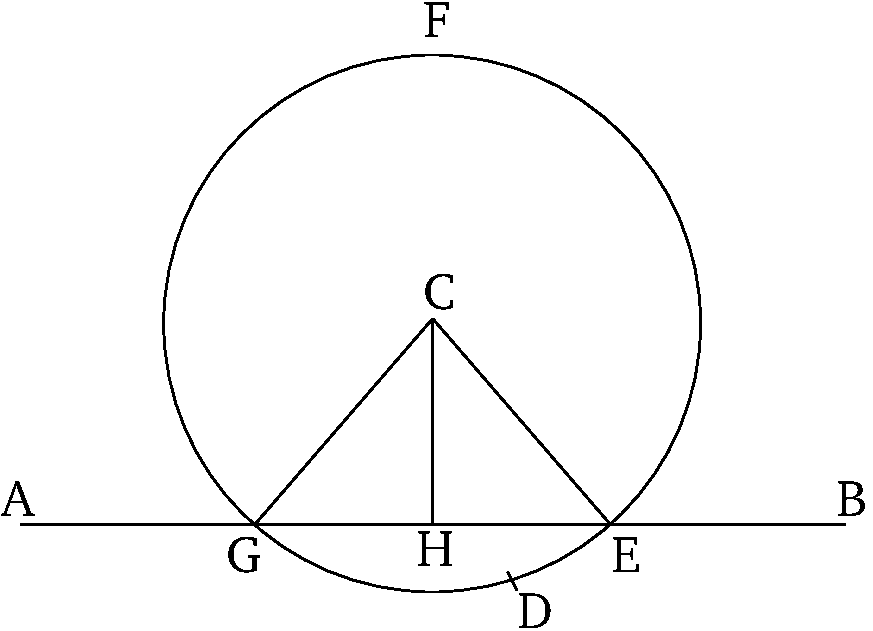
\includegraphics[width=0.8\textwidth]{Book01/fig12e.pdf}}

Let $AB$ be the given infinite straight-line  and $C$ the given point, which is not
on it. So it is required to draw a  straight-line  perpendicular to the
given infinite straight-line $AB$ from the given point $C$, which is not on
it.

For let point $D$ be taken at random on the other side (to $C$) of 
the straight-line $AB$, and let the circle $EFG$ be drawn
with center $C$ and radius $CD$ [Post.~3], and let the straight-line $EG$ be cut
in half at (point) $H$ [Prop.~1.10], and let the straight-lines $CG$, $CH$,
and $CE$ be joined. I say that the  (straight-line) $CH$ has
been drawn  perpendicular to the given infinite straight-line
$AB$ from the given point $C$, which is not on it.

For since $GH$ is equal to $HE$, and $HC$ (is) common, the two (straight-lines) $GH$, 
$HC$
are equal to the two (straight-lines) $EH$, $HC$, respectively, and the base $CG$ is
equal to the base $CE$. Thus, the angle $CHG$ is equal to the
angle $EHC$ [Prop.~1.8], and they are adjacent. But when a straight-line
stood on a(nother) straight-line makes the adjacent angles equal to one another, each of the equal angles is a right-angle, and the former straight-line is called a perpendicular to that upon which it stands [Def.~1.10].

Thus, the (straight-line) $CH$ has been drawn perpendicular to the given infinite straight-line $AB$ from the given point $C$, which is not
on  it. (Which is) the very thing it was required to do.}
\end{Parallel}

%%%%%%
% Prop 1.13
%%%%%%
\pdfbookmark[1]{Proposition 1.13}{pdf1.13}
\begin{Parallel}{}{} 
\ParallelLText{
\begin{center}
{\large\ggn{13}.}
\end{center}\vspace*{-7pt}

\gr{Ἐὰν εὐθεῖα ἐπ' εὐθεῖαν σταθεῖσα γωνίας ποιῆ|,  ἢτοι δύο ὀρθὰξὸὴ δυσὶν ὀρθαῖξ ἴσας ποιήσει.}

\gr{Εὐθεῖα γάρ τις ἡ ΑΒ ἐπ' εὐθεῖαν τὴν ΓΔ σταθεῖσα γωνίας ποιείτω
τὰξ ὑπὸ ΓΒΑ, ΑΒΔ; λὲγω, ὅτι αἱ ὑπὸ ΓΒΑ, ΑΒΔ γωνίαι ἢτοι
δύο ὀρθαί εἰσινὸὴ δυσὶν ὀρθαῖξ ἴσαι.}\\~\\

% Removed epsf size command
\centerline{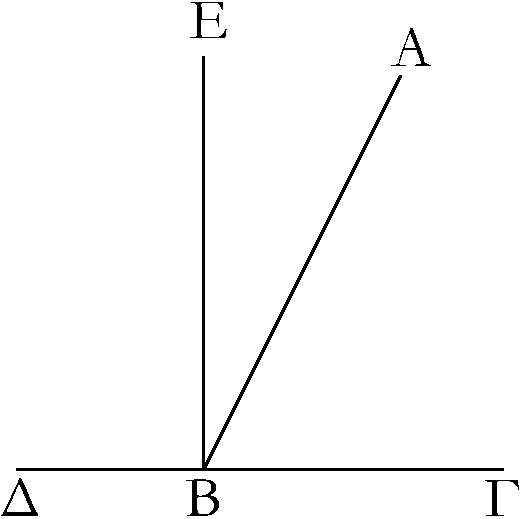
\includegraphics[width=0.8\textwidth]{Book01/fig13g.pdf}}

\gr{Εἰ μὲν οὸῦνὸίση ἐστὶν ἡ ὑπὸ ΓΒΑ τῇ ὑπὸ ΑΒΔ, δύο
ὀρθαί εἰσιν. εἰ δὲ οὸύ,  ἢθθω ἀπὸ τοῦ Β σημείου τῇ ΓΔ
[εὐθείᾳ] πρὸς ὀρθὰξ ἡ ΒΕ; αἱ  ἄρα ὑπὸ ΓΒΕ, ΕΒΔ δύο ὀρθαί
εἰσιν; καὶ ἐπεὶ ἡ ὑπὸ ΓΒΕ δυσὶ ταῖς ὑπὸ ΓΒΑ, ΑΒΕὸίση
ἐστίν, κοινὴ προσκείσθω ἡ ὑπὸ ΕΒΔ; αἱ  ἄρα ὑπὸ ΓΒΕ, ΕΒΔ
τρισὶ ταῖς ὑπὸ ΓΒΑ, ΑΒΕ, ΕΒΔ ἴσαι εἰσίν. πάλιν, ἐπεὶ ἡ ὑπὸ
ΔΒΑ δυσὶ ταῖς ὑπὸ ΔΒΕ, ΕΒΑὸίση ἐστίν, κοινὴ προσκείσθω
ἡ ὑπὸ ΑΒΓ; αἱ  ἄρα ὑπὸ ΔΒΑ, ΑΒΓ τρισὶ ταῖς ὑπὸ ΔΒΕ, ΕΒΑ, ΑΒΓ ἴσαι εἰσίν. ἐδείθθησαν δὲ καὶ αἱ ὑπὸ ΓΒΕ, ΕΒΔ τρισὶ
ταῖς αὐταῖς ἴσαι; τὰ δὲ τῷ αὐτῷ  ἴσα καὶ ἀλλήλοις ἐστὶν ἴσα;
 καὶ αἱ ὑπὸ ΓΒΕ, ΕΒΔ ἄρα ταῖς ὑπὸ ΔΒΑ, ΑΒΓ ἴσαι εἰσίν; ἀλλὰ αἱ ὑπὸ ΓΒΕ, ΕΒΔ δύο
ὀρθαί εἰσιν; καὶ αἱ ὑπὸ ΔΒΑ, ΑΒΓ ἄρα δυσὶν ὀρθαῖξ ἴσαι εἰσίν.}

\gr{Ἐὰν ἄρα εὐθεῖα ἐπ' εὐθεῖαν σταθεῖσα γωνίας ποιῆ|,  ἢτοι δύο ὀρθὰξὸὴ δυσὶν ὀρθαῖξ ἴσας ποιήσει; ὅπερ ἔδει δεῖχαι.}}

\ParallelRText{
\begin{center}
{\large Proposition 13}
\end{center}

If a straight-line stood on a(nother)  straight-line makes angles,
it will certainly either make two right-angles, or (angles whose sum is) equal
to two right-angles. 

For  let some straight-line $AB$ stood on the straight-line $CD$ make the
angles $CBA$ and $ABD$. I say that the angles $CBA$ and $ABD$ are
certainly either two right-angles, or (have a sum) equal to two right-angles.

% Removed epsf size command
\centerline{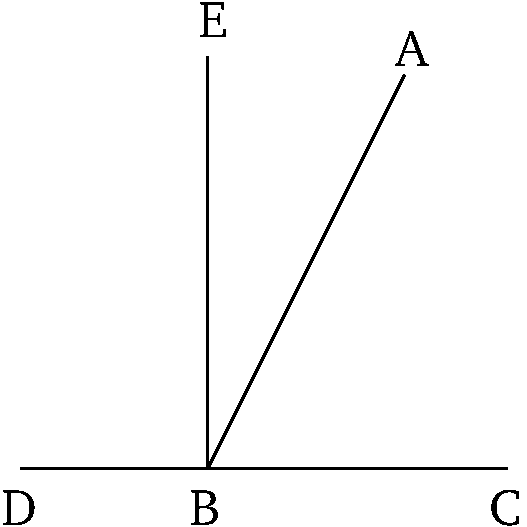
\includegraphics[width=0.8\textwidth]{Book01/fig13e.pdf}}

In fact, if $CBA$ is equal to $ABD$ (then) they are two right-angles [Def.~1.10].
But, if not, let $BE$ be drawn from the point $B$ at right-angles to [the
straight-line] $CD$ [Prop.~1.11]. Thus, $CBE$ and $EBD$ are two right-angles.
And since $CBE$ is equal to the two (angles) $CBA$ and $ABE$, let $EBD$ be added
to both. Thus, the (sum of the angles) $CBE$ and $EBD$ is equal to the  (sum of the) three (angles)
$CBA$, $ABE$, and $EBD$ [C.N.~2]. Again, since $DBA$ is equal to the two (angles) $DBE$
and $EBA$, let $ABC$ be added to both. Thus, the (sum of the angles) $DBA$ and $ABC$ is
equal to the (sum of the) three (angles) $DBE$, $EBA$, and $ABC$ [C.N.~2]. But (the sum of) $CBE$ and $EBD$ was
also shown (to be) equal to the (sum of the) same three (angles). And things equal to the
same thing are also equal to one another [C.N.~1]. Therefore, 
(the sum of) $CBE$ and
$EBD$ is also equal to (the sum of) $DBA$ and $ABC$. But, (the sum of) $CBE$ and $EBD$ is two
right-angles. Thus, (the sum of) $ABD$ and $ABC$ is also equal to two right-angles.

Thus, if a straight-line stood on a(nother)  straight-line makes angles,
it will certainly either make two right-angles, or (angles whose sum is) equal
to two right-angles. (Which is) the very thing it was required to show.}
\end{Parallel}

%%%%%%
% Prop 1.14
%%%%%%
\pdfbookmark[1]{Proposition 1.14}{pdf1.14}
\begin{Parallel}{}{} 
\ParallelLText{
\begin{center}
{\large \ggn{14}.}
\end{center}\vspace*{-7pt}

\gr{Ἐὰν πρόξ τινι εὐθείᾳ καὶ τῷ πρὸς αὐτῇ σημείῳ δύο εὐθεῖαι
μὴ ἐπὶ τὰ αὐτὰ μέρη κείμεναι τὰξ ἐφεχῆς γωνίας δυσὶν ὀρθαῖξ ἴσας ποιῶσιν, ἐπ' εὐθείαςὸέσονται ἀλλήλαις αἱ εὐθεῖαι.}

\gr{Πρὸξ γάρ τινι εὐθείᾳ τῇ ΑΒ καὶ τῷ πρὸς αὐτῇ σημείῳ τῷ
Β δύο εὐθεῖαι αἱ ΒΓ, ΒΔ μὴ ἐπὶ τὰ αὐτὰ μέρη
κείμεναι
τὰξ ἐφεχῆς γωνίας τὰξ ὑπὸ ΑΒΓ, ΑΒΔ δύο ὀρθαῖξ ἴσας ποιείτωσαν; λέγω, ὅτι ἐπ' εὐθείας ἐστὶ τῇ ΓΒ ἡ ΒΔ.}\\

% Removed epsf size command
\centerline{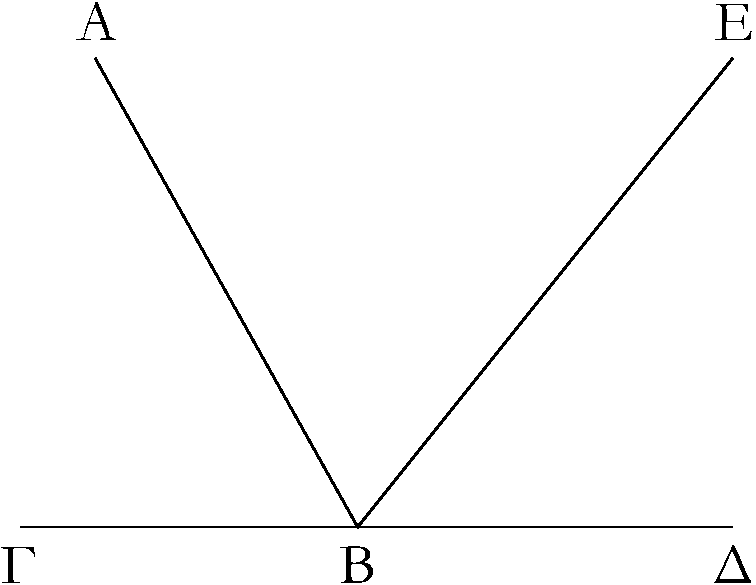
\includegraphics[width=0.8\textwidth]{Book01/fig14g.pdf}}

\gr{Εἰ γὰρ μή ἐστι τῇ ΒΓ ἐπ' εὐθείας ἡ ΒΔ, ὸέστω τῇ ΓΒ ἐπ'
εὐθείας ἡ ΒΕ.}

\gr{Ἐπεὶ οὸῦν εὐθεῖα ἡ ΑΒ ἐπ' εὐθεῖαν τὴν ΓΒΕ ἐφέστηκεν, αἱ
 ἄρα ὑπὸ ΑΒΓ, ΑΒΕ γωνίαι δύο ὀρθαῖξ ἴσαι εἰσίν; εἰσὶ δὲ καὶ
αἱ ὑπὸ ΑΒΓ, ΑΒΔ δύο ὀρθαῖξ ἴσαι; αἱ  ἄρα ὑπὸ ΓΒΑ, ΑΒΕ
ταῖς ὑπὸ ΓΒΑ, ΑΒΔ ἴσαι εἰσίν. κοινὴ ἀφῃρήσθω ἡ ὑπὸ ΓΒΑ;
λοιπὴ  ἄρα ἡ ὑπὸ ΑΒΕ λοιπῆ| τῇ ὑπὸ ΑΒΔ ἐστινὸίση, ἡ
ἐλάσσων τῇ μείζονι; ὅπερ ἐστὶν ἀδύνατον. οὐκ ἄρα
ἐπ' εὐθείας ἐστὶν ἡ ΒΕ τῇ ΓΒ. ὁμοίως δὴ δείχομεν, ὅτι
οὐδὲ ὸάλλη τις πλὴν τῆς ΒΔ; ἐπ' εὐθείας ἄρα ἐστὶν ἡ ΓΒ τῇ ΒΔ.}

\gr{Ἐὰν ἄρα πρόξ τινι εὐθείᾳ καὶ τῷ πρὸς αὐτῇ σημείῳ δύο εὐθεῖαι
μὴ ἐπὶ αὐτὰ μέρη κείμεναι τὰξ ἐφεχῆς γωνίας δυσὶν ὀρθαῖξ ἴσας ποιῶσιν, ἐπ' εὐθείαςὸέσονται ἀλλήλαις αἱ εὐθεῖαι; ὅπερ ἔδει δεῖχαι.}}

\ParallelRText{
\begin{center}
{\large Proposition 14}
\end{center}

If two straight-lines, not lying on the same side,  make adjacent angles (whose sum is) equal to two right-angles  with some straight-line, at a point on it, (then) the two straight-lines
will be straight-on (with respect) to one another.

For let two
straight-lines $BC$ and $BD$, not lying on the same side,  make adjacent angles $ABC$ and $ABD$ (whose sum is)
equal to two right-angles with some straight-line $AB$, at the point $B$ on it. I say
that $BD$ is  straight-on with respect to $CB$.

% Removed epsf size command
\centerline{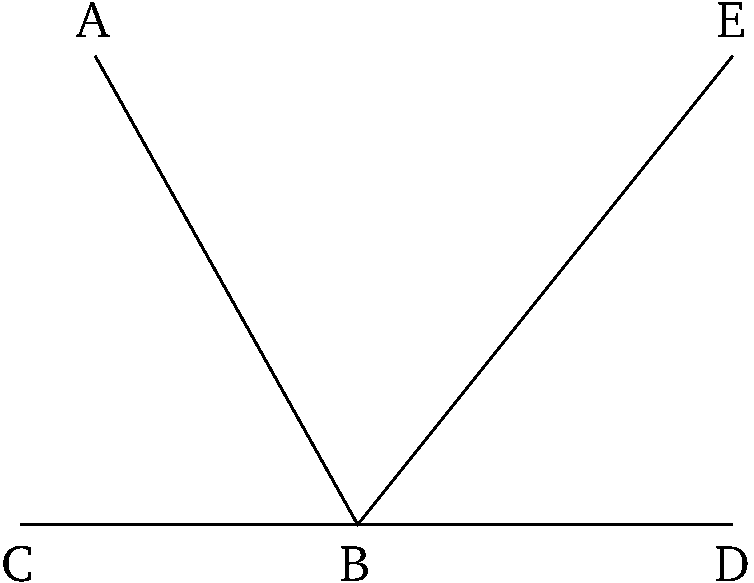
\includegraphics[width=0.8\textwidth]{Book01/fig14e.pdf}}

For if $BD$ is not straight-on to $BC$ (then) let $BE$ be straight-on to $CB$.

Therefore, since the straight-line $AB$ stands on the straight-line $CBE$, the (sum of the) angles $ABC$ and $ABE$ is thus equal to two right-angles [Prop.~1.13]. But (the sum of) $ABC$ and $ABD$ is also equal to two right-angles.
Thus, 
(the sum of angles) $CBA$ and $ABE$ is equal to (the sum of angles) $CBA$ and $ABD$ [C.N.~1]. Let (angle)
$CBA$ be subtracted from both. Thus, the remainder $ABE$ is
equal to the remainder $ABD$ [C.N.~3], the lesser to the greater. The very thing is impossible. Thus, $BE$ is not straight-on with respect to $CB$. Similarly, we can
show that neither (is) any other (straight-line)   than $BD$.
Thus, $CB$ is straight-on with respect to $BD$.

Thus, if two straight-lines, not lying on the same side,  make adjacent angles (whose sum is) equal to two right-angles with some straight-line, at a point on it, (then) the two straight-lines
will be straight-on (with respect) to one another. (Which is) the very thing it
was required to show.}
\end{Parallel}

%%%%%%
% Prop 1.15
%%%%%%
\pdfbookmark[1]{Proposition 1.15}{pdf1.15}
\begin{Parallel}{}{} 
\ParallelLText{
\begin{center}
{\large \ggn{15}.}
\end{center}\vspace*{-7pt}

\gr{Ἐὰν δύο εὐθεῖαι τέμνωσιν ἀλλήλας, τὰξ κατὰ κορυφὴν γωνίας ἴσας ἀλλήλαις ποιοῦσιν.}

\gr{Δύο γὰρ εὐθεῖαι αἱ ΑΒ, ΓΔ τεμνέτωσαν ἀλλήλας κατὰ τὸ Ε σημεῖον;
λέγω, ὅτιὸίση ἐστὶν ἡ μὲν ὑπὸ ΑΕΓ γωνία τῇ ὑπὸ ΔΕΒ, ἡ
δὲ ὑπὸ ΓΕΒ τῇ ὑπὸ ΑΕΔ.}

% Removed epsf size command
\centerline{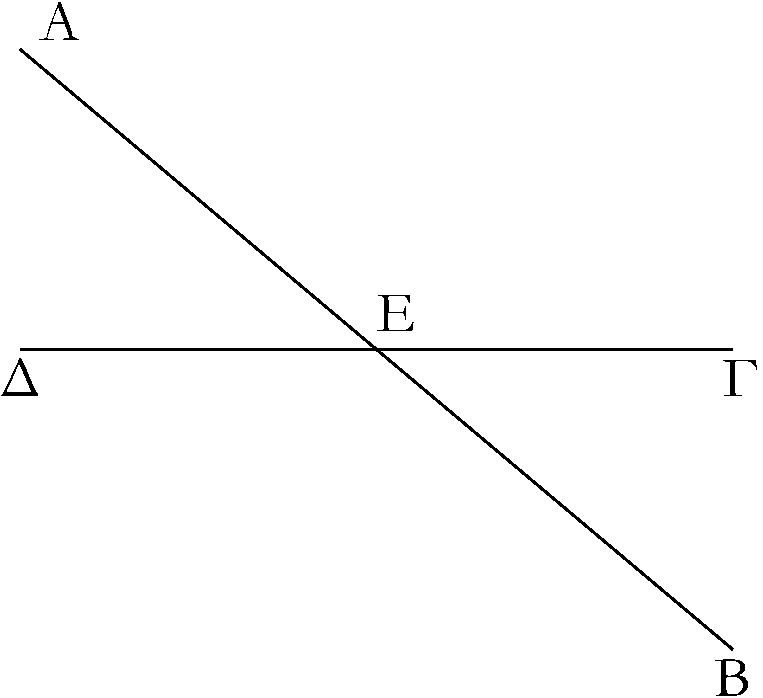
\includegraphics[width=0.8\textwidth]{Book01/fig15g.pdf}}

\gr{Ἐπεὶ γὰρ εὐθεῖα ἡ ΑΕ ἐπ' εὐθεῖαν τὴν ΓΔ ἐφέστηκε γωνίας ποιοῦσα τὰξ ὑπὸ ΓΕΑ, ΑΕΔ, αἱ  ἄρα ὑπὸ ΓΕΑ, ΑΕΔ γωνίαι δυσὶν
ὀρθαῖξ ἴσαι εἰσίν. πάλιν, ἐπεὶ εὐθεῖα ἡ ΔΕ ἐπ' εὐθεῖαν
τὴν ΑΒ ἐφέστηκε γωνίας ποιοῦσα τὰξ ὑπὸ ΑΕΔ, ΔΕΒ, αἱ  ἄρα
ὑπὸ ΑΕΔ, ΔΕΒ γωνίαι δυσὶν ὀρθαῖξ ἴσαι εἰσίν. ἐδείθθησαν
δὲ καὶ αἱ ὑπὸ ΓΕΑ, ΑΕΔ δυσὶν ὀρθαῖξ ἴσαι; αἱ  ἄρα ὑπὸ ΓΕΑ,
ΑΕΔ ταῖς ὑπὸ ΑΕΔ, ΔΕΒ ἴσαι εἰσίν. κοινὴ ἀφῃρήσθω ἡ ὑπὸ
ΑΕΔ; λοιπὴ  ἄρα ἡ ὑπὸ ΓΕΑ λοιπῆ| τῇ ὑπὸ ΒΕΔὸίση ἐστίν;
ὁμοίως δὴ δειθθήσεται, ὅτι καὶ αἱ ὑπὸ ΓΕΒ, ΔΕΑ ἴσαι εἰσίν.}

\gr{Ἐὰν ἄρα δύο εὐθεῖαι τέμνωσιν ἀλλήλας, τὰξ κατὰ κορυφὴν γωνίας ἴσας ἀλλήλαις ποιοῦσιν; ὅπερ ἔδει δεῖχαι.}}

\ParallelRText{
\begin{center}
{\large Proposition 15}
\end{center}

If two straight-lines cut one another (then) they make the vertically opposite angles
equal to one another.

For let the two straight-lines $AB$ and $CD$ cut one another at the point $E$. I say
that  angle $AEC$ is equal to (angle) $DEB$, and (angle) $CEB$ to (angle) $AED$.

% Removed epsf size command
\centerline{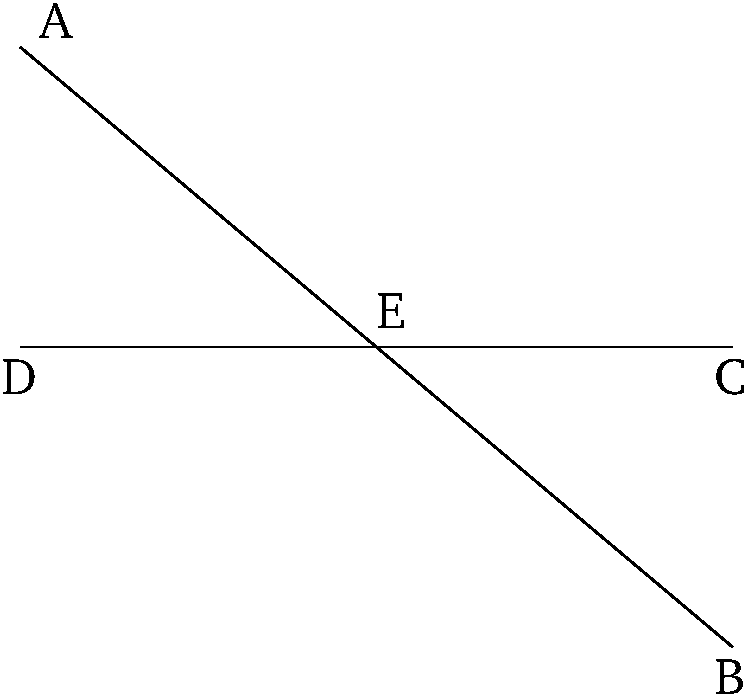
\includegraphics[width=0.8\textwidth]{Book01/fig15e.pdf}}

For since the straight-line $AE$ stands on the straight-line $CD$, making the
angles $CEA$ and $AED$, the (sum of the) angles $CEA$ and $AED$ is thus equal to two
right-angles [Prop.~1.13]. Again, since the straight-line $DE$ stands on the
straight-line $AB$, making the angles $AED$ and $DEB$, the (sum of the) angles $AED$ and
$DEB$ is thus equal to two right-angles [Prop.~1.13]. But (the sum of) $CEA$ and $AED$ was also shown
(to be) equal to two right-angles. Thus, (the sum of) $CEA$ and $AED$ is equal to (the sum of) $AED$ and $DEB$ [C.N.~1]. Let $AED$ be subtracted from both. Thus, the remainder
$CEA$ is equal to the remainder $BED$ [C.N.~3]. Similarly, it can be shown that
$CEB$ and $DEA$ are also equal.

Thus, if two straight-lines cut one another (then) they make the vertically opposite angles
equal to one another. (Which is) the very thing it was required to show.}
\end{Parallel}

%%%%%%
% Prop 1.16
%%%%%%
\pdfbookmark[1]{Proposition 1.16}{pdf1.16}
\begin{Parallel}{}{} 
\ParallelLText{
\begin{center}
{\large \ggn{16}.}
\end{center}\vspace*{-7pt}

\gr{Παντὸξ τριγώνου μιᾶς τῶν πλευρῶν προσεκβληθείσης ἡ ἐκτὸξ γωνία
ἑκατέρας τῶν ἐντὸς καὶ ἀπεναντίον γωνιῶν μείζων ἐστίν.}

\gr{Ἔστω τρίγωνον τὸ ΑΒΓ, καὶ προσεκβεβλήσθω αὐτοῦ μία πλευρὰ
ἡ ΒΓ ἐπὶ τὸ Δ; λὲγω, ὅτι ἡ ἐκτὸξ γωνία ἡ ὑπὸ ΑΓΔ
μείζων ἐστὶν ἑκατέρας τῶν ἐντὸς καὶ ἀπεναντίον τῶν
ὑπὸ ΓΒΑ, ΒΑΓ γωνιῶν.}

\gr{Τετμήσθω ἡ ΑΓ δίθα κατὰ τὸ Ε, καὶ ἐπιζευθθεῖσα ἡ ΒΕ ἐκβεβλήσθω
ἐπ' εὐθείας ἐπὶ τὸ Ζ, καὶ κείσθω τῇ ΒΕὸίση ἡ ΕΖ, καὶ ἐπεζεύθθω
ἡ ΖΓ, καὶ διήθθω ἡ ΑΓ ἐπὶ τὸ Η.}\\

% Removed epsf size command
\centerline{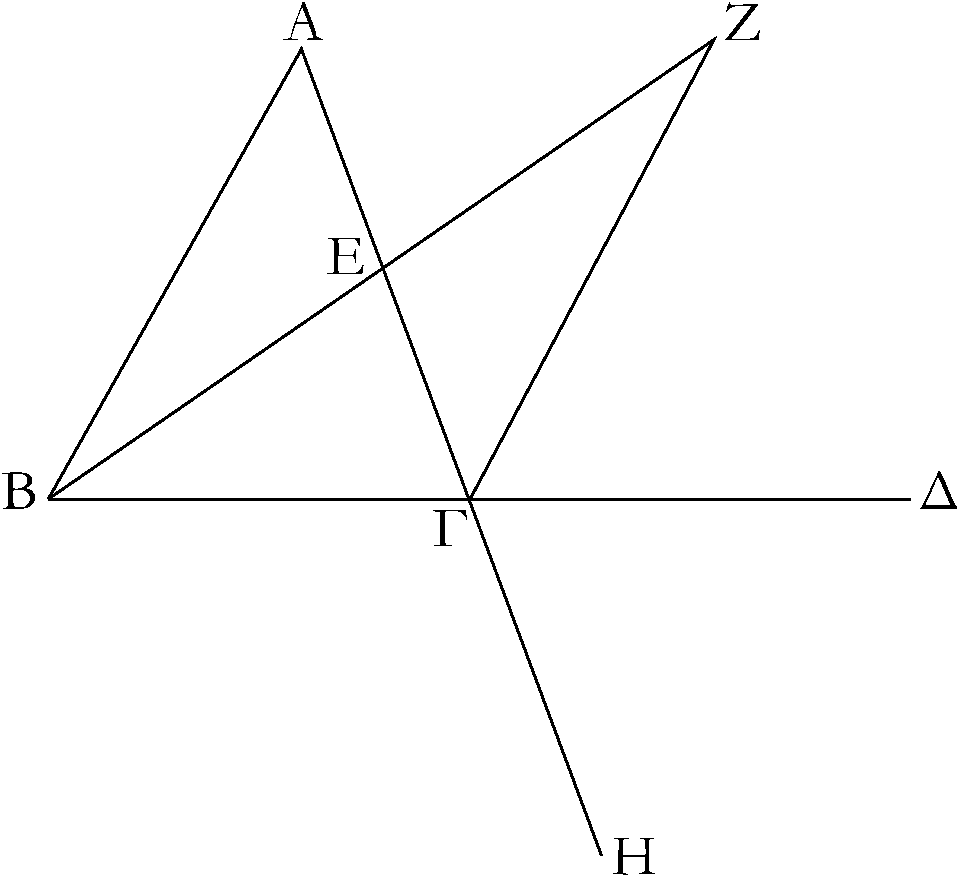
\includegraphics[width=0.8\textwidth]{Book01/fig16g.pdf}}

\gr{Ἐπεὶ οὸῦνὸίση ἐστὶν ἡ μὲν ΑΕ τῇ ΕΓ, ἡ δὲ ΒΕ τῇ ΕΖ, δύο
δὴ αἱ ΑΕ, ΕΒ δυσὶ ταῖς ΓΕ, ΕΖ ἴσαι εἰσὶν ἑκατέρα ἑκατέρᾳ;
καὶ γωνία ἡ ὑπὸ ΑΕΒ γωνίᾳ τῇ ὑπὸ ΖΕΓὸίση ἐστίν; κατὰ κορυφὴν γάρ; βάσις ἄρα ἡ ΑΒ βάσει τῇ ΖΓὸίση ἐστίν, καὶ τὸ ΑΒΕ
τρίγωνον τῷ ΖΕΓ τριγώνῳ ἐστὶν ἴσον, καὶ αἱ λοιπαὶ
γωνίαι ταῖς λοιπαῖξ γωνίαις ἴσαι εἰσὶν ἑκατέρα
 ἑκατέρᾳ,
ὑφὸ ὁὰξ αἱ  ἴσαι πλευραὶ ὑποτείνουσιν; ὸίση ἄρα ἐστὶν ἡ
ὑπὸ ΒΑΕ τῇ ὑπὸ ΕΓΖ. μείζων δέ ἐστιν ἡ ὑπὸ ΕΓΔ τῆς
ὑπὸ ΕΓΖ; μείζων ἄρα ἡ ὑπὸ ΑΓΔ τῆς ὑπὸ ΒΑΕ. Ὁμοίως
δὴ τῆς ΒΓ τετμ  ημένης δίθα δειθθήσεται καὶ ἡ ὑπὸ ΒΓΗ, τουτέστιν
ἡ ὑπὸ ΑΓΔ, μείζων καὶ τῆς ὑπὸ ΑΒΓ.}

\gr{Παντὸξ ἄρα τριγώνου μιᾶς τῶν πλευρῶν προσεκβληθείσης ἡ ἐκτὸξ γωνία
ἑκατέρας τῶν ἐντὸς καὶ ἀπεναντίον γωνιῶν μείζων ἐστίν;
ὅπερ ἔδει δεῖχαι.}}

\ParallelRText{
\begin{center}
{\large Proposition 16}
\end{center}

For any triangle, when one of the sides is produced, the external angle
is greater than each of the internal and opposite angles.

Let $ABC$ be a triangle, and let one of its sides $BC$ be produced 
 to $D$. I say that the external angle $ACD$ is greater than each of the
 internal and opposite angles, $CBA$ and $BAC$.
 
 Let the (straight-line) $AC$ be cut in half at (point) $E$ [Prop.~1.10].
 And $BE$ being joined, let it be produced in a straight-line to
 (point) $F$.$^\dag$ And let $EF$ be made equal to $BE$ [Prop.~1.3], and let $FC$ be joined, and let $AC$ be drawn through to (point) $G$.
 
% Removed epsf size command
\centerline{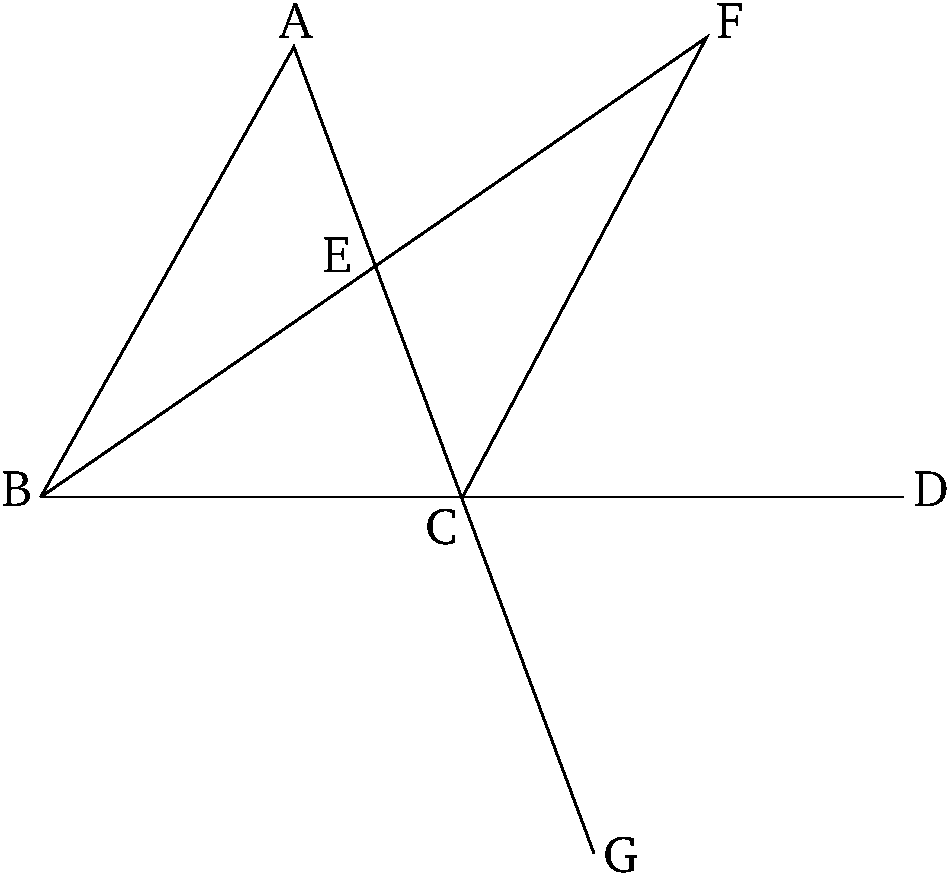
\includegraphics[width=0.8\textwidth]{Book01/fig16e.pdf}}

 Therefore, since $AE$ is equal to $EC$, and $BE$ to $EF$, the two (straight-lines)
 $AE$, $EB$ are equal to the two (straight-lines) $CE$, $EF$, respectively. 
 Also, angle $AEB$ is equal to angle $FEC$, for (they are)
 vertically opposite [Prop.~1.15]. Thus, the base $AB$ is equal to the base
 $FC$, and the triangle $ABE$ is equal to the triangle $FEC$, and the remaining
 angles subtended by the equal sides are equal to the corresponding remaining angles [Prop.~1.4]. Thus, $BAE$ is equal to $ECF$. But $ECD$ is greater than $ECF$. Thus,
 $ACD$ is greater than $BAE$. Similarly, by having cut $BC$ in half,  it can  be shown (that) $BCG$---that is to say, $ACD$---(is) also greater than $ABC$.
 
 Thus, for any triangle, when one of the sides is produced, the external angle
is greater than each of the internal and opposite angles. (Which is) the very thing
it was required to show.}
\end{Parallel}
{\footnotesize
\noindent $^\dag$  The implicit assumption that the point $F$ lies in the
 interior of the angle $ABC$ should be counted as an additional postulate.} 
 
 %%%%%%
% Prop 1.17
%%%%%%
\pdfbookmark[1]{Proposition 1.17}{pdf1.17}
\begin{Parallel}{}{} 
\ParallelLText{
\begin{center}
{\large \ggn{17}.}
\end{center}\vspace*{-7pt}

\gr{Παντὸνς τριγώνου αἱ δύο γωνίαι δύο ὀρθῶν ἐλάσσονέξ εἰσι πάντῇ μεταλαμβανόμεναι.}

\gr{Ἔστω τρίγωνον τὸ ΑΒΓ; λέγω, ὅτι τοῦ ΑΒΓ τριγώνου αἱ δύο γωνίαι δύο ὀρθῶν ἐλάττονέξ εἰσι πάντῃ μεταλαμβανόμεναι.}

\gr{Ἐκβεβλήσθω γὰρ ἡ ΒΓ ἐπὶ τὸ Δ.}

\gr{Καὶ ἐπεὶ τριγώνου τοῦ ΑΒΓ ἐκτόξ ἐστι γωνία ἡ ὑπὸ ΑΓΔ,
μείζων ἐστὶ τῆς ἐντὸς καὶ ἀπεναντίον τῆς ὑπὸ ΑΒΓ. κοινὴ
προσκείσθω ἡ ὑπὸ ΑΓΒ; αἱ  ἄρα ὑπὸ ΑΓΔ, ΑΓΒ τῶν ὑπὸ ΑΒΓ,
ΒΓΑ μείζονέξ εἰσιν. ἀλλὸ  αἱ ὑπὸ ΑΓΔ, ΑΓΒ δύο ὀρθαῖξ ἴσαι εἰσίν; αἱ  ἄρα ὑπὸ  
ΑΒΓ, ΒΓΑ δύο ὀρθῶν ἐλάσσονέξ εἰσιν.
ὁμοίως δὴ δείχομεν, ὅτι καὶ αἱ ὑπὸ ΒΑΓ, ΑΓΒ δύο
ὀρθῶν ἐλάσσονέξ εἰσι καὶ ὸέτι αἱ ὑπὸ
ΓΑΒ, ΑΒΓ.}\\~\\~\\

% Removed epsf size command
\centerline{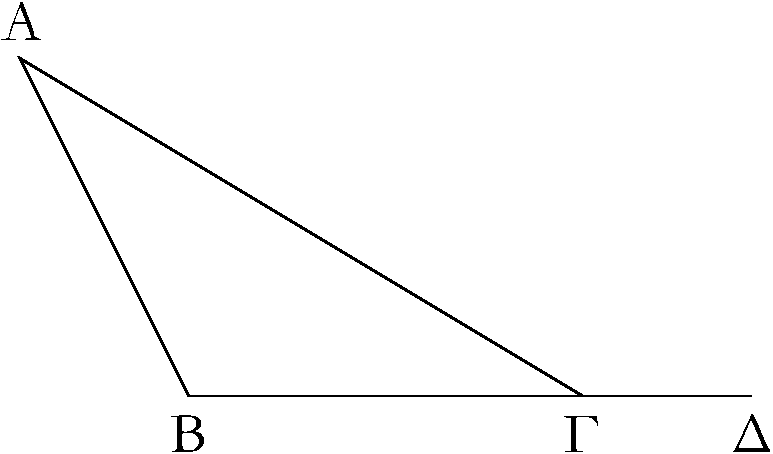
\includegraphics[width=0.8\textwidth]{Book01/fig17g.pdf}}

\gr{Παντὸνς ἄρα τριγώνου αἱ δύο γωνίαι δύο ὀρθῶν ἐλάσσονέξ εἰσι πάντῇ μεταλαμβανόμεναι; ὅπερ ἔδει δεῖχαι.}}

\ParallelRText{
\begin{center}
{\large Proposition 17}
\end{center}

For any triangle,  (the sum of) two angles taken together in any (possible way) is less than two right-angles.

Let $ABC$ be a triangle. I say that (the sum of) two angles of triangle $ABC$
taken together in any (possible way) is less than two right-angles.

For let $BC$ be produced to $D$.

And since the angle $ACD$ is external to triangle $ABC$, it is greater than the
internal and opposite angle $ABC$ [Prop.~1.16]. Let $ACB$ be added to both. Thus, the
(sum of the angles) $ACD$ and $ACB$ is greater than the  (sum of the angles) $ABC$ and
$BCA$. But, (the sum of) $ACD$ and $ACB$ is equal to two right-angles [Prop.~1.13].
Thus, (the sum of) $ABC$ and $BCA$ is less than two right-angles. Similarly,
we can show that (the sum of) $BAC$ and $ACB$ is also less than two right-angles,
and further (that the sum of) $CAB$ and $ABC$ (is less than two right-angles).

% Removed epsf size command
\centerline{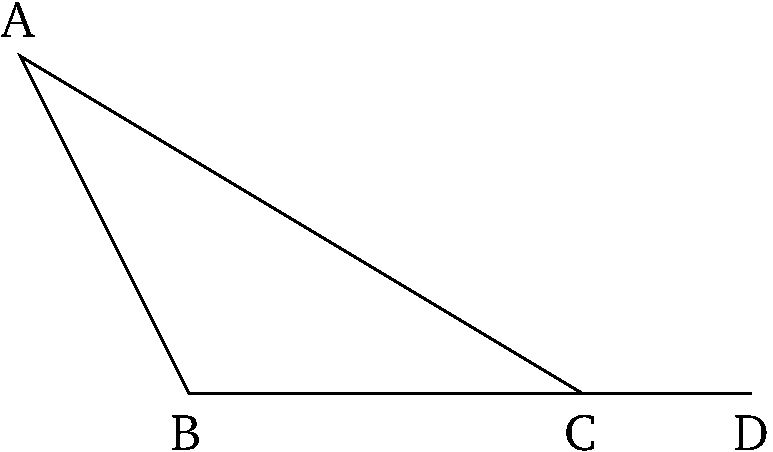
\includegraphics[width=0.8\textwidth]{Book01/fig17e.pdf}}

Thus, for any triangle,  (the sum of) two angles taken together in any (possible way) is less than two right-angles. (Which is) the very thing
it was required to show.}
\end{Parallel}

%%%%%%
% Prop 1.18
%%%%%%
\pdfbookmark[1]{Proposition 1.18}{pdf1.18}
\begin{Parallel}{}{} 
\ParallelLText{
\begin{center}
{\large \ggn{18}.}
\end{center}\vspace*{-7pt}

\gr{Παντὸξ τριγώνου ἡ μείζων πλευρὰ τὴν μείζονα γωνίαν ὑποτείνει.}

\gr{Ἔστω γὰρ τρίγωνον τὸ ΑΒΓ μείζονα ἔχον τὴν ΑΓ πλευρὰν τῆς
ΑΒ; λέγω, ὅτι καὶ γωνία ἡ ὑπὸ ΑΒΓ μείζων ἐστὶ τῆς ὑπὸ ΒΓΑ.}

% Removed epsf size command
\centerline{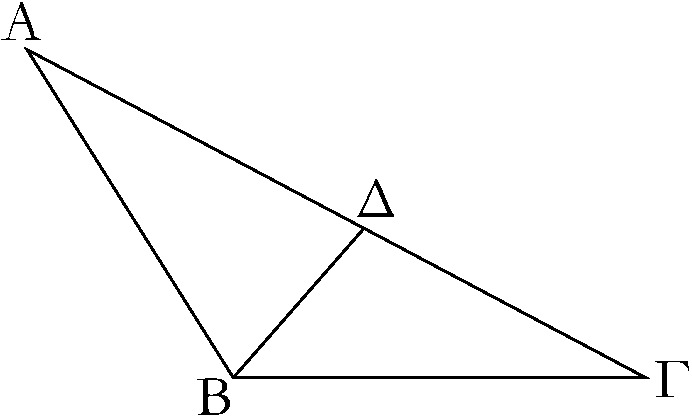
\includegraphics[width=0.8\textwidth]{Book01/fig18g.pdf}}

\gr{Ἐπεὶ γὰρ μείζων ἐστὶν ἡ ΑΓ τῆς ΑΒ, κείσθω τῇ ΑΒὸίση ἡ
ΑΔ, καὶ ἐπεζεύθθω ἡ ΒΔ.}

\gr{Καὶ ἐπεὶ τριγώνου τοῦ ΒΓΔ ἐκτόξ ἐστι γωνία ἡ ὑπὸ ΑΔΒ,
μείζων ἐστὶ τῆς ἐντὸς καὶ ἀπεναντίον τῆς ὑπὸ ΔΓΒ; ὸίση
δὲ ἡ ὑπὸ ΑΔΒ τῇ ὑπὸ ΑΒΔ, ἐπεὶ καὶ πλευρὰ ἡ ΑΒ τῇ
ΑΔ ἐστινὸίση; μείζων ἄρα καὶ ἡ ὑπὸ ΑΒΔ τῆς ὑπὸ ΑΓΒ;
πολλῶ|  ἄρα ἡ ὑπὸ ΑΒΓ μείζων ἐστὶ τῆς ὑπὸ ΑΓΒ.}

\gr{Παντὸξ ἄρα τριγώνου ἡ μείζων πλευρὰ τὴν μείζονα γωνίαν
ὑποτείνει; ὅπερ ἔδει δεῖχαι.}}

\ParallelRText{
\begin{center}
{\large Proposition 18}
\end{center}

In any triangle, the greater side subtends the greater angle.

For let $ABC$ be a triangle having side $AC$ greater than $AB$. I say that
angle $ABC$ is also greater than $BCA$.\\~\\

% Removed epsf size command
\centerline{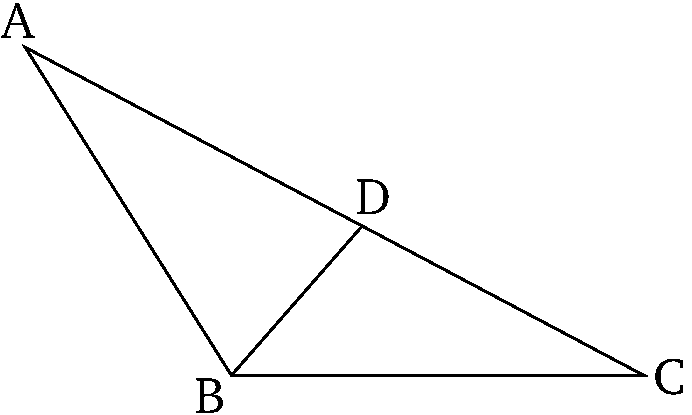
\includegraphics[width=0.8\textwidth]{Book01/fig18e.pdf}}

For since $AC$ is greater than $AB$, let $AD$ be made equal to $AB$
 [Prop.~1.3],
and let $BD$ be joined.

And since angle $ADB$ is external to triangle $BCD$, it is greater than the
internal and opposite (angle) $DCB$ [Prop.~1.16]. But $ADB$ (is) equal to $ABD$,
since side $AB$ is also equal to side $AD$ [Prop.~1.5]. Thus,
$ABD$ is also greater than $ACB$. Thus, $ABC$ is much greater than 
$ACB$.

Thus, in any triangle, the greater side subtends the greater angle.
(Which is) the very thing  it was required to show.}
\end{Parallel}

%%%%%%
% Prop 1.19
%%%%%%
\pdfbookmark[1]{Proposition 1.19}{pdf1.19}
\begin{Parallel}{}{} 
\ParallelLText{
\begin{center}
{\large \ggn{19}.}
\end{center}\vspace*{-7pt}

\gr{Παντὸξ τριγώνου ὑπὸ τὴν μείζονα γωνίαν ἡ μείζων πλευρὰ ὑποτείνει.}

\gr{Ἔστω τρίγωνον τὸ ΑΒΓ  μείζονα ἔχον τὴν ὑπὸ ΑΒΓ γωνίαν τῆς ὑπὸ ΒΓΑ; λέγω, ὅτι καὶ πλευρὰ ἡ ΑΓ πλευρᾶξ τῆς ΑΒ μείζων
ἐστίν.}

% Removed epsf size command
\centerline{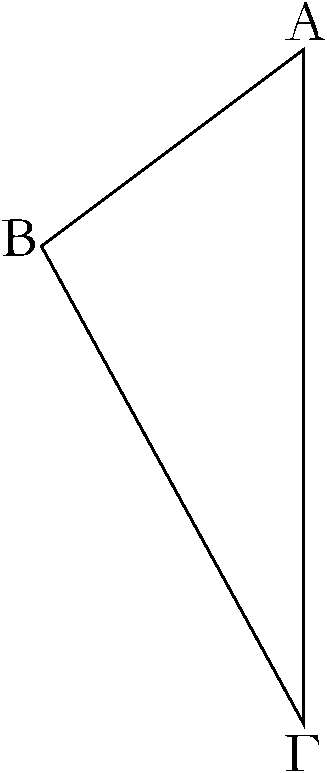
\includegraphics[width=0.8\textwidth]{Book01/fig19g.pdf}}

\gr{ Εἰ γὰρ μή,  ἢτοιὸίση ἐστὶν ἡ ΑΓ τῇ ΑΒὸὴ ἐλάσσων; ὸίση μὲν οὸῦν οὐκὸέστιν ἡ ΑΓ τῇ ΑΒ; ὸίση γὰρὸὰνὸῆν καὶ γωνία ἡ ὑπὸ
ΑΒΓ τῇ ὑπὸ ΑΓΒ; οὐκὸέστι δέ; οὐκ ἄραὸίση ἐστὶν ἡ ΑΓ
τῇ ΑΒ. οὐδὲ μὴν ἐλάσσων ἐστὶν ἡ ΑΓ τῆς ΑΒ;
ἐλάσσων γὰρὸὰνὸῆν καὶ γωνία ἡ ὑπὸ ΑΒΓ τῆς ὑπὸ
ΑΓΒ; οὐκὸέστι δέ; οὐκ ἄρα ἐλάσσων ἐστὶν ἡ ΑΓ τῆς
ΑΒ. ἐδείθθη δέ, ὅτι οὐδὲ ὸίση ἐστίν. μείζων ἄρα ἐστὶν
ἡ ΑΓ τῆς ΑΒ.}

\gr{Παντὸξ ἄρα τριγώνου ὑπὸ τὴν μείζονα γωνίαν ἡ μείζων πλευρὰ ὑποτείνει; ὅπερ ἔδει δεῖχαι.}}

\ParallelRText{
\begin{center}
{\large Proposition 19}
\end{center}

In any triangle, the greater angle is subtended by the greater side.

Let $ABC$ be a triangle having the angle $ABC$ greater than $BCA$. I say
that side $AC$ is also greater than side $AB$.\\

% Removed epsf size command
\centerline{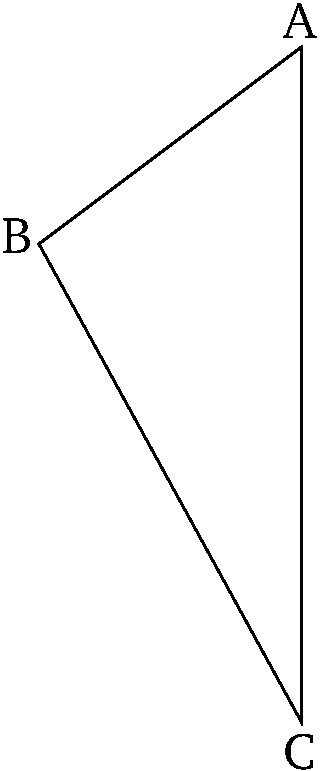
\includegraphics[width=0.8\textwidth]{Book01/fig19e.pdf}}

For if not, $AC$ is certainly either equal to, or less than, $AB$. In fact, $AC$ is not
equal to $AB$. For then angle $ABC$  would also be equal to $ACB$ [Prop.~1.5].
But it is not. Thus, $AC$ is not equal to $AB$.
Neither, indeed, is $AC$ less than $AB$. For then angle $ABC$ would also be
less than $ACB$ [Prop.~1.18]. But it is not. Thus, $AC$ is not less than
$AB$. But it was  shown that ($AC$) is    not equal (to $AB$) either. Thus, $AC$ 
is greater than $AB$.

Thus, in any triangle, the greater angle is subtended by the greater side.
(Which is) the very thing it was required to show.}
\end{Parallel}

%%%%%%
% Prop 1.20
%%%%%%
\pdfbookmark[1]{Proposition 1.20}{pdf1.20}
\begin{Parallel}{}{} 
\ParallelLText{
\begin{center}
{\large \ggn{20}.}
\end{center}\vspace*{-7pt}

\gr{Παντὸξ τριγώνου αἱ δύο πλευραὶ τῆς λοιπῆς μείζονέξ εἰσι πάντῃ
μεταλαμβανόμεναι.}

% Removed epsf size command
\centerline{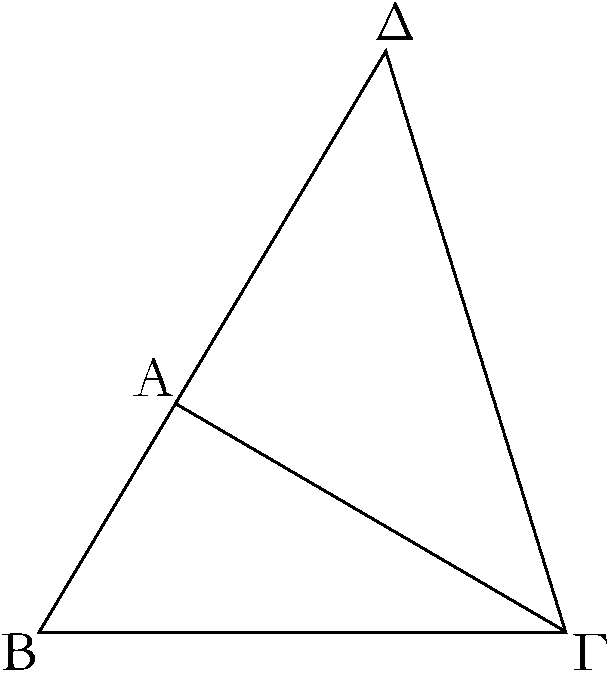
\includegraphics[width=0.8\textwidth]{Book01/fig20g.pdf}}

\gr{Ἔστω γὰρ τρίγωνον τὸ ΑΒΓ; λέγω, ὅτι τοῦ ΑΒΓ τριγώνου αἱ
δύο πλευραὶ τῆς λοιπῆς μείζονέξ εἰσι πάντῃ μεταλαμβανόμεναι,
αἱ μὲν ΒΑ, ΑΓ τῆς ΒΓ, αἱ δὲ ΑΒ, ΒΓ τῆς ΑΓ, αἱ δὲ ΒΓ, ΓΑ
τῆς ΑΒ.}

\gr{Διήθθω γὰρ ἡ ΒΑ ἐπὶ τὸ Δ σημεῖον, καὶ κείσθω τῇ
ΓΑὸίση ἡ ΑΔ, καὶ ἐπεζεύθθω ἡ ΔΓ.}

\gr{Ἐπεὶ οὸῦνὸίση ἐστὶν ἡ ΔΑ τῇ ΑΓ, ὸίση ἐστὶ καὶ
γωνία ἡ ὑπὸ ΑΔΓ τῇ ὑπὸ ΑΓΔ; μείζων ἄρα ἡ
ὑπὸ ΒΓΔ τῆς ὑπὸ ΑΔΓ; καὶ ἐπεὶ τρίγωνόν ἐστι τὸ ΔΓΒ
μείζονα ἔχον τὴν ὑπὸ ΒΓΔ γωνίαν τῆς ὑπὸ ΒΔΓ, ὑπὸ
δὲ τὴν μείζονα γωνίαν ἡ μείζων πλευρὰ ὑποτείνει,
ἡ ΔΒ ἄρα τῆς ΒΓ ἐστι μείζων. ὸίση δὲ ἡ ΔΑ τῇ
ΑΓ; μείζονες ἄρα αἱ ΒΑ, ΑΓ τῆς ΒΓ; ὁμοίως δὴ
δείχομεν, ὅτι καὶ αἱ μὲν ΑΒ, ΒΓ τῆς ΓΑ μείζονέξ εἰσιν,
αἱ δὲ ΒΓ, ΓΑ τῆς ΑΒ.}

\gr{Παντὸξ ἄρα τριγώνου αἱ δύο πλευραὶ τῆς λοιπῆς μείζονέξ εἰσι πάντῃ
μεταλαμβανόμεναι; ὅπερ ἔδει δεῖχαι.}}

\ParallelRText{
\begin{center}
{\large Proposition 20}
\end{center}

In any triangle, (the sum of) two sides taken together in any (possible way) is greater than the remaining (side).

% Removed epsf size command
\centerline{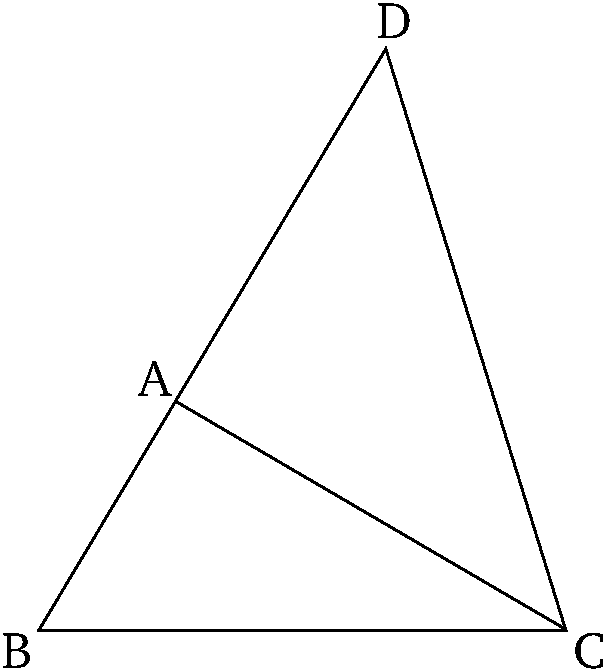
\includegraphics[width=0.8\textwidth]{Book01/fig20e.pdf}}

For let $ABC$ be a triangle. I say that in triangle $ABC$ (the sum of) two
sides taken together in
any (possible way) is greater than the remaining (side). (So), (the sum of) $BA$ and $AC$ (is greater) than $BC$,
(the sum of) $AB$ and $BC$ than $AC$, and (the sum of) $BC$ and $CA$ than $AB$.

For let $BA$ be drawn through to point $D$, and let $AD$ be made equal to $CA$ [Prop.~1.3], and let $DC$ be joined.

Therefore, since $DA$ is equal to $AC$, the angle $ADC$ is also equal to
$ACD$ [Prop.~1.5]. Thus, $BCD$ is greater than $ADC$. And since
 $DCB$ is a triangle having the angle $BCD$ greater than $BDC$, and the
greater angle subtends the greater side [Prop.~1.19], $DB$ is thus
greater than $BC$. But $DA$ is equal to $AC$. Thus, (the sum of) $BA$ and $AC$ is
greater than $BC$. Similarly, we can show that (the sum of) $AB$ and $BC$ is also
greater than $CA$, and (the sum of) $BC$ and $CA$ than $AB$.

Thus, in any triangle, (the sum of) two sides taken together in any (possible way) is greater than the remaining (side). (Which is) the very thing
it was required to show.}
\end{Parallel}

%%%%%%
% Prop 1.21
%%%%%%
\pdfbookmark[1]{Proposition 1.21}{pdf1.21}
\begin{Parallel}{}{} 
\ParallelLText{
\begin{center}
{\large \ggn{21}.}
\end{center}\vspace*{-7pt}

\gr{Ἐὰν τριγώνου ἐπὶ μιᾶς τῶν πλευρῶν ἀπὸ τῶν περάτων δύο
εὐθεῖαι ἐντὸς συσταθῶσιν, αἱ συσταθεῖσαι τῶν λοιπῶν τοῦ
τριγώνου δύο πλευρῶν ἐλάττονες μὲνὸέσονται, μείζονα δὲ
γωνίαν περιέχουσιν.}

\gr{Τριγώνου γὰρ τοῦ ΑΒΓ ἐπὶ μιᾶς τῶν πλευρῶν τῆς ΒΓ ἀπὸ
τῶν περάτων τῶν Β, Γ δύο εὐθεῖαι ἐντὸς συνεστάτωσαν αἱ ΒΔ, ΔΓ;
λέγω, ὅτι αἱ ΒΔ, ΔΓ τῶν λοιπῶν τοῦ τριγώνου δύο πλευρῶν
τῶν ΒΑ, ΑΓ ἐλάσσονες μέν εἰσιν, μείζονα δὲ γωνίαν περιέθουσι
τὴν ὑπὸ ΒΔΓ τῆς ὑπὸ ΒΑΓ.}

% Removed epsf size command
\centerline{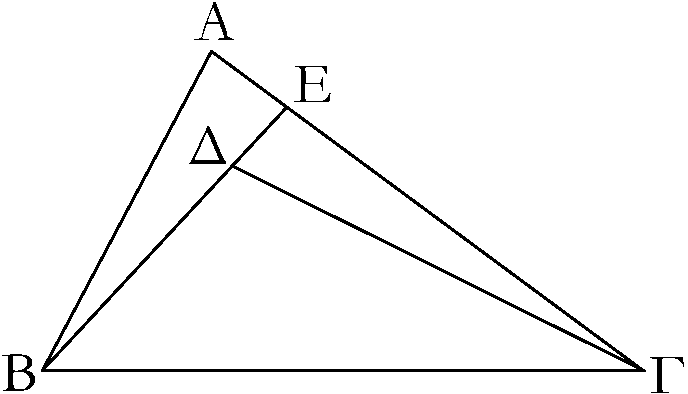
\includegraphics[width=0.8\textwidth]{Book01/fig21g.pdf}}

\gr{Διήθθω γὰρ ἡ ΒΔ ἐπὶ τὸ Ε. καὶ ἐπεὶ παντὸς τριγώνου αἱ δύο
πλευραὶ τῆς λοιπῆς μείζονέξ εἰσιν, τοῦ ΑΒΕ ἄρα τριγώνου αἱ
δύο πλευραὶ αἱ ΑΒ, ΑΕ τῆς ΒΕ μείζονέξ εἰσιν; κοινὴ προσκείσθω
ἡ ΕΓ; αἱ  ἄρα ΒΑ, ΑΓ τῶν ΒΕ, ΕΓ μείζονέξ εἰσιν. πάλιν, ἐπεὶ
τοῦ ΓΕΔ τριγώνου αἱ δύο πλευραὶ αἱ ΓΕ, ΕΔ τῆς ΓΔ μείζονέξ εἰσιν, κοινὴ προσκείσθω ἡ ΔΒ; αἱ ΓΕ, ΕΒ ἄρα τῶν ΓΔ, ΔΒ μείζονέξ εἰσιν. 
ἀλλὰ τῶν ΒΕ, ΕΓ μείζονες ἐδείθθησαν αἱ ΒΑ, ΑΓ; πολλῶ|
 ἄρα αἱ ΒΑ, ΑΓ τῶν ΒΔ, ΔΓ μείζονέξ εἰσιν.}

\gr{Πάλιν, ἐπεὶ παντὸς τριγώνου ἡ ἐκτὸξ γωνία τῆς ἐντὸς
καὶ ἀπεναντίον μείζων ἐστίν, τοῦ ΓΔΕ ἄρα τριγώνου ἡ
ἐκτὸξ γωνία ἡ ὑπὸ ΒΔΓ μείζων ἐστὶ τῆς ὑπὸ ΓΕΔ. διὰ ταὐτὰ
τοίνυν καὶ τοῦ ΑΒΕ τριγώνου ἡ ἐκτὸξ γωνία ἡ ὑπὸ ΓΕΒ μείζων
ἐστὶ τῆς ὑπὸ ΒΑΓ. ἀλλὰ τῆς ὑπὸ ΓΕΒ μείζων ἐδείθθη ἡ
ὑπὸ ΒΔΓ; πολλῶ|  ἄρα ἡ ὑπὸ ΒΔΓ μείζων ἐστὶ τῆς
ὑπὸ ΒΑΓ.}

\gr{Ἐὰν ἄρα τριγώνου ἐπὶ μιᾶς τῶν πλευρῶν ἀπὸ τῶν περάτων δύο
εὐθεῖαι ἐντὸς συσταθῶσιν, αἱ συσταθεῖσαι τῶν λοιπῶν τοῦ
τριγώνου δύο πλευρῶν ἐλάττονες μέν εἰσιν, μείζονα δὲ
γωνίαν περιέθουσιν;  ὅπερ ἔδει δεῖχαι.}}

\ParallelRText{
\begin{center}
{\large Proposition 21}
\end{center}

If two internal straight-lines are constructed on one of the sides
of a triangle, from its ends, 
the constructed (straight-lines) will be less than the two remaining 
sides of the triangle, but will encompass a greater angle.

For let the two internal straight-lines $BD$ and $DC$ be constructed on one of the sides $BC$ of the triangle $ABC$, from its ends $B$ and $C$ (respectively). I say that 
$BD$ and $DC$ are less than the (sum of the) two  remaining sides of the triangle
$BA$ and $AC$, but encompass an angle $BDC$ greater than $BAC$.

% Removed epsf size command
\centerline{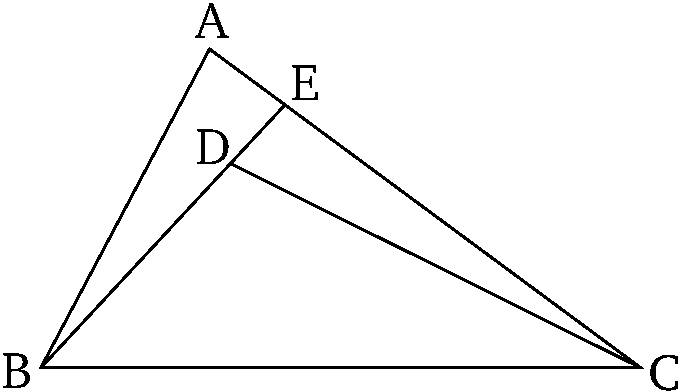
\includegraphics[width=0.8\textwidth]{Book01/fig21e.pdf}}

For let $BD$ be drawn through to $E$. And since in any
triangle (the sum of any) two sides is greater than the remaining (side) [Prop.~1.20],
 in triangle $ABE$ the  (sum of the) two sides $AB$ and $AE$ is thus  greater than
$BE$. Let $EC$ be added to both. Thus, (the sum of) $BA$ and $AC$ is greater
than (the sum of) $BE$ and $EC$.  Again, since in triangle $CED$ the (sum of the) two sides $CE$ and $ED$
is  greater than $CD$, let $DB$ be added to both. Thus, 
(the sum of) $CE$ and $EB$ is greater than  (the sum of) $CD$ and $DB$. But, (the sum of) $BA$ and $AC$ was shown
(to be) greater than (the sum of) $BE$
 and $EC$. Thus, (the sum of) $BA$ and $AC$ is much greater than
(the sum of) $BD$ and $DC$.

Again, since in any  triangle the external angle 
is greater than the internal and opposite (angles) [Prop. 1.16],
 in triangle $CDE$ the external angle $BDC$ is thus greater
than $CED$.  Accordingly, for the same (reason),  the external angle $CEB$ of the
triangle $ABE$ is also greater than $BAC$. But, $BDC$ was shown (to be) 
greater
than $CEB$. Thus, $BDC$ is much greater than $BAC$.

Thus, if two internal straight-lines are constructed on one of the sides
of a triangle, from its ends, 
the constructed (straight-lines) are less than the two remaining 
sides of the triangle, but  encompass a greater angle. (Which is) the
very thing it was required to show.}
\end{Parallel}

%%%%%%
% Prop 1.22
%%%%%%
\pdfbookmark[1]{Proposition 1.22}{pdf1.22}
\begin{Parallel}{}{} 
\ParallelLText{
\begin{center}
{\large \ggn{22}.}
\end{center}\vspace*{-7pt}

\gr{Ἐκ τριῶν εὐθειῶν, αὁί εἰσιν ἴσαι τρισὶ ταῖς δοθείσαις [εὐθείαις], τρίγωνον συστήσασθαι; δεῖ δὲ τὰξ δύο τῆς λοιπῆς μείζονας εὸῖναι
πάντῃ μεταλαμβανομένας [διὰ τὸ καὶ παντὸς τριγώνου τὰξ δύο πλευρὰξ τῆς λοιπῆς μείζονας εὸῖναι πάντῃ μεταλαμβανομένας].}\\~\\

% Removed epsf size command
\centerline{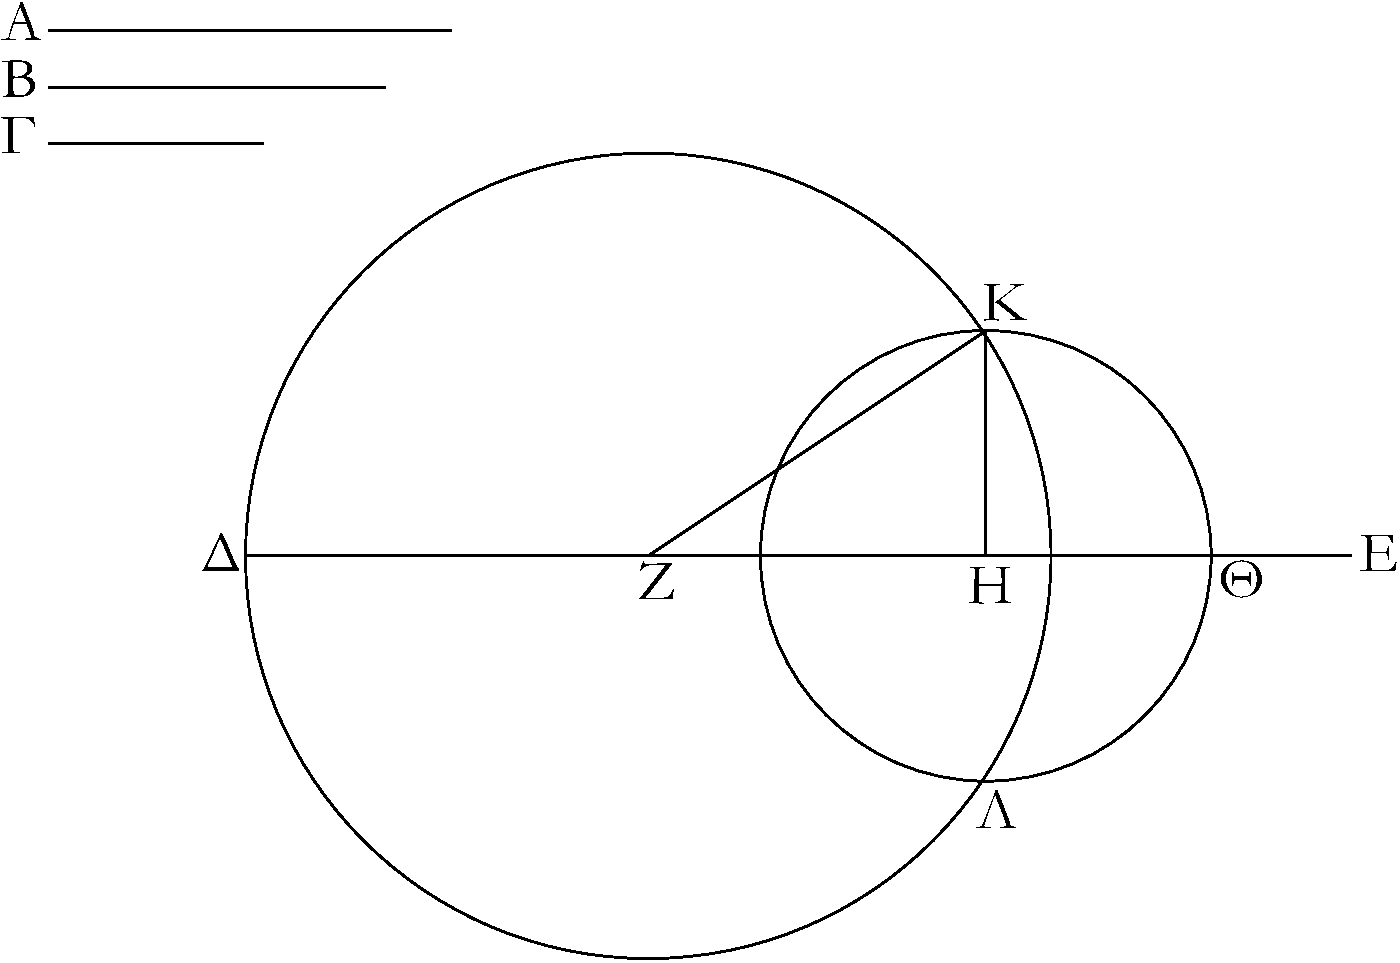
\includegraphics[width=0.8\textwidth]{Book01/fig22g.pdf}}

\gr{Ἔστωσαν αἱ δοθεῖσαι τρεῖς εὐθεῖαι αἱ Α, Β, Γ, ὁῶν αἱ δύο τῆς
λοιπῆς μείζονεςὸέστωσαν πάντῃ μεταλαμβανόμεναι, αἱ μὲν Α, Β
τῆς Γ, αἱ δὲ Α, Γ τῆς Β, καὶ ὸέτι αἱ Β, Γ τῆς Α; δεῖ δὴ ἐκ
τῶνὸίσων ταῖς Α, Β, Γ τρίγωνον συστήσασθαι.}

\gr{Ἐκκείσθω τις εὐθεῖα ἡ ΔΕ πεπερασμένη μὲν κατὰ τὸ Δὸάπειρος
δὲ κατὰ τὸ Ε, καὶ κείσθω τῇ μὲν Αὸίση ἡ ΔΖ, τῇ δὲ Βὸίση ἡ ΖΗ, τῇ δὲ Γὸίση ἡ ΗΘ; καὶ κέντρῳ μὲν τῷ Ζ, διαστήματι δὲ τῷ
ΖΔ κύκλος γεγράφθω ὁ ΔΚΛ; πάλιν κέντρῳ μὲν τῷ Η, διαστήματι δὲ τῷ ΗΘ κύκλος γεγράφθω ὁ ΚΛΘ, καὶ ἐπεζεύθθωσαν αἱ ΚΖ, ΚΗ; λέγω,
ὅτι ἐκ τριῶν εὐθειῶν τῶνὸίσων ταῖς Α, Β, Γ τρίγωνον συνέσταται τὸ ΚΖΗ.}

\gr{Ἐπεὶ γὰρ τὸ Ζ σημεῖον κέντρον ἐστὶ τοῦ ΔΚΛ κύκλου, ὸίση ἐστὶν ἡ ΖΔ τῇ ΖΚ; ἀλλὰ ἡ ΖΔ τῇ Α ἐστινὸίση. καὶ ἡ ΚΖ ἄρα τῇ 
Α ἐστινὸίση. πάλιν, ἐπεὶ τὸ Η σημεῖον κέντρον ἐστὶ τοῦ ΛΚΘ
κύκλου, ὸίση ἐστὶν ἡ ΗΘ τῇ ΗΚ; ἀλλὰ ἡ ΗΘ τῇ Γ ἐστινὸίση;
καὶ ἡ ΚΗ ἄρα τῇ Γ ἐστινὸίση. ἐστὶ δὲ καὶ ἡ ΖΗ τῇ Βὸίση;
αἱ τρεῖς ἄρα εὐθεῖαι αἱ ΚΖ, ΖΗ, ΗΚ τρισὶ ταῖς Α, Β, Γ ἴσαι εἰσίν.}

\gr{Ἐκ τριῶν ἄρα εὐθειῶν τῶν ΚΖ, ΖΗ, ΗΚ, αὁί εἰσιν ἴσαι τρισὶ ταῖς δοθείσαις εὐθείαις ταῖς Α, Β, Γ, τρίγωνον συνέσταται τὸ ΚΖΗ; ὅπερ ἔδει ποιῆσαι.}}

\ParallelRText{
\begin{center}
{\large Proposition 22}
\end{center}

To construct a triangle from three straight-lines which are equal to three given [straight-lines]. It is necessary for (the sum of) two (of the straight-lines) taken together in any (possible way) to be greater than the remaining (one), [on account of the (fact that)
 in any triangle (the sum of) two sides taken together in any (possible way) is greater than the remaining (one) [Prop.~1.20]\,].

% Removed epsf size command
\centerline{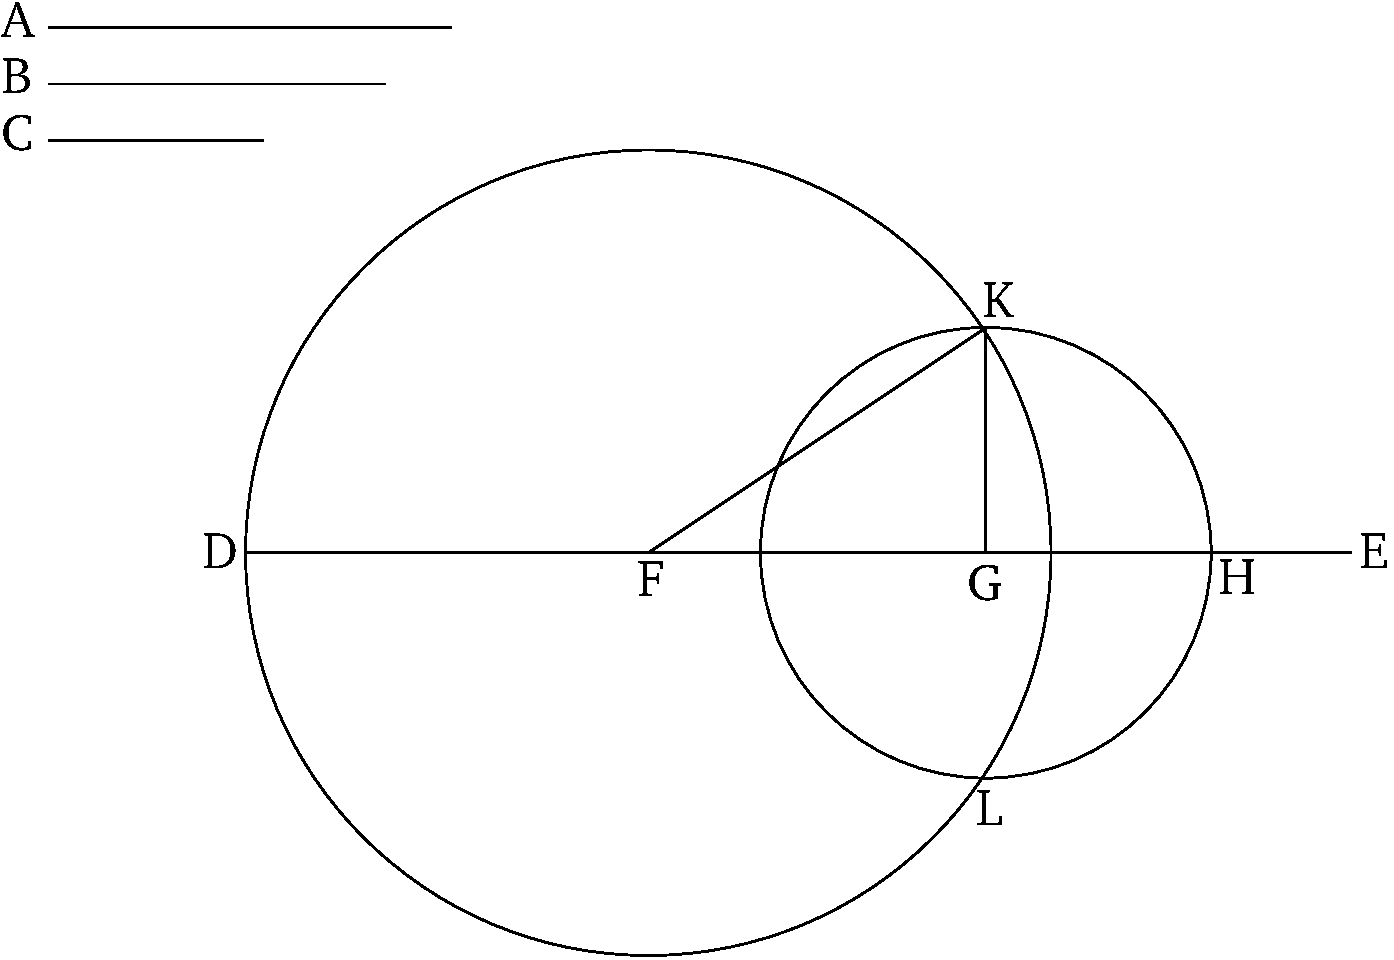
\includegraphics[width=0.8\textwidth]{Book01/fig22e.pdf}}

Let $A$, $B$, and $C$ be the three given straight-lines, of which let (the sum of) two taken together in any (possible way)
be greater than the remaining (one). (Thus), (the sum of) $A$ and $B$ (is greater) than $C$, (the sum of) $A$ and $C$ than $B$,
and also (the sum of) $B$ and $C$ than $A$. So it is required to construct a triangle
from (straight-lines) equal to $A$, $B$, and $C$.

Let some straight-line $DE$ be set out, terminated at $D$, and infinite in the
direction of $E$.  And let $DF$ made equal to $A$, and $FG$
equal to $B$, and $GH$ equal to $C$ [Prop.~1.3]. And let the
circle $DKL$ be drawn with center $F$ and radius $FD$. Again,
let the circle $KLH$ be drawn with center $G$ and radius $GH$. And
let $KF$ and $KG$ be joined. I say that the triangle $KFG$ has been
constructed from three straight-lines equal to $A$, $B$, and $C$.

For since point $F$ is the center of the circle $DKL$, $FD$ is equal to $FK$.
But, $FD$ is equal to $A$. Thus, $KF$ is also equal to $A$. Again, since point
$G$ is the center of the circle $LKH$, $GH$ is equal to $GK$. But, $GH$ is equal
to $C$. Thus, $KG$ is also equal to $C$. And $FG$ is also equal to $B$. Thus,
the three straight-lines $KF$, $FG$, and $GK$ are equal to $A$, $B$, and $C$ (respectively).

Thus, the triangle $KFG$ has been constructed from the three straight-lines
$KF$, $FG$, and $GK$, which are equal to the three given straight-lines
$A$, $B$, and $C$ (respectively). (Which is) the very thing it was required
to do.}
\end{Parallel}

%%%%%%
% Prop 1.23
%%%%%%
\pdfbookmark[1]{Proposition 1.23}{pdf1.23}
\begin{Parallel}{}{} 
\ParallelLText{
\begin{center}
{\large \ggn{23}.}
\end{center}\vspace*{-7pt}

\gr{Πρὸξ τῇ δοθείσῃ εὐθείᾳ καὶ τῷ πρὸς αὐτῇ σημείῳ τῇ δοθείσῃ
γωνίᾳ εὐθυγράμμῳ  ἴσην γωνίαν εὐθύγραμμον συστήσασθαι.}

\gr{Ἔστω ἡ μὲν δοθεῖσα εὐθεῖα ἡ ΑΒ, τὸ δὲ πρὸς αὐτῇ σημεῖον τὸ
Α, ἡ δὲ δοθεῖσα γωνία εὐθύγραμμος ἡ ὑπὸ ΔΓΕ; δεῖ δὴ πρὸς
τῇ δοθείσῃ εὐθείᾳ τῇ ΑΒ καὶ τῷ πρὸς αὐτῇ σημείῳ τῷ Α
τῇ δοθείσῃ γωνίᾳ εὐθυγράμμῳ τῇ ὑπὸ ΔΓΕ ἴσην γωνίαν εὐθύγραμμον συστήσασθαι.}

% Removed epsf size command
\centerline{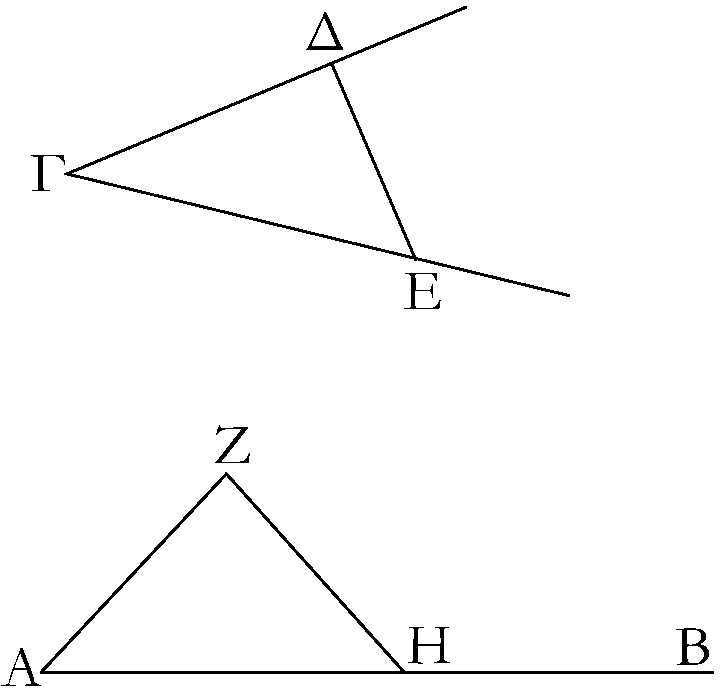
\includegraphics[width=0.8\textwidth]{Book01/fig23g.pdf}}

\gr{Εἰλήφθω ἐφ' ἑκατέρας τῶν ΓΔ, ΓΕ τυθόντα σημεῖα τὰ Δ, Ε, καὶ
ἐπεζεύθθω ἡ ΔΕ; καὶ ἐκ τριῶν εὐθειῶν, αὁί εἰσιν ἴσαι τρισὶ ταῖς
ΓΔ, ΔΕ, ΓΕ, τρίγωνον συνεστάτω τὸ ΑΖΗ, ὁώστε ἴσην εὸῖναι τὴν
μὲν ΓΔ τῇ ΑΖ, τὴν δὲ ΓΕ τῇ ΑΗ, καὶ ὸέτι τὴν ΔΕ τῇ ΖΗ.}

\gr{Ἐπεὶ οὸῦν δύο αἱ ΔΓ, ΓΕ δύο ταῖς ΖΑ, ΑΗ ἴσαι εἰσὶν ἑκατέρα ἑκατέρᾳ, καὶ βάσις ἡ ΔΕ βάσει τῇ ΖΗὸίση, γωνία ἄρα ἡ ὑπὸ
ΔΓΕ γωνίᾳ τῇ ὑπὸ ΖΑΗ ἐστινὸίση.}

\gr{Πρὸξ ἄρα τῇ δοθείσῃ εὐθείᾳ τῇ ΑΒ καὶ τῷ πρὸς αὐτῇ σημείῳ
τῷ Α τῇ δοθείσῃ γωνίᾳ εὐθυγράμμῳ τῇ ὑπὸ ΔΓΕὸίση γωνία εὐθύγραμμος συνέσταται ἡ ὑπὸ ΖΑΗ; ὅπερ ἔδει ποιῆσαι.}}

\ParallelRText{
\begin{center}
{\large Proposition 23}
\end{center}

To construct a rectilinear angle equal to a given rectilinear angle at a (given)
point on a given straight-line.

Let $AB$ be the given straight-line,  $A$ the (given) point on it, and 
$DCE$ the given rectilinear angle. So it is required to construct a rectilinear
angle equal to the given rectilinear angle $DCE$ at the (given) point
$A$ on the given straight-line
$AB$.\\~\\

% Removed epsf size command
\centerline{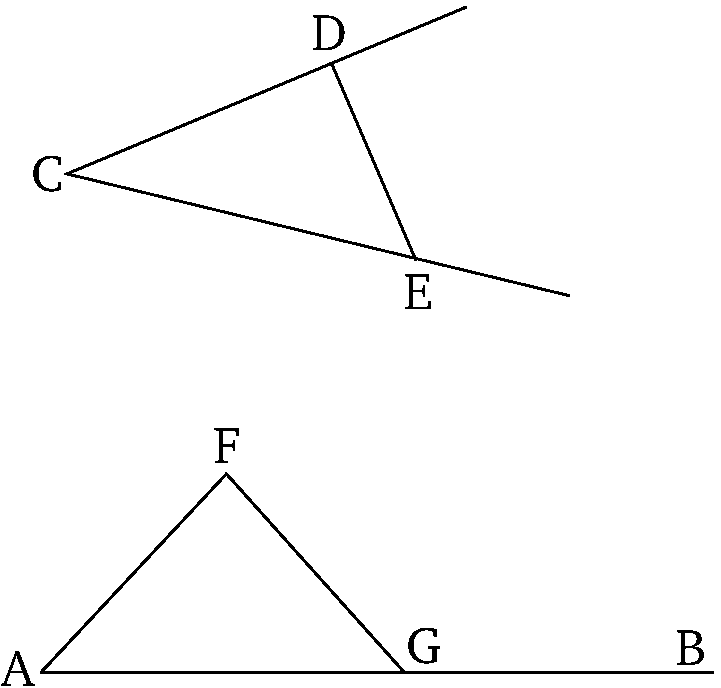
\includegraphics[width=0.8\textwidth]{Book01/fig23e.pdf}}

Let the points $D$ and $E$ be taken at random on each
of the (straight-lines) $CD$ and $CE$ (respectively), and let $DE$ be joined.
And let the triangle $AFG$ be constructed from three straight-lines
which are equal to $CD$, $DE$, and $CE$, such that $CD$ is equal to $AF$,
$CE$ to $AG$, and further $DE$ to $FG$ [Prop.~1.22].

Therefore, since the two (straight-lines) $DC$, $CE$ are equal to the
two (straight-lines) $FA$, $AG$, respectively, and the base $DE$ is equal to
the base $FG$, the angle $DCE$ is thus equal to the angle $FAG$ [Prop.~1.8].

Thus, the rectilinear angle $FAG$,  equal to the  given
rectilinear angle $DCE$, has been constructed at the (given) point $A$ on the given straight-line $AB$.
(Which is) the very thing it was required to do.}
\end{Parallel}

%%%%%%
% Prop 1.24
%%%%%%
\pdfbookmark[1]{Proposition 1.24}{pdf1.24}
\begin{Parallel}{}{} 
\ParallelLText{
\begin{center}
{\large\ggn{24}.}
\end{center}\vspace*{-7pt}

\gr{Ἐὰν δύο τρίγωνα τὰξ δύο πλευρὰξ [ταῖς] δύο πλευραῖξ ἴσαςὸέθῃ ἑκατέραν
ἑκατέρᾳ, τὴν δὲ γωνίαν τῆς γωνίας μείζοναὸέθῃ τὴν ὑπὸ τῶνὸίσων εὐθειῶν περιεθομένην, καὶ τὴν βάσιν τῆς βάσεως μείζονα ὁέχει.}

\gr{Ἔστω δύο τρίγωνα τὰ ΑΒΓ, ΔΕΖ τὰξ δύο πλευρὰξ τὰξ ΑΒ, ΑΓ ταῖς δύο πλευραῖξ ταῖς ΔΕ, ΔΖ ἴσας ἔχοντα ἑκατέραν ἑκατέρᾳ, τὴν μὲν ΑΒ τῇ ΔΕ τὴν δὲ ΑΓ τῇ ΔΖ, ἡ δὲ πρὸς τῷ Α γωνία τῆς πρὸς τῷ Δ γωνίας μείζωνὸέστω; λέγω, ὅτι καὶ βάσις ἡ ΒΓ βάσεως τῆς ΕΖ μείζων ἐστίν.}

\gr{Ἐπεὶ γὰρ μείζων ἡ ὑπὸ ΒΑΓ γωνία τῆς ὑπὸ ΕΔΖ γωνίας, συνεστάτω πρὸς τῇ ΔΕ εὐθείᾳ καὶ τῷ πρὸς αὐτῇ σημείῳ τῷ Δ τῇ ὑπὸ ΒΑΓ γωνίᾳ ὸίση ἡ ὑπὸ ΕΔΗ, καὶ κείσθω ὁποτέρᾳ τῶν ΑΓ, ΔΖὸίση ἡ ΔΗ, καὶ ἐπεζεύθθωσαν αἱ ΕΗ, ΖΗ.}\\

% Removed epsf size command
\centerline{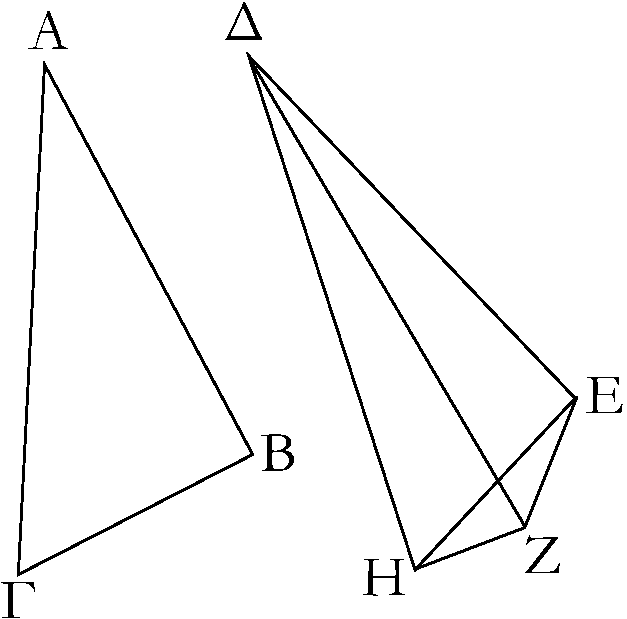
\includegraphics[width=0.8\textwidth]{Book01/fig24g.pdf}}

\gr{Ἐπεὶ οὸῦνὸίση ἐστὶν ἡ μὲν ΑΒ τῇ ΔΕ, ἡ δὲ ΑΓ τῇ ΔΗ, δύο
δὴ αἱ ΒΑ, ΑΓ δυσὶ ταῖς ΕΔ, ΔΗ ἴσαι εἰσὶν ἑκατέρα ἑκατέρᾳ;
καὶ γωνία ἡ ὑπὸ ΒΑΓ γωνίᾳ τῇ ὑπὸ ΕΔΗὸίση; βάσις ἄρα ἡ ΒΓ βάσει τῇ ΕΗ ἐστινὸίση.  πάλιν, ἐπεὶ ὸίση ἐστὶν ἡ ΔΖ τῇ ΔΗ, ὸίση ἐστὶ καὶ ἡ
ὑπὸ ΔΗΖ γωνία τῇ ὑπὸ ΔΖΗ; μείζων ἄρα ἡ ὑπὸ ΔΖΗ τῆς ὑπὸ ΕΗΖ; πολλῶ|  ἄρα μείζων ἐστὶν ἡ ὑπὸ ΕΖΗ τῆς ὑπὸ ΕΗΖ.
καὶ ἐπεὶ τρίγωνόν ἐστι τὸ ΕΖΗ μείζονα ἔχον τὴν ὑπὸ ΕΖΗ γωνίαν τῆς ὑπὸ ΕΗΖ, ὑπὸ δὲ τὴν μείζονα γωνίαν ἡ μείζων πλευρὰ ὑποτείνει, μείζων ἄρα καὶ πλευρὰ ἡ ΕΗ τῆς ΕΖ. ὸίση δὲ ἡ ΕΗ τῇ
ΒΓ; μείζων ἄρα καὶ ἡ ΒΓ τῆς ΕΖ.}

\gr{Ἐὰν ἄρα δύο τρίγωνα τὰξ δύο πλευρὰξ δυσὶ πλευραῖξ ἴσαςὸέθῃ ἑκατέραν
ἑκατέρᾳ, τὴν δὲ γωνίαν τῆς γωνίας μείζοναὸέθῃ τὴν ὑπὸ τῶνὸίσων εὐθειῶν περιεθομένην, καὶ τὴν βάσιν τῆς βάσεως μείζονα ὁέχει; ὅπερ ἔδει δεῖχαι.}}

\ParallelRText{
\begin{center}
{\large Proposition 24}
\end{center}

If two triangles have two sides equal to two sides, respectively,
but (one) has the angle encompassed by the equal straight-lines greater than the (corresponding)
angle (in the other),  (then the former triangle) will also have a base greater than the base (of the latter).

Let  $ABC$ and $DEF$ be two triangles having the two sides $AB$ and $AC$
equal to the two sides $DE$ and $DF$, respectively. (That is), $AB$ (equal) to $DE$, and
$AC$ to $DF$.  Let them also have the angle at $A$ greater than the angle at $D$.
I say that the base $BC$ is also greater than the base $EF$.

For since angle $BAC$ is greater than angle $EDF$, let (angle) $EDG$, equal to
angle $BAC$,  be constructed at  the point $D$ on the straight-line $DE$ [Prop.~1.23]. And let $DG$ be made equal to either of $AC$ or $DF$ [Prop.~1.3], and let $EG$ and $FG$ be joined.

% Removed epsf size command
\centerline{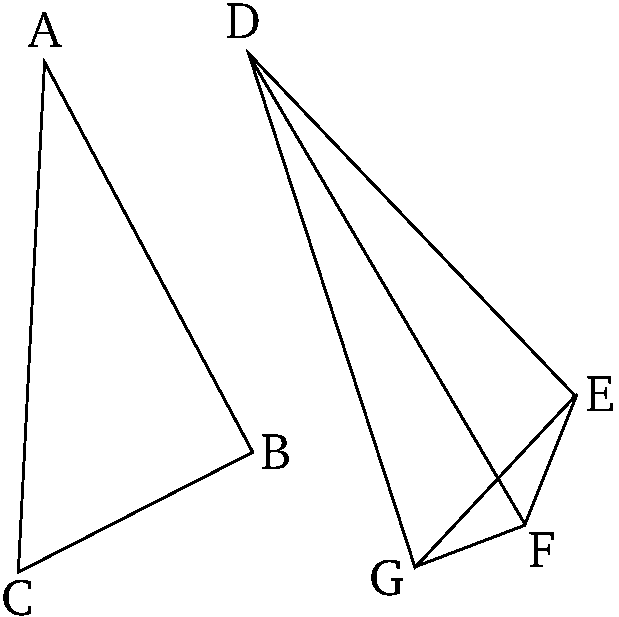
\includegraphics[width=0.8\textwidth]{Book01/fig24e.pdf}}

Therefore, since $AB$ is equal to $DE$ and $AC$ to $DG$, the two (straight-lines)
$BA$, $AC$ are equal to the two (straight-lines) $ED$, $DG$, respectively.
Also the angle $BAC$ is equal to the angle $EDG$. Thus, the base $BC$ is equal
to the base $EG$ [Prop.~1.4]. Again, since $DF$ is equal to $DG$, angle $DGF$
is also equal to angle $DFG$ [Prop.~1.5]. Thus, $DFG$ (is) greater than $EGF$.
Thus, $EFG$ is much greater than $EGF$. And since triangle $EFG$ has angle $EFG$
greater than $EGF$, and the greater angle is subtended by the greater side [Prop.~1.19], side $EG$ (is) thus also greater than $EF$. But $EG$ (is) equal to
$BC$. Thus, $BC$ (is) also greater than $EF$.

Thus, if two triangles have two sides equal to two sides, respectively,
but (one) has the angle encompassed by the equal straight-lines greater than the 
(corresponding) angle (in the other), (then the former triangle) will also have a base greater than the base (of the latter).
(Which is) the very thing it was required to show.}
\end{Parallel}

%%%%%%
% Prop 1.25
%%%%%%
\pdfbookmark[1]{Proposition 1.25}{pdf1.25}
\begin{Parallel}{}{} 
\ParallelLText{
\begin{center}
{\large \ggn{25}.}
\end{center}\vspace*{-7pt}

\gr{Ἐὰν δύο τρίγωνα τὰξ δύο πλευρὰξ δυσὶ πλευραῖξ ἴσαςὸέθῃ ἑκατέραν ἑκατέρᾳ, τὴν δὲ βάσιν τῆς βάσεως μείζοναὸέθῃ, καὶ τὴν γωνίαν τῆς γωνίας μείζονα ὁέχει τὴν ὑπὸ τῶνὸίσων εὐθειῶν περιεθομένην.}

\gr{Ἔστω δύο τρίγωνα τὰ ΑΒΓ, ΔΕΖ τὰξ δύο πλευρὰξ τὰξ ΑΒ, ΑΓ ταῖς δύο πλευραῖξ ταῖς ΔΕ, ΔΖ ἴσας ἔχοντα ἑκατέραν ἑκατέρᾳ, τὴν μὲν ΑΒ
τῇ ΔΕ, τὴν δὲ ΑΓ τῇ ΔΖ; βάσις δὲ ἡ ΒΓ βάσεως τῆς ΕΖ μείζωνὸέστω; λέγω, ὅτι καὶ γωνία ἡ ὑπὸ ΒΑΓ γωνίας τῆς ὑπὸ ΕΔΖ μείζων ἐστίν.}

\gr{Εἰ γὰρ μή,  ἢτοιὸίση ἐστὶν αὐτῇ ὸὴ ἐλάσσων; ὸίση μὲν οὸῦν οὐκὸέστιν ἡ ὑπὸ ΒΑΓ τῇ ὑπὸ ΕΔΖ; ὸίση γὰρὸὰνὸῆν καὶ βάσις ἡ ΒΓ βάσει τῇ ΕΖ; οὐκὸέστι δέ. οὐκ ἄραὸίση ἐστὶ γωνία ἡ ὑπὸ ΒΑΓ τῇ ὑπὸ ΕΔΖ; οὐδὲ μὴν ἐλάσσων ἐστὶν ἡ ὑπὸ ΒΑΓ τῆς ὑπὸ ΕΔΖ; ἐλάσσων γὰρὸὰνὸῆν καὶ βάσις ἡ ΒΓ βάσεως τῆς ΕΖ; οὐκὸέστι δέ; οὐκ ἄρα ἐλάσσων ἐστὶν ἡ ὑπὸ ΒΑΓ γωνία τῆς ὑπὸ ΕΔΖ. ἐδείθθη δέ, ὅτι οὐδὲ ὸίση; μείζων ἄρα ἐστὶν ἡ ὑπὸ ΒΑΓ τῆς ὑπὸ ΕΔΖ.}\\

% Removed epsf size command
\centerline{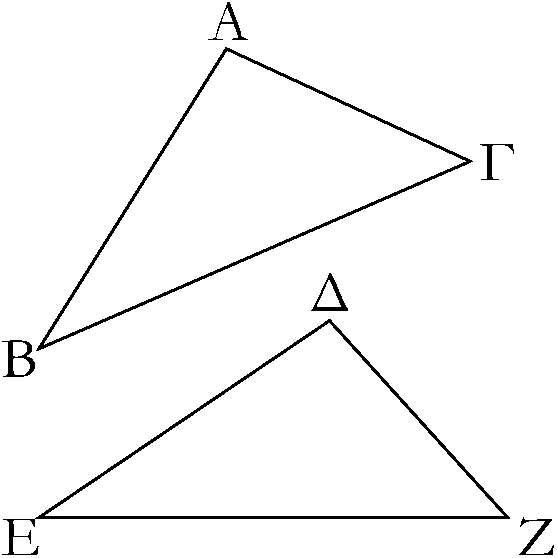
\includegraphics[width=0.8\textwidth]{Book01/fig25g.pdf}}

\gr{Ἐὰν ἄρα δύο τρίγωνα τὰξ δύο πλευρὰξ δυσὶ πλευραῖξ ἴσαςὸέθῃ ἑκατέραν ἑκάτερᾳ, τὴν δὲ βασίν τῆς βάσεως μείζοναὸέθῃ, καὶ τὴν γωνίαν τῆς γωνίας μείζονα ὁέχει τὴν ὑπὸ τῶνὸίσων εὐθειῶν περιεθομένην; ὅπερ ἔδει δεῖχαι.}}

\ParallelRText{
\begin{center}
{\large Proposition 25}
\end{center}

If two triangles have two sides equal to two sides, respectively,
but (one) has a base greater than the base (of the other), (then the former triangle) will also have the angle encompassed by the equal straight-lines greater than the (corresponding) angle (in the latter).

Let $ABC$ and $DEF$ be  two triangles having the two sides $AB$ and $AC$
equal to the two sides $DE$ and $DF$, respectively (That is), $AB$ (equal) to $DE$, and $AC$ to $DF$. And let the base $BC$ be greater than the base $EF$. I say that angle
$BAC$ is also greater than $EDF$.

For if not, ($BAC$) is certainly either equal to, or less than, ($EDF$). In fact, $BAC$ is not equal to
$EDF$. For then the base $BC$ would also be equal to the base $EF$ [Prop.~1.4]. But it is not.
Thus, angle $BAC$ is not equal to $EDF$. Neither, indeed, is $BAC$ less
than $EDF$. For then the base $BC$ would also be less than the base $EF$ [Prop.~1.24].
But it is not. Thus, angle $BAC$ is not less than $EDF$. But it was  shown
that ($BAC$ is) not equal (to $EDF$) either. Thus, $BAC$ is greater than $EDF$.

% Removed epsf size command
\centerline{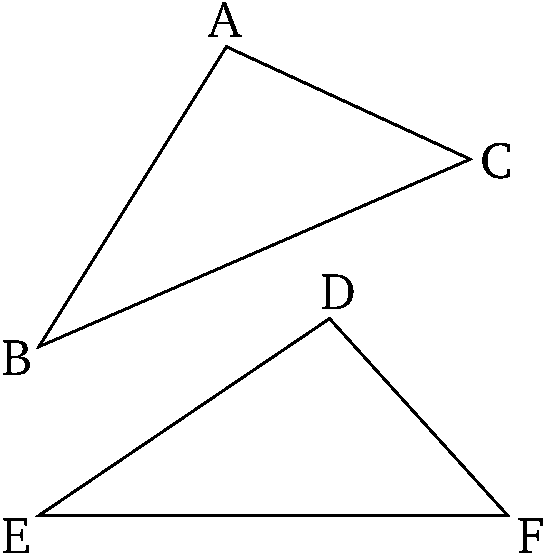
\includegraphics[width=0.8\textwidth]{Book01/fig25e.pdf}}

Thus, if two triangles have two sides equal to two sides, respectively,
but (one) has a base greater than the base (of the other), (then the former triangle) will also have the angle encompassed by the equal straight-lines greater than the (corresponding) angle (in the latter). (Which is) the
very thing it was required to show.}
\end{Parallel}

%%%%%%
% Prop 1.26
%%%%%%
\pdfbookmark[1]{Proposition 1.26}{pdf1.26}
\begin{Parallel}{}{} 
\ParallelLText{
\begin{center}
{\large \ggn{26}.}
\end{center}\vspace*{-7pt}

\gr{Ἐὰν δύο τρίγωνα τὰξ δύο γωνίας δυσὶ γωνίαις ἴσαςὸέθῃ ἑκατέραν
ἑκατέρᾳ καὶ μίαν πλευρὰν μιᾶ| πλευρᾶ|  ἴσην ἢτοι τὴν πρὸς ταῖς ἴσαις γωνίαιςὸὴ τὴν ὑποτείνουσαν ὑπὸ μίαν τῶνὸίσων γωνιῶν, καὶ τὰξ λοιπὰξ πλευρὰξ ταῖς λοιπαῖξ πλευραῖξ ἴσας ὁέχει [ἑκατέραν
ἑκατέρᾳ] καὶ τὴν λοιπὴν γωνίαν τῇ λοιπῆ| γωνίᾳ.}

\gr{Ἔστω δύο τρίγωνα τὰ ΑΒΓ, ΔΕΖ τὰξ δύο γωνίας τὰξ ὑπὸ ΑΒΓ, ΒΓΑ δυσὶ ταῖς ὑπὸ ΔΕΖ, ΕΖΔ ἴσας ἔχοντα ἑκατέραν ἑκατέρᾳ, τὴν μὲν ὑπὸ ΑΒΓ τῇ ὑπὸ ΔΕΖ, τὴν δὲ ὑπὸ ΒΓΑ τῇ ὑπὸ ΕΖΔ; ἐθέτω δὲ καὶ μίαν πλευρὰν μιᾶ| πλευρᾶ|  ἴσην, πρότερον τὴν πρὸς ταῖς ἴσαις γωνίαις τὴν ΒΓ τῇ ΕΖ; λέγω, ὅτι καὶ τὰξ λοιπὰξ πλευρὰξ ταῖς λοιπαῖξ πλευραῖξ ἴσας ὁέχει ἑκατέραν ἑκατέρᾳ, τὴν μὲν ΑΒ τῇ ΔΕ τὴν δὲ ΑΓ τῇ ΔΖ, καὶ τὴν λοιπὴν γωνίαν τῇ λοιπῆ| γωνίᾳ, τὴν ὑπὸ ΒΑΓ τῇ ὑπὸ ΕΔΖ.}

\gr{Εἰ γὰρὸάνισόξ ἐστιν ἡ ΑΒ τῇ ΔΕ, μία αὐτῶν μείζων ἐστίν.
ὸέστω μείζων ἡ ΑΒ, καὶ κείσθω τῇ ΔΕὸίση ἡ ΒΗ, καὶ ἐπεζεύθθω ἡ ΗΓ.}

\gr{Ἐπεὶ οὸῦνὸίση ἐστὶν ἡ μὲν ΒΗ τῇ ΔΕ, ἡ δὲ ΒΓ τῇ ΕΖ, δύο δὴ αἱ ΒΗ, ΒΓ δυσὶ ταῖς ΔΕ, ΕΖ ἴσαι εἰσὶν ἑκατέρα ἑκατέρᾳ; καὶ γωνία ἡ ὑπὸ ΗΒΓ γωνίᾳ τῇ ὑπὸ ΔΕΖὸίση ἐστίν; βάσις ἄρα ἡ ΗΓ βάσει τῇ ΔΖὸίση ἐστίν, καὶ τὸ ΗΒΓ τρίγωνον τῷ ΔΕΖ τριγώνῳ  ἴσον ἐστίν, καὶ αἱ λοιπαὶ γωνίαι ταῖς λοιπαῖξ γωνίαις ἴσαιὸέσονται, ὑφὸ ὁὰξ αἱ  ἴσαι πλευραὶ ὑποτείνουσιν; ὸίση ἄρα ἡ ὑπὸ ΗΓΒ γωνία τῇ ὑπὸ ΔΖΕ. ἀλλὰ ἡ ὑπὸ ΔΖΕ τῇ ὑπὸ ΒΓΑ ὑπόκειταιὸίση;
καὶ ἡ ὑπὸ ΒΓΗ ἄρα τῇ ὑπὸ ΒΓΑὸίση ἐστίν, ἡ ἐλάσσων
τῇ μείζονι; ὅπερ ἀδύνατον. οὐκ ἄραὸάνισόξ ἐστιν ἡ ΑΒ τῇ ΔΕ.
ὸίση ἄρα. ὸέστι δὲ καὶ ἡ ΒΓ τῇ ΕΖὸίση; δύο δὴ αἱ ΑΒ, ΒΓ δυσὶ ταῖς ΔΕ, ΕΖ ἴσαι εἰσὶν ἑκατέρα ἑκατέρᾳ; καὶ γωνία ἡ ὑπὸ ΑΒΓ
γωνίᾳ τῇ ὑπὸ ΔΕΖ ἐστινὸίση; βάσις ἄρα ἡ ΑΓ βάσει τῇ ΔΖὸίση ἐστίν, καὶ λοιπὴ γωνία ἡ ὑπὸ ΒΑΓ τῇ λοιπῆ| γωνίᾳ τῇ ὑπὸ ΕΔΖὸίση ἐστίν.}\\~\\

% Removed epsf size command
\centerline{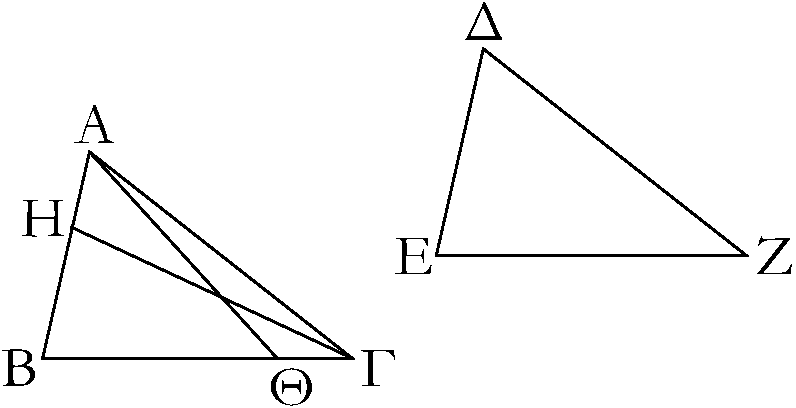
\includegraphics[width=0.8\textwidth]{Book01/fig26g.pdf}}

\gr{Ἀλλὰ δὴ πάλινὸέστωσαν αἱ ὑπὸ τὰξ ἴσας γωνίας πλευραὶ ὑποτείνουσαι ἴσαι, ὡξ ἡ ΑΒ τῇ ΔΕ; λέγω πάλιν, ὅτι καὶ αἱ λοιπαὶ πλευραὶ ταῖς λοιπαῖξ πλευραῖξ ἴσαιὸέσονται, ἡ μὲν ΑΓ τῇ ΔΖ, ἡ δὲ ΒΓ τῇ ΕΖ καὶ ὸέτι ἡ λοιπὴ γωνία ἡ ὑπὸ ΒΑΓ τῇ λοιπῆ| γωνίᾳ τῇ ὑπὸ ΕΔΖὸίση ἐστίν.}

\gr{Εἰ γὰρὸάνισόξ ἐστιν ἡ ΒΓ τῇ ΕΖ, μία αὐτῶν μείζων ἐστίν. ὸέστω μείζων, εἰ δυνατόν, ἡ ΒΓ, καὶ κείσθω τῇ ΕΖὸίση ἡ ΒΘ, καὶ ἐπεζεύθθω ἡ ΑΘ. καὶ ἐπὲιὸίση ἐστὶν ἡ μὲν ΒΘ τῇ ΕΖ ἡ δὲ ΑΒ τῇ ΔΕ, δύο δὴ αἱ ΑΒ, ΒΘ δυσὶ ταῖς ΔΕ, ΕΖ ἴσαι εἰσὶν ἑκατέρα ἑκαρέρᾳ; καὶ γωνίας ἴσας περιέθουσιν; βάσις ἄρα ἡ ΑΘ βάσει τῇ ΔΖὸίση ἐστίν, καὶ τὸ ΑΒΘ τρίγωνον τῷ ΔΕΖ τριγώνῳ  ἴσον ἐστίν, καὶ αἱ λοιπαὶ γωνίαι ταῖς λοιπαῖξ γωνίαις ἴσαιὸέσονται, ὑφὸ ὁὰξ αἱ  ἴσας πλευραὶ ὑποτείνουσιν;
 ὸίση ἄρα ἐστὶν ἡ ὑπὸ ΒΘΑ γωνία τῇ ὑπὸ ΕΖΔ.
ἀλλὰ ἡ ὑπὸ ΕΖΔ τῇ ὑπὸ ΒΓΑ ἐστινὸίση; τριγώνου δὴ τοῦ ΑΘΓ ἡ ἐκτὸξ γωνία ἡ ὑπὸ ΒΘΑὸίση ἐστὶ τῇ ἐντὸς καὶ ἀπεναντίον
τῇ ὑπὸ ΒΓΑ; ὅπερ ἀδύνατον. οὐκ ἄραὸάνισόξ ἐστιν ἡ ΒΓ τῇ ΕΖ; ὸίση ἄρα. ἐστὶ δὲ καὶ ἡ ΑΒ τῇ ΔΕὸίση. δύο δὴ αἱ ΑΒ, ΒΓ δύο ταῖς ΔΕ, ΕΖ ἴσαι εἰσὶν ἑκατέρα ἑκατέρᾳ; καὶ γωνίας ἴσας περιέθουσι; βάσις ἄρα ἡ ΑΓ βάσει τῇ ΔΖὸίση ἐστίν, καὶ τὸ ΑΒΓ τρίγωνον τῷ ΔΕΖ τριγώνῳ  ἴσον καὶ λοιπὴ γωνία ἡ ὑπὸ ΒΑΓ τῇ λοιπὴ| γωνίᾳ τῇ ὑπὸ ΕΔΖὸίση.}

\gr{Ἐὰν ἄρα δύο τρίγωνα τὰξ δύο γωνίας δυσὶ γωνίαις ἴσαςὸέθῃ ἑκατέραν
ἑκατέρᾳ καὶ μίαν πλευρὰν μιᾶ| πλευρᾶ|  ἴσην ἢτοι τὴν πρὸς ταῖς ἴσαις γωνίαις, ὸὴ τὴν ὑποτείνουσαν ὑπὸ μίαν τῶνὸίσων γωνιῶν, καὶ τὰξ λοιπὰξ πλευρὰξ ταῖς λοιπαῖξ πλευραῖξ ἴσας ὁέχει 
καὶ τὴν λοιπὴν γωνίαν τῇ λοιπῆ| γωνίᾳ; ὅπερ ἔδει δεῖχαι.}}

\ParallelRText{
\begin{center}
{\large Proposition 26}
\end{center}

If  two triangles have two angles equal to two angles, respectively, 
and one side equal to one side---in fact, either that by the equal angles, or that
subtending one of the equal angles---(then the triangles) will also have the remaining
sides equal to the [corresponding] remaining sides, and the
remaining angle (equal) to the remaining angle.

Let $ABC$ and $DEF$ be two triangles having the two angles $ABC$ and
$BCA$ equal to the two (angles) $DEF$ and $EFD$, respectively.
(That is) $ABC$ (equal) to $DEF$, and $BCA$ to $EFD$. And let them also have
one side equal to one side. First of all, the (side) by the equal angles. (That is)
$BC$ (equal) to $EF$. I say that they will have the  remaining sides equal to the
corresponding remaining sides. (That is) $AB$ (equal) to $DE$, and $AC$ to
$DF$. And (they will have) the remaining angle (equal) to the remaining angle.
(That is) $BAC$ (equal) to $EDF$.

For if $AB$ is unequal to $DE$ (then) one of them is greater. Let $AB$ be greater,
and let $BG$ be made equal to $DE$ [Prop.~1.3], and let $GC$ be
joined.

Therefore, since $BG$ is equal to $DE$, and $BC$ to $EF$, the two (straight-lines)
$GB$, $BC$$^\dag$ are equal to the two (straight-lines) $DE$, $EF$, respectively. And angle
$GBC$ is equal to angle $DEF$. Thus, the base $GC$ is equal to the base $DF$,
and triangle $GBC$ is equal to triangle $DEF$, and the remaining angles 
subtended by the equal sides will
be equal to the (corresponding) remaining angles [Prop.~1.4].
Thus, $GCB$ (is equal) to $DFE$. But,  $DFE$ was assumed (to be) equal to $BCA$.
Thus, $BCG$ is also equal to $BCA$, the lesser to the greater. The very thing (is) impossible. Thus, $AB$ is not unequal to $DE$. Thus, (it is) equal. And $BC$ is
also equal to $EF$. So the two (straight-lines) $AB$, $BC$ are equal to the two (straight-lines) $DE$, $EF$, respectively. And angle $ABC$ is equal to
angle $DEF$. Thus, the base $AC$ is equal to the base $DF$, and the remaining
angle $BAC$ is equal to the remaining angle $EDF$ [Prop.~1.4].

% Removed epsf size command
\centerline{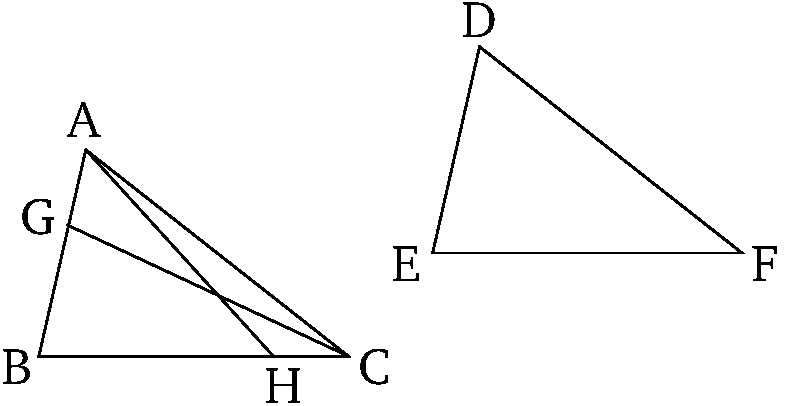
\includegraphics[width=0.8\textwidth]{Book01/fig26e.pdf}}

But, again, let the sides subtending the equal angles be equal: for instance, 
(let) $AB$ (be equal) to
$DE$.  Again, I say that the remaining sides will be equal to the remaining
sides. (That is) $AC$ (equal) to $DF$, and $BC$ to $EF$. Furthermore, the remaining angle
$BAC$ is equal to the remaining angle $EDF$.

For if $BC$ is unequal to $EF$ (then) one of them is greater. If possible, let $BC$
be greater. And let $BH$ be made equal to $EF$ [Prop.~1.3], and let $AH$ be joined.
And since $BH$ is equal to $EF$, and $AB$ to $DE$, the two (straight-lines) $AB$, $BH$
are equal to the two (straight-lines) $DE$, $EF$, respectively. And the angles
they encompass (are also equal). Thus, the base $AH$ is equal to the base  
$DF$, and the triangle $ABH$ is equal to the triangle $DEF$, and the
remaining angles subtended by the equal sides will be equal to the
(corresponding) remaining angles [Prop.~1.4]. Thus, angle $BHA$ 
is equal to $EFD$. But, $EFD$ is equal to $BCA$. So, in triangle $AHC$,
the external angle $BHA$ is equal to the internal and opposite angle 
$BCA$. The very thing (is) impossible [Prop.~1.16]. Thus, $BC$ is not unequal to $EF$.
Thus, (it is) equal. And $AB$ is also equal to $DE$. So the two
(straight-lines) $AB$, $BC$ are equal to the two (straight-lines) $DE$, $EF$,
respectively. And they encompass equal angles. Thus, the base $AC$ is equal
to the base $DF$, and triangle $ABC$ (is) equal to triangle $DEF$, and the
remaining angle $BAC$ (is) equal to the remaining angle $EDF$ [Prop.~1.4].

Thus, if two triangles have two angles equal to two angles, respectively, 
and one side equal to one side---in fact, either that by the equal angles, or that
subtending one of the equal angles---(then the triangles) will also have the remaining sides equal to the (corresponding) remaining sides, and the
remaining angle (equal) to the remaining angle. (Which is) the very thing it
was required to show.}
\end{Parallel}
\noindent{\footnotesize $^\dag$ The Greek text has ``$BG$, $BC$'', which is obviously a mistake.}

%%%%%%
% Prop 1.27
%%%%%%
\pdfbookmark[1]{Proposition 1.27}{pdf1.27}
\begin{Parallel}{}{} 
\ParallelLText{
\begin{center}
{\large \ggn{27}.}
\end{center}\vspace*{-7pt}

\gr{Ἐὰν εἰξ δύο εὐθείας εὐθεῖα ἐμπίπτουσα τὰξ ἐναλλὰχ γωνίας ἴσας ἀλλήλαις ποιῆ|, παράλληλοιὸέσονται ἀλλήλαις αἱ εὐθεῖαι.}

% Removed epsf size command
\centerline{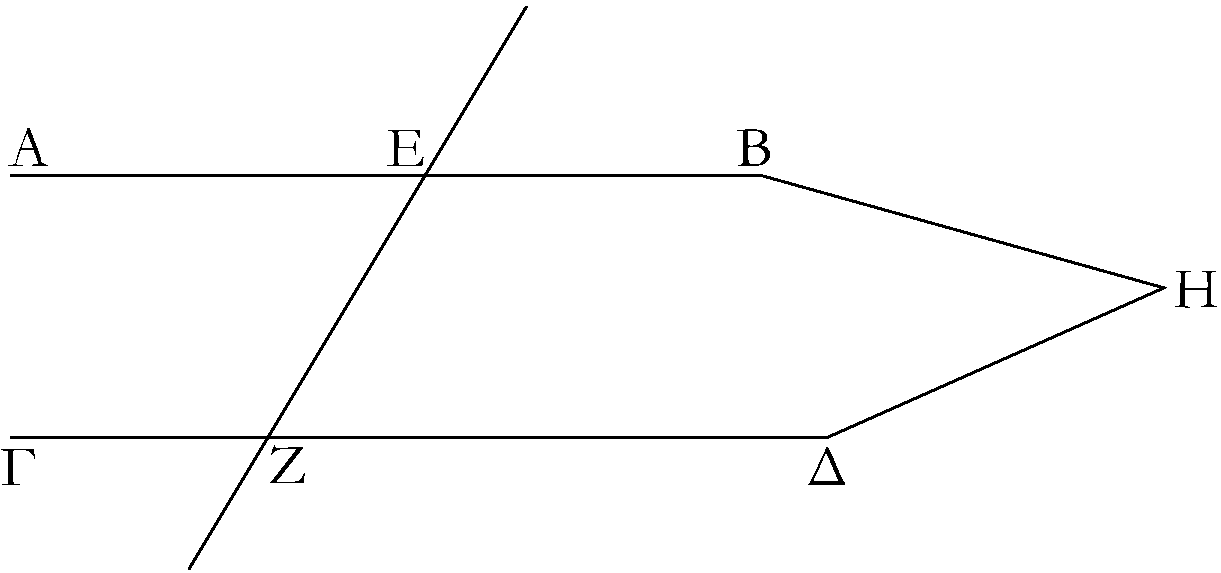
\includegraphics[width=0.8\textwidth]{Book01/fig27g.pdf}}

\gr{Εἰξ γὰρ δύο εὐθείας τὰξ ΑΒ, ΓΔ εὐθεῖα ἐμπίπτουσα ἡ ΕΖ τὰξ ἐναλλὰχ γωνίας τὰξ ὑπὸ ΑΕΖ, ΕΖΔ ἴσας ἀλλήλαις ποιείτω; λέγω, ὅτι
παράλληλόξ ἐστιν ἡ ΑΒ τῇ ΓΔ.}

\gr{Εἰ γὰρ μή, ἐκβαλλόμεναι αἱ ΑΒ, ΓΔ συμπεσοῦνται ἢτοι ἐπὶ τὰ Β, Δ μέρηὸὴ  ἐπὶ τὰ  Α, Γ. ἐκβεβλήσθωσαν καὶ συμπιπτέτωσαν ἐπὶ τὰ Β, Δ μέρη κατὰ τὸ Η.  τριγώνου δὴ τοῦ ΗΕΖ ἡ ἐκτὸξ γωνία ἡ ὑπὸ
ΑΕΖὸίση ἐστὶ τῇ ἐντὸς καὶ ἀπεναντίον τῇ ὑπὸ ΕΖΗ;
ὅπερ ἐστὶν ἀδύνατον; οὐκ ἄρα αἱ ΑΒ, ΔΓ ἐκβαλλόμεναι
συμπεσοῦνται ἐπὶ τὰ Β, Δ μέρη. ὁμοίως δὴ δειθθήσεται, ὅτι οὐδὲ ἐπὶ τὰ Α, Γ; αἱ δὲ ἐπὶ μ  ηδέτερα τὰ μέρη συμπίπτουσαι παράλληλοί
εἰσιν; παράλληλος ἄρα ἐστὶν ἡ ΑΒ τῇ ΓΔ.}

\gr{Ἐὰν ἄρα εἰξ δύο εὐθείας εὐθεῖα ἐμπίπτουσα τὰξ ἐναλλὰχ γωνίας ἴσας ἀλλήλαις ποιῆ|, παράλληλοιὸέσονται αἱ εὐθεῖαι;
ὅπερ ἔδει δεῖχαι.}}

\ParallelRText{
\begin{center}
{\large Proposition 27}
\end{center}

If a straight-line falling across two straight-lines makes  the alternate
angles equal to one another (then) the (two) straight-lines will be parallel to
one another.

% Removed epsf size command
\centerline{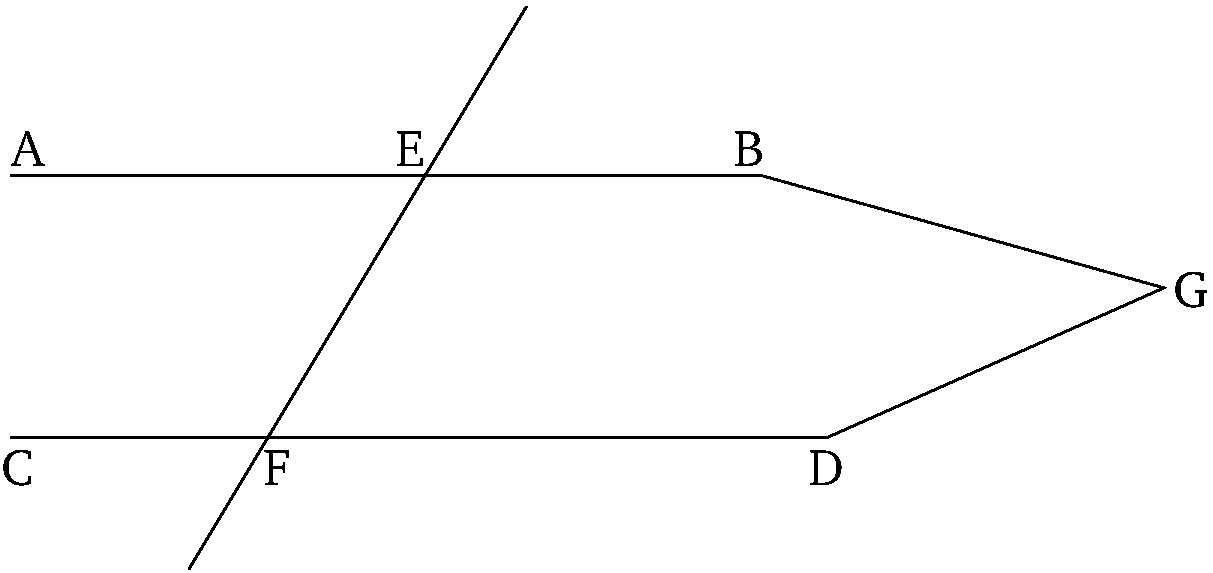
\includegraphics[width=0.8\textwidth]{Book01/fig27e.pdf}}

For let the straight-line $EF$, falling across the two straight-lines $AB$ and
$CD$, make the alternate angles $AEF$ and $EFD$ equal to one another.
I say that $AB$ and $CD$ are parallel.

For if not, being produced, $AB$ and $CD$ will certainly meet together:
either in the direction of $B$ and $D$, or (in the
direction) of $A$ and $C$ [Def.~1.23]. Let them be
produced, and let them meet together in the direction of $B$ and $D$ at
 (point) $G$. So, for the triangle $GEF$, the external angle
$AEF$ is equal to the interior and opposite (angle) $EFG$. The
very thing is impossible [Prop.~1.16]. Thus, being produced, $AB$ and $CD$
will not meet together in the direction of $B$ and $D$. Similarly, 
it can be shown that neither (will they meet together) in (the
direction of) $A$ and $C$. But  (straight-lines) meeting in neither
direction are parallel [Def.~1.23]. Thus, $AB$ and $CD$ are parallel.

Thus, if a straight-line falling across two straight-lines makes  the alternate
angles equal to one another (then) the (two) straight-lines will be parallel (to
one another). (Which is) the very thing it was required to show.}
\end{Parallel}

%%%%%%
% Prop 1.28
%%%%%%
\pdfbookmark[1]{Proposition 1.28}{pdf1.28}
\begin{Parallel}{}{} 
\ParallelLText{
\begin{center}
{\large \ggn{28}.}
\end{center}\vspace*{-7pt}

\gr{Ἐὰν εἰξ δύο εὐθείας εὐθεῖα ἐμπίπτουσα τὴν ἐκτὸξ γωνίαν τῇ ἐντὸς καὶ ἀπεναντίον καὶ ἐπὶ τὰ αὐτὰ μέρη ἴσην ποιῆ| ὸὴ τὰξ ἐντὸς καὶ ἐπὶ τὰ αὐτὰ μέρη δυσὶν ὀρθαῖξ ἴσας, παράλληλοιὸέσονται ἀλλήλαις αἱ εὐθεῖαι.}

\gr{Εἰξ γὰρ δύο εὐθείας τὰξ ΑΒ, ΓΔ εὐθεῖα ἐμπίπτουσα ἡ ΕΖ τὴν ἐκτὸξ γωνίαν τὴν ὑπὸ ΕΗΒ τῇ ἐντὸς καὶ ἀπεναντίον γωνίᾳ
τῇ ὑπὸ ΗΘΔ ἴσην ποιείτωὸὴ τὰξ ἐντὸς καὶ ἐπὶ τὰ αὐτὰ μέρη
τὰξ ὑπὸ ΒΗΘ, ΗΘΔ δυσὶν ὀρθαῖξ ἴσας; λέγω, ὅτι παράλληλόξ ἐστιν
ἡ ΑΒ τῇ ΓΔ.}

\gr{Ἐπεὶ γὰρὸίση ἐστὶν ἡ ὑπὸ ΕΗΒ τῇ ὑπὸ ΗΘΔ, ἀλλὰ ἡ ὑπὸ
ΕΗΒ τῇ ὑπὸ ΑΗΘ ἐστινὸίση, καὶ ἡ ὑπὸ ΑΗΘ ἄρα τῇ ὑπὸ ΗΘΔ
ἐστινὸίση; καί εἰσιν ἐναλλάχ; παράλληλος ἄρα ἐστὶν
ἡ ΑΒ τῇ ΓΔ.}

\gr{Πάλιν, ἐπεὶ αἱ ὑπὸ ΒΗΘ, ΗΘΔ δύο ὀρθαῖξ ἴσαι εἰσίν, εἰσὶ
δὲ καὶ αἱ ὑπὸ ΑΗΘ, ΒΗΘ δυσὶν ὀρθαῖξ ἴσαι, αἱ  ἄρα ὑπὸ ΑΗΘ, ΒΗΘ
ταῖς ὑπὸ ΒΗΘ, ΗΘΔ ἴσαι εἰσίν; κοινὴ ἀφῃρήσθω ἡ ὑπὸ ΒΗΘ;
λοιπὴ  ἄρα ἡ ὑπὸ ΑΗΘ λοιπῆ| τῇ ὑπὸ ΗΘΔ ἐστινὸίση;
καί εἰσιν ἐναλλάχ; παράλληλος ἄρα ἐστὶν ἡ ΑΒ τῇ ΓΔ.}\\~\\

% Removed epsf size command
\centerline{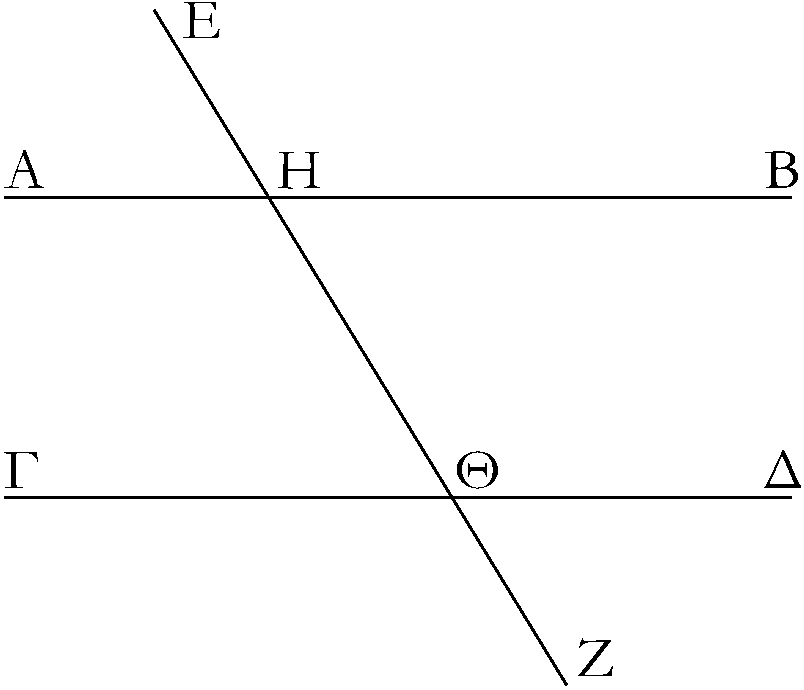
\includegraphics[width=0.8\textwidth]{Book01/fig28g.pdf}}

\gr{Ἐὰν ἄρα εἰξ δύο εὐθείας εὐθεῖα ἐμπίπτουσα τὴν ἐκτὸξ γωνίαν τῇ ἐντὸς καὶ ἀπεναντίον καὶ ἐπὶ τὰ αὐτὰ μέρη ἴσην ποιῆ| ὸὴ τὰξ ἐντὸς καὶ ἐπὶ τὰ αὐτὰ μέρη δυσὶν ὀρθαῖξ ἴσας, παράλληλοιὸέσονται  αἱ εὐθεῖαι; ὅπερ ἔδει δεῖχαι.}}

\ParallelRText{
\begin{center}
{\large Proposition 28}
\end{center}

If a straight-line falling across two straight-lines makes the external angle equal
to the internal and opposite angle on the same side, or (makes) the (sum  of the) internal
(angles) on the same side equal
to two right-angles, (then) the (two) straight-lines will be parallel to
one another.

For let $EF$, falling across the two straight-lines $AB$ and $CD$, make the external
angle $EGB$ equal to the internal and opposite angle $GHD$, or the (sum of the) internal
(angles) on the same side, $BGH$ and $GHD$, equal to two right-angles.
I say that $AB$ is parallel to $CD$.

For since (in the first case) $EGB$ is equal to $GHD$, but $EGB$ is equal to $AGH$ [Prop.~1.15],
$AGH$ is thus also equal to $GHD$. And they are alternate (angles).
Thus, $AB$ is
 parallel to $CD$ [Prop.~1.27].

Again, since (in the second case, the sum of) $BGH$ and $GHD$ is equal to two right-angles,  and (the sum of) $AGH$ and
$BGH$ is also equal to two right-angles [Prop.~1.13], 
(the sum of) $AGH$ and $BGH$ is thus equal to (the sum of) $BGH$ and $GHD$. Let $BGH$ be
subtracted from both. Thus, the remainder $AGH$ is equal to the remainder
$GHD$. And they are alternate (angles). Thus, $AB$ is parallel
to $CD$ [Prop.~1.27].

% Removed epsf size command
\centerline{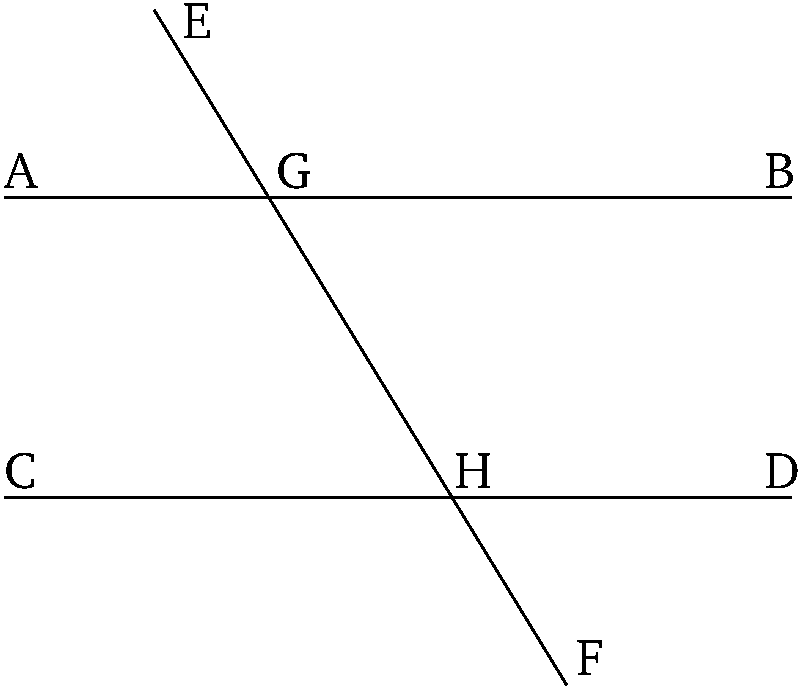
\includegraphics[width=0.8\textwidth]{Book01/fig28e.pdf}}

Thus, if a straight-line falling across  two straight-lines makes the external angle equal
to the internal and opposite angle on the same side, or (makes) the (sum of the) internal
(angles) on the same side equal
to two right-angles, (then) the (two) straight-lines will be parallel (to
one another). (Which is) the very thing it was required to show.}
\end{Parallel}

%%%%%%
% Prop 1.29
%%%%%%
\pdfbookmark[1]{Proposition 1.29}{pdf1.29}
\begin{Parallel}{}{} 
\ParallelLText{
\begin{center}
{\large\ggn{29}.}
\end{center}\vspace*{-7pt}

\gr{Ἡ εἰξ τὰξ παραλλήλους εὐθείας εὐθεῖα ἐμπίπτουσα τάξ τε ἐναλλὰχ γωνίας ἴσας ἀλλήλαις ποιεῖ καὶ τὴν ἐκτὸξ τῇ ἐντὸς καὶ ἀπεναντίον ἴσην καὶ τὰξ ἐντὸς καὶ ἐπὶ τὰ αὐτὰ μέρη δυσὶν ὀρθαῖξ ἴσας.}

\gr{Εἰξ γὰρ παραλλήλους εὐθείας τὰξ ΑΒ, ΓΔ εὐθεῖα ἐμπιπτέτω ἡ ΕΖ;
λέγω, ὅτι τὰξ ἐναλλὰχ γωνίας τὰξ ὑπὸ ΑΗΘ, ΗΘΔ ἴσας ποιεῖ καὶ τὴν ἐκτὸξ γωνίαν τὴν ὑπὸ ΕΗΒ τῇ ἐντὸς καὶ ἀπεναντίον τῇ ὑπὸ ΗΘΔ ἴσην καὶ τὰξ ἐντὸς καὶ ἐπὶ τὰ αὐτὰ μέρη τὰξ ὑπὸ ΒΗΘ, ΗΘΔ δυσὶν ὀρθαῖξ ἴσας.}\\

\gr{Εἰ γὰρὸάνισόξ ἐστιν ἡ ὑπὸ ΑΗΘ τῇ ὑπὸ ΗΘΔ, μία αὐτῶν μείζων ἐστίν. ὸέστω μείζων ἡ ὑπὸ ΑΗΘ; κοινὴ προσκείσθω ἡ ὑπὸ ΒΗΘ; αἱ  ἄρα ὑπὸ ΑΗΘ, ΒΗΘ τῶν ὑπὸ ΒΗΘ, ΗΘΔ μείζονέξ εἰσιν. ἀλλὰ αἱ ὑπὸ ΑΗΘ, ΒΗΘ δυσὶν ὀρθαῖξ ἴσαι εἰσίν. [καὶ] αἱ  ἄρα ὑπὸ ΒΗΘ, ΗΘΔ δύο ὀρθῶν ἐλάσσονέξ εἰσιν. αἱ δὲ ἀπὸ ἐλασσόνωνὸὴ δύο ὀρθῶν ἐκβαλλόμεναι εἰξ ἄπειρον συμπίπτουσιν; αἱ  ἄρα ΑΒ, ΓΔ ἐκβαλλόμεναι εἰξ ἄπειρον συμπεσοῦνται; οὐ συμπίπτουσι δὲ διὰ τὸ παραλλήλους αὐτὰξ ὑποκεῖσθαι; οὐκ ἄραὸάνισόξ ἐστιν ἡ ὑπὸ 
ΑΗΘ τῇ ὑπὸ ΗΘΔ; ὸίση ἄρα. ἀλλὰ ἡ ὑπὸ ΑΗΘ τῇ ὑπὸ ΕΗΒ ἐστινὸίση;
καὶ ἡ ὑπὸ ΕΗΒ ἄρα τῇ ὑπὸ ΗΘΔ ἐστινὸίση;
κοινὴ προσκείσθω ἡ ὑπὸ ΒΗΘ; αἱ  ἄρα ὑπὸ ΕΗΒ, ΒΗΘ ταῖς
ὑπὸ ΒΗΘ, ΗΘΔ ἴσαι εἰσίν. ἀλλὰ αἱ ὑπὸ ΕΗΒ, ΒΗΘ δύο ὀρθαῖξ ἴσαι εἰσίν; καὶ αἱ ὑπὸ ΒΗΘ, ΗΘΔ ἄρα δύο ὀρθαῖξ ἴσαι
εἰσίν.}\\~\\~\\

% Removed epsf size command
\centerline{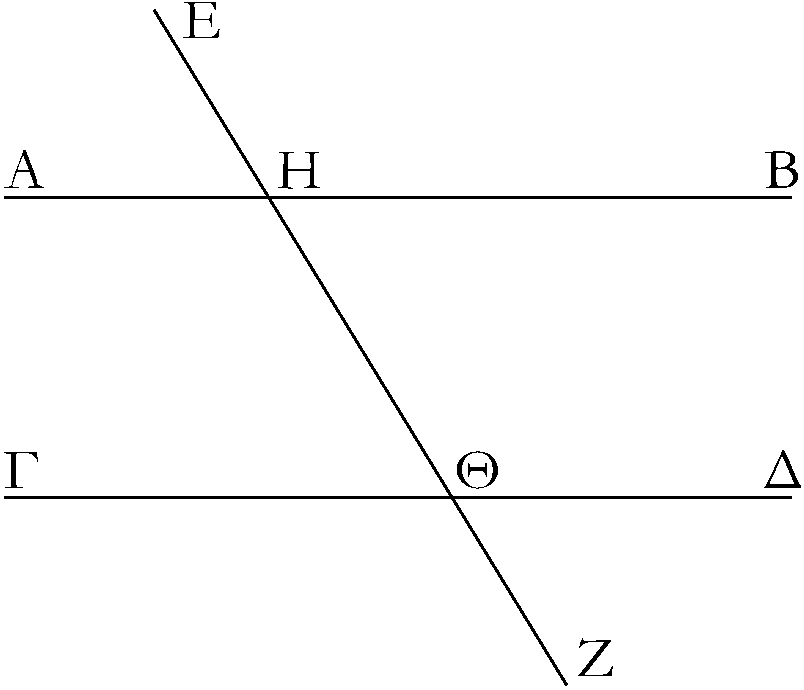
\includegraphics[width=0.8\textwidth]{Book01/fig28g.pdf}}

\gr{Ἡ   ἄρα εἰξ τὰξ παραλλήλους εὐθείας εὐθεῖα ἐμπίπτουσα τάξ τε ἐναλλὰχ γωνίας ἴσας ἀλλήλαις ποιεῖ καὶ τὴν ἐκτὸξ τῇ ἐντὸς καὶ ἀπεναντίον ἴσην καὶ τὰξ ἐντὸς καὶ ἐπὶ τὰ αὐτὰ μέρη δυσὶν ὀρθαῖξ ἴσας;
ὅπερ ἔδει δεῖχαι.}}

\ParallelRText{
\begin{center}
{\large Proposition 29}
\end{center}

A straight-line falling across  parallel straight-lines makes the alternate angles
equal to one another,  the external (angle) equal to the internal and
opposite (angle), and the (sum of the) internal (angles) on the same side equal to
two right-angles.

For let the straight-line $EF$ fall across the parallel straight-lines $AB$ and $CD$.
I say that it makes the  alternate angles, $AGH$ and $GHD$,  equal,  the
external angle $EGB$ equal to the internal and opposite (angle) $GHD$,
and the (sum of the) internal (angles) on the same side, $BGH$ and $GHD$, equal to
two right-angles.

For if $AGH$ is unequal to $GHD$ (then) one of them is greater. Let $AGH$ be greater.
Let $BGH$ be added to both. Thus, (the sum of) $AGH$ and $BGH$ is greater
than (the sum of) $BGH$ and $GHD$. But, (the sum of) $AGH$ and $BGH$ is equal to two right-angles
[Prop~1.13]. Thus,  (the sum of) $BGH$ and $GHD$ is [also] less than two right-angles. 
But (straight-lines) being produced to infinity from (internal angles whose sum is) less than
two right-angles meet together [Post.~5]. Thus, $AB$ and $CD$, being produced to
infinity, will meet together. But they do not meet, on account of
them (initially) being assumed parallel (to one another) [Def.~1.23]. Thus, $AGH$ is not unequal to $GHD$. Thus, (it is) equal. But, $AGH$ is equal to $EGB$ [Prop.~1.15]. 
And $EGB$ is thus also equal to $GHD$.
Let $BGH$
be added to both. Thus, (the sum of) $EGB$ and $BGH$ is equal to (the sum of) $BGH$ and $GHD$.
But, (the sum of) $EGB$ and $BGH$ is equal to two right-angles [Prop.~1.13]. 
Thus, (the sum of) $BGH$ and $GHD$ is also equal to two right-angles.

% Removed epsf size command
\centerline{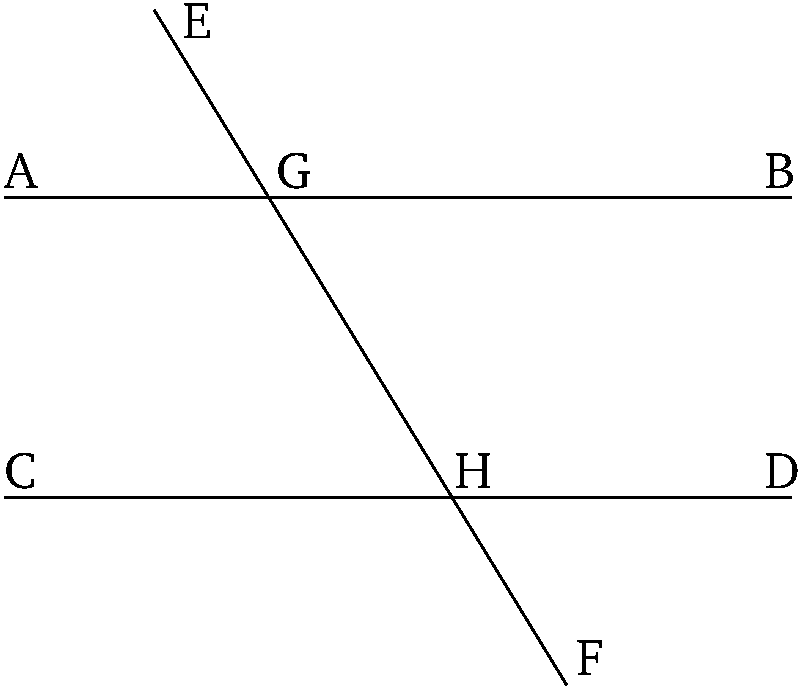
\includegraphics[width=0.8\textwidth]{Book01/fig28e.pdf}}

Thus, a straight-line falling across parallel straight-lines makes the alternate angles
equal to one another,  the external (angle) equal to the internal and
opposite (angle), and the (sum of the) internal (angles) on the same side equal to
two right-angles. (Which is) the very thing it was required to show.}
\end{Parallel}

%%%%%%
% Prop 1.30
%%%%%%
\pdfbookmark[1]{Proposition 1.30}{pdf1.30}
\begin{Parallel}{}{} 
\ParallelLText{
\begin{center}
{\large \ggn{30}.}
\end{center}\vspace*{-7pt}

\gr{Αἱ τῇ αὐτῇ εὐθείᾳ παράλληλοι καὶ ἀλλήλαις εἰσὶ παράλληλοι.}

\gr{Ἔστω ἑκατέρα τῶν ΑΒ, ΓΔ τῇ ΕΖ παράλληλος; λέγω, ὅτι καὶ ἡ ΑΒ τῇ ΓΔ ἐστι παράλληλος.}

\gr{Ἐμπιπτέτω γὰρ εἰξ αὐτὰξ εὐθεῖα ἡ ΗΚ.}

% Removed epsf size command
\centerline{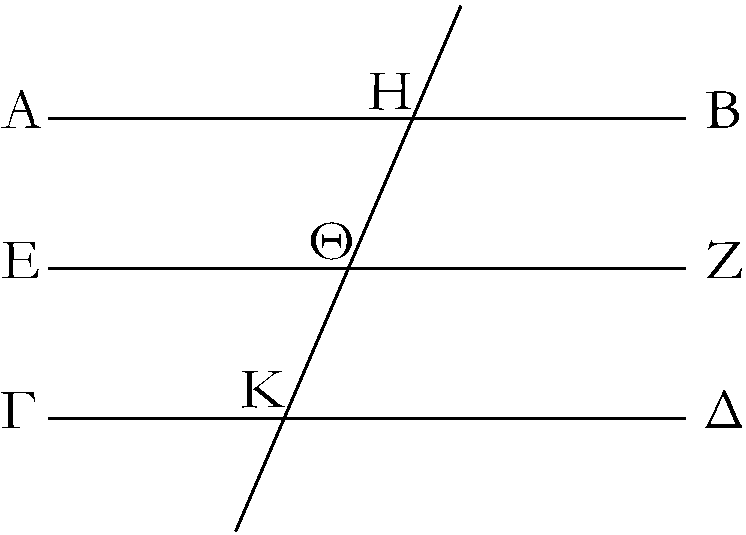
\includegraphics[width=0.8\textwidth]{Book01/fig30g.pdf}}

\gr{Καὶ ἐπεὶ εἰξ παραλλήλους εὐθείας τὰξ ΑΒ, ΕΖ εὐθεῖα ἐμπέπτωκεν ἡ ΗΚ, ὸίση ἄρα ἡ ὑπὸ ΑΗΚ τῇ ὑπὸ ΗΘΖ. πάλιν, ἐπεὶ εἰξ παραλλήλους εὐθείας τὰξ ΕΖ, ΓΔ εὐθεῖα ἐμπέπτωκεν ἡ ΗΚ, ὸίση ἐστὶν ἡ ὑπὸ ΗΘΖ τῇ ὑπὸ ΗΚΔ. ἐδείθθη δὲ καὶ ἡ ὑπὸ ΑΗΚ
τῇ ὑπὸ ΗΘΖὸίση. καὶ ἡ ὑπὸ ΑΗΚ ἄρα τῇ ὑπὸ ΗΚΔ ἐστινὸίση; καί εἰσιν ἐναλλάχ. παράλληλος ἄρα ἐστὶν ἡ ΑΒ τῇ ΓΔ.}

\gr{[Αἱ   ἄρα τῇ αὐτῇ εὐθείᾳ παράλληλοι καὶ ἀλλήλαις εἰσὶ παράλληλοι;]
ὅπερ ἔδει δεῖχαι.}}

\ParallelRText{
\begin{center}
{\large Proposition 30}
\end{center}

(Straight-lines) parallel to the same straight-line are also parallel
to one another.

Let each of the (straight-lines) $AB$ and $CD$ be parallel to $EF$. I say that
$AB$ is also parallel to $CD$.

For let the straight-line $GK$ fall across  ($AB$, $CD$, and $EF$).

% Removed epsf size command
\centerline{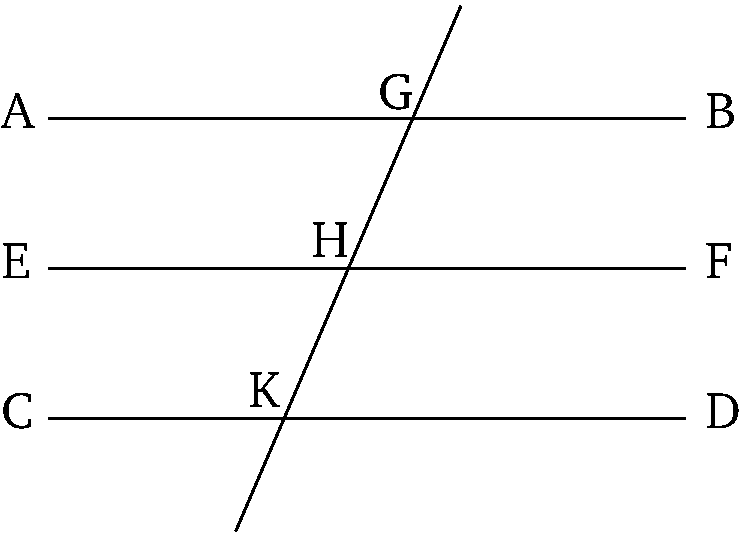
\includegraphics[width=0.8\textwidth]{Book01/fig30e.pdf}}

And since the straight-line $GK$ has fallen across the parallel straight-lines $AB$ and $EF$, (angle) $AGK$
(is) thus equal to $GHF$ [Prop.~1.29]. Again, since the straight-line $GK$ has fallen across the parallel
straight-lines $EF$ and $CD$, (angle) $GHF$ is equal to $GKD$ [Prop.~1.29].
But $AGK$ was also shown (to be) equal to $GHF$. Thus, $AGK$ is also equal to 
$GKD$. And they are alternate (angles). Thus, $AB$ is parallel to $CD$ [Prop.~1.27].

\mbox{[}Thus, (straight-lines) parallel to the same straight-line are also parallel
to one another.] (Which is) the very thing it was required to show.}
\end{Parallel}

%%%%%%
% Prop 1.31
%%%%%%
\pdfbookmark[1]{Proposition 1.31}{pdf1.31}
\begin{Parallel}{}{} 
\ParallelLText{
\begin{center}
{\large \ggn{31}.}
\end{center}\vspace*{-7pt}

\gr{Διὰ τοῦ δοθέντος σημείου τῇ δοθείσῃ εὐθείᾳ παράλληλον εὐθεῖαν
γραμμὴν ἀγαγεῖν.}

\gr{Ἔστω τὸ μὲν δοθὲν σημεῖον τὸ Α, ἡ δὲ δοθεῖσα εὐθεῖα ἡ ΒΓ;
δεῖ δὴ διὰ τοῦ Α σημείου τῇ ΒΓ εὐθείᾳ παράλληλον εὐθεῖαν γραμμὴν ἀγαγεῖν.}

\gr{Εἰλήφθω ἐπὶ τῆς ΒΓ τυθὸν σημεῖον τὸ Δ, καὶ ἐπεζεύθθω ἡ ΑΔ; καὶ συνεστάτω πρὸς τῇ ΔΑ εὐθείᾳ καὶ τῷ πρὸς αὐτῇ σημείῳ  
 τῷ Α τῇ ὑπὸ ΑΔΓ γωνίᾳ ὸίση ἡ ὑπὸ ΔΑΕ; καὶ ἐκβεβλήσθω ἐπ' εὐθείας τῇ ΕΑ εὐθεῖα ἡ ΑΖ.}\\
 
% Removed epsf size command
\centerline{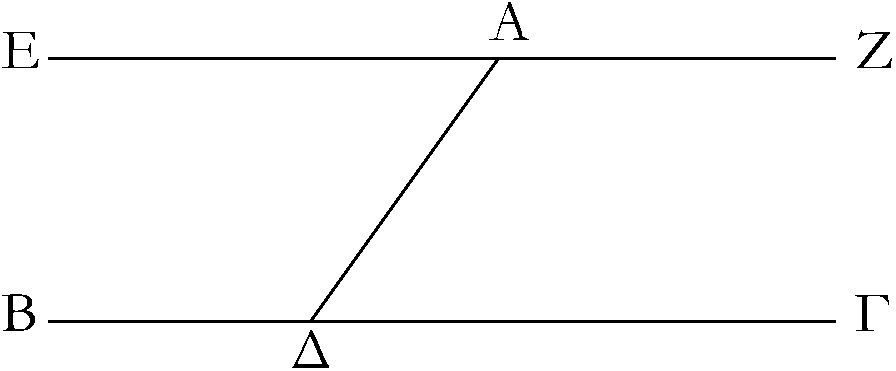
\includegraphics[width=0.8\textwidth]{Book01/fig31g.pdf}}
 
\gr{Καὶ ἐπεὶ εἰξ δύο εὐθείας τὰξ ΒΓ, ΕΖ εὐθεῖα ἐμπίπτουσα ἡ
ΑΔ τὰξ ἐναλλὰχ γωνίας τὰξ ὑπὸ ΕΑΔ, ΑΔΓ ἴσας ἀλλήλαις πεποίηκεν, παράλληλος ἄρα ἐστὶν ἡ ΕΑΖ τῇ ΒΓ.}

\gr{Διὰ τοῦ δοθέντος ἄρα σημείου τοῦ Α τῇ δοθείσῃ εὐθείᾳ τῇ ΒΓ παράλληλος εὐθεῖα
γραμμὴ ὸῆκται ἡ ΕΑΖ; ὅπερ ἔδει ποιῆσαι.}}

\ParallelRText{
\begin{center}
{\large Proposition 31}
\end{center}

To draw a straight-line parallel to a given straight-line, through a given
point.

Let $A$ be the given point, and $BC$ the given straight-line. So it is
required to draw a straight-line parallel to the straight-line $BC$, through
the point $A$.

Let the point $D$ be taken a random  on $BC$, and let $AD$ be
joined. And let (angle) $DAE$, equal to angle $ADC$,  be constructed 
on the straight-line $DA$ at the point $A$ on it [Prop.~1.23]. And let the
straight-line $AF$ be
produced in a straight-line with $EA$.

% Removed epsf size command
\centerline{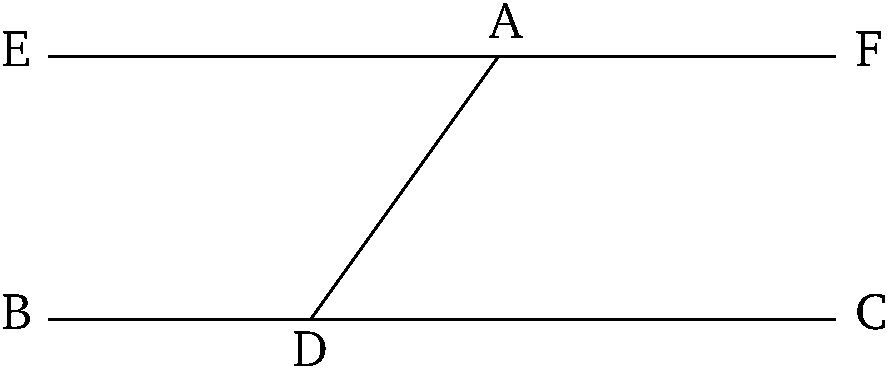
\includegraphics[width=0.8\textwidth]{Book01/fig31e.pdf}}

And since the straight-line $AD$, (in) falling across the two straight-lines
$BC$ and $EF$,  has made the alternate
angles $EAD$ and $ADC$ equal to one another, $EAF$ is thus parallel to $BC$
[Prop.~1.27].

Thus, the straight-line $EAF$ has been drawn parallel to the given straight-line $BC$, through the  given
point $A$. (Which is) the very thing it was required to do.}
\end{Parallel}

%%%%%%
% Prop 1.32
%%%%%%
\pdfbookmark[1]{Proposition 1.32}{pdf1.32}
\begin{Parallel}{}{} 
\ParallelLText{
\begin{center}
{\large \ggn{32}.}
\end{center}\vspace*{-7pt}

\gr{Παντὸξ τριγώνου μιᾶς τῶν πλευρῶν προσεκβληθείσης ἡ ἐκτὸξ γωνία
δυσὶ ταῖς ἐντὸς καὶ ἀπεναντίονὸίση ἐστίν, καὶ αἱ ἐντὸς τοῦ τριγώνου τρεῖς γωνίαι δυσὶν ὀρθαῖξ ἴσαι εἰσίν.}~\\

% Removed epsf size command
\centerline{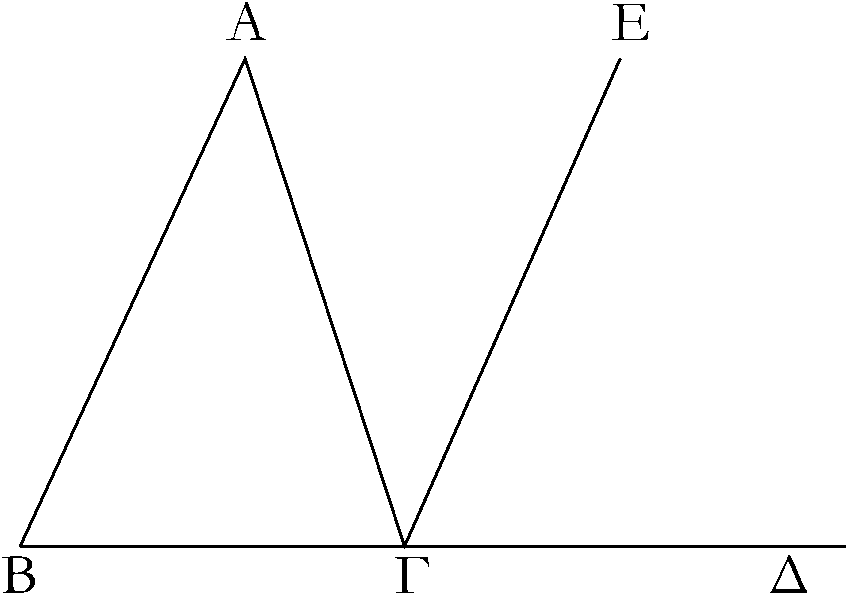
\includegraphics[width=0.8\textwidth]{Book01/fig32g.pdf}}

\gr{Ἔστω τρίγωνον τὸ ΑΒΓ, καὶ προσεκβεβλήσθω αὐτοῦ μία πλευρὰ ἡ ΒΓ
ἐπὶ τὸ Δ; λέγω, ὅτι ἡ ἐκτὸξ γωνία ἡ ὑπὸ ΑΓΔὸίση ἐστὶ δυσὶ ταῖς ἐντὸς καὶ ἀπεναντίον ταῖς ὑπὸ ΓΑΒ, ΑΒΓ, καὶ αἱ ἐντὸς
τοῦ τριγώνου
 τρεῖς γωνίαι αἱ ὑπὸ ΑΒΓ, ΒΓΑ, ΓΑΒ δυσὶν ὀρθαῖξ ἴσαι εἰσίν.}
 
 \gr{ὸ'Ηθθω γὰρ διὰ τοῦ Γ σημείου τῇ ΑΒ εὐθείᾳ παράλληλος ἡ ΓΕ.}
 
 \gr{Καὶ ἐπεὶ παράλληλόξ ἐστιν ἡ ΑΒ τῇ ΓΕ, καὶ εἰξ αὐτὰξ ἐμπέπτωκεν ἡ ΑΓ, αἱ ἐναλλὰχ γωνίαι αἱ ὑπὸ ΒΑΓ, ΑΓΕ ἴσαι ἀλλήλαις εἰσίν. πάλιν, ἐπεὶ παράλληλόξ ἐστιν ἡ ΑΒ τῇ ΓΕ, καὶ εἰξ αὐτὰξ ἐμπέπτωκεν εὐθεῖα ἡ ΒΔ, ἡ ἐκτὸξ γωνία ἡ ὑπὸ ΕΓΔὸίση ἐστὶ τῇ  ἐντὸς καὶ ἀπεναντίον τῇ ὑπὸ ΑΒΓ. ἐδείθθη δὲ καὶ ἡ ὑπὸ ΑΓΕ τῇ ὑπὸ ΒΑΓὸίση; ὅλη ἄρα ἡ ὑπὸ ΑΓΔ γωνίαὸίση ἐστὶ δυσὶ ταῖς ἐντὸς καὶ ἀπεναντίον ταῖς ὑπὸ ΒΑΓ, ΑΒΓ.}
 
 \gr{Κοινὴ προσκείσθω ἡ ὑπὸ ΑΓΒ; αἱ  ἄρα ὑπὸ ΑΓΔ, ΑΓΒ τρισὶ ταῖς ὑπὸ ΑΒΓ, ΒΓΑ, ΓΑΒ ἴσαι εἰσίν. ἀλλὸ αἱ ὑπὸ ΑΓΔ, ΑΓΒ δυσὶν ὀρθαῖξ ἴσαι εἰσίν; καὶ αἱ ὑπὸ ΑΓΒ, ΓΒΑ, ΓΑΒ ἄρα δυσὶν ὀρθαῖξ ἴσαι εἰσίν.}
 
 \gr{Παντὸξ ἄρα τριγώνου μιᾶς τῶν πλευρῶν προσεκβληθείσης ἡ ἐκτὸξ γωνία
δυσὶ ταῖς ἐντὸς καὶ ἀπεναντίονὸίση ἐστίν, καὶ αἱ ἐντὸς τοῦ τριγώνου τρεῖς γωνίαι δυσὶν ὀρθαῖξ ἴσαι εἰσίν; ὅπερ ἔδει
δεῖχαι.}}

\ParallelRText{
\begin{center}
{\large Proposition 32}
\end{center}

In any triangle,  (if) one of the sides (is) produced  (then) the external
angle is equal to the (sum of the) two internal and opposite (angles), and the (sum of the) three
internal angles of the triangle is equal to two right-angles.

% Removed epsf size command
\centerline{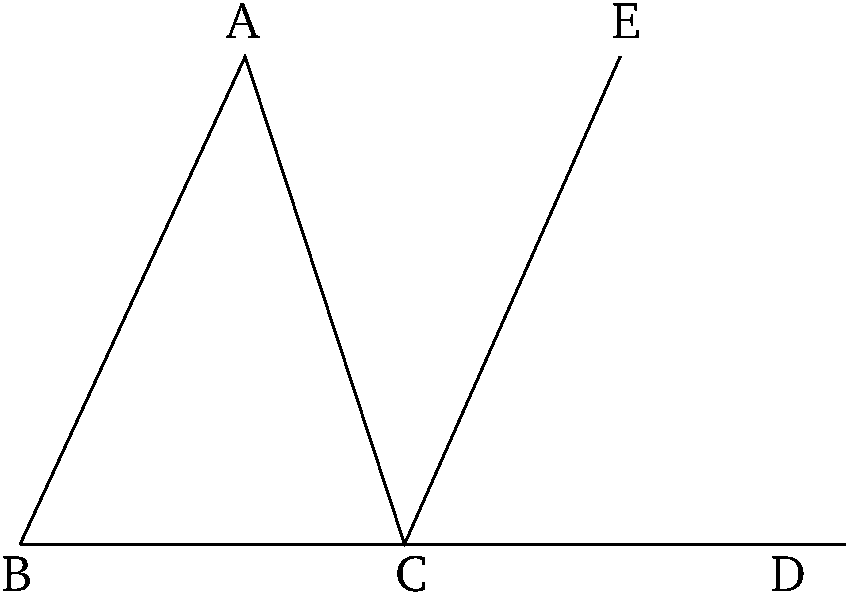
\includegraphics[width=0.8\textwidth]{Book01/fig32e.pdf}}

Let $ABC$ be a triangle, and let one of its sides $BC$ be produced to $D$.
I say that the external angle $ACD$ is equal to the (sum of the) two internal and opposite
angles $CAB$ and $ABC$, and the (sum of the) three internal angles of the triangle---$ABC$, $BCA$, and $CAB$---is equal to two right-angles.

For let $CE$ be drawn through point $C$ parallel to the straight-line
$AB$ [Prop.~1.31].

And since $AB$ is parallel to $CE$, and $AC$ has fallen across them, the alternate
angles $BAC$ and $ACE$ are equal to one another [Prop.~1.29]. Again,
since $AB$ is parallel to $CE$, and the straight-line $BD$ has fallen across them, 
the external angle $ECD$ is equal to the internal and opposite (angle)
$ABC$ [Prop.~1.29]. But $ACE$ was also shown (to be) equal to $BAC$. Thus, the whole
angle $ACD$ is equal to the (sum of the) two internal and opposite (angles) $BAC$ and $ABC$.

Let $ACB$ be added to both. Thus, (the sum of) $ACD$ and $ACB$ is equal to
the (sum of the) three (angles) $ABC$, $BCA$, and $CAB$. But, (the sum of) $ACD$ and $ACB$ is equal
to two right-angles [Prop.~1.13]. Thus, (the sum of) $ACB$, $CBA$, and $CAB$ is also
equal to two right-angles.

Thus, in any triangle,  (if) one of the sides  (is) produced (then) the external
angle is equal to the (sum of the) two internal and opposite (angles), and the (sum of the) three
internal angles of the triangle is equal to two right-angles. (Which is)
the very thing it was required to show.}
\end{Parallel}

%%%%%%
% Prop 1.33
%%%%%%
\pdfbookmark[1]{Proposition 1.33}{pdf1.33}
\begin{Parallel}{}{} 
\ParallelLText{
\begin{center}
{\large \ggn{33}.}
\end{center}\vspace*{-7pt}

\gr{Αἱ τὰξ ἴσας τε καὶ παραλλήλους ἐπὶ τὰ αὐτὰ μέρη ἐπιζευγνύουσαι εὐθεῖαι καὶ αὐταὶ  ἴσαι τε καὶ παράλληλοί εἰσιν.}

\gr{Ἔστωσαν ἴσαι τε καὶ παράλληλοι αἱ  ΑΒ, ΓΔ, καὶ ἐπιζευγνύτωσαν αὐτὰξ ἐπὶ τὰ αὐτὰ μέρη εὐθεῖαι αἱ ΑΓ, ΒΔ; λέγω, ὅτι καὶ αἱ ΑΓ, ΒΔ ἴσαι τε καὶ παράλληλοί εἰσιν.}

% Removed epsf size command
\centerline{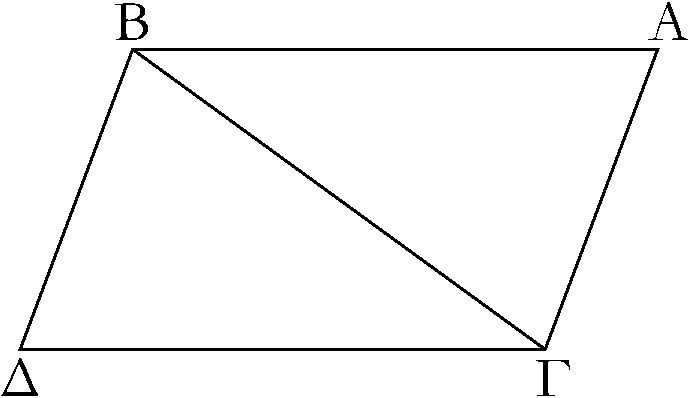
\includegraphics[width=0.8\textwidth]{Book01/fig33g.pdf}}

\gr{Ἐπεζεύθθω ἡ ΒΓ. καὶ ἐπεὶ παράλληλόξ ἐστιν ἡ ΑΒ τῇ ΓΔ, καὶ εἰξ αὐτὰξ ἐμπέπτωκεν ἡ ΒΓ, αἱ ἐναλλὰχ γωνίαι αἱ ὑπὸ ΑΒΓ, ΒΓΔ ἴσαι ἀλλήλαις εἰσίν. καὶ ἐπεὶ ὸίση ἐστὶν ἡ ΑΒ τῇ ΓΔ κοινὴ δὲ ἡ
ΒΓ, δύο δὴ αἱ ΑΒ, ΒΓ δύο ταῖς
 ΒΓ, ΓΔ ἴσαι εἰσίν; καὶ γωνία ἡ ὑπὸ ΑΒΓ γωνίᾳ τῇ ὑπὸ ΒΓΔὸίση; βάσις ἄρα ἡ ΑΓ βάσει τῇ ΒΔ ἐστινὸίση, καὶ τὸ ΑΒΓ τρίγωνον τῷ ΒΓΔ τριγώνῳ  ἴσον ἐστίν, καὶ αἱ λοιπαὶ γωνίαι ταῖς λοιπαῖξ γωνίαις ἴσαιὸέσονται ἑκατέρα ἑκατέρᾳ, ὑφὸ ὁὰξ αἱ  ἴσαι πλευραὶ
ὑποτείνουσιν; ὸίση ἄρα ἡ ὑπὸ ΑΓΒ γωνία τῇ ὑπὸ ΓΒΔ. καὶ
ἐπεὶ εἰξ δύο εὐθείας τὰξ ΑΓ, ΒΔ εὐθεῖα
ἐμπίπτουσα ἡ ΒΓ τὰξ ἐναλλὰχ γωνίας ἴσας ἀλλήλαις πεποίηκεν, παράλληλος ἄρα ἐστὶν ἡ ΑΓ τῇ ΒΔ. ἐδείθθη δὲ αὐτῇ καὶ ὸίση.}

\gr{Αἱ  ἄρα τὰξ ἴσας τε καὶ παραλλήλους ἐπὶ τὰ αὐτὰ μέρη ἐπιζευγνύουσαι εὐθεῖαι καὶ αὐταὶ  ἴσαι τε καὶ παράλληλοί εἰσιν;
 ὅπερ ἔδει
δεῖχαι.}}

\ParallelRText{
\begin{center}
{\large Proposition 33}
\end{center}

Straight-lines joining equal and parallel (straight-lines) on the same sides
are  themselves also equal and parallel.

Let $AB$ and $CD$ be equal and parallel (straight-lines), and let the
straight-lines $AC$ and $BD$ join them on the same sides. I say that $AC$
and $BD$ are also equal and parallel.

% Removed epsf size command
\centerline{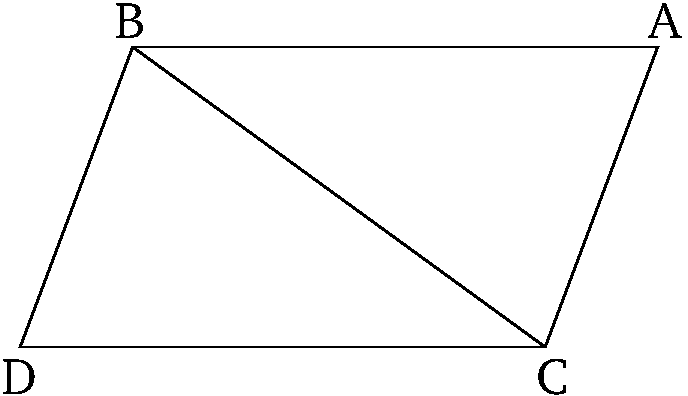
\includegraphics[width=0.8\textwidth]{Book01/fig33e.pdf}}

Let $BC$ be joined. And since $AB$ is parallel to $CD$, and $BC$ has
fallen across them, the alternate angles $ABC$ and $BCD$ are equal to one another [Prop.~1.29]. And since $AB$ is equal to $CD$, and $BC$ is common,
the two (straight-lines) $AB$, $BC$ are equal to the two (straight-lines)
$DC$, $CB$.$^\dag$And the angle $ABC$ is equal to the angle $BCD$. Thus, the
base $AC$ is equal to the base $BD$, and triangle $ABC$ is equal to triangle
$DCB$$^\ddag$, and the remaining angles will be equal to the corresponding remaining
angles subtended by the equal sides [Prop.~1.4]. Thus,  angle $ACB$ 
is equal to $CBD$. Also, since the straight-line $BC$, (in) falling across the two
straight-lines $AC$ and $BD$, has made the alternate angles  ($ACB$ and $CBD$) equal to one another,
$AC$ is thus parallel to $BD$ [Prop.~1.27]. And ($AC$) was also shown (to be) equal
to ($BD$).

Thus, straight-lines joining equal and parallel (straight-lines) on the same sides
are  themselves also equal and parallel. (Which is) the very thing it was
required to show.}
\end{Parallel}
{\footnotesize \noindent$^\dag$ The Greek text has ``$BC$, $CD$'', which is obviously a mistake.} \\
{\footnotesize \noindent$^\ddag$ The Greek text has ``$DCB$'', which is obviously a mistake.} 

%%%%%%
% Prop 1.34
%%%%%%
\pdfbookmark[1]{Proposition 1.34}{pdf1.34}
\begin{Parallel}{}{} 
\ParallelLText{
\begin{center}
{\large \ggn{34}.}
\end{center}\vspace*{-7pt}

\gr{Τῶν παραλληλογράμμων θωρίων αἱ ἀπεναντίον πλευραί τε καὶ γωνίαι ἴσαι ἀλλήλαις εἰσίν, καὶ ἡ διάμετρος αὐτὰ δίθα τέμνει.}

\gr{Ἔστω παραλληλόγραμμον θωρίον τὸ ΑΓΔΒ, διάμετρος δὲ αὐτοῦ ἡ ΒΓ; λέγω, ὅτι τοῦ ΑΓΔΒ παραλληλογράμμου αἱ ἀπεναντίον πλευραί τε καὶ γωνίαι ἴσαι ἀλλήλαις εἰσίν, καὶ ἡ ΒΓ διάμετρος αὐτὸ δίθα τέμνει.}

% Removed epsf size command
\centerline{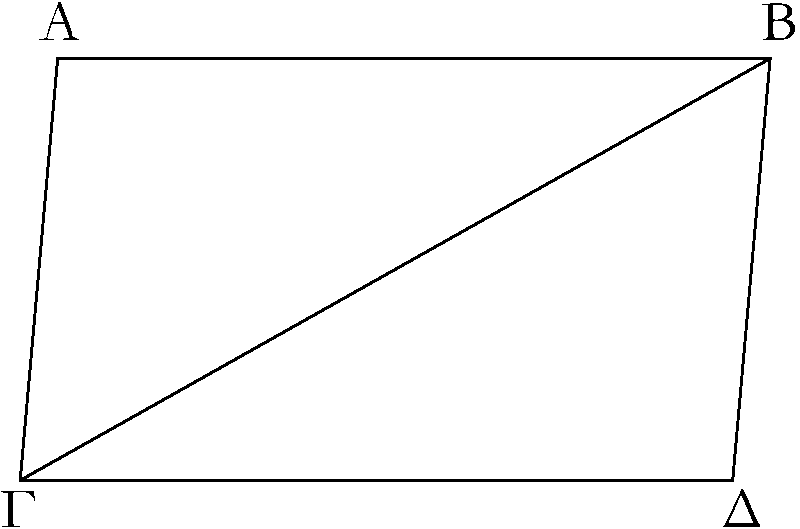
\includegraphics[width=0.8\textwidth]{Book01/fig34g.pdf}}

\gr{Ἐπεὶ γὰρ παράλληλόξ ἐστιν ἡ ΑΒ τῇ ΓΔ, καὶ εἰξ αὐτὰξ ἐμπέπτωκεν
εὐθεῖα ἡ ΒΓ, αἱ ἐναλλὰχ γωνίαι αἱ ὑπὸ ΑΒΓ, ΒΓΔ ἴσαι ἀλλήλαις εἰσίν. πάλιν ἐπεὶ παράλληλόξ ἐστιν ἡ ΑΓ τῇ ΒΔ, καὶ εἰξ αὐτὰξ ἐμπέπτωκεν ἡ ΒΓ, αἱ ἐναλλὰχ γωνίαι αἱ ὑπὸ ΑΓΒ, ΓΒΔ ἴσαι ἀλλήλαις εἰσίν. δύο δὴ τρίγωνά ἐστι τὰ ΑΒΓ, ΒΓΔ τὰξ δύο γωνίας τὰξ ὑπὸ ΑΒΓ, ΒΓΑ δυσὶ ταῖς ὑπὸ ΒΓΔ, ΓΒΔ ἴσας ἔχοντα ἑκατέραν ἑκατέρᾳ καὶ μίαν πλευρὰν μιᾶ| πλευρᾶ|  ἴσην τὴν πρὸς ταῖς ἴσαις γωνίαις κοινὴν αὐτῶν τὴν ΒΓ; καὶ τὰξ λοιπὰξ ἄρα πλευρὰξ ταῖς λοιπαῖξ ἴσας ὁέχει ἑκατέραν ἑκατέρᾳ καὶ τὴν λοιπὴν γωνίαν τῇ λοιπῆ| γωνίᾳ; ὸίση ἄρα ἡ μὲν ΑΒ πλευρὰ τῇ ΓΔ, ἡ δὲ ΑΓ τῇ ΒΔ, καὶ ὸέτιὸίση ἐστὶν ἡ ὑπὸ ΒΑΓ γωνία τῇ ὑπὸ ΓΔΒ. καὶ ἐπεὶ ὸίση ἐστὶν ἡ μὲν ὑπὸ ΑΒΓ γωνία τῇ ὑπὸ ΒΓΔ, ἡ δὲ ὑπὸ ΓΒΔ τῇ ὑπὸ ΑΓΒ, ὅλη ἄρα ἡ ὑπὸ ΑΒΔ ὅλῃ τῇ ὑπὸ ΑΓΔ ἐστινὸίση. ἐδείθθη δὲ καὶ ἡ ὑπὸ ΒΑΓ τῇ ὑπὸ ΓΔΒὸίση.}

\gr{Τῶν ἄρα παραλληλογράμμων θωρίων αἱ ἀπεναντίον πλευραί τε
καὶ γωνίαι ἴσαι ἀλλήλαις εἰσίν.}

\gr{Λέγω δή, ὅτι καὶ ἡ διάμετρος αὐτὰ δίθα τέμνει. ἐπεὶ γὰρὸίση ἐστὶν ἡ ΑΒ τῇ ΓΔ, κοινὴ δὲ ἡ ΒΓ, δύο δὴ αἱ ΑΒ, ΒΓ δυσὶ ταῖς ΓΔ, ΒΓ ἴσαι εἰσὶν ἑκατέρα ἑκατέρᾳ; καὶ γωνία ἡ ὑπὸ ΑΒΓ γωνίᾳ τῇ ὑπὸ ΒΓΔὸίση. καὶ βάσις ἄρα ἡ ΑΓ τῇ ΔΒὸίση. καὶ τὸ ΑΒΓ [ ἄρα] τρίγωνον τῷ ΒΓΔ τριγώνῳ  ἴσον ἐστίν.}

\gr{Ἡ  ἄρα ΒΓ διάμετρος δίθα τέμνει τὸ ΑΒΓΔ παραλληλόγραμμον;
ὅπερ ἔδει δεῖχαι.}}

\ParallelRText{
\begin{center}
{\large Proposition 34}
\end{center}
In parallelogramic figures, the opposite sides and angles are equal to one
another, and a diagonal cuts them in half.

Let $ACDB$ be a parallelogramic figure, and $BC$ its diagonal. I say that
for parallelogram $ACDB$, the opposite sides and angles are equal to
one another, and the diagonal $BC$ cuts it in half.\\

% Removed epsf size command
\centerline{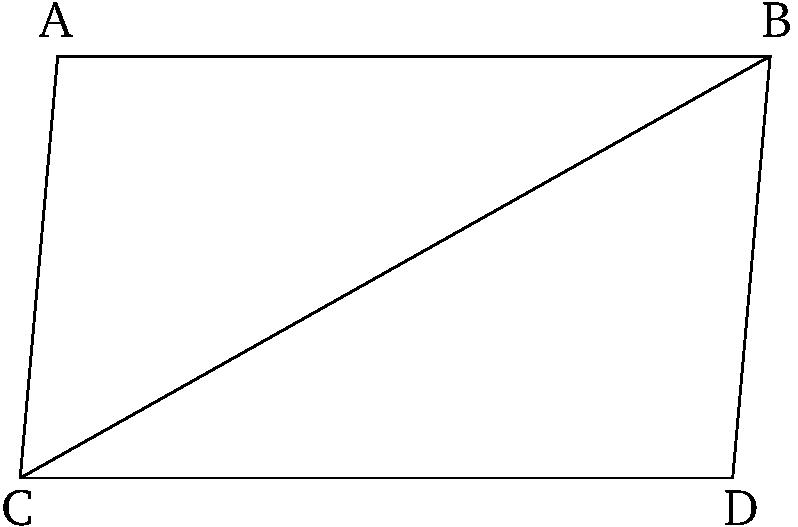
\includegraphics[width=0.8\textwidth]{Book01/fig34e.pdf}}

For since $AB$ is parallel to $CD$, and the straight-line $BC$ has fallen
across  them, the alternate angles $ABC$ and $BCD$ are equal to one another [Prop.~1.29]. 
Again, since $AC$ is parallel to $BD$, and $BC$ has fallen across them, the
alternate angles $ACB$ and $CBD$ are equal to one another [Prop.~1.29]. 
So $ABC$ and $BCD$ are two triangles having the two angles $ABC$ and
$BCA$ equal to the two (angles) $BCD$ and $CBD$, respectively, and one
side equal to one side---the (one) by the equal angles and common to them, (namely) $BC$. Thus,
they will also  have the remaining sides  equal to the corresponding
remaining (sides), and the remaining angle (equal) to the remaining angle [Prop.~1.26].
Thus, side $AB$ is equal to $CD$, and $AC$ to $BD$. Furthermore, angle $BAC$ is 
equal to $CDB$. And since angle $ABC$ is equal to $BCD$, and $CBD$ to
$ACB$, the whole (angle) $ABD$ is thus equal to the whole (angle) $ACD$.
And  $BAC$ was also shown  (to be) equal to $CDB$.

Thus, in parallelogramic figures, the opposite sides and angles are equal
to one another.

And, I also say that a diagonal cuts them in half. For since $AB$ is equal
to $CD$, and $BC$ (is) common, the two (straight-lines) $AB$, $BC$ are equal
to the two (straight-lines) $DC$, $CB$$^\dag$, respectively. And angle $ABC$ is
equal to angle $BCD$. Thus, the base $AC$ (is) also equal to $DB$, and
triangle $ABC$ is equal to triangle $BCD$ [Prop.~1.4].

Thus, the diagonal $BC$ cuts the parallelogram $ACDB$$^\ddag$ in half. (Which is) the
very thing it was required to show.}
\end{Parallel}
{\footnotesize \noindent$^\dag$ The Greek text has ``$CD$, $BC$'',
which is obviously a mistake.\\
$^\ddag$ The Greek
text has ``$ABCD$'', which is obviously a mistake.}

%%%%%%
% Prop 1.35
%%%%%%
\pdfbookmark[1]{Proposition 1.35}{pdf1.35}
\begin{Parallel}{}{} 
\ParallelLText{
\begin{center}
{\large \ggn{35}.}
\end{center}\vspace*{-7pt}

\gr{Τὰ παραλληλόγραμμα τὰ ἐπὶ τῆς αὐτῆς βάσεως ὅντα καὶ ἐν ταῖς
αὐταῖς παραλλήλοις ἴσα ἀλλήλοις ἐστίν.}

\gr{Ἔστω παραλληλόγραμμα τὰ ΑΒΓΔ, ΕΒΓΖ ἐπὶ τῆς αὐτῆς βάσεως τῆς
ΒΓ καὶ ἐν ταῖς αὐταῖς παραλλήλοις ταῖς ΑΖ, ΒΓ; λέγω, ὅτι ἴσον ἐστὶ τὸ ΑΒΓΔ τῷ ΕΒΓΖ παραλληλογράμμῳ.}

% Removed epsf size command
\centerline{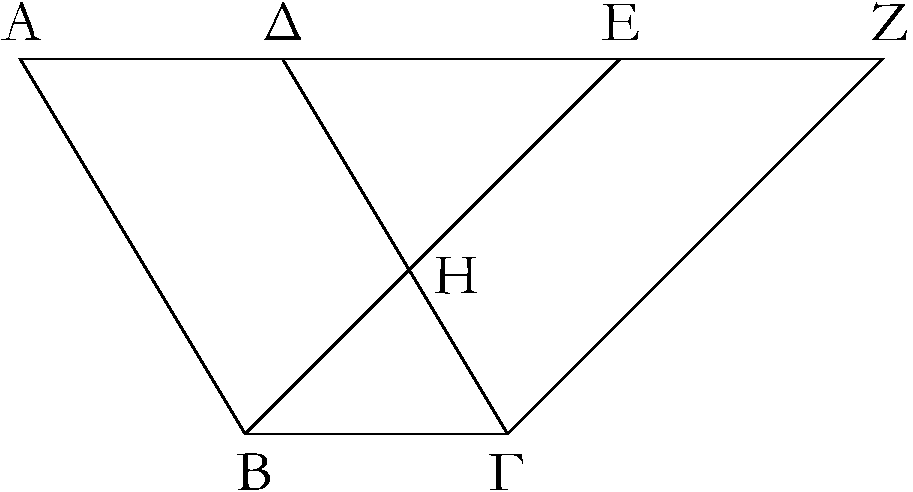
\includegraphics[width=0.8\textwidth]{Book01/fig35g.pdf}}

\gr{Ἐπεὶ γὰρ παραλληλόγραμμόν ἐστι τὸ ΑΒΓΔ, ὸίση ἐστὶν ἡ ΑΔ τῇ ΒΓ. διὰ τὰ αὐτὰ δὴ καὶ ἡ ΕΖ τῇ ΒΓ ἐστινὸίση; ὁώστε καὶ ἡ ΑΔ τῇ ΕΖ ἐστινὸίση; καὶ κοινὴ ἡ ΔΕ; ὅλη ἄρα ἡ ΑΕ ὅλῃ τῇ ΔΖ ἐστινὸίση. ὸέστι δὲ καὶ ἡ ΑΒ τῇ ΔΓὸίση; δύο δὴ αἱ ΕΑ, ΑΒ δύο ταῖς ΖΔ, ΔΓ ἴσαι εἰσὶν ἑκατέρα ἑκατέρᾳ; καὶ γωνία ἡ ὑπὸ ΖΔΓ γωνίᾳ
τῇ ὑπὸ ΕΑΒ ἐστινὸίση ἡ ἐκτὸξ τῇ ἐντόξ; βάσις ἄρα ἡ ΕΒ
βάσει τῇ ΖΓὸίση ἐστίν, καὶ τὸ ΕΑΒ τρίγωνον τῷ ΔΖΓ τριγώνῳ  ἴσονὸέσται; κοινὸν ἀφῃρήσθω τὸ ΔΗΕ; λοιπὸν ἄρα τὸ ΑΒΗΔ τραπέζιον λοιπῶ| τῷ ΕΗΓΖ τραπεζίῳ ἐστὶν ἴσον; κοινὸν προσκείσθω τὸ ΗΒΓ τρίγωνον; ὅλον ἄρα τὸ ΑΒΓΔ παραλληλόγραμμον ὅλῳ τῷ ΕΒΓΖ
παραλληλογράμμῳ  ἴσον ἐστίν.}

\gr{Τὰ  ἄρα παραλληλόγραμμα τὰ ἐπὶ τῆς αὐτῆς βάσεως ὅντα καὶ ἐν ταῖς
αὐταῖς παραλλήλοις ἴσα ἀλλήλοις ἐστίν; ὅπερ ἔδει δεῖχαι.}}

\ParallelRText{
\begin{center}
{\large Proposition 35}
\end{center}

Parallelograms which are on the same base and between the same
parallels are equal$^\dag$ to one another.

Let $ABCD$ and $EBCF$ be parallelograms on the same base $BC$, and
between the same parallels $AF$ and $BC$. I say that $ABCD$ is equal to
parallelogram $EBCF$.

% Removed epsf size command
\centerline{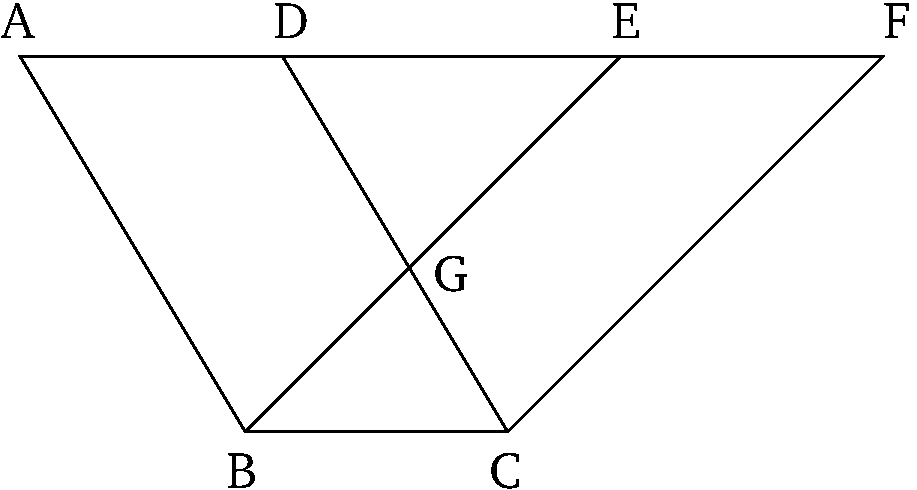
\includegraphics[width=0.8\textwidth]{Book01/fig35e.pdf}}

For since $ABCD$ is a parallelogram, $AD$ is equal to $BC$ [Prop.~1.34].
So, for the same (reasons), $EF$ is also equal to $BC$. So $AD$ is also equal to
$EF$. And $DE$ is common. Thus, the whole (straight-line) $AE$ is equal
to the whole (straight-line) $DF$.  And $AB$ is also equal to $DC$.
So the two (straight-lines) $EA$, $AB$
are equal to the two (straight-lines) $FD$, $DC$, respectively. And angle $FDC$ is
equal to angle $EAB$, the external to the internal [Prop.~1.29]. Thus, the
base $EB$ is equal to the base $FC$, and triangle $EAB$ will be equal to triangle
$DFC$ [Prop.~1.4]. Let $DGE$ be taken away from both. 
Thus, the remaining trapezium $ABGD$ is equal to the remaining trapezium
$EGCF$. Let triangle $GBC$ be added to both. Thus, the whole
parallelogram $ABCD$ is equal to the whole parallelogram $EBCF$.

Thus, parallelograms which are on the same base and between the same
parallels are equal to one another. (Which is) the very thing it was required to
show.}
\end{Parallel}
{\footnotesize \noindent$^\dag$ Here, for the first time, ``equal'' means
``equal in area'', rather than ``congruent''.}

%%%%%%
% Prop 1.36
%%%%%%
\pdfbookmark[1]{Proposition 1.36}{pdf1.36}
\begin{Parallel}{}{} 
\ParallelLText{
\begin{center}
{\large \ggn{36}.}
\end{center}\vspace*{-7pt}

\gr{Τὰ παραλληλόγραμμα τὰ ἐπὶ ὸίσων βάσεων ὅντα καὶ ἐν ταῖς αὐταῖς παραλλήλοις ἴσα ἀλλήλοις ἐστίν.}

\gr{Ἔστω παραλληλόγραμμα τὰ ΑΒΓΔ, ΕΖΗΘ ἐπὶ ὸίσων βάσεων ὅντα τῶν ΒΓ, ΖΗ καὶ ἐν ταῖς αὐταῖς παραλλήλοις ταῖς ΑΘ, ΒΗ; λέγω, ὅτι ἴσον ἐστὶ τὸ ΑΒΓΔ παραλληλόγραμμον τῷ ΕΖΗΘ.}

% Removed epsf size command
\centerline{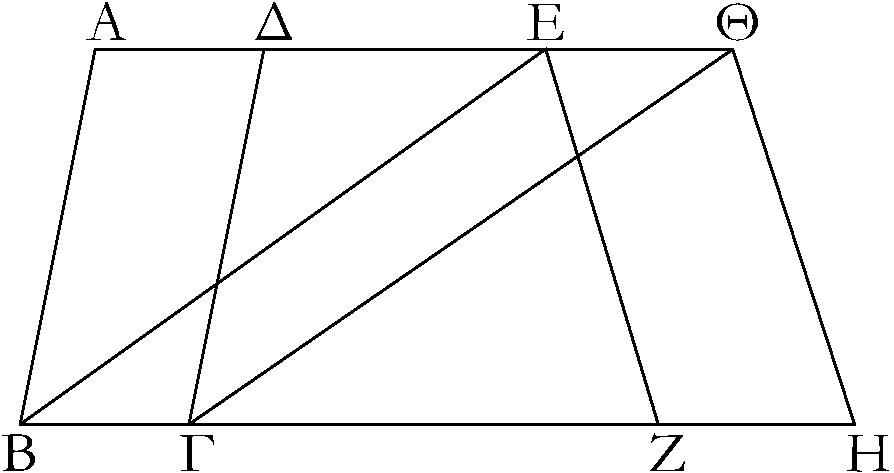
\includegraphics[width=0.8\textwidth]{Book01/fig36g.pdf}}

\gr{Ἐπεζεύθθωσαν γὰρ αἱ ΒΕ, ΓΘ. καὶ ἐπεὶ ὸίση ἐστὶν ἡ ΒΓ τῇ ΖΗ, ἀλλὰ ἡ ΖΗ τῇ ΕΘ ἐστινὸίση, καὶ ἡ ΒΓ ἄρα τῇ ΕΘ ἐστινὸίση.
εἰσὶ δὲ καὶ παράλληλοι. καὶ ἐπιζευγνύουσιν αὐτὰξ αἱ ΕΒ, ΘΓ; αἱ δὲ τὰξ ἴσας τε καὶ παραλλήλους ἐπὶ τὰ αὐτὰ μέρη ἐπιζευγνύουσαι ἴσαι
τε καὶ παράλληλοί εἰσι [καὶ αἱ ΕΒ, ΘΓ ἄρα ἴσαι τέ εἰσι καὶ παράλληλοι].
παραλληλόγραμμον ἄρα ἐστὶ τὸ ΕΒΓΘ. καί ἐστιν ἴσον τῷ ΑΒΓΔ; βάσιν τε γὰρ αὐτῷ τὴν αὐτὴν ἔχει τὴν ΒΓ, καὶ ἐν ταῖς αὐταῖς παραλλήλοις ἐστὶν αὐτῷ ταῖς ΒΓ, ΑΘ. δὶα τὰ αὐτὰ δὴ καὶ τὸ ΕΖΗΘ τῷ αὐτῷ τῷ ΕΒΓΘ ἐστιν ἴσον;
 ὁώστε καὶ τὸ ΑΒΓΔ παραλληλόγραμμον τῷ ΕΖΗΘ ἐστιν ἴσον.}
 
\gr{Τὰ   ἄρα παραλληλόγραμμα τὰ ἐπὶ ὸίσων βάσεων ὅντα καὶ ἐν ταῖς αὐταῖς παραλλήλοις ἴσα ἀλλήλοις ἐστίν; ὅπερ ἔδει δεῖχαι.}}

\ParallelRText{
\begin{center}
{\large Proposition 36}
\end{center}

Parallelograms which are on equal bases and between the same parallels are equal to one another.

Let $ABCD$ and $EFGH$ be parallelograms which are on the equal bases $BC$
and $FG$, and (are) between the same parallels $AH$ and $BG$. I say that
the parallelogram $ABCD$ is equal to $EFGH$.

% Removed epsf size command
\centerline{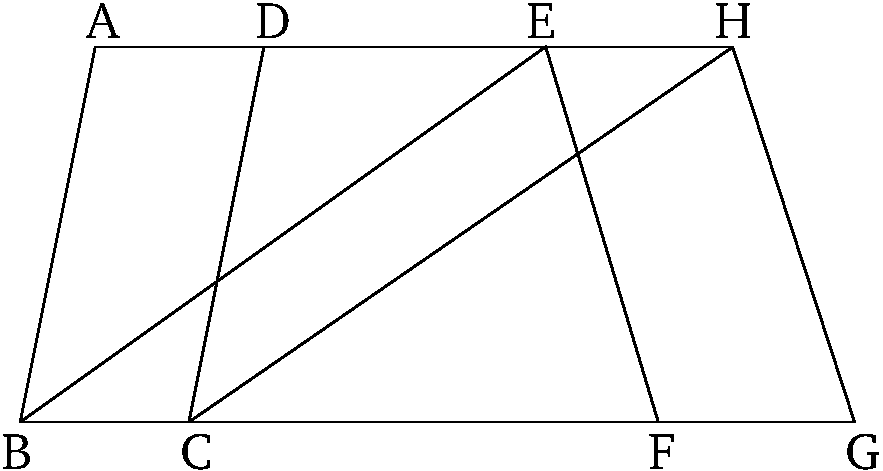
\includegraphics[width=0.8\textwidth]{Book01/fig36e.pdf}}

For let $BE$ and $CH$ be joined. And since $BC$ is equal to $FG$, but $FG$ is equal to $EH$ [Prop.~1.34], $BC$ is thus equal to $EH$. And they are also parallel, and $EB$ and $HC$ join them.
But (straight-lines) joining equal and parallel (straight-lines) on the
same sides are (themselves) equal and parallel [Prop.~1.33] [thus, $EB$ and $HC$
are also equal and parallel]. Thus, $EBCH$ is a parallelogram [Prop.~1.34],
and is equal to $ABCD$. For it has  the
same base, $BC$, (as $ABCD$), and is between the same parallels, $BC$ and $AH$, (as $ABCD$) [Prop.~1.35]. So,
for the same (reasons), $EFGH$ is also equal to the same (parallelogram) $EBCH$ [Prop.~1.34].  So that the
parallelogram $ABCD$ is  also equal to $EFGH$.

Thus, parallelograms which are on equal bases and between the same parallels are equal to one another. (Which is) the very thing it was required
to show.}
\end{Parallel}

%%%%%%
% Prop 1.37
%%%%%%
\pdfbookmark[1]{Proposition 1.37}{pdf1.37}
\begin{Parallel}{}{} 
\ParallelLText{
\begin{center}
{\large \ggn{37}.}
\end{center}\vspace*{-7pt}

\gr{Τὰ τρίγωνα τὰ ἐπὶ τῆς αὐτῆς βάσεως ὅντα καὶ ἐν ταῖς αὐταῖς
παραλλήλοις ἴσα ἀλλήλοις ἐστίν.}

\gr{Ἔστω τρίγωνα τὰ ΑΒΓ, ΔΒΓ ἐπὶ τῆς αὐτῆς βάσεως τῆς ΒΓ καὶ ἐν ταῖς αὐταῖς παραλλήλοις ταῖς ΑΔ, ΒΓ; λέγω, ὅτι ἴσον ἐστὶ τὸ ΑΒΓ τρίγωνον τῷ ΔΒΓ τριγώνῳ.}

% Removed epsf size command
\centerline{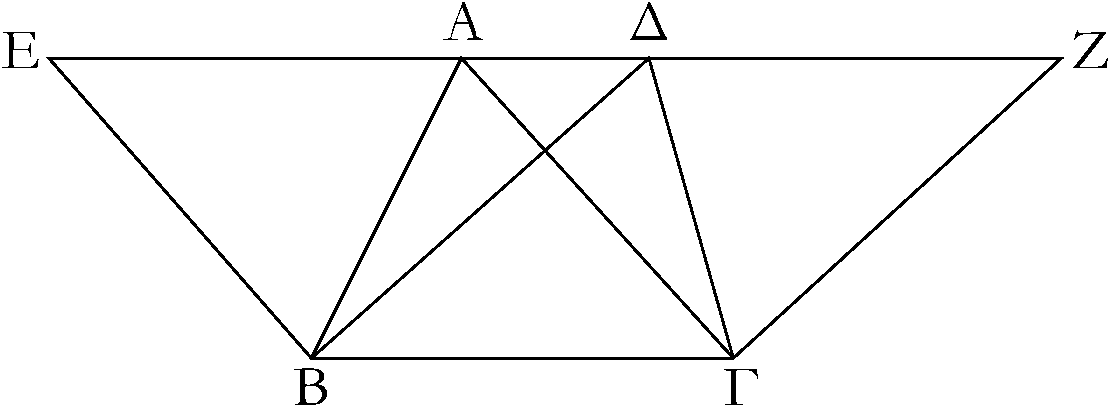
\includegraphics[width=0.8\textwidth]{Book01/fig37g.pdf}}

\gr{Ἐκβεβλήσθω ἡ ΑΔ ἐφ' ἑκάτερα τὰ μέρη ἐπὶ τὰ Ε, Ζ, καὶ διὰ μὲν τοῦ Β τῇ ΓΑ παράλληλος ἢθθω ἡ ΒΕ, δὶα δὲ τοῦ Γ τῇ ΒΔ παράλληλος ἢθθω ἡ ΓΖ.
 παραλληλόγραμμον ἄρα ἐστὶν ἑκάτερον τῶν ΕΒΓΑ, ΔΒΓΖ; καί εἰσιν ἴσα; ἐπί τε γὰρ τῆς αὐτῆς βάσεώξ εἰσι τῆς ΒΓ καὶ ἐν ταῖς αὐταῖς παραλλήλοις ταῖς ΒΓ, ΕΖ; καί ἐστι τοῦ μὲν ΕΒΓΑ
 παραλληλογράμμου
 ἥμισυ τὸ ΑΒΓ τρίγωνον; ἡ γὰρ ΑΒ διάμετρος αὐτὸ δίθα τέμνει; τοῦ δὲ ΔΒΓΖ παραλληλογράμμου ἥμισυ τὸ ΔΒΓ τρίγωνον; ἡ γὰρ ΔΓ διάμετρος αὐτὸ δίθα τέμνει. [τὰ δὲ τῶνὸίσων ἡμίση ἴσα 
 ἀλλήλοις ἐστίν].  ἴσον ἄρα ἐστὶ τὸ ΑΒΓ τρίγωνον τῷ ΔΒΓ τριγώνῳ.}
 
 \gr{Τὰ  ἄρα τρίγωνα τὰ ἐπὶ τῆς αὐτῆς βάσεως ὅντα καὶ ἐν ταῖς αὐταῖς
παραλλήλοις ἴσα ἀλλήλοις ἐστίν;  ὅπερ ἔδει δεῖχαι.}}

\ParallelRText{
\begin{center}
{\large Proposition 37}
\end{center}

Triangles which are on the same base and between the same parallels
are equal to one another.

Let $ABC$ and $DBC$ be triangles on the same base $BC$, and between
the same parallels $AD$ and $BC$. I say that triangle $ABC$ is equal to triangle $DBC$.

% Removed epsf size command
\centerline{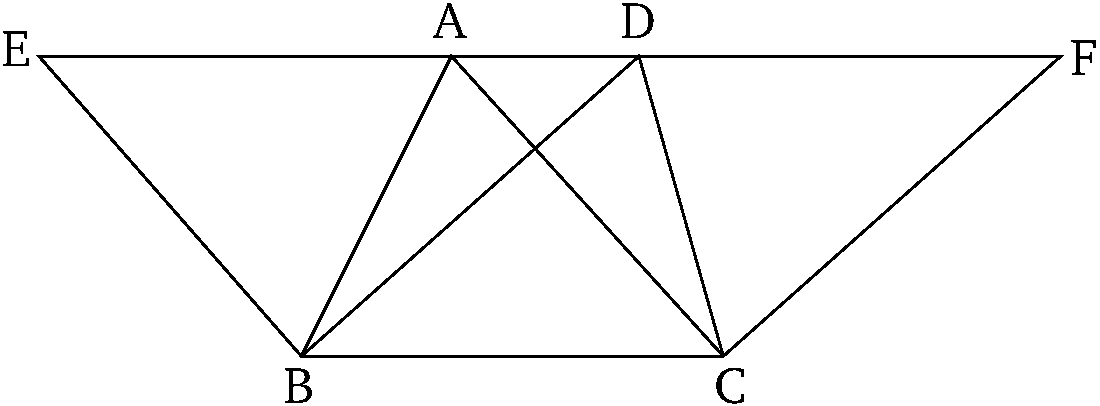
\includegraphics[width=0.8\textwidth]{Book01/fig37e.pdf}}

Let $AD$ be produced in both directions to $E$ and $F$, and let the
(straight-line) $BE$ be drawn through $B$ parallel to $CA$ [Prop.~1.31],
and let the (straight-line) $CF$ be drawn through $C$ parallel to
$BD$ [Prop.~1.31]. Thus, $EBCA$ and $DBCF$ are both parallelograms,
and are equal. For they are on the same base $BC$, and between
the same parallels $BC$ and $EF$ [Prop.~1.35]. And the triangle $ABC$ is
half of 
the parallelogram
$EBCA$. For the diagonal $AB$ cuts the latter in half [Prop.~1.34]. And the 
triangle $DBC$ (is) half of the parallelogram $DBCF$. For the diagonal
$DC$ cuts the latter in half [Prop.~1.34]. [And the halves of equal things are
equal to one another.]$^\dag$
Thus, triangle $ABC$ is equal to triangle $DBC$.

Thus, triangles which are on the same base and between the same parallels
are equal to one another. (Which is) the very thing it was required to show.}
\end{Parallel}
{\footnotesize \noindent$^\dag$ This is an additional common notion.}

%%%%%%
% Prop 1.38
%%%%%%
\pdfbookmark[1]{Proposition 1.38}{pdf1.38}
\begin{Parallel}{}{} 
\ParallelLText{
\begin{center}
{\large \ggn{38}.}
\end{center}\vspace*{-7pt}

\gr{Τὰ τρίγωνα τὰ ἐπὶ ὸίσων βάσεων ὅντα καὶ ἐν ταῖς αὐταῖς παραλλήλοις ἴσα ἀλλήλοις ἐστίν.}

\gr{Ἔστω τρίγωνα τὰ ΑΒΓ, ΔΕΖ ἐπὶ ὸίσων βάσεων τῶν ΒΓ, ΕΖ καὶ ἐν
ταῖς αὐταῖς παραλλήλοις ταῖς ΒΖ, ΑΔ; λέγω, ὅτι ἴσον ἐστὶ τὸ ΑΒΓ
τρίγωνον τῷ ΔΕΖ τριγώνῳ.}

% Removed epsf size command
\centerline{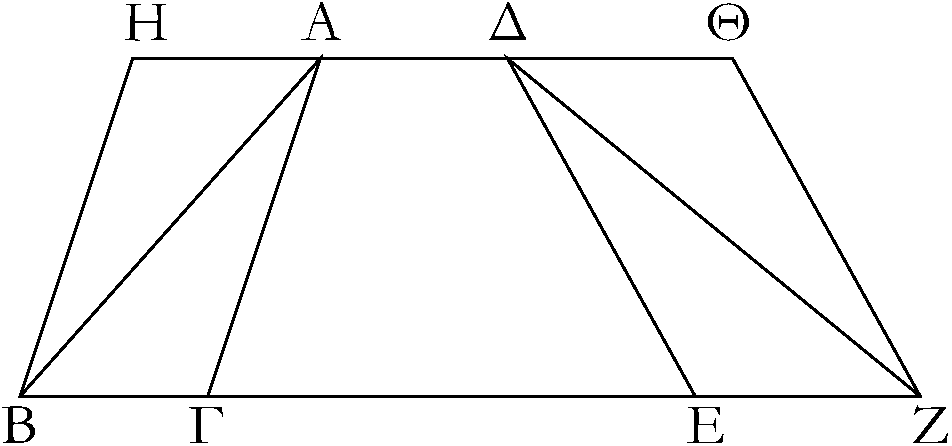
\includegraphics[width=0.8\textwidth]{Book01/fig38g.pdf}}

\gr{Ἐκβεβλήσθω γὰρ ἡ ΑΔ ἐφ' ἑκάτερα τὰ μέρη ἐπὶ τὰ Η, Θ, καὶ διὰ μὲν τοῦ Β τῇ ΓΑ παράλληλος ἢθθω ἡ ΒΗ, δὶα δὲ τοῦ Ζ τῇ ΔΕ
παράλληλος ἢθθω ἡ ΖΘ. παραλληλόγραμμον ἄρα ἐστὶν ἑκάτερον τῶν ΗΒΓΑ, ΔΕΖΘ; καὶ  ἴσον τὸ ΗΒΓΑ τῷ ΔΕΖΘ; ἐπί τε γὰρὸίσων βάσεών εἰσι τῶν ΒΓ, ΕΖ καὶ ἐν ταῖς αὐταῖς παραλλήλοις ταῖς ΒΖ, ΗΘ;
καί ἐστι τοῦ μὲν ΗΒΓΑ παραλληλογράμμου ἥμισυ τὸ ΑΒΓ τρίγωνον. ἡ γὰρ ΑΒ διάμετρος αὐτὸ δίθα τέμνει; τοῦ δὲ ΔΕΖΘ παραλληλογράμμου ἥμισυ τὸ ΖΕΔ τρίγωνον; ἡ γὰρ ΔΖ δίαμετρος
αὐτὸ δίθα τέμνει [τὰ δὲ τῶνὸίσων ἡμίση ἴσα ἀλλήλοις ἐστίν].
 ἴσον ἄρα ἐστὶ τὸ ΑΒΓ τρίγωνον τῷ ΔΕΖ τριγώνῳ.}

\gr{Τὰ  ἄρα τρίγωνα  τὰ ἐπὶ ὸίσων βάσεων ὅντα καὶ ἐν ταῖς αὐταῖς παραλλήλοις ἴσα ἀλλήλοις ἐστίν; ὅπερ ἔδει δεῖχαι.}}

\ParallelRText{
\begin{center}
{\large Proposition 38}
\end{center}

Triangles which are on equal bases and between the same parallels
are equal to one another.

Let $ABC$ and $DEF$ be triangles on the equal bases $BC$ and $EF$, and between the same parallels $BF$ and $AD$. I say that triangle $ABC$ is equal to triangle $DEF$.

% Removed epsf size command
\centerline{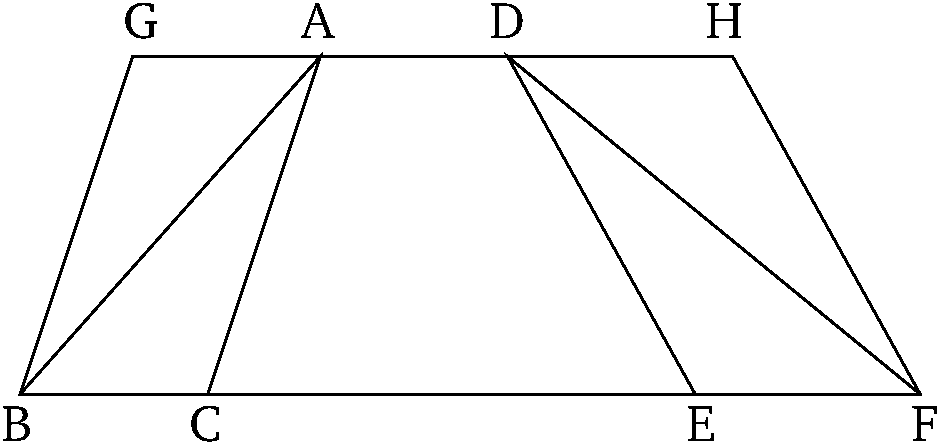
\includegraphics[width=0.8\textwidth]{Book01/fig38e.pdf}}

For let $AD$ be produced in both directions to $G$ and $H$, and
let the (straight-line) $BG$ be drawn through $B$ parallel to $CA$ [Prop.~1.31], and let the (straight-line) $FH$ be drawn through
$F$ parallel to $DE$ [Prop.~1.31]. Thus,  $GBCA$ and $DEFH$ are
each parallelograms. And $GBCA$ is equal to $DEFH$.
For they are on the equal bases $BC$ and $EF$, and between  the same
parallels $BF$ and $GH$ [Prop.~1.36]. And triangle $ABC$ is half of the parallelogram
$GBCA$. For the diagonal $AB$ cuts the latter in half [Prop.~1.34]. And
triangle $FED$ (is) half of parallelogram $DEFH$. For the diagonal $DF$ cuts
the latter in half. [And the halves of equal things are equal to one another.] Thus,
triangle $ABC$ is equal to triangle $DEF$.

Thus, triangles which are on equal bases and between the same parallels
are equal to one another. (Which is) the very thing it was required to show.}
\end{Parallel}

%%%%%%
% Prop 1.39
%%%%%%
\pdfbookmark[1]{Proposition 1.39}{pdf1.39}
\begin{Parallel}{}{} 
\ParallelLText{
\begin{center}
{\large \ggn{39}.}
\end{center}\vspace*{-7pt}

\gr{Τὰ   ἴσα τρίγωνα τὰ ἐπὶ τῆς αὐτῆς βάσεως ὅντα καὶ ἐπὶ τὰ αὐτὰ μέρη καὶ ἐν ταῖς αὐταῖς παραλλήλοις ἐστίν.}

\gr{Ἔστω ἴσα τρίγωνα τὰ ΑΒΓ, ΔΒΓ ἐπὶ τῆς αὐτῆς βάσεως ὅντα καὶ ἐπὶ τὰ αὐτὰ μέρη τῆς ΒΓ; λέγω, ὅτι καὶ ἐν ταῖς αὐταῖς παραλλήλοις ἐστίν.}

\gr{Ἐπεζεύθθω γὰρ ἡ ΑΔ; λέγω, ὅτι παράλληλόξ ἐστιν ἡ ΑΔ τῇ ΒΓ.}

\gr{Εἰ γὰρ μή,  ἢθθω διὰ τοῦ Α σημείου τῇ ΒΓ εὐθείᾳ παράλληλος ἡ ΑΕ, καὶ ἐπεζεύθθω ἡ ΕΓ.  ἴσον ἄρα ἐστὶ τὸ ΑΒΓ τρίγωνον τῷ ΕΒΓ τριγώνῳ; ἐπί τε γὰρ τῆς αὐτῆς βάσεώξ ἐστιν αὐτῷ τῆς ΒΓ καὶ ἐν ταῖς αὐταῖς παραλλήλοις. ἀλλὰ τὸ ΑΒΓ τῷ ΔΒΓ ἐστιν ἴσον; καὶ τὸ ΔΒΓ ἄρα τῷ ΕΒΓ ἴσον ἐστὶ τὸ μεῖζον τῷ ἐλάσσονι; ὅπερ ἐστὶν ἀδύνατον; οὐκ ἄρα παράλληλόξ ἐστιν ἡ ΑΕ τῇ ΒΓ. ὁμοίως δὴ δείχομεν, ὅτι οὐδὸ ὸάλλη τις πλὴν τῆς ΑΔ; ἡ ΑΔ ἄρα τῇ ΒΓ ἐστι παράλληλος.}

% Removed epsf size command
\centerline{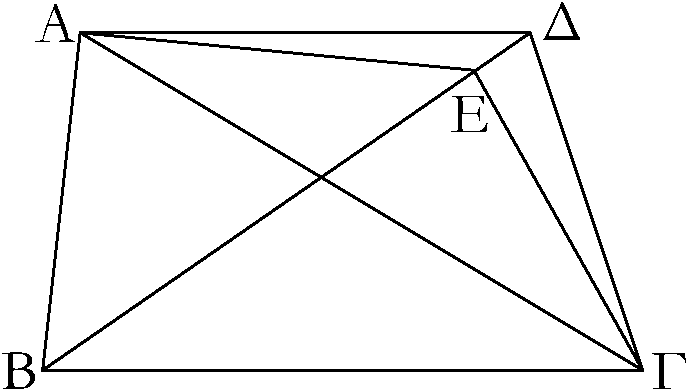
\includegraphics[width=0.8\textwidth]{Book01/fig39g.pdf}}

\gr{Τὰ   ἄρα ἴσα τρίγωνα τὰ ἐπὶ τῆς αὐτῆς βάσεως ὅντα καὶ ἐπὶ τὰ αὐτὰ μέρη καὶ ἐν ταῖς αὐταῖς παραλλήλοις ἐστίν; 
ὅπερ ἔδει δεῖχαι.}}

\ParallelRText{
\begin{center}
{\large Proposition 39}
\end{center}

Equal triangles which are on the same base, and on the same side, are
also between the same parallels.

Let $ABC$ and $DBC$ be equal triangles which are on the same base $BC$,
and on the same side (of it). I say that they are also between the same parallels.

For let $AD$ be joined. I say that $AD$ and $BC$ are parallel.

For, if not, let $AE$ be drawn through point A parallel to the straight-line $BC$ [Prop.~1.31], and let $EC$ be joined. Thus, triangle $ABC$ is equal
to triangle $EBC$. For it is on the same base as it, $BC$, and between the
same parallels [Prop.~1.37]. But $ABC$ is equal to $DBC$. Thus, $DBC$ is
also equal to $EBC$, the greater to the lesser. The very thing is impossible.
Thus, $AE$ is not parallel to $BC$. Similarly, we can show that neither (is)
any other (straight-line) than $AD$. Thus, $AD$ is parallel to $BC$.

% Removed epsf size command
\centerline{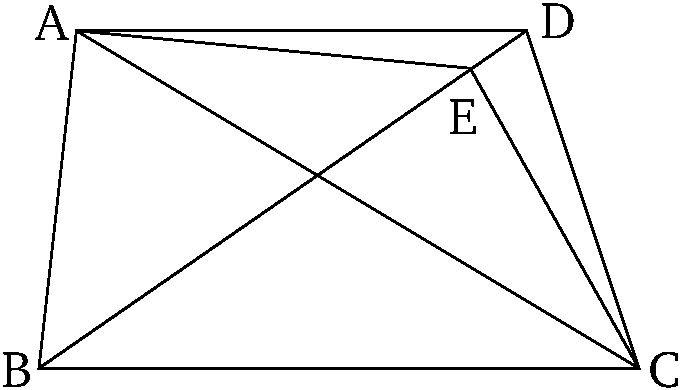
\includegraphics[width=0.8\textwidth]{Book01/fig39e.pdf}}

Thus, equal triangles which are on the same base, and on the same side, are
also between the same parallels. (Which is) the very thing it was required to show.}
\end{Parallel}

%%%%%%
% Prop 1.40
%%%%%%
\pdfbookmark[1]{Proposition 1.40}{pdf1.40}
\begin{Parallel}{}{} 
\ParallelLText{
\begin{center}
{\large\ggn{40}.}
\end{center}\vspace*{-7pt}

\gr{Τὰ  ἴσα τρίγωνα τὰ ἐπὶ ὸίσων βάσεων ὅντα καὶ ἐπὶ τὰ αὐτὰ μέρη καὶ ἐν ταῖς αὐταῖς παραλλήλοις ἐστίν.}

\gr{Ἔστω ἴσα τρίγωνα τὰ ΑΒΓ, ΓΔΕ ἐπὶ ὸίσων βάσεων τῶν ΒΓ, ΓΕ καὶ ἐπὶ τὰ αὐτὰ μέρη. λέγω, ὅτι καὶ ἐν ταῖς αὐταῖς παραλλήλοις ἐστίν.}

% Removed epsf size command
\centerline{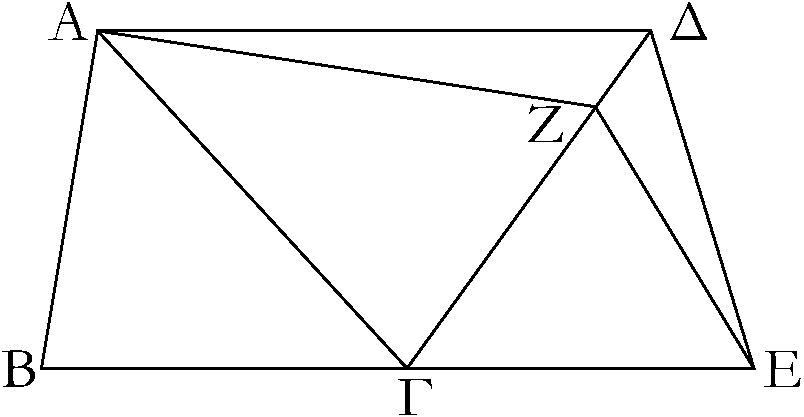
\includegraphics[width=0.8\textwidth]{Book01/fig40g.pdf}}

\gr{Ἐπεζεύθθω γὰρ ἡ ΑΔ; λέγω, ὅτι παράλληλόξ ἐστιν
ἡ ΑΔ τῇ ΒΕ.}

\gr{Εἰ γὰρ μή,  ἢθθω διὰ τοῦ Α τῇ ΒΕ παράλληλος ἡ ΑΖ, καὶ ἐπεζεύθθω ἡ ΖΕ.  ἴσον ἄρα ἐστὶ τὸ ΑΒΓ τρίγωνον τῷ ΖΓΕ τριγώνῳ; ἐπί τε
γὰρὸίσων βάσεών εἰσι τῶν ΒΓ, ΓΕ καὶ ἐν ταῖς αὐταῖς παραλλήλοις ταῖς ΒΕ, ΑΖ. ἀλλὰ τὸ ΑΒΓ τρίγωνον ἴσον ἐστὶ τῷ
ΔΓΕ  [τριγώνῳ]; καὶ τὸ ΔΓΕ ἄρα [τρίγωνον]  ἴσον ἐστὶ τῷ ΖΓΕ τριγώνῳ τὸ μεῖζον τῷ ἐλάσσονι; ὅπερ ἐστὶν ἀδύνατον; οὐκ ἄρα παράλληλος ἡ ΑΖ τῇ ΒΕ. ὁμοίως δὴ δείχομεν, ὅτι οὐδὸ ὸάλλη τις πλὴν τῆς ΑΔ; ἡ ΑΔ ἄρα τῇ ΒΕ ἐστι παράλληλος.}

\gr{Τὰ  ἄρα ἴσα τρίγωνα τὰ ἐπὶ ὸίσων βάσεων ὅντα καὶ ἐπὶ τὰ αὐτὰ μέρη καὶ ἐν ταῖς αὐταῖς παραλλήλοις ἐστίν;
ὅπερ ἔδει δεῖχαι.
}}

\ParallelRText{
\begin{center}
{\large Proposition 40$^\dag$}
\end{center}

Equal triangles which are on equal bases, and on the same side, are also
between the same parallels.

Let $ABC$ and $CDE$ be equal triangles on the equal bases $BC$ and $CE$ (respectively), and on the same side (of $BE$). I say that they are also between
the same parallels.

% Removed epsf size command
\centerline{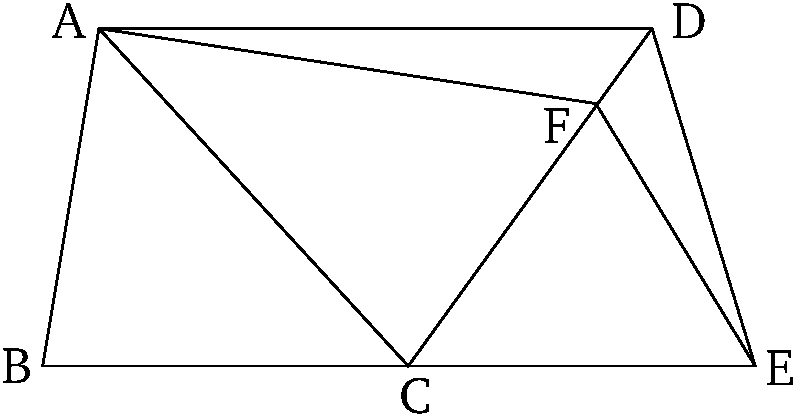
\includegraphics[width=0.8\textwidth]{Book01/fig40e.pdf}}

For let $AD$ be joined. I say that $AD$ is parallel to $BE$.

For if not, let $AF$ be drawn through $A$ parallel to $BE$ [Prop.~1.31],
and let $FE$ be joined. Thus, triangle $ABC$ is equal to triangle
$FCE$. For they are on equal bases, $BC$ and $CE$, and between the same
parallels, $BE$ and $AF$ [Prop.~1.38]. But, triangle $ABC$ is equal to [triangle] $DCE$.
Thus, [triangle] $DCE$ is also equal to triangle $FCE$, the greater to the
lesser. The very thing is impossible. 
Thus, $AF$ is not parallel to $BE$. Similarly, we can show that neither (is)
any other (straight-line) than $AD$. Thus, $AD$ is parallel to $BE$.

Thus, equal triangles which are on equal bases, and on the same side, are also
between the same parallels. (Which is) the very thing it was required to show.}
\end{Parallel}
{\footnotesize \noindent$^\dag$ This whole proposition is regarded by
Heiberg as a relatively early interpolation to the original text.\\}

%%%%%%
% Prop 1.41
%%%%%%
\pdfbookmark[1]{Proposition 1.41}{pdf1.41}
\begin{Parallel}{}{} 
\ParallelLText{
\begin{center}
{\large \ggn{41}.}
\end{center}\vspace*{-7pt}

\gr{Ἐὰν παραλληλόγραμμον τριγώνῳ βάσιν τεὸέθῃ τὴν αὐτὴν καὶ ἐν ταῖς αὐταῖς παραλλήλοιςὸῆ|, διπλάσιόν ἐστί τὸ παραλληλόγραμμον τοῦ
τριγώνου.}

\gr{Παραλληλόγραμμον γὰρ τὸ ΑΒΓΔ τριγώνῳ τῷ ΕΒΓ βάσιν τε ἐθέτω τὴν αὐτὴν τὴν ΒΓ καὶ ἐν ταῖς αὐταῖς παραλλήλοιςὸέστω ταῖς ΒΓ, ΑΕ; λέγω, ὅτι διπλάσιόν ἐστι τὸ ΑΒΓΔ παραλληλόγραμμον τοῦ ΒΕΓ τριγώνου.}

% Removed epsf size command
\centerline{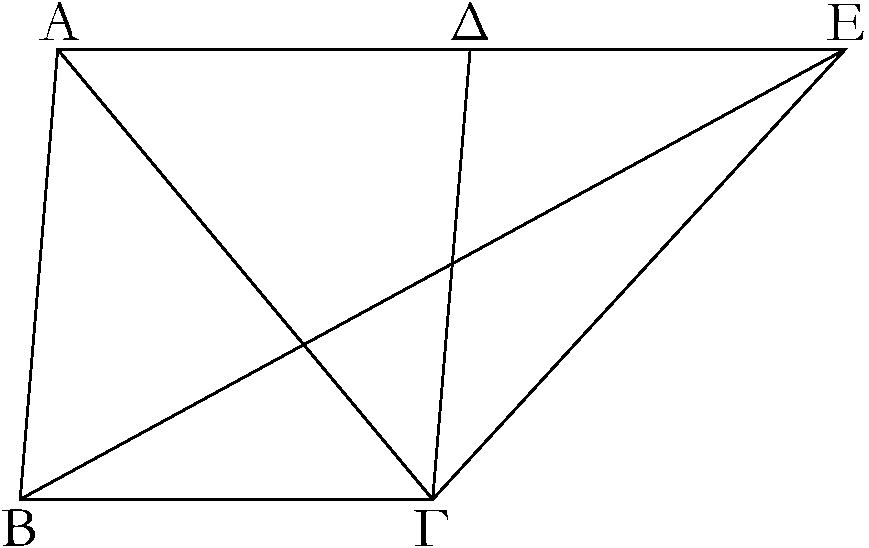
\includegraphics[width=0.8\textwidth]{Book01/fig41g.pdf}}

\gr{Ἐπεζεύθθω γὰρ ἡ ΑΓ.  ἴσον δή ἐστι τὸ ΑΒΓ τρίγωνον τῷ ΕΒΓ τριγώνῳ; ἐπί τε γὰρ τῆς αὐτῆς βάσεώξ ἐστιν αὐτῷ τῆς ΒΓ καὶ ἐν ταῖς αὐταῖς παραλλήλοις ταῖς ΒΓ, ΑΕ. ἀλλὰ τὸ ΑΒΓΔ παραλληλόγραμμον διπλάσιόν ἐστι τοῦ ΑΒΓ τριγώνου; ἡ γὰρ ΑΓ διάμετρος αὐτὸ δίθα τέμνει; ὁώστε τὸ ΑΒΓΔ παραλληλόγραμμον καὶ τοῦ ΕΒΓ τριγώνου ἐστὶ διπλάσιον.}

\gr{Ἐὰν ἄρα παραλληλόγραμμον τριγώνῳ βάσιν τεὸέθῃ τὴν αὐτὴν καὶ 
ἐν ταῖς αὐταῖς παραλλήλοιςὸῆ|, διπλάσιόν ἐστί τὸ παραλληλόγραμμον τοῦ
τριγώνου; ὅπερ ἔδει δεῖχαι.}}

\ParallelRText{
\begin{center}
{\large Proposition 41}
\end{center}

If a parallelogram has the same base as a triangle, and is between
the same parallels, (then) the parallelogram is double (the area) of the triangle.

For let parallelogram $ABCD$ have the same base $BC$ as triangle $EBC$,
and let it be between the same parallels, $BC$ and $AE$. I say that 
parallelogram $ABCD$ is double (the area) of triangle $BEC$.

% Removed epsf size command
\centerline{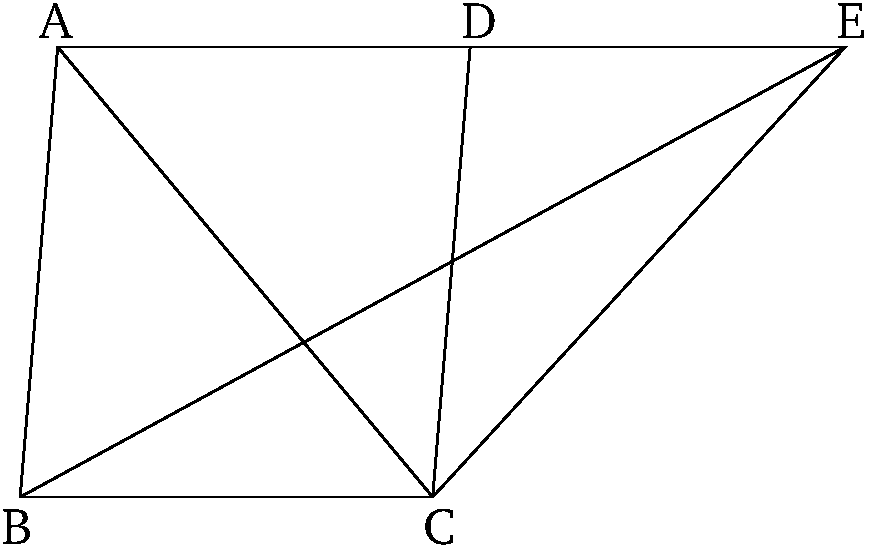
\includegraphics[width=0.8\textwidth]{Book01/fig41e.pdf}}

For let $AC$ be joined. So triangle $ABC$ is equal to triangle
$EBC$. For it is on the same base, $BC$,  (as $EBC$), and between the same
parallels, $BC$ and $AE$ [Prop.~1.37]. But, parallelogram $ABCD$
is double (the area) of triangle $ABC$. For the diagonal $AC$ cuts
the former in half [Prop.~1.34]. So parallelogram $ABCD$ is also
double (the area) of triangle $EBC$.

Thus, if a parallelogram has the same base as a triangle, and is between
the same parallels, (then) the parallelogram is double (the area) of the triangle.
(Which is) the very thing it was required to show.}
\end{Parallel}

%%%%%%
% Prop 1.42
%%%%%%
\pdfbookmark[1]{Proposition 1.42}{pdf1.42}
\begin{Parallel}{}{} 
\ParallelLText{
\begin{center}
{\large \ggn{42}.}
\end{center}\vspace*{-7pt}

\gr{Τῶ| δοθέντι τριγώνῳ  ἴσον παραλληλόγραμμον συστήσασθαι 
 ἐν τῇ δοθείσῃ γωνίᾳ εὐθυγράμμῳ.}
 
\gr{Ἔστω τὸ μὲν δοθὲν τρίγωνον τὸ ΑΒΓ, ἡ δὲ δοθεῖσα γωνία εὐθύγραμμος ἡ Δ; δεῖ δὴ τῷ ΑΒΓ τριγώνῳ  ἴσον παραλληλόγραμμον συστήσασθαι ἐν τῇ Δ γωνίᾳ εὐθυγράμμῳ.}

\gr{Τετμήσθω ἡ ΒΓ δίθα κατὰ τὸ Ε, καὶ ἐπεζεύθθω ἡ ΑΕ, καὶ συνεστάτω πρὸς τῇ ΕΓ εὐθείᾳ καὶ τῷ πρὸς αὐτῇ σημείῳ τῷ Ε τῇ Δ γωνίᾳ ὸίση ἡ ὑπὸ ΓΕΖ, καὶ διὰ μὲν τοῦ Α τῇ ΕΓ παράλληλος ἢθθω ἡ ΑΗ, διὰ δὲ τοῦ Γ τῇ ΕΖ παράλληλος ἢθθω ἡ ΓΗ; παραλληλόγραμμον ἄρα ἐστὶ τὸ ΖΕΓΗ. καὶ ἐπεὶ ὸίση ἐστὶν ἡ ΒΕ τῇ ΕΓ,  ἴσον ἐστὶ καὶ τὸ ΑΒΕ τρίγωνον τῷ ΑΕΓ τριγώνῳ; ἐπί τε γὰρὸίσων βάσεών εἰσι τῶν ΒΕ, ΕΓ καὶ ἐν ταῖς αὐταῖς παραλλήλοις ταῖς ΒΓ, ΑΗ; διπλάσιον ἄρα ἐστὶ τὸ ΑΒΓ τρίγωνον τοῦ ΑΕΓ τριγώνου. ὸέστι δὲ καὶ τὸ ΖΕΓΗ
παραλληλόγραμμον διπλάσιον τοῦ ΑΕΓ  τριγώνου; βάσιν τε γὰρ αὐτῷ τὴν αὐτὴν ἔχει καὶ ἐν ταῖς αὐταῖς ἐστιν αὐτῷ παραλλήλοις;  ἴσον ἄρα ἐστὶ τὸ ΖΕΓΗ παραλληλόγραμμον τῷ ΑΒΓ τριγώνῳ. καὶ  ἔχει τὴν ὑπὸ ΓΕΖ γωνίαν ἴσην τῇ δοθείσῃ τῇ Δ.}

% Removed epsf size command
\centerline{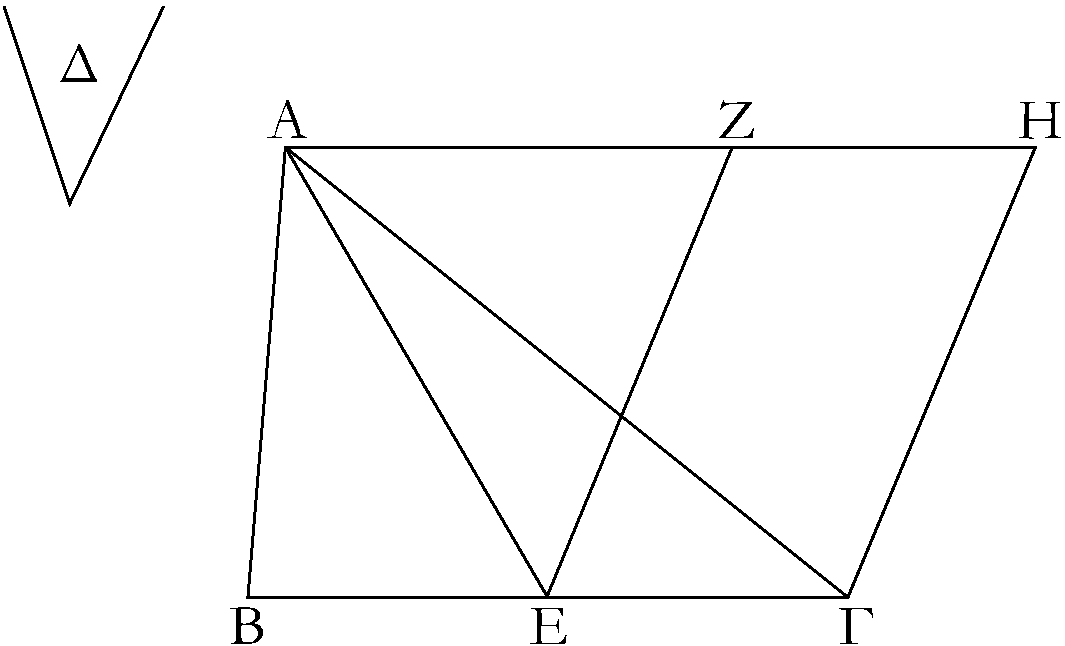
\includegraphics[width=0.8\textwidth]{Book01/fig42g.pdf}}

\gr{Τῶ|  ἄρα δοθέντι τριγώνῳ τῷ ΑΒΓ ἴσον παραλληλόγραμμον συνέσταται τὸ ΖΕΓΗ ἐν γωνίᾳ τῇ ὑπὸ ΓΕΖ, ἥτις ἐστὶνὸίση τῇ Δ;
ὅπερ ἔδει ποιῆσαι.}}

\ParallelRText{
\begin{center}
{\large Proposition 42}
\end{center}

To construct a parallelogram equal to a given triangle in a given
rectilinear angle.

Let $ABC$ be the given triangle, and $D$ the given rectilinear angle. So
it is required to construct a parallelogram equal to triangle $ABC$
in the rectilinear angle $D$.

Let $BC$ be cut in half at $E$ [Prop.~1.10], and let $AE$ be joined. And let (angle) $CEF$, equal to angle $D$,  be constructed
at the point $E$ on the straight-line $EC$ [Prop.~1.23]. And let $AG$ be drawn through $A$
parallel to $EC$ [Prop.~1.31], and let $CG$ be drawn through $C$ parallel
to $EF$ [Prop.~1.31]. Thus, $FECG$ is a parallelogram. And since $BE$ is
equal to $EC$, triangle $ABE$ is also equal to triangle $AEC$. For they are
on the equal bases, $BE$ and $EC$, and between the same parallels, $BC$ and $AG$ [Prop.~1.38]. Thus, triangle $ABC$ is double (the area) of triangle $AEC$. And
parallelogram $FECG$ is also double (the area) of triangle $AEC$. For it has the same base (as $AEC$), and is between the same parallels  (as $AEC$) [Prop.~1.41].
Thus, parallelogram $FECG$ is equal to triangle $ABC$.  ($FECG$) also has
the angle $CEF$ equal to the given (angle) $D$.

% Removed epsf size command
\centerline{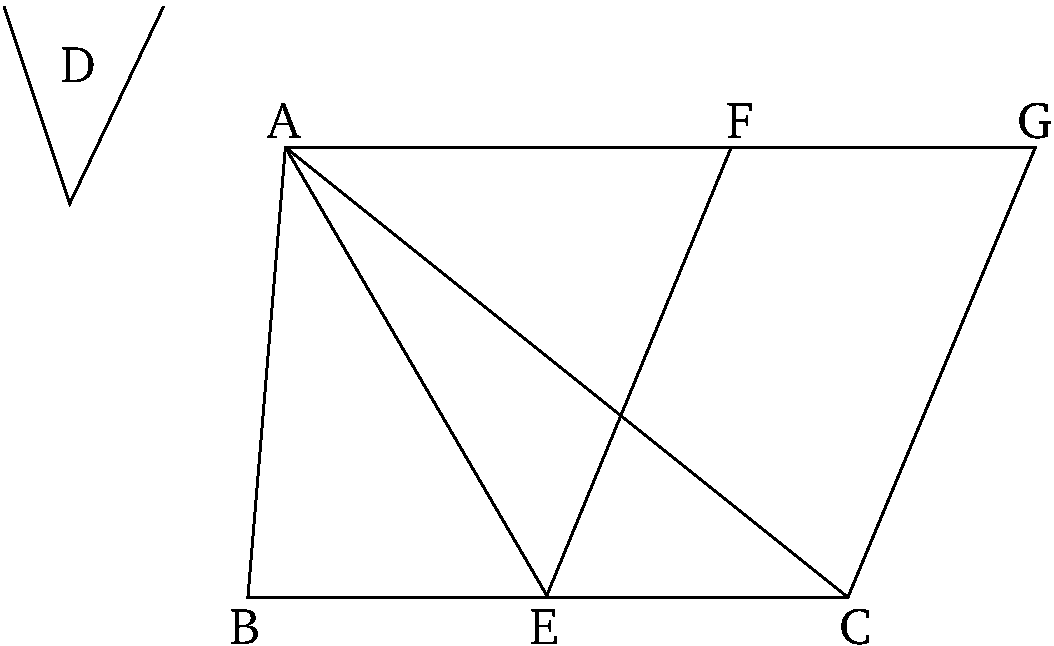
\includegraphics[width=0.8\textwidth]{Book01/fig42e.pdf}}

Thus, parallelogram $FECG$,  equal to the given
triangle $ABC$, has been constructed in the angle $CEF$, which is equal to $D$. (Which is) the
very thing it was required to do.}
\end{Parallel}

%%%%%%
% Prop 1.43
%%%%%%
\pdfbookmark[1]{Proposition 1.43}{pdf1.43}
\begin{Parallel}{}{} 
\ParallelLText{
\begin{center}
{\large \ggn{43}.}
\end{center}\vspace*{-7pt}

\gr{Παντὸξ παραλληλογράμμου τῶν περὶ τὴν διάμετρον παραλληλογράμμων τὰ παραπληρώματα ἴσα ἀλλήλοις ἐστίν.}

\gr{Ἔστω παραλληλόγραμμον τὸ ΑΒΓΔ, διάμετρος δὲ αὐτοῦ ἡ ΑΓ, περὶ
δὲ τὴν ΑΓ παραλληλόγραμμα μὲνὸέστω τὰ ΕΘ, ΖΗ, τὰ δὲ λεγόμενα παραπληρώματα τὰ ΒΚ, ΚΔ; λέγω, ὅτι ἴσον ἐστὶ τὸ ΒΚ παραπλήρωμα τῷ ΚΔ
παραπληρώματι.}

% Removed epsf size command
\centerline{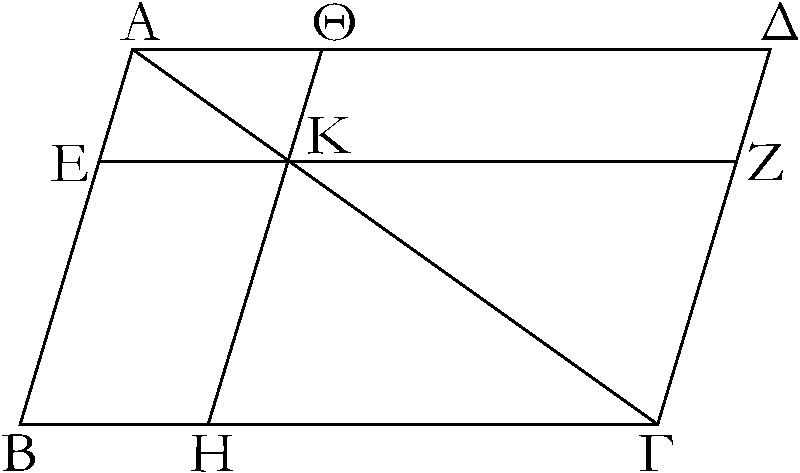
\includegraphics[width=0.8\textwidth]{Book01/fig43g.pdf}}

\gr{Ἐπεὶ γὰρ παραλληλόγραμμόν ἐστι τὸ ΑΒΓΔ, διάμετρος δὲ αὐτοῦ ἡ
ΑΓ,  ἴσον ἐστὶ τὸ ΑΒΓ τρίγωνον τῷ ΑΓΔ τριγώνῳ. πάλιν, ἐπεὶ παραλληλόγραμμόν ἐστι τὸ ΕΘ, διάμετρος δὲ αὐτοῦ ἐστιν ἡ ΑΚ,
 ἴσον ἐστὶ τὸ ΑΕΚ τρίγωνον τῷ ΑΘΚ τριγώνῳ. διὰ τὰ αὐτὰ δὴ καὶ τὸ ΚΖΓ τρίγωνον τῷ ΚΗΓ ἐστιν ἴσον. ἐπεὶ οὸῦν τὸ μὲν ΑΕΚ τρίγωνον τῷ ΑΘΚ τριγώνῳ ἐστὶν ἴσον, τὸ δὲ ΚΖΓ τῷ ΚΗΓ, τὸ 
ΑΕΚ τρίγωνον μετὰ τοῦ ΚΗΓ ἴσον ἐστὶ
τῷ ΑΘΚ  τριγώνῳ μετὰ τοῦ ΚΖΓ; ὸέστι δὲ καὶ ὅλον τὸ ΑΒΓ τρίγωνον ὅλῳ τῷ ΑΔΓ ἴσον; λοιπὸν ἄρα τὸ ΒΚ παραπλήρωμα λοιπῶ| τῷ ΚΔ παραπληρώματί ἐστιν ἴσον.}

\gr{Παντὸξ ἄρα παραλληλογράμμου θωρίου τῶν περὶ τὴν διάμετρον παραλληλογράμμων τὰ παραπληρώματα ἴσα ἀλλήλοις ἐστίν; ὅπερ ἔδει δεῖχαι.}}

\ParallelRText{
\begin{center}
{\large Proposition 43}
\end{center}

For any parallelogram, the complements of the parallelograms about the diagonal are equal to one another.

Let $ABCD$ be a parallelogram, and $AC$ its diagonal. And let $EH$ and $FG$
be the parallelograms about  $AC$, and $BK$ and $KD$ the so-called complements
(about $AC$).
I say that the complement $BK$ is equal to the complement $KD$.

% Removed epsf size command
\centerline{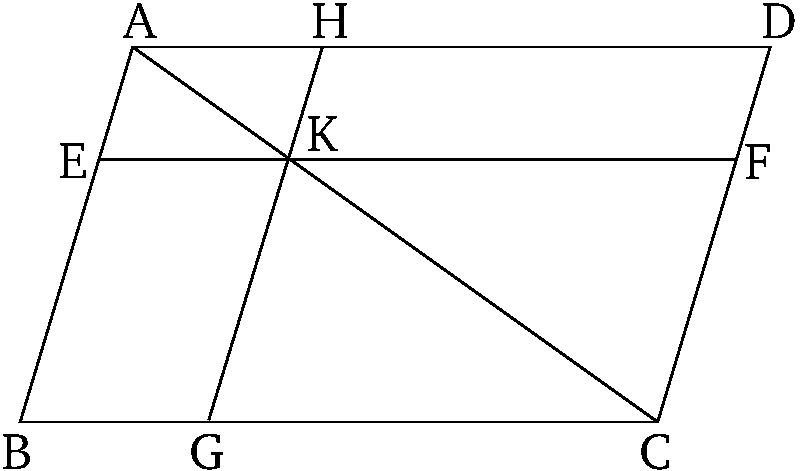
\includegraphics[width=0.8\textwidth]{Book01/fig43e.pdf}}

For since $ABCD$ is a parallelogram, and $AC$ its diagonal,  triangle
$ABC$ is equal to triangle $ACD$ [Prop.~1.34]. Again, since $EH$ is
a parallelogram, and $AK$ is its diagonal, triangle $AEK$ is equal to
triangle $AHK$ [Prop.~1.34]. So, for the same (reasons), triangle
$KFC$ is also equal to (triangle) $KGC$. Therefore, since triangle $AEK$ is
equal to triangle $AHK$, and $KFC$ to $KGC$, triangle $AEK$ plus $KGC$ is
equal to triangle $AHK$ plus $KFC$. And the whole triangle $ABC$ is
also equal to the whole (triangle) $ADC$. Thus, the remaining complement
$BK$ is equal to the remaining complement $KD$.

Thus, for any parallelogramic figure, the complements of the
parallelograms about the diagonal are equal to one another.
(Which is) the very thing it was required to show.}
\end{Parallel}

%%%%%%
% Prop 1.44
%%%%%%
\pdfbookmark[1]{Proposition 1.44}{pdf1.44}
\begin{Parallel}{}{} 
\ParallelLText{
\begin{center}
{\large \ggn{44}.}
\end{center}\vspace*{-7pt}

\gr{Παρὰ τὴν δοθεῖσαν εὐθεῖαν τῷ δοθέντι  τριγώνῳ  ἴσον παραλληλόγραμμον παραβαλεῖν ἐν  τῇ δοθείσῃ γωνίᾳ εὐθυγράμμῳ.}

\gr{Ἔστω ἡ μὲν δοθεῖσα εὐθεῖα ἡ ΑΒ, τὸ δὲ δοθὲν τρίγωνον τὸ Γ, ἡ δὲ δοθεῖσα γωνία εὐθύγραμμος ἡ Δ; δεῖ δὴ παρὰ τὴν δοθεῖσαν εὐθεῖαν τὴν ΑΒ τῷ δοθέντι τριγώνῳ τῷ Γ ἴσον παραλληλόγραμμον
παραβαλεῖν ἐνὸίσῃ τῇ Δ γωνίᾳ.}

% Removed epsf size command
\centerline{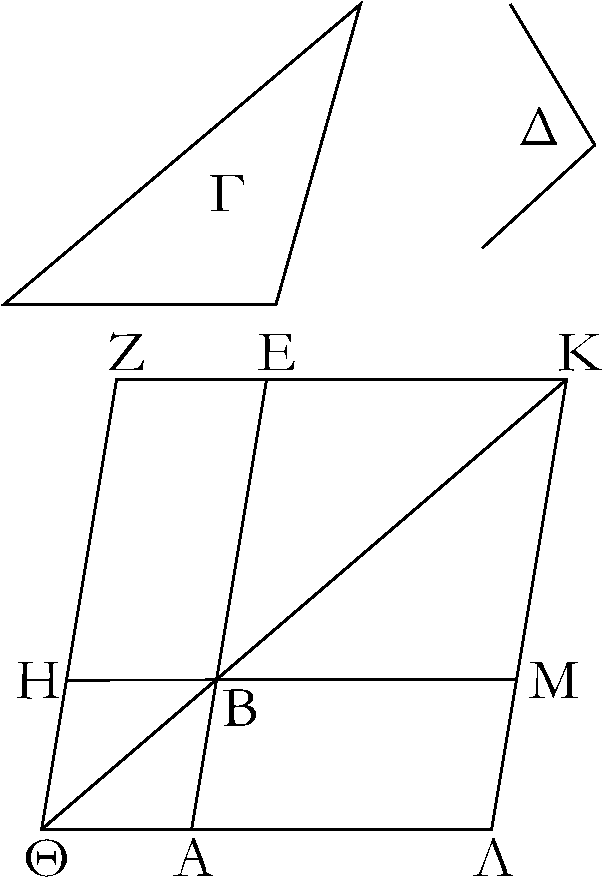
\includegraphics[width=0.8\textwidth]{Book01/fig44g.pdf}}

\gr{Συνεστάτω τῷ Γ τριγώνῳ  ἴσον παραλληλόγραμμον τὸ ΒΕΖΗ ἐν γωνίᾳ τῇ ὑπὸ ΕΒΗ, ἥ ἐστινὸίση τῇ Δ; καὶ κείσθω ὁώστε ἐπ' εὐθείας εὸῖναι τὴν ΒΕ τῇ ΑΒ, καὶ διήθθω ἡ ΖΗ ἐπὶ τὸ Θ, καὶ διὰ τοῦ 
Α ὁποτέρᾳ τῶν ΒΗ, ΕΖ παράλληλος ἢθθω ἡ ΑΘ, καὶ ἐπεζεύθθω ἡ ΘΒ. καὶ ἐπεὶ εἰξ παραλλήλους τὰξ ΑΘ, ΕΖ εὐθεῖα ἐνέπεσεν ἡ ΘΖ, αἱ
 ἄρα ὑπὸ  ΑΘΖ, ΘΖΕ γωνίαι δυσὶν ὀρθαῖξ εἰσιν ἴσαι. αἱ  ἄρα ὑπὸ ΒΘΗ, ΗΖΕ δύο ὀρθῶν ἐλάσσονέξ εἰσιν; αἱ δὲ ἀπὸ ἐλασσόνωνὸὴ δύο ὀρθῶν εἰξ ἄπειρον ἐκβαλλόμεναι συμπίπτουσιν; αἱ ΘΒ, ΖΕ ἄρα ἐκβαλλόμεναι συμπεσοῦνται. ἐκβεβλήσθωσαν καὶ συμπιπτέτωσαν κατὰ τὸ Κ, καὶ διὰ τοῦ Κ σημείου ὁποτέρᾳ τῶν ΕΑ, ΖΘ παράλληλος ἢθθω ἡ
ΚΛ, καὶ ἐκβεβλήσθωσαν αἱ ΘΑ, ΗΒ ἐπὶ τὰ Λ, Μ σημεῖα. παραλληλόγραμμον ἄρα ἐστὶ 
τὸ ΘΛΚΖ, διάμετρος δὲ αὐτοῦ ἡ ΘΚ, περὶ δὲ τὴν ΘΚ παραλληλόγραμμα μὲν τὰ ΑΗ, ΜΕ, τὰ δὲ λεγόμενα παραπληρώματα τὰ ΛΒ, ΒΖ;  ἴσον ἄρα ἐστὶ τὸ ΛΒ τῷ ΒΖ. ἀλλὰ τὸ ΒΖ τῷ Γ τριγώνῳ ἐστὶν ἴσον; καὶ τὸ ΛΒ ἄρα τῷ Γ ἐστιν ἴσον. καὶ ἐπεὶ ὸίση ἐστὶν ἡ ὑπὸ ΗΒΕ γωνία τῇ ὑπὸ ΑΒΜ, ἀλλὰ ἡ ὑπὸ ΗΒΕ τῇ Δ ἐστινὸίση, καὶ ἡ ὑπὸ ΑΒΜ ἄρα τῇ Δ γωνίᾳ ἐστὶνὸίση.}

\gr{Παρὰ τὴν δοθεῖσαν ἄρα εὐθεῖαν τὴν ΑΒ τῷ δοθέντι τριγώνῳ τῷ
Γ ἴσον παραλληλόγραμμον παραβέβληται τὸ ΛΒ ἐν γωνίᾳ τῇ ὑπὸ
ΑΒΜ,  ἥ ἐστινὸίση τῇ Δ; ὅπερ ἔδει ποιῆσαι.}}

\ParallelRText{
\begin{center}
{\large Proposition 44}
\end{center}

To apply a parallelogram equal to a given triangle to a given straight-line
in a given rectilinear angle.

Let $AB$ be the given straight-line,  $C$ the given triangle, and $D$ the
given rectilinear angle. So it is required to apply a parallelogram
equal to the given triangle $C$ to the given straight-line $AB$ in an angle equal to (angle) $D$.

% Removed epsf size command
\centerline{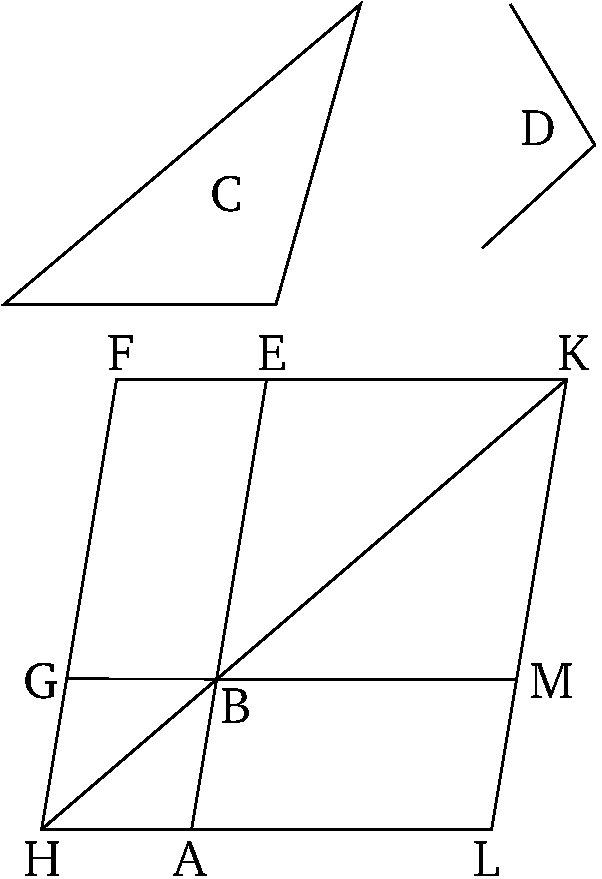
\includegraphics[width=0.8\textwidth]{Book01/fig44e.pdf}}

Let the parallelogram $BEFG$, equal to the triangle $C$, be
constructed in the angle $EBG$, which is equal to $D$ [Prop.~1.42].
And let it be placed so that $BE$ is straight-on to $AB$.$^\dag$  And
let $FG$ be drawn through to $H$, and let $AH$ be
drawn through $A$ parallel to either of $BG$ or $EF$ [Prop.~1.31], and
let $HB$ be joined. And since the straight-line $HF$ falls across the
parallels $AH$ and $EF$, the (sum of the) angles $AHF$ and $HFE$ is thus equal to
two right-angles [Prop.~1.29]. Thus, (the sum of) $BHG$ and $GFE$ is less than two
right-angles.
And (straight-lines) produced to
infinity from (internal angles whose sum is) less than two right-angles meet together [Post.~5].
Thus, being produced, $HB$ and $FE$ will meet together. Let them 
be produced, and let them meet together at $K$. And let $KL$ be
drawn through point $K$ parallel to either of $EA$ or $FH$ [Prop.~1.31]. And
let $HA$ and $GB$ be produced to points $L$ and $M$ (respectively). Thus, $HLKF$ is a parallelogram, and $HK$ its diagonal. And $AG$ and $ME$ (are) parallelograms, and $LB$ and $BF$ the so-called complements, about $HK$. Thus, $LB$ is
equal to $BF$ [Prop.~1.43]. But, $BF$ is equal to triangle $C$. Thus, $LB$ is also
equal to $C$. Also, since angle $GBE$ is equal to $ABM$ [Prop.~1.15], but
$GBE$ is equal to $D$, $ABM$ is thus also equal to angle $D$.

Thus, the parallelogram $LB$, equal to the
given triangle $C$, has been applied to the given straight-line
$AB$ in the angle $ABM$, which is equal to $D$. (Which is) the very thing it was required to do.}
\end{Parallel}
{\footnotesize \noindent$^\dag$ This can be achieved using Props.~1.3, 1.23, and 1.31.}

%%%%%%
% Prop 1.45
%%%%%%
\pdfbookmark[1]{Proposition 1.45}{pdf1.45}
\begin{Parallel}{}{} 
\ParallelLText{
\begin{center}
{\large \ggn{45}.}
\end{center}
\vspace*{-7pt}

\gr{Τῶ| δοθέντι εὐθυγράμμῳ  ἴσον παραλληλόγραμμον συστήσασθαι ἐν τῇ
δοθείσῃ γωνίᾳ εὐθυγράμμῳ.}

\gr{Ἔστω τὸ μὲν δοθὲν εὐθύγραμμον τὸ ΑΒΓΔ, ἡ δὲ δοθεῖσα γωνία εὐθύγραμμος ἡ Ε; δεῖ δὴ τῷ ΑΒΓΔ εὐθυγράμμῳ  ἴσον παραλληλόγραμμον συστήσασθαι ἐν τῇ δοθείσῃ γωνίᾳ τῇ Ε.}

% Removed epsf size command
\centerline{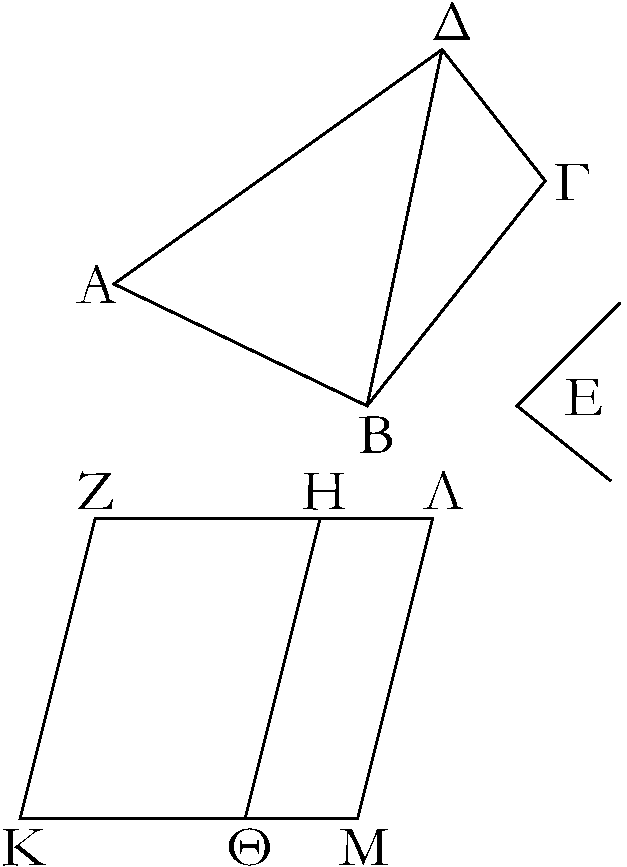
\includegraphics[width=0.8\textwidth]{Book01/fig45g.pdf}}

\gr{Ἐπεζεύθθω ἡ ΔΒ, καὶ συνεστάτω τῷ ΑΒΔ τριγώνῳ  ἴσον παραλληλόγραμμον τὸ ΖΘ ἐν τῇ ὑπὸ ΘΚΖ γωνίᾳ, ἥ ἐστινὸίση τῇ Ε;
καὶ παραβεβλήσθω παρὰ τὴν ΗΘ εὐθεῖαν τῷ ΔΒΓ τριγώνῳ  ἴσον παραλληλόγραμμον τὸ ΗΜ ἐν τῇ ὑπὸ ΗΘΜ γωνίᾳ, ἥ ἐστινὸίση τῇ Ε. καὶ ἐπεὶ ἡ Ε γωνία ἑκατέρᾳ τῶν ὑπὸ ΘΚΖ, ΗΘΜ ἐστινὸίση, καὶ ἡ ὑπὸ ΘΚΖ ἄρα τῇ ὑπὸ ΗΘΜ ἐστινὸίση. κοινὴ προσκείσθω ἡ ὑπὸ ΚΘΗ; αἱ  ἄρα ὑπὸ ΖΚΘ, ΚΘΗ ταῖς ὑπὸ ΚΘΗ, ΗΘΜ ἴσαι εἰσίν.
ἀλλὸ αἱ ὑπὸ ΖΚΘ, ΚΘΗ
 δυσὶν ὀρθαῖξ ἴσαι εἰσίν; καὶ αἱ  ὑπὸ ΚΘΗ, ΗΘΜ ἄρα δύο ὀρθαῖξ ἴσαι εἰσίν.
  πρὸς δή τινι εὐθεῖᾳ τῇ ΗΘ καὶ τῷ πρὸς αὐτῇ σημείῳ τῷ Θ δύο εὐθεῖαι
 αἱ ΚΘ, ΘΜ 
 μὴ ἐπὶ τὰ αὐτὰ μέρη κείμεναι τὰξ ἐφεχῆς γωνίας δύο ὀρθαῖξ ἴσας ποιοῦσιν; ἐπ' εὐθείας ἄρα ἐστὶν ἡ ΚΘ
τῇ ΘΜ; καὶ ἐπεὶ εἰξ παραλλήλους τὰξ ΚΜ, ΖΗ εὐθεῖα ἐνέπεσεν ἡ ΘΗ, αἱ ἐναλλὰχ γωνίαι αἱ ὑπὸ ΜΘΗ, ΘΗΖ ἴσαι ἀλλήλαις εἰσίν. κοινὴ
προσκείσθω ἡ ὑπὸ ΘΗΛ; αἱ  ἄρα ὑπὸ ΜΘΗ, ΘΗΛ ταῖς ὑπὸ ΘΗΖ, ΘΗΛ ἴσαι εἰσιν. ἀλλὸ αἱ ὑπὸ ΜΘΗ, ΘΗΛ
δύο ὀρθαῖξ ἴσαι
εἰσίν; καὶ αἱ ὑπὸ ΘΗΖ, ΘΗΛ ἄρα δύο ὀρθαῖξ ἴσαι εἰσίν;
ἐπ' εὐθείας ἄρα ἐστὶν ἡ ΖΗ τῇ ΗΛ. καὶ ἐπεὶ ἡ ΖΚ τῇ ΘΗὸίση τε καὶ παράλληλόξ ἐστιν, ἀλλὰ καὶ ἡ ΘΗ τῇ ΜΛ, καὶ ἡ ΚΖ ἄρα τῇ ΜΛὸίση τε καὶ παράλληλόξ ἐστιν; καὶ ἐπιζευγνύουσιν αὐτὰξ εὐθεῖαι αἱ ΚΜ, ΖΛ; καὶ αἱ ΚΜ, ΖΛ ἄρα ἴσαι τε καὶ παράλληλοί εἰσιν; παραλληλόγραμμον ἄρα ἐστὶ τὸ ΚΖΛΜ. καὶ ἐπεὶ  ἴσον ἐστὶ τὸ μὲν
ΑΒΔ τρίγωνον τῷ ΖΘ παραλληλογράμμῳ, τὸ δὲ ΔΒΓ τῷ ΗΜ, ὅλον ἄρα τὸ ΑΒΓΔ εὐθύγραμμον ὅλῳ τῷ ΚΖΛΜ
παραλληλογράμμῳ ἐστὶν ἴσον.}

\gr{Τῶ|  ἄρα δοθέντι εὐθυγράμμῳ τῷ ΑΒΓΔ ἴσον παραλληλόγραμμον συνέσταται τὸ ΚΖΛΜ ἐν γωνίᾳ τῇ ὑπὸ ΖΚΜ, ἥ ἐστινὸίση τῇ
δοθείσῃ τῇ Ε; ὅπερ ἔδει ποιῆσαι.}}

\ParallelRText{
\begin{center}
{\large Proposition 45}
\end{center}

To construct a parallelogram equal to a given rectilinear figure in a given
rectilinear angle.

Let $ABCD$ be the given rectilinear figure,$^\dag$ and $E$ the given rectilinear angle.
So it is required to construct a parallelogram equal to the rectilinear figure
$ABCD$ in the given angle $E$.

% Removed epsf size command
\centerline{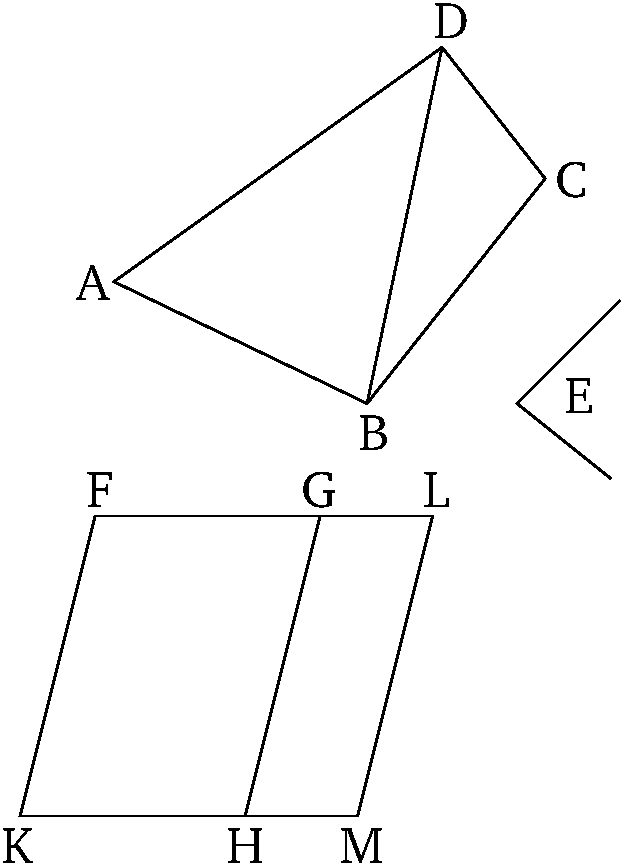
\includegraphics[width=0.8\textwidth]{Book01/fig45e.pdf}}

Let $DB$ be joined, and let the parallelogram $FH$, equal to
the triangle $ABD$, be
constructed in the angle $HKF$, which is equal to $E$ [Prop.~1.42].
And let the parallelogram $GM$, equal to the triangle $DBC$, be
applied to the straight-line $GH$ in the angle $GHM$,
which is equal to $E$ [Prop.~1.44]. And since angle $E$ is equal to each of
(angles) $HKF$ and $GHM$,  (angle) $HKF$ is thus also equal to $GHM$. 
Let $KHG$ be added to both. Thus, (the sum of) $FKH$ and $KHG$ is
equal to (the sum of) $KHG$ and $GHM$. But, (the sum of) $FKH$ and $KHG$ is equal to
two right-angles [Prop.~1.29]. Thus, (the sum of) $KHG$ and $GHM$ is also equal to
two right-angles. So two straight-lines, $KH$ and $HM$, not lying on the same side, make  adjacent angles with some straight-line $GH$, 
at the point $H$ on it, (whose sum is) equal to two right-angles.
Thus, $KH$ is straight-on to $HM$ [Prop.~1.14].
And since the straight-line $HG$ falls across the parallels $KM$ and $FG$, the alternate angles
$m\kern -.7pt hG$ and $HGF$ are equal to one another [Prop.~1.29]. Let $HGL$ have
been added to both. Thus, (the sum of) $m\kern -.7pt hG$ and $HGL$ is equal to 
(the sum of) $HGF$ and $HGL$.
But, (the sum of) $m\kern -.7pt hG$ and $HGL$ is equal to two right-angles [Prop.~1.29].
Thus, (the sum of) $HGF$ and $HGL$ is also equal to two right-angles.
Thus, $FG$ is straight-on to $GL$ [Prop.~1.14]. And since $FK$ is
equal and parallel to $HG$ [Prop.~1.34], but also $HG$ to $ML$ [Prop.~1.34],
$KF$ is thus also equal and parallel to $ML$ [Prop.~1.30]. And the straight-lines $KM$ and
$FL$ join them. Thus, $KM$ and $FL$ are equal and parallel as well [Prop.~1.33].
Thus, $KFLM$ is a parallelogram. And since triangle $ABD$ is equal to parallelogram $FH$, and $DBC$ to $GM$, the whole rectilinear figure
$ABCD$ is thus equal to the whole parallelogram $KFLM$.

Thus, the parallelogram $KFLM$, equal to the given
rectilinear figure $ABCD$, has been constructed in the angle
$FKM$, which is equal to the given (angle) $E$. (Which is) the very thing it was
required to do.}
\end{Parallel}
{\footnotesize \noindent$^\dag$ The proof is only given for a four-sided figure. However, the extension to many-sided figures is
trivial.}

%%%%%%
% Prop 1.46
%%%%%%
\pdfbookmark[1]{Proposition 1.46}{pdf1.46}
\begin{Parallel}{}{} 
\ParallelLText{
\begin{center}
{\large \ggn{46}.}
\end{center}\vspace*{-7pt}

\gr{Ἀπὸ τῆς δοθείσης εὐθείας τετράγωνον ἀναγράψαι.}

\gr{Ἔστω ἡ δοθεῖσα εὐθεῖα ἡ ΑΒ; δεῖ δὴ ἀπὸ τῆς ΑΒ εὐθείας τετράγωνον ἀναγράψαι.}

% Removed epsf size command
\centerline{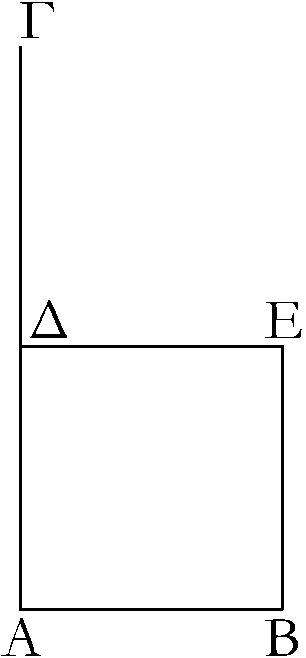
\includegraphics[width=0.8\textwidth]{Book01/fig46g.pdf}}

\gr{ὸ'Ηθθω τῇ ΑΒ εὐθείᾳ ἀπὸ τοῦ πρὸς αὐτῇ σημείου τοῦ Α πρὸς ὀρθὰξ ἡ ΑΓ, καὶ κείσθω τῇ ΑΒὸίση ἡ ΑΔ; καὶ διὰ μὲν τοῦ Δ σημείου τῇ ΑΒ παράλληλος ἢθθω ἡ ΔΕ, διὰ δὲ τοῦ Β σημείου τῇ ΑΔ παράλληλος ἢθθω ἡ ΒΕ. παραλληλόγραμμον ἄρα ἐστὶ τὸ ΑΔΕΒ; ὸίση ἄρα ἐστὶν ἡ μὲν ΑΒ τῇ ΔΕ, ἡ δὲ ΑΔ τῇ ΒΕ. ἀλλὰ ἡ ΑΒ τῇ ΑΔ ἐστινὸίση; αἱ τέσσαρες ἄρα αἱ ΒΑ, ΑΔ, ΔΕ, ΕΒ ἴσαι ἀλλήλαις εἰσίν;
ἰσόπλευρον ἄρα ἐστὶ τὸ ΑΔΕΒ παραλληλόγραμμον. λέγω δή, ὅτι καὶ ὀρθογώνιον. ἐπεὶ γὰρ εἰξ παραλλήλους τὰξ ΑΒ, ΔΕ εὐθεῖα ἐνέπεσεν ἡ ΑΔ, αἱ  ἄρα ὑπὸ ΒΑΔ, ΑΔΕ γωνίαι δύο ὀρθαῖξ ἴσαι εἰσίν.
ὀρθὴ δὲ ἡ ὑπὸ ΒΑΔ; ὀρθὴ  ἄρα καὶ ἡ ὑπὸ ΑΔΕ. τῶν δὲ παραλληλογράμμων θωρίων αἱ ἀπεναντίον πλευραί τε καὶ γωνίαι ἴσαι ἀλλήλαις εἰσίν; ὀρθὴ  ἄρα καὶ ἑκατέρα τῶν ἀπεναντίον τῶν ὑπὸ ΑΒΕ, ΒΕΔ γωνιῶν; ὀρθογώνιον ἄρα ἐστὶ τὸ ΑΔΕΒ. ἐδείθθη δὲ καὶ ἰσόπλευρον.}

\gr{Τετράγωνον ἄρα ἐστίν; καί ἐστιν ἀπὸ τῆς ΑΒ εὐθείας ἀναγεγραμμένον; ὅπερ ἔδει ποιῆσαι.}}

\ParallelRText{
\begin{center}
{\large Proposition 46}
\end{center}

To describe a square on a given straight-line.

Let $AB$ be the given straight-line. So it is required to describe a
square on the straight-line $AB$.

% Removed epsf size command
\centerline{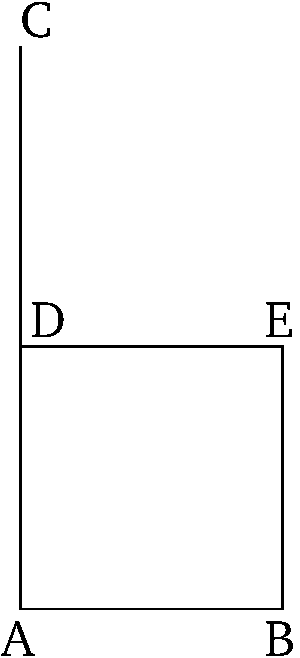
\includegraphics[width=0.8\textwidth]{Book01/fig46e.pdf}}

Let $AC$ be drawn at right-angles to the straight-line $AB$
from the point $A$ on it [Prop.~1.11], and let $AD$ be
made equal to $AB$ [Prop.~1.3]. And let $DE$ be drawn
through point $D$ parallel to $AB$ [Prop.~1.31], and let $BE$ be
drawn through point $B$ parallel to $AD$ [Prop.~1.31]. Thus,
$ADEB$ is a parallelogram. Therefore, $AB$ is equal to $DE$, and $AD$ to $BE$ [Prop.~1.34]. But, $AB$ is equal to $AD$. Thus, the four (sides) $BA$, $AD$, $DE$, and $EB$ are equal to one another. Thus, the parallelogram $ADEB$ is equilateral.
So I say that (it is) also right-angled. For since the straight-line $AD$ falls
across the parallels $AB$ and $DE$, the (sum of the) angles $BAD$ and $ADE$ is
equal to two right-angles [Prop.~1.29]. But $BAD$ (is a) right-angle. Thus,
$ADE$ (is) also a right-angle. And for parallelogramic figures, the opposite
sides and angles are equal to one another [Prop.~1.34]. Thus, each of the
opposite angles $ABE$ and $BED$ (are) also right-angles. Thus, $ADEB$ is
right-angled. And it was also shown (to be) equilateral.

Thus, ($ADEB$) is a square [Def.~1.22]. And it is described on the straight-line $AB$. (Which is) the very thing it was required to do.}
\end{Parallel}

%%%%%%
% Prop 1.47
%%%%%%
\pdfbookmark[1]{Proposition 1.47}{pdf1.47}
\begin{Parallel}{}{} 
\ParallelLText{
\begin{center}
{\large\ggn{47}.}
\end{center}\vspace*{-7pt}

\gr{Ἐν τοῖς ὀρθογωνίοις τριγώνοις τὸ ἀπὸ τῆς τὴν ὀρθὴν γωνίαν ὑποτεινούσης πλευρᾶξ τετράγωνον ἴσον ἐστὶ τοῖς ἀπὸ τῶν τὴν ὀρθὴν γωνίαν περιεθουσῶν πλευρῶν τετραγώνοις.}

\gr{Ἔστω τρίγωνον ὀρθογώνιον τὸ ΑΒΓ ὀρθὴν ἔχον τὴν ὑπὸ ΒΑΓ γωνίαν; λέγω, ὅτι τὸ ἀπὸ τῆς ΒΓ τετράγωνον ἴσον ἐστὶ τοῖς
ἀπὸ τῶν ΒΑ, ΑΓ τετραγώνοις.}

% Removed epsf size command
\centerline{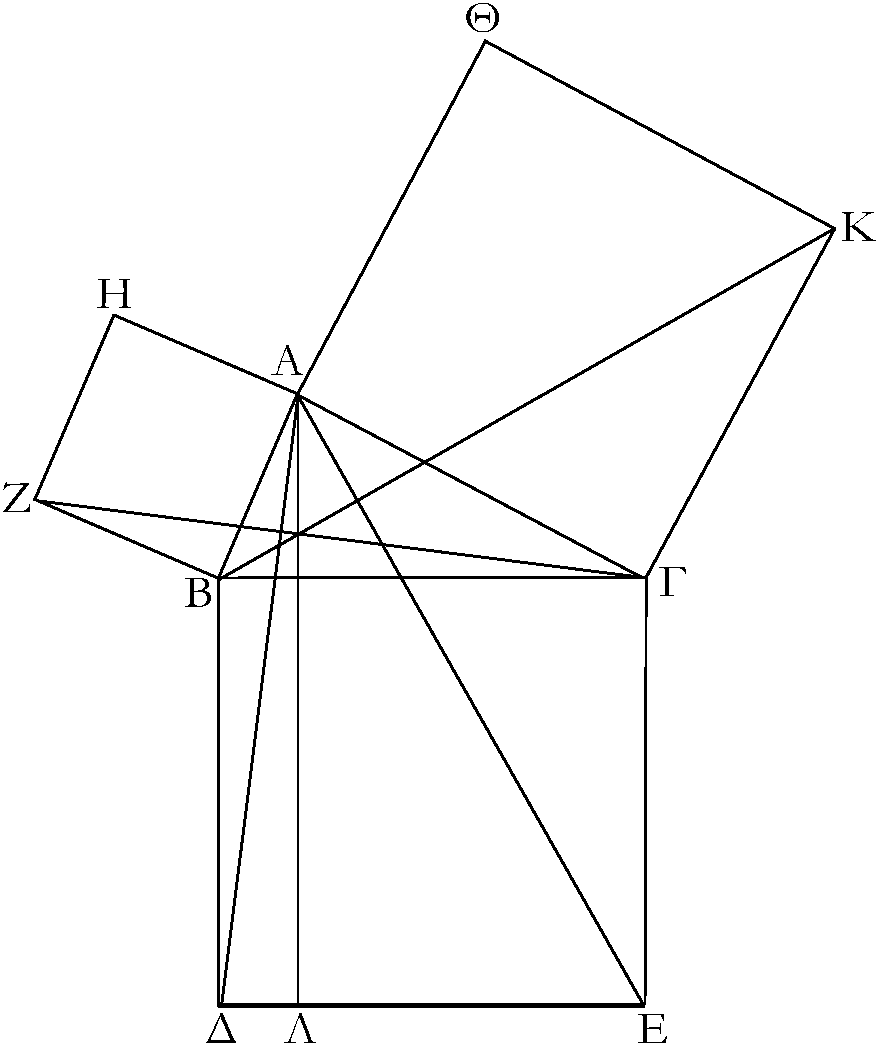
\includegraphics[width=0.8\textwidth]{Book01/fig47g.pdf}}

\gr{Ἀναγεγράφθω γὰρ ἀπὸ μὲν τῆς ΒΓ τετράγωνον τὸ ΒΔΕΓ, ἀπὸ δὲ τῶν ΒΑ, ΑΓ τὰ ΗΒ, ΘΓ, καὶ διὰ τοῦ Α ὁποτέρᾳ τῶν ΒΔ, ΓΕ παράλληλος ἢθθω ἡ ΑΛ; καὶ ἐπεζεύθθωσαν αἱ ΑΔ, ΖΓ. καὶ ἐπεὶ ὀρθή ἐστιν ἑκατέρα τῶν ὑπὸ ΒΑΓ, ΒΑΗ γωνιῶν, πρὸς δή τινι εὐθείᾳ τῇ ΒΑ καὶ τῷ πρὸς αὐτῇ σημείῳ τῷ Α δύο εὐθεῖαι αἱ ΑΓ, ΑΗ μὴ ἐπὶ τὰ αὐτὰ μέρη κείμεναι τὰξ ἐφεχῆς γωνίας δυσὶν ὀρθαῖξ ἴσας ποιοῦσιν; ἐπ' εὐθείας ἄρα ἐστὶν ἡ ΓΑ τῇ ΑΗ. διὰ τὰ αὐτὰ δὴ καὶ ἡ ΒΑ τῇ ΑΘ ἐστιν ἐπ' εὐθείας. καὶ ἐπεὶ ὸίση ἐστὶν ἡ ὑπὸ ΔΒΓ γωνία τῇ ὑπὸ ΖΒΑ; ὀρθὴ γὰρ ἑκατέρα; κοινὴ προσκείσθω ἡ ὑπὸ ΑΒΓ; ὅλη ἄρα ἡ ὑπὸ ΔΒΑ ὅλῃ τῇ ὑπὸ ΖΒΓ ἐστινὸίση.
καὶ ἐπεὶ ὸίση ἐστὶν ἡ μὲν ΔΒ τῇ ΒΓ, ἡ δὲ ΖΒ τῇ ΒΑ, δύο δὴ αἱ ΔΒ, ΒΑ δύο ταῖς ΖΒ, ΒΓ ἴσαι  εἰσὶν ἑκατέρα ἑκατέρᾳ;
καὶ γωνία ἡ ὑπὸ ΔΒΑ γωνίᾳ τῇ ὑπὸ ΖΒΓὸίση;
βάσις ἄρα ἡ ΑΔ βάσει τῇ ΖΓ [ἐστιν] ὸίση, καὶ τὸ ΑΒΔ τρίγωνον τῷ ΖΒΓ τριγώνῳ ἐστὶν ἴσον; καί [ἐστι] τοῦ μὲν ΑΒΔ τριγώνου διπλάσιον τὸ ΒΛ παραλληλόγραμμον; βάσιν τε γὰρ τὴν αὐτὴνὸέθουσι τὴν ΒΔ καὶ ἐν ταῖς αὐταῖς εἰσι παραλλήλοις ταῖς ΒΔ, ΑΛ; τοῦ δὲ ΖΒΓ τριγώνου διπλάσιον τὸ ΗΒ τετράγωνον; βάσιν τε γὰρ πάλιν τὴν αὐτὴνὸέθουσι τὴν ΖΒ καὶ ἐν ταῖς αὐταῖς εἰσι παραλλήλοις ταῖς ΖΒ, ΗΓ. [τὰ δὲ τῶνὸίσων διπλάσια ἴσα ἀλλήλοις ἐστίν;]  ἴσον ἄρα ἐστὶ καὶ τὸ ΒΛ παραλληλόγραμμον τῷ ΗΒ τετραγώνῳ. ὁμοίως δὴ ἐπιζευγνυμένων τῶν ΑΕ, ΒΚ δειθθήσεται καὶ τὸ ΓΛ παραλληλόγραμμον ἴσον τῷ ΘΓ τετραγώνῳ; ὅλον ἄρα τὸ ΒΔΕΓ τετράγωνον δυσὶ τοῖς ΗΒ, ΘΓ τετραγώνοις ἴσον ἐστίν. καί ἐστι τὸ μὲν ΒΔΕΓ τετράγωνον ἀπὸ τῆς ΒΓ ἀναγραφέν, τὰ δὲ ΗΒ, ΘΓ ἀπὸ τῶν ΒΑ, ΑΓ. τὸ  ἄρα ἀπὸ τῆς ΒΓ πλευρᾶξ τετράγωνον ἴσον ἐστὶ τοῖς ἀπὸ τῶν ΒΑ, ΑΓ
πλευρῶν τετραγώνοις.}

\gr{Ἐν ἄρα  τοῖς ὀρθογωνίοις τριγώνοις τὸ ἀπὸ τῆς τὴν ὀρθὴν γωνίαν ὑποτεινούσης πλευρᾶξ τετράγωνον ἴσον ἐστὶ τοῖς ἀπὸ τῶν τὴν ὀρθὴν [γωνίαν] περιεθουσῶν πλευρῶν τετραγώνοις; ὅπερ ἔδει δεῖχαι.}}

\ParallelRText{
\begin{center}
{\large Proposition 47}
\end{center}

In right-angled triangles,  the square on the side subtending the right-angle
is equal to the (sum of the) squares on the sides containing the right-angle.

Let $ABC$ be a right-angled triangle having the angle $BAC$ a right-angle. I say that the
square on $BC$ is equal to the (sum of the) squares on $BA$ and $AC$.

% Removed epsf size command
\centerline{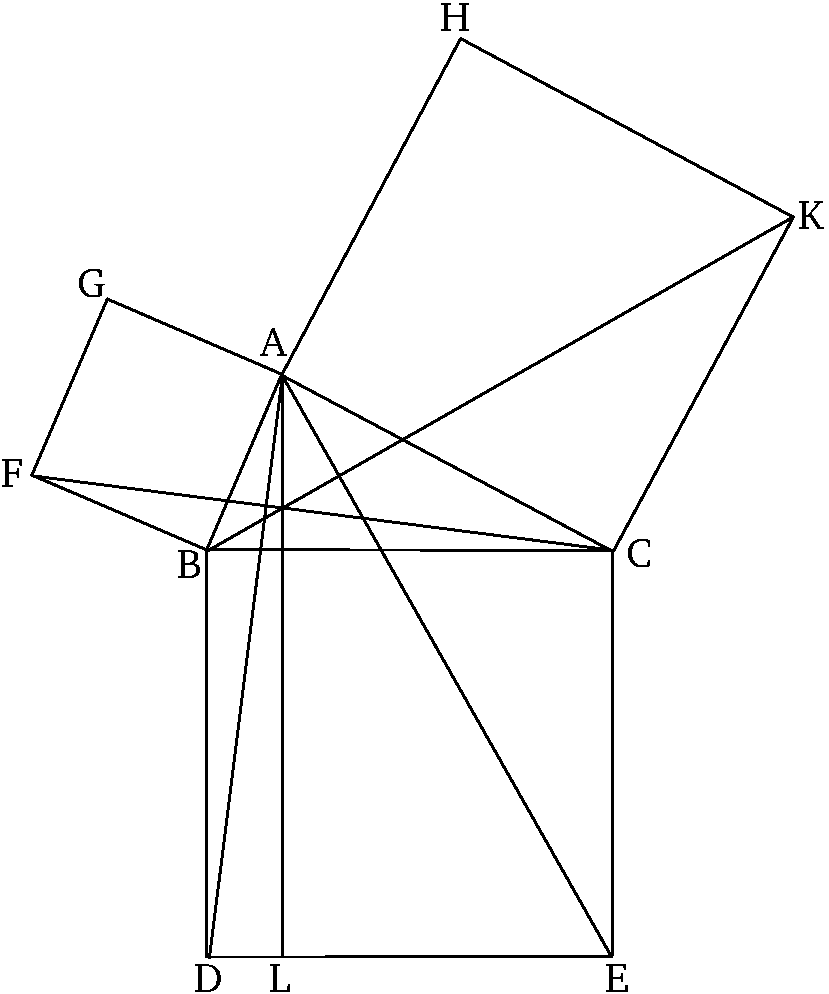
\includegraphics[width=0.8\textwidth]{Book01/fig47e.pdf}}

For let the square $BDEC$ be described on $BC$, and (the squares) $GB$ and $HC$ on $AB$ and $AC$ (respectively) [Prop.~1.46]. And let $AL$ be drawn through point $A$ parallel to either of $BD$ or $CE$ [Prop.~1.31]. And let $AD$ and $FC$ be joined. And
since angles $BAC$ and $BAG$ are each right-angles, then two straight-lines $AC$ and $AG$, not lying on the same side,
make the adjacent angles with some straight-line $BA$, at the point
$A$ on it, (whose sum is) equal to two right-angles. Thus, $CA$ is straight-on to $AG$ [Prop.~1.14]. So, for
the same (reasons), $BA$ is also straight-on to $AH$. And since angle $DBC$ is
equal to $FBA$, for (they are) both right-angles, let $ABC$ be added to
both.  Thus, the whole (angle) $DBA$ is equal to the whole (angle) $FBC$.
And since $DB$ is equal to $BC$, and $FB$ to $BA$, the two (straight-lines) $DB$,
$BA$ are equal to the two (straight-lines) $CB$, $BF$,$^\dag$ respectively. And angle $DBA$ (is) equal to angle $FBC$. Thus, the base $AD$ [is] equal to the base $FC$,
and the triangle $ABD$ is equal to the triangle $FBC$ [Prop.~1.4]. And 
parallelogram $BL$ [is] double (the area) of triangle $ABD$. For they
have the same base, $BD$, and are between the same parallels, $BD$ and $AL$  [Prop.~1.41]. And
 square
$GB$ is double (the area) of triangle $FBC$. For again they have the same base, $FB$, and
are between the same parallels,
$FB$ and $GC$ [Prop.~1.41]. [And the doubles of equal things
are equal to one another.]$^\ddag$ Thus, the parallelogram $BL$ is also equal to the square $GB$. So, similarly, $AE$ and $BK$ being joined, 
the parallelogram $CL$ can be shown (to be)  equal to the square $HC$. Thus, the whole square
$BDEC$ is equal to the (sum of the) two squares $GB$ and $HC$. And the square $BDEC$
is described on $BC$, and the (squares) $GB$ and $HC$ on $BA$ and $AC$ (respectively). Thus, the square on the side $BC$ is equal to the
(sum of the) squares
on the sides $BA$ and $AC$.

Thus, in right-angled triangles,  the square on the side subtending the right-angle
is equal to the (sum of the) squares on the sides surrounding the right-[angle].
(Which is) the very thing it was required to show.}
\end{Parallel}
{\footnotesize \noindent$^\dag$ The
Greek text has ``$FB$, $BC$'', which is obviously a mistake.\\[0.5ex]
$^\ddag$ This is an additional common notion.}

%%%%%%
% Prop 1.48
%%%%%%
\pdfbookmark[1]{Proposition 1.48}{pdf1.48}
\begin{Parallel}{}{} 
\ParallelLText{
\begin{center}
{\large\ggn{48}.}
\end{center}\vspace*{-7pt}

\gr{Ἐὰν τριγώνου τὸ ἀπὸ μιᾶς τῶν πλευρῶν τετράγωνον ἴσονὸῆ| τοῖς ἀπὸ τῶν λοιπῶν τοῦ τριγώνου δύο πλευρῶν τετραγώνοις, ἡ περιεθομένη γωνία ὑπὸ τῶν λοιπῶν τοῦ τριγώνου δύο πλευρῶν ὀρθή ἐστιν.}

\gr{Τριγώνου γὰρ τοῦ ΑΒΓ τὸ ἀπὸ μιᾶς τῆς ΒΓ πλευρᾶξ τετράγωνον ἴσονὸέστω τοῖς ἀπὸ τῶν ΒΑ, ΑΓ πλευρῶν τετραγώνοις; λέγω, ὅτι ὀρθή ἐστιν ἡ ὑπὸ ΒΑΓ γωνία.}

% Removed epsf size command
\centerline{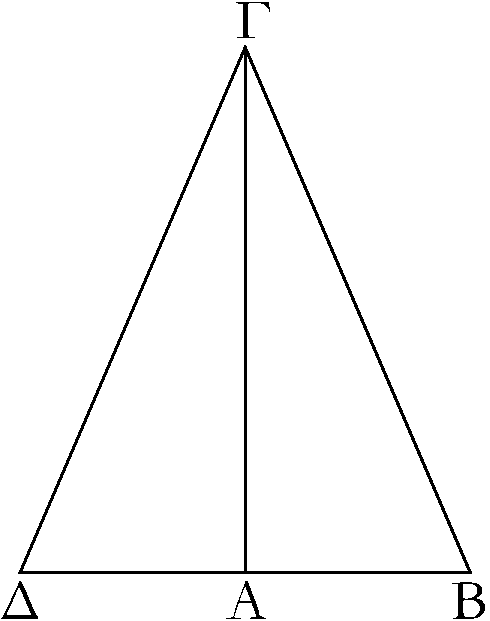
\includegraphics[width=0.8\textwidth]{Book01/fig48g.pdf}}

\gr{ὸ'Ηθθω γὰρ ἀπὸ τοῦ Α σημείου τῇ ΑΓ εὐθείᾳ πρὸς ὀρθὰξ ἡ ΑΔ καὶ κείσθω τῇ ΒΑὸίση ἡ ΑΔ, καὶ ἐπεζεύθθω ἡ ΔΓ. ἐπεὶ ὸίση
ἐστὶν ἡ ΔΑ τῇ ΑΒ,  ἴσον ἐστὶ καὶ τὸ ἀπὸ τῆς ΔΑ τετράγωνον τῷ ἀπὸ τῆς ΑΒ τετραγώνῳ. κοινὸν προσκείσθω τὸ ἀπὸ τῆς ΑΓ τετράγωνον; τὰ  ἄρα ἀπὸ τῶν ΔΑ, ΑΓ τετράγωνα ἴσα ἐστὶ τοῖς ἀπὸ τῶν ΒΑ, ΑΓ τετραγώνοις. ἀλλὰ τοῖς μὲν ἀπὸ τῶν ΔΑ, ΑΓ ἴσον ἐστὶ τὸ ἀπὸ τῆς ΔΓ; ὀρθὴ γάρ ἐστιν ἡ ὑπὸ ΔΑΓ γωνία; τοῖς δὲ ἀπὸ τῶν ΒΑ, ΑΓ ἴσον ἐστὶ τὸ ἀπὸ τῆς ΒΓ; ὑπόκειται γάρ; τὸ  ἄρα ἀπὸ τῆς ΔΓ τετράγωνον ἴσον ἐστὶ τῷ ἀπὸ τῆς ΒΓ τετραγώνῳ; ὁώστε καὶ πλευρὰ ἡ ΔΓ τῇ ΒΓ ἐστινὸίση; καὶ ἐπεὶ ὸίση ἐστὶν ἡ ΔΑ τῇ ΑΒ, κοινὴ δὲ ἡ ΑΓ, δύο δὴ αἱ ΔΑ, ΑΓ δύο ταῖς ΒΑ, ΑΓ ἴσαι εἰσίν; καὶ βάσις ἡ ΔΓ βάσει τῇ ΒΓὸίση; γωνία ἄρα ἡ ὑπὸ ΔΑΓ γωνίᾳ τῇ ὑπὸ ΒΑΓ [ἐστιν] ὸίση. ὀρθὴ δὲ ἡ ὑπὸ ΔΑΓ; ὀρθὴ  ἄρα καὶ ἡ ὑπὸ ΒΑΓ.}

\gr{Ἐὰν ἀρὰ τριγώνου τὸ ἀπὸ μιᾶς τῶν πλευρῶν τετράγωνον ἴσονὸῆ| τοῖς ἀπὸ τῶν λοιπῶν τοῦ τριγώνου δύο πλευρῶν τετραγώνοις, ἡ περιεθομένη γωνία ὑπὸ τῶν λοιπῶν τοῦ τριγώνου δύο πλευρῶν ὀρθή ἐστιν; ὅπερ ἔδει δεῖχαι.}}

\ParallelRText{
\begin{center}
{\large Proposition 48}
\end{center}

If the square on one of the sides of a triangle is equal to the (sum of the)
squares on the two remaining sides of the triangle (then) the angle contained
by the two remaining sides of the triangle is a right-angle.

For let the square on one of the sides, $BC$, of triangle $ABC$ be equal
to the (sum of the) squares on the sides $BA$ and $AC$. I say that angle
$BAC$ is a right-angle.

% Removed epsf size command
\centerline{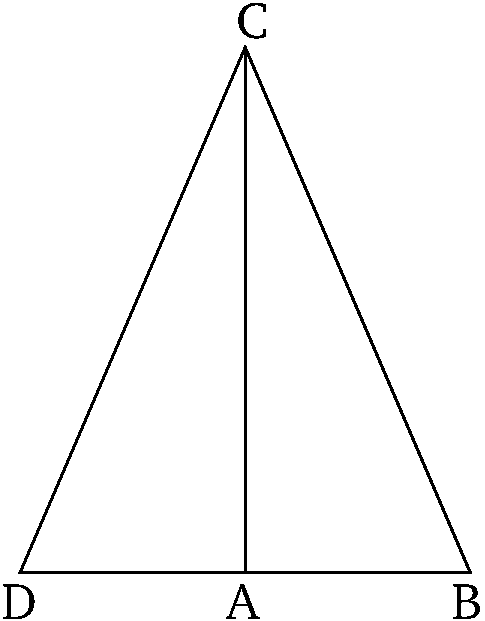
\includegraphics[width=0.8\textwidth]{Book01/fig48e.pdf}}

For let $AD$ be drawn from point $A$ at right-angles to the
straight-line $AC$ [Prop.~1.11], and let $AD$ be made equal to
$BA$ [Prop.~1.3], and let $DC$ be joined. Since $DA$ is equal to $AB$,
the square on $DA$ is thus also equal to the square on $AB$.$^\dag$ Let the square on
$AC$ be added to both. Thus, the (sum of the) squares on $DA$ and $AC$ is equal
to the (sum of the) squares on $BA$ and $AC$. But, the (square) on $DC$ 
is equal to the (sum of the squares) on $DA$ and $AC$. For angle $DAC$ is a right-angle [Prop.~1.47].
But, the  (square) on $BC$ is equal to (sum of the squares) on $BA$ and $AC$.
For (that) was assumed. Thus, the square on $DC$ is equal to the square on $BC$.
So  side $DC$ is also equal to (side) $BC$. And since $DA$ is equal to $AB$, and $AC$ (is) common, the two (straight-lines) $DA$, $AC$ are equal to the two (straight-lines)
$BA$, $AC$. And the base $DC$ is equal to the base $BC$. Thus, angle $DAC$ [is] equal to angle $BAC$ [Prop.~1.8].  But $DAC$ is a right-angle. Thus, $BAC$ is
also a right-angle.

Thus, if the square on one of the sides of a triangle is equal to the (sum of the)
squares on the remaining two sides of the triangle (then) the angle contained
by the remaining two sides of the triangle is a right-angle. (Which is) the very thing
it was required to show.}
\end{Parallel}
{\footnotesize \noindent$^\dag$ Here, use is made of the additional common notion that the squares of equal things are
themselves equal. Later on, the inverse notion is used.} 
% !TEX root = ../Elements.tex
% Greek and English text last checked 14/03/2013
%%%%%%
% BOOK 2
%%%%%%
\pdfbookmark[0]{Book 2}{book2}
\pagestyle{empty}
\begin{center}
{\Huge ELEMENTS BOOK 2}\\
\spa\spa\spa
{\huge\it Fundamentals of Geometric Algebra}
\end{center}
%\vspace{2cm}
%\epsfysize=5in
%\centerline{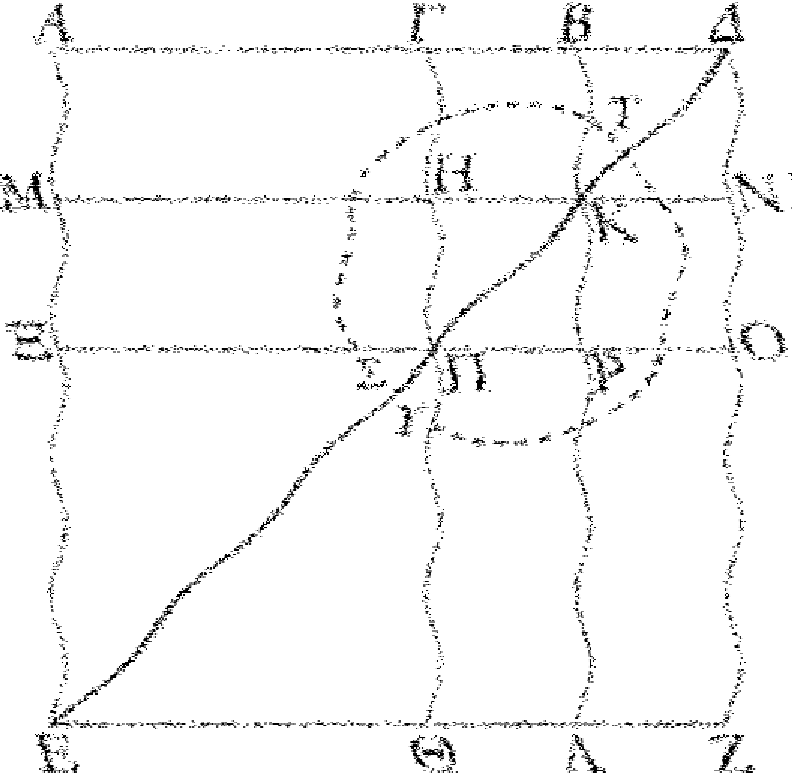
\includegraphics{Book02/front.eps}}
\newpage

%%%%%%%
% Definitions
%%%%%%%
\pdfbookmark[1]{Definitions}{def2}
\pagestyle{fancy}
\cfoot{\gr{\kern -.7pt }}
\lhead{\large\gr{ΣΤΟΙΘΕΙΩΝ \kern -.7pt {2}.}}
\rhead{\large ELEMENTS BOOK 2}
\begin{Parallel}{}{} 
\ParallelLText{
\begin{center}
\large{\gr{<'Οροι}.}
\end{center}
\vspace*{-7pt}

\ggn{1}.~\gr{Πᾶν παραλληλόγραμμον ὀρθογώνιον περιέθεσθαι λέγεται ὑπὸ δύο τῶν τὴν ὀρθὴν γωνίαν περιεθουσῶν εὐθειῶν.}

\ggn{2}.~\gr{Παντὸξ δὲ παραλληλογράμμου θωρίου τῶν περὶ τὴν διάμετρον
α\kern -.7pt  ὐτοῦ παραλληλογράμμων <ὲν ὁποιονοῦν σὺν τοῖξ δυσὶ παραπληρώμασι γνώμων καλείσθω.}}

\ParallelRText{
\begin{center}
{\large Definitions}
\end{center}

1.~Any rectangular parallelogram is said to be contained by the two
 straight-lines containing the right-angle.
 
2.~And in any parallelogrammic figure, let any one whatsoever of the parallelograms about
its diagonal,  (taken) with its two complements, be called
a gnomon.}
\end{Parallel}

%%%%%%
% Prop 2.1
%%%%%%
\pdfbookmark[1]{Proposition 2.1}{pdf2.1}
\begin{Parallel}{}{} 
\ParallelLText{
\begin{center}
{\large \ggn{1}.}
\end{center}\vspace*{-7pt}

\gr{Ἐὰν >ῶσι δύο εὐθεῖαι, τμ\kern -.7pt  ηθῆ| δὲ ἡ ἑτέρα α\kern -.7pt  ὐτῶν εἰξ ὁσαδηποτοῦν τμ\kern -.5pt  ήματα, τὸ περιεχόμενον ὀρθογώνιον ὑπὸ τῶν δύο εὐθειῶν >ίσον ἐστὶ τοῖξ ὑπό τε τῆξ ἀτμ\kern -.3pt  ήτου καὶ ἑκάστου τῶν τμ\kern -.7pt  ημάτων περιεθομένοιξ ὀρθογωνίοιξ.}\\

\epsfysize=2.2in
\centerline{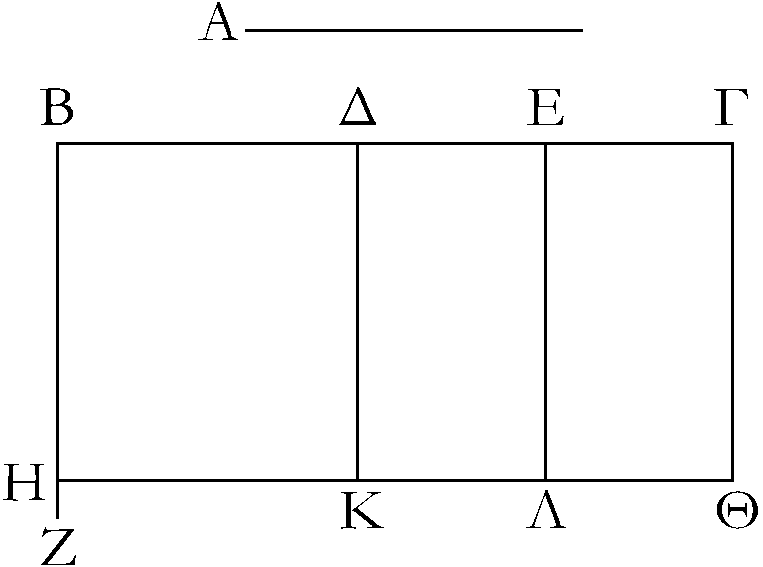
\includegraphics{Book02/fig01g.eps}}

\gr{>'Εστωσαν δύο εὐθεῖαι αἱ Α, ΒΓ, καὶ τετμ\kern -.7pt  ήσθω ἡ ΒΓ, ὡξ >έτυθεν, κατὰ τὰ Δ, Ε σημεῖα; λέγω, <ότι τὸ ὑπὸ τῶν Α, ΒΓ περιεθομένον ὀρθογώνιον >ίσον ἐστὶ τῶ| τε ὑπὸ τῶν Α, ΒΔ περιεθομένῳ ὀρθογωνίῳ καὶ τῶ| ὑπὸ τῶν Α, ΔΕ καὶ >έτι τῶ| ὑπὸ τῶν Α,
ΕΓ.}

\gr{>'Ηθθω γὰρ ἀπὸ τοῦ Β τῆ| ΒΓ πρὸξ ὀρθὰξ ἡ ΒΖ, καὶ κείσθω
τῆ| Α >ίση ἡ ΒΗ, καὶ διὰ μὲν τοῦ Η τῆ| ΒΓ παράλληλοξ >ήθθω ἡ ΗJ, διὰ δὲ τῶν Δ, Ε, Γ τῆ| ΒΗ παράλληλοι >ήθθωσαν αἱ ΔΚ, ΕΛ, ΓJ.}

\gr{>'Ισον δή ἐστι τὸ ΒJ τοῖξ ΒΚ, ΔΛ, ΕJ. καί ἐστι τὸ μὲν ΒJ τὸ ὑπὸ τῶν Α, ΒΓ; περιέθεται μὲν γὰρ ὑπὸ τῶν ΗΒ, ΒΓ, >ίση δὲ ἡ ΒΗ τῆ| Α; τὸ δὲ ΒΚ τὸ ὑπὸ τῶν Α, ΒΔ; περιέθεται μὲν γὰρ ὑπὸ τῶν ΗΒ, ΒΔ, >ίση δὲ ἡ ΒΗ τῆ| Α. τὸ δὲ ΔΛ τὸ ὑπὸ τῶν Α, ΔΕ; >ίση γὰρ ἡ ΔΚ, τουτέστιν ἡ ΒΗ, τῆ| Α. καὶ >έτι ὁμοίωξ τὸ ΕJ τὸ ὑπὸ τῶν Α, ΕΓ; τὸ >άρα ὑπὸ τῶν Α, ΒΓ >ίσον ἐστὶ τῶ| τε ὑπὸ Α, ΒΔ καὶ
τῶ| ὑπὸ Α, ΔΕ καὶ >έτι τῶ| ὑπὸ Α, ΕΓ.}

\gr{Ἐὰν >άρα  >ῶσι δύο εὐθεῖαι, τμ\kern -.7pt  ηθῆ| δὲ ἡ ἑτέρα α\kern -.7pt  ὐτῶν εἰξ ὁσαδηποτοῦν τμ\kern -.5pt  ήματα, τὸ περιεχόμενον ὀρθογώνιον ὑπὸ τῶν δύο εὐθειῶν >ίσον ἐστὶ τοῖξ ὑπό τε τῆξ ἀτμ\kern -.3pt  ήτου καὶ ἑκάστου τῶν τμ\kern -.7pt  ημάτων περιεθομένοιξ ὀρθογωνίοιξ; <όπερ >έδει δεῖχαι.}}

\ParallelRText{
\begin{center}
{\large Proposition 1$^\dag$}
\end{center}

If there are two straight-lines, and one of them is cut into any number of pieces whatsoever, (then) the rectangle contained by the two straight-lines is
equal to the (sum of the) rectangles contained by the uncut (straight-line), and every one of the pieces (of the cut straight-line).

\epsfysize=2.2in
\centerline{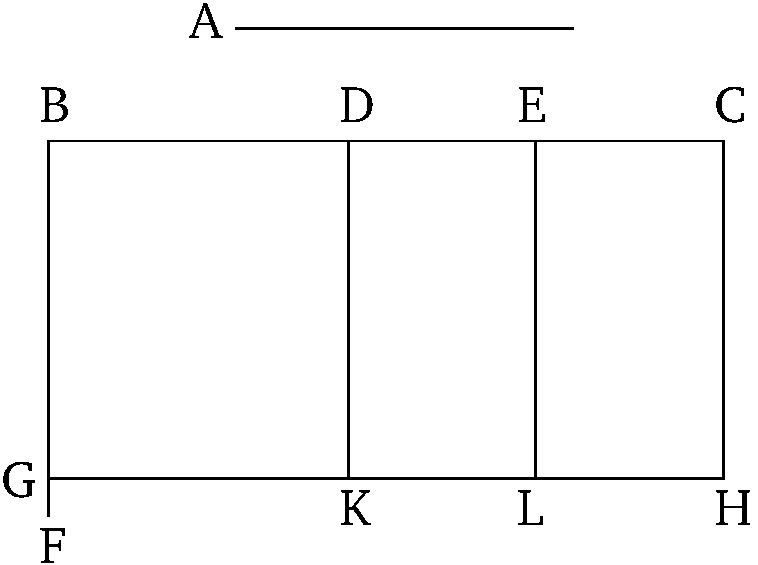
\includegraphics{Book02/fig01e.eps}}

Let $A$ and $BC$ be the two straight-lines, and let $BC$ be cut, at random,
at points $D$ and $E$. I say that the rectangle contained by $A$ and $BC$ is equal
to the rectangle(s) contained by $A$ and $BD$, by $A$ and $DE$, and, finally, by $A$ and
$EC$.

For let $BF$ be drawn from point $B$, at right-angles to $BC$ [Prop.~1.11],
and let $BG$ be made equal to $A$ [Prop.~1.3], and let $GH$ be drawn through
(point) $G$, parallel to $BC$ [Prop.~1.31], and let $DK$, $EL$, and $CH$ be drawn through (points) $D$, $E$, and $C$ (respectively), parallel to $BG$ [Prop.~1.31].

So the (rectangle) $BH$ is equal to the (rectangles) $BK$, $DL$, and $EH$. And
$BH$ is  the (rectangle contained) by $A$ and $BC$. For it is contained by $GB$ and $BC$, and $BG$ (is) equal to $A$. And  $BK$ (is) the (rectangle contained) by $A$ and $BD$.
For it is contained by $GB$ and $BD$, and $BG$ (is) equal to $A$. And $DL$ (is) the (rectangle contained) by $A$ and $DE$.
For $DK$, that is to say $BG$ [Prop.~1.34], (is) equal to $A$. Similarly, $EH$ (is)
also the (rectangle contained) by $A$ and $EC$. Thus, the (rectangle contained) by $A$ and $BC$ is
equal to the (rectangles contained) by $A$ and $BD$,  by $A$ and $DE$, and, finally,
by $A$ and $EC$.

Thus, if there are two straight-lines, and one of them is cut into any number 
of pieces whatsoever, (then) the rectangle contained by the two straight-lines is
equal to the (sum of the) rectangles contained by the uncut (straight-line), and every one of the pieces (of the cut straight-line). (Which is) the very thing it was required to show.}
\end{Parallel}
{\footnotesize \noindent$^\dag$ This proposition is a geometric version
of the algebraic identity: $a \,(b+c+d+\cdots) = a\,b + a\,c + a\,d + \cdots$.}

%%%%%%
% Prop 2.2
%%%%%%
\pdfbookmark[1]{Proposition 2.2}{pdf2.2}
\begin{Parallel}{}{} 
\ParallelLText{
\begin{center}
{\large \ggn{2}.}
\end{center}\vspace*{-7pt}

\gr{Ἐὰν εὐθεῖα γραμμ\kern -.7pt  ὴ τμ\kern -.7pt  ηθῆ|, ὡξ >έτυθεν, τὸ ὑπὸ τῆξ <όληξ καὶ ἑκατέρου τῶν τμ\kern -.5pt  ημάτων περιεχόμενον ὀρθογώνιον >ίσον ἐστὶ τῶ| ἀπὸ τῆξ <όληξ τετραγώνῳ.}\\

\epsfysize=2.2in
\centerline{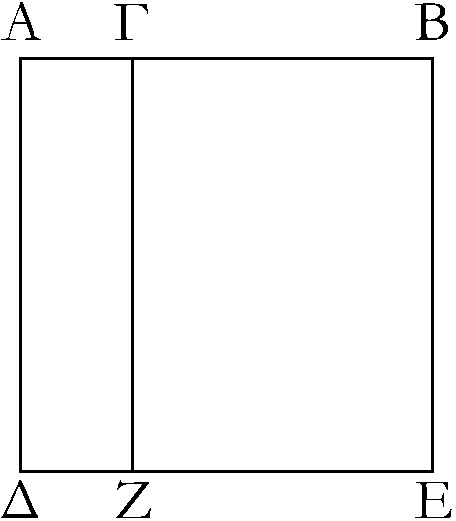
\includegraphics{Book02/fig02g.eps}}

\gr{Εὐθεῖα γὰρ ἡ ΑΒ τετμ\kern -.7pt  ήσθω, ὡξ >έτυθεν, κατὰ τὸ Γ σημεῖον; λέγω, 
<ότι τὸ ὑπὸ τῶν ΑΒ, ΒΓ περιεχόμενον ὀρθογώνιον μετὰ τοῦ ὑπὸ ΒΑ, ΑΓ περιεθομένου ὀρθογωνίου >ίσον  ἐστὶ τῶ| ἀπὸ τῆξ
ΑΒ τετραγώνῳ.}

\gr{Ἀναγεγράφθω γὰρ ἀπὸ τῆξ ΑΒ τετράγωνον τὸ ΑΔΕΒ, καὶ >ήθθω διὰ τοῦ Γ ὁποτέρᾳ τῶν ΑΔ, ΒΕ παράλληλοξ ἡ ΓΖ.}

\gr{>'Ισον δή ἐστὶ τὸ ΑΕ τοῖξ ΑΖ, ΓΕ. καί ἐστι τὸ μὲν ΑΕ τὸ ἀπὸ τῆξ ΑΒ τετράγωνον, τὸ δὲ ΑΖ τὸ ὑπὸ τῶν ΒΑ, ΑΓ περιεχόμενον ὀρθογώνιον; περιέθεται μὲν γὰρ ὑπὸ τῶν ΔΑ, ΑΓ, >ίση δὲ ἡ ΑΔ τῆ| ΑΒ; τὸ δὲ ΓΕ τὸ ὑπὸ τῶν ΑΒ, ΒΓ; >ίση γὰρ ἡ ΒΕ τῆ| ΑΒ. τὸ >άρα ὑπὸ τῶν ΒΑ, ΑΓ μετὰ τοῦ ὑπὸ τῶν ΑΒ, ΒΓ >ίσον ἐστὶ τῶ| ἀπὸ τῆξ ΑΒ τετραγώνῳ.}

\gr{Ἐὰν >άρα εὐθεῖα γραμμ\kern -.7pt  ὴ τμ\kern -.7pt  ηθῆ|, ὡξ >έτυθεν, τὸ ὑπὸ τῆξ <όληξ καὶ ἑκατέρου τῶν τμ\kern -.5pt  ημάτων περιεχόμενον ὀρθογώνιον >ίσον ἐστὶ τῶ| ἀπὸ τῆξ <όληξ τετραγώνῳ; <όπερ >έδει δεῖχαι.}}

\ParallelRText{
\begin{center}
{\large Proposition 2$^\dag$}
\end{center}

If a straight-line is cut at random,  (then) the (sum of the) rectangle(s) contained by the whole
(straight-line), and each of the pieces (of the straight-line), is equal to the square on the whole.

\epsfysize=2.2in
\centerline{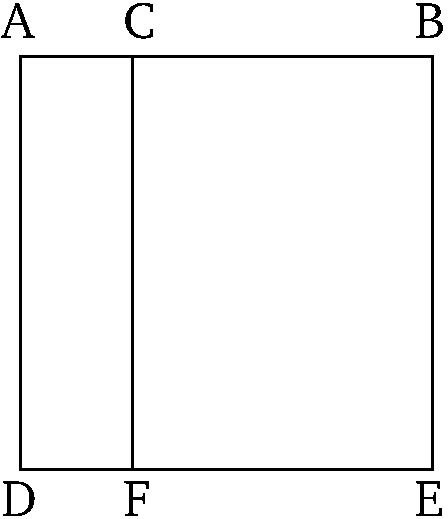
\includegraphics{Book02/fig02e.eps}}

For let the straight-line $AB$ be cut, at random, at point $C$. I say that the
rectangle contained by $AB$ and $BC$, plus the rectangle contained by 
$BA$ and $AC$, is equal to the square on $AB$.

For let the square $ADEB$ be described on $AB$ [Prop.~1.46], and
let $CF$ be drawn through $C$, parallel to either of $AD$ or $BE$ [Prop.~1.31].

So the (square) $AE$ is equal to the (rectangles) $AF$ and $CE$. And $AE$ is the square on $AB$.  And $AF$ (is) the rectangle contained by the (straight-lines) $BA$ and $AC$. For it is contained by $DA$ and $AC$, and $AD$ (is) equal to $AB$. 
And $CE$ (is) the (rectangle contained) by $AB$ and $BC$. For $BE$ (is) equal
to $AB$. Thus, the (rectangle contained) by $BA$ and $AC$, plus the
(rectangle contained) by $AB$ and $BC$, is equal to the square on $AB$.

Thus, if a straight-line is cut at random,  (then) the (sum of the) rectangle(s) contained by the whole
(straight-line), and each of the pieces (of the straight-line), is equal to the square on the whole. (Which is) the very thing it was required to show.}
\end{Parallel}
{\footnotesize \noindent$^\dag$ This proposition is a geometric version
of the algebraic identity: $a\,b+a\,c=a^{\,2}$ if $a=b+c$.}

%%%%%%
% Prop 2.3
%%%%%%
\pdfbookmark[1]{Proposition 2.3}{pdf2.3}
\begin{Parallel}{}{} 
\ParallelLText{
\begin{center}
{\large \ggn{3}.}
\end{center}\vspace*{-7pt}

\gr{Ἐὰν εὐθεῖα γραμμ\kern -.7pt  ὴ τμ\kern -.7pt  ηθῆ|, ὡξ >έτυθεν, τὸ ὑπὸ τῆξ <όληξ καὶ ἑνὸξ τῶν τμ\kern -.5pt  ημάτων περιεχόμενον ὀρθογώνιον >ίσον ἐστὶ τῶ| τε ὑπὸ τῶν τμ\kern -.3pt  ημάτων περιεθομένῳ ὀρθογωνίῳ καὶ τῶ| ἀπὸ τοῦ προειρημένου τμ\kern -.7pt  ήματοξ τετραγώνῳ.}

\epsfysize=2.in
\centerline{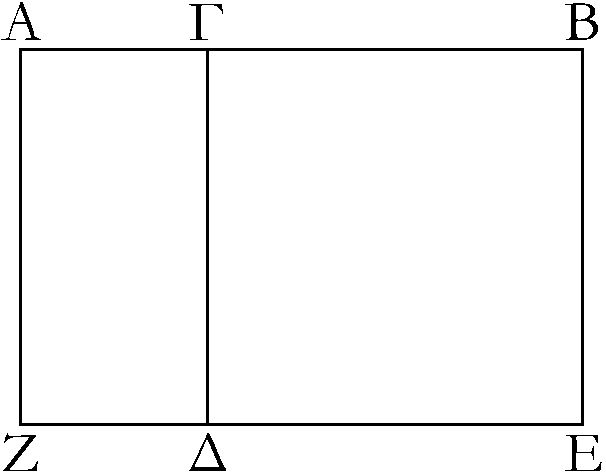
\includegraphics{Book02/fig03g.eps}}

\gr{Εὐθεῖα γὰρ ἡ ΑΒ τετμ\kern -.7pt  ήσθω, ὡξ >έτυθεν, κατὰ τὸ Γ; λέγω, <ότι
τὸ ὑπὸ τῶν ΑΒ, ΒΓ περιεχόμενον ὀρθογώνιον >ίσον ἐστὶ τῶ| τε ὑπὸ τῶν ΑΓ, ΓΒ περιεθομένῳ ὀρθογωνίῳ μετὰ τοῦ ἀπὸ τῆξ 
ΒΓ τετραγώνου.}

\gr{Ἀναγεγράφθω γὰρ ἀπὸ τῆξ ΓΒ τετράγωνον τὸ ΓΔΕΒ, καὶ διήθθω ἡ ΕΔ ἐπὶ τὸ Ζ, καὶ διὰ τοῦ Α ὁποτέρᾳ τῶν ΓΔ, ΒΕ παράλληλοξ >ήθθω ἡ ΑΖ. >ίσον δή ἐστι τὸ ΑΕ τοῖξ ΑΔ, ΓΕ; καί ἐστι τὸ μὲν ΑΕ τὸ ὑπὸ τῶν ΑΒ, ΒΓ περιεχόμενον ὀρθογώνιον; περιέθεται μὲν γὰρ ὑπὸ τῶν ΑΒ, ΒΕ, >ίση δὲ ἡ ΒΕ τῆ| ΒΓ; τὸ δὲ ΑΔ τὸ ὑπὸ τῶν ΑΓ, ΓΒ; >ίση γὰρ ἡ ΔΓ τῆ| ΓΒ; τὸ δὲ ΔΒ τὸ ἀπὸ τῆξ ΓΒ τετράγωνον; τὸ >άρα ὑπὸ τῶν ΑΒ, ΒΓ περιεχόμενον ὀρθογώνιον >ίσον ἐστὶ τῶ| ὑπὸ τῶν
ΑΓ, ΓΒ περιεθομένῳ ὀρθογωνίῳ μετὰ τοῦ ἀπὸ τῆξ ΒΓ τετραγώνου.}

\gr{Ἐὰν >άρα εὐθεῖα γραμμ\kern -.7pt  ὴ τμ\kern -.7pt  ηθῆ|, ὡξ >έτυθεν, τὸ ὑπὸ τῆξ <όληξ καὶ ἑνὸξ τῶν τμ\kern -.5pt  ημάτων περιεχόμενον ὀρθογώνιον >ίσον ἐστὶ τῶ| τε ὑπὸ τῶν τμ\kern -.3pt  ημάτων περιεθομένῳ ὀρθογωνίῳ καὶ τῶ| ἀπὸ τοῦ προειρημένου τμ\kern -.7pt  ήματοξ τετραγώνῳ; <όπερ >έδει δεῖχαι.}}

\ParallelRText{
\begin{center}
{\large Proposition 3$^\dag$}
\end{center}

If  a straight-line is cut at random, (then) the rectangle contained by the
whole (straight-line), and one of the pieces (of the straight-line),
is equal to the rectangle contained by (both of) the pieces, and the square on
the aforementioned piece.

\epsfysize=2.in
\centerline{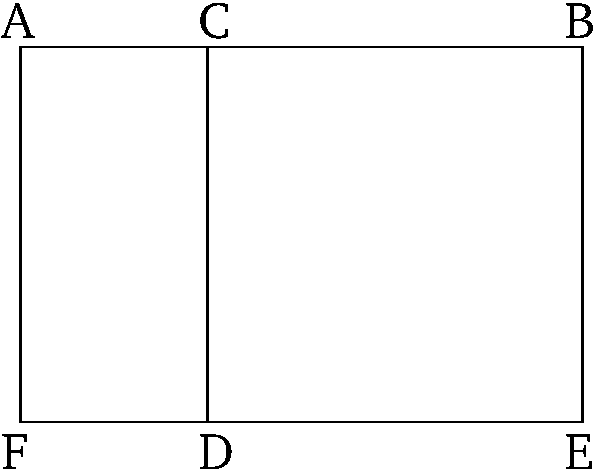
\includegraphics{Book02/fig03e.eps}}

For let the straight-line $AB$ be cut, at random, at (point) $C$.
I say that the rectangle contained by $AB$ and $BC$ is equal to the
rectangle contained by $AC$ and $CB$, plus the square on $BC$.

For let the square $CDEB$ be described on $CB$ [Prop.~1.46],
and let $ED$ be drawn through to $F$, and let $AF$ be
drawn through $A$, parallel to either of $CD$ or $BE$ [Prop.~1.31].
So the (rectangle) $AE$ is equal to the (rectangle) $AD$ and the (square) $CE$.
And $AE$ is the rectangle contained by $AB$ and $BC$.
For it is contained by $AB$ and $BE$, and $BE$ (is) equal to $BC$. And
$AD$ (is) the (rectangle contained) by $AC$ and $CB$. For $DC$
(is) equal to $CB$. And $DB$ (is) the square on $CB$. Thus, the rectangle
contained by $AB$ and $BC$ is equal to the rectangle contained by $AC$ and
$CB$, plus the square on $BC$.

Thus, if a straight-line is cut at random, (then) the rectangle contained by the
whole (straight-line),  and one of the pieces (of the straight-line),
is equal to the rectangle contained by (both of) the pieces, and the square on
the aforementioned piece. (Which is) the very thing it was required
to show.}
\end{Parallel}
{\footnotesize \noindent$^\dag$ This proposition is a geometric version
of the algebraic identity: $(a+b)\,a = a\,b + a^{\,2}$.}

%%%%%%
% Prop 2.4
%%%%%%
\pdfbookmark[1]{Proposition 2.4}{pdf2.4}
\begin{Parallel}{}{} 
\ParallelLText{
\begin{center}
{\large \ggn{4}.}
\end{center}\vspace*{-7pt}

\gr{Ἐὰν εὐθεῖα γραμμ\kern -.7pt  ὴ τμ\kern -.7pt  ηθῆ|, ὡξ >έτυθεν, τὸ ἀπὸ τῆξ <όληξ τετράγωνον >ίσον ἐστὶ τοῖξ τε ἀπὸ τῶν τμ\kern -.5pt  ημάτων τετραγώνοιξ καὶ τῶ| δὶξ ὑπὸ τῶν τμ\kern -.3pt  ημάτων περιεθομένῳ ὀρθογωνίῳ.}

\gr{Εὐθεῖα γὰρ γραμμ\kern -.7pt  ὴ ἡ ΑΒ τετμ\kern -.7pt  ήσθω, ὡξ >έτυθεν, κατὰ τὸ Γ. λέγω,
<ότι τὸ ἀπὸ τῆξ ΑΒ τετράγωνον >ίσον ἐστὶ τοῖξ τε ἀπὸ τῶν ΑΓ, ΓΒ τετραγώνοιξ καὶ τῶ| δὶξ ὑπὸ τῶν ΑΓ, ΓΒ  περιεθομένῳ ὀρθογωνίῳ.}

\gr{Ἀναγεγράφθω γὰρ ἀπὸ τῆξ ΑΒ τετράγωνον τὸ ΑΔΕΒ, καὶ ἐπεζεύθθω ἡ ΒΔ, καὶ διὰ μὲν τοῦ Γ ὁποτέρᾳ τῶν ΑΔ, ΕΒ παράλληλοξ >ήθθω ἡ ΓΖ, διὰ δὲ τοῦ Η ὁποτέρᾳ τῶν ΑΒ, ΔΕ παράλληλοξ >ήθθω ἡ 
JΚ. καὶ ἐπεὶ παράλληλόξ ἐστιν ἡ ΓΖ τῆ| ΑΔ, καὶ εἰξ α\kern -.7pt  ὐτὰξ ἐμπέπτωκεν ἡ ΒΔ, ἡ ἐκτὸξ γωνία ἡ ὑπὸ ΓΗΒ >ίση ἐστὶ τῆ| ἐντὸξ καὶ ἀπεναντίον τῆ| ὑπὸ ΑΔΒ. ἀλλ> ἡ ὑπὸ ΑΔΒ τῆ| ὑπὸ ΑΒΔ ἐστιν >ίση, ἐπεὶ καὶ πλευρὰ ἡ ΒΑ τῆ| ΑΔ ἐστιν >ίση;
καὶ ἡ ὑπὸ ΓΗΒ >άρα γωνιά τῆ| ὑπὸ ΗΒΓ ἐστιν >ίση; <ώστε καὶ πλευρὰ ἡ ΒΓ πλευρᾶ|  τῆ| ΓΗ ἐστιν >ίση;
ἀλλ> ἡ μὲν ΓΒ τῆ| ΗΚ ἐστιν >ίση, ἡ δὲ ΓΗ τῆ| ΚΒ; καὶ ἡ ΗΚ >άρα τῆ| ΚΒ ἐστιν >ίση; ἰσόπλευρον >άρα ἐστὶ  τὸ ΓΗΚΒ. λέγω δή, <ότι καὶ ὀρθογώνιον. ἐπεὶ γὰρ παράλληλόξ ἐστιν ἡ ΓΗ τῆ| ΒΚ [καὶ εἰξ α\kern -.7pt  ὐτὰξ ἐμπέπτωκεν εὐθεῖα ἡ ΓΒ], αἱ >άρα ὑπὸ ΚΒΓ, ΗΓΒ γωνίαι δύο ὀρθαῖξ εἰσιν >ίσαι. ὀρθὴ δὲ ἡ ὑπὸ ΚΒΓ; ὀρθὴ >άρα καὶ ἡ ὑπὸ ΒΓΗ; <ώστε καὶ αἱ ἀπεναντίον αἱ ὑπὸ ΓΗΚ, ΗΚΒ ὀρθαί εἰσιν. ὀρθογώνιον >άρα ἐστὶ τὸ ΓΗΚΒ; ἐδείθθη δὲ καὶ ἰσόπλευρον; τετράγωνον >άρα ἐστίν; καί ἐστιν ἀπὸ τῆξ ΓΒ. διὰ τὰ α\kern -.5pt  ὐτὰ δὴ καὶ τὸ JΖ τετράγωνόν ἐστιν; καί ἐστιν ἀπὸ τῆξ JΗ, τουτέστιν [ἀπὸ] τῆξ ΑΓ; τὰ >άρα JΖ, ΚΓ τετράγωνα ἀπὸ τῶν ΑΓ, ΓΒ εἰσιν. καὶ ἐπεὶ >ίσον ἐστὶ τὸ ΑΗ τῶ| ΗΕ, καί ἐστι τὸ ΑΗ τὸ ὑπὸ τῶν ΑΓ, ΓΒ; >ίση γὰρ ἡ ΗΓ τῆ| ΓΒ; καὶ τὸ ΗΕ >άρα >ίσον ἐστὶ τῶ| ὑπὸ ΑΓ, ΓΒ; τὰ >άρα ΑΗ, ΗΕ >ίσα ἐστὶ τῶ| δὶξ ὑπὸ τῶν ΑΓ, ΓΒ. >έστι δὲ καὶ τὰ JΖ, ΓΚ τετράγωνα ἀπὸ τῶν ΑΓ, ΓΒ; τὰ >άρα τέσσαρα τὰ JΖ, ΓΚ, ΑΗ, ΗΕ >ίσα ἐστὶ τοῖξ τε ἀπὸ τῶν ΑΓ, ΓΒ τετραγώνοιξ καὶ τῶ| δὶξ ὑπὸ τῶν ΑΓ, ΓΒ περιεθομένῳ ὀρθογωνίῳ. ἀλλὰ τὰ JΖ, ΓΚ, ΑΗ, ΗΕ <όλον ἐστὶ
τὸ ΑΔΕΒ, <ό ἐστιν ἀπὸ τῆξ ΑΒ τετράγωνον; τὸ >άρα ἀπὸ τῆξ ΑΒ τετράγωνον >ίσον ἐστὶ τοῖξ τε ἀπὸ τῶν ΑΓ, ΓΒ τετραγώνοιξ καὶ τῶ| δὶξ ὑπὸ τῶν ΑΓ, ΓΒ περιεθομένῳ ὀρθογωνίῳ.}\\~\\~\\~\\~\\

\epsfysize=2.2in
\centerline{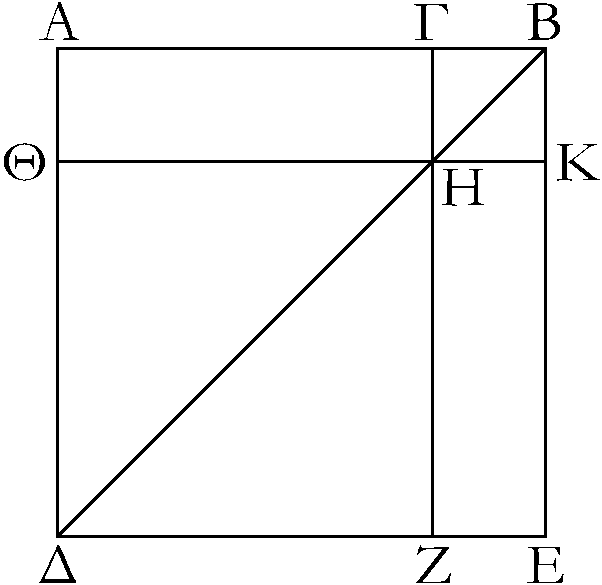
\includegraphics{Book02/fig04g.eps}}

\gr{Ἐὰν >άρα εὐθεῖα γραμμ\kern -.7pt  ὴ τμ\kern -.7pt  ηθῆ|, ὡξ >έτυθεν, τὸ ἀπὸ τῆξ <όληξ τετράγωνον >ίσον ἐστὶ τοῖξ τε ἀπὸ τῶν τμ\kern -.5pt  ημάτων τετραγώνοιξ καὶ τῶ| δὶξ ὑπὸ τῶν τμ\kern -.3pt  ημάτων περιεθομένῳ ὀρθογωνίῳ;
 <όπερ >έδει δεῖχαι.}}

\ParallelRText{
\begin{center}
{\large Proposition 4$^\dag$}
\end{center}

If a straight-line is cut at random,  (then) the square on the whole (straight-line)
is equal to the (sum of the) squares on the pieces (of the straight-line),  and twice the
rectangle contained by the pieces.

For let the straight-line $AB$ be cut, at random, at  (point) $C$. I say that the square on $AB$
is equal to the (sum of the) squares on $AC$ and $CB$, and twice the rectangle
contained by $AC$ and $CB$.

For let the square $ADEB$ be described on $AB$ [Prop.~1.46], and let $BD$ be joined, and let $CF$ be drawn through $C$, parallel to either of $AD$ or $EB$ [Prop.~1.31],
and let $HK$ be drawn through $G$, parallel to either of $AB$ or $DE$ [Prop.~1.31].
And since $CF$ is parallel to $AD$, and $BD$ has fallen across them, the external
angle $CGB$ is equal to the internal and opposite (angle) $ADB$ [Prop.~1.29].
But, $ADB$ is equal to $ABD$, since the side $BA$ is also equal to $AD$ [Prop.~1.5].
Thus, angle $CGB$ is also equal to $GBC$. So the side $BC$ is equal to the side $CG$ [Prop.~1.6]. But, $CB$ is equal to $GK$, and $CG$ to $KB$ [Prop.~1.34]. Thus, $GK$
is also equal to $KB$. Thus, $CGKB$ is equilateral. So I say that (it is) also right-angled. For since $CG$ is parallel to $BK$ [and the straight-line $CB$ has fallen across them], the angles $KBC$ and $GCB$ are thus equal to two 
right-angles
[Prop.~1.29]. But $KBC$ (is) a right-angle. Thus, 
$BCG$ (is) also a right-angle.
So the opposite (angles) $CGK$ and $GKB$ are also right-angles [Prop.~1.34]. Thus,
$CGKB$ is right-angled. And it was also shown (to be) equilateral. Thus,
it is a square. And it is on $CB$. So, for the same (reasons), $HF$ is  also a square.
And it is on $HG$, that is to say [on] $AC$ [Prop.~1.34]. Thus, the squares $HF$ and
$KC$ are on $AC$ and $CB$ (respectively). And  the (rectangle) $AG$ is
equal to the (rectangle) $GE$ [Prop.~1.43]. And $AG$ is  the (rectangle contained)
by $AC$ and $CB$. For $GC$ (is) equal to $CB$. Thus, $GE$ is also equal to the
(rectangle contained) by $AC$ and $CB$. Thus, the (rectangles)
$AG$ and $GE$ are equal to twice the (rectangle contained) by $AC$ and $CB$.
And $HF$ and $CK$ are the squares on $AC$ and $CB$ (respectively). Thus, the
four (figures) $HF$, $CK$, $AG$, and $GE$ are equal to the (sum of the) squares on $AC$ and
$BC$, and twice the rectangle contained by $AC$ and $CB$. But, the  (figures) $HF$, $CK$, $AG$, and $GE$ are (equivalent to) the whole of $ADEB$, which is the square on $AB$. 
Thus, the square on $AB$ is equal to the (sum of the) squares on $AC$ and $CB$, and twice
the rectangle contained by $AC$ and $CB$.

\epsfysize=2.2in
\centerline{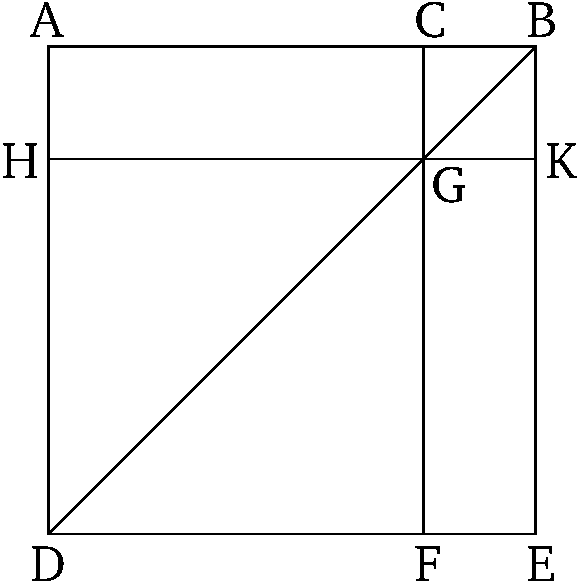
\includegraphics{Book02/fig04e.eps}}

Thus, if a straight-line is cut at random, (then) the square on the whole (straight-line) is equal to the (sum of the) squares on the pieces (of the
straight-line), and twice the
rectangle contained by the pieces. (Which is) the very thing it was required to
show.}
\end{Parallel}
{\footnotesize \noindent$^\dag$ This proposition is a geometric version
of the algebraic identity: $(a+b)^{\,2} = a^{\,2} + b^{\,2}+ 2\,a\,b$.}

%%%%%%
% Prop 2.5
%%%%%%
\pdfbookmark[1]{Proposition 2.5}{pdf2.5}
\begin{Parallel}{}{} 
\ParallelLText{
\begin{center}
{\large \ggn{5}.}
\end{center}\vspace*{-7pt}

\gr{Ἐὰν εὐθεῖα γραμμ\kern -.7pt  ὴ τμ\kern -.7pt  ηθῆ| εἰξ >ίσα καὶ >άνισα, τὸ ὑπὸ τῶν ἀνίσων τῆξ <όληξ τμ\kern -.5pt  ημάτων περιεχόμενον ὀρθογώνιον μετὰ τοῦ ἀπὸ τῆξ μεταχὺ τῶν τομῶν τετραγώνου >ίσον ἐστὶ τῶ|
ἀπὸ τῆξ ἡμισείαξ τετραγώνῳ.}\\

\epsfysize=1.8in
\centerline{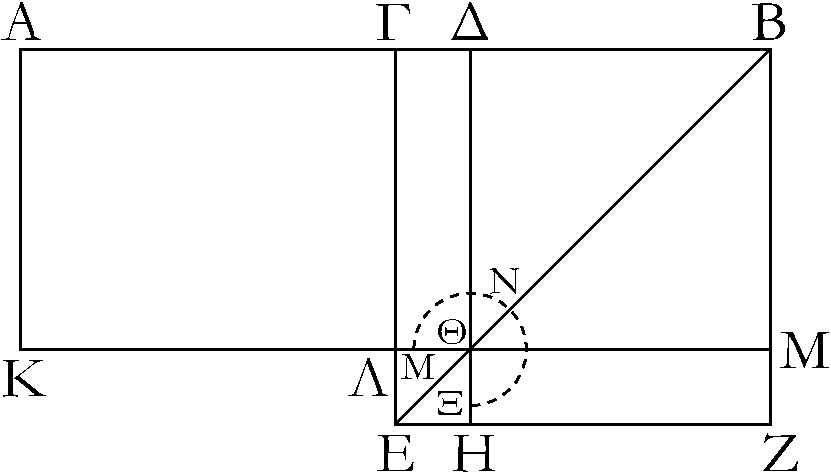
\includegraphics{Book02/fig05g.eps}}

\gr{Εὐθεῖα γάρ τιξ ἡ ΑΒ τετμ\kern -.7pt  ήσθω εἰξ μὲν >ίσα κατὰ τὸ Γ, εἰξ δὲ >άνισα κατὰ τὸ Δ; λέγω, <ότι τὸ ὑπὸ τῶν ΑΔ, ΔΒ περιεχόμενον ὀρθογώνιον μετὰ τοῦ ἀπὸ τῆξ ΓΔ τετραγώνου >ίσον ἐστὶ τῶ| ἀπὸ τῆξ ΓΒ τετραγώνῳ.}

\gr{Ἀναγεγράφθω γὰρ ἀπὸ τῆξ ΓΒ τετράγωνον τὸ ΓΕΖΒ, καὶ ἐπεζεύθθω ἡ ΒΕ, καὶ διὰ μὲν τοῦ Δ ὁποτέρᾳ τῶν ΓΕ, ΒΖ παράλληλοξ >ήθθω ἡ ΔΗ, διὰ δὲ τοῦ J ὁποτέρᾳ τῶν ΑΒ, ΕΖ παράλληλοξ πάλιν >ήθθω ἡ ΚΜ, καὶ πάλιν διὰ τοῦ Α ὁποτέρᾳ τῶν ΓΛ, ΒΜ παράλληλοξ >ήθθω ἡ ΑΚ. καὶ ἐπεὶ >ίσον ἐστὶ τὸ ΓJ παραπλήρωμα τῶ| JΖ παραπληρώματι, κοινὸν προσκείσθω τὸ ΔΜ; <όλον >άρα τὸ ΓΜ <όλῳ τῶ| ΔΖ >ίσον ἐστίν. ἀλλὰ τὸ ΓΜ τῶ| ΑΛ >ίσον ἐστίν, ἐπεὶ καὶ ἡ ΑΓ τῆ| ΓΒ ἐστιν >ίση; καὶ τὸ ΑΛ >άρα τῶ| ΔΖ >ίσον ἐστίν. κοινὸν προσκείσθω τὸ ΓJ; <όλον >άρα τὸ ΑJ τῶ| ΜΝΧ}$^{\,\dag}$ \gr{γνώμονι >ίσον ἐστίν. ἀλλὰ τὸ ΑJ τὸ ὑπὸ τῶν ΑΔ, ΔΒ ἐστιν; >ίση γὰρ ἡ ΔJ τῆ| ΔΒ; καὶ ὁ ΜΝΧ >άρα γνώμων 
>ίσοξ ἐστὶ τῶ| ὑπὸ ΑΔ, ΔΒ. κοινὸν προσκείσθω τὸ ΛΗ, <ό ἐστιν >ίσον τῶ| ἀπὸ τῆξ ΓΔ; ὁ >άρα ΜΝΧ γνώμων καὶ τὸ ΛΗ >ίσα ἐστὶ τῶ| 
ὑπὸ τῶν ΑΔ, ΔΒ περιεθομένῳ ὀρθογωνίῳ καὶ τῶ|
ἀπὸ τῆξ ΓΔ τετραγώνῳ. ἀλλὰ ὁ ΜΝΧ γνώμων 
καὶ τὸ ΛΗ  <όλον ἐστὶ τὸ ΓΕΖΒ τετράγωνον, <ό ἐστιν ἀπὸ τῆξ ΓΒ; τὸ >άρα ὑπὸ τῶν ΑΔ, ΔΒ περιεχόμενον ὀρθογώνιον μετὰ τοῦ ἀπὸ τῆξ ΓΔ τετραγώνου >ίσον ἐστὶ τῶ| ἀπὸ τῆξ ΓΒ τετραγώνῳ.}

\gr{Ἐὰν >άρα εὐθεῖα γραμμ\kern -.7pt  ὴ τμ\kern -.7pt  ηθῆ| εἰξ >ίσα καὶ >άνισα, τὸ ὑπὸ τῶν
ἀνίσων τῆξ <όληξ τμ\kern -.5pt  ημάτων περιεχόμενον ὀρθογώνιον μετὰ τοῦ ἀπὸ τῆξ μεταχὺ τῶν τομῶν τετραγώνου >ίσον ἐστὶ τῶ|
ἀπὸ τῆξ ἡμισείαξ τετραγώνῳ. <όπερ >έδει δεῖχαι.}}

\ParallelRText{
\begin{center}
{\large Proposition 5$^\ddag$}
\end{center}

If a straight-line is cut into equal and unequal (pieces, then) the rectangle contained by the
unequal pieces of the whole (straight-line), plus the square on the (difference) between the (equal and unequal)
pieces, is equal to the square on  half (of the straight-line).

\epsfysize=1.8in
\centerline{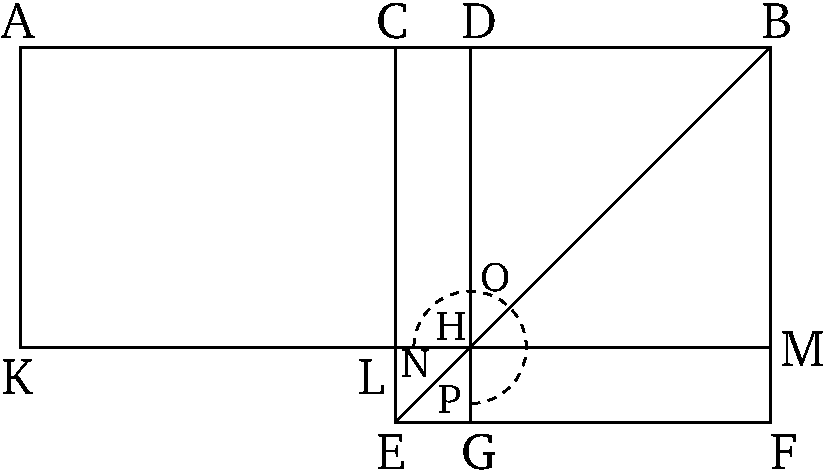
\includegraphics{Book02/fig05e.eps}}

For let any straight-line $AB$ be cut---equally at $C$, and unequally at $D$.
I say that the rectangle contained by $AD$ and $DB$, plus the square
on $CD$, is equal to the square on $CB$.

For let the square $CEFB$ be described on $CB$ [Prop.~1.46], and
let $BE$ be joined,
and let $DG$ 
be  drawn through $D$, parallel to either of $CE$ or $BF$ [Prop.~1.31], and again let $KM$
be drawn through $H$, parallel to either of $AB$ or $EF$ [Prop.~1.31], and again let
$AK$ be drawn through $A$, parallel to either of $CL$ or $BM$ [Prop.~1.31].
And since the complement $CH$ is equal to the complement $HF$ [Prop.~1.43],
let the (square) $DM$ be added to both. Thus, the whole (rectangle) $CM$ is equal to the whole (rectangle) $DF$. But, (rectangle) $CM$ is equal to (rectangle) $AL$, since $AC$ is
also equal to $CB$ [Prop.~1.36]. Thus, (rectangle) $AL$ is also equal to (rectangle) $DF$.
Let (rectangle) $CH$ be added to both. Thus, the whole (rectangle)
$AH$ is equal to the gnomon $NOP$. But,  $AH$ is the (rectangle
contained) by $AD$ and $DB$. For $DH$ (is) equal to $DB$. Thus, the
gnomon $NOP$ is also equal to the (rectangle contained) by $AD$ and $DB$. Let
$LG$, which is equal to the (square) on $CD$,  be added to both.
Thus, the gnomon $NOP$ and the (square) $LG$ are equal to the rectangle contained by
$AD$ and $DB$, and the square on $CD$. But, the gnomon $NOP$ and
the (square) $LG$ is (equivalent to) the whole square $CEFB$, which is on $CB$. Thus, the rectangle contained
by $AD$ and $DB$, plus the square on $CD$, is equal to the square on $CB$.

Thus, if a straight-line is cut into equal and unequal (pieces, then) the rectangle contained by the
unequal pieces of the whole  (straight-line), plus the square on the (difference) between the (equal and unequal)
pieces, is equal to the square on  half (of the straight-line). (Which is) the
very thing it was required to show.}
\end{Parallel}
{\footnotesize \noindent$^\dag$ Note the (presumably mistaken) double use of the label $M$ in the Greek text.\\[0.5ex]
$^\ddag$ This proposition is a geometric version
of the algebraic identity: $a\,b +[(a+b)/2-b]^{\,2} = [(a+b)/2]^{\,2}$.}

%%%%%%
% Prop 2.6
%%%%%%
\pdfbookmark[1]{Proposition 2.6}{pdf2.6}
\begin{Parallel}{}{} 
\ParallelLText{
\begin{center}
{\large \ggn{6}.}
\end{center}\vspace*{-7pt}

\gr{Ἐὰν εὐθεῖα γραμμ\kern -.7pt  ὴ τμ\kern -.7pt  ηθῆ| δίθα, προστεθῆ| δέ τιξ α\kern -.5pt  ὐτῆ| εὐθεῖα ἐπ> εὐθείαξ, τὸ ὑπὸ τῆξ <όληξ σὺν τῆ| προσκειμένῃ καὶ τῆξ προσκειμένηξ περιεχόμενον ὀρθόγώνιον μετὰ τοῦ ἀπὸ τῆξ ἡμισείαξ τετραγώνου >ίσον ἐστὶ τῶ| ἀπὸ τῆξ συγκειμένηξ >έκ τε τῆξ ἡμισείαξ καὶ τῆξ προσκειμένηξ τετραγώνῳ.}\\~\\

\epsfysize=1.8in
\centerline{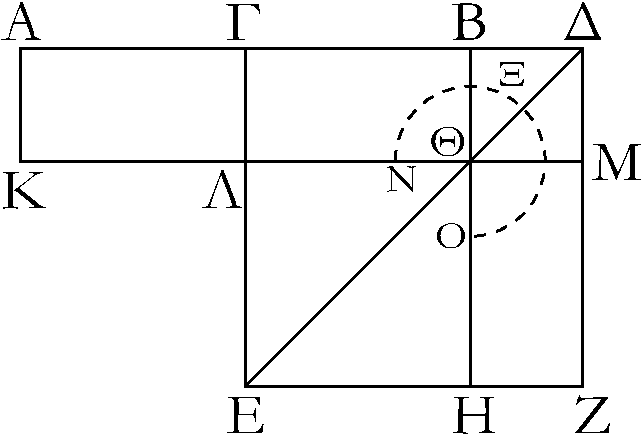
\includegraphics{Book02/fig06g.eps}}

\gr{Εὐθεῖα γάρ τιξ ἡ ΑΒ τετμ\kern -.7pt  ήσθω δίθα κατὰ τὸ Γ σημεῖον, προσκείσθω δέ τιξ α\kern -.7pt  ὐτῆ| εὐθεῖα ἐπ> εὐθείαξ ἡ ΒΔ; λέγω, <ότι τὸ ὑπὸ τῶν ΑΔ, ΔΒ περιεχόμενον ὀρθογώνιον μετὰ τοῦ ἀπὸ τῆξ ΓΒ
τετραγώνου >ίσον ἐστὶ τῶ| ἀπὸ τῆξ ΓΔ τετραγώνῳ.}

\gr{Ἀναγεγράφθω γὰρ ἀπὸ τῆξ ΓΔ τετράγωνον τὸ ΓΕΖΔ, καὶ ἐπεζεύθθω
ἡ ΔΕ, καὶ διὰ μὲν τοῦ Β σημείου ὁποτέρᾳ τῶν ΕΓ, ΔΖ παράλληλοξ >ήθθω ἡ ΒΗ, διὰ δὲ τοῦ J σημείου ὁποτέρᾳ τῶν ΑΒ, ΕΖ παράλληλοξ >ήθθω ἡ ΚΜ, καὶ >έτι διὰ τοῦ Α ὁποτέρᾳ τῶν ΓΛ, ΔΜ παράλληλοξ >ήθθω ἡ ΑΚ.}

\gr{Ἐπεὶ ο>ῦν >ίση ἐστὶν  ἡ ΑΓ τῆ| ΓΒ, >ίσον ἐστὶ καὶ τὸ ΑΛ τῶ| ΓJ. ἀλλὰ τὸ ΓJ τῶ| JΖ >ίσον ἐστίν. καὶ τὸ ΑΛ >άρα τῶ| JΖ ἐστιν >ίσον.
κοινὸν προσκείσθω τὸ ΓΜ; <όλον >άρα τὸ ΑΜ τῶ| ΝΧΟ γνώμονί ἐστιν >ίσον. ἀλλὰ τὸ ΑΜ ἐστι τὸ ὑπὸ τῶν ΑΔ, ΔΒ; >ίση γάρ ἐστιν ἡ ΔΜ τῆ| ΔΒ; καὶ ὁ ΝΧΟ >άρα γνώμων >ίσοξ ἐστὶ τῶ| ὑπὸ τῶν ΑΔ, ΔΒ
[περιεθομένῳ ὀρθογωνίῳ]. κοινὸν προσκείσθω τὸ ΛΗ, <ό ἐστιν >ίσον τῶ| ἀπὸ τῆξ ΒΓ τετραγώνῳ; τὸ >άρα ὑπὸ τῶν
ΑΔ, ΔΒ περιεχόμενον ὀρθογώνιον μετὰ τοῦ ἀπὸ τῆξ ΓΒ τετραγώνου 
>ίσον ἐστὶ τῶ| ΝΧΟ γνώμονι καὶ τῶ| ΛΗ. ἀλλὰ ὁ ΝΧΟ γνώμων καὶ τὸ ΛΗ <όλον ἐστὶ τὸ ΓΕΖΔ τετράγωνον, <ό ἐστιν ἀπὸ τῆξ ΓΔ; τὸ >άρα ὑπὸ τῶν ΑΔ, ΔΒ περιεχόμενον ὀρθογώνιον μετὰ τοῦ ἀπὸ τῆξ ΓΒ τετραγώνου >ίσον ἐστὶ τῶ| ἀπὸ τῆξ ΓΔ τετραγώνῳ.}

\gr{Ἐὰν >άρα εὐθεῖα γραμμ\kern -.7pt  ὴ τμ\kern -.7pt  ηθῆ| δίθα, προστεθῆ| δέ τιξ α\kern -.5pt  ὐτῆ| εὐθεῖα ἐπ> εὐθείαξ, τὸ ὑπὸ τῆξ <όληξ σὺν τῆ| προσκειμένῃ καὶ τῆξ προσκειμένηξ περιεχόμενον ὀρθόγώνιον μετὰ τοῦ ἀπὸ τῆξ ἡμισείαξ τετραγώνου >ίσον ἐστὶ τῶ| ἀπὸ τῆξ συγκειμένηξ >έκ τε τῆξ ἡμισείαξ καὶ τῆξ προσκειμένηξ τετραγώνῳ; <όπερ >έδει δεῖχαι.}}

\ParallelRText{
\begin{center}
{\large Proposition 6$^\dag$}
\end{center}

If a straight-line is cut in half, and any straight-line added to it straight-on,
(then) the rectangle contained by the whole (straight-line) with the (straight-line) having being added, and the (straight-line) having being added,   plus the square on  half (of the original straight-line), is equal to the square on the
sum of  half  (of the original straight-line) and the (straight-line) having been added.

\epsfysize=1.8in
\centerline{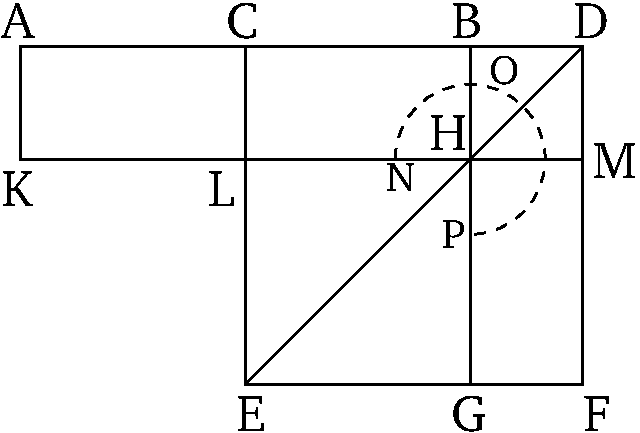
\includegraphics{Book02/fig06e.eps}}

For let any straight-line $AB$ be cut in half at point $C$, and let any
straight-line $BD$ be added to it straight-on. I say that the rectangle
contained by $AD$ and $DB$, plus the square on $CB$, is equal to the square on
$CD$.

For let the square $CEFD$ be described on $CD$ [Prop.~1.46], and let $DE$ be
joined, and let $BG$ be drawn through point $B$, parallel to either of $EC$
or $DF$ [Prop.~1.31], and let $KM$ be drawn through point $H$, parallel
to either of $AB$ or $EF$ [Prop.~1.31], and finally let $AK$ be drawn
through $A$, parallel to either of $CL$ or $DM$ [Prop.~1.31].

Therefore, since $AC$ is equal to $CB$, (rectangle) $AL$ is also equal to (rectangle) $CH$ [Prop.~1.36]. But, (rectangle) $CH$ is equal to (rectangle) $HF$ [Prop.~1.43]. Thus, (rectangle) $AL$ is also equal to (rectangle) $HF$. Let (rectangle) $CM$ 
be  added to both. Thus, the whole (rectangle) $AM$ is equal to the gnomon $NOP$.
But, $AM$ is  the (rectangle contained) by $AD$ and $DB$. For
$DM$ is equal to $DB$. Thus, gnomon $NOP$ is also equal to the
[rectangle contained] by $AD$ and $DB$.
Let $LG$, which is equal to the square on $BC$, be added to both.
Thus, the rectangle contained by $AD$ and $DB$, plus the square on $CB$, is equal
to the gnomon $NOP$ and the (square) $LG$. But the gnomon $NOP$ and 
the (square) $LG$ is (equivalent to) the whole square $CEFD$, which is on  $CD$. Thus, the rectangle
contained by $AD$ and $DB$, plus the square on $CB$, is equal to the square on $CD$.

Thus, if a straight-line is cut in half, and any straight-line added to it straight-on,
(then) the rectangle contained by the whole (straight-line) with the (straight-line) having being added, and the (straight-line) having being added,   plus the square on  half (of the original straight-line), is equal to the square on the
sum of  half  (of the original straight-line) and the (straight-line) having been added. (Which is) the very thing it was required to show.}
\end{Parallel}
{\footnotesize \noindent$^\dag$ This proposition is a geometric version
of the algebraic identity: $(2\,a+b)\,b + a^{\,2} = (a+b)^{\,2}$.}

%%%%%%
% Prop 2.7
%%%%%%
\pdfbookmark[1]{Proposition 2.7}{pdf2.7}
\begin{Parallel}{}{} 
\ParallelLText{
\begin{center}
{\large \ggn{7}.}
\end{center}\vspace*{-7pt}

\gr{Ἐὰν εὐθεῖα γραμμ\kern -.7pt  ὴ  τμ\kern -.7pt  ηθῆ|, ὡξ >έτυθεν, τὸ ἀπὸ τῆξ <όληξ καὶ τὸ ἀφ> ἑνὸξ τῶν τμ\kern -.5pt  ημάτων τὰ συναμφότερα τετράγωνα >ίσα ἐστὶ τῶ| τε δὶξ ὑπὸ τῆξ <όληξ καὶ τοῦ εἰρημένου τμ\kern -.3pt  ήματοξ περιεθομένῳ ὀρθογωνίῳ καὶ τῶ| ἀπὸ τοῦ λοιποῦ τμ\kern -.7pt  ήματοξ τετραγώνῳ.}

\epsfysize=2.2in
\centerline{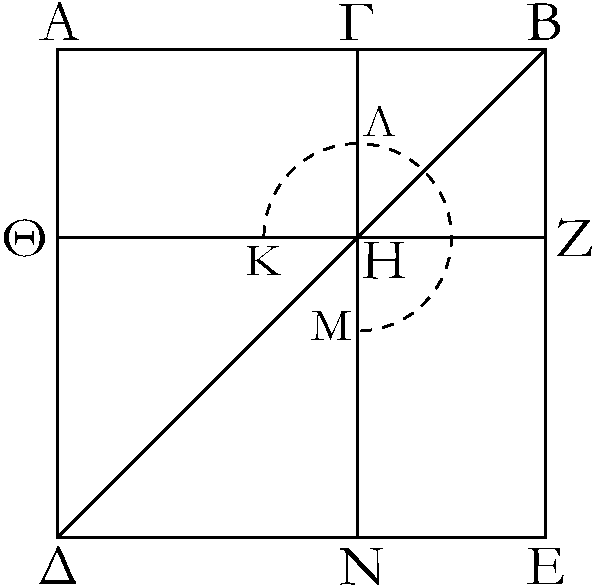
\includegraphics{Book02/fig07g.eps}}

\gr{Εὐθεῖα γάρ τιξ ἡ ΑΒ τετμ\kern -.7pt  ήσθω, ὡξ >έτυθεν, κατὰ τὸ Γ σημεῖον; λέγω, <ότι τὰ ἀπὸ τῶν ΑΒ, ΒΓ τετράγωνα >ίσα ἐστὶ τῶ| τε δὶξ ὑπὸ τῶν
ΑΒ, ΒΓ περιεθομένῳ ὀρθογωνίῳ καὶ τῶ| ἀπὸ τῆξ ΓΑ τετραγώνῳ.}

\gr{Ἀναγεγράφθω γὰρ ἀπὸ τῆξ ΑΒ τετράγωνον τὸ ΑΔΕΒ; καὶ καταγεγράφθω τὸ σθῆμα.}

\gr{Ἐπεὶ ο>ῦν >ίσον ἐστὶ τὸ ΑΗ τῶ| ΗΕ, κοινὸν προσκείσθω τὸ ΓΖ; <όλον >άρα τὸ ΑΖ <όλῳ τῶ| ΓΕ >ίσον ἐστίν; τὰ >άρα ΑΖ, ΓΕ διπλάσιά ἐστι τοῦ ΑΖ. ἀλλὰ τὰ ΑΖ, ΓΕ ὁ ΚΛΜ ἐστι γνώμων καὶ τὸ ΓΖ
τετράγωνον; ὁ ΚΛΜ >άρα γνώμων καὶ τὸ ΓΖ διπλάσιά ἐστι τοῦ ΑΖ. >έστι δὲ τοῦ ΑΖ διπλάσιον καὶ τὸ δὶξ ὑπὸ τῶν ΑΒ, ΒΓ;
>ίση γὰρ ἡ ΒΖ τῆ| ΒΓ; ὁ >άρα ΚΛΜ γνώμων καὶ τὸ ΓΖ τετράγωνον
>ίσον  ἐστὶ τῶ| δὶξ ὑπὸ τῶν ΑΒ, ΒΓ.
 κοινὸν προσκείσθω τὸ ΔΗ, <ό ἐστιν ἀπὸ τῆξ ΑΓ τετράγωνον; ὁ >άρα ΚΛΜ
γνώμων καὶ τὰ ΒΗ, ΗΔ τετράγωνα >ίσα ἐστὶ τῶ| τε δὶξ ὑπὸ τῶν ΑΒ, ΒΓ περιεθομένῳ ὀρθογωνίῳ  καὶ τῶ| ἀπὸ τῆξ ΑΓ τετραγώνῳ.
ἀλλὰ ὁ ΚΛΜ γνώμων καὶ τὰ ΒΗ, ΗΔ τετράγωνα <όλον ἐστὶ τὸ ΑΔΕΒ καὶ τὸ ΓΖ,  <ά ἐστιν ἀπὸ τῶν ΑΒ, ΒΓ
 τετράγωνα; τὰ >άρα ἀπὸ τῶν ΑΒ, ΒΓ 
 τετράγωνα >ίσα ἐστὶ τῶ| [τε] δὶξ ὑπὸ τῶν ΑΒ, ΒΓ 
 περιεθομένῳ ὀρθογωνίῳ μετὰ τοῦ ἀπὸ τῆξ ΑΓ τετραγώνου.}
 
 \gr{Ἐὰν >άρα εὐθεῖα γραμμ\kern -.7pt  ὴ  τμ\kern -.7pt  ηθῆ|, ὡξ >έτυθεν, τὸ ἀπὸ τῆξ <όληξ καὶ τὸ ἀφ> ἑνὸξ τῶν τμ\kern -.5pt  ημάτων τὰ συναμφότερα τετράγωνα >ίσα ἐστὶ τῶ| τε δὶξ ὑπὸ τῆξ <όληξ καὶ τοῦ εἰρημένου τμ\kern -.3pt  ήματοξ περιεθομένῳ ὀρθογωνίῳ καὶ τῶ| ἀπὸ τοῦ λοιποῦ τμ\kern -.7pt  ήματοξ τετραγώνῳ; <όπερ >έδει δεῖχαι.}}

\ParallelRText{
\begin{center}
{\large Proposition 7$^\dag$}
\end{center}

If a straight-line is cut at random, (then) the sum of the squares on the
whole (straight-line), and one of the pieces (of the straight-line),  is equal to twice the rectangle
contained by the whole, and the said piece, and the square
on the remaining piece.

\epsfysize=2.2in
\centerline{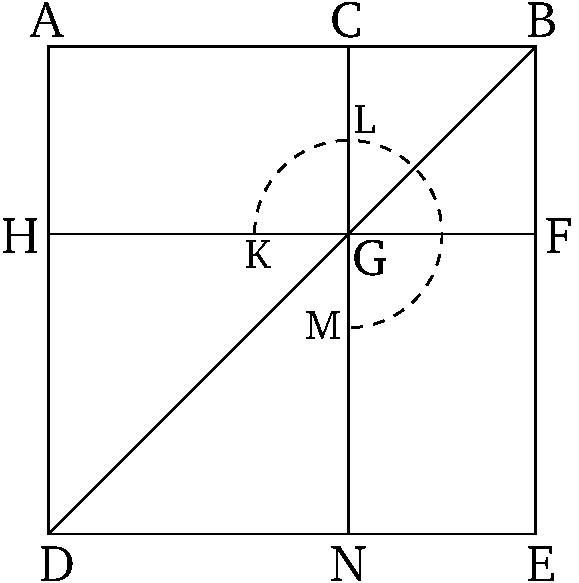
\includegraphics{Book02/fig07e.eps}}

For let any straight-line $AB$ be cut, at random, at point $C$.
I say that the (sum of the) squares on $AB$ and $BC$ is equal to
twice the rectangle contained by $AB$ and $BC$, and the square on $CA$.

For let the square $ADEB$ be described on $AB$ [Prop.~1.46], and let the (rest of)
the figure be  drawn.

Therefore, since (rectangle) $AG$ is equal to (rectangle) $GE$ [Prop.~1.43],
let the (square) $CF$ be added to both. Thus, the
whole (rectangle) $AF$ is equal to the whole (rectangle) $CE$.
Thus, (rectangle) $AF$ plus (rectangle) $CE$ is double (rectangle) $AF$.
But, (rectangle) $AF$ plus (rectangle) $CE$ is the gnomon $KLM$, and the
square  $CF$. Thus, the gnomon $KLM$, and the square $CF$, is double the (rectangle)
$AF$.
But double the (rectangle) $AF$ is also twice the (rectangle contained)
by $AB$ and $BC$. For $BF$ (is) equal to $BC$. Thus, the gnomon $KLM$, and
the square $CF$, are equal to twice the (rectangle contained) by $AB$ and $BC$.
Let $DG$, which is the square on $AC$, be added to both.
Thus, the gnomon $KLM$, and the squares $BG$ and $GD$, are equal to
twice the rectangle contained by $AB$ and $BC$, and the square on $AC$.
But, the gnomon $KLM$ and the squares $BG$ and $GD$ is (equivalent to)
the whole of
$ADEB$ and $CF$, which are the squares on $AB$ and $BC$ (respectively).
Thus, the (sum of the) squares on $AB$ and $BC$ is equal to
twice the rectangle contained by $AB$ and $BC$, and the square on $AC$.

Thus, if a straight-line is cut at random, (then) the sum of the squares on the
whole (straight-line), and one of the pieces (of the straight-line), is equal to twice the rectangle
contained by the whole,  and the said piece, and the square
on the remaining piece. (Which is) the very thing it was required to show.}
\end{Parallel}
{\footnotesize \noindent$^\dag$ This proposition is a geometric version
of the algebraic identity: $(a+b)^{\,2}+a^2 =2\,(a+b)\,a+b^{\,2}$.}

%%%%%%
% Prop 2.8
%%%%%%
\pdfbookmark[1]{Proposition 2.8}{pdf2.8}
\begin{Parallel}{}{} 
\ParallelLText{
\begin{center}
{\large \ggn{8}.}
\end{center}\vspace*{-7pt}

\gr{Ἐὰν εὐθεῖα γραμμ\kern -.7pt  ὴ τμ\kern -.7pt  ηθῆ|, ὡξ >έτυθεν, τὸ τετράκιξ ὑπὸ τῆξ <όληξ καὶ ἑνὸξ τῶν τμ\kern -.5pt  ημάτων περιεχόμενον ὀρθογώνιον μετὰ τοῦ ἀπὸ τοῦ λοιποῦ τμ\kern -.3pt  ήματοξ τετραγώνου >ίσον ἐστὶ τῶ| ἀπό τε τῆξ <όληξ καὶ τοῦ εἰρημένου τμ\kern -.7pt  ήματοξ ὡξ ἀπὸ μιᾶξ ἀναγραφέντι τετραγώνῳ.}

\gr{Εὐθεῖα γάρ τιξ ἡ ΑΒ τετμ\kern -.7pt  ήσθω, ὡξ >έτυθεν, κατὰ τὸ Γ σημεῖον; λέγω, <ότι τὸ τετράκιξ ὑπὸ τῶν ΑΒ, ΒΓ περιεχόμενον ὀρθογώνιον μετὰ τοῦ ἀπὸ τῆξ ΑΓ τετραγώνου >ίσον ἐστὶ τῶ| ἀπὸ τῆξ ΑΒ, ΒΓ ὡξ ἀπὸ μιᾶξ ἀναγραφέντι τετραγώνῳ.}

\gr{Ἐκβεβλήσθω γὰρ ἐπ> εὐθείαξ [τῆ| ΑΒ εὐθεῖα] ἡ ΒΔ, καὶ κείσθω τῆ| ΓΒ >ίση ἡ ΒΔ, καὶ ἀναγεγράφθω ἀπὸ τῆξ ΑΔ τετράγωνον τὸ ΑΕΖΔ, καὶ καταγεγράφθω διπλοῦν τὸ σθῆμα.}\\

\epsfysize=2.5in
\centerline{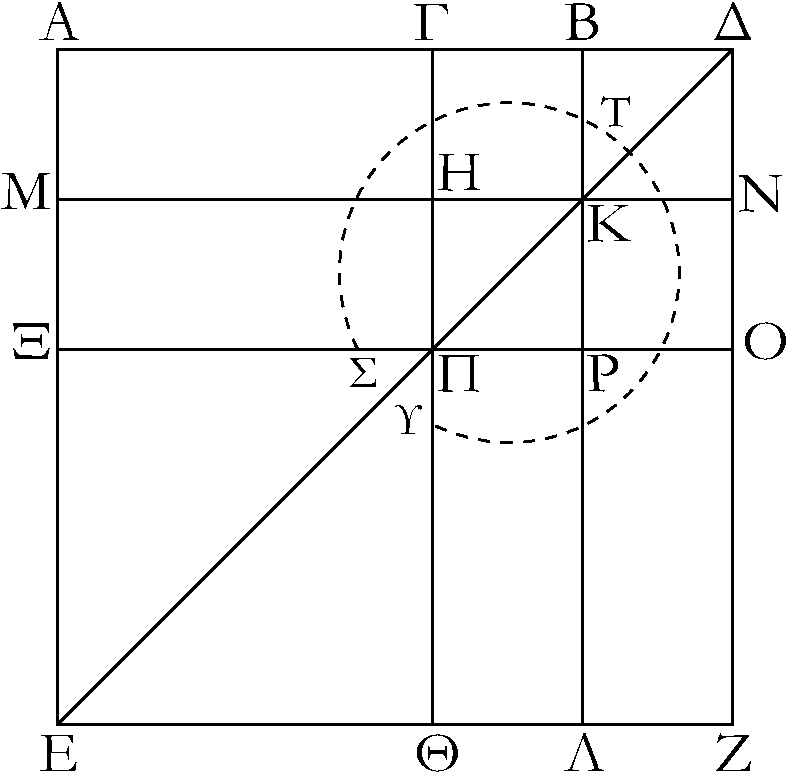
\includegraphics{Book02/fig08g.eps}}

\gr{Ἐπεὶ ο>ῦν >ίση ἐστὶν ἡ ΓΒ τῆ| ΒΔ, ἀλλὰ ἡ μὲν ΓΒ τῆ| ΗΚ ἐστιν >ίση, ἡ δὲ ΒΔ τῆ| ΚΝ, καὶ ἡ ΗΚ >άρα τῆ| ΚΝ ἐστιν >ίση. διὰ τὰ α\kern -.7pt  ὐτὰ δὴ καὶ ἡ ΠΡ τῆ| ΡΟ ἐστιν >ίση. καὶ ἐπεὶ >ίση ἐστὶν ἡ ΒΓ
τὴ| ΒΔ, ἡ δὲ ΗΚ τῆ| ΚΝ, >ίσον >άρα ἐστὶ καὶ τὸ μὲν ΓΚ τῶ| ΚΔ, τὸ δὲ ΗΡ τῶ| ΡΝ. ἀλλὰ τὸ ΓΚ τῶ| ΡΝ ἐστιν >ίσον; παραπληρώματα γὰρ τοῦ ΓΟ παραλληλογράμμου; καὶ τὸ ΚΔ >άρα τῶ| ΗΡ >ίσον ἐστίν; τὰ τέσσαρα >άρα τὰ ΔΚ, ΓΚ, ΗΡ, ΡΝ >ίσα ἀλλήλοιξ ἐστίν. τὰ τέσσαρα >άρα τετραπλάσιά ἐστι τοῦ ΓΚ. πάλιν ἐπεὶ >ίση ἐστὶν ἡ ΓΒ τῆ| ΒΔ, ἀλλὰ ἡ μὲν ΒΔ τῆ| ΒΚ, τουτέστι τῆ| ΓΗ >ίση, ἡ δὲ ΓΒ τῆ| ΗΚ, τουτέστι
τῆ| ΗΠ, ἐστιν >ίση, καὶ ἡ ΓΗ >άρα τῆ| ΗΠ >ίση ἐστίν. καὶ ἐπεὶ >ίση
ἐστὶν ἡ μὲν ΓΗ τῆ| ΗΠ, ἡ δὲ ΠΡ τῆ| ΡΟ, >ίσον ἐστὶ καὶ τὸ μὲν ΑΗ τῶ| ΜΠ, τὸ δὲ ΠΛ τῶ| ΡΖ. ἀλλὰ τὸ ΜΠ τῶ| ΠΛ ἐστιν >ίσον;
παραπληρώματα γὰρ τοῦ ΜΛ παραλληλογράμμου; καὶ τὸ ΑΗ >άρα τῶ| ΡΖ
>ίσον ἐστίν; τὰ τέσσαρα >άρα τὰ ΑΗ, ΜΠ, ΠΛ, ΡΖ
>ίσα ἀλλήλοιξ ἐστίν; τὰ τέσσαρα >άρα τοῦ ΑΗ ἐστι τετραπλάσια. ἐδείθθη
δὲ καὶ τὰ τέσσαρα τὰ ΓΚ, ΚΔ, ΗΡ, ΡΝ τοῦ ΓΚ τετραπλάσια; τὰ >άρα ὀκτώ,
<ὰ περιέθει τὸν ΣΤΥ γνώμονα, τετραπλάσιά ἐστι τοῦ ΑΚ. καὶ ἐπεὶ τὸ ΑΚ τὸ ὑπὸ τῶν ΑΒ, ΒΔ ἐστιν; >ίση γὰρ ἡ ΒΚ τῆ| ΒΔ; τὸ >άρα τετράκιξ ὑπὸ τῶν ΑΒ, ΒΔ τετραπλάσιόν ἐστι τοῦ ΑΚ. ἐδείθθη δὲ τοῦ
ΑΚ τετραπλάσιοξ καὶ ὁ ΣΤΥ γνώμων; τὸ >άρα  τετράκιξ ὑπὸ τῶν
ΑΒ, ΒΔ >ίσον ἐστὶ τῶ| ΣΤΥ γνώμονι. κοινὸν προσκείσθω τὸ ΧJ, <ό ἐστιν >ίσον τῶ| ἀπὸ τῆξ ΑΓ τετραγώνῳ; τὸ  >άρα τετράκιξ  ὑπὸ τῶν  ΑΒ,  ΒΔ περιεχόμενον ὀρθογώνιον μετὰ τοῦ ἀπὸ ΑΓ τετραγώνου >ίσον ἐστὶ τῶ| ΣΤΥ γνώμονι καὶ τῶ| ΧJ. ἀλλὰ ὁ ΣΤΥ γνώμων
καὶ τὸ ΧJ <όλον ἐστὶ τὸ ΑΕΖΔ τετράγωνον, <ό ἐστιν ἀπὸ τῆξ ΑΔ; τὸ >άρα τετράκιξ ὑπὸ τῶν ΑΒ, ΒΔ μετὰ τοῦ ἀπὸ ΑΓ >ίσον ἐστὶ τῶ| ἀπὸ ΑΔ τετραγώνῳ; >ίση δὲ ἡ ΒΔ τῆ| ΒΓ. τὸ >άρα τετράκιξ ὑπὸ τῶν ΑΒ, ΒΓ 
περιεχόμενον ὀρθογώνιον μετὰ τοῦ ἀπὸ ΑΓ τετραγώνου >ίσον ἐστὶ τῶ| ἀπὸ τῆξ ΑΔ, τουτέστι τῶ| ἀπὸ τῆξ ΑΒ καὶ ΒΓ ὡξ ἀπὸ μιᾶξ ἀναγραφέντι τετραγώνῳ.}

\gr{Ἐὰν >άρα  εὐθεῖα γραμμ\kern -.7pt  ὴ τμ\kern -.7pt  ηθῆ|, ὡξ >έτυθεν, τὸ τετράκιξ ὑπὸ τῆξ <όληξ καὶ ἑνὸξ τῶν τμ\kern -.5pt  ημάτων περιεχόμενον ὀρθογώ\-νιον μετὰ τοῦ ἀπὸ τοῦ λοιποῦ τμ\kern -.3pt  ήματοξ τετραγώνου >ίσου ἐστὶ τῶ| ἀπό τε τῆξ <όληξ καὶ τοῦ εἰρημένου τμ\kern -.7pt  ήματοξ ὡξ ἀπὸ μιᾶξ ἀναγραφέντι τετραγώνῳ;  <όπερ >έδει δεῖχαι.}}

\ParallelRText{
\begin{center}
{\large Proposition 8$^\dag$}
\end{center}

If a straight-line is cut at random, (then) four times the rectangle contained
by the whole (straight-line), and one of the pieces (of the straight-line), plus the square on the remaining piece,
is equal to the square described on the whole and the former piece, as
on one (complete straight-line).

For let any straight-line $AB$ be cut, at random, at point $C$. I say that
four times the rectangle contained by $AB$ and $BC$, plus the square on $AC$,
is equal to the square described on $AB$ and $BC$,  as on one (complete straight-line).

For let $BD$ be produced in a straight-line [with the straight-line $AB$],
and let $BD$ be made equal to $CB$ [Prop.~1.3], and let the square $AEFD$
be described on $AD$ [Prop.~1.46], and let the (rest of the) figure
be drawn double.

\epsfysize=2.5in
\centerline{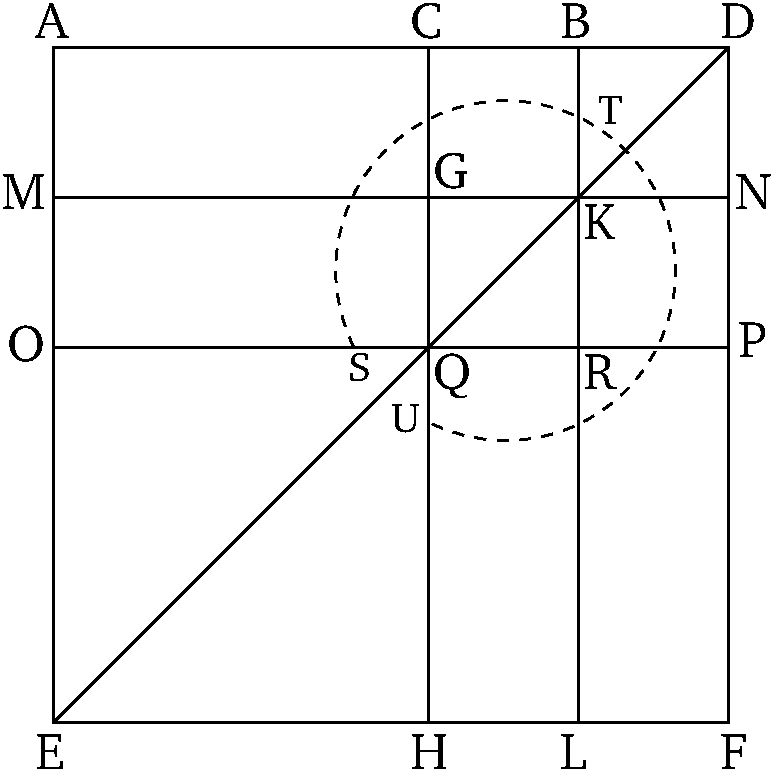
\includegraphics{Book02/fig08e.eps}}

Therefore, since $CB$ is equal to $BD$, but $CB$ is equal to $GK$ [Prop.~1.34], and $BD$ to
$KN$ [Prop.~1.34], $GK$ is thus also equal to $KN$. So, for the same (reasons), $QR$ is equal
to $RP$. And since $BC$ is equal to $BD$, and $GK$ to $KN$, (square) $CK$ is thus
also equal to (square) $KD$, and (square) $GR$ to (square) $RN$ [Prop.~1.36]. But,
(square) $CK$ is equal to (square) $RN$. For (they are) complements
in the parallelogram $CP$ [Prop.~1.43]. Thus, (square) $KD$ is also equal
to (square) $GR$. Thus, the four (squares)
$DK$, $CK$, $GR$, and $RN$ are equal to one another. Thus, the four (taken
together) are quadruple (square) $CK$. Again, since $CB$ is equal to $BD$, but
$BD$ (is) equal to $BK$---that is to say, $CG$---and $CB$ is equal to $GK$---that is
to say, $GQ$---$CG$ is thus also equal to $GQ$. And since
$CG$ is equal to $GQ$, and $QR$ to $RP$, (rectangle) $AG$ is also equal to
(rectangle) $MQ$, and (rectangle) $QL$ to (rectangle) $RF$ [Prop.~1.36]. But, (rectangle)
$MQ$ is equal to (rectangle) $QL$. For (they are) complements in the parallelogram $ML$ [Prop.~1.43]. Thus, 
(rectangle) $AG$ is also equal  to (rectangle) $RF$. Thus, the four (rectangles) $AG$, $MQ$, $QL$, and $RF$ are equal
to one another. Thus, the four (taken together)
 are quadruple (rectangle)
$AG$. And it was also shown that the four (squares)
$CK$, $KD$, $GR$, and $RN$ (taken together are) quadruple (square) $CK$. 
Thus, the eight (figures taken together), which comprise the gnomon $STU$,
are quadruple (rectangle) $AK$. And since $AK$ is the (rectangle contained)
by $AB$ and $BD$, for $BK$ (is) equal to $BD$, four times the (rectangle contained)
by $AB$ and $BD$ is quadruple (rectangle) $AK$. But the gnomon $STU$ was also shown (to be equal to) quadruple (rectangle)
$AK$. Thus, four times the
(rectangle contained) by $AB$ and $BD$ is equal to the gnomon $STU$. 
Let $OH$, which is equal to the square on $AC$,  be added to both.  
Thus, four times  the
rectangle contained by $AB$ and $BD$, plus the square on $AC$, is equal to
the gnomon $STU$, and the (square) $OH$. But, the  gnomon $STU$
and the (square) $OH$ is (equivalent to) the whole square $AEFD$, which is on
$AD$. Thus, four times the (rectangle contained) by $AB$ and $BD$, plus
the (square) on $AC$, is equal to the square on $AD$.
And $BD$ (is) equal to $BC$. Thus, four times the rectangle contained by $AB$ and $BC$, plus the square on $AC$, is equal to the (square) on $AD$, that is to
say the square described on $AB$ and $BC$,  as on one (complete straight-line).

Thus, if a straight-line is cut at random, (then) four times the rectangle contained
by the whole (straight-line), and one of the pieces (of the straight-line), plus the square on the remaining piece,
is equal to  the square described on the whole and the former piece, as
on one (complete straight-line). (Which is) the very thing it was required to show.}
\end{Parallel}
{\footnotesize \noindent$^\dag$ This proposition is a geometric version
of the algebraic identity: $4\,(a+b)\,a+b^{\,2} = \left[(a+b)+a\right]^{\,2}$.}

%%%%%%
% Prop 2.9
%%%%%%
\pdfbookmark[1]{Proposition 2.9}{pdf2.9}
\begin{Parallel}{}{} 
\ParallelLText{
\begin{center}
{\large \ggn{9}.}
\end{center}\vspace*{-7pt}

\gr{Ἐὰν εὐθεῖα γραμμ\kern -.7pt  ὴ τμ\kern -.7pt  ηθῆ| εἰξ >ίσα καὶ >άνισα, τὰ ἀπὸ τῶν ἀνίσων τῆξ <όληξ τμ\kern -.5pt  ημάτων τετράγωνα διπλάσιά ἐστι τοῦ τε ἀπὸ τῆξ ἡμισείαξ καὶ τοῦ ἀπὸ τῆξ μεταχὺ τῶν τομῶν τετραγώνου.}

\gr{Εὐθεῖα γάρ τιξ ἡ ΑΒ τετμ\kern -.7pt  ήσθω εἰξ μὲν >ίσα κατὰ τὸ Γ, εἱξ δὲ >άνισα κατὰ τὸ Δ; λέγω, <ότι τὰ ἀπὸ τῶν ΑΔ, ΔΒ τετράγωνα διπλάσιά ἐστι τῶν ἀπὸ τῶν ΑΓ, ΓΔ τετραγώνων.}

\gr{>'Ηθθω γὰρ ἀπὸ τοῦ Γ τῆ| ΑΒ πρὸξ ὀρθὰξ ἡ ΓΕ, καὶ κείσθω >ίση ἑκατέρᾳ τῶν ΑΓ, ΓΒ, καὶ ἐπεζεύθθωσαν αἱ ΕΑ, ΕΒ, καὶ διὰ μὲν τοῦ Δ τῆ| ΕΓ παράλληλοξ >ήθθω ἡ ΔΖ, διὰ δὲ τοῦ Ζ τῆ| ΑΒ ἡ ΖΗ, καὶ ἐπεζεύθθω ἡ ΑΖ. καὶ ἐπεὶ >ίση ἐστὶν ἡ ΑΓ τῆ| ΓΕ, >ίση ἐστὶ καὶ ἡ ὑπὸ ΕΑΓ γωνία τῆ| ὑπὸ ΑΕΓ. καὶ ἐπεὶ ὀρθή ἐστιν ἡ πρὸξ τῶ| Γ, λοιπαὶ >άρα αἱ ὑπὸ ΕΑΓ, ΑΕΓ μιᾶ| ὀρθῆ| >ίσαι εἰσίν;
καί εἰσιν >ίσαι; ἡμίσεια >άρα ὀρθῆξ ἐστιν ἑκατέρα τῶν ὑπὸ ΓΕΑ,
ΓΑΕ. δὶα τὰ α\kern -.7pt  ὐτὰ δὴ καὶ ἑκατέρα τῶν ὑπὸ ΓΕΒ, ΕΒΓ ἡμίσειά ἐστιν ὀρθῆξ; <όλη >άρα ἡ ὑπὸ ΑΕΒ ὀρθή ἐστιν. καὶ ἐπεὶ ἡ ὑπὸ ΗΕΖ ἡμίσειά ἐστιν ὀρθῆξ, ὀρθὴ δὲ ἡ ὑπὸ ΕΗΖ; >ίση γάρ ἐστι τῆ| ἐντὸξ καὶ ἀπεναντίον τῆ| ὑπὸ ΕΓΒ; λοιπὴ >άρα ἡ ὑπὸ ΕΖΗ  ἡμίσειά ἐστιν ὀρθῆξ; >ίση >άρα [ἐστὶν] ἡ ὑπὸ ΗΕΖ γωνία τῆ| ὑπὸ ΕΖΗ; <ώστε καὶ πλευρὰ ἡ ΕΗ τῆ| ΗΖ ἐστιν >ίση. πάλιν ἐπεὶ ἡ πρὸξ τῶ| Β γωνία ἡμίσειά ἐστιν ὀρθῆξ, ὀρθὴ δὲ ἡ ὑπὸ ΖΔΒ; >ίση γὰρ πάλιν ἐστὶ τῆ| ἐντὸξ καὶ ἀπεναντίον τῆ| ὑπὸ ΕΓΒ;
λοιπὴ >άρα ἡ ὑπὸ ΒΖΔ ἡμίσειά ἐστιν ὀρθῆξ; >ίση >άρα ἡ πρὸξ τῶ| Β γωνία τῆ| ὑπὸ ΔΖΒ; <ώστε καὶ πλευρὰ ἡ ΖΔ πλευρᾶ| τῆ| ΔΒ ἐστιν >ίση. καὶ ἐπεὶ >ίση ἐστὶν ἡ ΑΓ τῆ| ΓΕ, >ίσον ἐστὶ καὶ τὸ ἀπὸ ΑΓ τῶ| ἀπὸ ΓΕ; τὰ >άρα ἀπὸ τῶν ΑΓ, ΓΕ τετράγωνα διπλάσιά ἐστι τοῦ ἀπὸ ΑΓ. τοῖξ δὲ ἀπὸ τῶν ΑΓ, ΓΕ >ίσον ἐστὶ
τὸ ἀπὸ
 τῆξ ΕΑ τετράγωνον; ὀρθὴ γὰρ ἡ ὑπὸ ΑΓΕ γωνία; τὸ >άρα ἀπὸ τῆξ ΕΑ διπλάσιόν ἐστι τοῦ ἀπὸ τῆξ ΑΓ. πάλιν, ἐπεὶ >ίση
ἐστὶν ἡ ΕΗ τῆ| ΗΖ, >ίσον καὶ τὸ ἀπὸ τῆξ ΕΗ τῶ| ἀπὸ τῆξ ΗΖ;
τὰ >άρα ἀπὸ τῶν ΕΗ, ΗΖ τετράγωνα διπλάσιά ἐστι τοῦ ἀπὸ τῆξ ΗΖ 
τετραγώνου. τοῖξ δὲ ἀπὸ τῶν ΕΗ, ΗΖ τετραγώνοιξ >ίσον ἐστὶ τὸ ἀπὸ τῆξ ΕΖ τετράγωνον; τὸ >άρα ἀπὸ τῆξ ΕΖ τετράγωνον διπλάσιόν
ἐστι τοῦ ἀπὸ τῆξ ΗΖ. >ίση δὲ ἡ ΗΖ τῆ| ΓΔ; τὸ >άρα ἀπὸ τῆξ ΕΖ διπλάσιόν ἐστι τοῦ ἀπὸ τῆξ ΓΔ. >έστι δὲ καὶ τὸ ἀπὸ τῆξ ΕΑ διπλάσιον τοῦ ἀπὸ τῆξ ΑΓ; τὰ >άρα ἀπὸ τῶν ΑΕ, ΕΖ τετράγωνα διπλάσιά ἐστι τῶν ἀπὸ τῶν ΑΓ, ΓΔ τετραγώνων. τοῖξ δὲ ἀπὸ τῶν ΑΕ, ΕΖ >ίσον ἐστὶ τὸ ἀπὸ τῆξ ΑΖ τετράγωνον; ὀρθὴ γάρ ἐστιν
ἡ ὑπὸ ΑΕΖ γωνία; τὸ >άρα ἀπὸ τῆξ ΑΖ τετράγωνον διπλάσιόν ἐστι τῶν ἀπὸ τῶν ΑΓ, ΓΔ. τῶ| δὲ ἀπὸ τῆξ ΑΖ >ίσα τὰ
ἀπὸ τῶν ΑΔ, ΔΖ; ὀρθὴ γὰρ ἡ πρὸξ τῶ| Δ γωνία; τὰ >άρα ἀπὸ τῶν ΑΔ, ΔΖ
διπλάσιά ἐστι τῶν ἀπὸ τῶν ΑΓ, ΓΔ τετραγώνων. >ίση δὲ ἡ ΔΖ τῆ| ΔΒ; τὰ >άρα ἀπὸ τῶν ΑΔ, ΔΒ τετράγωνα διπλάσιά ἐστι τῶν 
 ἀπὸ τῶν ΑΓ, ΓΔ τετράγώνων.}\\~\\~\\~\\~\\~\\~\\~\\~\\

\epsfysize=1.8in
\centerline{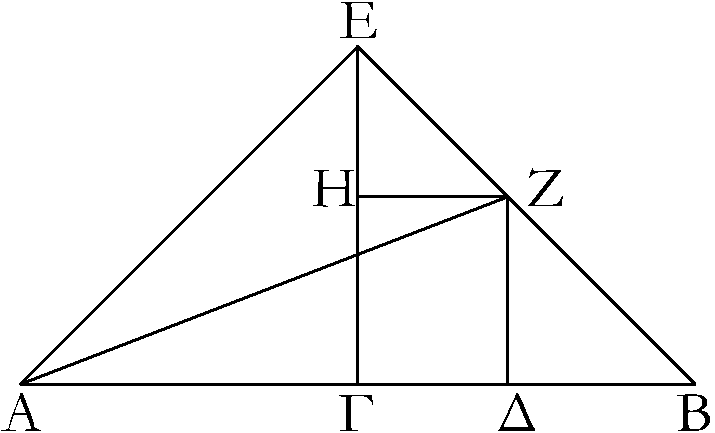
\includegraphics{Book02/fig09g.eps}}
 
\gr{Ἐὰν >άρα εὐθεῖα γραμμ\kern -.7pt  ὴ τμ\kern -.7pt  ηθῆ| εἰξ >ίσα καὶ >άνισα, τὰ ἀπὸ τῶν ἀνίσων τῆξ <όληξ τμ\kern -.5pt  ημάτων τετράγωνα διπλάσιά ἐστι τοῦ τε ἀπὸ τῆξ ἡμισείαξ καὶ τοῦ ἀπὸ τῆξ μεταχὺ τῶν τομῶν τετραγώνου;
<όπερ >έδει δεῖχαι.}}

\ParallelRText{
\begin{center}
{\large Proposition 9$^\dag$}
\end{center}

If a straight-line is cut into equal and unequal (pieces, then) the (sum of
the) squares on the unequal pieces of the whole (straight-line) is double
the (sum of the) square on half (the straight-line) and (the square) on the (difference)
between the (equal and unequal) pieces.

For let any straight-line $AB$ be cut---equally at $C$, and unequally
at $D$. I say that the (sum of the) squares on $AD$ and $DB$ is double
the (sum of the squares) on $AC$ and $CD$.

For let $CE$ be drawn from (point) $C$, at right-angles to $AB$ [Prop.~1.11], and let it be made equal to each of $AC$ and $CB$ [Prop.~1.3],
and let $EA$ and $EB$ be joined. And let $DF$ be drawn through
(point) $D$, parallel to $EC$ [Prop.~1.31], and (let) $FG$ (be drawn)
through (point) $F$, (parallel) to $AB$ [Prop.~1.31]. And let $AF$ be joined.
And since $AC$ is equal to $CE$,  the angle $EAC$ is also equal to the (angle) $AEC$ [Prop.~1.5]. And since the (angle) at $C$ is a right-angle, the (sum of the) remaining angles
(of triangle $AEC$), $EAC$ and $AEC$, is thus equal to one right-angle [Prop.~1.32].
And they are equal. Thus, (angles) $CEA$ and $CAE$ are each half a right-angle.
So, for the same (reasons), (angles) $CEB$ and $EBC$ are also each half a
right-angle. Thus, the whole (angle) $AEB$ is a right-angle. And since
$GEF$ is half a right-angle, and $EGF$ (is) a right-angle---for it is
equal to the internal and opposite  (angle) $ECB$ [Prop.~1.29]---the remaining (angle) $EFG$ is thus
half a right-angle [Prop.~1.32]. Thus, angle $GEF$ [is] equal to $EFG$.
So the side $EG$ is also equal to the (side) $GF$ [Prop.~1.6]. Again, since the angle
at $B$ is half a right-angle, and (angle) $FDB$ (is) a right-angle---for again
it is equal to the internal and opposite  (angle) $ECB$ [Prop.~1.29]---the
remaining (angle) $BFD$ is half a right-angle [Prop.~1.32]. Thus, the angle
at $B$ (is) equal to $DFB$. So the side $FD$ is also equal to the side $DB$ [Prop.~1.6]. And since $AC$ is equal to $CE$,  the (square) on $AC$ (is) also equal to the (square) on $CE$. Thus, the (sum of the) squares on $AC$ and $CE$
is double the (square) on $AC$. And the square on $EA$ is equal to the (sum
of the) squares on $AC$ and $CE$. For angle $ACE$ (is) 
a right-angle [Prop.~1.47].
Thus, the (square) on $EA$ is double the (square) on $AC$. Again,  since
$EG$ is equal to $GF$, the (square) on $EG$ (is) also equal  to 
the (square) on $GF$. 
Thus, the (sum of the squares)
on $EG$ and $GF$ is double the square on $GF$.
And the square on $EF$ is equal to the (sum of the) squares on $EG$ and $GF$
[Prop.~1.47]. Thus, the square on $EF$ is double the (square) on $GF$.
And $GF$ (is) equal to $CD$ [Prop.~1.34]. Thus, the (square) on $EF$ is double the
(square) on $CD$. And the (square) on $EA$ is also double the (square) on $AC$.
Thus, the (sum of the) squares on $AE$ and $EF$ is double the (sum of the)
squares on $AC$ and $CD$. And the square on $AF$ is equal to the
(sum of the squares) on $AE$ and $EF$. For the angle $AEF$ is a right-angle [Prop.~1.47]. Thus, the square on $AF$ is double the (sum of the squares) on 
$AC$ and $CD$. And the (sum of the squares) on $AD$ and $DF$ (is) equal to
the (square) on $AF$. For the angle at $D$ is a right-angle [Prop.~1.47].
Thus, the (sum of the squares) on $AD$ and $DF$ is double the (sum of the)
squares on $AC$ and $CD$. And $DF$ (is) equal to $DB$. Thus, the
(sum of the) squares on $AD$ and $DB$ is double the (sum of the) squares on
$AC$ and $CD$.

\epsfysize=1.8in
\centerline{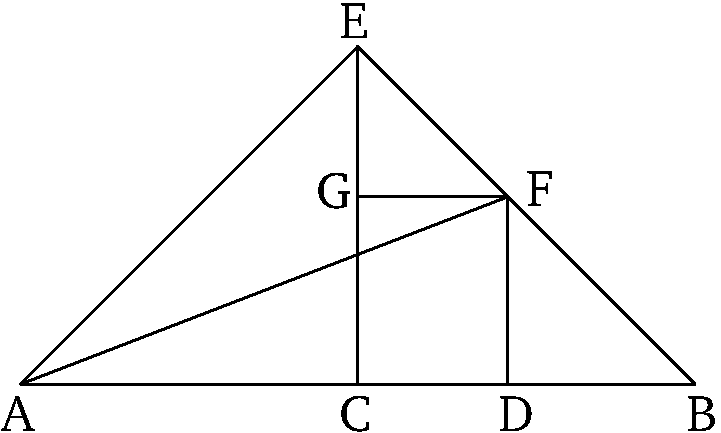
\includegraphics{Book02/fig09e.eps}}

Thus, if a straight-line is cut into equal and unequal (pieces, then) the (sum of the) squares on the unequal pieces of the whole (straight-line) is double
the (sum of the) square on half (the straight-line) and (the square) on the (difference)
between the (equal and unequal) pieces. (Which is) the very thing it was required to show.}
\end{Parallel}
{\footnotesize \noindent$^\dag$ This proposition is a geometric version
of the algebraic identity: $a^{\,2}+b^{\,2} = 2\left[\left([a+b]/2\right)^{\,2} + \left([a+b]/2-b\right)^{\,2}\right]$.}

%%%%%%
% Prop 2.10
%%%%%%
\pdfbookmark[1]{Proposition 2.10}{pdf2.10}
\begin{Parallel}{}{} 
\ParallelLText{
\begin{center}
{\large \ggn{10}.}
\end{center}\vspace*{-7pt}

\gr{Ἐὰν εὐθεῖα γραμμ\kern -.7pt  ὴ τμ\kern -.7pt  ηθῆ| δίθα, προστεθῆ| δέ τιξ α\kern -.5pt  ὐτῆ| εὐθεῖα  ἐπ> εὐθείαξ, τὸ ἀπὸ τῆξ <όληξ σὺν τῆ| προσκειμένῃ
καὶ τὸ ἀπὸ τῆξ προσκειμένηξ τὰ συναμφότερα τετράγωνα διπλάσιά ἐστι τοῦ τε ἀπὸ τῆξ ἡμισείαξ καὶ τοῦ ἀπὸ τῆξ συγκειμένηξ >έκ τε τῆξ ἡμισείαξ καὶ τῆξ προσκειμένηξ ὡξ ἀπὸ μιᾶξ ἀναγραφέντοξ τετραγώνου.}\\~\\

\epsfysize=2in
\centerline{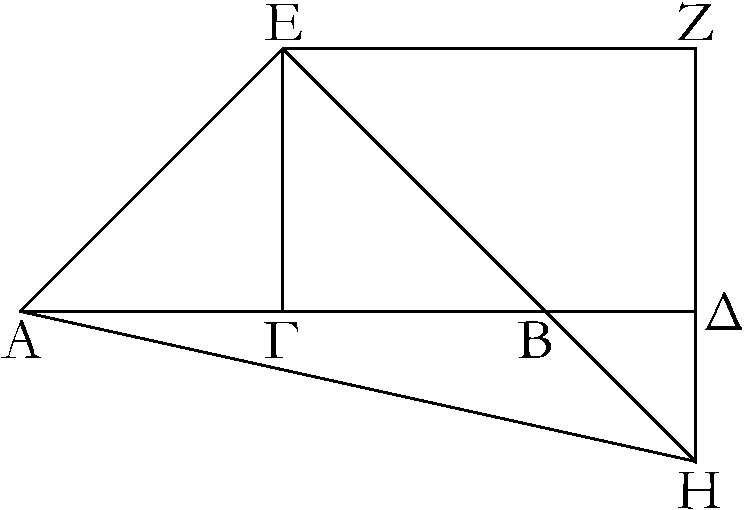
\includegraphics{Book02/fig10g.eps}}

\gr{Εὐθεῖα γάρ τιξ ἡ ΑΒ τετμ\kern -.7pt  ήσθω δίθα κατὰ τὸ Γ, προσκείσθω δέ τιξ α\kern -.7pt  ὐτῆ|
εὐθεῖα ἐπ> εὐθείαξ ἡ ΒΔ; λέγω, <ότι τὰ ἀπὸ τῶν ΑΔ, ΔΒ τετράγωνα διπλάσιά ἐστι τῶν ἀπὸ τῶν ΑΓ, ΓΔ τετραγώνων.}

\gr{>'Ηθθω γὰρ ἀπὸ τοῦ Γ σημείου τῆ| ΑΒ πρὸξ ὀρθὰξ ἡ ΓΕ, καὶ κείσθω >ίση ἑκατέρᾳ τῶν ΑΓ, ΓΒ, καὶ ἐπεζεύθθωσαν αἱ ΕΑ, ΕΒ; καὶ διὰ μὲν τοῦ Ε τῆ| ΑΔ παράλληλοξ >ήθθω ἡ ΕΖ, διὰ δὲ τοῦ Δ τῆ| ΓΕ παράλληλοξ >ήθθω ἡ ΖΔ. καὶ ἐπεὶ εἰξ παραλλήλουξ εὐθείαξ τὰξ ΕΓ, ΖΔ εὐθεῖά τιξ ἐνέπεσεν ἡ ΕΖ, αἱ ὑπὸ ΓΕΖ, ΕΖΔ >άρα δυσὶν ὀρθαῖξ >ίσαι εἰσίν; αἱ >άρα ὑπὸ ΖΕΒ, ΕΖΔ δύο ὀρθῶν ἐλάσσονέξ εἰσιν;
αἱ  δὲ ἀπ> ἐλασσόνων >ὴ δύο ὀρθῶν ἐκβαλλόμεναι συμπίπτουσιν;
αἱ >άρα ΕΒ, ΖΔ ἐκβαλλόμεναι ἐπὶ τὰ Β, Δ μέρη συμπεσοῦνται.
ἐκβεβλήσθωσαν καὶ συμπιπτέτωσαν κατὰ τὸ Η, καὶ ἐπεζεύθθω ἡ ΑΗ. καὶ ἐπεὶ >ίση ἐστὶν ἡ ΑΓ τῆ| ΓΕ, >ίση ἐστὶ καὶ γωνία ἡ ὑπὸ ΕΑΓ τῆ| ὑπὸ ΑΕΓ; καὶ ὀρθὴ ἡ πρὸξ τῶ| Γ; ἡμίσεια >άρα 
ὀρθῆξ [ἐστιν] ἑκατέρα τῶν ὑπὸ ΕΑΓ, ΑΕΓ. διὰ τὰ α\kern -.7pt  ὐτὰ δὴ καὶ ἑκατέρα τῶν ὑπὸ ΓΕΒ, ΕΒΓ ἡμίσειά ἐστιν ὀρθῆξ; ὀρθὴ >άρα ἐστὶν ἡ ὑπὸ ΑΕΒ. καὶ ἐπεὶ ἡμίσεια ὀρθῆξ ἐστιν ἡ ὑπὸ ΕΒΓ, ἡμίσεια >άρα 
ὀρθῆξ καὶ ἡ ὑπὸ ΔΒΗ. >έστι δὲ καὶ ἡ 
ὑπὸ ΒΔΗ ὀρθή; >ίση γάρ ἐστι τῆ| ὑπὸ ΔΓΕ; ἐναλλὰχ γάρ; 
λοιπὴ <άρα ἡ ὑπὸ ΔΗΒ ἡμίσειά ἐστιν ὀρθῆξ; ἡ 
>άρα ὑπὸ ΔΗΒ τῆ| ὑπὸ ΔΒΗ ἐστιν >ίση; <ώστε καὶ πλευρὰ ἡ ΒΔ πλευρᾶ| τῆ| ΗΔ ἐστιν >ίση.
πάλιν, ἐπεὶ ἡ ὑπὸ ΕΗΖ ἡμίσειά ἐστιν ὀρθῆξ, ὀρθὴ δὲ ἡ πρὸξ τῶ| Ζ; >ίση γάρ ἐστι τῆ| ἀπεναντίον τῆ| πρὸξ τῶ| Γ; λοιπὴ >άρα ἡ ὑπὸ ΖΕΗ ἡμίσειά ἐστιν
ὀρθῆξ;  >ίση >άρα ἡ ὑπὸ ΕΗΖ γωνία τῆ| ὑπὸ ΖΕΗ; <ώστε
καὶ πλευρὰ ἡ ΗΖ πλευρᾶ| τῆ| ΕΖ ἐστιν >ίση. καὶ ἐπεὶ [>ίση ἐστὶν ἡ ΕΓ τῆ| ΓΑ], >ίσον ἐστὶ [καὶ] τὸ ἀπὸ τῆξ ΕΓ τετράγωνον τῶ| ἀπὸ τῆξ ΓΑ τετραγώνῳ; τὰ >άρα ἀπὸ τῶν ΕΓ, ΓΑ τετράγωνα διπλάσιά
ἐστι τοῦ ἀπὸ τῆξ ΓΑ τετραγώνου. τοῖξ δὲ ἀπὸ τῶν ΕΓ, ΓΑ >ίσον
ἐστὶ τὸ ἀπὸ τῆξ ΕΑ; τὸ >άρα ἀπὸ τῆξ ΕΑ τετράγωνον διπλάσιόν ἐστι τοῦ ἀπὸ τῆξ ΑΓ τετραγώνου. πάλιν, ἐπεὶ >ίση ἐστὶν ἡ ΖΗ τῆ| ΕΖ, 
>ίσον ἐστὶ καὶ τὸ ἀπὸ τῆξ ΖΗ τῶ| ἀπὸ τῆξ ΖΕ; τὰ >άρα ἀπὸ τῶν ΗΖ, ΖΕ διπλάσιά ἐστι τοῦ ἀπὸ τῆξ ΕΖ. τοῖξ δὲ ἀπὸ τῶν ΗΖ, ΖΕ
>ίσον ἐστὶ τὸ ἀπὸ τῆξ ΕΗ; τὸ >άρα ἀπὸ τῆξ ΕΗ διπλάσιόν ἐστι
τοῦ ἀπὸ τῆξ ΕΖ. >ίση δὲ ἡ ΕΖ τῆ| ΓΔ; τὸ >άρα ἀπὸ τῆξ ΕΗ τετράγωνον διπλάσιόν ἐστι τοῦ ἀπὸ τῆξ ΓΔ. ἐδείθθη δὲ καὶ τὸ ἀπὸ τῆξ ΕΑ διπλάσιον
τοῦ ἀπὸ τῆξ ΑΓ; τὰ >άρα ἀπὸ τῶν ΑΕ, ΕΗ τετράγωνα διπλάσιά ἐστι τῶν ἀπὸ τῶν ΑΓ, ΓΔ τετραγώνων. τοῖξ
δὲ ἀπὸ τῶν ΑΕ, ΕΗ τετραγώνοιξ >ίσον ἐστὶ τὸ ἀπὸ τῆξ ΑΗ τετράγωνον; τὸ >άρα ἀπὸ τῆξ ΑΗ διπλάσιόν ἐστι τῶν ἀπὸ τῶν ΑΓ, ΓΔ. τῶ| δὲ ἀπὸ τῆξ ΑΗ >ίσα ἐστὶ τὰ ἀπὸ τῶν ΑΔ, ΔΗ; τὰ >άρα
ἀπὸ τῶν ΑΔ, ΔΗ [τετράγωνα] διπλάσιά ἐστι τῶν ἀπὸ τῶν ΑΓ, ΓΔ [τετραγώνων]. >ίση δὲ ἡ ΔΗ τῆ| ΔΒ; τὰ >άρα ἀπὸ τῶν ΑΔ, ΔΒ [τετράγωνα] διπλάσιά ἐστι τῶν ἀπὸ τῶν ΑΓ, ΓΔ τετραγώνων.}

\gr{Ἐὰν >άρα εὐθεῖα γραμμ\kern -.7pt  ὴ τμ\kern -.7pt  ηθῆ| δίθα, προστεθῆ| δέ τιξ α\kern -.5pt  ὐτῆ| εὐθεῖα  ἐπ> εὐθείαξ, τὸ ἀπὸ τῆξ <όληξ σὺν τῆ| προσκειμένῃ
καὶ τὸ ἀπὸ τῆξ προσκειμένηξ τὰ συναμφότερα τετράγωνα διπλάσιά ἐστι τοῦ τε ἀπὸ τῆξ ἡμισείαξ καὶ τοῦ ἀπὸ τῆξ συγκειμένηξ >έκ τε τῆξ ἡμισείαξ καὶ τῆξ προσκειμένηξ ὡξ ἀπὸ μιᾶξ ἀναγραφέντοξ τετραγώνου; <όπερ >έδει δεῖχαι.}}

\ParallelRText{
\begin{center}
{\large Proposition 10$^\dag$}
\end{center}

If a straight-line is cut in half, and any straight-line added to it straight-on,
(then) the sum of the square on the whole (straight-line) with the (straight-line) having
been added, and the (square) on the (straight-line) having been added, 
is double the (sum of the square) on half (the straight-line), and
the square described on the sum of half (the straight-line) and (straight-line)
having been added, as on one (complete straight-line).

\epsfysize=2in
\centerline{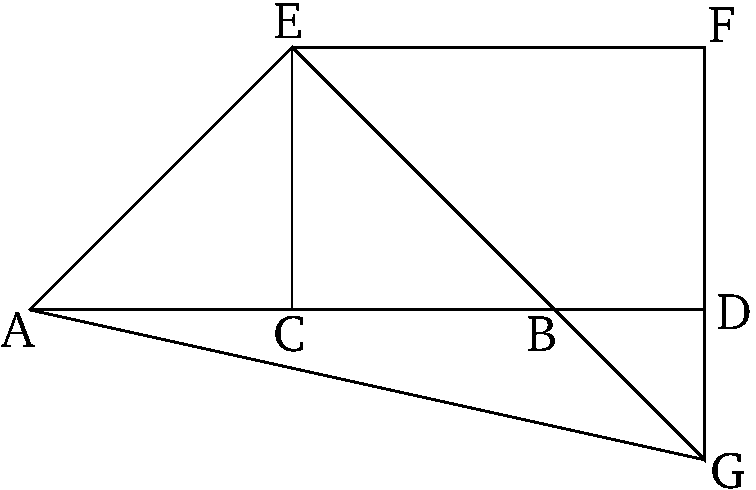
\includegraphics{Book02/fig10e.eps}}

For let any straight-line $AB$ be cut in half at (point) $C$, and let any
straight-line $BD$ be added to it straight-on. I say that the
(sum of the) squares on $AD$ and $DB$ is double the (sum of the) squares on $AC$ and $CD$.

For let $CE$ be drawn from point $C$, at right-angles to $AB$ [Prop.~1.11],
and let it be made equal to each of $AC$ and $CB$ [Prop.~1.3], and let $EA$ and
$EB$ be joined. And let $EF$ be drawn through $E$, parallel to $AD$
[Prop.~1.31], and let $FD$ be drawn through $D$, parallel to $CE$ [Prop.~1.31]. And since some straight-line $EF$ falls across the parallel straight-lines $EC$ and $FD$, the (internal angles) $CEF$ and $EFD$ are thus equal
to two right-angles [Prop.~1.29]. Thus, $FEB$ and $EFD$ are less than two
right-angles. And (straight-lines) produced from (internal angles whose sum is) less than
two right-angles meet together [Post.~5]. Thus, being produced in the direction of $B$
and $D$, the (straight-lines) $EB$ and $FD$ will meet. Let them be 
produced,
and let them meet together at $G$, and let $AG$ be joined.
And since $AC$ is equal to $CE$, angle $EAC$ is also equal to (angle) $AEC$ [Prop.~1.5]. And the (angle) at $C$ (is) a right-angle. Thus, $EAC$ and $AEC$
[are] each half a right-angle [Prop.~1.32]. So, for the same (reasons), $CEB$ and $EBC$ are
also each half a right-angle. Thus, (angle) $AEB$ is a right-angle.
And since $EBC$ is half a right-angle, $DBG$ (is) thus also half a right-angle
[Prop.~1.15]. And $BDG$ is also a right-angle. For it is equal to $DCE$.
For (they are) alternate (angles) [Prop.~1.29].
Thus, the remaining (angle) $DGB$ is half a right-angle. Thus,
$DGB$ is equal to $DBG$. So side $BD$ is also equal to side $GD$ [Prop.~1.6].
Again, 
since $EGF$ is  half a right-angle, and the (angle) at $F$ (is) a right-angle,
for it is equal to the opposite (angle) at $C$
[Prop.~1.34], the remaining
(angle) $FEG$ is thus half a right-angle. Thus, angle $EGF$ (is) equal to $FEG$.
So the side $GF$ is also equal to the side $EF$ [Prop.~1.6].
And since [$EC$ is equal to $CA$] the square on $EC$ is [also] equal to the
square on $CA$. Thus, the (sum of the) squares on $EC$ and $CA$ is 
double the square on $CA$. And the (square) on $EA$ is equal to the (sum of the
squares) on $EC$ and $CA$ [Prop.~1.47]. Thus, the square on $EA$ is double the
square on $AC$. Again, since $FG$ is equal to $EF$, the (square) on $FG$ is also
equal to the (square) on $FE$. Thus, the (sum of the squares) on $GF$ and
$FE$ is double the (square) on $EF$. And the (square) on $EG$ is equal to
the (sum of the squares) on  $GF$ and $FE$ [Prop.~1.47]. Thus, the (square)
on $EG$ is double the (square) on $EF$. And $EF$ (is) equal to $CD$  [Prop.~1.34].
Thus, the square on $EG$ is double the (square) on $CD$. But it was also
shown that the (square) on $EA$ (is) double the (square) on $AC$. Thus,
the (sum of the) squares on $AE$ and $EG$ is double the (sum of the) squares
on $AC$ and $CD$. And the square on $AG$ is equal to the (sum of the) squares
on $AE$ and $EG$ [Prop.~1.47]. Thus, the (square) on $AG$ is double the (sum of the squares) on $AC$ and $CD$. And the (sum of the squares) on $AD$ and $DG$ 
is equal to the (square) on $AG$  [Prop.~1.47].
Thus, the (sum of the) [squares] on $AD$ and $DG$ is double the
(sum of the) [squares] on $AC$ and $CD$. And $DG$ (is) equal to $DB$.
Thus, the (sum of the) [squares] on $AD$ and $DB$ is double the
(sum of the) squares on $AC$ and $CD$. 

Thus, if a straight-line is cut in half, and any straight-line added to it straight-on,
(then) the sum of the square on the whole (straight-line) with the (straight-line) having
been added, and the (square) on the (straight-line) having been added, 
is double the (sum of the square) on half (the straight-line), and
the square described on the sum of half (the straight-line) and (straight-line)
having been added, as on one (complete straight-line). (Which is) the
very thing it was required to show.}
\end{Parallel}
{\footnotesize \noindent$^\dag$ This proposition is a geometric version
of the algebraic identity: $(2\,a+b)^{\,2}+b^{\,2}= 2\,\left[a^{\,2}+(a+b)^{\,2}\right]$.}

%%%%%%
% Prop 2.11
%%%%%%
\pdfbookmark[1]{Proposition 2.11}{pdf2.11}
\begin{Parallel}{}{} 
\ParallelLText{
\begin{center}
{\large \ggn{11}.}
\end{center}\vspace*{-7pt}

\gr{Τὴν δοθεῖσαν εὐθεῖαν τεμεῖν <ώστε τὸ ὑπὸ τῆξ <όληξ καὶ
τοῦ ἑτέρου τῶν τμ\kern -.7pt  ημάτων περιεχόμενον ὀρθογώνιον >ίσον ε>ῖναι
τῶ| ἀπὸ τοῦ λοιποῦ τμ\kern -.7pt  ήματοξ τετραγώνῳ.}

\gr{>'Εστω ἡ δοθεῖσα εὐθεῖα ἡ ΑΒ; δεῖ δὴ τὴν ΑΒ τεμεῖν <ώστε
τὸ ὑπὸ τῆξ <όληξ καὶ τοῦ ἑτέρου τῶν τμ\kern -.7pt  ημάτων περιεχόμενον ὀρθογώνιον >ίσον ε>ῖναι τῶ| ἀπὸ τοῦ λοιποῦ τμ\kern -.7pt  ήματοξ τετραγώνῳ.}\\

\epsfysize=2.75in
\centerline{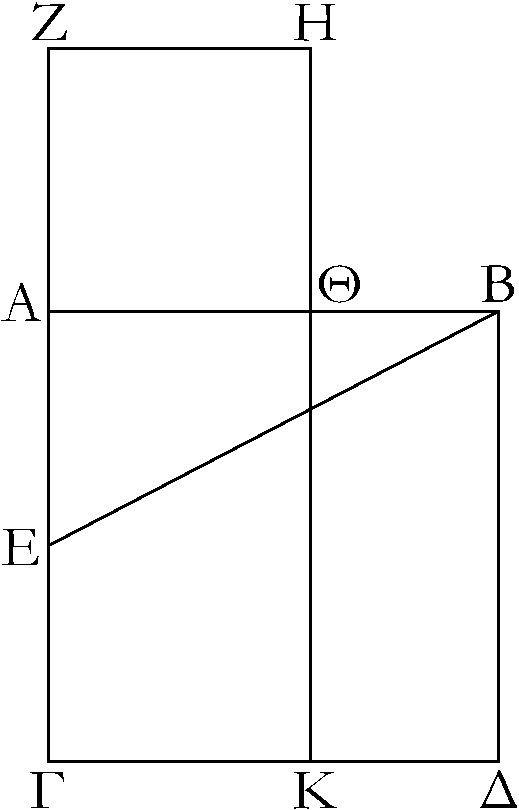
\includegraphics{Book02/fig11g.eps}}

\gr{Ἀναγεγράφθω γὰρ ἀπὸ τῆξ ΑΒ τετράγωνον τὸ ΑΒΔΓ, καὶ τετμ\kern -.7pt  ήσθω ἡ ΑΓ δίθα κατὰ τὸ Ε σημεῖον, καὶ ἐπεζεύθθω ἡ ΒΕ, καὶ διήθθω ἡ ΓΑ ἐπὶ τὸ Ζ, καὶ κείσθω τῆ| ΒΕ >ίση ἡ ΕΖ, καὶ ἀναγεγράφθω ἀπὸ
τῆξ ΑΖ τετράγωνον τὸ ΖJ, καὶ
διήθθω ἡ ΗJ ἐπὶ τὸ Κ; λέγω, <ότι ἡ ΑΒ τέτμ\kern -.7pt  ηται κατὰ τὸ J, <ώστε τὸ ὑπὸ τῶν ΑΒ, ΒJ περιεχόμενον ὀρθογώνιον >ίσον ποιεῖν τῶ| ἀπὸ τῆξ ΑJ τετραγώνῳ.}

\gr{Ἐπεὶ γὰρ εὐθεῖα ἡ ΑΓ τέτμ\kern -.7pt  ηται δίθα κατὰ τὸ Ε, πρόσκειται δὲ α\kern -.7pt  ὐτῆ| ἡ ΖΑ, τὸ >άρα ὑπὸ τῶν ΓΖ, ΖΑ περιεχόμενον ὀρθογώνιον μετὰ τοῦ ἀπὸ τῆξ ΑΕ τετραγώνου >ίσον ἐστὶ τῶ| ἀπὸ τῆξ ΕΖ τετραγώνῳ. >ίση δὲ ἡ ΕΖ τῆ| ΕΒ; τὸ >άρα ὑπὸ τῶν ΓΖ, ΖΑ μετὰ τοῦ ἀπὸ τῆξ ΑΕ >ίσον ἐστὶ τῶ| ἀπὸ ΕΒ. ἀλλὰ τῶ| ἀπὸ 
ΕΒ >ίσα ἐστὶ τὰ ἀπὸ τῶν ΒΑ, ΑΕ; ὀρθὴ γὰρ ἡ πρὸξ τῶ| Α γωνία; τὸ >άρα ὑπὸ τῶν ΓΖ, ΖΑ μετὰ τοῦ ἀπὸ τῆξ ΑΕ >ίσον ἐστὶ τοῖξ ἀπὸ τῶν ΒΑ, ΑΕ. κοινὸν ἀφῃρήσθω τὸ ἀπὸ τῆξ ΑΕ; λοιπὸν >άρα τὸ ὑπὸ τῶν ΓΖ, ΖΑ
περιεχόμενον ὀρθογώνιον >ίσον ἐστὶ τῶ| ἀπὸ τῆξ ΑΒ τετραγώνῳ.
καί ἐστι τὸ μὲν ὑπὸ τῶν ΓΖ, ΖΑ τὸ ΖΚ; >ίση γὰρ ἡ ΑΖ τῆ| ΖΗ;
τὸ δὲ ἀπὸ τῆξ ΑΒ τὸ ΑΔ; τὸ >άρα ΖΚ >ίσον ἐστὶ τῶ| ΑΔ. κοινὸν ἀρῃρήσθω τὸ ΑΚ; λοιπὸν >άρα τὸ ΖJ τῶ| JΔ >ίσον ἐστίν. καί ἐστι τὸ μὲν JΔ τὸ ὑπὸ τῶν ΑΒ, ΒJ; 
>ίση γὰρ ἡ ΑΒ τῆ| ΒΔ; τὸ δὲ ΖJ τὸ ἀπὸ τῆξ ΑJ; τὸ >άρα ὑπὸ τῶν ΑΒ, ΒJ περιεχόμενον ὀρθογώνιον >ίσον ἐστὶ τῶ| ἀπὸ JΑ τετραγώνῳ.}

\gr{Ἡ  >άρα δοθεῖσα εὐθεῖα ἡ ΑΒ τέτμ\kern -.7pt  ηται 
κατὰ τὸ J <ώστε τὸ ὑπὸ τῶν ΑΒ, ΒJ 
περιεχόμενον ὀρθογώνιον >ίσον ποιεῖν
τῶ| ἀπὸ τῆξ JΑ τετραγώνῳ; <όπερ >έδει ποιῆσαι.}}

\ParallelRText{
\begin{center}
{\large Proposition 11$^\dag$}
\end{center}

To cut a given straight-line such that the rectangle contained by the whole (straight-line), and one of the pieces (of the straight-line), is equal to the
square on the remaining piece.

Let $AB$ be the given straight-line. So it is required to cut $AB$ such that the rectangle contained by the whole (straight-line), and one of the
pieces (of the straight-line), is equal to the square on the remaining piece.

\epsfysize=2.75in
\centerline{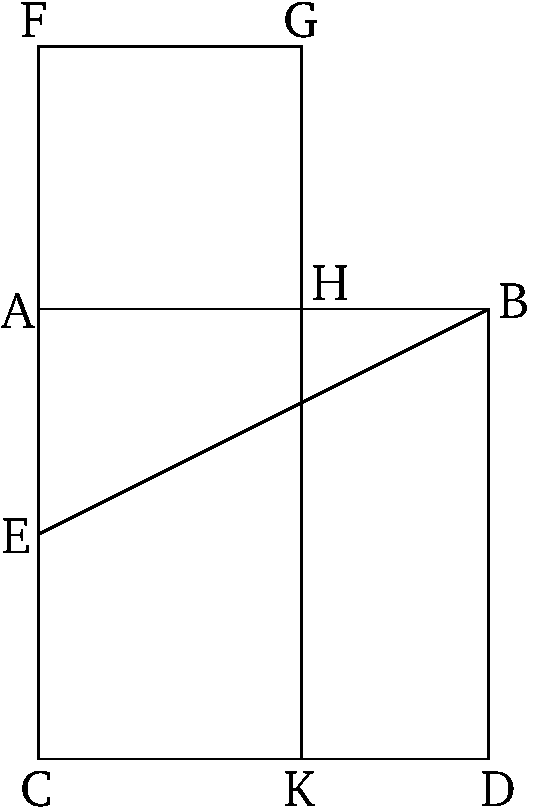
\includegraphics{Book02/fig11e.eps}}

For let the square $ABDC$ be described on $AB$ [Prop.~1.46],
and let $AC$ be cut in half at point $E$ [Prop.~1.10], and
let $BE$ be joined.  And let $CA$ be drawn through to (point)
$F$, and let $EF$ be made equal to $BE$ [Prop.~1.3]. And let the square $FH$ 
be described on $AF$ [Prop.~1.46], and let $GH$ be drawn
through to (point) $K$. I say that $AB$ has been cut at $H$ such as to make the
rectangle contained by $AB$ and $BH$ equal to the square on $AH$.

For since the straight-line $AC$ has been cut in half at $E$, and $FA$ has been
added to it, the rectangle contained by $CF$ and $FA$, plus the square on $AE$, is
thus equal to the square on $EF$ [Prop.~2.6]. And $EF$ (is) equal to $EB$. Thus,
the (rectangle contained) by $CF$ and $FA$, plus the (square) on $AE$, is equal
to the (square) on $EB$. But, the (sum of the squares) on $BA$ and $AE$ is equal
to the (square) on $EB$. For the angle at $A$ (is) a right-angle [Prop.~1.47].
Thus, the (rectangle contained) by $CF$ and $FA$, plus the (square) on $AE$,
is equal to the (sum of the squares) on $BA$ and $AE$. Let the square on $AE$ have
been subtracted from both. Thus, the remaining rectangle contained by
$CF$ and $FA$ is equal to the square on $AB$.  And $FK$ is the (rectangle contained)
by $CF$ and $FA$. For $AF$ (is) equal to $FG$. And $AD$ (is) the (square) on $AB$. Thus, the
(rectangle) $FK$ is equal to the (square) $AD$. Let (rectangle) $AK$ be
subtracted from both. Thus, the remaining (square) $FH$ is equal to 
the (rectangle) $HD$. And  $HD$ is the (rectangle contained) by $AB$ and $BH$.
For $AB$ (is) equal to $BD$. And $FH$ (is) the (square) on $AH$.
Thus, the rectangle contained by $AB$ and $BH$ is equal to the square on $HA$.

Thus, the given straight-line $AB$ has been cut at (point) $H$ such as to make
the rectangle contained by $AB$ and $BH$ equal to the square on $HA$.
(Which is) the very thing it was required to do.
}
\end{Parallel}
{\footnotesize \noindent$^\dag$ This manner of cutting a straight-line---so
that the ratio of the whole to the larger piece is equal to the ratio
of the larger to the smaller piece---is sometimes called the ``Golden Section''.}

%%%%%%
% Prop 2.12
%%%%%%
\pdfbookmark[1]{Proposition 2.12}{pdf2.12}
\begin{Parallel}{}{} 
\ParallelLText{
\begin{center}

{\large\ggn{12}.}
\end{center}\vspace*{-7pt}

\gr{Ἐν τοῖξ ἀμβλυγωνίοιξ τριγώνοιξ τὸ ἀπὸ τῆξ τὴν ἀμβλεῖαν
γωνίαν ὑποτεινούσηξ πλευρᾶξ τετράγωνον μεῖζόν ἐστι τῶν ἀπὸ
τῶν τὴν ἀμβλεῖαν γωνίαν περιεθουσῶν πλευρῶν τετραγώνων τῶ| περιεθομένῳ δὶξ
ὑπὸ τε μιᾶξ τῶν περὶ τὴν ἀμβλεῖαν γωνίαν, ἐφ> <ὴν ἡ
κάθετοξ πίπτει, καὶ τῆξ ἀπολαμβανομένηξ ἐκτὸξ ὑπὸ τῆξ
καθέτου πρὸξ τῆ| ἀμβλείᾳ γωνίᾳ.}

\gr{>'Εστω ἀμβλυγώνιον τρίγωνον τὸ ΑΒΓ ἀμβλεῖαν >έθον τὴν ὑπὸ
ΒΑΓ, καὶ >ήθθω ἀπὸ τοῦ Β σημείου ἐπὶ τὴν ΓΑ ἐκβληθεῖσαν κάθετοξ ἡ ΒΔ. λέγω, <ότι τὸ ἀπὸ τῆξ ΒΓ τετράγωνον μεῖζόν ἐστι
τῶν ἀπὸ τῶν ΒΑ, ΑΓ τετραγώνων τῶ| δὶξ ὑπὸ τῶν ΓΑ, ΑΔ περιεθομένῳ ὀρθογωνίῳ.}\\

\epsfysize=1.8in
\centerline{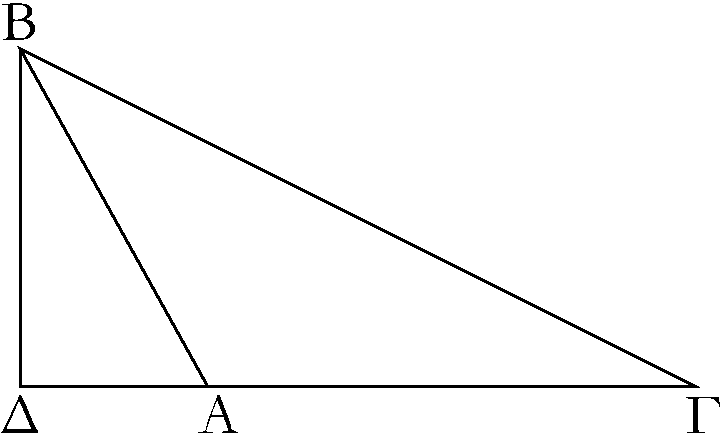
\includegraphics{Book02/fig12g.eps}}

\gr{Ἐπεὶ γὰρ εὐθεῖα ἡ ΓΔ τέτμ\kern -.7pt  ηται, ὡξ >έτυθεν, κατὰ τὸ Α σημεῖον,
τὸ >άρα ἀπὸ τῆξ ΔΓ >ίσον ἐστὶ τοῖξ ἀπὸ τῶν ΓΑ, ΑΔ τετραγώνοιξ καὶ τῶ| δὶξ ὑπὸ τῶν ΓΑ, ΑΔ περιεθομένῳ ὀρθογωνίῳ. κοινὸν προσκείσθω τὸ ἀπὸ τῆξ ΔΒ; τὰ >άρα ἀπὸ τῶν ΓΔ, ΔΒ >ίσα ἐστὶ
τοῖξ τε ἀπὸ τῶν ΓΑ, ΑΔ, ΔΒ τετραγώνοιξ καὶ τῶ| δὶξ ὑπὸ
τῶν ΓΑ, ΑΔ [περιεθομένῳ ὀρθογωνίῳ]. ἀλλὰ τοῖξ μὲν ἀπὸ τῶν
ΓΔ, ΔΒ >ίσον ἐστὶ τὸ ἀπὸ τῆξ ΓΒ;
ὀρθὴ γὰρ ἡ προξ τῶ| Δ γωνία; τοῖξ δὲ ἀπὸ τῶν ΑΔ, ΔΒ >ίσον τὸ ἀπὸ τῆξ ΑΒ; τὸ >άρα ἀπὸ τῆξ ΓΒ τετράγωνον >ίσον ἐστὶ τοῖξ τε
ἀπὸ τῶν ΓΑ, ΑΒ
τετραγώνοιξ καὶ τῶ| δὶξ ὑπὸ
τῶν ΓΑ, ΑΔ περιεθομένῳ ὀρθογωνίῳ; <ώστε τὸ ἀπὸ τῆξ ΓΒ
τετράγωνον τῶν ἀπὸ τῶν ΓΑ, ΑΒ τετραγώνων μεῖζόν
ἐστι τῶ| δὶξ ὑπὸ τῶν ΓΑ, ΑΔ περιεθομένῳ ὀρθογωνίῳ.}

\gr{Ἐν >άρα τοῖξ ἀμβλυγωνίοιξ τριγώνοιξ τὸ ἀπὸ τῆξ τὴν ἀμβλεῖαν
γωνίαν ὑποτεινούσηξ πλευρᾶξ τετράγωνον μεῖζόν ἐστι τῶν ἀπὸ
τῶν τὴν ἀμβλεῖαν γωνίαν περιεθουσῶν πλευρῶν τετραγώνων τῶ| περιθομένῳ δὶξ ὑπό τε μιᾶξ τῶν περὶ τὴν ἀμβλεῖαν γωνίαν, ἐφ> <ὴν ἡ
κάθετοξ πίπτει, καὶ τῆξ ἀπολαμβανομένηξ ἐκτὸξ ὑπὸ τῆξ
καθέτου πρὸξ τῆ| ἀμβλείᾳ γωνίᾳ; <όπερ >έδει δεῖχαι.}}

\ParallelRText{
\begin{center}
{\large Proposition 12$^\dag$}
\end{center}

In obtuse-angled triangles, the square on the side subtending the obtuse
angle is greater than the (sum of the) squares on the sides containing the obtuse angle
by twice the (rectangle) contained by one of the sides around the obtuse
angle, to which a perpendicular (straight-line) falls, and the 
 (straight-line) cut off outside (the triangle)
 by the perpendicular (straight-line) towards the obtuse angle.
 
 Let $ABC$ be an obtuse-angled triangle, having the 
 angle $BAC$ obtuse. And let $BD$ be drawn from point $B$, perpendicular
 to $CA$ produced [Prop.~1.12]. I say that the square on $BC$ is greater than the
 (sum of the) squares on $BA$ and $AC$ by twice the rectangle contained
 by $CA$ and $AD$.
  
\epsfysize=1.8in
\centerline{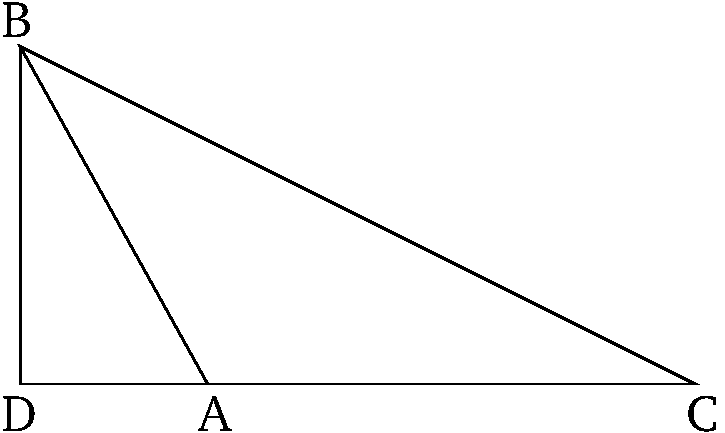
\includegraphics{Book02/fig12e.eps}}

 For since the straight-line $CD$ has been cut, at random, at point $A$, 
 the (square) on $DC$ is thus equal to the (sum of the) squares on $CA$ and $AD$,
 and twice the rectangle contained by $CA$ and $AD$ [Prop.~2.4]. Let
 the (square) on $DB$ be added to both. Thus, the
 (sum of the squares) on $CD$ and $DB$ is equal to the (sum of the) squares
 on $CA$, $AD$, and $DB$, and twice the [rectangle contained] by $CA$ and $AD$.
 But, the (square) on
 $CB$ is equal to the (sum of the squares) on $CD$ and $DB$. For the angle at $D$ (is) a right-angle [Prop.~1.47]. And  the (square) on 
 $AB$ (is) equal to the (sum of the
 squares) on $AD$ and $DB$  [Prop.~1.47]. Thus, the square on $CB$ is equal to the (sum of the)
 squares on $CA$ and $AB$, and twice the rectangle contained by $CA$ and $AD$.  So the square on $CB$ is greater than the (sum of the) squares on $CA$ and
 $AB$ by twice the rectangle contained by $CA$ and $AD$.
 
Thus, in  obtuse-angled triangles, the square on the side subtending the obtuse
angle is greater than the (sum of the) squares on the sides containing the obtuse angle
by twice the (rectangle) contained by one of the sides around the obtuse
angle, to which a perpendicular (straight-line) falls, and the 
 (straight-line) cut off outside (the triangle)
 by the perpendicular (straight-line) towards the obtuse angle.
 (Which is) the very thing it was required to show.}
\end{Parallel}
{\footnotesize \noindent$^\dag$ This proposition is equivalent
to the well-known cosine formula: $BC^{\,2} = AB^{\,2} + AC^{\,2} -2\,AB\,AC\,\cos BAC$, since $\cos BAC = - AD / AB$.}

%%%%%%
% Prop 2.13
%%%%%%
\pdfbookmark[1]{Proposition 2.13}{pdf2.13}
\begin{Parallel}{}{} 
\ParallelLText{
\begin{center}
{\large\ggn{13}.}
\end{center}\vspace*{-7pt}

\gr{Ἐν τοῖξ ὀχυγωνίοιξ τριγώνοιξ τὸ ἀπὸ τῆξ τὴν  ὀχεῖαν γωνίαν
ὑποτεινούσηξ πλευρᾶξ τετράγωνον >έλαττόν ἐστι τῶν ἀπὸ τῶν
τὴν ὀχεῖαν γωνίαν περιεθουσῶν πλευρῶν τετραγώνων τῶ|
περιεθομένῳ δὶξ ὑπό τε μιᾶξ τῶν περὶ τὴν ὀχεῖαν γωνίαν, ἐφ>
<ὴν ἡ κάθετοξ πίπτει, καὶ τῆξ ἀπολαμβανομένηξ ἐντὸξ ὑπὸ
τῆξ καθέτου πρὸξ τῆ| ὀχείᾳ γωνίᾳ.}\\

\epsfysize=2in
\centerline{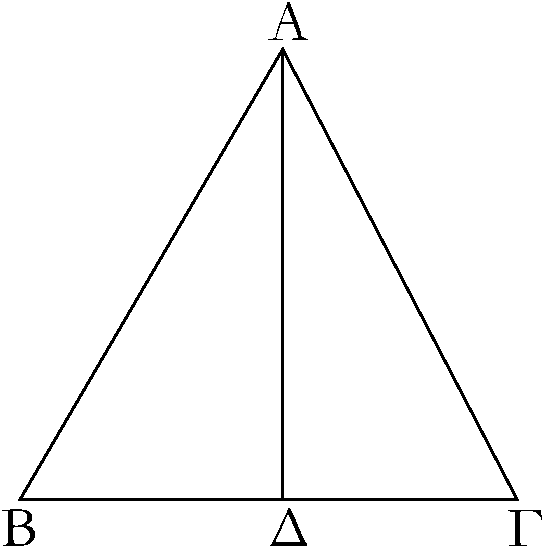
\includegraphics{Book02/fig13g.eps}}

\gr{>'Εστω ὀχυγώνιον τρίγωνον τὸ ΑΒΓ ὀχεῖαν >έθον τὴν πρὸξ τῶ|
Β γωνίαν, καὶ >ήθθω ἀπὸ τοῦ Α σημείου ἐπὶ τὴν ΒΓ κάθετοξ
ἡ ΑΔ; λέγω, <ότι τὸ ἀπὸ τῆξ ΑΓ τετράγωνον >έλαττόν ἐστι τῶν
ἀπὸ τῶν ΓΒ, ΒΑ τετραγώνων τῶ| δὶξ ὑπὸ τῶν ΓΒ, ΒΔ περιεθομένῳ ὀρθογωνίῳ.}

\gr{Ἐπεὶ γὰρ εὐθεῖα ἡ ΓΒ τέτμ\kern -.7pt  ηται, ὡξ >έτυθεν, κατὰ τὸ Δ, τὰ >άρα ἀπὸ τῶν ΓΒ, ΒΔ τετράγωνα >ίσα ἐστὶ τῶ| τε δὶξ ὑπὸ τῶν ΓΒ, ΒΔ
περιεθομένῳ ὀρθογωνίῳ καὶ τῶ| ἀπὸ τῆξ ΔΓ τετραγώνῳ. κοινὸν προσκείσθω τὸ ἀπὸ τῆξ ΔΑ τετράγωνον; τὰ >άρα ἀπὸ τῶν ΓΒ, ΒΔ, ΔΑ
τετράγωνα >ίσα ἐστὶ τῶ| τε δὶξ ὑπὸ τῶν ΓΒ, ΒΔ περιεθομένῳ
ὀρθογωνίῳ καὶ τοῖξ ἀπὸ τῶν ΑΔ, ΔΓ τετραγώνιοξ. ἀλλὰ τοῖξ
μὲν ἀπὸ τῶν ΒΔ, ΔΑ >ίσον τὸ ἀπὸ τῆξ ΑΒ; ὀρθὴ γὰρ ἡ πρὸξ
τῶ| Δ γωνίᾳ; τοῖξ δὲ ἀπὸ τῶν ΑΔ, ΔΓ >ίσον τὸ ἀπὸ τῆξ
ΑΓ; τὰ >άρα ἀπὸ τῶν
 ΓΒ, ΒΑ >ίσα ἐστὶ τῶ| τε ἀπὸ
τῆξ ΑΓ καὶ τῶ| δὶξ ὑπὸ τῶν ΓΒ, ΒΔ; <ώστε μόνον τὸ ἀπὸ τῆξ ΑΓ >έλαττόν ἐστι τῶν ἀπὸ τῶν ΓΒ, ΒΑ τετραγώνων τῶ| δὶξ
ὑπὸ τῶν ΓΒ, ΒΔ περιεθομένῳ ὀρθογωνίῳ.}

\gr{Ἐν >άρα τοῖξ ὀχυγωνίοιξ τριγώνοιξ τὸ ἀπὸ τῆξ τὴν  ὀχεῖαν γωνίαν
ὑποτεινούσηξ πλευρᾶξ τετράγωνον >έλαττόν ἐστι τῶν ἀπὸ τῶν
τὴν ὀχεῖαν γωνίαν περιεθουσῶν πλευρῶν τετραγώνων τῶ|
περιεθομένῳ δὶξ ὑπό τε μιᾶξ τῶν περὶ τὴν ὀχεῖαν γωνίαν, ἐφ>
<ὴν ἡ κάθετοξ πίπτει, καὶ τῆξ ἀπολαμβανομένηξ ἐντὸξ ὑπὸ
τῆξ καθέτου πρὸξ τῆ| ὀχείᾳ γωνίᾳ; <όπερ >έδει δεῖχαι.}}

\ParallelRText{
\begin{center}
{\large Proposition 13$^\dag$}
\end{center}

In acute-angled triangles, the square on the side subtending the acute angle
is less than the (sum of the) squares on the sides containing the acute
angle by twice the (rectangle) contained by one of the sides around the acute
angle, to which a perpendicular (straight-line) falls, and the 
 (straight-line) cut off inside (the triangle)
 by the perpendicular (straight-line) towards the acute angle.
 
 \epsfysize=2in
\centerline{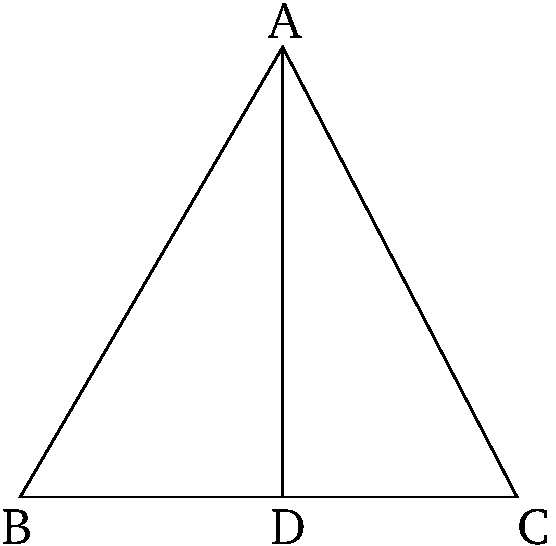
\includegraphics{Book02/fig13e.eps}}

 Let $ABC$ be an acute-angled triangle, having the  angle at (point) $B$ acute.
 And let $AD$ be drawn from point $A$, perpendicular to $BC$ [Prop.~1.12].
I say that the square on $AC$ is less than the (sum of the) squares on $CB$ and $BA$ by twice the rectangle contained by $CB$ and $BD$.

For since the straight-line $CB$ has been cut, at random, at (point) $D$, the
(sum of the) squares on $CB$ and $BD$ is thus equal to twice the rectangle contained by $CB$ and $BD$, and the square on $DC$ [Prop.~2.7]. Let the
square on $DA$ be added to both. Thus, the (sum of the) squares on
$CB$, $BD$, and $DA$ is equal to twice  the rectangle contained by $CB$ and $BD$,
and the (sum of the) squares on $AD$ and $DC$. But, the (square) on $AB$ (is) equal to the (sum
of the squares) on $BD$ and $DA$. For the angle at (point) $D$ is a right-angle [Prop.~1.47]. And the (square) on $AC$ (is) equal to the (sum of the squares)
on $AD$ and $DC$ [Prop.~1.47]. Thus, the (sum of the squares) on $CB$ and $BA$
is equal to the (square) on  $AC$, and twice the (rectangle contained) by $CB$
and $BD$. So the (square) on $AC$ alone is less than the (sum of the) squares on
$CB$ and $BA$ by twice the rectangle contained by $CB$ and $BD$.

Thus, in acute-angled triangles, the square on the side subtending the acute angle
is less than the (sum of the) squares on the sides containing the acute
angle by twice the (rectangle) contained by one of the sides around the acute
angle, to which a perpendicular (straight-line) falls, and the 
 (straight-line) cut off inside (the triangle)
 by the perpendicular (straight-line) towards the acute angle. (Which is)
 the very thing it 	was required to show.}
\end{Parallel}
{\footnotesize \noindent$^\dag$ This proposition is equivalent
to the well-known cosine formula: $AC^{\,2} = AB^{\,2} + BC^{\,2} -2\,AB\, BC\,\cos ABC$, since $\cos ABC = BD / AB$.}

%%%%%%
% Prop 2.14
%%%%%%
\pdfbookmark[1]{Proposition 2.14}{pdf2.14}
\begin{Parallel}{}{} 
\ParallelLText{
\begin{center}
{\large \ggn{14}.}
\end{center}\vspace*{-7pt}

\gr{Τῶ| δοθέντι εὐθυγράμμῳ >ίσον τετράγωνον συστήσασθαι.}

\gr{>'Εστω τὸ δοθὲν εὐθύγραμμον τὸ Α; δεῖ δὴ τῶ| Α εὐθυγράμμῳ
>ίσον τετράγωνον συστήσασθαι.}

\epsfysize=2in
\centerline{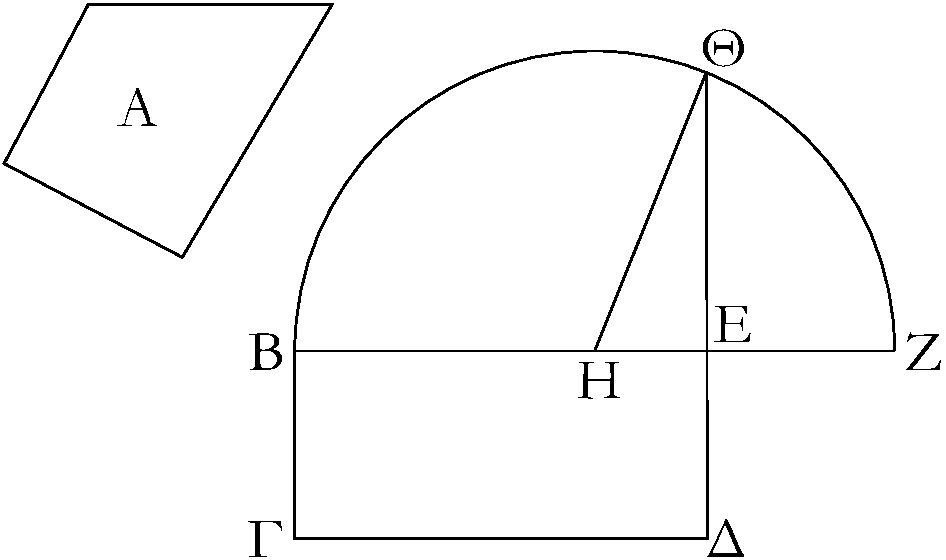
\includegraphics{Book02/fig14g.eps}}

\gr{Συνεστάτω γὰρ τῶ| Α ἐυθυγράμμῳ >ίσον παραλληλό\-γραμμον ὀρθογώνιον τὸ ΒΔ; εἰ μὲν ο>ῦν >ίση ἐστὶν ἡ ΒΕ τῆ| ΕΔ, γεγονὸξ
>ὰν ε>ίη τὸ ἐπιταθθέν. συνέσταται γὰρ τῶ| Α εὐθυγράμμῳ >ίσον
τετράγωνον τὸ ΒΔ; εἰ δὲ ο>ύ, μία τῶν ΒΕ, ΕΔ μείζων ἐστίν. >έστω
μείζων ἡ ΒΕ, καὶ ἐκβεβλήσθω ἐπὶ τὸ Ζ, καὶ κείσθω τῆ| ΕΔ >ίση
ἡ ΕΖ, καὶ τετμ\kern -.7pt  ήσθω ἡ ΒΖ δίθα κατὰ τὸ Η, καὶ κέντρῳ τῶ| Η,
διαστήματι δὲ ἑνὶ τῶν ΗΒ, ΗΖ ἡμικύκλιον γεγράφθω τὸ ΒJΖ, καὶ
ἐκβεβλήσθω ἡ ΔΕ ἐπὶ τὸ J, καὶ ἐπεζεύθθω ἡ ΗJ.}

\gr{Ἐπεὶ ο>ῦν εὐθεῖα ἡ ΒΖ τέτμ\kern -.7pt  ηται εἰξ μὲν >ίσα κατὰ τὸ Η, εἰξ
δὲ >άνισα κατὰ τὸ Ε, τὸ >άρα ὑπὸ τῶν ΒΕ, ΕΖ περιεχόμενον ὀρθογώνιον μετὰ τοῦ ἀπὸ τῆξ ΕΗ τετραγώνου >ίσον ἐστὶ
τῶ| ἀπὸ τῆξ ΗΖ τετραγώνῳ. >ίση δὲ ἡ ΗΖ τῆ| ΗJ; τὸ >άρα ὑπὸ τῶν ΒΕ, ΕΖ μετὰ τοῦ ἀπὸ τῆξ ΗΕ >ίσον ἐστὶ τῶ| ἀπὸ
τῆξ ΗJ. τῶ| δὲ ἀπὸ τῆξ ΗJ >ίσα ἐστὶ τὰ ἀπὸ τῶν JΕ, ΕΗ
τετράγωνα; τὸ >άρα ὑπὸ τῶν ΒΕ, ΕΖ μετὰ τοῦ ἀπὸ ΗΕ >ίσα ἐστὶ
τοῖξ ἀπὸ τῶν JΕ, ΕΗ. κοινὸν ἀφῃρήσθω τὸ ἀπὸ τῆξ ΗΕ
τετράγωνον; λοιπὸν
 >άρα τὸ ὑπὸ τῶν ΒΕ, ΕΖ περιεχόμενον >όρθογώνιον >ίσον ἐστὶ τῶ| ἀπὸ τῆξ ΕJ τετραγώνῳ.
ἀλλὰ τὸ ὑπὸ τῶν ΒΕ, ΕΖ τὸ ΒΔ ἐστιν; >ίση γὰρ ἡ ΕΖ τῆ| ΕΔ;
τὸ >άρα ΒΔ παραλληλόγραμμον >ίσον ἐστὶ τῶ| ἀπὸ τῆξ JΕ
τετραγώνῳ. >ίσον δὲ τὸ ΒΔ τῶ| Α εὐθυγράμμῳ. καὶ τὸ Α
>άρα εὐθύγραμμον >ίσον ἐστὶ τῶ| ἀπὸ τῆξ ΕJ
ἀναγραφησομένῳ τετραγώνῳ.}

\gr{Τῶ| >άρα δοθέντι εὐθυγράμμῳ  τῶ| Α >ίσον τετράγωνον συνέσταται τὸ ἀπὸ τῆξ ΕJ ἀναγραφησόμενον; <όπερ >έδει
ποιῆσαι.}}

\ParallelRText{
\begin{center}
{\large Proposition 14}
\end{center}

To construct a square equal to a given rectilinear figure.

Let $A$ be the given rectilinear figure. So it is required to construct a
square equal to the rectilinear figure $A$.

\epsfysize=2in
\centerline{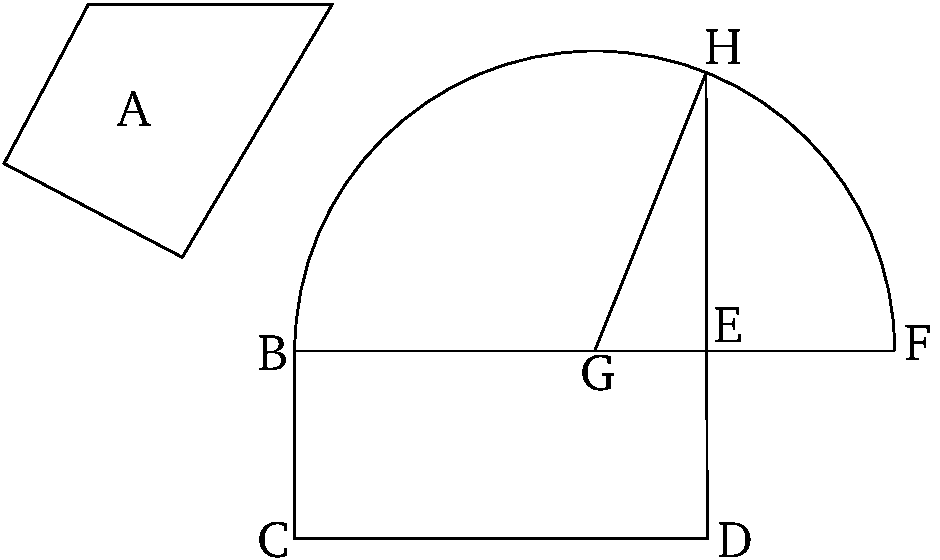
\includegraphics{Book02/fig14e.eps}}

For let the right-angled parallelogram $BD$,  equal to
the rectilinear figure $A$, be constructed  [Prop. 1.45]. Therefore, if $BE$ is equal to $ED$ then
that (which) was prescribed has taken place. For the square $BD$, equal to the rectilinear figure $A$,
has been constructed. And if not, (then)
one of the (straight-lines) $BE$ or $ED$ is greater (than the other). Let $BE$ be greater, and let it be
produced to $F$, and let $EF$ be made equal to $ED$ [Prop.~1.3].
And let $BF$ be cut in half at (point) $G$ [Prop.~1.10]. And, with center $G$, and
radius one of the (straight-lines) $GB$ or $GF$, let the semi-circle $BHF$ be drawn.
And let $DE$ be produced to $H$, and let $GH$ be joined.

Therefore, since the straight-line $BF$ has been cut---equally at $G$,
and unequally at $E$---the rectangle contained by $BE$ and $EF$, plus the
square on $EG$, is thus equal to the square on $GF$ [Prop.~2.5]. And $GF$ (is)
equal to $GH$. Thus, the (rectangle contained) by $BE$ and $EF$, plus the
(square) on $GE$, is equal to the (square) on $GH$. And the (sum of the) squares on $HE$ and $EG$  is equal to the (square)
on $GH$  [Prop.~1.47].
Thus, the (rectangle contained) by $BE$ and $EF$, plus the (square) on $GE$, is
equal to the (sum of the squares) on $HE$ and $EG$.
Let the square on $GE$ be taken from both. Thus, the remaining
rectangle contained by $BE$ and $EF$ is equal to the square
on $EH$. But, $BD$ is the (rectangle contained) by $BE$ and $EF$. For $EF$ (is)
equal to $ED$. Thus, the parallelogram $BD$ is equal to the square on $HE$.
And $BD$ (is) equal to the rectilinear figure $A$. Thus, the rectilinear figure
$A$ is also equal to the square (which) can be described on $EH$.

Thus, a 
square---(namely), that (which) can be described on $EH$---has been constructed, equal
to the given rectilinear figure $A$. (Which is) the very thing it was required to do.}
\end{Parallel}

% !TEX root = ../Elements.tex
% Greek and English text last checked 15/03/2013
%%%%%%
% BOOK 3
%%%%%%
\pdfbookmark[0]{Book 3}{book3}
\pagestyle{empty}
\begin{center}
{\Huge ELEMENTS BOOK 3}\\
\spa\spa\spa
{\huge\it Fundamentals of Plane Geometry Involving}\\[0.5ex] {\huge\it Circles}
\end{center}
%\vspace{2cm}
%\epsfysize=5in
%\centerline{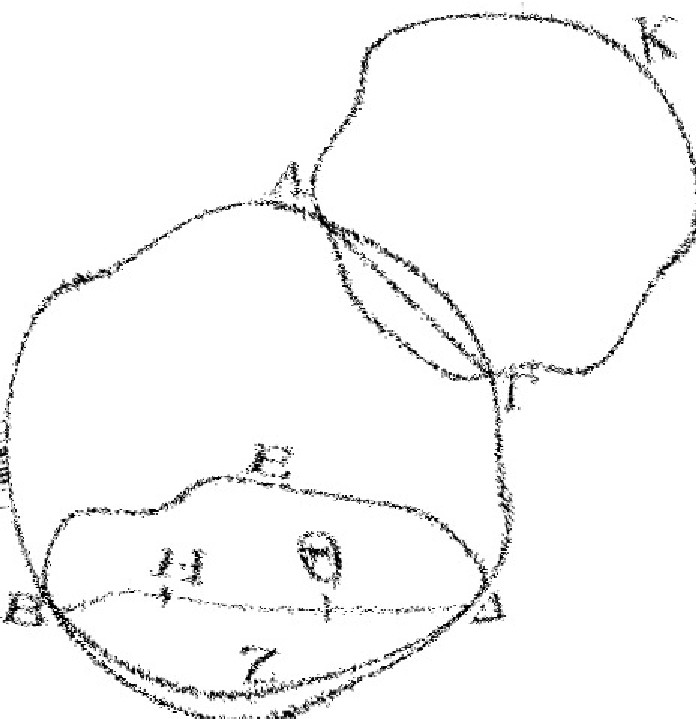
\includegraphics{Book03/front.eps}}
\newpage

%%%%%%%
% Definitions
%%%%%%%
\pdfbookmark[1]{Definitions}{def3}
\pagestyle{fancy}
\cfoot{\gr{\kern -.7pt }}
\lhead{\large\gr{ΣΤΟΙΘΕΙΩΝ \kern -.7pt {3}.}}
\rhead{\large ELEMENTS BOOK 3}
\begin{Parallel}{}{} 
\ParallelLText{
\begin{center}
\large{\gr{<'Οροι}.}
\end{center}\vspace*{-7pt}

\ggn{1}.~\gr{>'Ισοι κύκλοι εἰσίν, <ῶν αἱ διάμετροι >ίσαι εἰσίν,
>ὴ <ῶν αἱ ἐκ τῶν κέντρων >ίσαι εἰσίν.}

\ggn{2}.~\gr{Εὐθεῖα κύκλου ἐφάπτεσθαι λέγεται, <ήτιξ ἁπτομένη τοῦ
κύκλου καὶ ἐκβαλλομένη οὐ τέμνει τὸν κύκλον.}

\ggn{3}.~\gr{Κύκλοι ἐφάπτεσθαι ἀλλήλων λέγονται ο<ίτινεξ ἁπτό\-μενοι ἀλλήλων οὐ τέμνουσιν ἀλλήλουξ.}

\ggn{4}.~\gr{Ἐν κύκλῳ >ίσον ἀπέθειν ἀπὸ τοῦ κέντρου εὐθεῖαι
λέγονται, <όταν αἱ ἀπὸ τοῦ κέντρου ἐπ> α\kern -.7pt  ὐτὰξ κάθετοι ἀγόμεναι
>ίσαι >ῶσιν.}

\ggn{5}.~\gr{Μεῖζον δὲ ἀπέθειν λέγεται, ἐφ> <ὴν ἡ μείζων κάθετοξ πίπτει.}

\ggn{6}.~\gr{Τμ\kern -.7pt  ῆμα κύκλου ἐστὶ τὸ περιεχόμενον σθῆμα ὑπό τε εὐθείαξ καὶ κύκλου περιφερείαξ.}

\ggn{7}.~\gr{Τμ\kern -.7pt  ήματοξ δὲ γωνία ἐστὶν ἡ περιεθομένη ὑπό
τε εὐθείαξ καὶ κύκλου περιφερείαξ.}

\ggn{8}.~\gr{Ἐν τμ\kern -.7pt  ήματι δὲ γωνία ἐστίν, <όταν ἐπὶ τῆξ περιφερείαξ τοῦ τμ\kern -.7pt  ήματοξ ληφθῆ| τι σημεῖον καὶ ἀπ> α\kern -.5pt  ὐτοῦ ἐπὶ τὰ πέρατα
τῆξ εὐθείαξ, <ή ἐστι βάσιξ τοῦ τμ\kern -.3pt  ήματοξ, ἐπιζευθθῶσιν εὐθεῖαι,
ἡ περιεθομένη γωνία ὑπὸ τῶν ἐπιζευθθεισῶν εὐθειῶν.}

\ggn{9}.~\gr{<'Οταν δὲ αἱ περιέθουσαι τὴν γωνίαν εὐθεῖαι ἀπολαμβάνωσί τινα περιφέρειαν, ἐπ> ἐκείνηξ λέγεται βεβηκέναι ἡ γωνία.}

\ggn{10}.~\gr{Τομεὺξ δὲ κύκλου ἐστίν, <όταν πρὸξ τῶ| κέντρῶ| τοῦ
κύκλου συσταθῆ| γωνία, τὸ περιεχόμενον σθῆμα ὑπό τε τῶν τὴν
γωνίαν περιεθουσῶν
εὐθειῶν καὶ τῆξ ἀπολαμβανομένηξ ὑπ> α\kern -.7pt  ὐτῶν περιφερείαξ.}

\ggn{11}.~\gr{<'Ομοία τμ\kern -.7pt  ήματα κύκλων ἐστὶ τὰ δεθόμενα γωνίαξ >ίσαξ, >ή ἐν ο<ῖξ αἱ γωνίαι >ίσαι ἀλλήλαιξ εἰσίν.}}

\ParallelRText{
\begin{center}
{\large Definitions}
\end{center}

1.~Equal circles are (circles) whose diameters are equal,  or whose (distances)
from the centers (to the circumferences) are equal (i.e., whose radii are equal).

2.~A straight-line said to touch a circle  is any (straight-line) which, meeting the circle and being produced, does not cut the circle.

3.~Circles said to touch one another are any (circles) which, meeting one another, do not cut one another.

4.~In a circle, straight-lines are said to be equally far from the center
when the perpendiculars drawn to them from the center are equal.

5.~And (that straight-line) is said to be further (from the center) on
which the greater perpendicular falls (from the center).

6. ~A segment of a circle is the figure contained by a straight-line
and a circumference of a circle.

7.~And the angle of a segment is that contained by a straight-line
and a circumference of a circle.

8.~And the angle in a segment is the
angle contained by the joined straight-lines, when any
point  is taken on the circumference of a segment, 
and straight-lines are joined from it to the ends of the straight-line which is the base of the
segment.

9. ~And when the straight-lines containing an angle cut off some circumference, the angle is said to stand upon that (circumference).

10.~And a sector of a circle is the figure contained by the
straight-lines surrounding an angle, and the circumference cut off by them,
when the angle is constructed at the center of a circle.

11.~Similar segments of circles are those accepting equal angles, or
in which the angles are equal to one another.}
\end{Parallel}

%%%%%%
% Prop 3.1
%%%%%%
\pdfbookmark[1]{Proposition 3.1}{pdf3.1}
\begin{Parallel}{}{} 
\ParallelLText{
\begin{center}
{\large \ggn{1}.}
\end{center}\vspace*{-7pt}

\gr{Τοῦ δοθέντοξ κύκλου τὸ κέντρον εὑρεῖν.}

\gr{>'Εστω ὁ δοθεὶξ κύκλοξ ὁ ΑΒΓ; δεῖ δὴ τοῦ ΑΒΓ κύκλου
τὸ κέντρον εὑρεῖν.}

\gr{Διήθθω τιξ εἰξ α\kern -.7pt  ὐτόν, ὡξ >έτυθεν, εὐθεῖα ἡ ΑΒ, καὶ τετμ\kern -.7pt  ήσθω δίθα
κατὰ τὸ Δ σημεῖον, καὶ ἀπὸ τοῦ Δ τῆ| ΑΒ πρὸξ ὀρθὰξ >ήθθω
ἡ ΔΓ καὶ διήθθω ἐπὶ τὸ Ε, καὶ τετμ\kern -.5pt  ήσθω ἡ ΓΕ δίθα κατὰ τὸ Ζ;
λέγω, <ότι τὸ Ζ κέντρον ἐστὶ τοῦ ΑΒΓ [κύκλου].}

\gr{μ\kern -.7pt  ὴ γάρ, ἀλλ> εἰ δυνατόν, >έστω τὸ Η, καὶ ἐπεζεύθθωσαν αἱ ΗΑ, ΗΔ, ΗΒ. καὶ ἐπεὶ >ίση ἐστὶν ἡ ΑΔ τῆ| ΔΒ, κοινὴ δὲ ἡ ΔΗ, δύο δὴ
αἱ ΑΔ, ΔΗ δύο ταῖξ ΗΔ, ΔΒ >ίσαι εἰσὶν ἑκατέρα ἑκατέρᾳ;
καὶ βάσιξ ἡ ΗΑ βάσει τῆ| ΗΒ ἐστιν >ίση; ἐκ κέντρου γάρ;
γωνία >άρα ἡ ὑπὸ ΑΔΗ γωνίᾳ τῆ| ὑπὸ ΗΔΒ >ίση ἐστίν.
<όταν δὲ εὐθεῖα ἐπ> εὐθεῖαν σταθεῖσα τὰξ ἐφεχῆξ γωνίαξ
>ίσαξ ἀλλήλαιξ ποιῆ|, ὀρθὴ ἑκατέρα τῶν >ίσων γωνιῶν ἐστιν; ὀρθὴ
>άρα ἐστὶν ἡ  ὑπὸ ΗΔΒ. ἐστὶ δὲ καὶ ἡ ὑπὸ ΖΔΒ ὀρθή;
>ίση >άρα ἡ ὑπὸ ΖΔΒ τῆ| ὑπὸ ΗΔΒ, ἡ μείζων τῆ| ἐλάττονι;
<όπερ ἐστὶν ἀδύνατον. οὐκ >άρα τὸ Η κέντρον ἐστὶ τοῦ
ΑΒΓ κύκλου. ὁμοίωξ δὴ δείχομεν, <ότι οὐδ> >άλλο
τι πλὴν τοῦ Ζ.}\\~\\~\\~\\

\epsfysize=2.2in
\centerline{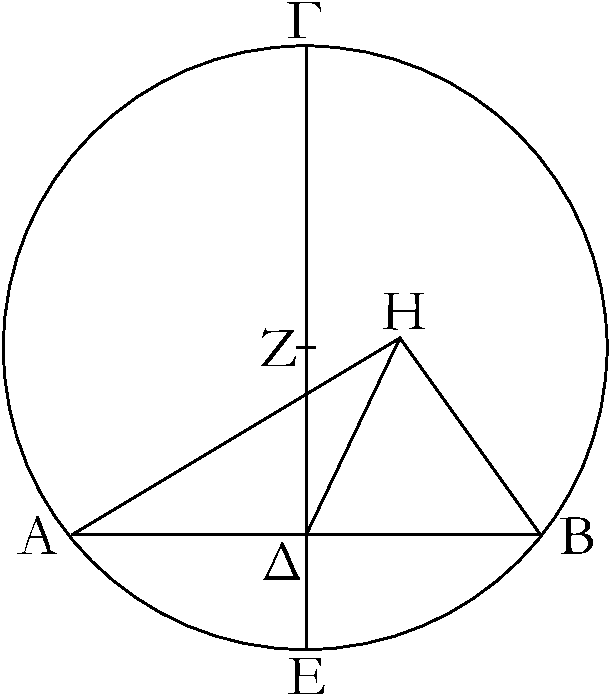
\includegraphics{Book03/fig01g.eps}}

\gr{Τὸ Ζ >άρα σημεῖον κέντρον ἐστὶ τοῦ ΑΒΓ [κύκλου].}

\begin{center}\mbox{}\\
{\large \gr{Πόρισμα}.}
\end{center}\vspace*{-7pt}

\gr{Ἐκ δὴ τούτου φανερόν, <ότι ἒαν ἐν κύκλῳ εὐθεῖά
τιξ εὐθεῖάν τινα δίθα καὶ πρὸξ ὀρθὰξ τέμνῃ, ἐπὶ
τῆξ τεμνούσηξ ἐστὶ τὸ κέντρον τοῦ κύκλου.} --- \gr{<όπερ >έδει
ποιῆσαι.}}

\ParallelRText{
\begin{center}
{\large Proposition 1}
\end{center}

To find the center of a given circle.

Let $ABC$ be the given circle. So it is required to find the center of circle $ABC$.

Let some straight-line $AB$ be drawn through ($ABC$), at random,
and let ($AB$) be cut in half at point $D$ 
[Prop.~1.9]. And let
$DC$ be drawn from $D$, at right-angles to $AB$ [Prop.~1.11].
And let ($CD$) be drawn through to $E$. And let $CE$ be cut in half
at $F$ [Prop.~1.9]. I say that (point) $F$ is the center of the [circle] $ABC$.

For (if) not (then), if possible, let $G$ (be the center of the circle), and
let $GA$, $GD$, and $GB$ be joined. And since $AD$ is equal to $DB$,
and $DG$ (is) common, the two (straight-lines) $AD$, $DG$
are equal to the two (straight-lines) $BD$, $DG$,$^\dag$ respectively. And the
base $GA$ is equal to the base $GB$. For (they are both) radii. Thus, angle
$ADG$ is equal to angle $GDB$ [Prop.~1.8]. And when a straight-line
stood upon (another) straight-line make  adjacent angles (which are)
equal to one another, each of the equal angles is a right-angle [Def.~1.10].
Thus, $GDB$ is a right-angle. And $FDB$ is also a right-angle. Thus,
$FDB$ (is) equal to $GDB$, the greater to the lesser. The very thing
is impossible. Thus, (point) $G$ is not the center of the circle $ABC$. 
So, similarly, we can show that neither is any other (point) except $F$.

\epsfysize=2.2in
\centerline{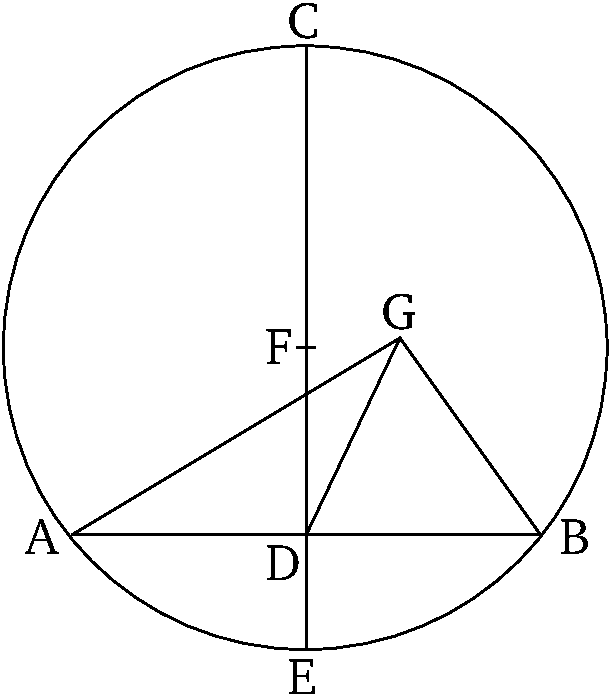
\includegraphics{Book03/fig01e.eps}}

Thus, point $F$ is the center of the [circle] $ABC$.

\begin{center}\mbox{}\\
{\large Corollary}
\end{center}

So, from this, (it is) manifest that if any straight-line in a circle
cuts any (other) straight-line in half, and at right-angles, (then) the center
of the circle is on the former (straight-line). --- (Which is) the very thing it
was required to do.}
\end{Parallel}
{\footnotesize \noindent$^\dag$  The Greek text has ``$GD$, $DB$'', which is obviously a mistake.} 

%%%%%%
% Prop 3.2
%%%%%%
\pdfbookmark[1]{Proposition 3.2}{pdf3.2}
\begin{Parallel}{}{} 
\ParallelLText{
\begin{center}
{\large \ggn{2}.}
\end{center}\vspace*{-7pt}

\gr{Ἐὰν κύκλου ἐπὶ τῆξ περιφερείαξ ληφθῆ| δύο
τυθόντα σημεῖα, ἡ ἐπὶ τὰ σημεῖα ἐπιζευγνυμένη εὐθεῖα
ἐντὸξ πεσεῖται τοῦ κύκλου.}

\gr{>'Εστω κύκλοξ ὁ ΑΒΓ, καὶ ἐπὶ τῆξ περιφερείαξ α\kern -.7pt  ὐτοῦ εἰλήφθω
δύο τυθόντα σημεῖα τὰ Α, Β; λέγω, <ότι ἡ ἀπὸ τοῦ Α ἐπὶ τὸ Β
ἐπιζευγνυμένη εὐθεῖα ἐντὸξ πεσεῖται τοῦ κύκλου.}

\gr{μ\kern -.7pt  ὴ γάρ, ἀλλ> εἰ δυνατόν, πιπτέτω ἐκτὸξ ὡξ ἡ ΑΕΒ, καὶ εἰλήφθω
τὸ κέντρον τοῦ ΑΒΓ κύκλου, καὶ >έστω τὸ Δ, καὶ ἐπεζεύθθωσαν αἱ
ΔΑ, ΔΒ, καὶ διήθθω ἡ ΔΖΕ.}

\gr{Ἐπεὶ ο>ῦν >ίση ἐστὶν ἡ ΔΑ τῆ| ΔΒ, >ίση >άρα
καὶ γωνία ἡ ὑπὸ ΔΑΕ τῆ| ὑπὸ ΔΒΕ; καὶ ἐπεὶ τριγώνου
τοῦ ΔΑΕ μία πλευρὰ προσεκβέβληται ἡ ΑΕΒ, μείζων
>άρα ἡ ὑπὸ ΔΕΒ γωνία τῆξ ὑπὸ ΔΑΕ. >ίση δὲ ἡ ὑπὸ
ΔΑΕ τῆ|  ὑπὸ ΔΒΕ; μείζων >άρα ἡ ὑπὸ ΔΕΒ τῆξ ὑπὸ
ΔΒΕ. ὑπὸ δὲ τὴν μείζονα γωνίαν ἡ μείζων πλευρὰ
ὑποτείνει; μείζων >άρα ἡ ΔΒ τῆξ ΔΕ. >ίση δὲ ἡ ΔΒ
τῆ| ΔΖ. μείζων >άρα ἡ ΔΖ τῆξ ΔΕ ἡ ἐλάττων τῆξ
μείζονοξ; <όπερ ἐστὶν ἀδύνατον. οὐκ >άρα ἡ ἀπὸ
τοῦ Α ἐπὶ τὸ Β ἐπιζευγνυμένη εὐθεῖα ἐκτὸξ
πεσεῖται τοῦ κύκλου. ὁμοίωξ δὴ δείχομεν, <ότι οὐδὲ ἐπ>
α\kern -.7pt  ὐτῆξ τῆξ περιφερείαξ; ἐντὸξ >άρα.}\\~\\~\\

\epsfysize=2.2in
\centerline{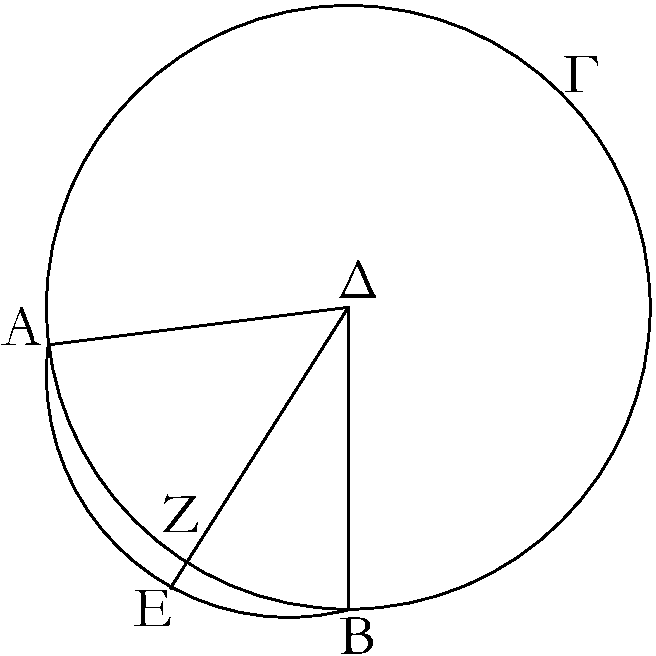
\includegraphics{Book03/fig02g.eps}}

\gr{Ἐὰν >άρα κύκλου ἐπὶ τῆξ περιφερείαξ ληφθῆ| δύο
τυθόντα σημεῖα, ἡ ἐπὶ τὰ σημεῖα ἐπιζευγνυμένη εὐθεῖα
ἐντὸξ πεσεῖται τοῦ κύκλου; <όπερ >έδει δεῖχαι.}}

\ParallelRText{
\begin{center}
{\large Proposition 2}
\end{center}

If two points are taken at random on the circumference of a circle,  (then)
the straight-line joining the points will fall inside the circle.

Let $ABC$ be a circle, and let two points $A$ and $B$ be taken
at random on its circumference. I say that the straight-line joining
$A$ to $B$ will fall inside the circle.

For (if) not (then), if possible, let it fall outside (the circle), like $AEB$ (in the figure). And let the center of the circle $ABC$ be found [Prop.~3.1], and let it be (at point) $D$. And let $DA$ and $DB$ be joined, and let $DFE$ be
drawn through.

Therefore, since $DA$ is equal to $DB$, the angle $DAE$ (is) thus also equal to
$DBE$ [Prop.~1.5]. And since in triangle $DAE$ the one side, $AEB$, has been
produced, angle $DEB$ (is) thus greater than $DAE$ [Prop.~1.16]. And
$DAE$ (is) equal to $DBE$ [Prop.~1.5]. Thus, $DEB$ (is) greater than $DBE$.
And the greater angle is subtended by the greater side [Prop.~1.19].
Thus, $DB$ (is) greater than $DE$. And $DB$ (is) equal to $DF$. Thus,
$DF$ (is) greater than $DE$, the lesser than the greater. The very thing is impossible.
Thus, the straight-line joining $A$ to $B$ will not fall outside the
circle. So, similarly, we can show that neither (will it fall) on the
circumference itself. Thus, (it will fall) inside (the circle).

\epsfysize=2.2in
\centerline{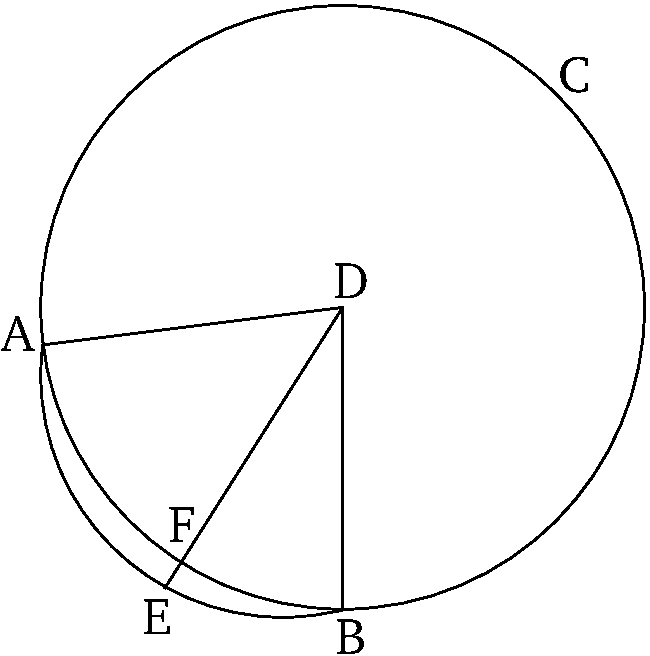
\includegraphics{Book03/fig02e.eps}}

Thus, if two points are taken at random on the circumference of a circle, (then)
the straight-line joining the points will fall inside the circle. (Which is) the
very thing it was required to show.}
\end{Parallel}

%%%%%%
% Prop 3.3
%%%%%%
\pdfbookmark[1]{Proposition 3.3}{pdf3.3}
\begin{Parallel}{}{} 
\ParallelLText{
\begin{center}
{\large \ggn{3}.}
\end{center}\vspace*{-7pt}

\gr{Ἐὰν ἐν κύκλῳ εὐθεῖά τιξ διὰ τοῦ κέντρου εὐθεῖάν τινα μ\kern -.7pt  ὴ διὰ τοῦ κέντρου δίθα τέμνῃ, καὶ πρὸξ ὀρθὰξ α\kern -.7pt  ὐτὴν τέμνει; καὶ ἒαν πρὸξ ὀρθὰξ α\kern -.5pt  ὐτὴν τέμνῃ, καὶ δίθα α\kern -.3pt  ὐτὴν τέμνει.}

\gr{>'Εστω κύκλοξ ὁ ΑΒΓ, καὶ ἐν α\kern -.7pt  ὐτῶ| εὐθεῖά τιξ διὰ τοῦ κέντρου ἡ ΓΔ εὐθεῖάν τινα μ\kern -.7pt  ὴ διὰ τοῦ κέντρου τὴν ΑΒ δίθα τεμνέτω κατὰ τὸ
Ζ σημεῖον; λέγω, <ότι καὶ πρὸξ ὀρθὰξ α\kern -.5pt  ὐτὴν τέμνει.}

\gr{Εἰλήφθω γὰρ τὸ κέντρον τοῦ ΑΒΓ κύκλου, καὶ >έστω τὸ Ε, καὶ ἐπεζεύθθωσαν αἱ ΕΑ, ΕΒ.}

\gr{Καὶ ἐπεὶ >ίση ἐστὶν ἡ ΑΖ τῆ| ΖΒ, κοινὴ δὲ ἡ ΖΕ, δύο δυσὶν >ίσαι [εἰσίν]; καὶ βάσιξ ἡ ΕΑ βάσει τῆ| ΕΒ >ίση; γωνία >άρα ἡ ὑπὸ ΑΖΕ γωνίᾳ τῆ| ὑπὸ ΒΖΕ >ίση ἐστίν. <όταν δὲ εὐθεῖα ἐπ> εὐθεῖαν
σταθεῖσα τὰξ ἐφεχῆξ γωνίαξ >ίσαξ ἀλλήλαιξ ποιῆ|,  ὀρθὴ
ἑκατέρα τῶν >ίσων γωνιῶν ἐστιν; ἑκατέρα >άρα τῶν ὑπὸ ΑΖΕ, ΒΖΕ ὀρθή ἐστιν. ἡ ΓΔ >άρα διὰ τοῦ κέντρου ο>ῦσα τὴν ΑΒ μ\kern -.7pt  ὴ
διὰ τοῦ κέντρου ο>ῦσαν δίθα τέμνουσα καὶ πρὸξ ὀρθὰξ τέμνει.}

\gr{Ἀλλὰ δὴ ἡ ΓΔ τὴν ΑΒ πρὸξ ὀρθὰξ τεμνέτω; λέγω, <ότι καὶ δίθα
α\kern -.7pt  ὐτὴν τέμνει, τουτέστιν, <ότι >ίση ἐστὶν ἡ ΑΖ τῆ| ΖΒ.}

\gr{Τῶν γὰρ α\kern -.7pt  ὐτῶν κατασκευασθέντων, ἐπεὶ >ίση ἐστὶν ἡ ΕΑ τῆ| ΕΒ,
>ίση ἐστὶ καὶ γωνία ἡ ὑπὸ ΕΑΖ τῆ| ὑπὸ ΕΒΖ. ἐστὶ δὲ καὶ
ὀρθὴ ἡ ὑπὸ ΑΖΕ ὀρθῆ| τῆ| ὑπὸ ΒΖΕ >ίση; δύο >άρα τρίγωνά
ἐστι ΕΑΖ, ΕΖΒ τὰξ δύο γωνίαξ δυσὶ γωνίαιξ >ίσαξ >έθοντα καὶ
μίαν πλευρὰν μιᾶ| πλευρᾶ| >ίσην κοινὴν α\kern -.7pt  ὐτῶν τὴν ΕΖ ὑποτείνουσαν ὑπὸ μίαν τῶν >ίσων γωνιῶν; καὶ τὰξ λοιπὰξ >άρα πλευρὰξ ταῖξ
λοιπαῖξ πλευραῖξ >ίσαξ <έχει; >ίση >άρα ἡ ΑΖ τῆ| ΖΒ.}\\~\\~\\~\\

\epsfysize=2.2in
\centerline{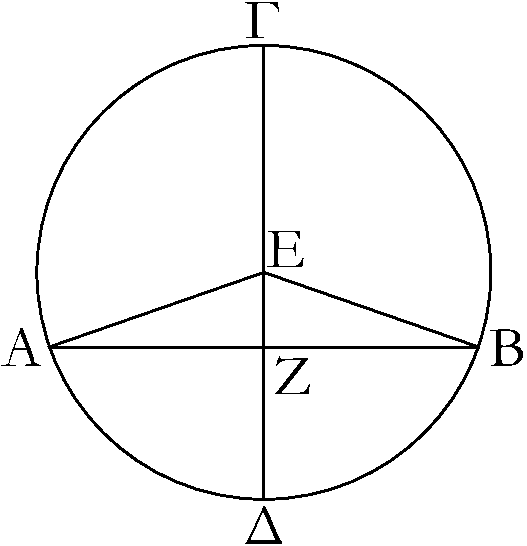
\includegraphics{Book03/fig03g.eps}}

\gr{Ἐὰν >άρα ἐν κύκλῳ εὐθεῖά τιξ διὰ τοῦ κέντρου εὐθεῖάν τινα μ\kern -.7pt  ὴ διὰ τοῦ κέντρου δίθα τέμνῃ, καὶ πρὸξ ὀρθὰξ α\kern -.7pt  ὐτὴν τέμνει; καὶ ἒαν πρὸξ ὀρθὰξ α\kern -.5pt  ὐτὴν τέμνῃ, καὶ δίθα α\kern -.3pt  ὐτὴν τέμνει; <όπερ >έδει δεῖχαι.}}

\ParallelRText{
\begin{center}
{\large Proposition 3}
\end{center}

In a circle, if any straight-line through the center cuts in half any straight-line
not through the center, (then) it also cuts it at right-angles. And (conversely)
if it cuts it at right-angles, (then) it also cuts it in half.

Let $ABC$ be a circle, and, within it, let some straight-line through the center,
$CD$, 
cut in half some straight-line not through the center, $AB$, at the point $F$.
I say that ($CD$) also cuts ($AB$) at right-angles.

For let the center of the circle $ABC$ be found [Prop.~3.1], and let it
be (at point) $E$, and let $EA$ and $EB$ be joined.

And since  $AF$ is equal to $FB$, and $FE$ (is) common, two (sides  of triangle $AFE$) [are] equal to
two (sides of triangle $BFE$). And the base $EA$ (is) equal to the base $EB$. Thus, angle
$AFE$ is equal to angle $BFE$ [Prop.~1.8]. And when a straight-line
stood upon (another) straight-line makes adjacent angles (which are)
equal to one another, each of the equal angles is a right-angle [Def.~1.10].
Thus, $AFE$ and $BFE$ are each right-angles. Thus, the (straight-line) $CD$, which is
through the center
and cuts  in half the (straight-line) $AB$, which is not through the center, also cuts ($AB$) at right-angles.

And so let $CD$ cut $AB$ at right-angles. I say that it also cuts ($AB$) in half.
That is to say, that $AF$ is equal to $FB$.

For, with the same construction, since $EA$ is equal to $EB$, angle $EAF$ is also
equal to $EBF$ [Prop.~1.5]. And the right-angle $AFE$ is also equal to the
right-angle $BFE$. Thus, $EAF$ and $EFB$ are two triangles having two angles
equal to two angles, and one side equal to one side---(namely), their common (side)
$EF$, subtending one of the equal angles. Thus, they will also have the remaining sides equal to the (corresponding) remaining sides [Prop.~1.26]. Thus, $AF$ (is) equal to $FB$.

\epsfysize=2.2in
\centerline{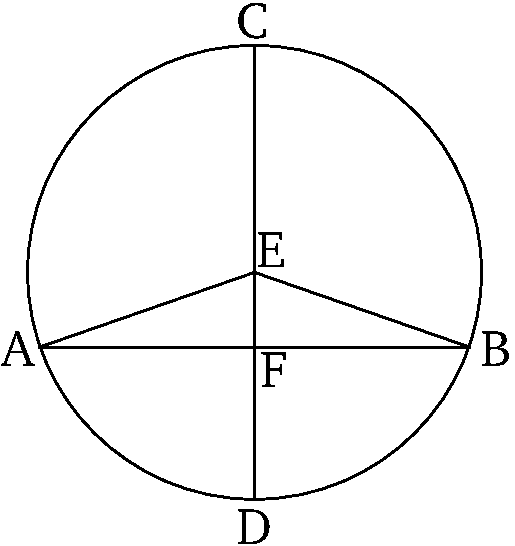
\includegraphics{Book03/fig03e.eps}}

Thus, in a circle, if any straight-line through the center cuts in half any straight-line
not through the center, (then) it also cuts it at right-angles. And (conversely)
if it cuts it at right-angles, (then) it also cuts it in half. (Which is) the very thing
it was required to show.}
\end{Parallel}

%%%%%%
% Prop 3.4
%%%%%%
\pdfbookmark[1]{Proposition 3.4}{pdf3.4}
\begin{Parallel}{}{} 
\ParallelLText{
\begin{center}
{\large \ggn{4}.}
\end{center}\vspace*{-7pt}

\gr{Ἐὰν ἐν κύκλῳ δύο εὐθεῖαι τέμνωσιν ἀλλήλαξ μ\kern -.7pt  ὴ δὶα τοῦ
κέντρου ο>ῦσαι, οὐ τέμνουσιν ἀλλήλαξ δίθα.}\\

\epsfysize=2in
\centerline{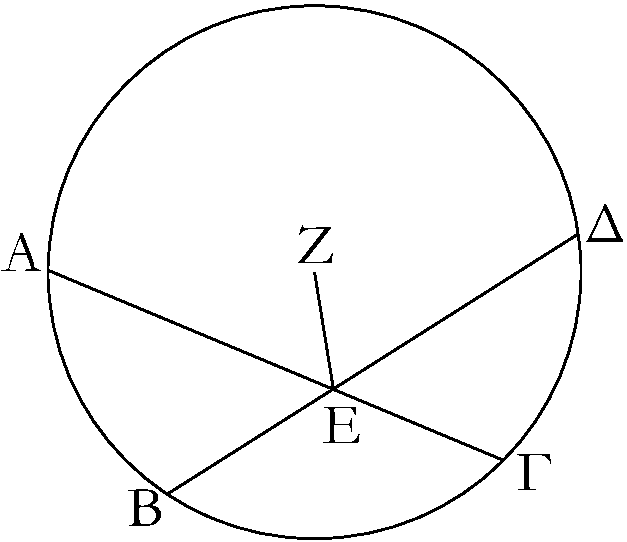
\includegraphics{Book03/fig04g.eps}}

\gr{>'Εστω κύκλοξ ὁ ΑΒΓΔ, καὶ ἐν α\kern -.7pt  ὐτῶ| δύο εὐθεῖαι αἱ ΑΓ,
ΒΔ τεμνέτωσαν ἀλλήλαξ κατὰ τὸ Ε μ\kern -.7pt  ὴ διὰ τοῦ κέντρου ο>ῦσαι;
λέγω, <ότι οὐ τέμνουσιν ἀλλήλαξ δίθα.}

\gr{Εἰ γὰρ δυνατόν, τεμνέτωσαν ἀλλήλαξ δίθα <ώστε >ίσην ε>ῖναι
τὴν μὲν ΑΕ τῆ| ΕΓ, τὴν δὲ ΒΕ τῆ| ΕΔ; καὶ εἰλήφθω τὸ κέντρον
τοῦ ΑΒΓΔ κύκλου, καὶ >έστω τὸ Ζ, καὶ ἐπεζεύθθω ἡ ΖΕ.}

\gr{Ἐπεὶ ο>ῦν εὐθεῖά τιξ διὰ τοῦ κέντρου ἡ ΖΕ εὐθεῖάν τινα
μ\kern -.7pt  ὴ διὰ τοῦ κέντρου τὴν ΑΓ δίθα τέμνει, καὶ πρὸξ ὀρθὰξ α\kern -.7pt  ὐτὴν τέμνει; ὀρθὴ >άρα ἐστὶν ἡ ὑπὸ ΖΕΑ; πάλιν, ἐπεὶ εὐθεῖά τιξ ἡ ΖΕ εὐθεῖάν τινα τὴν ΒΔ δίθα τέμνει, καὶ πρὸξ ὀρθὰξ α\kern -.5pt  ὐτὴν τέμνει;
ὀρθὴ >άρα ἡ ὑπὸ ΖΕΒ. ἐδείθθη δὲ καὶ ἡ ὑπὸ ΖΕΑ ὀρθή; >ίση >άρα ἡ ὑπὸ ΖΕΑ τῆ| ὑπὸ ΖΕΒ ἡ ἐλάττων τῆ| μείζονι;
<όπερ ἐστὶν ἀδύνατον. οὐκ >άρα αἱ ΑΓ, ΒΔ τέμνουσιν ἀλλήλαξ δίθα.}

\gr{Ἐὰν >άρα ἐν κύκλῳ δύο εὐθεῖαι τέμνωσιν ἀλλήλαξ μ\kern -.7pt  ὴ δὶα τοῦ
κέντρου ο>ῦσαι, οὐ τέμνουσιν ἀλλήλαξ δίθα; <όπερ >έδει δεῖχαι.}}

\ParallelRText{
\begin{center}
{\large Proposition 4}
\end{center}

In a circle, if two straight-lines, which are not through the center, cut
one another, (then) they do not cut one another in half.

\epsfysize=2in
\centerline{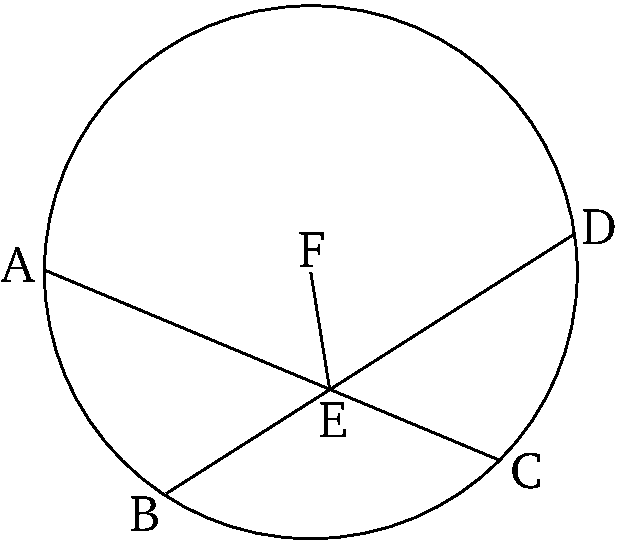
\includegraphics{Book03/fig04e.eps}}

Let $ABCD$ be a circle, and within it, let two straight-lines, $AC$ and
$BD$, which are not through the center, cut one another at  (point) $E$. I say that they
do not cut one another in half.

For, if possible, let them cut one another in half, such that $AE$ is equal to $EC$, and
$BE$ to $ED$. And let the center of the circle $ABCD$ be found [Prop.~3.1], and let it be (at point) $F$, and let $FE$ be joined.

Therefore, since some straight-line through the center, $FE$, cuts in half
some straight-line not through the center, $AC$, it also cuts it at right-angles
[Prop.~3.3]. Thus, $FEA$ is a right-angle. Again, since some straight-line
$FE$ cuts in half some straight-line $BD$, it also cuts it at right-angles [Prop.~3.3]. Thus, $FEB$ (is) a right-angle. But $FEA$ was also shown (to be) a right-angle. Thus, $FEA$ (is) equal to $FEB$, the lesser to the greater.
The very thing is impossible. Thus, $AC$ and $BD$ do not cut one another in half.

Thus, in a circle, if two straight-lines, which are not through the center, cut
one another, (then) they do not cut one another in half. (Which is) the very
thing it was required to show.}
\end{Parallel}

%%%%%%
% Prop 3.5
%%%%%%
\pdfbookmark[1]{Proposition 3.5}{pdf3.5}
\begin{Parallel}{}{} 
\ParallelLText{
\begin{center}
{\large \ggn{5}.}
\end{center}\vspace*{-7pt}

\gr{Ἐὰν δύο κύκλοι τέμνωσιν ἀλλήλουξ, οὐκ >έσται α\kern -.7pt  ὐτῶν τὸ α\kern -.7pt  ὐτὸ
κέντρον.}

\epsfysize=2in
\centerline{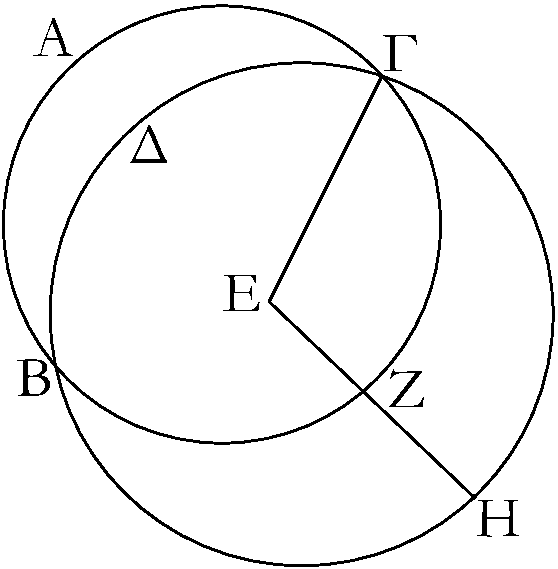
\includegraphics{Book03/fig05g.eps}}

\gr{Δύο γὰρ κύκλοι οἱ ΑΒΓ, ΓΔΗ τεμνέτωσαν ἀλλήλουξ κατὰ τὰ Β, Γ σημεῖα. λέγω, <ότι οὐκ >έσται α\kern -.7pt  ὐτῶν τὸ α\kern -.7pt  ὐτὸ κέντρον.}

\gr{Εἰ γὰρ δυνατόν, >έστω τὸ Ε, καὶ ἐπεζεύθθω ἡ ΕΓ, καὶ διήθθω
ἡ ΕΖΗ, ὡξ >έτυθεν. καὶ ἐπεὶ τὸ Ε σημεῖον κέντρον ἐστὶ τοῦ ΑΒΓ κύκλου, <ίση ἐστὶν ἡ ΕΓ τῆ| ΕΖ. πάλιν, ἐπεὶ τὸ Ε σημεῖον κέντρον ἐστὶ τοῦ ΓΔΗ κύκλου, >ίση ἐστὶν ἡ ΕΓ τῆ| ΕΗ; ἐδείθθη
δὲ ἡ ΕΓ καὶ τῆ| ΕΖ >ίση; καὶ ἡ ΕΖ >άρα τῆ| ΕΗ ἐστιν >ίση ἡ
ἐλάσσων τῆ| μείζονι; <όπερ ἐστὶν ἀδύνατον.  οὐκ >άρα τὸ Ε
σημεῖον κέντρον ἐστὶ τῶν ΑΒΓ, ΓΔΗ κύκλων.}

\gr{Ἐὰν >άρα δύο κύκλοι τέμνωσιν ἀλλήλουξ, οὐκ >έστιν α\kern -.7pt  ὐτῶν τὸ
α\kern -.7pt  ὐτὸ κέντρον; <όπερ >έδει δεῖχαι.}}

\ParallelRText{
\begin{center}
{\large Proposition 5}
\end{center}

If two circles cut one another,  (then) they will not have the same center.

\epsfysize=2in
\centerline{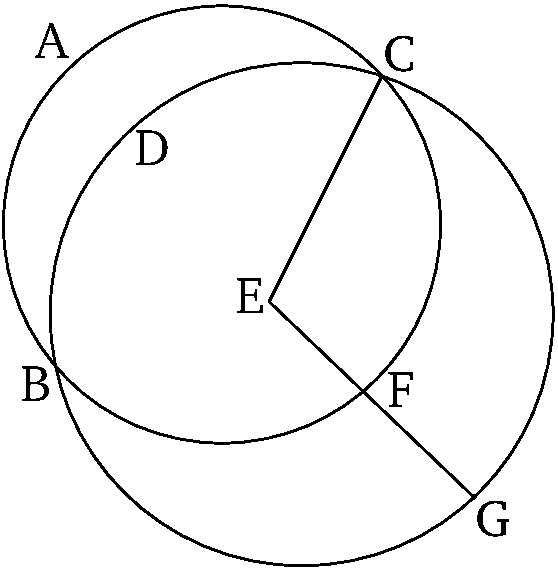
\includegraphics{Book03/fig05e.eps}}

For let the two circles $ABC$ and $CDG$ cut one another at  points $B$ and $C$.
I say that they will not have the same center.

For, if possible, let $E$ be (the common center), and let $EC$ be joined,
and let $EFG$ be drawn through (the two circles), at random. And since point $E$
is the center of the circle $ABC$, $EC$ is equal to $EF$. Again, since point $E$ is
the center of the circle $CDG$, $EC$ is equal to $EG$. But $EC$  was also shown (to be) equal to $EF$. Thus, $EF$ is also equal to $EG$, the lesser to the
greater. The very thing is impossible. Thus, point $E$ is not the (common)
center of the circles $ABC$ and $CDG$.

Thus, if two circles cut one another, (then) they will not have the same
center. (Which is) the very thing it was required to show.}
\end{Parallel}

%%%%%%
% Prop 3.6
%%%%%%
\pdfbookmark[1]{Proposition 3.6}{pdf3.6}
\begin{Parallel}{}{} 
\ParallelLText{
\begin{center}
{\large \ggn{6}.}
\end{center}\vspace*{-7pt}

\gr{Ἐὰν δύο κύκλοι ἐφάπτωνται ἀλλήλων, οὐκ >έσται α\kern -.7pt  ὐτῶν τὸ α\kern -.7pt  ὐτὸ κέντρον.}

\gr{Δύο γὰρ κύκλοι οἱ ΑΒΓ, ΓΔΕ ἐφαπτέσθωσαν ἀλλήλων κατὰ τὸ Γ
σημεῖον; λέγω, <ότι οὐκ >έσται α\kern -.7pt  ὐτῶν τὸ α\kern -.7pt  ὐτὸ κέντρον.}

\gr{Εἰ γὰρ δυνατόν, >έστω τὸ Ζ, καὶ ἐπεζεύθθω ἡ ΖΓ, καὶ διήθθω, ὡξ >έτυθεν, ἡ ΖΕΒ.}

\gr{Ἐπεὶ ο~ὐν τὸ Ζ σημεῖον κέντρον ἐστὶ τοῦ ΑΒΓ κύκλου, >ίση
ἐστὶν ἡ ΖΓ τῆ| ΖΒ. πάλιν, ἐπεὶ τὸ Ζ σημεῖον κέντρον ἐστὶ τοῦ ΓΔΕ κύκλου, >ίση ἐστὶν ἡ ΖΓ τῆ| ΖΕ. ἐδείθθη δὲ ἡ ΖΓ τῆ| ΖΒ
>ίση; καὶ ἡ ΖΕ >άρα τῆ| ΖΒ ἐστιν >ίση, ἡ ἐλάττων τῆ| μείζονι;
<όπερ ἐστὶν ἀδύνατον. οὐκ >άρα τὸ Ζ σημεῖον κέντρον ἐστὶ
τῶν ΑΒΓ, ΓΔΕ κύκλων.}

\epsfysize=2.2in
\centerline{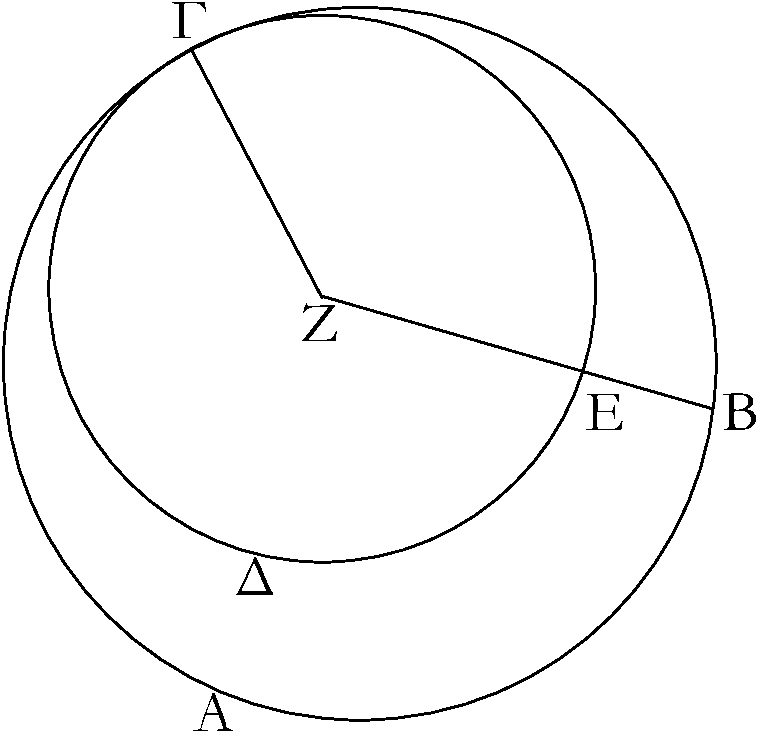
\includegraphics{Book03/fig06g.eps}}

\gr{Ἐὰν >άρα δύο κύκλοι ἐφάπτωνται ἀλλήλων, οὐκ >έσται α\kern -.7pt  ὐτῶν τὸ α\kern -.7pt  ὐτὸ κέντρον; <όπερ >έδει δεῖχαι.}}

\ParallelRText{
\begin{center}
{\large Proposition 6}
\end{center}

If  two circles touch one another, (then) they  will not have the same center.

For let the two circles $ABC$ and $CDE$ touch one another at point $C$. I say that
they will not have the same center.

For, if possible, let $F$ be (the common center), and let $FC$ be
joined, and let $FEB$ be drawn through (the two circles), at random.

Therefore, since point $F$ is the center of the circle $ABC$, $FC$ is equal to
$FB$. Again, since point $F$ is the center of the circle $CDE$, $FC$ is
equal to $FE$. But $FC$ was shown (to be) equal to $FB$. Thus, $FE$ is
also equal to $FB$, the lesser to the greater. The very thing is impossible.
Thus, point $F$ is not the (common) center of the circles
$ABC$ and $CDE$.

\epsfysize=2.2in
\centerline{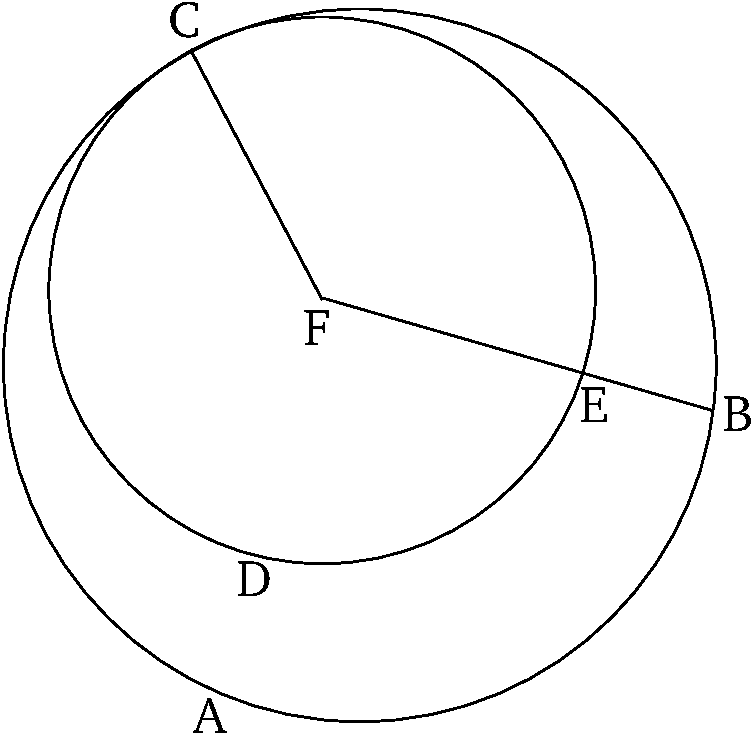
\includegraphics{Book03/fig06e.eps}}

Thus, if two circles touch one another, (then) they  will not have the same center. (Which is) the very thing it was required to show.}
\end{Parallel}

%%%%%%
% Prop 3.7
%%%%%%
\pdfbookmark[1]{Proposition 3.7}{pdf3.7}
\begin{Parallel}{}{} 
\ParallelLText{
\begin{center}
{\large \ggn{7}.}
\end{center}\vspace*{-7pt}

\gr{Ἐὰν κύκλου ἐπὶ τῆξ διαμέτρου ληφθῆ| τι σημεῖον, <ὸ μ\kern -.7pt  ή ἐστι κέντρον τοῦ κύκλου, ἀπὸ δὲ τοῦ σημείου πρὸξ τὸν κύκλον προσπίπτωσιν εὐθεῖαί τινεξ, μεγίστη μὲν >έσται, ἐφ> <ῆξ
τὸ κέντρον, ἐλαθίστη δὲ ἡ λοιπή, τῶν δὲ >άλλων ἀεὶ ἡ
>έγγιον τῆξ δὶα τοῦ κέντρου τῆξ ἀπώτερον μείζων ἐστίν, δύο
δὲ μόνον >ίσαι ἀπὸ τοῦ σημείου προσπεσοῦνται πρὸξ τὸν
κύκλον ἐφ> ἑκάτερα τῆξ ἐλαθίστηξ.}

\gr{>'Εστω κύκλοξ ὁ ΑΒΓΔ, διάμετροξ δὲ α\kern -.7pt  ὐτοῦ >έστω ἡ ΑΔ, καὶ ἐπὶ
τῆξ ΑΔ εἰλήφθω τι σημεῖον τὸ Ζ, <ὸ μ\kern -.7pt  ή ἐστι κέντρον τοῦ κύκλου, κέντρον δὲ τοῦ κύκλου >έστω τὸ Ε, καὶ ἀπὸ τοῦ Ζ πρὸξ τὸν ΑΒΓΔ κύκλον προσπιπτέτωσαν εὐθεῖαί τινεξ αἱ ΖΒ, ΖΓ, ΖΗ; λέγω, <ότι
μεγίστη μέν ἐστιν ἡ ΖΑ, ἐλαθίστη δὲ ἡ ΖΔ, τῶν δὲ >άλλων ἡ μὲν
ΖΒ τῆξ ΖΓ μείζων, ἡ δὲ ΖΓ τῆξ ΖΗ.}

\gr{Ἐπεζεύθθωσαν γὰρ αἱ ΒΕ, ΓΕ, ΗΕ. καὶ ἐπεὶ παντὸξ τριγώνου αἱ δύο πλευραὶ τῆξ λοιπῆξ μείζονέξ εἰσιν, αἱ >άρα ΕΒ, ΕΖ τῆξ ΒΖ μείζονέξ
εἰσιν. >ίση δὲ ἡ ΑΕ τῆ| ΒΕ [αἱ >άρα ΒΕ, ΕΖ >ίσαι εἰσὶ τῆ| ΑΖ];
μείζων >άρα ἡ ΑΖ τῆξ ΒΖ. πάλιν, ἐπεὶ >ίση ἐστὶν ἡ ΒΕ τῆ| ΓΕ,
κοινὴ δὲ ἡ ΖΕ, δύο δὴ αἱ ΒΕ, ΕΖ δυσὶ ταῖξ ΓΕ, ΕΖ >ίσαι εἰσίν.
ἀλλὰ καὶ γωνία ἡ ὑπὸ ΒΕΖ γωνίαξ τῆξ ὑπὸ ΓΕΖ μείζων; βάσιξ
>άρα ἡ ΒΖ βάσεωξ τῆξ ΓΖ μείζων ἐστίν. διὰ τὰ α\kern -.7pt  ὐτὰ δὴ καὶ
ἡ ΓΖ τῆξ ΖΗ μείζων ἐστίν.}

\gr{Πάλιν, ἐπεὶ αἱ ΗΖ, ΖΕ τῆξ ΕΗ μείζονέξ εἰσιν, >ίση δὲ ἡ ΕΗ
τῆ| ΕΔ, αἱ >άρα ΗΖ, ΖΕ τῆξ ΕΔ μείζονέξ εἰσιν. κοινὴ ἀφῃρήσθω ἡ ΕΖ; λοιπὴ >άρα ἡ ΗΖ λοιπῆξ τῆξ ΖΔ μείζων ἐστίν. μεγίστη μὲν >άρα ἡ ΖΑ, ἐλαθίστη δὲ ἡ ΖΔ, μείζων δὲ ἡ μὲν ΖΒ τῆξ ΖΓ, ἡ
δὲ ΖΓ τῆξ ΖΗ.}\\~\\~\\~\\~\\~\\~\\

\epsfysize=2.5in
\centerline{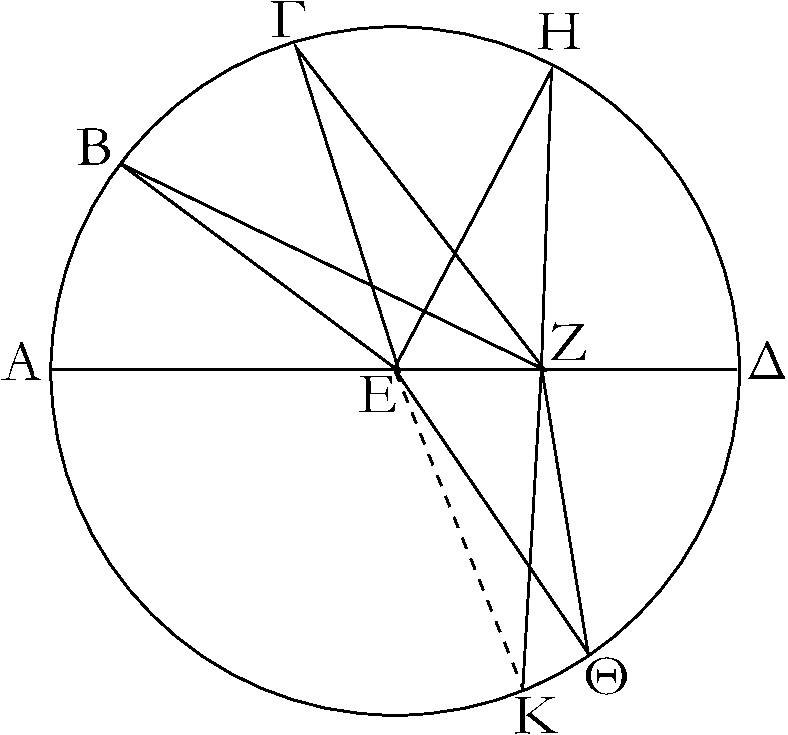
\includegraphics{Book03/fig07g.eps}}

\gr{Λέγω, <ότι καὶ ἀπὸ τοῦ Ζ σημείου δύο μόνον >ίσαι προσπεσοῦνται πρὸξ τὸν ΑΒΓΔ κύκλον ἐφ> ἑκάτερα τῆξ ΖΔ ἐλαθίστηξ. συνεστάτω γὰρ πρὸξ τῆ| ΕΖ εὐθείᾳ καὶ τῶ| πρὸξ α\kern -.7pt  ὐτῆ| σημείῳ τῶ| Ε τῆ|
ὑπὸ ΗΕΖ γωνίᾳ >ίση ἡ ὑπὸ ΖΕJ, καὶ ἐπεζεύθθω ἡ ΖJ. ἐπεὶ ο>ῦν >ίση ἐστὶν ἡ ΗΕ τῆ| ΕJ, κοινὴ δὲ ἡ ΕΖ, δύο
δὴ αἱ ΗΕ, ΕΖ δυσὶ ταῖξ JΕ, ΕΖ >ίσαι εἰσίν; καὶ γωνία ἡ ὑπὸ ΗΕΖ
γωνίᾳ τῆ| ὑπὸ JΕΖ >ίση; βάσιξ >άρα ἡ ΖΗ βάσει τῆ| ΖJ >ίση
ἐστίν. λέγω δή, <ότι τῆ| ΖΗ >άλλη >ίση οὐ προσπεσεῖται πρὸξ τὸν
κύκλον ἀπὸ τοῦ Ζ σημείου. εἰ γὰρ δυνατόν, προσπιπτέτω ἡ ΖΚ.
καὶ ἐπεὶ ἡ ΖΚ τῆ| ΖΗ >ίση ἐστίν, ἀλλὰ ἡ ΖJ τῆ| ΖΗ
[>ίση ἐστίν], καὶ  ἡ  ΖΚ
>άρα τῆ| ΖJ ἐστιν >ίση, ἡ >έγγιον
τῆξ διὰ τοῦ κέντρου τῆ| ἀπώτερον >ίση; <όπερ ἀδύνατον.
οὐκ >άρα ἀπὸ τοῦ Ζ σημείου ἑτέρα τιξ προσπεσεῖται πρὸξ τὸν
κύκλον >ίση τῆ| ΗΖ; μία >άρα μόνη.}

\gr{Ἐὰν >άρα κύκλου ἐπὶ τῆξ διαμέτρου ληφθῆ| τι σημεῖον, <ὸ μ\kern -.7pt  ή ἐστι κέντρον τοῦ κύκλου, ἀπὸ δὲ τοῦ σημείου πρὸξ τὸν κύκλον προσπίπτωσιν εὐθεῖαί τινεξ, μεγίστη μὲν >έσται, ἐφ> <ῆξ
τὸ κέντρον, ἐλαθίστη δὲ ἡ λοιπή, τῶν δὲ >άλλων ἀεὶ ἡ
>έγγιον τῆξ δὶα τοῦ κέντρου τῆξ ἀπώτερον μείζων ἐστίν, δύο
δὲ μόνον >ίσαι ἀπὸ τοῦ α\kern -.7pt  ὐτοῦ σημείου προσπεσοῦνται πρὸξ τὸν
κύκλον ἐφ> ἑκάτερα τῆξ ἐλαθίστηξ; <όπερ >έδει δεῖχαι.}}

\ParallelRText{
\begin{center}
{\large Proposition 7}
\end{center}

If some point, which is not the
center of the circle, is taken on the diameter of a circle,
and some straight-lines radiate from the point towards
the (circumference of the) circle, (then) the greatest (straight-line) will be that on which
the center (lies), and the least the remainder (of the same diameter). And
for the others, a (straight-line) nearer$^\dag$ to the (straight-line) through the center is always
greater than a (straight-line) further away. And only two equal (straight-lines)
will radiate from the point towards the (circumference of the) circle, (one)
on each (side) of the least (straight-line).

Let $ABCD$ be a circle, and let $AD$ be its diameter, and
let some point $F$, which is not the center of the circle, be taken on $AD$.
Let $E$ be the center of the circle. And let some straight-lines, $FB$, $FC$,
and $FG$, radiate from $F$ towards (the circumference of) circle $ABCD$.
I say that $FA$ is the greatest (straight-line), $FD$ the least, and of the others, $FB$ (is)
greater than $FC$, and $FC$ than $FG$.

For let $BE$, $CE$, and $GE$ be joined. And since for every triangle
(any) two sides are greater than the remaining (side) [Prop.~1.20],
$EB$ and $EF$ is thus greater than $BF$. And $AE$ (is) equal to $BE$ [thus,
$BE$ and $EF$ is equal to $AF$]. Thus, $AF$ (is) greater than $BF$. Again,
since $BE$ is equal to $CE$, and $FE$ (is) common, the two (straight-lines)
$BE$, $EF$ are equal to the two (straight-lines) $CE$, $EF$ (respectively). But, angle $BEF$ (is)
also greater than angle $CEF$.$^\ddag$ Thus, the base $BF$ is greater than the base $CF$.
Thus, the base $BF$ is greater than the base $CF$ [Prop.~1.24]. So, for the same (reasons), $CF$ is also greater than $FG$.

Again, since $GF$ and $FE$ are greater than $EG$ [Prop.~1.20], and $EG$
(is) equal to $ED$, $GF$ and $FE$ are thus greater than $ED$. Let $EF$ be
taken from both. Thus, the remainder $GF$ is greater than the remainder $FD$.
Thus, $FA$ (is) the greatest  (straight-line), $FD$ the least, and $FB$ (is) greater than $FC$, and $FC$ than $FG$.

\epsfysize=2.5in
\centerline{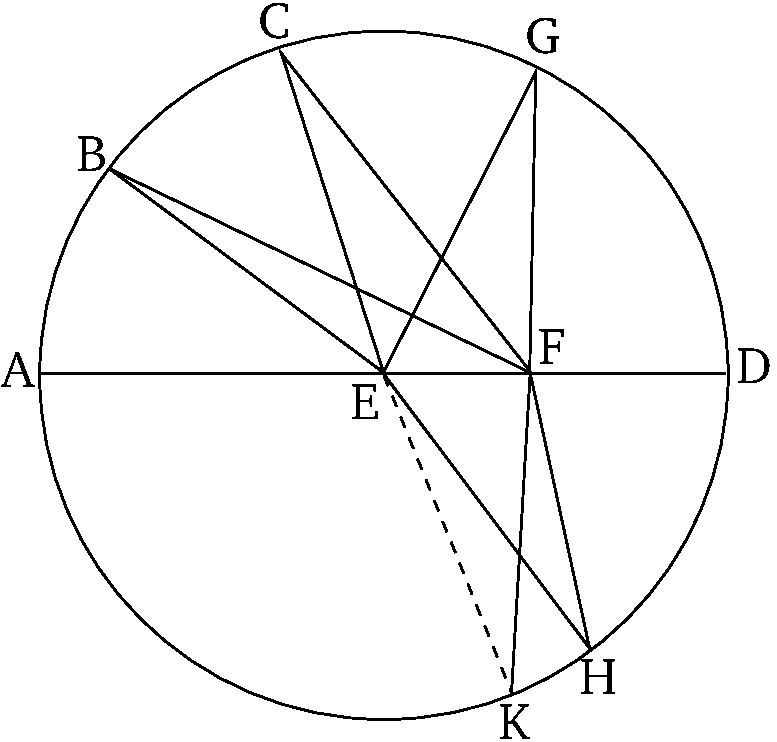
\includegraphics{Book03/fig07e.eps}}

I also say that from point $F$ only two equal (straight-lines) will radiate
towards (the circumference of) circle $ABCD$, (one) on each (side) of the
least (straight-line) $FD$. For let the (angle) $FEH$, equal to angle $GEF$, be constructed on the straight-line $EF$, at the point $E$ on it [Prop.~1.23], and
let $FH$ be joined. Therefore, since $GE$ is equal to $EH$, and $EF$ (is) common, the two (straight-lines) $GE$, $EF$ are equal to the two (straight-lines)
$HE$, $EF$ (respectively). And angle $GEF$ (is) equal to angle $HEF$. Thus, the base $FG$ is
equal to the base $FH$ [Prop.~1.4]. So I say that another (straight-line)
equal to $FG$
will not radiate towards (the circumference of)
the circle from point $F$. For, if possible, let $FK$ (so) radiate. And since
$FK$ is equal to $FG$, but $FH$ [is equal] to $FG$, $FK$ is thus also equal to
$FH$, the nearer to the (straight-line) through the center equal to the
further away. The very thing (is) impossible. Thus, another (straight-line)
equal to $GF$ will not radiate from the point $F$ towards (the circumference of) the circle.
Thus, (there is) only one (such straight-line).

Thus, if some point, which is not the
center of the circle, is taken on the diameter of a circle,
and some straight-lines radiate from the point towards
the (circumference of the) circle, (then) the greatest (straight-line) will be that on which
the center (lies), and the least the remainder (of the same diameter). And
for the others, a (straight-line) nearer to the (straight-line) through the center is always
greater than a (straight-line) further away. And only two equal (straight-lines)
will radiate from the same point towards the (circumference of the) circle,  (one)
on each (side) of the least (straight-line). (Which is) the very thing it was required to show.}
\end{Parallel}
{\footnotesize \noindent$^\dag$ Presumably, in an angular sense.\\
$^\ddag$ This is not proved, except by reference to the figure.}

%%%%%%
% Prop 3.8
%%%%%%
\pdfbookmark[1]{Proposition 3.8}{pdf3.8}
\begin{Parallel}{}{} 
\ParallelLText{
\begin{center}
{\large \ggn{8}.}
\end{center}\vspace*{-7pt}

\gr{Ἐὰν κύκλου ληφθῆ| τι σημεῖον ἐκτόξ, ἀπὸ δὲ τοῦ σημείου πρὸξ
τὸν κύκλον διαθθῶσιν εὐθεῖαί τινεξ, <ῶν μία μὲν διὰ τοῦ κέντρου,
αἱ δὲ λοιπαί, ὡξ >έτυθεν, τῶν μὲν πρὸξ τὴν κοίλην περιφέρειαν προσπιπτουσῶν εὐθειῶν μεγίστη μέν ἐστιν ἡ διὰ τοῦ κέντρου, τῶν δὲ >άλλων ἀεὶ ἡ >έγγιον τῆξ διὰ τοῦ κέντρου τῆξ ἀπώτερον μείζων ἐστίν, τῶν δὲ πρὸξ τὴν κυρτὴν περιφέρειαν προσπιπτουσῶν εὐθειῶν
ἐλαθίστη μέν ἐστιν ἡ μεταχὺ τοῦ τε σημείου καὶ τῆξ διαμέτρου, τῶν δὲ >άλλων ἀεὶ ἡ >έγγιον τῆξ ἐλαθίστηξ τῆξ ἀπώτερόν ἐστιν
ἐλάττων, δύο δὲ μόνον >ίσαι ἀπὸ τοῦ σημείου προσπεσοῦνται
πρὸξ τὸν κύκλον ἐφ> ἑκάτερα τῆξ ἐλαθίστηξ.}

\gr{>'Εστω κύκλοξ ὁ ΑΒΓ, καὶ τοῦ ΑΒΓ εἰλήφθω τι σημεῖον ἐκτὸξ τὸ Δ,
καὶ ἀπ> α\kern -.7pt  ὐτοῦ διήθθωσαν εὐθεῖαί τινεξ αἱ ΔΑ, ΔΕ, ΔΖ, ΔΓ,
>έστω δὲ ἡ ΔΑ διὰ τοῦ κέντρου. λέγω, <ότι τῶν μὲν πρὸξ
τὴν ΑΕΖΓ κοίλην περιφέρειαν προσπιπτουσῶν εὐθειῶν μεγίστη
μέν ἐστιν ἡ διὰ τοῦ κέντρου ἡ ΔΑ, μείζων δὲ ἡ μὲν ΔΕ τῆξ ΔΖ ἡ δὲ ΔΖ τῆξ ΔΓ, τῶν δὲ πρὸξ τὴν JΛΚΗ κυρτὴν περιφέρειαν προσπιπτουσῶν εὐθειῶν ἐλαθίστη μέν ἐστιν ἡ ΔΗ ἡ
μεταχὺ τοῦ σημείου καὶ τῆξ διαμέτρου τῆξ ΑΗ, ἀεὶ δὲ ἡ
>έγγιον τῆξ ΔΗ ἐλαθίστηξ ἐλάττων ἐστὶ τῆξ ἀπώτερον, ἡ μὲν
ΔΚ τῆξ ΔΛ, ἡ δὲ ΔΛ τῆξ ΔJ.}

\gr{Εἰλήφθω γὰρ τὸ κέντρον τοῦ ΑΒΓ κύκλου καὶ >έστω τὸ Μ; καὶ
ἐπεζεύθθωσαν αἱ ΜΕ, ΜΖ, ΜΓ, ΜΚ, ΜΛ, ΜJ.}

\gr{Καὶ ἐπεὶ >ίση ἐστὶν ἡ ΑΜ τῆ| ΕΜ, κοινὴ προσκείσθω ἡ ΜΔ;
ἡ >άρα ΑΔ >ίση ἐστὶ ταῖξ ΕΜ, ΜΔ. ἀλλ> αἱ ΕΜ, ΜΔ τῆξ ΕΔ μείζονέξ εἰσιν; καὶ ἡ ΑΔ >άρα τῆξ ΕΔ μείζων ἐστίν. πάλιν, ἐπεὶ
>ίση ἐστὶν ἡ ΜΕ τῆ| ΜΖ, κοινὴ δὲ ἡ ΜΔ, αἱ ΕΜ, ΜΔ >άρα
ταῖξ ΖΜ, ΜΔ >ίσαι εἰσίν; καὶ γωνία ἡ ὑπὸ ΕΜΔ γωνίαξ τῆξ ὑπὸ ΖΜΔ μείζων ἐστίν. βάσιξ >άρα ἡ ΕΔ βάσεωξ τῆξ ΖΔ μείζων ἐστίν.
ὁμοίωξ δὴ δείχομεν, <ότι καὶ ἡ ΖΔ τῆξ
ΓΔ μείζων ἐστίν; μεγίστη μὲν >άρα ἡ ΔΑ, μείζων δὲ ἡ μὲν ΔΕ
τῆξ ΔΖ, ἡ δὲ ΔΖ τῆξ ΔΓ.}

\gr{Καὶ ἐπεὶ αἱ ΜΚ, ΚΔ τῆξ ΜΔ μείζονέξ εἰσιν, >ίση δὲ ἡ μ\kern -.7pt  η τῆ| ΜΚ, λοιπὴ >άρα ἡ ΚΔ λοιπῆξ τῆξ ΗΔ μείζων ἐστίν; <ώστε
ἡ ΗΔ τῆξ ΚΔ ἐλάττων ἐστίν; καὶ ἐπεὶ τριγώνου τοῦ ΜΛΔ
ἐπὶ μιᾶξ τῶν πλευρῶν τῆξ ΜΔ δύο εὐθεῖαι ἐντὸξ
συνεστάθησαν αἱ ΜΚ, ΚΔ, αἱ >άρα ΜΚ, ΚΔ  τῶν ΜΛ, ΛΔ ἐλάττονέξ εἰσιν; >ίση δὲ ἡ ΜΚ  
 τῆ| ΜΛ; λοιπὴ >άρα ἡ ΔΚ λοιπῆξ τῆξ ΔΛ ἐλάττων ἐστίν. ὁμοίωξ δὴ δείχομεν, <ότι καὶ ἡ ΔΛ τῆξ ΔJ
ἐλάττων ἐστίν; ἐλαθίστη μὲν >άρα ἡ ΔΗ, ἐλάττων δὲ ἡ
μὲν ΔΚ τῆξ ΔΛ ἡ δὲ ΔΛ τῆξ ΔJ.}\\~\\~\\~\\~\\~\\~\\~\\

\epsfysize=2.5in
\centerline{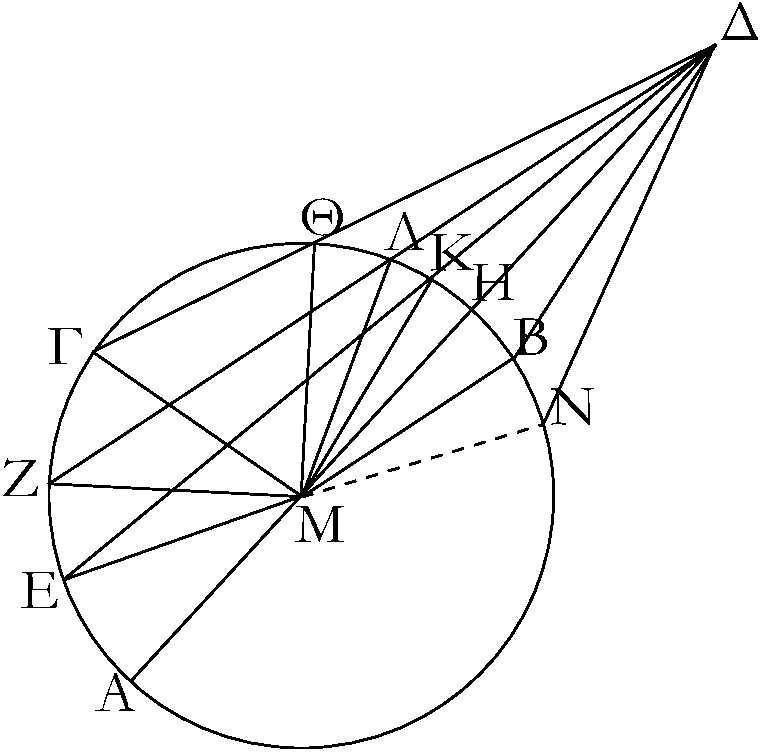
\includegraphics{Book03/fig08g.eps}}

\gr{Λέγω, <ότι καὶ δύο μόνον >ίσαι ἀπὸ τοῦ Δ σημείου προσπεσοῦνται
πρὸξ τὸν κύκλον ἐφ> ἑκάτερα τῆξ ΔΗ ἐλαθίστηξ; συνεστάτω πρὸξ
τῆ| ΜΔ εὐθείᾳ καὶ τῶ| πρὸξ α\kern -.7pt  ὐτῆ| σημείῳ τῶ| Μ τῆ| ὑπὸ ΚΜΔ γωνίᾳ >ίση γωνία ἡ ὑπὸ ΔΜΒ, καὶ ἐπεζεύθθω ἡ ΔΒ. καὶ ἐπεὶ >ίση ἐστὶν ἡ ΜΚ τῆ| ΜΒ, κοινὴ δὲ ἡ ΜΔ, δύο δὴ αἱ ΚΜ, ΜΔ
δύο ταῖξ ΒΜ, ΜΔ >ίσαι εἰσὶν ἑκατέρα ἑκατέρᾳ; καὶ γωνία ἡ
ὑπὸ ΚΜΔ γωνίᾳ τῆ| ὑπὸ ΒΜΔ >ίση; βάσιξ  >άρα ἡ ΔΚ βάσει
τῆ| ΔΒ >ίση ἐστίν. λέγω [δή], <ότι τῆ| ΔΚ εὐθείᾳ >άλλη >ίση
οὐ προσπεσεῖται πρὸξ τὸν κύκλον ἀπὸ τοῦ Δ σημείου. εἰ γὰρ
δυνατόν, προσπιπτέτω καὶ >έστω ἡ ΔΝ. ἐπεὶ ο>ῦν ἡ ΔΚ
τῆ| ΔΝ ἐστιν >ίση, ἀλλ> ἡ ΔΚ τῆ| ΔΒ ἐστιν >ίση, καὶ
ἡ ΔΒ >άρα τῆ| ΔΝ ἐστιν >ίση, ἡ >έγγιον τῆξ ΔΗ ἐλαθίστηξ τῆ|
ἀπώτερον [ἐστιν] >ίση; <όπερ ἀδύνατον ἐδείθθη. οὐκ
>άρα πλείουξ >ὴ δύο >ίσαι πρὸξ τὸν ΑΒΓ κύκλον ἀπὸ τοῦ Δ σημείου
ἐφ> ἑκάτερα τῆξ ΔΗ ἐλαθίστηξ προσπεσοῦνται.}

\gr{Ἐὰν >άρα κύκλου ληφθῆ| τι σημεῖον ἐκτόξ, ἀπὸ δὲ τοῦ σημείου πρὸξ
τὸν κύκλον διαθθῶσιν εὐθεῖαί τινεξ, <ῶν μία μὲν διὰ τοῦ κέντρου
αἱ δὲ λοιπαί, ὡξ >έτυθεν, τῶν μὲν πρὸξ τὴν κοίλην περιφέρειαν προσπιπτουσῶν εὐθειῶν μεγίστη μέν ἐστιν ἡ διὰ τοῦ κέντου, τῶν δὲ >άλλων ἀεὶ ἡ >έγγιον τῆξ διὰ τοῦ κέντρου τῆξ ἀπώτερον μείζων ἐστίν, τῶν δὲ πρὸξ τὴν κυρτὴν περιφέρειαν προσπιπτουσῶν εὐθειῶν
ἐλαθίστη μέν ἐστιν ἡ μεταχὺ τοῦ τε σημείου καὶ τῆξ διαμέτρου, τῶν δὲ >άλλων ἀεὶ ἡ >έγγιον τῆξ ἐλαθίστηξ τῆξ ἀπώτερόν ἐστιν
ἐλάττων, δύο δὲ μόνον >ίσαι ἀπὸ τοῦ σημείου προσπεσοῦνται
πρὸξ τὸν κύκλον ἐφ> ἑκάτερα τῆξ ἐλαθίστηξ; <όπερ >έδει δεῖχαι.}}

\ParallelRText{
\begin{center}
{\large Proposition 8}
\end{center}

If some point is taken outside a circle, and some straight-lines are
drawn from the point to the (circumference of the) circle, one of which (passes) through the
center, the remainder  (being) random, (then) for the straight-lines
radiating towards the concave (part of the) circumference, the
greatest is  that (passing) through the center. For the others, a (straight-line)
nearer$^\dag$ to the (straight-line) through the center is always greater than one
further away. For the straight-lines radiating towards the convex (part of
the) circumference, the least is that between the point and the
diameter. For the others, a (straight-line) nearer to the least
(straight-line) is always less than one further away. And only
two equal (straight-lines) will radiate from the point towards the (circumference of the) circle, (one) on each (side)
of the least (straight-line).

Let $ABC$ be a circle, and let some point $D$ be taken outside $ABC$,
and from it let some straight-lines, $DA$, $DE$, $DF$, and $DC$, be
drawn through (the circle), and let $DA$ be through the center. I say 
that for the straight-lines radiating towards the concave (part of the)
circumference, $AEFC$, the greatest is the one (passing) through the center,  (namely) $AD$,
and (that) $DE$ (is) greater than $DF$, and $DF$ than $DC$. For the straight-lines
radiating towards the convex (part of the) circumference, $HLKG$, the
least is the one between the point and the diameter $AG$, (namely) $DG$, 
and  a (straight-line) nearer to the least (straight-line) $DG$ is
always less than one farther away, (so that) $DK$ (is less) than $DL$, and $DL$ than than
$DH$.

For let the center of the circle be found [Prop.~3.1], and let it be (at point) $M$
[Prop.~3.1]. And let $ME$, $MF$, $MC$, $MK$, $ML$, and $m\kern -.7pt h$ be joined.

And since $AM$ is equal to $EM$, let $MD$ be added to both. Thus, $AD$ is equal to $EM$ and $MD$. But, $EM$ and $MD$ is greater than
$ED$ [Prop.~1.20]. Thus, $AD$ is also greater than $ED$. Again, since $ME$ is
equal to $MF$, and $MD$ (is) common, the (straight-lines) $EM$, $MD$ are thus
equal to $FM$,
$MD$. And angle $EMD$ is greater than angle $FMD$.$^\ddag$
Thus, the
base $ED$ is greater than the base $FD$ [Prop.~1.24]. 
So, similarly,
we can show that $FD$ is also greater than $CD$. Thus, $AD$ (is) the greatest
(straight-line), and $DE$ (is) greater than $DF$, and $DF$ than $DC$.

And since $MK$ and $KD$ is greater than $MD$ [Prop. 1.20], and $MG$ (is)
equal to $MK$, the remainder $KD$ is thus greater than the remainder $GD$.
So $GD$ is less than $KD$. And since in triangle $MLD$, the two internal straight-lines
$MK$ and $KD$ were constructed on one of the sides, $MD$, (then) $MK$ and $KD$
are thus less than $ML$ and $LD$  [Prop.~1.21]. And $MK$ (is) equal to $ML$.
Thus, the remainder $DK$ is less than the remainder $DL$. So, similarly, we
can show that $DL$ is also less than $DH$. Thus, $DG$ (is) the least (straight-line),
and $DK$ (is) less than $DL$, and $DL$ than $DH$.

\epsfysize=2.5in
\centerline{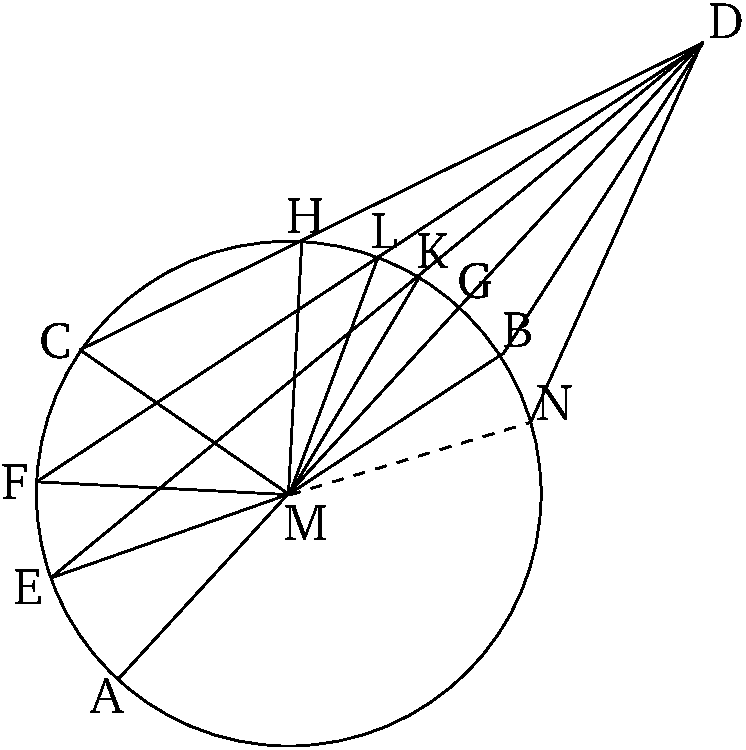
\includegraphics{Book03/fig08e.eps}}

I also say that only two equal (straight-lines) will radiate from point $D$ towards (the
circumference of) the circle, (one) on each (side) on the least (straight-line),
$DG$. Let the  angle $DMB$, equal to angle $KMD$, be constructed
on the straight-line $MD$, at the point $M$ on it [Prop.~1.23], and  let $DB$ be
joined. And since $MK$ is equal to $MB$, and $MD$ (is) common, the
two (straight-lines) $KM$, $MD$ are equal to the two (straight-lines) $BM$, $MD$,
respectively. And angle $KMD$ (is) equal to angle $BMD$. Thus, the base
$DK$ is equal to the base $DB$ [Prop.~1.4]. [So] I say that another (straight-line)
equal to $DK$ will not radiate towards the (circumference of the) circle
from point $D$. For, if possible, let (such a straight-line) radiate, and let
it be $DN$. Therefore, since $DK$ is equal to $DN$, but $DK$ is equal to $DB$, (then) $DB$
is thus also equal to $DN$, (so that) a (straight-line) nearer to the least (straight-line) $DG$ [is]
equal to one further away. The very thing was shown (to be)  impossible. 
Thus, not more than two equal (straight-lines) will radiate towards
(the circumference of) circle $ABC$ from point $D$, (one) on each side
of the least (straight-line) $DG$.

Thus, if some point is taken outside a circle, and some straight-lines are
drawn from the point to the (circumference of the) circle, one of which (passes) through the
center, the remainder  (being) random, (then) for the straight-lines
radiating towards the concave (part of the) circumference, the
greatest is  that (passing) through the center. For the others, a (straight-line)
nearer to the (straight-line) through the center is always greater than one
further away. For the straight-lines radiating towards the convex (part of
the) circumference, the least is that between the point and the
diameter. For the others, a (straight-line) nearer to the least
(straight-line) is always less than one further away. And only
two equal (straight-lines) will radiate from the point towards the (circumference of the) circle, (one) on each (side)
of the least (straight-line).  (Which is) the very thing it was required to show.}
\end{Parallel}
{\footnotesize \noindent$^\dag$ Presumably, in an angular sense.\\
$\ddag$  This is not
proved, except by reference to the figure.} 

%%%%%%
% Prop 3.9
%%%%%%
\pdfbookmark[1]{Proposition 3.9}{pdf3.9}
\begin{Parallel}{}{} 
\ParallelLText{
\begin{center}
{\large \ggn{9}.}
\end{center}\vspace*{-7pt}

\gr{Ἐὰν κύκλου ληφθῆ| τι σημεῖον ἐντόξ, ἀπο δὲ τοῦ σημείου πρὸξ
τὸν κύκλον προσπίπτωσι πλείουξ >ὴ δύο >ίσαι εὐθεῖαι, τὸ ληφθὲν σημεῖον κέντρον ἐστὶ τοῦ κύκλου.}

\gr{>'Εστω κύκλοξ ὁ ΑΒΓ, ἐντὸξ δὲ α\kern -.7pt  ὐτοῦ σημεῖον τὸ Δ, καὶ ἀπὸ
τοῦ Δ πρὸξ τὸν ΑΒΓ κύκλον προσπιπτέτωσαν πλείουξ >ὴ δύο >ίσαι
εὐθεῖαι αἱ ΔΑ, ΔΒ, ΔΓ; λέγω, <ότι τὸ Δ σημεῖον κέντρον ἐστὶ τοῦ
ΑΒΓ κύκλου.}\\

\epsfysize=2.2in
\centerline{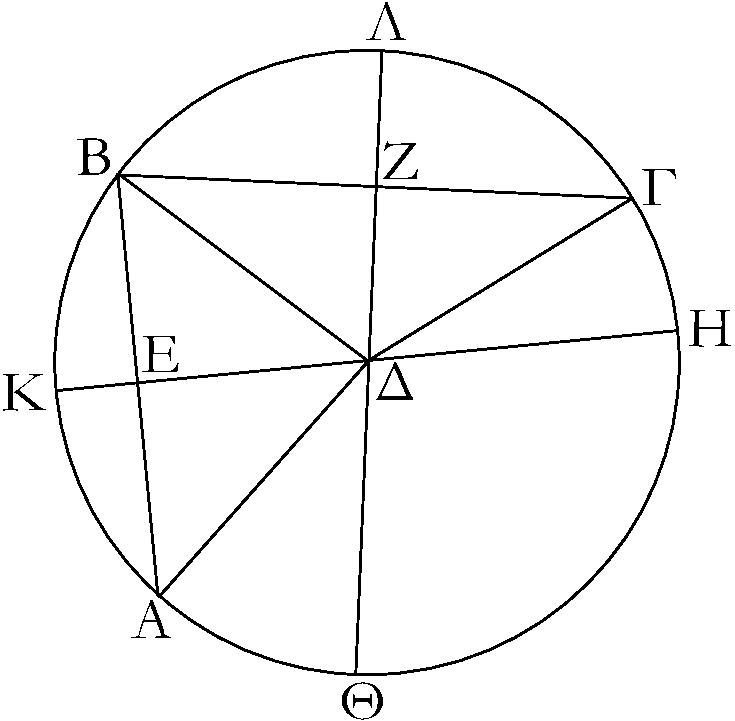
\includegraphics{Book03/fig09g.eps}}

\gr{Ἐπεζεύθθωσαν γὰρ αἱ ΑΒ, ΒΓ καὶ τετμ\kern -.7pt  ήσθωσαν δίθα κατὰ τὰ Ε, Ζ σημεῖα, καὶ ἐπιζευθθεῖσαι αἱ ΕΔ, ΖΔ διήθθωσαν ἐπὶ τὰ
Η, Κ, J, Λ σημεῖα.}

\gr{Ἐπεὶ ο>ῦν >ίση ἐστὶν ἡ ΑΕ τῆ| ΕΒ, κοινὴ δὲ ἡ ΕΔ,
δύο δὴ αἱ ΑΕ, ΕΔ δύο ταῖξ ΒΕ, ΕΔ >ίσαι εἰσίν; καὶ βάσιξ ἡ
ΔΑ βάσει τῆ| ΔΒ >ίση; γωνία >άρα ἡ ὑπὸ ΑΕΔ γωνίᾳ
τῆ| ὑπὸ ΒΕΔ >ίση ἐστίν; ὀρθὴ >άρα ἑκατέρα τῶν ὑπὸ ΑΕΔ,
ΒΕΔ γωνιῶν; ἡ ΗΚ >άρα τὴν ΑΒ τέμνει δίθα καὶ πρὸξ ὀρθάξ. καὶ
ἐπεί, ἒαν ἐν κύκλῳ εὐθεῖά τιξ εὐθεῖάν τινα δίθα τε καὶ πρὸξ
ὀρθὰξ τέμνῃ, ἐπὶ τῆξ τεμνούσηξ ἐστὶ τὸ κέντρον τοῦ κύκλου,
ἐπὶ τῆξ ΗΚ >άρα ἐστὶ τὸ κέντρον τοῦ κύκλου. διὰ τὰ
α\kern -.7pt  ὐτὰ δὴ καὶ ἐπὶ τῆξ JΛ ἐστι τὸ κέντρον τοῦ ΑΒΓ κύκλου.
καὶ οὐδὲν <έτερον κοινὸν >έθουσιν αἱ ΗΚ, JΛ εὐθεῖαι >ὴ τὸ Δ
σημεῖον; τὸ Δ >άρα σημεῖον κέντρον ἐστὶ τοῦ ΑΒΓ
κύκλου.}

\gr{Ἐὰν >άρα κύκλου ληφθῆ| τι σημεῖον ἐντόξ, ἀπὸ δὲ τοῦ σημείου πρὸξ
τὸν κύκλον προσπίπτωσι πλείουξ >ὴ δύο >ίσαι εὐθεῖαι, τὸ ληφθὲν σημεῖον κέντρον ἐστὶ τοῦ κύκλου; <όπερ >έδει δεῖχαι.}}

\ParallelRText{
\begin{center}
{\large Proposition 9}
\end{center}

If  some point is taken inside a circle, and more than two equal straight-lines
radiate from the point towards the (circumference of the) circle, (then) the
point taken  is the center of the circle.

Let $ABC$ be a circle, and $D$ a point inside it, and let more than two equal
straight-lines, $DA$, $DB$, and $DC$, radiate from $D$ towards (the circumference of) circle
$ABC$. I say that point $D$ is the center of circle $ABC$.

\epsfysize=2.2in
\centerline{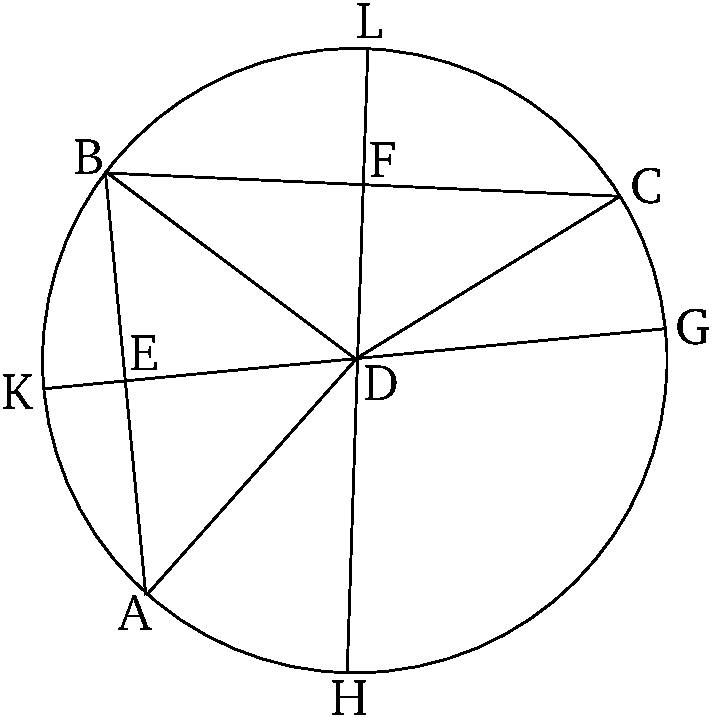
\includegraphics{Book03/fig09e.eps}}

For let $AB$ and $BC$ be joined, and (then) be cut in half at points $E$ and $F$ 
(respectively) [Prop.~1.10]. And $ED$ and $FD$ being joined, let them be
drawn through to points $G$, $K$, $H$, and $L$.

Therefore, since $AE$ is equal to $EB$, and $ED$ (is) common, the two (straight-lines) $AE$, $ED$ are equal to the two (straight-lines) $BE$, $ED$ (respectively). And the 
base $DA$ (is) equal to the base $DB$. Thus, angle $AED$ is equal to
angle $BED$ [Prop.~1.8]. Thus, angles $AED$ and $BED$ (are) each right-angles [Def.~1.10]. Thus, $GK$ cuts $AB$ in half, and at right-angles. And since,
if some straight-line in a circle cuts some (other) straight-line in half,
and at right-angles, (then) the center of the circle is on the former (straight-line)
[Prop.~3.1~corr.], the center of the circle is thus on $GK$. So, for the
same (reasons), the center of circle $ABC$ is also on $HL$. And the straight-lines
$GK$ and $HL$ have no  common (point) other than point $D$. Thus, point
$D$ is the center of circle $ABC$.

Thus, if some point is taken inside a circle, and more than two equal straight-lines
radiate from the point towards the (circumference of the) circle, (then) the
point taken  is the center of the circle. (Which is) the very thing it was
required to show.}
\end{Parallel}

%%%%%%
% Prop 3.10
%%%%%%
\pdfbookmark[1]{Proposition 3.10}{pdf3.10}
\begin{Parallel}{}{} 
\ParallelLText{
\begin{center}
{\large \ggn{10}.}
\end{center}\vspace*{-7pt}

\gr{Κύκλοξ  κύκλον οὐ τέμνει κατὰ πλείονα σημεῖα >ὴ δύο.}

\gr{Εἰ γὰρ δυνατόν, κύκλοξ ὁ ΑΒΓ κύκλον τὸν ΔΕΖ τεμνέτω κατὰ πλείονα
σημεῖα >ὴ δύο τὰ Β, Η, Ζ, J, καὶ ἐπιζευθθεῖσαι αἱ ΒJ, ΒΗ δίθα τεμνέσθωσαν κατὰ τὰ Κ, Λ σημεῖα; καὶ ἀπὸ τῶν Κ, Λ ταῖξ ΒJ, ΒΗ
πρὸξ ὀρθὰξ ἀθθεῖσαι αἱ ΚΓ, ΛΜ διήθθωσαν ἐπὶ τὰ Α, Ε σημεῖα.}\\~\\

\epsfysize=2.2in
\centerline{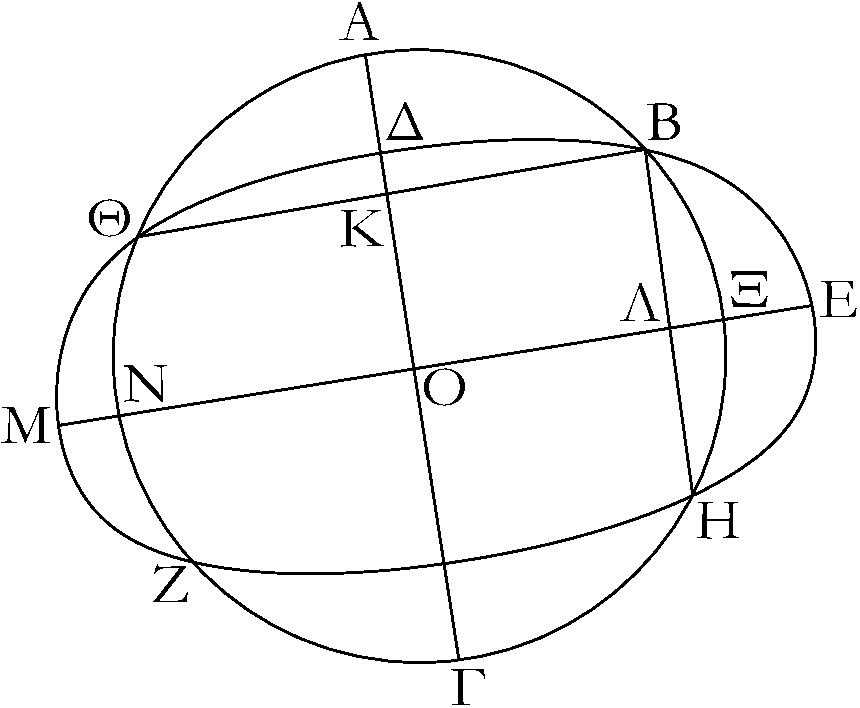
\includegraphics{Book03/fig10g.eps}}

\gr{Ἐπεὶ ο>ῦν ἐν κύκλῳ τῶ| ΑΒΓ εὐθεῖά τιξ ἡ ΑΓ εὐθεῖάν τινα
τὴν ΒJ δίθα καὶ πρὸξ ὀρθὰξ τέμνει, ἐπὶ τῆξ ΑΓ >άρα ἐστὶ τὸ κέντρον τοῦ ΑΒΓ κύκλου. πάλιν, ἐπεὶ ἐν κύκλῳ τῶ| α\kern -.7pt  ὐτῶ|
τῶ| ΑΒΓ εὐθεῖά τιξ ἡ ΝΧ εὐθεῖάν τινα τὴν ΒΗ δίθα καὶ πρὸξ
ὀρθὰξ τέμνει, ἐπὶ τῆξ ΝΧ >άρα ἐστὶ τὸ κέντρον τοῦ ΑΒΓ κύκλου.
ἐδείθθη δὲ καὶ ἐπὶ τῆξ ΑΓ, καὶ κατ> οὐδὲν συμβάλλουσιν
αἱ ΑΓ, ΝΧ εὐθεῖαι >ὴ κατὰ τὸ Ο; τὸ Ο >άρα σημεῖον κέντρον
ἐστὶ τοῦ ΑΒΓ κύκλου. ὁμοίωξ δὴ δείχομεν, <ότι καὶ τοῦ ΔΕΖ κύκλου κέντρον ἐστὶ τὸ Ο; δύο >άρα κύκλων τεμνόντων ἀλλήλουξ
τῶν ΑΒΓ, ΔΕΖ τὸ α\kern -.7pt  ὐτό ἐστι κέντρον τὸ Ο; 
<όπερ ἐστὶν ἀδύνατον.}

\gr{Οὐκ >άρα κύκλοξ  κύκλον τέμνει κατὰ πλείονα σημεῖα >ὴ δύο;
<όπερ >έδει δεῖχαι.}}

\ParallelRText{
\begin{center}
{\large Proposition 10}
\end{center}

A circle does not cut a(nother) circle at more than two points.

For, if possible, let the circle $ABC$ cut the circle $DEF$ at more than
two points, $B$, $G$, $F$, and $H$. And $BH$ and $BG$ being joined,
let them (then) be cut in half at points $K$ and $L$ (respectively). And $KC$ and $LM$
being drawn at right-angles to $BH$ and $BG$ from $K$ and $L$ (respectively) [Prop.~1.11], let them (then) be
drawn through to points $A$ and $E$ (respectively).

\epsfysize=2.2in
\centerline{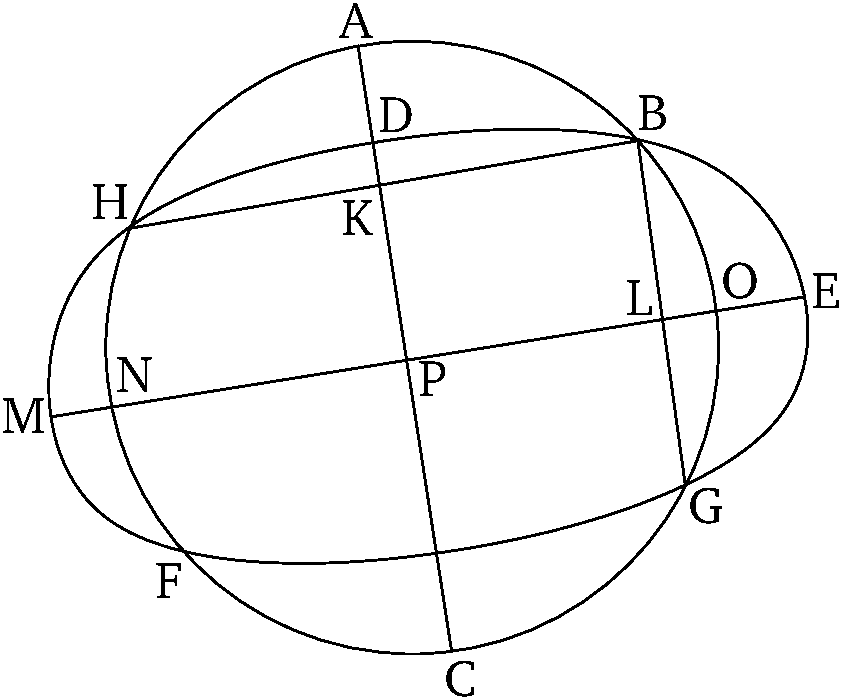
\includegraphics{Book03/fig10e.eps}}

Therefore, since in circle $ABC$ some straight-line $AC$ cuts some (other)
straight-line $BH$ in half, and at right-angles, the center of circle $ABC$
is thus on $AC$ [Prop.~3.1~corr.]. Again, since in the same circle $ABC$
some straight-line $NO$ cuts some (other straight-line) $BG$ in half, and
at right-angles, the center of circle $ABC$ is thus on $NO$ [Prop.~3.1~corr.].
And it was also shown (to be) on $AC$. And the straight-lines $AC$ and $NO$
meet at no other (point) than $P$. Thus, point $P$ is the center of circle $ABC$.
So, similarly, we can show that $P$ is also the center of circle $DEF$.
Thus,  two circles cutting one another, $ABC$ and $DEF$, have the same center
$P$. The very thing is impossible [Prop.~3.5].

Thus, a circle does not cut a(nother) circle at more than two points. (Which is)
the very thing it was required to show.}
\end{Parallel}

%%%%%%
% Prop 3.11
%%%%%%
\pdfbookmark[1]{Proposition 3.11}{pdf3.11}
\begin{Parallel}{}{} 
\ParallelLText{
\begin{center}
{\large \ggn{11}.}
\end{center}\vspace*{-7pt}

\gr{Ἐὰν δύο κύκλοι ἐφάπτωνται ἀλλήλων ἐντόξ, καὶ ληφθῆ| α\kern -.7pt  ὐτῶν
τὰ κέντρα, ἡ ἐπὶ τὰ κέντρα α\kern -.7pt  ὐτῶν ἐπιζευγνυμένη εὐθεῖα καὶ
ἐκβαλλομένη ἐπὶ τὴν συναφὴν πεσεῖται τῶν κύκλων.}

\gr{Δύο γὰρ κύκλοι οἱ ΑΒΓ, ΑΔΕ ἐφαπτέσθωσαν ἀλλήλων ἐντὸξ κατὰ τὸ
Α σημεῖον, καὶ εἰλήφθω τοῦ μὲν ΑΒΓ κύκλου κέντρον τὸ Ζ, τοῦ δὲ
ΑΔΕ τὸ Η; λέγω, <ότι ἡ ἀπὸ τοῦ Η ἐπὶ τὸ Ζ ἐπιζευγνυμένη
εὐθεῖα ἐκβαλλομένη ἐπὶ τὸ Α πεσεῖται.}

\gr{μ\kern -.7pt  ὴ γάρ, ἀλλ> εἰ δυνατόν, πιπτέτω ὡξ ἡ ΖΗJ, καὶ
ἐπεζεύθθωσαν αἱ ΑΖ, ΑΗ.}

\gr{Ἐπεὶ ο>ῦν αἱ ΑΗ, ΗΖ τῆξ ΖΑ, τουτέστι τῆξ ΖJ, μείζονέξ εἰσιν, 
κοινὴ ἀφῃρήσθω ἡ ΖΗ; λοιπὴ >άρα ἡ ΑΗ λοιπῆξ τῆξ ΗJ μείζων ἐστίν. >ίση δὲ ἡ ΑΗ τῆ| ΗΔ; καὶ ἡ ΗΔ >άρα τῆξ ΗJ μείζων ἐστὶν
ἡ ἐλάττων τῆξ μείζονοξ; <όπερ ἐστὶν ἀδύνατον; οὐκ >άρα ἡ ἀπὸ
τοῦ Ζ ἐπὶ τὸ Η ἐπιζευγνυμένη εὐθεὶα ἐκτὸξ πεσεῖται;
κατὰ τὸ Α >άρα ἐπὶ τῆξ συναφῆξ πεσεῖται.}\\~\\

\epsfysize=2.2in
\centerline{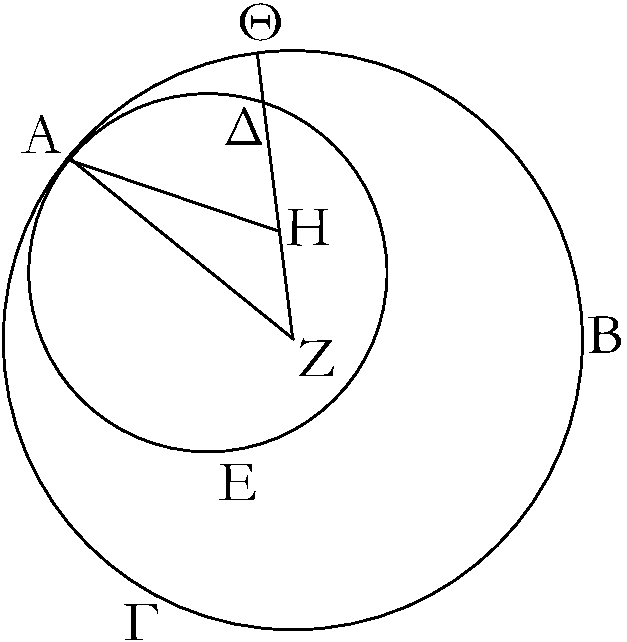
\includegraphics{Book03/fig11g.eps}}

\gr{Ἐὰν >άρα δύο κύκλοι ἐφάπτωνται ἀλλήλων ἐντόξ, [καὶ ληφθῆ| α\kern -.7pt  ὐτῶν
τὰ κέντρα], ἡ ἐπὶ τὰ κέντρα α\kern -.7pt  ὐτῶν ἐπιζευγνυμένη εὐθεῖα [καὶ
ἐκβαλλομένη] ἐπὶ τὴν συναφὴν πεσεῖται τῶν κύκλων; <όπερ
>έδει δεῖχαι.}}

\ParallelRText{
\begin{center}
{\large Proposition 11}
\end{center}

If two circles  touch one another internally, and their
centers are found, (then)  the straight-line joining their
centers, being produced, will fall upon the point of union of
the circles.

For let two circles, $ABC$ and $ADE$, touch one another internally
at point $A$, and let the center $F$ of circle $ABC$ be
found [Prop.~3.1], and (the center) $G$ of (circle) $ADE$ [Prop.~3.1].
I say that the straight-line joining $G$ to $F$, being produced, will fall on $A$.

For (if) not (then), if possible, let it fall like $FGH$ (in the figure), and
let $AF$ and $AG$ be joined.

Therefore, since $AG$ and $GF$ is greater than $FA$, that is to
say $FH$ [Prop.~1.20], let $FG$ be taken from both.
Thus, the remainder $AG$ is greater than the remainder $GH$.
And $AG$ (is) equal to $GD$. Thus, $GD$ is also greater than $GH$, the lesser
than the greater. The very thing is impossible. Thus, the straight-line
joining $F$ to $G$ will not fall outside (one circle but inside the other). Thus, it will fall upon the point of
union (of the circles) at point $A$. 

\epsfysize=2.2in
\centerline{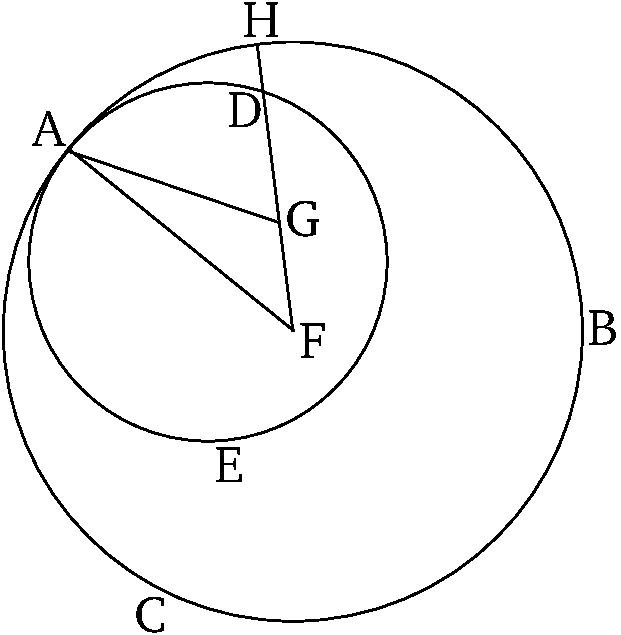
\includegraphics{Book03/fig11e.eps}}

Thus, if two circles  touch one another internally, [and their
centers are found], (then)  the straight-line joining their
centers, [being produced], will fall upon the point of union of
the circles. (Which is) the very thing it was required to show.}
\end{Parallel}

%%%%%%
% Prop 3.12
%%%%%%
\pdfbookmark[1]{Proposition 3.12}{pdf3.12}
\begin{Parallel}{}{} 
\ParallelLText{
\begin{center}
{\large \ggn{12}.}
\end{center}\vspace*{-7pt}

\gr{Ἐὰν δύο κύκλοι ἐφάπτωνται ἀλλήλων ἐκτόξ, ἡ ἐπὶ τὰ κέντρα
α\kern -.7pt  ὐτῶν ἐπιζευγνυμένη διὰ τῆξ ἐπαφῆξ ἐλεύσεται.}\\

\epsfysize=2.5in
\centerline{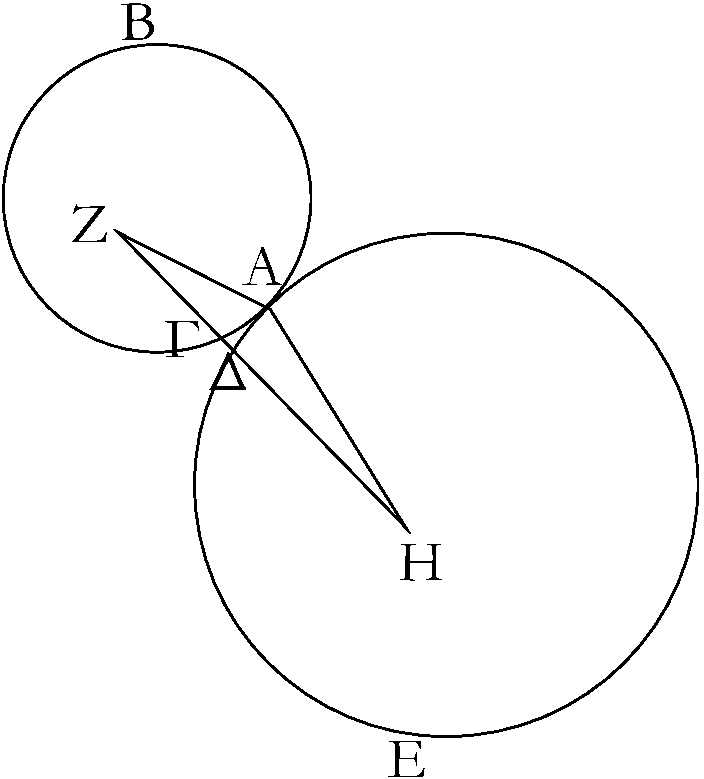
\includegraphics{Book03/fig12g.eps}}

\gr{Δύο γὰρ κύκλοι οἱ ΑΒΓ, ΑΔΕ ἐφαπτέσθωσαν ἀλλήλων ἐκτὸξ
κατὰ τὸ Α σημεῖον, καὶ εἰλήφθω τοῦ μὲν ΑΒΓ κέντρον τὸ Ζ,
τοῦ δὲ ΑΔΕ τὸ Η; λέγω, <ότι ἡ ἀπὸ τοῦ Ζ ἐπὶ τὸ Η
ἐπιζευγνυμένη εὐθεῖα διὰ τῆξ κατὰ τὸ Α ἐπαφῆξ ἐλεύσεται.}

\gr{μ\kern -.7pt  ὴ γάρ, ἀλλ> εἰ δυνατόν, ἐρθέσθω ὡξ ἡ ΖΓΔΗ, καὶ ἐπεζεύθθωσαν
αἱ ΑΖ, ΑΗ.}

\gr{Ἐπεὶ ο>ῦν τὸ Ζ σημεῖον κέντρον ἐστὶ τοῦ ΑΒΓ κύκλου,
>ίση ἐστὶν ἡ ΖΑ τῆ| ΖΓ. πάλιν, ἐπεὶ τὸ Η σημεῖον κέντρον
ἐστὶ τοῦ ΑΔΕ κύκλου, >ίση ἐστὶν ἡ ΗΑ τῆ| ΗΔ. ἐδείθθη δὲ
καὶ ἡ ΖΑ τῆ| ΖΓ >ίση; αἱ >άρα ΖΑ, ΑΗ ταῖξ ΖΓ, ΗΔ >ίσαι εἰσίν; <ώστε <όλη ἡ ΖΗ τῶν ΖΑ, ΑΗ μείζων ἐστίν; ἀλλὰ καὶ ἐλάττων;
<όπερ ἐστὶν ἀδύνατον. οὐκ >άρα ἡ ἀπὸ τοῦ Ζ ἐπὶ τὸ Η
ἐπιζευγνυμένη εὐθεῖα διὰ τῆξ κατὰ τὸ Α ἐπαφῆξ οὐκ ἐλεύσεται;
δι> α\kern -.7pt  ὐτῆξ >άρα.}

\gr{Ἐὰν >άρα δύο κύκλοι ἐφάπτωνται ἀλλήλων ἐκτόξ, ἡ ἐπὶ τὰ κέντρα
α\kern -.7pt  ὐτῶν ἐπιζευγνυμένη [εὐθεῖα] διὰ τῆξ ἐπαφῆξ ἐλεύσεται; <όπερ
>έδει δεῖχαι.}}

\ParallelRText{
\begin{center}
{\large Proposition 12}
\end{center}

If two circles touch one another externally, (then) the (straight-line)
joining their centers will go through the point of union.

\epsfysize=2.5in
\centerline{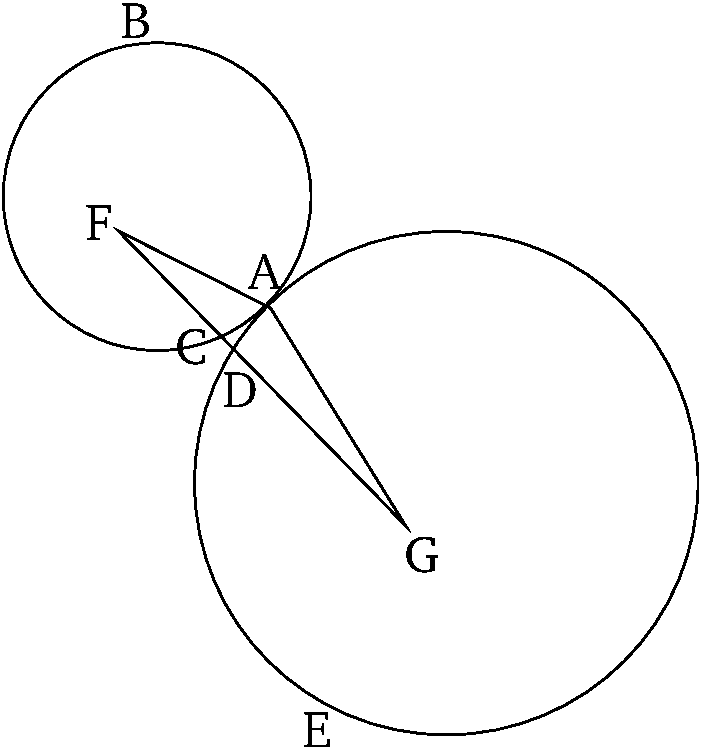
\includegraphics{Book03/fig12e.eps}}

For let two circles, $ABC$ and $ADE$, touch one another externally at point $A$,
and let the center $F$ of $ABC$ be found [Prop.~3.1], and
(the center) $G$ of $ADE$ [Prop.~3.1]. I say that the straight-line joining
$F$ to $G$ will go through the point of union at $A$.

For (if) not (then), if possible, let it go like $FCDG$ (in the figure), and let $AF$ and
$AG$ be joined.

Therefore, since point $F$ is the center of circle $ABC$, $FA$ is equal to $FC$.
Again, since point $G$ is the center of circle $ADE$, $GA$ is equal to $GD$.
And $FA$ was also shown (to be)  equal to $FC$. Thus, the (straight-lines)
$FA$ and $AG$ are equal to the (straight-lines) $FC$ and $GD$. So the whole
of $FG$ is greater than $FA$ and $AG$. But, (it is) also less [Prop.~1.20].
The very thing is impossible. Thus, the straight-line joining $F$ to $G$
cannot not go through the point of union at $A$. Thus, (it will go) through it.

Thus, if two circles touch one another externally, (then) the [straight-line]
joining their centers will go through the point of union. (Which is)
the very thing it was required to show.}
\end{Parallel}

%%%%%%
% Prop 3.13
%%%%%%
\pdfbookmark[1]{Proposition 3.13}{pdf3.13}
\begin{Parallel}{}{} 
\ParallelLText{
\begin{center}
{\large \ggn{13}.}
\end{center}\vspace*{-7pt}

\gr{Κύκλοξ κύκλου οὐκ ἐφάπτεται κατὰ πλείονα σημεῖα
>ὴ  καj> <έν, ἔαν τε ἐντὸξ ἔαν τε ἐκτὸξ ἐφάπτηται.}

\epsfysize=2.2in
\centerline{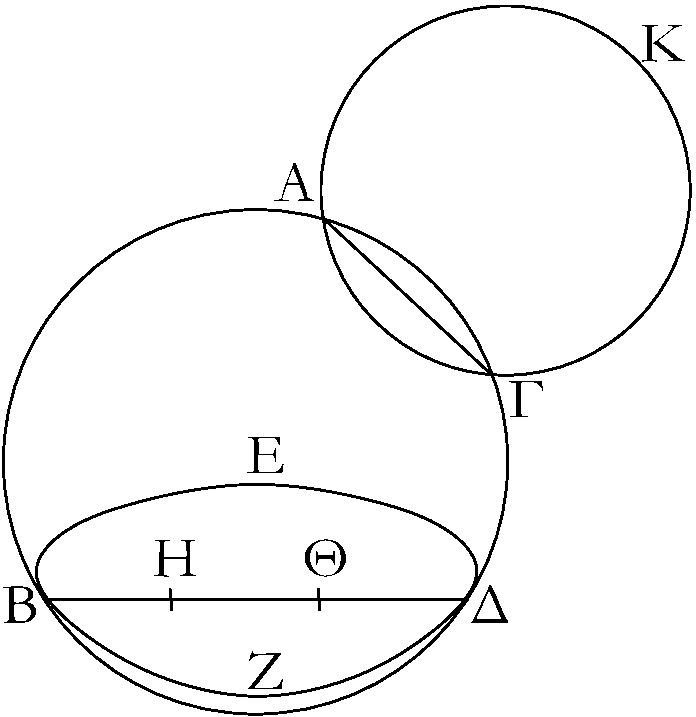
\includegraphics{Book03/fig13g.eps}}

\gr{Εἰ γὰρ δυνατόν, κύκλοξ ὁ ΑΒΓΔ κύκλου τοῦ ΕΒΖΔ ἐφαπτέσθω
πρότερον ἐντὸξ κατὰ πλείονα σημεῖα >ὴ <ὲν τὰ Δ, Β.}

\gr{Καὶ εἰλήφθω τοῦ μὲν ΑΒΓΔ κύκλου κέντρον τὸ Η, τοῦ δὲ ΕΒΖΔ
τὸ J.}

\gr{Ἡ >άρα ἀπὸ τοῦ Η ἐπὶ τὸ J ἐπιζευγνυμένη ἐπὶ τὰ Β, Δ πεσεῖται.
πιπτέτω ὡξ ἡ ΒΗJΔ. καὶ ἐπεὶ τὸ Η σημεῖον κέντρον ἐστὶ τοῦ
ΑΒΓΔ κύκλου, >ίση ἐστὶν ἡ ΒΗ τῆ| ΗΔ; μείζων >άρα ἡ ΒΗ τῆξ
JΔ; πολλῶ| >άρα μείζων ἡ ΒJ τῆξ JΔ. πάλιν, ἐπεὶ τὸ J σημεῖον
κέντρον ἐστὶ τοῦ ΕΒΖΔ κύκλου, >ίση ἐστὶν ἡ ΒJ τῆ| JΔ;
ἐδείθθη δὲ α\kern -.7pt  ὐτῆξ καὶ πολλῶ| μείζων; <όπερ ἀδύνατον;
οὐκ >άρα κύκλοξ κύκλου ἐφάπτεται ἐντὸξ κατὰ πλείονα σημεῖα
>ὴ <έν.}

\gr{Λέγω δή, <ότι οὐδὲ ἐκτόξ.}

\gr{Εἰ γὰρ δυνατόν, κύκλοξ ὁ ΑΓΚ κύκλου τοῦ ΑΒΓΔ ἐφαπτέσθω ἐκτὸξ
κατὰ πλείονα σημεῖα >ὴ <ὲν τὰ Α, Γ, καὶ ἐπεζεύθθω ἡ ΑΓ.}

\gr{>'Επεὶ ο>ῦν κύκλων τῶν ΑΒΓΔ, ΑΓΚ ε>ίληπται ἐπὶ
τῆξ περιφερείαξ ἑκατέρου δύο τυθόντα σημεῖα τὰ Α, Γ, ἡ
ἐπὶ τὰ σημεῖα ἐπιζευγνυμένη εὐθεῖα ἐντὸξ ἑκατέρου πεσεῖται;
ἀλλὰ τοῦ μὲν ΑΒΓΔ ἐντὸξ >έπεσεν, τοῦ δὲ ΑΓΚ ἐκτόξ; <όπερ
>άτοπον; οὐκ >άρα κύκλοξ κύκλου ἐφάπτεται ἐκτὸξ κατὰ πλείονα
σημεῖα >ὴ <έν. ἐδείθθη δέ, <ότι οὐδὲ ἐντόξ.}

\gr{Κύκλοξ >άρα κύκλου οὐκ ἐφάπτεται κατὰ πλείονα σημεῖα >ὴ
[καj>] <έν, ἔαν τε ἐντὸξ ἔαν τε ἐκτὸξ ἐφάπτηται; <όπερ >έδει
δεῖχαι.}}

\ParallelRText{
\begin{center}
{\large Proposition 13}
\end{center}

A circle does not touch a(nother) circle at more than one point, whether they
touch internally or externally.

\epsfysize=2.2in
\centerline{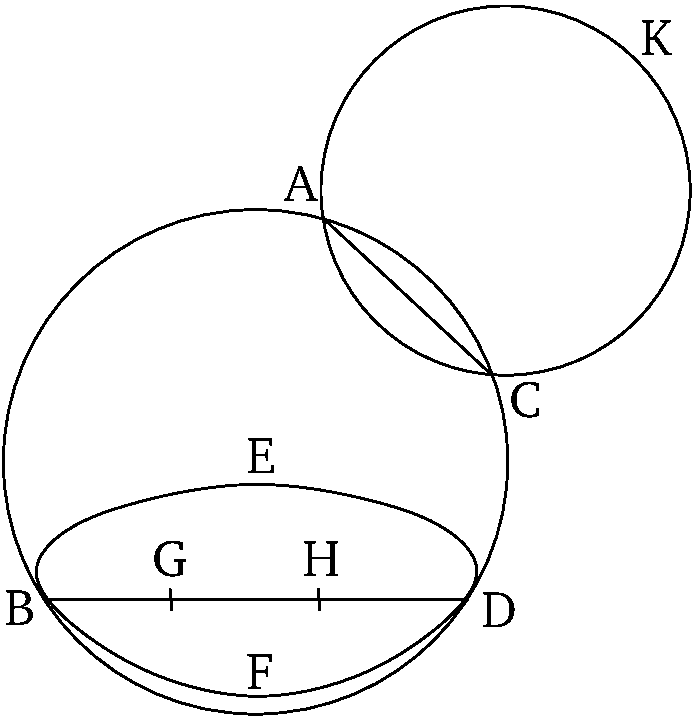
\includegraphics{Book03/fig13e.eps}}

For, if possible, let circle $ABDC$$^{\,\dag}$ touch circle $EBFD$---first of all, internally---at more than one point, $D$ and $B$.

And let the center $G$ of circle $ABDC$ be found [Prop.~3.1], and
(the center) $H$ of $EBFD$ [Prop.~3.1].

Thus, the (straight-line) joining $G$ and $H$ will fall on $B$ and $D$ [Prop.~3.11].
Let it fall like $BGHD$ (in the figure). And since point $G$ is the center of
circle $ABDC$, $BG$ is  equal to $GD$. Thus, $BG$ (is) greater than $HD$.
Thus, $BH$ (is) much greater than $HD$. Again, since point $H$ is the
center of circle $EBFD$, $BH$ is equal to $HD$. But it was also shown
(to be) much greater than it. The very thing (is) impossible.
Thus, a circle does not touch a(nother) circle internally at more than one point.

So, I say that neither (does it touch) externally (at more than one point).

For, if possible, let circle $ACK$ touch circle $ABDC$ externally at more
than one point, $A$ and $C$. And let $AC$ be joined.

Therefore, since  two points, $A$ and $C$,
be taken at random on the circumference
of each of the circles $ABDC$ and $ACK$, the straight-line joining
the points will fall inside each (circle) [Prop.~3.2]. But, it fell
inside $ABDC$, and outside $ACK$ [Def.~3.3]. The very thing (is) absurd.
Thus, a circle does not touch a(nother) circle externally  at more than one
point. And it was shown that neither (does it) internally.

Thus, a circle does not touch a(nother) circle at more than one point, whether they touch internally or externally. (Which is) the very thing it was required to
show.}
\end{Parallel}
{\footnotesize \noindent$^\dag$ The Greek text has ``$ABCD$'', which is obviously a mistake.}

%%%%%%
% Prop 3.14
%%%%%%
\pdfbookmark[1]{Proposition 3.14}{pdf3.14}
\begin{Parallel}{}{} 
\ParallelLText{
\begin{center}
{\large \ggn{14}.}
\end{center}\vspace*{-7pt}

\gr{Ἐν κύκλῳ αἱ >ίσαι εὐθεῖαι >ίσον ἀπέθουσιν ἀπὸ τοῦ κέντρου, καὶ
αἱ >ίσον ἀπέθουσαι ἀπὸ τοῦ κέντρου >ίσαι ἀλλήλαιξ εἰσίν.}\\

\epsfysize=2.2in
\centerline{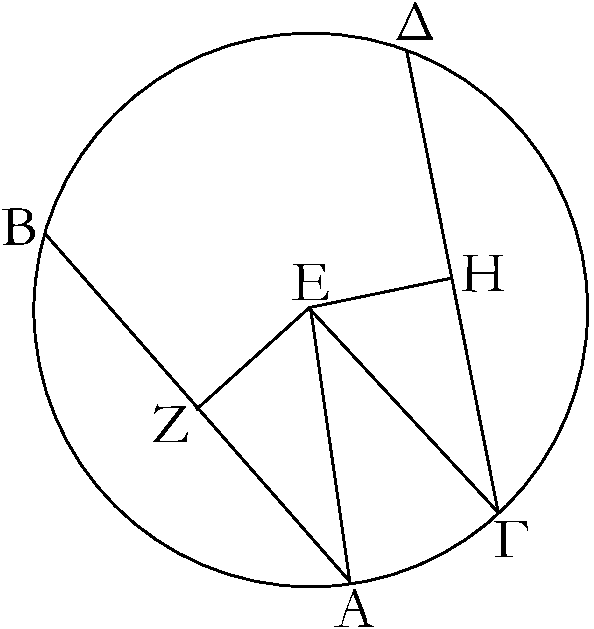
\includegraphics{Book03/fig14g.eps}}

\gr{>'Εστω κύκλοξ ὁ ΑΒΓΔ, καὶ ἐν α\kern -.7pt  ὐτῶ| >ίσαι εὐθεῖαι >έστωσαν αἱ
ΑΒ, ΓΔ; λέγω, <ότι αἱ ΑΒ, ΓΔ >ίσον ἀπέθουσιν ἀπὸ τοῦ
κέντρου.}

\gr{Εἰλήφθω γὰρ τὸ κέντον τοῦ ΑΒΓΔ κύκλου καὶ >έστω τὸ Ε, καὶ
ἀπὸ τοῦ Ε ἐπὶ τὰξ ΑΒ, ΓΔ κάθετοι >ήθθωσαν αἱ ΕΖ, ΕΗ, καὶ
ἐπεζεύθθωσαν αἱ ΑΕ, ΕΓ.}

\gr{Ἐπεὶ ο>ῦν εὐθεῖά τιξ δὶα τοῦ κέντρου ἡ ΕΖ εὐθεῖάν τινα μ\kern -.7pt  ὴ
διὰ τοῦ κέντρου τὴν ΑΒ πρὸξ ὀρθὰξ τέμνει, καὶ δίθα α\kern -.7pt  ὐτὴν
τέμνει. >ίση >άρα ἡ ΑΖ τῆ| ΖΒ; διπλῆ >άρα ἡ ΑΒ τῆξ ΑΖ. διὰ τὰ
α\kern -.5pt  ὐτὰ δὴ καὶ ἡ ΓΔ τῆξ ΓΗ ἐστι διπλῆ; καί ἐστιν >ίση ἡ ΑΒ
τῆ| ΓΔ; >ίση >άρα καὶ ἡ ΑΖ τῆ| ΓΗ. καὶ ἐπεὶ >ίση ἐστὶν ἡ ΑΕ
τῆ| ΕΓ, >ίσον καὶ τὸ ἀπὸ τῆξ ΑΕ τῶ| ἀπὸ τῆξ ΕΓ.
ἀλλὰ τῶ| μὲν ἀπὸ τῆξ ΑΕ >ίσα τὰ ἀπὸ τῶν ΑΖ, ΕΖ; ὀρθὴ γὰρ ἡ πρὸξ τῶ| Ζ γωνία; τῶ| δὲ ἀπὸ τῆξ ΕΓ >ίσα τὰ ἀπὸ τῶν ΕΗ, ΗΓ;
ὀρθὴ γὰρ ἡ πρὸξ τῶ| Η γωνία; τὰ >άρα ἀπὸ τῶν ΑΖ, ΖΕ >ίσα
ἐστὶ τοῖξ ἀπὸ τῶν ΓΗ, ΗΕ, <ῶν τὸ ἀπὸ τῆξ ΑΖ >ίσον ἐστὶ
τῶ| ἀπὸ τῆξ ΓΗ; >ίση γάρ ἐστιν ἡ ΑΖ τῆ| ΓΗ; λοιπὸν >άρα
τὸ ἀπὸ τῆξ ΖΕ τῶ| ἀπὸ τῆξ ΕΗ >ίσον ἐστίν; >ίση >άρα ἡ
ΕΖ τῆ| ΕΗ. ἐν δὲ κύκλῳ >ίσον ἀπέθειν ἀπὸ τοῦ κέντρου
εὐθεῖαι λέγονται, <όταν αἱ ἀπὸ τοῦ κέντρου ἐπ> α\kern -.3pt  ὐτὰξ
κάθετοι ἀγόμεναι >ίσαι >ῶσιν; αἱ >άρα ΑΒ, ΓΔ >ίσον ἀπέθουσιν
ἀπὸ τοῦ κέντρου.}

\gr{Ἀλλὰ δὴ αἱ ΑΒ, ΓΔ εὐθεῖαι >ίσον ἀπεθέτωσαν ἀπὸ τοῦ κέντρου,
τουτέστιν >ίση >έστω ἡ ΕΖ τῆ| ΕΗ. λέγω, <ότι >ίση ἐστὶ καὶ
ἡ ΑΒ τῆ| ΓΔ.}

\gr{Τῶν γὰρ α\kern -.7pt  ὐτῶν κατασκευασθέντων ὁμοίωξ δείχομεν, <ότι διπλῆ
ἐστιν ἡ μὲν ΑΒ τῆξ ΑΖ, ἡ δὲ ΓΔ τῆξ ΓΗ; καὶ ἐπεὶ >ίση ἐστὶν ἡ ΑΕ τῆ| ΓΕ, >ίσον ἐστὶ τὸ ἀπὸ τῆξ 
ΑΕ τῶ| ἀπὸ τῆξ ΓΕ; ἀλλὰ τῶ|
μὲν ἀπὸ τῆξ ΑΕ >ίσα ἐστὶ τὰ ἀπὸ τῶν ΕΖ, ΖΑ, τῶ| δὲ ἀπὸ
τῆξ ΓΕ 
>ίσα τὰ ἀπὸ τῶν ΕΗ, ΗΓ. τὰ >άρα ἀπὸ τῶν
ΕΖ, ΖΑ >ίσα ἐστὶ τοῖξ ἀπὸ τῶν ΕΗ, ΗΓ; <ῶν τὸ ἀπὸ τῆξ
ΕΖ τῶ| ἀπὸ τῆξ ΕΗ ἐστιν >ίσον; >ίση γὰρ ἡ ΕΖ τῆ| ΕΗ; λοιπὸν >άρα
τὸ ἀπὸ τῆξ ΑΖ >ίσον ἐστὶ τῶ| ἀπὸ τῆξ ΓΗ; >ίση >άρα ἡ ΑΖ
τῆ| ΓΗ; καί ἐστι τῆξ μὲν ΑΖ διπλῆ ἡ ΑΒ, τῆξ δὲ ΓΗ διπλῆ ἡ ΓΔ;
>ίση >άρα ἡ ΑΒ τῆ| ΓΔ.}

\gr{Ἐν κύκλῳ >άρα αἱ >ίσαι εὐθεῖαι >ίσον ἀπέθουσιν ἀπὸ τοῦ κέντρου, καὶ
αἱ >ίσον ἀπέθουσαι ἀπὸ τοῦ κέντρου >ίσαι ἀλλήλαιξ εἰσίν;
<όπερ >έδει δεῖχαι.}}

\ParallelRText{
\begin{center}
{\large Proposition 14}
\end{center}

In  a circle, equal straight-lines are equally far from the center, and
(straight-lines) which are equally far from the center are equal to one another.

\epsfysize=2.2in
\centerline{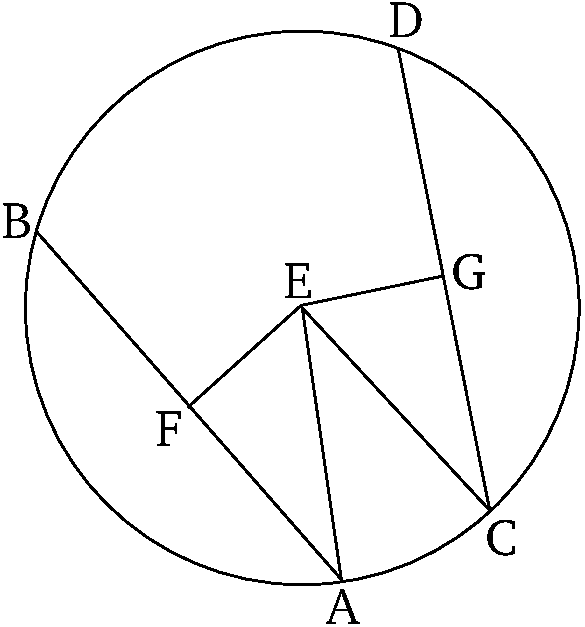
\includegraphics{Book03/fig14e.eps}}

Let $ABDC$$^{\,\dag}$ be a circle, and let $AB$ and $CD$ be equal straight-lines within it.
I say that $AB$ and $CD$ are equally far from the center.

For let the center of circle $ABDC$ be found [Prop.~3.1], and
let it be (at) $E$. And let $EF$ and $EG$ be drawn from (point) $E$, perpendicular
to $AB$ and $CD$ (respectively) [Prop.~1.12]. And let $AE$ and $EC$ be joined.

Therefore, since some straight-line, $EF$, through the center (of the circle),
cuts some (other) straight-line, $AB$, not through the center, at right-angles,
it also cuts it in half [Prop.~3.3]. Thus, $AF$ (is) equal to $FB$. Thus, 
$AB$ (is) double $AF$. So, for the same (reasons), $CD$ is also double $CG$.
And $AB$ is equal to $CD$. Thus, $AF$ (is) also equal to $CG$. And since
$AE$ is equal to $EC$, the (square) on $AE$ (is) also equal to the (square)
on $EC$. But, the (sum of the squares) on $AF$
and $EF$ (is) equal to the (square) on $AE$. For the angle at $F$ (is) a right-angle [Prop.~1.47]. And the
(sum of the squares) on $EG$ and $GC$ (is) equal to the (square) on $EC$. For the angle at $G$ (is) a right-angle [Prop.~1.47]. Thus, the (sum of the squares)
on $AF$ and $FE$ is equal to the (sum of the squares) on $CG$ and $GE$, 
of which
the (square) on $AF$ is equal to the (square) on $CG$. For $AF$ is equal to
$CG$. Thus, the remaining (square) on $FE$ is equal to the (remaining square) on  $EG$. Thus, $EF$ (is) equal to $EG$. And straight-lines in a circle are said to be equally far from the center when perpendicular (straight-lines)
which are drawn to them from the center  are equal [Def.~3.4]. Thus, $AB$ and
$CD$ are equally far from the center.

So, let the straight-lines $AB$ and $CD$ be equally far from the center. That is to say, let $EF$ be equal to $EG$. I say that $AB$ is also equal to $CD$.

For, with the same construction,  we can, similarly, show that
$AB$ is double $AF$, and $CD$ (double) $CG$. And since $AE$ is equal to $CE$, the (square) on $AE$ is equal to the (square) on $CE$. But, the (sum of the squares)
on $EF$ and $FA$ is equal to the (square) on $AE$ [Prop.~1.47]. And the (sum of
the squares) on $EG$ and $GC$ (is) equal to the (square) on $CE$ [Prop.~1.47]. Thus, the (sum of the squares) on $EF$ and $FA$ is equal to the (sum of the squares) on $EG$ and $GC$, of which the (square) on $EF$ is equal to the (square)
on $EG$. For $EF$ (is) equal to $EG$. Thus, the remaining (square) on  $AF$ is equal to the (remaining square) on  $CG$. Thus, $AF$ (is) equal to $CG$. And $AB$ is double $AF$, and
$CD$ double $CG$. Thus, $AB$ (is) equal to $CD$.

Thus, in a circle, equal straight-lines are equally far from the center, and
(straight-lines) which are equally far from the center are equal to one another.
(Which is) the very thing it was required to show.}
\end{Parallel}
{\footnotesize \noindent$^\dag$ The Greek text has ``$ABCD$'', which is obviously a
mistake.}

%%%%%%
% Prop 3.15
%%%%%%
\pdfbookmark[1]{Proposition 3.15}{pdf3.15}
\begin{Parallel}{}{} 
\ParallelLText{
\begin{center}
{\large \ggn{15}.}
\end{center}\vspace*{-7pt}

\gr{Ἐν κύκλῳ μεγίστη μὲν ἡ διάμετροξ, τῶν δὲ >άλλων ἀεὶ ἡ >έγγιον τοῦ κέντρου τῆξ ἀπώτερον μείζων ἐστίν.}

\gr{>'Εστω κύκλοξ ὁ ΑΒΓΔ, διάμετροξ δὲ α\kern -.7pt  ὐτοῦ >έστω ἡ ΑΔ, κέντρον δὲ τὸ Ε, καὶ >έγγιον μὲν τῆξ ΑΔ διαμέτρου >έστω ἡ ΒΓ, ἀπώτερον δὲ ἡ ΖΗ; λέγω, <ότι μεγίστη μέν ἐστιν ἡ ΑΔ, μείζων δὲ ἡ ΒΓ τῆξ ΖΗ.}

\gr{>'Ηθθωσαν γὰρ ἀπὸ τοῦ Ε κέντρου ἐπὶ τὰξ ΒΓ, ΖΗ κάθετοι αἱ ΕJ, ΕΚ.
καὶ ἐπεὶ >έγγιον μὲν τοῦ κέντρου ἐστὶν ἡ ΒΓ, ἀπώτερον δὲ
ἡ ΖΗ, μείζων >άρα ἡ ΕΚ τῆξ ΕJ. κείσθω τῆ| ΕJ >ίση ἡ ΕΛ,
καὶ διὰ τοῦ Λ τῆ| ΕΚ πρὸξ ὀρθὰξ ἀθθεῖσα ἡ ΛΜ διήθθω ἐπὶ
τὸ Ν, καὶ ἐπεζεύθθωσαν αἱ ΜΕ, ΕΝ, ΖΕ, ΕΗ.}

\gr{Καὶ ἐπεὶ >ίση ἐστὶν ἡ ΕJ τῆ| ΕΛ, >ίση ἐστὶ καὶ ἡ ΒΓ τῆ| ΜΝ. πάλιν, ἐπεὶ >ίση ἐστὶν ἡ μὲν ΑΕ τῆ| ΕΜ, ἡ δὲ ΕΔ τῆ| ΕΝ, ἡ >άρα
ΑΔ ταῖξ ΜΕ, ΕΝ >ίση ἐστίν. ἀλλ> αἱ μὲν ΜΕ, ΕΝ τῆξ ΜΝ μείζονέξ
εἰσιν [καὶ ἡ ΑΔ τῆξ ΜΝ μείζων ἐστίν], >ίση δὲ ἡ ΜΝ τῆ| ΒΓ;
ἡ ΑΔ >άρα τῆξ ΒΓ μείζων ἐστίν. καὶ ἐπεὶ δύο αἱ ΜΕ, ΕΝ δύο
ταῖξ ΖΕ, ΕΗ >ίσαι εἰσίν, καὶ γωνία ἡ ὑπὸ ΜΕΝ γωνίαξ τῆξ ὑπὸ
ΖΕΗ μείζων [ἐστίν], βάσιξ >άρα ἡ ΜΝ βάσεωξ τῆξ ΖΗ μείζων
ἐστίν. ἀλλὰ ἡ ΜΝ τῆ| ΒΓ ἐδείθθη >ίση [καὶ ἡ ΒΓ τῆξ ΖΗ
μείζων ἐστίν]. μεγίστη μὲν >άρα ἡ ΑΔ διάμετροξ, μείζων
δὲ ἡ ΒΓ τῆξ ΖΗ.}~\\~\\~\\~\\

\epsfysize=2.2in
\centerline{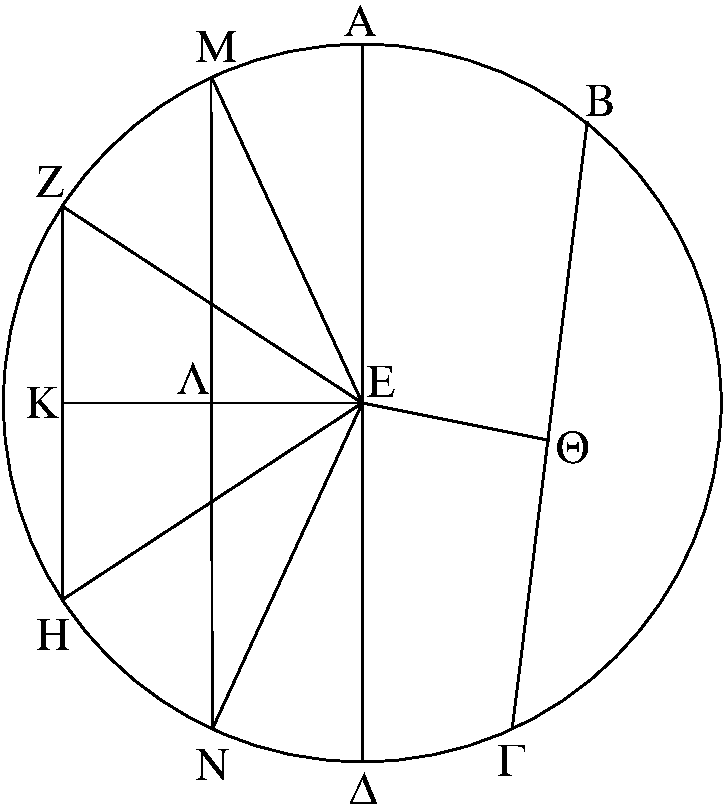
\includegraphics{Book03/fig15g.eps}}

\gr{Ἐν κύκλῳ >άρα μεγίστη μὲν έστιν ἡ διάμετροξ, τῶν δὲ >άλλων ἀεὶ ἡ >έγγιον τοῦ κέντρου τῆξ ἀπώτερον μείζων ἐστίν; <όπερ
>έδει δεῖχαι.}}

\ParallelRText{
\begin{center}
{\large Proposition 15}
\end{center}

In a circle, a diameter (is) the greatest (straight-line), and for 
the others, a (straight-line) nearer to the center is always greater than one further away.

Let $ABCD$ be a circle, and let $AD$ be its diameter, and $E$ (its) center.
And let $BC$ be nearer to the diameter $AD$,$^\dag$ and $FG$ further away. I say that
$AD$ is the greatest (straight-line), and $BC$ (is) greater than $FG$.

For let $EH$ and $EK$ be drawn from the center $E$, at right-angles
to $BC$ and $FG$ (respectively) [Prop.~1.12]. And since $BC$ is nearer to the center, and $FG$ further away, $EK$ (is) thus greater than $EH$ [Def.~3.5]. Let $EL$ be made equal to
$EH$ [Prop.~1.3]. And $LM$ being drawn through $L$, at right-angles to $EK$ [Prop.~1.11], 
let it be drawn through to $N$. And let $ME$, $EN$, $FE$, and $EG$
be joined.

And since $EH$ is equal to $EL$, $BC$ is also equal to $MN$ [Prop.~3.14]. Again,
since $AE$ is equal to $EM$, and $ED$ to $EN$, $AD$ is thus equal to $ME$ and $EN$.
But, $ME$ and $EN$ is greater than $MN$ [Prop.~1.20] [also $AD$ is greater than $MN$], and $MN$ (is) equal to $BC$. Thus, $AD$ is greater than $BC$. And since
the two (straight-lines) $ME$, $EN$ are equal to the two (straight-lines) $FE$, $EG$ (respectively),
and angle $MEN$ [is] greater than angle $FEG$,$^\ddag$ the base $MN$ is thus
greater than the base $FG$ [Prop.~1.24]. But, $MN$ was shown (to be) equal to $BC$ [(so) $BC$ is also greater than $FG$]. Thus, the diameter $AD$ (is) the
greatest (straight-line), and $BC$ (is) greater than $FG$.

\epsfysize=2.2in
\centerline{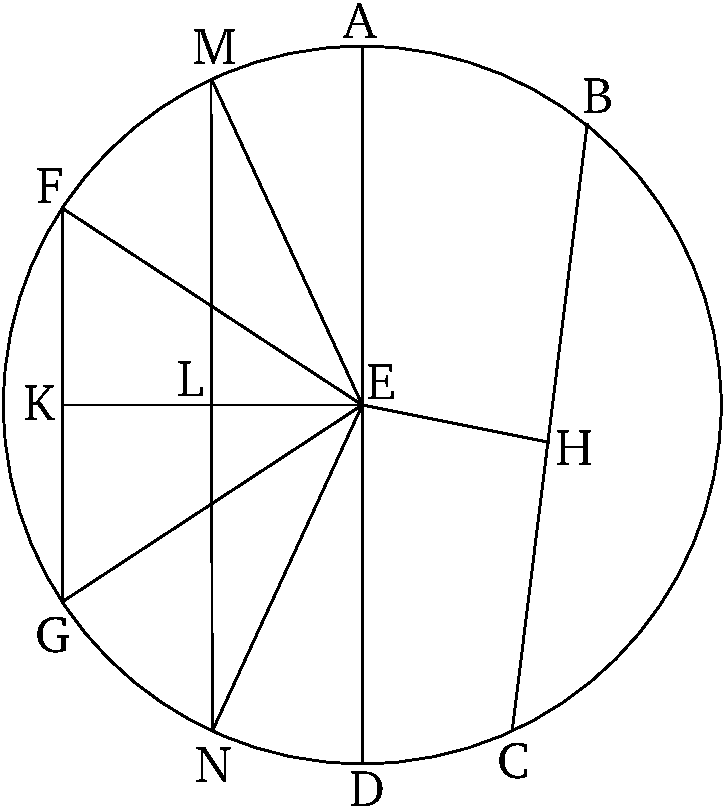
\includegraphics{Book03/fig15e.eps}}

Thus, in a circle, a diameter (is) the greatest (straight-line), and for 
the others, a (straight-line) nearer to the center is always greater than one further away. (Which is) the very thing it was required to show.}
\end{Parallel}
{\footnotesize \noindent$^\dag$ Euclid should have said ``to the center'', rather than "to the diameter $AD$", since $BC$, $AD$ and $FG$ are not necessarily parallel.\\
$^\ddag$  This is not proved,
except by reference to the figure.}

%%%%%%
% Prop 3.16
%%%%%%
\pdfbookmark[1]{Proposition 3.16}{pdf3.16}
\begin{Parallel}{}{} 
\ParallelLText{
\begin{center}
{\large \ggn{16}.}
\end{center}\vspace*{-7pt}

\gr{Ἡ τῆ| διαμέτρῳ τοῦ κύκλου πρὸξ ὀρθὰξ ἀπ> >άκραξ ἀγομένη
ἐκτὸξ πεσεῖται τοῦ κύκλου, καὶ εἰξ τὸν μεταχὺ τόπον τῆξ τε
εὐθείαξ καὶ τῆξ περιφερείαξ ἑτέρα εὐθεῖα οὐ παρεμπεσεῖται,
καὶ ἡ μὲν τοῦ ἡμικυκλίου γωνία ἁπάσηξ γωνίαξ ὀχείαξ
εὐθυγράμμου μείζων ἐστίν, ἡ δὲ λοιπὴ ἐλάττων.}

\gr{>'Εστω κύκλοξ ὁ ΑΒΓ περὶ κέντρον τὸ Δ καὶ διάμετρον τὴν
ΑΒ; λέγω, <ότι ἡ ἀπὸ τοῦ Α τῆ| ΑΒ πρὸξ ὀρθὰξ ἀπ> >άκραξ ἀγομένη ἐκτὸξ πεσεῖται τοῦ κύκλου.}

\gr{μ\kern -.7pt  ὴ γάρ, ἀλλ> εἰ δυνατόν, πιπτέτω ἐντὸξ ὡξ ἡ ΓΑ, καὶ ἐπεζεύθθω ἡ ΔΓ.}

\gr{Ἐπεὶ >ίση ἐστὶν ἡ ΔΑ τῆ| ΔΓ, >ίση ἐστὶ καὶ γωνία ἡ ὑπὸ ΔΑΓ γωνίᾳ τῆ| ὑπὸ ΑΓΔ. ὀρθὴ δὲ ἡ ὑπὸ ΔΑΓ; ὀρθὴ >άρα καὶ ἡ
ὑπὸ ΑΓΔ; τριγώνου δὴ τοῦ ΑΓΔ αἱ δύο γωνίαι αἱ ὑπὸ ΔΑΓ, ΑΓΔ
δύο ὀρθαῖξ >ίσαι εἰσίν; <όπερ ἐστὶν ἀδύνατον. οὐκ >άρα ἡ ἀπὸ
τοῦ Α σημείου τῆ| ΒΑ πρὸξ ὀρθὰξ ἀγομένη ἐντὸξ πεσεῖται
τοῦ κύκλου. ὁμοίωξ δὴ δεῖχομεν, <ότι οὐδ> ἐπὶ τῆξ περιφερείαξ;
ἐκτὸξ >άρα.}

\gr{Πιπτέτω ὡξ ἡ ΑΕ; λέγω δή, <ότι εἰξ τὸν μεταχὺ τόπον τῆξ τε ΑΕ
εὐθείαξ καὶ τῆξ ΓJΑ περιφερείαξ ἑτέρα εὐθεῖα οὐ παρεμπεσεῖται.}

\gr{Εἰ γὰρ δυνατόν, παρεμπιπτέτω ὡξ ἡ ΖΑ, καὶ >ήθθω
ἀπὸ τοῦ Δ σημείου ἐπὶ τὴν ΖΑ κάθετοξ ἡ ΔΗ. καὶ ἐπεὶ ὀρθή
ἐστιν ἡ ὑπὸ ΑΗΔ, ἐλάττων δὲ ὀρθῆξ ἡ ὑπὸ ΔΑΗ, μείζων >άρα
ἡ ΑΔ τῆξ ΔΗ. >ίση δὲ ἡ ΔΑ τῆ| ΔJ; μείζων >άρα ἡ ΔJ τῆξ
ΔΗ, ἡ ἐλάττων τῆξ μείζονοξ; <όπερ ἐστὶν ἀδύνατον. οὐκ >άρα
εἰξ τὸν μεταχὺ τόπον τῆξ τε εὐθείαξ καὶ τῆξ περιφερείαξ ἑτέρα
εὐθεῖα παρεμπεσεῖται.}\\~\\~\\~\\

\epsfysize=2in
\centerline{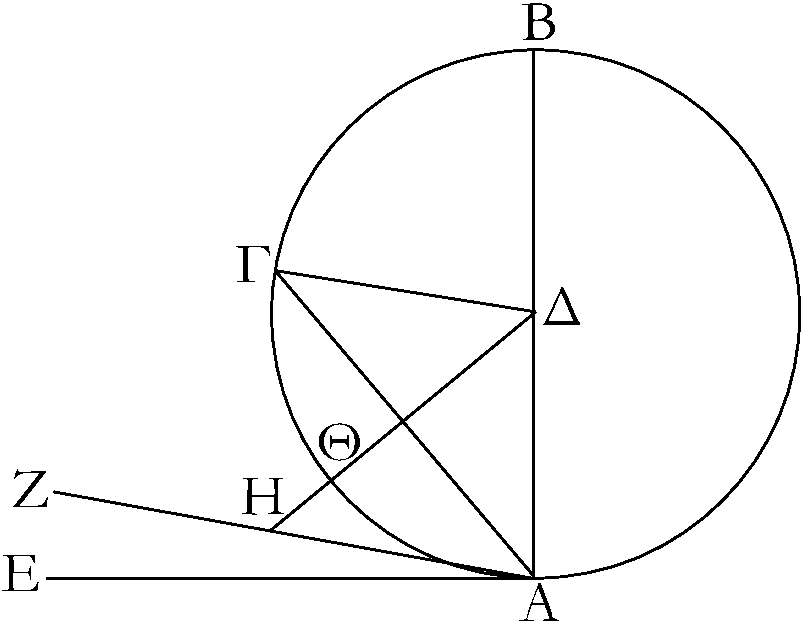
\includegraphics{Book03/fig16g.eps}}

\gr{Λέγω, <ότι καὶ ἡ μὲν τοῦ ἡμικυκλίου γωνία ἡ περιεθομένη ὑπό
τε τῆξ ΒΑ εὐθείαξ καὶ τῆξ ΓJΑ περιφερείαξ ἁπάσηξ γωνίαξ
ὀχείαξ εὐθυγράμμου μείζων ἐστίν, ἡ δὲ λοιπὴ ἡ περιεθομένη
ὑπό τε τῆξ ΓJΑ περιφερείαξ καὶ τῆξ ΑΕ εὐθείαξ ἁπάσηξ γωνίαξ
ὀχείαξ εὐθυγράμμου ἐλάττων ἐστίν.}

\gr{Εἰ γὰρ ἐστί τιξ γωνία εὐθύγραμμοξ μείζων μὲν τῆξ περιεθομένηξ
ὑπό τε τῆξ ΒΑ εὐθείαξ καὶ τῆξ ΓJΑ περιφερείαξ, ἐλάττων δὲ τῆξ
περιεθομένηξ ὑπό τε τῆξ ΓJΑ περιφερείαξ καὶ τὴξ ΑΕ εὐθείαξ, εἰξ
τὸν μεταχὺ τόπον τῆξ τε ΓJΑ περιφερείαξ καὶ τῆξ ΑΕ εὐθείαξ
εὐθεῖα παρεμπεσεῖται, <ήτιξ ποιήσει μείζονα
μὲν τῆξ περιεθομένηξ ὑπὸ τε τῆξ ΒΑ εὐθείαξ καὶ τῆξ  ΓJΑ
περιφερείαξ ὑπὸ εὐθειῶν περιεθομένην, ἐλάττονα δὲ τῆξ περιεθομένηξ ὑπό τε τῆξ ΓJΑ περιφερείαξ καὶ τῆξ ΑΕ εὐθείαξ.
οὐ παρεμπίπτει δέ; οὐκ >άρα τῆξ περιεθομένηξ γωνίαξ ὑπό
τε τῆξ ΒΑ εὐθείαξ καὶ τῆξ ΓJΑ περιφερείαξ >έσται μείζων ὀχεῖα
ὑπὸ εὐθειῶν περιεθομένη, οὐδὲ μ\kern -.7pt  ὴν ἐλάττων τῆξ περιεθομένηξ
ὑπό τε τῆξ ΓJΑ περιφερείαξ καὶ τῆξ ΑΕ εὐθείαξ.}\\~\\

\begin{center}
{\large \gr{Πόρισμα}.}
\end{center}\vspace*{-7pt}

\gr{Ἐκ δὴ τούτου φανερόν, <ότι ἡ τῆ| διαμέτρῳ τοῦ κύκλου πρὸξ
ὀρθὰξ ἀπ> >άκραξ ἀγομένη ἐφάπτεται τοῦ κύκλου [καὶ <ότι εὐθεῖα κύκλου καj> <ὲν μόνον ἐφάπτεται σημεῖον, ἐπειδήπερ καὶ ἡ κατὰ δύο
α\kern -.7pt  ὐτῶ| συμβάλλουσα ἐντὸξ α\kern -.7pt  ὐτοῦ πίπτουσα ἐδείθθη]; <όπερ
>έδει δεῖχαι.}}

\ParallelRText{
\begin{center}
{\large Proposition 16}
\end{center}

A (straight-line) drawn at right-angles to the diameter of a circle, from its
end, will fall outside the circle. And another straight-line cannot be inserted
into the space between the (aforementioned) straight-line and the circumference. And the
  angle of the semi-circle is greater than any acute rectilinear angle whatsoever, 
and the remaining (angle is) less (than any acute rectilinear angle).

Let $ABC$ be a circle around the center $D$ and the diameter $AB$. I say that
the (straight-line) drawn from $A$, at right-angles to $AB$ [Prop~1.11], from its end, will fall
outside the circle.

For (if) not (then), if possible, let it fall inside, like $CA$ (in the figure), and let
$DC$ be joined.

Since $DA$ is equal to $DC$, angle $DAC$ is also equal to angle $ACD$ [Prop.~1.5].
And $DAC$ (is) a right-angle. Thus, $ACD$ (is) also a right-angle. So, in triangle
$ACD$, the two angles $DAC$ and $ACD$ are equal to two right-angles. 
The very thing is
impossible [Prop.~1.17]. Thus, the (straight-line) drawn from point $A$,
at right-angles to $BA$, will not fall inside the circle. So, similarly, we can show 
that neither (will it fall) on the circumference. Thus, (it will fall) outside
(the circle).

Let it fall like $AE$ (in the figure). So, I say that another straight-line cannot
be inserted into the space between the straight-line $AE$ and the
circumference $CHA$.

For, if possible, let it be inserted like $FA$ (in the figure), and let $DG$ 
be drawn from point $D$, perpendicular to $FA$ [Prop.~1.12]. And since $AGD$ is a right-angle, and
 $DAG$ (is) less than a right-angle, $AD$ (is) thus greater than $DG$  [Prop.~1.19]. And $DA$ (is) equal to $DH$. Thus, $DH$ (is)
greater than $DG$, the lesser than the greater. The very thing is impossible.
Thus, another straight-line cannot be inserted into the space between the
straight-line ($AE$) and the circumference.

\epsfysize=2in
\centerline{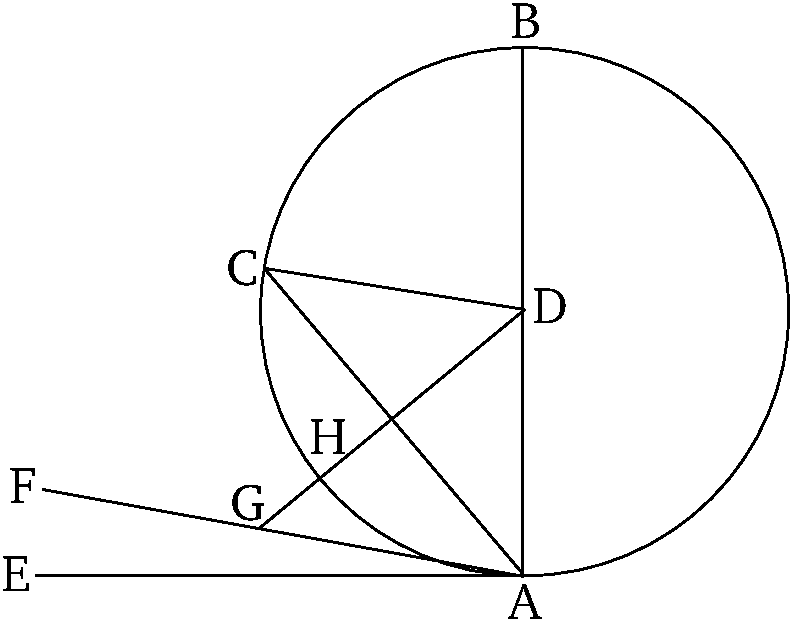
\includegraphics{Book03/fig16e.eps}}

And I also say that the  semi-circular angle  contained by the straight-line
$BA$ and the circumference $CHA$ is greater than any acute rectilinear angle whatsoever,
and the remaining (angle) contained by the circumference $CHA$ and the straight-line
$AE$ is less than any acute rectilinear angle whatsoever.

For if any rectilinear angle is greater than the (angle) contained by the
straight-line $BA$ and the circumference $CHA$, or  less than the (angle)
contained by the circumference $CHA$ and the straight-line $AE$, (then)
a straight-line can be inserted into the space between the circumference 
$CHA$ and the straight-line $AE$---anything which will make (an angle)
contained by straight-lines greater than the angle contained by the straight-line $BA$ and the circumference $CHA$, or less than the (angle) contained 
by the circumference $CHA$ and the straight-line $AE$. But (such a straight-line)
cannot be inserted. Thus, an acute (angle) contained by straight-lines
cannot be greater than the angle contained by the straight-line $BA$ and
the circumference $CHA$, neither (can it be) less than the (angle) contained by
the circumference $CHA$ and the straight-line $AE$.\\

\begin{center}
{\large Corollary}
\end{center}\vspace*{-7pt}

So, from this, (it is) manifest that a (straight-line) drawn at right-angles
to the diameter of a circle, from its extremity, touches the circle [and that the
straight-line  touches the circle at a single point, inasmuch as it was also
shown that a (straight-line) meeting (the circle) at two (points) falls inside it [Prop.~3.2]\,]. (Which is) the very thing it was required to show. }
\end{Parallel}

%%%%%%
% Prop 3.17
%%%%%%
\pdfbookmark[1]{Proposition 3.17}{pdf3.17}
\begin{Parallel}{}{} 
\ParallelLText{
\begin{center}
{\large \ggn{17}.}
\end{center}\vspace*{-7pt}

\gr{Ἀπὸ τοῦ δοθέντοξ σημείου τοῦ δοθέντοξ κύκλου ἐφαπτομένην
εὐθεῖαν γραμμ\kern -.7pt  ὴν ἀγαγεῖν.}

\gr{>'Εστω τὸ μὲν δοθὲν σημεῖον τὸ Α, ὁ δὲ δοθεὶξ κύκλοξ ὁ ΒΓΔ; δεῖ δὴ ἀπὸ τοῦ Α σημείου τοῦ ΒΓΔ κύκλου ἐφαπτομένην
εὐθεῖαν γραμμ\kern -.7pt  ὴν ἀγαγεῖν.}

\epsfysize=2.2in
\centerline{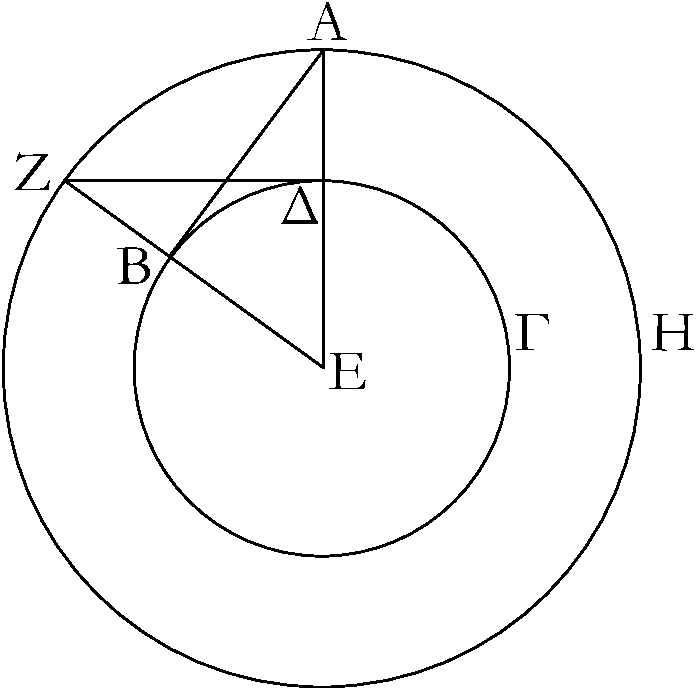
\includegraphics{Book03/fig17g.eps}}

\gr{Εἰλήφθω γὰρ τὸ κέντρον τοῦ κύκλου τὸ Ε, καὶ ἐπεζεύθθω ἡ ΑΕ,
καὶ κέντρῳ μὲν τῶ| Ε διαστήματι δὲ τῶ| ΕΑ κύκλοξ γεγράφθω ὁ ΑΖΗ,
καὶ ἀπὸ τοῦ  Δ τῆ| ΕΑ πρὸξ ὀρθὰξ >ήθθω ἡ ΔΖ, καὶ
ἐπεζεύθθωσαν αἱ ΕΖ, ΑΒ; λέγω, <ότι ἀπὸ τοῦ Α σημείου τοῦ
ΒΓΔ κύκλου ἐφαπτομένη >ῆκται ἡ ΑΒ.}

\gr{Ἐπεὶ γὰρ τὸ Ε κέντρον ἐστὶ τῶν ΒΓΔ, ΑΖΗ κύκλων, >ίση
>άρα ἐστὶν ἡ μὲν ΕΑ τῆ| ΕΖ, ἡ δὲ ΕΔ τῆ| ΕΒ; δύο δὴ αἱ ΑΕ, ΕΒ δύο ταῖξ ΖΕ, ΕΔ >ίσαι εἰσίν; καὶ γωνίαν κοινὴν περιέθουσι τὴν
πρὸξ τῶ| Ε; βάσιξ >άρα ἡ ΔΖ βάσει τῆ| ΑΒ >ίση ἐστίν, καὶ τὸ ΔΕΖ τρίγωνον τῶ| ΕΒΑ τριγώνῳ >ίσον ἐστίν, καὶ αἱ λοιπαὶ
γωνίαι ταῖξ λοιπαῖξ γωνίαιξ; >ίση >άρα ἡ ὑπὸ ΕΔΖ τῆ| ὑπὸ ΕΒΑ.
ὀρθὴ δὲ ἡ ὑπὸ ΕΔΖ; ὀρθὴ >άρα καὶ ἡ ὑπὸ ΕΒΑ. καί ἐστιν
ἡ ΕΒ ἐκ τοῦ κέντρου; ἡ δὲ τῆ| διαμέτρῳ τοῦ κύκλου πρὸξ
ὀρθὰξ ἀπ> >άκραξ ἀγομένη ἐφάπτεται τοῦ κύκλου; ἡ ΑΒ >άρα
ἐφάπτεται τοῦ ΒΓΔ κύκλου.}

\gr{Ἀπὸ τοῦ  >άρα δοθέντοξ σημείου τοῦ Α τοῦ δοθέντοξ κύκλου τοῦ ΒΓΔ ἐφαπτομένη
εὐθεῖα γραμμ\kern -.7pt  ὴ >ῆκται ἡ ΑΒ; <όπερ >έδει ποιῆσαι.}}

\ParallelRText{
\begin{center}
{\large Proposition 17}
\end{center}

To draw a straight-line touching a given circle from a given point.

Let $A$ be the given point, and $BCD$ the given circle. So it is required to draw a
straight-line touching  circle $BCD$ from point $A$.

\epsfysize=2.2in
\centerline{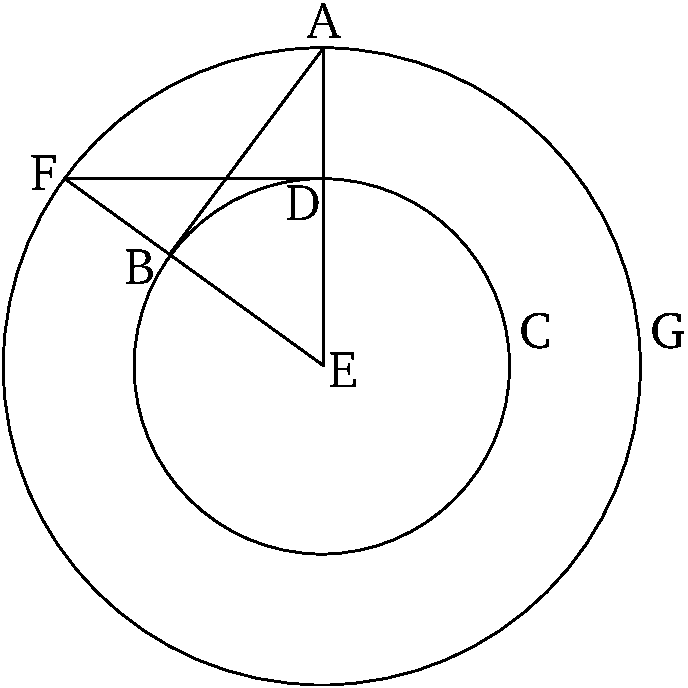
\includegraphics{Book03/fig17e.eps}}

For let the center $E$ of the circle be found [Prop.~3.1], and let $AE$ be joined. And let (the circle) $AFG$ be drawn with center
$E$ and radius $EA$. And let $DF$ be drawn from from (point) $D$,
at right-angles to $EA$ [Prop.~1.11]. And let $EF$ and $AB$ 
be  joined. I say that the (straight-line) $AB$ has been drawn from  point $A$
touching circle $BCD$.

For since $E$ is the center of circles $BCD$ and $AFG$, $EA$ is thus equal to $EF$,
and $ED$ to $EB$. So the two (straight-lines) $AE$, $EB$ are equal to
the two (straight-lines) $FE$, $ED$ (respectively). And they contain a common angle at $E$.
Thus, the base $DF$ is equal to the base $AB$, and triangle $DEF$ is equal to
triangle $EBA$, and the remaining angles (are equal) to the (corresponding)
remaining angles [Prop.~1.4]. Thus, (angle) $EDF$ (is) equal to $EBA$. And
$EDF$ (is) a right-angle. Thus, $EBA$ (is) also a right-angle. And $EB$ is a radius.
And a (straight-line) drawn at right-angles to the diameter of a circle, from
its extremity,  touches the circle [Prop.~3.16~corr.]. Thus, $AB$ touches circle $BCD$.

Thus, the straight-line $AB$ has been drawn touching the given circle $BCD$ from the given point $A$. (Which is) the very thing it was required to do.}
\end{Parallel}

%%%%%%
% Prop 3.18
%%%%%%
\pdfbookmark[1]{Proposition 3.18}{pdf3.18}
\begin{Parallel}{}{} 
\ParallelLText{
\begin{center}
{\large \ggn{18}.}
\end{center}\vspace*{-7pt}

\gr{Ἐὰν κύκλου ἐφάπτηταί τιξ εὐθεῖα, ἀπὸ δὲ τοῦ κέντρου ἐπὶ τὴν ἁφὴν ἐπιζευθθῆ| τιξ εὐθεῖα, ἡ ἐπιζευθθεῖσα κάθετοξ >έσται
ἐπὶ τὴν ἐφαπτομένην.}

\gr{Κύκλου γὰρ τοῦ ΑΒΓ ἐφαπτέσθω τιξ εὐθεῖα ἡ ΔΕ κατὰ τὸ Γ
σημεῖον, καὶ εἰλήφθω τὸ κέντρον τοῦ ΑΒΓ κύκλου τὸ
Ζ, καὶ ἀπὸ τοῦ Ζ ἐπὶ τὸ Γ ἐπεζεύθθω ἡ ΖΓ; λέγω, <ότι ἡ ΖΓ
κάθετόξ ἐστιν ἐπὶ τὴν ΔΕ.}

\gr{Εἰ γὰρ μ\kern -.7pt  ή, >ήθθω ἀπὸ τοῦ Ζ ἐπὶ τὴν ΔΕ κάθετοξ ἡ ΖΗ.}

\gr{Ἐπεὶ ο>ῦν ἡ ὑπὸ ΖΗΓ γωνία ὀρθή ἐστιν, ὀχεῖα >άρα
ἐστὶν ἡ ὑπὸ ΖΓΗ; ὑπὸ δὲ τὴν μείζονα γωνίαν ἡ μείζων
πλευρὰ ὑποτείνει; μείζων >άρα ἡ ΖΓ τῆξ ΖΗ; >ίση δὲ ἡ ΖΓ τῆ| ΖΒ;
μείζων >άρα καὶ ἡ ΖΒ τῆξ ΖΗ ἡ ἐλάττων τῆξ μείζονοξ; <όπερ
ἐστὶν ἀδύνατον. οὐκ >άρα ἡ ΖΗ κάθετόξ ἐστιν ἐπὶ τὴν ΔΕ.
ὁμοίωξ δὴ δεῖχομεν, <ότι οὐδ> >άλλη τιξ πλὴν τῆξ ΖΓ;
ἡ ΖΓ >άρα κάθετόξ ἐστιν ἐπὶ τὴν ΔΕ.}\\~\\~\\

\epsfysize=2.2in
\centerline{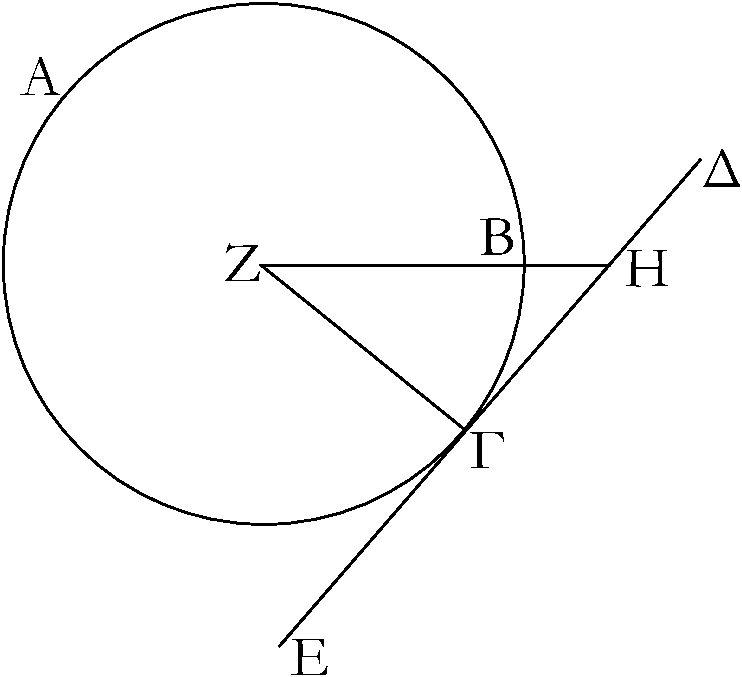
\includegraphics{Book03/fig18g.eps}}

\gr{Ἐὰν >άρα κύκλου ἐφάπτηταί τιξ εὐθεῖα, ἀπὸ δὲ τοῦ κέντρου ἐπὶ τὴν ἁφὴν ἐπιζευθθῆ| τιξ εὐθεῖα, ἡ ἐπιζευθθεῖσα κάθετοξ >έσται
ἐπὶ τὴν ἐφαπτομένην; <όπερ >έδει δεῖχαι.}}

\ParallelRText{
\begin{center}
{\large Proposition 18}
\end{center}

If some straight-line touches a circle, and some (other) straight-line is
joined from the center (of the circle) to the point of contact, (then) the (straight-line)
so joined will be perpendicular to the tangent.

For let some straight-line $DE$  touch the circle $ABC$  at  point $C$, and
let the center $F$ of circle $ABC$ be found [Prop.~3.1], 
and let $FC$ be joined from $F$ to $C$. I say that $FC$ is perpendicular
to $DE$.

For if not, let $FG$ be drawn from $F$, perpendicular to $DE$ [Prop.~1.12].

Therefore, since angle $FGC$ is a right-angle, (angle) $FCG$ is thus acute [Prop.~1.17]. And the greater angle is subtended by the greater side [Prop.~1.19]. Thus, $FC$ (is) greater than $FG$. And $FC$ (is) equal to
$FB$. Thus, $FB$ (is)  also greater than $FG$, the lesser than the greater.
The very thing is impossible. Thus, $FG$ is not perpendicular to
$DE$. So, similarly, we can show that neither (is) any other
(straight-line) except $FC$. Thus, $FC$ is perpendicular  to $DE$.

\epsfysize=2.2in
\centerline{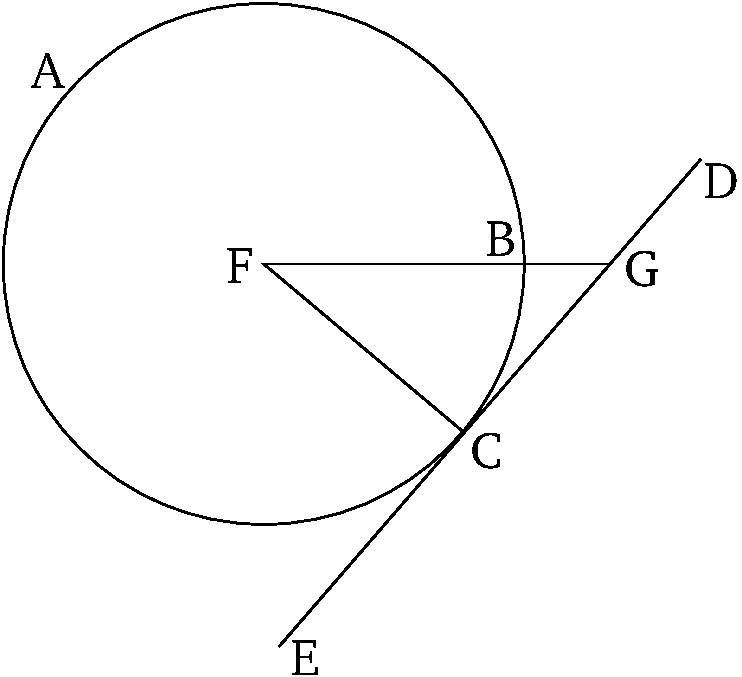
\includegraphics{Book03/fig18e.eps}}

Thus, if some straight-line  touches a circle, and some (other) straight-line is
joined from the center (of the circle) to the point of contact, (then) the (straight-line)
so joined will be perpendicular to the tangent. (Which is)
the very thing it was required to show.}
\end{Parallel}

%%%%%%
% Prop 3.19
%%%%%%
\pdfbookmark[1]{Proposition 3.19}{pdf3.19}
\begin{Parallel}{}{} 
\ParallelLText{
\begin{center}
{\large \ggn{19}.}
\end{center}\vspace*{-7pt}

\gr{Ἐὰν κύκλου ἐφάπτηταί τιξ εὐθεῖα, ἀπὸ δὲ τῆξ ἁφῆξ τῆ|
ἐφαπτομένῃ πρὸξ ὀρθὰξ [γωνίαξ] εὐθεῖα γραμμ\kern -.7pt  ὴ ἀθθῆ|,
ἐπὶ τῆξ ἀθθείσηξ >έσται τὸ κέντρον τοῦ κύκλου.}\\

\epsfysize=2.2in
\centerline{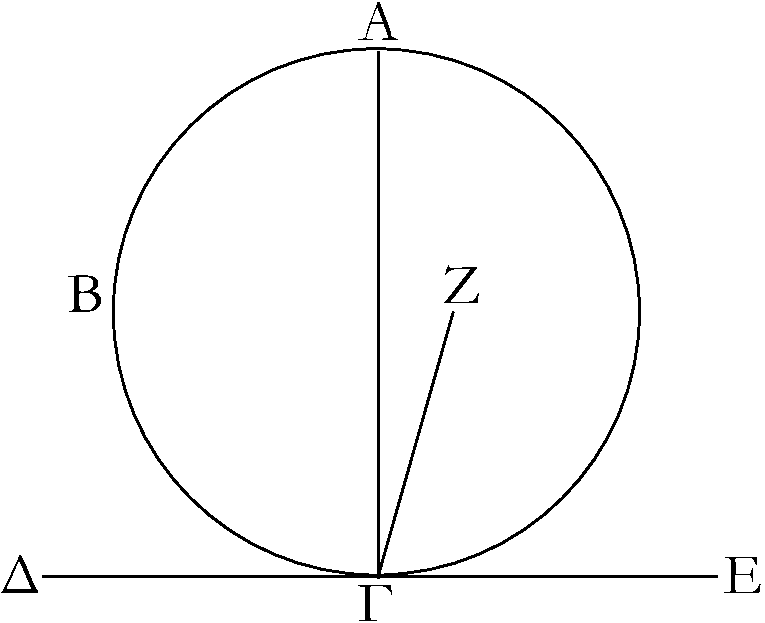
\includegraphics{Book03/fig19g.eps}}

\gr{Κύκλου γὰρ τοῦ ΑΒΓ ἐφαπτέσθω τιξ εὐθεῖα ἡ ΔΕ κατὰ τὸ Γ
σημεῖον, καὶ ἀπὸ τοῦ Γ τῆ| ΔΕ πρὸξ ὀρθὰξ >ήθθω ἡ ΓΑ;
λέγω, <ότι ἐπὶ τῆξ ΑΓ ἐστι τὸ κέντρον τοῦ κύκλου.}

\gr{μ\kern -.7pt  ὴ γάρ, ἀλλ> εἰ δυνατόν, >έστω τὸ Ζ, καὶ ἐπεζεύθθω ἡ ΓΖ.}

\gr{Ἐπεὶ [ο>ῦν] κύκλου τοῦ ΑΒΓ ἐφάπτεταί τιξ εὐθεῖα ἡ ΔΕ,
ἀπὸ δὲ τοῦ κέντρου ἐπὶ τὴν ἁφὴν ἐπέζευκται ἡ ΖΓ, ἡ ΖΓ
>άρα κάθετόξ ἐστιν ἐπὶ τὴν ΔΕ; ὀρθὴ >άρα ἐστὶν ἡ ὑπὸ ΖΓΕ. ἐστὶ
δὲ καὶ ἡ ὑπὸ ΑΓΕ ὀρθή; >ίση >άρα ἐστὶν ἡ ὑπὸ ΖΓΕ
τῆ| ὑπὸ ΑΓΕ ἡ ἐλάττων τῆ| μείζονι; <όπερ ἐστὶν ἀδύνατον.
οὐκ >άρα τὸ Ζ κέντρον ἐστὶ τοῦ ΑΒΓ κύκλου. ὁμοίωξ δὴ δείχομεν,
<ότι οὐδ> >άλλο τι πλὴν ἐπὶ τῆξ ΑΓ.}

\gr{Ἐὰν >άρα κύκλου ἐφάπτηταί τιξ εὐθεῖα, ἀπὸ δὲ τῆξ ἁφῆξ τῆ|
ἐφαπτομένῃ πρὸξ ὀρθὰξ εὐθεῖα γραμμ\kern -.7pt  ὴ ἀθθῆ|,
ἐπὶ τῆξ ἀθθείσηξ >έσται τὸ κέντρον τοῦ κύκλου; <όπερ >έδει
δεῖχαι.}}

\ParallelRText{
\begin{center}
{\large Proposition 19}
\end{center}

If some straight-line  touches a circle, and a straight-line is drawn from the
point of contact, at
right-[angles] to the tangent, (then) the center (of the circle) will be on the (straight-line) so drawn.

\epsfysize=2.2in
\centerline{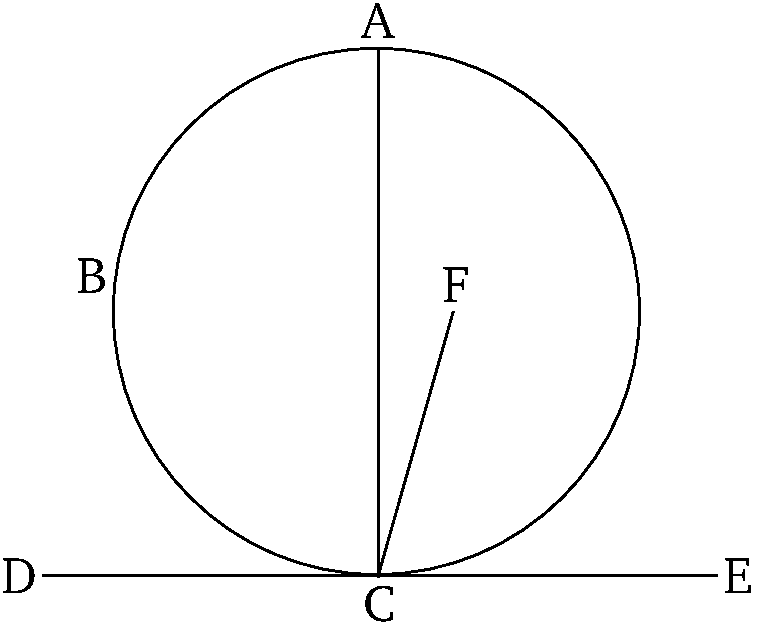
\includegraphics{Book03/fig19e.eps}}

For let some straight-line $DE$  touch the circle $ABC$  at point $C$. And let $CA$
be drawn from $C$, at right-angles to $DE$ [Prop.~1.11]. I say that the center of the circle is on $AC$.

For (if) not, if possible, let $F$ be (the center of the circle), and let
$CF$ be joined.

\mbox{[}Therefore], since some straight-line $DE$ touches the circle $ABC$, and
$FC$ has been joined from the center to the point of contact, $FC$ is thus
perpendicular to $DE$ [Prop.~3.18]. Thus, $FCE$ is a right-angle.
And $ACE$ is also a right-angle. Thus, $FCE$ is equal to $ACE$, the lesser to the
greater. The very thing is impossible. Thus, $F$ is not the center of circle $ABC$. 
So, similarly, we can show that neither is any (point) other (than one) on $AC$.

Thus, if some straight-line touches a circle, and a straight-line is drawn from the
point of contact, at
right-angles to the tangent, (then) the center (of the circle) will be on the (straight-line) so drawn. (Which is) the very thing it was required to show.}
\end{Parallel}

%%%%%%
% Prop 3.20
%%%%%%
\pdfbookmark[1]{Proposition 3.20}{pdf3.20}
\begin{Parallel}{}{} 
\ParallelLText{
\begin{center}
{\large \ggn{20}.}
\end{center}\vspace*{-7pt}

\gr{Ἐν κύκλῳ ἡ πρὸξ τῶ| κέντρῳ γωνία διπλασίων ἐστὶ τῆξ πρὸξ
τῆ| περιφερείᾳ, <όταν τὴν α\kern -.7pt  ὐτὴν περιφέρειαν βάσιν >έθωσιν αἱ
γωνίαι.}

\gr{>'Εστω κύκλοξ ὁ ΑΒΓ, καὶ πρὸξ μὲν τῶ| κέντρῳ α\kern -.7pt  ὐτοῦ γωνία
>έστω ἡ ὑπὸ ΒΕΓ, πρὸξ δὲ τῆ| περιφερείᾳ ἡ ὑπὸ ΒΑΓ, ἐθέτωσαν
δὲ τὴν α\kern -.7pt  ὐτὴν περιφέρειαν βάσιν τὴν ΒΓ; λέγω, <ότι διπλασίων ἐστὶν
ἡ ὑπὸ ΒΕΓ γωνία τῆξ ὑπὸ ΒΑΓ.}

\gr{Ἐπιζευθθεῖσα γὰρ ἡ ΑΕ διήθθω ἐπὶ τὸ Ζ.}

\gr{Ἐπεὶ ο>ῦν >ίση ἐστὶν ἡ ΕΑ τῆ| ΕΒ, >ίση καὶ γωνία
ἡ ὑπὸ ΕΑΒ τῆ| ὑπὸ ΕΒΑ; αἱ >άρα ὑπὸ ΕΑΒ, ΕΒΑ γωνίαι
τῆξ ὑπὸ ΕΑΒ διπλασίουξ εἰσίν. >ίση δὲ ἡ ὑπὸ ΒΕΖ ταῖξ
ὑπὸ ΕΑΒ, ΕΒΑ; καὶ ἡ ὑπὸ ΒΕΖ >άρα τῆξ ὑπὸ ΕΑΒ ἐστι διπλῆ. διὰ τὰ α\kern -.7pt  ὐτὰ δὴ καὶ ἡ ὑπὸ ΖΕΓ τῆξ ὑπὸ ΕΑΓ ἐστι διπλῆ. <όλη
>άρα ἡ ὑπὸ ΒΕΓ <όληξ τῆξ ὑπὸ ΒΑΓ ἐστι διπλῆ.}

\epsfysize=2.2in
\centerline{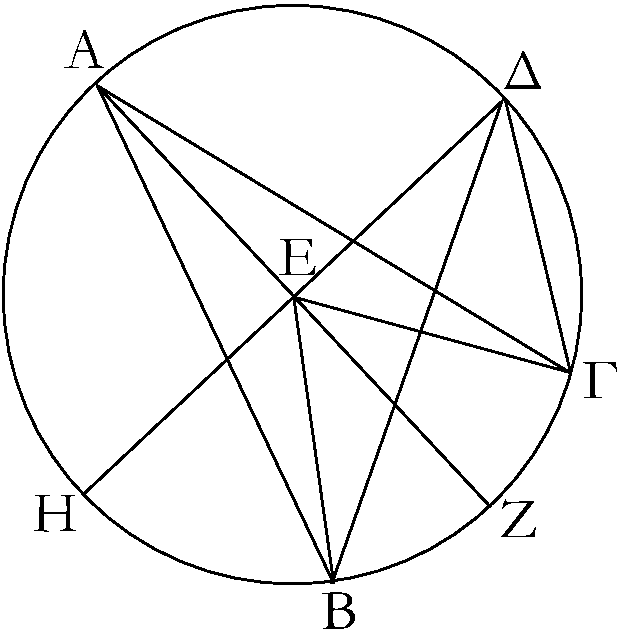
\includegraphics{Book03/fig20g.eps}}

\gr{Κεκλάσθω δὴ πάλιν, καὶ >έστω ἑτέρα γωνία ἡ ὑπὸ ΒΔΓ, καὶ
ἐπιζευθθεῖσα ἡ ΔΕ ἐκβεβλήσθω ἐπὶ τὸ Η. ὁμοίωξ
δὴ δείχομεν, <ότι διπλῆ ἐστιν ἡ ὑπὸ ΗΕΓ γωνία τῆξ ὑπὸ
ΕΔΓ, <ῶν ἡ ὑπὸ ΗΕΒ διπλῆ ἐστι τῆξ ὑπὸ ΕΔΒ; λοιπὴ
>άρα ἡ ὑπὸ ΒΕΓ διπλῆ ἐστι τῆξ ὑπὸ ΒΔΓ.}

\gr{Ἐν κύκλῳ >άρα ἡ πρὸξ τῶ| κέντρῳ γωνία διπλασίων ἐστὶ τῆξ πρὸξ
τῆ| περιφερείᾳ, <όταν τὴν α\kern -.7pt  ὐτὴν περιφέρειαν βάσιν >έθωσιν [αἱ
γωνίαι]; <όπερ >έδει δεῖχαι.}}

\ParallelRText{
\begin{center}
{\large Proposition 20}
\end{center}

In a circle, the angle at the center is double that at the circumference, when
the angles have the same circumference base.

Let $ABC$ be a circle, and let $BEC$ be an angle at its center, and $BAC$
(one) at (its) circumference. And let them have the same circumference base
$BC$. I say that angle $BEC$ is double (angle) $BAC$.

For being joined, let $AE$ be drawn through to $F$.

Therefore, since $EA$ is equal to $EB$, angle $EAB$ (is) also equal to
$EBA$ [Prop.~1.5]. Thus, angle $EAB$ and $EBA$ is double (angle) $EAB$.
And $BEF$ (is) equal to $EAB$ and $EBA$ [Prop.~1.32]. Thus, $BEF$ is also
double $EAB$. So, for the same (reasons), $FEC$ is also double $EAC$. Thus,
the whole (angle) $BEC$ is double the whole (angle) $BAC$.

\epsfysize=2.2in
\centerline{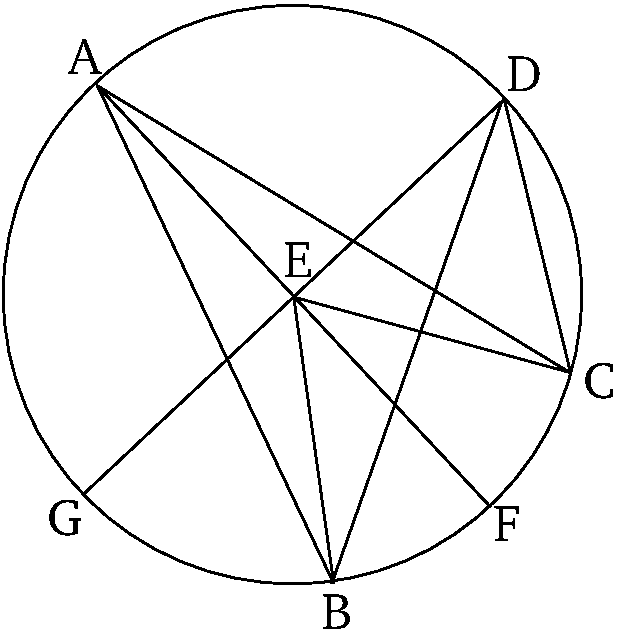
\includegraphics{Book03/fig20e.eps}}

So let another  (straight-line)  be inflected, and let there be another
angle, $BDC$. And $DE$ being joined, let it be produced to $G$.
So, similarly, we can show that angle $GEC$ is double $EDC$, of which
$GEB$ is double $EDB$. Thus, the remaining (angle) $BEC$ is double
the (remaining angle) $BDC$.

Thus, in a circle, the angle at the center is double that at the circumference, when
[the angles] have the same circumference base. (Which is) the very thing it
was required to show.\\}
\end{Parallel}

%%%%%%
% Prop 3.21
%%%%%%
\pdfbookmark[1]{Proposition 3.21}{pdf3.21}
\begin{Parallel}{}{} 
\ParallelLText{
\begin{center}
{\large \ggn{21}.}
\end{center}\vspace*{-7pt}

\gr{Ἐν κύκλῳ αἱ ἐν τῶ| α\kern -.7pt  ὐτῶ| τμ\kern -.7pt  ήματι γωνίαι >ίσαι ἀλλήλαιξ
εἰσίν.}

\epsfysize=2.2in
\centerline{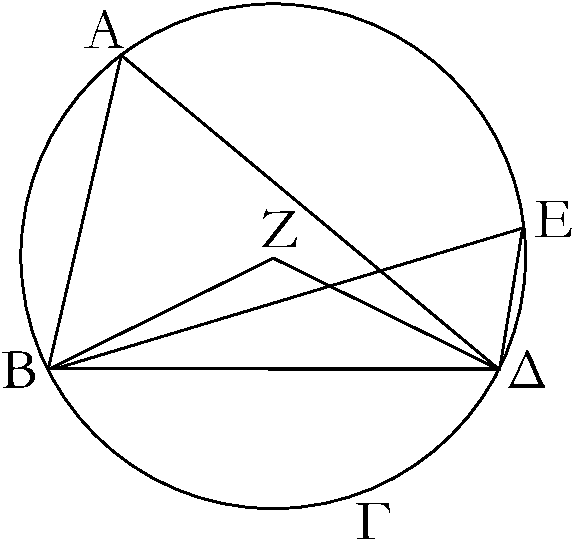
\includegraphics{Book03/fig21g.eps}}

\gr{>'Εστω κύκλοξ ὁ ΑΒΓΔ, καὶ ἐν τῶ| α\kern -.7pt  ὐτῶ| τμ\kern -.7pt  ήματι τῶ| ΒΑΕΔ γωνίαι >έστωσαν αἱ ὑπὸ ΒΑΔ, ΒΕΔ; λέγω, <ότι αἱ ὑπὸ ΒΑΔ,
ΒΕΔ γωνίαι >ίσαι ἀλλήλαιξ εἰσίν.}

\gr{Εἰλήφθω γὰρ τοῦ ΑΒΓΔ κύκλου τὸ κέντρον, καὶ >έστω τὸ Ζ, καὶ
ἐπεζεύθθωσαν αἱ ΒΖ, ΖΔ.}

\gr{Καὶ ἐπεὶ ἡ μὲν ὑπὸ ΒΖΔ γωνία πρὸξ τῶ| κέντρῳ ἐστίν,
ἡ δὲ ὑπὸ ΒΑΔ πρὸξ τῆ| περιφερείᾳ, καὶ >έθουσι τὴν α\kern -.7pt  ὐτὴν
περιφέρειαν βάσιν τὴν ΒΓΔ, ἡ >άρα ὑπὸ ΒΖΔ γωνία
διπλασίων ἐστὶ τῆξ ὑπὸ ΒΑΔ. διὰ τὰ α\kern -.7pt  ὐτὰ δὴ ἡ ὑπὸ ΒΖΔ καὶ τῆξ ὑπὸ ΒΕΔ ἐστι διπλσίων; >ίση >άρα ἡ ὑπὸ ΒΑΔ τῆ| ὑπὸ
ΒΕΔ.}

\gr{Ἐν κύκλῳ >άρα αἱ ἐν τῶ| α\kern -.7pt  ὐτῶ| τμ\kern -.7pt  ήματι γωνίαι >ίσαι ἀλλήλαιξ
εἰσίν; <όπερ >έδει δεῖχαι.}}

\ParallelRText{
\begin{center}
{\large Proposition 21}
\end{center}

In a circle, angles in the same segment are equal to one another.

\epsfysize=2.2in
\centerline{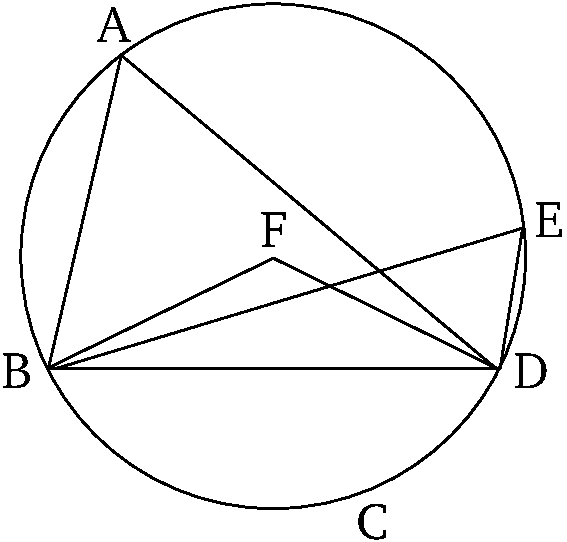
\includegraphics{Book03/fig21e.eps}}

Let $ABCD$ be a circle, and let $BAD$ and $BED$ be angles in the same segment
$BAED$. I say that angles $BAD$ and $BED$ are equal to one another.

For let the center of circle $ABCD$ be found [Prop.~3.1],
and let it be (at point) $F$. And let $BF$ and $FD$ be joined.

And since angle $BFD$ is at the center, and $BAD$ at the
circumference, and they have the same circumference base $BCD$, angle
$BFD$ is thus double $BAD$ [Prop.~3.20]. So, for the
same (reasons), $BFD$ is also double  $BED$. Thus, $BAD$ (is) equal to $BED$.

Thus, in a circle, angles in the same segment are equal to one another.
(Which is) the very thing it was required to show.}
\end{Parallel}

%%%%%%
% Prop 3.22
%%%%%%
\pdfbookmark[1]{Proposition 3.22}{pdf3.22}
\begin{Parallel}{}{} 
\ParallelLText{
\begin{center}
{\large \ggn{22}.}
\end{center}\vspace*{-7pt}

\gr{Τῶν ἐν τοῖξ κύκλοιξ τετραπλεύρων αἱ ἀπεναντίον γωνίαι δυσὶν ὀρθαῖξ >ίσαι εἰσίν.}

\epsfysize=2.2in
\centerline{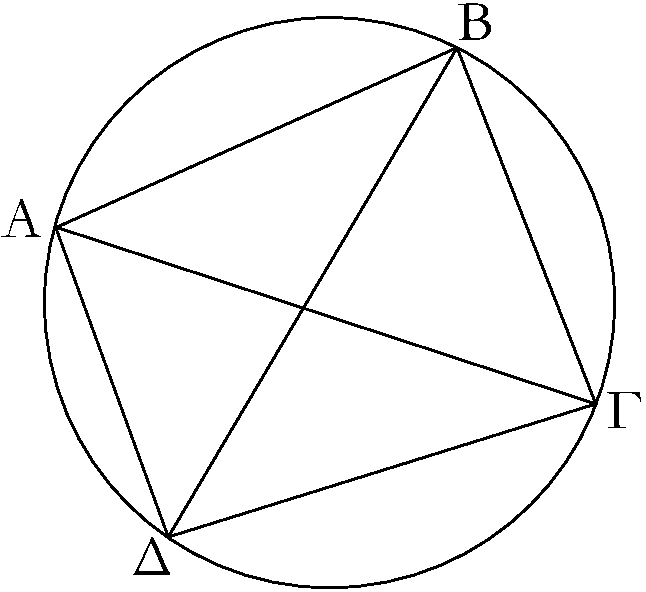
\includegraphics{Book03/fig22g.eps}}

\gr{>'Εστω κύκλοξ ὁ ΑΒΓΔ, καὶ ἐν α\kern -.7pt  ὐτῶ| τετράπλευρον >έστω τὸ ΑΒΓΔ;
λέγω, <ότι αἱ ἀπεναντίον γωνίαι δυσὶν ὀρθαῖξ >ίσαι εἰσίν.}

\gr{Ἐπεζεύθθωσαν αἱ ΑΓ, ΒΔ.}

\gr{Ἐπεὶ ο>ῦν παντὸξ τριγώνου αἱ τρεῖξ γωνίαι δυσὶν ὀρθαῖξ >ίσαι
εἰσίν, τοῦ ΑΒΓ >άρα τριγώνου αἱ τρεῖξ γωνίαι αἱ ὑπὸ ΓΑΒ, ΑΒΓ, ΒΓΑ δυσὶν ὀρθαῖξ >ίσαι εἰσίν. >ίση δὲ ἡ μὲν ὑπὸ ΓΑΒ τῆ| ὑπὸ
ΒΔΓ; ἐν γὰρ τῶ| α\kern -.7pt  ὐτῶ| τμ\kern -.7pt  ήματί εἰσι τῶ| ΒΑΔΓ; ἡ δὲ ὑπὸ ΑΓΒ
τῆ| ὑπὸ ΑΔΒ; ἐν γὰρ τῶ| α\kern -.5pt  ὐτῶ| τμ\kern -.3pt  ήματί εἰσι τῶ| ΑΔΓΒ;
<όλη >άρα ἡ ὑπὸ ΑΔΓ ταῖξ ὑπὸ ΒΑΓ, ΑΓΒ >ίση ἐστίν.
κοινὴ προσκείσθω ἡ ὑπὸ ΑΒΓ; αἱ >άρα ὑπὸ ΑΒΓ, ΒΑΓ, ΑΓΒ ταῖξ
ὑπὸ ΑΒΓ, ΑΔΓ >ίσαι εἰσίν. ἀλλ> αἱ ὑπὸ ΑΒΓ, ΒΑΓ, ΑΓΒ δυσὶν ὀρθαῖξ >ίσαι εἰσίν. καὶ αἱ ὑπὸ ΑΒΓ, ΑΔΓ >άρα δυσὶν ὀρθαῖξ
>ίσαι εἰσίν. ὁμοίωξ δὴ δείχομεν, <ότι καὶ αἱ ὑπὸ ΒΑΔ, ΔΓΒ γωνίαι δυσὶν ὀρθαῖξ >ίσαι εἰσίν.}

\gr{Τῶν >άρα ἐν τοῖξ κύκλοιξ τετραπλεύρων αἱ ἀπεναντίον γωνίαι δυσὶν ὀρθαῖξ >ίσαι εἰσίν; <όπερ >έδει δεῖχαι.}}

\ParallelRText{
\begin{center}
{\large Proposition 22}
\end{center}

For quadrilaterals within circles, the (sum of the) opposite angles is equal to two right-angles.

\epsfysize=2.2in
\centerline{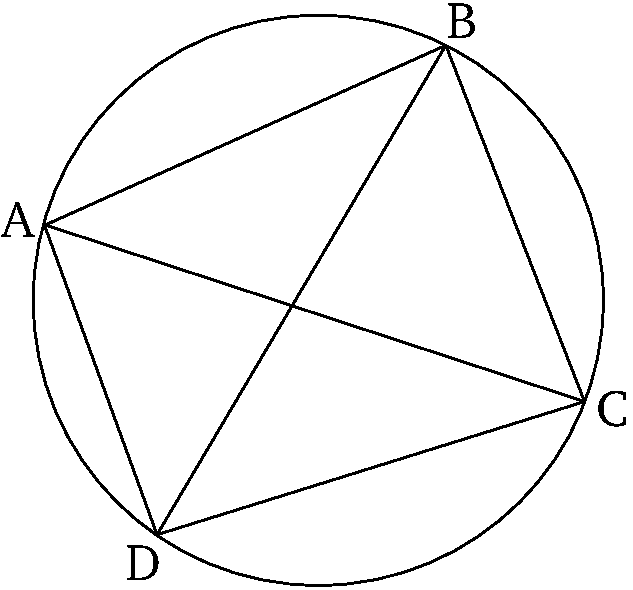
\includegraphics{Book03/fig22e.eps}}

Let $ABCD$ be a circle, and let $ABCD$ be a quadrilateral within it. I say that
the (sum of the) opposite angles is equal to two right-angles.

Let $AC$ and $BD$ be joined.

Therefore, since the three angles of any triangle are equal to two
right-angles [Prop.~1.32], the
three angles $CAB$, $ABC$, and $BCA$ of triangle $ABC$ are thus equal to two right-angles. And $CAB$ (is) equal to $BDC$. For they are in the
same segment $BADC$ [Prop.~3.21]. And $ACB$ (is equal) to $ADB$.
For they are in the same segment $ADCB$ [Prop.~3.21].
Thus, the whole of $ADC$ is equal to $BAC$ and $ACB$. Let $ABC$ be added to both. Thus, $ABC$, $BAC$, and
$ACB$ are equal to $ABC$ and $ADC$. But, $ABC$, $BAC$, and $ACB$ are equal to
two right-angles. Thus, $ABC$ and $ADC$ are also equal to two right-angles.
Similarly, we can show that angles $BAD$ and $DCB$ are also equal to
two right-angles.

Thus, for quadrilaterals within circles, the (sum of the) opposite angles is equal to two right-angles. (Which is) the very thing it was required to show.}
\end{Parallel}

%%%%%%
% Prop 3.23
%%%%%%
\pdfbookmark[1]{Proposition 3.23}{pdf3.23}
\begin{Parallel}{}{} 
\ParallelLText{
\begin{center}
{\large \ggn{23}.}
\end{center}\vspace*{-7pt}

\gr{Ἐπὶ τῆξ α\kern -.7pt  ὐτῆξ εὐθείαξ δύο τμ\kern -.7pt  ήματα κύκλων <όμοια καὶ >άνισα
οὐ συσταθήσεται ἐπὶ τὰ α\kern -.5pt  ὐτὰ μέρη.}

\gr{Εἰ γὰρ δυνατόν, ἐπὶ τῆξ α\kern -.7pt  ὐτῆξ εὐθείαξ τῆξ ΑΒ δύο τμ\kern -.7pt  ήματα
κύκλων <όμοια καὶ >άνισα συνεστάτω ἐπὶ τὰ α\kern -.5pt  ὐτὰ μέρη τὰ ΑΓΒ, ΑΔΒ,
καὶ διήθθω ἡ ΑΓΔ, καὶ ἐπεζεύθθωσαν αἱ ΓΒ, ΔΒ.}

\epsfysize=1.25in
\centerline{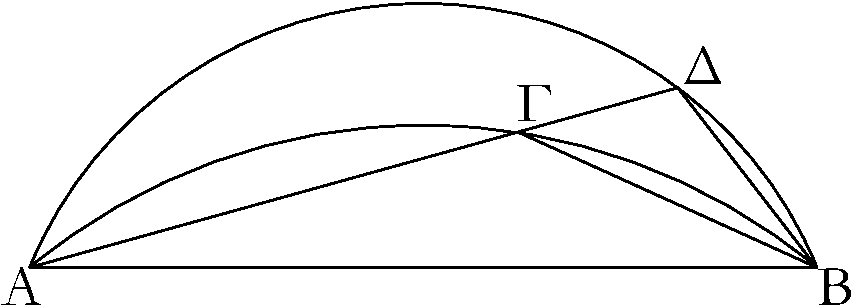
\includegraphics{Book03/fig23g.eps}}

\gr{Ἐπεὶ ο>ῦν <όμοιόν ἐστι τὸ ΑΓΒ τμ\kern -.7pt  ῆμα τῶ| ΑΔΒ τμ\kern -.7pt  ήματι,
<όμοια δὲ τμ\kern -.5pt  ήματα κύκλων ἐστὶ τὰ δεθόμενα γωνίαξ >ίσαξ, >ίση
>άρα ἐστὶν ἡ ὑπὸ ΑΓΒ γωνία τῆ| ὑπὸ ΑΔΒ ἡ ἐκτὸξ τῆ| ἐντόξ;
<όπερ ἐστὶν ἀδύνατον.}

\gr{Οὐκ >άρα ἐπὶ τῆξ α\kern -.7pt  ὐτῆξ εὐθείαξ δύο τμ\kern -.7pt  ήματα κύκλων <όμοια
καὶ >άνισα συσταθήσεται ἐπὶ τὰ α\kern -.5pt  ὐτὰ μέρη; <όπερ >έδει δεῖχαι.}}

\ParallelRText{
\begin{center}
{\large Proposition 23}
\end{center}

Two similar and unequal segments of circles cannot be constructed on the same side of the same straight-line.

For, if possible, let the two similar and unequal segments of circles, $ACB$ and
$ADB$, be constructed on the same side of the same straight-line $AB$. And let $ACD$ be drawn through (the segments), and let $CB$ and $DB$ be joined.

\epsfysize=1.25in
\centerline{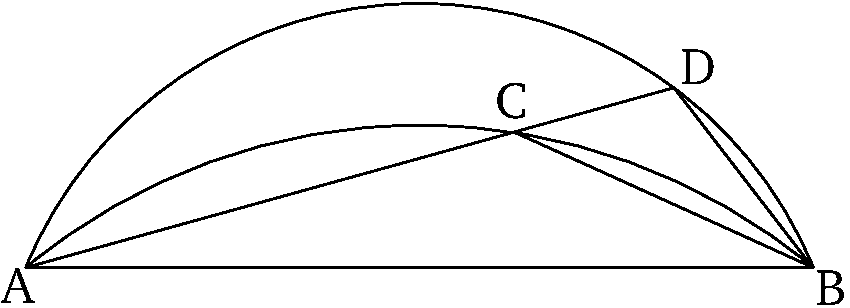
\includegraphics{Book03/fig23e.eps}}

Therefore, since segment $ACB$ is similar to segment $ADB$, and similar segments of circles are those accepting equal angles [Def.~3.11], 
angle $ACB$ is thus equal to $ADB$, the external to the internal. The very thing
is impossible [Prop.~1.16].

Thus,  two similar and unequal segments of circles cannot be constructed on the same side of the same straight-line.}
\end{Parallel}

%%%%%%
% Prop 3.24
%%%%%%
\pdfbookmark[1]{Proposition 3.24}{pdf3.24}
\begin{Parallel}{}{} 
\ParallelLText{
\begin{center}
{\large\ggn{24}.}
\end{center}\vspace*{-7pt}

\gr{Τὰ ἐπὶ >ίσων εὐθειῶν <όμοια τμ\kern -.7pt  ήματα κύλων >ίσα ἀλλήλοιξ ἐστίν.}

\gr{>'Εστωσαν γὰρ ἐπὶ >ίσων εὐθειῶν τῶν ΑΒ, ΓΔ <όμοια
τμ\kern -.7pt  ήματα κύκλων τὰ ΑΕΒ, ΓΖΔ; λέγω, <ότι >ίσον ἐστὶ τὸ ΑΕΒ
τμ\kern -.7pt  ῆμα τῶ| ΓΖΔ τμ\kern -.5pt  ήματι.}

\gr{Ἐφαρμοζομένου γὰρ τοῦ ΑΕΒ τμ\kern -.7pt  ήματοξ ἐπὶ τὸ ΓΖΔ καὶ τιθεμένου τοῦ μὲν Α σημείου ἐπὶ τὸ Γ τῆξ δὲ ΑΒ εὐθείαξ ἐπὶ τὴν
ΓΔ, ἐφαρμόσει καὶ τὸ Β σημεῖον ἐπὶ τὸ Δ σημεῖον διὰ τὸ >ίσην
ε>ῖναι τὴν ΑΒ τῆ| ΓΔ; τῆξ δὲ ΑΒ ἐπὶ τὴν ΓΔ ἐφαρμοσάσηξ ἐφαρμόσει καὶ τὸ ΑΕΒ τμ\kern -.7pt  ῆμα ἐπὶ τὸ ΓΖΔ. εἰ γὰρ ἡ ΑΒ εὐθεῖα
ἐπὶ τὴν ΓΔ ἐφαρμόσει, τὸ δὲ ΑΕΒ τμ\kern -.5pt  ῆμα ἐπὶ τὸ ΓΖΔ μ\kern -.3pt  ὴ ἐφαρμόσει, >ήτοι ἐντὸξ α\kern -.7pt  ὐτοῦ πεσεῖται >ὴ ἐκτὸξ >ὴ παραλλάχει,
ὡξ τὸ ΓΗΔ, καὶ κύκλοξ κύκλον τέμνει κατὰ πλείονα σημεῖα >ὴ
δύο; <όπερ ἐστίν ἀδύνατον. οὐκ >άρα ἐφαρμοζομένηξ τῆξ ΑΒ
εὐθείαξ ἐπὶ τὴν ΓΔ οὐκ ἐφαρμόσει καὶ τὸ ΑΕΒ τμ\kern -.7pt  ῆμα ἐπὶ
τὸ ΓΖΔ; ἐφαρμόσει >άρα, καὶ >ίσον α\kern -.7pt  ὐτῶ| >έσται.}\\~\\

\epsfysize=2.4in
\centerline{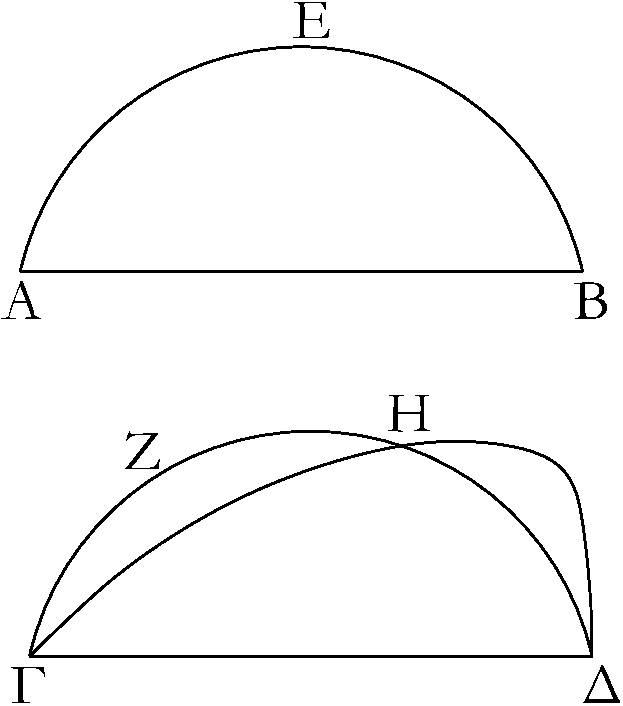
\includegraphics{Book03/fig24g.eps}}

\gr{Τὰ >άρα ἐπὶ >ίσων εὐθειῶν <όμοια τμ\kern -.7pt  ήματα κύκλων
>ίσα ἀλλήλοιξ ἐστίν; <όπερ >έδει δεῖχαι.}}

\ParallelRText{
\begin{center}
{\large Proposition 24}
\end{center}

Similar segments of circles on equal straight-lines are equal to one another.

For let $AEB$ and $CFD$ be similar segments of circles on the equal straight-lines $AB$ and $CD$ (respectively). I say that segment $AEB$ is equal to segment
$CFD$.

For if the segment $AEB$ is applied to the segment $CFD$,  and point $A$
is placed on (point) $C$, and the straight-line $AB$ on $CD$, (then) point $B$ will also coincide with point $D$, on account of $AB$ being equal to $CD$. And
if $AB$ coincides with $CD$, (then) the segment $AEB$ will also coincide with $CFD$.
For if the straight-line $AB$ coincides with $CD$, and the segment $AEB$ does not
coincide with $CFD$, (then) it will surely either fall inside it, outside (it),$^\dag$ or
it will miss like $CGD$ (in the figure), and a circle (will) cut (another) circle
at more than two points. The very thing is impossible [Prop.~3.10].
Thus, if the straight-line $AB$ is applied to $CD$, the segment $AEB$ cannot
not also coincide with $CFD$. Thus, it will coincide, and will be equal to it [C.N.~4].\\

\epsfysize=2.4in
\centerline{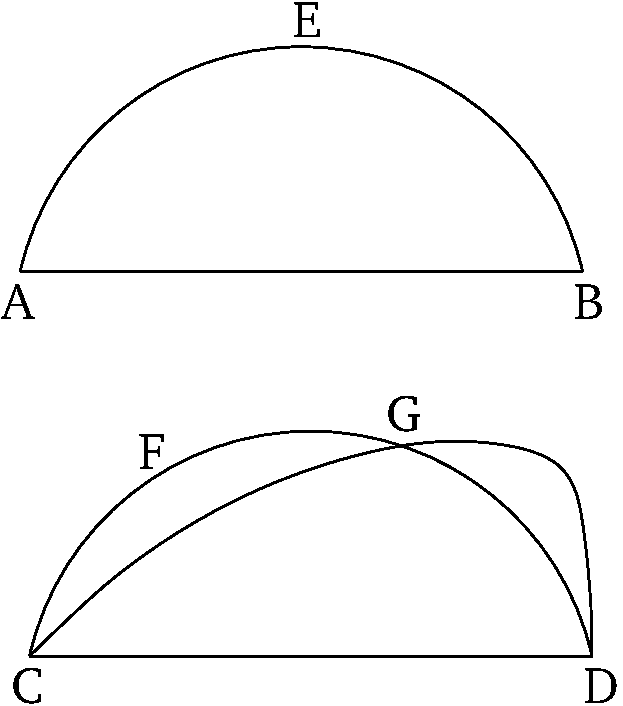
\includegraphics{Book03/fig24e.eps}}

Thus, similar segments of circles on equal straight-lines are equal to one another. (Which is) the very thing it was required to show.}
\end{Parallel}
{\footnotesize \noindent$^\dag$ Both this possibility, and the previous one, are precluded by Prop.~3.23.}

%%%%%%
% Prop 3.25
%%%%%%
\pdfbookmark[1]{Proposition 3.25}{pdf3.25}
\begin{Parallel}{}{} 
\ParallelLText{
\begin{center}
{\large \ggn{25}.}
\end{center}\vspace*{-7pt}

\gr{Κύκλου τμ\kern -.7pt  ήματοξ δοθέντοξ προσαναγράψαι τὸν κύκλον, ο<ῦπέρ ἐστι τμ\kern -.7pt  ῆμα.}

\gr{>'Εστω τὸ δοθὲν τμ\kern -.7pt  ῆμα κύκλου τὸ ΑΒΓ; δεῖ δὴ τοῦ ΑΒΓ τμ\kern -.7pt  ήματοξ
προσαναγράψαι τὸν κύκλον, ο>ῦπέρ ἐστι τμ\kern -.5pt  ῆμα.}

\gr{Τετμ\kern -.7pt  ήσθω γὰρ ἡ ΑΓ δίθα κατὰ τὸ Δ, καὶ >ήθθω ἀπὸ τοῦ Δ
σημείου τῆ| ΑΓ πρὸξ ὀρθὰξ ἡ ΔΒ, καὶ ἐπεζεύθθω ἡ ΑΒ; ἡ ὑπὸ
ΑΒΔ γωνία >άρα τῆξ ὑπὸ ΒΑΔ >ήτοι μείζων ἐστὶν >ὴ >ίση >ὴ
ἐλάττων.}

\gr{>'Εστω πρότερον μείζων, καὶ συνεστάτω πρὸξ τῆ| ΒΑ εὐθείᾳ καὶ
τῶ| πρὸξ α\kern -.7pt  ὐτῆ| σημείῳ τῶ| Α τῆ| ὑπὸ ΑΒΔ γωνίᾳ >ίση ἡ ὑπὸ
ΒΑΕ, καὶ διήθθω ἡ ΔΒ ἐπὶ τὸ Ε, καὶ ἐπεζεύθθω ἡ ΕΓ. ἐπεὶ ο>ῦν
>ίση ἐστὶν ἡ ὑπὸ ΑΒΕ γωνία τῆ| ὑπὸ ΒΑΕ, >ίση >άρα ἐστὶ
καὶ ἡ ΕΒ εὐθεῖα τῆ| ΕΑ. καὶ ἐπεὶ >ίση ἐστὶν ἡ ΑΔ τῆ|
ΔΓ, κοινὴ δὲ ἡ ΔΕ, δύο δὴ αἱ ΑΔ, ΔΕ δύο ταῖξ ΓΔ, ΔΕ >ίσαι
εἰσὶν ἑκατέρα ἑκατέρᾳ; καὶ γωνία ἡ ὑπὸ ΑΔΕ γωνίᾳ τῆ| ὑπὸ
ΓΔΕ ἐστιν >ίση; ὀρθὴ γὰρ ἑκατέρα; βάσιξ >άρα ἡ ΑΕ βάσει τῆ| ΓΕ
ἐστιν >ίση. ἀλλὰ ἡ ΑΕ τῆ| ΒΕ ἐδείθθη >ίση; καὶ ἡ ΒΕ >άρα
τῆ| ΓΕ ἐστιν >ίση; αἱ τρεῖξ >άρα αἱ ΑΕ, ΕΒ, ΕΓ >ίσαι
ἀλλήλαιξ εἰσίν; ὁ >άρα κέντρῶ| τῶ| Ε διαστήματι δὲ ἑνὶ τῶν ΑΕ, ΕΒ, ΕΓ κύκλοξ γραφόμενοξ <ήχει καὶ διὰ τῶν λοιπῶν σημείων
καὶ >έσται προσαναγεγραμμένοξ. κύκλου >άρα τμ\kern -.7pt  ήματοξ δοθέντοξ
προσαναγέγραπται ὁ κύκλοξ. καὶ δῆλον, ὡξ τὸ ΑΒΓ τμ\kern -.5pt  ῆμα >έλαττόν
ἐστιν ἡμικυκλίου διὰ τὸ τὸ Ε κέντρον ἐκτὸξ α\kern -.3pt  ὐτοῦ τυγθάνειν.}\\~\\~\\

\epsfysize=1.3in
\centerline{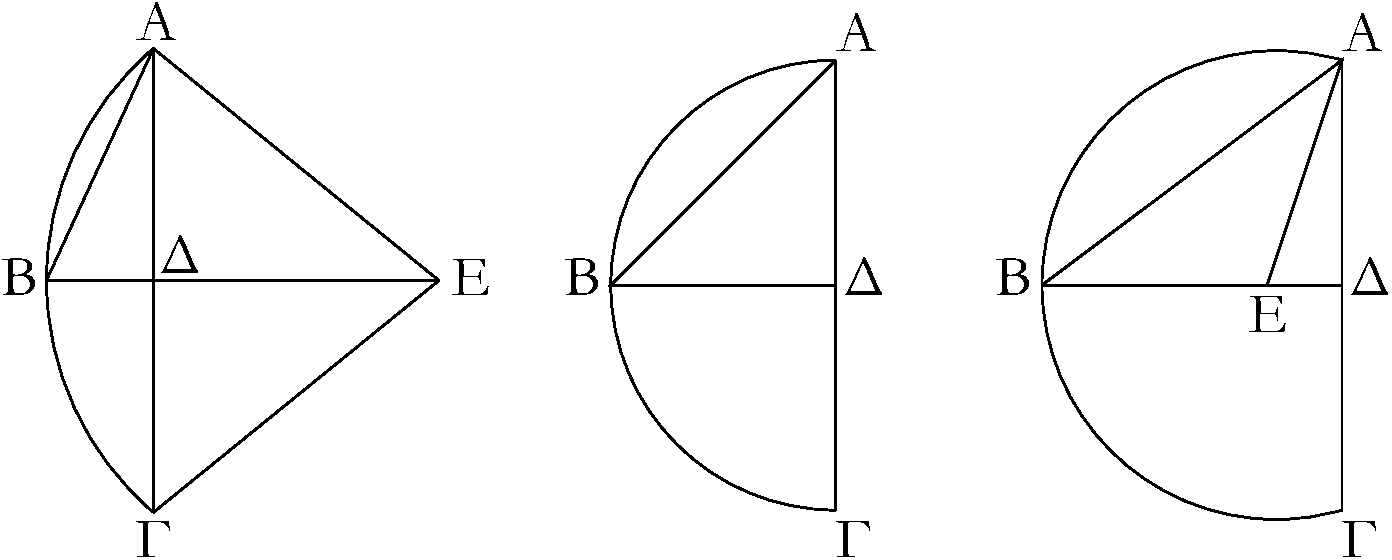
\includegraphics{Book03/fig25g.eps}}

\gr{Ὁμοίωξ [δὲ] κ>ὰν >ῆ| ἡ ὑπὸ ΑΒΔ γωνία >ίση τῆ| ὑπὸ
ΒΑΔ, τῆξ ΑΔ >ίσηξ γενομένηξ ἑκατέρᾳ τῶν ΒΔ, ΔΓ αἱ
τρεῖξ αἱ ΔΑ, ΔΒ, ΔΓ >ίσαι ἀλλήλαιξ >έσονται, καὶ >έσται τὸ Δ κέντρον
τοῦ προσαναπεπληρωμένου κύκλου, καὶ δηλαδὴ >έσται τὸ ΑΒΓ
ἡμικύκλιον.}

\gr{Ἐὰν δὲ ἡ ὑπὸ ΑΒΔ ἐλάττων >ῆ| τῆξ ὑπὸ ΒΑΔ,
καὶ συστησώμεθα πρὸξ τῆ| ΒΑ εὐθείᾳ καὶ τῶ| πρὸξ
α\kern -.7pt  ὐτῆ| σημείῳ τῶ| Α τῆ| ὑπὸ ΑΒΔ γωνίᾳ >ίσην, ἐντὸξ
τοῦ ΑΒΓ τμ\kern -.7pt  ήματοξ πεσεῖται τὸ κέντρον ἐπὶ τῆξ ΔΒ, καὶ
>έσται δηλαδὴ τὸ ΑΒΓ τμ\kern -.5pt  ῆμα μεῖζον ἡμικυκλίου.}

\gr{Κύκλου >άρα τμ\kern -.7pt  ήματοξ δοθέντοξ προσαναγέγραπται ὁ κύκλοξ;
<όπερ >έδει ποιῆσαι.}}

\ParallelRText{
\begin{center}
{\large Proposition 25}
\end{center}

For a given segment of a circle, to complete the circle, the very one of which it is a segment.

Let $ABC$ be the given segment of a circle. So it is required
to complete the circle for segment $ABC$, the very one of which it is a segment.

For let $AC$ be cut in half at (point) $D$ [Prop.~1.10], and let $DB$ be drawn
from point $D$, at right-angles to $AC$ [Prop.~1.11]. And let $AB$ be joined.
Thus, angle $ABD$ is surely either greater than,  equal to, or less than (angle)
$BAD$.

First of all, let it be greater. And let (angle) $BAE$, equal to
angle $ABD$, be constructed on the straight-line $BA$, at the point $A$ on it [Prop.~1.23].
And let $DB$ be drawn through to $E$, and let $EC$ be joined.
Therefore, since angle $ABE$ is equal to $BAE$, the straight-line $EB$ is thus also
equal to $EA$ [Prop.~1.6]. And since $AD$ is equal to $DC$, and $DE$ (is)
common, the two (straight-lines) $AD$, $DE$ are equal to the two (straight-lines)
$CD$, $DE$, respectively. And angle $ADE$ is equal to angle $CDE$. For each (is)
a right-angle. Thus, the base $AE$ is equal to the base $CE$ [Prop.~1.4].
But, $AE$ was shown (to be) equal to $BE$. Thus, $BE$ is also equal
to $CE$. Thus, the three (straight-lines) $AE$, $EB$, and $EC$ are equal to
one another. Thus, if a circle is drawn with center $E$, and radius one of $AE$, $EB$, or $EC$,  it will also go through the remaining points (of the segment), and the (associated circle) will be
 completed [Prop.~3.9]. Thus, a circle has been completed from the given
 segment of a circle. And (it is) clear that the segment $ABC$ is less
 than a semi-circle, because the center $E$ happens to lie outside it.

\epsfysize=1.3in
\centerline{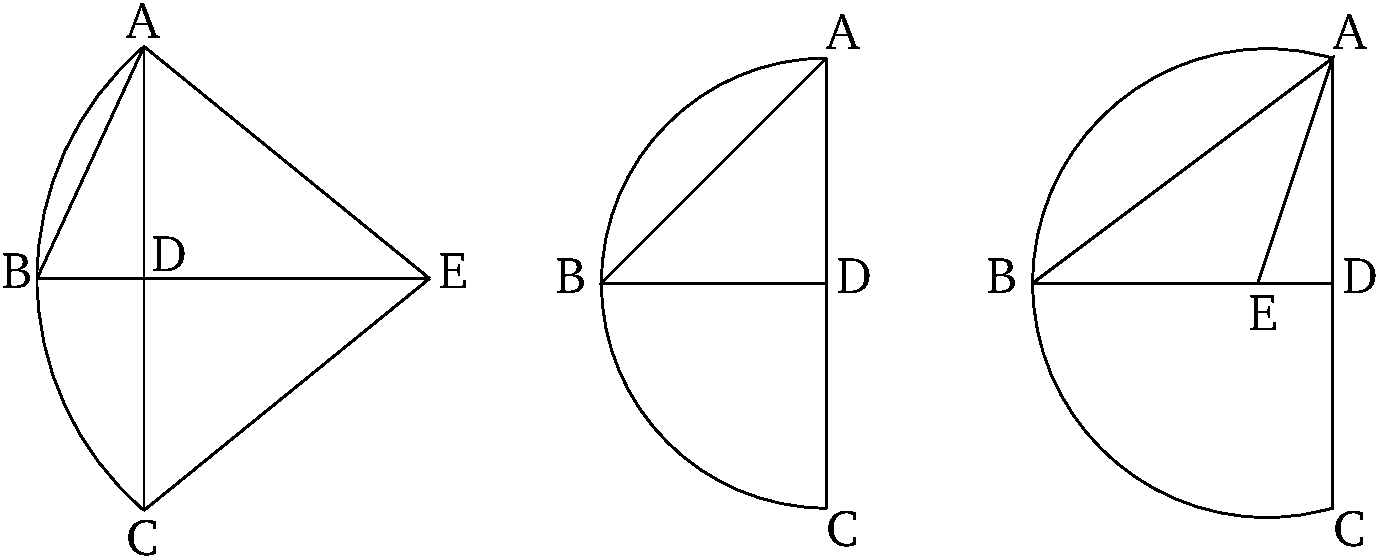
\includegraphics{Book03/fig25e.eps}}
 
\mbox{[}And], similarly, even if angle $ABD$ is equal to $BAD$,  (since) $AD$ becomes equal to
 each of $BD$ [Prop.~1.6] and $DC$, the three (straight-lines) $DA$, $DB$, and $DC$
 will  be equal to one another. And point $D$ will be the center of the completed
 circle. And $ABC$ will manifestly be a semi-circle.
 
 And if $ABD$ is less than $BAD$, and we construct (angle $BAE$), equal to angle
 $ABD$,  on the straight-line $BA$, at the point $A$ on it [Prop.~1.23], then
 the center will fall on $DB$,  inside the segment $ABC$. And segment
 $ABC$ will manifestly be greater than a semi-circle.
 
 Thus, a circle has been completed from the given segment of a circle. (Which is) the very thing it was required to do.}
\end{Parallel}

%%%%%%
% Prop 3.26
%%%%%%
\pdfbookmark[1]{Proposition 3.26}{pdf3.26}
\begin{Parallel}{}{} 
\ParallelLText{
\begin{center}
{\large \ggn{26}.}
\end{center}\vspace*{-7pt}

\gr{Ἐν τοῖξ >ίσοιξ κύκλοιξ αἱ >ίσαι γωνίαι ἐπὶ >ίσων περιφερειῶν βεβήκασιν, ἔαν τε πρὸξ τοῖξ κέντροιξ ἔαν τε πρὸξ ταῖξ περιφερείαιξ
>ῶσι βεβηκυῖαι.}

\gr{>'Εστωσαν >ίσοι κύκλοι οἱ ΑΒΓ, ΔΕΖ καὶ ἐν α\kern -.7pt  ὐτοῖξ >ίσαι γωνίαι >έστωσαν πρὸξ μὲν τοῖξ κέντροιξ αἱ ὑπὸ ΒΗΓ, ΕJΖ, πρὸξ δὲ ταῖξ
περιφερείαιξ αἱ ὑπὸ ΒΑΓ, ΕΔΖ; λέγω, <ότι >ίση ἐστὶν ἡ ΒΚΓ
περιφέρεια τῆ| ΕΛΖ περιφερείᾳ.}

\gr{Ἐπεζεύθθωσαν γὰρ αἱ ΒΓ, ΕΖ.}

\gr{Καὶ ἐπεὶ >ίσοι εἰσὶν οἱ ΑΒΓ, ΔΕΖ κύκλοι, >ίσαι
εἰσὶν αἱ ἐκ τῶν κέντρων; δύο δὴ αἱ ΒΗ, ΗΓ
δύο ταῖξ ΕJ, JΖ >ίσαι; καὶ γωνία ἡ πρὸξ τῶ| Η γωνίᾳ τῆ| πρὸξ
τῶ| J >ίση; βάσιξ >άρα ἡ ΒΓ βάσει τῆ| ΕΖ ἐστιν >ίση. καὶ ἐπεὶ
>ίση ἐστὶν ἡ πρὸξ τῶ| Α γωνία τῆ| πρὸξ τῶ| Δ, <όμοιον >άρα ἐστὶ τὸ ΒΑΓ τμ\kern -.7pt  ῆμα τῶ| ΕΔΖ τμ\kern -.7pt  ήματι; καί εἰσιν ἐπὶ >ίσων εὐθειῶν [τῶν ΒΓ, ΕΖ]; τὰ δὲ ἐπὶ >ίσων εὐθειῶν <όμοια
τμ\kern -.5pt  ήματα κύκλων >ίσα ἀλλήλοιξ ἐστίν; >ίσον >άρα τὸ ΒΑΓ τμ\kern -.3pt  ῆμα τῶ|
ΕΔΖ. >έστι δὲ καὶ <όλοξ ὁ ΑΒΓ κύκλοξ <όλῳ τῶ| ΔΕΖ κύκλῳ
>ίσοξ; λοιπὴ >άρα ἡ ΒΚΓ περιφέρεια τῆ| ΕΛΖ περιφερείᾳ ἐστὶν >ίση.}\\~\\~\\

\epsfysize=1.5in
\centerline{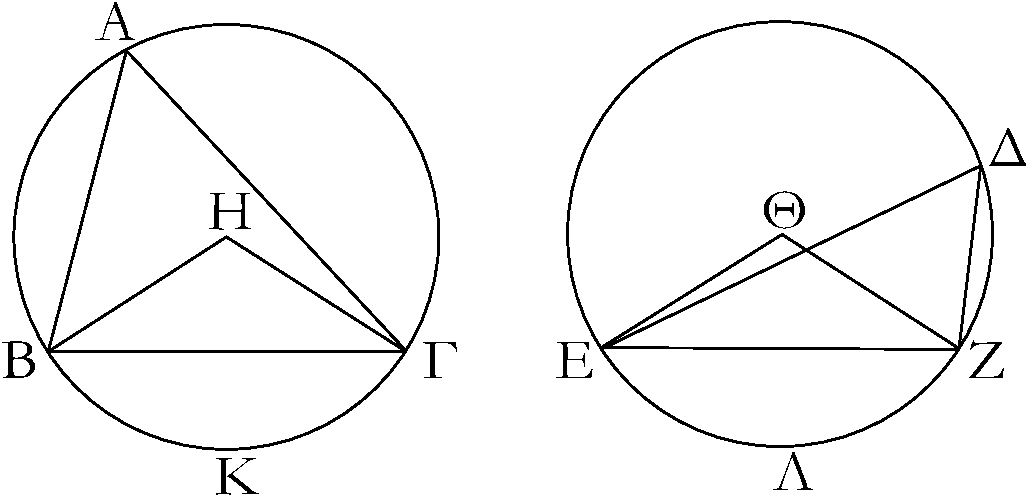
\includegraphics{Book03/fig26g.eps}}

\gr{Ἐν >άρα τοῖξ >ίσοιξ κύκλοιξ αἱ >ίσαι γωνίαι ἐπὶ >ίσων
περιφερειῶν βεβήκασιν, ἔαν τε πρὸξ τοῖξ κέντροιξ ἔαν
τε πρὸξ ταῖξ περιφερείαξ >ῶσι βεβηκυῖαι; <όπερ >έδει
δεῖχαι.}}

\ParallelRText{
\begin{center}
{\large Proposition 26}
\end{center}

In equal circles, equal angles stand upon equal circumferences  whether they
are standing at the center or at the circumference.

Let $ABC$ and $DEF$ be equal circles, and within them let $BGC$ and $EHF$ be equal angles at the center, and $BAC$ and $EDF$ (equal angles) at the circumference. I say that circumference $BKC$ is equal to circumference $ELF$.

For let $BC$ and $EF$ be joined.

And since circles $ABC$ and $DEF$ are equal, their radii are equal.
So the two (straight-lines) $BG$, $GC$ (are) equal to the two (straight-lines)
$EH$, $HF$ (respectively). And the angle at $G$ (is) equal to the angle at $H$.
Thus, the base $BC$ is equal to the base $EF$ [Prop.~1.4].
And since the angle at $A$ is equal to the (angle) at $D$, the segment $BAC$ is
thus similar to the segment $EDF$ [Def.~3.11]. And they are on
equal straight-lines [$BC$ and $EF$]. And similar segments of circles on equal
straight-lines are equal to one another [Prop.~3.24]. Thus, segment
$BAC$ is equal to (segment) $EDF$. And the whole circle $ABC$ is also
equal to the whole circle $DEF$. Thus, the remaining circumference $BKC$
is equal to the (remaining) circumference $ELF$.

\epsfysize=1.5in
\centerline{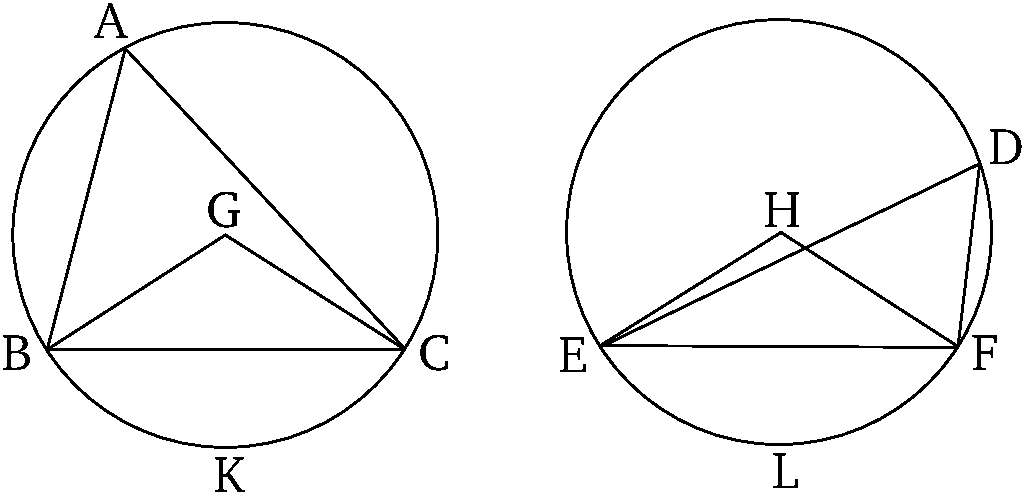
\includegraphics{Book03/fig26e.eps}}

Thus,   in equal circles, equal angles stand upon equal circumferences, whether they
are standing  at the center or at the circumference. (Which is)
the very thing which it was required to show.}
\end{Parallel}

%%%%%%
% Prop 3.27
%%%%%%
\pdfbookmark[1]{Proposition 3.27}{pdf3.27}
\begin{Parallel}{}{} 
\ParallelLText{
\begin{center}
{\large\ggn{27}.}
\end{center}\vspace*{-7pt}

\gr{Ἐν τοῖξ >ίσοιξ κύκλοιξ αἱ ἐπὶ >ίσων περιφερειῶν βεβηκυῖαι γωνίαι
>ίσαι ἀλλήλαιξ εἰσίν, ἔαν τε πρὸξ τοῖξ κέντροιξ ἔαν τε πρὸξ
ταῖξ περιφερείαιξ >ῶσι βεβηκυῖαι.}

\epsfysize=1.5in
\centerline{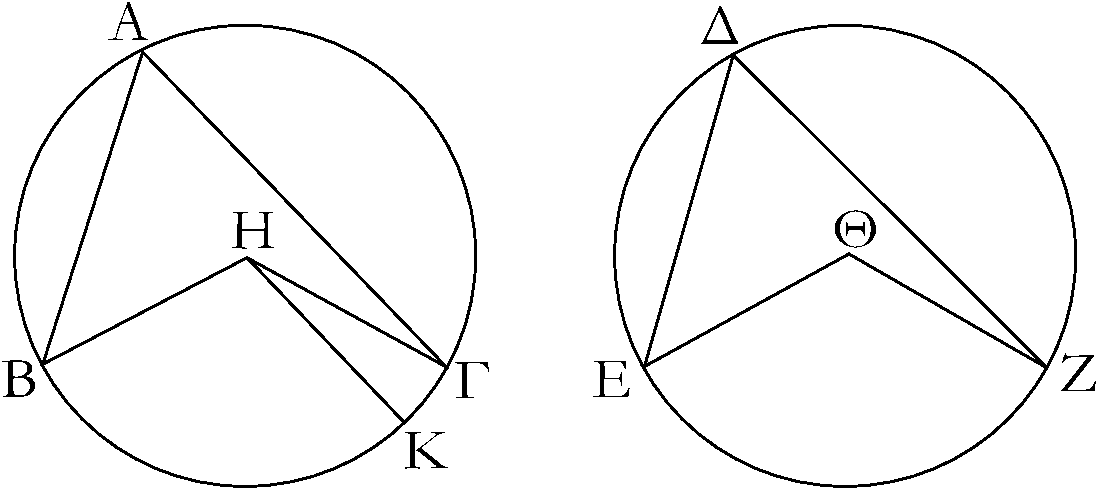
\includegraphics{Book03/fig27g.eps}}

\gr{Ἐν γὰρ >ίσοιξ κύκλοιξ τοῖξ ΑΒΓ, ΔΕΖ ἐπὶ >ίσων περιφερειῶν
τῶν ΒΓ, ΕΖ πρὸξ μὲν τοῖξ Η, J κέντροιξ γωνίαι βεβηκέτωσαν αἱ
ὑπὸ ΒΗΓ, ΕJΖ, πρὸξ δὲ ταῖξ περιφερείαιξ αἱ ὑπὸ ΒΑΓ, ΕΔΖ;
λέγω, <ότι ἡ μὲν ὑπὸ ΒΗΓ γωνία τῆ| ὑπὸ ΕJΖ ἐστιν >ίση,
ἡ δὲ ὑπὸ ΒΑΓ τῆ| ὑπὸ ΕΔΖ ἐστιν >ίση.}

\gr{Εἰ γὰρ >άνισόξ ἐστιν ἡ ὑπὸ ΒΗΓ τῆ| ὑπὸ ΕJΖ,
μία α\kern -.7pt  ὐτῶν μείζων ἐστίν. >έστω μείζων ἡ ὑπὸ ΒΗΓ, καὶ
συνεστάτω πρὸξ τῆ| ΒΗ εὐθείᾳ καὶ τῶ| πρὸξ α\kern -.7pt  ὐτῆ| σημείῳ
τῶ| Η τῆ| ὑπὸ ΕJΖ γωνίᾳ >ίση ἡ ὑπὸ ΒΗΚ; αἱ δὲ >ίσαι
γωνίαι ἐπὶ >ίσων περιφερειῶν βεβήκασιν, <όταν πρὸξ τοῖξ κέντροιξ
>ῶσιν; >ίση >άρα ἡ ΒΚ περιφέρεια τῆ| ΕΖ περιφερείᾳ. ἀλλὰ ἡ ΕΖ τῆ|
ΒΓ ἐστιν >ίση; καὶ ἡ ΒΚ >άρα τῆ| ΒΓ ἐστιν >ίση ἡ ἐλάττων τῆ|
μείζονι; <όπερ ἐστὶν ἀδύνατον. οὐκ >άρα >άνισόξ ἐστιν ἡ ὑπὸ
ΒΗΓ γωνία τῆ| ὑπὸ ΕJΖ; >ίση >άρα. καί ἐστι τῆξ μὲν ὑπὸ ΒΗΓ
ἡμίσεια ἡ πρὸξ τῶ| Α, τῆξ δὲ ὑπὸ  ΕJΖ ἡμίσεια
ἡ πρὸξ τῶ| Δ; >ίση >άρα καὶ ἡ πρὸξ τῶ| Α γωνία τῆ| πρὸξ
τῶ| Δ.}

\gr{Ἐν >άρα τοῖξ >ίσοιξ κύκλοιξ αἱ ἐπὶ >ίσων περιφερειῶν βεβηκυῖαι
γωνίαι >ίσαι ἀλλήλαιξ εἰσίν, ἔαν τε πρὸξ τοῖξ κέντροιξ ἔαν
τε πρὸξ ταῖξ περιφερείαιξ >ῶσι βεβηκυῖαι; <όπερ >έδει δεῖχαι.}}

\ParallelRText{
\begin{center}
{\large Proposition 27}
\end{center}

In equal circles, angles standing upon equal circumferences  are equal to one
another, whether they are standing at the center or at the circumference.

\epsfysize=1.5in
\centerline{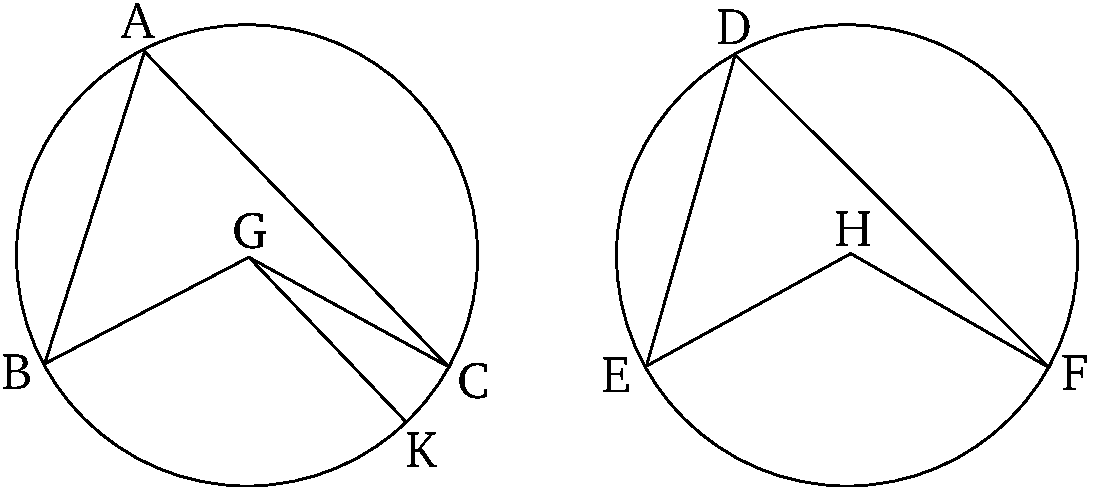
\includegraphics{Book03/fig27e.eps}}

For let the angles $BGC$ and $EHF$ at the centers $G$ and $H$, and the (angles) $BAC$ and $EDF$
at the circumferences, stand upon the equal circumferences $BC$ and $EF$, in the equal circles $ABC$ and $DEF$ (respectively). I say that angle $BGC$ is
equal to (angle) $EHF$, and $BAC$ is equal to $EDF$.

For if $BGC$ is unequal to $EHF$, one of them is greater. Let $BGC$ be greater, 
and let the (angle) $BGK$, equal to  angle $EHF$, be constructed on the
straight-line $BG$, at the point $G$ on it [Prop.~1.23]. But equal angles (in equal circles) stand upon equal circumferences, when they are at the centers [Prop.~3.26]. Thus,
circumference $BK$ (is) equal to circumference $EF$. But, $EF$ is equal to $BC$.
Thus, $BK$ is also equal to $BC$, the lesser to the greater. The very thing is
impossible. Thus, angle $BGC$ is not unequal to $EHF$. Thus, (it is) equal.
And the (angle) at $A$ is half $BGC$, and the (angle) at $D$ half $EHF$ [Prop.~3.20]. Thus, the angle at $A$ (is) also equal to the (angle) at $D$.

Thus, in equal circles, angles standing upon equal circumferences  are equal to one
another, whether they are standing at the center or at the circumference.
(Which is) the very thing it was required to show.\\}
\end{Parallel}

%%%%%%
% Prop 3.28
%%%%%%
\pdfbookmark[1]{Proposition 3.28}{pdf3.28}
\begin{Parallel}{}{} 
\ParallelLText{
\begin{center}
{\large\ggn{28}.}
\end{center}\vspace*{-7pt}

\gr{Ἐν τοῖξ >ίσοιξ κύκλοιξ αἱ >ίσαι εὐθεῖαι >ίσαξ περιφερείαξ ἀφαιροῦσι
τὴν μὲν μείζονα  τῆ| μείζονι τὴν δὲ ἐλάττονα τῆ| ἐλάττονι.}

\gr{>'Εστωσαν >ίσοι κύκλοι οἱ ΑΒΓ, ΔΕΖ, καὶ ἐν τοῖξ κύκλοιξ >ίσαι
εὐθεῖαι >έστωσαν αἱ ΑΒ, ΔΕ τὰξ μὲν ΑΓΒ, ΑΖΕ περιφερείαξ μείζοναξ
ἀφαιροῦσαι τὰξ δὲ ΑΗΒ, ΔJΕ ἐλάττοναξ; λέγω, <ότι ἡ μὲν ΑΓΒ
μείζων περιφέρεια >ίση ἐστὶ τῆ| ΔΖΕ μείζονι περιφερείᾳ
ἡ δὲ ΑΗΒ ἐλάττων περιφέρεια τῆ| ΔJΕ.}\\

\epsfysize=1.6in
\centerline{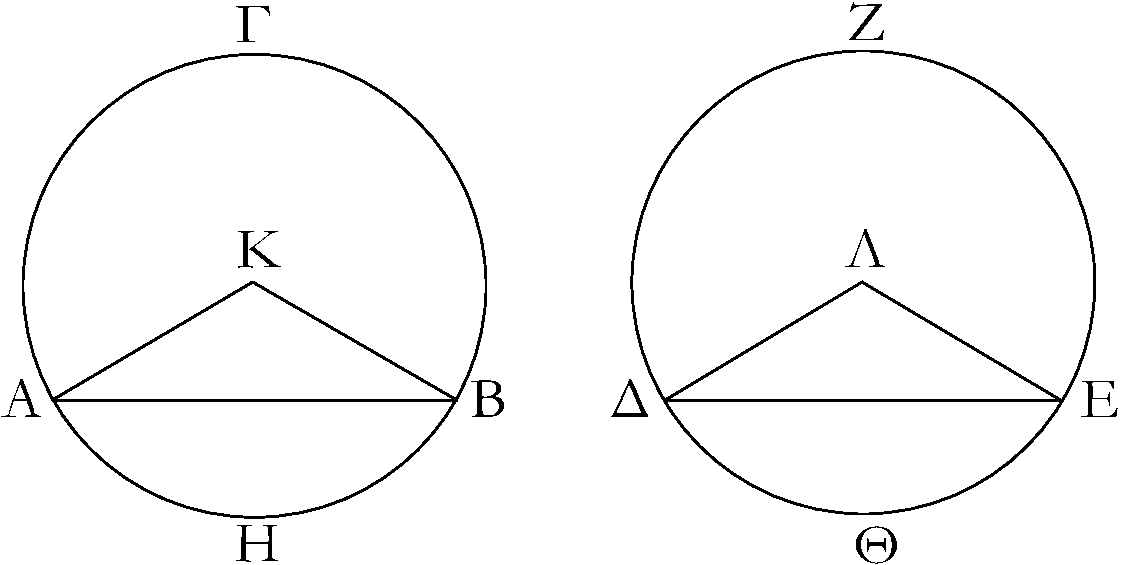
\includegraphics{Book03/fig28g.eps}}

\gr{Εἰλήφθω γὰρ τὰ κέντρα τῶν κύκλων τὰ Κ, Λ, καὶ ἐπεζεύθθωσαν αἱ
ΑΚ, ΚΒ, ΔΛ, ΛΕ.}

\gr{Καὶ ἐπεὶ >ίσοι κύκλοι εἰσίν, >ίσαι εἰσὶ καὶ αἱ ἐκ τῶν κέντρων;
δύο δὴ αἱ ΑΚ, ΚΒ δυσὶ ταῖξ ΔΛ, ΛΕ
>ίσαι εἰσίν; καὶ βάσιξ ἡ ΑΒ βάσει τῆ| ΔΕ >ίση; γωνία >άρα ἡ ὑπὸ
ΑΚΒ γωνίᾳ τῆ| ὑπὸ ΔΛΕ >ίση ἐστίν. αἱ δὲ >ίσαι γωνίαι ἐπὶ
>ίσων περιφερειῶν βεβήκασιν, <όταν πρὸξ τοῖξ κέντροιξ >ῶσιν; >ίση
>άρα ἡ ΑΗΒ περιφέρεια τῆ| ΔJΕ. ἐστὶ δὲ καὶ <όλοξ ὁ ΑΒΓ
κύκλοξ <όλῳ τῶ| ΔΕΖ κύκλῳ >ίσοξ; καὶ λοιπὴ >άρα ἡ ΑΓΒ 
περιφέρεια λοιπῆ| τῆ| ΔΖΕ περιφερείᾳ >ίση ἐστίν.}

\gr{Ἐν >άρα τοῖξ >ίσοιξ κύκλοιξ αἱ >ίσαι εὐθεῖαι >ίσαξ περιφερείαξ ἀφαιροῦσι
τὴν μὲν μείζονα τῆ| μείζονι τὴν δὲ ἐλάττονα τῆ| ἐλάττονι; <όπερ
>έδει δεῖχαι.}}

\ParallelRText{
\begin{center}
{\large Proposition 28}
\end{center}

 In equal circles, equal straight-lines cut off equal circumferences, 
the greater (circumference being equal) to the greater, and the lesser to the lesser.

Let $ABC$ and $DEF$ be equal circles, and let $AB$ and $DE$ be equal straight-lines
in these circles, cutting off the greater circumferences $ACB$ and $DFE$, 
and the lesser (circumferences) $AGB$ and $DHE$ (respectively). I say that
the greater circumference $ACB$ is equal to the greater circumference $DFE$,
and the lesser circumference $AGB$ to (the lesser) $DHE$.

\epsfysize=1.6in
\centerline{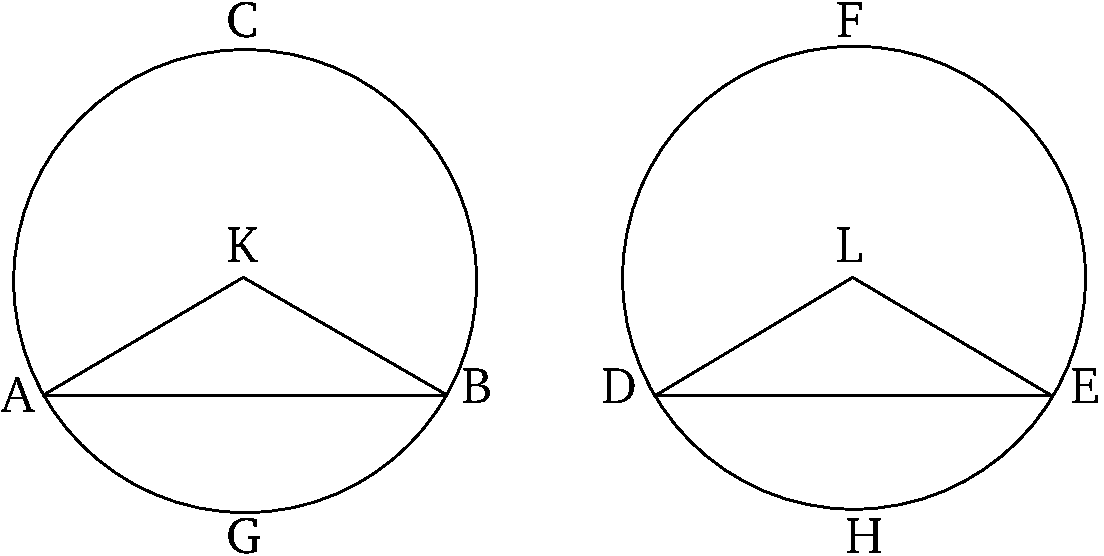
\includegraphics{Book03/fig28e.eps}}

For let the centers of the circles, $K$ and $L$, be found [Prop.~3.1],
and let $AK$, $KB$, $DL$, and $LE$ be joined.

And since ($ABC$ and $DEF$) are equal circles, their radii are also equal [Def.~3.1]. So the two
(straight-lines) $AK$, $KB$ are equal to the two (straight-lines) $DL$, $LE$ (respectively).
And the base $AB$ (is) equal to the base $DE$. Thus, angle $AKB$ is equal
to angle $DLE$ [Prop.~1.8]. And equal angles stand upon equal circumferences,
when they are at the centers [Prop.~3.26]. Thus, circumference $AGB$
(is) equal to $DHE$. And the whole circle $ABC$ is also equal to the whole
circle $DEF$. Thus, the remaining circumference $ACB$
is also equal to the remaining circumference $DFE$.

Thus, in equal circles, equal straight-lines cut off equal circumferences, 
the greater (circumference being equal) to the greater, and the lesser to the lesser. (Which is) the very thing it was required to show.}
\end{Parallel}

%%%%%%
% Prop 3.29
%%%%%%
\pdfbookmark[1]{Proposition 3.29}{pdf3.29}
\begin{Parallel}{}{} 
\ParallelLText{
\begin{center}
{\large \ggn{29}.}
\end{center}\vspace*{-7pt}

\gr{Ἐν τοῖξ >ίσοιξ κύκλοιξ τὰξ >ίσαξ περιφερείαξ >ίσαι εὐθεῖαι ὑποτείνουσιν.}

\gr{>'Εστωσαν >ίσοι κύκλοι οἱ ΑΒΓ, ΔΕΖ, καὶ ἐν α\kern -.7pt  ὐτοῖξ >ίσαι περιφέρειαι
ἀπειλήφθωσαν αἱ ΒΗΓ, ΕJΖ, καὶ ἐπεζεύθθωσαν αἱ ΒΓ, ΕΖ εὐθεῖαι;
λέγω, <ότι >ίση ἐστὶν ἡ ΒΓ τῆ| ΕΖ.}

\gr{Εἰλήφθω γὰρ τὰ κέντρα τῶν κύκλων, καὶ >έστω τὰ Κ, Λ, καὶ ἐπεζεύθθωσαν αἱ ΒΚ, ΚΓ, ΕΛ, ΛΖ.}

\gr{Καὶ ἐπεὶ >ίση ἐστὶν ἡ ΒΗΓ περιφέρεια τῆ| ΕJΖ περιφερείᾳ, >ίση
ἐστὶ καὶ γωνία ἡ ὑπὸ ΒΚΓ τῆ| ὑπὸ ΕΛΖ. καὶ ἐπεὶ >ίσοι
εἰσὶν οἱ ΑΒΓ, ΔΕΖ κύκλοι, >ίσαι εἰσὶ καὶ αἱ ἐκ τῶν κέντρων;
δύο δὴ αἱ ΒΚ, ΚΓ δυσὶ ταῖξ ΕΛ, ΛΖ >ίσαι εἰσίν; καὶ γωνίαξ
>ίσαξ περιέθουσιν; βάσιξ >άρα ἡ ΒΓ βάσει τῆ| ΕΖ >ίση ἐστίν;}\\~\\~\\~\\

\epsfysize=1.7in
\centerline{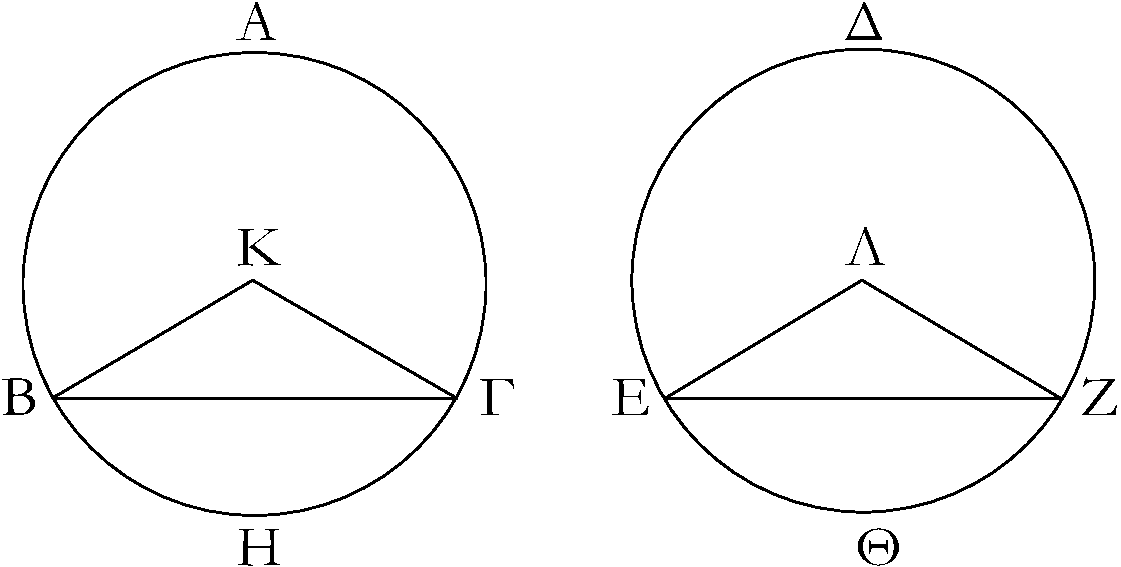
\includegraphics{Book03/fig29g.eps}}

\gr{Ἐν >άρα τοῖξ >ίσοιξ κύκλοιξ τὰξ >ίσαξ περιφερείαξ
>ίσαι εὐθεῖαι ὑποτείνουσιν; <όπερ >έδει δεῖχαι.}}

\ParallelRText{
\begin{center}
{\large Proposition 29}
\end{center}

In equal circles, equal straight-lines subtend equal circumferences.

Let $ABC$ and $DEF$ be equal circles, and within them let the equal circumferences $BGC$ and $EHF$ be cut off. And let the straight-lines $BC$ and $EF$ be joined. I say that $BC$ is equal to $EF$.

For let the centers of the circles be found [Prop.~3.1], and
let them be (at) $K$ and $L$. And let $BK$, $KC$, $EL$, and $LF$ be joined.

And since the circumference $BGC$ is equal to the circumference $EHF$,
the angle $BKC$ is also equal to (angle) $ELF$ [Prop.~3.27]. And since the circles
$ABC$ and $DEF$ are equal, their radii are also equal [Def.~3.1]. 
So the two (straight-lines) $BK$, $KC$ are equal to the two (straight-lines)
$EL$, $LF$ (respectively). And they contain equal angles. Thus, the
base $BC$ is equal to the base $EF$ [Prop.~1.4].

\epsfysize=1.7in
\centerline{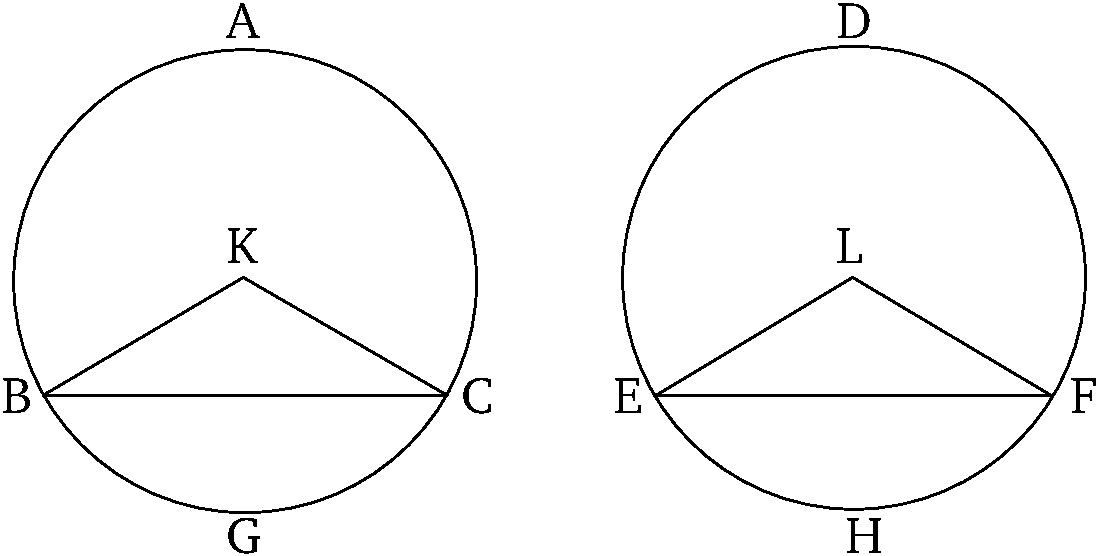
\includegraphics{Book03/fig29e.eps}}

Thus,  in equal circles, equal straight-lines subtend equal circumferences.
(Which is) the very thing it was required to show.}
\end{Parallel}

%%%%%%
% Prop 3.30
%%%%%%
\pdfbookmark[1]{Proposition 3.30}{pdf3.30}
\begin{Parallel}{}{} 
\ParallelLText{
\begin{center}
{\large \ggn{30}.}
\end{center}\vspace*{-7pt}

\gr{Τὴν δοθεῖσαν περιφέρειαν δίθα τεμεῖν.}

\gr{>'Εστω ἡ δοθεῖσα περιφέρεια ἡ ΑΔΒ; δεῖ δὴ τὴν ΑΔΒ περιφέρειαν
δίθα τεμεῖν.}

\gr{Ἐπεζεύθθω ἡ ΑΒ, καὶ τετμ\kern -.7pt  ήσθω δίθα κατὰ τὸ Γ, καὶ ἀπὸ τοῦ
Γ σημείου τῆ| ΑΒ εὐθείᾳ πρὸξ ὀρθὰξ >ήθθω ἡ ΓΔ, καὶ ἐπεζεύθθωσαν αἱ ΑΔ, ΔΒ.}

\epsfysize=1.3in
\centerline{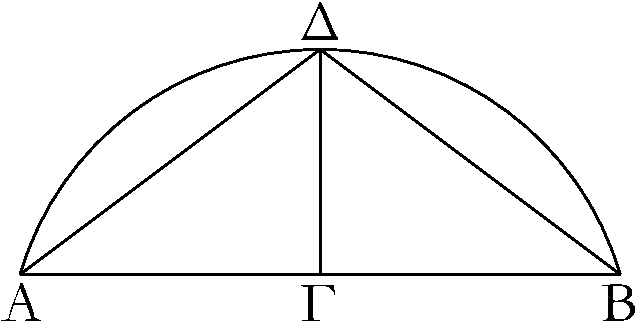
\includegraphics{Book03/fig30g.eps}}

\gr{Καὶ ἐπεὶ >ίση ἐστὶν ἡ ΑΓ τῆ| ΓΒ, κοινὴ δὲ ἡ ΓΔ, δύο δὴ
αἱ ΑΓ, ΓΔ δυσὶ ταῖξ ΒΓ, ΓΔ >ίσαι εἰσίν; καὶ γωνία ἡ ὑπὸ
ΑΓΔ γωνίᾳ τῆ| ὑπὸ ΒΓΔ >ίση; ὀρθὴ γὰρ ἑκατέρα; βάσιξ
>άρα ἡ ΑΔ βάσει τῆ| ΔΒ >ίση ἐστίν. αἱ δὲ >ίσαι εὐθεῖαι >ίσαξ περιφερείαξ ἀφαιροῦσι τὴν μὲν μείζονα τῆ| μείζονι τὴν δὲ
ἐλάττονα τῆ| ἐλάττονι; κάι ἐστιν ἑκατέρα τῶν ΑΔ, ΔΒ περιφερειῶν
ἐλάττων ἡμικυκλίου; >ίση >άρα ἡ ΑΔ περιφέρεια τῆ| ΔΒ περιφερείᾳ.}

\gr{Ἡ >άρα δοθεῖσα περιφέρεια δίθα τέτμ\kern -.7pt  ηται κατὰ τὸ Δ σημεῖον; <όπερ
>έδει ποιῆσαι.}}

\ParallelRText{
\begin{center}
{\large Proposition 30}
\end{center}

To cut a given circumference in half.

Let $ADB$ be the given circumference. So it is required to cut circumference
$ADB$ in half.

Let $AB$ be joined, and let it be cut in half at (point) $C$ [Prop.~1.10]. And let $CD$ be drawn from point $C$, at right-angles
to $AB$ [Prop.~1.11]. And let $AD$, and $DB$ be joined.

\epsfysize=1.3in
\centerline{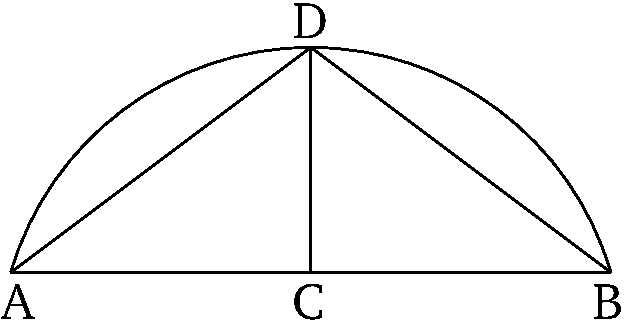
\includegraphics{Book03/fig30e.eps}}

And since $AC$ is equal to $CB$, and $CD$ (is) common, the two
(straight-lines) $AC$, $CD$ are equal to the two (straight-lines) $BC$, $CD$ (respectively).
And angle $ACD$ (is) equal to angle $BCD$. For (they are) each right-angles.
Thus, the base $AD$ is equal to the base $DB$ [Prop.~1.4]. And equal
straight-lines cut off equal circumferences, the greater (circumference being
equal) to the greater, and the lesser to the lesser [Prop.~1.28].
And the circumferences $AD$ and $DB$ are each less than a semi-circle.
Thus, circumference $AD$ (is) equal to circumference $DB$.

Thus, the given circumference has been cut in half at point $D$. (Which is)
the very thing it was required to do. }
\end{Parallel}

%%%%%%
% Prop 3.31
%%%%%%
\pdfbookmark[1]{Proposition 3.31}{pdf3.31}
\begin{Parallel}{}{} 
\ParallelLText{
\begin{center}
{\large \ggn{31}.}
\end{center}\vspace*{-7pt}

\gr{Ἐν κύκλῳ ἡ μὲν ἐν τῶ| ἡμικυκλίῳ γωνία ὀρθή ἐστιν, ἡ δὲ
ἐν τῶ| μείζονι τμ\kern -.7pt  ήματι ἐλάττων ὀρθῆξ, ἡ δὲ ἐν τῶ| ἐλάττονι
τμ\kern -.7pt  ήματι μείζων ὀρθῆξ; καὶ >έπι ἡ μὲν τοῦ μείζονοξ τμ\kern -.5pt  ήματοξ γωνία μείζων ἐστὶν ὀρθῆξ, ἡ δὲ τοῦ ἐλάττονοξ τμ\kern -.3pt  ήματοξ γωνία
ἐλάττων ὀρθῆξ.}\\

\epsfysize=2.2in
\centerline{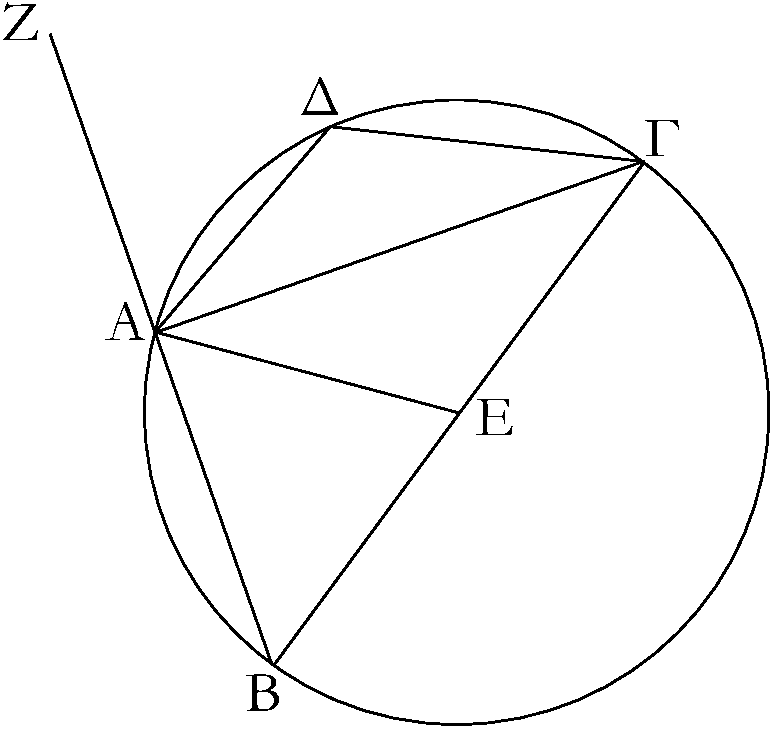
\includegraphics{Book03/fig31g.eps}}

\gr{>'Εστω κύκλοξ ὁ ΑΒΓΔ, διάμετροξ δὲ α\kern -.7pt  ὐτοῦ >έστω ἡ ΒΓ,
κέντρον δὲ τὸ Ε, καὶ ἐπεζεύθθωσαν αἱ ΒΑ, ΑΓ, ΑΔ, ΔΓ; λέγω,
<ότι ἡ μὲν ἐν τῶ| ΒΑΓ ἡμικυκλίῳ γωνία ἡ ὑπὸ ΒΑΓ ὀρθή
ἐστιν, ἡ δὲ ἐν τῶ| ΑΒΓ μείζονι τοῦ ἡμικυκλίου τμ\kern -.7pt  ήματι
γωνία ἡ ὑπὸ ΑΒΓ ἐλάττων ἐστὶν ὀρθῆξ, ἡ δὲ ἐν τῶ| ΑΔΓ
ἐλάττονι τοῦ ἡμικυκλίου τμ\kern -.5pt  ήματι γωνία ἡ ὑπὸ ΑΔΓ μείζων
ἐστὶν ὀρθῆξ.}

\gr{Ἐπεζεύθθω ἡ ΑΕ, καὶ διήθθω ἡ ΒΑ ἐπὶ τὸ Ζ.}

\gr{Καὶ ἐπεὶ >ίση ἐστὶν ἡ ΒΕ τῆ| ΕΑ, >ίση ἐστὶ καὶ γωνία ἡ ὑπὸ
ΑΒΕ τῆ| ὑπὸ ΒΑΕ. πάλιν, ἐπεὶ >ίση ἐστὶν ἡ ΓΕ τῆ| ΕΑ, >ίση
ἐστὶ καὶ ἡ ὑπὸ ΑΓΕ τῆ| ὑπὸ ΓΑΕ; <όλη >άρα ἡ ὑπὸ ΒΑΓ
δυσὶ ταῖξ ὑπὸ ΑΒΓ, ΑΓΒ >ίση ἐστίν. ἐστὶ δὲ καὶ ἡ ὑπὸ 
ΖΑΓ ἐκτὸξ τοῦ ΑΒΓ τριγώνου δυσὶ ταῖξ ὑπὸ ΑΒΓ, ΑΓΒ γωνίαιξ
>ίση; >ίση >άρα καὶ ἡ ὑπὸ ΒΑΓ γωνία τῆ| ὑπὸ ΖΑΓ;
ὀρθὴ >άρα ἑκατέρα; ἡ >άρα ἐν τῶ| ΒΑΓ ἡμικυκλίῳ 
γωνία ἡ ὑπὸ ΒΑΓ ὀρθή ἐστιν.}

\gr{Καὶ ἐπεὶ τοῦ ΑΒΓ τρίγωνου δύο γωνίαι αἱ ὑπὸ ΑΒΓ, ΒΑΓ δύο
ὀρθῶν ἐλάττονέξ εἰσιν, ὀρθὴ δὲ ἡ ὑπὸ ΒΑΓ, ἐλάττων >άρα
ὀρθῆξ ἐστιν ἡ ὑπὸ ΑΒΓ γωνία; καί ἐστιν ἐν τῶ| ΑΒΓ μείζονι
τοῦ ἡμικυκλίου τμ\kern -.7pt  ήματι.}

\gr{Καὶ ἐπεὶ ἐν κύκλῳ τετράπλευρόν ἐστι τὸ ΑΒΓΔ, τῶν δὲ ἐν τοῖξ
κύκλοιξ τετραπλεύρων αἱ ἀπεναντίον γωνίαι δυσὶν ὀρθαῖξ >ίσαι
εἰσίν [αἱ >άρα ὑπὸ ΑΒΓ, ΑΔΓ γωνίαι δυσὶν ὀρθαῖξ >ίσαξ
εἰσίν], καί ἐστιν ἡ ὑπὸ ΑΒΓ ἐλάττων ὀρθῆξ; λοιπὴ >άρα ἡ ὑπὸ
ΑΔΓ γωνία μείζων ὀρθῆξ ἐστιν; καί ἐστιν ἐν τῶ| ΑΔΓ
ἐλάττονι τοῦ ἡμικυκλίου τμ\kern -.7pt  ήματι.}

\gr{Λέγω, <ότι καὶ ἡ μὲν τοῦ μείζονοξ τμ\kern -.7pt  ήματοξ γωνία ἡ περιεθομένη
ὑπό [τε] τῆξ ΑΒΓ περιφερείαξ καὶ τῆξ ΑΓ εὐθείαξ μείζων ἐστὶν
ὀρθῆξ, ἡ δὲ τοῦ ἐλάττονοξ τμ\kern -.7pt  ήματοξ γωνία ἡ περιεθομένη
ὑπό [τε] τῆξ ΑΔ[Γ] περιφερείαξ καὶ τῆξ ΑΓ εὐθείαξ ἐλάττων ἐστὶν
ὀρθῆξ. καί ἐστιν α\kern -.5pt  ὐτόθεν φανερόν. ἐπεὶ γὰρ ἡ ὑπὸ τῶν ΒΑ,
ΑΓ εὐθειῶν ὀρθή ἐστιν, ἡ >άρα ὑπὸ τῆξ ΑΒΓ περιφερείαξ καὶ τῆξ
ΑΓ εὐθείαξ περιεθομένη μείζων ἐστὶν ὀρθῆξ. πάλιν, ἐπεὶ
ἡ ὑπὸ τῶν ΑΓ, ΑΖ εὐθειῶν ὀρθή ἐστιν, ἡ >άρα ὑπὸ
τῆξ ΓΑ εὐθείαξ καὶ τῆξ ΑΔ[Γ] περιφερείαξ περιεθομένη ἐλάττων
ἐστὶν ὀρθῆξ.}

\gr{Ἐν κύκλῳ >άρα ἡ μὲν ἐν τῶ| ἡμικυκλίῳ γωνία ὀρθή ἐστιν, ἡ δὲ
ἐν τῶ| μείζονι τμ\kern -.7pt  ήματι ἐλάττων ὀρθῆξ, ἡ δὲ ἐν τῶ| ἐλάττονι
[τμ\kern -.7pt  ήματι] μείζων ὀρθῆξ; καὶ >έπι ἡ μὲν τοῦ μείζονοξ τμ\kern -.5pt  ήματοξ [γωνία] μείζων [ἐστὶν] ὀρθῆξ, ἡ δὲ τοῦ ἐλάττονοξ τμ\kern -.3pt  ήματοξ [γωνία] ἐλάττων ὀρθῆξ; <όπερ >έδει δεῖχαι.}}

\ParallelRText{
\begin{center}
{\large Proposition 31}
\end{center}

In a circle, the angle in a semi-circle is a right-angle, and that in a
greater segment (is) less than a right-angle, and that in a
lesser segment (is) greater than a right-angle. And, further, the angle of
a segment greater (than a semi-circle) is greater than a right-angle, and
the angle of a segment less (than a semi-circle) is less than a right-angle.

\epsfysize=2.2in
\centerline{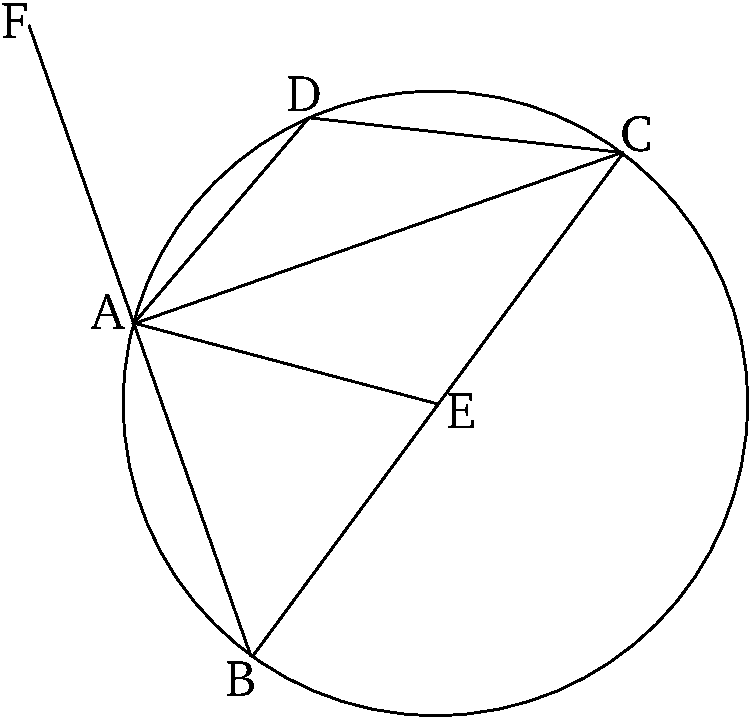
\includegraphics{Book03/fig31e.eps}}

Let $ABCD$  be a circle, and let $BC$ be its diameter, and $E$ its center. And let $BA$, $AC$, $AD$, and $DC$ be joined. I say that the angle $BAC$ in the semi-circle $BAC$ is a right-angle, and the angle $ABC$ in the segment $ABC$, (which is) greater than a semi-circle, is less
than a right-angle, and the angle $ADC$ in the segment $ADC$, (which is) less than a semi-circle,
is greater than a right-angle.

Let $AE$ be joined, and let $BA$ be drawn through to $F$.

And since $BE$ is equal to $EA$, angle $ABE$ is also equal to $BAE$ [Prop.~1.5]. Again, since $CE$ is equal to $EA$, $ACE$ is also equal to  $CAE$ [Prop.~1.5].
Thus, the whole (angle) $BAC$ is equal to the two (angles) $ABC$ and $ACB$.
And $FAC$, (which is) external to triangle $ABC$, is also equal to the two angles
$ABC$ and $ACB$ [Prop.~1.32]. Thus, angle $BAC$ (is) also equal to
$FAC$. Thus, (they are) each right-angles. [Def.~1.10]. Thus, the angle
$BAC$ in the semi-circle $BAC$ is a right-angle.

And since the two angles $ABC$ and $BAC$ of triangle $ABC$ are less than 
two right-angles [Prop.~1.17], and $BAC$ is a right-angle, angle $ABC$ is
thus less than a right-angle. And it is in segment $ABC$, (which is) greater 
than
a semi-circle.

And since $ABCD$ is a quadrilateral within a circle, and for quadrilaterals within circles
the (sum of the) opposite angles is equal to two right-angles 
[Prop.~3.22] [angles $ABC$ and $ADC$ are thus equal to two right-angles],
and (angle) $ABC$ is  less than a right-angle. The remaining angle $ADC$
is thus greater than a right-angle. And it is in segment $ADC$, (which is)
less than a semi-circle.

I also say that the angle of the greater segment, (namely) that contained by
the circumference $ABC$ and the straight-line $AC$, is greater than a right-angle.
And the angle of the lesser segment, (namely) that contained by the circumference
$AD[C]$ and the straight-line $AC$, is less than a right-angle. And
this is immediately apparent. For since the (angle contained by) the
two straight-lines $BA$ and $AC$ is a right-angle, the (angle) contained
by the circumference $ABC$ and the straight-line $AC$ is thus greater than a right-angle. Again, since the (angle contained by) the straight-lines
$AC$ and $AF$ is a right-angle, the (angle) contained by the circumference
$AD[C]$ and the straight-line $CA$ is thus less than a right-angle.

Thus, in a circle, the angle in a semi-circle is a right-angle, and that in a
greater segment (is) less than a right-angle, and that in a
lesser [segment] (is) greater than a right-angle. And, further, the [angle] of
a segment greater (than a semi-circle) [is] greater than a right-angle, and
the [angle] of a segment less (than a semi-circle) is  less than a right-angle.
(Which is) the very thing it was required to show.}
\end{Parallel}

%%%%%%
% Prop 3.32
%%%%%%
\pdfbookmark[1]{Proposition 3.32}{pdf3.32}
\begin{Parallel}{}{} 
\ParallelLText{
\begin{center}
{\large \ggn{32}.}
\end{center}\vspace*{-7pt}

\gr{Ἐὰν κύκλου ἐφάπτηταί τιξ εὐθεῖα, ἀπὸ δὲ τῆξ ἁφῆξ εἰξ τὸν κύκλον διαθθῆ| τιξ εὐθεῖα τέμνουσα τὸν κύκλον, <ὰξ ποιεῖ γωνίαξ
πρὸξ τῆ| ἐφαπτομένῃ, >ίσαι >έσονται ταῖξ ἐν τοῖξ ἐναλλὰχ
τοῦ κύκλου τμ\kern -.7pt  ήμασι γωνίαιξ.}\\

\epsfysize=2.1in
\centerline{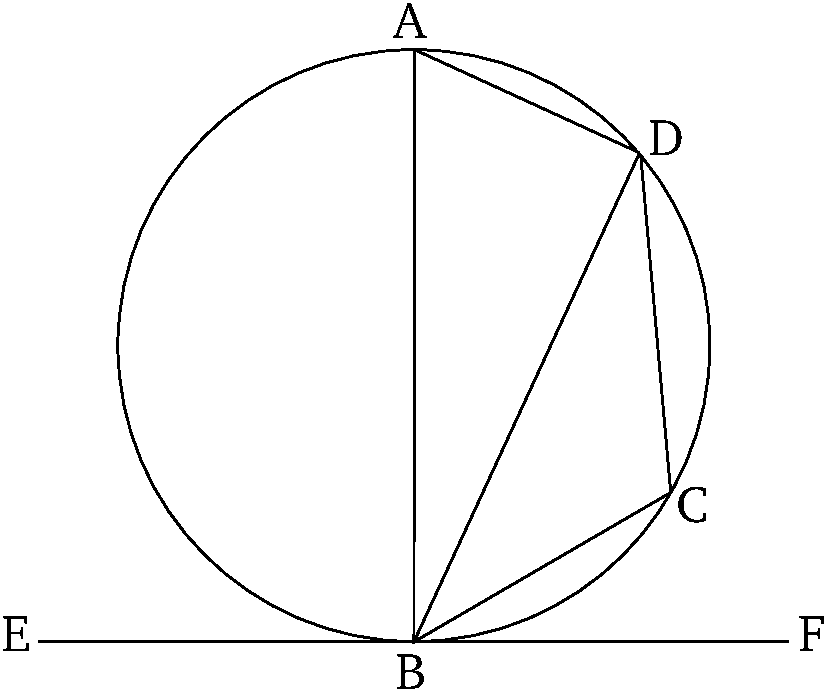
\includegraphics{Book03/fig32e.eps}}

\gr{Κύκλου γὰρ τοῦ ΑΒΓΔ ἐφαπτέσθω τιξ εὐθεῖα ἡ ΕΖ κατὰ τὸ Β σημεῖον, καὶ ἀπὸ τοῦ Β σημείου διήθθω τιξ εὐθεῖα εἰξ τὸν
ΑΒΓΔ κύκλον τέμνουσα α\kern -.7pt  ὐτὸν ἡ ΒΔ. λέγω, <ότι <ὰξ ποιεῖ γωνίαξ
ἡ ΒΔ μετὰ τῆξ ΕΖ  ἐφαπτομένηξ, >ίσαξ >έσονται ταῖξ ἐν τοῖξ
ἐναλλὰχ τμ\kern -.7pt  ήμασι τοῦ κύκλου γωνίαιξ, τουτέστιν, <ότι ἡ μὲν
ὑπὸ ΖΒΔ γωνία >ίση ἐστὶ τῆ| ἐν τῶ| ΒΑΔ τμ\kern -.5pt  ήματι συνισταμένῃ γωνίᾳ, ἡ δὲ ὑπὸ ΕΒΔ γωνία >ίση ἐστὶ τῆ| ἐν τῶ| ΔΓΒ τμ\kern -.3pt  ήματι συνισταμένῃ γωνίᾳ.}

\gr{>'Ηθθω γὰρ ἀπὸ τοῦ Β τῆ| ΕΖ πρὸξ ὀρθὰξ ἡ ΒΑ, καὶ εἰλήφθω ἐπὶ
τῆξ ΒΔ περιφερείαξ τυθὸν σημεῖον τὸ Γ, καὶ ἐπεζεύθθωσαν αἱ ΑΔ, ΔΓ, ΓΒ.}

\gr{Καὶ ἐπεὶ κύκλου τοῦ ΑΒΓΔ ἐφάπτεταί τιξ εὐθεῖα ἡ ΕΖ κατὰ
τὸ Β, καὶ ἀπὸ τῆξ ἁφῆξ >ῆκται τῆ| ἐφαπτομένῃ πρὸξ ὀρθὰξ ἡ ΒΑ, ἐπὶ τῆξ ΒΑ >άρα τὸ κέντρον ἐστὶ τοῦ ΑΒΓΔ κύκλου. ἡ ΒΑ
>άρα διάμετόξ ἐστι τοῦ ΑΒΓΔ κύκλου; ἡ >άρα ὑπὸ ΑΔΒ γωνία
ἐν ἡμικυκλίῳ ο>ῦσα ὀρθή ἐστιν. λοιπαὶ >άρα αἱ ὑπὸ ΒΑΔ, ΑΒΔ
μιᾶ| ὀρθῆ| >ίσαι εἰσίν. ἐστὶ δὲ καὶ ἡ ὑπὸ ΑΒΖ ὀρθή; ἡ >άρα ὑπὸ ΑΒΖ >ίση ἐστὶ ταῖξ ὑπὸ ΒΑΔ, ΑΒΔ. κοινὴ ἀφῃρήσθω ἡ ὑπὸ
ΑΒΔ; λοιπὴ >άρα ἡ ὑπὸ ΔΒΖ γωνία >ίση ἐστὶ τῆ| ἐν τῶ| ἐναλλὰχ τμ\kern -.7pt  ήματι τοῦ κύκλου γωνίᾳ τῆ| ὑπὸ ΒΑΔ. καὶ ἐπεὶ ἐν κύκλῳ
τετράπλευρόν ἐστι τὸ ΑΒΓΔ, αἱ ἀπεναντίον α\kern -.7pt  ὐτοῦ γωνίαι δυσὶν
ὀρθαῖξ >ίσαι  εἰσίν. εἰσὶ δὲ καὶ αἱ ὑπὸ ΔΒΖ, ΔΒΕ δυσὶν ὀρθαῖξ
>ίσαι;
 αἱ >άρα ὑπὸ ΔΒΖ, ΔΒΕ ταῖξ ὑπὸ ΒΑΔ, ΒΓΔ >ίσαι
εἰσίν, ~ὡν ἡ ὑπὸ ΒΑΔ τῆ| ὑπὸ ΔΒΖ ἐδείθθη >ίση;
λοιπὴ >άρα ἡ ὑπὸ ΔΒΕ τῆ| ἐν τῶ| ἐναλλὰχ τοῦ κύκλου τμ\kern -.5pt  ήματι
τῶ| ΔΓΒ τῆ| ὑπὸ ΔΓΒ γωνίᾳ ἐστὶν >ίση.}

\gr{Ἐὰν >άρα κύκλου ἐφάπτηταί τιξ εὐθεῖα, ἀπὸ δὲ τῆξ ἁφῆξ εἰξ τὸν κύκλον διαθθῆ| τιξ εὐθεῖα τέμνουσα τὸν κύκλον, <ὰξ ποιεῖ γωνίαξ
πρὸξ τῆ| ἐφαπτομένῃ, >ίσαι >έσονται ταῖξ ἐν τοῖξ ἐναλλὰχ
τοῦ κύκλου τμ\kern -.7pt  ήμασι γωνίαιξ; <όπερ >έδει δεῖχαι.}}

\ParallelRText{
\begin{center}
{\large Proposition 32}
\end{center}

If some straight-line touches a circle, and some (other) straight-line is drawn  
across, from the point of contact into the circle,  cutting the circle (in two), (then) those angles  the (straight-line) makes
with the tangent will be equal to the angles in
the alternate segments of the circle.

\epsfysize=2.1in
\centerline{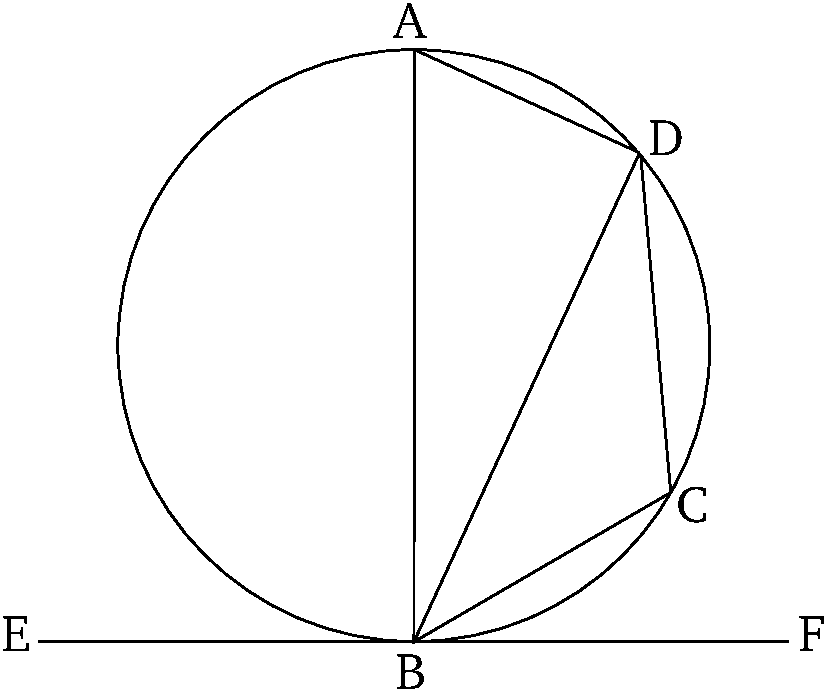
\includegraphics{Book03/fig32e.eps}}

For let some straight-line $EF$ touch the circle $ABCD$ at the point $B$, and let
some (other) straight-line $BD$ be drawn from point $B$ into the
circle $ABCD$, cutting it (in two). I say that the angles $BD$ makes with the tangent 
$EF$  will be equal to the angles in the alternate segments of the circle.
That is to say, that angle $FBD$ is equal to the angle constructed
in segment $BAD$, and angle $EBD$ is equal to the angle constructed in segment $DCB$.

For let $BA$ be drawn from $B$, at right-angles to $EF$ [Prop.~1.11].
And let the point $C$ be taken at random on the circumference $BD$. And
let $AD$, $DC$, and $CB$ be joined.

And since some straight-line $EF$ touches the circle $ABCD$ at point $B$, and
$BA$ has been drawn from the point of contact, at right-angles to the
tangent, the center of circle $ABCD$ is thus on $BA$ [Prop.~3.19].
Thus, $BA$ is a diameter of circle $ABCD$.
Thus, angle $ADB$, being in a semi-circle, is a right-angle [Prop.~3.31].
Thus, the remaining angles (of triangle $ADB$) $BAD$ and $ABD$ are equal to one right-angle [Prop.~1.32]. And $ABF$ is also a right-angle. Thus,
$ABF$ is equal to $BAD$ and $ABD$. Let $ABD$ be subtracted from both.
Thus, the remaining angle $DBF$ is equal to the angle $BAD$ in the alternate
segment of the circle. And since $ABCD$ is a quadrilateral in a circle,
(the sum of) its opposite angles is equal to two right-angles [Prop.~3.22]. And $DBF$ and $DBE$ is also equal to two right-angles [Prop.~1.13]. Thus, $DBF$ and $DBE$ is equal to $BAD$ and $BCD$, of which
$BAD$ was shown (to be) equal to $DBF$. Thus, the remaining (angle) $DBE$ is
equal to the angle $DCB$ in the alternate segment $DCB$ of the circle.

Thus, if some straight-line touches a circle, and some (other) straight-line is drawn  across, from the point of contact into the circle,  cutting the circle (in two), (then) those angles  the (straight-line) makes
with the tangent will be equal to the angles in
the alternate segments of the circle. (Which is) the very thing it was required to
show.}
\end{Parallel}

%%%%%%
% Prop 3.33
%%%%%%
\pdfbookmark[1]{Proposition 3.33}{pdf3.33}
\begin{Parallel}{}{} 
\ParallelLText{
\begin{center}
{\large \ggn{33}.}
\end{center}\vspace*{-7pt}

\gr{Ἐπὶ τῆξ δοθείσηξ εὐθείαξ γράψαι τμ\kern -.7pt  ῆμα κύκλου δεθόμε\-νον γωνίαν >ίσην τῆ| δοθείσῃ γωνίᾳ εὐθυγράμμῳ.}

\epsfysize=1.35in
\centerline{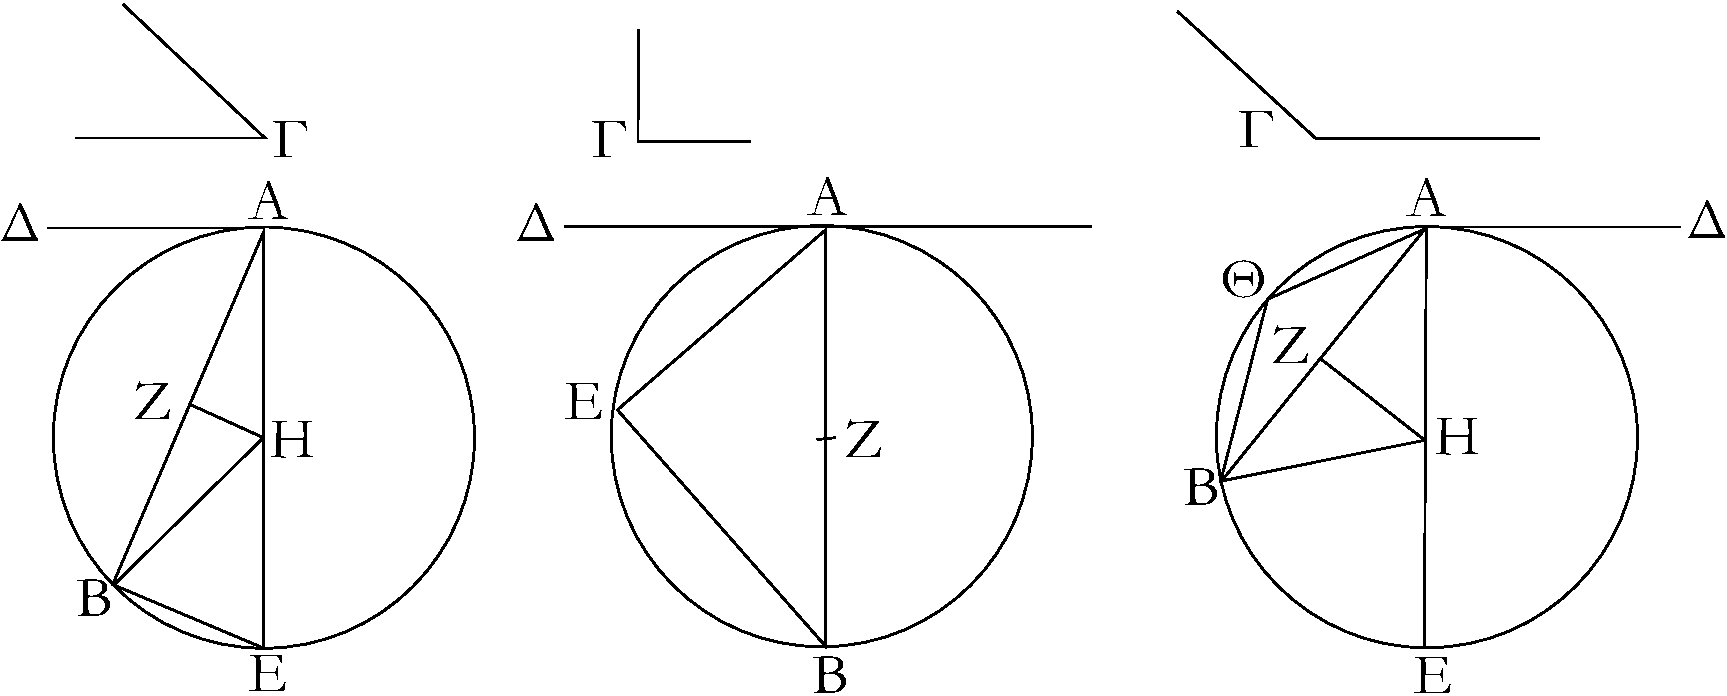
\includegraphics{Book03/fig33g.eps}}

\gr{>'Εστω ἡ δοθεῖσα εὐθεῖα ἡ ΑΒ, ἡ δὲ δοθεῖσα γωνία εὐθύγραμμοξ ἡ
πρὸξ τῶ| Γ; δεῖ δὴ ἐπὶ τῆξ δοθείσηξ εὐθείαξ τῆξ ΑΒ γράψαι τμ\kern -.7pt  ῆμα
κύκλου δεθόμενον γωνίαν >ίσην τῆ| πρὸξ τῶ| Γ.}

\gr{Ἡ δὴ πρὸξ τῶ| Γ [γωνία] >ήτοι ὀχεῖά ἐστιν >ὴ ὀρθὴ >ὴ ἀμβλεῖα;
>έστω πρότερον ὀχεῖα, καὶ ὡξ ἐπὶ τῆξ πρώτηξ καταγραφῆξ συνεστάτω
πρὸξ τῆ| ΑΒ εὐθείᾳ καὶ τῶ| Α σημείῳ τῆ| πρὸξ τῶ| Γ γωνίᾳ
>ίση ἡ ὑπὸ ΒΑΔ; ὀχεῖα >άρα ἐστὶ καὶ ἡ ὑπὸ ΒΑΔ. >ήθθω
τῆ| ΔΑ πρὸξ ὀρθὰξ ἡ ΑΕ, καὶ τετμ\kern -.7pt  ήσθω ἡ ΑΒ δίθα κατὰ τὸ Ζ, καὶ
>ήθθω ἀπὸ τοῦ Ζ σημείου τῆ| ΑΒ πρὸξ ὀρθὰξ ἡ ΖΗ, καὶ
ἐπεζεύθθω ἡ ΗΒ.}

\gr{Καὶ ἐπεὶ >ίση ἐστὶν ἡ ΑΖ τῆ| ΖΒ, κοινὴ δὲ ἡ ΖΗ, δύο δὴ αἱ
ΑΖ, ΖΗ δύο ταῖξ ΒΖ, ΖΗ >ίσαι εἰσίν; καὶ γωνία ἡ ὑπὸ ΑΖΗ [γωνίᾳ]
τῆ| ὑπὸ ΒΖΗ >ίση; βάσιξ >άρα ἡ ΑΗ βάσει τῆ| ΒΗ >ίση ἐστίν. ὁ >άρα κέντρῳ μὲν τῶ| Η διαστήματι δὲ τῶ| ΗΑ κύκλοξ γραφόμενοξ <ήχει καὶ διὰ τοῦ Β. γεγράφθω καὶ >έστω ὁ ΑΒΕ, καὶ ἐπεζεύθθω ἡ ΕΒ.
ἐπεὶ ο>ῦν ἀπ> >άκραξ τῆξ ΑΕ διαμέτρου ἀπὸ τοῦ Α τῆ| ΑΕ πρὸξ ὀρθάξ
ἐστιν ἡ ΑΔ, ἡ ΑΔ >άρα ἐφάπτεται τοῦ ΑΒΕ κύκλου; ἐπεὶ ο>ῦν
κύκλου τοῦ ΑΒΕ ἐφάπτεταί τιξ εὐθεῖα ἡ ΑΔ, καὶ ἀπὸ τῆξ κατὰ
τὸ Α ἁφῆξ  εἰξ τὸν ΑΒΕ κύκλον διῆκταί τιξ εὐθεῖα ἡ ΑΒ, ἡ
>άρα ὑπὸ ΔΑΒ γωνία >ίση ἐστὶ τῆ| ἐν τῶ| ἐναλλὰχ τοῦ 
κύκλου τμ\kern -.7pt  ήματι γωνίᾳ τῆ| ὑπὸ ΑΕΒ. ἀλλ> ἡ ὑπὸ ΔΑΒ τῆ|
πρὸξ τῶ| Γ ἐστιν >ίση; καὶ ἡ πρὸξ τῶ| Γ >άρα γωνία >ίση
ἐστὶ τῆ| ὑπὸ ΑΕΒ.}

\gr{Ἐπὶ τῆξ δοθείσηξ >άρα εὐθείαξ τῆξ ΑΒ τμ\kern -.7pt  ῆμα κύκλου γέγραπται
τὸ ΑΕΒ δεθόμενον γωνίαν τὴν ὑπὸ ΑΕΒ >ίσην τῆ| δοθείσῃ
τῆ| πρὸξ τῶ| Γ.}

\gr{Ἀλλὰ δὴ ὀρθὴ >έστω ἡ πρὸξ τῶ| Γ; καὶ δέον πάλιν >έστω ἐπὶ
τῆξ ΑΒ γράψαι τμ\kern -.7pt  ῆμα κύκλου δεθόμενον γωνίαν >ίσην τῆ| πρὸξ
τῶ| Γ ὀρθῆ| [γωνίᾳ]. συνεστάτω [πάλιν] τῆ| πρὸξ τῶ| Γ ὀρθῆ| γωνίᾳ >ίση ἡ ὑπὸ ΒΑΔ, ὡξ >έθει ἐπὶ τῆξ δευτέραξ καταγραφῆξ, καὶ τετμ\kern -.7pt  ήσθω ἡ ΑΒ δίθα κατὰ τὸ Ζ, καὶ κέντρῳ τῶ| Ζ, διαστήματι δὲ
ὁποτέρῳ τῶν ΖΑ, ΖΒ, κύκλοξ γεγράφθω ὁ ΑΕΒ.}

\gr{Ἐφάπτεται >άρα ἡ ΑΔ εὐθεῖα τοῦ ΑΒΕ κύκλου διὰ τὸ ὀρθὴν ε>ῖναι
τὴν πρὸξ τῶ| Α γωνίαν. καὶ >ίση ἐστὶν ἡ ὑπὸ ΒΑΔ γωνία
τῆ| ἐν τῶ| ΑΕΒ τμ\kern -.7pt  ήματι; ὀρθὴ γὰρ καὶ α\kern -.7pt  ὐτὴ ἐν ἡμικυκλίῳ
ο>ῦσα. ἀλλὰ καὶ ἡ ὑπὸ ΒΑΔ τῆ| πρὸξ τῶ| Γ >ίση ἐστίν. καὶ
ἡ ἐν τῶ| ΑΕΒ >άρα >ίση ἐστὶ  τῆ| πρὸξ τῶ| Γ.}

\gr{Γέγραπται >άρα πάλιν ἐπὶ τῆξ ΑΒ τμ\kern -.7pt  ῆμα κύκλου τὸ ΑΕΒ δεθόμενον
γωνίαν >ίσην τῆ| πρὸξ τῶ| Γ.}

\gr{Ἀλλὰ δὴ ἡ πρὸξ τῶ| Γ ἀμβλεῖα >έστω; καὶ συνεστάτω α\kern -.7pt  ὐτῆ|
>ίση πρὸξ τῆ| ΑΒ εὐθείᾳ καὶ τῶ| Α σημείῳ ἡ ὑπὸ ΒΑΔ, ὡξ
>έθει ἐπὶ τῆξ τρίτηξ καταγραφῆξ, καὶ τῆ| ΑΔ πρὸξ ὀρθὰξ >ήθθω ἡ ΑΕ,
καὶ τετμ\kern -.7pt  ήσθω πάλιν ἡ ΑΒ δίθα κατὰ τὸ Ζ, καὶ τῆ| ΑΒ πρὸξ ὀρθὰξ
>ήθθω ἡ ΖΗ, καὶ ἐπεζεύθθω ἡ ΗΒ.}

\gr{Καὶ ἐπεὶ πάλιν >ίση ἐστὶν ἡ ΑΖ τῆ| ΖΒ, καὶ κοινὴ ἡ ΖΗ, δύο δὴ αἱ
ΑΖ, ΖΗ δύο ταῖξ ΒΖ, ΖΗ >ίσαι εἰσίν; καὶ γωνία ἡ ὑπὸ
ΑΖΗ γωνίᾳ τῆ| ὑπὸ ΒΖΗ >ίση; βάσιξ >άρα ἡ ΑΗ βάσει τῆ| ΒΗ
>ίση ἐστίν; ὁ >άρα κέντρῳ μὲν τῶ| Η διαστήματι δὲ τῶ| ΗΑ κύκλοξ
γραφόμενοξ <ήχει καὶ διὰ τοῦ Β. ἐρθέσθω ὡξ ὁ ΑΕΒ. καὶ ἐπεὶ
τῆ| ΑΕ διαμέτρῳ ἀπ> >άκραξ πρὸξ ὀρθάξ ἐστιν ἡ ΑΔ, ἡ ΑΔ >άρα
ἐφάπτεται τοῦ ΑΕΒ κύκλου. καὶ ἀπὸ τῆξ κατὰ τὸ Α ἐπαφῆξ διῆκται
ἡ ΑΒ; ἡ >άρα ὑπὸ ΒΑΔ γωνία >ίση ἐστὶ τῆ| ἐν τῶ| ἐναλλὰχ τοῦ
κύκλου τμ\kern -.7pt  ήματι  τῶ| ΑJΒ συνισταμένῃ γωνίᾳ. ἀλλ> ἡ ὑπὸ ΒΑΔ γωνία τῆ| πρὸξ τῶ| Γ >ίση ἐστίν. καὶ ἡ ἐν τῶ| ΑJΒ >άρα τμ\kern -.7pt  ήματι
γωνία >ίση  ἐστὶ τῆ| πρὸξ τῶ| Γ.}

\gr{Ἐπὶ τῆξ >άρα δοθείσηξ εὐθείαξ τῆξ ΑΒ γέγραπται τμ\kern -.7pt  ῆμα κύκλου τὸ
ΑJΒ δεθόμενον γωνίαν >ίσην τῆ| πρὸξ τῶ| Γ; <όπερ >έδει ποιῆσαι.}}

\ParallelRText{
\begin{center}
{\large Proposition 33}
\end{center}

To draw a segment of a circle, accepting an angle equal to a given rectilinear angle, on a given straight-line.

\epsfysize=1.53in
\centerline{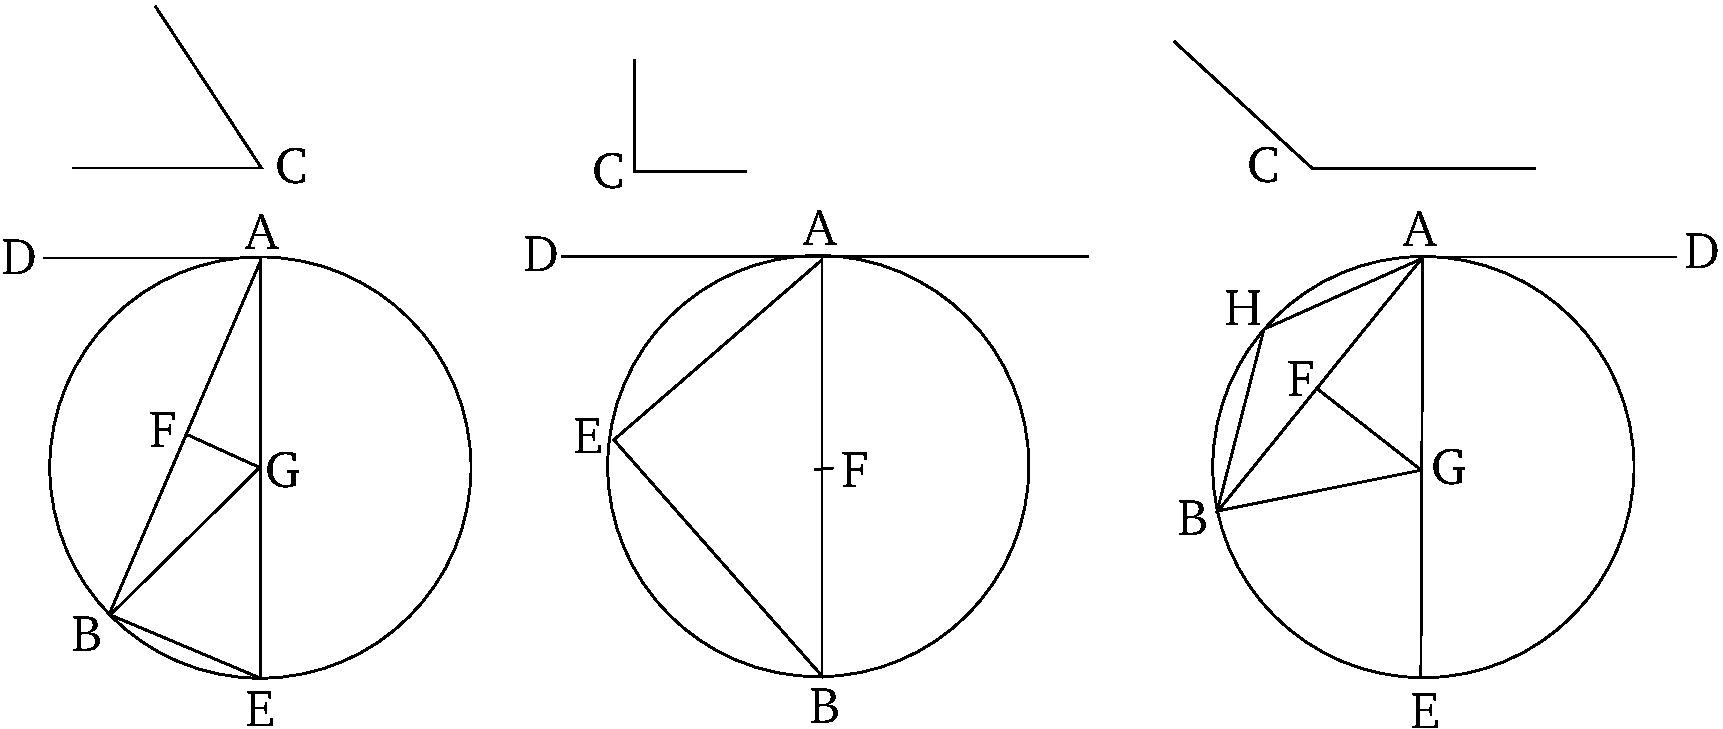
\includegraphics{Book03/fig33e.eps}}

Let $AB$ be the given straight-line, and $C$ the given rectilinear angle. So
it is required to draw a segment of a circle, accepting an angle equal to $C$,
on the given straight-line $AB$.

So the [angle] $C$ is surely either acute, a right-angle, or obtuse. First of all,
let it be acute. And, as in the first diagram (from the left), let (angle) $BAD$,
equal to angle $C$,  be
constructed  on the straight-line $AB$,  at the point A (on it)
[Prop.~1.23]. Thus, $BAD$ is also acute. Let $AE$ be drawn, at
right-angles to $DA$ [Prop.~1.11]. And let $AB$ be cut in half
at $F$ [Prop.~1.10]. And let $FG$ be drawn from point $F$, at right-angles to $AB$
[Prop.~1.11]. And let $GB$ be joined.

And since $AF$ is equal to $FB$, and $FG$ (is) common, the two (straight-lines)
$AF$, $FG$ are equal to the two (straight-lines) $BF$, $FG$ (respectively). And
angle $AFG$ (is) equal to [angle] $BFG$. Thus, the base $AG$ is equal to the
base $BG$ [Prop.~1.4]. Thus, the circle drawn with center $G$, and radius $GA$, will also go through $B$ (as well as $A$). Let it be drawn, and let it be (denoted) $ABE$. And let $EB$ be joined. Therefore, since $AD$ is at the extremity
of diameter $AE$,  (namely, point) $A$,  at right-angles to $AE$, the (straight-line)
$AD$ thus touches the circle $ABE$ [Prop.~3.16~corr.]. Therefore,
since some straight-line $AD$ touches the circle $ABE$, and some (other)
straight-line $AB$ has been drawn across from the point of contact $A$ into circle
$ABE$, angle $DAB$ is thus equal to the angle $AEB$ in the alternate segment of the
circle [Prop.~3.32]. But, $DAB$ is equal to $C$. Thus,
angle $C$ is also equal to $AEB$.

Thus, a segment $AEB$ of a circle, accepting the angle $AEB$ (which is) equal to the
given (angle) $C$, has been drawn on the given straight-line $AB$.

And so let $C$ be a right-angle. And let it again be necessary to draw  a segment
of a circle on $AB$, accepting an angle equal to the right-[angle] $C$. Let the (angle)
$BAD$ [again] be constructed, equal to the right-angle $C$ [Prop.~1.23], as in the second diagram (from the left). And let $AB$ be cut in half at $F$ [Prop.~1.10]. And let the circle $AEB$ be
drawn with center $F$, and radius either  $FA$ or $FB$.

Thus, the straight-line $AD$ touches the circle $ABE$, on account of the angle at $A$ being a right-angle [Prop.~3.16 corr.]. And angle $BAD$ is equal
to the angle in segment $AEB$. For (the latter angle), being in a semi-circle, is also a right-angle [Prop.~3.31]. But,  $BAD$ is also equal to $C$. Thus, the (angle) in (segment) $AEB$ is also equal to $C$.

Thus, a segment $AEB$ of a circle, accepting an angle equal to $C$, has again been
drawn on $AB$.

And so let (angle) $C$ be obtuse. And let (angle) $BAD$, equal
to ($C$), be constructed  on the straight-line $AB$, at the point $A$ 
(on it) [Prop.~1.23], as in the third diagram (from the left). And let $AE$ be
drawn, at right-angles to $AD$ [Prop.~1.11]. And let $AB$ again be 
cut in half at $F$ [Prop.~1.10]. And let $FG$ be drawn,
at right-angles to $AB$ [Prop.~1.10]. And let $GB$ 
be joined.

And again, since $AF$ is equal to $FB$, and $FG$ (is) common, the two (straight-lines) $AF$, $FG$ are equal to the two (straight-lines) $BF$, $FG$ (respectively).
And angle $AFG$ (is) equal to angle $BFG$. Thus, the base $AG$ is equal to
the base $BG$ [Prop.~1.4]. Thus, a circle of center $G$, and radius $GA$,
being drawn, will also go through $B$ (as well as $A$). Let it go like $AEB$ (in the third diagram
from the left). And since $AD$ is at right-angles to the diameter $AE$, at its extremity, $AD$ thus touches circle $AEB$ [Prop.~3.16~corr.]. And $AB$ has been drawn across (the circle) from the point of contact $A$. Thus, angle $BAD$ is equal to the angle constructed in the alternate segment $AHB$ of the circle 
[Prop.~3.32]. But, angle $BAD$ is equal to $C$. Thus, the angle in segment
$AHB$ is also equal to $C$.

Thus, a segment $AHB$ of a circle, accepting an angle equal to $C$, has been
drawn on the given straight-line $AB$. (Which is) the very thing
it was required to do.}
\end{Parallel}

%%%%%%
% Prop 3.34
%%%%%%
\pdfbookmark[1]{Proposition 3.34}{pdf3.34}
\begin{Parallel}{}{} 
\ParallelLText{
\begin{center}
{\large\ggn{34}.}
\end{center}\vspace*{-7pt}

\gr{Ἀπὸ τοῦ δοθέντοξ κύκλου τμ\kern -.7pt  ῆμα ἀφελεῖν δεθόμενον γωνίαν
>ίσην τῆ| δοθείσῃ γωνίᾳ εὐθυγράμμῳ.}

\gr{>'Εστω ὁ δοθεὶξ κύκλοξ ὁ ΑΒΓ, ἡ δὲ δοθεῖσα γωνία εὐθύγραμμοξ
ἡ πρὸξ  τῶ| Δ; δεῖ δὴ ἀπὸ τοῦ ΑΒΓ κύκλου τμ\kern -.7pt  ῆμα ἀφελεῖν
δεθόμενον γωνίαν >ίσην τῆ| δοθείσῃ γωνίᾳ εὐθυγράμμῳ τῆ| πρὸξ
τῶ| Δ.}

\epsfysize=1.8in
\centerline{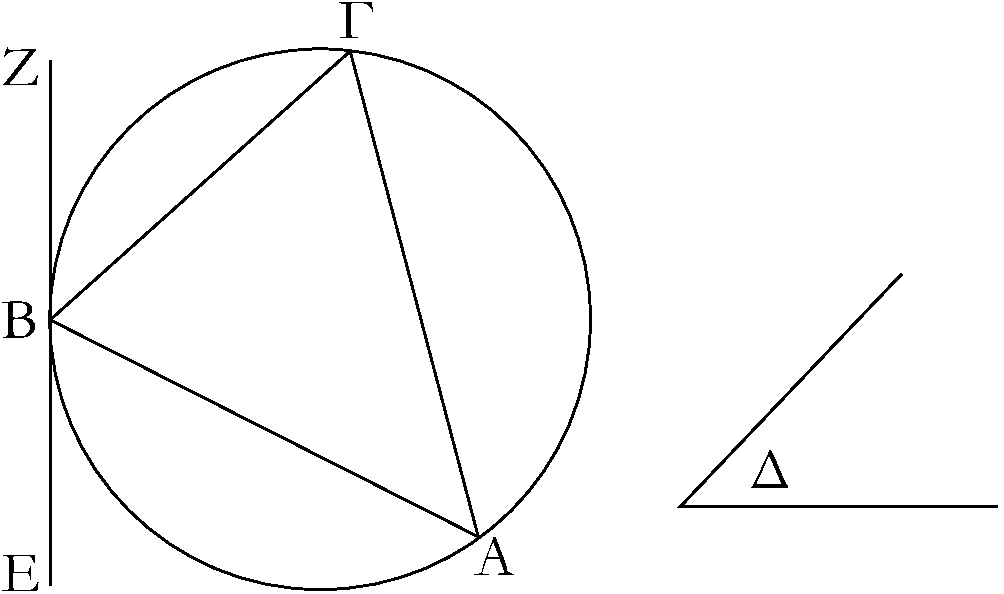
\includegraphics{Book03/fig34g.eps}}

\gr{>'Ηθθω τοῦ ΑΒΓ ἐφαπτομένη ἡ ΕΖ κατὰ τὸ Β σημεῖον, καὶ συνεστάτω
πρὸξ τῆ| ΖΒ εὐθείᾳ καὶ τῶ| πρὸξ α\kern -.7pt  ὐτῆ| σημείῳ τῶ| Β τῆ| πρὸξ
τῶ| Δ γωνίᾳ >ίση ἡ ὑπὸ ΖΒΓ.}

\gr{Ἐπεὶ ο>ῦν κύκλου τοῦ ΑΒΓ ἐφάπτεταί τιξ εὐθεῖα ἡ ΕΖ, καὶ ἀπὸ
τῆξ κατὰ τὸ Β ἐπαφῆξ διῆκται ἡ ΒΓ, ἡ ὑπὸ ΖΒΓ >άρα γωνία
>ίση ἐστὶ τῆ| ἐν τῶ| ΒΑΓ ἐναλλὰχ τμ\kern -.7pt  ήματι συνισταμένῃ γωνίᾳ.
ἀλλ> ἡ ὑπὸ ΖΒΓ τῆ| πρὸξ τῶ| Δ ἐστιν >ίση; καὶ ἡ ἐν τῶ| ΒΑΓ
>άρα τμ\kern -.7pt  ήματι >ίση ἐστὶ τῆ| πρὸξ τῶ| Δ [γωνίᾳ].}

\gr{Ἀπὸ τοῦ δοθέντοξ >άρα κύκλου τοῦ ΑΒΓ τμ\kern -.7pt  ῆμα ἀφή|ρηται τὸ ΒΑΓ
δεθόμενον γωνίαν >ίσην τῆ| δοθείσῃ γωνίᾳ εὐθυγράμ\-μῳ τῆ|
πρὸξ τῶ| Δ; <όπερ >έδει ποιῆσαι.}}

\ParallelRText{
\begin{center}
{\large Proposition 34}
\end{center}

To cut off a segment, accepting an angle equal to a given rectilinear angle,
from a given circle.

Let $ABC$ be the given circle, and $D$ the given rectilinear angle. So it is
required to cut off a segment, accepting an angle equal to the given
rectilinear angle $D$, from the given circle $ABC$.

\epsfysize=1.8in
\centerline{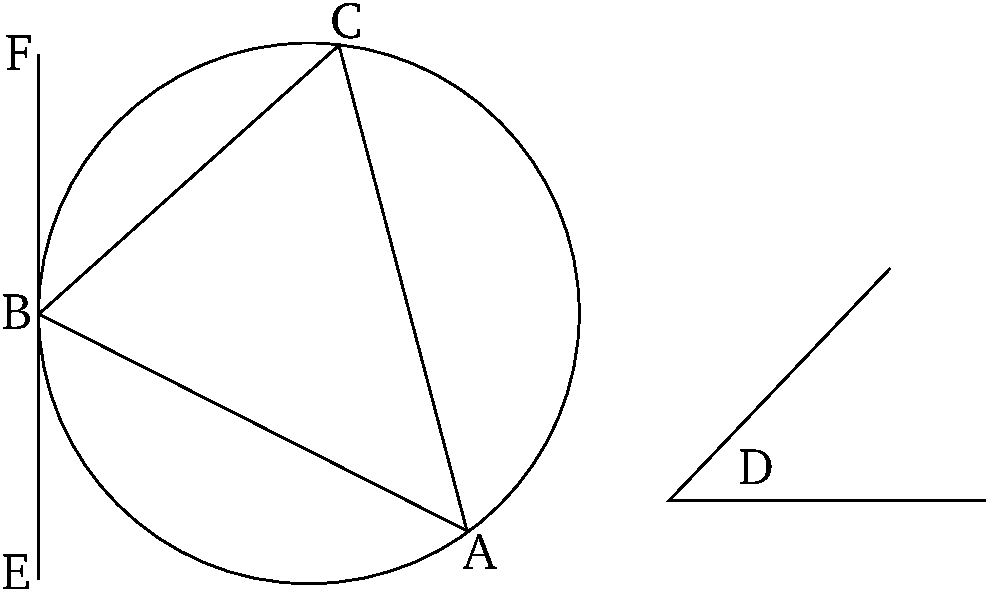
\includegraphics{Book03/fig34e.eps}}

Let $EF$ be drawn touching $ABC$ at point $B$.$^\dag$ And let (angle)
$FBC$, equal to angle $D$, be constructed  on the
straight-line $FB$, at the point $B$ on it [Prop.~1.23].

Therefore, since some straight-line $EF$ touches the circle $ABC$, and
$BC$ has been drawn across (the circle) from the point of contact $B$, angle
$FBC$ is thus equal to the angle constructed in the alternate segment
$BAC$ [Prop.~1.32]. But, $FBC$ is equal to $D$. Thus, the (angle)
in the segment $BAC$ is also equal to [angle] $D$.

Thus, the segment $BAC$, accepting an angle equal to the given
rectilinear angle $D$, has been cut off from the given circle $ABC$. (Which is)
the very thing it was required to do.}
\end{Parallel}
{\footnotesize \noindent$^\dag$ Presumably,
by finding the center of $ABC$ [Prop.~3.1], drawing a straight-line between
the center and point $B$, and then drawing $EF$ through point $B$, at right-angles
to the aforementioned straight-line [Prop.~1.11].}

%%%%%%
% Prop 3.35
%%%%%%
\pdfbookmark[1]{Proposition 3.35}{pdf3.35}
\begin{Parallel}{}{} 
\ParallelLText{
\begin{center}
{\large \ggn{35}.}
\end{center}\vspace*{-7pt}

\gr{Ἐὰν ἐν κύκλῳ δύο εὐθεῖαι τέμνωσιν ἀλλήλαξ, τὸ ὑπὸ τῶν
τῆξ μιᾶξ τμ\kern -.7pt  ημάτων περιεχόμενον ὀρθογώνιον >ίσον ἐστὶ
τῶ| ὑπὸ τῶν τῆξ ἑτέραξ τμ\kern -.7pt  ημάτων περιεθομένῳ ὀρθογωνίῳ.}

\gr{Ἐν γὰρ κύκλῳ τῶ| ΑΒΓΔ δύο εὐθεῖαι αἱ ΑΓ, ΒΔ τεμνέτωσαν ἀλλήλαξ κατὰ τὸ Ε σημεῖον; λέγω, <ότι τὸ ὑπὸ τῶν ΑΕ, ΕΓ
περιεχόμενον ὀρθογώνιον >ίσον ἐστὶ τῶ| ὑπὸ τῶν ΔΕ, ΕΒ
περιεθομένῳ ὀρθογωνίῳ.}

\gr{Εἰ μὲν ο>ῦν αἱ ΑΓ, ΒΔ διὰ τοῦ κέντρου εἰσὶν <ώστε τὸ Ε
κέντρον ε>ῖναι τοῦ ΑΒΓΔ κύκλου, φανερόν, <ότι
>ίσων οὐσῶν τῶν ΑΕ, ΕΓ, ΔΕ, ΕΒ καὶ τὸ ὑπὸ τῶν ΑΕ,
ΕΓ περιεχόμενον ὀρθογώνιον >ίσον ἐστὶ τῶ| ὑπὸ τῶν
ΔΕ, ΕΒ περιεθομένῳ ὀρθογωνίῳ.}

\gr{μ\kern -.7pt  ὴ >έστωσαν δὴ αἱ ΑΓ, ΔΒ διὰ τοῦ κέντρου, καὶ εἰλήφθω τὸ
 κέντρον τοῦ ΑΒΓΔ, καὶ >έστω τὸ Ζ,  καὶ ἀπὸ τοῦ Ζ ἐπὶ
τὰξ ΑΓ, ΔΒ εὐθείαξ κάθετοι >ήθθωσαν αἱ ΖΗ, ΖJ, καὶ ἐπεζεύθθωσαν
αἱ ΖΒ, ΖΓ, ΖΕ.}

\gr{Καὶ ἐπεὶ εὐθεῖά τιξ διὰ τοῦ κέντρου ἡ ΗΖ εὐθεῖάν τινα μ\kern -.7pt  ὴ διὰ
τοῦ κέντρου τὴν ΑΓ πρὸξ ὀρθὰξ τέμνει, καὶ δίθα α\kern -.7pt  ὐτὴν τέμνει;
>ίση >άρα ἡ ΑΗ τῆ| ΗΓ. ἐπεὶ ο>ῦν εὐθεῖα ἡ ΑΓ τέτμ\kern -.5pt  ηται εἰξ μὲν
>ίσα κατὰ τὸ Η, εἰξ δὲ >άνισα κατὰ τὸ Ε, τὸ >άρα ὑπὸ τῶν
ΑΕ, ΕΓ περιεχόμενον ὀρθογώνιον μετὰ τοῦ ἀπὸ τῆξ ΕΗ τετραγώνου
>ίσον ἐστὶ τῶ| ἀπὸ τῆξ ΗΓ; [κοινὸν] προσκείσθω τὸ ἀπὸ τῆξ ΗΖ;
τὸ >άρα ὑπὸ τῶν ΑΕ, ΕΓ μετὰ τῶν ἀπὸ τῶν ΗΕ, ΗΖ >ίσον ἐστὶ
τοῖξ ἀπὸ τῶν ΓΗ, ΗΖ. ἀλλὰ τοῖξ μὲν ἀπὸ τῶν ΕΗ, ΗΖ >ίσον
ἐστὶ τὸ ἀπὸ τῆξ ΖΕ, τοὶξ δὲ ἀπὸ τῶν ΓΗ, ΗΖ >ίσον
ἐστὶ τὸ ἀπὸ τῆξ ΖΓ; τὸ >άρα ὑπὸ τῶν ΑΕ, ΕΓ  μετὰ τοῦ ἀπὸ τῆξ ΖΕ >ίσον  ἐστὶ τῶ| ἀπὸ τῆξ ΖΓ. >ίση δὲ ἡ ΖΓ τῆ| ΖΒ; τὸ
>άρα ὑπὸ τῶν ΑΕ, ΕΓ μετὰ τοῦ ἀπὸ τῆξ ΕΖ >ίσον ἐστὶ
τῶ| ἀπὸ τῆξ ΖΒ. διὰ τὰ α\kern -.3pt  ὐτὰ δὴ καὶ τὸ 
 ὑπὸ  τῶν ΔΕ, ΕΒ μετὰ τοῦ ἀπὸ τῆξ
ΖΕ ἰσον ἐστὶ τῶ| ἀπὸ τῆξ ΖΒ. ἐδείθθη δὲ καὶ τὸ ὑπὸ
τῶν ΑΕ, ΕΓ μετὰ τοῦ ἀπὸ τῆξ ΖΕ >ίσον τῶ| ἀπὸ τῆξ
ΖΒ; τὸ >άρα ὑπὸ τῶν ΑΕ, ΕΓ μετὰ τοῦ ἀπὸ τῆξ ΖΕ >ίσον
ἐστὶ τῶ| ὑπὸ τῶν
ΔΕ, ΕΒ μετὰ τοῦ ἀπὸ τῆξ ΖΕ. κοινὸν ἀφῆ|ρήσθω
τὸ ἀπὸ τῆξ ΖΕ; λοιπὸν >άρα τὸ ὑπὸ
τῶν ΑΕ, ΕΓ περιεχόμενον ὀρθογώνιον >ίσον ἐστὶ τῶ| ὑπὸ
τῶν ΔΕ, ΕΒ περιεθομένῳ ὀρθογωνίῳ.}\\~\\~\\~\\~\\~\\~\\

\epsfysize=1.5in
\centerline{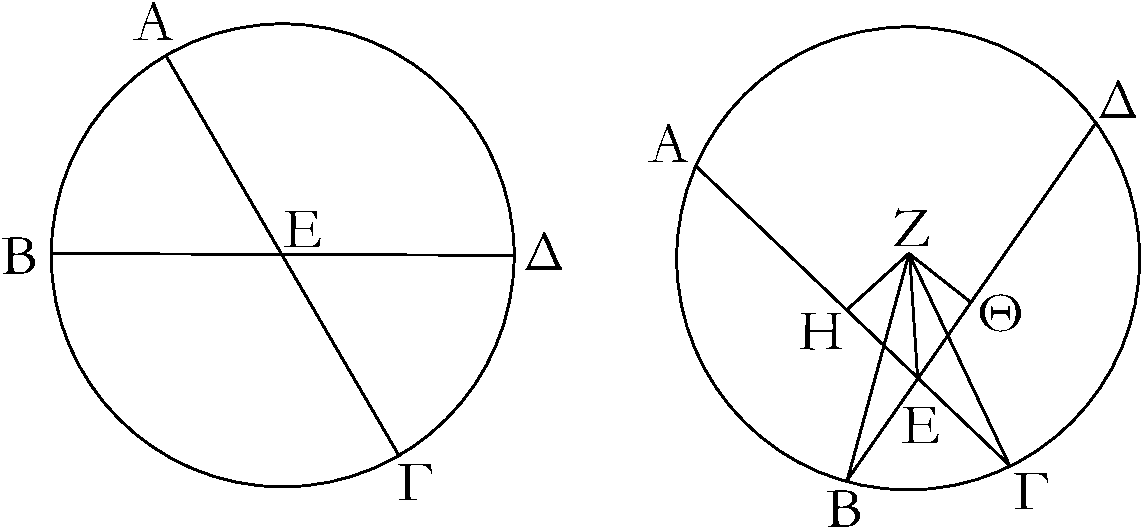
\includegraphics{Book03/fig35g.eps}}

\gr{Ἐὰν >άρα ἐν κύκλῳ εὐθεῖαι δύο τέμνωσιν ἀλλήλαξ, τὸ ὑπὸ τῶν
τῆξ μιᾶξ τμ\kern -.7pt  ημάτων περιεχόμενον ὀρθογώνιον >ίσον ἐστὶ
τῶ| ὑπὸ τῶν τῆξ ἑτέραξ τμ\kern -.7pt  ημάτων περιεθομένῳ ὀρθογωνίῳ;
<όπερ >έδει δεῖχαι.}}

\ParallelRText{
\begin{center}
{\large Proposition 35}
\end{center}

If two straight-lines in a circle cut one another, (then) the rectangle
contained by the pieces of one is equal to the rectangle contained
by the pieces of the other.

For let the two straight-lines $AC$ and $BD$, in the circle $ABCD$,
cut one another at  point $E$. I say that the rectangle contained by
$AE$ and $EC$ is equal to the rectangle contained  by $DE$ and $EB$.

In fact, if $AC$ and $BD$ are through the center (as in the first diagram from the left), so that $E$ is the center
of circle $ABCD$, (then it is) clear that, $AE$, $EC$, $DE$, and $EB$ being equal,
the rectangle contained by $AE$ and $EC$ is also equal to the rectangle
contained by $DE$ and $EB$.

So let $AC$ and $DB$ not be though the center (as in the second diagram from the left), and let the center of $ABCD$ 
be found [Prop.~3.1], and let it be (at) $F$. And let $FG$ and $FH$
be drawn from $F$, perpendicular to the straight-lines $AC$ and $DB$
(respectively) [Prop.~1.12]. And let $FB$, $FC$, and $FE$ 
be joined.

And since some straight-line, $GF$, through the center, cuts at right-angles  some (other) straight-line, $AC$, not through the center,  (then) it also cuts
it in half [Prop.~3.3]. Thus, $AG$ (is) equal to $GC$. Therefore,
since the straight-line $AC$ is cut equally at $G$, and unequally at $E$,
the rectangle contained by $AE$ and $EC$ plus the square on $EG$ is thus
equal to the (square) on $GC$ [Prop.~2.5]. Let the (square) on
$GF$ be added [to both]. Thus, the (rectangle contained) by 
$AE$ and $EC$ plus the (sum of the squares) on $GE$ and $GF$ is equal to
the (sum of the squares) on $CG$ and $GF$. But, the (square) on $FE$ is equal to the (sum of the squares)
on $EG$ and $GF$   [Prop.~1.47],
and the (square)
on $FC$  is equal to the (sum of the squares) on $CG$ and $GF$ [Prop.~1.47]. Thus, the (rectangle contained) by
$AE$ and $EC$ plus the (square) on $FE$ is equal to the (square) on $FC$.
And $FC$ (is) equal to $FB$. Thus, the (rectangle contained) by
$AE$ and $EC$ plus the (square) on $FE$ is equal to the (square) on $FB$.
So, for the same (reasons), the (rectangle contained) by
$DE$ and $EB$ plus the (square) on $FE$ is equal to the (square) on $FB$.
And the (rectangle contained) by
$AE$ and $EC$ plus the (square) on $FE$ was also shown (to be) equal to the (square) on $FB$. Thus,  the (rectangle contained) by
$AE$ and $EC$ plus the (square) on $FE$ is equal to the (rectangle contained) by
$DE$ and $EB$ plus the (square) on $FE$. Let the (square) on $FE$ be
taken from both. Thus, the remaining rectangle contained by $AE$ and
$EC$ is equal to the rectangle contained by $DE$ and $EB$.

\epsfysize=1.5in
\centerline{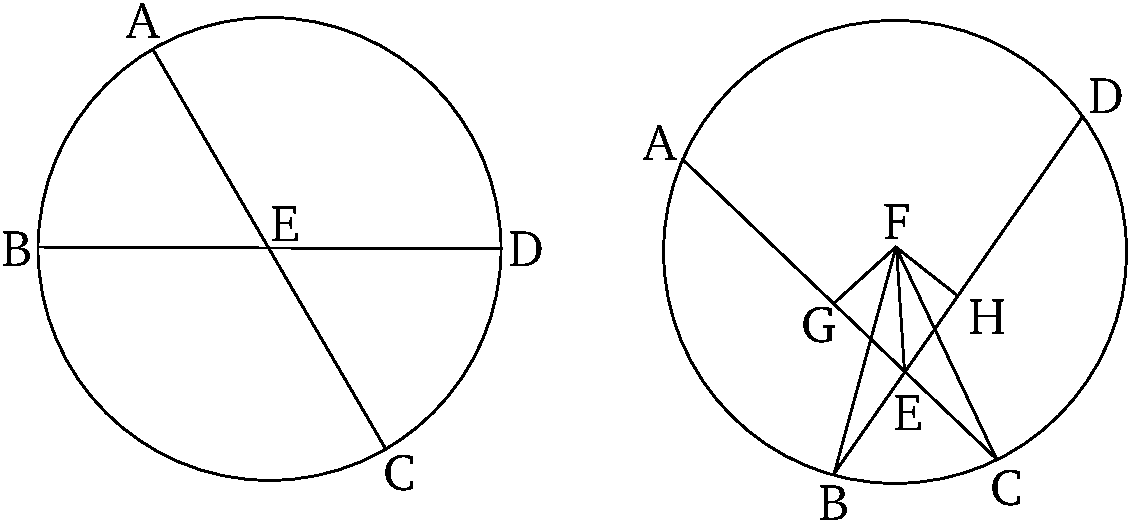
\includegraphics{Book03/fig35e.eps}}

Thus, if two straight-lines in a circle cut one another, (then) the rectangle
contained by the pieces of one is equal to the rectangle contained
by the pieces of the other. (Which is) the very thing it was required to
show.}
\end{Parallel}

%%%%%%
% Prop 3.36
%%%%%%
\pdfbookmark[1]{Proposition 3.36}{pdf3.36}
\begin{Parallel}{}{} 
\ParallelLText{
\begin{center}
{\large \ggn{36}.}
\end{center}\vspace*{-7pt}

\gr{Ἐὰν κύκλου ληφθῆ| τι σημεῖον ἐκτόξ, καὶ ἀπ> α\kern -.7pt  ὐτοῦ πρὸξ τὸν
κύκλον προσπίπτωσι δύο εὐθεῖαι, καὶ ἡ μὲν α\kern -.7pt  ὐτῶν τέμνῃ τὸν
κύκλον, ἡ δὲ ἐφάπτηται, >έσται τὸ ὑπὸ <όληξ τῆξ τεμνούσηξ
καὶ τῆξ ἐκτὸξ ἀπολαμβανομένηξ μεταχὺ τοῦ τε σημείου καὶ
τῆξ κυρτῆξ περιφερείαξ >ίσον τῶ| ἀπὸ τῆξ ἐφαπτομένηξ τετραγώνῳ.}

\gr{Κύκλου γὰρ τοῦ ΑΒΓ εἰλήφθω τι σημεῖον ἐκτὸξ τὸ Δ, καὶ ἀπὸ
τοῦ Δ πρὸξ τὸν ΑΒΓ κύκλον προσπιπτέτωσαν δύο εὐθεῖαι αἱ ΔΓ[Α],
ΔΒ; καὶ ἡ μὲν ΔΓΑ τεμνέτω τὸν ΑΒΓ κύκλον, ἡ δὲ ΒΔ ἐφαπτέσθω;
λέγω, <ότι τὸ ὑπὸ τῶν ΑΔ, ΔΓ περιεχόμενον ὀρθογώνιον
>ίσον ἐστὶ τῶ| ἀπὸ τῆξ ΔΒ τετραγώνῳ.}\\

\epsfysize=1.8in
\centerline{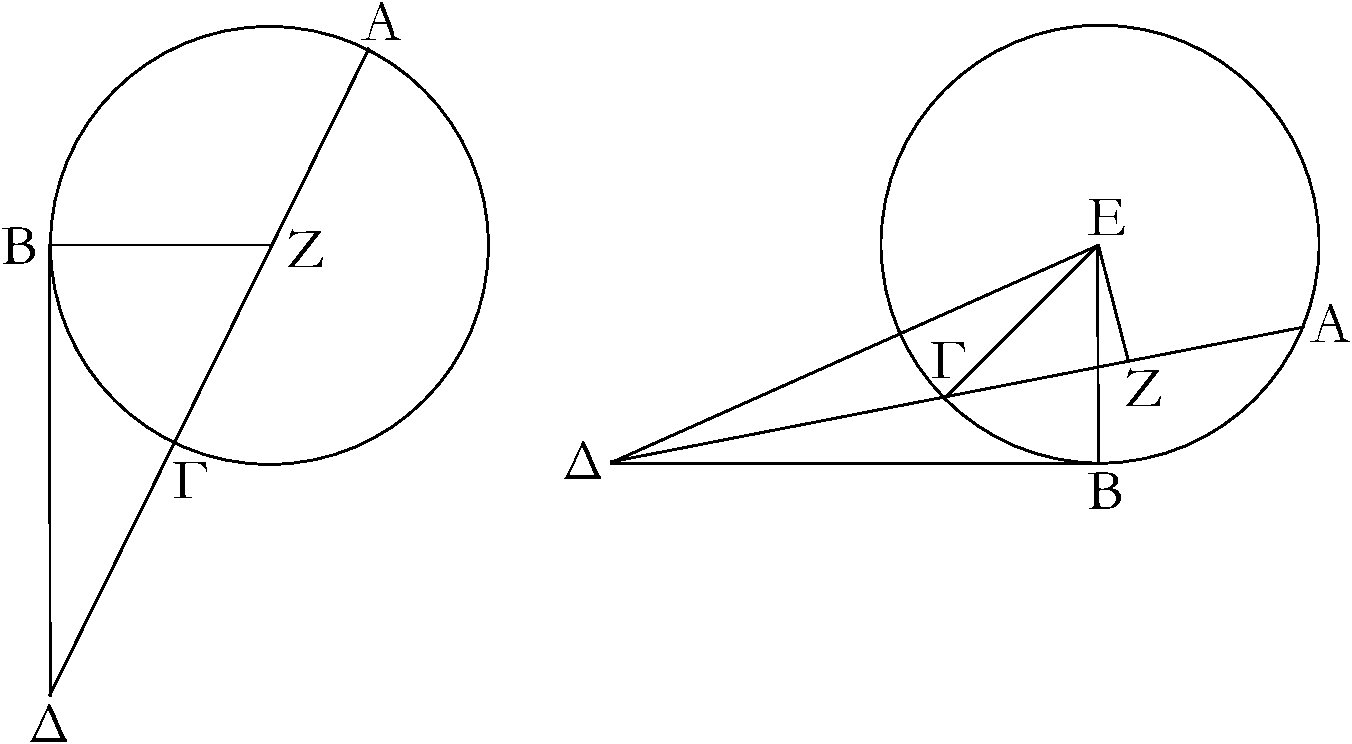
\includegraphics{Book03/fig36g.eps}}

\gr{Ἡ >άρα [Δ]ΓΑ >ήτοι διὰ τοῦ κέντρου ἐστὶν >ὴ ο>ύ. >έστω πρότερον
διὰ τοῦ κέντρου, καὶ >έστω τὸ Ζ κέντρον τοῦ ΑΒΓ κύκλου, καὶ ἐπεζεύθθω ἡ ΖΒ; ὀρθὴ >άρα ἐστὶν ἡ ὑπὸ ΖΒΔ. καὶ ἐπεὶ εὐθεῖα
ἡ ΑΓ δίθα τέτμ\kern -.7pt  ηται κατὰ τὸ Ζ, πρόσκειται δὲ α\kern -.7pt  ὐτῆ| ἡ ΓΔ, τὸ
>άρα ὑπὸ τῶν ΑΔ, ΔΓ μετὰ τοῦ ἀπὸ τῆξ ΖΓ >ίσον
ἐστὶ τῶ| ἀπὸ τῆξ ΖΔ. >ίση δὲ ἡ ΖΓ τῆ| ΖΒ; τὸ >άρα ὑπὸ
τῶν ΑΔ, ΔΓ μετὰ τοῦ ἀπὸ τῆξ ΖΒ >ίσον ἐστὶ τῶ| ἀπὸ τῆξ ΖΔ.
 τῶ| δὲ ἀπὸ τῆξ ΖΔ >ίσα
 ἐστὶ τὰ ἀπὸ τῶν ΖΒ, ΒΔ; τὸ >άρα ὑπὸ τῶν ΑΔ, ΔΓ μετὰ
τοῦ ἀπὸ τῆξ ΖΒ >ίσον ἐστὶ τοῖξ ἀπὸ τῶν ΖΒ, ΒΔ. κοινὸν
ἀφῃρήσθω τὸ ἀπὸ  	τῆξ ΖΒ; λοιπὸν >άρα τὸ ὑπὸ τῶν ΑΔ, ΔΓ
>ίσον ἐστὶ τῶ| ἀπὸ τῆξ ΔΒ ἐφαπτομένηξ.}

\gr{Ἀλλὰ δὴ ἡ ΔΓΑ μ\kern -.7pt  ὴ >έστω διὰ τοῦ κέντρου τοῦ ΑΒΓ κύκλου,
καὶ εἰλήφθω τὸ κέντρον τὸ Ε, καὶ 
ἀπὸ τοῦ Ε ἐπὶ τὴν ΑΓ κάθετοξ >ήθθω ἡ ΕΖ, καὶ ἐπεζεύθθωσαν
αἱ ΕΒ, ΕΓ, ΕΔ; ὀρθὴ >άρα ἐστὶν ἡ ὑπὸ ΕΒΔ. καὶ ἐπεὶ εὐθεῖά
τιξ διὰ τοῦ κέντρου ἡ ΕΖ εὐθεῖάν τινα μ\kern -.7pt  ὴ διὰ τοῦ κέντρου τὴν
ΑΓ πρὸξ ὀρθὰξ τέμνει, καὶ δίθα α\kern -.5pt  ὐτὴν τέμνει; ἡ ΑΖ >άρα τῆ|
ΖΓ ἐστιν >ίση. καὶ ἐπεὶ εὐθεῖα ἡ ΑΓ τέτμ\kern -.3pt  ηται δίθα κατὰ τὸ Ζ
σημεῖον, πρόσκειται δὲ α\kern -.7pt  ὐτῆ| ἡ ΓΔ, τὸ >άρα ὑπὸ τῶν ΑΔ, ΔΓ μετὰ
τοῦ ἀπὸ τῆξ ΖΓ >ίσον ἐστὶ τῶ| ἀπὸ τῆξ ΖΔ. κοινὸν προσκείσθω τὸ
ἀπὸ τῆξ ΖΕ; τὸ >άρα ὑπὸ τῶν ΑΔ, ΔΓ μετὰ τῶν ἀπὸ
τῶν ΓΖ, ΖΕ >ίσον ἐστὶ τοῖξ ἀπὸ τῶν ΖΔ, ΖΕ. τοῖξ δὲ ἀπὸ
τῶν ΓΖ, ΖΕ >ίσον ἐστὶ τὸ ἀπὸ τῆξ ΕΓ; ὀρθὴ γὰρ [ἐστιν]
 ἡ ὑπὸ ΕΖΓ [γωνία]; τοῖξ δὲ ἀπὸ τῶν ΔΖ, ΖΕ >ίσον ἐστὶ
 τὸ ἀπὸ τῆξ ΕΔ; τὸ >άρα ὑπὸ τῶν ΑΔ, ΔΓ μετὰ τοῦ ἀπὸ
 τῆξ ΕΓ >ίσον ἐστὶ τῶ| ἀπὸ τῆξ ΕΔ. >ίση
 δὲ ἡ ΕΓ τὴ| ΕΒ; 
 τὸ >άρα ὑπὸ τῶν ΑΔ, ΔΓ μετὰ τοῦ ἀπὸ τῆξ ΕΒ >ίσον
 ἐστὶ τῶ| >άπὸ τῆξ ΕΔ.
  τῶ| δὲ ἀπὸ τῆξ ΕΔ
 >ίσα ἐστὶ τὰ ἀπὸ τῶν ΕΒ, ΒΔ; ὀρθὴ γὰρ ἡ ὑπὸ ΕΒΔ γωνία;
 τὸ >άρα ὑπὸ τῶν ΑΔ, ΔΓ μετὰ τοῦ ἀπὸ 
τῆξ ΕΒ >ίσον 
 ἐστὶ τοῖξ ἀπὸ τῶν ΕΒ, ΒΔ. κοινὸν ἀφῃρήσθω τὸ ἀπὸ τῆξ
 ΕΒ; λοιπὸν >άρα τὸ ὑπὸ τῶν ΑΔ, ΔΓ >ίσον ἐστὶ τῶ| ἀπὸ τῆξ
 ΔΒ.}
 
 \gr{Ἐὰν >άρα κύκλου ληφθῆ| τι σημεῖον ἐκτόξ, καὶ ἀπ> α\kern -.7pt  ὐτοῦ πρὸξ τὸν
κύκλον προσπίπτωσι δύο εὐθεῖαι, καὶ ἡ μὲν α\kern -.7pt  ὐτῶν τέμνῃ τὸν
κύκλον, ἡ δὲ ἐφάπτηται, >έσται τὸ ὑπὸ <όληξ τῆξ τεμνούσηξ
καὶ τῆξ ἐκτὸξ ἀπολαμβανομένηξ μεταχὺ τοῦ τε σημείου καὶ
τῆξ κυρτῆξ περιφερείαξ >ίσον τῶ| ἀπὸ τῆξ ἐφαπτομένηξ τετραγώνῳ;
<όπερ >έδει δεῖχαι.}}

\ParallelRText{
\begin{center}
{\large Proposition 36}\end{center}

If some point is taken outside a circle, and  two straight-lines
radiate from it towards the circle, and (one) of them cuts the circle, and the (other)
touches (it), (then) the (rectangle contained) by the whole  (straight-line) cutting (the circle), and the (part of it) 
cut off outside (the circle),
between the point and the convex circumference, will be equal to the
square on the tangent (line).

For let some point $D$ be taken outside circle $ABC$, and let two
straight-lines, $DC[A]$ and $DB$, radiate from $D$ towards circle $ABC$. And
let $DCA$ cut circle $ABC$, and let $BD$ touch (it). I say that the rectangle
contained by $AD$ and $DC$ is equal to the square on $DB$.

\epsfysize=1.8in
\centerline{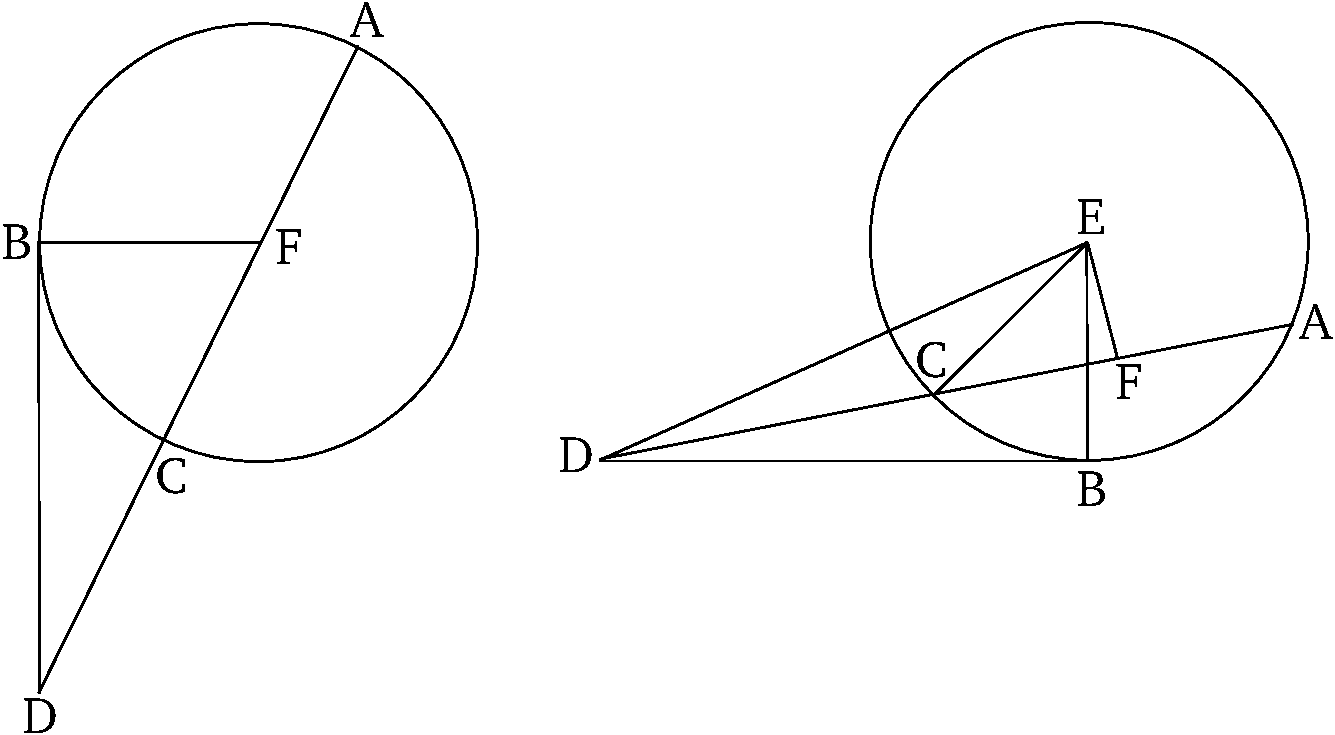
\includegraphics{Book03/fig36e.eps}}

$[D]CA$ is surely either through the center, or not. Let it first of all be
through the center, and let $F$ be the center of circle $ABC$, and let 
$FB$ be joined. Thus, (angle) $FBD$ is a right-angle [Prop.~3.18].
And since straight-line $AC$ is cut in half at $F$, let $CD$ be added to it.
Thus, the (rectangle contained) by $AD$ and $DC$ plus the (square) on $FC$ is
equal to the (square) on $FD$ [Prop.~2.6]. And $FC$ (is) equal to $FB$.
Thus, the (rectangle contained) by $AD$ and $DC$ plus the (square) on $FB$
is equal to the (square) on $FD$. And the (square) on $FD$ is equal to
the (sum of the squares) on $FB$ and $BD$ [Prop.~1.47]. Thus, the
(rectangle contained) by $AD$ and $DC$ plus the (square) on $FB$ is equal
to the (sum of the squares) on $FB$ and $BD$. Let the (square) on $FB$ be subtracted
from both. Thus, the remaining (rectangle contained) by $AD$ and $DC$ 
is equal to the (square) on the tangent $DB$.

And so let $DCA$ not be through the center of circle $ABC$, and let the center $E$
be found, and let $EF$ be drawn from $E$, perpendicular to
$AC$ [Prop.~1.12]. And let $EB$, $EC$, and $ED$ be joined. (Angle)
$EBD$ (is) thus a right-angle [Prop.~3.18]. And since some straight-line, $EF$, through the
center, cuts some (other) straight-line, $AC$, not through the center, at
right-angles, it also cuts it in half [Prop.~3.3]. Thus, $AF$ is equal to
$FC$. And since the straight-line $AC$ is cut in half at point $F$, let $CD$ 
be added to it. Thus, the (rectangle contained) by $AD$ and
 $DC$ plus the
(square) on $FC$ is equal to the (square) on $FD$ [Prop.~2.6]. Let
the (square) on $FE$ be added to both. Thus, the (rectangle contained)
by $AD$ and $DC$ plus the (sum of the squares) on $CF$ and $FE$ is equal to
the (sum of the squares) on $FD$ and $FE$. But  the (square) on $EC$  is equal to the (sum of the squares)
on $CF$ and $FE$. For [angle] $EFC$ [is] a
right-angle [Prop.~1.47]. And the (square) on $ED$ is equal to the (sum of the squares) on $DF$ and
$FE$   [Prop.~1.47]. Thus, the (rectangle
contained) by $AD$ and $DC$ plus the (square) on $EC$ is equal to the (square)
on $ED$. And $EC$ (is) equal to $EB$. Thus, the (rectangle
contained) by $AD$ and $DC$ plus the (square) on $EB$ is equal to the (square)
on $ED$. And the (sum of the squares) on 
$EB$ and $BD$  is equal to  the (square) on $ED$. For $EBD$ (is) a right-angle [Prop.~1.47]. Thus, the (rectangle
contained) by $AD$ and $DC$ plus the (square) on $EB$ is equal to the (sum of the squares)
on $EB$ and $BD$. Let the (square) on $EB$ be subtracted from both. Thus, the remaining
(rectangle contained) by $AD$ and $DC$ is equal to the (square) on $BD$.

Thus, if some point is taken outside a circle, and  two straight-lines
radiate from it towards the circle, and (one) of them cuts the circle, and (the other) touches (it), (then) the (rectangle contained) by the whole  (straight-line) cutting (the circle), and the (part of it) 
cut off outside (the circle),
between the point and the convex circumference, will be equal to the
square on the tangent (line). (Which is) the very thing it was required to show.}
\end{Parallel}

%%%%%%
% Prop 3.37
%%%%%%
\pdfbookmark[1]{Proposition 3.37}{pdf3.37}
\begin{Parallel}{}{} 
\ParallelLText{
\begin{center}
{\large \ggn{37}.}
\end{center}\vspace*{-7pt}

\gr{Ἐὰν κύκλου ληφθῆ| τι σημεῖον ἐκτόξ, ἀπὸ δὲ τοῦ σημείου πρὸξ τὸν
κύκλον προσπίπτωσι δύο εὐθεῖαι, καὶ ἡ μὲν α\kern -.7pt  ὐτῶν τέμνῃ
τὸν κύκλον, ἡ δὲ προσπίπτῃ, >ῆ| δὲ τὸ ὑπὸ [τῆξ] <όληξ τῆξ
τεμνούσηξ καὶ τῆξ ἐκτὸξ ἀπολαμβανομένηξ μεταχὺ τοῦ τε σημείου καὶ
τῆξ κυρτῆξ περιφερείαξ >ίσον τῶ| ἀπὸ τῆξ προσπιπτούσηξ, ἡ
προσπίπτουσα ἐφάψεται τοῦ κύκλου.}

\gr{Κύκλου γὰρ τοῦ ΑΒΓ εἰλήφθω τι σημεῖον ἐκτὸξ τὸ Δ, καὶ ἀπὸ
τοῦ Δ πρὸξ τὸν ΑΒΓ κύκλον προσπιπτέτωσαν δύο εὐθεῖαι αἱ
ΔΓΑ, ΔΒ, καὶ ἡ μὲν ΔΓΑ τεμνέτω τὸν κύκλον, ἡ δὲ ΔΒ προσπιπτέτω,
>έστω δὲ τὸ ὑπὸ τῶν ΑΔ, ΔΓ >ίσον τῶ| ἀπὸ τῆξ ΔΒ. λέγω,
<ότι ἡ ΔΒ ἐφάπτεται τοῦ ΑΒΓ κύκλου.}\\~\\

\epsfysize=1.75in
\centerline{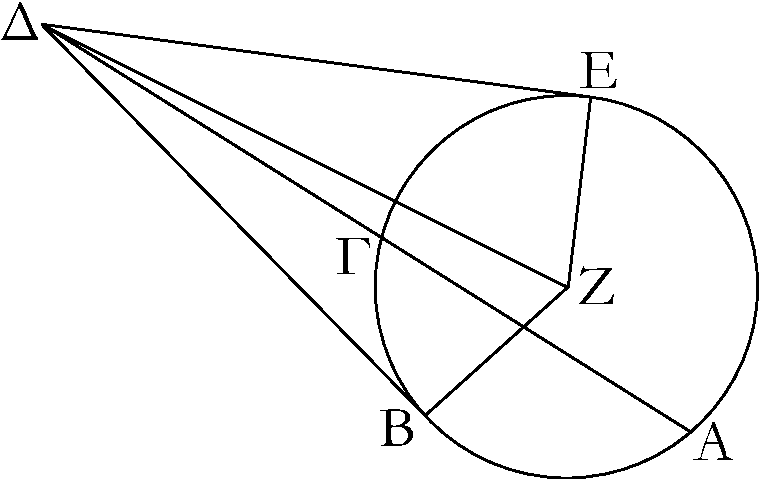
\includegraphics{Book03/fig37g.eps}}

\gr{>'Ηθθω γὰρ τοῦ ΑΒΓ ἐφαπτομένη ἡ ΔΕ, καὶ εἰλήφθω τὸ κέντρον
τοῦ ΑΒΓ κύκλου, καὶ >έστω τὸ Ζ, καὶ ἐπεζεύθθωσαν αἱ ΖΕ, ΖΒ, ΖΔ.
ἡ >άρα ὑπὸ ΖΕΔ ὀρθή ἐστιν. καὶ ἐπεὶ ἡ ΔΕ ἐφάπτεται τοῦ
ΑΒΓ κύκλου, τέμνει δὲ ἡ ΔΓΑ, τὸ >άρα ὑπὸ τῶν ΑΔ, ΔΓ
>ίσον ἐστὶ τῶ| ἀπὸ τῆξ ΔΕ. >ῆν δὲ καὶ τὸ ὑπὸ τῶν
ΑΔ, ΔΓ >ίσον τῶ| ἀπὸ τῆξ ΔΒ; τὸ >άρα ἀπὸ τῆξ ΔΕ >ίσον ἐστὶ τῶ| ἀπὸ
τῆξ ΔΒ;
>ίση >άρα ἡ ΔΕ τῆ| ΔΒ.
ἐστὶ δὲ καὶ ἡ ΖΕ τῆ| ΖΒ >ίση; δύο δὴ αἱ ΔΕ, ΕΖ δύο ταῖξ ΔΒ, ΒΖ
>ίσαι εἰσίν; καὶ βάσιξ α\kern -.7pt  ὐτῶν κοινὴ ἡ ΖΔ; γωνία >άρα ἡ ὑπὸ
ΔΕΖ γωνίᾳ τῆ| ὑπὸ ΔΒΖ ἐστιν >ίση. ὀρθὴ δὲ ἡ ὑπὸ ΔΕΖ; ὀρθὴ
>άρα καὶ ἡ ὑπὸ ΔΒΖ. καί ἐστιν ἡ ΖΒ ἐκβαλλομένη διάμετροξ;
ἡ δὲ τῆ| διαμέτρῳ τοῦ κύκλου πρὸξ ὀρθὰξ ἀπ>
>άκραξ ἀγομένη ἐφάπτεται τοῦ κύκλου; ἡ ΔΒ >άρα ἐφάπτεται
τοῦ ΑΒΓ κύκλου. ὁμοίωξ δὴ δειθθήσεται, κ>ὰν τὸ κέντρον  ἐπὶ
τῆξ ΑΓ τυγθάνῃ.}

\gr{Ἐὰν >άρα κύκλου ληφθῆ| τι σημεῖον ἐκτόξ, ἀπὸ δὲ τοῦ σημείου πρὸξ τὸν
κύκλον προσπίπτωσι δύο εὐθεῖαι, καὶ ἡ μὲν α\kern -.7pt  ὐτῶν τέμνῃ
τὸν κύκλον, ἡ δὲ προσπίπτῃ, >ῆ| δὲ τὸ ὑπὸ  <όληξ τῆξ
τεμνούσηξ καὶ τῆξ ἐκτὸξ ἀπολαμβανομένηξ μεταχὺ τοῦ τε σημείου καὶ
τῆξ κυρτῆξ περιφερείαξ >ίσον τῶ| ἀπὸ τῆξ προσπιπτούσηξ, ἡ
προσπίπτουσα ἐφάψεται τοῦ κύκλου; <όπερ >έδει δεῖχαι.}}

\ParallelRText{
\begin{center}
{\large Proposition 37}
\end{center}

If some point is taken outside a circle, and two straight-lines radiate
from the point towards the circle, and one of them cuts the circle, and the
(other) meets (it), and the (rectangle contained) by the whole (straight-line)
cutting (the circle), and the (part of it) 
cut off outside (the circle),
between the point and the convex circumference,  is equal to the (square)
on the (straight-line) meeting (the circle), (then) the (straight-line)
meeting (the circle) will touch the circle.

For let some point $D$ be taken outside circle $ABC$, and let two
straight-lines, $DCA$ and $DB$, radiate from $D$ towards circle $ABC$, and
let $DCA$ cut the circle, and let $DB$ meet (the circle). And let the (rectangle
contained) by $AD$ and $DC$ be equal to the (square) on $DB$. I say that $DB$ touches circle $ABC$.

\epsfysize=1.75in
\centerline{\includegraphics{Book03/fig37e.eps}}

For let $DE$ be drawn touching $ABC$ [Prop. 3.17], and let the center of the circle
$ABC$ be found, and let it be (at) $F$. And let $FE$, $FB$, and $FD$ 
be joined. (Angle) $FED$ is thus a right-angle [Prop.~3.18].
And since $DE$ touches circle $ABC$, and $DCA$ cuts (it), the (rectangle contained) by $AD$ and $DC$ is thus equal to the (square) on $DE$ [Prop.~3.36]. And the (rectangle contained) by $AD$ and $DC$ was also equal
to the (square) on $DB$.  Thus, the (square) on $DE$ is equal to the
(square) on $DB$. Thus, $DE$ (is) equal to $DB$. And $FE$ is also equal to
$FB$. So the two (straight-lines) $DE$, $EF$ are equal to the two (straight-lines)
$DB$, $BF$ (respectively).  And their base, $FD$, is common. Thus, angle $DEF$ is equal to
angle $DBF$ [Prop.~1.8]. And $DEF$ (is) a right-angle. Thus, $DBF$
(is) also a right-angle. And $FB$ produced is a diameter, And a (straight-line)
drawn at right-angles to a diameter of a circle, at its extremity, touches the
circle [Prop.~3.16~corr.]. Thus, $DB$ touches circle $ABC$. 
Similarly, (the same thing) can be shown, even if the center happens to be
on $AC$.

Thus, if some point is taken outside a circle, and two straight-lines radiate
from the point towards the circle, and one of them cuts the circle, and the
(other) meets (it), and the (rectangle contained) by the whole (straight-line)
cutting (the circle), and the (part of it) 
cut off outside (the circle),
between the point and the convex circumference,  is equal to the (square)
on the (straight-line) meeting (the circle), (then) the (straight-line)
meeting (the circle) will touch the circle. (Which is) the very thing it was
required to show.}
\end{Parallel}

\newpage~\thispagestyle{empty}

% !TEX root = ../Elements.tex
% Greek and English text last checked 16/03/2013
%%%%%%
% BOOK 4
%%%%%%
\pdfbookmark[0]{Book 4}{book4}
\pagestyle{empty}
\begin{center}
{\Huge ELEMENTS BOOK 4}\\
\spa\spa\spa
{\huge\it Construction of Rectilinear Figures In and}\\[0.5ex] {\huge\it Around Circles}
\end{center}
%\vspace{2cm}
%% Removed epsf size command
%\centerline{\includegraphics{Book04/front.pdf}}
\newpage

%%%%%%%
% Definitions
%%%%%%%
\pdfbookmark[1]{Definitions}{def4}
\pagestyle{fancy}
\cfoot{\gr{\kern -.7pt }}
\lhead{\large\gr{ΣΤΟΙΘΕΙΩΝ \kern -.7pt {4}.}}
\rhead{\large ELEMENTS BOOK 4}
\begin{Parallel}{}{} 
\ParallelLText{
\begin{center}
\large{\gr{<'Οροι}.}
\end{center}\vspace*{-7pt}

\ggn{1}.~\gr{Σθῆμα εὐθύγραμμον εἰξ σθῆμα εὐθύγραμμον ἐγγράφ\-εσθαι λέγεται, <όταν ἑκάστη τῶν τοῦ ἐγγραφομένου σθήματ\-οξ γωνιῶν
ἑκάστηξ πλευρᾶξ τοῦ, εἰξ <ὸ ἐγγράφεται, <άπτηται.}

\ggn{2}.~\gr{Σθῆμα δὲ ὁμοίωξ περὶ σθῆμα περιγράφεσθαι λέγεται, <όταν ἑκάστη
πλευρὰ τοῦ περιγραφομένου ἑκάστηξ γωνίαξ τοῦ, περὶ <ὸ περιγράφεται,
<άπτηται.}

\ggn{3}.~\gr{Σθῆμα εὐθύγραμμον εἰξ κύκλον ἐγγράφεσθαι λέγεται, <όταν
ἑκάστη γωνία τοῦ ἐγγραφομένου <άπτηται τῆξ τοῦ κύκλου
περιφερείαξ.}

\ggn{4}.~\gr{Σθῆμα δὲ εὐθύγραμμον περὶ κύκλον περιγράφε\-σθαι λέγεται,
<όταν ἑκάστη πλευρὰ τοῦ περιγραφομένου ἐφάπτηται τῆξ τοῦ κύκλου
περιφερείαξ.}

\ggn{5}.~\gr{Κύκλοξ δὲ εἰξ σθῆμα ὁμοίωξ ἐγγράφεσθαι λέγεται, <όταν
ἡ τοῦ κύκλου περιφέρεια ἑκάστηξ πλευρᾶξ τοῦ, εἰξ <ὸ ἐγγράφεται,
<άπτηται.}

\ggn{6}.~\gr{Κύκλοξ δὲ περὶ σθῆμα περιγράφεσθαι λέγεται, <όταν ἡ τοῦ
κύκλου περιφέρεια ἑκάστηξ γωνίαξ τοῦ, περὶ <ὸ περιγράφεται, <άπτηται.}

\ggn{7}.~\gr{Εὐθεῖα εἰξ κύκλον ἐναρμόζεσθαι λέγεται, <όταν τὰ πέρατα
α\kern -.7pt  ὐτῆξ ἐπὶ τῆξ περιφερείαξ >ῆ| τοῦ κύκλου.}}

\ParallelRText{
\begin{center}
{\large Definitions}
\end{center}

1.~A rectilinear figure is said to be inscribed in a(nother) rectilinear figure
when  the respective angles of the inscribed figure touch the respective
sides of the (figure) in which it is inscribed.

2.~And, similarly, a  (rectilinear) figure is said to be circumscribed about a(nother rectilinear) figure when the respective sides of the circumscribed
(figure) touch the respective angles of the (figure) about which it is
circumscribed.

3.~A rectilinear figure is said to be inscribed in a circle when
each angle of the inscribed (figure) touches the circumference of the
circle.

4.~And a rectilinear figure is said to be circumscribed about a circle
when each side of the circumscribed (figure) touches the
circumference of the circle.

5.~And, similarly, a circle is said to be inscribed in a (rectilinear) figure
when the circumference of the circle touches each  side of
the (figure) in which it is inscribed.

6.~And a circle is said to be circumscribed about a rectilinear (figure)
when the circumference of the circle touches each  angle of the
(figure) about which it is circumscribed.

7.~A straight-line is said to be inserted into a circle when its extremities
are on the circumference of the circle.}
\end{Parallel}

%%%%%%
% Prop 4.1
%%%%%%
\pdfbookmark[1]{Proposition 4.1}{pdf4.1}
\begin{Parallel}{}{} 
\ParallelLText{
\begin{center}
{\large \ggn{1}.}
\end{center}\vspace*{-7pt}

\gr{Εἰξ τὸν δοθέντα κύκλον τῆ| δοθείσῃ εὐθείᾳ μ\kern -.7pt  ὴ μείζονι ο>ύσῃ
τῆξ τοῦ κύκλου διαμέτρου >ίσην εὐθεῖαν ἐναρμόσαι.}\\

% Removed epsf size command
\centerline{\includegraphics{Book04/fig01g.pdf}}

\gr{>'Εστω ὁ δοθεὶξ κύκλοξ ὁ ΑΒΓ, ἡ δὲ δοθεῖσα εὐθεῖα μ\kern -.7pt  ὴ
μείζων τῆξ τοῦ κύκλου διαμέτρου ἡ Δ. δεῖ δὴ εἰξ τὸν
ΑΒΓ κύκλον τῆ| Δ εὐθείᾳ >ίσην εὐθεῖαν ἐναρμόσαι.}

\gr{>'Ηθθω τοῦ ΑΒΓ κύκλου διάμετροξ ἡ ΒΓ. εἰ μὲν
ο>ῦν >ίση ἐστὶν ἡ ΒΓ τῆ| Δ, γεγονὸξ >ὰν ε>ίη τὸ
ἐπιταθθέν; ἐνήρμοσται γὰρ εἰξ τὸν ΑΒΓ κύκλον τῆ|
Δ εὐθείᾳ >ίση ἡ ΒΓ. εἰ δὲ μείζων ἐστὶν ἡ ΒΓ τῆξ
Δ, κείσθω τῆ| Δ >ίση ἡ ΓΕ, καὶ κέντρῳ τῶ| Γ διαστήματι
δὲ τῶ| ΓΕ κύκλοξ γεγράφθω ὁ ΕΑΖ, καὶ ἐπεζεύθθω
ἡ ΓΑ.}

\gr{Ἐπεὶ ο>ῦν το Γ σημεῖον κέντρον ἐστὶ τοῦ ΕΑΖ κύκλου, >ίση
 ἐστὶν ἡ ΓΑ τῆ| ΓΕ. ἀλλὰ τῆ| Δ ἡ ΓΕ ἐστιν >ίση;
καὶ ἡ Δ >άρα τῆ| ΓΑ ἐστιν >ίση.}

\gr{Εἰξ >άρα τὸν δοθέντα κύκλον τὸν ΑΒΓ τῆ| δοθείσῃ εὐθείᾳ τῆ|
Δ >ίση ἐνήρμοσται ἡ ΓΑ; <όπερ >έδει ποιῆσαι.}}

\ParallelRText{
\begin{center}
{\large Proposition 1}
\end{center}

To insert a straight-line equal to
a given straight-line into a circle, (the latter straight-line) not being greater than the diameter of the circle.

% Removed epsf size command
\centerline{\includegraphics{Book04/fig01e.pdf}}

Let $ABC$ be the given circle, and $D$ the given straight-line (which is) not greater than
the diameter of the circle. So it is required to insert a straight-line, equal to the
straight-line $D$, into the circle $ABC$.

Let a diameter $BC$ of circle $ABC$ be drawn.$^\dag$ Therefore, if
$BC$ is equal to $D$, (then) that (which)  was prescribed has taken place.
For the (straight-line) $BC$, equal to the straight-line $D$, has been inserted into the circle $ABC$.
And if $BC$ is greater than $D$ then let $CE$ be made equal to $D$ [Prop.~1.3], and let the circle $EAF$ be drawn with center $C$ and radius $CE$. And let $CA$ be joined.

Therefore, since the point $C$ is the center of  circle $EAF$, $CA$ is equal to $CE$. But,
$CE$ is equal to $D$. Thus, $D$ is also equal to $CA$.

Thus, $CA$, equal to the given straight-line $D$,  has been inserted into
the given circle $ABC$. (Which is) the very thing it was required to do.}
\end{Parallel}
{\footnotesize \noindent$^\dag$ Presumably, by finding the center of the circle [Prop.~3.1], and then
drawing a line through it.}

%%%%%%
% Prop 4.2
%%%%%%
\pdfbookmark[1]{Proposition 4.2}{pdf4.2}
\begin{Parallel}{}{} 
\ParallelLText{
\begin{center}
{\large \ggn{2}.}
\end{center}\vspace*{-7pt}

\gr{Εἰξ τὸν δοθέντα κύκλον τῶ| δοθέντι τριγώνῳ ἰσογώνιον τρίγωνον
ἐγγράψαι.}

% Removed epsf size command
\centerline{\includegraphics{Book04/fig02g.pdf}}

\gr{>'Εστω ὁ δοθεὶξ κύκλοξ ὁ ΑΒΓ, τὸ δὲ δοθὲν τριγωνον τὸ ΔΕΖ;
δεῖ δὴ εἰξ τὸν ΑΒΓ κύκλον τῶ| ΔΕΖ τριγώνῳ ἰσογώνιον
τρίγωνον ἐγγράψαι.}

\gr{>'Ηθθω τοῦ ΑΒΓ κύκλου ἐφαπτομένη ἡ ΗΘ κατὰ τὸ Α,
καὶ συνεστάτω πρὸξ τῆ| ΑΘ εὐθείᾳ καὶ τῶ| πρὸξ α\kern -.7pt  ὐτῆ| σημείῳ
τῶ| Α τῆ| ὑπὸ ΔΕΖ γωνίᾳ >ίση ἡ ὑπὸ
ΘΑΓ, πρὸξ δὲ τῆ| ΑΗ εὐθείᾳ καὶ τῶ| πρὸξ α\kern -.7pt  ὐτῆ|
σημείῳ τῶ| Α τῆ| ὑπὸ ΔΖΕ [γωνίᾳ] >ίση ἡ ὑπὸ ΗΑΒ, καὶ
ἐπεζεύθθω ἡ ΒΓ.}

\gr{Ἐπεὶ ο>ῦν κύκλου τοῦ ΑΒΓ ἐφάπτεταί τιξ εὐθεῖα ἡ ΑΘ, καὶ
ἀπὸ τῆξ κατὰ τὸ Α ἐπαφῆξ εἰξ τὸν κύκλον διῆκται εὐθεῖα
ἡ ΑΓ, ἡ >άρα ὑπὸ ΘΑΓ >ίση ἐστὶ τῆ| ἐν τῶ| ἐναλλὰχ τοῦ
κύκλου τμ\kern -.7pt  ήματι γωνίᾳ τῆ| ὑπὸ ΑΒΓ. ἀλλ> ἡ ὑπὸ ΘΑΓ τῆ|
ὑπὸ ΔΕΖ ἐστιν >ίση; καὶ ἡ ὑπὸ ΑΒΓ >άρα γωνία τῆ| ὑπὸ
ΔΕΖ ἐστιν >ίση. διὰ τὰ α\kern -.7pt  ὐτὰ δὴ καὶ ἡ ὑπὸ ΑΓΒ τῆ| ὑπὸ
ΔΖΕ ἐστιν >ίση; καὶ λοιπὴ >άρα ἡ ὑπὸ ΒΑΓ λοιπῆ| τῆ| ὑπὸ
ΕΔΖ ἐστιν >ίση [ἰσογώνιον >άρα ἐστὶ τὸ ΑΒΓ τρίγωνον τῶ|
ΔΕΖ τριγώνῳ, καὶ ἐγγέγραπται εἰξ τὸν ΑΒΓ κύκλον].}

\gr{Εἰξ τὸν δοθέντα >άρα κύκλον τῶ| δοθέντι τριγώνῳ
ἰσογώνιον τρίγωνον ἐγγέγραπται; <όπερ >έδει ποιῆσαι.}}

\ParallelRText{
\begin{center}
{\large Proposition 2}
\end{center}

To inscribe a triangle, equiangular with a given triangle, in a given circle.

% Removed epsf size command
\centerline{\includegraphics{Book04/fig02e.pdf}}

Let $ABC$ be the given circle, and $DEF$ the given triangle. So it is required
to inscribe a triangle, equiangular with triangle $DEF$, in circle $ABC$.

Let $GH$ be drawn touching circle $ABC$ at $A$.$^\dag$ And let  (angle) $HAC$, equal to angle $DEF$,  be constructed
on the straight-line $AH$ at the point $A$ on it, and (angle) $GAB$, equal to
[angle] $DFE$,  on the straight-line $AG$ at the point $A$ on it
 [Prop.~1.23]. And let $BC$ be joined.
 
 Therefore, since some straight-line $AH$ touches the circle $ABC$, and the
 straight-line $AC$ has been drawn across (the circle) from the point of
 contact $A$, (angle) $HAC$ is thus equal to the angle $ABC$ in the alternate
 segment of the circle [Prop.~3.32]. But, $HAC$ is equal to $DEF$.
 Thus, angle $ABC$ is also equal to $DEF$. So, for the same (reasons),
 $ACB$ is also equal to $DFE$.  Thus, the remaining (angle) $BAC$ is equal
 to the remaining (angle) $EDF$ [Prop.~1.32]. [Thus, triangle
 $ABC$ is equiangular with triangle $DEF$, and has been inscribed in circle
 $ABC$].
 
 Thus, a triangle, equiangular with the given triangle, has been inscribed in
 the given circle. (Which is) the very thing it was required to do.}
\end{Parallel}
{\footnotesize \noindent$^\dag$ See the footnote
to Prop.~3.34.}

%%%%%%
% Prop 4.3
%%%%%%
\pdfbookmark[1]{Proposition 4.3}{pdf4.3}
\begin{Parallel}{}{} 
\ParallelLText{
\begin{center}
{\large \ggn{3}.}
\end{center}\vspace*{-7pt}

\gr{Περὶ τὸν δοθέντα κύκλον τῶ| δοθέντι τριγώνῳ ἰσογώνιον τρίγωνον περιγράψαι.}

% Removed epsf size command
\centerline{\includegraphics{Book04/fig03g.pdf}}

\gr{>'Εστω ὁ δοθεὶξ κύκλοξ ὁ ΑΒΓ, τὸ δὲ δοθὲν τρίγωνον τὸ ΔΕΖ; δεῖ
δὴ περὶ τὸν ΑΒΓ κύκλον τῶ| ΔΕΖ τριγώνῳ ἰσογώνιον τρίγωνον
περιγράψαι.}

\gr{Ἐκβεβλήσθω ἡ ΕΖ ἐφ> ἑκάτερα τὰ μέρη κατὰ τὰ Η, Θ σημεῖα,
καὶ εἰλήφθω τοῦ ΑΒΓ κύκλου κέντρον τὸ Κ, καὶ διήθθω, ὡξ
>έτυθεν, εὐθεῖα ἡ ΚΒ, καὶ συνεστάτω πρὸξ τῆ| ΚΒ εὐθείᾳ
καὶ τῶ| πρὸξ α\kern -.7pt  ὐτῆ| σημείῳ τῶ| Κ τῆ| μὲν ὑπὸ ΔΕΗ γωνίᾳ
>ίση ἡ ὑπὸ ΒΚΑ, τῆ| δὲ ὑπὸ ΔΖΘ >ίση ἡ ὑπὸ ΒΚΓ, καὶ διὰ
τῶν Α, Β, Γ σημείων >ήθθωσαν ἐφαπτόμεναι τοῦ ΑΒΓ κύκλου
αἱ ΛΑΜ, ΜΒΝ, ΝΓΛ.}

\gr{Καὶ ἐπεὶ ἐφάπτονται τοῦ ΑΒΓ κύκλου αἱ ΛΜ, ΜΝ,
ΝΛ κατὰ τὰ Α, Β, Γ σημεῖα, ἀπὸ δὲ τοῦ Κ κέντρου ἐπὶ
τὰ Α, Β, Γ σημεῖα
ἐπεζευγμέναι εἰσὶν  αἱ ΚΑ, ΚΒ, ΚΓ, ὀρθαὶ >άρα εἰσὶν αἱ
πρὸξ τοῖξ Α, Β, Γ σημείοιξ γωνίαι. καὶ ἐπεὶ τοῦ ΑΜΒΚ τετραπλεύρου αἱ τέσσαρεξ γωνίαι τέτρασιν ὀρθαῖξ >ίσαι εἰσίν, ἐπειδήπερ καὶ
εἰξ δύο τρίγωνα διαιρεῖται τὸ ΑΜΒΚ, καί εἰσιν ὀρθαὶ αἱ ὑπὸ
ΚΑΜ, ΚΒΜ γωνίαι, λοιπαὶ >άρα αἱ ὑπὸ ΑΚΒ, ΑΜΒ δυσὶν ὀρθαῖξ
>ίσαι εἰσίν. εἰσὶ δὲ καὶ αἱ ὑπὸ ΔΕΗ, ΔΕΖ δυσὶν ὀρθαῖξ >ίσαι;
αἱ >άρα ὑπὸ ΑΚΒ, ΑΜΒ ταῖξ ὑπὸ ΔΕΗ, ΔΕΖ >ίσαι εἰσίν,
<ῶν ἡ ὑπὸ ΑΚΒ τῆ| ὑπὸ ΔΕΗ ἐστιν >ίση; λοιπὴ >άρα ἡ ὑπὸ
ΑΜΒ λοιπῆ| τῆ| ὑπὸ ΔΕΖ ἐστιν >ίση.
 ὁμοίωξ δὴ
δειθθήσεται, <ότι καὶ ἡ ὑπὸ ΛΝΒ τῆ| ὑπὸ ΔΖΕ ἐστιν >ίση;
καὶ λοιπὴ >άρα ἡ ὑπὸ ΜΛΝ [λοιπῆ|] τῆ| ὑπὸ ΕΔΖ ἐστιν
>ίση. ἰσογώνιον >άρα ἐστὶ τὸ ΛΜΝ τρίγωνον τῶ| ΔΕΖ
τριγώνῳ; καὶ περιγέγραπται περὶ τὸν ΑΒΓ κύκλον.}

\gr{Περὶ τὸν δοθέντα >άρα κύκλον τῶ| δοθέντι τριγώνῳ ἰσογώνιον
τρίγωνον περιγέγραπται; <όπερ >έδει ποιῆσαι.}}

\ParallelRText{
\begin{center}
{\large Proposition 3}
\end{center}

To circumscribe a triangle, equiangular with a given triangle, about a given
circle.

% Removed epsf size command
\centerline{\includegraphics{Book04/fig03e.pdf}}

Let $ABC$ be the given circle, and $DEF$ the given triangle. So it is required
to circumscribe a triangle, equiangular with triangle  $DEF$, about circle $ABC$.

Let $EF$ be produced in each direction to points $G$ and 
$H$. And
let the center $K$ of circle $ABC$ be found [Prop.~3.1].
And let the straight-line $KB$ be drawn, at random,  across ($ABC$).
And let (angle) $BKA$, equal to angle $DEG$, be constructed on the straight-line $KB$ at the point $K$ on it, and (angle) $BKC$, equal to
$DFH$ [Prop.~1.23]. And let the (straight-lines) $LAM$, $MBN$, and $NCL$ be 
drawn through the points $A$, $B$, and $C$ (respectively), touching the circle $ABC$.$^\dag$

And since $LM$, $MN$, and $NL$ touch circle $ABC$ at points $A$, $B$, and $C$
(respectively), and $KA$, $KB$, and $KC$ are joined from the center $K$
to  points $A$, $B$, and $C$ (respectively), the angles at points
$A$, $B$, and $C$ are thus right-angles [Prop.~3.18]. And
since the (sum of the) four angles of quadrilateral $AMBK$ is equal to
four right-angles,
inasmuch as $AMBK$ (can) also (be) divided into two triangles [Prop.~1.32],
and angles $KAM$ and $KBM$ are (both) right-angles, the (sum of the) remaining (angles), $AKB$ and $AMB$, is thus equal to two right-angles. 
And $DEG$ and $DEF$ is also equal to two right-angles [Prop.~1.13].
Thus, $AKB$ and $AMB$ is equal to $DEG$ and $DEF$, of which $AKB$ is
equal to $DEG$. Thus, the remainder $AMB$ is equal to the remainder $DEF$.
So, similarly, it can be shown that $LNB$ is also equal to $DFE$. Thus, the
remaining (angle) $MLN$ is also equal to the [remaining] (angle) $EDF$ [Prop.~1.32]. Thus,
triangle $LMN$ is equiangular with triangle $DEF$. And it has been drawn around
circle $ABC$.

Thus,  a triangle, equiangular with  the given triangle, has been circumscribed about the given
circle. (Which is) the very thing it was required to do.}
\end{Parallel}
{\footnotesize \noindent$^\dag$ See the footnote
to Prop.~3.34.}

%%%%%%
% Prop 4.4
%%%%%%
\pdfbookmark[1]{Proposition 4.4}{pdf4.4}
\begin{Parallel}{}{} 
\ParallelLText{
\begin{center}
{\large \ggn{4}.}
\end{center}\vspace*{-7pt}

\gr{Εἰξ τὸ δοθὲν  τρίγωνον κύκλον ἐγγράψαι.}

% Removed epsf size command
\centerline{\includegraphics{Book04/fig04g.pdf}}

\gr{>'Εστω τὸ δοθὲν τρίγωνον τὸ ΑΒΓ; δεῖ δὴ εἰξ τὸ ΑΒΓ τρίγωνον κύκλον ἐγγράψαι.}

\gr{Τετμ\kern -.7pt  ήσθωσαν αἱ ὑπὸ ΑΒΓ, ΑΓΒ γωνίαι δίθα ταῖξ ΒΔ, ΓΔ εὐθείαιξ,
καὶ συμβαλλέτωσαν ἀλλήλαιξ κατὰ τὸ Δ σημεῖον, καὶ >ήθθωσαν ἀπὸ
τοῦ Δ ἐπὶ τὰξ ΑΒ, ΒΓ, ΓΑ 	εὐθείαξ κάθετοι αἱ ΔΕ, ΔΖ, ΔΗ.}

\gr{Καὶ ἐπεὶ >ίση ἐστὶν ἡ ὑπὸ ΑΒΔ γωνία τῆ| ὑπὸ ΓΒΔ, ἐστὶ
δὲ καὶ ὀρθὴ ἡ ὑπὸ ΒΕΔ ὀρθῆ| τῆ| ὑπὸ ΒΖΔ >ίση, δύο
δὴ τρίγωνά ἐστι τὰ ΕΒΔ, ΖΒΔ τὰξ δύο γωνίαξ ταῖξ δυσὶ γωνίαιξ
>ίσαξ >έθοντα καὶ μίαν πλευρὰν μιᾶ| πλευρᾶ| >ίσην τὴν ὑποτείνουσαν
ὑπὸ μίαν
τῶν >ίσων γωνιῶν κοινὴν α\kern -.7pt  ὐτῶν τὴν
ΒΔ; καὶ τὰξ λοιπὰξ >άρα πλευρὰξ ταῖξ λοιπαῖξ πλευραῖξ >ίσαξ
<έχουσιν; >ίση >άρα ἡ ΔΕ τῆ| ΔΖ. διὰ τὰ α\kern -.7pt  ὐτὰ δὴ καὶ ἡ
ΔΗ τῆ| ΔΖ ἐστιν >ίση. αἱ τρεῖξ >άρα εὐθεῖαι αἱ ΔΕ, ΔΖ, ΔΗ
>ίσαι ἀλλήλαιξ εἰσίν; ὁ >άρα κέντρῶ| τῶ| Δ καὶ διαστήματι
ἑνὶ τῶν Ε, Ζ, Η κύκλοξ γραφόμενοξ <ήχει καὶ διὰ τῶν λοιπῶν
σημείων καὶ ἐφάψεται τῶν ΑΒ, ΒΓ, ΓΑ εὐθειῶν διὰ τὸ ὀρθὰξ ε>ῖναι τὰξ πρὸξ τοῖξ Ε, Ζ, Η σημείοιξ γωνίαξ. εἰ γὰρ τεμεῖ
α\kern -.5pt  ὐτάξ, >έσται ἡ τῆ| διαμέτρῳ τοῦ κύκλου πρὸξ ὀρθὰξ
ἀπ> >άκραξ ἀγομένη ἐντὸξ πίπτουσα τοῦ κύκλου; <όπερ
>άτοπον ἐδείθθη; οὐκ >άρα ὁ κέντρῳ τῶ| Δ διαστήματι
δὲ ἑνὶ τῶν Ε, Ζ, Η γραφόμενοξ κύκλοξ τεμεῖ τὰξ ΑΒ, ΒΓ, ΓΑ εὐθείαξ; ἐφάψεται >άρα α\kern -.3pt  ὐτῶν, καὶ >έσται ὁ 
κύκλοξ ἐγγεγραμμένοξ εἰξ τὸ ΑΒΓ τρίγωνον. 
ἐγγεγράφθω ὡξ ὁ ΖΗΕ.}

\gr{Εἰξ >άρα τὸ δοθὲν τρίγωνον τὸ ΑΒΓ κύκλοξ
ἐγγέγρ\-απται ὁ ΕΖΗ; <όπερ >έδει ποιῆσαι.}}

\ParallelRText{
\begin{center}
{\large Proposition 4}
\end{center}

To inscribe a circle in a given triangle.

% Removed epsf size command
\centerline{\includegraphics{Book04/fig04e.pdf}}

Let $ABC$ be the given triangle. So it is required to inscribe
a circle in triangle $ABC$.

Let the angles $ABC$ and $ACB$ be cut in half by the
straight-lines $BD$ and $CD$ (respectively) [Prop.~1.9], and let them meet one another
at point $D$, and let $DE$, $DF$, and $DG$ be drawn from
point $D$, perpendicular to the straight-lines $AB$, $BC$, and $CA$ (respectively) [Prop.~1.12].

And since angle $ABD$ is equal to $CBD$, and the right-angle
$BED$ is also equal to the right-angle $BFD$, $EBD$ and $FBD$ are thus two triangles
having two angles equal to two angles, and one side equal to one side---the
(one) subtending one of the equal angles (which is) common to the (triangles)---(namely), $BD$. Thus, they will also have the 
remaining sides equal to the (corresponding) remaining sides [Prop.~1.26]. Thus, $DE$ (is)
equal to $DF$. So, for the same (reasons), $DG$ is also equal
to $DF$. Thus, the three straight-lines $DE$, $DF$, and $DG$ are equal to one another.
Thus, the circle drawn with center $D$, and radius one of $E$, $F$, or $G$,$^\dag$ will also
go through the remaining points, and will  touch the straight-lines $AB$, $BC$, and $CA$, on account of the angles at $E$, $F$, and $G$ being right-angles. For if it cuts (one of) them then it will be a (straight-line)
drawn at right-angles to a diameter of the circle, from its extremity, falling inside
the circle. The very thing was shown (to be) absurd [Prop.~3.16].
Thus, the circle drawn with center $D$, and radius one of $E$, $F$, or $G$,
does not cut the straight-lines $AB$, $BC$, and $CA$. Thus, it will
touch them, and will be the circle inscribed  in triangle $ABC$.
Let it be (so) inscribed, like $FGE$ (in the figure).

Thus, the circle $EFG$ has been inscribed in the given triangle $ABC$.
(Which is) the very thing it was required to do.}
\end{Parallel}
{\footnotesize \noindent$^\dag$ Here, and in the following propositions, it
is understood that the radius is actually one of $DE$, $DF$, or $DG$.}

%%%%%%
% Prop 4.5
%%%%%%
\pdfbookmark[1]{Proposition 4.5}{pdf4.5}
\begin{Parallel}{}{} 
\ParallelLText{
\begin{center}
{\large \ggn{5}.}
\end{center}\vspace*{-7pt}

\gr{Περὶ τὸ δοθὲν τρίγωνον κύκλον περιγράψαι.}

% Removed epsf size command
\centerline{\includegraphics{Book04/fig05g.pdf}}

\gr{>'Εστω τὸ δοθὲν τρίγωνον τὸ ΑΒΓ; δεῖ δὲ περὶ τὸ δοθὲν τρίγωνον
τὸ ΑΒΓ κύκλον περιγράψαι.}

\gr{Τετμ\kern -.7pt  ήσθωσαν αἱ ΑΒ, ΑΓ εὐθεῖαι δίθα κατὰ τὰ Δ, Ε σημεῖα, καὶ
ἀπὸ τῶν Δ, Ε σημείων ταῖξ ΑΒ, ΑΓ πρὸξ ὀρθὰξ >ήθθωσαν
αἱ ΔΖ, ΕΖ; συμπεσοῦνται δὴ >ήτοι ἐντὸξ τοῦ ΑΒΓ τριγώνου
>ὴ ἐπὶ τῆξ ΒΓ εὐθείαξ >ὴ ἐκτὸξ τῆξ ΒΓ.}

\gr{Συμπιπτέτωσαν πρότερον ἐντὸξ κατὰ τὸ Ζ, καὶ ἐπεζεύθθ\-ωσαν
αἱ ΖΒ, ΖΓ, ΖΑ. καὶ ἐπεὶ >ίση ἐστὶν ἡ ΑΔ τῆ| ΔΒ, κοινὴ
δὲ καὶ πρὸξ ὀρθὰξ ἡ ΔΖ, βάσιξ >άρα ἡ ΑΖ βάσει τῆ| ΖΒ
ἐστιν >ίση. ὁμοίωξ δὴ δείχομεν, <ότι καὶ ἡ ΓΖ τῆ| ΑΖ ἐστιν
>ίση; <ώστε καὶ ἡ ΖΒ τῆ| ΖΓ ἐστιν >ίση; αἱ τρεῖξ
>άρα αἱ ΖΑ, ΖΒ, ΖΓ >ίσαι  ἀλλήλαιξ εἰσίν. ὁ >άρα κέντρῳ
τῶ| Ζ διαστήματι δὲ ἑνὶ τῶν Α, Β, Γ κύκλοξ γραφόμενοξ <ήχει
καὶ διὰ τῶν λοιπῶν σημείων, καὶ >έσται περιγεγραμμένοξ
ὁ κύκλοξ περὶ τὸ ΑΒΓ τρίγωνον. περιγεγράφθω ὡξ ὁ ΑΒΓ.}

\gr{Ἀλλὰ δὴ αἱ ΔΖ, ΕΖ συμπιπτέτωσαν ἐπὶ τῆξ ΒΓ εὐθείαξ
κατὰ τὸ Ζ, ὡξ >έθει ἐπὶ τῆξ δευτέραξ καταγραφῆξ, καὶ
ἐπεζεύθθω ἡ ΑΖ. ὁμοίωξ δὴ δείχομεν, <ότι τὸ Ζ σημεῖον
κέντρον ἐστὶ τοῦ περὶ τὸ ΑΒΓ τρίγωνον περιγραφομένου κύκλου.}

\gr{Ἀλλὰ δὴ αἱ ΔΖ, ΕΖ συμπιπτέτωσαν ἐκτὸξ τοῦ ΑΒΓ τριγώνου κατὰ
τὸ Ζ πάλιν, ὡξ >έθει ἐπὶ τῆξ τρίτηξ καταγραφῆξ, καί 
ἐπεζεύθθωσαν αἱ ΑΖ, ΒΖ, ΓΖ. καὶ ἐπεὶ πάλιν >ίση ἐστὶν ἡ
ΑΔ τῆ| ΔΒ, κοινὴ δὲ καὶ πρὸξ ὀρθὰξ ἡ ΔΖ, βάσιξ >άρα
ἡ ΑΖ βάσει τῆ| ΒΖ ἐστιν >ίση. ὁμοίωξ δὴ δείχομεν, <ότι
καὶ ἡ ΓΖ τῆ| ΑΖ ἐστιν >ίση; <ώστε καὶ ἡ ΒΖ τῆ| ΖΓ ἐστιν
>ίση; ὁ >άρα [πάλιν] κέντρῳ τῶ| Ζ διαστήματι δὲ ἑνὶ τῶν
ΖΑ, ΖΒ, ΖΓ κύκλοξ γραφόμενοξ <ήχει καὶ διὰ τῶν λοιπῶν σημείων,
καὶ >έσται περιγεγραμμένοξ περὶ τὸ ΑΒΓ τρίγωνον.}

\gr{Περὶ τὸ δοθὲν >άρα τρίγωνον κύκλοξ περιγέγραπται; <όπερ >έδει ποιῆσαι.}}

\ParallelRText{
\begin{center}
{\large Proposition 5}
\end{center}

To circumscribe a circle about a given  triangle.

% Removed epsf size command
\centerline{\includegraphics{Book04/fig05e.pdf}}

Let $ABC$ be the given triangle. So it is required to circumscribe
a circle about the given triangle $ABC$.

Let the straight-lines $AB$ and $AC$ be cut in half at points $D$ and $E$ (respectively) [Prop.~1.10]. And let $DF$ and $EF$ be drawn from 
points $D$ and $E$, at right-angles to $AB$ and $AC$ (respectively) [Prop.~1.11].
So  ($DF$ and $EF$) will surely either meet inside triangle $ABC$, on the straight-line
$BC$, or beyond $BC$.

Let them, first of all, meet inside (triangle $ABC$) at (point) $F$, and let $FB$, 
$FC$, and $FA$ be joined. And since $AD$ is equal to $DB$, and $DF$ is
common and at right-angles, the base $AF$ is thus equal to the base $FB$
[Prop.~1.4]. So, similarly, we can show that $CF$ is also equal to
$AF$. So that $FB$ is also equal to $FC$. Thus, the three (straight-lines)
$FA$, $FB$, and $FC$ are equal to one another. Thus, the circle drawn with
center $F$, and radius one of $A$, $B$, or $C$, will also go through the remaining points.
And the circle will be circumscribed about triangle $ABC$. Let it
be (so) circumscribed, like $ABC$ (in the first diagram from the left).

And so, let $DF$ and $EF$ meet on the straight-line $BC$ at (point) $F$, like
in the second diagram (from the left). And let $AF$ be joined.
So, similarly, we can show that point $F$ is the center of the circle circumscribed about triangle $ABC$.

And so, let $DF$ and $EF$ meet outside triangle $ABC$, again at (point) $F$, like
in the third diagram (from the left). And let $AF$, $BF$, and $CF$ be joined.
And, again, since $AD$ is equal to $DB$, and $DF$ is common and at right-angles,
the base $AF$ is thus equal to the base $BF$ [Prop.~1.4]. So, similarly,
we can show that $CF$ is also equal to $AF$. So that $BF$ is also equal to $FC$.
Thus, [again] the circle drawn with center $F$, and radius one of $FA$, $FB$, and
$FC$, will also go through the remaining points. And it will be circumscribed
about triangle $ABC$.

Thus, a circle has been circumscribed about the given triangle. (Which is)
the very thing it was required to do.}
\end{Parallel}

%%%%%%
% Prop 4.6
%%%%%%
\pdfbookmark[1]{Proposition 4.6}{pdf4.6}
\begin{Parallel}{}{} 
\ParallelLText{
\begin{center}
{\large \ggn{6}.}
\end{center}\vspace*{-7pt}

\gr{Εἰξ τὸν δοθέντα κύκλον τετράγωνον ἐγγράψαι.}

\gr{>'Εστω ἡ δοθεὶξ κύκλοξ ὁ ΑΒΓΔ; δεῖ δὴ εἰξ τὸν ΑΒΓΔ κύκλον
τετράγωνον ἐγγράψαι.}

\gr{>'Ηθθωσαν τοῦ ΑΒΓΔ κύκλου δύο διάμετροι πρὸξ ὀρθὰξ ἀλλήλαιξ
αἱ ΑΓ, ΒΔ, καὶ ἐπεζεύθθωσαν αἱ ΑΒ, ΒΓ, ΓΔ, ΔΑ.}\\

% Removed epsf size command
\centerline{\includegraphics{Book04/fig06g.pdf}}

\gr{Καὶ ἐπεὶ >ίση ἐστὶν ἡ ΒΕ τῆ| ΕΔ; κέντρον γὰρ τὸ Ε; κοινὴ
δὲ καὶ πρὸξ ὀρθὰξ ἡ ΕΑ, βάσιξ >άρα ἡ ΑΒ βάσει τῆ| ΑΔ >ίση
ἐστίν. διὰ τὰ α\kern -.7pt  ὐτὰ δὴ καὶ ἑκατέρα τῶν ΒΓ, ΓΔ ἑκατέρᾳ  τῶν ΑΒ, 
ΑΔ >ίση ἐστίν; ἰσόπλευρον >άρα ἐστὶ τὸ ΑΒΓΔ τετράπλευρον. λέγω
δή, <ότι καὶ ὀρθογώνιον. ἐπεὶ γὰρ ἡ ΒΔ εὐθεῖα  διάμετρόξ ἐστι
τοῦ ΑΒΓΔ κύκλου, ἡμικύκλιον >άρα ἐστὶ τὸ ΒΑΔ; ὀρθὴ >άρα
ἡ ὑπὸ ΒΑΔ γωνία. διὰ τὰ α\kern -.7pt  ὐτὰ δὴ καὶ ἑκάστη τῶν ὑπὸ ΑΒΓ, ΒΓΔ, ΓΔΑ ὀρθή ἐστιν; ὀρθογώνιον >άρα ἐστὶ τὸ ΑΒΓΔ τετράπλευρον.
ἐδείθθη δὲ καὶ ἰσόπλευρον; τετράγωνον >άρα ἐστίν. καὶ
ἐγγέγραπται εἰξ τὸν ΑΒΓΔ κύκλον.}

\gr{Εἰξ >άρα τὸν δοθέντα κύκλον τετράγωνον ἐγγέγραπται τὸ ΑΒΓΔ; <όπερ
>έδει ποιῆσαι.}}

\ParallelRText{
\begin{center}
{\large Proposition 6}
\end{center}

To inscribe a square in a given circle.

Let $ABCD$ be the given circle. So it is required to inscribe a square in circle
$ABCD$.

Let two diameters  of circle $ABCD$,  $AC$ and $BD$, be drawn at right-angles to one another.$^\dag$ And let $AB$, $BC$, $CD$, and $DA$ be joined.

% Removed epsf size command
\centerline{\includegraphics{Book04/fig06e.pdf}}

And since $BE$ is equal to $ED$, for $E$ (is) the center (of the circle), and $EA$
is common and at right-angles, the base $AB$ is thus equal to the base $AD$ [Prop.~1.4]. So, for the same (reasons), each of $BC$ and $CD$ is equal
to each of $AB$ and $AD$. Thus, the quadrilateral $ABCD$ is equilateral. So I say
that (it is) also right-angled. For since the straight-line $BD$ is a diameter
of circle $ABCD$, $BAD$ is thus a semi-circle. Thus, angle $BAD$ (is) a right-angle
[Prop.~3.31]. So, for the same (reasons), (angles)
$ABC$, $BCD$, and $CDA$ are also each right-angles. Thus, the quadrilateral $ABCD$
is right-angled. And it was also shown (to be) equilateral. Thus, it is a square [Def.~1.22]. And it has been inscribed in circle
$ABCD$.

Thus, the square $ABCD$ has been inscribed in the given circle. (Which is)
the very thing it was required to do.}
\end{Parallel}
{\footnotesize \noindent$^\dag$ Presumably, by finding the center of the circle [Prop.~3.1], 
drawing a line through it, and then drawing a second line through it, at right-angles to the first [Prop.~1.11].} 

%%%%%%
% Prop 4.7
%%%%%%
\pdfbookmark[1]{Proposition 4.7}{pdf4.7}
\begin{Parallel}{}{} 
\ParallelLText{
\begin{center}
{\large \ggn{7}.}
\end{center}\vspace*{-7pt}

\gr{Περὶ τὸν δοθέντα κύκλον τετράγωνον περιγράψαι.}

\gr{>'Εστω ὁ δοθεὶξ κύκλοξ ὁ ΑΒΓΔ; δεῖ δὴ περὶ τὸν ΑΒΓΔ κύκλον
τετράγωνον περιγράψαι.}

\gr{>'Ηθθωσαν τοῦ ΑΒΓΔ κύκλου δύο διάμετροι πρὸξ ὀρθὰξ ἀλλήλαιξ
αἱ ΑΓ, ΒΔ, καὶ διὰ τῶν Α, Β, Γ, Δ σημείων >ήθθωσαν ἐφαπτόμεναι
τοῦ ΑΒΓΔ κύκλου αἱ ΖΗ, ΗΘ, ΘΚ, ΚΖ.}

\gr{Ἐπεὶ ο>ῦν ἐφάπτεται ἡ ΖΗ τοῦ ΑΒΓΔ κύκλου, ἀπὸ δὲ τοῦ Ε κέντρου ἐπὶ τὴν κατὰ τὸ Α ἐπαφὴν ἐπέζευκται ἡ ΕΑ, αἱ
>άρα πρὸξ τῶ| Α γωνίαι ὀρθαί εἰσιν. διὰ τὰ α\kern -.7pt  ὐτὰ δὴ καὶ αἱ
πρὸξ τοῖξ Β, Γ, Δ σημείοιξ γωνίαι ὀρθαί εἰσιν. καὶ ἐπεὶ
ὀρθή ἐστιν ἡ ὑπὸ ΑΕΒ γωνία, ἐστὶ δὲ ὀρθὴ καὶ ἡ ὑπὸ
ΕΒΗ, παράλληλοξ >άρα ἐστὶν ἡ ΗΘ τῆ| ΑΓ. διὰ τὰ α\kern -.7pt  ὐτὰ
δὴ καὶ ἡ ΑΓ τῆ| ΖΚ ἐστι παράλληλοξ. <ώστε καὶ ἡ ΗΘ τῆ|
ΖΚ ἐστι παράλληλοξ. ὁμοίωξ δὴ δείχομεν, <ότι καὶ ἑκατέρα
τῶν ΗΖ, ΘΚ τῆ| ΒΕΔ ἐστι παράλληλοξ. παραλληλόγραμμα >άρα ἐστὶ
τὰ ΗΚ, ΗΓ, ΑΚ, ΖΒ, ΒΚ; >ίση >άρα ἐστὶν ἡ μὲν ΗΖ τῆ| ΘΚ,
ἡ δὲ ΗΘ τῆ| ΖΚ. καὶ ἐπεὶ >ίση ἐστὶν ἡ ΑΓ τῆ| ΒΔ, ἀλλὰ
καὶ ἡ μὲν ΑΓ ἑκατέρᾳ τῶν ΗΘ, ΖΚ, ἡ δὲ ΒΔ ἑκατέρᾳ
τῶν ΗΖ, ΘΚ ἐστιν >ίση [καὶ ἑκατέρα >άρα τῶν ΗΘ, ΖΚ ἑκατέρᾳ
τῶν ΗΖ, ΘΚ ἐστιν >ίση], ἰσόπλευρον >άρα ἐστὶ τὸ ΖΗΘΚ
τετράπλευρον. λέγω δή, <ότι
καὶ ὀρθογώνιον. ἐπεὶ γὰρ παραλληλόγραμμόν ἐστι τὸ ΗΒΕΑ,
καί ἐστιν ὀρθὴ ἡ ὑπὸ ΑΕΒ, ὀρθὴ >άρα καὶ ἡ ὑπὸ ΑΗΒ. ὁμοίωξ
δὴ δείχομεν, <ότι καὶ αἱ πρὸξ τοῖξ Θ, Κ, Ζ γωνίαι ὀρθαί
εἰσιν. ὀρθογώνιον >άρα ἐστὶ τὸ ΖΗΘΚ. ἐδείθθη δὲ καὶ ἰσόπλευρον;
τετράγωνον >άρα ἐστίν. καὶ περιγέγραπται περὶ τὸν ΑΒΓΔ κύκλον.}

% Removed epsf size command
\centerline{\includegraphics{Book04/fig07g.pdf}}

\gr{Περὶ τὸν δοθέντα >άρα κύκλον τετράγωνον περιγέγραπται;
<όπερ >έδει ποιῆσαι.}}

\ParallelRText{
\begin{center}
{\large Proposition 7}
\end{center}

To circumscribe a square about a given circle.

Let $ABCD$ be the given circle. So it is required to circumscribe a square
about circle $ABCD$.
Let two diameters of circle $ABCD$,  $AC$ and $BD$,  be drawn at right-angles to one another.$^\dag$
And let $FG$, $GH$, $HK$, and $KF$ be drawn through points $A$, $B$, $C$, and
$D$ (respectively), touching circle $ABCD$.$^\ddag$

Therefore, since $FG$ touches circle $ABCD$, and $EA$ has been joined from the
center $E$ to the point of contact $A$, the angles at $A$ are thus  right-angles  
[Prop.~3.18]. So, for the same (reasons), the angles at points $B$, $C$, and $D$ are also
right-angles. And since angle $AEB$ is a right-angle, and $EBG$ is also a right-angle, $GH$ is thus parallel to $AC$ [Prop.~1.29]. So, for the same
(reasons), $AC$ is also parallel to $FK$. So that $GH$ is also parallel to
$FK$ [Prop.~1.30]. So, similarly, we can show that $GF$ and $HK$ are each parallel to
$BED$. Thus, $GK$, $GC$, $AK$, $FB$, and $BK$ are (all) parallelograms. Thus, 
$GF$ is equal to $HK$, and $GH$ to $FK$ [Prop.~1.34]. And since
$AC$ is equal to $BD$, but $AC$ (is) also (equal) to each of $GH$ and $FK$,
and $BD$ is equal to each of $GF$ and $HK$ [Prop.~1.34] [and each of $GH$ and $FK$ is thus equal to each of $GF$ and $HK$], the quadrilateral $FGHK$ is
thus equilateral.  So I say that (it is) also right-angled. For since $GBEA$
is a parallelogram, and $AEB$ is a right-angle, $AGB$ is thus also a right-angle [Prop.~1.34]. So, similarly, we can show that the angles at $H$, $K$, and
$F$ are also right-angles. Thus, $FGHK$ is right-angled. And it was also shown
(to be) equilateral. Thus,  it is a square [Def.~1.22].
And it has been circumscribed about circle $ABCD$.

% Removed epsf size command
\centerline{\includegraphics{Book04/fig07e.pdf}}

Thus, a square has been circumscribed about the given circle. (Which is)
the very thing it was required to do.}
\end{Parallel}
{\footnotesize \noindent$^\dag$ See the footnote to the previous
 proposition.\\
 $^\ddag$ See the footnote
to Prop.~3.34.}

%%%%%%
% Prop 4.8
%%%%%%
\pdfbookmark[1]{Proposition 4.8}{pdf4.8}
\begin{Parallel}{}{} 
\ParallelLText{
\begin{center}
{\large \ggn{8}.}
\end{center}\vspace*{-7pt}

\gr{Εἰξ τὸ δοθὲν τετράγωνον κύκλον ἐγγράψαι.}

\gr{>'Εστω τὸ δοθὲν τετράγωνον τὸ ΑΒΓΔ; δεῖ δὴ εἰξ τὸ ΑΒΓΔ
τετράγωνον κύκλον ἐγγράψαι.}

% Removed epsf size command
\centerline{\includegraphics{Book04/fig08g.pdf}}

\gr{Τετμ\kern -.7pt  ήσθω ἑκατέρα τῶν ΑΔ, ΑΒ δίθα κατὰ τὰ Ε, Ζ σημεῖα, καὶ
διὰ μὲν τοῦ Ε ὁποτέρᾳ τῶν ΑΒ, ΓΔ παράλληλοξ >ήθθω
ὁ ΕΘ, διὰ δὲ τοῦ Ζ ὁποτέρᾳ τῶν ΑΔ, ΒΓ παράλληλοξ >ήθθω
ἡ ΖΚ; παραλληλόγραμμον >άρα ἐστὶν <έκαστον τῶν ΑΚ, ΚΒ,
ΑΘ, ΘΔ, ΑΗ, ΗΓ, ΒΗ, ΗΔ, καὶ αἱ ἀπεναντίον α\kern -.7pt  ὐτῶν πλευραὶ
δηλονότι >ίσαι [εἰσίν]. καὶ ἐπεὶ >ίση ἐστὶν ἡ ΑΔ τῆ| ΑΒ,
καί ἐστι τῆξ μὲν ΑΔ ἡμίσεια ἡ ΑΕ, τῆξ δὲ ΑΒ ἡμίσεια ἡ ΑΖ,
>ίση >άρα καὶ ἡ ΑΕ τῆ| ΑΖ; <ώστε καὶ αἱ ἀπεναντίον; >ίση >άρα
καὶ ἡ ΖΗ τῆ| ΗΕ. ὁμοίωξ δὴ δείχομεν, <ότι καὶ ἑκατέρα
τῶν ΗΘ, ΗΚ
ἑκατέρᾳ τῶν ΖΗ, ΗΕ ἐστιν >ίση; αἱ τέσσαρεξ >άρα αἱ ΗΕ, ΗΖ, ΗΘ, ΗΚ >ίσαι ἀλλήλαιξ [εἰσίν]. ὁ >άρα κέντρῳ μὲν τῶ| Η διαστήματι
δὲ ἑνὶ τῶν Ε, Ζ, Θ, Κ κύκλοξ γραφόμενοξ <ήχει καὶ διὰ τῶν λοιπῶν
σημείων; καὶ ἐφάψεται τῶν ΑΒ, ΒΓ, ΓΔ, ΔΑ εὐθειῶν διὰ
τὸ ὀρθὰξ ε>ῖναι τὰξ πρὸξ τοῖξ Ε, Ζ, Θ, Κ γωνίαξ; εἰ γὰρ τεμεῖ
ὁ κύκλοξ τὰξ ΑΒ, ΒΓ, ΓΔ, ΔΑ, ἡ τῆ| διαμέτρῳ τοῦ κύκλου
πρὸξ ὀρθὰξ ἀπ> >άκραξ ἀγομένη ἐντὸξ πεσεῖται τοῦ κύκλου;
<όπερ >άτοπον ἐδείθθη. οὐκ
>άρα ὁ κέντρῳ τῶ| Η διαστήματι δὲ ἑνὶ τῶν Ε, Ζ, Θ, Κ
κύκλοξ γραφόμενοξ τεμεῖ τὰξ ΑΒ, ΒΓ, ΓΔ, ΔΑ εὐθείαξ. ἐφάψεται
>άρα α\kern -.5pt  ὐτῶν καὶ >έσται ἐγγεγραμμένοξ εἰξ τὸ ΑΒΓΔ τετράγωνον.}

\gr{Εἰξ  >άρα τὸ δοθὲν τετράγωνον κύκλοξ ἐγγέγραπται; <όπερ
>έδει ποιῆσαι.}}

\ParallelRText{
\begin{center}
{\large Proposition 8}
\end{center}

To inscribe a circle in a given square.

Let the given square be $ABCD$. So it is required to inscribe a circle in
square $ABCD$.

% Removed epsf size command
\centerline{\includegraphics{Book04/fig08e.pdf}}

Let  $AD$ and $AB$ each be cut in half at points $E$ and $F$ (respectively)
[Prop.~1.10]. And let $EH$ be drawn through $E$, parallel
to either of $AB$ or $CD$, and let $FK$ be drawn through $F$, parallel to either of $AD$ or $BC$ [Prop.~1.31].
Thus, $AK$, $KB$, $AH$, $HD$, $AG$, $GC$, $BG$, and $GD$ are each parallelograms,
and their opposite sides [are] manifestly equal [Prop.~1.34].
And since $AD$ is equal to $AB$, and $AE$ is half of $AD$, and $AF$ half of
$AB$, $AE$ (is) thus also equal to $AF$. So that the opposite (sides are) also (equal).
Thus, $FG$ (is) also equal to $GE$. So, similarly, we can also show that each of
$GH$ and $GK$ is equal to each of $FG$ and $GE$. Thus, the four (straight-lines)
$GE$, $GF$, $GH$, and $GK$ [are] equal to one another. Thus, the circle drawn
with center $G$, and radius one of $E$, $F$, $H$, or $K$, will also go through the remaining points. And it will touch the straight-lines $AB$, $BC$, $CD$, and $DA$,
on account of the angles at $E$, $F$, $H$, and $K$ being right-angles. For if the
circle cuts $AB$, $BC$, $CD$, or $DA$, (then) a (straight-line) drawn at right-angles to a diameter of the circle, from its extremity, will fall inside the circle. 
The very thing was shown (to be) absurd [Prop.~3.16].  Thus, the
circle drawn with center $G$, and radius one of $E$, $F$, $H$, or $K$, does not
cut the straight-lines $AB$, $BC$, $CD$, or $DA$. Thus, it will touch them, and will
be inscribed in the square $ABCD$.

Thus, a circle has been inscribed in the given square. (Which is) the very thing it was required to do.}
\end{Parallel}

%%%%%%
% Prop 4.9
%%%%%%
\pdfbookmark[1]{Proposition 4.9}{pdf4.9}
\begin{Parallel}{}{} 
\ParallelLText{
\begin{center}
{\large \ggn{9}.}
\end{center}\vspace*{-7pt}

\gr{Περὶ τὸ δοθὲν τετράγωνον κύκλον περιγράψαι.}

\gr{>'Εστω τὸ δοθὲν τετράγωνον τὸ ΑΒΓΔ; δεῖ δὴ περὶ τὸ ΑΒΓΔ τετράγωνον κύκλον περιγράψαι.}

\gr{Ἐπιζευθθεῖσαι γὰρ αἱ ΑΓ, ΒΔ τεμνέτωσαν ἀλλήλαξ κατὰ τὸ Ε.}

% Removed epsf size command
\centerline{\includegraphics{Book04/fig06g.pdf}}

\gr{Καὶ ἐπεὶ >ίση ἐστὶν ἡ ΔΑ τῆ| ΑΒ, κοινὴ δὲ ἡ ΑΓ, δύο
δὴ αἱ ΔΑ, ΑΓ δυσὶ ταῖξ ΒΑ, ΑΓ >ίσαι εἰσίν; καὶ βάσιξ ἡ ΔΓ βάσει
τῆ| ΒΓ >ίση; γωνία >άρα ἡ ὑπὸ ΔΑΓ γωνίᾳ τῆ| ὑπὸ ΒΑΓ >ίση
ἐστίν; ἡ >άρα ὑπὸ ΔΑΒ γωνία δίθα τέτμ\kern -.7pt  ηται ὑπὸ τῆξ ΑΓ. ὁμοίωξ
δὴ δείχομεν, <ότι καὶ ἑκάστη τῶν ὑπὸ ΑΒΓ, ΒΓΔ, ΓΔΑ δίθα
τέτμ\kern -.7pt  ηται ὑπὸ τῶν ΑΓ, ΔΒ εὐθειῶν. καὶ ἐπεὶ >ίση
ἐστὶν ἡ ὑπὸ ΔΑΒ γωνία τῆ| ὑπὸ ΑΒΓ, καί ἐστι τῆξ μὲν ὑπὸ
ΔΑΒ ἡμίσεια ἡ ὑπὸ ΕΑΒ, τῆξ  δὲ ὑπὸ ΑΒΓ ἡμίσεια ἡ ὑπὸ
ΕΒΑ, καὶ ἡ ὑπὸ ΕΑΒ >άρα τῆ| ὑπὸ ΕΒΑ ἐστιν >ίση; <ώστε
καὶ πλευρὰ ἡ ΕΑ τῆ| ΕΒ ἐστιν >ίση. ὁμοίωξ δὴ δείχομεν,
<ότι καὶ ἑκατέρα τῶν ΕΑ, ΕΒ [εὐθειῶν] ἑκατέρᾳ τῶν ΕΓ, ΕΔ
>ίση ἐστίν. αἱ τέσσαρεξ >άρα αἱ ΕΑ,  ΕΒ, ΕΓ, ΕΔ >ίσαι ἀλλήλαιξ
εἰσίν. ὁ >άρα κέντρῳ τῶ| Ε καὶ διαστήματι ἑνὶ τῶν Α, Β, Γ, Δ
κύκλοξ γραφόμενοξ <ήχει καὶ διὰ τῶν λοιπῶν σημείων καὶ
>έσται περιγεγραμμένοξ περὶ τὸ ΑΒΓΔ τετράγωνον. περιγεγράφθω
ὡξ ὁ ΑΒΓΔ.}

\gr{Περὶ τὸ δοθὲν >άρα τετράγωνον κύκλοξ περιγέγραπται; <όπερ >έδει ποιῆσαι.}}

\ParallelRText{
\begin{center}
{\large Proposition 9}
\end{center}

To  circumscribe a circle about a given square.

Let $ABCD$ be the given square. So it is required to circumscribe a circle about
square $ABCD$.

$AC$ and $BD$ being joined, let them cut one another at $E$.\\

% Removed epsf size command
\centerline{\includegraphics{Book04/fig06e.pdf}}

And since $DA$ is equal to $AB$, and $AC$ (is) common, the two (straight-lines)
$DA$, $AC$ are thus equal to the two (straight-lines) $BA$, $AC$. And the base $DC$
(is) equal to the base $BC$. Thus, angle $DAC$ is equal to angle $BAC$ [Prop.~1.8]. Thus, the angle $DAB$ has been cut in half by $AC$. So, similarly,
we can show that $ABC$, $BCD$, and $CDA$ have each been cut in half
by the straight-lines $AC$ and $DB$. And since angle $DAB$ is equal
 to $ABC$, and $EAB$ is half of $DAB$, and $EBA$ half of $ABC$, $EAB$ is thus
 also equal to $EBA$. So that side $EA$ is also equal to  $EB$ [Prop.~1.6]. So, similarly, we can show that each of the [straight-lines] $EA$ and $EB$ are also equal to each of $EC$ and $ED$. Thus, the four (straight-lines)
 $EA$, $EB$, $EC$, and $ED$ are equal to one another. Thus, the circle drawn with
 center $E$, and radius one of $A$, $B$, $C$, or $D$, will also go through the remaining points, and will be circumscribed about the square $ABCD$. Let
 it be (so) circumscribed, like $ABCD$ (in the figure).
 
 Thus, a circle has been circumscribed about the given square.
 (Which is) the very thing it was required to do.}
\end{Parallel}

%%%%%%
% Prop 4.10
%%%%%%
\pdfbookmark[1]{Proposition 4.10}{pdf4.10}
\begin{Parallel}{}{} 
\ParallelLText{
\begin{center}
{\large \ggn{10}.}
\end{center}\vspace*{-7pt}

\gr{Ἰσοσκελὲξ τρίγωνον συστήσασθαι >έθον ἑκατέραν τῶν πρὸξ τῆ|
βάσει γωνιῶν διπλασίονα τῆξ λοιπῆξ.}

% Removed epsf size command
\centerline{\includegraphics{Book04/fig10g.pdf}}

\gr{Ἐκκείσθω τιξ εὐθεῖα ἡ ΑΒ, καὶ τετμ\kern -.7pt  ήσθω κατὰ τὸ Γ σημεῖον,
<ώστε τὸ ὑπὸ τῶν ΑΒ, ΒΓ περιεχόμενον ὀρθογώνιον >ίσον
ε>ῖναι τῶ| ἀπὸ τῆξ ΓΑ τετραγώνῳ; καὶ κέντρῳ τῶ| Α καὶ
διαστήματι τῶ| ΑΒ κύκλοξ γεγράφθω ὁ ΒΔΕ, καὶ ἐνηρμόσθω
εἰξ τὸν ΒΔΕ κύκλον τῆ| ΑΓ εὐθείᾳ μ\kern -.7pt  ὴ μείζονι ο>ύσῃ τῆξ
τοῦ ΒΔΕ κύκλου διαμέτρου >ίση εὐθεῖα ἡ ΒΔ; καὶ ἐπεζεύθθωσαν
αἱ ΑΔ, ΔΓ, καὶ περιγεγράφθω περὶ τὸ ΑΓΔ τρίγωνον κύκλοξ ὁ
ΑΓΔ.}

\gr{Καὶ ἐπεὶ τὸ ὑπὸ τῶν ΑΒ, ΒΓ >ίσον ἐστὶ τῶ| ἀπὸ
τῆξ ΑΓ, >ίση δὲ ἡ ΑΓ τῆ| ΒΔ, τὸ >άρα ὑπὸ τῶν ΑΒ, ΒΓ >ίσον
ἐστὶ τῶ| ἀπὸ τῆξ ΒΔ. καὶ ἐπεὶ κύκλου τοῦ ΑΓΔ ε>ίληπταί
τι σημεῖον ἐκτὸξ τὸ Β, καὶ ἀπὸ τοῦ Β πρὸξ τὸν ΑΓΔ κύκλον
προσπεπτώκασι δύο εὐθεῖαι αἱ ΒΑ, ΒΔ, καὶ ἡ μὲν α\kern -.7pt  ὐτῶν
τέμνει, ἡ δὲ προσπίπτει, καί ἐστι τὸ ὑπὸ τῶν ΑΒ, ΒΓ >ίσον τῶ| ἀπὸ τῆξ ΒΔ, ἡ ΒΔ >άρα ἐφάπτεται τοῦ ΑΓΔ κύκλου.
ἐπεὶ ο>ῦν ἐφάπτεται μὲν ἡ ΒΔ, ἀπὸ δὲ τῆξ κατὰ τὸ Δ
ἐπαφῆξ διῆκται ἡ ΔΓ, ἡ >άρα ὑπὸ ΒΔΓ γωνιά >ίση ἐστὶ
τῆ| ἐν τῶ| ἐναλλὰχ τοῦ κύκλου τμ\kern -.7pt  ήματι γωνίᾳ
τῆ| ὑπὸ ΔΑΓ. ἐπεὶ ο>ῦν >ίση ἐστὶν ἡ ὑπὸ ΒΔΓ τῆ|
ὑπὸ ΔΑΓ, κοινὴ προσκείσθω ἡ ὑπὸ ΓΔΑ; <όλη >άρα ἡ
ὑπὸ ΒΔΑ >ίση ἐστὶ δυσὶ ταῖξ ὑπὸ ΓΔΑ, ΔΑΓ. ἀλλὰ ταῖξ
ὑπὸ ΓΔΑ, ΔΑΓ >ίση ἐστὶν ἡ ἐκτὸξ ἡ ὑπὸ ΒΓΔ;
καὶ ἡ ὑπὸ ΒΔΑ >άρα >ίση ἐστὶ τῆ| ὑπὸ ΒΓΔ. ἀλλὰ
ἡ ὑπὸ ΒΔΑ τῆ| ὑπὸ ΓΒΔ ἐστιν >ίση, ἐπεὶ καὶ πλευρὰ
ἡ ΑΔ τῆ| ΑΒ ἐστιν >ίση; <ώστε καὶ ἡ ὑπὸ ΔΒΑ τῆ|
ὑπὸ ΒΓΔ ἐστιν >ίση.
αἱ τρεῖξ >άρα αἱ ὑπὸ ΒΔΑ,
ΔΒΑ, ΒΓΑ >ίσαι ἀλλήλαιξ εἰσίν. καὶ ἐπεὶ >ίση ἐστὶν
ἡ ὑπὸ ΔΒΓ γωνία τῆ| ὑπὸ ΒΓΔ, >ίση ἐστὶ καὶ πλευρὰ
ἡ ΒΔ πλευρᾶ| τῆ| ΔΓ. ἀλλὰ ἡ ΒΔ τῆ| ΓΑ ὑπόκειται >ίση;
καὶ ἡ ΓΑ >άρα τῆ| ΓΔ ἐστιν >ίση; <ώστε καὶ
γωνία ἡ ὑπὸ ΓΔΑ γωνίᾳ τῆ| ὑπὸ ΔΑΓ ἐστιν >ίση; αἱ
>άρα ὑπὸ ΓΔΑ, ΔΑΓ τῆξ ὑπὸ ΔΑΓ εἰσι διπλασίουξ.
>ίση δὲ ἡ ὑπὸ ΒΓΔ ταῖξ ὑπὸ ΓΔΑ, ΔΑΓ; καὶ
ἡ ὑπὸ ΒΓΔ >άρα τῆξ ὑπὸ ΓΑΔ ἐστι διπλῆ. >ίση
δὲ ἡ ὑπὸ ΒΓΔ ἑκατέρᾳ τῶν ὑπὸ ΒΔΑ, ΔΒΑ; καὶ
ἑκατέρα >άρα τῶν ὑπὸ ΒΔΑ, ΔΒΑ τῆξ ὑπὸ ΔΑΒ
ἐστι διπλῆ.}

\gr{Ἰσοσκελὲξ >άρα τρίγωνον συνέσταται τὸ ΑΒΔ >έθον
ἑκατέραν τῶν πρὸξ τῆ| ΔΒ βάσει γωνιῶν διπλασίονα τῆξ
λοιπῆξ; <όπερ >έδει ποιῆσαι.}}

\ParallelRText{
\begin{center}
{\large Proposition 10}
\end{center}

To construct an isosceles triangle having each of the angles at the base
double the remaining (angle).

% Removed epsf size command
\centerline{\includegraphics{Book04/fig10e.pdf}}

Let some straight-line $AB$ be taken, and let it be cut at point $C$
so that the rectangle contained by $AB$ and $BC$ is equal to the square
on $CA$ [Prop.~2.11]. And let the circle $BDE$ be drawn with
center $A$, and radius $AB$. And let the straight-line $BD$, equal to the straight-line $AC$, being not greater than the diameter of circle $BDE$, be inserted into circle $BDE$ [Prop.~4.1]. And let $AD$ and $DC$ be joined. 
And let the circle $ACD$ be circumscribed about triangle $ACD$ [Prop.~4.5].

And since the (rectangle contained) by $AB$ and $BC$ is equal to the
(square) on $AC$, and $AC$ (is) equal to $BD$, the (rectangle contained) by
$AB$ and $BC$ is thus equal to the (square) on $BD$. And since some point
$B$ has been taken outside of circle $ACD$, and two straight-lines $BA$ and
$BD$ have radiated from $B$ towards the circle $ACD$, and (one) of them
cuts (the circle), and (the other) meets (the circle), and the (rectangle contained)
by $AB$ and $BC$ is equal to the (square) on  $BD$,   $BD$ thus touches
circle $ACD$ [Prop.~3.37]. Therefore, since $BD$ touches (the circle),
and $DC$ has been drawn across (the circle) from the point of contact $D$,
the angle $BDC$ is thus equal to the angle $DAC$ in the alternate segment
of the circle [Prop.~3.32]. Therefore, since $BDC$ is equal to
$DAC$, let $CDA$ be added to both. Thus, the whole of $BDA$ is equal
to the two (angles) $CDA$ and $DAC$. But, the
external (angle)  $BCD$  is equal to $CDA$ and $DAC$  [Prop.~1.32]. Thus, $BDA$ is also equal to
$BCD$. But, $BDA$ is equal to $CBD$, since the side $AD$ is also equal to
$AB$ [Prop.~1.5]. So that $DBA$ is also equal to $BCD$. Thus, the three
(angles) $BDA$, $DBA$, and $BCD$ are equal to one another. And since angle
$DBC$ is equal to $BCD$, side $BD$ is also equal to side $DC$ [Prop.~1.6].
But, $BD$ was assumed (to be) equal to $CA$. Thus, $CA$ is also equal to $CD$.
So that angle $CDA$ is also equal to angle $DAC$ [Prop.~1.5]. 
Thus, $CDA$ and $DAC$ is double $DAC$. But $BCD$ (is) equal to $CDA$ and
$DAC$. Thus, $BCD$ is also double $CAD$. And $BCD$ (is) equal to to each of
$BDA$ and $DBA$. Thus, $BDA$ and $DBA$ are each double $DAB$.

Thus, the isosceles triangle $ABD$ has been constructed having each of the
angles at the base $BD$ double the remaining (angle). (Which is) the
very thing it was required to do.}
\end{Parallel}

%%%%%%
% Prop 4.11
%%%%%%
\pdfbookmark[1]{Proposition 4.11}{pdf4.11}
\begin{Parallel}{}{} 
\ParallelLText{
\begin{center}
{\large \ggn{11}.}
\end{center}\vspace*{-7pt}

\gr{Εἰξ τὸν δοθέντα κύκλον πεντάγωνον ἰσόπλευρόν τε καὶ ἰσογώνιον
ἐγγράψαι.}

% Removed epsf size command
\centerline{\includegraphics{Book04/fig11g.pdf}}

\gr{>'Εστω ὁ δοθεὶξ κύκλοξ ὁ ΑΒΓΔΕ; δεῖ δὴ εἰξ τὸν ΑΒΓΔΕ κύκλον πεντάγωνον ἰσόπλευρόν τε καὶ ἰσογώνιον ἐγγράψαι.}

\gr{Ἐκκείσθω τρίγωνον ἰσοσκελὲξ τὸ ΖΗΘ διπλασίονα >έθον ἑκατέραν
τῶν πρὸξ τοῖξ Η, Θ γωνιῶν τῆξ πρὸξ τῶ| Ζ, καὶ ἐγγεγράφθω
εἰξ τὸν ΑΒΓΔΕ κύκλον τῶ| ΖΗΘ τριγώνῳ ἰσογώνιον τρίγωνον
τὸ ΑΓΔ, <ώστε τῆ| μὲν πρὸξ τῶ| Ζ γωνίᾳ >ίσην ε>ῖναι
τὴν ὑπὸ ΓΑΔ, ἑκατέραν δὲ τῶν πρὸξ τοῖξ Η, Θ >ίσην ἑκατέρᾳ
τῶν ὑπὸ ΑΓΔ, ΓΔΑ; καὶ ἑκατέρα >άρα τῶν ὑπὸ ΑΓΔ, ΓΔΑ
τῆξ ὑπὸ ΓΑΔ ἐστι διπλῆ. τετμ\kern -.7pt  ήσθω δὴ ἑκατέρα τῶν ὑπὸ
ΑΓΔ, ΓΔΑ δίθα ὑπὸ ἑκατέραξ τῶν ΓΕ, ΔΒ εὐθειῶν, καὶ
ἐπεζεύθθωσαν αἱ ΑΒ, ΒΓ,  ΔΕ, ΕΑ.}

\gr{Ἐπεὶ ο>ῦν ἑκατέρα τῶν ὑπὸ ΑΓΔ, ΓΔΑ γωνιῶν διπλασίων
ἐστὶ τῆξ ὑπὸ ΓΑΔ, καὶ τετμ\kern -.7pt  ημέναι εἰσὶ δίθα ὑπὸ τῶν ΓΕ,
ΔΒ εὐθειῶν, αἱ πέντε >άρα γωνίαι αἱ ὑπὸ ΔΑΓ, ΑΓΕ, ΕΓΔ, ΓΔΒ,
ΒΔΑ >ίσαι ἀλλήλαιξ εἰσίν. αἱ δὲ >ίσαι γωνίαι ἐπὶ >ίσων
περιφερειῶν βεβήκασιν; αἱ πέντε  >άρα περιφέρειαι αἱ ΑΒ, ΒΓ, ΓΔ, ΔΕ, ΕΑ >ίσαι ἀλλήλαιξ εἰσίν. ὑπὸ δὲ τὰξ >ίσαξ
περιφερείαξ >ίσαι εὐθεῖαι ὑποτείνουσιν; αἱ πέντε >άρα εὐθεῖαι
αἱ ΑΒ, ΒΓ, ΓΔ, ΔΕ, ΕΑ >ίσαι ἀλλήλαιξ εἰσίν; ἰσόπλευρον >άρα
ἐστὶ τὸ ΑΒΓΔΕ πεντάγωνον. λέγω δή, <ότι καὶ ἰσογώνιον. ἐπεὶ
γὰρ ἡ ΑΒ περιφέρεια τῆ| ΔΕ περιφερείᾳ ἐστὶν >ίση, κοινὴ
προσκείσθω ἡ ΒΓΔ; <όλη >άρα ἡ ΑΒΓΔ περιφέρια  <όλῃ
τῆ| ΕΔΓΒ
περιφερείᾳ ἐστὶν >ίση. καὶ βέβηκεν ἐπὶ μὲν τῆξ ΑΒΓΔ
περιφερείαξ γωνία ἡ ὑπὸ ΑΕΔ, ἐπὶ δὲ τῆξ ΕΔΓΒ περιφερείαξ
γωνία ἡ ὑπὸ ΒΑΕ; καὶ ἡ ὑπὸ ΒΑΕ >άρα γωνία
τῆ| ὑπὸ ΑΕΔ ἐστιν >ίση. διὰ τὰ α\kern -.7pt  ὐτὰ δὴ καὶ ἑκάστη τῶν
ὑπὸ ΑΒΓ, ΒΓΔ, ΓΔΕ γωνιῶν ἑκατέρᾳ τῶν ὑπὸ ΒΑΕ, ΑΕΔ
ἐστιν >ίση; ἰσογώνιον >άρα ἐστὶ τὸ ΑΒΓΔΕ πεντάγωνον.
ἐδείθθη δὲ καὶ ἰσόπλευρον.}

\gr{Εἰξ >άρα τὸν δοθέντα κύκλον πεντάγωνον ἰσόπλευρόν τε καὶ ἰσογώνιον
ἐγγέγραπται; <όπερ >έδει ποιῆσαι.}}

\ParallelRText{
\begin{center}
{\large Proposition 11}
\end{center}

To inscribe an equilateral and equiangular pentagon in a given circle.

% Removed epsf size command
\centerline{\includegraphics{Book04/fig11e.pdf}}

Let $ABCDE$ be the given circle. So it is required to inscribed an equilateral
and equiangular pentagon in circle $ABCDE$.

Let the the isosceles triangle $FGH$ be set up having each of the angles
at $G$ and $H$ double the (angle) at $F$ [Prop.~4.10]. And let triangle $ACD$, equiangular
to $FGH$, be inscribed in circle $ABCDE$, such that $CAD$ is equal 
to the angle at $F$, and  the (angles) at $G$ and $H$ (are) equal to $ACD$ and $CDA$, respectively [Prop.~4.2]. Thus,
$ACD$ and $CDA$ are each double $CAD$. So let $ACD$ and $CDA$ 
be cut in half by the straight-lines $CE$ and $DB$, respectively
[Prop.~1.9]. And let $AB$, $BC$, $DE$ and
$EA$ be joined.

Therefore, since angles $ACD$ and $CDA$ are each double $CAD$, and are cut
in half by the straight-lines $CE$ and $DB$, the five angles
$DAC$, $ACE$, $ECD$, $CDB$, and $BDA$ are thus equal to one another.
And equal angles stand upon equal circumferences [Prop.~3.26]. Thus, the five circumferences
$AB$, $BC$, $CD$, $DE$, and $EA$ are equal to one another [Prop.~3.29]. Thus, the pentagon
$ABCDE$ is equilateral. So I say that (it is) also equiangular. For since the
circumference $AB$ is equal to the circumference $DE$, let $BCD$ be added to both. Thus, the whole circumference $ABCD$ is equal to the
whole circumference $EDCB$. And the angle $AED$ stands upon circumference
$ABCD$, and angle $BAE$ upon circumference $EDCB$. Thus, angle $BAE$ is
also equal to $AED$ [Prop.~3.27]. 
So, for the same (reasons), each of the angles $ABC$, $BCD$,  and $CDE$ is also equal
to each of $BAE$ and $AED$. Thus, pentagon $ABCDE$ is equiangular.
And it was also shown (to be) equilateral.

Thus, an equilateral and equiangular pentagon has been inscribed in the
given circle. (Which is) the very thing it was required to do.}
\end{Parallel}

%%%%%%
% Prop 4.12
%%%%%%
\pdfbookmark[1]{Proposition 4.12}{pdf4.12}
\begin{Parallel}{}{} 
\ParallelLText{
\begin{center}
{\large \ggn{12}.}
\end{center}\vspace*{-7pt}

\gr{Περὶ τὸν δοθέντα κύκλον πεντάγωνον ἰσόπλευρόν τε καὶ ἰσογώνιον
περιγράψαι.}

% Removed epsf size command
\centerline{\includegraphics{Book04/fig12g.pdf}}

\gr{>'Εστω ὁ δοθεὶξ κύκλοξ ὁ ΑΒΓΔΕ; δεῖ δὲ περὶ τὸν ΑΒΓΔΕ κύκλον
πεντάγωνον ἰσόπλευρόν τε καὶ ἰσογώνιον περιγράψαι.}

\gr{Νενοήσθω τοῦ ἐγγεγραμμένου πενταγώνου τῶν γωνιῶν σημεῖα
τὰ Α, Β, Γ, Δ, Ε, <ώστε >ίσαξ ε>ῖναι τὰξ ΑΒ, ΒΓ, ΓΔ, ΔΕ, ΕΑ
περιφερείαξ; καὶ διὰ τῶν Α, Β, Γ, Δ, Ε >ήθθωσαν τοῦ κύκλου
ἐφαπτόμεναι αἱ ΗΘ, ΘΚ, ΚΛ, ΛΜ, μ\kern -.7pt  η, καὶ εἰλήφθω τοῦ ΑΒΓΔΕ
κύκλου κέντρον τὸ Ζ, καὶ ἐπεζεύθθωσαν αἱ ΖΒ, ΖΚ, ΖΓ, ΖΛ, ΖΔ.}

\gr{Καὶ ἐπεὶ ἡ μὲν ΚΛ εὐθεῖα ἐφάπτεται τοῦ ΑΒΓΔΕ κατὰ τὸ
Γ, ἀπὸ δὲ τοῦ Ζ κέντρου ἐπὶ τὴν κατὰ τὸ Γ ἐπαφὴν ἐπέζευκται
ἡ ΖΓ, ἡ ΖΓ >άρα κάθετόξ ἐστιν ἐπὶ τὴν ΚΛ; ὀρθὴ >άρα ἐστὶν
ἑκατέρα τῶν πρὸξ τῶ| Γ γωνιῶν. διὰ τὰ α\kern -.7pt  ὐτὰ δὴ καὶ αἱ 
πρὸξ τοῖξ Β, Δ σημείοιξ γωνίαι  ὀρθαί εἰσιν. καὶ ἐπεὶ ὀρθή 
ἐστιν ἡ ὑπὸ ΖΓΚ γωνία, τὸ >άρα ἀπὸ τῆξ ΖΚ >ίσον 
ἐστὶ τοῖξ ἀπὸ τῶν ΖΓ, ΓΚ. διὰ τὰ α\kern -.7pt  ὐτὰ δὴ καὶ τοῖξ 
ἀπὸ τῶν ΖΒ, ΒΚ >ίσον ἐστὶ τὸ ἀπὸ τῆξ ΖΚ; <ώστε τὰ ἀπὸ
τῶν ΖΓ, ΓΚ τοῖξ ἀπὸ τῶν ΖΒ, ΒΚ ἐστιν >ίσα, <ῶν τὸ
ἀπὸ τῆξ ΖΓ τῶ| ἀπὸ τῆξ ΖΒ ἐστιν >ίσον; λοιπὸν >άρα
τὸ ἀπὸ τῆξ ΓΚ τῶ| ἀπὸ τῆξ ΒΚ ἐστιν >ίσον. >ίση
>άρα ἡ ΒΚ τῆ| ΓΚ. καὶ ἐπεὶ >ίση ἐστὶν ἡ ΖΒ τῆ| ΖΓ, καὶ κοινὴ 
ἡ ΖΚ, δύο δὴ αἱ ΒΖ, ΖΚ δυσὶ ταῖξ ΓΖ, ΖΚ >ίσαι εἰσίν;
καὶ βάσιξ ἡ ΒΚ βάσει τῆ| ΓΚ [ἐστιν] >ίση; γωνία >άρα ἡ μὲν 
ὑπὸ ΒΖΚ [γωνίᾳ] τῆ| ὑπὸ ΚΖΓ ἐστιν >ίση; ἡ δὲ ὑπὸ ΒΚΖ
τῆ| ὑπὸ ΖΚΓ; διπλῆ >άρα ἡ μὲν ὑπὸ ΒΖΓ τῆξ ὑπὸ ΚΖΓ,
ἡ δὲ ὑπὸ ΒΚΓ τῆξ ὑπὸ ΖΚΓ. διὰ τὰ α\kern -.5pt  ὐτὰ δὴ καὶ ἡ
μὲν ὑπὸ ΓΖΔ τῆξ ὑπὸ ΓΖΛ ἐστι διπλῆ, ἡ δὲ ὑπὸ ΔΛΓ
τῆξ ὑπὸ ΖΛΓ. καὶ ἐπεὶ >ίση ἐστὶν ἡ ΒΓ περιφέρεια τῆ| ΓΔ,
>ίση ἐστὶ καὶ γωνία ἡ ὑπὸ ΒΖΓ τῆ| ὑπὸ ΓΖΔ.
καί ἐστιν ἡ μὲν ὑπὸ ΒΖΓ τῆξ ὑπὸ ΚΖΓ διπλῆ,
ἡ δὲ ὑπὸ ΔΖΓ τῆξ ὑπὸ ΛΖΓ; >ίση >άρα καὶ ἡ ὑπὸ
ΚΖΓ τῆ| ὑπὸ ΛΖΓ; ἐστὶ δὲ καὶ ἡ ὑπὸ ΖΓΚ γωνία
τῆ| ὑπὸ ΖΓΛ >ίση. δύο δὴ τρίγωνά ἐστι τὰ ΖΚΓ,
ΖΛΓ τὰξ  δύο γωνίαξ ταῖξ δυσὶ γωνίαιξ >ίσαξ >έθοντα καὶ
μίαν πλευρὰν μιᾶ| πλευρᾶ| >ίσην κοινὴν α\kern -.3pt  ὐτῶν
τὴν ΖΓ; καὶ τὰξ λοιπὰξ >άρα πλευρὰξ ταῖξ λοιπαῖξ πλευραῖξ >ίσαξ
<έχει καὶ τὴν λοιπὴν γωνίαν τῆ| λοιπῆ| γωνίᾳ; >ίση >άρα ἡ μὲν ΚΓ εὐθεῖα τῆ| ΓΛ, ἡ δὲ ὑπὸ
ΖΚΓ γωνία τῆ| ὑπὸ ΖΛΓ. καὶ ἐπεὶ >ίση ἐστὶν
ἡ ΚΓ τῆ| ΓΛ, διπλῆ >άρα ἡ ΚΛ τῆξ ΚΓ. διὰ τὰ α\kern -.7pt  ὐτα
δὴ δειθθήσεται καὶ ἡ 
ΘΚ τῆξ ΒΚ διπλῆ. καί ἐστιν ἡ ΒΚ τῆ| ΚΓ
>ίση; καὶ ἡ ΘΚ >άρα τῆ| ΚΛ ἐστιν >ίση. ὁμοίωξ δὴ δειθθήσεται
καὶ ἑκάστη τῶν ΘΗ, ΗΜ,
ΜΛ ἑκατέρᾳ τῶν ΘΚ, ΚΛ >ίση; ἰσόπλευρον >άρα ἐστὶ τὸ ΗΘΚΛΜ
πεντάγωνον. λέγω δή, <ότι καὶ ἰσογώνιον. ἐπεὶ γὰρ >ίση
ἐστὶν ἡ ὑπὸ ΖΚΓ γωνία τῆ| ὑπὸ ΖΛΓ, καὶ ἐδείθθη τῆξ
μὲν ὑπὸ ΖΚΓ διπλῆ ἡ ὑπὸ
ΘΚΛ, τῆξ δὲ ὑπὸ ΖΛΓ διπλῆ ἡ ὑπὸ ΚΛΜ, καὶ ἡ ὑπὸ
ΘΚΛ >άρα τῆ| ὑπὸ ΚΛΜ ἐστιν >ίση. ὁμοίωξ δὴ δειθθήσεται καὶ
ἑκάστη τῶν ὑπὸ ΚΘΗ, ΘΗΜ, ΗΜΛ ἑκατέρᾳ τῶν ὑπὸ ΘΚΛ, ΚΛΜ
>ίση; αἱ πέντε >άρα γωνίαι αἱ ὑπὸ ΗΘΚ, ΘΚΛ, ΚΛΜ, Λμ\kern -.7pt  η,
μ\kern -.7pt  ηΘ
>ίσαι ἀλλήλαιξ εἰσίν. ἰσογώνιον >άρα ἐστὶ τὸ ΗΘΚΛΜ
πεντάγωνον. ἐδείθθη δὲ καὶ ἰσόπλευρον, καὶ
περιγέγραπται περὶ τὸν ΑΒΓΔΕ κύκλον.}

\gr{\kern -.7pt {[}Per`i t`on doj'enta >'ara k'uklon pent'agwnon >is'opleur\-'on
te ka`i >isog'wnion perig'egraptai]; <'oper >'edei
poi~hsai.}}

\ParallelRText{
\begin{center}
{\large Proposition 12}
\end{center}

To circumscribe an equilateral and equiangular
pentagon about a given circle.

% Removed epsf size command
\centerline{\includegraphics{Book04/fig12e.pdf}}

Let $ABCDE$ be the given circle. So it is required to circumscribe an
equilateral and equiangular pentagon about circle $ABCDE$. 

Let $A$, $B$, $C$, $D$,  and $E$ be conceived as the angular points of a
pentagon having been inscribed (in circle $ABCDE$) [Prop.~3.11], such that the circumferences $AB$, $BC$, $CD$, $DE$, and
$EA$ are equal. And let $GH$, $HK$, $KL$, $LM$, and $MG$  be drawn through
(points) $A$, $B$, $C$, $D$, and $E$ (respectively), touching the circle.$^\dag$ And let the center $F$
of the circle $ABCDE$ be found [Prop.~3.1].
And let $FB$, $FK$, $FC$, $FL$, and $FD$ be joined.

And since the straight-line $KL$ touches (circle) $ABCDE$ at $C$, and $FC$ has been
joined from the center $F$ to the point of contact $C$, $FC$ is thus perpendicular 
to $KL$ [Prop.~3.18]. Thus, each of the angles
at $C$ is a right-angle. So, for the same (reasons), the angles at $B$ and $D$
are also right-angles. And since angle $FCK$ is a right-angle, the (square)
on $FK$ is thus equal to the (sum of the squares) on $FC$ and $CK$ [Prop.~1.47]. So, for the same (reasons), 
the (square) on $FK$ is also equal to the (sum of the squares) on $FB$ and $BK$.
So that the (sum of the squares) on $FC$ and $CK$ is equal to the (sum of the squares) on $FB$ and $BK$, of which the (square) on $FC$ is equal to the
(square) on $FB$. Thus, the remaining (square) on $CK$ is equal to
the remaining (square) on $BK$. Thus, $BK$ (is) equal to $CK$. And since
$FB$ is equal to $FC$, and $FK$ (is) common, the two (straight-lines)
$BF$, $FK$ are equal to the two (straight-lines) $CF$, $FK$. And the base $BK$
[is] equal to the base $CK$. Thus, angle $BFK$ is equal to [angle] $KFC$ 
[Prop.~1.8]. And $BKF$ (is equal) to $FKC$ [Prop.~1.8].
Thus, $BFC$ (is) double $KFC$,
and $BKC$ (is double) $FKC$. So, for the same (reasons), $CFD$ is also double
$CFL$, and $DLC$ (is also double) $FLC$. And since circumference $BC$
is equal  to $CD$, angle $BFC$ is also  equal  to $CFD$ [Prop.~3.27]. And $BFC$ is double $KFC$,
and $DFC$ (is double) $LFC$.  Thus, $KFC$ is also equal to $LFC$. 
And
angle $FCK$ is also equal to $FCL$. So, $FKC$ and $FLC$ are two triangles
having two angles equal to two angles, and one side equal to one side,
(namely) their common (side) $FC$. Thus, they will also have the
remaining sides equal to the (corresponding) remaining sides, and
the remaining angle to the remaining angle [Prop.~1.26]. Thus, the straight-line $KC$
(is) equal to $CL$, and the angle $FKC$ to $FLC$. And since $KC$ is
equal to $CL$, $KL$ (is) thus double $KC$. So, for the
same (reasons), it can be shown that $HK$ (is) also double $BK$. And
$BK$ is equal to $KC$. Thus, $HK$ is also equal to $KL$. So, similarly,  each of $HG$, $GM$, and $ML$ can also be shown (to be) equal to each of
$HK$ and $KL$. Thus, pentagon $GHKLM$ is equilateral. So I say that
(it is) also equiangular. For since angle $FKC$ is equal to $FLC$, 
and $HKL$ was shown (to be) double $FKC$, and $KLM$ double 
$FLC$, $HKL$ is thus also equal to $KLM$. So, similarly, each of $KHG$, $HGM$, and $GML$ can also be shown (to be) equal to each of
$HKL$ and $KLM$. Thus, the five angles $GHK$, $HKL$, $KLM$, $LMG$, and
$MGH$ are equal to one another. Thus, the pentagon $GHKLM$ is
equiangular. And it was also shown (to be) equilateral, and has been circumscribed 
about circle $ABCDE$.

\mbox{[}Thus, an equilateral and equiangular pentagon has been circumscribed
about the given circle]. (Which is) the very thing it was required to do. }
\end{Parallel}
{\footnotesize \noindent$^\dag$ See the footnote to Prop.~3.34.} 

%%%%%%
% Prop 4.13
%%%%%%
\pdfbookmark[1]{Proposition 4.13}{pdf4.13}
\begin{Parallel}{}{} 
\ParallelLText{
\begin{center}
{\large \ggn{13}.}
\end{center}\vspace*{-7pt}

\gr{Εἰξ τὸ δοθὲν πεντάγωνον, <ό ἐστιν ἰσόπλευρόν τε καὶ ἰσογώνιον, κύκλον ἐγγράψαι.}

\gr{>'Εστω τὸ δοθὲν πεντάγωνον ἰσόπλευρόν τε καὶ ἰσογώνι\-ον
τὸ ΑΒΓΔΕ; δεῖ δὴ εἰξ τὸ ΑΒΓΔΕ πεντάγωνον κύκλον ἐγγράψαι.}

\gr{Τετμ\kern -.7pt  ήσθω γὰρ ἑκατέρα τῶν ὑπὸ ΒΓΔ, ΓΔΕ γωνιῶν δίθα ὑπὸ
ἑκατέραξ τῶν ΓΖ, ΔΖ εὐθειῶν; καὶ ἀπὸ τοῦ Ζ σημείου, καθ> <ὸ
συμβάλλουσιν ἀλλήλαιξ αἱ ΓΖ, ΔΖ εὐθεῖαι, ἐπεζεύθθωσαν αἱ ΖΒ,
ΖΑ, ΖΕ εὐθεῖαι. καὶ ἐπεὶ >ίση ἐστὶν ἡ ΒΓ τῆ| ΓΔ, κοινὴ
δὲ ἡ ΓΖ, δύο δὴ αἱ ΒΓ, ΓΖ δυσὶ ταῖξ ΔΓ, ΓΖ >ίσαι
εἰσίν; καὶ γωνία ἡ ὑπὸ ΒΓΖ γωνίᾳ τῆ| ὑπὸ ΔΓΖ [ἐστιν]
>ίση; βάσιξ >άρα ἡ ΒΖ βάσει τῆ| ΔΖ ἐστιν >ίση, 
καὶ τὸ ΒΓΖ τρίγωνον τῶ| ΔΓΖ τριγώνῳ ἐστιν >ίσον,
καὶ αἱ λοιπαὶ
γωνίαι ταῖξ λοιπαῖξ γωνίαιξ >ίσαι >έσονται, ὑφ> <ὰξ αἱ
>ίσαι πλευραὶ ὑποτείνουσιν; >ίση >άρα ἡ ὑπὸ ΓΒΖ γωνία 
τῆ|  ὑπὸ ΓΔΖ. καὶ ἐπεὶ διπλῆ ἐστιν ἡ ὑπὸ ΓΔΕ τῆξ 
ὑπὸ ΓΔΖ, >ίση δὲ ἡ μὲν ὑπὸ ΓΔΕ τῆ| ὑπὸ ΑΒΓ, ἡ δὲ 
ὑπὸ ΓΔΖ τῆ| ὑπὸ ΓΒΖ, καὶ ἡ ὑπὸ ΓΒΑ >άρα τῆξ ὑπὸ
ΓΒΖ ἐστι διπλῆ; >ίση >άρα ἡ ὑπὸ ΑΒΖ γωνία τῆ| ὑπὸ
ΖΒΓ; ἡ >άρα ὑπὸ ΑΒΓ γωνία δίθα τέτμ\kern -.7pt  ηται ὑπὸ τῆξ
ΒΖ εὐθείαξ. ὁμοίωξ δὴ δειθθήσεται, <ότι καὶ ἑκατέρα τῶν
ὑπὸ ΒΑΕ, ΑΕΔ δίθα τέτμ\kern -.5pt  ηται ὑπὸ ἑκατέραξ τῶν ΖΑ, ΖΕ
εὐθειῶν. >ήθθωσαν δὴ ἀπὸ τοῦ Ζ σημείου ἐπὶ τὰξ ΑΒ, ΒΓ,
ΓΔ, ΔΕ, ΕΑ εὐθείαξ κάθετοι αἱ ΖΗ, ΖΘ, ΖΚ, ΖΛ, ΖΜ. καὶ ἐπεὶ
>ίση ἐστὶν ἡ ὑπὸ ΘΓΖ γωνία τῆ| ὑπὸ ΚΓΖ, ἐστὶ δὲ 
καὶ ὀρθὴ ἡ ὑπὸ ΖΘΓ
[ὀρθῆ|] τῆ| ὑπὸ ΖΚΓ >ίση,
δύο δὴ τρίγωνά ἐστι τὰ ΖΘΓ, ΖΚΓ τὰξ δύο γωνίαξ δυσὶ γωνίαιξ >ίσαξ
>έθοντα καὶ μίαν πλευρὰν μιᾶ| πλευρᾶ| >ίσην κοινὴν α\kern -.3pt  ὐτῶν 
τὴν ΖΓ ὑποτείνουσαν ὑπὸ μίαν τῶν >ίσων γωνιῶν; καὶ
τὰξ λοιπὰξ >άρα πλευρὰξ ταῖξ λοιπαῖξ πλευραῖξ >ίσαξ <έχει;
>ίση >άρα ἡ ΖΘ κάθετοξ τὴ| ΖΚ καθέτῳ. ὁμοίωξ
δὴ δειθθήσεται, <ότι καὶ ἑκάστη τῶν ΖΛ, ΖΜ, ΖΗ
ἑκατέρᾳ τῶν ΖΘ, ΖΚ >ίση ἐστίν; αἱ πέντε >άρα εὐθεῖαι αἱ
ΖΗ, ΖΘ, ΖΚ, ΖΛ, ΖΜ  >ίσαι ἀλλήλαιξ εἰσίν. ὁ >άρα
κέντρῳ τῶ| Ζ διαστήματι δὲ ἑνὶ τῶν Η, Θ, Κ, Λ, Μ
κύκλοξ γραφόμενοξ <ήχει καὶ διὰ τῶν λοιπῶν σημείων
καὶ ἐφάψεται τῶν 
ΑΒ, ΒΓ, ΓΔ, ΔΕ, ΕΑ εὐθειῶν διὰ τὸ ὀρθὰξ ε>ῖναι
τὰξ πρὸξ τοῖξ Η, Θ, Κ, Λ, Μ σημείοιξ γωνίαξ. εἰ γὰρ οὐκ
ἐφάψεται α\kern -.7pt  ὐτῶν, ἀλλὰ τεμεῖ α\kern -.7pt  ὐτάξ, συμβήσεται τὴν τῆ|
διαμέτρῳ τοῦ κύκλου πρὸξ ὀρθὰξ ἀπ> >άκραξ ἀγομένην
ἐντὸξ πίπτειν τοῦ κύκλου; <όπερ >άτοπον ἐδείθθη.
οὐκ >άρα ὁ κέντρῳ τῶ| Ζ διαστήματι δὲ ἑνὶ τῶν
Η, Θ, Κ, Λ, Μ σημείων γραφόμενοξ κύκλοξ τεμεῖ τὰξ ΑΒ, ΒΓ, ΓΔ, ΔΕ,
ΕΑ εὐθείαξ;  ἐφάψεται >άρα α\kern -.7pt  ὐτῶν. γεγράφθω ὡξ ὁ ΗΘΚΛΜ.}\\~\\~\\

% Removed epsf size command
\centerline{\includegraphics{Book04/fig13g.pdf}}

\gr{Εἰξ >άρα τὸ δοθὲν πεντάγωνον, <ό ἐστιν ἰσόπλευρόν
τε καὶ ἰσογώνιον, κύκλοξ ἐγγέγραπται; <όπερ >έδει ποιῆσαι.}}

\ParallelRText{
\begin{center}
{\large Proposition 13}
\end{center}

To inscribe a circle in a given
pentagon, which is equilateral and equiangular.

Let $ABCDE$ be the given equilateral and equiangular pentagon. So
it is required to inscribe a circle in pentagon $ABCDE$.

For let angles $BCD$ and $CDE$  each be cut in half by each
of the straight-lines $CF$ and $DF$ (respectively) [Prop.~1.9]. And from the point $F$, at which the
straight-lines $CF$ and $DF$ meet one another, let the straight-lines
$FB$, $FA$, and $FE$ be joined. And since $BC$ is equal to $CD$,
and $CF$ (is) common, the two (straight-lines) $BC$, $CF$ 
are equal to the two (straight-lines) $DC$, $CF$. And angle $BCF$ [is]
equal to angle $DCF$. Thus, the base $BF$ is equal to the base $DF$,
and triangle $BCF$ is equal to triangle $DCF$, and the remaining angles
will be equal to the (corresponding) remaining angles which the
equal sides subtend
[Prop.~1.4]. Thus, angle $CBF$ (is) equal
to $CDF$. And since $CDE$ is double $CDF$, and $CDE$ (is) equal to $ABC$,
and $CDF$ to $CBF$, $CBA$ is thus also double $CBF$. Thus, angle $ABF$
is equal to $FBC$. Thus, angle $ABC$ has been cut in half by the straight-line
$BF$. So, similarly, it can be shown that $BAE$ and $AED$ have 
been cut in half by the straight-lines $FA$ and $FE$, respectively.
So let $FG$, $FH$, $FK$, $FL$, and $FM$ be drawn from point $F$,
perpendicular to the straight-lines $AB$, $BC$, $CD$, $DE$, and $EA$ 
(respectively)
[Prop.~1.12]. And since angle
$HCF$ is equal to $KCF$, and the right-angle $FHC$ is also equal to
the [right-angle] $FKC$, $FHC$ and $FKC$ are two triangles having two
angles equal to two angles, and one side equal to one side, (namely)
their common (side) $FC$, subtending one of the equal angles. 
Thus, they will also have the remaining sides equal to the (corresponding)
remaining sides [Prop.~1.26].
Thus, the perpendicular $FH$ (is) equal to the perpendicular $FK$. So,
similarly, it can be shown that $FL$, $FM$, and $FG$ are each equal to
each  of $FH$ and $FK$. Thus, the five straight-lines $FG$, $FH$, $FK$, $FL$,
and $FM$ are equal to one another.
Thus, the circle drawn with center $F$, and
radius one of $G$, $H$, $K$, $L$, or $M$, will also go through the remaining
points, and will touch the straight-lines $AB$, $BC$, $CD$, $DE$, and $EA$,
on account of the angles at points $G$, $H$, $K$, $L$, and $M$ being
right-angles. For if it does not touch them, but cuts them, 
 it follows that a (straight-line) drawn at right-angles to the diameter
 of the circle, from its extremity, falls inside the circle.
 The very thing was shown (to be) absurd [Prop.~3.16]. Thus, the circle drawn
 with center $F$, and radius one of $G$, $H$, $K$, $L$,  or $M$, does not
 cut the straight-lines $AB$, $BC$, $CD$, $DE$, or $EA$. Thus, it will
 touch them. Let it be drawn, like $GHKLM$ (in the figure).

% Removed epsf size command
\centerline{\includegraphics{Book04/fig13e.pdf}}
 
 Thus, a circle has been inscribed in the given pentagon which is
 equilateral and equiangular. (Which is) the very thing it was required to
 do.}
\end{Parallel}

%%%%%%
% Prop 4.14
%%%%%%
\pdfbookmark[1]{Proposition 4.14}{pdf4.14}
\begin{Parallel}{}{} 
\ParallelLText{
\begin{center}
{\large \ggn{14}.}
\end{center}\vspace*{-7pt}

\gr{Περὶ τὸ δοθὲν πεντάγωνον, <ό ἐστιν ἰσόπλευρόν τε καὶ 
ἰσογώνιον, κύκλον περιγράψαι.}

\gr{>'Εστω τὸ δοθὲν πεντάγωνον, <ό ἐστιν ἰσόπλευρόν τε καὶ
ἰσογώνιον, τὸ ΑΒΓΔΕ; δεῖ δὴ περὶ τὸ ΑΒΓΔΕ πεντάγωνον
κύκλον περιγράψαι.}

% Removed epsf size command
\centerline{\includegraphics{Book04/fig14g.pdf}}

\gr{Τετμ\kern -.7pt  ήσθω δὴ ἑκατέρα τῶν ὑπὸ ΒΓΔ, ΓΔΕ γωνιῶν δίθα
ὑπὸ ἑκατέραξ τῶν ΓΖ, ΔΖ, καὶ ἀπὸ τοῦ Ζ σημείου,
καθ> <ὸ συμβάλλουσιν αἱ εὐθεῖαι, ἐπὶ τὰ Β, Α, Ε σημεῖα
ἐπεζεύθθωσαν εὐθεῖαι αἱ ΖΒ, ΖΑ, ΖΕ. ὁμοίωξ δὴ τῶ| πρὸ τούτου
δειθθήσεται, <ότι καὶ ἑκάστη τῶν ὑπὸ ΓΒΑ, ΒΑΕ, ΑΕΔ
γωνιῶν δίθα τέτμ\kern -.7pt  ηται ὑπὸ ἑκάστηξ τῶν ΖΒ, ΖΑ, ΖΕ
εὐθειῶν. καὶ ἐπεὶ >ίση ἐστὶν ἡ ὑπὸ ΒΓΔ γωνία τῆ|
ὑπὸ ΓΔΕ, καί ἐστι τῆξ μὲν ὑπὸ ΒΓΔ  ἡμίσεια ἡ ὑπὸ ΖΓΔ,
τῆξ δὲ ὑπὸ ΓΔΕ ἡμίσεια ἡ ὑπὸ ΓΔΖ, καὶ ἡ ὑπὸ
ΖΓΔ >άρα τῆ| ὑπὸ ΖΔΓ ἐστιν >ίση; <ώστε καὶ πλευρὰ ἡ ΖΓ
πλευρᾶ| τῆ| ΖΔ ἐστιν >ίση. ὁμοίωξ δὴ δειθθήσεται, <ότι καὶ
ἑκάστη τῶν ΖΒ, ΖΑ, ΖΕ ἑκατέρᾳ τῶν ΖΓ, ΖΔ ἐστιν >ίση; αἱ
πέντε >άρα εὐθεῖαι αἱ ΖΑ, ΖΒ, ΖΓ, ΖΔ, ΖΕ  >ίσαι ἀλλήλαιξ
εἰσίν. ὀ >άρα κέντρῳ τῶ| Ζ καὶ διαστήματι ἑνὶ τῶν ΖΑ, ΖΒ, 
ΖΓ, ΖΔ, ΖΕ κύκλοξ γραφόμενοξ <ήχει καὶ διὰ τῶν λοιπῶν
σημείων καὶ >έσται περιγεγραμμένοξ. περιγεγράφθω
καὶ >έστω ὁ ΑΒΓΔΕ.}

\gr{Περὶ >άρα τὸ δοθὲν πεντάγωνον, <ό ἐστιν ἰσόπλευρόν τε καὶ
ἰσογώνιον, κύκλοξ περιγέγραπται; <όπερ >έδει ποιῆσαι.}}

\ParallelRText{
\begin{center}
{\large Proposition 14}
\end{center}

To circumscribe a circle about a given pentagon which is equilateral and equiangular.

Let $ABCDE$ be the given pentagon  which is equilateral and equiangular.
So it is required to circumscribe a circle about the pentagon 
$ABCDE$.

% Removed epsf size command
\centerline{\includegraphics{Book04/fig14e.pdf}}

So let angles $BCD$ and $CDE$ have  been cut
in half by  the (straight-lines) $CF$ and $DF$, respectively [Prop.~1.9]. And let the straight-lines
$FB$, $FA$, and $FE$ be joined from point $F$, at which the
straight-lines meet, to the points $B$, $A$, and $E$ (respectively).
So, similarly, to the (proposition) before this (one), it can be shown that
angles $CBA$, $BAE$, and $AED$ have also  been cut in half by
the straight-lines $FB$, $FA$, and $FE$, respectively. And since
angle $BCD$ is equal to $CDE$, and $FCD$ is half of $BCD$, and $CDF$ half
of $CDE$, $FCD$ is thus also equal to $FDC$. So that side $FC$ is also equal to
side $FD$ [Prop.~1.6]. So, similarly, it can be
shown that $FB$, $FA$, and $FE$ are also each equal to each of $FC$ and $FD$. 
Thus, the five straight-lines $FA$, $FB$, $FC$, $FD$, and $FE$ are equal to
one another. Thus, the circle drawn with center $F$, and radius one of
$FA$, $FB$, $FC$, $FD$, or $FE$, will also go through the remaining points, and
will be circumscribed. Let it be (so) circumscribed, and let
it be $ABCDE$.

Thus, a circle has been circumscribed about the given pentagon, which
is equilateral and equiangular. (Which is) the very thing it was required to
do.}
\end{Parallel}

%%%%%%
% Prop 4.15
%%%%%%
\pdfbookmark[1]{Proposition 4.15}{pdf4.15}
\begin{Parallel}{}{} 
\ParallelLText{
\begin{center}
{\large \ggn{15}.}
\end{center}\vspace*{-7pt}

\gr{Εἰξ τὸν δοθέντα κύκλον ἑχάγωνον ἰσόπλευρόν τε καὶ ἰσογώνιον
ἐγγράψαι.}

\gr{>'Εστω ὁ δοθεὶξ κύκλοξ ὁ ΑΒΓΔΕΖ; δεῖ δὴ εἰξ τὸν ΑΒΓΔΕΖ
κύκλον ἑχάγωνον ἰσόπλευρόν τε καὶ ἰσογώνιον ἐγγράψαι.}

\gr{>'Ηθθω τοῦ ΑΒΓΔΕΖ κύκλου διάμετροξ ἡ ΑΔ, καὶ εἰλήφθω τὸ
κέντρον τοῦ κύκλου τὸ Η, καὶ κέντρῳ μὲν τῶ| Δ διαστήματι δὲ
τῶ| ΔΗ κύκλοξ γεγράφθω ὁ ΕΗΓΘ, καὶ ἐπιζευθθεῖσαι αἱ ΕΗ, ΓΗ
διήθθωσαν ἐπὶ τὰ Β, Ζ σημεῖα, καὶ ἐπεζεύθθωσαν αἱ ΑΒ, ΒΓ, ΓΔ,
ΔΕ, ΕΖ, ΖΑ; λέγω, <ότι τὸ ΑΒΓΔΕΖ ἑχάγωνον ἰσόπλευρόν τέ
ἐστι καὶ ἰσογώνιον.}\\

% Removed epsf size command
\centerline{\includegraphics{Book04/fig15g.pdf}}

\gr{Ἐπεὶ γὰρ τὸ Η σημεῖον κέντρον ἐστὶ τοῦ ΑΒΓΔΕΖ κύκλου,
>ίση ἐστὶν ἡ ΗΕ τῆ| ΗΔ. πάλιν, ἐπεὶ τὸ Δ σημεῖον κέντρον
ἐστὶ τοῦ ΗΓΘ κύκλου, >ίση ἐστὶν ἡ ΔΕ τῆ| ΔΗ. ἀλλ>
ἡ ΗΕ τῆ| ΗΔ ἐδείθθη >ίση; καὶ ἡ ΗΕ >άρα τῆ| ΕΔ >ίση ἐστίν;
ἰσόπλευρον >άρα ἐστὶ τὸ ΕΗΔ τρίγωνον; καὶ αἱ τρεῖξ >άρα α\kern -.7pt  ὐτοῦ
γωνίαι αἱ ὑπὸ ΕΗΔ, ΗΔΕ, ΔΕΗ >ίσαι ἀλλήλαιξ εἰσίν,
ἐπειδήπερ τῶν ἰσοσκελῶν τριγώνων αἱ πρὸξ τῆ| βάσει γωνίαι
>ίσαι ἀλλήλαιξ εἰσίν; καί εἰσιν αἱ τρεῖξ τοῦ τριγώνου γωνίαι
δυσὶν ὀρθαῖξ >ίσαι; ἡ >άρα ὑπὸ ΕΗΔ γωνία τρίτον ἐστὶ
δύο ὀρθῶν. ὁμοίωξ δὴ δειθθήσεται καὶ ἡ ὑπὸ ΔΗΓ τρίτον
δύο ὀρθῶν.
καὶ ἐπεὶ ἡ ΓΗ εὐθεῖα ἐπὶ τὴν ΕΒ σταθεῖσα
τὰξ ἐφεχῆξ γωνίαξ τὰξ ὑπὸ ΕΗΓ, ΓΗΒ δυσὶν ὀρθαῖξ
>ίσαξ ποιεῖ, καὶ λοιπὴ >άρα ἡ ὑπὸ ΓΗΒ τρίτον ἐστὶ δύο
ὀρθῶν; αἱ >άρα ὑπὸ ΕΗΔ, ΔΗΓ, ΓΗΒ γωνίαι >ίσαι
ἀλλήλαιξ εἰσίν; <ώστε καὶ αἱ κατὰ κορυφὴν α\kern -.7pt  ὐταῖξ αἱ ὑπὸ
ΒΗΑ, ΑΗΖ, ΖΗΕ >ίσαι εἰσὶν [ταῖξ ὑπὸ ΕΗΔ, ΔΗΓ, ΓΗΒ].
αἱ <ὲχ >άρα γωνίαι αἱ ὑπὸ ΕΗΔ, ΔΗΓ, ΓΗΒ, ΒΗΑ, ΑΗΖ, ΖΗΕ
>ίσαι ἀλλήλαιξ εἰσίν. αἱ δὲ >ίσαι γωνίαι ἐπὶ >ίσων περιφερειῶν
βεβήκασιν; αἱ <ὲχ >άρα περιφέρειαι αἱ ΑΒ, ΒΓ, ΓΔ, ΔΕ, ΕΖ, ΖΑ
>ίσαι ἀλλήλαιξ εἰσίν. ὑπὸ δὲ τὰξ >ίσαξ περιφερείαξ αἱ >ίσαι
εὐθεῖαι ὑποτείνουσιν; αἱ <ὲχ >άρα εὐθεῖαι >ίσαι 
ἀλλήλαιξ εἰσίν; ἰσόπλευρον >άρα ἐστὶ το ΑΒΓΔΕΖ ἑχάγωνον.
λέγω δή, <ότι καὶ ἰσογώνιον. ἐπεὶ γὰρ >ίση ἐστὶν ἡ ΖΑ
περιφέρεια τῆ| ΕΔ περιφερείᾳ, κοινὴ προσκείσθω ἡ ΑΒΓΔ περιφέρεια; <όλη >άρα ἡ ΖΑΒΓΔ <όλῃ τῆ| ΕΔΓΒΑ  ἐστιν >ίση; καὶ βέβηκεν
ἐπὶ μὲν τῆξ ΖΑΒΓΔ περιφερείαξ ἡ ὑπὸ 
ΖΕΔ γωνία, ἐπὶ
δὲ τῆξ ΕΔΓΒΑ περιφερείαξ ἡ ὑπὸ ΑΖΕ γωνία;  >ίση 
>άρα ἡ ὑπὸ 
ΑΖΕ γωνία τῆ| ὑπὸ ΔΕΖ.  ὁμοίωξ δὴ δειθθήσεται, <ότι 
καὶ αἱ λοιπαὶ γωνίαι τοῦ ΑΒΓΔΕΖ ἑχαγώνου κατὰ μίαν 
>ίσαι εἰσὶν ἑκατέρᾳ τῶν ὑπὸ ΑΖΕ, ΖΕΔ γωνιῶν; ἰσογώνιον
>άρα ἐστὶ τὸ ΑΒΓΔΕΖ ἑχάγωνον. ἐδείθθη δὲ καὶ ἰσόπλευρον;
καὶ ἐγγέγραπται εἰξ τὸν ΑΒΓΔΕΖ κύκλον.}

\gr{Εἰξ >άρα τὸν δοθέντα κύκλον ἑχάγωνον ἰσόπλευρόν τε καὶ
ἰσογώνιον ἐγγέγραπται; <όπερ >έδει ποιῆσαι.}\\~\\~\\~\\~\\

\begin{center}
{\large \gr{Πόρισμα}.}
\end{center}\vspace*{-7pt}

\gr{Ἐκ δὴ τούτου φανερόν, <ότι ἡ τοῦ ἑχαγώνου πλευρὰ >ίση ἐστὶ
τῆ| ἐκ τοῦ κέντρου τοῦ κύκλου.}

\gr{Ὁμοίωξ δὲ τοῖξ ἐπὶ τοῦ πενταγώνου ἒαν διὰ τῶν κατὰ
τὸν κύκλον διαιρέσεων ἐφαπτομέναξ τοῦ κύκλου ἀγάγωμεν,
περιγραφήσεται περὶ τὸν κύκλον ἑχάγωνον ἰσόπλευρόν τε
καὶ ἰσογώνιον ἀκολούθωξ τοῖξ ἐπὶ τοῦ πενταγώνου
εἰρημένοιξ. καὶ >έτι διὰ τῶν ὁμοίων τοῖξ
ἐπὶ τοῦ πενταγώνου εἰρημένοιξ εἰξ τὸ δοθὲν ἑχάγωνον κύκλον
ἐγγράψομέν τε καὶ περιγράψομεν; <όπερ >έδει ποιῆσαι.}}

\ParallelRText{
\begin{center}
{\large Proposition 15}
\end{center}

To inscribe an equilateral and equiangular hexagon
in a given circle.

Let $ABCDEF$ be the given circle. So it is required to inscribe an equilateral
and equiangular hexagon in circle $ABCDEF$.

Let the diameter $AD$ of circle $ABCDEF$ be drawn,$^\dag$ and let the center $G$ of
the circle be found [Prop.~3.1].
And let the circle $EGCH$ be drawn, with center $D$, and radius
$DG$.  And $EG$ and $CG$ being joined, let them be drawn across (the
circle) to points $B$ and $F$ (respectively). 
And let $AB$, $BC$, $CD$, $DE$, $EF$, and $FA$ be joined. 
I say that the hexagon $ABCDEF$ is equilateral and equiangular.

% Removed epsf size command
\centerline{\includegraphics{Book04/fig15e.pdf}}

For since point $G$ is the center of circle $ABCDEF$, $GE$ is equal to $GD$.
Again, since point $D$ is the center of circle $GCH$, $DE$ is equal to
$DG$. But, $GE$ was shown (to be) equal to $GD$. Thus, $GE$ is also equal to
$ED$. Thus, triangle $EGD$ is equilateral. Thus, its three angles
$EGD$, $GDE$, and $DEG$ are also equal to one another, inasmuch as the angles at the base of 
 isosceles triangles are equal to one another [Prop.~1.5]. And the three angles of the
 triangle are equal to
 two right-angles [Prop.~1.32].
 Thus, angle $EGD$ is one third of two right-angles. So, similarly,
  $DGC$ can also be shown (to be) one third of two right-angles.
   And since the straight-line $CG$, standing on $EB$, makes 
 adjacent angles $EGC$ and $CGB$ equal to two right-angles [Prop.~1.13], the remaining angle
 $CGB$ is thus also one third of two right-angles.
 Thus, angles $EGD$, $DGC$, and $CGB$ are equal to one another.
 And hence the (angles) opposite to them $BGA$, $AGF$, and $FGE$
 are also equal [to $EGD$, $DGC$, and $CGB$ (respectively)] [Prop.~1.15]. Thus,
 the six angles $EGD$, $DGC$, $CGB$, $BGA$, $AGF$, and $FGE$ are equal to one
 another. And equal angles stand on equal circumferences [Prop.~3.26]. Thus, the six circumferences
 $AB$, $BC$, $CD$, $DE$, $EF$, and $FA$ are equal to one another. And
  equal circumferences
  are subtended by equal straight-lines [Prop.~3.29]. Thus, the six
 straight-lines ($AB$, $BC$, $CD$, $DE$, $EF$, and $FA$) are equal to one another.
 Thus, hexagon $ABCDEF$ is equilateral. 
 So, I say that (it is) also equiangular. For since circumference $FA$
 is equal to circumference $ED$, let circumference $ABCD$ be added
 to both. Thus, the whole of $FABCD$ is equal to the whole of
 $EDCBA$. And angle $FED$ stands on circumference $FABCD$,
 and angle $AFE$ on circumference $EDCBA$. Thus, angle
 $AFE$ is equal to $DEF$ [Prop.~3.27].
 Similarly, it can also be shown that the remaining angles of hexagon
 $ABCDEF$ are individually equal to each of the angles $AFE$ and $FED$.
 Thus, hexagon $ABCDEF$ is equiangular. And it was also shown (to be)
 equilateral. And it has been inscribed in circle $ABCDE$.
 
 Thus, an equilateral and equiangular hexagon has been inscribed
 in the given circle. (Which is) the very thing it was required to do.\\
 
 \begin{center}
{\large Corollary}
\end{center}\vspace*{-7pt}

So, from this, (it is) manifest that a side of the hexagon is equal
to the radius of the circle.

And similarly to  a pentagon, if we draw  tangents to the circle through
the (sixfold) divisions of the (circumference of the) circle, an equilateral and equiangular hexagon
can be circumscribed about the circle, analogously to the aforementioned pentagon. And, further, by (means) similar to the aforementioned pentagon,
we can inscribe and circumscribe a circle in (and about) a given hexagon. 
(Which
is) the very thing it was required to do.}
\end{Parallel}
{\footnotesize \noindent$^\dag$ See the
footnote to Prop.~4.6.} 

%%%%%%
% Prop 4.16
%%%%%%
\pdfbookmark[1]{Proposition 4.16}{pdf4.16}
\begin{Parallel}{}{} 
\ParallelLText{
\begin{center}
{\large \ggn{16}.}
\end{center}\vspace*{-7pt}

\gr{Εἰξ τὸν δοθέντα κύκλον πεντεκαιδεκάγωνον ἰσόπλευρ\-όν τε καὶ
ἰσογώνιον ἐγγράψαι.}

% Removed epsf size command
\centerline{\includegraphics{Book04/fig16g.pdf}}

\gr{>'Εστω ὁ δοθεὶξ κύκλοξ ὁ ΑΒΓΔ; δεῖ δὴ εἰξ τὸν ΑΒΓΔ
κύκλον πεντεκαιδεκάγωνον ἰσόπλευρόν τε καὶ ἰσογώνιον
ἐγγράψαι.}

\gr{Ἐγγεγράφθω εἰξ τὸν ΑΒΓΔ κύκλον τριγώνου μὲν ἰσοπλεύρου
τοῦ εἰξ α\kern -.7pt  ὐτὸν ἐγγραφομένου πλευρὰ ἡ ΑΓ, πενταγώνου δὲ
ἰσοπλεύρου ἡ ΑΒ; ο<ίων >άρα ἐστὶν ὁ ΑΒΓΔ κύκλοξ >ίσων
τμ\kern -.7pt  ήματων δεκαπέντε, τοιούτων ἡ μὲν ΑΒΓ περιφέρεια τρίτον
ο>ῦσα τοῦ κύκλου >έσται πέντε, ἡ δὲ ΑΒ περιφέρεια πέμτον
ο>ῦσα τοῦ κύκλου >έσται τριῶν; λοιπὴ >άρα ἡ ΒΓ τῶν
>ίσων δύο. τετμ\kern -.5pt  ήσθω ἡ ΒΓ δίθα κατὰ τὸ Ε; ἑκατέρα >άρα τῶν
ΒΕ, ΕΓ περιφερειῶν πεντεκαιδέκατόν ἐστι τοῦ ΑΒΓΔ κύκλου.}

\gr{Ἐὰν >άρα ἐπιζεύχαντεξ τὰξ ΒΕ, ΕΓ >ίσαξ α\kern -.7pt  ὐταῖξ κατὰ 
τὸ συνεθὲξ εὐθείαξ ἐναρμόσωμεν εἰξ τὸν ΑΒΓΔ[Ε]
κύκλον, >έσται εἰξ α\kern -.7pt  ὐτὸν ἐγγεγραμμένον πεντεκαιδεκάγωνον
ἰσόπλευ\-ρόν τε καὶ ἰσογώνιον; <όπερ >έδει ποιῆσαι.}

\gr{Ὁμοίωξ δὲ τοῖξ ἐπὶ τοῦ πενταγώνου ἒαν διὰ τῶν κατὰ
τὸν κύκλον διαιρέσεων  ἐφαπτομέναξ τοῦ  κύκλου ἀγάγωμεν,
περιγραφήσεται περὶ τὸν κύκλον πεντεκαιδεκάγωνον ἰσόπλευρόν
τε καὶ ἰσογώνιον. >έτι δὲ διὰ τῶν ὁμοίων τοῖξ
ἐπὶ τοῦ πενταγώνου δείχεων καὶ εἰξ τὸ δοθὲν πεντεκαιδεκάγωνον
κύκλον ἐγγράψομέν τε καὶ περιγράψομεν; <όπερ >έδει ποιῆσαι.}}

\ParallelRText{
\begin{center}
{\large Proposition 16}
\end{center}

To inscribe an equilateral and equiangular fifteen-sided figure in a given circle.

% Removed epsf size command
\centerline{\includegraphics{Book04/fig16e.pdf}}

Let $ABCD$ be the given circle. So it is required to inscribe an equilateral
and equiangular fifteen-sided figure in circle $ABCD$.

Let the side $AC$ of an equilateral triangle inscribed in (the circle) [Prop.~4.2],
and (the side) $AB$ of an (inscribed) equilateral pentagon [Prop.~4.11],
 be inscribed in circle $ABCD$.
 Thus,   just as the circle $ABCD$ is (made up) of fifteen equal pieces, the
 circumference $ABC$, being a third of the circle, will be (made up) of five
 such (pieces), and the
 circumference $AB$, being a fifth of the circle, will be (made up) of  three.
 Thus, the remainder $BC$ (will be made up) of two equal (pieces).
 Let (circumference) $BC$ be cut in half at $E$ [Prop.~3.30].
 Thus, each of the circumferences $BE$ and $EC$ is one fifteenth of the circle
 $ABCDE$.
 
 Thus, if, joining $BE$ and $EC$, we continuously insert straight-lines
 equal to them into circle $ABCD[E]$ [Prop.~4.1],
 (then) an equilateral and equiangular fifteen-sided figure will be
 inserted into (the circle). (Which is) the very thing it was required to do.
 
 And similarly to the pentagon, if we draw  tangents to the circle through
the (fifteenfold) divisions of the (circumference of the) circle, we can
circumscribe an equilateral and equiangular fifteen-sided figure about
the circle. 
 And, further, through similar proofs to the  pentagon,
 we can also inscribe and circumscribe  a circle in (and about)  a given fifteen-sided 
  figure. (Which is) the very thing it was required to do.}
\end{Parallel}

% !TEX root = ../Elements.tex
% Greek and English text last checked 17/03/2013
%%%%%%
% BOOK 5
%%%%%%
\pdfbookmark[0]{Book 5}{book5}
\pagestyle{empty}
\begin{center}
{\Huge ELEMENTS BOOK 5}\\
\spa\spa\spa
{\huge\it Proportion\symbolfootnote[2]{The theory of proportion set out in this
book is generally attributed to Eudoxus of Cnidus. The novel feature of this theory is its ability to deal with irrational magnitudes, which had hitherto been
a major stumbling block for Greek mathematicians. Throughout the footnotes in this
book, $\alpha$, $\beta$, $\gamma$, {\rm etc.}, denote general (possibly irrational) magnitudes, whereas $m$, $n$, $l$,  {\rm etc.}, denote
positive integers.}}
\end{center}
%\vspace{3cm}
%% Removed epsf size command
%\centerline{\includegraphics[width=0.8\textwidth]{Book05/front.pdf}}
\newpage

%%%%%%%
% Definitions
%%%%%%%
\pdfbookmark[1]{Definitions}{def5}
\pagestyle{fancy}
\cfoot{\gr{ }}
\lhead{\large\gr{ΣΤΟΙΘΕΙΩΝ  {5}.}}
\rhead{\large ELEMENTS BOOK 5}
\begin{Parallel}{}{} 
\ParallelLText{
\begin{center}
\large{\gr{ὍΟροι}.}
\end{center}\vspace*{-7pt}

\ggn{1}.~\gr{Μέρος ἐστὶ μέγεθος μεγέθους τὸ ὸέλασσον τοῦ μείζονος,
ὅταν καταμετρῆ| τὸ μεῖζον.}

\ggn{2}.~\gr{Πολλαπλάσιον δὲ τὸ μεῖζον τοῦ ἐλάττονος, ὅταν καταμετρῆται ὑπὸ τοῦ ἐλάττονος.}

\ggn{3}.~\gr{Λόγος ἐστὶ δύο μεγεθῶν ὁμογενῶν ἡ κατὰ πηλικότητά
ποια σθέσις.}

\ggn{4}.~\gr{Λόγον ἔχειν πρὸςὸάλληλα μεγέθη λέγεται, ὁὰ δύναται
πολλαπλασιαζόμενα ἀλλήλων ὑπερέθειν.}

\ggn{5}.~\gr{Ἐν τῷ αὐτῷ λόγῳ μεγέθη λέγεται εὸῖναι πρῶτον πρὸς
δεύτερον καὶ τρίτον πρὸς τέταρτον, ὅταν τὰ τοῦ πρώτου καί
τρίτου ἰσάκις πολλαπλάσια τῶν τοῦ δευτέρου καὶ τετάρτου
ἰσάκις πολλαπλασίων καθὸ ὁποιονοῦν πολλαπλασιασμὸν
ἑκάτερον ἑκατέρουὸὴ ὁάμα ὑπερέθῃ ὸὴ ὁάμα ἴσαὸῆ| ὸὴ
ὁάμα ἐλλείπῆ| ληφθέντα κατάλληλα.}

\ggn{6}.~\gr{Τὰ δὲ τὸν αὐτὸν ἔχοντα λόγον μεγέθη ἀνάλογον
καλείσθω.}

\ggn{7}.~\gr{ὍΟταν δὲ τῶν ἰσάκις πολλαπλασίων τὸ μὲν τοῦ πρώτου
πολλαπλάσιον ὑπερέθῃ τοῦ τοῦ δευτέρου πολλαπλασίου, τὸ δὲ
τοῦ τρίτου πολλαπλάσιον μὴ ὑπερέθῃ τοῦ τοῦ τετάρτου
πολλαπλασίου, τότε τὸ πρῶτον πρὸς τὸ δεύτερον μείζονα λόγον ἔχειν
λέγεται,  ἢπερ τὸ τρίτον πρὸς τὸ τέταρτον.}

\ggn{8}.~\gr{Ἀναλογία δὲ ἐν τρισὶν ὅροις ἐλαθίστη ἐστίν.}

\ggn{9}.~\gr{ὍΟταν δὲ τρία μεγέθη ἀνάλογονὸῆ|, τὸ πρῶτον πρὸς τὸ
τρίτον διπλασίονα λόγον ἔχειν λέγεται ἢπερ πρὸς τὸ
δεύτερον.}

\ggn{10}.~\gr{ὍΟταν δὲ τέσσαρα μεγέθη ἀνάλογονὸῆ|, τὸ πρῶτον
πρὸς τὸ τέταρτον τριπλασίονα λόγον ἔχειν λέγεται ἢπερ
πρὸς τὸ δεύτερον, καὶ ἀεὶ ἑχῆς ὁμοίως, ὡξὸὰν ἡ ἀναλογία ὑπάρθῃ.}

\ggn{11}.~\gr{Ὁμόλογα μεγέθη λέγεται τὰ μὲν ἡγούμενα τοῖς
ἡγουμένοις τὰ δὲ ἑπόμενα τοῖς ἑπομένοις.}

\ggn{12}.~\gr{Ἐναλλὰχ λόγος ἐστὶ λῆψις τοῦ ἡγουμένου πρὸς τὸ
ἡγούμενον καὶ τοῦ ἑπομένου πρὸς τὸ ἑπόμενον.}

\ggn{13}.~\gr{Ἀνάπαλιν λόγος ἐστὶ λῆψις τοῦ ἑπομένου ὡξ
ἡγουμένου πρὸς τὸ ἡγούμενον ὡξ ἑπόμενον.}

\ggn{14}.~\gr{Σύνθεσις λόγου ἐστὶ λῆψις τοῦ ἡγουμένου μετὰ τοῦ
ἑπομένου ὡξ ἑνὸς πρὸς αὐτὸ τὸ ἑπόμενον.}

\ggn{15}.~\gr{Διαίρεσις λόγου ἐστὶ λῆψις τῆς ὑπεροθῆς, ἣ| ὑπερέθει
τὸ ἡγούμενον τοῦ ἑπομένου, πρὸς αὐτὸ τὸ ἑπόμενον.}

\ggn{16}.~\gr{Ἀναστροφὴ λόγου ἐστὶ λῆψις τοῦ ἡγουμένου πρὸς
τὴν ὑπεροθήν, ~ἡ| ὑπερέθει τὸ ἡγούμενον τοῦ
ἑπομένου.}

\ggn{17}.~\gr{Διὸ ὸίσου λόγος ἐστὶ πλειόνων ὅντων μεγεθῶν καὶ
ὸάλλων αὐτοῖςὸίσων τὸ πλῆθος σύνδυο λαμβανομένων
καὶ ἐν τῷ αὐτῷ λόγῳ, ὅτανὸῆ| ὡξ ἐν τοῖς πρώτοις
μεγέθεσι τὸ πρῶτον πρὸς τὸ ὸέσθατον, οὁύτως ἐν τοῖς
δευτέροις μεγέθεσι τὸ πρῶτον πρὸς τὸ ὸέσθατον; ὸὴ ὸάλλως;
λῆψις τῶνὸάκρων καθὸ ὑπεχαίρεσιν τῶν  μέσων.}

\ggn{18}.~\gr{Τεταραγμένη δὲ ἀναλογία ἐστίν, ὅταν τριῶν ὅντων
μεγεθῶν καὶ ὸάλλων αὐτοῖςὸίσων τὸ πλῆθος
γίνηται ὡξ μὲν ἐν τοῖς πρώτοις μεγέθεσιν ἡγούμενον πρὸς
ἐπόμενον, οὁύτως  ἐν τοῖς δευτέροις μεγέθεσιν
ἡγούμενον πρὸς ἑπόμενον, ὡξ δὲ ἐν τοῖς πρώτοις
μεγέθεσιν ἑπόμενον πρὸςὸάλλο τι, οὁύτως ἐν τοῖς
δευτέροιςὸάλλο τι πρὸς ἡγούμενον.}}

\ParallelRText{
\begin{center}
{\large Definitions}
\end{center}

1.~A magnitude is a part of a(nother) magnitude, the lesser of the greater, when
it measures the greater.$^\dag$

2.~And the greater (magnitude is) a multiple of the lesser when it is measured by
the lesser.

3.~A ratio is a certain type of relation  with respect to size of two magnitudes of the same kind.$^\ddag$

4.~(Those) magnitudes are said to have a ratio with respect to one another which,
being multiplied, are capable of exceeding one another.$^\S$

5.~Magnitudes are said to be in the same ratio, the first to the second, and
the third to the fourth, when  equal multiples of the first and the third 
either both exceed, are both equal to, or are both less than, 
equal multiples of the second and the fourth, respectively,  being taken in corresponding order, according to any kind of multiplication whatever.$^\P$

6.~And let magnitudes having the same ratio be called proportional.$^\ast$

7.~And when for equal multiples (as in Def.~5), the multiple of the first (magnitude) exceeds 
the multiple of the second, and the multiple of the third (magnitude) does not
exceed the multiple of the fourth, (then) the first (magnitude) is said to have a greater ratio
to the second than the third (magnitude has) to the fourth.

8.~And a  proportion in three terms is the smallest (possible).$^\$$

9.~And when three magnitudes are proportional, the first is said to
have to the third the squared$^\flat$ ratio  of that (it has) to the second.$^{\dag\dag}$

10.~And when four magnitudes are (continuously) proportional, the first is said to have to the fourth the cubed$^{\ddag\ddag}$ ratio  of that (it has) to the second.$^{\S\S}$ And  so on,   similarly, in successive order, whatever the (continuous) proportion
might be.

11.~These magnitudes are said to be corresponding (magnitudes):
the leading to the leading (of two ratios), and
the following to the following.

12.~An alternate ratio is a taking of the (ratio of the) leading  (magnitude) to the leading (of two equal ratios), and (setting it equal to) the (ratio of the)
following   (magnitude) to the following.$^{\P\P}$

13.~An inverse  ratio is a taking of the (ratio of the) following (magnitude) as the leading and the leading (magnitude) as the
following.$^{\ast\ast}$

14.~A composition of a  ratio is a taking of the (ratio of the) leading plus the following (magnitudes),
as one, to the  following (magnitude) by itself.$^{\$\$}$

 15.~A separation of a  ratio is a taking of the (ratio of the) excess by which the
 leading (magnitude) exceeds the following to the following (magnitude)
 by itself.$^{\flat\flat}$
 
16.~A conversion  of a ratio is a taking of the (ratio of the) leading (magnitude) 
 to the excess by which the leading (magnitude) exceeds the following.$^{\dag\dag\dag}$
 
17.~There being several magnitudes,
   and  other (magnitudes)
 of equal  number to them, (which are)  also in
 the same ratio taken two by two,
  a  ratio via equality (i.e.,  ex aequali) occurs when  as the first is to the last  in the first (set of) magnitudes, so  the first (is) to the last   in the second (set of) magnitudes. Or alternately, (it is) a taking of the (ratio of the) outer (magnitudes) by the removal of the 
 inner (magnitudes).$^{\ddag\ddag\ddag}$
 
18.~There being three magnitudes,
  and  other (magnitudes)
 of equal  number to them,  a  perturbed proportion occurs  when  as 
 the  leading is to the following
 in the first (set of) magnitudes, so the  leading (is) to the following  in the second (set of) magnitudes, and as   the following (is) to
 some other ({\rm i.e.}, the remaining magnitude) in the first (set of) magnitudes, so some other (is)  to the leading  in the second (set of) magnitudes.$^{\S\S\S}$}
\end{Parallel}
{\footnotesize \noindent$^\dag$ In other words, $\alpha$ is said to be a part of $\beta$ if $\beta = m\,\alpha$.\\[0.5ex]
$^\ddag$ In modern notation, the ratio of two 
magnitudes, $\alpha$ and $\beta$, is denoted $\alpha:\beta$.\\[0.5ex]
$^\S$ In other words, $\alpha$ has a ratio with respect to $\beta$ if $m\,\alpha >\beta$
and $n\,\beta>\alpha$, for some $m$ and $n$.\\[0.5ex]
$^\P$ In other words, $\alpha:\beta::\gamma:\delta$ if and only if $m\,\alpha>n\,\beta$ whenever $m\,\gamma>n\,\delta$, and $m\,\alpha=n\,\beta$
whenever $m\,\gamma=n\,\delta$, and $m\,\alpha< n\,\beta$ whenever $m\,\gamma<
n\,\delta$, for all $m$ and $n$. This definition  is the kernel of Eudoxus' theory of proportion, and is valid even if $\alpha$,  $\beta$, {\rm etc.}, are irrational.\\[0.5ex]
$^\ast$ Thus if $\alpha$ and $\beta$ have the same ratio
as $\gamma$ and $\delta$ then they are proportional. In modern notation,
$\alpha:\beta::\gamma:\delta$.\\[0.5ex]
$^{\$}$ In modern notation, a proportion in three terms---$\alpha$, $\beta$, and $\gamma$---is written: $\alpha:\beta::\beta:\gamma$.\\
$^{\flat}$ Literally, ``double''.\\[0.5ex]
$^{\dag\dag}$ In other words, if $\alpha:\beta::\beta:\gamma$ then $\alpha:\gamma::\alpha^{\,2}:\beta^{\,2}$.\\[0.5ex]
$^{\ddag\ddag}$ Literally, ``triple''.\\[0.5ex]
$^{\S\S}$ In other words, if $\alpha:\beta::\beta:\gamma::\gamma:\delta$ then $\alpha:\delta::\alpha^{\,3}:\beta^{\,3}$.\\[0.5ex]
$^{\P\P}$ In other words, if $\alpha:\beta::\gamma:\delta$ then the alternate ratio
corresponds to  $\alpha:\gamma::\beta:\delta$.\\[0.5ex]
$^{\ast\ast}$ In other words, if  $\alpha:\beta$ then the inverse ratio
corresponds to $\beta:\alpha$.\\[0.5ex]
$^{\$\$}$ In other words, if
 $\alpha:\beta$ then the composed ratio
 corresponds to  $\alpha+\beta:\beta$.\\[0.5ex]
 $^{\flat\flat}$ In other words, if
 $\alpha:\beta$ then the separated ratio
 corresponds to  $\alpha-\beta:\beta$.\\[0.5ex]
 $^{\dag\dag\dag}$ In other words, if
 $\alpha:\beta$ then the converted ratio
 corresponds to  $\alpha:\alpha-\beta$.\\[0.5ex]
 $^{\ddag\ddag\ddag}$ In other words, if $\alpha, \beta, \gamma$ are the first set of
 magnitudes, and $\delta, \epsilon, \zeta$ the second set, and $\alpha:
 \beta:\gamma::\delta:\epsilon:\zeta$,  then
 the ratio via equality (i.e, ex aequali) corresponds to
 $\alpha:\gamma::\delta:\zeta$.\\[0.5ex]
 $^{\S\S\S}$ In other words, if $\alpha, \beta, \gamma$ are the first set of
 magnitudes, and $\delta, \epsilon, \zeta$ the second set, and $\alpha:\beta::\delta:\epsilon$ as well as $\beta:\gamma::\zeta:\delta$, then
 the proportion is said to be perturbed.}

%%%%%%
% Prop 5.1
%%%%%%
\pdfbookmark[1]{Proposition 5.1}{pdf5.1}
\begin{Parallel}{}{} 
\ParallelLText{
\begin{center}
{\large \ggn{1}.}
\end{center}\vspace*{-7pt}

\gr{Ἐὰνὸῆ| ὁποσαοῦν μεγέθη ὁποσωνοῦν μεγεθῶνὸίσων τὸ πλῆθος
ὁέκαστον ἑκάστου ἰσάκις πολλαπλάσιον, ὁσαπλάσιόν ἐστιν ὁὲν
τῶν μεγεθῶν ἑνόξ, τοσαυταπλάσιαὸέσται καὶ τὰ πάντα τῶν πάντων.}

\gr{Ἔστω ὁποσαοῦν μεγέθη τὰ ΑΒ, ΓΔ ὁποσωνοῦν μεγεθῶν τῶν
Ε, Ζὸίσων τὸ πλῆθος ὁέκαστον ἑκάστου ἰσάκις πολλαπλάσιον; λέγω, ὅτι
ὁσαπλάσιόν ἐστι τὸ ΑΒ τοῦ Ε, τοσαυταπλάσιαὸέσται καὶ τὰ ΑΒ, ΓΔ
τῶν Ε, Ζ.}\\~\\~\\

% Removed epsf size command
\centerline{\includegraphics[width=0.8\textwidth]{Book05/fig01g.pdf}}

\gr{Ἐπεὶ γὰρ ἰσάκις ἐστὶ πολλαπλάσιον τὸ ΑΒ τοῦ Ε καὶ τὸ ΓΔ τοῦ
Ζ, ὅσα ἄρα ἐστὶν ἐν τῷ ΑΒ μεγέθη ἴσα τῷ Ε, τοσαῦτα καὶ
ἐν τῷ ΓΔ ἴσα τῷ Ζ. διῃρήσθω τὸ μὲν ΑΒ εἰξ τὰ τῷ Ε μεγέθη ἴσα τὰ ΑΗ, ΗΒ, τὸ δὲ ΓΔ εἰξ τὰ τῷ Ζ ἴσα τὰ ΓΘ, ΘΔ;
ὸέσται δὴ  ἴσον τὸ πλῆθος τῶν ΑΗ, ΗΒ τῷ πλήθει
τῶν ΓΘ, ΘΔ. καὶ ἐπεὶ  ἴσον ἐστὶ τὸ μὲν ΑΗ τῷ Ε, τὸ δὲ 
ΓΘ τῷ Ζ,  ἴσον ἄρα τὸ ΑΗ τῷ Ε, καὶ τὰ ΑΗ, ΓΘ τοῖς Ε, Ζ. διὰ
τὰ αὐτὰ δὴ  ἴσον ἐστὶ τὸ ΗΒ τῷ Ε, καὶ τὰ ΗΒ, ΘΔ τοῖς
Ε, Ζ; ὅσα ἄρα ἐστὶν ἐν τῷ ΑΒ ἴσα τῷ Ε, τοσαῦτα καὶ ἐν τοῖς
ΑΒ, ΓΔ ἴσα τοῖς Ε, Ζ; ὁσαπλάσιον ἄρα ἐστὶ τὸ ΑΒ τοῦ Ε,
τοσαυταπλάσιαὸέσται καὶ τὰ ΑΒ, ΓΔ τῶν Ε, Ζ.}

\gr{Ἐὰν ἄραὸῆ| ὁποσαοῦν μεγέθη ὁποσωνοῦν μεγεθῶνὸίσων τὸ πλῆθος
ὁέκαστον ἑκάστου ἰσάκις πολλαπλάσιον, ὁσαπλάσιόν ἐστιν ὁὲν
τῶν μεγεθῶν ἑνόξ, τοσαυταπλάσιαὸέσται καὶ τὰ πάντα τῶν πάντων;
ὅπερ ἔδει δεῖχαι.}}

\ParallelRText{
\begin{center}
{\large Proposition 1}$^\dag$
\end{center}

If there are any number of magnitudes whatsoever (which are)  equal multiples, respectively, of
some (other) magnitudes,  of equal number (to them), (then) as many times as one of the (first) magnitudes is (divisible) by one (of the second), so many times
will all (of the first magnitudes) also (be divisible) by all (of the second).

Let there be any number of magnitudes whatsoever, $AB$, $CD$, (which are) equal multiples,
respectively, of some (other) magnitudes, $E$, $F$,  of equal  number
(to them). I say that as many times as $AB$ is (divisible) by $E$, so many times will
$AB$, $CD$ also be (divisible) by $E$, $F$.

% Removed epsf size command
\centerline{\includegraphics[width=0.8\textwidth]{Book05/fig01e.pdf}}

For since $AB$, $CD$ are equal multiples of $E$, $F$, thus as many
magnitudes as (there) are in  $AB$ equal to $E$, so many (are there) also in $CD$ equal to $F$. Let $AB$ be divided into magnitudes $AG$, $GB$, equal to $E$,
and $CD$ into (magnitudes) $CH$, $HD$, equal to $F$. So, the number of (divisions)
$AG$, $GB$ will be equal to the number of (divisions) $CH$, $HD$. And since
$AG$ is equal to $E$, and $CH$ to $F$,   $AG$ (is)  thus equal to $E$, and $AG$, $CH$ to
$E$, $F$. So, for the same (reasons), $GB$ is equal to $E$, and $GB$, $HD$ to $E$, $F$.
Thus, as many (magnitudes) as (there) are in $AB$ equal to $E$, so many (are there)
also in $AB$, $CD$ equal to $E$, $F$. Thus, as many times as $AB$ is (divisible) by $E$, so many
times will $AB$, $CD$ also be (divisible)  by $E$, $F$.

Thus, if there are any number of magnitudes whatsoever (which are) equal multiples, respectively, of
some (other) magnitudes,  of  equal  number (to them), (then) as many times as one of the (first) magnitudes is (divisible) by one (of the second), so many times
will all (of the first magnitudes) also (be divisible) by all (of the second). (Which is)
the very thing it was required to show.}
\end{Parallel}
{\footnotesize \noindent$^\dag$ In modern notation, this proposition
reads $m\,\alpha + m\,\beta +\cdots= m\,(\alpha+\beta+\cdots)$.}

%%%%%%
% Prop 5.2
%%%%%%
\pdfbookmark[1]{Proposition 5.2}{pdf5.2}
\begin{Parallel}{}{} 
\ParallelLText{
\begin{center}
{\large \ggn{2}.}
\end{center}\vspace*{-7pt}

\gr{Ἐὰν πρῶτον δευτέρου ἰσάκιςὸῆ| πολλαπλάσιον καὶ τρίτον τετάρτου, ὸῆ|
δὲ καὶ πέμπτον δευτέρου ἰσάκις πολλαπλάσιον καὶ ὁέκτον τετάρτου, καὶ
συντεθὲν πρῶτον καὶ πέμπτον δευτέρου ἰσάκιςὸέσται πολλαπλάσιον
καὶ τρίτον καὶ ὁέκτον τετάρτου.}

\gr{Πρῶτον γὰρ τὸ ΑΒ δευτέρου τοῦ Γ ἰσάκιςὸέστω πολλαπλάσιον καὶ
τρίτον τὸ ΔΕ τετάρτου τοῦ Ζ, ὸέστω δὲ καὶ πέμπτον τὸ ΒΗ δευτέρου τοῦ
Γ ἰσάκις πολλαπλάσιον καὶ ὁέκτον τὸ ΕΘ τετάρτου τοῦ Ζ; λέγω,
ὅτι καὶ συντεθὲν πρῶτον καὶ πέμπτον τὸ ΑΗ δευτέρου τοῦ 
Γ ἰσάκιςὸέσται πολλαπλάσιον καὶ τρίτον καὶ ὁέκτον
τὸ ΔΘ τετάρτου τοῦ Ζ.}

\gr{Ἐπεὶ γὰρ ἰσάκις ἐστὶ πολλαπλάσιον τὸ ΑΒ τοῦ Γ καὶ τὸ 
ΔΕ τοῦ Ζ, ὅσα ἄρα ἐστὶν ἐν τῷ ΑΒ ἴσα τῷ Γ, τοσαῦτα καὶ ἐν
τῷ ΔΕ ἴσα τῷ Ζ. διὰ τὰ αὐτὰ δὴ καὶ ὅσα ἐστὶν ἐν τῷ ΒΗ ἴσα τῷ Γ, τοσαῦτα καὶ ἐν τῷ ΕΘ ἴσα τῷ Ζ; ὅσα ἄρα ἐστὶν
ἐν ὅλῳ τῷ ΑΗ ἴσα τῷ Γ, τοσαῦτα καὶ ἐν ὅλῳ τῷ ΔΘ ἴσα τῷ
Ζ; ὁσαπλάσιον ἄρα ἐστὶ τὸ ΑΗ τοῦ Γ, τοσαυταπλάσιονὸέσται καὶ τὸ
ΔΘ τοῦ Ζ. καὶ συντεθὲν ἄρα πρῶτον καὶ πέμπτον τὸ ΑΗ δευτέρου
τοῦ Γ ἰσάκιςὸέσται πολλαπλάσιον καὶ τρίτον καὶ ὁέκτον τὸ
ΔΘ τετάρτου τοῦ Ζ.}\\~\\~\\~\\~\\~\\~\\~\\~\\

% Removed epsf size command
\centerline{\includegraphics[width=0.8\textwidth]{Book05/fig02g.pdf}}

\gr{Ἐὰν ἄρα πρῶτον δευτέρου ἰσάκιςὸῆ| πολλαπλάσιον καὶ τρίτον τετάρτου, ὸῆ|
δὲ καὶ πέμπτον δευτέρου ἰσάκις πολλαπλάσιον καὶ ὁέκτον τετάρτου, καὶ
συντεθὲν πρῶτον καὶ πέμπτον δευτέρου ἰσάκιςὸέσται πολλαπλάσιον
καὶ τρίτον καὶ ὁέκτον τετάρτου; ὅπερ ἔδει δεῖχαι.}}

\ParallelRText{
\begin{center}
{\large Proposition 2}$^{\dag}$
\end{center}

If a first (magnitude) and a third are equal multiples of a second
and a fourth (respectively), and a fifth (magnitude) and a sixth (are) also equal multiples of the
second and fourth (respectively), (then) the first (magnitude) and the fifth, being added together, and the third and the sixth,  (being added together), will also be equal multiples of the
second (magnitude) and the fourth (respectively).

For let a first (magnitude) $AB$ and a third $DE$ be equal multiples of a
second $C$ and a fourth $F$ (respectively). And let a fifth (magnitude) $BG$
and a sixth $EH$ also be (other) equal multiples of the second $C$ and the fourth $F$
(respectively). I say that the first (magnitude) and the fifth, being added together, (to give) $AG$,
and the third (magnitude) and the sixth, (being added together, to give) $DH$, will also be
equal multiples of the second (magnitude) $C$ and the fourth $F$ (respectively).

For since $AB$ and $DE$ are equal multiples of $C$ and $F$ (respectively), 
thus as many (magnitudes) as (there) are in $AB$ equal to $C$, so many (are there) also
in $DE$ equal to $F$.  And so, for the same (reasons),   as many (magnitudes) as (there) are in $BG$ equal to $C$, so many (are there) also in $EH$ equal to $F$.
Thus, as many (magnitudes) as (there) are in the whole of $AG$ equal to $C$,
so many (are there) also in the whole of $DH$ equal to $F$.
Thus, as many times as $AG$ is (divisible) by $C$, so many times will $DH$ also
be divisible by $F$. Thus, the first (magnitude) and the fifth, being
added together, (to give) $AG$, and the third (magnitude) and the sixth, (being
added together, to give) $DH$, will also be equal multiples of the second (magnitude)
$C$ and the fourth $F$ (respectively).

% Removed epsf size command
\centerline{\includegraphics[width=0.8\textwidth]{Book05/fig02e.pdf}}

Thus, if a first (magnitude) and a third are equal multiples of a second
and a fourth (respectively), and a fifth (magnitude) and a sixth (are) also equal multiples of the
second and fourth (respectively), (then) the  first (magnitude) and the fifth, being
added together, and the third  and sixth, (being added together), will also be equal multiples of the
second (magnitude) and the fourth (respectively). (Which is) the very thing it was required to
show.}
\end{Parallel}
{\footnotesize \noindent$^\dag$ In modern notation, this propostion reads
$m\,\alpha+n\,\alpha = (m+n)\,\alpha$.}

%%%%%%
% Prop 5.3
%%%%%%
\pdfbookmark[1]{Proposition 5.3}{pdf5.3}
\begin{Parallel}{}{} 
\ParallelLText{
\begin{center}
{\large \ggn{3}.}
\end{center}\vspace*{-7pt}

\gr{Ἐὰν πρῶτον δευτέρου ἰσάκιςὸῆ| πολλαπλάσιον καὶ τρίτον τετάρτου,
ληφθῆ| δὲ ἰσάκις πολλαπλάσια τοῦ τε πρώτου καὶ τρίτου, καὶ διὸ 
ὸίσου τῶν  ληφθέντων ἑκάτερον ἑκατέρου ἰσάκιςὸέσται πολλαπλάσιον
τὸ μὲν τοῦ δευτέρου τὸ δὲ τοῦ τετάρτου.}

\gr{Πρῶτον γὰρ τὸ Α δευτέρου τοῦ Β ἰσάκιςὸέστω πολλαπλάσιον καὶ
τρίτον τὸ Γ τετάρτου τοῦ Δ, καὶ εἰλήφθω τῶν Α, Γ ἰσάκις πολλαπλάσια
τὰ ΕΖ, ΗΘ; λέγω, ὅτι ἰσάκις ἐστὶ πολλαπλάσιον τὸ ΕΖ τοῦ Β καὶ
τὸ ΗΘ τοῦ Δ.}

\gr{Ἐπεὶ γὰρ ἰσάκις ἐστὶ πολλαπλάσιον τὸ ΕΖ τοῦ Α καὶ τὸ ΗΘ τοῦ
Γ, ὅσα ἄρα ἐστὶν ἐν τῷ ΕΖ ἴσα τῷ Α, τοσαῦτα καὶ ἐν τῷ
ΗΘ ἴσα τῷ Γ. διῃρήσθω τὸ μὲν ΕΖ εἰξ τὰ τῷ Α μεγέθη ἴσα
τὰ ΕΚ, ΚΖ, τὸ δὲ ΗΘ εἰξ τὰ τῷ Γ ἴσα τὰ ΗΛ, ΛΘ; ὸέσται δὴ  ἴσον
τὸ πλῆθος τῶν ΕΚ, ΚΖ τῷ πλήθει τῶν ΗΛ, ΛΘ. καὶ ἐπεὶ
ἰσάκις ἐστὶ πολλαπλάσιον τὸ Α τοῦ Β καὶ τὸ Γ τοῦ Δ,   ἴσον δὲ τὸ
μὲν ΕΚ τῷ Α, τὸ δὲ ΗΛ τῷ Γ, ἰσάκις ἄρα ἐστὶ πολλαπλάσιον
τὸ ΕΚ τοῦ Β καὶ τὸ ΗΛ τοῦ Δ. διὰ τὰ αὐτὰ δὴ ἰσάκις ἐστὶ
πολλαπλάσιον τὸ ΚΖ τοῦ Β καὶ τὸ ΛΘ τοῦ Δ. ἐπεὶ ο~ὐν
πρῶτον τὸ ΕΚ δευτέρου τοῦ Βὸίσάκις ἐστὶ πολλαπλάσιον καὶ
τρίτον τὸ ΗΛ τετάρτου τοῦ Δ, ὸέστι δὲ καὶ πέμπτον τὸ ΚΖ δευτέρου τοῦ
Β ἰσάκις πολλαπλάσιον καὶ ὁέκτον τὸ ΛΘ τετάρτου τοῦ Δ,
καὶ συντεθὲν ἄρα πρῶτον καὶ πέμπτον τὸ ΕΖ δευτέρου τοῦ Β
ἰσάκις ἐστὶ πολλαπλάσιον καὶ τρίτον καὶ ὁέκτον τὸ ΗΘ
τετάρτου τοῦ Δ.}\\~\\~\\~\\~\\~\\

% Removed epsf size command
\centerline{\includegraphics[width=0.8\textwidth]{Book05/fig03g.pdf}}

\gr{Ἐὰν ἄρα πρῶτον δευτέρου ἰσάκιςὸῆ| πολλαπλάσιον καὶ τρίτον τετάρτου,
ληφθῆ| δὲ τοῦ πρώτου καὶ τρίτου ἰσάκις πολλαπλάσια, καὶ διὸ 
ὸίσου τῶν  ληφθέντων ἑκάτερον ἑκατέρου ἰσάκιςὸέσται πολλαπλάσιον
τὸ μὲν τοῦ δευτέρου τὸ δὲ τοῦ τετάρτου; ὅπερ ἔδει δεῖχαι.}}

\ParallelRText{
\begin{center}
{\large Proposition 3}$^\dag$
\end{center}

If a first (magnitude) and a third are equal multiples
of a second and a fourth (respectively), and equal multiples are taken of the
first and the third, (then), via equality,  the 
(magnitudes) taken will also be equal multiples of the second (magnitude) and the fourth, respectively.

For let a first (magnitude) $A$ and a third $C$ be equal multiples of a
second $B$ and a fourth $D$ (respectively), and let the equal multiples
$EF$ and $GH$ be taken of $A$ and $C$ (respectively). I say that
$EF$ and $GH$ are equal multiples of $B$ and $D$ (respectively).

For since $EF$ and $GH$ are equal multiples of $A$ and $C$ (respectively), thus as many (magnitudes) as (there) are in $EF$ equal to $A$, so many (are there) also in
$GH$ equal to $C$. Let $EF$ be divided into magnitudes $EK$, $KF$ equal
to $A$, and $GH$ into (magnitudes) $GL$, $LH$ equal to $C$. So, the number of (magnitudes)
$EK$, $KF$ will be equal to the number of (magnitudes) $GL$, $LH$.
And since $A$ and $C$ are equal multiples of $B$ and $D$ (respectively), and $EK$ (is)
equal to $A$, and $GL$ to $C$,  $EK$ and $GL$ are thus equal multiples of $B$ and $D$
(respectively). So, for the same (reasons), $KF$ and $LH$ are equal multiples
of $B$ and $D$ (respectively). Therefore, since the first (magnitude) $EK$ and the
third $GL$ are equal multiples of the second $B$ and the fourth $D$ (respectively), and the fifth (magnitude) $KF$ and
the sixth $LH$ are  also  equal multiples of the second $B$ and the fourth $D$ (respectively),  then  the first (magnitude) and fifth, being added together,
(to give) $EF$, and the third (magnitude) and sixth, (being added together, to give) $GH$, are thus also equal multiples of the second (magnitude) $B$ and the fourth $D$ (respectively) [Prop.~5.2].

% Removed epsf size command
\centerline{\includegraphics[width=0.8\textwidth]{Book05/fig03e.pdf}}

Thus, if a first (magnitude) and a third are equal multiples
of a second and a fourth (respectively), and equal multiples are taken of the
first and the third, (then), via equality,  the 
(magnitudes) taken will also be equal multiples of the second (magnitude) and the fourth, respectively. (Which is) the very thing it was required to show.}
\end{Parallel}
{\footnotesize \noindent$^\dag$ In modern notation, this proposition reads
$m\,(n\,\alpha) = (m\,n)\,\alpha$.}


%%%%%%
% Prop 5.4
%%%%%%
\pdfbookmark[1]{Proposition 5.4}{pdf5.4}
\begin{Parallel}{}{} 
\ParallelLText{
\begin{center}
{\large \ggn{4}.}
\end{center}\vspace*{-7pt}

\gr{Ἐὰν πρῶτον πρὸς δεύτερον τὸν αὐτὸνὸέθῃ λόγον καὶ τρίτον
πρὸς τέταρτον, καὶ τὰ ἰσάκις πολλαπλάσια τοῦ τε πρώτου καὶ
τρίτου πρὸς τὰ ἰσάκις πολλαπλάσια τοῦ δευτέρου καὶ τετάρτου καθὸ
ὁποιονοῦν πολλαπλασιασμὸν τὸν αὐτὸν ὁέχει λόγον ληφθέντα
κατάλληλα.}

\gr{Πρῶτον γὰρ τὸ Α πρὸς δεύτερον τὸ Β τὸν αὐτὸν ἐθέτω λόγον
καὶ τρίτον τὸ Γ πρὸς τέταρτον τὸ Δ, καὶ εἰλήφθω τῶν μὲν Α, Γ
ἰσάκις πολλαπλάσια τὰ Ε, Ζ, τῶν δὲ Β, Δὸάλλα, ὁὰ ὸέτυθεν, ἰσάκις
πολλαπλάσια τὰ Η, Θ; λέγω, ὅτι ἐστὶν ὡξ τὸ Ε πρὸς τὸ Η, οὁύτως 
τὸ Ζ πρὸς τὸ Θ.}

\gr{Εἰλήφθω γὰρ τῶν μὲν Ε, Ζ ἰσάκις πολλαπλάσια τὰ Κ, Λ, τῶν δὲ Η,
Θὸάλλα, ὁὰ ὸέτυθεν, ἰσάκις πολλαπλάσια τὰ Μ, Ν.}

\gr{ {[}Ka`i] >epe`i >is'akic >est`i pollapl'asion t`o m`en E to~u A, t`o d`e Z to~u
G, ka`i e>'ilhptai t~wn E, Z >'is'akic pollapl'asia t`a K, L, >'is'akic
>'ara >est`i pollapl'asion t`o K to~u A ka`i t`o L to~u G. di`a t`a a\kern -.7pt >ut`a d`h
>is'akic >est`i pollapl'asion t`o M to~u B ka`i t`o N to~u D. ka`i >epe'i
>estin <wc t`o A pr`oc t`o B, o<'utwc t`o G pr`oc t`o D, ka`i e>'ilhptai
t~wn m`en A, G >is'akic pollapl'asia t`a K, L, t~wn d`e B, D >'alla, <`a
>'etuqen, >is'akic pollapl'asia t`a M, N, e>i >'ara <uper'eqei t`o K
to~u M, <uper'eqei ka`i t`o L to~u N, ka`i e>i >'ison, >'ison, ka`i
e>i >'elatton, >'elatton. ka'i >esti t`a m`en K, L t~wn E, Z >is'akic 
pollapl'asia, t`a d`e M, N t~wn H, J >'alla, <`a >'etuqen, >is'akic
pollapl'asia;
 >'estin >'ara <wc t`o E pr`oc t`o H, o<'utwc t`o Z
pr`oc t`o J.}\\~\\~\\~\\

% Removed epsf size command
\centerline{\includegraphics[width=0.8\textwidth]{Book05/fig04g.pdf}}

\gr{Ἐὰν ἄρα πρῶτον πρὸς δεύτερον τὸν αὐτὸνὸέθῃ λόγον καὶ τρίτον
πρὸς τέταρτον, καὶ τὰ ἰσάκις πολλαπλάσια τοῦ τε πρώτου καὶ
τρίτου πρὸς τὰ ἰσάκις πολλαπλάσια τοῦ δευτέρου καὶ τετάρτου τὸν αὐτὸν ὁέχει λόγον καθὸ ὁποιονοῦν πολλαπλασιασμὸν  ληφθέντα
κατάλληλα; ὅπερ ἔδει δεῖχαι.}}

\ParallelRText{
\begin{center}
{\large Proposition 4}$^\dag$
\end{center}

If  a first (magnitude) has the same ratio to a second 
that a third  (has) to a fourth, (then) equal multiples of the first (magnitude) and the third will also have the same ratio to equal multiples of the second and the fourth,  being taken in corresponding order, according to any kind of
multiplication whatsoever.

For let a first (magnitude) $A$ have the same ratio to a second $B$ that
a third $C$  (has) to a fourth $D$. And let equal multiples $E$ and $F$ 
be taken of $A$ and $C$ (respectively), and  other random equal multiples
$G$ and $H$  of $B$ and $D$ (respectively). I say that as $E$ (is)
to $G$, so $F$ (is) to $H$.

For let equal multiples $K$ and $L$ be taken of $E$ and $F$ (respectively),
and other random equal multiples $M$ and $N$ of $G$ and $H$ (respectively).

\mbox{[}And] since $E$ and $F$ are equal multiples of $A$ and $C$ (respectively), and
the equal multiples $K$ and $L$ have been taken of $E$ and $F$ (respectively),
 $K$ and $L$ are thus equal multiples of $A$ and $C$ (respectively) [Prop.~5.3]. So, for the same (reasons), $M$ and $N$
 are equal multiples of $B$ and $D$ (respectively). And since as $A$ is to
 $B$, so $C$ (is) to $D$, and the equal multiples $K$ and $L$ have been taken of $A$ and
 $C$ (respectively), and the other random equal multiples  $M$ and $N$ of $B$ and $D$ (respectively), (then) if $K$ exceeds $M$ (then) $L$ also
 exceeds $N$, and if ($K$ is) equal (to $M$ then $L$ is also) equal (to $N$), and if ($K$ is) less (than $M$ then $L$ is also) less (than $N$) [Def.~5.5]. And $K$ and $L$ are equal multiples of 
 $E$ and $F$ (respectively), and $M$ and $N$ other random equal multiples of $G$ and $H$ (respectively). Thus, as $E$ (is) to $G$, so $F$ (is) to $H$ 
 [Def.~5.5].

% Removed epsf size command
\centerline{\includegraphics[width=0.8\textwidth]{Book05/fig04e.pdf}}

Thus, if a first (magnitude) has the same ratio to a second 
that a third  (has) to a fourth, (then) equal multiples of the first (magnitude) and the third will also have the same ratio to equal multiples of the second and the fourth,  being taken in corresponding order, according to any kind of
multiplication whatsoever. (Which is) the very thing
it was required to show.}
\end{Parallel}
{\footnotesize \noindent$^\dag$ In modern notation, this
proposition reads that if $\alpha:\beta :: \gamma:\delta$ then
$m\,\alpha:n\,\beta::m\,\gamma:n\,\delta$, for all $m$ and $n$.}

%%%%%%
% Prop 5.5
%%%%%%
\pdfbookmark[1]{Proposition 5.5}{pdf5.5}
\begin{Parallel}{}{} 
\ParallelLText{
\begin{center}
{\large \ggn{5}.}
\end{center}\vspace*{-7pt}

\gr{Ἐὰν μέγεθος μεγέθους ἰσάκιςὸῆ| πολλαπλάσιον, ὅπερ ἀφαιρεθὲν
ἀφαιρεθέντος, καὶ τὸ λοιπὸν τοῦ λοιποῦ ἰσάκιςὸέσται πολλαπλάσιον,
ὁσαπλάσιόν ἐστι τὸ ὅλον τοῦ ὅλου.}\\~\\

% Removed epsf size command
\centerline{\includegraphics[width=0.8\textwidth]{Book05/fig05g.pdf}}

\gr{Μέγεθος γὰρ τὸ ΑΒ μεγέθους τοῦ ΓΔ ἰσάκιςὸέστω πολλαπλάσιον,
ὅπερ ἀφαιρεθὲν τὸ ΑΕ ἀφαιρεθέντος τοῦ ΓΖ; λέγω, ὅτι καὶ λοιπὸν
τὸ ΕΒ λοιποῦ τοῦ ΖΔ ἰσάκιςὸέσται πολλαπλάσιον, ὁσαπλάσιόν 
ἐστιν ὅλον τὸ ΑΒ ὅλου τοῦ ΓΔ.}

\gr{Ὁσαπλάσιον γάρ ἐστι τὸ ΑΕ τοῦ ΓΖ, τοσαυταπλάσιον γεγονέτω καὶ
τὸ ΕΒ τοῦ ΓΗ.}

\gr{Καὶ ἐπεὶ ἰσάκις ἐστὶ πολλαπλάσιον τὸ ΑΕ τοῦ ΓΖ καὶ τὸ ΕΒ τοῦ
ΗΓ, ἰσάκις ἄρα ἐστὶ πολλαπλάσιον τὸ ΑΕ τοῦ ΓΖ καὶ τὸ ΑΒ τοῦ
ΗΖ. κεῖται δὲ ἰσάκις πολλαπλάσιον τὸ ΑΕ τοῦ ΓΖ καὶ τὸ ΑΒ τοῦ
ΓΔ. ἰσάκις ἄρα ἐστὶ πολλαπλάσιον τὸ ΑΒ ἑκατέρου τῶν ΗΖ, ΓΔ;
 ἴσον ἄρα τὸ ΗΖ τῷ ΓΔ. κοινὸν ἀφῃρήσθω τὸ ΓΖ; λοιπὸν ἄρα τὸ ΗΓ λοιπῶ| τῷ ΖΔ ἴσον ἐστίν. καὶ ἐπεὶ ἰσάκις
ἐστὶ πολλαπλάσιον τὸ ΑΕ τοῦ ΓΖ καὶ τὸ ΕΒ τοῦ ΗΓ,  ἴσον
δὲ τὸ ΗΓ τῷ  ΔΖ, 
ἰσάκις ἄρα  ἐστὶ πολλαπλάσιον τὸ ΑΕ τοῦ ΓΖ καὶ τὸ ΕΒ τοῦ ΖΔ.
ἰσάκις δὲ ὑπόκειται πολλαπλάσιον τὸ ΑΕ τοῦ ΓΖ καὶ τὸ ΑΒ τοῦ
ΓΔ; ἰσάκις ἄρα 
ἐστὶ πολλαπλάσιον τὸ ΕΒ τοῦ ΖΔ καὶ τὸ ΑΒ τοῦ ΓΔ. καὶ λοιπὸν ἄρα τὸ ΕΒ λοιποῦ τοῦ ΖΔ ἰσάκιςὸέσται πολλαπλάσιον, ὁσαπλάσιόν
ἐστιν ὅλον τὸ ΑΒ ὅλου τοῦ ΓΔ.}

\gr{Ἐὰν ἄρα μέγεθος μεγέθους ἰσάκιςὸῆ| πολλαπλάσιον, ὅπερ ἀφαιρεθὲν
ἀφαιρεθέντος, καὶ τὸ λοιπὸν τοῦ λοιποῦ ἰσάκιςὸέσται πολλαπλάσιον,
ὁσαπλάσιόν ἐστι καὶ τὸ ὅλον τοῦ ὅλου; ὅπερ ἔδει δεῖχαι.}}

\ParallelRText{
\begin{center}
{\large Proposition 5}$^\dag$
\end{center}

If a magnitude is the same multiple of a magnitude
that a (part) taken away (is) of a (part) taken away (respectively), (then) the remainder will
also be the same multiple of the remainder as that  which the whole (is) of the whole (respectively).

% Removed epsf size command
\centerline{\includegraphics[width=0.8\textwidth]{Book05/fig05e.pdf}}

For let the magnitude $AB$ be the same multiple of the magnitude $CD$ that
the (part)  taken away $AE$ (is) of the (part)  taken away $CF$ (respectively).
I say that the remainder $EB$ will also be the same multiple
of the remainder $FD$ as that which the whole $AB$ (is) of the whole
$CD$ (respectively).

For as many times as $AE$ is (divisible) by $CF$, so many times let $EB$
also be made (divisible) by $CG$.

And since $AE$ and $EB$ are equal multiples of $CF$ and $GC$ (respectively),
$AE$ and $AB$ are thus equal multiples of $CF$ and $GF$ (respectively) 
 [Prop.~5.1]. And  $AE$ and $AB$ are assumed (to be) equal multiples of $CF$ and $CD$ (respectively). Thus,
 $AB$ is an equal multiple of each of $GF$ and $CD$. Thus, $GF$ (is) equal to
 $CD$. Let $CF$ be subtracted from both. Thus, the remainder $GC$ is
 equal to the remainder $FD$. And since $AE$ and $EB$ are equal multiples
 of $CF$ and $GC$ (respectively), and $GC$ (is) equal to $DF$, $AE$  and $EB$ are thus
 equal multiples of $CF$ and $FD$ (respectively). And $AE$ and $AB$ are assumed
 (to be) equal multiples of $CF$ and $CD$ (respectively). Thus, $EB$ and $AB$ are
 equal multiples of $FD$ and $CD$ (respectively). Thus, the remainder
 $EB$ will also be the same multiple of the remainder $FD$
 as that which the whole $AB$ (is) of the whole $CD$ (respectively).
 
 Thus, if a magnitude is the same multiple of a magnitude
that a (part) taken away (is) of a (part) taken away (respectively), (then) the remainder will
also be the same multiple of the remainder as that  which the whole (is) of the whole (respectively).
  (Which is) the very thing it was required to show.}
\end{Parallel}
{\footnotesize \noindent$^\dag$ In modern notation, this
proposition reads $m\,\alpha-m\,\beta=m\,(\alpha-\beta)$.}

%%%%%%
% Prop 5.6
%%%%%%
\pdfbookmark[1]{Proposition 5.6}{pdf5.6}
\begin{Parallel}{}{} 
\ParallelLText{
\begin{center}
{\large \ggn{6}.}
\end{center}\vspace*{-7pt}

\gr{Ἐὰν δύο μεγέθη δύο μεγεθῶν ἰσάκιςὸῆ| πολλαπλάσια, καὶ ἀφαιρεθέντα
τινὰ τῶν αὐτῶν ἰσάκιςὸῆ| πολλαπλάσια, καὶ τὰ λοιπὰ τοῖς αὐτοῖς ἢτοι ἴσα ἐστὶνὸὴ ἰσάκις αὐτῶν πολλαπλάσια.}

\gr{Δύο γὰρ μεγέθη τὰ ΑΒ, ΓΔ δύο μεγεθῶν τῶν Ε, Ζ ἰσάκιςὸέστω
πολλαπλάσια, καὶ ἀφαιρεθέντα τὰ ΑΗ, ΓΘ τῶν αὐτῶν τῶν Ε, Ζ ἰσάκιςὸέστω πολλαπλάσια;  λέγω, ὅτι καὶ λοιπὰ τὰ ΗΒ, ΘΔ τοῖς Ε, Ζ ἢτοι ἴσα ἐστὶνὸὴ ἰσάκις αὐτῶν πολλαπλάσια.}\\~\\~\\

% Removed epsf size command
\centerline{\includegraphics[width=0.8\textwidth]{Book05/fig06g.pdf}}

\gr{Ἔστω γὰρ πρότερον τὸ ΗΒ τῷ Ε ἴσον; λέγω, ὅτι καὶ τὸ ΘΔ τῷ Ζ ἴσον ἐστίν.}

\gr{Κείσθω γὰρ τῷ Ζ ἴσον τὸ ΓΚ. ἐπεὶ ἰσάκις ἐστὶ πολλαπλάσιον
τὸ ΑΗ τοῦ Ε καὶ τὸ ΓΘ τοῦ Ζ,   ἴσον δὲ τὸ μὲν ΗΒ τῷ Ε,
τὸ δὲ ΚΓ τῷ Ζ, ἰσάκις ἄρα ἐστὶ πολλαπλάσιον τὸ ΑΒ τοῦ Ε καὶ
τὸ ΚΘ τοῦ Ζ. ἰσάκις δὲ ὑπόκειται πολλαπλάσιον τὸ ΑΒ τοῦ Ε καὶ
τὸ ΓΔ τοῦ Ζ; ὸίσάκις ἄρα ἐστὶ πολλαπλάσιον τὸ ΚΘ τοῦ Ζ καὶ τὸ ΓΔ τοῦ Ζ. ἐπεὶ οὸῦν ἑκάτερον τῶν ΚΘ, ΓΔ
τοῦ Ζ ἰσάκις ἐστὶ πολλαπλάσιον,  ἴσον ἄρα ἐστὶ τὸ ΚΘ τῷ ΓΔ.
κοινὸν ἀφῃρήσθω τὸ ΓΘ; λοιπὸν ἄρα τὸ ΚΓ λοιπῶ| τῷ ΘΔ ἴσον ἐστίν. ἀλλὰ τὸ Ζ τῷ ΚΓ ἐστιν ἴσον; καὶ τὸ ΘΔ ἄρα
τῷ Ζ ἴσον ἐστίν. ὁώστε εἰ τὸ ΗΒ τῷ Ε ἴσον ἐστίν, καὶ τὸ ΘΔ ἴσονὸέσται τῷ Ζ.}

\gr{Ὁμοίως δὴ δείχομεν, ὅτι, κὸὰ|ν πολλαπλάσιονὸῆ| τὸ ΗΒ τοῦ Ε,
τοσαυταπλάσιονὸέσται καὶ τὸ ΘΔ τοῦ Ζ.}

\gr{Ἐὰν ἄρα δύο μεγέθη δύο μεγεθῶν ἰσάκιςὸῆ| πολλαπλάσια, καὶ ἀφαιρεθέντα
τινὰ τῶν αὐτῶν ἰσάκιςὸῆ| πολλαπλάσια, καὶ τὰ λοιπὰ τοῖς αὐτοῖς ἢτοι ἴσα ἐστὶνὸὴ ἰσάκις αὐτῶν πολλαπλάσια; ὅπερ ἔδει
δεῖχαι.}}

\ParallelRText{
\begin{center}
{\large Proposition 6}$^\dag$
\end{center}

If two magnitudes are equal multiples of two (other) magnitudes, and some (parts) taken away (from the former magnitudes) are equal multiples of the latter (magnitudes, respectively),
(then) the remainders  are also either equal to the latter (magnitudes), or (are) equal multiples of them (respectively).

For let two magnitudes $AB$ and $CD$ be equal multiples of two magnitudes
$E$ and $F$ (respectively). And let the (parts)  taken away (from the former) $AG$ and $CH$ be equal multiples of $E$ and $F$ (respectively). I say that the remainders $GB$ and
$HD$ are also either equal to $E$ and $F$ (respectively), or (are) equal multiples of them.

% Removed epsf size command
\centerline{\includegraphics[width=0.8\textwidth]{Book05/fig06e.pdf}}

For let $GB$ be, first of all, equal to $E$. I say that $HD$ is also equal to $F$.

For let  $CK$ be made equal to $F$. Since $AG$ and $CH$ are equal multiples of $E$ and $F$ (respectively), and $GB$ (is) equal to $E$, and $KC$ to $F$,
$AB$ and $KH$ are thus equal multiples of $E$ and $F$ (respectively)
[Prop.~5.2].
And $AB$ and $CD$ are assumed (to be) equal multiples of $E$ and $F$ (respectively). Thus, $KH$ and $CD$ are equal multiples of $F$ and $F$ (respectively). Therefore, $KH$ and $CD$ are each equal multiples of $F$. Thus, $KH$
is equal to $CD$. Let $CH$  be taken away from both. Thus, the remainder
$KC$ is equal to the remainder $HD$. But, $F$ is equal to $KC$. Thus, $HD$ is also equal to $F$. Hence, if $GB$ is equal to $E$, (then) $HD$ will also be equal to $F$.

So, similarly, we can show that even if $GB$ is a multiple of $E$, (then) $HD$
will also be the same multiple of $F$.

Thus, if two magnitudes are equal multiples of two (other) magnitudes, and some (parts) taken away (from the former magnitudes) are equal multiples of the latter (magnitudes, respectively),
(then) the remainders  are also either equal to the latter (magnitudes), or (are) equal multiples of them (respectively). (Which is) the very thing it was required to show.}
\end{Parallel}
{\footnotesize \noindent$^\dag$ In modern notation, this
proposition reads $m\,\alpha-n\,\alpha = (m-n)\,\alpha$.}

%%%%%%
% Prop 5.7
%%%%%%
\pdfbookmark[1]{Proposition 5.7}{pdf5.7}
\begin{Parallel}{}{} 
\ParallelLText{
\begin{center}
{\large \ggn{7}.}
\end{center}\vspace*{-7pt}

\gr{Τὰ  ἴσα πρὸς τὸ αὐτὸ τὸν αὐτὸν ἔχει λόγον καὶ τὸ αὐτὸ πρὸς
τὰ  ἴσα.}

\gr{Ἔστω ἴσα μεγέθη τὰ Α, Β, ὸάλλο δέ τι, ὃ ὸέτυθεν,
μέγεθος τὸ Γ; λέγω, ὅτι ἑκάτερον τῶν Α, Β πρὸς τὸ Γ τὸν
αὐτὸν ἔχει λόγον, καὶ τὸ Γ πρὸς ἑκάτερον τῶν Α, Β.}\\

% Removed epsf size command
\centerline{\includegraphics[width=0.8\textwidth]{Book05/fig07g.pdf}}

\gr{Εἰλήφθω γὰρ τῶν μὲν Α, Β ἰσάκις πολλαπλάσια τὰ Δ, Ε, τοῦ δὲ Γὸάλλο, ὃ ὸέτυθεν, πολλαπλάσιον τὸ Ζ.}

\gr{Ἐπεὶ οὸῦν ἰσάκις ἐστὶ πολλαπλάσιον τὸ Δ τοῦ Α καὶ τὸ Ε τοῦ Β,
 ἴσον δὲ τὸ Α τῷ Β,  ἴσον ἄρα καὶ τὸ Δ τῷ Ε. ὸάλλο δέ, ὅ ὸέτυθεν,
τὸ Ζ. εἰ  ἄρα ὑπερέθει τὸ Δ τοῦ Ζ, ὑπερέθει καὶ τὸ Ε τοῦ Ζ, καὶ
εἰ  ἴσον,  ἴσον, καὶ εἰ ὸέλαττον, ὸέλαττον. καί ἐστι τὰ μὲν Δ, Ε
τῶν Α, Β ἰσάκις πολλαπλάσια, τὸ δὲ Ζ τοῦ Γὸάλλο, ὃ ὸέτυθεν,
πολλαπλάσιον; ὸέστιν ἄρα ὡξ τὸ Α πρὸς τὸ Γ, οὁύτως τὸ Β πρὸς τὸ
Γ.}

\gr{Λέγω [δή], ὅτι καὶ τὸ Ε πρὸς ἑκάτερον τῶν Α, Β τὸν αὐτὸν ἔχει λόγον.}

\gr{Τῶν γὰρ αὐτῶν κατασκευασθέντων ὁμοίως δείχομεν, ὅτι ἴσον ἐστὶ τὸ Δ τῷ Ε; ὸάλλο δέ τι τὸ Ζ;
εἰ  ἄρα ὑπερέθει τὸ Ζ τοῦ Δ, ὑπερέθει καὶ τοῦ Ε, καὶ εἰ  ἴσον,
 ἴσον, καὶ εἰ ὸέλαττον, ὸέλαττον. καί ἐστι τὸ μὲν Ζ τοῦ Γ
πολλαπλάσιον, τὰ δὲ Δ, Ε τῶν Α, Βὸάλλα, ὁὰ ὸέτυθεν, ἰσάκις
πολλαπλάσια; ὸέστιν ἄρα ὡξ τὸ Γ πρὸς τὸ Α, οὁύτως τὸ Γ πρὸς
τὸ Β.}

\gr{Τὰ  ἴσα ἄρα πρὸς τὸ αὐτὸ τὸν αὐτὸν ἔχει λόγον καὶ τὸ αὐτὸ πρὸς
τὰ  ἴσα.}\\~\\~\\~\\

\begin{center}
{\large \gr{Πόρισμα}.}
\end{center}\vspace*{-7pt}

\gr{Ἐκ δὴ τούτου φανερόν, ὅτι ἒαν μεγέθη τινὰ ἀνάλογονὸῆ|, καὶ
ἀνάπαλιν ἀνάλογονὸέσται. ὅπερ ἔδει δεῖχαι.}}

\ParallelRText{
\begin{center}
{\large Proposition 7}
\end{center}

Equal (magnitudes) have the same ratio to the same 
(magnitude), and the latter (magnitude has the same ratio) to the equal
(magnitudes).

Let $A$ and $B$ be equal magnitudes, and $C$ some other random magnitude.
I say that $A$ and $B$ each have the same ratio to $C$, and (that) $C$ (has the same
ratio) to each of $A$ and $B$.

% Removed epsf size command
\centerline{\includegraphics[width=0.8\textwidth]{Book05/fig07e.pdf}}

For let the equal multiples $D$ and $E$ be taken of $A$ and $B$ (respectively), and the other
random multiple $F$ of $C$.

Therefore, since $D$ and $E$ are equal multiples of $A$ and $B$ (respectively), and
$A$ (is) equal to $B$, $D$ (is) thus also equal to $E$. And $F$ (is) different, at random.
Thus, if $D$ exceeds $F$ (then) $E$ also exceeds $F$, and if ($D$ is) equal (to $F$ then
$E$ is also) equal (to $F$), and if ($D$ is) less (than $F$ then
$E$ is also) less (than $F$). And $D$ and $E$ are equal multiples of $A$ and $B$ (respectively), and $F$ another random multiple of $C$. Thus, as $A$ (is) to
$C$, so $B$ (is) to $C$ [Def.~5.5].

\mbox{[}So] I say that $C$$^\dag$ also has the same ratio to each of $A$ and $B$.

For, similarly,  we can show, by the same construction, that $D$ is equal to $E$.
And $F$ (has) some other (value). Thus, if $F$ exceeds $D$ then it also exceeds $E$,
and if ($F$ is) equal (to $D$  then it is also) equal (to $E$), and if ($F$ is) less (than $D$ then it is also) less (than $E$). And $F$ is a multiple of $C$, and $D$ and $E$ other random equal
multiples of $A$ and $B$. Thus, as $C$ (is) to $A$, so $C$ (is)
to $B$  [Def.~5.5]. 

Thus, equal (magnitudes) have the same ratio to the same 
(magnitude), and the latter (magnitude has the same ratio) to the equal
(magnitudes).\\

\begin{center}
\large{Corollary}$^\ddag$
\end{center}\vspace*{-7pt}

So (it is) clear, from this, that if some magnitudes are proportional,
(then) they will also be proportional inversely. (Which is) the very thing it was
required to show.} 
\end{Parallel}
{\footnotesize \noindent$^\dag$ The Greek text has ``$E$'', which is obviously a mistake.\\[0.5ex]
$^\ddag$ In modern notation, this corollary reads that if $\alpha:\beta::\gamma:\delta$ then
$\beta:\alpha::\delta:\gamma$.}

%%%%%%
% Prop 5.8
%%%%%%
\pdfbookmark[1]{Proposition 5.8}{pdf5.8}
\begin{Parallel}{}{} 
\ParallelLText{
\begin{center}
{\large \ggn{8}.}
\end{center}\vspace*{-7pt}

\gr{Τῶν ἀνίσων μεγεθῶν τὸ μεῖζον πρὸς τὸ αὐτὸ μείζονα λόγον ἔχει ἢπερ τὸ ὸέλαττον. καὶ τὸ αὐτὸ πρὸς τὸ ὸέλαττον μείζονα
λόγον ἔχει ἢπερ πρὸς τὸ μεῖζον.}

\gr{Ἔστωὸάνισα μεγέθη τὰ ΑΒ, Γ, καὶ ὸέστω μεῖζον τὸ ΑΒ, ὸάλλο δέ,
ὃ ὸέτυθεν, τὸ Δ; λέγω, ὅτι τὸ ΑΒ πρὸς τὸ Δ μείζονα λόγον ἔχει ἢπερ τὸ Γ πρὸς τὸ Δ, καὶ τὸ Δ πρὸς τὸ Γ μείζονα λόγον ἔχει ἢπερ πρὸς τὸ ΑΒ.}\\

% Removed epsf size command
\centerline{\includegraphics[width=0.8\textwidth]{Book05/fig08g.pdf}}

\gr{Ἐπεὶ γὰρ μεῖζόν ἐστι τὸ ΑΒ τοῦ Γ, κείσθω τῷ Γ ἴσον τὸ ΒΕ;
τὸ δὴ ὸέλασσον τῶν ΑΕ, ΕΒ πολλαπλασιαζόμενονὸέσται ποτὲ τοῦ
Δ μεῖζον. ὸέστω πρότερον τὸ ΑΕὸέλαττον τοῦ ΕΒ, καὶ πεπολλαπλασιάσθω
τὸ ΑΕ, καὶ ὸέστω αὐτοῦ πολλαπλάσιον τὸ ΖΗ μεῖζον ὃν τοῦ
Δ, καὶ ὁσαπλάσιόν ἐστι τὸ ΖΗ τοῦ ΑΕ, τοσαυταπλάσιον γεγονέτω
καὶ τὸ μὲν ΗΘ τοῦ ΕΒ τὸ δὲ Κ τοῦ Γ; καὶ εἰλήφθω τοῦ Δ 
διπλάσιον μὲν τὸ Λ, τριπλάσιον δὲ τὸ Μ, καὶ ἑχῆς ἑνὶ πλεῖον,
ὁέωςὸὰν τὸ λαμβανόμενον πολλαπλάσιον μὲν γένηται τοῦ Δ, 
πρώτως δὲ μεῖζον τοῦ Κ. εἰλήφθω, καὶ ὸέστω τὸ Ν τετραπλάσιον
μὲν τοῦ Δ, πρώτως δὲ μεῖζον τοῦ Κ.}

\gr{Ἐπεὶ οὸῦν τὸ Κ τοῦ Ν  πρώτως ἐστὶνὸέλαττον, τὸ Κ ἄρα τοῦ 
Μ οὸύκ ἐστινὸέλαττον. καὶ ἐπεὶ ἰσάκις ἐστὶ πολλαπλάσιον
τὸ ΖΗ τοῦ ΑΕ καὶ τὸ ΗΘ τοῦ ΕΒ, ἰσάκις ἄρα ἐστὶ πολλαπλάσιον
τὸ ΖΗ τοῦ ΑΕ καὶ τὸ ΖΘ τοῦ ΑΒ. ἰσάκις δέ ἐστι πολλαπλάσιον
τὸ ΖΗ τοῦ ΑΕ καὶ τὸ Κ τοῦ Γ; ἰσάκις ἄρα ἐστὶ πολλαπλάσιον
τὸ ΖΘ τοῦ ΑΒ καὶ τὸ Κ τοῦ Γ. τὰ ΖΘ, Κ ἄρα τῶν ΑΒ, Γ ἰσάκις
ἐστὶ πολλαπλάσια. πάλιν, ἐπεὶ ἰσάκις ἐστὶ πολλαπλάσιον τὸ ΗΘ 
τοῦ ΕΒ καὶ τὸ Κ τοῦ Γ,  ἴσον δὲ τὸ ΕΒ τῷ Γ,  ἴσον ἄρα
καὶ τὸ ΗΘ τῷ Κ. τὸ δὲ Κ τοῦ Μ οὸύκ ἐστινὸέλαττον; οὐδὸ
 ἄρα τὸ ΗΘ τοῦ Μὸέλαττόν ἐστιν. μεῖζον δὲ τὸ ΖΗ τοῦ Δ; ὅλον ἄρα τὸ ΖΘ συναμφοτέρων τῶν Δ, Μ μεῖζόν ἐστιν. ἀλλὰ συναμφότερα
τὰ Δ, Μ τῷ Ν ἐστιν ἴσα, ἐπειδήπερ τὸ Μ τοῦ Δ τριπλάσιόν
ἐστιν, συναμφότερα δὲ τὰ Μ, Δ τοῦ Δ ἐστι τετραπλάσια, ὸέστι
δὲ καὶ τὸ Ν τοῦ Δ τετραπλάσιον; συναμφότερα ἄρα τὰ Μ, Δ τῷ Ν ἴσα
ἐστίν. ἀλλὰ τὸ ΖΘ τῶν Μ, Δ μεῖζόν ἐστιν; τὸ ΖΘ ἄρα τοῦ Ν
ὑπερέθει; τὸ δὲ Κ τοῦ Ν οὐθ ὑπερέθει. καί ἐστι τὰ μὲν ΖΘ, Κ τῶν ΑΒ, Γ ἰσάκις πολλαπλάσια, τὸ δὲ Ν τοῦ Δὸάλλο, ὃ
ὸέτυθεν, πολλαπλάσιον; τὸ ΑΒ ἄρα πρὸς τὸ Δ μείζονα λόγον ἔχει ἢπερ τὸ Γ πρὸς τὸ Δ.}

\gr{Λέγω δή, ὅτι καὶ τὸ Δ πρὸς τὸ Γ μείζονα λόγον ἔχει ἢπερ
τὸ Δ πρὸς τὸ ΑΒ.}

\gr{Τῶν γὰρ αὐτῶν κατασκευασθέντων ὁμοίως δείχομεν, ὅτι
τὸ μὲν Ν τοῦ Κ ὑπερέθει, τὸ δὲ Ν τοῦ ΖΘ οὐθ ὑπερέθει.
καί ἐστι τὸ μὲν Ν τοῦ Δ πολλαπλάσιον, τὰ δὲ ΖΘ, Κ τῶν ΑΒ, Γὸάλλα, ὁὰ ὸέτυθεν, ἰσάκις πολλαπλάσια; τὸ Δ ἄρα πρὸς τὸ Γ
μείζονα λόγον ἔχει ἢπερ τὸ Δ πρὸς τὸ ΑΒ.}

\gr{Ἀλλὰ δὴ τὸ ΑΕ τοῦ ΕΒ μεῖζονὸέστω. τὸ δὴ ὸέλαττον τὸ ΕΒ
πολλαπλασιαζόμενονὸέσται ποτὲ τοῦ Δ μεῖζον. πεπολλαπλασιάσθω, καὶ
ὸέστω τὸ ΗΘ πολλαπλάσιον μὲν τοῦ ΕΒ, μεῖζον δὲ τοῦ Δ; καὶ
ὁσαπλάσιόν ἐστι τὸ ΗΘ τοῦ ΕΒ, τοσαυταπλάσιον γεγονέτω
καὶ τὸ μὲν ΖΗ τοῦ ΑΕ, τὸ δὲ Κ τοῦ Γ. ὁμοίως δὴ δείχομεν,
ὅτι τὰ ΖΘ, Κ τῶν ΑΒ, Γ ἰσάκις ἐστὶ πολλαπλάσια; καὶ εἰλήφθω
ὁμοίως τὸ Ν πολλαπλάσιον μὲν τοῦ Δ, πρώτως δὲ μεῖζον
τοῦ ΖΗ; ὁώστε πάλιν τὸ ΖΗ τοῦ Μ οὸύκ ἐστινὸέλασσον. μεῖζον
δὲ τὸ ΗΘ τοῦ Δ; ὅλον ἄρα τὸ ΖΘ τῶν Δ, Μ, τουτέστι τοῦ Ν,
ὑπερέθει. τὸ δὲ Κ τοῦ Ν οὐθ ὑπερέθει, ἐπειδήπερ καὶ τὸ
ΖΗ μεῖζον ὃν τοῦ ΗΘ, τουτέστι τοῦ Κ, τοῦ Ν οὐθ ὑπερέθει.
καὶ ὡσαύτως κατακολουθοῦντες τοῖς ἐπάνω περαίνομεν
τὴν ἀπόδειχιν.}

\gr{Τῶν ἄρα ἀνίσων μεγεθῶν τὸ μεῖζον πρὸς τὸ αὐτὸ μείζονα λόγον ἔχει ἢπερ τὸ ὸέλαττον; καὶ τὸ αὐτὸ πρὸς τὸ ὸέλαττον μείζονα
λόγον ἔχει ἢπερ πρὸς τὸ μεῖζον; ὅπερ ἔδει δεῖχαι.}}

\ParallelRText{
\begin{center}
{\large Proposition 8}
\end{center}

For unequal magnitudes, the greater (magnitude) has a greater
ratio  than the lesser to the same (magnitude). And the latter (magnitude)
has a greater ratio to the lesser (magnitude) than to the greater.

Let $AB$ and $C$ be unequal magnitudes, and let $AB$ be the greater (of the two),
and $D$ another random magnitude. I say that $AB$ has a greater ratio to $D$
than  $C$ (has) to $D$, and (that) $D$ has a greater ratio to $C$ than (it has) to $AB$.

% Removed epsf size command
\centerline{\includegraphics[width=0.8\textwidth]{Book05/fig08e.pdf}}

For since $AB$ is greater than $C$, let $BE$ be made equal to $C$.
So, the lesser of $AE$ and $EB$, being multiplied, will sometimes be greater than $D$ [Def.~5.4]. First of all, let $AE$ be less than $EB$, and let $AE$ be multiplied, 
and let $FG$ be a multiple of it which (is) greater than $D$.
And as many times as $FG$ is (divisible) by $AE$, so many times
let $GH$ also  become (divisible) by $EB$, and $K$ by $C$. And
let the double multiple $L$ of $D$ be taken, and the triple
multiple $M$, and several more, (each increasing) in order by one,
until the (multiple) taken  becomes the first multiple of $D$ (which is) greater than $K$. Let it be taken, and let it also be the quadruple multiple
$N$ of $D$---the first (multiple) greater than $K$.

Therefore, since $K$ is less than $N$ first, $K$ is thus not less than $M$.
And since $FG$ and $GH$ are equal multiples of $AE$ and $EB$ (respectively),
$FG$ and $FH$ are thus equal multiples of $AE$ and $AB$ (respectively) [Prop.~5.1].
And $FG$ and $K$ are equal multiples of $AE$ and $C$ (respectively).
Thus, $FH$ and $K$ are equal multiples of $AB$ and $C$ (respectively).
Thus, $FH$, $K$ are equal multiples of $AB$, $C$. Again, since $GH$ and 
$K$ are equal
multiples of $EB$ and $C$, and $EB$ (is) equal to $C$, $GH$ (is) thus also equal to
$K$. And $K$ is not less than $M$. Thus, $GH$ not less than $M$ either. And $FG$
(is) greater than $D$. Thus, the whole of $FH$ is greater than $D$
and $M$ (added) together. But, $D$ and $M$ (added) together is equal to $N$, 
inasmuch as $M$ is three times $D$, and $M$ and $D$ (added) together is four
times $D$, and $N$ is also four times $D$. Thus, $M$ and $D$ (added) together is
equal to $N$. But, $FH$ is greater than $M$ and $D$. Thus, $FH$ exceeds $N$. And $K$ does not exceed $N$. 
And $FH$, $K$  are equal multiples of $AB$, $C$, and $N$ another random multiple
of $D$. Thus, $AB$ has a greater ratio to $D$  than $C$ (has) to $D$ [Def.~5.7].

So, I say that $D$ also has a greater ratio to $C$ than $D$ (has) to $AB$.

For, similarly, by the same construction, we can show that 
$N$ exceeds $K$, and $N$ does not exceed $FH$. And $N$ is a multiple of $D$,
and $FH$, $K$ other  random  equal multiples of $AB$, $C$ (respectively). Thus, $D$ has a greater
ratio to  $C$ than $D$ (has) to $AB$ [Def.~5.5].

And so let $AE$ be greater than $EB$. So, the lesser, $EB$, being multiplied, will
sometimes be greater than $D$. Let it be multiplied, and let $GH$ be
a multiple of $EB$ (which is) greater than $D$. And as many times as $GH$ is
(divisible) by $EB$, so many times let $FG$ also  become (divisible) by $AE$,
and $K$ by $C$. So, similarly (to the above), we can show that $FH$ and $K$ are equal multiples of
$AB$ and $C$ (respectively). And, similarly (to the above), let the multiple $N$ of $D$,  (which is)
the first (multiple) greater than $FG$, be taken. So,  $FG$ is again not less than $M$.
And $GH$ (is) greater than $D$. Thus, the whole of $FH$ exceeds $D$ and $M$, that is to say $N$.  And $K$ does not exceed $N$, inasmuch as $FG$, which (is) greater than
$GH$---that is to say, $K$---also does not exceed $N$. And, following the above (arguments), we  (can) complete the proof in the same manner.

Thus, for unequal magnitudes, the greater (magnitude) has a greater
ratio  than the lesser to the same (magnitude). And the latter (magnitude)
has a greater ratio to the lesser (magnitude) than to the greater. (Which is)
the very thing it was required to show.}
\end{Parallel}

%%%%%%
% Prop 5.9
%%%%%%
\pdfbookmark[1]{Proposition 5.9}{pdf5.9}
\begin{Parallel}{}{} 
\ParallelLText{
\begin{center}
{\large \ggn{9}.}
\end{center}\vspace*{-7pt}

\gr{Τὰ πρὸς τὸ αὐτὸ τὸν αὐτὸν ἔχοντα λὸγον ἴσα ἀλλήλοις ἐστίν;
καὶ πρὸς ὁὰ τὸ αὐτὸ τὸν αὐτὸν ὁέθει λόγον, ἐκεῖνα ἴσα ἐστίν.}

% Removed epsf size command
\centerline{\includegraphics[width=0.8\textwidth]{Book05/fig09g.pdf}}

\gr{Ἐθέτω γὰρ ἑκάτερον τῶν Α, Β πρὸς τὸ Γ τὸν αὐτὸν λόγον;
λέγω, ὅτι ἴσον ἐστὶ τὸ Α τῷ Β.}

\gr{Εἰ γὰρ μή, οὐκὸὰν ἑκάτερον τῶν Α, Β πρὸς τὸ Γ τὸν αὐτὸν
εὸῖθε λόγον;  ἔχει δέ;  ἴσον ἄρα ἐστὶ τὸ Α τῷ Β.}

\gr{Ἐθέτω δὴ πάλιν τὸ Γ πρὸς ἑκάτερον τῶν Α, Β τὸν αὐτὸν
λόγον; λέγω, ὅτι ἴσον ἐστὶ τὸ Α τῷ Β.}

\gr{Εἰ γὰρ μή, οὐκὸὰν τὸ Γ πρὸς ἑκάτερον τῶν Α, Β τὸν αὐτὸν εὸῖθε λόγον;  ἔχει δέ;  ἴσον ἄρα ἐστὶ τὸ Α τῷ Β.}

\gr{Τὰ  ἄρα πρὸς τὸ αὐτὸ τὸν αὐτὸν ἔχοντα λόγον ἴσα ἀλλήλοις
ἐστίν; καὶ πρὸς ὁὰ τὸ αὐτὸ τὸν αὐτὸν ἔχει λόγον, ἐκεῖνα ἴσα ἐστίν; ὅπερ ἔδει δεῖχαι.}}

\ParallelRText{
\begin{center}
{\large Proposition 9}
\end{center}

(Magnitudes) having the same ratio to the same (magnitude) are equal to one another. And those (magnitudes) to which the same (magnitude)
has the same ratio are equal.

% Removed epsf size command
\centerline{\includegraphics[width=0.8\textwidth]{Book05/fig09e.pdf}}

For let $A$ and $B$ each have the same ratio to $C$. I say that $A$ is equal to $B$.

For if not, $A$ and $B$ would not each have the same ratio to $C$ [Prop.~5.8].
But they do. Thus, $A$ is equal to $B$.

So, again, let $C$ have the same ratio to each of $A$ and $B$. I say that $A$ is equal to $B$.

For if not, $C$ would not have the same ratio to each of $A$ and $B$ [Prop.~5.8]. But it does. Thus, $A$ is equal to $B$.

Thus, (magnitudes) having the same ratio to the same (magnitude) are equal to one another. And those (magnitudes) to which the same (magnitude)
has the same ratio are equal. (Which is) the very thing it was required to show.}
\end{Parallel}

%%%%%%
% Prop 5.10
%%%%%%
\pdfbookmark[1]{Proposition 5.10}{pdf5.10}
\begin{Parallel}{}{} 
\ParallelLText{
\begin{center}
{\large \ggn{10}.}
\end{center}\vspace*{-7pt}

\gr{Τῶν πρὸς τὸ αὐτὸ λόγον ἐθόντων τὸ μείζονα λόγον ἔχον ἐκεῖνο μεῖζόν ἐστιν; πρὸς ὃ δὲ τὸ αὐτὸ μείζονα λόγον ἔχει, ἐκεῖνοὸέλαττόν ἐστιν.}\\

% Removed epsf size command
\centerline{\includegraphics[width=0.8\textwidth]{Book05/fig10g.pdf}}

\gr{Ἐθέτω γὰρ τὸ Α πρὸς τὸ Γ μείζονα λόγον ἢπερ τὸ Β πρὸς τὸ Γ;
λέγω, ὅτι μεῖζόν ἐστι τὸ Α  τοῦ Β.}

\gr{Εἰ γὰρ μή,  ἢτοι ἴσον ἐστὶ τὸ Α τῷ Βὸὴ ὸέλασσον.  ἴσον
μὲν οὸῦν οὸύκ ἐστὶ τὸ Α τῷ Β; ἑκάτερον γὰρὸὰν τῶν Α, Β
πρὸς τὸ Γ τὸν αὐτὸν εὸῖθε λόγον. οὐκ ἔχει δέ; οὐκ ἄρα ἴσον
ἐστὶ τὸ Α τῷ Β. οὐδὲ μὴνὸέλασσόν ἐστι τὸ Α τοῦ Β; τὸ Α γὰρὸὰν πρὸς τὸ Γ  ἐλάσσονα λόγον εὸῖθεν ἢπερ τὸ Β πρὸς τὸ Γ. οὐκ ἔχει δέ; οὐκ ἄραὸέλασσόν ἐστι τὸ Α τοῦ Β. ἐδείθθη δὲ οὐδὲ  ἴσον; μεῖζον ἄρα ἐστὶ τὸ Α τοῦ Β.}

\gr{Ἐθέτω δὴ πάλιν τὸ Γ πρὸς τὸ Β μείζονα λόγον ἢπερ τὸ Γ πρὸς
τὸ Α; λέγω, ὅτιὸέλασσόν ἐστι τὸ Β τοῦ Α.}

\gr{Εἰ γὰρ μή,  ἢτοι ἴσον ἐστὶνὸὴ μεῖζον.  ἴσον μὲν οὸῦν οὸύκ
ἐστι τὸ Β τῷ Α; τὸ Γ γὰρὸὰν πρὸς ἑκάτερον τῶν Α, Β τὸν αὐτὸν
εὸῖθε λόγον. οὐκ ἔχει δέ; οὐκ ἄρα ἴσον ἐστὶ τὸ Α τῷ Β. οὐδὲ
μὴν μεῖζόν ἐστι τὸ Β τοῦ Α; τὸ Γ γὰρὸὰν πρὸς τὸ Β ἐλάσσονα
λόγον εὸῖθεν ἢπερ πρὸς τὸ Α. οὐκ ἔχει δέ; οὐκ ἄρα
μεῖζόν ἐστι τὸ Β τοῦ Α. ἐδείθθη δέ, ὅτι οὐδὲ  ἴσον; ὸέλαττον ἄρα ἐστὶ τὸ Β τοῦ Α.}

\gr{Τῶν ἄρα  πρὸς τὸ αὐτὸ λόγον ἐθόντων τὸ μείζονα λόγον ἔχον μεῖζόν ἐστιν; καὶ πρὸς ὃ  τὸ αὐτὸ μείζονα λόγον ἔχει, ἐκεῖνοὸέλαττόν ἐστιν; ὅπερ ἔδει δεῖχαι.}}

\ParallelRText{
\begin{center}
{\large Proposition 10}
\end{center}

For (magnitudes) having a ratio to the same (magnitude), that (magnitude which) has the
greater ratio is (the) greater. And that (magnitude) to which the latter (magnitude) has a greater ratio is (the)
lesser.

% Removed epsf size command
\centerline{\includegraphics[width=0.8\textwidth]{Book05/fig10e.pdf}}

For let $A$ have a greater ratio to $C$ than $B$ (has) to $C$. I say that $A$ is greater than $B$.

For if not, $A$ is surely either equal to or less than $B$. In fact, $A$ is not
equal to $B$. For (then) $A$ and $B$ would each have the same ratio to $C$ 
 [Prop.~5.7]. But they do not. Thus, $A$
 is not equal to $B$. Neither, indeed, is $A$ less than $B$. For (then)
 $A$ would have a lesser ratio to $C$ than $B$ (has) to $C$ [Prop.~5.8]. But it does not. Thus, $A$ is not less
 than $B$. And it was shown not (to be) equal either. Thus, $A$ is greater than $B$.
 
 So, again, let $C$ have a greater ratio to $B$ than $C$ (has) to $A$. I say that
 $B$ is less than $A$.
 
 For if not, (it is) surely either equal or greater. In fact, $B$ is not equal to 
 $A$. For (then) $C$ would have the same ratio to each of $A$ and $B$  [Prop.~5.7]. But it does not. Thus, $A$ is not equal to $B$. 
 Neither, indeed, is $B$ greater than $A$. For (then) $C$ would have a lesser
 ratio to $B$ than (it has) to $A$ [Prop.~5.8].
 But it does not. Thus, $B$ is not greater than $A$. And it was shown that
  (it is) not equal (to $A$) either. Thus, $B$ is less than $A$.
  
 Thus, for (magnitudes) having a ratio to the same (magnitude), that (magnitude which)
 has the greater  ratio is (the) greater. And that (magnitude) to which the latter (magnitude) has a greater ratio is (the)
lesser. (Which is) the very thing it was required to show.}
\end{Parallel}

%%%%%%
% Prop 5.11
%%%%%%
\pdfbookmark[1]{Proposition 5.11}{pdf5.11}
\begin{Parallel}{}{} 
\ParallelLText{
\begin{center}
{\large \ggn{11}.}
\end{center}\vspace*{-7pt}

\gr{Οἱ τῷ αὐτῷ λόγῳ οἱ αὐτοὶ καὶ ἀλλήλοις εἰσὶν οἱ αὐτοί.}

\gr{Ἔστωσαν γὰρ ὡξ μὲν τὸ Α πρὸς τὸ Β, οὁύτως τὸ Γ πρὸς τὸ Δ, ὡξ
δὲ τὸ Γ πρὸς τὸ Δ, οὁύτως τὸ Ε πρὸς τὸ Ζ; λέγω, ὅτι ἐστὶν ὡξ
τὸ Α πρὸς τὸ Β, οὁύτως τὸ Ε πρὸς τὸ Ζ.}

\gr{Εἰλήφθω γὰρ τῶν Α, Γ, Ε ἰσάκις πολλαπλάσια τὰ Η, Θ, Κ, τῶν δὲ Β, Δ, Ζὸάλλα, ὁὰ ὸέτυθεν, ἰσάκις πολλαπλάσια τὰ Λ, Μ, Ν.}

% Removed epsf size command
\centerline{\includegraphics[width=0.8\textwidth]{Book05/fig11g.pdf}}

\gr{Καὶ ἐπεί ἐστιν ὡξ τὸ Α πρὸς τὸ Β, οὁύτως τὸ Γ
πρὸς τὸ Δ, καὶ εὸίληπται τῶν μὲν Α, Γ ἰσάκις πολλαπλάσια τὰ Η, Θ,
τῶν δὲ Β, Δὸάλλα, ὁὰ ὸέτυθεν, ἰσάκις πολλαπλάσια τὰ Λ, Μ, εἰ
 ἄρα ὑπερέθει τὸ Η τοῦ Λ, ὑπερέθει καὶ τὸ Θ τοῦ Μ, καὶ εἰ
 ἴσον ἐστίν,  ἴσον, καὶ εἰ ἐλλείπει, ἐλλείπει. πάλιν, ἐπεί
ἐστιν ὡξ τὸ Γ πρὸς τὸ Δ, οὁύτως τὸ Ε πρὸς τὸ Ζ, καὶ εὸίληπται
τῶν  Γ, Ε ἰσάκις πολλαπλάσια τὰ Θ, Κ, τῶν δὲ Δ, Ζὸάλλα, ὁὰ ὸέτυθεν,
ἰσάκις πολλαπλάσια τὰ Μ, Ν, εἰ  ἄρα ὑπερέθει τὸ Θ τοῦ Μ,
ὑπερέθει καὶ τὸ Κ τοῦ Ν, καὶ εἰ  ἴσον,  ἴσον, καὶ εἰ
ὸέλλατον, ὸέλαττον. ἀλλὰ εἰ ὑπερεῖθε τὸ Θ τοῦ Μ, ὑπερεῖθε
καὶ τὸ Η τοῦ Λ, καὶ εἰ  ἴσον,  ἴσον, καὶ εἰ ὸέλαττον, 
ὸέλαττον; ὁώστε καὶ εἰ ὑπερέθει τὸ Η τοῦ Λ, ὑπερέθει καὶ τὸ
Κ τοῦ Ν, καὶ εἰ  ἴσον,  ἴσον, καὶ εἰ ὸέλαττον, ὸέλαττον. καί
ἐστι τὰ  μὲν Η, Κ τῶν Α, Ε ἰσάκις πολλαπλάσια, τὰ δὲ Λ, Ν τῶν
Β, Ζὸάλλα, ὁὰ ὸέτυθεν, ἰσάκις πολλαπλάσια; ὸέστιν ἄρα ὡξ τὸ Α πρὸς
τὸ Β, οὁύτως τὸ Ε πρὸς τὸ Ζ.}

\gr{Οἱ  ἄρα τῷ αὐτῷ λόγῳ οἱ αὐτοὶ καὶ ἀλλήλοις εἰσὶν οἱ αὐτοί;
ὅπερ ἔδει δεῖχαι.}}

\ParallelRText{
\begin{center}
{\large Proposition 11}$^\dag$
\end{center}

(Ratios which are) the same with the same ratio  are also the same with one another.

For let it be that as $A$ (is) to $B$, so $C$ (is) to $D$, and as $C$ (is) to $D$, so $E$ (is) to $F$. I say
that as  $A$ is to $B$, so $E$ (is) to $F$.

For let the equal multiples $G$, $H$,  $K$ be taken of $A$, $C$,  $E$ (respectively), and
the other random equal multiples $L$, $M$,  $N$ of $B$, $D$, $F$ (respectively).

% Removed epsf size command
\centerline{\includegraphics[width=0.8\textwidth]{Book05/fig11e.pdf}}

And since as $A$ is to $B$, so $C$ (is) to $D$, and the equal multiples $G$ and $H$
be taken of $A$ and $C$ (respectively), and the other random equal
multiples $L$ and $M$ of $B$ and $D$ (respectively),  thus if $G$ exceeds $L$ (then)
$H$ also exceeds $M$, and if ($G$ is) equal (to $L$ then $H$ is also)
equal (to $M$), and if ($G$ is) less (than $L$ then $H$ is also) less (than $M$)  [Def.~5.5]. Again, since as $C$ is to $D$, so $E$
(is) to $F$, and the equal multiples $H$ and $K$ have been taken of $C$ and $E$
(respectively), and the other random equal multiples $M$ and $N$ of
$D$ and $F$ (respectively), thus if $H$ exceeds $M$ (then)
$K$ also exceeds $N$, and if ($H$ is) equal  (to $M$ then $K$ is also)
equal (to $N$), and if ($H$ is) less (than $M$  then $K$ is also) less (than $N$) [Def.~5.5]. But (we saw that) if $H$ was exceeding $M$ (then) $G$ was also
exceeding $L$, and if ($H$ was) equal (to $M$ then $G$ was also)
equal (to $L$), and if ($H$ was) less (than $M$ then $G$ was also) less (than $L$).
And, hence, if $G$ exceeds $L$ (then)
$K$ also exceeds $N$, and if ($G$ is) equal (to $L$ then $K$ is also)  equal (to $N$), and if ($G$ is) less (than $L$ then $K$ is also) less (than $N$). And $G$ and $K$ are equal multiples of $A$ and $E$ (respectively), and $L$ and $N$
other random equal multiples of $B$ and $F$ (respectively). Thus, as $A$ is to $B$,
so $E$ (is) to $F$ [Def.~5.5].

Thus, (ratios which are) the same with the same ratio  are also the same with one another. (Which is) the very thing it was required to show.}
\end{Parallel}
{\footnotesize \noindent$^\dag$ In modern notation, this proposition
reads that if $\alpha:\beta::\gamma:\delta$ and $\gamma:\delta::\epsilon:\zeta$ then $\alpha:\beta::\epsilon:\zeta$.}

%%%%%%
% Prop 5.12
%%%%%%
\pdfbookmark[1]{Proposition 5.12}{pdf5.12}
\begin{Parallel}{}{} 
\ParallelLText{
\begin{center}
{\large \ggn{12}.}
\end{center}\vspace*{-7pt}

\gr{Ἐὰνὸῆ| ὁποσαοῦν μεγέθη  ἀνάλογον, ὸέσται ὡξ ὁὲν τῶν ἡγουμένων πρὸς ὁὲν τῶν ἑπομένων, οὁύτως ὁάπαντα τὰ ἡγούμενα πρὸς ὁάπαντα τὰ ἑπόμενα.}\\

% Removed epsf size command
\centerline{\includegraphics[width=0.8\textwidth]{Book05/fig12g.pdf}}

\gr{Ἔστωσαν ὁποσαοῦν μεγέθη ἀνάλογον τὰ Α, Β, Γ, Δ, Ε, Ζ, ὡξ τὸ
Α πρὸς τὸ Β, οὁύτως τὸ Γ πρὸς τὸ Δ, καὶ τὸ Ε πρὸς το Ζ; λέγω, ὅτι
ἐστὶν ὡξ τὸ Α πρὸς τὸ Β, οὁύτως τὰ Α, Γ, Ε πρὸς τὰ Β, Δ, Ζ.}

\gr{Εἰλήφθω γὰρ τῶν μὲν Α, Γ, Ε ἰσάκις πολλαπλάσια τὰ Η, Θ, Κ, τῶν
δὲ Β, Δ, Ζὸάλλα, ὁὰ ὸέτυθεν, ἰσάκις πολλαπλάσια τὰ Λ, Μ, Ν.}

\gr{Καὶ ἐπεί ἐστιν ὡξ τὸ Α πρὸς τὸ Β, οὁύτως τὸ Γ πρὸς τὸ Δ, καὶ
τὸ Ε πρὸς τὸ Ζ, καὶ εὸίληπται τῶν μὲν Α, Γ, Ε ἰσάκις πολλαπλάσια
τὰ Η, Θ, Κ τῶν δὲ Β, Δ, Ζὸάλλα, ὁὰ ὸέτυθεν, ἰσάκις πολλαπλάσια
τὰ Λ, Μ, Ν, εἰ  ἄρα ὑπερέθει τὸ Η τοῦ Λ, ὑπερέθει καὶ τὸ Θ
τοῦ Μ, καὶ τὸ Κ τοῦ Ν, καὶ εἰ  ἴσον,  ἴσον, καὶ εἰ ὸέλαττον, ὸέλαττον.
ὁώστε καὶ εἰ ὑπερέθει τὸ Η τοῦ Λ, ὑπερέθει καὶ τὰ Η, Θ, Κ τῶν
Λ, Μ, Ν,  καὶ εἰ  ἴσον,  ἴσα, καὶ εἰ ὸέλαττον, ὸέλαττονα. καί ἐστι
τὸ μὲν Η καὶ τὰ Η, Θ, Κ τοῦ Α καὶ τῶν Α, Γ, Ε ἰσάκις
πολλαπλάσια, ἐπειδήπερ ἒανὸῆ|  ὁποσαοῦν μεγέθη ὁποσωνοῦν
μεγεθῶνὸίσων τὸ πλῆθος ὁέκαστον ἑκάστου ἰσάκις πολλαπλάσιον,
ὁσαπλάσιόν ἐστιν ὁὲν τῶν μεγεθῶν ἑνόξ, τοσαυταπλάσιαὸέσται
καὶ τὰ πάντα τῶν πάντων. διὰ τὰ αὐτὰ δὴ καὶ τὸ Λ καὶ τὰ Λ, Μ, Ν
τοῦ Β καὶ τῶν Β, Δ, Ζ ἰσάκις ἐστὶ πολλαπλάσια;
ὸέστιν ἄρα ὡξ τὸ Α πρὸς τὸ Β, οὁύτως τὰ Α, Γ, Ε πρὸς τὰ Β, Δ, Ζ.}

\gr{Ἐὰν ἄραὸῆ| ὁποσαοῦν μεγέθη  ἀνάλογον, ὸέσται ὡξ ὁὲν τῶν ἡγουμένων πρὸς ὁὲν τῶν ἑπομένων, οὁύτως ὁάπαντα τὰ ἡγούμενα πρὸς ὁάπαντα τὰ ἑπόμενα; ὅπερ ἔδει δεῖχαι.}}

\ParallelRText{
\begin{center}
{\large Proposition 12}$^\dag$
\end{center}

If there are any number  of magnitudes whatsoever
(which are) proportional, (then) as one of the leading (magnitudes is) to one of the following, so
will 
all of the leading (magnitudes) be to all of the following.

% Removed epsf size command
\centerline{\includegraphics[width=0.8\textwidth]{Book05/fig12e.pdf}}

Let there be any number of magnitudes whatsoever, 
$A$, $B$, $C$, $D$, $E$, $F$, (which are) proportional, (so that) as $A$ (is) to $B$, so $C$ (is) to $D$, and 
$E$ to $F$. I say that as $A$ is to $B$, so  $A$, $C$, $E$ (are) to  $B$, $D$, $F$.

For let the equal multiples $G$, $H$,  $K$ be taken of $A$, $C$, $E$
(respectively), and the other random equal multiples $L$, $M$,  $N$ of
$B$, $D$, $F$ (respectively).

And since as $A$ is to $B$, so $C$ (is) to $D$, and $E$ to $F$, and the equal multiples
$G$, $H$, $K$ have been taken of $A$, $C$,  $E$ (respectively), and the other
random equal multiples $L$, $M$,  $N$ of $B$, $D$,  $F$ (respectively), thus
if $G$ exceeds $L$ (then) $H$ also exceeds $M$, and $K$ (exceeds) $N$, and if ($G$ is)
equal (to $L$ then $H$ is also) equal (to $M$, and $K$  to $N$), and if ($G$ is) less (than $L$ then $H$ is also) less (than $M$, and $K$  than $N$)  [Def.~5.5].  And, hence, if $G$ exceeds $L$ (then)
$G$, $H$, $K$ also exceed $L$, $M$, $N$, and if ($G$ is) equal
(to $L$ then $G$, $H$, $K$ are also) equal (to  $L$, $M$, $N$) and if ($G$ is) less (than $L$ then
$G$, $H$, $K$ are also) less (than $L$, $M$, $N$). And $G$ and $G$, $H$, $K$ are equal multiples
of $A$ and $A$, $C$, $E$ (respectively), inasmuch as if there are any number of magnitudes whatsoever (which are)  equal multiples, respectively, of
some  (other) magnitudes,  of equal  number (to them), (then) as many times as one of the (first) magnitudes is (divisible) by one (of the second), so many times
will all (of the first magnitudes) also (be divisible) by all (of the second)
 [Prop.~5.1]. So, for the same (reasons), $L$
 and $L$, $M$, $N$ are also equal multiples of $B$ and $B$, $D$, $F$ (respectively). Thus,
 as $A$ is to $B$, so $A$, $C$, $E$ (are) to $B$, $D$, $F$ (respectively).
 
Thus, if there are any number  of magnitudes whatsoever
(which are) proportional, (then) as one of the leading (magnitudes is) to one of the following, so
will 
all of the leading (magnitudes) be to all of the following. (Which is) the
very thing it was required to show.}
\end{Parallel}
{\footnotesize \noindent$^\dag$ In modern notation, this proposition
reads that if $\alpha:\alpha'::\beta:\beta'::\gamma:\gamma'$ {\rm etc.}\ then
$\alpha:\alpha'::(\alpha+\beta+\gamma+\cdots):(\alpha'+\beta'+\gamma'+\cdots)$.}

%%%%%%
% Prop 5.13
%%%%%%
\pdfbookmark[1]{Proposition 5.13}{pdf5.13}
\begin{Parallel}{}{} 
\ParallelLText{
\begin{center}
{\large \ggn{13}.}
\end{center}\vspace*{-7pt}

\gr{Ἐὰν πρῶτον πρὸς δεύτερον τὸν αὐτὸνὸὲθῃ  λόγον καὶ τρίτον
πρὸς τέταρτον, τρίτον δὲ πρὸς τέταρτον μείζονα λόγονὸέθῃ ὸὴ πέμπτον
πρὸς ὁέκτον, καὶ πρῶτον πρὸς δεύτερον μείζονα λόγον ὁέχειὸὴ
πέμπτον πρὸς ὁέκτον.}\\

% Removed epsf size command
\centerline{\includegraphics[width=0.8\textwidth]{Book05/fig13g.pdf}}

\gr{Πρῶτον γὰρ τὸ Α πρὸς δεύτερον τὸ Β τὸν αὐτὸν ἐθέτω λόγον καὶ
τρίτον τὸ Γ πρὸς τέταρτον τὸ Δ, τρίτον δὲ τὸ Γ πρὸς τέταρτον τὸ Δ
μείζονα λόγον ἐθέτωὸὴ πέμπτον τὸ Ε πρὸς ὁέκτον τὸ Ζ. λέγω,
ὅτι καὶ πρῶτον τὸ Α πρὸς δεύτερον τὸ Β μείζονα λόγον ὁέχει ἢπερ πέμπτον τὸ Ε πρὸς ὁέκτον τὸ Ζ.}

\gr{Ἐπεὶ γὰρὸέστι τινὰ τῶν μὲν Γ, Ε ἰσάκις πολλαπλάσια, τῶν δὲ Δ, Ζὸάλλα, ὁὰ ὸέτυθεν, ἰσάκις πολλαπλάσια, καὶ τὸ μὲν τοῦ Γ πολλαπλάσιον
τοῦ τοῦ Δ πολλαπλασίου ὑπερέθει, τὸ δὲ τοῦ Ε πολλαπλάσιον τοῦ τοῦ Ζ
πολλαπλασίου οὐθ ὑπερέθει, εἰλήφθω, καὶ ὸέστω τῶν μὲν Γ, Ε ἰσάκις
πολλαπλάσια τὰ Η, Θ, τῶν δὲ Δ, Ζὸάλλα, ὁὰ ὸέτυθεν, ἰσάκις πολλαπλάσια
τὰ Κ, Λ, ὁώστε τὸ μὲν Η τοῦ Κ ὑπερέθειν, τὸ δὲ Θ τοῦ Λ μὴ
ὑπερέθειν; καὶ ὁσαπλάσιον μέν ἐστι τὸ Η τοῦ Γ, τοσαυταπλάσιονὸέστω καὶ τὸ Μ τοῦ Α, ὁσαπλάσιον δὲ τὸ Κ τοῦ Δ, τοσαυταπλάσιονὸέστω καὶ τὸ Ν τοῦ Β.}

\gr{Καὶ ἐπεί ἐστιν ὡξ τὸ Α πρὸς τὸ Β, οὁύτως τὸ Γ πρὸς τὸ Δ, καὶ
εὸίληπται τῶν μὲν Α, Γ ἰσάκις πολλαπλάσια τὰ Μ, Η, τῶν δὲ Β, Δὸάλλα, ὁὰ ὸέτυθεν, ἰσάκις πολλαπλάσια τὰ Ν, Κ, εἰ  ἄρα ὑπερέθει
τὸ Μ τοῦ Ν, ὑπερέθει καὶ τὸ Η τοῦ Κ, καὶ εἰ  ἴσον,  ἴσον,
καὶ εἰ ὸέλαττον, ὸέλλατον. ὑπερέθει δὲ τὸ Η τοῦ Κ; ὑπερέθει ἄρα καὶ τὸ Μ τοῦ Ν. τὸ δὲ Θ τοῦ Λ οὐθ ὑπερέθει; καί
ἐστι τὰ μὲν Μ, Θ τῶν Α, Ε ἰσάκις πολλαπλάσια, τὰ δὲ Ν, Λ τῶν
Β, Ζὸάλλα, ὁὰ ὸέτυθεν, ἰσάκις πολλαπλάσια; τὸ  ἄρα Α πρὸς
τὸ Β μείζονα λόγον ἔχει ἢπερ τὸ Ε πρὸς τὸ Ζ.}

\gr{Ἐὰν ἄρα πρῶτον πρὸς δεύτερον τὸν αὐτὸνὸὲθῃ  λόγον καὶ τρίτον
πρὸς τέταρτον, τρίτον δὲ πρὸς τέταρτον μείζονα λόγονὸέθῃ ὸὴ πέμπτον
πρὸς ὁέκτον, καὶ πρῶτον πρὸς δεύτερον μείζονα λόγον ὁέχειὸὴ
πέμπτον πρὸς ὁέκτον; ὅπερ ἔδει δεῖχαι.}}

\ParallelRText{
\begin{center}
{\large Proposition 13}$^\dag$
\end{center}

If a first (magnitude) has the same ratio to a second that a third (has) to a fourth, and the third (magnitude) has a greater ratio to the fourth than a fifth (has) to a sixth, (then) the first (magnitude) will also have a greater ratio to the
second  than the fifth (has) to the sixth.

% Removed epsf size command
\centerline{\includegraphics[width=0.8\textwidth]{Book05/fig13e.pdf}}

For let a first (magnitude) $A$ have the same ratio to a second $B$ that a
third $C$ (has) to a fourth $D$, and let the third (magnitude) $C$ have a
greater ratio to the fourth $D$  than a fifth $E$ (has) to a sixth $F$. I say that the first (magnitude) $A$
will also have a greater ratio to the second $B$ than the fifth $E$ (has) to the
sixth $F$.

For since there are some equal multiples of $C$ and $E$, and other random equal multiples of $D$ and $F$, (for which) the multiple of $C$ exceeds the (multiple) of $D$, 
and the multiple of $E$ does not exceed the multiple of $F$ [Def.~5.7], let them be taken. And let
$G$ and $H$ be equal multiples of $C$ and $E$ (respectively), and $K$ and $L$
other random equal multiples of $D$ and $F$ (respectively), such that 
$G$ exceeds $K$, but $H$ does not exceed $L$. And as many times as $G$ is (divisible)
by $C$, so many times let $M$ be (divisible) by $A$. And as many times as
$K$ (is divisible) by $D$, so many times let $N$ be (divisible) by $B$.

And since as $A$ is to $B$, so $C$ (is) to $D$, and the equal multiples $M$ and $G$
have been taken of $A$ and $C$ (respectively), and the other random equal
multiples $N$ and $K$ of $B$ and $D$ (respectively), thus if $M$ exceeds $N$ (then)
$G$ exceeds $K$, and if ($M$ is) equal (to $N$ then $G$ is also) equal (to $K$),
and if ($M$ is) less (than $N$ then $G$ is also) less (than $K$) [Def.~5.5]. And $G$ exceeds $K$. Thus, $M$ also exceeds $N$.
And $H$ does not exceed $L$. And $M$ and $H$ are equal multiples of
$A$ and $E$ (respectively), and $N$ and $L$ other random equal multiples of $B$ and $F$
(respectively).  Thus, $A$ has a greater ratio to $B$ than $E$ (has) to $F$  [Def.~5.7].

Thus, if a first (magnitude) has the same ratio to a second  that a third (has) to a fourth, and a third (magnitude) has a greater ratio to a fourth than a fifth (has) to a sixth, (then) the first (magnitude) will also have a greater ratio to the
second than the fifth (has) to the sixth. (Which is)
the very thing it was required to show.}
\end{Parallel}
{\footnotesize \noindent$^\dag$ In modern notation, this proposition
reads that if $\alpha:\beta::\gamma:\delta$ and $\gamma:\delta > \epsilon:\zeta$ then $\alpha:\beta>\epsilon:\zeta$.}

%%%%%%
% Prop 5.14
%%%%%%
\pdfbookmark[1]{Proposition 5.14}{pdf5.14}
\begin{Parallel}{}{} 
\ParallelLText{
\begin{center}
{\large \ggn{14}.}
\end{center}\vspace*{-7pt}

\gr{Ἐὰν πρῶτον πρὸς δεύτερον τὸν αὐτὸνὸέθῃ λόγον καὶ τρίτον  πρὸς τέταρτον, τὸ δὲ
πρῶτον τοῦ τρίτου μεῖζονὸῆ|, καὶ τὸ δεύτερον τοῦ τετάρτου
μεῖζονὸέσται, κὸὰν ἴσον,  ἴσον, κὸὰνὸέλαττον, ὸέλαττον.}\\~\\~\\

% Removed epsf size command
\centerline{\includegraphics[width=0.8\textwidth]{Book05/fig14g.pdf}}

\gr{Πρῶτον γὰρ τὸ Α πρὸς δεύτερον τὸ Β τὸν αὐτὸν ἐθέτω λόγον καὶ
τρίτον τὸ Γ πρὸς τέταρτον τὸ Δ, μεῖζον δὲ ὸέστω τὸ Α τοῦ Γ; λέγω,
ὅτι καὶ τὸ Β τοῦ Δ μεῖζόν ἐστιν.}

\gr{Ἐπεὶ γὰρ τὸ Α τοῦ Γ μεῖζόν ἐστιν, ὸάλλο δέ, ὃ ὸέτυθεν,
[μέγεθος] τὸ Β, τὸ Α ἄρα πρὸς τὸ Β μείζονα λόγον ἔχει ἢπερ τὸ Γ πρὸς τὸ Β. ὡξ δὲ τὸ Α 	πρὸς τὸ Β, οὁύτως τὸ Γ πρὸς
τὸ
Δ; καὶ τὸ Γ ἄρα πρὸς τὸ Δ μείζονα
λόγον ἔχει ἢπερ τὸ Γ πρὸς τὸ Β. πρὸς ὃ δὲ τὸ αὐτὸ μείζονα
λόγον ἔχει, ἐκεῖνοὸέλασσόν ἐστιν; ὸέλασσον ἄρα τὸ Δ τοῦ Β; ὁώστε
μεῖζόν ἐστι τὸ Β τοῦ Δ.}

\gr{Ὁμοίως δὴ δεῖχομεν, ὅτι κὸὰν ἴσονὸῆ| τὸ Α τῷ Γ,
 ἴσονὸέσται καὶ τὸ Β τῷ Δ, κὸάνὸέλασσονὸῆ| τὸ Α
τοῦ Γ, ὸέλασσονὸέσται καὶ τὸ Β τοῦ Δ.}

\gr{Ἐὰν ἄρα πρῶτον πρὸς δεύτερον τὸν αὐτὸνὸέθῃ λόγον καὶ τρίτον  πρὸς τέταρτον, τὸ δὲ
πρῶτον τοῦ τρίτου μεῖζονὸῆ|, καὶ τὸ δεύτερον τοῦ τετάρτου
μεῖζονὸέσται, κὸὰν ἴσον,  ἴσον, κὸὰνὸέλαττον, ὸέλαττον;
ὅπερ ἔδει δεῖχαι.
}}

\ParallelRText{
\begin{center}
{\large Proposition 14}$^\dag$
\end{center}

If a first (magnitude) has the same ratio to a second  that a third (has) to a fourth, and the first (magnitude) is greater than the third,
(then) the second will also be greater than the fourth. And if (the first magnitude is) equal
(to the third then the second will also be) equal (to the fourth). And
if (the first magnitude is) less (than the third then the second will also be) less (than the fourth).

% Removed epsf size command
\centerline{\includegraphics[width=0.8\textwidth]{Book05/fig14e.pdf}}

For let a first (magnitude) $A$ have the same ratio to a second $B$  that a
third $C$ (has) to a fourth $D$. And let $A$ be greater than $C$. I say that $B$
is also greater than $D$.

For since $A$ is greater than $C$, and $B$ (is) another random [magnitude],
$A$ thus has a greater ratio to $B$ than $C$ (has) to $B$ [Prop.~5.8]. And as $A$ (is) to $B$, so $C$ (is) to
$D$. Thus, $C$ also has a greater ratio to $D$ than $C$ (has) to $B$. And that (magnitude) to
which the same (magnitude) has a greater ratio is the lesser
 [Prop.~5.10]. Thus, $D$
(is) less than $B$. Hence, $B$ is greater than $D$.

So, similarly, we can show that even if $A$ is equal to $C$, (then) $B$ will also be equal to $D$, and even if $A$ is less than $C$, (then) $B$ will also be less than $D$.

Thus, if a first (magnitude) has the same ratio to a second  that a third (has) to a fourth, and the first (magnitude) is greater than the third,
(then) the second will also be greater than the fourth. And if (the first magnitude is) equal
(to the third then the second will also be) equal (to the fourth). And
if (the first magnitude  is) less (than the third then the second will also be) less (than the fourth). (Which is) the very thing it was required to show.}
\end{Parallel}
{\footnotesize \noindent$^\dag$ In modern notation, this proposition
reads that if $\alpha:\beta::\gamma:\delta$ then $\alpha \gtreqqless \gamma$ as
$\beta\gtreqqless\delta$.}

%%%%%%
% Prop 5.15
%%%%%%
\pdfbookmark[1]{Proposition 5.15}{pdf5.15}
\begin{Parallel}{}{} 
\ParallelLText{
\begin{center}
{\large \ggn{15}.}
\end{center}\vspace*{-7pt}

\gr{Τὰ μέρη τοῖς ὡσαύτως πολλαπλασίοις τὸν αὐτὸν ἔχει λόγον
ληφθέντα κατάλληλα.}

% Removed epsf size command
\centerline{\includegraphics[width=0.8\textwidth]{Book05/fig15g.pdf}}

\gr{Ἔστω γὰρ ἰσάκις πολλαπλάσιον τὸ ΑΒ τοῦ Γ καὶ το ΔΕ τοῦ Ζ;
λέγω, ὅτι ἐστὶν ὡξ τὸ Γ πρὸς τὸ Ζ, οὁύτως τὸ ΑΒ πρὸς τὸ ΔΕ.}

\gr{Ἐπεὶ γὰρ ἰσάκις ἐστὶ πολλαπλάσιον τὸ ΑΒ τοῦ Γ καὶ τὸ ΔΕ τοῦ Ζ,
ὅσα ἄρα ἐστὶν ἐν τῷ ΑΒ μεγέθη ἴσα τῷ Γ, τοσαῦτα καὶ
ἐν τῷ ΔΕ ἴσα τῷ Ζ. διῃρήσθω τὸ μὲν ΑΒ εἰξ τὰ τῷ Γ ἴσα
τὰ ΑΗ, ΗΘ, ΘΒ, τὸ δὲ ΔΕ εἰξ τὰ τῷ Ζ ἴσα τὰ ΔΚ, ΚΛ, ΛΕ;
ὸέσται δὴ  ἴσον τὸ πλῆθος τῶν ΑΗ, ΗΘ, ΘΒ τῷ πλήθει τῶν ΔΚ, ΚΛ, ΛΕ. καὶ ἐπεὶ  ἴσα ἐστὶ τὰ ΑΗ, ΗΘ, ΘΒ  ἀλλήλοις, ὸέστι δὲ καὶ τὰ
ΔΚ, ΚΛ, ΛΕ ἴσα ἀλλήλοις,
ὸέστιν ἄρα
ὡξ τὸ ΑΗ πρὸς τὸ ΔΚ,  οὁύτως τὸ ΗΘ πρὸς τὸ ΚΛ, καὶ τὸ ΘΒ
πρὸς τὸ ΛΕ. ὸέσται ἄρα καὶ ὡξ ὁὲν τῶν ἡγουμένων 
πρὸς ὁὲν τῶν ἑπομένων, οὁύτως ὁάπαντα τὰ ἡγουμένα πρὸς
ὁάπαντα τὰ ἑπόμενα; ὸέστιν ἄρα ὡξ τὸ ΑΗ πρὸς τὸ ΔΚ, οὁύτως
τὸ ΑΒ πρὸς τὸ ΔΕ.  ἴσον δὲ τὸ μὲν ΑΗ τῷ Γ, τὸ δὲ ΔΚ
τῷ Ζ; ὸέστιν ἄρα ὡξ τὸ Γ πρὸς τὸ Ζ οὁύτως τὸ ΑΒ πρὸς 
τὸ ΔΕ.}

\gr{Τὰ  ἄρα μέρη τοῖς ὡσαύτως πολλαπλασίοις τὸν αὐτὸν ἔχει λόγον
ληφθέντα κατάλληλα; ὅπερ ἔδει δεῖχαι.}}

\ParallelRText{
\begin{center}
{\large Proposition 15}$^\dag$
\end{center}

Parts have the same ratio  as similar multiples,
taken in corresponding order.

% Removed epsf size command
\centerline{\includegraphics[width=0.8\textwidth]{Book05/fig15e.pdf}}

For let $AB$ and $DE$ be equal multiples of $C$ and $F$ (respectively). I say that
as $C$ is to $F$, so $AB$ (is) to $DE$.

For since $AB$ and $DE$ are equal multiples of $C$ and $F$ (respectively), thus
as many magnitudes as there are in $AB$ equal to $C$, so many (are there) also
in $DE$ equal to $F$. Let $AB$ be divided into (magnitudes) $AG$, $GH$, $HB$, equal to $C$, and $DE$ into (magnitudes) $DK$, $KL$,  $LE$, equal to
$F$. So, the number of (magnitudes) $AG$, $GH$,  $HB$ will equal the number
of (magnitudes) $DK$, $KL$, $LE$.
And since $AG$, $GH$, $HB$ are equal to one another, 
and $DK$, $KL$,  $LE$ are also equal to one another,
thus as $AG$ is to
$DK$, so $GH$ (is) to $KL$, and $HB$ to $LE$ [Prop.~5.7]. And, thus (for proportional magnitudes), as one of the leading
(magnitudes) will be to one of the following, so all of the leading (magnitudes will be)
to all of the following [Prop.~5.12].
Thus, as $AG$ is to $DK$, so $AB$ (is) to $DE$. And $AG$ is equal to $C$, and 
$DK$ to $F$. Thus, as $C$ is to $F$, so $AB$ (is) to $DE$.

Thus, parts have the same ratio  as similar multiples,
taken in corresponding order. (Which is) the very thing it was required to
show.}
\end{Parallel}
{\footnotesize \noindent$^\dag$ In modern notation, this proposition
reads that $\alpha:\beta::m\,\alpha:m\,\beta$.}

%%%%%%
% Prop 5.16
%%%%%%
\pdfbookmark[1]{Proposition 5.16}{pdf5.16}
\begin{Parallel}{}{} 
\ParallelLText{
\begin{center}
{\large \ggn{16}.}
\end{center}\vspace*{-7pt}

\gr{Ἐὰν τέσσαρα μεγέθη ἀνάλογονὸῆ|, καὶ ἐναλλὰχ ἀνάλογονὸέσται.}

\gr{Ἔστω τέσσαρα μεγέθη ἀνάλογον τὰ 
Α, Β, Γ, Δ, ὡξ τὸ Α πρὸς τὸ Β, οὁύτως τὸ Γ πρὸς τὸ Δ; λέγω,
ὅτι καὶ ἐναλλὰχ [ἀνάλογον] ὸέσται, ὡξ τὸ Α πρὸς τὸ Γ, 
οὁύτως τὸ Β πρὸς τὸ Δ.}

\gr{Εἰλήφθω γὰρ τῶν μὲν Α, Β ἰσάκις πολλαπλάσια τὰ Ε, Ζ, τῶν
δὲ Γ, Δὸάλλα, ὁὰ ὸέτυθεν, ἰσάκις πολλαπλάσια τὰ Η, Θ.}\\

% Removed epsf size command
\centerline{\includegraphics[width=0.8\textwidth]{Book05/fig16g.pdf}}

\gr{Καὶ ἐπεὶ ἰσάκις ἐστὶ πολλαπλάσιον τὸ Ε τοῦ Α καὶ τὸ Ζ τοῦ
Β, τὰ δὲ μέρη τοῖς ὡσαύτως πολλαπλασίοις τὸν αὐτὸν ἔχει
λόγον, ὸέστιν ἄρα ὡξ τὸ Α πρὸς
τὸ Β, οὁύτως τὸ Ε πρὸς τὸ Ζ. ὡξ δὲ τὸ Α πρὸς τὸ Β,
οὁύτως τὸ Γ πρὸς τὸ Δ; καὶ ὡξ ἄρα τὸ Γ πρὸς
τὸ Δ, οὁύτως τὸ Ε πρὸς τὸ Ζ. πάλιν, ἐπεὶ τὰ Η, Θ τῶν Γ, Δ
ἰσάκις ἐστὶ πολλαπλάσια, ὸέστιν ἄρα ὡξ τὸ Γ πρὸς τὸ Δ, οὁύτως
τὸ Η πρὸς τὸ Θ. ὡξ δὲ τὸ Γ πρὸς τὸ Δ, [οὁύτως] τὸ Ε πρὸς
τὸ Ζ; καὶ ὡξ ἄρα τὸ Ε πρὸς τὸ Ζ, οὁύτως τὸ Η πρὸς τὸ Θ. ἒαν
δὲ τέσσαρα μεγέθη ἀνάλογονὸῆ|, τὸ δὲ πρῶτον τοῦ τρίτου
μεῖζονὸῆ|, καὶ τὸ δεύτερον τοῦ τετάρτου μεῖζονὸέσται,
κὸὰν ἴσον,  ἴσον, κὸάνὸέλαττον, ὸέλαττον. εἰ  ἄρα ὑπερέθει
τὸ Ε τοῦ Η, ὑπερέθει καὶ τὸ Ζ τοῦ Θ, καὶ εἰ  ἴσον,  ἴσον,
καὶ εἰ ὸέλαττον, ὸέλαττον. καί ἐστι τὰ μὲν Ε, Ζ τῶν Α, Β
ἰσάκις πολλαπλάσια, τὰ δὲ Η, Θ τῶν Γ, Δὸάλλα, ὁὰ ὸέτυθεν, ἰσάκις
πολλαπλάσια; ὸέστιν ἄρα ὡξ τὸ Α πρὸς τὸ Γ, οὁύτως τὸ Β πρὸς
τὸ Δ.}

\gr{Ἐὰν ἄρα τέσσαρα μεγέθη ἀνάλογονὸῆ|, καὶ ἐναλλὰχ
ἀνάλογονὸέσται; ὅπερ ἔδει δεῖχαι.}}

\ParallelRText{
\begin{center}
{\large Proposition 16}$^\dag$
\end{center}

If four magnitudes are proportional, (then) they will
also be proportional alternately.

Let $A$, $B$, $C$ and $D$ be four proportional magnitudes, (such that) as $A$
(is) to $B$, so $C$ (is) to $D$. I say that they will also be [proportional]
 alternately, (so that) as $A$ (is) to $C$, so $B$ (is) to $D$.
 
For let the equal multiples $E$ and $F$ be taken of $A$ and $B$ (respectively),
and the other random equal multiples $G$ and $H$ of $C$ and $D$ (respectively).

% Removed epsf size command
\centerline{\includegraphics[width=0.8\textwidth]{Book05/fig16e.pdf}}

And since $E$ and $F$ are equal multiples of $A$ and $B$ (respectively),
and parts  have the same ratio as similar multiples [Prop.~5.15], thus as $A$ is to $B$, so $E$ (is) to $F$.
But as $A$ (is) to $B$, so $C$ (is) to $D$. And, thus, as $C$ (is) to $D$, so
$E$ (is) to $F$ [Prop.~5.11].
Again, since $G$ and $H$ are equal multiples of $C$ and $D$ (respectively),  thus
as $C$  is to $D$, so $G$ (is) to $H$ [Prop.~5.15].
But as $C$ (is) to $D$, [so] $E$ (is) to $F$. And, thus, as $E$ (is) to $F$, so
$G$ (is) to $H$ [Prop.~5.11]. And if four magnitudes are proportional, and the first is greater than the third, (then)
the second will also be greater than the fourth, and if (the first is) equal
(to the third then the second will also be) equal (to the fourth), and if
(the first is) less (than the third then the second will also be) less (than the fourth)
[Prop.~5.14]. Thus, if $E$ exceeds $G$ (then)
$F$ also exceeds $H$, and if ($E$ is) equal (to $G$ then $F$ is also) equal (to $H$), and if
($E$ is) less (than $G$ then $F$ is also) less (than $H$). And $E$ and $F$ are equal multiples of $A$ and $B$ (respectively), and $G$ and $H$ other random equal multiples
of $C$ and $D$ (respectively). Thus, as $A$ is to $C$, so $B$ (is) to $D$ [Def.~5.5].

Thus, if four magnitudes are proportional, (then) they will
also be proportional  alternately. (Which is) the very thing it was required to show.}
\end{Parallel}
{\footnotesize \noindent$^\dag$ In modern notation, this proposition
reads that if $\alpha:\beta::\gamma:\delta$ then $\alpha:\gamma::\beta:\delta$.}

%%%%%%
% Prop 5.17
%%%%%%
\pdfbookmark[1]{Proposition 5.17}{pdf5.17}
\begin{Parallel}{}{} 
\ParallelLText{
\begin{center}
{\large \ggn{17}.}
\end{center}\vspace*{-7pt}

\gr{Ἐὰν συγκείμενα μεγέθη ἀνάλογονὸῆ|, καὶ διαιρεθέντα ἀνάλογονὸέσται.}

% Removed epsf size command
\centerline{\includegraphics[width=0.8\textwidth]{Book05/fig17g.pdf}}

\gr{Ἔστω συγκείμενα μεγέθη ἀνάλογον τὰ ΑΒ, ΒΕ, ΓΔ, ΔΖ, ὡξ τὸ ΑΒ
πρὸς τὸ ΒΕ, οὁύτως τὸ ΓΔ πρὸς τὸ ΔΖ; λέγω, ὅτι καὶ διαιρεθέντα
ἀνάλογονὸέσται, ὡξ τὸ ΑΕ πρὸς τὸ ΕΒ, οὁύτως τὸ ΓΖ πρὸς τὸ ΔΖ.}

\gr{Εἰλήφθω γὰρ τῶν μὲν ΑΕ, ΕΒ, ΓΖ, ΖΔ ἰσάκις πολλαπλάσια τὰ ΗΘ,
ΘΚ, ΛΜ, ΜΝ, τῶν δὲ ΕΒ, ΖΔὸάλλα, ὁὰ ὸέτυθεν, ἰσάκις
πολλαπλάσια τὰ ΚΧ, ΝΠ.}

\gr{Καὶ ἐπεὶ ἰσάκις ἐστὶ πολλαπλάσιον τὸ ΗΘ τοῦ ΑΕ καὶ τὸ ΘΚ
τοῦ ΕΒ, ἰσάκις ἄρα ἐστὶ πολλαπλάσιον τὸ ΗΘ τοῦ ΑΕ καὶ τὸ ΗΚ
τοῦ ΑΒ. ἰσάκις δέ ἐστι πολλαπλάσιον τὸ ΗΘ τοῦ ΑΕ καὶ τὸ ΛΜ
τοῦ ΓΖ; ἰσάκις ἄρα ἐστὶ πολλαπλάσιον τὸ ΗΚ τοῦ ΑΒ καὶ τὸ ΛΜ
τοῦ ΓΖ. πάλιν, ἐπεὶ ἰσάκις ἐστὶ πολλαπλάσιον τὸ ΛΜ τοῦ ΓΖ
καὶ τὸ ΜΝ τοῦ ΖΔ, ἰσάκις ἄρα ἐστὶ πολλαπλάσιον τὸ ΛΜ τοῦ ΓΖ
καὶ τὸ ΛΝ τοῦ ΓΔ. ἰσάκις δὲ ὸῆν πολλαπλάσιον τὸ ΛΜ τοῦ ΓΖ καὶ τὸ
ΗΚ τοῦ ΑΒ; ἰσάκις ἄρα ἐστὶ πολλαπλάσιον τὸ ΗΚ τοῦ ΑΒ καὶ τὸ ΛΝ
τοῦ ΓΔ. τὰ ΗΚ, ΛΝ ἄρα τῶν ΑΒ, ΓΔ ἰσάκις ἐστὶ πολλαπλάσια.
πάλιν, ἐπεὶ ἰσάκις ἐστὶ πολλαπλασίον τὸ ΘΚ τοῦ ΕΒ
καὶ τὸ ΜΝ τοῦ ΖΔ, ὸέστι δὲ καὶ τὸ ΚΧ τοῦ ΕΒ ἰσάκις πολλαπλάσιον
καὶ τὸ ΝΠ τοῦ ΖΔ, καὶ συντεθὲν τὸ ΘΧ τοῦ ΕΒ ἰσάκις ἐστὶ
πολλαπλάσιον καὶ τὸ ΜΠ τοῦ ΖΔ. 
καὶ ἐπεί ἐστιν ὡξ τὸ ΑΒ πρὸς  τὸ ΒΕ, οὁύτως τὸ ΓΔ πρὸς τὸ ΔΖ, καὶ εὸίληπται τῶν μὲν ΑΒ, ΓΔ ἰσάκις πολλαπλάσια τὰ
ΗΚ, ΛΝ, τῶν δὲ ΕΒ, ΖΔ ἰσάκις πολλαπλάσια τὰ ΘΧ, ΜΠ, εἰ  ἄρα
ὑπερέθει τὸ ΗΚ τοῦ ΘΧ, ὑπερέθει καὶ τὸ ΛΝ τοῦ ΜΠ, καὶ εἰ
 ἴσον,  ἴσον, καὶ εἰ ὸέλαττον, ὸέλαττον. ὑπερεθέτω δὴ τὸ ΗΚ τοῦ
ΘΧ, καὶ κοινοῦ ἀφαιρεθέντος τοῦ ΘΚ ὑπερέθει ἄρα καὶ τὸ
ΗΘ τοῦ ΚΧ. ἀλλα εἰ ὑπερεῖθε
τὸ ΗΚ τοῦ ΘΧ
ὑπερεῖθε καὶ τὸ ΛΝ τοῦ ΜΠ; ὑπερέθει ἄρα καὶ τὸ ΛΝ τοῦ ΜΠ,
καὶ κοινοῦ ἀφαιρεθέντος τοῦ ΜΝ ὑπερέθει
καὶ τὸ ΛΜ τοῦ ΝΠ; ὁώστε εἰ ὑπερέθει τὸ ΗΘ τοῦ ΚΧ,
ὑπερέθει καὶ τὸ ΛΜ τοῦ  ΝΠ. ὁμοίως δὴ δεῖχομεν, ὅτι κὸὰν ἴσονὸῆ| τὸ ΗΘ τῷ ΚΧ,  ἴσονὸέσται καὶ τὸ ΛΜ τῷ ΝΠ, κὸὰνὸέλαττον, ὸέλαττον. καί ἐστι τὰ μὲν ΗΘ, ΛΜ τῶν ΑΕ, ΓΖ
ἰσάκις πολλαπλάσια, τὰ δὲ ΚΧ, ΝΠ τῶν ΕΒ, ΖΔὸάλλα, ὁὰ ὸέτυθεν,
ἰσάκις πολλαπλάσια; ὸέστιν ἄρα ὡξ τὸ ΑΕ πρὸς τὸ ΕΒ, οὁύτως τὸ
ΓΖ πρὸς τὸ ΖΔ.}

\gr{Ἐὰν ἄρα συγκείμενα μεγέθη ἀνάλογονὸῆ|, καὶ διαιρεθέντα ἀνάλογονὸέσται; ὅπερ ἔδει δεῖχαι.}}

\ParallelRText{
\begin{center}
{\large Proposition 17}$^\dag$
\end{center}

If composed  magnitudes are proportional, (then) they will also be proportional (when)
separarted.

% Removed epsf size command
\centerline{\includegraphics[width=0.8\textwidth]{Book05/fig17e.pdf}}

Let $AB$, $BE$, $CD$, and $DF$ be composed magnitudes (which are) proportional,
(so that) as $AB$ (is) to $BE$, so $CD$ (is) to $DF$. I say that they will also be
proportional (when) separated, (so that) as $AE$ (is) to $EB$, so  $CF$ (is)
to $DF$.

For let the equal multiples $GH$, $HK$, $LM$, and $MN$ be taken of
$AE$, $EB$, $CF$, and $FD$ (respectively), and the other random equal multiples
$KO$ and $NP$ of $EB$ and $FD$ (respectively).

And since $GH$ and $HK$ are equal multiples of $AE$ and $EB$ (respectively), 
$GH$ and $GK$ are thus equal multiples of $AE$ and $AB$ (respectively) [Prop.~5.1]. But $GH$ and $LM$ are equal
multiples of $AE$ and $CF$ (respectively). Thus, $GK$ and $LM$ are equal
multiples of $AB$ and $CF$ (respectively). Again, since $LM$ and $MN$ are equal
multiples of $CF$ and $FD$ (respectively), $LM$ and $LN$ are thus equal multiples
of $CF$ and $CD$ (respectively) [Prop.~5.1]. 
And $LM$ and $GK$ were equal multiples of $CF$ and $AB$ (respectively).
Thus, $GK$ and $LN$ are equal multiples of $AB$ and $CD$ (respectively).
Thus, $GK$, $LN$ are equal multiples of $AB$, $CD$. Again, since
$HK$ and $MN$ are equal multiples of $EB$ and $FD$ (respectively), and $KO$
and $NP$ are also  equal multiples of $EB$ and $FD$ (respectively),  (then), added together, $HO$ and $MP$ are also equal multiples of $EB$ and $FD$ (respectively) [Prop.~5.2]. And since as $AB$ (is) to $BE$, so
$CD$ (is) to $DF$, and the equal multiples $GK$, $LN$ be
taken of $AB$, $CD$, and the equal multiples $HO$, $MP$ of $EB$, $FD$, thus 
if $GK$ exceeds $HO$ (then) $LN$ also exceeds $MP$, and if ($GK$ is) equal
(to $HO$ then $LN$ is also) equal (to $MP$), and if ($GK$ is) less (than $HO$ then
$LN$ is also) less (than $MP$) [Def.~5.5]. So let $GK$ exceed $HO$, and thus, $HK$ being taken away from
both, $GH$ exceeds $KO$. But (we saw that) if $GK$ was exceeding $HO$ (then)
$LN$ was also exceeding $MP$. Thus, $LN$ also exceeds $MP$, and, $MN$ being
taken away from both, $LM$ also exceeds $NP$.  Hence, if $GH$ exceeds $KO$
(then) $LM$ also exceeds $NP$. So, similarly, we can show that even if
$GH$ is equal to $KO$ (then) $LM$ will also be equal to $NP$, and
even if ($GH$ is) less (than $KO$ then $LM$ will also be) less (than $NP$).
And $GH$, $LM$ are equal multiples of $AE$, $CF$, and $KO$, $NP$ other random
equal multiples of $EB$, $FD$. Thus, as $AE$ is to $EB$, so  $CF$ (is) to $FD$ [Def.~5.5].

Thus, if composed magnitudes are proportional, (then) they will also be proportional (when)
separarted. (Which is) the very thing it was required to show.}
\end{Parallel}
{\footnotesize \noindent$^\dag$ In modern notation, this proposition
reads that if $\alpha+\beta:\beta::\gamma+\delta:\delta$ then $\alpha:\beta::
\gamma:\delta$.}

%%%%%%
% Prop 5.18
%%%%%%
\pdfbookmark[1]{Proposition 5.18}{pdf5.18}
\begin{Parallel}{}{} 
\ParallelLText{
\begin{center}
{\large \ggn{18}.}
\end{center}\vspace*{-7pt}

\gr{Ἐὰν διῃρημένα μεγέθη ἀνάλογονὸῆ|, καὶ συντεθέντα ἀνάλογονὸέσται.}

% Removed epsf size command
\centerline{\includegraphics[width=0.8\textwidth]{Book05/fig18g.pdf}}

\gr{Ἔστω διῃρημένα μεγέθη ἀνάλογον τὰ ΑΕ, ΕΒ, ΓΖ, ΖΔ, ὡξ τὸ ΑΕ
πρὸς τὸ ΕΒ, οὁύτως τὸ ΓΖ πρὸς τὸ ΖΔ; λέγω, ὅτι καὶ συντεθέντα
ἀνάλογονὸέσται, ὡξ τὸ ΑΒ πρὸς τὸ ΒΕ, οὁύτως τὸ ΓΔ πρὸς τὸ ΖΔ.}

\gr{Εἰ γὰρ μή ἐστὶν ὡξ τὸ ΑΒ πρὸς τὸ ΒΕ, οὁύτως τὸ ΓΔ πρὸς
τὸ ΔΖ, ὸέσται ὡξ τὸ ΑΒ πρὸς τὸ ΒΕ, οὁύτως τὸ ΓΔ ἢτοι πρὸςὸέλασσόν τι τοῦ ΔΖὸὴ πρὸς μεῖζον.}

\gr{Ἔστω πρότερον πρὸςὸέλασσον τὸ ΔΗ. καὶ ἐπεί ἐστιν ὡξ τὸ ΑΒ
πρὸς τὸ ΒΕ, οὁύτως τὸ ΓΔ πρὸς τὸ ΔΗ,  συγκείμενα μεγέθη ἀνάλογόν
ἐστιν; ὁώστε καὶ διαιρεθέντα ἀνάλογονὸέσται. ὸέστιν ἄρα ὡξ τὸ ΑΕ
πρὸς τὸ ΕΒ, οὁύτως τὸ ΓΗ πρὸς τὸ ΗΔ. ὑπόκειται δὲ καὶ ὡξ τὸ
ΑΕ πρὸς τὸ ΕΒ, οὁύτως τὸ ΓΖ πρὸς τὸ ΖΔ. καὶ ὡξ ἄρα τὸ ΓΗ πρὸς
τὸ ΗΔ, οὁύτως τὸ ΓΖ πρὸς τὸ ΖΔ. μεῖζον δὲ τὸ πρῶτον τὸ ΓΗ τοῦ
τρίτου τοῦ ΓΖ; μεῖζον ἄρα καὶ τὸ δεύτερον
τὸ ΗΔ τοῦ τετάρτου τοῦ ΖΔ. ἀλλὰ καὶ ὸέλαττον; ὅπερ
ἐστὶν ἀδύνατον; οὐκ ἄρα ἐστὶν ὡξ τὸ ΑΒ πρὸς τὸ ΒΕ, οὁύτως
τὸ ΓΔ πρὸςὸέλασσον
 τοῦ ΖΔ. ὁμοίως δὴ δείχομεν, ὅτι
οὐδὲ πρὸς μεῖζον; πρὸς αὐτὸ  ἄρα.}

\gr{ Ἐὰν ἄρα διῃρημένα μεγέθη ἀνάλογονὸῆ|, καὶ συντεθέντα ἀνάλογονὸέσται; ὅπερ ἔδει δεῖχαι.}}

\ParallelRText{
\begin{center}
{\large Proposition 18}$^\dag$
\end{center}

If separated  magnitudes are proportional,  (then) they will also be proportional (when)
composed.

% Removed epsf size command
\centerline{\includegraphics[width=0.8\textwidth]{Book05/fig18e.pdf}}

Let $AE$, $EB$, $CF$, and $FD$ be separated magnitudes (which are) proportional,
(so that) as $AE$ (is) to $EB$, so  $CF$ (is) to $FD$. I say that they will also be proportional (when)  composed, (so that) as $AB$ (is) to $BE$, so  $CD$ (is) to $FD$.

For if (it is) not (the case that) as $AB$ is to $BE$, so $CD$ (is) to $FD$, (then) it will
surely be (the case that) as $AB$ (is) to $BE$, so
 $CD$ is either to some (magnitude) less than $DF$, or (some magnitude) greater (than $DF$).$^\ddag$
 
 Let it, first of all, be to (some magnitude) less (than $DF$), (namely) $DG$. And since composed magnitudes are proportional, (so that) as $AB$ is
 to $BE$, so $CD$ (is) to $DG$,  they will  thus also be proportional (when) separated 
 [Prop.~5.17]. Thus, as $AE$ is to $EB$, so
 $CG$ (is) to $GD$. But it was also assumed that as $AE$ (is) to $EB$, so $CF$ (is)
 to $FD$. Thus, (it is) also (the case that) as $CG$ (is) to $GD$, so $CF$ (is) to $FD$ [Prop.~5.11]. And the first (magnitude) $CG$ (is)
 greater than the third $CF$. Thus, the second (magnitude) $GD$ (is)
 also greater than the fourth $FD$ [Prop.~5.14]. 
 But (it is) also less. The very thing is impossible. Thus, (it is) not (the case that) as $AB$ is to $BE$, so $CD$ (is) to less than $FD$. Similarly, we can show
 that neither (is it the case) to greater (than $FD$). Thus, (it is the case) to
 the same (as $FD$).
 
 Thus, if separated  magnitudes are proportional,  (then) they will also be 
 proportional (when)
composed. (Which is) the very thing it was required to show.}
\end{Parallel}
{\footnotesize \noindent$^\dag$ In modern notation, this proposition
reads that if $\alpha:\beta::\gamma:\delta$ then $\alpha+\beta:\beta::
\gamma+\delta:\delta$.}\\
{\footnotesize \noindent$^\ddag$ Here, Euclid assumes, without proof, that
a fourth magnitude proportional to three given magnitudes can always
be found.}

%%%%%%
% Prop 5.19
%%%%%%
\pdfbookmark[1]{Proposition 5.19}{pdf5.19}
\begin{Parallel}{}{} 
\ParallelLText{
\begin{center}
{\large \ggn{19}.}
\end{center}\vspace*{-7pt}

\gr{Ἐὰνὸῆ| ὡξ ὅλον πρὸς ὅλον, οὁύτως ἀφαιρεθὲν πρὸς
ἀφαιρεθέν, καὶ τὸ λοιπὸν πρὸς τὸ λοιπὸνὸέσται ὡξ ὅλον
πρὸς ὅλον.}\\

% Removed epsf size command
\centerline{\includegraphics[width=0.8\textwidth]{Book05/fig19g.pdf}}

\gr{Ἔστω γὰρ ὡξ ὅλον τὸ ΑΒ πρὸς ὅλον τὸ ΓΔ, οὁύτως ἀφαιρεθὲν
τὸ ΑΕ πρὸς ἀφαιρεθὲν τὸ ΓΖ; λέγω, ὅτι καὶ λοιπὸν τὸ ΕΒ πρὸς
λοιπὸν τὸ ΖΔὸέσται ὡξ ὅλον τὸ ΑΒ πρὸς ὅλον τὸ ΓΔ.}

\gr{Ἐπεὶ γάρ ἐστιν ὡξ τὸ ΑΒ πρὸς τὸ ΓΔ, οὁύτως τὸ ΑΕ πρὸς τὸ
ΓΖ, καὶ ἐναλλὰχ ὡξ τὸ ΒΑ πρὸς τὸ ΑΕ, οὁύτως τὸ ΔΓ πρὸς τὸ ΓΖ.
καὶ ἐπεὶ συγκείμενα μεγέθη ἀνάλογόν ἐστιν, καὶ διαιρεθέντα
ἀνάλογονὸέσται, ὡξ τὸ ΒΕ πρὸς τὸ ΕΑ, οὁύτως τὸ ΔΖ πρὸς
τὸ ΓΖ; καὶ ἐναλλάχ, ὡξ τὸ ΒΕ πρὸς τὸ ΔΖ, οὁύτως τὸ ΕΑ πρὸς
τὸ ΖΓ. ὡξ δὲ τὸ ΑΕ πρὸς τὸ ΓΖ,  οὁύτως ὑπόκειται ὅλον τὸ ΑΒ πρὸς ὅλον
τὸ ΓΔ. καὶ λοιπὸν ἄρα τὸ ΕΒ πρὸς λοιπὸν τὸ ΖΔὸέσται ὡξ ὅλον
τὸ ΑΒ πρὸς ὅλον τὸ ΓΔ.}

\gr{Ἐὰν ἄραὸῆ| ὡξ ὅλον πρὸς ὅλον, οὁύτως ἀφαιρεθὲν πρὸς
ἀφαιρεθέν, καὶ τὸ λοιπὸν πρὸς τὸ λοιπὸνὸέσται ὡξ ὅλον
πρὸς ὅλον [ὅπερ ἔδει δεῖχαι].}

\gr{ {[}Ka`i >epe`i >ede'iqjh <wc t`o AB pr`oc t`o GD, o<'utwc t`o EB
pr`oc t`o ZD, ka`i >enall`ax <wc t`o AB pr`oc t`o BE o<'utwc t`o
GD pr`oc t`o ZD, sugke'imena >'ara meg'ejh >an'alog'on >estin;
>ede'iqjh d`e <wc t`o BA pr`oc t`o AE, o<'utwc t`o DG pr`oc t`o GZ;
ka'i >estin >anastr'eyanti].}\\~\\

\begin{center}
{\large \gr{Πόρισμα}.}
\end{center}\vspace*{-7pt}

\gr{Ἐκ δὴ τούτου φανερόν, ὅτι ἒαν συγκείμενα μεγέθη
ἀνάλογονὸῆ|, καὶ ἀναστρέψαντι ἀνάλογονὸέσται; ὅπερ ἔδει
δεῖχαι.}}

\ParallelRText{
\begin{center}
{\large Proposition 19}$^\dag$
\end{center}

If as the whole is to the whole so the (part) taken
away is to the (part) taken away, (then) the remainder to the remainder will
also be as the whole (is) to the whole.

% Removed epsf size command
\centerline{\includegraphics[width=0.8\textwidth]{Book05/fig19e.pdf}}

For let the whole $AB$ be to the whole $CD$ as the (part) taken away $AE$
(is) to the (part) taken away $CF$. I say that the remainder $EB$
to the remainder $FD$ will also be as the whole $AB$ (is) to the whole $CD$.

For since as $AB$ is to $CD$, so $AE$ (is) to $CF$, (it is) also (the case), alternately, 
(that) as $BA$ (is)
to $AE$, so $DC$ (is) to $CF$ [Prop.~5.16].
And since composed magnitudes are proportional, (then) they will also
be proportional (when) separated, (so that) as $BE$ (is) to $EA$, so $DF$ (is)
to $CF$ [Prop.~5.17].
Also, alternately, as $BE$ (is) to $DF$, so $EA$ (is) to $FC$ [Prop.~5.16]. And it was assumed that as
$AE$ (is) to $CF$, so the whole $AB$ (is) to the whole $CD$. And, thus,  as the
remainder $EB$ (is) to the remainder $FD$, so the whole $AB$ will be to the
whole $CD$.

Thus, if as the whole is to the whole so the (part) taken
away is to the (part) taken away, (then) the remainder to the remainder will
also be as the whole (is) to the whole. [(Which is) the very thing it was required to show.]

\mbox{[}And since it was shown (that) as $AB$ (is) to $CD$, so $EB$ (is) to $FD$, (it is)
also (the case), alternately, (that) as $AB$ (is) to $BE$, so $CD$ (is) to $FD$. 
Thus, composed magnitudes are proportional. And it was shown
(that) as $BA$ (is) to $AE$, so $DC$ (is) to $CF$. And (the latter) is converted (from the former).]\\

\begin{center}
{\large Corollary}$^\ddag$
\end{center}\vspace*{-7pt}

So (it is) clear, from this, that if composed magnitudes are proportional,
 (then) they will also be proportional (when) converted.
(Which is) the very thing it was required to show.}
\end{Parallel}
{\footnotesize \noindent$^\dag$ In modern notation, this proposition
reads that if $\alpha:\beta::\gamma:\delta$ then
$\alpha:\beta::\alpha-\gamma:\beta-\delta$.\\[0.5ex]
$^\ddag$ In modern notation, this corollary reads
that if $\alpha:\beta::\gamma:\delta$ then $\alpha:\alpha-\beta::\gamma:\gamma-\delta$.}

%%%%%%
% Prop 5.20
%%%%%%
\pdfbookmark[1]{Proposition 5.20}{pdf5.20}
\begin{Parallel}{}{} 
\ParallelLText{
\begin{center}
{\large \ggn{20}.}
\end{center}\vspace*{-7pt}

\gr{Ἐὰνὸῆ| τρία μεγέθη καὶ ὸάλλα αὐτοῖς ἴσα τὸ
πλῆθος, σύνδυο λαμβανόμενα καὶ ἐν τῷ αὐτῷ
λόγω, διὸ ὸίσου δὲ τὸ πρῶτον τοῦ τρίτου μεῖζονὸῆ|, καὶ τὸ τέταρτον τοῦ ὁέκτου μεῖζονὸέσται,
κὸὰν ἴσον,  ἴσον, κὸὰνὸέλαττον, ὸέλαττον.}\\~\\~\\

% Removed epsf size command
\centerline{\includegraphics[width=0.8\textwidth]{Book05/fig20g.pdf}}

\gr{Ἔστω τρία μεγέθη τὰ Α, Β, Γ, καὶ ὸάλλα αὐτοῖς ἴσα τὸ πλῆθος τὰ Δ, Ε, Ζ, σύνδυο λαμβανόμενα
ἐν τῷ αὐτῷ λόγῳ, ὡξ μὲν τὸ Α πρὸς τὸ Β,
οὁύτως τὸ Δ πρὸς τὸ Ε, ὡξ δὲ τὸ Β πρὸς τὸ Γ,
οὁύτως τὸ Ε πρὸς τὸ Ζ, διὸ ὸίσου δὲ μεῖζονὸέστω
τὸ Α τοῦ Γ;
 λέγω,
ὅτι καὶ τὸ Δ τοῦ Ζ μεῖζονὸέσται, κὸὰν ἴσον,  ἴσον,
κὸὰνὸέλαττον, ὸέλαττον.}

\gr{Ἐπεὶ γὰρ μεῖζόν ἐστι τὸ Α τοῦ Γ, ὸάλλο δέ τι τὸ
Β, τὸ δὲ μεῖζον πρὸς τὸ αὐτὸ μείζονα λόγον ἔχει ἢπερ τὸ ὸέλαττον, τὸ Α ἄρα πρὸς τὸ Β μείζονα λόγον ἔχει ἢπερ τὸ Γ πρὸς τὸ Β. ἀλλὸ ὡξ μὲν τὸ Α πρὸς τὸ Β
[οὁύτως] τὸ Δ πρὸς τὸ Ε, ὡξ δὲ τὸ Γ πρὸς τὸ Β, ἀνάπαλιν
οὁύτως τὸ Ζ πρὸς τὸ Ε; καὶ τὸ Δ ἄρα πρὸς τὸ Ε μείζονα λόγον ἔχει ἢπερ τὸ Ζ πρὸς τὸ Ε. τῶν δὲ πρὸς τὸ αὐτὸ λόγον ἐθόντων
τὸ μείζονα λόγον ἔχον μεῖζόν ἐστιν. μεῖζον ἄρα τὸ Δ τοῦ Ζ.
ὁμοίως δὴ δείχομεν, ὅτι κὸὰν ἴσονὸῆ| τὸ Α τῷ Γ,  ἴσονὸέσται καὶ τὸ Δ τῷ Ζ, κὸὰνὸέλαττον, ὸέλαττον.}

\gr{Ἐὰν ἄραὸῆ| τρία μεγέθη καὶ ὸάλλα αὐτοῖς ἴσα τὸ
πλῆθος, σύνδυο λαμβανόμενα καὶ ἐν τῷ αὐτῷ
λόγω, διὸ ὸίσου δὲ τὸ πρῶτον τοῦ τρίτου μεῖζονὸῆ|, καὶ τὸ τέταρτον τοῦ ὁέκτου μεῖζονὸέσται,
κὸὰν ἴσον,  ἴσον, κὸὰνὸέλαττον, ὸέλαττον; ὅπερ ἔδει
δεῖχαι.}}

\ParallelRText{
\begin{center}
{\large Proposition 20}$^\dag$
\end{center}

If there are three magnitudes, and others of equal
 number to them,   (being) also in the same ratio taken two by two, and (if),
via equality,  the first is greater
than the third (then) the fourth will also be greater than the sixth. And
 if (the first is) equal (to the third then the fourth will also be) equal
(to the sixth). 
And if (the first is) less (than the third then the fourth will also be) less (than
the sixth).

% Removed epsf size command
\centerline{\includegraphics[width=0.8\textwidth]{Book05/fig20e.pdf}}

Let $A$, $B$, and $C$ be three magnitudes, and $D$, $E$, $F$ other (magnitudes) of equal
number to them, (being) in the same ratio taken two by two, (so that)
as $A$ (is) to $B$, so $D$ (is) to $E$, and as $B$ (is) to $C$, so $E$ (is) to $F$. And let $A$
be greater than $C$, via equality. I say that $D$ will also be greater
than $F$. And if ($A$ is) equal (to $C$ then $D$ will also be) equal (to $F$). And
if ($A$ is) less (than $C$ then $D$ will also be) less (than $F$).

For since $A$ is greater than $C$, and $B$ some other (magnitude), and
the greater (magnitude) has a greater ratio than the lesser to the same (magnitude) [Prop.~5.8], $A$ thus has
a greater ratio to $B$ than $C$ (has) to $B$. But as $A$ (is) to $B$, [so] $D$ (is)
to $E$. And, inversely, as $C$ (is) to $B$,  so  $F$ (is) to $E$ [Prop.~5.7~corr.]. Thus, $D$ also has a greater
ratio to $E$ than $F$ (has) to $E$ [Prop.~5.13]. And for (magnitudes) having a ratio to the
same (magnitude), that having the greater ratio is greater [Prop.~5.10]. Thus, $D$ (is) greater than $F$.
Similarly, we can show that even if $A$ is equal to $C$ (then) $D$ will also
be equal to $F$, and even if ($A$ is) less (than $C$ then $D$ will also
be) less (than $F$).

Thus, if there are three magnitudes, and others of equal
number to them,   (being) also in the same ratio taken two by two, and (if),
via equality, the first is greater
than the third, (then) the fourth will also be greater than the sixth. And
 if (the first is) equal (to the third then the fourth will also be) equal
(to the sixth). And (if the first is) less (than the third then the fourth will also be) less (than
the sixth). (Which is) the very thing it was required to show.}
\end{Parallel}
{\footnotesize \noindent$^\dag$ In modern notation, this proposition
reads that if $\alpha:\beta::\delta:\epsilon$ and $\beta:\gamma::\epsilon:\zeta$ then $\alpha\gtreqqless\gamma$ as $\delta\gtreqqless\zeta$.}

%%%%%%
% Prop 5.21
%%%%%%
\pdfbookmark[1]{Proposition 5.21}{pdf5.21}
\begin{Parallel}{}{} 
\ParallelLText{
\begin{center}
{\large \ggn{21}.}
\end{center}\vspace*{-7pt}

\gr{Ἐὰνὸῆ| τρία μεγέθη καὶ ὸάλλα αὐτοῖς ἴσα τὸ πλῆθος σύνδυο λαμβανόμενα καὶ ἐν τῷ αὐτῷ λόγῳ, ὸῆ| δὲ τεταραγμένη αὐτῶν
ἡ ἀναλογία, διὸ ὸίσου δὲ τὸ πρῶτον τοῦ τρίτου μεῖζονὸῆ|, καὶ
τὸ τέταρτον τοῦ ὁέκτου μεῖζονὸέσται, κὸὰν ἴσον,  ἴσον, κὸὰνὸέλαττον, ὸέλαττον.}\\~\\~\\

% Removed epsf size command
\centerline{\includegraphics[width=0.8\textwidth]{Book05/fig21g.pdf}}

\gr{Ἔστω τρία μεγέθη τὰ Α, Β, Γ καὶ ὸάλλα αὐτοῖς ἴσα τὸ πλῆθος
τὰ Δ, Ε, Ζ, σύνδυο λαμβανόμενα καὶ ἐν τῷ αὐτῷ λόγῳ, ὸέστω δὲ
τεταραγμένη αὐτῶν ἡ ἀναλογία, ὡξ μὲν τὸ Α πρὸς τὸ Β, οὁύτως
τὸ Ε πρὸς τὸ Ζ, ὡξ δὲ τὸ Β πρὸς τὸ Γ, οὁύτως τὸ Δ πρὸς τὸ Ε,
διὸ ὸίσου δὲ τὸ Α τοῦ Γ μεῖζονὸέστω; λέγω, ὅτι
καὶ τὸ Δ τοῦ Ζ μεῖζονὸέσται, κὸὰν ἴσον,  ἴσον, κὸὰνὸὲλαττον,
ὸὲλαττον.}

\gr{Ἐπεὶ γὰρ μεῖζόν ἐστι τὸ Α τοῦ Γ, ὸάλλο δέ τι τὸ Β, τὸ Α ἄρα
πρὸς τὸ Β μείζονα λόγον ἔχει ἢπερ τὸ Γ πρὸς τὸ Β. ἀλλὸ ὡξ
μὲν τὸ Α πρὸς τὸ Β, οὁύτως τὸ Ε πρὸς τὸ Ζ, ὡξ δὲ τὸ Γ πρὸς
τὸ Β, ἀνάπαλιν οὁύτως τὸ Ε πρὸς τὸ Δ. καὶ τὸ Ε ἄρα πρὸς τὸ Ζ
μείζονα λόγον ἔχει ἢπερ τὸ Ε πρὸς τὸ Δ. πρὸς ὃ δὲ τὸ αὐτὸ μείζονα λόγον ἔχει, ἐκεῖνοὸέλασσόν ἐστιν; ὸέλασσον ἄρα
ἐστὶ τὸ Ζ τοῦ Δ; μεῖζον ἄρα ἐστὶ τὸ Δ τοῦ Ζ.
ὁμοίως δὴ δείχομεν, ὅτι κὸὰν ἴσονὸῆ|
τὸ Α τῷ Γ,  ἴσονὸέσται καὶ τὸ Δ τῷ Ζ, κὸὰνὸέλαττον, ὸέλαττον.}

\gr{Ἐὰν ἄραὸῆ| τρία μεγέθη καὶ ὸάλλα αὐτοῖς ἴσα τὸ πλῆθος, σύνδυο λαμβανόμενα καὶ ἐν τῷ αὐτῷ λόγῳ, ὸῆ| δὲ τεταραγμένη αὐτῶν
ἡ ἀναλογία, διὸ ὸίσου δὲ τὸ πρῶτον τοῦ τρίτου μεῖζονὸῆ|, καὶ
τὸ τέταρτον τοῦ ὁέκτου μεῖζονὸέσται, κὸὰν ἴσον,  ἴσον, κὸὰνὸέλαττον, ὸέλαττον; ὅπερ ἔδει δεῖχαι.}}

\ParallelRText{
\begin{center}
{\large Proposition 21}$^\dag$
\end{center}

If there are three magnitudes, and others of equal
 number to them, (being) also in the same ratio taken two by two, and (if)
their proportion (is) perturbed, and (if), via equality,
the first is greater than the third (then) the fourth will also
be greater than the sixth. And if (the first is) equal (to the third then the
fourth will also be) equal (to the sixth).
And if (the first is) less (than the third then the fourth will also be) less (than
the sixth).

% Removed epsf size command
\centerline{\includegraphics[width=0.8\textwidth]{Book05/fig21e.pdf}}

Let $A$, $B$, and $C$ be three magnitudes, and $D$, $E$, $F$ other (magnitudes)
of equal number to them, (being) in the same ratio taken two by two. And let their proportion be perturbed, (so that) as $A$ (is) to $B$, so $E$ (is) to $F$, and as
$B$ (is) to $C$, so $D$ (is) to $E$. And let $A$  be greater than $C$, via equality. I
say that $D$ will also be greater than $F$.
 And if ($A$ is) equal (to $C$ then $D$ will also be) equal (to $F$). And
if ($A$ is) less (than $C$ then $D$ will also be) less (than $F$).

For since $A$ is greater than $C$, and $B$ some other (magnitude),  $A$ thus
has a greater ratio to $B$ than $C$ (has) to $B$ [Prop.~5.8]. But as $A$ (is) to $B$,
so $E$ (is) to $F$. And, inversely, as $C$ (is) to $B$, so $E$ (is) to $D$ [Prop.~5.7~corr.]. Thus, $E$ also has a greater
ratio to $F$ than $E$ (has) to $D$ [Prop.~5.13]. And that (magnitude) to which the same (magnitude)  has a greater ratio  is (the) lesser (magnitude) [Prop.~5.10].
Thus, $F$ is less than $D$. Thus, $D$ is greater than $F$. Similarly, we can show that
even if $A$ is equal to $C$ (then) $D$ will also
be equal to $F$, and even if ($A$ is) less (than $C$ then $D$ will also
be) less (than $F$).

Thus, if there are three magnitudes, and others of equal
 number to them, (being) also in the same ratio taken two by two, and (if)
their proportion (is) perturbed, and (if), via equality,
the first is greater than the third (then) the fourth will also
be greater than the sixth. And if (the first is) equal (to the third then the fourth
will also be) equal (to the sixth).
And if (the first is) less (than the third then the fourth will also be) less (than
the sixth). (Which is) the very thing it was required to show.}
\end{Parallel}
{\footnotesize \noindent$^\dag$ In modern notation, this proposition
reads that if $\alpha:\beta::\epsilon:\zeta$ and $\beta:\gamma::\delta:\epsilon$ then $\alpha\gtreqqless\gamma$ as $\delta\gtreqqless\zeta$.}

%%%%%%
% Prop 5.22
%%%%%%
\pdfbookmark[1]{Proposition 5.22}{pdf5.22}
\begin{Parallel}{}{} 
\ParallelLText{
\begin{center}
{\large \ggn{22}.}
\end{center}\vspace*{-7pt}

\gr{Ἐὰνὸῆ| ὁποσαοῦν μεγέθη καὶ ὸάλλα αὐτοῖς ἴσα τὸ πλῆθος,
σύνδυο λαμβανόμενα καὶ ἐν τῷ αὐτῷ λόγῳ, καὶ διὸ ὸίσου
ἐν τῷ αὐτῷ λόγῳ ὸέσται.}\\

% Removed epsf size command
\centerline{\includegraphics[width=0.8\textwidth]{Book05/fig22g.pdf}}

\gr{Ἔστω ὁποσαοῦν μεγέθη τὰ Α, Β, Γ καὶ ὸάλλα αὐτοῖς ἴσα τὸ
πλῆθος τὰ Δ, Ε, Ζ, σύνδυο λαμβανόμενα ἐν τῷ αὐτῷ λόγῳ,
ὡξ μὲν τὸ Α πρὸς τὸ Β, οὁύτως τὸ Δ πρὸς τὸ Ε, ὡξ δὲ
τὸ Β πρὸς τὸ Γ, οὁύτως τὸ Ε πρὸς τὸ Ζ; λέγω, ὅτι
καὶ διὸ ὸίσου ἐν τῷ αὐτῳ λόγῳ
ὸέσται.}

\gr{Εἰλήφθω γὰρ τῶν μὲν Α, Δ ἰσάκις πολλαπλάσια
τὰ Η, Θ, τῶν δὲ Β, Εὸάλλα, ὁὰ ὸέτυθεν, ἰσάκις πολλαπλάσια
τὰ Κ, Λ, καὶ ὸέτι τῶν Γ, Ζὸάλλα, ὁὰ ὸέτυθεν, ἰσάκις πολλαπλάσια
τὰ Μ, Ν.}

\gr{Καὶ ἐπεί  ἐστιν ὡξ τὸ Α πρὸς τὸ Β, οὁύτως τὸ Δ πρὸς τὸ Ε,
καὶ εὸίληπται τῶν μὲν Α, Δ ἰσάκις πολλαπλάσια τὰ
Η, Θ, τῶν δὲ Β, Εὸάλλα, ὁὰ ὸέτυθεν, ἰσάκις πολλαπλάσια
τὰ Κ, Λ, ὸέστιν ἄρα ὡξ τὸ Η πρὸς τὸ Κ, οὁύτως τὸ Θ πρὸς τὸ Λ.
δὶα τὰ αὐτὰ δὴ καὶ ὡξ τὸ Κ πρὸς τὸ Μ, οὁύτως τὸ
Λ πρὸς
τὸ Ν. ἐπεὶ οὸῦν τρία μεγέθη ἐστὶ τὰ Η, Κ, Μ, καὶ ὸάλλα
αὐτοῖς ἴσα
τὸ πλῆθος τὰ Θ, Λ, Ν, σύνδυο λαμβανόμενα καὶ ἐν τῷ αὐτῷ
λόγῳ, διὸ ὸίσου ἄρα, εἰ ὑπερέθει τὸ Η τοῦ Μ,
ὑπερέθει καὶ τὸ Θ τοῦ Ν, καὶ εἰ  ἴσον,  ἴσον, καὶ
εἰ ὸέλαττον, ὸέλαττον. καί ἐστι τὰ μὲν Η, Θ τῶν Α, Δ
ἰσάκις πολλαπλάσια, τὰ δὲ Μ, Ν τῶν Γ, Ζὸάλλα, ὁὰ
ὸέτυθεν, ἰσάκις πολλαπλάσια. ὸέστιν ἄρα ὡξ τὸ Α πρὸς
τὸ Γ, οὁύτως τὸ Δ πρὸς τὸ Ζ.}

\gr{Ἐὰν ἄραὸῆ| ὁποσαοῦν μεγέθη καὶ ὸάλλα αὐτοῖς ἴσα τὸ πλῆθος,
σύνδυο λαμβανόμενα ἐν τῷ αὐτῷ λόγῳ, καὶ διὸ ὸίσου
ἐν τῷ αὐτῷ λόγῳ ὸέσται; ὅπερ ἔδει δεῖχαι.}}

\ParallelRText{
\begin{center}
{\large Proposition 22}$^\dag$
\end{center}

If there are any number of magnitudes
whatsoever, and (some) other (magnitudes)  of equal  number to them, (which are)
also in the same ratio taken two by two, (then) they will also be in the
same ratio via equality.

% Removed epsf size command
\centerline{\includegraphics[width=0.8\textwidth]{Book05/fig22e.pdf}}

Let there be any number of magnitudes whatsoever, $A$, $B$,  $C$, and
(some) other (magnitudes), $D$, $E$, $F$, of equal number to them, (which are)
in the same ratio taken two by two, (so that) as $A$ (is) to $B$, so
$D$ (is) to $E$, and as $B$ (is) to $C$, so $E$ (is) to $F$. I say that they
will also be in the same ratio via equality. (That is, as $A$ is to $C$, so
$D$ is to $F$.)

For let the equal multiples $G$ and $H$ be taken of $A$ and $D$ (respectively), and the other random equal multiples $K$ and $L$ of $B$ and
$E$ (respectively), and the yet other random equal multiples $M$ and $N$ of
$C$ and $F$ (respectively).

And since as $A$ is to $B$, so $D$ (is) to $E$, and the equal multiples $G$ and $H$
have been taken of $A$ and $D$ (respectively), and the other random
equal multiples $K$ and $L$ of $B$ and $E$ (respectively), thus as $G$ is to $K$,
so $H$ (is) to $L$ [Prop.~5.4]. And, so, for the same
(reasons), as $K$ (is) to $M$, so $L$ (is) to $N$. Therefore, since $G$, $K$, and $M$ are three magnitudes, and $H$, $L$, and $N$ other (magnitudes) of equal number to them,
(which are) also in the same ratio taken two by two, thus, via equality,
if $G$ exceeds $M$ (then) $H$ also exceeds $N$, and if ($G$ is) equal (to $M$ then $H$
is also) equal (to $N$), and if ($G$ is) less (than $M$ then $H$
is also) less (than $N$) [Prop.~5.20].
And  $G$ and $H$ are equal multiples of $A$ and $D$ (respectively),
and $M$ and $N$ other random equal multiples of $C$ and $F$ (respectively).
Thus, as $A$ is to $C$, so $D$ (is) to $F$ [Def.~5.5].

Thus, if there are any number of magnitudes
whatsoever, and (some) other (magnitudes) of equal number to them, (which are)
also in the same ratio taken two by two, (then) they will also be in the
same ratio via equality. (Which is) the very thing
it was required to show.}
\end{Parallel}
{\footnotesize \noindent $^\dag$ In modern notation, this proposition
reads that if $\alpha:\beta::\epsilon:\zeta$ and $\beta:\gamma::\zeta:\eta$ 
and $\gamma:\delta::\eta:\theta$ 
then $\alpha:\delta::\epsilon:\theta$.}

%%%%%%
% Prop 5.23
%%%%%%
\pdfbookmark[1]{Proposition 5.23}{pdf5.23}
\begin{Parallel}{}{} 
\ParallelLText{
\begin{center}
{\large\ggn{23}.}
\end{center}\vspace*{-7pt}

\gr{Ἐὰνὸῆ| τρία μεγέθη καὶ ὸάλλα αὐτοῖς ἴσα τὸ πλῆθος σύνδυο
λαμβανόμενα ἐν τῷ αὐτῷ λόγῳ, ὸῆ| δὲ τεταραγμένη αὐτῶν
ἡ ἀναλογία, καὶ διὸ ὸίσου ἐν τῷ αὐτῷ λόγῳ ὸέσται.}\\

% Removed epsf size command
\centerline{\includegraphics[width=0.8\textwidth]{Book05/fig23g.pdf}}

\gr{Ἔστω τρία μεγέθη τὰ Α, Β, Γ καὶ ὸάλλα αὐτοῖς ἴσα τὸ πλῆθος 
σύνδυο λαμβανόμενα ἐν τῷ αὐτῷ λόγῳ τὰ Δ, Ε, Ζ, ὸέστω
δὲ τεταραγμένη αὐτῶν ἡ ἀναλογία, ὡξ μὲν τὸ Α πρὸς τὸ Β,
οὁύτως τὸ Ε πρὸς τὸ Ζ, ὡξ δὲ τὸ Β πρὸς τὸ Γ, οὁύτως τὸ Δ
πρὸς τὸ Ε; λέγω, ὅτι ἐστὶν ὡξ τὸ Α πρὸς τὸ Γ, οὁύτως
τὸ Δ πρὸς τὸ Ζ.}

\gr{Εἰλήφθω τῶν μὲν Α, Β, Δ ἰσάκις πολλαπλάσια τὰ Η, Θ, Κ, τῶν
δὲ Γ, Ε, Ζὸάλλα, ὁὰ ὸέτυθεν, ἰσάκις πολλαπλάσια τὰ Λ, Μ, Ν.}

\gr{Καὶ ἐπεὶ ἰσάκις ἐστὶ πολλαπλάσια τὰ Η, Θ τῶν Α, Β, τὰ δὲ μέρη
τοὶξ ὡσαύτως πολλαπλασίοις τὸν αὐτὸν ἔχει λόγον,
ὸέστιν ἄρα ὡξ τὸ Α πρὸς τὸ Β, οὁύτως τὸ Η πρὸς
τὸ Θ. διὰ τὰ αὐτὰ δὴ καὶ ὡξ τὸ Ε πρὸς τὸ Ζ, οὁύτως τὸ Μ
πρὸς τὸ Ν; καί ἐστιν ὡξ τὸ Α πρὸς τὸ Β, οὁύτως τὸ Ε πρὸς
τὸ Ζ; καὶ ὡξ ἄρα τὸ Η πρὸς τὸ Θ, οὁύτως τὸ Μ πρὸς τὸ Ν.
καὶ ἐπεί ἐστιν ὡξ τὸ Β πρὸς τὸ Γ, οὁύτως τὸ Δ πρὸς τὸ Ε,
καὶ ἐναλλὰχ ὡξ τὸ Β πρὸς τὸ Δ, οὁύτως τὸ Γ πρὸς τὸ Ε. καὶ
ἐπεὶ τὰ Θ, Κ τῶν Β, Δ ἰσάκις ἐστὶ πολλαπλάσια, τὰ δὲ μέρη 
τοῖς ἰσάκις πολλαπλασίοις τὸν αὐτὸν ἔχει λόγον, ὸέστιν ἄρα
ὡξ τὸ Β πρὸς τὸ Δ, οὁύτως τὸ Θ πρὸς τὸ Κ. ἀλλὸ ὡξ 
τὸ Β πρὸς τὸ Δ, οὁύτως τὸ Γ πρὸς τὸ Ε; καὶ ὡξ ἄρα τὸ Θ πρὸς
τὸ Κ, οὁύτως τὸ Γ πρὸς τὸ Ε.
 πάλιν, ἐπεὶ τὰ Λ, Μ
τῶν Γ, Ε ἰσάκις ἐστι πολλαπλάσια, ὸέστιν ἄρα ὡξ τὸ Γ
πρὸς τὸ Ε, οὁύτως τὸ Λ πρὸς τὸ Μ. ἀλλὸ ὡξ τὸ Γ πρὸς τὸ Ε,
οὁύτως τὸ Θ πρὸς τὸ Κ; καὶ ὡξ ἄρα τὸ Θ πρὸς τὸ Κ, οὁύτως
τὸ Λ πρὸς τὸ Μ, καὶ ἐναλλὰχ ὡξ τὸ Θ πρὸς τὸ Λ, τὸ Κ
πρὸς τὸ Μ. ἐδείθθη δὲ καὶ ὡξ τὸ Η πρὸς τὸ Θ, οὁύτως
τὸ Μ πρὸς τὸ Ν. ἐπεὶ οὸῦν τρία μεγέθη ἐστὶ τὰ Η, Θ, Λ,
καὶ ὸάλλα αὐτοις ἴσα τὸ πλῆθος τὰ Κ, Μ, Ν σύνδυο λαμβανόμενα
ἐν τῷ αὐτῷ λόγῳ, καί ἐστιν αὐτῶν τεταραγμένη ἡ
ἀναλογία, διὸ ὸίσου ἄρα, εἰ ὑπερέθει τὸ Η
τοῦ Λ, ὑπερέθει καὶ τὸ Κ τοῦ Ν, καὶ εἰ  ἴσον,  ἴσον, καὶ
εἰ ὸέλαττον, ὸέλαττον. καί ἐστι τὰ μὲν Η, Κ τῶν Α, Δ ἰσάκις
πολλαπλάσια, τὰ δὲ Λ, Ν τῶν Γ, Ζ. ὸέστιν ἄρα ὡξ τὸ Α πρὸς
τὸ Γ, οὁύτως τὸ Δ πρὸς τὸ Ζ.}

\gr{Ἐὰν ἄραὸῆ| τρία μεγέθη καὶ ὸάλλα αὐτοῖς ἴσα τὸ πλῆθος σύνδυο
λαμβανόμενα ἐν τῷ αὐτῷ λόγῳ, ὸῆ| δὲ τεταραγμένη αὐτῶν
ἡ ἀναλογία, καὶ διὸ ὸίσου ἐν τῷ αὐτῷ λόγῳ ὸέσται;
ὅπερ ἔδει δεῖχαι.}}

\ParallelRText{
\begin{center}
{\large Proposition 23}$^\dag$
\end{center}

If there are three magnitudes, and others of equal number to them, (being) in the same ratio taken two by two, and (if) their
proportion is perturbed, (then) they will also be in the same ratio via equality.

% Removed epsf size command
\centerline{\includegraphics[width=0.8\textwidth]{Book05/fig23e.pdf}}

Let $A$, $B$, and $C$ be three magnitudes, and $D$, $E$ and $F$ other (magnitudes) of equal  number to them, (being) in the same ratio taken two by two.
And let their proportion be perturbed, (so that) as $A$ (is) to $B$, so $E$ (is) to $F$,
and as $B$ (is) to $C$, so $D$ (is) to $E$. I say that as $A$ is to $C$, so $D$ (is) to $F$.

Let the equal multiples $G$, $H$, and $K$ be taken of $A$, $B$, and $D$ (respectively), and the other random equal multiples $L$, $M$, and $N$ of
$C$, $E$, and $F$ (respectively).

And since $G$ and $H$ are equal multiples of $A$ and $B$ (respectively), and
parts have the same ratio as similar multiples [Prop.~5.15], thus as $A$ (is) to $B$, so $G$ (is) to $H$. 
And, so, for the same (reasons), as $E$ (is) to $F$, so $M$ (is) to $N$. And as
$A$ is to $B$, so $E$ (is) to $F$.  And, thus, as $G$ (is) to $H$, so $M$ (is) to $N$ [Prop.~5.11]. And since as $B$ is to $C$, so $D$ (is) to $E$,
also, alternately, as $B$ (is) to $D$, so $C$ (is) to $E$ [Prop.~5.16]. And since $H$ and $K$ are equal multiples
of $B$ and $D$ (respectively), and parts have the same ratio as similar multiples
[Prop.~5.15], thus as $B$ is to $D$, so $H$
(is) to $K$. But, as $B$ (is) to $D$, so $C$ (is) to $E$.  And, thus, as $H$ (is) to $K$, so $C$ (is) to $E$ [Prop.~5.11]. Again, since
$L$ and $M$ are  equal multiples of $C$ and $E$ (respectively), thus as
$C$ is to $E$, so $L$ (is) to $M$ [Prop.~5.15].
But, as $C$ (is) to $E$, so $H$ (is) to $K$. And, thus, as $H$ (is) to $K$,
so $L$ (is) to $M$ [Prop.~5.11]. Also, alternately,
as $H$ (is) to $L$, so $K$ (is) to $M$ [Prop.~5.16].
And it was also shown (that) as $G$ (is) to $H$, so $M$ (is) to $N$. Therefore,
since $G$, $H$, and $L$ are three magnitudes, and $K$, $M$, and $N$ other (magnitudes)
of equal number to them, (being) in the same ratio taken two by two, 
and their proportion is perturbed, thus, via equality, if $G$ exceeds
$L$ (then) $K$ also exceeds $N$, and if ($G$ is) equal (to $L$ then $K$ is also) equal (to $N$),
and if ($G$ is) less (than $L$ then $K$ is also) less (than $N$)  [Prop.~5.21]. And $G$ and $K$ are equal
multiples of $A$ and $D$ (respectively), and $L$ and $N$ of $C$ and $F$ (respectively). 
Thus, as $A$ (is) to $C$, so $D$ (is) to $F$  [Def.~5.5].

Thus, if there are three magnitudes, and others of  equal number to them, (being) in the same ratio taken two by two, and (if) their
proportion is perturbed, (then) they will also be in the same ratio via equality.
(Which is) the very thing it was required to show.}
\end{Parallel}
{\footnotesize \noindent$^\dag$ In modern notation, this proposition
reads that if $\alpha:\beta::\epsilon:\zeta$ and $\beta:\gamma::\delta:\epsilon$ then $\alpha:\gamma::\delta:\zeta$.}

%%%%%%
% Prop 5.24
%%%%%%
\pdfbookmark[1]{Proposition 5.24}{pdf5.24}
\begin{Parallel}{}{} 
\ParallelLText{
\begin{center}
{\large \ggn{24}.}
\end{center}\vspace*{-7pt}

\gr{Ἐὰν πρῶτον πρὸς δεύτερον τὸν αὐτὸνὸέθῃ λόγον καὶ τρίτον
πρὸς τέταρτον, ὸέθῃ δὲ καὶ πέμπτον πρὸς δεύτερον τὸν αὐτὸν
λόγον καὶ ὁέκτον πρὸς τέταρτον, καὶ συντεθὲν πρῶτον καὶ
πέμπτον πρὸς δεύτερον τὸν αὐτὸν ὁέχει λόγον καὶ τρίτον
καὶ ὁέκτον πρὸς τέταρτον.}

\gr{Πρῶτον γὰρ τὸ ΑΒ πρὸς δεύρερον τὸ Γ τὸν αὐτὸν ἐθέτω
λόγον καὶ τρίτον τὸ ΔΕ πρὸς τέταρτον τὸ Ζ, ἐθέτω δὲ καὶ πέμπτον
τὸ ΒΗ πρὸς δεύτερον τὸ Γ τὸν αὐτὸν λόγον καὶ ὁέκτον τὸ ΕΘ
πρὸς τέταρτον τὸ Ζ; λέγω, ὅτι καὶ συντεθὲν πρῶτον καὶ πέμπτον
τὸ ΑΗ πρὸς δεύτερον τὸ Γ τὸν αὐτὸν ὁέχει λόγον, καὶ
τρίτον καὶ ὁέκτον τὸ ΔΘ πρὸς τέταρτον τὸ Ζ.}\\~\\

% Removed epsf size command
\centerline{\includegraphics[width=0.8\textwidth]{Book05/fig24g.pdf}}

\gr{Ἐπεὶ γάρ ἐστιν ὡξ τὸ ΒΗ πρὸς τὸ Γ, οὁύτως τὸ ΕΘ πρὸς τὸ Ζ,
ἀνάπαλιν ἄρα ὡξ τὸ Γ πρὸς τὸ ΒΗ, οὁύτως
τὸ Ζ πρὸς τὸ ΕΘ. ἐπεὶ οὸῦν ἐστιν ὡξ τὸ ΑΒ πρὸς τὸ Γ,
οὁύτως τὸ ΔΕ πρὸς τὸ Ζ, ὡξ δὲ τὸ Γ πρὸς τὸ ΒΗ, οὁύτως
τὸ Ζ πρὸς τὸ ΕΘ, διὸ ὸίσου ἄρα ἐστὶν ὡξ τὸ ΑΒ πρὸς τὸ ΒΗ, οὁύτως
τὸ ΔΕ πρὸς τὸ ΕΘ. καὶ ἐπεὶ διῃρημένα μεγέθη ἀνάλογόν ἐστιν,
καὶ συντεθέντα ἀνάλογονὸέσται; ὸέστιν ἄρα ὡξ τὸ ΑΗ πρὸς τὸ ΗΒ,
οὁύτως τὸ ΔΘ πρὸς τὸ ΘΕ. ὸέστι δὲ καὶ ὡξ τὸ ΒΗ πρὸς τὸ Γ, οὁύτως
τὸ ΕΘ πρὸς τὸ Ζ;
διὸ ὸίσου ἄρα ἐστὶν ὡξ τὸ ΑΗ πρὸς τὸ Γ, οὁύτως τὸ
ΔΘ πρὸς τὸ Ζ.}

\gr{Ἐὰν ἄρα πρῶτον πρὸς δεύτερον τὸν αὐτὸνὸέθῃ λόγον καὶ τρίτον
πρὸς τέταρτον, ὸέθῃ δὲ καὶ πέμπτον πρὸς δεύτερον τὸν αὐτὸν
λόγον καὶ ὁέκτον πρὸς τέταρτον, καὶ συντεθὲν πρῶτον καὶ
πέμπτον πρὸς δεύτερον τὸν αὐτὸν ὁέχει λόγον καὶ τρίτον
καὶ ὁέκτον πρὸς τέταρτον; ὅπερ ἔδει δεὶχαι.}}

\ParallelRText{
\begin{center}
{\large Proposition 24}$^\dag$
\end{center}

If a first (magnitude) has to a second the same
ratio  that third (has) to a fourth, and a fifth (magnitude)
also has to the second the same ratio that a sixth  (has) to the fourth, (then)
  the first (magnitude) and the fifth, added together, will also have the same ratio to the
 second
 that the third (magnitude) and sixth  (added together, have) to the fourth.
 
 For let a first (magnitude) $AB$ have the same ratio to a second $C$
 that a third $DE$ (has) to a fourth $F$. And let a fifth (magnitude) $BG$
 also have the same ratio to the second $C$ that a sixth $EH$ (has) to
 the fourth $F$. I say that the first (magnitude) and the fifth, added together, $AG$, will also  have the same ratio to the second $C$ that the third (magnitude) and the sixth, (added together), $DH$,  (has) to the fourth $F$.
 
% Removed epsf size command
\centerline{\includegraphics[width=0.8\textwidth]{Book05/fig24e.pdf}}

 For since as $BG$ is to $C$, so $EH$ (is) to $F$,  thus, inversely, as $C$ (is) to $BG$,
 so $F$ (is) to $EH$  [Prop.~5.7~corr.]. Therefore,
 since as $AB$ is to $C$, so $DE$ (is) to $F$, and as $C$ (is) to $BG$, so
 $F$ (is) to $EH$, thus, via equality, as $AB$ is to $BG$, so $DE$ (is) to $EH$ 
[Prop.~5.22]. And since separated magnitudes
are proportional, (then) they will also be proportional (when) composed [Prop.~5.18]. Thus, as $AG$ is to $GB$, so $DH$
(is) to $HE$. And, also, as $BG$ is to $C$, so $EH$ (is) to $F$. Thus, via equality, 
as $AG$ is to $C$, so $DH$ (is) to $F$ [Prop.~5.22].

Thus, if a first (magnitude) has to a second the same
ratio that a third (has) to a fourth, and a fifth (magnitude)
also has to the second the same ratio that a sixth  (has) to the fourth, (then)
the first (magnitude) and the fifth, added together, will also have the same ratio to the
 second
 that the third (magnitude) and the sixth  (added together, have) to the fourth. (Which is) the very thing it was required to show.}
\end{Parallel}
{\footnotesize \noindent$^\dag$ In modern notation, this proposition
reads that if $\alpha:\beta::\gamma:\delta$ and $\epsilon:\beta::\zeta:\delta$ then $\alpha+\epsilon:\beta::\gamma+\zeta:\delta$.}

%%%%%%
% Prop 5.25
%%%%%%
\pdfbookmark[1]{Proposition 5.25}{pdf5.25}
\begin{Parallel}{}{} 
\ParallelLText{
\begin{center}
{\large \ggn{25}.}
\end{center}\vspace*{-7pt}

\gr{Ἐὰν τέσσαρα μεγέθη ἀνάλογονὸῆ|, τὸ μέγιστον [αὐτῶν] καὶ
τὸ ἐλάθιστον δύο τῶν λοιπῶν μείζονά ἐστιν.}\\

% Removed epsf size command
\centerline{\includegraphics[width=0.8\textwidth]{Book05/fig25g.pdf}}

\gr{Ἔστω τέσσαρα μεγέθη ἀνάλογον τὰ ΑΒ, ΓΔ, Ε, Ζ, ὡξ τὸ ΑΒ
πρὸς τὸ ΓΔ, οὁύτως τὸ Ε πρὸς τὸ Ζ, ὸέστω δὲ μέγιστον μὲν
αὐτῶν τὸ ΑΒ, ἐλάθιστον δὲ τὸ Ζ; λέγω, ὅτι τὰ ΑΒ, Ζ τῶν
ΓΔ, Ε μείζονά ἐστιν.}

\gr{Κείσθω γὰρ τῷ μὲν Ε ἴσον τὸ ΑΗ, τῷ δὲ Ζ ἴσον τὸ ΓΘ.}

\gr{Ἐπεὶ [οὸῦν] ἐστιν ὡξ τὸ ΑΒ πρὸς τὸ ΓΔ, οὁύτως
τὸ Ε πρὸς τὸ Ζ,  ἴσον δὲ τὸ  μὲν Ε τῷ ΑΗ, τὸ δὲ Ζ τῷ ΓΘ,
ὸέστιν ἄρα ὡξ τὸ ΑΒ πρὸς τὸ ΓΔ, οὁύτως
τὸ ΑΗ πρὸς τὸ ΓΘ. καὶ ἐπεί ἐστιν ὡξ ὅλον τὸ ΑΒ πρὸς
ὅλον τὸ ΓΔ, οὁύτως ἀφαιρεθὲν τὸ ΑΗ πρὸς ἀφαιρεθὲν τὸ ΓΘ,
καὶ λοιπὸν ἄρα τὸ ΗΒ πρὸς λοιπὸν τὸ ΘΔὸέσται ὡξ ὅλον
τὸ ΑΒ πρὸς ὅλον τὸ ΓΔ. μεῖζον δὲ τὸ ΑΒ τοῦ ΓΔ; μεῖζον ἄρα καὶ τὸ ΗΒ τοῦ ΘΔ. καὶ ἐπεὶ  ἴσον ἐστὶ τὸ μὲν ΑΗ τῷ
Ε, τὸ δὲ ΓΘ τῷ Ζ, τὰ  ἄρα ΑΗ, Ζ ἴσα ἐστὶ τοῖς
ΓΘ, Ε.
καὶ [ἐπεὶ] ἒαν [ἀνίσοις ἴσα προστεθῆ|, τὰ ὅλαὸάνισά ἐστιν, ἒαν ἄρα] τῶν ΗΒ, ΘΔ ἀνίσων ὅντων καὶ
μείζονος τοῦ ΗΒ  τῷ μὲν ΗΒ προστεθῆ| τὰ ΑΗ, Ζ, τῷ δὲ ΘΔ
προστεθῆ| τὰ ΓΘ, Ε, συνάγεται τὰ ΑΒ, Ζ μείζονα τῶν ΓΔ, Ε.}

\gr{Ἐὰν ἄρα τέσσαρα μεγέθη ἀνάλογονὸῆ|, τὸ μέγιστον αὐτῶν καὶ
τὸ ἐλάθιστον δύο τῶν λοιπῶν μείζονά ἐστιν. ὅπερ ἔδει δεῖχαι.}}

\ParallelRText{
\begin{center}
{\large Proposition 25}$^\dag$
\end{center}

If four magnitudes are proportional, (then) the (sum of the)
largest  and the smallest [of them] is greater than the (sum of the)  remaining two (magnitudes).

% Removed epsf size command
\centerline{\includegraphics[width=0.8\textwidth]{Book05/fig25e.pdf}}

Let $AB$, $CD$, $E$, and $F$ be four proportional magnitudes, (such that) as
$AB$ (is) to $CD$, so $E$ (is) to $F$. And let $AB$ be the greatest of them, and $F$ the least. I say that $AB$ and $F$ is greater than $CD$ and $E$.

For let $AG$ be made equal to $E$, and $CH$ equal to $F$.

\mbox{[}In fact,] since as $AB$ is to $CD$, so $E$ (is) to $F$, and $E$ (is) equal to $AG$, and
$F$ to $CH$,  thus as $AB$ is to $CD$, so $AG$ (is) to $CH$. And since the whole
$AB$ is to the whole $CD$ as the (part) taken away $AG$ (is) to the
(part) taken away $CH$, thus the remainder $GB$ will also be to the
remainder $HD$ as the whole $AB$ (is) to the whole $CD$ [Prop.~5.19]. And $AB$ (is) greater than $CD$.
Thus, $GB$ (is) also greater than $HD$. And since $AG$ is equal to $E$, and $CH$
to $F$, thus $AG$ and $F$ is equal to $CH$ and $E$. And [since] if [equal (magnitudes)
are added to unequal (magnitudes then) the wholes are unequal, thus if] $AG$ and $F$ are added to $GB$, and $CH$ and
$E$ to $HD$---$GB$ and
$HD$ being unequal, and $GB$ greater---it is inferred that $AB$ and $F$ (is) greater than $CD$ and $E$.

Thus, if four magnitudes are proportional, (then) the (sum of the)
largest  and the smallest of them is greater than the (sum of the) remaining two (magnitudes). (Which is) the very thing it was required to show.}
\end{Parallel}
{\footnotesize \noindent$^\dag$ In modern notation, this proposition
reads that if $\alpha:\beta::\gamma:\delta$, and $\alpha$ is the greatest and $\delta$ the least, then $\alpha+\delta>\beta+\gamma$.}

\newpage~\thispagestyle{empty}

% !TEX root = ../Elements.tex
%Greek and English text last checked 27/03/2013
%%%%%%
% BOOK 6
%%%%%%
\pdfbookmark[0]{Book 6}{book6}
\pagestyle{empty}
\begin{center}
{\Huge ELEMENTS BOOK 6}\\
\spa\spa\spa
{\huge\it Similar Figures}
\end{center}
%\vspace{2cm}
%% Removed epsf size command
%\centerline{\includegraphics{Book06/front.pdf}}
\newpage

%%%%%%%
% Definitions
%%%%%%%
\pdfbookmark[1]{Definitions}{def6}
\pagestyle{fancy}
\cfoot{\gr{\kern -.7pt }}
\lhead{\large\gr{ΣΤΟΙΘΕΙΩΝ \kern -.7pt {6}.}}
\rhead{\large ELEMENTS BOOK 6}
\begin{Parallel}{}{} 
\ParallelLText{
\begin{center}
\large{\gr{<'Οροι}.}
\end{center}\vspace*{-7pt}

\ggn{1}. ~\gr{<'Ομοια σθήματα εὐθύγραμμά ἐστιν, <όσα τάξ τε γωνίαξ >ίσαξ >έθει
κατὰ μίαν καὶ τὰξ περὶ τὰξ >ίσαξ γωνίαξ πλευρὰξ ἀνάλογον.}

\ggn{2}.~\gr{>'Ακρον καὶ μέσον λόγον εὐθεῖα τετμ\kern -.7pt  ῆσθαι λέγεται, <όταν >ῆ|
ὡξ ἡ <όλη πρὸξ τὸ μεῖζον τμ\kern -.7pt  ῆμα, ο<ύτωξ τὸ μεῖζον
πρὸξ τὸ >έλαττὸν.}

\ggn{3}.~\gr{<'Υψοξ ἐστὶ πάντοξ σθήματοξ ἡ ἀπὸ τῆξ κορυφῆξ
ἐπὶ τὴν βάσιν κάθετοξ ἀγομένη.}}

\ParallelRText{
\begin{center}
{\large Definitions}
\end{center}

1.~Similar rectilinear figures  are those (which) have  (their) angles separately equal, and the (corresponding) sides about the equal angles proportional.

2.~A straight-line is said to be cut in extreme and mean ratio when
as the whole is to the greater segment so the greater (segment is) to the lesser.

3.~The height of any figure is the (straight-line)  drawn
from the vertex perpendicular to the base.}
\end{Parallel}

%%%%%%
% Prop 6.1
%%%%%%
\pdfbookmark[1]{Proposition 6.1}{pdf6.1}
\begin{Parallel}{}{} 
\ParallelLText{
\begin{center}
{\large \ggn{1}.}
\end{center}\vspace*{-7pt}

\gr{Τὰ τρίγωνα καὶ τὰ παραλληλόγραμμα τὰ ὑπὸ τὸ α\kern -.7pt  ὐτὸ <ύψοξ >όντα
πρὸξ >άλληλά ἐστιν ὡξ αἱ βάσειξ.}

% Removed epsf size command
\centerline{\includegraphics{Book06/fig01g.pdf}}

\gr{>'Εστω τρίγωνα μὲν τὰ ΑΒΓ, ΑΓΔ, παραλληλόγραμ\-μα δὲ τὰ ΕΓ, ΓΖ
ὑπὸ τὸ α\kern -.7pt  ὐτὸ <ύψοξ τὸ ΑΓ; λέγω, <ότι ἐστὶν ὡξ ἡ ΒΓ βάσιξ
πρὸξ τὴν ΓΔ βάσιν, ο<ύτωξ τὸ ΑΒΓ τρίγωνον πρὸξ τὸ ΑΓΔ
τρίγωνον, καὶ τὸ ΕΓ παραλληλόγραμμον πρὸξ τὸ ΓΖ παραλληλόγραμμον.}

\gr{Ἐκβεβλήσθω γὰρ ἡ ΒΔ ἐφ> ἑκάτερα τὰ μέρη ἐπὶ τὰ Θ, Λ
σημεῖα, καὶ κείσθωσαν τῆ| μὲν ΒΓ βάσει  >ίσαι [ὁσαιδηποτοῦν] αἱ ΒΗ, ΗΘ, τῆ|
δὲ ΓΔ βάσει >ίσαι ὁσαιδηποτοῦν αἱ ΔΚ, ΚΛ, καὶ ἐπεζεύθθωσαν
αἱ ΑΗ, ΑΘ, ΑΚ, ΑΛ.}

\gr{Καὶ ἐπεὶ >ίσαι εἰσὶν αἱ ΓΒ, ΒΗ, ΗΘ ἀλλήλαιξ, >ίσα ἐστὶ καὶ τὰ
ΑΘΗ, ΑΗΒ, ΑΒΓ τρίγωνα ἀλλήλοιξ. ὁσαπλασίων >άρα ἐστὶν ἡ
ΘΓ βάσιξ τῆξ ΒΓ βάσεωξ, τοσαυταπλάσιόν ἐστι καὶ τὸ ΑΘΓ τρίγωνον
τοῦ ΑΒΓ τριγώνου. διὰ τὰ α\kern -.7pt  ὐτὰ δὴ ὁσαπλασίων ἐστὶν ἡ ΛΓ βάσιξ
τῆξ ΓΔ βάσεωξ, τοσαυταπλάσιόν ἐστι καὶ τὸ ΑΛΓ τρίγωνον τοῦ
ΑΓΔ τριγώνου; καὶ εἰ >ίση ἐστὶν ἡ ΘΓ βάσιξ τῆ| ΓΛ βάσει, >ίσον
ἐστὶ καὶ τὸ ΑΘΓ τρίγωνον τῳ ΑΓΛ τριγώνῳ, καὶ εἰ ὑπερέθει ἡ ΘΓ βάσιξ τῆξ ΓΛ βάσεωξ, ὑπερέθει καὶ τὸ ΑΘΓ τρίγωνον τοῦ
ΑΓΛ τριγώνου, καὶ εἰ ἐλάσσων,
>έλασσον. τεσσάρων δὴ >όντων μεγεθῶν δύο μὲν βάσεων τῶν
ΒΓ, ΓΔ, δύο δὲ τριγώνων τῶν ΑΒΓ, ΑΓΔ ε>ίληπται ἰσάκιξ
πολλαπλάσια τῆξ μὲν ΒΓ βάσεωξ καὶ τοῦ ΑΒΓ τριγώνου <ή τε
ΘΓ βάσιξ καὶ τὸ  ΑΘΓ τρίγωνον, τῆξ δὲ ΓΔ βάσεωξ καὶ τοῦ ΑΔΓ
τριγώνου >άλλα, <ὰ >έτυθεν, ἰσάκιξ πολλαπλάσια <ή τε
ΛΓ βάσιξ καὶ τὸ ΑΛΓ τρίγωνον; καὶ δέδεικται, <ότι, εἰ ὑπερέθει ἡ
ΘΓ βάσιξ τῆξ ΓΛ βάσεωξ, ὑπερέθει καὶ τὸ ΑΘΓ τρίγωνον τοῦ
ΑΛΓ τριγώνου, καί εἰ >ίση, >ίσον, καὶ εἰ >έλασσων, >έλασσον;
>έστιν >άρα ὡξ ἡ ΒΓ βάσιξ πρὸξ τὴν ΓΔ βάσιν, ο<ύτωξ τὸ ΑΒΓ
τρίγωνον πρὸξ τὸ ΑΓΔ τρίγωνον.}

\gr{Καὶ ἐπεὶ τοῦ μὲν ΑΒΓ τριγώνου διπλάσιόν ἐστι τὸ ΕΓ παραλληλόγραμμον, τοῦ δὲ ΑΓΔ τριγώνου διπλάσιόν ἐστι τὸ ΖΓ
παραλληλόγραμμον, τὰ δὲ μέρη τοῖξ ὡσα\kern -.7pt  ύτωξ πολλαπλασίοιξ τὸν
α\kern -.7pt  ὐτὸν >έθει λόγον, >έστιν >άρα ὡξ τὸ ΑΒΓ τρίγωνον πρὸξ
τὸ ΑΓΔ τρίγωνον, ο<ύτωξ τὸ ΕΓ παραλληλόγραμμον πρὸξ τὸ ΖΓ
παραλληλόγραμμον. ἐπεὶ ο>ῦν ἐδείθθη, ὡξ μὲν ἡ ΒΓ
βάσιξ πρὸξ τὴν ΓΔ, ο<ύτωξ τὸ ΑΒΓ τρίγωνον πρὸξ τὸ ΑΓΔ 
τρίγωνον, ὡξ δὲ τὸ ΑΒΓ τρίγωνον πρὸξ
τὸ ΑΓΔ τρίγωνον, ο<ύτωξ
τὸ ΕΓ παραλληλόγραμμον πρὸξ τὸ ΓΖ παραλληλόγραμμον, καὶ ὡξ >άρα
ἡ ΒΓ βάσιξ πρὸξ τὴν ΓΔ βάσιν, ο<ύτωξ τὸ ΕΓ παραλληλόγραμμον
πρὸξ τὸ ΖΓ παραλληλόγραμμον.}

\gr{Τὰ >άρα  τρίγωνα καὶ τὰ παραλληλόγραμμα τὰ ὑπὸ τὸ α\kern -.7pt  ὐτὸ <ύψοξ >όντα
πρὸξ >άλληλά ἐστιν ὡξ αἱ βάσειξ; <όπερ >έδει δεῖχαι.}}

\ParallelRText{
\begin{center}
{\large Proposition 1}$^\dag$
\end{center}

Triangles and parallelograms which are of the same height are to one another as their bases.

% Removed epsf size command
\centerline{\includegraphics{Book06/fig01e.pdf}}

Let $ABC$ and $ACD$ be triangles, and $EC$ and $CF$ parallelograms, of the same
height $AC$. I say that as  base $BC$ is to  base $CD$, so  triangle
$ABC$ (is) to  triangle $ACD$, and  parallelogram $EC$ to  parallelogram
$CF$.

For let the (straight-line) $BD$ be produced in each direction to points $H$ and $L$, and
let [any number] (of straight-lines) $BG$ and $GH$ be made equal to  base $BC$,
and any number (of straight-lines) $DK$ and $KL$ equal to  base $CD$.
And let $AG$, $AH$, $AK$, and $AL$ be joined.

And since $CB$, $BG$, and $GH$ are equal to one another, triangles
$AHG$, $AGB$, and $ABC$ are also equal to one another  [Prop.~1.38].
Thus, as many times as  base $HC$ is (divisible by)  base $BC$, so many times is  triangle $AHC$ also (divisible) by  triangle $ABC$. So, for
the same (reasons), as many times as  base $LC$ is (divisible) by
 base $CD$, so many times is triangle $ALC$ also (divisible) by 
triangle $ACD$. And if  base $HC$ is equal to base $CL$, (then)
triangle $AHC$ is also equal to  triangle $ACL$  [Prop.~1.38].
And if  base $HC$ exceeds  base $CL$, (then)  triangle
$AHC$ also exceeds triangle $ACL$.$^\ddag$ And if ($HC$ is) less (than 
$CL$ then  $AHC$ is also) less (than $ACL$).
So, their being four magnitudes,  two bases, $BC$ and $CD$, and  two
triangles, $ABC$ and $ACD$, equal multiples have been taken of  base
$BC$ and triangle $ABC$---(namely), base $HC$ and triangle
$AHC$---and other random equal multiples of base $CD$ and 
triangle $ADC$---(namely),  base $LC$ and triangle $ALC$. And it has been
shown that if  base $HC$ exceeds base $CL$, (then)  triangle
$AHC$ also exceeds  triangle $ALC$, and if ($HC$ is) equal (to $CL$ then $AHC$ is also)
equal (to $ALC$), and if ($HC$ is) less (than $CL$ then $AHC$ is also) less (than
$ALC$). Thus, as base $BC$ is to base $CD$, so triangle $ABC$ (is) to
triangle $ACD$ [Def.~5.5].  And since parallelogram $EC$ is double  triangle $ABC$, and parallelogram
$FC$ is double triangle $ACD$  [Prop.~1.34], and parts have the same
ratio as similar multiples [Prop.~5.15], thus
as triangle $ABC$ is to triangle $ACD$, so parallelogram $EC$ (is) to parallelogram
$FC$. In fact, since it was shown that as base $BC$ (is) to $CD$, so
triangle $ABC$ (is) to triangle $ACD$,  and as triangle $ABC$ (is) to triangle $ACD$, so
parallelogram $EC$ (is) to parallelogram $CF$, thus, also, as base $BC$ (is) to
base $CD$, so parallelogram $EC$ (is) to parallelogram $FC$ [Prop.~5.11].

Thus, triangles and parallelograms which are of the same height are to one another as their bases. (Which is) the very thing it was required to show.}
\end{Parallel}
{\footnotesize \noindent$^\dag$ As is easily demonstrated, this proposition
holds even when the triangles, or parallelograms, do not share a common
side, and/or are not right-angled.\\[0.5ex]
$^\ddag$ This is a straight-forward generalization of Prop.~1.38.}

%%%%%%
% Prop 6.2
%%%%%%
\pdfbookmark[1]{Proposition 6.2}{pdf6.2}
\begin{Parallel}{}{} 
\ParallelLText{
\begin{center}
{\large \ggn{2}.}
\end{center}\vspace*{-7pt}

\gr{Ἐὰν τριγώνου παρὰ μίαν τῶν πλευρῶν ἀθθῆ| τιξ εὐθεῖα, ἀνάλογον
τεμεῖ τὰξ τοῦ τριγώνου πλευράξ; καὶ ἒαν αἱ τοῦ τριγώνου πλευραὶ
ἀνάλογον τμ\kern -.7pt  ηθῶσιν, ἡ ἐπὶ τὰξ τομὰξ ἐπιζευγνυμένη εὐθεῖα
παρὰ τὴν λοιπὴν >έσται τοῦ τριγώνου πλευράν.}

% Removed epsf size command
\centerline{\includegraphics{Book06/fig02g.pdf}}

\gr{Τριγώνου γὰρ τοῦ ΑΒΓ παράλληλοξ μιᾶ| τῶν πλευρῶν τῆ| ΒΓ
>ήθθω ἡ ΔΕ; λέγω, <ότι ἐστὶν ὡξ ἡ ΒΔ πρὸξ τὴν ΔΑ, ο<ύτωξ ἡ ΓΕ
πρὸξ τὴν ΕΑ.}

\gr{Ἐπεζεύθθωσαν γὰρ αἱ ΒΕ, ΓΔ.}

\gr{>'Ισον >άρα ἐστὶ τὸ ΒΔΕ τρίγωνον τῶ| ΓΔΕ τριγώνῳ; ἐπὶ γὰρ τῆξ
α\kern -.7pt  ὐτῆξ βάσεώξ ἐστι τῆξ ΔΕ καὶ ἐν ταῖξ α\kern -.7pt  ὐταῖξ παραλλήλοιξ ταῖξ
ΔΕ, ΒΓ; >άλλο δέ τι τὸ ΑΔΕ τρίγωνον. τὰ δὲ >ίσα πρὸξ τὸ α\kern -.5pt  ὐτὸ
τὸν α\kern -.3pt  ὐτὸν >έθει λόγον; >έστιν >άρα ὡξ τὸ ΒΔΕ τρίγωνον
πρὸξ τὸ ΑΔΕ [τρίγωνον], ο<ύτωξ τὸ ΓΔΕ τρίγωνον πρὸξ τὸ ΑΔΕ τρίγωνον. αλλ> ὡξ μὲν τὸ ΒΔΕ τρίγωνον πρὸξ τὸ ΑΔΕ, ο<ύτωξ ἡ
ΒΔ πρὸξ τὴν ΔΑ; ὑπὸ γὰρ τὸ α\kern -.7pt  ὐτὸ <ύψοξ >όντα τὴν ἀπὸ τοῦ
Ε ἐπὶ τὴν ΑΒ κάθετον ἀγομένην πρὸξ >άλληλά εἰσιν ὡξ αἱ
βάσειξ. διὰ τὰ α\kern -.7pt  ὐτὰ δὴ ὡξ τὸ ΓΔΕ τρίγωνον πρὸξ τὸ ΑΔΕ, ο<ύτωξ
ἡ ΓΕ πρὸξ τὴν ΕΑ; καὶ ὡξ >άρα ἡ ΒΔ πρὸξ τὴν ΔΑ, ο<ύτωξ ἡ ΓΕ
πρὸξ τὴν ΕΑ.}

\gr{Ἀλλὰ δὴ αἱ τοῦ ΑΒΓ τριγώνου πλευραὶ αἱ ΑΒ, ΑΓ ἀνάλογον
τετμ\kern -.7pt  ήσθωσαν, ὡξ ἡ ΒΔ πρὸξ τὴν ΔΑ, ο<ύτωξ ἡ ΓΕ πρὸξ τὴν
ΕΑ, καὶ ἐπεζεύθθω ἡ ΔΕ; λέγω, <ότι παράλληλόξ ἐστιν ἡ ΔΕ
τῆ| ΒΓ.}

\gr{Τῶν γὰρ α\kern -.7pt  ὐτῶν κατασκευασθέντων, ἐπεί ἐστιν ὡξ ἡ ΒΔ πρὸξ
τὴν ΔΑ, ο<ύτωξ ἡ ΓΕ πρὸξ τὴν ΕΑ, ἀλλ> ὡξ μὲν ἡ ΒΔ πρὸξ τὴν
ΔΑ, ο<ύτωξ τὸ ΒΔΕ τρίγωνον πρὸξ τὸ ΑΔΕ τρίγωνον, ὡξ δὲ ἡ ΓΕ
πρὸξ τὴν ΕΑ, ο<ύτωξ τὸ ΓΔΕ τρίγωνον πρὸξ τὸ ΑΔΕ τρίγωνον, καὶ
ὡξ >άρα τὸ ΒΔΕ τρίγωνον πρὸξ τὸ  ΑΔΕ τρίγωνον, ο<ύτωξ τὸ ΓΔΕ
τρίγωνον πρὸξ τὸ ΑΔΕ τρίγωνον. ἑκάτερον >άρα τῶν ΒΔΕ, ΓΔΕ
τριγώνων πρὸξ τὸ ΑΔΕ τὸν α\kern -.7pt  ὐτὸν >έθει λόγον. >ίσον
>άρα ἐστὶ τὸ ΒΔΕ τρίγωνον τῶ| ΓΔΕ τριγώνῳ; καί εἰσιν ἐπὶ τῆξ
α\kern -.5pt  ὐτῆξ βάσεωξ τῆξ ΔΕ. τὰ δὲ >ίσα τρίγωνα καὶ ἐπὶ τῆξ α\kern -.3pt  ὐτῆξ
βάσεωξ >όντα καὶ ἐν ταῖξ α\kern -.7pt  ὐταῖξ παραλλήλοιξ ἐστίν. παράλληλοξ
>άρα ἐστὶν ἡ ΔΕ τῆ| ΒΓ.}

\gr{Ἐὰν >άρα τριγώνου παρὰ μίαν τῶν πλευρῶν ἀθθῆ| τιξ εὐθεῖα, ἀνάλογον
τεμεῖ τὰξ τοῦ τριγώνου πλευράξ; καὶ ἒαν αἱ τοῦ τριγώνου πλευραὶ
ἀνάλογον τμ\kern -.7pt  ηθῶσιν, ἡ ἐπὶ τὰξ τομὰξ ἐπιζευγνυμένη εὐθεῖα
παρὰ τὴν λοιπὴν >έσται τοῦ τριγώνου πλευράν; <όπερ >έδει
δεῖχαι.}}

\ParallelRText{
\begin{center}
{\large Proposition 2}
\end{center}

If some straight-line is drawn parallel to one of the
sides of a triangle, (then) it will cut the (other) sides of the triangle
proportionally. And if (two of) the sides of a triangle are cut proportionally, (then)
the straight-line joining the cutting (points) will be parallel to the remaining side of the
triangle.

% Removed epsf size command
\centerline{\includegraphics{Book06/fig02e.pdf}}

For let $DE$ be drawn parallel to one of the sides $BC$ of triangle $ABC$.
I say that as $BD$ is to $DA$, so $CE$ (is) to $EA$.

For let $BE$ and $CD$ be joined.

Thus, triangle $BDE$ is equal to triangle $CDE$. For they are on the same
base $DE$ and between the same parallels $DE$ and $BC$  [Prop.~1.38].
And $ADE$ is some other triangle. And equal (magnitudes)
have the same ratio to the same (magnitude) [Prop.~5.7]. Thus, as triangle $BDE$ is to [triangle]
$ADE$, so triangle $CDE$ (is) to triangle $ADE$. But, as triangle $BDE$ (is) to
triangle $ADE$, so (is) $BD$ to $DA$. For, having the same height---(namely), the
(straight-line) drawn from $E$ perpendicular to $AB$---they are to one another as their bases
[Prop.~6.1].
So, for the same (reasons), as triangle $CDE$ (is) to $ADE$, so $CE$ (is) to $EA$.
And, thus, as $BD$ (is) to $DA$, so $CE$ (is) to $EA$ [Prop.~5.11].

And so, let the sides $AB$ and $AC$ of triangle $ABC$ be cut proportionally (such that)
as $BD$ (is) to $DA$, so $CE$ (is) to $EA$. And let $DE$ be joined. I say that
$DE$ is parallel to $BC$.

For, by the same construction, since as $BD$ is to $DA$, so $CE$ (is) to $EA$, but
as $BD$ (is) to $DA$, so triangle $BDE$ (is) to triangle $ADE$, and as $CE$
(is) to $EA$, so triangle $CDE$ (is) to triangle $ADE$ [Prop.~6.1], thus, also,  as triangle $BDE$ (is) to triangle
$ADE$, so triangle $CDE$ (is) to triangle $ADE$ [Prop.~5.11]. Thus, triangles $BDE$ and $CDE$ each have the same ratio to $ADE$. Thus, triangle $BDE$ is equal to triangle $CDE$ [Prop.~5.9].
And they are on the same base $DE$. And equal triangles, which are also on the same base, are also between the same parallels  [Prop.~1.39]. Thus,
$DE$ is parallel to $BC$.

Thus, if some straight-line is drawn parallel to one of the
sides of a triangle, (then) it will cut the (other) sides of the triangle
proportionally. And if (two of) the sides of a triangle are cut proportionally, (then)
the straight-line joining the cutting (points) will be parallel to the remaining side of the
triangle. (Which is) the very thing it was required to show.}
\end{Parallel}

%%%%%%
% Prop 6.3
%%%%%%
\pdfbookmark[1]{Proposition 6.3}{pdf6.3}
\begin{Parallel}{}{} 
\ParallelLText{
\begin{center}
{\large \ggn{3}.}
\end{center}\vspace*{-7pt}

\gr{Ἐὰν τριγώνου ἡ γωνία δίθα τμ\kern -.7pt  ηθῆ|, ἡ δὲ τέμνουσα τὴν γωνίαν
εὐθεῖα τέμνῃ καὶ τὴν βάσιν, τὰ τῆξ βάσεωξ τμ\kern -.7pt  ήματα τὸν 
α\kern -.5pt  ὐτὸν <έχει λόγον ταῖξ λοιπαῖξ τοῦ τριγώνου πλευραῖξ;
καὶ ἒαν τὰ τῆξ βάσεωξ τμ\kern -.3pt  ήματα τὸν α\kern -.7pt  ὐτὸν >έθῃ λόγον
ταῖξ λοιπαῖξ τοῦ τριγώνου πλευραῖξ, ἡ ἀπὸ τῆξ κορυφῆξ ἐπὶ
τὴν τομ\kern -.7pt  ὴν ἐπιζευγνυμένη εὐθεῖα δίθα τεμεῖ τὴν τοῦ
τριγώνου γωνίαν.}

\gr{>'Εστω τρίγωνον τὸ ΑΒΓ, καὶ τετμ\kern -.7pt  ήσθω ἡ ὑπὸ ΒΑΓ γωνία δίθα
ὑπὸ τῆξ ΑΔ εὐθείαξ; λέγω, <ότι ἐστὶν ὡξ ἡ ΒΔ πρὸξ τὴν
ΓΔ, ο<ύτωξ ἡ ΒΑ πρὸξ τὴν ΑΓ.}

\gr{>'Ηθθω γὰρ διὰ τοῦ Γ τῆ| ΔΑ παράλληλοξ ἡ ΓΕ, καὶ διαθθεῖσα
ἡ ΒΑ συμπιπτέτω α\kern -.7pt  ὐτῆ| κατὰ τὸ Ε.}

\gr{Καὶ ἐπεὶ εἰξ παραλλήλουξ τὰξ ΑΔ, ΕΓ εὐθεῖα ἐνέπεσεν ἡ
ΑΓ, ἡ >άρα ὑπὸ ΑΓΕ γωνία >ίση ἐστὶ τῆ| ὑπὸ ΓΑΔ.
ἀλλ> ἡ ὑπὸ ΓΑΔ τῆ| ὑπὸ ΒΑΔ ὑπόκειται >ίση; καὶ ἡ ὑπὸ
ΒΑΔ >άρα τῆ| ὑπὸ
ΑΓΕ ἐστιν >ίση. πάλιν, ἐπεὶ εἰξ
παραλλήλουξ τὰξ ΑΔ, ΕΓ εὐθεῖα ἐνέπεσεν ἡ ΒΑΕ, ἡ ἐκτὸξ
γωνία ἡ ὑπὸ ΒΑΔ >ίση ἐστὶ τῆ| ἐντὸξ τῆ| ὑπὸ ΑΕΓ.
ἐδείθθη δὲ καὶ ἡ ὑπὸ ΑΓΕ τῆ| ὑπὸ ΒΑΔ >ίση; καὶ ἡ
ὑπὸ ΑΓΕ >άρα γωνία τῆ| ὑπὸ ΑΕΓ ἐστιν >ίση; <ώστε καὶ
πλευρὰ ἡ ΑΕ πλευρᾶ| τῆ| ΑΓ ἐστιν >ίση. καὶ ἐπεὶ τριγώνου
τοῦ ΒΓΕ παρὰ μίαν τῶν πλευρῶν τὴν ΕΓ >ῆκται ἡ
ΑΔ, ἀνάλογον >άρα ἐστὶν ὡξ ἡ ΒΔ πρὸξ τὴν ΔΓ, ο<ύτωξ
ἡ ΒΑ πρὸξ τὴν ΑΕ. >ίση δὲ ἡ ΑΕ τῆ| ΑΓ; ὡξ >άρα ἡ ΒΔ
πρὸξ τὴν ΔΓ, ο<ύτωξ ἡ ΒΑ πρὸξ τὴν ΑΓ.}\\~\\

% Removed epsf size command
\centerline{\includegraphics{Book06/fig03g.pdf}}

\gr{Ἀλλὰ δὴ >έστω ὡξ ἡ ΒΔ πρὸξ τὴν ΔΓ, ο<ύτωξ ἡ ΒΑ
πρὸξ τὴν ΑΓ, καὶ ἐπεζεύθθω ἡ ΑΔ; λέγω, <ότι δίθα
τέτμ\kern -.7pt  ηται ἡ ὑπὸ ΒΑΓ γωνία ὑπὸ τῆξ ΑΔ εὐθείαξ.}

\gr{Τῶν γὰρ α\kern -.7pt  ὐτῶν κατασκευασθέντων, ἐπεί ἐστιν ὡξ ἡ ΒΔ
πρὸξ τὴν ΔΓ, ο<ύτωξ ἡ ΒΑ πρὸξ τὴν ΑΓ, ἀλλὰ καὶ ὡξ ἡ
ΒΔ πρὸξ τὴν ΔΓ, ο<ύτωξ ἐστὶν ἡ ΒΑ πρὸξ τὴν ΑΕ; τριγώνου
γὰρ τοῦ ΒΓΕ παρὰ μίαν τὴν ΕΓ >ῆκται ἡ ΑΔ; καὶ ὡξ >άρα
ἡ ΒΑ πρὸξ τὴν ΑΓ, ο<ύτωξ ἡ ΒΑ πρὸξ τὴν ΑΕ. >ίση >άρα
ἡ ΑΓ τῆ| ΑΕ; <ώστε καὶ γωνία ἡ ὑπὸ ΑΕΓ τῆ| ὑπὸ
ΑΓΕ ἐστιν >ίση. ἀλλ> ἡ μὲν ὑπὸ ΑΕΓ τῆ| ἐκτὸξ τῆ|
ὑπὸ ΒΑΔ [ἐστιν] >ίση, ἡ δὲ ὑπὸ ΑΓΕ τῆ| ἐναλλὰχ
τῆ| ὑπὸ ΓΑΔ ἐστιν >ίση; καὶ ἡ ὑπὸ ΒΑΔ >άρα τῆ| ὑπὸ
ΓΑΔ ἐστιν >ίση. ἡ >άρα ὑπὸ ΒΑΓ γωνία δίθα τέτμ\kern -.7pt  ηται
ὑπὸ τῆξ ΑΔ εὐθείαξ.}

\gr{Ἐὰν >άρα τριγώνου ἡ γωνία δίθα τμ\kern -.7pt  ηθῆ|, ἡ δὲ τέμνουσα τὴν γωνίαν
εὐθεῖα τέμνῃ καὶ τὴν βάσιν, τὰ τῆξ βάσεωξ τμ\kern -.7pt  ήματα τὸν 
α\kern -.5pt  ὐτὸν <έχει λόγον ταῖξ λοιπαῖξ τοῦ τριγώνου πλευραῖξ;
καὶ ἒαν τὰ τῆξ βάσεωξ τμ\kern -.3pt  ήματα τὸν α\kern -.7pt  ὐτὸν >έθῃ λόγον
ταῖξ λοιπαῖξ τοῦ τριγώνου πλευραῖξ, ἡ ἀπὸ τῆξ κορυφῆξ ἐπὶ
τὴν τομ\kern -.7pt  ὴν ἐπιζευγνυμένη εὐθεῖα δίθα τέμνει τὴν τοῦ
τριγώνου γωνίαν; <όπερ >έδει δεῖχαι.}}

\ParallelRText{
\begin{center}
{\large Proposition 3}
\end{center}

If an angle of a triangle is cut in half, and the
straight-line cutting the angle also cuts the base, (then) the segments of the base
will have the same ratio as the remaining sides of the triangle. And if
the segments of the base have the same ratio as the remaining sides of the
triangle, (then) the straight-line joining the vertex to the cutting (point) will
cut the angle of the triangle in half.

Let $ABC$ be a triangle. And let the angle $BAC$ be cut in half
by the straight-line $AD$. I say that as $BD$ is to $CD$, so $BA$ (is) to $AC$.

For let $CE$ be drawn through (point) $C$ parallel to $DA$.  And, $BA$ being drawn
through, let it meet ($CE$) at (point) $E$.$^\dag$

And since the straight-line $AC$ falls across the parallel (straight-lines)
$AD$ and $EC$, angle $ACE$ is thus equal to $CAD$  [Prop.~1.29].
But, (angle) $CAD$ is assumed (to be) equal to $BAD$. Thus, (angle)
$BAD$ is also equal to $ACE$. Again, since the straight-line $BAE$ falls
across the parallel (straight-lines) $AD$ and $EC$, the external angle $BAD$
is equal to the internal (angle) $AEC$  [Prop.~1.29]. And (angle)
$ACE$ was also shown (to be) equal to $BAD$. Thus, angle $ACE$ is also
equal to $AEC$. And, hence, side $AE$ is equal to side $AC$  [Prop.~1.6].
And since $AD$ has been drawn parallel to one of the sides $EC$ of triangle
$BCE$, thus, proportionally, as $BD$ is to $DC$, so $BA$ (is) to $AE$ [Prop.~6.2]. And $AE$ (is) equal to $AC$.
Thus, as $BD$ (is) to $DC$, so $BA$ (is) to $AC$.

% Removed epsf size command
\centerline{\includegraphics{Book06/fig03e.pdf}}

And so, let $BD$ be to $DC$,  as $BA$ (is) to
$AC$. And let $AD$ be joined. I say that angle $BAC$ has been cut in
half by the straight-line $AD$.

For, by the same construction, since as $BD$ is to $DC$, so $BA$ (is) to
$AC$, (then) also as $BD$ (is) to $DC$, so $BA$ is to $AE$. For $AD$ has been drawn
parallel to one (of the sides) $EC$ of triangle $BCE$ [Prop.~6.2]. Thus, also, as $BA$ (is) to $AC$,
so $BA$ (is) to $AE$  [Prop.~5.11]. Thus,
$AC$ (is) equal to $AE$ [Prop.~5.9].
And, hence, angle $AEC$ is equal to $ACE$  [Prop.~1.5]. But, 
$AEC$ [is] equal to the external (angle) $BAD$, and $ACE$ is equal to the alternate
(angle) $CAD$  [Prop.~1.29]. Thus, (angle) $BAD$ is
also equal to $CAD$. Thus, angle $BAC$ has been cut in half by the
straight-line $AD$.

Thus, if an angle of a triangle is cut in half, and the
straight-line cutting the angle also cuts the base, (then) the segments of the base
will have the same ratio as the remaining sides of the triangle. And if
the segments of the base have the same ratio as the remaining sides of the
triangle, (then) the straight-line joining the vertex to the cutting (point) will
cut the angle of the triangle in half. (Which is) the very thing it was required
to show.}
\end{Parallel}
{\footnotesize \noindent$^\dag$ The fact that the
two straight-lines meet follows because the sum of $ACE$ and $CAE$
is less than two right-angles, as can easily be demonstrated. See Post.~5.}

%%%%%%
% Prop 6.4
%%%%%%
\pdfbookmark[1]{Proposition 6.4}{pdf6.4}
\begin{Parallel}{}{} 
\ParallelLText{
\begin{center}
{\large \ggn{4}.}
\end{center}\vspace*{-7pt}

\gr{Τῶν ἰσογωνίων τριγώνων ἀνάλογόν εἰσιν αἱ πλευραὶ αἱ περὶ τὰξ
>ίσαξ
γωνίαξ καὶ ὁμόλογοι αἱ ὑπὸ τὰξ >ίσαξ γωνίαξ ὑποτείνουσαι.}

\gr{>'Εστω ἰσογώνια τρίγωνα τὰ ΑΒΓ, ΔΓΕ >ίσην >έθοντα τὴν μὲν
ὑπὸ ΑΒΓ γωνίαν τῆ| ὑπὸ ΔΓΕ, τὴν δὲ ὑπὸ ΒΑΓ τῆ| ὑπὸ
ΓΔΕ καὶ >έτι τὴν ὑπὸ ΑΓΒ τῆ| ὑπὸ ΓΕΔ; λέγω, <ότι τῶν
ΑΒΓ, ΔΓΕ τριγώνων ἀνάλογόν εἰσιν αἱ πλευραὶ αἱ περὶ τὰξ >ίσαξ
γωνίαξ καὶ ὁμόλογοι αἱ ὑπὸ τὰξ >ίσαξ γωνίαξ ὑποτείνουσαι.}

\gr{Κείσθω γὰρ ἐπ> εὐθείαξ ἡ ΒΓ τῆ| ΓΕ. καὶ ἐπεὶ αἱ ὑπὸ ΑΒΓ,
ΑΓΒ γωνίαι δύο ὀρθῶν ἐλάττονέξ εἰσιν, >ίση δὲ ἡ ὑπὸ ΑΓΒ τῆ|
ὑπὸ ΔΕΓ, αἱ >άρα ὑπὸ ΑΒΓ, ΔΕΓ δύο ὀρθῶν ἐλάττονέξ εἰσιν;
αἱ ΒΑ, ΕΔ >άρα ἐκβαλλόμεναι συμπεσοῦνται. ἐκβεβλήσθωσαν
καὶ συμπιπτέτωσαν κατὰ τὸ Ζ.}

% Removed epsf size command
\centerline{\includegraphics{Book06/fig04g.pdf}}

\gr{Καὶ ἐπεὶ >ίση ἐστὶν ἡ ὑπὸ ΔΓΕ γωνία τῆ| ὑπὸ ΑΒΓ, παράλληλόξ
ἐστιν ἡ ΒΖ τῆ| ΓΔ. πάλιν, ἐπεὶ >ίση ἐστὶν ἡ ὑπὸ ΑΓΒ
τῆ| ὑπὸ ΔΕΓ, παράλληλόξ ἐστιν ἡ
ΑΓ τῆ| ΖΕ. παραλληλόγραμμον >άρα ἐστὶ τὸ ΖΑΓΔ; >ίση >άρα ἡ μὲν ΖΑ τῆ|
ΔΓ, ἡ δὲ ΑΓ τῆ| ΖΔ. καὶ ἐπεὶ τριγώνου τοῦ ΖΒΕ παρὰ μίαν
τὴν ΖΕ >ῆκται ἡ ΑΓ, ἐστιν >άρα ὡξ ἡ ΒΑ πρὸξ τὴν ΑΖ,
ο<ύτωξ ἡ ΒΓ πρὸξ τὴν ΓΕ. >ίση δὲ ἡ ΑΖ τῆ| ΓΔ; ὡξ >άρα
ἡ ΒΑ πρὸξ τὴν ΓΔ, ο<ύτωξ ἡ ΒΓ πρὸξ τὴν ΓΕ, καὶ ἐναλλὰχ ὡξ
ἡ ΑΒ πρὸξ τὴν ΒΓ, ο<ύτωξ ἡ ΔΓ πρὸξ τὴν ΓΕ. πάλιν, ἐπεὶ παράλληλόξ ἐστιν ἡ ΓΔ τῆ| ΒΖ, >έστιν >άρα ὡξ ἡ ΒΓ πρὸξ τὴν
ΓΕ, ο<ύτωξ ἡ ΖΔ πρὸξ τὴν ΔΕ. >ίση δὲ ἡ ΖΔ τῆ| ΑΓ; ὡξ >άρα
ἡ ΒΓ πρὸξ τὴν ΓΕ, ο<ύτωξ ἡ ΑΓ πρὸξ τὴν ΔΕ, καὶ ἐναλλὰχ ὡξ
ἡ ΒΓ πρὸξ τὴν ΓΑ, ο<ύτωξ ἡ ΓΕ πρὸξ τὴν ΕΔ. ἐπεὶ ο>ῦν ἐδείθθη ὡξ μὲν ἡ ΑΒ πρὸξ τὴν ΒΓ, ο<ύτωξ ἡ  ΔΓ πρὸξ τὴν ΓΕ,
ὡξ δὲ ἡ ΒΓ πρὸξ τὴν ΓΑ, ο<ύτωξ ἡ ΓΕ πρὸξ τὴν ΕΔ, δι>
>ίσου >άρα ὡξ ἡ ΒΑ πρὸξ τὴν ΑΓ, ο<ύτωξ ἡ ΓΔ πρὸξ τὴν ΔΕ.}

\gr{Τῶν >άρα ἰσογωνίων τριγώνων ἀνάλογόν εἰσιν αἱ πλευραὶ αἱ περὶ τὰξ
>ίσαξ
γωνίαξ καὶ ὁμόλογοι αἱ ὑπὸ τὰξ >ίσαξ γωνίαξ ὑποτείνουσαι; <όπερ
>έδει δεῖχαι.}}

\ParallelRText{
\begin{center}
{\large Proposition 4}
\end{center}

In equiangular triangles the sides about the
equal angles are proportional, and those (sides) subtending equal angles
 correspond.
 
Let $ABC$ and $DCE$ be equiangular triangles, having angle $ABC$ equal to
$DCE$, and (angle) $BAC$ to $CDE$, and, further,  (angle) $ACB$ to $CED$.
I say that  in triangles $ABC$ and $DCE$ the sides about the equal angles
are proportional, and those (sides) subtending equal angles
 correspond.
 
Let $BC$ be placed straight-on to $CE$. And since angles
$ABC$ and $ACB$ are less than two right-angles  [Prop~1.17], and
$ACB$ (is) equal to $DEC$, thus $ABC$ and $DEC$ are less than two right-angles.
Thus, $BA$ and $ED$, being produced, will meet  [C.N.~5]. Let them be produced,
and let them meet at (point) $F$.

% Removed epsf size command
\centerline{\includegraphics{Book06/fig04e.pdf}}

And since angle $DCE$ is equal to $ABC$, $BF$ is parallel to $CD$  [Prop.~1.28]. Again, since (angle) $ACB$ is equal to $DEC$,  $AC$ is
 parallel to $FE$  [Prop.~1.28]. Thus, $FACD$ is a parallelogram.
Thus, $FA$ is equal to $DC$, and $AC$ to $FD$  [Prop.~1.34]. And since
$AC$ has been drawn parallel to one (of the sides) $FE$ of triangle
$FBE$, thus as $BA$ is to $AF$, so $BC$ (is) to $CE$ [Prop.~6.2]. And $AF$ (is) equal to $CD$.
Thus, as $BA$ (is) to $CD$, so $BC$ (is) to $CE$, and, alternately, as $AB$
(is) to $BC$, so $DC$ (is) to $CE$ [Prop.~5.16].
Again, since $CD$ is parallel to $BF$, thus as $BC$ (is) to $CE$, so
$FD$ (is) to $DE$ [Prop.~6.2]. And $FD$ (is) equal to
$AC$. Thus, as $BC$ is to $CE$, so $AC$ (is) to $DE$, and, alternately, as $BC$ (is)
to $CA$, so $CE$ (is) to $ED$ [Prop.~6.2].
Therefore, since
it was shown that as $AB$ (is) to $BC$, so $DC$ (is) to $CE$, and
as $BC$ (is) to $CA$, so $CE$ (is) to $ED$, thus, via equality, as
$BA$ (is) to $AC$, so $CD$ (is) to $DE$ [Prop.~5.22].

Thus, in  equiangular triangles the sides about the
equal angles are proportional, and those (sides) subtending equal angles
 correspond. (Which is) the very thing it was required to show.}
\end{Parallel}

%%%%%%
% Prop 6.5
%%%%%%
\pdfbookmark[1]{Proposition 6.5}{pdf6.5}
\begin{Parallel}{}{} 
\ParallelLText{
\begin{center}
{\large \ggn{5}.}
\end{center}\vspace*{-7pt}

\gr{Ἐὰν δύο τρίγωνα τὰξ πλευρὰξ ἀνάλογον >έθῃ, ἰσογώνια
>έσται τὰ τρίγωνα καὶ >ίσαξ <έχει τὰξ γωνίαξ, ὑφ> <ὰξ αἱ
ὁμόλογοι πλευραὶ ὑποτείνουσιν.}

\gr{>'Εστω δύο τρίγωνα τὰ ΑΒΓ, ΔΕΖ τὰξ πλευρὰξ ἀνάλογον >έθοντα,
ὡξ μὲν τὴν ΑΒ πρὸξ τὴν ΒΓ, ο<ύτωξ τὴν ΔΕ πρὸξ τὴν
ΕΖ, ὡξ δὲ τὴν ΒΓ πρὸξ τὴν ΓΑ, ο<ύτωξ τὴν ΕΖ πρὸξ τὴν 
ΖΔ, καὶ >έτι ὡξ τὴν ΒΑ πρὸξ τὴν ΑΓ, ο<ύτωξ τὴν ΕΔ πρὸξ τὴν
ΔΖ. λέγω, <ότι ἰσογώνιόν ἐστι τὸ ΑΒΓ τρίγωνον τῶ|
ΔΕΖ τριγώνῳ καὶ >ίσαξ <έχουσι τὰξ γωνίαξ, ὑφ> <ὰξ
αἱ ὁμόλογοι πλευραὶ ὑποτείνουσιν, τὴν μὲν ὑπὸ ΑΒΓ
τῆ| ὑπὸ ΔΕΖ, τὴν δὲ ὑπὸ ΒΓΑ τῆ| ὑπὸ ΕΖΔ καὶ >έτι τὴν
ὑπὸ ΒΑΓ τῆ| ὑπὸ ΕΔΖ.}

\gr{Συνεστάτω γὰρ πρὸξ τῆ| ΕΖ εὐθείᾳ καὶ τοῖξ πρὸξ
α\kern -.7pt  ὐτῆ| σημείοιξ τοῖξ Ε, Ζ τῆ| μὲν ὑπὸ ΑΒΓ γωνίᾳ
>ίση ἡ ὑπὸ ΖΕΗ, τῆ| δὲ ὑπὸ ΑΓΒ >ίση ἡ ὑπὸ
ΕΖΗ; λοιπὴ >άρα ἡ πρὸξ τῶ| Α λοιπῆ| τῆ| πρὸξ τῶ| Η ἐστιν
>ίση.}

% Removed epsf size command
\centerline{\includegraphics{Book06/fig05g.pdf}}

\gr{>'Ισογώνιον >άρα ἐστὶ τὸ ΑΒΓ τρίγωνον τῶ| ΕΗΖ [τριγών\-ῳ].
τῶν >άρα ΑΒΓ, ΕΗΖ τριγώνων ἀνάλογόν εἰσιν αἱ πλευραὶ
αἱ περὶ τὰξ >ίσαξ γωνίαξ καὶ ὁμόλογοι αἱ ὑπὸ τὰξ >ίσαξ γωνίαξ
ὑποτείνουσαι; >έστιν >άρα ὡξ ἡ ΑΒ πρὸξ τὴν ΒΓ, [ο<ύτωξ]
ἡ ΗΕ πρὸξ τὴν ΕΖ. ἀλλ> ὡξ ἡ ΑΒ πρὸξ τὴν ΒΓ, ο<ύτωξ
ὑπόκειται ἡ ΔΕ πρὸξ τὴν ΕΖ; ὡξ >άρα ἡ ΔΕ πρὸξ τὴν ΕΖ,
ο<ύτωξ ἡ ΗΕ πρὸξ τὴν ΕΖ. ἑκατέρα >άρα τῶν ΔΕ, ΗΕ πρὸξ τὴν
ΕΖ τὸν α\kern -.7pt  ὐτὸν >έθει λόγον; >ίση >άρα ἐστὶν ἡ ΔΕ τῆ| ΗΕ. διὰ
τὰ α\kern -.7pt  ὐτὰ δὴ καὶ ἡ ΔΖ τῆ| ΗΖ ἐστιν >ίση. ἐπεὶ  ο>ῦν >ίση
ἐστὶν ἡ ΔΕ τῆ| ΕΗ, κοινὴ δὲ ἡ ΕΖ, δύο δὴ αἱ ΔΕ, ΕΖ δυσὶ
ταῖξ ΗΕ, ΕΖ >ίσαι εἰσίν; καὶ βάσιξ ἡ ΔΖ βάσει τῆ| ΖΗ
[ἐστιν] >ίση; γωνία >άρα ἡ ὑπὸ ΔΕΖ γωνίᾳ τῆ| ὑπὸ ΗΕΖ
ἐστιν >ίση, καὶ τὸ ΔΕΖ
τρίγωνον τῶ| ΗΕΖ τριγώνῳ
>ίσον, καὶ αἱ λοιπαὶ γωνίαι ταῖξ λοιπαῖξ
γωνίαιξ >ίσαι, ὑφ> <ὰξ αἱ >ίσαι πλευραὶ ὑποτείνουσιν.
>ίση >άρα ἐστὶ καὶ ἡ μὲν ὑπὸ ΔΖΕ γωνία τῆ| ὑπὸ ΗΖΕ,
ἡ δὲ ὑπὸ ΕΔΖ τῆ| ὑπὸ ΕΗΖ. καὶ ἐπεὶ ἡ μὲν ὑπὸ
ΖΕΔ τῆ| ὑπὸ ΗΕΖ ἐστιν >ίση, ἀλλ> ἡ ὑπὸ ΗΕΖ τῆ| ὑπὸ
ΑΒΓ, καὶ ἡ ὑπὸ ΑΒΓ >άρα γωνία τῆ| ὑπὸ ΔΕΖ ἐστιν >ίση.
διὰ τὰ α\kern -.5pt  ὐτὰ δὴ καὶ ἡ ὑπὸ ΑΓΒ τῆ| ὑπὸ ΔΖΕ ἐστιν >ίση,
καὶ >έτι ἡ πρὸξ τῶ| Α τῆ| πρὸξ τῶ| Δ; ἰσογώνιον >άρα
ἐστὶ τὸ ΑΒΓ τρίγωνον τῶ| ΔΕΖ τριγώνῳ.}

\gr{Ἐὰν >άρα δύο τρίγωνα τὰξ πλευρὰξ ἀνάλογον >έθῃ, ἰσογώνια
>έσται τὰ τρίγωνα καὶ >ίσαξ <έχει τὰξ γωνίαξ, ὑφ> <ὰξ αἱ
ὁμόλογοι πλευραὶ ὑποτείνουσιν; <όπερ >έδει δεῖχαι.}}

\ParallelRText{
\begin{center}
{\large Proposition 5}
\end{center}

If two triangles have proportional sides, (then) the
triangles will be equiangular, and will have the angles which  corresponding sides
subtend  equal.

Let $ABC$ and $DEF$ be two triangles having proportional sides, (so that) as
$AB$ (is) to $BC$, so $DE$ (is) to $EF$, and as $BC$ (is) to $CA$, so $EF$ (is) to 
$FD$, and, further, as $BA$ (is) to $AC$, so $ED$ (is) to $DF$. I say that triangle
$ABC$ is equiangular to triangle $DEF$, and (that the triangles) will have the angles which corresponding sides subtend equal. (That is), (angle) $ABC$ (equal) to $DEF$, $BCA$ to
$EFD$, and, further, $BAC$ to $EDF$.

For let (angle) $FEG$, equal to angle $ABC$, and (angle) $EFG$, equal to
$ACB$, be constructed on the straight-line $EF$ at the points
$E$ and $F$ on it (respectively)   [Prop.~1.23]. 
Thus, the remaining (angle) at $A$ is equal to the remaining (angle) at
$G$ [Prop.~1.32].

% Removed epsf size command
\centerline{\includegraphics{Book06/fig05e.pdf}}

Thus, triangle $ABC$ is equiangular to [triangle] $EGF$. Thus, for triangles
$ABC$ and $EGF$, the sides about the equal angles are proportional, and
(those) sides subtending equal angles correspond [Prop.~6.4]. Thus, as $AB$ is to $BC$, [so]
$GE$ (is) to $EF$. But, as $AB$ (is) to $BC$, so, it was assumed, (is) $DE$  to
$EF$. Thus, as $DE$ (is) to $EF$, so $GE$ (is) to $EF$ [Prop.~5.11]. Thus, $DE$ and $GE$ each have the
same ratio to $EF$. Thus, $DE$ is equal to $GE$ [Prop.~5.9]. So, for the same (reasons), 
$DF$ is also equal to $GF$. Therefore, since $DE$ is equal to $EG$, and $EF$ (is)
common, the two (sides) $DE$, $EF$ are equal to the two (sides)
$GE$, $EF$ (respectively). And base $DF$ [is] equal to base $FG$. Thus, angle $DEF$
is equal to angle $GEF$  [Prop.~1.8],  and triangle $DEF$ (is) equal to triangle $GEF$,  and the remaining angles (are) equal to the remaining
angles which the equal sides subtend  [Prop.~1.4]. Thus,
angle $DFE$ is also equal to $GFE$, and (angle) $EDF$ to $EGF$. And since 
(angle) $FED$ is equal to $GEF$, and (angle) $GEF$ to $ABC$, angle $ABC$ is
thus also equal to $DEF$. So, for the same (reasons), (angle) $ACB$ is
also equal to $DFE$, and, further, the (angle) at $A$ to the (angle) at $D$.
Thus, triangle $ABC$ is equiangular to triangle $DEF$.

Thus,  if two triangles have proportional sides, (then) the
triangles will be equiangular, and will have the angles which  corresponding sides
subtend  equal. (Which is) the very thing it was required to show.}
\end{Parallel}

%%%%%%
% Prop 6.6
%%%%%%
\pdfbookmark[1]{Proposition 6.6}{pdf6.6}
\begin{Parallel}{}{} 
\ParallelLText{
\begin{center}
{\large \ggn{6}.}
\end{center}\vspace*{-7pt}

\gr{Ἐὰν δύο τρίγωνα μίαν γωνίαν μιᾶ| γωνίᾳ >ίσην >έθῃ, περὶ
δὲ τὰξ  >ίσαξ γωνίαξ τὰξ πλευρὰξ ἀνάλογον, ἰσογώνια
>έσται τὰ τρίγωνα καὶ >ίσαξ <έχει τὰξ γωνίαξ, ὑφ> <ὰξ αἱ
ὁμόλογοι πλευραὶ ὑποτείνουσιν.}

\gr{>'Εστω δύο τρίγωνα τὰ ΑΒΓ, ΔΕΖ μίαν γωνίαν τὴν ὑπὸ ΒΑΓ
μιᾶ| γωνίᾳ τῆ| ὑπὸ ΕΔΖ >ίσην >έθοντα, περὶ δὲ τὰξ >ίσαξ
γωνίαξ τὰξ πλευρὰξ ἀνάλογον, ὡξ τὴν ΒΑ πρὸξ τὴν ΑΓ, ο<ύτωξ
τὴν ΕΔ πρὸξ τὴν ΔΖ; λέγω, <ότι ἰσογώνιόν ἐστι τὸ ΑΒΓ τρίγωνον
τῶ| ΔΕΖ τριγώνῳ καὶ >ίσην <έχει τὴν ὑπὸ ΑΒΓ γωνίαν
τῆ| ὑπὸ ΔΕΖ, τὴν δὲ ὑπὸ ΑΓΒ τῆ| ὑπὸ ΔΖΕ.}

% Removed epsf size command
\centerline{\includegraphics{Book06/fig06g.pdf}}

\gr{Συνεστάτω γὰρ πρὸξ τῆ| ΔΖ εὐθείᾳ καὶ τοῖξ πρὸξ α\kern -.7pt  ὐτῆ| σημείοιξ
τοῖξ Δ, Ζ ὁποτέρᾳ μὲν τῶν ὑπὸ ΒΑΓ, ΕΔΖ >ίση ἡ ὑπὸ 
ΖΔΗ, τῆ| δὲ ὑπὸ ΑΓΒ >ίση ἡ ὑπὸ ΔΖΗ; λοιπὴ >άρα ἡ πρὸξ 
τῶ| Β γωνία λοιπῆ| τῆ| πρὸξ τῶ| Η >ίση ἐστίν.}

\gr{Ἰσογώνιον >άρα ἐστὶ τὸ ΑΒΓ τρίγωνον τῶ| ΔΗΖ τριγώνῳ. ἀνάλογον >άρα ἐστὶν ὡξ ἡ ΒΑ πρὸξ τὴν ΑΓ, ο<ύτωξ ἡ ΗΔ πρὸξ τὴν ΔΖ.
ὑπόκειται δὲ καὶ ὡξ ἡ ΒΑ πρὸξ τὴν ΑΓ, ο<ύτωξ ἡ ΕΔ πρὸξ
τὴν ΔΖ; καὶ ὡξ >άρα ἡ ΕΔ πρὸξ τὴν ΔΖ, ο<ύτωξ  ἡ ΗΔ πρὸξ
τὴν ΔΖ. >ίση >άρα ἡ ΕΔ τῆ| ΔΗ; καὶ κοινὴ ἡ ΔΖ;
δύο δὴ αἱ ΕΔ, ΔΖ δυσὶ ταῖξ ΗΔ, ΔΖ >ίσαξ εἰσίν; καὶ γωνία
ἡ ὑπὸ ΕΔΖ γωνίᾳ τῆ| ὑπὸ ΗΔΖ [ἐστιν]
>ίση; βάσιξ >άρα ἡ ΕΖ βάσει τῆ| ΗΖ ἐστιν >ίση, καὶ τὸ ΔΕΖ τρίγωνον
τῶ| ΗΔΖ τριγώνῳ >ίσον ἐστίν, καὶ αἱ λοιπαὶ γωνίαι ταῖξ λοιπαῖξ
γωνίαιξ >ίσαξ >έσονται, ὐφ> <ὰξ >ίσαξ πλευραὶ ὑποτείνουσιν.
>ίση >άρα ἐστὶν ἡ μὲν ὑπὸ ΔΖΗ τῆ| ὑπὸ ΔΖΕ, ἡ δὲ ὑπὸ
ΔΗΖ τῆ| ὑπὸ ΔΕΖ. ἀλλ> ἡ ὑπὸ ΔΖΗ τῆ| ὑπὸ
ΑΓΒ ἐστιν >ίση; καὶ ἡ ὑπὸ ΑΓΒ >άρα τῆ| ὑπὸ ΔΖΕ ἐστιν
>ίση. ὑπόκειται δὲ καὶ ἡ ὑπὸ ΒΑΓ τῆ| ὑπὸ ΕΔΖ >ίση;
καὶ λοιπὴ >άρα ἡ πρὸξ τῶ| Β λοιπῆ| τῆ| πρὸξ τῶ| Ε >ίση
ἐστίν; ἰσογώνιον >άρα ἐστὶ τὸ ΑΒΓ τρίγωνον τῶ| ΔΕΖ
τριγώνῳ.}

\gr{Ἐὰν >άρα δύο τρίγωνα μίαν γωνίαν μιᾶ| γωνίᾳ >ίσην >έθῃ, περὶ
δὲ τὰξ  >ίσαξ γωνίαξ τὰξ πλευρὰξ ἀνάλογον, ἰσογώνια
>έσται τὰ τρίγωνα καὶ >ίσαξ <έχει τὰξ γωνίαξ, ὑφ> <ὰξ αἱ
ὁμόλογοι πλευραὶ ὑποτείνουσιν; <όπερ >έδει δεῖχαι.}}

\ParallelRText{
\begin{center}
{\large Proposition 6}
\end{center}

If two triangles have one angle equal to one angle,
and the sides about the equal angles proportional, (then) the triangles will
be equiangular, and will have the angles which corresponding sides subtend equal.

Let $ABC$ and $DEF$ be two triangles having one angle, $BAC$, equal to
one angle, $EDF$ (respectively), and the sides about the equal angles proportional,
(so that) as $BA$ (is) to $AC$, so $ED$ (is) to $DF$. I say that triangle $ABC$ is
equiangular to triangle $DEF$, and will have angle $ABC$ equal to
$DEF$, and (angle) $ACB$ to $DFE$.

% Removed epsf size command
\centerline{\includegraphics{Book06/fig06e.pdf}}

For let (angle) $FDG$, equal to each of $BAC$ and $EDF$, and (angle) $DFG$, equal to $ACB$, be constructed on the
straight-line $AF$ at the points $D$ and $F$ on it (respectively)   [Prop.~1.23]. Thus, the remaining angle at $B$
is equal to the remaining angle at $G$  [Prop.~1.32].

Thus, triangle $ABC$ is equiangular to triangle $DGF$. Thus, proportionally,
as $BA$ (is) to $AC$, so $GD$ (is) to $DF$ [Prop.~6.4].  And it was also assumed that as $BA$
(is) to $AC$, so $ED$ (is) to $DF$. And, thus, as $ED$ (is) to $DF$, so $GD$ (is) to $DF$ [Prop.~5.11]. Thus, $ED$ (is) equal to $DG$ [Prop.~5.9]. And $DF$ (is) common. So, the two
(sides) $ED$, $DF$ are equal to the two (sides) $GD$, $DF$ (respectively). And 
angle $EDF$ [is] equal to  angle $GDF$. Thus,  base $EF$ is equal to
base $GF$, and triangle $DEF$ is equal to triangle $GDF$, and the remaining
angles will be equal to the remaining angles which the equal sides subtend
 [Prop.~1.4]. Thus, (angle) $DFG$ is equal to $DFE$, and (angle) $DGF$ to
$DEF$. But, (angle) $DFG$ is equal to $ACB$. Thus, (angle) $ACB$ is also equal
to $DFE$. And  (angle) $BAC$ was also assumed (to be) equal to $EDF$. 
Thus, the remaining (angle) at $B$ is equal to the remaining (angle) at $E$  [Prop.~1.32]. Thus, triangle $ABC$ is equiangular to triangle $DEF$.

Thus, if two triangles have one angle equal to one angle,
and the sides about the equal angles proportional, (then) the triangles will
be equiangular, and will have the angles which corresponding sides subtend equal. (Which is) the very thing it was required to show.}
\end{Parallel}

%%%%%%
% Prop 6.7
%%%%%%
\pdfbookmark[1]{Proposition 6.7}{pdf6.7}
\begin{Parallel}{}{} 
\ParallelLText{
\begin{center}
{\large \ggn{7}.}
\end{center}\vspace*{-7pt}

\gr{Ἐὰν δύο τρίγωνα μίαν γωνίαν μιᾶ| γωνίᾳ >ίσην >έθῃ, περὶ
δὲ >άλλαξ γωνίαξ τὰξ πλευρὰξ ἀνάλογον, τῶν δὲ λοιπῶν ἑκατέραν
<άμα >ήτοι ἐλάσσονα >ὴ μ\kern -.7pt  ὴ ἐλάσσονα ὀρθῆξ, ἰσογώνια >έσται
τὰ τρίγωνα καὶ >ίσαξ <έχει τὰξ γωνίαξ, 
περὶ <ὰξ ἀνάλογόν εἰσιν αἱ πλευραί.}

\gr{>'Εστω δύο τρίγωνα τὰ ΑΒΓ, ΔΕΖ μίαν γωνίαν μιᾶ| γωνίᾳ >ίσην
>έθοντα τὴν ὑπὸ ΒΑΓ τῆ| ὑπὸ ΕΔΖ, περὶ δὲ >άλλαξ γωνίαξ
τὰξ ὑπὸ ΑΒΓ, ΔΕΖ τὰξ πλευρὰξ ἀνάλογον, ὡξ τὴν ΑΒ πρὸξ τὴν
ΒΓ, ο<ύτωξ τὴν ΔΕ πρὸξ τὴν ΕΖ, τῶν δὲ λοιπῶν τῶν πρὸξ τοῖξ
Γ, Ζ πρότερον ἑκατέραν <άμα ἐλάσσονα ὀρθῆξ; λέγω, <ότι
ἰσογώνιόν ἐστι τὸ ΑΒΓ τρίγωνον τῶ| ΔΕΖ τριγώνῳ, καὶ >ίση
>έσται ἡ ὑπὸ ΑΒΓ γωνία τῆ| ὑπὸ ΔΕΖ, καὶ λοιπὴ δηλονότι
ἡ πρὸξ τῶ| Γ λοιπῆ| τῆ| πρὸξ τῶ| Ζ >ίση.}\\

% Removed epsf size command
\centerline{\includegraphics{Book06/fig07g.pdf}}

\gr{Εἰ γὰρ >άνισόξ ἐστιν ἡ ὑπὸ ΑΒΓ γωνία τῆ| ὑπὸ
ΔΕΖ, μία α\kern -.7pt  ὐτῶν μείζων ἐστίν. >έστω μείζων ἡ ὑπὸ
ΑΒΓ. καὶ συνεστάτω πρὸξ τῆ| ΑΒ εὐθείᾳ καὶ τῶ|
πρὸξ α\kern -.7pt  ὐτῆ| σημείῳ τῶ| Β τῆ| ὑπὸ ΔΕΖ γωνίᾳ >ίση ἡ
ὑπὸ ΑΒΗ.}

\gr{Καὶ ἐπεὶ >ίση ἐστὶν ἡ μὲν Α γωνία τῆ| Δ, ἡ δὲ ὑπὸ ΑΒΗ τῆ|
ὑπὸ ΔΕΖ, λοιπὴ >άρα ἡ ὑπὸ ΑΗΒ λοιπῆ| τῆ| ὑπὸ ΔΖΕ ἐστιν
>ίση. ἰσογώνιον >άρα ἐστὶ τὸ ΑΒΗ τρίγωνον τῶ| ΔΕΖ τριγώνῳ.
>έστιν >άρα ὡξ ἡ ΑΒ πρὸξ τὴν ΒΗ, ο<ύτωξ ἡ ΔΕ πρὸξ τὴν ΕΖ.
ὡξ δὲ ἡ ΔΕ πρὸξ τὴν ΕΖ, [ο<ύτωξ] ὑπόκειται ἡ ΑΒ πρὸξ τὴν
ΒΓ; ἡ ΑΒ >άρα πρὸξ ἑκατέραν τῶν ΒΓ, ΒΗ τὸν α\kern -.7pt  ὐτὸν >έθει
λόγον; >ίση >άρα ἡ ΒΓ τῆ| ΒΗ. <ώστε καὶ γωνία ἡ πρὸξ τῶ| Γ
γωνίᾳ τῆ| ὑπὸ ΒΗΓ ἐστιν >ίση. ἐλάττων δὲ ὀρθῆξ ὑπόκειται
ἡ πρὸξ τῶ| Γ;
ἐλάττων >άρα ἐστὶν ὀρθῆξ
καὶ ὑπὸ ΒΗΓ;  <ώστε ἡ ἐφεχῆξ α\kern -.7pt  ὐτῆ| γωνία ἡ ὑπὸ ΑΗΒ
μείζων ἐστὶν ὀρθῆξ. καὶ ἐδείθθη >ίση ο>ῦσα τῆ| πρὸξ τῶ|
Ζ; καὶ ἡ πρὸξ τῶ| Ζ >άρα μείζων ἐστὶν ὀρθῆξ. ὑπόκειται
δὲ ἐλάσσων ὀρθῆξ; <όπερ ἐστὶν >άτοπον. οὐκ >άρα >άνισόξ
ἐστιν ἡ ὑπὸ ΑΒΓ γωνία τῆ| ὑπὸ ΔΕΖ; >ίση >άρα. >έστι δὲ καὶ ἡ πρὸξ τῶ| Α >ίση τῆ| πρὸξ τῶ| Δ;
καὶ λοιπὴ >άρα ἡ πρὸξ τῶ| Γ λοιπῆ| τῆ| πρὸξ τῶ| Ζ >ίση ἐστίν.
ἰσογώνιον >άρα ἐστὶ τὸ ΑΒΓ τρίγωνον τῶ| ΔΕΖ τριγώνῳ.}

\gr{Ἀλλὰ δὴ πάλιν ὑποκείσθω ἑκατέρα τῶν πρὸξ τοῖξ Γ, Ζ μ\kern -.7pt  ὴ
ἐλάσσων ὀρθῆξ; λέγω πάλιν, <ότι καὶ ο<ύτωξ ἐστὶν ἰσογώνιον
τὸ ΑΒΓ τρίγωνον τῶ| ΔΕΖ τριγώνῳ.}

\gr{Τῶν γὰρ α\kern -.7pt  ὐτῶν κατασκευασθέντων ὁμοίωξ δείχομεν, <ότι
>ίση ἐστὶν ἡ ΒΓ τῆ| ΒΗ; <ώστε καὶ γωνία ἡ πρὸξ τῶ| Γ τῆ| ὑπὸ
ΒΗΓ >ίση ἐστίν. οὐκ ἐλάττων δὲ ὀρθῆξ ἡ πρὸξ τῶ| Γ; οὐκ
ἐλάττων >άρα ὀρθῆξ οὐδὲ ἡ ὑπὸ ΒΗΓ. τριγώνου δὴ τοῦ
ΒΗΓ αἱ δύο γωνίαι δύο ὀρθῶν ο>ύκ εἰσιν ἐλάττονεξ; <όπερ
ἐστὶν ἀδύνατον. οὐκ >άρα πάλιν >άνισόξ ἐστιν ἡ ὑπὸ
ΑΒΓ γωνία τῆ| ὑπὸ ΔΕΖ; >ίση >άρα. >έστι δὲ καὶ ἡ πρὸξ
τῶ| Α τῆ| πρὸξ τῶ| Δ >ίση; λοιπὴ >άρα ἡ πρὸξ τῶ| Γ λοιπῆ|
τῆ| πρὸξ τῶ| Ζ >ίση ἐστίν. ἰσογώνιον >άρα ἐστὶ τὸ ΑΒΓ τρίγωνον
τῶ| ΔΕΖ τριγώνῳ.}

\gr{Ἐὰν >άρα δύο τρίγωνα μίαν γωνίαν μιᾶ| γωνίᾳ >ίσην >έθῃ, περὶ
δὲ >άλλαξ γωνίαξ τὰξ πλευρὰξ ἀνάλογον, τῶν δὲ λοιπῶν ἑκατέραν
<άμα  ἐλάττονα >ὴ μ\kern -.7pt  ὴ ἐλάττονα ὀρθῆξ, ἰσογώνια >έσται
τὰ τρίγωνα καὶ >ίσαξ <έχει τὰξ γωνίαξ,
περὶ <ὰξ ἀνάλογόν εἰσιν αἱ πλευραί; <όπερ >έδει δεῖχαι.}}

\ParallelRText{
\begin{center}
{\large Proposition 7}
\end{center}

If two triangles have one angle equal to one angle,
and the sides about  other angles proportional, and the remaining angles
either both less than, or both not less than, right-angles, (then) the triangles will
be equiangular, and will have the angles about which the sides are proportional equal.

Let $ABC$ and $DEF$ be two triangles having one angle, $BAC$,  equal to one angle, $EDF$ (respectively), and  the sides about (some) other angles, $ABC$ and
$DEF$ (respectively), proportional, (so that) as $AB$ (is) to $BC$, so
$DE$ (is) to $EF$, and the remaining (angles) at $C$ and $F$, first of all, both
less than right-angles. I say that triangle $ABC$ is equiangular to triangle
$DEF$, and (that) angle $ABC$ will be equal to $DEF$, and (that) the remaining  (angle) at $C$
(will be) manifestly equal to the remaining (angle) at $F$.

% Removed epsf size command
\centerline{\includegraphics{Book06/fig07e.pdf}}

For if angle $ABC$ is not equal to (angle) $DEF$, (then) one of them is greater.
Let $ABC$ be greater. And let (angle) $ABG$, equal to (angle) $DEF$, be constructed on the straight-line $AB$  at the point $B$  on it [Prop.~1.23].

And since angle $A$ is equal to (angle) $D$, and (angle) $ABG$ to $DEF$, the remaining
(angle) $AGB$ is thus equal to the remaining (angle) $DFE$  [Prop.~1.32].
Thus, triangle $ABG$ is equiangular to triangle $DEF$. Thus, as $AB$ is to
$BG$, so $DE$ (is) to $EF$ [Prop.~6.4]. 
And as $DE$ (is) to $EF$, [so] it was assumed (is) $AB$ to $BC$. Thus, $AB$ has the
same ratio to each of $BC$ and $BG$ [Prop.~5.11].
Thus, $BC$ (is) equal to $BG$ [Prop.~5.9].
And, hence, the angle at $C$ is equal to angle $BGC$  [Prop.~1.5].
And the angle at $C$ was assumed (to be) less than a right-angle.
Thus, (angle) $BGC$ is also less than a right-angle. Hence, the adjacent
angle to it, $AGB$, is greater than a right-angle [Prop.~1.13].
And ($AGB$) was shown to be equal to the (angle) at $F$. Thus, the (angle)
at $F$ is also greater than a right-angle. But it was assumed (to be)
less than a right-angle. The very thing is absurd. Thus, angle $ABC$ is
not unequal to (angle) $DEF$. Thus, (it is) equal. And the (angle) at $A$ is also
equal to the (angle) at $D$. And thus the remaining (angle) at $C$ is equal
to the remaining (angle) at $F$  [Prop.~1.32]. Thus, triangle $ABC$
is equiangular to triangle $DEF$.

But, again, let each of the (angles) at $C$ and $F$ be assumed  (to be) not
less than a right-angle. I say, again, that triangle $ABC$
is equiangular to triangle $DEF$ in this case also.

For, with the same construction, we can similarly show that $BC$ is equal to $BG$.
Hence, also, the angle at $C$ is equal to (angle) $BGC$. And  the (angle) at $C$ (is)
not less than a right-angle. Thus, $BGC$ (is) not less than a right-angle
either. So, in triangle $BGC$ the (sum of) two angles is not less than two
right-angles. The very thing is impossible [Prop.~1.17]. Thus, again,
angle $ABC$ is not unequal to $DEF$. Thus, (it is) equal.  And the (angle) at $A$
is also equal to the (angle) at $D$. Thus, the remaining (angle) at $C$ is equal
to the remaining (angle) at $F$ [Prop.~1.32]. Thus, triangle $ABC$ is equiangular to triangle $DEF$.

Thus, if two triangles have one angle equal to one angle,
and the sides about  other angles proportional, and the remaining angles
both less than, or both not less than, right-angles, (then) the triangles will
be equiangular, and will have the angles about which the sides (are) proportional equal. (Which is) the very thing it was required to show.}
\end{Parallel}

%%%%%%
% Prop 6.8
%%%%%%
\pdfbookmark[1]{Proposition 6.8}{pdf6.8}
\begin{Parallel}{}{} 
\ParallelLText{
\begin{center}
{\large \ggn{8}.}
\end{center}\vspace*{-7pt}

\gr{Ἐὰν ἐν ὀρθογωνίῳ τριγώνῳ ἀπό τῆξ ὀρθῆξ γωνίαξ ἐπὶ
τὴν βάσιν κάθετοξ ἀθθῆ|, τὰ πρὸξ τῆ| καθέτῳ τρίγωνα <όμοιά
ἐστι τῶ| τε <όλῳ καὶ ἀλλήλοιξ.}

\gr{>'Εστω τρίγωνον ὀρθογώνιον τὸ ΑΒΓ ὀρθὴν >έθον τὴν ὑπὸ
ΒΑΓ γωνίαν, καὶ >ήθθω ἀπὸ τοῦ Α ἐπὶ τὴν ΒΓ κάθετοξ
ἡ ΑΔ; λέγω, <ότι <όμοιόν ἐστιν ἑκάτερον τῶν ΑΒΔ, ΑΔΓ 
τριγώνων <όλῳ τῶ| ΑΒΓ καὶ >έτι ἀλλήλοιξ.}\\

% Removed epsf size command
\centerline{\includegraphics{Book06/fig08g.pdf}}

\gr{Ἐπεὶ γὰρ >ίση ἐστὶν ἡ ὑπὸ ΒΑΓ τῆ| ὑπὸ ΑΔΒ;
ὀρθὴ γὰρ ἑκατέρα; καὶ κοινὴ τῶν δύο τριγώνων τοῦ τε
ΑΒΓ καὶ τοῦ ΑΒΔ ἡ πρὸξ τῶ| Β, λοιπὴ >άρα ἡ ὑπὸ
ΑΓΒ λοιπῆ| τῆ| ὑπὸ ΒΑΔ ἐστιν >ίση; ἰσογώνιον >άρα ἐστὶ
τὸ ΑΒΓ τρίγωνον τῶ| ΑΒΔ τριγώνῳ. >έστιν >άρα ὡξ ἡ ΒΓ ὑποτείνουσα τὴν ὀρθὴν τοῦ ΑΒΓ τριγώνου πρὸξ τὴν ΒΑ ὑποτείνουσαν
τὴν ὀρθὴν  τοῦ ΑΒΔ τριγώνου, ο<ύτωξ α\kern -.7pt  ὐτὴ ἡ ΑΒ ὑποτείνουσα τὴν
πρὸξ τῶ| Γ γωνίαν τοῦ ΑΒΓ τριγώνου πρὸξ τὴν ΒΔ ὑποτείνουσαν
τὴν >ίσην τὴν ὑπὸ ΒΑΔ τοῦ ΑΒΔ τριγώνου, καὶ >έτι ἡ ΑΓ
πρὸξ τὴν ΑΔ ὑποτείνουσαν τὴν πρὸξ τῶ| Β γωνίαν
κοινὴν τῶν δύο τριγώνων. τὸ ΑΒΓ >άρα τρίγωνον τῶ| ΑΒΔ 
τριγώνῳ ἰσογώνιόν τέ ἐστι καὶ τὰξ περὶ τὰξ >ίσαξ γωνίαξ
πλευρὰξ ἀνάλογον >έθει. <όμοιον >άμα [ἐστὶ]
τὸ ΑΒΓ τρίγωνον τῶ| ΑΒΔ τριγώνῳ. ὁμοίωξ δὴ δείχομεν,
<ότι καὶ τῶ| ΑΔΓ τριγώνῳ <όμοιόν ἐστι τὸ ΑΒΓ τρίγωνον;
ἑκάτερον >άρα τῶν ΑΒΔ, ΑΔΓ [τριγώνων] <όμοιόν ἐστιν <όλῳ
τῶ| ΑΒΓ.}

\gr{Λέγω δή, <ότι καὶ ἀλλήλοιξ ἐστὶν <όμοια τὰ ΑΒΔ, ΑΔΓ τρίγωνα.}

\gr{Ἐπεὶ γὰρ ὀρθὴ ἡ ὑπὸ ΒΔΑ ὀρθῆ| τῆ| ὑπὸ ΑΔΓ
ἐστιν >ίση, ἀλλὰ μ\kern -.7pt  ὴν καὶ ἡ ὑπὸ ΒΑΔ τῆ| πρὸξ τῶ| Γ
ἐδείθθη >ίση, καὶ λοιπὴ >άρα ἡ πρὸξ τῶ| Β λοιπῆ| τῆ| ὑπὸ ΔΑΓ
ἐστιν >ίση; ἰσογώνιον >άρα ἐστὶ τὸ ΑΒΔ τρίγωνον τῶ| ΑΔΓ
τριγώνῳ. >έστιν >άρα ὡξ ἡ ΒΔ  τοῦ ΑΒΔ τριγώνου ὑποτείνουσα
τὴν ὑπὸ ΒΑΔ πρὸξ τὴν ΔΑ τοῦ ΑΔΓ τριγώνου ὑποτείνουσαν
τὴν πρὸξ τῶ| Γ  >ίσην τῆ| ὑπὸ ΒΑΔ, ο<ύτωξ α\kern -.7pt  ὐτὴ ἡ ΑΔ
τοῦ ΑΒΔ τριγώνου ὑποτείνουσα τὴν πρὸξ τῶ| Β γωνίαν
πρὸξ τὴν ΔΓ ὑποτείνουσαν τὴν ὑπὸ ΔΑΓ τοῦ ΑΔΓ τριγώνου
>ίσην τῆ| πρὸξ τῶ| Β, καὶ >έτι ἡ ΒΑ πρὸξ 
τὴν ΑΓ ὑποτείνουσαι τὰξ ὀρθάξ; <όμοιον >άρα ἐστὶ τὸ
ΑΒΔ τρίγωνον τῶ| ΑΔΓ τριγώνῳ.}

\gr{Ἐὰν >άρα ἐν ὀρθογωνίῳ τριγώνῳ ἀπὸ τῆξ ὀρθῆξ γωνίαξ ἐπὶ
τὴν βάσιν κάθετοξ ἀθθῆ|, τὰ πρὸξ τῆ| καθέτῳ τρίγωνα <όμοιά
ἐστι τῶ| τε <όλῳ καὶ ἀλλήλοιξ [<όπερ >έδει δεῖχαι].}\\~\\~\\~\\

\begin{center}
{\large \gr{Πόρισμα}.}
\end{center}\vspace*{-7pt}

\gr{Ἐκ δὴ τούτου φανερόν, <ότι ἒαν ἐν ὀρθογωνίῳ
τριγώνῳ ἀπὸ τῆξ ὀρθῆξ γωνάιξ ἐπὶ τὴν βάσιξ
κάθετοξ ἀθθῆ|, ἡ ἀθθεῖσα τῶν τῆξ βάσεωξ τμ\kern -.7pt  ημάτων
μέση ἀνάλογόν ἐστιν; <όπερ >έδει δεῖχαι.}}

\ParallelRText{
\begin{center}
{\large Proposition 8}
\end{center}

If, in a right-angled triangle, a (straight-line) is drawn from the right-angle perpendicular
to the base,  (then) the triangles around the perpendicular are similar to
the whole (triangle), and to one another.

Let $ABC$ be a right-angled triangle having the angle $BAC$ a right-angle, 
and let $AD$ be drawn from $A$, perpendicular to $BC$  
[Prop.~1.12].  I say that
triangles $ABD$ and $ADC$ are each similar to the whole (triangle) $ABC$ and, further, to one another.

% Removed epsf size command
\centerline{\includegraphics{Book06/fig08e.pdf}}

For since (angle) $BAC$ is equal to $ADB$---for each (are) right-angles---and the (angle) at $B$ (is) common to the two triangles $ABC$ and
$ABD$, the remaining (angle) $ACB$ is thus equal to the remaining (angle)
$BAD$  [Prop.~1.32]. Thus, triangle $ABC$ is equiangular to triangle $ABD$. 
Thus, as $BC$, subtending  the right-angle in triangle $ABC$, is to
$BA$, subtending the right-angle in triangle $ABD$, so the
same $AB$, subtending the angle at $C$ in triangle $ABC$, (is) to
$BD$, subtending the equal (angle) $BAD$ in triangle $ABD$,
and, further, (so is) $AC$ to $AD$, (both) subtending the angle at $B$ common to
the two triangles [Prop.~6.4].
Thus, triangle $ABC$ is equiangular to triangle $ABD$, and has the
sides about the equal angles proportional. Thus, triangle $ABC$
[is] similar to triangle $ABD$ [Def.~6.1].
So, similarly, we can show that triangle $ABC$ is also  similar to triangle
$ADC$. Thus, [triangles] $ABD$ and $ADC$ are each similar to the whole
 (triangle) $ABC$.
 
 So I say that triangles $ABD$ and $ADC$ are also similar to one another.
 
 For since the right-angle $BDA$ is equal to the right-angle $ADC$, and, indeed,
 (angle) $BAD$ was also shown (to be) equal to the (angle) at $C$, thus the
 remaining (angle) at $B$ is also equal to the remaining (angle) $DAC$ 
 [Prop.~1.32].
  Thus, triangle $ABD$ is equiangular to triangle $ADC$.
 Thus, as $BD$, subtending (angle) $BAD$ in triangle $ABD$, is to
 $DA$, subtending the (angle) at $C$ in triangle $ADC$, (which is) equal to (angle) $BAD$, so (is) the
 same $AD$, subtending the angle at $B$ in triangle $ABD$, to $DC$, subtending
 (angle) $DAC$ in triangle $ADC$, (which is) equal to the (angle) at $B$,
 and, further, (so is) $BA$ to $AC$, (each) subtending  right-angles [Prop.~6.4]. Thus, triangle $ABD$ is similar to
 triangle $ADC$  [Def.~6.1].
 
 Thus,  if, in a right-angled triangle, a (straight-line) is drawn from the right-angle perpendicular
to the base,  (then) the triangles around the perpendicular are similar to
the whole (triangle), and to one another. [(Which is) the very thing it
was required to show.]\\

\begin{center}
{\large Corollary}
\end{center}\vspace*{-7pt}

So (it is) clear, from this, that if, in a right-angled triangle, a
(straight-line) is drawn from the right-angle perpendicular to the base, (then) the (straight-line so)
drawn is in mean proportion to the pieces of the base.$^\dag$ (Which
is) the very thing it was required to show.}
\end{Parallel}
{\footnotesize \noindent$^\dag$ In other words, the perpendicular is the geometric mean of the pieces.} 

%%%%%%
% Prop 6.9
%%%%%%
\pdfbookmark[1]{Proposition 6.9}{pdf6.9}
\begin{Parallel}{}{} 
\ParallelLText{
\begin{center}
{\large \ggn{9}.}
\end{center}\vspace*{-7pt}

\gr{Τῆξ δοθείσηξ εὐθείαξ τὸ προσταθθὲν μέροξ ἀφελεῖν.}

\gr{>'Εστω ἡ δοθεῖσα εὐθεῖα ἡ ΑΒ; δεῖ δὴ τῆξ ΑΒ τὸ
προσταθθὲν μέροξ ἀφελεῖν.}

% Removed epsf size command
\centerline{\includegraphics{Book06/fig09g.pdf}}

\gr{Ἐπιτετάθθω δὴ τὸ τρίτον. [καὶ] διήθθω τιξ ἀπὸ τοῦ Α εὐθεῖα
ἡ ΑΓ γωνίαν περιέθουσα μετὰ τῆξ ΑΒ τυθοῦσαν; καὶ εἰλήφθω
τυθὸν σημεῖον ἐπὶ τῆξ ΑΓ τὸ Δ, καὶ κείσθωσαν τῆ| ΑΔ
>ίσαι αἱ ΔΕ, ΕΓ. καὶ ἐπεζεύθθω ἡ ΒΓ, καὶ διὰ τοῦ Δ παράλληλοξ
α\kern -.7pt  ὐτῆ| >ήθθω ἡ ΔΖ.}

\gr{Ἐπεὶ ο>ῦν τριγώνου τοῦ ΑΒΓ παρὰ μίαν τῶν πλευρῶν
τὴν ΒΓ >ῆκται ἡ ΖΔ, ἀνάλογον >άρα ἐστὶν ὡξ ἡ ΓΔ πρὸξ
τὴν ΔΑ, ο<ύτωξ ἡ ΒΖ πρὸξ τὴν ΖΑ. διπλῆ δὲ ἡ ΓΔ τῆξ
ΔΑ; διπλῆ >άρα καὶ ἡ ΒΖ τῆξ ΖΑ; τριπλῆ >άρα ἡ ΒΑ τῆξ ΑΖ.}

\gr{Τῆξ >άρα δοθείσηξ εὐθείαξ τῆξ ΑΒ τὸ ἐπιταθθὲν τρίτον μέροξ
ἀφή|ρηται τὸ ΑΖ; <όπερ >έδει ποιῆσαι.}}

\ParallelRText{
\begin{center}
{\large Proposition 9}
\end{center}

To cut off a prescribed part from a given straight-line.

Let $AB$ be the given straight-line. So it is required to cut off a prescribed
part from $AB$.

% Removed epsf size command
\centerline{\includegraphics{Book06/fig09e.pdf}}

So let a third (part) be prescribed. [And] let some straight-line $AC$
be drawn from (point) $A$, encompassing a random angle with
$AB$.  And let a random point $D$ be taken on $AC$. And let
$DE$ and $EC$ be made equal to $AD$ [Prop.~1.3]. And let $BC$ be
joined. And let $DF$ be drawn through $D$ parallel to it [Prop.~1.31].

Therefore, since $FD$ has been drawn parallel to one of the sides, $BC$,
of triangle $ABC$, then, proportionally, as $CD$ is to $DA$, so $BF$ (is) to
$FA$ [Prop.~6.2].
And $CD$ (is) double $DA$.  Thus, $BF$ (is) also double $FA$. Thus, $BA$ (is)
triple $AF$.

Thus, the prescribed third part, $AF$, has been cut off from the given
straight-line, $AB$. (Which is) the very thing it was required to do.}
\end{Parallel}

%%%%%%
% Prop 6.10
%%%%%%
\pdfbookmark[1]{Proposition 6.10}{pdf6.10}
\begin{Parallel}{}{} 
\ParallelLText{
\begin{center}
{\large \ggn{10}.}
\end{center}\vspace*{-7pt}

\gr{Τὴν δοθεῖσαν εὐθεῖαν >άτμ\kern -.7pt  ητον τῆ| δοθείσῃ τετμ\kern -.7pt  ημένῃ ὁμοίωξ
τεμεῖν.}

\gr{>'Εστω ἡ μὲν δοθεῖσα εὐθεῖα <άτμ\kern -.7pt  ητοξ ἡ ΑΒ,
ἡ δὲ τετμ\kern -.7pt  ημένη ἡ ΑΓ κατὰ τὰ Δ, Ε σημεῖα, καὶ κείσθωσαν
<ώστε γωνίαν τυθοῦσαν περιέθειν, καὶ ἐπεζεύθθω ἡ ΓΒ, καὶ διὰ
τῶν Δ, Ε τῆ|  ΒΓ παράλληλοι >ήθθωσαν αἱ ΔΖ, ΕΗ, διὰ δὲ τοῦ Δ
τῆ| ΑΒ παράλληλοξ >ήθθω ἡ ΔΘΚ.}\\

% Removed epsf size command
\centerline{\includegraphics{Book06/fig10g.pdf}}

\gr{Παραλληλόγραμμον >άρα ἐστὶν ἑκάτερον τῶν ΖΘ, ΘΒ; >ίση
>άρα ἡ μὲν ΔΘ τῆ| ΖΗ, ἡ δὲ ΘΚ τῆ| ΗΒ. καὶ ἐπεὶ τριγώνου
τοῦ ΔΚΓ παρὰ μίαν τῶν πλευρῶν τὴν ΚΓ εὐθεῖα >ῆκται ἡ
ΘΕ, ἀνάλογον >άρα ἐστὶν ὡξ ἡ ΓΕ πρὸξ τὴν ΕΔ, ο<ύτωξ
ἡ ΚΘ πρὸξ τὴν ΘΔ. >ίση δὲ ἡ μὲν ΚΘ τῆ| ΒΗ, ἡ δὲ ΘΔ
τῆ| ΗΖ. >έστιν >άρα ὡξ ἡ ΓΕ πρὸξ τὴν ΕΔ, ο<ύτωξ
ἡ ΒΗ πρὸξ τὴν ΗΖ. πάλιν, ἐπεὶ τριγώνου τοῦ ΑΗΕ παρὰ μίαν
τῶν πλευρῶν τὴν ΗΕ >ῆκται ἡ ΖΔ, ἀνάλογον >άρα ἐστὶν ὡξ
ἡ ΕΔ πρὸξ τὴν ΔΑ, ο<ύτωξ ἡ ΗΖ πρὸξ τὴν ΖΑ. ἐδείθθη δὲ
καὶ ὡξ ἡ ΓΕ πρὸξ τὴν ΕΔ, ο<ύτωξ ἡ ΒΗ πρὸξ τὴν ΗΖ;
>έστιν >άρα ὡξ μὲν ἡ ΓΕ πρὸξ τὴν ΕΔ, ο<ύτωξ ἡ ΒΗ
πρὸξ τὴν ΗΖ, ὡξ δὲ ἡ ΕΔ πρὸξ τὴν ΔΑ, ο<ύτωξ ἡ ΗΖ
πρὸξ τὴν ΖΑ.}

\gr{Ἡ >άρα δοθεῖσα εὐθεῖα >άτμ\kern -.7pt  ητοξ ἡ ΑΒ τῆ| δοθείσῃ εὐθείᾳ
τετμ\kern -.7pt  ημένῃ τῆ| ΑΓ ὁμοίωξ τέτμ\kern -.5pt  ηται; <όπερ >έδει ποιῆσαι;}}

\ParallelRText{
\begin{center}
{\large Proposition 10}
\end{center}

To cut a given uncut  straight-line similarly
to a given cut (straight-line).

Let $AB$ be the given uncut straight-line, and $AC$ a  (straight-line) cut at
points $D$ and $E$, and let ($AC$) be laid down so as to encompass a random angle (with $AB$).  And let $CB$ be joined. And let $DF$ and $EG$ be
drawn through (points) $D$ and $E$ (respectively), parallel to $BC$, and let $DHK$
be drawn through (point) $D$, parallel to $AB$  [Prop.~1.31].

% Removed epsf size command
\centerline{\includegraphics{Book06/fig10e.pdf}}

Thus, $FH$ and $HB$ are each parallelograms. Thus, $DH$ (is) equal to $FG$,
and $HK$ to $GB$ [Prop.~1.34]. 
And since the straight-line $HE$ has been drawn parallel to one of the
sides, $KC$, of triangle $DKC$, thus, proportionally, as $CE$ is to $ED$,  so $KH$
(is) to $HD$ [Prop.~6.2]. And $KH$ (is)
equal to $BG$, and $HD$ to $GF$. Thus, as $CE$ is to $ED$, so $BG$ (is) to $GF$. 
Again, since $FD$ has been drawn parallel to one of the sides, $GE$, of
triangle $AGE$, thus, proportionally, as $ED$ is to $DA$, so $GF$ (is) to $FA$
[Prop.~6.2]. And it was also shown
that as $CE$ (is) to $ED$, so $BG$ (is) to $GF$. Thus, as
$CE$ is to $ED$, so $BG$ (is) to $GF$, and as $ED$ (is) to $DA$, so $GF$ (is) to
$FA$.

Thus, the given uncut straight-line, $AB$, has been cut similarly
to the given cut straight-line, $AC$. (Which is) the very thing it was required to do.}
\end{Parallel}

%%%%%%
% Prop 6.11
%%%%%%
\pdfbookmark[1]{Proposition 6.11}{pdf6.11}
\begin{Parallel}{}{} 
\ParallelLText{
\begin{center}
{\large \ggn{11}.}
\end{center}\vspace*{-7pt}

\gr{Δύο δοθεισῶν εὐθειῶν τρίτην ἀνάλογον προσευρεῖν.}

\gr{>'Εστωσαν αἱ δοθεῖσαι [δύο εὐθεῖαι] αἱ ΒΑ, ΑΓ καὶ κείσθωσαν
γωνίαν περιέθουσαι τυθοῦσαν. δεῖ δὴ τῶν ΒΑ, ΑΓ τρίτην
ἀνάλογον προσευρεῖν. ἐκβεβλήσθωσαν γὰρ ἐπὶ τὰ Δ, Ε
σημεῖα, καὶ κείσθω τῆ| ΑΓ >ίση ἡ ΒΔ, καὶ
ἐπεζεύθθω ἡ ΒΓ, καὶ διὰ τοῦ Δ παράλληλοξ α\kern -.7pt  ὐτῆ|
>ήθθω ἡ ΔΕ.}\\~\\~\\

% Removed epsf size command
\centerline{\includegraphics{Book06/fig11g.pdf}}

\gr{Ἐπεὶ ο>ῦν τριγώνου τοῦ ΑΔΕ παρὰ μίαν τῶν πλευρῶν τὴν
ΔΕ >ῆκται ἡ ΒΓ, ἀνάλογόν ἐστιν ὡξ ἡ ΑΒ πρὸξ τὴν ΒΔ,
ο<ύτωξ ἡ ΑΓ πρὸξ τὴν ΓΕ. >ίση δὲ ἡ ΒΔ τῆ| ΑΓ. >έστιν
>άρα ὡξ ἡ ΑΒ πρὸξ τὴν ΑΓ, ο<ύτωξ ἡ ΑΓ πρὸξ τὴν ΓΕ.}

\gr{Δύο >άρα δοθεισῶν εὐθειῶν τῶν ΑΒ, ΑΓ τρίτη ἀνάλογον
α\kern -.7pt  ὐταῖξ προσεύρηται ἡ ΓΕ; <όπερ >έδει ποιῆσαι.}}

\ParallelRText{
\begin{center}
{\large Proposition 11}
\end{center}

To find a third (straight-line) proportional to two
given straight-lines.

Let $BA$ and $AC$ be the [two] given [straight-lines], and let them be laid
down encompassing a random angle. So it is required to find
a third (straight-line) proportional to $BA$ and $AC$. For let ($BA$ and $AC$) 
be produced to points $D$ and $E$ (respectively), and let $BD$ be made equal
to $AC$  [Prop.~1.3]. And let $BC$ be joined. And let $DE$ be drawn
through (point) $D$ parallel to it [Prop.~1.31].

% Removed epsf size command
\centerline{\includegraphics{Book06/fig11e.pdf}}

Therefore, since $BC$
has been drawn parallel to one of the sides $DE$ of triangle $ADE$, proportionally, as $AB$ is to $BD$, so $AC$ (is) to $CE$ [Prop.~6.2]. And $BD$ (is) equal to $AC$.
Thus, as $AB$ is to $AC$, so $AC$ (is) to $CE$.

Thus, a third (straight-line), $CE$, has been found (which is) proportional to the two
given straight-lines, $AB$ and $AC$. (Which is) the very thing it was required to
do.}
\end{Parallel}

%%%%%%
% Prop 6.12
%%%%%%
\pdfbookmark[1]{Proposition 6.12}{pdf6.12}
\begin{Parallel}{}{} 
\ParallelLText{
\begin{center}
{\large \ggn{12}.}
\end{center}\vspace*{-7pt}

\gr{Τριῶν δοθεισῶν εὐθειῶν τετάρτην ἀνάλογον προσευρεῖν.}\\

% Removed epsf size command
\centerline{\includegraphics{Book06/fig12g.pdf}}

\gr{>'Εστωσαν αἱ δοθεῖσαι τρεῖξ εὐθεῖαι αἱ Α, Β, Γ; δεῖ δὴ τῶν
Α, Β, Γ τετράτην ἀνάλογον προσευρεῖν.}

\gr{Ἐκκείσθωσαν δύο εὐθεῖαι αἱ ΔΕ, ΔΖ γωνίαν περιέθουσαι [τυθοῦσαν]
τὴν ὑπὸ ΕΔΖ; καὶ κείσθω τῆ| μὲν Α >ίση ἡ ΔΗ, τῆ| δὲ Β >ίση
ἡ ΗΕ, καὶ >έτι τῆ| Γ >ίση ἡ ΔΘ; καὶ ἐπιζευθθείσηξ τῆξ ΗΘ παράλληλοξ
α\kern -.7pt  ὐτῆ| >ήθθω διὰ τοῦ Ε ἡ ΕΖ.}

\gr{Ἐπεὶ ο>ῦν τριγώνου τοῦ ΔΕΖ παρὰ μίαν τὴν ΕΖ >ῆκται ἡ ΗΘ,
>έστιν >άρα ὡξ ἡ ΔΗ πρὸξ τὴν ΗΕ, ο<ύτωξ ἡ ΔΘ πρὸξ τὴν
ΘΖ. >ίση δὲ ἡ μὲν ΔΗ τῆ| Α, ἡ δὲ ΗΕ τῆ| Β, ἡ δὲ ΔΘ τῆ|
Γ; >έστιν >άρα ὡξ ἡ Α πρὸξ τὴν Β, ο<ύτωξ ἡ Γ πρὸξ τὴν ΘΖ.}

\gr{Τριῶν >άρα δοθεισῶν εὐθειῶν τῶν Α, Β, Γ τετάρτη ἀνάλογον
προσεύρηται ἡ ΘΖ; <όπερ >έδει ποιῆσαι.}}

\ParallelRText{
\begin{center}
{\large Proposition 12}
\end{center}

To find a fourth (straight-line) proportional
to three given straight-lines.

% Removed epsf size command
\centerline{\includegraphics{Book06/fig12e.pdf}}

Let $A$, $B$, and $C$ be the three given straight-lines. So it is required
to find a fourth (straight-line) proportional to $A$, $B$, and $C$.

Let the two straight-lines $DE$ and $DF$ be set out encompassing the
[random] angle $EDF$. And let $DG$ be made equal to $A$, and $GE$ to $B$,
and, further, $DH$ to $C$  [Prop.~1.3]. And $GH$ being joined, 
let $EF$ be drawn through (point) $E$ parallel to it  [Prop.~1.31].

Therefore, since $GH$ has been drawn parallel to one of the sides $EF$ of 
triangle $DEF$, thus as $DG$ is to $GE$, so $DH$ (is) to $HF$ [Prop.~6.2]. And $DG$ (is) equal to $A$, and
$GE$ to $B$, and $DH$ to $C$. Thus, as $A$ is to $B$, so $C$ (is) to $HF$.

Thus, a fourth (straight-line), $HF$, has been found (which is) proportional to the three given
straight-lines, $A$, $B$, and $C$. (Which is) the very thing it was required to
do.}
\end{Parallel}

%%%%%%
% Prop 6.13
%%%%%%
\pdfbookmark[1]{Proposition 6.13}{pdf6.13}
\begin{Parallel}{}{} 
\ParallelLText{
\begin{center}
{\large \ggn{13}.}
\end{center}\vspace*{-7pt}

\gr{Δύο δοθεισῶν εὐθειῶν μέσην ἀνάλογον προσευρεῖν.}\\

% Removed epsf size command
\centerline{\includegraphics{Book06/fig13g.pdf}}

\gr{>'Εστωσαν αἱ δοθεῖσαι δύο εὐθεῖαι αἱ ΑΒ, ΒΓ; δεῖ δὴ τῶν
ΑΒ, ΒΓ μέσην ἀνάλογον προσευρεῖν.}

\gr{Κείσθωσαν ἐπ> εὐθείαξ, καὶ γεγράφθω ἐπὶ τῆξ ΑΓ ἡμικύκλιον
τὸ ΑΔΓ, καὶ >ήθθω ἀπὸ τοῦ Β σημείου τῆ| ΑΓ εὐθείᾳ πρὸξ
ὀρθὰξ ἡ ΒΔ, καὶ ἐπεζεύθθωσαν αἱ ΑΔ, ΔΓ.}

\gr{Ἐπεὶ ἐν ἡμικυκλίῳ γωνία ἐστὶν ἡ ὑπὸ ΑΔΓ,
ὀρθή ἐστιν. καὶ ἐπεὶ ἐν ὀρθογωνίῳ τριγώνῳ τῶ|
ΑΔΓ ἀπὸ τῆξ ὀρθῆξ γωνίαξ ἐπὶ τὴν βάσιν κάθετοξ
>ῆκται ἡ ΔΒ, ἡ ΔΒ >άρα τῶν τῆξ βάσεωξ τμ\kern -.7pt  ημάτων
τῶν ΑΒ, ΒΓ μέση ἀνάλογόν ἐστιν.}

\gr{Δύο >άρα δοθεισῶν εὐθειῶν τῶν ΑΒ, ΒΓ μέση ἀνάλογον
προσεύρηται ἡ ΔΒ; <όπερ >έδει ποιῆσαι.}}

\ParallelRText{
\begin{center}
{\large Proposition 13}
\end{center}

To find the (straight-line) in mean proportion to two
given straight-lines.$^\dag$

% Removed epsf size command
\centerline{\includegraphics{Book06/fig13e.pdf}}

Let $AB$ and $BC$ be the two given straight-lines. So it is required to
find the (straight-line) in mean proportion to $AB$ and $BC$.

Let  ($AB$ and $BC$) be laid down straight-on (with respect to one another), and
let the semi-circle $ADC$ be drawn on $AC$  [Prop.~1.10]. And let $BD$ be drawn
from (point) $B$, at right-angles to $AC$  [Prop.~1.11]. And let $AD$ and $DC$ be joined.

And since $ADC$ is an angle in a semi-circle, it is a right-angle  [Prop.~3.31].
 And since, in the right-angled triangle $ADC$,  the (straight-line) $DB$ has been drawn from the right-angle perpendicular
  to the base, $DB$ is thus the mean proportional to the pieces of the base,  $AB$ and $BC$ 
[Prop.~6.8~corr.].

Thus, $DB$ has been found (which is) in mean proportion to the two given
straight-lines, $AB$ and $BC$. (Which is) the very thing it was required to
do.}
\end{Parallel}
{\footnotesize\noindent $^\dag$ In other words, to find the geometric mean of
two given straight-lines.}

%%%%%%
% Prop 6.14
%%%%%%
\pdfbookmark[1]{Proposition 6.14}{pdf6.14}
\begin{Parallel}{}{} 
\ParallelLText{
\begin{center}
{\large \ggn{14}.}
\end{center}\vspace*{-7pt}

\gr{Τῶν >ίσων τε καὶ >ίσογωνίων παραλληλογράμμων ἀντιπεπόνθασιν
αἱ πλευραὶ αἱ περὶ τὰξ >ίσαξ γωνίαξ; καὶ <ῶν ἰσογωνίων
παραλληλογράμμων ἀντιπεπόνθασιν αἱ πλευραὶ αἱ περὶ τὰξ
>ίσαξ γωνίαξ, >ίσα ἐστὶν ἐκεῖνα.}

\gr{>'Εστω >ίσα τε καὶ ἰσογώνια παραλληλόγραμμα τὰ ΑΒ, ΒΓ >ίσαξ >έθοντα
τὰξ πρὸξ τῶ| Β γωνίαξ, καὶ κείσθωσαν ἐπ> εὐθείαξ αἱ ΔΒ, ΒΕ;
ἐπ> εὐθείαξ >άρα εἰσὶ καὶ αἱ ΖΒ, ΒΗ. λέγω, <ότι τῶν ΑΒ, ΒΓ
ἀντιπεπόνθασιν αἱ πλευραὶ αἱ περὶ τὰξ >ίσαξ γωνίαξ,
τουτέστιν, <ότι ἐστὶν ὡξ ἡ ΔΒ πρὸξ τὴν ΒΕ, ο<ύτωξ
ἡ ΗΒ πρὸξ τὴν ΒΖ.}\\

% Removed epsf size command
\centerline{\includegraphics{Book06/fig14g.pdf}}

\gr{Συμπεπληρώσθω γὰρ τὸ ΖΕ παραλληλόγραμμον. ἐπεὶ ο>ῦν >ίσον
ἐστὶ τὸ ΑΒ παραλληλόγραμμον τῶ| ΒΓ παραλληλογράμμῳ,
>άλλο δέ τι τὸ ΖΕ, >έστιν >άρα ὡξ τὸ ΑΒ πρὸξ τὸ ΖΕ, ο<ύτωξ
τὸ ΒΓ πρὸξ τὸ ΖΕ. ἀλλ> ὡξ μὲν τὸ ΑΒ πρὸξ τὸ ΖΕ, ο<ύτωξ
ἡ ΔΒ πρὸξ τὴν ΒΕ, ὡξ δὲ τὸ ΒΓ πρὸξ τὸ ΖΕ, ο<ύτωξ ἡ
ΗΒ πρὸξ τὴν ΒΖ; καὶ ὡξ >άρα ἡ ΔΒ πρὸξ τὴν ΒΕ,
ο<ύτωξ ἡ ΗΒ πρὸξ τὴν ΒΖ. τῶν >άρα ΑΒ, ΒΓ παραλληλογράμμων
ἀντιπεπόνθασιν αἱ πλευραὶ αἱ περὶ τὰξ >ίσαξ γωνίαξ.}

\gr{Ἀλλὰ δὴ >έστω ὡξ ἡ ΔΒ πρὸξ τὴν ΒΕ, ο<ύτωξ ἡ ΗΒ
πρὸξ τὴν ΒΖ; λέγω, <ότι >ίσον ἐστὶ τὸ ΑΒ παραλληλόγραμμον τῶ|
ΒΓ παραλληλογράμμῳ.}

\gr{Ἐπεὶ γάρ ἐστιν ὡξ ἡ ΔΒ πρὸξ τὴν ΒΕ, ο<ύτωξ ἡ ΗΒ πρὸξ
τὴν ΒΖ, ἀλλ> ὡξ μὲν ἡ ΔΒ πρὸξ τὴν  ΒΕ, ο<ύτωξ τὸ ΑΒ
παραλληλόγραμμον πρὸξ τὸ ΖΕ παραλληλόγραμμον, ὡξ δὲ ἡ ΗΒ πρὸξ
τὴν ΒΖ, ο<ύτωξ τὸ ΒΓ παραλληλόγραμμον πρὸξ τὸ ΖΕ παραλληλόγραμμον,
καὶ ὡξ >άρα τὸ ΑΒ πρὸξ τὸ ΖΕ, ο<ύτωξ τὸ ΒΓ πρὸξ τὸ ΖΕ;
>ίσον >άρα ἐστὶ τὸ ΑΒ παραλληλόγραμμον τῶ| ΒΓ παραλληλογράμμῳ.}

\gr{Τῶν >άρα >ίσων τε καὶ ἰσογωνίων παραλληλογράμμων ἀντιπεπόνθασιν
αἱ πλευραὶ αἱ περὶ τὰξ >ίσαξ γωνίαξ; καὶ <ῶν ἰσογωνίων
παραλληλογράμμων ἀντιπεπόνθασιν αἱ πλευραὶ αἱ περὶ τὰξ
>ίσαξ γωνίαξ, >ίσα ἐστὶν ἐκεῖνα; <όπερ >έδει δεῖχαι.}}

\ParallelRText{
\begin{center}
{\large Proposition 14}
\end{center}

In equal and equiangular parallelograms, the
sides about the equal angles are reciprocally proportional. And those
equiangular parallelograms in which  the sides about the equal
angles are reciprocally proportional are equal.

Let $AB$ and $BC$ be equal and equiangular parallelograms having the angles
at $B$ equal. And let $DB$ and $BE$ be laid down straight-on (with respect to one
another). Thus, $FB$ and $BG$ are also straight-on (with respect to one another)  [Prop.~1.14].
I say that the sides of $AB$ and $BC$ about the equal angles
are reciprocally proportional, that is to say, that as $DB$ is to $BE$,
so $GB$ (is) to $BF$.

% Removed epsf size command
\centerline{\includegraphics{Book06/fig14e.pdf}}

For let the parallelogram $FE$ be completed. Therefore, since parallelogram $AB$ is equal to parallelogram $BC$, and $FE$ (is) some
other (parallelogram), thus as (parallelogram) $AB$ is to $FE$, so (parallelogram) $BC$ (is) to $FE$ [Prop.~5.7]. But, as (parallelogram) $AB$ (is) to $FE$, so $DB$
(is) to $BE$, and as (parallelogram) $BC$ (is) to $FE$, so $GB$ (is) to $BF$ [Prop.~6.1]. Thus, also, as $DB$ (is) to
$BE$, so $GB$ (is) to $BF$. Thus, in parallelograms $AB$ and $BC$
the sides about the equal angles are reciprocally proportional.

And so, let $DB$ be to $BE$, as $GB$ (is) to $BF$. I say that parallelogram
$AB$ is equal to parallelogram $BC$.

For since as $DB$ is to $BE$, so $GB$ (is) to $BF$, but as $DB$ (is) to $BE$, so
parallelogram $AB$ (is) to parallelogram $FE$, and as $GB$ (is) to $BF$,
so parallelogram $BC$ (is) to parallelogram $FE$  [Prop.~6.1], thus, also, as (parallelogram) $AB$ (is)
to $FE$, so (parallelogram) $BC$ (is) to $FE$ [Prop.~5.11].
Thus,  parallelogram $AB$ is equal to parallelogram $BC$ [Prop.~5.9].

Thus, in equal and equiangular parallelograms, the
sides about the equal angles are reciprocally proportional. And those
equiangular parallelograms in which the sides about the equal
angles are reciprocally proportional are equal. (Which is) the very thing
it was required to show.}
\end{Parallel}

%%%%%%
% Prop 6.15
%%%%%%
\pdfbookmark[1]{Proposition 6.15}{pdf6.15}
\begin{Parallel}{}{} 
\ParallelLText{
\begin{center}
{\large \ggn{15}.}
\end{center}\vspace*{-7pt}

\gr{Τῶν >ίσων καὶ μίαν μιᾶ| >ίσην ἐθόντων γωνίαν τριγώνων
ἀντιπεπόνθασιν αἱ πλευραὶ αἱ περὶ τὰξ >ίσαξ γωνίαξ; καὶ <ῶν
μίαν μιᾶ| >ίσην ἐθόντων γωνίαν τριγώνων ἀντιπεπόνθασιν
αἱ πλευραὶ αἱ περὶ τὰξ >ίσαξ γωνίαξ, >ίσα ἐστὶν ἐκεῖνα.}

\gr{>'Εστω >ίσα τρίγωνα τὰ ΑΒΓ, ΑΔΕ μίαν μιᾶ| >ίσην
>έθοντα γωνίαν τὴν ὑπὸ ΒΑΓ τῆ| ὑπὸ ΔΑΕ; λέγω,
<ότι τῶν ΑΒΓ, ΑΔΕ τριγώνων ἀντιπεπόνθασιν αἱ πλευραὶ
αἱ περὶ τὰξ >ίσαξ γωνίαξ, τουτέστιν, <ότι ἐστὶν ὡξ ἡ ΓΑ
πρὸξ τὴν ΑΔ, ο<ύτωξ ἡ ΕΑ πρὸξ τὴν ΑΒ.}\\

% Removed epsf size command
\centerline{\includegraphics{Book06/fig15g.pdf}}

\gr{Κείσθω γὰρ <ώστε ἐπ> εὐθείαξ ε>ῖναι τὴν ΓΑ τῆ| ΑΔ;
ἐπ> εὐθείαξ >άρα ἐστὶ καὶ ἡ ΕΑ τῆ| ΑΒ. καὶ ἐπεζεύθθω
ἡ ΒΔ.}

\gr{Ἐπεὶ ο>ῦν >ίσον ἐστὶ τὸ ΑΒΓ τρίγωνον τῶ| ΑΔΕ τριγώνῳ,
>άλλο δέ τι τὸ ΒΑΔ, >έστιν >άρα ὡξ τὸ ΓΑΒ τρίγωνον
πρὸξ τὸ ΒΑΔ τρίγωνον, ο<ύτωξ τὸ ΕΑΔ τρίγωνον πρὸξ τὸ
ΒΑΔ τρίγωνον. ἀλλ> ὡξ μὲν τὸ ΓΑΒ πρὸξ τὸ ΒΑΔ, 
ο<ύτωξ ἡ ΓΑ πρὸξ τὴν ΑΔ, ὡξ δὲ τὸ ΕΑΔ πρὸξ τὸ
ΒΑΔ, ο<ύτωξ ἡ ΕΑ πρὸξ τὴν ΑΒ. καὶ ὡξ >άρα ἡ ΓΑ πρὸξ
τὴν ΑΔ, ο<ύτωξ ἡ ΕΑ πρὸξ τὴν ΑΒ. τῶν ΑΒΓ, ΑΔΕ
>άρα τριγώνων ἀντιπεπόνθασιν αἱ πλευραὶ αἱ περὶ τὰξ >ίσαξ
γωνίαξ.}

\gr{Ἀλλὰ δὴ ἀντιπεπονθέτωσαν αἱ πλευραὶ τῶν ΑΒΓ, ΑΔΕ τριγώνων, καὶ
>έστω ὡξ ἡ ΓΑ πρὸξ τὴν ΑΔ, ο<ύτωξ ἡ ΕΑ πρὸξ τὴν ΑΒ;
λέγω, <ότι >ίσον ἐστὶ τὸ ΑΒΓ τρίγωνον τῶ| ΑΔΕ τριγώνῳ.}

\gr{Ἐπιζευθθείσηξ γὰρ πάλιν τῆξ ΒΔ, ἐπεί ἐστιν ὡξ
ἡ ΓΑ πρὸξ τὴν ΑΔ, ο<ύτωξ ἡ ΕΑ πρὸξ τὴν ΑΒ, ἀλλ> ὡξ μὲν
ἡ ΓΑ πρὸξ τὴν ΑΔ, ο<ύτωξ τὸ ΑΒΓ
τρίγωνον πρὸξ τὸ ΒΑΔ τρίγωνον, ὡξ δὲ ἡ ΕΑ πρὸξ
τὴν ΑΒ, ο<ύτωξ τὸ ΕΑΔ τρίγωνον πρὸξ τὸ ΒΑΔ τρίγωνον, 
ὡξ >άρα τὸ ΑΒΓ τρίγωνον πρὸξ τὸ ΒΑΔ τρίγωνον,
ο<ύτωξ
τὸ ΕΑΔ τρίγωνον πρὸξ τὸ ΒΑΔ τρίγωνον. ἑκάτερον >άρα
τῶν ΑΒΓ, ΕΑΔ πρὸξ τὸ ΒΑΔ τὸν α\kern -.7pt  ὐτὸν >έθει λόγον. >ίσων
>άρα ἐστὶ τὸ ΑΒΓ [τρίγωνον] τῶ| ΕΑΔ τριγώνῳ.}

\gr{Τῶν >άρα >ίσων καὶ μίαν μιᾶ| >ίσην ἐθόντων γωνίαν τριγώνων
ἀντιπεπόνθασιν αἱ πλευραὶ αἱ περὶ τὰξ >ίσαξ γωνίαξ; καὶ <ῶξ
μίαν μιᾶ| >ίσην ἐθόντων γωνίαν τριγώνων ἀντιπεπόνθασιν
αἱ πλευραὶ αἱ περὶ τὰξ >ίσαξ γωνίαξ,  ἐκεῖνα  >ίσα ἐστὶν;
<όπερ >έδει δεῖχαι.}}

\ParallelRText{
\begin{center}
{\large Proposition 15}
\end{center}

In equal triangles also having one angle equal to
one (angle), the sides about the equal angles are reciprocally proportional.
And those triangles having one angle equal to one angle for which 
the sides about the equal angles (are) reciprocally proportional are equal.

Let $ABC$ and $ADE$ be equal triangles having one angle equal to
one (angle), (namely) $BAC$ (equal) to $DAE$. I say that, in triangles
$ABC$ and $ADE$, the sides about the equal angles are reciprocally
proportional, that is to say, that as $CA$ is to $AD$, so $EA$ (is) to $AB$.

% Removed epsf size command
\centerline{\includegraphics{Book06/fig15e.pdf}}

For let  $CA$ be laid down so as to be  straight-on (with respect) to $AD$. Thus,
$EA$ is also straight-on (with respect) to $AB$ 
[Prop.~1.14]. And let $BD$ be joined.

Therefore, since triangle $ABC$ is equal to triangle $ADE$, and
$BAD$ (is) some other (triangle), thus as triangle $CAB$ is
to triangle $BAD$, so triangle $EAD$ (is) to triangle $BAD$  [Prop.~5.7]. But, as (triangle)
$CAB$ (is) to $BAD$, so $CA$ (is) to $AD$, and as (triangle) $EAD$ (is) to $BAD$, so
$EA$ (is) to $AB$
[Prop.~6.1]. And thus, as $CA$ (is) to $AD$,
so $EA$ (is) to $AB$.  
Thus,  in triangles $ABC$ and
$ADE$ the sides about the equal angles (are) reciprocally proportional.

And so, let the sides of triangles $ABC$ and $ADE$ be reciprocally
proportional, and (thus) let $CA$ be to $AD$, as $EA$ (is) to $AB$. I say
that triangle $ABC$ is equal to triangle $ADE$.

For, $BD$ again being  joined, since as $CA$ is to $AD$, so $EA$ (is) to $AB$,
but as $CA$ (is) to $AD$, so triangle $ABC$ (is) to triangle
$BAD$, and as $EA$ (is) to $AB$, so triangle $EAD$ (is) to triangle $BAD$ 
[Prop.~6.1], thus as triangle
$ABC$ (is) to triangle $BAD$, so triangle $EAD$ (is) to triangle $BAD$. 
Thus, (triangles) $ABC$ and $EAD$ each have the same ratio to $BAD$. 
Thus, [triangle] $ABC$ is equal to triangle $EAD$ [Prop.~5.9].

Thus, in equal triangles also having one angle equal to
one (angle), the sides about the equal angles (are) reciprocally proportional.
And those triangles having one angle equal to one angle for which 
the sides about the equal angles (are) reciprocally proportional are equal.
(Which is) the very thing it was required to show.}
\end{Parallel}

%%%%%%
% Prop 6.16
%%%%%%
\pdfbookmark[1]{Proposition 6.16}{pdf6.16}
\begin{Parallel}{}{} 
\ParallelLText{
\begin{center}
{\large \ggn{16}.}
\end{center}\vspace*{-7pt}

\gr{Ἐὰν τέσσαρεξ εὐθεῖαι ἀνάλογον >ῶσιν, τὸ ὑπὸ τῶν >άκρων
περιεχόμενον ὀρθογώνιον >ίσον ἐστὶ τῶ| ὑπὸ τῶν μέσων
περιεθομένῳ ὀρθογωνίῳ; κ>ὰν τὸ ὑπὸ τῶν >άκρων περιεχόμενον
ὀρθογώνιον >ίσον >ῆ| τῶ| ὑπὸ τῶν μέσων περιεθομένῳ
ὀρθογωνίῳ, αἱ τέσσαρεξ εὐθεῖαι ἀνάλογον >έσονται.}\\

% Removed epsf size command
\centerline{\includegraphics{Book06/fig16g.pdf}}

\gr{>'Εστωσαν τέσσαρεξ εὐθεῖαι ἀνάλογον αἱ ΑΒ, ΓΔ,
Ε, Ζ, ὡξ ἡ ΑΒ πρὸξ τὴν ΓΔ, ο<ύτωξ ἡ Ε
πρὸξ τὴν Ζ; λέγω, <ότι τὸ ὑπὸ τῶν ΑΒ, Ζ περιεχόμενον ὀρθογώνιον
>ίσον ἐστὶ τῶ| ὑπὸ τῶν ΓΔ, Ε περιεθομένῳ ὀρθογωνίῳ.}

\gr{>'Ηθθωσαν [γὰρ] ἀπὸ τῶν Α, Γ σημείων ταῖξ ΑΒ, ΓΔ εὐθείαιξ
πρὸξ ὀρθὰξ αἱ ΑΗ, ΓΘ, καὶ κείσθω τῆ| μὲν Ζ >ίση ἡ ΑΗ, τῆ| δὲ
Ε >ίση ἡ ΓΘ. καὶ συμπεπληρώσθω τὰ ΒΗ, ΔΘ παραλληλόγραμμα.}

\gr{Καὶ ἐπεί ἐστιν ὡξ ἡ ΑΒ πρὸξ τὴν ΓΔ, ο<ύτωξ ἡ Ε πρὸξ τὴν
Ζ, >ίση δὲ ἡ μὲν Ε τῆ| ΓΘ, ἡ δὲ Ζ τῆ| ΑΗ, >έστιν >άρα ὡξ ἡ ΑΒ
πρὸξ τὴν ΓΔ, ο<ύτωξ ἡ ΓΘ πρὸξ τὴν ΑΗ. τῶν ΒΗ, ΔΘ >άρα
παραλληλογράμμων ἀντιπεπόνθασιν αἱ πλευραὶ αἱ περὶ τὰξ >ίσαξ
γωνίαξ. <ῶν δὲ ἰσογωνίων παραλληλογράμμων ἀντιπεπόνθασιν
αἱ πλευραί αἱ περὶ τὰξ >ίσαξ γωνάιξ, >ίσα ἐστὶν ἐκεῖνα;
>ίσον >άρα ἐστὶ τὸ ΒΗ παραλληλόγραμμον τῶ| ΔΘ παραλληλογράμμῳ.
καί ἐστι τὸ μὲν ΒΗ τὸ ὑπὸ τῶν ΑΒ, Ζ; >ίση γὰρ ἡ ΑΗ τῆ| Ζ;
τὸ δὲ ΔΘ τὸ ὑπὸ τῶν ΓΔ, Ε; >ίση γὰρ ἡ Ε τῆ| ΓΘ; τὸ >άρα ὑπὸ
τῶν ΑΒ, Ζ περιεχόμενον ὀρθογώνιον >ίσον ἐστὶ τῶ| ὑπὸ τῶν
ΓΔ, Ε περιεθομένῳ ὀρθογώνιῳ.}

\gr{Ἀλλὰ δὴ τὸ ὑπὸ τῶν ΑΒ, Ζ περιεχόμενον ὀρθογώνιον >ίσον
>έστω τῶ| ὑπὸ τῶν ΓΔ, Ε περιεθομένῳ ὀρθογωνίῳ. λέγω,
<ότι αἱ τέσσαρεξ εὐθεῖαι ἀνάλογον >έσονται, ὡξ ἡ ΑΒ πρὸξ τὴν
ΓΔ, ο<ύτωξ ἡ Ε πρὸξ τὴν Ζ.}

\gr{Τῶν γὰρ α\kern -.7pt  ὐτῶν κατασκευασθέντων, ἐπεὶ τὸ ὑπὸ τῶν ΑΒ, Ζ
>ίσον ἐστὶ τῶ| ὑπὸ τῶν ΓΔ, Ε, καί ἐστι τὸ μὲν ὑπὸ τῶν
ΑΒ, Ζ τὸ ΒΗ; >ίση γάρ ἐστιν ἡ ΑΗ τῆ| Ζ; τὸ δὲ ὑπὸ τῶν ΓΔ, Ε
τὸ ΔΘ; >ίση γὰρ ἡ ΓΘ τῆ| Ε; τὸ >άρα ΒΗ >ίσον ἐστὶ τῶ| ΔΘ. καί
ἐστιν ἰσογώνια. τῶν δὲ >ίσων καὶ ἰσογωνίων παραλληλογράμμων
ἀντιπεπόνθασιν αἱ πλευραὶ αἱ περὶ τὰξ >ίσαξ
γωνίαξ. >έστιν >άρα ὡξ ἡ ΑΒ πρὸξ τὴν ΓΔ, ο<ύτωξ ἡ
ΓΘ πρὸξ τὴν ΑΗ. >ίση δὲ ἡ μὲν ΓΘ τῆ| Ε, ἡ δὲ ΑΗ τῆ| Ζ;
>έστιν >άρα ὡξ ἡ ΑΒ πρὸξ τὴν ΓΔ, ο<ύτωξ ἡ Ε
πρὸξ τὴν Ζ.}

\gr{Ἐὰν >άρα τέσσαρεξ εὐθεῖαι ἀνάλογον >ῶσιν, τὸ ὑπὸ τῶν >άκρων
περιεχόμενον ὀρθογώνιον >ίσον ἐστὶ τῶ| ὑπὸ τῶν μέσων
περιεθομένῳ ὀρθογωνίῳ; κ>ὰν τὸ ὑπὸ τῶν >άκρων περιεχόμενον
ὀρθογώνιον >ίσον >ῆ| τῶ| ὑπὸ τῶν μέσων περιεθομένῳ
ὀρθογωνίῳ, αἱ τέσσαρεξ εὐθεῖαι ἀνάλογον >έσονται; <όπερ >έδει
δεῖχαι.}}

\ParallelRText{
\begin{center}
{\large Proposition 16}
\end{center}

If four straight-lines are proportional, (then) the
rectangle contained by the (two) outermost is equal to the rectangle contained
by the middle (two). And if the rectangle contained by the (two) outermost
is
equal to the rectangle contained by the middle (two), (then) the four straight-lines
will be proportional.

% Removed epsf size command
\centerline{\includegraphics{Book06/fig16e.pdf}}

Let $AB$, $CD$, $E$, and $F$ be four proportional straight-lines, (such
that) as $AB$ (is) to $CD$, so $E$ (is) to $F$. I say that the rectangle contained
by  $AB$ and $F$ is equal to the rectangle contained by $CD$ and $E$.

\mbox{[}For] let $AG$ and $CH$ be drawn from points $A$ and $C$
at right-angles to the straight-lines $AB$ and $CD$ (respectively)  [Prop.~1.11]. 
And let $AG$ be made equal to $F$, and $CH$ to $E$  [Prop.~1.3]. And
let the parallelograms $BG$ and $DH$ be completed.

And since as $AB$ is to $CD$, so $E$ (is) to $F$, and $E$ (is) equal $CH$,
and $F$ to $AG$, thus as $AB$ is to $CD$, so $CH$ (is) to $AG$. Thus, in the parallelograms $BG$ and $DH$, the sides about the equal angles are
reciprocally proportional. And those equiangular parallelograms
in which the sides about the equal angles are reciprocally proportional
are equal [Prop.~6.14]. Thus, parallelogram
$BG$ is equal to parallelogram $DH$. And $BG$ is the (rectangle contained)
by $AB$ and $F$. For $AG$ (is) equal to $F$. And $DH$ (is) the (rectangle
contained) by $CD$ and $E$. For $E$ (is) equal to $CH$. Thus, the rectangle
contained by $AB$ and $F$ is equal to the rectangle contained by $CD$ and $E$.

And so, let the rectangle contained by $AB$ and $F$  be equal to the rectangle
contained by $CD$ and $E$. I say that the four straight-lines will be proportional,
(so that) as $AB$ (is) to $CD$, so $E$ (is) to $F$.

For,  with the same construction, since the (rectangle contained) by $AB$ and $F$
is equal to the (rectangle contained) by $CD$ and $E$. And $BG$ is the (rectangle
contained) by $AB$ and $F$. For $AG$ is equal to $F$. And $DH$ (is) the
(rectangle contained) by $CD$ and $E$. For $CH$ (is) equal to $E$. $BG$ is thus
equal to $DH$. And they are equiangular.  And in equal and equiangular parallelograms,  the sides about the equal angles are reciprocally
proportional [Prop.~6.14]. Thus, as $AB$
is to $CD$, so $CH$ (is) to $AG$. And $CH$ (is) equal to $E$, and $AG$ to $F$.
Thus, as $AB$  is to $CD$, so $E$ (is) to $F$.

Thus, if four straight-lines are proportional, (then) the
rectangle contained by the (two) outermost is equal to the rectangle contained
by the middle (two). And if the rectangle contained by the (two) outermost
is
equal to the rectangle contained by the middle (two) then the four straight-lines
will be proportional. (Which is) the very thing it was required to show.}
\end{Parallel}

%%%%%%
% Prop 6.17
%%%%%%
\pdfbookmark[1]{Proposition 6.17}{pdf6.17}
\begin{Parallel}{}{} 
\ParallelLText{
\begin{center}
{\large \ggn{17}.}
\end{center}\vspace*{-7pt}

\gr{Ἐὰν τρεῖξ εὐθεῖαι ἀνάλογον >ῶσιν, τὸ ὑπὸ τῶν >άκρων
περιεχόμενον ὀρθογώνιον >ίσον ἐστὶ τῶ| ἀπὸ τῆξ μέσηξ
τετραγώνῳ; κ>ὰν τὸ ὑπὸ τῶν >άκρων περιεχόμενον ὀρθογώνιον
>ίσον >ῆ| τῶ| ἀπὸ τῆξ μέσηξ τετραγώνῳ, αἱ τρεῖξ εὐθεῖαι
ἀνάλογον >έσονται.}

% Removed epsf size command
\centerline{\includegraphics{Book06/fig17g.pdf}}

\gr{>'Εστωσαν τρεῖξ εὐθεῖαι ἀνάλογον αἱ Α, Β, Γ, ὡξ ἡ Α πρὸξ
τὴν Β, ο<ύτωξ ἡ Β πρὸξ τὴν Γ; λέγω, <ότι τὸ ὑπὸ τῶν
Α, Γ περιεχόμενον ὀρθογώνιον >ίσον ἐστὶ τῶ| ἀπὸ τῆξ
Β τετραγώνῳ.}

\gr{Κείσθω τῆ| Β >ίση ἡ Δ.}

\gr{Καὶ ἐπεί ἐστιν ὡξ ἡ Α πρὸξ τὴν Β, ο<ύτωξ
ἡ Β πρὸξ τὴν Γ, >ίση δὲ ἡ Β τῆ| Δ, >έστιν >άρα ὡξ ἡ
Α πρὸξ τὴν Β, ἡ Δ πρὸξ τὴν Γ. ἒαν δὲ τέσσαρεξ εὐθεῖαι
ἀνάλογον >ῶσιν, τὸ ὑπὸ τῶν >άκρων περιεχόμενον
[ὀρθογώνιον] >ίσον ἐστὶ τῶ| ὑπὸ τῶν μέσων
περιεθομένῳ ὀρθογωνίῳ. τὸ >άρα ὑπὸ τῶν Α, Γ >ίσον
ἐστὶ τῶ| ὑπὸ τῶν Β, Δ. ἀλλὰ τὸ ὑπὸ τῶν Β, Δ τὸ
ἀπὸ τῆξ Β ἐστιν; >ίση γὰρ ἡ Β τῆ| Δ; τὸ >άρα ὑπὸ τῶν
Α, Γ περιεχόμενον ὀρθογώνιον >ίσον ἐστὶ τῶ| ἀπὸ τῆξ
Β τετραγώνῳ.}

\gr{Ἀλλὰ δὴ τὸ ὑπὸ τῶν Α, Γ >ίσον >έστω τῶ| ἀπὸ τῆξ Β;
λέγω, <ότι ἐστὶν ὡξ ἡ Α πρὸξ τὴν Β, ο<ύτωξ ἡ Β πρὸξ
τὴν Γ.}

\gr{Τῶν γὰρ α\kern -.7pt  ὐτῶν κατασκευασθέντων, ἐπεὶ τὸ ὑπὸ τῶν Α, Γ
>ίσον ἐστὶ τῶ| ἀπὸ τῆξ Β, ἀλλὰ τὸ ἀπὸ τῆξ Β τὸ ὑπὸ
τῶν Β, Δ ἐστιν; >ίση γὰρ ἡ Β τῆ| Δ; τὸ >άρα ὑπὸ τῶν
Α, Γ >ίσον ἐστὶ τῶ| ὑπὸ τῶν Β, Δ.
ἒαν δὲ τὸ ὑπὸ τῶν >άκρων >ίσον >ῆ| τῶ| ὑπὸ τῶν
μέσων, αἱ τέσσαρεξ εὐθεῖαι ἀνάλογόν εἰσιν. >έστιν >άρα ὡξ
ἡ Α πρὸξ τὴν Β, ο<ύτωξ ἡ Δ πρὸξ τὴν Γ. >ίση δὲ ἡ Β τῆ|
Δ; ὡξ >άρα ἡ Α πρὸξ τὴν Β, ο<ύτωξ ἡ Β πρὸξ τὴν Γ.}

\gr{Ἐὰν >άρα τρεῖξ εὐθεῖαι ἀνάλογον >ῶσιν, τὸ ὑπὸ τῶν >άκρων
περιεχόμενον ὀρθογώνιον >ίσον ἐστὶ τῶ| ἀπὸ τῆξ μέσηξ
τετραγώνῳ; κ>ὰν τὸ ὑπὸ τῶν >άκρων περιεχόμενον ὀρθογώνιον
>ίσον >ῆ| τῶ| ἀπὸ τῆξ μέσηξ τετραγώνῳ, αἱ τρεῖξ εὐθεῖαι
ἀνάλογον >έσονται; <όπερ >έδει δεῖχαι.}}

\ParallelRText{
\begin{center}
{\large Proposition 17}
\end{center}

If three straight-lines are proportional, (then)
the rectangle contained by the (two) outermost is equal to the square
on the middle (one). And if the rectangle contained by the (two) outermost
is equal to the square on the middle (one), (then) the three straight-lines
will be proportional.

% Removed epsf size command
\centerline{\includegraphics{Book06/fig17e.pdf}}

Let $A$, $B$ and $C$ be three proportional straight-lines, (such that) as $A$ (is) to
$B$, so $B$ (is) to $C$. I say that the rectangle contained by $A$ and $C$ is
equal to the square on $B$.

Let $D$ be made equal to $B$  [Prop.~1.3].

And since as $A$ is to $B$, so $B$ (is) to $C$, and $B$ (is) equal to $D$, thus
as $A$ is to $B$, (so) $D$ (is) to $C$. And if four straight-lines are proportional,
(then) the [rectangle] contained by the (two) outermost is equal
to the rectangle contained by the middle (two) [Prop.~6.16]. Thus, the (rectangle contained)
by $A$ and $C$ is equal to the (rectangle contained) by $B$ and $D$. 
But, the (rectangle contained) by $B$ and $D$ is the (square) on $B$. For
$B$ (is) equal to $D$. Thus, the rectangle contained by $A$ and $C$ is equal
to the square on $B$.

And so, let the (rectangle contained) by $A$ and $C$ be equal to
the (square) on $B$. I say that as $A$ is to $B$, so $B$ (is) to $C$.

For, with the same construction, since the (rectangle contained)
by $A$ and $C$ is equal to the (square) on $B$. But, the (square) on $B$
is the (rectangle contained) by $B$ and $D$. For $B$ (is) equal to $D$.
The (rectangle contained) by $A$ and $C$ is thus equal to the (rectangle
contained) by $B$ and $D$. And if the (rectangle contained) by the (two)
outermost is equal to the (rectangle contained) by the middle (two), (then)
the four straight-lines are proportional [Prop.~6.16]. 
Thus, as $A$ is to $B$, so $D$ (is) to $C$.
And $B$ (is) equal to $D$. Thus, as $A$ (is) to $B$, so $B$ (is) to $C$.

Thus,  if three straight-lines are proportional, (then)
the rectangle contained by the (two) outermost is equal to the square
on the middle (one). And if the rectangle contained by the (two) outermost
is equal to the square on the middle (one), (then) the three straight-lines
will be proportional. (Which is) the very thing it was required to show.}
\end{Parallel}

%%%%%%
% Prop 6.18
%%%%%%
\pdfbookmark[1]{Proposition 6.18}{pdf6.18}
\begin{Parallel}{}{} 
\ParallelLText{
\begin{center}
{\large \ggn{18}.}
\end{center}\vspace*{-7pt}

\gr{Ἀπὸ τῆξ δοθείσηξ  εὐθείαξ τῶ| δοθέντι εὐθυγράμμῳ
<όμοιόν τε καὶ ὁμοίωξ κείμενον εὐθύγραμμον ἀναγράψαι.}

\gr{>'Εστω ἡ μὲν δοθεῖσα εὐθεῖα ἡ ΑΒ, τὸ δὲ δοθὲν εὐθύγραμμ\-ον τὸ ΓΕ;
δεῖ δὴ ἀπὸ τῆξ ΑΒ εὐθείαξ τῶ| ΓΕ εὐθυγράμμῳ <όμοιόν
τε καὶ ὁμοίωξ κείμενον εὐθύγραμμον ἀναγράψαι.}\\

% Removed epsf size command
\centerline{\includegraphics{Book06/fig18g.pdf}}

\gr{Ἐπεζεύθθω ἡ ΔΖ, καὶ συνεστάτω πρὸξ τῆ| ΑΒ εὐθείᾳ καὶ
τοῖξ πρὸξ α\kern -.7pt  ὐτῆ| σημείοιξ τοῖξ Α, Β τῆ| μὲν πρὸξ τῶ| Γ
γωνίᾳ >ίση ἡ ὑπὸ ΗΑΒ, τῆ| δὲ ὑπὸ
ΓΔΖ >ίση ἡ ὑπὸ ΑΒΗ. λοιπὴ >άρα ἡ ὑπὸ ΓΖΔ τῆ| ὑπὸ
ΑΗΒ ἐστιν >ίση; ἰσογώνιον >άρα ἐστὶ τὸ ΖΓΔ τρίγωνον
τῶ| ΗΑΒ τριγώνῳ. ἀνάλογον >άρα ἐστὶν ὡξ ἡ ΖΔ πρὸξ τὴν
ΗΒ, ο<ύτωξ ἡ ΖΓ πρὸξ τὴν ΗΑ, καὶ ἡ ΓΔ πρὸξ τὴν ΑΒ. πάλιν συνεστάτω πρὸξ τῆ| ΒΗ εὐθείᾳ καὶ τοῖξ πρὸξ α\kern -.7pt  ὐτῆ| σημείοιξ
τοῖξ Β, Η τῆ| μὲν ὑπὸ ΔΖΕ γωνίᾳ >ίση ἡ ὑπὸ ΒΗΘ, τῆ|
δὲ ὑπὸ ΖΔΕ >ίση ἡ ὑπὸ ΗΒΘ. λοιπὴ >άρα ἡ πρὸξ
τῶ| Ε λοιπῆ| τῆ| πρὸξ τῶ| Θ ἐστιν >ίση; ἰσογώνιον >άρα
ἐστὶ τὸ ΖΔΕ τρίγωνον τῶ| ΗΘΒ τριγώνῳ; ἀνάλογον
>άρα ἐστὶν ὡξ ἡ ΖΔ πρὸξ τὴν ΗΒ, ο<ύτωξ ἡ
ΖΕ πρὸξ τὴν ΗΘ καὶ ἡ ΕΔ πρὸξ τὴν ΘΒ. ἐδείθθη δὲ καὶ ὡξ ἡ ΖΔ
 πρὸξ τὴν ΗΒ, ο<ύτωξ ἡ ΖΓ πρὸξ τὴν ΗΑ καὶ ἡ ΓΔ πρὸξ
 τὴν
 ΑΒ; καὶ ὡξ >άρα ἡ ΖΓ πρὸξ τὴν ΑΗ, ο<ύτωξ
 <ή τε ΓΔ πρὸξ τὴν ΑΒ καὶ ἡ ΖΕ πρὸξ τὴν ΗΘ καὶ 
 >έτι ἡ ΕΑ πρὸξ τὴν ΘΒ. 
 καὶ ἐπεὶ >ίση ἐστὶν ἡ μὲν ὑπὸ ΓΖΔ γωνία
 τῆ| ὑπὸ ΑΗΒ, ἡ δὲ ὑπὸ ΔΖΕ τῆ| ὑπὸ ΒΗΘ, <όλη
 >άρα ἡ ὑπὸ ΓΖΕ <όλῃ τῆ| ὑπὸ ΑΗΘ ἐστιν >ίση. διὰ τὰ α\kern -.5pt  ὐτὰ
 δὴ καὶ ἡ ὑπὸ ΓΔΕ τῆ| ὑπὸ ΑΒΘ ἐστιν >ίση. >έστι δὲ καὶ
 ἡ μὲν πρὸξ τῶ| Γ τῆ| πρὸξ τῶ| Α >ίση, ἡ δὲ
πρὸξ τῶ| Ε τῆ| πρὸξ τῶ| Θ. ἰσογώνιον >άρα ἐστὶ τὸ ΑΘ τῶ| ΓΕ;
 καὶ τὰξ περὶ τὰξ >ίσαξ γωνίαξ α\kern -.3pt  ὐτῶν πλευρὰξ ἀνάλογον
 >έθει; <όμοιον >άρα ἐστὶ τὸ ΑΘ εὐθύγραμμον τῶ| ΓΕ
 εὐθυγράμμῳ.}
 
 \gr{Ἀπὸ  τῆξ δοθείσηξ  >άρα εὐθείαξ τῆξ ΑΒ τῶ| δοθέντι εὐθυγράμμῳ
τῶ| ΓΕ <όμοιόν τε καὶ ὁμοίωξ κείμενον εὐθύγρα\-μμον ἀναγέγραπται
τὸ ΑΘ;
<όπερ >έδει ποιῆσαι.}}

\ParallelRText{
\begin{center}
{\large Proposition 18}
\end{center}

To describe a rectilinear figure similar, and similarly laid down, to a
given rectilinear figure on a given straight-line.

Let $AB$ be the given straight-line, and $CE$ the given rectilinear figure.
So it is required to describe a rectilinear figure similar, and similarly laid down,   to the rectilinear
figure $CE$ on the straight-line $AB$.

% Removed epsf size command
\centerline{\includegraphics{Book06/fig18e.pdf}}

Let $DF$ be joined, and let $GAB$, equal to the angle at $C$, and $ABG$,
equal to (angle) $CDF$, be constructed  on the straight-line $AB$  
at the points $A$ and $B$ on it (respectively) [Prop.~1.23]. Thus, the
remaining (angle) $CFD$ is equal to $AGB$  [Prop.~1.32].
Thus, triangle $FCD$ is equiangular to triangle $GAB$. Thus, proportionally,
as $FD$ is to $GB$, so $FC$ (is) to $GA$, and $CD$ to $AB$ [Prop.~6.4]. Again, let $BGH$, equal to angle $DFE$,
and $GBH$ equal to (angle) $FDE$, be constructed on the straight-line $BG$  at the points $G$ and
$B$ on it (respectively) [Prop.~1.23]. Thus, the
remaining (angle) at $E$ is equal to the remaining (angle) at $H$  [Prop.~1.32]. Thus, triangle $FDE$ is equiangular to triangle $GHB$.
Thus, proportionally, as $FD$ is to $GB$, so $FE$ (is) to $GH$, and $ED$ to 
$HB$ [Prop.~6.4]. And it was also
shown (that) as $FD$ (is) to $GB$, so $FC$ (is) to $GA$, and $CD$ to $AB$. Thus, also, as $FC$  (is) to $AG$, so  $CD$ (is) to $AB$, and $FE$ to $GH$, and, further, $ED$ to
$HB$. And since angle $CFD$ is equal to $AGB$, and $DFE$ to $BGH$, thus the
whole (angle) $CFE$ is equal to the whole (angle) $AGH$. So, for the same (reasons), (angle) $CDE$ is also equal to $ABH$. And the (angle) at $C$ is also equal to
the (angle) at $A$, and the (angle) at $E$ to the (angle) at $H$. Thus,  (figure) $AH$
is equiangular to $CE$. And (the two figures) have the sides about their equal angles
proportional. Thus, the rectilinear figure $AH$ is similar to the rectilinear figure
$CE$ [Def.~6.1].

Thus, the rectilinear figure $AH$, similar,  and similarly laid down, to the given rectilinear figure
$CE$ has been constructed on the given straight-line
$AB$. (Which is) the very thing it was required to do.}
\end{Parallel}

%%%%%%
% Prop 6.19
%%%%%%
\pdfbookmark[1]{Proposition 6.19}{pdf6.19}
\begin{Parallel}{}{} 
\ParallelLText{
\begin{center}
{\large \ggn{19}.}
\end{center}\vspace*{-7pt}

\gr{Τὰ <όμοια τρίγωνα πρὸξ >άλληλα ἐν διπλασίονι λόγῳ ἐστὶ τῶν
ὁμολόγων πλευρῶν.}

\gr{>'Εστω <όμοια τρίγωνα τὰ ΑΒΓ, ΔΕΖ >ίσην >έθοντα τὴν πρὸξ
τῶ| Β γωνίαν τῆ| πρὸξ τῶ| Ε, ὡξ δὲ τὴν ΑΒ πρὸξ τὴν ΒΓ,
ο<ύτωξ τὴν ΔΕ πρὸξ τὴν ΕΖ, <ώστε ὁμόλογον ε>ῖναι
τὴν ΒΓ τῆ| ΕΖ; λέγω, <ότι τὸ ΑΒΓ τρίγωνον πρὸξ τὸ ΔΕΖ
τρίγωνον διπλασίονα λόγον >έθει >ήπερ ἡ ΒΓ πρὸξ τὴν ΕΖ.}

\gr{Εἰλήφθω γὰρ τῶν ΒΓ, ΕΖ τρίτη ἀνάλογον ἡ ΒΗ, <ώστε
ε>ῖναι ὡξ τὴν ΒΓ πρὸξ τὴν ΕΖ, ο<ύτωξ τὴν ΕΖ πρὸξ τὴν ΒΗ; καὶ
ἐπεζεύθθω ἡ ΑΗ.}

% Removed epsf size command
\centerline{\includegraphics{Book06/fig19g.pdf}}

\gr{Ἐπεὶ ο>ῦν ἐστιν ὡξ ἡ ΑΒ πρὸξ τὴν ΒΓ, ο<ύτωξ
ἡ ΔΕ πρὸξ τὴν ΕΖ, ἐναλλὰχ >άρα ἐστὶν ὡξ ἡ ΑΒ πρὸξ τὴν
ΔΕ, ο<ύτωξ ἡ ΒΓ πρὸξ τὴν ΕΖ. ἀλλ> ὡξ ἡ ΒΓ πρὸξ ΕΖ, ο<ύτωξ
ἐστὶν ἡ ΕΖ πρὸξ ΒΗ. καὶ ὡξ >άρα ἡ ΑΒ πρὸξ ΔΕ, ο<ύτωξ
ἡ ΕΖ πρὸξ ΒΗ; τῶν ΑΒΗ, ΔΕΖ >άρα τριγώνων ἀντιπεπόνθασιν
αἱ πλευραὶ αἱ περὶ τὰξ >ίσαξ γωνάιξ. <ῶν δὲ μίαν μιᾶ|
>ίσην ἐθόντων γωνίαν τριγώνων ἀντιπεπόνθασιν αἱ
πλευραὶ αἱ περὶ τὰξ >ίσαξ γωνάιξ, >ίσα ἐστὶν
ἐκεῖνα. >ίσον >άρα ἐστὶ τὸ ΑΒΗ τρίγωνον τῶ| ΔΕΖ τριγώνῳ.
καὶ ἐπεί ἐστιν ὡξ ἡ ΒΓ πρὸξ τὴν ΕΖ, 
ο<ύτωξ ἡ ΕΖ πρὸξ τὴν ΒΗ, ἒαν δὲ τρεῖξ εὐθεῖαι
ἀνάλογον >ῶσιν, ἡ πρώτη πρὸξ τὴν τρίτην διπλασίονα
λόγον >έθει >ήπερ πρὸξ τὴν δευτέραν, ἡ ΒΓ >άρα πρὸξ τὴν ΒΗ
διπλασίονα λόγον >έθει >ήπερ ἡ ΓΒ πρὸξ τὴν ΕΖ. ὡξ δὲ ἡ
ΓΒ πρὸξ τὴν ΒΗ, ο<ύτωξ τὸ ΑΒΓ τρίγωνον πρὸξ τὸ ΑΒΗ τρίγωνον;
καὶ τὸ ΑΒΓ >άρα τρίγωνον πρὸξ τὸ ΑΒΗ διπλασίονα
λόγον >έθει >ήπερ ἡ ΒΓ πρὸξ τὴν ΕΖ. >ίσον δὲ τὸ ΑΒΗ
τρίγωνον τῶ| ΔΕΖ τριγώνῳ; καὶ τὸ ΑΒΓ >άρα τρίγωνον πρὸξ
τὸ ΔΕΖ τρίγωνον διπλασίονα λόγον >έθει >ήπερ ἡ ΒΓ πρὸξ
τὴν ΕΖ.}

\gr{Τὰ >άρα <όμοια τρίγωνα πρὸξ >άλληλα ἐν διπλασίονι λόγῳ ἐστὶ τῶν
ὁμολόγων πλευρῶν. [<όπερ >έδει δεῖχαι.]}\\~\\

\begin{center}
{\large \gr{Πόρισμα}.}
\end{center}\vspace*{-7pt}

\gr{Ἐκ δὴ τούτου φανερόν, <ότι, ἒαν τρεῖξ εὐθεῖαι
ἀνάλογον >ῶσιν, >έστιν ὡξ ἡ πρώτη πρὸξ τὴν
τρίτην, ο<ύτωξ τὸ ἀπὸ τῆξ πρώτηξ ε>ῖδοξ πρὸξ τὸ ἀπὸ τῆξ
δευτέραξ τὸ <όμοιον καὶ ὁμοίωξ ἀναγραφόμενον. <όπερ
>έδει δεῖχαι.}}

\ParallelRText{
\begin{center}
{\large Proposition 19}
\end{center}

Similar triangles are to one another in the squared$^\dag$
ratio of (their) corresponding sides.

Let $ABC$ and $DEF$ be similar triangles having the angle at $B$ equal to
the (angle)  at $E$, and $AB$  to $BC$, as $DE$ (is) to $EF$, such that
$BC$ corresponds to $EF$. I say that triangle $ABC$ has a
squared ratio to triangle $DEF$ with respect to (that side) $BC$ (has) to $EF$.

For let a third (straight-line), $BG$, be taken (which is)
proportional to $BC$ and $EF$,  so that as $BC$ (is) to $EF$, so $EF$ (is)
to $BG$ [Prop.~6.11]. And let $AG$
be joined.

% Removed epsf size command
\centerline{\includegraphics{Book06/fig19e.pdf}}

Therefore, since as $AB$ is to $BC$, so $DE$ (is) to $EF$, thus, alternately, 
as $AB$ is to $DE$, so $BC$ (is) to $EF$ [Prop.~5.16].
But, as $BC$ (is) to $EF$, so $EF$ is to $BG$. And, thus, as $AB$ (is) to $DE$,
so $EF$ (is) to $BG$. Thus, for triangles $ABG$ and $DEF$, the sides
about the equal angles are reciprocally proportional. And those triangles
 having one (angle) equal to one (angle) for which the sides
about the equal angles are reciprocally proportional are equal [Prop.~6.15]. Thus, triangle
$ABG$ is equal to triangle $DEF$. And since as $BC$ (is) to $EF$, so
$EF$ (is) to $BG$, and if three straight-lines are proportional, (then) the
first has a squared ratio to the third with respect to the second  [Def.~5.9],  $BC$ thus has a squared ratio to $BG$ with
respect to  (that) $CB$ (has) to $EF$.  And as $CB$ (is) to
$BG$, so triangle $ABC$ (is) to triangle $ABG$ [Prop.~6.1].  Thus, triangle $ABC$ also has a squared
ratio to (triangle) $ABG$ with respect to (that side) $BC$ (has) to $EF$. And triangle
$ABG$ (is) equal to triangle $DEF$. Thus, triangle $ABC$ also
has a squared ratio to triangle $DEF$ with respect to (that side) $BC$ (has) to $EF$.

Thus, similar triangles are to one another in the squared
ratio of  (their) corresponding sides. [(Which is) the very thing it was required
to show].\\

\begin{center}
{\large Corollary}
\end{center}\vspace*{-7pt}

So it is clear, from this, that if three straight-lines are proportional, (then)
as the first is to the third, so  the figure (described) on the first (is) to the similar,
and similarly described, (figure) on the second. (Which is) the very thing it
was required to show.}
\end{Parallel}
{\footnotesize\noindent$^\dag$ Literally, ``double''.}

%%%%%%
% Prop 6.20
%%%%%%
\pdfbookmark[1]{Proposition 6.20}{pdf6.20}
\begin{Parallel}{}{} 
\ParallelLText{
\begin{center}
{\large \ggn{20}.}
\end{center}\vspace*{-7pt}

\gr{Τὰ <όμοια  πολύγωνα ε>ίξ τε <όμοια τρίγωνα διαιρεῖται καὶ εἰξ >ίσα
τὸ πλῆθοξ καὶ ὁμόλογα τοῖξ <όλοιξ, καὶ τὸ πολύγωνον πρὸξ
τὸ πολύγωνον διπλασίονα λόγον >έθει >ήπερ ἡ ὁμόλογοξ
πλευρὰ πρὸξ τὴν ὁμόλογον πλευράν.}

\gr{>'Εστω <όμοια πολύγωνα τὰ ΑΒΓΔΕ, ΖΗΘΚΛ,
ὁμόλογοξ δὲ >έστω ἡ ΑΒ τῆ| ΖΗ; λέγω, <ότι τὰ ΑΒΓΔΕ,
ΖΗΘΚΛ πολύγωνα ε>ίξ τε <όμοια τρίγωνα διαιρεῖται καὶ εἰξ >ίσα
τὸ πλῆθοξ καὶ ὁμόλογα τοῖξ <όλοιξ, καὶ τὸ ΑΒΓΔΕ πολύγωνον
πρὸξ τὸ ΖΗΘΚΛ πολύγωνον διπλασίονα λόγον >έθει >ήπερ ἡ ΑΒ
πρὸξ τὴν ΖΗ.}\\

% Removed epsf size command
\centerline{\includegraphics{Book06/fig20g.pdf}}

\gr{Ἐπεζεύθθωσαν αἱ ΒΕ, ΕΓ, ΗΛ, ΛΘ.}

\gr{Καὶ ἐπεὶ <όμοιόν ἐστι τὸ ΑΒΓΔΕ πολύγωνον τῶ| ΖΗΘΚΛ
πολυγώνῳ, >ίση ἐστὶν ἡ ὑπὸ ΒΑΕ γωνία 
τῆ| ὑπὸ ΗΖΛ. καί ἐστιν
ὡξ ἡ ΒΑ πρὸξ ΑΕ, ο<ύτωξ ἡ ΗΖ πρὸξ ΖΛ. ἐπεὶ ο>ῦν δύο
τρίγωνά ἐστι τὰ ΑΒΕ, ΖΗΛ μίαν γωνίαν μιᾶ| γωνίᾳ >ίσην
>έθοντα, περὶ δὲ τὰξ >ίσαξ γωνίαξ τὰξ πλευρὰξ ἀνάλογον,
ἰσογώνιον >άρα ἐστὶ τὸ ΑΒΕ τρίγωνον τῶ| ΖΗΛ τριγώνῳ; <ώστε
καὶ <όμοιον; >ίση >άρα ἐστὶν ἡ ὑπὸ ΑΒΕ γωνία τῆ| ὑπὸ ΖΗΛ.
>έστι δὲ καὶ <όλη ἡ ὑπὸ ΑΒΓ <όλῃ τῆ| ὑπὸ ΖΗΘ >ίση διὰ τὴν
ὁμοιότητα τῶν πολυγώνων; λοιπὴ >άρα ἡ ὑπὸ ΕΒΓ
γωνία τῆ| ὑπὸ ΛΗΘ ἐστιν >ίση. καὶ ἐπεὶ διὰ τὴν ὁμοιότητα
τῶν ΑΒΕ, ΖΗΛ τριγώνων ἐστὶν ὡξ ἡ ΕΒ πρὸξ ΒΑ, ο<ύτωξ
ἡ ΛΗ πρὸξ ΗΖ, 
ἀλλὰ μ\kern -.7pt  ὴν καὶ διὰ τὴν ὁμοιότητα τῶν πολυγώνων
ἐστὶν ὡξ ἡ ΑΒ πρὸξ ΒΓ, ο<ύτωξ ἡ ΖΗ πρὸξ ΗΘ, δι> >ίσου >άρα
ἐστὶν ὡξ ἡ
ΕΒ πρὸξ ΒΓ, ο<ύτωξ ἡ ΛΗ πρὸξ ΗΘ, καὶ περὶ
τὰξ >ίσαξ γωνάιξ τὰξ ὑπὸ ΕΒΓ, ΛΗΘ αἱ πλευραὶ ἀνάλογόν
εἰσιν; ἰσογώνιον >άρα ἐστὶ τὸ ΕΒΓ τρίγωνον τῶ| ΛΗΘ
τριγώνῳ; <ώστε καὶ <όμοιόν ἐστι τὸ ΕΒΓ τρίγωνον τῶ| ΛΗΘ
τριγώνω. διὰ τὰ α\kern -.7pt  ὐτὰ δὴ καὶ τὸ ΕΓΔ τρίγωνον <όμοιόν
ἐστι τῶ| ΛΘΚ τριγώνῳ. τὰ >άρα <όμοια πολύγωνα τὰ ΑΒΓΔΕ, ΖΗΘΚΛ
ε>ίξ τε <όμοια τρίγωνα διή|ρηται καὶ εἰξ >ίσα
τὸ πλῆθοξ.}

\gr{Λέγω, <ότι καὶ ὁμόλογα τοῖξ <όλοιξ, τουτέστιν <ώστε ἀνάλογον
ε>ῖναι τὰ τρίγωνα, καὶ ἡγούμενα μὲν ε>ῖναι τὰ ΑΒΕ, ΕΒΓ, ΕΓΔ, ἑπόμενα δὲ α\kern -.7pt  ὐτῶν τὰ ΖΗΛ, ΛΗΘ, ΛΘΚ, καὶ <ότι τὸ ΑΒΓΔΕ πολύγωνον πρὸξ τὸ ΖΗΘΚΛ πολύγωνον διπλασίονα λόγον >έθει
>ήπερ ἡ ὁμόλογοξ πλευρὰ πρὸξ τὴν ὁμόλογον πλευράν, τουτέστιν
ἡ ΑΒ πρὸξ τὴν ΖΗ.}

\gr{Ἐπεζεύθθωσαν γὰρ αἱ  ΑΓ, ΖΘ. καὶ ἐπεὶ διὰ τὴν ὁμοιότητα τῶν
πολυγώνων >ίση ἐστὶν ἡ ὑπὸ ΑΒΓ γωνία τῆ| ὑπὸ ΖΗΘ, καί ἐστιν ὡξ ἡ ΑΒ πρὸξ ΒΓ, ο<ύτωξ ἡ ΖΗ πρὸξ ΗΘ, ἰσογώνιόν ἐστι
τὸ ΑΒΓ τρίγωνον τῶ| ΖΗΘ τριγώνῳ; >ίση >άρα ἐστὶν ἡ μὲν
ὑπὸ ΒΑΓ γωνία τῆ| ὑπὸ ΗΖΘ, ἡ δὲ ὑπὸ ΒΓΑ
τῆ| ὑπὸ ΗΘΖ. καὶ ἐπεὶ >ίση ἐστὶν ἡ ὑπὸ ΒΑΜ γωνία τῆ| ὑπὸ
ΗΖΝ, >έστι δὲ καὶ ἡ ὑπὸ ΑΒΜ τῆ| ὑπὸ ΖΗΝ >ίση, καὶ λοιπὴ
>άρα ἡ ὑπὸ ΑΜΒ λοιπῆ| τῆ| ὑπὸ ΖΝΗ >ίση ἐστίν; ἰσογώνιον
>άρα ἐστὶ τὸ ΑΒΜ τρίγωνον τῶ| ΖΗΝ τριγώνῳ. ὁμοίωξ δὴ δεῖχομεν, <ότι καὶ τὸ ΒΜΓ τρίγωνον ἰσογώνιόν ἐστι τῶ| ΗΝΘ
τριγώνῳ. ἀνάλογον >άρα ἐστίν, ὡξ μὲν ἡ ΑΜ πρὸξ ΜΒ, ο<ύτωξ ἡ ΖΝ πρὸξ ΝΗ, ὡξ δὲ ἡ ΒΜ πρὸξ ΜΓ, ο<ύτωξ ἡ ΗΝ πρὸξ ΝΘ; 
<ώστε καὶ δι> >ίσου, ὡξ ἡ ΑΜ πρὸξ ΜΓ, ο<ύτωξ ἡ ΖΝ πρὸξ ΝΘ.
ἀλλ> ὡξ ἡ ΑΜ πρὸξ ΜΓ, ο<ύτωξ τὸ ΑΒΜ [τρίγωνον] πρὸξ τὸ
ΜΒΓ, καὶ τὸ ΑΜΕ πρὸξ τὸ  ΕΜΓ; πρὸξ >άλληλα γάρ εἰσιν
ὡξ αἱ βάσειξ. καὶ ὡξ >άρα <ὲν τῶν ἡγουμένων πρὸξ <ὲν
τῶν ἑπόμενων, ο<ύτωξ <άπαντα τὰ ἡγούμενα πρὸξ <άπαντα
τὰ ἑπόμενα; ὡξ >άρα τὸ ΑΜΒ τρίγωνον πρὸξ τὸ ΒΜΓ, ο<ύτωξ τὸ
ΑΒΕ πρὸξ τὸ ΓΒΕ. αλλ> ὡξ τὸ ΑΜΒ πρὸξ τὸ ΒΜΓ, ο<ύτωξ
ἡ ΑΜ πρὸξ ΜΓ; καὶ ὡξ >άρα ἡ ΑΜ πρὸξ ΜΓ, ο<ύτωξ τὸ ΑΒΕ
τρίγωνον πρὸξ τὸ ΕΒΓ τρίγωνον. διὰ τὰ α\kern -.7pt  ὐτὰ δὴ καὶ ὡξ ἡ ΖΝ πρὸξ
ΝΘ, ο<ύτωξ τὸ ΖΗΛ τρίγωνον πρὸξ τὸ ΗΛΘ τρίγωνον. καί ἐστιν ὡξ
ἡ ΑΜ πρὸξ ΜΓ, ο<ύτωξ ἡ ΖΝ πρὸξ ΝΘ; καὶ ὡξ >άρα τὸ ΑΒΕ τρίγωνον 
πρὸξ τὸ ΒΕΓ τρίγωνον, ο<ύτωξ τὸ ΖΗΛ τρίγωνον πρὸξ τὸ ΗΛΘ τρίγωνον,
καὶ ἐναλλὰχ ὡξ τὸ ΑΒΕ τρίγωνον πρὸξ τὸ ΖΗΛ τρίγωνον, ο<ύτωξ
τὸ ΒΕΓ τρίγωνον πρὸξ τὸ ΗΛΘ τρίγωνον. ὁμοίωξ δὴ δείχομεν
ἐπιζευθθεισῶν τῶν ΒΔ, ΗΚ, <ότι καὶ ὡξ τὸ ΒΕΓ τρίγωνον πρὸξ
τὸ ΛΗΘ τρίγωνον, ο<ύτωξ τὸ ΕΓΔ τρίγωνον πρὸξ τὸ ΛΘΚ τρίγωνον.
καὶ ἐπεί ἐστιν ὡξ τὸ ΑΒΕ τρίγωνον πρὸξ τὸ ΖΗΛ τρίγωνον,
ο<ύτωξ τὸ ΕΒΓ πρὸξ τὸ ΛΗΘ, καὶ >έτι τὸ ΕΓΔ πρὸξ τὸ ΛΘΚ,
καὶ ὡξ >άρα <ὲν τῶν ἡγουμένων πρὸξ <ὲν τῶν ἑπομένων, ο<ύτωξ <άπαντα τὰ ἡγούμενα πρὸξ <άπαντα τὰ ἑπόμενα; >έστιν
>άρα ὡξ τὸ ΑΒΕ τρίγωνον πρὸξ τὸ ΖΗΛ τρίγωνον, ο<ύτωξ 
τὸ ΑΒΓΔΕ πολύγωνον πρὸξ τὸ ΖΗΘΚΛ πολύγωνον. ἀλλὰ τὸ
ΑΒΕ τρίγωνον πρὸξ  τὸ ΖΗΛ τρίγωνον διπλασίονα λόγον >έθει >ήπερ
ἡ ΑΒ ὁμόλογοξ πλευρὰ πρὸξ τὴν ΖΗ ὁμόλογον πλευράν; τὰ γὰρ
<όμοια τρίγωνα ἐν διπλασίονι λόγῳ ἐστὶ τῶν ὁμολόγων πλευρῶν.
καὶ τὸ ΑΒΓΔΕ >άρα πολύγωνον πρὸξ τὸ ΖΗΘΚΛ
πολύγωνον διπλασίονα λόγον >έθει >ήπερ ἡ ΑΒ ὁμόλογοξ
πλευρὰ πρὸξ τὴν ΖΗ ὁμόλογον πλευράν.}

\gr{Τὰ >άρα <όμοια  πολύγωνα ε>ίξ τε <όμοια τρίγωνα διαιρεῖται καὶ εἰξ >ίσα
τὸ πλῆθοξ καὶ ὁμόλογα τοῖξ <όλοιξ, καὶ τὸ πολύγωνον πρὸξ
τὸ πολύγωνον διπλασίονα λόγον >έθει >ήπερ ἡ ὁμόλογοξ
πλευρὰ πρὸξ τὴν ὁμόλογον πλευράν  [<όπερ >έδει δεῖχαι].}\\~\\~\\~\\~\\

\begin{center}
{\large \gr{Πόρισμα}.}
\end{center}\vspace*{-7pt}

\gr{Ὡσα\kern -.7pt  ύτωξ δὲ καὶ ἐπὶ τῶν [ὁμοίων] τετραπλεύρων δειθθή\-σεται, 
<ότι ἐν διπλασίονι λόγῳ εἰσὶ τῶν ὁμολόγων πλευρῶν.
ἐδείθθη δὲ καὶ ἐπὶ τῶν τριγώνων; <ώστε καὶ καθόλου τὰ <όμοια
εὐθύγραμμα σθήματα πρὸξ >άλληλα ἐν διπλασίονι λόγῳ εἰσὶ τῶν
ὁμολόγων πλευρῶν. <όπερ >έδει δεῖχαι.}}

\ParallelRText{
\begin{center}
{\large Proposition 20}
\end{center}

Similar polygons can be divided into equal
numbers of similar
triangles corresponding (in proportion) to the wholes, and one
polygon has to the (other) polygon a squared ratio with respect to
(that) a corresponding side (has) to a corresponding side.

Let $ABCDE$ and $FGHKL$ be similar polygons, and let $AB$ correspond to
$FG$. I say that polygons $ABCDE$ and $FGHKL$ can be divided into equal numbers of similar triangles corresponding (in proportion) to the wholes,
and (that) polygon $ABCDE$ has a squared ratio to polygon
$FGHKL$ with respect to that $AB$ (has) to $FG$.

% Removed epsf size command
\centerline{\includegraphics{Book06/fig20e.pdf}}

Let $BE$, $EC$, $GL$, and $LH$ be joined.

And since polygon $ABCDE$ is similar to polygon $FGHKL$, angle
$BAE$ is equal to angle $GFL$,
and as $BA$ is to $AE$, so $GF$ (is) to $FL$ [Def.~6.1].
Therefore, since $ABE$ and $FGL$ are two triangles having one angle equal
to one angle  and the sides about the equal angles proportional, triangle
$ABE$ is thus equiangular to triangle $FGL$ [Prop.~6.6]. Hence, (they are) also similar
 [Prop.~6.4, Def.~6.1]. Thus, angle $ABE$ is equal to
(angle) $FGL$.  And the whole (angle) $ABC$ is equal to the whole (angle)
$FGH$, on  account of the similarity of the polygons. Thus, the remaining
angle $EBC$ is equal to $LGH$. And since, on account of the similarity of
triangles $ABE$ and $FGL$, as $EB$ is to $BA$, so $LG$ (is) to $GF$, but 
also, on account of the similarity of the polygons, as $AB$ is to $BC$, so
$FG$ (is) to $GH$, thus, via equality, as $EB$ is to $BC$, so $LG$ (is) to $GH$ [Prop.~5.22], and the sides about the
equal angles, $EBC$ and $LGH$, are  proportional. Thus, triangle
$EBC$ is equiangular to triangle $LGH$ [Prop.~6.6]. Hence, triangle $EBC$ is also
similar to triangle $LGH$  [Prop.~6.4, Def.~6.1]. So, for the same (reasons), triangle
$ECD$ is also similar to triangle $LHK$. Thus, the similar
polygons $ABCDE$ and $FGHKL$ have been divided into
equal numbers of similar triangles.

I also say that (the triangles) correspond (in proportion) to the wholes.
That is to say,  the triangles are proportional:  $ABE$, $EBC$, and
$ECD$ are the leading (magnitudes), and their (associated) following (magnitudes are) 
$FGL$, $LGH$, and $LHK$ (respectively). (I) also (say) that polygon
$ABCDE$ has a squared ratio to polygon $FGHKL$ with respect to
(that) a corresponding side (has) to a corresponding side---that is to
say, (side) $AB$ to $FG$.

For let $AC$ and $FH$ be joined. And since angle $ABC$ is
equal to $FGH$,  and
as $AB$ is to $BC$, so $FG$ (is) to $GH$, on account of the similarity of the polygons,  triangle $ABC$ is equiangular to triangle
$FGH$ [Prop.~6.6]. Thus, angle $BAC$ is equal 
to $GFH$, and (angle) $BCA$ to $GHF$. And since angle $BAM$ is equal to 
$GFN$, and (angle) $ABM$ is also equal to $FGN$ (see earlier), the remaining (angle) $AMB$ is
thus also equal to the remaining (angle) $FNG$  [Prop.~1.32]. 
Thus, triangle $ABM$ is equiangular to triangle $FGN$. So, similarly, we can
show that triangle $BMC$ is also equiangular to triangle $GNH$. Thus, proportionally,
as $AM$ is to $MB$, so $FN$ (is) to $NG$, and as $BM$ (is) to $MC$, so $GN$ (is) to
$NH$ [Prop.~6.4]. Hence, also, via equality,
as $AM$ (is) to $MC$, so $FN$ (is) to $NH$ 
[Prop.~5.22]. But, as $AM$ (is) to $MC$,
so [triangle] $ABM$ is to $MBC$, and $AME$ to $EMC$. For they are to one another
 as their bases  [Prop.~6.1]. And as one
 of the leading (magnitudes) is to one of the following (magnitudes), so
    (the sum of) all the leading (magnitudes) is to (the sum of) all the following (magnitudes)
[Prop.~5.12]. Thus, as triangle $AMB$
 (is) to $BMC$, so (triangle) $ABE$ (is) to $CBE$. But, as (triangle) $AMB$ (is) to
 $BMC$, so $AM$ (is) to $MC$. Thus, also, as $AM$ (is) to $MC$, so 
triangle $ABE$
 (is) to triangle $EBC$. And so, for the same (reasons), as $FN$ (is) to $NH$,
 so triangle $FGL$  (is) to triangle $GLH$. And as $AM$ is to $MC$, so $FN$ (is) to
 $NH$. Thus, also, as triangle $ABE$ (is) to triangle $BEC$, so triangle $FGL$
 (is) to triangle $GLH$, and, alternately, as triangle $ABE$ (is) to triangle
 $FGL$, so triangle $BEC$ (is) to triangle $GLH$  [Prop.~5.16]. So, similarly, we can also show, by
 joining $BD$ and $GK$, (that)  as triangle $BEC$ (is) to triangle $LGH$,
 so triangle $ECD$ (is) to triangle $LHK$. And since as triangle $ABE$ is
 to triangle $FGL$, so (triangle) $EBC$ (is) to $LGH$, and, further, (triangle)
 $ECD$ to $LHK$, and also as one of the leading (magnitudes is) to one
 of the following, so (the sum of) all the leading (magnitudes is) to (the sum of) all the
 following [Prop.~5.12], thus as triangle
 $ABE$ is to triangle $FGL$, so polygon $ABCDE$ (is) to polygon
 $FGHKL$. But, triangle $ABE$ has a squared ratio to triangle $FGL$ with
 respect to (that) the corresponding side $AB$ (has) to the corresponding side
 $FG$. For, similar triangles are in the squared ratio of corresponding sides 
[Prop.~6.14]. Thus, polygon
$ABCDE$ also has a squared ratio to polygon $FGHKL$ with respect to
(that) the corresponding side $AB$ (has) to the corresponding side
$FG$.

Thus, similar polygons can be divided into equal
numbers of similar
triangles corresponding (in proportion) to the wholes, and one
polygon has to the (other) polygon a squared ratio with respect to
(that) a corresponding side (has) to a corresponding side. [(Which is) the
very thing it was required to show].\\

\begin{center}
{\large Corollary}
\end{center}\vspace*{-7pt}

And, in the same manner, it can also be shown for [similar] quadrilaterals,
(that) they are in the squared ratio of (their) corresponding sides. And it was also
shown for triangles. Hence, in general, similar rectilinear figures are also to one
another in the squared ratio of (their) corresponding sides. (Which is) the
very thing it was required to show.\\}
\end{Parallel}

%%%%%%
% Prop 6.21
%%%%%%
\pdfbookmark[1]{Proposition 6.21}{pdf6.21}
\begin{Parallel}{}{} 
\ParallelLText{
\begin{center}
{\large \ggn{21}.}
\end{center}\vspace*{-7pt}

\gr{Τὰ τῶ| α\kern -.7pt  ὐτῶ| εὐθυγράμμῳ <όμοια καὶ ἀλλήλοιξ ἐστὶν <όμοια.}\\

% Removed epsf size command
\centerline{\includegraphics{Book06/fig21g.pdf}}

\gr{>'Εστω γὰρ ἑκάτερον τῶν Α, Β εὐθυγράμμων τῶ| Γ <όμοιον;
λέγω, <ότι καὶ τὸ Α τῶ| Β ἐστιν <όμοιον.}

\gr{Ἐπεὶ γὰρ <όμοιόν ἐστι τὸ Α τῶ| Γ, ἰσογώνιόν τέ ἐστιν
α\kern -.7pt  ὐτῶ| καὶ τὰξ περὶ τὰξ >ίσαξ γωνίαξ πλευρὰξ ἀνάλογον
>έθει. πάλιν, ἐπεὶ <όμοιόν ἐστι τὸ Β τῶ| Γ, ἰσογώνιόν
τέ ἐστιν α\kern -.7pt  ὐτῶ| καὶ τὰξ περὶ τὰξ >ίσαξ γωνίαξ πλευρὰξ ἀνάλογον
>έθει. ἑκάτερον >άρα τῶν Α, Β τῶ| Γ ἰσογώνιόν τέ ἐστι
καὶ τὰξ περὶ τὰξ >ίσαξ γωνίαξ πλευρὰξ ἀνάλογον >έθει [<ώστε
καὶ τὸ Α τῶ| Β ἰσογώνιόν τέ ἐστι καὶ τὰξ περὶ τὰξ 
>ίσαξ γωνίαξ πλευρὰξ ἀνάλογον >έθει]. <όμοιον >άρα ἐστὶ
τὸ Α τῶ| Β; <όπερ >έδει δεῖχαι.}}

\ParallelRText{
\begin{center}
{\large Proposition 21}
\end{center}

(Rectilinear figures) similar to the same rectilinear
figure are also similar to one another.

% Removed epsf size command
\centerline{\includegraphics{Book06/fig21e.pdf}}

Let each of the rectilinear figures $A$ and $B$ be similar to (the rectilinear figure)
$C$.  I say that $A$ is also similar to $B$.

For since $A$ is similar to $C$, ($A$) is equiangular to ($C$), and has the sides about
the equal angles proportional [Def.~6.1].
Again, since $B$ is similar to $C$, ($B$) is equiangular to ($C$), and has the sides about the equal angles proportional [Def.~6.1].
Thus, $A$ and $B$ are each equiangular to $C$, and have the sides about the
equal angles proportional [hence, $A$ is also equiangular to $B$, and has the sides
about the equal angles proportional]. Thus, $A$ is similar to $B$ [Def.~6.1]. (Which is) the very thing it was required
to show.}
\end{Parallel}

%%%%%%
% Prop 6.22
%%%%%%
\pdfbookmark[1]{Proposition 6.22}{pdf6.22}
\begin{Parallel}{}{} 
\ParallelLText{
\begin{center}
{\large \ggn{22}.}
\end{center}\vspace*{-7pt}

\gr{Ἐὰν τέσσαρεξ εὐθεῖαι ἀνάλογον >ῶσιν, καὶ τὰ ἀπ> α\kern -.7pt  ὐτῶν
εὐθύγραμμα <όμοιά τε καὶ ὁμοίωξ ἀναγεγραμμένα ἀνάλογον
>έσται; κ>ὰν τὰ ἀπ> α\kern -.7pt  ὐτῶν εὐθύγραμμα <όμοιά τε καὶ ὁμοίωξ
ἀναγεγραμμένα ἀνάλογον >ῆ|, καὶ α\kern -.5pt  ὐτὰι αἱ εὐθεῖαι ἀνάλογον
>έσονται.}

\gr{>'Εστωσαν τέσσαρεξ εὐθεῖαι ἀνάλογον αἱ ΑΒ, ΓΔ, ΕΖ, ΗΘ, ὡξ ἡ ΑΒ
πρὸξ τὴν ΓΔ, ο<ύτωξ ἡ ΕΖ πρὸξ τὴν ΗΘ, καὶ ἀναγεγράφθωσαν
ἀπὸ μὲν τῶν ΑΒ, ΓΔ <όμοιά τε καὶ ὁμοίωξ κείμενα εὐθύγραμμα
τὰ ΚΑΒ, ΛΓΔ, ἀπὸ δὲ τῶν ΕΖ, ΗΘ <όμοιά τε καὶ ὁμοίωξ
κείμενα εὐθύγραμμα τὰ ΜΖ, ΝΘ; λέγω, <ότι  ἐστὶν ὡξ τὸ 
ΚΑΒ πρὸξ τὸ ΛΓΔ, ο<ύτωξ τὸ ΜΖ πρὸξ τὸ ΝΘ.}

\gr{Εἰλήφθω γὰρ τῶν μὲν ΑΒ, ΓΔ τρίτη ἀνάλογον ἡ Χ, τῶν δὲ
ΕΖ, ΗΘ τρίτη ἀνάλογον ἡ Ο. καὶ ἐπεί ἐστιν ὡξ μὲν ἡ ΑΒ
πρὸξ τὴν ΓΔ, ο<ύτωξ ἡ ΕΖ πρὸξ τὴν ΗΘ, ὡξ δὲ ἡ ΓΔ πρὸξ τὴν
 Χ, ο<ύτωξ ἡ ΗΘ πρὸξ τὴν Ο, δι> >ίσου >άρα ἐστὶν
ὡξ ἡ ΑΒ πρὸξ τὴν Χ, ο<ύτωξ ἡ ΕΖ πρὸξ τὴν Ο. ἀλλ>
ὡξ μὲν ἡ ΑΒ πρὸξ τὴν Χ, ο<ύτωξ [καὶ] τὸ ΚΑΒ πρὸξ τὸ
ΛΓΔ, ὡξ δὲ ἡ ΕΖ πρὸξ τὴν Ο, ο<ύτωξ τὸ ΜΖ πρὸξ τὸ ΝΘ;
καὶ ὡξ >άρα τὸ ΚΑΒ πρὸξ τὸ ΛΓΔ, ο<ύτωξ τὸ ΜΖ πρὸξ τὸ
ΝΘ.}

\gr{Ἀλλὰ δὴ >έστω ὡξ τὸ ΚΑΒ πρὸξ τὸ ΛΓΔ, ο<ύτωξ
τὸ ΜΖ πρὸξ τὸ ΝΘ; λέγω,  <ότι ἐστὶ καὶ ὡξ ἡ ΑΒ πρὸξ τὴν
ΓΔ, ο<ύτωξ ἡ ΕΖ πρὸξ  τὴν ΗΘ. εἰ γὰρ μ\kern -.7pt  ή ἐστιν, ὡξ ἡ ΑΒ
πρὸξ τὴν ΓΔ, ο<ύτωξ ἡ ΕΖ πρὸξ τὴν ΗΘ, >έστω ὡξ ἡ
ΑΒ πρὸξ τὴν ΓΔ, ο<ύτωξ ἡ ΕΖ πρὸξ τὴν ΠΡ, καὶ ἀναγεγράφθω
ἀπὸ τῆξ ΠΡ ὁποτέρῳ τῶν ΜΖ, ΝΘ <όμοιόν τε καὶ 
ὁμοίωξ κείμενον εὐθύγραμμον τὸ ΣΡ.}

% Removed epsf size command
\centerline{\includegraphics{Book06/fig22g.pdf}}

\gr{Ἐπεὶ ο>ῦν ἐστιν ὡξ ἡ ΑΒ πρὸξ τὴν ΓΔ, ο<ύτωξ ἡ
ΕΖ πρὸξ τὴν ΠΡ, καὶ ἀναγέγραπται ἀπὸ μὲν τῶν ΑΒ, ΓΔ
<όμοιά τε καὶ ὁμοίωξ κείμενα τὰ ΚΑΒ,
ΛΓΔ, ἀπὸ δὲ τῶν ΕΖ, ΠΡ <όμοιά τε καὶ ὁμοίωξ
κείμενα τὰ ΜΖ, ΣΡ, >έστιν >άρα ὡξ τὸ ΚΑΒ πρὸξ τὸ ΛΓΔ,
ο<ύτωξ τὸ ΜΖ πρὸξ τὸ ΣΡ. ὑπόκειται δὲ καὶ ὡξ τὸ ΚΑΒ
πρὸξ τὸ ΛΓΔ, ο<ύτωξ τὸ ΜΖ πρὸξ τὸ ΝΘ; καὶ ὡξ >άρα τὸ ΜΖ
πρὸξ τὸ ΣΡ, ο<ύτωξ τὸ ΜΖ πρὸξ τὸ ΝΘ. τὸ ΜΖ >άρα πρὸξ ἑκάτερον
τῶν ΝΘ, ΣΡ τὸν α\kern -.7pt  ὐτὸν >έθει λόγον; >ίσον >άρα ἐστὶ τὸ ΝΘ τῶ|
ΣΡ. >έστι δὲ α\kern -.7pt  ὐτῶ| καὶ <όμοιον καὶ ὁμοίωξ κείμενον; >ίση >άρα
ἡ ΗΘ τῆ| ΠΡ. καὶ ἐπεί ἐστιν ὡξ ἡ ΑΒ πρὸξ τὴν
ΓΔ, ο<ύτωξ ἡ ΕΖ πρὸξ τὴν ΠΡ, >ίση δὲ ἡ ΠΡ τῆ| ΗΘ, >έστιν
>άρα ὡξ ἡ ΑΒ πρὸξ τὴν ΓΔ, ο<ύτωξ ἡ ΕΖ
πρὸξ τὴν ΗΘ.}

\gr{Ἐὰν >άρα τέσσαρεξ εὐθεῖαι ἀνάλογον >ῶσιν, καὶ τὰ ἀπ> α\kern -.7pt  ὐτῶν
εὐθύγραμμα <όμοιά τε καὶ ὁμοίωξ ἀναγεγραμμένα ἀνάλογον
>έσται; κ>ὰν τὰ ἀπ> α\kern -.7pt  ὐτῶν εὐθύγραμμα <όμοιά τε καὶ ὁμοίωξ
ἀναγεγραμμένα ἀνάλογον >ῆ|, καὶ α\kern -.5pt  ὐτὰι αἱ εὐθεῖαι ἀνάλογον
>έσονται; <όπερ >έδει δεῖχαι.}}

\ParallelRText{
\begin{center}
{\large Proposition 22}
\end{center}

If four straight-lines are proportional, (then)
similar, and similarly described, rectilinear figures (drawn) on them will also
be proportional. And if similar, and similarly described, rectilinear figures (drawn) on them are proportional, (then) the  straight-lines themselves will also be proportional.

Let $AB$, $CD$, $EF$, and $GH$ be four proportional straight-lines, (such
that) as $AB$ (is) to $CD$, so $EF$ (is) to $GH$. And  let the similar, and similarly
laid out, rectilinear figures $KAB$ and $LCD$ be described on
$AB$ and $CD$ (respectively), and the similar, and similarly
laid out, rectilinear figures $MF$ and $NH$ on $EF$ and $GH$ (respectively). 
I say that as $KAB$ is to $LCD$, so $MF$ (is) to $NH$.

For let a third (straight-line) $O$ be taken (which is) proportional to
$AB$ and $CD$, and a third (straight-line) $P$ proportional to $EF$ and $GH$
[Prop.~6.11]. And since as $AB$ is to
$CD$, so $EF$ (is) to $GH$, and as $CD$ (is) to $O$, so $GH$ (is) to $P$, thus, via equality,
as $AB$ is to $O$, so $EF$ (is) to $P$ [Prop.~5.22].
But, as $AB$ (is) to $O$, so [also] $KAB$ (is)  to $LCD$, and as $EF$ (is) to $P$,
so $MF$ (is) to $NH$ [Prop.~5.19~corr.].
And, thus, as $KAB$ (is) to $LCD$, so $MF$ (is) to $NH$.

And so let $KAB$ be to $LCD$, as $MF$ (is) to $NH$. I say also that as
$AB$ is to $CD$, so $EF$ (is) to $GH$. For if as $AB$ is to $CD$, so $EF$ (is) not to $GH$, 
let $AB$ be to $CD$, as $EF$ (is) to $QR$ [Prop.~6.12]. And let the rectilinear figure $SR$, similar, and similarly laid down, to either  of $MF$ or $NH$, be described on
$QR$  [Props.~6.18, 6.21].

% Removed epsf size command
\centerline{\includegraphics{Book06/fig22e.pdf}}

Therefore, since as $AB$ is to $CD$, so $EF$ (is) to $QR$, and the similar, and
similarly laid out, (rectilinear figures) $KAB$ and $LCD$ have been described
on $AB$  and $CD$ (respectively), and the similar, and similarly laid out, (rectilinear figures) $MF$ and $SR$ on $EF$ and $QR$ (respectively), thus
as $KAB$ is to $LCD$, so $MF$ (is) to $SR$  (see above). And it was also assumed
that as $KAB$ (is) to $LCD$, so $MF$ (is) to $NH$. Thus, also, as $MF$ (is) to $SR$,
so $MF$ (is) to $NH$ [Prop.~5.11]. Thus, $MF$ has the same ratio to each of $NH$ and $SR$. 
Thus, $NH$ is equal to $SR$ [Prop.~5.9].
And it is also similar, and similarly laid out, to it. Thus,  $GH$ (is) equal to $QR$.$^\dag$
And since $AB$ is to $CD$, as $EF$ (is) to $QR$, and $QR$ (is) equal to $GH$, thus
as $AB$ is to $CD$, so $EF$ (is) to $GH$.

Thus, if four straight-lines are proportional, (then)
similar, and similarly described, rectilinear figures (drawn) on them will also
be proportional. And if similar, and similarly described, rectilinear figures (drawn) on them are proportional, (then) the  straight-lines themselves will also be proportional. (Which is) the very thing it was required to show.}
\end{Parallel}
{\footnotesize \noindent$^\dag$ Here, Euclid assumes, without proof, that
if two similar figures are equal then any pair of corresponding sides is also
equal.}

%%%%%%
% Prop 6.23
%%%%%%
\pdfbookmark[1]{Proposition 6.23}{pdf6.23}
\begin{Parallel}{}{} 
\ParallelLText{
\begin{center}
{\large \ggn{23}.}
\end{center}\vspace*{-7pt}

\gr{Τὰ ἰσογώνια παραλληλόγραμμα πρὸξ >άλληλα λόγον >έθει τὸν
συγκείμενον ἐκ τῶν πλευρῶν.}

\gr{>'Εστω ἰσογώνια παραλληλόγραμμα τὰ ΑΓ, ΓΖ >ίσην >έθοντα τὴν
ὑπὸ ΒΓΔ γωνίαν τῆ| ὑπὸ ΕΓΗ; λέγω, <ότι τὸ ΑΓ παραλληλόγραμμον
πρὸξ τὸ ΓΖ παραλληλόγραμμον λόγον >έθει τὸν συγκείμενον
ἐκ τῶν πλευρῶν.}

% Removed epsf size command
\centerline{\includegraphics{Book06/fig23g.pdf}}

\gr{Κείσθω γὰρ <ώστε ἐπ> εὐθείαξ ε>ῖναι τὴν ΒΓ τῆ| ΓΗ; ἐπ> εὐθείαξ
>άρα ἐστὶ καὶ ἡ ΔΓ τῆ| ΓΕ. καὶ συμπεπληρώσθω τὸ ΔΗ
παραλληλόγραμμον, καὶ ἐκκείσθω τιξ εὐθεῖα
ἡ Κ, καὶ γεγονέτω ὡξ μὲν ἡ ΒΓ πρὸξ τὴν ΓΗ, ο<ύτωξ
ἡ Κ πρὸξ τὴν Λ, ὡξ δὲ ἡ ΔΓ πρὸξ τὴν ΓΕ, ο<ύτωξ ἡ Λ
πρὸξ τὴν Μ.}

\gr{Οἱ >άρα λόγοι τῆξ τε Κ πρὸξ τὴν Λ καὶ τῆξ Λ πρὸξ τὴν Μ οἱ
α\kern -.7pt  ὐτοί εἰσι τοῖξ λόγοιξ τῶν πλευρῶν, τῆξ τε ΒΓ πρὸξ τὴν
ΓΗ καὶ τῆξ ΔΓ πρὸξ τὴν ΓΕ. ἀλλ> ὁ τῆξ Κ πρὸξ Μ λόγοξ
σύγκειται >έκ τε τοῦ τῆξ Κ πρὸξ Λ λόγου καὶ τοῦ
τῆξ Λ πρὸξ Μ; <ώστε καὶ ἡ Κ πρὸξ τὴν Μ λόγον >έθει τὸν
συγκείμενον ἐκ τῶν πλευρῶν. καὶ ἐπεί ἐστιν ὡξ ἡ ΒΓ πρὸξ
τὴν ΓΗ, ο<ύτωξ τὸ ΑΓ παραλληλόγραμμον πρὸξ τὸ ΓΘ,
ἀλλ> ὡξ ἡ ΒΓ πρὸξ τὴν ΓΗ, ο<ύτωξ ἡ Κ πρὸξ τὴν Λ, καὶ
ὡξ >άρα ἡ Κ πρὸξ τὴν Λ, ο<ύτωξ τὸ ΑΓ πρὸξ τὸ ΓΘ. πάλιν,
ἐπεί ἐστιν ὡξ ἡ ΔΓ πρὸξ τὴν ΓΕ, ο<ύτωξ τὸ ΓΘ
παραλληλόγραμμον πρὸξ τὸ ΓΖ, ἀλλ> ὡξ ἡ ΔΓ πρὸξ τὴν ΓΕ,
ο<ύτωξ ἡ Λ πρὸξ τὴν Μ, καὶ ὡξ >άρα ἡ Λ πρὸξ τὴν Μ, ο<ύτωξ
τὸ ΓΘ παραλληλόγραμμον πρὸξ τὸ ΓΖ παραλληλόγραμμον. ἐπεὶ
ο>ῦν ἐδείθθη, ὡξ μὲν ἡ Κ πρὸξ τὴν Λ, ο<ύτωξ τὸ ΑΓ
παραλληλόγραμμον πρὸξ τὸ ΓΘ παραλληλόγραμμον, ὡξ
δὲ ἡ Λ πρὸξ τὴν Μ, ο<ύτωξ τὸ ΓΘ παραλληλόγραμμον πρὸξ
τὸ ΓΖ παραλληλόγραμμον, δι> >ίσου >άρα ἐστὶν ὡξ ἡ Κ πρὸξ
τὴν Μ, ο<ύτωξ τὸ ΑΓ πρὸξ τὸ ΓΖ παραλληλόγραμμον. ἡ δὲ Κ
πρὸξ τὴν Μ λόγον >έθει τὸν συγκείμενον ἐκ τῶν πλευρῶν;
καὶ τὸ ΑΓ >άρα πρὸξ τὸ ΓΖ λόγον >έθει τὸν συγκείμενον
ἐκ τῶν πλευρῶν.}

\gr{Τὰ >άρα ἰσογώνια παραλληλόγραμμα πρὸξ >άλληλα λόγον >έθει τὸν
συγκείμενον ἐκ τῶν πλευρῶν; <όπερ >έδει δεῖχαι.}}

\ParallelRText{
\begin{center}
{\large Proposition 23}
\end{center}

Equiangular parallelograms have to one another the ratio compounded$^\dag$ out of  (the ratios of) their sides.

Let $AC$ and $CF$ be equiangular parallelograms having angle $BCD$ equal to
$ECG$. I say that parallelogram $AC$ has to parallelogram $CF$ the ratio compounded out of (the ratios of) their sides.

% Removed epsf size command
\centerline{\includegraphics{Book06/fig23e.pdf}}

For let $BC$ be laid down so as to be straight-on to $CG$. Thus, $DC$ is also straight-on
to $CE$ [Prop.~1.14]. And let the parallelogram $DG$ be completed. And let
some straight-line $K$ be laid down. And let it be contrived that as $BC$ (is) to $CG$, so $K$ (is) to $L$, and as $DC$ (is) to $CE$,
so $L$ (is) to $M$ [Prop.~6.12].

Thus, the ratios of $K$ to $L$ and of $L$ to $M$ are the same as the ratios
of the sides, (namely), $BC$ to $CG$ and $DC$ to $CE$ (respectively). 
But, the ratio of $K$ to $M$ is compounded out of the ratio of $K$ to $L$
and (the ratio) of $L$ to $M$. Hence, $K$ also has to $M$ the ratio compounded out of
(the ratios of)  the sides
(of the parallelograms).
And since as $BC$ is to $CG$, so parallelogram $AC$ (is) to $CH$ [Prop.~6.1], but as $BC$ (is) to $CG$, so 
$K$ (is) to $L$, thus, also, as $K$ (is) to $L$, so (parallelogram) $AC$ (is) to $CH$.
Again, since as $DC$ (is) to $CE$, so parallelogram $CH$ (is) to $CF$
[Prop.~6.1], but 
as $DC$ (is) to $CE$, so $L$ (is) to $M$, thus, also, as $L$ (is) to $M$, so parallelogram
$CH$ (is) to parallelogram $CF$. Therefore, since it was shown that as $K$
(is) to $L$, so parallelogram $AC$ (is) to parallelogram $CH$, and as $L$ (is)
to $M$, so parallelogram $CH$ (is) to parallelogram $CF$, thus, via equality, 
as $K$ is to $M$, so (parallelogram) $AC$ (is) to parallelogram $CF$ [Prop.~5.22]. And $K$ has to $M$ the ratio compounded
out of (the ratios of) the  sides (of the parallelograms). Thus, (parallelogram) $AC$
also has to (parallelogram) $CF$ the ratio compounded out of (the ratio of) their sides.

Thus, equiangular parallelograms have to one another the ratio compounded out of (the ratio  of)  their sides. (Which is) the very thing it was required to show.}
\end{Parallel}
{\footnotesize\noindent$^\dag$ In modern terminology, if two
ratios are ``compounded'' then they are multiplied together.}

%%%%%%
% Prop 6.24
%%%%%%
\pdfbookmark[1]{Proposition 6.24}{pdf6.24}
\begin{Parallel}{}{} 
\ParallelLText{
\begin{center}
{\large \ggn{24}.}
\end{center}\vspace*{-7pt}

\gr{Παντὸξ παραλληλογράμμου τὰ περὶ τὴν διάμετρον παραλληλόγραμμα <όμοιά ἐστι τῶ| τε <όλῳ καὶ ἀλλήλοιξ.}

\gr{>'Εστω παραλληλόγραμμον τὸ ΑΒΓΔ, διάμετροξ δὲ α\kern -.7pt  ὐτοῦ ἡ ΑΓ,
περὶ δὲ τὴν ΑΓ παραλληλόγραμμα >έστω τὰ ΕΗ, ΘΚ; λέγω, <ότι
ἑκάτερον τῶν ΕΗ, ΘΚ παραλληλογράμμων <όμοιόν ἐστι
<όλῳ τῶ| ΑΒΓΔ καὶ ἀλλήλοιξ.}

% Removed epsf size command
\centerline{\includegraphics{Book06/fig24g.pdf}}

\gr{Ἐπεὶ γὰρ τριγώνου τοῦ ΑΒΓ παρὰ μίαν τῶν πλευρῶν τὴν
ΒΓ >ῆκται ἡ ΕΖ, ἀνάλογόν ἐστιν ὡξ ἡ ΒΕ πρὸξ τὴν ΕΑ, ο<ύτωξ
ἡ ΓΖ πρὸξ τὴν ΖΑ. πάλιν, ἐπεὶ τριγώνου τοῦ ΑΓΔ παρὰ μίαν
τὴν ΓΔ >ῆκται ἡ ΖΗ, ἀνάλογόν ἐστιν ὡξ ἡ ΓΖ πρὸξ τὴν
ΖΑ, ο<ύτωξ ἡ ΔΗ πρὸξ τὴν ΗΑ. ἀλλ> ὡξ ἡ ΓΖ πρὸξ τὴν ΖΑ,
ο<ύτωξ ἐδείθθη καὶ ἡ ΒΕ πρὸξ τὴν ΕΑ; καὶ ὡξ >άρα ἡ ΒΕ
πρὸξ τὴν ΕΑ, ο<ύτωξ ἡ 
ΔΗ πρὸξ τὴν ΗΑ, καὶ συνθέντι
>άρα ὡξ ἡ ΒΑ πρὸξ  ΑΕ, ο<ύτωξ ἡ ΔΑ πρὸξ ΑΗ, καὶ ἐναλλὰχ ὡξ
ἡ ΒΑ πρὸξ τὴν
ΑΔ, ο<ύτωξ ἡ ΕΑ πρὸξ
τὴν ΑΗ. τῶν >άρα ΑΒΓΔ, ΕΗ παραλληλογράμμων 
ἀνάλογόν εἰσιν αἱ πλευραὶ αἱ περὶ τὴν κοινὴν γωνίαν
τὴν ὑπὸ ΒΑΔ. καὶ ἐπεὶ παράλληλόξ ἐστιν ἡ ΗΖ τῆ|  ΔΓ, >ίση
ἐστὶν ἡ μὲν ὑπὸ ΑΖΗ γωνία τῆ| ὑπὸ ΔΓΑ; καὶ κοινὴ
τῶν δύο τριγώνων τῶν ΑΔΓ, ΑΗΖ ἡ ὑπὸ ΔΑΓ γωνία;
ἰσογώνιον >άρα ἐστὶ τὸ ΑΔΓ τρίγωνον τῶ| ΑΗΖ τριγώνῳ. διὰ
τὰ α\kern -.7pt  ὐτὰ δὴ καὶ τὸ ΑΓΒ τρίγωνον ἰσογώνιόν ἐστι τῶ| ΑΖΕ τριγώνῳ,
καὶ <όλον τὸ ΑΒΓΔ παραλληλόγραμμον τῶ| ΕΗ παραλληλογράμμῳ
ἰσογώνιόν  ἐστιν. ἀνάλογον >άρα ἐστὶν ὡξ  ἡ ΑΔ πρὸξ τὴν
ΔΓ, ο<ύτωξ ἡ ΑΗ πρὸξ τὴν ΗΖ, ὡξ δὲ ἡ ΔΓ πρὸξ τὴν ΓΑ,
ο<ύτωξ ἡ ΗΖ πρὸξ τὴν ΖΑ, ὡξ δὲ ἡ ΑΓ πρὸξ τὴν ΓΒ, ο<ύτωξ
ἡ ΑΖ πρὸξ τὴν ΖΕ, καὶ >έτι ὡξ ἡ ΓΒ πρὸξ τὴν ΒΑ, ο<ύτωξ
ἡ ΖΕ πρὸξ τὴν ΕΑ. καὶ ἐπεὶ ἐδείθθη ὡξ μὲν ἡ ΔΓ πρὸξ τὴν
ΓΑ, ο<ύτωξ ἡ ΗΖ πρὸξ τὴν ΖΑ, ὡξ δὲ ἡ ΑΓ πρὸξ τὴν
ΓΒ, ο<ύτωξ ἡ ΑΖ πρὸξ τὴν ΖΕ, δι> >ίσου >άρα ἐστὶν ὡξ ἡ
ΔΓ πρὸξ τὴν ΓΒ, ο<ύτωξ ἡ ΗΖ πρὸξ τὴν ΖΕ. τῶν >άρα ΑΒΓΔ,
ΕΗ παραλληλογράμμων ἀνάλογόν εἰσιν αἱ πλευραὶ αἱ περὶ τὰξ
>ίσαξ γωνίαξ; <όμοιον >άρα ἐστὶ τὸ ΑΒΓΔ παραλληλογράμμον
 τῶ| ΕΗ παραλληλογράμμῳ.
διὰ τὰ α\kern -.7pt  ὐτὰ δὴ τὸ ΑΒΓΔ παραλληλόγραμμον καὶ τῶ| ΚΘ παραλληλογράμμῳ <όμοιόν ἐστιν; ἑκάτερον >άρα τῶν ΕΗ, ΘΚ
παραλληλογράμμων τῶ| ΑΒΓΔ [παραλληλογράμμῳ] <όμοιόν
ἐστιν. τὰ δὲ τῶ| α\kern -.5pt  ὐτῶ| εὐθυγράμμῳ <όμοια καὶ ἀλλήλοιξ
ἐστὶν <όμοια; καὶ τὸ ΕΗ >άρα παραλληλόγραμμον τῶ| ΘΚ
παραλληλογράμμῳ <όμοιόν ἐστιν.}

\gr{Παντὸξ >άρα παραλληλογράμμου τὰ περὶ τὴν διάμετ\-ρον παραλληλόγραμμα <όμοιά ἐστι τῶ| τε <όλῳ καὶ ἀλλήλοιξ; <όπερ >έδει δεῖχαι.}}

\ParallelRText{
\begin{center}
{\large Proposition 24}
\end{center}

In any parallelogram, the parallelograms
about the diagonal are similar to the whole, and to one another.

Let $ABCD$ be a parallelogram, and $AC$ its diagonal. And let
$EG$ and $HK$ be parallelograms about $AC$. I say that the
parallelograms $EG$ and $HK$ are each similar to the whole (parallelogram) $ABCD$, and
to one another.

% Removed epsf size command
\centerline{\includegraphics{Book06/fig24e.pdf}}

For since $EF$ has been drawn parallel to one of the sides $BC$ of triangle
$ABC$, proportionally, as $BE$ is to $EA$, so $CF$ (is) to $FA$ [Prop.~6.2]. Again, since $FG$ has been drawn
parallel to one (of the sides) $CD$ of triangle $ACD$, proportionally, 
as $CF$ is to $FA$, so $DG$ (is) to $GA$ [Prop.~6.2].
But, as $CF$ (is) to $FA$, so it was also shown (is) $BE$ to $EA$. And thus as
$BE$ (is) to $EA$, so $DG$ (is) to $GA$. And, thus, compounding, as $BA$ (is) to
$AE$, so $DA$ (is) to $AG$ [Prop.~5.18].
And, alternately, as $BA$ (is) to $AD$, so $EA$ (is) to $AG$ [Prop.~5.16]. Thus, in parallelograms
$ABCD$ and $EG$, the sides about the common angle $BAD$ are proportional.
And since $GF$ is parallel to $DC$, angle $AFG$ is equal to $DCA$  [Prop.~1.29]. And angle $DAC$ (is) common to the two triangles $ADC$ and
$AGF$. Thus, triangle $ADC$ is equiangular to triangle $AGF$  [Prop.~1.32]. So, for the same (reasons), triangle $ACB$ is equiangular to triangle $AFE$,
and the whole parallelogram $ABCD$ is equiangular to parallelogram $EG$. Thus,
proportionally, as $AD$ (is) to $DC$, so $AG$ (is) to $GF$, and as $DC$ (is) to 
$CA$, so $GF$ (is) to $FA$, and as $AC$ (is) to $CB$, so $AF$ (is) to $FE$, and, further, 
as $CB$ (is) to $BA$, so $FE$ (is) to $EA$ [Prop.~6.4].
And since it was shown that as $DC$  is to $CA$, so $GF$ (is) to $FA$, and
as $AC$ (is) to $CB$, so $AF$ (is) to $FE$, thus, via equality, as $DC$ is to $CB$,
so $GF$ (is) to $FE$ [Prop.~5.22]. 
Thus, in parallelograms $ABCD$ and $EG$, the sides about the equal angles are
proportional. Thus, parallelogram $ABCD$ is similar to parallelogram $EG$ [Def.~6.1]. So, for the same (reasons), 
parallelogram $ABCD$ is also similar to parallelogram $KH$. Thus, parallelograms $EG$ and $HK$ are each similar to [parallelogram] $ABCD$.
And (rectilinear figures) similar to the same rectilinear figure are also
similar to one another [Prop.~6.21].
Thus, parallelogram $EG$ is also similar to parallelogram $HK$.

Thus, in any parallelogram, the parallelograms
about the diagonal are similar to the whole, and to one another.
(Which is) the very thing it was required to show.}
\end{Parallel}

%%%%%%
% Prop 6.25
%%%%%%
\pdfbookmark[1]{Proposition 6.25}{pdf6.25}
\begin{Parallel}{}{} 
\ParallelLText{
\begin{center}
{\large \ggn{25}.}
\end{center}\vspace*{-7pt}

\gr{Τῶ| δοθέντι εὐθυγράμμῳ <όμοιον καὶ >άλλῳ τῶ| δοθέντι
>ίσον τὸ α\kern -.7pt  ὐτὸ συστήσασθαι.}\\

% Removed epsf size command
\centerline{\includegraphics{Book06/fig25g.pdf}}

\gr{>'Εστω τὸ μὲν δοθὲν εὐθύγραμμον, <ῶ| δεῖ <όμοιον
συστήσασθ\-αι, τὸ ΑΒΓ, <ῶ| δὲ δεῖ >ίσον, τὸ Δ; δεῖ δὴ
τῶ| μὲν ΑΒΓ <όμοιον, τῶ| δὲ Δ >ίσον τὸ α\kern -.7pt  ὐτὸ
συστήσασθαι.}

\gr{Παραβεβλήσθω γὰρ παρὰ μὲν τὴν ΒΓ τῶ| ΑΒΓ τριγώνῳ >ίσον
παραλληλόγραμμον τὸ ΒΕ, παρὰ δὲ τὴν ΓΕ τῶ| Δ >ίσον παραλληλόγραμμον τὸ ΓΜ ἐν γωνίᾳ τῆ| ὑπὸ ΖΓΕ, <ή ἐστιν
>ίση τῆ| ὑπὸ ΓΒΛ. ἐπ> εὐθείαξ >άρα ἐστὶν ἡ μὲν ΒΓ
τῆ| ΓΖ, ἡ δὲ ΛΕ τῆ| ΕΜ. καὶ
εἰλήφθω τῶν ΒΓ, ΓΖ
μέση ἀνάλογον ἡ ΗΘ, καὶ ἀναγεγράφθω ἀπὸ τῆξ ΗΘ τῶ|
ΑΒΓ <όμοιόν τε καὶ ὁμοίωξ κείμενον τὸ ΚΗΘ.}

\gr{Καὶ ἐπεί ἐστιν ὡξ ἡ ΒΓ πρὸξ τὴν ΗΘ, ο<ύτωξ
ἡ ΗΘ πρὸξ τὴν ΓΖ, ἒαν δὲ τρεῖξ εὐθεῖαι ἀνάλογον
>ῶσιν, >έστιν ὡξ ἡ πρώτη πρὸξ τὴν τρίτην, ο<ύτωξ τὸ
ἀπὸ τῆξ πρώτηξ ε>ῖδοξ
πρὸξ τὸ ἀπὸ τῆξ δευτέραξ
τὸ <όμοιον καὶ ὁμοίωξ ἀναγραφόμενον, >έστιν >άρα ὡξ
ἡ ΒΓ πρὸξ τὴν ΓΖ, ο<ύτωξ τὸ ΑΒΓ τρίγωνον πρὸξ τὸ ΚΗΘ
τρίγωνον. ἀλλὰ καὶ ὡξ ἡ ΒΓ πρὸξ τὴν ΓΖ, ο<ύτωξ τὸ ΒΕ
παραλληλόγραμμον πρὸξ τὸ ΕΖ παραλληλόγραμμον. καὶ ὡξ >άρα
τὸ ΑΒΓ τρίγωνον πρὸξ τὸ ΚΗΘ τρίγωνον, ο<ύτωξ τὸ ΒΕ
παραλληλόγραμμον πρὸξ τὸ ΕΖ παραλληλόγραμμον; ἐναλλὰχ >άρα
ὡξ τὸ ΑΒΓ τρίγωνον πρὸξ τὸ ΒΕ παραλληλόγραμμον, ο<ύτωξ
τὸ ΚΗΘ τρίγωνον πρὸξ τὸ ΕΖ παραλληλόγραμμον. >ίσον δὲ τὸ ΑΒΓ
τρίγωνον τῶ| ΒΕ παραλληλογράμμῳ; >ίσον >άρα καὶ τὸ ΚΗΘ
τρίγωνον τῶ| ΕΖ παραλληλογράμμῳ. ἀλλὰ τὸ ΕΖ παραλληλόγραμμον
τῶ| Δ ἐστιν >ίσον; καὶ τὸ ΚΗΘ >άρα τῶ| Δ ἐστιν >ίσον. >έστι
δὲ τὸ ΚΗΘ καὶ τῶ| ΑΒΓ <όμοιον.}

\gr{Τῶ| >άρα δοθέντι εὐθυγράμμῳ  τῶ| ΑΒΓ <όμοιον καὶ >άλλῳ τῶ| δοθέντι τῶ| Δ
>ίσον τὸ α\kern -.7pt  ὐτὸ συνέσταται τὸ ΚΗΘ; <όπερ >έδει ποιῆσαι.}}

\ParallelRText{
\begin{center}
{\large Proposition 25}
\end{center}

To
 construct a single (rectilinear figure) similar to a given rectilinear figure, and equal to
a different given rectilinear figure.

% Removed epsf size command
\centerline{\includegraphics{Book06/fig25e.pdf}}

Let $ABC$ be the given rectilinear figure to which it is required to construct
a similar (rectilinear figure), and $D$ the (rectilinear figure) to which (the constructed figure) is required (to be) equal. So it is required to
construct a single (rectilinear figure) similar to $ABC$, and equal to $D$.

For  let the parallelogram $BE$, equal to triangle $ABC$, be applied to
(the straight-line) $BC$  [Prop.~1.44], and the parallelogram $CM$, equal to $D$, (be applied) to (the straight-line) $CE$,  in the angle $FCE$, which is equal to $CBL$  [Prop.~1.45]. Thus, $BC$ is
straight-on to $CF$, and $LE$ to $EM$ [Prop.~1.14]. And let the mean proportion $GH$ 
be taken of $BC$ and $CF$  [Prop.~6.13].
And let $KGH$, similar, and similarly laid out, to  $ABC$, be described
on $GH$ [Prop.~6.18].

And since as $BC$ is to $GH$, so $GH$ (is) to $CF$, and if three straight-lines are
proportional, (then) as the first is to the third, so the figure (described) on the first
(is) to the similar, and similarly described, (figure) on the second 
[Prop.~6.19~corr.],  thus as $BC$ is to
$CF$, so triangle $ABC$ (is) to triangle $KGH$. But, also, as $BC$ (is) to
$CF$, so parallelogram $BE$ (is) to parallelogram $EF$ [Prop.~6.1]. And, thus,  as triangle $ABC$ (is) to triangle $KGH$, so parallelogram $BE$ (is) to parallelogram $EF$. 
Thus, alternately, as triangle
$ABC$ (is) to parallelogram $BE$, so triangle $KGH$ (is) to
parallelogram $EF$ [Prop.~5.16]. 
And triangle $ABC$ (is) equal to parallelogram $BE$. Thus, triangle $KGH$
(is) also equal to parallelogram $EF$. But, parallelogram $EF$ is equal to $D$. 
Thus, $KGH$ is also equal to $D$. And $KGH$ is also similar to $ABC$.

Thus, a single (rectilinear figure) $KGH$ has been constructed (which is)
similar to the given rectilinear figure $ABC$, and equal to a different
given (rectilinear figure) $D$. (Which is) the very thing it was required to do.}
\end{Parallel}

%%%%%%
% Prop 6.26
%%%%%%
\pdfbookmark[1]{Proposition 6.26}{pdf6.26}
\begin{Parallel}{}{} 
\ParallelLText{
\begin{center}
{\large \ggn{26}.}
\end{center}\vspace*{-7pt}

\gr{Ἐὰν ἀπὸ παραλληλογράμμου παραλληλόγραμμον ἀφαιρεθῆ|
<όμοιόν τε τῶ| <όλῳ καὶ ὁμοίωξ κείμενον κοινὴν γωνίαν
>έθον α\kern -.7pt  ὐτῶ|, περὶ τὴν α\kern -.7pt  ὐτὴν διάμετρόν ἐστι τῶ| <όλῳ.}

\gr{Ἀπὸ γὰρ παραλληλογράμμου τοῦ ΑΒΓΔ παραλληλόγρα\-μμον
ἀφῃρήσθω τὸ ΑΖ <όμοιον τῶ| ΑΒΓΔ καὶ ὁμοίωξ κείμενον
κοινὴν γωνίαν >έθον α\kern -.7pt  ὐτῶ| τὴν ὑπὸ ΔΑΒ; λέγω, <ότι
περὶ τὴν α\kern -.7pt  ὐτὴν διάμετρόν ἐστι τὸ ΑΒΓΔ τῶ| ΑΖ.}\\

% Removed epsf size command
\centerline{\includegraphics{Book06/fig26g.pdf}}

\gr{μ\kern -.7pt  ὴ γάρ, ἀλλ> εἰ δυνατόν, >έστω [α\kern -.7pt  ὐτῶν] διάμετροξ
ἡ ΑΘΓ, καὶ ἐκβληθεῖσα ἡ ΗΖ διήθθω ἐπὶ τὸ Θ, καὶ >ήθθω
διὰ τοῦ Θ ὁπορέρᾳ τῶν ΑΔ, ΒΓ παράλληλοξ ἡ ΘΚ.}

\gr{Ἐπεὶ ο>ῦν περὶ τὴν α\kern -.7pt  ὐτὴν διάμετρόν ἐστι τὸ ΑΒΓΔ τῶ| ΚΗ,
>έστιν >άρα ὡξ ἡ ΔΑ πρὸξ τὴν ΑΒ, ο<ύτωξ ἡ ΗΑ πρὸξ τὴν ΑΚ.
>έστι δὲ καὶ διὰ τὴν ὁμοιότητα τῶν ΑΒΓΔ, ΕΗ καὶ ὡξ ἡ ΔΑ
πρὸξ τὴν ΑΒ, ο<ύτωξ ἡ ΗΑ πρὸξ τὴν ΑΕ; καὶ ὡξ >άρα ἡ ΗΑ
πρὸξ τὴν ΑΚ, ο<ύτωξ ἡ ΗΑ πρὸξ  τὴν ΑΕ. ἡ ΗΑ >άρα πρὸξ 
ἑκατέραν τῶν ΑΚ, ΑΕ τὸν α\kern -.7pt  ὐτὸν >έθει λόγον. >ίση
>άρα ἐστὶν ἡ ΑΕ τῆ| ΑΚ ἡ ἐλάττων τῆ| μείζονι; <όπερ
ἐστὶν ἀδύνατον. οὐκ >άρα ο>ύκ ἐστι περὶ τὴν α\kern -.5pt  ὐτὴν
διάμετρον τὸ ΑΒΓΔ τῶ| ΑΖ; περὶ τὴν α\kern -.3pt  ὐτὴν >άρα ἐστὶ διάμετρον
τὸ ΑΒΓΔ παραλληλόγραμμον τῶ| ΑΖ παραλληλογράμμῳ.}

\gr{Ἐὰν >άρα ἀπὸ παραλληλογράμμου παραλληλόγραμ\-μον ἀφαιρεθῆ|
<όμοιόν τε τῶ| <όλῳ καὶ ὁμοίωξ κείμενον κοινὴν γωνίαν
>έθον α\kern -.7pt  ὐτῶ|, περὶ τὴν α\kern -.7pt  ὐτὴν διάμετρόν ἐστι τῶ| <όλῳ;
<όπερ >έδει δεῖχαι.}}

\ParallelRText{
\begin{center}
{\large Proposition 26}
\end{center}

If from a parallelogram a(nother) parallelogram
is subtracted (which is) similar, and similarly laid out, to the whole,
having a common angle with it, (then the subtracted parallelogram) is about the same diagonal
as the whole. 

For, from parallelogram $ABCD$, let (parallelogram) $AF$ be
subtracted (which is) similar, and similarly laid out,  to $ABCD$,
having  the common angle $DAB$ with it. I say that $ABCD$ is about
the same diagonal as $AF$.

% Removed epsf size command
\centerline{\includegraphics{Book06/fig26e.pdf}}

For (if) not, (then), if possible, let $AHC$ be [$ABCD$'s] diagonal. And producing
$GF$, let it be drawn through to (point) $H$. And let $HK$ 
be drawn through (point) $H$, parallel to either of $AD$ or $BC$  [Prop.~1.31].

Therefore, since $ABCD$ is about the same diagonal as $KG$, thus as
$DA$ is to $AB$, so $GA$ (is) to $AK$ [Prop.~6.24].
And, on account of the similarity of $ABCD$ and $EG$, also, as $DA$ (is)
to $AB$, so $GA$ (is) to $AE$. Thus, also, as $GA$ (is) to $AK$, so $GA$ (is)
to $AE$. Thus, $GA$ has the same ratio  to each of $AK$ and $AE$. Thus, 
$AE$ is equal to $AK$ [Prop.~5.9], the
lesser to the greater. The very thing is impossible. Thus, $ABCD$ is not not
about the same diagonal as $AF$. Thus, parallelogram $ABCD$ is
about the same diagonal as parallelogram $AF$.

Thus, if from a parallelogram a(nother) parallelogram
is subtracted (which is) similar, and similarly laid out, to the whole,
having a common angle with it, (then the subtracted parallelogram) is about the same diagonal
as the whole. (Which is) the very thing it was required to show.}
\end{Parallel}

%%%%%%
% Prop 6.27
%%%%%%
\pdfbookmark[1]{Proposition 6.27}{pdf6.27}
\begin{Parallel}{}{} 
\ParallelLText{
\begin{center}
{\large\ggn{27}.}
\end{center}\vspace*{-7pt}

\gr{Πάντων τῶν παρὰ τὴν α\kern -.7pt  ὐτὴν εὐθεῖαν παραβαλλομένων παραλληλογράμμων καὶ ἐλλειπόντων ε>ίδεσι παραλληλογράμ\-μοιξ
ὁμοίοιξ τε καὶ ὁμοίωξ κειμένοιξ τῶ| ἀπὸ τῆξ ἡμισείαξ
ἀναγραφομένῳ μέγιστόν ἐστι τὸ ἀπὸ τῆξ ἡμισείαξ
παραβαλλόμενον [παραλληλόγραμμον] <όμοιον >ὸν τῶ| ἐλλείμμαντι.}

\gr{>'Εστω εὐθεῖα ἡ ΑΒ καὶ τετμ\kern -.7pt  ήσθω δίθα κατὰ τὸ Γ, καὶ παραβεβλήσθω
παρὰ τὴν ΑΒ εὐθεῖαν τὸ ΑΔ παραλληλόγραμμον ἐλλεῖπον ε>ίδει
παραλληλογράμμῳ τῶ| ΔΒ ἀναγραφέντι ἀπὸ τῆξ ἡμισείαξ
τῆξ ΑΒ, τουτέστι τῆξ ΓΒ; λέγω, <ότι πάντων τῶν παρὰ τὴν ΑΒ
παραβαλλομένων παραλληλογράμμων καὶ ἐλλειπ\-όντων ε>ίδεσι
[παραλληλογράμμοιξ] ὁμοίοιξ τε καὶ ὁμοίωξ κειμένοιξ τῶ| ΔΒ
μέγιστόν ἐστι τὸ ΑΔ. παραβεβλήσθω γὰρ παρὰ τὴν ΑΒ εὐθεῖαν
τὸ ΑΖ παραλληλόγραμμον ἐλλεῖπον ε>ίδει παραλληλογράμμῳ τῶ|
ΖΒ ὁμοίῳ τε καὶ ὁμοίωξ κειμένῳ τῶ| ΔΒ; λέγω, <ότι μεῖζόν
ἐστι τὸ ΑΔ τοῦ ΑΖ.}

% Removed epsf size command
\centerline{\includegraphics{Book06/fig27g.pdf}}

\gr{Ἐπεὶ γὰρ <όμοιόν ἐστι τὸ ΔΒ παραλληλόγραμμον τῶ| ΖΒ
παραλληλογράμμῳ, περὶ τὴν α\kern -.7pt  ὐτήν εἰσι διάμετρον. >ήθθω
α\kern -.7pt  ὐτῶν διάμετροξ ἡ ΔΒ, καὶ καταγεγράφθω τὸ σθῆμα.}

\gr{Ἐπεὶ ο>ῦν >ίσον ἐστὶ τὸ ΓΖ τῶ| ΖΕ, κοινὸν δὲ
τὸ ΖΒ, <όλον >άρα τὸ ΓΘ <όλῳ τῶ| ΚΕ ἐστιν >ίσον. ἀλλὰ τὸ
ΓΘ τῶ|  ΓΗ ἐστιν >ίσον, ἐπεὶ καὶ ἡ ΑΓ τῆ| ΓΒ. καὶ τὸ
ΗΓ >άρα τῶ| ΕΚ ἐστιν >ίσον. κοινὸν προσκείσθω τὸ ΓΖ; <όλον >άρα
τὸ ΑΖ τῶ| ΛΜΝ γνώμονί ἐστιν >ίσον; <ώστε τὸ ΔΒ παραλληλόγραμμον,
τουτέστι τὸ ΑΔ, τοῦ ΑΖ παραλληλογράμμου μεῖζόν ἐστιν.}

\gr{Πάντων >άρα τῶν παρὰ τὴν α\kern -.7pt  ὐτὴν εὐθεῖαν παραβαλλομένων
παραλληλογράμμων καὶ ἐλλειπόντων ε>ίδεσι παραλληλογράμμοιξ
ὁμοίοιξ τε καὶ ὁμοίωξ κειμένοιξ
τῶ| ἀπὸ τῆξ ἡμισείαξ ἀναγραφομένῳ μέγιστόν ἐστι τὸ
ἀπὸ τῆξ ἡμισείαξ παραβληθέν; <όπερ >έδει δεῖχαι.}}

\ParallelRText{
\begin{center}
{\large Proposition 27}
\end{center}

Of all the parallelograms applied to the
same straight-line, and falling short by parallelogrammic figures
similar, and similarly laid out, to the (parallelogram)
described on half (the straight-line), the greatest is the [parallelogram]
applied to half (the straight-line) which (is) similar to (that parallelogram)
by which it falls short.

Let $AB$ be a straight-line, and let it be cut in half at
(point) $C$ [Prop.~1.10]. And let the parallelogram $AD$ be applied to the straight-line
$AB$, 
falling short by the parallelogramic figure $DB$ (which is) applied to
half of $AB$---that is to say, $CB$. I say that of all  the parallelograms applied to $AB$, and
falling short by  [parallelogramic] figures similar, and similarly
laid out, to $DB$, the greatest is $AD$. For let the parallelogram
$AF$ be applied to the straight-line $AB$, falling short by
the parallelogramic figure $FB$ (which is) similar, and similarly laid out,
to $DB$. I say that $AD$ is greater than $AF$.

% Removed epsf size command
\centerline{\includegraphics{Book06/fig27e.pdf}}

For since parallelogram $DB$ is similar to parallelogram $FB$, they are
about the same diagonal [Prop.~6.26].
Let their (common) diagonal $DB$ be drawn, and let the (rest of the)  figure be
described.

Therefore, since (complement) $CF$ is equal to (complement) $FE$  [Prop.~1.43],
and (parallelogram) $FB$ is common, the whole (parallelogram) $CH$ is thus
equal to the whole (parallelogram) $KE$. But, (parallelogram)
$CH$ is equal to $CG$, since $AC$ (is) also (equal) to $CB$ [Prop.~6.1]. Thus, (parallelogram) $GC$ is also equal to $EK$. 
Let (parallelogram) $CF$ be added to both. Thus, the whole (parallelogram) $AF$
is equal to the gnomon $LMN$. Hence, parallelogram $DB$---that is
to say, $AD$---is greater than parallelogram $AF$.

Thus, for all parallelograms applied to the
same straight-line, and falling short by a parallelogramic figure
similar, and similarly laid out, to the (parallelogram)
described on half (the straight-line), the greatest is the [parallelogram]
applied to half (the straight-line). (Which is) the very thing it was required
to show.}
\end{Parallel}

%%%%%%
% Prop 6.28
%%%%%%
\pdfbookmark[1]{Proposition 6.28}{pdf6.28}
\begin{Parallel}{}{} 
\ParallelLText{
\begin{center}
{\large \ggn{28}.}
\end{center}\vspace*{-7pt}

\gr{Παρὰ τὴν δοθεῖσαν εὐθεῖαν τῶ| δοθέντι εὐθυγράμμῳ >ίσον
παραλληλόγραμμον παραβαλεῖν ἐλλεῖπον ε>ίδει παραλληλογράμμῳ
ὁμοίῳ τῶ| δοθέντι; δεῖ δὲ τὸ διδόμενον εὐθύγραμμον
[<ῶ| δεῖ >ίσον παραβαλεῖν] μ\kern -.7pt  ὴ μεῖζον ε>ῖναι τοῦ ἀπὸ 
τῆξ ἡμισείαξ ἀναγραφομένου ὁμοίου τῶ|  ἐλλείμματι
[τοῦ τε ἀπὸ τῆξ ἡμισείαξ καὶ <ῶ| δεῖ <όμοιον
ἐλλείπειν].}

\gr{>'Εστω ἡ μὲν δοθεῖσα εὐθεῖα ἡ ΑΒ, τὸ δὲ δοθὲν εὐθύγραμμ\-ον,
<ῶ| δεῖ >ίσον παρὰ  τὴν ΑΒ παραβαλεῖν, τὸ Γ μ\kern -.7pt  ὴ μεῖζον
[>ὸν] τοῦ  ἀπὸ τῆξ ἡμισείαξ τῆξ ΑΒ ἀναγραφομένου ὁμοίου
τῶ| ἐλλείμματι, <ῶ| δὲ δεῖ <όμοιον
ἐλλείπειν, τὸ Δ; δεῖ δὴ παρὰ τὴν δοθεῖσαν εὐθεῖαν
τὴν ΑΒ τῶ| δοθέντι εὐθυγράμμῳ τῶ| Γ >ίσον
παραλληλόγραμμον παραβαλεῖν ἐλλεῖπον ε>ίδει παραλληλογράμμῳ
ὁμοίῳ >όντι τῶ| Δ.}

\gr{Τετμ\kern -.7pt  ήσθω ἡ ΑΒ δίθα κατὰ τὸ Ε σημεῖον, καὶ ἀναγεγράφθω
ἀπὸ τῆξ ΕΒ τῶ| Δ <όμοιον καὶ ὁμοίωξ κείμενον τὸ
ΕΒΖΗ, καὶ συμπεπληρώσθω τὸ ΑΗ παραλληλόγραμμον.}\\~\\~\\

% Removed epsf size command
\centerline{\includegraphics{Book06/fig28g.pdf}}

\gr{Εἰ μὲν ο>ῦν  >ίσον ἐστὶ τὸ ΑΗ τῶ| Γ, γεγονὸξ >ὰν
ε>ίη τὸ ἐπιταθθέν; παραβέβληται γὰρ παρὰ τὴν δοθεῖσαν
εὐθεῖαν τὴν ΑΒ τῶ| δοθέντι εὐθυγράμμῳ τῶ| Γ >ίσον
παραλληλόγραμμον τὸ ΑΗ ἐλλεῖπον ε>ίδει παραλληλογράμμῳ
τῶ| ΗΒ ὁμοίῳ  >όντι τῶ| Δ. εἰ δὲ ο>ύ, μεῖζόν >έστω τὸ
ΘΕ τοῦ Γ. >ίσον δὲ τὸ ΘΕ τῶ| ΗΒ; μεῖζον 
>άρα 
καὶ τὸ ΗΒ τοῦ Γ. <ῶ| δὴ μεῖζόν ἐστι τὸ ΗΒ τοῦ Γ, 
 τα\kern -.7pt  ύτῃ τῆ| ὑπεροθῆ| >ίσον, τῶ| δὲ Δ <όμοιον
καὶ ὁμοίωξ κείμενον τὸ α\kern -.7pt  ὐτὸ συνεστάτω τὸ ΚΛΜΝ. 
ἀλλὰ τὸ Δ τῶ| ΗΒ [ἐστιν] <όμοιον; καὶ τὸ ΚΜ >άρα τῶ| ΗΒ
ἐστιν <όμοιον. >έστω ο>ῦν ὁμόλογοξ ἡ μὲν ΚΛ τὴ| 
ΗΕ, ἡ δὲ ΛΜ τῆ| ΗΖ. καὶ ἐπεὶ >ίσον ἐστὶ τὸ ΗΒ τοῖξ 
Γ, ΚΜ, μεῖζον >άρα ἐστὶ τὸ ΗΒ τοῦ ΚΜ; μείζων >άρα
ἐστὶ καὶ ἡ μὲν ΗΕ τῆξ ΚΛ, ἡ δὲ ΗΖ τῆξ ΛΜ. κείσθω
τῆ| μὲν ΚΛ >ίση ἡ ΗΧ, τῆ| δὲ ΛΜ >ίση ἡ ΗΟ, καὶ
συμπεπληρώσθω τὸ ΧΗΟΠ παραλληλόγραμμον; >ίσον >άρα
καὶ <όμοιον ἐστι [τὸ ΗΠ] τῶ| ΚΜ [ἀλλὰ τὸ ΚΜ τῶ|
ΗΒ <όμοιόν ἐστιν]. καὶ τὸ ΗΠ >άρα τῶ| ΗΒ <όμοιόν ἐστιν;
περὶ τὴν α\kern -.5pt  ὐτὴν >άρα διάμετρόν ἐστι τὸ ΗΠ
τῶ| ΗΒ. >έστω α\kern -.3pt  ὐτῶν 
διάμετροξ ἡ ΗΠΒ, καὶ
καταγεγράφθω τὸ σθῆμα.}

\gr{Ἐπεὶ ο>ῦν >ίσον ἐστὶ τὸ ΒΗ τοῖξ Γ, ΚΜ, <ῶν
τὸ ΗΠ τῶ| ΚΜ ἐστιν >ίσον, λοιπὸξ >άρα ὁ ΥΘΦ γνόμων
λοιπῶ| τῶ| Γ >ίσοξ ἐστίν. καὶ ἐπεὶ >ίσον ἐστὶ τὸ 
ΟΡ τῶ| ΧΣ, κοινὸν προσκείσθω τὸ ΠΒ; <όλον >άρα
τὸ ΟΒ <όλῳ τῶ| ΧΒ >ίσον ἐστίν. ἀλλὰ τὸ ΧΒ τῶ|
ΤΕ ἐστιν >ίσον, ἐπεὶ καὶ πλευρὰ ἡ ΑΕ πλευρᾶ| τῆ|
ΕΒ ἐστιν >ίση; καὶ τὸ ΤΕ >άρα τῶ| ΟΒ ἐστιν >ίσον. κοινὸν
προσκείσθω τὸ ΧΣ; <όλον >άρα τὸ ΤΣ <όλῳ τῶ| ΦΘΥ
γνώμονί ἐστιν >ίσον. ἀλλ> ὁ ΦΘΥ γνώμων τῶ| Γ
ἐδείθθη >ίσοξ; καὶ τὸ ΤΣ >άρα τῶ| Γ ἐστιν >ίσον.}

\gr{Παρὰ τὴν δοθεῖσαν >άρα εὐθεῖαν τὴν ΑΒ τῶ| δοθέντι εὐθυγράμμῳ τῶ| Γ >ίσον
παραλληλόγραμμον παραβέβλ\-ηται τὸ ΣΤ  ἐλλεῖπον ε>ίδει παραλληλογράμμῳ
τῶ| ΠΒ ὁμοίῳ >όντι τῶ| Δ [ἐπειδήπερ τὸ ΠΒ τῶ| ΗΠ
<όμοιόν ἐστιν]; <όπερ  >έδει ποιῆσαι.}}

\ParallelRText{
\begin{center}
{\large Proposition 28}$^\dag$
\end{center}

To apply a parallelogram, equal to a given
rectilinear figure,  to a given
straight-line, (the applied parallelogram) falling short by a parallelogrammic figure similar to a given (parallelogram). It is necessary for the given rectilinear figure [to which it
is required to apply an equal (parallelogram)] not to be  greater than the (parallelogram)
described on half (of the straight-line) and similar to the deficit.

Let $AB$ be the given straight-line, and $C$ the given rectilinear figure to which
the (parallelogram) applied to $AB$ is required (to be) equal, [being] not
greater than the (parallelogram) described on half of $AB$ and
similar to the deficit, and $D$ the (parallelogram) to which the deficit is
required (to be) similar. So it is required to apply a parallelogram, equal to
the given rectilinear figure $C$, 
to the straight-line $AB$, falling short by a parallelogramic figure which
is similar to $D$.

Let $AB$ be cut in half at point $E$  [Prop.~1.10], and let (parallelogram) $EBFG$, (which is)
similar, and similarly laid out, to (parallelogram) $D$, be described on $EB$ 
[Prop.~6.18]. And let parallelogram
$AG$ be completed.

% Removed epsf size command
\centerline{\includegraphics{Book06/fig28e.pdf}}

Therefore, if $AG$ is equal to $C$, (then) the thing prescribed has happened. For
a parallelogram  $AG$, equal to the given rectilinear figure $C$, has been
applied to the given straight-line $AB$, falling short by a parallelogramic
figure $GB$ which is similar to $D$. And if not,  let $HE$ be greater than $C$. 
And $HE$ (is) equal to $GB$ [Prop.~6.1]. 
Thus, $GB$ (is) also greater than $C$.
So, let (parallelogram) $KLMN$ be constructed (so as to be) both similar, and similarly laid out, to $D$,
and equal to the excess by which $GB$ is greater than $C$ [Prop.~6.25]. But, $GB$ [is] similar to
$D$. Thus, $KM$ is also similar to $GB$
[Prop.~6.21]. Therefore, let $KL$ correspond to
$GE$, and $LM$ to $GF$. And since (parallelogram) $GB$ is equal to
(figure) $C$ and (parallelogram) $KM$, $GB$ is thus greater than $KM$. Thus,
$GE$ is also greater than $KL$, and $GF$ than $LM$. Let $GO$ be made equal to
$KL$, and $GP$ to $LM$  [Prop.~1.3]. And let the parallelogram
$OGPQ$ be completed. Thus, [$GQ$] is equal and similar to
$KM$ [but, $KM$ is similar to $GB$]. Thus, $GQ$ is also similar to $GB$ [Prop.~6.21]. Thus, $GQ$ and $GB$ are about the
same diagonal [Prop.~6.26]. 
Let $GQB$ be their (common) diagonal, and let the (remainder of the) figure be described.

Therefore, since $BG$ is equal to $C$ and $KM$, of which $GQ$ is equal
to $KM$, the remaining gnomon $UWV$ is thus equal to the remainder $C$. 
And since (the complement) $PR$ is equal to (the complement) $OS$  [Prop.~1.43], let (parallelogram) $QB$ be added to both. Thus, the whole
(parallelogram) $PB$ is equal to the whole (parallelogram) $OB$. But,
$OB$ is equal to $TE$, since side $AE$ is equal to side $EB$ [Prop.~6.1]. Thus, $TE$ is also equal to $PB$. 
Let (parallelogram) $OS$ be added to both. Thus, the whole (parallelogram) $TS$ is equal to the gnomon $VWU$. But, gnomon $VWU$ was shown (to be)
equal to $C$.  Therefore, (parallelogram) $TS$ is also equal to (figure) $C$.

Thus, the parallelogram $ST$, equal to the given rectilinear figure
$C$, has been applied to the given straight-line $AB$, falling
short by the parallelogramic figure $QB$, which is similar to $D$ [inasmuch as
$QB$ is similar to $GQ$ [Prop.~6.24]\,]. 
(Which is) the very thing it was required to do.}
\end{Parallel}
{\footnotesize\noindent$^\dag$ This proposition is a geometric
solution of the quadratic equation $x^2 - \alpha\,x +\beta = 0$. Here,
$x$ is the ratio of a side of the deficit to the corresponding side of figure $D$, $\alpha$
is the ratio of the length of $AB$ to the length of that side of figure $D$ which corresponds to the side of the deficit running along $AB$, and $\beta$ is the
ratio of the areas of figures $C$ and $D$. The constraint corresponds to the
condition $\beta < \alpha^2/4$ for the equation to have real roots. Only the
smaller root of the equation is found. The larger root can be found by a
similar method.}

%%%%%%
% Prop 6.29
%%%%%%
\pdfbookmark[1]{Proposition 6.29}{pdf6.29}
\begin{Parallel}{}{} 
\ParallelLText{
\begin{center}
{\large \ggn{29}.}
\end{center}\vspace*{-7pt}

\gr{Παρὰ τὴν δοθεῖσαν εὐθεῖαν τῶ| δοθέντι εὐθυγράμμῳ >ίσον
παραλληλόγραμμον παραβαλεῖν ὑπερβάλλον ε>ίδει παραλληλογράμμῳ
ὁμοίῳ τῶ| δοθέντι.}\\

% Removed epsf size command
\centerline{\includegraphics{Book06/fig29g.pdf}}

\gr{>'Εστω ἡ μὲν δοθεῖσα εὐθεῖα ἡ ΑΒ, τὸ δὲ δοθὲν εὐθύγραμμ\-ον,
<ῶ| δεῖ >ίσον παρὰ τὴν ΑΒ παραβαλεῖν, τὸ Γ, <ῶ| δὲ δεῖ
<όμοιον ὑπερβάλλειν, τὸ Δ; δεῖ δὴ παρὰ τὴν
ΑΒ εὐθεῖαν τῶ| Γ εὐθυγράμμῳ >ίσον παραλληλόγραμμον
παραβαλεῖν ὑπερβάλλον ε>ίδει παραλληλογράμμῳ ὁμοίῳ
τῶ| Δ.}

\gr{Τετμ\kern -.7pt  ήσθω ἡ ΑΒ δίθα κατὰ τὸ Ε, καὶ ἀναγεγράθω ἀπὸ τῆξ
ΕΒ τῶ| Δ <όμοιον καὶ ὁμοίωξ κείμενον
παραλληλόγραμμον τὸ ΒΖ, καὶ συναμφοτέροιξ μὲν τοῖξ ΒΖ, Γ
>ίσον, τῶ| δὲ Δ <όμοιον καὶ ὁμοίωξ
κείμενον τὸ α\kern -.7pt  ὐτὸ συνεστάτω τὸ ΗΘ. ὁμόλογοξ
δὲ >έστω ἡ μὲν ΚΘ τῆ| ΖΛ, ἡ δὲ ΚΗ τῆ| ΖΕ. καὶ ἐπεὶ μεῖζόν
ἐστι τὸ ΗΘ τοῦ ΖΒ, μείζων >άρα ἐστὶ καὶ ἡ μὲν ΚΘ τῆξ ΖΛ,
ἡ δὲ ΚΗ τῆ| ΖΕ. ἐκβεβλήσθωσαν
αἱ ΖΛ, ΖΕ, καὶ τῆ| μὲν ΚΘ >ίση >έστω ἡ
ΖΛΜ, τῆ| δὲ ΚΗ >ίση ἡ ΖΕΝ, καὶ συμπεπληρώσθω τὸ ΜΝ; τὸ
ΜΝ >άρα τῶ| ΗΘ >ίσον τέ ἐστι καὶ <όμοιον.
ἀλλὰ τὸ ΗΘ τῶ| ΕΛ ἐστιν <όμοιον; καὶ τὸ ΜΝ >άρα τῶ| ΕΛ <όμοιόν
ἐστιν; περὶ τὴν α\kern -.5pt  ὐτὴν >άρα διάμετρόν ἐστι τὸ ΕΛ τῶ| ΜΝ.
>ήθθω α\kern -.3pt  ὐτῶν διάμετροξ ἡ ΖΧ, καὶ καταγεγράφθω τὸ σθῆμα.}

\gr{Ἐπεὶ >ίσον ἐστὶ τὸ ΗΘ τοῖξ ΕΛ, Γ, ἀλλὰ τὸ ΗΘ τῶ| ΜΝ
>ίσον ἐστίν, καὶ τὸ ΜΝ >άρα τοῖξ ΕΛ, Γ
>ίσον ἐστίν. 
 κοινὸν ἀφῃρήσθω τὸ ΕΛ; λοιπὸξ >άρα ὁ ΨΘΦ γνώμων
 τῶ| Γ ἐστιν >ίσοξ. καὶ ἐπεὶ >ίση ἐστὶν ἡ ΑΕ τῆ| ΕΒ, >ίσον
ἐστὶ καὶ τὸ ΑΝ τῶ| ΝΒ, τουτέστι τῶ| ΛΟ. κοινὸν προσκείσθω
τὸ ΕΧ; <όλον >άρα τὸ  ΑΧ >ίσον ἐστὶ τῶ| ΦΘΨ γνώμονι.
ἀλλὰ ὁ ΦΘΨ γνώμων τῶ| Γ >ίσοξ ἐστίν; καὶ τὸ ΑΧ >άρα
τῶ| Γ >ίσον ἐστίν.}

\gr{Παρὰ τὴν δοθεῖσαν >άρα εὐθεῖαν τὴν ΑΒ τῶ|
δοθέντι εὐθυγράμμῳ τῶ| Γ >ίσον παραλληλόγραμμον
παραβέβλ\-ηται τὸ ΑΧ ὑπερβάλλον ε>ίδει παραλληλογράμμῳ τῶ| ΠΟ
ὁμοίῳ >όντι τῶ| Δ, ἐπεὶ καὶ τῶ| ΕΛ ἐστιν <όμοιον
τὸ ΟΠ;  <όπερ >έδει ποιῆσαι.}}

\ParallelRText{
\begin{center}
{\large Proposition 29}$^\dag$
\end{center}

To apply a parallelogram, equal to a given
rectilinear figure,  to a given
straight-line, (the applied parallelogram) overshooting by a parallelogramic figure similar to a given (parallelogram).

% Removed epsf size command
\centerline{\includegraphics{Book06/fig29e.pdf}}

Let $AB$ be the given straight-line, and $C$ the given rectilinear figure to which the (parallelogram) applied to $AB$ is required (to be) equal, and $D$ the (parallelogram) to which the excess is required (to be) similar. So
it is required to apply a parallelogram, equal to the given rectilinear figure
$C$, to the given straight-line $AB$, overshooting by a parallelogrammic
figure  similar to $D$.

Let $AB$ be cut in half at (point) $E$  [Prop.~1.10], and
let the parallelogram $BF$, (which is) similar, and similarly laid out, to $D$,
be described on $EB$ [Prop.~6.18].
And let (parallelogram) $GH$ be constructed (so as to be) both similar, and similarly laid out, to $D$, and equal to the sum of $BF$ and $C$ [Prop.~6.25]. And let $KH$ correspond to
$FL$, and $KG$ to $FE$. And since (parallelogram) $GH$ is greater than 
(parallelogram) $FB$, $KH$ is thus
also greater than $FL$, and $KG$ than $FE$.  Let $FL$ and $FE$ be produced,
and let $FLM$ be (made) equal to $KH$, and $FEN$ to $KG$  [Prop.~1.3]. 
And let (parallelogram) $MN$ be completed. Thus, $MN$ is equal and
similar  to $GH$. But, $GH$ is similar to $EL$. Thus, $MN$  is also similar to
$EL$ [Prop.~6.21]. $EL$ is thus about the
same diagonal as $MN$ [Prop.~6.26]. 
Let their (common) diagonal $FO$ be drawn, and let the (remainder
of the) figure be described.

And since (parallelogram) $GH$ is equal to (parallelogram) $EL$ and (figure) $C$,
but $GH$ is equal to (parallelogram) $MN$, $MN$ is thus also equal to $EL$ and
$C$. Let $EL$ be subtracted from both. Thus, the remaining gnomon
$XWV$ is equal to (figure) $C$. And since $AE$ is equal to $EB$, (parallelogram)
$AN$ is also equal to (parallelogram) $NB$ [Prop.~6.1], that is to say, (parallelogram) $LP$  [Prop.~1.43]. Let
(parallelogram) $EO$ be added to both. Thus, the whole (parallelogram)
$AO$ is equal to the gnomon $VWX$. But, the gnomon $VWX$ is equal to (figure)
$C$. Thus, (parallelogram) $AO$ is also equal to (figure) $C$.

Thus, the parallelogram $AO$, equal to the given rectilinear figure $C$, has been applied to the given straight-line
$AB$, overshooting by the parallelogramic figure $QP$ which is similar to $D$,
since $PQ$ is also similar to $EL$ [Prop.~6.24].
(Which is) the very thing it was required to do.}
\end{Parallel}
{\footnotesize\noindent$^\dag$ This proposition is a geometric
solution of the quadratic equation $x^2 + \alpha\,x -\beta = 0$. Here,
$x$ is the ratio of a side of the excess to the corresponding side of figure $D$, $\alpha$
is the ratio of the length of $AB$ to the length of that side of figure $D$ which corresponds to the side of the excess running along $AB$, and $\beta$ is the
ratio of the areas of figures $C$ and $D$. Only the positive root of the equation is found.}

%%%%%%
% Prop 6.30
%%%%%%
\pdfbookmark[1]{Proposition 6.30}{pdf6.30}
\begin{Parallel}{}{} 
\ParallelLText{
\begin{center}
{\large \ggn{30}.}
\end{center}\vspace*{-7pt}

\gr{Τὴν δοθεῖσαν εὐθεῖαν πεπερασμένην >άκρον καὶ μέσον λόγον τεμεῖν.}

% Removed epsf size command
\centerline{\includegraphics{Book06/fig30g.pdf}}

\gr{>'Εστω ἡ δοθεῖσα εὐθεῖα πεπερασμένη ἡ ΑΒ; δεῖ δὴ τὴν ΑΒ
εὐθεῖαν >άκρον καὶ μέσον λόγον τεμεῖν.}

\gr{Ἀναγεγράφθω ἀπὸ τῆξ ΑΒ τετράγωνον τὸ ΒΓ, καὶ παραβεβλήσθω
παρὰ τὴν ΑΓ τῶ| ΒΓ >ίσον παραλληλόγραμμον τὸ ΓΔ ὑπερβάλλον
ε>ίδει τῶ| ΑΔ ὁμοίῳ τῶ| ΒΓ.}

\gr{Τετράγωνον δέ ἐστι τὸ ΒΓ; τετράγωνον
 >άρα ἐστι καὶ τὸ ΑΔ.
καὶ ἐπεὶ >ίσον ἐστὶ τὸ ΒΓ τῶ| ΓΔ, κοινὸν ἀφῃρήσθω τὸ ΓΕ;
λοιπὸν >άρα τὸ ΒΖ λοιπῶ| τῶ| ΑΔ ἐστιν >ίσον. >έστι δὲ α\kern -.7pt  ὐτῶ| καὶ
ἰσογώνιον; τῶν ΒΖ, ΑΔ >άρα ἀντιπεπόνθασιν αἱ πλευραὶ
αἱ περὶ τὰξ >ίσαξ γωνίαξ; >έστιν >άρα ὡξ ἡ ΖΕ πρὸξ τὴν ΕΔ, ο<ύτωξ
ἡ ΑΕ πρὸξ τὴν ΕΒ. >ίση δὲ ἡ μὲν ΖΕ τῆ| ΑΒ, ἡ δὲ ΕΔ τῆ| ΑΕ.
>έστιν >άρα ὡξ ἡ ΒΑ πρὸξ τὴν ΑΕ, ο<ύτωξ ἡ ΑΕ πρὸξ τὴν ΕΒ. 
μείζων δὲ ἡ ΑΒ τῆξ ΑΕ; μείζων >άρα καὶ ἡ ΑΕ τῆξ ΕΒ.}

\gr{Ἡ >άρα ΑΒ εὐθεῖα >άκρον καὶ μέσον λόγον τέτμ\kern -.7pt  ηται κατὰ τὸ Ε,
καὶ τὸ μεῖζον α\kern -.7pt  ὐτῆξ τμ\kern -.5pt  ῆμά ἐστι τὸ ΑΕ; <όπερ >έδει
ποιῆσαι.}}

\ParallelRText{
\begin{center}
{\large Proposition 30}$^\dag$
\end{center}

To cut a given finite straight-line in extreme and
mean ratio.

% Removed epsf size command
\centerline{\includegraphics{Book06/fig30e.pdf}}

Let $AB$ be the given finite straight-line. So it is required to cut the straight-line $AB$ in extreme and mean ratio.

Let the square $BC$ be described on $AB$  [Prop. 1.46],
and let the parallelogram $CD$, equal to $BC$, be applied to $AC$,
overshooting by the figure $AD$ (which is) similar to $BC$ [Prop.~6.29].

And $BC$ is a square. Thus, $AD$ is also a square. And since $BC$ is equal to
$CD$, let (rectangle) $CE$ be subtracted from both. Thus, the remaining (rectangle) $BF$
is equal to the remaining (square) $AD$. And it is also equiangular to it. 
Thus, the sides of $BF$ and $AD$ about the equal angles are reciprocally proportional [Prop.~6.14]. 
Thus, as $FE$ is to $ED$, so $AE$ (is) to $EB$. And $FE$ (is) equal to $AB$, and $ED$ to
$AE$. Thus, as $BA$ is to $AE$, so $AE$ (is) to $EB$.  And $AB$ (is)
 greater than $AE$. Thus, $AE$ (is) also greater than $EB$ [Prop.~5.14].
 
 Thus, the straight-line $AB$ has been cut in extreme and mean ratio at $E$,
 and $AE$ is its greater piece. (Which is) the very thing it was required to
 do.}
\end{Parallel}
{\footnotesize\noindent$^\dag$ This method of cutting a straight-line
is sometimes called the ``Golden Section''---see Prop.~2.11.}

%%%%%%
% Prop 6.31
%%%%%%
\pdfbookmark[1]{Proposition 6.31}{pdf6.31}
\begin{Parallel}{}{} 
\ParallelLText{
\begin{center}
{\large \ggn{31}.}
\end{center}\vspace*{-7pt}

\gr{Ἐν τοῖξ ὀρθογωνίοιξ τριγώνοιξ τὸ ἀπὸ τῆξ τὴν ὀρθὴν γωνίαν
ὑποτεινούσηξ πλευρᾶξ ε>ῖδοξ >ίσον ἐστὶ τοῖξ ἀπὸ τῶν τὴν
ὀρθὴν γωνίαν περιεθουσῶν πλευρῶν ε>ίδεσι τοῖξ ὁμοίοιξ
τε καὶ ὁμοίωξ ἀναγραφομένοιξ.}

% Removed epsf size command
\centerline{\includegraphics{Book06/fig31g.pdf}}

\gr{>'Εστω τρίγωνον ὀρθογώνιον τὸ ΑΒΓ ὀρθὴν >έθον τὴν ὑπὸ
ΒΑΓ γωνίαν; λέγω, <ότι τὸ ἀπὸ τῆξ ΒΓ ε>ῖδοξ >ίσον ἐστὶ 
τοῖξ ἀπὸ τῶν ΒΑ, ΑΓ ε>ίδεσι τοῖξ ὁμοίοιξ τε καὶ ὁμοίωξ
ἀναγραφομένοιξ.}

\gr{>'Ηθθω κάθετοξ ἡ ΑΔ.}

\gr{Ἐπεὶ ο>ῦν ἐν ὀρθογωνίῳ τριγώνῳ τῶ| ΑΒΓ ἀπὸ 
τῆξ πρὸξ τῶ| Α ὀρθῆξ γωνίαξ ἐπὶ τὴν ΒΓ βάσιν 
κάθετοξ >ῆκται ἡ ΑΔ, τὰ ΑΒΔ, ΑΔΓ πρὸξ τῆ| καθέτῳ 
τρίγωνα <όμοιά ἐστι τῶ| τε <όλῳ τῶ| ΑΒΓ καὶ ἀλλήλοιξ.
καὶ ἐπεὶ <όμοιόν ἐστι τὸ ΑΒΓ τῶ| ΑΒΔ, >έστιν >άρα ὡξ ἡ
ΓΒ πρὸξ τὴν ΒΑ, ο<ύτωξ ἡ ΑΒ πρὸξ τὴν ΒΔ. καὶ ἐπεὶ τρεῖξ
εὐθεῖαι ἀνάλογόν εἰσιν, >έστιν ὡξ ἡ πρώτη πρὸξ τὴν τρίτην,
ο<ύτωξ τὸ ἀπὸ τῆξ πρώτηξ ε>ῖδοξ πρὸξ τὸ ἀπὸ τῆξ δευτέραξ
τὸ <όμοιον καὶ ὁμοίωξ ἀναγραφόμενον. ὡξ >άρα ἡ ΓΒ πρὸξ τὴν
ΒΔ, ο<ύτωξ τὸ ἀπὸ τῆξ ΓΒ ε>ῖδοξ πρὸξ τὸ ἀπὸ τῆξ ΒΑ τὸ
<όμοιον καὶ ὁμοίωξ ἀναγραφόμενον. διὰ τὰ α\kern -.7pt  ὐτὰ δὴ καὶ
ὡξ ἡ ΒΓ πρὸξ τὴν ΓΔ, ο<ύτωξ τὸ ἀπὸ τῆξ ΒΓ ε>ῖδοξ πρὸξ
τὸ ἀπὸ τῆξ ΓΑ. <ώστε καὶ ὡξ ἡ ΒΓ πρὸξ τὰξ ΒΔ, ΔΓ, ο<ύτωξ
τὸ ἀπὸ τῆξ ΒΓ ε>ῖδοξ πρὸξ τὰ ἀπὸ τῶν ΒΑ, ΑΓ τὰ <όμοια
καὶ ὁμοίωξ ἀναγραφόμενα. >ίση δὲ ἡ ΒΓ ταῖξ ΒΔ, 
ΔΓ; >ίσον >άρα καὶ τὸ >άπὸ τῆξ ΒΓ ε>ῖδοξ τοῖξ ἀπὸ
τῶν ΒΑ, ΑΓ ε>ίδεσι τοῖξ ὁμοίοιξ τε καὶ ὁμοίωξ ἀναγραφομένοιξ.}

\gr{Ἐν >άρα τοῖξ ὀρθογωνίοιξ τριγώνοιξ τὸ ἀπὸ τῆξ τὴν ὀρθὴν γωνίαν
ὑποτεινούσηξ πλευρᾶξ ε>ῖδοξ >ίσον ἐστὶ τοῖξ ἀπὸ τῶν τὴν
ὀρθὴν γωνίαν περιεθουσῶν πλευρῶν ε>ίδεσι τοῖξ ὁμοίοιξ
τε καὶ ὁμοίωξ ἀναγραφομένοιξ; <όπερ >έδει δεῖχαι.}}

\ParallelRText{
\begin{center}
{\large Proposition 31}
\end{center}

In right-angled triangles, the figure (drawn)
on the side subtending the right-angle is equal to the (sum of the) similar, and similarly
described, figures on the sides surrounding the right-angle.

% Removed epsf size command
\centerline{\includegraphics{Book06/fig31e.pdf}}

Let $ABC$ be a right-angled triangle having the angle $BAC$ a right-angle. I say
that the figure (drawn) on $BC$ is equal to the (sum of the) similar,
and similarly described, figures on $BA$ and $AC$.

Let the perpendicular $AD$ be drawn  [Prop. 1.12].

Therefore, since, in the right-angled triangle  $ABC$, the (straight-line) $AD$ has been drawn from the right-angle
at $A$ perpendicular to the base $BC$, the triangles $ABD$
and $ADC$ about the perpendicular are similar to the whole (triangle) $ABC$,
and to one another  [Prop.~6.8].
And since $ABC$ is similar to $ABD$, thus as $CB$ is to $BA$, so $AB$ (is) to
$BD$ [Def.~6.1]. And since three straight-lines
are proportional, as the first is to the third, so the figure (drawn) on the
first is to the similar, and similarly described, (figure) on the second 
[Prop.~6.19~corr.]. Thus, as $CB$ (is) to
$BD$, so the figure (drawn) on $CB$ (is) to the similar, and similarly
described, (figure) on $BA$. And so, for the same (reasons), as $BC$ (is) to
$CD$, so the figure  (drawn) on $BC$ (is) to the (figure) on $CA$. Hence,
also, as $BC$ (is) to $BD$ and $DC$, so the figure (drawn) on $BC$ (is) to
the (sum of the) similar, and similarly described, (figures) on $BA$ and $AC$ [Prop.~5.24].
And $BC$ is equal to $BD$ and $DC$. Thus, the figure (drawn) on $BC$
(is) also equal to the (sum of the) similar, and similarly described, figures
on $BA$ and $AC$ [Prop.~5.9].

Thus, in right-angled triangles, the figure (drawn)
on the side subtending the right-angle is equal to the (sum of the) similar, and similarly
described, figures on the sides surrounding the right-angle. (Which is)
the very thing it was required to show.\\~\\}
\end{Parallel}

%%%%%%
% Prop 6.32
%%%%%%
\pdfbookmark[1]{Proposition 6.32}{pdf6.32}
\begin{Parallel}{}{} 
\ParallelLText{
\begin{center}
{\large \ggn{32}.}
\end{center}\vspace*{-7pt}

\gr{Ἐὰν δύο τρίγωνα συντεθῆ| κατὰ μίαν γωνίαν τὰξ δύο πλευρὰξ ταῖξ
δυσὶ πλευραῖξ ἀνάλογον >έθοντα <ώστε τὰξ ὁμολόγουξ α\kern -.7pt  ὐτῶν
πλευρὰξ  καὶ παραλλήλουξ ε>ῖναι, αἱ λοιπαὶ τῶν τριγώνων πλευραὶ
ἐπ> εὐθείαξ >έσονται.}

% Removed epsf size command
\centerline{\includegraphics{Book06/fig32g.pdf}}

\gr{>'Εστω δύο τρίγωνα τὰ ΑΒΓ, ΔΓΕ τὰξ δύο πλευρὰξ τὰξ ΒΑ, ΑΓ
ταῖξ δυσὶ πλευραῖξ ταῖξ ΔΓ, ΔΕ ἀνάλογον >έθοντα, ὡξ μὲν
τὴν ΑΒ πρὸξ τὴν ΑΓ, ο<ύτωξ τὴν ΔΓ πρὸξ τὴν ΔΕ, παράλληλον δὲ τὴν μὲν ΑΒ τῆ|
ΔΓ, τὴν δὲ ΑΓ τῆ| ΔΕ; λέγω, <ότι ἐπ> εὐθείαξ ἐστὶν ἡ ΒΓ
τῆ| ΓΕ.}

\gr{Ἐπεὶ γὰρ παράλληλόξ ἐστιν ἡ ΑΒ τῆ| ΔΓ, καὶ εἰξ α\kern -.7pt  ὐτὰξ
ἐμπέπτωκεν εὐθεῖα ἡ ΑΓ, αἱ ἐναλλὰχ γωνίαι αἱ ὑπὸ ΒΑΓ,
ΑΓΔ >ίσαι ἀλλήλαιξ εἰσίν. διὰ τὰ α\kern -.7pt  ὐτὰ δὴ καὶ ἡ ὑπὸ ΓΔΕ
τῆ| ὑπὸ ΑΓΔ >ίση ἐστίν. <ώστε καὶ ἡ ὑπὸ ΒΑΓ τῆ| ὑπὸ
ΓΔΕ ἐστιν >ίση. καὶ ἐπεὶ δύο τρίγωνά ἐστι τὰ ΑΒΓ, ΔΓΕ
μίαν γωνίαν τὴν πρὸξ τῶ| Α μιᾶ| γωνίᾳ τῆ| πρὸξ τῶ| Δ >ίσην
>έθοντα, περὶ δὲ τὰξ >ίσαξ γωνίαξ τὰξ πλευρὰξ ἀνάλογον,
ὡξ τὴν ΒΑ πρὸξ τὴν ΑΓ, ο<ύτωξ τὴν ΓΔ πρὸξ τὴν ΔΕ,
ἰσογώνιον >άρα ἐστὶ τὸ ΑΒΓ τρίγωνον τῶ| ΔΓΕ τριγώνῳ; >ίση
>άρα ἡ ὑπὸ ΑΒΓ γωνία τῆ| ὑπὸ ΔΓΕ. ἐδείθθη
δὲ καὶ ἡ ὑπὸ ΑΓΔ τῆ| ὑπὸ ΒΑΓ >ίση; <όλη >άρα ἡ ὑπὸ
ΑΓΕ δυσὶ ταῖξ ὑπὸ ΑΒΓ, ΒΑΓ >ίση ἐστίν. κοινὴ προσκείσθω ἡ ὑπὸ
ΑΓΒ; αἱ >άρα ὑπὸ  ΑΓΕ, ΑΓΒ ταῖξ ὑπὸ ΒΑΓ, ΑΓΒ, ΓΒΑ
>ίσαι εἰσίν. ἀλλ> αἱ ὑπὸ ΒΑΓ, ΑΒΓ, ΑΓΒ
   δυσὶν
ὀρθαῖξ >ίσαι εἰσίν; καὶ αἱ ὑπὸ ΑΓΕ, ΑΓΒ >άρα δυσὶν ὀρθαῖξ
>ίσαι εἰσίν. πρὸξ δή τινι εὐθείᾳ τῆ| ΑΓ καὶ τῶ| πρὸξ α\kern -.5pt  ὐτῆ|
σημείῳ τῶ| Γ δύο εὐθεῖαι αἱ ΒΓ, ΓΕ μ\kern -.3pt  ὴ ἐπὶ τὰ α\kern -.7pt  ὐτὰ μέρη
κείμεναι τὰξ ἐφεχῆξ γωνάιξ τὰξ ὑπὸ ΑΓΕ, ΑΓΒ δυσὶν
ὀρθαῖξ >ίσαξ ποιοῦσιν; ἐπ> εὐθείαξ >άρα ἐστὶν ἡ ΒΓ τῆ| ΓΕ.}

\gr{Ἐὰν >άρα δύο τρίγωνα συντεθῆ| κατὰ μίαν γωνίαν τὰξ δύο πλευρὰξ ταῖξ
δυσὶ πλευραῖξ ἀνάλογον >έθοντα <ώστε τὰξ ὁμολόγουξ α\kern -.7pt  ὐτῶν
πλευρὰξ  καὶ παραλλήλουξ ε>ῖναι, αἱ λοιπαὶ τῶν τριγώνων πλευραὶ
ἐπ> εὐθείαξ >έσονται; <όπερ >έδει δεῖχαι.}}

\ParallelRText{
\begin{center}
{\large Proposition 32}
\end{center}

If two triangles,
having two sides proportional to two sides, are placed together at a single angle such that the corresponding 
sides are also parallel, (then) the remaining sides of the triangles will
be straight-on (with respect to one another).

% Removed epsf size command
\centerline{\includegraphics{Book06/fig32e.pdf}}

Let $ABC$ and $DCE$ be two triangles having the two sides $BA$ and $AC$
proportional to the two sides $DC$ and $DE$---so that as $AB$ (is) to $AC$, so
$DC$ (is) to $DE$---and (having side) $AB$ parallel to $DC$, and $AC$ to $DE$. I say that (side) $BC$
is straight-on to $CE$.

For since $AB$ is parallel to $DC$, and the straight-line $AC$ has fallen across them, the alternate angles $BAC$ and $ACD$ are equal to one another  [Prop.~1.29]. So, for the same (reasons), $CDE$ is also equal to $ACD$. 
And, hence, $BAC$ is equal to $CDE$. And since $ABC$ and $DCE$ are two triangles
having the one angle at $A$ equal to the one angle at $D$, and the sides about the
equal angles proportional, (so that) as $BA$ (is) to $AC$, so $CD$ (is) to $DE$, triangle $ABC$ is thus equiangular to triangle $DCE$ [Prop.~6.6].  Thus, angle $ABC$ is equal to $DCE$.
And (angle) $ACD$ was also shown (to be) equal to $BAC$. Thus, the whole
(angle) $ACE$ is equal to the two (angles) $ABC$ and $BAC$. Let $ACB$ 
be added to both. Thus, $ACE$ and $ACB$ are equal to $BAC$, $ACB$,  and
$CBA$. But, $BAC$, $ABC$, and $ACB$ are equal to two right-angles  [Prop.~1.32]. Thus, $ACE$ and $ACB$ are also equal to two right-angles.
Thus, the two straight-lines $BC$ and $CE$, not lying on the same side, 
make  adjacent angles $ACE$ and $ACB$ (whose sum is) equal to two right-angles with some straight-line $AC$,  at the
point $C$ on it. Thus, $BC$ is straight-on to
$CE$  [Prop.~1.14].

Thus, if  two triangles,
having two sides proportional to two sides, are placed together at a single angle such that the corresponding 
sides are also parallel, (then) the remaining sides of the triangles will
be straight-on (with respect to one another). (Which is) the very thing it
was required to show.}
\end{Parallel}

%%%%%%
% Prop 6.33
%%%%%%
\pdfbookmark[1]{Proposition 6.33}{pdf6.33}
\begin{Parallel}{}{} 
\ParallelLText{
\begin{center}
{\large \ggn{33}.}
\end{center}\vspace*{-7pt}

\gr{Ἐν τοῖξ >ίσοιξ κύκλοιξ αἱ γωνίαι τὸν α\kern -.7pt  ὐτὸν >έθουσι λόγον ταῖξ
περιφερείαιξ, ἐφ> <ῶν βεβήκασιν, ἔαν τε πρὸξ τοῖξ κέντροιξ
ἔαν τε πρὸξ ταῖξ περιφερείαιξ >ῶσι βεβηκυῖαι.}

\gr{>'Εστωσαν >ίσοι κύκλοι οἱ ΑΒΓ, ΔΕΖ, καὶ πρὸξ
μὲν τοῖξ κέντροιξ α\kern -.7pt  ὐτῶν τοῖξ Η, Θ γωνίαι >έστωσαν αἱ ὑπὸ
ΒΗΓ, ΕΘΖ, πρὸξ δὲ ταῖξ περιφερείαιξ αἱ ὑπὸ ΒΑΓ, ΕΔΖ;
λέγω, <ότι ἐστὶν ὡξ ἡ ΒΓ περιφέρεια πρὸξ τὴν
ΕΖ περιφέρειαν, ο<ύτωξ <ή τε ὑπὸ ΒΗΓ γωνία πρὸξ τὴν ὑπὸ
ΕΘΖ καὶ ἡ ὑπὸ ΒΑΓ πρὸξ τὴν ὑπὸ ΕΔΖ.}

% Removed epsf size command
\centerline{\includegraphics{Book06/fig33g.pdf}}

\gr{Κείσθωσαν γὰρ τῆ| μὲν ΒΓ περιφερείᾳ >ίσαι κατὰ τὸ ἑχῆξ ὁσαιδηποτοῦν αἱ ΓΚ, ΚΛ, τῆ| δὲ ΕΖ περιφερείᾳ >ίσαι ὁσαιδηποτοῦν
αἱ ΖΜ, ΜΝ, καὶ ἐπεζεύθθωσαν αἱ ΗΚ, ΗΛ, ΘΜ, ΘΝ.}

\gr{Ἐπεὶ ο>ῦν >ίσαι εἰσὶν αἱ ΒΓ, ΓΚ, ΚΛ περιφέρειαι ἀλλήλαιξ, >ίσαι εἰσὶ καὶ αἱ ὑπὸ ΒΗΓ, ΓΗΚ, ΚΗΛ
γωνίαι ἀλλήλαιξ; ὁσαπλασίων >άρα ἐστὶν ἡ ΒΛ περιφέρεια τῆξ
ΒΓ, τοσαυταπλασίων ἐστὶ καὶ ἡ ὑπὸ ΒΗΛ γωνία τῆξ ὑπὸ ΒΗΓ. διὰ
τὰ α\kern -.7pt  ὐτὰ δὴ καὶ ὁσαπλασίων  ἐστὶν ἡ ΝΕ περιφέρεια τῆξ ΕΖ,
τοσαυταπλασίων ἐστὶ καὶ ἡ ὑπὸ ΝΘΕ γωνία τῆξ ὑπὸ ΕΘΖ. εἰ
>άρα >ίση ἐστὶν ἡ ΒΛ περιφέρεια τῆ| ΕΝ περιφερείᾳ, >ίση
ἐστὶ καὶ γωνία ἡ ὑπὸ ΒΗΛ τῆ| ὑπὸ ΕΘΝ, καὶ εἰ
μείζων ἐστὶν ἡ ΒΛ περιφέρεια τῆξ ΕΝ περιφερείαξ, μείζων
ἐστὶ καὶ ἡ ὑπὸ ΒΗΛ γωνία τῆξ ὑπὸ ΕΘΝ, καὶ εἰ
ἐλάσσων, ἐλάσσων. τεσσάρων δὴ >όντων μεγεθῶν, δύο μὲν
περιφερειῶν τῶν ΒΓ, ΕΖ, δύο δὲ γωνιῶν τῶν ὑπὸ ΒΗΓ, ΕΘΖ,
ε>ίληπται τῆξ μὲν ΒΓ περιφερείαξ  καὶ τῆξ ὑπὸ ΒΗΓ γωνίαξ 
ἰσάκιξ πολλαπλασίων <ή τε ΒΛ περιφέρεια καὶ ἡ ὑπὸ ΒΗΛ
γωνία, τῆξ δὲ ΕΖ περιφερείαξ καὶ τῆξ ὑπὸ ΕΘΖ γωνίαξ <ή 
τε ΕΝ περιφέρια καὶ ἡ ὑπὸ ΕΘΝ γωνία. καὶ δέδεικται, <ότι
εἰ ὑπερέθει ἡ ΒΛ περιφέρεια τῆξ ΕΝ περιφερείαξ, ὑπερέθει
καὶ ἡ ὑπὸ ΒΗΛ γωνία τῆξ ὑπο ΕΘΝ γωνίαξ, καὶ εἰ >ίση, >ίση,
καὶ εἰ ἐλάσσων, ἐλάσσων.  >έστιν >άρα, ὡξ ἡ ΒΓ περιφέρεια πρὸξ τὴν
ΕΖ, ο<ύτωξ ἡ ὑπὸ ΒΗΓ γωνία πρὸξ τὴν ὑπὸ ΕΘΖ. ἀλλ>
ὡξ ἡ ὑπὸ ΒΗΓ γωνία πρὸξ τὴν ὑπὸ ΕΘΖ, ο<ύτωξ
ἡ ὑπὸ ΒΑΓ
 πρὸξ τὴν ὑπὸ ΕΔΖ. διπλασία γὰρ ἑκατέρα
ἑκατέραξ. καὶ  ὡξ >άρα ἡ ΒΓ περιφέρεια πρὸξ τὴν ΕΖ
περιφέρειαν, ο<ύτωξ <ή τε ὑπὸ ΒΗΓ γωνία πρὸξ τὴν ὑπὸ
ΕΘΖ καὶ ἡ ὑπὸ ΒΑΓ πρὸξ τὴν ὑπὸ ΕΔΖ.}

\gr{Ἐν >άρα τοῖξ >ίσοιξ κύκλοιξ αἱ γωνίαι τὸν α\kern -.7pt  ὐτὸν >έθουσι λόγον ταῖξ
περιφερείαιξ, ἐφ> <ῶν βεβήκασιν, ἔαν τε πρὸξ τοῖξ κέντροιξ
ἔαν τε πρὸξ ταῖξ περιφερείαιξ >ῶσι βεβηκυῖαι; <όπερ >έδει
δεῖχαι.}}

\ParallelRText{
\begin{center}
{\large Proposition 33}
\end{center}

In equal circles,  angles have the same ratio
as the (ratio of the) circumferences on which they stand, whether they are standing at
the centers (of the circles) or at the circumferences.

Let $ABC$ and $DEF$ be equal circles, and let $BGC$ and $EHF$ be angles
at their centers, $G$ and $H$ (respectively), and $BAC$ and $EDF$ (angles)
at their circumferences. I say that as circumference $BC$ is to circumference
$EF$, so angle $BGC$ (is) to $EHF$, and (angle) $BAC$ to $EDF$.\\

% Removed epsf size command
\centerline{\includegraphics{Book06/fig33e.pdf}}

For let any number whatsoever of consecutive (circumferences), $CK$ and
$KL$, be made equal to circumference $BC$, and any number whatsoever, $FM$ and $MN$, to circumference $EF$. And let $GK$, $GL$, $HM$, and $HN$ be
joined.

Therefore, since circumferences $BC$, $CK$, and $KL$ are equal to one
another, angles $BGC$, $CGK$, and $KGL$ are also equal to
one another [Prop.~3.27].  Thus, as many times as circumference $BL$
is (divisible) by $BC$, so many times is angle $BGL$ also
(divisible) by $BGC$. And so, for the same (reasons), as many times as
circumference $NE$ is (divisible) by $EF$, so many times is
angle $NHE$ also (divisible) by $EHF$. Thus, if circumference $BL$
is equal to circumference $EN$ (then) angle $BGL$ is also equal to $EHN$ [Prop.~3.27], and
if circumference $BL$ is greater than circumference $EN$ (then) angle
$BGL$ is also greater than $EHN$,$^\dag$ and if ($BL$ is) less (than $EN$ then $BGL$ is also) less (than $EHN$). So there are four magnitudes, two circumferences
$BC$ and $EF$, and two angles $BGC$ and $EHF$. And equal multiples
have been taken of circumference $BC$ and angle $BGC$, (namely)
circumference $BL$ and angle $BGL$, and of circumference $EF$ and angle
$EHF$, (namely) circumference $EN$ and angle $EHN$. And it has been
shown that if circumference $BL$ exceeds circumference
$EN$ (then) angle $BGL$ also exceeds angle $EHN$, and if ($BL$ is) equal (to $EN$
then $BGL$ is also) equal (to $EHN$), and if ($BL$ is) less (than $EN$
then $BGL$ is also) less (than $EHN$). Thus, as circumference
$BC$ (is) to $EF$, so angle $BGC$ (is) to $EHF$ [Def.~5.5]. But as
angle $BGC$ (is) to $EHF$, so  (angle) $BAC$ (is) to $EDF$ [Prop.~5.15]. For the former (are) double the
latter (respectively) [Prop.~3.20]. Thus, also, as circumference $BC$ (is)
to circumference $EF$, so  angle $BGC$ (is) to $EHF$, and $BAC$ to $EDF$.

Thus, in equal circles,  angles have the same ratio
as the (ratio of the) circumferences on which they stand, whether they are standing at
the centers (of the circles) or at the circumferences. (Which is) the very thing it was required to show.}
\end{Parallel}
{\footnotesize\noindent$^\dag$ This is a straight-forward generalization of Prop.~3.27}

% !TEX root = ../Elements.tex
%Greek and English text last checked 30/03/2013
%%%%%%
% BOOK 7
%%%%%%
\pdfbookmark[0]{Book 7}{book7}
\pagestyle{empty}
\begin{center}
{\Huge ELEMENTS BOOK 7}\\
\spa\spa\spa
{\huge\it Elementary Number Theory\symbolfootnote[2]{The propositions contained in Books 7--9 are generally attributed to the
school of Pythagoras.}}
\end{center}
%\vspace{2cm}
%\epsfysize=5in
%\centerline{\includegraphics{Book07/front.eps}}
\newpage

%%%%%%%
% Definitions
%%%%%%%
\pdfbookmark[1]{Definitions}{def7}
\pagestyle{fancy}
\cfoot{\gr{\kern -.7pt }}
\lhead{\large\gr{ΣΤΟΙΘΕΙΩΝ \kern -.7pt {7}.}}
\rhead{\large ELEMENTS BOOK 7}
\begin{Parallel}{}{} 
\ParallelLText{
\begin{center}
\large{\gr{<'Οροι}.}
\end{center}\vspace*{-7pt}

\ggn{1}.~\gr{Μονάξ ἐστιν, καj> <ὴν <έκαστον τῶν >όντων <ὲν λέγεται.}

\ggn{2}.~\gr{Ἀριθμὸξ δὲ τὸ ἐκ μονάδων συγκείμενον  πλῆθοξ.}

\ggn{3}.~\gr{Μέροξ ἐστὶν ἀριθμὸξ ἀριθμοῦ ὁ ἐλάσσων τοῦ μείζονοξ, <όταν καταμετρῆ| τὸν μείζονα.}

\ggn{4}.~\gr{Μέρη δέ, <όταν μ\kern -.7pt  ὴ καταμετρῆ|.}

\ggn{5}.~\gr{Πολλαπλάσιοξ δὲ ὁ μείζων τοῦ ἐλάσσονοξ, <όταν καταμε\-τρῆται ὑπὸ τοῦ ἐλάσσονοξ.}

\ggn{6}.~\gr{>'Αρτιοξ ἀριθμόξ ἐστιν ὁ δίθα διαιρούμενοξ.}

\ggn{7}.~\gr{Περισσὸξ δὲ ὁ μ\kern -.7pt  ὴ διαιρούμενοξ δίθα >ὴ [ὁ] μονάδι
διαφέρων ἀρτίου ἀριθμοῦ.}

\ggn{8}.~\gr{Ἀρτιάκιξ >άρτιοξ ἀριθμόξ  ἐστιν ὁ ὑπὸ ἀρτίου
ἀριθμοῦ μετρούμενοξ κατὰ >άρτιον ἀριθμόν.}

\ggn{9}.~\gr{>'Αρτιάκιξ δὲ περισσόξ ἐστιν ὁ ὑπὸ ἀρτίου ἀριθμοῦ μετρούμενοξ κατὰ περισσὸν ἀριθμόν.}

\ggn{10}.~\gr{Περισσάκιξ δὲ περισσὸξ ἀριθμόξ ἐστιν ὁ ὑπὸ περισσοῦ ἀριθμοῦ μετρούμενοξ κατὰ περισσὸν ἀριθμόν.}

\ggn{11}.~\gr{Πρῶτοξ ἀριθμόξ ἐστιν ὁ μονάδι μόνῃ μετρούμενοξ.}

\ggn{12}.~\gr{Πρῶτοι πρὸξ ἀλλήλουξ ἀριθμοί εἰσιν οἱ μονάδι μόνῃ 
μετρούμενοι κοινῶ| μέτρῳ.}

\ggn{13}.~\gr{Σύνθετοξ ἀριθμόξ ἐστιν ὁ ἀριθμῶ| τινι μετρούμενοξ.}

\ggn{14}.~\gr{Σύνθετοι δὲ πρὸξ ἀλλήλουξ ἀριθμοί εἰσιν οἱ ἀριθμῶ| τινι μετρούμενοι κοινῶ| μέτρῳ.}

\ggn{15}.~\gr{Ἀριθμὸξ ἀριθμὸν πολλαπλασιάζειν λέγεται, <όταν, <όσαι
εἰσὶν ἐν α\kern -.7pt  ὐτῶ| μονάδεξ, τοσαυτάκιξ συντεθῆ| ὁ πολλαπλασιαζόμενοξ,
καὶ γένηταί τιξ.}

\ggn{16}.~\gr{<'Οταν δὲ δύο ἀριθμοὶ πολλαπλασιάσαντεξ ἀλλήλουξ ποιῶσί τινα, ὁ γενόμενοξ ἐπίπεδοξ καλεῖται, πλευραὶ δὲ α\kern -.7pt  ὐτοῦ οἱ
πολλαπλασιάσαντεξ ἀλλήλουξ ἀριθμοί.}

\ggn{17}.~\gr{<'Οταν δὲ τρεῖξ ἀριθμοὶ πολλαπλασιάσαντεξ ἀλλήλουξ ποιῶσί τινα, ὁ γενόμενοξ στερεόξ ἐστιν, πλευραὶ δὲ α\kern -.7pt  ὐτοῦ οἱ
πολλαπλασιάσαντεξ ἀλλήλουξ ἀριθμοί.}

\ggn{18}.~\gr{Τετράγωνοξ ἀριθμόξ ἐστιν ὁ ἰσάκιξ >ίσοξ >ὴ [ὁ]
ὑπὸ δύο >ίσων ἀριθμῶν περιεθόμενοξ.}

\ggn{19}.~\gr{Κύβοξ δὲ ὁ ἰσάκιξ >ίσοξ ἰσάκιξ >ὴ [ὁ] ὑπὸ
τριῶν >ίσων ἀριθμῶν περιεθόμενοξ.}

\ggn{20}.~\gr{Ἀριθμοὶ ἀνάλογόν εἰσιν, <όταν ὁ πρῶτοξ
τοῦ δευτέρου καὶ ὁ τρίτοξ τοῦ τετάρτου ἰσάκιξ >ῆ|
πολλαπλάσιοξ >ὴ τὸ α\kern -.7pt  ὐτὸ μέροξ >ὴ τὰ α\kern -.7pt  ὐτὰ μέρη
>ῶσιν.}

\ggn{21}.~\gr{<'Ομοιοι ἐπίπεδοι καὶ στερεοὶ ἀριθμοί εἰσιν οἱ ανάλογον >έθοντεξ τὰξ πλευράξ.}

\ggn{22}.~\gr{Τέλειοξ ἀριθμόξ ἐστιν ὁ τοῖξ ἑαυτοῦ
μέρεσιν >ίσοξ >ών.}}

\ParallelRText{
\begin{center}
{\large Definitions}
\end{center}

1.~A unit is (that) according to which each  existing (thing)  is said (to be) one.

2.~And a number (is) a multitude composed of units.$^\dag$

3.~A number is part of a(nother) number, the lesser of the greater, when
it measures the greater.$^\ddag$

4.~But (the lesser is) parts (of the greater) when it does not measure it.$^\S$

5.~And the greater (number is) a multiple of the lesser when it is measured by
the lesser.

6.~An even number is one (which can be) divided in half.

7.~And an odd number is one (which can)not (be) divided in half, 
or which  differs from an even number by a unit.

8.~An even-times-even number is one (which is) measured by an
even number according to an even number.$^\P$

9.~And an even-times-odd number is one (which is) measured by an
even number according to an odd number.$^\ast$

10.~And an odd-times-odd number is one (which is) measured by an
odd number according to an odd number.$^\$$

11.~A prime$^\flat$  number is one (which is) measured by a unit alone.

12.~Numbers prime to one another are those (which are) measured by a unit
alone as a common measure.

13.~A composite number is one (which is) measured by some number.

14.~And numbers composite to one another are those (which are) measured
by some number as a common measure.

15.~A number is said to multiply a(nother) number when the (number being) multiplied is added (to itself) as many times as there are units
 in the former (number), and (thereby) some (other number) is produced.
 
16.~And when two numbers multiplying one another make some
(other number then) the (number so) created  is called plane, and its sides (are) the numbers
which multiply one another.

17.~And when three numbers multiplying one another make some (other number
then) the (number so) created is (called) solid, and its sides (are) the numbers which multiply
one another.

18.~A square number is an equal times an equal, or (a plane number)
contained by two equal numbers.

19.~And a cube (number) is an equal times an equal times an equal,
or (a solid number) contained by three equal numbers.

20.~Numbers are proportional when the first is the same multiple, or
the same part, or the same parts,
of the second that the third (is) of the fourth.

21.~Similar plane and solid numbers are those having proportional
sides.

22.~A perfect number is that which is equal to its own parts.$^{\dag\dag}$}
\end{Parallel}

{\footnotesize\noindent$^\dag$ In other words, a
``number'' is a positive integer greater than unity.\\[0.5ex]
$^\ddag$ In other words, a number $a$ is part of
another number $b$ if there exists some number $n$ such
that $n\,a = b$.\\[0.5ex]
$^\S$  In other words, a number $a$ is parts of another number
$b$ (where $a<b$) if there exist distinct numbers, $m$ and $n$, such that $n\,a=m\,b$.\\[0.5ex]
$^\P$ In other words.
an even-times-even number is the product of two even numbers.\\[0.5ex]
$^\ast$ In other words,
an even-times-odd number is the product of an even and an odd number.\\[0.5ex]
$^\$$ In other words,
an odd-times-odd number is the product of two odd numbers.\\[0.5ex]
$^\flat$ Literally, ``first''.\\[0.5ex]
$^{\dag\dag}$  In other words, a perfect number is equal to the sum of its own factors.}

%%%%%%
% Prop 7.1
%%%%%%
\pdfbookmark[1]{Proposition 7.1}{pdf7.1}
\begin{Parallel}{}{} 
\ParallelLText{
\begin{center}
{\large \ggn{1}.}
\end{center}\vspace*{-7pt}

\gr{Δύο ἀριθμῶν ἀνίσων ἐκκειμένων, ἀνθυφαιρουμένου δὲ ἀεὶ
τοῦ ἐλάσσονοξ ἀπὸ τοῦ μείζονοξ, ἒαν ὁ λειπόμενοξ
μ\kern -.7pt  ηδέποτε καταμετρῆ| τὸν πρὸ ἑαυτοῦ, <έωξ ο<ῦ λειφθῆ|
μονάξ, οἱ ἐχ ἀρθῆξ ἀριθμοὶ πρῶτοι πρὸξ ἀλλὴλουξ
>έσονται.}\\

\epsfysize=1.8in
\centerline{\includegraphics{Book07/fig01g.eps}}

\gr{Δύο γὰρ [ἀνίσων] ἀριθμῶν τῶν ΑΒ, ΓΔ ἀνθυφαιρουμένου ἀεὶ τοῦ ἐλάσσονοξ ἀπὸ τοῦ μείζονοξ ὁ λειπόμενοξ μ\kern -.7pt  ηδέποτε καταμετρείτω
τὸν πρὸ ἑαυτοῦ, <έωξ ο<ῦ λειφθῆ| μονάξ; λέγω, <ότι οἱ
ΑΒ, ΓΔ πρῶτοι πρὸξ ἀλλήλουξ εἰσίν, τουτέστιν <ότι
τοὺξ ΑΒ, ΓΔ μονὰξ μόνη μετρεῖ.}

\gr{Εἰ γὰρ μ\kern -.7pt  ή εἰσιν οἱ ΑΒ, ΓΔ πρῶτοι πρὸξ ἀλλήλουξ, μετρήσει τιξ
α\kern -.7pt  ὐτοὺξ ἀριθμόξ. μετρείτω, καὶ >έστω ὁ Ε; καὶ ὁ μὲν ΓΔ τὸν 
ΒΖ μετρῶν λειπέτω ἑαυτοῦ ἐλάσσονα τὸν ΖΑ, ὁ δὲ ΑΖ τὸν
ΔΗ μετρῶν λειπέτω ἑαυτοῦ ἐλάσσονα τὸν ΗΓ, ὁ δὲ ΗΓ
τὸν ΖJ μετρῶν λειπέτω μονάδα τὴν JΑ.}

\gr{Ἐπεὶ ο>ῦν ὁ Ε τὸν ΓΔ μετρεῖ, ὁ δὲ ΓΔ τὸν ΒΖ μετρεῖ, καὶ
ὁ Ε >άρα τὸν ΒΖ μετρεῖ; μετρεῖ δὲ καὶ <όλον τὸν ΒΑ; καὶ
λοιπὸν >άρα τὸν ΑΖ μετρήσει. ὁ δὲ ΑΖ τὸν ΔΗ μετρεῖ; καὶ ὁ
Ε >άρα τὸν ΔΗ μετρεῖ; μετρεῖ δὲ καὶ <όλον τὸν ΔΓ;
καὶ λοιπὸν >άρα τὸν ΓΗ μετρήσει. ὁ δὲ ΓΗ τὸν ΖJ μετρεῖ;
καὶ ὁ Ε >άρα τὸν ΖJ μετρεῖ; μετρεῖ δὲ καὶ <όλον τὸν ΖΑ;
καὶ λοιπὴν >άρα τὴν ΑJ μονάδα μετρήσει ἀριθμὸξ
>ών; <όπερ ἐστὶν ἀδύνατον. οὐκ >άρα τοὺξ ΑΒ, ΓΔ
ἀριθμοὺξ μετρήσει τιξ ἀριθμόξ; οἱ ΑΒ, ΓΔ >άρα πρῶτοι
πρὸξ ἀλλήλουξ εἰσίν; <όπερ >έδει δεῖχαι.}}

\ParallelRText{
\begin{center}
{\large Proposition 1}
\end{center}

Two unequal numbers (being) laid down, and
the lesser being continually subtracted, in turn,  from the greater, if the remainder never measures the (number) preceding it, until   a unit remains, 
(then) the original numbers will be prime to one another.

\epsfysize=1.8in
\centerline{\includegraphics{Book07/fig01e.eps}}

For  two [unequal] numbers, $AB$ and $CD$, the lesser being continually
subtracted, in turn, from the greater, let the remainder never measure the (number) preceding it, until a unit remains. I say that $AB$ and
$CD$ are prime to one another---that is to say, that a unit alone measures
(both) $AB$ and $CD$.

For if $AB$ and $CD$ are not prime to one another, (then) some number will measure
 them. Let (some number) measure  them, and let it be $E$. And let $CD$ measuring $BF$ leave $FA$
less than itself, and let $AF$ measuring $DG$ leave $GC$ less than itself, and 
let $GC$ measuring $FH$ leave a unit, $HA$.

In fact, since $E$ measures $CD$, and $CD$ measures $BF$, $E$ thus also measures
$BF$.$^\dag$ 
And ($E$) also measures the whole of $BA$. Thus, ($E$) will also measure the
remainder $AF$.$^\ddag$  And $AF$ measures $DG$. Thus, $E$ also
measures $DG$. And ($E$) also measures the whole of $DC$. Thus, ($E$) will
also measure the remainder $CG$. And $CG$ measures $FH$. Thus, $E$ also measures $FH$. And ($E$) also measures the whole of $FA$. Thus, ($E$) will also measure the remaining unit $AH$, (despite) being a number. The very thing is impossible.
Thus, some number does not measure (both) the numbers $AB$ and $CD$.
Thus, $AB$ and $CD$ are prime to one another. (Which is) the very thing it
was required to show.}
\end{Parallel}
{\footnotesize\noindent$^\dag$ Here, use is made of the unstated common notion that if
$a$ measures $b$, and $b$ measures $c$, then $a$ also measures $c$,
where all symbols denote numbers.\\[0.5ex]
$^\ddag$ Here, use is made of the unstated common notion
that if $a$ measures $b$, and $a$ measures part of $b$, then $a$
also measures the remainder of $b$, where all
symbols denote numbers.}

%%%%%%
% Prop 7.2
%%%%%%
\pdfbookmark[1]{Proposition 7.2}{pdf7.2}
\begin{Parallel}{}{} 
\ParallelLText{
\begin{center}
{\large \ggn{2}.}
\end{center}\vspace*{-7pt}

\gr{Δύο  ἀριθμῶν δοθέντων μ\kern -.7pt  ὴ πρώτων πρὸξ ἀλλήλουξ τὸ μέγιστον
α\kern -.7pt  ὐτῶν κοινὸν μέτρον εὑρεῖν.}

\epsfysize=1.8in
\centerline{\includegraphics{Book07/fig02g.eps}}

\gr{>'Εστωσαν οἱ δοθέντεξ δύο ἀριθμοὶ μ\kern -.7pt  ὴ πρῶτοι πρὸξ ἀλλήλουξ
οἱ ΑΒ, ΓΔ. δεῖ δὴ τῶν ΑΒ, ΓΔ τὸ μέγιστον κοινὸν μέτρον
εὑρεῖν.}

\gr{Εἰ μὲν ο>ῦν ὁ ΓΔ τὸν ΑΒ μετρεῖ, μετρεῖ δὲ καὶ ἑαυτόν,
ὁ ΓΔ >άρα τῶν ΓΔ, ΑΒ κοινὸν μέτρον ἐστίν. καὶ φανερόν, <ότι
καὶ μέγιστον; οὐδεὶξ γὰρ μείζων τοῦ ΓΔ τὸν ΓΔ μετρήσει.}

\gr{Εἰ δὲ οὐ μετρεῖ ὁ ΓΔ τὸν ΑΒ, τῶν ΑΒ, ΓΔ ἀνθυφαιρουμένου
ἀεὶ τοῦ ἐλάσσονοξ ἀπὸ τοῦ μείζονοξ λειφθήσεταί τιξ
ἀριθμόξ, <ὸξ μετρήσει τὸν πρὸ ἑαυτοῦ. μονὰξ μὲν γὰρ οὐ
λειφθήσεται; εἰ δὲ μ\kern -.7pt  ή, >έσονται οἱ ΑΒ, ΓΔ πρῶτοι πρὸξ ἀλλήλουξ;
<όπερ οὐθ ὑπόκειται. λειφθήσεταί τιξ >άρα ἀριθμὸξ, <ὸξ μετρήσει
τὸν πρὸ ἑαυτοῦ. καὶ ὁ μὲν ΓΔ τὸν ΒΕ μετρῶν λειπέτω ἑαυτοῦ
ἐλάσσονα τὸν ΕΑ, ὁ δὲ ΕΑ τὸν ΔΖ μετρῶν λειπέτω ἑαυτοῦ
ἐλάσσονα τὸν ΖΓ, ὁ δὲ ΓΖ τὸν ΑΕ μετρείτω. ἐπεὶ ο>ῦν ὁ
ΓΖ τὸν ΑΕ μετρεῖ, ὁ δὲ ΑΕ τὸν ΔΖ μετρεῖ, καὶ ὁ ΓΖ >άρα
τὸν ΔΖ μετρήσει. μετρεῖ δὲ καὶ ἑαυτόν; καὶ <όλον >άρα τὸν
ΓΔ μετρήσει.
 ὁ δὲ ΓΔ τὸν ΒΕ μετρεῖ; καὶ ὁ ΓΖ >άρα 
 τὸν ΒΕ μετρεῖ; μετρεῖ δὲ καὶ τὸν ΕΑ; καὶ <όλον
 >άρα τὸν ΒΑ μετρήσει; μετρεῖ δὲ καὶ τὸν ΓΔ; ὁ ΓΖ
 >άρα
 τοὺξ
ΑΒ, ΓΔ μετρεῖ. ὁ ΓΖ >άρα τῶν ΑΒ, ΓΔ κοινὸν μέτρον ἐστίν. λέγω
δή, <ότι καὶ μέγιστον. εἰ γὰρ μ\kern -.7pt  ή ἐστιν ὁ ΓΖ τῶν ΑΒ, ΓΔ
μέγιστον κοινὸν μέτρον, μετρήσει τιξ τοὺξ ΑΒ, ΓΔ ἀριθμοὺξ
ἀριθμὸξ μείζων >ὼν τοῦ ΓΖ. μετρείτω, καὶ >έστω ὁ Η. καὶ
ἐπεὶ ὁ Η τὸν ΓΔ μετρεῖ, ὁ δὲ ΓΔ τὸν ΒΕ μετρεῖ, καὶ ὁ Η
>άρα τὸν ΒΕ μετρεῖ; μετρεῖ δὲ καὶ <όλον τὸν ΒΑ; καὶ
λοιπὸν >άρα τὸν ΑΕ μετρήσει. ὁ δὲ ΑΕ τὸν ΔΖ μετρεῖ; καὶ
ὁ Η >άρα τὸν ΔΖ μετρήσει; μετρεῖ δὲ καὶ <όλον τὸν ΔΓ; καὶ
λοιπὸν >άρα τὸν ΓΖ μετρήσει ὁ μείζων τὸν ἐλάσσονα;
<όπερ ἐστὶν ἀδύνατον; οὐκ >άρα τοὺξ ΑΒ, ΓΔ ἀριθμοὺξ
ἀριθμόξ τιξ μετρήσει μείζων >ὼν τοῦ ΓΖ; ὁ ΓΖ >άρα τῶν
ΑΒ, ΓΔ μέγιστόν ἐστι κοινὸν μέτρον [<όπερ >έδει δεῖχαι].}\\~\\~\\~\\~\\~\\

\begin{center}
{\large \gr{Πόρισμα}.}
\end{center}\vspace*{-7pt}

\gr{Ἐκ δὴ τούτου φανερόν, <ότι ἒαν ἀριθμὸξ δύο ἀριθμοὺξ
μετρῆ|, καὶ τὸ μέγιστον α\kern -.7pt  ὐτῶν κοινὸν μέτρον μετρήσει;
<όπερ >έδει δεῖχαι.}}

\ParallelRText{
\begin{center}
{\large Proposition 2}
\end{center}

To find the greatest common measure of two given numbers (which are) not prime to one
another.

\epsfysize=1.8in
\centerline{\includegraphics{Book07/fig02e.eps}}

Let $AB$ and $CD$ be the two given numbers (which are) not prime to one another.
So it is required to find the greatest common measure of $AB$ and $CD$.

In fact, if $CD$ measures $AB$,
$CD$ is thus a common measure of $CD$ and $AB$, (since $CD$) also measures itself. And  (it is) manifest that
(it is) also the greatest (common measure). For nothing greater than $CD$ can
measure $CD$.

But if $CD$ does not measure $AB$, (then) some number will
remain from $AB$ and $CD$,  the lesser being continually subtracted, in turn, from the greater,  which will measure the (number) preceding it. For a unit
will not be left. But if not, $AB$ and $CD$ will be prime to one another [Prop.~7.1]. The very opposite thing was assumed.
Thus, some number will remain which will measure the (number) preceding
it. And let $CD$ measuring $BE$ leave $EA$ less than itself, and let $EA$ measuring
$DF$ leave $FC$ less than itself, and let $CF$ measure $AE$. Therefore, since
$CF$ measures $AE$, and $AE$ measures $DF$, $CF$ will thus also measure
$DF$. And it also measures itself. Thus, it will also measure the whole of
$CD$. And $CD$ measures $BE$. Thus, $CF$ also measures $BE$. And it
also
measures $EA$. Thus, it
will also measure the whole of $BA$. And it also measures $CD$. Thus,
$CF$ measures (both) $AB$ and $CD$. Thus, $CF$ is a common measure of
$AB$ and $CD$. So I say that (it is) also the greatest (common measure).
For if $CF$ is not the greatest common measure of $AB$ and $CD$, (then) some number
which is greater than $CF$ will measure the numbers $AB$ and $CD$.
Let it (so) measure ($AB$ and $CD$), and let it be $G$. And since $G$ measures
$CD$, and $CD$ measures $BE$, $G$ thus also measures $BE$. And it also measures
the whole of $BA$. Thus, it will also measure the remainder $AE$. And 
$AE$ measures $DF$. Thus, $G$ 
will also measure $DF$. And it also
measures the whole of $DC$. Thus, it will also measure the remainder
$CF$, the greater (measuring) the lesser. The very thing is impossible.
Thus, some number which is greater than $CF$ cannot measure the numbers
$AB$ and $CD$. Thus, $CF$ is the greatest common measure of $AB$ and $CD$.
[(Which is) the very thing it was required to show].\\

\begin{center}
{\large Corollary}
\end{center}\vspace*{-7pt}

So  it is manifest, from this, that if a number measures two numbers,  (then)
it will also measure their greatest common measure. (Which is) the
very thing it was required to show.}
\end{Parallel}

%%%%%%
% Prop 7.3
%%%%%%
\pdfbookmark[1]{Proposition 7.3}{pdf7.3}
\begin{Parallel}{}{} 
\ParallelLText{
\begin{center}
{\large \ggn{3}.}
\end{center}\vspace*{-7pt}

\gr{Τριῶν ἀριθμῶν δοθέντων μ\kern -.7pt  ὴ πρώτων πρὸξ ἀλλήλουξ τὸ μέγιστον α\kern -.7pt  ὐτῶν κοινὸν μέτρον εὑρεῖν.}

\epsfysize=2in
\centerline{\includegraphics{Book07/fig03g.eps}}

\gr{>'Εστωσαν οἱ δοθέντεξ τρεῖξ ἀριθμοὶ μ\kern -.7pt  ὴ πρῶτοι πρὸξ ἀλλήλουξ οἱ Α, Β, Γ; δεῖ δὴ τῶν Α, Β, Γ τὸ μέγιστον κοινὸν μέτρον εὑρεῖν.}

\gr{Εἰλήφθω γὰρ δύο τῶν Α, Β τὸ μέγιστον κοινὸν μέτρον ὁ Δ;
ὁ δὴ Δ τὸν Γ >ήτοι μετρεῖ >ὴ οὐ μετρεῖ. μετρείτω πρότερον;
μετρεῖ δέ καὶ τοὺξ Α, Β; ὁ Δ >άρα τοὺξ Α, Β, Γ μετρεῖ; ὁ Δ >άρα
τῶν Α, Β, Γ κοινὸν μέτρον ἐστίν. λέγω δή, <ότι καὶ μέγιστον.
εἰ γὰρ μ\kern -.7pt  ή ἐστιν ὁ Δ τῶν Α, Β, Γ μέγιστον κοινὸν μέτρον,
μετρήσει τιξ τοὺξ Α, Β, Γ ἀριθμοὺξ ἀριθμὸξ μείζων >ὼν τοῦ
Δ. μετρείτω, καὶ >έστω ὁ Ε. ἐπεὶ ο>ῦν ὁ Ε τοὺξ Α, Β, Γ μετρεῖ,
καὶ τοὺξ Α, Β  >άρα μετρήσει; καὶ τὸ τῶν Α, Β >άρα μέγιστον κοινὸν
μέτρον μετρήσει. τὸ δὲ τῶν Α, Β μέγιστον κοινὸν μέτρον
ἐστὶν ὁ Δ; ὁ Ε >άρα τὸν Δ μετρεῖ ὁ μείζων τὸν ἐλάσσονα; <όπερ
ἐστὶν ἀδύνατον. οὐκ >άρα τοὺξ Α, Β, Γ ἀριθμοὺξ
ἀριθμόξ τιξ μετρήσει μείζων >ὼν τοῦ Δ; ὁ Δ >άρα τῶν Α, Β, Γ
μέγιστόν ἐστι κοινὸν μέτρον.}

\gr{μ\kern -.7pt  ὴ μετρείτω δὴ ὁ Δ τὸν Γ; λέγω πρῶτον, <ότι οἱ Γ, Δ ο>ύκ
εἰσι πρῶτοι πρὸξ ἀλλήλουξ. ἐπεὶ γὰρ οἱ Α, Β, Γ ο>ύκ εἰσι
πρῶτοι πρὸξ ἀλλήλουξ, μετρήσει τιξ α\kern -.7pt  ὐτοὺξ ἀριθμόξ. ὁ
δὴ τοὺξ Α, Β, Γ μετρῶν καὶ τοὺξ Α, Β μετρήσει, καὶ τὸ τῶν
Α, Β μέγιστον κοινὸν μέτρον τὸν Δ μετρήσει; μετρεῖ δὲ καὶ τὸν Γ;
τοὺξ Δ, Γ >άρα ἀριθμοὺξ ἀριθμόξ τιξ μετρήσει; οἱ Δ, Γ >άρα ο>ύκ
εἰσι πρῶτοι πρὸξ ἀλλήλουξ. εἰλήφθω ο>ῦν α\kern -.5pt  ὐτῶν τὸ μέγιστον
κοινὸν μέτρον ὁ Ε. καὶ ἐπεὶ ὁ Ε τὸν Δ μετρεῖ, ὁ δὲ Δ τοὺξ
Α, Β μετρεῖ, καὶ ὁ Ε >άρα τοὺξ Α, Β μετρεῖ; μετρεῖ δὲ καὶ τὸν Γ;
ὁ Ε >άρα τοὺξ Α, Β, Γ μετρεῖ. ὁ Ε >άρα τῶν Α, Β, Γ κοινόν
ἐστι μέτρον. λέγω δή, <ότι καὶ μέγιστον. εἰ γὰρ μ\kern -.3pt  ή ἐστιν ὁ Ε
τῶν Α, Β, Γ τὸ μέγιστον κοινὸν μέτρον, μετρήσει τιξ τοὺξ Α, Β, Γ
ἀριθμοὺξ ἀριθμὸξ μείζων >ὼν τοῦ Ε. μετρείτω, καὶ >έστω ὁ Ζ.
καὶ ἐπεὶ ὁ Ζ τοὺξ Α, Β, Γ μετρεῖ, καὶ τοὺξ Α, Β μετρεῖ;
καὶ τὸ τῶν Α, Β >άρα μέγιστον κοινὸν μέτρον μετρήσει. τὸ δὲ τῶν
Α, Β μέγιστον κοινὸν μέτρον ἐστὶν ὁ Δ; ὁ Ζ >άρα τὸν Δ μετρεῖ;
μετρεῖ δὲ καὶ τὸν Γ; ὁ Ζ >άρα τοὺξ Δ, Γ μετρεῖ; καὶ τὸ τῶν
Δ, Γ >άρα μέγιστον κοινὸν μέτρον μετρήσει. τὸ δὲ τῶν Δ, Γ μέγιστον
κοινὸν μέτρον ἐστὶν ὁ Ε; ὁ Ζ >άρα τὸν Ε μετρεῖ ὁ μείζων
τὸν ἐλάσσονα; <όπερ ἐστὶν ἀδύνατον. οὐκ >άρα τοὺξ
Α, Β, Γ
ἀριθμοὺξ ἀριθμόξ τιξ μετρήσει μείζων >ὼν τοῦ Ε; ὁ Ε >άρα
τῶν Α, Β, Γ μέγιστόν ἐστι κοινὸν μέτρον; <όπερ >έδει δεῖχαι.}}

\ParallelRText{
\begin{center}
{\large Proposition 3}
\end{center}

To find the greatest common measure of three given
numbers (which are) not prime to one another.

\epsfysize=2in
\centerline{\includegraphics{Book07/fig03e.eps}}

Let $A$, $B$,  and $C$ be the three given numbers (which are) not prime to one another. So it is
required to find the greatest common measure of $A$, $B$,  and $C$.

For let the greatest common measure, $D$, of the two (numbers) $A$ and $B$ be taken [Prop.~7.2]. So $D$ either measures, or
does not measure, $C$. First of all, let it measure ($C$). And it also measures
$A$ and $B$. Thus, $D$ measures $A$, $B$, and $C$. Thus, $D$ is a common measure
of $A$, $B$,  and $C$. So I say that (it is) also the greatest (common measure).
For if $D$ is not the greatest common measure of $A$, $B$,  and $C$,  (then) some number
greater than $D$ will measure the numbers $A$, $B$,  and $C$. Let it (so) measure ($A$, $B$, and $C$),
and let it be $E$. Therefore, since $E$ measures $A$, $B$,  and $C$, it will thus
also measure $A$ and $B$. Thus, it will also measure the greatest common
measure of $A$ and $B$ [Prop.~7.2~corr.].
And $D$ is the greatest common measure of $A$ and $B$. Thus, $E$ measures
$D$, the greater (measuring) the lesser. The very thing is impossible.
Thus, some number which is greater than $D$ cannot measure the numbers $A$, $B$,  and $C$. Thus, $D$ is the greatest common measure of $A$, $B$, and $C$.

So let $D$ not measure $C$. I say, first of all, that $C$ and $D$ are not prime
to one another. For since $A$, $B$,  $C$ are not prime to one another,
some number will measure them. So the (number) measuring $A$, $B$, and
$C$ will also measure $A$ and $B$, and it will also measure the greatest common
measure, $D$,  of $A$ and $B$ [Prop.~7.2~corr.].
And it also measures $C$. Thus, some number will measure the numbers $D$ and
$C$. Thus, $D$ and $C$ are not prime to one another. Therefore, let their
greatest common measure, $E$, be taken  [Prop.~7.2]. And since $E$ measures $D$, and $D$
measures $A$ and $B$, $E$ thus also measures $A$ and $B$. And it also measures $C$.
Thus, $E$ measures $A$, $B$,  and $C$. Thus, $E$ is a common measure of
$A$, $B$,  and $C$. So I say that (it is) also the greatest (common measure).
For if $E$ is not the greatest common measure of $A$, $B$, and $C$, (then)
some number greater than $E$ will measure the numbers $A$, $B$,  and $C$.
Let it (so) measure ($A$, $B$, and $C$), and let it be $F$. And since $F$
measures $A$, $B$,  and $C$, it also measures $A$ and $B$. 
 Thus, it will also measure the greatest common measure of $A$ and $B$ [Prop.~7.2~corr.]. And $D$ is the greatest common measure
of $A$ and $B$. Thus,  $F$ measures $D$. And it also measures $C$. Thus, $F$
measures $D$ and $C$. Thus, it will also measure the greatest common
measure of $D$ and $C$ [Prop.~7.2~corr.]. And
$E$ is the greatest common measure of $D$ and $C$. Thus, $F$ measures $E$, the
greater (measuring) the lesser. The very thing is impossible. Thus,
some number which is greater than $E$ does not measure the numbers $A$, $B$, and $C$.
Thus, $E$ is the greatest common measure of $A$, $B$, and $C$. (Which is)
the very thing it was required to show.}
\end{Parallel}

%%%%%%
% Prop 7.4
%%%%%%
\pdfbookmark[1]{Proposition 7.4}{pdf7.4}
\begin{Parallel}{}{} 
\ParallelLText{
\begin{center}
{\large \ggn{4}.}
\end{center}\vspace*{-7pt}

\gr{<'Απαξ ἀριθμὸξ παντὸξ ἀριθμοῦ ὁ ἐλάσσων τοῦ μείζονοξ 
>ήτοι μέροξ ἐστὶν >ὴ μέρη.}

\gr{>'Εστωσαν δύο ἀριθμοὶ οἱ Α, ΒΓ, καὶ >έστω ἐλάσσων ὁ ΒΓ;
λέγω, <ότι ὁ ΒΓ τοῦ Α >ήτοι μέροξ ἐστὶν >ὴ μέρη.}

\gr{Οἱ Α, ΒΓ γὰρ >ήτοι πρῶτοι πρὸξ ἀλλήλουξ εἰσὶν >ὴ ο>ύ. >έστωσαν
πρότερον οἱ Α, ΒΓ πρῶτοι πρὸξ ἀλλήλουξ. διαιρεθέντοξ δὴ τοῦ ΒΓ
εἰξ τὰξ ἐν α\kern -.7pt  ὐτῶ| μονάδαξ >έσται ἑκάστη μονὰξ τῶν ἐν τῶ|
ΒΓ μέροξ τι τοῦ Α; <ώστε μέρη ἐστὶν ὁ ΒΓ τοῦ Α.}

\epsfysize=2in
\centerline{\includegraphics{Book07/fig04g.eps}}

\gr{μ\kern -.7pt  ὴ >έστωσαν δὴ οἱ  Α, ΒΓ πρῶτοι πρὸξ ἀλλήλουξ; ὁ δὴ ΒΓ τὸν
Α >ήτοι μετρεῖ >ὴ οὐ μετρεῖ. εἰ μὲν ο>ῦν ὁ ΒΓ τὸν Α
μετρεῖ, μέροξ ἐστὶν ὁ ΒΓ τοῦ Α. εἰ δὲ ο>ύ, εἰλήφθω
τῶν Α, ΒΓ μέγιστον κοινὸν μέτρον ὁ Δ, καὶ διῃρήσθω
ὁ ΒΓ εἰξ τοὺξ τῶ| Δ >ίσουξ τοὺξ ΒΕ, ΕΖ, ΖΓ. καὶ ἐπεὶ 
ὁ Δ τὸν Α μετρεῖ, μέροξ ἐστὶν ὁ Δ τοῦ Α; >ίσοξ δὲ ὁ 
Δ ἑκάστῳ τῶν ΒΕ, ΕΖ, ΖΓ; καὶ <έκαστοξ >άρα τῶν ΒΕ, ΕΖ, ΖΓ
τοῦ Α μέροξ ἐστίν; <ώστε μέρη ἐστὶν ὁ ΒΓ τοῦ Α.}

\gr{<'Απαξ >άρα ἀριθμὸξ παντὸξ ἀριθμοῦ ὁ ἐλάσσων
τοῦ μείζονοξ >ήτοι μέροξ ἐστὶν >ὴ μέρη; <όπερ >έδει δεῖχαι.}}

\ParallelRText{
\begin{center}
{\large Proposition 4}
\end{center}

Any number is either part or parts of  any (other) number,
the lesser of the greater.

Let $A$ and $BC$ be two numbers, and let $BC$ be the lesser. I say that $BC$
is either part or parts of $A$.

For $A$ and $BC$ are either prime to one another, or not. Let $A$
and $BC$, first of all, be prime to one another. So separating $BC$ into its
constituent units, each of the units in $BC$ will be some part of $A$. Hence, $BC$ is parts of $A$.\\

\epsfysize=2in
\centerline{\includegraphics{Book07/fig04e.eps}}

So let  $A$ and $BC$  be not prime to one another. So $BC$ either measures, or
does not measure, $A$. Therefore, if $BC$ measures $A$,  (then) $BC$ is part of
$A$. And if not, let the greatest common measure, $D$, of $A$ and
$BC$ be taken [Prop.~7.2], and
let $BC$ be divided into $BE$, $EF$, and $FC$, equal to $D$. And since
$D$ measures $A$, $D$ is a part of $A$. And $D$ is equal to each of $BE$, $EF$, and
$FC$. Thus, $BE$, $EF$, and $FC$ are also each part of $A$. Hence, $BC$ is parts of $A$.

Thus, any number is either part or parts of any (other) number, the
lesser of the greater. (Which is) the very thing it was required to show.}
\end{Parallel}

%%%%%%
% Prop 7.5
%%%%%%
\pdfbookmark[1]{Proposition 7.5}{pdf7.5}
\begin{Parallel}{}{} 
\ParallelLText{
\begin{center}
{\large \ggn{5}.}
\end{center}\vspace*{-7pt}

\gr{Ἐὰν ἀριθμὸξ ἀριθμοῦ μέροξ >ῆ|, καὶ <έτεροξ ἑτέρου τὸ α\kern -.7pt  ὐτὸ μέροξ >ῆ|, καὶ συναμφότεροξ συναμφοτέρου τὸ α\kern -.7pt  ὐτὸ μέροξ
>έσται, <όπερ ὁ ε<ῖξ τοῦ ἑνόξ.}\\

\epsfysize=2in
\centerline{\includegraphics{Book07/fig05g.eps}}

\gr{Ἀριθμὸξ γὰρ ὁ Α [ἀριθμοῦ] τοῦ ΒΓ μέροξ >έστω, καὶ <έτεροξ
ὁ Δ ἑτέρου τοῦ ΕΖ τὸ α\kern -.7pt  ὐτὸ μέροξ, <όπερ ὁ Α τοῦ ΒΓ; λέγω,
<ότι καὶ συναμφότεροξ ὁ Α, Δ συναμφοτέρου τοῦ ΒΓ, ΕΖ τὸ α\kern -.7pt  ὐτὸ
μέροξ ἐστίν, <όπερ ὁ Α τοῦ ΒΓ.}

\gr{Ἐπεὶ γάρ, <ὸ μέροξ ἐστὶν ὁ Α τοῦ ΒΓ, τὸ α\kern -.7pt  ὐτὸ μέροξ ἐστὶ καὶ ὁ
Δ τοῦ ΕΖ, <όσοι >άρα εἰσὶν ἐν τῶ| ΒΓ ἀριθμοὶ >ίσοι τῶ| Α, τοσοῦτοί εἰσι καὶ ἐν τῶ| ΕΖ ἀριθμοὶ >ίσοι τῶ| Δ. διῆ|ρήσθω ὁ μὲν
ΒΓ εἰξ τοὺξ τῶ| Α >ίσουξ τοὺξ ΒΗ, ΗΓ, ὁ δὲ ΕΖ εἰξ τοὺξ τῶ| Δ
>ίσουξ τοὺξ ΕJ, JΖ; >έσται δὴ >ίσον τὸ πλῆθοξ  τῶν ΒΗ, ΗΓ τῶ| πλήθει τῶν ΕJ, JΖ. καὶ ἐπεὶ >ίσοξ
ἐστὶν ὁ μὲν ΒΗ τῶ| Α, ὁ δὲ ΕJ τῶ| Δ, καὶ οἱ ΒΗ, ΕJ >άρα τοῖξ
Α, Δ >ίσοι. διὰ τὰ α\kern -.7pt  ὐτὰ δὴ καὶ οἱ ΗΓ, JΖ τοῖξ Α, Δ. <όσοι >άρα
[εἰσὶν] ἐν τῶ| ΒΓ ἀριθμοὶ >ίσοι τῶ| Α, τοσοῦτοί εἰσι καὶ ἐν
τοῖξ ΒΓ, ΕΖ >ίσοι τοῖξ Α, Δ. ὁσαπλασίων >άρα ἐστὶν ὁ ΒΓ
τοῦ Α, τοσαυταπλασίων ἐστὶ καὶ συναμφότεροξ ὁ ΒΓ, ΕΖ συναμφοτέρου
τοῦ Α, Δ. <ὸ >άρα μέροξ ἐστὶν ὁ Α τοῦ ΒΓ,
τὸ α\kern -.5pt  ὐτὸ μέροξ ἐστὶ καὶ συναμφότεροξ ὁ Α, Δ συναμφοτέρου τοῦ
ΒΓ, ΕΖ; <όπερ >έδει δεῖχαι.}}

\ParallelRText{
\begin{center}
{\large Proposition 5}$^\dag$
\end{center}

If a number is part of a number, and another
(number) is the same part of another, (then) the sum (of the leading numbers) will also be the
same part of the sum (of the following numbers) that one (number) is of another.

\epsfysize=2in
\centerline{\includegraphics{Book07/fig05e.eps}}

For let a number $A$ be part of a [number] $BC$, and another (number)
$D$ (be) the same part of another (number) $EF$ that $A$ (is) of $BC$. I say that
the sum  $A$, $D$ is also the same part of the sum $BC$, $EF$ that
$A$ (is) of $BC$.

For since which(ever) part $A$ is of $BC$, $D$ is the same part of $EF$, thus as many
numbers as are in $BC$ equal to $A$, so many numbers are also in 
$EF$ equal to $D$. Let $BC$ be divided into $BG$ and $GC$, equal to $A$, and
$EF$ into $EH$ and $HF$, equal to $D$. So the multitude of (divisions) $BG$,
$GC$ will be equal to the multitude of (divisions) $EH$, $HF$. And
since $BG$ is equal to $A$, and $EH$ to $D$, thus $BG$, $EH$ (is) also equal to $A$, $D$.
So, for the same (reasons), $GC$, $HF$ (is) also (equal) to $A$, $D$. Thus,
as many numbers as [are] in $BC$ equal to $A$, so many are
also in $BC$, $EF$ equal to $A$, $D$. Thus, as many times as $BC$ is (divisible)
by $A$, so many times is the sum $BC$, $EF$ also (divisible)  by the sum $A$, $D$.
Thus, which(ever) part $A$ is of $BC$, the sum $A$, $D$ is also the same
part of the sum $BC$, $EF$. (Which is) the very thing it was required to show.}
\end{Parallel}
{\footnotesize\noindent$^\dag$ In modern notation, this
proposition states that if $a = (1/n)\,b$ and $c = (1/n)\,d$ then $(a+c) = (1/n)\,(b+d)$,
where all symbols denote numbers.}

%%%%%%
% Prop 7.6
%%%%%%
\pdfbookmark[1]{Proposition 7.6}{pdf7.6}
\begin{Parallel}{}{} 
\ParallelLText{
\begin{center}
{\large \ggn{6}.}
\end{center}\vspace*{-7pt}

\gr{Ἐὰν ἀριθμὸξ ἀριθμοῦ μέρη >ῆ|, καὶ <έτεροξ ἑτέρου τὰ α\kern -.7pt  ὐτὰ
μέρη >ῆ|, καὶ συναμφότεροξ συναμφοτέρου τὰ α\kern -.7pt  ὐτὰ μέρη >έσται,
<όπερ ὁ ε<ῖξ τοῦ ἑνόξ.}\\

\epsfysize=2in
\centerline{\includegraphics{Book07/fig06g.eps}}

\gr{Ἀριθμὸξ γὰρ ὁ ΑΒ ἀριθμοῦ τοῦ Γ μέρη >έστω, καὶ <έτεροξ ὁ
ΔΕ ἑτέρου τοῦ Ζ τὰ α\kern -.7pt  ὐτὰ μέρη, <άπερ ὁ ΑΒ τοῦ Γ; λέγω, <ότι
καὶ συναμφότεροξ ὁ ΑΒ, ΔΕ συναμφοτέρου τοῦ Γ, Ζ τὰ α\kern -.7pt  ὐτὰ μέρη ἐστίν,
<άπερ ὁ ΑΒ τοῦ Γ.}

\gr{Ἐπεὶ γάρ, <ὰ μέρη ἐστὶν ὁ ΑΒ τοῦ Γ, τὰ α\kern -.7pt  ὐτὰ μέρη καὶ ὁ
ΔΕ τοῦ Ζ, <όσα >άρα ἐστὶν ἐν τῶ| ΑΒ μέρη τοῦ Γ, τοσα\kern -.7pt  ῦτά
ἐστι καὶ ἐν τῶ| ΔΕ μέρη τοῦ Ζ. διῃρήσθω ὁ μὲν ΑΒ εἰξ
τὰ τοῦ Γ μέρη τὰ ΑΗ, ΗΒ, ὁ δὲ ΔΕ εἰξ τὰ τοῦ Ζ μέρη
τὰ ΔJ, JΕ; >έσται δὴ >ίσον τὸ πλῆθοξ τῶν ΑΗ, ΗΒ τῶ| πλήθει
τῶν ΔJ, JΕ. καὶ ἐπεί, <ὸ μέροξ ἐστὶν ὁ ΑΗ τοῦ Γ, τὸ α\kern -.5pt  ὐτὸ
μέροξ ἐστὶ καὶ ὁ ΔJ τοῦ Ζ, <ὸ >άρα μέροξ ἐστὶν ὁ ΑΗ
τοῦ Γ, τὸ α\kern -.3pt  ὐτὸ μέροξ ἐστὶ καὶ συναμφότεροξ ὁ ΑΗ, ΔJ
συναμφοτέρου τοῦ Γ, Ζ. διὰ τὰ α\kern -.7pt  ὐτὰ δὴ καὶ <ὸ μέροξ ἐστὶν
ὁ ΗΒ τοῦ Γ, τὸ α\kern -.7pt  ὐτὸ μέροξ ἐστὶ καὶ συναμφότεροξ ὁ ΗΒ, JΕ
συναμφοτέρου τοῦ Γ, Ζ. <ὰ >άρα μέρη ἐστὶν ὁ ΑΒ τοῦ Γ, τὰ
α\kern -.7pt  ὐτὰ μέρη ἐστὶ καὶ συναμφότεροξ ὁ ΑΒ, ΔΕ συναμφοτέρου
τοῦ Γ, Ζ; <όπερ >έδει δεῖχαι.}}

\ParallelRText{
\begin{center}
{\large Proposition 6}$^\dag$
\end{center}

If a number is parts of a number, and another
(number) is the same parts of another, (then) the sum (of the leading numbers)
will also be the same parts of the sum (of the following numbers) that one (number) is of another.

\epsfysize=2in
\centerline{\includegraphics{Book07/fig06e.eps}}

For let a number $AB$ be parts of a number $C$, and another
(number) $DE$ (be)  the same parts of  another (number) $F$ that $AB$ (is) of $C$.
I say that the sum $AB$, $DE$ is also the same parts of the sum
$C$, $F$ that $AB$ (is) of $C$.

For since which(ever) parts $AB$ is of $C$, $DE$ (is) also the same parts  of $F$,
thus as many parts of $C$ as are in $AB$, so many 
 parts of $F$ are also in $DE$. Let $AB$ be divided into the parts of
$C$, $AG$ and $GB$, and $DE$ into the parts of $F$, $DH$ and $HE$. So the
multitude of (divisions) $AG$, $GB$ will be equal to the multitude
of (divisions) $DH$, $HE$. And since which(ever) part $AG$ is of $C$, $DH$ is
also the same part of $F$, thus which(ever) part $AG$ is of $C$, the sum $AG$, $DH$
is  also the same part of the sum $C$, $F$ [Prop.~7.5].  And so, for the same (reasons), 
which(ever) part $GB$ is of $C$, the sum $GB$, $HE$ is also
the same part of the sum $C$, $F$. Thus, which(ever) parts $AB$ is of $C$, the
sum $AB$, $DE$ is also the same parts of the sum $C$, $F$. (Which is)
the very thing it was required to show.}
\end{Parallel}
{\footnotesize\noindent$^\dag$ In modern notation,
this proposition states that if $a = (m/n)\,b$ and $c=(m/n)\,d$
then $(a+c) = (m/n)\,(b+d)$, where all symbols denote numbers.}

%%%%%%
% Prop 7.7
%%%%%%
\pdfbookmark[1]{Proposition 7.7}{pdf7.7}
\begin{Parallel}{}{} 
\ParallelLText{
\begin{center}
{\large\ggn{7}.}
\end{center}\vspace*{-7pt}

\gr{Ἐὰν ἀριθμὸξ ἀριθμοῦ μέροξ >ῆ|, <όπερ ἀφαιρεθεὶξ ἀφαιρεθέντοξ,
καὶ ὁ λοιπὸξ τοῦ λοιποῦ τὸ α\kern -.7pt  ὐτὸ μέροξ >έσται, <όπερ ὁ <όλοξ
τοῦ <όλου.}

\epsfysize=0.75in
\centerline{\includegraphics{Book07/fig07g.eps}}

\gr{Ἀριθμὸξ γὰρ ὁ ΑΒ ἀριθμοῦ τοῦ ΓΔ μέροξ >έστω, <όπερ
ἀφαιρεθεὶξ ὁ ΑΕ ἀφαιρεθέντοξ τοῦ ΓΖ; λέγω, <ότι
καὶ λοιπὸξ ὁ ΕΒ λοιποῦ τοῦ ΖΔ τὸ α\kern -.7pt  ὐτὸ μέροξ ἐστίν, <όπερ
<όλοξ ὁ ΑΒ <όλου τοῦ ΓΔ.}

\gr{<`Ο γὰρ μέροξ ἐστὶν ὁ ΑΕ τοῦ ΓΖ, τὸ α\kern -.7pt  ὐτὸ μέροξ >έστω
καὶ ὁ ΕΒ τοῦ ΓΗ. καὶ ἐπεί, <ὸ μέροξ
ἐστὶν ὁ ΑΕ τοῦ ΓΖ, τὸ α\kern -.7pt  ὐτὸ μέροξ ἐστὶ καὶ ὁ ΕΒ τοῦ ΓΗ,
<ὸ >άρα μέροξ ἐστὶν ὁ ΑΕ τοῦ ΓΖ, τὸ α\kern -.5pt  ὐτὸ μέροξ ἐστὶ
καὶ ὁ ΑΒ τοῦ ΗΖ. <ὸ δὲ μέροξ ἐστὶν ὁ ΑΕ τοῦ ΓΖ, τὸ α\kern -.3pt  ὐτὸ
μέροξ ὑπόκειται καὶ ὁ ΑΒ τοῦ ΓΔ; <ὸ >άρα μέροξ ἐστὶ καὶ
ὁ ΑΒ τοῦ ΗΖ, τὸ α\kern -.7pt  ὐτὸ μέροξ ἐστὶ καὶ τοῦ ΓΔ; >ίσοξ
>άρα ἐστὶν ὁ ΗΖ τῶ| ΓΔ. κοινὸξ ἀφῃρήσθω ὁ ΓΖ; λοιπὸξ
>άρα ὁ ΗΓ λοιπῶ| τῶ| ΖΔ ἐστιν >ίσοξ. καὶ ἐπεί, <ὸ μέροξ
ἐστὶν ὁ ΑΕ τοῦ ΓΖ, τὸ α\kern -.7pt  ὐτὸ μέροξ [ἐστὶ] καὶ ὁ ΕΒ
τοῦ ΗΓ, >ίσοξ δὲ ὁ ΗΓ τῶ| ΖΔ,  <ὸ >άρα μέροξ ἐστὶν
ὁ ΑΕ τοῦ ΓΖ, τὸ α\kern -.7pt  ὐτὸ μέροξ ἐστὶ καὶ ὁ ΕΒ τοῦ
ΖΔ. ἀλλὰ <ὸ μέροξ ἐστὶν ὁ ΑΕ τοῦ ΓΖ, τὸ α\kern -.7pt  ὐτὸ μέροξ
ἐστὶ καὶ ὁ ΑΒ τοῦ ΓΔ; καὶ λοιπὸξ >άρα ὁ ΕΒ λοιποῦ
τοῦ ΖΔ τὸ α\kern -.7pt  ὐτὸ μέροξ ἐστίν, <όπερ <όλοξ ὁ ΑΒ
<όλου τοῦ ΓΔ; <όπερ >έδει δεῖχαι.}}

\ParallelRText{
\begin{center}
{\large Proposition 7}$^\dag$
\end{center}

If a number is that part of a number that a (part) taken away (is) of a (part) taken away, (then) the remainder will also
be the same part of the remainder that the whole (is) of the whole.

\epsfysize=0.75in
\centerline{\includegraphics{Book07/fig07e.eps}}

For let a number $AB$ be that part of a number $CD$  that a (part) taken away $AE$ (is) of a part taken away $CF$. I say that the remainder $EB$ is also the
same part of the remainder $FD$ that the whole $AB$ (is) of the whole $CD$.

For which(ever) part $AE$ is of $CF$, let $EB$ also be the same part of $CG$.
And since which(ever) part $AE$ is of $CF$, $EB$ is also the same part
of $CG$, thus which(ever) part $AE$ is of $CF$, $AB$ is also the same part of
$GF$ [Prop.~7.5]. And which(ever) part $AE$ is of $CF$, $AB$ is also assumed (to be)
the same part of $CD$. Thus, also, which(ever) part $AB$ is of $GF$, ($AB$) is also
the same part of $CD$. Thus, $GF$ is equal to $CD$. Let $CF$ be subtracted from
both. Thus, the remainder $GC$ is equal to the remainder $FD$. And since
which(ever) part $AE$ is of $CF$, $EB$ [is] also the same part of $GC$, and $GC$ (is)
equal to $FD$, thus which(ever) part $AE$ is of $CF$, $EB$ is also the same part of
$FD$.
 But, 
which(ever) part $AE$ is of $CF$, $AB$ is also the same part of $CD$. Thus, the
remainder $EB$ is also the same part of the remainder $FD$ that
the whole $AB$ (is) of the whole $CD$. (Which is) the very thing it
was required to show.}
\end{Parallel}
{\footnotesize \noindent$^\dag$ In modern notation, this
proposition states that if $a=(1/n)\,b$ and $c=(1/n)\,d$ then $(a-c)=
(1/n)\,(b-d)$, where all symbols denote numbers.}

%%%%%%
% Prop 7.8
%%%%%%
\pdfbookmark[1]{Proposition 7.8}{pdf7.8}
\begin{Parallel}{}{} 
\ParallelLText{
\begin{center}
{\large \ggn{8}.}
\end{center}\vspace*{-7pt}

\gr{Ἐὰν ἀριθμὸξ ἀριθμοῦ μέρη >ῆ|, <άπερ ἀφαιρεθεὶξ
ἀφαιρεθέντοξ, καὶ ὁ λοιπὸξ τοῦ λοιποῦ
τὰ α\kern -.7pt  ὐτὰ μέρη >έσται, <άπερ ὁ <όλοξ τοῦ <όλου.}\\

\epsfysize=1.4in
\centerline{\includegraphics{Book07/fig08g.eps}}

\gr{Ἀριθμὸξ γὰρ ὁ ΑΒ ἀριθμοῦ τοῦ ΓΔ μέρη >έστω,
<άπερ ἀφαιρεθεὶξ ὁ ΑΕ ἀφαιρεθέντοξ τοῦ ΓΖ; λέγω, <ότι καὶ λοιπὸξ
ὁ ΕΒ λοιποῦ τοῦ ΖΔ τὰ α\kern -.7pt  ὐτὰ μέρη ἐστίν, <άπερ
<όλοξ ὁ ΑΒ <όλου τοῦ ΓΔ.}

\gr{Κείσθω γὰρ τῶ| ΑΒ >ίσοξ ὁ ΗJ, <ὰ >άρα μέρη ἐστὶν ὁ ΗJ
τοῦ ΓΔ, τὰ α\kern -.7pt  ὐτὰ μέρη ἐστὶ καὶ ὁ ΑΕ τοῦ ΓΖ. διῃρήσθω
ὁ μὲν ΗJ εἰξ τὰ τοῦ ΓΔ μέρη τὰ ΗΚ, ΚJ, ὁ δὲ ΑΕ εἰξ τὰ
τοῦ ΓΖ μέρη τὰ ΑΛ, ΛΕ; >έσται δὴ >ίσον τὸ πλῆθοξ
τῶν ΗΚ, ΚJ τῶ| πλήθει τῶν ΑΛ, ΛΕ. καὶ ἐπεί, <ὸ μέροξ
ἐστὶν ὁ ΗΚ τοῦ ΓΔ, τὸ α\kern -.7pt  ὐτὸ μέροξ ἐστὶ καὶ ὁ ΑΛ τοῦ
ΓΖ, μείζων δὲ ὁ ΓΔ τοῦ ΓΖ, μείζων >άρα καὶ ὁ ΗΚ
τοῦ ΑΛ. κείσθω τῶ| ΑΛ >ίσοξ ὁ ΗΜ. <ὸ >άρα μέροξ
ἐστὶν ὁ ΗΚ τοῦ ΓΔ, τὸ α\kern -.5pt  ὐτὸ μέροξ ἐστὶ καὶ ὁ ΗΜ
τοῦ ΓΖ; καὶ λοιπὸξ >άρα ὁ ΜΚ λοιποῦ τοῦ ΖΔ τὸ α\kern -.3pt  ὐτὸ 
μέροξ ἐστίν, <όπερ <όλοξ ὁ ΗΚ <όλου τοῦ ΓΔ. πάλιν
ἐπεί, <ὸ μέροξ ἐστὶν ὁ ΚJ τοῦ ΓΔ, τὸ α\kern -.7pt  ὐτὸ μέροξ
ἐστὶ καὶ ὁ ΕΛ τοῦ ΓΖ, μείζων δὲ ὁ ΓΔ τοῦ ΓΖ, μείζων
>άρα καὶ ὁ JΚ τοῦ ΕΛ. κείσθω τῶ| ΕΛ >ίσοξ ὁ ΚΝ.
<ὸ >άρα μέροξ ἐστὶν ὁ ΚJ τοῦ  ΓΔ, τὸ α\kern -.7pt  ὐτὸ
μέροξ ἐστὶ καὶ ὁ ΚΝ τοῦ ΓΖ; καὶ λοιπὸξ >άρα ὁ ΝJ
λοιποῦ τοῦ ΖΔ τὸ α\kern -.7pt  ὐτὸ μέροξ ἐστίν, <όπερ <όλοξ ὁ ΚJ
<όλου τοῦ ΓΔ. ἐδείθθη δὲ καὶ λοιπὸξ ὁ ΜΚ λοιποῦ
τοῦ ΖΔ τὸ α\kern -.7pt  ὐτὸ μέροξ >ών, <όπερ <όλοξ
ὁ ΗΚ <όλου τοῦ ΓΔ; καὶ συναμφότεροξ >άρα ὁ ΜΚ, ΝJ
τοῦ ΔΖ τὰ α\kern -.7pt  ὐτὰ μέρη ἐστίν, <άπερ <όλοξ ὁ JΗ <όλου τοῦ
ΓΔ. >ίσοξ δὲ συναμφότεροξ μὲν ὁ ΜΚ, ΝJ
τῶ| ΕΒ, ὁ δὲ JΗ τῶ| ΒΑ; καὶ λοιπὸξ >άρα ὁ ΕΒ
λοιποῦ τοῦ ΖΔ τὰ α\kern -.7pt  ὐτὰ μέρη ἐστίν, <άπερ <όλοξ
ὁ ΑΒ <όλου τοῦ ΓΔ; <όπερ >έδει δεῖχαι.}}

\ParallelRText{
\begin{center}
{\large Proposition 8}$^\dag$
\end{center}

If  a number is those parts of a number that a
(part) taken away (is) of a (part) taken away, (then) the remainder will also be
the same parts of the remainder that the whole (is) of the whole.

\epsfysize=1.4in
\centerline{\includegraphics{Book07/fig08e.eps}}

For let a number $AB$ be those parts of a number $CD$ that a
(part) taken away $AE$ (is) of a (part) taken away $CF$. I say that the remainder
$EB$ is also the same parts of the remainder $FD$ that the whole $AB$ (is) of the
whole $CD$.

For let $GH$ be laid down equal to $AB$. Thus, which(ever) parts $GH$ is of $CD$,
$AE$ is also the same parts of $CF$. Let $GH$ be divided into the parts
of $CD$, $GK$ and $KH$, and $AE$ into the parts of $CF$, $AL$ and $LE$. So the
multitude of (divisions) $GK$, $KH$ will be equal to the multitude of (divisions)
$AL$, $LE$. And since which(ever) part $GK$ is of $CD$, $AL$ is also the same part 
of $CF$, and $CD$ (is) greater than $CF$,  $GK$ (is) thus also greater than $AL$.
Let $GM$ be made equal to $AL$. Thus, which(ever) part $GK$ is of $CD$, $GM$ is also the same part of $CF$. Thus, the remainder $MK$ is also the same part of the
remainder $FD$ that  the whole $GK$ (is) of the whole $CD$ [Prop.~7.5]. Again, since
which(ever) part $KH$ is of $CD$, $EL$ is also the same part of $CF$, and
$CD$ (is) greater than $CF$, $HK$ (is) thus also greater than $EL$. Let $KN$ be
made equal to $EL$. Thus, which(ever) part $KH$ (is) of $CD$, $KN$ is also the
same part of $CF$. Thus, the remainder $NH$ is also the same part 
of the remainder $FD$ that the whole $KH$ (is) of the whole $CD$  [Prop.~7.5]. And the remainder $MK$
was also shown to be the same part of the remainder $FD$ that the whole
$GK$ (is) of the whole $CD$. Thus, the sum $MK$, $NH$ is the same parts of
$DF$ that the whole $HG$ (is) of the whole $CD$. And the sum $MK$, $NH$
(is) equal to $EB$, and $HG$ to $BA$. Thus, the remainder $EB$ is also
the same parts of the remainder $FD$ that the whole $AB$ (is)
of the whole $CD$. (Which is) the very thing it was required to show.}
\end{Parallel}
{\footnotesize\noindent$^\dag$ In modern notation, this
proposition states that if $a=(m/n)\,b$ and $c=(m/n)\,d$ then $(a-c)=
(m/n)\,(b-d)$, where all symbols denote numbers.}

%%%%%%
% Prop 7.9
%%%%%%
\pdfbookmark[1]{Proposition 7.9}{pdf7.9}
\begin{Parallel}{}{} 
\ParallelLText{
\begin{center}
{\large \ggn{9}.}
\end{center}\vspace*{-7pt}

\gr{Ἐὰν ἀριθμὸξ ἀριθμοῦ μέροξ >ῆ|, καὶ <έτεροξ ἑτέρου τὸ α\kern -.7pt  ὐτὸ μέροξ >ῆ|, καὶ ἐναλλάχ, <ὸ μέροξ ἐστὶν >ὴ μέρη ὁ πρῶτοξ
τοῦ τρίτου, τὸ α\kern -.7pt  ὐτὸ μέροξ >έσται >ὴ τὰ α\kern -.5pt  ὐτὰ μέρη καὶ ὁ δεύτεροξ
τοῦ τετάρτου.}

\epsfysize=2in
\centerline{\includegraphics{Book07/fig09g.eps}}

\gr{Ἀριθμὸξ γὰρ ὁ Α ἀριθμοῦ τοῦ ΒΓ μέροξ >έστω, καὶ <έτεροξ ὁ Δ
ἑτέρου τοῦ ΕΖ τὸ α\kern -.7pt  ὐτὸ μέροξ, <όπερ ὁ Α τοῦ ΒΓ; λέγω, <ότι
καὶ ἐναλλάχ, <ὸ μέροξ ἐστὶν ὁ Α τοῦ Δ >ὴ μέρη, τὸ α\kern -.7pt  ὐτὸ
μέροξ ἐστὶ καὶ ὁ ΒΓ τοῦ ΕΖ >ὴ μέρη.}

\gr{Ἐπεὶ γὰρ <ὸ μέροξ ἐστὶν ὁ Α τοῦ ΒΓ, τὸ α\kern -.7pt  ὐτὸ μέροξ ἐστὶ
καὶ ὁ Δ τοῦ ΕΖ, <όσοι >άρα εἰσὶν ἐν τῶ| ΒΓ ἀριθμοὶ >ίσοι
τῶ| Α, τοσοῦτοί εἰσι καὶ ἐν τῶ| ΕΖ >ίσοι τῶ| Δ. διῃρήσθω ὁ μὲν
ΒΓ εἰξ τοὺξ τῶ| Α >ίσουξ τοὺξ ΒΗ, ΗΓ, ὁ δὲ ΕΖ εἰξ τοὺξ τῶ|
Δ >ίσουξ τοὺξ ΕJ, JΖ; >έσται δὴ >ίσον τὸ πλῆθοξ τῶν ΒΗ, ΗΓ τῶ|
πλήθει τῶν ΕJ, JΖ.}

\gr{Καὶ ἐπεὶ >ίσοι εἰσὶν οἱ ΒΗ, ΗΓ ἀριθμοὶ ἀλλήλοιξ, εἰσὶ δὲ
καὶ οἱ ΕJ, JΖ ἀριθμοὶ >ίσοι ἀλλήλοιξ,  καί ἐστιν >ίσον τὸ πλῆθοξ
τῶν ΒΗ, ΗΓ τῶ| πλήθει τῶν ΕJ, JΖ, <ὸ >άρα μέροξ ἐστὶν ὁ ΒΗ
τοῦ ΕJ >ὴ μέρη, τὸ α\kern -.7pt  ὐτὸ μέροξ ἐστὶ καὶ ὁ ΗΓ τοῦ JΖ >ὴ
τὰ α\kern -.7pt  ὐτὰ μέρη; <ώστε καὶ <ὸ μέροξ ἐστὶν ὁ ΒΗ τοῦ ΕJ
>ὴ μέρη, τὸ α\kern -.5pt  ὐτὸ μέροξ ἐστὶ καὶ συναμφότεροξ ὁ ΒΓ
συναμφοτέρου τοῦ ΕΖ >ὴ τὰ α\kern -.3pt  ὐτὰ μέρη. >ίσοξ δὲ ὁ μὲν ΒΗ
τῶ| Α, ὁ δὲ ΕJ τῶ| Δ; <ὸ >άρα μέροξ ἐστὶν
ὁ Α τοῦ Δ >ὴ μέρη, τὸ α\kern -.7pt  ὐτὸ μέροξ ἐστὶ καὶ ὁ ΒΓ
τοῦ ΕΖ >ὴ τὰ α\kern -.7pt  ὐτὰ μέρη; <όπερ >έδει δεῖχαι.}}

\ParallelRText{
\begin{center}
{\large Proposition 9}$^\dag$
\end{center}

If a number is part of a number, and another (number) is the same part of another, also, alternately, which(ever)
part, or parts,  the first (number)  is of the third, the second (number) will also be the same
part, or the same parts, of the fourth.

\epsfysize=2in
\centerline{\includegraphics{Book07/fig09e.eps}}

For let a number $A$ be part of a number $BC$, and another (number) $D$ (be) the same
part of another $EF$ that $A$ (is) of $BC$. I say that, also, alternately, which(ever) part, or
parts, $A$ is of $D$, $BC$ is also the same part, or parts, of $EF$.

For since which(ever) part $A$ is of $BC$, $D$ is also the same part of $EF$, thus
as many numbers as are in $BC$ equal to $A$, so many are also in $EF$ equal to
$D$. Let $BC$ be divided into $BG$ and $GC$, equal to $A$, and $EF$ into
$EH$ and $HF$, equal to $D$. So the multitude of (divisions) $BG$, $GC$ will be
equal to the multitude of (divisions) $EH$, $HF$.

And since the numbers $BG$ and $GC$ are equal to one another, and
the numbers $EH$ and $HF$ are also equal to one another, and the
multitude of (divisions) $BG$, $GC$ is equal to the multitude of (divisions)
$EH$, $HC$, thus which(ever) part, or parts, $BG$ is of $EH$, $GC$ is also
the same part, or the same parts, of $HF$. And hence, which(ever)
part, or parts, $BG$ is of $EH$, the sum $BC$ is also the same
part, or the same parts, of the sum $EF$ [Props.~7.5, 7.6]. And $BG$ (is) equal to $A$, and $EH$ to $D$.
 Thus, which(ever) part, or parts, $A$ is of $D$, $BC$ is also the same part, or
 the same parts, of $EF$. (Which is) the very thing it was required to show.}
\end{Parallel}
{\footnotesize\noindent$^\dag$ In modern notation, this
proposition states that if $a=(1/n)\,b$ and $c=(1/n)\,d$ then if $a=(k/l)\,c$
then $b = (k/l)\,d$, where all symbols denote numbers.}

%%%%%%
% Prop 7.10
%%%%%%
\pdfbookmark[1]{Proposition 7.10}{pdf7.10}
\begin{Parallel}{}{} 
\ParallelLText{
\begin{center}
{\large \ggn{10}.}
\end{center}\vspace*{-7pt}

\gr{Ἐὰν ἀριθμὸξ ἀριθμοῦ μέρη >ῆ|, καὶ <έτεροξ ἑτέρου τὰ α\kern -.7pt  ὐτὰ
μέρη >ῆ|, καὶ ἐναλλάχ, <ὰ μέρη ἐστὶν ὁ πρῶτοξ τοῦ τρίτου
>ὴ μέροξ, τὰ α\kern -.7pt  ὐτὰ μέρη >έσται καὶ ὁ δεύτεροξ τοῦ τετάρτου
>ὴ τὸ α\kern -.5pt  ὐτὸ μέροξ.}

\gr{Ἀριθμὸξ γὰρ ὁ ΑΒ ἀριθμοῦ τοῦ Γ μέρη >έστω, καὶ <έτεροξ
ὁ ΔΕ ἑτέρου τοῦ Ζ τὰ α\kern -.7pt  ὐτὰ μέρη; λέγω, <ότι
καὶ ἐναλλάχ, <ὰ μέρη ἐστὶν ὁ ΑΒ τοῦ ΔΕ >ὴ μέροξ, τὰ α\kern -.7pt  ὐτὰ μέρη
ἐστὶ καὶ ὁ Γ τοῦ Ζ >ὴ τὸ α\kern -.5pt  ὐτὸ μέροξ.}

\epsfysize=2in
\centerline{\includegraphics{Book07/fig10g.eps}}

\gr{Ἐπεὶ γάρ, <ὰ μέρη ἐστὶν ὁ ΑΒ τοῦ Γ, τὰ α\kern -.7pt  ὐτὰ μέρη ἐστὶ
καὶ ὁ ΔΕ τοῦ Ζ, <όσα >άρα ἐστὶν ἐν τῶ| ΑΒ  μέρη τοῦ Γ, τοσα\kern -.7pt  ῦτα
καὶ ἐν τῶ| ΔΕ μέρη τοῦ Ζ. διῃρήσθω ὁ μὲν ΑΒ εἰξ τὰ τοῦ Γ μέρη
τὰ ΑΗ, ΗΒ, ὁ δὲ ΔΕ εἰξ τὰ τοῦ Ζ μέρη τὰ ΔJ, JΕ; >έσται  δὴ >ίσον
τὸ πλῆθοξ τῶν ΑΗ, ΗΒ τῶ| πλήθει τῶν
ΔJ, JΕ. καὶ ἐπεί, <ὸ μέροξ ἐστὶν ὁ ΑΗ τοῦ Γ, τὸ α\kern -.5pt  ὐτὸ μέροξ
ἐστὶ καὶ ὁ ΔJ τοῦ Ζ, καὶ ἐναλλάχ, <ὸ μέροξ ἐστὶν ὁ ΑΗ τοῦ ΔJ
>ὴ μέρη, τὸ α\kern -.3pt  ὐτὸ μέροξ ἐστὶ καὶ ὁ Γ τοῦ Ζ >ὴ τὰ α\kern -.7pt  ὐτὰ μέρη.
διὰ τὰ α\kern -.7pt  ὐτὰ δὴ καί, <ὸ μέροξ ἐστὶν ὁ ΗΒ τοῦ JΕ >ὴ μέρη, τὸ
α\kern -.7pt  ὐτὸ μέροξ ἐστὶ καὶ ὁ Γ τοῦ Ζ >ὴ τὰ α\kern -.7pt  ὐτὰ μέρη; <ώστε
καί [<ὸ μέροξ ἐστὶν ὁ ΑΗ τοῦ ΔJ >ὴ μέρη, τὸ α\kern -.7pt  ὐτὸ μέροξ
ἐστὶ καὶ ὁ ΗΒ τοῦ JΕ >ὴ τὰ α\kern -.7pt  ὐτὰ μέρη; καὶ <ὸ >άρα μέροξ 
ἐστὶν ὁ ΑΗ τοῦ ΔJ >ὴ μέρη, τὸ α\kern -.7pt  ὐτὸ μέροξ 
 ἐστὶ καὶ ὁ ΑΒ τοῦ ΔΕ >ὴ τὰ α\kern -.7pt  ὐτὰ μέρη; ἀλλ> <ὸ μέροξ ἐστὶν ὁ ΑΗ
τοῦ ΔJ >ὴ μέρη, τὸ α\kern -.7pt  ὐτὸ μέροξ ἐδείθθη καὶ ὁ Γ τοῦ Ζ >ὴ τὰ α\kern -.7pt  ὐτὰ μέρη, καὶ] <ὰ [>άρα] μέρη ἐστὶν ὁ ΑΒ τοῦ ΔΕ >ὴ
μέροξ, τὰ α\kern -.7pt  ὐτὰ μέρη ἐστὶ καὶ ὁ Γ τοῦ Ζ >ὴ τὸ α\kern -.7pt  ὐτὸ μέροξ;
<όπερ >έδει δεῖχαι.}}

\ParallelRText{
\begin{center}
{\large Proposition 10}$^\dag$
\end{center}

If a number is parts of a number, and another (number) is the same parts of another, also, alternately, which(ever) parts, or part, 
the first (number) is of the third, the second will also be the same
parts, or the same part, of the fourth.

For let a number $AB$ be parts of a number $C$, and another (number)
$DE$ (be) the same parts of another $F$. I say that, also, alternately, which(ever)
parts, or part, $AB$ is of $DE$, $C$ is also the same parts, or the same part,
of $F$.

\epsfysize=2in
\centerline{\includegraphics{Book07/fig10e.eps}}

For since which(ever) parts $AB$ is of $C$, $DE$ is also the same parts of $F$,
thus as many parts of $C$ as are in $AB$, so many parts of $F$ (are)
also in $DE$. Let $AB$ be divided into the parts of $C$, $AG$ and $GB$, and
$DE$ into the parts of $F$, $DH$ and $HE$.  So the multitude of
(divisions) $AG$, $GB$ will be equal to the multitude of (divisions) $DH$, $HE$.
And since which(ever) part $AG$ is of $C$, $DH$ is also the same part of $F$,
also, alternately, which(ever) part, or parts, $AG$ is
of $DH$, $C$ is also the same part, or the same parts, of $F$  [Prop.~7.9]. And so, for the same (reasons), 
which(ever) part, or parts, $GB$ is of $HE$, $C$ is also the same
part, or the same parts, of $F$ [Prop.~7.9]. And so [which(ever) part, or parts, $AG$ is of
$DH$, $GB$ is also the same part, or the same parts, of $HE$. And thus,
which(ever) part, or parts, $AG$ is of $DH$, $AB$ is also the same part, or the
same parts, of $DE$ [Props.~7.5, 7.6]. But, which(ever) part, or parts, $AG$ is of $DH$, $C$ was also
shown (to be) the same part, or the same parts, of $F$. And, thus] which(ever)
parts, or part, $AB$ is of $DE$, $C$ is also the  same parts, or the same part, of $F$. (Which
is) the very thing it was required to show.}
\end{Parallel}
{\footnotesize\noindent$^\dag$ In modern notation, this
proposition states that if $a=(m/n)\,b$ and $c=(m/n)\,d$ then if $a=(k/l)\,c$
then $b = (k/l)\,d$, where all symbols denote numbers.}

%%%%%%
% Prop 7.11
%%%%%%
\pdfbookmark[1]{Proposition 7.11}{pdf7.11}
\begin{Parallel}{}{} 
\ParallelLText{
\begin{center}
{\large \ggn{11}.}
\end{center}\vspace*{-7pt}

\gr{Ἐαν >ῆ| ὡξ <όλοξ πρὸξ <όλον, ο<ύτωξ ἀφαιρεθεὶξ πρὸξ ἀφαιρεθέντα,
καὶ ὁ λοιπὸξ πρὸξ τὸν λοιπὸν >έσται, ὡξ <όλοξ πρὸξ <όλον.}

\gr{>'Εστω ὡξ <όλοξ ὁ ΑΒ πρὸξ <όλον τὸν ΓΔ, ο<ύτωξ ἀφαιρεθεὶξ
ὁ ΑΕ πρὸξ ἀφαιρεθέντα τὸν ΓΖ; λέγω, <ότι καὶ λοιπὸξ ὁ ΕΒ πρὸξ
λοιπὸν τὸν ΖΔ ἐστιν, ὡξ <όλοξ ὁ ΑΒ πρὸξ <όλον τὸν ΓΔ.}\\~\\

\epsfysize=2in
\centerline{\includegraphics{Book07/fig11g.eps}}

\gr{Ἐπεί ἐστιν ὡξ ὁ ΑΒ πρὸξ τὸν ΓΔ, ο<ύτωξ ὁ ΑΕ πρὸξ τὸν ΓΖ,
<ὸ >άρα μέροξ ἐστὶν ὁ ΑΒ τοῦ ΓΔ >ὴ μέρη, τὸ α\kern -.7pt  ὐτὸ μέροξ
ἐστὶ καὶ ὁ ΑΕ τοῦ ΓΖ >ὴ τὰ α\kern -.7pt  ὐτὰ μέρη. καὶ λοιπὸξ >άρα
ὁ ΕΒ λοιποῦ τοῦ ΖΔ τὸ α\kern -.5pt  ὐτὸ μέροξ ἐστὶν >ὴ μέρη, <άπερ
ὁ ΑΒ τοῦ ΓΔ. >έστιν >άρα ὡξ ὁ ΕΒ πρὸξ τὸν ΖΔ, ο<ύτωξ
ὁ ΑΒ πρὸξ τὸν ΓΔ; <όπερ >έδει δεῖχαι.}}

\ParallelRText{
\begin{center}
{\large Proposition 11}
\end{center}

If as the whole (of a number) is to the whole (of
another), so
a (part) taken away (is) to a (part) taken away, (then) the remainder will also
be to the
remainder as the whole (is) to the whole.

Let the whole $AB$ be to the whole  $CD$ as the (part) taken
away $AE$ (is) to the (part) taken away $CF$. I say that the remainder
$EB$ is to the remainder $FD$ as the whole $AB$ (is) to the whole $CD$.

\epsfysize=2in
\centerline{\includegraphics{Book07/fig11e.eps}}

(For) since as $AB$ is to $CD$, so $AE$ (is) to $CF$, thus which(ever) part, or parts,
$AB$ is of $CD$, $AE$ is also the same part, or the same parts, of $CF$ [Def.~7.20]. Thus, the remainder $EB$ is also the same
part, or parts, of the remainder $FD$ that $AB$ (is) of $CD$ [Props.~7.7, 7.8]. Thus, as $EB$ is to $FD$, so $AB$ (is) to $CD$ [Def.~7.20].
(Which is) the very thing it was required to show.}
\end{Parallel}
{\footnotesize\noindent$^\dag$ In modern notation, this
proposition states that if $a:b::c:d$ then $a:b::a-c:b-d$, where all
symbols denote numbers.}

%%%%%%
% Prop 7.12
%%%%%%
\pdfbookmark[1]{Proposition 7.12}{pdf7.12}
\begin{Parallel}{}{} 
\ParallelLText{
\begin{center}
{\large \ggn{12}.}
\end{center}\vspace*{-7pt}

\gr{Ἐὰν >ῶσιν ὁποσοιοῦν ἀριθμοὶ ἀνάλογον, >έσται ὡξ ε<ῖξ τῶν
ἡγουμένων πρὸξ <ένα τῶν ἑπομένων, ο<ύτωξ <άπαντεξ οἱ
ἡγούμενοι πρὸξ <άπανταξ τοὺξ ἑπομένουξ.}\\

\epsfysize=2in
\centerline{\includegraphics{Book07/fig12g.eps}}

\gr{>'Εστωσαν ὁποσοιοῦν ἀριθμοὶ ἀνάλογον οἱ Α, Β, Γ, Δ, ὡξ ὁ
Α πρὸξ τὸν Β, ο<ύτωξ ὁ Γ πρὸξ τὸν Δ; λέγω, <ότι ἐστὶν ὡξ ὁ
Α πρὸξ τὸν Β, ο<ύτωξ οἱ Α, Γ πρὸξ τοὺξ Β, Δ.}

\gr{Ἐπεὶ γάρ ἐστιν ὡξ ὁ Α πρὸξ τὸν Β, ο<ύτωξ ὁ Γ πρὸξ τὸν
Δ, <ὸ >άρα μέροξ ἐστὶν ὁ Α τοῦ Β >ὴ μέρη, τὸ α\kern -.7pt  ὐτὸ μέροξ
ἐστὶ καὶ ὁ Γ τοῦ Δ >ὴ μέρη. καὶ συναμφότεροξ >άρα ὁ Α, Γ
συναμφοτέρου τοῦ Β, Δ τὸ α\kern -.7pt  ὐτὸ μέροξ ἐστὶν >ὴ τὰ α\kern -.5pt  ὐτὰ μέρη,
<άπερ ὁ Α τοῦ Β. >έστιν >άρα ὡξ ὁ Α πρὸξ τὸν Β, ο<ύτωξ οἱ Α,
Γ πρὸξ τοὺξ Β, Δ; <όπερ >έδει δεῖχαι.}}

\ParallelRText{
\begin{center}
{\large Proposition 12}$^\dag$
\end{center}

If any multitude whatsoever of numbers are proportional,  (then) as one of the leading (numbers is) to one of the
following so (the sum of) all of the leading (numbers) will be to 
(the sum of) all of the following.

\epsfysize=2in
\centerline{\includegraphics{Book07/fig12e.eps}}

Let any multitude  whatsoever of numbers, $A$, $B$, $C$,  $D$, be proportional,
(such that) as $A$ (is) to $B$, so $C$ (is) to $D$. I say that as $A$ is to $B$, so
$A$, $C$ (is) to $B$, $D$.

For since as $A$ is to $B$, so $C$ (is) to $D$, thus which(ever) part, or parts,
$A$ is of $B$, $C$ is also the same part, or parts, of $D$ [Def.~7.20]. Thus, the sum $A$, $C$ is also
the same part, or the same parts, of the sum $B$, $D$ that $A$ (is) of $B$  [Props.~7.5, 7.6]. Thus, as $A$ is to $B$, so $A$, $C$ (is) to
$B$, $D$ [Def.~7.20]. (Which is) the very thing it
was required to show.}
\end{Parallel}
{\footnotesize\noindent$^\dag$ In modern notation, this
proposition states that if $a:b::c:d$ then $a:b::a+c:b+d$, where all
symbols denote numbers.}

%%%%%%
% Prop 7.13
%%%%%%
\pdfbookmark[1]{Proposition 7.13}{pdf7.13}
\begin{Parallel}{}{} 
\ParallelLText{
\begin{center}
{\large \ggn{13}.}
\end{center}\vspace*{-7pt}

\gr{Ἐὰν τέσσαρεξ ἀριθμοὶ ἀνάλογον >ῶσιν, καὶ ἐναλλὰχ ἀνάλογον >έσονται.}

\epsfysize=2in
\centerline{\includegraphics{Book07/fig12g.eps}}

\gr{>'Εστωσαν τέσσαρεξ ἀριθμοὶ ἀνάλογον οἱ Α, Β, Γ, Δ, ὡξ ὁ Α
πρὸξ τὸν Β, ο<ύτωξ ὁ Γ πρὸξ τὸν Δ; λέγω, <ότι καὶ ἐναλλὰχ
ἀνάλογον >έσονται, ὡξ ὁ Α πρὸξ τὸν Γ, ο<ύτωξ ὁ Β
πρὸξ τὸν Δ.}

\gr{Ἐπεὶ γάρ ἐστιν ὡξ ὁ Α πρὸξ τὸν Β, ο<ύτωξ ὁ Γ
πρὸξ τὸν Δ, <ὸ >άρα μέροξ ἐστὶν ὁ Α τοῦ Β >ὴ μέρη,
τὸ α\kern -.7pt  ὐτὸ μέροξ ἐστὶ καὶ ὁ Γ τοῦ Δ >ὴ τὰ α\kern -.7pt  ὐτὰ μέρη.
ἐναλλὰχ >άρα, <ὸ μέροξ ἐστὶν ὁ Α τοῦ Γ >ὴ μέρη, τὸ
α\kern -.5pt  ὐτὸ μέροξ ἐστὶ καὶ ὁ Β τοῦ Δ >ὴ τὰ α\kern -.3pt  ὐτὰ μέρη. >έστιν
>άρα ὡξ ὁ Α πρὸξ τὸν Γ, ο<ύτωξ ὁ Β πρὸξ τὸν Δ;
<όπερ >έδει δεῖχαι.}}

\ParallelRText{
\begin{center}
{\large Proposition 13}$^\dag$
\end{center}

If four numbers are proportional,  (then) they will
also be proportional alternately.

\epsfysize=2in
\centerline{\includegraphics{Book07/fig12e.eps}}

Let the four numbers $A$, $B$, $C$, and $D$ be proportional, (such that) as
$A$ (is) to $B$, so $C$ (is) to $D$. I say that they will also be proportional
alternately, (such that) as $A$ (is) to $C$, so $B$ (is) to $D$.

For since as $A$ is to $B$, so $C$ (is) to $D$, thus which(ever) part, or parts,
$A$ is of $B$, $C$ is also the same part, or the same parts, of $D$  [Def.~7.20]. Thus, alternately, which(ever)
part, or parts, $A$ is of $C$, $B$ is also the same part, or the same parts, of $D$
[Props.~7.9, 7.10]. Thus, as $A$ is to $C$, so $B$ (is) to $D$
[Def.~7.20]. (Which is) the very thing it
was required to show.}
\end{Parallel}
{\footnotesize\noindent$^\dag$ In modern notation, this
proposition states that if $a:b::c:d$ then $a:c::b:d$, where all
symbols denote numbers.}

%%%%%%
% Prop 7.14
%%%%%%
\pdfbookmark[1]{Proposition 7.14}{pdf7.14}
\begin{Parallel}{}{} 
\ParallelLText{
\begin{center}
{\large \ggn{14}.}
\end{center}\vspace*{-7pt}

\gr{Ἐὰν >ῶσιν ὁποσοιοῦν ἀριθμοὶ καὶ >άλλοι α\kern -.7pt  ὐτοῖξ >ίσοι τὸ
πλῆθοξ σύνδυο λαμβανόμενοι καὶ ἐν τῶ| α\kern -.7pt  ὐτῶ| λόγῳ, καὶ
δι> >ίσου ἐν τῶ| α\kern -.5pt  ὐτῶ| λόγῶ| >έσονται.}\\

\epsfysize=0.65in
\centerline{\includegraphics{Book07/fig14g.eps}}

\gr{>'Εστωσαν ὁποσοιοῦν ἀριθμοὶ οἱ Α, Β, Γ καὶ >άλλοι α\kern -.7pt  ὐτοῖξ
>ίσοι τὸ πλῆθοξ σύνδυο λαμβανόμενοι ἐν τῶ| α\kern -.7pt  ὐτῶ| λόγῳ
οἱ Δ, Ε, Ζ, ὡξ μὲν ὁ Α πρὸξ τὸν Β, ο<ύτωξ ὁ Δ πρὸξ τὸν
Ε, ὡξ δὲ ὁ Β πρὸξ τὸν Γ, ο<ύτωξ
ὁ Ε πρὸξ τὸν Ζ; λέγω, <ότι
καὶ δι> >ίσου ἐστὶν ὡξ ὁ Α πρὸξ τὸν Γ, ο<ύτωξ ὁ Δ πρὸξ τὸν Ζ.}

\gr{Ἐπεὶ γάρ ἐστιν ὡξ ὁ Α πρὸξ τὸν Β, ο<ύτωξ ὁ Δ πρὸξ τὸν Ε,
ἐναλλὰχ >άρα ἐστὶν ὡξ ὁ Α πρὸξ τὸν Δ, ο<ύτωξ ὁ Β πρὸξ
τὸν Ε. πάλιν, ἐπεί ἐστιν ὡξ ὁ Β πρὸξ τὸν Γ, ο<ύτωξ ὁ Ε πρὸξ τὸν
Ζ, ἐναλλὰχ >άρα ἐστὶν ὡξ ὁ Β πρὸξ τὸν Ε, ο<ύτωξ
ὁ Γ πρὸξ τὸν Ζ. ὡξ δὲ ὁ Β πρὸξ τὸν Ε, ο<ύτωξ ὁ Α πρὸξ
τὸν Δ; καὶ ὡξ >άρα ὁ Α πρὸξ τὸν Δ, ο<ύτωξ ὁ Γ πρὸξ τὸν Ζ;
ἐναλλὰχ >άρα ἐστὶν ὡξ ὁ Α πρὸξ τὸν Γ, ο<ύτωξ ὁ Δ πρὸξ
τὸν Ζ; <όπερ >έδει δεῖχαι.
}}

\ParallelRText{
\begin{center}
{\large Proposition 14}$^\dag$
\end{center}

If there are any multitude of numbers whatsoever,
and (some) other (numbers) of  equal  multitude to them, (which are)
also in the same ratio taken two by two, (then) they will also
be in the same ratio via equality.

\epsfysize=0.65in
\centerline{\includegraphics{Book07/fig14e.eps}}

Let there be any multitude of numbers whatsoever, $A$, $B$,  $C$, and 
(some) other (numbers), $D$, $E$, $F$, of equal multitude to them, (which are)
in the same ratio taken two by two, (such that) as $A$ (is) to $B$, so $D$ (is) to $E$,
and as $B$ (is) to $C$, so $E$ (is) to $F$. I say that also, via equality, 
as $A$ is to $C$, so $D$ (is) to $F$.

For since as $A$ is to $B$, so $D$ (is) to $E$, thus, alternately, as $A$ is to $D$, so
$B$ (is) to $E$  [Prop.~7.13]. Again, since
as $B$ is to $C$, so $E$ (is) to $F$, thus, alternately, as $B$ is to $E$, so $C$ (is) to $F$
[Prop.~7.13]. And as $B$ (is) to $E$, so
$A$ (is) to $D$. Thus, also, as $A$ (is) to $D$, so $C$ (is) to $F$. Thus,
alternately, as $A$ is to $C$, so $D$ (is) to $F$ [Prop.~7.13]. (Which is) the very thing it was required to show.}
\end{Parallel}
{\footnotesize\noindent$^\dag$ In modern notation, this
proposition states that if $a:b::d:e$ and $b:c::e:f$ then $a:c::d:f$, where
all symbols denote numbers.}

%%%%%%
% Prop 7.15
%%%%%%
\pdfbookmark[1]{Proposition 7.15}{pdf7.15}
\begin{Parallel}{}{} 
\ParallelLText{
\begin{center}
{\large \ggn{15}.}
\end{center}\vspace*{-7pt}

\gr{Ἐὰν μονὰξ ἀριθμόν τινα μετρῆ|, ἰσακιξ δὲ <έτεροξ ἀριθμὸξ >άλλον τινὰ ἀριθμὸν μετρῆ|, καὶ ἐναλλὰχ ἰσάκιξ ἡ μονὰξ τὸν τρίτον ἀριθμὸν μετρήσει
καὶ ὁ δεύτεροξ τὸν τέταρτον.}\\

\epsfysize=0.65in
\centerline{\includegraphics{Book07/fig15g.eps}}

\gr{Μονὰξ γὰρ ἡ Α ἀριθμόν τινα τὸν ΒΓ μετρείτω, ἰσάκιξ δὲ <έτεροξ ἀριθμὸξ
ὁ Δ >άλλον τινὰ ἀριθμὸν τὸν ΕΖ μετρείτω; λέγω, <ότι καὶ ἐναλλὰχ ἰσάκιξ
ἡ Α μονὰξ τὸν Δ ἀριθμὸν μετρεῖ καὶ ὁ ΒΓ τὸν ΕΖ.}

\gr{Ἐπεὶ γὰρ ἰσάκιξ ἡ Α μονὰξ τὸν ΒΓ ἀριθμὸν μετρεῖ καὶ ὁ Δ τὸν  ΕΖ,
<όσαι >άρα εἰσὶν ἐν τῶ| ΒΓ μονάδεξ, τοσοῦτοί εἰσι καὶ ἐν τῶ| 
ΕΖ ἀριθμοὶ >ίσοι τῶ| Δ. διῃρήσθω ὁ μὲν ΒΓ εἰξ  τὰξ ἐν ἑαυτῶ|
μονάδαξ τὰξ ΒΗ, ΗJ, JΓ, ὁ δὲ ΕΖ εἰξ  τοὺξ τῶ| Δ >ίσουξ τοὺξ ΕΚ, ΚΛ, ΛΖ. >έσται δὴ >ίσον τὸ πλῆθοξ τῶν ΒΗ, ΗJ, JΓ τῶ| πλήθει τῶν ΕΚ, ΚΛ, ΛΖ.
καὶ ἐπεὶ >ίσαι εἰσὶν αἱ ΒΗ, ΗJ, JΓ μονάδεξ ἀλλήλαιξ, εἰσὶ δὲ καὶ οἱ
ΕΚ, ΚΛ, ΛΖ ἀριθμοὶ >ίσοι ἀλλήλοιξ,
καί ἐστιν 
>ίσον τὸ πλῆθοξ τῶν ΒΗ, ΗJ, JΓ μονάδων τῶ| πλήθει τῶν ΕΚ, ΚΛ, ΛΖ
ἀριθμῶν, >έσται >άρα ὡξ ἡ ΒΗ μονὰξ πρὸξ τὸν ΕΚ ἀριθμόν, ο<ύτωξ
ἡ ΗJ μονὰξ πρὸξ τὸν ΚΛ ἀριθμὸν καὶ ἡ JΓ μονὰξ πρὸξ τὸν ΛΖ
ἀριθμόν. >έσται >άρα καὶ ὡξ ε<ῖξ τῶν ἡγουμένων πρὸξ <ένα τῶν
ἑπομένων, ο<ύτωξ <άπαντεξ οἱ ἡγούμενοι πρὸξ <άπανταξ τοὺξ
ἑπομένουξ; >έστιν >άρα ὡξ ἡ ΒΗ μονὰξ πρὸξ τὸν ΕΚ ἀριθμόν, ο<ύτωξ
ὁ ΒΓ πρὸξ τὸν ΕΖ. >ίση δὲ ἡ ΒΗ μονὰξ τῆ| Α μονάδι, ὁ δὲ ΕΚ 
ἀριθμὸξ
τῶ| Δ ἀριθμῶ|. >έστιν >άρα ὡξ ἡ Α μονὰξ πρὸξ τὸν Δ ἀριθμόν,
ο<ύτωξ ὁ ΒΓ πρὸξ τὸν ΕΖ. ἰσάκιξ >άρα ἡ Α μονὰξ τὸν Δ ἀριθμὸν
μετρεῖ καὶ ὁ ΒΓ τὸν ΕΖ; <όπερ >έδει δεῖχαι.}}

\ParallelRText{
\begin{center}
{\large Proposition 15}
\end{center}

If a unit measures some number, and another number
measures some other number as many times, (then), also, alternately, the unit will measure the
third number as many times as the second (number measures) the fourth.

\epsfysize=0.65in
\centerline{\includegraphics{Book07/fig15e.eps}}

For let a unit $A$ measure some number $BC$, and let another number $D$ measure some
other number $EF$ as many times. I  say that, also, alternately,
the unit $A$ also measures the number $D$ as many times
as $BC$ (measures) $EF$.

For since the unit $A$ measures the number $BC$ as many times as 
$D$ (measures) $EF$, thus as many units as are in $BC$, so many 
numbers are also in  $EF$ equal to $D$. Let $BC$ be divided into its
constituent units, $BG$, $GH$, and $HC$, and $EF$ into the (divisions) $EK$, $KL$, and $LF$, equal
to $D$. So the multitude of (units) $BG$, $GH$, $HC$ will be equal to the multitude
of (divisions) $EK$, $KL$, $LF$. And since the units $BG$, $GH$, and $HC$ are equal to
one another, and the numbers $EK$, $KL$,  and $LF$ are also equal to one another, and the multitude of the (units) $BG$, $GH$, $HC$ is
equal to the multitude of the numbers $EK$, $KL$, $LF$,
thus as the unit $BG$ (is) to the number $EK$, so the unit $GH$ will be to the number $KL$, and
the unit $HC$ to the number $LF$. And thus, as one of the leading (numbers is) to
one of the following, so (the sum of) all of the leading will be to (the sum of) all of the following 
[Prop.~7.12]. Thus, as the unit $BG$ (is) to the number $EK$,
so $BC$ (is) to $EF$. And the unit $BG$ (is) equal to the unit $A$, and the number
$EK$ to the number $D$. Thus, as the unit $A$ is to the number $D$, so $BC$ (is) to
$EF$. Thus, the unit $A$ measures the number $D$ as many times as $BC$ (measures)
$EF$ [Def.~7.20]. (Which is) the very thing it was required to show.}
\end{Parallel}
{\footnotesize\noindent$^\dag$ This proposition is a
special case of Prop.~7.9.}

%%%%%%
% Prop 7.16
%%%%%%
\pdfbookmark[1]{Proposition 7.16}{pdf7.16}
\begin{Parallel}{}{} 
\ParallelLText{
\begin{center}
{\large \ggn{16}.}
\end{center}\vspace*{-7pt}

\gr{Εὰν δύο ἀριθμοὶ πολλαπλασιάσαντεξ ἀλλήλουξ ποιῶσί τιναξ, οἱ γενόμενοι
ἐχ α\kern -.7pt  ὐτῶν >ίσοι ἀλλήλοιξ >έσονται.}\\

\epsfysize=1.6in
\centerline{\includegraphics{Book07/fig16g.eps}}

\gr{>'Εστωσαν δύο ἀριθμοὶ οἱ Α, Β, καὶ ὁ μὲν Α τὸν Β πολλαπλασιάσαξ τὸν Γ
ποιείτω, ὁ δὲ Β τὸν Α πολλαπλασιάσαξ τὸν Δ ποιείτω; λέγω, <ότι >ίσοξ
ἐστὶν ὁ Γ τῶ| Δ.}

\gr{Ἐπεὶ γὰρ ὁ Α τὸν Β πολλαπλασιάσαξ τὸν Γ πεποίηκεν, ὁ Β >άρα
τὸν Γ μετρεῖ κατὰ τὰξ ἐν τῶ| Α μονάδαξ. μετρεῖ δὲ καὶ ἡ Ε μονὰξ
τὸν Α ἀριθμὸν κατὰ τὰξ ἐν α\kern -.7pt  ὐτῶ| μονάδαξ; ἰσάκιξ >άρα ἡ Ε μονὰξ
τὸν Α ἀριθμὸν μετρεῖ καὶ ὁ Β τὸν Γ. ἐναλλὰχ >άρα ἰσάκιξ
ἡ Ε μονὰξ τὸν Β ἀριθμὸν μετρεῖ καὶ ὁ Α τὸν Γ. πάλιν, ἐπεὶ ὁ
Β τὸν Α πολλαπλασιάσαξ τὸν Δ πεποίηκεν, ὁ Α >άρα τὸν Δ μετρεῖ κατὰ
τὰξ ἐν τῶ| Β μονάδαξ. μετρεῖ δὲ καὶ ἡ Ε μονὰξ τὸν Β κατὰ τὰξ ἐν
α\kern -.7pt  ὐτῶ| μονάδαξ; ἰσάκιξ >άρα ἡ Ε μονὰξ τὸν Β ἀριθμὸν μετρεῖ 
καὶ ὁ Α τὸν Δ. ἰσάκιξ δὲ ἡ Ε μονὰξ τὸν Β ἀριθμὸν ἐμέτρει καὶ ὁ Α
τὸν Γ; ἰσάκιξ >άρα ὁ Α ἑκάτερον τῶν Γ, Δ μετρεῖ. >ίσοξ >άρα
ἐστὶν ὁ Γ τῶ| Δ; <όπερ >έδει δεῖχαι. }}

\ParallelRText{
\begin{center}
{\large Proposition 16}$^\dag$
\end{center}

If two numbers multiplying one another make
some (numbers, then) the (numbers) generated from them  will be equal
to one another.

\epsfysize=1.6in
\centerline{\includegraphics{Book07/fig16e.eps}}

Let $A$ and $B$ be two numbers. And let $A$  make $C$ (by)  multiplying $B$, and let $B$  make $D$ (by) multiplying
$A$. I say that $C$ is equal to $D$.

For since $A$ has made $C$ (by) multiplying $B$, $B$ thus measures $C$ according to the
units in $A$ [Def.~7.15]. And the unit $E$ also measures
the number $A$ according to the units in it. Thus, the unit $E$ measures the
number $A$ as many times as $B$ (measures) $C$. Thus, alternately, the unit
$E$ measures the number $B$ as many times as $A$ (measures) $C$ [Prop.~7.15]. Again, since $B$ has made
$D$ (by) multiplying $A$, $A$ thus measures $D$ according to the units in $B$ [Def.~7.15].  And the unit $E$ also measures $B$ according to
the units in it. Thus, the unit $E$ measures the number $B$ as many times
as $A$ (measures) $D$.  And the unit $E$ was measuring the number $B$ as many times as
$A$ (measures) $C$. Thus, $A$ measures each of $C$ and $D$ an equal number of times. Thus,
$C$ is equal to $D$. (Which is) the very thing it was required to show.}
\end{Parallel}
{\footnotesize\noindent$^\dag$ In modern notation, this proposition states that
$a\,b=b\,a$, where all symbols denote numbers.}

%%%%%%
% Prop 7.17
%%%%%%
\pdfbookmark[1]{Proposition 7.17}{pdf7.17}
\begin{Parallel}{}{} 
\ParallelLText{
\begin{center}
{\large \ggn{17}.}
\end{center}\vspace*{-7pt}

\gr{Ἐὰν ἀριθμὸξ δύο ἀριθμοὺξ πολλαπλασιάσαξ ποιῆ| τιναξ, οἱ γενόμενοι
ἐχ α\kern -.7pt  ὐτῶν τὸν α\kern -.7pt  ὐτὸν <έχουσι λόγον τοῖξ πολλαπλασιασθεῖσιν.}

\epsfysize=0.9in
\centerline{\includegraphics{Book07/fig17g.eps}}

\gr{Ἀριθμὸξ γὰρ ὁ Α δύο ἀριθμοὺξ τοὺξ Β, Γ πολλαπλασιάσαξ τοὺξ
Δ, Ε ποιείτω; λέγω, <ότι ἐστὶν ὡξ ὁ Β πρὸξ τὸν Γ, ο<ύτωξ ὁ Δ
πρὸξ τὸν Ε.}

\gr{Ἐπεὶ γὰρ ὁ Α τὸν Β  πολλαπλασιάσαξ τὸν Δ πεποίηκεν, ὁ Β >άρα τὸν
Δ μετρεῖ κατὰ τὰξ ἐν τῶ| Α μονάδαξ. μετρεῖ δὲ καὶ ἡ Ζ μονὰξ
τὸν Α ἀριθμὸν κατὰ τὰξ ἐν α\kern -.7pt  ὐτῶ| μονάδαξ; ἰσάκιξ >άρα ἡ
Ζ μονὰξ τὸν Α ἀριθμὸν μετρεῖ καὶ ὁ  Β τὸν Δ. >έστιν >άρα
ὡξ ἡ Ζ μονὰξ πρὸξ τὸν Α ἀριθμόν, ο<ύτωξ ὁ Β πρὸξ
τὸν Δ. διὰ τὰ α\kern -.7pt  ὐτὰ δὴ καὶ ὡξ ἡ Ζ μονὰξ πρὸξ τὸν Α ἀριθμόν,
ο<ύτωξ ὁ Γ πρὸξ τὸν
Ε; καὶ ὡξ >άρα ὁ Β πρὸξ τὸν Δ, ο<ύτωξ ὁ Γ πρὸξ τὸν Ε.
ἐναλλὰχ >άρα ἐστὶν ὡξ ὁ Β πρὸξ τὸν Γ, ο<ύτωξ ὁ Δ πρὸξ
τὸν Ε; <όπερ >έδει δεῖχαι.}}

\ParallelRText{
\begin{center}
{\large Proposition 17}$^\dag$
\end{center}

If a number  multiplying two numbers makes
some (numbers, then) the (numbers) generated from them will have the
same ratio as the multiplied (numbers).

\epsfysize=0.9in
\centerline{\includegraphics{Book07/fig17e.eps}}

For let the number $A$ make
(the numbers) $D$ and $E$ (by) multiplying the two numbers $B$ and $C$ (respectively). I say that as $B$ is to $C$, so $D$ (is) to $E$.

For since $A$  has made $D$ (by) multiplying $B$, $B$ thus measures $D$ according
to the units in $A$ [Def.~7.15]. And the unit $F$ also measures the number $A$
according to the units in it. Thus, the unit $F$ measures the number $A$ as many
times as $B$ (measures) $D$. Thus, as the unit $F$ is to the number $A$, 
so $B$ (is) to $D$ [Def.~7.20]. And so, for the same (reasons), as the unit $F$ (is) to the
number $A$,  so $C$ (is) to $E$. And thus, as $B$ (is) to $D$, so $C$ (is) to $E$. Thus,
alternately, as $B$ is to $C$, so $D$ (is) to $E$ [Prop.~7.13]. (Which is) the very thing it
was required to show.}
\end{Parallel}{\footnotesize\noindent$^\dag$ In modern notation, 
this proposition states that if $d = a\,b$ and $e=a\,c$ then
$d:e::b:c$, where all symbols denote numbers.}

%%%%%%
% Prop 7.18
%%%%%%
\pdfbookmark[1]{Proposition 7.18}{pdf7.18}
\begin{Parallel}{}{} 
\ParallelLText{
\begin{center}
{\large \ggn{18}.}
\end{center}\vspace*{-7pt}

\gr{Ἐὰν δύο ἀριθμοὶ ἀριθμόν τινα πολλαπλασιάσαντεξ ποιῶσί τιναξ,
οἱ γενόμενοι ἐχ α\kern -.7pt  ὐτῶν τὸν α\kern -.7pt  ὐτὸν <έχουσι λόγον τοῖξ
πολλαπλασιάσασιν.}

\epsfysize=1.5in
\centerline{\includegraphics{Book07/fig18g.eps}}

\gr{Δύο γὰρ ἀριθμοὶ οἱ Α, Β ἀριθμόν τινα τὸν Γ πολλαπλασιάσαντεξ
τοὺξ Δ, Ε ποιείτωσαν; λέγω, <ότι ἐστὶν ὡξ ὁ Α πρὸξ τὸν Β, ο<ύτωξ
ὁ Δ πρὸξ τὸν Ε.}

\gr{Ἐπεὶ γὰρ ὁ Α τὸν Γ πολλαπλασιάσαξ τὸν Δ πεποίηκεν, καὶ ὁ Γ
>άρα τὸν Α πολλαπλασιάσαξ τὸν Δ πεποίηκεν. διὰ τὰ α\kern -.7pt  ὐτὰ δὴ καὶ
ὁ Γ τὸν Β πολλαπλασιάσαξ τὸν Ε πεποίηκεν. ἀριθμὸξ δὴ ὁ Γ δύο
ἀριθμοὺξ τοὺξ Α, Β πολλαπλασιάσαξ τοὺξ Δ, Ε πεποίηκεν. >έστιν >άρα ὡξ
ὁ Α πρὸξ τὸν Β, ο<ύτωξ ὁ Δ πρὸξ τὸν Ε; <όπερ >έδει δεῖχαι.}}

\ParallelRText{
\begin{center}
{\large Proposition 18}$^\dag$
\end{center}

If two numbers  multiplying some
number make some (other numbers, then) the (numbers) generated from them
will have the same ratio as the multiplying (numbers).

\epsfysize=1.5in
\centerline{\includegraphics{Book07/fig18e.eps}}

For let the two numbers $A$ and $B$ make (the numbers) $D$ and $E$ (respectively, by) multiplying
some number $C$. I say that as $A$ is to $B$, so $D$ (is) to $E$.

For since $A$ has made $D$ (by) multiplying $C$,  $C$ has thus also made $D$ (by)
multiplying $A$ [Prop.~7.16]. So, for
the same (reasons), $C$ has also made $E$ (by) multiplying $B$. So the
number $C$ has made  $D$ and $E$ (by) multiplying
the two numbers $A$ and $B$ (respectively). Thus, as $A$ is to $B$, so
$D$ (is) to $E$  [Prop.~7.17]. (Which is)
the very thing it was required to show.}
\end{Parallel}
{\footnotesize\noindent$^\dag$ In modern notation, this
propositions states that if $a\,c = d$ and $b\,c=e$ then $a:b::d:e$,
 where all symbols denote numbers.}
 
%%%%%%
% Prop 7.19
%%%%%%
\pdfbookmark[1]{Proposition 7.19}{pdf7.19}
\begin{Parallel}{}{} 
\ParallelLText{
\begin{center}
{\large \ggn{19}.}
\end{center}\vspace*{-7pt}

\gr{Ἐὰν τέσσαρεξ ἀριθμοὶ ἀνάλογον >ῶσιν, ὁ ἐκ πρώτου καὶ
τετάρτου γενόμενοξ ἀριθμὸξ >ίσοξ >έσται τῶ| ἐκ δευτέρου καὶ
τρίτου γενομένῳ ἀριθμῶ|; καὶ ἒαν ὁ ἐκ πρώτου καὶ τετάρτου
γενόμενοξ ἀριθμὸξ >ίσοξ >ῆ| τῶ| ἐκ δευτέρου
καὶ τρίτου, οἱ τέσσασρεξ ἀριθμοὶ ἀνάλογον >έσονται.}

\gr{>'Εστωσαν τέσσαρεξ ἀριθμοὶ ἀνάλογον οἱ Α, Β, Γ, Δ, ὡξ ὁ Α
πρὸξ τὸν Β, ο<ύτωξ ὁ Γ πρὸξ τὸν Δ, καὶ ὁ μὲν Α τὸν Δ πολλαπλασιάσαξ τὸν Ε ποιείτω, ὁ δὲ Β τὸν Γ πολλαπλασιάσαξ τὸν Ζ ποιείτω;
λέγω, <ότι >ίσοξ ἐστὶν ὁ Ε τῶ| Ζ.}

\gr{Ὁ γὰρ Α τὸν Γ πολλαπλασιάσαξ τὸν Η ποιείτω. ἐπεὶ ο>ῦν ὁ Α
τὸν Γ πολλαπλασιάσαξ τὸν Η πεποίηκεν, τὸν δὲ Δ πολλαπλασιάσαξ τὸν
Ε πεποίηκεν, ἀριθμὸξ δὴ ὁ Α δύο ἀριθμοὺξ τοὺξ Γ, Δ πολλαπλασιάσαξ
τούξ Η, Ε πεποίηκεν. >έστιν >άρα ὡξ ὁ Γ πρὸξ τὸν Δ, ο<ύτωξ
ὁ Η πρὸξ τὸν Ε. ἀλλ> ὡξ ὁ Γ πρὸξ τὸν Δ, ο<ύτωξ ὁ Α πρὸξ
τὸν Β; καὶ ὡξ >άρα ὁ Α πρὸξ τὸν Β, ο<ύτωξ ὁ Η πρὸξ τὸν Ε.
πάλιν, ἐπεὶ ὁ Α τὸν Γ πολλαπλασιάσαξ τὸν Η πεποίηκεν, ἀλλὰ  μ\kern -.7pt  ὴν
καὶ ὁ Β τὸν Γ πολλαπλασιάσαξ τὸν Ζ πεποίηκεν, δύο δὴ ἀριθμοὶ
οἱ Α, Β ἀριθμόν τινα τὸν Γ πολλαπλασιάσαντεξ τοὺξ Η, Ζ πεποιήκασιν.
>έστιν >άρα ὡξ ὁ Α πρὸξ τὸν Β, ο<ύτωξ ὁ Η πρὸξ τὸν Ζ. ἀλλὰ
μ\kern -.7pt  ὴν καὶ ὡξ ὁ Α πρὸξ τὸν Β, ο<ύτωξ ὁ Η πρὸξ
τὸν Ε; καὶ ὡξ >άρα ὁ Η πρὸξ τὸν Ε, ο<ύτωξ ὁ Η πρὸξ
τὸν Ζ. ὁ Η >άρα πρὸξ ἑκάτερον τῶν Ε, Ζ τὸν α\kern -.5pt  ὐτὸν >έθει λόγον;
>ίσοξ >άρα ἐστὶν ὁ Ε τῶ| Ζ.}

\epsfysize=2in
\centerline{\includegraphics{Book07/fig19g.eps}}

\gr{>'Εστω δὴ πάλιν >ίσοξ ὁ Ε τῶ| Ζ; λέγω, <ότι ἐστὶν ὡξ ὁ Α πρὸξ
τὸν Β, ο<ύτωξ ὁ Γ πρὸξ τὸν Δ.}

\gr{Τῶν γὰρ α\kern -.7pt  ὐτῶν κατασκευασθέντων, ἐπεὶ >ίσοξ ἐστὶν ὁ Ε
τῶ| Ζ, >έστιν >άρα ὡξ ὁ Η πρὸξ τὸν Ε, ο<ύτωξ ὁ Η
πρὸξ τὸν Ζ. ἀλλ> ὡξ μὲν ὁ Η πρὸξ τὸν Ε, ο<ύτωξ ὁ Γ
πρὸξ τὸν Δ, ὡξ δὲ ὁ Η πρὸξ τὸν Ζ, ο<ύτωξ
ὁ Α πρὸξ τὸν Β. καὶ ὡξ >άρα ὁ Α πρὸξ τὸν Β, ο<ύτωξ ὁ Γ πρὸξ
τὸν Δ; <όπερ >έδει δεῖχαι.}}

\ParallelRText{
\begin{center}
{\large Proposition 19}$^\dag$
\end{center}

If four number are proportional, (then) the number
created from (multiplying) the first and fourth will be equal to the number
created from (multiplying) the second and third. And if the number
created from (multiplying) the first and fourth is equal to the
(number created) from (multiplying) the second and third, (then) the
four numbers will be proportional.

Let $A$, $B$, $C$, and $D$ be four proportional numbers, (such that) as $A$ (is) to
$B$, so $C$ (is) to $D$. And let $A$ make $E$ (by) multiplying $D$, and let
$B$ make $F$ (by) multiplying $C$. I say that $E$ is equal to $F$.

For let $A$ make $G$ (by) multiplying $C$. Therefore, since $A$ has made
$G$ (by) multiplying $C$, and has made $E$ (by) multiplying $D$, the number $A$
has made  $G$ and $E$ by multiplying the two numbers $C$ and $D$ (respectively).
Thus, as $C$ is to $D$, so $G$ (is) to $E$  [Prop.~7.17].
But, as $C$ (is) to $D$, so $A$ (is) to $B$. Thus, also, as $A$ (is) to $B$, so
$G$ (is) to $E$. Again, since $A$ has made $G$ (by) multiplying
$C$, but, in fact,  $B$ has also made $F$ (by)  multiplying $C$, the two
numbers $A$ and 
$B$ have made $G$ and $F$ (respectively, by) multiplying some
number $C$. Thus, as $A$ is to $B$, so $G$ (is) to $F$ [Prop.~7.18]. But, also, as $A$ (is) to $B$, so
$G$ (is) to $E$. And thus,  as $G$ (is) to $E$, so $G$ (is) to $F$. Thus, $G$ has the same
ratio to each of $E$ and $F$. Thus, $E$ is equal to $F$ [Prop.~5.9].

\epsfysize=2in
\centerline{\includegraphics{Book07/fig19e.eps}}

So, again, let $E$ be equal to $F$. I say that as $A$ is to $B$, so
$C$  (is) to $D$.

For, with the same construction, since $E$ is equal to $F$, thus as
$G$ is to $E$, so $G$ (is) to $F$  [Prop.~5.7].
But, as $G$ (is) to $E$, so $C$ (is) to $D$ [Prop.~7.17].
And as $G$ (is) to $F$, so $A$ (is) to $B$ [Prop.~7.18].
And, thus, as $A$ (is) to $B$, so $C$ (is) to $D$. (Which is) the very thing it
was required to show.}
\end{Parallel}
{\footnotesize\noindent$^\dag$ In modern notation,  this
proposition reads that if $a:b::c:d$ then $a\,d=b\,c$, and
 vice versa, where all symbols denote numbers.}

%%%%%%
% Prop 7.20
%%%%%%
\pdfbookmark[1]{Proposition 7.20}{pdf7.20}
\begin{Parallel}{}{} 
\ParallelLText{
\begin{center}
{\large \ggn{20}.}
\end{center}\vspace*{-7pt}

\gr{Οἱ ἐλάθιστοι ἀριθμοὶ τῶν τὸν α\kern -.7pt  ὐτὸν λόγον ἐθόντων α\kern -.7pt  ὐτοῖξ
μετροῦσι τοὺξ τὸν α\kern -.5pt  ὐτὸν λόγον >έθονταξ ἰσάκιξ <ό τε
μείζων τὸν μείζονα καὶ ὁ ἐλάσσων τὸν ἐλάσσονα.}

\gr{>'Εστωσαν γὰρ ἐλάθιστοι ἀριθμοὶ τῶν τὸν α\kern -.7pt  ὐτὸν 
λόγον ἐθόντων τοῖξ Α, Β οἱ ΓΔ, ΕΖ; λέγω, <ότι ἰσάκιξ ὁ ΓΔ
τὸν Α μετρεῖ καὶ ὁ ΕΖ τὸν Β.}\\

\epsfysize=2in
\centerline{\includegraphics{Book07/fig20g.eps}}

\gr{Ὁ ΓΔ γὰρ τοῦ Α ο>ύκ ἐστι μέρη. εἰ γὰρ δυνατόν, >έστω; καὶ
ὁ ΕΖ >άρα τοῦ Β τὰ α\kern -.7pt  ὐτὰ μέρη ἐστίν, <άπερ
ὁ ΓΔ τοῦ Α. <όσα >άρα ἐστὶν ἐν τῶ| ΓΔ μέρη τοῦ Α, τοσα\kern -.7pt  ῦτά
ἐστι καὶ ἐν τῶ| ΕΖ μέρη τοῦ Β. διῃρήσθω ὁ μὲν ΓΔ εἰξ
τὰ τοῦ Α μέρη τὰ ΓΗ, ΗΔ, ὁ δὲ ΕΖ εἰξ τὰ τοῦ Β μέρη τὰ
ΕJ, JΖ; >έσται δὴ >ίσον τὸ πλῆθοξ τῶν ΓΗ, ΗΔ τῶ| πλήθει
τῶν ΕJ, JΖ. καὶ ἐπεὶ >ίσοι εἰσὶν οἱ ΓΗ, ΗΔ ἀριθμοὶ
 ἀλλήλοιξ, εἰσὶ δὲ καὶ οἱ ΕJ, JΖ ἀριθμοὶ >ίσοι ἀλλήλοιξ, 
  καί ἐστιν >ίσον τὸ πλῆθοξ τῶν ΓΗ, ΗΔ
τῶ| πλήθει τῶν ΕJ, JΖ, >έστιν >άρα ὡξ ὁ ΓΗ πρὸξ τὸν ΕJ,
ο<ύτωξ  ὁ ΗΔ πρὸξ τὸν JΖ.
 >έσται >άρα καὶ ὡξ ε<ῖξ
τῶν ἡγουμένων πρὸξ <ένα τῶν ἑπομένων, ο<ύτωξ <άπαντεξ
οἱ
ἡγούμενοι πρὸξ <άπανταξ τοὺξ ἑπομένουξ. 
>έστιν >άρα ὡξ ὁ ΓΗ πρὸξ τὸν ΕJ, ο<ύτωξ ὁ ΓΔ πρὸξ τὸν
ΕΖ; οἱ ΓΗ, ΕJ >άρα τοῖξ ΓΔ, ΕΖ ἐν τῶ| α\kern -.5pt  ὐτῶ| λόγῳ εἰσὶν
ἐλάσσονεξ >όντεξ α\kern -.3pt  ὐτῶν; <όπερ ἐστὶν ἀδύνατον; ὑπόκεινται
γὰρ οἱ ΓΔ, ΕΖ ἐλάθιστοι τῶν τὸν α\kern -.7pt  ὐτὸν λόγον ἐθόντων
α\kern -.7pt  ὐτοῖξ. οὐκ >άρα μέρη ἐστὶν ὁ ΓΔ τοῦ Α; μέροξ >άρα.
καὶ ὁ ΕΖ τοῦ Β τὸ α\kern -.7pt  ὐτὸ μέροξ ἐστίν, <όπερ ὁ ΓΔ τοῦ Α;
ἰσάκιξ >άρα ὁ ΓΔ τὸν Α μετρεῖ καὶ ὁ ΕΖ τὸν Β;
<όπερ >έδει δεῖχαι.}}

\ParallelRText{
\begin{center}
{\large Proposition 20}
\end{center}

The  least numbers of those (numbers) having the
same ratio  measure those (numbers) having the same ratio as them an equal
number of times, the greater (measuring) the greater, and the lesser  the lesser.

For let $CD$ and $EF$ be the least numbers having the same ratio as $A$ and
$B$ (respectively). I say that $CD$ measures $A$ the same number of times
as $EF$ (measures) $B$.

\epsfysize=2in
\centerline{\includegraphics{Book07/fig20e.eps}}

For $CD$ is not parts of $A$. For, if possible, let it be (parts of $A$). Thus,
$EF$ is also the same parts of $B$ that $CD$ (is) of $A$  [Def.~7.20, Prop.~7.13]. Thus, as many parts of $A$ as
are in $CD$, so many parts of $B$ are also in $EF$.  Let $CD$ be divided into the parts of $A$, $CG$ and $GD$, and $EF$ into the
parts of $B$, $EH$ and $HF$. So the multitude of (divisions) $CG$, $GD$
will be equal to the multitude of (divisions) $EH$, $HF$. And since the
numbers $CG$ and $GD$ are equal to one another, and the numbers
$EH$ and $HF$ are also equal to one another, and the multitude of (divisions)
$CG$, $GD$ is equal to the multitude of (divisions) $EH$, $HF$, thus as $CG$ is to $EH$, so
$GD$ (is) to $HF$. Thus,  as one of the
leading (numbers is) to one of the following, so will (the sum of) all
of the leading (numbers)  be  to (the sum of) all of the following [Prop.~7.12].  Thus, as $CG$ is to $EH$,
so $CD$ (is) to $EF$. Thus, $CG$ and $EH$ are in the same ratio as
$CD$ and $EF$, being less than them. The very thing is impossible. For
$CD$ and $EF$ were assumed (to be) the least of those (numbers) having
the same ratio as them. Thus, $CD$ is not parts of $A$. Thus, (it is) a
part (of $A$) [Prop.~7.4]. And $EF$ is the same part of $B$ that $CD$ (is) of $A$ [Def.~7.20, Prop~7.13]. Thus, $CD$ measures $A$ the same number of times that $EF$ (measures) $B$. (Which is) the very thing it was required to
show.}
\end{Parallel}

%%%%%%
% Prop 7.21
%%%%%%
\pdfbookmark[1]{Proposition 7.21}{pdf7.21}
\begin{Parallel}{}{} 
\ParallelLText{
\begin{center}
{\large\ggn{21}.}
\end{center}\vspace*{-7pt}

\gr{Οἱ πρῶτοι πρὸξ ἀλλήλουξ ἀριθμοὶ ἐλάθιστοί εἰσι τῶν τὸν α\kern -.7pt  ὐτὸν
λόγον ἐθόντων α\kern -.7pt  ὐτοῖξ.}

\gr{>'Εστωσαν πρῶτοι πρὸξ ἀλλήλουξ ἀριθμοὶ οἱ Α, Β; λέγω, <ότι
οἱ Α, Β ἐλάθιστοί εἰσι τῶν τὸν α\kern -.7pt  ὐτὸν λόγον ἐθόντων
α\kern -.7pt  ὐτοῖξ.}

\gr{ Εἰ γὰρ μ\kern -.7pt  ή, >έσονταί τινεξ τῶν Α, Β ἐλάσσονεξ ἀριθμοὶ
ἐν τῶ| α\kern -.7pt  ὐτῶ| λόγῳ >όντεξ τοῖξ Α, Β. >έστωσαν
οἱ Γ, Δ.}\\~\\

\epsfysize=1.8in
\centerline{\includegraphics{Book07/fig21g.eps}}

\gr{Ἐπεὶ ο>ῦν οἱ ἐλάθιστοι ἀριθμοὶ τῶν τὸν α\kern -.7pt  ὐτὸν λόγον ἐθόντων
μετροῦσι τοὺξ τὸν α\kern -.7pt  ὐτὸν λόγον >έθονταξ ἰσάκιξ <ό τε μείζων
τὸν μείζονα καὶ ὁ ἐλάττων τὸν ἐλάττονα, τουτέστιν <ό τε ἡγούμενοξ
τὸν ἡγούμενον καὶ ὁ ἑπόμενοξ τὸν ἑπόμενον, ἰσάκιξ >άρα
ὁ Γ τὸν Α μετρεῖ καὶ ὁ Δ τὸν Β. ὁσάκιξ δὴ 
ὁ Γ τὸν Α μετρεῖ, τοσα\kern -.5pt  ῦται μονάδεξ >έστωσαν ἐν τῶ| Ε.
καὶ ὁ Δ >άρα τὸν Β μετρεῖ κατὰ τὰξ ἐν τῶ| Ε μονάδαξ.
καὶ ἐπεὶ ὁ Γ τὸν Α μετρεῖ κατὰ τὰξ ἐν τῶ| Ε μονάδαξ, καί
ὁ Ε >άρα τὸν Α μετρεῖ κατὰ τὰξ ἐν τῶ| Γ
μονάδαξ. διὰ τὰ α\kern -.3pt  ὐτὰ δὴ ὁ Ε καὶ τὸν Β μετρεῖ κατὰ τὰξ ἐν τῶ|
Δ μονάδαξ. ὁ Ε >άρα τοὺξ Α, Β μετρεῖ πρώτουξ
>όνταξ πρὸξ ἀλλήλουξ; <όπερ ἐστὶν ἀδύνατον. οὐκ >άρα >έσονταί
τινεξ τῶν Α, Β ἐλάσσονεξ ἀριθμοὶ ἐν τῶ| α\kern -.7pt  ὐτῶ| λόγῳ
>όντεξ τοῖξ Α, Β. οἱ Α, Β >άρα ἐλάθιστοί εἰσι τῶν τὸν α\kern -.7pt  ὐτὸν
λόγον ἐθόντων α\kern -.7pt  ὐτοῖξ; <όπερ >έδει δεῖχαι.}}

\ParallelRText{
\begin{center}
{\large Proposition 21}
\end{center}

Numbers prime to one another are the least of
those (numbers) having the same ratio as them.

Let $A$ and $B$ be numbers prime to one another. I say that $A$ and $B$
are the least of those (numbers) having the same ratio as them.

For if not then there will be some numbers less than $A$ and $B$ which are in
the same ratio as $A$ and $B$. Let them be $C$ and $D$.

\epsfysize=1.8in
\centerline{\includegraphics{Book07/fig21e.eps}}

Therefore, since the least numbers of those (numbers) having the
same ratio measure those (numbers) having the same ratio (as them)
an equal number of times, the greater (measuring) the greater, and
the lesser  the lesser---that is to say, the leading (measuring) the leading, and
the following the following---$C$ thus measures $A$ the same number of
times that $D$ (measures) $B$  [Prop.~7.20].
So as many times as $C$ measures $A$, so many units let there be in $E$.
Thus, $D$ also measures $B$ according to the units in $E$. And since $C$ measures
$A$ according to the units in $E$, $E$ thus also measures $A$ according to the
units in $C$ [Prop.~7.16]. So, for the
same (reasons), $E$ also measures $B$ according to the units in $D$  [Prop.~7.16]. Thus, $E$ measures $A$ and $B$, which
are prime to one another. The very thing is impossible. Thus, there cannot
be any numbers less than $A$ and $B$ which are in the same ratio as $A$ and
$B$. Thus, $A$ and $B$ are the least of those (numbers) having the same ratio
as them. (Which is) the very thing it was required to show.}
\end{Parallel}

%%%%%%
% Prop 7.22
%%%%%%
\pdfbookmark[1]{Proposition 7.22}{pdf7.22}
\begin{Parallel}{}{} 
\ParallelLText{
\begin{center}
{\large\ggn{22}.}
\end{center}\vspace*{-7pt}

\gr{Οἱ ἐλάθιστοι ἀριθμοὶ τῶν τὸν α\kern -.7pt  ὐτὸν λόγον ἐθόντων α\kern -.7pt  ὐτοῖξ
πρῶτοι πρὸξ ἀλλήλουξ εἰσίν.}

\epsfysize=1.6in
\centerline{\includegraphics{Book07/fig22g.eps}}

\gr{>'Εστωσαν ἐλάθιστοι ἀριθμοὶ τῶν τὸν α\kern -.7pt  ὐτὸν λόγον ἐθόντων
α\kern -.7pt  ὐτοῖξ οἱ Α, Β; λέγω, <ότι οἱ Α, Β πρῶτοι πρὸξ ἀλλήλουξ
εἰσίν.}

\gr{Εἰ γὰρ μ\kern -.7pt  ή εἰσι πρῶτοι πρὸξ ἀλλήλουξ, μετρήσει τιξ α\kern -.7pt  ὐτοὺξ
ἀριθμόξ. μετρείτω, καὶ >έστω ὁ Γ. καὶ ὁσάκιξ μὲν ὁ Γ
τὸν Α μετρεῖ, τοσα\kern -.5pt  ῦται μονάδεξ >έστωσαν ἐν τῶ| Δ, ὁσάκιξ
δὲ ὁ Γ τὸν Β μετρεῖ, τοσα\kern -.3pt  ῦται μονάδεξ >έστωσαν ἐν τῶ| Ε.}

\gr{Ἐπεὶ ὁ Γ τὸν Α μετρεῖ κατὰ τὰξ ἐν τῶ| Δ μονάδαξ, ὁ Γ
>άρα τὸν Δ πολλαπλασιάσαξ τὸν Α  πεποίηκεν. διὰ τὰ α\kern -.7pt  ὐτὰ δὴ καὶ ὁ
Γ τὸν Ε πολλαπλασιάσαξ τὸν Β πεποίηκεν. ἀριθμὸξ δὴ ὁ Γ δύο
ἀριθμοὺξ τοὺξ Δ, Ε πολλαπλασιάσαξ τοὺξ Α, Β πεποίηκεν; >έστιν
>άρα ὡξ ὁ Δ πρὸξ τὸν Ε, ο<ύτωξ ὁ Α πρὸξ τὸν Β; οἱ Δ, Ε
>άρα τοῖξ Α, Β ἐν τῶ| α\kern -.7pt  ὐτῶ|
λόγῳ εἰσὶν ἐλάσσονεξ >όντεξ α\kern -.5pt  ὐτῶν;  <όπερ ἐστὶν ἀδύνατον.
οὐκ >άρα τοὺξ Α, Β ἀριθμοὺξ ἀριθμόξ τιξ μετρήσει. οἱ Α, Β
>άρα πρῶτοι πρὸξ ἀλλήλουξ εἰσίν; <όπερ >έδει δεῖχαι.}}

\ParallelRText{
\begin{center}
{\large Proposition 22}
\end{center}

The  least numbers of those (numbers) having
the same ratio as them are prime to one another.

\epsfysize=1.6in
\centerline{\includegraphics{Book07/fig22e.eps}}

Let $A$ and $B$ be the least numbers of those (numbers) having the same
ratio as them. I say that $A$ and $B$ are prime to one another.

For if they are not prime to one another, (then) some number will measure them.
Let it (so measure them), and let it be $C$. And as many times as $C$ measures
$A$, so many units let there be in $D$. And as many times as $C$ measures $B$,
so many units let there be in $E$.

Since $C$ measures $A$ according to the units in $D$,  $C$ has thus made $A$ (by)
multiplying $D$ [Def.~7.15].
So, for the same (reasons), $C$ has also made $B$ (by) multiplying
$E$. So the number $C$ has made $A$ and $B$ (by) multiplying the two
numbers $D$ and $E$ (respectively).  Thus, as $D$ is to $E$, so $A$ (is) to $B$ [Prop.~7.17]. Thus, $D$ and $E$ are in the same
ratio as $A$ and $B$, being less than them. The very thing is impossible. Thus,
some number does not measure the numbers $A$ and $B$. Thus, $A$ and $B$ are prime to one another. (Which is) the very thing it was required to show.}
\end{Parallel}

%%%%%%
% Prop 7.23
%%%%%%
\pdfbookmark[1]{Proposition 7.23}{pdf7.23}
\begin{Parallel}{}{} 
\ParallelLText{
\begin{center}
{\large\ggn{23}.}
\end{center}\vspace*{-7pt}

\gr{Ἐὰν δύο ἀριθμοὶ πρῶτοι πρὸξ ἀλλήλουξ >ῶσιν, ὁ τὸν <ένα
α\kern -.7pt  ὐτῶν μετρῶν ἀριθμὸξ πρὸξ τὸν λοιπὸν πρῶτοξ >έσται.}

\gr{>'Εστωσαν δύο ἀριθμοὶ πρῶτοι πρὸξ ἀλλήλουξ οἱ Α, Β, τὸν
δὲ Α μετρείτω τιξ ἀριθμὸξ ὁ Γ; λέγω, <ότι καὶ οἱ Γ, Β
πρῶτοι πρὸξ ἀλλήλουξ εἰσίν.}

\epsfysize=2in
\centerline{\includegraphics{Book07/fig23g.eps}}

\gr{Εἰ γὰρ μ\kern -.7pt  ή εἰσιν οἱ Γ, Β πρῶτοι πρὸξ ἀλλήλουξ, μετρήσει [τιξ]
τοὺξ Γ, Β ἀριθμόξ. μετρείτω, καὶ >έστω ὁ Δ. ἐπεὶ ὁ Δ τὸν
Γ μετρεῖ, ὁ δὲ Γ τὸν Α μετρεῖ, καὶ ὁ Δ >άρα τὸν Α μετρεῖ.
μετρεῖ δὲ καὶ τὸν Β; ὁ Δ >άρα τοὺξ Α, Β μετρεῖ πρώτουξ
>όνταξ πρὸξ ἀλλήλουξ; <όπερ ἐστὶν ἀδύνατον. οὐκ >άρα
τοὺξ Γ, Β ἀριθμοὺξ ἀριθμόξ τιξ μετρήσει. οἱ Γ, Β >άρα
πρῶτοι πρὸξ ἀλλήλουξ εἰσίν; <όπερ >έδει δεῖχαι.}}

\ParallelRText{
\begin{center}
{\large Proposition 23}
\end{center}

If two numbers are prime to one another, (then)
a number measuring one of them will be prime to the remaining (one).

Let $A$ and $B$ be two numbers (which are) prime to one another, and let some
number $C$ measure $A$. I say that $C$ and $B$ are also prime to one another.

\epsfysize=2in
\centerline{\includegraphics{Book07/fig23e.eps}}

For if $C$ and $B$ are not prime to one another, (then) [some] number will measure
$C$ and $B$. Let it (so) measure (them), and let it be $D$. Since $D$ measures $C$,
and $C$ measures $A$, $D$ thus also measures $A$. And  ($D$) also measures $B$. 
Thus, $D$ measures $A$ and $B$, which are prime to one another. The very thing is
impossible. Thus, some number does not measure the numbers $C$ and $B$.
Thus, $C$ and $B$ are prime to one another. (Which is) the very thing it was required to show.}
\end{Parallel}

%%%%%%
% Prop 7.24
%%%%%%
\pdfbookmark[1]{Proposition 7.24}{pdf7.24}
\begin{Parallel}{}{} 
\ParallelLText{
\begin{center}
{\large\ggn{24}.}
\end{center}\vspace*{-7pt}

\gr{Ἐὰν δύο ἀριθμοὶ πρόξ τινα ἀριθμὸν πρῶτοι >ῶσιν, καὶ ὁ ἐχ
α\kern -.7pt  ὐτῶν γενόμενοξ πρὸξ τὸν α\kern -.7pt  ὐτὸν πρῶτοξ >έσται.}\\

\epsfysize=2in
\centerline{\includegraphics{Book07/fig24g.eps}}

\gr{Δύο γὰρ ἀριθμοὶ οἱ Α, Β πρόξ τινα ἀριθμὸν τὸν Γ πρῶτοι >έστωσαν, 
καὶ ὁ Α τὸν Β πολλαπλασιάσαξ τὸν Δ ποιείτω; λέγω, <ότι οἱ Γ, Δ
πρῶτοι πρὸξ ἀλλήλουξ εἰσίν.}

\gr{Εἰ γὰρ μ\kern -.7pt  ή εἰσιν οἱ Γ, Δ πρῶτοι πρὸξ ἀλλήλουξ, μετρήσει
[τιξ] τοὺξ Γ, Δ ἀριθμόξ. μετρείτω, καὶ >έστω ὁ Ε. καὶ ἐπεὶ
οἱ Γ, Δ πρῶτοι πρὸξ ἀλλήλουξ εἰσίν, τὸν δὲ Γ μετρεῖ τιξ
ἀριθμὸξ ὁ Ε, οἱ Α, Ε >άρα πρῶτοι πρὸξ ἀλλήλουξ εἰσίν. ὁσάκιξ
δὴ ὁ Ε τὸν Δ μετρεῖ, τοσα\kern -.7pt  ῦται μονάδεξ >έστωσαν ἐν τῶ| Ζ;
καὶ ὁ Ζ >άρα τὸν Δ μετρεῖ κατὰ  τὰξ ἐν τῶ|
 Ε μονάδαξ.
ὁ Ε >άρα τὸν Ζ πολλαπλασιάσαξ τὸν Δ πεποίηκεν. ἀλλὰ μ\kern -.5pt  ὴν καὶ
ὁ Α τὸν Β  πολλαπλασιάσαξ τὸν Δ πεποίηκεν; >ίσοξ >άρα ἐστὶν
ὁ ἑκ τῶν Ε, Ζ τῶ| ἐκ τῶν Α, Β. ἒαν δὲ ὁ ὑπὸ τῶν >άκρων
>ίσοξ >ῆ| τῶ| ὑπὸ τῶν μέσων, οἱ τέσσαρεξ ἀριθμοὶ ἀνάλογόν
εἰσιν; >έστιν >άρα ὡξ ὁ Ε πρὸξ τὸν Α, ο<ύτωξ ὁ Β πρὸξ τὸν Ζ. οἱ δὲ Α, Ε πρῶτοι, οἱ δὲ πρῶτοι καὶ ἐλάθιστοι, οἱ δὲ ἐλάθιστοι
ἀριθμοὶ τῶν τὸν α\kern -.3pt  ὐτὸν λόγον ἐθόντων α\kern -.7pt  ὐτοῖξ μετροῦσι 
τοὺξ τὸν α\kern -.7pt  ὐτὸν λόγον
>έθονταξ
ἰσάκιξ <ό τε μείζων τὸν μείζονα καὶ ὁ ἐλάσσων τὸν ἐλάσσονα,
τουτέστιν <ό τε ἡγούμενοξ τὸν ἡγούμενον καὶ ὁ ἑπόμενοξ
τὸν ἑπόμενον; ὁ Ε >άρα τὸν Β μετρεῖ. μετρεῖ δὲ καὶ τὸν Γ;
ὁ Ε >άρα τοὺξ Β, Γ μετρεῖ πρώτουξ >όνταξ πρὸξ ἀλλήλουξ;
<όπερ ἐστὶν ἀδύνατον. οὐκ >άρα τοὺξ Γ, Δ ἀριθμοὺξ
ἀριθμόξ τιξ μετρήσει. οἱ Γ, Δ >άρα πρῶτοι πρὸξ ἀλλήλουξ
εἰσίν; <όπερ >έδει δεῖχαι.}}

\ParallelRText{
\begin{center}
{\large Proposition 24}
\end{center}

If two numbers are prime to some number, (then)
the number created from (multiplying) the former (two numbers) will also be prime to
the latter (number).

\epsfysize=2in
\centerline{\includegraphics{Book07/fig24e.eps}}

For let $A$ and $B$ be two numbers (which are both) prime to some number $C$. And let $A$ make
$D$ (by) multiplying $B$. I say that $C$ and $D$ are prime to one another.

For if $C$ and $D$ are not prime to one another, (then) [some] number will
measure $C$ and $D$. Let it (so) measure them, and let it be $E$. And since
$C$ and $A$ are prime to one another, and some number $E$ measures $C$, $A$ and $E$
are thus prime to one another  [Prop.~7.23].
So as many times as $E$ measures $D$, so many units let there be in $F$.
Thus, $F$ also measures $D$ according to the units in $E$ [Prop.~7.16]. Thus, $E$ has made $D$ (by) multiplying
$F$ [Def.~7.15]. But, in fact, $A$ has also made
$D$ (by) multiplying $B$.
 Thus, the (number created) from (multiplying) $E$ and $F$ is equal to the  (number created) from (multiplying) $A$ and $B$. And if the (rectangle contained) by the (two)
outermost is equal to the (rectangle contained) by the middle (two then) the
four numbers are proportional [Prop.~6.15].
Thus, as $E$ is to $A$, so $B$  (is) to $F$. And $A$ and $E$ (are) prime (to one another).
And (numbers) prime (to one another) are also the least (of those numbers having the same ratio)
[Prop.~7.21]. And the least numbers of those
(numbers) having the same ratio  measure those (numbers)
having the same ratio as them an equal number of times,
the greater (measuring) the greater, and the lesser the lesser---that is
to say, the leading (measuring) the leading, and the following the
following [Prop.~7.20]. Thus, $E$
measures $B$.  And it also measures $C$. Thus, $E$ measures $B$ and $C$, which
are prime to one another. The very thing is impossible. Thus, some
number cannot measure the numbers $C$ and $D$. Thus, $C$ and
$D$ are prime to one another. (Which is) the very thing it was required
to show.}
\end{Parallel}

%%%%%%
% Prop 7.25
%%%%%%
\pdfbookmark[1]{Proposition 7.25}{pdf7.25}
\begin{Parallel}{}{} 
\ParallelLText{
\begin{center}
{\large \ggn{25}.}
\end{center}\vspace*{-7pt}

\gr{Ἐὰν δύο ἀριθμοὶ πρῶτοι πρὸξ ἀλλήλουξ >ῶσιν, ὁ ἐκ τοῦ ἑνὸξ
α\kern -.7pt  ὐτῶν γενόμενοξ πρὸξ τὸν λοιπὸν πρῶτοξ >έσται.}

\gr{>'Εστωσαν δύο ἀριθμοὶ πρῶτοι πρὸξ ἀλλήλουξ οἱ Α, Β, καὶ ὁ
Α ἑαυτὸν πολλαπλασιάσαξ τὸν Γ ποιείτω; λέγω, <ότι οἱ Β, Γ
πρῶτοι πρὸξ ἀλλὴλουξ εἰσίν.}\\

\epsfysize=2in
\centerline{\includegraphics{Book07/fig25g.eps}}

\gr{Κείσθω γὰρ τῶ| Α >ίσοξ ὁ Δ. ἐπεὶ οἱ Α, Β πρῶτοι πρὸξ ἀλλήλουξ
εἰσίν, >ίσοξ δὲ ὁ Α τῶ| Δ, καί οἱ Δ, Β >άρα πρῶτοι πρὸξ ἀλλήλουξ
εἰσίν. ἑκάτεροξ >άρα τῶν Δ, Α πρὸξ τὸν Β πρῶτόξ ἐστιν;
 καὶ ὁ ἐκ τῶν Δ, Α >άρα γενόμενοξ πρὸξ τὸν Β πρῶτοξ
>έσται. ὁ δὲ ἐκ τῶν Δ, Α γενόμενοξ ἀριθμόξ ἐστιν ὁ Γ. οἱ
Γ, Β >άρα πρῶτοι πρὸξ ἀλλήλουξ εἰσίν; <όπερ >έδει
δεῖχαι.}}

\ParallelRText{
\begin{center}
{\large Proposition 25}
\end{center}

If two numbers are prime to one another, (then) the
number created from (squaring) one of them will be prime to
the remaining (number).


Let $A$ and $B$ be two numbers (which are) prime to one another. And let $A$ make $C$ (by) multiplying itself. I say that $B$ and $C$ are prime to one
another.

\epsfysize=2in
\centerline{\includegraphics{Book07/fig25e.eps}}

For let $D$ be made equal to $A$. Since $A$ and $B$ are prime to one another, and
$A$ (is) equal to $D$, $D$ and $B$ are thus also prime to one another. Thus, $D$ and
$A$ are each prime to $B$. Thus, the (number) created from (multilying)
$D$ and $A$ will also be prime to $B$ [Prop.~7.24].
And $C$ is the number created from (multiplying) $D$ and $A$. Thus,
$C$ and $B$ are prime to one another. (Which is) the very thing it was required
to show.}
\end{Parallel}

%%%%%%
% Prop 7.26
%%%%%%
\pdfbookmark[1]{Proposition 7.26}{pdf7.26}
\begin{Parallel}{}{} 
\ParallelLText{
\begin{center}
{\large \ggn{26}.}
\end{center}\vspace*{-7pt}

\gr{Ἐὰν δύο ἀριθμοὶ πρὸξ δύο ἀριθμοὺξ ἀμφότεροι πρὸξ ἑκάτερον
πρῶτοι >ῶσιν, καὶ οἱ ἐχ α\kern -.7pt  ὐτῶν γενόμενοι πρῶτοι πρὸξ
ἀλλήλουξ >έσονται.}

\gr{Δύο γὰρ ἀριθμοὶ οἱ Α, Β πρὸξ δύο ἀριθμοὺξ τοὺξ Γ, Δ ἀμφότεροι
πρὸξ ἑκάτερον πρῶτοι >έστωσαν, καὶ ὁ μὲν Α τὸν Β πολλαπλασιάσαξ
τὸν Ε ποιείτω, ὁ δὲ Γ τὸν Δ πολλαπλασιάσαξ τὸν Ζ ποιείτω; λέγω, <ότι
οἱ Ε, Ζ πρῶτοι πρὸξ ἀλλήλουξ εἰσίν.}

\epsfysize=1in
\centerline{\includegraphics{Book07/fig26g.eps}}

\gr{Ἐπεὶ γὰρ ἑκάτεροξ τῶν Α, Β πρὸξ τὸν Γ πρῶτόξ ἐστιν, καὶ
ὁ ἐκ τῶν Α, Β >άρα γενόμενοξ πρὸξ τὸν Γ πρῶτοξ >έσται.
ὁ δὲ ἐκ τῶν Α, Β γενόμενόξ ἐστιν ὁ Ε; οἱ Ε, Γ >άρα
πρῶτοι πρὸξ ἀλλήλουξ εἰσίν. διὰ τὰ α\kern -.7pt  ὐτὰ δὴ καὶ οἱ Ε, Δ
πρῶτοι πρὸξ ἀλλήλουξ εἰσίν. ἑκάτεροξ >άρα τῶν Γ, Δ πρὸξ τὸν Ε
πρῶτόξ ἐστιν. καὶ ὁ ἐκ τῶν Γ, Δ >άρα γενόμενοξ πρὸξ
τὸν Ε πρῶτοξ >έσται. ὁ δὲ ἐκ τῶν Γ, Δ γενόμενόξ
ἐστιν ὁ Ζ. οἱ Ε, Ζ >άρα πρῶτοι πρὸξ ἀλλήλουξ εἰσίν; <όπερ
>έδει δεῖχαι.
}}

\ParallelRText{
\begin{center}
{\large Proposition 26}
\end{center}

If two numbers are both prime to each of two
numbers,  (then) the (numbers) created from (multiplying) them will
also be prime to one another.

For let two numbers, $A$ and $B$, both be prime to each of two numbers, $C$ and
$D$. And let $A$ make $E$ (by) multiplying $B$, and let $C$ make $F$ (by) multiplying
$D$. I say that $E$ and $F$ are prime to one another.

\epsfysize=1in
\centerline{\includegraphics{Book07/fig26e.eps}}

For since $A$ and $B$ are each prime to $C$, the (number) created from (multiplying) $A$ and $B$ will thus also be prime to $C$ [Prop.~7.24]. And $E$ is the (number) created
from (multiplying) $A$ and $B$. Thus, $E$ and $C$ are prime to one another.
So, for the same (reasons), $E$ and $D$ are also prime to one another.
Thus, $C$ and $D$ are each prime to $E$. Thus, the (number) created from
(multiplying) $C$ and $D$ will also be prime to $E$ [Prop.~7.24]. And $F$ is the (number) created from
(multiplying) $C$ and $D$. Thus, $E$ and $F$ are prime to one another.
(Which is) the very thing it was required to show.}
\end{Parallel}

%%%%%%
% Prop 7.27
%%%%%%
\pdfbookmark[1]{Proposition 7.27}{pdf7.27}
\begin{Parallel}{}{} 
\ParallelLText{
\begin{center}
{\large\ggn{27}.}
\end{center}\vspace*{-7pt}

\gr{Ἐὰν δύο ἀριθμοὶ πρῶτοι πρὸξ ἀλλήλουξ >ῶσιν, καὶ πολλαπλασιάσαξ
ἑκάτεροξ ἑαυτὸν ποιῆ| τινα, οἱ γενόμενοι ἐχ α\kern -.7pt  ὐτῶν πρῶτοι
πρὸξ ἀλλήλουξ >έσονται, κ>ὰν οἱ ἐχ ἀρθῆξ τοὺξ γενομένουξ
πολλαπλασιάσαντεξ ποιῶσί τιναξ, κἀκεῖνοι πρῶτοι πρὸξ ἀλλήλουξ
>έσονται [καὶ ἀεὶ περὶ τοὺξ >άκρουξ τοῦτο συμβαίνει].}

\epsfysize=2in
\centerline{\includegraphics{Book07/fig27g.eps}}

\gr{>'Εστωσαν δύο ἀριθμοὶ πρῶτοι πρὸξ ἀλλήλουξ οἱ  Α, Β, καὶ ὁ Α
ἑαυτὸν μὲν πολλαπλασιάσαξ τὸν Γ ποιείτω, τὸν δὲ Γ πολλαπλασιάσαξ
τὸν Δ ποιείτω, ὁ δὲ Β ἑαυτὸν μὲν πολλαπλασιάσαξ τὸν Ε ποιείτω,
τὸν δὲ Ε πολλαπλασιάσαξ τὸν Ζ ποιείτω; λέγω, <ότι ο<ί τε Γ, Ε καὶ
οἱ Δ, Ζ πρῶτοι πρὸξ ἀλλήλουξ εἰσίν.}

\gr{Ἐπεὶ γὰρ οἱ Α, Β πρῶτοι πρὸξ ἀλλήλουξ εἰσίν, καὶ ὁ Α ἑαυτὸν
πολλαπλασιάσαξ τὸν Γ πεποίηκεν, οἱ Γ, Β >άρα πρῶτοι πρὸξ ἀλλήλουξ
εἰσίν. ἐπεὶ ο>ῦν οἱ Γ, Β πρῶτοι πρὸξ ἀλλήλουξ εἰσίν, καὶ
ὁ Β ἑαυτὸν πολλαπλασιάσαξ τὸν Ε πεποίηκεν, οἱ Γ, Ε >άρα πρῶτοι
πρὸξ ἀλλήλουξ εἰσίν. πάλιν, ἐπεὶ οἱ Α, Β πρῶτοι πρὸξ
ἀλλήλουξ εἰσίν, καὶ ὁ Β ἑαυτὸν πολλαπλασιάσαξ τὸν Ε πεποίηκεν,
οἱ Α, Ε >άρα πρῶτοι πρὸξ ἀλλήλουξ εἰσίν. ἐπεὶ ο>ῦν δύο
ἀριθμοὶ οἱ Α, Γ πρὸξ δύο ἀριθμοὺξ τοὺξ Β, Ε ἀμφότεροι
πρὸξ ἑκάτερον πρῶτοί εἰσιν, καὶ ὁ ἐκ τῶν Α, Γ >άρα γενόμενοξ
πρὸξ τὸν ἐκ τῶν Β, Ε πρῶτόξ ἐστιν. καί ἐστιν ὁ μὲν ἐκ
τῶν Α, Γ ὁ Δ, ὁ δὲ ἐκ τῶν Β, Ε ὁ Ζ. οἱ Δ, Ζ >άρα πρῶτοι
πρὸξ ἀλλήλουξ εἰσίν; <όπερ >έδει δεῖχαι.}}

\ParallelRText{
\begin{center}
{\large Proposition 27}$^\dag$
\end{center}

If two numbers are prime to one another and each
makes some (number by) multiplying itself, (then) the numbers
created from them will be prime to one another, and if the original (numbers)
make some (more numbers by) multiplying the created (numbers, then) these 
will also be prime to one another [and this always happens with the
extremes].

\epsfysize=2in
\centerline{\includegraphics{Book07/fig27e.eps}}

Let $A$ and $B$ be two numbers prime to one another, and let $A$ make
$C$ (by) multiplying itself, and let it make $D$ (by) multiplying $C$. 
And let $B$ make $E$ (by) multiplying itself, and let it make $F$ by multiplying $E$.
I say that $C$ and $E$, and $D$ and $F$, are prime to one another.

For since $A$ and $B$ are prime to one another, and $A$ has made $C$ (by)
multiplying itself, $C$ and $B$ are thus prime to one another [Prop.~7.25]. Therefore, since
$C$ and $B$ are prime to one another, and $B$ has made $E$ (by) multiplying itself,
$C$ and $E$ are thus prime to one another [Prop.~7.25].  Again, since $A$ and $B$ are prime to
one another, and $B$ has made $E$ (by) multiplying itself, $A$ and $E$ are thus
prime to one another [Prop.~7.25]. Therefore,
since the two numbers $A$ and $C$ are both prime to each of the two numbers
$B$ and $E$, the (number) created from (multiplying) $A$ and $C$ is thus
prime to the (number created) from (multiplying) $B$ and $E$ [Prop.~7.26]. And $D$ is the (number created)
from (multiplying) $A$ and $C$, and $F$ the (number created) from (multiplying)
$B$ and $E$. Thus, $D$ and $F$ are prime to one another. (Which is) the 
very thing it
was required to show.}
\end{Parallel}
{\footnotesize\noindent$^\dag$ In modern notation, this proposition
states that if $a$ is prime to $b$, then $a^2$ is also prime to $b^2$,
as well as $a^3$ to $b^3$, etc., where all symbols denote numbers.}

%%%%%%
% Prop 7.28
%%%%%%
\pdfbookmark[1]{Proposition 7.28}{pdf7.28}
\begin{Parallel}{}{} 
\ParallelLText{
\begin{center}
{\large \ggn{28}.}
\end{center}\vspace*{-7pt}

\gr{Ἐὰν δύο ἀριθμοὶ πρῶτοι πρὸξ ἀλλήλουξ >ῶσιν, καὶ συναμφότεροξ
πρὸξ ἑκάτερον α\kern -.7pt  ὐτῶν πρῶτοξ >έσται; καὶ ἒαν συναμφότεροξ πρὸξ <ένα τινὰ
α\kern -.7pt  ὐτῶν πρῶτοξ >ῆ|, καὶ οἱ ἐχ ἀρθῆξ ἀριθμοὶ πρῶτοι πρὸξ
ἀλλήλουξ >έσονται.}

\epsfysize=0.7in
\centerline{\includegraphics{Book07/fig28g.eps}}

\gr{Συγκείσθωσαν γὰρ δύο ἀριθμοὶ πρῶτοι πρὸξ ἀλλήλ\-ουξ οἱ ΑΒ, ΒΓ;
λέγω, <ότι καὶ συναμφότεροξ ὁ ΑΓ πρὸξ ἑκάτερον τῶν ΑΒ, ΒΓ πρῶτόξ
ἐστιν.}

\gr{Εἰ γὰρ μ\kern -.7pt  ή εἰσιν οἱ ΓΑ, ΑΒ πρῶτοι πρὸξ ἀλλήλουξ, μετρήσει τιξ
τοὺξ ΓΑ, ΑΒ ἀριθμόξ. μετρείτω, καὶ >έστω ὁ Δ. ἐπεὶ ο>ῦν
ὁ Δ τοὺξ ΓΑ, ΑΒ μετρεῖ, καὶ λοιπὸν >άρα τὸν ΒΓ μετρήσει.
μετρεῖ δὲ καὶ τὸν ΒΑ; ὁ Δ >άρα τοὺξ ΑΒ, ΒΓ μετρεῖ πρώτουξ
>όνταξ πρὸξ ἀλλήλουξ; <όπερ ἐστὶν ἀδύνατον. οὐκ >άρα τοὺξ
ΓΑ, ΑΒ ἀριθμοὺξ ἀριθμόξ τιξ μετρήσει; οἱ ΓΑ, ΑΒ >άρα
πρῶτοι πρὸξ ἀλλήλουξ εἰσίν. διὰ τὰ α\kern -.7pt  ὐτὰ δὴ καὶ οἱ ΑΓ, ΓΒ
πρῶτοι πρὸξ ἀλλήλουξ εἰσίν. ὁ ΓΑ >άρα πρὸξ ἑκάτερον τῶν
ΑΒ, ΒΓ πρῶτόξ ἐστιν.}

\gr{>'Εστωσαν δὴ πάλιν οἱ ΓΑ, ΑΒ πρῶτοι πρὸξ ἀλλήλουξ; λέγω,
<ότι καὶ οἱ ΑΒ, ΒΓ πρῶτοι πρὸξ ἀλλήλουξ εἰσίν.}

\gr{Εἰ γὰρ μ\kern -.7pt  ή εἰσιν οἱ ΑΒ, ΒΓ πρῶτοι πρὸξ ἀλλήλουξ, μετρήσει
τιξ τοὺξ ΑΒ, ΒΓ ἀριθμόξ. μετρείτω, καὶ >έστω ὁ Δ. καὶ ἐπεὶ ὁ Δ
ἑκάτερον τῶν ΑΒ, ΒΓ μετρεῖ, καὶ <όλον >άρα τὸν ΓΑ μετρήσει.
μετρεῖ δὲ καὶ τὸν ΑΒ; ὁ Δ >άρα τοὺξ ΓΑ, ΑΒ μετρεῖ πρώτουξ
>όνταξ πρὸξ ἀλλήλουξ; <όπερ ἐστὶν ἀδύνατον. οὐκ >άρα τοὺξ
ΑΒ, ΒΓ ἀριθμοὺξ ἀριθμόξ τιξ μετρήσει. οἱ ΑΒ, ΒΓ >άρα πρῶτοι πρὸξ
ἀλλήλουξ εἰσίν; <όπερ >έδει δεῖχαι.}}

\ParallelRText{
\begin{center}
{\large Proposition 28}
\end{center}

If two numbers are prime to one another,
(then) their sum will also be prime to each of them. And if the sum (of two numbers) is
prime to any one of them, (then) the original numbers will also be prime
to one another.

\epsfysize=0.7in
\centerline{\includegraphics{Book07/fig28e.eps}}

For let the two numbers, $AB$ and $BC$, (which are) prime to one another,
be laid down together. I say that their sum $AC$ is also prime to each of
$AB$ and $BC$.

For if $CA$ and $AB$ are not prime to one another, (then) some number
will measure $CA$ and $AB$. Let it (so) measure (them), and let it be $D$.
Therefore, since $D$ measures $CA$ and $AB$, it will thus also measure the remainder
$BC$. And it also measures $BA$. Thus, $D$ measures $AB$ and $BC$, which are
prime to one another. The very thing is impossible. Thus, some number cannot measure (both) the numbers $CA$ and $AB$. Thus, $CA$ and $AB$ are prime to
one another. So, for the same (reasons), $AC$ and $CB$ are also prime to one another. Thus, $CA$ is prime to each of $AB$ and $BC$.

So, again, let $CA$ and $AB$  be prime to one another. I say that $AB$ and $BC$
are also prime to one another.

For if $AB$ and $BC$ are not prime to one another, (then) some number will measure $AB$ and $BC$. Let it (so) measure (them), and let it be $D$. And since
$D$ measures each of $AB$ and $BC$, it will thus also measure the whole
of $CA$. And it also measures $AB$. Thus, $D$ measures $CA$ and $AB$, which are
prime to one another. The very thing is impossible. Thus, some number
cannot measure (both) the numbers $AB$ and $BC$. Thus, $AB$ and $BC$ are prime
to one another. (Which is) the very thing it was required to show.}
\end{Parallel}

%%%%%%
% Prop 7.29
%%%%%%
\pdfbookmark[1]{Proposition 7.29}{pdf7.29}
\begin{Parallel}{}{} 
\ParallelLText{
\begin{center}
{\large\ggn{29}.}
\end{center}\vspace*{-7pt}

\gr{<'Απαξ πρῶτοξ ἀριθμὸξ πρὸξ <άπαντα ἀριθμόν, <ὸν μ\kern -.7pt  ὴ μετρεῖ, πρῶτόξ ἐστιν.}

\gr{>'Εστω πρῶτοξ ἀριθμὸξ ὁ Α καὶ τὸν Β μ\kern -.7pt  ὴ μετρείτω; λέγω, <ότι
οἱ Β, Α πρῶτοι πρὸξ ἀλλήλουξ εἰσίν.}

\epsfysize=0.8in
\centerline{\includegraphics{Book07/fig29g.eps}}

\gr{Εἰ γὰρ μ\kern -.7pt  ή εἰσιν οἱ Β, Α πρῶτοι πρὸξ ἀλλήλουξ, μετρήσει τιξ
α\kern -.7pt  ὐτοὺξ ἀριθμόξ. μετρείτω ὁ Γ. ἐπεὶ ὁ Γ τὸν Β μετρεῖ, ὁ δὲ Α
τὸν Β οὐ μετρεῖ, ὁ Γ >άρα τῶ| Α ο>ύκ ἐστιν ὁ α\kern -.5pt  ὐτόξ. καὶ
ἐπεὶ ὁ Γ τοὺξ Β, Α μετρεῖ, καὶ τὸν Α >άρα μετρεῖ πρῶτον
>όντα μ\kern -.3pt  ὴ >ὼν α\kern -.7pt  ὐτῶ| ὁ α\kern -.7pt  ὐτόξ; <όπερ ἐστὶν ἀδύνατον. οὐκ
>άρα τοὺξ Β, Α μετρήσει τιξ ἀριθμόξ. οἱ Α, Β >άρα πρῶτοι
πρὸξ ἀλλήλουξ εἰσίν; <όπερ >έδει δεῖχαι.}}

\ParallelRText{
\begin{center}
{\large Proposition 29}
\end{center}

Every prime number is prime to every number which
it does not measure.

Let $A$ be a prime number, and let it not measure $B$. I say that $B$ and
$A$ are prime to one another.

\epsfysize=0.8in
\centerline{\includegraphics{Book07/fig29e.eps}}

For if $B$ and $A$ are not prime to one another, (then) some number will measure
them. Let $C$ measure (them). Since $C$ measures $B$, and $A$ does not measure
$B$, $C$ is thus not the same as $A$.  And since $C$ measures $B$ and $A$, it thus also
measures $A$, which is prime, (despite) not being the same as it. The very thing is
impossible. Thus, some number cannot measure (both) $B$ and $A$.
Thus, $A$ and $B$ are prime to one another. (Which is) the very thing it
was required to show.}
\end{Parallel}

%%%%%%
% Prop 7.30
%%%%%%
\pdfbookmark[1]{Proposition 7.30}{pdf7.30}
\begin{Parallel}{}{} 
\ParallelLText{
\begin{center}
{\large \ggn{30}.}
\end{center}\vspace*{-7pt}

\gr{Ἐὰν δύο ἀριθμοὶ πολλαπλασιάσαντεξ ἀλλήλουξ ποιῶσί τινα, τὸν δὲ
γενόμενον ἐχ α\kern -.7pt  ὐτῶν μετρῆ| τιξ πρῶτοξ ἀριθμόξ, καὶ <ένα
τῶν ἐχ ἀρθῆξ μετρήσει.}\\

\epsfysize=1.6in
\centerline{\includegraphics{Book07/fig30g.eps}}

\gr{Δύο γὰρ ἀριθμοὶ οἱ Α, Β πολλαπλασιάσαντεξ ἀλλήλουξ τὸν Γ
ποιείτωσαν, τὸν δὲ Γ μετρείτω τιξ πρῶτοξ ἀριθμὸξ ὁ Δ;
λέγω, <ότι ὁ Δ <ένα τῶν Α, Β μετρεῖ.}

\gr{Τὸν γὰρ Α μ\kern -.7pt  ὴ μετρείτω; καί ἐστι πρῶτοξ ὁ Δ;
οἱ Α, Δ >άρα πρῶτοι πρὸξ ἀλλήλουξ εἰσίν. καὶ ὁσάκιξ ὁ Δ
τὸν Γ μετρεῖ, τοσα\kern -.7pt  ῦται μονάδεξ >έστωσαν ἐν τῶ| Ε. ἐπεὶ ο>ῦν
ὁ Δ τὸν Γ μετρεῖ κατὰ τὰξ ἐν τῶ| Ε μονάδαξ, ὁ Δ >άρα τὸν Ε
πολλαπλασιάσαξ τὸν Γ πεποίηκεν. ἀλλὰ μ\kern -.5pt  ὴν καὶ ὁ Α τὸν Β πολλαπλασιάσαξ
τὸν Γ πεποίηκεν; >ίσοξ >άρα ἐστὶν ὁ ἐκ τῶν Δ, Ε τῶ| ἐκ τῶν
Α, Β. >έστιν >άρα ὡξ ὁ Δ πρὸξ τὸν Α, ο<ύτωξ ὁ Β πρὸξ τὸν Ε.
οἱ δὲ Δ, Α πρῶτοι, οἱ δὲ πρῶτοι καὶ ἐλάθιστοι, οἱ δὲ ἐλάθιστοι
μετροῦσι τοὺξ τὸν α\kern -.3pt  ὐτὸν λόγον >έθονταξ ἰσάκιξ <ό τε μείζων
τὸν μείζονα καὶ ὁ ἐλάσσων τὸν ἐλάσσονα, τουτέστιν <ό τε
ἡγούμενοξ τὸν ἡγούμενον καὶ ὁ ἐπόμενοξ τὸν ἑπόμενον;
ὁ Δ >άρα τὸν Β μετρεῖ. ὁμοίωξ δὴ δείχομεν, <ότι
καὶ ἒαν τὸν Β μ\kern -.7pt  ὴ μετρῆ|, τὸν Α μετρήσει. ὁ Δ >άρα <ένα
τῶν Α, Β μετρεῖ; <όπερ >έδει δεῖχαι.}}

\ParallelRText{
\begin{center}
{\large Proposition 30}
\end{center}

If two numbers make some (number by) multiplying one another, and some prime number measures the number (so) created from them, (then) it will also measure one of the original (numbers).

\epsfysize=1.6in
\centerline{\includegraphics{Book07/fig30e.eps}}

For let two numbers $A$ and $B$ make $C$ (by) multiplying one another, and
let some prime number $D$ measure $C$. I say that $D$ measures one of $A$ and
$B$.

For let it not measure $A$. And since $D$ is prime, $A$ and $D$ are thus prime to
one another [Prop.~7.29]. 
And as many times as $D$ measures $C$, so many units let there be in $E$.
Therefore, since $D$ measures $C$ according to the units $E$, $D$ has thus
made $C$ (by) multiplying $E$ [Def.~7.15].
But, in fact, $A$ has also made $C$ (by) multiplying $B$. Thus, the
(number created) from (multiplying) $D$ and $E$ is equal to
the (number created) from (multiplying) $A$ and $B$. Thus, as $D$ is to $A$,
so $B$ (is) to $E$ [Prop.~7.19]. And
$D$ and $A$ (are) prime (to one another), and (numbers) prime (to one another
are) also the least (of those numbers having the same ratio) [Prop.~7.21], and the least (numbers) measure
those (numbers) having the same ratio (as them) an equal number of times, the
greater (measuring) the greater, and the lesser the lesser---that is to
say, the leading (measuring) the leading, and the following the following
[Prop.~7.20]. Thus, $D$ measures $B$. So,
 similarly, we can also show that if ($D$) does not measure $B$,  (then) it will measure
 $A$. Thus, $D$ measures one of $A$ and $B$. (Which is) the very thing it was required to show.}
\end{Parallel}

%%%%%%
% Prop 7.31
%%%%%%
\pdfbookmark[1]{Proposition 7.31}{pdf7.31}
\begin{Parallel}{}{} 
\ParallelLText{
\begin{center}
{\large \ggn{31}.}
\end{center}\vspace*{-7pt}

\gr{<'Απαξ σύνθεντοξ ἀριθμὸξ ὑπὸ πρώτου τινὸξ ἀριθμοῦ μετρεῖται.}

\gr{>'Εστω σύνθεντοξ ἀριθμὸξ ὁ Α; λέγω, <ότι ὁ Α ὑπὸ πρώτου τινὸξ
ἀριθμοῦ μετρεῖται.}

\epsfysize=0.9in
\centerline{\includegraphics{Book07/fig31g.eps}}

\gr{Ἐπεὶ γὰρ σύνθετόξ ἐστιν ὁ Α, μετρήσει τιξ α\kern -.7pt  ὐτὸν ἀριθμόξ.
μετρείτω, καὶ >έστω ὁ Β. καὶ εἰ μὲν πρῶτόξ ἐστιν ὁ Β, γεγονὸξ
>ὰν ε>ίη τὸ ἐπιταθθέν. εἰ δὲ σύνθετοξ, μετρήσει τιξ α\kern -.7pt  ὐτὸν ἀριθμόξ.
μετρείτω, καὶ >έστω ὁ Γ. καὶ ἐπεὶ ὁ Γ τὸν Β μετρεῖ, ὁ δὲ Β
τὸν Α μετρεῖ, καὶ ὁ Γ >άρα τὸν Α μετρεῖ. καὶ εἰ μὲν πρῶτόξ
ἐστιν ὁ Γ, γεγονὸξ >ὰν ε>ίη τὸ ἐπιταθθέν. εἰ δὲ 
σύνθετοξ, μετρήσει τιξ α\kern -.5pt  ὐτὸν ἀριθμόξ. τοια\kern -.3pt  ύτηξ δὴ
γινομένηξ 
ἐπισκέψεωξ ληφθήσεταί τιξ πρῶτοξ ἀριθμόξ, <ὸξ μετρήσει. εἰ γὰρ
οὐ ληφθήσεται, μετρήσουσι τὸν Α ἀριθμὸν >άπειροι ἀριθμοί, <ῶν
<έτεροξ ἑτέρου ἐλάσσων ἐστίν; <όπερ ἐστὶν ἀδύνατον ἐν
ἀριθμοῖξ. ληφθήσεταί τιξ >άρα πρῶτοξ ἀριθμόξ, <ὸξ μετρήσει
τὸν πρὸ ἑαυτοῦ, <ὸξ καὶ τὸν Α μετρήσει.}

 \gr{<'Απαξ >άρα σύνθεντοξ ἀριθμὸξ ὑπὸ πρώτου τινὸξ ἀριθμοῦ μετρεῖται; <όπερ >έδει δεῖχαι.}}

\ParallelRText{
\begin{center}
{\large Proposition 31}
\end{center}

Every composite number is measured by some
prime number.

Let $A$ be a composite number. I say that $A$ is measured by some prime
number.

\epsfysize=0.9in
\centerline{\includegraphics{Book07/fig31e.eps}}

For since $A$ is composite, some number will measure it. Let it (so)
measure ($A$), and let it be $B$. And if $B$ is prime then that which was
prescribed has happened. And if ($B$ is) composite,  (then) some number
will measure it. Let it (so) measure ($B$), and let it be $C$. And since
$C$ measures $B$, and $B$ measures $A$, $C$ thus also measures $A$. And
if $C$ is prime then that which was prescribed has happened. 
And if ($C$ is) composite,  (then) some number will measure it. So, in this
manner of continued investigation, some prime number will be found
which will measure (the number preceding it, which will also
measure $A$). And if (such a number) cannot be found,  (then)
 an infinite (series of) numbers, each of which is less than the
preceding, will measure the number $A$. The very thing is impossible for numbers. Thus, some prime
number will (eventually) be found which will measure the (number) preceding it, 
which will also measure $A$.

Thus, every composite number is measured by some prime number.
(Which is) the very thing it was required to show.}
\end{Parallel}

%%%%%%
% Prop 7.32
%%%%%%
\pdfbookmark[1]{Proposition 7.32}{pdf7.32}
\begin{Parallel}{}{} 
\ParallelLText{
\begin{center}
{\large \ggn{32}.}
\end{center}\vspace*{-7pt}

\gr{<'Απαξ ἀριθμὸξ >ήτοι πρῶτόξ ἐστιν >ὴ ὑπὸ πρώτου τινὸξ 
ἀριθμοῦ μετρεῖται.}

\epsfysize=0.2in
\centerline{\includegraphics{Book07/fig32g.eps}}

\gr{>'Εστω ἀριθμὸξ ὁ Α; λέγω, <ότι ὁ Α >ήτοι πρῶτόξ ἐστιν >ὴ 
ὑπὸ πρώτου τινὸξ ἀριθμοῦ μετρεῖται.}

\gr{Εἰ μὲν ο>ῦν πρῶτόξ ἐστιν ὁ Α, γεγονὸξ >ὰν ε>ίη τό
ἐπιταθθέν. εἰ δὲ σύνθετοξ, μετρήσει τιξ α\kern -.7pt  ὐτὸν πρῶτοξ
ἀριθμόξ.}

\gr{<'Απαξ >άρα ἀριθμὸξ >ήτοι πρῶτόξ ἐστιν >ὴ ὑπὸ πρώτου 
τινὸξ ἀριθμοῦ μετρεῖται; <όπερ >έδει δεῖχαι.}}

\ParallelRText{
\begin{center}
{\large Proposition 32}
\end{center}

Every number is either prime, or
is measured by some prime number.

\epsfysize=0.2in
\centerline{\includegraphics{Book07/fig32e.eps}}

Let $A$ be a number. I say that $A$ is either prime, or is measured by some
prime number.

In fact, if $A$ is prime,  (then) that which was prescribed has happened.
And if (it is) composite,  (then)  some
prime number  will measure it [Prop.~7.31].

Thus, every number is either prime, or
is measured by some prime number. (Which is) the very thing it was required to
show.}
\end{Parallel}

%%%%%%
% Prop 7.33
%%%%%%
\pdfbookmark[1]{Proposition 7.33}{pdf7.33}
\begin{Parallel}{}{} 
\ParallelLText{
\begin{center}
{\large \ggn{33}.}
\end{center}\vspace*{-7pt}

\gr{Ἀριθμῶν δοθέντων ὁποσωνοῦν εὑρεῖν τοὺξ ἐλαθίστο\-υξ τῶν
τὸν α\kern -.7pt  ὐτὸν λόγον ἐθόντων α\kern -.7pt  ὐτοῖξ.}

\gr{>'Εστωσαν οἱ δοθέντεξ ὁποσοιοῦν ἀριθμοὶ οἱ Α, Β, Γ; δεῖ δὴ εὑρεῖν τοὺξ ἐλαθίστουξ τῶν τὸν α\kern -.7pt  ὐτὸν λόγον ἐθόντων τοῖξ
Α, Β, Γ.}

\gr{Οἱ Α, Β, Γ γὰρ >ήτοι πρῶτοι πρὸξ ἀλλήλουξ εἰσὶν >ὴ ο>ύ. εἰ μὲν
ο>ῦν οἱ Α, Β, Γ πρῶτοι πρὸξ ἀλλήλουξ εἰσίν, ἐλάθιστοί εἰσι τῶν
τὸν α\kern -.7pt  ὐτὸν λόγον ἐθόντων α\kern -.7pt  ὐτοῖξ.}\\

\epsfysize=1.3in
\centerline{\includegraphics{Book07/fig33g.eps}}

\gr{Εἰ δὲ ο>ύ, εἰλήφθω τῶν Α, Β, Γ τὸ μέγιστον κοινὸν μέτρον ὁ Δ,
καὶ ὁσάκιξ ὁ Δ <έκαστον τῶν Α, Β, Γ μετρεῖ, τοσα\kern -.7pt  ῦται μονάδεξ >έστωσαν ἐν ἑκάστῳ τῶν Ε, Ζ, Η. καὶ <έκαστοξ >άρα τῶν Ε, Ζ, Η <έκαστον τῶν Α, Β, Γ μετρεῖ κατὰ τὰξ ἐν τῶ| Δ μονάδαξ. οἱ
Ε, Ζ, Η >άρα τοὺξ Α, Β, Γ ἰσάκιξ μετροῦσιν; οἱ Ε, Ζ, Η >άρα τοῖξ
Α, Β, Γ ἐν τῶ| α\kern -.7pt  ὐτῶ| λόγῳ εἰσίν. λέγω δή, <ότι καὶ ἐλάθιστοι.
εἰ γὰρ μ\kern -.5pt  ή εἰσιν οἱ Ε, Ζ, Η ἐλάθιστοι τῶν τὸν α\kern -.3pt  ὐτὸν λόγον ἐθόντων τοῖξ Α, Β, Γ, >έσονται [τινεξ] τῶν Ε, Ζ, Η ἐλάσσονεξ
ἀριθμοὶ ἐν τῶ| α\kern -.7pt  ὐτῶ| λόγῳ >όντεξ τοῖξ Α, Β, Γ. >έστωσαν οἱ
J, Κ, Λ; ἰσάκιξ >άρα ὁ J τὸν Α μετρεῖ καὶ ἑκάτεροξ τῶν Κ, Λ
ἑκάτερον τῶν Β, Γ. ὁσάκιξ δὲ ὁ J τὸν Α μετρεῖ, τοσα\kern -.7pt  ῦται μονάδεξ
>έστωσαν ἐν τῶ| Μ; καὶ ἑκάτεροξ >άρα τῶν Κ, Λ ἑκάτερον τῶν
Β, Γ μετρεῖ κατὰ τὰξ ἐν τῶ| Μ μονάδαξ. καὶ ἐπεὶ ὁ J τὸν Α μετρεῖ
κατὰ τὰξ ἐν τῶ| Μ μονάδαξ, καὶ ὁ Μ >άρα τὸν Α μετρεῖ κατὰ τὰξ
ἐν τῶ| J μονάδαξ. διὰ τὰ α\kern -.7pt  ὐτὰ δὴ ὁ Μ καὶ ἑκάτερον τῶν Β, Γ
μετρεῖ κατὰ τὰξ ἐν ἑκατέρῳ τῶν Κ, Λ μονάδαξ; ὁ Μ >άρα τοὺξ
Α, Β, Γ μετρεῖ. καὶ ἐπεὶ ὁ J τὸν Α μετρεῖ κατὰ τὰξ ἐν τῶ|
Μ μονάδαξ, ὁ J >άρα τὸν Μ πολλαπλασιάσαξ τὸν Α πεποίηκεν.
διὰ τὰ α\kern -.7pt  ὐτὰ δὴ καὶ ὁ Ε τὸν Δ πολλαπλασιάσαξ τὸν Α πεποίηκεν.
>ίσοξ >άρα ἐστὶν ὁ ἐκ τῶν Ε, Δ τῶ| ἐκ τῶν J, Μ.
>έστιν >άρα ὡξ ὁ Ε πρὸξ τὸν J, ο<ύτωξ ὁ Μ πρὸξ τὸν Δ. μείζων
δὲ ὁ Ε τοῦ J; μείζων >άρα καὶ ὁ Μ τοῦ Δ. καὶ μετρεῖ τοὺξ
Α, Β, Γ; <όπερ ἐστὶν ἀδύνατον; ὑπόκειται γὰρ ὁ Δ τῶν Α, Β, Γ
τὸ μέγιστον κοινὸν μέτρον. οὐκ >άρα >έσονταί τινεξ τῶν Ε, Ζ, Η
ἐλάσσονεξ ἀριθμοὶ ἐν τῶ| α\kern -.7pt  ὐτῶ| λόγῳ >όντεξ τοῖξ Α, Β, Γ. οἱ
Ε, Ζ, Η >άρα ἐλάθιστοί εἰσι τῶν τὸν α\kern -.7pt  ὐτὸν λόγον ἐθόντων
τοῖξ Α, Β, Γ; <όπερ >έδει δεῖχαι.}}

\ParallelRText{
\begin{center}
{\large Proposition 33}
\end{center}

To  find the least of those (numbers) having the
same ratio as any given multitude of numbers.

Let $A$, $B$, and $C$ be any given multitude of numbers. So it is required to
find the least of those (numbers) having the same ratio as $A$, $B$, and $C$.

For $A$, $B$, and $C$ are either prime to one another, or not. In fact,
if $A$, $B$, and $C$ are prime to one another, (then) they are the least of those (numbers)
having the same ratio as them [Prop.~7.22].

\epsfysize=1.3in
\centerline{\includegraphics{Book07/fig33e.eps}}

And if not, let the greatest common measure, $D$, of $A$, $B$, and $C$ have be taken
[Prop.~7.3]. And as many times as $D$
measures $A$, $B$,  $C$, so many units let there be in 
$E$, $F$, $G$, respectively. And thus  $E$, $F$, $G$ measure 
$A$, $B$, $C$, respectively, according to the units in $D$ [Prop.~7.15]. Thus, $E$, $F$, $G$ measure
$A$, $B$, $C$ (respectively) an equal number of times. Thus, $E$, $F$,  $G$
are in the same ratio as $A$, $B$, $C$ (respectively) [Def.~7.20]. So I say that (they
are) also the least (of those numbers having the same ratio as $A$, $B$, $C$).
For if $E$, $F$,  $G$ are not the least of those (numbers) having the same ratio
as $A$, $B$,  $C$ (respectively, then) there will be [some] numbers less than $E$, $F$,  $G$
which are in the same ratio as $A$, $B$, $C$ (respectively). Let them be $H$, $K$,  $L$.
Thus, $H$ measures $A$ the same number of times that 
$K$,  $L$ also measure $B$,  $C$, respectively. And as many
times as $H$ measures $A$, so many units let there be in $M$. Thus,  $K$, $L$
measure $B$, $C$, respectively, according to the units in $M$.
And since $H$ measures $A$ according to the units in $M$, $M$ thus also measures
$A$ according to the units in $H$ [Prop.~7.15].
So, for the same (reasons), $M$ also measures  $B$, $C$ according to
the units in  $K$, $L$, respectively. Thus, $M$ measures $A$, $B$, and $C$. And since
$H$ measures $A$ according to the units in $M$, $H$ has thus made $A$ (by)
multiplying $M$. So, for the same (reasons), $E$ has also made $A$ (by)
multiplying $D$. Thus, the (number created) from (multiplying) $E$ and $D$
is equal to the (number created) from (multiplying) $H$ and $M$. 
Thus, as $E$ (is) to $H$, so $M$ (is) to $D$ [Prop.~7.19]. And $E$ (is) greater than $H$. Thus,
$M$ (is) also greater than $D$ [Prop.~5.13].
And ($M$) measures $A$, $B$, and $C$.  The very thing is impossible.
For $D$ was assumed (to be) the greatest common measure of $A$, $B$, and $C$. 
Thus, there cannot be any numbers less than $E$, $F$, $G$ which are
in the same ratio as $A$, $B$,  $C$ (respectively). Thus, $E$, $F$,  $G$ are the
least of (those numbers) having the same ratio as $A$, $B$,  $C$ (respectively).
(Which is) the very thing it was required to show.\\~\\}
\end{Parallel}

%%%%%%
% Prop 7.34
%%%%%%
\pdfbookmark[1]{Proposition 7.34}{pdf7.34}
\begin{Parallel}{}{} 
\ParallelLText{
\begin{center}
{\large \ggn{34}.}
\end{center}\vspace*{-7pt}

\gr{Δύο ἀριθμῶν δοθέντων εὑρεῖν, <ὸν ἐλάθιστον μετροῦσιν
ἀριθμόν.}

\gr{>'Εστωσαν οἱ δοθέντεξ δύο ἀριθμοὶ οἱ Α, Β; δεῖ δὴ εὑρεῖν, <ὸν
ἐλάθιστον μετροῦσιν ἀριθμόν.}

\epsfysize=1.2in
\centerline{\includegraphics{Book07/fig34g.eps}}

\gr{Οἱ Α, Β γὰρ >ήτοι πρῶτοι πρὸξ ἀλλήλουξ εἰσὶν >ὴ ο>ύ. >έστωσαν
πρότερον οἱ Α, Β πρῶτοι πρὸξ ἀλλήλουξ, καὶ ὁ Α τὸν Β πολλαπλασιάσαξ
τὸν Γ ποιείτω; καὶ ὁ Β >άρα τὸν Α πολλαπλασιάσαξ τὸν Γ πεποίηκεν.
οἱ Α, Β >άρα τὸν Γ μετροῦσιν. λέγω δή, <ότι καὶ ἐλάθιστον.
εἰ γὰρ μ\kern -.7pt  ή, μετρήσουσί τινα ἀριθμὸν οἱ Α, Β  ἐλάσσονα >όντα τοῦ Γ.
μετρείτωσαν τὸν Δ. καὶ ὁσάκιξ ὁ Α τὸν Δ μετρεῖ, τοσα\kern -.7pt  ῦται
μονάδεξ >έστωσαν ἐν τῶ| Ε, ὁσάκιξ δὲ ὁ Β τὸν Δ μετρεῖ,
τοσα\kern -.5pt  ῦται μονάδεξ >έστωσαν ἐν τῶ| Ζ. ὁ μὲν Α >άρα τὸν Ε πολλαπλασιάσαξ τὸν Δ πεποίηκεν, ὁ δὲ Β τὸν Ζ πολλαπλασιάσαξ τὸν
Δ πεποίηκεν; >ίσοξ >άρα ἐστὶν ὁ ἐκ τῶν Α, Ε τῶ| ἐκ τῶν
Β, Ζ. >έστιν >άρα ὡξ ὁ Α πρὸξ τὸν Β, ο<ύτωξ ὁ Ζ πρὸξ
τὸν Ε. οἱ δὲ Α, Β πρῶτοι, οἱ δὲ πρῶτοι καὶ ἐλάθιστοι, οἱ δὲ
ἐλάθιστοι μετροῦσι τοὺξ τὸν α\kern -.3pt  ὐτὸν λόγον >έθονταξ ἰσάκιξ <ό τε 
μείζων τὸν μείζονα καὶ ὁ ἐλάσσων τὸν ἐλάσσονα; ὁ Β >άρα
τὸν Ε μετρεῖ, ὡξ ἑπόμενοξ ἑπόμενον. καὶ ἐπεὶ ὁ Α τοὺξ
Β, Ε πολλαπλασιάσαξ τοὺξ Γ, Δ πεποίηκεν, >έστιν >άρα ὡξ ὁ Β πρὸξ
τὸν Ε, ο<ύτωξ ὁ Γ πρὸξ τὸν Δ. μετρεῖ δὲ ὁ Β τὸν Ε; μετρεῖ >άρα
καὶ ὁ Γ τὸν Δ ὁ μείζων τὸν ἐλάσσονα; <όπερ ἐστὶν ἀδύνατον.
οὐκ >άρα οἱ Α, Β μετροῦσί τινα ἀριθμὸν ἐλάσσονα >όντα
τοῦ Γ. ὁ Γ >άρα ἐλάθιστοξ >ὼν ὑπὸ τῶν Α, Β μετρεῖται.}\\~\\~\\~\\~\\

\epsfysize=1.5in
\centerline{\includegraphics{Book07/fig34ag.eps}}

\gr{μ\kern -.7pt  ὴ >έστωσαν δὴ οἱ Α, Β πρῶτοι πρὸξ ἀλλήλουξ, καὶ εἰλήφθωσαν
ἐλάθιστοι ἀριθμοὶ τῶν τὸν α\kern -.7pt  ὐτὸν λόγον ἐθόντων τοῖξ
Α, Β οἱ Ζ, Ε; >ίσοξ >άρα ἐστὶν ὁ ἐκ τῶν Α, Ε τῶ| ἐκ τῶν Β, Ζ.
καὶ ὁ Α τὸν Ε πολλαπλασιάσαξ τὸν Γ ποιείτω; καὶ ὁ Β >άρα τὸν Ζ
πολλαπλασιάσαξ τὸν Γ πεποίηκεν; οἱ Α, Β >άρα τὸν Γ μετροῦσιν.
λέγω δή, <ότι καὶ ἐλάθιστον. εἰ γὰρ μ\kern -.5pt  ή, μετρήσουσί τινα ἀριθμὸν
οἱ Α, Β ἐλάσσονα >όντα τοῦ Γ. μετρείτωσαν τὸν Δ. καὶ ὁσάκιξ
μὲν ὁ Α τὸν Δ
μετρεῖ, τοσα\kern -.3pt  ῦται μονάδεξ >έστωσαν
ἐν τῶ| Η, ὁσάκιξ δὲ ὁ Β τὸν Δ μετρεῖ, τοσα\kern -.7pt  ῦται μονάδεξ >έστωσαν
ἐν τῶ| J. ὁ μὲν Α >άρα τὸν Η πολλαπλασιάσαξ τὸν Δ πεποίηκεν,
ὁ δὲ Β τὸν J πολλαπλασιάσαξ τὸν Δ πεποίηκεν. >ίσοξ >άρα ἐστὶν
ὁ ἐκ τῶν Α, Η τῶ| ἐκ τῶν Β, J; >έστιν >άρα ὡξ ὁ Α πρὸξ τὸν
Β, ο<ύτωξ ὁ J πρὸξ τὸν Η. ὡξ δὲ ὁ Α πρὸξ τὸν Β, ο<ύτωξ ὁ Ζ
πρὸξ τὸν Ε; καὶ ὡξ >άρα ὁ Ζ πρὸξ τὸν Ε, ο<ύτωξ ὁ J πρὸξ
τὸν Η. οἱ δὲ Ζ, Ε ἐλάθιστοι, οἱ δὲ ἐλάθιστοι μετροῦσι τοὺξ τὸν
α\kern -.7pt  ὐτὸν λόγον >έθονταξ ἰσάκιξ <ό τε μείζων τὸν μείζονα καὶ
ὁ ἐλάσσων τὸν ἐλάσσονα; ὁ Ε >άρα τὸν Η μετρεῖ. καὶ ἐπεὶ
ὁ Α τοὺξ Ε, Η πολλαπλασιάσαξ τοὺξ Γ, Δ πεποίηκεν, >έστιν >άρα
ὡξ ὁ Ε πρὸξ τὸν Η, ο<ύτωξ ὁ Γ πρὸξ τὸν Δ. ὁ δὲ Ε τὸν Η
μετρεῖ; καὶ ὁ Γ >άρα τὸν Δ μετρεῖ ὁ μείζων τὸν ἐλάσσονα; <όπερ
ἐστὶν ἀδύνατον. οὐκ >άρα οἱ Α, Β μετρήσουσί τινα ἀριθμὸν
ἐλάσσονα >όντα τοῦ Γ. ὁ Γ >άρα ἐλάθιστοξ >ὼν ὑπὸ
τῶν Α, Β μετρεῖται; <όπερ >έπει δεῖχαι.}}

\ParallelRText{
\begin{center}
{\large Proposition 34}
\end{center}

To find the least
number which two given numbers  (both) measure.

Let $A$ and $B$ be the two given numbers. So it is required to find
the least number which they (both) measure.

\epsfysize=1.2in
\centerline{\includegraphics{Book07/fig34e.eps}}

For $A$ and $B$ are either prime to one another, or not. Let them, first of all,
be prime to one another. And let $A$ make $C$ (by) multiplying $B$. Thus,
$B$ has also made $C$ (by) multiplying $A$ [Prop.~7.16]. Thus, $A$ and $B$ (both) measure $C$. So
I say that ($C$) is also the least (number which they both measure).
For if not, $A$ and $B$ will (both) measure some (other) number which is less than $C$. Let them (both) measure $D$ (which is less than $C$). And as many times
as $A$ measures $D$, so many units let there be in $E$. And as many times as $B$
measures $D$, so many units let there be in $F$. Thus, $A$ has made $D$ (by)
multiplying $E$, and $B$ has made $D$ (by) multiplying $F$. Thus, the
(number created) from (multiplying) $A$ and $E$ is equal to the (number created)
from (multiplying) $B$ and $F$. Thus, as $A$ (is) to $B$, so $F$ (is) to $E$ [Prop.~7.19]. And $A$ and $B$ are prime (to one another), and prime (numbers) are the least (of those numbers having
the same ratio)  [Prop.~7.21], and the
least (numbers) measure those (numbers) having the same
ratio (as them) an equal number of times, the greater (measuring) the greater,
and
the lesser the lesser [Prop.~7.20].
Thus, $B$ measures $E$, as the following (number measuring) the following.
And since $A$ has made $C$ and $D$ (by) multiplying $B$ and $E$ (respectively),
thus as $B$ is to $E$, so $C$ (is) to $D$ [Prop.~7.17]. 
And $B$ measures $E$. Thus, $C$ also measures $D$, the greater (measuring) the
lesser. The very thing is impossible. Thus, $A$ and $B$ do not (both) measure some
number which is less than $C$. Thus, $C$ is the least (number) which is
measured by (both) $A$ and $B$.

\epsfysize=1.5in
\centerline{\includegraphics{Book07/fig34ae.eps}}

So let $A$ and $B$ be not prime to one another. And let the least numbers,
$F$ and $E$, be taken having the same ratio as $A$ and $B$ (respectively)
[Prop.~7.33]. Thus, the (number created)
from (multiplying) $A$ and $E$ is equal to the (number created) from (multiplying) $B$ and $F$ [Prop.~7.19].
And let $A$ make $C$ (by) multiplying $E$. Thus, $B$ has also made $C$
(by) multiplying $F$. Thus, $A$ and $B$ (both) measure $C$. So I say that
($C$) is also the least (number which they both measure). For if not, 
$A$ and $B$ will (both) measure some number which is less than $C$. Let them
(both) measure $D$ 
(which is less than $C$). And as many times as $A$ measures $D$, so many units
let there be in $G$.
And as many times as $B$ measures $D$,
so many units let there be in $H$. Thus, $A$ has made $D$ (by) multiplying $G$, and $B$
has made $D$ (by) multiplying $H$. Thus, the (number created) from (multiplying) $A$ and $G$ is equal to the (number created)
from (multiplying) $B$ and $H$. Thus, as $A$ is to $B$, so $H$ (is) to $G$ [Prop.~7.19]. And as $A$ (is) to $B$, so $F$ (is) to $E$.
Thus, also, as $F$ (is) to $E$, so $H$ (is) to $G$. And $F$ and $E$ are the least
(numbers having the same ratio as $A$ and $B$), and the least (numbers) measure
those (numbers) having the same ratio an equal number of times, the
greater (measuring) the greater, and the lesser the lesser [Prop.~7.20]. Thus, $E$ measures $G$. And since $A$
has made $C$ and $D$ (by) multiplying $E$ and $G$ (respectively), thus as
$E$ is to $G$, so $C$ (is) to $D$ [Prop.~7.17].
And $E$ measures $G$. Thus, $C$ also measures $D$, the greater (measuring) the
lesser. The very thing is impossible. Thus, $A$ and $B$ do not (both) measure some (number) which is less than $C$. Thus, $C$ (is) the least (number) which is measured by (both) $A$
and $B$. (Which is) the very thing it was required to show.}
\end{Parallel}

%%%%%%
% Prop 7.35
%%%%%%
\pdfbookmark[1]{Proposition 7.35}{pdf7.35}
\begin{Parallel}{}{} 
\ParallelLText{
\begin{center}
{\large \ggn{35}.}
\end{center}\vspace*{-7pt}

\gr{Ἐὰν δύο ἀριθμοὶ ἀριθμόν τινα μετρῶσιν, καὶ ὁ ἐλάθιστοξ
ὑπ> α\kern -.7pt  ὐτῶν μετρούμενοξ τὸν α\kern -.7pt  ὐτὸν μετρήσει.}\\

\epsfysize=1in
\centerline{\includegraphics{Book07/fig35g.eps}}

\gr{Δύο γὰρ ἀριθμοὶ οἱ Α, Β ἀριθμόν τινα τὸν ΓΔ μετρείτωσαν, ἐλάθιστον
δὲ τὸν Ε; λέγω, <ότι καὶ ὁ Ε τὸν ΓΔ μετρεῖ.}

\gr{Εἰ γὰρ οὐ μετρεῖ ὁ Ε τὸν ΓΔ, ὁ Ε τὸν ΔΖ μετρῶν
λειπέτω ἑαυτοῦ ἐλάσσονα τὸν ΓΖ. καὶ ἐπεὶ οἱ  Α, Β τὸν Ε
μετροῦσιν, ὁ δὲ Ε τὸν ΔΖ μετρεῖ, καὶ οἱ Α, Β >άρα τὸν ΔΖ
μετρήσουσιν. μετροῦσι δὲ καὶ <όλον τὸν ΓΔ; καὶ
λοιπὸν >άρα τὸν ΓΖ μετρήσουσιν ἐλάσσονα >όντα τοῦ Ε;
<όπερ ἐστὶν ἀδύνατον. οὐκ >άρα οὐ μετρεῖ ὁ Ε τὸν ΓΔ;
μετρεῖ >άρα; <όπερ >έδει δεῖχαι.}}

\ParallelRText{
\begin{center}
{\large Proposition 35}
\end{center}

If two numbers (both) measure some number, 
(then) the least (number) measured by them will also measure the same (number).

\epsfysize=1in
\centerline{\includegraphics{Book07/fig35e.eps}}

For let two numbers, $A$ and $B$, (both) measure some number $CD$, and
(let) $E$  (be the) least (number measured by both $A$ and $B$). I say that $E$
also measures $CD$.

For if $E$ does not measure $CD$,  (then) let $E$ leave $CF$ less than
itself (in) measuring $DF$. And since $A$ and $B$ (both) measure $E$, and
$E$ measures $DF$, $A$ and $B$ will thus also measure $DF$. And ($A$ and $B$) also
measure the whole of $CD$. Thus, they will also measure the
remainder $CF$, which is less than $E$. The very thing is impossible. 
Thus, $E$ cannot not measure $CD$. Thus, ($E$) measures ($CD$). 
(Which is) the very thing it was required to show.}
\end{Parallel}

%%%%%%
% Prop 7.36
%%%%%%
\pdfbookmark[1]{Proposition 7.36}{pdf7.36}
\begin{Parallel}{}{} 
\ParallelLText{
\begin{center}
{\large \ggn{36}.}
\end{center}\vspace*{-7pt}

\gr{Τριῶν ἀριθμῶν δοθέντων εὑρεῖν, <ὸν ἐλάθιστον μετροῦσιν
ἀριθμόν.}

\gr{>'Εστωσαν οἱ δοθέντεξ τρεῖξ ἀριθμοὶ οἱ Α, Β, Γ; δεῖ δὴ εὑρεῖν,
<ὸν ἐλάθιστον μετροῦσιν ἀριθμόν.}

\epsfysize=1.8in
\centerline{\includegraphics{Book07/fig36g.eps}}

\gr{Εἰλήφθω γὰρ ὑπὸ δύο τῶν Α, Β ἐλάθιστοξ μετρούμενοξ ὁ Δ. ὁ δὴ
Γ τὸν Δ >ήτοι μετρεῖ >ὴ οὐ μετρεῖ. μετρείτω πρότερον. μετροῦσι
δὲ καὶ οἱ Α, Β τὸν Δ; οἱ Α, Β, Γ >άρα τὸν Δ μετροῦσιν. λέγω
δή, <ότι καὶ ἐλάθιστον. εἰ γὰρ μ\kern -.7pt  ή, μετρήσουσιν [τινα] ἀριθμὸν
οἱ Α, Β, Γ ἐλάσσονα >όντα τοῦ Δ. μετρείτωσαν τὸν Ε. ἐπεὶ
οἱ Α, Β, Γ τὸν Ε μετροῦσιν, καὶ οἱ Α, Β >άρα τὸν Ε μετροῦσιν.
καὶ ὁ ἐλάθιστοξ >άρα ὑπὸ τῶν Α, Β μετρούμενοξ [τὸν Ε] μετρήσει.
ἐλάθιστοξ δὲ ὑπὸ τῶν Α, Β μετρούμενόξ ἐστιν ὁ Δ; ὁ Δ >άρα
τὸν Ε μετρήσει ὁ μείζων τὸν ἐλάσσονα; <όπερ ἐστὶν ἀδύνατον.
οὐκ >άρα οἱ Α, Β, Γ μετρήσουσί τινα ἀριθμὸν ἐλάσσονα >όντα
τοῦ Δ; οἱ Α, Β, Γ >άρα ἐλάθιστον τὸν Δ μετροῦσιν.}

\gr{μ\kern -.7pt  ὴ μετρείτω δὴ πάλιν ὁ Γ τὸν Δ, καὶ εἰλήφθω ὑπὸ τῶν Γ, Δ
ἐλάθιστοξ μετρούμενοξ ἀριθμὸξ ὁ Ε. ἐπεὶ οἱ Α, Β τὸν
Δ μετροῦσιν, ὁ δὲ Δ τὸν Ε μετρεῖ, καὶ οἱ Α, Β >άρα τὸν Ε μετροῦσιν.
μετρεῖ δὲ καὶ ὁ Γ [τὸν Ε; καὶ] οἱ Α, Β, Γ >άρα τὸν Ε μετροῦσιν.
λέγω δή, <ότι καὶ ἐλάθιστον. εἰ γὰρ μ\kern -.7pt  ή, μετρήσουσί τινα οἱ
Α, Β, Γ
ἐλάσσονα >όντα τοῦ Ε. μετρείτωσαν τὸν Ζ. ἐπεὶ
οἱ Α, Β, Γ τὸν Ζ μετροῦσιν, καὶ οἱ Α, Β >άρα τὸν Ζ μετροῦσιν; καὶ
ὁ ἐλάθιστοξ >άρα ὑπὸ τῶν Α, Β μετρούμενοξ τὸν Ζ μετρήσει.
ἐλάθιστοξ δὲ ὑπὸ τῶν Α, Β
μετρούμενόξ ἐστιν ὁ Δ; ὁ Δ
>άρα τὸν Ζ μετρεῖ. 
μετρεῖ δὲ καὶ ὁ Γ τὸν Ζ; οἱ Δ, Γ >άρα τὸν
Ζ μετροῦσιν; <ώστε καὶ ὁ ἐλάθιστοξ ὑπὸ τῶν Δ, Γ μετρούμενοξ
τὸν Ζ μετρήσει. ὁ δὲ ἐλάθιστοξ ὑπὸ τῶν Γ, Δ μετρούμενόξ
ἐστιν ὁ Ε; ὁ Ε >άρα τὸν Ζ μετρεῖ ὁ μείζων τὸν ἐλάσσονα;
<όπερ ἐστὶν ἀδύνατον. οὐκ >άρα οἱ Α, Β, Γ μετρήσουσί
τινα ἀριθμὸν ἐλάσσονα >όντα τοῦ Ε. ὁ Ε >άρα ἐλάθιστοξ >ὼν ὑπὸ
τῶν Α, Β, Γ μετρεῖται; <όπερ >έδει δεῖχαι.}}

\ParallelRText{
\begin{center}
{\large Proposition 36}
\end{center}

To  find the least
number which  three given numbers (all) measure.

Let $A$, $B$, and $C$ be the three given numbers. So it is required to
find the least number which they (all) measure.

\epsfysize=1.8in
\centerline{\includegraphics{Book07/fig36e.eps}}

For let the least (number), $D$, measured by the two (numbers) $A$ and $B$
be taken [Prop. 7.34].
So $C$ either measures, or does not measure, $D$. Let it, first of
all, measure ($D$). And $A$ and $B$ also measure $D$. Thus, $A$, $B$, and $C$
(all) measure $D$. So I say that ($D$ is) also the least (number measured by
$A$, $B$, and $C$). For if not, $A$, $B$, and $C$ will (all) measure [some]
number which is less than $D$. Let them measure $E$ (which is less than $D$).
Since $A$, $B$, and $C$ (all) measure $E$, (then) $A$ and $B$ thus also measure $E$.
Thus, the least (number) measured by $A$ and $B$ will also
measure [$E$] [Prop.~7.35]. And $D$
is the least (number) measured by $A$ and $B$. Thus, $D$ will measure
$E$, the greater (measuring) the lesser. The very thing is impossible.
Thus, $A$, $B$, and $C$ cannot (all) measure some number which is less than $D$.
Thus, $A$, $B$, and $C$ (all) measure the least (number) $D$.

So, again, let $C$ not measure $D$. And let the least number, $E$, measured
by $C$ and $D$ be taken [Prop.~7.34].
Since $A$ and $B$ measure $D$, and $D$ measures $E$, $A$ and $B$ thus also
measure $E$. And $C$ also measures [$E$]. Thus, $A$, $B$, and $C$ [also] measure
$E$. So I say that ($E$ is) also the least (number measured by $A$, $B$, and $C$). For if not, $A$, $B$, and $C$ will (all) measure some (number) which
is less than $E$. Let them measure $F$ (which is less than $E$). Since
$A$, $B$, and $C$ (all) measure $F$, $A$ and $B$ thus also measure $F$. Thus,
the least (number) measured by $A$ and $B$ will also measure $F$  [Prop.~7.35]. And $D$ is the least (number) measured
by $A$ and $B$. Thus, $D$ measures $F$.  And $C$ also measures $F$. Thus, $D$ and $C$
(both) measure $F$. Hence, the least (number) measured by $D$ and $C$
will also measure $F$ [Prop.~7.35].
And $E$ is the least (number) measured by $C$ and $D$. Thus, $E$ measures $F$,
the greater (measuring) the lesser. The very thing is impossible.
Thus, $A$, $B$, and $C$ cannot measure some number which is less than $E$.
Thus, $E$ (is) the least (number) which is measured by $A$, $B$, and $C$.
(Which is) the very thing it was required to show.}
\end{Parallel}

%%%%%%
% Prop 7.37
%%%%%%
\pdfbookmark[1]{Proposition 7.37}{pdf7.37}
\begin{Parallel}{}{} 
\ParallelLText{
\begin{center}
{\large \ggn{37}.}
\end{center}\vspace*{-7pt}

\gr{Ἐὰν  ἀριθμὸξ ὑπό τινοξ ἀριθμοῦ μετρῆται, ὁ μετρούμενοξ
ὁμώνυμον μέροξ <έχει τῶ| μετροῦντι.}\\

\epsfysize=1.2in
\centerline{\includegraphics{Book07/fig37g.eps}}

\gr{Ἀριθμὸξ γάρ ὁ Α ὑπό τινοξ ἀριθμοῦ τοῦ Β μετρείσθω; λέγω, <ότι
ὁ Α ὁμώνυμον μέροξ >έθει τῶ| Β.}

\gr{Ὁσάκιξ γὰρ ὁ Β τὸν Α μετρεῖ, τοσα\kern -.7pt  ῦται μονάδεξ >έστωσαν ἐν
τῶ| Γ. ἐπεὶ ὁ Β τὸν Α μετρεῖ κατὰ τὰξ ἐν τῶ| Γ μονάδαξ, μετρεῖ
δὲ καὶ ἡ Δ μονὰξ τὸν Γ ἀριθμὸν κατὰ τὰξ ἐν α\kern -.7pt  ὐτῶ| μονάδαξ,
ἰσάκιξ >άρα ἡ Δ μονὰξ τὸν Γ ἀριθμὸν μετρεῖ καὶ ὁ
Β τὸν Α. ἐναλλὰχ >άρα ἰσάκιξ ἡ Δ μονὰξ τὸν Β ἀριθμὸν
μετρεῖ καὶ ὁ Γ τὸν Α; <ὸ >άρα μέροξ ἐστὶν ἡ Δ μονὰξ τοῦ
Β ἀριθμοῦ, τὸ α\kern -.5pt  ὐτὸ μέροξ ἐστὶ καὶ ὁ Γ τοῦ Α. ἡ δὲ Δ
μονὰξ τοῦ Β ἀριθμοῦ μέροξ ἐστὶν ὁμώνυμον α\kern -.3pt  ὐτῶ|;
καὶ ὁ Γ >άρα τοῦ Α μέροξ ἐστὶν ὁμώνυμον τῶ| Β.
<ώστε ὁ Α μέροξ >έθει τὸν Γ ὁμώνυμον >όντα τῶ| Β;
<όπερ >έδει δεῖχαι.}}

\ParallelRText{
\begin{center}
{\large Proposition 37}
\end{center}

If a number is measured by some number,  (then)
the (number) measured will have a part called the same as the
measuring (number).

\epsfysize=1.2in
\centerline{\includegraphics{Book07/fig37e.eps}}

For let the number $A$ be measured by some number $B$. I say that $A$
has a part called the same as $B$.

For as many times as $B$ measures $A$, so many units let there be in $C$.
Since $B$ measures $A$ according to the units in $C$, and the unit $D$ also
measures $C$ according to the units in it,   the unit
$D$ thus measures the number $C$ as many times as $B$ (measures) $A$. Thus, alternately, the unit $D$ measures the number $B$ as many times as $C$  (measures) $A$  [Prop.~7.15].
Thus, which(ever) part the unit $D$ is of the number $B$, $C$ is also the same
part of $A$. And the unit $D$ is a part of the number $B$ called the same as it
({\rm i.e.}, a $B$th part).
Thus, $C$ is also a part of $A$ called the same as $B$ ({\rm i.e.}, $C$ is the $B$th part of $A$). Hence, $A$ has a part $C$
which is called the same  as $B$ ({\rm i.e.}, $A$ has a $B$th part). (Which is) the very thing it was required to show.}
\end{Parallel}

%%%%%%
% Prop 7.38
%%%%%%
\pdfbookmark[1]{Proposition 7.38}{pdf7.38}
\begin{Parallel}{}{} 
\ParallelLText{
\begin{center}
{\large \ggn{38}.}
\end{center}\vspace*{-7pt}

\gr{Ἐὰν ἀριθμοξ μέροξ >έθῃ ὁτιοῦν, ὑπὸ ὁμωνύμου ἀριθμοῦ
μετρηθήσεται τῶ| μέρει.}

\epsfysize=1.2in
\centerline{\includegraphics{Book07/fig38g.eps}}

\gr{Ἀριθμὸξ γὰρ ὁ Α μέροξ ἐθέτω ὁτιοῦν τὸν Β,
καὶ τῶ| Β μέρει ὁμώνυμοξ >έστω [ἀριθμὸξ] ὁ Γ; λέγω,
<ότι ὁ Γ τὸν Α μετρεῖ.}

\gr{Ἐπεὶ γὰρ ὁ Β τοῦ Α μέροξ ἐστὶν ὁμώνυμον τῶ| Γ, >έστι
δὲ καὶ ἡ Δ μονὰξ τοῦ Γ μέροξ ὁμώνυμον α\kern -.7pt  ὐτῶ|, <ὸ
>άρα μέροξ ἐστὶν ἡ Δ μονὰξ τοῦ Γ ἀριθμοῦ, τὸ α\kern -.7pt  ὐτὸ μέροξ
ἐστὶ καὶ ὁ Β τοῦ Α; ἰσάκιξ >άρα ἡ Δ μονὰξ τὸν Γ ἀριθμὸν
μετρεῖ καὶ ὁ Β τὸν Α. ἐναλλὰχ >άρα ἰσάκιξ ἡ Δ μονὰξ τὸν Β
ἀριθμὸν μετρεῖ καὶ ὁ Γ τὸν Α. ὁ Γ >άρα τὸν Α μετρεῖ;
<όπερ >έδει δεὶχαι.}}

\ParallelRText{
\begin{center}
{\large Proposition 38}
\end{center}

If a number has any part whatever,  (then) it will
be measured by a number called the same as the part.

\epsfysize=1.2in
\centerline{\includegraphics{Book07/fig38e.eps}}

For let the number $A$ have any part whatever, $B$. And let the [number]
$C$ be called the same as the part $B$ ({\rm i.e.}, $B$ is the $C$th part of $A$). I say that $C$ measures $A$.

For since $B$ is a part of $A$ called the same as $C$,  and the unit $D$ is also
a part of $C$ called the same as it ({\rm i.e.}, $D$ is the $C$th part of $C$), thus which(ever) part the unit $D$ is of the
number $C$, $B$ is also the same part of $A$. Thus, 
the unit $D$ measures the number $C$ as many times as $B$  (measures)
$A$. Thus, alternately, the unit $D$ measures the number $B$
as many times as $C$  (measures) $A$ [Prop.~7.15]. Thus, $C$ measures $A$. (Which is)
the very thing it was required to show.\\}
\end{Parallel}

%%%%%%
% Prop 7.39
%%%%%%
\pdfbookmark[1]{Proposition 7.39}{pdf7.39}
\begin{Parallel}{}{} 
\ParallelLText{
\begin{center}
{\large \ggn{39}.}
\end{center}\vspace*{-7pt}

\gr{Ἀριθμὸν εὐρεῖν, <ὸξ ἐλάθιστοξ >ὼν <έχει τὰ δοθέντα μέρη.}\\

\epsfysize=2.2in
\centerline{\includegraphics{Book07/fig39g.eps}}

\gr{>'Εστω τὰ δοθέντα μέρη τὰ Α, Β, Γ; δεῖ δὴ ἀριθμὸν εὑρεῖν,
<ὸξ ἐλάθιστοξ >ὼν <έχει τὰ Α, Β, Γ μέρη.}

\gr{>'Εστωσαν γὰρ τοῖξ Α, Β, Γ μέρεσιν ὁμώνυμοι ἀριθμοὶ οἱ Δ, Ε, Ζ,
καὶ εἰλήφθω ὑπὸ τῶν Δ, Ε, Ζ ἐλάθιστοξ μετρούμενοξ ἀριθμὸξ
ὁ Η.}

\gr{Ὁ Η >άρα ὁμώνυμα μέρη >έθει τοῖξ Δ, Ε, Ζ. τοῖξ δὲ Δ, Ε, Ζ
ὁμώνυμα μέρη ἐστὶ τὰ Α, Β, Γ; ὁ Η >άρα >έθει τὰ Α, Β, Γ
μέρη. λέγω δή, <ότι καὶ ἐλάθιστοξ >ών, εἰ γὰρ μ\kern -.7pt  ή, >έσται τιξ 
τοῦ Η ἐλάσσων ἀριθμόξ, <ὸξ <έχει τὰ Α, Β, Γ μέρη. >έστω 
ὁ J. ἐπεὶ ὁ J >έθει τὰ Α, Β, Γ μέρη, ὁ J >άρα ὑπὸ ὁμωνύμων
ἀριθμῶν μετρηθήσεται τοῖξ Α, Β, Γ μέρεσιν. τοῖξ δὲ Α, Β, Γ μέρεσιν
ὁμώνυμοι ἀριθμοί εἰσιν οἱ Δ, Ε, Ζ;  ὁ J >άρα ὑπὸ τῶν Δ, Ε, Ζ
μετρεῖται. καί ἐστιν ἐλάσσων τοῦ Η; <όπερ ἐστὶν ἀδύνατον. οὐκ
>άρα >έσται τιξ τοῦ Η ἐλάσσων ἀριθμόξ, <ὸξ <έχει τὰ Α, Β, Γ
μέρη; <όπερ >έδει δεῖχαι.}}

\ParallelRText{
\begin{center}
{\large Proposition 39}
\end{center}

To find the least number that will have given
parts.\\

\epsfysize=2.2in
\centerline{\includegraphics{Book07/fig39e.eps}}

Let $A$, $B$, and $C$ be the given parts. So it is required to find the
least  number which will have the parts $A$, $B$, and $C$ ({\rm i.e.}, an $A$th part, a $B$th part, and a $C$th part).

For let  $D$, $E$, and $F$ be numbers having the same names as
the parts $A$, $B$, and $C$ (respectively). And let the least number, $G$,
measured by $D$, $E$, and $F$, be taken [Prop.~7.36].

Thus, $G$ has parts called the same as $D$, $E$, and $F$ [Prop.~7.37]. And $A$, $B$, and $C$ are 
parts called the same as $D$, $E$, and $F$ (respectively). Thus, $G$ has the parts $A$, $B$, and $C$. So I say that ($G$) is also the least (number having the parts $A$, $B$, and $C$). For if not, there will be some number less than $G$ which will have the parts $A$, $B$, and $C$. Let it be
$H$. Since $H$ has the parts $A$, $B$, and $C$, $H$ will thus be measured
by numbers called the same as the parts $A$, $B$, and $C$  [Prop.~7.38]. And $D$, $E$, and $F$ are numbers called the same as the parts $A$, $B$, and $C$ (respectively). Thus, $H$ is measured by $D$, $E$, and $F$. And ($H$) is less than $G$. The
very thing is impossible. Thus, there cannot be some number less than $G$
which will have the parts $A$, $B$, and $C$. (Which is) the very thing it
was required to show.}
\end{Parallel}

\newpage
\thispagestyle{empty}
~\\
% !TEX root = ../Elements.tex
%%%%%%
% BOOK 8
%%%%%%
\pdfbookmark[0]{Book 8}{book8}
\pagestyle{empty}
\begin{center}
{\Huge ELEMENTS BOOK 8}\\
\spa\spa\spa
{\huge\it Continued Proportion\symbolfootnote[2]{The propositions contained in Books 7--9 are generally attributed to the
school of Pythagoras.}}
\end{center}
%\vspace{2cm}
%% Removed epsf size command
%\centerline{\includegraphics{Book08/front.pdf}}
\newpage

%%%%%%
% Prop 8.1
%%%%%%
\pdfbookmark[1]{Proposition 8.1}{pdf8.1}
\pagestyle{fancy}
\cfoot{\gr{\kern -.7pt }}
\lhead{\large\gr{ΣΤΟΙΘΕΙΩΝ \kern -.7pt {8}.}}
\rhead{\large ELEMENTS BOOK 8}
\begin{Parallel}{}{} 
\ParallelLText{
\begin{center}
{\large \ggn{1}.}
\end{center}\vspace*{-7pt}

\gr{Ἐὰν >ῶσιν ὁσοιδηποτοῦν ἀριθμοὶ ἑχῆξ ἀνάλογον, οἱ  δὲ >άκροι α\kern -.7pt  ὐτῶν πρῶτοι πρὸξ ἀλλήλουξ >ῶσιν, ἐλάθιστοί εἰσι τῶν τὸν
α\kern -.7pt  ὐτὸν λόγον ἐθόντων α\kern -.5pt  ὐτοῖξ.}\\

% Removed epsf size command
\centerline{\includegraphics{Book08/fig01g.pdf}}

\gr{>'Εστωσαν ὁποσοιοῦν ἀριθμοὶ ἑχῆξ ἀνάλογον οἱ Α, Β, Γ,
Δ, οἱ δὲ >άκροι α\kern -.7pt  ὐτῶν οἱ Α, Δ, πρῶτοι πρὸξ ἀλλήλουξ
>έστωσαν; λέγω, <ότι οἱ Α, Β, Γ, Δ ἐλάθιστοί εἰσι
τῶν τὸν α\kern -.7pt  ὐτὸν λόγον ἐθόντων α\kern -.5pt  ὐτοῖξ.}

\gr{Εἰ γὰρ μ\kern -.7pt  ή, >έστωσαν ἐλάττονεξ τῶν Α, Β, Γ, Δ
οἱ Ε, Ζ, Η, Θ ἐν τῶ| α\kern -.7pt  ὐτῶ| λόγῳ >όντεξ α\kern -.5pt  ὐτοῖξ. καὶ
ἐπεὶ οἱ Α, Β, Γ, Δ ἐν τῶ| α\kern -.3pt  ὐτῶ| λόγῳ
εἰσὶ τοῖξ
Ε, Ζ, Η, Θ, καί ἐστιν >ίσον τὸ πλῆθοξ [τῶν Α, Β,
Γ, Δ] τῶ| πλήθει [τῶν Ε, Ζ, Η, Θ], δι> >ίσου >άρα
ἐστὶν ὡξ ὁ Α πρὸξ τὸν Δ, ὁ Ε πρὸξ τὸν Θ. οἱ δὲ Α, Δ
πρῶτοι, οἱ δὲ πρῶτοι καὶ ἐλάθιστοι, οἱ
δὲ ἐλάθιστοι ἀριθμοὶ μετροῦσι τοὺξ τὸν α\kern -.7pt  ὐτὸν λόγον
>έθονταξ ἰσάκιξ <ό τε μείζων τὸν μείζονα καὶ ὁ ἐλάσσων
τὸν ἐλάσσονα, τουτέστιν <ό τε ἡγούμενοξ τὸν ἡγούμενον
καὶ ὁ ἑπόμενοξ τὸν ἑπόμενον. μετρεῖ >άρα ὁ Α τὸν
Ε ὁ μείζων τὸν ἐλάσσονα; <όπερ ἐστὶν ἀδύνατον. οὐκ
>άρα  οἱ Ε, Ζ, Η, Θ ἐλάσσονεξ >όντεξ τῶν Α, Β,
Γ, Δ ἐν τῶ| α\kern -.7pt  ὐτῶ| λόγῳ εἰσὶν α\kern -.7pt  ὐτοῖξ. οἱ Α, Β, Γ,
Δ >άρα ἐλάθιστοί εἰσι τῶν τὸν α\kern -.7pt  ὐτὸν λόγον ἐθόντων α\kern -.7pt  ὐτοῖξ;
<όπερ >έδει δεῖχαι.}}

\ParallelRText{
\begin{center}
{\large Proposition 1}
\end{center}

If there are any multitude whatsoever of continuously proportional
numbers, and the outermost of them are prime to one another, then
the (numbers) are the least of those (numbers) having the same ratio as them.

% Removed epsf size command
\centerline{\includegraphics{Book08/fig01e.pdf}}

Let $A$, $B$, $C$,  $D$ be any multitude whatsoever of continuously proportional
numbers. And let the outermost of them, $A$ and $D$, be prime to
one another. I say that $A$, $B$, $C$, $D$ are the least of those
(numbers) having the same ratio as them.

For if not, let $E$, $F$, $G$, $H$ be less than $A$, $B$, $C$,  $D$ (respectively),
being in the same ratio as them. And since $A$, $B$, $C$, $D$ are
in the same ratio as $E$, $F$, $G$,  $H$, and
the multitude [of $A$, $B$, $C$, $D$] is equal to the
multitude [of $E$, $F$, $G$, $H$], thus, via equality, as
$A$ is to $D$, (so) $E$ (is) to $H$ [Prop.~7.14]. 
And $A$ and $D$ (are) prime (to one another). And prime (numbers are)
also the least of those (numbers having the same ratio as them) [Prop.~7.21]. And the least numbers measure those
(numbers) having the same ratio (as them) an equal number of times, the
greater (measuring) the greater, and the lesser the lesser---that is to say,
the leading (measuring) the leading, and the following the following [Prop.~7.20]. Thus, $A$ measures $E$, the
greater (measuring) the lesser. The very thing is impossible. Thus, $E$,
$F$, $G$,  $H$, being less than $A$, $B$, $C$, $D$, are not
in the same ratio as them. Thus, $A$, $B$, $C$,  $D$ are the least of those
(numbers) having the same ratio as them. (Which is) the very thing it was required to show.}
\end{Parallel}

%%%%%%
% Prop 8.2
%%%%%%
\pdfbookmark[1]{Proposition 8.2}{pdf8.2}
\begin{Parallel}{}{} 
\ParallelLText{
\begin{center}
{\large\ggn{2}.}
\end{center}\vspace*{-7pt}

\gr{Αριθμοὺξ εὑρεῖν ἑχῆξ ἀνάλογον ἐλαθίστουξ, <όσουξ >ὰν ἐπιτάχῃ
τιξ, ἐν τῶ| δοθέντι λόγῳ.}

\gr{>'Εστω ὁ δοθεὶξ λόγοξ ἐν ἐλάθίστοιξ ἀριθμοῖξ ὁ τοῦ Α πρὸξ
τὸν Β; δεῖ δὴ ἀριθμοὺξ εὑρεῖν ἑχῆξ ἀνάλογον ἐλαθίστουξ,
<όσουξ >άν τιξ ἐπιτάχῃ, ἐν τῶ| τοῦ Α πρὸξ τὸν Β
λόγῳ.}

\gr{Ἐπιτετάθθωσαν δὴ τέσσαρεξ, καὶ ὁ Α ἑαυτὸν πολλαπλασιάσαξ τὸν
Γ ποιείτω, τὸν δὲ Β πολλαπλασιάσαξ τὸν Δ ποιείτω, καὶ >έτι ὁ Β
 ἑαυτὸν πολλαπλασιάσαξ τὸν Ε ποιείτω,
καὶ >έτι ὁ Α τοὺξ Γ, Δ, Ε πολλαπλασιάσαξ τοὺξ Ζ, Η, Θ
ποιείτω, ὁ δὲ Β τὸν Ε πολλαπλασιάσαξ τὸν Κ ποιείτω.}

% Removed epsf size command
\centerline{\includegraphics{Book08/fig02g.pdf}}

\gr{Καὶ ἐπεὶ ὁ Α ἑαυτὸν μὲν πολλαπλασιάσαξ τὸν Γ πεποίηκεν,
τὸν δὲ Β πολλαπλασιάσαξ τὸν Δ πεποίηκεν, >έστιν >άρα ὡξ ὁ
Α πρὸξ τὸν Β, [ο<ύτωξ] ὁ Γ πρὸξ τὸν Δ. πάλιν, ἐπεὶ ὁ μὲν
Α τὸν Β πολλαπλασιάσαξ τὸν Δ πεποίηκεν, ὁ δὲ Β ἑαυτὸν
πολλαπλασιάσαξ τὸν Ε πεποίηκεν, ἑκάτεροξ >άρα τῶν Α, Β τὸν Β
πολλαπλασιάσαξ ἑκάτερον τῶν Δ, Ε πεποίηκεν. >έστιν >άρα ὡξ ὁ Α
πρὸξ τὸν Β, ο<ύτωξ ὁ Δ πρὸξ τὸν Ε. ἀλλ> ὡξ ὁ Α πρὸξ τὸν Β,
ὁ Γ πρὸξ τὸν Δ; καὶ ὡξ >άρα ὁ Γ πρὸξ τὸν Δ, ὁ Δ πρὸξ τὸν
Ε. καὶ ἐπεὶ ὁ Α τοὺξ Γ, Δ πολλαπλασιάσαξ τοὺξ Ζ, Η πεποίηκεν, >έστιν >άρα
ὡξ ὁ Γ πρὸξ τὸν Δ, [ο<ύτωξ] ὁ Ζ πρὸξ τὸν Η. ὡξ δὲ ὁ Γ πρὸξ
τὸν Δ, ο<ύτωξ >ῆν ὁ Α πρὸξ τὸν Β; καὶ ὡξ >άρα ὁ Α πρὸξ τὸν
Β, ὁ Ζ πρὸξ τὸν Η. πάλιν, ἐπεὶ ὁ Α τοὺξ Δ, Ε πολλαπλασιάσαξ τοὺξ
Η, Θ πεποίηκεν, >έστιν >άρα ὡξ ὁ Δ πρὸξ τὸν Ε, ὁ Η πρὸξ τὸν Θ. ἀλλ>
ὡξ ὁ Δ πρὸξ τὸν Ε, ὁ Α πρὸξ τὸν Β. καὶ ὡξ >άρα ὁ Α πρὸξ τὸν Β,
ο<ύτωξ ὁ Η πρὸξ τὸν Θ. καὶ ἐπεὶ οἱ Α, Β τὸν Ε πολλαπλασιάσαντεξ
τοὺξ Θ, Κ πεποιήκασιν, >έστιν >άρα ὡξ ὁ Α πρὸξ τὸν Β, ο<ύτωξ ὁ Θ
πρὸξ τὸν Κ. ἀλλ> ὡξ ὁ Α πρὸξ τὸν Β, ο<ύτωξ <ό τε Ζ πρὸξ τὸν Η
καὶ ὁ Η πρὸξ τὸν Θ. καὶ ὡξ >άρα ὁ Ζ πρὸξ τὸν Η, ο<ύτωξ <ό
τε Η πρὸξ τὸν Θ καὶ ὁ Θ πρὸξ τὸν Κ; οἱ Γ, Δ, Ε >άρα καὶ οἱ Ζ, Η,
Θ, Κ ἀνάλογόν εἰσιν ἐν τῶ| τοῦ Α πρὸξ τὸν Β λόγῳ. λέγω δή,
<ότι καὶ ἐλάθιστοι. ἐπεὶ γὰρ οἱ Α, Β ἐλάθιστοί εἰσι τῶν τὸν α\kern -.7pt  ὐτὸν
λόγον ἐθόντων α\kern -.7pt  ὐτοῖξ, οἱ δὲ ἐλάθιστοι τῶν τὸν α\kern -.5pt  ὐτὸν λόγον
ἐθόντων πρῶτοι πρὸξ ἀλλήλουξ εἰσίν, οἱ Α, Β >άρα πρῶτοι πρὸξ
ἀλλήλουξ εἰσίν. καὶ ἑκάτεροξ μὲν τῶν Α, Β ἑαυτὸν πολλαπλασιάσαξ
ἑκάτερον τῶν Γ, Ε πεποίηκεν, ἑκάτερον δὲ τῶν Γ, Ε πολλαπλασιάσαξ
ἑκάτερον τῶν Ζ, Κ πεποίηκεν; οἱ Γ, Ε >άρα καὶ οἱ Ζ, Κ πρῶτοι
πρὸξ ἀλλήλουξ εἰσίν. ἒαν δὲ >ῶσιν ὁποσοιοῦν ἀριθμοὶ
ἑχῆξ ἀνάλογον, οἱ δὲ >άκροι α\kern -.3pt  ὐτῶν πρῶτοι πρὸξ ἀλλήλουξ
>ῶσιν, ἐλάθιστοί εἰσι τῶν τὸν α\kern -.7pt  ὐτὸν λόγον ἐθόντων α\kern -.7pt  ὐτοῖξ.
οἱ Γ, Δ, Ε >άρα καὶ οἱ Ζ, Η, Θ, Κ ἐλάθιστοί εἰσι τῶν τὸν α\kern -.7pt  ὐτὸν
λόγον ἐθόντων τοῖξ Α, Β; <όπερ >έδει δεῖχαι.}\\

\begin{center}
{\large \gr{Πόρισμα}.}
\end{center}\vspace*{-7pt}

\gr{Ἐκ δὴ τούτου φανερόν, <ότι ἒαν τρεῖξ ἀριθμοὶ ἑχῆξ ἀνάλογον
ἐλάθιστοι >ῶσι τῶν τὸν α\kern -.7pt  ὐτὸν λόγον ἐθόντων α\kern -.7pt  ὐτοῖξ, οἱ
>άκρον α\kern -.5pt  ὐτῶν τετράγωνοί εἰσιν, ἒαν δὲ τέσσαρεξ, κύβοι.
}}

\ParallelRText{
\begin{center}
{\large Proposition 2}
\end{center}

To find the least numbers, as many as may be prescribed,  (which are) continuously proportional
in a given ratio.

Let the given ratio, (expressed) in the least numbers, be that of $A$ to $B$.
So it is required to find the least numbers, as many as may be prescribed, 
(which are) in the ratio of $A$ to $B$. 

Let four (numbers) be prescribed. And let $A$ make $C$ (by) multiplying itself, and let it make $D$ (by) multiplying $B$.
And, further, let $B$ make $E$ (by) multiplying itself. And, further, 
let $A$ make $F$, $G$,  $H$ (by) multiplying $C$, $D$,  $E$. And let $B$ make $K$ (by) multiplying $E$.

% Removed epsf size command
\centerline{\includegraphics{Book08/fig02e.pdf}}

And since $A$ has made $C$ (by) multiplying itself, and has made $D$ (by)
multiplying $B$, thus as $A$ is to $B$, [so] $C$ (is) to $D$ [Prop.~7.17]. Again, since $A$ has made $D$
(by) multiplying $B$, and $B$ has made $E$ (by) multiplying itself,
 $A$, $B$ have thus made  $D$, $E$, respectively, (by)
multiplying $B$.  Thus, as $A$ is to $B$, so $D$ (is) to $E$ [Prop.~7.18]. But, as $A$ (is) to $B$, (so)
$C$ (is) to $D$. And thus as $C$ (is) to $D$, (so) $D$ (is) to $E$.
And since $A$ has made $F$, $G$ (by) multiplying $C$, $D$, thus as $C$ is to $D$, [so] $F$ (is) to $G$ [Prop.~7.17]. And as $C$ (is) to $D$, so
$A$ was to $B$. And thus as $A$ (is) to $B$, (so) $F$ (is) to $G$. Again,
since $A$ has made $G$, $H$ (by) multiplying $D$, $E$, thus as $D$ is to $E$, (so) $G$ (is) to $H$ [Prop.~7.17]. But, as $D$ (is) to $E$, (so) $A$ (is)
to $B$.  And thus as $A$ (is) to $B$, so $G$ (is) to $H$. And since
$A$, $B$ have made $H$, $K$ (by) multiplying
$E$, thus as $A$ is to $B$, so $H$ (is) to $K$. But, as $A$ (is) to $B$, so
$F$ (is) to $G$, and $G$ to $H$.  And thus as $F$ (is) to $G$, so $G$ (is)
to $H$, and $H$ to $K$. Thus, $C$, $D$, $E$ and $F$, $G$, $H$, $K$
are (both continuously) proportional in the ratio of $A$ to $B$. So I
say that (they are) also the least (sets of numbers continuously proportional in that
ratio). For since $A$ and $B$ are the least of those (numbers) having the
same ratio as them, and the least of those (numbers) having the same
ratio are prime to one another [Prop.~7.22],
$A$ and $B$ are thus prime to one another. And  $A$, $B$
have  made  $C$, $E$, respectively, (by) multiplying themselves, and have made $F$, $K$ by multiplying $C$, $E$, respectively. Thus,
$C$, $E$ and $F$, $K$ are prime to one another [Prop.~7.27]. And if there are any multitude whatsoever of continuously  proportional numbers, and the outermost
of them are prime to one another,  then the (numbers)  are the least of those
(numbers) having the same ratio as them [Prop.~8.1].
Thus, $C$, $D$, $E$ and $F$, $G$, $H$, $K$ are the least of those
(continuously proportional sets of numbers) having the same ratio as $A$ and $B$. (Which is) the very thing it was required to show.\\~\\

\begin{center}
{\large Corollary}
\end{center}\vspace*{-7pt}

So  it is clear, from this,  that if three continuously proportional numbers are the
least of those (numbers) having the same ratio as them then the outermost
of them are square, and, if four (numbers), cube.}
\end{Parallel}

%%%%%%
% Prop 8.3
%%%%%%
\pdfbookmark[1]{Proposition 8.3}{pdf8.3}
\begin{Parallel}{}{} 
\ParallelLText{
\begin{center}
{\large \ggn{3}.}
\end{center}\vspace*{-7pt}

\gr{Ἐὰν >ῶσιν ὁποσοιοῦν ἀριθμοὶ ἑχῆξ ἀνάλογον ἐλάθιστ\-οι
τῶν τὸν α\kern -.7pt  ὐτὸν λόγον ἐθόντων α\kern -.7pt  ὐτοῖξ, οἱ >άκροι
α\kern -.5pt  ὐτῶν πρῶτοι πρὸξ ἀλλήλουξ εἰσίν.}\\

% Removed epsf size command
\centerline{\includegraphics{Book08/fig03g.pdf}}

\gr{>'Εστωσαν ὁποσοιοῦν ἀριθμοὶ ἑχῆξ ἀνάλογον ἐλάθιστοι
τῶν τὸν α\kern -.7pt  ὐτὸν λόγον ἐθόντων α\kern -.7pt  ὐτοῖξ οἱ Α, Β, Γ, Δ;
λέγω, <ότι οἱ >άκροι α\kern -.5pt  ὐτῶν οἱ Α, Δ πρῶτοι πρὸξ ἀλλήλουξ
εἰσίν.}

\gr{Εἰλήφθωσαν γὰρ δύο μὲν ἀριθμοὶ ἐλάθιστοι ἐν τῶ| τῶν Α, Β, Γ,
Δ λόγῳ οἱ Ε, Ζ, τρεῖξ δὲ οἱ Η, Θ, Κ, καὶ ἑχῆξ ἑνὶ
πλείουξ, <έωξ τὸ λαμβανόμενον πλῆθοξ >ίσον γένηται τῶ| πλήθει
τῶν Α, Β, Γ, Δ. εἰλήφθωσαν καὶ >έστωσαν οἱ Λ, Μ, Ν, Χ.}

\gr{Καὶ ἐπεὶ οἱ Ε, Ζ ἐλάθιστοί εἰσι  τῶν τὸν α\kern -.7pt  ὐτὸν λόγον ἐθόντων
α\kern -.7pt  ὐτοῖξ, πρῶτοι πρὸξ ἀλλήλουξ εἰσίν. καὶ ἐπεὶ ἑκάτεροξ τῶν
Ε, Ζ ἑαυτὸν μὲν πολλαπλασιάσαξ ἑκάτερον τῶν Η, Κ πεποίηκεν,
ἑκάτερον δὲ τῶν Η, Κ πολλαπλασιάσαξ ἑκάτερον τῶν Λ, Χ
πεποίηκεν, καὶ οἱ Η, Κ >άρα καὶ οἱ Λ, Χ πρῶτοι πρὸξ
ἀλλήλουξ εἰσίν. καὶ ἐπεὶ οἱ Α, Β, Γ, Δ ἐλάθιστοί
εἰσι τῶν τὸν α\kern -.5pt  ὐτὸν λόγον ἐθόντων α\kern -.3pt  ὐτοῖξ, εἰσὶ
δὲ καὶ οἱ Λ, Μ, Ν, Χ ἐλάθιστοι ἐν τῶ| α\kern -.7pt  ὐτῶ| λόγῳ >όντεξ
τοῖξ Α, Β, Γ, Δ, καί ἐστιν >ίσον τὸ πλῆθοξ τῶν Α, Β, Γ, Δ τῶ|
πλήθει τῶν Λ, Μ, Ν, Χ, <έκαστοξ >άρα τῶν Α, Β, Γ, Δ ἑκάστῳ τῶν
Λ, Μ, Ν, Χ
 >ίσοξ ἐστίν; >ίσοξ >άρα ἐστὶν ὁ μὲν
Α τῶ| Λ, ὁ δὲ Δ τῶ| Χ. καί εἰσιν οἱ Λ, Χ πρῶτοι πρὸξ ἀλλήλουξ.
καὶ οἱ Α, Δ >άρα πρῶτοι πρὸξ ἀλλήλουξ εἰσίν; <όπερ
>έδει δεῖχαι.}}

\ParallelRText{
\begin{center}
{\large Proposition 3}
\end{center}

If there are any multitude whatsoever of continuously proportional
numbers (which are)  the least of those (numbers) having the same ratio as them then the outermost of them are prime to one another.

% Removed epsf size command
\centerline{\includegraphics{Book08/fig03e.pdf}}

 Let $A$, $B$, $C$, $D$ be  any multitude whatsoever of continuously proportional
numbers (which are)  the least of those (numbers) having the same ratio as them. I say that the outermost of them, $A$ and $D$, are prime to
one another.

For let the two 
least (numbers) $E$, $F$ (which are) in the same ratio as $A$, $B$, $C$,
$D$
be taken [Prop.~7.33]. And the three
(least numbers) $G$, $H$, $K$ [Prop.~8.2].
And (so on), successively increasing by one, until the multitude of
(numbers) taken is made equal to the multitude of $A$, $B$, $C$,  $D$.
Let them be taken, and let them be $L$, $M$, $N$,  $O$.

And since $E$ and $F$ are the least of those (numbers) having the
same ratio as them they are prime to one another [Prop.~7.22]. And since  $E$, $F$ have made
 $G$,  $K$, respectively, (by) multiplying themselves [Prop.~8.2~corr.], and  have made $L$,  $O$ 
(by) multiplying  $G$, $K$, respectively,  $G$, $K$ and $L$, $O$ are thus
 also prime to one another [Prop.~7.27]. 
And since $A$, $B$, $C$, $D$ are the least of those (numbers) having
the same ratio as them, and $L$, $M$, $N$,  $O$ are also the
least (of those numbers having the same ratio as them), being in the
same ratio as $A$, $B$, $C$, $D$, and the
multitude of $A$, $B$, $C$,  $D$ is equal to the multitude
of $L$, $M$, $N$,  $O$,  thus $A$, $B$, $C$,  $D$ are
equal to  $L$, $M$, $N$,  $O$, respectively. Thus, $A$ is equal to $L$, and $D$ to $O$. And $L$ and $O$ are prime to one another. Thus,
$A$ and $D$ are also prime to one another. (Which is) the very thing it was required to show.}
\end{Parallel}

%%%%%%
% Prop 8.4
%%%%%%
\pdfbookmark[1]{Proposition 8.4}{pdf8.4}
\begin{Parallel}{}{} 
\ParallelLText{
\begin{center}
{\large \ggn{4}.}
\end{center}\vspace*{-7pt}

\gr{Λόγων δοθέντων ὁποσωνοῦν ἐν ἐλαθίστοιξ ἀριθμοῖξ ἀριθμοὺξ
εὑρεῖν ἑχῆξ ἀνάλογον ἐλαθίστουξ ἐν τοῖξ δοθεῖσι λόγοιξ.}\\

% Removed epsf size command
\centerline{\includegraphics{Book08/fig04g.pdf}}

\gr{>'Εστωσαν οἱ δοθέντεξ λόγοι ἐν ἐλαθίστοιξ ἀριθμοῖξ <ό τε τοῦ Α
πρὸξ τὸν Β καὶ ὁ τοῦ Γ πρὸξ τὸν Δ καὶ >έτι ὁ τοῦ Ε πρὸξ
τὸν Ζ; δεῖ δὴ ἀριθμοὺξ εὑρεῖν ἑχῆξ ἀνάλογον ἐλαθίστουξ
>έν τε τῶ| τοῦ Α πρὸξ τὸν Β λόγῳ καὶ ἐν τῶ| τοῦ Γ πρὸξ
τὸν Δ καὶ >έτι τῶ| τοῦ Ε πρὸξ τὸν Ζ.}

\gr{Εἰλήφθω γὰρ ὁ ὑπὸ τῶν Β, Γ ἐλάθιστοξ μετρούμενοξ ἀριθμὸξ
ὁ Η. καὶ ὁσάκιξ μὲν ὁ Β τὸν Η μετρεῖ, τοσαυτάκιξ καὶ ὁ Α τὸν
Θ μετρείτω, ὁσάκιξ δὲ ὁ Γ τὸν Η μετρεῖ, τοσαυτάκιξ καὶ ὁ Δ τὸν Κ
μετρείτω. ὁ δὲ Ε τὸν Κ >ήτοι μετρεῖ >ὴ οὐ μετρεῖ. μετρείτω πρότερον. καὶ ὁσάκιξ ὁ Ε τὸν Κ μετρεῖ, τοσαυτάκιξ καὶ ὁ Ζ τὸν Λ μετρείτω. καὶ ἐπεὶ ἰσάκιξ ὁ Α τὸν Θ μετρεῖ καὶ ὁ Β τὸν Η, >έστιν
>άρα ὡξ ὁ Α πρὸξ τὸν Β, ο<ύτωξ ὁ Θ πρὸξ τὸν Η. διὰ τὰ α\kern -.7pt  ὐτὰ δὴ καὶ ὡξ ὁ Γ πρὸξ τὸν Δ, ο<ύτωξ ὁ Η πρὸξ τὸν Κ, καὶ >έτι ὡξ ὁ
Ε πρὸξ τὸν Ζ, ο<ύτωξ ὁ Κ πρὸξ τὸν Λ; οἱ Θ, Η, Κ, Λ >άρα ἑχῆξ ἀνάλογόν εἰσιν >έν τε τῶ| τοῦ Α πρὸξ τὸν Β καὶ ἐν τῶ| τοῦ
Γ πρὸξ τὸν Δ καὶ >έτι ἐν τῶ| τοῦ Ε πρὸξ τὸν Ζ λόγῳ. λέγω δή, <ότι
καὶ ἐλάθιστοι. εἰ γὰρ μ\kern -.7pt  ή εἰσιν οἱ Θ, Η, Κ, Λ
ἑχῆξ ἀνάλογον ἐλάθιστοι >έν τε τοῖξ τοῦ Α πρὸξ τὸν Β καὶ τοῦ
Γ πρὸξ τὸν Δ καὶ ἐν τῶ| τοῦ Ε πρὸξ τὸν Ζ λόγοιξ, >έστωσαν οἱ
Ν, Χ, Μ, Ο. καὶ ἐπεί ἐστιν ὡξ ὁ Α πρὸξ τὸν Β, ο<ύτωξ ὁ Ν
πρὸξ τὸν Χ, οἱ δὲ Α, Β ἐλάθιστοι, οἱ δὲ ἐλάθιστοι μετροῦσι τοὺξ τὸν
α\kern -.5pt  ὐτὸν λόγον >έθονταξ ἰσάκιξ <ό τε μείζων τὸν μείζονα καὶ ὁ ἐλάσσων τὸν ἐλάσσονα, τουτέστιν <ό τε ἡγούμενοξ τὸν ἡγούμενον καὶ ὁ ἑπόμενοξ τὸν ἑπόμενον, ὁ Β >άρα τὸν Χ μετρεῖ. διὰ τὰ
α\kern -.3pt  ὐτὰ δὴ καὶ ὁ Γ τὸν Χ μετρεῖ; οἱ Β, Γ >άρα τὸν Χ μετροῦσιν;
καὶ ὁ ἐλάθιστοξ >άρα ὑπὸ τῶν Β, Γ μετρούμενοξ τὸν Χ μετρήσει.
ἐλάθιστοξ δὲ ὑπὸ τῶν Β, Γ μετρεῖται ὁ Η; ὁ Η >άρα τὸν Χ μετρεῖ
ὁ μείζων τὸν ἐλάσσονα; <όπερ ἐστὶν ἀδύντατον. οὐκ >άρα >έσονταί τινεξ τῶν Θ, Η, Κ, Λ ἐλάσσονεξ ἀριθμοὶ ἑχῆξ >έν τε τῶ| τοῦ Α πρὸξ
τὸν Β καὶ τῶ| τοῦ Γ πρὸξ τὸν Δ καὶ >έτι τῶ| τοῦ Ε πρὸξ τὸν Ζ
λόγῶ|.}\\~\\~\\~\\~\\

% Removed epsf size command
\centerline{\includegraphics{Book08/fig04ag.pdf}}

\gr{μ\kern -.7pt  ὴ μετρείτω δὴ ὁ Ε τὸν Κ, καὶ εἰλήφθω ὑπὸ τῶν Ε, Κ ἐλάθιστοξ
μετρούμενοξ ἀριθμὸξ ὁ Μ. καὶ ὁσάκιξ μὲν ὁ Κ τὸν Μ
μετρεῖ, τοσαυτάκιξ καὶ ἑκάτεροξ τῶν Θ, Η ἑκάτερον τῶν Ν, Χ μετρείτω,
ὁσάακιξ δὲ ὁ Ε τὸν Μ μετρεῖ, τοσαυτάκιξ καὶ ὁ Ζ τὸν Ο μετρείτω.
ἐπεὶ ἰσάκιξ ὁ Θ τὸν Ν μετρεῖ καὶ ὁ Η τὸν Χ, >έστιν >άρα
ὡξ ὁ Θ πρὸξ τὸν Η, ο<ύτωξ ὁ Ν πρὸξ τὸν Χ. ὡξ δὲ ὁ Θ πρὸξ τὸν Η,
ο<ύτωξ ὁ Α πρὸξ τὸν Β; καὶ ὡξ >άρα ὁ Α πρὸξ τὸν Β, ο<ύτωξ
ὁ Ν πρὸξ τὸν Χ.  διὰ
τὰ α\kern -.7pt  ὐτὰ δὴ καὶ ὡξ ὁ Γ πρὸξ τὸν Δ, ο<ύτωξ ὁ Χ πρὸξ τὸν Μ. πάλιν,
ἐπεὶ ἰσάκιξ ὁ Ε  τὸν Μ μετρεῖ καὶ ὁ Ζ τὸν Ο, >έστιν >άρα
ὡξ ὁ Ε πρὸξ  τὸν Ζ, ο<ύτωξ ὁ Μ πρὸξ τὸν Ο; οἱ Ν, Χ, Μ, Ο
>άρα ἑχῆξ ἀνάλογόν εἰσιν ἐν τοῖξ τοῦ τε Α πρὸξ τὸν Β καὶ τοῦ
Γ πρὸξ  τὸν Δ καὶ >έτι τοῦ Ε πρὸξ τὸν Ζ λόγοιξ. λέγω δή, <ότι καὶ
ἐλάθιστοι ἐν τοῖξ Α Β, Γ Δ, Ε Ζ λόγοιξ. εἰ  γὰρ μ\kern -.5pt  ή, >έσονταί τινεξ τῶν Ν, Χ, Μ, Ο
ἐλάσσονεξ ἀριθμοὶ ἑχῆξ ἀνάλογον ἐν τοῖξ Α Β, Γ Δ, Ε Ζ
λόγοιξ. >έστωσαν οἱ Π, Ρ, Σ, Τ. καὶ ἐπεί ἐστιν ὡξ ὁ Π πρὸξ τὸν Ρ,
ο<ύτωξ ὁ Α πρὸξ τὸν Β, οἱ δὲ Α, Β ἐλάθιστοι, οἱ δὲ ἐλάθιστοι
μετροῦσι τοὺξ τὸν α\kern -.3pt  ὐτὸν λόγον >έθονταξ
α\kern -.7pt  ὐτοῖξ ἰσάκιξ <ό τε ἡγούμενοξ τὸν ἡγούμενον καὶ ὁ ἑπόμενοξ
τὸν ἑπόμενον, ὁ Β >άρα τὸν Ρ μετρεῖ. διὰ τὰ α\kern -.7pt  ὐτὰ δὴ καὶ ὁ Γ τὸν
Ρ μετρεῖ; οἱ Β, Γ >άρα τὸν Ρ μετροῦσιν. καὶ ὁ ἐλάθιστοξ >άρα ὑπὸ
τῶν Β, Γ μετούμενοξ τὸν Ρ μετρήσει. ἐλάθιστοξ δὲ ὑπὸ τῶν
Β, Γ μετρούμενοξ ἐστιν ὁ Η; ὁ Η >άρα τὸν Ρ μετρεῖ.
καί ἐστιν ὡξ ὁ Η πρὸξ τὸν  Ρ, ο<ύτωξ ὁ Κ πρὸξ τὸν Σ; καὶ
ὁ Κ >άρα τὸν Σ μετρεῖ. μετρεῖ δὲ καὶ ὁ Ε τὸν Σ; οἱ Ε, Κ
>άρα τὸν Σ
μετροῦσιν. καὶ ὁ ἐλάθιστοξ >άρα ὑπὸ τῶν
Ε, Κ μετρούμενοξ τὸν Σ μετρήσει. ἐλάθιστοξ δὲ ὑπὸ τῶν Ε, Κ
μετρούμενόξ ἐστιν ὁ Μ; ὁ Μ >άρα τὸν Σ μετρεῖ ὁ μείζων
τὸν ἐλάσσονα; <όπερ ἐστὶν ἀδύνατον. οὐκ >άρα >έσονταί τινεξ τῶν
Ν, Χ, Μ, Ο ἐλάσσονεξ ἀριθμοὶ ἑχῆξ ἀνάλογον >έν τε τοῖξ
τοῦ Α πρὸξ τὸν Β καὶ τοῦ Γ πρὸξ τὸν Δ καὶ >έτι τοῦ Ε πρὸξ τὸν
Ζ λόγοιξ; οἱ Ν, Χ, Μ, Ο >άρα ἑχῆξ ἀνάλογον ἐλάθιστοί εἰσιν
ἐν τοῖξ Α Β, Γ Δ, Ε Ζ λόγοιξ; <όπερ >έδει δεῖχαι.}}

\ParallelRText{
\begin{center}
{\large Proposition 4}
\end{center}

For any multitude whatsoever of given ratios, (expressed) in the least numbers, to find the least numbers continuously proportional 
in these given ratios.

% Removed epsf size command
\centerline{\includegraphics{Book08/fig04e.pdf}}

Let the given ratios, (expressed) in the least numbers, be the (ratios) of
$A$ to $B$, and of $C$ to $D$, and, further,  of $E$ to $F$. So it is
required to find the least numbers continuously proportional  in the
ratio of $A$ to $B$, and  of $C$ to $B$, and, further,
 of $E$ to $F$.
 
For let the least number, $G$,  measured by (both) $B$ and $C$ have
be taken [Prop.~7.34]. And as many times
as $B$ measures $G$, so many times let $A$ also measure $H$.
And as many times as $C$ measures $G$, so many times let
$D$ also measure $K$. And $E$ either measures, or does not measure, $K$.
Let it, first of all, measure ($K$). And as many times as $E$ measures
$K$, so many times let $F$ also measure $L$. And since $A$
measures $H$ the same number of times that $B$ also (measures) $G$, thus as $A$ is to $B$, so $H$ (is) to $G$ [Def.~7.20, Prop.~7.13].
And so, for the same (reasons), as $C$ (is) to $D$, so
$G$ (is) to $K$, and, further, as $E$ (is) to $F$, so $K$ (is) to $L$.
Thus, $H$, $G$, $K$, $L$ are continuously proportional in the ratio
of $A$ to $B$, and of $C$ to $D$, and, further,  of $E$ to $F$. So I say that (they are) also the least
(numbers continuously proportional in these ratios). For if
$H$, $G$, $K$, $L$ are not the least numbers continuously proportional
 in the ratios of $A$ to $B$, and of $C$ to $D$, and of
$E$ to $F$, let $N$, $O$, $M$, $P$ be (the least such numbers). 
And since as $A$ is to $B$, so $N$ (is) to $O$, and $A$ and $B$ are the
least (numbers which have the same ratio as them), and the least (numbers) measure those (numbers)
having the same ratio (as them) an equal number of times, the greater (measuring) the greater, and the lesser the lesser---that is to say, the leading (measuring) the leading, and the
following the following [Prop.~7.20], $B$ thus
measures $O$. So, for the same (reasons), $C$ also measures $O$. Thus,
$B$ and $C$ (both) measure $O$. Thus, the least number measured by
(both) $B$ and $C$ will also measure $O$ [Prop.~7.35]. And $G$ (is) the least number measured by (both) $B$ and $C$. Thus, $G$ measures $O$, the greater
(measuring) the lesser. The very thing is impossible. Thus, there
cannot be any numbers less than $H$, $G$, $K$, $L$ 
(which are) continuously (proportional) in the ratio of $A$ to $B$, and of $C$ to $D$, and, further, of $E$ to $F$.

% Removed epsf size command
\centerline{\includegraphics{Book08/fig04ae.pdf}}

So let $E$ not measure $K$. And let the least number, $M$, measured by 
(both) $E$ and $K$ be taken [Prop.~7.34]. And as
many times as $K$ measures $M$, so many times let  $H$, $G$
also measure  $N$, $O$, respectively.  And as many times as $E$ measures $M$,
so many times let $F$ also measure $P$. Since $H$ measures $N$ the same
number of times as $G$
(measures) $O$, thus as $H$ is to $G$, so
$N$ (is) to $O$ [Def.~7.20, Prop.~7.13]. And as $H$ (is) to $G$, so $A$ (is)
to $B$. And thus as $A$ (is) to $B$, so $N$ (is) to $O$. And so, for the
same (reasons),  as $C$ (is) to $D$, so $O$ (is) to $M$. Again, since
$E$ measures $M$ the same number of times as $F$ (measures) $P$,
thus as $E$ is to $F$, so $M$ (is) to $P$ [Def.~7.20, Prop.~7.13]. Thus, $N$, $O$, $M$, $P$ are continuously proportional in the ratios of $A$ to $B$, and of $C$ to $D$, and,
further, of $E$ to $F$. So I say that (they are) also the least (numbers)
in the ratios of $A$ $B$, $C$ $D$, $E$ $F$.
For if not, then there will be some numbers less than $N$, $O$, $M$, $P$
(which are) continuously proportional in the ratios of $A$ $B$, $C$ $D$,
$E$ $F$. Let them be $Q$, $R$, $S$, $T$.
And since as $Q$ is to $R$, so $A$ (is) to $B$, and $A$ and $B$ (are) the
least (numbers having the same ratio as them), and the least (numbers) measure those
(numbers) having the same ratio as them an equal number of times, the leading (measuring) the leading, and the following the following [Prop.~7.20], $B$ thus measures $R$. So, for the
same (reasons), $C$ also measures $R$.  Thus, $B$ and $C$ (both)
measure $R$. Thus, the least (number) measured by (both) $B$ and $C$ will
also measure $R$ [Prop.~7.35]. And $G$ is the
least number measured by (both) $B$ and $C$. Thus, $G$ measures $R$.
And as $G$ is to $R$, so $K$ (is) to $S$. Thus, $K$ also measures $S$
[Def.~7.20]. And $E$ also measures $S$ [Prop.~7.20]. Thus, $E$ and $K$ (both) measure
$S$. Thus, the least (number) measured by (both) $E$ and $K$ will also
measure $S$   [Prop.~7.35]. And $M$  is the least (number) measured by (both)
$E$ and $K$. Thus, $M$ measures $S$, the greater (measuring) the lesser. The very thing is impossible.
Thus there cannot be any numbers less than $N$, $O$, $M$, $P$ (which
are) continuously proportional in the ratios of $A$ to $B$, and of
$C$ to $D$, and, further, of $E$ to $F$. Thus, $N$, $O$, $M$, $P$
are the least (numbers) continuously proportional in the ratios
of $A$ $B$, $C$ $D$, $E$ $F$. (Which is) the very thing it
was required to show.}
\end{Parallel}

%%%%%%
% Prop 8.5
%%%%%%
\pdfbookmark[1]{Proposition 8.5}{pdf8.5}
\begin{Parallel}{}{} 
\ParallelLText{
\begin{center}
{\large \ggn{5}.}
\end{center}\vspace*{-7pt}

\gr{Οἱ ἐπίπεδοι ἀριθμοὶ πρὸξ ἀλλήλουξ λόγον >έθουσι τὸν συγκείμενον
ἐκ τῶν πλευρῶν.}

% Removed epsf size command
\centerline{\includegraphics{Book08/fig05g.pdf}}

\gr{>'Εστωσαν ἐπίπεδοι ἀριθμοὶ οἱ Α, Β, καὶ τοῦ μὲν Α πλευραὶ
>έστωσαν οἱ Γ, Δ ἀριθμοί, τοῦ δὲ Β οἱ Ε, Ζ; λέγω, <ότι ὁ Α
πρὸξ τὸν Β λόγον >έθει τὸν συγκείμενον ἐκ τῶν πλευρῶν.}

\gr{Λόγων γὰρ δοθέντων τοῦ τε <ὸν >έθει ὁ Γ πρὸξ τὸν Ε καὶ
ὁ Δ πρὸξ τὸν Ζ εἰλήφθωσαν ἀριθμοὶ ἑχῆξ ἐλάθιστοι ἐν τοῖξ
Γ Ε, Δ Ζ λόγοιξ, οἱ Η, Θ, Κ, <ώστε ε>ῖναι ὡξ μὲν τὸν Γ πρὸξ τὸν Ε,
ο<ύτωξ τὸν Η πρὸξ τὸν Θ, ὡξ δὲ τὸν Δ πρὸξ τὸν Ζ, ο<ύτωξ
τὸν Θ πρὸξ τὸν Κ. καὶ ὁ Δ τὸν Ε πολλαπλασιάσαξ τὸν Λ ποιείτω.}

\gr{Καὶ ἐπεὶ ὁ Δ τὸν μὲν Γ πολλαπλασιάσαξ τὸν Α πεποίηκεν, τὸν
δὲ Ε πολλαπλασιάσαξ τὸν Λ πεποίηκεν, >έστιν >άρα ὡξ ὁ Γ πρὸξ
τὸν Ε, ο<ύτωξ ὁ Α πρὸξ τὸν Λ. ὡξ δὲ ὁ Γ πρὸξ τὸν Ε, ο<ύτωξ
ὁ Η πρὸξ τὸν Θ; καὶ ὡξ >άρα ὁ Η πρὸξ τὸν Θ, ο<ύτωξ ὁ Α πρὸξ
τὸν Λ. πάλιν, ἐπεὶ ὁ Ε τὸν Δ πολλαπλασιάσαξ τὸν Λ πεποίηκεν,
ἀλλὰ μ\kern -.7pt  ὴν καὶ τὸν Ζ πολλαπλασιάσαξ τὸν Β 
πεποίηκεν, >έστιν
>άρα ὡξ ὁ Δ πρὸξ τὸν Ζ, ο<ύτωξ ὁ Λ πρὸξ τὸν Β. ἀλλ> ὡξ ὁ Δ
πρὸξ τὸν Ζ, ο<ύτωξ ὁ Θ πρὸξ τὸν Κ; καὶ ὡξ >άρα ὁ Θ πρὸξ τὸν Κ,
ο<ύτωξ ὁ Λ πρὸξ τὸν Β. ἐδείθθη δὲ καὶ ὡξ ὁ Η πρὸξ τὸν Θ, ο<ύτωξ
ὁ Α πρὸξ τὸν Λ; δι> >ίσου >άρα ἐστὶν ὡξ ὁ Η πρὸξ τὸν Κ, [ο<ύτωξ]
ὁ Α πρὸξ τὸν Β. ὁ δὲ Η πρὸξ τὸν Κ λόγον >έθει τὸν συγκείμενον
ἐκ τῶν πλευρῶν; καὶ ὁ Α >άρα πρὸξ τὸν Β λόγον >έθει τὸν συγκείμενον ἐκ τῶν πλευρῶν; <όπερ >έδει δεῖχαι.}}

\ParallelRText{
\begin{center}
{\large Proposition 5}
\end{center}

Plane numbers have to one another the ratio compoun\-ded$^\dag$ out of (the ratios of)
 their sides.
 
 % Removed epsf size command
\centerline{\includegraphics{Book08/fig05e.pdf}}

Let $A$ and $B$ be plane numbers, and let the numbers $C$, $D$ be the
sides of $A$, and (the numbers) $E$, $F$ (the sides) of $B$. I say that $A$ has to $B$ the ratio compounded out of (the ratios of)  their sides.

For given the ratios which $C$ has to $E$, and $D$ (has) to $F$, let the least numbers, $G$, $H$, $K$, continuously proportional in the
ratios $C$ $E$, $D$ $F$ be taken [Prop.~8.4], so that as $C$ is to $E$, so
$G$ (is) to $H$, and as $D$ (is) to $F$, so $H$ (is) to $K$. And let $D$ make $L$ (by) multiplying $E$. 

And since $D$ has made $A$ (by) multiplying $C$, and has made $L$ (by)
multiplying $E$, thus as $C$ is to  $E$, so $A$ (is) to $L$ [Prop.~7.17]. And as $C$ (is) to $E$, so $G$ (is) to
$H$. And thus as $G$ (is) to $H$, so $A$ (is) to $L$. Again, since
$E$ has made $L$ (by) multiplying $D$ [Prop.~7.16],
but, in fact, has also made $B$ (by) multiplying $F$, thus as $D$ is to 
$F$, so $L$ (is) to $B$  [Prop.~7.17]. But,
as $D$ (is) to $F$, so $H$ (is) to $K$.  And thus as $H$ (is) to $K$, so
$L$ (is) to $B$. And it was also shown that as $G$ (is) to $H$, so $A$ (is)
to $L$. Thus, via equality, as $G$ is to $K$, [so] $A$ (is) to $B$ [Prop.~7.14]. 
And $G$ has to $K$ the ratio compounded out of (the ratios
of) the sides (of $A$ and $B$). Thus, $A$ also has to $B$ the ratio
compounded out of (the ratios of) the sides (of $A$ and $B$). (Which is)
the very thing it was required to show.}
\end{Parallel}
{\footnotesize\noindent$^\dag$ {\rm i.e.}, multiplied.}

%%%%%%
% Prop 8.6
%%%%%%
\pdfbookmark[1]{Proposition 8.6}{pdf8.6}
\begin{Parallel}{}{} 
\ParallelLText{
\begin{center}
{\large \ggn{6}.}
\end{center}\vspace*{-7pt}

\gr{Ἐὰν >ῶσιν ὁποσοιοῦν ἀριθμοὶ ἑχῆξ ἀνάλογον, ὁ δὲ πρῶτοξ
τὸν δεύτερον μ\kern -.7pt  ὴ μετρῆ|, οὐδὲ >άλλοξ οὐδεὶξ οὐδένα μετρήσει.}

\gr{>'Εστωσαν ὁποσοιοῦν ἀριθμοὶ ἑχῆξ ἀνάλογον οἱ Α, Β, Γ, Δ, Ε,
ὁ δὲ Α τὸν Β μ\kern -.7pt  ὴ μετρείτω; λέγω, <ότι οὐδὲ >άλλοξ οὐδεὶξ
οὐδένα μετρήσει.}\\~\\

% Removed epsf size command
\centerline{\includegraphics{Book08/fig06g.pdf}}

\gr{<'Οτι μὲν ο>ῦν οἱ Α, Β, Γ, Δ, Ε ἑχῆξ ἀλλήλουξ οὐ μετροῦσιν,
φανερόν; οὐδὲ γὰρ ὁ Α τὸν Β μετρεῖ. λέγω δή, <ότι οὐδὲ >άλλοξ
οὐδεὶξ οὐδένα μετρήσει. εἰ γὰρ δυνατόν, μετρείτω ὁ Α τὸν Γ.
καὶ <όσοι εἰσὶν οἱ Α, Β, Γ, τοσοῦτοι εἰλήφθωσαν ἐλάθιστοι
ἀριθμοὶ τῶν τὸν α\kern -.7pt  ὐτὸν λόγον ἐθόντων τοῖξ Α, Β, Γ οἱ Ζ, Η,
Θ. καὶ ἐπεὶ οἱ Ζ, Η, Θ ἐν τῶ| α\kern -.7pt  ὐτῶ| λόγῳ εἰσὶ τοῖξ Α, Β, Γ,
καί ἐστιν >ίσον τὸ πλῆθοξ τῶν Α, Β, Γ τῶ| πλήθει τῶν Ζ, Η, Θ, δι>
>ίσου >άρα ἐστὶν ὡξ ὁ Α πρὸξ τὸν Γ, ο<ύτωξ ὁ Ζ πρὸξ τὸν
Θ. καὶ ἐπεί ἐστιν ὡξ ὁ Α πρὸξ τὸν Β, ο<ύτωξ ὁ Ζ πρὸξ τὸν Η,
οὐ μετρεῖ δὲ ὁ Α τὸν Β, οὐ μετρεῖ >άρα οὐδὲ ὁ Ζ τὸν 
Η; οὐκ >άρα μονάξ ἐστιν ὁ Ζ; ἡ γὰρ μονὰξ πάντα ἀριθμὸν
μετρεῖ. καί εἰσιν οἱ Ζ, Θ πρῶτοι πρὸξ ἀλλήλουξ [οὐδὲ ὁ Ζ
>άρα τὸν Θ μετρεῖ]. καί ἐστιν ὡξ ὁ Ζ πρὸξ τὸν Θ, ο<ύτωξ
ὁ Α πρὸξ τὸν Γ; οὐδὲ ὁ Α >άρα τὸν Γ μετρεῖ. ὁμοίωξ
δὴ δείχομεν, <ότι οὐδὲ >άλλοξ οὐδεὶξ οὐδένα μετρήσει;
<όπερ >έδει δεῖχαι.}}

\ParallelRText{
\begin{center}
{\large Proposition 6}
\end{center}

If there are any multitude whatsoever of continuously
proportional numbers, and the first does not measure the second, then no other (number) will
 measure any other (number) either.
 
 Let $A$, $B$, $C$, $D$, $E$ be any multitude whatsoever of continuously
 proportional numbers, and let $A$ not measure $B$.  I say that 
 no other (number) will measure any other (number) either.
 
 % Removed epsf size command
\centerline{\includegraphics{Book08/fig06e.pdf}}

 
 Now, (it is) clear that $A$, $B$, $C$, $D$, $E$ do not successively measure
 one another. For $A$ does not even measure $B$. So I say that  
 no other (number) will measure any other (number) either. For, if possible, let $A$ measure
 $C$. And as many (numbers) as  are $A$, $B$, $C$, let  so many of the least numbers,
 $F$, $G$, $H$, be taken of those (numbers) having the same ratio as $A$, $B$, $C$ [Prop.~7.33]. And since $F$, $G$, $H$ are in the same ratio as $A$, $B$, $C$, and the multitude of
 $A$, $B$, $C$ is equal to the multitude of $F$, $G$, $H$, thus, via
 equality, as $A$ is to $C$, so $F$ (is) to $H$ [Prop.~7.14]. And since as $A$ is to $B$, so $F$ (is) to $G$, and $A$ does not measure $B$, $F$ does not measure $G$ either
 [Def.~7.20]. Thus, $F$ is not a unit. For a unit measures all numbers. And $F$ and $H$ are prime to one another [Prop.~8.3] [and thus $F$ does not measure $H$].
 And as $F$ is to $H$, so $A$ (is) to $C$. And thus $A$ does not measure
 $C$ either [Def.~7.20]. So, similarly, we can show
 that no other (number) can measure any other (number) either.
 (Which is) the very thing it was required to show.}
\end{Parallel}

%%%%%%
% Prop 8.7
%%%%%%
\pdfbookmark[1]{Proposition 8.7}{pdf8.7}
\begin{Parallel}{}{} 
\ParallelLText{
\begin{center}
{\large \ggn{7}.}
\end{center}\vspace*{-7pt}

\gr{Ἐὰν >ῶσιν ὁποσοιοῦν ἀριθμοὶ [ἑχῆξ] ἀνάλογον,
ὁ δὲ πρῶτοξ τὸν >έσθατον μετρῆ|, καὶ τὸν δεύτερον μετρήσει.}\\

% Removed epsf size command
\centerline{\includegraphics{Book08/fig07g.pdf}}

\gr{>'Εστωσαν ὁποσοιοῦν ἀριθμοὶ ἑχῆξ ἀνάλογον οἱ Α, Β, Γ, Δ,
ὁ δὲ Α τὸν Δ μετρείτω; λέγω, <ότι καὶ ὁ Α τὸν Β μετρεῖ.}

\gr{Εἰ γὰρ οὐ μετρεῖ ὁ Α τὸν Β, οὐδὲ >άλλοξ οὐδεὶξ οὐδένα
μετρήσει; μετρεῖ δὲ ὁ Α τὸν Δ. μετρεῖ >άρα καὶ ὁ Α τὸν Β;
<όπερ >έδει δεῖχαι.}}

\ParallelRText{
\begin{center}
{\large Proposition 7}
\end{center}

If there are any multitude whatsoever of [continuously] proportional numbers, and the first measures the last, then (the first)
will also measure the second.

% Removed epsf size command
\centerline{\includegraphics{Book08/fig07e.pdf}}

Let $A$, $B$, $C$, $D$ be any number whatsoever of continuously proportional numbers. And let $A$ measure $D$. I say that $A$ also measures $B$.

For if $A$ does not measure $B$ then no other (number) will measure
any other (number) either [Prop.~8.6]. 
But $A$ measures $D$. Thus, $A$ also measures $B$. (Which is) the
very thing it was required to show.}
\end{Parallel}

%%%%%%
% Prop 8.8
%%%%%%
\pdfbookmark[1]{Proposition 8.8}{pdf8.8}
\begin{Parallel}{}{} 
\ParallelLText{
\begin{center}
{\large \ggn{8}.}
\end{center}\vspace*{-7pt}

\gr{Ἐὰν  δύο ἀριθμῶν μεταχὺ κατὰ τὸ συνεθὲξ ἀνάλογον ἐμπίπτωσιν
ἀριθμοί, <όσοι εἰξ α\kern -.7pt  ὐτοὺξ μεταχὺ κατὰ τὸ συνεθὲξ ἀνόλογον ἐμπίπτουσιν ἀριθμοί, τοσοῦτοι καὶ εἰξ τοὺξ τὸν α\kern -.7pt  ὐτὸν λόγον
>έθονταξ [α\kern -.5pt  ὐτοῖξ] μεταχὺ κατὰ τὸ συνὲθεξ ἀνάλογον ἐμπεσοῦνται}

% Removed epsf size command
\centerline{\includegraphics{Book08/fig08g.pdf}}

\gr{Δύο γὰρ ἀριθμῶν τῶν Α, Β μεταχὺ κατὰ τὸ συνεθὲξ ἀνάλογον
ἐμπιπτέτωσαν ἀριθμοὶ οἱ Γ, Δ,  καὶ πεποιήσθω ὡξ ὁ Α πρὸξ
τὸν Β, ο<ύτωξ ὁ Ε πρὸξ τὸν Ζ; λέγω, <ότι <όσοι εἰξ τοὺξ Α, Β
μεταχὺ κατὰ τὸ συνεθὲξ ἀνάλογον ἐμπεπτώκασιν ἀριθμοί,
τοσοῦτοι καὶ εἰξ τοὺξ Ε, Ζ μεταχὺ κατὰ τὸ συνεθὲξ ἀνάλογον
ἐμπεσοῦνται.}

\gr{<'Οσοι γάρ εἰσι τῶ| πλήθει οἱ Α, Β, Γ, Δ, τοσοῦτοι εἰλήφθωσαν
ἐλάθιστοι ἀριθμοὶ τῶν τὸν α\kern -.7pt  ὐτὸν λόγον ἐθόντων τοῖξ
Α, Γ, Δ, Β οἱ Η, Θ, Κ, Λ; οἱ >άρα >άκροι α\kern -.7pt  ὐτῶν οἱ Η, Λ πρῶτοι πρὸξ
ἀλλήλουξ εἰσίν. καὶ ἐπεὶ οἱ Α, Γ, Δ, Β τοῖξ Η, Θ, Κ, Λ ἐν τῶ| α\kern -.5pt  ὐτῶ| λόγῳ εἰσίν, καί ἐστιν >ίσον τὸ πλῆθοξ τῶν
Α, Γ, Δ, Β τῶ| πλήθει τῶν Η, Θ, Κ, Λ, δι> >ίσου >άρα ἐστὶν
ὡξ ὁ Α πρὸξ τὸν Β, ο<ύτωξ ὁ Η πρὸξ τὸν Λ. ὡξ δὲ ὁ Α
πρὸξ τὸν Β, ο<ύτωξ ὁ Ε πρὸξ τὸν Ζ; καὶ ὡξ >άρα ὁ Η πρὸξ τὸν Λ,
ο<ύτωξ ὁ Ε πρὸξ τὸν Ζ. οἱ δὲ Η, Λ πρῶτοι, οἱ δὲ πρῶτοι καὶ
ἐλάθιστοι, οἱ δὲ ἐλάθιστοι
ἀριθμοὶ μετροῦσι τοὺξ τὸν α\kern -.3pt  ὐτὸν λόγον >έθονταξ ἰσάκιξ <ό τε μείζων τὸν μείζονα καὶ ὁ ἐλάσσων τὸν ἐλάσσονα, τουτέστιν <ό τε
ἡγούμενοξ τὸν ἡγούμενον καὶ ὁ ἑπόμενοξ τὸν  ἑπόμενον.
ἰσάκιξ >άρα ὁ Η τὸν Ε μετρεῖ καὶ ὁ Λ τὸν Ζ. ὁσάκιξ δὴ ὁ Η
τὸν Ε μετρεῖ, τοσαυτάκιξ καὶ ἑκάτεροξ τῶν Θ, Κ ἑκάτερον τῶν
Μ, Ν μετρείτω; οἱ Η, Θ, Κ, Λ
>άρα τοὺξ Ε, Μ, Ν, Ζ ἰσάκιξ μετροῦσιν. οἱ Η, Θ, Κ, Λ
>άρα τοῖξ Ε, Μ, Ν, Ζ ἐν τῶ| α\kern -.7pt  ὐτῶ| λόγῳ εἰσίν. ἀλλὰ οἱ 
Η, Θ, Κ, Λ τοῖξ Α, Γ, Δ, Β ἐν τῶ| α\kern -.7pt  ὐτῶ| λόγῳ εἰσίν; καὶ
οἱ Α, Γ,  Δ, Β >άρα τοῖξ Ε, Μ, Ν, Ζ ἐν τῶ| α\kern -.7pt  ὐτῶ| λόγῳ
εἰσίν. οἱ δὲ Α, Γ, Δ, Β ἑχῆξ ἀνάλογόν
εἰσιν; καὶ οἱ Ε, Μ, Ν, Ζ  >άρα ἑχῆξ ἀνάλογόν εἰσιν.
<όσοι >άρα εἰξ τοὺξ Α, Β μεταχὺ κατὰ τὸ συνεθὲξ ἀνάλογον
ἐμπεπτώκασιν ἀριθμοί, τοσοῦτοι καὶ εἰξ τοὺξ
Ε, Ζ μεταχὺ κατὰ τὸ συνεθὲξ ἀνάλογον ἐμπεπτώκασιν
ἀριθμοί; <όπερ >έδει δεῖχαι.}}

\ParallelRText{
\begin{center}
{\large Proposition 8}
\end{center}

If between two numbers there fall (some) numbers in continued proportion then, as many  numbers as fall in between them in continued proportion, so many (numbers)  will also fall in between (any two numbers) having the same ratio [as them] in continued  proportion.

% Removed epsf size command
\centerline{\includegraphics{Book08/fig08e.pdf}}

For let the numbers, $C$ and $D$,
 fall between two numbers, $A$ and $B$, in continued proportion, and let it be contrived
(that) as $A$ (is) to $B$, so $E$ (is) to $F$. I say that, as many numbers  as have fallen in between $A$ and $B$ in continued proportion, so many (numbers)  will also fall in between $E$ and $F$ in continued proportion.

For as many  as $A$, $B$, $C$, $D$ are in multitude, let so many
of the least numbers, $G$, $H$, $K$, $L$, having the
same ratio as $A$, $B$, $C$, $D$, be taken [Prop.~7.33]. Thus, the outermost of them, $G$ and
$L$, are prime to one another [Prop.~8.3].
And since $A$, $B$, $C$, $D$ are in the same ratio as $G$, $H$, $K$, $L$,
and the multitude of $A$, $B$, $C$, $D$ is equal to the
multitude of $G$, $H$, $K$, $L$, thus, via equality, as $A$ is to $B$,
so $G$ (is) to $L$ [Prop.~7.14].
And as $A$ (is) to $B$, so $E$ (is) to $F$. And thus as $G$ (is) to $L$,
so $E$ (is) to $F$. And $G$ and $L$ (are) prime (to one another). And (numbers) prime (to one another are) also the least (numbers having the same ratio as them) [Prop.~7.21]. And the least numbers measure
those (numbers) having the same ratio (as them) an equal number of times, the greater (measuring) the greater, and the lesser the lesser---that is to say, the leading (measuring) the leading, and the following the following [Prop.~7.20]. Thus, $G$ measures $E$ the same
number of times as $L$ (measures) $F$. So as many times as $G$ measures $E$, so many times let $H$, $K$ also measure  $M$, $N$, respectively.
Thus, $G$, $H$, $K$, $L$  measure $E$, $M$, $N$, $F$ (respectively) an equal
number of times. Thus, $G$, $H$, $K$, $L$ are in the same
ratio as $E$, $M$, $N$, $F$ [Def.~7.20]. But,
$G$, $H$, $K$, $L$ are in the same ratio as $A$, $C$, $D$, $B$. 
Thus, $A$, $C$, $D$, $B$ are also in the same ratio as $E$, $M$, $N$, $F$.
And $A$, $C$, $D$, $B$ are continuously proportional. Thus, $E$, $M$, 
$N$, $F$  are also continuously proportional. Thus, as many numbers  as have fallen in between $A$ and $B$ in
continued proportion, so many
numbers  have also fallen in between $E$ and $F$ in continued proportion.
(Which is) the very thing it was required to show.}
\end{Parallel}

%%%%%%
% Prop 8.9
%%%%%%
\pdfbookmark[1]{Proposition 8.9}{pdf8.9}
\begin{Parallel}{}{} 
\ParallelLText{
\begin{center}
{\large \ggn{9}.}
\end{center}\vspace*{-7pt}

\gr{Ἐὰν δύο ἀριθμοὶ πρῶτοι πρὸξ ἀλλήλουξ >ῶσιν, καὶ εἰξ
α\kern -.7pt  ὐτοὺξ μεταχὺ κατὰ τὸ συνεθὲξ ἀνάλογον ἐμπίπτωσιν
ἀριθμοί, <όσοι εἰξ α\kern -.7pt  ὐτοὺξ μεταχὺ κατὰ τὸ συνεθὲξ ἀνάλογον
ἐμπίπτουσιν ἀριθμοί, τοσοῦτοι καὶ ἑκατέρου α\kern -.5pt  ὐτῶν καὶ μονάδοξ
μεταχὺ κατὰ τὸ συνεθὲξ ἀνάλογον ἐμπεσοῦνται.}

% Removed epsf size command
\centerline{\includegraphics{Book08/fig09g.pdf}}

\gr{>'Εστωσαν δύο ἀριθμοὶ πρῶτοι πρὸξ ἀλλήλουξ οἱ Α, Β, καὶ εἰξ
α\kern -.7pt  ὐτοὺξ μεταχὺ κατὰ τὸ συνεθὲξ ἀνάλογον ἐμπιπτέτωσαν
οἱ Γ, Δ, καὶ ἐκκείσθω ἡ Ε μονάξ; λέγω, <ότι <όσοι εἰξ τοὺξ
Α, Β μεταχὺ κατὰ τὸ συνεθὲξ ἀνάλογον ἐμπεπτώκασιν
ἀριθμοί, τοσοῦτοι καὶ ἑκατέρου τῶν Α, Β καὶ τῆξ μονάδοξ
μεταχὺ κατὰ τὸ συνεθὲξ ἀνάλογον ἐμπεσοῦνται.}

\gr{Εἰλήφθωσαν γὰρ δύο μὲν ἀριθμοὶ ἐλάθιστοι ἐν τῶ| τῶν Α, Γ, Δ, Β
λόγῳ >όντεξ οἱ Ζ, Η, τρεῖξ δὲ οἱ Θ, Κ, Λ, καὶ ἀεὶ ἑχῆξ ἑνὶ
πλείουξ, <έωξ >ὰν >ίσον γένηται τὸ πλῆθοξ α\kern -.7pt  ὐτῶν τῶ|
πλήθει τῶν Α, Γ, Δ, Β. εἰλήφθωσαν, καὶ >έστωσαν οἱ Μ, Ν, Χ, Ο.
φανερὸν δή, <ότι ὁ μὲν Ζ ἑαυτὸν πολλαπλασιάσαξ τὸν Θ πεποίηκεν,
τὸν δὲ Θ πολλαπλασιάσαξ τὸν Μ πεποίηκεν, καὶ ὁ Η
ἑαυτὸν μὲν πολλαπλασιάσαξ τὸν Λ πεποίηκεν, τὸν δὲ Λ πολλαπλασιάσαξ τὸν Ο πεποίηκεν.  καὶ ἐπεὶ οἱ Μ, Ν, Χ, Ο ἐλάθιστοί εἰσι τῶν
τὸν α\kern -.7pt  ὐτὸν λόγον ἐθόντων τοῖξ Ζ, Η, εἰσὶ δὲ καὶ οἱ Α, Γ, Δ, Β
ἐλάθιστοι τῶν τὸν α\kern -.5pt  ὐτὸν λόγον ἐθόντων τοῖξ
Ζ, Η, καί ἐστιν >ίσον τὸ πλῆθοξ τῶν Μ, Ν, Χ, Ο τῶ| πλήθει
τῶν Α, Γ, Δ, Β, <έκαστοξ >άρα τῶν Μ, Ν, Χ, Ο ἑκάστῳ
τῶν Α, Γ, Δ, Β >ίσοξ ἐστίν; >ίσοξ >άρα ἐστὶν ὁ μὲν Μ τῶ|
Α, ὁ δὲ Ο τῶ| Β. καὶ ἐπεὶ ὁ Ζ ἑαυτὸν πολλαπλασιάσαξ τὸν Θ πεποίηκεν, ὁ Ζ >άρα τὸν Θ μετρεῖ κατὰ τὰξ ἐν τῶ| Ζ μονάδαξ. μετρεῖ
δὲ καὶ ἡ Ε μονὰξ τὸν Ζ κατὰ τὰξ ἐν α\kern -.3pt  ὐτῶ| μονάδαξ; ἰσάκιξ
>άρα ἡ Ε μονὰξ τὸν Ζ ἀριθμὸν μετρεῖ καὶ ὁ Ζ τὸν Θ. >έστιν
>άρα ὡξ ἡ Ε μονὰξ πρὸξ τὸν Ζ ἀριθμόν, ο<ύτωξ ὁ Ζ πρὸξ τὸν Θ.
πάλιν, ἐπεὶ ὁ Ζ τὸν Θ πολλαπλασιάσαξ τὸν Μ πεποίηκεν, ὁ Θ >άρα
τὸν Μ μετρεῖ κατὰ τὰξ ἐν τῶ| Ζ μονάδαξ. μετρεῖ δὲ καὶ ἡ Ε
μονὰξ τὸν Ζ ἀριθμὸν κατὰ τὰξ ἐν α\kern -.7pt  ὐτῶ| μονάδαξ; ἰσάκιξ
>άρα ἡ Ε μονὰξ τὸν Ζ ἀριθμὸν μετρεῖ καὶ ὁ Θ τὸν Μ. >έστιν
>άρα ὡξ ἡ Ε μονὰξ πρὸξ τὸν Ζ ἀριθμόν, ο<ύτωξ ὁ Θ πρὸξ τὸν Μ.
ἐδείθθη δὲ καὶ ὡξ ἡ Ε μονὰξ πρὸξ τὸν Ζ ἀριθμόν, ο<ύτωξ
ὁ Ζ πρὸξ τὸν Θ; καὶ ὡξ >άρα ἡ Ε μονὰξ πρὸξ τὸν Ζ ἀριθμόν, ο<ύτωξ ὁ Ζ πρὸξ τὸν Θ καὶ ὁ Θ πρὸξ τὸν Μ. >ίσοξ δὲ ὁ Μ 	τῶ|
Α; >έστιν >άρα ὡξ ἡ Ε μονὰξ πρὸξ τὸν Ζ ἀριθμόν, ο<ύτωξ
ὁ Ζ πρὸξ τὸν Θ καὶ ὁ Θ πρὸξ τὸν
Α. διὰ τὰ α\kern -.7pt  ὐτὰ δὴ
καὶ ὡξ ἡ Ε μονὰξ πρὸξ τὸν Η ἀριθμόν, ο<ύτωξ ὁ Η πρὸξ τὸν Λ
καὶ ὁ Λ πρὸξ τὸν Β. <όσοι >άρα εἰξ τοὺξ Α, Β
μεταχὺ κατὰ τὸ
συνεθὲξ ἀνάλογον ἐμπεπτώκασιν ἀριθμοί, τοσοῦτοι καὶ ἑκατέρου
τῶν Α, Β καὶ μονάδοξ τῆξ Ε μεταχὺ κατὰ τὸ συνεθὲξ ἀνάλογον
ἐμπεπτώκασιν ἀριθμοί; <όπερ >έδει δεῖχαι.}}

\ParallelRText{
\begin{center}
{\large Proposition 9}
\end{center}

If two numbers are prime to one another and there fall  in  between them (some) numbers in continued proportion then,
as many numbers as fall in between them  in continued proportion, so many
(numbers) will also fall between each of them and a unit in continued proportion.

% Removed epsf size command
\centerline{\includegraphics{Book08/fig09e.pdf}}

Let $A$ and $B$ be two numbers (which are) prime to one another, and let the
(numbers) $C$ and $D$ fall in  between them in continued proportion. And let the unit $E$ be set out. I say that, as many numbers   as have fallen in between $A$ and $B$ in continued proportion, so many (numbers)  will also
fall between each of $A$ and $B$ and the unit in continued proportion.

For let the least two numbers, $F$ and $G$, which are in the
ratio of $A$, $C$, $D$, $B$, be taken [Prop.~7.33]. And the (least) three (numbers), $H$, $K$, $L$. And so on, successively increasing by one, until the multitude
of the (least numbers taken) is made  equal to the multitude of $A$, $C$, $D$, $B$
[Prop.~8.2]. Let them be taken, and let
them be $M$, $N$, $O$, $P$. So (it is) clear that $F$ has made $H$ (by)
multiplying itself, and has made $M$ (by) multiplying $H$. And $G$
has made $L$ (by) multiplying itself, and has made $P$ (by) multiplying $L$
[Prop.~8.2~corr.]. And since $M$, $N$, $O$, $P$
are the least of those (numbers) having the same ratio as $F$, $G$, and
$A$, $C$, $D$, $B$ are also the least of those (numbers) having the
same ratio as $F$, $G$ [Prop.~8.2], and the multitude
of $M$, $N$, $O$, $P$ is equal to the multitude of $A$, $C$, $D$, $B$, thus
$M$, $N$, $O$, $P$ are  equal to  $A$, $C$, $D$, $B$, respectively. 
Thus, $M$ is equal to $A$, and $P$ to $B$. And since $F$ has made
$H$ (by) multiplying itself, $F$ thus measures $H$ according to the
units in $F$ [Def.~7.15].  And the unit $E$ also
measures $F$ according to the units in it. Thus, the unit $E$
measures the number $F$ as many times as $F$ (measures) $H$. Thus,
as the unit $E$ is to the number $F$, so $F$ (is) to $H$ [Def.~7.20]. Again, since $F$ has made $M$ (by)
multiplying $H$, $H$ thus measures $M$ according to the units in $F$
 [Def.~7.15].  And the unit $E$ also measures
 the number $F$ according to the units in it. Thus, the unit $E$ measures
 the number $F$ as many times as $H$ (measures) $M$. Thus,
 as the unit $E$ is to the number $F$, so $H$ (is) to $M$ [Prop.~7.20]. And it was shown
 that as the unit $E$ (is) to the number $F$, so $F$ (is) to $H$. And thus
 as the unit $E$ (is) to the number $F$, so $F$ (is) to $H$, and $H$ (is)
 to $M$. And $M$ (is) equal to $A$. Thus, as the unit $E$ is to the number
 $F$, so $F$ (is) to $H$, and $H$ to $A$. And so, for the same (reasons),
 as the unit $E$ (is) to the number $G$, so $G$ (is) to $L$, and $L$ to
 $B$.  Thus, as many  (numbers)  as have fallen
 in between $A$ and $B$  in continued proportion,  so many numbers  have also fallen between each of $A$ and $B$ and the unit 
 $E$ in continued proportion. (Which is) the very thing it was required to show. }
\end{Parallel}

%%%%%%
% Prop 8.10
%%%%%%
\pdfbookmark[1]{Proposition 8.10}{pdf8.10}
\begin{Parallel}{}{} 
\ParallelLText{
\begin{center}
{\large \ggn{10}.}
\end{center}\vspace*{-7pt}

\gr{Ἐάν δύο ἀριθμῶν ἑκατέρου καὶ μονάδοξ μεταχὺ κατὰ τὸ
συνεθὲξ ἀνάλογον ἐμπίπτωσιν ἀριθμοί, <όσοι ἑκατέρου α\kern -.7pt  ὐτῶν
καὶ μονάδοξ μεταχὺ κατὰ τὸ συνεθὲξ ἀνάλογον ἐμπίπτουσιν ἀριθμοί,
τοσοῦτοι καὶ εἰξ α\kern -.7pt  ὐτοὺξ μεταχὺ κατὰ τὸ συνεθὲξ ἀνάλογον
ἐμπεσοῦνται.}

\gr{Δύο γὰρ ἀριθμῶν τῶν Α, Β καὶ μονάδοξ τῆξ Γ μεταχύ κατὰ
τὸ συνεθὲξ ἀνάλογον ἐμπιπτέτωσαν ἀριθμοὶ ο<ί τε Δ, Ε
καὶ οἱ Ζ, Η; λέγω, <ότι <όσοι ἑκατέρου τῶν Α, Β καὶ μονάδοξ
τῆξ Γ μεταχὺ κατὰ τὸ συνεθὲξ ἀνάλογον ἐμπεπτώκασιν
ἀριθμοί, τοσοῦτοι καὶ εἰξ τοὺξ Α, Β μεταχὺ κατὰ τὸ συνεθὲξ
ἀνάλογον ἐμπεσοῦνται.}

% Removed epsf size command
\centerline{\includegraphics{Book08/fig10g.pdf}}

\gr{Ὁ Δ γὰρ τὸν Ζ πολλαπλασιάσαξ τὸν Θ ποιείτω,
ἑκάτεροξ δὲ τῶν Δ, Ζ τὸν Θ πολλαπλασιάσαξ ἑκάτερον
τῶν Κ, Λ ποιείτω.}

\gr{Καὶ ἐπεί ἐστιν ὡξ ἡ Γ μονὰξ πρὸξ τὸν Δ ἀριθμόν,
ο<ύτωξ ὁ Δ πρὸξ τὸν Ε, ἰσάκιξ >άρα ἡ Γ μονὰξ
τὸν Δ ἀριθμὸν μετρεῖ καὶ ὁ Δ τὸν Ε. ἡ δὲ Γ μονὰξ τὸν
Δ ἀριθμὸν μετρεῖ κατὰ τὰξ ἐν τῶ| Δ μονάδαξ; καὶ ὁ Δ >άρα
ἀριθμὸξ τὸν Ε μετρεῖ κατὰ τὰξ ἐν τῶ| Δ μονάδαξ;  ὁ Δ >άρα
ἑαυτὸν πολλαπλασιάσαξ τὸν Ε πεποίηκεν. πάλιν, ἐπεί
ἐστιν ὡξ ἡ Γ [μονὰξ] πρὸξ τὸν Δ ἀριθμὸν, ο<ύτωξ ὁ Ε πρὸξ
τὸν Α, ἰσάκιξ >άρα ἡ Γ μονὰξ τὸν Δ ἀριθμὸν μετρεῖ καὶ
ὁ Ε τὸν Α. ἡ δὲ Γ μονὰξ τὸν Δ ἀριθμὸν μετρεῖ κατὰ τὰξ ἐν τῶ|
Δ μονάδαξ; καὶ ὁ Ε >άρα τὸν Α μετρεῖ κατὰ τὰξ ἐν τῶ| Δ μονάδαξ; ὁ Δ >άρα τὸν Ε πολλαπλασιάσαξ τὸν Α πεποίηκεν. διὰ
τὰ α\kern -.7pt  ὐτὰ δὴ καὶ ὁ μὲν Ζ ἑαυτὸν πολλαπλασιάσαξ τὸν Η πεποίηκεν,
τὸν δὲ Η πολλαπλασιάσαξ τὸν Β πεποίηκεν. καὶ ἐπεὶ ὁ Δ
ἑαυτὸν μὲν πολλαπλασιάσαξ τὸν Ε πεποίηκεν, τὸν δὲ Ζ πολλαπλασιάσαξ τὸν  Θ πεποίηκεν, >έστιν >άρα ὡξ ὁ Δ πρὸξ τὸν Ζ, ο<ύτωξ ὁ Ε πρὸξ τὸν Θ. διὰ τὰ α\kern -.7pt  ὐτὰ
δὴ καὶ ὡξ ὁ Δ πρὸξ τὸν Ζ, ο<ύτωξ ὁ Θ πρὸξ τὸν Η. καὶ ὡξ
>άρα ὁ Ε πρὸξ τὸν Θ, ο<ύτωξ ὁ Θ πρὸξ τὸν Η. πάλιν, ἐπεὶ
ὁ Δ ἑκάτερον τῶν Ε, Θ πολλαπλασιάσαξ ἑκάτερον τῶν Α, Κ πεποίηκεν,
>έστιν >άρα ὡξ ὁ Ε πρὸξ τὸν Θ, ο<ύτωξ ὁ Α πρὸξ τὸν Κ. ἀλλ>
ὡξ ὁ Ε πρὸξ τὸν Θ, ο<ύτωξ ὁ Δ πρὸξ τὸν Ζ; καὶ ὡξ >άρα ὁ Δ
πρὸξ τὸν Ζ, ο<ύτωξ ὁ Α πρὸξ τὸν Κ. πάλιν, ἐπεὶ ἑκάτεροξ
τῶν Δ, Ζ τὸν Θ πολλαπλασιάσαξ ἑκάτερον τῶν Κ, Λ πεποίηκεν,
<έστιν >άρα ὡξ ὁ Δ πρὸξ τὸν Ζ, ο<ύτωξ ὁ Κ πρὸξ τὸν Λ.
ἀλλ> ὡξ ὁ Δ πρὸξ τὸν Ζ, ο<ύτωξ ὁ Α πρὸξ τὸν Κ;  καὶ ὡξ >άρα
ὁ Α πρὸξ τὸν
 Κ, ο<ύτωξ ὁ
Κ πρὸξ τὸν Λ. >έτι ἐπεὶ ὁ Ζ ἑκάτερον τῶν Θ, Η πολλαπλασιάσαξ
ἑκάτερον τῶν Λ, Β πεποίηκεν,
>έστιν >άρα ὡξ ὁ Θ πρὸξ τὸν Η, ο<ύτωξ ὁ Λ πρὸξ τὸν Β.
ὡξ δὲ ὁ
Θ πρὸξ τὸν Η, ο<ύτωξ ὁ Δ πρὸξ  τὸν Ζ; καὶ ὡξ >άρα ὁ Δ πρὸξ τὸν Ζ,
ο<ύτωξ ὁ Λ πρὸξ τὸν Β. ἐδείθθη δὲ καὶ ὡξ ὁ Δ πρὸξ τὸν Ζ, ο<ύτωξ
<ό τε Α πρὸξ τὸν Κ καὶ ὁ Κ πρὸξ τὸν Λ; καὶ ὡξ >άρα ὁ Α πρὸξ
τὸν Κ, ο<ύτωξ ὁ Κ πρὸξ τὸν Λ καὶ ὁ Λ πρὸξ τὸν Β. οἱ Α, Κ, Λ, Β
>άρα κατὰ τὸ συνεθὲξ ἑχῆξ εἰσιν ἀνάλογον.
<όσοι
>άρα ἑκατέρου τῶν Α, Β καὶ τῆξ Γ μονάδοξ μεταχὺ κατὰ τὸ συνεθὲξ
ἀνάλογον ἐμπίπτουσιν ἀριθμοί, τοσοῦτοι καὶ εἰξ τοὺξ Α, Β
μεταχὺ κατὰ τὸ συνεθὲξ ἐμπεσοῦνται; <όπερ >έδει δεῖχαι.}}

\ParallelRText{
\begin{center}
{\large Proposition 10}
\end{center}

If (some) numbers fall between each of two numbers and a unit in continued proportion then, as many (numbers)
as fall between each of the (two numbers) and the unit in continued proportion, so many (numbers)  will also fall in between the (two numbers) themselves in continued proportion.

For let the numbers $D$, $E$ and $F$, $G$ fall between the numbers $A$ and $B$ (respectively) and the unit $C$ in continued proportion. I say that,
as many numbers as have fallen between each of $A$ and $B$ and the unit $C$ in continued proportion,
so many will also fall in between $A$ and $B$ in continued proportion.\\

% Removed epsf size command
\centerline{\includegraphics{Book08/fig10e.pdf}}

For let $D$ make $H$ (by) multiplying $F$. And let  $D$, $F$
make $K$, $L$, respectively, by multiplying $H$.

As since as the unit $C$  is to the number $D$, so $D$ (is) to $E$, the unit
$C$ thus measures the number $D$ as many times as $D$ (measures) $E$
[Def.~7.20]. And the unit $C$ measures the
number $D$ according to the units in $D$. Thus, the number $D$
also measures $E$ according to the units in $D$. Thus, $D$ has made $E$
(by) multiplying itself. Again, since as the [unit] $C$ is to
the number $D$, so $E$ (is) to $A$, the unit $C$ thus measures the number
$D$ as many times as $E$ (measures) $A$ [Def.~7.20].
  And the unit $C$ measures the number $D$ according to the units in $D$.
  Thus, $E$ also measures $A$ according to the units  in $D$. Thus, $D$
  has made $A$ (by) multiplying $E$. And so, for the same (reasons), 
  $F$ has made $G$ (by) multiplying itself, and has made $B$ (by)
  multiplying $G$. And since $D$ has made $E$ (by) multiplying itself,
  and has made $H$ (by) multiplying $F$, thus as $D$ is to $F$, so
  $E$ (is) to $H$ [Prop~7.17]. And so, for the
  same reasons, as $D$ (is) to $F$, so $H$ (is) to $G$ [Prop.~7.18].  And thus as $E$ (is) to $H$, so $H$
  (is) to $G$. Again, since $D$ has made  $A$, $K$ (by)
  multiplying $E$, $H$, respectively, thus as $E$ is to $H$, so $A$ (is)
  to $K$ [Prop~7.17]. But, as $E$ (is) to $H$,
  so $D$ (is) to $F$. And thus as $D$ (is) to $F$, so $A$ (is) to $K$.
  Again, since  $D$, $F$ have made  $K$, $L$, respectively, (by) multiplying $H$, thus as $D$ is to $F$, so $K$ (is) to $L$ [Prop.~7.18]. But, as $D$ (is) to $F$, so $A$ (is)
  to $K$.  And thus as $A$ (is) to $K$, so $K$ (is) to $L$.
   Further, since $F$ has made  $L$, $B$ (by) multiplying
   $H$, $G$, respectively, thus as $H$ is to $G$, so $L$ (is) to $B$  [Prop~7.17]. And as $H$ (is) to $G$, so $D$ (is) to $F$. And thus as $D$ 
  (is) to $F$, so $L$ (is) to $B$. And it was also
  shown that as $D$ (is) to $F$, so $A$ (is) to $K$, and $K$ to $L$.
  And thus as $A$ (is) to $K$, so $K$ (is) to $L$, and $L$ to $B$.
  Thus, $A$, $K$, $L$, $B$ are  successively in continued proportion.
  Thus, as many numbers as fall between each of $A$ and $B$ and the unit $C$ in continued proportion, so many will also fall in between $A$ and $B$
  in continued proportion. (Which is) the very thing it was required to show.}
\end{Parallel}

%%%%%%
% Prop 8.11
%%%%%%
\pdfbookmark[1]{Proposition 8.11}{pdf8.11}
\begin{Parallel}{}{} 
\ParallelLText{
\begin{center}
{\large \ggn{11}.}
\end{center}\vspace*{-7pt}

\gr{Δύο τετραγώνων ἀριθμῶν ε<ῖξ μέσοξ ἀνάλογόν ἐστιν ἀριθμόξ,
καὶ ὁ τετράγωνοξ πρὸξ τὸν τετράγωνον διπλασίονα λόγον >έθει
>ήπερ ἡ πλευρὰ πρὸξ τὴν πλευράν.}\\

% Removed epsf size command
\centerline{\includegraphics{Book08/fig11g.pdf}}

\gr{>'Εστωσαν τετράγωνοι ἀριθμοὶ οἱ Α, Β, καὶ τοῦ μὲν Α πλευρὰ
>έστω ὁ Γ, τοῦ δὲ Β ὁ Δ; λέγω, <ότι τῶν Α, Β ε<ῖξ
μέσοξ ἀνάλογόν ἐστιν ἀριθμόξ, καὶ ὁ Α πρὸξ τὸν Β
διπλασίονα λόγον >έθει >ήπερ ὁ Γ πρὸξ τὸν Δ.}

\gr{Ὁ Γ γὰρ τὸν Δ πολλαπλασιάσαξ τὸν Ε ποιείτω. καὶ ἐπεὶ τετράγωνόξ
ἐστιν ὁ Α, πλευρὰ δὲ α\kern -.7pt  ὐτοῦ ἐστιν ὁ Γ, ὁ Γ >άρα ἑαυτὸν
πολλαπλασιάσαξ τὸν Α πεποίηκεν. διὰ τὰ α\kern -.7pt  ὐτὰ
δὴ καὶ ὁ Δ ἑαυτὸν πολλαπλασιάσαξ τὸν Β πεποίηκεν.
ἐπεὶ ο>ῦν
ὁ Γ ἑκάτερον τῶν Γ, Δ πολλαπλασιάσαξ ἑκάτερον τῶν Α, Ε πεποίηκεν,
>έστιν >άρα ὡξ ὁ Γ πρὸξ τὸν Δ, ο<ύτωξ ὁ Α πρὸξ τὸν Ε. διὰ
τὰ α\kern -.5pt  ὐτὰ δὴ καὶ ὡξ ὁ Γ πρὸξ τὸν Δ, ο<ύτωξ ὁ Ε πρὸξ τὸν Β.
καὶ ὡξ >άρα ὁ Α πρὸξ τὸν Ε, ο<ύτωξ ὁ Ε πρὸξ τὸν Β. τῶν Α, Β
>άρα ε<ῖξ μέσοξ ἀνάλογόν ἐστιν ἀριθμόξ.}

\gr{Λέγω δή, <ότι καὶ ὁ Α πρὸξ τὸν Β διπλασίονα λόγον >έθει >ήπερ
ὁ Γ πρὸξ τὸν Δ. ἐπεὶ γὰρ τρεῖξ ἀριθμοὶ ἀνάλογόν εἰσιν
οἱ Α, Ε, Β, ὁ Α >άρα πρὸξ τὸν Β διπλασίονα λόγον >έθει
>ήπερ ὁ Α πρὸξ τὸν Ε. ὡξ δὲ ὁ Α πρὸξ τὸν Ε, ο<ύτωξ ὁ Γ
πρὸξ τὸν Δ. ὁ Α >άρα πρὸξ τὸν Β διπλασίονα λόγον >έθει
>ήπερ ἡ Γ πλευρὰ πρὸξ τὴν Δ; <όπερ >έδει δεῖχαι.}}

\ParallelRText{
\begin{center}
{\large Proposition 11}
\end{center}

There exists one number in mean proportion to two (given) square numbers.$^\dag$ And (one)  square (number) has to the
(other) square (number) a squared$^\ddag$ ratio with respect to (that) the side (of the former
has) to the side (of the latter).

% Removed epsf size command
\centerline{\includegraphics{Book08/fig11e.pdf}}

Let $A$ and $B$ be square numbers, and let $C$ be the side of $A$, and
$D$ (the side) of $B$. I say that there exists one number in mean proportion
to $A$ and $B$, and that $A$ has to $B$ a squared ratio with respect to
(that) $C$ (has) to $D$.

For let $C$ make $E$ (by) multiplying $D$. And since $A$ is square, and $C$ is its side, $C$ has thus made $A$ (by) multiplying
itself. And so, for the same (reasons), $D$ has made $B$ (by) multiplying
itself. Therefore, since $C$ has made  $A$, $E$ (by) multiplying
$C$, $D$, respectively, thus as $C$ is to $D$, so $A$ (is) to $E$ [Prop.~7.17]. And so, for the same (reasons), 
as $C$ (is) to $D$, so $E$ (is) to $B$  [Prop.~7.18]. And thus as $A$ (is) to $E$, so
$E$ (is) to $B$. Thus,  one  number (namely, $E$) is in mean proportion to $A$ and $B$.

So I say that $A$ also has to $B$ a squared ratio with respect to (that)
$C$ (has) to $D$. For since $A$, $E$, $B$ are  three (continuously) proportional numbers, $A$ thus has to $B$ a squared ratio with
respect to (that) $A$ (has) to $E$ [Def.~5.9]. And
as $A$ (is) to $E$, so $C$ (is) to $D$. Thus, $A$ has to $B$ a squared ratio
with respect to (that) side $C$ (has) to (side) $D$. (Which is) the very thing it
was required to show.}
\end{Parallel}
{\footnotesize\noindent$^\dag$ In other words, between two given square numbers there
exists a number in continued proportion.\\[0.5ex]
$^\ddag$ Literally, ``double''.}

%%%%%%
% Prop 8.12
%%%%%%
\pdfbookmark[1]{Proposition 8.12}{pdf8.12}
\begin{Parallel}{}{} 
\ParallelLText{
\begin{center}
{\large \ggn{12}.}
\end{center}\vspace*{-7pt}

\gr{Δύο κύβων ἀριθμῶν δύο μέσοι ἀνάλογόν εἰσιν ἀριθμοί, καὶ
ὁ κύβοξ πρὸξ τὸν κύβον τριπλασίονα λόγον >έθει >ήπερ ἡ πλευρὰ πρὸξ τὴν πλευράν.}

\gr{>'Εστωσαν κύβοι ἀριθμοὶ οἱ Α, Β καὶ τοῦ μὲν Α πλευρὰ >έστω
ὁ Γ, τοῦ δὲ Β ὁ Δ; λέγω, <ότι τῶν Α, Β δύο μέσοι ἀνάλογόν
εἰσιν ἀριθμοί, καὶ ὁ Α πρὸξ τὸν Β τριπλασίονα λόγον >έθει
>ήπερ ὁ Γ πρὸξ τὸν Δ. }\\

% Removed epsf size command
\centerline{\includegraphics{Book08/fig12g.pdf}}

\gr{Ὁ γὰρ Γ ἑαυτὸν μὲν πολλαπλασιάσαξ τὸν Ε ποιείτω, τὸν δὲ Δ πολλαπλασιάσαξ τὸν Ζ ποιείτω, ὁ δὲ Δ ἑαυτὸν πολλαπλασιάσαξ τὸν Η ποιείτω, ἑκάτεροξ δὲ τῶν Γ, Δ τὸν Ζ πολλαπλασιάσαξ ἑκάτερον
τῶν Θ, Κ ποιείτω.}

\gr{Καὶ ἐπεὶ κύβοξ ἐστὶν ὁ Α, πλευρὰ δὲ α\kern -.7pt  ὐτοῦ ὁ Γ, καὶ ὁ Γ
ἑαυτὸν μὲν πολλαπλασιάσαξ τὸν Ε πεποίηκεν, ὁ Γ >άρα ἑαυτὸν
μὲν πολλαπλασιάσαξ τὸν Ε πεποίηκεν, τὸν δὲ Ε πολλαπλασιάσαξ τὸν Α
πεποίηκεν. διὰ τὰ α\kern -.7pt  ὐτὰ δὴ καὶ ὁ Δ ἑαυτὸν μὲν πολλαπλασιάσαξ
τὸν Η πεποίηκεν, τὸν δὲ Η πολλαπλασιάσαξ τὸν Β πεποίηκεν. καὶ
ἐπεὶ ὁ Γ ἑκάτερον τῶν Γ, Δ πολλαπλασιάσαξ ἑκάτερον τῶν Ε, Ζ
πεποίηκεν, >έστιν >άρα ὡξ ὁ Γ πρὸξ τὸν Δ, ο<ύτωξ ὁ Ε πρὸξ
τὸν Ζ. διὰ τὰ α\kern -.5pt  ὐτὰ δὴ καὶ ὡξ ὁ Γ πρὸξ τὸν Δ, ο<ύτωξ 
ὁ Ζ πρὸξ τὸν Η. πάλιν, ἐπεὶ ὁ Γ ἑκάτερον τῶν Ε, Ζ πολλαπλασιάσαξ
ἑκάτερον τῶν Α, Θ πεποίηκεν, >έστιν >άρα ὡξ ὁ Ε πρὸξ τὸν Ζ, ο<ύτωξ
ὁ Α πρὸξ τὸν Θ. ὡξ δὲ ὁ Ε πρὸξ τὸν Ζ, ο<ύτωξ ὁ Γ πρὸξ τὸν Δ;
καὶ ὡξ >άρα ὁ Γ πρὸξ τὸν Δ, ο<ύτωξ ὁ Α πρὸξ τὸν Θ. πάλιν,
ἐπεὶ ἑκάτεροξ τῶν Γ, Δ τὸν Ζ πολλαπλασιάσαξ ἑκάτερον τῶν
Θ, Κ πεποίηκεν, >έστιν >άρα ὡξ ὁ Γ πρὸξ τὸν Δ, ο<ύτωξ ὁ Θ
πρὸξ τὸν Κ. πάλιν, ἐπεὶ ὁ Δ ἑκάτερον τῶν Ζ, Η πολλαπλασιάσαξ
ἑκάτερον τῶν Κ, Β πεποίηκεν, >έστιν >άρα ὡξ ὁ Ζ πρὸξ τὸν Η,
ο<ύτωξ ὁ Κ πρὸξ τὸν Β. ὡξ δὲ ὁ Ζ πρὸξ τὸν Η, ο<ύτωξ
ὁ Γ πρὸξ τὸν Δ; καὶ ὡξ >άρα ὁ Γ πρὸξ τὸν Δ, ο<ύτωξ
<ό τε Α πρὸξ τὸν Θ καὶ ὁ Θ πρὸξ τὸν Κ καὶ ὁ Κ πρὸξ τὸν Β. τῶν Α, Β >άρα
δύο μέσοι ἀνάλογόν εἰσιν οἱ Θ, Κ.}

\gr{Λέγω δή, <ότι καὶ ὁ Α πρὸξ τὸν Β τριπλασίονα λόγον >έθει
>ήπερ ὁ Γ πρὸξ τὸν Δ. ἐπεὶ γὰρ τέσσαρεξ ἀριθμοὶ
ἀνάλογόν εἰσιν οἱ Α, Θ, Κ, Β, ὁ Α >άρα πρὸξ τὸν Β
τριπλασίονα λόγον >έθει >ήπερ ὁ Α πρὸξ τὸν Θ. ὡξ δὲ ὁ Α
πρὸξ τὸν Θ, ο<ύτωξ ὁ Γ πρὸξ τὸν Δ; καὶ ὁ Α [>άρα] πρὸξ
τὸν Β τριπλασίονα λόγον >έθει >ήπερ ὁ Γ πρὸξ τὸν Δ; <όπερ
>έδει δεῖχαι.}}

\ParallelRText{
\begin{center}
{\large Proposition 12}
\end{center}

There exist two numbers in mean proportion to two (given) cube numbers.$^\dag$ And  (one) cube (number)
has to the (other) cube (number) a cubed$^\ddag$ ratio
with respect to (that) the side (of the former has) to the side (of the latter).

Let $A$ and $B$ be cube numbers, and let $C$ be the side of $A$, and
$D$ (the side) of $B$. I say that there exist two numbers in mean proportion
to $A$ and $B$, and that $A$ has to $B$ a cubed ratio with respect to (that)
$C$ (has) to $D$.

% Removed epsf size command
\centerline{\includegraphics{Book08/fig12e.pdf}}

For let $C$ make $E$ (by) multiplying itself, and let it make
$F$ (by) multiplying $D$. And let $D$ make $G$ (by) multiplying itself,
and let  $C$, $D$ make  $H$, $K$, respectively, (by) multiplying $F$.

And since $A$ is  cube, and $C$ (is) its side, and $C$ has
made $E$ (by) multiplying itself,  $C$ has thus made $E$ (by) multiplying
itself, and has made $A$ (by) multiplying $E$. And so, for the same (reasons),
$D$ has made $G$ (by) multiplying itself, and has made $B$ (by) multiplying $G$. And since $C$ has made  $E$, $F$ (by)
multiplying $C$, $D$, respectively, thus as $C$ is to $D$, so $E$ (is) to $F$
[Prop.~7.17]. And so, for the same (reasons), 
as $C$ (is) to $D$, so $F$ (is) to $G$ [Prop.~7.18].
Again, since $C$ has made  $A$, $H$ (by) multiplying
 $E$, $F$, respectively, thus as $E$ is to $F$, so $A$ (is) to $H$ [Prop.~7.17].  And as $E$ (is) to $F$, so $C$ (is)
to $D$. And thus as $C$ (is) to $D$, so $A$ (is) to $H$. Again,
since  $C$, $D$ have made  $H$, $K$, respectively,  (by) multiplying
$F$, thus as $C$ is to $D$, so $H$ (is) to $K$  [Prop.~7.18].  Again, since $D$ has made $K$, $B$ (by) multiplying  $F$, $G$, respectively, thus as $F$ is to $G$, so $K$ (is) to $B$ [Prop.~7.17]. And as $F$
(is) to $G$, so $C$ (is) to $D$. And thus as $C$ (is) to $D$, so $A$
(is) to $H$, and $H$ to $K$, and $K$ to $B$. Thus, $H$ and $K$ are two
(numbers) in mean proportion to $A$ and $B$.

So I say that $A$ also has to $B$ a cubed ratio with respect to (that)
$C$ (has) to $D$. For since  $A$, $H$, $K$, $B$ are  four 
(continuously) proportional numbers, $A$ thus has to $B$ a cubed ratio with respect to (that)
$A$ (has) to $H$ [Def.~5.10]. And as $A$ (is) to $H$,
so $C$ (is) to $D$. And [thus] $A$ has to $B$ a cubed ratio
with respect to (that) $C$ (has) to $D$. (Which is) the very thing it was required to show.}
\end{Parallel}
{\footnotesize\noindent$^\dag$ In other words, between two given cube numbers there
exist two numbers in continued proportion.\\[0.5ex]
$^\ddag$ Literally, ``triple".}

%%%%%%
% Prop 8.13
%%%%%%
\pdfbookmark[1]{Proposition 8.13}{pdf8.13}
\begin{Parallel}{}{} 
\ParallelLText{
\begin{center}
{\large \ggn{13}.}
\end{center}\vspace*{-7pt}

\gr{Ἐὰν >ῶσιν ὁσοιδηποτοῦν ἀριθμοὶ ἑχῆξ ἀνάλογον, καὶ
πολλαπλασιάσαξ <έκαστοξ ἑαυτὸν ποιῆ| τινα, οἱ γενόμενοι ἐχ
α\kern -.7pt  ὐτῶν ἀνάλογον >έσονται; καὶ ἒαν οἱ ἐχ ἀρθῆξ τοὺξ
γενομένουξ πολλαπλασιάσαντεξ ποιῶσί τιναξ, καὶ α\kern -.7pt  ὐτοὶ ἀνάλογον
>έσονται [καὶ ἀεὶ περὶ τοὺξ >άκρουξ τοῦτο συμβαίνει].}

\gr{>'Εστωσαν ὁποσοιοῦν ἀριθμοὶ ἑχῆξ ἀνάλογον, οἱ Α, Β, Γ,
ὡξ ὁ Α πρὸξ τὸν Β, ο<ύτωξ ὁ Β πρὸξ τὸν Γ, καὶ οἱ Α, Β, Γ
ἑαυτοὺξ μὲν πολλαπλασιάσαντεξ τοὺξ Δ, Ε, Ζ ποιείτωσαν, τοὺξ δὲ
Δ, Ε, Ζ πολλαπλασιάσαντεξ τοὺξ Η, Θ, Κ ποιείτωσαν; λέγω, <ότι
ο<ί τε Δ, Ε, Ζ καὶ οἱ Η, Θ, Κ ἑχῆξ ἀνάλογον εἰσιν.}\\~\\

% Removed epsf size command
\centerline{\includegraphics{Book08/fig13g.pdf}}

\gr{Ὁ μὲν γὰρ Α τὸν Β πολλαπλασιάσαξ τὸν Λ ποιείτω, ἑκάτεροξ δὲ
τῶν Α, Β τὸν Λ πολλαπλασιάσαξ ἑκάτερον τῶν Μ, Ν ποιείτω. καὶ
πάλιν ὁ μὲν Β τὸν Γ πολλαπλασιάσαξ τὸν Χ ποιείτω, ἑκάτεροξ
δὲ τῶν Β, Γ τὸν Χ πολλαπλασιάσαξ ἑκάτερον τῶν Ο, Π
ποιείτω.}

\gr{Ὁμοίωξ δὴ τοῖξ ἐπάνω δεῖχομεν, <ότι οἱ Δ, Λ, Ε
καὶ οἱ Η, Μ, Ν, Θ ἑχῆξ εἰσιν ἀνάλογον ἐν τῶ| τοῦ Α πρὸξ
τὸν Β λόγῳ, καὶ >έτι οἱ Ε, Χ, Ζ καὶ οἱ Θ, Ο, Π, Κ ἑχῆξ
εἰσιν ἀνάλογον ἐν τῶ| τοῦ Β πρὸξ τὸν Γ λόγῳ. καί ἐστιν ὡξ ὁ Α
πρὸξ τὸν Β, ο<ύτωξ ὁ Β πρὸξ τὸν Γ; καὶ οἱ Δ, Λ, Ε >άρα τοῖξ Ε, Χ, Ζ
ἐν τῶ| α\kern -.7pt  ὐτῶ| λόγῳ εἰσὶ καὶ >έτι οἱ Η, Μ, Ν, Θ τοῖξ Θ, Ο, Π,
Κ. καί ἐστιν >ίσον τὸ μὲν τῶν Δ, Λ, Ε πλῆθοξ τῶ| τῶν Ε, Χ, Ζ
πλήθει, τὸ δὲ τῶν Η, Μ, Ν, Θ τῶ| τῶν Θ, Ο, Π, Κ;
δι> >ίσου >άρα ἐστὶν ὡξ μὲν ὁ Δ πρὸξ τὸν Ε, ο<ύτωξ ὁ Ε πρὸξ
τὸν Ζ, ὡξ δὲ ὁ Η πρὸξ τὸν Θ, ο<ύτωξ ὁ Θ πρὸξ τὸν Κ; <όπερ
>έδει δεῖχαι.}}

\ParallelRText{
\begin{center}
{\large Proposition 13}
\end{center}

If there are any multitude whatsoever of continuously proportional numbers, and each makes some (number by) multiplying itself, then the (numbers) created from them will
(also) be (continuously) proportional. And if the original (numbers) make some
(more numbers by) multiplying the created (numbers) then these will also be (continuously) proportional [and this always happens with the extremes].

Let $A$, $B$, $C$ be any multitude whatsoever of continuously proportional numbers, (such that) as $A$ (is) to $B$, so $B$ (is) to $C$. And
let $A$, $B$, $C$ make $D$, $E$, $F$ (by) multiplying themselves,
and let them make $G$, $H$, $K$ (by) multiplying $D$, $E$, $F$. 
I say that $D$, $E$, $F$ and $G$, $H$, $K$ are continuously proportional.

% Removed epsf size command
\centerline{\includegraphics{Book08/fig13e.pdf}}

For let $A$ make $L$ (by) multiplying $B$. And let  $A$, $B$
make  $M$, $N$, respectively, (by) multiplying $L$. And, again, let
$B$ make $O$ (by) multiplying $C$. And let  $B$, $C$
make  $P$, $Q$, respectively, (by) multplying $O$.

So, similarly to the above, we can show that $D$, $L$, $E$ and
$G$, $M$, $N$, $H$ are continuously proportional in the ratio of
$A$ to $B$, and, further, (that) $E$, $O$, $F$ and $H$, $P$, $Q$, $K$
are continuously proportional in the ratio of $B$ to $C$. And as $A$ is to $B$, so $B$ (is) to $C$. And thus $D$, $L$, $E$ are in the same ratio as
$E$, $O$, $F$, and, further, $G$, $M$, $N$, $H$ (are in the same ratio)
as $H$, $P$, $Q$, $K$. And the multitude of $D$, $L$, $E$ is equal
to the multitude of $E$, $O$, $F$, and that of $G$, $M$, $N$, $H$ to that of $H$, $P$, $Q$, $K$. Thus, via equality, as $D$ is to $E$, so $E$ (is) to $F$, and
as $G$ (is) to $H$, so $H$ (is) to $K$ [Prop.~7.14]. (Which is) the very thing it was required to show.}
\end{Parallel}

%%%%%%
% Prop 8.14
%%%%%%
\pdfbookmark[1]{Proposition 8.14}{pdf8.14}
\begin{Parallel}{}{} 
\ParallelLText{
\begin{center}
{\large \ggn{14}.}
\end{center}\vspace*{-7pt}

\gr{Ἐὰν τετράγωνοξ τετράγωνον μετρῆ|, καὶ ἡ πλευρὰ τὴν πλευρὰν
μετρήσει; καὶ ἒαν
ἡ πλευρὰ τὴν πλευρὰν μετρῆ|, καὶ ὁ τετράγωνοξ τὸν τετράγωνον
μετρήσει.}

\gr{>'Εστωσαν τετράγωνοι ἀριθμοὶ οἱ Α, Β, πλευραὶ δὲ α\kern -.7pt  ὐτῶν >έστωσαν
οἱ Γ, Δ, ὁ δὲ Α τὸν Β μετρείτω; λέγω, <ότι καὶ ὁ Γ
τὸν Δ μετρεῖ.}\\~\\

% Removed epsf size command
\centerline{\includegraphics{Book08/fig14g.pdf}}

\gr{Ὁ Γ γὰρ τὸν Δ πολλαπλασιάσαξ τὸν Ε ποιείτω;
οἱ Α, Ε, Β >άρα ἑχῆξ ἀνάλογόν εἰσιν ἐν τῶ| τοῦ Γ πρὸξ
τὸν Δ λόγῳ. καὶ ἐπεὶ οἱ Α, Ε, Β ἐχῆξ ἀνάλογόν εἰσιν, καὶ
μετρεῖ ὁ Α τὸν Β, μετρεῖ >άρα καὶ ὁ Α τὸν Ε. καί ἐστιν ὡξ ὁ
Α πρὸξ τὸν Ε, ο<ύτωξ ὁ Γ πρὸξ τὸν Δ; μετρεῖ >άρα καὶ ὁ Γ
τὸν Δ.}

\gr{Πάλιν δὴ ὁ Γ τὸν Δ μετρείτω; λέγω, <ότι καὶ ὁ Α τὸν Β μετρεῖ.}

\gr{Τῶν γὰρ α\kern -.7pt  ὐτῶν κατασκευασθέντων ὁμοίωξ δείχομεν, <ότι
οἱ Α, Ε, Β ἑχῆξ ἀνάλογόν εἰσιν ἐν τῶ| τοῦ Γ πρὸξ τὸν Δ
λόγῳ. καὶ ἐπεί ἐστιν ὡξ ὁ Γ πρὸξ τὸν Δ, ο<ύτωξ ὁ Α πρὸξ
τὸν Ε, μετρεῖ δὲ ὁ Γ τὸν Δ, μετρεῖ >άρα καὶ ὁ Α τὸν Ε. καί
εἰσιν οἱ Α, Ε, Β ἑχῆξ ἀνάλογον; μετρεῖ >άρα καὶ ὁ Α τὸν Β.}

\gr{Ἐὰν >άρα τετράγωνοξ τετράγωνον μετρῆ|, καὶ ἡ πλευρὰ τὴν πλευρὰν
μετρήσει; καὶ ἒαν ἡ πλευρὰ τὴν πλευρὰν μετρῆ|, καὶ ὁ
τετράγωνοξ τὸν τετράγωνον μετρήσει; <όπερ >έδει δεῖχαι.}}

\ParallelRText{
\begin{center}
{\large Proposition 14}
\end{center}

If a square (number) measures a(nother) square
(number) then the side (of the former) will also measure the
side (of the latter). And if the side (of a square number) measures the side
(of another square number) then the (former) square (number) will also
measure the (latter) square (number).

Let $A$ and $B$ be square numbers, and let $C$ and $D$ be their sides (respectively). And let $A$ measure $B$. I say that $C$ also measures $D$.

% Removed epsf size command
\centerline{\includegraphics{Book08/fig14e.pdf}}

For let $C$ make $E$ (by) multiplying $D$. Thus, $A$, $E$, $B$
are continuously proportional in the ratio of $C$ to $D$
[Prop.~8.11]. And since $A$, $E$, $B$ are
continuously proportional, and $A$ measures $B$, $A$ thus also
measures $E$ [Prop.~8.7]. And as $A$ is to $E$,
so $C$ (is) to $D$. Thus, $C$ also measures $D$ [Def.~7.20].

So, again, let $C$ measure $D$. I say that $A$ also measures $B$.

For similarly, with the same construction, we can show that $A$, $E$, $B$
are continuously proportional in the ratio of $C$ to $D$. And since as $C$
is to $D$, so $A$ (is) to $E$, and $C$ measures $D$, $A$ thus
also measures $E$ [Def.~7.20]. And $A$, $E$,
$B$ are continuously proportional. Thus, $A$ also measures $B$.

Thus, if a square (number) measures a(nother) square
(number) then the side (of the former) will also measure the
side (of the latter). And if the side (of a square number) measures the side
(of another square number) then the (former) square (number) will also
measure the (latter) square (number). (Which is) the very thing it was
required to show.}
\end{Parallel}

%%%%%%
% Prop 8.15
%%%%%%
\pdfbookmark[1]{Proposition 8.15}{pdf8.15}
\begin{Parallel}{}{} 
\ParallelLText{
\begin{center}
{\large \ggn{15}.}
\end{center}\vspace*{-7pt}

\gr{Ἐὰν κύβοξ ἀριθμὸξ κύβον ἀριθμὸν μετρῆ|, καὶ ἡ πλευρὰ τὴν
πλευρὰν μετρήσει; καὶ ἒαν ἡ πλευρὰ τὴν πλευρὰν μετρῆ|, καὶ
ὁ κύβοξ τὸν κύβον μετρήσει.}

\gr{Κύβοξ γὰρ ἀριθμὸξ ὁ Α κύβον τὸν Β μετρείτω, καὶ τοῦ μὲν
Α πλευρὰ >έστω ὁ Γ, τοῦ δὲ Β ὁ Δ; λέγω, <ότι ὁ Γ τὸν Δ μετρεῖ.}

\gr{Ὁ Γ γὰρ ἑαυτὸν πολλαπλασιάσαξ τὸν Ε ποιείτω, ὁ δὲ Δ ἑαυτὸν
πολλαπλασιάσαξ τὸν Η ποιείτω, καὶ >έτι ὁ Γ τὸν Δ πολλαπλασιάσαξ τὸν Ζ
[ποιείτω], ἑκάτεροξ δὲ τῶν Γ, Δ τὸν Ζ πολλαπλασιάσαξ ἑκάτερον
τῶν Θ, Κ ποιείτω. φανερὸν δή, <ότι οἱ Ε, Ζ, Η καὶ οἱ Α, Θ, Κ, Β
ἑχῆξ ἀνάλογόν εἰσιν ἐν τῶ| τοῦ Γ πρὸξ τὸν Δ λόγῳ. καὶ ἐπεὶ οἱ Α, Θ, Κ, Β ἑχῆξ ἀνάλογόν εἰσιν, καὶ μετρεῖ ὁ Α τὸν Β, μετρεῖ
>άρα καὶ τὸν Θ. καί ἐστιν ὡξ ὁ Α πρὸξ τὸν Θ, ο<ύτωξ ὁ Γ πρὸξ τὸν
Δ; μετρεῖ >άρα καὶ ὁ Γ τὸν Δ.}\\~\\

% Removed epsf size command
\centerline{\includegraphics{Book08/fig15g.pdf}}

\gr{Ἀλλὰ δὴ μετρείτω ὁ Γ τὸν Δ; λέγω, <ότι καὶ ὁ Α τὸν Β μετρήσει.}

\gr{Τῶν γὰρ α\kern -.7pt  ὐτῶν κατασκευασθέντων ὁμοίωξ δὴ δείχομεν, <ότι
οἱ Α, Θ, Κ, Β ἑχῆξ ἀνάλογόν εἰσιν ἐν τῶ| τοῦ Γ πρὸξ
τὸν Δ λόγῳ. καὶ ἐπεὶ ὁ Γ τὸν Δ μετρεῖ, καί ἐστιν ὡξ ὁ Γ πρὸξ
τὸν Δ, ο<ύτωξ ὁ Α πρὸξ τὸν Θ, καὶ ὁ Α >άρα τὸν Θ μετρεῖ; <ώστε
καὶ τὸν Β μετρεῖ ὁ Α; <όπερ >έδει δεῖχαι.}}

\ParallelRText{
\begin{center}
{\large Proposition 15}
\end{center}

If a cube number measures a(nother) cube
number then the side (of the former) will also measure the side (of the latter).
And if the side (of a cube number) measures the side (of another cube
number) then the (former) cube (number) will also measure the (latter)
cube (number).

For let the cube number $A$ measure the cube (number) $B$, and let
$C$ be the side of $A$, and $D$ (the side) of $B$. I say that $C$ measures $D$.

For let $C$ make $E$ (by) multiplying itself. And let $D$ make $G$ (by)
multiplying itself. And, further, [let] $C$ [make] $F$ (by) multiplying
$D$,  and let  $C$, $D$ make  $H$, $K$, respectively, (by) multiplying
$F$. So it is clear that $E$, $F$, $G$ and $A$, $H$, $K$, $B$ are continuously proportional in the ratio of $C$ to $D$ [Prop.~8.12]. And since $A$, $H$, $K$, $B$ are
continuously proportional, and $A$ measures $B$, ($A$) thus also
measures $H$ [Prop.~8.7]. And as $A$ is to
$H$, so $C$ (is) to $D$. Thus, $C$ also measures $D$ [Def.~7.20].\\

% Removed epsf size command
\centerline{\includegraphics{Book08/fig15e.pdf}}

And so let $C$ measure $D$. I say that $A$ will also measure $B$.

For similarly, with the same construction, we can show that $A$, $H$, $K$, $B$ are continuously proportional in the ratio of $C$ to $D$. And since
$C$ measures $D$, and as $C$ is to $D$, so $A$ (is) to $H$, $A$ thus
also measures $H$ [Def.~7.20]. Hence, $A$ also measures $B$. (Which is) the
very thing it was required to show.}
\end{Parallel}

%%%%%%
% Prop 8.16
%%%%%%
\pdfbookmark[1]{Proposition 8.16}{pdf8.16}
\begin{Parallel}{}{} 
\ParallelLText{
\begin{center}
{\large \ggn{16}.}
\end{center}\vspace*{-7pt}

\gr{Ἐὰν τετράγωνοξ ἀριθμὸξ τετράγωνον ἀριθμὸν μ\kern -.7pt  ὴ μετρῆ|, οὐδὲ
ἡ πλευρὰ τὴν πλευρὰν μετρήσει; κ>ὰν ἡ πλευρὰ τὴν πλευρὰν  μ\kern -.7pt  ὴ
μετρῆ|, οὐδὲ ὁ τετράγωνοξ τὸν τετράγωνον μετρήσει.}\\~\\

% Removed epsf size command
\centerline{\includegraphics{Book08/fig16g.pdf}}

\gr{>'Εστωσαν τετρὰγωνοι ἀριθμοὶ οἱ Α, Β, πλευραὶ δὲ α\kern -.7pt  ὐτῶν >έστωσαν
οἱ Γ, Δ, καὶ μ\kern -.7pt  ὴ μετρείτω ὁ Α τὸν Β; λὲγω, <ότι οὐδὲ ὁ Γ τὸν Δ
μετρεῖ.}

\gr{Εἰ γὰρ μετρεῖ ὁ Γ τὸν Δ, μετρήσει καὶ ὁ Α τὸν Β. οὐ μετρεῖ
δὲ ὁ Α τὸν Β; οὐδὲ >άρα ὁ Γ τὸν Δ μετρήσει.}

\gr{μ\kern -.7pt  ὴ μετρείτω [δὴ] πάλιν ὁ Γ τὸν Δ; λέγω, <ότι οὐδὲ ὁ Α τὸν Β
μετρήσει.}

\gr{Εἰ γὰρ μετρεῖ ὁ Α τὸν Β, μετρήσει καὶ ὁ Γ τὸν Δ. οὐ
μετρεῖ δὲ ὁ Γ τὸν Δ; οὐδ> >άρα ὁ Α τὸν Β
μετρήσει; <όπερ >έδει δεῖχαι.}}

\ParallelRText{
\begin{center}
{\large Proposition 16}
\end{center}

If a square number does not measure a(nother)
square number then  the side (of the former) will not  measure the
side (of the latter) either. And if the side (of a square number) does not measure the
side (of another square number) then the (former)
square (number) will not measure the (latter) square (number) either.

% Removed epsf size command
\centerline{\includegraphics{Book08/fig16e.pdf}}

Let $A$ and $B$ be square numbers, and let $C$ and $D$ be their
sides (respectively). And let $A$ not measure $B$. I say that  $C$ does not measure $D$ either.

For if $C$ measures $D$ then $A$ will also measure $B$
[Prop.~8.14]. And $A$ does not measure $B$. Thus,
$C$ will not measure $D$ either.

\mbox{[}So], again,  let $C$ not measure $D$. I say that $A$ will not measure $B$
either.

For if $A$ measures $B$ then $C$ will also measure $D$ [Prop.~8.14]. And $C$ does not measure $D$.
Thus, $A$ will not measure $B$ either. (Which is) the very thing it was required to show.}
\end{Parallel}

%%%%%%
% Prop 8.17
%%%%%%
\pdfbookmark[1]{Proposition 8.17}{pdf8.17}
\begin{Parallel}{}{} 
\ParallelLText{
\begin{center}
{\large \ggn{17}.}
\end{center}\vspace*{-7pt}

\gr{Ἐὰν κύβοξ ἀριθμὸξ κύβον ἀριθμὸν μ\kern -.7pt  ὴ μετρῆ|, οὐδὲ ἡ
πλευρὰ τὴν πλευρὰν μετρήσει; κ>ὰν ἡ πλευρὰ τὴν πλευρὰν
μ\kern -.7pt  ὴ μετρῆ|, οὐδὲ ὁ κύβοξ τὸν κύβον μετρήσει.}\\~\\

% Removed epsf size command
\centerline{\includegraphics{Book08/fig16g.pdf}}

\gr{Κύβοξ γὰρ ἀριθμὸξ ὁ Α κύβον ἀριθμὸν τὸν Β
μ\kern -.7pt  ὴ μετρείτω, καὶ τοῦ μὲν Α πλευρὰ >έστω ὁ Γ, τοῦ
δὲ Β ὁ Δ; λέγω, <ότι ὁ Γ τὸν Δ οὐ μετρήσει.}

\gr{Εἰ γὰρ μετρεῖ ὁ Γ τὸν Δ, καὶ ὁ Α τὸν Β μετρήσει. οὐ μετρεῖ
δὲ ὁ Α τὸν Β; οὐδ> >άρα ὁ Γ  τὸν Δ μετρεῖ.}

\gr{Ἀλλὰ δὴ μ\kern -.7pt  ὴ μετρείτω ὁ Γ τὸν Δ; λέγω, <ότι οὐδὲ ὁ
Α τὸν Β μετρήσει.}

\gr{Εἰ γὰρ ὁ Α τὸν Β μετρεῖ, καὶ ὁ Γ τὸν Δ μετρήσει. οὐ μετρεῖ
δὲ ὁ Γ τὸν Δ; οὐδ> >άρα ὁ Α τὸν Β μετρήσει; <όπερ
>έδει δεῖχαι.}}

\ParallelRText{
\begin{center}
{\large Proposition 17}
\end{center}

If a cube number does not measure a(nother)
cube number then  the side (of the former) will not  measure the
side (of the latter) either. And if the side (of a cube number) does not measure the
side (of another cube number) then the (former)
cube (number) will not measure the (latter) cube (number) either.

% Removed epsf size command
\centerline{\includegraphics{Book08/fig16e.pdf}}

For let the cube number $A$ not measure the cube number $B$.
And let $C$ be the side of $A$, and $D$ (the side) of $B$.
I say that  $C$ will not measure $D$.

For if $C$ measures $D$ then $A$ will also measure $B$
[Prop.~8.15]. And $A$ does not measure $B$. Thus,
$C$ does not measure $D$ either.

And so let $C$ not measure $D$. I say that $A$ will not measure $B$
either.

For if $A$ measures $B$ then $C$ will also measure $D$ [Prop.~8.15]. And $C$ does not measure $D$.
Thus, $A$ will not measure $B$ either. (Which is) the very thing it was required to show.}
\end{Parallel}

%%%%%%
% Prop 8.18
%%%%%%
\pdfbookmark[1]{Proposition 8.18}{pdf8.18}
\begin{Parallel}{}{} 
\ParallelLText{
\begin{center}
{\large \ggn{18}.}
\end{center}\vspace*{-7pt}

\gr{Δύο ὁμοίων ἐπιπέδων ἀριθμῶν ε<ῖξ μέσοξ
ἀνάλογόν ἐστιν ἀριθμόξ; καὶ ὁ ἐπίπεδοξ πρὸξ τὸν
ἐπίπεδον διπλασίονα λόγον >έθει >ήπερ ἡ ὁμόλογοξ πλευρὰ
πρὸξ τὴν ὁμόλογον πλευράν.}\\~\\

% Removed epsf size command
\centerline{\includegraphics{Book08/fig18g.pdf}}

\gr{>'Εστωσαν δύο <όμοιοι ἐπίπεδοι ἀριθμοὶ οἱ Α, Β, καὶ τοῦ
μὲν Α πλευραὶ >έστωσαν οἱ Γ, Δ ἀριθμοί, τοῦ δὲ Β οἱ Ε, Ζ. καὶ
ἐπεὶ <όμοιοι ἐπίπεδοί εἰσιν οἱ ἀνάλογον >έθοντεξ τὰξ πλευράξ,
>έστιν >άρα ὡξ ὁ Γ πρὸξ τὸν Δ, ο<ύτωξ ὁ Ε πρὸξ τὸν Ζ. λέγω
ο>ῦν, <ότι τῶν Α, Β ε<ῖξ μέσοξ ἀνάλογόν ἐστιν ἀριθμόξ,
καὶ ὁ Α πρὸξ τὸν Β διπλασίονα λόγον >έθει >ήπερ ὁ Γ πρὸξ
τὸν Ε >ὴ ὁ Δ πρὸξ τὸν Ζ, τουτέστιν >ήπερ ἡ ὁμόλογοξ
πλευρὰ πρὸξ τὴν ὁμόλογον [πλευράν].}

\gr{Καὶ ἐπεί ἐστιν ὡξ ὁ Γ πρὸξ τὸν Δ, ο<ύτωξ ὁ Ε
πρὸξ τὸν Ζ, ἐναλλὰχ >άρα ἐστὶν ὡξ ὁ Γ πρὸξ τὸν
Ε, ὁ Δ πρὸξ τὸν Ζ. καὶ ἐπεὶ ἐπίπεδόξ ἐστιν ὁ Α,
πλευραὶ δὲ α\kern -.7pt  ὐτοῦ οἱ Γ, Δ, ὁ Δ >άρα τὸν Γ πολλαπλασιάσαξ τὸν Α
πεποίηκεν. διὰ τὰ α\kern -.7pt  ὐτὰ δὴ καὶ ὁ Ε τὸν Ζ πολλαπλασιάσαξ τὸν Β
πεποίηκεν. ὁ Δ δὴ τὸν Ε πολλαπλασιάσαξ τὸν Η ποιείτω. καὶ
ἐπεὶ ὁ Δ τὸν μὲν Γ πολλαπλασιάσαξ τὸν Α πεποίηκεν,
τὸν δὲ Ε πολλαπλασιάσαξ τὸν 
Η πεποίηκεν, >έστιν >άρα ὡξ ὁ Γ πρὸξ τὸν Ε, ο<ύτωξ ὁ
Α πρὸξ τὸν Η. ἀλλ> ὡξ ὁ Γ πρὸξ τὸν Ε, [ο<ύτωξ]
ὁ Δ πρὸξ τὸν Ζ; καὶ ὡξ >άρα ὁ Δ πρὸξ τὸν Ζ, ο<ύτωξ
ὁ Α πρὸξ τὸν Η. πάλιν, ἐπεὶ ὁ Ε τὸν μὲν Δ πολλαπλασιάσαξ
τὸν Η πεποίηκεν, τὸν δὲ Ζ πολλαπλασιάσαξ τὸν Β πεποίηκεν,
>έστιν >άρα ὡξ ὁ Δ πρὸξ τὸν Ζ, ο<ύτωξ ὁ Η πρὸξ τὸν Β.
ἐδείθθη δὲ καὶ ὡξ ὁ Δ πρὸξ τὸν Ζ, ο<ύτωξ ὁ Α πρὸξ τὸν Η; καὶ
ὡξ >άρα ὁ Α πρὸξ τὸν Η, ο<ύτωξ ὁ Η πρὸξ τὸν Β.
οἱ Α, Η, Β >άρα ἑχῆξ ἀνάλογόν εἰσιν. τῶν Α, Β >άρα ε<ῖξ
μέσοξ ἀνάλογόν ἐστιν ἀριθμόξ.}

\gr{Λέγω δή, <ότι καὶ ὁ Α πρὸξ τὸν Β διπλασίονα λόγον >έθει >ήπερ
ἡ ὁμόλογοξ πλευρὰ πρὸξ τὴν ὁμόλογον πλευράν, τουτέστιν
>ήπερ ὁ Γ πρὸξ τὸν Ε >ὴ ὁ Δ πρὸξ τὸν Ζ. ἐπεὶ γὰρ οἱ Α, Η, Β
ἑχῆξ ἀνάλογόν εἰσιν, ὁ Α πρὸξ τὸν Β διπλασίονα
λόγον >έθει >ήπερ πρὸξ τὸν Η. καί ἐστιν ὡξ ὁ Α πρὸξ τὸν Η,
ο<ύτωξ <ό τε Γ πρὸξ τὸν Ε καὶ ὁ Δ πρὸξ τὸν Ζ.
καὶ ὁ Α >άρα  πρὸξ τὸν Β διπλασίονα λόγον >έθει >ήπερ
ὁ Γ πρὸξ τὸν Ε >ὴ ὁ Δ πρὸξ τὸν Ζ; <όπερ >έδει δεῖχαι.}}

\ParallelRText{
\begin{center}
{\large Proposition 18}
\end{center}

There exists one number in mean proportion to
two similar plane numbers. And (one) plane (number)
has to the (other) plane (number) a squared$^\dag$ ratio with respect to (that)
a corresponding side (of the former has) to a corresponding side (of the latter).

% Removed epsf size command
\centerline{\includegraphics{Book08/fig18e.pdf}}

Let $A$ and $B$ be two similar plane numbers. And let the numbers $C$, $D$ be the
sides of $A$, and $E$, $F$ (the sides) of $B$. And since similar
numbers are those having proportional sides [Def.~7.21], thus as $C$ is to $D$, so
$E$ (is) to $F$. Therefore, I say that there exists one number in mean proportion
to $A$ and $B$, and that $A$ has to $B$ a squared ratio with
respect to that $C$ (has) to $E$, or $D$ to $F$---that is to say, with respect to
(that) a
corresponding side (has) to a corresponding [side].

For since as $C$ is to $D$, so $E$ (is) to $F$, thus, alternately, 
as $C$ is to $E$, so $D$ (is) to $F$ [Prop.~7.13].
And since $A$ is  plane, and $C$, $D$ its sides, $D$ has
thus made $A$ (by) multiplying $C$. And so, for the same (reasons),
$E$ has made $B$ (by) multiplying $F$.  So let $D$ make
$G$ (by) multiplying $E$. And since $D$ has made $A$ (by) multiplying
$C$, and has made $G$ (by) multiplying $E$, thus as $C$ is to
$E$, so $A$ (is) to $G$ [Prop.~7.17].
But as $C$ (is) to $E$, [so] $D$ (is) to $F$. And thus as $D$ (is) to  $F$,
so $A$ (is) to $G$. Again, since $E$ has made $G$ (by) multiplying
$D$, and has made $B$ (by) multiplying $F$, thus as $D$ is to $F$, so
$G$ (is) to $B$ [Prop.~7.17]. And it was
also shown that as $D$ (is) to $F$, so $A$ (is) to $G$. And thus as 
$A$ (is) to $G$, so $G$ (is) to $B$.  Thus, $A$, $G$, $B$ are continously
proportional. Thus, there exists one number (namely, $G$) in mean proportion to $A$ and $B$.

So I say that $A$ also has to $B$ a squared ratio with respect to (that)
a corresponding side (has) to a corresponding side---that is to say, with respect to (that) $C$ (has) to $E$, or $D$ to $F$. For since $A$, $G$, $B$
are continuously proportional, $A$ has to $B$ a squared ratio
with respect to (that $A$ has) to $G$ [Prop.~5.9].
And  as $A$ is to $G$, so $C$ (is) to $E$, and $D$ to $F$.
And thus $A$ has to $B$ a squared ratio with respect to (that)
$C$ (has) to $E$, or $D$ to $F$. (Which is) the very thing it was required to
show.}
\end{Parallel}
{\footnotesize\noindent$^\dag$  Literally, ``double''.}

%%%%%%
% Prop 8.19
%%%%%%
\pdfbookmark[1]{Proposition 8.19}{pdf8.19}
\begin{Parallel}{}{} 
\ParallelLText{
\begin{center}
{\large \ggn{19}.}
\end{center}\vspace*{-7pt}

\gr{Δύο ὁμοίων στερεῶν ἀριθμῶν δύο μέσοι ἀνάλογον ἐμπίπτουσιν
ἀριθμοί; καὶ ὁ στερεὸξ πρὸξ τὸν <όμοιον στερεὸν τριπλασίονα λόγον
>έθει >ήπερ ἡ ὁμόλογοξ πλευρὰ πρὸξ τὴν ὁμόλογον πλευράν.}

% Removed epsf size command
\centerline{\includegraphics{Book08/fig19g.pdf}}

\gr{>'Εστωσαν δύο <όμοιοι στερεοὶ οἱ Α, Β, καὶ τοῦ μὲν Α πλευραὶ >έστωσαν οἱ Γ, Δ, Ε, τοῦ δὲ Β οἱ Ζ, Η, Θ. καὶ ἐπεὶ <όμοιοι στερεοί
εἰσιν οἱ ἀνάλογον >έθοντεξ τὰξ πλευράξ, >έστιν >άρα ὡξ μὲν
ὁ Γ πρὸξ τὸν Δ, ο<ύτωξ ὁ Ζ πρὸξ τὸν Η, ὡξ δὲ ὁ Δ πρὸξ
τὸν Ε, ο<ύτωξ ὁ Η πρὸξ τὸν Θ. λέγω, <ότι τῶν Α, Β δύο μέσοι
ἀνάλογόν ἐμπίπτουσιν ἀριθμοί, καὶ ὁ Α πρὸξ τὸν Β τριπλασίονα
λόγον >έθει >ήπερ ὁ Γ πρὸξ τὸν Ζ καὶ ὁ Δ πρὸξ τὸν Η καὶ >έτι
ὁ Ε πρὸξ τὸν Θ.}

\gr{Ὁ Γ γὰρ τὸν Δ πολλαπλασιάσαξ τὸν Κ ποιείτω, ὁ δὲ Ζ τὸν Η
πολλαπλασιάσαξ τὸν Λ ποιείτω. καὶ  ἐπεὶ οἱ Γ, Δ τοὶξ Ζ, Η ἐν τῶ| α\kern -.7pt  ὐτῶ| λόγῳ εἰσίν, καὶ ἐκ μὲν τῶν Γ, Δ ἐστιν ὁ Κ, ἐκ δὲ τῶν
Ζ, Η ὁ Λ, οἱ Κ, Λ [>άρα] <όμοιοι ἐπίπεδοί εἰσιν ἀριθμοί; τῶν Κ,
Λ >άρα ε<ῖξ μέσοξ ἀνάλογόν ἐστιν ἀριθμόξ. >έστω ὁ Μ.
ὁ Μ >άρα ἐστὶν ὁ ἐκ τῶν Δ, Ζ, ὡξ ἐν τῶ| πρὸ τούτου
θεωρήματι ἐδείθθη. καὶ ἐπεὶ ὁ Δ τὸν μὲν Γ πολλαπλασιάσαξ τὸν Κ
πεποίηκεν, τὸν δὲ Ζ πολλαπλασιάσαξ τὸν Μ πεποίηκεν, >έστιν
>άρα ὡξ ὁ Γ πρὸξ τὸν Ζ, ο<ύτωξ ὁ Κ πρὸξ τὸν Μ. ἀλλ> ὡξ
ὁ Κ πρὸξ τὸν Μ, ὁ Μ πρὸξ τὸν Λ. οἱ Κ, Μ, Λ >άρα ἑχῆξ εἰσιν ἀνάλογον ἐν τῶ| τοῦ Γ πρὸξ τὸν Ζ λόγῶ|. καὶ ἐπεί ἐστιν ὡξ
ὁ Γ πρὸξ τὸν Δ, ο<ύτωξ ὁ Ζ πρὸξ τὸν Η, ἐναλλὰχ >άρα ἐστὶν ὡξ ὁ
Γ πρὸξ τὸν Ζ, ο<ύτωξ ὁ Δ πρὸξ τὸν Η.
διὰ τὰ α\kern -.7pt  ὐτὰ δὴ καὶ ὡξ ὁ Δ πρὸξ τὸν Η,
ο<ύτωξ ὁ Ε πρὸξ τὸν Θ.
οἱ Κ, Μ, Λ >άρα ἑχῆξ εἰσιν ἀνάλογον >έν τε τῶ| τοῦ Γ πρὸξ
τὸν Ζ λόγῳ καὶ τῶ| τοῦ Δ πρὸξ τὸν Η καὶ >έτι τῶ| τοῦ Ε
πρὸξ τὸν Θ. ἑκατεροξ δὴ τῶν Ε, Θ τὸν Μ πολλαπλασιάσαξ
 ἑκάτερον τῶν Ν, Χ ποιείτω. καὶ ἐπεὶ στερεόξ ἐστιν ὁ Α,
πλευραὶ δὲ α\kern -.5pt  ὐτοῦ εἰσιν οἱ Γ, Δ, Ε, ὁ Ε >άρα τὸν ἐκ τῶν Γ, Δ
πολλαπλασιάσαξ τὸν Α πεποίηκεν. ὁ δὲ ἐκ τῶν Γ, Δ 
ἐστιν ὁ Κ; ὁ Ε >άρα τὸν Κ
πολλαπλασιάσαξ τὸν Α
πεποίηκεν. διὰ τὰ α\kern -.3pt  ὐτὰ δὴ καὶ ὁ Θ τὸν Λ 
πολλαπλασιάσαξ τὸν Β πεποίηκεν. καὶ ἐπεὶ ὁ
Ε τὸν Κ πολλαπλασιάσαξ τὸν Α πεποίηκεν,
 ἀλλὰ μ\kern -.7pt  ὴν καὶ τὸν Μ πολλαπλασιάσαξ
τὸν Ν πεποίηκεν, >έστιν >άρα ὡξ ὁ Κ πρὸξ τὸν Μ, ο<ύτωξ
ὁ Α πρὸξ τὸν Ν. ὡξ δὲ ὁ Κ πρὸξ τὸν Μ, ο<ύτωξ
<ό τε Γ πρὸξ τὸν Ζ καὶ ὁ Δ πρὸξ τὸν Η  καὶ >έτι ὁ Ε πρὸξ τὸν Θ;
καὶ ὡξ >άρα ὁ  Γ
πρὸξ τὸν Ζ καὶ ὁ Δ πρὸξ τὸν Η καὶ ὁ Ε πρὸξ
τὸν Θ, ο<ύτωξ ὁ Α πρὸξ τὸν Ν. πάλιν, ἐπεὶ ἑκάτεροξ τῶν Ε, Θ
τὸν Μ πολλαπλασιάσαξ ἑκάτερον τῶν Ν, Χ πεποίηκεν, >έστιν >άρα ὡξ ὁ Ε πρὸξ τὸν Θ, ο<ύτωξ ὁ Ν πρὸξ τὸν Χ. ἀλλ> ὡξ ὁ Ε πρὸξ τὸν Θ, ο<ύτωξ <ό τε Γ πρὸξ τὸν Ζ καὶ ὁ Δ πρὸξ τὸν  Η; καὶ ὡξ
>άρα ὁ Γ πρὸξ τὸν Ζ καὶ ὁ Δ πρὸξ τὸν Η καὶ ὁ Ε πρὸξ τὸν Θ, ο<ύτωξ
<ό τε Α πρὸξ τὸν Ν καὶ ὁ Ν πρὸξ τὸν Χ. πάλιν, ἐπεὶ ὁ Θ τὸν Μ
πολλαπλασιάσαξ τὸν Χ πεποίηκεν, ἀλλὰ μ\kern -.7pt  ὴν καὶ τὸν Λ πολλαπλασιάσαξ
τὸν Β πεποίηκεν, >έστιν >άρα ὡξ ὁ Μ πρὸξ τὸν Λ, ο<ύτωξ
ὁ Χ πρὸξ τὸν Β. ἀλλ> ὡξ ὁ Μ πρὸξ τὸν Λ, ο<ύτωξ <ό τε Γ πρὸξ τὸν
Ζ καὶ ὁ Δ πρὸξ τὸν Η καὶ ὁ Ε πρὸξ τὸν Θ. καὶ ὡξ >άρα ὁ Γ πρὸξ τὸν Ζ καὶ ὁ Δ πρὸξ τὸν Η καὶ ὁ Ε πρὸξ τὸν Θ, ο<ύτωξ οὐ
μόνον ὁ Χ πρὸξ τὸν Β, ἀλλὰ καὶ ὁ Α πρὸξ τὸν Ν καὶ  ὁ Ν πρὸξ
τὸν Χ. οἱ Α, Ν, Χ, Β >άρα ἑχῆξ εἰσιν ἀνάλογον ἐν τοῖξ
εἰρημένοιξ τῶν πλευρῶν λόγοιξ.}

\gr{Λέγω, <ότι καὶ ὁ Α πρὸξ τὸν Β τριπλασίονα λόγον >έθει
>ήπερ ἡ ὁμόλογοξ πλευρὰ πρὸξ τὴν ὁμόλογον πλευράν, τουτέστιν
>ήπερ ὁ Γ ἀριθμὸξ πρὸξ τὸν Ζ >ὴ ὁ Δ πρὸξ τὸν Η καὶ >έτι
ὁ Ε πρὸξ τὸν Θ. ἐπεὶ γὰρ τέσσαρεξ ἀριθμοὶ ἑχῆξ ἀνάλογόν εἰσιν
οἱ Α, Ν, Χ, Β, ὁ Α >άρα πρὸξ τὸν Β τριπλασίονα λόγον >έθει >ήπερ
ὁ Α πρὸξ τὸν Ν. ἀλλ> ὡξ ὁ Α πρὸξ τὸν Ν, ο<ύτωξ ἐδείθθη
<ό τε Γ πρὸξ τὸν Ζ καὶ ὁ Δ πρὸξ τὸν Η καὶ >έτι ὁ Ε πρὸξ
τὸν Θ. καὶ ὁ Α >άρα πρὸξ τὸν  Β τριπλασίονα λόγον >έθει >ήπερ
ἡ ομόλογοξ πλευρὰ πρὸξ τὴν ὁμόλογον πλευράν, τουτέστιν
>ήπερ ὁ Γ ἀριθμὸξ πρὸξ τὸν Ζ καὶ ὁ Δ πρὸξ τὸν Η καὶ >έτι ὁ Ε πρὸξ τὸν Θ;  <όπερ >έδει δεῖχαι.}}

\ParallelRText{
\begin{center}
{\large Proposition 19}
\end{center}

Two numbers fall (between)
two similar solid numbers in mean proportion. And a solid (number) has to a similar solid (number) a cubed$^\dag$ ratio with respect to
(that) a corresponding side (has) to a corresponding side.

% Removed epsf size command
\centerline{\includegraphics{Book08/fig19e.pdf}}

Let $A$ and $B$ be two similar solid numbers, and let $C$, $D$, $E$ be the sides of $A$, and $F$, $G$, $H$ (the sides) of $B$. And
since similar solid (numbers) are those having proportional sides [Def.~7.21], thus as $C$ is to $D$, so $F$
(is) to $G$, and as $D$ (is) to $E$, so $G$ (is) to $H$. I say that two
numbers  fall  (between) $A$ and $B$ in mean proportion, and (that) $A$
has to $B$ a cubed ratio with respect to (that) $C$ (has) to $F$, and
$D$ to $G$, and, further, $E$ to $H$.

For let $C$ make $K$ (by) multiplying $D$, and let $F$ make $L$
(by) multiplying $G$. And since $C$, $D$ are in the same ratio as $F$, $G$,
and $K$ is the (number created) from (multiplying) $C$, $D$, and $L$ the (number created) from
(multiplying) $F$, $G$, [thus] $K$ and $L$ are  similar plane numbers [Def.~7.21]. Thus, there exits one number
in mean proportion to $K$ and $L$ [Prop.~8.18].
Let it be $M$. Thus, $M$ is the (number created) from (multiplying) $D$, $F$, as shown in the theorem before this (one). And since $D$ has made $K$ (by) multiplying $C$, and has made $M$ (by) multiplying $F$, thus as $C$ is to $F$, so
$K$ (is) to $M$ [Prop.~7.17]. But, as $K$ (is) to $M$, (so) $M$ (is) to $L$. Thus, $K$, $M$, $L$ are continuously
proportional in the ratio of $C$ to $F$. And since as $C$ is to $D$, so $F$
(is) to $G$, thus, alternately, as $C$ is to $F$, so $D$ (is) to $G$ [Prop.~7.13]. And so, for the same (reasons), 
as $D$ (is) to $G$, so $E$ (is) to $H$. Thus, $K$, $M$, $L$ are continuously
proportional in the ratio of $C$ to $F$, and of $D$ to $G$, and, further,  of $E$ to $H$. So let  $E$, $H$ make  $N$, $O$, respectively, (by) multiplying $M$. And since $A$ is  solid, and $C$, $D$, $E$ are its sides, $E$ has thus made $A$ (by) multiplying the (number created) from
(multiplying) $C$, $D$. And  $K$ 
is the (number created) from (multiplying)
$C$, $D$. Thus, $E$ has made $A$ (by) multiplying $K$. And so, for the
same (reasons), $H$ has made $B$ (by) multiplying $L$. And since
$E$ has made $A$ (by) multiplying $K$, but has, in fact, also made $N$ (by)
multiplying $M$, thus as $K$ is to $M$, so $A$ (is) to $N$ [Prop.~7.17].  And as $K$ (is) to $M$, so
$C$ (is) to $F$, and $D$ to $G$, and, further, $E$ to $H$. And thus as $C$
(is) to $F$, and $D$ to $G$, and $E$ to $H$, so $A$ (is) to $N$. Again, since
 $E$, $H$ have made  $N$, $O$, respectively, (by) multiplying $M$,
thus as $E$ is to $H$, so $N$ (is) to $O$ [Prop.~7.18]. But, as $E$ (is) to $H$, so $C$
(is) to $F$, and $D$ to $G$.  And thus as $C$ (is) to $F$, and $D$ to $G$,
and $E$ to $H$, so (is) $A$ to $N$, and $N$ to $O$. Again, since
$H$ has made $O$ (by) multiplying $M$, but  has, in fact, also made
$B$ (by) multiplying $L$, thus as $M$ (is) to $L$, so $O$ (is) to $B$ [Prop.~7.17]. But, as $M$ (is) to $L$, so $C$ (is)
to $F$, and $D$ to $G$, and $E$ to $H$. And thus as $C$ (is) to $F$,
and $D$ to $G$, and $E$ to $H$, so not only (is) $O$ to $B$, but
also $A$ to $N$, and $N$ to $O$. Thus,	 $A$, $N$, $O$, $B$ are continuously proportional in the aforementioned ratios of the sides.

So I say that $A$ also has to $B$ a cubed ratio with respect to (that)
a corresponding side (has) to a corresponding side---that is to say, with respect to (that) the number $C$ (has) to $F$, or $D$ to $G$, and, further,  $E$ to $H$. For
since $A$, $N$, $O$, $B$ are four continuously proportional numbers,
$A$ thus has to $B$	a cubed ratio with respect to (that) $A$ (has)
to $N$ [Def.~5.10]. But, as $A$ (is) to $N$, so
it was shown (is) $C$ to $F$, and $D$ to $G$, and, further, $E$ to $H$. And thus $A$ has to $B$ a cubed ratio with respect to (that) a corresponding
side (has) to a corresponding side---that is to say, with respect to
(that) the number $C$ (has) to $F$, and $D$ to $G$, and, further, $E$ to
$H$. (Which is) the very thing it was required to show.}
\end{Parallel}
{\footnotesize\noindent$^\dag$  Literally, ``triple''.}

%%%%%%
% Prop 8.20
%%%%%%
\pdfbookmark[1]{Proposition 8.20}{pdf8.20}
\begin{Parallel}{}{} 
\ParallelLText{
\begin{center}
{\large \ggn{20}.}
\end{center}\vspace*{-7pt}

\gr{Ἐὰν δύο ἀριθμῶν ε<ῖξ μέσοξ  ἀνάλογον ἐμπίπτῆ| ἀριθμόξ,
<όμοιοι ἐπίπεδοι >έσονται οἱ ἀριθμοί.}

\gr{Δύο γὰρ ἀριθμῶν τῶν Α, Β ε<ῖξ μέσοξ ἀνάλογον ἐμπιπτέτω ἀριθμὸξ ὁ Γ; λέγω, <ότι οἱ Α, Β <όμοιοι ἐπίπεδοί εἰσιν ἀριθμοί.}\\

% Removed epsf size command
\centerline{\includegraphics{Book08/fig20g.pdf}}

\gr{Εἰλήφθωσαν [γὰρ] ἐλάθιστοι ἀριθμοὶ τῶν τὸν α\kern -.7pt  ὐτὸν λόγον
ἐθόντων τοῖξ Α, Γ οἱ Δ, Ε; ἰσάκιξ >άρα ὁ Δ τὸν Α μετρεῖ καὶ
ὁ Ε τὸν Γ.  ὁσάκιξ
δὴ ὁ Δ τὸν Α μετρεῖ, τοσα\kern -.7pt  ῦται μονάδεξ >έστωσαν ἐν τῶ| Ζ; ὁ Ζ >άρα τὸν Δ
πολλαπλασιάσαξ τὸν Α πεποίηκεν. <ώστε ὁ Α ἐπίπεδόξ ἐστιν, πλευραὶ
δὲ α\kern -.5pt  ὐτοῦ οἱ Δ, Ζ. πάλιν, ἐπεὶ οἱ Δ, Ε ἐλάθιστοί εἰσι τῶν τὸν
α\kern -.3pt  ὐτὸν λόγον ἐθόντων τοῖξ Γ, Β, ἰσάκιξ >άρα ὁ Δ τὸν Γ
μετρεῖ καὶ ὁ Ε τὸν Β. ὁσάκιξ δὴ ὁ Ε τὸν Β μετρεῖ, τοσα\kern -.7pt  ῦται
μονάδεξ >έστωσαν ἐν τῶ| Η. ὁ Ε >άρα τὸν Β μετρεῖ κατὰ τὰξ
ἐν τῶ| Η μονάδαξ; ὁ Η >άρα τὸν Ε πολλαπλασιάσαξ τὸν Β πεποίηκεν.
ὁ Β >άρα  ἐπίπεδοξ ἐστι, πλευραὶ δὲ α\kern -.7pt  ὐτοῦ εἰσιν οἱ Ε, Η.
οἱ Α, Β >άρα ἐπίπεδοί εἰσιν ἀριθμοί. λέγω δή, <ότι
καὶ <όμοιοι. ἐπεὶ γὰρ ὁ Ζ τὸν μὲν Δ πολλαπλασιάσαξ τὸν
Α πεποίηκεν, τὸν δὲ Ε πολλαπλασιάσαξ τὸν Γ πεποίηκεν, >έστιν >άρα
ὡξ ὁ Δ πρὸξ τὸν Ε, ο<ύτωξ ὁ Α πρὸξ τὸν Γ, τουτέστιν
ὁ Γ πρὸξ τὸν Β. πάλιν, ἐπεὶ ὁ Ε ἑκάτερον τῶν Ζ, Η πολλαπλασιάσαξ 
τοὺξ Γ, Β πεποίηκεν, >έστιν >άρα ὡξ ὁ Ζ πρὸξ τὸν Η, ο<ύτωξ
ὁ Γ πρὸξ τὸν Β. ὡξ δὲ ὁ Γ πρὸξ τὸν Β, ο<ύτωξ
ὁ Δ πρὸξ τὸν Ε; καὶ ὡξ >άρα ὁ Δ πρὸξ τὸν  Ε, ο<ύτωξ
ὁ Ζ πρὸξ τὸν Η; καὶ ἐναλλὰχ ὡξ ὁ Δ πρὸξ τὸν Ζ, ο<ύτωξ ὁ Ε
πρὸξ τὸν Η. οἱ Α, Β >άρα <όμοιοι ἐπίπεδοι ἀριθμοί εἰσιν; αἱ γὰρ
πλευραὶ α\kern -.7pt  ὐτῶν ἀνάλογόν εἰσιν; <όπερ >έδει δεῖχαι.}}

\ParallelRText{
\begin{center}
{\large Proposition 20}
\end{center}

If one number falls between two
numbers in mean proportion then the numbers will be similar plane (numbers).

For let one number $C$ fall  between the two numbers $A$
and $B$ in mean proportion. I say that $A$ and $B$ are similar plane numbers.

% Removed epsf size command
\centerline{\includegraphics{Book08/fig20e.pdf}}

\mbox{[}For] let the least numbers, $D$ and $E$,  having the same ratio as $A$ and $C$ be taken [Prop.~7.33]. Thus,
$D$ measures $A$ as many  times as  $E$ (measures) $C$
[Prop.~7.20]. So as many times as $D$ measures $A$, so many units let there be in $F$. Thus, $F$ has made $A$ (by)
multiplying $D$ [Def.~7.15]. Hence, $A$ is 
plane, and $D$, $F$ (are) its sides. Again, since $D$ and $E$
are the least of those (numbers) having  the same ratio as $C$ and $B$, 
$D$ thus measures $C$ as many times as $E$ (measures) $B$ [Prop.~7.20]. So as many times as $E$ measures
$B$, so many units let there be in $G$. Thus, $E$ measures $B$ according to
the units in $G$. Thus, $G$ has made $B$ (by) multiplying $E$ [Def.~7.15]. Thus, $B$ is plane, and $E$, $G$ are its sides. Thus, $A$ and $B$ are (both) plane numbers. So I say that
(they are) also similar. For since $F$ has made $A$ (by) multiplying $D$,
and has made $C$ (by) multiplying $E$, thus as $D$ is to $E$, so $A$ (is) to $C$---that is to say, $C$ to $B$ [Prop.~7.17].$^\dag$ Again, since $E$ has made  $C$, $B$ (by)
multiplying  $F$, $G$, respectively, thus as $F$ is to $G$, so $C$ (is) to
$B$ [Prop.~7.17]. And as $C$ (is) to $B$, so
$D$ (is) to $E$. And thus as $D$ (is) to $E$, so $F$ (is) to $G$. And,
alternately, as $D$ (is) to $F$, so $E$ (is) to $G$ [Prop.~7.13]. Thus, $A$ and $B$ are similar plane
numbers. For their sides are proportional [Def.~7.21].
(Which is) the very thing it was required to show.}
\end{Parallel}
{\footnotesize\noindent$^\dag$ This part of the proof is defective, since it is not demonstrated that $F\times E = C$. Furthermore, it is
not necessary to show that $D:E::A:C$, because this
is true by hypothesis.}

%%%%%%
% Prop 8.21
%%%%%%
\pdfbookmark[1]{Proposition 8.21}{pdf8.21}
\begin{Parallel}{}{} 
\ParallelLText{
\begin{center}
{\large\ggn{21}.}
\end{center}\vspace*{-7pt}

\gr{Ἐὰν δύο ἀριθμῶν δύο μέσοι ἀνάλογον ἐμπίπτωσιν
ἀριθμοί, <όμοιοι στερεοί εἰσιν οἱ ἀριθμοί.}

\gr{Δύο γὰρ ἀριθμῶν τῶν Α, Β δύο μέσοι ἀνάλογον ἐμπιπτέτωσαν
ἀριθμοὶ οἱ Γ, Δ; λέγω, <ότι οἱ Α, Β <όμοιοι στερεοί εἰσιν.}

\gr{Εἰλήφθωσαν γὰρ ἐλάθιστοι ἀριθμοὶ τῶν τὸν α\kern -.7pt  ὐτὸν λόγον ἐθόντων
τοῖξ Α, Γ, Δ τρεῖξ οἱ Ε, Ζ, Η; οἱ >άρα >άκροι α\kern -.7pt  ὐτῶν οἱ Ε, Η
πρῶτοι πρὸξ ἀλλήλουξ εἰσίν. καὶ ἐπεὶ τῶν Ε, Η ε<ῖξ
μέσοξ ἀνάλογον ἐμπέπτωκεν ἀριθμὸξ ὁ Ζ, οἱ Ε, Η >άρα
ἀριθμοὶ <όμοιοι ἐπίπεδοί εἰσιν. >έστωσαν ο>ῦν τοῦ μὲν Ε πλευραὶ
οἱ Θ, Κ, τοῦ δὲ Η οἱ Λ, Μ. φανερὸν >άρα ἐστὶν ἐκ τοῦ πρὸ τούτου,
<ότι οἱ Ε, Ζ, Η ἑχῆξ εἰσιν ἀνάλογον >έν τε τῶ| τοῦ Θ πρὸξ τὸν Λ
λόγῳ καὶ τῶ| τοῦ Κ πρὸξ τὸν Μ. καὶ ἐπεὶ οἱ Ε, Ζ, Η ἐλάθιστοί
εἰσι τῶν τὸν α\kern -.5pt  ὐτὸν λόγον ἐθόντων τοῖξ Α, Γ, Δ, καί ἐστιν
>ίσον τὸ πλῆθοξ τῶν Ε, Ζ, Η τῶ| πλήθει τῶν Α, Γ, Δ, δι> >ίσου >άρα ἐστὶν ὡξ ὁ Ε πρὸξ τὸν Η, ο<ύτωξ ὁ Α πρὸξ τὸν Δ. οἱ δὲ Ε, Η
πρῶτοι, οἱ δὲ πρῶτοι καὶ ἐλάθιστοι, οἱ δὲ ἐλάθιστοι μετροῦσι
τοὺξ τὸν α\kern -.3pt  ὐτὸν λόγον >έθονταξ α\kern -.7pt  ὐτοῖξ ἰσάκιξ <ό τε μείζων
τὸν μείζονα καὶ ὁ ἐλάσσων τὸν ἐλάσσονα, τουτέστιν <ό
τε ἡγούμενοξ τὸν ἡγούμενον καὶ ὁ ἑπόμενοξ τὸν ἑπόμενον;
ἰσάκιξ >άρα ὁ Ε τὸν Α μετρεῖ καὶ ὁ Η τὸν Δ. ὁσάκιξ δὴ ὁ Ε
τὸν Α μετρεῖ, τοσα\kern -.7pt  ῦται μονάδεξ >έστωσαν ἐν τῶ| Ν. ὁ Ν >άρα
τὸν Ε πολλαπλασιάσαξ τὸν Α πεποίηκεν. ὁ δὲ Ε ἐστιν ὁ ἐκ τῶν Θ, Κ;
ὁ Ν >άρα τὸν ἐκ τῶν Θ, Κ πολλαπλασιάσαξ τὸν Α πεποίηκεν. στερεὸξ
>άρα ἐστὶν ὁ Α, πλευραὶ δὲ α\kern -.7pt  ὐτοῦ εἰσιν οἱ Θ, Κ, Ν. πάλιν, ἐπεὶ
οἱ Ε, Ζ, Η ἐλάθιστοί εἰσι τῶν τὸν α\kern -.7pt  ὐτὸν λόγον ἐθόντων
τοῖξ Γ, Δ, Β, ἰσάκιξ >άρα ὁ Ε τὸν Γ μετρεῖ καὶ ὁ Η τὸν Β. ὁσάκιξ
δὴ ὁ Ε τὸν Γ μετρεῖ, τοσα\kern -.7pt  ῦται μονάδεξ >έστωσαν ἐν τῶ| Χ.
ὁ Η >άρα τὸν Β μετρεῖ κατὰ τὰξ ἐν τῶ| Χ μονάδαξ; ὁ Χ
>άρα τὸν Η πολλαπλασιάσαξ τὸν Β πεποίηκεν. ὁ δὲ Η ἐστιν ὁ ἐκ
τῶν Λ, Μ; ὁ Χ >άρα τὸν ἐκ τῶν Λ, Μ πολλαπλασιάσαξ τὸν Β
πεποίηκεν. στερεὸξ >άρα ἐστὶν ὁ Β, πλευραὶ δὲ α\kern -.7pt  ὐτοῦ εἰσιν
οἱ Λ, Μ, Χ; οἱ Α, Β >άρα στερεοί εἰσιν.}\\~\\~\\~\\

% Removed epsf size command
\centerline{\includegraphics{Book08/fig21g.pdf}}

\gr{Λέγω [δή], <ότι καὶ <όμοιοι. ἐπεὶ γὰρ οἱ Ν, Χ τὸν Ε πολλαπλασιάσαντεξ
τοὺξ Α, Γ πεποιήκασιν, >έστιν >άρα ὡξ ὁ Ν πρὸξ τὸν Χ, ὁ Α
πρὸξ τὸν Γ, τουτέστιν ὁ Ε πρὸξ  τὸν Ζ. ἀλλ> ὡξ ὁ Ε πρὸξ τὸν Ζ, ὁ
Θ πρὸξ τὸν Λ καὶ ὁ Κ πρὸξ τὸν Μ; καὶ ὡξ >άρα ὁ Θ πρὸξ τὸν
Λ, ο<ύτωξ ὁ Κ πρὸξ τὸν Μ  καὶ ὁ Ν πρὸξ  τὸν Χ. καί εἰσιν
οἱ
 μὲν Θ, Κ, Ν πλευραὶ τοῦ Α, οἱ δὲ Χ, Λ, Μ πλευραὶ τοῦ Β. οἱ 
Α, Β >άρα ἀριθμοὶ <όμοιοι στερεοί εἰσιν; <όπερ >έδει
δεῖχαι.}}

\ParallelRText{
\begin{center}
{\large Proposition 21}
\end{center}

If two numbers fall between two numbers
in mean proportion  then the (latter) are similar solid (numbers).

For let the two numbers $C$ and $D$ fall between the two numbers
$A$ and $B$ in mean proportion. I say that $A$ and $B$ are similar
solid (numbers).

For let the three least numbers $E$, $F$, $G$  having the
same ratio as $A$, $C$, $D$ be taken [Prop.~8.2]. Thus,
the outermost of them, $E$ and $G$, are prime to one another
[Prop.~8.3]. And since one number, $F$, has
fallen (between) $E$ and $G$ in mean proportion, $E$ and $G$ are thus
similar plane numbers [Prop.~8.20].
Therefore, let $H$, $K$ be the sides of $E$, and $L$, $M$ (the sides) of $G$. Thus, it is clear from the (proposition) before this (one)
that $E$, $F$, $G$ are continuously proportional in the ratio of $H$ to $L$,
and of $K$ to $M$. And since $E$, $F$, $G$ are the least (numbers)
having the same ratio as $A$, $C$, $D$, and the multitude of $E$, $F$, $G$
is equal to the multitude of $A$, $C$, $D$, thus, via equality, as $E$ is to
$G$, so $A$ (is) to $D$ [Prop.~7.14]. And
$E$ and $G$ (are) prime (to one another), and prime (numbers) are also the least (of
those numbers having the same ratio as them) [Prop.~7.21],
and the least (numbers) measure those (numbers) having the same ratio
as them an equal number of times, the greater (measuring) the greater, and
the lesser the lesser---that is to say, the leading (measuring) the leading, and
the following the following [Prop.~7.20]. Thus,
$E$ measures $A$ the same number of times as $G$ (measures) $D$. 
So as many times as $E$ measures $A$, so many units let there be in $N$.
Thus, $N$ has made $A$ (by) multiplying $E$ [Def.~7.15]. And $E$ is the (number created) from (multiplying) $H$ and $K$. Thus, $N$ has made $A$ (by) multiplying
the (number created) from (multiplying) $H$ and $K$. Thus, $A$ is  solid, and its sides are $H$, $K$, $N$. Again, since $E$, $F$, $G$
are the least (numbers) having the same ratio as $C$, $D$, $B$, thus $E$
measures $C$ the same number of times as $G$ (measures) $B$ [Prop.~7.20]. So as many times as $E$ measures $C$, so many units let there be in $O$. Thus, $G$ measures $B$ according to
the units in $O$. Thus, $O$ has made $B$ (by) multiplying $G$. And
$G$ is the (number created) from (multiplying) $L$ and $M$. Thus, $O$ has made $B$ (by) multiplying the (number created) from (multiplying)
$L$ and $M$. Thus, $B$ is  solid, and its sides are $L$, $M$, $O$.
Thus,  $A$ and $B$ are (both) solid.

% Removed epsf size command
\centerline{\includegraphics{Book08/fig21e.pdf}}

\mbox{[}So] I say that (they are) also similar. For since $N$, $O$ have made
$A$, $C$ (by) multiplying $E$, thus as $N$ is to $O$, so $A$ (is) to $C$---that is to say, $E$ to $F$ [Prop.~7.18]. But, as $E$
(is) to $F$, so $H$ (is) to $L$, and $K$ to $M$. And thus as $H$ (is) to $L$,
so $K$ (is) to $M$, and $N$ to $O$. And $H$, $K$, $N$
are the sides of $A$, and $L$, $M$, $O$ the sides of $B$. Thus,
$A$ and $B$ are similar solid numbers [Def.~7.21]. 
(Which is) the very thing it was required to show.}
\end{Parallel}
{\footnotesize\noindent$^\dag$ The Greek text has ``$O$, $L$, $M$'', which is obviously a mistake.}

%%%%%%
% Prop 8.22
%%%%%%
\pdfbookmark[1]{Proposition 8.22}{pdf8.22}
\begin{Parallel}{}{} 
\ParallelLText{
\begin{center}
{\large\ggn{22}.}
\end{center}\vspace*{-7pt}

\gr{Ἐὰν τρεῖξ ἀριθμοὶ ἑχῆξ ἀνάλογον >ῶσιν, ὁ δὲ πρῶτοξ
τετράγωνοξ >ῆ|, καὶ ὁ τρίτοξ τετράγωνοξ >έσται.}

\gr{>'Εστωσαν τρεῖξ ἀριθμοὶ ἑχῆξ ἀνάλογον οἱ Α, Β, Γ, ὁ δὲ
πρῶτοξ ὁ Α τετράγωνοξ >έστω; λέγω, <ότι καὶ ὁ τρίτοξ
ὁ Γ τετράγωνόξ ἐστιν.}

% Removed epsf size command
\centerline{\includegraphics{Book08/fig22g.pdf}}

\gr{Ἐπεὶ γὰρ τῶν Α, Γ ε<ῖξ μέσοξ ἀνάλογόν ἐστιν
ἀριθμὸξ ὁ Β, οἱ Α, Γ >άρα <όμοιοι ἐπίπεδοί εἰσιν.
τετράγωνοξ δὲ ὁ Α; τετράγωνοξ >άρα καὶ ὁ Γ;
<όπερ >έδει δεῖχαι.}}

\ParallelRText{
\begin{center}
{\large Proposition 22}
\end{center}

If three numbers are continuously proportional,
and the first is  square, then the third will also be  square.

Let $A$, $B$, $C$ be three continuously proportional numbers, and let the
first $A$ be  square. I say that the third $C$ is also  square.

% Removed epsf size command
\centerline{\includegraphics{Book08/fig22e.pdf}}

For since one number, $B$, is in mean proportion to $A$ and $C$, $A$
and $C$ are thus similar plane (numbers) [Prop.~8.20]. And $A$ is  square.
Thus, $C$ is also square [Def.~7.21].
(Which is) the very thing it was required to show.}
\end{Parallel}

%%%%%%
% Prop 8.23
%%%%%%
\pdfbookmark[1]{Proposition 8.23}{pdf8.23}
\begin{Parallel}{}{} 
\ParallelLText{
\begin{center}
{\large \ggn{23}.}
\end{center}\vspace*{-7pt}

\gr{Ἐὰν τέσσαρεξ ἀριθμοὶ ἑχῆξ ἀνάλογον >ῶσιν, ὁ δὲ πρῶτοξ
κύβοξ >ῆ|, καὶ ὁ τέταρτοξ κύβοξ >έσται.}

% Removed epsf size command
\centerline{\includegraphics{Book08/fig23g.pdf}}

\gr{>'Εστωσαν τέσσαρεξ ἀριθμοὶ ἑχῆξ ἀνάλογον οἱ Α, Β, Γ, Δ, ὁ δὲ
Α κύβοξ >έστω; λέγω, <ότι καὶ ὁ Δ κύβοξ ἐστίν.}

\gr{Ἐπεὶ γὰρ τῶν Α, Δ δύο μέσοι ἀνάλογόν εἰσιν ἀριθμοὶ
οἱ Β, Γ, οἱ Α, Δ >άρα <όμοιοί εἰσι στερεοὶ ἀριθμοί. κύβοξ
δὲ ὁ Α; κύβοξ >άρα καὶ ὁ Δ; <όπερ >έδει δεῖχαι.}}

\ParallelRText{
\begin{center}
{\large Proposition 23}
\end{center}

If four numbers are continuously proportional,
and the first is  cube, then the fourth will also be cube.

% Removed epsf size command
\centerline{\includegraphics{Book08/fig23e.pdf}}

Let $A$, $B$, $C$, $D$ be four continuously proportional numbers, and
let $A$ be cube. I say that $D$ is also  cube.

For since two numbers, $B$ and $C$, are in mean proportion to $A$ and
$D$, $A$ and $D$ are thus similar solid numbers [Prop.~8.21]. And $A$ (is)  cube.
Thus, $D$ (is) also  cube   [Def.~7.21].
(Which is) the very thing it was required to show.}
\end{Parallel}

%%%%%%
% Prop 8.24
%%%%%%
\pdfbookmark[1]{Proposition 8.24}{pdf8.24}
\begin{Parallel}{}{} 
\ParallelLText{
\begin{center}
{\large \ggn{24}.}
\end{center}\vspace*{-7pt}

\gr{Ἐὰν δύο ἀριθμοὶ πρὸξ ἀλλήλουξ λόγον >έθωσιν, <ὸν τετράγωνοξ
ἀριθμὸξ πρὸξ τετράγωνον ἀριθμόν, ὁ δὲ πρῶτοξ τετράγωνοξ
>ῆ|, καὶ ὁ δεύτεροξ τετράγωνοξ >έσται.}

% Removed epsf size command
\centerline{\includegraphics{Book08/fig24g.pdf}}

\gr{Δύο γὰρ ἀριθμοὶ οἱ Α, Β πρὸξ ἀλλήλουξ λόγον ἐθέτωσαν, <ὸν
τετράγωνοξ ἀριθμὸξ ὁ Γ πρὸξ τετράγωνον ἀριθμὸν τὸν Δ,
ὁ δὲ Α τετράγωνοξ >έστω; λέγω, <ότι καὶ ὁ Β τετράγωνόξ
ἐστιν.}

\gr{Ἐπεὶ γὰρ οἱ Γ, Δ τετράγωνοί εἰσιν, οἱ Γ, Δ >άρα <όμοιοι
ἐπίπεδοί εἰσιν. τῶν Γ, Δ >άρα ε~ἱξ μέσοξ ἀνάλογον ἐμπίπτει
ἀριθμόξ. καί ἐστιν ὡξ ὁ Γ πρὸξ τὸν Δ, ὁ Α πρὸξ τὸν Β; καὶ
τῶν Α, Β >άρα ε~ἱξ μέσοξ ἀνάλογον ἐμπίπτει ἀριθμόξ. καί
ἐστιν ὁ Α τετράγωνοξ; καὶ ὁ Β >άρα τετράγωνόξ ἐστιν; <όπερ
>έδει δεῖχαι.}}

\ParallelRText{
\begin{center}
{\large Proposition 24}
\end{center}

If two numbers have to one another the ratio
which a square number (has) to a(nother) square number, and
the first is  square, then the second will also be  square.

% Removed epsf size command
\centerline{\includegraphics{Book08/fig24e.pdf}}

For let two numbers, $A$ and $B$, have to one another the ratio which
the square number $C$ (has) to the square number $D$. And let
$A$ be square. I say that $B$ is also  square.

For since $C$ and $D$ are square, $C$ and $D$ are thus
similar plane (numbers). Thus, one number falls 
(between) $C$ and $D$ in mean proportion [Prop.~8.18]. And
as $C$ is to $D$, (so) $A$ (is) to $B$. Thus, one number also
falls  (between) $A$ and $B$ in mean proportion [Prop.~8.8]. And $A$ is  square. 
Thus, $B$ is also  square [Prop.~8.22].
(Which is) the very thing it was required to show.}
\end{Parallel}

%%%%%%
% Prop 8.25
%%%%%%
\pdfbookmark[1]{Proposition 8.25}{pdf8.25}
\begin{Parallel}{}{} 
\ParallelLText{\
\begin{center}
{\large \ggn{25}.}
\end{center}\vspace*{-7pt}

\gr{Ἐὰν δύο ἀριθμοὶ πρὸξ ἀλλήλουξ λόγον >έθωσιν, <ὸν κύβοξ
ἀριθμὸξ πρὸξ κύβον ἀριθμόν, ὁ δὲ πρῶτοξ κύβοξ >ῆ|, καὶ
ὁ δεύτεροξ κύβοξ >έσται.}

% Removed epsf size command
\centerline{\includegraphics{Book08/fig25g.pdf}}

\gr{Δύο γὰρ ἀριθμοὶ οἱ Α, Β πρὸξ ἀλλήλουξ λόγον ἐθέτωσαν,
<ὸν κύβοξ ἀριθμὸξ ὁ Γ πρὸξ κύβον ἀριθμὸν τὸν Δ, κύβοξ
δὲ >έστω ὁ Α; λέγω [δή], <ότι καὶ ὁ Β κύβοξ ἐστίν.}

\gr{Ἐπεὶ γὰρ οἱ Γ, Δ κύβοι εἰσίν, οἱ Γ, Δ <όμοιοι
στερεοί εἰσιν; τῶν Γ, Δ >άρα δύο μέσοι ἀνάλογον ἐμπίπτουσιν
ἀριθμοί. <όσοι δὲ εἰξ τοὺξ Γ, Δ μεταχὺ κατὰ
τὸ συνεθὲξ ἀνάλογον ἐμπίπτουσιν, τοσοῦτοι καὶ εἰξ τοὺξ
τὸν α\kern -.7pt  ὐτὸν λόγον >έθονταξ α\kern -.7pt  ὐτοῖξ; <ώστε καὶ τῶν Α, Β δύο
μέσοι ἀνάλογον ἐμπίπτουσιν ἀριθμοί. ἐμπιπτέτωσαν οἱ Ε, Ζ.
ἐπεὶ ο>ῦν τέσσαρεξ ἀριθμοὶ οἱ Α, Ε, Ζ, Β ἑχῆξ ἀνάλογόν
εἰσιν, καί ἐστι κύβοξ ὁ Α, κύβοξ >άρα καὶ ὁ Β;
<όπερ >έδει δεῖχαι.}}

\ParallelRText{
\begin{center}
{\large Proposition 25}
\end{center}

If two numbers have to one another the
ratio which a cube number (has) to a(nother) cube number, and
the first is cube, then the second will also be cube.

% Removed epsf size command
\centerline{\includegraphics{Book08/fig25e.pdf}}

For  let two numbers, $A$ and $B$, have to one another the ratio which
the cube number $C$ (has) to the cube number $D$. And let $A$ be
 cube. [So] I say that $B$ is also  cube.
 
For since $C$ and $D$ are cube (numbers), $C$ and $D$ are (thus)
similar solid (numbers). Thus, two numbers fall
(between) $C$ and $D$  in mean proportion [Prop.~8.19]. And as many (numbers) as fall in between
$C$ and $D$  in continued proportion, so many also (fall)  in (between) those (numbers) having the same ratio as them (in continued proportion)
[Prop.~8.8].  And hence two numbers fall  (between) $A$ and $B$ in mean
proportion. Let $E$ and $F$ (so) fall.
Therefore, since the four numbers $A$, $E$, $F$, $B$ are continuously
proportional, and $A$ is  cube, $B$ (is) thus also 
cube [Prop.~8.23]. (Which is) the
very thing it was required to show.}
\end{Parallel}

%%%%%%
% Prop 8.26
%%%%%%
\pdfbookmark[1]{Proposition 8.26}{pdf8.26}
\begin{Parallel}{}{} 
\ParallelLText{
\begin{center}
{\large \ggn{26}.}
\end{center}\vspace*{-7pt}

\gr{Οἱ <όμοιοι ἐπίπεδοι ἀριθμοὶ πρὸξ ἀλλήλουξ λόγον
>έθουσιν, <ὸν τετράγωνοξ ἀριθμὸξ πρὸξ τετράγωνον
ἀριθμόν.}\\

% Removed epsf size command
\centerline{\includegraphics{Book08/fig26g.pdf}}

\gr{>'Εστωσαν <όμοιοι ἐπίπεδοι ἀριθμοὶ οἱ Α, Β; λέγω, <ότι ὁ Α
πρὸξ τὸν Β λόγον >έθει, <ὸν τετράγωνοξ ἀριθμὸξ πρὸξ τετράγωνον
ἀριθμόν.}

\gr{Ἐπεὶ γὰρ οἱ Α, Β <όμοιοι ἐπίπεδοί εἰσιν, τῶν Α, Β >άρα
ε~ἱξ μέσοξ ἀνάλογον ἐμπίπτει ἀριθμόξ. ἐμπιπτέτω
καὶ >έστω ὁ Γ, καὶ εἰλήφθωσαν ἐλάθιστοι ἀριθμοὶ τῶν
τὸν α\kern -.7pt  ὐτὸν λόγον ἐθόντων τοῖξ Α, Γ, Β οἱ Δ, Ε, Ζ; οἱ
>άρα >άκροι α\kern -.7pt  ὐτῶν οἱ Δ, Ζ τετράγωνοί εἰσιν. καὶ ἐπεί
ἐστιν ὡξ ὁ Δ πρὸξ τὸν Ζ, ο<ύτωξ
ὁ Α πρὸξ τὸν Β, καί εἰσιν οἱ Δ, Ζ τετράγωνοι, ὁ
Α >άρα πρὸξ τὸν Β λόγον >έθει, <ὸν τετράγωνοξ ἀριθμὸξ πρὸξ
τετράγωνον ἀριθμόν; <όπερ >έδει δεῖχαι.}}

\ParallelRText{
\begin{center}
{\large Proposition 26}
\end{center}

Similar plane numbers have to one another
the ratio which (some) square number (has) to a(nother) square number.

% Removed epsf size command
\centerline{\includegraphics{Book08/fig26e.pdf}}

Let $A$ and $B$ be similar plane numbers. I say that $A$ has to $B$ the
ratio which (some) square number (has) to a(nother) square number.

For since $A$ and $B$ are similar plane numbers, one number thus
falls  (between) $A$ and $B$ in mean proportion [Prop.~8.18]. Let it (so) fall, and let it be $C$. 
And let the least numbers, $D$, $E$, $F$, having the same
ratio as $A$, $C$, $B$ be taken [Prop.~8.2].
The outermost of them, $D$ and $F$, are thus square 
[Prop.~8.2~corr.]. And since as $D$ is to $F$, so
$A$ (is) to $B$, and $D$ and $F$ are square, $A$ thus
has to $B$ the ratio which (some) square number (has) to a(nother)
square number. (Which is) the very thing it was required to show.}
\end{Parallel}

%%%%%%
% Prop 8.27
%%%%%%
\pdfbookmark[1]{Proposition 8.27}{pdf8.27}
\begin{Parallel}{}{} 
\ParallelLText{
\begin{center}
{\large \ggn{27}.}
\end{center}\vspace*{-7pt}

\gr{Οἱ <όμοιοι στερεοὶ ἀριθμοὶ πρὸξ ἀλλήλουξ λόγον >έθουσιν, <ὸν
κύβοξ ἀριθμὸξ πρὸξ κύβον ἀριθμόν.}

% Removed epsf size command
\centerline{\includegraphics{Book08/fig27g.pdf}}

\gr{>'Εστωσαν <όμοιοι στερεοὶ ἀριθμοὶ οἱ Α, Β; λέγω, <ότι ὁ Α πρὸξ
τὸν Β λόγον >έθει, <ὸν κύβοξ ἀριθμὸξ πρὸξ κύβον ἀριθμόν.}

\gr{Ἐπεὶ γὰρ οἱ Α, Β <όμοιοι στερεοί εἰσιν, τῶν Α, Β >άρα δύο
μέσοι ἀνάλογον ἐμπίπτουσιν ἀριθμοί. ἐμπιπτέτ\-ωσαν οἱ Γ, Δ,
καὶ εἰλήφθωσαν ἐλάθιστοι ἀριθμοὶ τῶν τὸν α\kern -.7pt  ὐτὸν λόγον ἐθόντων
τοῖξ Α, Γ, Δ, Β >ίσοι α\kern -.7pt  ὐτοῖξ τὸ πλῆθοξ οἱ Ε, Ζ, Η, Θ; οἱ >άρα
>άκροι α\kern -.5pt  ὐτῶν οἱ Ε, Θ κύβοι εἰσίν. καί ἐστιν ὡξ ὁ Ε πρὸξ
τὸν Θ, ο<ύτωξ ὁ Α πρὸξ τὸν Β; καὶ ὁ Α >άρα πρὸξ τὸν Β λόγον
>έθει, <ὸν κύβοξ ἀριθμὸξ πρὸξ κύβον ἀριθμόν; <όπερ >έδει
δεῖχαι.}}

\ParallelRText{
\begin{center}
{\large Proposition 27}
\end{center}

Similar solid numbers have to one another the
ratio which (some) cube number (has) to a(nother) cube number.

% Removed epsf size command
\centerline{\includegraphics{Book08/fig27e.pdf}}

Let $A$ and $B$ be similar solid  numbers. I say that $A$ has to $B$
the ratio which (some) cube number (has) to a(nother) cube number.

For since $A$ and $B$ are similar solid (numbers), two numbers thus
fall
  (between) $A$ and $B$ in mean proportion [Prop.~8.19]. Let $C$ and $D$ have (so) fallen.
And let the least numbers, $E$, $F$, $G$, $H$, having the same
ratio as $A$, $C$, $D$, $B$, (and) equal in multitude to them, be taken [Prop.~8.2]. Thus, the outermost of them,
$E$ and $H$, are cube  [Prop.~8.2~corr.].
And as $E$ is to $H$, so $A$ (is) to $B$. And thus $A$ has to $B$ the ratio
which (some) cube number (has) to a(nother) cube number. (Which
is) the very thing it was required to show.}
\end{Parallel}

% !TEX root = ../Elements.tex
%%%%%%
% BOOK 9
%%%%%%
\pdfbookmark[0]{Book 9}{book9}
\pagestyle{empty}
\begin{center}
{\Huge ELEMENTS BOOK 9}\\
\spa\spa\spa
{\huge\it Applications of Number Theory\symbolfootnote[2]{The propositions contained in Books 7--9 are generally attributed to the
school of Pythagoras.}}
\end{center}
%\vspace{2cm}
%% Removed epsf size command
%\centerline{\includegraphics{Book09/front.pdf}}
\newpage

%%%%%%
% Prop 9.1
%%%%%%
\pdfbookmark[1]{Proposition 9.1}{pdf9.1}
\pagestyle{fancy}
\cfoot{\gr{\kern -.7pt }}
\lhead{\large\gr{ΣΤΟΙΘΕΙΩΝ \kern -.7pt {9}.}}
\rhead{\large ELEMENTS BOOK 9}
\begin{Parallel}{}{} 
\ParallelLText{
\begin{center}
{\large \ggn{1}.}
\end{center}\vspace*{-7pt}

\gr{Ἐὰν δύο <όμοιοι ἐπίπεδοι ἀριθμοὶ πολλαπλασιάσαντεξ ἀλλήλουξ
ποιῶσί τινα, ὁ γενόμενοξ τετράγωνοξ >έσται.}\\

% Removed epsf size command
\centerline{\includegraphics{Book09/fig01g.pdf}}

\gr{>'Εστωσαν δύο <όμοιοι ἐπίπεδοι ἀριθμοὶ οἱ Α, Β, καὶ ὁ Α τὸν
Β πολλαπλασιάσαξ τὸν Γ ποιείτω; λέγω, <ότι ὁ Γ τετράγωνόξ ἐστιν.}

\gr{Ὁ γὰρ Α ἑαυτὸν πολλαπλασιάσαξ τὸν Δ ποιείτω. ὁ Δ >άρα τετράγωνόξ ἐστιν. ἐπεὶ ο>ῦν ὁ Α ἑαυτὸν μὲν πολλαπλασιάσαξ τὸν Δ πεποίηκεν, τὸν δὲ Β πολλαπλασιάσαξ τὸν Γ πεποίηκεν, >έστιν >άρα
ὡξ ὁ Α πρὸξ τὸν Β, ο<ύτωξ ὁ Δ πρὸξ τὸν Γ. καὶ ἐπεὶ
οἱ Α, Β <όμοιοι ἐπίπεδοί εἰσιν ἀριθμοί, τῶν Α, Β >άρα ε<ῖξ
μέσοξ ἀνάλογον ἐμπίπτει ἀριθμόξ. ἒαν δὲ δύο ἀριθμῶν
μεταχὺ κατὰ τὸ συνεθὲξ ἀνάλογον ἐμπίπτωσιν ἀριθμοί, <όσοι
εἰξ α\kern -.7pt  ὐτοὺξ ἐμπίπτουσι, τοσοῦτοι καὶ εἰξ τοὺξ τὸν α\kern -.7pt  ὐτὸν
λόγον >έθονταξ; <ώστε καὶ τῶν Δ, Γ ε<ῖξ μέσοξ ἀνάλογον
ἐμπίπτει ἀριθμόξ. καί ἐστι τετράγωνοξ ὁ Δ; τετράγωνοξ
>άρα καὶ ὁ Γ; <όπερ >έδει δεῖχαι.}}

\ParallelRText{
\begin{center}
{\large Proposition 1}
\end{center}

If two similar plane numbers make some (number by) multiplying one another then the created (number) will be  square.\\

% Removed epsf size command
\centerline{\includegraphics{Book09/fig01e.pdf}}

Let $A$ and $B$ be two similar plane numbers, and let $A$ make $C$
(by) multiplying $B$. I say that $C$ is square.

For let $A$ make $D$ (by) multiplying itself. $D$ is thus square. Therefore, since $A$ has made $D$ (by) multiplying itself, and
has made $C$ (by) multiplying $B$, thus as $A$ is to $B$, so $D$ (is) to $C$ [Prop.~7.17]. And since $A$ and $B$ are similar
plane numbers, one number thus falls (between) $A$ and $B$ in mean
proportion [Prop.~8.18]. And if (some) numbers fall between two  numbers in continued proportion then, as many (numbers)
as fall in  (between) them (in continued proportion), so many also (fall) in (between numbers) having
the same ratio (as them in continued proportion)  [Prop.~8.8].
And hence one number falls (between) $D$ and $C$ in mean proportion.
And $D$ is  square. Thus, $C$ (is) also  square [Prop.~8.22]. (Which is)
the very thing it was required to show.}
\end{Parallel}

%%%%%%
% Prop 9.2
%%%%%%
\pdfbookmark[1]{Proposition 9.2}{pdf9.2}
\begin{Parallel}{}{} 
\ParallelLText{
\begin{center}
{\large \ggn{2}.}
\end{center}\vspace*{-7pt}

\gr{Ἐὰν δύο ἀριθμοὶ πολλαπλασιάσαντεξ ἀλλήλουξ ποιῶσι τετράγωνον,
<όμοιοι ἐπίπεδοί εἰσιν ἀριθμοί.}

% Removed epsf size command
\centerline{\includegraphics{Book09/fig02g.pdf}}

\gr{>'Εστωσαν δύο ἀριθμοὶ οἱ Α, Β, καὶ ὁ Α τὸν Β πολλαπλασιάσαξ
τετράγωνον τὸν Γ ποιείτω; λέγω, <ότι οἱ Α, Β <όμοιοι
ἐπίπεδοί εἰσιν ἀριθμοί.}

\gr{Ὁ γὰρ Α ἑαυτὸν πολλαπλασιάσαξ τὸν Δ ποιείτω; ὁ Δ >άρα
τετράγωνόξ ἐστιν. καὶ ἐπεὶ ὁ Α ἑαυτὸν μὲν πολλαπλασιάσαξ τὸν
Δ πεποίηκεν, τὸν δὲ Β πολλαπλασιάσαξ τὸν Γ πεποίηκεν, >έστιν
>άρα ὡξ ὁ Α πρὸξ  τὸν Β, ὁ Δ πρὸξ τὸν Γ. καὶ ἐπεὶ ὁ Δ
τετράγωνόξ ἐστιν, ἀλλὰ καὶ ὁ Γ, οἱ Δ, Γ >άρα <όμοιοι
ἐπίπεδοί εἰσιν.
 τῶν Δ, Γ >άρα ε<ῖξ μέσοξ ἀνάλογον
ἐμπίπτει. καί ἐστιν ὡξ ὁ Δ πρὸξ τὸν Γ, ο<ύτωξ ὁ Α πρὸξ τὸν
Β; καὶ τῶν Α, Β >άρα ε~ἱξ μέσοξ ἀνάλογον ἐμπίπτει.
ἒαν δὲ δύο ἀριθμῶν ε<ῖξ μέσοξ ἀνάλογον ἐμπίπτῃ,
<όμοιοι ἐπίπεδοί εἰσιν [οἱ] ἀριθμοί; οἱ >άρα Α, Β <όμοιοί
εἰσιν ἐπίπεδοι; <όπερ >έδει δεῖχαι.}}

\ParallelRText{
\begin{center}
{\large Proposition 2}
\end{center}

If two numbers make a square (number by)
multiplying one another then they are similar plane numbers.

% Removed epsf size command
\centerline{\includegraphics{Book09/fig02e.pdf}}

Let $A$ and $B$ be two numbers, and let $A$ make the square (number)
$C$ (by) multiplying $B$. I say that $A$ and $B$ are similar plane numbers.

For let $A$ make $D$ (by) multiplying itself. Thus, $D$ is square. And since $A$ has made $D$ (by) multiplying itself, and has made $C$ (by)
multiplying $B$, thus as $A$ is to $B$, so $D$ (is) to $C$ [Prop.~7.17]. And since $D$ is  square, and $C$ (is) also, $D$ and $C$ are thus similar plane numbers. Thus, 
one (number) falls (between) $D$ and $C$ in mean proportion [Prop.~8.18]. And as $D$ is to $C$, so $A$ (is) to $B$. Thus, one (number) also falls (between) $A$ and $B$ in mean proportion [Prop.~8.8].  And if one (number)
falls (between) two numbers in mean proportion then [the] numbers
are similar plane (numbers)  [Prop.~8.20].
Thus, $A$ and $B$ are similar plane (numbers). (Which is) the
very thing it was required to show.}
\end{Parallel}

%%%%%%
% Prop 9.3
%%%%%%
\pdfbookmark[1]{Proposition 9.3}{pdf9.3}
\begin{Parallel}{}{} 
\ParallelLText{
\begin{center}
{\large \ggn{3}.}
\end{center}\vspace*{-7pt}

\gr{Ἐὰν κύβοξ ἀριθμὸξ ἑαυτὸν πολλαπλασιάσαξ ποιῆ| τινα, ὁ γενόμενοξ
κύβοξ >έσται.}

% Removed epsf size command
\centerline{\includegraphics{Book09/fig03g.pdf}}

\gr{Κύβοξ γὰρ ἀριθμὸξ ὁ Α ἑαυτὸν πολλαπλασιάσαξ τὸν Β ποιείτω;
λέγω, <ότι ὁ Β κύβοξ ἐστίν.}

\gr{Εἰλήφθω γὰρ τοῦ Α πλευρὰ ὁ Γ, καὶ ὁ Γ ἑαυτὸν πολλαπλασιάσαξ τὸν
Δ ποιείτω. φανερὸν δή ἐστιν, <ότι ὁ Γ τὸν Δ πολλαπλασιάσαξ
τὸν Α πεποίηκεν. καὶ ἐπεὶ ὁ Γ ἑαυτὸν πολλαπλασιάσαξ τὸν Δ
πεποίηκεν, ὁ Γ >άρα τὸν Δ μετρεῖ κατὰ τὰξ ἐν α\kern -.7pt  ὐτῶ| μονάδαξ.
ἀλλὰ μ\kern -.7pt  ὴν καὶ ἡ μονὰξ τὸν Γ μετρεῖ κατὰ τὰξ ἐν α\kern -.5pt  ὐτῶ|
μονάδαξ; >έστιν >άρα ὡξ ἡ μονὰξ πρὸξ τὸν Γ, ὁ Γ πρὸξ
τὸν Δ. πάλιν, ἐπεὶ ὁ Γ τὸν Δ πολλαπλασιάσαξ τὸν Α πεποίηκεν,
ὁ Δ >άρα τὸν Α μετρεῖ κατὰ τὰξ ἐν τῶ| Γ μονάδαξ. μετρεῖ δὲ καὶ ἡ
μονὰξ τὸν Γ κατὰ τὰξ ἐν α\kern -.3pt  ὐτῶ| μονάδαξ; >έστιν >άρα ὡξ ἡ μονὰξ
πρὸξ τὸν Γ, ὁ Δ πρὸξ τὸν Α. ἀλλ> ὡξ ἡ μονὰξ πρὸξ τὸν Γ,
ὁ Γ πρὸξ τὸν Δ; καὶ ὡξ >άρα ἡ μονὰξ πρὸξ τὸν Γ, ο<ύτωξ
ὁ Γ πρὸξ τὸν Δ καὶ ὁ Δ πρὸξ τὸν Α. τῆξ >άρα μονάδοξ
καὶ τοῦ Α ἀριθμοῦ δύο μέσοι ἀνάλογον
κατὰ τὸ συνεθὲξ ἐμπεπτώκασιν ἀριθμοὶ οἱ Γ, Δ.
πάλιν, ἐπεὶ ὁ Α ἑαυτὸν πολλαπλασιάσαξ τὸν Β πεποίηκεν, ὁ Α
>άρα τὸν Β μετρεῖ κατὰ τὰξ ἐν α\kern -.7pt  ὐτῶ| μονάδαξ;
μετρεῖ δὲ καὶ ἡ μονὰξ τὸν Α κατὰ τὰξ ἐν α\kern -.7pt  ὐτῶ|
μονάδαξ;
 >έστιν
>άρα ὡξ ἡ μονὰξ πρὸξ τὸν Α, ὁ Α πρὸξ τὸν Β. τῆξ δὲ μονάδοξ
καὶ τοῦ Α δύο μέσοι ἀνάλογον ἐμπεπτώκασιν ἀριθμοί; καὶ
τῶν Α, Β >άρα δύο μέσοι ἀνάλογον ἐμπεσοῦνται ἀριθμοί. ἒαν
δὲ δύο ἀριθμῶν δύο μέσοι ἀνάλογον ἐμπίπτωσιν, ὁ δὲ
πρῶτοξ κύβοξ >ῆ|, καὶ ὁ δεύτεροξ κύβοξ >έσται. καί ἐστιν
ὁ Α κύβοξ; καὶ ὁ Β >άρα κύβοξ ἐστίν; <όπερ >έδει
δεῖχαι.}}

\ParallelRText{
\begin{center}
{\large Proposition 3}
\end{center}

If a cube number makes some (number by) multiplying itself then the created (number) will be cube.

% Removed epsf size command
\centerline{\includegraphics{Book09/fig03e.pdf}}

For let the cube number $A$ make $B$ (by) multiplying itself. I say
that $B$ is  cube.

For let the side $C$ of $A$ be taken. And let $C$ make
$D$ by multiplying itself. So it is clear that $C$ has made $A$ (by)
multiplying $D$. And since $C$ has made $D$ (by) multiplying itself,
$C$ thus measures $D$ according to the units in it [Def.~7.15]. But, in fact, a unit also measures
$C$ according to the units in it [Def.~7.20]. 
Thus, as a unit is to $C$, so $C$ (is) to $D$. Again, since $C$ has
made $A$ (by) multiplying $D$, $D$ thus measures $A$ according to
the units in $C$. And a unit also measures $C$ according to the units in it. Thus, as a unit is to $C$, so $D$ (is) to $A$. But, as a unit (is) to $C$, so
$C$ (is) to $D$. And thus as a unit (is) to $C$, so $C$ (is) to $D$, and
$D$ to $A$. Thus, two numbers, $C$ and $D$, have fallen (between) a unit
and the number $A$ in continued  mean proportion. Again, since $A$ has made $B$ (by) multiplying itself, $A$ thus measures $B$ according to the units in it.
And a unit also measures $A$ according to the units in it. Thus, as a
unit is to $A$, so $A$ (is) to $B$. And two numbers have
fallen (between) a unit and $A$ in mean proportion. Thus two
numbers will also fall (between) $A$ and $B$ in mean proportion [Prop.~8.8].
And if two
(numbers) fall (between) two numbers in mean proportion, and the
first (number) is cube, then the second will also be  cube 
[Prop.~8.23]. And $A$ is cube.
Thus, $B$ is also  cube. (Which is) the very thing it was required to show.}
\end{Parallel}

%%%%%%
% Prop 9.4
%%%%%%
\pdfbookmark[1]{Proposition 9.4}{pdf9.4}
\begin{Parallel}{}{} 
\ParallelLText{
\begin{center}
{\large \ggn{4}.}
\end{center}\vspace*{-7pt}

\gr{Ἐὰν κύβοξ ἀριθμὸξ κύβον ἀριθμὸν πολλαπλασιάσαξ ποιῆ| τινα,
ὁ γενόμενοξ κύβοξ >έσται.}

\gr{Κύβοξ γὰρ ἀριθμὸξ ὁ Α κύβον ἀριθμὸν τὸν Β πολλαπλασιάσαξ
τὸν Γ ποιείτω; λέγω, <ότι ὁ Γ κύβοξ ἐστίν.}

% Removed epsf size command
\centerline{\includegraphics{Book09/fig04g.pdf}}

\gr{Ὁ γὰρ Α ἑαυτὸν πολλαπλασιάσαξ τὸν Δ ποιείτω;
ὁ Δ >άρα κύβοξ ἐστίν. καὶ ἐπεὶ ὁ Α ἑαυτὸν μὲν
πολλαπλασιάσαξ τὸν Δ πεποίηκεν, τὸν δὲ Β πολλαπλασιάσαξ τὸν Γ
πεποίηκεν,  >έστιν >άρα ὡξ ὁ Α πρὸξ τὸν Β, ο<ύτωξ ὁ Δ πρὸξ
τὸν Γ. καὶ ἐπεὶ οἱ Α, Β κύβοι εἰσίν, <όμοιοι στερεοί εἰσιν οἱ Α, Β.
τῶν Α, Β >άρα δύο μέσοι ἀνάλογον ἐμπίπτουσιν ἀριθμοί;
<ώστε καὶ τῶν Δ, Γ δύο μέσοι ἀνάλογον ἐμπεσοῦνται ἀριθμοί.
καί ἐστι κύβοξ ὁ Δ; κύβοξ >άρα καὶ ὁ Γ; <όπερ >έδει δεῖχαι.}}

\ParallelRText{
\begin{center}
{\large Proposition 4}
\end{center}

If a cube number makes some (number by) multiplying a(nother) cube number then the created (number) will be  cube.

For let the cube number $A$ make $C$ (by) multiplying the cube number $B$. I say that $C$ is cube.

% Removed epsf size command
\centerline{\includegraphics{Book09/fig04e.pdf}}

For let $A$ make $D$ (by) multiplying itself.  Thus, $D$ is  cube 
[Prop.~9.3]. And since $A$ has made
$D$ (by) multiplying itself, and has made $C$ (by) multiplying $B$, 
thus as $A$ is to $B$, so $D$ (is) to $C$ [Prop.~7.17].  And since $A$ and $B$ are cube, $A$ and $B$ are similar solid (numbers). Thus, two numbers fall
(between) $A$ and $B$ in mean proportion [Prop.~8.19]. Hence, two numbers will
also fall (between) $D$ and $C$ in mean proportion [Prop.~8.8]. And $D$ is  cube. Thus,
$C$ (is) also cube  [Prop.~8.23]. 
(Which is) the very thing it was required to show.}
\end{Parallel}

%%%%%%
% Prop 9.5
%%%%%%
\pdfbookmark[1]{Proposition 9.5}{pdf9.5}
\begin{Parallel}{}{} 
\ParallelLText{
\begin{center}
{\large \ggn{5}.}
\end{center}\vspace*{-7pt}

\gr{Ἐὰν κύβοξ ἀριθμὸξ ἀριθμόν τινα πολλαπλασιάσαξ κύβον ποιῆ|,
καὶ ὁ πολλαπλασιασθεὶξ κύβοξ >έσται.}\\

% Removed epsf size command
\centerline{\includegraphics{Book09/fig05g.pdf}}

\gr{Κύβοξ γὰρ ἀριθμὸξ ὁ Α ἀριθμόν τινα τὸν Β πολλαπλασιάσαξ κύβον
τὸν Γ ποιείτω; λέγω, <ότι ὁ Β κύβοξ ἐστίν.}

\gr{Ὁ γὰρ Α ἑαυτὸν πολλαπλασιάσαξ τὸν Δ ποιείτω; κύβοξ >άρα ἐστίν
ὁ Δ. καὶ ἐπεὶ ὁ Α ἑαυτὸν μὲν πολλαπλασιάσαξ τὸν Δ πεποίηκεν, τὸν
δὲ Β πολλαπλασιάσαξ τὸν Γ πεποίηκεν, >έστιν ἀρα ὡξ ὁ Α πρὸξ τὸν Β,
ὁ Δ πρὸξ τὸν Γ. καὶ ἐπεὶ οἱ Δ, Γ κύβοι εἰσίν, <όμοιοι στερεοί
εἰσιν. τῶν Δ, Γ >άρα δύο μέσοι ἀνάλογον ἐμπίπτουσιν ἀριθμοί.
καί ἐστιν ὡξ ὁ Δ πρὸξ τὸν Γ, ο<ύτωξ ὁ Α πρὸξ τὸν Β; καὶ τῶν
Α, Β >άρα δύο μέσοι ἀνάλογον ἐμπίπτουσιν ἀριθμοί. καί ἐστι
κύβοξ ὁ Α; κύβοξ >άρα ἐστὶ καὶ ὁ Β; <όπερ >έδει δεῖχαι.}}

\ParallelRText{
\begin{center}
{\large Proposition 5}
\end{center}

If a cube number makes a(nother) cube number
(by) multiplying some (number) then the (number) multiplied will also be 
cube.

% Removed epsf size command
\centerline{\includegraphics{Book09/fig05e.pdf}}

For let the cube number $A$ make the cube (number) $C$ (by) multiplying
some number $B$. I say that $B$ is cube.

For let $A$ make $D$ (by) multiplying itself. $D$ is thus  cube [Prop.~9.3]. And since $A$ has made $D$ (by)
multiplying itself, and has made $C$ (by) multiplying $B$, thus as $A$ is to
$B$, so $D$ (is) to $C$ [Prop.~7.17]. And since
$D$ and $C$ are (both) cube, they are similar solid (numbers). Thus,
two numbers fall (between) $D$ and $C$ in mean proportion [Prop.~8.19]. And as $D$  is to $C$, so $A$ (is) to $B$.  Thus, two numbers also fall (between) $A$ and $B$ in mean proportion
[Prop.~8.8]. And $A$ is  cube. Thus,
 $B$ is also  cube  [Prop.~8.23]. (Which is) the very thing it was required to show.}
\end{Parallel}

%%%%%%
% Prop 9.6
%%%%%%
\pdfbookmark[1]{Proposition 9.6}{pdf9.6}
\begin{Parallel}{}{} 
\ParallelLText{
\begin{center}
{\large \ggn{6}.}
\end{center}\vspace*{-7pt}

\gr{Ἐὰν ἀριθμὸξ ἑαυτὸν πολλαπλασιάσαξ κύβον ποιῆ|, καὶ α\kern -.7pt  ὐτὸξ κύβοξ
>έσται.}

\gr{Ἀριθμὸξ γὰρ ὁ Α ἑαυτὸν πολλαπλασιάσαξ κύβον τὸν Β ποιείτω;
λέγω, <ότι καὶ ὁ Α κύβοξ ἐστίν.}

% Removed epsf size command
\centerline{\includegraphics{Book09/fig06g.pdf}}

\gr{Ὁ γὰρ Α τὸν Β πολλαπλασιάσαξ τὸν Γ ποιείτω. ἐπεὶ ο>ῦν ὁ Α
ἑαυτὸν μὲν πολλαπλασιάσαξ τὸν Β πεποίηκεν, τὸν δὲ Β πολλαπλασιάσαξ
τὸν Γ πεποίηκεν, ὁ Γ >άρα κύβοξ ἐστίν. καὶ ἐπεὶ ὁ Α ἑαυτὸν
πολλαπλασιάσαξ τὸν Β πεποίηκεν, ὁ Α >άρα τὸν Β μετρεῖ κατὰ τὰξ
ἐν α\kern -.7pt  ὐτῶ| μονάδαξ. μετρεῖ δὲ καὶ ἡ μονὰξ τὸν Α κατὰ τὰξ
ἐν α\kern -.7pt  ὐτῶ| μονάδαξ. >έστιν >άρα ὡξ ἡ μονὰξ πρὸξ τὸν Α, ο<ύτωξ
ὁ Α πρὸξ τὸν Β. καὶ ἐπεὶ ὁ Α τὸν Β πολλαπλασιάσαξ τὸν Γ πεποίηκεν,
ὁ Β >άρα τὸν Γ μετρεῖ κατὰ τὰξ ἐν τῶ| Α μονάδαξ. μετρεῖ δὲ
καὶ ἡ μονὰξ  τὸν Α κατὰ τὰξ ἐν α\kern -.5pt  ὐτῶ| μονάδαξ. >έστιν >άρα  ὡξ ἡ μονὰξ πρὸξ τὸν Α,
ο<ύτωξ ὁ Β πρὸξ
τὸν Γ. ἀλλ> ὡξ ἡ μονὰξ πρὸξ τὸν Α, ο<ύτωξ ὁ Α πρὸξ τὸν Β;
καὶ ὡξ >άρα ὁ Α πρὸξ τὸν Β, ὁ Β πρὸξ τὸν Γ. καὶ ἐπεὶ οἱ Β, Γ
κύβοι εἰσίν, <όμοιοι στερεοί εἰσιν. τῶν Β, Γ >άρα δύο μέσοι ἀνάλογόν εἰσιν ἀριθμοί. καί ἐστιν ὡξ ὁ Β πρὸξ τὸν Γ, ὁ Α πρὸξ
τὸν Β. καὶ τῶν Α, Β >άρα δύο μέσοι ἀνάλογόν εἰσιν ἀριθμοί.
καί ἐστιν κύβοξ ὁ Β; κύβοξ >άρα ἐστὶ καὶ ὁ Α; <όπερ >έδει
δεῖχαι.}}

\ParallelRText{
\begin{center}
{\large Proposition 6}
\end{center}

If a number makes a cube (number by) multiplying itself then it itself will also be  cube.

For let the number $A$ make the cube (number) $B$ (by) multiplying itself.
I say that $A$ is also cube.

% Removed epsf size command
\centerline{\includegraphics{Book09/fig06e.pdf}}

For let $A$ make $C$ (by) multiplying $B$. Therefore, since $A$
has made $B$ (by) multiplying itself, and has made $C$ (by) multiplying 
$B$, $C$ is thus cube. And since $A$ has made $B$ (by)
multiplying itself, $A$ thus measures $B$ according to the units in ($A$).
And a unit also measures $A$ according to the units in it. Thus, as
a unit is to $A$, so $A$ (is) to $B$. And since $A$ has made $C$ (by)
multiplying $B$, $B$ thus measures $C$ according to the units in $A$.
And a unit also measures $A$ according to the units in it. Thus, as
a unit is to $A$, so $B$ (is) to $C$. But, as a unit (is) to $A$, so $A$ (is)
to $B$. And thus as $A$ (is) to $B$, (so) $B$ (is) to $C$. And since $B$
and $C$ are cube, they are similar solid (numbers). Thus,
there exist two numbers in mean proportion (between) $B$ and $C$ [Prop.~8.19]. And as $B$ is to $C$, (so) $A$ (is)
to $B$. Thus, there also exist two numbers in mean proportion (between) $A$ and
$B$ [Prop.~8.8].  And $B$ is  cube. Thus, $A$
is also  cube   [Prop.~8.23]. (Which is)
the very thing it was required to show.}
\end{Parallel}

%%%%%%
% Prop 9.7
%%%%%%
\pdfbookmark[1]{Proposition 9.7}{pdf9.7}
\begin{Parallel}{}{} 
\ParallelLText{
\begin{center}
{\large \ggn{7}.}
\end{center}\vspace*{-7pt}

\gr{Ἐὰν σύνθετοξ ἀριθμὸξ ἀριθμόν τινα πολλαπλασιά\-σαξ ποιῆ| τινα, ὁ
γενόμενοξ στερεὸξ >έσται.}\\

% Removed epsf size command
\centerline{\includegraphics{Book09/fig07g.pdf}}

\gr{Σύνθετοξ γὰρ ἀριθμὸξ ὁ Α ἀριθμόν τινα τὸν Β πολλαπλασιάσαξ 
τὸν Γ ποιείτω; λέγω, <ότι ὁ Γ στερεόξ ἐστιν.}

\gr{Ἐπεὶ γὰρ ὁ Α σύνθετόξ ἐστιν, ὑπὸ ἀριθμοῦ τινοξ μετρηθήσεται.
μετρείσθω ὑπὸ τοῦ Δ, καὶ ὁσάκιξ ὁ Δ τὸν Α μετρεῖ, τοσα\kern -.7pt  ῦται
μονάδεξ >έστωσαν ἐν τῶ| Ε. ἐπεὶ ο>ῦν ὁ Δ τὸν Α μετρεῖ
κατὰ τὰξ ἐν τῶ| Ε μονάδαξ, ὁ Ε >άρα τὸν Δ πολλαπλασιάσαξ τὸν Α
πεποίηκεν. καὶ ἐπεὶ ὁ Α τὸν Β πολλαπλασιάσαξ τὸν Γ πεποίηκεν,
ὁ δὲ Α ἐστιν ὁ ἐκ τῶν Δ, Ε, ὁ >άρα ἐκ τῶν Δ, Ε τὸν Β
πολλαπλασιάσαξ τὸν Γ πεποίηκεν. ὁ Γ >άρα στερεόξ ἐστιν, πλευραὶ
δὲ α\kern -.7pt  ὐτοῦ εἰσιν οἱ Δ, Ε, Β; <όπερ >έδει δεῖχαι.}}

\ParallelRText{
\begin{center}
{\large Proposition 7}
\end{center}

If a composite number makes some (number by)
multiplying some (other) number then the created (number) will be  solid.

% Removed epsf size command
\centerline{\includegraphics{Book09/fig07e.pdf}}

For let the composite number $A$ make $C$ (by) multiplying some number
$B$. I say that $C$ is  solid.

For since $A$ is a composite (number), it will be measured by some
number. Let it be measured by $D$.  And, as many times as $D$ measures
$A$, so many units let there be in $E$. Therefore, since $D$ measures $A$
according to the units in $E$, $E$ has thus made $A$ (by) multiplying
$D$ [Def.~7.15]. And since $A$ has made $C$ (by) multiplying $B$, and $A$ is
the (number created) from (multiplying) $D$, $E$, the (number created)
from (multiplying) $D$, $E$ has thus made $C$ (by) multiplying $B$. Thus,
$C$ is solid, and its sides are $D$, $E$, $B$. (Which is) the
very thing it was required to show.}
\end{Parallel}

%%%%%%
% Prop 9.8
%%%%%%
\pdfbookmark[1]{Proposition 9.8}{pdf9.8}
\begin{Parallel}{}{} 
\ParallelLText{
\begin{center}
{\large \ggn{8}.}
\end{center}\vspace*{-7pt}

\gr{Ἐὰν ἀπὸ μονάδοξ ὁποσοιοῦν ἀριθμοὶ ἑχῆξ ἀνάλογον >ῶσιν,
ὁ μὲν τρίτοξ ἀπὸ τῆξ μονάδοξ τετράγωνοξ >έσται καὶ οἱ <ένα
διαλείποντεξ, ὁ δὲ τέταρτοξ κύβοξ καὶ οἱ δύο διαλείποντεξ πάντεξ,
ὁ δὲ <έβδομοξ κύβοξ <άμα καὶ τετράγωνοξ καὶ οἱ πέντε
διαλείποντεξ.}\\~\\~\\

% Removed epsf size command
\centerline{\includegraphics{Book09/fig08g.pdf}}

\gr{>'Εστωσαν ἀπὸ μονάδοξ ὁποσοιοῦν ἀριθμοὶ ἑχῆξ ἀνάλογ\-ον
οἱ Α, Β, Γ, Δ, Ε, Ζ; λέγω, <ότι ὁ μὲν τρίτοξ ἀπὸ τῆξ
μονάδοξ ὁ Β τετράγωνόξ ἐστι καὶ οἱ <ένα διαλείποντεξ πάντεξ,
ὁ δὲ τέταρτοξ ὁ Γ κύβοξ καὶ οἱ δύο διαλείποντεξ πάντεξ,
ὁ δὲ
<έβδομοξ ὁ Ζ κύβοξ <άμα καὶ τετράγωνοξ καὶ οἱ πέντε
διαλείποντεξ πάντεξ.}

\gr{Ἐπεὶ γάρ ἐστιν ὡξ ἡ μονὰξ πρὸξ τὸν Α, ο<ύτωξ ὁ Α πρὸξ τὸν Β,
ἰσάκιξ >άρα ἡ μονὰξ τὸν Α ἀριθμὸν μετρεῖ καὶ ὁ Α τὸν Β. ἡ δὲ
μονὰξ τὸν Α ἀριθμὸν μετρεῖ κατὰ τὰξ ἐν α\kern -.7pt  ὐτῶ| μονάδαξ; καὶ ὁ Α
>άρα τὸν Β μετρεῖ κατὰ τὰξ ἐν τῶ| Α μονάδαξ. ὁ Α >άρα ἑαυτὸν
πολλαπλασιάσαξ τὸν Β πεποίηκεν; τετράγωνοξ >άρα ἐστὶν ὁ Β. καὶ ἐπεὶ
οἱ Β, Γ, Δ ἑχῆξ ἀνάλογόν εἰσιν, ὁ δὲ Β τετράγωνόξ ἐστιν,
καὶ ὁ Δ >άρα τετράγωνόξ ἐστινμ\kern -.7pt  ήιὰ τὰ α\kern -.5pt  ὐτὰ δὴ καὶ ὁ Ζ
τετράγωνόξ ἐστιν. ὁμοίωξ δὴ δείχομεν, <ότι καὶ οἱ <ένα
διαλείποντεξ πάντεξ τετράγωνοί εἰσιν. λέγω δή, <ότι καὶ ὁ τέταρτοξ
ἀπὸ τῆξ μονάδοξ ὁ Γ κύβοξ ἐστὶ καὶ οἱ δύο διαλείποντεξ πάντεξ.
ἐπεὶ γάρ ἐστιν ὡξ ἡ μονὰξ πρὸξ τὸν Α, ο<ύτωξ ὁ Β πρὸξ τὸν
Γ, ἰσάκιξ >άρα ἡ μονὰξ τὸν Α ἀριθμὸν μετρεῖ καὶ ὁ Β τὸν Γ.
ἡ δὲ μονὰξ τὸν Α ἀριθμὸν μετρεῖ κατὰ τὰξ ἐν τῶ| Α μονάδαξ;
καὶ ὁ Β  >άρα τὸν Γ μετρεῖ κατὰ τὰξ ἐν τῶ| Α μονάδαξ; ὁ Α
>άρα τὸν Β πολλαπλασιάσαξ τὸν Γ πεποίηκεν. ἐπεὶ ο>ῦν ὁ Α
ἑαυτὸν μὲν πολλαπλασιάσαξ τὸν Β πεποίηκεν, τὸν δὲ Β πολλαπλασιάσαξ
τὸν Γ πεποίηκεν, κύβοξ >άρα ἐστὶν ὁ Γ. καὶ ἐπεὶ οἱ Γ, Δ, Ε, Ζ
ἑχῆξ ἀνάλογόν εἰσιν, ὁ δὲ Γ κύβοξ ἐστίν, καὶ ὁ Ζ >άρα κύβοξ
ἐστίν. ἐδείθθη δὲ καὶ τετράγωνοξ; ὁ >άρα <έβδομοξ ἀπὸ
τῆξ μονάδοξ κύβοξ τέ ἐστι καὶ τετράγωνοξ. ὁμοίωξ δὴ δείχομεν,
<ότι καὶ οἱ πέντε διαλείποντεξ πάντεξ κύβοι τέ εἰσι καὶ
τετράγωνοι; <όπερ >έδει δεῖχαι.}}

\ParallelRText{
\begin{center}
{\large Proposition 8}
\end{center}

If any multitude whatsoever of numbers is continuously proportional, (starting) from a unit, then the third from the unit will be 
square, and (all) those (numbers after that) which leave an interval of  one (number), and the fourth (will
be) cube, and all those (numbers after that) which leave an interval of two (numbers), and the seventh
(will be) both cube and square, and (all) those (numbers after that) which leave an interval of five (numbers).

% Removed epsf size command
\centerline{\includegraphics{Book09/fig08e.pdf}}

Let any multitude whatsoever of numbers, $A$, $B$, $C$, $D$, $E$, $F$, be continuously proportional, (starting) from a unit. I say that the third from the unit, $B$, is square, and all those (numbers after that) which leave an interval of one (number). And the fourth (from the unit), $C$,
(is)  cube, and all those (numbers after that) which leave an
interval of two (numbers). And the seventh (from the unit), $F$, (is)
both cube and square,  and all those (numbers after that) which leave an interval of five (numbers).

For since as the unit is to $A$, so $A$ (is) to $B$, the unit thus measures the number $A$
the same number of times as $A$ (measures) $B$ [Def.~7.20]. And the unit measures the number $A$
according to the units in it. Thus, $A$ also measures $B$ according to the units
in $A$. $A$ has thus made $B$ (by) multiplying itself [Def.~7.15].  Thus, $B$ is  square. And
since $B$, $C$, $D$ are continuously proportional, and $B$ is  square, $D$ is thus also  square  
[Prop.~8.22]. So, for the same (reasons), $F$ is also
 square. So, similarly, we can also show that all those (numbers after that) which leave an interval of  one (number) are square. 
So I also say that the fourth (number) from the unit, $C$,  is  cube, and
all those (numbers after that) which leave an interval of two (numbers).
For since as the unit is to $A$, so $B$ (is) to $C$, the unit thus measures the
number $A$ the same number of times that $B$ (measures) $C$. And the
unit measures the number $A$ according to the units in $A$. And thus
$B$ measures $C$ according to the units in $A$.  $A$ has thus made $C$
(by) multiplying $B$. Therefore, since $A$ has made $B$ (by) multiplying
itself, and has made $C$ (by) multiplying $B$, $C$ is thus  cube. And since $C$, $D$, $E$, $F$ are continuously proportional, and
$C$ is cube, $F$ is thus also  cube  [Prop.~8.23]. And it was also shown (to be) 
square. Thus, the seventh (number) from the unit is (both) 
cube and  square. So, similarly, we can show that  all those (numbers after that) which leave an interval of five (numbers) are (both)
cube and square. (Which is) the very thing it was required to show.}
\end{Parallel}

%%%%%%
% Prop 9.9
%%%%%%
\pdfbookmark[1]{Proposition 9.9}{pdf9.9}
\begin{Parallel}{}{} 
\ParallelLText{
\begin{center}
{\large \ggn{9}.}
\end{center}\vspace*{-7pt}

\gr{Ἐὰν ἀπὸ μονάδοξ ὁποσοιοῦν ἑχῆξ κατὰ τὸ συνεθὲξ ἀριθμοὶ
ἀνάλογον >ῶσιν, ὁ δὲ μετὰ τὴν μονάδα τετράγωνοξ >ῆ|, καὶ οἱ
λοιποὶ πάντεξ τετράγωνοι >έσονται. καὶ ἒαν ὁ μετὰ τὴν μονάδα
κύβοξ >ῆ|, καὶ οἱ λοιποὶ πάντεξ κύβοι >έσονται.}\\

% Removed epsf size command
\centerline{\includegraphics{Book09/fig08g.pdf}}

\gr{>'Εστωσαν ἀπὸ μονάδοξ ἑχῆξ ἀνάλογον ὁσοιδηποτοῦν ἀριθμοὶ
οἱ Α, Β, Γ, Δ, Ε, Ζ,  ὁ δὲ μετὰ τὴν μονάδα ὁ Α τετράγωνοξ
>έστω; λέγω, <ότι καὶ οἱ λοιποὶ πάντεξ τετράγωνοι >έσονται.}

\gr{<'Οτι μὲν ο>ῦν ὁ τρίτοξ ἀπὸ τῆξ μονάδοξ ὁ Β τετράγωνόξ
ἐστι καὶ οἱ <ένα διαπλείποντεξ πάντεξ, δέδεικται; λέγω [δή], <ότι
καὶ οἱ λοιποὶ πάντεξ τετράγωνοί εἰσιν. ἐπεὶ γὰρ οἱ Α, Β, Γ
ἑχῆξ ἀνάλογόν εἰσιν, καί ἐστιν ὁ Α τετράγωνοξ, καὶ ὁ Γ [>άρα]
τετράγωνοξ ἐστιν. πάλιν, ἐπεὶ [καὶ] οἱ Β, Γ, Δ ἑχῆξ ἀνάλογόν
εἰσιν, καί ἐστιν ὁ Β τετράγωνοξ, καὶ ὁ Δ [>άρα] τετράγωνόξ
ἐστιν. ὁμοίωξ δὴ δείχομεν, <ότι καὶ οἱ λοιποὶ πάντεξ
τετράγωνοί εἰσιν.}

\gr{Ἀλλὰ δὴ >έστω ὁ Α κύβοξ; λέγω, <ότι καὶ οἱ λοιποὶ πάντεξ
κύβοι εἰσίν.}

\gr{<'Οτι μὲν ο>ῦν ὁ τέταρτοξ ἀπὸ τῆξ μονάδοξ ὁ Γ κύβοξ
ἐστὶ καὶ οἱ δύο διαλείποντεξ πάντεξ, δέδεικται;
λέγω [δή], <ότι καὶ οἱ λοιποὶ πάντεξ κύβοι εἰσίν. ἐπεὶ
γάρ ἐστιν ὡξ ἡ μονὰξ πρὸξ τὸν Α, ο<ύτωξ ὁ Α πρὸξ
τὸν Β, ἰσάκιξ ἀρα ἡ μονὰξ τὸν Α μετρεῖ καὶ ὁ Α τὸν Β.
ἡ δὲ μονὰξ τὸν Α μετρεῖ κατὰ τὰξ ἐν α\kern -.7pt  ὐτῶ|
μονάδαξ; καὶ ὁ Α >άρα τὸν Β μετρεῖ κατὰ τὰξ ἐν α\kern -.7pt  ὐτῶ|
μονάδαξ; ὁ Α >άρα ἑαυτὸν πολλαπλασιάσαξ τὸν Β πεποίηκεν. καί
ἐστιν ὁ Α κύβοξ. ἒαν δὲ κύβοξ ἀριθμὸξ ἑαυτὸν πολλαπλασιάσαξ
ποιῆ| τινα, ὁ γενόμενοξ κύβοξ ἐστίν; καὶ ὁ Β >άρα κύβοξ ἐστίν.
καὶ ἐπεὶ τέσσαρεξ ἀριθμοὶ οἱ Α, Β, Γ, Δ ἑχῆξ ἀνάλογόν
εἰσιν, καί ἐστιν ὁ Α κύβοξ, καὶ ὁ Δ >άρα κύβοξ ἐστίν. διὰ
τὰ α\kern -.5pt  ὐτὰ δὴ καὶ ὁ Ε κύβοξ ἐστίν, καὶ ὁμοίωξ οἱ λοιποὶ
πάντεξ κύβοι εἰσίν; <όπερ >έδει δεῖχαι.}}

\ParallelRText{
\begin{center}
{\large Proposition 9}
\end{center}

If  any multitude whatsoever of numbers is continuously proportional, (starting) from a unit, and the (number) after the
unit is square, then all the remaining (numbers) will also 
be square. And if the (number) after the unit is  cube, then
all the remaining (numbers) will also be cube.

% Removed epsf size command
\centerline{\includegraphics{Book09/fig08e.pdf}}

Let any multitude whatsoever of numbers, $A$, $B$, $C$, $D$, $E$, $F$, be continuously proportional, (starting) from a unit. And let the (number) after the
unit, $A$, be square. I say that all the remaining (numbers)
will also be square.

In fact, it has (already) been shown that the third (number) from the unit, $B$, is
square, and all those (numbers after that) which leave an interval of one (number) [Prop.~9.8]. [So] I say that all the remaining (numbers) are also square. For since $A$, $B$, $C$
are continuously proportional, and $A$ (is)  square, $C$
is [thus] also  square [Prop.~8.22]. Again, 
since $B$, $C$, $D$ are [also] continuously proportional, and $B$ is
 square, $D$ is [thus] also square [Prop.~8.22]. So, similarly,
we can show that all the remaining (numbers) are also square.

And so let $A$ be  cube. I say that all the remaining (numbers)
are also cube.

In fact, it has (already) been shown that the fourth (number) from the unit, $C$, is
cube, and all those (numbers after that) which leave an interval of two (numbers) [Prop.~9.8]. [So] I say
that all the remaining (numbers) are also cube. For since as the
unit is to $A$, so $A$ (is) to $B$, the unit thus measures $A$ the same number of times as $A$ (measures) $B$. And the unit measures $A$ according to the units in it. Thus, $A$ also measures $B$ according to the
units in ($A$).
$A$ has thus made $B$ (by) multiplying itself. 
And $A$ is  cube. And if a cube number makes some (number by)
multiplying itself then the created (number) is cube  [Prop.~9.3]. Thus, $B$ is also cube.
And since the four numbers $A$, $B$, $C$, $D$ are continuously proportional, and $A$ is  cube, $D$ is thus also  cube 
 [Prop.~8.23]. So, for the same (reasons), $E$ is also
 cube, and, similarly, all the remaining (numbers) are cube. (Which is) the very thing it was required to show.}
\end{Parallel}

%%%%%%
% Prop 9.10
%%%%%%
\pdfbookmark[1]{Proposition 9.10}{pdf9.10}
\begin{Parallel}{}{} 
\ParallelLText{
\begin{center}
{\large \ggn{10}.}
\end{center}\vspace*{-7pt}

\gr{Ἐὰν ἀπὸ μονάδοξ ὁποσοιοῦν ἀριθμοὶ [ἑχῆξ] ἀνάλογ\-ον >ῶσιν,
ὁ δὲ μετὰ τὴν μονάδα μ\kern -.7pt  ὴ >ῆ| τετράγωνοξ, οὐδ> >άλλοξ οὐδεὶξ
τετράγωνοξ >έσται θωρὶξ τοῦ τρίτου ἀπὸ τῆξ μονάδοξ
καὶ τῶν <ένα διαλειπόντων πάντων. καὶ ἒαν ὁ μετὰ τὴν μονάδα κύβοξ μ\kern -.7pt  ὴ >ῆ|, οὐδὲ >άλλοξ οὐδεὶξ κύβοξ >έσται θωρὶξ τοῦ
τετάρτου ἀπὸ τῆξ μονάδοξ καὶ τῶν δύο διαλειπόντων πάντων.}\\~\\~\\

% Removed epsf size command
\centerline{\includegraphics{Book09/fig08g.pdf}}

\gr{>'Εστωσαν ἀπὸ μονάδοξ ἑχῆξ ἀνάλογον ὁσοιδηποτοῦν ἀριθμοὶ
οἱ Α, Β, Γ, Δ, Ε, Ζ, ὁ μετὰ τὴν μονάδα ὁ Α μ\kern -.7pt  ὴ >έστω τετράγωνοξ;
λέγω, <ότι οὐδὲ >άλλοξ οὐδεὶξ τετράγωνοξ >έσται θωρὶξ τοῦ
τρίτου ἀπὸ τὴξ μονάδοξ [καὶ τῶν <ένα διαλειπόντων].}

\gr{Εἰ γὰρ δυνατόν, >έστω ὁ Γ τετράγωνοξ. >έστι δὲ καὶ ὁ Β τετράγωνοξ;
οἱ Β, Γ >άρα πρὸξ ἀλλήλουξ λόγον >έθουσιν, <ὸν τετράγωνοξ
ἀριθμὸξ πρὸξ τετράγωνον ἀριθμόν. καί ἐστιν ὡξ ὁ Β πρὸξ τὸν Γ,
ὁ Α πρὸξ τὸν Β; οἱ Α, Β >άρα πρὸξ ἀλλήλουξ λόγον >έθουσιν, <ὸν τετράγωνοξ ἀριθμὸξ πρὸξ τετράγωνον ἀριθμόν; <ώστε οἱ Α, Β
<όμοιοι ἐπίπεδοί εἰσιν. καί ἐστι τετράγωνοξ ὁ Β; τετράγωνοξ
>άρα ἐστὶ καὶ ὁ Α; <όπερ οὐθ ὑπέκειτο. οὐκ >άρα ὁ Γ τετράγωνόξ
ἐστιν. ὁμοίωξ δὴ δείχομεν, <ότι οὐδ> >άλλοξ οὐδεὶξ τετράγωνόξ
ἐστι θωρὶξ τοῦ τρίτου ἀπὸ τῆξ μονάδοξ  καὶ τῶν <ένα διαλειπόντων.}

\gr{Ἀλλὰ δὴ μ\kern -.7pt  ὴ >έστω ὁ Α κύβοξ. λέγω, <ότι οὐδ> >άλλοξ οὐδεὶξ
κύβοξ >έσται θωρὶξ τοῦ τετάρτου ἀπὸ τῆξ μονάδοξ καὶ τῶν δύο διαλειπόντων.}

\gr{Εἰ γὰρ δυνατόν, >έστω ὁ Δ κύβοξ. >έστι δὲ καὶ ὁ Γ κύβοξ;
τέταρτοξ γάρ ἐστιν ἀπὸ τῆξ μονάδοξ. καί ἐστιν ὡξ ὁ Γ πρὸξ
τὸν Δ, ὁ Β πρὸξ τὸν Γ; καὶ ὁ Β >άρα πρὸξ τὸν Γ λόγον >έθει, <ὸν
κύβοξ πρὸξ κύβον. καί ἐστιν ὁ Γ κύβοξ; καὶ ὁ Β >άρα κύβοξ
ἐστίν. καὶ ἐπεί ἐστιν ὡξ ἡ μονὰξ  πρὸξ τὸν Α, ὁ Α πρὸξ
τὸν Β, ἡ δὲ μονὰξ τὸν Α μετρεῖ κατὰ τὰξ ἐν α\kern -.7pt  ὐτῶ| μονάδαξ,
καὶ ὁ Α >άρα τὸν Β μετρεῖ κατὰ τὰξ ἐν α\kern -.7pt  ὐτῶ| μονάδαξ;
ὁ Α >άρα ἑαυτὸν πολλαπλασιάσαξ κύβον τὸν Β πεποίηκεν. ἒαν
δὲ ἀριθμὸξ ἑαυτὸν πολλαπλασιάσαξ κύβον ποιῆ|, καὶ α\kern -.5pt  ὐτὸξ κύβοξ
>έσται. κύβοξ >άρα καὶ ὁ Α; <όπερ οὐθ ὑπόκειται. οὐκ >άρα
ὁ Δ κύβοξ ἐστίν. ὁμοίωξ δὴ δείχομεν, <ότι οὐδ>
>άλλοξ οὐδεὶξ κύβοξ ἐστὶ θωρὶξ τοῦ τετάρτου ἀπὸ τῆξ
μονάδοξ καὶ τῶν δύο διαλειπόντων; <όπερ >έδει δεῖχαι.}}

\ParallelRText{
\begin{center}
{\large Proposition 10}
\end{center}

If any multitude whatsoever of numbers is [continuously] proportional, (starting) from a unit, and the (number) after the
unit is not  square, then no other (number) will be  square
either, apart from the third from the unit, and all those (numbers after that) which leave an interval of  one (number). And if the (number) after the unit is not cube, then no other (number) will be cube
 either, apart from the fourth from the unit, and all those (numbers after that) which leave an interval of  two (numbers).
 
% Removed epsf size command
\centerline{\includegraphics{Book09/fig08e.pdf}}
 
Let any multitude whatsoever of numbers, $A$, $B$, $C$, $D$, $E$, $F$, be continuously proportional, (starting) from a unit. And let the (number) after the unit, $A$, not be  square. I say that  no other (number)  will
be square either, apart from the third from the unit [and (all) those (numbers after that) which leave an interval of  one (number)].

For, if possible, let $C$ be square.  And $B$ is also square [Prop.~9.8]. Thus, $B$ and $C$ have to one another (the) ratio which (some) square number (has) to (some other) square number. And as $B$ is to $C$, (so) $A$ (is) to $B$. Thus, $A$ and $B$ have
to one another (the) ratio which (some) square number has to (some other)
square number.  Hence, $A$ and $B$ are similar plane (numbers) [Prop.~8.26]. And $B$ is square.
Thus, $A$ is also  square. The very opposite thing was assumed.
$C$ is thus not square. So, similarly, we can show that no other
(number is) square either, apart from the  third from the unit, and (all) those (numbers after that) which leave an interval of  one (number).

And so let $A$ not be  cube. I say that  no other (number)  will
be cube either, apart from the fourth from the unit, and (all) those (numbers after that) which leave an interval of  two (numbers).

For, if possible, let $D$ be  cube. And $C$ is also  cube 
[Prop.~9.8]. For it is the fourth (number) from the unit.
And as $C$ is to $D$,  (so) $B$ (is) to $C$. And $B$ thus has to $C$ the
ratio which (some) cube (number has) to (some other) cube (number). And $C$
is  cube. Thus, $B$ is also cube [Props.~7.13, 8.25].
And since as the unit is to $A$,  (so) $A$ (is) to $B$, and the unit measures
$A$ according to the units in it, $A$ thus also measures $B$ according to the units in ($A$). Thus, $A$ has made the cube  (number) $B$ (by) multiplying
itself. And if a number makes a cube (number by) multiplying itself then
it itself will be  cube  [Prop.~9.6]. Thus, $A$
(is) also  cube. The very opposite thing was assumed. Thus, $D$ is not
cube. So, similarly, we can show that no other (number) is cube
either, apart from the fourth from the unit, and (all) those (numbers after that) which leave an interval of  two (numbers). (Which is) the very thing it was required to show.}
\end{Parallel}

%%%%%%
% Prop 9.11
%%%%%%
\pdfbookmark[1]{Proposition 9.11}{pdf9.11}
\begin{Parallel}{}{} 
\ParallelLText{
\begin{center}
{\large \ggn{11}.}
\end{center}\vspace*{-7pt}

\gr{Ἐὰν ἀπὸ μονάδοξ ὁποσοιοῦν ἀριθμοὶ ἑχῆξ ἀνάλογον >ῶσιν, ὁ ἐλάττων τὸν μείζονα μετρεῖ κατά τινα τῶν ὑπαρθόντ\-ων ἐν τοῖξ
ἀνάλογον ἀριθμοῖξ.}\\

% Removed epsf size command
\centerline{\includegraphics{Book09/fig11g.pdf}}

\gr{>'Εστωσαν ἀπὸ μονάδοξ τῆξ Α ὁποσοιοῦν ἀριθμοὶ ἑχῆξ
ἀνάλογον οἱ Β, Γ, Δ, Ε; λέγω, <ότι τῶν Β, Γ, Δ, Ε ὁ ἐλάθιστοξ
ὁ Β τὸν Ε μετρεῖ κατά τινα τῶν Γ, Δ.}

\gr{Ἐπεὶ γάρ ἐστιν ὡξ ἡ Α μονὰξ πρὸξ τὸν Β, ο<ύτωξ ὁ Δ πρὸξ
τὸν Ε, ἰσάκιξ >άρα ἡ Α μονὰξ τὸν Β ἀριθμὸν μετρεῖ καὶ ὁ Δ τὸν 
Ε; ἐναλλὰχ >άρα ἰσάκιξ ἡ Α μονὰξ τὸν Δ μετρεῖ καὶ ὁ Β τὸν Ε.
ἡ δὲ Α μονὰξ τὸν Δ μετρεῖ  κατὰ τὰξ ἐν α\kern -.7pt  ὐτῶ| μονάδαξ; καὶ ὁ Β >άρα τὸν Ε μετρεῖ κατὰ τὰξ ἐν τῶ| Δ μονάδαξ; <ώστε ὁ ἐλάσσων ὁ Β τὸν μείζονα τὸν Ε μετρεῖ κατά
τινα ἀριθμὸν τῶν ὑπαρθόντων ἐν τοῖξ ἀνάλογον ἀριθμοῖξ.}\\~\\~\\

\begin{center}
{\large \gr{Πόρισμα}.}
\end{center}\vspace*{-7pt}

\gr{Καὶ φανερόν, <ότι <ὴν >έθει τάχιν ὁ μετρῶν ἀπὸ μονάδοξ, τὴν
α\kern -.7pt  ὐτὴν >έθει καὶ ὁ καθ> <ὸν μετρεῖ ἀπὸ τοῦ μετρουμένου
ἐπὶ τὸ πρὸ α\kern -.7pt  ὐτοῦ. <όπερ >έδει δεῖχαι.}}

\ParallelRText{
\begin{center}
{\large Proposition 11}
\end{center}

If any multitude whatsoever of numbers is continuously proportional, (starting) from a unit, then a lesser (number)
measures a greater according to some existing (number)  among
the proportional numbers.

% Removed epsf size command
\centerline{\includegraphics{Book09/fig11e.pdf}}

Let any multitude whatsoever of numbers,  $B$, $C$, $D$, $E$, be continuously proportional, (starting) from the unit $A$. I say that, for $B$, $C$, $D$, $E$, the least (number), $B$, measures $E$ according to some (one) of
$C$, $D$.

For since as the unit $A$ is to $B$, so $D$ (is) to $E$,  the unit $A$ thus measures the number $B$ the same number of times as $D$ (measures) $E$. Thus,
alternately, the unit $A$ measures $D$ the same number of times as $B$
(measures) $E$ [Prop.~7.15]. And the unit $A$ measures $D$ according to the units in it. Thus, $B$ also measures $E$ according to the units in $D$. Hence, the lesser (number) $B$
measures the greater $E$ according to some existing number among the
proportional numbers (namely, $D$). \\

\begin{center}
{\large Corollary}
\end{center}\vspace*{-7pt}

And (it is) clear that what(ever relative) place the measuring (number) has from the unit,
the  (number) according to which it measures has the same (relative) place from the measured (number), in (the direction of the number)
before it. (Which is) the very thing it was required to show.}
\end{Parallel}

%%%%%%
% Prop 9.12
%%%%%%
\pdfbookmark[1]{Proposition 9.12}{pdf9.12}
\begin{Parallel}{}{} 
\ParallelLText{
\begin{center}
{\large \ggn{12}.}
\end{center}\vspace*{-7pt}

\gr{Ἐὰν ἀπὸ μονάδοξ ὁποσοιοῦν ἀριθμοὶ ἑχῆξ ἀνάλογον >ῶσιν,
ὑφ> <όσων >ὰν ὁ >έσθατοξ πρώτων ἀριθμῶν μετρῆται, ὑπὸ
τῶν α\kern -.7pt  ὐτῶν καὶ ὁ παρὰ τὴν μονάδα μετρηθήσεται.}\\

% Removed epsf size command
\centerline{\includegraphics{Book09/fig12g.pdf}}

\gr{>'Εστωσαν ἀπὸ μονάδοξ ὁποσοιδηποτοῦν ἀριθμοὶ ἀνάλογ\-ον οἱ 
Α, Β, Γ, Δ; λέγω, <ότι ὑφ> <όσων >ὰν ὁ Δ πρώτων ἀριθμῶν μετρῆται, ὑπὸ τῶν α\kern -.7pt  ὐτῶν καὶ ὁ Α μετρηθήσεται.}

\gr{Μετρείσθω γὰρ ὁ Δ ὑπό τινοξ πρώτου ἀριθμοῦ τοῦ Ε; λέγω, <ότι
ὁ Ε τὸν Α μετρεῖ. μ\kern -.7pt  ὴ γάρ; καί ἐστιν ὁ Ε πρῶτοξ, <άπαξ δὲ πρῶτοξ
ἀριθμὸξ πρὸξ <άπαντα, <ὸν μ\kern -.7pt  ὴ μετρεῖ, πρῶτόξ ἐστιν; οἱ Ε, Α >άρα
πρῶτοι πρὸξ ἀλλήλουξ εἰσίν. καὶ ἐπεὶ ὁ Ε τὸν Δ μετρεῖ, μετρείτω
α\kern -.5pt  ὐτὸν κατὰ τὸν Ζ; ὁ Ε >άρα τὸν Ζ πολλαπλασιάσαξ τὸν Δ πεποίηκεν. πάλιν, ἐπεὶ ὁ Α τὸν Δ μετρεῖ κατὰ τὰξ ἐν τῶ| Γ μονάδαξ, ὁ 
Α  >άρα τὸν Γ πολλαπλασιάσαξ τὸν Δ πεποίηκεν. ἀλλὰ μ\kern -.3pt  ὴν καὶ ὁ Ε
τὸν Ζ πολλαπλασιάσαξ τὸν Δ πεποίηκεν; ὁ >άρα ἐκ τῶν Α, Γ >ίσοξ
ἐστὶ τῶ| ἐκ τῶν Ε, Ζ. >έστιν >άρα ὡξ ὁ Α πρὸξ τὸν Ε, ὁ Ζ
πρὸξ τὸν Γ. οἱ δὲ Α, Ε πρῶτοι, οἱ δὲ πρῶτοι καὶ ἐλάθιστοι, οἱ
δὲ ἐλάθιστοι μετροῦσι τοὺξ τὸν α\kern -.7pt  ὐτὸν λόγον >έθονταξ ἰσάκιξ
<ό τε ἡγούμενοξ τὸν ἡγούμενον καὶ ὁ ἑπόμενοξ τὸν
ἑπόμενον; μετρεῖ >άρα ὁ Ε τὸν Γ. μετρείτω α\kern -.7pt  ὐτὸν κατὰ τὸν Η;
ὁ Ε >άρα τὸν Η πολλαπλασιάσαξ τὸν Γ πεποίηκεν. ἀλλὰ μ\kern -.7pt  ὴν διὰ
τὸ πρὸ τούτου καὶ ὁ Α τὸν Β πολλαπλασιάσαξ τὸν Γ πεποίηκεν. ὁ
>άρα ἐκ τῶν Α, Β >ίσοξ ἐστὶ τῶ| ἐκ τῶν Ε, Η. >έστιν >άρα
ὡξ ὁ Α πρὸξ τὸν Ε, ὁ Η πρὸξ τὸν Β. οἱ δὲ Α, Ε πρῶτοι, οἱ
δὲ πρῶτοι καὶ ἐλάθιστοι, οἱ δὲ ἐλάθιστοι ἀριθμοὶ μετροῦσι τοὺξ
τὸν α\kern -.7pt  ὐτὸν λόγον >έθονταξ α\kern -.7pt  ὐτοῖξ ἰσάκιξ <ό τε ἡγούμενοξ
τὸν ἡγούμενον καὶ ὁ ἑπόμενοξ τὸν ἑπόμενον; μετρεῖ >άρα ὁ Ε
τὸν Β. μετρείτω α\kern -.7pt  ὐτὸν κατὰ τὸν Θ; ὁ Ε >άρα τὸν Θ πολλαπλασιάσαξ
τὸν Β πεποίηκεν. ἀλλὰ μ\kern -.7pt  ὴν καὶ ὁ Α ἑαυτὸν πολλαπλασιάσαξ τὸν Β
πεποίηκεν; ὁ >άρα ἐκ τῶν Ε, Θ >ίσοξ ἐστὶ τῶ| ἀπὸ τοῦ Α.
>έστιν >άρα ὡξ ὁ Ε πρὸξ τὸν Α, ὁ Α πρὸξ τὸν Θ. οἱ δὲ Α, Ε
πρῶτοι, οἱ δὲ πρῶτοι καὶ ἐλάθιστοι, οἱ δὲ ἐλάθιστοι μετροῦσι
τοὺξ τὸν α\kern -.7pt  ὐτὸν λόγον >έθονταξ ἰσάκιξ <ό ἡγούμενοξ τὸν ἡγούμενον καὶ ὁ ἑπόμενοξ τὸν ἑπόμενον; μετρεῖ >άρα
ὁ Ε τὸν Α ὡξ ἡγούμενοξ ἡγούμενον. ἀλλὰ μ\kern -.7pt  ὴν καὶ οὐ
μετρεῖ; <όπερ ἀδύνατον. οὐκ >άρα οἱ Ε, Α πρῶτοι πρὸξ ἀλλήλουξ
εἰσίν. σύνθετοι >άρα. οἱ δὲ σύνθετοι ὑπὸ [πρώτου] ἀριθμοῦ τινοξ
μετροῦνται. καὶ ἐπεὶ ὁ Ε πρῶτοξ ὑπόκειται, ὁ δὲ πρῶτοξ
ὑπὸ ἑτέρου ἀριθμοῦ οὐ μετρεῖται >ὴ ὑφ> ἑαυτοῦ, ὁ Ε
>άρα τοὺξ Α, Ε μετρεῖ; <ώστε ὁ Ε τὸν Α μετρεῖ. μετρεῖ δὲ καὶ
τὸν Δ; ὁ Ε >άρα τοὺξ Α, Δ μετρεῖ. ὁμοίωξ δὴ δείχομεν, <ότι
ὑφ> <όσων >ὰν ὁ Δ πρώτων ἀριθμῶν μετρῆται, ὑπὸ τῶν α\kern -.7pt  ὐτῶν
καὶ ὁ Α μετρηθήσεται; <όπερ >έδει δεῖχαι.}}

\ParallelRText{
\begin{center}
{\large Proposition 12}
\end{center}

If  any multitude whatsoever of numbers is continuously proportional, (starting) from a unit, then  however  many prime numbers  the
last (number) is measured by, the (number) next to the unit will also be measured by the same (prime numbers).

% Removed epsf size command
\centerline{\includegraphics{Book09/fig12e.pdf}}

Let any multitude whatsoever of numbers,  $A$, $B$, $C$, $D$, be (continuously) proportional, (starting) from a unit. I say that however many prime
numbers $D$ is measured by, $A$ will also be measured by the same
(prime numbers).

For let $D$ be measured by some prime number $E$. I say that $E$ measures $A$. For (suppose it does) not. $E$ is prime, and every prime number is prime to
every number which it does not measure [Prop.~7.29]. Thus, $E$ and $A$ are prime to one another. And since $E$ measures $D$, let it measure it according to $F$. 
Thus, $E$ has made $D$ (by) multiplying $F$.  Again, since $A$ measures $D$ according to the units in $C$ [Prop.~9.11~corr.],
$A$ has thus made $D$ (by) multiplying $C$. But, in fact, $E$ has also
made $D$ (by) multiplying $F$. Thus, the (number created) from (multiplying)
$A$, $C$ is equal to  the (number created) from (multiplying) $E$, $F$.
Thus, as $A$ is to $E$, (so) $F$ (is) to $C$ [Prop.~7.19]. And $A$ and $E$ (are)  prime (to one another), and (numbers) prime (to one another are) also the least (of those
numbers having the same ratio as them) [Prop.~7.21],
and the least (numbers) measure those (numbers) having the same ratio as them an equal number of times, the leading (measuring) the leading, and the
following the following [Prop.~7.20]. Thus, $E$
measures $C$. Let it measure it according to $G$. Thus, $E$ has made $C$
(by) multiplying $G$. But, in fact, via the (proposition) before this, $A$
has also made $C$ (by) multiplying $B$ [Prop.~9.11~corr.].
 Thus, the (number created) from (multiplying) $A$, $B$ is equal to the
 (number created) from (multiplying) $E$, $G$. Thus, as $A$ is to $E$, (so) $G$ (is) to $B$ [Prop.~7.19]. And $A$ and $E$
 (are) prime (to one another), and (numbers) prime (to one another are) also the least (of those
numbers having the same ratio as them) [Prop.~7.21],
and the least (numbers) measure those (numbers) having the same ratio as them an equal number of times, the leading (measuring) the leading, and the
following the following [Prop.~7.20]. Thus, $E$
measures $B$. Let it measure it according to $H$. Thus, $E$ has made $B$ (by) multiplying $H$. But, in fact, $A$ has also made $B$
(by) multiplying itself [Prop.~9.8].  Thus, the (number created) from (multiplying) $E$, $H$ is equal to the (square) on $A$.
Thus, as $E$ is to $A$, (so) $A$ (is) to $H$ [Prop.~7.19]. And $A$ and $E$
 are prime (to one another), and (numbers) prime (to one another are) also the least (of those
numbers having the same ratio as them) [Prop.~7.21],
and the least (numbers) measure those (numbers) having the same ratio  as them an equal number of times, the leading (measuring) the leading, and the
following the following
[Prop.~7.20]. Thus, $E$
measures $A$, as the leading (measuring the) leading. But, in fact, 
($E$) also does not measure ($A$). The very thing (is) impossible. Thus,
$E$ and $A$ are not prime to one another. Thus, (they are) composite (to one another). And (numbers) composite (to one another) are (both) measured
by some [prime] number [Def.~7.14]. And since $E$
is assumed (to be) prime, and a prime (number) is not measured by  another number (other) than itself
[Def.~7.11], $E$ thus measures (both) $A$ and $E$. Hence, $E$ measures $A$. And it also measures $D$. Thus, $E$ measures (both) $A$ and $D$. So, similarly, we can show that however many prime
numbers $D$ is measured by, $A$ will also be measured by the same
(prime numbers). (Which is) the very thing it was required to show.}
\end{Parallel}

%%%%%%
% Prop 9.13
%%%%%%
\pdfbookmark[1]{Proposition 9.13}{pdf9.13}
\begin{Parallel}{}{} 
\ParallelLText{
\begin{center}
{\large \ggn{13}.}
\end{center}\vspace*{-7pt}

\gr{Ἐὰν ἀπὸ μονάδοξ ὁποσοιοῦν ἀριθμοὶ ἑχῆξ ἀνάλογον >ῶσιν,
ὁ δὲ μετὰ τὴν μονάδα πρῶτοξ >ῆ|, ὁ μέγιστοξ ὑπ> οὐδενὸξ 
[>άλλου] μετρηθήσεται παρὲχ τῶν ὑπαρθόντων  ἐν τοῖξ ἀνάλογον
ἀριθμοῖξ.}

\gr{>'Εστωσαν ἀπὸ μονάδοξ ὁποσοιοῦν ἀριθμοὶ ἑχῆξ ἀνάλογον οἱ 
Α, Β, Γ, Δ, ὁ δὲ μετὰ τὴν μονάδα ὁ Α πρῶτοξ >έστω; λέγω, <ότι
ὁ μέγιστοξ α\kern -.7pt  ὐτῶν ὁ Δ ὑπ> οὐδενὸξ >άλλου μετρηθήσεται
παρὲχ τῶν Α, Β, Γ.}\\~\\

% Removed epsf size command
\centerline{\includegraphics{Book09/fig13g.pdf}}

\gr{Εἰ γὰρ δυνατόν, μετρείσθω ὑπὸ τοῦ Ε, καὶ ὁ Ε μ\kern -.7pt  ηδενὶ τῶν Α, Β, Γ
>έστω ὁ α\kern -.7pt  ὐτόξ. φανερὸν δή, <ότι ὁ Ε πρῶτοξ ο>ύκ ἐστιν. εἰ 
γὰρ ὁ Ε πρῶτόξ ἐστι καὶ μετρεῖ τὸν Δ, καὶ τὸν Α μετρήσει
πρῶτον >όντα μ\kern -.5pt  ὴ >ὼν α\kern -.3pt  ὐτῶ| ὁ α\kern -.7pt  ὐτόξ; <όπερ ἐστὶν ἀδύνατον.
οὐκ >άρα ὁ Ε πρῶτόξ ἐστιν. σύνθετοξ >άρα. πᾶξ δὲ σύνθετοξ ἀριθμὸξ
ὑπὸ πρώτου τινὸξ ἀριθμοῦ μετρεῖται; ὁ Ε >άρα ὑπὸ πρώτου τινὸξ
ἀριθμοῦ μετρεῖται.
λέγω δή, <ότι ὑπ> οὐδενὸξ
>άλλου πρώτου μετρηθήσεται πλὴν τοῦ Α. εἰ γὰρ ὑφ> ἑτέρου μετρεῖται
ὁ Ε, ὁ δὲ Ε τὸν Δ μετρεῖ, κἀκεῖνοξ >άρα τὸν Δ μετρήσει; <ώστε καὶ
τὸν Α  μετρήσει πρῶτον >όντα μ\kern -.7pt  ὴ >ὼν α\kern -.7pt  ὐτῶ| ὁ α\kern -.7pt  ὐτόξ; <όπερ
ἐστὶν ἀδύνατον. ὁ Α >άρα τὸν  Ε μετρεῖ. καὶ ἐπεὶ ὁ Ε τὸν Δ
μετρεῖ, μετρείτω α\kern -.7pt  ὐτὸν κατὰ τὸν Ζ. λέγω, <ότι ὁ Ζ οὐδενὶ τῶν
Α, Β, Γ ἐστιν ὁ α\kern -.7pt  ὐτόξ. εἰ γὰρ ὁ Ζ ἑνὶ τῶν Α, Β, Γ ἐστιν ὁ
α\kern -.7pt  ὐτὸξ καὶ μετρεῖ τὸν Δ κατὰ τὸν Ε, καὶ ε<ῖξ >άρα τῶν Α, Β, Γ
τὸν Δ μετρεῖ κατά τὸν Ε. ἀλλὰ ε~ἱξ τῶν Α, Β, Γ τὸν Δ μετρεῖ κατά
τινα τῶν Α, Β, Γ; καὶ ὁ Ε >άρα ἑνὶ τῶν Α, Β, Γ
ἐστιν ὁ α\kern -.7pt  ὐτόξ; <όπερ οὐθ ὑπόκειται. οὐκ >άρα ὁ Ζ ἑνὶ τῶν
Α, Β, Γ ἐστιν ὁ α\kern -.7pt  ὐτόξ. ὁμοίωξ δὴ δείχομεν, <ότι μετρεῖται ὁ Ζ
ὑπὸ τοῦ Α, δεικνύντεξ πάλιν, <ότι ὁ Ζ ο>ύκ ἐστι πρῶτοξ. εἰ γὰρ,
καὶ μετρεῖ τὸν Δ, καὶ τὸν Α μετρήσει πρῶτον >όντα μ\kern -.7pt  ὴ >ὼν α\kern -.7pt  ὐτῶ|
ὁ α\kern -.7pt  ὐτόξ; <όπερ ἐστὶν ἀδύνατον; οὐκ >άρα πρῶτόξ ἐστιν ὁ Ζ;
σύνθετοξ >άρα. <άπαξ δὲ σύνθετοξ ἀριθμὸξ ὑπὸ πρώτου τινὸξ ἀριθμοῦ
μετρεῖται; ὁ Ζ >άρα ὑπὸ πρώτου τινὸξ ἀριθμοῦ μετρεῖται. λέγω δή,
<ότι ὑφ> ἑτέρου πρώτου οὐ μετρηθήσεται πλὴν τοῦ Α. εἰ γὰρ <έτερόξ
τιξ πρῶτοξ τὸν Ζ μετρεῖ, ὁ δὲ Ζ τὸν Δ μετρεῖ, κἀκεῖνοξ >άρα τὸν Δ
μετρήσει; <ώστε καὶ τὸν Α μετρήσει πρῶτον >όντα μ\kern -.7pt  ὴ >ὼν α\kern -.7pt  ὐτῶ|
ὁ α\kern -.7pt  ὐτόξ; <όπερ ἐστὶν ἀδύνατον. ὁ Α >άρα τὸν Ζ μετρεῖ. καὶ ἐπεὶ
ὁ Ε τὸν Δ μετρεῖ κατὰ τὸν Ζ, ὁ Ε >άρα τὸν Ζ πολλαπλασιάσαξ
τὸν Δ πεποίηκεν. ἀλλὰ μ\kern -.7pt  ὴν καὶ ὁ Α τὸν Γ πολλαπλασιάσαξ
τὸν Δ πεποίηκεν; ὁ >άρα ἐκ τῶν Α, Γ >ίσοξ ἐστὶ τῶ| ἐκ τῶν 
Ε, Ζ. ἀνάλογον >άρα ἐστὶν ὡξ ὁ Α πρὸξ τὸν Ε, ο<ύτωξ ὁ Ζ
πρὸξ τὸν Γ. ὁ δὲ Α τὸν Ε μετρεῖ; καὶ ὁ Ζ >άρα τὸν Γ μετρεῖ. μετρείτω α\kern -.7pt  ὐτὸν κατὰ τὸν Η. ὁμοίωξ δὴ δείχομεν, <ότι 
ὁ Η οὐδενὶ τῶν Α, Β ἐστιν ὁ α\kern -.7pt  ὐτόξ, καὶ <ότι μετρεῖται ὑπὸ
τοῦ Α. καὶ ἐπεὶ ὁ Ζ τὸν Γ μετρεῖ κατὰ τὸν Η,  ὁ Ζ >άρα τὸν Η
πολλαπλασιάσαξ τὸν Γ πεποίηκεν. ἀλλὰ μ\kern -.7pt  ὴν καὶ ὁ Α τὸν Β πολλαπλασιάσαξ
τὸν Γ πεποίηκεν; ὁ >άρα ἐκ τῶν Α, Β >ίσοξ ἐστὶ τῶ| ἐκ τῶν Ζ, Η.
ἀνάλογον >άρα ὡξ ὁ Α πρὸξ τὸν Ζ, ὁ Η πρὸξ τὸν  Β.  μετρεῖ δὲ ὁ
Α τὸν Ζ; μετρεῖ >άρα καὶ ὁ Η τὸν Β. μετρείτω
α\kern -.7pt  ὐτὸν κατὰ τὸν Θ. ὁμοίωξ δὴ
δείχομεν, <ότι ὁ Θ τῶ| Α οὐκ >έστιν
ὁ α\kern -.7pt  ὐτόξ. καὶ ἐπεὶ ὁ Η τὸν Β μετρεῖ κατὰ τὸν Θ,  ὁ Η >άρα τὸν
Θ πολλαπλασιάσαξ τὸν Β πεποίηκεν. ἀλλὰ μ\kern -.7pt  ὴν καὶ ὁ Α ἑαυτὸν πολλαπλασιάσαξ τὸν Β πεποίηκεν; ὁ >άρα ὑπὸ Θ, Η >ίσοξ ἐστὶ τῶ|
ἀπὸ τοῦ Α τετραγώνῳ;  >έστιν >άρα ὡξ ὁ Θ πρὸξ τὸν Α, ὁ Α
πρὸξ τὸν Η. μετρεῖ δὲ ὁ Α τὸν Η; μετρεῖ >άρα καὶ ὁ Θ τὸν Α
πρῶτον >όντα μ\kern -.7pt  ὴ >ὼν α\kern -.7pt  ὐτῶ| ὁ α\kern -.7pt  ὐτόξ; <όπερ >άτοπον.
οὐκ >άρα ὁ μέγιστοξ ὁ Δ ὑπὸ ἑτέρου ἀριθμοῦ μετρηθήσεται
παρὲχ τῶν Α, Β, Γ; <όπερ >έδει δεῖχαι.}}

\ParallelRText{
\begin{center}
{\large Proposition 13}
\end{center}

If  any multitude whatsoever of numbers is continuously proportional, (starting) from a unit, and the (number) after the
unit is prime, then the greatest (number) will be measured by no [other] (numbers) except (numbers) existing  among the proportional numbers.

Let any multitude whatsoever of numbers,  $A$, $B$, $C$, $D$, be continuously proportional, (starting) from a unit. And let the (number)
after the unit, $A$, be prime. I say that the greatest of them, $D$, will be
measured by no other (numbers) except $A$, $B$, $C$. 

% Removed epsf size command
\centerline{\includegraphics{Book09/fig13e.pdf}}

For, if possible, let it be measured by $E$, and let $E$ not be
the same as one of $A$, $B$, $C$. So it is clear that $E$ is not prime. 
For if $E$ is prime, and measures $D$, then it will also measure $A$, (despite $A$) being prime (and) not being  the same as it [Prop.~9.12]. The very thing is impossible. Thus, $E$
is not prime. Thus, (it is) composite. And every composite
number is measured by some prime number [Prop.~7.31]. Thus, $E$ is measured by some prime number. So I say that it will be measured by no other prime number than $A$.
For if $E$ is measured by another (prime number), and $E$ measures $D$, then this (prime number) will thus also measure $D$. Hence, it will also
measure $A$,  (despite $A$) being prime (and) not being  the same as it [Prop.~9.12]. The very thing is impossible. Thus,
$A$ measures $E$. And since $E$ measures $D$, let it measure it according to $F$. I say that $F$ is not the same as one of $A$, $B$, $C$. For if $F$ is
the same as one of $A$, $B$, $C$, and measures $D$ according to $E$,
then one of $A$, $B$, $C$ thus also measures $D$ according to $E$.
But one of $A$, $B$, $C$ (only) measures $D$ according to some (one) of
$A$, $B$, $C$
[Prop.~9.11]. And thus $E$ is the same as one of
$A$, $B$, $C$. The very opposite thing was assumed. Thus, $F$ is not the
same as one of $A$, $B$, $C$. Similarly, we can show that $F$ is measured by $A$,  (by) again showing that $F$ is not prime. For if ($F$ is prime), and measures $D$,  then it will also measure $A$, (despite $A$) being prime (and) not being  the same as it [Prop.~9.12]. The very thing
is impossible. Thus, $F$ is not prime. Thus, (it is) composite.  And every composite
number is measured by some prime number [Prop.~7.31]. Thus, $F$ is measured by some prime
number. So I say that it will be measured by no other prime number than $A$.
For if  some other prime (number) measures $F$, and $F$ measures $D$, then this (prime number) will thus also measure $D$.  Hence, it will also
measure $A$,  (despite $A$) being prime (and) not being  the same as it [Prop.~9.12]. The very thing is impossible.
Thus, $A$ measures $F$. And since $E$ measures $D$ according to 
$F$, $E$ has thus made $D$ (by) multiplying $F$.  But, in fact, $A$ has
also made $D$ (by) multiplying $C$ [Prop.~9.11~corr.]. Thus, the (number created) from (multiplying)
$A$, $C$ is equal to  the (number created) from (multiplying) $E$, $F$. Thus, proportionally, as $A$ is to $E$, so $F$ (is) to $C$ [Prop.~7.19]. And $A$ measures $E$. Thus, $F$ also
measures $C$. Let it
 measure it according to $G$. So, similarly, we can show
that $G$ is not the same as one of $A$, $B$, and that it is measured by $A$. 
And since $F$ measures $C$ according to $G$, $F$ has thus made
$C$ (by) multiplying $G$.  But, in fact, $A$ has
also made $C$ (by) multiplying $B$ [Prop.~9.11~corr.]. Thus, the (number created) from (multiplying)
$A$, $B$ is equal to  the (number created) from (multiplying) $F$, $G$.
Thus, proportionally, as $A$ (is) to $F$, so $G$ (is) to $B$ [Prop.~7.19]. And $A$ measures $F$. 
Thus, $G$ also measures $B$.
Let it measure
it according to $H$. So, similarly, we can show that $H$ is not the same as $A$. And since $G$ measures $B$ according to $H$, $G$ has thus made $B$
(by) multiplying $H$.  But, in fact, $A$ has
 also made $B$ (by) multiplying itself [Prop.~9.8]. Thus, the (number created) from (multiplying)
$H$, $G$ is equal to  the square on $A$. Thus, as $H$ is to $A$, (so) $A$ (is) to $G$ [Prop.~7.19]. And $A$ measures $G$.
Thus, $H$ also measures $A$, (despite $A$) being prime (and) not being  the same as it. The very thing (is) absurd. Thus, the greatest (number) $D$ cannot be
measured by  another (number) except (one of) $A$, $B$, $C$. (Which is) the
very thing it was required to show.}
\end{Parallel}

%%%%%%
% Prop 9.14
%%%%%%
\pdfbookmark[1]{Proposition 9.14}{pdf9.14}
\begin{Parallel}{}{} 
\ParallelLText{
\begin{center}
{\large \ggn{14}.}
\end{center}\vspace*{-7pt}

\gr{Ἐὰν ἐλάθιστοξ ἀριθμὸξ ὑπὸ πρώτων ἀριθμῶν μετρῆται, ὑπ>
οὑδενὸξ >άλλου πρώτου ἀριθμοῦ μετρηθήσεται παρὲχ τῶν ἐχ
ἀρθῆξ μετρούντων.}

\gr{Ἐλάθιστοξ γὰρ ἀριθμὸξ ὁ Α ὑπὸ πρώτων ἀριθμῶν τῶν Β, Γ, Δ
μετρείσθω; λέγω, <ότι ὁ Α ὑπ> οὐδενὸξ >άλλου πρώτου
ἀριθμοῦ μετρηθήσεται παρὲχ τῶν Β, Γ, Δ.}

% Removed epsf size command
\centerline{\includegraphics{Book09/fig14g.pdf}}

\gr{Εἰ γὰρ δυνατόν, μετρείσθω ὑπὸ πρώτου τοῦ Ε, καὶ ὁ Ε μ\kern -.7pt  ηδενὶ
τῶν Β, Γ, Δ >έστω ὁ α\kern -.7pt  ὐτόξ. καὶ ἐπεὶ ὁ Ε τὸν Α μετρεῖ, μετρείτω
α\kern -.5pt  ὐτὸν κατὰ τὸν Ζ; ὁ Ε >άρα τὸν Ζ πολλαπλασιάσαξ τὸν Α πεποίηκεν.
καὶ μετρεῖται ὁ Α ὑπὸ πρώτων ἀριθμῶν τῶν Β, Γ, Δ. ἒαν
δὲ δύο ἀριθμοὶ πολλαπλασιάσαντεξ ἀλλήλουξ ποιῶσί τινα, τὸν δὲ
γενόμενον ἐχ α\kern -.3pt  ὐτῶν μετρῆ| τιξ πρῶτοξ ἀριθμόξ, καὶ
<ένα τῶν ἐχ ἀρθῆξ μετρήσει; οἱ Β, Γ, Δ >άρα <ένα τῶν Ε, Ζ
μετρήσουσιν. τὸν  μὲν ο>ῦν Ε οὐ μετρήσουσιν; ὁ γὰρ Ε πρῶτόξ
ἐστι καὶ οὐδενὶ τῶν Β, Γ, Δ ὁ α\kern -.7pt  ὐτόξ. τὸν Ζ >άρα μετροῦσιν
ἐλάσσονα >όντα τοῦ Α; <όπερ ἀδύνατον. ὁ γὰρ Α ὑπόκειται
ἐλάθιστοξ ὑπὸ τῶν Β, Γ, Δ μετρούμενοξ. οὐκ >άρα τὸν
Α μετρήσει πρῶτοξ ἀριθμὸξ παρὲχ τῶν Β, Γ, Δ; <όπερ
>έδει δεῖχαι.}}

\ParallelRText{
\begin{center}
{\large Proposition 14}
\end{center}

If  a least number is measured by (some) prime numbers then it will not be measured by
any other prime number except (one of) the original measuring (numbers).

For let $A$ be the least number measured by the prime numbers $B$, $C$, $D$. I say that $A$ will not be measured by any other prime number except
(one of) $B$, $C$, $D$.

% Removed epsf size command
\centerline{\includegraphics{Book09/fig14e.pdf}}

For, if possible, let it be measured by the prime (number) $E$. And
let $E$ not be the same as one of $B$, $C$, $D$. And since $E$ measures
$A$, let it measure it according to $F$.  Thus, $E$ has made $A$ (by)
multiplying $F$. And $A$ is measured by the prime numbers $B$, $C$, $D$.
And if two numbers make some (number by) multiplying one another,
and some prime number  measures the number created from them, then (the prime number)
will also measure one of the original (numbers) [Prop.~7.30]. Thus, $B$, $C$, $D$ will measure one of
$E$, $F$. In fact, they do not measure $E$. For $E$ is prime, and not the
same as one of $B$, $C$, $D$. Thus, they (all) measure $F$, which is less than $A$. The very thing (is) impossible. For $A$ was assumed
(to be) the least (number) measured by $B$, $C$, $D$. Thus, no prime number can measure $A$ except (one of) $B$, $C$, $D$. (Which is) the very thing it was required to show.}
\end{Parallel}

%%%%%%
% Prop 9.15
%%%%%%
\pdfbookmark[1]{Proposition 9.15}{pdf9.15}
\begin{Parallel}{}{} 
\ParallelLText{
\begin{center}
{\large \ggn{15}.}
\end{center}\vspace*{-7pt}

\gr{Ἐὰν τρεῖξ ἀριθμοὶ ἑχῆξ ἀνάλογον >ῶσιν ἐλάθιστοι τῶν τὸν
α\kern -.7pt  ὐτὸν λόγον ἐθόντων α\kern -.7pt  ὐτοῖξ, δύο ὁποιοιοῦν συντεθέντεξ πρὸξ
τὸν λοιπὸν πρῶτοί εἰσιν.}\\

% Removed epsf size command
\centerline{\includegraphics{Book09/fig15g.pdf}}

\gr{>'Εστωσαν τρεῖξ ἀριθμοὶ ἑχῆξ ἀνάλογον ἐλάθιστοι τῶν τὸν α\kern -.7pt  ὐτὸν
λόγον ἐθόντων α\kern -.7pt  ὐτοῖξ οἱ Α, Β, Γ;
λέγω, <ότι τῶν Α, Β, Γ δύο ὁποιοιοῦν συντεθέντεξ
πρὸξ τὸν λοιπὸν πρῶτοι εἰσιν, οἱ μὲν Α, Β πρὸξ τὸν Γ, οἱ δὲ
Β, Γ πρὸξ τὸν Α καὶ >έτι οἱ Α, Γ πρὸξ τὸν Β.}

\gr{Εἰλήφθωσαν γὰρ ἐλάθιστοι ἀριθμοὶ τῶν τὸν α\kern -.7pt  ὐτὸν λόγον
ἐθόντων τοῖξ Α, Β, Γ δύο οἱ ΔΕ, ΕΖ. φανερὸν δή, <ότι ὁ μὲν
ΔΕ ἑαυτὸν πολλαπλασιάσαξ τὸν Α πεποίηκεν, τὸν δὲ ΕΖ πολλαπλασιάσαξ
τὸν Β πεποίηκεν, καὶ >έτι ὁ ΕΖ ἑαυτὸν πολλαπλασιάσαξ τὸν Γ πεποίηκεν.
καὶ ἐπεὶ οἱ ΔΕ, ΕΖ ἐλάθιστοί εἰσιν, πρῶτοι πρὸξ ἀλλήλουξ εἰσίν.
ἒαν δὲ δύο ἀριθμοὶ πρῶτοι πρὸξ ἀλλήλουξ >ῶσιν, καὶ
συναμφότεροξ πρὸξ ἑκάτερον πρῶτόξ ἐστιν; καὶ ὁ ΔΖ >άρα
πρὸξ ἑκάτερον τῶν ΔΕ, ΕΖ πρῶτόξ ἐστιν. ἀλλὰ μ\kern -.7pt  ὴν καὶ ὁ ΔΕ
πρὸξ τὸν ΕΖ πρῶτόξ ἐστιν; οἱ ΔΖ, ΔΕ >άρα πρὸξ τὸν ΕΖ πρῶτοί
εἰσιν. ἒαν δὲ δύο ἀριθμοὶ πρόξ τινα ἀριθμὸν πρῶτοι >ῶσιν, καὶ
ὁ ἐχ α\kern -.5pt  ὐτῶν γενόμενοξ πρὸξ τὸν λοιπὸν πρῶτόξ ἐστιν; <ώστε
ὁ ἐκ τῶν ΖΔ, ΔΕ πρὸξ τὸν ΕΖ πρῶτόξ ἐστιν; <ώστε καὶ ὁ ἐκ
τῶν ΖΔ, ΔΕ πρὸξ τὸν ἀπὸ τοῦ ΕΖ πρῶτόξ ἐστιν. [ἒαν
γὰρ δύο ἀριθμοὶ πρῶτοι πρὸξ ἀλλήλουξ >ῶσιν, ὁ ἐκ τοῦ ἑνὸξ
α\kern -.3pt  ὐτῶν γενόμενοξ πρὸξ τὸν λοιπὸν πρῶτόξ ἐστιν]. ἀλλ> ὁ ἐκ
τῶν ΖΔ, ΔΕ ὁ ἀπὸ τοῦ ΔΕ ἐστι μετὰ τοῦ ἐκ τῶν ΔΕ, ΕΖ; ὁ
>άρα ἀπὸ τοῦ ΔΕ μετὰ τοῦ ἐκ τῶν ΔΕ, ΕΖ πρὸξ τὸν ἀπὸ τοῦ
 ΕΖ πρῶτόξ
ἐστιν. καί ἐστιν ὁ μὲν ἀπὸ τοῦ ΔΕ ὁ Α, ὁ δὲ ἐκ τῶν ΔΕ, ΕΖ
ὁ Β, ὁ δὲ ἀπὸ τοῦ ΕΖ ὁ Γ; οἱ Α, Β >άρα συντεθέντεξ πρὸξ τὸν Γ
πρῶτοί εἰσιν. ὁμοίωξ δὴ δείχομεν, <ότι καὶ οἱ Β, Γ
πρὸξ τὸν Α πρῶτοί εἰσιν. λέγω δή, <ότι καὶ οἱ Α, Γ πρὸξ τὸν Β πρῶτοί εἰσιν.
ἐπεὶ γὰρ ὁ ΔΖ πρὸξ ἑκάτερον
τῶν ΔΕ, ΕΖ πρῶτόξ ἐστιν, καὶ ὁ ἀπὸ τοῦ ΔΖ πρὸξ τὸν ἐκ τῶν
ΔΕ, ΕΖ πρῶτόξ ἐστιν. ἀλλὰ τῶ| ἀπὸ τοῦ ΔΖ >ίσοι
εἰσὶν οἱ ἀπὸ τῶν ΔΕ, ΕΖ μετὰ τοῦ δὶξ ἐκ τῶν ΔΕ, ΕΖ; καὶ
οἱ ἀπὸ τῶν ΔΕ, ΕΖ >άρα μετὰ τοῦ δὶξ ὑπὸ τῶν ΔΕ, ΕΖ πρὸξ
τὸν ὑπὸ τῶν ΔΕ, ΕΖ πρῶτοί [εἰσι]. διελόντι οἱ ἀπὸ τῶν ΔΕ, ΕΖ
μετὰ τοῦ <άπαχ ὑπὸ ΔΕ, ΕΖ πρὸξ τὸν ὑπὸ ΔΕ, ΕΖ πρῶτοί
εἰσιν. >έτι διελόντι οἱ ἀπὸ τῶν ΔΕ, ΕΖ >άρα πρὸξ τὸν 
ὑπὸ ΔΕ, ΕΖ πρῶτοί εἰσιν. καί ἐστιν ὁ μὲν ἀπὸ τοῦ ΔΕ ὁ
Α, ὁ δὲ ὑπὸ τῶν ΔΕ, ΕΖ ὁ Β, ὁ δὲ ἀπὸ τοῦ ΕΖ ὁ Γ. οἱ
Α, Γ >άρα συντεθέντεξ πρὸξ τὸν Β πρῶτοί εἰσιν; <όπερ >έδει
δεῖχαι.}}

\ParallelRText{
\begin{center}
{\large Proposition 15}
\end{center}

If three continuously proportional
numbers are the least of those (numbers) having the same ratio as them then
two (of them) added together in any way are prime to the remaining (one).

% Removed epsf size command
\centerline{\includegraphics{Book09/fig15e.pdf}}

Let $A$, $B$, $C$ be three continuously proportional numbers (which are)
the least of those (numbers) having the same ratio as them. I say that two
of $A$, $B$, $C$ added together in any way are prime to the remaining
(one), (that is) $A$ and $B$ (prime) to $C$, $B$ and $C$ to
$A$, and, further, $A$ and $C$ to $B$.

Let the two least numbers, $DE$ and $EF$, having the same ratio as
$A$, $B$, $C$, be taken [Prop.~8.2]. So
it is clear that $DE$ has made $A$ (by) multiplying itself, and
has made $B$ (by) multiplying $EF$, and, further, $EF$ has made $C$ (by)
multiplying itself [Prop.~8.2]. And since $DE$, $EF$ are the least (of those numbers having the same ratio as them), 
they are prime to one another [Prop.~7.22]. 
And if two numbers are prime to one another then the sum (of them)
is also prime to each [Prop.~7.28]. Thus, $DF$
is also prime to each of $DE$, $EF$. But, in fact, $DE$ is  also prime to $EF$.
Thus, $DF$, $DE$ are (both) prime to $EF$. And if two numbers are (both)
prime to some number then the (number) created from (multiplying) them
is also prime to the remaining (number) [Prop.~7.24].
Hence, the (number created) from (multiplying) $FD$, $DE$ is prime
to $EF$. Hence, the (number created) from (multiplying) $FD$, $DE$ is also prime
to the (square) on $EF$ [Prop.~7.25]. 
[For if two numbers are prime to one another then the (number) created from
(squaring) one of them is prime to the remaining (number).]
But the (number created) from (multiplying) $FD$, $DE$ is the
(square) on $DE$ plus the (number created) from (multiplying) $DE$, $EF$
[Prop.~2.3]. Thus, the (square) on $DE$ plus
the (number created) from (multiplying) $DE$, $EF$ is prime to the
(square) on $EF$. 
And the (square)
on $DE$ is $A$, and the (number created) from (multiplying) $DE$, $EF$
(is) $B$, and the (square) on $EF$ (is) $C$. Thus,  $A$, $B$ summed is prime to $C$. So,  similarly, we can show that $B$, $C$ (summed) is also
prime to $A$. So I say that $A$, $C$ (summed) is also prime to $B$.
For since $DF$ is prime to each of $DE$, $EF$ then the (square) on
$DF$ is also prime to the (number created) from (multiplying) $DE$, $EF$
[Prop.~7.25]. But, the (sum of the squares) on $DE$, $EF$
plus twice the (number created) from (multiplying) $DE$, $EF$ is equal to
the (square) on $DF$ [Prop.~2.4]. And thus
the (sum of the squares) on $DE$, $EF$ plus twice  the (rectangle contained) by $DE$, $EF$ [is] prime to the (rectangle contained) by $DE$, $EF$.
By separation, the (sum of the squares) on $DE$, $EF$ plus  once the (rectangle contained) by $DE$, $EF$  is prime to the (rectangle contained)  by $DE$, $EF$.$^\dag$ Again, by separation,  the (sum of the squares) on $DE$, $EF$ is prime to the (rectangle contained)  by $DE$, $EF$. And the (square) on $DE$   is $A$,  and the (rectangle contained) by $DE$, $EF$ (is) $B$, and the (square) on $EF$ (is) $C$. Thus, $A$, $C$
summed is prime to $B$. (Which is) the very thing it was required to show.}
\end{Parallel}
{\footnotesize\noindent$^\dag$ Since if $\alpha\,\beta$ measures
$\alpha^2+\beta^2+2\,\alpha\,\beta$ then it also measures $\alpha^2+\beta^2+\alpha\,\beta$, and vice versa.}

%%%%%%
% Prop 9.16
%%%%%%
\pdfbookmark[1]{Proposition 9.16}{pdf9.16}
\begin{Parallel}{}{} 
\ParallelLText{
\begin{center}
{\large \ggn{16}.}
\end{center}\vspace*{-7pt}

\gr{Ἐὰν δύο ἀριθμοὶ πρῶτοι πρὸξ ἀλλήλουξ >ῶσιν, οὐκ >έσται ὡξ
ὁ πρῶτοξ πρὸξ τὸν δεύτερον, ο<ύτωξ ὁ δεύτεροξ πρὸξ >άλλον τινά.}

% Removed epsf size command
\centerline{\includegraphics{Book09/fig16g.pdf}}

\gr{Δύο γὰρ ἀριθμοὶ οἱ Α, Β πρῶτοι πρὸξ ἀλλήλουξ >έστωσαν; λέγω,
<ότι οὐκ >έστιν ὡξ ὁ Α πρὸξ τὸν Β, ο<ύτωξ ὁ Β πρὸξ >άλλον
τινά.}

\gr{Εἰ γὰρ δυνατόν, >έστω ὡξ ὁ Α πρὸξ τὸν Β, ὁ Β πρὸξ τὸν Γ.
οἱ δὲ Α, Β πρῶτοι, οἱ δὲ πρῶτοι καὶ ἐλάθιστοι, οἱ δὲ ἐλάθιστοι
ἀριθμοὶ μετροῦσι τοὺξ τὸν α\kern -.7pt  ὐτὸν λόγον >έθονταξ ἰσάκιξ
<ό τε ἡγούμενοξ τὸν ἡγούμενον καὶ ὁ ἑπόμενοξ τὸν ἑπόμενον;
μετρεῖ >άρα ὁ Α τὸν Β ὡξ ἡγούμενοξ ἡγούμενον.
μετρεῖ δὲ καὶ ἑαυτόν; ὁ Α >άρα τοὺξ Α, Β
μετρεῖ πρώτουξ >όνταξ πρὸξ ἀλλήλουξ; <όπερ >άτοπον. οὐκ >άρα
>έσται ὡξ ὁ Α πρὸξ τὸν Β, ο<ύτωξ ὁ Β πρὸξ τὸν Γ; <όπερ
>έδει δεῖχαι.}}

\ParallelRText{
\begin{center}
{\large Proposition 16}
\end{center}

If two numbers are prime to one another then as the
first is to the second, so the second (will) not (be) to some other (number).

% Removed epsf size command
\centerline{\includegraphics{Book09/fig16e.pdf}}

For let the two numbers $A$ and $B$ be prime to one another. I say that
as $A$ is to $B$, so $B$ is not to some other (number).

For, if possible, let it be that as $A$ (is) to $B$, (so) $B$ (is) to $C$. And $A$ and $B$
(are) prime (to one another). And (numbers) prime (to one another are)
also the least (of those numbers having the same ratio as them) [Prop.~7.21]. And the least numbers measure those
(numbers) having the same ratio (as them) an equal number of times,
the leading (measuring) the leading, and the following the following [Prop.~7.20]. Thus, $A$ measures $B$, 
as the leading (measuring) the leading. And ($A$) also measures itself.
Thus, $A$ measures $A$ and $B$, which are prime to one another. The very
thing (is) absurd. Thus, as $A$  (is) to $B$, so $B$ cannot be to $C$.
(Which is) the very thing it was required to show.}
\end{Parallel}

%%%%%%
% Prop 9.17
%%%%%%
\pdfbookmark[1]{Proposition 9.17}{pdf9.17}
\begin{Parallel}{}{} 
\ParallelLText{
\begin{center}
{\large \ggn{17}.}
\end{center}\vspace*{-7pt}

\gr{Ἐὰν >ῶσιν ὁσοιδηποτοῦν ἀριθμοὶ ἑχῆξ ἀνάλογον, οἱ δὲ >άκροι
α\kern -.7pt  ὐτῶν πρῶτοι πρὸξ ἀλλήλουξ >ῶσιν, οὐκ >έσται ὡξ ὁ πρῶτοξ
πρὸξ τὸν δεύτερον, ο<ύτωξ ὁ >έσθατοξ πρὸξ >άλλον τινά.}

\gr{>'Εστωσαν ὁσοιδηποτοῦν ἀριθμοὶ ἑχῆξ ἀνάλογον οἱ Α, Β, Γ, Δ,
οἱ δὲ >άκροι α\kern -.7pt  ὐτῶν οἱ Α, Δ πρῶτοι πρὸξ ἀλλήλουξ >έστωσαν;
λέγω, <ότι οὐκ >έστιν ὡξ ὁ Α πρὸξ τὸν Β, ο<ύτωξ ὁ Δ πρὸξ >άλλον
τινά.}\\

% Removed epsf size command
\centerline{\includegraphics{Book09/fig17g.pdf}}

\gr{Εἰ  γὰρ δυνατόν, >έστω ὡξ ὁ Α πρὸξ τὸν Β, ο<ύτωξ
ὁ Δ πρὸξ τὸν Ε; ἐναλλὰχ >άρα ἐστὶν ὡξ ὁ Α πρὸξ τὸν Δ, ὁ Β πρὸξ τὸν Ε. οἱ δὲ Α, Δ πρῶτοι, οἱ δὲ πρῶτοι καὶ ἐλάθιστοι, οἱ δὲ
ἐλάθιστοι ἀριθμοὶ μετροῦσι τοὺξ τὸν α\kern -.7pt  ὐτὸν λόγον >έθονταξ
ἰσάκιξ <ό τε ἡγούμενοξ τὸν ἡγούμενον καὶ ὁ ἑπόμενοξ
τὸν ἑπόμενον. μετρεῖ >άρα ὁ Α τὸν Β. καί ἐστιν ὡξ ὁ Α
πρὸξ τὸν Β, ὁ Β πρὸξ τὸν Γ. καὶ ὁ Β >άρα τὸν Γ μετρεῖ';
<ώστε καὶ ὁ Α τὸν Γ μετρεῖ. καὶ ἐπεί ἐστιν ὡξ ὁ Β πρὸξ
τὸν Γ, ὁ Γ πρὸξ τὸν Δ, μετρεῖ δὲ ὁ Β τὸν Γ, μετρεῖ >άρα καὶ
ὁ Γ τὸν Δ. ἀλλ> ὁ Α τὸν Γ
ἐμέτρει; <ώστε
ὁ Α καὶ τὸν Δ μετρεῖ. μετρεῖ δὲ καὶ ἑαυτόν. ὁ Α >άρα τοὺξ
Α, Δ μετρεῖ πρώτουξ >όνταξ πρὸξ ἀλλήλουξ; <όπερ ἐστὶν ἀδύνατον.
οὐκ >άρα >έσται ὡξ ὁ Α πρὸξ τὸν Β, ο<ύτωξ ὁ Δ πρὸξ >άλλον
τινά; <όπερ >έδει δεῖχαι.}}

\ParallelRText{
\begin{center}
{\large Proposition 17}
\end{center}

If   any multitude whatsoever of numbers is continuously proportional, and the outermost of them are prime to one another, then as the first (is) to the second, so the last will not be
to some other (number).

Let $A$, $B$, $C$, $D$ be any multitude whatsoever of continuously
proportional numbers. And let the outermost of them, $A$ and $D$,
be prime to one another. I say that as $A$ is to $B$, so $D$ (is) not to some
other (number).

% Removed epsf size command
\centerline{\includegraphics{Book09/fig17e.pdf}}

For, if possible, let it be that as $A$ (is) to $B$, so $D$ (is) to $E$. 
Thus, alternately, as $A$ is to $D$, (so) $B$ (is) to $E$ [Prop.~7.13]. And $A$ and $D$ are prime (to one another).  And (numbers) prime (to one another are)
also the least (of those numbers having the same ratio as them) [Prop.~7.21]. And the least numbers measure those
(numbers) having the same ratio (as them) an equal number of times,
the leading (measuring) the leading, and the following the following [Prop.~7.20]. Thus, $A$ measures $B$. And as $A$
is to $B$, (so) $B$ (is) to $C$.  Thus, $B$ also measures $C$.  And hence
$A$ measures $C$ [Def.~7.20]. And since as $B$ is to
$C$, (so) $C$ (is) to $D$, and $B$ measures $C$, $C$ thus also measures
$D$ [Def.~7.20].  But, $A$ was (found to be) measuring $C$. And 
hence $A$ also measures $D$. And ($A$) also measures itself.  Thus, $A$
measures $A$ and $D$, which are prime to one another. The very thing is impossible. Thus, as $A$ (is) to $B$, so $D$ cannot be to some other (number). (Which is) the very thing it was required to show.}
\end{Parallel}

%%%%%%
% Prop 9.18
%%%%%%
\pdfbookmark[1]{Proposition 9.18}{pdf9.18}
\begin{Parallel}{}{} 
\ParallelLText{
\begin{center}
{\large \ggn{18}.}
\end{center}\vspace*{-7pt}

\gr{Δύο ἀριθμῶν δοθέντων ἐπισκέψασθαι, εἰ δυνατόν ἐστιν α\kern -.7pt  ὐτοῖξ
τρίτον ἀνάλογον προσευρεῖν.}

% Removed epsf size command
\centerline{\includegraphics{Book09/fig18g.pdf}}

\gr{>'Εστωσαν οἱ δοθέντεξ δύο ἀριθμοὶ οἱ Α, Β, καὶ δέον >έστω ἐπισκέψασθαι, εἰ δυνατόν ἐστιν α\kern -.7pt  ὐτοῖξ τρίτον ἀνάλογον προσευρεῖν.}

\gr{Οἱ  δὴ Α, Β >ήτοι πρῶτοι πρὸξ ἀλλήλουξ εἰσὶν >ὴ
ο>ύ. καὶ εἰ πρῶτοι πρὸξ ἀλλήλουξ εἰσίν, δέδεικται, <ότι
ἀδύνατόν ἐστιν α\kern -.7pt  ὐτοῖξ τρίτον ἀνάλογον προσευρεῖν.}

\gr{Ἀλλὰ δὴ μ\kern -.7pt  ὴ >έστωσαν οἱ Α, Β πρῶτοι πρὸξ ἀλλήλουξ, καὶ ὁ Β ἑαυτον
πολλαπλασιάσαξ τὸν Γ ποιείτω. ὁ Α δὴ τὸν Γ >ήτοι μετρεῖ >ὴ οὐ
μετρεῖ. μετρείτω πρότερον κατὰ τὸν Δ; ὁ Α >άρα τὸν Δ πολλαπλασιάσαξ
τὸν Γ πεποίηκεν. ἀλλα μ\kern -.7pt  ὴν καὶ ὁ Β ἑαυτὸν πολλαπλασιάσαξ τὸν Γ
πεποίηκεν; ὁ >άρα ἐκ τῶν Α, Δ >ίσοξ ἐστὶ τῶ| ἀπὸ τοῦ Β. >έστιν
>άρα ὡξ ὁ Α πρὸξ τὸν Β, ὁ Β πρὸξ τὸν Δ; τοῖξ Α, Β >άρα τρίτοξ
ἀριθμὸξ ἀνάλογον προσηύρηται ὁ Δ.}

\gr{Ἀλλὰ δὴ μ\kern -.7pt  ὴ μετρείτω ὁ Α τὸν Γ; λέγω, <ότι τοῖξ Α, Β ἀδύνατόν ἐστι
τρίτον ἀνάλογον προσευρεῖν ἀριθμόν. εἰ γὰρ δυνατόν, προσηυρήσθω
ὁ Δ. ὁ >άρα ἐκ τῶν Α, Δ >ίσοξ ἐστὶ τῶ| ἀπὸ τοῦ Β. ὁ δὲ
ἀπὸ τοῦ Β ἐστιν ὁ Γ; ὁ >άρα ἐκ τῶν
Α, Δ >ίσοξ ἐστὶ τῶ| Γ. <ώστε ὁ Α τὸν Δ πολλαπλασιάσαξ τὸν Γ 
πεποίηκεν; ὁ Α >άρα τὸν Γ μετρεῖ κατὰ τὸν Δ. ἀλλα μ\kern -.7pt  ὴν ὑπόκειται
καὶ μ\kern -.5pt  ὴ μετρῶν; <όπερ >άτοπον. οὐκ >άρα δυνατόν ἐστι
τοῖξ Α, Β τρίτον ἀνάλογον προσευρεῖν ἀριθμὸν, <όταν ὁ Α τὸν Γ μ\kern -.3pt  ὴ
μετρῆ|; <όπερ >έδει δεῖχαι.}}

\ParallelRText{
\begin{center}
{\large Proposition 18}
\end{center}

For  two given numbers, to investigate whether it
is possible to find a third (number) proportional to them.

% Removed epsf size command
\centerline{\includegraphics{Book09/fig18e.pdf}}

Let $A$ and $B$ be the two given numbers. And let it be required to investigate whether it is possible to find a third (number) proportional
to them.

So $A$ and $B$ are either prime to one another, or not. 
And if they are prime to one another then it has (already) been show that it is impossible
to find a third (number) proportional to them [Prop.~9.16].

And so let $A$ and $B$ not be prime to one another. And let $B$ make $C$
(by) multiplying itself. So $A$ either measures, or does not measure, $C$. 
Let it first of all measure ($C$) according to $D$. Thus, $A$ has made
$C$ (by) multiplying $D$. But, in fact, $B$ has also made
$C$ (by) multiplying itself. Thus, the (number created) from (multiplying)
$A$, $D$ is equal to the (square) on $B$. Thus, as $A$ is to $B$, (so)
$B$ (is) to $D$ [Prop.~7.19]. Thus, a third number
has been found proportional to $A$, $B$, (namely) $D$. 

And so let $A$ not measure $C$. I say that it is impossible to find a third
number proportional to $A$, $B$. For, if possible, let it be found,
(and let it be) $D$. Thus, the (number created) from (multiplying) $A$, $D$
is equal to the (square) on $B$ [Prop.~7.19]. 
And the (square) on $B$ is $C$. Thus, the (number created) from (multiplying) $A$, $D$
is equal to $C$. Hence, $A$ has made $C$ (by) multiplying $D$. 
Thus, $A$ measures $C$ according to $D$. But ($A$) was, in fact, also assumed
(to be) not measuring ($C$). The very thing (is) absurd. Thus, it is not
possible to find a third number proportional to $A$, $B$ when $A$ does not
measure $C$. (Which is) the very thing it was required to show.}
\end{Parallel}

%%%%%%
% Prop 9.19
%%%%%%
\pdfbookmark[1]{Proposition 9.19}{pdf9.19}
\begin{Parallel}{}{} 
\ParallelLText{
\begin{center}
{\large \ggn{19}.}
\end{center}\vspace*{-7pt}

\gr{Τριῶν ἀριθμῶν δοθέντων ἐπισκέψασθαι, πότε δυνατόν ἐστιν α\kern -.7pt  ὐτοῖξ
τέταρτον ἀνάλογον προσευρεῖν.}

% Removed epsf size command
\centerline{\includegraphics{Book09/fig19g.pdf}}

\gr{>'Εστωσαν οἱ δοθέντεξ τρεῖξ ἀριθμοὶ οἱ Α, Β, Γ, καὶ δέον >έστω
επισκέψασθαι, πότε δυνατόν ἐστιν α\kern -.7pt  ὐτοῖξ τέταρτον
ἀνάλογον προσευρεῖν.}

\gr{>'Ητοι ο>ῦν ο>ύκ εἰσιν ἑχῆξ ἀνάλογον, καὶ οἱ >άκροι α\kern -.7pt  ὐτῶν πρῶτοι
πρὸξ ἀλλήλουξ εἰσίν, >ὴ ἑχῆξ εἰσιν ἀνάλογον, καὶ οἱ
>άκροι α\kern -.7pt  ὐτῶν ο>ύκ εἰσι πρῶτοι πρὸξ ἀλλήλουξ, >ὴ ο<ύτε
ἑχῆξ εἰσιν ἀνάλογον, ο>ύτε οἱ >άκροι α\kern -.5pt  ὐτῶν πρῶτοι
πρὸξ ἀλλήλουξ εἰσίν, >ὴ καὶ ἑχῆξ εἰσιν ἀνάλογον, καὶ
οἱ >άκροι α\kern -.3pt  ὐτῶν πρῶτοι πρὸξ ἀλλήλουξ εἰσίν.}

\gr{Εἰ μὲν ο>ῦν οἱ Α, Β, Γ ἑχῆξ εἰσιν ἀνάλογον, καὶ οἱ >άκροι
α\kern -.7pt  ὐτῶν οἱ Α, Γ πρῶτοι πρὸξ ἀλλήλουξ εἰσίν, δέδεικται, <ότι
ἀδύνατόν ἐστιν α\kern -.7pt  ὐτοῖξ τέταρτον ἀνάλογον προσευρεῖν ἀριθμόν. μ\kern -.5pt  ὴ
>έστωσαν δὴ οἱ Α, Β, Γ ἑχῆξ ἀνάλογον τῶν ἀκρῶν πάλιν
>όντων πρώτων πρὸξ  ἀλλήλουξ. λέγω, <ότι καὶ ο<ύτωξ ἀδύνατόν ἐστιν
α\kern -.3pt  ὐτοῖξ τέταρτον ἀνάλογον προσευρεῖν. εἰ γὰρ δυνατόν, προσευρήσθω
ὁ Δ, <ώστε ε>ῖναι ὡξ τὸν Α πρὸξ τὸν Β, τὸν Γ πρὸξ τὸν Δ, καὶ
γεγονέτω ὡξ ὁ Β πρὸξ τὸν Γ, ὁ Δ πρὸξ τὸν Ε. καὶ ἐπεί ἐστιν ὡξ μὲν ὁ Α πρὸξ τὸν Β, ὁ Γ πρὸξ τὸν Δ, ὡξ  δὲ ὁ Β πρὸξ τὸν 
Γ, ὁ Δ πρὸξ τὸν Ε, δι> >ίσου >άρα ὡξ ὁ Α πρὸξ τὸν Γ, ὁ Γ πρὸξ τὸν Ε. οἱ δὲ Α, Γ πρῶτοι, οἱ δὲ
πρῶτοι καὶ ἐλάθιστοι, οἱ δὲ ἐλάθιστοι μετροῦσι τοὺξ τὸν α\kern -.7pt  ὐτὸν
λόγον >έθονταξ <ό τε ἡγούμενοξ τὸν ἡγούμενον
καὶ ὁ ἑπόμενοξ τὸν ἑπόμενον. μετρεῖ >άρα ὁ Α τὸν Γ ὡξ
ἡγούμενοξ ἡγούμενον. μετρεῖ δὲ καὶ ἑαυτόν;
ὁ Α >άρα τοὺξ Α, Γ μετρεῖ πρώτουξ >όνταξ πρὸξ ἀλλήλουξ; <όπερ
ἐστὶν ἀδύνατον. οὐκ >άρα τοῖξ Α, Β, Γ δυνατόν ἐστι τέταρτον
ἀνάλογον προσευρεῖν.}

\gr{Ἀλλά δὴ πάλιν >έστωσαν οἱ Α, Β, Γ ἑχῆξ ἀνάλογον, οἱ δὲ Α, Γ μ\kern -.7pt  ὴ
>έστωσαν πρῶτοι πρὸξ ἀλλήλουξ. λέγω, <ότι δυνατόν ἐστιν α\kern -.7pt  ὐτοῖξ τέταρτον ἀνάλογον προσευρεῖν. ὁ γὰρ Β τὸν Γ πολλαπλασιάσαξ
τὸν Δ ποιείτω; ὁ Α >άρα τὸν Δ >ήτοι μετρεῖ >ὴ οὐ μετρεῖ. μετρείτω
α\kern -.5pt  ὐτὸν πρότερον κατὰ τὸν Ε; ὁ Α >άρα τὸν Ε πολλαπλασιάσαξ τὸν Δ
πεποίηκεν. ἀλλὰ μ\kern -.3pt  ὴν καὶ ὁ Β τὸν Γ  πολλαπλασιάσαξ τὸν Δ πεποίηκεν;
ὁ >άρα ἐκ τῶν Α, Ε >ίσοξ ἐστὶ τῶ| ἐκ τῶν Β, Γ. ἀνάλογον
>άρα [ἐστὶν] ὡξ ὁ Α πρὸξ τὸν Β, ὁ Γ πρὸξ τὸν Ε; τοὶξ Α, Β, Γ
>άρα τέταρτοξ ἀνάλογον προσηύρηται ὁ Ε.}

\gr{Ἀλλὰ δὴ μ\kern -.7pt  ὴ μετρείτω ὁ Α τὸν Δ; λέγω, <ότι ἀδύνατόν ἐστι τοῖξ
Α, Β, Γ τέταρτον ἀνάλογον προσευρεῖν ἀριθμόν. εἰ γὰρ δυνατόν,
προσευρήσθω ὁ Ε; ὁ >άρα ἐκ τῶν Α, Ε >ίσοξ ἐστὶ τῶ| ἐκ τῶν Β, Γ.
ἀλλὰ ὁ ἑκ τῶν Β, Γ ἐστιν ὁ Δ; καὶ ὁ ἐκ τῶν Α, Ε >άρα >ίσοξ ἐστὶ τῶ| Δ. ὁ Α >άρα τὸν Ε πολλαπλασιάσαξ τὸν Δ πεποίηκεν; ὁ Α
>άρα τὸν Δ μετρεῖ κατὰ τὸν  Ε; <ώστε μετρεῖ ὁ Α τὸν Δ. ἀλλὰ
καὶ οὐ μετρεῖ; <όπερ >άτοπον. οὐκ >άρα δυνάτον ἐστι τοῖξ
Α, Β, Γ τέταρτον ἀνάλογον προσευρεῖν ἀριθμόν, <όταν ὁ Α τὸν
Δ μ\kern -.7pt  ὴ μετρῆ|. ἀλλὰ δὴ οἱ Α, Β, Γ μ\kern -.5pt  ήτε ἑχῆξ >έστωσαν ἀνάλογον
μ\kern -.3pt  ήτε οἱ >άκροι πρῶτοι πρὸξ ἀλλήλουξ. καὶ ὁ Β τὸν Γ πολλαπλασιάσαξ
τὸν Δ ποιείτω. ὁμοίωξ δὴ δειθθήσεται, <ότι εἰ μὲν μετρεῖ ὁ Α τὸν Δ,
δυνατόν ἐστιν α\kern -.7pt  ὐτοῖξ ἀνάλογον προσευρεῖν, εἰ δὲ οὐ μετρεῖ,
ἀδύνατον; <όπερ >έδει δεῖχαι.}}

\ParallelRText{
\begin{center}
{\large Proposition 19}$^\dag$
\end{center}

For three given numbers, to investigate when it is
possible to find a fourth (number) proportional to them.

% Removed epsf size command
\centerline{\includegraphics{Book09/fig19e.pdf}}

Let $A$, $B$, $C$ be the three given numbers. And let it be required to
investigate when it is possible to find a fourth (number) proportional to them.

In fact, ($A$, $B$, $C$) are either not continuously proportional and the outermost
of them are prime to one another, or are continuously proportional
and the outermost of them are not prime to one another, or are neither
continuously proportional nor are the outermost of them prime to one another, or are continuously proportional and the outermost of them are
prime to one another.

In fact, if $A$, $B$, $C$ are continuously proportional, and the outermost
of them, $A$ and $C$, are prime to one another, (then) it has (already) been shown that it is impossible to find a fourth number proportional to them
[Prop.~9.17]. So let $A$, $B$, $C$
not be continuously proportional, (with) the outermost of them again being
prime to one another. I say that, in this case, it is also impossible to find a fourth (number)
proportional to them. For, if possible, let it be found,
(and let it be) $D$. Hence, it will be that as $A$ (is) to $B$, (so)
$C$ (is) to $D$. And let it be contrived that as $B$ (is) to $C$, (so) $D$ (is) to $E$. And since as $A$ is to $B$, (so) $C$ (is) to $D$, and as $B$ (is) to $C$, (so)
$D$ (is) to $E$, thus, via equality, as $A$ (is) to $C$, (so) $C$ (is) to $E$
[Prop.~7.14]. And $A$ and $C$ (are) prime (to one another). And (numbers) prime (to one another are) also the least (numbers
having the same ratio as them) [Prop.~7.21]. 
And the least (numbers) measure those numbers having the same ratio
as them (the same number of times), the leading (measuring) the leading,
and the following the following [Prop.~7.20]. 
Thus, $A$ measures $C$, (as) the leading (measuring) the leading.
And it also measures itself. Thus, $A$ measures $A$ and $C$, which are
prime to one another. The very thing is impossible. Thus, it is not possible to find a fourth (number) proportional to $A$, $B$, $C$.

And so let $A$, $B$, $C$  again be continuously proportional, and let $A$ and $C$ not be prime to one another. I say that it is possible to find
a fourth (number) proportional to them. For let $B$ make $D$ (by) multiplying $C$. Thus, $A$ either measures or does not measure $D$. 
Let it, first of all, measure ($D$) according to $E$. Thus, $A$ has made $D$ (by) multiplying $E$. But, in fact, $B$ has also made $D$ (by) multiplying $C$. Thus, the (number created) from (multiplying) $A$, $E$
is equal to the (number created) from (multiplying) $B$, $C$. Thus, 
proportionally, as $A$ [is] to $B$, (so) $C$ (is) to $E$ [Prop.~7.19]. Thus, a fourth (number) proportional
to $A$, $B$, $C$ has been found, (namely) $E$.

And so let $A$ not measure $D$. I say that it is impossible to find a fourth
number proportional to $A$, $B$, $C$. For, if possible, let it 
be found, (and let it be) $E$. Thus, the (number created) from
(multiplying) $A$, $E$ is equal to the (number created) from (multiplying)
$B$, $C$. But, the (number created) from (multiplying) $B$, $C$ is $D$.
And thus the (number created) from (multiplying) $A$, $E$ is equal to $D$.
Thus, $A$ has made $D$ (by) multiplying $E$. Thus, $A$ measures
$D$ according to $E$. Hence, $A$ measures $D$. But, it also does not
measure ($D$). The very thing (is) absurd. Thus, it is not possible
to find a fourth number proportional to $A$, $B$, $C$ when $A$ does not
measure $D$. And so (let) $A$, $B$, $C$ (be) neither continuously
proportional, nor (let) the outermost of them (be) prime to one another.
And let $B$ make $D$ (by) multiplying $C$. So, similarly, it can be show that
if $A$ measures $D$ then it is possible to find a fourth (number)
proportional to ($A$, $B$, $C$), and impossible if ($A$) does not measure ($D$).
(Which is) the very thing it was required to show.}
\end{Parallel}
{\footnotesize\noindent$^\dag$ The proof of this proposition is incorrect.
There are, in fact, only two cases. Either $A$, $B$, $C$ are continuously
proportional,  with $A$ and $C$ prime to one another, or not. In the first case, 
it is impossible to find a fourth proportional number. In the second case,
it is possible to find a fourth proportional number provided that $A$
measures $B$ times $C$. Of the four cases considered by Euclid,
the proof given in the second case is incorrect, since it only demonstrates that
if $A:B::C:D$ then a number $E$ cannot be found such that $B:C::D:E$. The proofs given in the other three cases are correct.}

%%%%%%
% Prop 9.20
%%%%%%
\pdfbookmark[1]{Proposition 9.20}{pdf9.20}
\begin{Parallel}{}{} 
\ParallelLText{
\begin{center}
{\large\ggn{20}.}
\end{center}\vspace*{-7pt}

\gr{Οἱ πρῶτοι ἀριθμοὶ πλείουξ εἰσὶ παντὸξ τοῦ προτεθέντοξ πλήθουξ
πρώτων ἀριθμῶν.}

% Removed epsf size command
\centerline{\includegraphics{Book09/fig20g.pdf}}

\gr{>'Εστωσαν οἱ προτεθέντεξ πρῶτοι ἀριθμοὶ οἱ Α, Β, Γ; λέγω,
<ότι τῶν Α, Β, Γ πλείουξ εἰσὶ πρῶτοι ἀριθμοί.}

\gr{Εἰλήφθω γὰρ ὁ ὑπὸ τῶν Α, Β, Γ ἐλάθιστοξ μετρούμενοξ καὶ >έστω
ΔΕ, καὶ προσκείσθω τῶ| ΔΕ μονὰξ ἡ ΔΖ. ὁ δὴ ΕΖ >ήτοι πρῶτόξ
ἐστιν >ὴ ο>ύ. >έστω πρότερον πρῶτοξ; εὐρημένοι >άρα εἰσὶ πρῶτοι
ἀριθμοὶ οἱ Α, Β, Γ, ΕΖ πλείουξ τῶν Α, Β, Γ.}

\gr{Ἀλλὰ δὴ μ\kern -.7pt  ὴ >έστω ὁ ΕΖ πρῶτοξ; ὑπὸ πρώτου
>άρα τινὸξ ἀριθμοῦ μετρεῖται. μετρείσθω ὑπὸ πρώτου τοῦ Η;
λέγω, <ότι ὁ Η οὐδενὶ τῶν Α, Β, Γ ἐστιν ὁ α\kern -.7pt  ὐτόξ. εἰ γὰρ
δυνατόν, >έστω. οἱ δὲ Α, Β, Γ τὸν ΔΕ μετροῦσιν; καὶ ὁ Η >άρα
τὸν ΔΕ μετρήσει. μετρεῖ δὲ καὶ τὸν ΕΖ; καὶ λοιπὴν τὴν ΔΖ μονάδα
μετρήσει ὁ Η ἀριθμὸξ >ών; >όπερ >άτοπον. οὐκ >άρα ὁ
Η ἑνὶ τῶν Α, Β, Γ ἐστιν ὁ α\kern -.5pt  ὐτόξ. καὶ ὑπόκειται πρῶτοξ.
εὑρημένοι >άρα εἰσὶ πρῶτοι ἀριθμοὶ πλείουξ
τοῦ προτεθέντοξ πλήθουξ τῶν Α, Β, Γ οἱ Α, Β, Γ, Η;
<όπερ >έδει δεῖχαι.}}

\ParallelRText{
\begin{center}
{\large Proposition 20}
\end{center}

The (set of all) prime numbers is more numerous than any assigned
multitude of prime numbers.

% Removed epsf size command
\centerline{\includegraphics{Book09/fig20e.pdf}}

Let $A$, $B$, $C$ be the assigned prime numbers. I say that the (set of all)
primes numbers is more numerous than $A$, $B$, $C$.

For let the least number measured by  $A$, $B$, $C$ be taken, and let it be $DE$ [Prop.~7.36]. And let the unit $DF$ be added to $DE$. So $EF$ is either prime, or not. Let it, first of all,
be prime. Thus, the (set of) prime numbers $A$, $B$, $C$, $EF$, (which is) more numerous than $A$, $B$, $C$, has been found.

And so let $EF$ not be prime. Thus, it is measured by some prime number [Prop.~7.31]. Let it be measured by the prime
(number) $G$. I say that $G$ is not the same as any of $A$, $B$, $C$. 
For, if possible, let it be (the same). And $A$, $B$, $C$ (all) measure
$DE$. Thus, $G$ will also measure $DE$. And it also measures $EF$. (So)
$G$ will also measure the remainder, unit $DF$, (despite) being a number
[Prop.~7.28]. The very thing (is) absurd. Thus, $G$
is not the same as one of $A$, $B$, $C$. And it was assumed (to be) prime.
Thus, the (set of) prime numbers $A$, $B$, $C$, $G$, (which is) more numerous than the assigned multitude (of prime numbers), $A$, $B$, $C$, has been found. (Which is) the very thing it
was required to show.}
\end{Parallel}

%%%%%%
% Prop 9.21
%%%%%%
\pdfbookmark[1]{Proposition 9.21}{pdf9.21}
\begin{Parallel}{}{} 
\ParallelLText{
\begin{center}
{\large \ggn{21}.}
\end{center}\vspace*{-7pt}

\gr{Ἐὰν >άρτιοι ἀριθμοὶ ὁποσοιοῦν συντεθῶσιν, ὁ <όλοξ >άρτιόξ
ἐστιν.}

% Removed epsf size command
\centerline{\includegraphics{Book09/fig21g.pdf}}

\gr{Συγκείσθωσαν γὰρ >άρτιοι ἀριθμοὶ ὁποσοιοῦν οἱ ΑΒ, ΒΓ, ΓΔ, ΔΕ;
λέγω, <ότι <όλοξ ὁ ΑΕ >άρτιόξ ἐστιν.}

\gr{Ἐπεὶ γὰρ <έκαστοξ τῶν ΑΒ, ΒΓ, ΓΔ, ΔΕ >άρτιόξ ἐστιν, >έθει
μέροξ <ήμισυ; <ώστε καὶ <όλοξ ὁ ΑΕ >έθει μέροξ <ήμισυ.
>άρτιοξ δὲ ἀριθμόξ ἐστιν ὁ δίθα διαιρούμενοξ;
>άρτιοξ >άρα ἐστὶν ὁ ΑΕ; <όπερ >έδει δεῖχαι.}}

\ParallelRText{
\begin{center}
{\large Proposition 21}
\end{center}

If any multitude whatsoever of even numbers
is added together then the whole is even.

% Removed epsf size command
\centerline{\includegraphics{Book09/fig21e.pdf}}

For let any multitude  whatsoever of even numbers, $AB$, $BC$, $CD$, $DE$, lie together. I say that the whole, $AE$, is even.

For since everyone  of $AB$, $BC$, $CD$, $DE$ is even, it has a half part
[Def.~7.6]. And hence the whole $AE$ has
a half part. And an even number is one (which can be) divided in half [Def.~7.6]. Thus, $AE$ is even. (Which is) the very thing it was required to show.}
\end{Parallel}

%%%%%%
% Prop 9.22
%%%%%%
\pdfbookmark[1]{Proposition 9.22}{pdf9.22}
\begin{Parallel}{}{} 
\ParallelLText{
\begin{center}
{\large \ggn{22}.}
\end{center}\vspace*{-7pt}

\gr{Ἐὰν περισσοὶ ἀριθμοὶ ὁποσοιοῦν συντεθῶσιν, τὸ δὲ πλῆθοξ
α\kern -.7pt  ὐτῶν >άρτιον >ῆ|, ὁ <όλοξ >άρτιοξ >έσται.}\\

% Removed epsf size command
\centerline{\includegraphics{Book09/fig21g.pdf}}

\gr{Συγκείσθωσαν γὰρ περισσοὶ ἀριθμοὶ ὁσοιδηποτοῦν >άρτιοι
τὸ πλῆθοξ οἱ ΑΒ, ΒΓ, ΓΔ, ΔΕ; λέγω, <ότι <όλοξ ὁ ΑΕ >άρτιόξ
ἐστιν.}

\gr{Ἐπεὶ γὰρ <έκαστοξ τῶν ΑΒ, ΒΓ, ΓΔ, ΔΕ περιττόξ ἐστιν, ἀφαιρεθείσηξ
μονάδοξ ἀφ> ἑκάστου <έκαστοξ τῶν λοιπῶν >άρτιοξ >έσται; <ώστε
καὶ ὁ συγκείμενοξ ἐχ α\kern -.7pt  ὐτῶν >άρτιοξ >έσται. >έστι δὲ καὶ τὸ
πλῆθοξ τῶν μονάδων >άρτιον. καὶ <όλοξ >άρα ὁ ΑΕ >άρτιόξ
ἐστιν; <όπερ >έδει δεῖχαι.}}

\ParallelRText{
\begin{center}
{\large Proposition 22}
\end{center}

If any multitude whatsoever of odd numbers
is added together, and the multitude of them is even,  then the whole will be even.

% Removed epsf size command
\centerline{\includegraphics{Book09/fig21e.pdf}}

For let any even multitude whatsoever of odd numbers, 
$AB$, $BC$, $CD$, $DE$, lie together. I say that the whole, $AE$, is even.

For since everyone of $AB$, $BC$, $CD$, $DE$ is odd then,  a unit being subtracted from
each, everyone of the remainders will be (made) even [Def.~7.7]. And hence the sum of them will be even [Prop.~9.21]. And the multitude  of the units is even.
Thus, the whole $AE$ is also even [Prop.~9.21]. (Which is) the very thing it was required to show.}
\end{Parallel}

%%%%%%
% Prop 9.23
%%%%%%
\pdfbookmark[1]{Proposition 9.23}{pdf9.23}
\begin{Parallel}{}{} 
\ParallelLText{
\begin{center}
{\large\ggn{23}.}
\end{center}\vspace*{-7pt}

\gr{Ἐὰν περισσοὶ ἀριθμοὶ ὁποσοιοῦν συντεθῶσιν, τὸ
δὲ πλῆθοξ α\kern -.7pt  ὐτῶν περισσὸν >ῆ|, καὶ ὁ <όλοξ περισσὸξ >έσται.}\\

% Removed epsf size command
\centerline{\includegraphics{Book09/fig23g.pdf}}

\gr{Συγκείσθωσαν γὰρ ὁποσοιοῦν περισσοὶ ἀριθμοί, <ῶν τὸ πλῆθοξ
περισσὸν >έστω, οἱ ΑΒ, ΒΓ, ΓΔ; λέγω, <ότι καὶ <όλοξ ὁ ΑΔ περισσόξ
ἐστιν.}

\gr{Ἀφῃρήσθω ἀπὸ τοῦ ΓΔ μονὰξ ἡ ΔΕ; λοιπὸξ >άρα ὁ ΓΕ >άρτιόξ
ἐστιν. >έστι δὲ καὶ ὁ ΓΑ >άρτιοξ; καὶ <όλοξ >άρα ὁ ΑΕ >άρτιόξ 
ἐστιν. καί ἐστι μονὰξ ἡ ΔΕ. περισσὸξ >άρα ἐστὶν ὁ ΑΔ; <όπερ
>έδει δεῖχαι.}}

\ParallelRText{
\begin{center}
{\large Proposition 23}
\end{center}

If  any multitude whatsoever of odd numbers
is added together, and the multitude of them is odd,  then the whole will also be odd.

% Removed epsf size command
\centerline{\includegraphics{Book09/fig23e.pdf}}

For let any  multitude whatsoever of odd numbers, $AB$, $BC$, $CD$,  lie together, and let the multitude of them be odd. I say that the whole, $AD$, is also odd.
 
For let the unit $DE$ be subtracted from $CD$. The remainder, $CE$,
is thus even [Def.~7.7]. And $CA$ is also even
[Prop.~9.22]. Thus, the whole, $AE$, is also even
[Prop.~9.21]. And $DE$ is a unit. Thus,
$AD$ is odd [Def.~7.7]. (Which is) the very thing it
was required to show.}
\end{Parallel}

%%%%%%
% Prop 9.24
%%%%%%
\pdfbookmark[1]{Proposition 9.24}{pdf9.24}
\begin{Parallel}{}{} 
\ParallelLText{
\begin{center}
{\large \ggn{24}.}
\end{center}\vspace*{-7pt}

\gr{Ἐὰν ἀπὸ ἀρτίου ἀριθμοῦ >άρτιοξ ἀφαιρεθῆ|, ὁ λοιπὸξ
>άρτιοξ >έσται.}

% Removed epsf size command
\centerline{\includegraphics{Book09/fig24g.pdf}}

\gr{Ἀπὸ γὰρ ἀρτίου τοῦ ΑΒ >άρτιοξ ἀφῃρήσθω ὁ ΒΓ; λέγω, <ότι
ὁ λοιπὸξ ὁ ΓΑ >άρτιόξ ἐστιν.}

\gr{Ἐπεὶ γὰρ ὁ ΑΒ >άρτιόξ ἐστιν, >έθει μέροξ <ήμισυ.
διὰ τὰ α\kern -.7pt  ὐτὰ δὴ καὶ ὁ ΒΓ >έθει μέροξ <ήμισυ; <ώστε
καὶ λοιπὸξ [ὁ ΓΑ >έθει μέροξ <ήμισυ] >άρτιοξ [>άρα]
ἐστὶν ὁ ΑΓ; <όπερ >έδει δεῖχαι.}}

\ParallelRText{
\begin{center}
{\large Proposition 24}
\end{center}

If  an even (number) is subtracted from an(other) even
number then the remainder will be even.

% Removed epsf size command
\centerline{\includegraphics{Book09/fig24e.pdf}}

For let the even (number) $BC$ be subtracted from the even number
$AB$. I say that the remainder, $CA$, is even.

For since $AB$ is even, it has a half part [Def.~7.6]. 
So, for the same (reasons), $BC$ also has a half part. And hence the remainder [$CA$ has a half part]. [Thus,] $AC$ is even. (Which is) the very thing it was required to show.}
\end{Parallel}

%%%%%%
% Prop 9.25
%%%%%%
\pdfbookmark[1]{Proposition 9.25}{pdf9.25}
\begin{Parallel}{}{} 
\ParallelLText{
\begin{center}
{\large \ggn{25}.}
\end{center}\vspace*{-7pt}

\gr{Ἐὰν ἀπὸ ἀρτίου ἀριθμοῦ περισσὸξ ἀφαιρεθῆ|, ὁ λοιπὸξ
περισσὸξ >έσται.}

% Removed epsf size command
\centerline{\includegraphics{Book09/fig25g.pdf}}

\gr{Ἀπὸ γὰρ ἀρτίου τοῦ ΑΒ περισσὸξ ἀφῃρήσθω ὁ ΒΓ; λέγω, <ότι
ὁ λοιπὸξ ὁ ΓΑ περισσόξ ἐστιν.}

\gr{Ἀφῃρήσθω γὰρ ἀπὸ τοῦ ΒΓ μονὰξ ἡ ΓΔ; ὁ ΔΒ >άρα >άρτιόξ
ἐστιν. >έστι δὲ καὶ ὁ ΑΒ >άρτιοξ; καὶ λοιπὸξ >άρα ὁ ΑΔ >άρτιόξ
ἐστιν. καί ἐστι μονὰξ ἡ ΓΔ; ὁ ΓΑ >άρα περισσόξ ἐστιν; <όπερ
>έδει δεῖχαι.}}

\ParallelRText{
\begin{center}
{\large Proposition 25}
\end{center}

If an odd (number) is subtracted from an even
number then the remainder will be odd.

% Removed epsf size command
\centerline{\includegraphics{Book09/fig25e.pdf}}

For let the odd (number) $BC$ be subtracted from the even number
$AB$. I say that the remainder $CA$ is odd.

For let the unit $CD$ be subtracted from $BC$. $DB$ is thus even
[Def.~7.7]. And $AB$ is also even. And thus the remainder $AD$ is even [Prop.~9.24]. And $CD$ is a unit. 
Thus, $CA$ is odd [Def.~7.7]. (Which is) the very thing it was required to show.}
\end{Parallel}

%%%%%%
% Prop 9.26
%%%%%%
\pdfbookmark[1]{Proposition 9.26}{pdf9.26}
\begin{Parallel}{}{} 
\ParallelLText{
\begin{center}
{\large \ggn{26}.}
\end{center}\vspace*{-7pt}

\gr{Ἐὰν ἀπὸ  περισσοῦ ἀριθμοῦ περισσὸξ ἀφαιρεθῆ|, ὁ λοιπὸξ >άρτιοξ
>έσται.}

% Removed epsf size command
\centerline{\includegraphics{Book09/fig26g.pdf}}

\gr{Ἀπὸ γὰρ περισσοῦ τοῦ ΑΒ περισσὸξ ἀφῃρήσθω ὁ ΒΓ; λέγω, <ότι
ὁ λοιπὸξ ὁ ΓΑ >άρτιόξ ἐστιν.}

\gr{Ἐπεὶ γὰρ ὁ ΑΒ περισσόξ ἐστιν, ἀφῃρήσθω μονὰξ ἡ ΒΔ; λοιπὸξ
>άρα ὁ ΑΔ >άρτιόξ ἐστιν. διὰ τὰ α\kern -.7pt  ὐτὰ δὴ καὶ ὁ ΓΔ >άρτιόξ
ἐστιν; <ώστε καὶ λοιπὸξ ὁ ΓΑ >άρτιόξ ἐστιν; <όπερ >έδει
δεῖχαι.}}

\ParallelRText{
\begin{center}
{\large Proposition 26}
\end{center}

If an odd (number) is subtracted from an odd
number then the remainder will be even.

% Removed epsf size command
\centerline{\includegraphics{Book09/fig26e.pdf}}

For let the odd (number) $BC$ be subtracted from the odd
(number) $AB$. I say that the remainder, $CA$, is even.

For since $AB$ is odd, let the unit $BD$ be subtracted (from it). 
Thus, the remainder $AD$ is even [Def.~7.7]. So, for the same (reasons), 
$CD$ is also even. And hence the remainder $CA$ is even [Prop.~9.24]. (Which is) the very thing it was required to show.}
\end{Parallel}

%%%%%%
% Prop 9.27
%%%%%%
\pdfbookmark[1]{Proposition 9.27}{pdf9.27}
\begin{Parallel}{}{} 
\ParallelLText{
\begin{center}
{\large \ggn{27}.}
\end{center}\vspace*{-7pt}

\gr{Ἐὰν ἀπὸ περισσοῦ ἀριθμοῦ >άρτιοξ ἀφαιρεθῆ|, ὁ λοιπὸξ περισσὸξ 
>έσται.}

% Removed epsf size command
\centerline{\includegraphics{Book09/fig27g.pdf}}

\gr{Ἀπὸ γὰρ περισσοῦ τοῦ ΑΒ >άρτιοξ ἀφῃρήσθω ὁ ΒΓ; λέγω, <ότι
ὁ λοιπὸξ ὁ ΓΑ περισσόξ ἐστιν.}

\gr{Ἀφῃρήσθω [γὰρ] μονὰξ ἡ ΑΔ; ὁ ΔΒ >άρα >άρτιόξ ἐστιν. >έστι
δὲ καὶ ὁ ΒΓ >άρτιοξ; καὶ λοιπὸξ >άρα ὁ ΓΔ >άρτιόξ ἐστιν.
περισσὸξ >άρα ὁ ΓΑ; <όπερ >έδει δεῖχαι.}}

\ParallelRText{
\begin{center}
{\large Proposition 27}
\end{center}

If an even (number) is subtracted from an odd
number then the remainder will be odd.

% Removed epsf size command
\centerline{\includegraphics{Book09/fig27e.pdf}}

For let the even (number) $BC$ be subtracted from the odd (number)
$AB$. I say that the remainder, $CA$, is odd.

$[$For$]$ let the unit $AD$ be subtracted (from $AB$). $DB$ is thus
even [Def.~7.7]. And $BC$ is also even. Thus, the
remainder $CD$ is also even [Prop.~9.24]. 
$CA$ (is) thus odd [Def.~7.7]. (Which is) the
very thing it was required to show.}
\end{Parallel}

%%%%%%
% Prop 9.28
%%%%%%
\pdfbookmark[1]{Proposition 9.28}{pdf9.28}
\begin{Parallel}{}{} 
\ParallelLText{
\begin{center}
{\large \ggn{28}.}
\end{center}\vspace*{-7pt}

\gr{Ἐὰν περισσὸξ ἀριθμὸξ >άρτιον πολλαπλασιάσαξ ποιῆ| τινα, ὁ γενόμενοξ
>άρτιοξ >έσται.}

% Removed epsf size command
\centerline{\includegraphics{Book09/fig28g.pdf}}

\gr{Περισσὸξ γὰρ ἀριθμὸξ ὁ Α >άρτιον τὸν Β πολλαπλασιάσαξ τὸν Γ ποιείτω;
λέγω, <ότι ὁ Γ >άρτιόξ ἐστιν.}

\gr{Ἐπεὶ γὰρ ὁ Α τὸν Β πολλαπλασιάσαξ τὸν Γ πεποίηκεν, ὁ Γ >άρα σύγκειται ἐκ τοσούτων >ίσων τῶ| Β, 
<όσαι εἰσὶν ἐν τῶ| Α μονάδεξ. καί ἐστιν ὁ Β >άρτιοξ;
ὁ Γ >άρα σύγκειται ἐχ ἀρτίων. ἒαν δὲ >άρτιοι ἀριθμοὶ
ὁποσοιοῦν συντεθῶσιν, ὁ <όλοξ >άρτιόξ ἐστιν. >άρτιοξ
>άρα ἐστὶν ὁ Γ; <όπερ >έδει δεῖχαι.}}

\ParallelRText{
\begin{center}
{\large Proposition 28}
\end{center}

If an odd number makes some (number by)
multiplying an even (number) then the created (number) will be even.

% Removed epsf size command
\centerline{\includegraphics{Book09/fig28e.pdf}}

For let the odd number $A$ make $C$ (by) multiplying the even (number)
$B$. I say that $C$ is even.

For since $A$ has made $C$ (by) multiplying $B$, $C$ is thus composed  out of so many (magnitudes) equal to $B$, as many as (there) are  units in $A$ [Def.~7.15]. And $B$ is even. Thus, $C$ is composed
out of even (numbers). And if any multitude whatsoever of even numbers
is added together then the whole is even [Prop.~9.21]. 
Thus, $C$ is even. (Which is) the very thing it was required to show.}
\end{Parallel}

%%%%%%
% Prop 9.29
%%%%%%
\pdfbookmark[1]{Proposition 9.29}{pdf9.29}
\begin{Parallel}{}{} 
\ParallelLText{
\begin{center}
{\large \ggn{29}.}
\end{center}\vspace*{-7pt}

\gr{Ἐὰν περισσὸξ ἀριθμὸξ περισσὸν ἀριθμὸν πολλαπλασιάσ\-αξ ποιῆ|
τινα, ὁ γενόμενοξ περισσὸξ >έσται.}

% Removed epsf size command
\centerline{\includegraphics{Book09/fig28g.pdf}}

\gr{Περισσὸξ  γὰρ ἀριθμὸξ ὁ Α περισσὸν τὸν Β πολλαπλασιάσαξ τὸν Γ
ποιείτω; λέγω, <ότι ὁ Γ περισσόξ
ἐστιν.}

\gr{Ἐπεὶ γὰρ ὁ Α τὸν Β πολλαπλασιάσαξ τὸν Γ πεποίηκεν, ὁ Γ
>άρα σύγκειται ἐκ τοσούτων >ίσων τῶ| Β, <όσαι εἰσὶν ἐν τῶ|
Α μονάδεξ. καί ἐστιν ἑκάτεροξ τῶν Α, Β περισσόξ; ὁ Γ >άρα σύγκειται
ἐκ  περισσῶν ἀριθμῶν, <ῶν τὸ πλῆθοξ περισσόν ἐστιν. <ώστε
ὁ Γ περισσόξ ἐστιν; <όπερ >έδει δεῖχαι.}}

\ParallelRText{
\begin{center}
{\large Proposition 29}
\end{center}

If  an odd number makes some (number by)
multiplying an odd (number) then the created (number) will be odd.

% Removed epsf size command
\centerline{\includegraphics{Book09/fig28e.pdf}}

For let the odd number $A$ make $C$ (by) multiplying the odd (number)
$B$. I say that $C$ is odd.

For since $A$ has made $C$ (by) multiplying $B$, $C$ is thus composed  out of so many (magnitudes) equal to $B$, as many as (there) are  units in $A$ [Def.~7.15]. And each of $A$, $B$ is odd. Thus, $C$ is composed
out of odd (numbers), (and) the multitude of them is odd.   
Hence $C$ is odd [Prop.~9.23]. (Which is) the very thing it was required to show.}
\end{Parallel}

%%%%%%
% Prop 9.30
%%%%%%
\pdfbookmark[1]{Proposition 9.30}{pdf9.30}
\begin{Parallel}{}{} 
\ParallelLText{
\begin{center}
{\large \ggn{30}.}
\end{center}\vspace*{-7pt}

\gr{Ἐὰν περισσὸξ ἀριθμὸξ >άρτιον ἀριθμὸν μετρῆ|, καὶ τὸν <ήμισυν
α\kern -.7pt  ὐτοῦ μετρήσει.}

% Removed epsf size command
\centerline{\includegraphics{Book09/fig30g.pdf}}

\gr{Περισσὸξ γὰρ ἀριθμὸξ ὁ Α >άρτιον τὸν Β μετρείτω; λέγω, <ότι
καὶ τὸν <ήμισυν α\kern -.7pt  ὐτοῦ μετρήσει.}

\gr{Ἐπεὶ γὰρ ὁ Α τὸν Β μετρεῖ, μετρείτω α\kern -.7pt  ὐτὸν κατὰ τὸν  Γ; λέγω,
<ότι ὁ Γ οὐκ >έστι περισσόξ. εἰ γὰρ δυνατόν, >έστω. καὶ ἐπεὶ
ὁ Α τὸν Β μετρεῖ κατὰ τὸν Γ, ὁ Α >άρα τὸν Γ πολλαπλασιάσαξ
τὸν Β πεποίηκεν. ὁ Β >άρα σύγκειται ἐκ περισσῶν ἀριθμῶν,
<ῶν τὸ πλῆθοξ περισσόν ἐστιν. ὁ Β >άρα περισσόξ ἐστιν; <όπερ
>άτοπον; ὑπόκειται γὰρ >άρτιοξ. οὐκ >άρα ὁ Γ περισσόξ ἐστιν;
>άρτιοξ >άρα ἐστὶν ὁ Γ. <ώστε ὁ Α τὸν Β μετρεῖ ἀρτιάκιξ.
διὰ δὴ τοῦτο καὶ τὸν <ήμισυν α\kern -.7pt  ὐτοῦ μετρήσει; <όπερ >έδει
δεῖχαι.}}

\ParallelRText{
\begin{center}
{\large Proposition 30}
\end{center}

If an odd number measures an even number then it
will also measure (one) half of it.

% Removed epsf size command
\centerline{\includegraphics{Book09/fig30e.pdf}}

For let the odd number $A$ measure the even (number) $B$. I say that
($A$) will also measure (one) half of ($B$).

For since $A$ measures $B$, let it measure it according to $C$. I say that
$C$ is not odd. For, if possible, let it be (odd). And since $A$ measures $B$ according to $C$, $A$ has thus made $B$ (by) multiplying $C$. Thus, $B$
is composed out of odd numbers, (and) the multitude of them is odd. $B$
is thus odd [Prop.~9.23]. The very thing (is)
absurd. For ($B$) was assumed (to be) even. Thus, $C$ is not odd.
Thus, $C$ is even. Hence, $A$ measures $B$ an even number of times.
So, on account of this, ($A$) will also measure (one) half of ($B$).
(Which is) the very thing it was required to show.}
\end{Parallel}

%%%%%%
% Prop 9.31
%%%%%%
\pdfbookmark[1]{Proposition 9.31}{pdf9.31}
\begin{Parallel}{}{} 
\ParallelLText{
\begin{center}
{\large \ggn{31}.}
\end{center}\vspace*{-7pt}

\gr{Ἐὰν περισσὸξ ἀριθμὸξ πρόξ τινα ἀριθμὸν πρῶτοξ >ῆ|, καὶ πρὸξ
τὸν διπλασίονα α\kern -.7pt  ὐτοῦ πρῶτοξ >έσται.}

% Removed epsf size command
\centerline{\includegraphics{Book09/fig31g.pdf}}

\gr{Περισσὸξ γὰρ ἀριθμὸξ ὁ Α πρόξ τινα ἀριθμὸν τὸν Β πρῶτοξ >έστω,
τοῦ δὲ Β διπλασίων >έστω ὁ Γ; λέγω, <ότι ὁ Α [καὶ]
πρὸξ τὸν Γ πρῶτόξ ἐστιν.}

\gr{Εἰ γὰρ μ\kern -.7pt  ή εἰσιν [οἱ Α, Γ] πρῶτοι, μετρήσει τιξ α\kern -.7pt  ὐτοὺξ ἀριθμόξ.
μετρείτω, καὶ >έστω ὁ Δ. καί ἐστιν ὁ Α περισσόξ; περισσὸξ >άρα καὶ
ὁ Δ. καὶ ἐπεὶ ὁ Δ περισσὸξ >ὼν τὸν Γ μετρεῖ, καί ἐστιν ὁ Γ
>άρτιοξ, καὶ τὸν <ήμισυν >άρα τοῦ  Γ μετρήσει [ὁ Δ]. τοῦ δὲ
Γ <ήμισύ ἐστιν ὁ Β; ὁ Δ >άρα τὸν Β μετρεῖ. μετρεῖ δὲ καὶ τὸν Α.
ὁ Δ >άρα τοὺξ Α, Β μετρεῖ πρώτουξ >όνταξ πρὸξ ἀλλήλουξ;
<όπερ ἐστὶν ἀδύνατον. οὐκ >άρα ὁ Α πρὸξ τὸν Γ πρῶτοξ ο>ύκ
ἐστιν. οἱ Α, Γ >άρα πρῶτοι πρὸξ ἀλλήλουξ εἰσίν; <όπερ >έδει
δεῖχαι.}}

\ParallelRText{
\begin{center}
{\large Proposition 31}
\end{center}

If an odd number is prime to some number then it
will also be prime to its double.

% Removed epsf size command
\centerline{\includegraphics{Book09/fig31e.pdf}}

For let the odd number $A$ be prime to some number $B$. And let $C$ be
double $B$. I say that $A$ is [also] prime to $C$.

For if [$A$ and $C$] are not prime (to one another) then some number
will measure them. Let it measure (them), and let it be $D$. And
$A$ is odd. Thus, $D$ (is) also odd. And since $D$, which is odd, measures
$C$, and $C$ is even, [$D$] will thus also measure half of $C$ [Prop.~9.30]. 
And $B$ is half of $C$.  Thus, $D$ measures $B$. And it also measures
$A$. Thus, $D$ measures (both) $A$ and $B$, (despite) them being prime to one another. The very thing is impossible. Thus, $A$ is not unprime 
to $C$. Thus, $A$ and $C$ are prime to one another. (Which is) the very thing it
was required to show.}
\end{Parallel}

%%%%%%
% Prop 9.32
%%%%%%
\pdfbookmark[1]{Proposition 9.32}{pdf9.32}
\begin{Parallel}{}{} 
\ParallelLText{
\begin{center}
{\large\ggn{32}.}
\end{center}\vspace*{-7pt}

\gr{Τῶν ἀπὸ δύαδοξ διπλασιαζομένων ἀριθμων <έκαστοξ ἀρτιάκιξ
>άρτιόξ ἐστι μόνον.}

% Removed epsf size command
\centerline{\includegraphics{Book09/fig32g.pdf}}

\gr{Ἀπὸ γὰρ δύαδοξ τῆξ Α δεδιπλασιάσθωσαν ὁσοιδηποτοῦν ἀριθμοὶ
οἱ Β, Γ, Δ; λέγω, <ότι οἱ Β, Γ, Δ ἀρτιάκιξ >άρτιοί εἰσι μόνον.}

\gr{<'Οτι μὲν ο>ῦν <έκαστοξ [τῶν Β, Γ, Δ] ἀρτιάκιξ >άρτιόξ
ἐστιν, φανερόν; ἀπὸ γὰρ δυάδοξ ἐστὶ διπλασιασθείξ. λέγω, <ότι
καὶ μόνον. ἐκκείσθω γὰρ μονάξ. ἐπεὶ ο>ῦν ἀπὸ μονάδοξ
ὁποσοιοῦν ἀριθμοὶ ἑχῆξ ἀνάλογόν εἰσιν, ὁ δὲ μετὰ τὴν
μονάδα ὁ Α πρῶτόξ ἐστιν, ὁ μέγιστοξ τῶν Α, Β, Γ, Δ ὁ Δ ὑπ>
οὐδενὸξ >άλλου μετρηθήσεται παρὲχ τῶν Α, Β, Γ. καί ἐστιν <έκαστοξ
τῶν Α, Β, Γ >άρτιοξ; ὁ Δ >άρα ἀρτιάκιξ >άρτιόξ ἐστι μόνον.
ὁμοίωξ δὴ δείχομεν, <ότι [καὶ] ἑκάτεροξ τῶν Β, Γ
ἀρτιάκιξ >άρτιόξ ἐστι μόνον; <όπερ >έδει δεῖχαι.}}

\ParallelRText{
\begin{center}
{\large Proposition 32}
\end{center}

Each of the numbers (which is continually) doubled,
(starting) from a dyad, is an even-times-even (number) only.

% Removed epsf size command
\centerline{\includegraphics{Book09/fig32e.pdf}}

For let any multitude of numbers whatsoever, $B$, $C$, $D$, be
(continually) doubled, (starting) from the dyad $A$. I say that
$B$, $C$, $D$ are  even-times-even (numbers) only.

In fact, (it is) clear that each [of $B$, $C$, $D$] is an even-times-even (number). For it is doubled from a dyad [Def.~7.8]. 
I also say that (they are even-times-even numbers) only. For let a unit
be laid down. Therefore, since any multitude of numbers whatsoever
are continuously proportional, starting from a unit, and the (number) $A$ after the unit is prime, the greatest of $A$, $B$, $C$, $D$, (namely) $D$,
will not be measured by any other (numbers) except $A$, $B$, $C$
[Prop.~9.13].
And each of $A$, $B$, $C$ is even. Thus, $D$ is an
even-time-even (number) only [Def.~7.8]. So, similarly,
we can show that each of $B$, $C$ is [also]  an even-time-even (number) only. (Which is) the very thing it was required to show.}
\end{Parallel}

%%%%%%
% Prop 9.33
%%%%%%
\pdfbookmark[1]{Proposition 9.33}{pdf9.33}
\begin{Parallel}{}{} 
\ParallelLText{
\begin{center}
{\large \ggn{33}.}
\end{center}\vspace*{-7pt}

\gr{Ἐὰν ἀριθμὸξ τὸν <ήμισυν >έθῃ περισσόν, ἀρτιάκιξ περισσόξ ἐστι
μόνον.}

% Removed epsf size command
\centerline{\includegraphics{Book09/fig33g.pdf}}

\gr{Ἀριθμὸξ γὰρ ὁ Α τὸν <ήμισυν ἐθέτω περισσόν; λέγω, <ότι ὁ Α
ἀρτιάκιξ περισσόξ ἐστι μόνον.}

\gr{<'Οτι μὲν ο>ῦν ἀρτιάκιξ περισσόξ ἐστιν, φανερόν; ὁ γὰρ <ήμισυξ
α\kern -.7pt  ὐτοῦ περισσὸξ >ὼν μετρεῖ α\kern -.7pt  ὐτὸν ἀρτιάκιξ, λέγω δή, <ότι
καὶ μόνον. εἰ γὰρ >έσται ὁ Α καὶ ἀρτιάκιξ >άρτιοξ, μετρηθήσεται
ὑπὸ ἀρτίου κατὰ >άρτιον ἀριθμόν; <ώστε καὶ ὁ <ήμισυξ α\kern -.5pt  ὐτοῦ
μετρηθήσεται ὑπὸ ἀρτίου ἀριθμοῦ περισσὸξ >ών; <όπερ ἐστὶν
>άτοπον. ὁ Α >άρα ἀρτιάκιξ περισσόξ ἐστι μόνον; <όπερ
>έδει δεῖχαι.}}

\ParallelRText{
\begin{center}
{\large Proposition 33}
\end{center}

If a number has an odd half then it is an
even-time-odd (number) only.

% Removed epsf size command
\centerline{\includegraphics{Book09/fig33e.pdf}}

For let the number $A$ have an odd half. I say that $A$ is  an
even-times-odd (number) only.

In fact, (it is) clear that ($A$) is an even-times-odd (number). For its
half, being odd, measures it an even number of times [Def.~7.9]. So I also say that (it is an even-times-odd number) only. For if $A$ is also  an even-times-even
(number) then it will be measured by an even (number) according to
an even number [Def.~7.8]. Hence, its half
will also be measured by an even number, (despite)  being odd. The very
thing is absurd. Thus, $A$ is  an even-times-odd (number) only. (Which is)
the very thing it was required to show.}
\end{Parallel}

%%%%%%
% Prop 9.34
%%%%%%
\pdfbookmark[1]{Proposition 9.34}{pdf9.34}
\begin{Parallel}{}{} 
\ParallelLText{
\begin{center}
{\large \ggn{34}.}
\end{center}\vspace*{-7pt}

\gr{Ἐὰν ἀριθμὸξ μ\kern -.7pt  ήτε τῶν ἀπὸ δυάδοξ διπλασιαζομένων >ῆ|, μ\kern -.7pt  ήτε
τὸν <ήμισυν >έθῃ περισσόν, ἀρτιάκιξ τε >άρτιόξ ἐστι καὶ ἀρτιάκιξ
περισσόξ.}

% Removed epsf size command
\centerline{\includegraphics{Book09/fig33g.pdf}}

\gr{Ἀριθμὸξ γὰρ ὁ Α μ\kern -.7pt  ήτε τῶν ἀπὸ δυάδοξ διπλασιαζομένων >έστω
μ\kern -.7pt  ήτε τὸν <ήμισυν ἐθέτω περισσόν; λέγω, <ότι ὁ Α ἀρτιάκιξ
τέ ἐστιν >άρτιοξ καὶ ἀρτιάκιξ περισσόξ.}

\gr{<'Οτι μὲν ο>ῦν ὁ Α ἀρτιάκιξ ἐστὶν >άρτιοξ, φανερόν; τὸν γὰρ
<ήμισυν οὐκ >έθει περισσόν. λέγω δή, <ότι καὶ ἀρτιάκιξ περισσόξ
ἐστιν. ἒαν γὰρ τὸν Α τέμνωμεν δίθα καὶ τὸν <ήμισυν α\kern -.7pt  ὐτοῦ
δίθα καὶ τοῦτο ἀεὶ ποιῶμεν, καταντήσομεν ε>ίξ τινα
ἀριθμὸν περισσόν, <ὸξ μετρήσει τὸν Α κατὰ >άρτιον ἀριθμόν. εἰ γὰρ
ο>ύ, καταντήσομεν εἰξ
δυάδα, καὶ
>έσται ὁ Α τῶν ἀπὸ δυάδοξ διπλασιαζομένων; <όπερ οὐθ
ὑπόκειται. <ώστε ὁ Α ἀρτιάκιξ περισσόν ἐστιν. ἐδείθθη δὲ καὶ
ἀρτιάκιξ >άρτιοξ. ὁ Α >άρα ἀρτιάκιξ τε >άρτιόξ ἐστι καὶ ἀρτιάκιξ
περισσόξ; <όπερ >έδει δεῖχαι.}}

\ParallelRText{
\begin{center}
{\large Proposition 34}
\end{center}

If a number is neither (one) of the (numbers) doubled from a dyad, nor
has an odd half, then it is (both) an even-times-even and an even-times-odd
(number).

% Removed epsf size command
\centerline{\includegraphics{Book09/fig33e.pdf}}

For let the number $A$   neither be (one) of the (numbers) doubled from a
dyad, nor let it have an odd half. I say that $A$ is (both) an even-times-even
and an even-times-odd (number).

In fact, (it is) clear that $A$ is an even-times-even (number) [Def.~7.8]. For it does
not have an odd half. So I say that it is also an even-times-odd (number). 
For if we cut $A$ in half, and (then cut) its half in half, and we do this continually, then we will arrive at some odd number which will measure
$A$ according to an even number. For if not, we will arrive at a dyad,
and $A$ will be (one) of the (numbers) doubled from a dyad. The very opposite thing (was) assumed. Hence, $A$ is an even-times-odd (number)
[Def.~7.9]. And it was also shown (to be) an
even-times-even (number). Thus, $A$ is (both) an even-times-even and
an even-times-odd (number). (Which is) the very thing it was required to
show.}
\end{Parallel}

%%%%%%
% Prop 9.35
%%%%%%
\pdfbookmark[1]{Proposition 9.35}{pdf9.35}
\begin{Parallel}{}{} 
\ParallelLText{
\begin{center}
{\large \ggn{35}.}
\end{center}\vspace*{-7pt}

\gr{Ἐὰν >ῶσιν ὁσοιδηποτοῦν ἀριθμοὶ ἑχῆξ ἀνάλογον, ἀφαιρεθῶσι δὲ ἀπό τε τοῦ δευτέρου καὶ τοῦ ἐσθάτου >ίσοι τῶ| πρώτῳ, >έσται
ὡξ ἡ τοῦ δευτέρου ὑπεροθὴ πρὸξ τὸν πρῶτον, ο<ύτωξ ἡ τοῦ
ἐσθάτου ὑπεροθὴ πρὸξ τοὺξ πρὸ ἑαυτοῦ πάνταξ.}\\

% Removed epsf size command
\centerline{\includegraphics{Book09/fig35g.pdf}}

\gr{>'Εστωσαν ὁποσοιδηποτοῦν ἀριθμοὶ ἑχῆξ ἀνάλογον
οἱ Α, ΒΓ, Δ, ΕΖ ἀφθόμενοι ἀπὸ ἐλαθίστου τοῦ Α, καὶ ἀφῃρήσθω ἀπὸ τοῦ ΒΓ καὶ τοῦ ΕΖ τὼ| Α >ίσοξ ἑκάτεροξ τῶν ΒΗ, ΖΘ; λέγω, <ότι ἐστὶν ὡξ ὁ ΗΓ πρὸξ τὸν Α, ο<ύτωξ ὁ ΕΘ πρὸξ τοὺξ Α, ΒΓ, Δ.}

\gr{Κείσθω γὰρ τῶ| μὲν ΒΓ >ίσοξ ὁ ΖΚ, τῶ| δὲ Δ >ίσοξ ὁ  ΖΛ. καὶ
ἐπεὶ ὁ ΖΚ τῶ| ΒΓ >ίσοξ
 ἐστίν, <ῶν ὁ ΖΘ τῶ| ΒΗ >ίσοξ ἐστίν, λοιπὸξ >άρα ὁ ΘΚ λοιπῶ|
 τῶ| ΗΓ ἐστιν >ίσοξ.
καὶ ἐπεί ἐστιν ὡξ ὁ ΕΖ πρὸξ τὸν Δ, ο<ύτωξ ὁ Δ πρὸξ τὸν ΒΓ καὶ
ὁ ΒΓ πρὸξ τὸν Α, >ίσοξ δὲ ὁ μὲν Δ τῶ| ΖΛ, ὁ δὲ ΒΓ τῶ| ΖΚ, ὁ
δὲ Α τῶ| ΖΘ, >έστιν >άρα ὡξ ὁ ΕΖ πρὸξ τὸν ΖΛ, ο<ύτωξ ὁ ΛΖ πρὸξ
τὸν ΖΚ καὶ ὁ ΖΚ πρὸξ τὸν ΖΘ. διελόντι, ὡξ ὁ ΕΛ πρὸξ τὸν ΛΖ, ο<ύτωξ ὁ ΛΚ πρὸξ τὸν ΖΚ καὶ ὁ ΚΘ πρὸξ τὸν ΖΘ. >έστιν >άρα καὶ
ὡξ ε<ῖξ τῶν ἡγουμένων πρὸξ <ένα τῶν ἑπομένων, ο<ύτωξ
<άπαντεξ οἱ ἡγούμενοι πρὸξ <άπανταξ τοὺξ ἑπομένουξ; >έστιν
>άρα ὡξ ὁ ΚΘ πρὸξ τὸν ΖΘ, ο<ύτωξ οἱ ΕΛ, ΛΚ, ΚΘ πρὸξ τοὺξ ΛΖ, ΖΚ,
ΘΖ.  >ίσοξ δὲ ὁ μὲν ΚΘ τῶ| ΓΗ, ὁ δὲ ΖΘ τῶ| Α, οἱ δὲ ΛΖ, ΖΚ, ΘΖ
τοὶξ Δ, ΒΓ, Α; >έστιν >άρα ὡξ ὁ ΓΗ  πρὸξ τὸν  Α, ο<ύτωξ ὁ ΕΘ πρὸξ τοὺξ Δ, ΒΓ, Α. >έστιν >άρα ὡξ ἡ τοῦ δευτέρου ὑπεροθὴ πρὸξ
τὸν πρῶτον, ο<ύτωξ ἡ τοῦ
ἐσθάτου ὑπεροθὴ πρὸξ τοὺξ πρὸ ἑαυτοῦ πάνταξ;
<όπερ >έδει δεῖχαι.}}

\ParallelRText{
\begin{center}
{\large Proposition 35}$^\dag$
\end{center}

If there is any multitude whatsoever of continually
proportional numbers, and (numbers) equal to the first are subtracted from (both) the
second and the last, then as the excess of the second (number is) to the first, so
the excess of the last will be to (the sum of) all   those (numbers) before it.

% Removed epsf size command
\centerline{\includegraphics{Book09/fig35e.pdf}}

Let $A$, $BC$, $D$, $EF$ be any multitude whatsoever of continuously proportional numbers, beginning from the least $A$.  And let $BG$ and
$FH$, each equal to $A$, be subtracted from $BC$ and $EF$ (respectively). I say that as $GC$ is to $A$, so $EH$ is to $A$, $BC$, $D$.

For let $FK$ be made equal to $BC$, and $FL$ to  $D$. And since $FK$
is equal to $BC$, of which $FH$ is equal to $BG$, the remainder,
$HK$,  is thus equal to the remainder, $GC$. And since as $EF$ is to $D$, so
$D$ (is) to $BC$, and $BC$ to $A$ [Prop.~7.13],
and $D$ (is) equal to $FL$, and $BC$ to $FK$, and $A$ to  $FH$, thus
as $EF$ is to $FL$, so $LF$ (is) to $FK$, and $FK$ to $FH$. By
separation, as $EL$ (is) to $LF$, so $LK$ (is) to $FK$, and $KH$ to $FH$
[Props.~7.11, 7.13]. And thus
as one of the leading (numbers) is to one of the following, so (the sum of) all of the leading (numbers is) to (the sum of) all of the following [Prop.~7.12]. Thus, as $KH$ is to $FH$, so
$EL$, $LK$, $KH$ (are) to $LF$, $FK$, $HF$.  And $KH$ (is) equal to
$CG$, and $FH$ to $A$, and $LF$, $FK$, $HF$ to $D$, $BC$, $A$.
Thus, as $CG$ is to $A$, so $EH$ (is) to $D$, $BC$, $A$. Thus,
as the excess of the second (number) is to the first, so the excess of the last
(is) to (the sum of) all  those (numbers) before it. (Which is) the very thing it was required to show.}
\end{Parallel}
{\footnotesize\noindent$^\dag$ This proposition allows us to sum a geometric series of the form $a$, $a\,r$, $a\,r^2$, $a\,r^3,\cdots a\,r^{n-1}$. 
According to Euclid, the sum, $S_n$,  satisfies
$(a\,r-a)/a = (a\,r^n-a)/S_n$. Hence, $S_n= a\,(r^n-1)/(r-1)$.}

%%%%%%
% Prop 9.36
%%%%%%
\pdfbookmark[1]{Proposition 9.36}{pdf9.36}
\begin{Parallel}{}{} 
\ParallelLText{
\begin{center}
{\large \ggn{36}.}
\end{center}\vspace*{-7pt}

\gr{Ἐὰν ἀπὸ μονάδοξ ὁποσοιοῦν ἀριθμοὶ ἑχῆξ ἐκτεθῶσιν ἐν τῆ|
διπλασίονι ἀναλογίᾳ, <έωξ ο<ῦ ὁ σύμπαξ συντεθεὶξ πρῶτοξ
γένηται, καὶ ὁ σύμπαξ ἐπὶ τὸν >έσθατον πολλαπλασιασθεὶξ
ποιῆ| τινα, ὁ γενόμενοξ τέλειοξ >έσται.}

\gr{Ἀπὸ γὰρ μονάδοξ ἐκκείσθωσαν ὁσοιδηποτοῦν ἀριθμ\-οὶ
ἐν τῆ| διπλασίονι ἀναλογίᾳ, <έωξ ο<ῦ ὁ σύμπαξ συντεθεὶξ
πρῶτοξ γένηται, οἱ Α, Β, Γ, Δ, καὶ τῶ| σύμπαντι >ίσοξ
>έστω ὁ Ε, καὶ ὁ Ε τὸν Δ πολλαπλασιάσαξ τὸν ΖΗ ποιείτω. λέγω,
<ότι ὁ ΖΗ τέλειόξ ἐστιν.}\\

% Removed epsf size command
\centerline{\includegraphics{Book09/fig36g.pdf}}}

\ParallelRText{
\begin{center}
{\large Proposition 36}$^\dag$
\end{center}

If any multitude whatsoever of numbers is set out
continuously 
in a double  proportion, (starting) from a  unit,
until the whole sum added together becomes  prime, and the sum multiplied
into the last (number) makes some (number), then the (number so) created
will be perfect.

For let any multitude of numbers, $A$, $B$, $C$, $D$, be set out (continuouly) in a
double proportion, until the whole sum added together is made  prime. And let $E$ be equal to the sum. And let $E$ make $FG$ (by) multiplying $D$. I say that $FG$ is a perfect (number).

% Removed epsf size command
\centerline{\includegraphics{Book09/fig36e.pdf}}
}
\end{Parallel}~\\

\begin{Parallel}{}{} 
\ParallelLText{
% Removed epsf size command
\centerline{\includegraphics{Book09/fig36ag.pdf}}

\gr{<'Οσοι γάρ εἰσιν οἱ Α, Β, Γ, Δ τῶ| πλήθει, τοσοῦτοι
ἀπὸ τοῦ Ε εἰλήφθωσαν ἐν τῆ| διπλασίονι ἀναλογίᾳ οἱ 
Ε, ΘΚ, Λ, Μ; δι> >ίσου >άρα ἐστὶν ὡξ ὁ Α πρὸξ τὸν Δ, ο<ύτωξ
ὁ Ε πρὸξ τὸν Μ. ὁ >άρα ἐκ τῶν Ε, Δ >ίσοξ ἐστὶ τῶ| ἐκ τῶν
Α, Μ. καί ἐστιν ὁ ἐκ τῶν Ε, Δ 
ὁ ΖΗ; καὶ ὁ ἐκ τῶν
Α, Μ >άρα ἐστὶν ὁ ΖΗ. ὁ Α >άρα τὸν Μ πολλαπλασιάσαξ τὸν ΖΗ
πεποίηκεν; ὁ Μ >άρα τὸν ΖΗ μετρεῖ κατὰ τὰξ ἐν τῶ| Α μονάδαξ.
καί ἐστι δυὰξ ὁ Α; διπλάσιοξ  >άρα ἐστὶν ὁ ΖΗ τοῦ Μ.
εἰσὶ δὲ καὶ οἱ Μ, Λ, ΘΚ, Ε ἑχῆξ διπλάσιοι ἀλλήλων; οἱ
Ε, ΘΚ, Λ, Μ, ΖΗ >άρα ἑχῆξ ἀνάλογόν εἰσιν ἐν τῆ| διπλασίονι ἀναλογίᾳ. ἀφῃρήσθω δὴ ἀπὸ τοῦ δευτέρου τοῦ ΘΚ καὶ τοῦ
ἐσθάτου τοῦ ΖΗ τῶ| πρώτῳ τῶ| Ε >ίσοξ ἑκάτεροξ τῶν ΘΝ, ΖΧ;
>έστιν >άρα ὡξ ἡ τοῦ δευτέρου ἀριθμοῦ ὑπεροθὴ πρὸξ
τὸν πρῶτον, ο<ύτωξ ἡ τοῦ ἐσθάτου ὑπεροθὴ πρὸξ τοὺξ πρὸ
ἑαυτοῦ πάνταξ. >έστιν >άρα ὡξ ὁ ΝΚ πρὸξ τὸν Ε, ο<ύτωξ
ὁ ΧΗ πρὸξ τοὺξ Μ, Λ, ΚΘ, Ε. καί ἐστιν ὁ ΝΚ >ίσοξ τῶ| Ε;
καὶ ὁ ΧΗ >άρα >ίσοξ ἐστὶ τοῖξ Μ, Λ, ΘΚ, Ε. >έστι δὲ καὶ
ὁ ΖΧ τῶ| Ε >ίσοξ, ὁ δὲ Ε τοῖξ Α, Β, Γ, Δ καὶ τῆ| μονάδι. <όλοξ
>άρα ὁ ΖΗ >ίσοξ ἐστὶ τοῖξ τε Ε, ΘΚ, Λ, Μ καὶ τοῖξ Α, Β, Γ, Δ καὶ τῆ|
μονάδι; καὶ μετρεῖται ὑπ> α\kern -.7pt  ὐτῶν. λέγω, <ότι καὶ ὁ ΖΗ ὐπ> οὐδενὸξ >άλλου μετρηθήσεται παρὲχ τῶν Α, Β, Γ, Δ, Ε, ΘΚ, Λ, Μ καὶ
τῆξ μονάδοξ. εἰ γὰρ δυνατόν, μετρείτω τιξ τὸν ΖΗ ὁ Ο, καὶ ὁ Ο
μ\kern -.7pt  ηδενὶ τῶν Α, Β, Γ, Δ, Ε, ΘΚ, Λ, Μ >έστω ὁ α\kern -.5pt  ὐτόξ. καὶ ὁσάκιξ
ὁ Ο τὸν ΖΗ μετρεῖ, τοσα\kern -.3pt  ῦται μονάδεξ >έστωσαν ἐν τῶ| Π; ὁ Π
>άρα τὸν Ο πολλαπλασιάσαξ τὸν ΖΗ πεποίηκεν. ἀλλὰ μ\kern -.7pt  ὴν καὶ ὁ Ε
τὸν Δ πολλαπλασιάσαξ τὸν ΖΗ πεποίηκεν; >έστιν >άρα ὡξ ὁ Ε πρὸξ
τὸν Π, ὁ Ο πρὸξ τὸν Δ. καὶ ἐπεὶ ἀπὸ μονάδοξ ἑχῆξ
ἀνάλογόν εἰσιν οἱ Α, Β, Γ, Δ, ὁ Δ >άρα ὑπ> οὐδενὸξ >άλλου
ἀριθμοῦ μετρηθήσεται παρὲχ τῶν Α, Β, Γ. καὶ ὑπόκειται ὁ Ο οὐδενὶ
τῶν Α, Β, Γ ὁ α\kern -.7pt  ὐτόξ; οὐκ >άρα μετρήσει ὁ Ο τὸν Δ. ἀλλ> ὡξ ὁ Ο
πρὸξ τὸν Δ, ὁ Ε πρὸξ τὸν Π; οὐδὲ ὁ Ε >άρα τὸν Π μετρεῖ. καί
ἐστιν ὁ Ε πρῶτοξ; πᾶξ δὲ πρῶτοξ ἀριθμὸξ πρὸξ
<άπαντα, <ὸν μ\kern -.7pt  ὴ μετρεῖ, πρῶτόξ [ἐστιν]. οἱ Ε, Π
>άρα πρῶτοι πρὸξ ἀλλήλουξ εἰσίν. οἱ δὲ πρῶτοι καὶ
ἐλάθιστοι, οἱ δὲ ἐλάθιστοι μετροῦσι τοὺξ τὸν α\kern -.7pt  ὐτὸν λόγον >έθονταξ
ἰσάκιξ  <ό τε ἡγούμενοξ τὸν  ἡγούμενον καὶ ὁ  ἑπόμενοξ τὸν
ἑπόμενον; καί ἐστιν ὡξ ὁ Ε πρὸξ τὸν Π, ὁ Ο
πρὸξ τὸν Δ;  ἰσάκιξ >άρα ὁ Ε τὸν Ο μετρεῖ καὶ ὁ Π τὸν Δ.
 ὁ δὲ Δ ὑπ> οὐδενὸξ >άλλου μετρεῖται
παρὲχ τῶν Α, Β, Γ; ὁ Π >άρα ἑνὶ τῶν Α, Β, Γ ἐστιν ὁ α\kern -.7pt  ὐτόξ. >έστω
τῶ| Β ὁ α\kern -.7pt  ὐτόξ. καὶ <όσοι εἰσὶν οἱ Β, Γ, Δ τῶ| πλήθει τοσοῦτοι
εἰλήφθωσαν ἀπὸ τοῦ Ε οἱ Ε, ΘΚ, Λ. καί εἰσιν οἱ Ε, ΘΚ, Λ τοῖξ
Β, Γ, Δ ἐν τῶ| α\kern -.7pt  ὐτῶ| λόγω; δι> >ίσου >άρα ἐστὶν ὡξ ὁ Β πρὸξ
τὸν Δ, ὁ Ε πρὸξ τὸν Λ. ὁ >άρα ἐκ τῶν Β, Λ >ίσοξ ἐστὶ τῶ| ἐκ τῶν
Δ, Ε; ἀλλ> ὁ ἐκ τῶν Δ, Ε >ίσοξ ἐστὶ τῶ| ἐκ τῶν
Π, Ο; καὶ ὁ ἐκ τῶν Π, Ο >άρα >ίσοξ ἐστὶ τῶ| ἐκ τῶν Β, Λ. >έστιν
>άρα ὡξ ὁ Π πρὸξ τὸν Β, ὁ Λ πρὸξ τὸν Ο. καί ἐστιν ὁ Π τῶ| Β
ὁ α\kern -.7pt  ὐτόξ; καὶ ὁ Λ >άρα τῳ Ο ἐστιν ὁ α\kern -.7pt  ὐτόξ;  <όπερ ἀδύνατον;
ὁ γὰρ Ο ὑπόκειται μ\kern -.7pt  ηδενὶ τῶν ἐκκειμένων ὁ α\kern -.7pt  ὐτόξ; οὐκ
>άρα τὸν ΖΗ μετρήσει τιξ ἀριθμὸξ παρὲχ τῶν Α, Β, Γ, Δ, Ε, ΘΚ, Λ, Μ
καὶ τῆξ μονάδοξ. καὶ ἐδείθη ὁ ΖΗ τοῖξ Α, Β, Γ, Δ, Ε, ΘΚ, Λ, Μ
καὶ τῆ| μονάδι >ίσοξ. τέλειοξ δὲ ἀριθμόξ ἐστιν ὁ τοῖξ ἑαυτοῦ
μέρεσιν >ίσοξ >ών; τέλειοξ >άρα ἐστὶν ὁ ΖΗ; <όπερ >έδει δεῖχαι.}}

\ParallelRText{
% Removed epsf size command
\centerline{\includegraphics{Book09/fig36ae.pdf}}

For as many as is the multitude of $A$, $B$, $C$, $D$, let so many (numbers), $E$, $HK$, $L$, $M$, be taken in a double
proportion, (starting) from $E$. Thus, via equality, as $A$ is to $D$, so
$E$ (is) to $M$ [Prop.~7.14].
Thus, the (number created) from (multiplying) $E, D$ is equal to the (number
created) from (multiplying) $A$, $M$.
 And $FG$ is the
(number created) from (multiplying) $E$, $D$. Thus, $FG$ is also
the (number created) from (multiplying) $A$, $M$ [Prop.~7.19]. Thus, $A$ has made $FG$ (by) multiplying $M$. Thus, $M$ measures $FG$ according to the units in $A$.
And $A$ is a dyad. Thus, $FG$ is double $M$.  And $M$, $L$, $HK$,
$E$ are also continuously double one another. Thus, $E$, $HK$, $L$, $M$,
$FG$ are continuously proportional in a double proportion. So
let $HN$ and $FO$, each equal to the first (number) $E$, be subtracted from the second (number) $HK$ and the last $FG$ (respectively). 
Thus, as the excess of the second number is to the first, so the excess
of the last (is) to (the sum of) all  those (numbers) before it [Prop.~9.35]. Thus, as $NK$ is to $E$, so
$OG$ (is) to $M$, $L$, $KH$, $E$. And $NK$ is equal to $E$. And thus
$OG$ is equal to $M$, $L$, $HK$, $E$. And $FO$ is also equal to $E$,
and $E$ to $A$, $B$, $C$, $D$, and a unit. Thus, the whole of $FG$ is equal to
$E$, $HK$, $L$, $M$, and $A$, $B$, $C$, $D$, and a unit. And it is
measured by them. I also say that $FG$ will be measured by no other (numbers)
except $A$, $B$, $C$, $D$, $E$, $HK$, $L$, $M$, and a unit. For, if possible, let some (number) $P$ measure $FG$, and let $P$ not be the same
as any of $A$, $B$, $C$, $D$, $E$, $HK$, $L$, $M$. And as many times
as $P$ measures $FG$, so many units let there be in $Q$. Thus, $Q$ has
made $FG$ (by) multiplying $P$. But, in fact, $E$ has  also made $FG$
(by) multiplying $D$. Thus, as $E$ is to $Q$, so $P$ (is) to $D$
[Prop.~7.19]. And since $A$, $B$, $C$, $D$
are continually proportional, (starting) from a unit, $D$ will thus not be measured
by any other numbers except $A$, $B$, $C$ [Prop.~9.13]. And $P$ was assumed not (to be) the same as any of $A$, $B$, $C$. Thus, $P$ does not measure $D$. But, as $P$ (is) to
$D$, so $E$ (is) to $Q$. Thus, $E$ does not measure $Q$ either
 [Def.~7.20]. And $E$ is a prime (number).
And every prime number [is] prime to every  (number) which it does not
measure [Prop.~7.29]. Thus, $E$ and $Q$ are
prime to one another. And  (numbers) prime (to one another are) also the least (of those
numbers having the same ratio as them) [Prop.~7.21],
and the least (numbers) measure those (numbers) having the same ratio as them an equal number of times, the leading (measuring) the leading, and the
following the following [Prop.~7.20].
And as $E$ is to $Q$, (so) $P$ (is) to $D$. Thus, $E$ measures $P$ the same number of times as $Q$ (measures) $D$. And $D$ is not measured by any
other (numbers) except $A$, $B$, $C$.  Thus, $Q$ is the same as one
of $A$, $B$, $C$. Let it be the same as $B$. And as many as is the
multitude of $B$, $C$, $D$, let so many (of the set out numbers) be taken, (starting) from $E$, 
(namely) $E$, $HK$, $L$. And $E$, $HK$, $L$ are in the same ratio as
$B$, $C$, $D$. Thus, via equality, as $B$ (is) to $D$, (so) $E$ (is) to $L$
[Prop.~7.14]. Thus, the (number created) from
(multiplying) $B$, $L$ is equal to the (number created) from multiplying
$D$, $E$ [Prop.~7.19]. But, the (number created)
from (multiplying) $D$, $E$ is equal to the (number created) from (multiplying)
$Q$, $P$. Thus, the (number created) from (multiplying) $Q$, $P$
is equal to the (number created) from (multiplying) $B$, $L$. Thus, as
$Q$ is to $B$, (so) $L$ (is) to $P$ [Prop.~7.19]. 
And $Q$ is the same as $B$. Thus, $L$ is also the same as $P$. The
very thing (is) impossible. For $P$ was assumed not (to be) the same
as any of the (numbers) set out. Thus, $FG$ cannot be measured by any number except $A$, $B$, $C$, $D$, $E$, $HK$, $L$, $M$, and a unit.
And $FG$ was shown (to be) equal to (the sum of) $A$, $B$, $C$, $D$, $E$, $HK$,
$L$, $M$, and a unit. And a perfect number is one which is equal to (the sum of) its own
parts [Def.~7.22]. Thus, $FG$ is a perfect (number).
(Which is) the very thing it was required to show.}
\end{Parallel}
{\footnotesize\noindent$^\dag$ This proposition demonstrates that perfect
numbers take the form $2^{n-1}\,(2^n-1)$ provided that $2^n-1$ is a prime
number. The ancient Greeks knew of four perfect numbers: 6, 28, 496, and
8128, which correspond to $n= 2$, 3, 5, and 7, respectively.}

% !TEX root = ../Elements.tex
%%%%%%
% BOOK 10
%%%%%%
\pdfbookmark[0]{Book 10}{book10}
\pagestyle{empty}
\begin{center}
{\Huge ELEMENTS BOOK 10}\\
\spa\spa\spa
{\huge\it Incommensurable Magnitudes\symbolfootnote[2]{The theory of incommensurable magntidues set out in this
book is generally attributed to Theaetetus of Athens. In the footnotes
throughout this book, $k$, $k'$, {\rm etc.}\ stand for distinct ratios
of positive integers.}}
\end{center}
\vspace{3cm}
% Removed epsf size command
\centerline{\includegraphics{Book10/front.pdf}}
\newpage

%%%%%%%
% Definitions
%%%%%%%
\pdfbookmark[1]{Definitions I}{def10.1}
\pagestyle{fancy}
\cfoot{\gr{\kern -.7pt }}
\lhead{\large\gr{ΣΤΟΙΘΕΙΩΝ \kern -.7pt {10}.}}
\rhead{\large ELEMENTS BOOK 10}
\begin{Parallel}{}{} 
\ParallelLText{
\begin{center}
\large{\gr{<'Οροι}.}
\end{center}\vspace*{-7pt}

\ggn{1}.~\gr{Σύμμετρα μεγέθη λέγεται τὰ τῶ| α\kern -.7pt  ὐτῶ| μετρῳ
μετρούμενα, ἀσύμμετρα δέ, <ῶν μ\kern -.7pt  ηδὲν ἐνδέθεται κοινὸν
μέτρον γενέσθαι.}

\ggn{2}.~\gr{Εὐθεῖαι δυνάμει σύμμετροί εἰσιν, <όταν τὰ ἀπ>
α\kern -.7pt  ὐτῶν τετράγωνα τῶ| α\kern -.7pt  ὐτῶ| θωρίῳ μετρῆται, ἀσύμμετροι
δέ, <όταν τοῖξ ἀπ> α\kern -.5pt  ὐτῶν τετραγώνοιξ μ\kern -.3pt  ηδὲν ἐνδέθηται θωρίον
κοινὸν μέτρον γενέσθαι.}

\ggn{3}.~\gr{Τούτων ὑποκειμένων δείκνυται, <ότι τῆ| προτεθείσῃ
εὐθείᾳ ὑπάρθουσιν εὐθεῖαι πλήθει >άπειροι σύμμετροί
τε καὶ ἀσύμμετροι αἱ μὲν μ\kern -.7pt  ήκει μόνον, αἱ δὲ καὶ δυνάμει.
καλείσθω ο>ῦν ἡ μὲν προτεθεῖσα εὐθεῖα <ρητή, καὶ
αἱ ταύτῃ σύμμετροι ε>ίτε μ\kern -.7pt  ήκει καὶ δυνάμει ε>ίτε
δυνάμει μόνον <ρηταί, αἱ δὲ ταύτῃ ἀσύμμετροι >άλογοι καλείσθωσαν.}

\ggn{4}.~\gr{Καὶ τὸ μὲν ἀπὸ τῆξ προτεθείσηξ εὐθείαξ τετράγω\-νον <ρητόν,
καὶ τὰ τούτῳ σύμμετρα <ρητά, τὰ δὲ τούτῳ ἀσύμμετρα >άλογα
καλείσθω, καὶ αἱ δυνάμεναι α\kern -.7pt  ὐτὰ >άλογοι, εἰ μὲν τετράγωνα
ε>ίη, α\kern -.7pt  ὐταὶ αἱ πλευραί, εἰ δὲ <έτερά τινα εὐθύγραμμα, αἱ
>ίσα α\kern -.5pt  ὐτοῖξ τετράγωνα ἀναγράφουσαι.}}

\ParallelRText{
\begin{center}
{\large Definitions}
\end{center}

1.~Those magnitudes   measured by the
same measure are said (to be) commensurable, but (those)
of which no (magnitude) admits to be  a common measure (are said to be)
incommensurable.$^\dag$

2.~(Two) straight-lines are commensurable in square$^\ddag$ when the squares on
them are measured by the same area, but (are) incommensurable (in square)
when no area admits to be a common measure of the squares on them.$^\S$

3.~These things being assumed, it is proved that there
exist an infinite multitude of straight-lines commensurable and
incommensurable with an assigned straight-line---those  (incommensurable) in length only, and
those also (commensurable or incommensurable) in square.$^\P$ 
Therefore, let
the assigned straight-line be called rational. And (let) the (straight-lines) commensurable
with it, either in length and square, or in square only, (also be called) rational. But let the (straight-lines) incommensurable with it be called
irrational.$^\ast$ 

4.~And let the square on the assigned straight-line be called  rational. And (let areas) commensurable with it (also be called) rational. But  (let areas) incommensurable with it (be called) irrational, and (let) their square-roots$^\$$ (also be called) irrational---the sides themselves, if the (areas)
are squares, and the (straight-lines) describing squares equal to them, if the (areas) are some other rectilinear (figure).$^\flat$}
\end{Parallel}

{\footnotesize\noindent $^\dag$ In other words, two magnitudes $\alpha$ and
$\beta$ are commensurable if $\alpha:\beta::1:k$, and incommensurable otherwise.\\[0.5ex]
$^\ddag$ Literally, ``in power''.\\[0.5ex]
$^\S$  In other words, two straight-lines of length $\alpha$ and $\beta$ are commensurable in square if $\alpha : \beta::1:k^{1/2}$,  and incommensurable in square otherwise. Likewise, the straight-lines
are commensurable in length if $\alpha:\beta::1:k$, and incommensurable in length otherwise.\\[0.5ex]
$^\P$ To be more exact, straight-lines can either be commensurable in square only, incommensurable in length only, or commenusrable/incommensurable in both
length and square, with an assigned straight-line.\\[0.5ex]
$^\ast$ Let the length of the assigned straight-line be unity. Then rational
straight-lines have lengths expressible as $k$ or $k^{1/2}$, depending on whether the lengths are commensurable in length, or in square only, respectively,
with unity.  All other straight-lines are irrational.\\[0.5ex]
$^\$$ The square-root of an area is the length of the side of an equal area square.\\[0.5ex]
$^\flat$ The area of the  square 
on the assigned straight-line is unity. Rational areas are expressible as $k$.  All other areas are irrational. Thus, squares whose
sides are of rational length have  rational areas, and {\rm vice versa}.}

%%%%%%
% Prop 10.1
%%%%%%
\pdfbookmark[1]{Proposition 10.1}{pdf10.1}
\begin{Parallel}{}{} 
\ParallelLText{
\begin{center}
{\large \ggn{1}.}
\end{center}\vspace*{-7pt}

\gr{Δύο μεγεθῶν ἀνίσων ἐκκειμένων, ἒαν ἀπὸ τοῦ μείζονοξ ἀφαιρεθῆ| μεῖζον >ὴ τὸ <ήμισυ καὶ τοῦ καταλειπομένου μεῖζον >ὴ
τὸ <ήμισυ, καὶ τοῦτο ἀεὶ γίγνηται, λειφθήσεταί τι μέγεθοξ, <ὸ >έσται
>έλασσον τοῦ ἐκκειμένου ἐλάσσονοξ μεγέθουξ.}

\gr{>'Εστω δύο μεγέθη >άνισα τὰ ΑΒ, Γ, <ῶν μεῖζον τὸ ΑΒ; λέγω, <ότι,
ἐαν ἀπὸ τοῦ ΑΒ ἀφαιρεθῆ| μεῖζον >ὴ τὸ <ήμισυ
καὶ τοῦ καταλειπομένου μεῖζον >ὴ τὸ <ήμισυ, καὶ τοῦτο ἀεὶ
γίγνηται, λειφθήσεταί τι μέγεθοξ, <ὸ >έσται >έλασσον τοῦ Γ μεγέθουξ.}\\~\\~\\~\\

% Removed epsf size command
\centerline{\includegraphics{Book10/fig001g.pdf}}

\gr{Τὸ Γ γὰρ πολλαπλασιαζόμενον >έσται ποτὲ τοῦ ΑΒ μεῖζον. πεπολλαπλασιάσθω, καὶ >έστω τὸ ΔΕ τοῦ μὲν Γ πολλαπλάσιον, τοῦ δὲ ΑΒ
μεῖζον, καὶ διῃρήσθω τὸ ΔΕ εἰξ τὰ τῶ| Γ >ίσα τὰ ΔΖ, ΖΗ, ΗΕ,
καὶ ἀφῃρήσθω ἀπὸ μὲν τοῦ ΑΒ μεῖζον >ὴ τὸ <ήμισυ τὸ ΒΘ,
ἀπὸ δὲ τοῦ ΑΘ μεῖζον >ὴ τὸ <ήμισυ τὸ ΘΚ, καὶ τοῦτο
ἀεὶ γιγνέσθω, <έωξ >ὰν αἱ ἐν τῶ| ΑΒ διαιρέσειξ ἰσοπληθεῖξ
γένωνται ταῖξ ἐν τῶ| ΔΕ διαιρέσεσιν.}

\gr{>'Εστωσαν ο>ῦν αἱ ΑΚ, ΚΘ, ΘΒ διαιρέσειξ ἰσοπληθεῖξ ο>ῦσαι ταῖξ
ΔΖ, ΖΗ, ΗΕ; καὶ ἐπεὶ μεῖζόν ἐστι τὸ ΔΕ τοῦ ΑΒ, καὶ ἀφή|ρηται
ἀπὸ μὲν τοῦ ΔΕ >έλασσον τοῦ ἡμίσεωξ τὸ ΕΗ, ἀπὸ δὲ τοῦ ΑΒ
μεῖζον >ὴ τὸ <ήμισυ τὸ ΒΘ, λοιπὸν >άρα τὸ ΗΔ λοιποῦ τοῦ ΘΑ
μεῖζόν ἐστιν. καὶ ἐπεὶ μεῖζόν ἐστι τὸ ΗΔ τοῦ ΘΑ, καὶ
ἀφή|ρηται τοῦ μὲν ΗΔ <ήμισυ τὸ ΗΖ, τοῦ δὲ ΘΑ μεῖζον >ὴ
τὸ <ήμισυ τὸ ΘΚ, λοιπὸν >άρα τὸ ΔΖ λοιποῦ τοῦ ΑΚ μεῖζόν ἐστιν.
>ίσον δὲ τὸ ΔΖ τῶ| Γ; καὶ τὸ Γ >άρα τοῦ ΑΚ μεῖζόν ἐστιν.
>έλασσον >άρα τὸ ΑΚ τοῦ Γ.}

\gr{Καταλείπεται >άρα ἀπὸ τοῦ ΑΒ μεγέθουξ τὸ ΑΚ μέγεθοξ >έλασσον >ὸν
τοῦ ἐκκειμένου ἐλάσσονοξ μεγέθουξ τοῦ Γ; <όπερ >έδει δεῖχαι.}\,---\,\gr{ὁμοίωξ δὲ δειθθήσεται, κ>ὰν ἡμίση >ῆ| τὰ ἀφαιρούμενα.}}

\ParallelRText{
\begin{center}
{\large Proposition 1}$^\dag$
\end{center}

If, from
the greater of two unequal magnitudes (which are) laid out,  (a part) greater than half is subtracted, and (if from) the remainder (a part) greater than
half (is subtracted), and (if) this happens continually, then some magnitude will (eventually) be left which
will be less than the  lesser laid out magnitude.

Let $AB$ and $C$ be two unequal magnitudes, of which (let) $AB$ (be) the greater. I say that if (a part) greater than half is subtracted  from $AB$,
and (if a part) greater than half (is subtracted) from the remainder, and (if) this happens
continually, then some magnitude will (eventually) be left which will be less
than the magnitude $C$. 

% Removed epsf size command
\centerline{\includegraphics{Book10/fig001e.pdf}}

For $C$, when multiplied (by some number), will sometimes be greater than $AB$ [Def.~5.4]. Let it 
 be (so) multiplied. And let $DE$ be (both) a multiple of $C$, and greater
than $AB$. And let $DE$ be divided into the (divisions) $DF$, $FG$,
$GE$, equal to $C$. And   let $BH$, (which is) greater than half, be subtracted from $AB$. And  (let) $HK$, (which is) greater than half, (be subtracted) from $AH$. And let this happen continually, until the divisions in
$AB$ become equal in number to the divisions in $DE$.

Therefore, let the divisions (in $AB$) be $AK$, $KH$, $HB$, being equal in number to $DF$, $FG$, $GE$.  And since $DE$ is greater than $AB$, and $EG$, (which is) less than half, has been subtracted from $DE$, and $BH$, (which is) greater
than half, from $AB$, the remainder $GD$ is thus greater than the remainder
$HA$. And since $GD$ is greater than $HA$, and the half $GF$ has been
subtracted from $GD$, and $HK$, (which is) greater than half, from $HA$,
the remainder $DF$ is thus greater than the remainder $AK$. And $DF$
(is) equal to $C$. $C$ is thus also greater than $AK$.
Thus, $AK$ (is) less than $C$.

Thus, the magnitude $AK$,  which is less
than the lesser laid out magnitude $C$, is left over from the magnitude $AB$. (Which is) the very thing it was required to show. --- (The theorem) can similarly be proved even if  the
(parts) subtracted are halves.}
\end{Parallel}
{\footnotesize\noindent $^\dag$ This theorem is the basis of the so-called {\rm method of exhaustion}, and is generally attributed to Eudoxus of Cnidus.}

%%%%%%
% Prop 10.2
%%%%%%
\pdfbookmark[1]{Proposition 10.2}{pdf10.2}
\begin{Parallel}{}{} 
\ParallelLText{
\begin{center}
{\large \ggn{2}.}
\end{center}\vspace*{-7pt}

\gr{Ἐὰν δύο μεγεθῶν [ἐκκειμένων] ἀνίσων ἀνθυφαιρουμένου ἀεὶ
τοῦ ἐλάσσονοξ ἀπὸ τοῦ μείζονοξ τὸ καταλειπόμενον μ\kern -.7pt  ηδέποτε
καταμετρῆ| τὸ πρὸ ἑαυτοῦ, ἀσύμμετρα >έσται τὰ μεγέθη.}\\

% Removed epsf size command
\centerline{\includegraphics{Book10/fig002g.pdf}}

\gr{Δύο γὰρ μεγεθῶν >όντων ἀνίσων τῶν ΑΒ, ΓΔ καὶ ἐλάσσονοξ
τοῦ ΑΒ ἀνθυφαιρουμένου ἀεὶ τοῦ ἐλάσσονοξ ἀπὸ τοῦ μείζονοξ τὸ
περιλειπόμενον μ\kern -.7pt  ηδέποτε καταμετρείτω τὸ πρὸ ἑαυτοῦ; λέγω, <ότι
ἀσύμμετρά ἐστι τὰ ΑΒ, ΓΔ μεγέθη.}

\gr{Εἰ γάρ ἐστι σύμμετρα, μετρήσει τι α\kern -.7pt  ὐτὰ μέγεθοξ. μετρείτω, εἰ δυνατόν,
καὶ >έστω τὸ Ε; καὶ τὸ μὲν ΑΒ τὸ ΖΔ καταμετροῦν λειπέτω ἑαυτοῦ
>έλασσον τὸ ΓΖ, τὸ δὲ ΓΖ τὸ ΒΗ καταμετροῦν λειπέτω ἑαυτοῦ
>έλασσον τὸ ΑΗ, καὶ τοῦτο ἀεὶ γινέσθω, <έωξ ο<ῦ λειφθῆ| τι
μέγεθοξ, <ό ἐστιν >έλασσον τοῦ Ε. γεγονέτω, καὶ λελείφθω τὸ ΑΗ
>έλασσον τοῦ Ε. ἐπεὶ ο>ῦν τὸ Ε τὸ ΑΒ μετρεῖ, ἀλλὰ τὸ ΑΒ τὸ
ΔΖ μετρεῖ, καὶ τὸ Ε >άρα τὸ ΖΔ μετρήσει. μετρεῖ δὲ καὶ <όλον
τὸ ΓΔ; καὶ λοιπὸν >άρα τὸ ΓΖ μετρήσει. ἀλλὰ τὸ ΓΖ τὸ ΒΗ μετρεῖ;
καὶ τὸ Ε >άρα τὸ ΒΗ μετρεῖ. μετρεῖ δὲ καὶ <όλον τὸ ΑΒ; καὶ λοιπὸν
>άρα τὸ ΑΗ μετρήσει, τὸ μεῖζον τὸ >έλασσον; <όπερ ἐστὶν ἀδύνατον.
οὐκ >άρα τὰ ΑΒ, ΓΔ μεγέθη μετρήσει τι μέγεθοξ; ἀσύμμετρα >άρα
ἐστὶ τὰ ΑΒ, ΓΔ μεγέθη.}

\gr{Ἐὰν >άρα δύο μεγεθῶν ἀνίσων, καὶ τὰ ἑχῆξ.}}

\ParallelRText{
\begin{center}
{\large Proposition 2}
\end{center}

If the remainder of two unequal magnitudes (which are) [laid out] never measures the (magnitude) before it, (when) the lesser (magnitude is) continually subtracted in turn from the greater, then the (original) magnitudes will be incommensurable.

% Removed epsf size command
\centerline{\includegraphics{Book10/fig002e.pdf}}

For, $AB$ and $CD$ being two unequal magnitudes, and $AB$ (being) the lesser, let the remainder
never measure the (magnitude) before it,
(when) the lesser (magnitude is) continually subtracted in turn from the greater. I say that
the magnitudes $AB$ and $CD$ are incommensurable.

For if they are commensurable then some magnitude will measure them (both). If possible, let it
(so) measure (them),  and let it be $E$. And let $AB$ leave $CF$
less than itself (in) measuring $FD$, and let $CF$ leave $AG$ less than
itself (in) measuring $BG$, and let this happen continually, until  some magnitude which is less than  $E$ is left. Let (this) have occurred,$^\dag$ and
let $AG$, (which is) less than $E$, be left. Therefore, since
$E$ measures $AB$, but $AB$ measures $DF$, $E$ will thus also measure $FD$. And it also measures the whole (of) $CD$. Thus, it will
also measure the remainder  $CF$. But, $CF$ measures $BG$. Thus,
$E$ also measures $BG$. And it also measures the whole (of) $AB$. 
Thus, it will also measure the remainder $AG$, the greater (measuring)
the lesser. The very thing is impossible. Thus, some magnitude cannot
measure (both) the magnitudes $AB$ and $CD$. Thus, the
magnitudes $AB$ and $CD$ are incommensurable [Def.~10.1].

Thus, if \ldots of two unequal magnitudes, and so on \ldots.}
\end{Parallel}
{\footnotesize\noindent$^\dag$ The fact that this will eventually occur is guaranteed by
Prop.~10.1.}

%%%%%%
% Prop 10.3
%%%%%%
\pdfbookmark[1]{Proposition 10.3}{pdf10.3}
\begin{Parallel}{}{} 
\ParallelLText{
\begin{center}
{\large \ggn{3}.}
\end{center}\vspace*{-7pt}

\gr{Δύο μεγεθῶν συμμέτρων δοθέντων τὸ μέγιστον α\kern -.7pt  ὐτῶν κοινὸν
μέτρον εὑρεῖν.}

% Removed epsf size command
\centerline{\includegraphics{Book10/fig003g.pdf}}

\gr{>'Εστω τὰ δοθέντα δύο μεγέθη σύμμετρα τὰ ΑΒ, ΓΔ, <ῶν
>έλασσον τὸ ΑΒ; δεῖ δὴ τῶν ΑΒ, ΓΔ τὸ μέγιστον κοινὸν μέτρον
εὑρεῖν.}

\gr{Τὸ ΑΒ γὰρ μέγεθοξ >ήτοι μετρεῖ τὸ ΓΔ >ὴ ο>ύ. εἰ
μὲν ο>ῦν μετρεῖ, μετρεῖ δὲ καὶ ἑαυτό, τὸ ΑΒ >άρα τῶν
ΑΒ, ΓΔ κοινὸν μέτρον ἐστίν; καὶ φανερόν, <ότι καὶ
μέγιστον. μεῖζον γὰρ τοῦ ΑΒ μεγέθουξ τὸ ΑΒ οὐ
μετρήσει.}

\gr{μ\kern -.7pt  ὴ μετρείτω δὴ τὸ ΑΒ τὸ ΓΔ. καὶ ἀνθυφαιρουμένου ἀεὶ τοῦ ἐλάσσονοξ ἀπὸ τοῦ  μείζονοξ, τὸ περιλειπόμενον μετρήσει
ποτὲ τὸ πρὸ ἑαυτοῦ διὰ τὸ μ\kern -.7pt  ὴ ε>ῖναι ἀσύμμετρα τὰ
ΑΒ, ΓΔ; καὶ τὸ μὲν ΑΒ τὸ ΕΔ καταμετροῦν λειπέτω ἑαυτοῦ
>έλασσον τὸ ΕΓ, τὸ δὲ ΕΓ τὸ ΖΒ καταμετροῦν λειπέτω ἑαυτοῦ
>έλασσον τὸ ΑΖ, τὸ δὲ ΑΖ τὸ ΓΕ μετρείτω.}

\gr{Ἐπεὶ ο>ῦν τὸ ΑΖ τὸ ΓΕ μετρεῖ, ἀλλὰ τὸ ΓΕ τὸ ΖΒ μετρεῖ, καὶ
τὸ ΑΖ >άρα τὸ ΖΒ μετρήσει. μετρεῖ δὲ καὶ ἑαυτό; καὶ <όλον >άρα
τὸ ΑΒ μετρήσει τὸ ΑΖ. ἀλλὰ τὸ ΑΒ τὸ ΔΕ μετρεῖ; καὶ τὸ ΑΖ >άρα
τὸ ΕΔ μετρήσει. μετρεῖ δὲ καὶ τὸ ΓΕ; καί <όλον >άρα τὸ ΓΔ
μετρεῖ; τὸ ΑΖ >άρα τῶν ΑΒ, ΓΔ κοινὸν μέτρον ἐστίν. λέγω δή,
<ότι καὶ μέγιστον. εἰ γὰρ μ\kern -.7pt  ή, >έσται τι μέγεθοξ μεῖζον τοῦ ΑΖ,
<ὸ
μετρήσει τὰ ΑΒ, ΓΔ. >έστω τὸ Η. ἐπεὶ ο>ῦν τὸ Η τὸ ΑΒ
μετρεῖ, ἀλλὰ τὸ ΑΒ τὸ ΕΔ μετρεῖ, καὶ τὸ Η >άρα τὸ ΕΔ μετρήσει. μετρεῖ δὲ καὶ <όλον τὸ ΓΔ; καὶ λοιπὸν >άρα τὸ ΓΕ μετρήσει
τὸ Η. ἀλλὰ τὸ ΓΕ τὸ ΖΒ μετρεῖ; καὶ τὸ Η >άρα
τὸ ΖΒ μετρήσει. μετρεῖ δὲ καὶ <όλον τὸ ΑΒ, καὶ λοιπὸν τὸ ΑΖ
μετρήσει, τὸ μεῖζον τὸ >έλασσον; <όπερ ἐστὶν ἀδύνατον. οὐκ
>άρα μεῖζόν τι μέγεθοξ τοῦ ΑΖ τὰ ΑΒ, ΓΔ μετρήσει; τὸ ΑΖ >άρα
τῶν ΑΒ, ΓΔ τὸ μέγιστον κοινὸν μέτρον ἐστίν.}

\gr{Δύο >άρα μεγεθῶν συμμέτρων δοθέντων τῶν ΑΒ, ΓΔ τὸ μέγιστον
κοινὸν μέτρον η<ύρηται; <όπερ
>έδει δεῖχαι.}\\~\\~\\~\\~\\~\\~\\

\begin{center}
{\large \gr{Πόρισμα}.}
\end{center}\vspace*{-7pt}

\gr{Ἐκ δὴ τούτου φανερόν, <ότι, ἒαν μέγεθοξ δύο μεγέθη μετρῆ|, καὶ
τὸ μέγιστον α\kern -.7pt  ὐτῶν κοινὸν μέτρον μετρήσει.}}

\ParallelRText{
\begin{center}
{\large Proposition 3}
\end{center}

To find the greatest common measure of two
given commensurable magnitudes.

% Removed epsf size command
\centerline{\includegraphics{Book10/fig003e.pdf}}

Let $AB$ and $CD$ be the two given magnitudes, of which (let) $AB$ (be)
the lesser. So, it is required to find the greatest common measure of
$AB$ and $CD$.

For the magnitude $AB$ either measures, or (does) not (measure), $CD$. Therefore, if
it measures ($CD$), and (since) it also measures itself, $AB$ is thus
a common measure of $AB$ and $CD$. And (it is) clear that (it is) also
(the) greatest. For a (magnitude) greater than magnitude $AB$ cannot
measure $AB$.

So let $AB$ not measure $CD$. And continually subtracting in turn the lesser 
(magnitude) from the greater, the remaining (magnitude) will (at) some time measure the (magnitude)
before it, on account of $AB$ and $CD$ not being incommensurable [Prop.~10.2]. And let $AB$ leave $EC$ less than
itself (in) measuring $ED$, and let $EC$ leave $AF$ less than itself (in)
measuring $FB$, and let $AF$ measure $CE$.

Therefore, since $AF$ measures $CE$, but $CE$ measures $FB$, $AF$
will thus also measure $FB$. And it also measures itself. Thus, $AF$
will also measure the whole (of) $AB$. But, $AB$ measures $DE$. Thus, $AF$
will also measure $ED$. And it also measures $CE$. Thus, it also measures the whole of $CD$. Thus, $AF$ is a common measure of $AB$ and $CD$.
So I say that (it is) also (the) greatest (common measure). For, if not,
there will be some magnitude, greater than $AF$, which will measure
(both) $AB$ and $CD$. Let it be $G$. Therefore, since $G$ measures $AB$,
but $AB$ measures $ED$, $G$ will thus also measure $ED$. And
it also measures the whole of $CD$. Thus, $G$ will also measure the remainder $CE$.
But $CE$ measures $FB$. Thus, $G$ will also measure $FB$. And
it also measures the whole (of) $AB$. And (so) it will measure the
remainder $AF$, the greater (measuring) the lesser. The very thing is impossible. Thus, some magnitude greater than $AF$ cannot measure
(both) $AB$ and $CD$. Thus, $AF$ is the greatest common measure of
$AB$ and $CD$.

Thus, the greatest common measure of two given commensurable magnitudes, $AB$ and $CD$, has been found. (Which is) the very thing
it was required to show.\\

\begin{center}
{\large Corollary}
\end{center}\vspace*{-7pt}

So (it is) clear, from this, that if a magnitude measures two magnitudes
then it will also measure their greatest common measure.}
\end{Parallel}

%%%%%%
% Prop 10.4
%%%%%%
\pdfbookmark[1]{Proposition 10.4}{pdf10.4}
\begin{Parallel}{}{} 
\ParallelLText{
\begin{center}
{\large \ggn{4}.}
\end{center}\vspace*{-7pt}

\gr{Τριῶν μεγεθῶν συμμέτρων δοθέντων τὸ μέγιστον α\kern -.7pt  ὐτῶν
κοινὸν μέτρον εὑρεῖν.}

% Removed epsf size command
\centerline{\includegraphics{Book10/fig004g.pdf}}

\gr{>'Εστω τὰ δοθέντα τρία μεγέθη σύμμετρα τὰ Α, Β, Γ; δεῖ δὴ τῶν
Α, Β, Γ τὸ μέγιστον κοινὸν μέτρον εὑρεῖν.}

\gr{Εἰλήφθω γὰρ δύο τῶν Α, Β τὸ μέγιστον κοινὸν μέτρον, καὶ >έστω
τὸ Δ; τὸ δὴ Δ τὸ Γ >ήτοι μετρεῖ >ὴ ο>ύ [μετρεῖ]. μετρείτω πρότερον.
ἐπεὶ ο>ῦν τὸ Δ τὸ Γ μετρεῖ, μετρεῖ δὲ καὶ τὰ Α, Β, τὸ Δ >άρα
τὰ Α, Β, Γ μετρεῖ; τὸ Δ >άρα τῶν Α, Β, Γ κοινὸν μέτρον ἐστίν.
καὶ φανερόν, <ότι καὶ μέγιστον; μεῖζον γὰρ τοῦ Δ μεγέθουξ τὰ Α, Β
οὐ μετρεῖ.}

\gr{μ\kern -.7pt  ὴ μετρείτω δὴ τὸ Δ τὸ Γ. λέγω πρῶτον, <ότι
σύμμετρά ἐστι τὰ Γ, Δ. ἐπεὶ γὰρ σύμμετρά ἐστι τὰ Α, Β, Γ, μετρήσει τι 
α\kern -.7pt  ὐτὰ μέγεθοξ, <ὸ δηλαδὴ καὶ τὰ Α, Β μετρήσει; <ώστε καὶ τὸ τῶν
Α, Β μέγιστον κοινὸν μέτρον τὸ Δ μετρήσει. μετρεῖ δὲ καὶ τὸ Γ;
<ώστε τὸ εἰρημένον μέγεθοξ μετρήσει τὰ Γ, Δ; σύμμετρα >άρα 
ἐστὶ τὰ Γ, Δ. εἰλήφθω ο>ῦν α\kern -.5pt  ὐτῶν τὸ μέγιστον κοινὸν μέτρον,
καὶ >έστω τὸ Ε. ἐπεὶ ο>ῦν τὸ Ε τὸ Δ μετρεῖ, ἀλλὰ τὸ Δ τὰ Α, Β
μετρεῖ, καὶ τὸ Ε >άρα τὰ Α, Β μετρήσει. μετρεῖ δὲ καὶ τὸ Γ.
τὸ Ε >άρα τὰ Α, Β, Γ μετρεῖ; τὸ Ε >άρα τῶν Α, Β, Γ κοινόν ἐστι
μέτρον. λέγω δή, <ότι καὶ μέγιστον. εἰ γὰρ δυνατόν, >έστω τι τοῦ
Ε μεῖζον μέγεθοξ τὸ Ζ, καὶ μετρείτω τὰ Α, Β, Γ. καὶ ἐπεὶ τὸ
Ζ τὰ Α, Β, Γ μετρεῖ, καὶ τὰ Α, Β >άρα μετρήσει καὶ τὸ τῶν Α, Β
μέγιστον κοινὸν μέτρον μετρήσει. τὸ δὲ τῶν Α, Β μέγιστον κοινὸν
μέτρον ἐστὶ τὸ Δ; τὸ Ζ >άρα τὸ Δ μετρεῖ. μετρεῖ δὲ καὶ τὸ Γ; τὸ Ζ
>άρα τὰ Γ, Δ μετρεῖ; καὶ τὸ τῶν Γ, Δ >άρα μέγιστον κοινὸν
μέτρον μετρήσει τὸ Ζ. >έστι δὲ τὸ Ε; τὸ Ζ >άρα τὸ Ε μετρήσει,
τὸ μεῖζον τὸ >έλασσον; <όπερ ἐστὶν ἀδύνατον. οὐκ >άρα μεῖζόν
τι τοῦ Ε μεγέθουξ [μέγεθοξ] τὰ Α, Β, Γ μετρεῖ; τὸ Ε >άρα τῶν Α, Β, Γ τὸ μέγιστον κοινὸν μέτρον ἐστίν, ἒαν μ\kern -.3pt  ὴ μετρῆ| τὸ Δ τὸ Γ, ἒαν
δὲ μετρῆ|, α\kern -.7pt  ὐτὸ τὸ Δ.}

\gr{Τριῶν >άρα μεγεθῶν συμμέτρων δοθέντων τὸ μέγιστον κοινὸν
μέτρον η<ύρηται [<όπερ >έδει δεῖχαι].}\\~\\~\\~\\~\\~\\~\\~\\~\\~\\

\begin{center}
{\large \gr{Πόρισμα}.}
\end{center}\vspace*{-7pt}

\gr{Ἐκ δὴ τούτου φανερόν, <ότι, ἒαν μέγεθοξ τρία μεγέθη μετρῆ|, καὶ
τὸ μέγιστον α\kern -.7pt  ὐτῶν κοινὸν μέτρον μετρήσει.}

\gr{Ὁμοίωξ δὴ καὶ ἐπὶ πλειόνων τὸ μέγιστον κοινὸν
μέτρον ληφθήσεται, καὶ τὸ πόρισμα προθωρήσει. <όπερ >έδει δεῖχαι.}}

\ParallelRText{
\begin{center}
{\large Proposition 4}
\end{center}

To find the greatest common measure of three
given commensurable magnitudes.

% Removed epsf size command
\centerline{\includegraphics{Book10/fig004e.pdf}}

Let $A$, $B$, $C$ be the three given commensurable magnitudes. So
it is required to find the greatest common measure of $A$, $B$, $C$.

For let the greatest common measure of the two (magnitudes)
$A$ and $B$ be taken [Prop.~10.3],
and let it be $D$. So $D$ either measures, or [does] not
[measure], $C$. Let it, first of all, measure ($C$). Therefore, since
$D$ measures $C$, and it also measures $A$ and $B$, $D$ thus
measures $A$, $B$, $C$. Thus, $D$ is a common measure of $A$, $B$, $C$.
And (it is) clear that (it is) also (the) greatest (common measure). For
no magnitude larger than $D$ measures (both) $A$ and $B$.

So let $D$ not measure $C$. I say, first, that $C$ and $D$ are
commensurable. For if $A$, $B$, $C$ are commensurable then some
magnitude will measure them which will clearly also measure $A$ and $B$.
Hence, it will also measure $D$, the greatest common measure of $A$ and $B$ [Prop.~10.3~corr.]. And it also measures
$C$. Hence, the aforementioned magnitude will measure (both)
$C$ and $D$. Thus, $C$ and $D$ are commensurable [Def.~10.1]. Therefore, let their
greatest common measure be taken [Prop.~10.3], and let it be $E$. Therefore, since
$E$ measures $D$, but $D$ measures (both) $A$ and $B$, $E$ will
thus also measure $A$ and $B$. And it also measures $C$. Thus,
$E$ measures $A$, $B$, $C$. Thus, $E$ is a common measure of $A$, $B$, $C$.  So I say that (it is) also (the) greatest (common measure). For, if
possible, let $F$ be some magnitude greater than $E$, and let it
measure $A$, $B$, $C$. And since $F$ measures $A$, $B$, $C$, it will
thus also measure $A$ and $B$, and  will (thus) measure the greatest common measure of $A$ and $B$ [Prop.~10.3~corr.].  And
$D$ is the greatest common measure of $A$ and $B$.  Thus, $F$ measures $D$. And it also measures $C$. Thus, $F$ measures (both) $C$ and $D$.
Thus, $F$ will also measure the greatest common measure of $C$ and $D$  [Prop.~10.3~corr.].
And it is $E$. Thus, $F$ will measure $E$, the greater (measuring)
the lesser. The very thing is impossible. Thus, some [magnitude]
greater than the magnitude $E$ cannot measure $A$, $B$, $C$. Thus,
if $D$ does not
measure $C$ then
$E$ is the greatest common measure of $A$, $B$, $C$.  And if it does measure ($C$) then $D$ itself (is the
greatest common measure).

Thus, the greatest common measure  of three given
commensurable magnitudes has been found.  [(Which is) the very thing it was required to
show.]\\

\begin{center}
{\large Corollary}
\end{center}\vspace*{-7pt}

So (it is) clear, from this, that if a magnitude measures three
magnitudes then it will also measure their greatest common measure.

So, similarly, the greatest common measure of more (magnitudes) can also be
taken, and the (above) corollary will go forward. (Which is) the very thing
it was required to show.}
\end{Parallel}

%%%%%%
% Prop 10.5
%%%%%%
\pdfbookmark[1]{Proposition 10.5}{pdf10.5}
\begin{Parallel}{}{} 
\ParallelLText{
\begin{center}
{\large \ggn{5}.}
\end{center}\vspace*{-7pt}

\gr{Τὰ σύμμετρα μεγέθη πρὸξ >άλληλα λόγον >έθει, <ὸν ἀριθμὸξ πρὸξ
ἀριθμόν.}

% Removed epsf size command
\centerline{\includegraphics{Book10/fig005g.pdf}}

\gr{>'Εστω σύμμετρα μεγέθη τὰ Α, Β; λέγω, <ότι τὸ Α πρὸξ τὸ Β λόγον >έθει,
<ὸν ἀριθμὸξ πρὸξ ἀριθμόν.}

\gr{Ἐπεὶ γὰρ σύμμετρά ἐστι τὰ Α, Β, μετρήσει τι α\kern -.7pt  ὐτὰ μέγεθοξ. μετρείτω,
καὶ >έστω τὸ Γ. καὶ ὁσάκιξ τὸ Γ τὸ Α μετρεῖ, τοσα\kern -.7pt  ῦται μονάδεξ
>έστωσαν ἐν τῶ| Δ, ὁσάκιξ δὲ τὸ Γ τὸ Β μετρεῖ, τοσα\kern -.5pt  ῦται μονάδεξ
>έστωσαν ἐν τῶ| Ε.}

\gr{Ἐπεὶ ο>ῦν τὸ Γ τὸ Α μετρεῖ κατὰ τὰξ ἐν τῶ| Δ μονάδαξ, 
μετρεῖ δὲ καὶ ἡ μονὰξ τὸν Δ κατὰ τὰξ ἐν α\kern -.7pt  ὐτῶ| μονάδαξ,
ἰσάκιξ
>άρα ἡ μονὰξ τὸν Δ μετρεῖ ἀριθμὸν καὶ τὸ Γ μέγεθοξ τὸ Α; >έστιν
>άρα ὡξ τὸ Γ πρὸξ τὸ Α, ο<ύτωξ ἡ μονὰξ πρὸξ τὸν Δ; ἀνάπαλιν
>άρα, ὡξ τὸ Α πρὸξ τὸ Γ, ο<ύτωξ ὁ Δ πρὸξ τὴν μονάδα. πάλιν
ἐπεὶ τὸ Γ τὸ Β μετρεῖ κατὰ τὰξ ἐν τῶ| Ε μονάδαξ, μετρεῖ
δὲ καὶ ἡ μονὰξ τὸν Ε κατὰ τὰξ ἐν α\kern -.7pt  ὐτῶ| μονάδαξ, ἰσάκιξ
>άρα ἡ μονὰξ τὸν Ε μετρεῖ καὶ τὸ Γ τὸ Β; >έστιν >άρα ὡξ τὸ Γ
πρὸξ τὸ Β, ο<ύτωξ ἡ μονὰξ πρὸξ τὸν Ε. ἐδείθθη δὲ καὶ ὡξ τὸ
Α πρὸξ τὸ Γ, ὁ Δ πρὸξ τὴν μονάδα; δι> >ίσου >άρα ἐστὶν ὡξ τὸ
Α πρὸξ τὸ Β, ο<ύτωξ ὁ Δ ἀριθμὸξ πρὸξ τὸν Ε.}

\gr{Τὰ >άρα σύμμετρα μεγέθη τὰ Α, Β πρὸξ >άλληλα λόγον >έθει,
<ὸν ἀριθμὸξ ὁ Δ πρὸξ ἀριθμὸν τὸν Ε; <όπερ >έδει δεῖχαι.}}

\ParallelRText{
\begin{center}
{\large Proposition 5}
\end{center}

Commensurable magnitudes have to one another the
ratio which (some) number (has) to (some) number.

% Removed epsf size command
\centerline{\includegraphics{Book10/fig005e.pdf}}

Let $A$ and $B$ be commensurable magnitudes. I say that $A$ has to $B$
the ratio which (some) number (has) to (some) number.

For if $A$ and $B$ are commensurable (magnitudes) then some magnitude
will measure them. Let it (so) measure (them), and let it be $C$. And
as many times as $C$ measures $A$, so many units let there be in
$D$. And as many times as $C$ measures $B$, so many units let there be
in $E$.

Therefore, since $C$ measures $A$ according to the units in $D$, and
a unit also measures $D$ according to the units in it,  a unit thus measures the
number $D$ as many times as the magnitude $C$ (measures) $A$. 
Thus, as $C$ is to $A$, so a unit (is) to $D$ [Def.~7.20].$^\dag$ Thus, inversely, as $A$ (is) to $C$, so
$D$ (is) to a unit [Prop.~5.7~corr.]. Again, since
$C$ measures $B$ according to the units in $E$, and a unit also measures $E$ according to the units in it,   a unit thus measures $E$ the
same number of times that $C$ (measures) $B$. Thus, as $C$ is to $B$, so
a unit (is) to $E$ [Def.~7.20]. And it was also
shown that as $A$ (is) to $C$, so $D$ (is) to a unit. Thus, via equality,
as $A$ is to $B$, so the number $D$ (is) to the (number) $E$ [Prop.~5.22].

Thus, the commensurable magnitudes $A$ and $B$ have to one another
the ratio which the number $D$ (has) to the number $E$. (Which is) the
very thing it was required to show.}
\end{Parallel}
{\footnotesize\noindent$^\dag$ There is a slight logical gap here, since Def.~7.20  applies to four numbers, rather than two number and two magnitudes.}

%%%%%%
% Prop 10.6
%%%%%%
\pdfbookmark[1]{Proposition 10.6}{pdf10.6}
\begin{Parallel}{}{} 
\ParallelLText{
\begin{center}
{\large \ggn{6}.}
\end{center}\vspace*{-7pt}

\gr{Ἐὰν δύο μεγέθη πρὸξ >άλληλα λόγον >έθῃ, <ὸν ἀριθμὸξ πρὸξ
ἀριθμόν, σύμμετρα >έσται τὰ μεγέθη.}\\

% Removed epsf size command
\centerline{\includegraphics{Book10/fig006g.pdf}}

\gr{Δύο γὰρ μεγέθη τὰ Α, Β πρὸξ >άλληλα λόγον ἐθέτω, <ὸν ἀριθμὸξ
ὁ Δ πρὸξ ἀριθμὸν τὸν Ε; λέγω, <ότι σύμμετρά ἐστι τὰ Α, Β
μεγέθη.}

\gr{<'Οσαι γάρ εἰσιν ἐν τῶ| Δ μονάδεξ, εἰξ τοσα\kern -.7pt  ῦτα >ίσα
διῃρήσθω τὸ Α, καὶ ἑνὶ α\kern -.7pt  ὐτῶν >ίσον >έστω τὸ Γ; <όσαι
δέ εἰσιν ἐν τῶ| Ε μονάδεξ, ἐκ τοσούτων μεγεθῶν >ίσων
τῶ| Γ συγκείσθω τὸ Ζ.}

\gr{Ἐπεὶ ο>ῦν, <όσαι εἰσὶν ἐν τῶ| Δ μονάδεξ, τοσα\kern -.7pt  ῦτά εἰσι
καὶ ἐν τῶ| Α μεγέθη >ίσα τῶ| Γ, <ὸ >άρα μέροξ ἐστὶν ἡ μονὰξ
τοῦ Δ, τὸ α\kern -.7pt  ὐτὸ μέροξ ἐστὶ καὶ τὸ Γ τοῦ Α; >έστιν >άρα ὡξ τὸ Γ
πρὸξ τὸ Α, ο<ύτωξ ἡ μονὰξ πρὸξ τὸν Δ. μετρεῖ δὲ ἡ
μονὰξ τὸν Δ ἀριθμόν; μετρεῖ >άρα καὶ τὸ Γ τὸ Α. καὶ ἐπεί ἐστιν
ὡξ τὸ Γ πρὸξ τὸ Α, ο<ύτωξ ἡ μονὰξ πρὸξ τὸν Δ [ἀριθμόν],
ἀνάπαλιν >άρα ὡξ τὸ Α πρὸξ τὸ Γ, ο<ύτωξ ὁ Δ ἀριθμὸξ πρὸξ
τὴν μονάδα. πάλιν ἐπεί, <όσαι εἰσὶν ἐν τῶ| Ε μονάδεξ,
τοσα\kern -.5pt  ῦτά εἰσι καὶ ἐν τῶ| Ζ >ίσα τῶ| Γ, >έστιν >άρα ὡξ
τὸ Γ πρὸξ τὸ Ζ, ο<ύτωξ ἡ μονὰξ πρὸξ τὸν Ε [ἀριθμόν]. ἐδείθθη
δὲ καὶ ὡξ τὸ Α πρὸξ τὸ Γ, ο<ύτωξ ὁ Δ πρὸξ τὴν μονάδα; δι>
>ίσου >άρα ἐστὶν ὡξ τὸ Α πρὸξ τὸ Ζ, ο<ύτωξ ὁ Δ πρὸξ τὸν
Ε. ἀλλ> ὡξ ὁ Δ πρὸξ τὸν Ε, ο<ύτωξ ἐστὶ τὸ Α πρὸξ τὸ Β; καὶ
ὡξ >άρα τὸ Α πρὸξ τὸ Β, ο<ύτωξ καὶ πρὸξ τὸ Ζ. τὸ Α >άρα πρὸξ
ἑκάτερον τῶν Β, Ζ τὸν α\kern -.3pt  ὐτὸν >έθει λόγον; >ίσον >άρα ἐστὶ
τὸ Β τῶ| Ζ. μετρεῖ δὲ τὸ Γ τὸ Ζ; μετρεῖ >άρα καὶ τὸ Β. ἀλλὰ
μ\kern -.7pt  ὴν καὶ τὸ Α; τὸ Γ >άρα τὰ Α, Β μετρεῖ. σύμμετρον >άρα ἐστὶ
τὸ Α τῶ| Β.}

\gr{Ἐὰν >άρα δύο μεγέθη πρὸξ >άλληλα, καὶ τὰ ἑχῆξ.}\\

\begin{center}
{\large \gr{Πόρισμα}.}
\end{center}\vspace*{-7pt}

\gr{Ἐκ δὴ τούτου φανερόν, <ότι, ἒαν >ῶσι δύο ἀριθμοί, ὡξ οἱ
Δ, Ε, καὶ εὐθεῖα, ὡξ ἡ Α, δύνατόν ἐστι ποιῆσαι ὡξ ὁ Δ ἀριθμὸξ
πρὸξ τὸν Ε ἀριθμόν, ο<ύτωξ τὴν εὐθεῖαν πρὸξ εὐθεῖαν. ἒαν δὲ καὶ
τῶν 
Α, Ζ μέση ἀνάλογον ληφθῆ|, ὡξ ἡ Β, >έσται ὡξ ἡ Α πρὸξ τὴν Ζ,
ο<ύτωξ τὸ ἀπὸ τῆξ Α πρὸξ τὸ ἀπὸ τῆξ Β, τουτέστιν ὡξ ἡ
πρώτη πρὸξ τὴν τρίτην, ο<ύτωξ τὸ ἀπὸ τῆξ πρώτηξ πρὸξ τὸ ἀπὸ
τῆξ δευτέραξ τὸ <όμοιον καὶ ὁμοίωξ ἀναγραφόμενον. ἀλλ> ὡξ
ἡ Α πρὸξ τὴν Ζ, ο<ύτωξ ἐστὶν ὁ Δ ἀριθμοξ πρὸξ τὸν Ε ἀριθμόν;
γέγονεν >άρα καὶ ὡξ ὁ 
Δ ἀριθμὸξ πρὸξ τὸν Ε ἀριθμόν, ο<ύτωξ
τὸ ἀπὸ τῆξ Α εὐθείαξ πρὸξ τὸ ἀπὸ τῆξ Β εὐθείαξ; <όπερ
>έδει δεῖχαι.}}

\ParallelRText{
\begin{center}
{\large Proposition 6}
\end{center}

If two magnitudes have to one another the ratio
which (some) number (has) to (some) number then the magnitudes
will be commensurable.

% Removed epsf size command
\centerline{\includegraphics{Book10/fig006e.pdf}}

For let the two magnitudes $A$ and $B$ have to one another the ratio which
the number $D$ (has) to the number $E$. I say that the magnitudes $A$ and $B$ are commensurable.

For, as many units as there are in $D$, let $A$ be divided into so many
equal (divisions). And let $C$ be equal to one of them. And as many
units as there are in $E$, let $F$ be the sum  of so many magnitudes equal to
$C$.

Therefore, since as many units as there are in $D$, so many magnitudes equal to $C$ are also in $A$, therefore whichever part a unit is of $D$, $C$ is also
the same part of $A$. Thus, as $C$ is to $A$, so a unit (is) to $D$ [Def.~7.20]. And a unit measures the number $D$.
Thus, $C$ also measures $A$. And since as $C$ is to $A$, so a unit (is) to
the [number] $D$, thus, inversely, as $A$ (is) to $C$, so the number $D$
(is) to a unit [Prop.~5.7~corr.]. Again, since as many 
units as there are in $E$,  so many (magnitudes) equal to $C$ are also in $F$,
thus as $C$ is to $F$, so a unit (is) to the [number] $E$ [Def.~7.20]. And it was also shown that as $A$ (is) to $C$, so $D$ (is) to a unit. Thus, via equality, as $A$ is to $F$, so $D$ (is)
to $E$ [Prop.~5.22]. But, as $D$ (is) to $E$, 
so $A$ is to $B$. And thus as $A$ (is) to $B$, so (it) also is to $F$ [Prop.~5.11]. Thus,
$A$ has the same ratio to each of $B$ and $F$. Thus, $B$ is equal to
$F$ [Prop.~5.9]. And $C$ measures $F$. Thus,
it also measures $B$. But, in fact, (it) also (measures) $A$. Thus, $C$ measures (both) $A$ and $B$. Thus, $A$ is commensurable with $B$ [Def.~10.1].

Thus,  if two magnitudes \ldots to one another, and so on \ldots.\\

\begin{center}
{\large Corollary}
\end{center}\vspace*{-7pt}

So it is clear, from this, that if there are two numbers, like $D$ and $E$, and
a straight-line, like $A$, then it is possible to contrive that as the number $D$ (is)
to the number $E$, so the straight-line (is) to (another) straight-line ({\rm i.e.,} $F$). And if the mean proportion, (say) $B$,  is taken of $A$ and $F$, 
then as $A$ is to $F$, so the (square) on $A$ (will be) to the (square)
on $B$. That is to say, as the first (is) to the third, so the
(figure) on the first (is) to the similar, and similarly described, (figure) on the second [Prop.~6.19~corr.]. But, as $A$ (is) to
$F$, so the number $D$ is to the number $E$. Thus, it has also been contrived
that as the number $D$ (is) to the number $E$, so the (figure) on the
straight-line $A$ (is) to the (similar figure) on the straight-line $B$. (Which is)
the very thing it was required to show.}
\end{Parallel}

%%%%%%
% Prop 10.7
%%%%%%
\pdfbookmark[1]{Proposition 10.7}{pdf10.7}
\begin{Parallel}{}{} 
\ParallelLText{
\begin{center}
{\large\ggn{7}.}
\end{center}\vspace*{-7pt}

\gr{Τὰ ἀσύμμετρα μεγέθη πρὸξ >άλληλα λόγον οὐκ >έθει, <ὸν ἀριθμὸξ
πρὸξ ἀριθμόν.}

\gr{>'Εστω ἀσύμμετρα μεγέθη τὰ Α, Β; λέγω, <ότι τὸ Α πρὸξ τὸ Β
λόγον οὐκ >έθει, <ὸν ἀριθμὸξ πρὸξ ἀριθμόν.}\\

% Removed epsf size command
\centerline{\includegraphics{Book10/fig007g.pdf}}

\gr{Εἰ γὰρ >έθει τὸ Α πρὸξ τὸ Β λόγον, <ὸν ἀριθμὸξ πρὸξ ἀριθμόν,
σύμμετρον >έσται τὸ Α τῶ| Β. οὐκ >έστι δέ; οὐκ >άρα τὸ Α πρὸξ
τὸ Β λόγον >έθει, <ὸν ἀριθμὸξ πρὸξ ἀριθμόν.}

\gr{Τὰ >άρα ἀσύμμετρα μεγέθη πρὸξ >άλληλα λόγον οὐκ >έθει, καὶ
τὰ ἑχῆξ.}}

\ParallelRText{
\begin{center}
{\large Proposition 7}
\end{center}

Incommensurable magnitudes do not
have to one another the ratio which (some) number (has) to (some)
number.

Let $A$ and $B$ be incommensurable magnitudes. I say that $A$ does not
have to $B$ the ratio which (some) number (has) to (some) number.

% Removed epsf size command
\centerline{\includegraphics{Book10/fig007e.pdf}}

For if $A$ has to $B$ the ratio which (some) number (has) to (some)
number then $A$ will be commensurable with $B$ [Prop.~10.6]. But it is not. Thus, $A$ does not
have to $B$ the ratio which (some) number (has) to (some) number.

Thus, incommensurable numbers do not have to one another, and
so on \ldots.}
\end{Parallel}

%%%%%%
% Prop 10.8
%%%%%%
\pdfbookmark[1]{Proposition 10.8}{pdf10.8}
\begin{Parallel}{}{} 
\ParallelLText{
\begin{center}
{\large \ggn{8}.}
\end{center}\vspace*{-7pt}

\gr{Ἐὰν δύο μεγέθη πρὸξ >άλληλα λόγον μ\kern -.7pt  ὴ >έθῃ, <ὸν ἀριθμὸξ πρὸξ
ἀριθμόν, ἀσύμμετρα >έσται τὰ μεγέθη.}\\

% Removed epsf size command
\centerline{\includegraphics{Book10/fig007g.pdf}}

\gr{Δύο γὰρ μεγέθη τὰ Α, Β πρὸξ >άλληλα λόγον μ\kern -.7pt  ὴ ἐθέτω, <ὸν 
ἀριθμὸξ πρὸξ ἀριθμόν; λέγω, <ότι ἀσύμμετρά ἐστι τὰ Α, Β
μεγέθη.}

\gr{Εἰ γὰρ >έσται σύμμετρα, τὸ Α πρὸξ τὸ Β λόγον <έχει, <ὸν ἀριθμὸξ
πρὸξ ἀριθμόν. οὐκ >έθει δέ. ἀσύμμετρα >άρα ἐστὶ τὰ Α, Β μεγέθη.}

\gr{Ἐὰν >άρα δύο μεγέθη πρὸξ >άλληλα, καὶ τὰ ἑχῆξ.}}

\ParallelRText{
\begin{center}
{\large Proposition 8}
\end{center}

If two magnitudes do not have to one another the
ratio which (some) number (has) to (some) number then the magnitudes
will be incommensurable.

% Removed epsf size command
\centerline{\includegraphics{Book10/fig007e.pdf}}

For let the two magnitudes $A$ and $B$ not have to one another the ratio
which (some) number (has) to (some) number. I say that the magnitudes
$A$ and $B$ are incommensurable.

For if they are commensurable, $A$ will have to $B$ the ratio which (some)
number (has) to (some) number [Prop.~10.5]. But it does not have (such a ratio).
Thus, the magnitudes $A$ and $B$ are incommensurable.

Thus, if two magnitudes \ldots to one another, and so on \ldots.\\~\\}
\end{Parallel}

%%%%%%
% Prop 10.9
%%%%%%
\pdfbookmark[1]{Proposition 10.9}{pdf10.9}
\begin{Parallel}{}{} 
\ParallelLText{
\begin{center}
{\large \ggn{9}.}
\end{center}\vspace*{-7pt}

\gr{Τὰ ἀπὸ τῶν μ\kern -.7pt  ήκει συμμέτρων εὐθειῶν τετράγωνα πρὸξ >άλληλα
λόγον >έθει, <ὸν τετράγωνοξ ἀριθμὸξ πρὸξ τετράγωνον ἀριθμόν;
καὶ τὰ τετράγωνα τὰ πρὸξ >άλληλα λόγον >έθοντα, <ὸν τετράγωνοξ ἀριθμὸξ πρὸξ τετράγωνον ἀριθμόν, καὶ τὰξ πλευρὰξ <έχει μ\kern -.7pt  ήκει
συμμέτρουξ. τὰ δὲ ἀπὸ τῶν μ\kern -.5pt  ήκει ἀσυμμέτρων εὐθειῶν
τετράγωνα πρὸξ >άλληλα λόγον οὐκ >έθει,  <όνπερ
τετράγωνοξ ἀριθμὸξ πρὸξ τετράγωνον ἀριθμόν; καὶ τὰ τετράγωνα
τὰ πρὸξ >άλληλα λόγον μ\kern -.3pt  ὴ >έθοντα, <ὸν τετράγωνοξ ἀριθμὸξ
πρὸξ τετράγωνον ἀριθμόν, οὐδὲ τὰξ πλευρὰξ <έχει μ\kern -.7pt  ήκει
συμμέτρουξ.}\\

% Removed epsf size command
\centerline{\includegraphics{Book10/fig009g.pdf}}

\gr{>'Εστωσαν γὰρ αἱ Α, Β μ\kern -.7pt  ήκει σύμμετροι; λέγω, <ότι τὸ ἀπὸ τῆξ
Α τετράγωνον πρὸξ τὸ ἀπὸ τῆξ Β τετράγωνον λόγον >έθει,
<ὸν τετράγωνοξ ἀριθμὸξ πρὸξ τετράγωνον ἀριθμόν.}

\gr{Ἐπεὶ γὰρ σύμμετρόξ ἐστιν ἡ Α τῆ| Β μ\kern -.7pt  ήκει, ἡ Α >άρα πρὸξ τὴν
Β λόγον >έθει, <ὸν ἀριθμὸξ πρὸξ ἀριθμόν. ἐθέτω, <ὸν ὁ Γ πρὸξ
τὸν Δ. ἐπεὶ ο>ῦν ἐστιν ὡξ ἡ Α πρὸξ τὴν Β, ο<ύτωξ ὁ Γ
πρὸξ τὸν Δ, ἀλλὰ τοῦ μὲν τῆξ Α πρὸξ τὴν Β λόγου διπλασίων
ἐστὶν ὁ τοῦ ἀπὸ τῆξ Α τετραγώνου πρὸξ τὸ ἀπὸ τῆξ Β τετράγωνον;
τὰ γὰρ <όμοια σθήματα ἐν διπλασίονι λόγῳ ἐστὶ τῶν
ὁμολόγων πλευρῶν; τοῦ δὲ τοῦ Γ [ἀριθμοῦ] πρὸξ τὸν Δ
[ἀριθμὸν] λόγου διπλασίων ἐστὶν ὁ τοῦ ἀπὸ τοῦ Γ
τετραγώνου πρὸξ τὸν ἀπὸ τοῦ Δ τετράγωνον; δύο γὰρ τετραγώνων
ἀριθμῶν ε<ῖξ μέσοξ ἀνάλογόν ἐστιν ἀριθμόξ, καί ὁ τετράγωνοξ
πρὸξ τὸν τετράγωνον [ἀριθμὸν] διπλασίονα λόγον >έθει, >ήπερ
ἡ πλευρὰ πρὸξ τὴν πλευράν; >έστιν >άρα καὶ ὡξ τὸ ἀπὸ τῆξ
Α τετράγωνον πρὸξ τὸ ἀπὸ τῆξ Β τετράγωνον, ο<ύτωξ ὁ 
ἀπὸ τοῦ Γ τετράγωνοξ [ἀριθμὸξ] πρὸξ τὸν ἀπὸ τοῦ Δ [ἀριθμοῦ]
τετράγωνον [ἀριθμόν].}

\gr{Ἀλλὰ δὴ >έστω ὡξ τὸ ἀπὸ τῆξ Α τετράγωνον πρὸξ τὸ ἀπὸ
τῆξ Β, ο<ύτωξ ὁ ἀπὸ τοῦ Γ τετράγωνοξ πρὸξ τὸν ἀπὸ τοῦ
Δ [τετράγωνον]; λέγω, <ότι σύμμετρόξ ἐστιν ἡ Α τῆ| Β μ\kern -.7pt  ήκει.}

\gr{Ἐπεὶ γάρ ἐστιν ὡξ τὸ ἀπὸ τῆξ Α τετράγωνον πρὸξ τὸ ἀπὸ
τῆξ Β [τετράγωνον], ο<ύτωξ ὁ ἀπὸ τοῦ Γ τετράγωνοξ πρὸξ
τὸν ἀπὸ τοῦ Δ [τετράγωνον], ἀλλ> ὁ μὲν τοῦ ἀπὸ τῆξ Α
τετραγώνου πρὸξ τὸ ἀπὸ τῆξ Β [τετράγωνον] λόγοξ
διπλασίων ἐστὶ τοῦ τῆξ Α πρὸξ τὴν Β λόγου, ὁ δὲ τοῦ ἀπὸ τοῦ Γ [ἀριθμοῦ]
τετραγώνου [ἀριθμοῦ] πρὸξ τὸν ἀπὸ τοῦ Δ [ἀριθμοῦ]
τετράγωνον [ἀριθμὸν] λόγοξ διπλασίων ἐστὶ τοῦ τοῦ Γ
[ἀριθμοῦ] πρὸξ τὸν Δ [ἀριθμὸν] λόγου, >έστιν >άρα καὶ ὡξ
ἡ Α πρὸξ τὴν Β, ο<ύτωξ ὁ Γ [ἀριθμὸξ] πρὸξ τὸν Δ [ἀριθμόν]. ἡ Α >άρα πρὸξ τὴν Β λόγον >έθει, <ὸν ἀριθμὸξ ὁ Γ
πρὸξ ἀριθμὸν τὸν Δ; σύμμετροξ >άρα ἐστὶν ἡ Α τῆ| Β μ\kern -.7pt  ήκει.}

\gr{Ἀλλὰ δὴ ἀσύμμετροξ >έστω ἡ Α τῆ| Β μ\kern -.7pt  ήκει; λέγω, <ότι τὸ
ἀπὸ τῆξ Α τετράγωνον πρὸξ τὸ ἀπὸ τῆξ Β [τετράγωνον] λόγον
οὐκ >έθει, <ὸν τετράγωνοξ ἀριθμὸξ πρὸξ τετράγωνον ἀριθμόν.}

\gr{Εἰ γὰρ >έθει τὸ ἀπὸ τῆξ Α τετράγωνον πρὸξ τὸ ἀπὸ τῆξ Β
[τετράγωνον] λόγον, <ὸν τετράγωνοξ ἀριθμὸξ πρὸξ τετράγωνον
ἀριθμόν, σύμμετροξ >έσται ἡ Α τῆ| Β. οὐκ >έστι δέ; οὐκ  >άρα τὸ
ἀπὸ τῆξ Α τετράγωνον πρὸξ τὸ ἀπὸ τῆξ Β [τετράγωνον] λόγον
>έθει, <ὸν τετράγωνοξ ἀριθμὸξ πρὸξ τετράγωνον ἀριθμόν.}

\gr{Πάλιν δὴ τὸ ἀπὸ τῆξ Α τετράγωνον πρὸξ τὸ ἀπὸ τῆξ Β
[τετράγωνον] λόγον μ\kern -.7pt  ὴ ἐθέτω, <ὸν τετράγωνοξ ἀριθμὸξ πρὸξ
τετράγωνον ἀριθμόν; λέγω, <ότι ἀσύμμετρόξ ἐστιν ἡ Α τῆ| Β
μ\kern -.7pt  ήκει.}

\gr{Εἰ γάρ ἐστι σύμμετροξ ἡ Α τῆ| Β, <έχει τὸ ἀπὸ τῆξ Α πρὸξ
τὸ ἀπὸ τῆξ Β λόγον, <ὸν τετράγωνοξ ἀριθμὸξ πρὸξ
τετράγωνον ἀριθμόν. οὐκ >έθει δέ; οὐκ >άρα σύμμετρόξ ἐστιν
ἡ Α τῆ| Β μ\kern -.7pt  ήκει.}

\gr{Τὰ >άρα ἀπὸ τῶν μ\kern -.7pt  ήκει συμμέτρων, καὶ τὰ ἑχῆξ.}\\~\\~\\

\begin{center}
{\large \gr{Πόρισμα}.}
\end{center}

\gr{Καὶ φανερὸν ἐκ τῶν δεδειγμένων >έσται, <ότι αἱ μ\kern -.7pt  ήκει σύμμετροι
πάντωξ καὶ δυνάμει, αἱ δὲ δυνάμει οὐ πάντωξ καὶ μ\kern -.7pt  ήκει.}}

\ParallelRText{
\begin{center}
{\large Proposition 9}
\end{center}

Squares on straight-lines (which are) commensurable in length have to one another the ratio which (some) square number (has) to (some)
square number. And squares having to one another the ratio which (some)
square number (has) to (some) square number will also have sides (which are)
commensurable in length. But squares on straight-lines (which are) incommensurable
in length do not have to one another the ratio which (some) square
number (has) to (some) square number. And squares not having
to one another the ratio which (some) square number (has) to (some)
square number will not have sides (which are) commensurable in length either.

% Removed epsf size command
\centerline{\includegraphics{Book10/fig009e.pdf}}

For let $A$ and $B$ be (straight-lines which are) commensurable in length.
I say that the square on $A$ has to the square on $B$ the ratio
which (some) square number (has) to (some) square number.

For since $A$ is commensurable in length with $B$, $A$ thus
has to $B$ the ratio which (some) number (has) to (some) number [Prop.~10.5]. Let it have (that) which $C$ (has) to $D$.
Therefore, since as $A$ is to $B$, so $C$ (is) to $D$. But the (ratio)
of the square on $A$ to the square on $B$ is the square of the
ratio of $A$ to $B$. For similar figures are in the squared ratio of (their) corresponding sides [Prop.~6.20~corr.].
And the (ratio) of the square on $C$ to the square on $D$ is the
square of the ratio of the [number] $C$ to the [number] $D$.
For there exits one number in mean proportion to two square numbers,
and (one) square (number) has to the (other) square [number] a squared ratio
with respect to (that) the side (of the former has) to the side (of the latter)
[Prop.~8.11]. And, thus,  as the square on $A$
is to the square on $B$, so the square  [number] on the (number) $C$ (is) to
the square [number] on the [number] $D$.$^\dag$

And so let the square on $A$ be to the (square) on $B$ as the
square (number) on $C$ (is) to the [square] (number) on $D$. I say
that $A$ is commensurable in length  with $B$.

For since as the square on $A$ is to the [square] on $B$, so the
square (number) on $C$ (is) to the [square] (number) on $D$. But,
the ratio of the square on $A$ to the (square) on $B$ is the square
of the (ratio) of $A$ to $B$ [Prop.~6.20 corr.].
And the (ratio) of the square [number] on the [number] $C$ to
the square [number] on the [number] $D$ is the square of the ratio
of the [number] $C$ to the [number] $D$ [Prop.~8.11].  Thus, as $A$ is to $B$, so the
[number] $C$ also (is) to the [number] $D$.
$A$, thus,  has to $B$ the ratio
which the number $C$ has to the number $D$. Thus, $A$ is
commensurable in length with $B$ [Prop.~10.6].$^\ddag$

And so let $A$ be incommensurable in length with $B$. I say that
 the square on $A$ does not have to the [square] on $B$ the ratio
which (some) square number (has) to (some) square number.

For if the square on $A$ has to the [square] on $B$ the ratio which
(some) square number (has) to (some) square number then $A$
will be commensurable (in length) with $B$. But it is not. Thus, the square on $A$
does not have to the [square] on the $B$ the ratio which (some)
square number (has) to (some) square number.

So, again, let the square on $A$ not have to the [square] on $B$
the ratio which (some) square number (has) to (some) square number.
I say that $A$ is incommensurable in length with $B$.

For if $A$ is commensurable (in length) with $B$ then  the 
(square) on $A$ will have to the (square) on $B$ the ratio which (some) square
number (has) to (some) square number. But it does not have (such a ratio). 
Thus, $A$ is not commensurable in length with $B$.

Thus, (squares) on (straight-lines which are) commensurable in length,
and so on \ldots.\\

\begin{center}
{\large Corollary}
\end{center}\vspace*{-7pt}

And it will be clear, from (what) has been demonstrated, that (straight-lines)
commensurable in length (are) always also (commensurable) in square, 
but (straight-lines commensurable) in square (are) not always also (commensurable)
in length.}
\end{Parallel}
{\footnotesize\noindent$^\dag$ There is an unstated assumption here that if $\alpha:\beta::\gamma:\delta$ then $\alpha^2:\beta^2::\gamma^2:\delta^2$.\\[0.5ex]
$^\ddag$ There is an unstated
assumption here that if $\alpha^2:\beta^2::\gamma^2:\delta^2$ then $\alpha:\beta::\gamma:\delta$.}

%%%%%%
% Prop 10.10
%%%%%%
\pdfbookmark[1]{Proposition 10.10}{pdf10.10}
\begin{Parallel}{}{} 
\ParallelLText{
\begin{center}
{\large \ggn{10}.}
\end{center}\vspace*{-7pt}

\gr{Τῆ| προτεθείσῃ εὐθείᾳ προσευρεῖν δύο εὐθείαξ ἀσυμμέτ\-ρουξ,
τὴν μὲν μ\kern -.7pt  ήκει μόνον, τὴν δὲ καὶ δυνάμει.}\\

% Removed epsf size command
\centerline{\includegraphics{Book10/fig010g.pdf}}

\gr{>'Εστω ἡ προτεθεῖσα εὐθεῖα ἡ Α; δεῖ δὴ τῆ| Α προσευρεῖν
δύο εὐθείαξ ἀσυμμέτρουξ, τὴν μὲν μ\kern -.7pt  ήκει μόνον, τὴν δὲ
καὶ δυνάμει.}

\gr{Ἐκκείσθωσαν γὰρ δύο αριθμοὶ οἱ Β, Γ πρὸξ ἀλλήλουξ λόγον
μ\kern -.7pt  ὴ >έθοντεξ, <ὸν τετράγωνοξ ἀριθμὸξ πρὸξ τετράγωνον
ἀριθμόν, τουτέστι μ\kern -.7pt  ὴ <όμοιοι ἐπίπεδοι, καὶ γεγονέτω
ὡξ ὁ Β πρὸξ τὸν Γ, ο<ύτωξ τὸ ἀπὸ τῆξ Α τετράγωνον πρὸξ
τὸ ἀπὸ τῆξ Δ τετράγωνον; ἐμάθομεν γάρ; σύμμετρον >άρα τὸ
ἀπὸ τῆξ Α τῶ| ἀπὸ τῆξ Δ. καὶ ἐπεὶ ὁ Β πρὸξ τὸν Γ λόγον
οὐκ >έθει, <ὸν τετράγωνοξ ἀριθμὸξ πρὸξ τετράγωνον ἀριθμόν,
οὐδ> >άρα τὸ ἀπὸ τῆξ Α πρὸξ τὸ ἀπὸ τῆξ Δ λόγον >έθει,
<ὸν τετράγωνοξ ἀριθμὸξ πρὸξ τετράγωνον ἀριθμόν; ἀσύμμετροξ
 >άρα ἐστὶν
ἡ Α τῆ| Δ μ\kern -.5pt  ήκει. εἰλήφθω τῶν Α, Δ μέση ἀνάλογον ἡ Ε; >έστιν
>άρα ὡξ ἡ Α πρὸξ τὴν Δ, ο<ύτωξ τὸ ἀπὸ τῆξ Α τετράγωνον
πρὸξ τὸ ἀπὸ τῆξ Ε. ἀσύμμετροξ δέ ἐστιν ἡ Α τῆ| Δ μ\kern -.3pt  ήκει;
ἀσύμμετρον >άρα ἐστὶ καὶ τὸ ἀπὸ τῆξ Α τετράγωνον
τῶ| ἀπὸ τῆξ Ε τετραγώνῳ; ἀσύμμετροξ >άρα ἐστὶν ἡ Α τῆ|
Ε δυνάμει.}

\gr{Τὴ| >άρα προτεθείσῃ εὐθείᾳ τῆ| Α προσεύρηνται δύο εὐθεῖαι
ἀσύμμετροι αἱ Δ, Ε, μ\kern -.7pt  ήκει μὲν μόνον ἡ Δ,
δυνάμει δὲ καὶ μ\kern -.7pt  ήκει δηλαδὴ ἡ Ε [<όπερ >έδει δεῖχαι].}}

\ParallelRText{
\begin{center}
{\large Proposition 10}$^\dag$
\end{center}

To find two straight-lines incommensurable
with a given straight-line, the one (incommensurable) in length only,
the other also (incommensurable) in square.

% Removed epsf size command
\centerline{\includegraphics{Book10/fig010e.pdf}}

Let $A$ be the given straight-line. So it is required to find two straight-lines
incommensurable with $A$, the one (incommensurable) in length only,
the other also (incommensurable) in square.

For let two numbers, $B$ and $C$,  not having to one another
the ratio which (some) square number (has) to (some) square number---that
is to say, not (being) similar plane (numbers)---be taken. And let it be contrived
that as $B$ (is) to $C$, so the square on $A$ (is) to the square on $D$.
For we learned (how to do this) [Prop.~10.6 corr.].
Thus, the (square) on $A$ (is) commensurable with the (square) on $D$
[Prop.~10.6]. And since $B$ does not have to $C$ the
ratio which (some) square number (has) to (some) square number, the
(square) on $A$ thus does not have to the (square) on $D$ the ratio which (some) square number (has) to (some) square number either. Thus, $A$ is
incommensurable in length with $D$ [Prop.~10.9].
Let the (straight-line) $E$ (which is) in mean proportion to $A$ and $D$ 
be taken [Prop.~6.13]. Thus, as $A$ is to $D$, so the square on $A$ (is) to the (square)
on $E$ [Def.~5.9]. And $A$ is incommensurable in length with $D$. Thus, the square on $A$ is also incommensurble
with the square on $E$ [Prop.~10.11]. 
Thus, $A$ is incommensurable in square with $E$.

Thus, two straight-lines, $D$ and $E$, (which are) incommensurable with the given
straight-line $A$, be found, the one, $D$, (incommensurable)
in length only, the other, $E$, (incommensurable) in square, and, clearly, also in length. [(Which is) the very thing it was required to show.]}
\end{Parallel}
{\footnotesize\noindent$^\dag$ This whole proposition is regarded by Heiberg as an interpolation into the original text.}

%%%%%%
% Prop 10.11
%%%%%%
\pdfbookmark[1]{Proposition 10.11}{pdf10.11}
\begin{Parallel}{}{} 
\ParallelLText{
\begin{center}
{\large \ggn{11}.}
\end{center}\vspace*{-7pt}

\gr{Ἐὰν τέσσαρα μεγέθη ἀνάλογον >ῆ|, τὸ δὲ πρῶτον τῶ| δευτέρῳ
σύμμετρον >ῆ|, καὶ τὸ τρίτον τῶ| τετάρτῳ σύμμετρον >έσται; κ>ὰν
τὸ πρῶτον τῶ| δευτέρῳ ἀσύμμετρον >ῆ|, καὶ τὸ τρίτον τῶ|
τετάρτῳ ἀσύμμετρον >έσται.}\\

% Removed epsf size command
\centerline{\includegraphics{Book10/fig011g.pdf}}

\gr{>'Εστωσαν τέσσαρα μεγέθη ἀνάλογον τὰ Α, Β, Γ, Δ, ὡξ τὸ Α
πρὸξ τὸ Β, ο<ύτωξ τὸ Γ πρὸξ τὸ Δ, τὸ Α δὲ τῶ| Β σύμμετρον
>έστω; λέγω,  <ότι καὶ τὸ Γ τῶ| Δ σύμμετρον >έσται.}

\gr{Ἐπεὶ γὰρ σύμμετρόν ἐστι τὸ Α τῶ| Β, τὸ Α >άρα πρὸξ τὸ Β
λόγον >έθει, <ὸν ἀριθμὸξ πρὸξ ἀριθμόν. καί ἐστιν ὡξ τὸ Α
πρὸξ τὸ Β, ο<ύτωξ τὸ Γ πρὸξ τὸ Δ; καὶ τὸ Γ >άρα πρὸξ τὸ Δ
λόγον >έθει, <ὸν ἀριθμὸξ πρὸξ ἀριθμόν; σύμμετρον >άρα
ἐστὶ τὸ Γ τῶ| Δ.}

\gr{Ἀλλὰ δὴ τὸ Α τῶ| Β ἀσύμμετρον >έστω; λέγω, <ότι καὶ τὸ
Γ τῶ| Δ ἀσύμμετρον >έσται. ἐπεὶ γὰρ ἀσύμμετρόν ἐστι
τὸ Α τῶ| Β, τὸ Α >άρα πρὸξ τὸ Β λόγον οὐκ >έθει, <ὸν ἀριθμὸξ
πρὸξ ἀριθμόν. καί ἐστιν ὡξ τὸ Α πρὸξ τὸ Β, ο<ύτωξ τὸ Γ πρὸξ τὸ Δ;
οὐδὲ τὸ Γ >άρα πρὸξ τὸ Δ λόγον >έθει, <ὸν ἀριθμὸξ πρὸξ
ἀριθμόν; ἀσύμμετρον >άρα ἐστὶ τὸ Γ τῶ| Δ.}

\gr{Ἐὰν >άρα τέσσαρα μεγέθη, καὶ τὰ ἑχῆξ.}}

\ParallelRText{
\begin{center}
{\large Proposition 11}
\end{center}

If four magnitudes are proportional, and the
first is commensurable with the second, then the third will also be
commensurable with the fourth. And if the first is incommensurable with
the second, then the third will also be incommensurable with the fourth.

% Removed epsf size command
\centerline{\includegraphics{Book10/fig011e.pdf}}

Let $A$, $B$, $C$, $D$ be four proportional magnitudes, (such that) as
$A$ (is) to $B$, so $C$ (is) to $D$. And let $A$ be commensurable
with $B$. I say that $C$ will also be commensurable with $D$.

For since $A$ is commensurable with $B$, $A$ thus has to $B$ the ratio
which (some) number (has) to (some) number [Prop.~10.5]. And as $A$ is to $B$, so $C$ (is) to $D$. Thus, $C$ also has to $D$ the ratio which (some) number (has) to
(some) number. Thus, $C$ is commensurable with $D$ [Prop.~10.6].

And so let $A$ be incommensurable with $B$. I say that $C$ will also
be incommensurable with $D$. For since $A$ is incommensurable with
$B$, $A$ thus does not have to $B$ the ratio which  (some) number (has) to
(some) number [Prop.~10.7]. And as $A$ is to $B$, so $C$ (is) to $D$. Thus, $C$ does not have to $D$ the ratio which (some) number (has) to
(some) number either. Thus, $C$ is incommensurable with $D$ [Prop.~10.8].

Thus, if four magnitudes, and so on \ldots.}
\end{Parallel}

%%%%%%
% Prop 10.12
%%%%%%
\pdfbookmark[1]{Proposition 10.12}{pdf10.12}
\begin{Parallel}{}{} 
\ParallelLText{
\begin{center}
{\large \ggn{12}.}
\end{center}\vspace*{-7pt}

\gr{Τὰ τῶ| α\kern -.7pt  ὐτῶ| μεγέθει σύμμετρα καὶ ἀλλήλοιξ ἐστὶ σύμμετρα.}

\gr{Ἑκάτερον γὰρ τῶν Α, Β τῶ| Γ >έστω σύμμετρον. λέγω, <ότι
καὶ τὸ Α τῶ| Β ἐστι σύμμετρον.}

\gr{Ἐπεὶ γὰρ σύμμετρόν ἐστι τὸ Α τῶ| Γ, τὸ Α >άρα πρὸξ τὸ Γ λόγον
>έθει, <ὸν ἀριθμὸξ πρὸξ ἀριθμόν. ἐθέτω, <ὸν ὁ Δ πρὸξ τὸν Ε.
πάλιν, ἐπεὶ σύμμετρόν ἐστι τὸ Γ τῶ| Β, τὸ Γ >άρα πρὸξ τὸ Β λόγον
>έθει, <ὸν ἀριθμὸξ πρὸξ ἀριθμόν. ἐθέτω, <ὸν ὁ Ζ πρὸξ τὸν Η.
καὶ λόγων δοθέντων ὁποσωνοῦν τοῦ τε, <ὸν >έθει ὁ Δ πρὸξ τὸν
Ε, καὶ ὁ Ζ πρὸξ τὸν Η εἰλήφθωσαν ἀριθμοὶ ἑχῆξ ἐν τοῖξ δοθεῖσι
λόγοιξ οἱ Θ, Κ, Λ; <ώστε ε>ῖναι ὡξ μὲν τὸν Δ πρὸξ τὸν Ε, ο<ύτωξ
τὸν Θ πρὸξ τὸν Κ, ὡξ δὲ τὸν Ζ πρὸξ τὸν Η, ο<ύτωξ  τὸν Κ πρὸξ τὸν Λ.}\\~\\~\\

% Removed epsf size command
\centerline{\includegraphics{Book10/fig012g.pdf}}

\gr{Ἐπεὶ ο>ῦν ἐστιν ὡξ τὸ Α πρὸξ τὸ Γ, ο<ύτωξ ὁ Δ πρὸξ τὸν Ε,
ἀλλ> ὡξ ὁ Δ πρὸξ τὸν Ε, ο<ύτωξ ὁ Θ πρὸξ τὸν Κ, >έστιν >άρα
καὶ ὡξ τὸ Α πρὸξ τὸ Γ, ο<ύτωξ ὁ Θ πρὸξ τὸν Κ. πάλιν, ἐπεί ἐστιν
ὡξ τὸ Γ πρὸξ τὸ Β, ο<ύτωξ ὁ Ζ πρὸξ τὸν Η, ἀλλ> ὡξ ὁ Ζ πρὸξ
τὸν Η, [ο<ύτωξ] ὁ Κ πρὸξ τὸν Λ, καὶ ὡξ >άρα τὸ Γ πρὸξ
τὸ Β, ο<ύτωξ ὁ Κ πρὸξ τὸν Λ. >έστι δὲ καὶ ὡξ τὸ Α πρὸξ τὸ
Γ, ο<ύτωξ ὁ Θ πρὸξ τὸν Κ; δι> >ίσου >άρα ἐστὶν ὡξ τὸ Α πρὸξ
τὸ Β, ο<ύτωξ ὁ Θ πρὸξ τὸν Λ. τὸ Α >άρα πρὸξ τὸ Β λόγον
>έθει, <ὸν ἀριθμὸξ ὁ Θ πρὸξ ἀριθμὸν τὸν Λ;
σύμμετρον >άρα ἐστὶ τὸ Α τῶ| Β.}

\gr{Τὰ >άρα τῶ| α\kern -.7pt  ὐτῶ| μεγέθει σύμμετρα καὶ ἀλλήλοιξ ἐστὶ
σύμμετρα; <όπερ >έδει δεῖχαι.}}

\ParallelRText{
\begin{center}
{\large Proposition 12}
\end{center}

(Magnitudes) commensurable with the same magnitude are also commensurable with one another.

For let $A$ and $B$ each be commensurable with $C$. I say that
$A$ is also commensurable with $B$.

For since $A$ is commensurable with $C$, $A$ thus has to $C$ the
ratio which (some) number (has) to (some) number [Prop.~10.5]. Let it have (the ratio) which $D$ (has)
to $E$. Again, since $C$ is commensurable with $B$, $C$ thus has to $B$
the ratio which (some) number (has) to (some) number [Prop.~10.5].  Let it have (the ratio) which $F$ (has) to $G$. And for any multitude whatsoever of given ratios---(namely,) those
which $D$ has to $E$, and $F$ to $G$---let the numbers $H$, $K$, $L$
(which are) continuously (proportional) in the(se) given ratios be taken [Prop.~8.4]. Hence, as $D$ is to $E$, so $H$ (is) to $K$, and as $F$ (is) to $G$, so $K$ (is) to $L$.

% Removed epsf size command
\centerline{\includegraphics{Book10/fig012e.pdf}}

Therefore, since as $A$ is to $C$, so $D$ (is) to $E$, but as $D$ (is) to 
$E$, so $H$ (is) to $K$, thus also as $A$ is to $C$, so $H$ (is) to $K$
[Prop.~5.11]. Again, since as $C$ is to $B$, 
so $F$ (is) to $G$, but as $F$ (is) to $G$, [so] $K$ (is) to $L$, 
thus also as $C$ (is) to $B$, so $K$ (is) to $L$ [Prop.~5.11]. And also as $A$ is to $C$, so $H$ (is) to $K$. Thus, via equality, as $A$ is to $B$, so $H$ (is) to $L$ [Prop.~5.22]. Thus, $A$ has to $B$ the ratio
which the number $H$ (has) to the number $L$. Thus, $A$ is commensurable
with $B$ [Prop.~10.6].

Thus, (magnitudes) commensurable with the same magnitude are also commensurable with one another. (Which is) the very thing it was required
to show.}
\end{Parallel}

%%%%%%
% Prop 10.13
%%%%%%
\pdfbookmark[1]{Proposition 10.13}{pdf10.13}
\begin{Parallel}{}{} 
\ParallelLText{
\begin{center}
{\large\ggn{13}.}
\end{center}\vspace*{-7pt}

\gr{Ἐὰν >ῆ| δύο μεγέθη σύμμετρα, τὸ δὲ <έτερον α\kern -.7pt  ὐτῶν μεγέθει
τινὶ ἀσύμμετρον >ῆ|, καὶ τὸ λοιπὸν τῶ| α\kern -.7pt  ὐτῶ|
ἀσύμμετρ\-ον >έσται.}\\

% Removed epsf size command
\centerline{\includegraphics{Book10/fig013g.pdf}}

\gr{>'Εστω δύο μεγέθη σύμμετρα τὰ Α, Β, τὸ δὲ <έτερον α\kern -.7pt  ὐτῶν
τὸ Α >άλλῳ τινὶ τῶ| Γ ἀσύμμετρον >έστω; λέγω, <ότι καὶ τὸ
λοιπὸν τὸ Β τῶ| Γ ἀσύμμετρόν ἐστιν.}

\gr{Εἰ γάρ ἐστι σύμμετρον τὸ Β τῶ| Γ, ἀλλὰ καὶ τὸ Α
τῶ| Β σύμμετρόν ἐστιν, καὶ τὸ Α >άρα τῶ| Γ σύμμετρόν
ἐστιν. ἀλλὰ καὶ ἀσύμμετρον; <όπερ ἀδύνατον. οὐκ >άρα
σύμμετρόν ἐστι τὸ Β τῶ| Γ; ἀσύμμετρον >άρα.}

\gr{Ἐὰν >άρα >ῆ| δύο μεγέθη σύμμετρα, καὶ τὰ ἑχῆξ.}}

\ParallelRText{
\begin{center}
{\large Proposition 13}
\end{center}

If two magnitudes are commensurable, and
one of them is incommensurable  with some magnitude, then the remaining (magnitude)
will also be incommensurable with it.

% Removed epsf size command
\centerline{\includegraphics{Book10/fig013e.pdf}}

Let $A$ and $B$ be two commensurable magnitudes, and let one
of them, $A$, be incommensurable with some other (magnitude),
$C$. I say that the remaining (magnitude), $B$, is also incommensurable
with $C$.

For if $B$ is commensurable with $C$, but $A$ is also commensurable
with $B$, $A$ is thus also commensurable with $C$ [Prop.~10.12]. But, (it is) also incommensurable (with
$C$). The very thing (is) impossible. Thus, $B$ is not commensurable
with $C$. Thus, (it is) incommensurable.

Thus, if two magnitudes are commensurable, and so on \ldots.}
\end{Parallel}

%%%%%%
% Prop 10.13a
%%%%%%
\begin{Parallel}{}{} 
\ParallelLText{
\begin{center}
{\large \gr{Λῆμμα}.}
\end{center}\vspace*{-7pt}

\gr{Δύο δοθεισῶν εὐθειῶν ἀνίσων εὑρεῖν, τίνι μεῖζον δύναται
ἡ μείζων τῆξ ἐλάσσονοξ.}\\

% Removed epsf size command
\centerline{\includegraphics{Book10/fig013ag.pdf}}

\gr{>'Εστωσαν αἱ δοθεῖσαι δύο >άνισοι εὐθεῖαι αἱ ΑΒ, Γ, <ῶν μείζων
>έστω ἡ ΑΒ; δεῖ δὴ εὑρεῖν, τίνι μεῖζον δύναται ἡ ΑΒ τῆξ Γ.}

\gr{Γεγράφθω ἐπὶ τῆξ ΑΒ ἡμικύκλιον τὸ ΑΔΒ, καὶ
εἰξ α\kern -.7pt  ὐτὸ ἐνηρμόσθω τῆ| Γ >ίση ἡ ΑΔ, καὶ ἐπεζεύθθω ἡ ΔΒ.
φανερὸν δή, <ότι ὀρθή ἐστιν ἡ ὑπὸ ΑΔΒ γωνία, καὶ <ότι
ἡ ΑΒ τῆξ ΑΔ, τουτέστι τῆξ Γ, μεῖζον δύναται τῆ| ΔΒ.}

\gr{Ὁμοίωξ δὲ καὶ δύο δοθεισῶν εὐθειῶν ἡ δυναμένη α\kern -.7pt  ὐτὰξ εὑρίσκεται ο<ύτωξ.}

\gr{>'Εστωσαν αἱ δοθεῖσαι δύο εὐθεῖαι αἱ ΑΔ, ΔΒ, καὶ δέον >έστω
εὑρεῖν τὴν δυναμένην α\kern -.7pt  ὐτάξ. κείσθωσαν γάρ, <ώστε ὀρθὴν
γωνίαν περιέθειν τὴν ὑπὸ ΑΔ, ΔΒ, καὶ ἐπεζεύθθω ἡ ΑΒ; φανερὸν
πάλιν, <ότι ἡ τὰξ ΑΔ, ΔΒ δυναμένη ἐστὶν ἡ ΑΒ; <όπερ
>έδει δεῖχαι.}}

\ParallelRText{
\begin{center}
{\large Lemma}
\end{center}

For two given unequal straight-lines, to find by (the square on) which (straight-line)
the square on the greater (straight-line is) larger   than (the square on) the lesser.$^\dag$

% Removed epsf size command
\centerline{\includegraphics{Book10/fig013ae.pdf}}

Let $AB$ and $C$ be the two given unequal straight-lines, and let $AB$
be the greater of them. So it is required to find by (the square on) which (straight-line)  the square on $AB$ (is) greater  than (the square on) $C$.

Let the semi-circle $ADB$ be described on $AB$.  And let $AD$,
equal to $C$, be inserted into it [Prop.~4.1]. 
And let $DB$ be joined. So (it is) clear that the angle $ADB$
is  a right-angle [Prop.~3.31], and that the square on $AB$
(is) greater than (the square on) $AD$---that is to say, (the square on) $C$---by (the square on) $DB$ [Prop.~1.47].

And, similarly, the square-root of (the sum of the squares on) two given straight-lines
is also found likeso.

Let $AD$ and $DB$ be the two given straight-lines. And let it
be necessary to find the square-root of (the sum of the squares on) them. For let
them be laid down such as to encompass a right-angle---(namely), that (angle encompassed) by
$AD$ and $DB$. And let $AB$ be joined. (It is) again clear that $AB$ is the square-root of   (the sum of the squares on) $AD$ and $DB$ [Prop.~1.47]. (Which is) the very thing it was required to show.}
\end{Parallel}
{\footnotesize\noindent$^\dag$ That is, if $\alpha$ and $\beta$ are the lengths of two given straight-lines, with $\alpha$ being greater
than $\beta$, to find a straight-line of length $\gamma$ such that $\alpha^2=\beta^2+\gamma^2$. Similarly, we can also find $\gamma$
such that $\gamma^2=\alpha^2+\beta^2$.}

%%%%%%
% Prop 10.14
%%%%%%
\pdfbookmark[1]{Proposition 10.14}{pdf10.14}
\begin{Parallel}{}{} 
\ParallelLText{
\begin{center}
{\large \ggn{14}.}
\end{center}\vspace*{-7pt}

\gr{Ἐὰν τέσσαρεξ εὐθεῖαι ἀνάλογον >ῶσιν, δύνηται δὲ ἡ πρώτη
τῆξ δευτέραξ μεῖζον τῶ| ἀπὸ συμμέτρου ἑαυτῆ| [μ\kern -.7pt  ήκει],
καὶ ἡ τρίτη τῆξ τετάρτηξ μεῖζον δυνήσεται τῶ| ἀπὸ συμμέτρου
ἑαυτῆ| [μ\kern -.7pt  ήκει]. καὶ ἒαν ἡ πρώτη τῆξ δευτέραξ μεῖζον δύνηται
τῶ| ἀπὸ ἀσυμμέτρου ἑαυτῆ| [μ\kern -.5pt  ήκει], καὶ ἡ τρίτη τῆξ τετάρτηξ
μεῖζον δυνήσεται τῶ| ἀπὸ ἀσυμμέτρου ἑαυτῆ| [μ\kern -.3pt  ήκει].}

\gr{>'Εστωσαν τέσσαρεξ εὐθεῖαι ἀνάλογον αἱ Α, Β, Γ, Δ, ὡξ ἡ Α
πρὸξ τὴν Β, ο<ύτωξ ἡ Γ πρὸξ τὴν Δ, καὶ ἡ Α μὲν τῆξ Β μεῖζον
δυνάσθω τῶ| ἀπὸ τῆξ Ε, ἡ δὲ Γ τῆξ Δ μεῖζον δυνάσθω
τῶ| ἀπὸ τῆξ Ζ; λέγω, <ότι, ε>ίτε σύμμετρόξ ἐστιν ἡ Α τῆ| Ε,
σύμμετρόξ ἐστι καὶ ἡ Γ τῆ| Ζ, ε>ίτε ἀσύμμετρόξ ἐστιν ἡ Α
τῆ| Ε, ἀσύμμετρόξ ἐστι καὶ ὁ Γ τῆ| Ζ.}\\~\\~\\~\\~\\~\\

% Removed epsf size command
\centerline{\includegraphics{Book10/fig014g.pdf}}

\gr{Ἐπεὶ γάρ ἐστιν ὡξ ἡ Α πρὸξ τὴν Β, ο<ύτωξ ἡ Γ πρὸξ τὴν
Δ, >έστιν >άρα καὶ ὡξ τὸ ἀπὸ τῆξ Α πρὸξ τὸ ἀπὸ τῆξ Β,
ο<ύτωξ τὸ ἀπὸ τῆξ Γ πρὸξ τὸ ἀπὸ τῆξ Δ. ἀλλὰ τῶ| μὲν
ἀπὸ τῆξ Α >ίσα ἐστὶ τὰ ἀπὸ τῶν Ε, Β, τῶ| δὲ ἀπὸ τῆξ Γ
>ίσα ἐστὶ τὰ ἀπὸ τῶν Δ, Ζ. >έστιν >άρα ὡξ τὰ ἀπὸ τῶν Ε, Β
πρὸξ τὸ ἀπὸ τῆξ Β, ο<ύτωξ τὰ ἀπὸ τῶν Δ, Ζ πρὸξ τὸ ἀπὸ
τῆξ Δ; διελόντι >άρα ἐστὶν ὡξ τὸ ἀπὸ τῆξ Ε πρὸξ τὸ ἀπὸ
τῆξ Β, ο<ύτωξ τὸ ἀπὸ τῆξ Ζ πρὸξ τὸ ἀπὸ τῆξ Δ; >έστιν >άρα
καὶ ὡξ ἡ Ε πρὸξ τὴν Β, ο<ύτωξ ἡ Ζ πρὸξ τὴν Δ; ἀνάπαλιν
>άρα ἐστὶν ὡξ ἡ Β πρὸξ τὴν Ε, ο<ύτωξ ἡ Δ πρὸξ τὴν Ζ. >έστι
δὲ καὶ ὡξ ἡ Α πρὸξ τὴν Β, ο<ύτωξ ἡ Γ πρὸξ τὴν Δ; δι> >ίσου
>άρα ἐστὶν ὡξ ἡ Α πρὸξ τὴν Ε, ο<ύτωξ ἡ Γ πρὸξ τὴν Ζ.
ε>ίτε ο>ῦν σύμμετρόξ ἐστιν ἡ Α τῆ| Ε, συμμετρόξ ἐστι
καὶ ἡ Γ τῆ| Ζ, ε>ίτε ἀσύμμετρόξ ἐστιν ἡ Α τῆ| Ε, ἀσύμμετρόξ
ἐστι καὶ ἡ Γ τῆ| Ζ.}

\gr{Ἐὰν >άρα, καὶ τὰ ἑχῆξ.}}

\ParallelRText{
\begin{center}
{\large Proposition 14}
\end{center}

If four straight-lines are proportional, and the
square on the first is greater  than (the square on) the second  by the (square) on (some straight-line) commensurable [in length] with the first, then the
square on the  third will also
be greater  than (the square on) the fourth by the (square) on (some straight-line) commensurable [in length]
with the third. And if the
square on the first is greater  than (the  square on) the second  by the (square) on (some straight-line) incommensurable [in length] with the first, then the square on the third will also
be greater than (the  square on) the fourth by the (square) on (some straight-line) incommensurable [in length]
with the third. 

Let $A$, $B$, $C$, $D$ be four proportional straight-lines, (such that)
as $A$ (is) to $B$, so $C$ (is) to $D$. And let the square on $A$ be greater 
than (the square on) $B$ by the (square) on $E$, and let the square on $C$ be greater
than (the square on) $D$ by the (square) on $F$. I say that 
$A$ is either commensurable (in length) with $E$, and $C$ is also commensurable with $F$, or $A$ is incommensurable (in length) with $E$, and $C$ is also incommensurable with $F$.

% Removed epsf size command
\centerline{\includegraphics{Book10/fig014e.pdf}}

For since as $A$ is to $B$, so $C$ (is) to $D$, thus as the (square) on $A$
is to the (square) on $B$, so the (square) on $C$  (is) to the (square) on $D$
[Prop.~6.22]. But the (sum of the squares) on $E$ and $B$ is equal to the (square) on $A$, and the (sum of the squares) on 
$D$ and $F$ is equal to the (square) on $C$.
Thus, as the (sum of the squares) on $E$ and $B$ is to the (square) on
$B$, so the (sum of the squares) on $D$ and $F$ (is) to the (square)
on $D$.
 Thus, via separation, as the (square) on $E$ is to the (square) on $B$, so the (square) on $F$ (is) to the (square)
on $D$ [Prop.~5.17]. Thus, also, as $E$ is to $B$,
so $F$ (is) to $D$ [Prop.~6.22]. 
 Thus, inversely,  as $B$ is to $E$, so $D$ (is) to $F$ [Prop.~5.7~corr.]. But, as $A$ is to $B$, so 
 $C$ also (is) to $D$. Thus, via equality, as $A$ is to $E$, so $C$ (is) to $F$
 [Prop.~5.22]. Therefore, $A$ is either commensurable (in length)
 with $E$, and $C$ is also commensurable with $F$, or $A$ is
 incommensurable (in length) with $E$, and $C$ is also incommensurable with $F$ [Prop.~10.11].
 
 Thus, if, and so on \ldots.}
\end{Parallel}

%%%%%%
% Prop 10.15
%%%%%%
\pdfbookmark[1]{Proposition 10.15}{pdf10.15}
\begin{Parallel}{}{} 
\ParallelLText{
\begin{center}
{\large \ggn{15}.}
\end{center}\vspace*{-7pt}

\gr{Ἐὰν δύο μεγέθη σύμμετρα συντεθῆ|, καὶ τὸ <όλον ἑκατέρῳ α\kern -.7pt  ὐτῶν
σύμμετρον >έσται; κ>ὰν τὸ <όλον ἑνὶ α\kern -.7pt  ὐτῶν σύμμετρον >ῆ|, καὶ
τὰ ἐχ ἀρθῆξ μεγέθη σύμμετρα >έσται.}

\gr{Συγκείσθω γὰρ δύο μεγέθη σύμμετρα τὰ ΑΒ, ΒΓ;  λέγω, <ότι καὶ
<όλον τὸ ΑΓ ἑκατέρῳ τῶν ΑΒ, ΒΓ ἐστι σύμμετρον.}\\~\\~\\

% Removed epsf size command
\centerline{\includegraphics{Book10/fig015g.pdf}}

\gr{Ἐπεὶ γὰρ σύμμετρά ἐστι τὰ ΑΒ, ΒΓ, μετρήσει τι α\kern -.7pt  ὐτὰ μέγεθοξ.
μετρείτω, καὶ >έστω τὸ Δ. ἐπεὶ ο>ῦν τὸ Δ τὰ ΑΒ, ΒΓ μετρεῖ,
καὶ <όλον τὸ ΑΓ μετρήσει. μετρεῖ δὲ καὶ τὰ ΑΒ, ΒΓ. τὸ Δ >άρα
τὰ ΑΒ, ΒΓ, ΑΓ μετρεῖ; σύμμετρον >άρα ἐστὶ τὸ ΑΓ ἑκατέρῳ
τῶν ΑΒ, ΒΓ.}

\gr{Ἀλλὰ δὴ τὸ ΑΓ >έστω σύμμετρον τῶ| ΑΒ; λέγω δή, <ότι καὶ τὰ
ΑΒ, ΒΓ σύμμετρά ἐστιν.}

\gr{Ἐπεὶ γὰρ σύμμετρά ἐστι τὰ ΑΓ, ΑΒ, μετρήσει τι α\kern -.7pt  ὐτὰ μέγεθοξ.
μετρείτω, καὶ >έστω τὸ Δ. ἐπεὶ ο>ῦν τὸ Δ τὰ ΓΑ, ΑΒ
μετρεῖ, καὶ λοιπὸν >άρα τὸ ΒΓ μετρήσει. μετρεῖ δὲ καὶ τὸ ΑΒ;
τὸ Δ >άρα τὰ ΑΒ, ΒΓ μετρήσει; σύμμετρα >άρα ἐστὶ τὰ ΑΒ, ΒΓ.}

\gr{Ἐὰν >άρα δύο μεγέθη, καὶ τὰ ἑχῆξ.}}

\ParallelRText{
\begin{center}
{\large Proposition 15}
\end{center}

If two commensurable magnitudes are
added together then the whole will also be commensurable
with each of them. And if the whole is commensurable with one of
them then the original magnitudes will also be commensurable (with one another).

For let the two commensurable magnitudes $AB$ and $BC$ be laid
down together. I say that the whole $AC$ is also commensurable with
each of $AB$ and $BC$.

% Removed epsf size command
\centerline{\includegraphics{Book10/fig015e.pdf}}

For since $AB$ and $BC$ are commensurable, some  magnitude will
measure them. Let it (so) measure (them), and let it be $D$. Therefore,
since $D$ measures (both) $AB$ and $BC$, it will also measure the
whole $AC$. And it also measures $AB$ and $BC$. Thus, $D$
measures  $AB$, $BC$, and $AC$. Thus, $AC$ is commensurable
with each of $AB$ and $BC$ [Def.~10.1].

And so let $AC$ be commensurable with $AB$. I say that $AB$ and
$BC$ are also commensurable.

For since $AC$ and $AB$ are commensurable, some  magnitude
will measure them. Let it (so) measure (them), and let it be $D$. Therefore,
since $D$ measures (both) $CA$ and $AB$, it will thus also
measure the remainder $BC$. And it also measures $AB$. Thus, $D$ will
measure (both) $AB$ and $BC$. Thus, $AB$ and $BC$ are commensurable [Def.~10.1].

Thus, if two magnitudes, and so on \ldots.}
\end{Parallel}

%%%%%%
% Prop 10.16
%%%%%%
\pdfbookmark[1]{Proposition 10.16}{pdf10.16}
\begin{Parallel}{}{} 
\ParallelLText{
\begin{center}
{\large \ggn{16}.}
\end{center}\vspace*{-7pt}

\gr{Ἐὰν δύο μεγέθη ἀσύμμετρα συντεθῆ|, καὶ τὸ <όλον ἑκατέρῳ
α\kern -.7pt  ὐτῶν ἀσύμμετρον >έσται; κ>ὰν τὸ <όλον ἑνὶ α\kern -.7pt  ὐτῶν
ἀσύμμετρον >ῆ|, καὶ τὰ ἐχ ἀρθῆξ μεγέθη ἀσύμμετρα >έσται.}\\~\\

% Removed epsf size command
\centerline{\includegraphics{Book10/fig015g.pdf}}

\gr{Συγκείσθω γὰρ δύο μεγέθη ἀσύμμετρα τὰ ΑΒ, ΒΓ; λέγω, <ότι
καὶ <όλον τὸ ΑΓ ἑκατέρῳ τῶν ΑΒ, ΒΓ ἀσύμμετρόν ἐστιν.}

\gr{Εἰ γὰρ μ\kern -.7pt  ή ἐστιν ἀσύμμετρα τὰ ΓΑ, ΑΒ, μετρήσει τι [α\kern -.7pt  ὐτὰ]
μέγεθοξ. μετρείτω, εἰ δυνατόν, καὶ >έστω τὸ Δ. ἐπεὶ ο>ῦν
τὸ Δ τὰ ΓΑ, ΑΒ μετρεῖ, καὶ λοιπὸν >άρα τὸ ΒΓ μετρήσει. μετρεῖ
δὲ καὶ τὸ ΑΒ; τὸ Δ >άρα τὰ ΑΒ, ΒΓ μετρεῖ. σύμμετρα >άρα ἐστὶ
τὰ ΑΒ, ΒΓ; ὑπέκειντο δὲ καὶ ἀσύμμετρα; <όπερ ἐστὶν ἀδύνατον.
οὐκ >άρα τὰ ΓΑ, ΑΒ μετρήσει τι μέγεθοξ; ἀσύμμετρα >άρα
ἐστὶ τὰ ΓΑ, ΑΒ. ὁμοίωξ δὴ δείχομεν,  <ότι καὶ τὰ ΑΓ, ΓΒ
ἀσύμμετρά ἐστιν. τὸ ΑΓ >άρα ἑκατέρῳ τῶν ΑΒ, ΒΓ ἀσύμμετρόν
ἐστιν.}

\gr{Ἀλλὰ δὴ τὸ ΑΓ ἑνὶ τῶν ΑΒ, ΒΓ ἀσύμμετρον >έστω. >έστω δὴ
πρότερον τῶ| ΑΒ; λέγω, <ότι καὶ τὰ ΑΒ, ΒΓ ἀσύμμετρά ἐστιν.
εἰ γὰρ >έσται σύμμετρα, μετρήσει τι α\kern -.7pt  ὐτὰ μέγεθοξ. μετρείτω,
καὶ >έστω τὸ Δ. ἐπεὶ ο>ῦν τὸ Δ τὰ ΑΒ, ΒΓ μετρεῖ, καὶ
<όλον >άρα τὸ ΑΓ μετρήσει. μετρεῖ δὲ καὶ τὸ ΑΒ; τὸ Δ >άρα
τὰ ΓΑ, ΑΒ μετρεῖ. σύμμετρα >άρα ἐστὶ τὰ ΓΑ, ΑΒ; ὑπέκειτο
δὲ καὶ ἀσύμμετρα; <όπερ ἐστὶν ἀδύνατον. οὐκ >άρα τὰ ΑΒ, ΒΓ
μετρήσει τι μέγεθοξ; ἀσύμμετρα >άρα ἐστὶ τὰ ΑΒ, ΒΓ.}

\gr{Ἐὰν >άρα δύο μεγέθη, καὶ τὰ ἑχῆξ.}}

\ParallelRText{
\begin{center}
{\large Proposition 16}
\end{center}

If two incommensurable magnitudes are
added together then the whole will also be incommensurable with
each of them. And if the whole is incommensurable with one of them then
the original magnitudes will also be incommensurable (with one another).

% Removed epsf size command
\centerline{\includegraphics{Book10/fig015e.pdf}}

For let the two incommensurable magnitudes $AB$ and $BC$ be
laid down together. I say that that the whole $AC$ is also
incommensurable with each of $AB$ and $BC$.

For if $CA$ and $AB$ are not incommensurable then some magnitude
will measure [them]. If possible, let it (so) measure (them), and let it
be $D$. Therefore, since $D$ measures (both) $CA$ and $AB$, it will
thus also measure the remainder $BC$. And it also measures $AB$.
Thus, $D$ measures (both) $AB$ and $BC$. Thus, $AB$ and $BC$ are
commensurable [Def.~10.1]. But they were also assumed (to be) incommensurable.
The very thing is impossible. Thus, some magnitude cannot
measure (both) $CA$ and $AB$. Thus, $CA$ and $AB$ are incommensurable [Def.~10.1]. So, similarly, we can show that $AC$ and
$CB$ are also incommensurable. Thus, $AC$ is incommensurable with each
of $AB$ and $BC$.

And so let $AC$ be incommensurable with one of $AB$ and $BC$. So
let it, first of all, be incommensurable with $AB$. I say that $AB$ and
$BC$ are also incommensurable. For if they are commensurable then
some magnitude will measure them. Let it (so) measure (them), and let it
be $D$. Therefore, since $D$ measures (both) $AB$ and $BC$, 
it will thus also measure the whole  $AC$. And it also measures $AB$. 
Thus, $D$ measures (both) $CA$ and $AB$. Thus, $CA$ and $AB$
are commensurable  [Def.~10.1]. But they
were also assumed (to be) incommensurable. The very thing is
impossible. Thus, some magnitude cannot measure (both) $AB$ and
$BC$. Thus, $AB$ and $BC$ are incommensurable  [Def.~10.1].

Thus, if two\ldots magnitudes, and so on \ldots.}
\end{Parallel}

%%%%%%
% Prop 10.16a
%%%%%%
\begin{Parallel}{}{} 
\ParallelLText{
\begin{center}
{\large \gr{Λῆμμα}.}
\end{center}\vspace*{-7pt}

\gr{Ἐὰν παρά τινα εὐθεῖαν παραβληθῆ| παραλληλόγραμ\-μον ἐλλεῖπον
ε>ίδει τετραγώνῳ, τὸ παραβληθὲν >ίσον ἐστὶ τῶ| ὑπὸ τῶν
ἐκ τῆξ παραβολήξ γενομένων τμ\kern -.7pt  ημάτων τῆξ εὐθείαξ.}\\

% Removed epsf size command
\centerline{\includegraphics{Book10/fig016ag.pdf}}

\gr{Παρὰ γὰρ εὐθεῖαν τὴν ΑΒ παραβεβλήσθω παραλληλόγραμμον τὸ
ΑΔ ἐλλεῖπον ε>ίδει τετραγώνῳ τῶ| ΔΒ;
λέγω, <ότι >ίσον ἐστὶ τὸ ΑΔ τῶ| ὑπὸ τῶν ΑΓ, ΓΒ.}

\gr{Καί ἐστιν α\kern -.7pt  ὐτόθεν φανερόν; ἐπεὶ γὰρ τετράγωνόν ἐστι τὸ ΔΒ,
>ίση ἐστὶν ἡ ΔΓ τῆ| ΓΒ, καί ἐστι τὸ ΑΔ τὸ ὑπὸ τῶν
ΑΓ, ΓΔ, τουτέστι τὸ ὑπὸ τῶν ΑΓ, ΓΒ.}

\gr{Ἐὰν >άρα παρά τινα εὐθεῖαν, καὶ τὰ ἑχῆξ.}}

\ParallelRText{
\begin{center}
{\large Lemma}
\end{center}

If a parallelogram,$^\dag$
 falling short by a square figure, is applied to some straight-line then the applied (parallelogram) is equal (in area) to the (rectangle contained) by the
pieces of the straight-line created via the application (of the parallelogram).

% Removed epsf size command
\centerline{\includegraphics{Book10/fig016ae.pdf}}

For let the parallelogram $AD$, falling short by the square figure $DB$, be applied to the straight-line $AB$. I say that $AD$ is equal to
the (rectangle contained) by $AC$ and $CB$.

And it is immediately obvious. For since $DB$ is a square, $DC$ is
equal to $CB$. And $AD$ is the (rectangle contained) by $AC$ and
$CD$---that is to say, by $AC$ and $CB$.

Thus, if \ldots to some straight-line, and so on \ldots.}
\end{Parallel}
{\footnotesize\noindent$^\dag$  Note that this lemma only applies to rectangular parallelograms.}

%%%%%%
% Prop 10.17
%%%%%%
\pdfbookmark[1]{Proposition 10.17}{pdf10.17}
\begin{Parallel}{}{} 
\ParallelLText{
\begin{center}
{\large \ggn{17}.}
\end{center}\vspace*{-7pt}

\gr{Ἐὰν >ῶσι δύο εὐθεῖαι >άνισοι, τῶ| δὲ τετράτῳ μέρει τοῦ ἀπὸ
τῆξ ἐλάσσονοξ >ίσον παρὰ τὴν μείζονα παραβληθῆ| ἐλλεῖπον
ε>ίδει τετραγώνῳ καὶ εἰξ σύμμετρα α\kern -.7pt  ὐτὴν διαιρῆ| μ\kern -.7pt  ήκει, ἡ
μείζων τῆξ ἐλάσσονοξ μεῖζον δυνήσεται τῶ| ἀπὸ συμμέτου
ἑαυτῆ| [μ\kern -.5pt  ήκει]. καὶ ἒαν ἡ μείζων τῆξ ἐλάσσονοξ μεῖζον
δύνηται τῶ| ἀπὸ συμμέτρου ἑαυτῆ| [μ\kern -.3pt  ήκει], τῶ| δὲ τετράρτῳ τοῦ
ἀπὸ τῆξ ἐλάσσονοξ >ίσον παρὰ τὴν μείζονα παραβληθῆ| ἐλλεῖπον
ε>ίδει τετραγώνῳ, εἰξ σύμμετρα α\kern -.7pt  ὐτὴν διαιρεῖ μ\kern -.7pt  ήκει.}

\gr{>'Εστωσαν δύο εὐθεῖαι >άνισοι αἱ Α, ΒΓ, <ῶν μείζων
ἡ ΒΓ, τῶ| δὲ τετράρτῳ μέρει τοῦ ἀπὸ ἐλάσσονοξ
τῆξ Α, τουτέστι τῶ| ἀπὸ τῆξ ἡμισείαξ τῆξ Α, >ίσον παρὰ
τὴν ΒΓ παραβεβλήσθω ἐλλεῖπον ε>ίδει τετραγώνῳ, καὶ >έστω
τὸ ὑπὸ τῶν ΒΔ, ΔΓ, σύμμετροξ δὲ >έστω ἡ ΒΔ τῆ| ΔΓ
μ\kern -.7pt  ήκει; λέγω, <ὸτι ἡ ΒΓ τῆξ Α μεῖζον δύναται τῶ| ἀπὸ
συμμέτρου ἑαυτῆ|.}\\~\\~\\~\\~\\~\\~\\~\\

% Removed epsf size command
\centerline{\includegraphics{Book10/fig017g.pdf}}

\gr{Τετμ\kern -.7pt  ήσθω γὰρ ἡ ΒΓ δίθα κατὰ τὸ Ε σημεῖον, καὶ κείσθω τῆ| ΔΕ
>ίση ἡ ΕΖ. λοιπὴ >άρα ἡ ΔΓ >ίση ἐστὶ τῆ| ΒΖ. καὶ ἐπεὶ εὐθεῖα
ἡ ΒΓ τέτμ\kern -.7pt  ηται εἰξ μὲν >ίσα κατὰ τὸ Ε, εἰξ δὲ >άνισα κατὰ τὸ Δ,
τὸ >άρα ὑπὸ ΒΔ, ΔΓ περειθόμενον ὀρθογώνιον μετὰ τοῦ ἀπὸ
τῆξ ΕΔ τετραγώνου >ίσον ἐστὶ τῶ| ἀπὸ τῆξ ΕΓ τετραγώνῳ;
καὶ τὰ τετραπλάσια; τὸ >άρα τετράκιξ ὑπὸ τῶν ΒΔ, ΔΓ μετὰ τοῦ
τετραπλασίου τοῦ ἀπὸ τῆξ ΔΕ >ίσον ἐστὶ τῶ| τετράκιξ ἀπὸ
τῆξ ΕΓ τετραγώνῳ.
ἀλλὰ τῶ| μὲν τετραπλασίῳ τοῦ ὑπὸ τῶν ΒΔ, ΔΓ >ίσον ἐστὶ
τὸ ἀπὸ τῆξ Α τετράγωνον, τῶ| δὲ τετραπλασίῳ τοῦ ἀπὸ τῆξ
ΔΕ >ίσον ἐστὶ τὸ ἀπὸ τῆξ ΔΖ τετράγωνον; διπλασίων γάρ
ἐστιν ἡ ΔΖ τῆξ ΔΕ. τῶ| δὲ τετραπλασίῳ τοῦ ἀπὸ τῆξ ΕΓ >ίσον
ἐστὶ τὸ ἀπὸ τῆξ ΒΓ τετράγωνον; διπλασίων γάρ ἐστι πάλιν
ἡ ΒΓ τῆξ ΓΕ. τὰ >άρα ἀπὸ τῶν Α, ΔΖ τετράγωνα >ίσα ἐστὶ
τῶ| ἀπὸ τῆξ ΒΓ τετράγωνῳ; <ώστε τὸ ἀπὸ τῆξ ΒΓ τοῦ ἀπὸ
τῆξ Α μεῖζόν ἐστι τῶ| ἀπὸ τῆξ ΔΖ; ἡ ΒΓ >άρα τῆξ Α μεῖζον
δύναται τῆ| ΔΖ. δεικτέον, <ότι καὶ σύμμετρόξ ἐστιν ἡ ΒΓ τῆ|
ΔΖ. ἐπεὶ γὰρ σύμμετρόξ ἐστιν ἡ ΒΔ τῆ|
ΔΓ μ\kern -.5pt  ήκει, σύμμετροξ >άρα ἐστὶ καὶ ἡ ΒΓ τῆ| ΓΔ μ\kern -.3pt  ήκει. ἀλλὰ
ἡ ΓΔ ταῖξ ΓΔ, ΒΖ ἐστι σύμμετροξ μ\kern -.7pt  ήκει; >ίση γάρ
ἐστιν ἡ ΓΔ τῆ| ΒΖ. καὶ ἡ ΒΓ >άρα σύμμετρόξ ἐστι ταῖξ ΒΖ, ΓΔ
μ\kern -.7pt  ήκει; <ώστε καὶ λοιπῆ| τῆ| ΖΔ σύμμετρόξ ἐστιν ἡ ΒΓ μ\kern -.7pt  ήκει;
ἡ ΒΓ >άρα τῆξ Α μεῖζον δύναται τῶ| ἀπὸ
συμμέτρου ἑαυτῆ|.}

\gr{Ἀλλὰ δὴ ἡ ΒΓ τῆξ Α μεῖζον δυνάσθω τῶ| ἀπὸ συμμέτρου
ἑαυτῆ|, τῶ| δὲ τετράτρῳ τοῦ ἀπὸ τῆξ Α >ίσον παρὰ τὴν ΒΓ
παραβεβλήσθω ἐλλεῖπον ε>ίδει τετραγώνῳ, καὶ >έστω τὸ ὑπὸ
τῶν ΒΔ, ΔΓ. δεικτέον, <ότι σύμμετρόξ ἐστιν ἡ ΒΔ τῆ| ΔΓ
μ\kern -.7pt  ήκει.}

\gr{Τῶν γὰρ α\kern -.7pt  ὐτῶν κατασκευασθέντων ὁμοίωξ δείχομεν, <ότι
ἡ ΒΓ τῆξ Α μεῖζον δύναται τῶ| ἀπὸ τῆξ ΖΔ.
δύναται δὲ ἡ ΒΓ τῆξ Α μεῖζον τῶ| ἀπὸ συμμέτρου ἑαυτῆ|.
σύμμετροξ >άρα ἐστὶν ἡ ΒΓ τῆ| ΖΔ μ\kern -.7pt  ήκει;
<ώστε καὶ λοιπῆ| συναμφοτέρῳ τῆ| ΒΖ, ΔΓ σύμμετρόξ
ἐστιν ἡ ΒΓ μ\kern -.5pt  ήκει. ἀλλὰ συναμφότεροξ ἡ ΒΖ, ΔΓ σύμμετρόξ
ἐστι τῆ| ΔΓ [μ\kern -.3pt  ήκει]. <ώστε καὶ ἡ ΒΓ τῆ| ΓΔ σύμμετρόξ
ἐστι μ\kern -.7pt  ήκει; καὶ διελόντι >άρα ἡ ΒΔ τῆ| ΔΓ ἐστι σύμμετροξ
μ\kern -.7pt  ήκει.}

\gr{Ἐὰν >άρα >ῶσι δύο εὐθεῖαι >άνισοι, καὶ τὰ ἑχῆξ.}}

\ParallelRText{
\begin{center}
{\large Proposition 17}$^\dag$
\end{center}

If there are two unequal straight-lines,
and a (rectangle) equal to the fourth part of the (square) on the
lesser, falling short by a square figure, is applied to the greater, and
divides it into (parts which are) commensurable in length, then
 the  square on the greater  will be  larger than (the  square on) the lesser  by the (square)
on (some straight-line) commensurable [in length] with the greater.
And if the square on the greater is larger than (the square on) the lesser  by the (square)
on (some straight-line) commensurable [in length] with the greater, and
a (rectangle) equal to the fourth (part) of the (square) on the lesser,
falling short by a square figure, is applied to the greater, then it divides it into (parts
which are) commensurable in length.

Let $A$ and $BC$ be two unequal straight-lines, of which (let) $BC$ (be) the
greater. And let a (rectangle) equal to the fourth part of the (square) on the
lesser, $A$---that is, (equal) to the (square) on half of $A$---falling short by a
square figure, be applied to $BC$. And let it be the (rectangle contained) by $BD$ and $DC$ [see previous lemma]. And let $BD$ be commensurable in length with
$DC$. I say that that the square on $BC$ is greater than the (square on) $A$ by (the square on some straight-line) commensurable (in length) with ($BC$).

% Removed epsf size command
\centerline{\includegraphics{Book10/fig017e.pdf}}

For let $BC$ be cut in  half at the point $E$ [Prop. 1.10]. And let $EF$ be made equal to
$DE$ [Prop.~1.3]. Thus, the remainder $DC$
is equal to $BF$. And since the straight-line $BC$ has been cut into equal
(pieces) at $E$, and into unequal (pieces) at $D$, the rectangle contained by
$BD$ and $DC$, plus the square on $ED$, is thus equal to the square on $EC$ [Prop.~2.5]. (The same) also (for) the quadruples.  
Thus, four times the (rectangle contained) by $BD$ and $DC$, plus
the quadruple of the (square) on $DE$, is equal to four times the square on 
$EC$. But, the square on $A$ is equal to the quadruple of the (rectangle
contained) by $BD$ and $DC$, and the square on $DF$ is equal to
the quadruple of the (square) on $DE$. For $DF$ is double $DE$. 
And the square on  $BC$ is equal to the quadruple of the (square) on $EC$.
For, again, $BC$ is double $CE$. Thus, the (sum of the) squares on $A$ and
$DF$ is equal to the square on $BC$. Hence, the (square) on $BC$
is greater than the (square) on $A$ by the (square) on $DF$. Thus,
$BC$ is greater in square than $A$ by $DF$. It must also be shown that $BC$
is commensurable (in length) with $DF$. For since $BD$ is commensurable in length
with $DC$, $BC$ is thus also commensurable in length with $CD$ [Prop.~10.15]. 
But, $CD$ is commensurable in length with $CD$ plus $BF$. For $CD$ is equal
to $BF$ [Prop.~10.6].  Thus, $BC$ is also commensurable in length with $BF$ plus $CD$
[Prop.~10.12]. Hence, $BC$ is also commensurable
in length with the remainder $FD$ [Prop.~10.15]. Thus, the square on $BC$ is
greater than (the square on) $A$ by the (square) on (some straight-line)
commensurable (in length) with ($BC$).

And so let the square on $BC$ be greater than the (square on) $A$ by the
(square) on (some straight-line) commensurable (in length) with ($BC$). And let
a (rectangle) equal to the fourth (part) of the (square) on $A$, falling
short by a square figure, be applied to $BC$. And let it be
the (rectangle contained) by $BD$ and $DC$. It must be shown that $BD$
is commensurable in length with $DC$.

For, similarly, by the same construction, we can  show that the
square on $BC$ is greater than the (square on) $A$ by the (square) on $FD$.
And the square on $BC$ is greater than the (square on) $A$ by the
(square) on (some straight-line) commensurable (in length) with ($BC$).  Thus, $BC$ is
commensurable in length with $FD$. Hence, $BC$ is also commensurable in length with the remaining sum of $BF$ and $DC$ [Prop.~10.15]. But, the sum of $BF$ and $DC$
is commensurable [in length] with $DC$ [Prop.~10.6]. Hence, $BC$ is also
commensurable in length with $CD$ [Prop.~10.12]. 
Thus, via separation, $BD$ is also commensurable in length with $DC$ [Prop.~10.15].

Thus,  if there are two unequal straight-lines, and so on \ldots.}
\end{Parallel}
{\footnotesize\noindent$^\dag$ This proposition states that if $\alpha\,x-x^2=\beta^2/4$ (where $\alpha=BC$, $x=DC$,
and $\beta=A$) then $\alpha$ and $\sqrt{\alpha^2-\beta^2}$ are commensurable when $\alpha-x$ are $x$ are commensurable, and {\rm vice versa}.}

%%%%%%
% Prop 10.18
%%%%%%
\pdfbookmark[1]{Proposition 10.18}{pdf10.18}
\begin{Parallel}{}{} 
\ParallelLText{
\begin{center}
{\large\ggn{18}.}
\end{center}\vspace*{-7pt}

\gr{Ἐὰν >ῶσι δύο εὐθεῖαι >άνισοι, τῶ| δὲ τετάρτῳ μέρει τοῦ ἀπὸ
τῆξ ἐλάσσονοξ >ίσον παρὰ τὴν μείζονα παραβληθῆ| ἐλλεῖπον ε>ίδει
τετραγώνῳ, καὶ εἰξ ἀσυμμετρα α\kern -.7pt  ὐτὴν διαιρῆ| [μ\kern -.7pt  ήκει], ἡ μείζων
τῆξ ἐλάσσονοξ μεῖζον δυνήσεται τῶ| ἀπὸ ἀσυμμέτρου ἑαυτῆ|.
καὶ ἒαν ἡ μείζων τῆξ ἐλάσσονοξ μεῖζον δύνηται τῶ| ἀπὸ
ἀσυμμέτρου ἑαυτῆ|, τῶ| δὲ τετράρτῳ τοῦ ἀπὸ τῆξ ἐλάσσονοξ
>ίσον παρὰ τὴν μείζονα παραβληθῆ| ἐλλεῖπον ε>ίδει τετραγώνῳ,
εἰξ ἀσύμμετρα α\kern -.5pt  ὐτὴν διαιρεῖ [μ\kern -.3pt  ήκει].}

\gr{>'Εστωσαν δύο εὐθεῖαι >άνισοι αἱ Α, ΒΓ, <ῶν μείζων ἡ ΒΓ, τῶ|
δὲ τετάρτῳ [μέρει] τοῦ ἀπὸ τῆξ ἐλάσσονοξ τῆξ Α >ίσον παρὰ
τὴν ΒΓ παραβεβλήσθω ἐλλεῖπον ε>ίδει τετραγώνῳ, καὶ >έστω
τὸ ὑπὸ τῶν ΒΔΓ, ἀσύμμετροξ δὲ >έστω ἡ ΒΔ τῆ| ΔΓ μ\kern -.7pt  ήκει;
λέγω, <ότι ἡ ΒΓ τῆξ Α μεῖζον δύναται τῶ| ἀπὸ ἀσυμμέτρου
ἑαυτῆ|.}\\~\\~\\~\\~\\~\\~\\

% Removed epsf size command
\centerline{\includegraphics{Book10/fig018g.pdf}}

\gr{Τῶν γὰρ α\kern -.7pt  ὐτῶν κατασκευασθέντων τῶ| πρότερον ὁμοίωξ δείχομεν,
<ότι ἡ ΒΓ τῆξ Α μεῖζον δύναται τῶ| ἀπὸ τῆξ ΖΔ. δεικτέον
[ο>ῦν], <ότι ἀσύμμετρόξ ἐστιν ἡ ΒΓ τῆ| ΔΖ μ\kern -.7pt  ήκει. ἐπεὶ γὰρ
ἀσύμμετρόξ ἐστιν ἡ  ΒΔ τῆ| ΔΓ μ\kern -.5pt  ήκει, ἀσύμμετροξ >άρα ἐστὶ καὶ
ἡ ΒΓ τῆ| ΓΔ μ\kern -.3pt  ήκει. ἀλλὰ ἡ ΔΓ σύμμετρόξ ἐστι συναμφοτέραιξ
ταῖξ ΒΖ, ΔΓ; καὶ ἡ ΒΓ >άρα ἀσύμμετρόξ ἐστι συναμφοτέραιξ
ταῖξ ΒΖ, ΔΓ. <ώστε καὶ λοιπῆ| τῆ| ΖΔ ἀσύμμετρόξ  >έστιν ἡ ΒΓ
μ\kern -.7pt  ήκει. καὶ ἡ ΒΓ τῆξ Α μεῖζον δύναται τῶ| ἀπὸ τῆξ ΖΔ; ἡ ΒΓ
>άρα τῆξ Α μεῖζον δύναται τῶ| ἀπὸ ἀσυμμέτρου ἑαυτῆ|.}

\gr{Δυνάσθω δὴ πάλιν ἡ ΒΓ τῆξ Α μεῖζον τῶ| ἀπὸ ἀσυμμέτρ\-ου
ἑαυτῆ|, τῶ| δὲ τετάρτῳ τοῦ ἀπὸ τῆξ Α >ίσον παρὰ τὴν
ΒΓ παραβεβλήσθω ἐλλεῖπον ε>ίδει τετραγώνῳ, καὶ >έστω τὸ ὑπὸ τῶν
ΒΔ, ΔΓ. δεικτέον, <ότι ἀσύμμετρόξ ἐστιν ἡ ΒΔ τῆ| ΔΓ μ\kern -.7pt  ήκει.}

\gr{Τῶν γὰρ α\kern -.7pt  ὐτῶν κατασκευασθέντων ὁμοίωξ δείχομεν, <ότι
ἡ ΒΓ τῆξ Α μεῖζον δύναται τῶ| ἀπὸ τῆξ ΖΔ. ἀλλὰ ἡ ΒΓ
τῆξ Α μεῖζον δύναται τῶ| ἀπὸ ἀσυμμέτρου ἑαυτῆ|. ἀσύμμετροξ
>άρα ἐστὶν ἡ ΒΓ τῆ| ΖΔ μ\kern -.7pt  ήκει; <ώστε καὶ λοιπῆ| συναμφοτέρῳ
τῆ| ΒΖ, ΔΓ ἀσύμμετρόξ ἐστιν ἡ ΒΓ. ἀλλὰ συναμφότεροξ ἡ ΒΖ,
ΔΓ τῆ| ΔΓ σύμμετρόξ ἐστι μ\kern -.5pt  ήκει; καὶ ἡ ΒΓ >άρα τῆ| ΔΓ
ἀσύμμετρόξ ἐστι μ\kern -.3pt  ήκει; <ώστε καὶ διελόντι ἡ ΒΔ τῆ| ΔΓ
ἀσύμμετρόξ ἐστι μ\kern -.7pt  ήκει.}

\gr{Ἐὰν >άρα >ῶσι δύο εὐθεῖαι, καὶ τὰ ἑχῆξ.}}

\ParallelRText{
\begin{center}
{\large Proposition 18}$^\dag$
\end{center}

If there are two unequal straight-lines,
and a (rectangle) equal to the fourth part of the (square) on the
lesser, falling short by a square figure, is applied to the greater, and
divides it into (parts which are) incommensurable [in length], then
 the  square on the greater  will be  larger than the  (square on the) lesser  by the (square)
on (some straight-line) incommensurable  (in length) with the greater.
And if the square on the greater is larger than the (square on the) lesser  by the (square)
on (some straight-line) incommensurable  (in length) with the greater, and
a (rectangle) equal to the fourth (part) of the (square) on the lesser,
falling short by a square figure, is applied to the greater, then it divides it into (parts
which are) incommensurable [in length].

Let $A$ and $BC$ be two unequal straight-lines, of which (let) $BC$ (be) the
greater. And let a (rectangle) equal to the fourth [part] of the (square) on the
lesser, $A$, falling short by a
square figure, be applied to $BC$. And let it be the (rectangle contained) by $BDC$. And let $BD$ be incommensurable in length with
$DC$. I say that that the square on $BC$ is greater than the (square on) $A$ by the (square) on (some straight-line) incommensurable (in length) with ($BC$).

% Removed epsf size command
\centerline{\includegraphics{Book10/fig018e.pdf}}

For, similarly, by the same construction as before, we can show that
the square on $BC$ is greater than the (square on) $A$ by the (square)
on $FD$. [Therefore] it must be shown that $BC$ is incommensurable
in length
with $DF$. For since $BD$ is incommensurable in length with $DC$, $BC$
is thus also incommensurable in length with $CD$ [Prop.~10.16]. But, $DC$ is commensurable (in length) with the sum of 
$BF$ and $DC$ [Prop.~10.6]. And, thus,
$BC$ is incommensurable (in  length) with the sum of $BF$ and $DC$ [Prop.~10.13]. Hence, $BC$ is also incommensurable in length with the remainder $FD$ [Prop.~10.16]. And the square on $BC$ is greater than the (square on) $A$ by the (square) on $FD$. Thus, the square on $BC$
is greater than the (square on) $A$ by the (square) on (some straight-line) incommensurable
(in length) 
with ($BC$).

So, again, let the square on $BC$ be greater than the (square on) $A$ by
the (square) on (some straight-line) incommensurable (in length) with ($BC$). And let a (rectangle) equal to the fourth [part] of the (square) on  $A$, falling short by a
square figure, be applied to $BC$.  And let it be the (rectangle contained) by $BD$ and $DC$. It must be shown that $BD$ is incommensurable in length with $DC$.

For, similarly, by the same construction, we can show that the square on $BC$ is greater than the (square) on $A$ by the (square) on $FD$. But,
the square on $BC$ is greater than the (square) on $A$ by the (square) on (some straight-line)
incommensurable (in length) with ($BC$). Thus, $BC$ is incommensurable in length with
$FD$. Hence, $BC$ is also incommensurable (in length) with the remaining sum of $BF$ and
$DC$ [Prop.~10.16]. But, the sum of
$BF$ and $DC$ is commensurable in length with $DC$ [Prop.~10.6]. Thus, $BC$ is also incommensurable
in length with $DC$ [Prop.~10.13]. Hence, via
separation, $BD$ is
also incommensurable in length with $DC$ [Prop.~10.16].

Thus,  if there are two \ldots straight-lines, and so on \ldots.}
\end{Parallel}
{\footnotesize\noindent$^\dag$ This proposition states that if $\alpha\,x-x^2=\beta^2/4$ (where $\alpha=BC$, $x=DC$,
and $\beta=A$) then $\alpha$ and $\sqrt{\alpha^2-\beta^2}$ are incommensurable when $\alpha-x$ are $x$ are incommensurable, and {\rm vice versa}.}

%%%%%%
% Prop 10.19
%%%%%%
\pdfbookmark[1]{Proposition 10.19}{pdf10.19}
\begin{Parallel}{}{} 
\ParallelLText{
\begin{center}
{\large \ggn{19}.}
\end{center}\vspace*{-7pt}

\gr{Τὸ ὑπὸ <ρητῶν μ\kern -.7pt  ήκει συμμέτρων  εὐθειῶν περιεχόμενον ὀρθογώνιον <ρητόν ἐστιν.}

\gr{Ὑπὸ γὰρ <ρητῶν μ\kern -.7pt  ήκει συμμέτρων εὐθειῶν τῶν
ΑΒ, ΒΓ ὀρθογώνιον περιεθέσθω τὸ ΑΓ; λέγω, <ότι <ρητόν ἐστι
τὸ ΑΓ.}\\

% Removed epsf size command
\centerline{\includegraphics{Book10/fig019g.pdf}}

\gr{Ἀναγεγράφθω γὰρ ἀπὸ τῆξ ΑΒ τετράγωνον τὸ ΑΔ;
<ρητὸν >άρα ἐστὶ τὸ ΑΔ. καὶ ἐπεὶ σύμμετρόξ ἐστιν ἡ
ΑΒ τῆ| ΒΓ μ\kern -.7pt  ήκει, >ίση δέ ἐστιν ἡ ΑΒ τῆ| ΒΔ, σύμμετροξ
>άρα ἐστὶν ἡ ΒΔ τῆ| ΒΓ μ\kern -.7pt  ήκει. καί ἐστιν ὡξ ἡ ΒΔ πρὸξ τὴν
 ΒΓ, ο<ύτωξ τὸ ΔΑ πρὸξ τὸ ΑΓ. σύμμετρον
>άρα ἐστὶ τὸ ΔΑ τῶ| ΑΓ. <ρητὸν δὲ τὸ ΔΑ; <ρητὸν >άρα ἐστὶ
καὶ τὸ ΑΓ.}

\gr{Τὸ >άρα ὑπὸ <ρητῶν μ\kern -.7pt  ήκει συμμέτρων, καὶ τὰ ἑχῆξ.}}

\ParallelRText{
\begin{center}
{\large Proposition 19}
\end{center}

The rectangle contained by rational straight-lines
(which are) commensurable in length is rational.

For let the rectangle $AC$ be enclosed by the rational straight-lines
$AB$ and $BC$ (which are) commensurable in length. I say that
$AC$ is rational.

% Removed epsf size command
\centerline{\includegraphics{Book10/fig019e.pdf}}

For let the square $AD$ be described on $AB$.  $AD$ is thus rational [Def.~10.4]. And since $AB$ is commensurable in length with $BC$, and $AB$ is equal to $BD$, $BD$ is thus
commensurable in  length with $BC$.  And as $BD$ is to
$BC$, so $DA$ (is) to $AC$ [Prop.~6.1]. Thus,
$DA$ is commensurable with $AC$ [Prop.~10.11]. 
And $DA$ (is) rational. Thus, $AC$ is also rational [Def.~10.4].
Thus,  the \ldots by rational straight-lines
\ldots commensurable, and so on \ldots.}
\end{Parallel}

%%%%%%
% Prop 10.20
%%%%%%
\pdfbookmark[1]{Proposition 10.20}{pdf10.20}
\begin{Parallel}{}{} 
\ParallelLText{
\begin{center}
{\large \ggn{20}.}
\end{center}\vspace*{-7pt}

\gr{Ἐὰν <ρητὸν παρὰ <ρητὴν παραβληθῆ|, πλάτοξ ποιεῖ <ρητὴν καὶ σύμμετρον τῆ|, παρ> <ὴν παράκειται, μ\kern -.7pt  ήκει.}\\~\\

% Removed epsf size command
\centerline{\includegraphics{Book10/fig020g.pdf}}

\gr{<Ρητὸν γὰρ τὸ ΑΓ παρὰ <ρητὴν τὴν ΑΒ παραβεβλήσθω πλάτοξ ποιοῦν τὴν ΒΓ; λέγω, <ότι
<ρητή ἐστιν ἡ ΒΓ καὶ σύμμετροξ τῆ| ΒΑ μ\kern -.7pt  ήκει.}

\gr{Ἀναγεγράφθω γὰρ ἀπὸ τῆξ ΑΒ τετράγωνον τὸ ΑΔ;
<ρητὸν >άρα ἐστὶ τὸ ΑΔ. <ρητὸν δὲ καὶ τὸ ΑΓ; σύμμετρον >άρα
ἐστὶ τὸ ΔΑ τῶ| ΑΓ. καί ἐστιν ὡξ τὸ ΔΑ πρὸξ τὸ ΑΓ, ο<ύτωξ
ἡ ΔΒ πρὸξ τὴν ΒΓ. σύμμετροξ >άρα ἐστὶ καὶ ἡ ΔΒ τῆ| ΒΓ;
>ίση δὲ ἡ ΔΒ τῆ| ΒΑ; σύμμετροξ >άρα καὶ ἡ
ΑΒ τῆ| ΒΓ.
<ρητὴ δέ ἐστιν ἡ ΑΒ; <ρητὴ >άρα ἐστὶ καὶ ἡ ΒΓ καὶ
σύμμετροξ τῆ| ΑΒ μ\kern -.7pt  ήκει.}

\gr{Ἐὰν >άρα <ρητὸν παρὰ <ρητὴν παραβληθῆ|, καὶ τὰ ἑχῆξ.}}

\ParallelRText{
\begin{center}
{\large Proposition 20}
\end{center}

If a rational (area) is applied to a rational (straight-line) then it produces as breadth  a (straight-line which is) rational, and commensurable in length
with the (straight-line) to which it is applied.

% Removed epsf size command
\centerline{\includegraphics{Book10/fig020e.pdf}}

For let the rational (area) $AC$ be applied to the rational (straight-line) $AB$, producing the (straight-line) $BC$ as breadth. I say that
$BC$ is rational, and commensurable in length with $BA$.

For let the square $AD$ be described on $AB$. $AD$ is thus rational
[Def.~10.4]. And $AC$ (is) also rational. $DA$
is thus commensurable  with $AC$. And as $DA$ is to $AC$, so $DB$ (is)
to $BC$ [Prop.~6.1]. Thus, $DB$ is also
commensurable (in length) with $BC$ [Prop.~10.11]. And $DB$ (is) equal to $BA$. Thus, $AB$ (is)
also commensurable (in length) with $BC$. And $AB$ is rational. Thus, $BC$ is
also rational, and commensurable in length with $AB$ [Def.~10.3]. 

Thus, if  a rational (area) is applied to a rational (straight-line), and so
on \ldots.}
\end{Parallel}

%%%%%%
% Prop 10.21
%%%%%%
\pdfbookmark[1]{Proposition 10.21}{pdf10.21}
\begin{Parallel}{}{} 
\ParallelLText{
\begin{center}
{\large \ggn{21}.}
\end{center}\vspace*{-7pt}

\gr{Τὸ ὑπὸ <ρητῶν δυνάμει μόνον συμμέτρων εὐθειῶν περιεχόμενον
ὀρθογώνιον >άλογόν ἐστιν, καὶ ἡ δυναμένη α\kern -.7pt  ὐτὸ >άλογόξ ἐστιν,
καλείσθω δὲ μέση.}

% Removed epsf size command
\centerline{\includegraphics{Book10/fig020g.pdf}}

\gr{Ὑπὸ γὰρ <ρητῶν δυνάμει μόνον συμμέτρων εὐθειῶν τῶν
ΑΒ, ΒΓ ὀρθογώνιον περιεθέσθω τὸ ΑΓ; λέγω, <ότι >άλογόν ἐστι
τὸ ΑΓ, καὶ ἡ δυναμένη α\kern -.7pt  ὐτὸ >άλογόξ ἐστιν, καλείσθω δὲ μέση.}

\gr{Ἀναγεγράφθω γὰρ ἀπὸ τῆξ ΑΒ τετράγωνον τὸ ΑΔ; <ρητὸν >άρα
ἐστὶ τὸ ΑΔ. καὶ ἐπεὶ ἀσύμμετρόξ ἐστιν ἡ ΑΒ τῆ| ΒΓ μ\kern -.7pt  ήκει;
δυνάμει γὰρ μόνον ὑπόκεινται σύμμετροι; >ίση δὲ ἡ ΑΒ τῆ|
ΒΔ, ἀσύμμετροξ >άρα ἐστὶ καὶ ἡ ΔΒ τῆ| ΒΓ μ\kern -.7pt  ήκει. καί ἐστιν
ὡξ ἡ ΔΒ πρὸξ τὴν ΒΓ, ο<ύτωξ τὸ ΑΔ πρὸξ τὸ ΑΓ; ἀσύμμετρον
>άρα [ἐστὶ] τὸ ΔΑ τῶ| ΑΓ. <ρητὸν δὲ τὸ ΔΑ; >άλογον >άρα ἐστὶ
τὸ ΑΓ; <ώστε καὶ ἡ δυναμένη τὸ ΑΓ [τουτέστιν ἡ >ίσον α\kern -.5pt  ὐτῶ|
τετράγωνον δυναμένη] >άλογόξ ἐστιν, καλείσθω δε μέση; <όπερ >έδει
δεῖχαι.}}

\ParallelRText{
\begin{center}
{\large Proposition 21}
\end{center}

The rectangle contained by rational straight-lines (which are) commensurable in square only is irrational, and its square-root  is irrational---let it be called medial.$^\dag$

% Removed epsf size command
\centerline{\includegraphics{Book10/fig020e.pdf}}

For let the rectangle $AC$ be contained by the rational straight-lines $AB$ and $BC$  (which are) commensurable in square only. I say that $AC$ is irrational, and
its square-root is irrational---let it be called
medial.

For let the square $AD$ be described on  $AB$. $AD$ is thus
rational [Def.~10.4]. And since $AB$ is incommensurable in length with $BC$. For they were assumed to be commensurable in square only. And $AB$ (is) equal to $BD$. $DB$ is thus
also incommensurable in length with $BC$. And as $DB$ is to $BC$, so
$AD$ (is) to $AC$ [Prop.~6.1]. Thus, $DA$ [is]
incommensurable with $AC$ [Prop.~10.11]. And $DA$ (is) rational. Thus, $AC$ is irrational [Def.~10.4]. Hence, its square-root [that is to say, the square-root of the square equal to it] is also irrational [Def.~10.4]---let it be called medial. (Which is) the
very thing it was required to show.}
\end{Parallel}
{\footnotesize\noindent$^\dag$ 
Thus, a medial straight-line has a length expressible as $k^{1/4}$.}

%%%%%%
% Prop 10.21a
%%%%%%
\begin{Parallel}{}{} 
\ParallelLText{
\begin{center}
{\large \gr{Λῆμμα}.}
\end{center}\vspace*{-7pt}

\gr{Ἐὰν >ῶσι δύο εὐθεῖαι, >έστιν ὡξ ἡ πρώτη πρὸξ τὴν
δευτέραν, ο<ύτωξ τὸ ἀπὸ τῆξ πρώτηξ πρὸξ τὸ ὑπὸ
τῶν δύο εὐθειῶν.}\\

% Removed epsf size command
\centerline{\includegraphics{Book10/fig021ag.pdf}}

\gr{>'Εστωσαν δύο εὐθεῖαι αἱ ΖΕ, ΕΗ. λέγω, <ότι ἐστὶν ὡξ ἡ ΖΕ
πρὸξ τὴν ΕΗ, ο<ύτωξ τὸ ἀπὸ τῆξ ΖΕ πρὸξ τὸ ὑπὸ τῶν
ΖΕ, ΕΗ.}

\gr{Ἀναγεγράφθω γὰρ ἀπὸ τῆξ ΖΕ τετράγωνον τὸ ΔΖ, καὶ συμπεπληρώσθω
τὸ ΗΔ. ἐπεὶ ο>ῦν ἐστιν ὡξ ἡ ΖΕ πρὸξ τὴν ΕΗ, ο<ύτωξ
τὸ ΖΔ πρὸξ τὸ ΔΗ, καί ἐστι τὸ μὲν ΖΔ τὸ ἀπὸ τῆξ ΖΕ, τὸ δὲ
ΔΗ τὸ ὑπὸ τῶν ΔΕ,  ΕΗ, τουτέστι τὸ ὑπὸ τῶν ΖΕ, ΕΗ, >έστιν
>άρα ὡξ ἡ ΖΕ πρὸξ τὴν ΕΗ, ο<ύτωξ τὸ ἀπὸ τῆξ ΖΕ πρὸξ
τὸ ὑπὸ τῶν ΖΕ, ΕΗ. ὁμοίωξ δὲ καὶ ὡξ τὸ ὑπὸ
τῶν ΗΕ, ΕΖ πρὸξ τὸ ἀπὸ τῆξ ΕΖ, τουτέστιν ὡξ τὸ ΗΔ πρὸξ τὸ ΖΔ,
ο<ύτωξ ἡ ΗΕ πρὸξ τὴν ΕΖ; <όπερ >έδει δεῖχαι.}}

\ParallelRText{
\begin{center}
{\large Lemma}
\end{center}

If there are two straight-lines then as the first is to the second, so the
(square) on the first (is) to the (rectangle contained) by the two straight-lines.

% Removed epsf size command
\centerline{\includegraphics{Book10/fig021ae.pdf}}

Let $FE$ and $EG$ be two straight-lines. I say that as $FE$ is to $EG$,
so the (square) on $FE$ (is) to the (rectangle contained) by $FE$ and $EG$.

For let the square $DF$ be described on $FE$. And let $GD$ 
be completed. Therefore, since as $FE$ is to $EG$, so
$FD$ (is) to $DG$ [Prop.~6.1], and
$FD$ is the (square) on  $FE$, and $DG$ the (rectangle contained) by $DE$ and $EG$---that is to say,
the (rectangle contained) by $FE$ and $EG$---thus as $FE$ is to $EG$,
so the (square) on $FE$ (is) to the (rectangle contained) by $FE$ and $EG$. 
And also, similarly, as the (rectangle contained) by $GE$ and $EF$ is to the
(square on) $EF$---that is to say, as $GD$ (is) to $FD$---so $GE$
(is) to $EF$. (Which is) the very thing it was required to show.}
\end{Parallel}

%%%%%%
% Prop 10.22
%%%%%%
\pdfbookmark[1]{Proposition 10.22}{pdf10.22}
\begin{Parallel}{}{} 
\ParallelLText{
\begin{center}
{\large \ggn{22}.}
\end{center}\vspace*{-7pt}

\gr{Τὸ ἀπὸ μέσηξ παρὰ <ρητὴν παραβαλλόμενον πλάτοξ ποιεῖ <ρητὴν καὶ
ἀσύμμετρον τῆ|, παρ> <ὴν παράκειται, μ\kern -.7pt  ήκει.}

\gr{>'Εστω μέση μὲν ἡ Α, <ρητὴ δὲ ἡ ΓΒ, καὶ τῶ| ἀπὸ
τῆξ Α >ίσον παρὰ τὴν ΒΓ παραβεβλήσθω θωρίον ὀρθογώνιον τὸ ΒΔ
πλάτοξ ποιοῦν τὴν ΓΔ; λέγω, <ότι <ρητή ἐστιν ἡ ΓΔ καὶ
ἀσύμμετροξ τῆ| ΓΒ μ\kern -.7pt  ήκει.}\\~\\~\\

% Removed epsf size command
\centerline{\includegraphics{Book10/fig022g.pdf}}

\gr{Ἐπεὶ γὰρ μέση ἐστὶν ἡ Α, δύναται θωρίον περιεχόμενον ὑπὸ
<ρητῶν δυνάμει μόνον συμμέτρων. δυνάσθω
τὸ ΗΖ. δύναται δὲ καὶ τὸ ΒΔ; >ίσον >άρα ἐστὶ τὸ ΒΔ τῶ| ΗΖ.
>έστι δὲ α\kern -.7pt  ὐτῶ| καὶ ἰσογώνιον; τῶν δὲ >ίσων τε καὶ ἰσογωνίων
παραλληλογράμμων ἀντιπεπόνθασιν αἱ πλευραὶ αἱ περὶ τὰξ
>ίσαξ  γωνίαξ; ἀνάλογον >άρα ἐστὶν ὡξ ἡ ΒΓ πρὸξ τὴν
ΕΗ, ο<ύτωξ ἡ ΕΖ πρὸξ τὴν ΓΔ. >έστιν >άρα καὶ ὡξ τὸ ἀπὸ
τῆξ ΒΓ πρὸξ τὸ ἀπὸ τῆξ ΕΗ, ο<ύτωξ τὸ ἀπὸ
 τῆξ ΕΖ πρὸξ τὸ ἀπὸ τῆξ ΓΔ. σύμμετρον δέ ἐστι τὸ ἀπὸ
τῆξ ΓΒ τῶ| ἀπὸ τῆξ ΕΗ; <ρητὴ γάρ ἐστιν ἑκατέρα α\kern -.7pt  ὐτῶν;
σύμμετρον >άρα ἐστὶ καὶ τὸ ἀπὸ τῆξ ΕΖ τῶ| ἀπὸ
τῆξ ΓΔ. <ρητὸν δέ ἐστι τὸ ἀπὸ τῆξ ΕΖ; <ρητὸν >άρα ἐστὶ
καὶ τὸ ἀπὸ τῆξ ΓΔ; <ρητὴ >άρα ἐστὶν ἡ ΓΔ. καὶ ἐπεὶ
ἀσύμμετρόξ ἐστιν ἡ ΕΖ τῆ| ΕΗ μ\kern -.5pt  ήκει; δυνάμει
γὰρ μόνον εἰσὶ σύμμετροι; ὡξ δὲ ἡ ΕΖ πρὸξ τὴν ΕΗ,
ο<ύτωξ τὸ ἀπὸ τῆξ ΕΖ πρὸξ τὸ ὑπὸ τῶν ΖΕ, ΕΗ, ἀσύμμετρον
>άρα [ἐστὶ] τὸ ἀπὸ τῆξ ΕΖ τῶ| ὑπὸ τῶν ΖΕ, ΕΗ. ἀλλὰ τῶ|
μὲν ἀπὸ τῆξ ΕΖ σύμμετρόν ἐστι τὸ ἀπὸ τῆξ ΓΔ; <ρηταὶ
γάρ εἰσι δυνάμει; τῶ| δὲ ὑπὸ τῶν ΖΕ, ΕΗ σύμμετρόν ἐστι
τὸ ὑπὸ τῶν ΔΓ, ΓΒ; >ίσα γάρ ἐστι τῶ| ἀπὸ τῆξ Α; ἀσύμμετρον
>άρα ἐστὶ καὶ τὸ ἀπὸ τῆξ ΓΔ τῶ| ὑπὸ τῶν ΔΓ, ΓΒ. ὡξ δὲ
τὸ ἀπὸ τῆξ ΓΔ πρὸξ τὸ ὑπὸ τῶν ΔΓ, ΓΒ, ο<ύτωξ
ἐστὶν ἡ ΔΓ πρὸξ τὴν ΓΒ; ἀσύμμετροξ >άρα ἐστὶν
ἡ ΔΓ τῆ| ΓΒ μ\kern -.3pt  ήκει. <ρητὴ >άρα ἐστὶν ἡ ΓΔ καὶ ἀσύμμετροξ
τῆ| ΓΒ μ\kern -.7pt  ήκει; <όπερ >έδει δεῖχαι.}}

\ParallelRText{
\begin{center}
{\large Proposition 22}
\end{center}

The square on a medial (straight-line), being
applied to a rational (straight-line), produces as breadth a (straight-line which
is) rational, and incommensurable in length with the (straight-line) to which it is applied.

Let $A$ be a medial (straight-line), and $CB$ a rational (straight-line),
and let the rectangular area $BD$, equal to the (square) on $A$, 
 be applied to $BC$, producing $CD$ as breadth. I say that
$CD$ is rational, and incommensurable in  length with $CB$.

% Removed epsf size command
\centerline{\includegraphics{Book10/fig022e.pdf}}

For since $A$ is medial, the square on it is equal to a (rectangular) area
contained by rational (straight-lines which are) commensurable in square
only [Prop.~10.21]. Let the square on ($A$) be equal
to $GF$. And the square on ($A$) is also equal to $BD$. Thus, $BD$
is equal to $GF$. And ($BD$) is also equiangular with ($GF$). And for equal and
equiangular parallelograms, the sides about the equal angles are
reciprocally proportional [Prop.~6.14]. 
Thus, proportionally,  as $BC$ is to $EG$, so $EF$ (is) to $CD$.
And, also, as the (square) on $BC$ is to the (square) on $EG$, so
the (square) on $EF$ (is) to the (square) on $CD$ [Prop.~6.22]. 
And the (square) on $CB$ is commensurable with the (square) on $EG$.
For they are each rational. Thus, the (square) on $EF$ is also commensurable
with the (square) on $CD$ [Prop.~10.11]. And
the (square) on $EF$ is rational. Thus, the (square) on $CD$ is also rational
[Def.~10.4]. Thus, $CD$ is rational.
And since $EF$ is incommensurable in length with
$EG$. For they are commensurable in square only. And as $EF$ (is) to $EG$,
so the (square) on $EF$ (is) to the (rectangle contained) by $FE$ and $EG$ 
[see previous lemma]. The (square) on $EF$ [is] thus incommensurable with the (rectangle contained) by $FE$ and $EG$ [Prop.~10.11]. But, the (square) on $CD$
is commensurable with the (square) on $EF$. For they are rational
in square.
And the (rectangle contained) by $DC$ and $CB$ is commensurable
with the (rectangle contained) by $FE$ and $EG$. For they are (both)
equal to the (square) on $A$. Thus, the (square) on $CD$ is also
incommensurable with the (rectangle contained) by $DC$ and $CB$
[Prop.~10.13]. And as the (square) on $CD$
(is) to the (rectangle contained) by $DC$ and $CB$, so $DC$ is to $CB$ [see
previous lemma]. Thus, $DC$ is incommensurable in length with $CB$
[Prop.~10.11]. Thus, $CD$ is rational, and
incommensurable in length with $CB$. (Which is) the very thing it was required to show.}
\end{Parallel}
{\footnotesize\noindent$^\dag$  Literally, ``rational''.\\}

%%%%%%%
% Prop 10.23
%%%%%%%
\pdfbookmark[1]{Proposition 10.23}{pdf10.23}
\begin{Parallel}{}{} 
\ParallelLText{
\begin{center}
{\large \ggn{23}.}
\end{center}\vspace*{-7pt}

\gr{Ἡ  τῆ| μέσῃ σύμμετροξ μέση ἐστίν.}

\gr{>'Εστω μέση ἡ Α, καὶ τῆ| Α σύμμετροξ >έστω ἡ Β; λέγω, <ότι καὶ
ἡ Β μέση ἐστίν.}

\gr{Ἐκκείσθω γὰρ <ρητὴ ἡ ΓΔ, καὶ τῶ| μὲν ἀπὸ τῆξ
Α >ίσον παρὰ τὴν ΓΔ παραβεβλήσθω θωρίον ὀρθογώνιον τὸ ΓΕ πλάτοξ
ποιοῦν τὴν ΕΔ; <ρητὴ >άρα ἐστὶν ἡ ΕΔ καὶ ἀσύμμετροξ τὴ|
ΓΔ μ\kern -.7pt  ήκει. τῶ| δὲ ἀπὸ τῆξ Β >ίσον παρὰ τὴν ΓΔ παραβεβλήσθω
θωρίον ὀρθογώνιον τὸ ΓΖ πλάτοξ ποιοῦν τὴν ΔΖ. ἐπεὶ ο>ῦν
σύμμετρόξ ἐστιν ἡ Α τῆ| Β, σύμμετρόν ἐστι καὶ τὸ ἀπὸ τῆξ Α τῶ|
ἀπὸ τῆξ Β. ἀλλὰ τῶ| μὲν ἀπὸ τῆξ Α >ίσον ἐστὶ τὸ ΕΓ, τῶ|
δὲ ἀπὸ τῆξ Β >ίσον ἐστὶ τὸ ΓΖ; σύμμετρον >άρα ἐστὶ τὸ ΕΓ τῶ| ΓΖ. καί ἐστιν ὡξ τὸ ΕΓ πρὸξ τὸ ΓΖ, ο<ύτωξ ἡ ΕΔ πρὸξ τὴν
ΔΖ; σύμμετροξ >άρα ἐστὶν ἡ ΕΔ τῆ| ΔΖ μ\kern -.7pt  ήκει. <ρητὴ δέ ἐστιν
ἡ ΕΔ καὶ ἀσύμμετροξ τῆ| ΔΓ μ\kern -.5pt  ήκει; <ρητὴ >άρα ἐστὶ καὶ ἡ ΔΖ
καὶ ἀσύμμετροξ τῆ| ΔΓ μ\kern -.3pt  ήκει; αἱ ΓΔ, ΔΖ >άρα <ρηταί εἰσι
δυνάμει μόνον σύμμετροι. ἡ δὲ τὸ ὑπὸ <ρητῶν δυνάμει
μόνον συμμέτρων δυναμένη μέση ἐστίν. ἡ >άρα τὸ ὑπὸ τῶν
ΓΔ, ΔΖ δυναμένη μέση ἐστίν; καὶ δύναται τὸ ὑπὸ τῶν ΓΔ, ΔΖ
ἡ Β; μέση >άρα ἐστὶν ἡ Β.}\\~\\~\\~\\~\\

% Removed epsf size command
\centerline{\includegraphics{Book10/fig023g.pdf}}

\begin{center}~\\
{\large \gr{Πόρισμα}.}
\end{center}\vspace*{-7pt}

\gr{Ἐκ δὴ τούτου φανερόν, <ότι τὸ τῶ| μέσῳ θωρίῳ σύμμετρ\-ον μέσον
ἐστίν.}}

\ParallelRText{
\begin{center}
{\large Proposition 23}
\end{center}

A (straight-line) commensurable with
a medial (straight-line) is medial.

Let $A$ be a medial (straight-line), and let $B$ be commensurable with $A$.
I say that $B$ is also a medial (staight-line).

Let the rational (straight-line) $CD$ be set out, and let the rectangular
area $CE$, equal to the (square) on $A$, be applied to $CD$,
producing $ED$ as width. $ED$ is thus rational, and incommensurable
in length with $CD$ [Prop.~10.22]. And
let the rectangular area $CF$, equal to the (square) on $B$, be
applied to $CD$, producing $DF$ as width.
Therefore, since $A$ is commensurable with $B$, the (square) on $A$
is also commensurable with the (square) on $B$.  But, $EC$ is equal
to the (square) on $A$, and $CF$ is equal to the (square) on $B$. Thus,
$EC$ is commensurable with $CF$. And as $EC$ is to $CF$, so $ED$ (is)
to $DF$ [Prop.~6.1]. Thus, $ED$ is commensurable
in  length with $DF$ [Prop.~10.11]. And $ED$
is rational, and incommensurable in length with $CD$.  $DF$ is thus
 also rational [Def.~10.3], and incommensurable in length with $DC$  [Prop.~10.13]. Thus,
 $CD$ and $DF$ are rational, and commensurable in square only.
 And the square-root of a (rectangle contained) by rational (straight-lines which are)
 commensurable in square only is medial [Prop.~10.21]. Thus, the square-root of the
 (rectangle contained) by $CD$ and $DF$ is medial.
 And the square on $B$ is equal to
 the (rectangle contained) by $CD$ and $DF$. Thus, $B$ is a medial (straight-line).
 
% Removed epsf size command
\centerline{\includegraphics{Book10/fig023e.pdf}}
 
\begin{center}~\\
 {\large Corollary}
 \end{center}\vspace*{-7pt}
 
 And (it is) clear, from this, that an (area) commensurable with a medial 
 area$^\dag$ is medial.}
\end{Parallel}
{\footnotesize\noindent$^\dag$ A medial area is equal to the square on some medial straight-line. Hence, a medial area is expressible as $k^{1/2}$.}
 
%%%%%%
% Prop 10.24
%%%%%%
\pdfbookmark[1]{Proposition 10.24}{pdf10.24}
\begin{Parallel}{}{} 
\ParallelLText{
\begin{center}
{\large \ggn{24}.}
\end{center}\vspace*{-7pt}

\gr{Τὸ ὑπὸ μέσων μ\kern -.7pt  ήκει συμμέτρων εὐθειῶν  περιεχόμενον
ὀρθογώνιον μέσον
ἐστίν.}

\gr{Ὑπὸ γὰρ μέσων μ\kern -.7pt  ήκει συμμέτρων εὐθειῶν τῶν ΑΒ, ΒΓ
περιεθέσθω ὀρθογώνιον τὸ ΑΓ; λέγω, <ότι τὸ ΑΓ μέσον ἐστίν.}

\gr{Ἀναγεγράφθω γὰρ ἀπὸ τῆξ ΑΒ τετράγωνον τὸ ΑΔ; μέσον >άρα
ἐστὶ τὸ ΑΔ. καὶ ἐπεὶ σύμμετρόξ ἐστιν ἡ ΑΒ τῆ| ΒΓ
μ\kern -.7pt  ήκει, >ίση δὲ ἡ ΑΒ τῆ| ΒΔ, σύμμετροξ >άρα ἐστὶ καὶ ἡ ΔΒ τῆ|
ΒΓ μ\kern -.7pt  ήκει; <ώστε καὶ τὸ ΔΑ τῶ| ΑΓ σύμμετρόν ἐστιν. μέσον
δὲ τὸ ΔΑ; μέσον >άρα καὶ τὸ ΑΓ; <όπερ >έδει δεῖχαι.}\\~\\~\\

% Removed epsf size command
\centerline{\includegraphics{Book10/fig024g.pdf}}
}

\ParallelRText{
\begin{center}
{\large Proposition 24}
\end{center}

A rectangle contained by medial straight-lines
(which are) commensurable in length is medial.

For let the rectangle $AC$ be contained by the medial straight-lines
$AB$ and $BC$ (which are) commensurable in length. I say that $AC$
is medial.

For let the square $AD$ be described on $AB$. $AD$ is thus medial [see previous footnote]. And since $AB$ is commensurable in length
with $BC$, and $AB$ (is) equal to $BD$, $DB$ is thus also commensurable
in length with $BC$. Hence, $DA$ is also commensurable with $AC$
[Props.~6.1, 10.11].
And $DA$ (is) medial. Thus, $AC$ (is) also medial [Prop.~10.23~corr.]. (Which is) the very thing it
was required to show.

% Removed epsf size command
\centerline{\includegraphics{Book10/fig024e.pdf}}}
\end{Parallel}

%%%%%%
% Prop 10.25
%%%%%%
\pdfbookmark[1]{Proposition 10.25}{pdf10.25}
\begin{Parallel}{}{} 
\ParallelLText{
\begin{center}
{\large \ggn{25}.}
\end{center}\vspace*{-7pt}

\gr{Τὸ ὑπὸ μέσων δυνάμει μόνον  συμμέτρων εὐθειῶν περιεχόμενον
ὀρθογώνιον >ήτοι <ρητὸν >ὴ μέσον ἐστίν.}

% Removed epsf size command
\centerline{\includegraphics{Book10/fig025g.pdf}}

\gr{Ὑπὸ γὰρ μέσων δυνάμει μόνον συμμέτρων εὐθειῶν τῶν ΑΒ, ΒΓ
ὀρθογώνιον περιεθέσθω τὸ ΑΓ; λέγω, <ότι τὸ ΑΓ >ήτοι <ρητὸν
>ὴ μέσον ἐστίν.}

\gr{Ἀναγεγράφθω γὰρ ἀπὸ τῶν ΑΒ, ΒΓ τετράγωνα τὰ ΑΔ, ΒΕ; μέσον
>άρα ἐστὶν ἑκάτερον τῶν ΑΔ, ΒΕ. καὶ ἐκκείσθω <ρητὴ ἡ ΖΗ, καὶ
τῶ| μὲν ΑΔ >ίσον παρὰ τὴν ΖΗ παραβεβλήσθω ὀρθογώνιον παραλληλόγραμμον τὸ ΗΘ πλάτοξ ποιοῦν τὴν ΖΘ, τῶ| δὲ ΑΓ >ίσον
παρὰ τὴν ΘΜ παραβεβλήσθω ὀρθογώνιον παραλληλόγραμμον τὸ ΜΚ πλάτοξ
ποιοῦν τὴν ΘΚ, καὶ >έτι τῶ| ΒΕ >ίσον ὁμοίωξ παρὰ τὴν
ΚΝ παραβεβλήσθω τὸ ΝΛ πλάτοξ ποιοῦν τὴν ΚΛ; ἐπ> εὐθείαξ
>άρα εἰσὶν αἱ ΖΘ, ΘΚ, ΚΛ. ἐπεὶ ο>ῦν μέσον ἐστὶν ἑκάτερον
τῶν ΑΔ, ΒΕ, καί ἐστιν >ίσον τὸ μὲν ΑΔ τῶ| ΗΘ, τὸ δὲ ΒΕ τῶ|
ΝΛ, μέσον >άρα καὶ ἑκάτερον τῶν ΗΘ, ΝΛ. καὶ παρὰ <ρητὴν
τὴν ΖΗ παράκειται; <ρητὴ >άρα ἐστὶν ἑκατέρα τῶν ΖΘ, ΚΛ καὶ
ἀσύμμετροξ τῆ| ΖΗ μ\kern -.7pt  ήκει. καὶ ἐπεὶ σύμμετρόν ἐστι τὸ ΑΔ
τῶ| ΒΕ, σύμμετρον >άρα ἐστὶ καὶ τὸ ΗΘ τῶ| ΝΛ. καί ἐστιν
ὡξ τὸ ΗΘ πρὸξ τὸ ΝΛ, ο<ύτωξ ἡ ΖΘ πρὸξ τὴν ΚΛ;
σύμμετροξ >άρα ἐστὶν ἡ ΖΘ τῆ| ΚΛ μ\kern -.7pt  ήκει. αἱ ΖΘ, ΚΛ
>άρα <ρηταί εἰσι μ\kern -.5pt  ήκει σύμμετροι; <ρητὸν >άρα ἐστὶ τὸ ὑπὸ
τῶν ΖΘ, ΚΛ. καὶ ἐπεὶ >ίση ἐστὶν ἡ μὲν ΔΒ τῆ| ΒΑ, ἡ δὲ
ΧΒ τῆ| ΒΓ, >έστιν >άρα ὡξ ἡ ΔΒ πρὸξ τὴν ΒΓ, ο<ύτωξ ἡ ΑΒ
πρὸξ τὴν ΒΧ. ἀλλ> ὡξ μὲν ἡ ΔΒ πρὸξ τὴν ΒΓ, ο<ύτωξ
τὸ ΔΑ πρὸξ τὸ ΑΓ; ὡξ δὲ ἡ ΑΒ πρὸξ τὴν ΒΧ, ο<ύτωξ 
τὸ ΑΓ πρὸξ τὸ ΓΧ; >έστιν >άρα ὡξ τὸ ΔΑ πρὸξ τὸ ΑΓ, ο<ύτωξ
τὸ ΑΓ πρὸξ τὸ ΓΧ. >ίσον δέ ἐστι τὸ μὲν ΑΔ τῶ| ΗΘ, τὸ δὲ
ΑΓ τῶ| ΜΚ, τὸ δὲ ΓΧ τῶ| ΝΛ; >έστιν >άρα ὡξ τὸ ΗΘ πρὸξ τὸ ΜΚ,
ο<ύτωξ τὸ ΜΚ πρὸξ τὸ ΝΛ; >έστιν >άρα καὶ ὡξ
ἡ ΖΘ πρὸξ τὴν ΘΚ, ο<ύτωξ ἡ ΘΚ πρὸξ τὴν ΚΛ; τὸ >άρα ὑπὸ
τῶν ΖΘ, ΚΛ >ίσον ἐστὶ τῶ| ἀπὸ τῆξ ΘΚ. <ρητὸν δὲ τὸ ὑπὸ
τῶν ΖΘ, ΚΛ; <ρητὸν >άρα ἐστὶ καὶ τὸ ἀπὸ τῆξ ΘΚ; <ρητὴ >άρα ἐστὶν
ἡ ΘΚ. καὶ εἰ μὲν σύμμετρόξ ἐστι τῆ| ΖΗ μ\kern -.3pt  ήκει, <ρητόν ἐστι
τὸ ΘΝ; εἰ δὲ ἀσύμμετρόξ ἐστι τῆ| ΖΗ μ\kern -.7pt  ήκει, αἱ ΚΘ, ΘΜ <ρηταί
εἰσι δυνάμει μόνον σύμμετροι; μέσον >άρα τὸ ΘΝ. τὸ ΘΝ
>άρα >ήτοι <ρητὸν >ὴ μέσον ἐστίν. >ίσον δὲ τὸ ΘΝ τῶ| ΑΓ; τὸ
ΑΓ >άρα >ήτοι <ρητὸν >ὴ μέσον ἐστίν.}

\gr{Τὸ >άρα ὑπὸ μέσων δυνάμει μόνον συμμέτρων, καὶ τὰ εχῆξ.}}

\ParallelRText{
\begin{center}
{\large Proposition 25}
\end{center}

The rectangle contained by medial
straight-lines (which are) commensurable in square only is either
rational or medial.

% Removed epsf size command
\centerline{\includegraphics{Book10/fig025e.pdf}}

For let the rectangle $AC$ be contained by the medial straight-lines
$AB$ and $BC$ (which are) commensurable in square only. I say that
$AC$ is either rational or medial.

For let the squares $AD$ and $BE$ be described on (the straight-lines) $AB$ and
$BC$ (respectively). $AD$ and $BE$ are thus each medial. And let
the rational (straight-line) $FG$ be laid out. And let the rectangular parallelogram $GH$, equal to $AD$, be applied to $FG$, producing
$FH$ as breadth. And let the rectangular parallelogram $MK$, equal to $AC$, be applied to $HM$, producing $HK$ as breadth. And,
finally, let $NL$, equal to $BE$, have similarly been applied to $KN$,
producing $KL$ as breadth. Thus, $FH$, $HK$, and $KL$ are in
a straight-line.  Therefore, since $AD$ and $BE$ are each medial, and
$AD$ is equal to $GH$, and $BE$ to $NL$, $GH$ and $NL$ (are)
thus each also medial. And they are applied to the rational (straight-line)
$FG$. $FH$ and $KL$ are thus each rational, and incommensurable in length
with $FG$ [Prop.~10.22]. And since
$AD$ is commensurable with $BE$, $GH$ is thus also commensurable
with $NL$. And as $GH$ is to $NL$, so $FH$ (is) to $KL$ [Prop.~6.1]. Thus, $FH$ is commensurable
in length with $KL$ [Prop.~10.11]. Thus, 
$FH$ and $KL$ are rational (straight-lines which are) commensurable in length. Thus, the (rectangle contained) by $FH$ and $KL$ is rational
[Prop.~10.19]. And since $DB$ is equal to $BA$,
and $OB$ to $BC$, thus as $DB$ is to $BC$, so $AB$ (is) to $BO$.
But, as $DB$ (is) to $BC$, so $DA$ (is) to $AC$ [Props.~6.1]. 
And as $AB$ (is) to $BO$, so $AC$ (is)
to $CO$ [Prop.~6.1]. Thus, as $DA$ is to $AC$, so $AC$ (is)
to $CO$. And $AD$ is equal to $GH$,
and $AC$ to $MK$, and $CO$ to $NL$. Thus, as $GH$ is to $MK$,
so $MK$ (is) to $NL$. Thus, also, as $FH$ is to $HK$, so $HK$ (is) to
$KL$ [Props.~6.1, 5.11]. Thus, the (rectangle contained) by
$FH$ and $KL$ is equal to the (square) on $HK$ [Prop.~6.17]. And the (rectangle contained) by
$FH$ and $KL$ (is) rational. Thus, the (square) on $HK$ is also
rational. Thus, $HK$ is rational. And if it is commensurable in length with
$FG$ then $HN$ is rational [Prop.~10.19]. 
And if it is incommensurable in length with $FG$ then $KH$ and $HM$
are rational (straight-lines which are) commensurable in square only: thus,
$HN$ is medial [Prop.~10.21]. Thus, $HN$ is
either rational or medial. And $HN$ (is) equal to $AC$. Thus, $AC$
is either rational or medial.

Thus, the \ldots by medial
straight-lines (which are) commensurable in square only, and so on \ldots.}
\end{Parallel}

%%%%%%
% Prop 10.26
%%%%%%
\pdfbookmark[1]{Proposition 10.26}{pdf10.26}
\begin{Parallel}{}{} 
\ParallelLText{
\begin{center}
{\large \ggn{26}.}
\end{center}\vspace*{-7pt}

\gr{Μέσον μέσου οὐθ ὑπερέθει <ρητῶ|.}\\

% Removed epsf size command
\centerline{\includegraphics{Book10/fig026g.pdf}}

\gr{Εἰ γὰρ δυνατόν, μέσον τὸ ΑΒ μέσου τοῦ ΑΓ ὑπερεθέτω
<ρητῶ| τῶ| ΔΒ, καὶ ἐκκείσθω <ρητὴ ἡ ΕΖ, καὶ τῶ| ΑΒ
>ίσον παρὰ τὴν ΕΖ παραβεβλήσθω παραλληλόγραμμον ὀρθογώνιον
τὸ ΖΘ πλάτοξ ποιοῦν τὴν ΕΘ, τῶ| δὲ ΑΓ >ίσον ἀφῃρήσθω τὸ ΖΗ;
λοιπὸν >άρα τὸ ΒΔ λοιπῶ| τῶ| ΚΘ ἐστιν >ίσον. <ρητὸν δέ ἐστι
τὸ ΔΒ; <ρητὸν >άρα ἐστὶ καὶ τὸ ΚΘ. ἐπεὶ ο>ῦν μέσον ἐστὶν
ἑκάτερον τῶν ΑΒ, ΑΓ, καί ἐστι τὸ μὲν ΑΒ τῶ| ΖΘ >ίσον,
τὸ δὲ ΑΓ τῶ| ΖΗ, μέσον >άρα καὶ ἑκάτερον τῶν ΖΘ, ΖΗ. καὶ
παρὰ <ρητὴν τὴν ΕΖ παράκειται; <ρητὴ >άρα ἐστὶν ἑκατέρα
τῶν ΘΕ, ΕΗ καὶ ἀσύμμετροξ τῆ| ΕΖ μ\kern -.7pt  ήκει. καὶ ἐπεὶ <ρητόν
ἐστι τὸ ΔΒ καί ἐστιν >ίσον τῶ| ΚΘ, <ρητὸν >άρα ἐστὶ καὶ τὸ
ΚΘ. καὶ παρὰ <ρητὴν τὴν ΕΖ παράκειται; <ρητὴ >άρα ἐστὶν ἡ ΗΘ
καὶ σύμμετροξ τῆ| ΕΖ μ\kern -.7pt  ήκει. ἀλλά καὶ ἡ ΕΗ <ρητή ἐστι καὶ
ἀσύμμετροξ τῆ| ΕΖ μ\kern -.5pt  ήκει; ἀσύμμετροξ >άρα ἐστὶν ἡ ΕΗ
τῆ| ΗΘ μ\kern -.3pt  ήκει. καί ἐστιν ὡξ ἡ ΕΗ πρὸξ τὴν ΗΘ, ο<ύτωξ τὸ
ἀπὸ τῆξ ΕΗ πρὸξ τὸ ὑπὸ τῶν ΕΗ, ΗΘ; ἀσύμμετρον
>άρα ἐστὶ τὸ ἀπὸ τῆξ ΕΗ τῶ| ὑπὸ τῶν ΕΗ, ΗΘ. ἀλλὰ
τῶ| μὲν ἀπὸ τῆξ ΕΗ σύμμετρά ἐστι τὰ ἀπὸ τῶν ΕΗ, ΗΘ 
τετράγωνα; <ρητὰ γὰρ ἀμφότερα;
τῶ| δὲ ὑπὸ τῶν ΕΗ, ΗΘ σύμμετρόν ἐστι τὸ δὶξ ὑπὸ τῶν
ΕΗ, ΗΘ; διπλάσιον γάρ ἐστιν α\kern -.7pt  ὐτοῦ; ἀσύμμετρα >άρα ἐστὶ
τὰ ἀπὸ τῶν ΕΗ, ΗΘ τῶ| δὶξ ὑπὸ τῶν ΕΗ, ΗΘ; καὶ συναμφότερα >άρα
τά τε ἀπὸ τῶν ΕΗ, ΗΘ καὶ τὸ δὶξ ὑπὸ τῶν ΕΗ, ΗΘ, <όπερ
ἐστὶ τὸ ἀπὸ τῆξ ΕΘ, ἀσύμμετρόν ἐστι τοῖξ ἀπὸ τῶν ΕΗ, ΗΘ.
<ρητὰ δὲ τὰ ἀπὸ τῶν ΕΗ, ΗΘ; >άλογον >άρα τὸ ἀπὸ
τῆξ ΕΘ. >άλογοξ >άρα ἐστὶν ἡ ΕΘ. ἀλλὰ καὶ <ρηρή;
<όπερ ἐστὶν ἀδύνατον.}

\gr{Μέσον >άρα μέσου οὐθ ὑπερέθει <ρητῶ|; <όπερ >έδει
δεῖχαι.}}

\ParallelRText{
\begin{center}
{\large Proposition 26}
\end{center}

A medial (area) does not exceed a medial
(area) by a rational (area).$^\dag$

% Removed epsf size command
\centerline{\includegraphics{Book10/fig026e.pdf}}

For, if possible, let the medial (area) $AB$ exceed the medial (area) $AC$
by the rational (area) $DB$. And let the rational (straight-line)
$EF$ be laid down. And let the rectangular parallelogram $FH$, equal to $AB$, be
applied to to $EF$, producing $EH$ as breadth. And let $FG$, equal to
$AC$, be cut off (from $FH$). Thus, the remainder $BD$
is equal to the remainder $KH$. And $DB$ is rational. Thus, $KH$
is also rational. Therefore, since $AB$ and $AC$ are each medial, and
$AB$ is equal to $FH$, and $AC$ to $FG$, $FH$ and $FG$ are thus each also medial. And they are applied to the rational (straight-line)
$EF$. Thus, $HE$ and $EG$ are each rational, and incommensurable
in length with $EF$ [Prop.~10.22]. 
And since $DB$ is rational, and is equal to $KH$, $KH$ is thus  also
rational. And ($KH$) is  applied to the rational (straight-line)
$EF$. $GH$ is thus rational, and commensurable in length with
$EF$ [Prop.~10.20]. But, $EG$ is also
rational, and incommensurable in length with $EF$. Thus, $EG$ is
incommensurable in length with $GH$ [Prop.~10.13]. And as $EG$ is to $GH$, so the
(square) on $EG$ (is) to the (rectangle contained) by $EG$ and
$GH$ [Prop.~10.13~lem.]. Thus, the (square)
on $EG$ is incommensurable with the (rectangle contained) by 
$EG$ and $GH$ [Prop.~10.11]. 
But, the (sum of the) squares on $EG$ and $GH$ is commensurable with
the (square) on $EG$. For ($EG$ and $GH$ are) both rational.
And twice the (rectangle contained) by $EG$ and $GH$ is commensurable
with the (rectangle contained) by $EG$ and $GH$ [Prop.~10.6]. For (the former) is double the latter.
Thus, the (sum of the squares) on $EG$ and $GH$ is incommensurable
with twice the (rectangle contained) by $EG$ and $GH$
[Prop.~10.13]. 
And thus the sum of the (squares) on $EG$ and $GH$ plus twice the (rectangle contained) by
$EG$ and $GH$, that is the (square) on $EH$ [Prop.~2.4], is incommensurable with the (sum
of the squares) on $EG$ and $GH$ [Prop.~10.16].
And the (sum of the squares) on $EG$ and $GH$ (is) rational. 
Thus, the (square) on $EH$ is irrational [Def.~10.4].
Thus, $EH$ is irrational  [Def.~10.4]. But,
(it is) also rational. The very thing is impossible.

Thus, a medial (area) does not exceed a medial
(area) by a rational (area). (Which is) the very thing it was required to show.}
\end{Parallel}
{\footnotesize\noindent$^\dag$ In other words, $\sqrt{k}-\sqrt{k'}\neq k''$.}

%%%%%%
% Prop 10.27
%%%%%%
\pdfbookmark[1]{Proposition 10.27}{pdf10.27}
\begin{Parallel}{}{} 
\ParallelLText{
\begin{center}
{\large \ggn{27}.}
\end{center}\vspace*{-7pt}

\gr{Μέσαξ εὑρεῖν δυνάμει μόνον συμμέτρουξ <ρητὸν περιεθούσαξ.}\\

% Removed epsf size command
\centerline{\includegraphics{Book10/fig027g.pdf}}

\gr{Ἐκκείσθωσαν δύο <ρηταὶ δυνάμει μόνον σύμμετροι αἱ
Α, Β, καὶ εἰλήφθω τῶν Α, Β μέση ἀνάλογον ἡ Γ, καὶ γεγονέτω
ὡξ ἡ Α πρὸξ τὴν Β, ο<ύτωξ ἡ Γ πρὸξ τὴν Δ.}

\gr{Καὶ ἐπεὶ αἱ Α, Β <ρηταί εἰσι δυνάμει μόνον σύμμετροι, τὸ
>άρα ὑπὸ τῶν Α, Β, τουτέστι τὸ ἀπὸ τῆξ Γ, μέσον ἐστίν.
μέση >άρα ἡ Γ. καὶ ἐπεί ἐστιν ὡξ ἡ Α πρὸξ τὴν Β,
[ο<ύτωξ] ἡ Γ πρὸξ τὴν Δ, αἱ δὲ Α, Β δυνάμει μόνον [εἰσὶ]
σύμμετροι, καὶ αἱ Γ, Δ >άρα δυνάμει μόνον εἰσὶ σύμμετροι. καί
ἐστι μέση ἡ Γ; μέση >άρα καὶ ἡ Δ. αἱ Γ, Δ >άρα μέσαι εἰσὶ
δυνάμει μόνον σύμμετροι. λέγω, <ότι καὶ <ρητὸν περιέθουσιν.
ἐπεὶ γάρ ἐστιν ὡξ ἡ Α πρὸξ τὴν Β, ο<ύτωξ ἡ Γ πρὸξ
τὴν Δ, ἐναλλὰχ >άρα ἐστὶν ὡξ ἡ Α πρὸξ τὴν Γ, ἡ Β
πρὸξ τὴν Δ. ἀλλ> ὡξ ἡ Α πρὸξ τὴν Γ, ἡ Γ πρὸξ τὴν Β; καὶ ὡξ
>άρα ἡ Γ πρὸξ τὴν Β, ο<ύτωξ ἡ Β πρὸξ τὴν Δ; τὸ >άρα
ὑπὸ τῶν Γ, Δ >ίσον ἐστὶ τῶ| ἀπὸ τῆξ Β. <ρητὸν δὲ τὸ
ἀπὸ τῆξ Β; <ρητὸν >άρα [ἐστὶ] καὶ τὸ ὑπὸ τῶν
Γ, Δ.}

\gr{Ε<ύρηνται >άρα μέσαι δυνάμει μόνον σύμμετροι <ρητὸν περιέθουσαι;
<όπερ >έδει δεῖχαι.}}

\ParallelRText{
\begin{center}
{\large Proposition 27}
\end{center}

To find (two) medial (straight-lines), containing a rational (area), (which are) commensurable in square only.

% Removed epsf size command
\centerline{\includegraphics{Book10/fig027e.pdf}}

Let the two rational (straight-lines) $A$ and $B$, (which are) commensurable
in square only, be laid down. And let $C$---the mean proportional (straight-line) to
$A$ and $B$---be taken [Prop.~6.13]. 
And let it be contrived that as $A$ (is) to $B$, so $C$ (is) to $D$
[Prop.~6.12].

And since the rational (straight-lines) $A$ and $B$ are commensurable in square only,  the (rectangle contained) by $A$ and $B$---that is to
say, the (square) on $C$ [Prop.~6.17]---is thus medial
[Prop~10.21]. Thus, $C$ is medial
[Prop.~10.21]. And since as $A$ is to $B$, [so]
$C$ (is) to $D$, and $A$ and $B$ [are] commensurable in square only, 
$C$ and $D$ are thus also commensurable in square only [Prop.~10.11]. And $C$ is medial.
Thus, $D$ is also medial [Prop.~10.23]. 
Thus, $C$ and $D$ are medial (straight-lines which are) commensurable
in square only. I say that they also contain a rational (area).
For since as $A$ is to $B$, so $C$ (is) to $D$, thus, alternately,
as $A$ is to $C$, so $B$ (is) to $D$ [Prop.~5.16]. 
But, as $A$ (is) to $C$, (so) $C$ (is) to $B$. 
And thus as $C$ (is) to $B$, so $B$ (is) to $D$ [Prop.~5.11].
 Thus, the (rectangle contained) by $C$ and $D$ is equal to the (square) on $B$ [Prop.~6.17]. And the (square) on $B$ (is) rational. Thus, the (rectangle contained) by $C$ and $D$ [is] also rational.
 
Thus, (two) medial (straight-lines, $C$ and $D$), containing a rational (area), (which are) commensurable in square only, be found.$^\dag$ (Which is) the very thing it was required to show.}
\end{Parallel}
{\footnotesize\noindent$^\dag$ $C$ and $D$ have lengths $k^{1/4}$ and $k^{3/4}$ times that of $A$, respectively, where the length of $B$ is $k^{1/2}$ times that of $A$.}

%%%%%%
% Prop 10.28
%%%%%%
\pdfbookmark[1]{Proposition 10.28}{pdf10.28}
\begin{Parallel}{}{} 
\ParallelLText{
\begin{center}
{\large\ggn{28}.}
\end{center}\vspace*{-7pt}

\gr{Μέσαξ εὑρεῖν δυνάμει μόνον συμμέτρουξ μέσον πειριεθούσαξ.}

% Removed epsf size command
\centerline{\includegraphics{Book10/fig028g.pdf}}

\gr{Ἐκκείσθωσαν [τρεῖξ] <ρηταὶ δυνάμει μόνον σύμμετροι αἱ Α, Β, Γ,
καὶ εἰλήφθω τῶν Α, Β μέση ἀνάλογον ἡ Δ, καὶ γεγονέτω ὡξ ἡ
Β πρὸξ τὴν Γ, ἡ Δ πρὸξ τὴν Ε.}

\gr{Ἐπεὶ αἱ Α, Β <ρηταί εἰσι δυνάμει μόνον σύμμετροι, τὸ >άρα
ὑπὸ τῶν Α, Β, τουτέστι τὸ ἀπὸ τῆξ Δ, μέσον ἐστὶν. μέση >άρα
ἡ Δ. καὶ ἐπεὶ αἱ Β, Γ δυνάμει μόνον εἰσὶ σύμμετροι, καί
ἐστιν ὡξ ἡ Β πρὸξ τὴν Γ,  ἡ Δ πρὸξ τὴν Ε, καὶ αἱ Δ, Ε >άρα
δυνάμει μόνον εἰσὶ σύμμετροι. μέση δὲ ἡ Δ; μέση >άρα καὶ
ἡ Ε; αἱ Δ, Ε >άρα μέσαι εἰσὶ δυνάμει μόνον σύμμετροι. λέγω
δή, <ότι καὶ μέσον περιέθουσιν. ἐπεὶ γάρ ἐστιν ὡξ ἡ Β
πρὸξ τὴν Γ, ἡ Δ πρὸξ τὴν Ε, ἐναλλὰχ >άρα ὡξ ἡ Β πρὸξ
τὴν Δ, ἡ Γ πρὸξ τὴν Ε. ὡξ δὲ ἡ Β πρὸξ τὴν Δ, ἡ Δ πρὸξ
τὴν Α; καὶ ὡξ <άρα ἡ Δ πρὸξ τὴν Α, ἡ Γ πρὸξ τὴν Ε;
τὸ >άρα ὑπὸ τῶν Α, Γ >ίσον ἐστὶ τῶ| ὑπὸ τῶν Δ, Ε.
μέσον δὲ τὸ ὑπὸ τῶν Α, Γ; μέσον >άρα καὶ τὸ ὑπὸ τῶν
Δ, Ε.}

\gr{Ἐ<ύρηνται >άρα μέσαι δυνάμει μόνον σύμμετροι μέσον περιέθουσαι;
<όπερ >έδει δεῖχαι.}}

\ParallelRText{
\begin{center}
{\large Proposition 28}
\end{center}

To find (two) medial (straight-lines),
containing a medial (area), (which are)
commensurable in square only.

% Removed epsf size command
\centerline{\includegraphics{Book10/fig028e.pdf}}

Let the [three] rational (straight-lines) $A$, $B$, and $C$, (which are)
commensurable in square only, be laid down. And let, $D$,  the mean proportional
(straight-line) to $A$ and $B$, be taken [Prop.~6.13]. And let it be contrived that as
$B$ (is) to $C$, (so) $D$ (is) to $E$ [Prop.~6.12].

Since the rational (straight-lines) $A$ and $B$ are commensurable in square only, the (rectangle contained) by $A$ and $B$---that is to say, the
(square) on $D$ [Prop.~6.17]---is medial
[Prop.~10.21]. Thus, $D$ (is) medial [Prop.~10.21]. And
since $B$ and $C$ are commensurable in square only, and as $B$ is to $C$, (so) $D$ (is) to $E$, $D$ and $E$ are thus commensurable in square
only [Prop.~10.11]. And $D$ (is) medial.
$E$ (is) thus also medial [Prop.~10.23].
Thus, $D$ and $E$ are medial (straight-lines which are) commensurable
in square only. So, I say that they also enclose a medial (area). For since
as $B$ is to $C$, (so) $D$ (is) to $E$, thus, alternately, as $B$ (is) to $D$,
(so) $C$ (is) to $E$ [Prop.~5.16]. And as
$B$ (is) to $D$, (so) $D$ (is) to $A$. And thus as $D$ (is) to $A$, (so)
$C$ (is) to $E$. Thus, the (rectangle contained) by $A$ and $C$ is equal
to the (rectangle contained) by $D$ and $E$ [Prop.~6.16]. And the (rectangle contained) by 
$A$ and $C$ is medial [Prop.~10.21]. Thus, the (rectangle contained) by $D$ and $E$ (is)
also medial.

Thus, (two) medial (straight-lines, $D$ and $E$), containing a medial (area),
(which are) commensurable in square only, be found. (Which is)
the very thing it was required to show.}
\end{Parallel}
{\footnotesize\noindent$^\dag$ $D$ and $E$ have lengths $k^{1/4}$ and $k'^{1/2}/k^{1/4}$ times that of $A$, respectively, where the lengths of $B$ and $C$ are
$k^{1/2}$ and $k'^{1/2}$ times that of $A$, respectively.}

%%%%%%
% Prop 10.28a
%%%%%%
\begin{Parallel}{}{} 
\ParallelLText{
\begin{center}{\large \gr{Λῆμμα \kern -.7pt {1}.}}
\end{center}\vspace*{-7pt}

\gr{Εὑρειν δύο τετραγώνουξ ἀριθμούξ, <ώστε καὶ τὸν συγκείμενον
ἐχ α\kern -.7pt  ὐτῶν ε>ῖναι τετράγωνον.}

% Removed epsf size command
\centerline{\includegraphics{Book10/fig028ag.pdf}}

\gr{Ἐκκείσθωσαν δύο ἀριθμοὶ οἱ ΑΒ, ΒΓ, >έστωσαν δὲ >ήτοι >άρτιοι
>ὴ περιττοί. καὶ ἐπεὶ, ἔαν τε ἀπὸ ἀρτίου >άρτιοξ ἀφαιρεθῆ|, ἔαν
τε ἀπὸ περισσοῦ περισσόξ, ὁ λοιπὸξ >άρτιόξ ἐστιν, ὁ λοιπὸξ
>άρα ὁ ΑΓ >άρτιόξ ἐστιν. τετμ\kern -.7pt  ήσθω ὁ ΑΓ δίθα κατὰ τὸ Δ. >έστωσαν
δὲ καὶ οἱ ΑΒ, ΒΓ >ήτοι <όμοιοι ἐπίπεδοι >ὴ τετράγωνοι,
ο<ὶ καὶ α\kern -.7pt  ὐτοὶ <όμοιοί εἰσιν ἐπίπεδοι;
 ὁ >άρα ἐκ τῶν
ΑΒ, ΒΓ μετὰ τοῦ ἀπὸ [τοῦ] ΓΔ τετραγώνου >ίσοξ ἐστὶ τῶ|
ἀπὸ τοῦ ΒΔ τετραγώνῳ. καί ἐστι τετράγωνοξ ὁ ἐκ
τῶν ΑΒ, ΒΓ, ἐπειδήπερ ἐδείθθη, <ότι, ἒαν δύο <όμοιοι
ἐπίπεδοι πολλαπλασιάσαντεξ ἀλλήλουξ ποιῶσι τινα, ὁ
γενόμενοξ τετράγωνόξ ἐστιν. ε<ύρηνται >άρα δύο τετράγωνοι ἀριθμοὶ
<ό τε ἐκ τῶν ΑΒ, ΒΓ καὶ ὁ ἀπὸ τοῦ ΓΔ, ο<ὶ συντεθέντεξ
ποιοῦσι τὸν ἀπὸ τοῦ ΒΔ τετράγωνον.}

\gr{Καὶ φανερόν, <ότι ε<ύρηνται πάλιν δύο τετράγωνοι
<ό τε ἀπὸ τοῦ ΒΔ καὶ ὁ ἀπὸ τοῦ ΓΔ, <ώστε τὴν ὑπεροθὴν
α\kern -.7pt  ὐτῶν τὸν ὑπὸ ΑΒ, ΒΓ ε>ῖναι τετράγωνον, <όταν
οἱ ΑΒ, ΒΓ <όμοιοι >ῶσιν ἐπίπεδοι. <όταν δὲ μ\kern -.7pt  ὴ >ῶσιν
<όμοιοι ἐπίπεδοι, ε<ύρηνται δύο τετράγωνοι <ό τε ἀπὸ
τοῦ ΒΔ καὶ ὁ ἀπὸ τοῦ ΔΓ, <ῶν ἡ ὑπεροθὴ ὁ ὑπὸ
τῶν ΑΒ, ΒΓ οὐκ >έστι τετράγωνοξ; <όπερ >έδει δεῖχαι.}}

\ParallelRText{
\begin{center}
{\large Lemma I}
\end{center}

To find two square numbers such that
the sum of them is also  square.

% Removed epsf size command
\centerline{\includegraphics{Book10/fig028ae.pdf}}

Let the two numbers $AB$ and $BC$ be laid down. And let them
be either (both)  even or (both) odd. And since, if an even (number) is subtracted
from an even (number), or if an odd (number is subtracted) from an odd
(number), then the remainder is even [Props.~9.24, 9.26], the remainder $AC$ is thus even. Let
$AC$ be cut in half at $D$. And let $AB$ and $BC$ also be
either similar plane (numbers), or square (numbers)---which are themselves
also similar plane (numbers). Thus, the (number created) from (multiplying)  $AB$ and
$BC$, plus the square on $CD$, is equal to the square on $BD$ [Prop.~2.6].  And the (number created) from (multiplying) $AB$ and $BC$ is square---inasmuch as it was shown that
if two similar plane (numbers) make some (number) by multiplying
one another then the (number so) created is square [Prop.~9.1]. Thus, two square numbers be
found---(namely,) the (number created) from (multiplying) $AB$ and $BC$,
and the (square) on $CD$---which, (when) added (together),
make the square on $BD$.

And (it is) clear that two square (numbers) have again been found---(namely,) the (square) on $BD$, and the (square) on $CD$---such that their difference---(namely,) the (rectangle) contained by $AB$ and $BC$---is  square
whenever $AB$ and $BC$ are similar plane (numbers). But, when they are
not similar plane numbers, two square (numbers) be found---(namely,) the (square) on $BD$, and the (square) on $DC$---between which the difference---(namely,) the (rectangle) contained by $AB$ and $BC$---is
not  square. (Which is) the very thing it was required to show.}
\end{Parallel}

%%%%%%%
% Prop 10.28b
%%%%%%%
\begin{Parallel}{}{} 
\ParallelLText{
\begin{center}
{\large \gr{Λῆμμα \kern -.7pt {2}.}}
\end{center}\vspace*{-7pt}

\gr{Εὑρεῖν δύο τετραγώνουξ ἀριθμούξ, <ώστε τὸν ἐχ α\kern -.7pt  ὐτῶν συγκείμενον μ\kern -.7pt  ὴ ε>ῖναι τετράγωνον.}

% Removed epsf size command
\centerline{\includegraphics{Book10/fig028bg.pdf}}

\gr{>'Εστω γὰρ ὁ ἐκ τῶν ΑΒ, ΒΓ, ὡξ >έφαμεν, τετράγωνοξ, καὶ
>άρτιοξ ὁ ΓΑ, καὶ τετμ\kern -.7pt  ήσθω ὁ ΓΑ δίθα τῶ| Δ. φανερὸν δή,
<ότι ὁ ἐκ τῶν ΑΒ, ΒΓ τετράγωνοξ μετὰ τοῦ ἀπὸ [τοῦ]
ΓΔ τετραγώνου >ίσοξ ἐστὶ τῶ| ἀπὸ [τοῦ]
ΒΔ τετραγώνῳ. ἀφῃρήσθω μονὰξ ἡ ΔΕ; ὁ >άρα ἐκ τῶν ΑΒ, ΒΓ
μετὰ τοῦ ἀπὸ [τοῦ] ΓΕ ἐλάσσων ἐστὶ τοῦ ἀπὸ [τοῦ]
ΒΔ τετραγώνου. λέγω ο>ῦν, <ότι ὁ ἐκ τῶν ΑΒ, ΒΓ τετράγωνοξ μετὰ
τοῦ ἀπὸ [τοῦ] ΓΕ οὐκ >έσται τετράγωνοξ.}

\gr{Εἰ γὰρ >έσται τετράγωνοξ, >ήτοι >ίσοξ ἐστὶ τῶ| ἀπὸ [τοῦ]
ΒΕ >ὴ ἐλάσσων τοῦ ἀπὸ [τοῦ] ΒΕ, οὐκέτι δὲ καὶ μείζων, <ίνα
μ\kern -.7pt  ὴ τμ\kern -.7pt  ηθῆ| ἡ μονάξ. >έστω, εἰ δυνατόν, πρότερον ὁ ἐκ τῶν
ΑΒ, ΒΓ μετὰ τοῦ ἀπὸ ΓΕ >ίσοξ τῶ| ἀπὸ ΒΕ, καὶ >έστω τῆξ ΔΕ μονάδοξ διπλασίων ὁ ΗΑ. ἐπεὶ ο>ῦν <όλοξ ὁ ΑΓ <όλου
τοῦ ΓΔ ἐστι διπλασίων, <ῶν ὁ ΑΗ τοῦ ΔΕ ἐστι διπλασίων,
καὶ λοιπὸξ >άρα ὁ ΗΓ λοιποῦ τοῦ ΕΓ ἐστι διπλασίων;
δίθα >άρα τέτμ\kern -.5pt  ηται ὁ ΗΓ τῶ| Ε. ὁ >άρα ἐκ τῶν ΗΒ, ΒΓ
μετὰ τοῦ ἀπὸ ΓΕ >ίσοξ ἐστὶ τῶ| ἀπὸ ΒΕ τετραγώνῳ. 
ἀλλὰ καὶ
ὁ ἐκ τῶν ΑΒ, ΒΓ μετὰ τοῦ ἀπὸ ΓΕ >ίσοξ ὑπόκειται
τῶ| ἀπὸ [τοῦ] ΒΕ τετραγώνῳ; ὁ >άρα ἐκ τῶν ΗΒ, ΒΓ
μετὰ τοῦ ἀπὸ ΓΕ >ίσοξ ἐστὶ 
τῶ| ἐκ τῶν ΑΒ, ΒΓ μετὰ
τοῦ ἀπὸ ΓΕ. καὶ κοινοῦ ἀφαιρεθέντοξ τοῦ ἀπὸ ΓΕ συνάγεται
ὁ ΑΒ >ίσοξ τῶ| ΗΒ; <όπερ >άτοπον. οὐκ >άρα ὁ ἐκ τῶν ΑΒ, ΒΓ
μετὰ τοῦ ἀπὸ [τοῦ] ΓΕ >ίσοξ ἐστὶ τῶ| ἀπὸ ΒΕ. λέγω δή,
<ότι οὐδὲ ἐλάσσων τοῦ ἀπὸ ΒΕ. εἰ γὰρ δυνατόν, >έστω
τῶ| ἀπὸ ΒΖ >ίσοξ, καὶ τοῦ ΔΖ διπλασίων ὁ ΘΑ. καὶ συναθθήσεται
πάλιν διπλασίων ὁ ΘΓ τοῦ ΓΖ; <ώστε
καὶ τὸν ΓΘ δίθα τετμ\kern -.3pt  ῆσθαι κατὰ τὸ Ζ, καὶ διὰ τοῦτο
τὸν ἐκ τῶν ΘΒ, ΒΓ μετὰ τοῦ ἀπὸ ΖΓ >ίσον γίνεσθαι
τῶ| ἀπὸ ΒΖ. ὑπόκειται δὲ καὶ ὁ ἐκ τῶν ΑΒ, ΒΓ
μετὰ τοῦ ἀπὸ ΓΕ >ίσοξ τῶ| ἀπὸ ΒΖ. <ώστε καὶ ὁ ἐκ
τῶν ΘΒ, ΒΓ μετὰ τοῦ ἀπὸ ΓΖ >ίσοξ >έσται τῶ| ἐκ
τῶν ΑΒ, ΒΓ μετὰ τοῦ ἀπὸ ΓΕ; <όπερ >άτοπον. οὐκ
>άρα ὁ ἐκ τῶν ΑΒ, ΒΓ μετὰ τοῦ ἀπὸ ΓΕ >ίσοξ
ἐστὶ [τῶ|] ἐλάσσονι τοῦ ἀπὸ ΒΕ. ἐδείθθη δέ, <ότι οὐδὲ
[α\kern -.7pt  ὐτῶ|] τῶ| ἀπὸ ΒΕ. οὐκ >άρα ὁ ἐκ τῶν ΑΒ, ΒΓ μετὰ
τοῦ ἀπὸ ΓΕ τετράγωνόξ ἐστιν. <όπερ >έδει δεῖχαι.}}

\ParallelRText{
\begin{center}
{\large Lemma II}
\end{center}

To find two square numbers such that
the sum of them is not square.

% Removed epsf size command
\centerline{\includegraphics{Book10/fig028be.pdf}}

For let the (number created) from (multiplying) $AB$ and $BC$, as we said, be square.  And (let) $CA$ (be) even. And let $CA$ be
cut in half at $D$. So it is clear that the square (number created) from
(multiplying) $AB$ and $BC$, plus the square on $CD$, is equal to the
square on $BD$ [see previous lemma]. Let the unit $DE$ be subtracted (from $BD$).
Thus, the (number created) from (multiplying) $AB$ and $BC$, plus
the (square) on $CE$, is less than the square on $BD$. I say, therefore,
that the square (number created) from (multiplying) $AB$ and $BC$, plus the
(square) on $CE$, is not square.

For if it is square, it is either equal to the (square) on $BE$, or
less than the (square) on $BE$, but cannot    any more be greater  (than the square on $BE$), lest the unit be divided. First of all, if possible, let the
(number created) from (multiplying) $AB$ and $BC$, plus the (square) on
$CE$, be equal to the (square) on $BE$. And let $GA$ be double the unit
$DE$. Therefore, since the whole of $AC$ is double the whole
of $CD$, of which $AG$ is double $DE$, the remainder $GC$
is thus double the remainder $EC$. Thus, $GC$ has been cut in half at $E$.
Thus, the (number created) from (multiplying) $GB$ and $BC$,
plus the (square) on $CE$, is equal to the square on $BE$ [Prop.~2.6]. But, the (number created) from (multiplying) $AB$ and $BC$, plus the (square) on $CE$, was also assumed
 (to be) equal to the square on $BE$. Thus, the (number created) from
 (multiplying) $GB$ and $BC$, plus the (square) on $CE$, is equal to
 the (number created) from (multiplying)  $AB$ and $BC$, plus the
 (square) on $CE$. And subtracting the (square) on $CE$ from both, $AB$ is  inferred (to be) equal to $GB$. The very thing is absurd. Thus, the (number created) from (multiplying) $AB$ and $BC$, plus the (square) on
$CE$, is not equal to the (square) on $BE$. So I say that (it is) not
less than the (square) on $BE$ either. For, if possible, let it be equal to
the (square) on $BF$. And (let) $HA$ (be) double $DF$. And it
can again be inferred that $HC$ (is) double $CF$. Hence, $CH$ has
also been cut in half at $F$. And, on account of this, the (number created)
from (multiplying) $HB$ and $BC$, plus the (square) on $FC$, becomes
equal to the (square) on $BF$ [Prop.~2.6]. 
And the (number created) from (multiplying) $AB$ and $BC$, plus the
(square) on $CE$, was also
assumed (to be) equal to the (square) on $BF$.
Hence,
the (number created) from (multiplying) $HB$ and $BC$, plus the
(square) on $CF$, will also be equal to the
(number created) from (multiplying) $AB$ and $BC$, plus the (square) on $CE$. The very thing is
absurd. Thus, the (number created) from (multiplying) $AB$ and $BC$,
plus the (square) on $CE$, is not equal to less than the
(square) on $BE$. And it was shown that  (is it) not equal to the (square)
on $BE$ either. Thus, the (number created) from (multiplying)
$AB$ and $BC$, plus the  square on $CE$, is not square. (Which is)
the very thing it was required to show.}
\end{Parallel}

%%%%%%
% Prop 10.29
%%%%%%
\pdfbookmark[1]{Proposition 10.29}{pdf10.29}
\begin{Parallel}{}{} 
\ParallelLText{
\begin{center}
{\large \ggn{29}.}
\end{center}\vspace*{-7pt}

\gr{Εὑρεῖν δύο <ρητὰξ δυνάμει μόνον συμμέτρουξ, <ώστε τὴν μείζονα
τῆξ ἐλάσσονοξ μεῖζον δύνασθαι τῶ| ἀπὸ συμμέτρου ἑαυτῆ|
μ\kern -.7pt  ήκει.}\\~\\

% Removed epsf size command
\centerline{\includegraphics{Book10/fig029g.pdf}}

\gr{Ἐκκείσθω γάρ τιξ <ρητὴ ἡ ΑΒ καὶ δύο τετράγωνοι ἀριθμοὶ
οἱ ΓΔ, ΔΕ, <ώστε τὴν ὑπεροθὴν α\kern -.7pt  ὐτῶν τὸν ΓΕ μ\kern -.7pt  ὴ ε>ῖναι
τετράγωνον, καὶ γεγράφθω ἐπὶ τῆξ ΑΒ ἡμικύκλιον τὸ ΑΖΒ,
καὶ πεποιήσθω ὡξ ὁ ΔΓ πρὸξ τὸν ΓΕ, ο<ύτωξ τὸ ἀπὸ τῆξ ΒΑ
τετράγωνον πρὸξ τὸ ἀπὸ τῆξ ΑΖ τετράγωνον, καὶ ἐπεζεύθθω ἡ ΖΒ.}

\gr{Ἐπεὶ [ο>ῦν] ἐστιν ὡξ τὸ ἀπὸ τῆξ ΒΑ πρὸξ τὸ ἀπὸ τῆξ ΑΖ,
ο<ύτωξ ὁ ΔΓ πρὸξ τὸν ΓΕ, τὸ ἀπὸ τῆξ ΒΑ >άρα πρὸξ τὸ
ἀπὸ τῆξ ΑΖ λόγον >έθει, <όν ἀριθμὸξ ὁ ΔΓ πρὸξ ἀριθμὸν
τὸν ΓΕ; σύμμετρον >άρα ἐστὶ τὸ ἀπὸ τῆξ ΒΑ τῶ| ἀπὸ τῆξ
ΑΖ. <ρητὸν δὲ τὸ ἀπὸ τῆξ ΑΒ; <ρητὸν >άρα καὶ τὸ ἀπὸ
τῆξ ΑΖ; <ρητὴ >άρα καὶ ἡ ΑΖ. καὶ ἐπεὶ ὁ ΔΓ πρὸξ τὸν ΓΕ
λόγον οὐκ >έθει, <ὸν τετράγωνοξ ἀριθμὸξ πρὸξ τετράγωνον
ἀριθμόν,  οὐδὲ τὸ ἀπὸ τῆξ ΒΑ >άρα πρὸξ τὸ ἀπὸ τῆξ
ΑΖ λόγον >έθει, <ὸν τετράγωνοξ ἀριθμὸξ πρὸξ τετράγωνον
ἀριθμόν; ἀσύμμετροξ >άρα ἐστὶν ἡ ΑΒ τῆ| ΑΖ μ\kern -.7pt  ήκει; αἱ
ΒΑ, ΑΖ >άρα <ρηταί εἰσι δυνάμει μόνον σύμμετροι. καὶ ἐπεί
[ἐστιν] ὡξ ὁ ΔΓ πρὸξ τὸν ΓΕ, ο<ύτωξ τὸ ἀπὸ τῆξ ΒΑ πρὸξ
τὸ ἀπὸ τῆξ ΑΖ, ἀναστρέψαντι >άρα ὡξ ὁ ΓΔ πρὸξ τὸν
ΔΕ, ο<ύτωξ τὸ ἀπὸ τῆξ ΑΒ πρὸξ τὸ ἀπὸ τῆξ ΒΖ. ὁ δὲ
ΓΔ πρὸξ τὸν ΔΕ λόγον >έθει, <ὸν τετράγωνοξ ἀριθμὸξ
πρὸξ τετράγωνον ἀριθμόν; καὶ τὸ ἀπὸ τῆξ ΑΒ >άρα πρὸξ τὸ
ἀπὸ τῆξ ΒΖ λόγον >έθει, <ὸν τετράγωνοξ ἀριθμὸξ πρὸξ τετράγωνον
ἀριθμόν;
σύμμετροξ >άρα ἐστὶν ἡ ΑΒ
τῆ| ΒΖ μ\kern -.7pt  ήκει. καί ἐστι τὸ ἀπὸ τῆξ ΑΒ >ίσον τοῖξ ἀπὸ τῶν ΑΖ, ΖΒ; ἡ ΑΒ >άρα τῆξ ΑΖ μεῖζον δύναται τῆ|
ΒΖ συμμέτρῳ ἑαυτῆ|.}

\gr{Ε<ύρηνται >άρα δύο <ρηταὶ δυνάμει μόνον σύμμετροι αἱ ΒΑ, ΑΖ,
<ώστε τὴν μεῖζονα τὴν ΑΒ τῆξ ἐλάσσονοξ τῆξ ΑΖ μεῖζον δύνασθαι
τῶ| ἀπὸ τῆξ ΒΖ συμμέτρου ἑαυτῆ| μ\kern -.7pt  ήκει; <όπερ >έδει
δεῖχαι.}}

\ParallelRText{
\begin{center}
{\large Proposition 29}
\end{center}

To  find two rational (straight-lines which are)
commensurable in square only, such that the square on the greater is larger
than the (square on the) lesser by the (square) on (some straight-line which is) commensurable in length with the greater.

% Removed epsf size command
\centerline{\includegraphics{Book10/fig029e.pdf}}

For let some rational (straight-line) $AB$ be laid down, and two
square numbers, $CD$ and $DE$, such that the difference between them, $CE$, is not square [Prop.~10.28 lem.~I]. 
And let the semi-circle $AFB$ be drawn on $AB$. And let
it be contrived that as $DC$ (is) to $CE$, so the square on $BA$
(is) to the square on $AF$ [Prop.~10.6~corr.].
And let $FB$ be joined.

\mbox{[}Therefore,] since as the (square) on $BA$ is to the (square) on $AF$,
so $DC$ (is) to $CE$, the (square) on $BA$ thus has to the (square)
on $AF$ the ratio which the number $DC$ (has) to the number $CE$.
Thus, the (square) on $BA$ is commensurable with the (square) on $AF$
[Prop.~10.6]. And the (square) on $AB$ (is)
rational [Def.~10.4]. Thus, the (square) on $AF$
(is) also rational. Thus, $AF$ (is) also rational. 
And since $DC$ does not have to $CE$ the ratio which
(some) square number (has) to (some) square number,  the (square)
on $BA$ thus does not have to the (square) on $AF$ the ratio which (some)
square number has to (some) square number either. Thus, $AB$ is incommensurable in length with $AF$ [Prop.~10.9].
Thus, the rational (straight-lines) $BA$
and $AF$ are commensurable in square only. And since as $DC$ [is] to $CE$, so the
(square) on $BA$ (is) to the (square) on $AF$, thus, via conversion,
as $CD$ (is) to $DE$, so the (square) on $AB$ (is) to the (square) on
$BF$ [Props.~5.19~corr., 3.31, 1.47]. And $CD$
has to $DE$ the ratio which (some) square number (has) to (some)
square number. Thus, the (square) on $AB$ also has to the (square) on
$BF$ the ratio which (some) square number has to (some) square number.
$AB$ is thus commensurable in length with $BF$ [Prop.~10.9]. And the (square) on $AB$
is equal to the (sum of the squares) on $AF$ and $FB$ [Prop.~1.47]. Thus, the
square on $AB$ is greater than (the square on) $AF$ by (the square on)
$BF$, (which is) commensurable (in length) with ($AB$).

Thus, two rational (straight-lines), $BA$ and $AF$, commensurable in square only, be found such that the square on the greater, $AB$, is larger
than (the square on) the lesser, $AF$, by the (square) on $BF$, (which is)
commensurable in length with ($AB$).$^\dag$ (Which is) the very thing it
was required to show.}
\end{Parallel}
{\footnotesize\noindent$^\dag$ $BA$ and $AF$
have lengths $1$ and $\sqrt{1-k^2}$ times that of $AB$, respectively, where $k=\sqrt{DE/CD}$.}

%%%%%%
% Prop 10.30
%%%%%%
\pdfbookmark[1]{Proposition 10.30}{pdf10.30}
\begin{Parallel}{}{} 
\ParallelLText{
\begin{center}
{\large \ggn{30}.}
\end{center}\vspace*{-7pt}

\gr{Εὑρεῖν δύο <ρητὰξ δυνάμει μόνον συμμέτρουξ, <ώστε τὴν
μείζονα τῆξ ἐλάσσονοξ μεῖζον δύνασθαι τῶ| ἀπὸ ἀσυμμέτρου
ἑαυτῆ| μ\kern -.7pt  ήκει.}\\~\\

% Removed epsf size command
\centerline{\includegraphics{Book10/fig030g.pdf}}

\gr{Ἐκκείσθω <ρητὴ ἡ ΑΒ καὶ δύο τετράγωνοι ἀριθμοὶ
οἱ ΓΕ, ΕΔ, <ώστε τὸν συγκείμενον ἐχ α\kern -.7pt  ὐτῶν τὸν ΓΔ μ\kern -.7pt  ὴ
ε>ῖναι τετράγωνον, καὶ γεγράφθω ἐπὶ τῆξ ΑΒ ἡμικύκλιον
τὸ ΑΖΒ, καὶ πεποιήσθω ὡξ ὁ ΔΓ πρὸξ τὸν ΓΕ, ο<ύτωξ
τὸ ἀπὸ τῆξ ΒΑ πρὸξ τὸ ἀπὸ τῆξ ΑΖ, καὶ ἐπεζεύθθω ἡ ΖΒ.}

\gr{Ὁμοίωξ δὴ δείχομεν τῶ| πρὸ τούτου, <ότι αἱ ΒΑ, ΑΖ <ρηταί
εἰσι δυνάμει μόνον σύμμετροι. καὶ ἐπεί ἐστιν ὡξ ὁ
ΔΓ πρὸξ τὸν ΓΕ, ο<ύτωξ τὸ ἀπὸ τῆξ ΒΑ πρὸξ τὸ ἀπὸ τῆξ
ΑΖ, ἀναστρέψαντι >άρα ὡξ ὁ ΓΔ πρὸξ τὸν ΔΕ, ο<ύτωξ τὸ ἀπὸ
τῆξ ΑΒ πρὸξ τὸ ἀπὸ τῆξ ΒΖ. ὁ δὲ ΓΔ πρὸξ τὸν ΔΕ λόγον
οὐκ >έθει, <ὸν τετράγωνοξ ἀριθμὸξ πρὸξ τετράγωνον ἀριθμόν;
οὐδ> >άρα τὸ ἀπὸ τῆξ ΑΒ πρὸξ τὸ ἀπὸ τῆξ ΒΖ λόγον
>έθει, <ὸν τετράγωνοξ ἀριθμὸξ πρὸξ τετράγωνον ἀριθμόν;
ἀσύμμετροξ >άρα ἐστὶν ἡ ΑΒ τῆ| ΒΖ μ\kern -.7pt  ήκει. καὶ δύναται
ἡ ΑΒ τῆξ ΑΖ μεῖζον τῶ| ἀπὸ τῆξ ΖΒ ἀσυμμέτρου
ἑαυτῆ|.}

\gr{Αἱ ΑΒ, ΑΖ >άρα <ρηταί εἰσι δυνάμει μόνον σύμμετροι, καὶ
ἡ ΑΒ τῆξ ΑΖ μεῖζον δύναται τῶ| ἀπὸ τῆξ ΖΒ
ἀσυμμέτρου ἑαυτῆ| μ\kern -.7pt  ήκει; <όπερ >έδει δεῖχαι.}}

\ParallelRText{
\begin{center}
{\large Proposition 30}
\end{center}

To find two rational (straight-lines which are)
commensurable in square only, such that the square on the greater
is larger than the (the square on)  lesser by the (square) on (some
straight-line which is) incommensurable in length with the greater.

% Removed epsf size command
\centerline{\includegraphics{Book10/fig030e.pdf}}

Let the rational (straight-line) $AB$ be laid out, and the two square
numbers, $CE$ and $ED$, such that the sum of them, $CD$,
is not square [Prop.~10.28~lem.~II].
And let the semi-circle $AFB$ be drawn on $AB$. And let it
be contrived that as $DC$ (is) to $CE$, so the (square) on
$BA$ (is) to the (square) on $AF$ [Prop.~10.6~corr].
And let $FB$ be joined.

So, similarly to the (proposition) before this, we can show that $BA$ and
$AF$ are rational (straight-lines which are) commensurable in square only.
And since as $DC$ is to $CE$, so the (square) on $BA$ (is) to the (square)
on $AF$, thus, via conversion, as $CD$ (is) to $DE$, so the (square) on
$AB$ (is) to the (square) on $BF$ [Props.~5.19~corr., 3.31, 1.47]. And
$CD$ does not have to $DE$ the ratio which (some) square number
(has) to (some) square number. Thus, the (square) on $AB$
does not have to the (square) on $BF$ the ratio which (some)
square number has to (some) square number either. Thus, $AB$ is
incommensurable in length with $BF$ [Prop.~10.9].
And the square on $AB$ is greater than the (square on) $AF$ by the
(square) on $FB$  [Prop.~1.47], (which is) incommensurable (in length) with ($AB$).

Thus, $AB$ and $AF$ are rational (straight-lines which are) commensurable
in square only, and the square on $AB$ is greater than (the square on) $AF$
by the (square) on $FB$, (which is) incommensurable (in length) with
 $(AB)$.$^\dag$ (Which is) the very thing it was required to show.}
\end{Parallel}
{\footnotesize\noindent$^\dag$ $AB$ and $AF$ have lengths $1$ and $1/\sqrt{1+k^2}$
times that of $AB$, respectively, where $k=\sqrt{DE/CE}$.}

%%%%%%
% Prop 10.31
%%%%%%
\pdfbookmark[1]{Proposition 10.31}{pdf10.31}
\begin{Parallel}{}{} 
\ParallelLText{
\begin{center}
{\large \ggn{31}.}
\end{center}\vspace*{-7pt}

\gr{Εὑρεῖν δύο μέσαξ δυνάμει μόνον συμμέτρουξ <ρητὸν περιεθούσαξ,
<ώστε τὴν μείζονα τῆξ ἐλάσσονοξ μεῖζον δύνασθαι τῶ| ἀπὸ
συμμέτρου ἑαυτῆ| μ\kern -.7pt  ήκει.}\\~\\

% Removed epsf size command
\centerline{\includegraphics{Book10/fig031g.pdf}}

\gr{Ἐκκείσθωσαν δύο <ρηταὶ δυνάμει μόνον σύμμετροι αἱ Α, Β,
<ώστε τὴν Α μείζονα ο>ῦσαν τῆξ ἐλάσσονοξ τῆξ Β μεῖζον
δύνασθαι τῶ| ἀπὸ συμμέτρου ἑαυτῆ| μ\kern -.7pt  ήκει. καὶ τῶ| ὑπὸ
τῶν Α, Β >ίσον >έστω τὸ ἀπὸ τῆξ Γ. μέσον δὲ τὸ ὑπὸ
τῶν Α, Β; μέσον >άρα καὶ τὸ ἀπὸ τῆξ Γ; μέση >άρα καὶ ἡ Γ.
τῶ| δὲ ἀπὸ τῆξ Β >ίσον >έστω τὸ ὑπὸ τῶν Γ, Δ; <ρητὸν
δὲ τὸ ἀπὸ τῆξ Β; <ρητὸν >άρα καὶ τὸ ὑπὸ τῶν Γ, Δ. καὶ
ἐπεί ἐστιν ὡξ ἡ Α πρὸξ τὴν Β, ο<ύτωξ
τὸ ὑπὸ τῶν Α, Β πρὸξ τὸ ἀπὸ τῆξ Β, ἀλλὰ τῶ| μὲν
ὑπὸ τῶν Α, Β >ίσον ἐστὶ τὸ ἀπὸ τῆξ Γ, τῶ| δὲ ἀπὸ
τῆξ Β >ίσον τὸ ὑπὸ τῶν Γ, Δ, ὡξ >άρα ἡ Α πρὸξ τὴν Β,
ο<ύτωξ τὸ ἀπὸ τῆξ Γ πρὸξ τὸ ὑπὸ τῶν Γ, Δ. ὡξ δὲ
τὸ ἀπὸ τῆξ Γ πρὸξ τὸ ὑπὸ τῶν Γ, Δ, ο<ύτωξ ἡ Γ πρὸξ τὴν
Δ; καὶ ὡξ >άρα ἡ Α πρὸξ τὴν Β, ο<ύτωξ ἡ Γ πρὸξ τὴν Δ.
 σύμμετροξ δὲ ἡ Α τῆ| Β δυνάμει μόνον; σύμμετροξ
>άρα καὶ ἡ Γ τῆ| Δ δυνάμει μόνον. καί ἐστι μέση ἡ Γ;
μέση >άρα καὶ ἡ Δ. καὶ ἐπεί ἐστιν ὡξ ἡ Α πρὸξ τὴν
Β, ἡ Γ πρὸξ τὴν Δ, ἡ δὲ Α τῆξ Β μεῖζον δύναται τῶ|
ἀπὸ συμμέτρου ἑαυτῆ|, καὶ ἡ Γ >άρα τῆξ Δ μεῖζον
δύναται τῶ| ἀπὸ συμμέτρου ἑαυτῆ|.}

\gr{Ε<ύρηνται >άρα δύο μέσαι δυνάμει μόνον σύμμετροι
αἱ Γ, Δ <ρητὸν περιέθουσαι, καὶ ἡ Γ τῆξ Δ μεῖζον δυνάται
τῶ| ἀπὸ συμμέτρου ἑαυτῆ| μ\kern -.7pt  ήκει.}

\gr{Ὁμοίωξ δὴ δειθθήσεται καὶ τῶ| ἀπὸ ἀσυμμέτρου,
<όταν ἡ Α τῆξ Β μεῖζον δύνηται τῶ| ἀπὸ ἀσυμμέτρου
ἑαυτῆ|.}}

\ParallelRText{
\begin{center}
{\large Proposition 31}
\end{center}

To find two medial (straight-lines),
commensurable in square only, (and) containing a rational (area), such that
the square on the greater is larger than the (square on the) lesser by the
(square) on (some straight-line) commensurable in length with the greater.

% Removed epsf size command
\centerline{\includegraphics{Book10/fig031e.pdf}}

Let two rational (straight-lines), $A$ and $B$, commensurable in square only, 
be laid out, such that the square on the greater $A$ is larger than the (square on
the) lesser $B$ by the (square) on (some straight-line) commensurable
in length with ($A$) [Prop.~10.29]. And let the
(square) on $C$ be equal to the (rectangle contained) by $A$ and $B$.
And the (rectangle contained by) $A$ and $B$ (is) medial [Prop.~10.21]. Thus, the (square) on $C$ (is)
also medial. Thus, $C$ (is) also medial [Prop.~10.21]. And let the (rectangle contained) by $C$ and $D$
be equal to the (square) on $B$. And the (square)
on $B$ (is) rational. Thus, the (rectangle contained) by $C$ and $D$ (is)
also rational. And since as $A$ is to $B$, so the (rectangle contained) by
$A$ and $B$ (is) to the (square) on $B$ [Prop.~10.21~lem.], but the (square) on $C$
is equal to the (rectangle contained) by $A$ and $B$,  
and the (rectangle contained) by $C$ and $D$ to the (square) on
$B$, thus as $A$ (is) to $B$,
so the (square) on $C$ (is) to the (rectangle contained) by $C$ and $D$.
And as the (square) on $C$ (is) to the (rectangle contained) by $C$ and $D$,
so $C$ (is) to $D$ [Prop.~10.21~lem.].
And thus as $A$ (is) to $B$, so $C$ (is) to $D$. And $A$ is commensurable
in square only with $B$. Thus, $C$ (is) also commensurable in square
only with $D$ [Prop.~10.11]. And $C$ is medial.
Thus, $D$ (is) also medial [Prop.~10.23]. 
And since as $A$ is to $B$, (so) $C$ (is) to $D$, and the square on $A$
is greater than (the square on) $B$ by the (square) on (some straight-line)
commensurable (in length) with ($A$), the square on $C$
is thus also greater than (the square on) $D$ by the (square) on (some straight-line)
commensurable (in length) with ($C$) [Prop.~10.14]. 

Thus, two medial (straight-lines), $C$ and $D$, 
commensurable in square only, (and) containing a rational (area), be found. And the square on $C$ is greater than (the square on) $D$ by the
(square) on (some straight-line) commensurable in length with ($C$).$^\dag$

So, similarly, (the proposition) can also be demonstrated for  (some straight-line) incommensurable
(in length with $C$), provided that the square on $A$ is greater than (the square on $B$) by the (square) on (some straight-line) incommensurable (in length) with ($A$) [Prop.~10.30].$^\ddag$}
\end{Parallel}
{\footnotesize\noindent$^\dag$ $C$ and $D$ have lengths $(1-k^2)^{1/4}$ and $(1-k^2)^{3/4}$ times that of $A$, respectively, where $k$ is defined in the
footnote to Prop.~10.29.\\[0.5ex]
$^\ddag$ $C$ and $D$ would have lengths $1/(1+k^2)^{1/4}$ and $1/(1+k^2)^{3/4}$ times that of $A$, respectively, where $k$ is defined in the footnote to  Prop.~10.30.}

%%%%%%
% Prop 10.32
%%%%%%
\pdfbookmark[1]{Proposition 10.32}{pdf10.32}
\begin{Parallel}{}{} 
\ParallelLText{
\begin{center}
{\large \ggn{32}.}
\end{center}\vspace*{-7pt}

\gr{Εὑρεῖν δύο μέσαξ δυνάμει μόνον συμμέτρουξ μέσον περιεθούσαξ,
<ώστε τὴν μείζονα τῆξ ἐλάσσονοξ μεῖζον δύνασθαι τῶ| ἀπὸ
συμμέτρου ἑαυτῆ|.}\\~\\

% Removed epsf size command
\centerline{\includegraphics{Book10/fig032g.pdf}}

\gr{Ἐκκείσθωσαν τρεῖξ <ρηταὶ δυνάμει μόνον σύμμετροι αἱ Α, Β, Γ,
<ώστε τὴν Α τῆξ Γ μεῖζον δύνασθαι τῶ| ἀπὸ συμμέτρου
ἑαυτῆ|, καὶ τῶ| μὲν ὑπὸ τῶν Α, Β >ίσον >έστω τὸ ἀπὸ
τὴξ Δ. μέσον >άρα τὸ ἀπὸ τῆξ Δ; καὶ ἡ Δ >άρα μέση ἐστίν.
τῶ| δὲ ὑπὸ τῶν Β, Γ >ίσον >έστω τὸ ὑπὸ τῶν Δ, Ε. καὶ
ἐπεί ἐστιν ὡξ τὸ ὑπὸ τῶν Α, Β πρὸξ τὸ ὑπὸ τῶν Β, Γ, ο<ύτωξ
ἡ Α πρὸξ τὴν Γ, ἀλλὰ τῶ| μὲν ὑπὸ τῶν Α, Β >ίσον ἐστὶ τὸ
ἀπὸ τῆξ Δ, τῶ| δὲ ὑπὸ τῶν Β, Γ >ίσον τὸ ὑπὸ τῶν Δ, Ε, >έστιν
>άρα ὡξ ἡ Α πρὸξ τὴν Γ, ο<ύτωξ τὸ ἀπὸ τῆξ Δ πρὸξ
τὸ ὑπὸ τῶν Δ, Ε. ὡξ δὲ τὸ ἀπὸ τῆξ Δ πρὸξ τὸ ὑπὸ
τῶν Δ, Ε, ο<ύτωξ ἡ Δ πρὸξ τὴν Ε; καὶ ὡξ >άρα ἡ Α πρὸξ τὴν
Γ, ο<ύτωξ ἡ Δ πρὸξ τὴν Ε. σύμμετροξ δὲ ἡ Α τῆ| Γ δυνάμει [μόνον].
σύμμετροξ >άρα καὶ ἡ Δ τῆ| Ε δυνάμει μόνον. μέση δὲ ἡ Δ;
μέση >άρα καὶ ἡ Ε. καὶ ἐπεί ἐστιν ὡξ ἡ Α πρὸξ τὴν Γ, ἡ Δ πρὸξ
τὴν Ε, ἡ δὲ Α τῆξ Γ μεῖζον δύναται τῶ| ἀπὸ συμμέτρου
ἑαυτῆ|, καὶ ἡ Δ >άρα τῆξ Ε μεῖζον δυνήσεται τῶ| ἀπὸ
συμμέτρου ἑαυτῆ|. λέγω δή, <ότι καὶ μέσον ἐστὶ τὸ ὑπὸ
τῶν Δ, Ε. ἐπεὶ γὰρ >ίσον ἐστὶ τὸ ὑπὸ τῶν
Β, Γ τῶ| ὑπὸ τῶν Δ, Ε, μέσον δὲ τὸ ὑπὸ τῶν Β, Γ [αἱ γὰρ
Β, Γ <ρηταί εἰσι δυνάμει μόνον σύμμετροι], μέσον >άρα καὶ
τὸ ὑπὸ τῶν Δ, Ε.}

\gr{Ε<ύρηνται >άρα δύο μέσαι δυνάμει μόνον σύμμετροι αἱ Δ, Ε
μέσον περιέθουσαι, <ώστε τὴν μείζονα τῆξ ἐλάσσονοξ
μεῖζον δύνασθαι τῶ| ἀπὸ συμμέτρου ἑαυτῆ|.}

\gr{Ὁμοίωξ δὴ πάλιν διεθθήσεται καὶ τῶ| ἀπὸ ἀσυμμέτρ\-ου, <όταν
ἡ Α τῆξ Γ μεῖζον δύνηται τῶ| ἀπὸ ἀσυμμέτρου ἑαυτῃ.}}

\ParallelRText{
\begin{center}
{\large Proposition 32}
\end{center}

To find two medial (straight-lines), commensurable in square only, (and) containing a medial (area), such that
the square on the greater is larger than the (square on the) lesser by the
(square) on (some straight-line) commensurable (in length) with the greater.

% Removed epsf size command
\centerline{\includegraphics{Book10/fig032e.pdf}}

Let three rational (straight-lines), $A$, $B$ and $C$, commensurable
in square only, be laid out such that the square on $A$ is greater
than (the square on $C$) by the (square) on (some straight-line)
commensurable (in length) with ($A$) [Prop.~10.29].
And let the (square) on $D$ be equal to the (rectangle contained) by $A$ and
$B$. Thus, the (square) on $D$ (is) medial. Thus, $D$ is also
medial [Prop.~10.21].  And let the 
(rectangle contained) by $D$ and $E$ be equal to the (rectangle contained)
by $B$ and $C$. And since as the (rectangle contained) by $A$ and $B$
is to the (rectangle contained) by $B$ and $C$, so $A$ (is) to $C$
[Prop.~10.21~lem.], but the (square) on $D$
is equal to the (rectangle contained) by $A$ and $B$, and the
(rectangle contained) by $D$ and $E$ to the (rectangle contained) by
$B$ and $C$, thus as $A$ is to $C$, so the (square) on $D$ (is) to
the (rectangle contained) by $D$ and $E$. And as the (square) on $D$
(is) to the (rectangle contained) by $D$ and $E$, so $D$ (is) to $E$ [Prop.~10.21~lem.]. And thus as
$A$ (is) to $C$, so $D$ (is) to $E$. And $A$ (is) commensurable in square
[only] with $C$. Thus, $D$ (is) also commensurable in square only
with $E$ [Prop.~10.11]. And $D$ (is) medial.
Thus, $E$ (is) also medial [Prop.~10.23]. And
since as $A$ is to $C$, (so) $D$ (is) to $E$, and the square on $A$
is greater than (the square on) $C$ by the (square)
on (some straight-line) commensurable (in length) with ($A$),  the square on $D$
will thus also be greater than (the square on) $E$ by the (square) on (some straight-line)
commensurable (in length) with ($D$) [Prop.~10.14].
So, I also say that the (rectangle contained) by $D$ and $E$ is medial.
For since the (rectangle contained) by $B$ and $C$ is equal to the
(rectangle contained) by $D$ and $E$, and the (rectangle contained)
by $B$ and $C$ (is) medial [for $B$ and $C$ are rational
(straight-lines which are) commensurable in square only] [Prop.~10.21], the (rectangle contained) by $D$ and
$E$ (is) thus also medial.

Thus, two medial (straight-lines), $D$ and $E$, commensurable in square only, (and) containing a medial (area), be found such that
the square on the greater is larger than the (square on the) lesser by the
(square) on (some straight-line) commensurable (in length) with the greater.$^\dag$.

So, similarly, (the proposition) can again also be demonstrated for
(some straight-line) incommensurable (in length with the greater), provided that
the square on $A$ is greater than (the square on) $C$ by the (square)
on (some straight-line) incommensurable (in length) with ($A$) [Prop.~10.30].$^\ddag$}
\end{Parallel}
{\footnotesize\noindent $^\dag$ $D$ and $E$ have lengths $k'^{1/4}$ and $k'^{1/4}\sqrt{1-k^2}$ times that of $A$, respectively, where the length of $B$ is $k'^{1/2}$ times that of $A$, and $k$ is defined in the footnote to
Prop.~10.29.\\[0.5ex]
$^\ddag$ $D$ and $E$ would have lengths $k'^{1/4}$ and $k'^{1/4}/\sqrt{1+k^2}$ times that of $A$, respectively, where the length of $B$ is $k'^{1/2}$ times that of $A$, and $k$ is defined in the footnote to
Prop.~10.30.}

%%%%%%
% Prop 10.32a
%%%%%%
\begin{Parallel}{}{} 
\ParallelLText{
\begin{center}
{\large \gr{Λῆμμα}.}
\end{center}\vspace*{-7pt}

\gr{>'Εστω τρίγωνον ὀρθογώνιον τὸ ΑΒΓ ὀρθὴν >έθον τὴν Α, καὶ
>ήθθω κάθετοξ ἡ ΑΔ; λέγω, <ότι τὸ μὲν ὑπὸ τῶν
ΓΒΔ >ίσον ἐστὶ τῶ| ἀπὸ τῆξ ΒΑ, τὸ δὲ ὑπὸ τῶν ΒΓΑ
>ίσον τῶ| ἀπὸ τῆξ ΓΑ, καὶ τὸ ὑπὸ τῶν ΒΔ, ΔΓ >ίσον τῶ|
ἀπὸ τῆξ ΑΔ, καὶ >έτι τὸ ὑπὸ τῶν ΒΓ, ΑΔ >ίσον [ἐστὶ]
τῶ| ὑπὸ τῶν ΒΑ, ΑΓ.}

\gr{Καὶ πρῶτον, <ότι τὸ ὑπὸ τῶν ΓΒΔ >ίσον [ἐστὶ] τῶ|
ἀπὸ τῆξ ΒΑ.}\\~\\~\\

% Removed epsf size command
\centerline{\includegraphics{Book10/fig032ag.pdf}}

\gr{Ἐπεὶ γὰρ ἐν ὀρθογωνίῳ τριγώνῳ ἀπὸ τῆξ ὀρθῆξ γωνίαξ
ἐπὶ τὴν βάσιν κάθετοξ >ῆκται ἡ ΑΔ, τὰ ΑΒΔ, ΑΔΓ >άρα τρίγωνα
<όμοιά ἐστι τῶ| τε <όλῳ τῶ| ΑΒΓ καὶ ἀλλήλοιξ. καὶ ἐπεὶ
<όμοιόν ἐστι τὸ ΑΒΓ τρίγωνον τῶ| ΑΒΔ τριγώνῳ, >έστιν
>άρα ὡξ ἡ ΓΒ πρὸξ τὴν ΒΑ, ο<ύτωξ ἡ ΒΑ πρὸξ τὴν ΒΔ;
τὸ >άρα ὑπὸ τῶν ΓΒΔ >ίσον ἐστὶ τῶ| ἀπὸ τῆξ ΑΒ.}

\gr{Διὰ τὰ α\kern -.7pt  ὐτὰ δὴ καὶ τὸ ὑπὸ τῶν ΒΓΔ >ίσον ἐστὶ τῶ|
ἀπὸ τῆξ ΑΓ.}

\gr{Καὶ ἐπεί, ἒαν ἐν ὀρθογωνίῳ τριγώνῳ ἀπὸ τῆξ ὀρθῆξ
γωνίαξ ἐπὶ τὴν βάσιν κάθετοξ ἀθθῆ|, ἡ ἀθθεῖσα τῶν τῆξ
βάσεωξ τμ\kern -.7pt  ημάτων μέση ἀνάλογόν ἐστιν, >έστιν >άρα ὡξ ἡ
ΒΑ πρὸξ τὴν ΔΑ, ο<ύτωξ ἡ ΑΔ πρὸξ τὴν ΔΓ; τὸ >άρα ὑπὸ
τῶν ΒΔ, ΔΓ >ίσον ἐστὶ τῶ| ἀπὸ τῆξ ΔΑ.}

\gr{Λέγω, <ότι καὶ τὸ ὑπὸ τῶν ΒΓ, ΑΔ >ίσον ἐστὶ τῶ| ὑπὸ
τῶν ΒΑ, ΑΓ. ἐπεὶ γὰρ, ὡξ >έφαμεν, <όμοιόν ἐστι
τὸ ΑΒΓ τῶ| ΑΒΔ, >έστιν >άρα ὡξ ἡ ΒΓ πρὸξ τὴν ΓΑ,
ο<ύτωξ ἡ ΒΑ πρὸξ τὴν ΑΔ. τὸ >άρα ὑπὸ τῶν ΒΓ, ΑΔ >ίσον
ἐστὶ τῶ| ὑπὸ τῶν ΒΑ, ΑΓ; <όπερ >έδει δεῖχαι.}}

\ParallelRText{
\begin{center}
{\large Lemma}
\end{center}

Let $ABC$ be a right-angled triangle having
the (angle) $A$ a right-angle. And let the perpendicular $AD$ be
drawn. I say that the (rectangle contained) by $CBD$ is equal to the
(square) on $BA$, and the (rectangle contained) by $BCD$ (is)
equal to the (square) on $CA$, and the (rectangle contained) by
$BD$ and $DC$ (is) equal to the (square) on $AD$, and, further, the
(rectangle contained) by $BC$ and $AD$ [is] equal to the (rectangle
contained) by $BA$ and $AC$.

And, first of all, (let us prove) that the (rectangle contained) by
$CBD$ [is] equal to the (square) on $BA$.

% Removed epsf size command
\centerline{\includegraphics{Book10/fig032ae.pdf}}

For since $AD$ has been drawn from the right-angle  in a right-angled triangle,
perpendicular to the base, $ABD$ and $ADC$ are thus
triangles (which are) similar to the whole, $ABC$, and to one another
[Prop.~6.8]. And since triangle $ABC$ is
similar to triangle $ABD$, thus as $CB$ is to $BA$, so $BA$ (is)
to $BD$ [Prop.~6.4]. Thus, the
(rectangle contained) by $CBD$ is equal to the (square) on $AB$
[Prop.~6.17].

So, for the same (reasons), the (rectangle contained) by $BCD$
is also equal to the (square) on $AC$.

And since if a (straight-line) is drawn from the right-angle in a right-angled
triangle,  perpendicular to the base, the (straight-line so) drawn
is the mean proportional to the pieces of the base [Prop.~6.8~corr.], thus as $BD$ is to $DA$, so $AD$ (is) to $DC$. Thus, the (rectangle contained) by
$BD$ and $DC$ is equal to the (square) on $DA$ [Prop.~6.17]. 

I also say that the (rectangle contained) by $BC$ and
$AD$ is equal to the (rectangle contained) by $BA$ and $AC$.
For since,  as we said, $ABC$ is similar to $ABD$, thus as $BC$
is to $CA$, so $BA$ (is) to $AD$ [Prop.~6.4].
Thus, the (rectangle contained) by $BC$ and $AD$
is equal to the (rectangle contained) by $BA$ and $AC$ [Prop.~6.16].
(Which is) the very thing it was required to show.}
\end{Parallel}

%%%%%%
% Prop 10.33
%%%%%%
\pdfbookmark[1]{Proposition 10.33}{pdf10.33}
\begin{Parallel}{}{} 
\ParallelLText{
\begin{center}
{\large \ggn{33}.}
\end{center}\vspace*{-7pt}

\gr{Εὑρεῖν δύο εὐθείαξ δυνάμει ἀσυμμέτρουξ ποιούσαξ τὸ μὲν συγκείμενον ἐκ τῶν ἀπ> α\kern -.7pt  ὐτῶν τετραγώνων <ρητόν, τὸ
δ> ὑπ> α\kern -.7pt  ὐτῶν μέσον.}

\gr{Ἐκκείσθωσαν δύο <ρηταὶ δυνάμει μόνον σύμμετροι αἱ
ΑΒ, ΒΓ, <ώστε τὴν μείζονα τὴν ΑΒ τῆξ ἐλάσσονοξ
τῆξ ΒΓ μείζον δύνασθαι τῶ| ἀπὸ ἀσυμμέτρου ἑαυτῆ|,
καὶ τετμ\kern -.7pt  ήσθω ἡ ΒΓ δίθα κατὰ τὸ Δ, καὶ τῶ| ἀφ>
ὁποτέραξ τῶν ΒΔ, ΔΓ >ίσον παρὰ τὴν ΑΒ παραβεβλήσθω
παραλληλόγραμμον ἐλλεῖπον ε>ίδει τετραγώνῳ, καὶ >έστω τὸ ὑπὸ
τῶν ΑΕΒ, καὶ γεγράφθω ἐπὶ τῆξ ΑΒ ημικύκλιον τὸ ΑΖΒ, καὶ
>ήθθω τῆ| ΑΒ πρὸξ ὀρθὰξ ἡ ΕΖ, καὶ ἐπεζεύθθωσαν αἱ ΑΖ, ΖΒ.}\\~\\~\\

% Removed epsf size command
\centerline{\includegraphics{Book10/fig033g.pdf}}

\gr{Καὶ ἐπεὶ [δύο] εὐθεῖαι >άνισοί εἰσιν αἱ ΑΒ, ΒΓ, καὶ ἡ ΑΒ
τῆξ ΒΓ μεῖζον δύναται τῶ| ἀπὸ ἀσυμμέτρου ἑαυτῆ|, τῶ|
δὲ τετάρτῳ τοῦ ἀπὸ τῆξ ΒΓ, τουτέστι τῶ| ἀπὸ τῆξ ἡμισείαξ
α\kern -.7pt  ὐτῆξ, >ίσον παρὰ τὴν ΑΒ παραβέβληται παραλληλόγραμμον
ἐλλεῖπον ε>ίδει τετραγώνῳ καὶ ποιεῖ τὸ ὑπὸ τῶν ΑΕΒ,
ἀσύμμετροξ >άρα ἐστὶν ἡ ΑΕ τῆ| ΕΒ. καί ἐστιν ὡξ ἡ ΑΕ πρὸξ
ΕΒ, ο<ύτωξ τὸ ὑπὸ τῶν ΒΑ, ΑΕ πρὸξ τὸ ὑπὸ τῶν ΑΒ, ΒΕ, >ίσον
δὲ τὸ μὲν ὑπὸ τῶν ΒΑ, ΑΕ τῶ| ἀπὸ τῆξ ΑΖ, τὸ δὲ ὑπὸ
τῶν ΑΒ, ΒΕ τῶ| ἁπὸ τῆξ
 ΒΖ; ἀσύμμετρον
>άρα ἐστὶ τὸ ἀπὸ τῆξ ΑΖ τῶ| ἀπὸ τῆξ ΖΒ; αἱ ΑΖ, ΖΒ
>άρα δυνάμει εἰσὶν ἀσύμμετροι. καὶ ἐπεὶ ἡ ΑΒ <ρητή ἐστιν,
<ρητὸν >άρα ἐστὶ καὶ τὸ ἀπὸ τῆξ ΑΒ; <ώστε καὶ τὸ συγκείμενον
ἐκ τῶν ἀπὸ τῶν ΑΖ, ΖΒ <ρητόν ἐστιν. καὶ ἐπεὶ πάλιν τὸ
ὑπὸ τῶν ΑΕ, ΕΒ >ίσον ἐστὶ τῶ| ἀπὸ τῆξ ΕΖ, ὑπόκειται
δὲ τὸ ὑπὸ τῶν ΑΕ, ΕΒ καὶ τῶ| ἀπὸ τῆξ ΒΔ >ίσον, >ίση
>άρα ἐστὶν ἡ ΖΕ τῆ| ΒΔ; διπλῆ >άρα ἡ ΒΓ  τὴξ ΖΕ; <ώστε
καὶ τὸ ὑπὸ τῶν ΑΒ, ΒΓ σύμμετρόν ἐστι τῶ| ὑπὸ τῶν
ΑΒ, ΕΖ. μέσον δὲ τὸ ὑπὸ τῶν ΑΒ, ΒΓ; μέσον >άρα καὶ τὸ ὑπὸ
τῶν ΑΒ, ΕΖ. >ίσον δὲ τὸ ὑπὸ τῶν ΑΒ, ΕΖ τῶ| ὑπὸ τῶν
ΑΖ, ΖΒ; μέσον >άρα καὶ τὸ ὑπὸ τῶν ΑΖ, ΖΒ. ἐδείθθη
δὲ καὶ <ρητὸν τὸ
 συγκείμενον ἐκ τῶν ἀπ>
α\kern -.7pt  ὐτῶν τετραγώνων.}

\gr{Ε<ύρηνται >άρα δύο εὐθεῖαι δυνάμει ἀσύμμετροι αἱ ΑΖ, ΖΒ ποιοῦσαι τὸ μὲν συγκείμενον ἐκ τῶν ἀπ> α\kern -.7pt  ὐτῶν τετραγώνων <ρητόν,
τὸ δὲ ὑπ> α\kern -.7pt  ὐτῶν μέσον; <όπερ >έδει δεῖχαι.}}

\ParallelRText{
\begin{center}
{\large Proposition 33}
\end{center}

To find two straight-lines (which are) incommensurable
in square, making the sum of the squares on them rational, and the (rectangle contained) by them medial.

Let the two rational (straight-lines) $AB$ and $BC$, (which are) commensurable in square only, be laid out such that the square on the greater, $AB$, is larger
than (the square on) the lesser, $BC$, by the (square) on (some straight-line which is) incommensurable (in length)
with ($AB$) [Prop.~10.30]. And let $BC$ be
cut in half at $D$. And let a parallelogram equal to the (square) on
either of $BD$ or $DC$, (and) falling short by a square figure, 
be applied to $AB$ [Prop.~6.28], and
let it be the (rectangle contained) by $AEB$. And let the semi-circle
$AFB$ be drawn on $AB$. And let $EF$ be
drawn at right-angles to $AB$. And let $AF$ and $FB$ be joined.

% Removed epsf size command
\centerline{\includegraphics{Book10/fig033e.pdf}}

And since $AB$ and $BC$ are [two] unequal straight-lines, and the square
on $AB$ is greater than (the square on) $BC$ by the (square) on (some
straight-line which is) incommensurable (in length) with ($AB$). And a parallelogram,
equal to one quarter of the (square) on $BC$---that is to say, (equal) to the
(square) on half of it---(and) falling short by a square figure, has
been applied to $AB$, and  makes the (rectangle contained) by $AEB$.
$AE$ is thus incommensurable (in length) with $EB$ [Prop.~10.18]. And as $AE$ is to $EB$, so the
(rectangle contained) by $BA$ and $AE$ (is) to the (rectangle contained) by
$AB$ and $BE$.
 And the (rectangle contained) by $BA$ and $AE$ (is) equal to the (square) on $AF$, and the (rectangle contained) by $AB$ and $BE$ to the (square) on
$BF$ [Prop.~10.32~lem.]. The (square) on
$AF$ is thus incommensurable with the (square) on $FB$ [Prop.~10.11]. Thus, $AF$ and $FB$ are
incommensurable in square. And since $AB$ is rational,
the (square) on $AB$ is also rational. Hence, the sum of the
(squares) on $AF$ and $FB$ is also rational [Prop.~1.47]. And, again, since the (rectangle
contained) by $AE$ and $EB$ is equal to the (square) on $EF$, and
the (rectangle contained) by $AE$ and $EB$ 
was assumed (to be) equal to the (square) on $BD$, $FE$ is thus equal to $BD$. Thus, $BC$
is double $FE$. And hence the (rectangle contained) by $AB$ and $BC$ is commensurable with the (rectangle contained) by $AB$ and $EF$ [Prop.~10.6]. And the (rectangle contained) by
$AB$ and $BC$ (is) medial [Prop.~10.21]. 
Thus, the (rectangle contained) by $AB$ and $EF$ (is) also medial
[Prop.~10.23~corr.].  And the (rectangle contained)
by $AB$ and $EF$ (is) equal to the (rectangle contained) by $AF$ and $FB$
[Prop.~10.32~lem.]. Thus, the (rectangle
contained) by $AF$ and $FB$ (is) also medial. And the
sum of the squares on them was also shown (to be) rational.

Thus, the two straight-lines, $AF$ and $FB$, (which are)
incommensurable in  square, be found, making the
sum of the squares on them rational, and the (rectangle contained)
by them medial. (Which is) the very thing it was required to show.}
\end{Parallel}
{\footnotesize\noindent$^\dag$ $AF$ and $FB$ have lengths
$\sqrt{[1+k/(1+k^2)^{1/2}]/2}$ and $\sqrt{[1-k/(1+k^2)^{1/2}]/2}$
times that of $AB$, respectively, where $k$ is defined in the footnote
to Prop.~10.30.}

%%%%%%
% Prop 10.34
%%%%%%
\pdfbookmark[1]{Proposition 10.34}{pdf10.34}
\begin{Parallel}{}{} 
\ParallelLText{
\begin{center}
{\large \ggn{34}.}
\end{center}\vspace*{-7pt}

\gr{Εὑρεῖν δύο εὐθείαξ δυνάμει ἀσυμμέτρουξ ποιούσαξ τὸ μὲν
συγκείμενον ἐκ τῶν ἀπ> α\kern -.7pt  ὐτῶν τετραγώνων μέσον, τὸ δ>
ὑπ> α\kern -.7pt  ὐτῶν <ρητόν.}

% Removed epsf size command
\centerline{\includegraphics{Book10/fig034g.pdf}}

\gr{Ἐκκείσθωσαν δύο μέσαι δυνάμει μόνον σύμμετροι αἱ ΑΒ, ΒΓ <ρητὸν
περιέθουσαι τὸ ὑπ> α\kern -.7pt  ὐτῶν, <ώστε τὴν ΑΒ τῆξ ΒΓ μεῖζον δύνασθαι
τῶ| ἀπὸ ἀσυμμέτρου ἑαυτῆ|, καὶ γεγράφθω ἐπὶ τῆξ ΑΒ τὸ
ΑΔΒ ἡμικύκλιον, καὶ τετμ\kern -.7pt  ήσθω ἡ ΒΓ δίθα κατὰ τὸ Ε, καὶ
παραβεβλήσθω παρὰ τὴν ΑΒ τῶ| ἀπὸ τῆξ ΒΕ >ίσον
παραλληλόγραμμον ἐλλεῖπον ε>ίδει τετραγώνῳ τὸ ὑπὸ τῶν ΑΖΒ;
ἀσύμμετροξ >άρα [ἐστὶν] ἡ ΑΖ τῆ| ΖΒ μ\kern -.5pt  ήκει. καὶ >ήθθω ἀπὸ
τοῦ Ζ τῆ| ΑΒ πρὸξ ὀρθὰξ ἡ ΖΔ, καὶ ἐπεζεύθθωσαν αἱ ΑΔ, ΔΒ.}

\gr{Ἐπεὶ ἀσύμμετρόξ ἐστιν ἡ ΑΖ τῆ| ΖΒ, ἀσύμμετρον
>άρα ἐστὶ καὶ τὸ ὑπὸ τῶν ΒΑ, ΑΖ τῶ| ὑπὸ τῶν
ΑΒ, ΒΖ. >ίσον δὲ τὸ μὲν ὑπὸ τῶν ΒΑ, ΑΖ τῶ| ἀπὸ τῆξ
ΑΔ, τὸ δὲ ὑπὸ τῶν ΑΒ, ΒΖ τῶ| ἀπὸ τῆξ ΔΒ; ἀσύμμετρον
>άρα ἐστὶ καὶ τὸ ἀπὸ τῆξ ΑΔ τῶ| ἀπὸ τῆξ ΔΒ.
καὶ ἐπεὶ μέσον ἐστὶ τὸ ἀπὸ τῆξ ΑΒ, μέσον >άρα καὶ τὸ
συγκείμενον ἐκ τῶν ἀπὸ τῶν ΑΔ, ΔΒ. καὶ ἐπεὶ διπλῆ
ἐστιν ἡ ΒΓ τῆξ ΔΖ, διπλάσιον >άρα καὶ τὸ
ὑπὸ τῶν ΑΒ, ΒΓ τοῦ ὑπὸ τῶν ΑΒ, ΖΔ. <ρητὸν δὲ τὸ ὑπὸ
τῶν ΑΒ, ΒΓ; <ρητὸν >άρα καὶ τὸ ὑπὸ τῶν ΑΒ, ΖΔ. τὸ δὲ
ὑπὸ τῶν ΑΒ, ΖΔ >ίσον τῶ| ὑπὸ
τῶν ΑΔ, ΔΒ; <ώστε καὶ τὸ ὑπὸ τῶν ΑΔ, ΔΒ <ρητόν
ἐστιν.}

\gr{Ε<ύρηνται >άρα δύο εὐθεῖαι δυνάμει ἀσύμμετροι αἱ
ΑΔ, ΔΒ ποιοῦσαι τὸ [μὲν] συγκείμενον ἐκ τῶν ἀπ>
α\kern -.7pt  ὐτῶν τετραγώνων μέσον, τὸ δ> ὑπ> α\kern -.7pt  ὐτῶν <ρητόν;
<όπερ >έδει δεῖχαι.}}

\ParallelRText{
\begin{center}
{\large Proposition 34}
\end{center}

To find two straight-lines (which are) incommensurable in square, making the sum of the squares on them medial,
and the (rectangle contained) by them rational.

% Removed epsf size command
\centerline{\includegraphics{Book10/fig034e.pdf}}

Let the two medial (straight-lines) $AB$ and $BC$,
(which are) commensurable in square only, be laid out having the
(rectangle contained) by them rational, (and) such that the square on
$AB$ is greater than (the square on) $BC$ by the (square) on (some straight-line)
incommensurable (in length) with ($AB$) [Prop.~10.31].
And let the semi-circle $ADB$ be drawn on $AB$.
And let $BC$ be cut in half at $E$. And let a (rectangular) parallelogram
equal to the (square) on $BE$, (and) falling short by a square figure,
be applied to $AB$, (and let it be) the (rectangle
contained by) $AFB$ [Prop.~6.28].
Thus, $AF$ [is] incommensurable in length with $FB$
[Prop.~10.18]. And let 
$FD$ be drawn from $F$ at right-angles to $AB$.
And let $AD$ and $DB$ be joined.

Since $AF$ is incommensurable (in length) with $FB$, the (rectangle contained) by
$BA$ and $AF$ is thus also incommensurable with the (rectangle contained)
by $AB$ and $BF$ [Prop.~10.11].  And the
(rectangle contained) by $BA$ and $AF$ (is) equal to the (square) on $AD$, and the (rectangle contained) by $AB$ and $BF$ to the (square) on $DB$
[Prop.~10.32~lem.]. Thus, the (square) on
$AD$ is also incommensurable with the (square) on $DB$. And
since the (square) on $AB$ is medial, the sum of the (squares) on
$AD$ and $DB$ (is) thus also medial [Props.~3.31, 1.47]. And since $BC$ is double $DF$ [see previous proposition], the (rectangle
contained) by $AB$ and $BC$ (is) thus also double the (rectangle contained)
by $AB$ and $FD$. And the (rectangle contained) by $AB$ and $BC$ (is)
rational. Thus, the (rectangle contained) by $AB$ and $FD$
(is) also rational [Prop.~10.6, Def.~10.4]. And the (rectangle contained) by
$AB$ and $FD$ (is) equal to the (rectangle contained) by $AD$ and $DB$
[Prop.~10.32~lem.]. And hence the (rectangle
contained) by $AD$ and $DB$ is rational.

Thus, two straight-lines, $AD$ and $DB$, (which are) incommensurable
in square, be found, making the sum of the squares on them medial,
and the (rectangle contained) by them rational.$^\dag$
(Which is) the very thing
it was required to show.}
\end{Parallel}
{\footnotesize\noindent$^\dag$ $AD$ and $DB$ have lengths $\sqrt{[(1+k^2)^{1/2}+k]/[2\,(1+k^2)]}$
and  $\sqrt{[(1+k^2)^{1/2}-k]/[2\,(1+k^2)]}$ times that of $AB$, respectively, where $k$ is defined in the footnote
to Prop.~10.29.}

%%%%%%
% Prop 10.35
%%%%%%
\pdfbookmark[1]{Proposition 10.35}{pdf10.35}
\begin{Parallel}{}{} 
\ParallelLText{
\begin{center}
{\large \ggn{35}.}
\end{center}\vspace*{-7pt}

\gr{Εὑρεῖν δύο εὐθείαξ δυνάμει ἀσυμμέτρουξ ποιούσαξ τό τε συγκείμενον ἐκ τῶν ἀπ> α\kern -.7pt  ὐτῶν τετραγώνων μέσον καὶ
τὸ ὑπ> α\kern -.7pt  ὐτῶν μέσον καὶ >έτι ἀσύμμετρον τῶ| συγκειμένῳ
ἐκ τῶν ἀπ> α\kern -.5pt  ὐτῶν τετραγώνῳ.}

% Removed epsf size command
\centerline{\includegraphics{Book10/fig034g.pdf}}

\gr{Ἐκκείσθωσαν δύο μέσαι δυνάμει μόνον σύμμετροι αἱ ΑΒ, ΒΓ
μέσον περιέθουσαι, <ώστε τὴν ΑΒ τῆξ ΒΓ μεῖζον δύνασθαι τῶ|
ἀπὸ ἀσυμμέτρου ἑαυτῆ|, καὶ γεγράφθω ἐπὶ τῆξ ΑΒ
ἡμικύκλιον τὸ ΑΔΒ, καὶ τὰ λοιπὰ γεγονέτω τοῖξ ἐπάνω
ὁμοίωξ.}

\gr{Καὶ ἐπεὶ ἀσύμμετρόξ ἐστιν ἡ ΑΖ τῆ| ΖΒ μ\kern -.7pt  ήκει, ἀσύμμετρ\-όξ
ἐστι καὶ ἡ ΑΔ τῆ| ΔΒ δυνάμει. καὶ ἐπεὶ μέσον ἐστὶ
τὸ ἀπὸ τῆξ ΑΒ, μέσον >άρα καὶ τὸ συγκείμενον ἐκ τῶν
ἀπὸ τῶν ΑΔ, ΔΒ. καὶ ἐπεὶ τὸ ὑπὸ τῶν ΑΖ, ΖΒ >ίσον
ἐστὶ τῶ| ἀφ> ἑκατέραξ τῶν ΒΕ, ΔΖ, >ίση >άρα
ἐστὶν ἡ ΒΕ τῆ| ΔΖ; διπλῆ >άρα ἡ ΒΓ τῆξ ΖΔ; <ώστε
καὶ τὸ ὑπὸ τῶν ΑΒ, ΒΓ διπλάσιόν ἐστι τοῦ ὑπὸ τῶν
ΑΒ, ΖΔ. μέσον δὲ τὸ ὑπὸ τῶν ΑΒ, ΒΓ; μέσον >άρα καὶ τὸ
ὑπὸ τῶν ΑΒ, ΖΔ. καί ἐστιν >ίσον τῶ| ὑπὸ τῶν ΑΔ, ΔΒ;
μέσον >άρα καὶ τὸ ὑπὸ τῶν ΑΔ, ΔΒ. καὶ ἐπεὶ ἀσύμμετρόξ
ἐστιν ἡ ΑΒ τῆ| ΒΓ μ\kern -.7pt  ήκει, σύμμετροξ δὲ ἡ ΓΒ τῆ| ΒΕ,
ἀσύμμετροξ >άρα καὶ ἡ ΑΒ τῆ| ΒΕ μ\kern -.5pt  ήκει; <ώστε καὶ τὸ ἀπὸ
τῆξ ΑΒ τῶ| ὑπὸ τῶν ΑΒ, ΒΕ ἀσύμμετρόν ἐστιν. ἀλλὰ
τῶ| μὲν ἀπὸ τῆξ ΑΒ >ίσα ἐστὶ τὰ ἀπὸ τῶν ΑΔ, ΔΒ, τῶ|
δὲ ὑπὸ τῶν ΑΒ, ΒΕ >ίσον ἐστὶ τὸ ὑπὸ τῶν ΑΒ,
ΖΔ, τουτέστι τὸ ὑπὸ τῶν ΑΔ, ΔΒ; ἀσύμμετρον >άρα
ἐστὶ τὸ συγκείμενον ἐκ τῶν ἀπὸ τῶν ΑΔ, ΔΒ
τῶ| ὑπὸ τῶν ΑΔ, ΔΒ.}

\gr{Ε<ύρηνται >άρα δύο εὐθεῖαι αἱ ΑΔ, ΔΒ δυνάμει ἀσύμμετροι
ποιοῦσαι τό τε συγκείμενον ἐκ τῶν ἀπ> α\kern -.7pt  ὐτῶν μέσον
καὶ τὸ ὑπ> α\kern -.7pt  ὐτῶν μέσον καὶ >έτι ἀσύμμετρον τῶ|
συγκειμένῳ ἐκ τῶν ἀπ> α\kern -.5pt  ὐτῶν τετραγώνων;
<όπερ >έδει δεῖχαι.}}

\ParallelRText{
\begin{center}
{\large Proposition 35}
\end{center}

To find two straight-lines (which are) incommensurable in square, making the sum of the squares on them medial,
and the (rectangle contained) by them medial, and, moreover,
incommensurable  with the sum of the squares on them.

% Removed epsf size command
\centerline{\includegraphics{Book10/fig034e.pdf}}

Let the two medial (straight-lines) $AB$ and $BC$, (which are) commensurable in square only, be laid out containing a medial (area), such
that the square on $AB$ is greater than (the square on) $BC$ by the
(square) on (some straight-line) incommensurable (in length) with ($AB$) [Prop.~10.32].  And let the semi-circle
$ADB$ be drawn on $AB$. And let the remainder (of the figure)
be generated similarly to the above (proposition).

And since $AF$ is incommensurable in length with $FB$ [Prop.~10.18], $AD$
is also incommensurable in square with $DB$ [Prop.~10.11]. And since the (square) on $AB$ is
medial, the sum of the (squares) on $AD$ and $DB$ (is) thus also
medial [Props.~3.31, 1.47]. And since the (rectangle
contained) by $AF$ and $FB$ is equal to the (square) on each of $BE$ and
$DF$, $BE$ is thus equal to $DF$. Thus, $BC$ (is) double $FD$. And
hence the (rectangle contained) by $AB$ and $BC$ is double the
(rectangle) contained by $AB$ and $FD$. And the (rectangle contained)
by $AB$ and $BC$ (is) medial. Thus, the (rectangle contained) by $AB$
and $FD$ (is) also medial. And it is equal to the (rectangle contained) 
by $AD$ and $DB$ [Prop.~10.32~lem.]. Thus, the
(rectangle contained) by $AD$ and $DB$ (is) also medial.
And since $AB$ is incommensurable in length with $BC$, and $CB$
(is) commensurable (in length) with $BE$, $AB$ (is) thus also incommensurable
in length with $BE$ [Prop.~10.13]. And hence the (square) on $AB$ is also incommensurable with the (rectangle contained) by $AB$ and $BE$ [Prop.~10.11]. But the (sum of the squares) on $AD$ and
$DB$ is equal to the (square) on $AB$ [Prop.~1.47].
And the (rectangle contained) by $AB$ and $FD$---that is to say, the (rectangle contained) by $AD$ and $DB$---is equal to the
(rectangle contained) by $AB$ and $BE$. Thus, the sum of the (squares) on
$AD$ and $DB$ is incommensurable with the (rectangle contained) by
$AD$ and $DB$.

Thus, two straight-lines, $AD$ and $DB$, (which are) incommensurable
in square, be found, making the sum of the (squares) on them
medial, and the (rectangle contained) by them medial, and, moreover, 
incommensurable  with the sum of the squares on them.$^\dag$
 (Which is) the
very thing it was required to show.}
\end{Parallel}
{\footnotesize\noindent$^\dag$ $AD$ and $DB$ have lengths
$k'^{1/4}\sqrt{[1+k/(1+k^2)^{1/2}]/2}$ and  $k'^{1/4}\sqrt{[1-k/(1+k^2)^{1/2}]/2}$ times that of $AB$, respectively, where $k$ and $k'$
are defined in the footnote to Prop.~10.32.}

%%%%%%
% Prop 10.36
%%%%%%
\pdfbookmark[1]{Proposition 10.36}{pdf10.36}
\begin{Parallel}{}{} 
\ParallelLText{
\begin{center}
{\large \ggn{36}.}
\end{center}\vspace*{-7pt}

\gr{Ἐὰν δύο <ρηταὶ δυνάμει μόνον σύμμετροι συντεθῶσιν, ἡ <όλη
>άλογόξ ἐστιν, καλείσθω δὲ ἐκ δύο ὀνομάτων.}\\

% Removed epsf size command
\centerline{\includegraphics{Book10/fig036g.pdf}}

\gr{Συγκείσθωσαν γὰρ δύο <ρηταὶ δυνάμει μόνον σύμμετ\-ροι αἱ
ΑΒ, ΒΓ; λέγω, <ότι <όλη ἡ ΑΓ >άλογόξ ἐστιν.}

\gr{Ἐπεὶ γὰρ ἀσύμμετρόξ ἐστιν ἡ ΑΒ τῆ| ΒΓ μ\kern -.7pt  ήκει; δυνάμει
γὰρ μόνον εἰσὶ σύμμετροι; ὡξ δὲ ἡ ΑΒ πρὸξ τὴν ΒΓ, ο<ύτωξ
τὸ ὑπὸ τῶν ΑΒΓ πρὸξ τὸ ἀπὸ τῆξ ΒΓ, ἀσύμμετρον >άρα
ἐστὶ τὸ ὑπὸ τῶν ΑΒ, ΒΓ τῶ| ἀπὸ τῆξ ΒΓ. ἀλλὰ τῶ| μὲν
ὑπὸ τῶν ΑΒ, ΒΓ σύμμετρόν ἐστι τὸ δὶξ ὑπὸ τῶν ΑΒ, ΒΓ,
τῶ| δὲ ἀπὸ τῆξ ΒΓ σύμμετρά ἐστι τὰ ἀπὸ τῶν ΑΒ, ΒΓ;
αἱ γὰρ ΑΒ, ΒΓ <ρηταί εἰσι δυνάμει μόνον σύμμετροι; ἀσύμμετρον
>άρα ἐστὶ τὸ δὶξ ὑπὸ τῶν ΑΒ, ΒΓ τοῖξ
ἀπὸ τῶν ΑΒ, ΒΓ. καὶ συνθέντι τὸ δὶξ ὑπὸ τῶν ΑΒ, ΒΓ
μετὰ τῶν ἀπὸ τῶν ΑΒ, ΒΓ, τουτέστι τὸ ἀπὸ τῆξ ΑΓ,
ἀσύμμετρόν ἐστι τῶ| συγκειμένῳ ἐκ τῶν ἀπὸ τῶν ΑΒ, ΒΓ;
<ρητὸν δὲ τὸ συγκείμενον ἐκ τῶν ἀπὸ τῶν ΑΒ, ΒΓ;
>άλογον >άρα [ἐστὶ] τὸ ἀπὸ τῆξ ΑΓ; <ώστε καὶ ἡ ΑΓ >άλογόξ
ἐστιν, καλείσθω δὲ ἐκ δύο ὀνομάτων; <όπερ >έδει δεῖχαι.}}

\ParallelRText{
\begin{center}
{\large Proposition 36}
\end{center}

If two rational (straight-lines which are) commensurable
in square only are added together then the whole (straight-line) is irrational---let it
be called a binomial (straight-line).$^\dag$

% Removed epsf size command
\centerline{\includegraphics{Book10/fig036e.pdf}}

For let the two rational (straight-lines), $AB$ and $BC$, (which are)
commensurable in square only, be laid down together. I say that the
whole (straight-line), $AC$, is irrational.
For since $AB$ is incommensurable in length with $BC$---for they
are commensurable in square only---and as $AB$ (is) to $BC$, so
the (rectangle contained) by $ABC$ (is) to the (square) on $BC$, the (rectangle contained)
by $AB$ and $BC$ is thus incommensurable with the
(square) on $BC$ [Prop.~10.11]. But,
twice the (rectangle contained) by $AB$ and $BC$ is commensurable
with the (rectangle contained) by $AB$ and $BC$ [Prop.~10.6]. And (the sum of) the (squares) on
$AB$ and $BC$
 is commensurable with the (square) on $BC$---for the rational (straight-lines) $AB$ and $BC$ are commensurable in square only [Prop.~10.15].
Thus, twice the (rectangle contained) by $AB$ and $BC$ is incommensurable
with (the sum of) the (squares) on $AB$ and $BC$ [Prop.~10.13]. And, via composition, twice
the (rectangle contained) by $AB$ and $BC$, plus (the sum of) the (squares)
on $AB$ and $BC$---that is to say, the (square) on $AC$ [Prop.~2.4]---is incommensurable with the
sum of the (squares) on $AB$ and $BC$ [Prop.~10.16]. And the sum of the (squares) on $AB$ and $BC$ (is) rational. Thus, the (square) on $AC$ [is]
irrational [Def.~10.4]. Hence, $AC$
is also irrational [Def.~10.4]---let it be called
a binomial (straight-line).$^\ddag$  (Which is) the very thing it was required to show.}
\end{Parallel}
{\footnotesize\noindent$^\dag$ Literally, ``from two names".\\[0.5ex]
$^\ddag$ Thus, a binomial straight-line has a length
expressible as  $1 +k^{1/2}$ [or, more generally, $\rho\,(1+k^{1/2})$, where $\rho$ is rational---the same proviso applies to the definitions in the following propositions]. The binomial and the corresponding apotome, whose length is expressible as
$1-k^{1/2}$ (see Prop.~10.73), are
the positive roots of the quartic $x^4-2\,(1+k)\,x^2+ (1-k)^2 = 0$.}

%%%%%%
% Prop 10.37
%%%%%%
\pdfbookmark[1]{Proposition 10.37}{pdf10.37}
\begin{Parallel}{}{} 
\ParallelLText{
\begin{center}
{\large \ggn{37}.}
\end{center}\vspace*{-7pt}

\gr{Ἐὰν δύο μέσαι δυνάμει μόνον σύμμετροι συντεθῶσι <ρητὸν περιέθουσαι, ἡ <όλη >άλογόξ ἐστιν, καλείσθω δὲ ἐκ δύο μέσων
πρώτη.}\\

% Removed epsf size command
\centerline{\includegraphics{Book10/fig036g.pdf}}

\gr{Συγκείσθωσαν γὰρ δύο μέσαι δυνάμει μόνον σύμμετ\-ροι αἱ ΑΒ, ΒΓ
<ρητὸν περιέθουσαι; λέγω, <ότι <όλη ἡ ΑΓ >άλογόξ ἐστιν.}

\gr{Ἐπεὶ γὰρ ἀσύμμετρόξ ἐστιν ἡ ΑΒ τῆ| ΒΓ μ\kern -.7pt  ήκει, καὶ τὰ ἀπὸ
τῶν ΑΒ, ΒΓ >άρα ἀσύμμετρά ἐστι τῶ| δὶξ ὑπὸ τῶν ΑΒ, ΒΓ;
καὶ συνθέντι τὰ ἀπὸ τῶν ΑΒ, ΒΓ μετὰ τοῦ δὶξ ὑπὸ τῶν ΑΒ, ΒΓ,
<όπερ ἐστὶ τὸ ἀπὸ τῆξ ΑΓ, ἀσύμμετρόν ἐστι τῶ| ὑπὸ τῶν
ΑΒ, ΒΓ.
<ρητὸν δὲ τὸ ὑπὸ τῶν ΑΒ, ΒΓ; ὑπόκεινται γὰρ αἱ ΑΒ, ΒΓ
<ρητὸν περιέθουσαι; >άλογον >άρα τὸ ἀπὸ τῆξ ΑΓ;
>άλογοξ >άρα ἡ ΑΓ, καλείσθω δὲ ἐκ δύο μέσων πρώτη; <όπερ
>έδει δεῖχαι.}}

\ParallelRText{
\begin{center}
{\large Proposition 37}
\end{center}

If two medial (straight-lines), commensurable in square only, which contain a rational (area), are added together then
the whole (straight-line) is irrational---let it be called a first bimedial (straight-line).$^\dag$

% Removed epsf size command
\centerline{\includegraphics{Book10/fig036e.pdf}}

For let the  two medial (straight-lines), $AB$ and $BC$, 
commensurable in square only, (and) containing a rational (area), be laid down together. I say that the
whole (straight-line), $AC$, is irrational.

For since $AB$ is incommensurable in length with $BC$, (the sum of)
the (squares) on $AB$ and $BC$ is thus also incommensurable with twice
the (rectangle contained) by $AB$ and $BC$ [see previous proposition].
And, via composition, (the sum of) the (squares)  on $AB$ and $BC$,
plus twice the (rectangle contained) by $AB$ and $BC$---that is, 
the (square) on $AC$ [Prop.~2.4]---is incommensurable with the (rectangle contained) by $AB$ and $BC$
[Prop.~10.16]. And the (rectangle contained) by
$AB$ and $BC$ (is) rational---for $AB$ and $BC$ were assumed to
enclose a rational (area). Thus, the (square) on $AC$ (is) irrational. Thus, $AC$ (is) irrational [Def.~10.4]---let it be called
a first bimedial (straight-line).$^\ddag$
 (Which is) the very thing it was required to show.}
\end{Parallel}
{\footnotesize\noindent$^\dag$ Literally, ``first from two medials''.\\[0.5ex]
$^\ddag$ Thus, a first bimedial straight-line
has a length expressible as $k^{1/4}+k^{3/4}$. The first bimedial and the corresponding first apotome of a medial, whose length is expressible as
$k^{1/4}-k^{3/4}$ (see Prop.~10.74), are
the positive roots of the quartic $x^4-2\,\sqrt{k}\,(1+k)\,x^2+ k\,(1-k)^2 = 0$.}

%%%%%%
% Prop 10.38
%%%%%%
\pdfbookmark[1]{Proposition 10.38}{pdf10.38}
\begin{Parallel}{}{} 
\ParallelLText{
\begin{center}
{\large \ggn{38}.}
\end{center}\vspace*{-7pt}

\gr{Ἐὰν δύο μέσαι δυνάμει μόνον σύμμετροι συντεθῶσι μέσον περιέθουσαι, ἡ <όλη >άλογόξ ἐστιν, καλείσθω δὲ ἐκ δύο μέσων
δυετέρα.}\\

% Removed epsf size command
\centerline{\includegraphics{Book10/fig038g.pdf}}

\gr{Συγκείσθωσαν γὰρ δύο μέσαι δυνάμει μόνον σύμμετ\-ροι αἱ ΑΒ, ΒΓ
μέσον περιέθουσαι; λέγω, <ότι >άλογόξ ἐστιν ἡ ΑΓ.}

\gr{Ἐκκείσθω γὰρ <ρητὴ ἡ ΔΕ, καὶ τῶ| ἀπὸ τῆξ ΑΓ >ίσον
παρὰ τὴν ΔΕ παραβεβλήσθω τὸ ΔΖ πλάτοξ ποιοῦν τὴν ΔΗ. καὶ
ἐπεὶ τὸ ἀπὸ τῆξ ΑΓ >ίσον ἐστὶ τοῖξ τε ἀπὸ τῶν ΑΒ, ΒΓ
καὶ τῶ| δὶξ ὑπὸ τῶν ΑΒ, ΒΓ, παραβεβλήσθω δὴ τοῖξ ἀπὸ τῶν
ΑΒ, ΒΓ παρὰ τὴν ΔΕ >ίσον τὸ ΕΘ; λοιπὸν >άρα τὸ ΘΖ >ίσον
ἐστὶ τῶ| δὶξ ὑπὸ τῶν ΑΒ, ΒΓ. καὶ ἐπεὶ μέση ἐστὶν ἑκατέρα
τῶν ΑΒ, ΒΓ, μέσα >άρα ἐστὶ καὶ τὰ ἀπὸ τῶν ΑΒ, ΒΓ. μέσον
δὲ ὑπόκειται καὶ τὸ δὶξ ὑπὸ τῶν ΑΒ, ΒΓ. καί ἐστι τοῖξ
μὲν ἀπὸ τῶν ΑΒ, ΒΓ >ίσον τὸ ΕΘ, τῶ| δὲ δὶξ ὑπὸ τῶν
ΑΒ, ΒΓ >ίσον τὸ ΖΘ; μέσον >άρα ἑκάτερον τῶν ΕΘ, ΘΖ. καὶ παρὰ
<ρητὴν τὴν ΔΕ παράκειται; <ρητὴ >άρα ἐστὶν ἑκατέρα τῶν
ΔΘ, ΘΗ καὶ ἀσύμμετροξ τῆ| ΔΕ μ\kern -.7pt  ήκει. ἐπεὶ ο>ῦν ἀσύμμετρόξ
ἐστιν ἡ ΑΒ τῆ| ΒΓ μ\kern -.7pt  ήκει, καί ἐστιν ὡξ ἡ ΑΒ πρὸξ τὴν ΒΓ, ο<ύτωξ
τὸ ἀπὸ τῆξ ΑΒ πρὸξ τὸ ὑπὸ τῶν ΑΒ, ΒΓ, ἀσύμμετρον >άρα ἐστὶ
τὸ ἀπὸ τῆξ ΑΒ τῶ| ὑπὸ τῶν ΑΒ, ΒΓ. ἀλλὰ τῶ| μὲν ἀπὸ τῆξ
ΑΒ σύμμετρόν ἐστι τὸ συγκείμενον ἐκ τῶν ἀπὸ τῶν ΑΒ, ΒΓ
τετραγώνων, τῶ| δὲ ὑπὸ τῶν ΑΒ, ΒΓ σύμμετρόν ἐστι τὸ δὶξ
ὑπὸ τῶν ΑΒ, ΒΓ. ἀσύμμετρον >άρα ἐστὶ τὸ συγκείμενον
ἐκ τῶν ἀπὸ τῶν ΑΒ, ΒΓ τῶ| δὶξ ὑπὸ τῶν ΑΒ, ΒΓ. ἀλλὰ
τοῖξ μὲν ἀπὸ τῶν ΑΒ, ΒΓ >ίσον ἐστὶ τὸ ΕΘ, τῶ| δὲ δὶξ ὑπὸ
τῶν ΑΒ, ΒΓ >ίσον
ἐστὶ τὸ ΘΖ. ἀσύμμετρον >άρα ἐστὶ τὸ ΕΘ τῶ| ΘΖ; <ώστε καὶ ἡ ΔΘ
τῆ| ΘΗ ἐστιν ἀσύμμετροξ μ\kern -.5pt  ήκει. αἱ ΔΘ, ΘΗ >άρα <ρηταί εἰσι
δυνάμει μόνον σύμμετροι. <ώστε ἡ ΔΗ >άλογόξ ἐστιν. <ρητὴ δὲ ἡ ΔΕ; τὸ δὲ ὑπὸ ἀλόγου καὶ <ρητῆξ περιεχόμενον ὀρθογώνιον
>άλογόν ἐστιν; >άλογον >άρα ἐστὶ τὸ ΔΖ θωρίον, καὶ ἡ δυναμένη
[α\kern -.3pt  ὐτὸ] >άλογόξ ἐστιν. δύναται δὲ τὸ ΔΖ ἡ ΑΓ; >άλογοξ >άρα
ἐστὶν ἡ ΑΓ, καλείσθω δὲ ἐκ δύο μέσων δευτέρα. <όπερ
>έδει δεῖχαι.}}

\ParallelRText{
\begin{center}
{\large Proposition 38}
\end{center}
If two medial (straight-lines), commensurable in
square only, which contain a medial (area), are added together then the
whole (straight-line) is irrational---let it be called a second bimedial
(straight-line).

% Removed epsf size command
\centerline{\includegraphics{Book10/fig038e.pdf}}

For let the  two medial (straight-lines), $AB$ and $BC$, 
commensurable in square only, (and) containing a medial (area), be laid down together [Prop.~10.28]. I say that $AC$ is irrational.

For let the rational (straight-line) $DE$ be laid down, and let (the rectangle) $DF$, equal
to the (square) on $AC$, be applied to $DE$, making $DG$ as breadth
[Prop.~1.44]. And since the
(square) on $AC$ is equal to (the sum of) the (squares) on $AB$ and $BC$,
plus twice the (rectangle contained) by $AB$ and $BC$ [Prop.~2.4], so let (the rectangle) $EH$, equal to
(the sum of) the squares on $AB$ and $BC$, be applied
to $DE$. The remainder $HF$ is thus equal to twice the (rectangle contained)
by $AB$ and $BC$. And since $AB$ and $BC$ are each medial, (the
sum of) the squares on $AB$ and $BC$ is thus also medial.$^\ddag$ And twice the (rectangle contained) by $AB$ and $BC$ was also assumed (to be) medial.
And $EH$ is equal to (the sum of) the squares on $AB$ and $BC$, and
$FH$ (is) equal to twice the (rectangle contained) by $AB$ and $BC$. 
Thus, $EH$ and $HF$ (are) each medial. And they were applied to the
rational (straight-line) $DE$. Thus, $DH$ and $HG$ are
each rational, and incommensurable in length with $DE$ [Prop.~10.22]. Therefore, since $AB$ is incommensurable in length with $BC$, and as $AB$ is to $BC$, so the
(square) on $AB$ (is) to the (rectangle contained) by $AB$ and $BC$ [Prop.~10.21~lem.], the (square) on $AB$
is thus incommensurable with the (rectangle contained) by $AB$ and $BC$
[Prop.~10.11]. But, the sum of the squares on $AB$ and $BC$ is commensurable with the (square) on $AB$ [Prop.~10.15], and twice the (rectangle contained)
by $AB$ and $BC$ is commensurable with the (rectangle contained) by $AB$ and $BC$ [Prop.~10.6]. Thus, the sum of
the (squares) on $AB$ and $BC$ is incommensurable with twice the (rectangle
contained) by $AB$ and $BC$ [Prop.~10.13].
But, $EH$ is equal to (the sum of) the squares on $AB$ and $BC$,
and $HF$ is equal to twice the (rectangle) contained by $AB$ and $BC$. Thus, $EH$ is incommensurable with $HF$. Hence, $DH$ is also
incommensurable in length with $HG$ [Props.~6.1, 10.11]. Thus, $DH$ and 
$HG$ are rational (straight-lines which are) commensurable in square only.
Hence, $DG$ is irrational [Prop.~10.36].
And  $DE$ (is) rational. And the rectangle contained by irrational and
rational (straight-lines) is irrational [Prop.~10.20].
The area $DF$ is thus irrational, and (so) the square-root [of it] is irrational
[Def.~10.4]. And  $AC$ is the square-root of $DF$. $AC$ is thus irrational---let it be called a second bimedial (straight-line).$^\S$ (Which is) the very thing it was required to show.}
\end{Parallel}
{\footnotesize\noindent$^\dag$ Literally, 
``second from two medials''.\\[0.5ex]
$^\ddag$ Since, by hypothesis, the squares on $AB$ and $BC$ are commensurable---see Props.~10.15, 10.23.\\[0.5ex]
$^\S$ Thus, a second bimedial straight-line
has a length expressible as $k^{1/4}+k'^{1/2}/k^{1/4}$. The second bimedial and the corresponding second apotome of a medial, whose length is expressible as
$k^{1/4}-k'^{1/2}/k^{1/4}$ (see Prop.~10.75), are
the positive roots of the quartic $x^4-2\,[(k+k')/\sqrt{k}\,]\,x^2+ [(k-k')^2/k] = 0$.}

%%%%%%
% Prop 10.39
%%%%%%
\pdfbookmark[1]{Proposition 10.39}{pdf10.39}
\begin{Parallel}{}{} 
\ParallelLText{
\begin{center}
{\large \ggn{39}.}
\end{center}\vspace*{-7pt}

\gr{Ἐὰν δύο εὐθεῖαι δυνάμει ἀσύμμετροι συντεθῶσι ποιοῦσ\-αι τὸ
μὲν συγκείμενον ἐκ τῶν ἀπ> α\kern -.7pt  ὐτῶν τετραγώνων <ρητόν, τὸ
δ> ὑπ> α\kern -.7pt  ὐτῶν μέσον, ἡ <όλη εὐθεῖα >άλογόξ ἐστιν, καλείσθω
δὲ μείζων.}\\

% Removed epsf size command
\centerline{\includegraphics{Book10/fig036g.pdf}}

\gr{Συγκείσθωσαν γὰρ δύο εὐθεῖαι δυνάμει ἀσύμμετροι αἱ ΑΒ, ΒΓ
ποιοῦσαι τὰ προκείμενα; λέγω, <ότι >άλογόξ ἐστιν ἡ ΑΓ.}

\gr{Ἐπεὶ γὰρ τὸ ὑπὸ τῶν ΑΒ, ΒΓ μέσον ἐστίν, καὶ τὸ δὶξ [>άρα]
ὑπὸ τῶν ΑΒ, ΒΓ μέσον ἐστίν. τὸ δὲ συγκείμενον ἐκ τῶν
ἀπὸ τῶν ΑΒ, ΒΓ <ρητόν; ἀσύμμετρον >άρα ἐστὶ τὸ δὶξ ὑπὸ
τῶν ΑΒ, ΒΓ τῶ| συγκειμένῳ ἐκ τῶν ἀπὸ τῶν ΑΒ, ΒΓ;
 <ώστε καὶ τὰ ἀπὸ τῶν ΑΒ, ΒΓ μετὰ τοῦ δὶξ ὑπὸ
τῶν ΑΒ, ΒΓ, <όπερ ἐστὶ τὸ ἀπὸ τῆξ ΑΓ, ἀσύμμετρόν ἐστι
τῶ| συγκειμένῳ ἐκ τῶν ἀπὸ τῶν ΑΒ, ΒΓ [<ρητὸν δὲ τὸ συγμείμενον ἐκ τῶν ἀπὸ τῶν ΑΒ, ΒΓ]; >άλογον >άρα ἐστὶ
τὸ ἀπὸ τῆξ ΑΓ. <ώστε καὶ ἡ ΑΓ >άλογόξ ἐστιν, καλείσθω
δὲ μείζων. <όπερ >έδει δεῖχαι.}}

\ParallelRText{
\begin{center}
{\large Proposition 39}
\end{center}

If two straight-lines (which are) incommensurable
in square, making the sum of the squares on them
rational, and the (rectangle contained) by them medial,  are added together then the whole
straight-line is irrational---let it be called a major (straight-line).

% Removed epsf size command
\centerline{\includegraphics{Book10/fig036e.pdf}}

For let the two straight-lines, $AB$ and $BC$,  incommensurable
in square, and fulfilling  the  prescribed (conditions), be laid down together [Prop.~10.33]. I say that $AC$ is irrational.

For since the (rectangle contained) by $AB$ and $BC$ is medial, twice
the (rectangle contained) by $AB$ and $BC$ is [thus] also medial [Props.~10.6, 10.23~corr.].
And the sum of the (squares) on $AB$ and $BC$ (is) rational. Thus, twice
the (rectangle contained) by $AB$ and $BC$ is incommensurable with the
sum of the (squares) on $AB$ and $BC$ [Def.~10.4].
Hence, (the sum of) the squares on $AB$ and $BC$, plus twice the
(rectangle contained) by $AB$ and $BC$---that is, the (square) on $AC$ [Prop.~2.4]---is also
incommensurable with the sum of the (squares) on $AB$ and $BC$
[Prop.~10.16] [and the
sum of the (squares) on $AB$ and $BC$ (is) rational]. Thus, the (square) on $AC$ is irrational. Hence, $AC$ is also irrational [Def.~10.4]---let it be called a major (straight-line).$^\dag$ (Which is) the
very thing it was required to show.}
\end{Parallel}
{\footnotesize\noindent$^\dag$ Thus, a major straight-line
has a length expressible as $\sqrt{[1+k/(1+k^2)^{1/2}]/2} + \sqrt{[1-k/(1+k^2)^{1/2}]/2}$. The major and the corresponding minor, whose length is expressible as $\sqrt{[1+k/(1+k^2)^{1/2}]/2} - \sqrt{[1-k/(1+k^2)^{1/2}]/2}$ (see Prop.~10.76), are
the positive roots of the quartic $x^4-2\,x^2+ k^2/(1+k^2) = 0$.}

%%%%%%
% Prop 10.40
%%%%%%
\pdfbookmark[1]{Proposition 10.40}{pdf10.40}
\begin{Parallel}{}{} 
\ParallelLText{
\begin{center}
{\large\ggn{40}.}
\end{center}\vspace*{-7pt}

\gr{Ἐὰν δύο εὐθεῖαι δυνάμει ἀσύμμετροι συντεθῶσι ποιοῦσ\-αι τὸ μὲν
συγκείμενον ἐκ τῶν ἀπ> α\kern -.7pt  ὐτῶν τετραγώνων μέσον, τὸ δ> ὑπ>
α\kern -.7pt  ὐτῶν <ρητόν, ἡ <όλη εὐθεῖα >άλογόξ ἐστιν, καλείσθω δὲ
<ρητὸν καὶ μέσον δυναμένη.}\\~\\

% Removed epsf size command
\centerline{\includegraphics{Book10/fig036g.pdf}}

\gr{Συγκείσθωσαν γὰρ δύο εὐθεῖαι δυνάμει ἀσύμμετροι αἱ ΑΒ, ΒΓ
ποιοῦσαι τὰ προκείμενα; λέγω, <ότι >άλογόξ ἐστιν ἡ ΑΓ.}

\gr{Ἐπεὶ γὰρ τὸ συγκείμενον ἐκ τῶν ἀπὸ τῶν ΑΒ, ΒΓ μέσον
ἐστίν, τὸ δὲ δὶξ ὑπὸ τῶν ΑΒ, ΒΓ <ρητόν, ἀσύμμετρον
>άρα ἐστὶ τὸ συγκείμενον ἐκ τῶν ἀπὸ τῶν ΑΒ, ΒΓ τῶ| δὶξ
ὑπὸ τῶν ΑΒ, ΒΓ; <ώστε καὶ τὸ ἁπὸ τῆξ ΑΓ ἀσύμμετρόν ἐστι
τῶ| δὶξ ὑπὸ τῶν ΑΒ, ΒΓ. <ρητὸν δὲ τὸ δὶξ ὑπὸ τῶν ΑΒ, ΒΓ;
>άλογον >άρα τὸ ἀπὸ τῆξ ΑΓ. >άλογοξ >άρα ἡ ΑΓ, καλείσθω δὲ <ρητὸν
καὶ μέσον δυναμένη. <όπερ >έδει δεῖχαι.}}

\ParallelRText{
\begin{center}
{\large Proposition 40}
\end{center}

If two straight-lines (which are) incommensurable
in square, making the sum of the squares on them medial, 
and the (rectangle contained) by them rational, are added together then the whole straight-line
is irrational---let it be called the square-root of a rational plus a medial (area).

% Removed epsf size command
\centerline{\includegraphics{Book10/fig036e.pdf}}

For let the two straight-lines, $AB$ and $BC$, incommensurable
in square, (and) fulfilling the prescribed (conditions), be laid down together [Prop.~10.34]. I say that $AC$ is irrational.

For since the sum of the (squares) on $AB$ and $BC$ is medial,
and twice the (rectangle contained) by $AB$ and $BC$ (is) rational, 
the sum of the (squares) on $AB$ and $BC$ is thus incommensurable
with twice the (rectangle contained) by $AB$ and $BC$. Hence, the (square)
on $AC$ is also incommensurable with twice the (rectangle contained)
by $AB$ and $BC$ [Prop.~10.16]. And twice the
(rectangle contained) by $AB$ and $BC$ (is) rational. The (square) on
$AC$ (is) thus irrational. Thus, $AC$ (is) irrational [Def.~10.4]---let it be called
the square-root of a rational plus a medial (area).$^\dag$
(Which is) the very thing it
was required to show.}
\end{Parallel}
{\footnotesize\noindent$^\dag$ Thus, the square-root
of a rational plus a medial (area)
has a length expressible as $\sqrt{[(1+k^2)^{1/2}+k]/[2\,(1+k^2)]} +\sqrt{[(1+k^2)^{1/2}-k]/[2\,(1+k^2)]}$. This  and the corresponding irrational with a minus sign, whose length is expressible as $\sqrt{[(1+k^2)^{1/2}+k]/[2\,(1+k^2)]} -\sqrt{[(1+k^2)^{1/2}-k]/[2\,(1+k^2)]}$
 (see Prop.~10.77), are the positive roots of the quartic $x^4-(2/\sqrt{1+k^2})\,x^2+ k^2/(1+k^2)^2 = 0$.} 
 
%%%%%%
% Prop 10.41
%%%%%%
\pdfbookmark[1]{Proposition 10.41}{pdf10.41}
\begin{Parallel}{}{} 
\ParallelLText{
\begin{center}
{\large\ggn{41}.}
\end{center}\vspace*{-7pt}

\gr{Ἐὰν δύο εὐθεῖαι δυνάμει ἀσύμμετροι συντεθῶσι ποιοῦσ\-αι τό
τε συγκείμενον ἐκ τῶν ἀπ> α\kern -.7pt  ὐτῶν τετραγώνων μέσον καὶ τὸ
ὑπ> α\kern -.7pt  ὐτῶν μέσον καὶ >έτι ἀσύμμετρον τῶ| συγκειμένῳ
ἐκ τῶν ἀπ> α\kern -.5pt  ὐτῶν τετραγώνων, ἡ <όλη εὐθεῖα >άλογόξ
ἐστιν, καλείσθω δὲ δύο μέσα δυναμένη.}\\

% Removed epsf size command
\centerline{\includegraphics{Book10/fig041g.pdf}}

\gr{Συγκείσθωσαν γὰρ δύο εὐθεῖαι δυνάμει ἀσύμμετροι
αἱ ΑΒ, ΒΓ ποιοῦσαι τὰ προκείμενα; λέγω, <ότι ἡ ΑΓ >άλογόξ
ἐστιν.}

\gr{Ἐκκείσθω <ρητὴ ἡ ΔΕ, καὶ παραβεβλήσθω παρὰ τὴν ΔΕ τοῖξ μὲν ἀπὸ
τῶν ΑΒ, ΒΓ >ίσον τὸ ΔΖ, τῶ| δὲ δὶξ ὑπὸ τῶν ΑΒ, ΒΓ >ίσον
τὸ ΗΘ; <όλον >άρα τὸ ΔΘ >ίσον ἐστὶ τῶ| ἀπὸ τῆξ ΑΓ τετραγώνῳ.
καὶ ἐπεὶ μέσον ἐστὶ τὸ συγκείμενον ἐκ τῶν ἀπὸ τῶν
ΑΒ, ΒΓ, καί ἐστιν >ίσον τῶ| ΔΖ, μέσον >άρα ἐστὶ καὶ τὸ ΔΖ.
καὶ παρὰ <ρητὴν τὴν ΔΕ παράκειται; <ρητὴ >άρα ἐστὶν ἡ
ΔΗ καὶ ἀσύμμετροξ τῆ| ΔΕ μ\kern -.7pt  ήκει. διὰ τὰ α\kern -.7pt  ὐτὰ δὴ
καὶ ἡ ΗΚ <ρητή ἐστι καὶ ἀσύμμετροξ τῆ| ΗΖ, τουτέστι τῆ| ΔΕ, μ\kern -.5pt  ήκει.
καὶ ἐπεὶ ἀσύμμετρά ἐστι τὰ ἀπὸ τῶν ΑΒ, ΒΓ τῶ| δὶξ
ὑπὸ τῶν ΑΒ, ΒΓ, ἀσύμμετρόν ἐστι τὸ ΔΖ τῶ| ΗΘ; <ώστε καὶ ἡ
ΔΗ τῆ| ΗΚ ἀσύμμετρόξ ἐστιν. καὶ εἰσι <ρηταί; αἱ ΔΗ, ΗΚ
>άρα <ρηταί εἰσι δυνάμει μόνον σύμμετροι;
>άλογοξ >άρα ἐστὶν ἡ ΔΚ ἡ καλουμένη ἐκ δύο ὀνομάτων.
<ρητὴ δὲ ἡ ΔΕ; >άλογον >άρα ἐστὶ τὸ ΔΘ καὶ ἡ δυναμένη
α\kern -.3pt  ὐτὸ >άλογόξ ἐστιν. δύναται δὲ τὸ ΘΔ ἡ ΑΓ; >άλογοξ >άρα
ἐστὶν ἡ ΑΓ, καλείσθω δὲ δύο μέσα δυναμένη. <όπερ >έδει δεῖχαι.}}

\ParallelRText{
\begin{center}
{\large Proposition 41}
\end{center}

If two straight-lines (which are) incommensurable
in square, making the sum of the squares
on them medial, and the (rectangle contained) by them medial, and,
moreover, incommensurable with the sum of the squares on them, are added together then
the whole straight-line is irrational---let it be called the square-root
of (the sum of) two medial (areas).

% Removed epsf size command
\centerline{\includegraphics{Book10/fig041e.pdf}}

For let the two straight-lines, $AB$ and $BC$,  incommensurable
in square,  (and) fulfilling the prescribed (conditions), be laid down together
[Prop.~10.35]. I say that $AC$ is irrational.

Let the rational (straight-line) $DE$ be laid out, and let (the rectangle) $DF$,
equal to (the sum of) the (squares) on $AB$ and $BC$, and (the rectangle) $GH$, equal to twice the (rectangle contained) by
$AB$ and $BC$, be applied
to $DE$. Thus, the whole of $DH$ is equal to the square on $AC$
[Prop.~2.4]. And since the sum of the (squares)
on $AB$ and $BC$ is medial, and is equal to $DF$, $DF$ is thus also
medial. And it is applied to the rational (straight-line) $DE$. 
Thus, $DG$ is rational, and incommensurable in length with $DE$ [Prop.~10.22]. So, for the same (reasons), $GK$
is also rational, and incommensurable in length with $GF$---that is
to say, $DE$. And since (the sum of) the (squares) on $AB$ and $BC$
is incommensurable with twice the (rectangle contained) by $AB$ and
$BC$, $DF$ is incommensurable with $GH$.
Hence, $DG$ is also incommensurable (in length)
with $GK$ [Props.~6.1, 10.11]. And they are rational. Thus, $DG$ and
$GK$ are rational (straight-lines which are) commensurable in square only. Thus, $DK$ is irrational, and that (straight-line which is) called binomial 
[Prop.~10.36]. And $DE$ (is) rational.
Thus, $DH$ is irrational, and its square-root is irrational [Def.~10.4]. And $AC$ (is) the square-root of $HD$. Thus,
$AC$ is irrational---let it be called the square-root of (the sum of) two medial
(areas).$^\dag$ (Which is) the very thing it was required to show.}
\end{Parallel}
{\footnotesize\noindent$^\dag$ Thus, the square-root
of (the sum of) two medial (areas)
has a length expressible as $k'^{1/4}\left(\sqrt{[1+k/(1+k^2)^{1/2}]/2}
+\sqrt{[1-k/(1+k^2)^{1/2}]/2}\right)$. This  and the corresponding irrational with a minus sign, whose length is expressible as $k'^{1/4}\left(\sqrt{[1+k/(1+k^2)^{1/2}]/2}
-\sqrt{[1-k/(1+k^2)^{1/2}]/2}\right)$
 (see Prop.~10.78), are
the positive roots of the quartic $x^4-2\,k'^{1/2}\,x^2+ k'\, k^2/(1+k^2)= 0$.} 

%%%%%%
% Prop 10.41a
%%%%%%
\begin{Parallel}{}{} 
\ParallelLText{
\begin{center}
{\large \gr{Λῆμμα}.}
\end{center}\vspace*{-7pt}

\gr{<'Οτι δὲ αἱ εἰρημέναι >άλογοι μοναθῶξ διαιροῦνται εἰξ
τὰξ εὐθείαξ, ἐχ <ῶν σύγκεινται ποιουσῶν τὰ προκείμενα
ε>ίδη, δείχομεν >ήδη προεκθέμενοι λημμάτιον τοιοῦτον;}\\

% Removed epsf size command
\centerline{\includegraphics{Book10/fig041ag.pdf}}

\gr{Ἐκκείσθω εὐθεῖα ἡ ΑΒ καὶ τετμ\kern -.7pt  ήσθω ἡ <όλη εἰξ >άνισα
καθ> ἑκάτερον τῶν Γ, Δ, ὑποκείσθω δὲ μείζων ἡ ΑΓ τῆξ ΔΒ;
λέγω, <ότι τὰ ἀπὸ τῶν ΑΓ, ΓΒ μείζονά ἐστι τῶν ἀπὸ
τῶν ΑΔ, ΔΒ.}

\gr{Τετμ\kern -.7pt  ήσθω γὰρ ἡ ΑΒ δίθα κατὰ τὸ Ε. καὶ ἐπεὶ μείζων ἐστὶν
ἡ ΑΓ τῆξ ΔΒ, κοινὴ ἀφῃρήσθω ἡ ΔΓ; λοιπὴ >άρα ἡ ΑΔ λοιπῆξ
τῆξ ΓΒ μείζων ἐστίν. >ίση δὲ ἡ ΑΕ τῆ| ΕΒ; ἐλάττων
>άρα ἡ ΔΕ τῆξ ΕΓ; τὰ Γ, Δ >άρα σημεῖα οὐκ >ίσον
ἀπέθουσι τῆξ διθοτομίαξ. καὶ ἐπεὶ τὸ ὑπὸ τῶν ΑΓ, ΓΒ
μετὰ τοῦ ἀπὸ τῆξ ΕΓ >ίσον ἐστὶ τῶ| ἀπὸ τῆξ ΕΒ, ἀλλὰ
μ\kern -.7pt  ὴν καὶ τὸ ὑπὸ τῶν ΑΔ, ΔΒ μετὰ τοῦ ἀπὸ ΔΕ >ίσον
ἐστὶ τῶ| ἀπὸ τῆξ ΕΒ, τὸ >άρα ὑπὸ τῶν
ΑΓ, ΓΒ μετὰ τοῦ ἀπὸ τῆξ ΕΓ >ίσον ἐστὶ τῶ| ὑπὸ τῶν ΑΔ, ΔΒ μετὰ τοῦ ἀπὸ τῆξ ΔΕ; <ῶν τὸ ἀπὸ τῆξ ΔΕ
>έλασσόν ἐστι τοῦ ἀπὸ τῆξ ΕΓ; καὶ λοιπὸν >άρα τὸ ὑπὸ
τῶν ΑΓ, ΓΒ >έλασσόν ἐστι τοῦ ὑπὸ τῶν ΑΔ, ΔΒ. <ώστε
καὶ τὸ δὶξ ὑπὸ τῶν ΑΓ, ΓΒ >έλασσόν ἐστι τοῦ δὶξ ὑπὸ τῶν
ΑΔ, ΔΒ. καὶ λοιπὸν >άρα τὸ συγκείμενον ἐκ τῶν ἀπὸ τῶν
ΑΓ, ΓΒ μεῖζόν ἐστι τοῦ συγκειμένου ἐκ τῶν ἀπὸ τῶν
ΑΔ, ΔΒ. <όπερ >έδει δεῖχαι.}}

\ParallelRText{
\begin{center}
{\large Lemma}
\end{center}

We will now demonstrate that the aforementioned irrational (straight-lines)
 are uniquely divided into the straight-lines  of which they are the sum,
 and which produce the prescribed types, 
 (after) setting forth the following
 lemma.
 
 % Removed epsf size command
\centerline{\includegraphics{Book10/fig041ae.pdf}}
 
 Let the straight-line $AB$ be laid out, and let the whole (straight-line) be cut
 into unequal parts at each of the (points) $C$ and $D$. And let $AC$ be assumed (to be) greater than $DB$. I say that (the sum of) the (squares) on
 $AC$ and $CB$ is greater than (the sum of) the (squares) on $AD$ and $DB$.
 
 For let $AB$ be cut in half at $E$. And since $AC$ is greater than
 $DB$, let $DC$ be subtracted from both. Thus, the remainder
 $AD$ is greater than the remainder $CB$. And $AE$ (is) equal to $EB$.
 Thus, $DE$ (is) less than $EC$. Thus, points $C$ and $D$ are not
 equally far from the point of bisection. And since the (rectangle
 contained) by $AC$ and $CB$, plus the (square) on $EC$,
 is equal to the (square) on $EB$ [Prop.~2.5], 
 but, moreover, the (rectangle contained) by $AD$ and $DB$, plus the
 (square) on $DE$, is also equal to the (square) on $EB$ [Prop.~2.5], the (rectangle contained) by $AC$ and
 $CB$, plus the (square) on $EC$, is thus equal to the (rectangle contained)
 by $AD$ and $DB$, plus the (square) on $DE$. And, of these, the
 (square) on $DE$ is less than the (square) on $EC$. And, thus, the remaining
 (rectangle contained) by $AC$ and $CB$ is  less than
 the (rectangle contained) by $AD$ and $DB$. And, hence, twice
 the (rectangle contained) by $AC$ and $CB$ is less than twice the
 (rectangle contained) by $AD$ and $DB$. And thus the remaining
 sum of the (squares) on $AC$ and $CB$ is greater than the sum of the
 (squares) on $AD$ and $DB$.$^\dag$  (Which is) the very thing it was required to show.}
\end{Parallel}
{\footnotesize\noindent$^\dag$ Since, $AC^{\,2}+CB^{\,2}+2\,AC\,CB=
 AD^{\,2}+DB^{\,2}
+2\,AD\,DB = AB^{\,2}$.} 

%%%%%%
% Prop 10.42
%%%%%%
\pdfbookmark[1]{Proposition 10.42}{pdf10.42}
\begin{Parallel}{}{} 
\ParallelLText{
\begin{center}
{\large \ggn{42}.}
\end{center}\vspace*{-7pt}

\gr{Ἡ ἐκ δύο ὀνομάτων κατὰ <ὲν μόνον σημεῖον διαιρεῖται εἰξ
τὰ ὀνόματα.}

% Removed epsf size command
\centerline{\includegraphics{Book10/fig042g.pdf}}

\gr{>'Εστω ἐκ δύο ὀνομάτων ἡ ΑΒ διῃρημένη εἰξ τὰ ὀνόματα
κατὰ τὸ Γ; αἱ ΑΓ, ΓΒ >άρα <ρηταί εἰσι δυνάμει μόνον σύμμετροι.
λέγω, <ότι ἡ ΑΒ κατ> >άλλο σημεῖον οὐ διαιρεῖται εἰξ δύο
<ρητὰξ δυνάμει μόνον συμμέτρουξ.}

\gr{Εἰ γὰρ δυνατόν, διῃρήσθω καὶ κατὰ τὸ Δ, <ώστε καὶ τὰξ ΑΔ,
ΔΒ <ρητὰξ ε>ῖναι δυνάμει μόνον συμμέτρουξ. φανερὸν δή,
<ότι ἡ ΑΓ τῆ| ΔΒ οὐκ >έστιν ἡ α\kern -.7pt  ὐτή. εἰ γὰρ δυνατόν,
>έστω. >έσται δὴ καὶ ἡ ΑΔ τῆ| ΓΒ ἡ α\kern -.7pt  ὐτή; καὶ >έσται
ὡξ ἡ ΑΓ πρὸξ τὴν ΓΒ, ο<ύτωξ ἡ ΒΔ πρὸξ τὴν ΔΑ,
καὶ >έσται ἡ ΑΒ κατὰ τὸ α\kern -.5pt  ὐτὸ τῆ| κατὰ τὸ Γ διαιρέσει διαιρεθεῖσα
καὶ κατὰ τὸ Δ; <όπερ οὐθ ὑπόκειται. οὐκ >άρα ἡ ΑΓ τῆ|
ΔΒ ἐστιν ἡ α\kern -.3pt  ὐτή. διὰ δὴ τοῦτο καὶ τὰ Γ, Δ σημεῖα
οὐκ >ίσον ἀπέθουσι τῆξ διθοτομίαξ. <ῶ| >άρα διαφέρει τὰ
ἀπὸ τῶν ΑΓ, ΓΒ τῶν ἀπὸ τῶν ΑΔ, ΔΒ, τούτῳ διαφέρει καὶ
τὸ δὶξ ὑπὸ τῶν ΑΔ, ΔΒ τοῦ δὶξ ὑπὸ τῶν ΑΓ, ΓΒ
διὰ τὸ καὶ τὰ ἀπὸ τῶν ΑΓ, ΓΒ μετὰ τοῦ δὶξ ὑπὸ τῶν
ΑΓ, ΓΒ καὶ τὰ ἀπὸ τῶν ΑΔ, ΔΒ μετὰ τοῦ δὶξ ὑπὸ τῶν
ΑΔ, ΔΒ >ίσα ε>ῖναι τῶ| ἀπὸ τῆξ ΑΒ. ἀλλὰ τὰ ἀπὸ
τῶν ΑΓ, ΓΒ τῶν ἀπὸ τῶν ΑΔ, ΔΒ διαφέρει <ρητῶ|;
<ρητὰ γὰρ ἀμφότερα; καὶ τὸ δὶξ >άρα ὑπὸ τῶν ΑΔ, ΔΒ
τοῦ δὶξ ὑπὸ τῶν ΑΓ, ΓΒ διαφέρει <ρητῶ| μέσα
>όντα; <όπερ >άτοπον; μέσον γὰρ μέσου οὐθ ὑπερέθει
<ρητῶ|.}

\gr{Οὐθ >άρα ἡ ἐκ δύο ὀνομάτων κατ> >άλλο καὶ >άλλο
σημεῖον διαιρεῖται; καθ> <ὲν >άρα μόνον; <όπερ
>έδει δεῖχαι.}}

\ParallelRText{
\begin{center}
{\large Proposition 42}
\end{center}
A binomial (straight-line) can be divided into
its (component) terms at one
point only.$^\dag$

% Removed epsf size command
\centerline{\includegraphics{Book10/fig042e.pdf}}

Let $AB$ be a binomial (straight-line) which has been divided into its
(component) terms at $C$. $AC$ and $CB$ are thus
rational (straight-lines which are) commensurable in square only [Prop.~10.36]. I say that $AB$ cannot be divided
at another point
into two rational (straight-lines which are) commensurable in square only.

For, if possible, let it also be divided at $D$, such that $AD$ and
$DB$ are also rational (straight-lines which are) commensurable in
square only. So, (it is) clear that $AC$ is not the same as $DB$.
For, if possible, let it be (the same). So, $AD$ will also be the same
as $CB$. And as $AC$ will be to $CB$, so $BD$ (will be) to $DA$.
And $AB$ will (thus) also be divided at $D$ in the same (manner) as the division at $C$. The very opposite was assumed. Thus, $AC$ is not the
same as $DB$. So, on account of this,  points $C$ and $D$ are
not equally far from the point of bisection. Thus, by whatever (amount the sum of) the (squares) on $AC$ and $CB$ differs from (the sum of) the
(squares) on $AD$ and $DB$, twice the (rectangle contained)
by $AD$ and $DB$ also differs from twice the (rectangle contained)
by $AC$ and $CB$ by this (same amount)---on account of both (the sum of) the (squares) on $AC$ and
$CB$, plus twice the (rectangle contained) by $AC$ and $CB$, and
(the sum of) the (squares) on $AD$ and $DB$, plus twice the
(rectangle contained) by $AD$ and $DB$,  being equal to the (square) on $AB$ [Prop.~2.4]. But, (the sum of) the
(squares) on  $AC$ and $CB$ differs from (the sum of) the (squares)
on $AD$ and $DB$ by a rational (area). For (they are) both rational (areas).
Thus, twice the (rectangle contained) by $AD$ and $DB$ also differs from
twice the (rectangle contained) by $AC$ and $CB$ by a
rational (area, despite both) being medial (areas) [Prop.~10.21]. The very thing is absurd. For a
medial (area) cannot exceed a medial (area) by a rational (area) [Prop.~10.26].

Thus, a binomial (straight-line) cannot be divided (into its component terms) at different points.
Thus, (it can be so divided) at one point only. (Which is) the very thing it
was required to show.}
\end{Parallel}
{\footnotesize\noindent$^\dag$ In other words, $k + k'^{1/2} = k'' + k'''^{1/2}$
has only one solution: {i.e.}, $k''=k$ and $k'''=k'$. Likewise,
$k^{1/2} + k'^{1/2} = k''^{1/2}+ k'''^{1/2}$ has only one solution:
{i.e.}, $k''=k$ and $k'''=k'$ (or, equivalently, $k''=k'$ and $k'''=k$).}

%%%%%%
% Prop 10.43
%%%%%%
\pdfbookmark[1]{Proposition 10.43}{pdf10.43}
\begin{Parallel}{}{} 
\ParallelLText{
\begin{center}
{\large \ggn{43}.}
\end{center}\vspace*{-7pt}

\gr{Ἡ ἐκ δύο μέσων πρώτη καθ> <ὲν μόνον σημεῖον διαιρεῖται.}\\

% Removed epsf size command
\centerline{\includegraphics{Book10/fig042g.pdf}}

\gr{>'Εστω ἐκ δύο μέσων πρώτη ἡ ΑΒ διῃρημένη κατὰ τὸ Γ, <ώστε
τὰξ ΑΓ, ΓΒ μέσαξ ε>ῖναι δυνάμει μόνον συμμέτρουξ <ρητὸν
περιεθούσαξ; λέγω, <ότι ἡ ΑΒ κατ> >άλλο σημεῖον οὐ
διαιρεῖται.}

\gr{Εἰ γὰρ δυνατόν διῃρήσθω καὶ κατὰ τὸ Δ, <ώστε καὶ τὰξ ΑΔ, ΔΒ μέσαξ
ε>ῖναι δυνάμει μόνον συμμέτρουξ <ρητὸν περιεθούσαξ. ἐπεὶ
ο>ῦν, <ῶ| διαφέρει τὸ δὶξ ὑπὸ τῶν ΑΔ, ΔΒ τοῦ δὶξ
ὑπὸ τῶν ΑΓ, ΓΒ, τούτῳ διαφέρει τὰ ἀπὸ τῶν ΑΓ, ΓΒ τῶν ἀπὸ
τῶν ΑΔ, ΔΒ, <ρητῶ| δὲ διαφέρει τὸ δὶξ ὑπὸ τῶν ΑΔ, ΔΒ
τοῦ δὶξ ὑπὸ τῶν ΑΓ, ΓΒ; <ρητὰ γὰρ ἀμφότερα; <ρητῶ|
>άρα διαφέρει καὶ τὰ ἀπὸ τῶν ΑΓ, ΓΒ τῶν ἀπὸ τῶν ΑΔ, ΔΒ μέσα
>όντα; <όπερ >άτοπον.}

\gr{Οὐκ >άρα ἡ ἐκ δύο μέσων πρώτη κατ> >άλλο καὶ >άλλο
σημεῖον διαιρεῖται εἰξ τὰ ὀνόματα; καθ> <ὲν >άρα
μόνον; <όπερ >έδει δεῖχαι.}}

\ParallelRText{
\begin{center}
{\large Proposition 43}
\end{center}

A first bimedial (straight-line) can be divided (into its component terms) at
one point only.$^\dag$

% Removed epsf size command
\centerline{\includegraphics{Book10/fig042e.pdf}}

Let $AB$ be a first bimedial (straight-line) which has been divided at $C$, such
that $AC$ and $CB$ are medial (straight-lines), commensurable
in square only, (and) containing a rational (area) [Prop.~10.37].  I say that $AB$ cannot be (so) divided
at another point.

For, if possible, let it also be divided at $D$, such that $AD$ and
$DB$ are also medial (straight-lines), commensurable in square only, (and)
containing a rational (area). Since, therefore, by whatever (amount) twice the
(rectangle contained) by $AD$ and $DB$ differs from twice the (rectangle
contained) by $AC$ and $CB$, (the sum of) the (squares)
on $AC$ and $CB$ differs from (the sum of) the (squares) on $AD$ and
$DB$ by this (same amount) [Prop.~10.41~lem.]. And twice the (rectangle
contained) by  $AD$ and $DB$ differs from twice the (rectangle contained)
by $AC$ and $CB$ by a rational (area). For (they are) both
rational (areas). (The sum of) the (squares) on $AC$ and $CB$
thus differs from (the sum of) the (squares) on $AD$ and $DB$ by a
rational (area, despite both) being medial (areas). The very thing is
absurd [Prop.~10.26].

Thus,  a first bimedial (straight-line) cannot be divided into its (component)
terms at different points. Thus, (it can be so divided) at one
point only.
(Which is) the very thing it was required to show.}
\end{Parallel}
{\footnotesize\noindent$^\dag$ In other words, $k^{1/4} + k^{3/4} = k'^{1/4} + k'^{3/4}$
has only one solution: {i.e.}, $k'=k$.} 

%%%%%%
% Prop 10.44
%%%%%%
\pdfbookmark[1]{Proposition 10.44}{pdf10.44}
\begin{Parallel}{}{} 
\ParallelLText{
\begin{center}
{\large \ggn{44}.}
\end{center}\vspace*{-7pt}

\gr{Ἡ ἐκ δύο μέσων δευτέρα καθ> <ὲν μόνον σημεῖον διαιρεῖται.}

\gr{>'Εστω ἐκ δύο μέσων δευτέρα ἡ ΑΒ διῃρημένη κατὰ τὸ Γ, <ώστε
τὰξ ΑΓ, ΓΒ μέσαξ ε>ῖναι δυνάμει μόνον συμμέτρουξ μέσον
περιεθούσαξ; φανερὸν δή, <ότι τὸ Γ οὐκ >έστι κατὰ τῆξ διθοτομίαξ,
<ότι οὐκ εἰσὶ μ\kern -.7pt  ήκει σύμμετροι. λέγω, <ότι ἡ ΑΒ κατ> >άλλο
σημεῖον οὐ διαιρεῖται.}\\~\\~\\

% Removed epsf size command
\centerline{\includegraphics{Book10/fig044g.pdf}}

\gr{Εἰ γὰρ δυνατόν, διῃρήσθω καὶ κατὰ τὸ Δ, <ώστε τὴν ΑΓ τῆ|
ΔΒ μ\kern -.7pt  ὴ ε>ῖναι τὴν α\kern -.7pt  ὐτήν, ἀλλὰ μείζονα καθ> ὑπόθεσιν τὴν ΑΓ;
δῆλον δή, <ότι καὶ τὰ ἀπὸ τῶν ΑΔ, ΔΒ, ὡξ ἐπάνω ἐδείχαμεν,
ἐλάσσονα τῶν ἀπὸ τῶν ΑΓ, ΓΒ; καὶ τὰξ ΑΔ, ΔΒ μέσαξ ε>ῖναι
δυνάμει μόνον συμμέτρουξ μέσον περιεθούσαξ. καὶ ἐκκείσθω
<ρητὴ ἡ ΕΖ, καὶ τῶ| μὲν ἀπὸ τῆξ ΑΒ >ίσον παρὰ τὴν ΕΖ
παραλληλόγραμμον ὀρθογώνιον παραβεβλήσθω τὸ ΕΚ, τοῖξ
δὲ ἀπὸ τῶν ΑΓ, ΓΒ >ίσον ἀφῃρήσθω τὸ ΕΗ; λοιπὸν >άρα τὸ ΘΚ
>ίσον ἐστὶ τῶ| δὶξ ὑπὸ τῶν ΑΓ, ΓΒ. πάλιν δὴ τοῖξ ἀπὸ
τῶν ΑΔ, ΔΒ, <άπερ ἐλάσσονα ἐδείθθη τῶν ἀπὸ τῶν ΑΓ, ΓΒ, >ίσον
ἀφῃρήσθω τὸ ΕΛ; καὶ λοιπὸν >άρα τὸ ΜΚ >ίσον τῶ| δὶξ ὑπὸ τῶν
ΑΔ, ΔΒ. καὶ ἐπεὶ μέσα ἐστὶ τὰ ἀπὸ τῶν ΑΓ, ΓΒ, μέσον >άρα [καὶ]
τὸ ΕΗ. καὶ παρὰ <ρητὴν τὴν ΕΖ παράκειται; <ρητὴ >άρα ἐστὶν
ἡ ΕΘ καὶ ἀσύμμετροξ τῆ| ΕΖ μ\kern -.5pt  ήκει. διὰ τὰ α\kern -.3pt  ὐτὰ δὴ  καὶ ἡ ΘΝ
<ρητή ἐστι καὶ ἀσύμμετροξ τῆ| ΕΖ μ\kern -.7pt  ήκει. καὶ ἐπεὶ αἱ
ΑΓ, ΓΒ μέσαι εἰσὶ δυνάμει μόνον σύμμετροι, ἀσύμμετροξ >άρα
ἐστὶν ἡ ΑΓ τῆ| ΓΒ μ\kern -.7pt  ήκει. ὡξ δὲ ἡ ΑΓ πρὸξ τὴν ΓΒ, ο<ύτωξ
τὸ ἀπὸ τῆξ ΑΓ πρὸξ τὸ ὑπὸ τῶν ΑΓ, ΓΒ; ἀσύμμετρον
>άρα ἐστὶ τὸ ἀπὸ τῆξ ΑΓ τῶ| ὑπὸ τῶν ΑΓ, ΓΒ. ἀλλὰ
τῶ| μὲν ἀπὸ τῆξ ΑΓ σύμμετρά ἐστι τὰ ἀπὸ τῶν ΑΓ, ΓΒ; δυνάμει
γάρ εἰσι σύμμετροι αἱ ΑΓ, ΓΒ. τῶ| δὲ ὑπὸ τῶν ΑΓ, ΓΒ σύμμετρόν
ἐστι τὸ δὶξ ὑπὸ τῶν ΑΓ, ΓΒ. καὶ τὰ ἀπὸ τῶν ΑΓ, ΓΒ >άρα ἀσύμμετρά ἐστι τῶ| δὶξ ὑπὸ τῶν ΑΓ, ΓΒ. ἀλλὰ τοῖξ μὲν ἀπὸ
τῶν ΑΓ, ΓΒ >ίσον ἐστὶ τὸ ΕΗ, τῶ| δὲ δὶξ ὑπὸ τῶν ΑΓ, ΓΒ
>ίσον τὸ ΘΚ; ἀσύμμετρον >άρα ἐστὶ τὸ ΕΗ τῶ| ΘΚ; <ώστε καὶ ἡ
ΕΘ τῆ| ΘΝ ἀσύμμετρόξ ἐστι μ\kern -.7pt  ήκει. καί εἰσι <ρηταί; αἱ ΕΘ, ΘΝ
>άρα <ρηταί εἰσι δυνάμει μόνον σύμμετροι.
ἒαν δὲ δύο <ρηταὶ δυνάμει μόνον σύμμετροι
 συντεθῶσιν, ἡ <όλη 
>άλογόξ ἐστιν ἡ καλουμένη ἐκ δύο ὀνομάτων;
ἡ ΕΝ >άρα ἐκ δύο ὀνομάτων ἐστὶ διῃρημένη κατὰ τὸ
Θ. κατὰ τὰ α\kern -.7pt  ὐτὰ δὴ δειθθήσονται καὶ αἱ ΕΜ, ΜΝ
<ρηταὶ δυνάμει μόνον σύμμετροι; καὶ >έσται ἡ ΕΝ ἐκ δύο
ὀνομάτων κατ> >άλλο καὶ >άλλο διῃρημένη τό τε Θ καὶ τὸ Μ, καὶ
οὐκ >έστιν ἡ ΕΘ τῆ| ΜΝ ἡ α\kern -.7pt  ὐτή, <ότι
τὰ ἀπὸ τῶν ΑΓ, ΓΒ μείζονά ἐστι τῶν ἀπὸ τῶν ΑΔ, ΔΒ.
ἀλλὰ τὰ ἀπὸ τῶν ΑΔ, ΔΒ μείζονά ἐστι τοῦ δὶξ ὑπὸ
 ΑΔ, ΔΒ; πολλῶ| >άρα καὶ τὰ ἀπὸ τῶν ΑΓ, ΓΒ,
 τουτέστι τὸ ΕΗ, μεῖζόν ἐστι τοῦ δὶξ ὑπὸ τῶν ΑΔ, ΔΒ, τουτέστι
 τοῦ 
  ΜΚ; <ώστε καὶ ἡ ΕΘ τῆξ ΜΝ
μείζων ἐστίν. ἡ >άρα ΕΘ τῆ| ΜΝ οὐκ >έστιν ἡ α\kern -.7pt  ὐτή;
<όπερ >έδει δεῖχαι.}}

\ParallelRText{
\begin{center}
{\large Proposition 44}
\end{center}

A second bimedial (straight-line)  can be divided
(into its component terms)
at one point only.$^\dag$

Let $AB$ be a second bimedial (straight-line) which has  been divided at $C$, so that $AC$ and $BC$ are medial (straight-lines), commensurable in square
only, (and) containing a medial (area) [Prop.~10.38].
So, (it is) clear that $C$ is not 
(located) at the point of bisection, since ($AC$ and $BC$)
are not commensurable in length. I say that $AB$ cannot be (so) divided at another point.

% Removed epsf size command
\centerline{\includegraphics{Book10/fig044e.pdf}}

For, if possible, let it also have  been (so) divided at $D$, so that $AC$ is not the
same as $DB$, but $AC$ (is), by hypothesis, greater. So, (it is)  clear that
(the sum of) the (squares) on $AD$ and $DB$ is also less than (the sum of)
the (squares) on $AC$ and $CB$, as we showed above [Prop.~10.41~lem.].  And $AD$ and $DB$ are medial (straight-lines), commensurable in square only, (and)
containing a medial (area). And let the rational (straight-line) $EF$
be laid down. And let the rectangular parallelogram $EK$, equal to the (square) on $AB$, be applied to $EF$. And let $EG$, equal to
(the sum of) the (squares) on $AC$ and $CB$, be cut  off (from $EK$).
Thus, the remainder, $HK$, is equal to twice the (rectangle contained)
by $AC$ and $CB$ [Prop.~2.4]. So, again,
let $EL$, equal to  (the sum of) the (squares) on  $AD$ and $DB$---which was shown (to be) less than (the sum of) the (squares) on $AC$ and
$CB$---be cut off (from $EK$). And, thus, the remainder, $MK$,
(is) equal to twice the (rectangle contained) by $AD$ and $DB$. 
And since (the sum of) the (squares) on $AC$ and $CB$ is medial, $EG$ (is) thus [also]
medial. And it is applied to the rational (straight-line) $EF$. Thus, $EH$
is rational, and incommensurable in length with $EF$ [Prop.~10.22]. So, for the same (reasons), $HN$
is also rational, and incommensurable in length with $EF$. And since 
$AC$ and $CB$  are medial (straight-lines which are) commensurable
in square only, $AC$ is thus incommensurable in length with $CB$.
And as $AC$ (is) to $CB$, so the (square) on $AC$ (is) to the
(rectangle contained) by $AC$ and $CB$ [Prop.~10.21~lem.]. Thus, the (square) on $AC$ is
incommensurable with the (rectangle contained) by $AC$ and $CB$
[Prop.~10.11]. But, (the sum of) the (squares)
on $AC$ and $CB$ is commensurable with the (square) on $AC$.
For, $AC$ and $CB$ are commensurable in square [Prop.~10.15]. And
twice the (rectangle contained) by $AC$ and $CB$ is commensurable with the (rectangle contained) by $AC$ and $CB$ [Prop.~10.6]. And thus
(the sum of) the squares on $AC$ and $CB$ is incommensurable with twice
the (rectangle contained) by $AC$ and $CB$ [Prop.~10.13]. But, $EG$ is equal to (the sum
of) the (squares) on $AC$ and $CB$, and $HK$ equal to twice the (rectangle
contained) by $AC$ and $CB$. Thus, $EG$ is incommensurable
with $HK$. Hence, $EH$ is also incommensurable in length with  $HN$
[Props.~6.1, 10.11].
And (they are)  rational (straight-lines). Thus, $EH$ and $HN$ are rational
(straight-lines which are) commensurable in square only. And if two
rational (straight-lines which are) commensurable in square only are
added together then the whole (straight-line) is that irrational called
binomial [Prop.~10.36]. Thus, $EN$
is a binomial (straight-line) which has been divided (into its component terms) at $H$. So, according to
the same (reasoning), $EM$ and $MN$ can be shown (to be) rational
(straight-lines which are) commensurable in square only. And $EN$
will (thus) be a binomial (straight-line) which has been divided (into its component terms) at the different (points)
$H$ and $M$ (which is absurd [Prop.~10.42]).
And $EH$ is not the same as $MN$, since (the sum of) the
(squares) on $AC$ and $CB$ is greater than (the sum of) the (squares) on
$AD$ and $DB$. But, (the sum of) the (squares) on $AD$ and $DB$
is greater than twice the (rectangle contained) by $AD$ and $DB$ [Prop.~10.59~lem.]. Thus,  (the sum of) the (squares) on $AC$ and $CB$---that is to say, $EG$---is also much greater than twice the (rectangle contained) by 
$AD$ and $DB$---that is to say, $MK$. Hence, $EH$ is also greater
than $MN$ [Prop.~6.1]. Thus, $EH$ is not the same as $MN$. (Which is) the very thing
it was required to show.}
\end{Parallel}
{\footnotesize\noindent$^\dag$ In other words, $k^{1/4}+k'^{1/2}/k^{1/4}
= k''^{1/4}+k'''^{1/2}/k''^{1/4}$
has only one solution: {i.e.}, $k''=k$ and $k'''=k'$.}

%%%%%%
% Prop 10.45
%%%%%%
\pdfbookmark[1]{Proposition 10.45}{pdf10.45}
\begin{Parallel}{}{} 
\ParallelLText{\
\begin{center}
{\large\ggn{45}.}
\end{center}\vspace*{-7pt}

\gr{Ἡ μείζων κατὰ τὸ α\kern -.7pt  ὐτὸ μόνον σημεῖον διαιρεῖται.}\\

% Removed epsf size command
\centerline{\includegraphics{Book10/fig042g.pdf}}

\gr{>'Εστω μείζων ἡ ΑΒ διῃρημένη κατὰ τὸ Γ, <ώστε τὰξ ΑΓ, ΓΒ
δυνάμει ἀσυμμέτρουξ ε>ῖναι ποιούσαξ τὸ μὲν συγκείμενον
ἐκ τῶν ἀπὸ τῶν ΑΓ, ΓΒ τετραγώνων <ρητόν, τὸ δ> ὑπὸ
τῶν ΑΓ, ΓΒ μέσον; λέγω, <ότι ἡ ΑΒ κατ> >άλλο σημεῖον οὐ
διαιρεῖται.}

\gr{Εἰ γὰρ δυνατόν, διῃρήσθω καὶ κατὰ τὸ Δ, <ώστε καὶ τὰξ ΑΔ, ΔΒ δυνάμει
ἀσυμμέτρουξ ε>ῖναι ποιούσαξ τὸ μὲν συγκείμενον ἐκ τῶν
ἀπὸ τῶν ΑΔ, ΔΒ <ρητόν, τὸ δ> ὑπ> α\kern -.7pt  ὐτῶν μέσον. καὶ ἐπεί,
<ῶ| διαφέρει τὰ ἀπὸ τῶν ΑΓ, ΓΒ τῶν ἀπὸ τῶν ΑΔ, ΔΒ,
τούτῳ διαφέρει καὶ τὸ δὶξ ὑπὸ τῶν ΑΔ, ΔΒ τοῦ δὶξ ὑπὸ
τῶν ΑΓ, ΓΒ, ἀλλὰ τὰ ἀπὸ τῶν ΑΓ, ΓΒ τῶν ἀπὸ τῶν
ΑΔ, ΔΒ ὑπερέθει <ρητῶ|; <ρητὰ γὰρ ἀμφότερα; καὶ τὸ δὶξ ὑπὸ
τῶν ΑΔ, ΔΒ >άρα τοῦ δὶξ ὑπὸ τῶν
ΑΓ, ΓΒ ὑπερέθει <ρητῶ| μέσα >όντα; <όπερ ἐστὶν
ἀδύνατον. οὐκ >άρα ἡ μείζων κατ> >άλλο καὶ >άλλο
σημεῖον διαιρεῖται; κατὰ τὸ α\kern -.7pt  ὐτὸ >άρα μόνον διαιρεῖται;
<όπερ >έδει δεῖχαι.}}

\ParallelRText{
\begin{center}
{\large Proposition 45}
\end{center}

A major (straight-line) can only  be divided (into
its component terms) at the same
point.$^\dag$

% Removed epsf size command
\centerline{\includegraphics{Book10/fig042e.pdf}}

Let $AB$ be a major (straight-line) which has been divided at $C$, so
that $AC$ and $CB$ are incommensurable in square, making the sum
of the squares on $AC$ and $CB$ rational, and the (rectangle contained)
by $AC$ and $CD$ medial [Prop.~10.39].
I say that $AB$ cannot be (so) divided at another point.

For, if possible, let it also be divided at $D$, such that $AD$ and
$DB$ are also incommensurable in square, making the
sum of the (squares) on $AD$ and $DB$ rational, and the (rectangle contained) by them medial. And since, by whatever (amount the sum of)
the (squares) on $AC$ and $CB$ differs from (the sum of) the (squares)
on $AD$ and $DB$, 
twice the (rectangle contained) by $AD$ and $DB$ also differs from
twice the (rectangle contained) by $AC$ and $CB$ by this (same amount). But, (the sum of) the
(squares) on $AC$ and $CB$ exceeds (the sum of) the (squares) on
$AD$ and $DB$ by a rational (area). For (they are) both rational (areas). Thus, twice the
(rectangle contained) by $AD$ and $DB$ also exceeds twice the
(rectangle contained) by $AC$ and $CB$ by a rational (area), (despite both) being medial (areas).
The very thing is impossible [Prop.~10.26].
Thus, a major (straight-line) cannot be divided (into its component terms) at different points. Thus,
it can only be (so) divided at the same (point). (Which is) the very thing it was required to show.}
\end{Parallel}
{\footnotesize\noindent$^\dag$ In other words, $\sqrt{[1+k/(1+k^2)^{1/2}]/2} + \sqrt{[1-k/(1+k^2)^{1/2}]/2} =\sqrt{[1+k'/(1+k'^2)^{1/2}]/2} + \sqrt{[1-k'/(1+k'^2)^{1/2}]/2}$ has only one solution: {i.e.}, $k'=k$.}

%%%%%%
% Prop 10.46
%%%%%%
\pdfbookmark[1]{Proposition 10.46}{pdf10.46}
\begin{Parallel}{}{} 
\ParallelLText{
\begin{center}
{\large \ggn{46}.}
\end{center}\vspace*{-7pt}

\gr{Ἡ <ρητὸν καὶ μέσον δυναμένη καθ> <ὲν μόνον σημεῖον διαιρεῖται.}

% Removed epsf size command
\centerline{\includegraphics{Book10/fig042g.pdf}}

\gr{>'Εστω <ρητὸν καὶ μέσον δυναμένη ἡ ΑΒ διῃρημένη κατὰ τὸ Γ, <ώστε
τὰξ ΑΓ, ΓΒ δυνάμει ἀσυμμέτρουξ ε>ῖναι ποιούσαξ τὸ μὲν συγκείμενον ἐκ τῶν ἀπὸ τῶν ΑΓ, ΓΒ μέσον, τὸ δὲ δὶξ ὑπὸ
τῶν ΑΓ, ΓΒ <ρητόν; λέγω, <ότι ἡ ΑΒ κατ> >άλλο σημεῖον
οὐ διαιρεῖται.}

\gr{Εἰ γὰρ δυνατόν, διῃρήσθω καὶ κατὰ τὸ Δ, <ώστε καὶ τὰξ ΑΔ, ΔΒ
δυνάμει ἀσυμμέτρουξ ε>ῖναι ποιούσαξ τὸ μὲν συγκείμενον
ἐκ τῶν ἀπὸ τῶν ΑΔ, ΔΒ μέσον, τὸ δὲ δὶξ ὑπὸ
τῶν ΑΔ, ΔΒ <ρητόν. ἐπεὶ ο>ῦν, <ῶ| διαφέρει τὸ δὶξ ὑπὸ
τῶν ΑΓ, ΓΒ τοῦ δὶξ ὑπὸ τῶν ΑΔ, ΔΒ, τούτῳ διαφέρει καὶ
τὰ ἀπὸ τῶν ΑΔ, ΔΒ τῶν ἀπὸ τῶν ΑΓ, ΓΒ, τὸ δὲ δὶξ ὑπὸ
τῶν ΑΓ, ΓΒ 
 τοῦ δὶξ ὑπὸ τῶν ΑΔ, ΔΒ ὑπερέθει
<ρητῶ|, καὶ τὰ ἀπὸ τῶν ΑΔ, ΔΒ >άρα τῶν ἀπὸ τῶν ΑΓ, ΓΒ
ὑπερέθει <ρητῶ| μέσα >όντα; <όπερ ἐστὶν ἀδύνατον. οὐκ
>άρα ἡ <ρητὸν καὶ μέσον δυναμένη κατ> >άλλο
καὶ >άλλο σημεῖον διαιρεῖται. κατὰ <ὲν >άρα σημεῖον
διαιρεῖται; <όπερ >έδει δεῖχαι.}}

\ParallelRText{
\begin{center}
{\large Proposition 46}
\end{center}
The square-root of a rational plus a  medial
(area) can be divided (into its component terms) at  one point only.$^\dag$

% Removed epsf size command
\centerline{\includegraphics{Book10/fig042e.pdf}}

Let $AB$ be the square-root of a rational plus a medial (area) which has
been divided at $C$, so that $AC$ and $CB$ are incommensurable
in square, making the sum of the (squares) on $AC$ and $CB$ medial,
and twice the (rectangle contained) by $AC$ and $CB$ rational
[Prop.~10.40]. I say that $AB$ cannot be (so)
divided at another point.

For, if possible, let it also be divided at $D$, so that
$AD$ and $DB$ are also incommensurable in square, making the sum of 
the (squares) on $AD$ and $DB$ medial, and twice the (rectangle
contained) by $AD$ and $DB$ rational. Therefore, since by whatever
(amount) twice the (rectangle contained) by $AC$ and $CB$
differs from twice the (rectangle contained) by $AD$ and $DB$, (the sum of) the (squares) on  $AD$ and $DB$ also differs from (the sum of) the
(squares) on
$AC$ and $CB$ by this
(same amount). And twice the (rectangle contained) by $AC$ and $CB$
exceeds twice the (rectangle contained) by $AD$ and $DB$ by a
rational (area). (The sum of) the (squares)
on $AD$ and $DB$ thus also exceeds (the sum of) the (squares) on $AC$ and $CB$ by a rational (area),
(despite both) being medial (areas). The very thing is impossible [Prop.~10.26]. Thus, the square-root of a rational
plus a medial (area) cannot be divided (into its component terms) at different points. Thus, it
can  be (so) divided at one point (only). (Which is) the very thing it was required to
show.}
\end{Parallel}
{\footnotesize\noindent$^\dag$ In other words, $\sqrt{[(1+k^2)^{1/2}+k]/[2\,(1+k^2)]} +\sqrt{[(1+k^2)^{1/2}-k]/[2\,(1+k^2)]}=\sqrt{[(1+k'^2)^{1/2}+k']/[2\,(1+k'^2)]}$\\$ +\sqrt{[(1+k'^2)^{1/2}-k']/[2\,(1+k'^2)]}$
has only one solution: {i.e.}, $k'=k$.}

%%%%%%
% Prop 10.47
%%%%%%
\pdfbookmark[1]{Proposition 10.47}{pdf10.47}
\begin{Parallel}{}{} 
\ParallelLText{
\begin{center}
{\large \ggn{47}.}
\end{center}\vspace*{-7pt}

\gr{Ἡ δύο μέσα δυναμένη καθ> <ὲν μόνον σημεῖον διαιρεῖται.}\\

% Removed epsf size command
\centerline{\includegraphics{Book10/fig047g.pdf}}

\gr{>'Εστω [δύο μέσα δυναμένη] ἡ ΑΒ διῃρημένη κατὰ τὸ Γ, <ώστε τὰξ
ΑΓ, ΓΒ δυνάμει ἀσυμμέτρουξ ε>ῖναι ποιούσαξ τό τε συγκείμενον
ἐκ τῶν ἀπὸ τῶν ΑΓ, ΓΒ μέσον καὶ τὸ ὑπὸ τῶν ΑΓ, ΓΒ μέσον
καὶ >έτι ἀσύμμετρον τῶ| συγκειμένῳ ἐκ τῶν ἀπ> α\kern -.7pt  ὐτῶν.
λέγω, <ότι ἡ ΑΒ κατ> >άλλο σημεῖον οὐ διαιρεῖται ποιοῦσα
τὰ προκείμενα.}

\gr{Εἰ γὰρ δυνατόν, διῃρήσθω κατὰ τὸ Δ, <ώστε πάλιν δηλονότι
τὴν ΑΓ τῆ| ΔΒ μ\kern -.7pt  ὴ ε>ῖναι τὴν α\kern -.7pt  ὐτήν, ἀλλὰ μείζονα καθ> ὑπόθεσιν
τὴν ΑΓ, καὶ ἐκκείσθω <ρητὴ ἡ ΕΖ, καὶ παραβεβλήσθω παρὰ τὴν ΕΖ
τοῖξ μὲν ἀπὸ τῶν ΑΓ, ΓΒ >ίσον τὸ ΕΗ, τῶ| δὲ δὶξ ὑπὸ τῶν
ΑΓ, ΓΒ >ίσον τὸ ΘΚ; <όλον >άρα τὸ ΕΚ >ίσον ἐστὶ τῶ| ἀπὸ
τῆξ ΑΒ  τετραγώνῳ. πάλιν δὴ παραβεβλήσθω παρὰ τὴν ΕΖ τοῖξ ἀπὸ
τῶν ΑΔ, ΔΒ >ίσον τὸ ΕΛ; λοιπὸν >άρα τὸ δὶξ ὑπὸ τῶν ΑΔ, ΔΒ
λοιπῶ| τῶ| ΜΚ >ίσον ἐστίν. καὶ ἐπεὶ μέσον ὑπόκειται τὸ συγκείμενον ἐκ τῶν ἀπὸ τῶν ΑΓ, ΓΒ, μέσον >άρα ἐστὶ καὶ
τὸ ΕΗ. καὶ παρὰ <ρητὴν τὴν ΕΖ παράκειται; <ρητὴ >άρα ἐστὶν
ἡ ΘΕ καὶ ἀσύμμετροξ τῆ| ΕΖ μ\kern -.5pt  ήκει. διὰ τὰ α\kern -.3pt  ὐτὰ δὴ καὶ ἡ ΘΝ
<ρητή ἐστι καὶ ἀσύμμετροξ τῆ| ΕΖ μ\kern -.7pt  ήκει. καὶ ἐπεὶ ἀσύμμετρόν
ἐστι τὸ συγκείμενον ἐκ τῶν ἀπὸ τῶν ΑΓ, ΓΒ τῶ| δὶξ ὑπὸ τῶν ΑΓ, ΓΒ, καὶ τὸ ΕΗ >άρα τῶ| ΗΝ ἀσύμμετρόν ἐστιν; <ώστε
καὶ ἡ ΕΘ τῆ| ΘΝ ἀσύμμετρόξ ἐστιν. καί εἰσι <ρηταί; αἱ ΕΘ,
ΘΝ >άρα <ρηταί εἰσι δυνάμει μόνον σύμμετροι; ἡ ΕΝ >άρα ἐκ
δύο ὀνομάτων ἐστὶ διῃρημένη κατὰ τὸ Θ. ὁμοίωξ
δὴ δείχομεν, <ότι καὶ κατὰ τὸ Μ διή|ρηται. καὶ οὐκ >έστιν ἡ ΕΘ
τῆ| ΜΝ ἡ α\kern -.7pt  ὐτή; ἡ >άρα ἐκ δύο ὀνομάτων κατ> >άλλο καὶ >άλλο
σημεῖον διή|ρηται; <όπερ ἐστίν >άτοπον. οὐκ >άρα ἡ δύο
μέσα δυναμένη κατ> ἀλλο καὶ >άλλο σημεῖον διαιρεῖται;
καθ> <ὲν >άρα μόνον [σημεῖον] διαιρεῖται.}}

\ParallelRText{
\begin{center}
{\large Proposition 47}
\end{center}

The square-root of (the sum of) two medial (areas) can be
divided (into its component terms) at one point only.$^\dag$

% Removed epsf size command
\centerline{\includegraphics{Book10/fig047e.pdf}}

Let $AB$ be [the square-root of (the sum of) two medial (areas)] which has been divided
at $C$, such that $AC$ and $CB$ are incommensurable in square, making the
sum of the (squares) on $AC$ and $CB$ medial, and the (rectangle contained) by $AC$ and $CB$ medial, and, moreover, incommensurable
with the sum of the (squares) on ($AC$ and $CB$) [Prop.~10.41]. I say that $AB$ cannot be divided
at another point fulfilling the prescribed (conditions).

For, if possible, let it be divided at $D$, such that $AC$ is again
manifestly not the same as $DB$, but $AC$ (is), by hypothesis, greater.
And let the rational (straight-line) $EF$ be laid down. And let $EG$,
equal to (the sum of) the (squares) on $AC$ and $CB$, and $HK$, equal to twice the (rectangle contained) by $AC$ and $CB$,
be applied to $EF$. Thus, the whole of $EK$ is equal to the
square on $AB$ [Prop.~2.4]. So, again, let $EL$, equal to (the sum of) the (squares)
on $AD$ and $DB$, be applied to $EF$. Thus, the remainder---twice
the (rectangle contained) by $AD$ and $DB$---is equal to the remainder, $MK$. And since the sum of the (squares) on $AC$ and $CB$
was assumed (to be) medial, $EG$ is also medial. And it is applied
to the rational (straight-line) $EF$. $HE$ is thus rational, and incommensurable in length with $EF$ [Prop.~10.22].  So, for the same (reasons), 
$HN$ is also rational, and incommensurable in length with $EF$.
And since the sum of the (squares) on $AC$ and $CB$ is incommensurable
with twice the (rectangle contained) by $AC$ and $CB$, $EG$ is thus also
incommensurable with $GN$. Hence, $EH$ is also incommensurable with
$HN$ [Props.~6.1, 10.11].
And they are (both) rational (straight-lines). Thus, $EH$ and $HN$ are rational
(straight-lines which are) commensurable in  square only. Thus, $EN$
is a binomial (straight-line) which has been divided (into its component
terms) at $H$ [Prop.~10.36]. So, similarly, we can show that
it has also been (so) divided at $M$. And $EH$ is not the same  as $MN$. Thus,
a binomial (straight-line) has been divided (into its component
terms) at different points. The
very thing is absurd [Prop.~10.42]. Thus,
the square-root of (the sum of) two medial (areas) cannot be divided (into its component terms) at different
points. Thus, it can be (so) divided at one [point] only.}
\end{Parallel}
{\footnotesize\noindent$^\dag$ In other words, $k'^{1/4}\sqrt{[1+k/(1+k^2)^{1/2}]/2}
+k'^{1/4}\sqrt{[1-k/(1+k^2)^{1/2}]/2}=k'''^{1/4}\sqrt{[1+k''/(1+k''^2)^{1/2}]/2}$\\$
+k'''^{1/4}\sqrt{[1-k''/(1+k''^2)^{1/2}]/2}$ has only one solution: {i.e.}, $k''=k$ and $k'''=k'$.}

%%%%%%%%
% Definitions 2
%%%%%%%%
\pdfbookmark[1]{Definitions II}{def10.2}
\begin{Parallel}{}{} 
\ParallelLText{
\begin{center}
\large{\gr{<'Οροι δεύτεροι}.}
\end{center}\vspace*{-7pt}

\ggn{5}.~\gr{Ὑποκειμένηξ <ρητῆξ καὶ τῆξ ἐκ δύο ὀνομάτων
διῃρημένηξ εἰξ τὰ ὀνόματα, <ῆξ τὸ μεῖζον >όνομα
τοῦ ἐλάσσονοξ μεῖζον δύναται τῶ| ἀπὸ συμμέτρου ἑαυτῆ|
μ\kern -.7pt  ήκει, ἒαν μὲν τὸ μεῖζον >όνομα σύμμετρον >ῆ| μ\kern -.7pt  ήκει
τῆ| ἐκκειμένῃ <ρητῆ|, καλείσθω [ἡ <όλη] ἐκ δύο ὀνομάτων
πρώτη.}

\ggn{6}.~\gr{Ἐὰν δὲ τὸ ἐλάσσον >όνομα σύμμετρον >ῆ| μ\kern -.7pt  ήκει τῆ| ἐκκειμένῃ <ρητῆ|, καλείσθω ἐκ δύο ὀνομάτων δευτέρα.}

\ggn{7}.~\gr{Ἐὰν δὲ μ\kern -.7pt  ηδέτερον τῶν ὀνομάτων σύμμετρον >ῆ|
μ\kern -.7pt  ήκει τῆ| ἐκκειμένῃ <ρητῆ|, καλείσθω ἐκ δύο ὀνομάτων
τρίτη.}

\ggn{8}.~\gr{Πάλιν δὴ ἒαν τὸ μεῖζον >όνομα [τοῦ ἐλάσσονοξ]
μεῖζον δύνηται τῶ| ἀπὸ ἀσυμμέτρου ἑαυτῆ| μ\kern -.7pt  ήκει,
ἒαν μὲν τὸ μεῖζον >όνομα σύμμετρον >ῆ| μ\kern -.7pt  ήκει τῆ|
ἐκκειμένῃ <ρητῆ|, καλείσθω ἐκ δύο ὀνομάτων τετάρτη.}

\ggn{9}.~\gr{Ἐὰν δὲ τὸ >έλασσον, πέμπτη.}

\ggn{10}.~\gr{Ἐὰν δὲ μ\kern -.7pt  ηδέτερον, <έκτη.}}

\ParallelRText{
\begin{center}
{\large Definitions II}
\end{center}

5.~Given a rational (straight-line), and  a binomial (straight-line) which has been divided into its (component) terms, of which the square on the greater term
is larger than (the square on) the lesser  by the (square) on (some straight-line) commensurable in length with (the greater) then,
if the greater term is commensurable in length with the  rational (straight-line previously) laid out,
 let [the whole] (straight-line) be called a first binomial (straight-line).
 
6.~And if the lesser term is commensurable in length with the  rational (straight-line previously) laid
out then let (the whole straight-line) be called a
second binomial (straight-line).

7.~And if neither of the terms is commensurable in length with the 
rational (straight-line previously) laid out then let (the whole straight-line) be called a third
binomial (straight-line).

8.~So, again, if the square on the greater term is larger than (the
square on) [the lesser] by the (square) on (some straight-line)
incommensurable in length with (the greater) then, if the
greater term is commensurable in length with the  rational
(straight-line previously) laid out, let (the whole straight-line) be called a fourth
binomial (straight-line).

9.~And if the lesser (term is commensurable), a fifth (binomial straight-line).

10.~And if neither (term is commensurable), a sixth (binomial straight-line).}
\end{Parallel}

%%%%
%10.48
%%%%
\pdfbookmark[1]{Proposition 10.48}{pdf10.48}
\begin{Parallel}{}{}
\ParallelLText{
\begin{center}
{\large\ggn{48}.}
\end{center}\vspace*{-7pt}

\gr{Εὑρεῖν τὴν ἐκ δύο ὀνομάτων πρώτην.}

\gr{Ἐκκείσθωσαν δύο ἀριθμοὶ οἱ ΑΓ, ΓΒ, <ώστε τὸν συγκείμενον
ἐχ α\kern -.7pt  ὐτῶν τὸν ΑΒ πρὸξ μὲν τὸν ΒΓ λόγον >έθειν,
<ὸν τετράγωνοξ ἀριθμὸξ πρὸξ τετράγωνον ἀριθμόν, πρὸξ δὲ τὸν
ΓΑ λόγον μ\kern -.7pt  ὴ >έθειν, <ὸν τετράγωνοξ ἀριθμὸξ πρὸξ τετράγωνον
ἀριθμόν, καὶ ἐκκείσθω τιξ <ρητὴ ἡ Δ, καὶ τῆ| Δ σύμμετροξ
>έστω μ\kern -.5pt  ήκει ἡ ΕΖ. <ρητὴ >άρα ἐστὶ καὶ ἡ ΕΖ. καὶ γεγονέτω
ὡξ ὁ ΒΑ ἀριθμὸξ πρὸξ τὸν ΑΓ, ο<ύτωξ τὸ ἀπὸ τῆξ ΕΖ
πρὸξ τὸ ἀπὸ τῆξ ΖΗ. ὁ δὲ ΑΒ πρὸξ τὸν ΑΓ λόγον >έθει,
<ὸν ἀριθμὸξ πρὸξ ἀριθμόν; καὶ τὸ ἀπὸ τῆξ ΕΖ >άρα πρὸξ τὸ
ἀπὸ τῆξ ΖΗ λόγον >έθει, <ὸν ἀριθμὸξ πρὸξ ἀριθμόν; <ώστε
σύμμετρόν ἐστι τὸ ἀπὸ τῆξ ΕΖ τῶ| ἀπὸ τῆξ ΖΗ. καὶ ἐστι <ρητὴ
ἡ ΕΖ; <ρητὴ >άρα καὶ ἡ ΖΗ.
καὶ ἐπεὶ
ὁ ΒΑ πρὸξ τὸν ΑΓ λόγον οὐκ >έθει, <ὸν τετράγωνοξ ἀριθμὸξ
πρὸξ τετράγωνον ἀριθμόν, οὐδὲ τὸ ἀπὸ τῆξ ΕΖ >άρα πρὸξ τὸ
ἀπὸ τῆξ ΖΗ λόγον >έθει, <ὸν τετράγωνοξ ἀριθμὸξ πρὸξ τετράγωνον
ἀριθμόν; ἀσύμμετροξ >άρα ἐστὶν ἡ ΕΖ τῆ| ΖΗ μ\kern -.3pt  ήκει. αἱ ΕΖ,
ΖΗ >άρα <ρηταί εἰσι δυνάμει μόνον σύμμετροι; ἐκ δύο >άρα
ὀνομάτων ἐστὶν ἡ ΕΗ.
λέγω, <ότι καὶ πρώτη.}\\~\\~\\~\\~\\

% Removed epsf size command
\centerline{\includegraphics{Book10/fig048g.pdf}}

\gr{Ἐπεὶ γάρ ἐστιν ὡξ ὁ ΒΑ ἀριθμὸξ πρὸξ τὸν ΑΓ, ο<ύτωξ
τὸ ἀπὸ τῆξ ΕΖ πρὸξ τὸ ἀπὸ τῆξ ΖΗ, μείζων δὲ ὁ ΒΑ τοῦ
ΑΓ, μεῖζον >άρα καὶ τὸ ἀπὸ τῆξ ΕΖ τοῦ ἀπὸ τῆξ ΖΗ. >έστω
ο>ῦν τῶ| ἀπὸ τῆξ ΕΖ >ίσα τὰ ἀπὸ τῶν ΖΗ, Θ. καὶ
ἐπεί ἐστιν ὡξ ὁ ΒΑ πρὸξ τὸν ΑΓ, ο<ύτωξ τὸ ἀπὸ τῆξ
ΕΖ πρὸξ τὸ ἀπὸ τῆξ ΖΗ, ἀναστρέψαντι >άρα ἐστὶν ὡξ ὁ ΑΒ
πρὸξ τὸν ΒΓ, ο<ύτωξ τὸ ἀπὸ τῆξ ΕΖ πρὸξ τὸ ἀπὸ τῆξ Θ. ὁ δὲ
ΑΒ πρὸξ τὸν ΒΓ λόγον >έθει, <ὸν τετράγωνοξ ἀριθμὸξ πρὸξ τετράγωνον ἀριθμόν. καὶ τὸ ἀπὸ τῆξ ΕΖ >άρα πρὸξ τὸ ἀπὸ τῆξ Θ
λόγον >έθει, <ὸν τετράγωνοξ ἀριθμὸξ πρὸξ τετράγωνον ἀριθμόν.
σύμμετροξ >άρα ἐστὶν ἡ ΕΖ τῆ| Θ μ\kern -.7pt  ήκει; ἡ ΕΖ
>άρα τῆξ ΖΗ μεῖζον δύναται τῶ| ἀπὸ συμμέτρου ἑαυτῆ|. καί
εἰσι <ρηταὶ αἱ ΕΖ, ΖΗ, καὶ σύμμετροξ ἡ ΕΖ τῆ| Δ μ\kern -.7pt  ήκει.}

\gr{Ἠ ΕΗ >άρα ἐκ δύο ὀνομάτων ἐστὶ πρώτη; <όπερ
>έδει δεῖχαι.}}

\ParallelRText{
\begin{center}
{\large Proposition 48}
\end{center}

To find a first binomial (straight-line).

Let  two numbers $AC$ and $CB$ be laid down such that their sum
$AB$ has to $BC$ the ratio  which (some) square number (has) to (some)
square number, and does not have to $CA$ the ratio which (some)
square number (has) to (some) square number [Prop.~10.28~lem.~I]. And let some rational (straight-line) $D$ be laid down. And let $EF$ be commensurable in length with $D$. $EF$ is thus also rational [Def.~10.3]. 
And let it be contrived that as the number $BA$ (is) to $AC$, so the
(square) on $EF$ (is) to the (square) on $FG$ [Prop.~10.6~corr.]. And $AB$ has to $AC$ the ratio
which (some) number (has) to (some) number. Thus, the (square) on $EF$
also has to the (square) on $FG$ the ratio which (some) number
(has) to (some) number. Hence, the (square) on $EF$ is commensurable
with the (square) on $FG$ [Prop.~10.6].  And
$EF$ is rational. Thus, $FG$ (is) also rational. And since $BA$ does not
have to $AC$ the ratio which (some) square number (has) to (some)
square number, thus the (square) on $EF$ does not have to the (square)
on $FG$ the ratio which (some) square number (has) to (some) square number either. Thus, $EF$ is incommensurable in length with $FG$ [Prop~10.9]. $EF$ and $FG$ are thus rational
(straight-lines which are) commensurable in square only. Thus, $EG$
is a binomial (straight-line) [Prop.~10.36].
I say that (it is) also a first (binomial straight-line).

% Removed epsf size command
\centerline{\includegraphics{Book10/fig048e.pdf}}

For since as the number $BA$ is to $AC$, so the (square) on $EF$ (is)
to the (square) on $FG$, and $BA$ (is) greater than $AC$, the
(square) on $EF$ (is) thus also greater than the (square) on $FG$ [Prop.~5.14]. Therefore, let (the sum of) the (squares)
on $FG$ and $H$ be equal to the (square) on $EF$. And since as $BA$
is to $AC$, so the (square) on $EF$ (is) to the (square) on $FG$, thus,
via conversion, as $AB$ is to $BC$, so the (square) on $EF$ (is) to
the (square) on $H$ [Prop.~5.19~corr.]. 
And $AB$ has to $BC$ the ratio which (some) square number (has) to
(some) square number. Thus, the (square) on $EF$ also has to
the (square) on $H$ the ratio which (some) square number (has) to
(some) square number. Thus,
$EF$ is commensurable in length with $H$  [Prop.~10.9]. Thus, the square on $EF$
is greater than (the square on) $FG$ by the (square) on (some straight-line)
commensurable (in length) with ($EF$). And $EF$ and $FG$ are rational (straight-lines). And $EF$ (is) commensurable in length with $D$.

Thus, $EG$ is a first binomial (straight-line) [Def.~10.5].$^\dag$
(Which is) the very thing it was required to show.}
\end{Parallel}
{\footnotesize\noindent $^\dag$If the rational straight-line has unit length then the length of a first binomial straight-line
is  $k+k\sqrt{1-k'^{\,2}}$. This, and the first apotome,
whose length is $k-k\,\sqrt{1-k'^{\,2}}$ [Prop.~10.85],
are the roots of $x^2- 2\,k\,x+k^2\,k'^{\,2}=0$.}  

%%%%
%10.49
%%%%
\pdfbookmark[1]{Proposition 10.49}{pdf10.49}
\begin{Parallel}{}{}
\ParallelLText{
\begin{center}
{\large\ggn{49}.}
\end{center}\vspace*{-7pt}

\gr{Εὑρεῖν τὴν ἐκ δύο ὀνομάτων δευτέραν.}

\gr{Ἐκκείσθωσαν δύο ἀριθμοὶ οἱ ΑΓ, ΓΒ, <ώστε τὸν συγκείμενον ἐχ
α\kern -.7pt  ὐτῶν τὸν ΑΒ πρὸξ μὲν τὸν ΒΓ λόγον >έθειν, <ὸν τετράγωνοξ
ἀριθμὸξ πρὸξ τετράγωνον ἀριθμόν, πρὸξ δὲ τὸν ΑΓ λόγον
μ\kern -.7pt  ὴ >έθειν, <ὸν τετράγωνοξ ἀριθμὸξ πρὸξ τετράγωνον ἀριθμόν,
καὶ ἐκκείσθω <ρητὴ ἡ Δ, καὶ τῆ| Δ σύμμετροξ >έστω ἡ ΕΖ μ\kern -.5pt  ήκει;
<ρητὴ
>άρα ἐστὶν ἡ ΕΖ. γεγονέτω δὴ καὶ ὡξ
ὁ ΓΑ ἀριθμὸξ πρὸξ τὸν ΑΒ, ο<ύτωξ τὸ ἀπὸ τῆξ ΕΖ πρὸξ
τὸ ἀπὸ τῆξ ΖΗ; σύμμετρον >άρα ἐστὶ τὸ ἀπὸ τῆξ ΕΖ τῶ|
ἀπὸ τῆξ ΖΗ. <ρητὴ >άρα ἐστὶ καὶ ἡ ΖΗ. καὶ ἐπεὶ ὁ ΓΑ ἀριθμὸξ
πρὸξ τὸν ΑΒ λὸγον οὐκ >έθει, <ὸν τετράγωνοξ ἀριθμὸξ πρὸξ
τετράγωνον ἀριθμόν, οὐδὲ τὸ ἀπὸ τῆξ ΕΖ πρὸξ τὸ ἀπὸ
τῆξ ΖΗ λόγον >έθει, <ὸν τετράγωνοξ ἀριθμὸξ
πρὸξ τετράγωνον ἀριθμόν. ἀσύμμετροξ >άρα ἐστὶν ἡ ΕΖ τῆ| ΖΗ
μ\kern -.3pt  ήκει; αἱ ΕΖ, ΖΗ >άρα <ρηταί εἰσι δυνάμει μόνον σύμμετροι;
ἐκ δύο >άρα ὀνομάτων ἐστὶν ἡ ΕΗ. δεικτέον δή, <ότι καὶ
δευτέρα.}\\~\\~\\~\\~\\

% Removed epsf size command
\centerline{\includegraphics{Book10/fig049g.pdf}}

\gr{Ἐπεὶ γὰρ ἀνάπαλίν ἐστιν ὡξ ὁ ΒΑ ἀριθμὸξ πρὸξ τὸν ΑΓ,
ο<ύτωξ τὸ ἀπὸ τῆξ ΗΖ πρὸξ τὸ ἀπὸ τῆξ ΖΕ, μείζων δὲ ὁ
ΒΑ τοῦ ΑΓ, μεῖζον >άρα [καὶ] τὸ ἀπὸ τῆξ ΗΖ τοῦ ἀπὸ τῆξ
ΖΕ. >έστω τῶ| ἀπὸ τῆξ ΗΖ >ίσα τὰ ἀπὸ τῶν ΕΖ, Θ; ἀναστρέψαντι
>άρα ἐστὶν ὡξ ὁ ΑΒ πρὸξ τὸν ΒΓ, ο<ύτωξ τὸ ἀπὸ
τῆξ ΖΗ πρὸξ τὸ ἀπὸ τῆξ Θ. ἀλλ> ὁ ΑΒ πρὸξ τὸν ΒΓ
λόγον >έθει, <ὸν τετράγωνοξ ἀριθμὸξ πρὸξ τετράγωνον ἀριθμόν;
καὶ τὸ ἀπὸ τῆξ ΖΗ >άρα πρὸξ τὸ ἀπὸ τῆξ Θ λόγον
>έθει, <ὸν τετράγωνοξ ἀριθμὸξ πρὸξ τετράγωνον ἀριθμόν.
σύμμετροξ >άρα ἐστὶν ἡ ΖΗ τῆ| Θ μ\kern -.7pt  ήκει; <ώστε ἡ ΖΗ
τῆξ ΖΕ μεῖζον δύναται τῶ| ἀπὸ συμμέτρου ἑαυτῆ|. καί
εἰσι <ρηταὶ αἱ ΖΗ, ΖΕ δυνάμει μόνον σύμμετροι, καὶ τὸ ΕΖ
>έλασσον >όνομα τῆ| ἐκκειμένῃ <ρητῆ| σύμμετρόν
ἐστι τῆ| Δ μ\kern -.7pt  ήκει.}

\gr{Ἡ ΕΗ >άρα ἐκ δύο ὀνομάτων ἐστὶ δευτέρα; <όπερ >έδει δεῖχαι.
}}

\ParallelRText{
\begin{center}
{\large Proposition 49}
\end{center}

To find a second binomial (straight-line).

Let the two numbers $AC$ and $CB$ be laid down such that their sum $AB$
has to $BC$ the ratio which (some) square number (has) to (some)
square number, and does not have to $AC$ the ratio which (some)
square number (has) to (some) square number [Prop.~10.28~lem.~I]. And let the rational (straight-line) $D$ be laid down. And let $EF$ be commensurable in length with $D$.
$EF$ is thus a rational (straight-line).
So, let it also be contrived that as the number $CA$ (is) to $AB$,
so the (square) on $EF$ (is) to the (square) on $FG$ [Prop.~10.6~corr.]. Thus, the (square) on $EF$
is commensurable with the (square) on $FG$ [Prop.~10.6]. Thus, $FG$ is also a rational
(straight-line). And since the number $CA$ does not have to $AB$ the ratio
which (some) square number (has) to (some) square number, the
(square) on $EF$ does not have to the (square) on $FG$ the ratio
which (some) square number (has) to (some) square number either.
Thus, $EF$  is incommensurable in length with $FG$ [Prop.~10.9]. $EF$ and $FG$
are thus rational (straight-lines which are) commensurable in square only.
Thus, $EG$ is a binomial (straight-line) [Prop.~10.36]. So, we must show
that (it is) also a second (binomial straight-line).

% Removed epsf size command
\centerline{\includegraphics{Book10/fig049e.pdf}}

For since, inversely, as the number $BA$ is to $AC$, so the (square)
on $GF$ (is) to the (square) on $FE$ [Prop.~5.7 corr.],
and $BA$ (is) greater than $AC$, the (square) on $GF$ (is)
thus [also] greater than the (square) on $FE$ [Prop.~5.14]. Let (the sum of) the (squares) on $EF$ and $H$ be equal to the (square) on $GF$. Thus, via conversion, as 
$AB$ is to $BC$, so the (square) on $FG$ (is) to the (square) on $H$
[Prop.~5.19~corr.]. But, $AB$ has to $BC$ the
ratio which (some) square number (has) to (some) square number. Thus,
the (square) on $FG$ also has to the (square) on $H$ the ratio
which (some) square number (has) to (some) square number. Thus,
$FG$ is commensurable in length with $H$ [Prop.~10.9]. Hence, the square on $FG$ is
greater than (the square on) $FE$ by the (square) on (some straight-line)
commensurable in length with ($FG$). And $FG$ and $FE$ are rational (straight-lines which
are) commensurable in square only. And  the lesser term $EF$ is commensurable in length with the rational (straight-line) $D$ (previously)
laid down.

Thus, $EG$ is a second binomial (straight-line) [Def. 10.6].$^\dag$ (Which is) the very thing it
was required to show.}
\end{Parallel}
{\footnotesize\noindent $^\dag$ If the rational straight-line has unit length then the length of a second binomial straight-line
is  $k/\sqrt{1-k'^{\,2}}+k$. This, and the second apotome,
whose length is $k/\sqrt{1-k'^{\,2}}-k$ [Prop.~10.86],
are the roots of $x^2- (2\,k/\sqrt{1-k'^{\,2}})\,x+k^2\,[k'^{\,2}/(1-k'^{\,2})]=0$.}  

%%%%
%10.50
%%%%
\pdfbookmark[1]{Proposition 10.50}{pdf10.50}
\begin{Parallel}{}{}
\ParallelLText{
\begin{center}
{\large \ggn{50}.}
\end{center}\vspace*{-7pt}

\gr{Εὑρεῖν τὴν ἐκ δύο ὀνομάτων τρίτην.}

\gr{Ἐκκείσθωσαν δύο ἀριθμοὶ οἱ ΑΓ, ΓΒ, <ώστε τὸν συγκείμενον
ἐχ α\kern -.7pt  ὐτῶν τὸν ΑΒ πρὸξ μὲν τὸν ΒΓ λόγον >έθειν, <ὸν τετράγωνοξ
ἀριθμὸξ πρὸξ τετράγωνον ἀριθμόν, πρὸξ δὲ τὸν ΑΓ λόγον μ\kern -.7pt  ὴ
>έθειν, <ὸν τετράγωνοξ ἀριθμὸξ πρὸξ τετράγωνον ἀριθμόν. ἐκκείσθω
δέ τιξ καὶ >άλλοξ μ\kern -.5pt  ὴ τετράγωνοξ ἀριθμὸξ ὁ Δ, καὶ πρὸξ ἑκάτερον
τῶν ΒΑ, ΑΓ λόγον μ\kern -.3pt  ὴ ἐθέτω, <ὸν τετράγωνοξ ἀριθμὸξ πρὸξ τετράγωνον ἀριθμόν; καὶ ἐκκείσθω τιξ <ρητὴ εὐθεῖα ἡ Ε, καὶ
γεγονέτω ὡξ ὁ Δ πρὸξ τὸν ΑΒ, ο<ύτωξ τὸ ἀπὸ τῆξ Ε πρὸξ τὸ
ἀπὸ τῆξ ΖΗ; σύμμετρον >άρα ἐστὶ τὸ ἀπὸ τῆξ Ε τῶ| ἀπὸ
τῆξ ΖΗ. καί ἐστι <ρητὴ ἡ Ε; <ρητὴ >άρα ἐστὶ καὶ ἡ ΖΗ.
καὶ ἐπεὶ ὁ Δ πρὸξ τὸν ΑΒ λόγον οὐκ >έθει, <ὸν τετράγωνοξ
ἀριθμὸξ πρὸξ τετράγωνον ἀριθμόν, οὐδὲ τὸ ἀπὸ τῆξ Ε πρὸξ
τὸ ἀπὸ τῆξ ΖΗ λόγον >έθει, <ὸν τετράγωνοξ ἀριθμὸξ πρὸξ
τετράγωνον ἀριθμόν;
 ἀσύμμετροξ >άρα ἐστὶν ἡ Ε τῆ|
ΖΗ μ\kern -.7pt  ήκει. γεγονέτω δὴ πάλιν ὡξ ἡ ΒΑ ἀριθμὸξ πρὸξ τὸν ΑΓ,
ο<ύτωξ τὸ ἀπὸ τῆξ ΖΗ πρὸξ τὸ ἀπὸ τῆξ ΗΘ; σύμμετρον
>άρα ἐστὶ τὸ ἀπὸ τῆξ ΖΗ τῶ| ἀπὸ τῆξ ΗΘ. <ρητὴ δὲ ἡ ΖΗ;
<ρητὴ >άρα καὶ ἡ ΗΘ. καὶ ἐπεὶ ὁ ΒΑ πρὸξ τὸν ΑΓ λόγον οὐκ
>έθει, <ὸν τετράγωνοξ ἀριθμὸξ πρὸξ τετράγωνον ἀριθμόν, οὐδὲ
τὸ ἀπὸ τῆξ ΖΗ πρὸξ τὸ ἀπὸ τῆξ ΘΗ λόγον >έθει, <ὸν τετράγωνοξ
ἀριθμὸξ πρὸξ τετράγωνον ἀριθμόν;
ἀσύμμετροξ >άρα ἐστὶν ἡ ΖΗ τῆ| ΗΘ μ\kern -.7pt  ήκει. αἱ ΖΗ, ΗΘ
>άρα <ρηταί εἰσι δυνάμει μόνον σύμμετροι;
ἡ ΖΘ >άρα ἐκ δύο ὀνομάτων ἐστίν. λέγω δή, <ότι καὶ τρίτη.}\\~\\~\\~\\~\\~\\~\\

% Removed epsf size command
\centerline{\includegraphics{Book10/fig050g.pdf}}

\gr{Ἐπεὶ γάρ ἐστιν ὡξ ὁ Δ πρὸξ τὸν ΑΒ, ο<ύτωξ τὸ ἀπὸ τῆξ
Ε πρὸξ τὸ ἀπὸ τῆξ ΖΗ, ὡξ δὲ ὁ ΒΑ πρὸξ τὸν ΑΓ, ο<ύτωξ
τὸ ἀπὸ τῆξ ΖΗ πρὸξ τὸ ἀπὸ τῆξ ΗΘ, δι> >ίσου >άρα
ἐστὶν ὡξ ὁ Δ πρὸξ τὸν ΑΓ, ο<ύτωξ τὸ ἀπὸ τῆξ Ε πρὸξ
τὸ ἀπὸ τῆξ ΗΘ. ὁ δὲ Δ πρὸξ τὸν ΑΓ λόγον οὐκ >έθει, <ὸν
τετράγωνοξ ἀριθμὸξ πρὸξ τετράγωνον ἀριθμόν; οὐδὲ τὸ ἀπὸ
τῆξ Ε >άρα πρὸξ τὸ ἀπὸ τῆξ ΗΘ λόγον >έθει, <ὸν τετράγωνοξ
ἀριθμὸξ πρὸξ τετράγωνον ἀριθμόν; ἀσύμμετροξ >άρα ἐστὶν ἡ Ε
τῆ| ΗΘ μ\kern -.7pt  ήκει. καὶ ἐπεί ἐστιν ὡξ ὁ ΒΑ πρὸξ τὸν ΑΓ, ο<ύτωξ
τὸ ἀπὸ τῆξ ΖΗ πρὸξ τὸ ἀπὸ τῆξ ΗΘ, μεῖζον
>άρα τὸ ἀπὸ τῆξ ΖΗ τοῦ ἀπὸ τῆξ ΗΘ. >έστω
ο>ῦν τῶ| ἀπὸ τῆξ ΖΗ >ίσα τὰ ἀπὸ τῶν ΗΘ, Κ; ἀναστρέψαντι
>άρα [ἐστὶν] ὡξ ὁ ΑΒ πρὸξ τὸν ΒΓ, ο<ύτωξ τὸ ἀπὸ τῆξ ΖΗ
πρὸξ τὸ ἀπὸ τῆξ Κ. ὁ δὲ ΑΒ πρὸξ τὸν ΒΓ λόγον >έθει,
<ὸν τετράγωνοξ ἀριθμὸξ πρὸξ τετράγωνον ἀριθμόν; καὶ
τὸ ἀπὸ τῆξ ΖΗ >άρα πρὸξ τὸ ἀπὸ τῆξ Κ λόγον >έθει, <ὸν
τετράγωνοξ ἀριθμὸξ πρὸξ τετράγωνον ἀριθμόν; σύμμετροξ
>άρα [ἐστὶν] ἡ ΖΗ τῆ| Κ μ\kern -.7pt  ήκει. ἡ ΖΗ >άρα τῆξ ΗΘ
μεῖζον δύναται τῶ| ἀπὸ συμμέτρου ἑαυτῆ|. καί εἰσιν αἱ
ΖΗ, ΗΘ <ρηταὶ δυνάμει μόνον σύμμετροι, καὶ οὐδετέρα α\kern -.5pt  ὐτῶν
σύμμετρόξ ἐστι τῆ| Ε μ\kern -.3pt  ήκει.}

\gr{Ἡ ΖΘ >άρα ἐκ δύο ὀνομάτων ἐστὶ τρίτη; <όπερ >έδει δεῖχαι.}}

\ParallelRText{
\begin{center}
{\large Proposition 50}
\end{center}

To find a third binomial (straight-line).

Let the two numbers $AC$ and $CB$ be laid down such that their sum
$AB$ has to $BC$ the ratio which (some) square number (has) to
(some) square number, and does not have to $AC$ the ratio which (some)
square number (has) to (some) square number. And let some other non-square number
$D$ also be laid down, and let it not have to each of $BA$ and $AC$ the
ratio which (some) square number (has) to (some) square number.
And let some rational straight-line $E$ be laid down, and let it be
contrived that as $D$ (is) to $AB$, so the (square) on $E$ (is) to
the (square) on $FG$ [Prop.~10.6~corr.]. Thus,
the (square) on $E$ is commensurable with the (square) on $FG$ [Prop.~10.6]. And $E$ is a rational (straight-line).
Thus, $FG$ is also a rational (straight-line). And since $D$ does not have to
$AB$ the ratio which (some) square number has to (some) square number,
the (square) on $E$ does not have to the (square) on $FG$ the ratio
which (some) square number (has) to (some) square number either.
$E$ is thus incommensurable in length with $FG$ [Prop.~10.9]. So, again, let it be contrived that
as the number $BA$ (is) to $AC$, so the (square) on  $FG$ (is) to the
(square) on $GH$ [Prop.~10.6~corr.]. Thus,
the (square) on $FG$ is commensurable with the (square) on $GH$
[Prop.~10.6]. And $FG$ (is) a rational (straight-line).
Thus, $GH$ (is) also a rational (straight-line). And since $BA$ does not have to $AC$ the ratio which (some) square number (has) to (some) square number, the (square) on $FG$  does not have to the (square) on $HG$
the ratio which (some) square number (has) to (some) square number either.
Thus, $FG$ is incommensurable in length with $GH$ [Prop.~10.9].  $FG$ and $GH$ are thus rational
(straight-lines which are) commensurable in square only. Thus,
$FH$ is a binomial (straight-line) [Prop.~10.36].
So, I say that (it is) also a third (binomial straight-line).

% Removed epsf size command
\centerline{\includegraphics{Book10/fig050e.pdf}}

For since as $D$ is to $AB$, so the (square) on $E$ (is) to the (square)
on $FG$, and as $BA$ (is) to $AC$, so the (square) on $FG$ (is) to
the (square) on $GH$, thus, via equality, as $D$ (is) to $AC$, so the
(square) on $E$ (is) to the (square) on $GH$ [Prop.~5.22]. And $D$ does not have to $AC$ the
ratio which (some) square number (has) to (some) square number.
Thus, the (square) on $E$ does not have to the (square) on $GH$ the ratio
which (some) square number (has) to (some) square number either.
Thus, $E$ is incommensurable in length with $GH$ [Prop.~10.9].  And since as $BA$ is to $AC$,
so the (square) on $FG$ (is) to the (square) on $GH$, the (square) on 
$FG$ (is) thus greater than the (square) on $GH$ [Prop.~5.14]. Therefore, let (the sum of) the (squares)
on $GH$ and $K$
be equal to the (square) on $FG$. Thus, via
conversion, as $AB$ [is] to $BC$, so the (square) on $FG$ (is) to the
(square) on $K$ [Prop.~5.19~corr.]. And $AB$
has to $BC$ the ratio which (some) square number (has) to (some) square
number. Thus, the (square) on $FG$ also has to the (square) on $K$
the ratio which (some) square number (has) to (some) square number.
Thus,  $FG$ [is] commensurable in length with $K$ [Prop.~10.9]. Thus, the square on
$FG$ is greater than (the square on) $GH$ by the (square) on
(some straight-line) commensurable (in length) with ($FG$). And $FG$ and $GH$
are rational (straight-lines which are) commensurable in square only,
and neither of them is commensurable in length with $E$.

Thus, $FH$ is a third binomial (straight-line) [Def. 10.7].$^\dag$ (Which is) the very thing it
was required to show.}
\end{Parallel}
{\footnotesize\noindent$^\dag$ If the rational straight-line has unit length then the length of a third binomial straight-line
is  $k^{1/2}\,(1+\sqrt{1-k'^{\,2}})$. This, and the third apotome,
whose length is $k^{1/2}\,(1-\sqrt{1-k'^{\,2}})$ [Prop.~10.87],
are the roots of $x^2- 2\,k^{1/2}\,x+k\,k'^{\,2}=0$.}

%%%%
%10.51
%%%%
\pdfbookmark[1]{Proposition 10.51}{pdf10.51}
\begin{Parallel}{}{}
\ParallelLText{
\begin{center}
{\large \ggn{51}.}
\end{center}\vspace*{-7pt}

\gr{Εὑρεῖν τὴν ἐκ δύο ὀνομάτων τετάρτην.}

% Removed epsf size command
\centerline{\includegraphics{Book10/fig051g.pdf}}

\gr{Ἐκκείσθωσαν δύο ἀριθμοὶ οἱ ΑΓ, ΓΒ, <ώστε τὸν ΑΒ πρὸξ τὸν
ΒΓ λόγον μ\kern -.7pt  ὴ >έθειν μ\kern -.7pt  ήτε μ\kern -.5pt  ὴν πρὸξ τὸν ΑΓ, <ὸν τετράγωνοξ
ἀριθμὸξ πρὸξ τετράγωνον ἀριθμόν. καὶ ἐκκείσθω <ρητὴ ἡ Δ,
καὶ τῆ| Δ σύμμετροξ >έστω μ\kern -.3pt  ήκει ἡ ΕΖ; <ρητὴ >άρα ἐστὶ
καὶ ἡ ΕΖ. καὶ γεγονέτω ὡξ ὁ ΒΑ ἀριθμὸξ πρὸξ τὸν ΑΓ,
ο<ύτωξ τὸ ἀπὸ τῆξ ΕΖ πρὸξ τὸ ἀπὸ τῆξ ΖΗ; σύμμετρον
>άρα ἐστὶ τὸ ἀπὸ τῆξ ΕΖ τῶ| ἀπὸ τῆξ ΖΗ; <ρητὴ >άρα ἐστὶ
καὶ ἡ ΖΗ. καὶ ἐπεὶ ὁ ΒΑ πρὸξ τὸν ΑΓ λόγον οὐκ >έθει,
<ὸν τετράγωνοξ ἀριθμὸξ πρὸξ τετράγωνον ἀριθμόν, οὐδὲ
τὸ ἀπὸ τῆξ ΕΖ  πρὸξ τὸ ἀπὸ τῆξ ΖΗ λόγον >έθει, <ὸν τετράγωνοξ
ἀριθμὸξ πρὸξ τετράγωνον ἀριθμόν; ἀσύμμετροξ >άρα ἐστὶν
ἡ ΕΖ τῆ| ΖΗ μ\kern -.7pt  ήκει. αἱ ΕΖ, ΖΗ >άρα <ρηταί εἰσι δυνάμει μόνον
σύμμετροι; <ώστε ἡ ΕΗ ἐκ δύο ὀνομάτων ἐστίν. λέγω δή,
<ότι καὶ τετάρτη.}

\gr{Ἐπεὶ γάρ ἐστιν ὡξ ὁ ΒΑ πρὸξ τὸν ΑΓ, ο<ύτωξ
τὸ ἀπὸ τῆξ ΕΖ πρὸξ τὸ ἀπὸ τῆξ ΖΗ [μείζων
δὲ ὁ ΒΑ τοῦ ΑΓ], μεῖζον >άρα τὸ ἀπὸ τῆξ ΕΖ τοῦ ἀπὸ
τῆξ ΖΗ. >έστω ο>ῦν τῶ| ἀπὸ τῆξ ΕΖ >ίσα τὰ ἀπὸ τῶν ΖΗ,
Θ; ἀναστρέψαντι >άρα ὡξ ὁ ΑΒ ἀριθμὸξ πρὸξ τὸν ΒΓ, ο<ύτωξ
τὸ ἀπὸ τῆξ ΕΖ πρὸξ τὸ ἀπὸ τῆξ Θ. ὁ δὲ ΑΒ πρὸξ τὸν ΒΓ
λόγον οὐκ >έθει, <ὸν τετράγωνοξ ἀριθμὸξ πρὸξ τετράγωνον
ἀριθμόν; οὐδ> >άρα τὸ ἀπὸ τῆξ ΕΖ πρὸξ τὸ ἀπὸ τῆξ Θ
λόγον >έθει, <ὸν τετράγωνοξ ἀριθμὸξ πρὸξ τετράγωνον ἀριθμόν.
ἀσύμμετροξ >άρα ἐστὶν ἡ ΕΖ τῆ| Θ μ\kern -.7pt  ήκει; ἡ ΕΖ >άρα τῆξ
ΗΖ μεῖζον δύναται τῶ| ἀπὸ ἀσυμμέτρου ἑαυτῆ|. καί
εἰσιν αἱ ΕΖ, ΖΗ <ρηταὶ δυνάμει μόνον σύμμετροι, καὶ
ἡ ΕΖ τῆ| Δ σύμμετρόξ ἐστι μ\kern -.7pt  ήκει.}

\gr{Ἡ ΕΗ >άρα ἐκ δύο ὀνομάτων ἐστὶ τετάρτη; <όπερ
>έδει δεῖχαι.}}

\ParallelRText{
\begin{center}
{\large Proposition 51}
\end{center}

To find a fourth binomial (straight-line).

% Removed epsf size command
\centerline{\includegraphics{Book10/fig051e.pdf}}

Let the two numbers $AC$ and $CB$ be laid down such that $AB$ does not have to $BC$,  or to $AC$ either, the ratio which (some) square number
(has) to (some) square number [Prop.~10.28~lem.~I].
And let the rational (straight-line) $D$ be laid down. And let $EF$ be
commensurable in length with $D$. Thus, $EF$ is also a rational (straight-line). And let it be contrived that as the number $BA$ (is) to
$AC$, so the (square) on $EF$ (is) to the (square) on $FG$ [Prop.~10.6~corr.]. Thus, the (square) on $EF$
is commensurable with the (square) on $FG$ [Prop.~10.6]. Thus, $FG$ is also a rational (straight-line). And since $BA$ does not have to $AC$ the ratio which (some)
square number (has) to (some) square number,  the (square) on $EF$
does not have to the (square) on $FG$ the ratio which (some) square number
(has) to (some) square number either. Thus, $EF$ is incommensurable in length with $FG$ [Prop.~10.9]. Thus, $EF$ and
$FG$ are rational (straight-lines which are) commensurable in square only.
Hence, $EG$ is a binomial (straight-line) [Prop.~10.36]. So, I say that (it is) also
a fourth (binomial straight-line).

For since as $BA$ is to $AC$, so the (square) on $EF$ (is) to the (square) on
$FG$ [and $BA$ (is) greater than $AC$], the (square) on $EF$ (is) thus
greater than the (square) on $FG$ [Prop.~5.14]. Therefore, let (the sum of) the squares on
$FG$ and $H$ be equal to the (square) on $EF$. Thus, via conversion,
as the number $AB$ (is) to $BC$, so the (square) on $EF$ (is) to the
(square) on $H$ [Prop.~5.19~corr.]. And $AB$
does not have to $BC$ the ratio which (some) square number (has) to (some)
square number. Thus, the (square) on $EF$ does not have to the
(square) on $H$ the ratio which (some) square number (has) to (some) square
number either. Thus, $EF$ is incommensurable in length with $H$ [Prop.~10.9]. Thus, the square on $EF$ is greater than (the square on) $GF$ by the (square) on (some straight-line)
incommensurable (in length) with ($EF$). And $EF$ and $FG$ are rational (straight-lines which are) commensurable in square only.  And $EF$ is commensurable
in length with $D$.

Thus, $EG$ is a fourth binomial (straight-line) [Def. 10.8].$^\dag$ (Which is) the very thing
it was required to show.}
\end{Parallel}
{\footnotesize\noindent $^\dag$ If the rational straight-line has unit length then the length of a fourth binomial straight-line
is  $k\,(1+1/\sqrt{1+k'})$. This, and the fourth apotome,
whose length is $k\,(1-1/\sqrt{1+k'})$ [Prop.~10.88],
are the roots of $x^2- 2\,k\,x+k^2\,k'/(1+k')=0$.}

%%%%
%10.52
%%%%
\pdfbookmark[1]{Proposition 10.52}{pdf10.52}
\begin{Parallel}{}{}
\ParallelLText{
\begin{center}
{\large \ggn{52}.}
\end{center}\vspace*{-7pt}

\gr{Εὑρεῖν τὴν ἐκ δύο ὀνομάτων πέμπτην.}

% Removed epsf size command
\centerline{\includegraphics{Book10/fig052g.pdf}}

\gr{Ἐκκείσθωσαν δύο ἀριθμοὶ οἱ ΑΓ, ΓΒ, <ώστε τὸν ΑΒ πρὸξ ἑκάτερον
α\kern -.7pt  ὐτῶν λόγον μ\kern -.7pt  ὴ >έθειν, <ὸν τετράγωνοξ ἀριθμὸξ πρὸξ τετράγωνον
ἀριθμόν, καὶ ἐκκείσθω <ρητή τιξ εὐθεῖα ἡ Δ, καὶ τῆ| Δ σύμμετροξ
>έστω [μ\kern -.5pt  ήκει] ἡ ΕΖ; <ρητὴ >άρα ἡ ΕΖ. καὶ γεγονέτω ὡξ ὁ ΓΑ
πρὸξ τὸν ΑΒ, ο<ύτωξ τὸ ἀπὸ τῆξ ΕΖ πρὸξ τὸ ἀπὸ τῆξ ΖΗ.
ὁ δὲ ΓΑ πρὸξ τὸν ΑΒ λόγον οὐκ >έθει, <ὸν τετράγωνοξ ἀριθμὸξ
πρὸξ τετράγωνον ἀριθμόν; οὑδὲ τὸ ἀπὸ τῆξ ΕΖ >άρα πρὸξ
τὸ ἀπὸ τῆξ ΖΗ λόγον >έθει, <ὸν τετράγωνοξ ἀριθμὸξ πρὸξ
τετράγωνον ἀριθμόν. αἱ ΕΖ, ΖΗ >άρα <ρηταί εἰσι δυνάμει
μόνον σύμμετροι; ἐκ δύο >άρα ὀνομάτων ἐστὶν ἡ ΕΗ. λέγω δή, <ότι καὶ πέμπτη.}

\gr{Ἐπεὶ γάρ ἐστιν ὡξ ὁ ΓΑ πρὸξ τὸν ΑΒ, ο<ύτωξ τὸ ἀπὸ τῆξ ΕΖ
πρὸξ τὸ ἀπὸ τῆξ ΖΗ, ἀνάπαλιν ὡξ ὁ ΒΑ πρὸξ τὸν ΑΓ, ο<ύτωξ
τὸ ἀπὸ τῆξ ΖΗ πρὸξ τὸ ἀπὸ τῆξ ΖΕ; μεῖζον >άρα τὸ ἀπὸ
τῆξ ΗΖ τοῦ ἀπὸ τῆξ ΖΕ. >έστω ο>ῦν τῶ| ἀπὸ τῆξ
ΗΖ >ίσα τὰ ἀπὸ τῶν ΕΖ, Θ; ἀναστρέψαντι >άρα ἐστὶν ὡξ ὁ ΑΒ
ἀριθμὸξ πρὸξ τὸν ΒΓ, ο<ύτωξ τὸ ἀπὸ τῆξ ΗΖ πρὸξ τὸ
ἀπὸ τῆξ Θ. ὁ δὲ ΑΒ πρὸξ τὸν ΒΓ λόγον οὐκ >έθει, <ὸν
τετράγωνοξ ἀριθμὸξ πρὸξ τετράγωνον ἀριθμόν; οὐδ> >άρα τὸ
ἀπὸ τῆξ ΖΗ πρὸξ τὸ ἀπὸ τῆξ Θ λόγον
>έθει, <ὸν τετράγωνοξ ἀριθμὸξ πρὸξ τετράγωνον ἀριθμόν.
ἀσύμμετροξ >άρα ἐστὶν ἡ ΖΗ τῆ| Θ
μ\kern -.7pt  ήκει; <ώστε ἡ ΖΗ τῆξ ΖΕ μεῖζον δύναται τῶ| ἀπὸ ἀσυμμέτρου
ἑαυτῆ|. καί εἰσιν αἱ ΗΖ, ΖΕ <ρηταὶ δυνάμει μόνον σύμμετροι,
καὶ τὸ ΕΖ >έλαττον >όνομα σύμμετρόν ἐστι τῆ| ἐκκειμένῃ
<ρητῆ| τῆ| Δ μ\kern -.7pt  ήκει.}

\gr{Ἡ ΕΗ >άρα ἐκ δύο ὀνομάτων ἐστὶ πέμπτη; <όπερ
>έδει δεῖχαι.}}

\ParallelRText{
\begin{center}
{\large Proposition 52}
\end{center}

To find a fifth binomial straight-line.

% Removed epsf size command
\centerline{\includegraphics{Book10/fig052e.pdf}}

Let the two numbers $AC$ and $CB$ be laid down such that $AB$ does
not have to either of them the ratio which (some) square number (has)
to (some) square number [Prop.~10.38~lem.]. And
let some rational straight-line $D$ be laid down. And let $EF$ be
commensurable [in length] with $D$. Thus, $EF$ (is) a rational (straight-line).
And let it be contrived that as $CA$ (is) to $AB$, so the (square) on
$EF$ (is) to the (square) on $FG$ [Prop.~10.6~corr.].
 And $CA$ does not have to $AB$ the ratio which (some)
 square number (has) to (some) square number. Thus, the (square) on
 $EF$ does not have to the (square) on $FG$ the ratio which (some)
 square number (has) to (some) square number either. Thus, $EF$ and
 $FG$ are rational (straight-lines which are) commensurable in square only
 [Prop.~10.9].  Thus, $EG$ is a binomial (straight-line) [Prop.~10.36]. So, I say that (it is) also
 a fifth (binomial straight-line).
 
 For since as $CA$ is to $AB$, so the (square) on $EF$ (is) to the (square)
 on $FG$, inversely, as $BA$ (is) to $AC$, so the (square) on $FG$ (is)
 to the (square) on $FE$ [Prop.~5.7~corr.]. Thus,
 the (square) on $GF$ (is) greater than the (square) on $FE$ [Prop.~5.14]. Therefore, let (the sum of) the (squares)
 on $EF$ and $H$ be equal to the (square) on $GF$. Thus, via conversion, 
 as the number $AB$ is to $BC$, so the (square) on $GF$ (is) to
 the (square) on $H$ [Prop.~5.19~corr.]. 
 And $AB$ does not have to $BC$ the ratio which (some) square number
 (has) to (some) square number. Thus, the (square) on $FG$ does not have
 to the (square) on $H$ the ratio which (some) square number (has) to
 (some) square number either. Thus, $FG$ is incommensurable in length
 with $H$ [Prop.~10.9]. Hence, the square on $FG$
 is greater than (the square on) $FE$ by the (square) on (some straight-line)
 incommensurable (in length) with ($FG$). And $GF$ and $FE$ are rational (straight-lines
 which are) commensurable in square only. And the lesser term $EF$ is commensurable in length with the  rational (straight-line previously)  laid down, $D$.
 
 Thus, $EG$ is a fifth binomial (straight-line).$^\dag$  (Which is) the very thing it
 was required to show.}
\end{Parallel}
{\footnotesize\noindent $^\dag$ If the rational straight-line has unit length then the length of a fifth binomial straight-line
is  $k\,(\sqrt{1+k'}+1)$. This, and the fifth apotome,
whose length is $k\,(\sqrt{1+k'}-1)$ [Prop.~10.89],
are the roots of $x^2- 2\,k\,\sqrt{1+k'}\,x+k^2\,k'=0$.}
 
%%%%
%10.53
%%%%
\pdfbookmark[1]{Proposition 10.53}{pdf10.53}
\begin{Parallel}{}{}
\ParallelLText{
\begin{center}
{\large \ggn{53}.}
\end{center}\vspace*{-7pt}

\gr{Εὑρεῖν τὴν ἐκ δύο ὀνομάτων <έκτην.}

% Removed epsf size command
\centerline{\includegraphics{Book10/fig053g.pdf}}

\gr{Ἐκκείσθωσαν δύο ἀριθμοὶ οἱ ΑΓ, ΓΒ, <ώστε τὸν ΑΒ πρὸξ ἑκάτερον
α\kern -.7pt  ὐτῶν λόγον μ\kern -.7pt  ὴ >έθειν, <ὸν τετράγωνοξ ἀριθμὸξ πρὸξ τετράγωνον
ἀριθμόν; >έστω δὲ καὶ <έτεροξ ἀριθμὸξ ὁ Δ μ\kern -.5pt  ὴ τετράγωνοξ >ὼν
μ\kern -.3pt  ηδὲ πρὸξ ἑκάτερον τῶν ΒΑ, ΑΓ λόγον >έθων, <ὸν τετράγωνοξ
ἀριθμὸξ πρὸξ τετράγωνον ἀριθμόν; καὶ ἐκκείσθω τιξ
<ρητὴ εὐθεῖα ἡ Ε, καὶ γεγονέτω ὡξ ὁ Δ πρὸξ τὸν ΑΒ, ο<ύτωξ
τὸ ἀπὸ τῆξ Ε πρὸξ τὸ ἀπὸ τῆξ ΖΗ; σύμμετρον >άρα τὸ ἀπὸ
τῆξ Ε τῶ| ἀπὸ τῆξ ΖΗ. καί ἐστι <ρητὴ ἡ Ε; <ρητὴ >άρα καὶ ἡ ΖΗ. καὶ ἐπεὶ οὐκ >έθει ὁ Δ πρὸξ τὸν ΑΒ λόγον, <ὸν τετράγωνοξ
ἀριθμὸξ πρὸξ τετράγωνον ἀριθμόν, οὐδὲ τὸ ἀπὸ τῆξ Ε >άρα πρὸξ τὸ ἀπὸ τῆξ ΖΗ λόγον >έθει, <ὸν τετράγωνοξ ἀριθμὸξ πρὸξ τετράγωνον ἀριθμόν; ἀσύμμετροξ >άρα ἡ Ε τῆ| ΖΗ μ\kern -.7pt  ήκει. γεγονέτω
δὴ πάλιν ὡξ ὁ ΒΑ πρὸξ τὸν ΑΓ, ο<ύτωξ τὸ ἀπὸ τῆξ ΖΗ
πρὸξ τὸ ἀπὸ τῆξ ΗΘ. σύμμετρον >άρα τὸ ἀπὸ τῆξ ΖΗ τῶ|
ἀπὸ τῆξ ΘΗ. <ρητὸν >άρα τὸ ἀπὸ τῆξ ΘΗ; <ρητὴ >άρα ἡ ΘΗ. καὶ
ἐπεὶ ὁ ΒΑ πρὸξ τὸν ΑΓ λόγον οὐκ >έθει, <ὸν τετράγωνοξ
ἀριθμὸξ πρὸξ τετράγωνον ἀριθμόν, οὐδὲ τὸ ἀπὸ τῆξ ΖΗ πρὸξ
τὸ ἀπὸ τῆξ ΗΘ λόγον >έθει, <ὸν τετράγωνοξ ἀριθμὸξ
πρὸξ τετράγωνον ἀριθμόν; ἀσύμμετροξ >άρα ἐστὶν ἡ ΖΗ
τῆ| ΗΘ μ\kern -.7pt  ήκει. αἱ ΖΗ, ΗΘ >άρα <ρηταί εἰσι
δυνάμει μόνον σύμμετροι; ἐκ δύο >άρα ὀνομάτων ἐστὶν ἡ ΖΘ. δεικτέον δή, <ότι καὶ <έκτη.}

\gr{Ἐπεὶ γάρ ἐστιν ὡξ ὁ Δ πρὸξ τὸν ΑΒ, ο<ύτωξ τὸ ἀπὸ τῆξ Ε πρὸξ
τὸ ἀπὸ τῆξ ΖΗ, >έστι δὲ καὶ ὡξ ὁ ΒΑ πρὸξ τὸν ΑΓ, ο<ύτωξ
τὸ ἀπὸ τῆξ ΖΗ πρὸξ τὸ ἀπὸ τῆξ ΗΘ, δι> >ίσου >άρα ἐστὶν
ὡξ ὁ Δ πρὸξ τὸν ΑΓ, ο<ύτωξ τὸ ἀπὸ τῆξ Ε πρὸξ τὸ ἀπὸ
τῆξ ΗΘ. ὁ δὲ Δ πρὸξ τὸν ΑΓ λόγον οὐκ >έθει, <ὸν τετράγωνοξ
ἀριθμὸξ πρὸξ τετράγωνον ἀριθμόν; οὐδὲ τὸ ἀπὸ τῆξ
Ε >άρα πρὸξ τὸ ἀπὸ τῆξ ΗΘ λόγον >έθει, <ὸν τετράγωνοξ
ἀριθμὸξ πρὸξ τετράγωνον ἀριθμόν;
ἀσύμμετροξ >άρα ἐστὶν
ἡ Ε τῆ| ΗΘ μ\kern -.7pt  ήκει. ἐδείθθη δὲ καὶ τῆ| ΖΗ ἀσύμμετροξ;
ἑκατέρα >άρα τῶν ΖΗ, ΗΘ ἀσύμμετρόξ ἐστι τῆ| Ε μ\kern -.7pt  ήκει.
καὶ ἐπεί ἐστιν ὡξ ὁ ΒΑ πρὸξ τὸν ΑΓ, ο<ύτωξ τὸ ἀπὸ
τῆξ ΖΗ πρὸξ τὸ ἀπὸ τῆξ ΗΘ, μεῖζον >άρα τὸ ἀπὸ τῆξ ΖΗ
τοῦ ἀπὸ τῆξ ΗΘ. >έστω ο>ῦν τῶ| ἀπὸ [τῆξ] ΖΗ >ίσα
τὰ ἀπὸ τῶν ΗΘ, Κ; ἀναστρέψαντι >άρα ὡξ ὁ ΑΒ πρὸξ ΒΓ, ο<ύτωξ
τὸ ἀπὸ ΖΗ πρὸξ τὸ ἀπὸ τῆξ Κ. ὁ δὲ ΑΒ πρὸξ τὸν ΒΓ λόγον
οὐκ >έθει, <ὸν τετράγωνοξ ἀριθμὸξ πρὸξ τετράγωνον ἀριθμόν; <ώστε
οὐδὲ τὸ ἀπὸ ΖΗ πρὸξ τὸ ἀπὸ τῆξ Κ λόγον >έθει, <ὸν
τετράγωνοξ ἀριθμὸξ πρὸξ τετράγωνον ἀριθμόν. ἀσύμμετροξ >άρα
ἐστὶν ἡ ΖΗ τῆ| Κ μ\kern -.5pt  ήκει; ἡ ΖΗ >άρα τῆξ ΗΘ μεῖζον δύναται
τῶ| ἀπὸ ἀσυμμέτρου ἑαυτῆ|. καί εἰσιν αἱ ΖΗ, ΗΘ <ρηταὶ δυνάμει
μόνον σύμμετροι, καὶ οὐδετέρα α\kern -.3pt  ὐτῶν σύμμετρόξ ἐστι μ\kern -.7pt  ήκει
τῆ| ἐκκειμένῃ <ρητῃ τῆ| Ε.}

\gr{Ἡ ΖΘ >άρα ἐκ δύο ὀνομάτων ἐστὶν <έκτη; <όπερ >έδει δεῖχαι.}}

\ParallelRText{
\begin{center}
{\large Proposition 53}
\end{center}

To find a sixth binomial (straight-line).

% Removed epsf size command
\centerline{\includegraphics{Book10/fig053e.pdf}}

Let the two numbers $AC$ and $CB$ be laid down such that $AB$ does
not have to each of them the ratio which (some) square number (has) to (some) square number.  And let $D$  also be another number, which is not
square, and does not have to each of $BA$ and $AC$ the ratio which (some)
square number (has) to (some) square number either [Prop.~10.28~lem.~I]. And let some rational straight-line $E$ be laid down. And let it be contrived that as $D$ (is) to
$AB$, so the (square) on $E$ (is) to the (square) on $FG$ [Prop.~10.6~corr.].  Thus, the (square) on $E$
(is) commensurable with the (square) on $FG$ [Prop.~10.6]. And $E$ is rational. Thus, $FG$
(is) also rational.  And since $D$ does not have to $AB$ the ratio
which (some) square number (has) to (some) square number, the (square) on $E$ thus does not have to the (square) on $FG$ the ratio which (some) square number (has) to (some) square number either. Thus, $E$ (is) incommensurable in length with $FG$ [Prop.~10.9].
So, again, let it have be contrived that as $BA$ (is) to $AC$, so the (square)
on $FG$ (is) to the (square) on $GH$ [Prop.~10.6~corr.]. The (square) on $FG$ (is)
thus commensurable with the (square) on $HG$ [Prop.~10.6].
 The (square) on $HG$ (is) thus rational.  Thus, $HG$ (is) rational. And since $BA$ does not have to
$AC$ the ratio which (some) square number (has) to (some) square number,
the (square) on $FG$ does not have to the (square) on $GH$ the
ratio which (some) square number (has) to (some) square number either.
Thus, $FG$ is incommensurable in length with $GH$ [Prop.~10.9]. Thus, $FG$ and $GH$ are rational (straight-lines which are) commensurable in square only. Thus, $FH$
is a binomial (straight-line) [Prop.~10.36]. So,
we must show that (it is) also a sixth (binomial straight-line).

For since as $D$ is to $AB$, so the (square) on $E$ (is) to the (square) on
$FG$, and also as $BA$ is to $AC$, so the (square) on $FG$ (is) to
the (square) on $GH$, thus, via equality, as $D$ is to $AC$, so
the (square) on $E$ (is) to the (square) on $GH$ [Prop.~5.22]. And $D$ does not have to $AC$ the
ratio which (some) square number (has) to (some) square number.  Thus, 
the (square) on $E$ does not have to the (square) on $GH$ the ratio
which (some) square number (has) to (some) square number either. $E$
is thus incommensurable in length with $GH$ [Prop.~10.9]. And ($E$) was also shown (to be)
incommensurable (in length) with $FG$.  Thus,  $FG$ and $GH$ are
each incommensurable in length with $E$. And since as $BA$ is to $AC$, 
so the (square) on $FG$ (is) to the (square) on $GH$, the (square) on $FG$ (is) thus greater than the (square) on $GH$ [Prop.~5.14]. Therefore, let (the sum of) the
(squares) on $GH$ and $K$ be equal to the (square) on $FG$. Thus,
via conversion, as $AB$ (is) to $BC$,
 so the (square) on $FG$ (is) to the
(square) on $K$ [Prop.~5.19~corr.].  And $AB$ does not
have to $BC$ the ratio which (some) square number (has) to (some) square number. Hence, the (square) on $FG$ does not have to the (square) on
$K$ the ratio which (some) square number (has) to (some) square number either. Thus, $FG$ is incommensurable in length with $K$ [Prop.~10.9]. The square on $FG$ is thus
greater than (the square on) $GH$ by the (square) on (some straight-line which is) incommensurable (in length) with ($FG$). And  $FG$ and $GH$ are rational
(straight-lines which are) commensurable in square only, and neither of them
is commensurable in length with the  rational (straight-line) $E$ (previously)
laid down.

Thus, $FH$ is a  sixth binomial (straight-line) [Def. 10.10].$^\dag$ (Which is) the very thing it was required to show.}
\end{Parallel}
{\footnotesize\noindent$^\dag$ If the rational straight-line has unit length then the length of a sixth binomial straight-line
is  $\sqrt{k}+\sqrt{k'}$. This, and the sixth apotome,
whose length is $\sqrt{k}-\sqrt{k'}$ [Prop.~10.90],
are the roots of $x^2- 2\,\sqrt{k}\,x+(k-k')=0$.}

%%%%
%10.53lem
%%%%
\begin{Parallel}{}{}
\ParallelLText{

\begin{center}
{\large \gr{Λῆμμα}.}
\end{center}\vspace*{-7pt}

\gr{>'Εστω δύο τετράγωνα τὰ ΑΒ, ΒΓ καὶ κείσθωσαν <ώστε ἐπ> εὐθείαξ  ε>ῖναι τὴν ΔΒ τῆ| ΒΕ; ἐπ> εὐθείαξ >άρα
ἐστὶ καὶ ἡ ΖΒ τῆ| ΒΗ. καὶ συμπεπληρώσθω τὸ ΑΓ παραλληλόγραμμον;
λέγω, <ότι τετράγωνόν ἐστι τὸ ΑΓ, καὶ <ότι τῶν ΑΒ, ΒΓ μέσον ἀνάλογόν ἐστι τὸ ΔΗ, καὶ >έτι τῶν ΑΓ, ΓΒ μέσον ἀνάλογόν ἐστι
τὸ ΔΓ.}

\gr{Ἐπεὶ γὰρ >ίση ἐστὶν ἡ μὲν ΔΒ τῆ| ΒΖ, ἡ δὲ ΒΕ τῆ| ΒΗ, <όλη
>άρα ἡ ΔΕ <όλῃ τῆ| ΖΗ ἐστιν >ίση. ἀλλ> ἡ μὲν ΔΕ ἑκατέρᾳ
τῶν ΑΘ, ΚΓ ἐστιν >ίση, ἡ δὲ ΖΗ ἑκατέρᾳ τῶν ΑΚ, ΘΓ ἐστιν >ίση;
καὶ ἑκατέρα >άρα τῶν ΑΘ, ΚΓ ἑκατέρᾳ τῶν ΑΚ, ΘΓ ἐστιν >ίση.
ἰσόπλευρον >άρα ἐστὶ τὸ ΑΓ παραλληλόγραμμον; >έστι δὲ καὶ
ὀρθογώνιον; τετράγωνον >άρα ἐστὶ τὸ ΑΓ.}

\gr{Καὶ ἐπεὶ ἐστιν ὡξ ἡ ΖΒ πρὸξ τὴν ΒΗ, ο<ύτωξ ἡ
ΔΒ πρὸξ τὴν ΒΕ, ἀλλ> ὡξ μὲν ἡ ΖΒ πρὸξ τὴν ΒΗ, ο<ύτωξ τὸ ΑΒ
πρὸξ τὸ ΔΗ, ὡξ δὲ ἡ ΔΒ πρὸξ τὴν ΒΕ, ο<ύτωξ τὸ ΔΗ πρὸξ
τὸ ΒΓ, καὶ ὡξ >άρα τὸ ΑΒ πρὸξ τὸ ΔΗ, ο<ύτωξ τὸ ΔΗ πρὸξ τὸ
ΒΓ. τῶν ΑΒ, ΒΓ >άρα μέσον ἀνάλογόν ἐστι τὸ ΔΗ.}

\gr{Λέγω δή, <ότι καὶ τῶν ΑΓ, ΓΒ μέσον ἀνάλογόν [ἐστι] τὸ ΔΓ.}

% Removed epsf size command
\centerline{\includegraphics{Book10/fig053ag.pdf}}

\gr{Ἐπεὶ γάρ ἐστιν ὡξ ἡ ΑΔ πρὸξ τὴν ΔΚ, ο<ύτωξ ἡ ΚΗ πρὸξ
τὴν ΗΓ; >ίση γάρ [ἐστιν] ἑκατέρα ἑκατέρᾳ; καὶ συνθέντι ὡξ ἡ ΑΚ
πρὸξ ΚΔ, ο<ύτωξ ἡ ΚΓ
πρὸξ ΓΗ, ἀλλ> ὡξ μὲν ἡ ΑΚ πρὸξ ΚΔ, ο<ύτωξ
τὸ ΑΓ πρὸξ τὸ ΓΔ, ὡξ δὲ ἡ ΚΓ πρὸξ ΓΗ, ο<ύτωξ τὸ ΔΓ πρὸξ
ΓΒ, καὶ ὡξ >άρα τὸ ΑΓ πρὸξ ΔΓ, ο<ύτωξ τὸ ΔΓ πρὸξ τὸ ΒΓ. τῶν ΑΓ, ΓΒ >άρα μέσον ἀνάλογόν ἐστι τὸ ΔΓ; <ὰ προέκειτο
δεῖχαι.}}

\ParallelRText{
\begin{center}
{\large Lemma}
\end{center}

Let $AB$ and $BC$ be two squares, and let them
be laid down such that $DB$ is straight-on to $BE$. $FB$ is, thus, also
straight-on to $BG$. And let the parallelogram $AC$ be completed.
I say that $AC$ is a square, and that $DG$ is  the mean proportional to $AB$ and
$BC$, and, moreover,  $DC$ is the mean proportional to $AC$ and $CB$.

For since $DB$ is equal to $BF$, and $BE$ to $BG$, the whole of $DE$
is thus equal to the whole of $FG$. But $DE$ is equal to each of $AH$
and $KC$, and $FG$ is equal to each of $AK$ and $HC$ [Prop.~1.34]. Thus, $AH$ and $KC$ are also 
equal to  $AK$ and $HC$, respectively. Thus, the parallelogram $AC$
is equilateral. And (it is) also right-angled. Thus, $AC$ is a square.

And since as $FB$ is to $BG$, so $DB$ (is) to $BE$, but as $FB$
(is) to $BG$, so $AB$ (is) to $DG$, and as $DB$ (is) to $BE$, so
$DG$ (is) to $BC$ [Prop.~6.1], thus also as $AB$ (is) to $DG$, so $DG$  (is) to $BC$ [Prop.~5.11]. Thus, $DG$ is the mean proportional
to $AB$ and $BC$.

So I also say that $DC$ [is] the mean proportional to $AC$ and $CB$.

% Removed epsf size command
\centerline{\includegraphics{Book10/fig053ae.pdf}}

For since as $AD$ is to $DK$, so $KG$ (is) to $GC$. For [they are]  respectively equal. And, via composition, as $AK$ (is) to $KD$, so
$KC$ (is) to $CG$ [Prop.~5.18]. But as
$AK$ (is) to $KD$, so $AC$ (is) to $CD$, and as $KC$ (is) to $CG$,
so $DC$ (is) to $CB$ [Prop.~6.1]. Thus, also, as $AC$ (is) to $DC$, so
$DC$ (is) to $BC$ [Prop.~5.11]. Thus, $DC$ is the mean proportional to $AC$ and
$CB$. Which (is the very thing) it was prescribed to show.}
\end{Parallel}

%%%%
%10.54
%%%%
\pdfbookmark[1]{Proposition 10.54}{pdf10.54}
\begin{Parallel}{}{}
\ParallelLText{
\begin{center}
{\large \ggn{54}.}
\end{center}\vspace*{-7pt}

\gr{Ἐὰν θωρίον περιέθηται ὑπὸ <ρητῆξ καὶ τῆξ ἐκ δύο ὀνομάτων
πρώτηξ, ἡ τὸ θωρίον δυναμένη >άλογόξ ἐστιν ἡ καλουμένη ἐκ δύο
ὀνομάτων.}

% Removed epsf size command
\centerline{\includegraphics{Book10/fig054g.pdf}}

\gr{Θωρίον γὰρ τὸ ΑΓ περιεθέσθω ὑπὸ <ρητῆξ τῆξ ΑΒ καὶ τῆξ ἐκ δύο
ὀνομάτων πρώτηξ τῆξ ΑΔ; λέγω, <ότι ἡ τὸ ΑΓ θωρίον δυναμένη
>άλογόξ ἐστιν ἡ καλουμένη ἐκ δύο ὀνομάτων.}

\gr{Ἐπεὶ γὰρ ἐκ δύο ὀνομάτων ἐστὶ πρώτη ἡ ΑΔ, διῃρήσθω
εἰξ τὰ ὀνόματα κατὰ τὸ Ε, καὶ >έστω τὸ μεῖζον >όνομα τὸ
ΑΕ. φανερὸν δή, <ότι αἱ ΑΕ, ΕΔ <ρηταί εἰσι δυνάμει μόνον σύμμετροι,
καὶ ἡ ΑΕ τῆξ ΕΔ μεῖζον δύναται τῶ| ἀπὸ συμμέτρου ἑαυτῃ, καὶ
ἡ ΑΕ σύμμετρόξ ἐστι τῆ| ἐκκειμένῃ <ρητῆ| τῆ| ΑΒ μ\kern -.7pt  ήκει.
τετμ\kern -.7pt  ήσθω δὴ ἡ ΕΔ δίθα κατὰ τὸ Ζ σημεῖον. καὶ ἐπεὶ ἡ ΑΕ
τῆξ ΕΔ μεῖζον δύναται τῶ| ἀπὸ συμμέτρου ἑαυτῆ|, ἒαν >άρα
τῶ| τετάρτῳ μέρει τοῦ ἀπὸ τῆξ ἐλάσσονοξ, τουτέστι τῶ| ἀπὸ
τῆξ ΕΖ, >ίσον παρὰ τὴν μείζονα τὴν ΑΕ παραβληθῆ| ἐλλεῖπον
ε>ίδει τετραγώνῳ, εἰξ σύμμετρα α\kern -.5pt  ὐτὴν διαιρεῖ. παραβεβλήσθω ο~ὐν
παρὰ τὴν ΑΕ τῶ| ἀπὸ τῆξ ΕΖ >ίσον τὸ ὑπὸ ΑΗ, ΗΕ; σύμμετροξ
>άρα ἐστὶν ἡ ΑΗ τῆ| ΕΗ μ\kern -.3pt  ήκει. καὶ >ήθθωσαν ἀπὸ τῶν Η, Ε, Ζ
ὁποτέρᾳ τῶν ΑΒ, ΓΔ παράλληλοι αἱ ΗΘ, ΕΚ, ΖΛ; καὶ τῶ| μὲν
ΑΘ παραλληλογράμμῳ >ίσον τετράγωνον συνεστάτω τὸ ΣΝ, τῶ| δὲ
ΗΚ >ίσον τὸ ΝΠ, καὶ κείσθω <ώστε ἐπ> εὐθείαξ ε>ῖναι τὴν
ΜΝ τῆ| ΝΧ; ἐπ> εὐθείαξ >άρα ἐστὶ καὶ ἡ ΡΝ τῆ| ΝΟ. καὶ
συμπεπληρώσθω τὸ ΣΠ παραλληλόγραμμον; τετράγωνον >άρα ἐστὶ
τὸ ΣΠ. καὶ ἐπεὶ τὸ ὑπὸ τῶν ΑΗ, ΗΕ >ίσον ἐστὶ τῶ| ἀπὸ
τῆξ ΕΖ, >έστιν >άρα ὡξ ἡ ΑΗ πρὸξ ΕΖ, ο<ύτωξ ἡ ΖΕ πρὸξ ΕΗ; καὶ
ὡξ >άρα τὸ ΑΘ πρὸξ ΕΛ, τὸ ΕΛ πρὸξ ΚΗ; τῶν ΑΘ, ΗΚ >άρα μέσον
ἀνάλογόν ἐστι τὸ ΕΛ. ἀλλὰ τὸ μὲν ΑΘ >ίσον ἐστὶ τῶ| ΣΝ, τὸ δὲ
ΗΚ >ίσον τῶ| ΝΠ; τῶν ΣΝ, ΝΠ >άρα μέσον ἀνάλογόν ἐστι τὸ ΕΛ.
>έστι δὲ τῶν α\kern -.7pt  ὐτῶν τῶν ΣΝ, ΝΠ μέσον ἀνάλογον καὶ τὸ ΜΡ; >ίσον
>άρα ἐστὶ τὸ ΕΛ τῶ| ΜΡ; <ώστε καὶ τῶ| ΟΧ >ίσον ἐστίν. >έστι
δὲ καὶ τὰ ΑΘ, ΗΚ τοῖξ ΣΝ, ΝΠ >ίσα; <όλον >άρα τὸ ΑΓ >ίσον ἐστὶν
<όλῳ τῶ| ΣΠ, τουτέστι τῶ| ἀπὸ τῆξ ΜΧ τετραγώνῳ; τὸ ΑΓ
>άρα δύναται ἡ ΜΧ. λέγω, <ότι ἡ ΜΧ ἐκ δύο ὀνομάτων ἐστίν.}

\gr{Ἐπεὶ γὰρ σύμμετρόξ ἐστιν ἡ ΑΗ τῆ| ΗΕ, σύμμετρόξ ἐστι
καὶ ἡ ΑΕ ἑκατέρᾳ τῶν ΑΗ, ΗΕ. ὑπόκειται δὲ καὶ ἡ ΑΕ  τῆ| ΑΒ σύμμετροξ; καὶ αἱ
ΑΗ, ΗΕ >άρα τῆ| ΑΒ σύμμετροί εἰσιν. καί ἐστι <ρητὴ ἡ ΑΒ; <ρητὴ
>άρα ἐστὶ καὶ ἑκατέρα τῶν ΑΗ, ΗΕ; <ρητὸν >άρα ἐστὶν ἑκάτερον
τῶν ΑΘ, ΗΚ, καί ἐστι σύμμετρον τὸ ΑΘ τῶ| ΗΚ. ἀλλὰ τὸ μὲν ΑΘ
τῶ| ΣΝ >ίσον ἐστίν, τὸ δὲ ΗΚ τῶ| ΝΠ; καὶ
τὰ ΣΝ, ΝΠ >άρα,
τουτέστι τὰ ἀπὸ τῶν ΜΝ, ΝΧ, <ρητά ἐστι καὶ σύμμετρα. καὶ
ἐπεὶ ἀσύμμετρόξ ἐστιν ἡ ΑΕ τῆ| ΕΔ μ\kern -.7pt  ήκει, ἀλλ>
ἡ μὲν ΑΕ τῆ| ΑΗ ἐστι σύμμετροξ, ἡ δὲ ΔΕ τῆ| ΕΖ σύμμετροξ,
ἀσύμμετροξ >άρα καὶ ἡ ΑΗ τῆ| ΕΖ;
<ώστε καὶ τὸ ΑΘ τῶ| ΕΛ ἀσύμμετρόν ἐστιν. ἀλλὰ τὸ μὲν
ΑΘ τῶ| ΣΝ ἐστιν >ίσον, τὸ δὲ ΕΛ τῶ| ΜΡ; καὶ τὸ ΣΝ >άρα
τῶ| ΜΡ ἀσύμμετρόν ἐστιν. ἀλλ> ὡξ τὸ ΣΝ πρὸξ ΜΡ, ἡ ΟΝ
πρὸξ τὴν ΝΡ; ἀσύμμετροξ >άρα ἐστὶν ἡ ΟΝ τῆ| ΝΡ.
>ίση δὲ ἡ μὲν ΟΝ τῆ| ΜΝ, ἡ δὲ ΝΡ
τῆ| ΝΧ; ἀσύμμετροξ >άρα ἐστὶν ἡ ΜΝ τῆ| ΝΧ. καί
ἐστι τὸ ἀπὸ τῆξ ΜΝ σύμμετρον τῶ| ἀπὸ τῆξ ΝΧ, καὶ
<ρητὸν ἑκάτερον; αἱ ΜΝ, ΝΧ >άρα <ρηταί εἰσι
δυνάμει μόνον σύμμετροι.}

\gr{Ἡ ΜΧ >άρα ἐκ δύο ὀνομάτων ἐστὶ καὶ δύναται
τὸ ΑΓ; <όπερ >έδει δεῖχαι.}}

\ParallelRText{
\begin{center}
{\large Proposition 54}
\end{center}

If an area is contained by a rational (straight-line)
and a first binomial (straight-line) then  the  square-root  of the area is
the irrational (straight-line which is) called binomial.$^\dag$

% Removed epsf size command
\centerline{\includegraphics{Book10/fig054e.pdf}}

For let the area $AC$ be contained by the rational (straight-line) $AB$
and by the first binomial (straight-line) $AD$. I say that square-root of 
area $AC$ is the irrational (straight-line which is) called binomial.

For since $AD$ is a first binomial (straight-line), let it be divided
into its (component) terms at $E$, and let $AE$ be the greater term.
So, (it is) clear that $AE$ and $ED$ are rational (straight-lines which are)
commensurable in square only, and that the square on $AE$ is greater
than (the square on) $ED$ by the (square) on (some straight-line)
commensurable (in length) with ($AE$), and that $AE$ is commensurable 
(in length) with
the rational (straight-line) $AB$ (first) laid out [Def.~10.5]. So, let $ED$ be cut in half
at  point $F$. And since the square on $AE$ is greater than (the square on)
$ED$ by the (square) on (some straight-line) commensurable (in length) with ($AE$),
thus if a (rectangle) equal to the fourth part of the (square) on the lesser (term)---that is to say, the (square) on $EF$---falling short by a square figure,
is applied to the greater (term) $AE$, then it divides it into (terms which are)
commensurable (in length) [Prop~10.17]. 
Therefore, let the (rectangle contained) by $AG$ and $GE$, equal to
the (square) on $EF$, be applied to $AE$. $AG$ 
is thus commensurable in length with $EG$. And let $GH$, $EK$, and $FL$
be drawn from (points) $G$, $E$, and $F$ (respectively), parallel to
either of $AB$ or $CD$. And let the square $SN$, equal to the
parallelogram $AH$, be constructed, and (the square) $NQ$,
equal to (the parallelogram) $GK$ [Prop.~2.14].
And let $MN$ be laid down so as to be straight-on to $NO$. $RN$
is thus also straight-on to $NP$. And let the parallelogram $SQ$ 
be completed. $SQ$ is thus a square [Prop.~10.53~lem.].  And since the (rectangle
contained) by $AG$ and $GE$ is equal to the (square) on $EF$, thus as
$AG$ is to $EF$, so $FE$ (is) to $EG$ [Prop.~6.17]. And thus as $AH$ (is) to
$EL$, (so) $EL$ (is) to $KG$ [Prop.~6.1]. Thus,
$EL$ is the mean proportional to $AH$ and $GK$. But, $AH$ is equal to
$SN$, and $GK$ (is) equal to $NQ$. $EL$ is thus the mean proportional
to $SN$ and $NQ$. And $MR$ is also the mean proportional to the
same---(namely), $SN$ and $NQ$ [Prop.~10.53~lem.]. $EL$ is thus equal to $MR$.
Hence, it is also equal to $PO$ [Prop.~1.43]. And
$AH$ plus $GK$ is equal to $SN$ plus $NQ$. Thus, the whole of $AC$
is equal to the whole of $SQ$---that is to say, to the square on $MO$.
Thus, $MO$ (is) the square-root of (area) $AC$.  I say that $MO$ is a
binomial (straight-line).

For since $AG$ is commensurable (in length) with $GE$, $AE$ is also commensurable (in length)
with each of $AG$ and $GE$ [Prop.~10.15]. 
And $AE$ was also assumed (to be) commensurable (in length) with $AB$.  Thus,
$AG$ and $GE$ are also commensurable (in length) with $AB$
[Prop.~10.12]. And $AB$ is rational. $AG$
and $GE$ are thus each also  rational. Thus, $AH$ and $GK$ are each
rational (areas), and $AH$ is commensurable with $GK$ [Prop.~10.19]. But, $AH$ is equal to $SN$,
and $GK$ to $NQ$. $SN$ and $NQ$---that is to say, the (squares)
on $MN$ and $NO$ (respectively)---are thus also rational and commensurable. And since $AE$ is incommensurable in length with $ED$,
but $AE$ is commensurable (in length) with $AG$, and $DE$ (is) commensurable (in length)
with $EF$, $AG$ (is) thus also incommensurable (in length) with $EF$
[Prop.~10.13]. Hence, $AH$ is also incommensurable with $EL$ [Props.~6.1, 10.11]. But, $AH$ is equal to $SN$, and $EL$
to $MR$. Thus, $SN$ is also incommensurable with $MR$. But, as
$SN$ (is) to $MR$, (so) $PN$ (is) to $NR$ [Prop.~6.1].  $PN$ is thus incommensurable (in length) with $NR$ [Prop.~10.11]. And $PN$ (is) equal to $MN$, and $NR$ to
$NO$. Thus, $MN$ is incommensurable (in length) with $NO$. And the (square)
on $MN$ is commensurable with the (square) on $NO$, and each (is)
rational.  $MN$ and $NO$ are thus rational (straight-lines which are)
commensurable in square only.

Thus, $MO$ is (both) a binomial (straight-line) [Prop. 10.36], and the square-root of $AC$.
(Which is) the very thing it was required to show.}
\end{Parallel}
{\footnotesize\noindent $^\dag$ If the rational straight-line has unit length then this proposition states that the square-root of 
a first binomial straight-line is a binomial straight-line: {i.e.}, 
a first binomial straight-line has a length $k+k\,\sqrt{1-k'^{\,2}}$ whose
square-root can be written $\rho\,(1+\sqrt{k''})$, where $\rho=\sqrt{k\,(1+k')/2}$ and $k''=(1-k')/(1+k')$. This is the length of a binomial straight-line (see Prop.~10.36), since $\rho$ is rational.}

%%%%
%10.55
%%%%
\pdfbookmark[1]{Proposition 10.55}{pdf10.55}
\begin{Parallel}{}{}
\ParallelLText{
\begin{center}
{\large \ggn{55}.}
\end{center}\vspace*{-7pt}

\gr{Ἐὰν θωρίον περιέθηται ὑπὸ <ρητῆξ καὶ τῆξ ἐκ δύο ὁνομάτων
δευτέραξ, ἡ τὸ θωρίον δυναμένη >άλογόξ ἐστιν ἡ καλουμένη
ἐκ δύο μέσων πρώτη.}

% Removed epsf size command
\centerline{\includegraphics{Book10/fig054g.pdf}}

\gr{Περιεθέσθω γὰρ θωρίον τὸ ΑΒΓΔ ὑπὸ <ρητῆξ τῆξ ΑΒ  καὶ τῆξ
ἐκ δύο ὀνομάτων δυετέραξ τῆξ ΑΔ; λέγω, <ότι ἡ τὸ ΑΓ θωρίον
δυναμένη ἐκ δύο μέσων πρώτη ἐστίν.}

\gr{Ἐπεὶ γὰρ ἐκ δύο ὀνομάτων δευτέρα ἐστὶν ἡ ΑΔ, διῃρήσθω εἰξ
τὰ ὀνόματα κατὰ τὸ Ε, <ώστε τὸ μεῖζον >όνομα ε>ῖναι τὸ ΑΕ;
αἱ ΑΕ, ΕΔ >άρα <ρηταί εἰσι δυνάμει μόνον σύμμετροι, καὶ ἡ ΑΕ
τῆξ ΕΔ μεῖζον δύναται τῶ| ἀπὸ συμμέτρου ἑαυτῆ|, καὶ τὸ
>έλαττον >όνομα ἡ ΕΔ σύμμετρόν ἐστι τῆ| ΑΒ μ\kern -.7pt  ήκει. τετμ\kern -.7pt  ήσθω
ἡ ΕΔ δίθα κατὰ τὸ Ζ, καὶ τῶ| ἀπὸ τῆξ ΕΖ >ίσον παρὰ τὴν ΑΕ
παραβεβλήσθω ἐλλεῖπον ε>ίδει τετραγώνῳ τὸ ὑπὸ τῶν
ΑΗΕ; σύμμετροξ >άρα ἡ ΑΗ τῆ| ΗΕ μ\kern -.5pt  ήκει. καὶ  διὰ τῶν Η, Ε, Ζ
παράλληλοι >ήθθωσαν ταῖξ ΑΒ, ΓΔ αἱ ΗΘ, ΕΚ, ΖΛ, καὶ τῶ| μὲν
ΑΘ παραλληλογράμμῳ >ίσον τετράγωνον συνεστάτω τὸ ΣΝ, τῶ| δὲ ΗΚ
>ίσον τετράγωνον 
τὸ ΝΠ, καὶ κείσθω <ώστε ἐπ> εὐθείαξ ε>ῖναι τὴν ΜΝ τῆ| ΝΧ; ἐπ>
εὐθείαξ >άρα [ἐστὶ] καὶ ἡ ΡΝ τῆ ΝΟ. καὶ συμπεπληρώσθω
τὸ ΣΠ τετράγωνον;  φανερὸν δὴ ἐκ τοῦ προδεδειγμένου, <ότι τὸ ΜΡ
μέσον ἀνάλογόν ἐστι τῶν ΣΝ, ΝΠ, καὶ >ίσον τῶ| ΕΛ, καὶ
<ότι τὸ ΑΓ θωρίον δύναται ἡ ΜΧ. δεικτέον δή, <ότι ἡ ΜΧ ἐκ
δύο μέσων ἐστὶ πρώτη.}

\gr{Ἐπεὶ ἀσύμμετρόξ ἐστιν ἡ ΑΕ τῆ| ΕΔ
μ\kern -.7pt  ήκει, σύμμετροξ δὲ ἡ ΕΔ τῆ| ΑΒ, ἀσύμμετροξ >άρα ἡ ΑΕ τῆ|
ΑΒ. καὶ ἐπεὶ σύμμετρόξ ἐστιν ἡ ΑΗ τῆ| ΕΗ, σύμμετρόξ ἐστι
καὶ ἡ ΑΕ ἑκατέρᾳ τῶν ΑΗ, ΗΕ. ἀλλὰ ἡ ΑΕ ἀσύμμετροξ τῆ|
ΑΒ μ\kern -.7pt  ήκει; καὶ αἱ ΑΗ, ΗΕ >άρα ἀσύμμετροί εἰσι τῆ| ΑΒ. αἱ ΒΑ,
ΑΗ, ΗΕ >άρα <ρηταί εἰσι δυνάμει μόνον σύμμετροι; <ώστε μέσον
ἐστὶν ἑκάτερον τῶν ΑΘ, ΗΚ. <ώστε καὶ ἑκάτερον τῶν ΣΝ, ΝΠ
μέσον ἐστίν. καὶ αἱ ΜΝ, ΝΧ >άρα μέσαι εἰσίν. καὶ ἐπεὶ
σύμμετροξ ἡ ΑΗ τῆ| ΗΕ μ\kern -.5pt  ήκει, σύμμετρόν ἐστι καὶ τὸ ΑΘ τῶ|
ΗΚ, τουτέστι τὸ ΣΝ τῶ| ΝΠ, τουτέστι τὸ ἀπὸ τῆξ ΜΝ τῶ| ἀπὸ
τῆξ ΝΧ [<ώστε δυνάμει εἰσὶ σύμμετροι αἱ ΜΝ, ΝΧ]. καὶ
ἐπεὶ ἀσύμμετρόξ ἐστιν ἡ ΑΕ τῆ| ΕΔ μ\kern -.3pt  ήκει, ἀλλ> ἡ μὲν ΑΕ
σύμμετρόξ ἐστι τῆ| ΑΗ, ἡ δὲ ΕΔ τῆ| ΕΖ σύμμετροξ, ἀσύμμετροξ >άρα ἡ ΑΗ τῆ| ΕΖ; <ώστε καὶ τὸ ΑΘ τῶ| ΕΛ ἀσύμμετρόν ἐστιν,
τουτέστι τὸ ΣΝ τῶ| ΜΡ, τουτέστιν ὁ ΟΝ τῆ| ΝΡ, τουτέστιν
ἡ ΜΝ τῆ| ΝΧ ἀσύμμετρόξ ἐστι μ\kern -.7pt  ήκει.  ἐδείθθησαν δὲ αἱ ΜΝ,
ΝΧ καὶ μέσαι ο>ῦσαι καὶ δυνάμει σύμμετροι; αἱ ΜΝ, ΝΧ >άρα
μέσαι εἰσὶ δυνάμει μόνον σύμμετροι. λέγω δή, <ότι καὶ <ρητὸν
περιέθουσιν. ἐπεὶ γὰρ ἡ ΔΕ ὑπόκειται ἑκατέρᾳ τῶν ΑΒ, ΕΖ σύμμετροξ, σύμμετροξ >άρα καὶ ἡ ΕΖ τῆ| ΕΚ. καὶ <ρητὴ ἑκατέρα
α\kern -.7pt  ὐτῶν; <ρητὸν >άρα τὸ ΕΛ, τουτέστι τὸ ΜΡ; τὸ δὲ ΜΡ ἐστι
τὸ ὑπὸ τῶν ΜΝΧ. ἒαν δὲ δύο μέσαι δυνάμει μόνον σύμμετροι
συντεθῶσι <ρητὸν περιέθουσαι, ἡ <όλη >άλογόξ ἐστιν, καλεῖται δὲ ἐκ δύο μέσων πρώτη.}

\gr{Ἡ >άρα ΜΧ ἐκ δύο μέσων ἐστὶ πρώτη; <όπερ >έδει δεῖχαι.}}

\ParallelRText{
\begin{center}
{\large Proposition 55}
\end{center}

If an area is contained by a rational (straight-line)
and a second binomial (straight-line) then the square-root of the area
is the irrational (straight-line which is) called first bimedial.$^\dag$

% Removed epsf size command
\centerline{\includegraphics{Book10/fig054e.pdf}}

For let the area $ABCD$ be contained by the rational (straight-line) $AB$
and by the second binomial (straight-line)  $AD$. I say that the square-root
of  area $AC$ is a first bimedial (straight-line).\

For since $AD$ is a second binomial (straight-line), let it be divided
into its (component) terms at $E$, such that $AE$ is the greater term. Thus,
$AE$ and $ED$ are rational (straight-lines which are) commensurable
in square only, and the square on $AE$ is greater than (the square on)
$ED$ by the (square) on (some straight-line) commensurable (in length) with ($AE$),
and the lesser term $ED$ is commensurable in length with $AB$ [Def.~10.6].  Let $ED$ be cut in half at $F$.
And let the (rectangle contained) by $AGE$, equal to the (square) on $EF$,
 be applied to $AE$, falling short by a square figure. $AG$
(is) thus commensurable in length with $GE$ [Prop.~10.17]. And let $GH$, $EK$, and
$FL$ be drawn through (points) $G$, $E$, and $F$ (respectively), parallel
to $AB$ and $CD$. And let the square $SN$, equal to the parallelogram
$AH$, be constructed, and the square $NQ$, equal to
$GK$.  And let $MN$ be laid down so as to be straight-on to $NO$. Thus,
$RN$ [is] also straight-on to $NP$. And let the square $SQ$ be
completed. So, (it is) clear from what has been previously
demonstrated [Prop.~10.53~lem.] that
$MR$ is the mean proportional to $SN$ and $NQ$, and (is) equal to
$EL$, and that $MO$ is the square-root of the area $AC$. So, we
must show that $MO$ is a first bimedial (straight-line).

Since $AE$
is incommensurable in length with $ED$, and $ED$ (is) commensurable 
 (in length) with $AB$, $AE$ (is) thus incommensurable (in length) with $AB$ [Prop.~10.13]. And since $AG$
is commensurable (in length) with $EG$, $AE$ is also commensurable
(in length) with each of $AG$ and $GE$ [Prop.~10.15]. 
But, $AE$ is incommensurable in length with $AB$.  Thus, $AG$ and $GE$
are also (both) 
incommensurable (in length) with $AB$ [Prop.~10.13]. 
Thus, $BA$, $AG$,  and ($BA$, and) $GE$ are (pairs of) rational (straight-lines which are)
commensurable in square only. And, hence, each of $AH$ and $GK$ is a medial
(area) [Prop.~10.21]. Hence, each of $SN$ and $NQ$
is also a medial (area). Thus, $MN$ and $NO$ are medial (straight-lines). 
And since $AG$ (is) commensurable in length with $GE$, $AH$
is also commensurable with $GK$---that is to say, $SN$ with $NQ$---that is to say, the (square)
on $MN$  with the (square) on $NO$ [hence, $MN$ and $NO$
are commensurable in square] [Props.~6.1, 10.11]. And since $AE$ is incommensurable
in length with $ED$, but $AE$ is commensurable (in length) with $AG$,
and $ED$ commensurable (in length) with $EF$, $AG$ (is) thus
incommensurable (in length) with $EF$ [Prop.~10.13]. Hence, $AH$ is also incommensurable with $EL$---that is to say, $SN$ with $MR$---that is to
say, $PN$ with $NR$---that is to say, $MN$ is incommensurable
in length with $NO$  [Props.~6.1, 10.11]. But $MN$ and $NO$ have also
been shown to be medial (straight-lines) which are commensurable in square. 
Thus, $MN$ and $NO$ are medial (straight-lines which are) commensurable
in square only.
So,
I say that they also contain a rational (area). For since $DE$ was assumed
(to be) commensurable (in length) with each of $AB$ and $EF$, $EF$
(is) thus also commensurable with $EK$ [Prop.~10.12]. And they (are) each rational.
Thus, $EL$---that is to say, $MR$---(is) rational [Prop.~10.19]. And $MR$ is the (rectangle contained) by $MNO$. And if two medial (straight-lines), commensurable
in square only, which contain a rational (area), are added together, then the
whole is (that) irrational (straight-line which is)
called first bimedial [Prop.~10.37].

Thus, $MO$ is a first bimedial (straight-line). (Which is) the very thing it
was required to show.}
\end{Parallel}
{\footnotesize\noindent$^\dag$ If the rational straight-line has unit length then this proposition states that the square-root of 
a second binomial straight-line is a first bimedial straight-line: {i.e.}, 
a second binomial straight-line has a length $k/\sqrt{1-k'^{\,2}}+k$ whose
square-root can be written $\rho\,(k''^{1/4}+k''^{3/4})$, where $\rho=\sqrt{(k/2)\,(1+k')/(1-k')}$ and $k''=(1-k')/(1+k')$. This is the length of a first bimedial straight-line (see Prop.~10.37), since $\rho$ is rational.}

%%%%
%10.56
%%%%
\pdfbookmark[1]{Proposition 10.56}{pdf10.56}
\begin{Parallel}{}{}
\ParallelLText{
\begin{center}
{\large \ggn{56}.}
\end{center}\vspace*{-7pt}

\gr{Ἐὰν θωρίον περιέθηται ὑπὸ <ρητῆξ καὶ τῆξ ἐκ
δύο ὀνομάτων τρίτηξ, ἡ τὸ θωρίον δυναμένη >άλογόξ ἐστιν
ἡ καλουμένη ἐκ δύο μέσων δευτέρα.}

\gr{Θωρίον γὰρ τὸ ΑΒΓΔ περιεθέσθω ὑπὸ <ρητῆξ τῆξ ΑΒ καὶ τῆξ
ἐκ δύο ὀνομάτων τρίτηξ τῆξ ΑΔ διῃρημένηξ εἰξ τὰ ὀνόματα
κατὰ τὸ Ε, <ῶν μεῖζόν ἐστι τὸ ΑΕ; λέγω,  <ότι ἡ τὸ ΑΓ
θωρίον δυναμένη >άλογόξ ἐστιν ἡ καλουμένη ἐκ δύο μέσων
δευτέρα.}

% Removed epsf size command
\centerline{\includegraphics{Book10/fig054g.pdf}}

\gr{Κατεσκευάσθω γὰρ τὰ α\kern -.7pt  ὐτὰ τοῖξ πρότερον. καὶ ἐπεὶ ἐκ δύο
ὀνομάτων ἐστὶ τρίτη ἡ ΑΔ, αἱ ΑΕ, ΕΔ >άρα <ρηταί εἰσι
δυνάμει μόνον σύμμετροι, καὶ ἡ ΑΕ τῆξ ΕΔ μεῖζον δύναται
τῶ| ἀπὸ συμμέτρου ἑαυτῆ|, καὶ οὐδετέρα τῶν ΑΕ, ΕΔ
σύμμετρόξ [ἐστι] τῆ| ΑΒ μ\kern -.7pt  ήκει. ὁμοίωξ δὴ τοῖξ προδεδειγμένοιξ
δείχομεν, <ότι ἡ ΜΧ ἐστιν ἡ τὸ ΑΓ θωρίον δυναμένη, καὶ αἱ ΜΝ,
ΝΧ μέσαι εἰσὶ δυνάμει μόνον σύμμετροι; <ώστε ἡ ΜΧ ἐκ δύο
μέσων ἐστίν. δεικτέον δή, <ότι καὶ δευτέρα.}

\gr{\kern -.7pt {[}Ka`i] >epe`i >as'ummetr'oc >estin <h DE t~h| AB m\kern -.7pt 'hkei, tout'esti
t~h| EK, s'ummetroc d`e <h DE t~h| EZ, >as'ummetroc >'ara >est`in
<h EZ t~h| EK m\kern -.7pt 'hkei. ka'i e>isi <rhta'i; a<i ZE, EK >'ara <rhta'i
e>isi dun'amei m'onon s'ummetroi. m'eson >'ara [>est`i] t`o EL,
tout'esti t`o MR; ka`i peri'eqetai <up`o t~wn MNX; m'eson >'ara >est`i
t`o <up`o t~wn MNX.}

\gr{Ἡ ΜΧ >άρα ἐκ δύο μέσων ἐστὶ δευτέρα; <όπερ >έδει δεῖχαι.}}

\ParallelRText{
\begin{center}
{\large Proposition 56}
\end{center}

If an area is contained by a rational (straight-line)
and a third binomial (straight-line) then the square-root of the area is
the irrational (straight-line which is) called second bimedial.$^\dag$

For let the area $ABCD$ be contained by the rational (straight-line)
$AB$ and by the third binomial (straight-line) $AD$, which has been divided into
its (component) terms at $E$, of which $AE$ is the greater.  I say that
the square-root of area $AC$ is the irrational (straight-line which is)
called second bimedial.

% Removed epsf size command
\centerline{\includegraphics{Book10/fig054e.pdf}}

For let the same construction be made as  previously. And since
$AD$ is a third binomial (straight-line), $AE$ and $ED$
are thus rational (straight-lines which are) commensurable in square only,
and the square on $AE$ is greater than (the square on) $ED$
by the (square) on (some straight-line) commensurable (in length) with
($AE$), and neither of $AE$ and $ED$ [is] commensurable in length
with $AB$ [Def.~10.7]. So, similarly
to that which has been previously demonstrated, we can show that
$MO$ is the square-root of  area $AC$, and $MN$ and $NO$
are medial (straight-lines which are) commensurable in square only.
Hence, $MO$ is bimedial. So, we must show that (it is)
also second (bimedial).

\mbox{[}And] since $DE$ is incommensurable in length with $AB$---that is to say,
with $EK$---and $DE$ (is) commensurable (in length) with $EF$,
$EF$ is thus incommensurable in length with $EK$ [Prop.~10.13]. And they are (both)
rational (straight-lines). Thus, $FE$ and $EK$ are rational (straight-lines which are) commensurable in square only. $EL$---that is to say, $MR$---[is] thus medial [Prop.~10.21]. And it
is contained by $MNO$.  Thus, the (rectangle contained) by $MNO$
is medial.

Thus, $MO$ is a second bimedial (straight-line) [Prop. 10.38]. (Which is) the very thing it was required to show.}
\end{Parallel}
{\footnotesize\noindent $^\dag$ If the rational straight-line has unit length then this proposition states that the square-root of 
a third binomial straight-line is a second bimedial straight-line: {i.e.}, 
a third binomial straight-line has a length $k^{1/2}\,(1+\sqrt{1-k'^{\,2}})$ whose
square-root can be written $\rho\,(k^{1/4}+k''^{1/2}/k^{1/4})$, where $\rho=\sqrt{(1+k')/2}$ and $k''=k\,(1-k')/(1+k')$. This is the length of a second bimedial straight-line (see Prop.~10.38), since $\rho$ is rational.}

%%%%
%10.57
%%%%
\pdfbookmark[1]{Proposition 10.57}{pdf10.57}
\begin{Parallel}{}{}
\ParallelLText{
\begin{center}
{\large \ggn{57}.}
\end{center}\vspace*{-7pt}

\gr{Ἐὰν θωρίον περιέθηται ὑπὸ <ρητῆξ καὶ τῆξ ἐκ δύο ὀνομάτων
τετάρτηξ, ἡ τὸ θωρίον δυναμένη >άλογόξ ἐστιν ἡ καλουμένη 
μείζων.}

% Removed epsf size command
\centerline{\includegraphics{Book10/fig054g.pdf}}

\gr{Θωρίον γὰρ τὸ ΑΓ περιεθέσθω ὑπὸ <ρητῆξ τῆξ ΑΒ καὶ τῆξ
ἐκ δύο ὀνομάτων τετάρτηξ τῆξ ΑΔ διῃρημένηξ εἰξ τὰ
ὀνόματα κατὰ τὸ Ε, <ῶν μεῖζον >έστω τὸ ΑΕ; λέγω, <ότι
ἡ τὸ ΑΓ θωρίον δυναμένη >άλογόξ ἐστιν ἡ καλουμένη
μείζων.}

\gr{Ἐπεὶ γὰρ ἡ ΑΔ ἐκ δύο ὀνομάτων ἐστὶ τετάρτη, αἱ ΑΕ, ΕΔ
>άρα <ρηταί εἰσι δυνάμει μόνον σύμμετροι, καὶ ἡ ΑΕ τῆξ
ΕΔ μεῖζον δύναται τῶ| ἀπὸ ἀσυμμέτρου ἑαυτῆ|, καὶ ἡ ΑΕ
τῆ| ΑΒ σύμμετρόξ [ἐστι] μ\kern -.7pt  ήκει. τετμ\kern -.7pt  ήσθω ἡ ΔΕ δίθα κατὰ
τὸ Ζ, καὶ τῶ| ἀπὸ τῆξ ΕΖ >ίσον παρὰ τὴν ΑΕ παραβεβλήσθω
παραλληλόγραμμον τὸ ὑπὸ ΑΗ, ΗΕ; ἀσύμμετροξ >άρα ἐστὶν
ἡ ΑΗ τῆ| ΗΕ μ\kern -.5pt  ήκει. >ήθθωσαν παράλληλοι τῆ| ΑΒ αἱ ΗΘ, ΕΚ, 
ΖΛ, καὶ τὰ λοιπὰ τὰ α\kern -.3pt  ὐτὰ τοῖξ πρὸ τούτου γεγονέτω;
φανερὸν δή, <ότι ἡ τὸ ΑΓ θωρίον δυναμένη ἐστὶν ἡ
ΜΧ. δεικτέον δή, <ότι ἡ ΜΧ >άλογόξ ἐστιν ἡ καλουμένη
μείζων.}

\gr{Ἐπεὶ ἀσύμμετρόξ ἐστιν ἡ ΑΗ τῆ| ΕΗ μ\kern -.7pt  ήκει, ἀσύμμετρόν
ἐστι καὶ τὸ ΑΘ τῶ| ΗΚ, τουτέστι τὸ ΣΝ τῶ| ΝΠ; αἱ ΜΝ, ΝΧ >άρα δυνάμει εἰσὶν ἀσύμμετροι. καὶ ἐπεὶ σύμμετρόξ ἐστιν ἡ ΑΕ
τῆ| ΑΒ μ\kern -.7pt  ήκει, <ρητόν ἐστι τὸ ΑΚ; καί ἐστιν >ίσον τοῖξ
ἀπὸ τῶν ΜΝ, ΝΧ; <ρητὸν >άρα [ἐστὶ] καὶ τὸ συγκείμενον
ἐκ τῶν ἀπὸ τῶν ΜΝ, ΝΧ. καὶ ἐπεὶ ἀσύμμετρόξ
[ἐστιν] ἡ ΔΕ τῆ| ΑΒ μ\kern -.5pt  ήκει, τουτέστι  τῆ| ΕΚ, ἀλλὰ
ἡ ΔΕ σύμμετρόξ ἐστι τῆ| ΕΖ, ἀσύμμετροξ >άρα ἡ ΕΖ
τῆ| ΕΚ μ\kern -.3pt  ήκει. αἱ ΕΚ, ΕΖ >άρα <ρηταί εἰσι δυνάμει μόνον σύμμετροι;
μέσον >άρα τὸ ΛΕ, τουτέστι τὸ ΜΡ. καὶ περιέθεται ὑπὸ τῶν
ΜΝ, ΝΧ; μέσον >άρα ἐστὶ τὸ ὑπὸ τῶν ΜΝ, ΝΧ. καὶ <ρητὸν
τὸ [συγκείμενον] ἐκ τῶν ἀπὸ τῶν ΜΝ, ΝΧ, καί εἰσιν ἀσύμμετροι
αἱ ΜΝ, ΝΧ δυνάμει. ἒαν δὲ δύο εὐθεῖαι δυνάμει ἀσύμμετροι
συντεθῶσι ποιοῦσαι τὸ μὲν συγκείμενον ἐκ τῶν ἀπ> α\kern -.7pt  ὐτῶν
τετραγώνων <ρητόν, τὸ δ> ὑπ> α\kern -.7pt  ὐτῶν μέσον, ἡ <όλη >άλογόξ
ἐστιν, καλεῖται δὲ μείζων.}

\gr{Ἡ ΜΧ >άρα >άλογόξ ἐστιν ἡ καλουμένη μείζων, καὶ δύναται
τὸ ΑΓ θωρίον; <όπερ >έδει δεῖχαι.}}

\ParallelRText{
\begin{center}
{\large Proposition 57}
\end{center}

If an area is contained by a rational (straight-line)
and a fourth binomial (straight-line) then the square-root of the area
is the irrational (straight-line which is) called major.$^\dag$

% Removed epsf size command
\centerline{\includegraphics{Book10/fig054e.pdf}}

For let the area $AC$ be contained by the rational (straight-line) $AB$
and the fourth binomial (straight-line) $AD$, which has been divided into
its (component) terms at $E$, of which let $AE$ be the greater. I say that
the square-root of $AC$ is the irrational (straight-line which is) called major.

For since $AD$ is a fourth binomial (straight-line), $AE$ and $ED$
are thus rational (straight-lines which are) commensurable in square only,
and the square on $AE$ is greater than (the square on) $ED$ by the
(square) on (some straight-line) incommensurable (in length) with ($AE$),
and $AE$ [is] commensurable in length with $AB$ [Def.~10.8]. Let $DE$ be cut in half at $F$,
and let the parallelogram (contained by) $AG$ and $GE$, equal to the
(square) on $EF$, (and falling short by a square figure) be applied to
$AE$. $AG$ is thus incommensurable in length with $GE$ [Prop.~10.18]. Let $GH$, $EK$, and $FL$
be drawn parallel to $AB$, and let the rest (of the construction) be made the same as the (proposition) before this. So, it is clear that
$MO$ is the square-root of  area $AC$. So, we must show that $MO$
is the irrational (straight-line which is) called major.

Since $AG$ is incommensurable in length with $EG$, $AH$
is also incommensurable with $GK$---that is to say, $SN$
 with $NQ$ [Props.~6.1, 10.11].  Thus, $MN$ and $NO$
 are incommensurable in square. And since $AE$ is
 commensurable in length with $AB$, $AK$ is rational [Prop.~10.19].  And it is equal to the (sum of the squares) on $MN$ and $NO$.  Thus, the sum of the (squares) on 
 $MN$ and $NO$ [is] also rational. And since $DE$ [is]  incommensurable
 in length with $AB$ [Prop.~10.13]---that is to say, with $EK$---but $DE$ is commensurable (in length) with $EF$, $EF$ (is) thus incommensurable
 in length with $EK$ [Prop.~10.13].
 Thus, $EK$ and $EF$ are rational (straight-lines which are) commensurable
 in square only. $LE$---that is to say, $MR$---(is) thus medial
 [Prop.~10.21]. And it is contained by $MN$ and $NO$. The (rectangle contained) by $MN$ and $NO$ is thus medial. And
 the [sum] of the (squares) on $MN$ and $NO$ (is) rational, and
 $MN$ and $NO$ are incommensurable in square. And if two
 straight-lines (which are) incommensurable in square, making the
 sum of the squares on them rational, and the (rectangle contained) by them
 medial, are added together, then the whole is the irrational (straight-line which is) called major [Prop.~10.39].
 
 Thus, $MO$ is the irrational (straight-line which is) called major.
 And (it is) the square-root of area $AC$. (Which is) the very thing it
 was required to show.}
\end{Parallel}
 {\footnotesize\noindent$^\dag$ If the rational straight-line has unit length then this proposition states that the square-root of 
a fourth binomial straight-line is a major straight-line: {i.e.}, 
a fourth binomial straight-line has a length $k\,(1+1/\sqrt{1+k'})$ whose
square-root can be written $\rho\,\sqrt{[1+k''/(1+k''^{\,2})^{1/2}]/2}+\rho\,\sqrt{[1-k''/(1+k''^{\,2})^{1/2}]/2}$, where $\rho=\sqrt{k}$ and $k''^{\,2}=k'$. This is the length of a major straight-line (see Prop.~10.39), since $\rho$ is rational.}

%%%%
%10.58
%%%%
\pdfbookmark[1]{Proposition 10.58}{pdf10.58}
\begin{Parallel}{}{}
\ParallelLText{
\begin{center}
{\large \ggn{58}.}
\end{center}\vspace*{-7pt}

\gr{Ἐὰν θωρίον περιέθηται ὑπὸ <ρητῆξ καὶ τῆξ ἐκ δύο ὀνομάτων
πέμπτηξ, ἡ τὸ θωρίον δυναμένη >άλογόξ ἐστιν ἡ καλουμένη
<ρητὸν καὶ μέσον δυναμένη.}

\gr{Θωρίον γὰρ τὸ ΑΓ περιεθέσθω ὑπὸ <ρητῆξ τῆξ ΑΒ καὶ τῆξ ἐκ
δύο ὀνομάτων πέμπτηξ τῆξ ΑΔ διῃρημένηξ εἰξ τὰ ὀνόματα
κατὰ τὸ Ε, <ώστε τὸ μεῖζον >όνομα ε>ῖναι τὸ ΑΕ; λέγω [δή],
<ότι ἡ τὸ ΑΓ θωρίον δυναμένη >άλογόξ ἐστιν ἡ καλουμένη
<ρητὸν καὶ μέσον δυναμένη.}

\gr{Κατεσκευάσθω γὰρ τὰ α\kern -.7pt  ὐτὰ τοῖξ πρότερον δεδειγμένοιξ; φανερὸν
δή, <ότι ἡ τὸ ΑΓ θωρίον δυναμένη ἐστὶν ἡ ΜΧ. δεικτέον
δή, <ότι ἡ ΜΧ ἐστιν ἡ <ρητὸν καὶ μέσον δυναμένη.}\\~\\~\\

% Removed epsf size command
\centerline{\includegraphics{Book10/fig054g.pdf}}

\gr{Ἐπεὶ
γὰρ ἀσύμμετρόξ ἐστιν ἡ ΑΗ τῆ| ΗΕ, ἀσύμμετ\-ρον >άρα ἐστὶ
καὶ τὸ ΑΘ τῶ| ΘΕ, τουτέστι τὸ ἀπὸ τῆξ ΜΝ τῶ| ἀπὸ
τῆξ ΝΧ; αἱ ΜΝ, ΝΧ >άρα δυνάμει εἰσὶν ἀσύμμετροι. καὶ
ἐπεὶ ἡ ΑΔ ἐκ δύο ὀνομάτων ἐστὶ πέμπτη, καί [ἐστιν]
>έλασσον α\kern -.7pt  ὐτῆξ τμ\kern -.7pt  ῆμα τὸ ΕΔ, σύμμετροξ >άρα ἡ ΕΔ τῆ| ΑΒ
μ\kern -.5pt  ήκει. ἀλλὰ ἡ ΑΕ τῆ| ΕΔ ἐστιν ἀσύμμετροξ; καὶ ἡ ΑΒ >άρα
τῆ| ΑΕ ἐστιν ἀσύμμετροξ μ\kern -.3pt  ήκει [αἱ ΒΑ, ΑΕ <ρηταί εἰσι δυνάμει
μόνον σύμμετροι]; μέσον >άρα ἐστὶ τὸ ΑΚ, τουτέστι τὸ συγκείμενον
ἐκ τῶν ἀπὸ τῶν ΜΝ, ΝΧ. καὶ ἐπεὶ σύμμετρόξ ἐστιν ἡ ΔΕ
τῆ| ΑΒ μ\kern -.7pt  ήκει, τουτέστι τῆ| ΕΚ, ἀλλὰ ἡ ΔΕ τῆ| ΕΖ σύμμετρόξ
ἐστιν, καὶ ἡ ΕΖ >άρα τῆ| ΕΚ σύμμετρόξ ἐστιν. καὶ <ρητὴ ἡ
ΕΚ; <ρητὸν >άρα καὶ τὸ ΕΛ, τουτέστι τὸ ΜΡ, τουτέστι τὸ ὑπὸ
ΜΝΧ; αἱ ΜΝ, ΝΧ >άρα δυνάμει ἀσύμμετροί εἰσι ποιοῦσαι
τὸ μὲν συγκείμενον ἐκ τῶν ἀπ> α\kern -.7pt  ὐτῶν τετραγώνων
μέσον, τὸ δ> ὑπ> α\kern -.7pt  ὐτῶν <ρητόν.}

\gr{Ἡ ΜΧ >άρα <ρητὸν καὶ μέσον δυναμένη ἐστὶ καὶ δύναται
τὸ ΑΓ θωρίον; <όπερ >έδει δεῖχαι.}}

\ParallelRText{
\begin{center}
{\large Proposition 58}
\end{center}

If an area is contained by a rational (straight-line)
and a fifth binomial (straight-line) then the square-root of the area is
the irrational (straight-line which is) called the square-root of a rational
plus a medial (area).$^\dag$

For let the area $AC$ be contained by the rational (straight-line) $AB$
and the fifth binomial (straight-line) $AD$, which has been divided into its
(component) terms at $E$, such that $AE$ is the greater term. [So] I say that
the square-root of area $AC$ is the irrational (straight-line which is)
called the square-root of a rational plus a medial (area).

For let the same construction  be made as that shown previously.
So, (it is) clear that $MO$ is the square-root of area $AC$.
So, we must show that $MO$ is the square-root of a rational plus a medial
(area).

% Removed epsf size command
\centerline{\includegraphics{Book10/fig054e.pdf}}

 For since $AG$ is incommensurable (in length) with $GE$ [Prop.~10.18], $AH$ is thus also
 incommensurable with $HE$---that is to say, the (square) on $MN$
 with the (square) on $NO$ [Props.~6.1, 10.11]. Thus, $MN$ and $NO$
 are incommensurable in square. And since $AD$ is a fifth
 binomial (straight-line), and $ED$ [is] its lesser segment, $ED$
 (is) thus commensurable in length with $AB$ [Def.~10.9]. But, $AE$ is incommensurable (in length) with $ED$. Thus, $AB$ is also incommensurable in length with $AE$
 [$BA$ and $AE$ are rational (straight-lines which are) commensurable
 in square only] [Prop.~10.13]. Thus, $AK$---that
 is to say, the sum of the (squares) on $MN$ and $NO$---is medial [Prop.~10.21]. And since $DE$ is
 commensurable in length with $AB$---that is to say, with $EK$---but,
 $DE$ is commensurable (in length) with $EF$, $EF$ is thus
also  commensurable (in length) with $EK$ [Prop.~10.12]. And $EK$ (is) rational. Thus, $EL$---that is to say, $MR$---that is to say, the (rectangle contained) by
$MNO$---(is) also rational [Prop.~10.19]. 
$MN$ and $NO$ are thus (straight-lines which are) incommensurable in square, making
the sum of the squares on them medial, and the (rectangle contained)
by them rational.

Thus, $MO$ is the square-root of a rational plus a medial (area) [Prop.~10.40]. And (it is) the square-root
of area $AC$. (Which is) the very thing it was required to show.}
\end{Parallel}
{\footnotesize\noindent $^\dag$
If the rational straight-line has unit length then this proposition states that the square-root of 
a fifth binomial straight-line is the square root of a rational plus a medial area: {i.e.}, 
a fifth binomial straight-line has a length $k\,(\sqrt{1+k'}+1)$ whose
square-root can be written\\ $\rho\,\sqrt{[(1+k''^{\,2})^{1/2}+k'']/[2\,(1+k''^{\,2})]}+\rho\,\sqrt{[(1+k''^{\,2})^{1/2}-k'']/[2\,(1+k''^{\,2})]}$, where $\rho=\sqrt{k\,(1+k''^{\,2})}$ and $k''^{\,2}=k'$. This is the length of the square root of a rational plus a medial area (see Prop.~10.40), since $\rho$ is rational.}

%%%%
%10.59
%%%%
\pdfbookmark[1]{Proposition 10.59}{pdf10.59}
\begin{Parallel}{}{}
\ParallelLText{
\begin{center}
{\large \ggn{59}.}
\end{center}\vspace*{-7pt}

\gr{Ἐὰν θωρίον περιέθηται ὑπὸ <ρητῆξ καὶ τῆξ ἐκ δύο ὀνομάτων
<έκτηξ, ἡ τὸ θωρίον δυναμένη >άλογόξ ἐστιν ἡ καλουμένη
δύο μέσα δυναμένη.}\\

% Removed epsf size command
\centerline{\includegraphics{Book10/fig054g.pdf}}

\gr{Θωρίον γὰρ τὸ ΑΒΓΔ περιεθέσθω ὑπὸ <ρητῆξ τῆξ ΑΒ καὶ τῆξ
ἐκ δύο ὀνομάτων <έκτηξ τῆξ ΑΔ διῃρημένηξ εἰξ τὰ ὀνόματα
κατὰ τὸ Ε, <ώστε τὸ μεῖζον >όνομα ε>ῖναι τὸ ΑΕ; λέγω, <ότι
ἡ τὸ ΑΓ δυναμένη ἡ δύο μέσα δυναμένη ἐστίν.}

\gr{Κατεσκευάσθω [γὰρ] τὰ α\kern -.7pt  ὐτὰ τοῖξ προδεδειγμένοιξ. φανερὸν δή,
<ότι [ἡ] τὸ ΑΓ δυναμένη ἐστὶν ἡ ΜΧ, καὶ <ότι ἀσύμμετρόξ ἐστιν
ἡ ΜΝ τῆ| ΝΧ δυνάμει. καὶ ἐπεὶ ἀσύμμετρόξ ἐστιν ἡ ΕΑ τῆ|
ΑΒ μ\kern -.7pt  ήκει, αἱ ΕΑ, ΑΒ >άρα <ρηταί εἰσι δυνάμει μόνον σύμμετροι; μέσον >άρα ἐστὶ τὸ ΑΚ, τουτέστι τὸ συγκείμενον ἐκ τῶν ἀπὸ
τῶν ΜΝ, ΝΧ. πάλιν, ἐπεὶ ἀσύμμετρόξ ἐστιν ἡ ΕΔ τῆ| ΑΒ μ\kern -.5pt  ήκει,
ἀσύμμετροξ >άρα ἐστὶ καὶ ἡ ΖΕ τῆ| ΕΚ; αἱ ΖΕ, ΕΚ >άρα
<ρηταί εἰσι δυνάμει μόνον σύμμετροι; μέσον >άρα ἐστὶ τὸ ΕΛ,
τουτέστι τὸ ΜΡ, τουτέστι τὸ ὑπὸ τῶν ΜΝΧ. καὶ ἐπεὶ ἀσύμμετροξ
ἡ ΑΕ τῆ| ΕΖ, καὶ τὸ ΑΚ τῶ| ΕΛ ἀσύμμετρόν ἐστιν. ἀλλὰ τὸ μὲν
ΑΚ ἐστι τὸ συγκείμενον ἐκ τῶν ἀπὸ τῶν ΜΝ, ΝΧ,
τὸ δὲ ΕΛ ἐστι τὸ ὑπὸ τῶν ΜΝΧ; ἀσύμμετρον >άρα ἐστὶ τὸ
συγκείμενον ἐκ τῶν ἀπὸ τῶν ΜΝΧ τῶ| ὑπὸ
τῶν ΜΝΧ. καί ἐστι μέσον ἑκάτερον α\kern -.3pt  ὐτῶν, καὶ αἱ ΜΝ, ΝΧ
δυνάμει εἰσὶν ἀσύμμετροι.}

\gr{Ἡ ΜΧ >άρα δύο μέσα δυναμένη ἐστὶ καὶ δύναται τὸ 
ΑΓ; <όπερ >έδει δεῖχαι.}}

\ParallelRText{
\begin{center}
{\large Proposition 59}
\end{center}

If an area is contained by a rational (straight-line)
and a sixth binomial (straight-line) then the square-root of the
area is the irrational (straight-line which is)  called the square-root
of (the sum of) two medial (areas).$^\dag$

% Removed epsf size command
\centerline{\includegraphics{Book10/fig054e.pdf}}

For let the area $ABCD$ be contained by the rational (straight-line)
$AB$ and the sixth binomial (straight-line) $AD$, which has been
divided into its (component) terms at $E$, such that $AE$ is the greater
term. So, I say that the square-root of $AC$ is the square-root
of (the sum of) two medial (areas).

\mbox{[}For] let the same construction  be made as that shown previously. So, (it is)
clear that $MO$ is the square-root of $AC$, and that $MN$ is incommensurable
in square with $NO$. And since $EA$ is incommensurable
in length with $AB$ [Def.~10.10], $EA$ and $AB$ are thus rational (straight-lines
which are) commensurable in square only. Thus, $AK$---that is to
say, the sum of the (squares) on $MN$ and $NO$---is medial [Prop.~10.21]. Again, since  $ED$ is incommensurable in length with $AB$  [Def.~10.10], $FE$ is thus also incommensurable 
(in length) with $EK$ [Prop.~10.13]. 
Thus, $FE$ and $EK$ are rational (straight-lines which are) commensurable
in square only. Thus, $EL$---that is to say,  $MR$---that is to say,
the (rectangle contained) by $MNO$---is medial [Prop.~10.21]. And since $AE$ is incommensurable
(in length) with $EF$, $AK$ is also incommensurable with $EL$
[Props.~6.1, 10.11]. 
But, $AK$ is the sum of the (squares) on $MN$ and $NO$, and $EL$
is the (rectangle contained) by $MNO$. Thus,
the sum of the (squares) on $MNO$ is incommensurable with the (rectangle
contained) by $MNO$. And each of them is medial.  And $MN$ and
$NO$ are incommensurable in square.

Thus, $MO$ is the square-root of (the sum of) two medial (areas) [Prop.~10.41].
And (it is) the square-root of $AC$. (Which is) the very thing it was required
to show.}
\end{Parallel}
{\footnotesize\noindent$^\dag$ If the rational straight-line has unit length then this proposition states that the square-root of 
a sixth binomial straight-line is the square root of the sum of  two  medial areas: {i.e.}, 
a sixth binomial straight-line has a length $\sqrt{k}+\sqrt{k'}$ whose
square-root can be written\\ $k^{1/4}\left(\sqrt{[1+k''/(1+k''^{\,2})^{1/2}]/2}+\sqrt{[1-k''/(1+k''^{\,2})^{1/2}]/2}\right)$, where $k''^{\,2}=(k-k')/k'$. This is the length of the square-root of the sum of two medial areas (see Prop.~10.41).}

%%%%
%10.59a
%%%%
\begin{Parallel}{}{}
\ParallelLText{
\begin{center}
{\large \gr{Λῆμμα}.}
\end{center}\vspace*{-7pt}

\gr{Ἐὰν εὐθεῖα γραμμ\kern -.7pt  ὴ τμ\kern -.7pt  ηθῆ| εἰξ >άνισα, τὰ ἀπὸ τῶν ἀνίσων
τετράγωνα μείζονά ἐστι τοῦ δὶξ ὑπὸ τῶν ἀνίσων περιεθομένου
ὀρθογωνίου.}

% Removed epsf size command
\centerline{\includegraphics{Book10/fig059ag.pdf}}

\gr{>'Εστω εὐθεῖα ἡ ΑΒ καὶ τετμ\kern -.7pt  ήσθω εἰξ >άνισα κατὰ τὸ Γ, καὶ >έστω
μείζων ἡ ΑΓ; λέγω, <ότι τὰ ἀπὸ τῶν ΑΓ, ΓΒ μείζονά ἐστι
τοῦ δὶξ ὑπὸ τῶν ΑΓ, ΓΒ.}

\gr{Τετμ\kern -.7pt  ήσθω γὰρ ἡ ΑΒ δίθα κατὰ τὸ Δ. ἐπεὶ ο>ῦν εὐθεῖα
γραμμ\kern -.7pt  ὴ τέτμ\kern -.5pt  ηται εἰξ μὲν >ίσα κατὰ τὸ Δ, εἰξ
δὲ >άνισα κατὰ τὸ Γ, τὸ >άρα ὑπὸ τῶν ΑΓ, ΓΒ μετὰ
τοῦ ἀπὸ ΓΔ >ίσον ἐστὶ τῶ| ἀπὸ ΑΔ; <ώστε τὸ ὑπὸ
τῶν ΑΓ, ΓΒ >έλαττόν ἐστι τοῦ ἀπὸ ΑΔ; τὸ >άρα δὶξ
ὑπὸ τῶν ΑΓ, ΓΒ >έλαττον
 >ὴ διπλάσιόν ἐστι τοῦ ἀπὸ
ΑΔ. ἀλλὰ τὰ ἀπὸ τῶν ΑΓ, ΓΒ διπλάσιά [ἐστι] τῶν
ἀπὸ τῶν ΑΔ, ΔΓ; τὰ >άρα ἀπὸ τῶν ΑΓ, ΓΒ μείζονά
ἐστι τοῦ δὶξ ὑπὸ τῶν ΑΓ, ΓΒ; <όπερ >έδει δεῖχαι.}}

\ParallelRText{
\begin{center}
{\large Lemma}
\end{center}

If a straight-line is cut unequally then 
(the sum of) the squares on the unequal (parts) is greater than twice
the rectangle contained by the unequal (parts).

% Removed epsf size command
\centerline{\includegraphics{Book10/fig059ae.pdf}}

Let $AB$ be a straight-line, and let it be cut unequally at $C$, and
let $AC$ be greater (than $CB$). I say that (the sum of) the (squares) on
$AC$ and $CB$ is greater than twice the (rectangle contained) by $AC$ and
$CB$.

For let $AB$ be cut in half at $D$. Therefore, since a straight-line
has been cut into equal (parts) at $D$, and into unequal (parts) at $C$,
 the (rectangle contained) by $AC$ and $CB$, plus the (square)
on $CD$, is thus equal to the (square) on $AD$ [Prop.~2.5]. Hence, the (rectangle contained) by $AC$ and $CB$ is less than the (square) on $AD$. Thus, twice the
(rectangle contained) by $AC$ and $CB$ is less than double the (square) on
$AD$. But, (the sum of) the (squares) on $AC$ and $CB$ [is] double (the sum of) the (squares) on $AD$ and $DC$ [Prop.~2.9].
Thus, (the sum of) the (squares) on $AC$ and $CB$ is greater than twice
the (rectangle contained) by $AC$ and $CB$. (Which is) the very thing it
was required to show.}
\end{Parallel}

%%%%
%10.60
%%%%
\pdfbookmark[1]{Proposition 10.60}{pdf10.60}
\begin{Parallel}{}{}
\ParallelLText{
\begin{center}
{\large \ggn{60}.}
\end{center}\vspace*{-7pt}

\gr{Τὸ ἀπὸ τῆξ ἐκ δύο ὀνομάτων παρὰ <ρητὴν  παραβαλλόμενον πλάτοξ
ποιεῖ τὴν ἐκ δύο ὀνομάτων πρώτην.}\\

% Removed epsf size command
\centerline{\includegraphics{Book10/fig060g.pdf}}

\gr{>'Εστω ἐκ δύο ὀνομάτων ἡ ΑΒ διῃρημένη εἰξ τὰ ὀνόματα κατὰ
τὸ Γ, <ώστε τὸ μεῖζον >όνομα ε>ῖναι τὸ ΑΓ, καὶ ἐκκείσθω
<ρητὴ ἡ ΔΕ, καὶ τῶ| ἀπὸ τῆξ ΑΒ >ίσον παρὰ τὴν ΔΕ παραβεβλήσθω
τὸ ΔΕΖΗ πλάτοξ ποιοῦν τὴν ΔΗ; λέγω, <ότι ἡ ΔΗ ἐκ δύο ὀνομάτων
ἐστὶ πρώτη.}

\gr{Παραβεβλήσθω γὰρ παρὰ τὴν ΔΕ τῶ| μὲν ἀπὸ τῆξ ΑΓ >ίσον τὸ ΔΘ,
τῶ| δὲ ἀπὸ τῆξ ΒΓ >ίσον τὸ ΚΛ; λοιπὸν >άρα τὸ δὶξ ὑπὸ τῶν
ΑΓ, ΓΒ >ίσον ἐστὶ τῶ| ΜΖ. τετμ\kern -.7pt  ήσθω ἡ ΜΗ δίθα κατὰ τὸ Ν, καὶ
παράλληλοξ >ήθθω ἡ ΝΧ [ἑκατέρᾳ τῶν ΜΛ, ΗΖ]. ἑκάτερον >άρα
τῶν ΜΧ, ΝΖ >ίσον ἐστὶ τῶ| <άπαχ ὑπὸ τῶν ΑΓΒ. καὶ ἐπεὶ
ἐκ δύο ὀνομάτων ἐστὶν ἡ ΑΒ διῃρημένη εἰξ τὰ ὀνόματα
κατὰ τὸ Γ, αἱ ΑΓ, ΓΒ >άρα <ρηταί εἰσι δυνάμει μόνον σύμμετροι;
τὰ >άρα ἀπὸ τῶν ΑΓ, ΓΒ <ρητά ἐστι καὶ σύμμετρα ἀλλήλοιξ;
<ώστε καὶ τὸ συγκείμενον ἐκ τῶν ἀπὸ τῶν ΑΓ, ΓΒ.
καί ἐστιν >ίσον τῶ| ΔΛ; <ρητὸν >άρα
ἐστὶ τὸ ΔΛ. καὶ παρὰ <ρητὴν τὴν ΔΕ παράκειται; <ρητὴ >άρα ἐστὶν
ἡ ΔΜ καὶ σύμμετροξ τῆ| ΔΕ μ\kern -.7pt  ήκει. πάλιν, ἐπεὶ αἱ ΑΓ, ΓΒ <ρηταί
εἰσι δυνάμει μόνον σύμμετροι, μέσον >άρα ἐστὶ τὸ δὶξ ὑπὸ
τῶν ΑΓ, ΓΒ, τουτέστι τὸ ΜΖ. καὶ παρὰ <ρητὴν τὴν ΜΛ παράκειται;
<ρητὴ >άρα καὶ ἡ ΜΗ καὶ ἀσύμμετροξ τῆ| ΜΛ, τουτέστι
τῆ| ΔΕ, μ\kern -.5pt  ήκει. >έστι δὲ καὶ ἡ ΜΔ <ρητὴ καὶ τῆ| ΔΕ μ\kern -.3pt  ήκει
σύμμετροξ; ἀσύμμετροξ >άρα ἐστὶν ἡ ΔΜ τῆ| ΜΗ μ\kern -.7pt  ήκει. καί εἰσι
<ρηταί; αἱ ΔΜ, ΜΗ >άρα <ρηταί εἰσι δυνάμει μόνον σύμμετροι;
ἐκ δύο >άρα ὀνομάτων ἐστὶν ἡ ΔΗ. δεικτέον δή, <ότι
καὶ πρώτη.}

\gr{Ἐπεὶ τῶν ἀπὸ τῶν ΑΓ, ΓΒ μέσον ἀνάλογόν ἐστι τὸ ὑπὸ τῶν
ΑΓΒ, καὶ τῶν ΔΘ, ΚΛ >άρα μέσον ἀνάλογόν ἐστι τὸ ΜΧ. >έστιν
>άρα ὡξ τὸ ΔΘ πρὸξ τὸ ΜΧ, ο<ύτωξ τὸ ΜΧ πρὸξ τὸ
ΚΛ, τουτέστιν ὡξ ἡ ΔΚ πρὸξ τὴν ΜΝ, ἡ ΜΝ πρὸξ τὴν ΜΚ;
τὸ >άρα ὑπὸ τῶν ΔΚ, ΚΜ >ίσον ἐστὶ τῶ| ἀπὸ τῆξ ΜΝ.
καὶ ἐπεὶ σύμμετρόν ἐστι τὸ ἀπὸ τῆξ ΑΓ τῶ| ἀπὸ τῆξ ΓΒ,
σύμμετρόν ἐστι καὶ τὸ ΔΘ τῶ| ΚΛ; <ώστε καὶ ἡ ΔΚ τῆ|
ΚΜ σύμμετρόξ ἐστιν. καὶ ἐπεὶ μείζονά ἐστι τὰ ἀπὸ τῶν ΑΓ,
ΓΒ τοῦ δὶξ ὑπὸ τῶν ΑΓ, ΓΒ, μεῖζον >άρα καὶ τὸ ΔΛ τοῦ
ΜΖ; <ώστε καὶ ἡ ΔΜ τῆξ ΜΗ μείζων ἐστίν. καί ἐστιν >ίσον
τὸ ὑπὸ τῶν ΔΚ, ΚΜ τῶ| ἀπὸ τῆξ ΜΝ, τουτέστι τῶ| τετάρτῳ
 τοῦ ἀπὸ τῆξ ΜΗ  -.7πτ η, καὶ σύμμετροξ ἡ ΔΚ τῆ| ΚΜ. ἒαν
δὲ >ῶσι δύο εὐθεῖαι >άνισοι,  τῶ| δὲ τετάρτῳ μέρει τοῦ ἀπὸ τῆξ
ἐλάσσονοξ >ίσον παρὰ τὴν μείζονα παραβληθῆ| ἐλλεῖπον
ε>ίδει τετραγώνῳ  καὶ εἰξ σύμμετρα α\kern -.7pt  ὐτὴν διαιρῆ|, ἡ μείζων
τῆξ ἐλάσσονοξ μεῖζον δύναται τῶ| ἀπὸ συμμέτρου ἑαυτῆ|; ἡ
ΔΜ >άρα τῆξ ΜΗ μεῖζον δύναται τῶ| ἀπὸ συμμέτρου
ἑαυτῆ|. καί εἰσι <ρηταὶ αἱ ΔΜ, ΜΗ , καὶ ἡ ΔΜ μεῖζον
>όνομα ο>ῦσα σύμμετρόξ ἐστι τῆ| ἐκκειμένῃ <ρητῆ| τῆ|
ΔΕ μ\kern -.7pt  ήκει.}

\gr{Ἡ ΔΗ >άρα ἐκ δύο ὀνομάτων ἐστὶ πρώτη; <όπερ >έδει
δεῖχαι.}}

\ParallelRText{
\begin{center}
{\large Proposition 60}
\end{center}

The square on a binomial (straight-line) applied to a rational (straight-line) produces as breadth a first binomial (straight-line).$^\dag$

% Removed epsf size command
\centerline{\includegraphics{Book10/fig060e.pdf}}

Let $AB$ be a binomial (straight-line), having been divided into its
(component) terms at $C$, such that $AC$ is the greater term. And let the
rational (straight-line) $DE$ be laid down. And let the (rectangle)
$DEFG$, equal to the (square) on $AB$, be applied to $DE$,
producing $DG$ as breadth. I say that $DG$ is a first binomial (straight-line).

For let $DH$, equal to the (square) on $AC$,  and $KL$, equal to the
(square) on $BC$, be applied to $DE$. Thus, the remaining twice
the (rectangle contained) by $AC$ and $CB$ is equal to $MF$ [Prop.~2.4].  Let $MG$ be cut in half
at $N$, and let $NO$ be drawn parallel [to each of $ML$ and
$GF$]. $MO$ and $NF$ are thus each equal to once the (rectangle contained)
by $ACB$. And since $AB$ is a binomial (straight-line), having been divided into its (component) terms at $C$,  $AC$ and $CB$ are thus rational (straight-lines which are) commensurable in square only [Prop.~10.36]. Thus, the (squares) on $AC$ and $CB$ are rational, and commensurable with one another.  And hence the
sum of the (squares) on $AC$ and $CB$ (is rational) [Prop.~10.15], and is equal to $DL$. Thus, $DL$
is rational. And it is applied to the rational (straight-line) $DE$. $DM$
is thus rational, and commensurable in length with $DE$ [Prop.~10.20]. Again, since $AC$ and $CB$
are rational (straight-lines which are) commensurable in square only, twice the (rectangle contained) by $AC$ and $CB$---that is to say, $MF$---is thus medial [Prop.~10.21]. And it is applied to the
rational (straight-line) $ML$. $MG$ is thus also rational, and incommensurable in length with $ML$---that is to say, with $DE$
[Prop.~10.22].  And $MD$ is also rational, and
commensurable in length with $DE$. Thus, $DM$ is  incommensurable in length with $MG$ [Prop.~10.13]. And
they are rational. $DM$ and $MG$ are thus rational (straight-lines which
are) commensurable in square only. Thus, $DG$ is a binomial (straight-line)
[Prop.~10.36]. So, we must show that (it is)
also a first (binomial straight-line).

Since the (rectangle contained) by $ACB$ is the mean proportional to
 the squares on $AC$ and $CB$ [Prop.~10.53~lem.], $MO$ is thus also the
mean proportional to   $DH$ and $KL$. Thus,
as $DH$ is to $MO$, so $MO$ (is) to $KL$---that is to say, as $DK$
(is) to $MN$, (so) $MN$ (is) to $MK$ [Prop.~6.1].
Thus, the (rectangle contained) by $DK$ and $KM$ is equal
to the (square) on $MN$ [Prop.~6.17]. And since
the (square) on $AC$ is commensurable with the (square) on $CB$,
$DH$ is also commensurable with $KL$. Hence, $DK$
is also commensurable with $KM$ [Props.~6.1, 10.11].
And since (the sum of) the squares on $AC$ and $CB$ is greater
than twice the (rectangle contained) by $AC$ and $CB$ [Prop.~10.59~lem.], $DL$ (is) thus also
greater than $MF$. Hence, $DM$ is also greater than $MG$
[Props.~6.1, 5.14]. And
the (rectangle contained) by $DK$ and $KM$ is equal to
the (square) on $MN$---that is to say, to one quarter the (square) on $MG$.
And $DK$ (is) commensurable (in length) with $KM$. And if there are
two unequal straight-lines, and a (rectangle) equal to the fourth part
of the (square) on the lesser, falling short by a square figure, is applied to
the greater, and divides it into (parts which are) commensurable (in length),
then the square on the greater is larger than (the square on) the lesser by
the (square) on (some straight-line) commensurable (in length) with the greater [Prop.~10.17]. Thus,  the square on $DM$
is greater than (the square on) $MG$ by the (square) on (some straight-line)
commensurable (in length) with ($DM$). And $DM$ and $MG$ are rational. And
$DM$, which is the greater term, is commensurable in length with the (previously) laid down rational (straight-line) $DE$.

Thus, $DG$ is a first binomial (straight-line) [Def.~10.5]. (Which is) the very thing it was required to show.}
\end{Parallel}
{\footnotesize\noindent$^\dag$ In other words, the square of a binomial  is a
first binomial. See Prop.~10.54.}

%%%%
%10.61
%%%%
\pdfbookmark[1]{Proposition 10.61}{pdf10.61}
\begin{Parallel}{}{}
\ParallelLText{
\begin{center}
{\large \ggn{61}.}
\end{center}\vspace*{-7pt}

\gr{Τὸ ἀπὸ τῆξ ἐκ δύο μέσων πρώτηξ παρὰ <ρητὴν παραβαλλόμενον πλάτοξ ποιεῖ τὴν ἐκ δύο ὀνομάτων δευτέραν.}

\gr{>'Εστω ἐκ δύο μέσων πρώτη ἡ ΑΒ διῃρημένη εἰξ τὰξ μέσαξ κατὰ
τὸ Γ, <ῶν μείζων ἡ ΑΓ, καὶ ἐκκείσθω <ρητὴ ἡ ΔΕ, καὶ παραβεβλήσθω παρὰ τὴν ΔΕ τῶ| ἀπὸ τῆξ ΑΒ >ίσον παραλληλόγραμμον
τὸ ΔΖ πλάτοξ ποιοῦν τὴν ΔΗ; λέγω, <ότι ἡ ΔΗ ἐκ δύο ὀνομάτων ἐστὶ δευτέρα.}

\gr{Κατεσκευάσθω γὰρ τὰ α\kern -.7pt  ὐτὰ τοῖξ πρὸ τούτου. καὶ ἐπεὶ ἡ ΑΒ
ἐκ δύο μέσων ἐστὶ πρώτη διῃρημένη κατὰ τὸ Γ, αἱ ΑΓ, ΓΒ >άρα
μέσαι εἰσὶ δυνάμει μόνον σύμμετροι <ρητὸν περιέθουσαι; <ώστε
καὶ τὰ ἀπὸ τῶν ΑΓ, ΓΒ μέσα ἐστίν. μέσον >άρα ἐστὶ τὸ ΔΛ.
καὶ παρὰ <ρητὴν τὴν ΔΕ παραβέβληται; <ρητὴ >άρα ἐστίν ἡ ΜΔ
καὶ ἀσύμμετροξ τῆ| ΔΕ μ\kern -.7pt  ήκει. πάλιν, ἐπεὶ <ρητόν ἐστι τὸ δὶξ
ὑπὸ τῶν ΑΓ, ΓΒ, <ρητόν ἐστι καὶ τὸ ΜΖ. καὶ παρὰ <ρητὴν τὴν
ΜΛ παράκειται; <ρητὴ >άρα [ἐστὶ] καὶ ἡ ΜΗ καὶ μ\kern -.5pt  ήκει σύμμετροξ
τῆ| ΜΛ, τουτέστι τῆ| ΔΕ; ἀσύμμετροξ >άρα ἐστὶν ἡ ΔΜ τῆ|
ΜΗ  μ\kern -.3pt  ήκει. καί εἰσι <ρηταί; αἱ ΔΜ, ΜΗ >άρα <ρηταί εἰσι δυνάμει
μόνον σύμμετροι; ἐκ δύο >άρα ὀνομάτων ἐστὶν ἡ ΔΗ. δεικτέον
δή, <ότι καὶ δευτέρα.}\\~\\~\\~\\~\\~\\~\\~\\

% Removed epsf size command
\centerline{\includegraphics{Book10/fig060g.pdf}}

\gr{Ἐπεὶ γὰρ τὰ ἀπὸ τῶν ΑΓ, ΓΒ μείζονά ἐστι τοῦ δὶξ ὑπὸ τῶν
ΑΓ, ΓΒ, μεῖζον >άρα καὶ τὸ ΔΛ τοῦ ΜΖ; <ώστε καὶ ἡ ΔΜ τῆξ
ΜΗ . καὶ ἐπεὶ σύμμετρόν ἐστι τὸ ἀπὸ τῆξ ΑΓ τῶ| ἀπὸ τῆξ
ΓΒ, σύμμετρόν ἐστι καὶ τὸ ΔΘ τῶ| ΚΛ; <ώστε καὶ ἡ ΔΚ τῆ| ΚΜ
σύμμετρόξ ἐστιν. καί ἐστι τὸ ὑπὸ τῶν ΔΚΜ >ίσον τῶ| ἀπὸ
τῆξ ΜΝ; ἡ ΔΜ >άρα τῆξ ΜΗ μεῖζον δύναται τῶ| ἀπὸ συμμέτρου
ἑαυτῆ|. καί ἐστιν ἡ ΜΗ σύμμετροξ τῆ| ΔΕ μ\kern -.7pt  ήκει.}

\gr{Ἡ ΔΗ >άρα ἐκ δύο ὀνομάτων ἐστὶ δευτέρα.}}

\ParallelRText{
\begin{center}
{\large Proposition 61}
\end{center}

The square on a first bimedial (straight-line)
applied to a rational (straight-line) produces as breadth a second binomial
(straight-line).$^\dag$

Let $AB$ be a first bimedial (straight-line) having been divided into its (component)
medial (straight-lines) at $C$, of which $AC$ (is) the greater. And let
the rational (straight-line) $DE$ be laid down. And let the parallelogram
$DF$, equal to the (square) on $AB$, be applied to $DE$, producing
$DG$ as breadth. I say that $DG$ is a second binomial (straight-line).

For let the same construction be made as in the (proposition) before
this. And since $AB$ is a first bimedial (straight-line), having been divided at $C$, 
$AC$ and $CB$ are thus medial (straight-lines) commensurable
in square only, and containing a rational (area) [Prop.~10.37]. Hence, the (squares) on $AC$ and
$CB$ are also medial [Prop.~10.21]. Thus,
$DL$ is medial [Props.~10.15, 10.23~corr.].  And it has been applied to the
rational (straight-line) $DE$. $MD$ is thus rational, and incommensurable
in length with $DE$ [Prop.~10.22]. Again,
since twice the (rectangle contained) by $AC$ and $CB$ is rational,
$MF$ is also rational. And it is applied to the rational (straight-line)
$ML$. Thus, $MG$ [is] also rational, and commensurable in length
with $ML$---that is to say, with $DE$ [Prop.~10.20]. $DM$ is thus incommensurable in length with $MG$ [Prop.~10.13]. And they are rational. $DM$ and $MG$ are thus rational, and commensurable in square only. $DG$ is thus a binomial (straight-line) [Prop.~10.36]. So, we must show that (it
is) also a second (binomial straight-line).

% Removed epsf size command
\centerline{\includegraphics{Book10/fig060e.pdf}}

For since (the sum of) the squares on $AC$ and $CB$ is greater than twice
the (rectangle contained) by $AC$ and $CB$ [Prop.~10.59], $DL$ (is) thus also greater
than $MF$. Hence, $DM$ (is) also (greater) than $MG$ [Prop.~6.1]. And since
the (square) on $AC$ is commensurable with the (square) on $CB$, $DH$
is also commensurable with $KL$. Hence, $DK$ is also commensurable
(in length) with $KM$ [Props.~6.1, 10.11].  And the (rectangle contained) by $DKM$
is equal to the (square) on $MN$. Thus, the square on $DM$ is greater
than (the square on) $MG$ by the (square) on (some straight-line)
commensurable (in length) with ($DM$) [Prop.~10.17]. And $MG$ is commensurable in length
with $DE$.

Thus, $DG$ is a second binomial (straight-line) [Def. 10.6].}
\end{Parallel}
{\footnotesize\noindent $^\dag$In other words, the square of a first bimedial is a
second binomial. See Prop.~10.55.}

%%%%
%10.62
%%%%
\pdfbookmark[1]{Proposition 10.62}{pdf10.62}
\begin{Parallel}{}{}
\ParallelLText{
\begin{center}
{\large \ggn{62}.}
\end{center}\vspace*{-7pt}

\gr{Τὸ ἀπὸ τῆξ ἐκ δύο μέσων δευτέραξ παρὰ <ρητὴν παραβαλλόμενον
πλάτοξ ποιεῖ τὴν ἐκ δύο ὀνομάτων τρίτην.}

\gr{>'Εστω ἐκ δύο μέσων δευτέρα ἡ ΑΒ διῃρημένη εἰξ τὰξ μέσαξ
κατὰ τὸ Γ, <ώστε τὸ μεῖζον τμ\kern -.7pt  ῆμα ε>ῖναι τὸ ΑΓ, <ρητὴ δέ τιξ
>έστω ἡ ΔΕ, καὶ παρὰ τὴν ΔΕ τῶ| ἀπὸ τῆξ ΑΒ >ίσον παραλληλόγραμμον παραβεβλήσθω τὸ ΔΖ πλάτοξ ποιοῦν τὴν ΔΗ;
λέγω, <ότι ἡ ΔΗ ἐκ δύο ὀνομάτων ἐστὶ τρίτη.}

\gr{Κατεσκευάσθω τὰ α\kern -.7pt  ὐτὰ τοῖξ προδεδειγμένοιξ. καὶ ἐπεὶ ἐκ δύο
μέσων δευτέρα ἐστὶν ἡ ΑΒ διῃρημένη κατὰ τὸ Γ, αἱ ΑΓ, ΓΒ
>άρα μέσαι εἰσὶ δυνάμει μόνον σύμμετροι μέσον
περιέθουσαι; <ώστε καὶ τὸ συγκείμενον ἐκ τῶν ἀπὸ τῶν ΑΓ, ΓΒ
μέσον ἐστίν. καί ἐστιν >ίσον τῶ| ΔΛ; μέσον >άρα καὶ τὸ ΔΛ.
καὶ παράκειται παρὰ <ρητὴν τὴν ΔΕ; <ρητὴ >άρα ἐστὶ καὶ ἡ
ΜΔ καὶ ἀσύμμετροξ τῆ| ΔΕ μ\kern -.7pt  ήκει. διὰ τὰ α\kern -.5pt  ὐτὰ δὴ καὶ ἡ
ΜΗ  <ρητή ἐστι καὶ ἀσύμμετροξ τῆ| ΜΛ, τουτέστι τῆ| ΔΕ, μ\kern -.3pt  ήκει; <ρητὴ
>άρα ἐστὶν ἑκατέρα τῶν ΔΜ, ΜΗ καὶ ἀσύμμετροξ τῆ| ΔΕ μ\kern -.7pt  ήκει.
καὶ ἐπεὶ ἀσύμμετρόξ ἐστιν ἡ ΑΓ τῆ| ΓΒ μ\kern -.7pt  ήκει, ὡξ
δὲ ἡ ΑΓ πρὸξ τὴν ΓΒ, ο<ύτωξ τὸ ἀπὸ τῆξ ΑΓ πρὸξ τὸ ὑπὸ τῶν
ΑΓΒ, ἀσύμμετρον >άρα καὶ τὸ ἀπὸ τῆξ ΑΓ τῶ| ὑπὸ
τῶν ΑΓΒ. <ώστε καὶ τὸ συγκείμενον ἐκ τῶν ἀπὸ τῶν ΑΓ, ΓΒ
τῶ| δὶξ ὑπὸ τῶν ΑΓΒ ἀσύμμετρόν ἐστιν, τουτέστι τὸ ΔΛ τῶ|
ΜΖ;  <ώστε καὶ ἡ ΔΜ τῶ| ΜΗ ἀσύμμετρόξ ἐστιν. καί εἰσι
<ρηταί; ἐκ δύο >άρα ὀνομάτων ἐστὶν ἡ ΔΗ. δεικτέον
[δή], <ότι καὶ τρίτη.}\\~\\~\\~\\~\\~\\~\\~\\~\\

% Removed epsf size command
\centerline{\includegraphics{Book10/fig060g.pdf}}

\gr{Ὁμοίωξ δὴ τοῖξ προτέροιξ ἐπιλογιούμεθα, <ότι μείζων ἐστὶν ἡ ΔΜ
τῆξ ΜΗ , καὶ σύμμετροξ ἡ ΔΚ τῆ| ΚΜ. καί ἐστι τὸ ὑπὸ τῶν
ΔΚΜ >ίσον τῶ| ἀπὸ τῆξ ΜΝ; ἡ ΔΜ >άρα τῆξ ΜΗ μεῖζον
δύναται τῶ| ἀπὸ συμμέτρου ἑαυτῆ|. καὶ οὐδετέρα τῶν ΔΜ, ΜΗ 
σύμμετρόξ ἐστι τῆ| ΔΕ μ\kern -.7pt  ήκει.}

\gr{Ἡ ΔΗ >άρα ἐκ δύο ὀνομάτων ἐστὶ τρίτη; <όπερ >έδει
δεῖχαι.}}

\ParallelRText{
\begin{center}
{\large Proposition 62}
\end{center}

The square on a second bimedial (straight-line)
applied to  a rational (straight-line) produces as breadth a third binomial
(straight-line).$^\dag$

Let $AB$ be a second bimedial (straight-line) having been divided into its (component)
medial (straight-lines) at $C$, such that $AC$ is the greater segment. And
let $DE$ be some rational (straight-line). And let the parallelogram
$DF$, equal to the (square) on $AB$, be applied to $DE$,
producing $DG$ as breadth. I say that $DG$ is a third binomial (straight-line).

Let the same construction  be made as that shown previously. And since $AB$ is a second bimedial (straight-line), having been divided at $C$, $AC$ and
$CB$ are thus medial (straight-lines) commensurable in square only,
and containing a medial (area) [Prop.~10.38]. Hence, the sum  of the (squares) on
$AC$ and $CB$ is also medial [Props.~10.15, 10.23~corr.]. And it is equal to $DL$. Thus, $DL$ (is)
also medial. And it is applied to the rational (straight-line) $DE$. $MD$
is thus also rational, and incommensurable in length with $DE$
[Prop.~10.22]. So, for the same (reasons),
$MG$ is also rational, and incommensurable in length with $ML$---that is to say, with $DE$. Thus, $DM$ and $MG$ are each rational, and incommensurable in length with $DE$. And since	$AC$ is incommensurable
in length with $CB$, and as $AC$ (is) to $CB$, so the (square)
on $AC$ (is) to the (rectangle contained) by $ACB$ [Prop.~10.21~lem.], the (square) on $AC$
(is) also incommensurable with the (rectangle contained) by $ACB$
[Prop.~10.11]. And hence the sum of the
(squares) on $AC$ and $CB$ is incommensurable with twice the (rectangle
contained) by $ACB$---that is to say, $DL$ with $MF$ [Props.~10.12, 10.13].  Hence,
$DM$ is also incommensurable (in length) with $MG$ [Props.~6.1, 10.11].
And they are rational.  $DG$ is thus a binomial (straight-line)
[Prop.~10.36]. [So]
we must show that (it is) also a third (binomial straight-line).

% Removed epsf size command
\centerline{\includegraphics{Book10/fig060e.pdf}}

So, similarly to the previous (propositions), we can conclude that
$DM$ is greater than $MG$, and $DK$ (is) commensurable (in length) 
with $KM$.  And the (rectangle contained) by $DKM$ is equal to the
(square) on $MN$. Thus, the square on $DM$ is greater than (the square on)
$MG$ by the (square) on (some straight-line) commensurable (in length) with ($DM$)
[Prop.~10.17]. And neither of $DM$ and $MG$
is commensurable in length with $DE$.

Thus, $DG$ is a third binomial (straight-line) [Def. 10.7]. (Which is) the very thing it
was required to show.}
\end{Parallel}
{\footnotesize\noindent$^\dag$ In other words, the square of a second bimedial  is a
third binomial. See Prop.~10.56.}

%%%%
%10.63
%%%%
\pdfbookmark[1]{Proposition 10.63}{pdf10.63}
\begin{Parallel}{}{}
\ParallelLText{
\begin{center}
{\large\ggn{63}.}
\end{center}\vspace*{-7pt}

\gr{Τὸ ἀπὸ τῆξ μείζονοξ παρὰ <ρητὴν παραβαλλόμεν\-ον πλάτοξ ποιεῖ
τὴν ἐκ δύο ὀνομάτων τετάρτην.}

\gr{>'Εστω μείζων ἡ ΑΒ διῃρημένη κατὰ τὸ Γ, <ώστε μείζονα ε>ῖναι
τὴν ΑΓ τῆξ ΓΒ, <ρητὴ δὲ ἡ ΔΕ, καὶ τῶ| ἀπὸ τῆξ ΑΒ >ίσον
παρὰ τὴν ΔΕ παραβεβλήσθω τὸ ΔΖ παραλληλόγραμμον πλάτοξ ποιοῦν
τὴν ΔΗ; λέγω, <ότι ἡ ΔΗ ἐκ δύο ὀνομάτων ἐστὶ τετάρτη.}\\

% Removed epsf size command
\centerline{\includegraphics{Book10/fig060g.pdf}}

\gr{Κατεσκευάσθω τὰ α\kern -.7pt  ὐτὰ τοῖξ προδεδειγμένοιξ. καὶ ἐπεὶ μείζων
ἐστὶν ἡ ΑΒ διῃρημένη κατὰ τὸ Γ, αἱ ΑΓ, ΓΒ δυνάμει εἰσὶν ἀσύμμετροι ποιοῦσαι τὸ μὲν συγκείμενον ἐκ τῶν ἀπ> α\kern -.7pt  ὐτῶν
τετραγώνων <ρητόν, τὸ δὲ ὑπ> α\kern -.5pt  ὐτῶν μέσον. ἐπεὶ ο>ῦν <ρητόν
ἐστι τὸ συγκείμενον ἐκ τῶν ἀπὸ τῶν ΑΓ, ΓΒ, <ρητὸν >άρα ἐστὶ
τὸ ΔΛ; <ρητὴ >άρα καὶ ἡ ΔΜ καὶ σύμμετροξ τῆ| ΔΕ μ\kern -.3pt  ήκει.
πάλιν, ἐπεὶ μέσον ἐστὶ τὸ δὶξ ὑπὸ τῶν ΑΓ, ΓΒ, τουτέστι τὸ ΜΖ,
καὶ παρὰ <ρητήν ἐστι τὴν ΜΛ, <ρητὴ >άρα ἐστὶ καὶ ἡ ΜΗ καὶ
ἀσύμμετροξ  τῆ| ΔΕ μ\kern -.7pt  ήκει; ἀσύμμετροξ >άρα ἐστὶ καὶ ἡ ΔΜ
τῆ| ΜΗ μ\kern -.7pt  ήκει. αἱ ΔΜ, ΜΗ >άρα <ρηταί εἰσι δυνάμει μόνον σύμμετροι; ἐκ δύο >άρα ὀνομάτων ἐστὶν ἡ ΔΗ. δεικτέον
[δή], <ότι καὶ τετάρτη.}

\gr{Ὁμοίωξ δὴ δείχομεν τοῖξ πρότερον, <ότι μείζων ἐστὶν ἡ ΔΜ
τῆξ ΜΗ , καὶ <ότι τὸ ὑπὸ ΔΚΜ >ίσον ἐστὶ τῶ| ἀπὸ τῆξ
ΜΝ. ἐπεὶ ο>ῦν ἀσύμμετρόν ἐστι τὸ ἀπὸ τῆξ ΑΓ τῶ| ἀπὸ
τῆξ ΓΒ, ἀσύμμετρον >άρα ἐστὶ καὶ τὸ ΔΘ τῶ| ΚΛ; <ώστε
ἀσύμμετροξ καὶ ἡ ΔΚ τῆ| ΚΜ ἐστιν. ἒαν δὲ >ῶσι δύο εὐθεῖαι
>άνισοι, τῶ| δὲ τετάρτῳ μέρει τοῦ ἀπὸ τῆξ ἐλάσσονοξ >ίσον
παραλληλόγραμμον παρὰ τὴν μείζονα παραβληθῆ| ἐλλεῖπον ε>ίδει
τετραγώνῳ καὶ εἰξ ἀσύμμετρα α\kern -.7pt  ὐτὴν διαιρῆ|, ἡ μείζων τῆξ
ἐλάσσονοξ μεῖζον δυνήσεται τῶ| ἀπὸ ἀσύμμέτρου ἑαυτῆ|
μ\kern -.7pt  ήκει; ἡ ΔΜ >άρα τῆξ ΜΗ μεῖζον δύναται τῶ| ἀπὸ ἀσυμμέτρου
ἑαυτῆ|. καί εἰσιν αἱ ΔΜ, ΜΗ <ρηταὶ δυνάμει μόνον σύμμετροι,
καὶ ἡ ΔΜ σύμμετρόξ ἐστι τῆ| ἐκκειμένῃ <ρητῆ| τῆ| ΔΕ.}

\gr{Ἡ ΔΗ >άρα ἐκ δύο ὀνομάτων ἐστὶ τετάρτη; <όπερ >έδει δεῖχαι.}}

\ParallelRText{
\begin{center}
{\large Proposition 63}
\end{center}

The square on a major (straight-line) applied
to a rational (straight-line)  produces as breadth a fourth binomial (straight-line).$^\dag$

Let $AB$ be a major (straight-line) having been divided at $C$, such that
$AC$ is greater than $CB$, and (let) $DE$ (be)  a rational (straight-line). And
let the parallelogram $DF$, equal to the (square) on $AB$, be
applied to $DE$, producing $DG$ as breadth. I say that
$DG$ is a fourth binomial (straight-line).

% Removed epsf size command
\centerline{\includegraphics{Book10/fig060e.pdf}}

Let the same construction be made as that shown previously.
And since $AB$ is a major (straight-line), having been divided at $C$, $AC$ and
$CB$ are incommensurable in square, making the sum of the squares
on them rational, and the (rectangle contained) by them medial [Prop.~10.39]. Therefore, since the sum of the
(squares) on $AC$ and $CB$ is rational, $DL$ is thus rational.
Thus, $DM$ (is) also rational, and commensurable in length with $DE$ [Prop.~10.20]. Again, since twice the (rectangle
contained) by $AC$ and $CB$---that is to say, $MF$---is medial,
and is (applied to) the rational (straight-line) $ML$,  $MG$
is thus also rational, and incommensurable in length with $DE$ [Prop.~10.22]. $DM$ is thus also incommensurable
in length with $MG$ [Prop.~10.13]. $DM$
and $MG$ are thus rational (straight-lines which are) commensurable
in square only. Thus, $DG$ is a binomial (straight-line) [Prop.~10.36]. [So] we must show that (it is)
also a fourth (binomial straight-line).

So, similarly to the previous (propositions), we can show that $DM$ is
greater than $MG$, and that the (rectangle contained) by $DKM$
is equal to the (square) on $MN$. Therefore, since the (square) on $AC$
is incommensurable with the (square) on $CB$, $DH$ is also incommensurable
with $KL$. Hence, $DK$ is also incommensurable with $KM$
[Props.~6.1, 10.11].
And if there are two unequal straight-lines, and a parallelogram
equal to the fourth part of the (square) on the lesser, falling short
by a square figure, is applied to the greater, and divides it
into (parts which are) incommensurable (in length), then the square on
the greater will be larger than (the square on) the lesser by the
(square) on (some straight-line) incommensurable in length
with the greater [Prop.~10.18]. Thus,
the square on $DM$ is greater than (the square on) $MG$ by the
(square) on (some straight-line) incommensurable (in length) with ($DM$). And
$DM$ and $MG$ are rational (straight-lines which are) commensurable
in square only. And $DM$ is commensurable (in length)
with the (previously) laid down rational (straight-line) $DE$.

Thus, $DG$ is a fourth binomial (straight-line) [Def. 10.8]. (Which is) the very thing it was required
to show.}
\end{Parallel}
{\footnotesize\noindent$^\dag$ In other words, the square of a major is a
fourth binomial. See Prop.~10.57.\\}

%%%%
%10.64
%%%%
\pdfbookmark[1]{Proposition 10.64}{pdf10.64}
\begin{Parallel}{}{}
\ParallelLText{
\begin{center}
{\large \ggn{64}.}
\end{center}\vspace*{-7pt}

\gr{Τὸ ἀπὸ τῆξ <ρητὸν καὶ μέσον δυναμένηξ παρὰ <ρητὴν
παραβαλλόμενον πλάτοξ ποιεῖ τὴν ἐκ δύο ὀνομάτων
πέμπτην.}

\gr{>'Εστω <ρητὸν καὶ μέσον δυναμένη ἡ ΑΒ διῃρημένη εἰξ
τὰξ εὐθείαξ κατὰ τὸ Γ, <ώστε μείζονα ε>ῖναι τὴν ΑΓ,
καὶ ἐκκείσθω <ρητὴ ἡ ΔΕ, καὶ τῶ| ἀπὸ τῆξ ΑΒ >ίσον
παρὰ τὴν ΔΕ παραβεβλήσθω τὸ ΔΖ πλάτοξ ποιοῦν τὴν ΔΗ;
λέγω, <ότι ἡ ΔΗ ἐκ δύο ὀνομάτων ἐστὶ πέμπτη.}\\~\\

% Removed epsf size command
\centerline{\includegraphics{Book10/fig060g.pdf}}

\gr{Κατεσκευάσθω τὰ α\kern -.7pt  ὐτα τοῖξ πρὸ τούτου. ἐπεὶ ο>ῦν
<ρητὸν καὶ μέσον δυναμένη ἐστὶν ἡ ΑΒ διῃρημένη
κατὰ τὸ Γ, αἱ ΑΓ, ΓΒ >άρα δυνάμει εἰσὶν ἀσύμμετροι
ποιοῦσαι τὸ μὲν συγκείμενον ἐκ τῶν ἀπ> α\kern -.7pt  ὐτῶν
τετραγώνων μέσον, τὸ δ> ὑπ> α\kern -.5pt  ὐτῶν <ρητόν. ἐπεὶ ο>ῦν
μέσον ἐστὶ τὸ συγκείμενον ἐκ τῶν ἀπὸ τῶν ΑΓ, ΓΒ,
μέσον >άρα ἐστὶ τὸ ΔΛ; <ώστε <ρητή ἐστιν ἡ ΔΜ καὶ
μ\kern -.3pt  ήκει ἀσύμμετροξ τῆ| ΔΕ. πάλιν, ἐπεὶ <ρητόν ἐστι τὸ δὶξ
ὑπὸ τῶν ΑΓΒ, τουτέστι τὸ ΜΖ, <ρητὴ >άρα ἡ ΜΗ 
καὶ σύμμετροξ τῆ| ΔΕ. ἀσύμμετροξ >άρα ἡ ΔΜ τῆ|
ΜΗ ; αἱ ΔΜ, ΜΗ >άρα <ρηταί εἰσι δυνάμει μόνον σύμμετροι;
ἐκ δύο >άρα ὀνομάτων ἐστὶν ἡ ΔΗ. λέγω δή, <ότι καὶ
πέμπτη.}

\gr{Ὁμοίωξ γὰρ διεθθήσεται, <ότι τὸ ὑπὸ τῶν ΔΚΜ >ίσον
ἐστὶ τῶ| ἀπὸ τῆξ ΜΝ, καὶ ἀσύμμετροξ ἡ ΔΚ τῆ| ΚΜ
μ\kern -.7pt  ήκει; ἡ ΔΜ >άρα τῆξ ΜΗ μεῖζον δύναται τῶ| ἀπὸ
ἀσυμμέτρου ἑαυτῆ|. καί εἰσιν αἱ ΔΜ, ΜΗ [<ρηταὶ] δυνάμει
μόνον σύμμετροι, καὶ ἡ ἐλάσσων ἡ ΜΗ σύμμετροξ τῆ|
ΔΕ μ\kern -.7pt  ήκει.}

\gr{Ἡ ΔΗ >άρα ἐκ δύο ὀνομάτων ἐστὶ πέμπτη; <όπερ
>έδει δεῖχαι.}}

\ParallelRText{
\begin{center}
{\large Proposition 64}
\end{center}

The square on the square-root of a rational
plus a medial (area) applied to a rational (straight-line) produces as breadth
a fifth binomial (straight-line).$^\dag$

Let $AB$ be the square-root of a rational plus a medial (area) having been divided
into its (component) straight-lines at $C$, such that $AC$ is greater. 
And let the rational (straight-line) $DE$ be laid down. And let the
(parallelogram) $DF$, equal to the (square) on $AB$, be applied
to $DE$, producing $DG$ as breadth. I say that $DG$ is a fifth
binomial straight-line.

% Removed epsf size command
\centerline{\includegraphics{Book10/fig060e.pdf}}

Let the same construction  be made as in the (propositions)
before this. Therefore, since $AB$ is the square-root of a
rational plus a medial (area), having been  divided at $C$, $AC$ and $CB$ are thus
incommensurable in square, making the sum of the squares on them
medial, and the (rectangle contained) by them rational [Prop.~10.40]. Therefore, since the
sum of the (squares) on $AC$ and $CB$ is medial, $DL$ is thus
medial. Hence, $DM$ is rational and incommensurable
in length with $DE$ [Prop.~10.22]. Again,
since twice the (rectangle contained) by $ACB$---that is to say,
$MF$---is rational, $MG$ (is) thus rational and commensurable
(in length) with $DE$ [Prop.~10.20]. 
$DM$ (is) thus incommensurable (in length) with $MG$ [Prop.~10.13]. Thus, $DM$ and $MG$
are rational (straight-lines which are) commensurable in square only. Thus,
$DG$ is a binomial (straight-line) [Prop.~10.36].
So, I say that (it is) also a fifth (binomial straight-line).

For, similarly (to the previous propositions), it can be shown that the
(rectangle contained) by $DKM$ is equal to the (square) on $MN$,
and $DK$ (is) incommensurable in length with $KM$. Thus, the
square on $DM$ is greater than (the square on) $MG$ by the (square)
on (some straight-line) incommensurable (in length) with ($DM$)
[Prop.~10.18]. And  $DM$ and $MG$
are [rational] (straight-lines which are) commensurable in square only,
and the lesser $MG$ is commensurable in length with $DE$.

Thus, $DG$ is a fifth binomial (straight-line) [Def.~10.9]. (Which is) the very thing it was required to show.}
\end{Parallel}
{\footnotesize\noindent$^\dag$ In other words, the square of the square-root of a rational plus medial  is a
fifth binomial. See Prop.~10.58.}

%%%%
%10.65
%%%%
\pdfbookmark[1]{Proposition 10.65}{pdf10.65}
\begin{Parallel}{}{}
\ParallelLText{
\begin{center}
{\large \ggn{65}.}
\end{center}\vspace*{-7pt}

\gr{Τὸ ἀπὸ τῆξ δύο μέσα δυναμένηξ παρὰ <ρητὴν παραβαλλόμενον
πλάτοξ ποιεῖ τὴν ἐκ δύο ὀνομάτων <έκτην.}

\gr{>'Εστω δύο μέσα δυναμένη ἡ ΑΒ διῃρημένη κατὰ τὸ Γ, <ρητὴ
δὲ >έστω ἡ ΔΕ, καὶ παρὰ τὴν ΔΕ τῶ| ἀπὸ τῆξ ΑΒ >ίσον παραβεβλήσθω τὸ ΔΖ πλάτοξ ποιοῦν τὴν ΔΗ; λέγω, <ότι ἡ ΔΗ
ἐκ δύο ὀνομάτων ἐστὶν <έκτη.}\\~\\

% Removed epsf size command
\centerline{\includegraphics{Book10/fig060g.pdf}}

\gr{Κατεσκευάσθω γὰρ τὰ α\kern -.7pt  ὐτὰ τοῖξ πρότερον. καὶ ἐπεὶ ἡ ΑΒ
δύο μέσα δυναμένη ἐστὶ διῃρημένη κατὰ τὸ Γ, αἱ ΑΓ, ΓΒ
>άρα δυνάμει εἰσὶν ἀσύμμετροι ποιοῦσαι τό τε συγκείμενον
ἐκ τῶν ἀπ> α\kern -.7pt  ὐτῶν τετραγώνων μέσον καὶ τὸ ὑπ> α\kern -.5pt  ὐτῶν
μέσον καὶ >έτι ἀσύμμετρον τὸ ἐκ τῶν ἀπ> α\kern -.3pt  ὐτῶν
τετραγώνων συγκείμενον τῶ| ὑπ> α\kern -.7pt  ὐτῶν; <ώστε κατὰ τὰ
προδεδειγμένα μέσον ἐστὶν ἑκάτερον τῶν ΔΛ, ΜΖ. καὶ παρὰ
<ρητὴν τὴν ΔΕ παράκειται; <ρητὴ >άρα ἐστὶν ἑκατέρα τῶν
ΔΜ, ΜΗ καὶ ἀσύμμετροξ τῆ| ΔΕ μ\kern -.7pt  ήκει. καὶ ἐπεὶ ἀσύμμετρόν
ἐστι τὸ συγκείμενον ἐκ τῶν ἀπὸ τῶν ΑΓ, ΓΒ τῶ| δὶξ
ὑπὸ τῶν ΑΓ, ΓΒ, ἀσύμμετρον >άρα ἐστὶ τὸ ΔΛ τῶ| ΜΖ. ἀσύμμετροξ >άρα καὶ ἡ ΔΜ τῆ| ΜΗ ; αἱ ΔΜ, ΜΗ  >άρα <ρηταί
εἰσι δυνάμει μόνον σύμμετροι; ἐκ δύο >άρα ὀνομάτων ἐστὶν
ἡ ΔΗ. λέγω δή, <ότι καὶ <έκτη.}

\gr{Ὁμοίωξ δὴ πάλιν δεῖχομεν, <ότι τὸ ὑπὸ τῶν ΔΚΜ >ίσον
ἐστὶ τῶ| ἀπὸ τῆξ ΜΝ, καὶ <ότι ἡ ΔΚ τῆ| ΚΜ μ\kern -.7pt  ήκει ἐστὶν
ἀσύμμετροξ; καὶ διὰ τὰ α\kern -.7pt  ὐτὰ δὴ ἡ ΔΜ τῆξ ΜΗ μεῖζον
δύναται τῶ| ἀπὸ ἀσυμμέτρου ἑαυτῆ| μ\kern -.5pt  ήκει. καὶ
οὐδετέρα τῶν ΔΜ, ΜΗ σύμμετρόξ ἐστι τῆ| ἐκκειμένῃ <ρητῆ|
τῆ| ΔΕ μ\kern -.3pt  ήκει.}

\gr{Ἡ ΔΗ >άρα ἐκ δύο ὀνομάτων ἐστὶν <έκτη; <όπερ
>έδει δεῖχαι.}}

\ParallelRText{
\begin{center}
{\large Proposition 65}
\end{center}

The square on the square-root of (the sum of) two medial
(areas) applied to a rational (straight-line) produces as breadth  a sixth binomial (straight-line).$^\dag$

Let $AB$ be the square-root of (the sum of) two medial (areas), having been divided
at $C$. And let $DE$ be a  rational (straight-line). And let the (parallelogram) $DF$, equal to the (square) on $AB$, be applied to $DE$, producing $DG$
as breadth. I say that $DG$ is a sixth binomial (straight-line).

% Removed epsf size command
\centerline{\includegraphics{Book10/fig060e.pdf}}

For  let the same construction  be made  as in the previous (propositions). And since $AB$ is the square-root of (the sum of) two medial
(areas), having been divided at $C$, $AC$ and $CB$ are thus incommensurable
in square, making the sum of the squares on them medial, and the (rectangle
contained) by them medial, and, moreover, the sum of the squares on them
incommensurable with the (rectangle contained) by them [Prop.~10.41]. Hence, according to
what has been previously  demonstrated, $DL$ and $MF$ are each medial.
And they are applied to the rational (straight-line) $DE$. Thus, $DM$ and
$MG$ are each rational, and incommensurable in length with $DE$ [Prop.~10.22]. And since the sum of the (squares)
on $AC$ and $CB$ is incommensurable with twice the (rectangle contained)
by $AC$ and $CB$, $DL$ is thus incommensurable with $MF$. Thus,
$DM$ (is) also incommensurable (in length) with $MG$
[Props.~6.1, 10.11]. 
$DM$ and $MG$ are thus rational (straight-lines which are) commensurable
in square only. Thus, $DG$ is a binomial (straight-line) [Prop.~10.36]. So, I say that (it is) also a sixth
(binomial straight-line).

So, similarly (to the previous propositions), we can again show that the (rectangle contained) by $DKM$ is equal to the (square) on $MN$, and that
$DK$ is incommensurable in length with $KM$. And so, for the same (reasons), the square on $DM$ is greater than (the square on) $MG$ by the
(square) on (some straight-line) incommensurable in length with ($DM$) [Prop.~10.18]. And neither of $DM$ and $MG$
is commensurable in length with the (previously) laid down rational (straight-line) $DE$.

Thus, $DG$ is a sixth binomial (straight-line) [Def. 10.10]. (Which is) the very thing it
was required to show.}
\end{Parallel}
{\footnotesize\noindent $^\dag$ In other words, the square of the square-root of  two  medials  is a
sixth binomial. See Prop.~10.59.\\}

%%%%
%10.66
%%%%
\pdfbookmark[1]{Proposition 10.66}{pdf10.66}
\begin{Parallel}{}{}
\ParallelLText{
\begin{center}
{\large \ggn{66}.}
\end{center}\vspace*{-7pt}

\gr{Ἡ τῆ| ἐκ δύο ὀνομάτων μ\kern -.7pt  ήκει σύμμετροξ καὶ α\kern -.7pt  ὐτὴ ἐκ δύο
ὀνομάτων ἐστὶ καὶ τῆ| τάχει ἡ α\kern -.5pt  ὐτή.}

\gr{>'Εστω ἐκ δύο ὀνομάτων ἡ ΑΒ, καὶ τῆ| ΑΒ μ\kern -.7pt  ήκει σύμμετροξ
>έστω ἡ ΓΔ; λέγω, <ότι ἡ ΓΔ ἐκ δύο ὀνομάτων ἐστὶ καὶ τῆ|
τάχει ἡ α\kern -.7pt  ὐτὴ τῆ| ΑΒ.}

% Removed epsf size command
\centerline{\includegraphics{Book10/fig066g.pdf}}

\gr{Ἐπεὶ γὰρ ἐκ δύο ὀνομάτων ἐστὶν ἡ ΑΒ, διῃρήσθω εἰξ τὰ
ὀνόματα κατὰ τὸ Ε, καὶ >έστω μεῖζον >όνομα τὸ ΑΕ; αἱ ΑΕ, ΕΒ >άρα
<ρηταί εἰσι δυνάμει μόνον σύμμετροι. γεγονέτω ὡξ ἡ ΑΒ πρὸξ
τὴν ΓΔ, ο<ύτωξ ἡ ΑΕ πρὸξ τὴν ΓΖ; καὶ λοιπὴ >άρα ἡ ΕΒ πρὸξ
λοιπὴν τὴν ΖΔ ἐστιν, ὡξ ἡ ΑΒ πρὸξ τὴν ΓΔ. σύμμετροξ δὲ ἡ ΑΒ τῆ| ΓΔ μ\kern -.7pt  ήκει; σύμμετροξ >άρα ἐστὶ καὶ ἡ μὲν ΑΕ τῆ| ΓΖ, ἡ
δὲ ΕΒ τῆ| ΖΔ. καί εἰσι <ρηταὶ αἱ ΑΕ, ΕΒ; <ρηταὶ >άρα εἰσὶ καὶ αἱ
ΓΖ, ΖΔ. καὶ  ἐστιν ὡξ ἡ ΑΕ πρὸξ ΓΖ, ἡ ΕΒ πρὸξ ΖΔ. ἐναλλὰχ
>άρα ἐστὶν ὡξ ἡ ΑΕ πρὸξ ΕΒ, ἡ ΓΖ πρὸξ ΖΔ.
αἱ δὲ
ΑΕ, ΕΒ δυνάμει μόνον [εἰσὶ] σύμμετροι; καὶ αἱ ΓΖ, ΖΔ >άρα
δυνάμει μόνον  εἰσὶ σύμμετροι.
καί εἰσι <ρηταί;
ἐκ δύο >άρα ὀνομάτων ἐστὶν ἡ ΓΔ. λέγω δή, <ότι τῆ| τάχει
ἐστὶν ἡ α\kern -.7pt  ὐτὴ τῆ| ΑΒ.}

\gr{Ἡ γὰρ ΑΕ τῆξ ΕΒ μεῖζον δύναται >ήτοι τῶ| ἀπὸ συμμέτρου
ἑαυτῆ| >ὴ τῶ| ἀπὸ ἀσυμμέτρου. εἰ μὲν ο>ῦν ἡ ΑΕ τῆξ
ΕΒ μεῖζον δύναται τῶ| ἀπὸ συμμέτρου ἑαυτῆ|, καὶ ἡ ΓΖ τῆξ
ΖΔ μεῖζον δυνήσεται τῶ| ἀπὸ συμμέτρου ἑαυτῆ|. καὶ εἰ μὲν
σύμμετρόξ ἐστιν ἡ ΑΕ τῆ| ἐκκειμένῃ <ρητῆ|, καὶ ἡ ΓΖ σύμμετροξ
α\kern -.7pt  ὐτῆ| >έσται, καὶ διὰ τοῦτο ἑκατέρα τῶν ΑΒ, ΓΔ ἐκ δύο ὀνομάτων
ἐστὶ πρώτη, τουτέστι τῆ| τάχει ἡ α\kern -.7pt  ὐτή. εἰ δὲ ἡ ΕΒ σύμμετρόξ
ἐστι τῆ| ἐκκειμένῃ <ρητῆ|, καὶ ἡ ΖΔ σύμμετρόξ ἐστιν α\kern -.5pt  ὐτῆ|, καὶ
διὰ τοῦτο πάλιν τῆ| τάχει ἡ α\kern -.3pt  ὐτὴ >έσται τῆ| ΑΒ; ἑκατέρα γὰρ
α\kern -.7pt  ὐτῶν >έσται ἐκ δύο ὀνομάτων δευτέρα. εἰ δὲ οὐδετέρα
τῶν ΑΕ, ΕΒ σύμμετρόξ ἐστι τῆ| ἐκκειμένῃ <ρητῆ|, οὐδετέρα
τῶν ΓΖ, ΖΔ σύμμετροξ α\kern -.7pt  ὐτῆ| >έσται, καί ἐστιν ἑκατέρα τρίτη. εἰ δὲ
ἡ ΑΕ τῆξ ΕΒ μεῖζον δύναται τῶ| ἀπὸ ἀσυμμέτρου ἑαυτῆ|,
καὶ ἡ ΓΖ τὴξ ΖΔ μεῖζον δύναται τῶ| ἀπὸ ἀσυμμέτρου
ἑαυτῆ|. καὶ εἰ μὲν ἡ ΑΕ σύμμετρόξ ἐστι τῆ| ἐκκειμένῃ <ρητῃ,
καὶ ἡ ΓΖ σύμμετρόξ ἐστιν α\kern -.7pt  ὐτῆ|, καὶ ἐστιν ἑκατέρα τετάρτη.
εἰ δὲ ἡ ΕΒ, καὶ ἡ ΖΔ, καὶ >έσται ἑκατέρα πέμπτη. εἰ δὲ οὐδετέρα
τῶν ΑΕ, ΕΒ, καὶ τῶν ΓΖ, ΖΔ οὐδετέρα σύμμετρόξ ἐστι τῆ| ἐκκειμένῃ <ρητῆ|, καὶ >έσται ἑκατέρα <έκτη.}

\gr{<'Ωστε ἡ τῆ| ἐκ δύο ὀνομάτων μ\kern -.7pt  ήκει σύμμετροξ ἐκ δύο
ὀνομάτων ἐστὶ καὶ τῆ| τάχει ἡ α\kern -.7pt  ὐτή; <όπερ >έδει δεῖχαι.
}}

\ParallelRText{
\begin{center}
{\large Proposition 66}
\end{center}

A (straight-line) commensurable in length with
a binomial (straight-line) is itself also binomial, and the same in order.

Let $AB$ be a binomial (straight-line), and let $CD$ be commensurable
in length with $AB$. I say that $CD$ is a binomial (straight-line),
and (is)  the same in order as $AB$.

% Removed epsf size command
\centerline{\includegraphics{Book10/fig066e.pdf}}

For since $AB$ is a binomial (straight-line), let it be divided into
its (component) terms at $E$, and let $AE$ be the greater term. $AE$ and
$EB$ are thus rational (straight-lines which are) commensurable in square only [Prop.~10.36]. Let it be contrived
that as $AB$ (is) to $CD$, so $AE$ (is) to $CF$ [Prop.~6.12]. Thus, the remainder $EB$ is also
to the remainder $FD$, as $AB$ (is) to $CD$ [Props.~6.16, 5.19~corr.]. 
And $AB$ (is) commensurable in length with $CD$. Thus, $AE$ is also
commensurable (in length) with $CF$, and $EB$ with $FD$ [Prop.~10.11]. And $AE$ and $EB$ are rational.
Thus, $CF$ and $FD$ are also rational. And  as $AE$
is to $CF$, (so) $EB$ (is) to $FD$ [Prop.~5.11]. 
Thus, alternately, as $AE$ is to $EB$, (so) $CF$ (is) to $FD$ [Prop.~5.16]. And $AE$ and $EB$ [are]
commensurable in square only. Thus, $CF$ and $FD$ are also
commensurable in square only [Prop.~10.11]. 
And they are rational. $CD$ is thus a binomial (straight-line) [Prop.~10.36]. So, I say that it is the same in order as $AB$.

For the square on $AE$ is  greater than (the square on) $EB$ by the
(square) on (some straight-line) either commensurable or incommensurable
(in length) with ($AE$).  Therefore, if the square on $AE$ is greater than (the square on)
$EB$ by the (square) on (some straight-line) commensurable (in length)
with ($AE$) then the square on $CF$ will also be greater than (the square on)
$FD$ by the (square) on (some straight-line) commensurable (in length)
with ($CF$) [Prop.~10.14]. And if $AE$
is commensurable (in length) with (some previously) laid down rational (straight-line) then $CF$ will also be commensurable (in length) with it [Prop.~10.12]. And, on account of this,
$AB$ and $CD$ are each first binomial (straight-lines) [Def.~10.5]---that is to say, the same  in order.
And if $EB$ is commensurable (in length) with the (previously) laid down
rational (straight-line) then $FD$ is also  commensurable (in length) with it [Prop.~10.12], and, again, on account of this,
($CD$) will be  the same in order as $AB$. For each of them will be second
binomial (straight-lines) [Def.~10.6]. And if neither
of $AE$ and $EB$ is commensurable (in length) with the (previously) laid down
rational (straight-line) then neither of $CF$ and $FD$ will be commensurable (in length)
with it [Prop.~10.13], and each (of $AB$ and $CD$) is a third (binomial straight-line) [Def.~10.7]. And if the square on $AE$
is greater than (the square on) $EB$ by the (square) on (some straight-line)
incommensurable (in length) with ($AE$) then the square on $CF$
is also greater than (the square on) $FD$ by the (square) on (some straight-line) incommensurable (in length) with ($CF$) [Prop.~10.14]. And if $AE$ is commensurable
(in length) with the (previously) laid down rational (straight-line) then $CF$ is also
commensurable (in  length) with it [Prop.~10.12], 
and each (of $AB$ and $CD$) is a fourth (binomial straight-line)
[Def.~10.8]. And
if $EB$ (is commensurable in length with the previously laid down rational
straight-line) then $FD$ (is) also (commensurable in length with it), and
each (of $AB$ and $CD$) will be a fifth (binomial straight-line) [Def.~10.9]. And if neither of $AE$ and  $EB$
(is commensurable in length with the previously laid down rational
straight-line) then also neither of $CF$ and $FD$ is   commensurable (in length) with the laid down rational (straight-line), and
each (of $AB$ and $CD$) will be a sixth (binomial straight-line) [Def.~10.10].

Hence, a (straight-line) commensurable in length with a binomial (straight-line) is a binomial (straight-line), and the same in order. (Which is) the
very thing it was required to show.}
\end{Parallel}

%%%%
%10.67
%%%%
\pdfbookmark[1]{Proposition 10.67}{pdf10.67}
\begin{Parallel}{}{}
\ParallelLText{
\begin{center}
{\large\ggn{67}.}
\end{center}\vspace*{-7pt}

\gr{Ἡ τῆ| ἐκ δύο μέσων μ\kern -.7pt  ήκει σύμμετροξ καὶ α\kern -.7pt  ὐτὴ ἐκ δύο μέσων
ἐστὶ καὶ τῆ| τάχει ἡ α\kern -.5pt  ὐτή.}

% Removed epsf size command
\centerline{\includegraphics{Book10/fig066g.pdf}}

\gr{>'Εστω ἐκ δύο μέσων ἡ ΑΒ, καὶ τῆ| ΑΒ σύμμετροξ >έστω μ\kern -.7pt  ήκει
ἡ ΓΔ; λέγω, <ότι ἡ ΓΔ ἐκ δύο μέσων ἐστὶ καὶ τῆ| τάχει
ἡ α\kern -.7pt  ὐτὴ τῆ| ΑΒ.}

\gr{Ἐπεὶ γὰρ ἐκ δύο μέσων ἐστὶν ἡ ΑΒ, διῃρήσθω εἰξ τὰξ
μέσαξ κατὰ τὸ Ε; αἱ ΑΕ, ΕΒ >άρα μέσαι εἰσὶ δυνάμει μόνον
σύμμετροι. καὶ γεγονέτω ὡξ ἡ ΑΒ πρὸξ ΓΔ, ἡ ΑΕ πρὸξ ΓΖ;
καὶ λοιπὴ >άρα ἡ ΕΒ πρὸξ λοιπὴν τὴν ΖΔ ἐστιν, ὡξ ἡ ΑΒ πρὸξ ΓΔ. σύμμετροξ δὲ ἡ ΑΒ τῆ| ΓΔ μ\kern -.7pt  ήκει; σύμμετροξ >άρα καὶ ἑκατέρα τῶν
ΑΕ, ΕΒ ἑκατέρᾳ τῶν ΓΖ, ΖΔ. μέσαι δὲ αἱ ΑΕ, ΕΒ; μέσαι >άρα καὶ αἱ
ΓΖ, ΖΔ. καὶ ἐπεί ἐστιν ὡξ ἡ ΑΕ πρὸξ ΕΒ, ἡ ΓΖ πρὸξ ΖΔ, αἱ 
δὲ ΑΕ, ΕΒ δυνάμει μόνον σύμμετροί εἰσιν, καὶ αἱ ΓΖ, ΖΔ [>άρα]
δυνάμει μόνον σύμμετροί εἰσιν, ἐδείθθησαν δὲ καὶ μέσαι; ἡ
ΓΔ >άρα ἐκ δύο μέσων ἐστίν. λέγω δή, <ότι καὶ τῆ| τάχει ἡ
α\kern -.7pt  ὐτή ἐστι τῆ| ΑΒ.}

\gr{Ἐπεὶ γάρ ἐστιν ὡξ ἡ ΑΕ πρὸξ ΕΒ, ἡ ΓΖ πρὸξ ΖΔ, καὶ ὡξ
>άρα τὸ ἀπὸ τῆξ ΑΕ πρὸξ τὸ ὑπὸ τῶν ΑΕΒ, ο<ύτωξ
τὸ ἀπὸ τῆξ ΓΖ πρὸξ τὸ ὑπὸ τῶν ΓΖΔ; ἐναλλὰχ ὡξ τὸ
ἀπὸ τῆξ ΑΕ πρὸξ τὸ ἀπὸ τῆξ ΓΖ, ο<ύτωξ τὸ ὑπὸ τῶν ΑΕΒ
πρὸξ τὸ ὑπὸ τῶν ΓΖΔ. σύμμετρον δὲ τὸ ἀπὸ τῆξ
ΑΕ τῶ| ἀπὸ τῆξ ΓΖ; σύμμετρον
>άρα καὶ τὸ ὑπὸ τῶν ΑΕΒ τῶ| ὑπὸ τῶν ΓΖΔ. ε>ίτε ο>ῦν <ρητόν
ἐστι τὸ ὑπὸ τῶν ΑΕΒ, καὶ τὸ ὑπὸ τῶν ΓΖΔ <ρητόν ἐστιν
[καὶ διὰ τοῦτό ἐστιν ἐκ δύο μέσων πρώτη]. ε>ίτε μέσον, μέσον,
καί ἐστιν ἑκατέρα δευτέρα.}

\gr{Καὶ διὰ τοῦτο >έσται ἡ ΓΔ τῆ| ΑΒ τῆ| τάχει ἡ
α\kern -.7pt  ὐτή; <όπερ >έδει δεῖχαι.}}

\ParallelRText{
\begin{center}
{\large Proposition 67}
\end{center}

A (straight-line) commensurable
in length with a bimedial (straight-line) is  itself also bimedial, and
 the same in order.

% Removed epsf size command
\centerline{\includegraphics{Book10/fig066e.pdf}}
 
Let $AB$ be a bimedial (straight-line), and let $CD$ be commensurable
in length with $AB$. I say that $CD$ is bimedial, and the same in order as
$AB$.

For since $AB$ is a bimedial (straight-line), let it be divided into its
(component) medial (straight-lines) at $E$. Thus, $AE$ and $EB$
are medial (straight-lines which are) commensurable in square only [Props.~10.37, 10.38]. And
let it be contrived that as $AB$ (is) to $CD$, (so) $AE$ (is)
to $CF$ [Prop.~6.12]. And thus as the remainder $EB$ is to the remainder $FD$, so $AB$ (is) to $CD$ [Props.~5.19~corr., 6.16].
And $AB$ (is) commensurable in length with $CD$. Thus, $AE$
and $EB$ are also commensurable (in length) with $CF$ and $FD$, respectively [Prop.~10.11]. And 
$AE$ and $EB$ (are) medial. Thus, $CF$ and $FD$ (are) also
medial [Prop.~10.23]. And since as $AE$
is to $EB$, (so) $CF$ (is) to $FD$, and $AE$ and $EB$ are commensurable
in square only, $CF$ and $FD$ are [thus] also commensurable in square only
[Prop.~10.11]. And they were also shown (to be)
medial. Thus, $CD$ is a bimedial (straight-line). So, I say that it is also the same in order as $AB$.

For since as $AE$ is to $EB$, (so) $CF$ (is) to $FD$, thus also as the
(square) on $AE$ (is) to the (rectangle contained) by $AEB$, so the (square)
on $CF$ (is) to the (rectangle contained) by $CFD$ [Prop.~10.21~lem.]. Alternately, as the (square)
on $AE$ (is) to the (square) on $CF$, so the (rectangle
contained) by $AEB$ (is) to the (rectangle contained) by $CFD$ [Prop.~5.16]. And the (square) on $AE$
(is) commensurable with the (square) on $CF$. Thus, the (rectangle
contained) by $AEB$ (is) also commensurable with the (rectangle contained)
by $CFD$ [Prop.~10.11]. Therefore,  either the
(rectangle contained) by $AEB$ is rational, and  the (rectangle contained) by
$CFD$ is rational [and, on account of this, ($AE$ and $CD$) are first
bimedial (straight-lines)], or (the rectangle contained by $AEB$ is) medial,
and (the rectangle contained by $CFD$ is) medial, and ($AB$ and
$CD$) are each second (bimedial straight-lines) [Props.~10.23, 10.37, 10.38].

And, on account of this, $CD$ will be  the same in order as $AB$.
(Which is) the very thing it was required to show.}
\end{Parallel}

%%%%
%10.68
%%%%
\pdfbookmark[1]{Proposition 10.68}{pdf10.68}
\begin{Parallel}{}{}
\ParallelLText{
\begin{center}
{\large\ggn{68}.}
\end{center}\vspace*{-7pt}

\gr{Ἡ τῆ| μείζονι σύμμετροξ καὶ α\kern -.7pt  ὐτὴ μείζων ἐστίν.}\\

% Removed epsf size command
\centerline{\includegraphics{Book10/fig066g.pdf}}

\gr{>'Εστω μείζων ἡ ΑΒ, καὶ τῆ| ΑΒ σύμμετροξ >έστω ἡ ΓΔ; λέγω,
<ότι ἡ ΓΔ μείζων ἐστίν.}

\gr{Διῃρήσθω ἡ ΑΒ κατὰ τὸ Ε; αἱ ΑΕ, ΕΒ >άρα δυνάμει εἰσὶν ἀσύμμετροι ποιοῦσαι τὸ μὲν συγκείμενον ἐκ τῶν ἀπ> α\kern -.7pt  ὐτῶν
τετραγώνων <ρητόν, τὸ δ> ὑπ> α\kern -.7pt  ὐτῶν μέσον; καὶ γεγονέτω
τὰ α\kern -.5pt  ὐτὰ τοῖξ πρότερον. καὶ ἐπεί ἐστιν ὡξ ἡ ΑΒ πρὸξ τὴν
ΓΔ, ο<ύτωξ <ή τε ΑΕ πρὸξ τὴν ΓΖ καὶ ἡ ΕΒ πρὸξ τὴν ΖΔ, καὶ ὡξ >άρα ἡ ΑΕ πρὸξ τὴν ΓΖ, ο<ύτωξ ἡ ΕΒ πρὸξ τὴν ΖΔ. σύμμετροξ
δὲ ἡ ΑΒ τῆ| ΓΔ; σύμμετροξ >άρα καὶ ἑκατέρα τῶν ΑΕ, ΕΒ ἑκατέρᾳ
τῶν ΓΖ, ΖΔ. καὶ ἐπεί ἐστιν ὡξ ἡ ΑΕ πρὸξ τὴν ΓΖ, ο<ύτωξ
ἡ ΕΒ πρὸξ τὴν ΖΔ,  καὶ
ἐναλλὰχ ὡξ ἡ ΑΕ πρὸξ ΕΒ, ο<ύτωξ ἡ ΓΖ πρὸξ ΖΔ, καὶ
συνθέντι >άρα ἑστὶν ὡξ ἡ ΑΒ πρὸξ τὴν ΒΕ, ο<ύτωξ  ἡ ΓΔ πρὸξ
τὴν ΔΖ; καὶ ὡξ >άρα τὸ ἀπὸ τῆξ ΑΒ πρὸξ τὸ ἀπὸ τῆξ ΒΕ, ο<ύτωξ
τὸ ἀπὸ τῆξ ΓΔ πρὸξ τὸ ἀπὸ τῆξ ΔΖ. ὁμοίωξ δὴ δείχομεν,
<ότι καὶ ὡξ τὸ ἀπὸ τῆξ ΑΒ πρὸξ τὸ ἀπὸ τῆξ ΑΕ, ο<ύτωξ
τὸ ἀπὸ τῆξ ΓΔ πρὸξ τὸ ἀπὸ τῆξ ΓΖ. καὶ ὡξ >άρα τὸ ἀπὸ
τῆξ ΑΒ πρὸξ τὰ ἀπὸ τῶν ΑΕ, ΕΒ, ο<ύτωξ τὸ ἀπὸ τῆξ ΓΔ
πρὸξ τὰ ἀπὸ τῶν ΓΖ, ΖΔ; καὶ ἐναλλὰχ >άρα ἐστὶν ὡξ τὸ
ἀπὸ τῆξ ΑΒ πρὸξ τὸ ἀπὸ τῆξ ΓΔ, ο<ύτωξ τὰ ἀπὸ τῶν
ΑΕ, ΕΒ πρὸξ τὰ ἀπὸ τῶν ΓΖ, ΖΔ. σύμμετρον δὲ τὸ ἀπὸ
τῆξ ΑΒ τῶ| ἀπὸ τῆξ ΓΔ; σύμμετρα >άρα καὶ τὰ ἀπὸ τῶν ΑΕ, ΕΒ
τοῖξ ἀπὸ τῶν ΓΖ, ΖΔ. καί ἐστι τὰ ἀπὸ τῶν ΑΕ, ΕΒ <άμα
<ρητόν, καὶ τὰ ἀπὸ τῶν ΓΖ, ΖΔ <άμα <ρητόν ἐστιν. ὁμοίωξ
δὲ καὶ τὸ δὶξ ὑπὸ τῶν ΑΕ, ΕΒ σύμμετρόν ἐστι τῶ| δὶξ
ὑπὸ τῶν
ΓΖ, ΖΔ. καί ἐστι μέσον τὸ δὶξ ὑπὸ τῶν ΑΕ, ΕΒ;
μέσον >άρα καὶ τὸ δὶξ ὑπὸ τῶν ΓΖ, ΖΔ. αἱ ΓΖ, ΖΔ
>άρα δυνάμει ἀσύμμετροί
εἰσι ποιοῦσαι τὸ μὲν συγκείμενον ἐκ τῶν ἀπ> α\kern -.3pt  ὐτῶν
τετραγώνων <άμα <ρητόν, τὸ δὲ δὶξ ὑπ> α\kern -.7pt  ὐτῶν μέσον;
<όλη >άρα ἡ ΓΔ >άλογόξ ἐστιν ἡ καλουμένη μείζων.}

\gr{Ἡ >άρα τῆ| μείζονι σύμμετροξ μείζων ἐστίν; <όπερ
>έδει δεῖχαι.}}

\ParallelRText{
\begin{center}
{\large Proposition 68}
\end{center}

A (straight-line) commensurable (in length)
with a major (straight-line) is  itself also major.

% Removed epsf size command
\centerline{\includegraphics{Book10/fig066e.pdf}}

Let $AB$ be a major (straight-line), and let $CD$ be commensurable (in
length) with $AB$. I say that $CD$ is a major (straight-line).

Let $AB$ be divided (into its component terms) at $E$.
$AE$ and $EB$ are thus incommensurable in square, making the sum
of the squares on them rational, and the (rectangle contained) by them
medial [Prop.~10.39]. And let (the) same (things) be contrived as in the previous (propositions). And since
as $AB$ is to $CD$, so $AE$ (is) to $CF$ and $EB$ to $FD$, 
thus also as $AE$ (is) to $CF$, so $EB$ (is) to $FD$ [Prop.~5.11]. And $AB$ (is) commensurable
(in length) with $CD$. Thus, $AE$ and $EB$ (are) also commensurable
(in length) with $CF$ and $FD$, respectively [Prop.~10.11].  And since as $AE$ is to $CF$, so
$EB$ (is) to $FD$, also, alternately, as $AE$ (is) to $EB$, so
$CF$ (is) to $FD$ [Prop.~5.16], and thus, via composition, as $AB$ is to $BE$, so $CD$ (is) to $DF$ [Prop.~5.18]. And thus as the (square) on $AB$
(is) to the (square) on $BE$, so the (square) on $CD$ (is) to the (square)
on $DF$ [Prop.~6.20]. So, similarly, we can also show that as the (square) on $AB$ (is) to the (square) on $AE$, so the
(square) on $CD$ (is) to the (square) on $CF$. And thus as the (square)
on $AB$ (is) to (the sum of) the (squares) on $AE$ and $EB$, so
the (square) on $CD$ (is) to (the sum of) the (squares) on $CF$ and $FD$.
And thus, alternately, as the (square) on $AB$ is to the (square) on $CD$,
so (the sum of) the (squares) on $AE$ and $EB$ (is) to (the sum of)
the (squares) on $CF$ and $FD$ [Prop.~5.16]. And the (square) on $AB$
(is) commensurable with the (square) on $CD$. Thus, (the sum of) the
(squares) on $AE$ and $EB$ (is) also commensurable with (the sum of)
the (squares) on $CF$ and $FD$ [Prop.~10.11]. 
And the (squares) on $AE$ and $EB$ (added) together are rational.
The (squares) on $CF$ and $FD$ (added) together (are) thus also
rational. So, similarly, twice the (rectangle contained) by $AE$ and
$EB$ is also commensurable with twice the (rectangle contained)
by $CF$ and $FD$. And twice the (rectangle contained) by $AE$ and $EB$
is medial. Therefore, twice the (rectangle contained) by $CF$ and
$FD$ (is) also medial [Prop.~10.23~corr.]. 
$CF$ and $FD$ are thus (straight-lines which are) incommensurable in square [Prop~10.13], simultaneously making the sum of the
squares on them rational, and twice the (rectangle contained) by them medial.
The whole, $CD$, is thus that irrational (straight-line) called major
[Prop.~10.39].

Thus, a (straight-line) commensurable (in length) with a major
(straight-line) is major. (Which is) the very thing it was required to show.}
\end{Parallel}

%%%%
%10.69
%%%%
\pdfbookmark[1]{Proposition 10.69}{pdf10.69}
\begin{Parallel}{}{}
\ParallelLText{
\begin{center}
{\large \ggn{69}.}
\end{center}\vspace*{-7pt}

\gr{Ἡ τῆ| <ρητὸν καὶ μέσον δυναμένῃ σύμμετροξ [καὶ α\kern -.7pt  ὐτὴ]
<ρητὸν καὶ μέσον δυναμένη ἐστίν.}\\

% Removed epsf size command
\centerline{\includegraphics{Book10/fig066g.pdf}}

\gr{>'Εστω <ρητὸν καὶ μέσον δυναμένη ἡ ΑΒ, καὶ τῆ|
ΑΒ σύμμετροξ >έστω ἡ ΓΔ; δεικτέον, <ότι καὶ ἡ ΓΔ
<ρητὸν καὶ μέσον δυναμένη ἐστίν.}

\gr{Διῃρήσθω ἡ ΑΒ εἰξ τὰξ εὐθείαξ κατὰ τὸ Ε; αἱ ΑΕ, ΕΒ >άρα
δυνάμει εἰσὶν ἀσύμμετροι ποιοῦσαι
τὸ μὲν συγκείμενον ἐκ τῶν ἀπ> α\kern -.7pt  ὐτῶν τετραγώνων
μέσον, τὸ δ> ὑπ> α\kern -.7pt  ὐτῶν <ρητόν; καὶ τὰ α\kern -.5pt  ὐτὰ κατεσκευάσθω
τοῖξ πρότερον. ὁμοίωξ δὴ δείχομεν, <ότι καὶ αἱ ΓΖ,
ΖΔ δυνάμει εἰσὶν ἀσύμμετροι, καὶ σύμμετρον τὸ μὲν
συγκείμενον ἐκ τῶν ἀπὸ τῶν ΑΕ, ΕΒ τῶ| συγκειμένῳ
ἐκ τῶν ἀπὸ τῶν ΓΖ, ΖΔ, τὸ δὲ ὑπὸ ΑΕ, ΕΒ τῶ|
ὑπὸ ΓΖ, ΖΔ; <ώστε καὶ τὸ [μὲν] συγκείμενον ἐκ τῶν
ἀπὸ τῶν ΓΖ, ΖΔ τετραγώνων ἐστὶ μέσον, τὸ δ> ὑπὸ
τῶν ΓΖ, ΖΔ <ρητόν.}

\gr{<Ρητὸν >άρα καὶ μέσον δυναμένη ἐστὶν ἡ ΓΔ; <όπερ
>έδει δεῖχαι.}}

\ParallelRText{
\begin{center}
{\large Proposition 69}
\end{center}

A (straight-line) commensurable (in length)
with the square-root of a rational plus a medial (area) is [itself also]
the square-root of a rational plus a medial (area).

% Removed epsf size command
\centerline{\includegraphics{Book10/fig066e.pdf}}

Let $AB$ be the square-root of a rational plus a medial (area), 
and let $CD$ be commensurable (in length) with $AB$. We must  show
that $CD$ is also the square-root of a rational plus a medial (area).

Let $AB$ be divided into its (component) straight-lines at $E$.
$AE$ and $EB$ are thus incommensurable in square, making 
the sum of the squares on them medial, and the (rectangle contained)
by them rational [Prop.~10.40]. And let the
same construction be made as in the previous (propositions).
So, similarly, we can show that $CF$ and $FD$ are also incommensurable
in square, and that the sum of the (squares) on $AE$ and $EB$
(is) commensurable with the sum of the (squares) on $CF$ and $FD$,
and the (rectangle contained) by $AE$ and $EB$ with the
(rectangle contained) by $CF$ and $FD$. And hence the sum of the
squares on $CF$ and $FD$ is medial, and the (rectangle contained) by
$CF$ and $FD$ (is) rational.

Thus, $CD$ is the square-root of a rational plus a medial (area) [Prop.~10.40]. (Which is) the very thing it was required to show.}
\end{Parallel}

%%%%
%10.70
%%%%
\pdfbookmark[1]{Proposition 10.70}{pdf10.70}
\begin{Parallel}{}{}
\ParallelLText{
\begin{center}
{\large \ggn{70}.}
\end{center}\vspace*{-7pt}

\gr{Ἡ τῆ| δύο μέσα δυναμένῃ σύμμετροξ δύο μέσα δυναμένη ἐστίν.}


\gr{>'Εστω δύο μέσα δυναμένη ἡ ΑΒ, καὶ τῆ| ΑΒ σύμμετροξ
ἡ ΓΔ; δεικτέον, <ότι καὶ ἡ ΓΔ δύο μέσα δυναμένη ἐστίν.}\\~\\~\\

% Removed epsf size command
\centerline{\includegraphics{Book10/fig066g.pdf}}
\gr{Ἐπεὶ γὰρ δύο μέσα δυναμένη ἐστὶν ἡ ΑΒ, διῃρήσθω
εἰξ τὰξ εὐθείαξ κατὰ τὸ Ε; αἱ ΑΕ, ΕΒ >άρα δυνάμει εἰσὶν
ἀσύμμετροι ποιοῦσαι τό τε συγκείμενον ἐκ τῶν ἀπ> α\kern -.7pt  ὐτῶν
[τετραγώνων] μέσον καὶ τὸ ὑπ> α\kern -.7pt  ὐτῶν μέσον καὶ >έτι
ἀσύμμετρον τὸ συγκείμενον ἐκ τῶν ἀπὸ τῶν ΑΕ, ΕΒ
τετραγώνων τῶ| ὑπὸ τῶν ΑΕ, ΕΒ; καὶ κατεσκευάσθω τὰ α\kern -.5pt  ὐτὰ
τοῖξ πρότερον. ὁμοίωξ δὴ δείχομεν, <ότι καὶ αἱ ΓΖ, ΖΔ δυνάμει
εἰσὶν ἀσύμμετροι καὶ σύμμετρον τὸ μὲν συγκείμενον ἐκ
τῶν ἀπὸ τῶν ΑΕ, ΕΒ τῶ| συγκειμένῳ ἐκ τῶν ἀπὸ τῶν
ΓΖ, ΖΔ, τὸ δὲ ὑπὸ τῶν ΑΕ, ΕΒ τῶ| ὑπὸ τῶν ΓΖ, ΖΔ;
<ώστε καὶ τὸ συγκείμενον ἐκ τῶν ἀπὸ τῶν ΓΖ, ΖΔ
 τετραγώνων
μέσον ἐστὶ καὶ τὸ ὑπὸ τῶν ΓΖ, ΖΔ μέσον καὶ >έτι ἀσύμμετρον
τὸ συγκείμενον ἐκ τῶν ἀπὸ τῶν ΓΖ, ΖΔ τετραγώνων τῶ| ὑπὸ
τῶν ΓΖ, ΖΔ.}

\gr{Ἡ >άρα ΓΔ δύο μέσα δυναμένη ἐστίν; <όπερ >έδει δεῖχαι.}}

\ParallelRText{
\begin{center}
{\large Proposition 70}
\end{center}

A (straight-line) commensurable (in length)
with the square-root of (the sum of) two medial (areas) is (itself also)
the square-root of (the sum of) two medial (areas).

Let $AB$ be the square-root of (the sum of) two medial (areas),
and (let) $CD$ (be) commensurable (in length) with $AB$. We must show that
$CD$ is also the square-root of (the sum of) two medial (areas).

% Removed epsf size command
\centerline{\includegraphics{Book10/fig066e.pdf}}

For since $AB$ is the square-root of (the sum of) two medial (areas),
let it be divided into its (component) straight-lines at $E$.
Thus, $AE$ and $EB$ are incommensurable in square, making the sum of
the [squares] on them medial, and the (rectangle contained) by them
medial, and, moreover, the sum of the (squares) on $AE$ and $EB$
incommensurable with the (rectangle) contained by $AE$ and $EB$ [Prop.~10.41]. And let the same construction
be made as in the previous (propositions). So, similarly, we
can show that $CF$ and $FD$ are also incommensurable in square,
and (that) the sum of the (squares) on $AE$ and $EB$ (is)
commensurable with the sum of the (squares) on $CF$ and $FD$, and the
(rectangle contained) by $AE$ and $EB$ with the (rectangle contained)
by $CF$ and $FD$. Hence, the sum of the squares on $CF$ and
$FD$ is also medial, and the (rectangle contained) by $CF$ and $FD$
(is) medial, and, moreover, the sum of the squares on $CF$ and $FD$
(is) incommensurable with the (rectangle contained) by $CF$ and $FD$.

Thus, $CD$ is the square-root of (the sum of) two medial (areas) [Prop.~10.41].
(Which is) the very thing it was required to show.}
\end{Parallel}

%%%%
%10.71
%%%%
\pdfbookmark[1]{Proposition 10.71}{pdf10.71}
\begin{Parallel}{}{}
\ParallelLText{
\begin{center}
{\large \ggn{71}.}
\end{center}\vspace*{-7pt}

\gr{<Ρητοῦ καὶ μέσου συντιθεμένου τέσσαρεξ >άλογοι γίγνον\-ται
>ήτοι ἐκ δύο ὀνομάτων >ὴ ἐκ δύο μέσων πρώτη >ὴ
μείζων >ὴ <ρητὸν καὶ μέσον δυναμένη.}

\gr{>'Εστω <ρητὸν μὲν τὸ ΑΒ, μέσον δὲ τὸ ΓΔ; λέγω, <ότι ἡ τὸ
ΑΔ θωρίον δυναμένη >ήτοι ἐκ δύο ὀνομάτων ἐστὶν
>ὴ ἐκ δύο μέσων πρώτη >ὴ μείζων >ὴ <ρητὸν καὶ
μέσον δυναμένη.}

\gr{Τὸ γὰρ ΑΒ τοῦ ΓΔ >ήτοι μεῖζόν ἐστιν >ὴ >έλασσον.
>έστω πρότερον μεῖζον; καὶ ἐκκείσθω <ρητὴ ἡ ΕΖ, καὶ
παραβεβλήσθω παρὰ τὴν ΕΖ τῶ| ΑΒ >ίσον τὸ ΕΗ
πλάτοξ ποιοῦν τὴν ΕΘ; τῶ| δὲ ΔΓ >ίσον παρὰ τὴν ΕΖ παραβεβλήσθω
τὸ ΘΙ πλάτοξ ποιοῦν τὴν ΘΚ. καὶ ἐπεὶ <ρητόν ἐστι τὸ ΑΒ καί
ἐστιν >ίσον τῶ| ΕΗ, <ρητὸν >άρα καὶ τὸ ΕΗ. καὶ παρὰ [<ρητὴν]
τὴν ΕΖ παραβέβληται πλάτοξ ποιοῦν τὴν ΕΘ; ἡ ΕΘ >άρα <ρητή ἐστι
καὶ σύμμετροξ τῆ| ΕΖ μ\kern -.7pt  ήκει. πάλιν, ἐπεὶ μέσον ἐστὶ τὸ ΓΔ καί
ἐστιν >ίσον τῶ| ΘΙ, μέσον >άρα ἐστὶ καὶ τὸ ΘΙ. καὶ παρὰ <ρητὴν
τὴν ΕΖ παράκειται πλάτοξ ποιοῦν τὴν ΘΚ; <ρητὴ >άρα ἐστὶν ἡ ΘΚ
καὶ ἀσύμμετροξ τῆ| ΕΖ μ\kern -.7pt  ήκει. καὶ ἐπεὶ μέσον ἐστὶ τὸ ΓΔ,
<ρητὸν δὲ τὸ ΑΒ, ἀσύμμετρον >άρα ἐστὶ τὸ ΑΒ τῶ| ΓΔ; <ώστε
καὶ τὸ ΕΗ ἀσύμμετρόν ἐστι τῶ| ΘΙ. ὡξ δὲ τὸ ΕΗ πρὸξ τὸ ΘΙ,
ο<ύτωξ ἐστὶν ἡ ΕΘ πρὸξ τὴν ΘΚ; ἀσύμμετροξ >άρα ἐστὶ καὶ
ἡ ΕΘ τῆ| ΘΚ μ\kern -.5pt  ήκει. καί εἰσιν ἀμφότεραι <ρηταί; αἱ ΕΘ, ΘΚ
>άρα <ρηταί εἰσι δυνάμει μόνον σύμμετροι; ἐκ δύο >άρα
ὀνομάτων ἐστὶν ἡ ΕΚ διῃρημένη κατὰ τὸ Θ. καὶ ἐπεὶ
μεῖζόν ἐστι τὸ ΑΒ τοῦ ΓΔ, >ίσον δὲ τὸ μὲν ΑΒ τῶ| ΕΗ, τὸ δὲ
ΓΔ τῶ| ΘΙ, μεῖζον >άρα καὶ τὸ ΕΗ τοῦ ΘΙ; καὶ ἡ ΕΘ
>άρα μείζων ἐστὶ τῆξ ΘΚ. >ήτοι ο>ῦν ἡ ΕΘ τῆξ ΘΚ μεῖζον
δύναται τῶ| ἀπὸ συμμέτρου ἑαυτῆ| μ\kern -.3pt  ήκει >ὴ τῶ|
ἀπὸ ἀσυμμέτρου. δυνάσθω πρότερον τῶ| ἀπὸ συμμέτρου
ἑαυτῆ|; καί ἐστιν ἡ μείζων ἡ ΘΕ σύμμετροξ τῆ| ἐκκειμένῃ
<ρητῃ τῆ| ΕΖ; ἡ >άρα ΕΚ ἐκ δύο ὀνομάτων ἐστὶ πρώτη. <ρητὴ
δὲ ἡ ΕΖ; ἒαν δὲ θωρίον περιέθηται ὑπὸ <ρητῆξ καὶ τῆξ ἐκ
δύο ὀνομάτων πρώτηξ, ἡ τὸ θωρίον δυναμένη ἐκ δύο ὀνομάτων
ἐστίν. ἡ >άρα τὸ ΕΙ δυναμένη ἐκ δύο ὀνομάτων ἐστίν; <ώστε
καὶ ἡ τὸ ΑΔ δυναμένη ἐκ δύο ὀνομάτων ἐστίν. ἀλλὰ δὴ δυνάσθω
ἡ ΕΘ τῆξ ΘΚ μεῖζον τῶ| ἀπὸ ἀσυμμέτρου ἑαυτῆ|; καί
ἐστιν ἡ μείζων ἡ ΕΘ σύμμετροξ τῆ| ἐκκειμένῃ <ρητῆ|
τῆ| ΕΖ μ\kern -.7pt  ήκει; ἡ >άρα ΕΚ ἐκ δύο ὀνομάτων ἐστὶ τετάρτη.
<ρητὴ δὲ ἡ ΕΖ; ἒαν δὲ θωρίον περιέθηται ὑπὸ <ρητῆξ
καὶ τῆξ ἐκ δύο ὀνομάτων τετάρτηξ, ἡ τὸ θωρίον δυναμένη >άλογόξ
ἐστιν ἡ καλουμένη μείζων. ἡ >άρα τὸ ΕΙ θωρίον δυναμένη μείζων
ἐστίν; <ώστε καὶ ἡ τὸ ΑΔ δυναμένη μείζων ἐστίν.}

\gr{Ἀλλὰ δὴ >έστω >έλασσον τὸ ΑΒ τοῦ ΓΔ; καὶ τὸ ΕΗ >άρα >έλασσόν
ἐστι τοῦ ΘΙ; <ώστε καὶ ἡ ΕΘ ἐλάσσων ἐστὶ τῆξ ΘΚ. >ήτοι δὲ ἡ ΘΚ
τῆξ ΕΘ
 μεῖζον δύναται τῶ| ἀπὸ συμμέτρου
ἑαυτῆ| >ὴ τῶ| ἀπὸ ἀσυμμέτρου. δυνάσθω πρότερον τῶ| ἀπὸ
συμμέτρου ἑαυτῆ| μ\kern -.7pt  ήκει; καί ἐστιν ἡ ἐλάσσων ἡ ΕΘ σύμμετροξ
τῆ| ἐκκειμένῃ <ρητῆ| τῆ| ΕΖ μ\kern -.7pt  ήκει; ἡ >άρα ΕΚ ἐκ δύο
ὀνομάτων ἐστὶ δευτέρα. <ρητὴ δὲ ἡ ΕΖ; ἒαν δὲ θωρίον
περιέθηται ὑπὸ <ρητῆξ καὶ τῆξ ἐκ δύο ὀνομάτων δευτέραξ,
ἡ τὸ θωρίον δυναμένη ἐκ δύο μέσων ἐστὶ πρώτη. ἡ >άρα
τὸ ΕΙ θωρίον δυναμένη ἐκ δύο μέσων ἐστὶ πρώτη; <ώστε
καὶ ἡ τὸ ΑΔ δυναμένη ἐκ δύο μέσων ἐστὶ πρώτη. ἀλλὰ δὴ
ἡ ΘΚ τῆξ ΘΕ μεῖζον δυνάσθω τῶ| ἀπὸ ἀσυμμέτρου ἑαυτῆ|.
καί ἐστιν ἡ ἐλάσσων ἡ ΕΘ σύμμετροξ τῆ| ἐκκειμένῃ
<ρητῆ| τῆ| ΕΖ; ἡ >άρα ΕΚ ἐκ δύο ὀνομάτων ἐστὶ πέμπτη.
<ρητὴ δὲ ἡ ΕΖ; ἒαν δὲ θωρίον περιέθηται ὑπὸ <ρητῆξ καὶ τῆξ
ἐκ δύο ὀνομάτων πέμπτηξ, ἡ τὸ θωρίον δυναμένη <ρητὸν καὶ μέσον δυναμένη ἐστίν. ἡ >άρα τὸ ΕΙ θωρίον δυναμένη <ρητὸν
καὶ μέσον δυναμένη ἐστίν; <ώστε καὶ ἡ τὸ ΑΔ θωρίον δυναμένη
<ρητὸν καὶ μέσον δυναμένη ἐστίν.}\\~\\~\\~\\~\\~\\~\\~\\~\\~\\~\\~\\~\\~\\~\\~\\~\\~\\~\\~\\~\\~\\~\\~\\~\\~\\

% Removed epsf size command
\centerline{\includegraphics{Book10/fig071g.pdf}}

\gr{<Ρητοῦ >άρα καὶ μέσου συντιθεμένου τέσσαρεξ >άλογοι γίγνονται
>ήτοι ἐκ δύο ὀνομάτων >ὴ ἐκ δύο μέσων πρώτη >ὴ μείζων
>ὴ <ρητὸν καὶ μέσον δυναμένη; <όπερ >έδει δεῖχαι.}}

\ParallelRText{
\begin{center}
{\large Proposition 71}
\end{center}

When a rational and a medial (area) are added
together, four irrational (straight-lines) arise (as the square-roots of the
total area)---either a binomial, or a first bimedial, or a major, or the
square-root of a rational plus a medial (area).

Let $AB$ be a rational (area), and $CD$ a medial (area). I say that the
square-root of area $AD$ is either binomial, or first bimedial, or
major, or the square-root of a rational plus a medial (area).

For $AB$ is either greater or less than $CD$. Let it, first of all,
be greater. And let the rational (straight-line) $EF$ be laid down. And
let (the rectangle) $EG$, equal to $AB$, be applied to $EF$,
producing $EH$ as breadth. And let (the recatangle) $HI$, equal to $DC$,
be applied to $EF$, producing $HK$ as breadth. And since
$AB$ is rational, and is equal to $EG$, $EG$ is thus also rational. And it
has been applied to the [rational] (straight-line) $EF$, producing $EH$
as breadth. $EH$ is thus rational, and commensurable in length
with $EF$ [Prop.~10.20]. Again, since
$CD$ is medial, and is equal to $HI$, $HI$ is thus also medial. 
And it is applied to the rational (straight-line) $EF$, producing
$HK$ as breadth. $HK$ is thus rational, and incommensurable
in length with $EF$ [Prop.~10.22]. And since
$CD$ is medial, and $AB$ rational, $AB$ is thus incommensurable
with $CD$. Hence, $EG$ is also incommensurable with $HI$. And
as $EG$ (is) to $HI$, so $EH$ is to $HK$ [Prop.~6.1].
Thus, $EH$ is also incommensurable in length with $HK$
[Prop.~10.11]. And they are both rational. Thus,
$EH$ and $HK$ are rational (straight-lines which are) commensurable in
 square only. $EK$ is thus a binomial (straight-line), having been divided
(into its component terms) at $H$ [Prop.~10.36].
And since $AB$ is greater than $CD$, and $AB$ (is) equal to $EG$, and
$CD$ to $HI$, $EG$ (is) thus also greater than $HI$. Thus, $EH$
is also greater than $HK$ [Prop.~5.14]. Therefore,
 the square on $EH$ is greater than (the square on) $HK$
either by the (square) on (some straight-line) commensurable in length
with ($EH$), or by the (square) on (some straight-line)  incommensurable
(in length with $EH$). 
Let it, first of all, be greater by the (square) on (some straight-line)
commensurable (in length with $EH$). And the greater (of the two components of $EK$) $HE$ is commensurable
(in length) with the (previously) laid down (straight-line) $EF$. $EK$ is thus a first binomial
(straight-line) [Def.~10.5]. And $EF$ (is) rational. And if an area is contained by a rational (straight-line) and a first
binomial (straight-line) then the square-root  of the  area is a binomial
(straight-line)  [Prop.~10.54]. Thus,
the square-root of $EI$ is a binomial (straight-line). Hence the square-root of $AD$ is also a binomial (straight-line).  And, so, let the
 square on $EH$ be greater than (the square on) $HK$ by the (square) on 
 (some straight-line) incommensurable (in length) with ($EH$). And the
 greater (of the two components of $EK$) $EH$ is commensurable in length with the (previously)
 laid down rational (straight-line) $EF$. Thus, $EK$ is a fourth
 binomial (straight-line) [Def.~10.8]. And
 $EF$ (is) rational. And if an area
 is contained by a rational (straight-line) and a fourth binomial (straight-line) 
 then the square-root of the area is the irrational (straight-line) called
 major [Prop.~10.57]. Thus, the square-root
 of area $EI$ is a major (straight-line). Hence, the square-root of
 $AD$ is also major.

 And so, let $AB$ be less than $CD$. Thus, $EG$ is also less
 than $HI$. Hence, $EH$ is also less than $HK$ [Props.~6.1, 5.14].
 And the square on $HK$ is greater than (the square on) $EH$ either
 by the (square) on (some straight-line) commensurable (in length)
 with ($HK$), or by the (square) on (some straight-line) incommensurable
 (in length) with ($HK$). Let it, first of all, be greater by the square
 on (some straight-line) commensurable in length with ($HK$).
 And the lesser (of the two components of $EK$) $EH$ is  commensurable in length with the
 (previously) laid down rational (straight-line) $EF$. Thus, $EK$
 is a second binomial (straight-line) [Def.~10.6]. 
 And $EF$ (is) rational. And if an area is contained by a rational (straight-line)
 and a second binomial (straight-line)  then the square-root of the area is a
 first bimedial (straight-line) [Prop.~10.55]. 
 Thus, the square-root of area $EI$ is a first bimedial (straight-line).
 Hence, the square-root of $AD$ is also a first bimedial (straight-line).
 And so, let the square on $HK$ be greater than (the square on) $HE$
 by the (square) on (some straight-line) incommensurable (in length) with
 ($HK$). 
 And the lesser (of the two components of $EK$) $EH$ is commensurable (in length) with the (previously) laid down rational (straight-line) $EF$.  Thus, $EK$ is a fifth binomial
 (straight-line) [Def.~10.9]. And $EF$ (is) rational. And if an area is
 contained by a rational (straight-line) and a fifth binomial (straight-line) 
 then the square-root of the area is the square-root of a rational plus
 a medial (area) [Prop.~10.58]. Thus, the square-root of area $EI$ is the square-root of a rational plus a medial (area). Hence,
 the square-root of area $AD$ is also the square-root of a rational plus
 a medial (area).
 
% Removed epsf size command
\centerline{\includegraphics{Book10/fig071e.pdf}}

 Thus, when a rational and a medial area are added together, four irrational
(straight-lines) arise (as the square-roots of the
total area)---either a binomial, or a first bimedial, or a major, or the
square-root of a rational plus a medial (area). (Which is) the very thing
it was required to show.}
\end{Parallel}

%%%%
%10.72
%%%%
\pdfbookmark[1]{Proposition 10.72}{pdf10.72}
\begin{Parallel}{}{}
\ParallelLText{
\begin{center}
{\large \ggn{62}.}
\end{center}\vspace*{-7pt}

\gr{Δύο μέσων ἀσυμμέτρων ἀλλήλοιξ συντιθεμένων αἱ λοιπαὶ 
δύο >άλογοι γίγνονται >ήτοι ἐκ δύο μέσων δευτέρα >ὴ [ἡ]
δύο μέσα δυναμένη.}

\gr{Συγκείσθω γὰρ δύο μέσα ἀσύμμετρα ἀλλήλοιξ τὰ ΑΒ, ΓΔ; λέγω,
<ότι ἡ τὸ ΑΔ θωρίον δυναμένη >ήτοι ἐκ δύο μέσων
ἐστὶ δευτέρα >ὴ δύο μέσα δυναμένη.}

\gr{Τὸ γὰρ ΑΒ τοῦ ΓΔ >ήτοι μεῖζόν ἐστιν  >ὴ >έλασσον. >έστω,
εἰ τύθον, πρότερον μεῖζον τὸ ΑΒ τοῦ ΓΔ; καὶ ἐκκείσθω <ρητὴ
ἡ ΕΖ, καὶ τῶ| μὲν ΑΒ >ίσον παρὰ τὴν ΕΖ παραβεβλήσθω τὸ ΕΗ
πλάτοξ ποιοῦν τὴν ΕΘ, τῶ| δὲ ΓΔ >ίσον τὸ ΘΙ πλάτοξ ποιοῦν τὴν ΘΚ.
καὶ ἐπεὶ μέσον ἐστὶν ἑκάτερον τῶν ΑΒ, ΓΔ, μέσον
>άρα καὶ ἐκάτερον τῶν ΕΗ, ΘΙ. καὶ παρὰ <ρητὴν τὴν ΖΕ παράκειται
πλάτοξ ποιοῦν τὰξ ΕΘ, ΘΚ; ἑκατέρα >άρα τῶν ΕΘ, ΘΚ <ρητή
ἐστι καὶ ἀσύμμετροξ τῆ| ΕΖ μ\kern -.7pt  ήκει. καὶ ἐπεὶ ἀσύμμετρόν
ἐστι τὸ ΑΒ τῶ| ΓΔ, καί ἐστιν >ίσον τὸ μὲν ΑΒ τῶ| ΕΗ, 
τὸ δὲ ΓΔ τῶ| ΘΙ, ἀσύμμετρον >άρα ἐστὶ καὶ τὸ ΕΗ τῶ| ΘΙ.
ὡξ δὲ τὸ ΕΗ πρὸξ τὸ ΘΙ, ο<ύτωξ ἐστὶν ἡ ΕΘ
πρὸξ ΘΚ; ἀσύμμετροξ >άρα ἐστὶν ἡ ΕΘ τῆ| ΘΚ μ\kern -.7pt  ήκει. αἱ 
ΕΘ, ΘΚ >άρα <ρηταί εἰσι δυνάμει μόνον σύμμετροι; ἐκ
δύο >άρα ὀνομάτων ἐστὶν ἡ ΕΚ. >ήτοι δὲ ἡ ΕΘ τῆξ ΘΚ
μεῖζον δύναται τῶ| ἀπὸ συμμέτρου ἑαυτῆ| >ὴ τῶ| ἀπὸ
ἀσυμμέτρου. δυνάσθω πρότερον τῶ| ἀπὸ συμμέτρου ἑαυτῆ|
μ\kern -.5pt  ήκει; καὶ οὐδετέρα τῶν ΕΘ, ΘΚ σύμμετρόξ ἐστι τῆ| ἐκκειμένῃ
<ρητῆ| τῆ| ΕΖ μ\kern -.3pt  ήκει; ἡ ΕΚ >άρα ἐκ δύο ὀνομάτων ἐστὶ τρίτη.
<ρητὴ δὲ ἡ ΕΖ; ἒαν δὲ θωρίον περιέθηται ὑπὸ <ρητῆξ 
καὶ τῆξ ἐκ δύο ὀνομάτων τρίτηξ, ἡ τὸ θωρίον δυναμένη
ἐκ δύο μέσων ἐστὶ δευτέρα; ἡ >άρα τὸ ΕΙ, τουτέστι τὸ ΑΔ,
δυναμένη ἐκ δύο μέσων ἐστὶ δευτέρα. ἀλλα δὴ ἡ ΕΘ τῆξ ΘΚ
μεῖζον δυνάσθω τῶ| ἀπὸ ἀσυμμέτρου ἑαυτῆ| μ\kern -.7pt  ήκει; καὶ
ἀσύμμετρόξ ἐστιν ἑκατέρα τῶν ΕΘ, ΘΚ τῆ| ΕΖ μ\kern -.7pt  ήκει; ἡ >άρα
ΕΚ ἐκ δύο ὀνομάτων ἐστὶν <έκτη. ἒαν δὲ θωρίον περιέθηται
ὑπὸ <ρητῆξ καὶ τῆξ ἐκ δύο ὀνομάτων <έκτηξ, ἡ τὸ
θωρίον δυναμένη ἡ δύο μέσα δυναμένη ἐστίν; <ώστε καὶ ἡ
τὸ ΑΔ θωρίον δυναμένη ἡ δύο μέσα δυναμένη ἐστίν.}\\~\\~\\~\\~\\~\\~\\~\\~\\~\\~\\~\\~\\~\\

% Removed epsf size command
\centerline{\includegraphics{Book10/fig071g.pdf}}

\gr{\kern -.7pt {[}<Omo'iwc d`h de'ixomen, <'oti k>`an >'elatton >~h| t`o AB
to~u GD, <h t`o AD qwr'ion dunam'enh >`h >ek d'uo m'eswn
deut'era >est`in >'htoi d'uo m'esa dunam'enh].}

\gr{Δύο >άρα μέσων ἀσυμμέτρων ἀλλήλοιξ συντιθεμένων αἱ λοιπαὶ
δύο >άλογοι γίγνονται >ήτοι ἐκ δύο μέσων δευτέρα >ὴ δύο μέσα
δυναμένη.}\\

\gr{Ἠ ἐκ δύο ὀνομάτων καὶ αἱ μετ> α\kern -.7pt  ὐτὴν >άλογοι ο>ύτε
τῆ| μέσῃ ο>ύτε ἀλλήλαιξ εἰσὶν αἱ α\kern -.7pt  ὐταί. τὸ μὲν γὰρ ἀπὸ
μέσηξ παρὰ <ρητὴν παραβαλλόμενον πλάτοξ ποιεῖ <ρητὴν καὶ
ἀσύμμετρον τῆ| παρ> <ὴν παράκειται μ\kern -.5pt  ήκει. τὸ δὲ ἀπὸ τῆξ
ἐκ δύο ὀνομάτων παρὰ <ρητὴν παραβαλλόμενον πλάτοξ ποιεῖ
τὴν ἐκ δύο ὀνομάτων πρώτην. τὸ δὲ ἀπὸ τῆξ ἐκ δύο μέσων
πρώτηξ παρὰ <ρητὴν παραβαλλόμενον πλάτοξ ποιεῖ τὴν ἐκ δύο
ὀνομάτων δευτέραν. τὸ δὲ ἀπὸ τῆξ ἐκ δύο μέσων δευτέραξ παρὰ
<ρητὴν παραβαλλόμενον πλάτοξ ποιεῖ τὴν ἐκ δύο ὀνομάτων
τρίτην. τὸ δὲ ἀπὸ τῆξ μείζονοξ παρὰ <ρητὴν παραβαλλόμενον
πλάτοξ ποιεῖ τὴν ἐκ δύο ὀνομάτων
τετάρτην. τὸ δὲ ἀπὸ τῆξ <ρητὸν καὶ μέσον δυναμένηξ
παρὰ <ρητὴν παραβαλλόμενον πλάτοξ ποιεῖ τὴν ἐκ δύο
ὀνομάτων πέμπτην. τὸ δὲ ἀπὸ τῆξ δύο μέσα δυναμένηξ
παρὰ <ρητὴν παραβαλλόμενον πλάτοξ ποιεῖ τὴν ἐκ δύο ὀνομάτων
<έκτην. τὰ δ> εἰρημένα πλάτη διαφέρει τοῦ τε πρώτου καὶ ἀλλήλων,
τοῦ μὲν πρώτου, <ότι <ρητή ἐστιν, ἀλλήλων δέ, <ότι τῆ| τάχει
οὐκ εἰσὶν αἱ α\kern -.3pt  ὐταί; <ώστε καὶ α\kern -.7pt  ὐταὶ αἱ >άλογοι διαφέρουσιν
ἀλλήλων.}}

\ParallelRText{
\begin{center}
{\large Proposition 72}
\end{center}

When two medial (areas which are) incommensurable with one another are added together, the remaining
two irrational (straight-lines) arise (as the square-roots of the total area)---either a second bimedial, or the square-root of (the sum of)
two medial (areas).

For let the two medial (areas) $AB$ and $CD$, (which are) incommensurable
with one another, be added together. I say that the square-root
of area $AD$ is either a second bimedial, or the square-root of (the sum of)
two medial (areas).

For $AB$ is either greater than or less than $CD$. By chance, let $AB$,
first of all,  be greater than $CD$. And let the rational (straight-line)
$EF$ be laid down. And let $EG$, equal to $AB$, be applied
to $EF$, producing $EH$ as breadth, and $HI$, equal to $CD$, producing
$HK$ as breadth. And since $AB$ and $CD$ are each medial,
$EG$ and $HI$ (are) thus also each medial. And they are applied to
the rational straight-line $FE$, producing $EH$ and $HK$ (respectively) as breadth. Thus, $EH$ and $HK$ are  each rational (straight-lines which are) incommensurable in length with $EF$ [Prop.~10.22]. And since $AB$ is incommensurable
with $CD$, and $AB$ is equal to $EG$, and $CD$ to $HI$, $EG$
is thus also incommensurable with $HI$. And as $EG$ (is) to $HI$,
so $EH$ is to $HK$ [Prop.~6.1].  $EH$ is thus
incommensurable in length with $HK$ [Prop.~10.11]. Thus, $EH$ and $HK$ are rational
(straight-lines which are) commensurable in square only. $EK$
is thus a binomial (straight-line) [Prop.~10.36]. 
And the square on $EH$ is  greater than (the square on) $HK$
either by the (square) on (some straight-line) commensurable (in length) with ($EH$), or
by the (square) on (some straight-line) incommensurable (in length
with $EH$). Let it, first of all, be greater by the square on (some
straight-line) commensurable in length with ($EH$). And neither of
$EH$ or $HK$ is commensurable in length with the (previously)
laid down rational (straight-line) $EF$.  Thus, $EK$ is a third
binomial (straight-line) [Def.~10.7]. And $EF$
(is) rational. And if an area is contained by a rational (straight-line) and
a third binomial (straight-line)  then the square-root of the area
is a second bimedial  (straight-line) [Prop.~10.56]. Thus,
the square-root of $EI$---that is to say, of $AD$---is a second bimedial.
And so, let the square on $EH$ be greater than (the square) on $HK$
by the (square)  on (some straight-line) incommensurable in length
with ($EH$).  And $EH$ and $HK$
are each incommensurable
in length with $EF$. Thus, $EK$ is a sixth binomial (straight-line)
[Def.~10.10]. And if an area
is contained by
a rational (straight-line) and a sixth binomial (straight-line)  then the square-root of the area is the square-root of (the sum of) two medial (areas) 
[Prop.~10.59]. Hence, the
square-root of area $AD$ is also the square-root of (the sum of)
two medial (areas).

% Removed epsf size command
\centerline{\includegraphics{Book10/fig071e.pdf}}

\mbox{[}So, similarly, we can show that, even if $AB$ is less than $CD$, the
square-root of area $AD$ is either a second bimedial or the square-root
of (the sum of) two medial (areas).]

Thus, when two medial (areas which are) incommensurable with one another are added together, the remaining
two irrational (straight-lines) arise (as the square-roots of the total area)---either a second bimedial, or the square-root of (the sum of)
two medial (areas).\\

A binomial (straight-line), and the (other) irrational (straight-lines) 
after it, are neither the same as a medial (straight-line) nor (the same) as one another.
For the (square) on a medial (straight-line), applied to a rational (straight-line),
produces as breadth a rational (straight-line which is) also incommensurable
in length with (the straight-line) to which it is applied [Prop.~10.22]. And the (square) on a binomial
(straight-line), applied to a rational (straight-line), produces
as breadth a first binomial [Prop.~10.60]. 
And the (square) on a first bimedial (straight-line), applied
to a rational (straight-line), produces as breadth a  second binomial
[Prop.~10.61]. And the (square) on a second bimedial (straight-line), applied
to a rational (straight-line), produces as breadth a  third binomial
[Prop.~10.62]. And the (square) on a major (straight-line), applied
to a rational (straight-line), produces as breadth a  fourth binomial
[Prop.~10.63].  And the (square) on the square-root of a rational plus a medial (area), applied
to a rational (straight-line), produces as breadth a  fifth binomial
[Prop.~10.64]. And the (square) on the square-root of (the sum of) two medial (areas), applied
to a rational (straight-line), produces as breadth a  sixth binomial
[Prop.~10.65]. And the aforementioned breadths
differ from the first (breadth), and from one another---from the first, because it is rational---and from one another, because they are not the same in order. Hence, the (previously mentioned) irrational (straight-lines) themselves
also differ from one another.}
\end{Parallel}

%%%%
%10.73
%%%%
\pdfbookmark[1]{Proposition 10.73}{pdf10.73}
\begin{Parallel}{}{}
\ParallelLText{
\begin{center}
{\large \ggn{73}.}
\end{center}\vspace*{-7pt}

\gr{Ἐὰν ἀπὸ <ρητῆξ <ρητὴ ἀφαιρεθῆ| δυνάμει μόνον σύμμετροξ ο>ῦσα
τῆ| <όλῃ, ἡ λοιπὴ >άλογόξ ἐστιν; καλείσθω δὲ ἀποτομ\kern -.7pt  ή.}\\~\\

% Removed epsf size command
\centerline{\includegraphics{Book10/fig073g.pdf}}

\gr{Ἀπὸ γὰρ <ρητῆξ τῆξ ΑΒ <ρητὴ ἀφῃρήσθω ἡ ΒΓ δυνάμει μόνον
σύμμετροξ ο>ῦσα τῆ| <όλῃ; λέγω, <ότι ἡ λοιπὴ ἡ ΑΓ >άλογόξ
ἐστιν ἡ καλουμένη ἀποτομ\kern -.7pt  ή.}

\gr{Ἐπεὶ γὰρ ἀσύμμετρόξ ἐστιν ἡ ΑΒ τῆ| ΒΓ μ\kern -.7pt  ήκει, καί ἐστιν
ὡξ ἡ ΑΒ πρὸξ τὴν ΒΓ, ο<ύτωξ τὸ ἀπὸ τῆξ ΑΒ πρὸξ τὸ ὑπὸ
τῶν ΑΒ, ΒΓ, ἀσύμμετρον >άρα ἐστὶ τὸ ἀπὸ τῆξ ΑΒ τῶ|
ὑπὸ τῶν ΑΒ, ΒΓ. ἀλλὰ τῶ| μὲν ἀπὸ τῆξ ΑΒ σύμμετρά ἐστι
τὰ ἀπὸ τῶν ΑΒ, ΒΓ τετράγωνα, τῶ| δὲ ὑπὸ τῶν ΑΒ, ΒΓ σύμμετρόν
ἐστι τὸ δὶξ ὑπὸ τῶν ΑΒ, ΒΓ. καὶ ἐπειδήπερ τὰ ἀπὸ τῶν ΑΒ, ΒΓ
>ίσα ἐστὶ τῶ| δὶξ ὑπὸ τῶν ΑΒ, ΒΓ μετὰ τοῦ ἀπὸ ΓΑ, καὶ
λοιπῶ| >άρα τῶ| ἀπὸ τῆξ ΑΓ ἀσύμμετρά ἐστι τὰ ἀπὸ τῶν ΑΒ, ΒΓ.
<ρητὰ δὲ τὰ ἀπὸ τῶν ΑΒ, ΒΓ; >άλογοξ >άρα ἐστὶν ἡ ΑΓ; καλείσθω
δὲ ἀποτομ\kern -.7pt  ή. <όπερ >έδει δεῖχαι.}}

\ParallelRText{
\begin{center}
{\large Proposition 73}
\end{center}

If  a  rational (straight-line), which is commensurable in square only with the
whole, is subtracted from a(nother) rational (straight-line)  then the remainder is an irrational (straight-line). Let it be called an apotome.

% Removed epsf size command
\centerline{\includegraphics{Book10/fig073e.pdf}}

For let the rational (straight-line) $BC$, which commensurable in square only with the whole,  be subtracted from the
rational (straight-line) $AB$. I say that the remainder $AC$ is that irrational
(straight-line) called an apotome.

For since $AB$ is incommensurable in length with $BC$, and as $AB$ is to
$BC$, so the (square) on $AB$ (is) to the (rectangle contained) by $AB$ and
$BC$ [Prop.~10.21~lem.], the
(square) on $AB$ is thus incommensurable with the (rectangle contained)
by $AB$ and $BC$ [Prop.~10.11]. 
But, the (sum of the) squares on $AB$ and $BC$ is commensurable with the
(square) on $AB$ [Prop.~10.15], and twice
the (rectangle contained) by $AB$ and $BC$ is commensurable with the
(rectangle contained) by $AB$ and $BC$ [Prop.~10.6]. And, inasmuch as the (sum of the squares) on $AB$ and $BC$ is equal to twice the (rectangle contained) by
$AB$ and $BC$ plus the (square) on $CA$ [Prop.~2.7], the (sum of the squares) on $AB$ and $BC$
is thus also incommensurable with the remaining (square) on $AC$ [Props.~10.13, 10.16]. 
And the (sum of the squares) on $AB$ and $BC$ is rational. $AC$ is
thus an irrational (straight-line) [Def.~10.4]. And let it be called an
apotome.$^\dag$ (Which is) the very thing it was required to show.}
\end{Parallel}
{\footnotesize\noindent $^\dag$ See footnote to Prop.~10.36.}

%%%%
%10.74
%%%%
\pdfbookmark[1]{Proposition 10.74}{pdf10.74}
\begin{Parallel}{}{}
\ParallelLText{
\begin{center}
{\large \ggn{74}.}
\end{center}\vspace*{-7pt}

\gr{Ἐὰν ἀπὸ μέσηξ μέση ἀφαιρεθῆ| δυνάμει μόνον σύμμετροξ
ο>ῦσα τῆ| <όλῃ, μετὰ δὲ τῆξ <όληξ <ρητὸν περιέθουσα, ἡ λοιπὴ
>άλογόξ ἐστιν; καλείσθω δὲ μέσηξ ἀποτομ\kern -.7pt  ὴ πρώτη.}\\~\\~\\

% Removed epsf size command
\centerline{\includegraphics{Book10/fig073g.pdf}}

\gr{Ἀπὸ γὰρ μέσηξ τῆξ ΑΒ μέση ἀφῃρήσθω ἡ ΒΓ δυνάμει
μόνον σύμμετροξ ο>ῦσα τῆ| ΑΒ, μετὰ δὲ τῆξ ΑΒ <ρητὸν
ποιοῦσα τὸ ὑπὸ τῶν ΑΒ, ΒΓ; λέγω, <ότι
ἡ λοιπὴ ἡ ΑΓ >άλογόξ ἐστιν; καλείσθω δὲ μέσηξ ἀποτομ\kern -.7pt  ὴ
πρώτη.}

\gr{Ἐπεὶ γὰρ αἱ  ΑΒ, ΒΓ μέσαι εἰσίν, μέσα ἐστὶ καὶ τὰ ἀπὸ τῶν
ΑΒ, ΒΓ. <ρητὸν δὲ τὸ δὶξ ὑπὸ τῶν ΑΒ, ΒΓ; ἀσύμμετρα >άρα τὰ
ἀπὸ τῶν ΑΒ, ΒΓ τῶ| δὶξ ὑπὸ
τῶν ΑΒ, ΒΓ; καὶ λοιπῶ| >άρα τῶ| ἀπὸ τῆξ ΑΓ ἀσύμμετρόν ἐστι
τὸ δὶξ ὑπὸ τῶν ΑΒ, ΒΓ, ἐπεὶ κ>ὰν τὸ <όλον ἑνὶ α\kern -.7pt  ὐτῶν
ἀσύμμετρον >ῆ|, καὶ τὰ ἐχ ἀρθῆξ μεγέθη ἀσύμμετρα >έσται.
<ρητὸν δὲ τὸ δὶξ ὑπὸ τῶν ΑΒ, ΒΓ;
>άλογον >άρα τὸ ἀπὸ τῆξ ΑΓ; >άλογοξ >άρα ἐστὶν ἡ ΑΓ;
καλείσθω δὲ μέσηξ ἀποτομ\kern -.7pt  ὴ πρώτη.}}

\ParallelRText{
\begin{center}
{\large Proposition 74}
\end{center}

If  a medial (straight-line), which is commensurable in square only
with the whole, and which contains a rational (area) with the whole,  is subtracted from a(nother) medial
(straight-line)   then
the remainder is an irrational (straight-line). Let it be called a
first  apotome of a medial (straight-line).

% Removed epsf size command
\centerline{\includegraphics{Book10/fig073e.pdf}}

For let the medial (straight-line) $BC$, which is commensurable in square only with $AB$,
and which makes with $AB$ the rational (rectangle contained) by $AB$ and $BC$,
be subtracted from the medial (straight-line) $AB$ [Prop.~10.27]. I say that
the remainder $AC$ is an irrational (straight-line). Let it be
called the first apotome of a medial (straight-line).

For since $AB$ and $BC$ are medial (straight-lines), the (sum of the squares)
on $AB$ and $BC$ is also medial. And twice the (rectangle contained)
by $AB$ and $BC$ (is) rational. The (sum of the squares) on $AB$
and $BC$ (is) thus incommensurable with twice the (rectangle contained)
by $AB$ and $BC$. Thus, twice the (rectangle contained) by
$AB$ and $BC$ is also incommensurable with the remaining (square) on $AC$ [Prop.~2.7], since  if the whole is
incommensurable with one of the (constituent magnitudes)   then the original magnitudes will also be incommensurable (with one another) [Prop.~10.16]. And twice the (rectangle
contained) by $AB$ and $BC$ (is) rational. Thus, the (square) on $AC$
is irrational. Thus, $AC$ is an irrational (straight-line) [Def.~10.4]. Let it be called a first apotome
of a medial (straight-line).$^\dag$}
\end{Parallel}
{\footnotesize\noindent $^\dag$ See footnote to Prop.~10.37.} 

%%%%
%10.75
%%%%
\pdfbookmark[1]{Proposition 10.75}{pdf10.75}
\begin{Parallel}{}{}
\ParallelLText{
\begin{center}
{\large \ggn{75}.}
\end{center}\vspace*{-7pt}

\gr{Ἐὰν ἀπὸ μέσηξ μέση ἀφαιρεθῆ| δυνάμει μόνον σύμμετροξ
ο>ῦσα τῆ| <όλη, μετὰ δὲ τῆξ <όληξ μέσον περιέθουσα, ἡ
λοιπὴ >άλογόξ ἐστιν; καλείσθω δὲ μέσηξ ἀποτομ\kern -.7pt  ὴ δευτέρα.}

\gr{Ἀπὸ γὰρ μέσηξ τῆξ ΑΒ μέση ἀφῃρήσθω ἡ ΓΒ δυνάμει μόνον
σύμμετροξ ο>ῦσα τῆ| <όλῃ τῆ| ΑΒ, μετὰ δὲ τῆξ <όληξ τῆξ ΑΒ
μέσον περιέθουσα τὸ ὑπὸ τῶν ΑΒ, ΒΓ; λέγω, <ότι
ἡ λοιπὴ ἡ ΑΓ >άλογόξ ἐστιν; καλείσθω δὲ μέσηξ ἀποτομ\kern -.7pt  ὴ
δευτέρα.}\\~\\~\\~\\~\\

% Removed epsf size command
\centerline{\includegraphics{Book10/fig075g.pdf}}

\gr{Ἐκκείσθω γὰρ <ρητὴ ἡ ΔΙ, καὶ τοῖξ μὲν ἀπὸ τῶν
ΑΒ, ΒΓ >ίσον παρὰ τὴν ΔΙ παραβεβλήσθω τὸ ΔΕ
πλάτοξ ποιοῦν τὴν ΔΗ, τῶ| δὲ δὶξ ὑπὸ τῶν ΑΒ, ΒΓ
>ίσον παρὰ τὴν ΔΙ παραβεβλήσθω τὸ ΔΘ πλάτοξ ποιοῦν τὴν
ΔΖ; λοιπὸν >άρα τὸ ΖΕ >ίσον ἐστὶ τῶ| ἀπὸ τῆξ ΑΓ.
καὶ ἐπεὶ μέσα καὶ σύμμετρά ἐστι τὰ ἀπὸ τῶν ΑΒ, ΒΓ,
μέσον >άρα καὶ τὸ ΔΕ. καὶ παρὰ <ρητὴν τὴν ΔΙ παράκειται
πλάτοξ ποιοῦν τὴν ΔΗ; <ρητὴ >άρα ἐστὶν ἡ ΔΗ καὶ ἀσύμμετροξ
τῆ| ΔΙ μ\kern -.7pt  ήκει. πάλιν, ἐπεὶ μέσον ἐστὶ τὸ ὑπὸ τῶν ΑΒ, ΒΓ, καὶ
τὸ δὶξ >άρα ὑπὸ τῶν ΑΒ, ΒΓ μέσον ἐστίν. καί ἐστιν >ίσον
τῶ| ΔΘ; καὶ τὸ ΔΘ >άρα μέσον ἐστίν. καὶ παρὰ <ρητὴν τὴν ΔΙ
παραβέβληται πλάτοξ ποιοῦν τὴν ΔΖ; <ρητὴ >άρα ἐστὶν ἡ ΔΖ
καὶ ἀσύμμετροξ τῆ| ΔΙ μ\kern -.7pt  ήκει. καὶ ἐπεὶ αἱ ΑΒ, ΒΓ δυνάμει
μόνον σύμμετροί εἰσιν, ἀσύμμετροξ >άρα ἐστὶν ἡ ΑΒ
τῆ| ΒΓ μ\kern -.5pt  ήκει; ἀσύμμετρον >άρα καὶ τὸ ἀπὸ τῆξ ΑΒ
τετράγωνον τῶ| ὑπὸ τῶν ΑΒ, ΒΓ. ἀλλὰ τῶ| μὲν ἀπὸ
τῆξ ΑΒ σύμμετρά ἐστι τὰ ἀπὸ τῶν ΑΒ, ΒΓ, τῶ| δὲ ὑπὸ
τῶν ΑΒ, ΒΓ σύμμετρόν ἐστι τὸ δὶξ ὑπὸ τῶν ΑΒ, ΒΓ;
ἀσύμμετρον >άρα ἐστὶ τὸ δὶξ ὑπὸ τῶν ΑΒ, ΒΓ τοῖξ
ἀπὸ τῶν ΑΒ, ΒΓ. >ίσον δὲ τοῖξ μὲν ἀπὸ τῶν ΑΒ, ΒΓ
τὸ ΔΕ, τῶ| δὲ δὶξ ὑπὸ τῶν ΑΒ, ΒΓ τὸ ΔΘ; ἀσύμμετρον
>άρα [ἐστὶ] τὸ ΔΕ τῶ| ΔΘ. ὡξ δὲ τὸ ΔΕ πρὸξ τὸ ΔΘ,
ο<ύτωξ ἡ ΗΔ πρὸξ τὴν ΔΖ; ἀσύμμετροξ >άρα ἐστὶν ἡ ΗΔ
τῆ| ΔΖ. καί εἰσιν ἀμφότεραι <ρηταί; αἱ >άρα ΗΔ, ΔΖ
<ρηταί εἰσι δυνάμει μόνον σύμμετροι; ἡ ΖΗ >άρα ἀποτομ\kern -.3pt  ή
ἐστιν. <ρητὴ δὲ ἡ ΔΙ; τὸ δὲ ὑπὸ <ρητῆξ καὶ ἀλόγου
περιεχόμενον >άλογόν ἐστιν, καὶ ἡ δυναμένη α\kern -.7pt  ὐτὸ
>άλογόξ ἐστιν. καὶ δύναται τὸ ΖΕ ἡ ΑΓ; ἡ ΑΓ >άρα >άλογόξ
ἐστιν; καλείσθω δὲ μέσηξ ἀποτομ\kern -.7pt  ὴ δευτέρα. <όπερ
>έδει δεῖχαι.}}

\ParallelRText{
\begin{center}
{\large Proposition 75}
\end{center}

If  a medial (straight-line), which is commensurable in square only
with the whole, and which contains a medial (area) with the whole, is subtracted from a(nother) medial
(straight-line)   then
the remainder is an irrational (straight-line). Let it be called a second apotome of a medial (straight-line).

For let the medial (straight-line) $CB$, which is commensurable in square
only with the whole, $AB$, and which contains with the whole, $AB$, the
medial (rectangle contained) by $AB$ and $BC$, be subtracted from the medial (straight-line) $AB$ [Prop.~10.28].  I say that the remainder $AC$ is an
irrational (straight-line). Let it be called a second apotome of a medial (straight-line).

% Removed epsf size command
\centerline{\includegraphics{Book10/fig075e.pdf}}

For let the rational (straight-line) $DI$ be laid down. And let $DE$, equal
to the (sum of the squares) on $AB$ and $BC$, be applied to
$DI$, producing $DG$ as breadth. And let $DH$, equal to twice the
(rectangle contained) by $AB$ and $BC$, be applied to $DI$,
producing $DF$ as breadth. The remainder $FE$ is thus equal to the
(square) on $AC$ [Prop.~2.7]. And since the
(squares) on $AB$ and $BC$ are medial and commensurable (with one another), $DE$ (is) thus also medial [Props.~10.15, 10.23~corr.]. And it is applied to the
rational (straight-line) $DI$, producing $DG$ as breadth. Thus, $DG$
is rational, and incommensurable in length with $DI$ [Prop.~10.22].  Again, since the (rectangle contained)
by $AB$ and $BC$ is medial, twice the (rectangle contained) by $AB$
and $BC$ is thus also medial [Prop.~10.23~corr.]. 
And it is equal to $DH$. Thus, $DH$ is also medial. And it has been
applied to the rational (straight-line) $DI$, producing $DF$ as breadth.
$DF$ is thus rational, and incommensurable in length with $DI$
[Prop.~10.22].  And since $AB$ and $BC$ are commensurable in square only, $AB$ is thus incommensurable in length
with $BC$. Thus, the square on $AB$ (is) also incommensurable
with the (rectangle contained) by $AB$ and $BC$ [Props.~10.21~lem.,
10.11]. But, the (sum of the squares) on $AB$ and $BC$  is commensurable with the (square) on $AB$  [Prop.~10.15], and twice the (rectangle contained)
by $AB$ and $BC$ is commensurable with the (rectangle contained)
by $AB$ and $BC$ [Prop.~10.6]. Thus, twice
the (rectangle contained) by $AB$ and $BC$ is incommensurable
with the (sum of the squares) on $AB$ and $BC$ [Prop.~10.13]. And $DE$ is equal
to the (sum of the squares) on $AB$ and $BC$, and $DH$ to
twice the (rectangle contained) by $AB$ and $BC$. Thus, $DE$
[is] incommensurable with $DH$. And as $DE$ (is) to $DH$, so
$GD$ (is) to $DF$ [Prop.~6.1]. Thus,
$GD$ is incommensurable with $DF$ [Prop.~10.11]. And they are both rational (straight-lines). Thus, $GD$ and $DF$ are rational (straight-lines which are)
commensurable in square only.
Thus, $FG$ is an apotome [Prop.~10.73]. 
And $DI$ (is) rational. And the (area) contained by a rational and
an irrational (straight-line) is irrational [Prop.~10.20], and its square-root 
is irrational. And $AC$ is the square-root of $FE$. Thus, $AC$ is an
irrational (straight-line) [Def.~10.4]. And
let it be called the second apotome of a medial (straight-line).$^\dag$
(Which is) the very thing it
was required to show.}
\end{Parallel}
{\footnotesize\noindent$^\dag$ See footnote to Prop.~10.38.} 

%%%%
%10.76
%%%%
\pdfbookmark[1]{Proposition 10.76}{pdf10.76}
\begin{Parallel}{}{}
\ParallelLText{
\begin{center}
{\large \ggn{76}.}
\end{center}\vspace*{-7pt}

\gr{Ἐὰν ἀπὸ εὐθείαξ εὐθεῖα ἀφαιρεθὴ| δυνάμει ἀσύμμετ\-ροξ
ο>ῦσα τῆ| <όλῃ, μετὰ δὲ τῆξ <όληξ ποιοῦσα τὰ μὲν ἀπ>
α\kern -.7pt  ὐτῶν <άμα <ρητόν, τὸ δ> ὑπ> α\kern -.7pt  ὐτῶν μέσον, ἡ λοιπὴ
>άλογόξ ἐστιν; καλείσθω δὲ ἐλάσσων.}\\~\\

% Removed epsf size command
\centerline{\includegraphics{Book10/fig073g.pdf}}

\gr{Ἀπὸ γὰρ εὐθείαξ τῆξ ΑΒ εὐθεῖα ἀφῃρήσθω ἡ ΒΓ δυνάμει
ἀσύμμετροξ ο>ῦσα τῆ| <όλῃ ποιοῦσα τὰ προκείμενα. λέγω,
<ότι ἡ λοιπὴ ἡ ΑΓ >άλογόξ ἐστιν ἡ καλουμένη ἐλάσσων.}

\gr{Ἐπεὶ γὰρ τὸ μὲν συγκείμενον ἐκ τῶν ἀπὸ τῶν ΑΒ, ΒΓ τετραγώνων <ρητόν ἐστιν, τὸ δὲ δὶξ ὑπὸ τῶν ΑΒ, ΒΓ μέσον,
ἀσύμμετρα >άρα ἐστὶ τὰ ἀπὸ τῶν ΑΒ, ΒΓ τῶ| δὶξ ὑπὸ
τῶν ΑΒ, ΒΓ; καὶ ἀναστρέψαντι λοιπῶ| τῶ| ἀπὸ τῆξ ΑΓ
ἀσύμμετρά ἐστι τὰ ἀπὸ τῶν ΑΒ, ΒΓ.  <ρητὰ δὲ τὰ
ἀπὸ τῶν ΑΒ, ΒΓ;
>άλογον >άρα
τὸ ἀπὸ τῆξ ΑΓ;
 >άλογοξ
>άρα ἡ ΑΓ; καλείσθω δὲ ἐλάσσων. <όπερ >έδει δεῖχαι.}}

\ParallelRText{
\begin{center}
{\large Proposition 76}
\end{center}

If  a straight-line, which is incommensurable in square with the whole,
and  with the whole makes the (squares) on them (added) together rational, and the
(rectangle contained) by them medial, is subtracted from a(nother) straight-line
 then the remainder is an
irrational (straight-line). Let it be called a minor (straight-line).

% Removed epsf size command
\centerline{\includegraphics{Book10/fig073e.pdf}}

For let the straight-line $BC$, which is incommensurable in square with the whole, and fulfils the (other) prescribed (conditions), be subtracted from
the straight-line $AB$ [Prop.~10.33]. I say that the remainder $AC$ is that irrational (straight-line)
called minor.

For since the sum of the squares on $AB$ and $BC$ is rational, and twice
the (rectangle contained) by $AB$ and $BC$ (is) medial, the (sum of the squares) on $AB$ and $BC$ is thus incommensurable with twice the
(rectangle contained) by $AB$ and $BC$. And, via conversion, 
the (sum of the squares) on $AB$ and $BC$ is incommensurable with the
remaining (square) on $AC$ [Props.~2.7, 10.16]. And the (sum of the squares) on $AB$
and $BC$ (is) rational. The (square) on $AC$ (is) thus irrational. Thus, 
$AC$ (is) an irrational (straight-line) [Def.~10.4]. Let it be
called a minor (straight-line).$^\dag$ (Which is) the very thing it
was required to show.}
\end{Parallel}
{\footnotesize\noindent$^\dag$ See footnote to Prop.~10.39.}

%%%%
%10.77
%%%%
\pdfbookmark[1]{Proposition 10.77}{pdf10.77}
\begin{Parallel}{}{}
\ParallelLText{
\begin{center}
{\large \ggn{77}.}
\end{center}\vspace*{-7pt}

\gr{Ἐὰν ἀπὸ εὐθείαξ εὐθεῖα ἀφαιρεθῆ| δυνάμει ἀσύμμετ\-ροξ
ο>ῦσα τῆ| <όλῃ, μετὰ δὲ τῆξ <όληξ ποιοῦσα τὸ μὲν συγκείμενον
ἐκ τῶν ἀπ> α\kern -.7pt  ὐτῶν τετραγώνων μέσον, τὸ δὲ δὶξ ὑπ>
α\kern -.7pt  ὐτῶν <ρητόν, ἡ λοιπὴ >άλογόξ ἐστιν; καλείσθω δὲ ἡ μετὰ <ρητοῦ
μέσον τὸ <όλον ποιοῦσα.}\\

% Removed epsf size command
\centerline{\includegraphics{Book10/fig073g.pdf}}

\gr{Ἀπὸ γὰρ εὐθείαξ τῆξ ΑΒ εὐθεῖα ἀφῃρήσθω ἡ ΒΓ δυνάμει
ἀσύμμετοξ ο>ῦσα τῆ| ΑΒ ποιοῦσα τὰ προκείμενα; λέγω,
<ότι ἡ λοιπὴ ἡ ΑΓ >άλογόξ ἐστιν ἡ προειρημένη.}

\gr{Ἐπεὶ γὰρ τὸ μὲν συγκείμενον ἐκ τῶν ἀπὸ τῶν ΑΒ, ΒΓ
τετραγώνων μέσον ἐστίν, τὸ δὲ δὶξ ὑπὸ τῶν ΑΒ, ΒΓ <ρητόν,
ἀσύμμετρα >άρα ἐστὶ τὰ ἀπὸ τῶν ΑΒ, ΒΓ τῶ|
δὶξ ὑπὸ τῶν ΑΒ, ΒΓ; καὶ λοιπὸν >άρα τὸ ἀπὸ τῆξ ΑΓ ἀσύμμετρόν
ἐστι τῶ| δὶξ ὑπὸ τῶν ΑΒ, ΒΓ. καί ἐστι τὸ δὶξ ὑπὸ τῶν
ΑΒ, ΒΓ <ρητόν; τὸ >άρα ἀπὸ τῆξ ΑΓ >άλογόν ἐστιν; >άλογοξ
>άρα ἐστὶν ἡ ΑΓ; καλείσθω δὲ ἡ μετὰ <ρητοῦ μέσον τὸ <όλον
ποιοῦσα. <όπερ >έδει δεῖχαι.}}

\ParallelRText{
\begin{center}
{\large Proposition 77}
\end{center}

If  a straight-line, which is incommensurable in  square with the whole, and with the
whole makes the sum of the squares on them medial, and twice
the (rectangle contained) by them rational, is subtracted from a(nother) straight-line 
 then the remainder
is an irrational (straight-line). Let it be called that which makes
with a rational (area) a medial whole.

% Removed epsf size command
\centerline{\includegraphics{Book10/fig073e.pdf}}

For let the straight-line $BC$, which is incommensurable in
square with $AB$, and fulfils the (other) prescribed (conditions), be
subtracted from the straight-line $AB$ [Prop.~10.34]. I say that the remainder
$AC$ is the aforementioned irrational (straight-line).

For since the sum of the squares on $AB$ and $BC$ is medial, and
twice the (rectangle contained) by $AB$ and $BC$ rational,
the (sum of the squares) on $AB$ and $BC$ is thus incommensurable
with twice the (rectangle contained) by $AB$ and $BC$. Thus, the
remaining (square) on $AC$ is also incommensurable with
twice the (rectangle contained) by $AB$ and $BC$ [Props.~2.7, 10.16]. And twice
the (rectangle contained) by $AB$ and $BC$ is rational. 
Thus, the (square) on $AC$ is irrational. Thus, $AC$ is an
irrational (straight-line) [Def.~10.4]. And let it be
called that which makes
with a rational (area) a medial whole.$^\dag$ (Which is) the very thing it
was required to show.}
\end{Parallel}
{\footnotesize\noindent$^\dag$ See footnote to Prop.~10.40.}

%%%%
%10.78
%%%%
\pdfbookmark[1]{Proposition 10.78}{pdf10.78}
\begin{Parallel}{}{}
\ParallelLText{
\begin{center}
{\large \ggn{78}.}
\end{center}\vspace*{-7pt}

\gr{Ἐὰν ἀπὸ εὐθείαξ εὐθεῖα ἀφαιρεθῆ| δυνάμει ἀσύμμ\-ετροξ
ο>ῦσα τῆ| <όλῃ, μετὰ δὲ τῆξ <όληξ ποιοῦσα τό τε συγκείμενον
ἐκ τῶν ἀπ> α\kern -.7pt  ὐτῶν τετραγώνων μέσον τό τε δὶξ ὑπ> α\kern -.7pt  ὐτῶν
μέσον καὶ >έτι τὰ ἀπ> α\kern -.5pt  ὐτῶν τετράγωνα ἀσύμμετρα τῶ|
δὶξ ὑπ> α\kern -.3pt  ὐτῶν, ἡ λοιπὴ >άλογόξ ἐστιν; καλείσθω δὲ ἡ μετὰ
μέσου μέσον τὸ <όλον ποιοῦσα.}\\~\\

% Removed epsf size command
\centerline{\includegraphics{Book10/fig078g.pdf}}

\gr{Ἀπὸ γὰρ εὐθείαξ τῆξ ΑΒ εὐθεῖα ἀφῃρήσθω ἡ ΒΓ δυνάμει
ἀσύμμετροξ ο>ῦσα τῆ| ΑΒ ποιοῦσα τὰ προκείμενα; λέγω,
<ότι ἡ λοιπὴ ἡ ΑΓ >άλογόξ ἐστιν ἡ καλουμένη ἡ μετὰ
μέσου μέσον τὸ <όλον ποιοῦσα.}

\gr{Ἐκκείσθω γὰρ <ρητὴ ἡ ΔΙ, καὶ τοῖξ μὲν ἀπὸ τῶν ΑΒ, ΒΓ >ίσον
παρὰ τὴν ΔΙ παραβεβλήσθω τὸ ΔΕ πλάτοξ ποιοῦν τὴν ΔΗ, τῶ| δὲ δὶξ
ὑπὸ τῶν ΑΒ, ΒΓ >ίσον ἀφῃρήσθω τὸ ΔΘ [πλάτοξ ποιοῦν τὴν
ΔΖ]. λοιπὸν >άρα τὸ ΖΕ >ίσον ἐστὶ τῶ| ἀπὸ τῆξ ΑΓ;
<ώστε ἡ ΑΓ δύναται τὸ ΖΕ. καὶ ἐπεὶ τὸ συγκείμενον ἐκ
τῶν ἀπὸ τῶν ΑΒ, ΒΓ τετραγώνων μέσον ἐστὶ καί ἐστιν
>ίσον τῶ| ΔΕ, μέσον >άρα [ἐστὶ] τὸ ΔΕ. καὶ παρὰ <ρητὴν
τὴν ΔΙ παράκειται πλάτοξ ποιοῦν τὴν ΔΗ; <ρητὴ
>άρα ἐστὶν ἡ ΔΗ καὶ ἀσύμμετροξ τῆ| ΔΙ μ\kern -.7pt  ήκει. πάλιν,
ἐπεὶ τὸ δὶξ ὑπὸ τῶν ΑΒ, ΒΓ μέσον ἐστὶ καί ἐστιν >ίσον
τῶ| ΔΘ, τὸ >άρα ΔΘ μέσον ἐστίν. καὶ παρὰ <ρητὴν τὴν
ΔΙ παράκειται πλάτοξ ποιοῦν  τὴν ΔΖ;
<ρητὴ >άρα ἐστὶ καὶ ἡ ΔΖ καὶ ἀσύμμετροξ τῆ| ΔΙ μ\kern -.7pt  ήκει.
 καὶ ἐπεὶ ἀσύμμετρά ἐστι τὰ ἀπὸ τῶν
ΑΒ, ΒΓ τῶ| δὶξ ὑπὸ τῶν ΑΒ, ΒΓ, ἀσύμμετρον >άρα καὶ
τὸ ΔΕ τῶ| ΔΘ. ὡξ δὲ τὸ ΔΕ πρὸξ τὸ ΔΘ, ο<ύτωξ ἐστὶ
καὶ ἡ ΔΗ πρὸξ τὴν ΔΖ; ἀσύμμετροξ >άρα ἡ ΔΗ τῆ| ΔΖ.
καί εἰσιν ἀμφότεραι <ρηταί; αἱ ΗΔ, ΔΖ >άρα <ρηταί
εἰσι δυνάμει μόνον σύμμετροι. ἀποτομ\kern -.5pt  ὴ >άρα ἐστίν ἡ
ΖΗ; <ρητὴ δὲ ἡ ΖΘ. τὸ δὲ ὑπὸ <ρητῆξ καὶ ἀποτομ\kern -.3pt  ῆξ
περιεχόμενον [ὀρθογώνιον] >άλογόν ἐστιν, καὶ ἡ δυναμένη
α\kern -.7pt  ὐτὸ >άλογόξ ἐστιν; καὶ δύναται τὸ ΖΕ ἡ ΑΓ; ἡ ΑΓ >άρα >άλογόξ ἐστιν;
 καλείσθω δὲ ἡ μετὰ μέσου μέσον τὸ <όλον
ποιοῦσα. <όπερ >έδει δεῖχαι.}}

\ParallelRText{
\begin{center}
{\large Proposition 78}
\end{center}

If a straight-line, which is incommensurable in square with the whole, and with the whole
makes the sum of the squares on them medial, and twice the (rectangle
contained) by them medial, and, moreover, the (sum of the) squares on them
incommensurable with twice the (rectangle contained) by them, is
subtracted from a(nother) straight-line  then the
remainder is an irrational (straight-line). Let it be called that which makes
with a medial (area) a medial whole.

% Removed epsf size command
\centerline{\includegraphics{Book10/fig078e.pdf}}

For let the straight-line $BC$, which is incommensurable in square
$AB$, and fulfils the (other) prescribed (conditions), be subtracted from the
(straight-line) $AB$ [Prop.~10.35].  I say that the remainder $AC$ is the irrational (straight-line) called  that which makes with a medial (area) a medial whole.

For let the rational (straight-line) $DI$ be laid down. And let $DE$, equal to
the (sum of the squares) on $AB$ and $BC$, be applied to $DI$,
producing $DG$ as breadth. And let $DH$, equal to twice the (rectangle
contained) by $AB$ and $BC$, be subtracted (from $DE$) [producing
$DF$ as breadth]. Thus, the remainder $FE$ is equal to the (square) on 
$AC$ [Prop.~2.7]. Hence, $AC$ is the square-root of $FE$. And since the sum of the squares on $AB$ and $BC$ is medial, and
is equal to $DE$, $DE$ [is] thus medial. And it is applied to the
rational (straight-line) $DI$, producing $DG$ as breadth. Thus, $DG$
is rational, and incommensurable in length with $DI$ [Prop~10.22]. Again, since twice the (rectangle
contained) by $AB$ and $BC$ is medial, and is equal to $DH$, $DH$
is thus medial. And it is applied to the rational (straight-line)
$DI$, producing $DF$ as breadth.  Thus, $DF$ is also rational, and incommensurable in length with $DI$ [Prop.~10.22]. And since  the (sum of the squares)
on $AB$ and $BC$ is incommensurable with twice the (rectangle contained)
by $AB$ and $BC$, $DE$ (is) also incommensurable with $DH$. 
And as $DE$ (is) to $DH$, so $DG$  also is to $DF$ [Prop.~6.1]. Thus, $DG$ (is) incommensurable (in length) with
$DF$ [Prop.~10.11]. And they are both rational. 
Thus, $GD$ and $DF$ are rational (straight-lines which are) commensurable
in square only. Thus, $FG$ is an apotome [Prop.~10.73]. And $FH$ (is) rational. And the
[rectangle] contained by a rational (straight-line) and an apotome is
irrational [Prop.~10.20], and its square-root
is irrational. And $AC$ is the square-root of $FE$.  Thus, $AC$
is irrational. Let it be called that which makes with a medial (area) a medial
whole.$^\dag$ 
(Which is) the very thing it was required to show.}
\end{Parallel}
{\footnotesize\noindent$^\dag$ See footnote to Prop.~10.41.}

%%%%
%10.79
%%%%
\pdfbookmark[1]{Proposition 10.79}{pdf10.79}
\begin{Parallel}{}{}
\ParallelLText{
\begin{center}
{\large \ggn{79}.}
\end{center}\vspace*{-7pt}

\gr{Τῆ| ἀποτομ\kern -.7pt  ῆ| μία [μόνον] προσαρμόζει εὐθεῖα <ρητὴ δυνάμει
μόνον σύμμετροξ ο>ῦσα τῆ| <όλῃ.}\\

% Removed epsf size command
\centerline{\includegraphics{Book10/fig079g.pdf}}

\gr{>'Εστω ἀποτομ\kern -.7pt  ὴ ἡ ΑΒ, προσαρμόζουσα δὲ α\kern -.7pt  ὐτῆ| ἡ ΒΓ; αἱ ΑΓ, ΓΒ
>άρα <ρηταί εἰσι δυνάμει μόνον σύμμετροι; λέγω, <ότι τῆ| ΑΒ ἑτέρα οὐ
προσαρμόζει <ρητὴ δυνάμει μόνον σύμμετροξ ο>ῦσα τῆ| <όλῆ|.}

\gr{Εἰ γὰρ δυνατόν, προσαρμοζέτω ἡ ΒΔ; καὶ αἱ ΑΔ, ΔΒ >άρα <ρηταί
εἰσι δυνάμει μόνον σύμμετροι. καὶ ἐπεί, <ῶ| ὑπερέθει τὰ
ἀπὸ τῶν ΑΔ, ΔΒ τοῦ δὶξ ὑπὸ τῶν ΑΔ, ΔΒ, τούτῳ ὑπερέθει
καὶ τὰ ἀπὸ τῶν ΑΓ, ΓΒ τοῦ δὶξ ὑπὸ τῶν ΑΓ, ΓΒ; τῶ| γὰρ
α\kern -.7pt  ὐτῶ| τῶ| ἀπὸ τῆξ ΑΒ ἀμφότερα ὑπερέθει; ἐναλλὰχ >άρα, <ῶ|
ὑπερέθει τὰ ἀπὸ τῶν ΑΔ, ΔΒ τῶν ἀπὸ τῶν ΑΓ, ΓΒ, τούτῳ ὑπερέθει [καὶ] τὸ δὶξ ὑπὸ τῶν ΑΔ, ΔΒ
τοῦ δὶξ ὑπὸ τῶν ΑΓ, ΓΒ. τὰ δὲ ἀπὸ τῶν ΑΔ, ΔΒ τῶν ἀπὸ τῶν
ΑΓ, ΓΒ ὑπερέθει <ρητῶ|; <ρητὰ γὰρ ἀμφότερα. καὶ τὸ δὶξ >άρα ὑπὸ
τῶν ΑΔ, ΔΒ τοῦ δὶξ ὑπὸ τῶν ΑΓ, ΓΒ ὑπερέθει <ρητῶ|; <όπερ ἐστὶν ἀδύνατον; μέσα γὰρ ἀμφότερα, μέσον δὲ μέσου οὐθ ὑπερέθει
<ρητῶ|. τῆ| >άρα ΑΒ ἑτέρα οὐ προσαρμόζει <ρητὴ δυνάμει
μόνον σύμμετροξ ο>ῦσα τῆ| <όλῃ.}

\gr{Μία >άρα μόνη τῆ| ἀποτομ\kern -.7pt  ῆ| προσαρμόζει <ρητὴ δυνάμει
μόνον σύμμετροξ ο>ῦσα τῆ| <όλῃ; <όπερ >έδει
δεῖχαι.}}

\ParallelRText{
\begin{center}
{\large Proposition 79}
\end{center}

\mbox{[}Only] one rational straight-line, which is
commensurable in square only with the whole, can be attached to an apotome.$^\dag$

% Removed epsf size command
\centerline{\includegraphics{Book10/fig079e.pdf}}

Let $AB$ be an apotome, with $BC$  (so) attached to it. $AC$ and $CB$ are thus
rational (straight-lines which are) commensurable in square only [Prop.~10.73]. I say that another rational (straight-line), which is commensurable in  square only with the whole, cannot
be attached to $AB$. 

For, if possible, let $BD$ be (so) attached (to $AB$). Thus, $AD$ and $DB$ are also
rational (straight-lines which are) commensurable in square only [Prop.~10.73]. And since by whatever (area)
the (sum of the squares) on $AD$ and $DB$ exceeds twice the
(rectangle contained) by $AD$ and $DB$, the (sum of the squares)
on $AC$ and $CB$ also exceeds twice the (rectangle contained) by $AC$ and
$CB$ by this (same area). For both exceed by the same (area)---(namely), the (square)
on $AB$ [Prop.~2.7]. Thus, alternately, 
by whatever (area) the (sum of the squares) on $AD$ and 
$DB$ exceeds the (sum of the squares) on $AC$ and $CB$, 
 twice the (rectangle contained) by $AD$ and $DB$
[also] exceeds twice the (rectangle contained) by $AC$ and $CB$ by this (same area).
And the (sum of the squares) on $AD$ and $DB$ exceeds the (sum
of the squares) on $AC$ and $CB$ by a rational (area). For both
(are) rational (areas). Thus, twice the (rectangle contained) by $AD$ and $DB$ also
exceeds twice the (rectangle contained) by $AC$ and $CB$ by a
rational (area). The very thing is impossible. For both are
medial (areas) [Prop.~10.21],
and a medial (area) cannot exceed a(nother) medial (area) by a rational
(area) [Prop.~10.26].  
Thus, another rational (straight-line), which is commensurable in  square only with the whole, cannot
be attached to $AB$.

Thus, only one rational (straight-line), which is
commensurable in square only with the whole, can be attached to an apotome.
(Which is) the very thing it was required to show.}
\end{Parallel}
{\footnotesize\noindent$^\dag$ This proposition is equivalent to 
Prop.~10.42, with minus signs instead of
plus signs.}

%%%%
%10.80
%%%%
\pdfbookmark[1]{Proposition 10.80}{pdf10.80}
\begin{Parallel}{}{}
\ParallelLText{
\begin{center}
{\large \ggn{80}.}
\end{center}\vspace*{-7pt}

\gr{Τῆ| μέσηξ ἀποτομ\kern -.7pt  ῆ| πρώτῃ μία μόνον προσαρμόζει εὐθεῖα
μέση δυνάμει μόνον σύμμετροξ ο>ῦσα τῆ| <όλῃ, μετὰ δὲ τῆξ <όληξ
<ρητὸν περιέθουσα.}\\

% Removed epsf size command
\centerline{\includegraphics{Book10/fig079g.pdf}}

\gr{>'Εστω γὰρ μέσηξ ἀποτομ\kern -.7pt  ὴ πρώτη ἡ ΑΒ, καὶ τῆ| ΑΒ προσαρμοζέτω ἡ ΒΓ; αἱ ΑΓ,
ΓΒ >άρα μέσαι εἰσὶ δυνάμει μόνον σύμμετροι <ρητὸν περιέθουσαι
τὸ ὑπὸ τῶν ΑΓ, ΓΒ; λέγω, <ότι τῆ| ΑΒ ἑτέρα οὐ προσαρμόζει
μέση δυνάμει μόνον σύμμετροξ ο>ῦσα τῆ| <όλῃ, μετὰ δὲ
τῆξ <όληξ <ρητὸν περιέθουσα.}

\gr{Εἰ γὰρ δυνατόν, προσαρμοζέτω καὶ ἡ ΔΒ; αἱ >άρα 
ΑΔ, ΔΒ μέσαι εἰσὶ δυνάμει μόνον σύμμετροι <ρητὸν περιέθουσαι
τὸ ὑπὸ τῶν ΑΔ, ΔΒ. καὶ ἐπεί, <ῶ| ὑπερέθει τὰ ἀπὸ τῶν
ΑΔ, ΔΒ τοῦ δὶξ ὑπὸ τῶν ΑΔ, ΔΒ, τούτῳ ὑπερέθει καὶ τὰ ἀπὸ
τῶν ΑΓ, ΓΒ τοῦ δὶξ ὑπὸ τῶν ΑΓ, ΓΒ; τῶ| γὰρ α\kern -.7pt  ὐτῶ| [πάλιν]
ὑπερέθουσι τῶ| ἀπὸ τῆξ ΑΒ; ἐναλλὰχ >άρα, <ῶ| ὑπερέθει τὰ
ἀπὸ τῶν ΑΔ, ΔΒ τῶν ἀπὸ τῶν ΑΓ, ΓΒ, τούτῳ ὑπερέθει
καὶ τὸ δὶξ ὑπὸ τῶν
ΑΔ, ΔΒ τοῦ δὶξ ὑπὸ τῶν
ΑΓ, ΓΒ. τὸ δὲ δὶξ ὑπὸ τῶν ΑΔ, ΔΒ τοῦ δὶξ ὑπὸ τῶν ΑΓ, ΓΒ
ὑπερέθει <ρητῶ|; <ρητὰ γὰρ ἀμφότερα. καὶ τὰ ἀπὸ τῶν ΑΔ, ΔΒ
>άρα τῶν ἀπὸ τῶν ΑΓ, ΓΒ [τετραγώνων]
ὑπερέθει <ρητῶ|; <όπερ ἐστὶν ἀδύνατον; μέσα γάρ ἐστιν ἀμφότερα,
μέσον δὲ μέσου οὐθ ὑπερέθει <ρητῶ|.}

\gr{Τῆ| >άρα μέσηξ ἀποτομ\kern -.7pt  ῆ| πρώτῃ μία μόνον προσαρμόζει
εὐθεῖα μέση δυνάμει μόνον σύμμετροξ ο>ῦσα τῆ| <όλῃ,
μετὰ δὲ τῆξ <όληξ <ρητὸν περιέθουσα; <όπερ >έδει δεῖχαι.}}

\ParallelRText{
\begin{center}
{\large Proposition 80}
\end{center}

Only one medial straight-line,
which is commensurable in square only with the whole, and
contains a rational (area) with the whole, can be attached
to a first apotome of a medial (straight-line).$^\dag$

% Removed epsf size command
\centerline{\includegraphics{Book10/fig079e.pdf}}

For let $AB$ be a first apotome of a medial (straight-line), and let $BC$ be (so) attached
to $AB$. Thus, $AC$ and $CB$ are medial (straight-lines which are)
commensurable in square only, containing a rational (area)---(namely, that
contained) by $AC$ and $CB$ [Prop.~10.74]. 
I say that a(nother) medial (straight-line), which is commensurable in square only with the whole, and
contains a rational (area) with the whole, cannot be attached to $AB$.

For, if possible, let $DB$ also be (so) attached to $AB$. Thus, $AD$ and
$DB$ are medial (straight-lines which are) commensurable in square only, containing a rational (area)---(namely, that)
contained by $AD$ and $DB$ [Prop.~10.74]. 
And since by whatever (area)
the (sum of the squares) on $AD$ and $DB$ exceeds twice the
(rectangle contained) by $AD$ and $DB$,  the (sum of the squares)
on $AC$ and $CB$ also exceeds twice the (rectangle contained) by $AC$ and
$CB$ by this (same area). For [again] both exceed by the same (area)---(namely), the (square)
on $AB$ [Prop.~2.7]. Thus, alternately, 
by whatever (area) the (sum of the squares) on $AD$ and 
$DB$ exceeds the (sum of the squares) on $AC$ and $CB$, 
 twice the (rectangle contained) by $AD$ and $DB$
also exceeds twice the (rectangle contained) by $AC$ and $CB$ by this (same area).
And twice the (rectangle contained) by $AD$ and $DB$ exceeds twice the (rectangle contained) by $AC$ and $CB$ by a rational (area). For both
(are) rational (areas). Thus,  the (sum of the squares) on $AD$ and $DB$ also
exceeds the (sum of the) [squares] on $AC$ and $CB$ by a
rational (area). The very thing is impossible. For both are
medial (areas) [Props.~10.15, 10.23~corr.],
and a medial (area) cannot exceed a(nother) medial (area) by a rational
(area) [Prop.~10.26].

Thus, only one medial (straight-line),
which is commensurable in square only with the whole, and
contains a rational (area) with the whole, can be attached
to a first apotome of a medial (straight-line). (Which is) the very thing it was required to
show.}
\end{Parallel}
{\footnotesize\noindent$^\dag$ This proposition is equivalent to 
Prop.~10.43, with minus signs instead of
plus signs.}

%%%%
%10.81
%%%%
\pdfbookmark[1]{Proposition 10.81}{pdf10.81}
\begin{Parallel}{}{}
\ParallelLText{
\begin{center}
{\large \ggn{81}.}
\end{center}\vspace*{-7pt}

\gr{Τῆ| μέσηξ ἀποτομ\kern -.7pt  ῆ| δευτέρᾳ μία μόνον προσαρμόζει εὐθεῖα
μέση δυνάμει μόνον σύμμετροξ τῆ| <όλῃ, μετὰ δὲ τῆξ <όληξ
μέσον περιέθουσα.}\\

% Removed epsf size command
\centerline{\includegraphics{Book10/fig081g.pdf}}

\gr{>'Εστω μέσηξ ἀποτομ\kern -.7pt  ὴ δευτέρα ἡ ΑΒ καὶ τῆ| ΑΒ προσαρμόζουσα
ἡ ΒΓ; αἱ >άρα ΑΓ, ΓΒ μέσαι εἰσὶ δυνάμει μόνον σύμμετροι
μέσον περιέθουσαι τὸ ὑπὸ τῶν ΑΓ, ΓΒ; λέγω, <ότι τῆ| ΑΒ
ἑτέρα οὐ προσαρμόσει εὐθεῖα μέση δυνάμει μόνον σύμμετροξ
ο>ῦσα τῆ| <όλῃ, μετὰ δὲ τῆξ <όληξ μέσον περιέθουσα.}

\gr{Εἰ γὰρ δυνατόν, προσαρμοζέτω ἡ ΒΔ; καὶ αἱ ΑΔ,
ΔΒ >άρα μέσαι εἰσὶ δυνάμει μόνον σύμμετροι μέσον περιέθουσαι
τὸ ὑπὸ τῶν ΑΔ, ΔΒ. καὶ ἐκκείσθω <ρητὴ ἡ ΕΖ, καὶ τοῖξ μὲν
ἀπὸ τῶν ΑΓ, ΓΒ >ίσον παρὰ τὴν ΕΖ παραβεβλήσθω τὸ ΕΗ πλάτοξ ποιοῦν
τὴν ΕΜ; τῶ| δὲ δὶξ ὑπὸ τῶν ΑΓ, ΓΒ >ίσον ἀφῃρήσθω τὸ ΘΗ
πλάτοξ ποιοῦν τὴν ΘΜ; λοιπὸν >άρα τὸ ΕΛ >ίσον ἐστὶ τῶ|
ἀπὸ τῆξ ΑΒ; <ώστε ἡ ΑΒ δύναται τὸ ΕΛ. πάλιν δὴ τοῖξ
ἀπὸ τῶν ΑΔ, ΔΒ >ίσον παρὰ τὴν ΕΖ παραβεβλήσθω τὸ ΕΙ πλάτοξ
ποιοῦν τὴν ΕΝ; >έστι δὲ καὶ τὸ ΕΛ >ίσον τῶ| ἀπὸ τῆξ ΑΒ
τετραγώνῳ; λοιπὸν >άρα τὸ ΘΙ >ίσον ἐστὶ τῶ| δὶξ ὑπὸ τῶν ΑΔ, ΔΒ.
καὶ ἐπεὶ μέσαι εἰσὶν αἱ ΑΓ, ΓΒ, μέσα >άρα ἐστὶ καὶ τὰ
ἀπὸ τῶν ΑΓ, ΓΒ. καί ἐστιν >ίσα τῶ| ΕΗ; μέσον >άρα καὶ τὸ
ΕΗ. καὶ παρὰ <ρητὴν τὴν ΕΖ παράκειται πλάτοξ ποιοῦν τὴν ΕΜ;
<ρητὴ >άρα ἐστὶν ἡ ΕΜ καὶ ἀσύμμετροξ τῆ| ΕΖ μ\kern -.7pt  ήκει. 
πάλιν,
ἐπεὶ μέσον ἐστὶ τὸ ὑπὸ τῶν ΑΓ, ΓΒ, καὶ τὸ δὶξ ὑπὸ τῶν
ΑΓ, ΓΒ μέσον ἐστίν. καί ἐστιν >ίσον τῶ| ΘΗ; καὶ τὸ ΘΗ >άρα
μέσον ἐστίν. καὶ παρὰ <ρητὴν τὴν ΕΖ παράκειται πλάτοξ ποιοῦν
τὴν ΘΜ; <ρητὴ >άρα ἐστὶ καὶ ἡ ΘΜ καὶ ἀσύμμετροξ τῆ| ΕΖ
μ\kern -.7pt  ήκει. 
καὶ ἐπεὶ αἱ ΑΓ, ΓΒ δυνάμει μόνον σύμμετροί εἰσιν,
ἀσύμμετροξ >άρα ἐστὶν ἡ ΑΓ τῆ| ΓΒ μ\kern -.5pt  ήκει. ὡξ δὲ ἡ ΑΓ πρὸξ
τὴν ΓΒ, ο<ύτωξ ἐστὶ τὸ ἀπὸ τῆξ ΑΓ πρὸξ τὸ ὑπὸ τῶν ΑΓ, ΓΒ;
ἀσύμμετρον >άρα ἐστὶ τὸ ἀπὸ τῆξ ΑΓ  τῶ| ὑπὸ
τῶν ΑΓ, ΓΒ. ἀλλὰ τῶ| μὲν ἀπὸ τῆξ ΑΓ
σύμμετρά ἐστι τὰ ἀπὸ
τῶν ΑΓ, ΓΒ, τῶ| δὲ ὑπὸ τῶν ΑΓ, ΓΒ σύμμετρόν ἐστι τὸ δὶξ
ὑπὸ τῶν ΑΓ, ΓΒ; ἀσύμμετρα >άρα ἐστὶ τὰ ἀπὸ τῶν ΑΓ, ΓΒ
τῶ| δὶξ ὑπὸ τῶν ΑΓ, ΓΒ. καί ἐστι τοῖξ μὲν ἀπὸ τῶν
ΑΓ, ΓΒ >ίσον τὸ ΕΗ, τῶ| δὲ δὶξ ὑπὸ τῶν ΑΓ, ΓΒ >ίσον τὸ ΗΘ;
 ἀσύμμετρον >άρα ἐστὶ τὸ ΕΗ τῶ| ΘΗ.
ὡξ δὲ τὸ ΕΗ
πρὸξ τὸ ΘΗ, ο<ύτωξ ἐστὶν ἡ ΕΜ πρὸξ τὴν ΘΜ; 
ἀσύμμετροξ
>άρα ἐστὶν ἡ ΕΜ τῆ| ΜΘ μ\kern -.3pt  ήκει. καί εἰσιν ἀμφότεραι <ρηταί;
αἱ ΕΜ, ΜΘ >άρα <ρηταί εἰσι δυνάμει μόνον σύμμετροι;
ἀποτομ\kern -.7pt  ὴ >άρα ἐστὶν ἡ ΕΘ, προσαρμόζουσα δὲ α\kern -.7pt  ὐτῆ| 
ἡ ΘΜ. ὁμοίωξ δὴ δείχομεν, <ότι καὶ ἡ ΘΝ α\kern -.7pt  ὐτῆ| 
προσαρμόζει;
τῆ| >άρα ἀποτομ\kern -.7pt  ῆ| >άλλη καὶ >άλλη προσαρμόζει εὐθεῖα δυνάμει
μόνον σύμμετροξ ο>ῦσα τῆ| <όλῃ; <όπερ ἐστὶν ἀδύνατον.}

\gr{Τῆ| >άρα μέσηξ ἀποτομ\kern -.7pt  ῆ| δευτέρᾳ μία μόνον προσαρμόζει εὐθεῖα
μέση δυνάμει μόνον σύμμετροξ ο>ῦσα τῆ| <όλῃ, μετὰ δὲ τῆξ
<όληξ μέσον περιέθουσα; <όπερ >έδει δεῖχαι.}}

\ParallelRText{
\begin{center}
{\large Proposition 81}
\end{center}

Only one medial straight-line,
which is commensurable in square only with the whole, and
contains a medial (area) with the whole, can be attached
to a second apotome of a medial (straight-line).$^\dag$

% Removed epsf size command
\centerline{\includegraphics{Book10/fig081e.pdf}}

Let $AB$ be a second apotome of a medial (straight-line), with $BC$ (so) attached
to $AB$. Thus, $AC$ and $CB$ are medial (straight-lines which
are) commensurable in square only, containing a medial (area)---(namely,
that contained) by $AC$ and $CB$ [Prop.~10.75].
I say that a(nother) medial straight-line, which is commensurable in square
only with the whole, and contains a medial (area) with the whole, cannot
be attached to $AB$.

For, if possible, let $BD$ be (so) attached. Thus, $AD$ and $DB$ are also medial (straight-lines which
are) commensurable in square only, containing a medial (area)---(namely,
that contained) by $AD$ and $DB$ [Prop.~10.75].
And let the rational (straight-line) $EF$ be laid down. And let $EG$,
equal to the (sum of the squares) on $AC$ and $CB$, be applied
to $EF$, producing $EM$ as breadth. And let $HG$, equal to twice
the (rectangle contained) by $AC$ and $CB$, be subtracted
(from $EG$), producing $HM$ as breadth. The remainder $EL$ is
thus equal to the (square) on $AB$ [Prop.~2.7]. 
Hence, $AB$ is the square-root of $EL$. So, again, let $EI$, equal to
the (sum of the squares) on $AD$ and $DB$ be applied to $EF$,
producing $EN$ as breadth. And $EL$ is also equal to the square
on $AB$. Thus, the remainder 
$HI$ is equal to twice the (rectangle contained) by $AD$ and $DB$ [Prop.~2.7]. And since $AC$ and $CB$ are
(both) medial (straight-lines), the (sum of the squares) on $AC$ and $CB$ is also medial.
And it is equal to $EG$. Thus, $EG$ is also medial [Props.~10.15, 10.23~corr.]. And it is
applied to the rational (straight-line) $EF$, producing $EM$ as breadth.
Thus, $EM$ is rational, and incommensurable in length with $EF$
[Prop.~10.22]. Again, since the (rectangle
contained) by $AC$ and $CB$ is medial, twice the (rectangle
contained) by $AC$ and $CB$ is also medial [Prop.~10.23~corr.]. And it is equal to $HG$.
Thus, $HG$ is also medial. And it is applied to the rational (straight-line)
$EF$, producing $HM$ as breadth. Thus, $HM$ is also rational, and
incommensurable in length with $EF$ [Prop.~10.22]. And since $AC$ and $CB$ are commensurable in square only, $AC$ is thus incommensurable in length with $CB$.  And as $AC$ (is)
to $CB$, so the (square) on $AC$
is to the (rectangle contained) by $AC$ and $CB$ [Prop.~10.21~corr.]. Thus, the (square) on $AC$
is incommensurable with the (rectangle contained) by $AC$ and $CB$
[Prop.~10.11].
But, the (sum of the squares) on $AC$ and $CB$ is commensurable
with the (square) on $AC$, and twice the (rectangle contained) by $AC$ and
$CB$ is commensurable with the (rectangle contained) by $AC$ and $CB$ [Prop.~10.6].
Thus, the (sum of the squares) on $AC$ and $CB$ is incommensurable
with twice the (rectangle contained) by $AC$ and $CB$ [Prop.~10.13]. And $EG$ is equal to
the (sum of the squares) on $AC$ and $CB$. And $GH$ is equal
to twice the (rectangle contained) by $AC$ and $CB$. Thus, 
$EG$ is incommensurable with $HG$. And as $EG$ (is) to $HG$,
so $EM$ is to $HM$ [Prop.~6.1]. 
Thus, $EM$ is incommensurable in length with $MH $ [Prop.~10.11]. And they are both rational (straight-lines).
Thus, $EM$ and $MH $ are rational (straight-lines which are)
commensurable in square only. Thus, $EH$ is an apotome
[Prop.~10.73], and $HM$ (is) attached to
it. So, similarly, we can show that $HN$ (is) also (commensurable
in square only with $EN$ and is) attached to ($EH$). 
Thus, different straight-lines, which are commensurable
in square only with the whole, are attached to an apotome.
The very thing is impossible [Prop.~10.79].

Thus, only one medial straight-line,
which is commensurable in square only with the whole, and
contains a medial (area) with the whole, can be attached
to a second apotome of a medial (straight-line). (Which is) the very thing it was required to show.}
\end{Parallel}
{\footnotesize\noindent$^\dag$ This proposition is equivalent to 
Prop.~10.44, with minus signs instead of
plus signs.}

%%%%
%10.82
%%%%
\pdfbookmark[1]{Proposition 10.82}{pdf10.82}
\begin{Parallel}{}{}
\ParallelLText{
\begin{center}
{\large \ggn{82}.}
\end{center}\vspace*{-7pt}

\gr{Τῆ| ἐλάσσονι μία μόνον προσαρμόζει εὐθεῖα δυνάμει
ἀσύμμετροξ ο>ῦσα τῆ| <όλῃ ποιοῦσα μετὰ τῆξ <όληξ
τὸ μὲν ἐκ τῶν ἀπ> α\kern -.7pt  ὐτῶν τετραγώνων <ρητόν,
τὸ δὲ δὶξ ὑπ> α\kern -.7pt  ὐτῶν μέσον.}\\

% Removed epsf size command
\centerline{\includegraphics{Book10/fig079g.pdf}}

\gr{>'Εστω ἡ ἐλάσσων ἡ ΑΒ, καὶ τῆ| ΑΒ προσαρμόζουσα >έστω
ἡ ΒΓ; αἱ >άρα ΑΓ, ΓΒ δυνάμει εἰσὶν ἀσύμμετροι
ποιοῦσαι τὸ μὲν συγκείμενον ἐκ τῶν ἀπ> α\kern -.7pt  ὐτῶν τετραγώνων
<ρητόν, τὸ δὲ δὶξ ὑπ> α\kern -.7pt  ὐτῶν μέσον; λέγω, <ότι
τῆ| ΑΒ ἑτέρα εὐθεῖα οὐ προσαρμόσει τὰ α\kern -.5pt  ὐτὰ ποιοῦσα.}

\gr{Εἰ γὰρ δυνατόν, προσαρμοζέτω ἡ ΒΔ; καὶ αἱ ΑΔ,
ΔΒ >άρα δυνάμει εἰσὶν ἀσύμμετροι ποιοῦσαι τὰ προειρημένα.
καὶ ἐπεί, <ῶ| ὑπερέθει τὰ ἀπὸ τῶν ΑΔ, ΔΒ
τῶν ἀπὸ τῶν ΑΓ, ΓΒ, τούτῳ ὑπερέθει καὶ τὸ δὶξ
ὑπὸ τῶν ΑΔ, ΔΒ τοῦ δὶξ ὑπὸ τῶν ΑΓ, ΓΒ, τὰ δὲ
ἀπὸ τῶν ΑΔ, ΔΒ τετράγωνα τῶν ἀπὸ τῶν ΑΓ, ΓΒ
 τετραγώνων ὑπερέθει
<ρητῶ|; <ρητὰ γάρ ἐστιν ἀμφότερα; καὶ τὸ δὶξ ὑπὸ τῶν ΑΔ, ΔΒ
>άρα τοῦ δὶξ ὑπὸ τῶν ΑΓ, ΓΒ ὑπερέθει <ρητῶ|; <όπερ
ἐστὶν ἀδύνατον; μέσα γάρ ἐστιν ἀμφότερα.}

\gr{Τῆ| >άρα ἐλάσσονι μία μόνον προσαρμόζει εὐθεῖα δυνάμει
ἀσύμμετροξ ο>ῦσα τῆ| <όλῃ καὶ ποιοῦσα τὰ μὲν ἀπ> 
α\kern -.7pt  ὐτῶν τετράγωνα <άμα <ρητόν, τὸ δὲ δὶξ ὑπ> α\kern -.7pt  ὐτῶν
μέσον; <όπερ >έδει δεῖχαι.}}

\ParallelRText{
\begin{center}
{\large Proposition 82}
\end{center}

Only one straight-line, which is incommensurable
in square with the whole, and (together) with the whole makes the (sum of the) squares on them
rational, and twice the (rectangle contained) by them medial, can be
attached to a minor (straight-line).

% Removed epsf size command
\centerline{\includegraphics{Book10/fig079e.pdf}}

Let $AB$ be a minor (straight-line), and let $BC$ be (so) attached to $AB$.
Thus, $AC$ and $CB$ are (straight-lines which are) incommensurable  in square, making the sum of
the squares on them rational, and twice the (rectangle contained) by them
medial [Prop.~10.76]. I say that another
another straight-line fulfilling the same (conditions) cannot be
attached to $AB$.

For, if possible, let $BD$ be (so) attached (to $AB$). Thus, $AD$
and $DB$ are also (straight-lines which are) incommensurable in square, fulfilling the (other) aforementioned
(conditions) [Prop.~10.76]. And since
by whatever (area) the (sum of the squares) on $AD$ and $DB$
exceeds the (sum of the squares) on $AC$ and $CB$, 
twice the (rectangle contained) by $AD$ and $DB$ also exceeds
twice the (rectangle contained) by $AC$ and $CB$  by this (same area) [Prop.~2.7]. And the (sum of the) squares on
$AD$ and $DB$ exceeds the (sum of the) squares on $AC$ and $CB$
by a rational (area). For both are rational (areas). Thus, twice the
(rectangle contained) by $AD$ and $DB$ also exceeds
twice the (rectangle contained) by $AC$ and $CB$ by a rational (area).
The very thing is impossible. For both are medial (areas) [Prop.~10.26].

Thus,  only one straight-line, which is  incommensurable in square
with the whole, and (with the whole) makes the  squares on them
(added) together rational, and twice the (rectangle contained) by them medial, can be
attached to a minor (straight-line). (Which is) the very thing it was required to
show.}
\end{Parallel}
{\footnotesize\noindent$^\dag$ This proposition is equivalent to 
Prop.~10.45, with minus signs instead of plus signs.}

%%%%
%10.83
%%%%
\pdfbookmark[1]{Proposition 10.83}{pdf10.83}
\begin{Parallel}{}{}
\ParallelLText{
\begin{center}
{\large \ggn{83}.}
\end{center}\vspace*{-7pt}

\gr{Τῆ| μετὰ <ρητοῦ μέσον τὸ <όλον ποιούσῃ μία μόνον προσαρμόζει
εὐθεῖα δυνάμει ἀσύμμετροξ ο>ῦσα τῆ| <όλῃ, μετὰ δὲ τῆξ
<όληξ ποιοῦσα τὸ μὲν συγκείμενον ἐκ τῶν ἀπ>
α\kern -.7pt  ὐτῶν τετραγώνων μέσον, τὸ δὲ δὶξ ὑπ> α\kern -.7pt  ὐτῶν <ρητόν.}\\~\\

% Removed epsf size command
\centerline{\includegraphics{Book10/fig079g.pdf}}

\gr{>'Εστω ἡ μετὰ <ρητοῦ μέσον τὸ <όλον ποιοῦσα ἡ ΑΒ,
καὶ τῆ| ΑΒ προσαρμοζέτω ἡ ΒΓ; αἱ >άρα ΑΓ, ΓΒ δυνάμει
εἰσὶν ἀσύμμετροι ποιοῦσαι τὰ προκείμενα; λέγω, <ότι
τῆ| ΑΒ ἑτέρα οὐ προσαρμόσει τὰ α\kern -.7pt  ὐτὰ ποιοῦσα.}

\gr{Εἰ γὰρ δυνατόν, προσαρμοζέτω ἡ ΒΔ; καὶ αἱ ΑΔ, ΔΒ >άρα
εὐθεῖαι δυνάμει εἰσὶν ἀσύμμετροι ποιοῦσαι τὰ
προκείμενα. ἐπεὶ οὐν, <ῶ| ὑπερέθει τὰ ἀπὸ τῶν
ΑΔ, ΔΒ τῶν ἀπὸ τῶν ΑΓ, ΓΒ, τούτῳ ὑπερέθει καὶ τὸ
δὶξ ὑπὸ τῶν ΑΔ, ΔΒ τοῦ δὶξ ὑπὸ τῶν ΑΓ, ΓΒ
ἀκολούθωξ τοῖξ πρὸ α\kern -.7pt  ὐτοῦ, τὸ δὲ δὶξ ὑπὸ τῶν ΑΔ, ΔΒ
τοῦ δὶξ ὑπὸ τῶν ΑΓ, ΓΒ ὑπερέθει <ρητῶ|; <ρητὰ γάρ
ἐστιν ἀμφότερα; καὶ τὰ ἀπὸ τῶν ΑΔ, ΔΒ >άρα τῶν
ἀπὸ τῶν ΑΓ, ΓΒ ὑπερέθει <ρητῶ|; <όπερ ἐστὶν
ἀδύνατον; μέσα γάρ ἐστιν ἀμφότερα.}

 \gr{Οὐκ >άρα τῆ| ΑΒ
ἑτέρα προσαρμόσει εὐθεῖα δυνάμει ἀσύμμετροξ ο>ῦσα τῆ|
<όλῃ, μετὰ δὲ τῆξ <όληξ ποιοῦσα τὰ προειρημένα;
μία >άρα μόνον προσαρμόσει; <όπερ >έδει δεῖχαι.}}

\ParallelRText{
\begin{center}
{\large Proposition 83}
\end{center}

Only  one straight-line, which is incommensurable
in square with the whole, and (together) with the whole makes the sum of the squares on them
medial, and twice the (rectangle contained) by them rational, can be
attached to that (straight-line) which with a rational (area) makes a
medial whole.$^\dag$

% Removed epsf size command
\centerline{\includegraphics{Book10/fig079e.pdf}}

Let $AB$ be a (straight-line) which with a rational (area) makes a medial
whole,  and let $BC$ be (so) attached to $AB$. Thus, $AC$ and $CB$
are (straight-lines which are) incommensurable in square, fulfilling the (other) proscribed (conditions) [Prop.~10.77]. I say that another (straight-line)
fulfilling the same (conditions) cannot be attached to $AB$.

For, if possible, let $BD$ be (so) attached (to $AB$). Thus, $AD$ and
$DB$ are also straight-lines (which are) incommensurable in square,
fulfilling the (other) prescribed  (conditions) [Prop.~10.77]. Therefore, analogously to the
(propositions) before this, since by whatever (area)
the (sum of the squares) on $AD$ and $DB$ exceeds the (sum of the
squares) on $AC$ and $CB$,  twice the (rectangle contained)
by $AD$ and $DB$ also exceeds twice the (rectangle contained) by
$AC$ and $CB$ by this (same area). And twice the (rectangle contained) by $AD$ and
$DB$ exceeds twice the (rectangle contained) by $AC$ and
$CB$ by a rational (area). For they are (both) rational (areas).
Thus, the (sum of the squares) on 
$AD$ and $DB$ also exceeds the (sum of the squares) on $AC$ and $CB$
by a rational (area). The very thing is impossible. For both are
medial (areas) [Prop.~10.26].

 Thus, another
straight-line cannot be attached to $AB$, which is incommensurable
in square with the whole, and fulfills the (other) aforementioned (conditions) with the
whole. Thus, only one (such straight-line) can be (so) attached. (Which is)
the very thing it was required to show.}
\end{Parallel}
{\footnotesize\noindent$^\dag$
This proposition is equivalent to Prop.~10.46, with minus signs instead of
plus signs.}

%%%%
%10.84
%%%%
\pdfbookmark[1]{Proposition 10.84}{pdf10.84}
\begin{Parallel}{}{}
\ParallelLText{
\begin{center}
{\large \ggn{84}.}
\end{center}\vspace*{-7pt}

\gr{Τῆ| μετὰ μέσου μέσον τὸ <όλον ποιούσῃ μία μόνη προσαρμόζει εὐθεῖα δυνάμει ἀσύμμετροξ ο>ῦσα τῆ| <όλῃ, μετὰ δὲ τῆξ <όληξ ποιοῦσα τό τε συγκείμενον ἐκ τῶν ἀπ> α\kern -.7pt  ὐτῶν τετραγώνων
μέσον τό τε δὶξ ὑπ> α\kern -.7pt  ὐτῶν μέσον καὶ >έτι ἀσύμμετρον
τῶ| συγκειμένῳ ἐκ τῶν ἀπ> α\kern -.5pt  ὐτῶν.}

\gr{>'Εστω ἡ μετὰ μέσου μέσον τὸ <όλον ποιοῦσα ἡ ΑΒ,
προσαρμόζουσα δὲ α\kern -.7pt  ὐτῆ| ἡ ΒΓ; αἱ >άρα ΑΓ, ΓΒ δυνάμει εἰσὶν
ἀσύμμετροι ποιοῦσαι τὰ προειρημένα. λέγω, <ότι τῆ| ΑΒ ἑτέρα
οὐ προσαρμόσει ποιοῦσα προειρημένα.}\\~\\~\\~\\

% Removed epsf size command
\centerline{\includegraphics{Book10/fig081g.pdf}}

\gr{Εἰ γὰρ δυνατόν, προσαρμοζέτω ἡ ΒΔ, <ώστε καὶ τὰξ ΑΔ, ΔΒ δυνάμει
ἀσυμμέτρουξ ε>ῖναι ποιούσαξ τά τε ἀπὸ τῶν ΑΔ, ΔΒ τετράγωνα
<άμα μέσον καὶ τὸ δὶξ ὑπὸ τῶν ΑΔ, ΔΒ μέσον καὶ >έτι τὰ
ἀπὸ τῶν ΑΔ, ΔΒ ἀσύμμετρα τῶ| δὶξ ὑπὸ τῶν ΑΔ, ΔΒ; καὶ
ἐκκείσθω <ρητὴ ἡ ΕΖ, καὶ τοῖξ μὲν ἀπὸ τῶν ΑΓ, ΓΒ >ίσον
παρὰ τὴν ΕΖ παραβεβλήσθω τὸ ΕΗ πλάτοξ ποιοῦν τὴν ΕΜ, τῶ|
δὲ δὶξ ὑπὸ τῶν ΑΓ, ΓΒ >ίσον παρὰ τὴν ΕΖ παραβεβλήσθω τὸ ΘΗ
πλάτοξ ποιοῦν τὴν ΘΜ; λοιπὸν
>άρα τὸ ἀπὸ τῆξ ΑΒ >ίσον ἐστὶ τῶ| ΕΛ; ἡ >άρα ΑΒ δύναται
τὸ ΕΛ. πάλιν τοῖξ ἀπὸ τῶν ΑΔ, ΔΒ >ίσον
παρὰ τὴν ΕΖ παραβεβλήσθω τὸ ΕΙ πλάτοξ ποιοῦν τὴν ΕΝ.
 >έστι
δὲ καὶ τὸ ἀπὸ τῆξ ΑΒ >ίσον τῶ| ΕΛ;
λοιπὸν >άρα τὸ δὶξ ὑπὸ τῶν ΑΔ, ΔΒ >ίσον [ἐστὶ]
τῶ| ΘΙ. καὶ ἐπεὶ μέσον ἐστὶ τὸ συγκείμενον ἐκ τῶν
ἀπὸ τῶν ΑΓ, ΓΒ καί ἐστιν >ίσον τῶ| ΕΗ, μέσον >άρα ἐστὶ
καὶ τὸ ΕΗ. καὶ παρὰ <ρητὴν τὴν ΕΖ παράκειται πλάτοξ
ποιοῦν τὴν ΕΜ;
 <ρητὴ >άρα ἐστὶν ἡ ΕΜ καὶ ἀσύμμετροξ τῆ|
ΕΖ μ\kern -.7pt  ήκει. πάλιν, ἐπεὶ μέσον ἐστὶ τὸ δὶξ ὑπὸ τῶν ΑΓ, ΓΒ καί
ἐστιν >ίσον τῶ| ΘΗ, μέσον >άρα καὶ τὸ ΘΗ. καὶ παρὰ <ρητὴν τὴν
ΕΖ παράκειται πλάτοξ ποιοῦν τὴν ΘΜ; 
<ρητὴ >άρα ἐστὶν ἡ ΘΜ
καὶ ἀσύμμετροξ τῆ| ΕΖ μ\kern -.7pt  ήκει. καὶ ἐπεὶ ἀσύμμετρά ἐστι
τὰ ἀπὸ τῶν ΑΓ, ΓΒ τῶ| δὶξ ὑπὸ τῶν ΑΓ, ΓΒ, ἀσύμμετρόν
ἐστι καὶ τὸ ΕΗ τῶ| ΘΗ; ἀσύμμετροξ >άρα ἐστὶ καὶ ἡ ΕΜ τῆ|
ΜΘ μ\kern -.5pt  ήκει. καί εἰσιν ἀμφότεραι <ρηταί; αἱ >άρα ΕΜ, ΜΘ <ρηταί
εἰσι δυνάμει μόνον σύμμετροι; ἀποτομ\kern -.3pt  ὴ >άρα ἐστὶν ἡ ΕΘ, προσαρμόζουσα δὲ α\kern -.7pt  ὐτῆ| ἡ ΘΜ. ὁμοίωξ δὴ δείχομεν, <ότι ἡ ΕΘ πάλιν ἀποτομ\kern -.7pt  ή
ἐστιν, προσαρμόζουσα δὲ α\kern -.7pt  ὐτῆ| ἡ ΘΝ. τῆ| >άρα ἀποτομ\kern -.7pt  ῆ|
>άλλη καὶ >άλλη προσαρμόζει <ρητὴ δυνάμει μόνον σύμμετροξ
ο>ῦσα τῆ| <όλῃ; <όπερ ἐδείθθη ἀδύνατον. οὐκ >άρα τῆ| ΑΒ ἑτέρα
προσαρμόσει εὐθεῖα.}

\gr{Τῆ| >άρα ΑΒ μία μόνον προσαρμόζει εὐθεῖα δυνάμει
ἀσύμμετροξ ο>ῦσα τῆ| <όλῃ, μετὰ δὲ τῆξ <όληξ ποιοῦσα
τά τε ἀπ> α\kern -.7pt  ὐτῶν τετράγωνα <άμα μέσον καὶ τὸ δὶξ ὑπ>
α\kern -.7pt  ὐτῶν μέσον καὶ >έτι τὰ ἀπ> α\kern -.5pt  ὐτῶν τετράγωνα ἀσύμμετρα
τῶ| δὶξ ὑπ> α\kern -.3pt  ὐτῶν; <όπερ >έδει δεῖχαι.}}

\ParallelRText{
\begin{center}
{\large Proposition 84}
\end{center}

Only one straight-line, which is incommensurable
in square with the whole, and (together) with the whole makes the sum of the
squares on them medial, and twice the (rectangle contained) by
them medial, and, moreover, incommensurable with the sum of
the (squares) on them, can be attached to that (straight-line) which with
a medial (area) makes a medial whole.$^\dag$

Let $AB$ be a (straight-line) which with a medial (area) makes a medial
whole, $BC$ being (so) attached to it. Thus, $AC$ and $CB$ are incommensurable in square, fulfilling the (other) aforementioned (conditions)
[Prop.~10.78]. I say that a(nother) (straight-line)
fulfilling the aforementioned (conditions) cannot be attached to $AB$.

% Removed epsf size command
\centerline{\includegraphics{Book10/fig081e.pdf}}

For, if possible, let $BD$ be (so) attached. Hence, $AD$ and
$DB$ are also (straight-lines which are) incommensurable in square, making the
squares on $AD$ and $DB$ (added) together medial, and twice the (rectangle contained) by $AD$ and $DB$ medial, and, moreover, the (sum of the squares)
on $AD$ and $DB$ incommensurable with twice the (rectangle contained)
by $AD$ and $DB$ [Prop.~10.78].
And let the rational (straight-line) $EF$ be laid down. And let $EG$, equal
to the (sum of the squares) on $AC$ and $CB$, be applied to
$EF$, producing $EM$ as breadth. And let $HG$, equal to twice the (rectangle contained) by $AC$ and $CB$, be applied to $EF$, producing $HM$ as breadth. Thus, the remaining (square) on  $AB$ is equal
to $EL$ [Prop.~2.7].  Thus, $AB$ is the square-root
of $EL$. Again, let $EI$, equal to the (sum of the squares) on $AD$ and $DB$, be applied to $EF$, producing $EN$ as breadth. And the (square) on $AB$
 is also equal to $EL$. Thus, the remaining twice the
(rectangle contained) by $AD$ and $DB$ [is] equal to $HI$ [Prop.~2.7].  And since the sum of the (squares) on $AC$ and $CB$ is medial, and is equal to $EG$, $EG$ is thus also medial.
And it is applied to the rational (straight-line) $EF$, producing $EM$ as breadth. $EM$ is thus rational, and incommensurable in length with $EF$
[Prop.~10.22]. Again, since twice the
(rectangle contained) by $AC$ and $CB$ is medial, and is equal to $HG$,
$HG$ is thus also medial. And it is applied to the rational (straight-line) $EF$,
producing $HM$ as breadth. $HM$ is thus rational, and incommensurable in
length with $EF$ [Prop.~10.22]. 
And since the (sum of the squares) on
 $AC$ and $CB$ is incommensurable
with twice the (rectangle contained) by $AC$ and $CB$, $EG$ is also incommensurable with $HG$. Thus, $EM$ is also incommensurable in length
with $MH $ [Props.~6.1, 10.11]. And they are both  rational (straight-lines). Thus, $EM$ and $MH $ are rational (straight-lines which are) commensurable in square
only. Thus, $EH$ is an apotome [Prop.~10.73], with $HM$ attached to it. So, similarly, we can show that $EH$ is again an apotome, with $HN$ attached to it. Thus, different rational (straight-lines),
which are commensurable in square only with the whole, are attached to
an apotome. The very thing was shown (to be) impossible [Prop.~10.79]. Thus, another straight-line cannot
be (so) attached to $AB$.

Thus, only one straight-line, which is incommensurable
in square with the whole, and (together) with the whole makes the 
squares on them (added) together medial, and twice the (rectangle contained) by
them medial, and, moreover, the (sum of the)
squares on them incommensurable with the (rectangle contained)
by them, can be attached to $AB$. (Which is) the very thing it
was required to show.}
\end{Parallel}
{\footnotesize\noindent$^\dag$ This proposition is equivalent to 
Prop.~10.47, with minus signs instead of
plus signs.}

%%%%%%%%%
% Definitions III
%%%%%%%%%
\pdfbookmark[1]{Definitions III}{def10.3}
\begin{Parallel}{}{}
\ParallelLText{
\begin{center}
\large{\gr{<'Οροι τρίτοι}.}
\end{center}\vspace*{-7pt}

\ggn{11}.~\gr{Ὑποκειμένηξ <ρητῆξ καὶ ἀποτομ\kern -.7pt  ῆξ, ἒαν μὲν ἡ <όλη
τῆξ προσαρμοζούσηξ μεῖζον δύνηται τῶ| ἀπὸ συμμέτρου ἑαυτῆ|
μ\kern -.7pt  ήκει, καὶ ἡ <όλη σύμμετροξ >ῆ| τῆ| ἐκκειμένῃ <ρητῆ| μ\kern -.5pt  ήκει,
καλείσθω ἀποτομ\kern -.3pt  ὴ πρώτη.}

\ggn{12}.~\gr{Ἐὰν δὲ ἡ προσαρμόζουσα σύμμετροξ >ῆ| τῆ| ἐκκειμένῃ
<ρητῆ| μ\kern -.7pt  ήκει, καὶ ἡ <όλη τῆξ προσαρμοζούσηξ μεῖζον δύνηται
τῶ| ἀπὸ συμμέτρου ἑαυτῆ|, καλείσθω ἀποτομ\kern -.7pt  ὴ δευτέρα.}

\ggn{13}.~\gr{Ἐὰν δὲ μ\kern -.7pt  ηδετέρα σύμμετροξ >ῆ| τῆ| ἐκκειμένῃ
<ρητῆ| μ\kern -.7pt  ήκει, ἡ δὲ <όλη τῆξ προσαρμοζούσηξ μεῖζον δύνηται
τῶ| ἀπὸ συμμέτρου ἑαυτῆ|, καλείσθω ἀποτομ\kern -.5pt  ὴ τρίτη.}

\ggn{14}.~\gr{Πάλιν, ἒαν ἡ <όλη τῆξ προσαρμοζούσηξ μεῖζον
δύνηται τῶ| ἀπὸ ἀσυμμέτρου ἑαυτῆ| [μ\kern -.7pt  ήκει], ἒαν
μὲν ἡ <όλη σύμμετροξ >ῆ| τῆ| ἐκκειμένῃ <ρητῆ|
μ\kern -.7pt  ήκει, καλείσθω ἀποτομ\kern -.5pt  ὴ τετάρτη.}

\ggn{15}.~\gr{Ἐὰν δὲ ἡ προσαρμόζουσα, πέμπτη.}

\ggn{16}.~\gr{Ἐὰν δὲ μ\kern -.7pt  ηδετέρα, <έκτη.}}

\ParallelRText{
\begin{center}
{\large Definitions III}
\end{center}

11.~Given a rational (straight-line) and an apotome, if the square
on the whole is greater than the (square on a straight-line) attached (to the apotome) by the (square)
on (some straight-line) commensurable in length  with (the whole), and the
whole is commensurable in length with the 
(previously) laid down rational (straight-line), then let the (apotome) be
called a first apotome.

12.~And if the attached (straight-line)
is commensurable in length with the (previously) laid down rational
(straight-line), and the square on the whole is greater than (the
square on) the attached (straight-line) by the (square) on (some
straight-line) commensurable (in length) with (the whole), then let
the (apotome) be called a second apotome.

13.~And if neither of (the whole
or the attached straight-line) is commensurable
in length with the (previously) laid down rational (straight-line),
and the square on the whole is greater than (the
square on) the attached (straight-line) by the (square) on (some
straight-line) commensurable (in length) with (the whole), then let
the (apotome) be called a third apotome.

14.~Again, if the square
on the whole is greater than (the square on) the attached (straight-line) by the (square)
on (some straight-line) incommensurable [in length]  with (the whole), and the
whole is commensurable in length with the
(previously) laid down rational (straight-line), then let the (apotome) be
called a fourth apotome.

15.~And if the
attached (straight-line is commensurable),   a fifth (apotome).

16.~And if neither (the whole
nor the attached straight-line is commensurable), a sixth (apotome).}
\end{Parallel}

%%%%
%10.85
%%%%
\pdfbookmark[1]{Proposition 10.85}{pdf10.85}
\begin{Parallel}{}{}
\ParallelLText{
\begin{center}
{\large \ggn{85}.}
\end{center}\vspace*{-7pt}

\gr{Εὑρεῖν τὴν πρώτην ἀποτομ\kern -.7pt  ήν.}

% Removed epsf size command
\centerline{\includegraphics{Book10/fig085g.pdf}}

\gr{Ἐκκείσθω <ρητὴ ἡ Α, καὶ τῆ| Α μ\kern -.7pt  ήκει σύμμετροξ >έστω ἡ ΒΗ;
<ρητὴ >άρα ἐστὶ καὶ ἡ ΒΗ. καὶ ἐκκείσθωσαν δύο τετράγωνοι
ἀριθμοὶ οἱ ΔΕ, ΕΖ, <ῶν ἡ ὑπεροθὴ ὁ ΖΔ μ\kern -.7pt  ὴ >έστω τετράγωνοξ;
οὐδ> >άρα ὁ ΕΔ πρὸξ τὸν ΔΖ λόγον >έθει, <ὸν τετράγωνοξ
ἀριθμὸξ πρὸξ τετράγωνον ἀριθμόν. καὶ πεποιήσθω ὡξ ὁ
ΕΔ πρὸξ τὸν ΔΖ, ο<ύτωξ τὸ ἀπὸ τῆξ ΒΗ τετράγωνον πρὸξ τὸ ἀπὸ
τὴξ ΗΓ τετράγωνον; σύμμετρον >άρα ἐστὶ τὸ ἀπὸ τῆξ ΒΗ τῶ|
ἀπὸ τῆξ ΗΓ. <ρητὸν δὲ τὸ ἀπὸ τῆξ ΒΗ; <ρητὸν >άρα καὶ τὸ
ἀπὸ τῆξ ΗΓ; <ρητὴ >άρα ἐστὶ καὶ ἡ ΗΓ. καὶ ἐπεὶ ὁ ΕΔ πρὸξ 
τὸν ΔΖ λόγον οὐκ >έθει, <ὸν τετράγωνοξ ἀριθμὸξ πρὸξ τετράγωνον
ἀριθμόν, οὐδ> >άρα τὸ ἀπὸ τῆξ ΒΗ πρὸξ τὸ ἀπὸ τῆξ ΗΓ
λόγον >έθει, <ὸν τετράγωνοξ ἀριθμὸξ πρὸξ τετράγωνον
ἀριθμόν; ἀσύμμετροξ >άρα ἐστὶν ἡ ΒΗ τῆ| ΗΓ μ\kern -.5pt  ήκει.
καί εἰσιν ἀμφότεραι <ρηταί; αἱ ΒΗ, ΗΓ >άρα <ρηταί εἰσι
δυνάμει μόνον σύμμετροι; ἡ >άρα ΒΓ ἀποτομ\kern -.3pt  ή ἐστιν. λέγω
δή, <ότι καὶ πρώτη.}

\gr{<~Ωι γὰρ μεῖζόν ἐστι τὸ ἀπὸ τῆξ ΒΗ τοῦ ἀπὸ τῆξ ΗΓ, >έστω
τὸ ἀπὸ τῆξ Θ. καὶ ἐπεί ἐστιν ὡξ ὁ ΕΔ πρὸξ τὸν ΖΔ,
ο<ύτωξ τὸ ἀπὸ τῆξ ΒΗ πρὸξ τὸ ἀπὸ τῆξ ΗΓ, καὶ ἀναστρέψαντι
>άρα ἐστὶν ὡξ ὁ ΔΕ πρὸξ τὸν ΕΖ, ο<ύτωξ τὸ ἀπὸ τῆξ ΗΒ
πρὸξ τὸ ἀπὸ τῆξ Θ. ὁ δὲ ΔΕ πρὸξ τὸν ΕΖ λόγον >έθει, <ὸν
τετράγωνοξ ἀριθμὸξ πρὸξ τετράγωνον ἀριθμόν; ἑκάτεροξ
γὰρ τετράγωνόξ ἐστιν; καὶ τὸ ἀπὸ τῆξ ΗΒ >άρα πρὸξ τὸ
ἀπὸ τῆξ Θ λόγον >έθει, <ὸν τετράγωνοξ ἀριθμὸξ πρὸξ
τετράγωνον ἀριθμόν; σύμμετροξ >άρα ἐστὶν ἡ ΒΗ τῆ| Θ μ\kern -.7pt  ήκει.
καὶ δύναται ἡ ΒΗ τῆξ ΗΓ μεῖζον τῶ| ἀπὸ τῆξ Θ; ἡ ΒΗ >άρα
τῆξ ΗΓ μεῖζον δύναται τῶ| ἀπὸ συμμέτρου ἑαυτῆ| μ\kern -.7pt  ήκει.
καί ἐστιν ἡ <όλη ἡ ΒΗ σύμμετροξ τῆ| ἐκκειμένῃ <ρητῆ| μ\kern -.5pt  ήκει
τῆ| Α. ἡ ΒΓ >άρα ἀποτομ\kern -.3pt  ή ἐστι πρώτη.}

\gr{Ε<ύρηται >άρα ἡ πρώτη ἀποτομ\kern -.7pt  ὴ ἡ ΒΓ; <όπερ >έδει εὑρεῖν.}}

\ParallelRText{
\begin{center}
{\large Proposition 85}
\end{center}

To find a first apotome.

% Removed epsf size command
\centerline{\includegraphics{Book10/fig085e.pdf}}

Let the rational (straight-line) $A$ be laid down. And let $BG$
be commensurable in length with $A$. $BG$ is thus also a rational (straight-line).
And let two square numbers
$DE$ and $EF$ be laid down, and let their difference $FD$ be  not 
square [Prop.~10.28~lem.~I]. Thus,
$ED$ does not have to $DF$ the ratio which (some) square number
(has) to (some) square number. And let it be contrived that
as $ED$ (is) to $DF$, so the square on $BG$ (is) to the square on $GC$
[Prop.~10.6.~corr.]. Thus, the (square) on $BG$
is commensurable with the (square) on $GC$ [Prop.~10.6]. And the (square) on $BG$ (is)
rational. Thus, the (square) on $GC$ (is) also rational. Thus, $GC$ is also
rational. And since $ED$ does not have to $DF$ the ratio which
(some) square number (has) to (some) square number, 
the (square) on $BG$ thus does not have to the (square) on $GC$ the ratio
which (some) square number (has) to (some) square number either. Thus,
$BG$ is incommensurable in length with $GC$ [Prop.~10.9]. And they are both
rational (straight-lines). Thus, $BG$ and $GC$ are rational (straight-lines
which are) commensurable in square only. Thus, $BC$ is an apotome
[Prop.~10.73]. So, I say that (it is)
also a first (apotome).

Let the (square) on $H$ be that (area) by which the (square) on $BG$
is greater than the (square) on $GC$ [Prop.~10.13~lem.]. And since as $ED$ is to
$FD$, so the (square) on $BG$ (is) to the (square) on $GC$, thus, via
conversion, as $DE$ is to $EF$, so the (square) on $GB$ (is) to the
(square) on $H$ [Prop.~5.19~corr.]. 
And $DE$ has to $EF$ the ratio which (some) square-number
(has) to (some) square-number. For each is a square (number). 
Thus, the (square) on $GB$ also has to the (square) on $H$ the ratio which
(some) square number (has) to (some) square number. Thus, $BG$
is commensurable in length with $H$ [Prop.~10.9].
And the square on $BG$ is greater than (the square on) $GC$ by the
(square) on $H$. Thus, the square on $BG$ is greater than (the square on) $GC$ by the
(square) on (some straight-line) commensurable in length with ($BG$).
And the whole, $BG$, is commensurable in length with the (previously)
laid down rational (straight-line) $A$. Thus, $BC$ is a first
apotome [Def.~10.11].

Thus, the first apotome $BC$ has been found. (Which is) the
very thing it was required to find.}
\end{Parallel}
{\footnotesize\noindent$^\dag$ See footnote to Prop.~10.48.}

%%%%
%10.86
%%%%
\pdfbookmark[1]{Proposition 10.86}{pdf10.86}
\begin{Parallel}{}{}
\ParallelLText{
\begin{center}
{\large \ggn{86}.}
\end{center}

\gr{Εὑρεῖν τὴν δευτέραν ἀποτομ\kern -.7pt  ήν.}

\gr{Ἐκκείσθω <ρητὴ ἡ Α καὶ τῆ| Α σύμμετροξ μ\kern -.7pt  ήκει ἡ ΗΓ. <ρητὴ
>άρα ἐστὶν ἡ ΗΓ. καὶ ἐκκείσθωσαν δύο τετράγωνοι ἀριθμοὶ
οἱ ΔΕ, ΕΖ, <ῶν ἡ ὑπεροθὴ ὁ ΔΖ μ\kern -.7pt  ὴ >έστω τετράγωνοξ. καὶ
πεποιήσθω ὡξ ὁ ΖΔ πρὸξ τὸν ΔΕ, ο<ύτωξ τὸ ἀπὸ τῆξ ΓΗ τετράγωνον
πρὸξ τὸ ἀπὸ τῆξ ΗΒ τετράγωνον. σύμμετρον >άρα ἐστὶ τὸ ἀπὸ
τῆξ ΓΗ τετράγωνον τῶ| ἀπὸ τῆξ ΗΒ τετραγώνῳ. <ρητὸν δὲ τὸ
ἀπὸ τῆξ ΓΗ. <ρητὸν >άρα [ἐστὶ] καὶ τὸ ἀπὸ τῆξ ΗΒ;
<ρητὴ >άρα ἐστὶν ἡ ΒΗ. καὶ ἐπεὶ τὸ ἀπὸ τῆξ ΗΓ τετράγωνον
πρὸξ τὸ ἀπὸ τῆξ ΗΒ λόγον οὐκ >έθει, <ὸν τετράγωνοξ ἀριθμὸξ πρὸξ
τετράγωνον ἀριθμόν, ἀσύμμετρόξ ἐστιν ἡ ΓΗ τῆ| ΗΒ
μ\kern -.5pt  ήκει. καί εἰσιν ἀμφότεραι <ρηταί; αἱ ΓΗ, ΗΒ >άρα  ρηταί εἰσι
δυνάμει μόνον σύμμετροι; ἡ ΒΓ >άρα ἀποτομ\kern -.3pt  ή ἐστιν.
λέγω δή, <ότι καὶ δευτέρα.}\\~\\~\\~\\

% Removed epsf size command
\centerline{\includegraphics{Book10/fig086g.pdf}}

\gr{<~Ωι γὰρ μεῖζόν ἐστι τὸ ἀπὸ τῆξ ΒΗ τοῦ ἀπὸ τῆξ
ΗΓ, >έστω τὸ ἀπὸ τῆξ Θ. ἐπεὶ ο>ῦν ἐστιν ὡξ τὸ ἀπὸ
τῆξ ΒΗ πρὸξ τὸ ἀπὸ τῆξ ΗΓ, ο<ύτωξ ὁ ΕΔ ἀριθμὸξ
πρὸξ τὸν ΔΖ ἀριθμόν, ἀναστρέψαντι >άρα ἐστὶν ὡξ τὸ ἀπὸ
τῆξ ΒΗ πρὸξ τὸ ἀπὸ τῆξ Θ, ο<ύτωξ ὁ ΔΕ πρὸξ τὸν ΕΖ.  καί
ἐστιν ἑκάτεροξ τῶν ΔΕ, ΕΖ τετράγωνοξ; τὸ >άρα ἀπὸ τῆξ ΒΗ
πρὸξ τὸ ἀπὸ τῆξ Θ λόγον >έθει, <ὸν τετράγωνοξ ἀριθμὸξ
πρὸξ τετράγωνον ἀριθμόν; σύμμετροξ >άρα ἐστὶν ἡ ΒΗ τῆ| Θ
μ\kern -.7pt  ήκει. καὶ δύναται ἡ ΒΗ τῆξ ΗΓ μεῖζον τῶ| ἀπὸ τῆξ Θ;
ἡ ΒΗ >άρα τῆξ ΗΓ μεῖζον δύναται τῶ| ἀπὸ συμμέτρου
ἑαυτῆ| μ\kern -.7pt  ήκει. καί ἐστιν ἡ προσαρμόζουσα ἡ ΓΗ τῆ|
ἐκκειμένῃ <ρητῆ| σύμμετροξ τῆ| Α. ἡ ΒΓ >άρα ἀποτομ\kern -.5pt  ή
ἐστι δευτέτα.}

\gr{Ε<ύρηται >άρα δευτέρα ἀποτομ\kern -.7pt  ὴ ἡ ΒΓ;
<όπερ >έδει δεῖχαι.}}

\ParallelRText{
\begin{center}
{\large Proposition 86}
\end{center}\vspace*{-7pt}

To find a second apotome.

Let the rational (straight-line) $A$, and $GC$ (which is)
commensurable in length with $A$, be laid down. Thus, $GC$ is a rational (straight-line).
And let the two square numbers $DE$ and $EF$ be laid down, and let
their
difference $DF$ be not square [Prop.~10.28~lem.~I]. 
And let it be contrived that as $FD$ (is) to $DE$, so the square on $CG$ (is) to the square on $GB$ [Prop.~10.6~corr.].
Thus, the square on $CG$ is commensurable with the square on $GB$ [Prop.~10.6]. And the (square) on $CG$ (is) rational.
Thus, the (square) on $GB$ [is] also rational. Thus, $BG$ is a rational
(straight-line).  And since the square on $GC$ does not have to the
(square) on $GB$ the ratio which (some) square number (has) to
(some) square number, $CG$ is incommensurable in length with $GB$
[Prop.~10.9]. And they are both rational (straight-lines). Thus, $CG$ and $GB$ are rational (straight-lines which are)
commensurable in square only. Thus, $BC$ is an apotome [Prop.~10.73]. So, I say that it is also a second
(apotome).

% Removed epsf size command
\centerline{\includegraphics{Book10/fig086e.pdf}}

For let the (square) on $H$ be that (area) by which the (square) on $BG$
is greater than the (square) on $GC$ [Prop.~10.1 lem.]. Therefore, since
as the (square) on $BG$ is to the (square) on $GC$, so the number $ED$
(is) to the number $DF$, thus, also, via conversion, as the (square) on $BG$
is to the (square) on $H$, so $DE$ (is) to $EF$ [Prop.~5.19~corr.]. And $DE$ and $EF$ are each
square (numbers). Thus, the (square) on $BG$ has to the (square)
on $H$ the ratio which (some) square number (has) to (some) square number.
Thus, $BG$ is commensurable in length with $H$ [Prop.~10.9]. 
And the square on $BG$ is greater than (the square on) $GC$ by the (square)
on $H$.
Thus, the square on $BG$ is greater
than (the square on) $GC$ by the (square) on (some straight-line)
commensurable in length with ($BG$). And the attachment $CG$
is commensurable (in length) with the (prevously) laid down rational (straight-line) $A$.
Thus, $BC$ is a second apotome [Def.~10.12].$^\dag$

Thus, the second apotome $BC$ has been found. (Which is) the very thing
it was required to show.}
\end{Parallel}
{\footnotesize\noindent$^\dag$ See footnote to Prop.~10.49.}

%%%%
%10.87
%%%%
\pdfbookmark[1]{Proposition 10.87}{pdf10.87}
\begin{Parallel}{}{}
\ParallelLText{
\begin{center}
{\large \ggn{87}.}
\end{center}\vspace*{-7pt}

\gr{Εὑρεῖν τὴν τρίτην ἀποτομ\kern -.7pt  ήν.}

% Removed epsf size command
\centerline{\includegraphics{Book10/fig087g.pdf}}

\gr{Ἐκκείσθω <ρητὴ ἡ Α, καὶ ἐκκείσθωσαν τρεῖξ ἀριθμοὶ
οἱ Ε, ΒΓ, ΓΔ λόγον μ\kern -.7pt  ὴ >έθοντεξ πρὸξ ἀλλήλουξ, <ὸν
τετράγωνοξ ἀριθμὸξ πρὸξ τετράγωνον ἀριθμόν, ὁ δὲ
ΓΒ πρὸξ τὸν ΒΔ λόγον ἐθέτω, <ὸν τετράγωνοξ ἀριθμὸξ πρὸξ
τετράγωνον ἀριθμόν, καὶ πεποιήσθω ὡξ μὲν ὁ Ε πρὸξ τὸν
ΒΓ, ο<ύτωξ τὸ ἀπὸ τῆξ Α τετράγωνον πρὸξ τὸ ἀπὸ τῆξ
ΖΗ τετράγωνον, ὡξ δὲ ὁ ΒΓ πρὸξ τὸν ΓΔ, ο<ύτωξ τὸ ἀπὸ
τῆξ ΖΗ τετράγωνον πρὸξ τὸ ἀπὸ τὴξ ΗΘ. ἐπεὶ ο>ῦν ἐστιν
ὡξ ὁ Ε πρὸξ τὸν ΒΓ, ο<ύτωξ τὸ ἀπὸ τῆξ Α τετράγωνον πρὸξ
τὸ ἀπὸ τῆξ ΖΗ τετράγωνον, σύμμετρον >άρα ἐστὶ τὸ ἀπὸ
τῆξ Α τετράγωνον τῶ| ἀπὸ τῆξ ΖΗ τετραγώνῳ. <ρητὸν δὲ
τὸ ἀπὸ τῆξ Α τετράγωνον. <ρητὸν >άρα καὶ τὸ ἀπὸ τῆξ ΖΗ;
<ρητὴ >άρα ἐστὶν ἡ ΖΗ. καὶ ἐπεὶ ὁ Ε πρὸξ τὸν ΒΓ
λόγον οὐκ >έθει, <ὸν τετράγωνοξ ἀριθμὸξ πρὸξ τετράγωνον
ἀριθμόν, οὐδ> >άρα τὸ ἀπὸ τῆξ Α
τετράγωνον πρὸξ τὸ ἀπὸ τῆξ ΖΗ [τετράγωνον] λόγον >έθει,
<όν τετράγωνοξ ἀριθμὸξ πρὸξ τετράγωνον ἀριθμόν; ἀσύμμετροξ
>άρα ἐστὶν ἡ Α τῆ| ΖΗ μ\kern -.7pt  ήκει. πάλιν, ἐπεί ἐστιν ὡξ ὁ ΒΓ
πρὸξ τὸν ΓΔ, ο<ύτωξ τὸ ἀπὸ τῆξ ΖΗ τετράγωνον πρὸξ τὸ ἀπὸ
τῆξ ΗΘ, σύμμετρον >άρα ἐστὶ τὸ ἀπὸ τῆξ ΖΗ τῶ| ἀπὸ τῆξ ΗΘ.
<ρητὸν δὲ τὸ ἀπὸ τῆξ ΖΗ; <ρητὸν >άρα καὶ τὸ ἀπὸ τῆξ ΗΘ; <ρητὴ
>άρα ἐστὶν ἡ ΗΘ. καὶ ἐπεὶ ὁ ΒΓ πρὸξ τὸν ΓΔ λόγον οὐκ
>έθει, <ὸν τετράγωνοξ ἀριθμὸξ πρὸξ τετράγωνον ἀριθμόν, οὐδ>
>άρα τὸ ἀπὸ τῆξ ΖΗ πρὸξ τὸ ἀπὸ τῆξ ΗΘ λόγον >έθει, <ὸν
τετράγωνοξ ἀριθμὸξ πρὸξ τετράγωνον ἀριθμόν;
ἀσύμμετροξ >άρα ἐστὶν ἡ ΖΗ τῆ| ΗΘ μ\kern -.5pt  ήκει. καί εἰσιν ἀμφότεραι
<ρηταί; αἱ ΖΗ, ΗΘ >άρα <ρηταί εἰσι δυνάμει μόνον σύμμετροι;
ἀποτομ\kern -.3pt  ὴ >άρα ἐστὶν ἡ ΖΘ. λέγω δή, <ότι καὶ τρίτη.}

\gr{Ἐπεὶ γάρ ἐστιν ὡξ μὲν ὁ Ε πρὸξ τὸν ΒΓ, ο<ύτωξ τὸ ἀπὸ τῆξ
Α τετράγωνον πρὸξ τὸ ἀπὸ τῆξ ΖΗ, ὡξ δὲ ὁ ΒΓ πρὸξ τὸν ΓΔ,
ο<ύτωξ τὸ ἀπὸ τῆξ ΖΗ πρὸξ  τὸ ἀπὸ τῆξ ΘΗ, δι> >ίσου >άρα
ἐστὶν ὡξ ὁ Ε πρὸξ τὸν ΓΔ, ο<ύτωξ τὸ ἀπὸ τῆξ Α πρὸξ τὸ
ἀπὸ τῆξ ΘΗ. ὁ δὲ Ε πρὸξ τὸν ΓΔ λόγον οὐκ >έθει, <ὸν
τετράγωνοξ ἀριθμὸξ πρὸξ τετράγωνον ἀριθμόν; οὐδ> >άρα τὸ
ἀπὸ τῆξ Α πρὸξ τὸ ἀπὸ τῆξ ΗΘ λόγον >έθει, <ὸν τετράγωνοξ
ἀριθμὸξ
πρὸξ τετράγωνον ἀριθμόν; ἀσύμμετροξ >άρα ἡ Α τῆ| ΗΘ
μ\kern -.7pt  ήκει. οὐδετέρα >άρα τῶν ΖΗ, ΗΘ σύμμετρόξ ἐστι τῆ| ἐκκειμένῃ
<ρητῆ| τῆ| Α μ\kern -.7pt  ήκει. <ῶ| ο>ῦν μεῖζόν ἐστι τὸ ἀπὸ τῆξ ΖΗ
τοῦ ἀπὸ τῆξ ΗΘ, >έστω τὸ ἀπὸ τῆξ Κ. ἐπεὶ ο>ῦν ἐστιν ὡξ
ὁ ΒΓ πρὸξ τὸν ΓΔ, ο<ύτωξ τὸ ἀπὸ τῆξ ΖΗ πρὸξ τὸ ἀπὸ τῆξ
ΗΘ, ἀναστρέψαντι >άρα ἐστὶν ὡξ ὁ ΒΓ πρὸξ τὸν ΒΔ, ο<ύτωξ
τὸ ἀπὸ τῆξ ΖΗ τετράγωνον πρὸξ τὸ ἀπὸ τῆξ Κ. ὁ δὲ
ΒΓ πρὸξ τὸν ΒΔ λόγον >έθει, <ὸν τετράγωνοξ ἀριθμὸξ πρὸξ
τετράγωνον ἀριθμόν. καὶ τὸ ἁπὸ τῆξ ΖΗ >άρα πρὸξ τὸ ἀπὸ
τῆξ Κ λόγον >έθει, <ὸν τετράγωνοξ ἀριθμὸξ πρὸξ τετράγωνον ἀριθμόν.
σύμμετρόξ >άρα ἐστὶν ἡ ΖΗ τῆ| Κ μ\kern -.5pt  ήκει,
καὶ δύναται ἡ ΖΗ τῆξ ΗΘ μεῖζον τῶ| ἀπὸ συμμέτρου ἑαυτῆ|.
καὶ οὐδετέρα τῶν ΖΗ, ΗΘ σύμμετρόξ ἐστι τῆ| ἐκκειμένῃ <ρητῆ|
τῆ| Α μ\kern -.3pt  ήκει; ἡ ΖΘ >άρα ἀποτομ\kern -.7pt  ή ἐστι τρίτη.}

\gr{Ε<ύρηται >άρα ἡ τρίτη ἀποτομ\kern -.7pt  ὴ ἡ ΖΘ; <όπερ
>έδει δεῖχαι.}}

\ParallelRText{
\begin{center}
{\large Proposition 87}
\end{center}

To find a third apotome.

% Removed epsf size command
\centerline{\includegraphics{Book10/fig087e.pdf}}

Let the rational (straight-line) $A$ be laid down. And let the
three numbers, $E$, $BC$, and $CD$, not having to one another
the ratio which (some) square number (has) to (some) square number,
be laid down. And let $CB$ have to $BD$ the ratio which (some)
square number (has) to (some) square number. And let it be
contrived that as $E$ (is) to $BC$, so the square on $A$ (is) to the square
on $FG$, and as $BC$ (is) to $CD$, so the square on $FG$ (is) to the (square)
on $GH$ [Prop.~10.6~corr.]. Therefore,
since  as $E$ is to $BC$, so the square on $A$ (is) to the square on
$FG$, the square on $A$ is thus commensurable with the square on
$FG$ [Prop.~10.6]. And the square on $A$
(is) rational. Thus, the (square) on $FG$ (is) also rational. Thus,
$FG$ is a rational (straight-line). And since  $E$ does not have to $BC$
the ratio which (some) square number (has) to (some) square number,
the square on $A$ thus does not have to the [square] on $FG$ the ratio
which (some) square number (has) to (some) square number either. Thus,
$A$ is incommensurable in length with $FG$ [Prop.~10.9]. Again, since as $BC$ is to $CD$, so
the square on $FG$ is to the (square) on $GH$, the square on $FG$
is thus commensurable with the (square) on $GH$ [Prop.~10.6]. And the (square) on $FG$ (is)
rational. Thus, the (square) on $GH$ (is) also rational. Thus, $GH$ is
a rational (straight-line). And since $BC$ does not have to $CD$ the
ratio which (some) square number (has) to (some) square number, the
(square) on $FG$ thus does not have to the (square) on $GH$ the
ratio which (some) square number (has) to (some) square number either.
Thus, $FG$ is incommensurable in length with $GH$ [Prop.~10.9]. And both are rational (straight-lines).
$FG$ and $GH$ are thus rational (straight-lines which are) commensurable
in square only. Thus, $FH$ is an apotome [Prop.~10.73]. So, I say that (it is) also a third
(apotome).

For since as $E$ is to $BC$, so the square on $A$ (is) to the (square)
on $FG$, and as $BC$ (is) to $CD$, so the (square) on $FG$
(is) to the (square) on $HG$, thus, via equality, as $E$ is to
$CD$, so the (square) on $A$ (is) to the (square) on $HG$ [Prop.~5.22]. And $E$ does not have to $CD$
the ratio which (some) square number (has) to (some) square number. Thus,
the (square) on $A$ does not have to the (square) on $GH$ the ratio
which (some) square number (has) to (some) square number either. 
$A$ (is) thus incommensurable in length with $GH$ [Prop.~10.9]. Thus, neither of $FG$ and $GH$
is commensurable in length with the (previously) laid down rational
(straight-line) $A$. Therefore, let the (square) on $K$ be that (area) by which the (square) on
$FG$ is greater than the (square) on $GH$ [Prop.~10.13~lem.]. Therefore, since as $BC$ is to
$CD$, so the (square) on $FG$ (is) to the (square) on $GH$, thus,
via conversion, as $BC$ is to $BD$, so the square on $FG$ (is) to the square on
$K$ [Prop.~5.19~corr.]. And $BC$ has to $BD$ the ratio which
(some) square number (has) to (some) square number. Thus, the (square)
on $FG$ also has to the (square) on $K$ the ratio which (some)
square number (has) to (some) square number.
$FG$ is thus commensurable in length with $K$ [Prop.~10.9]. And the square on $FG$ is (thus) greater
than (the square on) $GH$ by the (square) on (some straight-line)
commensurable (in length) with ($FG$). And neither of $FG$ and
$GH$ is commensurable in length with the (previously) laid down
rational (straight-line) $A$. Thus, $FH$ is a third
apotome [Def.~10.13].

Thus, the third apotome $FH$ has been found. (Which is) very thing
it was required to show.}
\end{Parallel}
{\footnotesize\noindent$^\dag$ See footnote
to Prop.~10.50.}

%%%%
%10.88
%%%%
\pdfbookmark[1]{Proposition 10.88}{pdf10.88}
\begin{Parallel}{}{}
\ParallelLText{
\begin{center}
{\large\ggn{88}.}
\end{center}\vspace*{-7pt}

\gr{Εὑρεῖν τὴν τετάρτην ἀποτομ\kern -.7pt  ήν.}

% Removed epsf size command
\centerline{\includegraphics{Book10/fig088g.pdf}}

\gr{Ἐκκείσθω <ρητὴ ἡ Α καὶ τῆ| Α μ\kern -.7pt  ήκει σύμμετροξ ἡ ΒΗ;
<ρητὴ >άρα ἐστὶ καὶ ἡ ΒΗ. καὶ ἐκκείσθωσαν δύο ἀριθμοὶ οἱ ΔΖ, ΖΕ,
<ώστε τὸν ΔΕ <όλον πρὸξ ἑκάτερον τῶν ΔΖ, ΕΖ λόγον μ\kern -.7pt  ὴ
>έθειν, <ὸν τετράγωνοξ ἀριθμὸξ πρὸξ τετράγωνον ἀριθμόν. καὶ
πεποιήσθω ὡξ ὁ ΔΕ πρὸξ τὸν ΕΖ, ο<ύτωξ τὸ ἀπὸ τῆξ ΒΗ
τετράγωνον πρὸξ τὸ ἀπὸ τῆξ ΗΓ; σύμμετρον >άρα ἐστὶ τὸ
ἀπὸ τῆξ ΒΗ τῶ| ἀπὸ τῆξ ΗΓ.
 <ρητὸν δὲ τὸ ἀπὸ τῆξ ΒΗ; 
 <ρητὸν >άρα καὶ τὸ ἀπὸ τῆξ ΗΓ; 
 <ρητὴ >άρα ἐστὶν ἡ ΗΓ.
καὶ ἐπεὶ ὁ ΔΕ πρὸξ τὸν ΕΖ λόγον οὐκ >έθει, <ὸν τετράγωνοξ ἀριθμὸξ πρὸξ τετράγωνον ἀριθμόν, οὐδ> >άρα τὸ ἀπὸ τῆξ
ΒΗ πρὸξ τὸ ἀπὸ τῆξ ΗΓ λόγον >έθει, <ὸν τετράγωνοξ ἀριθμὸξ
πρὸξ τετράγωνον ἀριθμόν;
ἀσύμμετροξ >άρα ἐστὶν ἡ ΒΗ τῆ| ΗΓ μ\kern -.5pt  ήκει. καί εἰσιν ἀμφότεραι
<ρηταί; αἱ ΒΗ, ΗΓ >άρα <ρηταί εἰσι δυνάμει μόνον σύμμετροι;
ἀποτομ\kern -.3pt  ὴ >άρα ἐστὶν ἡ ΒΓ.  [λέγω δή, <ότι καὶ τετάρτη.]}

\gr{<~Ωι ο>ῦν μεῖζόν ἐστι τὸ ἀπὸ τῆξ ΒΗ τοῦ ἀπὸ τῆξ
ΗΓ, >έστω τὸ ἀπὸ τῆξ Θ. ἐπεὶ ο>ῦν ἐστιν ὡξ ὁ ΔΕ πρὸξ
τὸν ΕΖ, ο<ύτωξ τὸ ἀπὸ τῆξ ΒΗ πρὸξ τὸ ἀπὸ τῆξ
ΗΓ, καὶ ἀναστρέψαντι >άρα ἐστὶν ὡξ ὁ ΕΔ πρὸξ τὸν ΔΖ,
ο<ύτωξ τὸ ἀπὸ τῆξ ΗΒ πρὸξ τὸ  ἀπὸ τῆξ Θ.
ὁ δὲ ΕΔ πρὸξ τὸν ΔΖ λόγον οὐκ >έθει, <ὸν τετράγωνοξ
ἀριθμὸξ πρὸξ τετράγωνον ἀριθμόν; οὐδ> >άρα τὸ ἀπὸ τῆξ ΗΒ
πρὸξ τὸ ἀπὸ τῆξ Θ λόγον >έθει, <ὸν τετράγωνοξ ἀριθμὸξ
πρὸξ τετράγωνον ἀριθμόν;
 ἀσύμμετροξ >άρα ἐστὶν
ἡ ΒΗ τῆ| Θ μ\kern -.7pt  ήκει. καὶ δύναται ἡ ΒΗ τῆξ ΗΓ μεῖζον τῶ|
ἀπὸ τῆξ Θ; ἡ >άρα ΒΗ τῆξ ΗΓ μεῖζον δύναται
τῶ| ἀπὸ ἀσυμμέτρου ἑαυτῆ|.
καὶ ἐστιν <όλη ἡ ΒΗ
 σύμμετροξ τῆ| ἐκκειμένῃ <ρητῆ| μ\kern -.7pt  ήκει τῆ| Α.
ἡ >άρα ΒΓ ἀποτομ\kern -.5pt  ή ἐστι τετάρτη.}

\gr{Ε<ύρηται >άρα ἡ τετάρτη ἀποτομ\kern -.7pt  ή; <όπερ >έδει δεῖχαι.}}

\ParallelRText{
\begin{center}
{\large Proposition 88}
\end{center}

To find a fourth apotome.

% Removed epsf size command
\centerline{\includegraphics{Book10/fig088e.pdf}}

Let the rational (straight-line) $A$, and $BG$ (which is)
commensurable in length with $A$, be laid down.
Thus, $BG$ is also a rational (straight-line). And let the two numbers $DF$
and $FE$ be laid down such that the whole, $DE$, does not have to
each of $DF$ and $EF$ the ratio which (some) square number (has)
to (some) square number. And let it be contrived that as $DE$
(is) to $EF$, so the square on $BG$ (is) to the (square) on $GC$
[Prop.~10.6~corr.]. The (square) on $BG$ is
thus commensurable with the (square) on $GC$ [Prop.~10.6]. And the (square) on $BG$ (is)
rational. Thus, the (square) on $GC$ (is) also rational. Thus, $GC$
(is) a rational (straight-line). And since $DE$ does not have to $EF$
the ratio which (some) square number (has) to (some) square number,
the (square) on $BG$ thus does not have to the (square) on $GC$ the
ratio which (some) square number (has) to (some) square number either.
Thus, $BG$ is incommensurable in length with $GC$ [Prop.~10.9]. And they are both rational (straight-lines). Thus, $BG$ and $GC$ are rational (straight-lines which are)
commensurable in square only. Thus, $BC$ is an apotome [Prop.~10.73]. [So, I say that
(it is) also a fourth (apotome).]

Now, let the (square) on $H$ be that (area) by which the (square)
on $BG$ is greater than the (square) on $GC$ [Prop.~10.13~lem.]. Therefore, since as
$DE$ is to $EF$, so the (square) on $BG$ (is) to the (square)
on $GC$, thus, also, via conversion, as $ED$ is to $DF$, so the
(square) on $GB$ (is) to the (square) on $H$ [Prop.~5.19~corr.]. And $ED$ does not have to
$DF$ the ratio which (some) square number (has) to (some) square number.
Thus, the (square) on $GB$ does not have to the (square) on $H$
the ratio which (some) square number (has) to (some) square number either.
Thus, $BG$ is incommensurable in length with $H$ [Prop.~10.9]. And the square on $BG$ is greater
than (the square on) $GC$ by the (square) on $H$. Thus, the
square on $BG$ is greater than (the square) on $GC$ by the (square)
on (some straight-line) incommensurable (in length) with ($BG$). And the whole,
$BG$, is commensurable in length with the the (previously) laid
down rational (straight-line) $A$. Thus, $BC$ is a fourth apotome
[Def.~10.14].$^\dag$

Thus, a fourth apotome has been found. (Which is) the very thing it was required to show.}
\end{Parallel}
{\footnotesize\noindent$^\dag$ See footnote to Prop.~10.51.}

%%%%
%10.89
%%%%
\pdfbookmark[1]{Proposition 10.89}{pdf10.89}
\begin{Parallel}{}{}
\ParallelLText{
\begin{center}
{\large \ggn{89}.}
\end{center}\vspace*{-7pt}

\gr{Εὐρεῖν τὴν πέμπτην ἀποτομ\kern -.7pt  ήν.}

% Removed epsf size command
\centerline{\includegraphics{Book10/fig089g.pdf}}

\gr{Ἐκκείσθω <ρητὴ ἡ Α, καὶ τῆ| Α μ\kern -.7pt  ήκει σύμμετροξ >έστω ἡ ΓΗ;
<ρητὴ >άρα [ἐστὶν] ἡ ΓΗ. καὶ ἐκκείσθωσαν δύο ἀριθμοὶ
οἱ ΔΖ, ΖΕ, <ώστε τὸν ΔΕ πρὸξ ἑκάτερον τῶν ΔΖ, ΖΕ λόγον
πάλιν μ\kern -.7pt  ὴ >έθειν, <ὸν τετράγωνοξ ἀριθμὸξ πρὸξ τετράγωνον
ἀριθμόν; 
καὶ πεποιήσθω ὡξ ὁ ΖΕ πρὸξ τὸν ΕΔ, ο<ύτωξ τὸ ἀπὸ τῆξ
ΓΗ πρὸξ τὸ ἀπὸ τῆξ ΗΒ. 
<ρητὸν >άρα καὶ τὸ ἀπὸ τῆξ ΗΒ; 
<ρητὴ >άρα ἐστὶ καὶ ἡ ΒΗ. 
καὶ
ἐπεί ἐστιν ὡξ ὁ ΔΕ πρὸξ τὸν ΕΖ, ο<ύτωξ τὸ ἀπὸ τῆξ ΒΗ
πρὸξ τὸ ἀπὸ τῆξ ΗΓ, ὁ δὲ ΔΕ πρὸξ τὸν ΕΖ λόγον οὐκ
>έθει, <ὸν τετράγωνοξ ἀριθμὸξ πρὸξ τετράγωνον ἀριθμόν,
οὐδ> >άρα τὸ ἀπὸ τῆξ ΒΗ πρὸξ τὸ ἀπὸ τῆξ ΗΓ λόγον
>έθει, <ὸν τετράγωνοξ ἀριθμὸξ πρὸξ τετράγωνον ἀριθμόν;
ἀσύμμετροξ >άρα ἐστὶν ἡ ΒΗ τῆ| ΗΓ μ\kern -.5pt  ήκει. καί εἰσιν
ἀμφότεραι <ρηταί; αἱ ΒΗ, ΗΓ >άρα <ρηταί εἰσι δυνάμει
μόνον σύμμετροι; ἡ ΒΓ >άρα ἀποτομ\kern -.3pt  ή ἐστιν. λέγω δή,
<ότι καὶ πέμπτη.}

\gr{<~Ωι γὰρ μεῖζόν ἐστι τὸ ἀπὸ τῆξ ΒΗ τοῦ ἀπὸ τῆξ
ΗΓ, >έστω τὸ ἀπὸ τῆξ Θ. ἐπεὶ ο>ῦν ἐστιν ὡξ τὸ ἀπὸ
τὴξ ΒΗ πρὸξ τὸ ἀπὸ τῆξ ΗΓ, ο<ύτωξ ὁ ΔΕ πρὸξ τὸν ΕΖ,
ἀναστρέψαντι >άρα ἐστὶν  ὡξ ὁ ΕΔ πρὸξ τὸν ΔΖ, ο<ύτωξ
τὸ ἀπὸ τῆξ ΒΗ πρὸξ τὸ ἀπὸ τῆξ Θ, ὁ δὲ ΕΔ πρὸξ τὸν ΔΖ
λόγον οὐκ >έθει, <ὸν τετράγωνοξ ἀριθμὸξ πρὸξ τετράγωνον
ἀριθμόν; οὐδ> >άρα τὸ ἀπὸ τῆξ ΒΗ πρὸξ τὸ ἀπὸ τῆξ Θ
λόγον >έθει, <ὸν τετράγωνοξ ἀριθμὸξ πρὸξ τετράγωνον ἀριθμόν;
ἀσύμμετροξ >άρα ἐστὶν ἡ ΒΗ τῆ| Θ μ\kern -.7pt  ήκει. καὶ δύναται
ἡ ΒΗ τῆξ ΗΓ μεῖζον τῶ| ἀπὸ τῆξ Θ; ἡ ΗΒ >άρα τῆξ ΗΓ
μεῖζον δύναται τῶ| ἀπὸ ἀσυμμέτρου ἑαυτῆ| μ\kern -.7pt  ήκει. καί
ἐστιν ἡ προσαρμόζουσα ἡ ΓΗ σύμμετροξ τῆ| ἐκκειμένῃ <ρητῆ|
τῆ| Α μ\kern -.5pt  ήκει; ἡ >άρα ΒΓ ἀποτομ\kern -.3pt  ή ἐστι πέμπτη.}

\gr{Ε<ύρηται >άρα ἡ πέμπτη ἀποτομ\kern -.7pt  ὴ ἡ ΒΓ;
<όπερ >έδει δεῖχαι.}}

\ParallelRText{
\begin{center}
{\large Proposition 89}
\end{center}

To find a fifth apotome.

% Removed epsf size command
\centerline{\includegraphics{Book10/fig089e.pdf}}

Let the rational (straight-line) $A$ be laid down, and let
$CG$ be commensurable in length with $A$. Thus, $CG$ [is] a rational
(straight-line). And let the two numbers $DF$ and $FE$ be laid
down such that $DE$ again does not have to each of $DF$ and $FE$
the ratio which (some) square number (has) to (some) square number. 
And let it be contrived that as $FE$ (is) to $ED$, so the
(square) on $CG$ (is) to the (square) on $GB$. Thus, the (square) on
$GB$ (is) also rational [Prop.~10.6]. 
Thus, $BG$ is also rational.
And since as $DE$ is to $EF$, so the (square) on $BG$ (is) to
the (square) on $GC$. And $DE$ does not have to $EF$ the
ratio which (some) square number (has) to (some) square number.
The (square) on $BG$ thus does not have to the (square) on $GC$
the ratio which (some) square number (has) to (some) square number either.
Thus, $BG$ is incommensurable in length with $GC$ [Prop.~10.9]. And they are both rational (straight-lines). $BG$ and $GC$ are thus rational (straight-lines which are)
commensurable in square only. Thus, $BC$ is an apotome [Prop.~10.73]. So, I say that (it is) also a fifth
(apotome).

For, let the (square) on $H$ be that (area) by which the (square) on $BG$
is greater than the (square) on $GC$ [Prop.~10.13~lem.]. Therefore, since
as the (square) on $BG$ (is) to the (square) on $GC$, so $DE$  (is) to
$EF$, thus, via conversion, as $ED$ is to $DF$, so the (square)
on $BG$ (is) to the (square) on $H$ [Prop.~5.19~corr.]. And $ED$ does not have to
$DF$ the ratio which (some) square number (has) to (some) square number.
Thus, the (square) on $BG$ does not have to the (square) on $H$
the ratio which (some) square number (has) to (some) square number
either. Thus, $BG$ is incommensurable in length with $H$ [Prop.~10.9]. And the square on $BG$ is greater
than (the square on) $GC$ by the (square) on $H$.
Thus, the square on $GB$ is greater
than (the square on) $GC$ by the (square) on (some straight-line)
incommensurable in length with ($GB$). And the attachment $CG$ is
commensurable in length with the (previously) laid down rational (straight-line) $A$. Thus, $BC$ is a fifth apotome [Def.~10.15].$^\dag$

Thus, the fifth apotome $BC$ has been found. (Which is) the very thing it
was required to show.}
\end{Parallel}
{\footnotesize\noindent$^\dag$ See footnote to Prop.~10.52.}

%%%%
%10.90
%%%%
\pdfbookmark[1]{Proposition 10.90}{pdf10.90}
\begin{Parallel}{}{}
\ParallelLText{
\begin{center}
{\large \ggn{90}.}
\end{center}

\gr{Εὑρεῖν τὴν <έκτην ἀποτομ\kern -.7pt  ήν.}

\gr{Ἐκκείσθω <ρητὴ ἡ Α καὶ τρεῖξ ἀριθμοὶ οἱ Ε, ΒΓ, ΓΔ
λόγον μ\kern -.7pt  ὴ >έθοντεξ πρὸξ ἀλλήλουξ, <ὸν τετράγωνοξ ἀριθμὸξ
πρὸξ τετράγωνον ἀριθμόν; >έτι δὲ καὶ ὁ ΓΒ πρὸξ τὸν ΒΔ λόγον
μ\kern -.7pt  ὴ ἐθετώ, <ὸν τετράγωνοξ ἀριθμὸξ πρὸξ τετράγωνον ἀριθμόν;
καὶ πεποιήσθω ὡξ μὲν ὁ Ε πρὸξ τὸν ΒΓ, ο<ύτωξ τὸ ἀπὸ τῆξ
Α πρὸξ τὸ ἀπὸ τῆξ ΖΗ, ὡξ δὲ ὁ ΒΓ πρὸξ τὸν ΓΔ, ο<ύτωξ τὸ ἀπὸ
τῆξ ΖΗ πρὸξ τὸ ἀπὸ τῆξ ΗΘ.}\\

% Removed epsf size command
\centerline{\includegraphics{Book10/fig090g.pdf}}

\gr{Ἐπεὶ ο>ῦν ἐστιν ὡξ ὁ Ε πρὸξ τὸν ΒΓ, ο<ύτωξ τὸ ἀπὸ τῆξ
Α πρὸξ τὸ ἀπὸ τῆξ ΖΗ, σύμμετρον >άρα τὸ ἀπὸ τῆξ Α τῶ|
ἀπὸ τῆξ ΖΗ. <ρητὸν δὲ τὸ ἀπὸ τῆξ Α; <ρητὸν >άρα καὶ
τὸ ἀπὸ τῆξ ΖΗ; <ρητὴ >άρα ἐστὶ καὶ ἡ ΖΗ. καὶ ἐπεὶ ὁ Ε
πρὸξ τὸν ΒΓ λόγον οὐκ >έθει, <ὸν τετράγωνοξ ἀριθμὸξ
πρὸξ τετράγωνον ἀριθμόν, οὐδ> >άρα τὸ ἀπὸ τῆξ Α πρὸξ τὸ
ἀπὸ τῆξ ΖΗ λόγον >έθει, <ὸν τετράγωνοξ ἀριθμὸξ πρὸξ τετράγωνον
ἀριθμόν; ἀσύμμετροξ >άρα ἐστὶν ἡ Α τῆ ΖΗ μ\kern -.7pt  ήκει. πάλιν,
ἐπεί ἐστιν ὡξ ὁ ΒΓ πρὸξ τὸν ΓΔ, ο<ύτωξ τὸ ἀπὸ τῆξ ΖΗ
πρὸξ τὸ ἀπὸ τῆξ ΗΘ, σύμμετρον >άρα τὸ ἀπὸ τῆξ ΖΗ τῶ|
ἀπὸ τῆξ ΗΘ. <ρητὸν δὲ τὸ ἀπὸ τῆξ ΖΗ; <ρητὸν >άρα καὶ τὸ
ἀπὸ τῆξ ΗΘ; <ρητὴ >άρα καὶ ἡ ΗΘ. καὶ ἐπεὶ ὁ ΒΓ πρὸξ
τὸν ΓΔ λόγον οὐκ >έθει, <ὸν τετράγωνοξ ἀριθμὸξ πρὸξ τετράγωνον
ἀριθμόν, οὐδ> >άρα τὸ ἀπὸ τῆξ ΖΗ πρὸξ τὸ ἀπὸ τῆξ ΗΘ
λόγον >έθει, <ὸν τετράγωνοξ ἀριθμὸξ πρὸξ τετράγωνον ἀριθμόν;
ἀσύμμετροξ >άρα ἐστὶν ἡ ΖΗ τῆ| ΗΘ μ\kern -.7pt  ήκει. καί εἰσιν
ἀμφότεραι <ρηταί; αἱ ΖΗ, ΗΘ >άρα <ρηταί εἰσι δυνάμει μόνον
σύμμετροι; ἡ >άρα ΖΘ ἀποτομ\kern -.5pt  ή ἐστιν. λέγω δή, <ότι καὶ
<έκτη.}

\gr{Ἐπεὶ γάρ ἐστιν ὡξ μὲν ὁ Ε πρὸξ τὸν ΒΓ, ο<ύτωξ τὸ ἀπὸ τῆξ
Α πρὸξ τὸ ἀπὸ τῆξ ΖΗ, ὡξ δὲ ὁ ΒΓ πρὸξ τὸν ΓΔ, ο<ύτωξ
τὸ ἀπὸ τῆξ ΖΗ πρὸξ τὸ ἀπὸ τῆξ ΗΘ, δι> >ίσου >άρα ἐστὶν
ὡξ ὁ Ε πρὸξ τὸν ΓΔ, ο<ύτωξ τὸ ἀπὸ τῆξ Α πρὸξ τὸ ἀπὸ τῆξ
ΗΘ. ὁ δὲ Ε πρὸξ τὸν ΓΔ λόγον οὐκ >έθει, <ὸν τετράγωνοξ
ἀριθμὸξ πρὸξ τετράγωνον ἀριθμόν; οὐδ> >άρα τὸ ἀπὸ τῆξ
Α πρὸξ τὸ ἀπὸ τῆξ ΗΘ λόγον >έθει, <ὸν τετράγωνοξ ἀριθμὸξ
πρὸξ τετράγωνον ἀριθμόν; ἀσύμμετροξ >άρα ἐστὶν ἡ 
Α τῆ| ΗΘ μ\kern -.7pt  ήκει; οὐδετέρα >άρα τῶν ΖΗ, ΗΘ σύμμετρόξ ἐστι
τῆ| Α <ρητῆ| μ\kern -.7pt  ήκει. <ῶ| ο>ῦν μεῖζόν
ἐστι τὸ ἀπὸ τῆξ ΖΗ τοῦ ἀπὸ τῆξ ΗΘ, >έστω τὸ ἀπὸ
τῆξ Κ. ἐπεὶ ο>ῦν ἐστιν ὡξ ὁ ΒΓ πρὸξ τὸν ΓΔ, ο<ύτωξ
τὸ ἀπὸ τῆξ ΖΗ πρὸξ τὸ ἀπὸ τῆξ ΗΘ, ἀναστρέψαντι >άρα
ἐστὶν
ὡξ ὁ ΓΒ πρὸξ τὸν ΒΔ, ο<ύτωξ τὸ ἀπὸ τῆξ ΖΗ πρὸξ τὸ
ἀπὸ τῆξ Κ. ὁ δὲ ΓΒ πρὸξ τὸν ΒΔ λόγον οὐκ >έθει,
<ὸν τετράγωνοξ ἀριθμὸξ πρὸξ τετράγωνον ἀριθμόν;
οὐδ> >άρα τὸ ἀπὸ τῆξ ΖΗ πρὸξ τὸ ἀπὸ τῆξ Κ
λόγον >έθει, <ὸν τετράγωνοξ ἀριθμὸξ πρὸξ τετράγωνον
ἀριθμόν; ἀσύμμετροξ >άρα ἐστὶν ἡ ΖΗ τῆ| Κ μ\kern -.5pt  ήκει.
καὶ δύναται ἡ ΖΗ τῆξ ΗΘ μεῖζον τῶ| ἀπὸ τῆξ Κ; ἡ
ΖΗ >άρα τῆξ ΗΘ μεῖζον δύναται τῶ| ἀπὸ  ἀσυμμέτρου
ἑαυτῆ| μ\kern -.3pt  ήκει. καὶ οὐδετέρα τῶν ΖΗ, ΗΘ σύμμετρόξ ἐστι τῆ|
ἐκκειμένῃ <ρητῆ| μ\kern -.7pt  ήκει τῆ| Α. ἡ >άρα ΖΘ ἀποτομ\kern -.7pt  ή ἐστιν
<έκτη.}

\gr{Ε<ύρηται >άρα ἡ <έκτη ἀποτομ\kern -.7pt  ὴ ἡ ΖΘ; <όπερ >έδει
δεῖχαι.}}

\ParallelRText{
\begin{center}
{\large Proposition 90}
\end{center}

To find a sixth apotome.

Let the rational (straight-line) $A$, and the three numbers
$E$, $BC$, and $CD$, not having to one another the ratio which (some)
square  number (has) to (some) square number, be laid down. Furthermore, let $CB$
also not have to $BD$ the ratio which (some) square number (has) to
(some) square number. And let it be contrived that as $E$
(is) to $BC$, so the (square) on $A$ (is) to the (square) on $FG$,
and as $BC$ (is) to $CD$, so the (square) on $FG$ (is) to the (square)
on $GH$ [Prop.~10.6~corr.].

% Removed epsf size command
\centerline{\includegraphics{Book10/fig090e.pdf}}

Therefore, since as $E$ is to $BC$, so the (square) on $A$ (is)
to the (square) on $FG$, the (square) on $A$ (is) thus commensurable
with the (square) on $FG$ [Prop.~10.6]. 
And the (square) on $A$ (is) rational. Thus, the (square) on $FG$
(is) also rational. Thus, $FG$  is also a rational (straight-line). And
since $E$ does not have to $BC$ the ratio which (some) square
number (has) to (some) square number, the (square) on $A$
thus does not have to the (square) on $FG$ the ratio which (some)
square number (has) to (some) square number either. Thus,
$A$ is incommensurable in length with $FG$ [Prop.~10.9]. Again, since as $BC$ is to $CD$, so
the (square) on $FG$ (is) to the (square) on $GH$, the (square) on
$FG$ (is) thus commensurable with the (square) on $GH$ [Prop.~10.6]. And the (square) on $FG$ (is) rational.
Thus, the (square) on $GH$ (is) also rational. Thus, $GH$
(is) also rational. And since $BC$ does not have to $CD$ the ratio
which (some) square number (has) to (some) square number, the
(square) on $FG$ thus does not have to the (square) on $GH$
the ratio which (some) square (number) has to (some) square (number)
either. Thus, $FG$ is incommensurable in length with $GH$ [Prop.~10.9]. And both are rational (straight-lines).
Thus, $FG$ and $GH$ are rational (straight-lines which are) commensurable
in square only. Thus, $FH$ is an apotome [Prop.~10.73]. So, I say that (it is) also a sixth (apotome).

For since as $E$ is to $BC$, so the (square) on $A$ (is) to the (square)
on $FG$, and as $BC$ (is) to $CD$, so the (square) on $FG$ (is) to
the (square) on $GH$, thus, via equality, as $E$ is to $CD$, so the
(square) on $A$ (is) to the (square) on $GH$ [Prop.~5.22]. And $E$ does not have to $CD$
the ratio which (some) square number (has) to (some) square number.
Thus, the (square) on $A$ does not have to the (square) $GH$ the
ratio which (some) square number (has) to (some) square number either. $A$ is thus incommensurable in length with $GH$ [Prop.~10.9]. Thus, neither of $FG$ and $GH$
is commensurable in length with the rational (straight-line) $A$. Therefore, let the (square)
on $K$ be that (area) by which the (square) on $FG$ is greater than the (square) on $GH$ [Prop.~10.13~lem.].
 Therefore, since as $BC$ is to $CD$, so the (square) on $FG$ (is) to the
(square) on $GH$, thus, via conversion, as $CB$ is to $BD$, so the (square)
on $FG$ (is) to the (square) on $K$ [Prop.~5.19~corr.]. And $CB$ does not have
to $BD$ the ratio which (some) square number (has) to (some) square
number. Thus, the (square) on $FG$ does not have to the (square) on
$K$ the ratio which (some) square number (has) to (some) square number
either. $FG$ is thus incommensurable in length with $K$ [Prop.~10.9]. And the square on $FG$ is greater
than (the square on) $GH$ by the (square) on $K$.
Thus, the square on
$FG$ is greater than (the square on) $GH$ by the (square)
on (some straight-line) incommensurable in length with ($FG$).
And neither of $FG$ and $GH$ is commensurable in length
with the (previously) laid down rational (straight-line) $A$. Thus,
$FH$ is a sixth apotome [Def.~10.16].

Thus, the sixth apotome $FH$ has been found. (Which is) the
very thing it was required to show.}
\end{Parallel}
{\footnotesize\noindent$^\dag$ See footnote to Prop.~10.53.}

%%%%
%10.91
%%%%
\pdfbookmark[1]{Proposition 10.91}{pdf10.91}
\begin{Parallel}{}{}
\ParallelLText{
\begin{center}
{\large \ggn{91}.}
\end{center}\vspace*{-7pt}

\gr{Ἐὰν θωρίον περιέθηται ὑπὸ <ρητῆξ καὶ ἀποτομ\kern -.7pt  ῆξ πρώτηξ,
ἡ τὸ θωρίον δυναμένη ἀπορομ\kern -.7pt  ή ἐστιν.}

\gr{Περιεθέσθω γὰρ θωρίον τὸ ΑΒ ὑπὸ <ρητῆξ τῆξ ΑΓ καὶ ἀποτομ\kern -.7pt  ῆξ
πρώτηξ τῆξ ΑΔ; λέγω, <ότι ἡ τὸ ΑΒ θωρίον δυναμένη ἀποτομ\kern -.7pt  ή
ἐστιν.}

\gr{Ἐπεὶ γὰρ ἀποτομ\kern -.7pt  ή ἐστι πρώτη ἡ ΑΔ, >έστω α\kern -.7pt  ὐτῆ| προσαρμόζουσα
ἡ ΔΗ; αἱ ΑΗ, ΗΔ >άρα <ρηταί εἰσι δυνάμει μόνον σύμμετροι.
καὶ <όλη ἡ ΑΗ σύμμετρόξ ἐστι τῆ| ἐκκειμένῃ <ρητῆ| τῆ| ΑΓ,
καὶ ἡ ΑΗ τῆξ ΗΔ μεῖζον δύναται τῶ| ἀπὸ συμμέτρου ἑαυτῆ|
μ\kern -.5pt  ήκει; ἒαν >άρα τῶ| τετάρτῳ μέρει τοῦ ἀπὸ τῆξ ΔΗ >ίσον
παρὰ τὴν ΑΗ παραβληθῆ| ἐλλεῖπον ε>ίδει τετραγώνῳ, εἰξ σύμμετρα
α\kern -.3pt  ὐτὴν διαιρεῖ. τετμ\kern -.7pt  ήσθω ἡ ΔΗ δίθα κατὰ τὸ Ε, καὶ τῶ| ἀπὸ
τῆξ ΕΗ >ίσον παρὰ τὴν ΑΗ παραβεβλήσθω ἐλλεῖπον ε>ίδει
τετραγώνῳ, καὶ >έστω τὸ ὑπὸ τῶν ΑΖ, ΖΗ; σύμμετροξ >άρα
ἐστὶν ἡ ΑΖ τῆ| ΖΗ. καὶ διὰ τῶν Ε, Ζ, Η σημείων τῆ| ΑΓ
παράλληλοι >ήθθωσαν αἱ ΕΘ, ΖΙ, ΗΚ.}\\~\\~\\~\\~\\

% Removed epsf size command
\centerline{\includegraphics{Book10/fig091g.pdf}}


\gr{Καὶ ἐπεὶ σύμμετρόξ ἐστιν ἡ ΑΖ τῆ| ΖΗ μ\kern -.7pt  ήκει, καὶ ἡ ΑΗ
>άρα ἑκατέρᾳ τῶν ΑΖ, ΖΗ σύμμετρόξ ἐστι μ\kern -.7pt  ήκει. ἀλλὰ
ἡ ΑΗ σύμμετρόξ ἐστι τῆ| ΑΓ; καὶ ἑκατέρα
>άρα τῶν ΑΖ, ΖΗ σύμμετρόξ ἐστι τῆ| ΑΓ μ\kern -.5pt  ήκει. καί ἐστι
<ρητὴ ἡ ΑΓ; <ρητὴ >άρα καὶ ἑκατέρα τῶν ΑΖ, ΖΗ; <ώστε καὶ
ἑκάτερον τῶν ΑΙ, ΖΚ <ρητόν ἐστιν. καὶ ἐπεὶ σύμμετρόξ
ἐστιν ἡ ΔΕ τῆ| ΕΗ μ\kern -.3pt  ήκει, καὶ ἡ ΔΗ >άρα ἑκατέρᾳ τῶν
ΔΕ, ΕΗ σύμμετρόξ ἐστι μ\kern -.7pt  ήκει. <ρητὴ δὲ ἡ ΔΗ καὶ
ἀσύμμετροξ τῆ| ΑΓ μ\kern -.7pt  ήκει; <ρητὴ >άρα καὶ ἑκατέρα τῶν
ΔΕ, ΕΗ καὶ ἀσύμμετροξ τῆ| ΑΓ μ\kern -.7pt  ήκει; ἑκάτερον >άρα τῶν
ΔΘ, ΕΚ μέσον ἐστίν.}

\gr{Κείσθω δὴ τῶ| μὲν ΑΙ >ίσον τετράγωνον τὸ ΛΜ,
τῶ| δὲ ΖΚ >ίσον τετράγωνον ἀφῃρήσθω κοινὴν γωνίαν
>έθον α\kern -.7pt  ὐτῶ| τὴν ὑπὸ ΛΟΜ τὸ ΝΧ; περὶ τὴν
α\kern -.7pt  ὐτὴν >άρα διάμετρόν ἐστι τὰ ΛΜ, ΝΧ τετράγωνα. >έστω
α\kern -.5pt  ὐτῶν διάμετροξ ἡ ΟΡ, καὶ καταγεγράφθω τὸ σθῆμα.
ἐπεὶ ο>ῦν >ίσον ἐστὶ τὸ ὑπὸ τῶν ΑΖ, ΖΗ περιεχόμενον ὀρθογώνιον τῶ| ἀπὸ τῆξ ΕΗ τετραγώνῳ, >έστιν >άρα ὡξ
ἡ ΑΖ πρὸξ τὴν ΕΗ, ο<ύτωξ ἡ ΕΗ πρὸξ τὴν ΖΗ.
ἀλλ> ὡξ μὲν ἡ ΑΖ πρὸξ τὴν ΕΗ, ο<ύτωξ τὸ ΑΙ πρὸξ
τὸ ΕΚ, ὡξ δὲ ἡ ΕΗ πρὸξ τὴν ΖΗ, ο<ύτωξ ἐστὶ τὸ ΕΚ πρὸξ
τὸ ΚΖ; τῶν >άρα ΑΙ, ΚΖ μέσον ἀνάλογόν ἐστι τὸ ΕΚ. >έστι
δὲ καὶ τῶν ΛΜ, ΝΧ μέσον ἀνάλογον τὸ ΜΝ,  ὡξ
ἐν τοῖξ >έμπροσθεν ἐδείθθη, καί ἐστι τὸ [μὲν] ΑΙ τῶ| ΛΜ
τετραγώνῳ >ίσον, τὸ δὲ ΚΖ τῶ| ΝΧ; καὶ τὸ ΜΝ >άρα τῶ| ΕΚ >ίσον
 ἐστίν. ἀλλὰ τὸ μὲν ΕΚ τῶ| ΔΘ ἐστιν >ίσον,
τὸ δὲ ΜΝ τῶ| ΛΧ; τὸ >άρα ΔΚ >ίσον ἐστὶ τῶ| ΥΦΘ γνώμονι
καὶ τῶ| ΝΧ. >έστι δὲ καὶ τὸ ΑΚ >ίσον τοῖξ ΛΜ, ΝΧ τετραγώνοιξ;
λοιπὸν >άρα τὸ ΑΒ >ίσον ἐστὶ τῶ| ΣΤ. τὸ δὲ ΣΤ τὸ ἀπὸ
τῆξ ΛΝ ἐστι τετράγωνον; τὸ >άρα ἀπὸ τῆξ ΛΝ τετράγωνον >ίσον
ἐστὶ τῶ| ΑΒ; ἡ ΛΝ >άρα δύναται τὸ ΑΒ. λέγω δή, <ότι
ἡ ΛΝ ἀποτομ\kern -.3pt  ή ἐστιν.}

\gr{Ἐπεὶ γὰρ <ρητόν ἐστιν ἑκάτερον τῶν ΑΙ, ΖΚ, καί ἐστιν >ίσον
τοῖξ ΛΜ, ΝΧ, καὶ ἑκάτερον >άρα τῶν ΛΜ, ΝΧ <ρητόν ἐστιν,
τουτέστι τὸ ἀπὸ ἑκατέραξ τῶν ΛΟ, ΟΝ; καὶ ἑκατέρα >άρα τῶν
ΛΟ, ΟΝ <ρητή ἐστιν. πάλιν, ἐπεὶ μέσον ἐστὶ τὸ ΔΘ καί ἐστιν
>ίσον τῶ| ΛΧ, μέσον >άρα ἐστὶ καὶ τὸ ΛΧ. ἐπεὶ ο>ῦν τὸ μὲν
ΛΧ μέσον ἐστίν, τὸ δὲ ΝΧ <ρητόν, ἀσύμμετρον >άρα ἐστὶ
τὸ ΛΧ τῶ| ΝΧ; ὡξ δὲ τὸ ΛΧ πρὸξ τὸ ΝΧ, ο<ύτωξ
ἐστὶν ἡ ΛΟ πρὸξ τὴν ΟΝ; ἀσύμμετροξ >άρα ἐστὶν ἡ  ΛΟ
τῆ| ΟΝ μ\kern -.7pt  ήκει. καί εἰσιν ἀμφότεραι <ρηταί; αἱ ΛΟ, ΟΝ >άρα
<ρηταί εἰσι δυνάμει μόνον σύμμετροι; ἀποτομ\kern -.7pt  ὴ
>άρα ἐστὶν ἡ ΛΝ. καὶ δύναται τὸ ΑΒ θωρίον;
ἡ >άρα τὸ ΑΒ θωρίον δυναμένη ἀποτομ\kern -.5pt  ή ἐστιν.}

\gr{Ἐὰν >άρα θωρίον περιέθηται ὑπὸ <ρητῆξ καὶ τὰ
ἑχῆξ.}}

\ParallelRText{
\begin{center}
{\large Proposition 91}
\end{center}

If an area is contained by a rational (straight-line)
and a first apotome then the square-root of the area is an apotome.

For let the area $AB$ be contained by the rational (straight-line) $AC$ and the first apotome $AD$. I say that the square-root of area $AB$ is an apotome.

For since $AD$ is a first apotome, let $DG$ be its attachment. Thus,
$AG$ and $DG$ are rational (straight-lines which are) commensurable in
square only [Prop.~10.73]. And the whole, $AG$,
is commensurable (in length) with the (previously) laid down rational (straight-line)
$AC$, and the square on $AG$ is greater than (the square on) $GD$
by the (square) on  (some straight-line) commensurable in length with ($AG$) [Def.~10.11]. Thus, if (an area) equal to the
fourth part of the (square) on $DG$ is applied to $AG$, falling short
by a square figure, then it divides ($AG$) into (parts which are) commensurable
(in length) [Prop.~10.17]. Let $DG$
be cut in half at $E$. And let (an area) equal to the (square) on
$EG$ be applied to $AG$, falling short by a square figure. And let
it be the (rectangle contained) by $AF$ and $FG$. $AF$ is
 thus commensurable (in length) with $FG$. And let $EH$, $FI$, and $GK$
be drawn through points $E$, $F$, and $G$ (respectively),
parallel to $AC$.

% Removed epsf size command
\centerline{\includegraphics{Book10/fig091e.pdf}}

And since $AF$ is commensurable in length with $FG$, $AG$ is thus also
commensurable in length with each of $AF$ and $FG$ [Prop.~10.15]. But $AG$ is commensurable (in length)
with $AC$. Thus, each of $AF$ and $FG$ is also commensurable in length with $AC$ 
[Prop.~10.12]. 
And $AC$ is a rational (straight-line). Thus,  $AF$ and $FG$ (are) each
also rational (straight-lines). Hence, $AI$ and
$FK$ are also each rational (areas) [Prop.~10.19]. And since $DE$ is commensurable
in length with $EG$, $DG$ is thus also commensurable
in length with each of $DE$ and $EG$ [Prop.~10.15]. And $DG$ (is) rational, and
incommensurable in length with $AC$. $DE$ and $EG$ (are) thus each
rational, and incommensurable in length with $AC$ [Prop.~10.13]. Thus, $DH$ and $EK$ are
each medial (areas) [Prop.~10.21].

So let the square $LM$, equal to $AI$, be laid down. And let the square $NO$,
equal to $FK$, be
subtracted (from $LM$), having with it the common angle $LPM$. Thus,
the squares $LM$ and $NO$ are about the same diagonal [Prop.~6.26]. Let $PR$ be their (common) diagonal, and
let the (rest of the) figure be drawn. Therefore, since
the rectangle contained by $AF$ and $FG$ is equal to the square $EG$,
thus as $AF$ is to $EG$, so $EG$ (is) to $FG$ [Prop.~6.17]. But, as $AF$ (is) to $EG$, so $AI$ (is)
to $EK$, and as $EG$ (is) to $FG$, so $EK$ is to $KF$ [Prop.~6.1]. Thus, $EK$ is the mean proportional
to $AI$ and $KF$ [Prop.~5.11]. And $MN$ is also the mean proportional to
$LM$ and $NO$, as shown before [Prop.~10.53~lem.].  And $AI$ is equal to the
square $LM$, and $KF$ to $NO$. Thus, $MN$ is also equal to $EK$.
But, $EK$ is equal to $DH$, and $MN$ to $LO$ [Prop.~1.43]. Thus, $DK$ is equal to the
gnomon $UVW$ and  $NO$. And $AK$ is also equal to 
(the sum of) the squares $LM$ and $NO$.  Thus, the remainder $AB$ is equal
to $ST$. And $ST$ is the square on $LN$. Thus, the square on $LN$
is equal to $AB$. Thus, $LN$ is the square-root of $AB$. So, I say that
$LN$ is an apotome.

For since $AI$ and $FK$ are each rational (areas), and are equal to
$LM$ and $NO$ (respectively), thus  $LM$ and $NO$---that is to say, the
(squares) on each of $LP$ and $PN$ (respectively)---are  also
each rational (areas). Thus, $LP$ and $PN$ are also each rational (straight-lines). 
Again, since $DH$ is a medial (area), and is equal to $LO$, $LO$ is thus
also a medial (area). Therefore, since $LO$ is medial, and $NO$ rational, 
$LO$ is thus incommensurable with $NO$. And as $LO$ (is) to $NO$,
so $LP$ is to $PN$ [Prop.~6.1]. $LP$ is
thus incommensurable in length with $PN$ [Prop.~10.11]. And they are both rational
(straight-lines). Thus, $LP$ and $PN$ are rational (straight-lines which are)
commensurable in square only. Thus, $LN$ is an apotome [Prop.~10.73]. And it is the square-root of area $AB$. Thus, the square-root of area $AB$ is an apotome.

Thus, if an area is contained by a rational (straight-line), and
so on \ldots.}
\end{Parallel}

%%%%
%10.92
%%%%
\pdfbookmark[1]{Proposition 10.92}{pdf10.92}
\begin{Parallel}{}{}
\ParallelLText{
\begin{center}
{\large \ggn{92}.}
\end{center}\vspace*{-7pt}

\gr{Ἐὰν θωρίον περιέθηται ὑπὸ <ρητῆξ καὶ ἀποτομ\kern -.7pt  ῆξ δευτέραξ,
ἡ τὸ θωρίον δυναμένη μέσηξ ἀποτομ\kern -.7pt  ή ἐστι πρώτη.}\\

% Removed epsf size command
\centerline{\includegraphics{Book10/fig092g.pdf}}

\gr{Θωρίον γὰρ τὸ ΑΒ περιεθέσθω ὑπὸ <ρητῆξ τῆξ ΑΓ καὶ ἀποτομ\kern -.7pt  ῆξ
δευτέραξ τῆξ ΑΔ; λέγω, <ότι ἡ τὸ ΑΒ θωρίον δυναμένη μέσηξ
ἀποτομ\kern -.7pt  ή ἐστι πρώτη.}

\gr{>'Εστω γὰρ τῆ| ΑΔ προσαρμόζουσα ἡ ΔΗ; αἱ >άρα ΑΗ, ΗΔ
<ρηταί εἰσι δυνάμει μόνον σύμμετροι, καὶ ἡ προσαρμόζουσα
ἡ ΔΗ σύμμετρόξ ἐστι τῆ| ἐκκειμένῃ
<ρητῆ| τῆ| ΑΓ, ἡ δὲ <όλη ἡ ΑΗ τῆξ προσαρμοζούσηξ τῆξ
ΗΔ μεῖζον δύναται τῶ| ἀπὸ συμμέτρου ἑαυτῆ| μ\kern -.7pt  ήκει.
ἐπεὶ ο>ῦν ἡ ΑΗ τῆξ ΗΔ μεῖζον δύναται τῶ| ἀπὸ
συμμέτρου ἑαυτῆ|, ἒαν >άρα τῶ| τετάρτῳ μέρει τοῦ ἀπὸ τῆξ
ΗΔ >ίσον παρὰ τὴν ΑΗ παραβληθῆ| ἐλλεῖπον ε>ίδει
τετραγώνῳ, εἰξ σύμμετρα α\kern -.7pt  ὐτὴν διαιρεῖ. τετμ\kern -.5pt  ήσθω ο>ῦν ἡ
ΔΗ δίθα κατὰ τὸ Ε; καὶ τῶ| ἀπὸ τῆξ ΕΗ >ίσον παρὰ τὴν ΑΗ
παραβεβλήσθω ἐλλεῖπον ε>ίδει τετραγώνῳ, καὶ >έστω τὸ ὑπὸ
τῶν ΑΖ, ΖΗ; σύμμετροξ >άρα ἐστὶν ἡ ΑΖ τῆ| ΖΗ μ\kern -.3pt  ήκει. καὶ
ἡ ΑΗ >άρα ἑκατέρᾳ τῶν ΑΖ, ΖΗ σύμμετρόξ ἐστι μ\kern -.7pt  ήκει.
<ρητὴ δὲ ἡ ΑΗ καὶ ἀσύμμετροξ τῆ| ΑΓ μ\kern -.7pt  ήκει; καὶ ἑκατέρα
>άρα τῶν ΑΖ, ΖΗ <ρητή ἐστι καὶ ἀσύμμετροξ τῆ| ΑΓ μ\kern -.7pt  ήκει;
ἑκάτερον >άρα τῶν ΑΙ, ΖΚ μέσον ἐστίν. πάλιν, ἐπεὶ
σύμμετρόξ ἐστιν ἡ ΔΕ τῆ| ΕΗ, καὶ ἡ ΔΗ >άρα ἑκατέρᾳ τῶν
ΔΕ, ΕΗ σύμμετρόξ ἐστιν. ἀλλ> ἡ ΔΗ σύμμετρόξ ἐστι τῆ|
ΑΓ μ\kern -.7pt  ήκει [<ρητὴ >άρα καὶ ἑκατέρα τῶν ΔΕ, ΕΗ καὶ σύμμετροξ
τῆ| ΑΓ μ\kern -.7pt  ήκει]. ἑκάτερον >άρα τῶν ΔΘ, ΕΚ <ρητόν ἐστιν.}

\gr{Συνεστάτω ο>ῦν τῶ| μὲν ΑΙ >ίσον τετράγωνον τὸ ΛΜ, τῶ|
δὲ ΖΚ >ίσον ἀφῃρήσθω τὸ ΝΧ περὶ τὴν α\kern -.7pt  ὐτὴν γωνίαν >ὸν
τῶ| ΛΜ τὴν ὑπὸ τῶν ΛΟΜ; περὶ τὴν α\kern -.7pt  ὐτὴν >άρα ἐστὶ
διάμετρον τὰ ΛΜ, ΝΧ τετράγωνα. >έστω α\kern -.5pt  ὐτῶν διάμετροξ
ἡ ΟΡ, καὶ καταγεγράφθω τὸ σθῆμα. ἐπεὶ ο>ῦν τὰ ΑΙ, ΖΚ μέσα
ἐστὶ καί ἐστιν >ίσα τοῖξ ἀπὸ τῶν ΛΟ, ΟΝ, καὶ τὰ ἀπὸ τῶν
ΛΟ, ΟΝ [>άρα] μέσα ἐστίν; καὶ αἱ ΛΟ, ΟΝ >άρα μέσαι εἰσὶ
δυνάμει μόνον σύμμετροι. καὶ ἐπεὶ τὸ ὑπὸ τῶν ΑΖ,
ΖΗ >ίσον ἐστὶ τῶ| ἀπὸ τῆξ ΕΗ, >έστιν >άρα ὡξ ἡ ΑΖ πρὸξ
τὴν ΕΗ, ο<ύτωξ ἡ ΕΗ πρὸξ τὴν ΖΗ; ἀλλ> ὡξ μὲν ἡ ΑΖ
πρὸξ τὴν ΕΗ, ο<ύτωξ τὸ ΑΙ πρὸξ τὸ ΕΚ; ὡξ δὲ ἡ ΕΗ πρὸξ τὴν
ΖΗ, ο<ύτωξ [ἐστὶ] τὸ ΕΚ πρὸξ τὸ ΖΚ; τῶν >άρα ΑΙ, ΖΚ μέσον
ἀνάλογόν ἐστι τὸ ΕΚ. >έστι δὲ καὶ τῶν ΛΜ, ΝΧ τετραγώνων
μέσον ἀνάλογον τὸ ΜΝ; καί ἐστιν >ίσον τὸ μὲν ΑΙ τῶ| ΛΜ,
τὸ δὲ ΖΚ τῶ| ΝΧ;  καὶ  τὸ ΜΝ >άρα >ίσον ἐστὶ τῶ| ΕΚ. ἀλλὰ
τῶ| μὲν ΕΚ >ίσον [ἐστὶ] τὸ ΔΘ, τῶ| δὲ ΜΝ >ίσον τὸ ΛΧ; <όλον
>άρα τὸ ΔΚ >ίσον ἐστὶ τῶ| ΥΦΘ γνώμονι καὶ τῶ| ΝΧ. ἐπεὶ
ο>ῦν <όλον τὸ ΑΚ >ίσον ἐστὶ τοῖξ ΛΜ, ΝΧ, <ῶν τὸ ΔΚ
>ίσον ἐστὶ τῶ| ΥΦΘ γνώμονι καὶ τῶ| ΝΧ, λοιπὸν >άρα τὸ ΑΒ
>ίσον ἐστὶ τῶ| ΤΣ. τὸ δὲ ΤΣ ἐστι τὸ ἀπὸ τῆξ ΛΝ;
τὸ ἀπὸ τῆξ ΛΝ >άρα >ίσον ἐστὶ τῶ| ΑΒ θωρίῳ; ἡ ΛΝ
>άρα δύναται τὸ ΑΒ θωρίον. λέγω [δή], <ότι ἡ ΛΝ μέσηξ
ἀποτομ\kern -.3pt  ή ἐστι πρώτη.}

\gr{Ἐπεὶ γὰρ <ρητόν ἐστι τὸ ΕΚ καί ἐστιν >ίσον τῶ| ΛΧ,
<ρητὸν >άρα ἐστὶ τὸ ΛΧ, τουτέστι τὸ ὑπὸ τῶν
ΛΟ, ΟΝ. μέσον δὲ ἐδείθθη τὸ ΝΧ; ἀσύμμετρον >άρα
ἐστὶ τὸ ΛΧ τῶ| ΝΧ; ὡξ δὲ τὸ ΛΧ πρὸξ τὸ ΝΧ,
ο<ύτωξ ἐστὶν ἡ ΛΟ πρὸξ ΟΝ; αἱ ΛΟ, ΟΝ >άρα ἀσύμμετροί
εἰσι μ\kern -.7pt  ήκει. αἱ >άρα ΛΟ, ΟΝ μέσαι εἰσὶ δυνάμει μόνον σύμμετροι
<ρητὸν περιέθουσαι; ἡ ΛΝ >άρα μέσηξ ἀποτομ\kern -.7pt  ή ἐστι πρώτη;
καὶ δύναται τὸ ΑΒ θωρίον.}

\gr{Ἡ >άρα τὸ ΑΒ θωρίον δυναμένη μέσηξ ἀποτομ\kern -.7pt  ή ἐστι
πρώτη; <όπερ >έδει δεῖχαι.}}

\ParallelRText{
\begin{center}
{\large Proposition 92}
\end{center}

If an area is contained by a rational (straight-line)
and a second apotome then the square-root of the area is a first apotome of a medial (straight-line).

% Removed epsf size command
\centerline{\includegraphics{Book10/fig092e.pdf}}

For let the area $AB$ be contained by the rational (straight-line) $AC$ and the second apotome $AD$. I say that the square-root of area $AB$ is the first apotome of a medial (straight-line).

For let $DG$ be an attachment to $AD$. Thus, $AG$ and $GD$
are rational (straight-lines which are) commensurable in square only [Prop.~10.73],
and the attachment $DG$ is commensurable (in length) with the
(previously) laid down rational (straight-line) $AC$, and the square on
the whole, $AG$, is greater than (the square on) the attachment, $GD$,
by the (square) on (some straight-line) commensurable in length with ($AG$) 
[Def.~10.12]. Therefore, since the square on $AG$ is
greater than (the square on) $GD$ by the (square) on (some
straight-line) commensurable (in length) with ($AG$), thus if  (an area)
equal to the fourth part of the (square) on $GD$ is applied
to $AG$, falling short by a square figure, then it divides ($AG$) into (parts which
are) commensurable (in length) [Prop.~10.17]. 
Therefore, let $DG$ be cut in half at $E$. And let (an area) equal to
the (square) on $EG$ be applied to $AG$, falling short
by a square figure. And let it be the (rectangle contained) by $AF$ and $FG$.
Thus, $AF$ is commensurable in length with $FG$. $AG$ is thus
also commensurable in length with each of $AF$ and $FG$ [Prop.~10.15]. And $AG$ (is) a rational (straight-line), and incommensurable in length with $AC$. $AF$ and $FG$
are thus also each rational (straight-lines), and incommensurable in length with
$AC$ [Prop.~10.13].
Thus, $AI$
and $FK$ are each medial (areas) [Prop.~10.21]. 
Again, since $DE$ is commensurable (in length) with $EG$, thus
$DG$ is also commensurable (in length) with each of $DE$ and $EG$ [Prop.~10.15]. But, $DG$ is commensurable
in length with $AC$ [thus, $DE$ and $EG$ are also each rational, and
commensurable in length with $AC$]. Thus, $DH$ and $EK$ are each
rational (areas) [Prop.~10.19].

Therefore, let the square $LM$, equal to $AI$, be constructed.
And let $NO$, equal to $FK$, which is about the
same angle $LPM$ as $LM$, be subtracted (from $LM$).
Thus, the squares $LM$ and $NO$ are about the same diagonal
[Prop.~6.26]. Let $PR$ be their (common) diagonal, and
let the (rest of the) figure be drawn. Therefore, since $AI$ and $FK$
are medial (areas), and are equal to the (squares) on $LP$ and $PN$
(respectively), [thus] the (squares) on $LP$ and $PN$ are also medial.
Thus, $LP$ and $PN$ are  also medial (straight-lines which are)
commensurable in square only.$^\dag$ And since the (rectangle contained) by
$AF$ and $FG$ is equal to the (square) on $EG$, thus as $AF$ is to $EG$, so $EG$ (is) to $FG$ [Prop.~10.17]. But, as
$AF$ (is) to $EG$, so $AI$ (is) to $EK$. And as $EG$ (is) to $FG$, so
$EK$ [is] to $FK$ [Prop.~6.1]. Thus, $EK$ is the mean proportional to $AI$ and $FK$ [Prop.~5.11].
And $MN$ is also the mean proportional to the squares $LM$ and $NO$ [Prop.~10.53~lem.]. 
And $AI$ is equal to $LM$, and $FK$ to $NO$. 
Thus, $MN$ is also equal to
$EK$. But, $DH$ [is] equal to $EK$, and $LO$ equal to $MN$ [Prop.~1.43]. Thus, the whole  (of) $DK$ is equal to
the gnomon $UVW$ and $NO$. Therefore, since the whole (of) $AK$
is equal to $LM$ and $NO$, of which $DK$ is equal to the
gnomon $UVW$ and $NO$,  the remainder $AB$ is thus equal to $TS$.
And $TS$ is the (square) on $LN$. Thus, the (square) on $LN$
is equal to the area $AB$. $LN$ is thus the square-root of area $AB$.
[So], I say that $LN$ is the first apotome of a medial (straight-line).

For since $EK$ is a rational (area), and is equal to $LO$, $LO$---that is to
say, the (rectangle contained) by $LP$ and $PN$---is thus
a rational (area). And $NO$ was shown (to be) a medial (area). Thus,
$LO$ is incommensurable  with $NO$. And as $LO$ (is) to $NO$,
so $LP$ is to $PN$ [Prop.~6.1]. Thus,  $LP$ and
$PN$ are incommensurable in length [Prop.~10.11]. 
$LP$ and $PN$ are thus medial (straight-lines which are) commensurable
in square only, and which contain a rational (area). Thus, $LN$ is the
first apotome of a medial (straight-line) [Prop.~10.74]. And it is the square-root of area $AB$.

Thus, the square root of area $AB$ is the first apotome of a medial (straight-line). (Which is) the very thing it was required to show.}
\end{Parallel}
{\footnotesize\noindent$^\dag$ There is an error in the argument here. It should just say that $LP$ and $PN$ are commensurable in square,
rather than in square only, since $LP$ and $PN$ are only shown
to be incommensurable in length later on.}

%%%%
%10.93
%%%%
\pdfbookmark[1]{Proposition 10.93}{pdf10.93}
\begin{Parallel}{}{}
\ParallelLText{
\begin{center}
{\large \ggn{93}.}
\end{center}\vspace*{-7pt}

\gr{Ἐὰν θωρίον περιέθηται ὑπὸ <ρητῆξ καὶ ἀποτομ\kern -.7pt  ῆξ τρίτηξ,
ἡ τὸ θωρίον δυναμένη μέσηξ ἀποτομ\kern -.7pt  ή ἐστι δευτέρα.}

\gr{Θωρίον γὰρ τὸ ΑΒ περιεθέσθω ὑπὸ <ρητῆξ τῆξ ΑΓ καὶ ἀποτομ\kern -.7pt  ῆξ
τρίτηξ τῆξ ΑΔ; λέγω, <ότι ἡ τὸ ΑΒ θωρίον δυναμένη μέσηξ
ἀποτομ\kern -.7pt  ή ἐστι δευτέρα.}\\

% Removed epsf size command
\centerline{\includegraphics{Book10/fig093g.pdf}}

\gr{>'Εστω γὰρ τῆ| ΑΔ προσαρμόζουσα ἡ ΔΗ; αἱ ΑΗ, ΗΔ >άρα <ρηταί εἰσι
δυνάμει μόνον σύμμετροι, καὶ οὐδετέρα τῶν ΑΗ, ΗΔ σύμμετρόξ
ἐστι μ\kern -.7pt  ήκει τῆ| ἐκκειμένῃ <ρητῆ| τῆ| ΑΓ, ἡ δὲ <όλη ἡ ΑΗ
τὴξ προσαρμοζούσηξ τῆξ ΔΗ μεῖζον δύναται τῶ| ἀπὸ
συμμέτρου ἑαυτῆ|. ἐπεὶ ο>ῦν ἡ ΑΗ τῆξ ΗΔ μεῖζον
δύναται τῶ| ἀπὸ συμμέτρου ἑαυτῆ|, ἒαν >άρα τῶ| τετάρτῳ
μέρει τοῦ ἀπὸ τῆξ ΔΗ >ίσον παρὰ τὴν ΑΗ παραβληθῆ| ἐλλεῖπον
ε>ίδει τετραγώνῳ, εἰξ σύμμετρα α\kern -.7pt  ὐτὴν διελεῖ. τετμ\kern -.5pt  ήσθω
ο>ῦν ἡ ΔΗ δίθα κατὰ τὸ Ε, καὶ τῶ| ἀπὸ τῆξ ΕΗ >ίσον
παρὰ τὴν ΑΗ παραβεβλήσθω ἐλλεῖπον ε>ίδει τετραγώνῳ, καὶ
>έστω τὸ ὑπὸ τῶν ΑΖ, ΖΗ. καὶ >ήθθωσαν διὰ τῶν Ε, Ζ, Η σημείων
τῆ| ΑΓ παράλληλοι αἱ ΕΘ, ΖΙ, ΗΚ; σύμμετροι >άρα εἰσὶν αἱ ΑΖ, ΖΗ;
σύμμετρον >άρα καὶ τὸ ΑΙ τῶ| ΖΚ. καὶ ἐπεὶ αἱ ΑΖ, ΖΗ σύμμετροί
εἰσι μ\kern -.3pt  ήκει, καὶ ἡ ΑΗ >άρα ἑκατέρᾳ τῶν ΑΖ, ΖΗ σύμμετρόξ
ἐστι μ\kern -.7pt  ήκει. <ρητὴ δὲ ἡ ΑΗ καὶ ἀσύμμετροξ τῆ| ΑΓ μ\kern -.7pt  ήκει; <ώστε
καὶ αἱ ΑΖ, ΖΗ. ἑκάτερον >άρα τῶν ΑΙ, ΖΚ μέσον ἐστίν. πάλιν, ἐπεὶ
σύμμετρόξ ἐστιν ἡ ΔΕ τῆ| ΕΗ μ\kern -.7pt  ήκει, καὶ ἡ ΔΗ >άρα ἑκατέρᾳ
τῶν ΔΕ, ΕΗ σύμμετρόξ ἐστι μ\kern -.7pt  ήκει. <ρητὴ δὲ ἡ ΗΔ καὶ
ἀσύμμετροξ τῆ| ΑΓ μ\kern -.7pt  ήκει; <ρητὴ >άρα καὶ ἑκατέρα τῶν ΔΕ,
ΕΗ καὶ ἀσύμμετροξ τῆ| ΑΓ μ\kern -.7pt  ήκει; ἑκάτερον >άρα τῶν ΔΘ, ΕΚ
μέσον ἐστίν. καὶ ἐπεὶ αἱ ΑΗ, ΗΔ δυνάμει μόνον σύμμετροί
εἰσιν, ἀσύμμετροξ >άρα ἐστὶ μ\kern -.7pt  ήκει ἡ ΑΗ τῆ| ΗΔ. ἀλλ>
ἡ μὲν ΑΗ τῆ| ΑΖ σύμμετρόξ ἐστι μ\kern -.7pt  ήκει ἡ δὲ ΔΗ τῆ| ΕΗ;
ἀσύμμετροξ >άρα ἐστὶν ἡ ΑΖ τῆ| ΕΗ μ\kern -.7pt  ήκει. ὡξ δὲ ἡ ΑΖ
πρὸξ τὴν ΕΗ, ο<ύτωξ ἐστὶ τὸ ΑΙ πρὸξ τὸ ΕΚ;
ἀσύμμετρον >άρα ἐστὶ τὸ ΑΙ τῶ| ΕΚ.}

\gr{Συνεστάτω ο>ῦν τῶ| μὲν ΑΙ >ίσον τετράγωνον τὸ ΛΜ, τῶ| δὲ
ΖΚ >ίσον ἀφῆ|ρήσθω τὸ ΝΧ περὶ τὴν α\kern -.7pt  ὐτὴν γωνίαν >ὸν τῶ|
ΛΜ; περὶ τὴν α\kern -.7pt  ὐτὴν >άρα διάμετρόν ἐστι τὰ ΛΜ, ΝΧ. >έστω
α\kern -.5pt  ὐτῶν διάμετροξ ἡ ΟΡ, καὶ καταγεγράφθω τὸ σθῆμα. ἐπεὶ
ο>ῦν τὸ ὑπὸ τῶν ΑΖ, ΖΗ >ίσον ἐστὶ τῶ| ἀπὸ τῆξ ΕΗ,
>έστιν >άρα ὡξ ἡ ΑΖ πρὸξ τὴν ΕΗ, ο<ύτωξ ἡ ΕΗ πρὸξ τὴν
ΖΗ. ἀλλ> ὡξ μὲν ἡ ΑΖ πρὸξ τὴν ΕΗ, ο<ύτωξ ἐστὶ τὸ ΑΙ
πρὸξ τὸ ΕΚ; ὡξ δὲ ἡ ΕΗ πρὸξ τὴν ΖΗ, ο<ύτωξ ἐστὶ τὸ ΕΚ πρὸξ τὸ
ΖΚ; καὶ ὡξ >άρα τὸ ΑΙ πρὸξ τὸ ΕΚ, ο<ύτωξ τὸ ΕΚ πρὸξ τὸ ΖΚ;
τῶν >άρα ΑΙ, ΖΚ μέσον ἀνάλογόν ἐστι τὸ ΕΚ. >έστι δὲ καὶ τῶν
ΛΜ, ΝΧ τετραγώνων μέσον ἀνάλογον τὸ ΜΝ; καί ἐστιν >ίσον
τὸ μὲν ΑΙ τῶ| ΛΜ, τὸ δὲ ΖΚ τῶ| ΝΧ; καὶ τὸ ΕΚ >άρα  >ίσον
ἐστὶ τῶ| ΜΝ. ἀλλὰ τὸ μὲν ΜΝ >ίσον ἐστὶ τῶ| ΛΧ,
τὸ δὲ ΕΚ >ίσον [ἐστὶ] τῶ| ΔΘ; καὶ <όλον >άρα τὸ
ΔΚ >ίσον ἐστὶ τῶ| ΥΦΘ γνώμονι καὶ τῶ|
ΝΧ. >έστι δὲ καὶ τὸ ΑΚ >ίσον τοῖξ ΛΜ, ΝΧ; λοιπὸν >άρα τὸ
ΑΒ >ίσον ἐστὶ τῶ| ΣΤ, τουτέστι τῶ| ἀπὸ τῆξ ΛΝ τετραγώνῳ;
ἡ ΛΝ >άρα δύναται τὸ ΑΒ θωρίον. λέγω, <ότι ἡ ΛΝ μέσηξ
ἀποτομ\kern -.3pt  ή ἐστι δευτέρα.}

\gr{Ἐπεὶ γὰρ μέσα ἐδείθθη τὰ ΑΙ, ΖΚ καί ἐστιν >ίσα τοῖξ ἀπὸ
τῶν ΛΟ, ΟΝ, μέσον >άρα καὶ ἑκάτερον τῶν ἀπὸ τῶν ΛΟ, ΟΝ;
μέση >άρα ἑκατέρα τῶν ΛΟ, ΟΝ. καὶ ἐπεὶ σύμμετρόν ἐστι
τὸ ΑΙ τῶ| ΖΚ, σύμμετρον >άρα καὶ τὸ ἀπὸ τῆξ ΛΟ τῶ| ἀπὸ
τῆξ ΟΝ. πάλιν, ἐπεὶ ἀσύμμετρον ἐδείθθη τὸ ΑΙ τῶ| ΕΚ,
ἀσύμμετρον >άρα ἐστὶ καὶ τὸ ΛΜ τῶ| ΜΝ, τουτέστι τὸ
ἀπὸ τῆξ ΛΟ τῶ| ὑπὸ τῶν ΛΟ, ΟΝ; <ώστε καὶ ἡ ΛΟ
ἀσύμμετρόξ ἐστι μ\kern -.7pt  ήκει τῆ| ΟΝ; αἱ ΛΟ, ΟΝ >άρα μέσαι
εἰσὶ δυνάμει μόνον σύμμετροι. λέγω δή, <ότι καὶ μέσον περιέθουσιν.}

\gr{Ἐπεὶ γὰρ μέσον ἐδείθθη τὸ ΕΚ καί ἐστιν >ίσον τῶ| ὑπὸ τῶν
ΛΟ, ΟΝ, μέσον >άρα ἐστὶ καὶ τὸ ὑπὸ τῶν ΛΟ, ΟΝ; <ώστε αἱ
ΛΟ, ΟΝ μέσαι εἰσὶ δυνάμει μόνον σύμμετροι μέσον περιέθουσαι.
ἡ ΛΝ >άρα μέσηξ ἀποτομ\kern -.7pt  ή ἐστι δευτέρα; καὶ δύναται τὸ ΑΒ
θωρίον.}

\gr{Ἡ >άρα τὸ ΑΒ θωρίον δυναμένη μέσηξ ἀποτομ\kern -.7pt  ή ἐστι δευτέρα;
<όπερ >έδει δεῖχαι.}}

\ParallelRText{
\begin{center}
{\large Proposition 93}
\end{center}

If an area is contained by a rational (straight-line)
and a third apotome then the square-root of the area is a second apotome
of a medial (straight-line).

For let the area $AB$ be contained by the rational (straight-line)
$AC$ and the third apotome $AD$. I say that the square-root of area $AB$
is the second apotome of a medial (straight-line).

% Removed epsf size command
\centerline{\includegraphics{Book10/fig093e.pdf}}

For let $DG$ be an attachment to $AD$. Thus, $AG$ and $GD$ are rational (straight-lines which are) commensurable in square only [Prop.~10.73], and neither of $AG$ and $GD$
is commensurable in length with the (previously) laid down rational (straight-line) $AC$, and the square on the whole, $AG$, is greater than
(the square on) the attachment, $DG$, by the (square) on (some straight-line)
commensurable (in length) with ($AG$) [Def.~10.13]. 
Therefore, since the square on $AG$ is greater than (the square on)
$GD$ by the (square) on (some straight-line) commensurable (in length)
with ($AG$), thus if (an area) equal to the fourth part of the square on $DG$
is applied to $AG$, falling short by a square figure, then it divides ($AG$)
into (parts which are) commensurable (in length) [Prop.~10.17]. Therefore, let $DG$ be
cut in half at $E$. And let (an area) equal to the (square) on $EG$
be applied to $AG$, falling short by a square figure.
And let it be the (rectangle contained) by $AF$ and $FG$. And let
$EH$, $FI$, and $GK$ be drawn through points $E$, $F$, and $G$
(respectively), parallel to $AC$. Thus, $AF$ and $FG$ are
commensurable (in length). $AI$ (is) thus also commensurable with
$FK$ [Props.~6.1, 10.11]. 
 And since $AF$ and $FG$ are commensurable
in length, $AG$ is thus also commensurable in length with each of
$AF$ and $FG$ [Prop.~10.15]. And
$AG$ (is) rational, and incommensurable in length with $AC$. 
Hence, $AF$ and $FG$ (are) also (rational, and incommensurable in length
with $AC$) [Prop.~10.13]. 
Thus, $AI$ and $FK$ are each medial (areas) [Prop.~10.21]. Again, since $DE$ is commensurable
in length with $EG$, $DG$ is also commensurable
in length with each of $DE$ and $EG$ [Prop.~10.15]. And $GD$ (is) rational, and incommensurable in length with $AC$. Thus, $DE$ and $EG$ (are)
each also rational, and incommensurable in length with $AC$ [Prop.~10.13]. $DH$ and $EK$ are thus
each medial (areas) [Prop.~10.21]. And since 
$AG$ and $GD$ are commensurable in square only, $AG$ is thus
incommensurable in length with $GD$. But, $AG$ is commensurable in
length with $AF$, and $DG$ with $EG$. Thus, $AF$ is incommensurable
in length with $EG$ [Prop.~10.13]. 
And as $AF$ (is) to $EG$, so $AI$ is to $EK$ [Prop.~6.1]. Thus, $AI$ is incommensurable with $EK$ [Prop.~10.11].

Therefore, let the square $LM$, equal to $AI$, be constructed. And
let $NO$, equal to $FK$, which is about the same angle as $LM$, 
be subtracted (from $LM$). Thus, $LM$ and $NO$ are about the same
diagonal [Prop.~6.26]. Let $PR$ be their (common) diagonal,
and let the (rest of the) figure be drawn. Therefore, since
the (rectangle contained) by $AF$ and $FG$ is equal to the (square) on
$EG$, thus as $AF$ is to $EG$, so $EG$ (is) to $FG$
[Prop.~6.17]. But, as $AF$ (is) to $EG$, so
$AI$ is to $EK$ [Prop.~6.1]. And as $EG$ (is)
to $FG$, so $EK$ is to $FK$ [Prop.~6.1]. And thus
as $AI$ (is) to $EK$, so $EK$ (is) to $FK$ [Prop.~5.11]. Thus, $EK$
is the mean proportional to $AI$ and $FK$. And $MN$ is also the
mean proportional to the squares $LM$ and $NO$ [Prop.~10.53~lem.]. And $AI$
is equal to $LM$, and $FK$ to $NO$. Thus, $EK$ is also equal to $MN$.
But, $MN$ is equal to $LO$, and $EK$ [is] equal to $DH$ [Prop.~1.43]. And thus the whole
of $DK$ is equal to the gnomon $UVW$ and $NO$. And $AK$ (is) also
equal to $LM$ and $NO$. Thus, the remainder $AB$ is equal to $ST$---that 
is to say, to the square on $LN$. Thus, $LN$ is the square-root of area $AB$.
I say that $LN$ is the second apotome of a medial (straight-line).

For since $AI$ and $FK$ were shown (to be)
medial (areas), and are equal to the (squares) on $LP$ and $PN$ (respectively), the (squares) on each of $LP$ and $PN$ (are) thus also
medial. Thus, $LP$ and $PN$ (are) each medial (straight-lines).
And since $AI$ is commensurable with $FK$ [Props.~6.1, 10.11], the (square) on $LP$
(is) thus also commensurable with the (square) on $PN$.  Again, since
$AI$ was shown (to be) incommensurable with $EK$, $LM$ is thus
also incommensurable with $MN$---that is to say, the (square) on 
$LP$ with the (rectangle contained) by $LP$ and $PN$.
Hence, $LP$ is also incommensurable in length with $PN$ [Props.~6.1, 10.11]. Thus, $LP$ and $PN$
are medial (straight-lines which are) commensurable in square only.
So, I say that they also contain a medial (area).

For since $EK$ was shown (to be) a medial (area), and is equal to the
(rectangle contained) by $LP$ and $PN$, the (rectangle contained) by
$LP$ and $PN$ is thus also medial. Hence, $LP$ and $PN$
are medial (straight-lines which are) commensurable in square only, and
which contain a medial (area). Thus, $LN$ is the
second apotome of a medial (straight-line) [Prop.~10.75]. And it is the square-root of area
$AB$.

Thus, the square-root of area $AB$ is the second apotome of a medial (straight-line). (Which is) the very thing it was required to show.}
\end{Parallel}

%%%%
%10.94
%%%%
\pdfbookmark[1]{Proposition 10.94}{pdf10.94}
\begin{Parallel}{}{}
\ParallelLText{
\begin{center}
{\large \ggn{94}.}
\end{center}\vspace*{-7pt}

\gr{Ἐὰν θωρίον περιέθηται ὑπὸ <ρητῆξ καὶ ἀποτομ\kern -.7pt  ῆξ τετάρτηξ,
ἡ τὸ θωρίον δυναμένη ἐλάσσων ἐστίν.}

\gr{Θωρίον γὰρ τὸ ΑΒ περιεθέσθω ὑπὸ <ρητῆξ τῆξ ΑΓ καὶ ἀποτομ\kern -.7pt  ῆξ 
τετάρτηξ τῆξ ΑΔ; λέγω, <ότι ἡ τὸ ΑΒ θωρίον δυναμένη ἐλάσσων
ἐστίν.}

\gr{>'Εστω γὰρ τῆ| ΑΔ προσαρμόζουσα ἡ ΔΗ; αἱ >άρα ΑΗ, ΗΔ <ρηταί
εἰσι δυνάμει μόνον σύμμετροι, καὶ ἡ ΑΗ σύμμετρόξ ἐστι
τῆ| ἐκκειμένῃ <ρητῆ| τῆ| ΑΓ μ\kern -.7pt  ήκει, ἡ δὲ <όλη ἡ ΑΗ τῆξ
προσαρμοζούσηξ τῆξ ΔΗ μεῖζον δύναται τῶ| ἀπὸ ἀσυμμέτρου
ἑαυτῆ| μ\kern -.7pt  ήκει. ἐπεὶ ο>ῦν ἡ ΑΗ τῆξ ΗΔ μεῖζον δύναται
τῶ| ἀπὸ ἀσυμμέτρου ἑαυτῆ| μ\kern -.5pt  ήκει, ἒαν >άρα τῶ| τετάρτῳ
μέρει τοῦ ἀπὸ τῆξ ΔΗ >ίσον παρὰ τὴν ΑΗ παραβληθῆ|
ἐλλεῖπον ε>ίδει τετραγώνῳ, εἰξ ἀσύμμετρα α\kern -.3pt  ὐτὴν διελεῖ.
τετμ\kern -.7pt  ήσθω ο>ῦν ἡ ΔΗ δίθα κατὰ τὸ Ε, καὶ τῶ| ἀπὸ τῆξ
ΕΗ >ίσον παρὰ τὴν ΑΗ παραβεβλήσθω ἐλλεῖπον ε>ίδει
τετραγώνῳ, καὶ >έστω τὸ ὑπὸ τῶν ΑΖ, ΖΗ; ἀσύμμετροξ
>άρα ἐστὶ μ\kern -.7pt  ήκει ἡ ΑΖ τῆ| ΖΗ. >ήθθωσαν ο>ῦν διὰ τῶν Ε, Ζ, Η
παράλληλοι ταῖξ ΑΓ, ΒΔ αἱ ΕΘ, ΖΙ, ΗΚ. ἐπεὶ ο>ῦν <ρητή ἐστιν
ἡ ΑΗ καὶ σύμμετροξ τῆ| ΑΓ μ\kern -.7pt  ήκει, <ρητὸν >άρα ἐστὶν <όλον
τὸ ΑΚ.
 πάλιν, ἐπεὶ ἀσύμμετρόξ ἐστιν ἡ ΔΗ τῆ| ΑΓ μ\kern -.7pt  ήκει, καί
 εἰσιν ἀμφότεραι <ρηταί, μέσον
 >άρα ἐστὶ τὸ ΔΚ. πάλιν, ἐπεὶ ἀσύμμετρόξ ἐστὶν ἡ
 ΑΖ τῆ| ΖΗ μ\kern -.7pt  ήκει,
ἀσύμμετρον >άρα καὶ τὸ ΑΙ τῶ| ΖΚ.}\\~\\~\\~\\~\\~\\~\\~\\~\\

% Removed epsf size command
\centerline{\includegraphics{Book10/fig093g.pdf}}

\gr{Συνεστάτω ο>ῦν τῶ| μὲν
ΑΙ >ίσον τετράγωνον τὸ ΛΜ, τῶ| δὲ ΖΚ >ίσον ἀφῃρήσθω
περὶ τὴν α\kern -.7pt  ὐτὴν γωνίαν τὴν ὑπὸ τῶν ΛΟΜ τὸ ΝΧ. περὶ
τὴν α\kern -.7pt  ὐτὴν >άρα διάμετόν ἐστι τὰ ΛΜ, ΝΧ τετράγωνα. >έστω
α\kern -.5pt  ὐτῶν διάμετοξ ἡ ΟΡ, καὶ καταγεγράφθω τὸ σθῆμα.
ἐπεὶ ο>ῦν τὸ ὑπὸ τῶν ΑΖ, ΖΗ >ίσον ἐστὶ τῶ| ἀπὸ τῆξ
ΕΗ, ἀνάλογον >άρα ἐστὶν ὡξ ἡ ΑΖ πρὸξ τὴν ΕΗ, ο<ύτωξ
ἡ ΕΗ πρὸξ τὴν ΖΗ. ἀλλ> ὡξ μὲν ἡ ΑΖ πρὸξ τὴν ΕΗ, ο<ύτωξ
ἐστὶ τὸ ΑΙ πρὸξ τὸ ΕΚ, ὡξ δὲ ἡ ΕΗ πρὸξ τὴν ΖΗ, ο<ύτωξ
ἐστὶ τὸ ΕΚ πρὸξ τὸ ΖΚ; τῶν >άρα ΑΙ, ΖΚ μέσον ἀνάλογόν
ἐστι τὸ ΕΚ. >έστι δὲ καὶ τῶν ΛΜ, ΝΧ τετραγώνων μέσον ἀνάλογον
τὸ ΜΝ, καί ἐστιν >ίσον τὸ μὲν ΑΙ τῶ| ΛΜ, τὸ δὲ ΖΚ τῶ| ΝΧ;
καὶ τὸ ΕΚ >άρα >ίσον ἐστὶ τῶ| ΜΝ. ἀλλὰ τῶ| μὲν ΕΚ >ίσον
ἐστὶ τὸ ΔΘ, τῶ| δὲ ΜΝ >ίσον ἐστὶ  τὸ ΛΧ; <όλον >άρα τὸ ΔΚ >ίσον ἐστὶ
τῶ| ΥΦΘ γνώμονι καὶ τῶ| ΝΧ. ἐπεὶ οὐν <όλον τὸ ΑΚ >ίσον ἐστὶ
τοῖξ ΛΜ, ΝΧ τετραγώνοιξ, <ῶν τὸ ΔΚ >ίσον ἐστὶ  τῶ| ΥΦΘ γνώμονι καὶ
τῶ| ΝΧ τετραγώνῳ, λοιπὸν >άρα
τὸ ΑΒ >ίσον ἐστὶ τῶ| ΣΤ, τουτέστι τῶ| ἀπὸ τῆξ ΛΝ τετραγώνῳ;
ἡ ΛΝ >άρα δύναται τὸ ΑΒ θωρίον. λέγω, <ότι ἡ ΛΝ >άλογόξ
ἐστιν ἡ καλουμένη ἐλάσσων.}

\gr{Ἐπεὶ γὰρ <ρητόν ἐστι τὸ ΑΚ καί ἐστιν >ίσον τοῖξ ἀπὸ τῶν
ΛΟ,  ΟΝ τετράγωνοιξ, τὸ >άρα συγκείμενον ἐκ τῶν ἀπὸ
τῶν ΛΟ, ΟΝ <ρητόν ἐστιν. πάλιν, ἐπεὶ τὸ ΔΚ μέσον ἐστίν,
καί ἐστιν >ίσον τὸ ΔΚ τῶ| δὶξ ὑπὸ τῶν ΛΟ, ΟΝ, τὸ
>άρα δὶξ ὑπὸ τῶν ΛΟ, ΟΝ μέσον ἐστίν. καὶ ἐπεὶ ἀσύμμετρον
ἐδείθθη τὸ ΑΙ τῶ| ΖΚ, ἀσύμμετρον >άρα καὶ τὸ ἀπὸ
τῆξ ΛΟ τετράγωνον τῶ| ἀπὸ τῆξ ΟΝ τετραγώνῳ. αἱ ΛΟ, ΟΝ
>άρα δυνάμει εἰσὶν ἀσύμμετροι ποιοῦσαι τὸ μὲν
συγκείμενον ἐκ τῶν ἀπ> α\kern -.7pt  ὐτῶν τετραγώνων <ρητόν, τὸ δὲ δὶξ
ὑπ> α\kern -.7pt  ὐτῶν μέσον. ἡ ΛΝ >άρα >άλογόξ ἐστιν ἡ καλουμένη
ἐλάσσων; καὶ δύναται τὸ ΑΒ θωρίον.}

\gr{Ἡ >άρα τὸ ΑΒ θωρίον δυναμένη ἐλάσσων ἐστίν; <όπερ
>έδει δεῖχαι.}}

\ParallelRText{
\begin{center}
{\large Proposition 94}
\end{center}

If an area is contained by a rational (straight-line)
and a fourth apotome then the square-root of the area is a minor (straight-line).

For let the area $AB$ be contained by the rational (straight-line)
$AC$ and the fourth apotome $AD$. I say that the square-root of area $AB$
is a minor (straight-line).

For let $DG$ be an attachment to $AD$. Thus, $AG$ and $DG$ are rational (straight-lines which are) commensurable in square only [Prop.~10.73], and $AG$ is commensurable
in length with the (previously) laid down rational (straight-line) $AC$, and
the square on the whole, $AG$, is greater than (the square on) the attachment,
$DG$, by the square on (some straight-line) incommensurable
in length with ($AG$) [Def.~10.14]. Therefore,
since the square on $AG$ is greater than (the square on)  $GD$ by the
(square) on (some straight-line) incommensurable in length with ($AG$),
thus if (some area), equal to the fourth part of the (square) on $DG$,
is applied to $AG$, falling short by a square figure, then it divides
($AG$) into (parts which are) incommensurable (in length) 
[Prop.~10.18]. Therefore, let $DG$ be
cut in half at $E$, and let (some area), equal to the (square) on
$EG$, be applied to $AG$, falling short by a square figure, and
let it be the (rectangle contained) by $AF$ and $FG$. Thus, $AF$
is incommensurable in length with $FG$. Therefore, let $EH$, $FI$, and $GK$
be drawn through $E$, $F$, and $G$ (respectively), parallel
to $AC$ and $BD$. Therefore, since $AG$ is rational, and
commensurable in length with $AC$, the whole (area) $AK$
is thus rational [Prop.~10.19]. Again, since $DG$ is incommensurable in length with
$AC$, and both are rational (straight-lines), $DK$ is thus
a medial (area) [Prop.~10.21]. Again, since
$AF$ is incommensurable in length with $FG$, $AI$ (is) thus also
incommensurable with $FK$ [Props.~6.1, 10.11].

% Removed epsf size command
\centerline{\includegraphics{Book10/fig093e.pdf}}

Therefore, let the square $LM$, equal  to $AI$, be constructed. And let $NO$, equal to $FK$, (and) about the same angle, $LPM$,  be subtracted (from $LM$). Thus, the squares $LM$ and $NO$ are about the
same diagonal [Prop.~6.26]. Let $PR$ be their (common) diagonal, and let the (rest of the) figure be drawn. Therefore, since
the (rectangle contained) by $AF$ and $FG$ is equal to the (square) on $EG$, thus, proportionally, as $AF$ is to $EG$, so $EG$ (is) to $FG$
[Prop.~6.17]. 
But, as $AF$ (is) to $EG$, so
$AI$ is to $EK$, and as $EG$ (is) to $FG$, so $EK$ is to $FK$ [Prop.~6.1]. Thus, $EK$ is the mean proportional to
$AI$ and $FK$ [Prop.~5.11]. And $MN$ is also the mean proportional to the squares $LM$
and $NO$ [Prop.~10.13~lem.], and $AI$ is equal to $LM$, and $FK$ to $NO$. $EK$ is thus also equal to $MN$. But, $DH$ is equal to $EK$, and $LO$ is equal to $MN$ [Prop.~1.43]. 
Thus, the whole of $DK$ is equal to the gnomon $UVW$ and $NO$.
Therefore, since the whole of $AK$ is equal to the (sum of the) squares $LM$ and
$NO$, of which $DK$ is equal to the gnomon $UVW$ and the square
$NO$, the remainder $AB$ is thus equal to $ST$---that is to say, to the
square on $LN$. Thus, $LN$ is the square-root of area $AB$. I say
that $LN$ is the irrational (straight-line which is) called minor.

For since $AK$ is rational, and is equal to the (sum of the) squares $LP$ and $PN$,
the sum of the (squares) on $LP$ and $PN$ is thus rational. Again, since
$DK$ is medial, and $DK$ is equal to twice the (rectangle contained)
by $LP$ and $PN$, thus twice the (rectangle contained) by $LP$
and $PN$ is medial. And since $AI$ was shown (to be) incommensurable
with $FK$, the square on $LP$ (is) thus also incommensurable with
the square on $PN$. Thus, $LP$ and $PN$ are (straight-lines which are) incommensurable in square,
making the sum of the squares on them rational, and twice the (rectangle
contained) by them medial. $LN$ is thus the irrational (straight-line)
called minor [Prop.~10.76]. And it is
the square-root of area $AB$.

Thus, the square-root of area $AB$ is a minor (straight-line). (Which is)
the very thing it was required to show.}
\end{Parallel}

%%%%
%10.95
%%%%
\pdfbookmark[1]{Proposition 10.95}{pdf10.95}
\begin{Parallel}{}{}
\ParallelLText{
\begin{center}
{\large \ggn{95}.}
\end{center}\vspace*{-7pt}

\gr{Ἐὰν θωρίον περιέθηται ὑπὸ <ρητῆξ καὶ ἀποτομ\kern -.7pt  ῆξ πέμπτηξ,
ἡ τὸ θωρίον δυναμένη [ἡ] μετὰ <ρητοῦ μέσον τὸ <όλον
ποιοῦσά ἐστιν.}

% Removed epsf size command
\centerline{\includegraphics{Book10/fig093g.pdf}}

\gr{Θωρίον γὰρ τὸ ΑΒ περιεθέσθω ὑπὸ <ρητῆξ τῆξ ΑΓ καὶ ἀποτομ\kern -.7pt  ῆξ
πέμπτηξ τῆξ ΑΔ; λέγω, <ότι ἡ τὸ ΑΒ θωρίον δυναμένη [ἡ]
μετὰ <ρητοῦ μέσον τὸ <όλον ποιοῦσά ἐστιν.}

\gr{>'Εστω γὰρ τῆ| ΑΔ προσαρμόζουσα ἡ ΔΗ; αἱ >άρα ΑΗ, ΗΔ <ρηταί
εἰσι δυνάμει μόνον σύμμετροι, καὶ ἡ προσαρμόζουσα ἡ ΗΔ
σύμμετρόξ ἐστι μ\kern -.7pt  ήκει τῆ| ἐκκειμένῃ <ρητῆ| τῆ| ΑΓ,
ἡ δὲ <όλη ἡ ΑΗ τῆξ προσαρμοζούσηξ τῆξ ΔΗ μεῖζον δύναται
τῶ| ἀπὸ ἀσυμμέτρου ἑαυτῆ|. ἒαν >άρα τῶ| τετάρτῳ μέρει
τοῦ ἀπὸ τῆξ ΔΗ >ίσον παρὰ τὴν ΑΗ παραβληθῆ| ἐλλεῖπον
ε>ίδει τετραγώνῳ, εἰξ ἀσύμμετρα α\kern -.7pt  ὐτὴν διελεῖ. τετμ\kern -.5pt  ήσθω
ο>ῦν ἡ ΔΗ δίθα κατὰ τὸ Ε σημεῖον, καὶ τῶ| ἀπὸ τῆξ
ΕΗ >ίσον παρὰ τὴν ΑΗ παραβεβλήσθω ἐλλεῖπον ε>ίδει
τετραγώνῳ καὶ >έστω τὸ ὑπὸ τῶν ΑΖ, ΖΗ; ἀσύμμετροξ
>άρα ἐστὶν ἡ ΑΖ τῆ| ΖΗ μ\kern -.3pt  ήκει. καὶ ἐπεὶ ἀσύμμετρόξ
 ἐστὶν ἡ ΑΗ τῆ| ΓΑ μ\kern -.7pt  ήκει, καί εἰσιν ἀμφότεραι
<ρηταί, μέσον >άρα ἐστὶ τὸ ΑΚ. πάλιν, ἐπεὶ <ρητή
ἐστιν ἡ ΔΗ καὶ σύμμετροξ τῆ| ΑΓ μ\kern -.7pt  ήκει, <ρητόν ἐστι τὸ ΔΚ.}

\gr{Συνεστάτω ο>ῦν τῶ| μὲν ΑΙ >ίσον τετράγωνον τὸ ΛΜ,
τῶ| δὲ ΖΚ >ίσον τετράγωνον ἀφῃρήσθω τὸ ΝΧ περὶ
τὴν α\kern -.7pt  ὐτὴν γωνίαν τὴν ὑπὸ ΛΟΜ; περὶ τὴν α\kern -.7pt  ὐτὴν >άρα
διάμετρόν ἐστι τὰ ΛΜ, ΝΧ τετράγωνα. >έστω α\kern -.5pt  ὐτῶν διάμετροξ
ἡ ΟΡ, καὶ καταγεγράφθω τὸ σθῆμα. ὁμοίωξ
δὴ δείχομεν, <ότι ἡ ΛΝ δύναται τὸ ΑΒ θωρίον. λέγω, <ότι
ἡ ΛΝ ἡ μετὰ <ρητοῦ μέσον τὸ <όλον ποιοῦσά ἐστιν.}

\gr{Ἐπεὶ γὰρ μέσον ἐδείθθη τὸ ΑΚ καί ἐστιν >ίσον τοῖξ ἀπὸ
τῶν ΛΟ, ΟΝ, τὸ >άρα συγκείμενον ἐκ τῶν ἀπὸ
τῶν ΛΟ, ΟΝ μέσον ἐστίν. πάλιν, ἐπεὶ <ρητόν ἐστι τὸ ΔΚ καί
ἐστιν >ίσον τῶ| δὶξ ὑπὸ τῶν ΛΟ, ΟΝ, καὶ α\kern -.7pt  ὐτὸ <ρητόν
ἐστιν. καὶ ἐπεὶ ἀσύμμετρόν ἐστι τὸ ΑΙ τῶ| ΖΚ, ἀσύμμετρον
>άρα ἐστὶ καὶ τὸ ἀπὸ τῆξ ΛΟ τῶ| ἀπὸ τῆξ ΟΝ; αἱ
ΛΟ, ΟΝ >άρα δυνάμει εἰσὶν ἀσύμμετροι ποιοῦσαι τὸ  μὲν συγκείμενον ἐκ τῶν ἀπ> α\kern -.7pt  ὐτῶν τετραγώνων μέσον, τὸ δὲ
δὶξ ὑπ> α\kern -.5pt  ὐτῶν <ρητόν. ἡ λοιπὴ >άρα ἡ ΛΝ >άλογόξ ἐστιν ἡ
καλουμένη μετὰ <ρητοῦ μέσον τὸ <όλον ποιοῦσα; καὶ δύναται
τὸ ΑΒ θωρίον.}

\gr{Ἡ τὸ ΑΒ  >άρα θωρίον δυναμένη μετὰ <ρητοῦ μέσον τὸ <όλον
ποιοῦσά ἐστιν; <όπερ >έδει δεῖχαι.}}

\ParallelRText{
\begin{center}
{\large Proposition 95}
\end{center}

If an area is contained by a rational (straight-line)
and a fifth apotome then the square-root of the area is that (straight-line) which with a rational (area) makes a medial whole.

% Removed epsf size command
\centerline{\includegraphics{Book10/fig093e.pdf}}

For let the area $AB$ be contained by the rational (straight-line)
$AC$ and the fifth apotome $AD$. I say that the square-root of area $AB$
is  that (straight-line) which with a rational (area) makes a medial whole.

For let $DG$ be an attachment to $AD$. Thus, $AG$ and $DG$ are rational (straight-lines which are) commensurable in square only [Prop.~10.73], and the attachment $GD$ is
commensurable in length the the (previously) laid down rational (straight-line) $AC$, and the square on the whole, $AG$, is greater than (the square on)
the attachment, $DG$, by the (square) on (some straight-line)
incommensurable (in length) with ($AG$) [Def.~10.15]. 
Thus, if (some area), equal to the fourth part of the (square) on $DG$,
is applied to $AG$, falling short by a square figure, then it divides ($AG$)
into (parts which are) incommensurable (in length) [Prop.~10.18]. Therefore, let $DG$
be divided in half at point $E$, and let (some area), equal to the
(square) on $EG$, be applied to $AG$, falling short by a
square figure, and let it be the (rectangle contained) by $AF$ and $FG$.
Thus, $AF$ is incommensurable in length with $FG$. And since
$AG$ is incommensurable in length with $CA$, and both are
rational (straight-lines), $AK$ is thus a medial (area) [Prop.~10.21]. Again, since $DG$ is rational,
and commensurable in length with $AC$, $DK$ is a rational (area)
[Prop.~10.19].

Therefore, let the square $LM$, equal to $AI$, be constructed. 
And let the square $NO$, equal to $FK$, (and) about the same angle, $LPM$,
be subtracted (from $NO$). Thus, the squares $LM$ and
$NO$ are about the same diagonal [Prop.~6.26]. 
Let $PR$ be their (common) diagonal, and let (the rest of) the figure be drawn.
So, similarly (to the previous propositions), we can show that $LN$ is the square-root of area $AB$.
I say that $LN$ is that (straight-line) which with a rational (area) makes a medial whole.

For since $AK$ was shown (to be) a medial (area), and is equal to (the sum of) the squares on $LP$ and $PN$, the sum of the (squares) on $LP$
and $PN$ is thus medial. Again, since $DK$ is rational, and
is equal to twice the (rectangle contained) by $LP$ and $PN$,  (the latter) is also
rational. And since $AI$ is incommensurable with $FK$, the (square) on
$LP$ is thus also incommensurable with the (square) on $PN$. Thus,
$LP$ and $PN$ are (straight-lines which are) incommensurable in square, making the
sum of the squares on them medial, and twice the (rectangle contained) by
them rational. Thus, the remainder $LN$ is the irrational (straight-line)
called that which with a rational (area) makes a medial whole [Prop.~10.77].
And it is the square-root of area $AB$.

Thus, the square-root of area $AB$ is that (straight-line) which with a rational (area) makes a medial whole. (Which is) the very thing it was required to show.}
\end{Parallel}

%%%%
%10.96
%%%%
\pdfbookmark[1]{Proposition 10.96}{pdf10.96}
\begin{Parallel}{}{}
\ParallelLText{
\begin{center}
{\large \ggn{96}.}
\end{center}\vspace*{-7pt}

\gr{Ἐὰν θωρίον περιέθηται ὑπὸ <ρητῆξ καὶ ἀποτομ\kern -.7pt  ῆξ <έκτηξ, ἡ τὸ
θωρίον δυναμένη μετὰ μέσου μέσον τὸ <όλον ποιοῦσά ἐστιν.}\\

% Removed epsf size command
\centerline{\includegraphics{Book10/fig093g.pdf}}

\gr{Θωρίον γὰρ τὸ ΑΒ περιεθέσθω ὑπὸ <ρητῆξ τῆξ ΑΓ καὶ ἀποτομ\kern -.7pt  ῆξ 
<έκτηξ τῆξ ΑΔ; λέγω, <ότι ἡ τὸ ΑΒ θωρίον δυναμένη [ἡ]
μετὰ μέσου μέσον τὸ <όλον ποιοῦσά ἐστιν.}

\gr{>'Εστω γὰρ  τῆ| ΑΔ προσαρμόζουσα ἡ ΔΗ; αἱ >άρα ΑΗ, ΗΔ <ρηταί
εἰσι δυνάμει μόνον σύμμετροι, καὶ οὐδετέρα α\kern -.7pt  ὐτῶν σύμμετρόξ
ἐστι τῆ| ἐκκειμένῃ <ρητῆ| τῆ| ΑΓ μ\kern -.7pt  ήκει, ἡ δὲ <όλη ἡ ΑΗ
τῆξ προσαρμοζούσηξ τῆξ ΔΗ μεῖζον δύναται τῶ| ἀπὸ ἀσυμμέτρου
ἑαυτῆ| μ\kern -.5pt  ήκει. ἐπεὶ ο>ῦν ἡ ΑΗ τῆξ ΗΔ μεῖζον δύναται τῶ| ἀπὸ
ἁσυμμέτρου ἐαυτῆ| μ\kern -.3pt  ήκει, ἓαν >άρα τῶ| τετάρτῳ μέρει
τοῦ ἀπὸ τῆξ ΔΗ >ίσον παρὰ τὴν ΑΗ παραβληθῆ| ἐλλεῖπον
ε>ίδει τετραγώνῳ, εἰξ ἀσύμμετρα α\kern -.7pt  ὐτὴν διελεῖ. τετμ\kern -.7pt  ήσθω
ο>ῦν ἡ ΔΗ δίθα κατὰ τὸ Ε [σημεῖον], καὶ τῶ| ἀπὸ τῆξ
ΕΗ >ίσον παρὰ τὴν ΑΗ παραβεβλήσθω ἐλλεῖπον ε>ίδει τετραγώνῳ,
καὶ >έστω τὸ ὑπὸ τῶν ΑΖ, ΖΗ; ἀσύμμετροξ >άρα ἐστὶν
ἡ ΑΖ τῆ| ΖΗ μ\kern -.7pt  ήκει. ὡξ δὲ ἡ ΑΖ πρὸξ τὴν ΖΗ, ο<ύτωξ ἐστὶ τὸ ΑΙ πρὸξ τὸ ΖΚ; ἀσύμμετρον
>άρα ἐστὶ τὸ ΑΙ τῶ| ΖΚ. καὶ ἐπεὶ αἱ ΑΗ, ΑΓ <ρηταί
εἰσι δυνάμει μόνον σύμμετροι, μέσον ἐστὶ τὸ ΑΚ. πάλιν, ἐπεὶ αἱ ΑΓ, ΔΗ <ρηταί εἰσι καὶ ἀσύμμετροι μ\kern -.7pt  ήκει, μέσον ἐστὶ καὶ τὸ
ΔΚ. ἐπεὶ ο>ῦν αἱ ΑΗ, ΗΔ δυνάμει μόνον σύμμετροί εἰσιν,
ἀσύμμετροξ >άρα ἐστὶν ἡ ΑΗ τῆ| ΗΔ μ\kern -.7pt  ήκει. ὡξ δὲ ἡ ΑΗ πρὸξ τὴν ΗΔ, ο<ύτωξ ἐστὶ τὸ ΑΚ πρὸξ τὸ ΚΔ; ἀσύμμετρον >άρα ἐστὶ
τὸ ΑΚ τῶ| ΚΔ.}

\gr{Συνεστάτω ο>ῦν τῶ| μὲν ΑΙ >ίσον τετράγωνον τὸ ΛΜ, τῶ| δὲ
ΖΚ >ίσον ἀφῃρήσθω περὶ τὴν α\kern -.7pt  ὐτὴν γωνίαν τὸ ΝΧ; περὶ τὴν
α\kern -.7pt  ὐτὴν >άρα διάμετρόν ἐστι τὰ ΛΜ, ΝΧ τετράγωνα. >έστω
α\kern -.5pt  ὐτῶν διάμετροξ ἡ ΟΡ, καὶ καταγεγράφθω τὸ σθῆμα.
ὁμοίωξ δὴ τοῖξ ἐπάνω δείχομεν, <ότι ἡ ΛΝ δύναται τὸ ΑΒ
θωρίον. λέγω, <ότι ἡ ΛΝ [ἡ] μετὰ μέσου μέσον τὸ <όλον ποιοῦσά
ἐστιν.}

\gr{Ἐπεὶ γὰρ μέσον ἐδείθθη τὸ ΑΚ καί ἐστιν >ίσον τοῖξ ἀπὸ τῶν
ΛΟ, ΟΝ, τὸ >άρα συγκείμενον ἐκ τῶν ἀπὸ τῶν ΛΟ, ΟΝ
μέσον ἐστίν. πάλιν, ἐπεὶ μέσον ἐδείθθη τὸ ΔΚ καί ἐστιν  >ίσον
τῶ| δὶξ ὑπὸ  τῶν ΛΟ, ΟΝ, καὶ τὸ δὶξ ὑπὸ τῶν ΛΟ, ΟΝ
μέσον ἐστίν. καὶ ἐπεὶ ἀσύμμετρον ἐδείθθη τὸ ΑΚ τῶ| ΔΚ, ἀσύμμετρα [>άρα] ἐστὶ καὶ τὰ ἀπὸ τῶν ΛΟ, ΟΝ τετράγωνα
τῶ| δὶξ ὑπὸ τῶν ΛΟ, ΟΝ. καὶ ἐπεὶ ἀσύμμετρόν ἐστι τὸ ΑΙ τῶ|
ΖΚ, ἀσύμμετρον >άρα καὶ τὸ ἀπὸ τῆξ ΛΟ τῶ|
ἀπὸ τῆξ ΟΝ; αἱ ΛΟ, ΟΝ >άρα δυνάμει εἰσὶν
ἀσύμμετροι ποιοῦσαι τό τε συγκείμενον ἐκ τῶν ἀπ>
α\kern -.7pt  ὐτῶν τετραγώνων μέσον καὶ τὸ δὶξ ὑπ> α\kern -.7pt  ὐτῶν
μέσον >έτι τε τὰ ἀπ> α\kern -.5pt  ὐτῶν τετράγωνα ἀσύμμετρα τῶ| δὶξ ὑπ>
α\kern -.3pt  ὐτῶν. ἡ >άρα ΛΝ >άλογόξ ἐστιν ἡ καλουμέμ\kern -.7pt  η μετὰ μέσου
μέσον τὸ <όλον ποιοῦσα; καὶ δύναται τὸ ΑΒ θωρίον.}

\gr{Ἡ >άρα τὸ θωρίον δυναμένη μετὰ μέσου μέσον τὸ <όλον
ποιοῦσά ἐστιν; <όπερ >έδει δεῖχαι.}}

\ParallelRText{
\begin{center}
{\large Proposition 96}
\end{center}

If an area is contained by a rational (straight-line)
and a sixth apotome then the square-root of the area is that (straight-line) which with a medial (area) makes a medial whole.

% Removed epsf size command
\centerline{\includegraphics{Book10/fig093e.pdf}}

For let the area $AB$ be contained by the rational (straight-line)
$AC$ and the sixth apotome $AD$. I say that the square-root of area $AB$
is  that (straight-line) which with a medial (area) makes a medial whole.

For let $DG$ be an attachment to $AD$. Thus, $AG$ and $GD$ are rational (straight-lines which are) commensurable in square only [Prop.~10.73], and neither of them is
commensurable in length with the (previously) laid down rational (straight-line) $AC$, and the square on the whole, $AG$, is greater than (the square on)
the attachment, $DG$, by the (square) on (some straight-line)
incommensurable in length with ($AG$) [Def.~10.16]. Therefore, since the square on $AG$
is greater than (the square on) $GD$ by the (square) on (some straight-line)
incommensurable in length with ($AG$), thus if (some area), equal to
the fourth part of square on $DG$, is applied to $AG$, falling short
by a square figure, then it divides ($AG$) into (parts which are) incommensurable
(in length) [Prop.~10.18]. Therefore, let $DG$ be cut in  half at [point] $E$. And let (some area), equal to the
(square) on $EG$, be applied to $AG$, falling short by a square figure.
And let it be the (rectangle contained) by $AF$ and $FG$. $AF$ is
thus incommensurable in length with $FG$. And as $AF$ (is) to $FG$,
so $AI$ is to $FK$ [Prop.~6.1].  Thus, $AI$
is incommensurable with $FK$ [Prop.~10.11]. 
And since $AG$ and $AC$ are rational (straight-lines which are)
commensurable in square only, $AK$ is a medial (area) [Prop.~10.21]. Again, since $AC$ and $DG$
are rational (straight-lines which are) incommensurable in length, $DK$
is also a medial (area) [Prop.~10.21]. Therefore,
since $AG$ and $GD$ are commensurable in square only,  $AG$
is thus incommensurable in length with $GD$. And as $AG$ (is) to $GD$,
so $AK$ is to $KD$ [Prop.~6.1]. Thus, $AK$
is incommensurable with $KD$ [Prop.~10.11].

Therefore, let the square $LM$, equal to $AI$, be constructed.
And let $NO$, equal to $FK$, (and) about the same angle, be subtracted (from $LM$). Thus, the squares $LM$ and $NO$ are about the
same diagonal [Prop.~6.26]. 
Let $PR$ be their (common) diagonal, and let (the rest of) the figure be drawn.
So, similarly to the above, we can show that $LN$ is the square-root of
area $AB$. I say that $LN$ is  that (straight-line) which with a medial (area) makes a medial whole.

For since $AK$ was shown (to be) a medial (area), and is equal to the
(sum of the) squares on $LP$ and $PN$, the sum of the (squares) on
$LP$ and $PN$ is medial. Again, since $DK$ was shown (to
be) a medial (area), and is equal to twice the (rectangle contained)
by $LP$ and $PN$, twice the (rectangle contained) by $LP$ and
$PN$ is also medial. And since $AK$ was shown (to be) incommensurable
with $DK$, [thus] the (sum of the) squares on $LP$ and $PN$ is also
incommensurable with twice the (rectangle contained) by $LP$ and $PN$.
And since $AI$ is incommensurable with $FK$, the (square) on
$LP$ (is) thus also incommensurable with the (square) on $PN$. Thus, $LP$ and $PN$
are (straight-lines which are) incommensurable in square, making the sum of the squares on them
medial, and twice the (rectangle contained) by  medial, and, furthermore,
the (sum of the) squares on them incommensurable with twice the
(rectangle contained) by them. Thus, $LN$ is the irrational (straight-line) called  that  which with a medial (area) makes a medial whole [Prop.~10.78]. And it is the square-root of area $AB$.

Thus, the square-root of area ($AB$) is that (straight-line) which with a medial (area) makes a medial whole. (Which is) the very thing it was required to show.\\}
\end{Parallel}

%%%%
%10.97
%%%%
\pdfbookmark[1]{Proposition 10.97}{pdf10.97}
\begin{Parallel}{}{}
\ParallelLText{
\begin{center}
{\large \ggn{97}.}
\end{center}\vspace*{-7pt}

\gr{Τὸ ἀπὸ ἀποτομ\kern -.7pt  ῆξ παρὰ <ρητὴν παραβαλλόμενον πλάτοξ ποιεῖ
ἀποτομ\kern -.7pt  ὴν πρώτην.}

\gr{>'Εστω ἀποτομ\kern -.7pt  ὴ ὴ ΑΒ, <ρητὴ δὲ ἡ ΓΔ, καὶ τῶ| ἀπὸ τῆξ ΑΒ >ίσον 
παρὰ τὴν ΓΔ παραβεβλήσθω τὸ ΓΕ πλάτοξ ποιοῦν τὴν ΓΖ;
λέγω, <ότι ἡ ΓΖ ἀποτομ\kern -.7pt  ή ἐστι πρώτη.}

% Removed epsf size command
\centerline{\includegraphics{Book10/fig097g.pdf}}

\gr{>'Εστω γὰρ τῆ| ΑΒ προσαρμόζουσα ἡ ΒΗ; αἱ >άρα ΑΗ, ΗΒ <ρηταί
εἰσι δυνάμει μόνον σύμμετροι. καὶ τῶ| μὲν ἀπὸ τῆξ ΑΗ >ίσον
παρὰ τὴν ΓΔ παραβεβλήσθω τὸ ΓΘ, τῶ| δὲ ἀπὸ τῆξ ΒΗ τὸ ΚΛ. <όλον
>άρα τὸ ΓΛ >ίσον ἐστὶ τοῖξ ἀπὸ τῶν ΑΗ, ΗΒ; <ῶν τὸ ΓΕ >ίσον
ἐστὶ τῶ| ἀπὸ τῆξ ΑΒ; λοιπὸν >άρα τὸ ΖΛ >ίσον ἐστὶ τῶ| δὶξ
ὑπὸ τῶν ΑΗ, ΗΒ. τετμ\kern -.7pt  ήσθω ἡ ΖΜ δίθα κατὰ τὸ Ν σημεῖον,
καὶ >ήθθω διὰ τοῦ Ν τῆ| ΓΔ παράλληλοξ ἡ ΝΧ; ἑκάτερον >άρα
τῶν ΖΧ, ΛΝ >ίσον ἐστὶ τῶ| ὑπὸ τῶν ΑΗ, ΗΒ. καὶ ἐπεὶ τὰ  ἀπὸ
τῶν ΑΗ, ΗΒ <ρητά ἐστιν, καί ἐστι τοῖξ ἀπὸ τῶν ΑΗ, ΗΒ >ίσον τὸ
ΔΜ, <ρητὸν >άρα ἐστὶ τὸ ΔΜ. καὶ παρὰ <ρητὴν τὴν ΓΔ παραβέβληται
πλάτοξ ποιοῦν τὴν ΓΜ; <ρητὴ >άρα ἐστὶν ἡ ΓΜ καὶ σύμμετροξ
τῆ| ΓΔ μ\kern -.7pt  ήκει. πάλιν, ἐπεὶ μέσον ἐστὶ τὸ δὶξ ὑπὸ τῶν ΑΗ, ΗΒ,
καὶ τῶ| δὶξ ὑπὸ τῶν ΑΗ, ΗΒ >ίσον τὸ ΖΛ, μέσον >άρα τὸ
ΖΛ. καὶ παρὰ <ρητὴν τὴν ΓΔ παράκειται πλάτοξ ποιοῦν τὴν ΖΜ;
<ρητὴ >άρα ἐστὶν ἡ ΖΜ καὶ ἀσύμμετροξ τῆ| ΓΔ μ\kern -.5pt  ήκει.
καὶ ἐπεὶ τὰ μὲν ἀπὸ τῶν ΑΗ, ΗΒ <ρητά ἐστιν, τὸ δὲ δὶξ ὑπὸ
τῶν ΑΗ, ΗΒ μέσον, ἀσύμμετρα >άρα ἐστὶ τὰ ἀπὸ τῶν ΑΗ, ΗΒ
τῶ|  δὶξ ὑπὸ τῶν ΑΗ, ΗΒ. καὶ τοῖξ μὲν ἀπὸ τῶν ΑΗ, ΗΒ
>ίσον ἐστὶ τὸ ΓΛ, τῶ| δὲ δὶξ ὑπὸ τῶν ΑΗ, ΗΒ τὸ ΖΛ; ἀσύμμετρον
>άρα ἐστὶ τὸ ΔΜ τῶ| ΖΛ. ὡξ δὲ τὸ ΔΜ πρὸξ τὸ ΖΛ,
ο<ύτωξ ἐστὶν ἡ ΓΜ πρὸξ τὴν ΖΜ. ἀσύμμετροξ >άρα ἐστὶν
ἡ ΓΜ
 τῆ| ΖΜ μ\kern -.3pt  ήκει. καί εἰσιν ἀμφότεραι
<ρηταί; αἱ >άρα ΓΜ, ΜΖ <ρηταί εἰσι δυνάμει μόνον σύμμετροι;
ἡ ΓΖ >άρα ἀποτομ\kern -.7pt  ή ἐστιν. λέγω δή, <ότι καὶ πρώτη.}

\gr{Ἐπεὶ γὰρ τῶν ἀπὸ τῶν ΑΗ, ΗΒ μέσον ἀνάλογόν ἐστι τὸ
ὑπὸ τῶν ΑΗ, ΗΒ, καί ἐστι τῶ| μὲν ἀπὸ τῆξ ΑΗ >ίσον
τὸ ΓΘ, τῶ| δὲ ἀπὸ τῆξ ΒΗ >ίσον τὸ ΚΛ, τῶ| δὲ ὐπὸ
τῶν ΑΗ, ΗΒ τὸ ΝΛ, καὶ τῶν ΓΘ, ΚΛ >άρα μέσον ἀνάλογόν
ἐστι τὸ ΝΛ; >έστιν >άρα ὡξ τὸ ΓΘ πρὸξ τὸ ΝΛ, ο<ύτωξ
τὸ ΝΛ πρὸξ τὸ ΚΛ. ἀλλ> ὡξ μὲν τὸ ΓΘ πρὸξ τὸ ΝΛ, ο<ύτωξ
ἐστὶν ἡ ΓΚ πρὸξ τὴν ΝΜ; ὡξ δὲ τὸ ΝΛ πρὸξ τὸ ΚΛ,
ο<ύτωξ ἐστὶν  ἡ ΝΜ πρὸξ τὴν ΚΜ; τὸ >άρα ὑπὸ τῶν ΓΚ, ΚΜ
>ίσον ἐστὶ τῶ| ἀπὸ τῆξ ΝΜ, τουτέστι τῶ| τετάρτῳ μέρει
τοῦ ἀπὸ τῆξ ΖΜ. καὶ επεὶ σύμμετρόν ἐστι τὸ ἀπὸ τῆξ
ΑΗ τῶ| ἀπὸ τῆξ ΗΒ, σύμμετρόν [ἐστι] καὶ τὸ ΓΘ τῶ| ΚΛ.
ὡξ δὲ τὸ ΓΘ πρὸξ τὸ ΚΛ, ο<ύτωξ ἡ ΓΚ
πρὸξ τὴν ΚΜ; σύμμετροξ >άρα ἐστὶν ἡ ΓΚ τῆ| ΚΜ.
ἐπεὶ ο>ῦν δύο εὐθεῖαι >άνισοί εἰσιν αἱ ΓΜ, ΜΖ, καὶ
τῶ| τετάρτῳ μέρει τοῦ ἀπὸ τῆξ ΖΜ >ίσον παρὰ τὴν ΓΜ
παραβέβληται ἐλλεῖπον ε>ίδει τετραγώνῳ τὸ ὑπὸ τῶν
ΓΚ, ΚΜ, καί ἐστι σύμμετροξ ἡ ΓΚ τῆ| ΚΜ, ἡ >άρα ΓΜ τῆξ
ΜΖ μεῖζον δύναται τῶ| ἀπὸ συμμέτρου ἑαυτῆ| μ\kern -.7pt  ήκει.
καί ἐστιν ἡ ΓΜ σύμμετροξ τῆ| ἐκκειμένῃ <ρητῆ| τῆ| ΓΔ
μ\kern -.7pt  ήκει; ἡ >άρα ΓΖ ἀποτομ\kern -.5pt  ή ἐστι πρώτη.}

\gr{Τὸ >άρα ἀπὸ ἀποτομ\kern -.7pt  ῆξ παρὰ <ρητὴν παραβαλλόμενον
πλάτοξ ποιεῖ ἀποτομ\kern -.7pt  ὴν πρώτην; <όπερ >έδει δεῖχαι.}}

\ParallelRText{
\begin{center}
{\large Proposition 97}
\end{center}

The (square) on an apotome, applied
to a rational (straight-line), produces  a first apotome as breadth.

Let $AB$ be an apotome, and $CD$ a rational (straight-line). And
let $CE$, equal to the (square) on $AB$, be applied to
$CD$, producing $CF$ as breadth. I say that $CF$ is a first apotome.

% Removed epsf size command
\centerline{\includegraphics{Book10/fig097e.pdf}}

For let $BG$ be an attachment to $AB$. Thus, $AG$ and $GB$
are rational (straight-lines which are) commensurable in square only
[Prop.~10.73]. And let $CH$, equal to the
(square) on $AG$, and $KL$, (equal) to the (square) on $BG$, be applied to $CD$. Thus, the whole of $CL$ is equal to the (sum of the
squares) on $AG$ and $GB$, of which $CE$ is equal to the (square) on
$AB$. The remainder $FL$ is thus equal to twice the (rectangle contained)
by $AG$ and $GB$ [Prop.~2.7]. Let $FM$
be cut in half at point $N$. And let $NO$ be drawn
through $N$, parallel to $CD$. Thus, $FO$ and $LN$ are each equal to
the (rectangle contained) by $AG$ and $GB$. And since the (sum of the
squares) on $AG$ and $GB$ is rational, and $DM$ is equal to the (sum of the squares) on
$AG$ and $GB$, $DM$ is thus rational. And it has
been applied to the rational (straight-line) $CD$, producing $CM$ as breadth. Thus, $CM$
is rational, and commensurable in length with $CD$ [Prop.~10.20]. Again, since twice the
(rectangle contained) by $AG$ and $GB$ is medial, and $FL$
(is) equal to twice the (rectangle contained) by $AG$ and $GB$, $FL$
(is) thus a medial (area). And it is applied to the rational (straight-line)
$CD$, producing $FM$ as breadth. $FM$ is thus rational, and
incommensurable in  length with $CD$ [Prop.~10.22]. And since the (sum of the
squares) on $AG$ and $GB$ is rational, and twice the (rectangle contained)
by $AG$ and $GB$ medial, the (sum of the squares) on
$AG$ and $GB$ is thus incommensurable with twice the (rectangle
contained) by $AG$ and $GB$. And $CL$ is equal to the (sum of the
squares) on $AG$ and $GB$, and $FL$ to twice the (rectangle contained)
by $AG$ and $GB$. $DM$ is thus incommensurable with $FL$.
And as $DM$ (is) to $FL$, so $CM$ is to $FM$ [Prop.~6.1]. $CM$ is thus incommensurable in length
with $FM$ [Prop.~10.11]. And both are rational 
(straight-lines). Thus, $CM$ and $MF$ are rational (straight-lines
which are) commensurable in square only. $CF$ is thus an apotome
[Prop.~10.73]. So, I say that
(it is) also a first (apotome).

For since the (rectangle contained) by $AG$ and $GB$ is the
mean proportional to the (squares) on $AG$ and $GB$ [Prop.~10.21 lem.], and $CH$ is equal
to the (square) on $AG$, and $KL$ equal to the (square) on 
$BG$, and $NL$ to the (rectangle contained) by $AG$ and $GB$,
$NL$ is thus also the mean proportional to $CH$ and $KL$. Thus,
as $CH$ is to $NL$, so $NL$ (is) to $KL$. But, as $CH$ (is) to
$NL$, so $CK$ is to $NM$, and as $NL$ (is) to $KL$, so
$NM$ is to $KM$ [Prop.~6.1]. 
Thus, the (rectangle contained) by $CK$ and $KM$
is equal to the (square) on $NM$---that is to say, to the fourth
part of the (square) on $FM$ [Prop.~6.17]. 
And since the (square) on $AG$ is commensurable with the
(square) on $GB$, $CH$ [is] also commensurable with
$KL$. And as $CH$ (is) to $KL$, so $CK$ (is) to $KM$ [Prop.~6.1]. $CK$ is thus
commensurable (in length) with $KM$ [Prop.~10.11].  Therefore, since $CM$ and
$MF$ are two unequal straight-lines, and the (rectangle
contained) by $CK$ and $KM$, equal to the fourth part of the
(square) on $FM$, has been applied to $CM$, falling short by a square figure, and $CK$ is commensurable
(in length) with $KM$,  the square on $CM$ is thus greater than
(the square on) $MF$ by the (square) on (some straight-line)
commensurable in length with ($CM$) [Prop.~10.17]. 
And $CM$ is commensurable in length with the (previously) laid down rational (straight-line) $CD$. Thus, $CF$ is a first apotome [Def.~10.15].

Thus, the (square) on an apotome, applied to a rational (straight-line),
produces  a first apotome as breadth. (Which is) the very thing it was required to show.}
\end{Parallel}

%%%%
%10.98
%%%%
\pdfbookmark[1]{Proposition 10.98}{pdf10.98}
\begin{Parallel}{}{}
\ParallelLText{
\begin{center}
{\large \ggn{98}.}
\end{center}\vspace*{-7pt}

\gr{Τὸ ἀπὸ μέσηξ ἀποτομ\kern -.7pt  ῆξ πρώτηξ παρὰ <ρητὴν παραβαλλόμενον
πλάτοξ ποιεῖ ἀποτομ\kern -.7pt  ὴν δευτέραν.}

\gr{>'Εστω μέσηξ ἀποτομ\kern -.7pt  ὴ πρώτη ἡ ΑΒ, <ρητὴ δὲ ἡ ΓΔ,
καὶ τῶ| ἀπὸ τῆξ ΑΒ >ίσον παρὰ τὴν ΓΔ παραβεβλήσθω
τὸ ΓΕ πλάτοξ ποιοῦν τὴν ΓΖ; λέγω, <ότι ἡ ΓΖ ἀποτομ\kern -.7pt  ή
ἐστι δευτέρα.}

\gr{>'Εστω γὰρ τῆ| ΑΒ προσαρμόζουσα ἡ ΒΗ; αἱ >άρα ΑΗ, ΗΒ μέσαι
εἰσὶ δυνάμει μόνον σύμμετροι <ρητὸν περιέθουσαι. καὶ τῶ|
μὲν ἀπὸ τῆξ ΑΗ >ίσον παρὰ τὴν ΓΔ παραβεβλήσθω τὸ ΓΘ
πλάτοξ ποιοῦν τὴν ΓΚ, τῶ| δὲ ἀπὸ τῆξ ΗΒ >ίσον τὸ ΚΛ
πλάτοξ ποιοῦν τὴν ΚΜ; <όλον >άρα τὸ ΓΛ >ίσον ἐστὶ τοῖξ
ἀπὸ τῶν ΑΗ, ΗΒ; μέσον >άρα καὶ τὸ ΓΛ. καὶ παρὰ <ρητὴν
τὴν ΓΔ παράκειται πλάτοξ ποιοῦν τὴν ΓΜ; <ρητὴ >άρα ἐστὶν
ἡ ΓΜ καὶ ἀσύμμετροξ τῆ| ΓΔ μ\kern -.7pt  ήκει. καὶ ἐπεὶ τὸ ΓΛ
>ίσον ἐστὶ τοῖξ ἀπὸ τῶν ΑΗ, ΗΒ, <ῶν τὸ ἀπὸ τῆξ
ΑΒ >ίσον ἐστὶ τῶ| ΓΕ, λοιπὸν >άρα τὸ δὶξ ὑπὸ τῶν
ΑΗ, ΗΒ >ίσον ἐστὶ τῶ| ΖΛ. <ρητὸν δέ [ἐστι] τὸ δὶξ ὑπὸ
τῶν ΑΗ, ΗΒ; <ρητὸν >άρα τὸ ΖΛ. καὶ παρὰ <ρητὴν τὴν ΖΕ
παράκειται πλάτοξ ποιοῦν τὴν ΖΜ; <ρητὴ >άρα ἐστὶ καὶ ἡ ΖΜ
καὶ σύμμετροξ τῆ| ΓΔ μ\kern -.7pt  ήκει. ἐπεὶ ο>ῦν τὰ μὲν ἀπὸ
τῶν ΑΗ, ΗΒ, τουτέστι τὸ ΓΛ, μέσον ἐστίν, τὸ δὲ δὶξ ὑπὸ
τῶν ΑΗ, ΗΒ, τουτέστι τὸ ΖΛ, <ρητόν ἀσύμμετρον >άρα ἐστὶ
τὸ ΓΛ τῶ| ΖΛ. ὡξ δὲ τὸ ΓΛ πρὸξ τὸ ΖΛ, ο<ύτωξ
ἐστὶν ἡ ΓΜ πρὸξ τὴν ΖΜ; ἀσύμμετροξ >άρα ἡ ΓΜ τῆ| ΖΜ
μ\kern -.5pt  ήκει. καί εἰσιν ἀμφότεραι <ρηταί; αἱ >άρα ΓΜ, ΜΖ <ρηταί
εἰσι δυνάμει μόνον σύμμετροι; ἡ ΓΖ >άρα ἀποτομ\kern -.3pt  ή ἐστιν.
λέγω δή, <ότι καὶ δευτέρα.}\\~\\~\\~\\~\\~\\~\\~\\~\\

% Removed epsf size command
\centerline{\includegraphics{Book10/fig097g.pdf}}

\gr{Τετμ\kern -.7pt  ήσθω γὰρ ἡ ΖΜ δίθα κατὰ τὸ Ν, καὶ >ήθθω διὰ τοῦ
Ν τῆ| ΓΔ παράλληλοξ ἡ ΝΧ; ἑκάτερον >άρα τῶν
ΖΧ, ΝΛ  >ίσον ἐστὶ τῶ| ὑπὸ τῶν ΑΗ, ΗΒ. καὶ ἐπεὶ
τῶν ἀπὸ τῶν ΑΗ, ΗΒ τετραγώνων μέσον ἀνάλογόν ἐστι τὸ
ὑπὸ τῶν ΑΗ, ΗΒ, καί ἐστιν >ίσον τὸ μὲν ἀπὸ τῆξ ΑΗ τῶ|
ΓΘ, τὸ δὲ ὑπὸ τῶν ΑΗ, ΗΒ τῶ| ΝΛ, τὸ δὲ ἀπὸ τῆξ ΒΗ τῶ|
ΚΛ, καὶ τῶν ΓΘ, ΚΛ >άρα μέσον ἀνάλογόν ἐστι τὸ ΝΛ; >έστιν
>άρα ὡξ τὸ ΓΘ πρὸξ τὸ ΝΛ, ο<ύτωξ τὸ ΝΛ πρὸξ τὸ ΚΛ.
ἀλλ> ὡξ μὲν τὸ ΓΘ πρὸξ τὸ ΝΛ, ο<ύτωξ ἐστὶν ἡ ΓΚ πρὸξ τὴν
ΝΜ, ὡξ δὲ τὸ ΝΛ πρὸξ τὸ ΚΛ, ο<ύτωξ
ἐστὶν ἡ ΝΜ πρὸξ τὴν ΜΚ; ὡξ >άρα ἡ ΓΚ πρὸξ τὴν ΝΜ, ο<ύτωξ
ἐστὶν ἡ ΝΜ πρὸξ τὴν ΚΜ; τὸ >άρα ὑπὸ τῶν ΓΚ, ΚΜ
>ίσον ἐστὶ τῶ| ἀπὸ τῆξ ΝΜ, τουτέστι τῶ| τετάρτῳ μέρει τοῦ
ἀπὸ τῆξ ΖΜ [καὶ ἐπεὶ σύμμετρόν ἐστι τὸ ἀπὸ τῆξ ΑΗ
τῶ| ἀπὸ τῆξ ΒΗ, σύμμετρόν ἐστι καὶ τὸ ΓΘ τῶ| ΚΛ, τουτέστιν
ἡ ΓΚ τῆ| ΚΜ]. ἐπεὶ ο>ῦν δύο εὐθεῖαι >άνισοί εἰσιν αἱ ΓΜ, ΜΖ,
καὶ τῶ| τετάτρῳ μέρει τοῦ ἀπὸ τῆξ ΜΖ >ίσον παρὰ τὴν μείζονα
τὴν ΓΜ παραβέβληται ἐλλεῖπον ε>ίδει τετραγώνῳ τὸ ὑπὸ τῶν
ΓΚ, ΚΜ καὶ εἰξ σύμμετρα α\kern -.7pt  ὐτὴν διαιρεῖ, ἡ >άρα ΓΜ τῆξ
ΜΖ μεῖζον δύναται τῶ| ἀπὸ συμμέτρου ἑαυτῆ| μ\kern -.5pt  ήκει. καί
ἐστιν ἡ προσαρμόζουσα ἡ ΖΜ σύμμετροξ μ\kern -.3pt  ήκει τῆ| ἐκκειμένῃ
<ρητῆ| τῆ| ΓΔ; ἡ >άρα ΓΖ ἀποτομ\kern -.7pt  ή ἐστι δευτέρα.}

\gr{Τὸ >άρα ἀπὸ μέσηξ ἀποτομ\kern -.7pt  ῆξ πρώτηξ παρὰ <ρητὴν παραβαλλόμενον πλάτοξ ποιεῖ ἀποτομ\kern -.7pt  ὴν δευτέραν; <όπερ >έδει δεῖχαι.}}

\ParallelRText{
\begin{center}
{\large Proposition 98}
\end{center}

The (square) on a first apotome of
a medial (straight-line), applied to a rational (straight-line), produces
 a second apotome as breadth.
  
Let $AB$ be a first apotome of a medial (straight-line), and
$CD$ a rational (straight-line). And let $CE$, equal to the (square) on
$AB$, be applied to $CD$, producing
$CF$ as breadth. I say that $CF$ is a second apotome.

For let $BG$ be an attachment to $AB$. Thus,
$AG$ and $GB$ are medial (straight-lines which are)
commensurable in square only, containing a rational (area)
[Prop.~10.74]. And let $CH$, equal to
the (square) on $AG$, be applied to $CD$, producing $CK$
as breadth, and $KL$, equal to the (square) on $GB$, producing $KM$ as
breadth. Thus, the whole of $CL$ is equal to the (sum of the squares)
on $AG$ and $GB$. Thus, $CL$ (is) also a medial (area) [Props.~10.15, 10.23~corr.]. And it is
applied to the rational (straight-line) $CD$, producing $CM$ as breadth.
$CM$ is thus rational, and incommensurable in length with
$CD$ [Prop.~10.22]. And since $CL$ is equal to the
(sum of the squares) on $AG$ and $GB$, of which the (square)
on $AB$ is equal to $CE$, 
the remainder, twice  the (rectangle contained) by $AG$ and $GB$, is thus equal to $FL$ [Prop.~2.7]. And twice the (rectangle contained)
by $AG$ and $GB$ [is] rational. Thus, $FL$ (is) rational. And it
is applied to the rational (straight-line) $FE$, producing $FM$ as breadth.
$FM$ is thus also rational, and commensurable in length with $CD$
[Prop.~10.20]. Therefore, since the (sum of the squares) on $AG$ and $GB$---that is to say, $CL$---is medial, 
and twice the (rectangle contained) by $AG$ and $GB$---that is to say,
$FL$---(is) rational, $CL$ is thus incommensurable with $FL$. 
And as $CL$ (is) to $FL$, so $CM$ is to $FM$ [Prop.~6.1]. Thus, $CM$ (is) incommensurable
in length with $FM$ [Prop.~10.11]. And they are both rational (straight-lines). Thus, $CM$ and $MF$ are rational (straight-lines which are) commensurable in square only. $CF$ is thus an
apotome [Prop.~10.73]. So, I say that (it is)
also a second (apotome).

% Removed epsf size command
\centerline{\includegraphics{Book10/fig097e.pdf}}

For let $FM$ be cut in half at $N$. And let $NO$ be drawn
through (point) $N$, parallel to $CD$. Thus, $FO$ and
$NL$ are each equal to the (rectangle contained) by $AG$ and $GB$.
And since
the (rectangle contained) by $AG$ and $GB$ is the mean
proportional to the squares on $AG$ and $GB$ [Prop.~10.21~lem.], and the (square) on $AG$
is equal to $CH$, and the (rectangle contained) by $AG$ and
$GB$ to $NL$, and the (square) on $BG$ to $KL$,  $NL$ is thus also the
mean proportional to $CH$ and $KL$. Thus, as $CH$ is to $NL$, so
$NL$ (is) to $KL$ [Prop.~5.11]. But, as $CH$ (is) to $NL$, so $CK$ is to
$NM$, and as $NL$ (is) to $KL$, so $NM$ is to $MK$
[Prop.~6.1]. Thus, as $CK$ (is) to $NM$, so $NM$
is to $KM$ [Prop.~5.11]. The (rectangle contained) by  $CK$ and $KM$ is thus
equal to the (square) on $NM$ [Prop.~6.17]---that is to say, to the fourth part of the
(square) on $FM$ [and since the (square) on $AG$ is commensurable
with the (square) on $BG$, $CH$ is also commensurable with $KL$---that is to say, $CK$ with $KM$].  Therefore, since $CM$ and $MF$ are two
unequal straight-lines, and the (rectangle contained) by $CK$ and
$KM$, equal to the fourth part
of the (square) on $MF$,  has been applied to the greater $CM$,
falling short by a square figure, and divides it into commensurable
(parts), the square on $CM$ is thus greater than (the square on)
$MF$ by the (square) on (some straight-line) commensurable
in length with ($CM$) [Prop.~10.17]. The
attachment $FM$ is also commensurable in length with the (previously)
laid down rational (straight-line) $CD$. $CF$ is thus a second apotome [Def.~10.16].

Thus, the (square) on a first apotome of
a medial (straight-line), applied to a rational (straight-line), produces
 a second apotome as breadth. (Which is) the very thing it was required to
show.}
\end{Parallel}

%%%%
%10.99
%%%%
\pdfbookmark[1]{Proposition 10.99}{pdf10.99}
\begin{Parallel}{}{}
\ParallelLText{
\begin{center}
{\large \ggn{99}.}
\end{center}\vspace*{-7pt}

\gr{Τὸ ἀπὸ μέσηξ ἀποτομ\kern -.7pt  ῆξ δευτέραξ παρὰ <ρητὴν παραβαλλόμενον
πλάτοξ ποιεῖ ἀποτομ\kern -.7pt  ὴν τρίτην.}

\gr{>'Εστω μέσηξ ἀποτομ\kern -.7pt  ὴ δευτέρα ἡ ΑΒ, <ρητὴ δὲ ἡ ΓΔ, καὶ τῶ|
ἀπὸ τῆξ ΑΒ >ίσον παρὰ τὴν ΓΔ παραβεβλήσθω τὸ ΓΕ πλάτοξ
ποιοῦν τὴν ΓΖ; λέγω, <ότι ἡ ΓΖ ἀποτομ\kern -.7pt  ή ἐστι τρίτη.}\\~\\

% Removed epsf size command
\centerline{\includegraphics{Book10/fig097g.pdf}}

\gr{>'Εστω γὰρ τῆ| ΑΒ προσαρμόζουσα ἡ ΒΗ; αἱ >άρα ΑΗ, ΗΒ μέσαι
εἰσὶ δυνάμει μόνον σύμμετροι μέσον περιέθουσαι. καὶ τῶ| μὲν
ἀπὸ τῆξ ΑΗ >ίσον παρὰ τὴν ΓΔ παραβεβλήσθω τὸ ΓΘ πλάτοξ ποιοῦν
τὴν ΓΚ, τῶ| δὲ ἀπὸ τῆξ ΒΗ >ίσον παρὰ τὴν ΚΘ παραβεβλήσθω
τὸ ΚΛ πλάτοξ ποιοῦν τὴν ΚΜ; <όλον >άρα τὸ ΓΛ >ίσον ἐστὶ
τοῖξ ἀπὸ τῶν ΑΗ, ΗΒ [καί ἐστι μέσα τὰ ἀπὸ τῶν ΑΗ, ΗΒ];
μέσον >άρα καὶ τὸ ΓΛ. καὶ παρὰ <ρητὴν τὴν ΓΔ παραβέβληται
πλάτοξ ποιοῦν τὴν ΓΜ; <ρητὴ >άρα ἐστὶν ἡ ΓΜ καὶ ἀσύμμετροξ
τῆ| ΓΔ μ\kern -.7pt  ήκει. καὶ ἐπεὶ <όλον τὸ ΓΛ >ίσον ἐστὶ τοῖξ ἀπὸ
τῶν ΑΗ, ΗΒ, <ῶν τὸ ΓΕ >ίσον ἐστὶ τῶ| ἀπὸ τῆξ ΑΒ,
λοιπὸν >άρα τὸ ΛΖ >ίσον ἐστὶ τῶ| δὶξ ὑπὸ τῶν ΑΗ, ΗΒ. τετμ\kern -.7pt  ήσθω
ο>ῦν ἡ ΖΜ δίθα κατὰ τὸ Ν σημεῖον, καὶ τῆ| ΓΔ παράλληλοξ
>ήθθω ἡ ΝΧ; ἑκάτερον >άρα τῶν ΖΧ, ΝΛ >ίσον ἐστὶ τῶ|
ὑπὸ τῶν ΑΗ, ΗΒ. μέσον δὲ τὸ ὑπὸ τῶν ΑΗ, ΗΒ; μέσον
>άρα ἐστὶ καὶ τὸ ΖΛ. καὶ παρὰ <ρητὴν τὴν ΕΖ παράκειται πλάτοξ
ποιοῦν τὴν ΖΜ; <ρητὴ >άρα καὶ ἡ ΖΜ καὶ ἀσύμμετροξ τῆ| ΓΔ
μ\kern -.5pt  ήκει. καὶ ἐπεὶ αἱ ΑΗ, ΗΒ δυνάμει μόνον εἰσὶ σύμμετροι,
ἀσύμμετροξ >άρα [ἐστὶ] μ\kern -.3pt  ήκει ἡ ΑΗ τῆ| ΗΒ; ἀσύμμετρον
>άρα ἐστὶ καὶ τὸ ἀπὸ τῆξ ΑΗ τῶ| ὑπὸ τῶν ΑΗ, ΗΒ.
ἀλλὰ τῶ| μὲν ἀπὸ τῆξ ΑΗ σύμμετρά ἐστι τὰ ἀπὸ τῶν
ΑΗ, ΗΒ, τῶ| δὲ ὑπὸ τῶν ΑΗ, ΗΒ τὸ δὶξ ὑπὸ τῶν
ΑΗ, ΗΒ; ἀσύμμετρα >άρα ἐστὶ τὰ ἀπὸ τῶν
ΑΗ, ΗΒ τῶ| δὶξ ὑπὸ τῶν ΑΗ, ΗΒ. ἀλλὰ τοῖξ μὲν ἀπὸ
τῶν ΑΗ, ΗΒ >ίσον ἐστὶ τὸ ΓΛ, τῶ| δὲ δὶξ ὑπὸ τῶν ΑΗ, ΗΒ
>ίσον ἐστὶ τὸ ΖΛ; ἀσύμμετρον >άρα ἐστὶ τὸ ΓΛ τῶ| ΖΛ.
ὡξ δὲ τὸ ΓΛ πρὸξ τὸ ΖΛ, ο<ύτωξ ἐστὶν ἡ ΓΜ πρὸξ τὴν ΖΜ;
ἀσύμμετροξ >άρα ἐστὶν ἡ ΓΜ τῆ| ΖΜ μ\kern -.7pt  ήκει. καί εἰσιν
ἀμφότεραι <ρηταί; αἱ >άρα ΓΜ, ΜΖ <ρηταί εἰσι δυνάμει μόνον
σύμμετροι; ἀποτομ\kern -.7pt  ὴ >άρα ἐστὶν ἡ ΓΖ. λέγω δή, <ότι καὶ τρίτη.}

\gr{Ἐπεὶ γὰρ σύμμετρόν ἐστι τὸ ἀπὸ τῆξ ΑΗ τῶ| ἀπὸ τῆξ ΗΒ, σύμμετρον >άρα καὶ τὸ ΓΘ τῶ| ΚΛ; <ώστε καὶ ἡ ΓΚ τῆ| ΚΜ. καὶ
ἐπεὶ τῶν ἀπὸ τῶν ΑΗ, ΗΒ μέσον ἀνάλογόν ἐστι τὸ ὑπὸ
τῶν ΑΗ, ΗΒ, καί ἐστι τῶ| μὲν ἀπὸ τῆξ ΑΗ >ίσον τὸ ΓΘ, τῶ|
δὲ ἀπὸ τῆξ ΗΒ >ίσον τὸ ΚΛ,  τῶ| δὲ ὑπὸ τῶν ΑΗ, ΗΒ >ίσον
τὸ ΝΛ, καὶ τῶν ΓΘ, ΚΛ >άρα μέσον ἀνάλογόν ἐστι τὸ ΝΛ; >έστιν
>άρα ὡξ τὸ ΓΘ πρὸξ τὸ ΝΛ, ο<ύτωξ τὸ ΝΛ πρὸξ τὸ ΚΛ. ἀλλ>
ὡξ μὲν τὸ ΓΘ πρὸξ τὸ ΝΛ, ο<ύτωξ ἐστὶν ἡ  ΓΚ πρὸξ τὴν ΝΜ,
ὡξ δὲ τὸ ΝΛ πρὸξ τὸ ΚΛ, ο<ύτωξ ἐστὶν ἡ ΝΜ πρὸξ τὴν ΚΜ; ὡξ
>άρα ἡ ΓΚ πρὸξ τὴν ΜΝ, ο<ύτωξ ἐστὶν ἡ ΜΝ πρὸξ τὴν
ΚΜ; τὸ >άρα ὑπὸ τῶν ΓΚ, ΚΜ >ίσον ἐστὶ τῶ| [ἀπὸ
τῆξ ΜΝ, τουτέστι τῶ|] τετάρτῳ μέρει τοῦ ἀπὸ τῆξ ΖΜ. ἐπεὶ
ο>ῦν δύο εὐθεῖαι >άνισοί εἰσιν αἱ ΓΜ, ΜΖ, καὶ τῶ| τετάρτῳ
μέρει τοῦ ἀπὸ τῆξ ΖΜ >ίσον παρὰ τὴν ΓΜ παραβέβληται ἐλλεῖπον
ε>ίδει τετραγώνῳ καὶ εἰξ σύμμετρα α\kern -.7pt  ὐτὴν διαιρεῖ, ἡ ΓΜ >άρα
τῆξ ΜΖ μεῖζον δύναται τῶ| ἀπὸ συμμέτρου ἑαυτῆ|. καὶ
οὐδετέρα τῶν ΓΜ, ΜΖ σύμμετρόξ ἐστι μ\kern -.7pt  ήκει τῆ| ἐκκειμένῃ
<ρητῆ| τῆ| ΓΔ; ἡ >άρα ΓΖ ἀποτομ\kern -.5pt  ή ἐστι τρίτη.}

\gr{Τὸ >άρα ἀπὸ μέσηξ ἀποτομ\kern -.7pt  ῆξ δευτέραξ παρὰ <ρητὴν παραβαλλόμενον πλάτοξ ποιεῖ ἀποτομ\kern -.7pt  ὴν τρίτην; <όπερ >έδει δεῖχαι.}}

\ParallelRText{
\begin{center}
{\large Proposition 99}
\end{center}

The (square) on a second apotome of a medial
(straight-line), applied to a rational (straight-line), produces a
third apotome  as breadth.

Let $AB$ be the second apotome of a medial (straight-line), and
$CD$ a rational (straight-line). And let $CE$, equal to the (square) on  $AB$,
be applied to $CD$, producing $CF$ as breadth. I say that $CF$
is a third apotome.

% Removed epsf size command
\centerline{\includegraphics{Book10/fig097e.pdf}}

For let $BG$ be an attachment to $AB$. Thus, $AG$ and $GB$ are medial
(straight-lines which are) commensurable in square only, containing
a medial (area) [Prop.~10.75]. And let $CH$,
equal to the (square) on $AG$, be applied to $CD$, producing
$CK$ as breadth. And let $KL$, equal to the (square) on $BG$, 
be applied to $KH$, producing $KM$ as breadth. Thus, the whole
of $CL$ is equal to the (sum of the squares) on $AG$ and $GB$ [and
the (sum of the squares) on $AG$ and $GB$ is medial]. $CL$ (is) thus
also medial [Props.~10.15, 10.23~corr.]. And it has been applied to the rational (straight-line)
$CD$, producing $CM$ as breadth. Thus, $CM$ is rational, and
incommensurable in length with $CD$ [Prop.~10.22]. And since the whole of $CL$ is equal
to the (sum of the squares) on $AG$ and $GB$, of which $CE$ is
equal to the (square) on $AB$, the remainder $LF$ is thus equal to
twice the (rectangle contained) by $AG$ and $GB$ [Prop.~2.7]. Therefore, let $FM$ be
cut in half at point $N$. And let $NO$ be drawn parallel to $CD$.
Thus, $FO$ and $NL$ are each equal to the (rectangle contained) by
$AG$ and $GB$. And the (rectangle contained) by $AG$ and $GB$ (is)
medial. Thus, $FL$ is also medial. And it is applied to the
rational (straight-line) $EF$, producing $FM$ as breadth.
$FM$ is thus rational, and incommensurable in length with $CD$ [Prop.~10.22]. And since $AG$ and $GB$
are commensurable in square only, $AG$ [is] thus incommensurable
in length with $GB$. Thus, the (square) on $AG$ is also incommensurable
with the (rectangle contained) by $AG$ and $GB$
[Props.~6.1, 10.11]. But,  the (sum of the squares) on $AG$
and $GB$ is commensurable with the (square) on $AG$, and twice the
(rectangle contained) by $AG$ and $GB$ with the (rectangle contained)
by $AG$ and $GB$. The (sum of the squares) on $AG$ and $GB$
is thus incommensurable with twice the (rectangle contained)
by $AG$ and $GB$ [Prop.~10.13]. But,
$CL$ is equal to the (sum of the squares) on $AG$ and $GB$, 
and $FL$ is equal to twice the (rectangle contained) by $AG$ and $GB$. Thus,
$CL$ is incommensurable with $FL$. And as $CL$ (is) to $FL$, so
$CM$ is to $FM$ [Prop.~6.1].  $CM$ is thus
incommensurable in length with $FM$ [Prop.~10.11]. And they are both rational (straight-lines). Thus, $CM$ and $MF$ are rational (straight-lines which are)
commensurable in square only. $CF$ is thus an apotome [Prop.~10.73]. So, I say that (it is) also a
third (apotome).

For since the (square) on $AG$ is commensurable with the (square) on 
$GB$, $CH$ (is) thus also commensurable with $KL$. Hence,
$CK$ (is) also  (commensurable in length) with $KM$ [Props.~6.1, 10.11]. 
And since the (rectangle contained) by $AG$ and $GB$ is the mean
proportional to the (squares) on $AG$ and $GB$ [Prop.~10.21~lem.], and $CH$
is equal to the (square) on $AG$, and $KL$ equal to the (square) on  $GB$,
and $NL$ equal to the (rectangle contained) by $AG$ and $GB$, $NL$ is
thus also the mean proportional to $CH$ and $KL$. Thus, as $CH$ is to
$NL$, so $NL$ (is) to $KL$. But, as $CH$ (is) to $NL$, so $CK$
is to $NM$, and as $NL$ (is) to $KL$, so $NM$ (is) to $KM$
[Prop.~6.1]. Thus, as $CK$ (is) to $MN$, so $MN$
is to $KM$ [Prop.~5.11]. Thus, the (rectangle contained) by $CK$ and $KM$
is equal to the [(square) on $MN$---that is to say, to the] fourth part of the
(square) on $FM$ [Prop.~6.17]. Therefore,
since $CM$ and $MF$ are two unequal straight-lines, and
(some area), equal to the fourth part of the (square) on  $FM$, has been
applied to $CM$, falling short by a square figure, and divides it into
commensurable (parts),  the square on $CM$ is thus greater than (the square on) $MF$ by the (square) on (some straight-line) commensurable
(in length) with ($CM$) [Prop.~10.17]. 
And neither of $CM$ and $MF$ is commensurable in length with the
(previously) laid down rational (straight-line) $CD$. $CF$ is thus a
third apotome [Def.~10.13].

Thus, the (square) on a second apotome of a medial
(straight-line), applied to a rational (straight-line), produces  a
third apotome as breadth. (Which is) the very thing it was required to show.}
\end{Parallel}

%%%%%
%10.100
%%%%%
\pdfbookmark[1]{Proposition 10.100}{pdf10.100}
\begin{Parallel}{}{}
\ParallelLText{
\begin{center}
{\large \ggn{100}.}
\end{center}\vspace*{-7pt}

\gr{Τὸ ἀπὸ ἐλάσσονοξ παρὰ <ρητὴν παραβαλλόμενον πλάτοξ ποιεῖ
ἀποτομ\kern -.7pt  ὴν τετάρτην.}

% Removed epsf size command
\centerline{\includegraphics{Book10/fig097g.pdf}}

\gr{>'Εστω ἐλάσσων ἡ ΑΒ, <ρητὴ δὲ ἡ ΓΔ, καὶ τῶ| ἀπὸ
τῆξ ΑΒ >ίσον παρὰ <ρητὴν τὴν ΓΔ παραβεβλήσθω τὸ ΓΕ
πλάτοξ ποιοῦν τὴν ΓΖ; λέγω, <ότι ἡ ΓΖ ἀποτομ\kern -.7pt  ή ἐστι
τετάρτη.}

\gr{>'Εστω γὰρ τῆ| ΑΒ προσαρμόζουσα ἡ ΒΗ; αἱ >άρα ΑΗ, ΗΒ δυνάμει
εἰσὶν ἀσύμμετροι ποιοῦσαι τὸ μὲν συγκείμενον ἐκ τῶν ἀπὸ
τῶν ΑΗ, ΗΒ τετραγώνων <ρητόν, τὸ δὲ δὶξ ὑπὸ τῶν ΑΗ, ΗΒ
μέσον. καὶ τῶ| μὲν ἀπὸ τῆξ ΑΗ >ίσον παρὰ τὴν ΓΔ παραβεβλήσθω
τὸ ΓΘ πλάτοξ ποιοῦν τὴν ΓΚ, τῶ| δὲ ἀπὸ τῆξ ΒΗ
>ίσον τὸ ΚΛ πλάτοξ ποιοῦν τὴν ΚΜ; <όλον >άρα τὸ ΓΛ >ίσον
ἐστὶ τοῖξ ἀπὸ τῶν ΑΗ, ΗΒ. καί ἐστι τὸ συγκείμενον ἐκ τῶν
ἀπὸ τῶν ΑΗ, ΗΒ <ρητόν; <ρητὸν >άρα ἐστὶ καὶ τὸ ΓΛ.
καὶ παρὰ <ρητὴν τὴν ΓΔ παράκειται πλάτοξ ποιοῦν τὴν ΓΜ; <ρητὴ >άρα
καὶ ἡ ΓΜ καὶ σύμμετροξ τῆ| ΓΔ μ\kern -.7pt  ήκει. καὶ ἐπεὶ <όλον
τὸ ΓΛ >ίσον ἐστὶ τοῖξ ἀπὸ τῶν ΑΗ, ΗΒ, <ῶν τὸ ΓΕ >ίσον
ἐστὶ τῶ| ἀπὸ τῆξ ΑΒ, λοιπὸν >άρα τὸ ΖΛ >ίσον ἐστὶ τῶ| δὶξ
ὑπὸ τῶν ΑΗ, ΗΒ. τετμ\kern -.7pt  ήσθω ο>ῦν ἡ ΖΜ δίθα κατὰ τὸ Ν σημεῖον,
καὶ >ήθθω δὶα τοῦ Ν ὁποτέρᾳ τῶν ΓΔ, ΜΛ παράλληλοξ ἡ ΝΧ;
ἑκάτερον >άρα τῶν ΖΧ, ΝΛ >ίσον ἐστὶ τῶ| ὑπὸ τῶν ΑΗ, ΗΒ. καὶ
ἐπεὶ τὸ δὶξ ὑπὸ τῶν ΑΗ, ΗΒ μέσον ἐστὶ καί ἐστιν >ίσον τῶ|
ΖΛ, καὶ τὸ ΖΛ >άρα μέσον ἐστίν. καὶ παρὰ <ρητὴν τὴν ΖΕ παράκειται
πλάτοξ ποιοῦν τὴν ΖΜ; <ρητὴ >άρα ἐστὶν ἡ ΖΜ καὶ ἀσύμμετροξ
τῆ| ΓΔ μ\kern -.5pt  ήκει. καὶ ἐπεὶ τὸ μὲν συγκείμενον ἐκ τῶν ἀπὸ
τῶν ΑΗ, ΗΒ <ρητόν ἐστιν, τὸ δὲ δὶξ ὑπὸ τῶν ΑΗ, ΗΒ μέσον,
ἀσύμμετρα [>άρα] ἐστὶ τὰ ἀπὸ τῶν ΑΗ, ΗΒ 
 τῶ| δὶξ ὑπὸ τῶν ΑΗ, ΗΒ.
>ίσον δέ [ἐστι] τὸ ΓΛ τοῖξ ἀπὸ τῶν ΑΗ, ΗΒ, τῶ| δὲ δὶξ ὑπὸ
τῶν ΑΗ, ΗΒ >ίσον τὸ ΖΛ; ἀσύμμετρον >άρα [ἐστὶ] τὸ ΓΛ τῶ| ΖΛ.
ὡξ δὲ τὸ ΓΛ πρὸξ τὸ ΖΛ, ο<ύτωξ ἐστὶν
  ἡ ΓΜ πρὸξ τὴν ΜΖ; ἀσύμμετροξ >άρα
  ἐστὶν ἡ ΓΜ τῆ| ΜΖ μ\kern -.3pt  ήκει.
καί εἰσιν ἀμφότεραι <ρηταί; αἱ >άρα ΓΜ, ΜΖ <ρηταί
εἰσι δυνάμει μόνον σύμμετροι; ἀποτομ\kern -.7pt  ὴ >άρα ἐστὶν ἡ ΓΖ. λέγω
[δή], <ότι καὶ τετάρτη.}

\gr{Ἐπεὶ γὰρ αἱ ΑΗ, ΗΒ δυνάμει εἰσὶν ἀσύμμετροι, ἀσύμμετ\-ρον
>άρα καὶ τὸ ἀπὸ τῆξ ΑΗ τῶ| ἀπὸ τῆξ ΗΒ.  καί ἐστι τῶ| μὲν
ἀπὸ τῆξ ΑΗ >ίσον τὸ ΓΘ, τῶ| δὲ ἀπὸ τῆξ ΗΒ >ίσον
τὸ ΚΛ; ἀσύμμετρον >άρα ἐστὶ τὸ ΓΘ τῶ| ΚΛ. ὡξ δὲ τὸ ΓΘ πρὸξ
τὸ ΚΛ, ο<ύτωξ ἐστὶν ἡ ΓΚ πρὸξ τὴν ΚΜ; ἀσύμμετροξ >άρα ἐστὶν
ἡ ΓΚ τῆ| ΚΜ μ\kern -.7pt  ήκει. καὶ ἐπεὶ τῶν ἀπὸ τῶν ΑΗ, ΗΒ μέσον ἀνάλογόν ἐστι τὸ ὑπὸ τῶν ΑΗ, ΗΒ, καί ἐστιν >ίσον τὸ
μὲν ἀπὸ τῆξ ΑΗ τῶ| ΓΘ, τὸ δὲ ἀπὸ τῆξ ΗΒ τῶ| ΚΛ, τὸ δὲ ὑπὸ
τῶν ΑΗ, ΗΒ τῶ| ΝΛ, τῶν >άρα ΓΘ, ΚΛ μέσον ἀνάλογόν ἐστι
τὸ ΝΛ; >έστιν >άρα ὡξ τὸ ΓΘ πρὸξ τὸ ΝΛ, ο<ύτωξ τὸ ΝΛ πρὸξ
τὸ ΚΛ. ἀλλ> ὡξ μὲν τὸ ΓΘ πρὸξ τὸ ΝΛ, ο<ύτωξ ἐστίν ἡ ΓΚ
πρὸξ τὴν ΝΜ, ὡξ δὲ τὸ ΝΛ πρὸξ τὸ ΚΛ, ο<ύτωξ ἐστὶν ἡ ΝΜ
πρὸξ τὴν ΚΜ; ὡξ >άρα ἡ ΓΚ πρὸξ τὴν ΜΝ, ο<ύτωξ ἐστὶν
ἡ ΜΝ πρὸξ τὴν ΚΜ; τὸ >άρα ὑπὸ τῶν ΓΚ, ΚΜ >ίσον ἐστὶ
τῶ| ἀπὸ τῆξ ΜΝ, τουτέστι τῶ| τετάρτῳ μέρει τοῦ ἀπὸ τῆξ
ΖΜ. ἐπεὶ ο>ῦν δύο εὐθεῖαι >άνισοί εἰσιν αἱ ΓΜ, ΜΖ, καὶ
τῶ| τετράρτῳ μέρει τοῦ ἀπὸ τῆξ ΜΖ >ίσον παρὰ τὴν ΓΜ παραβέβληται
ἐλλεῖπον ε>ίδει τετραγώνῳ τὸ ὑπὸ τῶν ΓΚ, ΚΜ καὶ
εἰξ ἀσύμμετρα α\kern -.7pt  ὐτὴν διαιρεῖ, ἡ >άρα ΓΜ τῆξ ΜΖ μεῖζον
δύναται τῶ| ἀπὸ ἀσυμμέτρου ἑαυτῆ|. καί ἐστιν <όλη
ἡ ΓΜ σύμμετροξ μ\kern -.5pt  ήκει τῆ| ἐκκειμένῃ <ρητῆ| τῆ| ΓΔ;
ἡ >άρα ΓΖ ἀποτομ\kern -.3pt  ή ἐστι τετάρτη.}

\gr{Τὸ >άρα ἀπὸ ἐλάσσονοξ καὶ τὰ ἑχῆξ.}}

\ParallelRText{
\begin{center}
{\large Proposition 100}
\end{center}

The (square) on a minor
(straight-line), applied to a rational (straight-line), produces  a
fourth apotome as breadth.

% Removed epsf size command
\centerline{\includegraphics{Book10/fig097e.pdf}}

Let $AB$ be a minor (straight-line), and $CD$ a rational (straight-line).
And let $CE$, equal to the (square) on $AB$, be applied to the rational (straight-line) $CD$, producing $CF$ as breadth. I say that
$CF$ is a fourth apotome.

For let $BG$ be an attachment to $AB$. Thus, $AG$ and $GB$ are incommensurable in square, making the sum of the squares on $AG$ and $GB$ rational, and twice the (rectangle contained) by $AG$ and $GB$ medial [Prop.~10.76]. And let $CH$,
equal to the (square) on $AG$, be applied to $CD$, producing
$CK$ as breadth, and $KL$, equal to the (square) on $BG$, producing
$KM$ as breadth. Thus, the whole of $CL$ is equal to the (sum of the
squares) on $AG$ and $GB$. And the sum of the (squares) on $AG$ and
$GB$ is rational. $CL$ is thus also rational. And it is applied to the
rational (straight-line) $CD$, producing $CM$ as breadth. Thus, $CM$
(is) also rational, and commensurable in length with $CD$ [Prop.~10.20]. And since the whole of $CL$
is equal to the (sum of the squares) on $AG$ and $GB$, of which
$CE$ is equal to the (square) on $AB$, the remainder $FL$ is thus
equal to twice the (rectangle contained) by $AG$ and $GB$ [Prop.~2.7]. Therefore, let $FM$ be cut in
half at point $N$. And let $NO$ be drawn through $N$, parallel
to either of $CD$ or $ML$. Thus, $FO$ and $NL$ are each
equal to the (rectangle contained) by $AG$ and $GB$. And since
twice the (rectangle contained) by $AG$ and $GB$ is medial, and is equal
to $FL$, $FL$ is thus also medial. And it is applied to the rational (straight-line) $FE$, producing $FM$ as breadth. Thus, $FM$ is  rational, and incommensurable in length with $CD$ [Prop.~10.22]. And since the sum of the (squares)
on $AG$ and $GB$ is rational, and twice the (rectangle contained) by $AG$
and $GB$ medial, the (sum of the squares) on $AG$ and $GB$
is [thus] incommensurable with twice the (rectangle contained)
by $AG$ and $GB$. And $CL$ (is) equal to the (sum of the squares)
on $AG$ and $GB$, and $FL$ equal to twice the (rectangle contained) by $AG$ and $GB$. $CL$ [is] thus incommensurable with $FL$. And as
$CL$ (is) to $FL$, so $CM$ is to $MF$ [Prop.~6.1]. 
$CM$ is thus incommensurable in length with $MF$ [Prop.~10.11]. And both are rational (straight-lines). 
Thus, $CM$ and $MF$ are rational (straight-lines which are) commensurable
in square only. $CF$ is thus an apotome [Prop.~10.73]. [So], I say that (it is) also
a fourth (apotome).

For since $AG$ and $GB$ are incommensurable in square, the (square)
on $AG$ (is) thus also incommensurable with the (square) on $GB$.
And $CH$ is equal to the (square) on $AG$, and $KL$ equal to the (square) on $GB$. Thus, $CH$ is incommensurable with $KL$. And as $CH$ (is) to
$KL$, so $CK$ is to $KM$ [Prop.~6.1]. 
$CK$ is thus incommensurable in length with $KM$ [Prop.~10.11]. And since the (rectangle contained)
by $AG$ and $GB$ is the mean proportional to the (squares) on $AG$
and $GB$ [Prop.~10.21~lem.], and the
(square) on $AG$ is equal to $CH$, and the (square) on $GB$ to $KL$,
and the (rectangle contained) by $AG$ and $GB$ to $NL$, $NL$
is thus the mean proportional to $CH$ and $KL$. Thus, as $CH$
is to $NL$, so $NL$ (is) to $KL$. But, as $CH$ (is) to $NL$, so
$CK$ is to $NM$, and as $NL$ (is) to $KL$, so $NM$ is to $KM$ [Prop.~6.1]. Thus, as $CK$ (is) to $MN$, so
$MN$ is to $KM$ [Prop.~5.11]. The (rectangle
contained) by $CK$ and $KM$ is thus equal to the (square) on $MN$---that is to say, to the fourth part of the (square) on $FM$ [Prop.~6.17]. Therefore, since $CM$ and $MF$ are two unequal straight-lines, and the (rectangle contained) by $CK$ and
$KM$, equal to the fourth part of the (square) on $MF$, has been applied
to $CM$, falling short by a square figure, and divides it into incommensurable (parts), the square on $CM$ is thus greater than (the
square on) $MF$ by the (square) on (some straight-line) incommensurable
(in length) with ($CM$) [Prop.~10.18]. 
And the whole of $CM$ is commensurable in length with the (previously)
laid down rational (straight-line) $CD$. Thus, $CF$ is a fourth apotome
[Def.~10.14].

Thus, the (square) on a minor, and so on \ldots}
\end{Parallel}

%%%%%
%10.101
%%%%%
\pdfbookmark[1]{Proposition 10.101}{pdf10.101}
\begin{Parallel}{}{}
\ParallelLText{
\begin{center}
{\large \ggn{101}.}
\end{center}\vspace*{-7pt}

\gr{Τὸ ἀπὸ τῆξ μετὰ <ρητοῦ μέσον τὸ <όλον ποιούσηξ
παρὰ <ρητὴν παραβαλλόμενον πλάτοξ ποιεῖ ἀποτομ\kern -.7pt  ὴν πέμπτην.}\\

% Removed epsf size command
\centerline{\includegraphics{Book10/fig097g.pdf}}

\gr{>'Εστω ἡ μετὰ <ρητοῦ μέσον τὸ <όλον ποιοῦσα ἡ ΑΒ,
<ρητὴ δὲ ἡ ΓΔ, καὶ τῶ| ἀπὸ τῆξ ΑΒ >ίσον παρὰ τὴν ΓΔ
παραβεβλήσθω τὸ ΓΕ πλάτοξ ποιοῦν τὴν ΓΖ; λέγω, <ότι ἡ ΓΖ
ἀποτομ\kern -.7pt  ή ἐστι πέμπτη.}

\gr{>'Εστω γὰρ τῆ| ΑΒ προσαρμόζουσα ἡ ΒΗ; αἱ >άρα ΑΗ, ΗΒ εὐθεῖαι
δυνάμει εἰσὶν ἀσύμμετροι ποιοῦσαι τὸ μὲν συγκείμενον
ἐκ τῶν ἀπ> α\kern -.7pt  ὐτῶν τετραγώνων μέσον, τὸ δὲ δὶξ ὑπ>
α\kern -.7pt  ὐτῶν <ρητόν, καὶ τῶ| μὲν ἀπὸ τῆξ ΑΗ >ίσον παρὰ τὴν ΓΔ
παραβεβλήσθω τὸ ΓΘ, τῶ| δὲ ἀπὸ τῆξ ΗΒ <ίσον τὸ ΚΛ;
<όλον >άρα τὸ ΓΛ >ίσον ἐστὶ τοῖξ ἀπὸ τῶν ΑΗ, ΗΒ.
τὸ δὲ συγκείμενον ἐκ
τῶν ἀπὸ τῶν ΑΗ, ΗΒ <άμα μέσον ἐστίν; μέσον >άρα ἐστὶ
τὸ ΓΛ. καὶ παρὰ <ρητὴν τὴν ΓΔ παράκειται πλάτοξ ποιοῦν
τὴν ΓΜ; <ρητὴ >άρα ἐστὶν ἡ ΓΜ καὶ ἀσύμμετροξ τῆ| ΓΔ. καὶ
ἐπεὶ <όλον τὸ ΓΛ >ίσον ἐστὶ τοῖξ ἀπὸ τῶν ΑΗ, ΗΒ, <ῶν
τὸ ΓΕ >ίσον ἐστὶ τῶ| ἀπὸ τῆξ ΑΒ, λοιπὸν >άρα τὸ ΖΛ >ίσον
ἐστὶ τῶ| δὶξ ὑπὸ τῶν ΑΗ, ΗΒ. τετμ\kern -.5pt  ήσθω ο>ῦν ἡ ΖΜ δίθα
κατὰ τὸ Ν, καὶ >ήθθω διὰ τοῦ Ν ὁποτέρᾳ τῶν ΓΔ, ΜΛ παράλληλοξ
ἡ ΝΧ; ἑκάτερον >άρα τῶν ΖΧ, ΝΛ >ίσον ἐστὶ τῶ| ὑπὸ τῶν
ΑΗ, ΗΒ, καὶ ἐπεὶ τὸ δὶξ ὑπὸ τῶν ΑΗ, ΗΒ <ρητόν ἐστι καί
[ἐστιν] >ίσον τῶ| ΖΛ, <ρητὸν >άρα ἐστὶ τὸ ΖΛ. καὶ παρὰ <ρητὴν
τὴν ΕΖ παράκειται πλάτοξ ποιοῦν τὴν ΖΜ; <ρητὴ >άρα ἐστὶν ἡ ΖΜ
καὶ σύμμετροξ τῆ| ΓΔ μ\kern -.3pt  ήκει. καὶ ἐπεὶ τὸ μὲν ΓΛ μέσον
ἐστίν, τὸ δὲ ΖΛ <ρητόν, ἀσύμμετρον >άρα ἐστὶ τὸ ΓΛ τῶ| ΖΛ. ὡξ δὲ τὸ ΓΛ πρὸξ τὸ ΖΛ, ο<ύτωξ ἡ ΓΜ πρὸξ τὴν ΜΖ; ἀσύμμετροξ
>άρα ἐστὶν ἡ ΓΜ τῆ| ΜΖ μ\kern -.7pt  ήκει. καί εἰσιν ἀμφότεραι <ρηταί;
αἱ >άρα ΓΜ, ΜΖ <ρηταί εἰσι δυνάμει μόνον σύμμετροι; ἀποτομ\kern -.7pt  ὴ
>άρα ἐστὶν ἡ ΓΖ. λὲγω δή, <ότι καὶ πέμπτη.}

\gr{Ὁμοίωξ γὰρ δείχομεν, <ότι τὸ ὑπὸ τῶν ΓΚΜ >ίσον
ἐστὶ τῶ| ἀπὸ τῆξ ΝΜ, τουτέστι τῶ| τετάρτῳ μέρει τοῦ
ἀπὸ τῆξ ΖΜ. καὶ ἐπεὶ ἀσύμμετρόν ἐστι τὸ ἀπὸ τῆξ
ΑΗ τῶ| ἀπὸ τῆξ ΗΒ, >ίσον δὲ τὸ μὲν ἀπὸ τῆξ ΑΗ τῶ|
ΓΘ, τὸ δὲ ἀπὸ τῆξ ΗΒ τῶ| ΚΛ, ἀσύμμετρον >άρα
τὸ ΓΘ τῶ| ΚΛ. ὡξ δὲ τὸ ΓΘ πρὸξ τὸ ΚΛ, ο<ύτωξ
ἡ ΓΚ πρὸξ τὴν ΚΜ; ἀσύμμετροξ >άρα ἡ ΓΚ τῆ| ΚΜ μ\kern -.7pt  ήκει.
ἐπεὶ ο>ῦν δύο εὐθεῖαι >άνισοί εἰσιν αἱ ΓΜ, ΜΖ, καὶ τῶ|
τετάρτῳ μέρει τοῦ ἀπὸ τῆξ ΖΜ >ίσον παρὰ τὴν ΓΜ παραβέβληται
ἐλλεῖπον ε>ίδει τετραγώνῳ καὶ εἰξ ἀσύμμετρα α\kern -.7pt  ὐτὴν διαιρεῖ,
ἡ >άρα ΓΜ τῆξ ΜΖ μεῖζον δύναται τῶ| ἀπὸ ἀσύμμέτρου
ἑαυτῆ|. καί ἐστιν ἡ προσαρμόζουσα ἡ ΖΜ σύμμετροξ τῆ|
ἐκκειμένῃ <ρητῆ| τῆ| ΓΔ; ἡ >άρα ΓΖ ἀποτομ\kern -.5pt  ή ἐστι
πέμπτη; <όπερ >έδει δεῖχαι.}}

\ParallelRText{
\begin{center}
{\large Proposition 101}
\end{center}\vspace*{-7pt}

The (square) on that (straight-line) which
with a rational (area) makes a medial whole, applied to a rational (straight-line), produces a fifth apotome as breadth.

% Removed epsf size command
\centerline{\includegraphics{Book10/fig097e.pdf}}

Let $AB$ be that (straight-line) which with a rational (area) makes a
medial whole, and $CD$ a rational (straight-line). And let $CE$, equal
to the (square) on $AB$, be applied to $CD$, producing $CF$
as breadth. I say that $CF$ is a fifth apotome.

Let $BG$ be an attachment to $AB$. Thus, the straight-lines $AG$
and $GB$ are incommensurable in square, making the sum of the
squares on them medial, and twice the (rectangle contained) by them
rational [Prop.~10.77]. And let $CH$, equal 
to the (square) on $AG$, be applied to $CD$, and $KL$, equal
to the (square) on $GB$. The whole of $CL$
is thus equal to the (sum of the squares) on $AG$ and $GB$. 
And the sum of the (squares) on $AG$ and $GB$ together is medial. Thus, $CL$
is medial. And it has been applied to the rational (straight-line) $CD$,
producing $CM$ as breadth. $CM$ is thus rational, and incommensurable
(in length) with $CD$ [Prop.~10.22]. And since the whole
of $CL$ is equal to the (sum of the squares) on $AG$ and $GB$, of
which $CE$ is equal to the (square) on $AB$, the remainder $FL$ is
thus equal to twice the (rectangle contained) by $AG$ and $GB$ [Prop.~2.7]. Therefore, let $FM$ be
cut in half at $N$. And let $NO$ be drawn through $N$, parallel
to either of $CD$ or $ML$. Thus, $FO$ and $NL$ are each equal
to the (rectangle contained) by $AG$ and $GB$. And since twice the
(rectangle contained) by $AG$ and $GB$ is rational, and [is]
equal to $FL$, $FL$ is thus rational. And it is applied to the rational
(straight-line) $EF$, producing $FM$ as breadth. Thus, $FM$ is rational,
and commensurable in length with $CD$ [Prop.~10.20]. And since $CL$ is medial, and
$FL$ rational, $CL$ is thus incommensurable with $FL$. 
And as $CL$ (is) to $FL$, so $CM$ (is) to $MF$ [Prop.~6.1]. $CM$ is thus incommensurable in length
with $MF$ [Prop.~10.11]. And both are
rational. Thus, $CM$ and $MF$ are rational (straight-lines which are)
commensurable in square only. $CF$ is thus an apotome [Prop.~10.73].  So, I say that (it is) also
a fifth (apotome).

For, similarly (to the previous propositions), we can show that the
(rectangle contained) by $CKM$ is equal to the (square) on $NM$---that is
to say, to the fourth part of the (square) on $FM$.  And since the (square)
on $AG$ is incommensurable with the (square) on $GB$, and  the
(square) on $AG$ (is)
equal to $CH$, and the (square) on $GB$ to $KL$, $CH$ (is) thus
incommensurable with $KL$. And as $CH$ (is) to $KL$, so
$CK$ (is) to $KM$ [Prop.~6.1]. 
Thus, $CK$ (is) incommensurable in length with $KM$ [Prop.~10.11]. Therefore, since $CM$ and $MF$
are two unequal straight-lines, and (some area), equal to the
fourth part of the (square) on $FM$, has been applied to $CM$, falling
short by a square figure, and divides it into incommensurable
(parts), the square on $CM$ is thus greater than (the square on) $MF$
by the (square) on (some straight-line) incommensurable (in length)
with ($CM$) [Prop.~10.18]. And the attachment
$FM$ is commensurable with the (previously) laid down
rational (straight-line) $CD$. Thus, $CF$ is a fifth apotome [Def.~10.15]. (Which is) the very thing it was required to show.}
\end{Parallel}

%%%%%
%10.102
%%%%%
\pdfbookmark[1]{Proposition 10.102}{pdf10.102}
\begin{Parallel}{}{}
\ParallelLText{
\begin{center}
{\large \ggn{102}.}
\end{center}\vspace*{-7pt}

\gr{Τὸ ἀπὸ τῆξ μετὰ μέσου μέσον τὸ <όλον ποιούσηξ παρὰ <ρητὴν
παραβαλλόμενον πλάτοξ ποιεῖ ἀποτομ\kern -.7pt  ὴν <έκτην.}\\

% Removed epsf size command
\centerline{\includegraphics{Book10/fig097g.pdf}}

\gr{>'Εστω ἡ μετὰ μέσου μέσον τὸ <όλον ποιοῦσα ἡ ΑΒ, <ρητὴ δὲ ἡ
ΓΔ, καὶ τῶ| ἀπὸ τῆξ ΑΒ >ίσον παρὰ τὴν ΓΔ παραβεβλήσθω
τὸ ΓΕ πλάτοξ ποιοῦν τὴν ΓΖ; λέγω, <ότι ἡ ΓΖ ἀποτομ\kern -.7pt  ή
ἐστιν <έκτη.}

\gr{>'Εστω γὰρ τῆ| ΑΒ προσαρμόζουσα ἡ ΒΗ; αἱ >άρα ΑΗ, ΗΒ
δυνάμει εἰσὶν ἀσύμμετροι ποιοῦσαι τό τε συγκείμενον
ἐκ τῶν ἀπ> α\kern -.7pt  ὐτῶν τετραγώνων μέσον καὶ τὸ δὶξ ὑπὸ
τῶν ΑΗ, ΗΒ μέσον καὶ ἀσύμμετρον τὰ ἀπὸ τῶν ΑΗ, ΗΒ
τῶ| δὶξ ὑπὸ τῶν ΑΗ, ΗΒ. παραβεβλήσθω ο>ῦν παρὰ τὴν ΓΔ
τῶ| μὲν ἀπὸ τῆξ ΑΗ >ίσον τὸ ΓΘ πλάτοξ ποιοῦν τὴν ΓΚ,
τῶ| δὲ ἀπὸ τῆξ ΒΗ τὸ ΚΛ; <όλον >άρα τὸ ΓΛ >ίσον
ἐστὶ τοῖξ ἀπὸ τῶν ΑΗ, ΗΒ; μέσον >άρα [ἐστὶ] καὶ τὸ ΓΛ.
καὶ παρὰ <ρητὴν τὴν ΓΔ παράκειται πλάτοξ ποιοῦν τὴν ΓΜ;
<ρητὴ >άρα ἐστὶν ἡ ΓΜ καὶ ἀσύμμετροξ τῆ| ΓΔ μ\kern -.7pt  ήκει.
ἐπεὶ ο>ῦν τὸ ΓΛ >ίσον ἐστὶ τοῖξ ἀπὸ τῶν
ΑΗ, ΗΒ, <ῶν τὸ ΓΕ >ίσον τῶ| ἀπὸ τῆξ ΑΒ, λοιπὸν
>άρα τὸ ΖΛ >ίσον ἐστὶ τῶ| δὶξ ὑπὸ τῶν ΑΗ, ΗΒ. καί
ἐστι τὸ δὶξ ὑπὸ τῶν ΑΗ, ΗΒ μέσον; καὶ τὸ ΖΛ >άρα
μέσον ἐστίν. καὶ παρὰ <ρητὴν τὴν ΖΕ παράκειται πλάτοξ
ποιοῦν τὴν ΖΜ; <ρητὴ >άρα ἐστὶν ἡ ΖΜ καὶ ἀσύμμετροξ
τῆ| ΓΔ μ\kern -.5pt  ήκει. καὶ ἐπεὶ τὰ ἀπὸ τῶν ΑΗ, ΗΒ ἀσύμμετρά
ἐστι τῶ| δὶξ ὑπὸ τῶν ΑΗ, ΗΒ, καί ἐστι τοῖξ μὲν ἀπὸ
τῶν ΑΗ, ΗΒ >ίσον τὸ ΓΛ, τῶ| δὲ δὶξ ὑπὸ τῶν ΑΗ,
ΗΒ >ίσον τὸ ΖΛ, ἀσύμμετροξ >άρα [ἐστὶ] τὸ ΓΛ τῶ| ΖΛ.
ὡξ δὲ τὸ ΓΛ πρὸξ τὸ 
ΖΛ, ο<ύτωξ ἐστὶν ἡ ΓΜ πρὸξ τὴν
ΜΖ; ἀσύμμετροξ >άρα
ἐστὶν ἡ ΓΜ τῆ| ΜΖ
μ\kern -.3pt  ήκει. καί εἰσιν ἀμφότεραι <ρηταί. αἱ ΓΜ, ΜΖ >άρα <ρηταί
εἰσι δυνάμει μόνον σύμμετροι; ἀποτομ\kern -.7pt  ὴ >άρα ἐστὶν ἡ ΓΖ.
λέγω δή, <ότι καὶ <έκτη.}

\gr{Ἐπεὶ γὰρ τὸ ΖΛ >ίσον ἐστὶ τῶ| δὶξ ὑπὸ τῶν ΑΗ, ΗΒ, τετμ\kern -.7pt  ήσθω
δίθα ἡ ΖΜ κατὰ τὸ Ν, καὶ >ήθθω διὰ τοῦ Ν τῆ| ΓΔ παράλληλοξ
ἡ ΝΧ; ἑκάτερον >άρα τῶν ΖΧ, ΝΛ >ίσον ἐστὶ τῶ| ὑπὸ
τῶν ΑΗ, ΗΒ. καὶ ἐπεὶ αἱ ΑΗ, ΗΒ δυνάμει εἰσὶν ἀσύμμετροι,
ἀσύμμετρον >άρα ἐστὶ τὸ ἀπὸ τῆξ ΑΗ τῶ| ἀπὸ τῆξ
ΗΒ. ἀλλὰ τῶ| μὲν ἀπὸ τῆξ ΑΗ >ίσον ἐστὶ τὸ ΓΘ, τῶ| δὲ
ἀπὸ τῆξ ΗΒ >ίσον ἐστὶ τὸ ΚΛ; ἀσύμμετρον >άρα ἐστὶ
τὸ ΓΘ τῶ| ΚΛ. ὡξ δὲ τὸ ΓΘ πρὸξ τὸ ΚΛ, ο<ύτωξ ἐστὶν
ἡ ΓΚ πρὸξ τὴν ΚΜ; ἀσύμμετροξ >άρα ἐστὶν ἡ ΓΚ τῆ| ΚΜ.
καὶ ἐπεὶ τῶν ἀπὸ τῶν ΑΗ, ΗΒ μέσον ἀνάλογόν ἐστι
τὸ ὑπὸ τῶν ΑΗ, ΗΒ, καὶ ἐστι τῶ| μὲν ἀπὸ
τῆξ ΑΗ >ίσον τὸ ΓΘ, τῶ| δὲ ἀπὸ τῆξ ΗΒ >ίσον
τὸ ΚΛ, τῶ| δὲ ὑπὸ τῶν ΑΗ, ΗΒ >ίσον τὸ ΝΛ, καὶ τῶν >άρα
ΓΘ, ΚΛ μέσον ἀνάλογόν ἐστι τὸ ΝΛ; >έστιν >άρα ὡξ τὸ ΓΘ
πρὸξ τὸ ΝΛ, ο<ύτωξ τὸ ΝΛ πρὸξ τὸ ΚΛ. καὶ διὰ τὰ α\kern -.7pt  ὐτὰ ἡ ΓΜ
τῆξ ΜΖ μεῖζον δύναται τῶ| ἀπὸ ἀσυμμέτρου ἑαυτῆ|. καὶ
οὐδετέρα α\kern -.5pt  ὐτῶν σύμμετρόξ
ἐστι τῆ| ἐκκειμένῃ <ρητῆ| τῆ| ΓΔ; ἡ ΓΖ >άρα ἀποτομ\kern -.3pt  ή
ἐστιν <έκτη; <όπερ >έδει δεῖχαι.}}

\ParallelRText{
\begin{center}
{\large Proposition 102}
\end{center}

The (square) on that (straight-line)
which with a medial (area) makes a medial whole, applied to
a rational (straight-line), produces a sixth apotome as breadth.

% Removed epsf size command
\centerline{\includegraphics{Book10/fig097e.pdf}}

Let $AB$ be that (straight-line) which with a medial (area) makes a
medial whole, and $CD$ a rational (straight-line). And let $CE$,
equal to the (square) on $AB$, be applied to $CD$, producing
$CF$ as breadth. I say that $CF$ is a sixth apotome.

For let $BG$ be an attachment to $AB$. Thus, $AG$ and $GB$
are incommensurable in square, making the sum of the squares on them
medial, and twice the (rectangle contained) by $AG$ and $GB$ medial,
and the (sum of the squares) on $AG$ and $GB$ incommensurable
with twice the (rectangle contained) by $AG$ and $GB$ [Prop.~10.78]. Therefore, let $CH$, equal to
the (square) on $AG$, be applied to $CD$, producing $CK$
as breadth, and $KL$, equal to the (square) on $BG$. Thus, the whole of
$CL$ is equal to the (sum of the squares) on $AG$ and $GB$. $CL$ [is]
thus also medial. And it is applied to the rational (straight-line) $CD$,
producing $CM$ as breadth. Thus,  $CM$ is rational, and incommensurable
in length with $CD$ [Prop.~10.22]. Therefore,
since $CL$ is equal to the (sum of the squares) on $AG$ and $GB$,
of which $CE$ (is) equal to the (square) on $AB$, the remainder $FL$
is thus equal to twice the (rectangle contained) by $AG$ and $GB$ [Prop.~2.7]. And twice the (rectangle contained)
by  $AG$ and $GB$ (is) medial. Thus, $FL$ is also medial.
And it is applied to the rational (straight-line) $FE$, producing $FM$
as breadth. $FM$ is thus rational, and incommensurable
in length with $CD$ [Prop.~10.22]. 
And since the (sum of the squares) on $AG$ and $GB$ is incommensurable
with twice the (rectangle contained) by $AG$ and $GB$, and $CL$ equal to the
(sum of the squares) on $AG$ and $GB$, and $FL$ equal to twice the
(rectangle contained) by $AG$ and $GB$, $CL$ [is] thus
incommensurable with $FL$. And as $CL$ (is) to $FL$, so $CM$ is
to $MF$ [Prop.~6.1]. Thus, $CM$ is incommensurable
in length with $MF$ [Prop.~10.11]. And they
are both rational. Thus, $CM$ and $MF$ are rational (straight-lines which are) commensurable in square only. $CF$ is thus an apotome [Prop.~10.73]. So, I say that (it is) also a
sixth (apotome).

For since $FL$ is equal to twice the (rectangle contained) by $AG$
and $GB$, let $FM$ be cut in half at $N$, and let $NO$
be drawn through $N$, parallel to $CD$. Thus, $FO$ and $NL$
are each equal to the (rectangle contained) by $AG$ and $GB$. And since
$AG$ and $GB$ are incommensurable in square, the (square) on $AG$
is thus incommensurable with the (square) on $GB$. But, $CH$ is equal to
the (square) on $AG$, and $KL$ is equal to the (square) on $GB$. 
Thus, $CH$ is incommensurable with $KL$. And as $CH$ (is) to
$KL$, so $CK$ is to $KM$ [Prop.~6.1].  Thus,
$CK$ is incommensurable (in length) with $KM$ [Prop.~10.11]. And since the (rectangle contained)
by $AG$ and $GB$ is the mean proportional to the (squares) on 
$AG$ and $GB$ [Prop.~10.21~lem.], and $CH$ is equal to the (square) on $AG$, and $KL$ 
equal to the (square) on $GB$, and $NL$ equal to the (rectangle contained)
by $AG$ and $GB$, $NL$ is thus also the mean proportional to
$CH$ and $KL$. Thus, as $CH$ is to $NL$, so $NL$ (is) to $KL$.
And for the same (reasons as the preceding propositions), the square on 
$CM$ is greater than (the square on) $MF$ by the (square) on (some
straight-line) incommensurable (in length) with ($CM$) [Prop.~10.18]. And neither
of them is commensurable with the (previously) laid down rational 
(straight-line) $CD$. Thus, $CF$ is a sixth apotome 
[Def.~10.16]. (Which is) the very thing it was required to show.\\}
\end{Parallel}

%%%%%
%10.103
%%%%%
\pdfbookmark[1]{Proposition 10.103}{pdf10.103}
\begin{Parallel}{}{}
\ParallelLText{
\begin{center}
{\large\ggn{103}.}
\end{center}\vspace*{-7pt}

\gr{Ἡ τῆ| ἀποτομ\kern -.7pt  ῆ| μ\kern -.7pt  ήκει σύμμετροξ ἀποτομ\kern -.5pt  ή ἐστι καὶ τῆ| τάχει ἡ
α\kern -.3pt  ὐτή.}

\gr{>'Εστω ἀποτομ\kern -.7pt  ὴ ἡ ΑΒ, καὶ τῆ| ΑΒ μ\kern -.7pt  ήκει σύμμετροξ >έστω ἡ ΓΔ;
λέγω, <ότι καὶ ἡ ΓΔ ἀποτομ\kern -.5pt  ή ἐστι καὶ τῆ| τάχει ἡ α\kern -.3pt  ὐτὴ τῆ|
ΑΒ.}

% Removed epsf size command
\centerline{\includegraphics{Book10/fig103g.pdf}}

\gr{Ἐπεὶ γὰρ ἀποτομ\kern -.7pt  ή ἐστιν ἡ ΑΒ, >έστω α\kern -.7pt  ὐτῆ| προσαρμόζουσα
ἡ ΒΕ; αἱ ΑΕ, ΕΒ >άρα <ρηταί εἰσι δυνάμει μόνον σύμμετροι.
καὶ τῶ| τῆξ ΑΒ πρὸξ τὴν ΓΔ λόγῳ ὁ α\kern -.5pt  ὐτὸξ γεγονέτω ὁ τῆξ
ΒΕ πρὸξ τὴν
 ΔΖ; καὶ ὡξ <ὲν >άρα πρὸξ <έν, πάντα [ἐστὶ] πρὸξ πάντα; >έστιν >άρα καὶ ὡξ <όλη ἡ ΑΕ πρὸξ <όλην τὴν
ΓΖ, ο<ύτωξ ἡ ΑΒ πρὸξ τὴν ΓΔ. σύμμετροξ δὲ ἡ ΑΒ τῆ|
ΓΔ μ\kern -.3pt  ήκει; σύμμετροξ >άρα καὶ ἡ ΑΕ μὲν τῆ| ΓΖ, ἡ δὲ ΒΕ τῆ|
ΔΖ. καὶ αἱ ΑΕ, ΕΒ <ρηταί εἰσι δυνάμει μόνον σύμμετροι; καὶ
αἱ
ΓΖ, ΖΔ >άρα <ρηταί εἰσι δυνάμει μόνον σύμμετροι
[ἀποτομ\kern -.7pt  ὴ >άρα ἐστὶν ἡ ΓΔ. λέγω δή, <ότι καὶ τῆ| τάχει
ἡ α\kern -.7pt  ὐτὴ τῆ| ΑΒ].}

\gr{Ἐπεὶ ο>ῦν ἐστιν ὡξ ἡ ΑΕ πρὸξ τὴν ΓΖ, ο<ύτωξ ἡ ΒΕ πρὸξ τὴν
ΔΖ, ἐναλλὰχ >άρα ἐστὶν ὡξ ἡ ΑΕ πρὸξ τὴν ΕΒ, ο<ύτωξ ἡ ΓΖ
πρὸξ τὴν ΖΔ. >ήτοι δὴ ἡ ΑΕ τῆξ ΕΒ μεῖζον δύναται τῶ| ἀπὸ
συμμέτρου ἑαυτῆ| >ὴ τῶ| ἀπὸ ἀσυμμέτρου. εἰ μὲν ο>ῦν
ἡ ΑΕ τῆξ ΕΒ μεῖζον δύναται τῶ| ἀπὸ συμμέτρου ἑαυτῆ|,
καὶ ἡ ΓΖ τῆξ ΖΔ μεῖζον δυνήσεται τῶ| ἀπὸ συμμέτρου
ἑαυτῆ|. καὶ εἰ μὲν σύμμετρόξ ἐστιν ἡ ΑΕ τῆ| ἐκκειμένῃ <ρητῆ|
μ\kern -.7pt  ήκει, καὶ ἡ ΓΖ, εἰ δὲ ἡ ΒΕ, καὶ ἡ ΔΖ, εἰ δὲ οὐδετέρα
τῶν ΑΕ, ΕΒ, καὶ οὐδετέρα τῶν ΓΖ, ΖΔ. εἰ δὲ ἡ ΑΕ [τῆξ ΕΒ]
μεῖζον δύναται τῶ| ἀπὸ ἀσυμμέτρου ἑαυτῆ|, καὶ ἡ ΓΖ τῆξ
ΖΔ μεῖζον δυνήσεται τῶ| ἀπὸ ἀσυμμέτρου ἑαυτῆ|. καὶ εἰ μὲν
σύμμετρόξ ἐστιν ἡ ΑΕ τῆ| ἐκκειμένῃ <ρητῆ| μ\kern -.7pt  ήκει, καὶ ἡ ΓΖ,
εἰ δὲ ἡ ΒΕ, καὶ ἡ ΔΖ, εἰ δὲ οὐδετέρα τῶν ΑΕ, ΕΒ, οὐδετέρα
τῶν ΓΖ, ΖΔ.}

\gr{Ἀποτομ\kern -.7pt  ὴ >άρα ἐστὶν ἡ ΓΔ καὶ τῆ| τάχει ἡ α\kern -.7pt  ὐτὴ
τῆ| ΑΒ; <όπερ >έδει δεῖχαι.}}

\ParallelRText{
\begin{center}
{\large Proposition 103}
\end{center}

A (straight-line) commensurable in length
with an apotome is an apotome, and  (is) the same in order.

Let $AB$ be an apotome, and let $CD$ be commensurable in length with $AB$. I say that $CD$ is also an apotome, and (is) the same in order as $AB$.

% Removed epsf size command
\centerline{\includegraphics{Book10/fig103e.pdf}}

For since $AB$ is an apotome, let $BE$ be an attachment to it. Thus,
$AE$ and $EB$ are rational (straight-lines which are) commensurable in
square only [Prop.~10.73]. And let it 
be contrived that the (ratio)
of $BE$ to $DF$ is the same as the ratio of $AB$ to $CD$
[Prop.~6.12]. Thus, also, as one is to one, (so)
all [are] to all [Prop.~5.12]. And thus as the whole $AE$ is to the whole $CF$, so $AB$
(is) to $CD$. And $AB$ (is) commensurable in length with $CD$.
$AE$ (is) thus also commensurable (in length) with $CF$, and $BE$
with $DF$ [Prop.~10.11]. And $AE$ and $BE$
are rational (straight-lines which are) commensurable in square only.
Thus, $CF$ and $FD$ are also rational (straight-lines which are) commensurable in square only [Prop.~10.13].
[$CD$ is thus an apotome. So, I say that (it is) also the same in order as $AB$.]

Therefore, since as $AE$ is to $CF$, so $BE$ (is) to $DF$, thus, alternately,
as $AE$ is to $EB$, so $CF$ (is) to $FD$ [Prop.~5.16]. So,  the square on $AE$
is greater than (the square on) $EB$ either by the (square) on (some straight-line)
commensurable,  or by the (square) on (some straight-line)
incommensurable, (in length) with ($AE$). Therefore, if the
(square) on $AE$ is greater than (the square on) $EB$ by the (square)
on (some straight-line) commensurable (in length) with ($AE$) then the
square on $CF$ will also be greater than (the square on) $FD$ by the (square)
on (some straight-line) commensurable (in length) with ($CF$)
[Prop.~10.14]. And if $AE$ is commensurable
in length with a (previously) laid down rational (straight-line) then so (is)
$CF$ [Prop.~10.12], and if $BE$ (is commensurable), so (is) $DF$, and if neither of
$AE$ or $EB$ (are commensurable), neither  (are) either of $CF$ or $FD$
[Prop.~10.13]. And if the (square) on
$AE$ is greater [than (the square on) $EB$] by the (square) on
(some straight-line) incommensurable (in length) with ($AE$) then the
(square) on $CF$ will also be greater than (the square on) $FD$ by the (square)
on (some straight-line) incommensurable (in length) with ($CF$)
[Prop.~10.14].  And if $AE$ is commensurable
in length with a (previously) laid down rational (straight-line), so (is)
$CF$ [Prop.~10.12], and if $BE$ (is commensurable), so (is) $DF$, and if neither of
$AE$ or $EB$ (are commensurable),  neither (are)  either of $CF$ or $FD$
[Prop.~10.13].

Thus, $CD$ is an apotome, and (is) the same in order as $AB$ [Defs.~10.11---10.16].
(Which is) the very thing it was required to show.}
\end{Parallel}

%%%%%
%10.104
%%%%%
\pdfbookmark[1]{Proposition 10.104}{pdf10.104}
\begin{Parallel}{}{}
\ParallelLText{
\begin{center}
{\large \ggn{104}.}
\end{center}\vspace*{-7pt}

\gr{Ἡ τῆ| μέσηξ ἀποτομ\kern -.7pt  ῆ| σύμμετροξ μέσηξ ἀποτομ\kern -.7pt  ή ἐστι
καὶ τῆ| τάχει ἡ α\kern -.5pt  ὐτή.}\\

% Removed epsf size command
\centerline{\includegraphics{Book10/fig103g.pdf}}

\gr{>'Εστω μέσηξ ἀποτομ\kern -.7pt  ὴ ἡ ΑΒ, καὶ τῆ| ΑΒ μ\kern -.7pt  ήκει σύμμετροξ 
>έστω ἡ ΓΔ; λέγω, <ότι καὶ ἡ ΓΔ μέσηξ ἀποτομ\kern -.5pt  ή ἐστι
καὶ τῆ| τάχει ἡ α\kern -.3pt  ὐτὴ τῆ| ΑΒ.}

\gr{Ἐπεὶ γὰρ μέσηξ ἀποτομ\kern -.7pt  ή ἐστιν ἡ ΑΒ, >έστω α\kern -.7pt  ὐτῆ| προσαρμόζουσα
ἡ ΕΒ. αἱ ΑΕ, ΕΒ >άρα μέσαι εἰσὶ δυνάμει μόνον σύμμετροι.
καὶ γεγονέτω ὡξ ἡ ΑΒ πρὸξ τὴν ΓΔ, ο<ύτωξ ἡ ΒΕ πρὸξ
τὴν ΔΖ; σύμμετροξ >άρα [ἐστὶ] καὶ ἡ ΑΕ τῆ| ΓΖ, ἡ δὲ ΒΕ τῆ| ΔΖ.
αἱ δὲ ΑΕ, ΕΒ μέσαι εἰσὶ δυνάμει μόνον σύμμετροι; καὶ αἱ
ΓΖ, ΖΔ >άρα μέσαι εἰσὶ δυνάμει μόνον σύμμετροι;
μέσηξ >άρα ἀποτομ\kern -.5pt  ή ἐστιν ἡ ΓΔ. λέγω δή, <ότι καὶ
τῆ| τάχει ἐστὶν ἡ α\kern -.3pt  ὐτὴ τῆ| ΑΒ.}

\gr{Ἐπεὶ [γάρ] ἐστιν ὡξ ἡ ΑΕ πρὸξ τὴν ΕΒ, ο<ύτωξ
ἡ ΓΖ πρὸξ τὴν ΖΔ [ἀλλ> ὡξ μὲν ἡ ΑΕ πρὸξ τὴν ΕΒ, ο<ύτωξ
τὸ ἀπὸ τῆξ ΑΕ πρὸξ τὸ ὑπὸ τῶν ΑΕ, ΕΒ, ὡξ δὲ ἡ ΓΖ πρὸξ
τὴν ΖΔ, ο<ύτωξ τὸ ἀπὸ τῆξ ΓΖ πρὸξ τὸ ὑπὸ τῶν ΓΖ, ΖΔ], >έστιν
>άρα καὶ ὡξ τὸ ἀπὸ τῆξ ΑΕ πρὸξ τὸ ὑπὸ τῶν ΑΕ, ΕΒ, ο<ύτωξ
τὸ ἀπὸ τῆξ ΓΖ πρὸξ τὸ ὑπὸ τῶν ΓΖ, ΖΔ [καὶ ἐναλλὰχ
ὡξ τὸ ἀπὸ τῆξ ΑΕ πρὸξ τὸ ἀπὸ τῆξ ΓΖ, ο<ύτωξ τὸ ὑπὸ
τῶν ΑΕ, ΕΒ πρὸξ τὸ ὑπὸ τῶν ΓΖ, ΖΔ]. σύμμετρον δὲ τὸ
ἀπὸ τῆξ ΑΕ τῶ| ἀπὸ τῆξ ΓΖ; σύμμετρον >άρα ἐστὶ καὶ τὸ
ὑπὸ τῶν ΑΕ, ΕΒ τῶ| ὑπὸ τῶν ΓΖ, ΖΔ.
ε>ίτε ο>ῦν <ρητόν ἐστι τὸ ὑπὸ τῶν ΑΕ, ΕΒ, <ρητὸν >έσται
καὶ τὸ ὑπὸ τῶν ΓΖ, ΖΔ, ε>ίτε μέσον [ἐστὶ] τὸ ὑπὸ
τῶν ΑΕ, ΕΒ, μέσον [ἐστὶ] καὶ τὸ ὑπὸ τῶν ΓΖ, ΖΔ.}

\gr{Μέσηξ >άρα ἀποτομ\kern -.7pt  ή ἐστιν ἡ ΓΔ καὶ τῆ| τάχει ἡ
α\kern -.7pt  ὐτὴ τῆ| ΑΒ; <όπερ >έδει δεῖχαι.}}

\ParallelRText{
\begin{center}
{\large Proposition 104}
\end{center}

A (straight-line) commensurable (in length)
with an apotome of a medial (straight-line) is an apotome of a
medial (straight-line), and (is) the same in order.

% Removed epsf size command
\centerline{\includegraphics{Book10/fig103e.pdf}}

Let $AB$ be an apotome of a medial (straight-line), and let $CD$
be commensurable in length with $AB$. I say that $CD$ is also an
apotome of a medial (straight-line), and (is) the same in order as $AB$.

For since $AB$ is an apotome of a medial (straight-line), let $EB$ be
an attachment to it. Thus, $AE$ and $EB$ are medial (straight-lines which are) commensurable in square only [Props.~10.74, 10.75]. And let it be contrived that as
$AB$ is to $CD$, so $BE$ (is) to $DF$ [Prop.~6.12]. 
Thus, $AE$ [is] also commensurable (in length) with $CF$, and $BE$
with $DF$ [Props.~5.12, 10.11]. And $AE$ and $EB$ are medial (straight-lines which are) commensurable in square only. $CF$ and $FD$
are thus also medial (straight-lines which are) commensurable in square only
[Props.~10.23, 10.13]. 
Thus, $CD$ is an apotome of a medial (straight-line) [Props.~10.74, 10.75].
So, I say that it is also the same in order as $AB$.

\mbox{[}For] since as $AE$ is to $EB$, so $CF$ (is) to $FD$ [Props.~5.12, 5.16] [but
as $AE$ (is) to $EB$, so the (square) on $AE$ (is) to the (rectangle
contained) by $AE$ and $EB$, and as $CF$ (is) to $FD$, so the
(square) on $CF$ (is) to the (rectangle contained) by $CF$ and $FD$],
thus as  the (square) on $AE$ is to the (rectangle contained) by $AE$
and $EB$, so the (square) on $CF$ also (is) to the (rectangle contained)
by $CF$ and $FD$ [Prop.~10.21~lem.] [and,
alternately, as the (square) on $AE$ (is) to the (square) on $CF$, so
the (rectangle contained) by $AE$ and $EB$ (is) to the (rectangle contained)
by $CF$ and $FD$]. And the (square) on $AE$ (is) commensurable
with the (square) on $CF$. Thus, the (rectangle contained) by $AE$ and
$EB$ is also commensurable with the (rectangle contained) by $CF$ and
$FD$ [Props.~5.16, 10.11].
Therefore, either the (rectangle contained) by $AE$ and $EB$ is rational, and
the (rectangle contained) by $CF$ and $FD$ will also be rational [Def.~10.4], or
the (rectangle contained) by $AE$ and $EB$ [is] medial, and the
(rectangle contained) by $CF$ and $FD$ [is] also medial [Prop.~10.23~corr.].

Therefore, $CD$ is the apotome of a medial (straight-line), and is
the same in order as $AB$ [Props.~10.74, 10.75]. (Which is) the very thing it was required to show.}
\end{Parallel}

%%%%%
%10.105
%%%%%
\pdfbookmark[1]{Proposition 10.105}{pdf10.105}
\begin{Parallel}{}{}
\ParallelLText{
\begin{center}
{\large \ggn{105}.}
\end{center}\vspace*{-7pt}

\gr{Ἡ τῆ| ἐλάσσονι σύμμετροξ ἐλάσσων ἐστίν.}

\gr{>'Εστω γὰρ ἐλάσσων ἡ ΑΒ καὶ τῆ| ΑΒ σύμμετροξ ἡ ΓΔ; λέγω,
<ότι καὶ ἡ ΓΔ ἐλάσσων ἐστίν.}\\~\\

% Removed epsf size command
\centerline{\includegraphics{Book10/fig103g.pdf}}

\gr{Γεγονέτω γὰρ τὰ α\kern -.7pt  ὐτά; καὶ ἐπεὶ αἱ ΑΕ, ΕΒ δυνάμει εἰσὶν
ἀσύμμετροι, καὶ αἱ ΓΖ, ΖΔ >άρα δυνάμει εἰσὶν ἀσύμμετροι.
ἐπεὶ ο>ῦν ἐστιν ὡξ ἡ ΑΕ πρὸξ τὴν
ΕΒ, ο<ύτωξ ἡ ΓΖ πρὸξ τὴν ΖΔ, >έστιν >άρα καὶ ὡξ τὸ ἀπὸ
τῆξ ΑΕ πρὸξ τὸ ἀπὸ τῆξ ΕΒ, ο<ύτωξ τὸ ἀπὸ τῆξ ΓΖ πρὸξ τὸ
ἀπὸ τῆξ ΖΔ. συνθέντι >άρα ἐστὶν ὡξ τὰ ἀπὸ τῶν ΑΕ, ΕΒ πρὸξ
τὸ ἀπὸ τῆξ ΕΒ, ο<ύτωξ τὰ ἀπὸ τῶν ΓΖ, ΖΔ πρὸξ τὸ ἀπὸ τῆξ
ΖΔ [καὶ ἐναλλάχ];  σύμμετρον δέ ἐστι τὸ ἀπὸ τῆξ ΒΕ τῶ| ἀπὸ
τῆξ ΔΖ; σύμμετρον >άρα καὶ τὸ συγκείμενον ἐκ τῶν ἀπὸ
τῶν ΑΕ, ΕΒ τετραγώνων τῶ| συγκειμένῳ ἐκ τῶν ἀπὸ τῶν
ΓΖ, ΖΔ τετραγώνων. <ρητὸν δέ ἐστι τὸ συγκείμενον ἐκ τῶν
ἀπὸ τῶν ΑΕ, ΕΒ τετραγώνων; <ρητὸν >άρα ἐστὶ καὶ τὸ συγκείμενον
ἐκ τῶν ἀπὸ τῶν ΓΖ, ΖΔ τετραγώνων. πάλιν, ἐπεί ἐστιν ὡξ τὸ
ἀπὸ τῆξ ΑΕ πρὸξ τὸ ὑπὸ τῶν ΑΕ, ΕΒ, ο<ύτωξ τὸ ἀπὸ τῆξ
ΓΖ πρὸξ τὸ ὑπὸ τῶν ΓΖ, ΖΔ, σύμμετρον δὲ τὸ ἀπὸ τῆξ ΑΕ
τετράγωνον τῶ| ἀπὸ τῆξ ΓΖ τετραγώνῳ, σύμμετρον >άρα ἐστὶ
καὶ τὸ ὑπὸ τῶν ΑΕ, ΕΒ τῶ| ὑπὸ τῶν ΓΖ, ΖΔ. μέσον δὲ τὸ
ὑπὸ τῶν ΑΕ, ΕΒ; μέσον >άρα καὶ τὸ ὑπὸ τῶν ΓΖ, ΖΔ; αἱ
ΓΖ, ΖΔ >άρα δυνάμει εἰσὶν ἀσύμμετροι ποιοῦσαι τὸ μὲν συγκείμενον ἐκ τῶν ἀπ> α\kern -.7pt  ὐτῶν τετραγώνων <ρητόν, τὸ δ>
ὑπ> α\kern -.5pt  ὐτῶν μέσον.}

\gr{Ἐλάσσων >άρα ἐστὶν ἡ ΓΔ; <όπερ >έδει δεῖχαι.}}

\ParallelRText{
\begin{center}
{\large Proposition 105}
\end{center}

A (straight-line) commensurable (in length) with a minor (straight-line) is a minor (straight-line).

For let $AB$ be a minor (straight-line), and (let) $CD$ (be) commensurable
(in length) with $AB$. I say that $CD$ is also a minor (straight-line).

% Removed epsf size command
\centerline{\includegraphics{Book10/fig103e.pdf}}

For let the same things be contrived (as in the former proposition).
And since $AE$ and $EB$ are (straight-lines which are) incommensurable in square [Prop.~10.76], $CF$ and $FD$ are thus also
(straight-lines which are)  incommensurable in square [Prop.~10.13].
Therefore, since as $AE$ is to $EB$, so $CF$ (is) to $FD$ [Props.~5.12, 5.16], thus also
as the (square) on $AE$ is to the (square) on $EB$, so the (square)
on $CF$ (is) to the (square) on $FD$ [Prop.~6.22]. Thus, via composition,
as the (sum of the squares) on $AE$ and $EB$ is to the (square) on $EB$,
so the (sum of the squares) on $CF$ and $FD$  (is) to the (square) on $FD$  [Prop.~5.18], [also alternately]. And the
(square) on $BE$ is commensurable with the (square) on $DF$ [Prop.~10.104]. The sum of the squares on $AE$ and $EB$ (is) thus also commensurable with the sum of the squares
on $CF$ and $FD$ [Prop.~5.16, 10.11].  And the sum of the (squares) on
$AE$ and $EB$ is rational [Prop.~10.76].
Thus, the sum of the (squares) on $CF$ and $FD$ is also rational
[Def.~10.4]. Again, since as the (square) on $AE$
is to the (rectangle contained) by $AE$ and $EB$, so
the (square) on $CF$ (is) to the (rectangle contained) by
$CF$ and $FD$ [Prop.~10.21~lem.],
and the square on $AE$ (is) commensurable with the square on
$CF$, the (rectangle contained) by $AE$ and $EB$ is thus also commensurable
with the (rectangle contained) by $CF$ and $FD$. And the
(rectangle contained) by $AE$ and $EB$ (is) medial [Prop.~10.76].  Thus, the (rectangle contained) by
$CF$ and $FD$ (is) also medial [Prop.~10.23~corr.]. $CF$ and $FD$
are thus (straight-lines which are) incommensurable in square, making the sum of the
squares on them rational, and the (rectangle contained) by them
medial.

Thus, $CD$ is a minor (straight-line) [Prop.~10.76]. (Which is) the very thing it
was required to show.}
\end{Parallel}

%%%%%
%10.106
%%%%%
\pdfbookmark[1]{Proposition 10.106}{pdf10.106}
\begin{Parallel}{}{}
\ParallelLText{
\begin{center}
{\large \ggn{106}.}
\end{center}\vspace*{-7pt}

\gr{Ἡ τῆ| μετὰ <ρητοῦ μέσον τὸ <όλον ποιούσῃ σύμμετροξ μετὰ
<ρητοῦ μέσον τὸ <όλον ποιοῦσά ἐστιν.}

\gr{>'Εστω μετὰ <ρητοῦ μέσον τὸ <όλον ποιοῦσα ἡ ΑΒ καὶ τῆ|
ΑΒ σύμμετροξ ἡ ΓΔ; λέγω, <ότι καὶ ἡ ΓΔ μετὰ <ρητοῦ
μέσον τὸ <όλον ποιοῦσά ἐστιν.}


\gr{>'Εστω γὰρ τῆ| ΑΒ προσαρμόζουσα ἡ ΒΕ; αἱ ΑΕ, ΕΒ >άρα δυνάμει
εἰσὶν ἀσύμμετροι ποιοῦσαι τὸ μὲν συγκείμενον ἐκ τῶν ἀπὸ
τῶν ΑΕ, ΕΒ τετραγώνων μέσον, τὸ δ> ὑπ> α\kern -.7pt  ὐτῶν <ρητόν. καὶ
τὰ α\kern -.7pt  ὐτὰ κατεσκευάσθω. ὁμοίωξ δὴ δείχομεν τοῖξ πρότερον,
<ότι αἱ ΓΖ, ΖΔ ἐν τῶ| α\kern -.5pt  ὐτῶ| λόγῳ εἰσὶ ταῖξ ΑΕ, ΕΒ,
καὶ σύμμετρόν ἐστι τὸ συγκείμενον ἐκ τῶν ἀπὸ τῶν ΑΕ,
ΕΒ τετραγώνων τῶ| συγκειμένῳ ἐκ τῶν ἀπὸ τῶν
ΓΖ, ΖΔ τετραγώνων, τὸ δὲ ὑπὸ τῶν ΑΕ, ΕΒ τῶ| ὑπὸ
τῶν ΓΖ, ΖΔ; <ώστε καὶ αἱ ΓΖ, ΖΔ δυνάμει εἰσὶν
ἀσύμμετροι ποιοῦσαι τὸ μὲν συγκείμενον ἐκ τῶν
ἀπὸ τῶν ΓΖ, ΖΔ τετραγώνων μέσον, τὸ δ> ὑπ> α\kern -.3pt  ὐτῶν
<ρητόν.}\\~\\~\\~\\~\\~\\

% Removed epsf size command
\centerline{\includegraphics{Book10/fig103g.pdf}}

\gr{Ἡ ΓΔ >άρα μετὰ <ρητοῦ μέσον τὸ  <όλον ποιοῦσά
ἐστιν; <όπερ >έδει δεῖχαι.}}

\ParallelRText{
\begin{center}
{\large Proposition 106}
\end{center}

A (straight-line) commensurable (in length)
with a (straight-line) which with a rational (area) makes a medial
whole is a (straight-line) which with a rational (area) makes a medial
whole.

Let $AB$ be a (straight-line) which with a rational (area) makes
a medial whole, and (let) $CD$ (be) commensurable
(in length) with $AB$. I say that $CD$ is also a (straight-line)
which with a rational (area) makes a medial (whole).

For let $BE$ be an attachment to $AB$. Thus, $AE$ and
$EB$ are (straight-lines which are) incommensurable in square, making the sum of the
squares on $AE$ and $EB$ medial,  and the (rectangle contained)
by them rational [Prop.~10.77]. 
And let the same construction be made (as in the previous propositions).
So, similarly
to the previous  (propositions), we can  show that $CF$ and $FD$
are in the same ratio as $AE$ and $EB$, and the sum of the squares
on $AE$ and $EB$ is commensurable with the sum of the squares on
$CF$ and $FD$, and the (rectangle contained) by $AE$ and $EB$
with the (rectangle contained) by $CF$ and $FD$. Hence, $CF$ and
$FD$ are also (straight-lines which are) incommensurable in square, making the sum of the
squares on $CF$ and $FD$ medial, and the (rectangle contained) by them
rational.

% Removed epsf size command
\centerline{\includegraphics{Book10/fig103e.pdf}}

$CD$ is thus a (straight-line) which with a rational (area) makes a
medial whole [Prop.~10.77]. (Which is)
the very thing it was required to show.}
\end{Parallel}

%%%%%
%10.107
%%%%%
\pdfbookmark[1]{Proposition 10.107}{pdf10.107}
\begin{Parallel}{}{}
\ParallelLText{
\begin{center}
{\large \ggn{107}.}
\end{center}\vspace*{-7pt}

\gr{Ἡ τῆ| μετὰ μέσου μέσον τὸ <όλον ποιούσῃ σύμμετροξ καὶ α\kern -.7pt  ὐτὴ
μετὰ μέσου μέσον τὸ <όλον ποιοῦσά ἐστιν.}\\~\\

% Removed epsf size command
\centerline{\includegraphics{Book10/fig103g.pdf}}

\gr{>'Εστω μετὰ μέσου μέσον τὸ <όλον ποιοῦσα ἡ ΑΒ, καὶ τῆ|
ΑΒ >έστω σύμμετροξ ἡ ΓΔ; λέγω, <ότι καὶ ἡ ΓΔ μετὰ μέσου
μέσον τὸ <όλον ποιοῦσά ἐστιν.}

\gr{>'Εστω γὰρ τῆ| ΑΒ προσαρμόζουσα ἡ ΒΕ, καὶ τὰ α\kern -.7pt  ὐτὰ
κατεσκευάσθω; αἱ ΑΕ, ΕΒ >άρα δυνάμει εἱσὶν ἀσύμμετροι
ποιοῦσαι τό τε συγκείμενον ἐκ τῶν ἀπ> α\kern -.7pt  ὐτῶν τετραγώνων
μέσον καὶ τὸ ὑπ> α\kern -.5pt  ὐτῶν μέσον καὶ >έτι ἀσύμμετρον τὸ
συγκέιμενον ἐκ τῶν ἀπ> α\kern -.3pt  ὐτῶν τετραγώνων τῶ| ὑπ>
α\kern -.7pt  ὐτῶν. καί εἰσιν, ὡξ ἐδείθθη, αἱ ΑΕ, ΕΒ σύμμετροι ταῖξ
ΓΖ, ΖΔ, καὶ τὸ συγκείμενον ἐκ τῶν ἀπὸ τῶν ΑΕ, ΕΒ
τετραγώνων τῶ| συγκειμένῳ ἐκ τῶν ἀπὸ τῶν ΓΖ, ΖΔ, τὸ δὲ
ὑπὸ τῶν ΑΕ, ΕΒ τῶ| ὑπὸ τῶν ΓΖ, ΖΔ; καὶ αἱ ΓΖ, ΖΔ >άρα
δυνάμει εἰσὶν ἀσύμμετροι ποιοῦσαι τό τε συγκείμενον
ἐκ τῶν ἀπ> α\kern -.7pt  ὐτῶν τετραγώνων μέσον καὶ τὸ ὑπ>
ἀ\kern -.7pt  ὐτῶν μέσον καὶ >έτι ἀσύμμετρον τὸ συγκείμενον ἐκ τῶν
ἀπ> α\kern -.7pt  ὐτῶν [τετραγώνων] τῶ| ὑπ> α\kern -.7pt  ὐτῶν.}

\gr{Ἡ ΓΔ >άρα μετὰ μέσου μέσον τὸ <όλον ποιοῦσά
ἐστιν; <όπερ >έδει δεῖχαι.}}

\ParallelRText{
\begin{center}
{\large Proposition 107}
\end{center}

A (straight-line) commensurable
(in length) with a (straight-line) which with a medial (area) makes a
medial whole is  itself also a (straight-line) which with a medial (area) makes
a medial whole.

% Removed epsf size command
\centerline{\includegraphics{Book10/fig103e.pdf}}

Let $AB$ be a (straight-line) which with a medial (area) makes a medial
whole, and let $CD$ be commensurable (in length) with $AB$.
I say that $CD$ is also a (straight-line) which with a medial (area) makes
a medial whole.

For let $BE$ be an attachment to $AB$. And let the same
construction be made (as in the previous propositions). Thus,
$AE$ and $EB$ are (straight-lines which are) incommensurable in square, making
the sum of the squares on them medial, and the (rectangle contained)
by them medial, and, further, the sum of the squares on them incommensurable with the (rectangle contained) by them [Prop.~10.78].  And, as was shown (previously),
$AE$ and $EB$ are commensurable (in length) with $CF$ and $FD$ (respectively),
and the sum of the squares on $AE$ and $EB$ with the sum of the squares on
$CF$ and $FD$, and the (rectangle contained) by $AE$ and $EB$ with
the (rectangle contained) by $CF$ and $FD$. Thus, $CF$ and
$FD$ are also (straight-lines which are) incommensurable in square, making the sum of the squares on
them medial, and the (rectangle contained) by them medial, and, further,
the sum of the [squares] on them incommensurable with the (rectangle
contained) by them.

Thus, $CD$ is a (straight-line) which with a medial (area) makes a medial
whole [Prop.~10.78]. (Which is) the very thing
it was required to show.}
\end{Parallel}

%%%%%
%10.108
%%%%%
\pdfbookmark[1]{Proposition 10.108}{pdf10.108}
\begin{Parallel}{}{}
\ParallelLText{
\begin{center}
{\large \ggn{108}.}
\end{center}\vspace*{-7pt}

\gr{Ἀπὸ <ρητοῦ μέσου ἀφαιρουμένου ἡ τὸ λοιπὸν θωρίον δυναμένη 
μία δύο ἀλόγων γίνεται >ήτοι ἀποτομ\kern -.7pt  ὴ >ὴ ἐλάσσων.}\\~\\

% Removed epsf size command
\centerline{\includegraphics{Book10/fig108g.pdf}}

\gr{Ἀπὸ γὰρ <ρητοῦ τοῦ ΒΓ μέσον ἀφῃρήσθω τὸ ΒΔ; λέγω,
<ότι ἡ τὸ λοιπὸν δυναμένη τὸ ΕΓ μία δύο ἀλόγων γίνεται
>ήτοι ἀποτομ\kern -.7pt  ὴ >ὴ ἐλάσσων.}

\gr{Ἐκκείσθω γὰρ <ρητὴ ἡ ΖΗ, καὶ τῶ| μὲν ΒΓ >ίσον
παρὰ τὴν ΖΗ παραβεβλήσθω ὀρθογώνιον παραλληλόγραμμον
τὸ ΗΘ, τῶ| δὲ ΔΒ >ίσον ἀφῃρήσθω τὸ ΗΚ;
λοιπὸν >άρα τὸ ΕΓ >ίσον ἐστὶ τῶ| ΛΘ. ἐπεὶ ο>ῦν
<ρητὸν μέν ἐστι τὸ ΒΓ, μέσον δὲ τὸ ΒΔ, >ίσον δὲ τὸ μὲν
ΒΓ τῶ| ΗΘ, τὸ δὲ ΒΔ τῶ| ΗΚ, <ρητὸν μὲν >άρα ἐστὶ τὸ ΗΘ,
μέσον δὲ τὸ ΗΚ. καὶ παρὰ <ρητὴν τὴν ΖΗ παράκειται;  <ρητὴ
μὲν >άρα ἡ ΖΘ καὶ σύμμετροξ τῆ| ΖΗ μ\kern -.7pt  ήκει, <ρητὴ δὲ ἡ
ΖΚ καὶ ἀσύμμετροξ τῆ| ΖΗ μ\kern -.7pt  ήκει; ἀσύμμετροξ >άρα ἐστὶν
ἡ ΖΘ τῆ| ΖΚ μ\kern -.5pt  ήκει. αἱ ΖΘ, ΖΚ >άρα <ρηταί εἰσι δυνάμει
μόνον σύμμετροι; ἀποτομ\kern -.3pt  ὴ >άρα ἐστὶν ἡ ΚΘ, προσαρμόζουσα
δὲ α\kern -.7pt  ὐτῆ| ἡ ΚΖ. >ήτοι δὴ ἡ ΘΖ τῆξ ΖΚ μεῖζον δύναται
τῶ| ἀπὸ συμμέτρου >ὴ ο>ύ.}

\gr{Δυνάσθω πρότερον τῶ| ἀπὸ συμμέτρου. καί ἐστιν <όλη ἡ ΘΖ
σύμμετροξ τῆ| ἐκκειμένῃ <ρητῆ| μ\kern -.7pt  ήκει τῆ| ΖΗ;
ἀποτομ\kern -.7pt  ὴ >άρα πρώτη ἐστὶν ἡ ΚΘ. τὸ δ> ὑπὸ <ρητῆξ
καὶ ἀποτομ\kern -.5pt  ῆξ πρώτηξ περιεχόμενον ἡ δυναμένη
ἀποτομ\kern -.3pt  ή ἐστιν. ἡ >άρα τὸ ΛΘ, τουτέστι τὸ ΕΓ, δυναμένη
ἀποτομ\kern -.7pt  ή ἐστιν.}

\gr{Εἰ δὲ ἡ ΘΖ τῆξ ΖΚ μεῖζον δύναται τῶ| ἀπὸ ἀσυμμέτρου
ἑαυτῆ|, καί ἐστιν <όλη ἡ ΖΘ σύμμετροξ τῆ| ἐκκειμένῃ <ρητῆ|
μ\kern -.7pt  ήκει τῆ| ΖΗ, ἀποτομ\kern -.7pt  ὴ τετάρτη ἐστὶν ἡ ΚΘ. τὸ δ> ὑπὸ
<ρητῆξ καὶ
 ἀποτομ\kern -.5pt  ῆξ τετάρτηξ περιεχόμενον ἡ δυναμένη
ἐλάσσων ἐστίν; <όπερ >έδει δεῖχαι.}}

\ParallelRText{
\begin{center}
{\large Proposition 108}
\end{center}

A
medial (area) being subtracted from a rational (area), one of two irrational (straight-lines)
arise (as) the square-root of the remaining area---either an apotome, or a minor (straight-line).

% Removed epsf size command
\centerline{\includegraphics{Book10/fig108e.pdf}}

For let the medial (area) $BD$ be subtracted from the
rational (area) $BC$. I say that  one of two irrational (straight-lines) arise
(as) the square-root of the
remaining (area), $EC$---either
an apotome, or a minor (straight-line).

For let the rational (straight-line) $FG$ be laid out,
and let the right-angled parallelogram $GH$, equal to $BC$, 
be applied to $FG$, and let $GK$, equal to $DB$, 
be subtracted (from $GH$).  Thus, the remainder $EC$
is equal to $LH$. Therefore, since $BC$
is a rational (area), and $BD$ a medial (area), and $BC$
(is) equal to $GH$, and $BD$ to $GK$, $GH$ is thus a rational (area),
and $GK$ a medial (area). And they are applied to the rational (straight-line)
$FG$. Thus, $FH$ (is) rational, and commensurable in length with $FG$
[Prop.~10.20], and $FK$ (is) also rational, and
incommensurable in length with $FG$ [Prop.~10.22]. Thus, $FH$ is incommensurable
in length with $FK$ [Prop.~10.13]. 
$FH$ and $FK$ are thus rational (straight-lines which are) commensurable
in square only. Thus, $KH$ is an apotome [Prop.~10.73], and $KF$ an attachment to it.
So, the square on $HF$ is  greater than (the square on) $FK$ by
the (square) on (some straight-line which is) either commensurable,
or not (commensurable), (in length with $HF$).

First, let the square (on it) be (greater) by the (square) on  (some straight-line
which is) commensurable
(in length with $HF$). And the whole of $HF$ is commensurable
in length with the (previously) laid down rational (straight-line) $FG$. 
Thus, $KH$ is a first apotome [Def.~10.1]. And
the square-root of an (area) contained by a rational (straight-line)
and a first apotome is an apotome [Prop.~10.91]. 
Thus, the square-root of $LH$---that is to say, (of) $EC$---is an apotome.

And if the square on  $HF$ is greater than (the square on) $FK$ by the
(square) on (some straight-line which is) incommensurable (in length) with ($HF$),
and (since) the whole of $FH$ is commensurable in length with
the (previously) laid down rational (straight-line) $FG$, $KH$ is a fourth
apotome [Prop.~10.14]. And the square-root
of an (area) contained by a rational (straight-line) and a fourth apotome
is a minor (straight-line)
[Prop.~10.94]. (Which is) the very thing it was required to show.}
\end{Parallel}

%%%%%
%10.109
%%%%%
\pdfbookmark[1]{Proposition 10.109}{pdf10.109}
\begin{Parallel}{}{}
\ParallelLText{
\begin{center}
{\large \ggn{109}.}
\end{center}\vspace*{-7pt}

\gr{Ἀπὸ μέσου <ρητοῦ ἀφαιρουμένου >άλλαι δύο >άλογοι γίνονται
>ήτοι μέσηξ ἀποτομ\kern -.7pt  ὴ πρώτη >ὴ μετὰ <ρητοῦ μέσον τὸ <όλον ποιοῦσα.}

\gr{Ἀπὸ γὰρ μέσου τοῦ ΒΓ <ρητὸν ἀφῃρήσθω τὸ ΒΔ. λέγω, <ότι
ἡ τὸ λοιπὸν τὸ ΕΓ δυναμένη μία δύο ἀλόγων γίνεται >ήτοι
μέσηξ ἀποτομ\kern -.7pt  ὴ πρώτη >ὴ μετὰ <ρητοῦ μέσον τὸ <όλον
ποιοῦσα.}

\gr{Ἐκκείσθω γὰρ <ρητὴ ἡ ΖΗ, καὶ παραβεβλήσθω ὁμοίωξ
τὰ θωρία. >έστι δὴ ἀκολούθωξ <ρητὴ μὲν ἡ ΖΘ καὶ ἀσύμμετροξ
τῆ| ΖΗ μ\kern -.7pt  ήκει, <ρητὴ δὲ ἡ ΚΖ καὶ σύμμετροξ τῆ| ΖΗ μ\kern -.7pt  ήκει; αἱ
ΖΘ, ΖΚ >άρα <ρηταί εἰσι δυνάμει μόνον σύμμετροι; ἀποτομ\kern -.5pt  ὴ
>άρα ἐστὶν ἡ ΚΘ, προσαρμόζουσα δὲ ταύτῃ ἡ ΖΚ. >ήτοι δὴ ἡ ΘΖ
τῆξ ΖΚ μεῖζον δύναται τῶ| ἀπὸ συμμέτρου ἑαυτῆ| >ὴ
τῶ| ἀπὸ ἀσυμμέτρου.}\\~\\~\\~\\~\\~\\~\\~\\

% Removed epsf size command
\centerline{\includegraphics{Book10/fig109g.pdf}}

\gr{Εἰ μὲν ο>ῦν ἡ ΘΖ τῆξ ΖΚ μεῖζον δύναται τῶ| ἀπὸ συμμέτρου
ἑαυτῆ|, καί ἐστιν ἡ προσαρμόζουσα ἡ ΖΚ σύμμετροξ τῆ| ἐκκειμένῃ
<ρητῆ| μ\kern -.7pt  ήκει τῆ| ΖΗ, ἀποτομ\kern -.7pt  ὴ δευτέρα ἐστὶν ἡ ΚΘ. <ρητὴ δὲ
ἡ ΖΗ; <ώστε ἡ τὸ ΛΘ, τουτέστι τὸ ΕΓ, δυναμένη μέσηξ ἀποτομ\kern -.5pt  ὴ
πρώτη ἐστίν.}

\gr{Εἰ δὲ ἡ ΘΖ τῆξ ΖΚ μεῖζον δύναται τῶ| ἀπὸ ἀσυμμέτρου, καί
ἐστιν ἡ προσαρμόζουσα ἡ ΖΚ σύμμετ\-ροξ τῆ| ἐκκειμένῃ <ρητῆ|
μ\kern -.7pt  ήκει τῆ| ΖΗ, ἀποτομ\kern -.7pt  ὴ πέμπτη ἐστὶν ἡ ΚΘ; <ώστε ἡ τὸ
ΕΓ δυναμένη μετὰ <ρητοῦ μέσον τὸ <όλον ποιοῦσά
ἐστιν; <όπερ >έδει δεῖχαι.}}

\ParallelRText{
\begin{center}
{\large Proposition 109}
\end{center}

A rational (area) being subtracted from
a medial (area), two other irrational (straight-lines) arise (as the square-root
of the remaining area)---either a first apotome of a medial (straight-line),
or that (straight-line) which with a rational (area) makes a medial whole.

For let the rational (area) $BD$ be subtracted from the medial
(area) $BC$. I say that one of two irrational (straight-lines) arise (as) the square-root of the remaining (area), $EC$---either a first apotome of a medial
(straight-line), or that (straight-line) which with a rational (area) makes
a medial whole.

For let the rational (straight-line) $FG$ be laid down, and let
similar areas (to the preceding proposition) have  been applied (to it). So,
accordingly, $FH$ is rational, and incommensurable in length with
$FG$, and $KF$ (is) also rational, and commensurable
in length with $FG$. Thus, $FH$ and $FK$ are rational (straight-lines which
are) commensurable in square only [Prop.~10.13].
$KH$ is thus an apotome [Prop.~10.73], and $FK$ an attachment to it. So, the square on $HF$ is greater than (the square on)
$FK$ either by the (square) on (some straight-line) commensurable (in length)
with ($HF$), or by the (square) on (some straight-line) incommensurable
(in length with $HF$).

% Removed epsf size command
\centerline{\includegraphics{Book10/fig109e.pdf}}

Therefore, if the square on $HF$ is greater than (the square on) $FK$
by the (square) on (some straight-line) commensurable (in length) with ($HF$),
and (since) the attachment $FK$ is commensurable
in length with the (previously) laid down rational (straight-line) $FG$,
$KH$ is a second apotome [Def.~10.12]. 
And $FG$ (is) rational. Hence, the square-root of $LH$---that is to say, (of)
$EC$---is a first apotome of a medial (straight-line) [Prop.~10.92].

And if the square on $HF$ is greater than (the square on) $FK$
by the (square) on (some straight-line) incommensurable (in length with $HF$),
and (since) the attachment $FK$ is commensurable
in length with the (previously) laid down rational (straight-line) $FG$,
$KH$ is a fifth apotome [Def.~10.15]. Hence,
the square-root of $EC$ is that (straight-line) which with a rational (area)
makes a medial whole [Prop.~10.95]. 
(Which is) the very thing it was required to show.}
\end{Parallel}

%%%%%
%10.110
%%%%%
\pdfbookmark[1]{Proposition 10.110}{pdf10.110}
\begin{Parallel}{}{}
\ParallelLText{
\begin{center}
{\large \ggn{110}.}
\end{center}\vspace*{-7pt}

\gr{Ἀπὸ μέσου μέσου ἀφαιρουμένου ἀσυμμέτρου τῶ| <όλῳ αἱ λοιπαὶ
δύο >άλογοι γίνονται >ήτοι μέσηξ ἀποτομ\kern -.7pt  ὴ δευτέρα >ὴ μετὰ
μέσου μέσον τὸ <όλον ποιοῦσα.}

\gr{Ἀφῃρήσθω γὰρ ὡξ ἐπὶ τῶν προκειμένων καταγραφῶν ἀπὸ μέσου
τοῦ ΒΓ μέσον τὸ ΒΔ ἀσύμμετρον τῶ| <όλῳ; λέγω, <ότι
ἡ τὸ ΕΓ δυναμένη μία ἐστὶ δύο ἀλόγων >ήτοι μέσηξ
ἀποτομ\kern -.7pt  ὴ δευτέρα >ὴ μετὰ μέσου μέσον τὸ <όλον
ποιοῦσα.}\\~\\~\\~\\

% Removed epsf size command
\centerline{\includegraphics{Book10/fig109g.pdf}}

\gr{Ἐπεὶ γὰρ μέσον ἐστὶν ἑκάτερον τῶν ΒΓ, ΒΔ, καὶ ἀσύμμετρον
τὸ ΒΓ τῶ| ΒΔ, >έσται ἀκολούθωξ <ρητὴ ἑκατέρα τῶν ΖΘ, ΖΚ
καὶ ἀσύμμετροξ τῆ| ΖΗ μ\kern -.7pt  ήκει. καὶ ἐπεὶ ἀσύμμετρόν ἐστι
τὸ ΒΓ τῶ| ΒΔ, τουτέστι τὸ ΗΘ τῶ| ΗΚ, ἀσύμμετροξ καὶ ἡ ΘΖ
τῆ| ΖΚ; αἱ ΖΘ, ΖΚ >άρα <ρηταί εἰσι δυνάμει μόνον σύμμετροι;
ἀποτομ\kern -.7pt  ὴ >άρα ἐστὶν ἡ ΚΘ [προσαρμόζουσα δὲ ἡ ΖΚ. >ήτοι
δὴ ἡ ΖΘ τῆξ ΖΚ μεῖζον δύναται τῶ| ἀπὸ συμμέτρου
>ὴ τῶ| ἀπὸ ἀσυμμέτρου ἑαυτῆ|].}

\gr{Εἰ μὲν δὴ ἡ ΖΘ τῆξ ΖΚ μεῖζον δύναται τῶ| ἀπὸ συμμέτρου
ἑαυτῆ|, καὶ οὐθετέρα τῶν ΖΘ, ΖΚ σύμμετρόξ ἐστι τῆ|
ἐκκειμέμνῃ <ρητῆ| μ\kern -.7pt  ήκει τῆ| ΖΗ, ἀποτομ\kern -.7pt  ὴ τρίτη ἐστὶν
ἡ ΚΘ. <ρητὴ δὲ ἡ ΚΛ, τὸ δ> ὑπὸ <ρητῆξ
καὶ ἀποτομ\kern -.5pt  ῆξ τρίτηξ περιεχόμενον ὀρθογώνιον >άλογόν
ἐστιν, καὶ ἡ δυναμένη α\kern -.3pt  ὐτὸ >άλογόξ ἐστιν, καλεῖται δὲ μέσηξ
ἀποτομ\kern -.7pt  ὴ δευτέρα; <ώστε ἡ τὸ ΛΘ, τουτέστι τὸ ΕΓ, δυναμένη
μέσηξ ἀποτομ\kern -.7pt  ή ἐστι δευτερά.}

\gr{Εἰ δὲ ἡ ΖΘ τῆξ ΖΚ μεῖζον δύναται τῶ| ἀπὸ
ἀσυμμέτρου ἑαυτῆ| [μ\kern -.7pt  ήκει], καὶ οὐθετέρα τῶν ΘΖ, ΖΚ
σύμμετρόξ ἐστι τῆ| ΖΗ μ\kern -.7pt  ήκει, ἀποτομ\kern -.5pt  ὴ <έκτη ἐστὶν ἡ ΚΘ.
τὸ δ> ὑπὸ <ρητῆξ καὶ ἀποτομ\kern -.3pt  ῆξ <έκτηξ
ἡ δυναμένη ἐστὶ μετὰ μέσου μέσον τὸ <όλον ποιοῦσα.
ἡ τὸ ΛΘ >άρα, τουτέστι τὸ  ΕΓ, δυναμένη μετὰ μέσου μέσον
τὸ <όλον ποιοῦσά ἐστιν; <όπερ >έδει δεῖχαι.}}

\ParallelRText{
\begin{center}
{\large Proposition 110}
\end{center}

A medial (area), incommensurable with the whole, being subtracted
from a medial (area),  the two remaining
irrational (straight-lines) arise (as) the (square-root of the area)---either a second apotome of a medial (straight-line), 
or that (straight-line) which with a medial (area) makes a medial whole.

For, as in the previous figures, let the medial (area) $BD$, incommensurable with the whole, be subtracted from the medial (area) $BC$. I say that
the square-root of $EC$ is one of two irrational (straight-lines)---either
a second apotome of a medial (straight-line), or that (straight-line) which
with a medial (area) makes a medial whole.

% Removed epsf size command
\centerline{\includegraphics{Book10/fig109e.pdf}}

For since $BC$ and $BD$ are each medial (areas), and $BC$ (is) incommensurable with $BD$, accordingly,  $FH$ and $FK$ will each be rational (straight-lines), and incommensurable
in length with $FG$ [Prop.~10.22]. And
since $BC$ is incommensurable with $BD$---that is to say, $GH$ with
$GK$---$HF$ (is) also incommensurable (in length) with $FK$ [Props.~6.1, 10.11]. Thus,
$FH$ and $FK$ are rational (straight-lines which are) commensurable
in square only. $KH$ is thus as apotome [Prop.~10.73], [and $FK$ an attachment (to it).
So, the square on $FH$ is  greater than (the square on)
$FK$ either by the (square) on (some straight-line) commensurable, or by the (square) on (some straight-line) incommensurable, (in length)
with ($FH$).]

So, if the square on $FH$ is greater than (the square on) $FK$ by the
(square) on (some straight-line) commensurable (in length) with ($FH$),
and (since) neither of $FH$ and $FK$ is commensurable in length with
the (previously) laid down rational (straight-line) $FG$, $KH$ is a
third apotome [Def.~10.3]. And $KL$ (is) rational.
And the rectangle contained by a rational (straight-line) and a third
apotome is irrational, and the square-root of it is that irrational (straight-line)
called a second apotome of a medial (straight-line) [Prop.~10.93]. Hence, the square-root of $LH$---that is to say, (of) $EC$---is a second apotome of a medial (straight-line).

And if the square on $FH$ is greater than (the square on) $FK$ by the
(square) on (some straight-line) incommensurable [in length] with ($FH$), 
and (since) neither of $HF$ and $FK$ is commensurable in length
with $FG$, $KH$ is a sixth apotome [Def.~10.16].
And the square-root of the (rectangle contained) by a rational (straight-line) and a sixth apotome is that (straight-line) which with a medial (area)
makes a medial whole [Prop.~10.96]. Thus,
the square-root of $LH$---that is to say, (of) $EC$---is 
that (straight-line) which with a medial (area) makes a medial whole.
(Which is) the very thing it was required to show.}
\end{Parallel}

%%%%%
%10.111
%%%%%
\pdfbookmark[1]{Proposition 10.111}{pdf10.111}
\begin{Parallel}{}{}
\ParallelLText{
\begin{center}
{\large \ggn{111}.}
\end{center}\vspace*{-7pt}

\gr{Ἡ ἀποτομ\kern -.7pt  ὴ οὐκ >έστιν ἡ α\kern -.7pt  ὐτὴ τῆ| ἐκ δύο ὀνομάτων.}

% Removed epsf size command
\centerline{\includegraphics{Book10/fig111g.pdf}}

\gr{>'Εστω ἀποτομ\kern -.7pt  ὴ ἡ ΑΒ; λέγω, <ότι ἡ ΑΒ οὐκ >έστιν ἡ α\kern -.7pt  ὐτὴ τῆ|
ἐκ δύο ὀνομάτων.}

\gr{Εἰ γὰρ δυνατόν, >έστω; καὶ ἐκκείσθω <ρητὴ ἡ ΔΓ, καὶ τῶ|
ἀπὸ τῆξ ΑΒ >ίσον παρὰ τὴν ΓΔ παραβεβλήσθω ὀρθογώνιον
τὸ ΓΕ πλάτοξ ποιοῦν τὴν ΔΕ. ἐπεὶ ο>ῦν ἀποτομ\kern -.7pt  ή ἐστιν ἡ ΑΒ, ἀποτομ\kern -.7pt  ὴ
πρώτη ἐστὶν ἡ ΔΕ. >έστω α\kern -.5pt  ὐτῆ| προσαρμόζουσα ἡ ΕΖ; αἱ
ΔΖ, ΖΕ >άρα <ρηταί εἰσι δυνάμει μόνον σύμμετροι, καὶ
ἡ ΔΖ τῆξ ΖΕ μεῖζον δύναται τῶ| ἀπὸ συμμέτρου ἑαυτῆ|,
καὶ ἡ ΔΖ σύμμετρόξ ἐστι τῆ| ἐκκειμένῃ <ρητῆ| μ\kern -.3pt  ήκει
τῆ| ΔΓ. πάλιν, ἐπεὶ ἐκ δύο ὀνομάτων ἐστὶν ἡ ΑΒ, ἐκ
δύο >άρα  ὀνομάτων πρώτη ἐστὶν ἡ ΔΕ. διῃρήσθω εἰξ
τὰ ὀνόματα κατὰ τὸ Η, καὶ >έστω μεῖζον >όνομα τὸ ΔΗ;
αἱ ΔΗ, ΗΕ >άρα <ρηταί εἰσι δυνάμει μόνον σύμμετροι,
καὶ ἡ ΔΗ τῆξ ΗΕ μεῖζον δύναται τῶ| ἀπὸ
συμμέτρου ἑαυτῆ|, καὶ τὸ μεῖζον ἡ ΔΗ σύμμετρόξ ἐστι
τῆ| ἐκκειμένῃ <ρητῆ| μ\kern -.7pt  ήκει τῆ| ΔΓ. καὶ ἡ ΔΖ >άρα τῆ|
ΔΗ σύμμετρόξ ἐστι μ\kern -.7pt  ήκει; καὶ λοιπὴ >άρα ἡ ΗΖ σύμμετρόξ
ἐστι τῆ| ΔΖ μ\kern -.7pt  ήκει. [ἐπεὶ οῦν σύμμετρόξ ἐστιν ἡ ΔΖ
τῆ| ΗΖ, <ρητὴ δέ ἐστιν ἡ ΔΖ, <ρητὴ >άρα ἐστὶ καὶ ἡ
ΗΖ. ἐπεὶ ο>ῦν σύμμετρόξ ἐστιν 
 ἡ ΔΖ
τῆ| ΗΖ μ\kern -.7pt  ήκει] ἀσύμμετροξ δὲ ἡ ΔΖ τῆ| ΕΖ μ\kern -.7pt  ήκει. 
ἀσύμμετροξ >άρα ἐστὶ καὶ ἡ ΖΗ τῆ| ΕΖ μ\kern -.7pt  ήκει.
αἱ
ΗΖ, ΖΕ >άρα  <ρηταί [εἰσι] δυνάμει μόνον σύμμετροι; ἀποτομ\kern -.7pt  ὴ
>άρα ἐστὶν ἡ ΕΗ. ἀλλὰ καὶ <ρητή; <όπερ ἐστὶν ἀδύνατον.}

\gr{Ἡ >άρα ἀποτομ\kern -.7pt  ὴ οὐκ >έστιν ἡ α\kern -.7pt  ὐτὴ τῆ| ἐκ δύο
ὀνομάτων; <όπερ >έδει δεῖχαι.}}

\ParallelRText{
\begin{center}
{\large Proposition 111}
\end{center}

An apotome is not the same as a binomial.

% Removed epsf size command
\centerline{\includegraphics{Book10/fig111e.pdf}}

Let $AB$ be an apotome. I say that $AB$ is not the same as a binomial.

For, if possible, let it be (the same). And let a rational (straight-line)
$DC$ be laid down. And let the rectangle $CE$, equal to the (square) on $AB$, be applied to $CD$, producing $DE$ as breadth. Therefore,
since $AB$ is an apotome, $DE$ is a first apotome [Prop.~10.97]. Let $EF$ be an attachment to it.
Thus, $DF$ and $FE$ are rational (straight-lines which are) commensurable
in square only, and the square on $DF$ is greater than (the square on)
$FE$ by the (square) on (some straight-line) commensurable (in length)
with ($DF$), and $DF$ is commensurable in length with the (previously)
laid down rational (straight-line) $DC$ [Def.~10.10]. 
Again, since $AB$ is a binomial, $DE$ is thus a first binomial [Prop.~10.60]. Let ($DE$) be divided
into its (component) terms at $G$, and let $DG$ be the greater term.
Thus, $DG$ and $GE$ are rational (straight-lines which are)
commensurable in square only, and the square on $DG$ is greater
than (the square on) $GE$ by the (square) on (some straight-line)
commensurable (in length) with ($DG$), and the greater (term)
$DG$ is commensurable in length with the (previously)
laid down rational (straight-line) $DC$ [Def.~10.5].
Thus, $DF$ is also commensurable in length with $DG$ [Prop.~10.12].
The remainder $GF$ is thus commensurable in length with $DF$
[Prop.~10.15]. [Therefore, since
$DF$ is commensurable with $GF$, and $DF$ is rational, $GF$
is thus also rational. Therefore, since $DF$ is commensurable
in length with $GF$,] $DF$ (is) incommensurable in length with $EF$.
Thus, $FG$ is also incommensurable in length with $EF$ [Prop.~10.13]. $GF$ and $FE$ [are] thus
rational (straight-lines which are) commensurable in square only.
Thus, $EG$ is an apotome [Prop.~10.73].
But, (it is) also rational. The very thing is impossible.

Thus, an apotome is not the same as a binomial. (Which is) the very thing
it was required to show.}
\end{Parallel}

\begin{Parallel}{}{}
\ParallelLText{
\begin{center}
{\large \gr{[Πόρισμα.]}}
\end{center}\vspace*{-7pt}

\gr{Ἡ ἀποτομ\kern -.7pt  ὴ καὶ αἱ μετ> α\kern -.7pt  ὐτὴν >άλογοι ο>ύτε
τῆ| μέσῃ ο>ύτε ἀλλήλαιξ εἰσὶν αἱ α\kern -.5pt  ὐταί.}

\gr{Τὸ μὲν γὰρ ἀπὸ μέσηξ παρὰ <ρητὴν παραβαλλόμενον
πλάτοξ ποιεῖ <ρητὴν καὶ ἀσύμμετρον τῆ|, παρ>
<ὴν παράκειται, μ\kern -.7pt  ήκει, τὸ δὲ ἀπὸ ἀποτομ\kern -.7pt  ῆξ παρὰ <ρητὴν
παραβαλλόμενον πλάτοξ ποιεῖ ἀποτομ\kern -.5pt  ὴν πρώτην, τὸ
δὲ ἀπὸ μέσηξ ἀποτομ\kern -.3pt  ῆξ πρώτηξ παρὰ <ρητὴν παραβαλλόμενον
πλάτοξ ποιεῖ ἀποτομ\kern -.7pt  ὴν δευτέραν, τὸ δὲ ἀπὸ
μέσηξ ἀποτομ\kern -.7pt  ῆξ δευτέραξ παρὰ <ρητὴν παραβαλλόμενον
πλάτοξ ποιεῖ ἀποτομ\kern -.7pt  ὴν τρίτην, τὸ δὲ ἀπὸ ἐλάσσονοξ
παρὰ <ρητὴν παραβαλλόμενον πλάτοξ ποιεῖ
ἀποτομ\kern -.7pt  ὴν τετάρτην, τὸ δὲ ἀπὸ τῆξ μετὰ <ρητοῦ μέσον
τὸ <όλον ποιούσηξ παρὰ <ρητὴν παραβαλλόμενον πλάτοξ
ποιεῖ ἀποτομ\kern -.7pt  ὴν πέμπτην, τὸ δὲ ἀπὸ τῆξ μετὰ μέσου
μέσον τὸ <όλον ποιούσηξ παρὰ <ρητὴν παραβαλλόμενον
πλάτοξ ποιεῖ ἀποτομ\kern -.7pt  ὴν <έκτην. ἐπεὶ ο>ῦν τὰ εἰρημένα
πλάτη διαφέρει τοῦ τε πρώτου καὶ ἀλλήλων, τοῦ μὲν πρώτου,
<ότι <ρητή ἐστιν, ἀλλήλων δὲ, ἐπεὶ τῆ| τάχει
οὐκ εἰσὶν αἱ α\kern -.7pt  ὐταί, δῆλον, ὡξ καὶ α\kern -.7pt  ὐταὶ αἱ >άλογοι
διαφέρουσιν ἀλλήλων. καὶ ἐπεὶ δέδεικται ἡ ἀποτομ\kern -.7pt  ὴ
οὐκ ο>ῦσα ἡ α\kern -.7pt  ὐτὴ τῆ| ἐκ δύο ὀνομάτων, ποιοῦσι
δὲ πλάτη παρὰ <ρητὴν παραβαλλόμεναι αἱ μετὰ τὴν ἀποτομ\kern -.7pt  ὴν
ἀποτομὰξ
ἀκολούθωξ ἑκάστη τῆ| τάχει τῆ| καθ> α\kern -.7pt  ὐτήν, αἱ δὲ μετὰ τὴν
ἐκ δύο ὀνομάτων τὰξ ἐκ δύο ὀνομάτων καὶ α\kern -.7pt  ὐταὶ τῆ|
τάχει
 ἀκολούθωξ, <έτεραι >άρα εἰσὶν αἱ μετὰ
τὴν ἀποτομ\kern -.7pt  ὴν καὶ <έτεραι αἱ μετὰ τὴν ἐκ δύο
ὀνομάτων, ὡξ ε>ῖναι τῆ| τάχει πάσαξ ἀλόγουξ \kern -.7pt {ιγ},}}

\ParallelRText{
\begin{center}
{\large [Corollary]}
\end{center}\vspace*{-7pt}

The apotome and the  irrational (straight-lines) after it are neither the
same as a medial (straight-line) nor (the same) as one another.

For the (square) on a medial (straight-line), applied to a rational (straight-line), produces as breadth a rational (straight-line which is) incommensurable in length with the
(straight-line) to which  (the area) is applied [Prop.~10.22]. And the (square) on an apotome, applied to a rational (straight-line), produces as breadth a first apotome [Prop.~10.97]. 
And the (square) on a first
apotome of a medial (straight-line), applied to a rational (straight-line),
produces as breadth a second apotome [Prop.~10.98].
And the (square) on a second
apotome of a medial (straight-line), applied to a rational (straight-line),
produces as breadth a third apotome [Prop.~10.99].
And (square) on a minor (straight-line), applied to a rational (straight-line),
produces as breadth a fourth apotome [Prop.~10.100]. And (square) on that (straight-line) which with a rational (area) produces a medial whole, applied to a rational (straight-line),
produces as breadth a fifth apotome [Prop.~10.101]. And (square) on that (straight-line) which with a medial (area) produces a medial whole, applied to a rational
 (straight-line), produces as breadth a sixth apotome [Prop.~10.102]. Therefore, since the aforementioned breadths differ from the first (breadth), and from one another---from the
first, because it is rational, and from one another since they are not the
same in order---clearly,  the  irrational (straight-lines)
themselves also differ from one another. And since it has been shown that an apotome
is not the same as a binomial [Prop.~10.111],
and (that) the (irrational straight-lines) after the apotome, being applied to
a rational (straight-line), produce as breadth, each according to its own (order), apotomes, and (that) the (irrational straight-lines) after
the binomial  themselves also (produce as breadth), according (to their) order, binomials, 
the (irrational straight-lines) after the apotome are thus different, and the
(irrational straight-lines) after the binomial (are also) different, so that
there are, in order, 13 irrational (straight-lines) in all:}
\end{Parallel}

\begin{Parallel}{}{}
\ParallelLText{

\gr{Μέσην,}\vspace*{-7pt}

\gr{Ἐκ δύο ὀνομάτων,}\vspace*{-7pt}

\gr{Ἐκ δύο μέσων πρώτην,}\vspace*{-7pt}

\gr{Ἐκ δύο μέσων δευτέραν,}\vspace*{-7pt}

\gr{Μείζονα,}\vspace*{-7pt}

\gr{μ\kern -.7pt  ὴ<Ρητὸν καὶ μέσον δυναμένην,}\vspace*{-7pt}

\gr{Δύο μέσα δυναμένην,}\vspace*{-7pt}

\gr{Ἀποτομ\kern -.7pt  ήν,}\vspace*{-7pt}

\gr{Μἑσηξ ἀποτομ\kern -.7pt  ὴν πρώτην,}\vspace*{-7pt}

\gr{Μἑσηξ ἀποτομ\kern -.7pt  ὴν δευτέραν,}\vspace*{-7pt}

\gr{Ἐλάσσονα},\vspace*{-7pt}

\gr{Μετὰ <ρητοῦ μέσον τὸ <όλον ποιοῦσαν,}\vspace*{-7pt}

\gr{Μετὰ μέσου μέσον τὸ <όλον ποιοῦσαν.}}

\ParallelRText{

Medial,\vspace*{-7pt}

Binomial,\vspace*{-7pt}

First bimedial,\vspace*{-7pt}

Second bimedial,\vspace*{-7pt}

Major,\vspace*{-7pt}

Square-root of a rational plus a medial (area),\vspace*{-7pt}

Square-root of (the sum of) two medial (areas),\vspace*{-7pt}

Apotome,\vspace*{-7pt}

First apotome of a medial,\vspace*{-7pt}

Second apotome of a medial,\vspace*{-7pt}

Minor,\vspace*{-7pt}

That which with a rational (area) produces a medial whole,\vspace*{-7pt}

That which with a medial (area) produces a medial whole.}
\end{Parallel}

%%%%%
%10.112
%%%%%
\pdfbookmark[1]{Proposition 10.112}{pdf10.112}
\begin{Parallel}{}{}
\ParallelLText{
\begin{center}
{\large \ggn{112}.}
\end{center}\vspace*{-7pt}

\gr{Τὸ ἀπὸ <ρητῆξ παρὰ τὴν ἐκ δύο ὀνομάτων παραβαλλόμενον
πλάτοξ ποιεῖ ἀποτομ\kern -.7pt  ήν, <ῆξ τὰ ὀνόματα σύμμετρά ἐστι τοῖξ
τῆξ ἐκ δύο ὀνομάτων ὀνόμασι καὶ >έτι ἐν τῶ| α\kern -.7pt  ὐτῶ| λόγῳ,
καὶ >έτι ἡ γινομένη ἀποτομ\kern -.5pt  ὴ τὴν α\kern -.3pt  ὐτὴν <έχει τάχιν τῆ| ἐκ
δύο ὀνομάτων.}\\

% Removed epsf size command
\centerline{\includegraphics{Book10/fig112g.pdf}}

\gr{>'Εστω <ρητὴ μὲν ἡ Α, ἐκ δύο ὀνομάτων δὲ ἡ ΒΓ, <ῆξ μεῖζον
>όνομα >έστω ἡ ΔΓ, καὶ τῶ| ἀπὸ τῆξ Α >ίσον >έστω τὸ
ὑπὸ τῶν ΒΓ, ΕΖ; λέγω, <ότι ἡ ΕΖ ἀποτομ\kern -.7pt  ή ἐστιν, <ῆξ τὰ ὀνόματα
σύμμετρά ἐστι τοῖξ ΓΔ, ΔΒ, καὶ ἐν τῶ| α\kern -.7pt  ὐτῶ| λόγῳ,
καὶ >έτι ἡ ΕΖ τὴν α\kern -.5pt  ὐτὴν <έχει τάχιν τῆ| ΒΓ.}

\gr{>'Εστω γὰρ πάλιν τῶ| ἀπὸ τῆξ Α >ίσον τὸ ὑπὸ τῶν ΒΔ, Η.
ἐπεὶ ο>ῦν τὸ ὑπὸ τῶν ΒΓ, ΕΖ >ίσον ἐστὶ τῶ| ὑπὸ
τῶν ΒΔ, Η, >έστιν >άρα ὡξ ἡ ΓΒ πρὸξ τὴν ΒΔ,  ο<ύτωξ ἡ Η
πρὸξ τὴν ΕΖ. μείζων δὲ ἡ ΓΒ τῆξ ΒΔ; μείζων >άρα ἐστὶ καὶ
ἡ Η τῆξ ΕΖ. >έστω τῆ| Η >ίση ἡ ΕΘ; >έστιν >άρα ὡξ ἡ ΓΒ πρὸξ
τὴν ΒΔ, ο<ύτωξ ἡ ΘΕ πρὸξ τὴν ΕΖ; διελόντι >άρα ἐστὶν ὡξ ἡ ΓΔ
πρὸξ τὴν ΒΔ, ο<ύτωξ ἡ ΘΖ πρὸξ τὴν ΖΕ. γεγονέτω ὡξ
ἡ ΘΖ πρὸξ τὴν ΖΕ, ο<ύτωξ ἡ ΖΕ πρὸξ τὴν ΚΕ;
καὶ <όλη >άρα ἡ ΘΚ πρὸξ <όλην τὴν ΚΖ ἐστιν, ὡξ ἡ ΖΚ
πρὸξ ΚΕ; ὡξ γὰρ <ὲν τῶν ἡγουμένων πρὸξ <ὲν τῶν
ἑπομένων, ο<ύτωξ <άπαντα τὰ ἡγούμενα πρὸξ <άπαντα
τὰ ἑπόμενα. ὡξ δὲ ἡ ΖΚ πρὸξ ΚΕ, ο<ύτωξ ἐστὶν ἡ ΓΔ
πρὸξ τὴν ΔΒ; καὶ ὡξ >άρα ἡ ΘΚ πρὸξ ΚΖ, ο<ύτωξ
ἡ ΓΔ πρὸξ τὴν ΔΒ. σύμμετρον δὲ τὸ ἀπὸ τῆξ ΓΔ τῶ|
ἀπὸ τῆξ ΔΒ; σύμμετρον >άρα ἐστὶ καὶ τὸ ἀπὸ τῆξ ΘΚ
τῶ| ἀπὸ τῆξ ΚΖ. καί ἐστιν ὡξ τὸ ἀπὸ τῆξ ΘΚ
πρὸξ τὸ ἀπὸ τῆξ ΚΖ,
ο<ύτωξ ἡ ΘΚ πρὸξ τὴν ΚΕ, ἐπεὶ αἱ
τρεῖξ
αἱ ΘΚ, ΚΖ, ΚΕ ἀνάλογόν εἰσιν. σύμμετροξ
>άρα ἡ ΘΚ τῆ| ΚΕ μ\kern -.7pt  ήκει. <ώστε καὶ ἡ ΘΕ τῆ| ΕΚ
σύμμετρόξ ἐστι μ\kern -.7pt  ήκει.
καὶ ἐπεὶ τὸ ἀπὸ τῆξ Α >ίσον
ἐστὶ τῶ| ὑπὸ τῶν ΕΘ, ΒΔ, <ρητὸν δέ ἐστι τὸ ἀπὸ
τῆξ Α, <ρητὸν >άρα ἐστὶ καὶ τὸ ὑπὸ τῶν ΕΘ, ΒΔ. καὶ παρὰ
<ρητὴν τὴν ΒΔ παράκειται; <ρητὴ >άρα ἐστὶν ἡ ΕΘ καὶ σύμμετροξ
τῆ| ΒΔ μ\kern -.5pt  ήκει; <ώστε καὶ ἡ σύμμετροξ α\kern -.3pt  ὐτῆ| ἡ ΕΚ <ρητή ἐστι
καὶ σύμμετροξ τῆ| ΒΔ μ\kern -.7pt  ήκει. ἐπεὶ ο>ῦν ἐστιν ὡξ ἡ ΓΔ
πρὸξ ΔΒ, ο<ύτωξ ἡ ΖΚ πρὸξ ΚΕ, αἱ δὲ ΓΔ, ΔΒ δυνάμει
μόνον εἰσὶ σύμμετροι, καὶ αἱ ΖΚ, ΚΕ δυνάμει
μόνον εἰσὶ σύμμετροι. <ρητὴ δέ ἐστιν ἡ ΚΕ; <ρητὴ >άρα
ἐστὶ καὶ ἡ ΖΚ. αἱ ΖΚ, ΚΕ >άρα <ρηταὶ δυνάμει μόνον εἰσὶ
σύμμετροι; ἀποτομ\kern -.7pt  ὴ >άρα ἐστὶν ἡ ΕΖ.}

\gr{>'Ητοι δὲ ἡ ΓΔ τῆξ ΔΒ μεῖζον δύναται τῶ| ἀπὸ συμμέτρου
ἑαυτῆ| >ὴ τῶ| ἀπὸ ἀσυμμέτρου.}

\gr{Εἰ μὲν ο>ῦν ἡ ΓΔ τῆξ ΔΒ μεῖζον δύναται τῶ| ἀπὸ
συμμέτρου [ἑαυτῆ|], καὶ ἡ ΖΚ τῆξ ΚΕ μεῖζον
δυνήσεται τῶ| ἀπὸ συμμέτρου ἑαυτῆ|. καὶ εἰ μὲν
σύμμετρόξ ἐστιν ἡ ΓΔ τῆ| ἐκκειμένῃ <ρητῆ| μ\kern -.7pt  ήκει,
καὶ ἡ ΖΚ; εἰ δὲ ἡ ΒΔ, καὶ ἡ ΚΕ; εἰ δὲ οὐδετέρα τῶν ΓΔ,
ΔΒ, καὶ οὐδετέρα τῶν ΖΚ, ΚΕ.}

\gr{Εἰ δὲ ἡ ΓΔ τῆξ ΔΒ μεῖζον δύναται τῶ| ἀπὸ ἀσυμμέτρου
ἑαυτῆ|, καὶ ἡ ΖΚ τῆξ  ΚΕ μεῖζον δυνήσεται τῶ| ἀπὸ
ἀσυμμέτρου ἑαυτῆ|. καὶ εἰ μὲν ἡ ΓΔ σύμμετρόξ ἐστι
τῆ| ἐκκειμένῃ <ρητῆ| μ\kern -.7pt  ήκει, καὶ ἡ ΖΚ; εἰ δὲ ἡ ΒΔ, καὶ ἡ ΚΕ;
εἰ δὲ οὐδετέρα τῶν ΓΔ, ΔΒ, καὶ οὐδετέρα τῶν ΖΚ, ΚΕ;
<ώστε ἀποτομ\kern -.7pt  ή ἐστιν ἡ ΖΕ, <ῆξ τὰ ὀνόματα τὰ ΖΚ, ΚΕ σύμμετρά
ἐστι τοῖξ τῆξ ἐκ δύο ὀνομάτων ὀνόμασι τοῖξ ΓΔ, ΔΒ
καὶ ἐν τῶ| α\kern -.5pt  ὐτῶ| λόγῳ, καὶ τὴν α\kern -.3pt  ὐτῆν τάχιν >έθει τῆ|
ΒΓ; <όπερ >έδει δεῖχαι.}}

\ParallelRText{
\begin{center}
{\large Proposition 112}$^\dag$
\end{center}

The (square) on a rational (straight-line), applied
to a binomial (straight-line), produces  as breadth an apotome whose terms are commensurable (in length) with the terms of the
binomial, and, furthermore, in the same ratio. Moreover,
the created apotome will have the same order as the binomial.

% Removed epsf size command
\centerline{\includegraphics{Book10/fig112e.pdf}}

Let $A$ be a rational (straight-line), and $BC$ a binomial
(straight-line), of which let $DC$ be the greater term. And let the
(rectangle contained) by $BC$ and $EF$ be equal to the (square) on $A$.
I say that $EF$ is an apotome whose terms are commensurable (in length)
with $CD$ and $DB$, and in the same ratio, and, moreover, that $EF$
will have the same order as $BC$.

For, again, let the (rectangle contained) by $BD$ and $G$  be equal
to the (square) on $A$. Therefore, since the (rectangle contained) by $BC$
and $EF$ is equal to the (rectangle contained) by $BD$ and $G$, thus as
$CB$ is to $BD$, so $G$ (is) to $EF$ [Prop.~6.16].
And $CB$ (is) greater than $BD$. Thus, $G$ is also greater than $EF$
[Props.~5.16, 5.14].
Let $EH$ be equal to $G$. Thus, as $CB$ is to $BD$, so $HE$
(is) to $EF$. Thus, via separation, as $CD$ is to $BD$, so $HF$ (is) to $FE$
[Prop.~5.17]. Let it be contrived that as
$HF$ (is) to $FE$, so $FK$ (is) to $KE$. And, thus, the
whole $HK$ is to the whole $KF$, as $FK$ (is) to $KE$.
For as one of the leading (proportional magnitudes is) to one of
the following, so all of the leading (magnitudes) are to all of the
following [Prop.~5.12]. And as $FK$
(is) to $KE$, so $CD$ is to $DB$ [Prop.~5.11].  And, thus, as $HK$ (is) to $KF$, so
$CD$ is to $DB$ [Prop.~5.11].
And the (square) on  $CD$ (is) 
 commensurable with the (square) on $DB$ [Prop.~10.36]. The (square) on $HK$ is
 thus also commensurable with the (square) on $KF$ [Props.~6.22, 10.11].
  And as the (square) on $HK$ is to the (square) on $KF$, so $HK$ (is)
  to $KE$, since the three (straight-lines) $HK$, $KF$, and $KE$ are
  proportional [Def.~5.9]. $HK$ is thus commensurable
  in length with $KE$ [Prop.~10.11]. 
  Hence, $HE$ is also commensurable in length with $EK$
  [Prop.~10.15]. And since the (square) on $A$
  is equal to the (rectangle contained) by $EH$ and $BD$, and the (square)
  on $A$ is rational, the (rectangle contained) by $EH$ and $BD$ is thus
  also rational. And it is applied to the rational (straight-line) $BD$.
  Thus, $EH$ is  rational, and commensurable in length with $BD$ [Prop.~10.20]. And, hence, the (straight-line)
  commensurable (in length) with it, $EK$, is also rational [Def.~10.3], and commensurable
  in length with $BD$ [Prop.~10.12].  Therefore,
  since as $CD$  is to $DB$, so $FK$ (is) to $KE$, and $CD$ and $DB$
  are (straight-lines which are) commensurable in square only, $FK$ and $KE$ are also
  commensurable in square only [Prop.~10.11]. 
  And $KE$ is rational. Thus, $FK$ is also rational. $FK$ and
  $KE$ are thus rational (straight-lines which are) commensurable in square
  only. Thus, $EF$ is an apotome [Prop.~10.73].
  
  And the square on $CD$ is greater than (the square on) $DB$ either
  by the (square) on (some straight-line) commensurable, or by the
  (square) on (some straight-line) incommensurable, (in length) with ($CD$).
  
  Therefore, if the square on $CD$ is greater than (the square on) $DB$
  by the (square) on (some straight-line) commensurable  (in length) with [$CD$]  then the square on $FK$ will also be greater than (the square on) $KE$
  by the (square) on (some straight-line) commensurable  (in length) with ($FK$) [Prop.~10.14]. And if $CD$ is commensurable in length with a (previously) laid down rational (straight-line), (so) also (is) $FK$ [Props.~10.11, 10.12]. And if $BD$ (is commensurable), (so) also (is) $KE$ [Prop.~10.12]. And if neither of
  $CD$ or $DB$ (is commensurable), neither also (are) either of $FK$ or $KE$.
  
And if the square on $CD$ is greater than (the square on) $DB$
  by the (square) on (some straight-line) incommensurable  (in length) with ($CD$)  then the square on $FK$ will also be greater than (the square on) $KE$
  by the (square) on (some straight-line) incommensurable  (in length) with ($FK$) [Prop.~10.14]. And if $CD$ is commensurable in length with a (previously) laid down rational (straight-line), (so) also  (is) $FK$ [Props.~10.11, 10.12]. And if $BD$ (is commensurable), (so) also (is) $KE$ [Prop.~10.12]. And if neither of
  $CD$ or $DB$ (is commensurable), neither also (are) either of $FK$ or $KE$.
  Hence, $FE$ is an apotome whose terms, $FK$ and $KE$, are
  commensurable (in length) with the terms, $CD$ and $DB$, of the binomial,
  and in the same ratio. And ($FE$) has the same order as $BC$ [Defs.~10.5---10.10]. 
  (Which is) the very thing it was required to show.}
  \end{Parallel}
{\footnotesize\noindent$^\dag$ Heiberg considers this proposition, and
the succeeding ones, to be  relatively early interpolations into the original
text.}

%%%%%
%10.113
%%%%%
\pdfbookmark[1]{Proposition 10.113}{pdf10.113}
\begin{Parallel}{}{}
\ParallelLText{
\begin{center}
{\large \ggn{113}.}
\end{center}\vspace*{-7pt}

\gr{Τὸ ἀπὸ <ρητῆξ παρὰ ἀποτομ\kern -.7pt  ὴν παραβαλλόμενον πλάτοξ ποιεῖ
τὴν ἐκ δύο ὀνομάτων, <ῆξ τὰ ὀνόματα σύμμετρά ἐστι
τοῖξ τῆξ ἀποτομ\kern -.7pt  ῆξ ὀνόμασι καὶ ἐν τῶ| α\kern -.5pt  ὐτῶ| λόγῳ,
>έτι δὲ ἡ γινομένη ἐκ δύο ὀνομάτων τὴν α\kern -.3pt  ὐτὴν τάχιν
>έθει τῆ| ἀποτομ\kern -.7pt  ῆ|.}\\

% Removed epsf size command
\centerline{\includegraphics{Book10/fig113g.pdf}}

\gr{>'Εστω <ρητὴ μὲν ἡ Α, ἀποτομ\kern -.7pt  ὴ δὲ ἡ ΒΔ, καὶ τῶ| ἀπὸ
τῆξ Α >ίσον >έστω τὸ ὑπὸ τῶν ΒΔ, ΚΘ, <ώστε τὸ ἀπὸ
τῆξ Α <ρητῆξ παρὰ τὴν ΒΔ ἀποτομ\kern -.7pt  ὴν παραβαλλόμενον
πλάτοξ ποιεῖ τὴν ΚΘ; λέγω, <ότι ἐκ δύο ὀνομάτων ἐστὶν
ἡ ΚΘ, <ῆξ τὰ ὀνόματα σύμμετρά ἐστι τοῖξ τῆξ ΒΔ
ὀνόμασι καὶ ἐν τῶ| α\kern -.5pt  ὐτῶ| λόγῳ, καὶ >έτι ἡ ΚΘ τὴν
α\kern -.3pt  ὐτὴν >έθει τάχιν τῆ| ΒΔ.}

\gr{>'Εστω γὰρ τῆ| ΒΔ προσαρμόζουσα ἡ ΔΓ; αἱ ΒΓ, ΓΔ >άρα
<ρηταί εἰσι δυνάμει μόνον σύμμετροι. καὶ τῶ| ἀπὸ τῆξ
Α >ίσον >έστω καὶ τὸ ὑπὸ τῶν ΒΓ, Η. 
<ρητὸν δὲ τὸ ἀπὸ τῆξ Α; <ρητὸν >άρα καὶ τὸ ὑπὸ
τῶν ΒΓ, Η.
καὶ παρὰ <ρητὴν
τὴν ΒΓ παραβέβληται; <ρητὴ >άρα ἐστὶν ἡ Η καὶ σύμμετροξ
τῆ| ΒΓ μ\kern -.7pt  ήκει. ἐπεὶ ο>ῦν τὸ ὑπὸ τῶν ΒΓ, Η >ίσον
ἐστὶ τῶ| ὑπὸ τῶν ΒΔ, ΚΘ, ἀνάλογον >άρα ἐστὶν ὡξ ἡ
ΓΒ πρὸξ ΒΔ, ο<ύτωξ ἡ ΚΘ πρὸξ Η. μείζων δὲ ἡ ΒΓ
τῆξ ΒΔ; μείζων >άρα καὶ ἡ ΚΘ τῆξ Η. κείσθω τῆ| Η >ίση
ἡ ΚΕ; σύμμετροξ >άρα ἐστὶν ἡ ΚΕ τῆ| ΒΓ μ\kern -.7pt  ήκει. καὶ ἐπεί
ἐστιν ὡξ ἡ ΓΒ πρὸξ ΒΔ, ο<ύτωξ ἡ ΘΚ πρὸξ ΚΕ, ἀναστρέψαντι
>άρα ἐστὶν ὡξ ἡ ΒΓ πρὸξ τὴν ΓΔ, ο<ύτωξ ἡ ΚΘ πρὸξ ΘΕ.
γεγονέτω ὡξ ἡ ΚΘ πρὸξ ΘΕ, ο<ύτωξ ἡ ΘΖ πρὸξ ΖΕ; καὶ λοιπὴ >άρα
ἡ ΚΖ πρὸξ ΖΘ ἐστιν, ὡξ ἡ ΚΘ πρὸξ ΘΕ, τουτέστιν [ὡξ] ἡ ΒΓ
πρὸξ ΓΔ. αἱ δὲ ΒΓ, ΓΔ δυνάμει μόνον [εἰσὶ] σύμμετροι;
καὶ αἱ ΚΖ, ΖΘ >άρα δυνάμει μόνον εἰσὶ σύμμετροι; καὶ
ἐπεί ἐστιν ὡξ ἡ ΚΘ πρὸξ ΘΕ, ἡ ΚΖ πρὸξ ΖΘ, ἀλλ> ὡξ ἡ
ΚΘ πρὸξ ΘΕ, ἡ ΘΖ πρὸξ ΖΕ, καὶ ὡξ >άρα ἡ ΚΖ πρὸξ ΖΘ, ἡ ΘΖ πρὸξ
ΖΕ; <ώστε καὶ ὡξ ἡ πρώτη πρὸξ τὴν τρίτην, τὸ ἀπὸ τῆξ
πρώτηξ πρὸξ τὸ ἀπὸ τῆξ δευτέραξ; καὶ ὡξ >άρα ἡ ΚΖ πρὸξ
ΖΕ, ο<ύτωξ τὸ ἀπὸ τῆξ ΚΖ πρὸξ τὸ ἀπὸ τῆξ ΖΘ. σύμμετρον
δέ ἐστι τὸ ἀπὸ τῆξ ΚΖ τῶ| ἀπὸ τῆξ ΖΘ; αἱ γὰρ ΚΖ, ΖΘ
δυνάμει εἰσὶ σύμμετροι; σύμμετροξ >άρα ἐστὶ καὶ ἡ ΚΖ
τῆ| ΖΕ μ\kern -.5pt  ήκει; <ώστε ἡ ΚΖ καὶ τῆ| ΚΕ σύμμετρόξ [ἐστι]
μ\kern -.3pt  ήκει. <ρητὴ δέ ἐστιν ἡ ΚΕ καὶ σύμμετροξ τῆ| ΒΓ μ\kern -.7pt  ήκει.
<ρητὴ >άρα καὶ ἡ ΚΖ καὶ σύμμετροξ τῆ| ΒΓ μ\kern -.7pt  ήκει. καὶ ἐπεί
ἐστιν ὡξ ἡ ΒΓ πρὸξ ΓΔ, ο<ύτωξ ἡ ΚΖ πρὸξ ΖΘ, ἐναλλὰχ
ὡξ ἡ ΒΓ πρὸξ ΚΖ, ο<ύτωξ ἡ ΔΓ πρὸξ ΖΘ. σύμμετροξ
δὲ ἡ ΒΓ τῆ| ΚΖ; σύμμετροξ >άρα καὶ ἡ ΖΘ τῆ| ΓΔ
μ\kern -.7pt  ήκει. αἱ ΒΓ, ΓΔ δὲ <ρηταί εἰσι δυνάμει μόνον σύμμετροι;
καὶ αἱ ΚΖ, ΖΘ >άρα <ρηταί εἰσι δυνάμει μόνον σύμμετροι;
ἐκ δύο ὀνομάτων ἐστὶν >άρα ἡ ΚΘ.}

\gr{Εἰ μὲν ο>ῦν ἡ ΒΓ τῆξ ΓΔ μεῖζον δύναται τῶ| ἀπὸ
συμμέτρου ἑαυτῆ|, καὶ ἡ ΚΖ τῆξ ΖΘ μεῖζον δυνήσεται
τῶ| ἀπὸ συμμέτρ\-ου ἑαυτῆ|. καὶ εἰ μὲν σύμμετρόξ
ἐστιν ἡ ΒΓ τῆ| ἐκκειμένῃ <ρητῆ| μ\kern -.7pt  ήκει, καὶ ἡ ΚΖ, εἰ δὲ
ἡ ΓΔ σύμμετρόξ ἐστι τῆ| ἐκκειμένῃ <ρητῆ| μ\kern -.7pt  ήκει,
καὶ ἡ ΖΘ, εἰ δὲ οὐδετέρα τῶν ΒΓ, ΓΔ, οὐδετέρα
τῶν ΚΖ, ΖΘ.}

\gr{Εἰ δὲ ἡ ΒΓ τῆξ ΓΔ μεῖζον δύναται τῶ| ἀπὸ ἀσυμμέτρου
ἑαυτῆ|, καὶ ἡ ΚΖ τῆξ ΖΘ μεῖζον δυνήσεται τῶ| ἀπὸ
ἀσυμμέτρ\-ου ἑαυτῆ|. καὶ εἰ μὲν σύμμετρόξ ἐστιν
ἡ ΒΓ τῆ| ἐκκειμένῃ <ρητῆ| μ\kern -.7pt  ήκει, καὶ ἡ ΚΖ,
εἰ δὲ ἡ ΓΔ, καὶ ἡ ΖΘ, εἰ δὲ οὐδετέρα τῶν ΒΓ, ΓΔ, οὐδετέρα
τῶν ΚΖ, ΖΘ.}

\gr{Ἐκ δύο >άρα ὀνομάτων ἐστὶν ἡ ΚΘ, <ῆξ τὰ ὀνόματα
τὰ ΚΖ, ΖΘ σύμμετρά [ἐστι] τοῖξ τῆξ ἀποτομ\kern -.7pt  ῆξ ὀνόμασι
τοῖξ ΒΓ, ΓΔ καὶ ἐν τῶ| α\kern -.7pt  ὐτῶ| λόγῳ, καὶ >έτι ἡ ΚΘ
τῆ| ΒΓ τὴν α\kern -.5pt  ὐτὴν <έχει τάχιν; <όπερ >έδει δεῖχαι.}}

\ParallelRText{
\begin{center}
{\large Proposition 113}
\end{center}

The (square) on a rational (straight-line),
applied to an apotome, produces as breadth a binomial whose terms
are commensurable with the terms of the apotome, and in  the same ratio.
Moreover, the created binomial has the same order as the apotome.

% Removed epsf size command
\centerline{\includegraphics{Book10/fig113e.pdf}}

Let $A$ be a rational (straight-line), and $BD$ an apotome. And let the
(rectangle contained) by $BD$ and $KH$ be equal to the (square) on $A$,
such that the square on the rational (straight-line) $A$, applied to the apotome
$BD$, produces $KH$ as breadth. I say that $KH$ is a binomial whose
terms are commensurable with the terms of $BD$, and in the same ratio, and,
moreover, that $KH$ has the same order as $BD$.

For let $DC$ be an attachment to $BD$. Thus, $BC$ and $CD$
are rational (straight-lines which are) commensurable in square only [Prop.~10.73]. And let the (rectangle contained)
by $BC$ and $G$ also be equal to the (square) on $A$. And the (square)
on $A$ (is) rational. The (rectangle contained) by $BC$ and $G$ (is) thus also rational. And it has been applied to the rational (straight-line) $BC$.
Thus, $G$ is rational, and commensurable in length with $BC$ [Prop.~10.20]. Therefore, since the (rectangle contained) by $BC$ and $G$ is equal to the (rectangle contained) by
$BD$ and $KH$, thus, proportionally, as $CB$ is to $BD$, so $KH$ (is) to
$G$ [Prop.~6.16]. And $BC$ (is) greater than $BD$.
Thus, $KH$ (is) also greater than $G$ [Prop.~5.16,
5.14]. Let $KE$ be made equal to $G$.
$KE$ is thus commensurable in length with $BC$. And since as
$CB$ is to $BD$, so $HK$ (is) to $KE$, thus, via conversion, as
$BC$ (is) to $CD$, so $KH$ (is) to $HE$ [Prop.~5.19~corr.]. 
Let it be contrived that as
$KH$ (is) to $HE$, so $HF$ (is) to $FE$. And thus the remainder $KF$ is to
$FH$, as $KH$ (is) to $HE$---that is to say, [as] $BC$ (is) to $CD$
[Prop.~5.19]. And $BC$ and $CD$
[are] commensurable in square only. $KF$ and $FH$ are thus also commensurable in square only [Prop.~10.11].
And since as $KH$ is to $HE$, (so) $KF$ (is) to $FH$, but as $KH$
(is) to $HE$, (so) $HF$ (is) to $FE$, thus, also as $KF$ (is) to $FH$, (so)
$HF$ (is) to $FE$ [Prop.~5.11].
And hence as the first (is) to the third,
so the (square) on the first (is) to the (square) on the second [Def.~5.9].  And thus as $KF$ (is) to $FE$, so the (square) on $KF$ (is) to the (square) on $FH$. And the (square) on $KF$
is commensurable with the (square) on $FH$. For $KF$ and $FH$
are commensurable in square. Thus, $KF$ is also commensurable
in length with  $FE$ [Prop.~10.11]. 
 Hence, $KF$ [is] also commensurable in length with $KE$
  [Prop.~10.15]. And $KE$ is rational,
and commensurable in length with $BC$.  Thus, $KF$ (is) also rational,
and commensurable in length with $BC$ [Prop.~10.12].  And since as $BC$ is to
$CD$, (so)
$KF$ (is) to $FH$, alternately, as $BC$ (is) to $KF$, so $DC$
(is) to $FH$ [Prop.~5.16]. And $BC$ (is) commensurable (in length) with $KF$. Thus, $FH$ (is) also commensurable in length with $CD$ [Prop.~10.11]. And
$BC$ and $CD$ are rational (straight-lines which are) commensurable
in square only. $KF$ and $FH$ are thus also rational (straight-lines which
are) commensurable in square only [Def.~10.3, Prop.~10.13]. Thus, $KH$ is a binomial [Prop.~10.36].

Therefore,  if the square on $BC$ is greater than (the square on) $CD$
by the (square) on (some straight-line) commensurable (in length) with ($BC$), 
then the square on $KF$ will also be greater than (the square on) $FH$
by the (square) on (some straight-line) commensurable (in length) with ($KF$) [Prop.~10.14]. And if $BC$ is commensurable
in length with a (previously) laid down rational (straight-line), (so) also (is) $KF$
[Prop.~10.12].
And if $CD$ is commensurable in length with a (previously) laid
down rational (straight-line), (so) also  (is) $FH$ [Prop.~10.12]. And if neither of $BC$ or $CD$
(are commensurable), neither also (are) either of $KF$ or $FH$ [Prop.~10.13].

And if the square on $BC$ is greater than (the square on) $CD$
by the (square) on (some straight-line) incommensurable (in length) with ($BC$) then
the square on $KF$ will also be greater than (the square on) $FH$
by the (square) on (some straight-line) incommensurable (in length) with ($KF$) [Prop.~10.14]. And if $BC$ is commensurable
in length with a (previously) laid down rational (straight-line), (so) also (is) $KF$
[Prop.~10.12].
And if $CD$ is commensurable, (so) also (is) $FH$ [Prop.~10.12]. And if neither of $BC$ or $CD$
(are commensurable), neither also (are) either of $KF$ or $FH$ [Prop.~10.13].

$KH$ is thus a binomial whose terms, $KF$ and $FH$, [are] commensurable
(in length) with the terms, $BC$ and $CD$,  of the apotome, and in the same ratio. 
Moreover, $KH$ will have the same order as $BC$ [Defs.~10.5---10.10]. 
  (Which is) the very thing it was required to show.}
\end{Parallel}

%%%%%
%10.114
%%%%%
\pdfbookmark[1]{Proposition 10.114}{pdf10.114}
\begin{Parallel}{}{}
\ParallelLText{
\begin{center}
{\large \ggn{114}.}
\end{center}\vspace*{-7pt}

\gr{Ἐὰν θωρίον περιέθηται ὑπὸ ἀποτομ\kern -.7pt  ῆξ καὶ τῆξ ἐκ δύο
ὀνομάτων, <ῆξ τὰ ὀνόματα σύμμετρά τέ ἐστι τοῖξ τῆξ
ἀποτομ\kern -.7pt  ῆξ ὀνόμασι καὶ ἐν τῶ| α\kern -.5pt  ὐτῶ| λόγῳ, ἡ τὸ θωρίον
δυναμένη <ρητή ἐστιν.}

\gr{Περιεθέσθω γὰρ θωρίον τὸ ὑπὸ τῶν ΑΒ, ΓΔ ὑπὸ ἀποτομ\kern -.7pt  ῆξ
τῆξ ΑΒ καὶ τῆξ ἐκ δύο ὀνομάτων τῆξ ΓΔ, <ῆξ μεῖζον >όνομα
>έστω τὸ ΓΕ, καὶ >έστω τὰ ὀνόματα τῆξ ἐκ δύο ὀνομάτων
τὰ ΓΕ, ΕΔ σύμμετρά τε τοῖξ τῆξ ἀποτομ\kern -.7pt  ῆξ ὀνόμασι τοῖξ
ΑΖ, ΖΒ καὶ ἐν τῶ| α\kern -.5pt  ὐτῶ| λόγῳ, καὶ >έστω ἡ τὸ ὑπὸ τῶν
ΑΒ, ΓΔ δυναμένη ἡ Η; λέγω, <ότι <ρητή ἐστιν ἡ Η.}

\gr{Ἐκκείσθω γὰρ <ρητὴ ἡ Θ, καὶ τῶ| ἀπὸ τῆξ Θ >ίσον παρὰ
τὴν ΓΔ παραβεβλήσθω πλάτοξ ποιοῦν τὴν ΚΛ; ἀποτομ\kern -.7pt  ὴ >άρα
ἐστὶν ἡ ΚΛ, <ῆξ τὰ ὀνόματα >έστω τὰ ΚΜ, ΜΛ
σύμμετρα τοῖξ τῆξ ἐκ δύο ὀνομάτων ὀνόμασι τοῖξ
ΓΕ, ΕΔ καὶ ἐν τῶ| α\kern -.7pt  ὐτῶ| λόγῳ. ἀλλὰ καὶ αἱ ΓΕ, ΕΔ
σύμμετροί τέ εἰσι ταῖξ ΑΖ, ΖΒ καὶ ἐν τῶ| α\kern -.5pt  ὐτῶ| λόγῳ;
>έστιν >άρα ὡξ ἡ ΑΖ πρὸξ τὴν ΖΒ, ο<ύτωξ ἡ ΚΜ πρὸξ ΜΛ.
ἐναλλὰχ >άρα ἐστὶν ὡξ ἡ ΑΖ πρὸξ τὴν ΚΜ, ο<ύτωξ
ἡ ΒΖ πρὸξ τὴν ΛΜ; καὶ λοιπὴ >άρα ἡ ΑΒ πρὸξ
λοιπὴν τὴν ΚΛ ἐστιν ὡξ ἡ ΑΖ πρὸξ ΚΜ. σύμμετροξ
δὲ ἡ ΑΖ τῆ| ΚΜ; σύμμετροξ >άρα ἐστὶ καὶ ἡ ΑΒ τῆ| ΚΛ.
καί ἐστιν ὡξ ἡ ΑΒ πρὸξ ΚΛ, ο<ύτωξ τὸ ὑπὸ τῶν ΓΔ, ΑΒ
πρὸξ τὸ ὑπὸ τῶν ΓΔ, ΚΛ; σύμμετρον >άρα ἐστὶ καὶ τὸ ὑπὸ
τῶν ΓΔ, ΑΒ τῶ| ὑπὸ τῶν ΓΔ, ΚΛ. >ίσον δὲ τὸ ὑπὸ
τῶν ΓΔ, ΚΛ
τῶ| ἀπὸ τῆξ Θ; σύμμετρον >άρα
ἐστὶ τὸ ὑπὸ τῶν ΓΔ, ΑΒ τῶ| ἀπὸ τῆξ Θ. τῶ| δὲ ὑπὸ τῶν
ΓΔ, ΑΒ >ίσον ἐστὶ τὸ ἀπὸ τῆξ Η; σύμμετρον >άρα
ἐστὶ τὸ ἀπὸ τῆξ Η τῶ| ἀπὸ τῆξ Θ. <ρητὸν δὲ τὸ ἀπὸ
τῆξ Θ; <ρητὸν >άρα ἐστὶ καὶ τὸ ἀπὸ τῆξ Η; <ρητὴ
>άρα ἐστὶν ἡ Η. καὶ δύναται τὸ ὑπὸ τῶν ΓΔ, ΑΒ.}\\~\\~\\~\\~\\~\\~\\

% Removed epsf size command
\centerline{\includegraphics{Book10/fig114g.pdf}}

\gr{Ἐὰν >άρα θωρίον περιέθηται ὑπὸ ἀποτομ\kern -.7pt  ῆξ καὶ τῆξ
ἐκ δύο ὀνομάτων, <ῆξ τὰ ὀνόματα σύμμετρά ἐστι τοῖξ
τῆξ ἀποτομ\kern -.7pt  ῆξ ὀνόμασι καὶ ἐν τῶ| α\kern -.5pt  ὐτῶ| λόγῳ,
ἡ τὸ θωρίον δυναμένη <ρητή ἐστιν.}\\

\begin{center}
{\large \gr{Πόρισμα}.}
\end{center}\vspace*{-7pt}

\gr{Καὶ γέγονεν ἡμῖν καὶ διὰ τούτου φανερόν, <ότι δυνατόν ἐστι
<ρητὸν θωρίον ὑπὸ ἀλόγων εὐθειῶν περιέθε\-σθαι.
<όπερ >έδει δεῖχαι.}}

\ParallelRText{
\begin{center}
{\large Proposition 114}
\end{center}

If an area is contained by an apotome, and
a binomial whose terms are commensurable with, and in the same ratio as, the 
terms of the apotome then the square-root of the area is a rational (straight-line).

For let an area, the  (rectangle contained) by $AB$ and $CD$, 
be contained by the
apotome $AB$, and the binomial $CD$, of which let the greater term be $CE$. And let the terms of the binomial, $CE$ and $ED$, be commensurable with the terms of the apotome, $AF$ and $FB$ (respectively), and in the same ratio. And
let the square-root of the (rectangle contained) by $AB$ and $CD$ be $G$.
I say that $G$ is a rational (straight-line).

For let the rational (straight-line) $H$ be laid down. And let (some rectangle),
equal to the (square) on $H$, be applied to $CD$, producing
$KL$ as breadth. Thus, $KL$ is an apotome, of which let the
terms, $KM$ and $ML$, be  commensurable with the terms of the
binomial, $CE$ and $ED$ (respectively), and in the same ratio [Prop.~10.112]. But, $CE$ and $ED$ are also
commensurable with $AF$ and $FB$ (respectively), and in the same ratio. Thus,
as $AF$ is to $FB$, so $KM$ (is) to $ML$. Thus, alternately, as 
$AF$ is to $KM$, so $BF$ (is) to $LM$ [Prop.~5.16]. Thus, the remainder $AB$ is
also to the remainder $KL$ as $AF$ (is) to $KM$ [Prop.~5.19]. And $AF$ (is) commensurable with
$KM$ [Prop.~10.12]. $AB$ is thus also commensurable with $KL$ [Prop.~10.11]. 
And as $AB$ is to $KL$, so the (rectangle contained) by $CD$ and
$AB$ (is) to the (rectangle contained) by $CD$ and $KL$ [Prop.~6.1].  Thus, the (rectangle contained)
by $CD$ and $AB$ is also commensurable with the
(rectangle contained) by $CD$ and $KL$ [Prop.~10.11]. And the (rectangle contained) by
$CD$ and $KL$ (is) equal to the (square) on $H$. Thus, the
(rectangle contained) by $CD$ and $AB$ is  commensurable with the
(square) on $H$. And the (square) on $G$ is equal to the
(rectangle contained) by $CD$ and $AB$. The (square) on $G$ is thus commensurable with the (square) on $H$. And the (square) on $H$ (is)
rational. Thus, the (square) on $G$ is also rational. $G$ is thus rational.
And it is the square-root of the (rectangle contained) by $CD$ and $AB$.

% Removed epsf size command
\centerline{\includegraphics{Book10/fig114e.pdf}}

Thus, if an area is contained by an apotome, and
a binomial whose terms are commensurable with, and in the same ratio as, the 
terms of the apotome, then the square-root of the area is a rational (straight-line).\\

\begin{center}
{\large Corollary}
\end{center}\vspace*{-7pt}

And it has also been made clear to us,  through this,  that it is
possible for  a rational
area to be contained by irrational straight-lines. (Which is) the very thing it was required to show.}
\end{Parallel}

%%%%%
%10.115
%%%%%
\pdfbookmark[1]{Proposition 10.115}{pdf10.115}
\begin{Parallel}{}{}
\ParallelLText{
\begin{center}
{\large \ggn{115}.}
\end{center}\vspace*{-7pt}

\gr{Ἀπὸ μέσηξ >άπειροι >άλογοι γίνονται, καὶ οὐδεμία οὐδεμιᾶ|
τῶν πρότερον ἡ α\kern -.7pt  ὐτή.}

\gr{>'Εστω μέση ἡ Α; λέγω, <ότι ἀπὸ τῆξ Α >άπειροι
>άλογοι γίνονται, καὶ οὐδεμία οὐδεμιᾶ| τῶν πρότερον
ἡ α\kern -.7pt  ὐτή.}\\~\\~\\

% Removed epsf size command
\centerline{\includegraphics{Book10/fig115g.pdf}}

\gr{Ἐκκείσθω <ρητὴ ἡ Β, καὶ τῶ| ὑπὸ τῶν Β, Α >ίσον
>έστω τὸ ἀπὸ τῆξ Γ; >άλογοξ >άρα ἐστὶν ἡ Γ;
τὸ γὰρ ὑπὸ ἀλόγου καὶ <ρητῆξ >άλογόν ἐστιν. καὶ
οὐδεμιᾶ| τῶν πρότερον ἡ α\kern -.7pt  ὐτή; τὸ γὰρ ἀπ> οὐδεμιᾶξ
τῶν πρότερον παρὰ <ρητὴν παραβαλλόμενον πλάτοξ ποιεῖ
μέσην. πάλιν δὴ τῶ| ὑπὸ τῶν Β, Γ >ίσον >έστω τὸ ἀπὸ
τῆξ Δ; >άλογον >άρα ἐστὶ τὸ ἀπὸ τῆξ Δ. >άλογοξ >άρα
ἐστὶν ἡ Δ; καὶ οὐδεμιᾶ| τῶν πρότερον ἡ α\kern -.7pt  ὐτή; τὸ γὰρ
ἀπ> οὐδεμιᾶξ τῶν πρότερον παρὰ <ρητὴν παραβαλλόμενον
πλάτοξ ποιεῖ τὴν Γ. ὁμοίωξ δὴ τῆξ τοιαύτηξ τάχεωξ ἐπ>
>άπειρον προβαινούσηξ φανερόν, <ότι ἀπὸ τῆξ μέσηξ 
>άπειροι >άλογοι γίνονται, καὶ οὐδεμία οὐδεμιᾶ| τῶν πρότερον
ἡ α\kern -.5pt  ὐτή; <όπερ >έδει δεῖχαι.}}

\ParallelRText{
\begin{center}
{\large Proposition 115}
\end{center}

An infinite (series) of irrational (straight-lines) can be created from a medial
(straight-line), and none of them is the same as any of the preceding
(straight-lines).

Let $A$ be a medial (straight-line). I say that an infinite (series) of irrational (straight-lines) can be created from $A$, and that none of them is the same as any of the preceding
(straight-lines).

% Removed epsf size command
\centerline{\includegraphics{Book10/fig115e.pdf}}

Let the rational (straight-line) $B$ be laid down. And let the (square) on $C$
be equal to the (rectangle contained) by $B$ and $A$. Thus, $C$ is
irrational [Def.~10.4]. For an (area contained) by
an irrational and a rational (straight-line) is irrational [Prop.~10.20]. And ($C$ is) not the same as
any of the preceding (straight-lines). For the (square) on none of
the preceding (straight-lines), applied to a rational (straight-line),
produces a medial (straight-line) as breadth. So, again, let the (square)
on $D$ be equal to the (rectangle contained) by $B$ and $C$. Thus,
the (square) on $D$ is irrational [Prop.~10.20]. 
$D$ is thus irrational [Def.~10.4]. And ($D$ is)
not the same as any of the preceding (straight-lines). For the (square) on
none of the preceding (straight-lines), applied to a rational (straight-line),
produces $C$ as breadth. So, similarly, this arrangement being
advanced to infinity, it is clear that an infinite (series) of irrational (straight-lines) can be created from a medial
(straight-line), and that none of them is the same as any of the preceding
(straight-lines). (Which is) the very thing it was required to show.}
\end{Parallel}

\newpage
\thispagestyle{empty}
~\\
% !TEX root = ../Elements.tex
%%%%%%
% BOOK 11
%%%%%%
\pdfbookmark[0]{Book 11}{book11}
\pagestyle{empty}
\begin{center}
{\Huge ELEMENTS BOOK 11}\\
\spa\spa\spa
{\huge\it Elementary Stereometry}
\end{center}
\vspace{2cm}
\epsfysize=5in
\centerline{\includegraphics{Book11/front.eps}}
\newpage

%%%%%%%
% Definitions
%%%%%%%
\pdfbookmark[1]{Definitions}{def11}
\pagestyle{fancy}
\cfoot{\gr{\kern -.7pt }}
\lhead{\large\gr{ΣΤΟΙΘΕΙΩΝ \kern -.7pt {11}.}}
\rhead{\large ELEMENTS BOOK 11}
\begin{Parallel}{}{} 
\ParallelLText{
\begin{center}
\large{\gr{<'Οροι}.}
\end{center}\vspace*{-7pt}

\ggn{1}.~\gr{Στερεόν ἐστι τὸ μ\kern -.7pt  ῆκοξ καὶ πλάτοξ καὶ βάθοξ >έθον.}


\ParallelPar
\ggn{2}.~\gr{Στερεοῦ δὲ πέραξ ἐπιφάνεια.}


\ParallelPar
\ggn{3}.~\gr{Εὐθεῖα πρὸξ ἐπίπεδον ὀρθή ἐστιν, <όταν πρὸξ
πάσαξ τὰξ ἁπτομέναξ α\kern -.7pt  ὐτῆξ εὐθείαξ καὶ ο>ύσαξ ἐν τῶ| [ὑποκειμένῳ] ἐπιπέδῳ ὀρθὰξ ποιῆ| γωνίαξ.}

\ParallelPar

\ggn{4}.~\gr{Ἐπίπεδον πρὸξ ἐπίπεδον ὀρθόν ἐστιν, <όταν αἱ τῆ|
κοινῆ| τομ\kern -.7pt  ῆ| τῶν ἐπιπέδων πρὸξ ὀρθὰξ ἀγόμεναι εὐθεῖαι
ἐν ἑνὶ τῶν ἐπιπέδων τῶ| λοιπῶ| ἐπιπέδῳ πρὸξ
ὀρθὰξ >ῶσιν.}

\ParallelPar

\ggn{5}.~\gr{Εὐθείαξ πρὸξ ἐπίπεδον κλίσιξ ἐστίν, <όταν ἀπὸ τοῦ
μετεώρου πέρατοξ τῆξ εὐθείαξ ἐπὶ τὸ ἐπίπεδον κάθετοξ
ἀθθῆ|, καὶ ἀπὸ τοῦ γενομένου σημείου ἐπὶ τὸ ἐν τῶ|
ἐπιπέδῳ πέραξ τῆξ εὐθείαξ εὐθεῖα ἐπιζευθθῆ|, ἡ
περιεθομένη γωνία ὑπὸ τῆξ ἀθθείσηξ καὶ τῆξ ἐφεστώσηξ.}

\ParallelPar

\ggn{6}.~\gr{Ἐπιπέδου πρὸξ ἐπίπεδον κλίσιξ ἐστὶν ἡ περιεθομένη
ὀχεῖα γωνία ὑπὸ τῶν πρὸξ ὀρθὰξ τῆ| κοινῆ| τομ\kern -.7pt  ῆ| ἀγομένων
πρὸξ τῶ| α\kern -.7pt  ὐτῶ| σημείῳ ἐν ἑκατέρῳ τῶν ἐπιπέδων.}

\ParallelPar

\ggn{7}.~\gr{Ἐπίπεδον πρὸξ ἐπίπεδον ὁμοίωξ κεκλίσθαι λέγεται
καὶ <έτερον πρὸξ <έτερον, <όταν αἱ εἰρημέναι τῶν
κλίσεων γωνίαι >ίσαι ἀλλήλαιξ >ῶσιν.}

\ParallelPar

\ggn{8}.~\gr{Παράλληλα ἐπίπεδά ἐστι τὰ ἀσύμπτωτα.}


\ParallelPar
\ggn{9}.~\gr{<'Ομοια στερεὰ σθήματά ἐστι τὰ ὑπὸ ὁμοίων
ἐπιπέδων περιεθόμενα >ίσων τὸ πλῆθοξ.}

\ParallelPar

\ggn{10}.~\gr{>'Ισα δὲ καὶ <όμοια στερεὰ σθήματά ἐστι τὰ ὑπὸ
ὁμοίων ἐπιπέδων περιεθόμενα >ίσων τῶ| πλήθει καὶ τῶ|
μεγέθει.}

\ParallelPar

\ggn{11}.~\gr{Στερεὰ γωνία ἐστὶν ἡ ὑπὸ πλειόνων >ὴ δύο γραμμῶν
ἁπτομένων ἀλλήλων καὶ μ\kern -.7pt  ὴ ἐν τῆ| α\kern -.7pt  ὐτῆ| ἐπιφανείᾳ
οὐσῶν πρὸξ πάσαιξ ταῖξ γραμμαῖξ κλίσιξ. >άλλωξ; στερεὰ γωνία
ἐστὶν ἡ ὑπὸ πλειόνων  >ὴ δύο γωνιῶν ἐπιπέδων
περιεθομένη μ\kern -.5pt  ὴ οὐσῶν ἐν τῶ| α\kern -.3pt  ὐτῶ| ἐπιπέδῳ
πρὸξ ἑνὶ σημείῳ συνισταμένων.}

\ParallelPar

\ggn{12}.~\gr{Πυραμίξ ἐστι σθῆμα στερεὸν ἐπιπέδοιξ περιθόμενον
ἀπὸ ἑνὸξ ἐπιπέδου πρὸξ ἑνὶ σημείῳ συνεστώξ.}

\ParallelPar

\ggn{13}.~\gr{Πρίσμα ἐστὶ σθῆμα στερεὸν ἐπιπέδοιξ περιεχόμενον,
<ῶν δύο τὰ ἀπεναντίον >ίσα τε καὶ <όμοιά ἐστι καὶ
παράλληλα, τὰ δὲ λοιπὰ παραλληλόγραμμα.}

\ParallelPar

\ggn{14}.~\gr{Σφαῖρά ἐστιν, <όταν ἡμικυκλίου μενούσηξ τῆξ διαμέτ\-ρου
περιενεθθὲν τὸ ἡμικύκλιον  εἰξ τὸ α\kern -.7pt  ὐτὸ πάλιν ἀποκατασταθῆ|,
 <όθεν >ήρχατο φέρεσθαι, τὸ περιληφθὲν σθῆμα.}

\ParallelPar
 
\ggn{15}.~\gr{>'Αχων δὲ τῆξ σφαίραξ ἐστὶν ἡ μένουσα εὐθεῖα, περὶ
<ὴν τὸ ἡμικύκλιον στρέφεται.}

\ParallelPar

\ggn{16}.~\gr{Κέντρον δὲ τῆξ σφαίραξ ἐστὶ τὸ α\kern -.7pt  ὐτό, <ὸ καὶ τοῦ
ἡμικυκλίου.}

\ParallelPar

\ggn{17}.~\gr{Διάμετροξ δὲ τῆξ σφαίραξ ἐστὶν εὐθεῖά τιξ διὰ τοῦ
κέντρου ἠγμένη καὶ περατουμένη ἐφ> ἑκάτερα τὰ
μέρη ὑπὸ τῆξ ἐπιφανείαξ τῆξ σφαίραξ.}

\ParallelPar

\ggn{18}.~\gr{Κῶνόξ ἐστιν, <όταν ὀρθογωνίου τριγώνου μενούσηξ μιᾶξ
πλευρᾶξ τῶν περὶ τὴν ὀρθὴν γωνίαν περιενεθθὲν τὸ τρίγωνον εἰξ τὸ 
α\kern -.7pt  ὐτὸ πάλιν ἀποκατασταθῆ|, <όθεν >ήρχατο φέρεσθαι, τὸ περιληφθὲν σθῆμα. κ>ὰν μὲν ἡ μένουσα εὐθεῖα >ίση >ῆ| τῆ| λοιπῆ| [τῆ|] περὶ
τὴν ὀρθὴν περιφερομένῃ, ὀρθογώνιοξ >έσται ὁ κῶνοξ, ἒαν δὲ ἐλάττων, ἀμβλυγώνιοξ, ἒαν δὲ μείζων, ὀχυγώνιοξ.}

\ParallelPar

\ggn{19}.~\gr{>'Αχων δὲ τοῦ κώνου ἐστὶν ἡ μένουσα εὐθεῖα, περὶ
<ὴν τὸ τρίγωνον στρέφεται.}

\ParallelPar

\ggn{20}.~\gr{Βάσιξ δὲ ὁ κύκλοξ ὁ ὑπὸ τῆξ περιφερομένηξ εὐθείαξ  γραφόμενοξ.}


\ParallelPar
\ggn{21}.~\gr{Κύλινδρόξ ἐστιν, <όταν ὀρθογωνίου παραλληλογράμ\-μου μενούσηξ μιᾶξ πλευρᾶξ τῶν περὶ τὴν ὀρθὴν γωνίαν περιενεθθὲν τὸ
παραλληλόγραμμον εἰξ τὸ α\kern -.7pt  ὐτὸ πάλιν ἀποκατασταθῆ|, <όθεν >ήρχατο
φέρεσθαι,
τὸ περιληφθὲν σθῆμα.}

\ParallelPar

\ggn{22}.~\gr{>'Αχων δὲ τοῦ κυλίνδρου ἐστὶν ἡ μένουσα εὐθεῖα,
περὶ <ὴν τὸ παραλληλόγραμμον στρέφεται.}

\ParallelPar

\ggn{23}.~\gr{Βάσειξ δὲ οἱ κύκλοι οἱ ὑπὸ τῶν ἀπεναντίον περιαγομένων
δύο πλευρῶν γραφόμενοι.}

\ParallelPar

\ggn{24}.~\gr{<'Ομοιοι κῶνοι καὶ κύλινδροί εἰσιν, <ῶν ο<ί τε >άχονεξ καὶ
αἱ διάμετροι τῶν βάσεων ἀνάλογόν εἰσιν.}

\ParallelPar

\ggn{25}.~\gr{Κύβοξ ἐστὶ σθῆμα στερεὸν ὑπὸ <ὲχ τετραγώνων >ίσων
περιεχόμενον.}

\ParallelPar

\ggn{26}.~\gr{Ὀκτάεδρόν ἐστὶ σθῆμα στερεὸν ὑπὸ ὀκτὼ τριγώνων 
>ίσων καὶ ἰσοπλεύρων περιεχόμενον.}

\ParallelPar

\ggn{27}.~\gr{Εἰκοσάεδρόν ἐστι σθῆμα στερεὸν ὑπὸ ε>ίκοσι τριγώνων
>ίσων καὶ ἰσοπλεύρων περιεχόμενον.}

\ParallelPar

\ggn{28}.~\gr{Δωδεκάεδρόν ἐστι σθῆμα στερεὸν ὑπὸ δώδεκα πενταγώνων
>ίσων καὶ ἰσοπλεύρων καὶ ἰσογωνίων περιεχόμενον.}}

\ParallelRText{

\ParallelPar
\begin{center}
{\large Definitions}
\end{center}

1.~A solid is a (figure) having length and breadth and depth.

2.~The extremity of a solid (is) a surface.

3.~A straight-line is at right-angles to a plane when it makes right-angles with all of the
straight-lines joined to it which are also in the plane.

4.~A plane is at right-angles to a(nother) plane when (all of) the  straight-lines drawn in one of the planes, at right-angles to the common section
of the planes, are at right-angles to the remaining plane.

5.~The inclination of a straight-line to a plane is the angle contained
by the drawn and standing (straight-lines), when a perpendicular is
lead  to the plane from the end of the (standing) straight-line raised (out of the plane), and a straight-line
is (then) joined from the point (so) generated to the end of the (standing) straight-line (lying) in the plane.

6.~The inclination of a plane to a(nother) plane is the  acute angle
contained by the (straight-lines), (one)  in each of the planes, drawn at right-angles to the common segment
(of the planes), at the same point.

7.~A plane is said to be similarly inclined to a plane,
as another  to  another, when the aforementioned angles
of inclination are equal to one another.

8.~Parallel planes are those which do not meet (one another).

9.~Similar solid figures are those contained by equal numbers of similar
planes (which are similarly arranged).

10.~But equal and similar solid figures are those contained
by similar planes equal in number and in magnitude (which are similarly arranged).

11.~A solid angle is the inclination (constituted) by more than two lines joining one another (at the same point), and
not being in the same surface, to all of the lines. Otherwise,
a solid angle is that contained by more than two plane angles, not being
in the same plane, and constructed at one point.

12.~A pyramid is a solid figure, contained by planes, (which is) constructed from one plane to
one  point.

13.~A prism is a solid figure, contained by planes, of which the two opposite
(planes)
are equal, similar, and parallel, and the remaining (planes are) parallelograms.

14.~A sphere is the figure enclosed when, the diameter of a semicircle remaining (fixed), the semicircle is carried around,
 and  again established at the same (position) from which it began to be moved.
 
15.~And the axis of the sphere is the fixed straight-line about
 which the semicircle is turned.
 
16.~And the center of the sphere is the same as that of the semicircle.

17.~And the diameter of the sphere is any straight-line which is
 drawn through the center and terminated in both directions by
 the surface of the sphere.
 
18.~A cone is the figure enclosed when,  one of the sides of a right-angled triangle about the right-angle remaining (fixed),
  the triangle is carried around, and again established at the
 same (position) from which it began to be moved. And if the
 fixed straight-line is equal to the remaining (straight-line) about the
 right-angle, (which is) carried around, then the cone will be right-angled, and
 if less, obtuse-angled, and if greater, acute-angled.
 
19.~And the axis of the cone is the fixed straight-line about which
 the triangle is turned.
 
20.~And the base (of the cone is) the circle described by the (remaining) straight-line (about the right-angle which is)
 carried around (the axis).
 
21.~A cylinder is the figure enclosed when, one of the sides
 of a right-angled parallelogram about the right-angle remaining (fixed),
 the parallelogram is carried around, and again established at the same
 (position) from which it began to be moved.
 
22.~And the axis of the cylinder is the stationary straight-line about which
 the parallelogram is turned.
 
23.~And the bases (of the cylinder are) the circles described by the
 two opposite sides (which are) carried around.
 
24.~Similar cones and cylinders are those for which the axes and the diameters
 of the bases are proportional.
 
25.~A cube is a solid figure contained by six equal squares.

26.~An octahedron is a solid figure contained by eight equal and
 equilateral triangles.
 
 27.~An icosahedron is a solid figure contained by twenty equal and
 equilateral triangles.
 
28.~A dodecahedron is a solid figure contained by twelve equal,
 equilateral, and equiangular pentagons.}
 \end{Parallel}
 
%%%%
%11.1
%%%%
\pdfbookmark[1]{Proposition 11.1}{pdf11.1}
\begin{Parallel}{}{}
\ParallelLText{
\begin{center}
{\large \ggn{1}.}
\end{center}\vspace*{-7pt}

\gr{Εὐθείαξ γραμμ\kern -.7pt  ῆξ μέροξ μέν τι οὐκ >έστιν ἐν τῶ| ὑποκειμένῳ
ἐπιπέδῳ, μέροξ δέ τι ἐν μετεωροτέρῳ.}

\gr{Εἰ γὰρ δυνατόν, εὐθείαξ γραμμ\kern -.7pt  ῆξ τῆξ ΑΒΓ μέροξ
μέν τι τὸ ΑΒ >έστω ἐν τῶ| ὑποκειμένῳ ἐπιπέδῳ,
μέροξ δέ τι τὸ ΒΓ ἐν μετεωροτέρῳ.}

\gr{>'Εσται δή τιξ τῆ| ΑΒ συνvεθὴξ εὐθεῖα ἐπ> εὐθείαξ ἐν
τῶ| ὑποκειμένῳ ἐπιπέδῳ. >έστω ἡ ΒΔ; δύο >άρα εὐθειῶν
τῶν ΑΒΓ, ΑΒΔ κοινὸν τμ\kern -.7pt  ῆμά ἐστιν ἡ ΑΒ; <όπερ ἐστὶν
ἀδύνατον, ἐπειδήπερ ἒαν κέντρῳ τῶ| Β καὶ διαστήματι
τῶ| ΑΒ κύκλον γράψωμεν, αἱ διάμετροι ἀνίσουξ ἀπολήψονται
τοῦ κύκλου περιφερείαξ.}\\

\epsfysize=2.5in
\centerline{\includegraphics{Book11/fig01g.eps}}

\gr{Εὐθείαξ >άρα γραμμ\kern -.7pt  ῆξ μέροξ μέν τι οὐκ >έστιν ἐν τῶ| ὑποκειμένῳ ἐπιπέδῳ, τὸ δὲ ἐν μετεωροτέρῳ; <όπερ
>έδει δεῖχαι.}}

\ParallelRText{
\begin{center}
{\large Proposition 1}$^\dag$
\end{center}

Some part of a straight-line cannot be in a reference
plane, and some part in a more elevated (plane).

For, if possible, let some part, $AB$, of the straight-line $ABC$ be
in a reference plane, and some part, $BC$, in a more elevated (plane).

In the reference plane, there will be some straight-line continuous with, and straight-on to, $AB$.$^\ddag$ Let it be $BD$. Thus, $AB$ is a common
segment of the two (different) straight-lines $ABC$ and $ABD$. The
very thing is impossible, inasmuch as if we draw a circle with center $B$
and radius $AB$ then the diameters ($ABD$ and $ABC$) will cut off unequal circumferences
of the circle.

\epsfysize=2.5in
\centerline{\includegraphics{Book11/fig01e.eps}}

Thus, some part of a straight-line cannot be in a reference
plane, and (some part) in a more elevated (plane). (Which is) the very thing it
was required to show.}
\end{Parallel}
{\footnotesize\noindent$^\dag$ The proofs of the first three propositions in this book are not at all rigorous. Hence,  these three propositions should properly be regarded as additional axioms.}\\
{\footnotesize\noindent$^\ddag$ This assumption essentially presupposes the validity of the proposition under discussion.} 

%%%%
%11.2
%%%%
\pdfbookmark[1]{Proposition 11.2}{pdf11.2}
\begin{Parallel}{}{}
\ParallelLText{
\begin{center}
{\large \ggn{2}.}
\end{center}\vspace*{-7pt}

\gr{Ἐὰν δύο εὐθεῖαι τέμνωσιν ἀλλήλαξ, ἐν ἑνί εἰσιν
ἐπιπέδῳ, καὶ πᾶν τρίγωνον ἐν ἑνί ἐστιν ἐπιπέδῳ.}\\

\epsfysize=2.in
\centerline{\includegraphics{Book11/fig02g.eps}}

\gr{Δύο γὰρ εὐθεῖαι αἱ ΑΒ, ΓΔ τεμνέτωσαν ἀλλήλαξ κατὰ τὸ Ε
σημεῖον. λέγω, <ότι αἱ ΑΒ, ΓΔ ἐν ἑνί εἰσιν ἐπιπέδῳ,
καὶ  πᾶν τρίγωνον ἐν ἑνί ἐστιν ἐπιπέδῳ.}

\gr{Εἰλήφθω γὰρ ἐπὶ τῶν ΕΓ, ΕΒ τυθόντα σημεῖα τὰ Ζ, Η,
καὶ ἐπεζεύθθωσαν αἱ ΓΒ, ΖΗ, καὶ διήθθωσαν αἱ ΖJ, ΗΚ;
λέγω πρῶτον, <ότι τὸ ΕΓΒ τρίγωνον ἐν ἑνί ἐστιν ἐπιπέδῳ.
εἰ γάρ ἐστι τοῦ ΕΓΒ τριγώνου μέροξ >ήτοι τὸ ΖJΓ >ὴ τὸ ΗΒΚ
ἐν τῶ| ὑποκειμένῳ
 [ἐπιπέδῳ], τὸ δὲ λοιπὸν ἐν >άλλῳ,
>έσται καὶ μιᾶξ τῶν ΕΓ, ΕΒ εὐθειῶν μέροξ μέν τι ἐν τῶ|
ὑποκειμένῳ ἐπιπέδῳ, τὸ δὲ ἐν αλλῳ. εἰ δὲ τοῦ ΕΓΒ
τριγώνου τὸ ΖΓΒΗ μέροξ >ῆ| ἐν τῶ| ὑποκειμένῳ
ἐπιπέδῳ, τὸ δὲ λοιπὸν ἐν >άλλῳ, >έσται καὶ ἀμφοτέρων τῶν
ΕΓ, ΕΒ εὐθειῶν μέροξ μέν τι ἐν τῶ| ὑποκειμένῳ
ἐπιπέδῳ, τὸ δὲ ἐν >άλλω; <όπερ >άτοπον ἐδείθθη. τὸ >άρα
ΕΓΒ τρίγωνον ἐν ἑνί ἐστιν ἐπιπέδῳ. ἐν <ῶ| δέ ἐστι
τὸ ΕΓΒ τρίγωνον, ἐν τούτῳ καὶ ἑκατέρα τῶν ΕΓ,
ΕΒ, ἐν <ῶ| δὲ ἑκατέρα τῶν ΕΓ, ΕΒ, ἐν τούτῳ καὶ
αἱ ΑΒ, ΓΔ. αἱ ΑΒ, ΓΔ >άρα εὐθεῖαι ἐν ἑνί εἰσιν
ἐπιπέδῳ, καὶ πᾶν τρίγωνον ἐν ἑνί ἐστιν ἐπιπέδῳ;
<όπερ >έδει δεῖχαι.}}

\ParallelRText{
\begin{center}
{\large Proposition 2}
\end{center}

If two straight-lines cut one another then they are
in one plane, and every triangle (formed using segments of
both lines) is in one plane.

\epsfysize=2.in
\centerline{\includegraphics{Book11/fig02e.eps}}

For let the two straight-lines $AB$ and $CD$ have cut one another at point
$E$. I say that $AB$ and $CD$ are in one plane, and that every
triangle (formed using segments of both lines) is in one plane.

For let the random points $F$ and $G$ be taken on $EC$ and
$EB$ (respectively). And let $CB$ and $FG$ be joined, and let
$FH$ and $GK$ be drawn across. I say, first of all, that triangle
$ECB$ is in one (reference) plane. For if part of triangle $ECB$, either $FHC$ or
$GBK$, is in the reference [plane], and the remainder in a different (plane)
then a part  of one the straight-lines $EC$ and $EB$
will also be in the reference plane, and (a part) in a different (plane).
And if the part $FCBG$ of triangle $ECB$ is in the reference plane, and
the remainder in a different (plane) then parts of both of the straight-lines
$EC$ and $EB$ will also be in  the reference plane, and (parts) in a
different (plane). The very thing was shown to be absurb [Prop.~11.1]. Thus, triangle $ECB$ is in
one plane. And in whichever (plane) triangle $ECB$ is (found),  in that (plane) $EC$ and $EB$ (will) each also (be found). And in whichever (plane) 
 $EC$
and $EB$ (are) each (found), in that (plane) $AB$ and $CD$ (will) also (be found)  [Prop.~11.1]. Thus, the straight-lines $AB$ and
$CD$ are in one plane, and every triangle (formed using segments of
both lines) is in one plane. (Which is) the very thing it was required to
show.}
\end{Parallel}

%%%%
%11.3
%%%%
\pdfbookmark[1]{Proposition 11.3}{pdf11.3}
\begin{Parallel}{}{}
\ParallelLText{
\begin{center}
{\large \ggn{3}.}
\end{center}\vspace*{-7pt}

\gr{Ἐὰν δύο ἐπίπεδα τεμνῆ| >άλληλα, ἡ κοινὴ α\kern -.7pt  ὐτῶν τομ\kern -.7pt  ὴ εὐθεῖά ἐστιν.}

\epsfysize=1.8in
\centerline{\includegraphics{Book11/fig03g.eps}}

\gr{Δύο γὰρ ἐπίπεδα τὰ ΑΒ, ΒΓ τεμνέτω >άλληλα, κοινὴ δὲ α\kern -.7pt  ὐτῶν
τομ\kern -.7pt  ὴ >έστω ἡ ΔΒ γραμμ\kern -.5pt  ή; λέγω, <ότι ἡ ΔΒ γραμμ\kern -.3pt  ὴ εὐθεῖά
ἐστιν.}

\gr{Εἰ γὰρ μ\kern -.7pt  ή, ἐπεζεύθθω ἀπὸ τοῦ Δ ἐπὶ τὸ Β ἐν
μὲν τῶ| ΑΒ ἐπιπέδῳ εὐθεῖα ἡ ΔΕΒ, ἐν δὲ τῶ|
ΒΓ ἐπιπέδῳ εὐθεῖα ἡ ΔΖΒ. >έσται δὴ δύο εὐθειῶν
τῶν ΔΕΒ, ΔΖΒ τὰ α\kern -.7pt  ὐτὰ πέρατα, καὶ περιέχουσι δηλαδὴ
θωρίον; <όπερ >άτοπον. ο>ύκ >άρα αἰ ΔΕΒ, ΔΖΒ εὐθεῖαί
εἰσιν. ὁμοίωξ δὴ δείχομεν, <ότι οὐδὲ >άλλη τιξ ἀπὸ
τοῦ Δ ἐπὶ τὸ Β ἐπιζευγνυμένη εὐθεῖα >έσται πλὴν
τῆξ ΔΒ κοινῆξ τομ\kern -.5pt  ῆξ τῶν ΑΒ, ΒΓ ἐπιπέδων.}

\gr{Ἐὰν >άρα δύο ἐπίπεδα τέμνῃ >άλληλα, ἡ κοινὴ α\kern -.7pt  ὐτῶν
τομ\kern -.7pt  ὴ εὐθεῖά ἐστιν; <όπερ >έδει δεῖχαι.}}

\ParallelRText{
\begin{center}
{\large Proposition 3}
\end{center}

If two planes cut one another then their common
section is a straight-line.

\epsfysize=1.8in
\centerline{\includegraphics{Book11/fig03e.eps}}

For let the two planes $AB$ and $BC$ cut one another, and let their
common section be the line $DB$. I say that the line $DB$ is straight.

For, if not,  let the straight-line $DEB$ be joined from $D$ to $B$
in the plane $AB$, and the straight-line $DFB$ in the plane $BC$. 
So two straight-lines, $DEB$ and $DFB$, will have the same ends, and
they will clearly enclose an area. The very thing (is) absurd. Thus,
$DEB$ and $DFB$ are not straight-lines.  So, similarly, we can show
than no other straight-line  can be joined from $D$ to $B$  except $DB$, the common section of the planes $AB$ and $BC$.

Thus, if  two planes cut one another then their common
section is a straight-line. (Which is) the very thing it was required to
show.}
\end{Parallel}

%%%%
%11.4
%%%%
\pdfbookmark[1]{Proposition 11.4}{pdf11.4}
\begin{Parallel}{}{}
\ParallelLText{
\begin{center}
{\large \ggn{4}.}
\end{center}\vspace*{-7pt}

\gr{Ἐὰν εὐθεῖα δύο εὐθείαιξ  τεμνούσαιξ ἀλλήλαξ πρὸξ ὀρθὰξ ἐπὶ
τῆξ κοινῆξ τομ\kern -.7pt  ῆξ ἐπισταθῆ|, καὶ τῶ| δι> α\kern -.7pt  ὐτῶν ἐπιπέδῳ
πρὸξ ὀρθὰξ >έσται.}

\gr{Εὐθεῖα γάρ τιξ ἡ ΕΖ δύο εὐθείαιξ ταῖξ ΑΒ, ΓΔ
τεμνούσαιξ ἀλλήλαξ κατὰ τὸ Ε σημεῖον ἀπὸ τοῦ
Ε πρὸξ ὀρθὰξ ἐφεστάτω; λέγω, <ότι ἡ ΕΖ καὶ τῶ|
διὰ τῶν ΑΒ, ΓΔ ἐπιπέδῳ πρὸξ ὀρθάξ ἐστιν.}

\gr{Ἀπειλήφθωσαν γὰρ αἱ ΑΕ, ΕΒ, ΓΕ, ΕΔ >ίσαι ἀλλήλαιξ, καὶ
διήθθω τιξ διὰ τοῦ Ε, ὡξ >έτυθεν, ἡ ΗΕJ, καὶ ἐπεζεύθθωσαν
αἱ ΑΔ, ΓΒ, καὶ >έτι ἀπὸ τυθόντοξ τοῦ Ζ ἐπεζεύθθωσαν
αἱ ΖΑ, ΖΗ, ΖΔ, ΖΓ, ΖJ, ΖΒ.}\\~\\~\\

\epsfysize=2.in
\centerline{\includegraphics{Book11/fig04g.eps}}

\gr{Καὶ ἐπεὶ δύο αἱ ΑΕ, ΕΔ δυσὶ ταῖξ
ΓΕ, ΕΒ >ίσαι εἰσὶ καὶ γωνίαξ >ίσαξ περιέθουσιν, βάσιξ >άρα
ἡ ΑΔ βάσει τῆ| ΓΒ >ίση ἐστίν, καὶ τὸ ΑΕΔ τρίγωνον τῶ| ΓΕΒ
τριγώνῳ >ίσον >έσται; <ώστε καὶ γωνία ἡ ὑπὸ ΔΑΕ γωνίᾳ
τῆ| ὑπὸ ΕΒΓ >ίση [ἐστίν]. >έστι δὲ καὶ ἡ ὑπὸ ΑΕΗ γωνία
τῆ| ὑπὸ ΒΕJ >ίση. δύο δὴ τρίγωνά ἐστι τὰ ΑΗΕ, ΒΕJ τὰξ
δύο γωνίαξ δυσὶ γωνίαιξ >ίσαξ >έθοντα ἑκατέραν ἑκατέρᾳ καὶ
μίαν πλευρὰν μιᾶ| πλευρᾶ| >ίσην τὴν πρὸξ ταῖξ >ίσαιξ γωνίαιξ
τὴν ΑΕ τῆ| ΕΒ; καὶ τὰξ λοιπὰξ >άρα πλευρὰξ ταῖξ λοιπαῖξ
πλευραῖξ >ίσαξ <έχουσιν. >ίση >άρα ἡ μὲν ΗΕ τῆ| ΕJ, ἡ δὲ
ΑΗ τῆ| ΒJ. καὶ ἐπεὶ >ίση ἐστὶν ἡ ΑΕ τῆ| ΕΒ, κοινὴ
δὲ καὶ πρὸξ ὀρθὰξ ἡ ΖΕ, βάσιξ >άρα ἡ ΖΑ βάσει τῆ| ΖΒ
ἐστιν >ίση. διὰ τὰ α\kern -.7pt  ὐτὰ δὴ καὶ ἡ ΖΓ τῆ| ΖΔ ἐστιν >ίση.
καὶ ἐπεὶ >ίση ἐστὶν ἡ ΑΔ τῆ| ΓΒ, >έστι
δὲ καὶ ἡ ΖΑ τῆ| ΖΒ >ίση, δύο δὴ αἱ ΖΑ, ΑΔ δυσὶ ταῖξ
ΖΒ, ΒΓ >ίσαι εἰσὶν ἑκατέρα ἑκατέρᾳ; καὶ βάσιξ ἡ ΖΔ
βάσει τῆ| ΖΓ ἐδείθθη >ίση; καὶ γωνία >άρα
ἡ ὑπὸ ΖΑΔ γωνίᾳ τῆ| ὑπὸ ΖΒΓ >ίση ἐστίν. καὶ
ἐπεὶ πάλιν ἐδείθθη ἡ ΑΗ τῆ| ΒJ >ίση, ἀλλὰ μ\kern -.7pt  ὴν καὶ
ἡ ΖΑ τῆ| ΖΒ >ίση, δύο δὴ αἱ ΖΑ, ΑΗ δυσὶ ταῖξ
ΖΒ, ΒJ >ίσαι εἰσίν. καὶ γωνία ἡ ὑπὸ ΖΑΗ ἐδείθθη
>ίση τῆ| ὑπὸ ΖΒJ; βάσιξ >άρα ἡ ΖΗ βάσει τῆ| ΖJ ἐστιν >ίση. καὶ
ἐπεὶ πάλιν >ίση ἐδείθθη ἡ ΗΕ τῆ| ΕJ, κοινὴ δὲ ἡ ΕΖ,
δύο δὴ αἱ ΗΕ, ΕΖ δυσὶ ταῖξ JΕ, ΕΖ >ίσαι εἰσίν; καὶ
βάσιξ ἡ ΖΗ βάσει τῆ| ΖJ >ίση; γωνία >άρα ἡ ὑπὸ ΗΕΖ γωνίᾳ
τῆ| ὑπὸ JΕΖ >ίση ἐστίν. ὀρθὴ >άρα ἑκατέρα τῶν ὑπὸ
ΗΕΖ, JΕΖ γωνιῶν.  ἡ ΖΕ >άρα πρὸξ τὴν  ΗJ τυθόντωξ διὰ
τοῦ Ε ἀθθεῖσαν ὀρθή ἐστιν. ὁμοίωξ δὴ δείχομεν,
<ότι ἡ ΖΕ καὶ πρὸξ πάσαξ τὰξ ἁπτομέναξ α\kern -.5pt  ὐτῆξ
εὐθείαξ καὶ ο>ύσαξ ἐν τῶ| ὑποκειμένῳ ἐπιπέδῳ
ὀρθὰξ ποιήσει γωνίαξ. εὐθεῖα δὲ πρὸξ ἐπίπεδον
ὀρθή ἐστιν, <όταν πρὸξ πάσαξ τὰξ ἁπτομέναξ α\kern -.3pt  ὐτῆξ
εὐθείαξ καὶ ο>ύσαξ ἐν τῶ| α\kern -.7pt  ὐτῶ| ἐπιπέδῳ ὀρθὰξ ποιῆ|
γωνίαξ; ἡ ΖΕ >άρα τῶ| ὑποκειμένῳ ἐπιπέδῳ πρὸξ ὀρθάξ
ἐστιν. τὸ δὲ ὑποκείμενον ἐπίπεδόν ἐστι τὸ διὰ τῶν
ΑΒ, ΓΔ εὐθειῶν. ἡ ΖΕ >άρα πρὸξ ὀρθάξ ἐστι τῶ| διὰ
τῶν ΑΒ, ΓΔ ἐπιπέδῳ.}

\gr{Ἐὰν >άρα εὐθεῖα δύο εὐθείαιξ  τεμνούσαιξ ἀλλήλαξ πρὸξ ὀρθὰξ ἐπὶ
τῆξ κοινῆξ τομ\kern -.7pt  ῆξ ἐπισταθῆ|, καὶ τῶ| δι> α\kern -.7pt  ὐτῶν ἐπιπέδῳ
πρὸξ ὀρθὰξ >έσται; <όπερ >έδει δεῖχαι.}}

\ParallelRText{
\begin{center}
{\large Proposition 4}
\end{center}

If a straight-line is set up at right-angles to two straight-lines cutting one another, at the common  point of section,  then it will also be
at right-angles to the plane (passing) through them (both).

For let some straight-line $EF$ have (been) set up  at right-angles to two
straight-lines, $AB$ and $CD$, cutting one another at point $E$, at $E$. I say that
$EF$ is also at right-angles to the plane (passing) through $AB$ and $CD$.

For let $AE$, $EB$, $CE$ and $ED$ be cut off from (the two straight-lines
so as to be) equal to one another. And let $GEH$ be drawn, at random,
through $E$ (in the plane passing through $AB$ and $CD$). And let $AD$ and $CB$ be joined. And, furthermore,
let $FA$, $FG$, $FD$, $FC$, $FH$, and $FB$ be joined
from the random (point) $F$ (on $EF$).

\epsfysize=2.in
\centerline{\includegraphics{Book11/fig04e.eps}}

For since the two (straight-lines) $AE$ and $ED$ are equal to the two (straight-lines) $CE$ and $EB$, and they  enclose equal angles [Prop.~1.15], the base $AD$ is thus equal to the
base $CB$, and triangle $AED$ will be equal to triangle $CEB$ [Prop.~1.4]. Hence, the angle $DAE$ [is] equal to
the angle $EBC$. And the angle $AEG$ (is)  also equal to the angle
$BEH$ [Prop.~1.15]. So $AGE$ and $BEH$
are two triangles having two angles equal to two angles, respectively, and
one side equal to one side---(namely), those by the equal angles, $AE$ and $EB$. Thus, they will also have the remaining sides equal to the remaining
sides [Prop.~1.26]. Thus, $GE$ (is) equal to $EH$, 
and $AG$ to $BH$. And since $AE$ is equal to $EB$, and $FE$ is
common and at right-angles, the base $FA$ is thus equal to the base $FB$ [Prop.~1.4]. So, for the same (reasons), $FC$ is also
equal to $FD$. And since $AD$ is equal to $CB$, and $FA$ is also equal to
$FB$, the two (straight-lines) $FA$ and $AD$ are equal to the
two (straight-lines) $FB$ and $BC$, respectively. And the base $FD$
was shown (to be) equal to the base $FC$. Thus, the angle $FAD$ is also
equal to the angle $FBC$ [Prop.~1.8]. And, again,
since $AG$ was shown (to be) equal to $BH$, but $FA$ (is) also equal to
$FB$, the two (straight-lines) $FA$ and $AG$ are equal to the
two (straight-lines) $FB$ and $BH$ (respectively). And the angle $FAG$
was shown (to be) equal to the angle $FBH$. Thus, the base $FG$ is equal
to the base $FH$ [Prop.~1.4]. And, again, since
$GE$ was shown (to be) equal to $EH$, and $EF$ (is) common, the two
(straight-lines) $GE$ and $EF$ are equal to the two (straight-lines)
$HE$ and $EF$ (respectively). And the base $FG$
(is) equal to the base $FH$. Thus, the angle $GEF$ is equal to the
angle $HEF$ [Prop.~1.8]. Each of the
angles $GEF$ and $HEF$ (are) thus right-angles [Def.~1.10]. Thus, $FE$ is
at right-angles to $GH$, which was drawn at random through $E$ (in the reference plane passing though $AB$ and $AC$). So, similarly, we can show that
$FE$ will make right-angles with all straight-lines joined to it which are in the reference plane. And a straight-line is at right-angles
to a plane when it makes right-angles with all straight-lines joined to
it which are in the plane [Def.~11.3]. Thus,
$FE$ is at right-angles to the reference plane. And the reference plane
is that (passing) through the straight-lines $AB$ and $CD$. Thus,
$FE$ is at right-angles to the plane (passing) through $AB$ and
$CD$.

Thus, if a straight-line is set up at right-angles to two straight-lines cutting one another, at the common point of section, then it will also be
at right-angles to the plane (passing) through them (both). (Which is)
the very thing it was required to show.}
\end{Parallel}

%%%%
%11.5
%%%%
\pdfbookmark[1]{Proposition 11.5}{pdf11.5}
\begin{Parallel}{}{}
\ParallelLText{
\begin{center}
{\large \ggn{5}.}
\end{center}\vspace*{-7pt}

\gr{Ἐὰν εὐθεῖα τρισὶν εὐθείαιξ ἁπτομέναιξ ἀλλήλων πρὸξ ὀρθὰξ
ἐπὶ τῆξ κοινῆξ τομ\kern -.7pt  ῆξ ἐπισταθῆ|, αἱ τρεῖξ εὐθεῖαι ἐν ἑνί
εἰσιν ἐπιπέδῳ.}

\epsfysize=2.in
\centerline{\includegraphics{Book11/fig05g.eps}}

\gr{Εὐθεῖα γάρ τιξ ἡ ΑΒ τρισὶν εὐθείαιξ ταῖξ ΒΓ, ΒΔ, ΒΕ πρὸξ ὀρθὰξ
ἐπὶ τῆξ κατὰ τὸ Β ἁφῆξ ἐφεστάτω; λέγω, <ότι αἱ ΒΓ, ΒΔ, ΒΕ ἐν
ἑνί εἰσιν ἐπιπέδῳ.}

\gr{μ\kern -.7pt  ὴ γάρ, ἀλλ> εἰ δυνατόν, >έστωσαν αἱ μὲν ΒΔ, ΒΕ ἐν τῶ| ὑποκειμένῳ ἐπιπέδῳ, ἡ δὲ ΒΓ ἐν μετεωροτέρῳ, καὶ ἐκβεβλήσθω
τὸ δὶα τῶν ΑΒ, ΒΓ ἐπίπεδον; κοινὴν δὴ τομ\kern -.7pt  ὴν ποιήσει ἐν τῶ|
ὑποκειμένῳ ἐπιπέδῳ εὐθεῖαν. ποιείτω τὴν ΒΖ. ἐν ἑνὶ >άρα
εἰσὶν ἐπιπέδῳ τῶ| διηγμένῳ διὰ τῶν ΑΒ, ΒΓ αἱ τρεῖξ
εὐθεῖαι αἱ ΑΒ, ΒΓ, ΒΖ. καὶ ἐπεὶ ἡ ΑΒ ὀρθή ἐστι πρὸξ
ἑκατέραν τῶν ΒΔ, ΒΕ, καὶ τῶ| διὰ τῶν ΒΔ, ΒΕ
>άρα ἐπιπέδῳ ὀρθή ἐστιν ἡ ΑΒ. τὸ δὲ διὰ τῶν ΒΔ, ΒΕ ἐπίπεδον
τὸ ὑποκείμενόν ἐστιν; ἡ ΑΒ >άρα ὀρθή ἐστι πρὸξ τὸ ὑποκείμενον
ἐπίπεδον. <ώστε καὶ πρὸξ πάσαξ τὰξ ἁπτομέναξ α\kern -.5pt  ὐτῆξ εὐθείαξ
καὶ ο>ύσαξ ἐν τῶ| ὑποκειμένῳ ἐπιπέδῳ ὀρθὰξ ποιήσει γωνίαξ
ἡ ΑΒ. <άπτεται δὲ α\kern -.3pt  ὐτῆξ ἡ ΒΖ ο~ὐσα ἐν τῶ| ὑποκειμένῳ
ἐπιπέδῳ; ἡ >άρα ὑπὸ ΑΒΖ γωνία ὀρθή ἐστιν. ὑπόκειται
δὲ καὶ ἡ ὑπὸ ΑΒΓ ὀρθή; >ίση >άρα ἡ ὑπὸ ΑΒΖ γωνία τῆ|
ὑπὸ ΑΒΓ. καί εἰσιν ἐν ἑνὶ ἐπιπέδῳ; <όπερ
ἐστὶν ἀδύνατον. οὐκ >άρα ἡ ΒΓ εὐθεῖα ἐν μετεωροτέρῳ ἐστὶν
ἐπιπέδῳ; αἱ τρεῖξ >άρα εὐθεῖαι αἱ ΒΓ, ΒΔ, ΒΕ ἐν ἑνί
εἰσιν ἐπιπέδῳ.}

\gr{Ἐὰν >άρα  εὐθεῖα τρισὶν εὐθείαιξ ἁπτομέναιξ ἀλλήλων ἐπὶ τῆξ
ἁφῆξ πρὸξ ὀρθὰξ
ἐπισταθῆ|, αἱ τρεῖξ εὐθεῖαι ἐν ἑνί
εἰσιν ἐπιπέδῳ; <όπερ >έδει δεῖχαι.}}

\ParallelRText{
\begin{center}
{\large Proposition 5}
\end{center}

If a straight-line is set up at right-angles to three straight-lines cutting one another, at the common
point of section, then the three straight-lines are in one plane.

\epsfysize=2.in
\centerline{\includegraphics{Book11/fig05e.eps}}

For let some straight-line $AB$ be set up at right-angles
to three straight-lines $BC$, $BD$, and $BE$, at the (common) point of
section $B$. I say that $BC$, $BD$, and $BE$ are in  one plane.

For (if) not, and if possible, let $BD$ and $BE$ be in the reference plane,
and $BC$ in a more elevated (plane).  And let the plane through $AB$ and
$BC$ be produced. So it will make a straight-line as a
common section with the reference plane [Def.~11.3]. 
Let it make $BF$. Thus, the three straight-lines $AB$, $BC$, and $BF$
are in one plane---(namely), that drawn through $AB$ and $BC$. And since
$AB$ is at right-angles to each of $BD$ and $BE$, $AB$ is thus also at right-angles to the plane (passing) through $BD$ and $BE$ [Prop.~11.4]. And the plane (passing)
through $BD$ and $BE$ is the reference plane. Thus, $AB$ is at
right-angles to the reference plane. Hence, $AB$ will also make right-angles
with all straight-lines joined to it which are also in the reference plane [Def.~11.3].
And $BF$, which is in the reference plane, is joined to  it. Thus, the angle
$ABF$ is a right-angle. And $ABC$ was also assumed to be a right-angle.
Thus, angle $ABF$ (is) equal to $ABC$. And they are in one
plane. The very thing is impossible. Thus, $BC$ is not in a more elevated
plane. Thus, the three straight-lines $BC$, $BD$, and $BE$ are in one plane.

Thus, if a straight-line is set up at right-angles to three straight-lines cutting
one another, at the (common) point of section, then the three straight-lines
are in one plane. (Which is) the very thing it was required to show.}
\end{Parallel}

%%%%
%11.6
%%%%
\pdfbookmark[1]{Proposition 11.6}{pdf11.6}
\begin{Parallel}{}{}
\ParallelLText{
\begin{center}
{\large \ggn{6}.}
\end{center}\vspace*{-7pt}

\gr{Ἐὰν δύο εὐθεῖαι τῶ| α\kern -.7pt  ὐτῶ| ἐπιπέδῳ πρὸξ ὀρθὰξ >ῶσιν,
παράλληλοι >έσονται αἱ εὐθεῖαι.}

\epsfysize=2.in
\centerline{\includegraphics{Book11/fig06g.eps}}

\gr{Δύο γὰρ εὐθεῖαι αἱ ΑΒ, ΓΔ τῶ| ὑποκειμένῳ ἐπιπέδῳ πρὸξ
ὀρθὰξ >έστωσαν; λέγω, <ότι παράλληλόξ ἐστιν ἡ ΑΒ τῆ| ΓΔ.}

\gr{Συμβαλλέτωσαν γὰρ τῶ| ὑποκειμένῳ ἐπιπέδῳ κατὰ
τὰ Β, Δ σημεῖα, καὶ ἐπεζεύθθω ἡ ΒΔ εὐθεῖα, καὶ >ήθθω
τῆ| ΒΔ πρὸξ ὀρθὰξ ἐν τῶ| ὑποκειμένῳ ἐπιπέδῳ
ἡ ΔΕ, καὶ κείσθω τῆ| ΑΒ >ίση ἡ ΔΕ, καὶ ἐπεζεύθθωσαν αἱ
ΒΕ, ΑΕ, ΑΔ.}

\gr{Καὶ ἐπεὶ ἡ ΑΒ ὀρθή ἐστι πρὸξ τὸ ὑποκείμενον ἐπίπεδον,
καὶ πρὸξ πάσαξ [>άρα] τὰξ ἁπτομέναξ α\kern -.7pt  ὐτῆξ εὐθείαξ
καὶ ο>ύσαξ ἐν τῶ| ὑποκειμένῳ ἐπιπέδῳ ὀρθὰξ
ποιήσει γωνίαξ. <άπτεται δὲ τῆξ ΑΒ ἑκατέρα τῶν ΒΔ, ΒΕ ο>ῦσα
ἐν τῶ| ὑποκειμένῳ ἐπιπέδῳ; ὀρθὴ >άρα 
ἐστὶν ἑκατέρα τῶν ὑπὸ ΑΒΔ, ΑΒΕ γωνιῶν. διὰ τὰ α\kern -.7pt  ὐτὰ δὴ καὶ
ἑκατέρα τῶν ὑπὸ ΓΔΒ, ΓΔΕ ὀρθή ἐστιν. καὶ ἐπεὶ >ίση ἐστὶν
ἡ ΑΒ τῆ| ΔΕ, κοινὴ δὲ ἡ ΒΔ, δύο δὴ αἱ ΑΒ, ΒΔ δυσὶ ταῖξ
ΕΔ, ΔΒ >ίσαι εἰσίν; καὶ γωνίαξ ὀρθὰξ περιέθουσιν; βάσιξ
>άρα ἡ ΑΔ βάσει
τῆ| ΒΕ ἐστιν >ίση. καὶ ἐπεὶ >ίση ἐστὶν ἡ ΑΒ τῆ| ΔΕ, ἀλλὰ καὶ ἡ
ΑΔ τῆ| ΒΕ, δύο δὴ αἱ ΑΒ, ΒΕ δυσὶ ταῖξ ΕΔ, ΔΑ >ίσαι εἰσίν; καὶ
βάσιξ α\kern -.5pt  ὐτῶν κοινὴ ἡ ΑΕ; γωνία >άρα ἡ ὑπὸ ΑΒΕ γωνιά| τῆ| ὑπὸ
ΕΔΑ ἐστιν >ίση. ὀρθὴ δὲ ἡ ὑπὸ ΑΒΕ; ὀρθὴ >άρα
καὶ ἡ ὑπὸ ΕΔΑ; ἡ ΕΔ >άρα πρὸξ τὴν ΔΑ ὀρθή ἐστιν.
>έστι δὲ καὶ πρὸξ ἑκατέραν τῶν ΒΔ, ΔΓ ὀρθή. ἡ ΕΔ >άρα τρισὶν
εὐθείαιξ ταῖξ ΒΔ, ΔΑ, ΔΓ πρὸξ ὀρθὰξ ἐπὶ τῆξ ἁφῆξ ἐφέστηκεν;
αἱ τρεῖξ >άρα εὐθεῖαι αἱ ΒΔ,
ΔΑ, ΔΓ ἐν ἑνί εἰσιν ἐπιπέδῳ. ἐν <ῶ| δὲ αἱ ΔΒ,
ΔΑ, ἐν τούτῳ καὶ ἡ ΑΒ; πᾶν γὰρ τρίγωνον ἐν ἑνί
ἐστιν ἐπιπέδῳ; αἱ  >άρα ΑΒ, ΒΔ, ΔΓ εὐθεῖαι ἐν ἑνί
εἰσιν ἐπιπέδῳ. καί ἐστιν ὀρθὴ ἑκατέρα τῶν ὑπὸ ΑΒΔ, ΒΔΓ γωνιῶν; παράλληλοξ >άρα ἐστὶν ἡ ΑΒ τῆ| ΓΔ.}

\gr{Ἐὰν >άρα δύο εὐθεῖαι τῶ| α\kern -.7pt  ὐτῶ| ἐπιπέδῳ πρὸξ ὀρθὰξ
>ῶσιν, παράλληλοι >έσονται αἱ εὐθεῖαι; <όπερ >έδει δεῖχαι.}}

\ParallelRText{
\begin{center}
{\large Proposition 6}
\end{center}

If two straight-lines are at right-angles to the same
plane then the straight-lines will be parallel.$^\dag$

\epsfysize=2.in
\centerline{\includegraphics{Book11/fig06e.eps}}

For let the two straight-lines $AB$ and $CD$ be at right-angles
to a reference plane. I say that $AB$ is parallel to $CD$.

For let them meet the reference plane at points $B$ and $D$ (respectively).
And let the straight-line $BD$ be joined. And let $DE$ 
be drawn at right-angles to $BD$ in the reference plane. And
let $DE$ be made equal to $AB$. And let $BE$, $AE$, and $AD$ be joined.

And since $AB$ is at right-angles to the reference plane, it will [thus] also
make right-angles with all straight-lines joined to it which are in the
reference plane [Def.~11.3]. And
$BD$ and $BE$, which are in the reference plane, are each  joined to $AB$.
Thus, each of the angles $ABD$ and $ABE$ are right-angles. So, for the
same (reasons), each of the angles $CDB$ and $CDE$ are also right-angles.
And since $AB$ is equal to $DE$, and $BD$ (is) common, the two
(straight-lines) $AB$ and $BD$ are equal to the two (straight-lines) 
$ED$ and $DB$ (respectively). And they contain right-angles. Thus, the
base $AD$ is equal to the base $BE$ [Prop.~1.4].
And since $AB$ is equal to $DE$, and $AD$ (is) also (equal) to $BE$,  the two
(straight-lines) $AB$ and $BE$ are thus equal to the two (straight-lines) $ED$ and $DA$ (respectively). And their base $AE$ (is) common. Thus, angle $ABE$ is equal to angle $EDA$ [Prop.~1.8]. 
And $ABE$ (is) a right-angle. Thus, $EDA$ (is) also a right-angle.
$ED$ is thus at right-angles to $DA$.  And it is also at right-angles to
each of $BD$ and $DC$. Thus, $ED$ is standing at right-angles
to the three straight-lines $BD$, $DA$, and $DC$ at the (common)
point of section. Thus, the three straight-lines $BD$, $DA$,
and $DC$ are in one plane [Prop.~11.5]. And in
which(ever) plane $DB$ and $DA$ (are found), in that (plane) $AB$ (will) also (be found).
For every triangle is in one plane [Prop.~11.2].
And each of the angles $ABD$ and $BDC$ is a right-angle. Thus, $AB$ is
parallel to $CD$ [Prop.~1.28].

Thus, if  two straight-lines are at right-angles to the same
plane then the straight-lines will be parallel. (Which is) the very thing it
was required to show.}
\end{Parallel}
{\footnotesize\noindent$^\dag$ In other words,
the two straight-lines lie in the same plane, and never meet when
produced in either direction.}

%%%%
%11.7
%%%%
\pdfbookmark[1]{Proposition 11.7}{pdf11.7}
\begin{Parallel}{}{}
\ParallelLText{
\begin{center}
{\large\ggn{7}.}
\end{center}\vspace*{-7pt}

\gr{Ἐὰν >ῶσι δύο εὐθεῖαι παράλληλοι, ληφθῆ| δὲ ἐφ> ἑκατέραξ α\kern -.7pt  ὐτῶν τυθόντα σημεῖα, ἡ ἐπὶ τὰ σημεῖα ἐπιζευγνυμένη εὐθεῖα ἐν τῶ|
α\kern -.7pt  ὐτῶ| ἐπιπέδῳ ἐστὶ ταῖξ παραλλήλοιξ.}

\epsfysize=1.5in
\centerline{\includegraphics{Book11/fig07g.eps}}

\gr{>'Εστωσαν δύο εὐθεῖαι παράλληλοι αἱ ΑΒ, ΓΔ, καὶ εἰλήφθω ἐφ>
ἑκατέραξ α\kern -.7pt  ὐτῶν τυνθόντα σημεῖα τὰ Ε, Ζ; λέγω, <ότι ἡ ἐπὶ
τὰ Ε, Ζ σημεῖα ἐπιζευγνυμένη εὐθεῖα ἐν τῶ| α\kern -.7pt  ὐτῶ| ἐπιπέδῳ
ἐστὶ ταῖξ παραλλήλοιξ.}

\gr{μ\kern -.7pt  ὴ γάρ, ἀλλ> εἰ δυνατόν, >έστω ἐν μετεωροτέρῳ ὡξ ἡ ΕΗΖ, καὶ
διήθθω διὰ τῆξ ΕΗΖ ἐπίπεδον; τομ\kern -.7pt  ὴν δὴ ποιήσει ἐν τῶ| ὑποκειμένῳ ἐπιπέδῳ εὐθεῖαν. ποιείτω ὡξ τὴν ΕΖ; δύο >άρα
εὐθεῖαι αἱ ΕΗΖ, ΕΖ θωρίον περιέχουσιν; <όπερ ἐστὶν ἀδύνατον.
οὐκ >άρα ἡ ἀπὸ τοῦ Ε ἐπὶ τὸ Ζ ἐπιζευγνυμένη εὐθεῖαι ἐν
μετεωροτέρῳ ἐστὶν ἐπιπέδῳ; ἐν τῶ| διὰ τῶν ΑΒ, ΓΒ >άρα
παραλλήλων ἐστὶν ἐπιπέδῳ ἡ ἀπὸ τοῦ Ε ἐπὶ τὸ Ζ ἐπιζευγνυμένη
εὐθεῖα.}

\gr{Ἐὰν >άρα >ῶσι δύο εὐθεῖαι παράλληλοι, ληφθῆ| δὲ ἐφ> ἑκατέραξ
α\kern -.7pt  ὐτῶν τυθόντα σημεῖα, ἡ ἐπὶ τὰ σημεῖα ἐπιζευγνυμένη
εὐθεῖα ἐν τῶ| α\kern -.7pt  ὐτῶ| ἐπιπέδῳ ἐστὶ ταῖξ παραλλήλοιξ; <όπερ
>έδει δεῖχαι.}}

\ParallelRText{
\begin{center}
{\large Proposition 7}
\end{center}

If there are two parallel straight-lines, and
random points are taken on each of them, then the straight-line joining the
two points is in the same plane as the parallel (straight-lines).

\epsfysize=1.5in
\centerline{\includegraphics{Book11/fig07e.eps}}

Let $AB$ and $CD$ be two parallel straight-lines, and let the random
points $E$ and $F$ be taken on each of them (respectively). I say that the straight-line joining points $E$ and $F$ is in the same (reference) plane as the parallel
(straight-lines).

For (if)  not, and if possible, let it be in a more elevated (plane), such as
$EGF$. And let a plane be drawn through $EGF$. So it will
make a straight cutting in the reference plane [Prop.~11.3]. Let it make $EF$. Thus, two straight-lines (with the
same end-points), $EGF$ and $EF$,  will enclose an area. The very thing is
impossible. Thus, the straight-line joining $E$ to $F$ is not in a more
elevated plane. The straight-line joining $E$ to $F$ is thus in the plane
through the parallel (straight-lines) $AB$ and $CD$.

Thus, if there are two parallel straight-lines, and
random points are taken on each of them, then the straight-line joining the
two points is in the same plane as the parallel (straight-lines). (Which is)
the very thing it was required to show.}
\end{Parallel}

%%%%
%11.8
%%%%
\pdfbookmark[1]{Proposition 11.8}{pdf11.8}
\begin{Parallel}{}{}
\ParallelLText{
\begin{center}
{\large \ggn{8}.}
\end{center}\vspace*{-7pt}

\gr{Ἐὰν >ῶσι δύο εὐθεῖαι παράλληλοι, ἡ δὲ ἑτέρα α\kern -.7pt  ὐτῶν ἐπιπέδῳ
τινὶ πρὸξ ὀρθὰξ >ῆ|, καὶ ἡ λοιπὴ τῶ| α\kern -.7pt  ὐτῶ| ἐπιπέδῳ πρὸξ ὀρθὰξ
>έσται.}

\gr{>'Εστωσαν δύο εὐθεῖαι παράλληλοι αἱ ΑΒ, ΓΔ, ἡ δὲ ἑτέρα α\kern -.7pt  ὐτῶν
ἡ ΑΒ τῶ| ὑποκειμένῳ ἐπιπέδῳ πρὸξ ὀρθὰξ >έστω; λέγω, <ότι
καὶ ἡ λοιπὴ ἡ ΓΔ τῶ| α\kern -.7pt  ὐτῶ| ἐπιπέδῳ πρὸξ ὀρθὰξ >έσται.}

\gr{Συμβαλλέτωσαν γὰρ αἱ ΑΒ, ΓΔ τῶ| ὑποκειμένῳ ἐπιπέδῳ κατὰ τὰ
Β, Δ σημεῖα, καὶ ἐπεζέυθθω ἡ ΒΔ; αἱ ΑΒ, ΓΔ, ΒΔ >άρα ἐν ἑνί
εἰσιν ἐπιπέδῳ. >ήθθω τῆ| ΒΑ πρὸξ ὀρθὰξ ἐν τῶ| ὑποκειμένῳ
ἐπιπέδῳ ἡ ΔΕ, καὶ κείσθω τῆ| ΑΒ >ίση ἡ ΔΕ, καὶ ἐπεζεύθθωσαν αἱ
ΒΕ, ΑΕ, ΑΔ.}\\

\epsfysize=2.5in
\centerline{\includegraphics{Book11/fig08g.eps}}

\gr{Καὶ ἐπεὶ ἡ ΑΒ ὁρθή ἐστι πρὸξ τὸ ὑποκείμενον
ἐπίπεδον, καὶ πρὸξ πάσαξ >άρα τὰξ ἁπτομέναξ α\kern -.7pt  ὐτῆξ εὐθείαξ
καὶ ο>ύσαξ ἐν τῶ| ὑποκειμένῳ ἐπιπέδῳ πρὸξ ὀρθάξ
ἐστιν ἡ ΑΒ; ὀρθὴ >άρα [ἐστὶν] ἑκατέρα τῶν ὑπὸ ΑΒΔ, ΑΒΕ
γωνιῶν. καὶ ἐπεὶ εἰξ παραλλήλουξ τὰξ ΑΒ, ΓΔ εὐθεῖα ἐμπέπτωκεν
ἡ ΒΔ, αἱ >άρα ὑπὸ ΑΒΔ, ΓΔΒ γωνίαι δυσὶν ὀρθαῖξ
>ίσαι εἰσίν. ὀρθὴ δὲ ἡ ὑπὸ ΑΒΔ; ὀρθὴ >άρα καὶ ἡ ὑπὸ
ΓΔΒ; ἡ ΓΔ >άρα πρὸξ τὴν ΒΔ ὀρθή ἐστιν. καὶ ἐπεὶ >ίση
ἐστὶν ἡ ΑΒ τῆ| ΔΕ, κοινὴ δὲ ἡ ΒΔ, δύο δὴ αἱ ΑΒ, ΒΔ δυσὶ ταῖξ
ΕΔ, ΔΒ >ίσαι εἰσίν; καὶ γωνία ἡ ὑπὸ ΑΒΔ γωνίᾳ τῆ| ὑπὸ ΕΔΒ >ίση;
ὀρθὴ γὰρ ἑκατέρα; βάσιξ >άρα ἡ ΑΔ βάσει τῆ| ΒΕ >ίση. καὶ
ἐπεὶ >ίση ἐστὶν ἡ μὲν ΑΒ τῆ| ΔΕ, ἡ δὲ ΒΕ τῆ| ΑΔ, δύο δὴ
αἱ ΑΒ, ΒΕ δυσὶ ταῖξ ΕΔ, ΔΑ >ίσαι εἰσὶν ἑκατέρα ἑκατέρᾳ. καὶ
βάσιξ α\kern -.7pt  ὐτῶν κοινὴ ἡ ΑΕ; γωνία >άρα ἡ ὑπὸ ΑΒΕ γωνίᾳ τῆ|
ὑπὸ ΕΔΑ ἐστιν >ίση. ὀρθὴ δὲ ἡ ὑπὸ ΑΒΕ; ὀρθὴ >άρα
καὶ ἡ ὑπὸ ΕΔΑ; ἡ ΕΔ >άρα πρὸξ τὴν ΑΔ ὀρθή ἐστιν.
>έστι δὲ καὶ πρὸξ τὴν ΔΒ ὀρθή; ἡ ΕΔ >άρα καὶ τὼ| διὰ
τῶν ΒΔ, ΔΑ ἐπιπέδῳ ὀρθή
 ἐστιν. καὶ πρὸξ πάσαξ >άρα τὰξ ἁπτομέναξ
α\kern -.5pt  ὐτῆξ εὐθείαξ καὶ ο>ύσαξ ἐν τῶ| διὰ τῶν ΒΔΑ ἐπιπέδῳ
ὀρθὰξ ποιήσει γωνίαξ ἡ ΕΔ. ἐν δὲ τῶ| διὰ τῶν ΒΔΑ ἐπιπέδῳ
ἐστὶν ἡ ΔΓ, ἐπειδήπερ ἐν τῶ| διὰ τῶν ΒΔΑ ἐπιπέδῳ
ἐστὶν αἱ ΑΒ, ΒΔ, ἐν <ῶ| δὲ αἱ ΑΒ, ΒΔ, ἐν τούτῳ ἐστὶ
καὶ ἡ ΔΓ. ἡ ΕΔ >άρα τῆ| ΔΓ πρὸξ ὀρθάξ ἐστιν; <ώστε καὶ ἡ ΓΔ
τῆ| ΔΕ πρὸξ ὀρθάξ ἐστιν. >έστι δὲ καὶ ἡ ΓΔ τῆ| ΒΔ
πρὸξ ὀρθάξ. ἡ ΓΔ >άρα δύο εὐθείαιξ τεμνούσαιξ ἀλλήλαξ
ταῖξ ΔΕ, ΔΒ ἀπὸ τῆξ κατὰ τὸ Δ τομ\kern -.3pt  ῆξ πρὸξ ὀρθὰξ ἐφέστηκεν;
<ώστε ἡ ΓΔ καὶ τῶ| διὰ τῶν ΔΕ, ΔΒ
ἐπιπέδῳ πρὸξ ὀρθάξ ἐστιν. τὸ δὲ διὰ τῶν ΔΕ, ΔΒ ἐπίπεδον
τὸ ὑποκείμενόν ἐστιν; ἡ ΓΔ >άρα τῶ| ὑποκειμένῳ ἐπιπέδῳ
πρὸξ ὀρθάξ ἐστιν.}

\gr{Ἐὰν >άρα >ῶσι δύο εὐθεῖαι παράλληλοι, ἡ δὲ μία α\kern -.7pt  ὐτῶν ἐπιπέδῳ
τινὶ πρὸξ ὀρθὰξ >ῆ|, καὶ ἡ λοιπὴ τῶ|
α\kern -.7pt  ὐτῶ| ἐπιπέδῳ πρὸξ ὀρθὰξ >έσται; <όπερ
>έδει δεῖχαι.}}

\ParallelRText{
\begin{center}
{\large Proposition 8}
\end{center}

If two  straight-lines are parallel, and one of them is at right-angles to some plane, then the remaining (one) will also
be at right-angles to the same plane.

Let $AB$ and $CD$ be two parallel straight-lines, and let one of them, $AB$,
be at right-angles to a reference plane. I say that the remaining (one), $CD$,
will also be at right-angles to the same plane.

For let $AB$ and $CD$ meet the reference plane at points $B$ and $D$
(respectively). And let $BD$ be joined. $AB$, $CD$, and $BD$
are thus in one plane [Prop.~11.7]. 
Let $DE$ be drawn at right-angles to $BD$ in the reference plane, and
let $DE$ be made equal to $AB$, and let $BE$, $AE$, and $AD$ be
joined.

\epsfysize=2.5in
\centerline{\includegraphics{Book11/fig08e.eps}}

And since $AB$ is at right-angles to the reference plane, $AB$ is thus also
at right-angles to all of the straight-lines joined to it which are in the
reference plane [Def.~11.3].  Thus, the angles $ABD$ and $ABE$ [are] each right-angles. And since the straight-line $BD$ has
met the parallel (straight-lines) $AB$ and $CD$, the (sum of the) angles
$ABD$ and $CDB$ is thus equal to two right-angles [Prop.~1.29]. And $ABD$ (is) a right-angle. Thus, $CDB$ (is)
also a right-angle. $CD$ is thus at right-angles to $BD$. And since $AB$
is equal to $DE$, and $BD$ (is) common, the two (straight-lines) $AB$ and
$BD$ are equal to the two (straight-lines) $ED$ and $DB$ (respectively). And angle
$ABD$ (is) equal to angle $EDB$. For each (is) a right-angle.
Thus, the base $AD$ (is) equal to the base $BE$ [Prop.~1.4]. And since $AB$ is equal to $DE$, and $BE$ to $AD$, 
the two (sides) $AB$, $BE$ are equal to the two (sides) $ED$, $DA$,
respectively. And their base $AE$ is common. Thus, angle $ABE$ is equal to
angle $EDA$ [Prop.~1.8]. And $ABE$ (is) a
right-angle. $EDA$ (is) thus also a right-angle. Thus, $ED$ is
at right-angles to $AD$. And it is also at right-angles to $DB$. Thus, $ED$
is also at right-angles to the plane through $BD$ and $DA$ [Prop.~11.4]. And $ED$ will thus  make right-angles
with all of the straight-lines joined to it which are also in the plane through
$BDA$. And $DC$ is in the plane through $BDA$, inasmuch as
$AB$ and $BD$ are in the plane through $BDA$ [Prop.~11.2], and in which(ever plane)
$AB$ and $BD$ (are found), $DC$ is also (found). Thus, $ED$ is at right-angles to $DC$. Hence, $CD$ is also at right-angles to $DE$. And
$CD$ is also at right-angles to $BD$. Thus, $CD$ is standing  at right-angles
to two straight-lines, $DE$ and $DB$, which meet one another, at the 
(point) of section, $D$. Hence, $CD$ is also at
right-angles to the plane through $DE$ and $DB$ [Prop.~11.4]. And the plane through $DE$ and $DB$ is the reference
(plane). $CD$ is thus at right-angles to the reference plane.

Thus, if  two  straight-lines are parallel, and one of them is at right-angles to some plane, then the remaining (one) will also
be at right-angles to the same plane. (Which is) the very thing it was required to show.}
\end{Parallel}

%%%%
%11.9
%%%%
\pdfbookmark[1]{Proposition 11.9}{pdf11.9}
\begin{Parallel}{}{}
\ParallelLText{
\begin{center}
{\large \ggn{9}.}
\end{center}\vspace*{-7pt}

\gr{Αἱ τῆ| α\kern -.7pt  ὐτῆ| εὐθείᾳ παράλληλοι καὶ μ\kern -.7pt  ὴ ο>ῦσαι α\kern -.5pt  ὐτῆ| ἐν
τῶ| α\kern -.3pt  ὐτῶ| ἐπιπέδῳ καὶ ἀλλήλαιξ εἰσὶ παράλληλοι.}\\

\epsfysize=1.6in
\centerline{\includegraphics{Book11/fig09g.eps}}

\gr{>'Εστω γὰρ ἑκατέρα τῶν ΑΒ, ΓΔ τῆ| ΕΖ παράλληλοξ μ\kern -.7pt  ὴ ο>ῦσαι
α\kern -.7pt  ὐτῆ| ἐν τῶ| α\kern -.5pt  ὐτῶ| ἐπιπέδῳ; λέγω, <ότι παράλληλόξ ἐστιν
ἡ ΑΒ τῆ| ΓΔ.}

\gr{Εἰλήφθω γὰρ ἐπὶ τῆξ ΕΖ τυθὸν σημεῖον τὸ Η, καὶ ἀπ>
α\kern -.7pt  ὐτοῦ τῆ| ΕΖ ἐν μὲν τῶ| διὰ τῶν ΕΖ, ΑΒ ἐπιπέδῳ πρὸξ
ὀρθὰξ >ήθθω ἡ ΗJ, ἐν δὲ τῶ| διὰ τῶν ΖΕ, ΓΔ τῆ| ΕΖ πάλιν
πρὸξ ὀρθὰξ >ήθθω ἡ ΗΚ.}

\gr{Καὶ ἐπεὶ ἡ ΕΖ πρὸξ ἑκατέραν
τῶν ΗJ, ΗΚ ὀρθή ἐστιν, ἡ ΕΖ
>άρα καὶ
τῶ| διὰ τῶν ΗJ, ΗΚ ἐπιπέδῳ πρὸξ ὀρθάξ ἐστιν. καί ἐστιν
ἡ ΕΖ τῆ| ΑΒ παράλληλοξ; καὶ ἡ ΑΒ >άρα τῶ| διὰ τῶν JΗΚ ἐπιπέδῳ
πρὸξ ὀρθάξ ἐστιν. διὰ τὰ α\kern -.7pt  ὐτὰ δὴ καὶ ἡ ΓΔ τῶ| διὰ τῶν
JΗΚ ἐπιπέδῳ πρὸξ ὀρθάξ ἐστιν; ἑκατέρα >άρα τῶν ΑΒ, ΓΔ τῶ|
διὰ τῶν JΗΚ ἐπιπέδῳ πρὸξ ὀρθάξ ἐστιν. ἒαν δὲ δύο εὐθεῖαι
τῶ| α\kern -.7pt  ὐτῶ| ἐπιπέδῳ πρὸξ ὀρθὰξ >ῶσιν, παράλληλοί εἰσιν
αἱ εὐθεῖαι; παράλληλοξ >άρα ἐστὶν ἡ ΑΒ τῆ| ΓΔ; <όπερ
>έδει δεῖχαι.}}

\ParallelRText{
\begin{center}
{\large Proposition 9}
\end{center}

(Straight-lines) parallel to the same straight-line,
and which are not in the same plane as it, are also parallel to one another.

\epsfysize=1.6in
\centerline{\includegraphics{Book11/fig09e.eps}}

For let $AB$ and $CD$ each be parallel to $EF$, not being in the
same plane as it. I say that $AB$ is parallel to $CD$.

For let some point $G$ be taken at random on $EF$. And from it
let $GH$ be drawn at right-angles to $EF$ in the plane through
$EF$ and $AB$. And let $GK$ be drawn, again at right-angles
to $EF$, in the plane through  $FE$ and $CD$.

And since $EF$ is at right-angles to each of $GH$ and $GK$, $EF$
is thus also at right-angles to the plane through $GH$ and $GK$ 
[Prop.~11.4]. And $EF$ is parallel to
$AB$. Thus, $AB$ is also at right-angles to the plane through $HGK$
[Prop.~11.8]. So, for the same (reasons), $CD$
is also at right-angles to the plane through $HGK$.  Thus, $AB$ and
$CD$ are each at right-angles to the plane through $HGK$.
And if two straight-lines are at right--angles to the same plane then the 
straight-lines are parallel [Prop.~11.6]. Thus, $AB$ is parallel to
$CD$. (Which is) the very thing it was required to show.}
\end{Parallel}

%%%%
%11.10
%%%%
\pdfbookmark[1]{Proposition 11.10}{pdf11.10}
\begin{Parallel}{}{}
\ParallelLText{
\begin{center}
{\large \ggn{10}.}
\end{center}\vspace*{-7pt}

\gr{Ἐὰν δύο εὐθεῖαι ἁπτόμεναι ἀλλήλων παρὰ δύο εὐθείαξ ἁπτομέναξ
ἀλλήλων >ῶσι μ\kern -.7pt  ὴ ἐν τῶ| α\kern -.7pt  ὐτῶ| ἐπιπέδῳ, <ίσαξ γωνίαξ
περιέχουσιν.}

\gr{Δύο γὰρ εὐθεῖαι αἱ ΑΒ, ΒΓ ἁπτόμεναι ἀλλήλων παρὰ δύο
εὐθείαξ τὰξ ΔΕ, ΕΖ ἁπτομέναξ ἀλλήλων >έστωσαν μ\kern -.7pt  ὴ ἐν
τῶ| α\kern -.7pt  ὐτῶ| ἐπιπέδῳ; λέγω, <ότι >ίση ἐστὶν ἡ ὑπὸ
ΑΒΓ γωνία τῆ| ὑπὸ ΔΕΖ.}

\gr{Ἀπειλήφθωσαν γὰρ αἱ ΒΑ, ΒΓ, ΕΔ, ΕΖ >ίσαι ἀλλήλαιξ, καὶ
ἐπεζεύθθωσαν αἱ ΑΔ, ΓΖ, ΒΕ, ΑΓ, ΔΖ.}

\gr{Καὶ ἐπεὶ ἡ ΒΑ
τῆ| ΕΔ >ίση ἐστὶ καὶ παράλληλοξ, καὶ ἡ ΑΔ >άρα τῆ| ΒΕ >ίση
ἐστὶ καὶ παράλληλοξ.
 διὰ τὰ α\kern -.7pt  ὐτὰ δὴ καὶ ἡ ΓΖ τῆ| ΒΕ >ίση ἐστὶ καὶ παράλληλοξ; ἑκατέρα
 >άρα τῶν ΑΔ, ΓΖ τῆ| ΒΕ >ίση ἐστὶ καὶ παράλληλοξ. αἱ δὲ τῆ|
 α\kern -.7pt  ὐτῆ| εὐθείᾳ παράλληλοι καὶ μ\kern -.5pt  ὴ ο>ῦσαι α\kern -.3pt  ὐτῆ| ἐν τῶ| α\kern -.7pt  ὐτῶ|
  ἐπιπέδῳ καὶ ἀλλήλαιξ εἰσὶ παράλληλοι; παράλληλοξ >άρα ἐστὶν
 ἡ ΑΔ τῆ| ΓΖ καὶ >ίση. καὶ ἐπιζευγνύουσιν α\kern -.7pt  ὐτὰξ αἱ
 ΑΓ, ΔΖ; καὶ ἡ ΑΓ >άρα τῆ| ΔΖ >ίση ἐστὶ καὶ παράλληλοξ.
 καὶ ἐπεὶ δύο αἱ ΑΒ, ΒΓ δυσὶ ταῖξ ΔΕ, ΕΖ >ίσαι εἰσίν,
 καὶ βάσιξ ἡ ΑΓ βάσει τῆ| ΔΖ >ίση, γωνία >άρα ἡ ὑπὸ
 ΑΒΓ γωνίᾳ τῆ| ὑπὸ ΔΕΖ ἐστιν >ίση.}\\~\\

\epsfysize=2.in
\centerline{\includegraphics{Book11/fig10g.eps}}
 
 \gr{Ἐὰν >άρα δύο εὐθεῖαι ἁπτόμεναι ἀλλήλων παρὰ δύο εὐθείαξ ἁπτομέναξ
ἀλλήλων >ῶσι μ\kern -.7pt  ὴ ἐν τῶ| α\kern -.7pt  ὐτῶ| ἐπιπέδῳ, <ίσαξ γωνίαξ
περιέχουσιν; <όπερ >έδει δεῖχαι.}}

\ParallelRText{
\begin{center}
{\large Proposition 10}
\end{center}

If two straight-lines joined to one another
are (respectively) parallel to two straight-lines joined to one another, (but are) not in the same
plane, then they will contain equal angles.

For let the two straight-lines joined to one another, $AB$ and $BC$, be (respectively) parallel to the two straight-lines joined to one another, $DE$ and $EF$, (but) not in the same plane. I say that angle $ABC$ is equal to
(angle) $DEF$.

For let $BA$, $BC$, $ED$, and $EF$ be cut off (so as to be, respectively) equal
to one another. And let $AD$, $CF$, $BE$, $AC$, and $DF$
be joined.

And since $BA$ is equal and parallel to $ED$, $AD$ is thus also equal
and parallel to $BE$ [Prop.~1.33]. So, for the
same reasons, $CF$ is also equal and parallel to $BE$. Thus, $AD$ and
$CF$ are each equal and parallel to $BE$. And straight-lines parallel to
the same straight-line, and which are not in the same plane as it, are also parallel
to one another [Prop.~11.9]. Thus, $AD$
is parallel and equal to $CF$. And $AC$ and $DF$ join them. Thus, $AC$
is also equal and parallel to $DF$ [Prop.~1.33].
And since the two (straight-lines) $AB$ and $BC$ are equal to the
two (straight-lines) $DE$ and $EF$ (respectively),  and the base $AC$  (is) equal to the base $DF$, the angle $ABC$ is thus equal to the (angle) $DEF$   
[Prop.~1.8].

\epsfysize=2.in
\centerline{\includegraphics{Book11/fig10e.eps}}

Thus, if two straight-lines joined to one another
are (respectively) parallel to two straight-lines joined to one another, (but are) not in the same
plane, then they will contain equal angles. (Which is) the very thing it
was required to show.}
\end{Parallel}

%%%%
%11.11
%%%%
\pdfbookmark[1]{Proposition 11.11}{pdf11.11}
\begin{Parallel}{}{}
\ParallelLText{
\begin{center}
{\large \ggn{11}.}
\end{center}\vspace*{-7pt}

\gr{Ἀπὸ τοῦ δοθέντοξ σημείου μετεώρου ἐπὶ τὸ δοθὲν ἐπίπεδον
κάθετον εὐθεῖαν γραμμ\kern -.7pt  ὴν ἀγαγεῖν.}

\epsfysize=2.5in
\centerline{\includegraphics{Book11/fig11g.eps}}

\gr{>'Εστω τὸ μὲν δοθὲν σημεῖον μετέωρον τὸ Α, τὸ δὲ δοθὲν ἐπίπεδον
τὸ ὑποκείμενον; δεῖ δὴ ἀπὸ τοῦ Α σημείου ἐπὶ τὸ ὑποκείμενον
ἐπίπεδον κάθετον εὐθεῖαν γραμμ\kern -.7pt  ὴν ἀγαγεῖν.}

\gr{Διήθθω γάρ τιξ ἐν τῶ| ὑποκειμένῳ ἐπιπέδῳ εὐθεῖα,
ὡξ >έτυθεν, ἡ ΒΓ, καὶ >ήθθω ἀπὸ τοῦ Α σημείου ἐπὶ τὴν ΒΓ
κάθετοξ ἡ ΑΔ. εἰ μὲν ο>ῦν ἡ ΑΔ κάθετόξ ἐστι καὶ ἐπὶ τὸ
ὑποκείμενον ἐπίπεδον, γεγονὸξ >ὰν ε>ίη
τὸ ἐπιταθθέν. εἰ δὲ ο>ύ, >ήθθω ἀπὸ τοῦ Δ σημείου τῆ| ΒΓ
ἐν τῶ| ὑποκειμένῳ ἐπιπέδῳ πρὸξ ὀρθὰξ ἡ ΔΕ, καὶ
>ήθθω ἀπὸ τοῦ Α ἐπὶ τὴν ΔΕ κάθετοξ ἡ ΑΖ, καὶ διὰ τοῦ Ζ
σημείου τῆ| ΒΓ παράλληλοξ >ήθθω ἡ ΗJ.}

\gr{Καὶ ἐπεὶ ἡ ΒΓ ἑκατέρᾳ τῶν ΔΑ, ΔΕ πρὸξ ὀρθάξ ἐστιν,
ἡ ΒΓ >άρα καὶ τῶ| διὰ τῶν ΕΔΑ ἐπιπέδῳ πρὸξ ὀρθάξ
ἐστιν. καί ἐστιν α\kern -.7pt  ὐτῆ| παράλληλοξ ἡ ΗJ; ἒαν δὲ >ῶσι
δύο εὐθεῖαι παράλληλοι, ἡ δὲ μία α\kern -.7pt  ὐτῶν ἐπιπέδῳ
τινὶ πρὸξ ὀρθὰξ >ῆ|, καὶ ἡ λοιπὴ τῶ| α\kern -.5pt  ὐτῶ| ἐπιπέδῳ
πρὸξ ὀρθὰξ >έσται; καὶ ἡ ΗJ >άρα τῶ| διὰ τῶν ΕΔ, ΔΑ ἐπιπέδῳ
πρὸξ ὀρθάξ ἐστιν. καὶ πρὸξ πάσαξ >άρα τὰξ ἁπτομέναξ α\kern -.3pt  ὐτῆξ
εὐθείαξ καὶ ο>ύσαξ ἐν τῶ| διὰ τῶν ΕΔ, ΔΑ ἐπιπέδῳ ὀρθή
ἐστιν ἡ ΗJ. <άπτεται δὲ α\kern -.7pt  ὐτῆξ ἡ ΑΖ ο>ῦσα ἐν τῶ| διὰ
τῶν ΕΔ, ΔΑ ἐπιπέδῳ; ἡ ΗJ >άρα ὀρθή ἐστι πρὸξ
τὴν ΖΑ; <ώστε καὶ ἡ ΖΑ ὀρθή ἐστι πρὸξ τὴν JΗ. >έστι
δὲ ἡ ΑΖ καὶ πρὸξ τὴν ΔΕ ὀρθή; ἡ ΑΖ >άρα πρὸξ ἑκατέραν
τῶν ΗJ, ΔΕ ὀρθή ἐστιν. ἒαν δὲ εὐθεῖα δυσὶν εὐθείαιξ τεμνούσαιξ
ἀλλήλαξ ἐπὶ τῆξ τομ\kern -.7pt  ῆξ πρὸξ ὀρθὰξ 
ἐπισταθῆ|, καὶ τῶ| δι> α\kern -.7pt  ὐτῶν ἐπιπέδῳ πρὸξ ὀρθὰξ
>έσται; ἡ ΖΑ >άρα τῶ|
διὰ τῶν ΕΔ, ΗJ ἐπιπέδῳ πρὸξ ὀρθάξ ἐστιν. τὸ δὲ διὰ τῶν
ΕΔ, ΗJ ἐπίπεδόν ἐστι τὸ ὑποκείμενον; ἡ ΑΖ >άρα τῶ|
ὑποκειμένῳ ἐπιπέδῳ πρὸξ ὀρθάξ ἐστιν.}

\gr{Ἀπὸ τοῦ >άρα δοθέντοξ σημείου μετεώρου τοῦ Α ἐπὶ τὸ ὑποκείμενον ἐπίπεδον κάθετοξ εὐθεῖα γραμμ\kern -.7pt  ὴ >ῆκται ἡ ΑΖ;
 <όπερ >έδει ποιῆσαι.}}
 
\ParallelRText{
\begin{center}
{\large Proposition 11}
\end{center}

To draw a perpendicular straight-line from a
given raised point to a given plane.

\epsfysize=2.5in
\centerline{\includegraphics{Book11/fig11e.eps}}

Let $A$ be the given raised point, and the given plane the reference (plane).
So, it is required to draw a perpendicular straight-line from point $A$
to the reference plane.

Let some random straight-line $BC$ be drawn across in the reference plane, and let the  (straight-line) $AD$ be
drawn from point $A$ perpendicular to $BC$ [Prop.~1.12].
If, therefore, $AD$ is also perpendicular to the reference plane then that which
was prescribed will have occurred. And, if not, let $DE$ be
drawn in the reference plane from point $D$  at right-angles to $BC$ [Prop.~1.11], and let the (straight-line) $AF$
be drawn from $A$ perpendicular to $DE$ [Prop.~1.12],
and let $GH$ be drawn through point $F$, parallel to $BC$ [Prop.~1.31].

And since $BC$ is at right-angles to each of $DA$ and $DE$, $BC$ is
thus also at right-angles to the plane through $EDA$ [Prop.~11.4]. And $GH$ is parallel to it. And if two 
straight-lines are parallel, and one of them is at right-angles to some plane, then the
remaining (straight-line) will also be at right-angles to the same plane
[Prop.~11.8]. Thus, $GH$ is also
at right-angles to the plane through $ED$ and $DA$. And $GH$ is thus
at right-angles to all of the straight-lines joined to it which are also
in the plane through $ED$ and $AD$ [Def.~11.3].
And $AF$, which is in the plane through $ED$ and $DA$, is joined to it.
Thus, $GH$ is at right-angles to $FA$. Hence, $FA$ is also
at right-angles to $HG$. And $AF$ is also at right-angles to $DE$.
Thus, $AF$ is at right-angles to each of $GH$ and $DE$. And if a straight-line is set up at right-angles to two straight-lines cutting one another, at the
point of section, then it will also be at right-angles to the plane through them
[Prop.~11.4]. Thus, $FA$ is at right-angles to the
plane through $ED$ and $GH$. And the plane through $ED$ and
$GH$ is the reference (plane). Thus, $AF$ is at right-angles to
the reference plane.

Thus, the  straight-line $AF$ has been drawn from the given raised point 
$A$ perpendicular to the reference plane. (Which is) the very thing it was required to do.}
\end{Parallel}

%%%%
%11.12
%%%%
\pdfbookmark[1]{Proposition 11.12}{pdf11.12}
\begin{Parallel}{}{}
\ParallelLText{
\begin{center}
{\large \ggn{12}.}
\end{center}\vspace*{-7pt}

\gr{Τῶ| δοθέντι ἐπιπέδῳ ἀπὸ τοῦ πρὸξ α\kern -.7pt  ὐτῶ| δοθέντοξ σημείου
πρὸξ ὀρθὰξ εὐθεῖαν γραμμ\kern -.7pt  ὴν ἀναστῆσαι.}

\epsfysize=2.75in
\centerline{\includegraphics{Book11/fig12g.eps}}

\gr{>'Εστω τὸ μὲν δοθὲν ἐπίπεδον τὸ ὑποκείμενον, τὸ δὲ πρὸξ
α\kern -.7pt  ὐτῶ| σημεῖον τὸ Α; δεῖ δὴ ἀπὸ τοῦ Α σημείου
τῶ| ὑποκειμένῳ ἐπιπέδῳ πρὸξ ὀρθὰξ εὐθεῖαν γραμμ\kern -.7pt  ὴν
ἀναστῆσαι.}

\gr{Νενοήσθω τι σημεῖον μετέωρον τὸ Β, καὶ ἀπὸ τοῦ Β ἐπὶ
τὸ ὑποκείμενον ἐπίπεδον κάθετοξ >ήθθω ἡ ΒΓ, καὶ διὰ
τοῦ Α σημείου τῆ| ΒΓ παράλληλοξ >ήθθω ἡ ΑΔ.}

\gr{Ἐπεὶ ο~ὐν δύο εὐθεῖαι παράλληλοί εἰσιν αἱ ΑΔ, ΓΒ, ἡ δὲ μία
α\kern -.7pt  ὐτῶν ἡ ΒΓ τῶ| ὑποκειμένῳ ἐπιπέδῳ πρὸξ ὀρθάξ
ἐστιν, καὶ ἡ λοιπὴ >άρα ἡ ΑΔ τῶ| ὑποκειμένῳ ἐπιπέδῳ
πρὸξ ὀρθὰξ ἐστιν.}

\gr{Τῶ| >άρα δοθέντι ἐπιπέδῳ ἀπὸ τοῦ πρὸξ α\kern -.7pt  ὐτῶ| σημείου
τοῦ Α πρὸξ ὀρθὰξ ἀνέσταται ἡ ΑΔ; <όπερ >έδει ποιῆσαι.
}}

\ParallelRText{
\begin{center}
{\large Proposition 12}
\end{center}

To set up a straight-line at right-angles to a given plane from a given point in it.

\epsfysize=2.75in
\centerline{\includegraphics{Book11/fig12e.eps}}

Let the given plane be the reference (plane), and $A$ a point in it. So, it is required to set up a straight-line at right-angles to the reference plane at point $A$.

Let some raised point $B$ be assumed, and let the perpendicular
(straight-line) $BC$ be drawn from $B$ to the reference plane
[Prop.~11.11]. And let $AD$ be drawn
from point $A$ parallel to $BC$ [Prop.~1.31].

Therefore, since $AD$ and $CB$ are two parallel straight-lines, and one of
them, $BC$, is at right-angles to the reference plane, the remaining (one) $AD$
is thus also at right-angles to the reference plane [Prop.~11.8].

Thus, $AD$ has been set up at right-angles to the given plane, from the
 point in it, $A$. (Which is) the very thing it was required to do.}
\end{Parallel}

%%%%
%11.13
%%%%
\pdfbookmark[1]{Proposition 11.13}{pdf11.13}
\begin{Parallel}{}{}
\ParallelLText{
\begin{center}
{\large \ggn{13}.}
\end{center}\vspace*{-7pt}

\gr{Ἀπὸ τοῦ α\kern -.7pt  ὐτοῦ σημείου τῶ| α\kern -.7pt  ὐτῶ| ἐπιπέδῳ δύο εὐθεῖαι
πρὸξ ὀρθὰξ οὐκ ἀναστήσονται ἐπὶ τὰ α\kern -.5pt  ὐτὰ μέρη.}

\epsfysize=2.5in
\centerline{\includegraphics{Book11/fig13g.eps}}

\gr{Εἰ γὰρ δυνατόν, ἀπὸ τοῦ α\kern -.7pt  ὐτοῦ σημείου τοῦ Α τῶ| ὑποκειμένῳ
ἐπιπέδῳ δύο εὐθεῖαι αἱ ΑΒ, ΒΓ πρὸξ ὀρθὰξ ἀνεστάτωσαν ἐπὶ τὰ
α\kern -.7pt  ὐτὰ μέρη, καὶ διήθθω τὸ διὰ τῶν ΒΑ, ΑΓ ἐπὶπεδον; τομ\kern -.5pt  ὴν
δὴ ποιήσει διὰ τοῦ Α ἐν τῶ| ὑποκειμένῳ ἐπιπέδῳ εὐθεῖαν. ποιείτω τὴν ΔΑΕ; αἱ >άρα ΑΒ, ΑΓ, ΔΑΕ εὐθεῖαι ἐν ἑνι εἰσιν
ἐπιπέδῳ. καὶ ἐπεὶ ἡ ΓΑ τῶ| ὑποκειμένῳ ἐπιπέδῳ πρὸξ ὀρθάξ
ἐστιν, καὶ πρὸξ πάσαξ >άρα τὰξ ἁπτομέναξ α\kern -.3pt  ὐτῆξ εὐθείαξ καὶ 
ο>ύσαξ ἐν τῶ| ὑποκειμένῳ ἐπιπέδῳ ὀρθὰξ ποιήσει γωνίαξ.
<άπτεται δὲ α\kern -.7pt  ὐτῆξ ἡ ΔΑΕ ο>ῦσα ἐν τῶ| ὑποκειμένῳ ἐπιπέδῳ;
ἡ >άρα ὑπὸ ΓΑΕ γωνία ὀρθή ἐστιν. διὰ τὰ α\kern -.7pt  ὐτὰ δὴ καὶ ἡ ὑπὸ 
ΒΑΕ ὀρθή ἐστιν; >ίση >άρα ἡ ὑπὸ ΓΑΕ τῆ| ὑπὸ ΒΑΕ  καί εἰσιν ἐν ἑνὶ
ἐπιπέδῳ; <όπερ ἐστὶν ἀδύνατον.}

\gr{Οὐκ >άρα ἀπὸ τοῦ α\kern -.7pt  ὐτοῦ σημείου τῶ| α\kern -.7pt  ὐτῶ| ἐπιπέδῳ δύο εὐθεῖαι
πρὸξ ὀρθὰξ ἀνασταθήσονται ἐπὶ τὰ α\kern -.5pt  ὐτὰ μέρη; <όπερ >έδει δεῖχαι.}}

\ParallelRText{
\begin{center}
{\large Proposition 13}
\end{center}

Two (different) straight-lines cannot be set up at the same point at right-angles to the same plane, on the same side.

\epsfysize=2.5in
\centerline{\includegraphics{Book11/fig13e.eps}}

For, if possible, let the two straight-lines $AB$ and $AC$ be
set up at the same point $A$ at right-angles to the reference plane, on the same
side. And let the plane through $BA$ and $AC$ be drawn. So
it will make a straight cutting (passing) through (point) $A$ in the reference plane [Prop.~11.3]. Let it have made $DAE$. Thus, $AB$,
$AC$, and $DAE$ are straight-lines in one plane. And
since $CA$ is at right-angles to the reference plane, it will thus
also make right-angles with all of the straight-lines  joined to it which are
also in the reference plane [Def.~11.3]. 
And $DAE$, which is in the reference plane, is joined to it. Thus, angle
$CAE$ is a right-angle. So, for the same (reasons), $BAE$ is also
a right-angle. Thus, $CAE$ (is) equal to  $BAE$. And they are in one
plane. The very thing is impossible.

Thus, two (different) straight-lines cannot be set up at the same point at right-angles to the same plane, on the same side. (Which is) the very thing it was required to show.\\~\\}
\end{Parallel}

%%%%
%11.14
%%%%
\pdfbookmark[1]{Proposition 11.14}{pdf11.14}
\begin{Parallel}{}{}
\ParallelLText{
\begin{center}
{\large \ggn{14}.}
\end{center}\vspace*{-7pt}

\gr{Πρὸξ <ὰ ἐπίπεδα ἡ α\kern -.7pt  ὐτὴ εὐθεῖα ὀρθή ἐστιν,
παράλληλα >έσται τὰ ἐπίπεδα.}

\gr{Εὐθεῖα γάρ τιξ ἡ ΑΒ πρὸξ ἑκάτερον τῶν ΓΔ, ΕΖ
ἐπιπέδων πρὸξ ὀρθὰξ >έστω; λέγω, <ότι παράλληλά ἐστι τὰ
ἐπίπεδα.}

\epsfysize=2.in
\centerline{\includegraphics{Book11/fig14g.eps}}

\gr{Εἰ γὰρ μ\kern -.7pt  ή, ἐκβαλλόμενα συμπεσοῦνται. συμπιπτέτ\-ωσαν; ποιήσουσι
δὴ κοινὴν τομ\kern -.7pt  ὴν εὐθεῖαν. ποιείτωσαν τὴν ΗJ, καὶ εἰλήφθω
ἐπὶ τῆξ ΗJ τυθὸν σημεῖον τὸ Κ, καὶ ἐπεζεύθθωσαν αἱ ΑΚ,
ΒΚ.}

\gr{Καὶ ἐπεὶ ἡ ΑΒ ὀρθή ἐστι πρὸξ τὸ ΕΖ ἐπίπεδον,
καὶ πρὸξ τὴν ΒΚ >άρα εὐθεῖαν ο>ῦσαν ἐν τῶ| ΕΖ ἐκβληθέντι
ἐπιπέδῳ ὀρθή ἐστιν ἡ ΑΒ; ἡ >άρα ὑπὸ ΑΒΚ
γωνία ὀρθή ἐστιν. διὰ τὰ α\kern -.7pt  ὐτὰ δὴ καὶ ἡ ὑπὸ
ΒΑΚ ὀρθή ἐστιν. τριγώνου δὴ τοῦ ΑΒΚ αἱ δύο γωνίαι
αἱ ὑπὸ ΑΒΚ, ΒΑΚ δυσὶν ὀρθαῖξ εἰσιν >ίσαι;
<όπερ ἐστὶν ἀδύνατον. οὐκ >άρα τὰ ΓΔ, ΕΖ ἐπίπεδα
ἐκβαλλόμενα συμπεσοῦνται; παράλληλα >άρα ἐστὶ τὰ ΓΔ, ΕΖ
ἐπίπεδα.}

\gr{Πρὸξ <ὰ ἐπίπεδα >άρα ἡ α\kern -.7pt  ὐτὴ εὐθεῖα ὀρθή ἐστιν,
παράλληλά ἐστι τὰ ἐπίπεδα; <όπερ >έδει δεῖχαι.}}

\ParallelRText{
\begin{center}
{\large Proposition 14}
\end{center}

Planes to which the same straight-line
is at right-angles will be  parallel planes.

For let some straight-line $AB$ be at right-angles to each of the planes
$CD$ and $EF$. I say that the planes are parallel.\\

\epsfysize=2.in
\centerline{\includegraphics{Book11/fig14e.eps}}

For, if not, being produced, they will meet. Let them have
met. So they will make a straight-line as a common section [Prop.~11.3]. Let them have made $GH$. And let some
random point $K$ be taken on $GH$. And let $AK$ and
$BK$ be joined.

And since $AB$ is at right-angles to the plane $EF$, $AB$ is thus also
at right-angles to  $BK$, which is a straight-line in the produced plane $EF$ [Def.~11.3]. 
Thus, angle $ABK$ is a right-angle.
So, for the same (reasons), $BAK$ is also a right-angle. So the (sum of the)
two angles $ABK$ and $BAK$ in the triangle $ABK$ is equal to
two right-angles. The very thing is impossible [Prop.~1.17]. Thus, planes $CD$ and $EF$, being produced, will not meet.
Planes $CD$ and $EF$ are thus parallel [Def.~11.8].

Thus, planes to which the same straight-line
is at right-angles are  parallel planes. (Which is) the very thing it was required to show.}
\end{Parallel}

%%%%
%11.15
%%%%
\pdfbookmark[1]{Proposition 11.15}{pdf11.15}
\begin{Parallel}{}{}
\ParallelLText{
\begin{center}
{\large \ggn{15}.}
\end{center}\vspace*{-7pt}

\gr{Ἐὰν δύο εὐθεῖαι ἁπτόμεναι ἀλλήλων παρὰ δύο εὐθείαξ ἁπτομέναξ
ἀλλήλων >ῶσι μ\kern -.7pt  ὴ ἐν τῶ| α\kern -.7pt  ὐτῶ| ἐπιπέδῳ ο>ῦσαι, παράλληλά
ἐστι τὰ δι> α\kern -.5pt  ὐτῶν ἐπίπεδα.}

\gr{Δύο γὰρ εὐθεῖαι ἁπτόμεναι ἀλλήλων αἱ ΑΒ, ΒΓ παρὰ δύο εὐθείαξ
ἁπτομέναξ ἀλλήλων τὰξ ΔΕ, ΕΖ >έστωσαν μ\kern -.7pt  ὴ ἐν τῶ| α\kern -.7pt  ὐτῶ|
ἐπιπέδῳ ο>ῦσαι; λέγω, <ότι ἐκβαλλόμενα τὰ διὰ τῶν
ΑΒ, ΒΓ, ΔΕ, ΕΖ ἐπίπεδα οὐ συμπεσεῖται ἀλλήλοιξ.}

\gr{>'Ηθθω γὰρ ἀπὸ τοῦ Β σημείου ἐπὶ τὸ διὰ τῶν ΔΕ, ΕΖ
ἐπίπεδον κάθετοξ ἡ ΒΗ καὶ συμβαλλέτω τῶ| ἐπιπέδῳ
κατὰ τὸ Η σημεῖον, καὶ διὰ τοῦ Η τῆ| μὲν ΕΔ παράλληλοξ
>ήθθω ἡ ΗJ, τῆ| δὲ ΕΖ ἡ ΗΚ.}\\~\\

\epsfysize=2.2in
\centerline{\includegraphics{Book11/fig15g.eps}}

\gr{Καὶ ἐπεὶ ἡ ΒΗ ὀρθή ἐστι
πρὸξ τὸ διὰ τῶν ΔΕ, ΕΖ ἐπίπεδον, καὶ πρὸξ πάσαξ
>άρα τὰξ ἁπτομέναξ α\kern -.7pt  ὐτῆξ εὐθείαξ καὶ ο>ύσαξ ἐν τῶ| διὰ τῶν
ΔΕ, ΕΖ ἐπιπέδῳ ὀρθὰξ ποιήσει γωνίαξ. <άπτεται δὲ α\kern -.7pt  ὐτῆξ
ἑκατέρα τῶν ΗJ, ΗΚ ο>ῦσα ἐν τῶ| διὰ τῶν ΔΕ, ΕΖ ἐπιπέδῳ;
ὀρθὴ >άρα ἐστὶν ἑκατέρα τῶν ὑπὸ ΒΗJ, ΒΗΚ γωνιῶν. καὶ
ἐπεὶ παράλληλόξ ἐστιν ἡ ΒΑ τῆ| ΗJ, αἱ >άρα ὑπὸ ΗΒΑ, ΒΗJ
γωνίαι δυσὶν ὀρθαῖξ >ίσαι εἰσίν.
ὀρθὴ δὲ ἡ ὑπὸ ΒΗJ; ὀρθὴ >άρα καὶ ἡ ὑπὸ ΗΒΑ; ἡ ΗΒ
>άρα τῆ| ΒΑ πρὸξ ὀρθάξ ἐστιν. διὰ τὰ α\kern -.5pt  ὐτὰ δὴ ἡ ΗΒ
 καὶ τῆ| ΒΓ ἐστι πρὸξ ὀρθάξ. ἐπεὶ ο>ῦν εὐθεῖα ἡ ΗΒ
δυσὶν εὐθείαιξ ταῖξ ΒΑ, ΒΓ τεμνούσαιξ ἀλλήλαξ πρὸξ ὀρθὰξ
ἐφέστηκεν, ἡ ΗΒ >άρα καὶ τῶ| διὰ τῶν ΒΑ, ΒΓ ἐπιπέδῳ
πρὸξ ὀρθάξ ἐστιν. [διὰ τὰ α\kern -.3pt  ὐτὰ δὴ ἡ ΒΗ καὶ τῶ| διὰ τῶν
ΗJ, ΗΚ ἐπιπέδῳ πρὸξ ὀρθάξ ἐστιν. τὸ δὲ διὰ τῶν ΗJ, ΗΚ
ἐπίπεδόν ἐστι τὸ διὰ τῶν ΔΕ, ΕΖ; ἡ ΒΗ >άρα τῶ| διὰ τῶν
ΔΕ, ΕΖ ἐπιπέδῳ ἐστὶ πρὸξ ὀρθάξ. ἐδείθθη
δὲ ἡ ΗΒ καὶ τῶ| διὰ τῶν ΑΒ, ΒΓ ἐπιπέδῳ πρὸξ
ὀρθάξ]. πρὸξ <ὰ δὲ ἐπίπεδα ἡ α\kern -.7pt  ὐτὴ εὐθεῖα ὀρθή
ἐστιν, παράλληλά ἐστι τὰ ἐπίπεδα; παράλληλον >άρα ἐστὶ τὸ διὰ
τῶν ΑΒ, ΒΓ ἐπίπεδον τῶ| διὰ τῶν ΔΕ, ΕΖ.}

\gr{Ἐὰν >άρα δύο εὐθεῖαι ἁπτόμεναι ἀλλήλων παρὰ δύο εὐθείαξ ἁπτομέναξ
ἀλλήλων >ῶσι μ\kern -.7pt  ὴ ἐν τῶ| α\kern -.7pt  ὐτῶ| ἐπιπέδῳ, παράλληλά
ἐστι τὰ δι> α\kern -.5pt  ὐτῶν ἐπίπεδα; <όπερ >έδει δεῖχαι.}}

\ParallelRText{
\begin{center}
{\large Proposition 15}
\end{center}

If two straight-lines joined to one another
are parallel (respectively) to two straight-lines joined to one another, which
are not in the same plane,
then the planes through them are parallel (to one another).

For let the two straight-lines joined to one another, $AB$ and $BC$, be parallel to the two straight-lines joined to one another, $DE$ and $EF$ (respectively), not being in the same plane. I say that the planes
through $AB$, $BC$ and $DE$, $EF$ will not meet one another (when) produced.

For let $BG$ be drawn from point $B$ perpendicular to the
plane through $DE$ and $EF$ [Prop.~11.11], and
let it meet the plane at point $G$. And let $GH$ be drawn through
$G$ parallel to $ED$, and $GK$ (parallel) to $EF$ [Prop.~1.31].

\epsfysize=2.2in
\centerline{\includegraphics{Book11/fig15e.eps}}

And since $BG$ is at right-angles to the plane through $DE$ and $EF$,
it will thus also make right-angles with all of the straight-lines joined to it, which
are also in the plane through $DE$ and $EF$ [Def.~11.3]. And each of $GH$ and
$GK$, which are in the plane through $DE$ and $EF$,  are joined to it. 
Thus, each of the angles $BGH$ and $BGK$ are right-angles. And since
$BA$ is parallel to $GH$ [Prop.~11.9], the (sum of the) angles $GBA$ and $BGH$
is equal to two right-angles [Prop.~1.29]. 
And $BGH$ (is) a right-angle. $GBA$ (is) thus also a right-angle.
Thus, $GB$ is at right-angles to $BA$. So, for the same (reasons), $GB$
is also at right-angles to $BC$. Therefore, since the straight-line $GB$
has been set up at right-angles to two straight-lines, $BA$ and $BC$, cutting
one another, $GB$ is thus at right-angles to the plane through $BA$ and
$BC$ [Prop.~11.4]. [So, for the same (reasons), $BG$ is also at right-angles to the plane through $GH$ and $GK$. And the plane
through $GH$ and $GK$ is the (plane) through $DE$ and $EF$. And it was also shown that $GB$ is at right-angles to the plane through $AB$ and
$BC$.] And planes to which the same straight-line is at right-angles are
parallel planes [Prop.~11.14]. Thus, the plane
through $AB$ and $BC$ is parallel to the (plane) through $DE$ and $EF$.

Thus, if two straight-lines joined to one another
are parallel (respectively) to two straight-lines joined to one another, which
are not in the same plane,
then the planes through them are parallel (to one another). (Which is) the very thing it was required to show.}
\end{Parallel}

%%%%
%11.16
%%%%
\pdfbookmark[1]{Proposition 11.16}{pdf11.16}
\begin{Parallel}{}{}
\ParallelLText{
\begin{center}
{\large \ggn{16}.}
\end{center}\vspace*{-7pt}

\gr{Ἐὰν δύο ἐπίπεδα παράλληλα ὑπὸ ἐπιπέδου τινὸξ τέμνηται, αἱ
κοιναὶ α\kern -.7pt  ὐτῶν τομαὶ παράλληλοί εἰσιν.}

\gr{Δύο γὰρ ἐπίπεδα παράλληλα τὰ ΑΒ, ΓΔ ὑπὸ ἐπιπέδου τοῦ ΕΖΗJ
τεμνέσθω, κοιναὶ δὲ α\kern -.7pt  ὐτῶν τομαὶ >έστωσαν αἱ ΕΖ, ΗJ;
λέγω, <ότι παράλληλόξ ἐστιν ἡ ΕΖ τῆ| ΗJ.}

\gr{Εἰ γὰρ μ\kern -.7pt  ή, ἐκβαλλόμεναι αἱ ΕΖ, ΗJ >ήτοι ἐπὶ τὰ Ζ, J μέρη >ὴ
ἐπὶ τὰ Ε, Η συμπεσοῦνται. ἐκβεβλήσθωσαν ὡξ ἐπὶ τὰ
Ζ, J μέρη καὶ συμπιπτέτωσαν πρότερον κατὰ τὸ Κ. καὶ ἐπεὶ
ἡ ΕΖΚ ἐν τῶ| ΑΒ ἐστιν ἐπιπέδῳ, καὶ πάντα >άρα τὰ ἐπὶ 
τῆξ ΕΖΚ σημεῖα ἐν τῶ| ΑΒ ἐστιν ἐπιπέδῳ. <ὲν δὲ τῶν 
ἐπὶ τῆξ ΕΖΚ εὐθείαξ σημείων ἐστὶ τὸ Κ; τὸ Κ >άρα ἐν τῶ|
ΑΒ ἐστιν ἐπιπέδῳ. διὰ  τὰ α\kern -.7pt  ὐτὰ δὴ τὸ Κ καὶ ἐν τῶ| ΓΔ 
ἐστιν ἐπιπέδῳ; τὰ ΑΒ, ΓΔ >άρα ἐπίπεδα ἐκβαλλόμενα συμπεσοῦνται.
οὐ συμπίπτουσι δὲ διὰ τὸ παράλληλα ὑποκεῖσθαι; οὐκ >άρα αἱ 
ΕΖ, ΗJ εὐθεῖαι ἐκβαλλόμεναι  ἐπὶ τὰ Ζ, J μέρη συμπεσοῦνται.
ὁμοίωξ δὴ δείχομεν, <ότι αἱ ΕΖ, ΗJ εὐθεῖαι  οὐδέ ἐπὶ 
τὰ Ε, Η μέρη ἐκβαλλόμεναι συμπεσοῦνται. αἱ δὲ ἐπὶ μ\kern -.5pt  ηδέτερα 
τὰ μέρη συμπίπτουσαι παράλληλοί εἰσιν. παράλληλοξ >άρα 
ἐστὶν  ἡ ΕΖ τῆ| ΗJ.}\\

\epsfysize=2.in
\centerline{\includegraphics{Book11/fig16g.eps}}

\gr{Ἐὰν >άρα δύο ἐπίπεδα παράλληλα ὑπὸ ἐπιπέδου τινὸξ τέμνηται, αἱ
κοιναὶ α\kern -.7pt  ὐτῶν τομαὶ παράλληλοί εἰσιν; <όπερ >έδει δεῖχαι.}}

\ParallelRText{
\begin{center}
{\large Proposition 16}
\end{center}

If two parallel planes are cut by some plane
then their common sections are parallel.

For let the two parallel planes $AB$ and $CD$ be cut by the
plane $EFGH$. And let $EF$ and $GH$ be their common sections.
I say that $EF$ is parallel to $GH$.

For, if not, being produced, $EF$ and $GH$ will  meet either in the direction of $F$, $H$, 
 or of $E$, $G$. Let them  be produced, as  in the  direction of $F$, $H$, and let them, first of all, have met at $K$. And since $EFK$ is in the plane $AB$, all
 of the points on $EFK$ are thus also in the plane $AB$ [Prop.~11.1]. And $K$ is one of the points on $EFK$. Thus, $K$ is in the
 plane $AB$. So, for the same (reasons), $K$ is also in the plane $CD$. 
 Thus, the planes $AB$ and $CD$, being produced, will meet. But they do
 not meet, on account of being (initially) assumed (to be mutually) parallel. Thus,
 the straight-lines $EF$ and $GH$, being produced in the
direction of $F$, $H$, will not meet. So, similarly, we can show that the straight-lines
 $EF$ and $GH$, being produced in the direction of $E$, $G$, will not meet
 either. And (straight-lines in one plane which), being produced,  do not meet in either direction
 are parallel [Def.~1.23]. $EF$ is thus parallel to $GH$.

\epsfysize=2.in
\centerline{\includegraphics{Book11/fig16e.eps}}
 
 Thus, if two parallel planes are cut by some plane
then their common sections are parallel. (Which is) the very thing it was
required to show.}
\end{Parallel}

%%%%
%11.17
%%%%
\pdfbookmark[1]{Proposition 11.17}{pdf11.17}
\begin{Parallel}{}{}
\ParallelLText{
\begin{center}
{\large \ggn{17}.}
\end{center}\vspace*{-7pt}

\gr{Ἐὰν δύο εὐθεῖαι ὑπὸ παραλλήλων ἐπιπεδων τέμνωνται, εἰξ
τοὺξ α\kern -.7pt  ὐτοὺξ λόγουξ τμ\kern -.7pt  ηθήσονται.}

\gr{Δύο γὰρ εὐθεῖαι αἱ ΑΒ, ΓΔ ὑπὸ παραλλήλων ἐπιπέδων τῶν ΗJ, ΚΛ,
ΜΝ τεμνέσθωσαν κατὰ τὰ Α, Ε, Β, Γ, Ζ, Δ σημεῖα; λέγω, <ότι ἐστὶν
ὡξ ἡ ΑΕ εὐθεῖα πρὸξ τὴν  ΕΒ, ο<ύτωξ ἡ ΓΖ πρὸξ τὴν ΖΔ.}

\gr{Ἐπεζεύθθωσαν γὰρ αἱ ΑΓ, ΒΔ, ΑΔ, καὶ συμβαλλέτω ἡ ΑΔ τῶ| ΚΛ
ἐπιπέδῳ κατὰ τὸ Χ σημεῖον, καὶ ἐπεζεύθθωσαν αἱ ΕΧ, ΧΖ.}

\gr{Καὶ ἐπεὶ δύο ἐπίπεδα παράλληλα τὰ ΚΛ, ΜΝ ὑπὸ ἐπιπέδου
τοῦ ΕΒΔΧ τέμνεται, αἱ κοιναὶ α\kern -.7pt  ὐτῶν τομαὶ αἱ ΕΧ, ΒΔ
παράλληλοί εἰσιν. διὰ τὰ α\kern -.7pt  ὐτὰ δὴ ἐπεὶ δύο ἐπίπεδα 
παράλληλα τὰ ΗJ, ΚΛ ὑπὸ ἐπιπέδου τοῦ ΑΧΖΓ τέμνεται, αἱ 
κοιναὶ α\kern -.5pt  ὐτῶν τομαὶ αἱ ΑΓ, ΧΖ παράλληλοί εἰσιν. καὶ ἐπεὶ
τριγώνου τοῦ ΑΒΔ παρὰ μίαν τῶν πλευρῶν τὴν ΒΔ εὐθεῖα
>ῆκται ἡ ΕΧ, ἀνάλογον >άρα ἐστὶν ὡξ ἡ ΑΕ πρὸξ ΕΒ, ο<ύτωξ
ἡ ΑΧ πρὸξ ΧΔ. πάλιν ἐπεὶ τριγώνου τοῦ ΑΔΓ παρὰ μίαν 
τῶν πλευρῶν τὴν ΑΓ εὐθεῖα >ῆκται ἡ ΧΖ, ἀνάλογόν 
ἐστιν ὡξ ἡ ΑΧ πρὸξ ΧΔ, ο<ύτωξ ἡ ΓΖ πρὸξ ΖΔ. ἐδείθθη
δὲ καὶ ὡξ ἡ ΑΧ πρὸξ ΧΔ, ο<ύτωξ ἡ ΑΕ πρὸξ ΕΒ; καὶ ὡξ
>άρα ἡ ΑΕ πρὸξ ΕΒ, ο<ύτωξ ἡ ΓΖ πρὸξ ΖΔ.}

\epsfysize=3in
\centerline{\includegraphics{Book11/fig17g.eps}}

\gr{Ἐὰν >άρα δύο εὐθεῖαι ὑπὸ παραλλήλων ἐπιπέδων τέμνων\-ται,
εἰξ τοὺξ α\kern -.7pt  ὐτοὺξ λόγουξ τμ\kern -.7pt  ηθήσονται; <όπερ >έδει δειχαι.}}

\ParallelRText{

\begin{center}
{\large Proposition 17}
\end{center}

If two straight-lines are cut by parallel planes then
they will be cut in the same ratios.

For let the two straight-lines $AB$ and $CD$ be cut by the parallel planes
$GH$, $KL$, and $MN$ at the points $A$, $E$, $B$,  and $C$, $F$, $D$ (respectively). I say that as the straight-line $AE$ is to $EB$, so $CF$ (is)
to $FD$.

For let $AC$, $BD$, and $AD$ be joined, and let $AD$ meet the
plane $KL$ at point $O$, and let $EO$ and $OF$ be joined.

And since two parallel planes $KL$ and $MN$ are cut by the
plane $EBDO$, their common sections $EO$ and $BD$ are parallel
[Prop.~11.16]. So, for the same (reasons), 
since two parallel planes $GH$ and $KL$ are cut by the plane
$AOFC$, their common sections $AC$ and $OF$ are 
parallel [Prop.~11.16]. And since the straight-line $EO$ has been drawn parallel to
one of the sides $BD$ of triangle $ABD$, thus, proportionally, as 
$AE$ is to $EB$, so $AO$ (is) to $OD$ [Prop.~6.2]. 
Again, since the straight-line $OF$ has been drawn parallel to one of the sides $AC$
of triangle $ADC$, proportionally, as $AO$ is to $OD$, so $CF$ (is) to $FD$ [Prop.~6.2]. And it was also shown that as $AO$ (is) to $OD$, so $AE$ (is) to $EB$.
And thus as $AE$ (is) to $EB$, so $CF$ (is) to $FD$ [Prop.~5.11].\\

\epsfysize=3in
\centerline{\includegraphics{Book11/fig17e.eps}}

Thus, if two straight-lines are cut by parallel planes then
they will be cut in the same ratios. (Which is) the very thing it was required to
show.}
\end{Parallel}

%%%%
%11.18
%%%%
\pdfbookmark[1]{Proposition 11.18}{pdf11.18}
\begin{Parallel}{}{}
\ParallelLText{ 
\begin{center}
{\large \ggn{18}.}
\end{center}\vspace*{-7pt}

\gr{Ἐὰν εὐθεῖα ἐπιπέδῳ τινὶ πρὸξ ὀρθὰξ >ῆ|,
καὶ πάντα τὰ δι> α\kern -.7pt  ὐτῆξ ἐπίπεδα τῶ| α\kern -.7pt  ὐτῶ| ἐπιπέδῳ
πρὸξ ὀρθὰξ >έσται.}

\gr{Εὐθεῖα γάρ τιξ ἡ ΑΒ τῶ| ὑποκειμένῳ ἐπιπέδῳ
πρὸξ ὀρθὰξ >έστω; λέγω, <ότι καὶ πάντα τὰ διὰ τῆξ ΑΒ ἐπίπεδα
τῶ| ὑποκειμένῳ ἐπιπέδῳ πρὸξ ὀρθάξ ἐστιν.}

\gr{Ἐκβεβλήσθω γὰρ διὰ τῆξ ΑΒ ἐπίπεδον τὸ ΔΕ,
καὶ >έστω κοινὴ τομ\kern -.7pt  ὴ τοῦ ΔΕ ἐπιπέδου καὶ τοῦ ὑποκειμένου
ἡ ΓΕ, καὶ εἰλήφθω ἐπὶ τῆξ ΓΕ τυθὸν σημεῖον τὸ Ζ, καὶ ἀπὸ
τοῦ Ζ τῆ| ΓΕ πρὸξ ὀρθὰξ >ήθθω ἐν τῶ| ΔΕ ἐπιπέδῳ ἡ ΖΗ.}

\gr{Καὶ ἐπεὶ ἡ ΑΒ πρὸξ τὸ ὑποκείμενον ἐπίπεδον ὀρθή
ἐστιν, καὶ πρὸξ πάσαξ >άρα τὰξ ἁπτομέναξ α\kern -.7pt  ὐτῆξ εὐθείαξ
καὶ ο>ύσαξ ἐν τῶ| ὑποκειμένῳ ἐπιπέδῳ ὀρθή
ἐστιν ἡ ΑΒ; <ώστε καὶ πρὸξ τὴν ΓΕ ὀρθή ἐστιν; ἡ >άρα ὑπὸ
ΑΒΖ γωνία ὀρθή ἐστιν. >έστι δὲ καὶ ἡ ὑπὸ ΗΖΒ ὀρθὴ;
παράλληλοξ  >άρα ἐστὶν ἡ ΑΒ τῆ| ΖΗ. ἡ δὲ ΑΒ τῶ| ὑποκειμένῳ
ἐπιπέδῳ πρὸξ ὀρθάξ ἐστιν; καὶ ἡ ΖΗ >άρα τῶ| ὑποκειμένῳ
ἐπιπέδῳ πρὸξ ὀρθάξ ἐστιν. καὶ
 ἐπίπεδον πρὸξ ἐπίπεδον ὀρθόν ἐστιν, <όταν αἱ τῆ| κοινῆ|
 τομ\kern -.7pt  ῆ| τῶν ἐπιπέδων πρὸξ ὀρθὰξ ἀγόμεναι εὐθεῖαι ἐν ἑνὶ
 τῶν ἐπιπέδων τῶ| λοιπῶ| ἐπιπέδῳ πρὸξ ὀρθὰξ >ῶσιν.
 καὶ τῆ| κοινῆ| τομ\kern -.5pt  ῆ| τῶν ἐπιπέδων τῆ| ΓΕ ἐν ἑνὶ τῶν
 ἐπιπέδων τῶ| ΔΕ πρὸξ ὀρθὰξ ἀθθεῖσα ἡ ΖΗ ἐδείθθη
 τῶ| ὑποκειμένῳ ἐπιπέδῳ πρὸξ ὀρθάξ; τὸ >άρα ΔΕ ἐπίπεδον
 ὀρθόν ἐστι πρὸξ τὸ ὑποκείμενον. ὁμοίωξ δὴ δειθθήσεται
 καὶ πάντα τὰ διὰ τῆξ ΑΒ ἐπίπεδα ὀρθὰ τυγθανοντα πρὸξ τὸ ὑποκείμενον ἐπίπεδον.}\\~\\~\\~\\

\epsfysize=2.in
\centerline{\includegraphics{Book11/fig18g.eps}}

\gr{Ἐὰν >άρα εὐθεῖα ἐπιπέδῳ τινὶ πρὸξ ὀρθὰξ >ῆ|, καὶ πάντα τὰ
 δι> α\kern -.7pt  ὐτῆξ ἐπίπεδα τῶ| α\kern -.7pt  ὐτῶ| ἐπιπέδῳ πρὸξ ὀρθὰξ >έσται;
 <όπερ >έδει δεῖχαι.}}
 
\ParallelRText{
\begin{center}
{\large Proposition 18}
\end{center}

If a straight-line is at right-angles to some plane then all of the planes (passing) through it will also be at right-angles to the same
plane.

For let some straight-line $AB$ be at right-angles to a reference plane.
I say that all of the planes (passing) through $AB$ are also at right-angles to 
the reference plane.

For let the plane $DE$ be produced through $AB$. And let $CE$
be the common section of the plane $DE$ and the reference (plane).
And let some random point $F$ be taken on $CE$. And let
$FG$ be drawn from $F$, at right-angles to $CE$, in the plane $DE$
[Prop.~1.11].

And since $AB$ is at right-angles to the reference plane, $AB$ is thus also
at right-angles to all of the straight-lines joined to it which are also in the reference
plane [Def.~11.3]. Hence, it is also at right-angles to
$CE$. Thus, angle $ABF$ is a right-angle. And $GFB$ is also a right-angle.
Thus, $AB$ is parallel to $FG$ [Prop.~1.28].
And $AB$ is at right-angles to the reference plane. Thus, $FG$ is also
at right-angles to the reference plane [Prop.~11.8].
And a plane is at right-angles to a(nother) plane when the straight-lines drawn at
right-angles to the common section
of the planes,  (and lying) in one of the planes,
are at right-angles to the remaining plane [Def.~11.4].
And $FG$, (which was) drawn  at right-angles to the common
section of the planes, $CE$, in one of the planes, $DE$,  was shown  to be at right-angles to the reference plane. Thus, plane $DE$ is at right-angles
to the reference (plane). So, similarly, it can be shown that   all of the planes
(passing) at random through $AB$ (are) at right-angles to the
reference plane.

\epsfysize=2.in
\centerline{\includegraphics{Book11/fig18e.eps}}

Thus, if  a straight-line is at right-angles to some plane then all of the planes (passing) through it will also be at right-angles to the same
plane. (Which is) the very thing it was required to show.}
\end{Parallel}

%%%%
%11.19
%%%%
\pdfbookmark[1]{Proposition 11.19}{pdf11.19}
\begin{Parallel}{}{}
\ParallelLText{
\begin{center}
{\large \ggn{19}.}
\end{center}\vspace*{-7pt}

\gr{Ἐὰν δύο ἐπίπεδα τέμνοντα >άλληλα ἐπιπέδῳ τινὶ πρὸξ ὀρθὰξ >ῆ|,
καὶ ἡ κοινὴ α\kern -.7pt  ὐτῶν τομ\kern -.7pt  ὴ τῶ| α\kern -.5pt  ὐτῶ| ἐπιπέδῳ πρὸξ ὀρθὰξ
>έσται.}

\epsfysize=2.2in
\centerline{\includegraphics{Book11/fig19g.eps}}

\gr{Δύο γὰρ ἐπίπεδα τὰ ΑΒ, ΒΓ τῶ| ὑποκειμένῳ ἐπιπέδῳ πρὸξ
ὀρθὰξ >έστω, κοινὴ δὲ α\kern -.7pt  ὐτῶν τομ\kern -.7pt  ὴ >έστω ἡ ΒΔ;
λέγω, <ότι ἡ ΒΔ τῶ| ὑποκειμένῳ ἐπιπέδῳ πρὸξ ὀρθάξ ἐστιν.}

\gr{μ\kern -.7pt  ὴ γάρ, καὶ >ήθθωσαν ἀπὸ τοῦ Δ σημείου ἐν μὲν τῶ| ΑΒ ἐπιπέδῳ τῆ| ΑΔ εὐθείᾳ πρὸξ ὀρθὰξ ἡ ΔΕ, ἐν δὲ τῶ| ΒΓ ἐπιπέδῳ τῆ| ΓΔ πρὸξ ὀρθὰξ ἡ ΔΖ.}

\gr{Καὶ ἐπεὶ τὸ ΑΒ ἐπίπεδον
ὀρθόν ἐστι πρὸξ τὸ ὑποκείμενον, καὶ τῆ| κοινῆ| α\kern -.7pt  ὐτῶν
τομ\kern -.7pt  ῆ| τῆ| ΑΔ πρὸξ ὀρθὰξ ἐν τῶ| ΑΒ ἐπιπέδῳ >ῆκται ἡ ΔΕ, ἡ
ΔΕ >άρα ὀρθή ἐστι πρὸξ τὸ ὑποκείμενον ἐπίπεδον. ὁμοίωξ
δὴ δείχομεν, <ότι καὶ ἡ ΔΖ ὀρθή ἐστι πρὸξ τὸ ὑποκείμενον
ἐπίπεδον. ἀπὸ τοῦ α\kern -.5pt  ὐτοῦ >άρα σημείου τοῦ Δ τῶ| ὑποκειμένῳ
ἐπιπέδῳ δύο εὐθεῖα πρὸξ ὀρθὰξ ἀνεσταμέναι εἰσὶν ἐπὶ
τὰ α\kern -.3pt  ὐτὰ μέρη; <όπερ ἐστὶν ἀδύνατον. οὐκ >άρα τῶ| ὑποκειμένῳ
ἐπιπέδῳ ἀπὸ τοῦ Δ σημείου ἀνασταθήσεται πρὸξ ὀρθὰξ πλὴν
τῆξ ΔΒ κοινῆξ τομ\kern -.7pt  ῆξ τῶν ΑΒ, ΒΓ ἐπιπέδων.}

\gr{Ἐὰν >άρα δύο ἐπίπεδα τέμνοντα >άλληλα ἐπιπέδῳ τινὶ πρὸξ ὀρθὰξ >ῆ|,
καὶ ἡ κοινὴ α\kern -.7pt  ὐτῶν τομ\kern -.7pt  ὴ τῶ| α\kern -.5pt  ὐτῶ| ἐπιπέδῳ πρὸξ ὀρθὰξ
>έσται; <όπερ >έδει δεῖχαι.}}

\ParallelRText{
\begin{center}
{\large Proposition 19}
\end{center}

If two planes cutting one another are at right-angles to some plane then their common section will also be at right-angles to the
same plane.

\epsfysize=2.2in
\centerline{\includegraphics{Book11/fig19e.eps}}

For let the two planes $AB$ and $BC$ be at right-angles to a reference
plane, and let their common section be $BD$. I say that $BD$ is at right-angles to the reference plane.

For (if) not, let $DE$ also be drawn from point $D$,  in the plane
$AB$, at right-angles to the straight-line $AD$, and $DF$, in the plane $BC$, at right-angles to $CD$.

And since the plane $AB$ is at right-angles to the reference (plane),
and $DE$ has been drawn at right-angles to their common section $AD$,
in the plane $AB$, $DE$ is thus at right-angles to the reference 
plane [Def.~11.4]. So, similarly, we can show that
$DF$ is also at right-angles to the reference plane. Thus, two (different) straight-lines
are set up, at the same point $D$, at right-angles to the reference plane,
on the same side. The very thing is impossible [Prop.~11.13]. Thus, no (other straight-line) except the common section
$DB$ of the planes $AB$ and $BC$ can be set up at point $D$,
at right-angles to the reference plane.

Thus, if two planes cutting one another are at right-angles to some plane then their common section will also be at right-angles to the
same plane. (Which is) the very thing it was required to show.}
\end{Parallel}

%%%%
%11.20
%%%%
\pdfbookmark[1]{Proposition 11.20}{pdf11.20}
\begin{Parallel}{}{}
\ParallelLText{
\begin{center}
{\large\ggn{20}.}
\end{center}\vspace*{-7pt}

\gr{Ἐὰν στερεὰ γωνία ὑπὸ τριῶν γωνιῶν ἐπιπέδων περιέθη\-ται, δύο
ὁποιαιοῦν τῆξ λοιπῆξ μείζονέξ εἰσι πάντῃ μεταλαμβανόμεναι.}

\epsfysize=1.5in
\centerline{\includegraphics{Book11/fig20g.eps}}

\gr{Στερεὰ γὰρ γωνία ἡ πρὸξ τῶ| Α ὑπὸ τριῶν γωνιῶν ἐπιπέδων τῶν
ὑπὸ ΒΑΓ, ΓΑΔ, ΔΑΒ περιεθέσθω; λέγω, <ότι τῶν ὑπὸ ΒΑΓ, ΓΑΔ, ΔΑΒ γωνιῶν δύο ὁποιαιοῦν τῆξ λοιπῆξ μείζονέξ εἰσι πάντῃ
μεταλαμβανόμεναι.}

\gr{Εἰ μὲν ο>ῦν αἱ ὑπὸ ΒΑΓ, ΓΑΔ, ΔΑΒ γωνίαι >ίσαι ἀλλήλαιξ
εἰσίν, φανερόν, <ότι δύο ὁποιαιοῦν τῆξ λοιπῆξ μείζονέξ
εἰσιν. εἰ δὲ ο>ύ, >έστω μείζων ἡ ὑπὸ ΒΑΓ, καὶ συνεστάτω
πρὸξ τῆ| ΑΒ εὐθείᾳ καὶ τῶ| πρὸξ α\kern -.7pt  ὐτῆ| σημείῳ τῶ| Α τῆ|
ὑπὸ ΔΑΒ γωνίᾳ ἐν τῶ| διὰ τῶν ΒΑΓ ἐπιπέδῳ >ίση ἡ ὑπὸ ΒΑΕ,
καὶ κείσθω τῆ| ΑΔ >ίση ἡ ΑΕ, καὶ διὰ τοῦ Ε σημείου διαθθεῖσα
ἡ ΒΕΓ τεμνέτω τὰξ ΑΒ, ΑΓ εὐθείαξ κατὰ τὰ Β, Γ σημεῖα,
καὶ ἐπεζεύθθωσαν αἱ ΔΒ, ΔΓ.}

\gr{Καὶ ἐπεὶ >ίση ἐστὶν ἡ ΔΑ τῆ|
ΑΕ, κοινὴ δὲ ἡ ΑΒ, δύο δυσὶν >ίσαι; καὶ γωνία ἡ ὑπὸ
ΔΑΒ γωνίᾳ τῆ| ὑπὸ ΒΑΕ >ίση; βάσιξ >άρα ἡ ΔΒ βάσει τῆ| ΒΕ
ἐστιν >ίση. καὶ ἐπεὶ δύο αἱ ΒΔ, ΔΓ τῆξ ΒΓ μείζονέξ εἰσιν,
<ῶν ἡ ΔΒ τῆ| ΒΕ ἐδείθθη >ίση, λοιπὴ >άρα ἡ ΔΓ λοιπῆξ
τῆξ ΕΓ μείζων ἐστίν. καὶ ἐπεὶ >ίση ἐστὶν ἡ ΔΑ τῆ| ΑΕ,
κοινὴ δὲ ἡ ΑΓ, καὶ βάσιξ ἡ ΔΓ βάσεωξ τῆξ ΕΓ μείζων
ἐστίν, γωνία >άρα ἡ ὑπὸ ΔΑΓ γωνάιξ τῆξ ὑπὸ ΕΑΓ μείζων
ἐστίν.
 ἐδείθθη δὲ καὶ ἡ ὑπὸ ΔΑΒ τῆ| ὑπὸ ΒΑΕ >ίση;
αἱ >άρα ὑπὸ ΔΑΒ, ΔΑΓ τῆξ ὑπὸ ΒΑΓ μείζονέξ εἰσιν.
ὁμοίωξ δὴ δείχομεν, <ότι καὶ αἱ λοιπαὶ σύνδυο λαμβανόμεναι
τῆξ λοιπῆξ μείζονέξ εἰσιν.}

\gr{Ἐὰν >άρα στερεὰ γωνία ὑπὸ τριῶν γωνιῶν ἐπιπέδων περιέθηται,
δύο ὁποιαιοῦν τῆξ λοιπῆξ μείζονέξ εἰσι πάντῃ μεταλαμβανόμεναι;
<όπερ >έδει δεῖχαι.}}

\ParallelRText{
\begin{center}
{\large Proposition 20}
\end{center}

If a solid angle is contained by three plane angles
then (the sum of) any two (angles) is greater than the remaining (one), (the angles) being taken up in any (possible way).

\epsfysize=1.5in
\centerline{\includegraphics{Book11/fig20e.eps}}

For let the solid angle $A$ be contained by the three plane angles $BAC$, $CAD$, and $DAB$. I say that (the sum of) any two of the angles $BAC$, $CAD$, and $DAB$ is greater than the remaining (one),
(the angles) being taken up in any (possible way).

For if the angles $BAC$, $CAD$, and $DAB$ are equal to one another
then (it is) clear that (the sum of) any two is greater than
the remaining (one). But, if not, let $BAC$ be greater (than $CAD$ or $DAB$). And let (angle) $BAE$, equal to the angle $DAB$,  be constructed in the plane through $BAC$, on the straight-line $AB$,
at the point $A$ on it. And let $AE$ be made equal to $AD$. And $BEC$
being drawn across through point $E$, let it cut the straight-lines $AB$
and $AC$ at points $B$ and $C$ (respectively). And let
$DB$ and $DC$ be joined.

And since $DA$ is equal to $AE$, and $AB$ (is) common, the
two (straight-lines $AD$ and $AB$ are) equal to the two (straight-lines
$EA$ and $AB$, respectively). And angle $DAB$ (is) equal
to angle $BAE$. Thus, the base $DB$ is equal to the base $BE$ [Prop.~1.4]. And since the
(sum of the) two (straight-lines) $BD$ and $DC$ is greater than $BC$
[Prop.~1.20], of which $DB$ was shown
(to be) equal to $BE$, the  remainder $DC$ is thus greater than the
remainder $EC$. And since $DA$ is equal to $AE$, but
$AC$ (is) common, and the base $DC$ is  greater than the base
$EC$, the angle $DAC$ is thus greater than the angle $EAC$
[Prop.~1.25]. And $DAB$
was also shown (to be) equal to $BAE$. Thus, 
(the sum of) $DAB$ and $DAC$ is greater than $BAC$. So,
similarly, we can also show that the remaining  (angles), being taken in pairs, are greater than the remaining (one).

Thus,  if a solid angle is contained by three plane angles
then (the sum of) any two (angles) is greater than the remaining (one), (the angles) being taken up in any (possible way). (Which is) the very thing it
was required to show.}
\end{Parallel}

%%%%
%11.21
%%%%
\pdfbookmark[1]{Proposition 11.21}{pdf11.21}
\begin{Parallel}{}{}
\ParallelLText{
\begin{center}
{\large \ggn{21}.}
\end{center}\vspace*{-7pt}

\gr{<'Απασα στερεὰ γωνία ὑπὸ ἐλασσόνων [>ὴ] τεσσάρων ὀρθῶν
γωνιῶν ἐπιπέδων περιέθεται.}

\epsfysize=1.5in
\centerline{\includegraphics{Book11/fig21g.eps}}

\gr{>'Εστω στερεὰ γωνία ἡ πρὸξ τῶ| Α περιεθομένη ὑπὸ
ἐπιπέδων γωνιῶν τῶν ὑπὸ ΒΑΓ, ΓΑΔ, ΔΑΒ; λέγω, <ότι
αἱ ὑπὸ ΒΑΓ, ΓΑΔ, ΔΑΒ τεσσάρων ὀρθῶν ἐλάσσονέξ εἰσιν.}

\gr{Εἰλήφθω γὰρ ἐφ> ἑκάστηξ τῶν ΑΒ, ΑΓ, ΑΔ τυθόντα σημεῖα
τὰ Β, Γ, Δ, καὶ ἐπεζεύθθωσαν αἱ ΒΓ, ΓΔ, ΔΒ. καὶ ἐπεὶ στερεὰ γωνία
ἡ πρὸξ τῶ| Β ὑπὸ τριῶν γωνιῶν ἐπιπέδων περιέθεται τῶν
ὑπὸ ΓΒΑ, ΑΒΔ, ΓΒΔ, δύο ὁποιαιοῦν τῆξ λοιπῆξ μείζονέξ
εἰσιν; αἱ >άρα ὑπὸ ΓΒΑ, ΑΒΔ τῆξ ὑπὸ ΓΒΔ μείζονέξ
εἰσιν.
διὰ τὰ α\kern -.7pt  ὐτὰ δὴ καὶ αἱ μὲν ὑπὸ ΒΓΑ, ΑΓΔ τῆξ ὑπὸ ΒΓΔ
μείζονέξ εἰσιν, αἱ  δὲ ὑπὸ ΓΔΑ, ΑΔΒ τῆξ ὑπὸ ΓΔΒ μείζονέξ
εἰσιν; αἱ <ὲχ >άρα γωνίαι αἱ ὑπὸ ΓΒΑ, ΑΒΔ, ΒΓΑ, ΑΓΔ, ΓΔΑ, ΑΔΒ τριῶν τῶν ὑπὸ ΓΒΔ, ΒΓΑ, ΓΔΒ μείζονέξ εἰσιν. ἀλλὰ αἱ
τρεῖξ αἱ ὑπὸ ΓΒΔ, ΒΔΓ, ΒΓΔ δυσὶν ὀρθαῖξ >ίσαι εἰσίν;
αἱ <ὲχ >άρα αἱ ὑπὸ ΓΒΑ, ΑΒΔ, ΒΓΑ, ΑΓΔ, ΓΔΑ, ΑΔΒ δύο
ὀρθῶν μείζονέξ εἰσιν. καὶ ἐπεὶ ἑκάστου τῶν ΑΒΓ, ΑΓΔ, ΑΔΒ
τριγώνων αἱ τρεῖξ γωνίαι δυσὶν ὀρθαῖξ >ίσαι εἰσίν, αἱ >άρα
τῶν τριῶν τριγώνων ἐννέα γωνίαι αἱ ὑπὸ ΓΒΑ, ΑΓΒ, ΒΑΓ, ΑΓΔ,
ΓΔΑ, ΓΑΔ, ΑΔΒ, ΔΒΑ, ΒΑΔ 	<ὲχ ὀρθαῖξ >ίσαι
εἰσίν, <ῶν αἱ ὑπὸ ΑΒΓ, ΒΓΑ, ΑΓΔ, ΓΔΑ, ΑΔΒ,
ΔΒΑ <ὲχ γωνίαι δύο ὀρθῶν εἰσι μείζονεξ; λοιπαὶ >άρα
αἱ ὑπὸ ΒΑΓ, ΓΑΔ, ΔΑΒ τρεῖξ [γωνίαι] περιέθουσαι τὴν στερεὰν
γωνίαν τεσσάρων ὀρθῶν ἐλάσσονέξ εἰσιν.}

\gr{<'Απασα >άρα στερεὰ γωνία ὑπὸ ἐλασσόνων [>ή] τεσσάρων ὀρθῶν
γωνιῶν ἐπιπέδων περιέθεται; <όπερ >έδει δεῖχαι.}}

\ParallelRText{
\begin{center}
{\large Proposition 21}
\end{center}

Any solid angle is contained by plane angles (whose sum is) less [than]
four  right-angles.$^\dag$

\epsfysize=1.5in
\centerline{\includegraphics{Book11/fig21e.eps}}

Let the solid angle $A$ be contained by the plane angles $BAC$,
$CAD$, and $DAB$. I say that (the sum of) $BAC$, $CAD$, and $DAB$
is less than four right-angles.

For let the random points $B$, $C$, and $D$ be taken on each of (the straight-lines)
 $AB$, $AC$, and $AD$ (respectively). And let $BC$, $CD$, and $DB$ be joined.  And since the solid angle at $B$ is contained
by the three plane angles $CBA$, $ABD$, and $CBD$, (the sum of) any two
is greater than the remaining (one) [Prop.~11.20].
Thus, (the sum of) $CBA$ and $ABD$ is greater than $CBD$. So, for
the same (reasons), (the sum of) $BCA$ and $ACD$ is also greater than
$BCD$, and (the sum of) $CDA$ and $ADB$ is greater than $CDB$.
Thus, the (sum of the) six angles $CBA$, $ABD$, $BCA$, $ACD$, $CDA$,
and $ADB$ is greater than the (sum of the) three (angles) $CBD$, $BCD$,
and $CDB$. But, the (sum of the) three (angles) $CBD$, $BDC$, and
$BCD$ is equal to two right-angles [Prop.~1.32].
Thus, the (sum of the) six angles $CBA$, $ABD$, $BCA$, $ACD$, $CDA$,
and $ADB$ is greater than two right-angles.
And since the (sum of the) three angles of each of the triangles
$ABC$, $ACD$, and $ADB$ is equal to two right-angles, the (sum of the)
nine angles $CBA$, $ACB$, $BAC$, $ACD$, $CDA$, $CAD$, $ADB$,
$DBA$, and $BAD$ of the three triangles is equal to six right-angles,
of which the (sum of the) six angles $ABC$, $BCA$, $ACD$, $CDA$,
$ADB$, and $DBA$ is greater than two right-angles. Thus, the (sum of the)
remaining three [angles] $BAC$, $CAD$, and $DAB$, containing the
solid angle, is less than four right-angles.

Thus, any solid angle is contained by plane angles (whose sum is) less [than]
four  right-angles. (Which is) the very thing it was required to show.}
\end{Parallel}
{\footnotesize\noindent$^\dag$ This proposition is only proved for the case of a solid angle contained by three plane angles. However, the generalization to
a solid angle contained by more than three plane angles is straightforward.}

%%%%
%11.22
%%%%
\pdfbookmark[1]{Proposition 11.22}{pdf11.22}
\begin{Parallel}{}{}
\ParallelLText{
\begin{center}
{\large \ggn{22}.}
\end{center}\vspace*{-7pt}

\gr{Ἐὰν <ῶσι τρεῖξ γωνίαι ἐπίπεδοι, <ῶν αἱ δύο τῆξ λοιπῆξ μείζονέξ εἰσι πάντῃ μεταλαμβανόμεναι, περιέθωσι δὲ α\kern -.7pt  ὐτὰξ
>ίσαι εὐθεῖαι, δυνατόν ἐστιν ἐκ τῶν ἐπιζευγνυουσῶν τὰξ
>ίσαξ εὐθείαξ τρίγωνον συστήσασθαι.}\\~\\

\epsfysize=.9in
\centerline{\includegraphics{Book11/fig22g.eps}}

\gr{>'Εστωσαν τρεῖξ γωνίαι ἐπίπεδοι αἱ ὑπὸ ΑΒΓ, ΔΕΖ, ΗJΚ, <ῶν
αἱ δύο τῆξ λοιπῆξ μείζονέξ εἰσι πάντῃ μεταλαμβανόμεναι, αἱ
μὲν ὑπὸ ΑΒΓ, ΔΕΖ τῆξ ὑπὸ ΗJΚ, αἱ δὲ ὑπὸ ΔΕΖ, ΗJΚ
τῆξ ὑπὸ ΑΒΓ, καὶ >έτι αἱ ὑπὸ ΗJΚ, ΑΒΓ τῆξ ὑπὸ ΔΕΖ,
καὶ >έστωσαν >ίσαι αἱ ΑΒ, ΒΓ, ΔΕ, ΕΖ, ΗJ, JΚ εὐθεῖαι,
καὶ ἐπεζεύθθωσαν αἱ ΑΓ, ΔΖ, ΗΚ; λέγω, <ότι δυνατόν ἐστιν
ἐκ τῶν >ίσων ταῖξ ΑΓ, ΔΖ, ΗΚ τρίγωνον συστήσασθαι, τουτέστιν
<ότι τῶν ΑΓ, ΔΖ, ΗΚ δύο ὁποιαιοῦν τῆξ λοιπῆξ μείζονέξ
εἰσιν.}

\gr{Εἰ μὲν ο>ῦν αἱ ὑπὸ ΑΒΓ, ΔΕΖ, ΗJΚ γωνίαι >ίσαι ἀλλήλαιξ
εἰσίν, φανερόν, <ότι καὶ τῶν ΑΓ, ΔΖ, ΗΚ >ίσων γινομένων δυνατόν
ἐστιν ἐκ τῶν >ίσων ταῖξ ΑΓ, ΔΖ, ΗΚ τρίγωνον συστήσασθαι.
εἰ δὲ ο>ύ,  >έστωσαν >άνισοι, καὶ συνεστάτω πρὸξ τῆ| JΚ
εὐθείᾳ καὶ τῶ| πρὸξ α\kern -.7pt  ὐτῆ| σημείῳ τῶ| J τῆ| ὑπὸ ΑΒΓ
γωνίᾳ >ίση ἡ ὑπὸ ΚJΛ; καὶ κείσθω μιᾶ| τῶν ΑΒ, ΒΓ, ΔΕ, ΕΖ,
ΗJ, JΚ >ίση ἡ JΛ, καὶ ἐπεζεύθθωσαν αἱ ΚΛ, ΗΛ. καὶ ἐπεὶ
δύο αἱ ΑΒ, ΒΓ δυσὶ ταῖξ ΚJ, JΛ
>ίσαι εἰσίν, καὶ γωνία ἡ πρὸξ τῶ| Β γωνίᾳ τῆ| ὑπὸ ΚJΛ >ίση,
βάσιξ >άρα ἡ ΑΓ βάσει τῆ| ΚΛ >ίση. καὶ ἐπεὶ αἱ ὑπὸ ΑΒΓ,
ΗJΚ τῆξ ὑπὸ ΔΕΖ μείζονέξ εἰσιν, >ίση δὲ ἡ ὑπὸ ΑΒΓ
τῆ| ὑπὸ ΚJΛ, ἡ >άρα ὑπὸ ΗJΛ τῆξ ὑπὸ ΔΕΖ μείζων ἐστίν. καὶ
ἐπεὶ δύο αἱ ΗJ, JΛ δύο ταῖξ ΔΕ, ΕΖ >ίσαι εἰσίν, καὶ γωνία
ἡ ὑπὸ ΗJΛ γωνίαξ τῆξ ὑπὸ ΔΕΖ μείζων, βάσιξ >άρα
ἡ ΗΛ βάσεωξ τῆξ ΔΖ μείζων ἐστίν. ἀλλὰ αἱ ΗΚ, ΚΛ
τῆξ ΗΛ μείζονέξ εἰσιν. πολλῶ| >άρα αἱ ΗΚ, ΚΛ τῆξ
ΔΖ μείζονέξ εἰσιν. >ίση δὲ ἡ ΚΛ τῆ| ΑΓ; αἱ ΑΓ, ΗΚ >άρα
τῆξ λοιπῆξ τῆξ ΔΖ μείζονέξ εἰσιν. ὁμοίωξ δὴ δείχομεν, 
<ότι καὶ αἱ μὲν ΑΓ, ΔΖ τῆξ ΗΚ μείζονέξ εἰσιν, καὶ >έτι
αἱ ΔΖ, ΗΚ τῆξ ΑΓ μείζονέξ εἰσιν. δυνατὸν >άρα ἐστὶν ἐκ
τῶν >ίσων ταῖξ ΑΓ, ΔΖ, ΗΚ τρίγωνον συστήσασθαι; <όπερ >έδει
δεῖχαι.}}

\ParallelRText{
\begin{center}
{\large Proposition 22}
\end{center}

If there are three plane angles, of which (the sum of any)
two is greater than the remaining (one), (the angles) being taken up in
any (possible way), and if equal straight-lines contain them, then it is
possible to construct a triangle from (the straight-lines created by) joining the
(ends of the) equal straight-lines.

\epsfysize=0.9in
\centerline{\includegraphics{Book11/fig22e.eps}}

Let $ABC$, $DEF$, and $GHK$ be three plane angles, of which the sum of any)
two is greater than the remaining (one), (the angles) being taken up in
any (possible way)---(that is), $ABC$ and $DEF$ (greater) than $GHK$,
$DEF$ and $GHK$ (greater) than $ABC$, and, further, $GHK$
and $ABC$ (greater) than $DEF$. And let $AB$, $BC$, $DE$, $EF$,
$GH$, and $HK$ be equal straight-lines. And let $AC$, $DF$, and
$GK$ be joined. I say that that it is possible to construct a
triangle out of (straight-lines) equal to $AC$, $DF$, and $GK$---that is to say, that (the sum of) any two of $AC$, $DF$, and $GK$ is greater than
the remaining (one).

Now, if the angles $ABC$, $DEF$, and $GHK$ are equal to one another then
(it is)  clear that, (with) $AC$, $DF$, and $GK$ also becoming equal, it is
possible to construct a triangle from (straight-lines) equal to
$AC$, $DF$, and $GK$. And if not, let them be unequal, and let $KHL$,
equal to angle $ABC$, be constructed on the straight-line
$HK$, at the point $H$ on it. And let $HL$ be made equal to one
of $AB$, $BC$, $DE$, $EF$, $GH$, and $HK$. And let $KL$
and $GL$ be joined. And since the two (straight-lines) $AB$ and
$BC$ are equal to the two (straight-lines) $KH$ and $HL$ (respectively), 
and the angle at $B$ (is) equal to $KHL$, the base $AC$ is thus equal to the
base $KL$ [Prop.~1.4]. And since (the sum of)
$ABC$ and $GHK$ is greater than $DEF$, and $ABC$
equal to $KHL$,  $GHL$ is thus greater than $DEF$. And since the
two (straight-lines) $GH$ and $HL$ are equal to the two (straight-lines)
$DE$ and $EF$ (respectively), and angle $GHL$ (is) greater than $DEF$, the base $GL$ is thus greater than the base $DF$ [Prop.~1.24]. 
But, (the sum of) $GK$ and $KL$ is greater than $GL$ [Prop.~1.20]. Thus, (the sum of) $GK$ and $KL$
is much greater than $DF$.  And $KL$ (is) equal to $AC$. Thus, (the sum of)
$AC$ and $GK$ is greater than the remaining (straight-line) $DF$.
So, similarly, we can show that (the sum of) $AC$ and $DF$
is greater than $GK$, and, further, that (the sum of) $DF$ and $GK$
is greater than $AC$. Thus, it is possible to construct a triangle from
(straight-lines) equal to $AC$, $DF$, and $GK$. (Which is) the very
thing it was required to show.}
\end{Parallel}

%%%%
%11.23
%%%%
\pdfbookmark[1]{Proposition 11.23}{pdf11.23}
\begin{Parallel}{}{}
\ParallelLText{
\begin{center}
{\large\ggn{23}.}
\end{center}\vspace*{-7pt}

\gr{Ἐκ τριῶν γωνιῶν ἐπιπέδων, <ῶν αἱ δύο τῆξ λοιπῆξ
μείζονέξ εἰσι πάντῃ μεταλαμβανόμεναι, στερεὰν γωνίαν συστήσασθαι;
δεῖ δὴ τὰξ τρεῖξ τεσσάρων ὀρθῶν ἐλάσσ\-οναξ ε>ῖναι.}\\~\\

\epsfysize=1.1in
\centerline{\includegraphics{Book11/fig23g.eps}}

\gr{>'Εστωσαν αἱ δοθεῖσαι τρεῖξ γωνίαι ἐπίπεδοι αἱ ὑπὸ ΑΒΓ, ΔΕΖ,
ΗJΚ, <ῶν αἱ δύο τῆξ λοιπῆξ μείζονεξ >έστωσαν πάντῃ μεταλαμβανόμεναι, >έτι δὲ αἱ τρεῖξ τεσσάρων ὀρθῶν ἐλάσσονεξ;
δεῖ
 δὴ ἐκ τῶν >ίσων ταῖξ ὑπὸ ΑΒΓ, ΔΕΖ,
ΗJΚ στερεὰν γωνίαν συστήσασθαι.}

\gr{Ἀπειλήφθωσαν >ίσαι αἱ ΑΒ, ΒΓ, ΔΕ, ΕΖ, ΗJ, JΚ, καὶ
ἐπεζεύθθωσαν αἱ ΑΓ, ΔΖ, ΗΚ; δυνατὸν >άρα ἐστὶν ἐκ τῶν
>ίσων ταῖξ ΑΓ, ΔΖ, ΗΚ τρίγωνον συστήσασθαι. συνεστάτω τὸ ΛΜΝ,
<ώστε >ίσην ε>ῖναι τὴν μὲν ΑΓ τῆ| ΛΜ, τὴν δὲ ΔΖ τῆ| ΜΝ,
καὶ >έτι τὴν ΗΚ τῆ| ΝΛ, καὶ περιγεγράφθω περὶ τὸ ΛΜΝ
τρίγωνον κύκλοξ ὁ ΛΜΝ, καὶ εἰλήφθω α\kern -.7pt  ὐτοῦ τὸ κέντρον
καὶ >έστω τὸ Χ, καὶ ἐπεζεύθθωσαν αἱ ΛΧ, ΜΧ, ΝΧ;}\\~\\~\\

\epsfysize=2.in
\centerline{\includegraphics{Book11/fig23ag.eps}}

\gr{ Λέγω,
<ότι ἡ ΑΒ μείζων ἐστὶ τῆξ ΛΧ. εἰ γὰρ μ\kern -.7pt  ή, >ήτοι >ίση
ἐστὶν ἡ ΑΒ τῆ| ΛΧ >ὴ ἐλάττων. >έστω πρότερον >ίση. καὶ
ἐπεὶ >ίση ἐστὶν ἡ ΑΒ τῆ| ΛΧ, ἀλλὰ ἡ μὲν ΑΒ τῆ| ΒΓ ἐστιν
>ίση, ἡ δὲ ΧΛ τῆ| ΧΜ, δύο δὴ αἱ ΑΒ, ΒΓ δύο ταῖξ ΛΧ, ΧΜ
>ίσαι εἰσὶν ἑκατέρα ἑκατέρᾳ; καὶ βάσιξ ἡ ΑΓ βάσει τῆ| ΛΜ ὑπόκειται >ίση; γωνία >άρα ἡ ὑπὸ ΑΒΓ γωνίᾳ τῆ| ὑπὸ
ΛΧΜ ἐστιν >ίση. διὰ τὰ α\kern -.7pt  ὐτὰ δὴ καὶ ἡ μὲν ὑπὸ ΔΕΖ
τῆ| ὑπὸ ΜΧΝ ἐστιν >ίση, καὶ >έτι ἡ ὑπὸ ΗJΚ τῆ| ὑπὸ
ΝΧΛ; αἱ >άρα τρεῖξ αἱ ὑπὸ ΑΒΓ, ΔΕΖ, ΗJΚ γωνίαι τρισὶ
ταῖξ ὑπὸ ΛΧΜ, ΜΧΝ, ΝΧΛ εἰσιν >ίσαι. ἀλλὰ αἱ τρεῖξ αἱ
ὑπὸ ΛΧΜ, ΜΧΝ, ΝΧΛ τέτταρσιν ὀρθαῖξ εἰσιν >ίσαι;
καὶ αἱ τρεῖξ >άρα αἱ ὑπὸ ΑΒΓ, ΔΕΖ, ΗJΚ τέτταρσιν ὀρθαῖξ
>ίσαι εἰσίν. ὑπόκεινται δὲ καὶ τεσσάρων ὀρθῶν ἐλάσσονεξ;
<όπερ >άτοπον. οὐκ >άρα ἡ ΑΒ τῆ| ΛΧ >ίση ἐστίν. λέγω δή,
<ότι οὑδὲ ἐλάττων ἐστὶν ἡ ΑΒ τῆξ ΛΧ. εἰ γὰρ δυνατόν,
>έστω; καὶ κείσθω τῆ| μὲν ΑΒ >ίση ἡ ΧΟ, τῆ| δὲ ΒΓ >ίση
ἡ ΧΠ, καὶ ἐπεζεύθθω ἡ ΟΠ. καὶ ἐπεὶ >ίση ἐστὶν ἡ ΑΒ
τῆ| ΒΓ, >ίση ἐστὶ καὶ ἡ ΧΟ τῆ| ΧΠ; <ώστε καὶ λοιπὴ ἡ ΛΟ
τῆ| ΠΜ ἐστιν >ίση. παράλληλοξ >άρα ἐστὶν ἡ ΛΜ τῆ| ΟΠ, καὶ
ἰσογώνιον τὸ ΛΜΧ τῶ| ΟΠΧ; >έστιν >άρα ὡξ ἡ ΧΛ
πρὸξ ΛΜ, ο<ύτωξ ἡ ΧΟ πρὸξ ΟΠ; ἐναλλὰχ ὡξ ἡ ΛΧ πρὸξ
ΧΟ, ο<ύτωξ ἡ ΛΜ πρὸξ ΟΠ. μείζων δὲ ἡ ΛΧ τῆξ ΧΟ; μείζων
>άρα καὶ ἡ ΛΜ τῆξ ΟΠ. ἀλλὰ ἡ ΛΜ κεῖται τῆ| ΑΓ >ίση; καὶ
ἡ ΑΓ >άρα τῆξ ΟΠ μείζων ἐστίν. ἐπεὶ ο>ῦν δύο αἱ ΑΒ, ΒΓ
δυσὶ ταῖξ ΟΧ, ΧΠ >ίσαι εἰσίν, καὶ βάσιξ ἡ ΑΓ βάσεωξ τῆξ ΟΠ
μείζων ἐστίν, γωνία >άρα ἡ ὑπὸ ΑΒΓ γωνίαξ τῆξ ὑπὸ
ΟΧΠ μεῖζων ἐστίν. ὁμοίωξ δὴ δείχομεν, <ότι καὶ ἡ μὲν
ὑπὸ ΔΕΖ τῆξ ὑπὸ ΜΧΝ μείζων ἐστίν,\, ἡ δὲ ὑπὸ
ΗJΚ τῆξ ὑπὸ ΝΧΛ. αἱ >άρα τρεῖξ γωνίαι αἱ ὑπὸ ΑΒΓ, ΔΕΖ, ΗJΚ
τριῶν τῶν ὑπὸ ΛΧΜ, ΜΧΝ, ΝΧΛ μείζονέξ εἰσιν. ἀλλὰ αἱ ὑπὸ
ΑΒΓ, ΔΕΖ, ΗJΚ τεσσάρων ὀρθῶν ἐλάσσονεξ ὑπόκεινται; πολλῶ|
>άρα αἱ ὑπὸ ΛΧΜ, ΜΧΝ, ΝΧΛ τεσσάρων ὀρθῶν ἐλάσσονέξ εἰσιν.
ἀλλὰ καὶ >ίσαι; <όπερ ἐστὶν >άτοπον. οὐκ >άρα ἡ ΑΒ ἐλάσσων
ἐστὶ τῆξ ΛΧ. ἐδείθθη δέ, <ότι οὐδὲ >ίση; μείζων >άρα ἡ ΑΒ
τῆξ ΛΧ.}

\gr{Ἀνεστάτω δὴ ἀπὸ τοῦ Χ σημείου τῶ| τοῦ ΛΜΝ κύκλου
ἐπιπέδῳ πρὸξ ὀρθὰξ ἡ ΧΡ, καὶ <ῶ| μεῖζόν ἐστι τὸ ἀπὸ τῆξ
ΑΒ τετράγωνον τοῦ ἀπὸ τῆξ ΛΧ, ἐκείνῳ >ίσον >έστω τὸ
ἀπὸ τῆξ ΧΡ, καὶ ἐπεζεύθθωσαν αἱ ΡΛ, ΡΜ, ΡΝ.}

\gr{Καὶ ἐπεὶ ἡ ΡΧ ὀρθὴ ἐστι πρὸξ τὸ τοῦ ΛΜΝ κύκλου
ἐπίπεδον, καὶ πρὸξ ἑκάστην >άρα τῶν ΛΧ, ΜΧ, ΝΧ
ὀρθή ἐστιν ἡ ΡΧ.
 καὶ ἐπεὶ >ίση
ἐστὶν ἡ ΛΧ τῆ| ΧΜ, κοινὴ δὲ καὶ πρὸξ ὀρθὰξ ἡ ΧΡ, βάσιξ >άρα
ἡ ΡΛ βάσει τὴ| ΡΜ ἐστιν >ίση. διὰ τὰ α\kern -.7pt  ὐτὰ δὴ καὶ ἡ ΡΝ
ἑκατέρᾳ τῶν ΡΛ, ΡΜ ἐστιν >ίση; αἱ τρεῖξ >άρα αἱ ΡΛ,
ΡΜ, ΡΝ >ίσαι ἀλλήλαιξ εἰσίν. καὶ ἐπεὶ <ῶ| μεῖζόν
ἐστι τὸ ἀπὸ τῆξ ΑΒ τοῦ ἀπὸ τῆξ ΛΧ, ἐκείνῳ
>ίσον ὑπόκειται τὸ ἀπὸ τῆξ ΧΡ, τὸ >άρα ἀπὸ τῆξ ΑΒ >ίσον
ἐστὶ τοῖξ ἀπὸ τῶν ΛΧ, ΧΡ.  τοῖξ δὲ ἀπὸ τῶν ΛΧ, ΧΡ
>ίσον ἐστὶ τὸ ἀπὸ τῆξ ΛΡ; ὀρθὴ γὰρ ἡ ὑπὸ ΛΧΡ;
τὸ >άρα ἀπὸ τῆξ ΑΒ >ίσον ἐστὶ τῶ| ἀπὸ τῆξ ΡΛ;
>ίση >άρα ἡ ΑΒ τῆ| ΡΛ. ἀλλὰ τῆ| μὲν ΑΒ >ίση ἐστὶν ἑκάστη
τῶν ΒΓ, ΔΕ, ΕΖ, ΗJ, JΚ, τῆ| δὲ ΡΛ >ίση ἑκατέρα τῶν
ΡΜ, ΡΝ;  ἑκάστη >άρα τῶν ΑΒ, ΒΓ, ΔΕ, ΕΖ, ΗJ, JΚ 
ἑκάστῃ τῶν ΡΛ, ΡΜ, ΡΝ >ίση ἐστίν. καὶ ἐπεὶ δύο
αἱ ΛΡ, ΡΜ δυσὶ ταῖξ ΑΒ, ΒΓ >ίσαι εἰσίν, καὶ βάσιξ ἡ ΛΜ
βάσει τῆ| ΑΓ ὑπόκειται >ίση, γωνία >άρα ἡ ὑπὸ ΛΡΜ
γωνίᾳ τῆ| ὑπὸ ΑΒΓ ἐστιν >ίση. διὰ τὰ α\kern -.7pt  ὐτὰ δὴ καὶ ἡ μὲν ὑπὸ
ΜΡΝ τῆ| ὑπὸ ΔΕΖ ἐστιν >ίση, ἡ δὲ ὑπὸ ΛΡΝ τῆ| ὑπὸ
ΗJΚ.}

\gr{Ἐκ τριῶν >άρα γωνιῶν ἐπιπέδων τῶν ὑπὸ ΛΡΜ, ΜΡΝ, ΛΡΝ,
α<ί εἰσιν >ίσαι τρισὶ ταῖξ δοθείσαιξ ταῖξ ὑπὸ ΑΒΓ, ΔΕΖ, ΗJΚ,
στερεὰ γωνία συνέσταται ἡ πρὸξ τῶ| Ρ περιεθομένη ὑπὸ τῶν
ΛΡΜ, ΜΡΝ, ΛΡΝ γωνιῶν; <όπερ >έδει ποιῆσαι.}}

\ParallelRText{
\begin{center}
{\large Proposition 23}
\end{center}

To construct a solid angle from three (given)
plane angles,  (the sum of) two of which is greater than the remaining (one, the
angles) being taken up in any (possible way). So, it is necessary for the (sum of the) three (angles) to be less than four right-angles [Prop.~11.21].

\epsfysize=1.1in
\centerline{\includegraphics{Book11/fig23e.eps}}

Let $ABC$, $DEF$, and $GHK$ be the three given plane angles, of which let
(the sum of) two be greater than the remaining (one, the angles) being taken
up in any (possible way), and, further, (let) the (sum of the) three (be) less than
four right-angles. So, it is necessary to construct a solid angle from
(plane angles) equal to $ABC$, $DEF$, and $GHK$.

Let $AB$, $BC$, $DE$, $EF$, $GH$, and $HK$ be cut off (so as to be)
equal (to one another). And let $AC$, $DF$, and $GK$ be joined.
It is, thus, possible to construct a triangle from (straight-lines) equal to
$AC$, $DF$, and $GK$ [Prop.~11.22]. Let
(such a triangle), $LMN$, have be constructed, such that $AC$ is equal to
$LM$, $DF$ to $MN$, and, further, $GK$ to $NL$. And let the circle
$LMN$ be circumscribed about triangle $LMN$ [Prop.~4.5]. And let its center be found, and let it be (at) $O$.
And let $LO$, $MO$, and $NO$ be joined.

\epsfysize=2.in
\centerline{\includegraphics{Book11/fig23ae.eps}}

 I say that $AB$ is greater
than $LO$. For, if not, $AB$ is either equal to, or less than, $LO$.
Let it, first of all, be equal. And since $AB$ is equal to $LO$, but $AB$
is equal to $BC$, and $OL$ to $OM$, so the two (straight-lines)
$AB$ and $BC$ are equal to the two (straight-lines) $LO$ and $OM$, respectively. And the base $AC$ was assumed (to be) equal to the base
$LM$. Thus, angle $ABC$ is equal to angle $LOM$ [Prop.~1.8]. So, for the same (reasons), $DEF$ is also equal to $MON$,
and, further, $GHK$ to $NOL$. Thus, the three angles $ABC$, $DEF$,
and $GHK$ are equal to the three angles $LOM$, $MON$, and $NOL$,
respectively. But, the (sum of the) three angles $LOM$, $MON$,
and $NOL$ is equal to four right-angles. 
Thus, the (sum of the) three angles $ABC$, $DEF$, and $GHK$ is
also equal to four right-angles.
And it was also assumed (to be)
less than four right-angles. The very thing (is) absurd. Thus, $AB$
is not equal to $LO$. So, I say that $AB$ is not less than $LO$ either.
For, if possible, let it be (less). And let $OP$ be made equal to $AB$, and
$OQ$ equal to $BC$, and let $PQ$ be joined. And since $AB$ is equal
to $BC$, $OP$ is also equal to $OQ$. Hence, the remainder $LP$ is also
equal to (the remainder) $QM$. $LM$ is thus parallel to $PQ$ [Prop.~6.2], and (triangle) $LMO$ (is) equiangular with (triangle) $PQO$
[Prop.~1.29]. 
Thus, as $OL$ is to $LM$, so $OP$ (is) to $PQ$ [Prop.~6.4]. Alternately, as $LO$ (is) to $OP$, so $LM$ (is) to $PQ$
[Prop.~5.16]. And $LO$ (is) greater than $OP$. 
Thus, $LM$ (is) also greater than $PQ$ [Prop.~5.14]. 
But $LM$ was made equal to $AC$. Thus, $AC$ is also greater than $PQ$. Therefore, since the two
(straight-lines) $AB$ and $BC$ are equal
to the two (straight-lines) $PO$ and $OQ$ (respectively), and the base $AC$ is greater
than the base $PQ$, the angle $ABC$ is thus greater than the
angle $POQ$ [Prop.~1.25]. So, similarly,
we can show that $DEF$ is also greater than $MON$, and $GHK$ than
$NOL$. Thus, the (sum of the) three angles $ABC$, $DEF$, and
$GHK$ is greater than the (sum of the) three angles $LOM$, $MON$, and
$NOL$. But, (the sum of) $ABC$, $DEF$, and $GHK$ was assumed (to be)
less than four right-angles. Thus, (the sum of) $LOM$, $MON$, and
$NOL$ is much less than four right-angles. But, (it is) also equal (to four right-angles). The very thing is absurd. Thus, $AB$ is not less than $LO$.
And it was shown (to be) not equal either. Thus, $AB$ (is) greater  than
$LO$.

So let $OR$ be set up at point $O$ at right-angles to the plane
of circle $LMN$ [Prop.~11.12]. And let the (square) on $OR$ be equal to that (area) by which the square on $AB$ is greater than the
(square) on $LO$ [Prop.~11.23~lem.]. And let $RL$, $RM$, and $RN$ be joined.

And since $RO$ is at right-angles to the plane of circle $LMN$, $RO$
is thus also at right-angles to each of $LO$, $MO$, and $NO$. And since
$LO$ is equal to $OM$, and $OR$ is common and at right-angles,
the base $RL$ is thus equal to the base $RM$ [Prop.~1.4]. So, for the same (reasons), $RN$ is also equal to
each of $RL$ and $RM$. Thus, the three (straight-lines) $RL$, $RM$,
and $RN$ are equal to one another. And since the (square) on $OR$
was assumed to be equal to that (area) by which the (square) on $AB$
is greater than the (square) on $LO$, the (square) on $AB$ is thus equal
to the (sum of the squares) on $LO$ and $OR$. And the (square) on 
$LR$ is equal to the (sum of the squares) on $LO$ and $OR$. For $LOR$ (is) a right-angle  [Prop.~1.47]. Thus,
the (square) on $AB$ is equal to the (square) on $RL$. Thus, $AB$ (is)
equal to $RL$. But, each of $BC$, $DE$, $EF$, $GH$, and $HK$
is equal to $AB$, and each of $RM$ and $RN$ equal to $RL$. Thus,
each of $AB$, $BC$, $DE$, $EF$, $GH$, and $HK$ is equal to each of
$RL$, $RM$, and $RN$. And since the two (straight-lines)
$LR$ and $RM$ are equal to the two (straight-lines) $AB$ and $BC$ (respectively), and the base $LM$ was assumed (to be) equal to the
base $AC$, the angle $LRM$ is thus equal to the angle $ABC$
[Prop.~1.8]. So, for the same (reasons), $MRN$
is also equal to $DEF$, and $LRN$ to $GHK$.

Thus, the solid angle $R$, contained by the angles $LRM$, $MRN$, and $LRN$,  has been constructed out of the three plane
angles $LRM$, $MRN$, and $LRN$, which are equal to the three
given (plane angles) $ABC$, $DEF$, and $GHK$ (respectively). 
(Which is) the very thing it was required to do.}
\end{Parallel}

\begin{Parallel}{}{}
\ParallelLText{

\epsfysize=1.2in
\centerline{\includegraphics{Book11/fig23bg.eps}}

\begin{center}
{\large \gr{Λῆμμα}.}
\end{center}\vspace*{-7pt}

\gr{<`Ον δὲ τρόπον, <ῶ| μεῖζόν ἐστι τὸ ἀπὸ τῆξ ΑΒ τοῦ ἀπὸ
τῆξ ΛΧ, ἐκείνῳ >ίσον λαβεῖν >έστι τὸ ἀπὸ τῆξ ΧΡ, δείχομεν ο<ύτωξ. ἐκκείσθωσαν αἱ ΑΒ, ΛΧ εὐθεῖαι, καὶ >έστω μείζων
ἡ ΑΒ, καὶ γεγράφθω ἐπ> α\kern -.7pt  ὐτῆξ ἡμικύκλιον τὸ ΑΒΓ, καὶ
εἰξ τὸ ΑΒΓ ἡμικύκλιον ἐνηρμόσθω τῆ| ΛΧ εὐθείᾳ μ\kern -.7pt  ὴ μείζονι
ο>ύσῃ τῆξ ΑΒ διαμέτρου >ίση ἡ ΑΓ, καὶ ἐπεζεύθθω ἡ ΓΒ.
ἐπεὶ ο>ῦν ἐν ἡμικυκλίῳ τῶ| ΑΓΒ γωνία ἐστὶν ἡ ὑπὸ
ΑΓΒ, ὀρθὴ >άρα ἐστὶν ἡ ὑπὸ ΑΓΒ. τὸ >άρα ἀπὸ τῆξ
ΑΒ >ίσον ἐστὶ τοῖξ ἀπὸ τῶν ΑΓ, ΓΒ. <ώστε τὸ ἀπὸ τῆξ
ΑΒ τοῦ ἀπὸ τῆξ ΑΓ μεῖζόν ἐστι τῶ| ἀπὸ τῆξ ΓΒ. >ίση
δὲ ἡ ΑΓ τῆ| ΛΧ. τὸ >άρα ἀπὸ τῆξ ΑΒ τοῦ ἀπὸ τῆξ
ΛΧ μεῖζόν ἐστι τῶ| ἀπὸ τῆξ ΓΒ. ἒαν ο>ῦν τῆ| ΒΓ
>ίσην τὴν ΧΡ ἀπολάβωμεν, >έσται τὸ ἀπὸ τῆξ ΑΒ τοῦ
ἀπὸ τῆξ ΛΧ μεῖζον τῶ| ἀπὸ τῆξ ΧΡ; <όπερ προέκειτο
ποιῆσαι.}}

\ParallelRText{

\epsfysize=1.2in
\centerline{\includegraphics{Book11/fig23be.eps}}

\begin{center}
{\large Lemma}
\end{center}\vspace*{-7pt}

And we can demonstrate, thusly,  in which manner to take the (square) on $OR$ equal to that (area) by which
the (square) on $AB$ is greater than the (square) on $LO$. Let the straight-lines $AB$ and $LO$ be set out, and let $AB$ be greater, and let the semicircle $ABC$ be drawn around it.  And
let $AC$, equal to the  straight-line $LO$, which is not greater than the diameter $AB$,  be inserted into the semicircle $ABC$ [Prop.~4.1]. And let $CB$ be joined. Therefore, since
the angle  $ACB$ is in the semicircle $ACB$, $ACB$ is thus a right-angle
[Prop.~3.31]. Thus, the (square) on $AB$
is  equal to the (sum of the) squares on $AC$ and $CB$ [Prop.~1.47]. Hence, the (square) on $AB$ is greater than the
(square) on $AC$ by the (square) on $CB$. And $AC$ (is) equal to $LO$.
Thus, the (square) on $AB$ is greater than the
(square) on $LO$ by the (square) on $CB$. Therefore, if we take
$OR$ equal to $BC$ then the (square) on $AB$ will be greater than the
(square) on $LO$ by the (square) on $OR$. (Which is) the very thing
it was prescribed to do.}
\end{Parallel}

%%%%
%11.24
%%%%
\pdfbookmark[1]{Proposition 11.24}{pdf11.24}
\begin{Parallel}{}{}
\ParallelLText{
\begin{center}
{\large \ggn{24}.}
\end{center}\vspace*{-7pt}

\gr{Ἐὰν στερεὸν ὑπὸ παραλλήλων ἐπιπέδων περιέθηται, τὰ ἀπεναντίον
α\kern -.7pt  ὐτοῦ ἐπίπεδα >ίσα τε καὶ παραλληλόγραμμά ἐστιν.}

\epsfysize=1.5in
\centerline{\includegraphics{Book11/fig24g.eps}}

\gr{Στερεὸν γὰρ τὸ ΓΔJΗ ὑπὸ παραλλήλων ἐπιπέδων περιεθέσθω
τῶν ΑΓ, ΗΖ, ΑJ, ΔΖ, ΒΖ, ΑΕ; λέγω, <ότι τὰ ἀπεναντίον α\kern -.7pt  ὐτοῦ
ἐπίπεδα >ίσα τε καὶ παραλληλόγραμμά ἐστιν.}

\gr{Ἐπεὶ γὰρ δύο ἐπίπεδα παράλληλα τὰ ΒΗ, ΓΕ ὑπὸ ἐπιπέδου
τοῦ ΑΓ τέμνεται, αἱ κοιναὶ α\kern -.7pt  ὐτῶν τομαὶ παράλληλοί εἰσιν. παράλληλοξ
>άρα ἐστὶν ἡ ΑΒ τῆ| ΔΓ. πάλιν, ἑπεὶ δύο ἐπίπεδα παράλληλα τὰ ΒΖ,
ΑΕ ὑπὸ ἐπιπέδου τοῦ ΑΓ τέμνεται, αἱ κοιναὶ α\kern -.7pt  ὐτῶν τομαὶ παράλληλοί εἰσιν. παράλληλοξ >άρα ἐστὶν ἡ ΒΓ τῆ| ΑΔ. ἐδείθθη δὲ
καὶ ἡ ΑΒ τῆ| ΔΓ παράλληλοξ; παραλληλόγραμμον >άρα ἐστὶ τὸ ΑΓ.
ὁμοίωξ δὴ δείχομεν, <ότι καὶ <έκαστον τῶν ΔΖ, ΖΗ, ΗΒ, ΒΖ, ΑΕ
παραλληλόγραμμόν ἐστιν.}

\gr{Ἐπεζεύθθωσαν αἱ ΑJ, ΔΖ. καὶ ἐπεὶ παράλληλόξ ἐστιν ἡ μὲν ΑΒ
τῆ| ΔΓ, ἡ δὲ ΒJ τῆ| ΓΖ, δύο δὴ αἱ ΑΒ, ΒJ ἁπτόμεναι ἀλλήλων
παρὰ δύο εὐθείαξ τὰξ ΔΓ, ΓΖ ἁπτομέναξ ἀλλήλων εἰσὶν οὐκ
ἐν τῶ| α\kern -.7pt  ὐτῶ| ἐπιπέδῳ; >ίσαξ >άρα γωνίαξ περιέχουσιν; >ίση
>άρα ἡ ὑπὸ ΑΒJ γωνία τῆ| ὑπὸ ΔΓΖ. καὶ ἐπεὶ δύο αἱ ΑΒ, ΒJ
δυσὶ ταῖξ ΔΓ, ΓΖ >ίσαι εἰσίν, καὶ γωνία ἡ ὑπὸ ΑΒJ
γωνίᾳ τῆ| ὑπὸ ΔΓΖ ἐστιν >ίση, βάσιξ >άρα ἡ ΑJ βάσει
τῆ| ΔΖ ἐστιν >ίση, καὶ τὸ ΑΒJ τρίγωνον τῶ| ΔΓΖ τριγώνῳ >ίσον
ἐστίν. καί ἐστι τοῦ μὲν ΑΒJ διπλάσιον τὸ ΒΗ παραλληλόγραμμον,
τοῦ δὲ ΔΓΖ διπλάσιον τὸ ΓΕ παραλληλόγραμμον; >ίσον >άρα
τὸ ΒΗ παραλληλόγραμμον τῶ| ΓΕ παραλληλογράμμῳ; ὁμοίωξ
δὴ δείχομεν, <ότι καὶ τὸ μὲν ΑΓ τῶ| ΗΖ ἐστιν >ίσον, τὸ δὲ
ΑΕ τῶ| ΒΖ.}

\gr{Ἐὰν >άρα στερεὸν ὑπὸ παραλλήλων ἐπιπέδων περιέθ\-ηται, τὰ ἀπεναντίον
α\kern -.7pt  ὐτοῦ ἐπίπεδα >ίσα τε καὶ παραλληλόγραμμά ἐστιν; <όπερ >έδει
δεῖχαι.}}

\ParallelRText{
\begin{center}
{\large Proposition 24}
\end{center}

If a solid (figure) is contained by (six) parallel planes then its opposite planes
are both equal and parallelogrammic.

\epsfysize=1.5in
\centerline{\includegraphics{Book11/fig24e.eps}}

For let the solid (figure) $CDHG$ be contained by the parallel planes
$AC$, $GF$, and $AH$, $DF$, and $BF$, $AE$. I say that its opposite
planes are both equal and parallelogrammic.

For since the two parallel planes $BG$ and $CE$ are cut by the plane
$AC$, their common sections are parallel [Prop.~11.16]. Thus, $AB$ is parallel to $DC$.  Again, since
the two parallel planes $BF$ and $AE$ are cut by the plane
$AC$, their common sections are parallel [Prop.~11.16]. Thus,  $BC$ is parallel to $AD$. And
$AB$ was also shown (to be) parallel to $DC$. Thus, $AC$ is a parallelogram. So, similarly, we can also show that $DF$, $FG$, $GB$,
$BF$, and $AE$ are each parallelograms.

Let $AH$ and $DF$ be joined. And since $AB$ is parallel to
$DC$, and $BH$ to $CF$, so the two (straight-lines) joining one another,
$AB$ and $BH$,
are parallel to the two straight-lines joining one another, $DC$ and
$CF$ (respectively), not (being) in the same plane. Thus, they
will contain equal angles [Prop.~11.10]. Thus,
angle $ABH$ (is) equal to (angle) $DCF$. And since the two (straight-lines)
$AB$ and $BH$ are equal to the two (straight-lines) $DC$ and $CF$ (respectively) [Prop.~1.34], and angle $ABH$ is equal to angle $DCF$, the base
$AH$ is thus equal to the base $DF$, and triangle $ABH$ is equal to
triangle $DCF$ [Prop.~1.4]. And parallelogram
$BG$ is double (triangle) $ABH$, and parallelogram $CE$
double (triangle) $DCF$ [Prop.~1.34]. Thus,
parallelogram $BG$ (is) equal to parallelogram $CE$. So, similarly,
we can show that $AC$ is also equal to $GF$, and $AE$ to $BF$.

Thus, if a solid (figure) is contained by (six) parallel planes then its opposite planes
are both equal and parallelogrammic. (Which is) the very thing it was required to
show.}
\end{Parallel}

%%%%
%11.25
%%%%
\pdfbookmark[1]{Proposition 11.25}{pdf11.25}
\begin{Parallel}{}{}
\ParallelLText{
\begin{center}
{\large \ggn{25}.}
\end{center}\vspace*{-7pt}

\gr{Ἐὰν στερεὸν παραλληλεπίπεδον ἐπιπέδῳ τμ\kern -.7pt  ηθῆ| παραλλήλῳ >όντι
τοῖξ ἀπεναντίον ἐπιπέδοιξ, >έσται ὡξ ἡ βάσιξ πρὸξ τὴν βάσιν,
ο<ύτωξ τὸ στερεὸν πρὸξ τὸ στερεόν.}\\

\epsfysize=1.6in
\centerline{\includegraphics{Book11/fig25g.eps}}

\gr{Στερεὸν γὰρ παραλληλεπίπεδον τὸ ΑΒΓΔ ἐπιπέδῳ τῶ| ΖΗ τετμ\kern -.7pt  ήσθω
παραλλήλῳ >όντι τοῖξ ἀπεναντίον ἐπιπέδοιξ τοῖξ ΡΑ, ΔJ; λέγω,
<ότι ἐστὶν ὡξ ἡ ΑΕΖΦ βάσιξ πρὸξ τὴν ΕJΓΖ βάσιν, ο<ύτωξ
τὸ ΑΒΖΥ στερεὸν πρὸξ τὸ ΕΗΓΔ στερεόν.}

\gr{Ἐκβεβλήσθω γὰρ ἡ ΑJ ἐφ> ἑκάτερα τὰ μέρη, καὶ κείσθωσαν τῆ|
μὲν ΑΕ >ίσαι ὁσαιδηποτοῦν αἱ ΑΚ, ΚΛ, τῆ| δὲ ΕJ >ίσαι ὁσαιδηποτοῦν αἱ JΜ, ΜΝ, καὶ συμπεπληρώσθω τὰ ΛΟ, ΚΦ, JΘ, ΜΣ παραλληλόγραμμα καὶ τὰ ΛΠ, ΚΡ, ΔΜ, ΜΤ στερεά.}

\gr{Καὶ ἐπεὶ >ίσαι εἰσὶν αἱ ΛΚ, ΚΑ, ΑΕ εὐθεῖαι ἀλλήλαιξ,
 >ίσα  ἐστὶ
καὶ τὰ μὲν ΛΟ, ΚΦ, ΑΖ παραλληλόγραμμα ἀλλήλοιξ, τὰ δὲ ΚΧ, ΚΒ,
ΑΗ ἀλλήλοιξ καὶ >έτι τὰ ΛΨ, ΚΠ, ΑΡ ἀλλήλοιξ; ἀπεναντίον γάρ.
διὰ τὰ α\kern -.7pt  ὐτὰ δὴ καὶ τὰ μὲν ΕΓ, JΘ, ΜΣ παραλληλόγραμμα >ίσα
εἰσὶν ἀλλήλοιξ, τὰ δὲ JΗ, JΙ, ΙΝ >ίσα εἰσὶν ἀλλήλοιξ, καὶ >έτι
τὰ ΔJ, ΜΩ, ΝΤ; τρία >άρα ἐπίπεδα τῶν ΛΠ, ΚΡ, ΑΥ στερεῶν
τρισὶν ἐπιπέδοιξ ἐστὶν >ίσα. ἀλλὰ τὰ τρία τρισὶ τοῖξ ἀπεναντίον
ἐστὶν >ίσα; τὰ >άρα τρία στερεὰ τὰ ΛΠ, ΚΡ, ΑΥ >ίσα ἀλλήλοιξ
ἐστίν. διὰ τὰ α\kern -.7pt  ὐτὰ δὴ καὶ τὰ τρία στερεὰ τὰ ΕΔ, ΔΜ, ΜΤ >ίσα
ἀλλήλοιξ ἐστίν; ὁσαπλασίων >άρα ἐστὶν ἡ ΛΖ βάσιξ τῆξ ΑΖ βάσεωξ,
τοσαυταπλάσιόν ἐστι καὶ τὸ ΛΥ στερεὸν τοῦ ΑΥ στερεοῦ. διὰ τὰ
α\kern -.5pt  ὐτὰ δὴ ὁσαπλασίων ἐστὶν ἡ ΝΖ βάσιξ τῆξ ΖJ βάσεωξ,
τοσαυταπλάσιόν ἐστι καὶ τὸ ΝΥ στερεὸν τοῦ JΥ στερεοῦ. καὶ
εἰ >ίση ἐστὶν ἡ ΛΖ βάσιξ τῆ| ΝΖ βάσει, >ίσον ἐστὶ καὶ τὸ ΛΥ
στερεὸν τῶ| ΝΥ στερεῶ|, καὶ εἰ ὑπερέθει ἡ ΛΖ βάσιξ τῆξ ΝΖ
βάσεωξ, ὑπερέθει καὶ τὸ ΛΥ στερεὸν τοῦ ΝΥ στερεοῦ, καὶ εἰ
ἐλλείπει, ἐλλείπει. τεσσάρων δὴ >όντων μεγεθῶν, δύο μὲν βάσεων
τῶν ΑΖ, ΖJ, δύο δὲ στερεῶν τῶν ΑΥ, ΥJ,
ε>ίληπται ἰσάκιξ πολλαπλάσια τῆξ μὲν ΑΖ βάσεωξ καὶ τοῦ ΑΥ στερεοῦ
<ή τε ΛΖ βάσιξ καὶ τὸ ΛΥ στερεόν, τῆξ δὲ JΖ βάσεωξ καὶ τοῦ JΥ
στερεοῦ <ή τε ΝΖ βάσιξ καὶ τὸ ΝΥ
στερεόν, καὶ δέδεικται, <ότι εἱ ὑπερέθει ἡ ΛΖ βάσιξ τῆξ ΖΝ
βάσεωξ, ὑπερέθει καὶ τὸ ΛΥ στερεὸν τοῦ ΝΥ
 [στερεοῦ],  καὶ εἰ >ίση, >ίσον,
καὶ εἰ ἐλλείπει, ἐλλείπει. >έστιν >άρα ὡξ ἡ ΑΖ βάσιξ πρὸξ
τὴν ΖJ βάσιν, ο<ύτωξ τὸ ΑΥ στερεὸν πρὸξ τὸ ΥJ στερεόν; <όπερ
>έδει δεῖχαι.}}

\ParallelRText{
\begin{center}
{\large Proposition 25}
\end{center}

If a parallelipiped solid is cut by a plane which is 
parallel to the opposite planes (of the parallelipiped) then as the base (is) to
the base, so the solid will be to the solid.\\

\epsfysize=1.6in
\centerline{\includegraphics{Book11/fig25e.eps}}

For let the parallelipiped solid $ABCD$ be cut by the
plane $FG$ which is parallel to the opposite planes $RA$ and $DH$.
I say that as the base $AEFV$ (is) to the base $EHCF$, so the solid
$ABFU$ (is) to the solid $EGCD$.

For let $AH$ be produced in each direction. And let any number whatsoever (of lengths), $AK$ and $KL$, be made equal to $AE$,
and any number whatsoever (of lengths), $HM$ and $MN$, equal to $EH$.
And let the parallelograms $LP$, $KV$, $HW$, and $MS$ be completed, and the solids $LQ$, $KR$, $DM$, and $MT$.

And since the straight-lines $LK$, $KA$, and $AE$ are equal to one another,
the parallelograms $LP$, $KV$, and $AF$ are also equal to
one another, and $KO$, $KB$, and $AG$ (are equal) to one another, and,
further, $LX$, $KQ$, and $AR$ (are equal) to one another. For (they
are) opposite [Prop.~11.24]. So, for the
same (reasons), the parallelograms $EC$, $HW$, and $MS$
are also equal to one another, and $HG$, $HI$, and $IN$ are equal to
one another, and, further, $DH$, $MY$, and $NT$ (are equal to one another).
Thus, three planes of (one of) the solids $LQ$, $KR$, and $AU$ are equal to
the (corresponding) three planes (of the others). But, the three planes
(in one of the soilds) are equal to the three opposite planes [Prop.~11.24]. Thus, the three solids $LQ$,
$KR$, and $AU$ are equal to one another [Def.~11.10]. So, for the same (reasons), the
three solids $ED$, $DM$, and $MT$ are also equal to one another.
Thus, as many multiples as the base $LF$ is of the base $AF$, so many
multiples is the solid $LU$ also of the the solid $AU$. So, for the same (reasons), 
as many multiples as the base $NF$ is of the base $FH$, so many
multiples is the solid $NU$ also of the solid $HU$. And if the base
$LF$ is equal to the base $NF$ then the solid $LU$ is also
equal to the solid $NU$.$^\dag$ And if the base $LF$  exceeds the base $NF$
then the solid $LU$ also exceeds the solid $NU$. And if ($LF$) is less than ($NF$) then ($LU$) is (also) less than ($NU$). So, there are four magnitudes, the
two bases $AF$ and $FH$, and the two solids $AU$ and $UH$, and
equal multiples be taken of the base $AF$ and the solid $AU$--- (namely), the base $LF$ and the solid $LU$---and of the base
$HF$ and the solid $HU$---(namely), the base $NF$ and the solid $NU$.
And it has been shown that if the base $LF$ exceeds the base $FN$ then the
solid $LU$ also exceeds the [solid] $NU$, and if ($LF$ is) equal (to $FN$) then
($LU$ is) equal (to $NU$), and if ($LF$ is) less than ($FN$) then 
($LU$ is) less than ($NU$). Thus, as the base $AF$ is to the base
$FH$, so the solid $AU$ (is) to the solid $UH$ [Def.~5.5]. (Which is) the very thing it was required to show.}
\end{Parallel}
{\footnotesize\noindent$^\dag$ Here, Euclid assumes that $LF\gtreqqless NF$ implies $LU \gtreqqless NU$. This is easily demonstrated.}

%%%%
%11.26
%%%%
\pdfbookmark[1]{Proposition 11.26}{pdf11.26}
\begin{Parallel}{}{}
\ParallelLText{
\begin{center}
{\large \ggn{26}.}
\end{center}\vspace*{-7pt}

\gr{Πρὸξ τῆ| δοθείσῃ εὐθείᾳ καὶ τῶ| πρὸξ α\kern -.7pt  ὐτῆ| σημείῳ τῆ| δοθείσῃ
στερεᾶ| γωνίᾳ >ίσην στερεὰν γωνίαν συστήσασθαι.}

\gr{>'Εστω ἡ μὲν δοθεῖσα εὐθεῖα ἡ ΑΒ, τὸ δὲ πρὸξ α\kern -.7pt  ὐτῆ| δοθὲν
σημεῖον τὸ Α, ἡ δὲ δοθεῖσα στερεὰ γωνία ἡ πρὸξ τῶ| Δ περιεθομένη ὑπὸ τῶν ὑπὸ ΕΔΓ, ΕΔΖ, ΖΔΓ γωνιῶν ἐπιπέδων; δεῖ δὴ πρὸξ
τῆ| ΑΒ εὐθείᾳ καὶ τῶ| πρὸξ α\kern -.7pt  ὐτῆ| σημείῳ τῶ| Α τῆ| πρὸξ τῶ|
Δ στερεᾶ| γωνίᾳ >ίσην στερεὰν γωνίαν συστήσασθαι.}

\gr{Εἰλήφθω γὰρ ἐπὶ τῆξ ΔΖ τυθὸν σημεῖον τὸ Ζ, καὶ >ήθθω ἀπὸ
τοῦ Ζ ἐπὶ τὸ διὰ τῶν ΕΔ, ΔΓ ἐπίπεδον κάθετοξ ἡ ΖΗ, καὶ συμβαλλέτω τῶ| ἐπιπέδῳ κατὰ τὸ Η, καὶ ἐπεζεύθθω ἡ ΔΗ, καὶ
συνεστάτω πρὸξ τῆ| ΑΒ εὐθείᾳ καὶ τῶ| πρὸξ α\kern -.7pt  ὐτῆ| σημείῳ
τῶ| Α τῆ| μὲν ὑπὸ ΕΔΓ γωνίᾳ >ίση ἡ ὑπὸ ΒΑΛ, τῆ| δὲ
ὑπὸ ΕΔΗ >ίση ἡ ὑπὸ ΒΑΚ, καὶ κείσθω τῆ| ΔΗ >ίση  ἡ ΑΚ, καὶ
ἀνεστάτω ἀπὸ τοῦ Κ σημείου τῶ| διὰ τῶν ΒΑΛ ἐπιπέδῳ πρὸξ
ὀρθὰξ ἡ ΚJ, καὶ κείσθω >ίση τῆ| ΗΖ ἡ ΚJ, καὶ ἐπεζεύθθω ἡ JΑ;
λέγω, <ότι ἡ πρὸξ τῶ| Α στερεὰ γωνία περιεθομένη ὑπὸ τῶν
ΒΑΛ, ΒΑJ, JΑΛ γωνιῶν >ίση ἐστὶ τῆ| πρὸξ τῶ| Δ στερεᾶ|
γωνίᾳ τῆ| περιεθομένῃ ὑπὸ τῶν ΕΔΓ, ΕΔΖ, ΖΔΓ γωνιῶν.}

\epsfysize=1.8in
\centerline{\includegraphics{Book11/fig26g.eps}}

\gr{Ἀπειλήφθωσαν γὰρ >ίσαι αἱ ΑΒ, ΔΕ, καὶ ἐπεζεύθj\-ωσαν αἱ JΒ, ΚΒ, ΖΕ, ΗΕ. καὶ ἐπεὶ ἡ ΖΗ ὀρθή ἐστι πρὸξ τὸ ὑποκείμενον ἐπίπεδον,
καὶ πρὸξ πάσαξ >άρα τὰξ ἁπτομέναξ α\kern -.7pt  ὐτῆξ εὐθείαξ καὶ ο>ύσαξ
ἐν τῶ| ὑποκειμένῳ ἐπιπέδῳ ὀρθὰξ ποιήσει γωνίαξ;
ὀρθὴ >άρα  ἐστὶν ἑκατέρα τῶν ὑπὸ ΖΗΔ, ΖΗΕ γωνιῶν. διὰ
τὰ α\kern -.7pt  ὐτὰ δὴ καὶ ἑκατέρα τῶν ὑπὸ JΚΑ, JΚΒ γωνιῶν ὀρθή ἐστιν.
καὶ ἐπεὶ δύο αἱ ΚΑ, ΑΒ δύο ταῖξ ΗΔ, ΔΕ >ίσαι εἰσὶν ἑκατέρα ἑκατέρᾳ, καὶ γωνίαξ >ίσαξ περιέθουσιν, βάσιξ >άρα ἡ ΚΒ βάσει τῆ|
ΗΕ >ίση ἐστίν. >έστι δὲ καὶ ἡ ΚJ τῆ| ΗΖ >ίση; καὶ γωνίαξ
ὀρθὰξ περιέθουσιν; >ίση >άρα καὶ ἡ JΒ τῆ| ΖΕ. πάλιν ἐπεὶ δύο
αἱ ΑΚ, ΚJ δυσὶ ταῖξ ΔΗ, ΗΖ >ίσαι εἰσίν, καὶ γωνίαξ ὀρθὰξ
περιέθουσιν, βάσιξ >άρα ἡ ΑJ βάσει τῆ| ΖΔ >ίση ἐστίν. >έστι δὲ
καὶ ἡ ΑΒ τῆ| ΔΕ >ίση; δύο δὴ αἱ JΑ, ΑΒ δύο ταῖξ ΔΖ, ΔΕ
>ίσαι εἰσίν. καὶ βάσιξ ἡ JΒ βάσει τῆ| ΖΕ >ίση; γωνία
>άρα ἡ ὑπὸ ΒΑJ γωνίᾳ τῆ| ὑπὸ ΕΔΖ ἐστιν >ίση. διὰ τὰ α\kern -.5pt  ὐτὰ
δὴ καὶ ἡ ὑπὸ JΑΛ τῆ| ὑπὸ ΖΔΓ ἐστιν >ίση. >έστι δὲ καὶ ἡ ὑπὸ
ΒΑΛ τῆ| ὑπὸ ΕΔΓ >ίση.}

\gr{Πρὸξ >άρα τῆ| δοθείσῃ εὐθείᾳ τῆ| ΑΒ καὶ τῶ| πρὸξ 	α\kern -.7pt  ὐτῆ|
σημείῳ τῶ| Α τῆ| δοθείσῃ στερεᾶ| γωνίᾳ τῆ| πρὸξ
τῶ| Δ >ίση συνέσταται; <όπερ >έδει ποιῆσαι.}}

\ParallelRText{
\begin{center}
{\large Proposition 26}
\end{center}

To construct a solid angle equal to a given solid
angle on a given straight-line, and at a given point on it.

Let $AB$ be the given straight-line, and $A$ the given point on it, and
$D$ the given solid angle, contained by the plane angles $EDC$, $EDF$, and
$FDC$. So, it is necessary to construct a solid angle equal to the solid angle $D$ on the straight-line $AB$, and at the point $A$ 
on it.

For let some random point $F$ be taken on $DF$, and let
$FG$ be drawn from $F$ perpendicular to the plane through $ED$ and
$DC$  [Prop.~11.11],  and let it meet the plane at $G$, and let $DG$ be joined.
And let $BAL$, equal to the angle $EDC$,  and $BAK$, equal to $EDG$, be constructed 
on the straight-line $AB$ at the point $A$ on it [Prop.~1.23]. And let $AK$ be made equal to $DG$.  And let $KH$
be set up at the point $K$ at right-angles to the plane through $BAL$
[Prop.~11.12]. And let $KH$ be made equal to
$GF$. And let $HA$ be joined. I say that the solid angle at $A$,
contained by the (plane) angles $BAL$, $BAH$, and $HAL$, is equal
to the solid angle at $D$, contained by the (plane) angles $EDC$,
$EDF$, and $FDC$.

\epsfysize=1.8in
\centerline{\includegraphics{Book11/fig26e.eps}}

For let $AB$ and $DE$ be cut off (so as to be) equal, and let
$HB$, $KB$, $FE$, and $GE$ be joined. And since $FG$
is at right-angles to the reference plane ($EDC$), it will also   make right-angles
with all of the straight-lines joined to it which are also in the reference
plane [Def.~11.3]. Thus, the angles $FGD$ and
$FGE$ are right-angles.  So, for the same (reasons), the angles $HKA$
and $HKB$ are also right-angles. And since the two (straight-lines)
$KA$ and $AB$ are equal to the two (straight-lines) $GD$ and $DE$,
respectively, and they contain equal angles, the base $KB$ is thus equal
to the base $GE$ [Prop.~1.4]. And $KH$ is also equal to $GF$. And they contain right-angles (with the respective bases). 
Thus, $HB$ (is) also equal to $FE$ [Prop.~1.4]. 
Again, since the two (straight-lines) $AK$ and $KH$ are equal to
the two (straight-lines) $DG$ and $GF$ (respectively), and they contain
right-angles, the base $AH$ is thus equal to the base $FD$ [Prop.~1.4].  And $AB$ (is) also equal to $DE$. So, the
two (straight-lines) $HA$ and $AB$ are equal to the two (straight-lines)
$DF$ and $DE$ (respectively).  And the base $HB$ (is) equal to the
base $FE$. Thus, the angle $BAH$ is equal to the angle $EDF$
[Prop.~1.8]. So, for the same (reasons),  $HAL$
is also equal to $FDC$. And $BAL$ is also equal to $EDC$.

Thus, (a solid angle) has been constructed, equal to the given solid angle at
$D$, on the given straight-line $AB$, at the given point $A$ on it.
(Which is) the very thing it was required to do.}
\end{Parallel}

%%%%
%11.27
%%%%
\pdfbookmark[1]{Proposition 11.27}{pdf11.27}
\begin{Parallel}{}{}
\ParallelLText{
\begin{center}
{\large \ggn{27}.}
\end{center}\vspace*{-7pt}

\gr{Ἀπὸ τῆξ δοθείσηξ εὐθείαξ τῶ| δοθέντι στερεῶ| παραλληλεπιπέδῳ
<όμοιόν τε καὶ ὁμοίωξ κείμενον στερεὸν παραλληλεπίπεδον
ἀναγράψαι.}

\gr{>'Εστω ἡ μὲν δοθεῖσα εὐθεῖα ἡ ΑΒ, τὸ δὲ δοθὲν στερεὸν
παραλληλεπίπεδον τὸ ΓΔ; δεῖ δὴ ἀπὸ τῆξ δοθείσηξ εὐθείαξ
τῆξ ΑΒ τῶ| δοθέντι στερεῶ| παραλληλεπιπέδῳ τῶ| ΓΔ
<όμοιόν τε καὶ ὁμοίωξ κείμενον στερεὸν παραλληλεπίπεδον
ἀναγράψαι.}

\gr{Συνεστάτω γὰρ πρὸξ τῆ|  ΑΒ εὐθείᾳ καὶ τῶ| πρὸξ α\kern -.7pt  ὐτῆ|
σημείῳ τῶ| Α τῆ| πρὸξ τῶ| Γ στερεᾶ| γωνίᾳ >ίση
ἡ περιεθομένη ὑπὸ τῶν ΒΑJ, JΑΚ, ΚΑΒ, <ώστε >ίσην ε>ῖναι τὴν
μὲν ὑπὸ ΒΑJ γωνίαν τῆ| ὑπὸ ΕΓΖ, τὴν δὲ ὑπὸ ΒΑΚ τῆ|
ὑπὸ ΕΓΗ, τὴν δὲ ὑπὸ ΚΑJ τῆ| ὑπὸ ΗΓΖ; καὶ γεγονέτω ὡξ μὲν
ἡ ΕΓ πρὸξ τὴν ΓΗ, ο<ύτωξ ἡ ΒΑ πρὸξ τὴν ΑΚ, ὡξ δὲ
ἡ ΗΓ πρὸξ τὴν ΓΖ,  ο<ύτωξ ἡ ΚΑ πρὸξ τὴν ΑJ. καὶ δι> >ίσου
>άρα ἐστὶν ὡξ ἡ ΕΓ πρὸξ τὴν ΓΖ, ο<ύτωξ ἡ ΒΑ πρὸξ
τὴν ΑJ. καὶ συμπεπληρώσθω τὸ JΒ παραλληλόγραμμον καὶ τὸ ΑΛ
στερεόν.}

\epsfysize=1.5in
\centerline{\includegraphics{Book11/fig27g.eps}}

\gr{Καὶ ἐπεί ἐστιν ὡξ ἡ ΕΓ πρὸξ τὴν ΓΗ, ο<ύτωξ ἡ ΒΑ
πρὸξ τὴν ΑΚ, καὶ περὶ >ίσαξ γωνίαξ τὰξ ὑπὸ ΕΓΗ, ΒΑΚ
αἱ πλευραὶ ἀνάλογόν εἰσιν, <όμοιον >άρα ἐστὶ τὸ ΗΕ
παραλληλόγραμμον τῶ| ΚΒ παραλληλογράμμῳ. διὰ τὰ α\kern -.7pt  ὐτὰ
δὴ καὶ τὸ μὲν ΚJ παραλληλόγραμμον τῶ| ΗΖ παραλληλογράμμῳ
<όμοιόν ἐστι καὶ >έτι τὸ ΖΕ τῶ| JΒ; τρία >άρα παραλληλόγραμμα τοῦ
ΓΔ στερεοῦ τρισὶ παραλληλογράμμοιξ τοῦ ΑΛ στερεοῦ <όμοιά ἐστιν.
ἀλλὰ τὰ μὲν τρία τρισὶ τοῖξ ἀπεναντίον >ίσα τέ ἐστι
καὶ <όμοια, τὰ δὲ τρία τρισὶ τοῖξ ἀπεναντίον
>ίσα τέ ἐστι καὶ <όμοια; <όλον >άρα τὸ ΓΔ στερεὸν <όλῳ τῶ|
ΑΛ στερεῶ| <όμοιόν ἐστιν.}

\gr{Ἀπὸ τῆξ δοθείσηξ >άρα εὐθείαξ τῆξ ΑΒ τῶ| δοθέντι
στερεῶ| παραλληλεπιπέδῳ τῶ| ΓΔ <όμοιόν τε καὶ ὁμοίωξ
κείμενον ἀναγέγραπται τὸ ΑΛ; <όπερ >έδει ποιῆσαι.}}

\ParallelRText{
\begin{center}
{\large Proposition 27}
\end{center}

To describe a parallelepiped solid similar,  and
similarly laid out, to a given parallelepiped solid on a given straight-line.

Let the given straight-line be $AB$, and the given parallelepiped solid
$CD$. So, it is necessary to describe a parallelepiped solid similar, and
similarly laid out, to the given parallelepiped solid $CD$ on the given straight-line $AB$.

For, let a (solid angle) contained by the (plane angles)
$BAH$, $HAK$, and $KAB$ be constructed, equal to solid angle at
$C$, on the straight-line $AB$ at the point $A$ on it [Prop.~11.26], such that angle $BAH$ is equal to $ECF$, and $BAK$ to $ECG$,
and $KAH$ to $GCF$. And let it be contrived that as $EC$
(is) to $CG$, so $BA$ (is) to $AK$, and as $GC$ (is) to $CF$, so
$KA$ (is) to $AH$ [Prop.~6.12]. And thus, via equality, as $EC$ is to $CF$, so
$BA$ (is) to $AH$ [Prop.~5.22]. And let the parallelogram $HB$ be completed, and the solid $AL$.

\epsfysize=1.5in
\centerline{\includegraphics{Book11/fig27e.eps}}

And since as $EC$ is to $CG$, so $BA$ (is) to $AK$, and the sides about the equal angles $ECG$ and $BAK$ are (thus) proportional, the parallelogram
$GE$ is thus similar to the parallelogram $KB$. So, for the same (reasons),
the parallelogram $KH$ is also similar to the parallelogram $GF$, and,
further, $FE$ (is similar) to $HB$. Thus, three of the parallelograms
of solid $CD$ are similar to three of the parallelograms of solid $AL$.
But, the (former) three are equal and similar to the three opposite, and
the (latter) three are equal and similar to the three opposite. Thus, the
whole solid $CD$ is similar to the whole solid $AL$ [Def.~11.9].

Thus, $AL$, similar, and similarly laid out, to the given parallelepiped solid
$CD$, has been described on the given straight-lines $AB$. (Which is) the very thing it was required to do.}
\end{Parallel}

%%%%
%11.28
%%%%
\pdfbookmark[1]{Proposition 11.28}{pdf11.28}
\begin{Parallel}{}{}
\ParallelLText{
\begin{center}
{\large \ggn{28}.}
\end{center}\vspace*{-7pt}

\gr{Ἐὰν στερεὸν παραλληλεπίπεδον ἐπιπέδῳ τμ\kern -.7pt  ηθῆ| κατὰ τὰξ διαγωνίουξ
τῶν ἀπεναντίον ἐπιπέδων, δίθα τμ\kern -.7pt  ηθήσεται τὸ στερεὸν ὑπὸ τοῦ
ἐπιπέδου.}

\epsfysize=1.8in
\centerline{\includegraphics{Book11/fig28g.eps}}

\gr{Στερεὸν γὰρ παραλληλεπίπεδον τὸ ΑΒ ἐπιπέδῳ τῶ| ΓΔΕΖ τετμ\kern -.7pt  ήσθω
κατὰ τὰξ διαγωνίουξ τῶν ἀπεναντίον ἐπιπέδων τὰξ ΓΖ, ΔΕ;
λέγω, <ότι δίθα τμ\kern -.7pt  ηθήσεται τὸ ΑΒ στερεὸν ὑπὸ τοῦ ΓΔΕΖ
ἐπιπέδου.}

\gr{Ἐπεὶ γὰρ >ίσον ἐστὶ τὸ μὲν ΓΗΖ τρίγωνον τῶ| ΓΖΒ τριγώνῳ, τὸ δὲ ΑΔΕ τῶ| ΔΕJ, >έστι δὲ καὶ τὸ μὲν ΓΑ παραλληλόγραμμον τῶ| ΕΒ
>ίσον; ἀπεναντίον γάρ; τὸ δὲ ΗΕ τῶ| ΓJ, καὶ τὸ πρίσμα >άρα τὸ περιεχόμενον ὑπὸ δύο μὲν τριγώνων τῶν ΓΗΖ, ΑΔΕ, τριῶν δὲ παραλληλογράμμων τῶν ΗΕ, ΑΓ, ΓΕ >ίσον ἐστὶ τῶ| πρίσματι τῶ|
περιεθομένῳ ὑπὸ δύο μὲν τριγώνων τῶν ΓΖΒ, ΔΕJ, τριῶν
δὲ παραλληλογράμμων τῶν ΓJ, ΒΕ, ΓΕ; ὑπὸ γὰρ >ίσων ἐπιπέδων
περιέθονται τῶ| τε πλήθει καὶ τῶ| μεγέθει. <ώστε
<όλον τὸ ΑΒ στερεὸν δίθα τέτμ\kern -.7pt  ηται ὑπὸ τοῦ ΓΔΕΖ ἐπιπέδου;
<όπερ >έδει δεῖχαι.}}
 
\ParallelRText{
\begin{center}
{\large Proposition 28}
\end{center}

If a parallelepiped solid is cut by a plane (passing) through the diagonals of  (a pair of) opposite planes then the solid will be cut in half by the
plane.

\epsfysize=1.8in
\centerline{\includegraphics{Book11/fig28e.eps}}

For let the parallelepiped solid $AB$ be cut by the plane
$CDEF$ (passing) through the diagonals of the opposite planes $CF$ and $DE$.$^\dag$
I say that the solid $AB$ will be cut in half by the plane $CDEF$.

For since triangle $CGF$ is equal to triangle $CFB$, and $ADE$ (is equal)
to $DEH$ [Prop.~1.34], and parallelogram
$CA$ is also equal to $EB$---for (they are) opposite [Prop.~11.24]---and $GE$ (equal) to $CH$,  thus the prism contained
by the two triangles $CGF$ and $ADE$, and the three parallelograms $GE$, $AC$, and $CE$, is also equal to the prism contained by the two
triangles $CFB$ and $DEH$, and the three parallelograms $CH$, $BE$, and
$CE$. For they are contained by planes (which are) equal in number and in magnitude
[Def.~11.10].$^\ddag$ Thus, the whole of solid $AB$
is cut in half by the plane $CDEF$. (Which is) the very thing it was required to show.}
\end{Parallel}
{\footnotesize\noindent$^\dag$ Here, it is assumed that the two diagonals lie in the same plane. The proof is easily supplied.\\
\noindent$^\ddag$ However, strictly speaking, the prisms are not similarly arranged, being mirror images of one another.}

%%%%
%11.29
%%%%
\pdfbookmark[1]{Proposition 11.29}{pdf11.29}
\begin{Parallel}{}{}
\ParallelLText{
\begin{center}
{\large \ggn{29}.}
\end{center}\vspace*{-7pt}

\gr{Τὰ ἐπὶ τῆξ α\kern -.7pt  ὐτῆξ βάσεωξ >όντα στερεὰ παραλληλεπίπεδα καὶ ὑπὸ
τὸ α\kern -.7pt  ὐτὸ <ύψοξ, <ῶν αἱ ἐφεστῶσαι ἐπὶ τῶν α\kern -.5pt  ὐτῶν εἰσιν
εὐθειῶν, >ίσα ἀλλήλοιξ ἐστίν.}\\

\epsfysize=1.7in
\centerline{\includegraphics{Book11/fig29g.eps}}

\gr{>'Εστω ἐπὶ τῆξ α\kern -.7pt  ὐτῆξ βάσεωξ τῆξ ΑΒ στερεὰ παραλληλεπίπεδα τὰ ΓΜ,
ΓΝ ὑπὸ τὸ α\kern -.7pt  ὐτὸ <ύψοξ, <ῶν αἱ ἐφεστῶσαι αἱ ΑΗ, ΑΖ, ΛΜ,
ΛΝ, ΓΔ, ΓΕ, ΒJ, ΒΚ ἐπὶ τῶν α\kern -.5pt  ὐτῶν εὐθειῶν >έστωσαν
τῶν ΖΝ, ΔΚ; λέγω, <ότι >ίσον ἐστὶ τὸ ΓΜ στερεὸν τῶ| ΓΝ στερεῶ|.}

\gr{Ἐπεὶ γὰρ παραλληλόγραμμόν ἐστιν ἑκάτερον τῶν ΓJ, ΓΚ,
>ίση ἐστὶν ἡ ΓΒ ἑκατέρᾳ τῶν ΔJ, ΕΚ; <ώστε καὶ ἡ ΔJ
τῆ| ΕΚ ἐστιν >ίση. κοινὴ ἀφῃρήσθω ἡ ΕJ; λοιπὴ
>άρα ἡ ΔΕ λοιπῆ| τῆ| JΚ ἐστιν >ίση. <ώστε καὶ τὸ μὲν
ΔΓΕ τρίγωνον τῶ| JΒΚ τριγώνῳ >ίσον ἐστίν, τὸ δὲ ΔΗ
παραλληλόγραμμον τῶ| JΝ παραλληλογράμμῳ. διὰ τὰ α\kern -.7pt  ὐτὰ
δὴ καὶ τὸ ΑΖΗ τρίγωνον τῶ| ΜΛΝ τριγώνῳ >ίσον ἐστίν.
>έστι δὲ καὶ τὸ μὲν ΓΖ παραλληλόγραμμον τῶ| ΒΜ παραλληλογράμμῳ
>ίσον, τὸ δὲ ΓΗ τῶ| ΒΝ; ἀπεναντίον γάρ; καὶ τὸ πρίσμα
>άρα τὸ περιεχόμενον ὑπὸ δύο μὲν τριγώνων τῶν ΑΖΗ, ΔΓΕ,
τριῶν δὲ παραλληλογράμμων τῶν ΑΔ, ΔΗ, ΓΗ >ίσον ἐστὶ
τῶ| πρίσματι τῶ| περιεθομένῳ ὑπὸ δύο μὲν τριγώνων τῶν
ΜΛΝ, JΒΚ, τριῶν δὲ παραλληλογράμμων τῶν ΒΜ, JΝ,
ΒΝ. κοινὸν προσκείσθω τὸ στερεὸν, ο<ῦ βάσιξ μὲν τὸ ΑΒ
παραλληλόγραμμον, ἀπεναντίον δὲ τὸ ΗΕJΜ;
<όλον >άρα τὸ ΓΜ στερεὸν παραλληλεπίπεδον <όλῳ τῶ| ΓΝ
στερεῶ| παραλληλεπιπέδῳ >ίσον ἐστίν.}

\gr{Τὰ >άρα ἐπὶ τῆξ α\kern -.7pt  ὐτῆξ βάσεωξ >όντα στερεὰ παραλληλεπίπεδα
καὶ ὑπὸ τὸ α\kern -.7pt  ὐτὸ <ύψοξ, <ῶν αἱ ἐφεστῶσαι
ἐπὶ τῶν α\kern -.5pt  ὐτῶν εἰσιν εὐθειῶν, >ίσα ἀλλήλοιξ ἐστίν; <όπερ
>έδει δεῖχαι.}}

\ParallelRText{
\begin{center}
{\large Proposition 29}
\end{center}

Parallelepiped solids which are on the same base,
and (have) the same height, and in which the (ends of the straight-lines) standing up are on the same straight-lines, 
are equal to one another.

\epsfysize=1.7in
\centerline{\includegraphics{Book11/fig29e.eps}}

For let the parallelepiped solids $CM$ and $CN$ be on the same base $AB$,
and (have) the same height, and let the (ends of the straight-lines)
standing up in them, $AG$, $AF$, $LM$, $LN$, $CD$, $CE$, $BH$, and $BK$,
be  on the same straight-lines, $FN$ and $DK$. I say that  solid $CM$
is equal to solid $CN$.

For since $CH$ and $CK$ are each parallelograms, $CB$ is equal to each 
of $DH$ and $EK$ [Prop.~1.34]. Hence,
$DH$ is also equal to $EK$. Let $EH$ be subtracted from both.
Thus, the remainder $DE$ is equal to the remainder $HK$.
Hence, triangle $DCE$ is also equal to triangle $HBK$ [Props.~1.4, 1.8], and parallelogram $DG$ to parallelogram $HN$
[Prop.~1.36]. So, for the same (reasons), traingle
$AFG$ is also equal to triangle $MLN$. And parallelogram $CF$ is
also equal to parallelogram $BM$, and $CG$ to $BN$ [Prop.~11.24]. For they are opposite. Thus, the prism contained by the
two triangles $AFG$ and $DCE$, and the three parallelograms $AD$,
$DG$, and $CG$, is equal to the prism contained by the two triangles
$MLN$ and $HBK$, and the three parallelograms $BM$, $HN$, and
$BN$. Let the solid whose base (is) parallelogram $AB$, and
(whose) opposite (face is) $GEHM$, be added to both (prisms).
Thus, the whole parallelepiped solid $CM$ is equal to the whole parallelepiped solid $CN$.

Thus, parallelepiped solids which are on the same base,
and (have) the same height, and in which the (ends of the straight-lines) standing up (are) on the same straight-lines, 
are equal to one another. (Which is) the very thing it was required to show.}
\end{Parallel}

%%%%
%11.30
%%%%
\pdfbookmark[1]{Proposition 11.30}{pdf11.30}
\begin{Parallel}{}{}
\ParallelLText{
\begin{center}
{\large \ggn{30}.}
\end{center}\vspace*{-7pt}

\gr{Τὰ ἐπὶ τῆξ α\kern -.7pt  ὐτῆξ βάσεωξ >όντα στερεὰ παραλληλεπίπεδα καὶ ὑπὸ
τὸ α\kern -.7pt  ὐτὸ <ύψοξ, <ῶν αἱ ἐφεστῶσαι οὐκ εἰσὶν ἐπὶ τῶν
α\kern -.5pt  ὐτῶν εὐθειῶν, >ίσα ἀλλήλοιξ ἐστίν.}\\

\epsfysize=2.2in
\centerline{\includegraphics{Book11/fig30g.eps}}

\gr{>'Εστω ἐπὶ τῆξ α\kern -.7pt  ὐτῆξ βάσεωξ τῆξ ΑΒ στερεὰ παραλληλεπίπεδα
τὰ ΓΜ, ΓΝ ὑπὸ τὸ α\kern -.7pt  ὐτὸ <ύψοξ, <ῶν αἱ ἐφεστῶσαι αἱ ΑΖ,
ΑΗ, ΛΜ, ΛΝ, ΓΔ, ΓΕ, ΒJ, ΒΚ μ\kern -.5pt  ὴ >έστωσαν ἐπὶ τῶν α\kern -.3pt  ὐτῶν
εὐθειῶν; λέγω, <ότι >ίσον ἐστὶ τὸ ΓΜ στερεὸν τῶ| ΓΝ στερεῶ|.}

\gr{Ἐκβεβλήσθωσαν γὰρ αἱ ΝΚ, ΔJ καὶ συμπιπτέτωσαν ἀλλήλαιξ κατὰ
τὸ Ρ, καὶ >έτι ἐκβεβλήσθωσαν αἱ ΖΜ, ΗΕ ἐπὶ τὰ Ο, Π, καὶ
ἐπεζεύθθωσαν αἱ ΑΧ, ΛΟ, ΓΠ, ΒΡ. >ίσον δή ἐστι τὸ ΓΜ στερεόν,
ο<ῦ βάσιξ μὲν τὸ ΑΓΒΛ παραλληλόγραμμον, ἀπεναντίον δὲ τὸ
ΖΔJΜ, τῶ| ΓΟ στερεῶ|, ο<ῦ βάσιξ μὲν τὸ ΑΓΒΛ παραλληλόγραμμον,
ἀπεναντίον δὲ τὸ ΧΠΡΟ; ἐπί τε γὰρ τῆξ α\kern -.7pt  ὐτῆξ βάσεώξ εἰσι
τῆξ ΑΓΒΛ καὶ ὑπὸ τὸ α\kern -.7pt  ὐτὸ <ύψοξ, <ῶν αἱ ἐφεστῶσαι αἱ
ΑΖ, ΑΧ, ΛΜ, ΛΟ, ΓΔ, ΓΠ, ΒJ, ΒΡ ἐπὶ τῶν α\kern -.5pt  ὐτῶν εἰσιν
εὐθειῶν τῶν ΖΟ, ΔΡ. ἀλλὰ τὸ ΓΟ στερεόν, ο<ῦ βάσιξ
μέν ἐστι
τὸ ΑΓΒΛ παραλληλόγραμμον, ἀπεναντίον δὲ τὸ 
ΧΠΡΟ, >ίσον ἐστὶ τῶ| ΓΝ στερεῶ|, ο<ῦ βάσιξ μὲν τὸ
ΑΓΒΛ παραλληλόγραμμον, ἀπεναντίον δὲ τὸ
ΗΕΚΝ; ἐπί
τε γὰρ πάλιν τῆξ α\kern -.3pt  ὐτῆξ βάσεώξ εἰσι τῆξ ΑΓΒΛ καὶ
ὑπὸ τὸ α\kern -.7pt  ὐτὸ <ύψοξ, <ῶν αἱ ἐφεστῶσαι αἱ ΑΗ, ΑΧ, ΓΕ, ΓΠ,
ΛΝ, ΛΟ, ΒΚ, ΒΡ ἐπὶ τῶν α\kern -.7pt  ὐτῶν εἰσιν εὐθειῶν τῶν ΗΠ, ΝΡ. <ώστε
καὶ τὸ ΓΜ στερεὸν >ίσον ἐστὶ τῶ| ΓΝ στερεῶ|.}

\gr{Τὰ >άρα ἐπὶ τῆξ α\kern -.7pt  ὐτῆξ βάσεωξ  στερεὰ παραλληλεπίπεδα καὶ ὑπὸ
τὸ α\kern -.7pt  ὐτὸ <ύψοξ, <ῶν αἱ ἐφεστῶσαι οὐκ εἰσὶν ἐπὶ τῶν
α\kern -.5pt  ὐτῶν εὐθειῶν, >ίσα ἀλλήλοιξ ἐστίν; <όπερ >έδει δεῖχαι.}}

\ParallelRText{
\begin{center}
{\large Proposition 30}
\end{center}

Parallelepiped solids which are on the same base,
and (have) the same height, and in which the (ends of the straight-lines)
standing up are not on the same straight-lines, are equal to one another.

\epsfysize=2.2in
\centerline{\includegraphics{Book11/fig30e.eps}}

Let the parallelepiped solids $CM$ and $CN$ be on the same base, $AB$,
and (have) the same height, and let the (ends of the straight-lines)
standing up in them, $AF$, $AG$, $LM$, $LN$, $CD$, $CE$, $BH$,
and $BK$, not be on the same straight-lines. I say that the solid $CM$
is equal to the solid $CN$.

For let $NK$ and $DH$ be produced, and let them have joined
one another at $R$. And, further, let $FM$ and $GE$ be produced
to $P$ and $Q$ (respectively). And let $AO$, $LP$, $CQ$, and
$BR$ be joined. So, solid $CM$, whose base (is)
parallelogram $ACBL$, and opposite (face) $FDHM$, is equal to solid
$CP$, whose base (is) parallelogram $ACBL$, and opposite
(face) $OQRP$. For they are on the same base, $ACBL$, and (have) the
same height, and the (ends of the straight-lines) standing up in them,
$AF$, $AO$, $LM$, $LP$, $CD$, $CQ$, $BH$, and $BR$, are on the
same straight-lines, $FP$ and $DR$ [Prop.~11.29]. 
But,  solid $CP$, whose base is parallelogram
$ACBL$, and opposite (face) $OQRP$, is equal to solid
$CN$, whose base (is) parallelogram $ACBL$, and opposite (face)
$GEKN$. For, again, they are on the same base, $ACBL$,
and (have) the same height, and the (ends of the straight-lines) standing up
in them, $AG$, $AO$, $CE$, $CQ$, $LN$, $LP$, $BK$, and $BR$,
are on the same straight-lines, $GQ$ and $NR$ [Prop.~11.29]. Hence, solid $CM$ is also equal to solid $CN$.

Thus, parallelepiped solids (which are) on the same base,
and (have) the same height, and in which the (ends of the straight-lines)
standing up are not on the same straight-lines, are equal to one another.
(Which is) the very thing it was required to show.}
\end{Parallel}

%%%%
%11.31
%%%%
\pdfbookmark[1]{Proposition 11.31}{pdf11.31}
\begin{Parallel}{}{}
\ParallelLText{
\begin{center}
{\large \ggn{31}.}
\end{center}\vspace*{-7pt}

\gr{Τὰ ἐπὶ >ίσων βάσεων >όντα στερεὰ παραλληλεπίπεδα καὶ ὑπὸ
τὸ α\kern -.7pt  ὐτὸ <ύψοξ >ίσα ἀλλήλοιξ ἐστίν.}

\gr{>'Εστω ἐπὶ >ίσων βάσεων τῶν ΑΒ, ΓΔ στερεὰ παραλληλεπίπεδα
τὰ ΑΕ, ΓΖ ὑπὸ τὸ α\kern -.7pt  ὐτὸ <ύψοξ. λέγω, <ότι >ίσον ἐστὶ τὸ ΑΕ
στερεὸν τῶ| ΓΖ στερεῶ|.}

\gr{>'Εστωσαν δὴ πρότερον αἱ ἐφεστηκυῖαι αἱ JΚ, ΒΕ, ΑΗ, ΛΜ, ΟΠ,
ΔΖ, ΓΧ, ΡΣ πρὸξ ὀρθὰξ ταῖξ ΑΒ, ΓΔ βάσεσιν, καὶ ἐκβεβλήσθω
ἐπ> εὐθείαξ τῆ| ΓΡ εὐθεῖα ἡ ΡΤ, καὶ συνεστάτω πρὸξ τῆ|
ΡΤ εὐθείᾳ καὶ τῶ| πρὸξ α\kern -.7pt  ὐτῆ| σημείῳ τῶ| Ρ τῆ| ὑπὸ ΑΛΒ
γωνίᾳ >ίση ἡ ὑπὸ ΤΡΥ, καὶ κείσθω τῆ| μὲν ΑΛ >ίση ἡ ΡΤ,
τῆ| δὲ ΛΒ >ίση ἡ ΡΥ, καὶ συμπεπληρώσθω <ή τε ΡΘ βάσιξ
καὶ τὸ ΨΥ στερεόν.}

\epsfysize=4in
\centerline{\includegraphics{Book11/fig31g.eps}}

\gr{Καὶ ἐπεὶ δύο αἱ ΤΡ, ΡΥ δυσὶ ταῖξ ΑΛ,
ΛΒ >ίσαι εἰσίν, καὶ γωνίαξ >ίσαξ περιέθουσιν, >ίσον >άρα
καὶ <όμοιον τὸ ΡΘ παραλληλόγραμμον τῶ| JΛ παραλληλογράμμῳ.
καὶ ἐπεὶ πάλιν >ίση μὲν ἡ ΑΛ τῆ| ΡΤ, ἡ δὲ ΛΜ τῆ| ΡΣ, καὶ
γωνίαξ ὀρθὰξ περιέθουσιν, >ίσον >άρα καὶ <όμοιόν ἐστι
τὸ ΡΨ παραλληλόγραμμον τῶ| ΑΜ παραλληλογράμμῳ. διὰ τὰ
α\kern -.7pt  ὐτὰ δὴ καὶ τὸ ΛΕ τῶ| ΣΥ >ίσον τέ ἐστι καὶ <όμοιον;
τρία >άρα παραλληλόγραμμα τοῦ ΑΕ στερεοῦ τρισὶ παραλληλογράμμοιξ
τοῦ ΨΥ στερεοῦ >ίσα τέ ἐστι καὶ <όμοια. ἀλλὰ τὰ μὲν τρία
τρισὶ τοῖξ ἀπεναντίον >ίσα τέ ἐστι καὶ <όμοια, τὰ δὲ τρία τρισὶ
τοῖξ ἀπεναντίον; <όλον >άρα τὸ ΑΕ στερεὸν παραλληλεπίπεδον
<όλῳ τῶ| ΨΥ στερεῶ| παραλληλεπιπέδῳ >ίσον ἐστίν. διήθθωσαν
αἱ ΔΡ, ΘΥ καὶ συμπιπτέτωσαν ἀλλήλαιξ κατὰ τὸ Ω,
καὶ διὰ τοῦ Τ τῆ| ΔΩ παράλληλοξ >ήθθω ἡ αΤ\kern -.7pt ,
καὶ ἐκβεβλήσθω ἡ ΟΔ κατὰ τὸ α, καὶ συμπεπληρώσθω τὰ ΩΨ, ΡΙ στερεά. >ίσον δή ἐστι τὸ ΨΩ στερεόν, ο<ῦ βάσιξ μέν ἐστι τὸ
ΡΨ παραλληλόγραμμον, ἀπεναντίον
δὲ τὸ Ω\kern -.5pt , τῶ| ΨΥ στερεῶ|, ο<ῦ βάσιξ μὲν τὸ ΡΨ παραλληλόγραμμον, ἀπεναντίον δὲ τὸ ΥΦ; ἐπί τε γὰρ τῆξ α\kern -.3pt  ὐτῆξ
βάσεώξ εἰσι τῆξ ΡΨ καὶ ὑπὸ τὸ α\kern -.7pt  ὐτὸ <ύψοξ, <ῶν αἱ
ἐφεστῶσαι αἱ ΡΩ, ΡΥ, Τ\kern -.7pt , ΤΘ, Σ\kern -.7pt , Σ$\kern -.7pt {\kern -.7pt {ο}}$, Y\qoppa,
YF >ep`i t~wn a\kern -.7pt >ut~wn e>isin e>ujei~wn t~wn WQ, \stigma F. >all`a
t`o YU stere`on t~w| AE >estin >'ison; ka`i t`o YW >'ara stere`on t~w|
AE stere~w| >estin >'ison. ka`i >epe`i >'ison >est`i t`o RUQT
parallhl'ogrammon t~w| WT parallhlogr'ammw|; >ep'i te g`ar t~hc
a\kern -.7pt >ut~hc b'ase'wc e>isi t~hc RT ka`i >en ta~ic a\kern -.7pt >uta~ic
parall'hloic ta~ic RT, WQ; >all`a t`o RUQT t~w| GD >estin >'ison,
>epe`i ka`i t~w| AB, ka`i t`o WT >'ara parallhl'ogrammon t~w| GD
>estin >'ison. >'allo d`e t`o DT; >'estin >'ara <wc <h GD b'asic
pr`oc t`hn DT, o<'utwc <h WT pr`oc t`hn DT. ka`i >epe`i
stere`on parallhlep'ipedon t`o GI >epip'edw| t~w| RZ  t'etm\kern -.7pt htai parall'hlw|
>'onti to~ic >apenant'ion >epip'edoic, >'estin <wc <h GD b'asic
pr`oc t`hn DT b'asin, o<'utwc t`o GZ stere`on pr`oc t`o RI
stere'on. di`a t`a a\kern -.7pt >ut`a d'h, >epe`i stere`on parallhlep'ipedon t`o WI
>epip'edw| t~w| RY t'etm\kern -.7pt htai parall'hlw| >'onti to~ic >apenant'ion
>epip'edoic, >'estin <wc <h WT b'asic pr`oc t`hn TL b'asin, o<'utwc
t`o WY
stere`on pr`oc t`o RI. >all> <wc <h GD
b'asic pr`oc t`hn DT, o<'utwc <h WT pr`oc t`hn DT; ka`i
<wc >'ara t`o GZ stere`on pr`oc t`o RI stere'on, o<'utwc t`o WY
stere`on pr`oc t`o RI. <ek'ateron >'ara t~wn GZ, WY stere~wn pr`oc t`o RI
t`on a\kern -.7pt >ut`on >'eqei l'ogon; >'ison >'ara >est`i t`o GZ stere`on
t~w| WY stere~w|. >all`a t`o WY t~w| AE >ede'iqjh >'ison; ka`i t`o AE
>'ara t~w| GZ >estin >'ison.}\\

\epsfysize=1.8in
\centerline{\includegraphics{Book11/fig31ag.eps}}

\gr{μ\kern -.7pt  ὴ >έστωσαν δὴ αἱ ἐφεστηκυῖαι αἱ ΑΗ, JΚ, ΒΕ, ΛΜ, ΓΧ, ΟΠ,
ΔΖ, ΡΣ πρὸξ ὀρθὰξ ταῖξ ΑΒ, ΓΔ βάσεσιν; λέγω πάλιν, <ότι
<ίσον τὸ ΑΕ στερεὸν τῶ| ΓΖ στερεῶ|. >ήθθωσαν γὰρ ἀπὸ τῶν Κ,
Ε, Η, Μ, Π, Ζ, Χ, Σ σημείων ἐπὶ τὸ ὑποκείμενον ἐπίπεδον κάθετοι
αἱ ΚΝ, ΕΤ, ΗΥ, ΜΦ, ΠΘ, ΖΨ, ΧΩ, ΣΙ, καὶ συμβαλλέτωσαν τῶ| ἐπιπέδῳ
κατὰ τὰ Ν, Τ, Υ, Φ, Θ, Ψ, Ω, Ι σημεῖα, καὶ ἐπεζεύθθωσαν αἱ ΝΤ, ΝΥ,
ΥΦ, ΤΦ, ΘΨ, ΘΩ, ΩΙ, ΙΨ. >ίσον δή ἐστι τὸ ΚΦ στερεὸν τῶ| ΠΙ
στερεῶ|; ἐπί τε γὰρ >ίσων βάσεών εἰσι τῶν ΚΜ, ΠΣ καὶ
ὑπὸ τὸ α\kern -.7pt  ὐτὸ <ύψοξ, <ῶν αἱ ἐφεστῶσαι πρὸξ ὀρθάξ
εἰσι ταῖξ βάσεσιν. ἀλλὰ τὸ μὲν ΚΦ στερεὸν τῶ| ΑΕ στερεῶ|
ἐστιν >ίσον, τὸ δὲ ΠΙ τῶ| ΓΖ; ἐπί τε γὰρ τῆξ α\kern -.5pt  ὐτῆξ βάσεώξ
εἰσι καὶ ὑπὸ τὸ α\kern -.3pt  ὐτὸ <ύψοξ, <ῶν αἱ ἐφεστῶσαι ο>ύκ εἰσιν
ἐπὶ τῶν α\kern -.7pt  ὐτῶν εὐθειῶν. καὶ τὸ ΑΕ >άρα στερεὸν τῶ|
ΓΖ στερεῶ| ἐστιν >ίσον.}

\gr{Τὰ >άρα ἐπὶ >ίσων βάσεων >όντα στερεὰ παραλληλεπίπεδα καὶ
ὑπὸ τὸ α\kern -.7pt  ὐτὸ <ύψοξ >ίσα ἀλλήλοιξ
ἐστίν; <όπερ >έδει δεῖχαι.}}

\ParallelRText{
\begin{center}
{\large Proposition 31}
\end{center}

Parallelepiped solids which are on equal bases,
and (have) the same height, are equal to one another.

Let the parallelepiped solids $AE$ and $CF$ be on the equal bases $AB$
and $CD$ (respectively), and (have) the same height. I say that solid
$AE$ is equal to solid $CF$.

 So, let the
(straight-lines) standing up, $HK$, $BE$, $AG$, $LM$, $PQ$, $DF$,
$CO$, and $RS$, first of all, be at right-angles to the bases $AB$
and $CD$. And let $RT$ be produced in a straight-line with
$CR$. And let  (angle) $TRU$, equal to angle $ALB$, be
constructed on the straight-line $RT$, at the point $R$ on it [Prop.~1.23]. And let
$RT$ be made equal to $AL$, and $RU$ to $LB$. And let the base
$RW$, and the solid $XU$,  be completed.

\epsfysize=4in
\centerline{\includegraphics{Book11/fig31e.eps}}

And since the two (straight-lines) $TR$ and $RU$ are
equal to the two (straight-lines) $AL$ and $LB$ (respectively), and
they contain equal angles, parallelogram $RW$ is thus  equal
and similar to parallelogram $HL$ [Prop.~6.14]. 
And, again, since $AL$ is equal to $RT$, and $LM$ to $RS$, and they contain right-angles, parallelogram $RX$ is thus equal and similar to
parallelogram $AM$ [Prop.~6.14].  So, for the
same (reasons), $LE$ is also equal and similar to $SU$. Thus, three
parallelograms of solid $AE$ are equal and similar to three parallelograms of
 solid $XU$. But, the three (faces of the former solid)
are equal and similar to the three opposite (faces), and the three (faces
of the
latter solid) to the three opposite (faces) [Prop.~11.24]. Thus, the whole
parallelepiped solid $AE$ is equal to the whole parallelepiped solid
$XU$ [Def.~11.10]. Let $DR$ and
$WU$ be drawn across, and let them have met one another at $Y$.
And let $aTb$ be drawn through $T$ parallel to $DY$. And let
$PD$ be produced to $a$. And let the solids $YX$ and $RI$ be 
completed. So,  solid $XY$, whose base is parallelogram $RX$,
and opposite (face) $Yc$,  is equal to  solid $XU$, whose base
(is) parallelogram $RX$, and opposite (face) $UV$. For they are
on the same base $RX$, and (have) the same height,  and the (ends of the straight-lines) standing up in them, $RY$, $RU$, $Tb$, $TW$, $Se$, $Sd$, $Xc$ and $XV$, are on the same straight-lines, $YW$ and $eV$ 
[Prop.~11.29].  But, solid $XU$ is equal to
$AE$. Thus, solid $XY$ is also equal to solid $AE$. And since
parallelogram $RUWT$ is equal to parallelogram $YT$. For they are
on the same base $RT$, and between the same parallels $RT$ and $YW$
[Prop.~1.35]. But, $RUWT$ is equal to
$CD$, since (it is) also (equal) to $AB$. Parallelogram $YT$ is thus also
equal to $CD$. And $DT$ is another (parallelogram). Thus, as base $CD$
is to $DT$, so $YT$ (is) to $DT$ [Prop.~5.7]. 
And since the parallelepiped solid $CI$ has been cut by the plane
$RF$, which is parallel to the opposite planes (of $CI$), as  base $CD$
is to base $DT$, so solid $CF$ (is) to solid $RI$ [Prop.~11.25]. So, for the same (reasons), since the parallelepiped solid
$YI$ has been cut by the plane $RX$, which is parallel to the opposite
planes (of $YI$), as base $YT$ is to base $TD$, so solid $YX$ (is)
 to solid $RI$ [Prop.~11.25]. But, as base $CD$ (is) to $DT$, so $YT$ (is) to $DT$. And, thus, as solid $CF$ (is) to solid $RI$,
so solid $YX$ (is) to solid $RI$. Thus,  solids $CF$ and
$YX$ each have the same ratio to $RI$ [Prop.~5.11]. Thus, solid $CF$
is equal to solid $YX$ [Prop.~5.9]. But,
$YX$ was show (to be) equal to $AE$. Thus, $AE$ is also equal to
$CF$.

\epsfysize=1.8in
\centerline{\includegraphics{Book11/fig31ae.eps}}

And so let the (straight-lines) standing up, $AG$, $HK$, $BE$,
$LM$, $CO$, $PQ$, $DF$, and $RS$, not be at right-angles to
the bases $AB$ and $CD$. Again, I say that solid $AE$ (is) equal to
solid  $CF$. For let $KN$, $ET$, $GU$, $MV$, $QW$, $FX$, $OY$, and
$SI$ be drawn from points $K$, $E$, $G$, $M$, $Q$, $F$, $O$, and
$S$ (respectively) perpendicular to the reference plane ({\rm  i.e.}, the plane of the bases $AB$ and $CD$), and let them have met
the plane at points $N$, $T$, $U$, $V$, $W$, $X$, $Y$, and $I$ (respectively). And let $NT$, $NU$, $UV$, $TV$, $WX$, $WY$, $YI$, and
$IX$ be joined. So solid $KV$ is equal to solid $QI$. For they are on
the equal bases $KM$ and $QS$, and (have) the same height, and the (straight-lines) standing up in them are at right-angles to their bases (see first part of proposition).  But, solid $KV$ is equal to
solid $AE$, and $QI$ to $CF$.
For they are on the same base, and (have)
the same height, and the (straight-lines) standing up in them are not on
the same straight-lines [Prop.~11.30]. Thus,
solid $AE$ is also equal to solid $CF$.

Thus, parallelepiped solids which are on equal bases,
and (have) the same height, are equal to one another. (Which is) the very thing
it was required to show.}
\end{Parallel}

%%%%
%11.32
%%%%
\pdfbookmark[1]{Proposition 11.32}{pdf11.32}
\begin{Parallel}{}{}
\ParallelLText{
\begin{center}
{\large \ggn{32}.}
\end{center}\vspace*{-7pt}

\gr{Τὰ ὑπὸ τὸ α\kern -.7pt  ὐτὸ <ύψοξ >όντα στερεὰ παραλληλεπίπεδα πρὸξ >άλληλά
ἐστιν ὡξ αἱ βάσειξ.}

\epsfysize=1.in
\centerline{\includegraphics{Book11/fig32g.eps}}

\gr{>'Εστω ὑπὸ τὸ α\kern -.7pt  ὐτὸ <ύψοξ στερεὰ παραλληλεπίπεδα τὰ ΑΒ, ΓΔ;
λέγω, <ότι τὰ ΑΒ, ΓΔ στερεὰ παραλληλεπίπεδα πρὸξ >άλληλά ἐστιν
ὡξ αἱ βάσειξ, τουτέστιν <ότι ἐστὶν ὡξ ἡ ΑΕ βάσιξ πρὸξ τὴν
ΓΖ βάσιν, ο<ύτωξ τὸ ΑΒ στερεὸν πρὸξ τὸ ΓΔ στερεόν.}

\gr{Παραβεβλήσθω γὰρ παρὰ τὴν ΖΗ τῶ| ΑΕ >ίσον τὸ ΖJ, καὶ ἀπὸ βάσεωξ μὲν τῆξ ΖJ, <ύψουξ δὲ τοῦ α\kern -.7pt  ὐτοῦ τῶ| ΓΔ στερεὸν παραλληλεπίπεδον
συμπεπληρώσθω τὸ ΗΚ. >ίσον δή ἐστι τὸ ΑΒ στερεὸν τῶ| ΗΚ
στερεῶ|; ἐπί τε γὰρ >ίσων βάσεών εἰσι τῶν ΑΕ, ΖJ καὶ ὑπὸ τὸ
α\kern -.7pt  ὐτο <ύψοξ. καὶ ἐπεὶ στερεὸν παραλληλεπίπεδον τὸ ΓΚ ἐπιπέδῳ
τῶ| ΔΗ τέτμ\kern -.5pt  ηται παραλλήλῳ >όντι τοῖξ ἀπεναντίον ἐπιπέδοιξ,
>έστιν >άρα ὡξ ἡ ΓΖ βάσιξ πρὸξ τὴν ΖJ βάσιν, ο<ύτωξ τὸ ΓΔ
στερεὸν πρὸξ τὸ ΔJ στερεόν. >ίση δὲ ἡ μὲν ΖJ βάσιξ τῆ| ΑΕ
βάσει, τὸ δὲ ΗΚ στερεὸν τῶ| ΑΒ στερεῶ|; >έστιν >άρα καὶ ὡξ ἡ
ΑΕ βάσιξ πρὸξ τὴν ΓΖ βάσιν, ο<ύτωξ τὸ ΑΒ στερεὸν πρὸξ τὸ ΓΔ στερεόν.}

\gr{Τὰ >άρα ὑπὸ τὸ α\kern -.7pt  ὐτὸ <ύψοξ >όντα στερεὰ παραλληλεπίπεδα πρὸξ
>άλληλά ἐστιν ὡξ αἱ βάσειξ; <όπερ >έδει δεῖχαι.}}

\ParallelRText{
\begin{center}
{\large Proposition 32}
\end{center}

Parallelepiped solids which (have) the same height
are to one another as their bases.

\epsfysize=1.in
\centerline{\includegraphics{Book11/fig32e.eps}}

Let $AB$ and $CD$ be parallelepiped solids (having) the same height.
I say that the parallelepiped solids $AB$ and $CD$
are to one another as their bases. That is to say, as base $AE$ is to base
$CF$, so solid $AB$ (is) to solid $CD$.

For let $FH$, equal to $AE$, be applied to $FG$ (in the angle
$FGH$ equal to angle $LCG$) [Prop.~1.45]. And let the parallelepiped solid $GK$, (having) the same height as $CD$, 
be completed on the base $FH$. So solid $AB$ is equal to solid
$GK$. For they are on the equal bases $AE$ and $FH$, and
(have) the same height [Prop.~11.31]. 
And since the parallelepiped solid $CK$ has been cut by the plane
$DG$, which is parallel to the opposite planes (of $CK$), thus as
the base $CF$ is to the base $FH$, so the solid $CD$ (is) to the
solid $DH$ [Prop.~11.25]. And  base
$FH$ (is) equal to base $AE$, and solid $GK$ to solid $AB$. And thus
as base $AE$ is to base $CF$, so solid $AB$ (is) to solid $CD$.

Thus, parallelepiped solids which (have) the same height
are to one another as their bases. (Which is) the very thing it was required to
show.}
\end{Parallel}

%%%%
%11.33
%%%%
\pdfbookmark[1]{Proposition 11.33}{pdf11.33}
\begin{Parallel}{}{}
\ParallelLText{
\begin{center}
{\large\ggn{33}.}
\end{center}\vspace*{-7pt}

\gr{Τὰ <όμοια στερεὰ παραλληλεπίπεδα πρὸξ >άλληλα ἐν τριπλασίονι
λόγῳ εἰσὶ τῶν ὁμολόγων πλευρῶν.}

\gr{>'Εστω <όμοια στερεὰ παραλληλεπίπεδα τὰ ΑΒ, ΓΔ, ὁμόλογοξ δὲ
>έστω ἡ ΑΕ τῆ| ΓΖ; λέγω, <ότι τὸ ΑΒ στερεὸν πρὸξ τὸ ΓΔ στερεὸν
τριπλασίονα λόγον >έθει, >ήπερ ἡ ΑΕ πρὸξ τὴν ΓΖ.}

\gr{Ἐκβεβλήσθωσαν γὰρ ἐπ> εὐθείαξ ταῖξ ΑΕ, ΗΕ, JΕ αἱ ΕΚ, ΕΛ, ΕΜ,
καὶ κείσθω τῆ| μὲν ΓΖ >ίση ἡ ΕΚ, τῆ| δὲ ΖΝ >ίση ἡ ΕΛ, καὶ
>έτι τῆ| ΖΡ >ίση ἡ ΕΜ, καὶ συμπεπληρώσθω τὸ ΚΛ παραλληλόγραμμον
καὶ τὸ ΚΟ στερεόν.}\\

\epsfysize=1.9in
\centerline{\includegraphics{Book11/fig33g.eps}}

\gr{Καὶ ἐπεὶ δύο αἱ ΚΕ, ΕΛ δυσὶ ταῖξ ΓΖ, ΖΝ >ίσαι εἰσίν, ἀλλὰ
καὶ γωνία ἡ ὑπὸ ΚΕΛ γωνίᾳ τῆ| ὑπὸ ΓΖΝ ἐστιν >ίση, ἐπειδήπερ
καὶ ἡ ὑπὸ ΑΕΗ τῆ| ὑπὸ ΓΖΝ ἐστιν >ίση διὰ τὴν ὁμοιότητα
τῶν ΑΒ, ΓΔ στερεῶν, >ίσον >άρα ἐστὶ [καὶ <όμοιον] τὸ ΚΛ
παραλληλόγραμμον τῶ| ΓΝ παραλληλογράμμῳ. διὰ τὰ α\kern -.7pt  ὐτὰ δὴ
καὶ τὸ μὲν ΚΜ παραλληλόγραμμον >ίσον ἐστὶ καὶ <όμοιον
τῶ| ΓΡ [παραλληλογράμμῳ] καὶ >έτι τὸ ΕΟ τῶ| ΔΖ; τρία >άρα παραλληλόγραμμα τοῦ ΚΟ στερεοῦ τρισὶ παραλληλογράμμοιξ τοῦ
ΓΔ στερεοῦ >ίσα ἐστὶ καὶ <όμοια. ἀλλὰ  τὰ μὲν τρία τρισὶ τοῖξ
ἀπεναντίον >ίσα ἐστὶ καὶ <όμοια, τὰ δὲ τρία τρισὶ τοῖξ
ἀπεναντίον >ίσα ἐστὶ καὶ <όμοια; <όλον >άρα τὸ ΚΟ στερεὸν
<όλῳ τῶ| ΓΔ στερεῶ| >ίσον ἐστὶ καὶ <όμοιον. συμπεπληρώσθω
τὸ ΗΚ παραλληλόγραμμον, καὶ ἀπὸ βάσεων μὲν τῶν ΗΚ, ΚΛ
παραλληλόγραμμων, <ύψουξ δὲ τοῦ α\kern -.7pt  ὐτοῦ τῶ| ΑΒ στερεὰ συμπεπληρώσθω τὰ ΕΧ, ΛΠ.  καὶ ἐπεὶ διὰ τὴν ὁμοιότητα τῶν
ΑΒ, ΓΔ στερεῶν ἐστιν ὡξ ἡ ΑΕ πρὸξ τὴν ΓΖ, ο<ύτωξ ἡ ΕΗ
πρὸξ τὴν ΖΝ, καὶ  ἡ ΕJ πρὸξ τὴν ΖΡ, >ίση δὲ ἡ μὲν ΓΖ τῆ|
ΕΚ, ἡ δὲ ΖΝ τῆ| ΕΛ, ἡ δὲ ΖΡ τῆ| ΕΜ, >έστιν >άρα ὡξ ἡ
ΑΕ πρὸξ τὴν ΕΚ, ο<ύτωξ ἡ ΗΕ πρὸξ τὴν ΕΛ καὶ ἡ JΕ πρὸξ
τὴν ΕΜ. ἀλλ> ὡξ μὲν ἡ ΑΕ πρὸξ τὴν ΕΚ, ο<ύτωξ τὸ ΑΗ
[παραλληλόγραμμον] πρὸξ τὸ ΗΚ παραλληλόγραμμον, ὡξ δὲ ἡ ΗΕ
πρὸξ τὴν ΕΛ, ο<ύτωξ τὸ ΗΚ πρὸξ τὸ ΚΛ,
ὡξ δὲ ἡ JΕ πρὸξ ΕΜ, ο<ύτωξ τὸ ΠΕ πρὸξ τὸ ΚΜ; καὶ ὡξ
>άρα τὸ ΑΗ παραλληλόγραμμον πρὸξ τὸ ΗΚ, ο<ύτωξ τὸ ΗΚ πρὸξ τὸ
ΚΛ καὶ τὸ ΠΕ πρὸξ τὸ ΚΜ. ἀλλ> ὡξ μὲν τὸ ΑΗ πρὸξ τὸ ΗΚ,
ο<ύτωξ τὸ ΑΒ στερεὸν πρὸξ τὸ ΕΧ στερεόν, ὡξ δὲ τὸ ΗΚ
πρὸξ τὸ ΚΛ, ο<ύτωξ τὸ ΧΕ στερεὸν πρὸξ τὸ ΠΛ στερεόν, ὡξ δὲ
τὸ ΠΕ πρὸξ τὸ ΚΜ, ο<ύτωξ τὸ ΠΛ στερεὸν πρὸξ τὸ ΚΟ στερεόν;
καὶ ὡξ >άρα τὸ ΑΒ στερεὸν πρὸξ τὸ ΕΧ, ο<ύτωξ τὸ ΕΧ πρὸξ τὸ 
ΠΛ καὶ τὸ ΠΛ πρὸξ τὸ ΚΟ. ἒαν δὲ τέσσαρα μεγέθη κατὰ τὸ
συνεθὲξ ἀνάλογον >ῆ|, τὸ πρῶτον πρὸξ τὸ τέταρτον τριπλασίονα λόγον
>έθει >ήπερ πρὸξ τὸ δεύτερον; τὸ ΑΒ >άρα στερεὸν πρὸξ τὸ ΚΟ
τριπλασίονα λόγον >έθει >ήπερ τὸ ΑΒ πρὸξ τὸ ΕΧ. ἀλλ> ὡξ τὸ
ΑΒ πρὸξ τὸ ΕΧ, ο<ύτωξ τὸ ΑΗ παραλληλόγραμμον πρὸξ τὸ ΗΚ
καὶ ἡ ΑΕ εὐθεῖα πρὸξ τὴν ΕΚ; <ώστε καὶ τὸ ΑΒ στερεὸν πρὸξ
τὸ ΚΟ  τριπλασίονα λόγον >έθει >ήπερ ἡ ΑΕ πρὸξ τὴν ΕΚ. >ίσον
δὲ τὸ [μὲν] ΚΟ στερεὸν τῶ| ΓΔ στερεῶ|, ἡ δὲ ΕΚ εὐθεῖα
τῆ| ΓΖ; καὶ τὸ ΑΒ >άρα στερεὸν πρὸξ τὸ ΓΔ στερεὸν τριπλασίονα
λόγον >έθει >ήπερ ἡ ὁμόλογοξ α\kern -.5pt  ὐτοῦ πλευρὰ ἡ ΑΕ πρὸξ
τὴν ὁμόλογον πλευρὰν τὴν ΓΖ.}

\epsfysize=2.5in
\centerline{\includegraphics{Book11/fig33ag.eps}}

\gr{Τὰ >άρα <όμοια στερεὰ παραλληλεπίπεδα ἐν τριπλασίονι
λόγῳ ἐστὶ τῶν ὁμολόγων πλευρῶν; <όπερ >έδει
δεῖχαι.}}

\ParallelRText{

\begin{center}
{\large Proposition 33}
\end{center}

Similar parallelepiped solids are to one another
as the cubed ratio of their corresponding sides.

Let $AB$ and $CD$ be similar parallelepiped solids, and let $AE$
correspond to $CF$. I say that solid $AB$ has to solid $CD$ the
cubed ratio that $AE$ (has) to $CF$.

For let $EK$, $EL$, and $EM$ be produced in a straight-line
with $AE$, $GE$, and $HE$ (respectively). And let
$EK$ be made equal to $CF$, and $EL$ equal to $FN$, and, further,
$EM$ equal to $FR$. And let the parallelogram $KL$ be
completed, and the solid $KP$.\\

\epsfysize=1.9in
\centerline{\includegraphics{Book11/fig33e.eps}}

And since the two (straight-lines) $KE$ and $EL$ are equal to the
two (straight-lines) $CF$ and $FN$, but angle $KEL$ is also
equal to angle $CFN$, inasmuch as $AEG$ is also equal to $CFN$,
on account of the similarity of the solids $AB$ and $CD$, parallelogram
$KL$ is thus equal [and similar] to parallelogram $CN$. So,
for the same (reasons), parallelogram $KM$ is also  equal and similar to
[parallelogram] $CR$, and, further, $EP$ to $DF$. Thus,
three parallelograms of solid $KP$ are equal and similar to three
parallelograms of solid $CD$. But the three (former parallelograms) are equal and
similar to the three opposite (parallelograms), and the three (latter parallelograms)
are equal and similar to the three opposite (parallelograms) 
[Prop.~11.24]. Thus, the whole of solid $KP$
is equal and similar to the whole of solid $CD$ [Def.~11.10]. Let parallelogram $GK$ be completed. And
let the the solids $EO$ and $LQ$, with bases the parallelograms
$GK$ and $KL$ (respectively), and with the same height as $AB$, be completed. And since, on account of the similarity of solids $AB$ and $CD$, 
as $AE$ is to $CF$, so $EG$ (is) to $FN$,  and $EH$  to $FR$ [Defs.~6.1, 11.9],
and $CF$ (is) equal to $EK$, and $FN$ to $EL$, and $FR$ to $EM$, 
thus as $AE$ is to $EK$, so $GE$ (is) to $EL$, and $HE$ to $EM$. But,
as $AE$ (is) to $EK$, so [parallelogram] $AG$ (is) to parallelogram
$GK$, and as $GE$ (is) to $EL$, so $GK$ (is) to $KL$,
and as $HE$ (is) to $EM$, so $QE$ (is) to $KM$ [Prop.~6.1]. And thus as parallelogram $AG$ (is) to $GK$, so $GK$
(is) to $KL$, and $QE$ (is) to $KM$. But, as $AG$
(is) to $GK$, so solid $AB$ (is) to solid $EO$, and as $GK$ (is) to $KL$,
so solid $OE$ (is) to  solid $QL$, and as $QE$ (is) to $KM$, so solid
$QL$ (is) to solid $KP$ [Prop.~11.32].
And, thus, as solid $AB$ is to $EO$, so $EO$ (is) to $QL$, and
$QL$ to $KP$.
And if four magnitudes are continuously proportional then the first has to
the fourth the cubed ratio that (it has) to the second [Def.~5.10].  Thus, solid $AB$ has to $KP$ the 
cubed ratio
which $AB$ (has) to $EO$. 
But, as $AB$ (is) to $EO$, so parallelogram $AG$
(is) to $GK$, and the straight-line $AE$ to $EK$ [Prop.~6.1]. Hence, 
solid $AB$ also has to $KP$ the cubed ratio  that $AE$ (has) to
$EK$. And solid $KP$ (is) equal to solid $CD$, and straight-line $EK$ to
$CF$.  Thus, solid $AB$ also has to solid $CD$ the cubed ratio
which its corresponding side $AE$ (has) to the corresponding side
$CF$.\\~\\

\epsfysize=2.5in
\centerline{\includegraphics{Book11/fig33ae.eps}}

Thus, similar parallelepiped solids are to one another
as the cubed ratio of  their corresponding sides. (Which is) the very thing it
was required to show.}
\end{Parallel}

\begin{Parallel}{}{}
\ParallelLText{
\begin{center}
{\large \gr{Πόρισμα}.}
\end{center}\vspace*{-7pt}

\gr{Ἐκ δὴ τούτου φανερόν, <ότι ἒαν τέσσαρεξ εὐθεῖαι
ἀνάλογον >ῶσιν, >έσται ὡξ ἡ πρώτη πρὸξ τὴν τετάρτην, ο<ύτω
τὸ ἀπὸ τῆξ πρώτηξ στερεὸν παραλληλεπίπεδον πρὸξ τὸ ἀπὸ
τῆξ δευτέραξ τὸ <όμοιον καὶ ὁμοίωξ ἀναγραφόμενον, ἐπείπερ
καὶ ἡ πρώτη πρὸξ τὴν τετάρτην τριπλασίονα  λόγον >έθει
>ήπερ πρὸξ τὴν δευτέραν.}}

\ParallelRText{
\begin{center}
{\large Corollary}
\end{center}
So, (it is) clear, from this,  that if four straight-lines are (continuously)
proportional then as the first is to the fourth, so the parallelepiped
solid on the first will be to the similar, and similarly described, parallelepiped solid on the second, since the first also has to the fourth the
cubed ratio  that (it has) to the second.}
\end{Parallel}

%%%%
%11.34
%%%%
\pdfbookmark[1]{Proposition 11.34}{pdf11.34}
\begin{Parallel}{}{}
\ParallelLText{
\begin{center}
{\large \ggn{34}.}
\end{center}\vspace*{-7pt}

\gr{Τῶν >ίσων στερεῶν παραλληλεπιπέδων ἀντιπεπόνθασιν αἱ βάσειξ
τοῖξ <ύψεσιν; καὶ <ῶν στερεῶν παραλληλεπιπέδων ἀντιπεπόνθασιν
αἱ βάσειξ τοῖξ <ύψεσιν, <ίσα ἐστὶν ἐκεῖνα.}

\gr{>'Εστω >ίσα στερεὰ παραλληλεπίπεδα τὰ ΑΒ, ΓΔ; λέγω, <ότι
τῶν ΑΒ, ΓΔ στερεῶν παραλληλεπιπέδων ἀντιπεπόνθασιν αἱ βάσειξ
τοῖξ <ύψεσιν, καί ἐστιν ὡξ ἡ ΕJ βάσιξ πρὸξ τὴν ΝΠ βάσιν, ο<ύτωξ
τὸ τοῦ ΓΔ στερεοῦ <ύψοξ πρὸξ τὸ τοῦ ΑΒ στερεοῦ <ύψοξ.}

\gr{>'Εστωσαν γὰρ πρότερον αἱ ἐφεστηκυῖαι αἱ ΑΗ, ΕΖ, ΛΒ, JΚ,
ΓΜ, ΝΧ, ΟΔ, ΠΡ πρὸξ ὀρθὰξ ταῖξ βάσεσιν α\kern -.7pt  ὐτῶν; λέγω,
<ότι ἐστὶν ὡξ ἡ ΕJ βάσιξ πρὸξ τὴν ΝΠ βάσιν, ο<ύτωξ ἡ
ΓΜ πρὸξ τὴν ΑΗ.}

\gr{Εἰ μὲν ο>ῦν >ίση ἐστὶν ἡ ΕJ βάσιν τῆ| ΝΠ βάσει,
>έστι δὲ καὶ τὸ ΑΒ στερεὸν τῶ| ΓΔ στερεῶ| >ίσον, >έσται
καὶ ἡ ΓΜ τῆ| ΑΗ >ίση. τὰ γὰρ ὑπὸ τὸ α\kern -.7pt  ὐτὸ <ύψοξ στερεὰ
παραλληλεπίπεδα πρὸξ >άλληλά ἐστιν ὡξ αἱ βάσειξ. καὶ >έσται ὡξ ἡ ΕJ βάσιξ πρὸξ τὴν ΝΠ, ο<ύτωξ ἡ ΓΜ
πρὸξ τὴν ΑΗ, καὶ φανερόν, <ότι τῶν ΑΒ, ΓΔ στερεῶν παραλληλεπιπέδων
ἀντιπεπόνθασιν αἱ βάσειξ τοῖξ <ύψεσιν.}

\epsfysize=1.9in
\centerline{\includegraphics{Book11/fig34g.eps}}

\gr{μ\kern -.7pt  ὴ >έστω δὴ >ίση ἡ ΕJ βάσιξ τῆ| ΝΠ βάσει, ἀλλ> >έστω μείζων
ἡ ΕJ. >έστι δὲ καὶ τὸ ΑΒ στερεὸν τῶ| ΓΔ στερεῶ| >ίσον; μείζων >άρα
ἐστὶ καὶ ἡ ΓΜ τῆξ ΑΗ. κείσθω ο>ῦν τῆ| ΑΗ >ίση
ἡ ΓΤ, καὶ συμπεπληρώσθω ἀπὸ βάσεωξ μὲν τῆξ ΝΠ, <ύψουξ
δὲ τοῦ ΓΤ, στερεὸν παραλληλεπίπεδον τὸ ΦΓ. καὶ ἐπεὶ >ίσον
ἐστὶ τὸ ΑΒ στερεὸν τῶ| ΓΔ στερεῶ|, >έχωθεν δὲ τὸ ΓΦ, τὰ δὲ >ίσα
πρὸξ τὸ α\kern -.7pt  ὐτὸ τὸν α\kern -.5pt  ὐτὸν >έθει λόγον, >έστιν >άρα ὡξ τὸ 
ΑΒ στερεὸν πρὸξ τὸ
ΓΦ στερεόν, ο<ύτωξ τὸ ΓΔ στερεὸν πρὸξ τὸ ΓΦ στερεόν.
ἀλλ> ὡξ μὲν τὸ ΑΒ στερεὸν πρὸξ
 τὸ ΓΦ στερεόν, ο<ύτωξ
ἡ ΕJ βάσιξ πρὸξ τὴν ΝΠ βάσιν; ἰσο"υψῆ γὰρ τὰ ΑΒ, ΓΦ στερεά;
ὡξ δὲ τὸ ΓΔ στερεὸν πρὸξ τὸ ΓΦ στερεόν, ο<ύτωξ ἡ ΜΠ βάσιξ
πρὸξ τὴν ΤΠ βάσιν καὶ ἡ ΓΜ πρὸξ τὴν ΓΤ; καὶ ὡξ >άρα
ἡ ΕJ βάσιξ πρὸξ τὴν ΝΠ βάσιν, ο<ύτωξ ἡ ΜΓ πρὸξ τὴν ΓΤ.
>ίση δὲ ἡ ΓΤ τῆ| ΑΗ; καὶ ὡξ >άρα ἡ ΕJ βάσιξ πρὸξ τὴν ΝΠ
βάσιν, ο<ύτωξ ἡ ΜΓ πρὸξ τὴν ΑΗ. τῶν ΑΒ, ΓΔ >άρα στερεῶν
παραλληλεπιπέδων ἀντιπεπόνθασιν αἱ βάσειξ τοῖξ
<ύψεσιν.}

\gr{Πάλιν δὴ τῶν ΑΒ, ΓΔ στερεῶν παραλληλεπιπέδων ἀντιπεπονθέτωσαν
αἱ βάσειξ τοῖξ <ύψεσιν, καὶ >έστω ὡξ ἡ ΕJ βάσιξ πρὸξ τὴν ΝΠ
βάσιν, ο<ύτωξ τὸ τοῦ ΓΔ στερεοῦ <ύψοξ πρὸξ τὸ τοῦ ΑΒ στερεοῦ
<ύψοξ; λέγω, <ότι >ίσον ἐστὶ τὸ ΑΒ στερεὸν τῶ| ΓΔ στερεῶ|.}

\gr{>'Εστωσαν [γὰρ] πάλιν αἱ ἐφεστηκυῖαι πρὸξ ὀρθὰξ ταῖξ βάσεσιν.
καὶ εἰ μὲν >ίση ἐστὶν ἡ ΕJ βάσιξ τῆ| ΝΠ βάσει, καί ἐστιν ὡξ ἡ ΕJ
βάσιξ πρὸξ τὴν ΝΠ βάσιν, ο<ύτωξ τὸ τοῦ ΓΔ στερεοῦ <ύψοξ πρὸξ
τὸ τοῦ ΑΒ στερεοῦ <ύψοξ, >ίσον >άρα ἐστὶ καὶ τὸ τοῦ ΓΔ στερεοῦ
<ύψοξ τῶ| τοῦ ΑΒ στερεοῦ <ύψει. τὰ δὲ ἐπὶ >ίσων βάσεων στερεά
παραλληλεπίπεδα καὶ ὑπὸ τὸ α\kern -.7pt  ὐτὸ <ύψοξ >ίσα ἀλλήλοιξ ἐστίν;
>ίσον >άρα ἐστὶ τὸ ΑΒ στερεὸν τῶ|
ΓΔ στερεῶ|.}

\gr{μ\kern -.7pt  ὴ >έστω δὴ ἡ ΕJ βάσιξ τῆ| ΝΠ [βάσει] >ίση, ἀλλ> >έστω μείζων
ἡ ΕJ; μεῖζον >άρα ἐστὶ καὶ τὸ τοῦ ΓΔ στερεοῦ <ύψοξ τοῦ
τοῦ ΑΒ στερεοῦ <ύψουξ, τουτέστιν ἡ ΓΜ τῆξ ΑΗ. κείσθω τῆ|
ΑΗ >ίση πάλιν ἡ ΓΤ, καὶ συμπεπληρώσθω ὁμοίωξ τὸ ΓΦ στερεόν.
ἐπεί ἐστιν ὡξ ἡ ΕJ βάσιξ πρὸξ τὴν ΝΠ βάσιν, ο<ύτωξ
ἡ ΜΓ πρὸξ τὴν ΑΗ, >ίση δὲ ἡ ΑΗ τῆ| ΓΤ, >έστιν >άρα ὡξ ἡ ΕJ
βάσιξ πρὸξ τὴν ΝΠ βάσιν, ο<ύτωξ ἡ ΓΜ πρὸξ τὴν ΓΤ. ἀλλ>
ὡξ μὲν ἡ ΕJ [βάσιξ] πρὸξ τὴν ΝΠ βάσιν, ο<ύτωξ τὸ ΑΒ
στερεὸν πρὸξ τὸ ΓΦ στερεόν; ἰσο"υψῆ γάρ ἐστι τὰ ΑΒ, ΓΦ στερεά;
ὡξ δὲ ἡ ΓΜ πρὸξ τὴν ΓΤ, ο<ύτωξ <ή τε ΜΠ βάσιξ πρὸξ τὴν ΠΤ
βάσιν καὶ τὸ ΓΔ στερεὸν πρὸξ τὸ ΓΦ στερεόν. καὶ ὡξ >άρα τὸ ΑΒ
στερεὸν πρὸξ τὸ ΓΦ στερεόν, ο<ύτωξ τὸ ΓΔ στερεὸν πρὸξ τὸ ΓΦ
στερεόν; ἑκάτερον >άρα τῶν ΑΒ, ΓΔ πρὸξ τὸ ΓΦ τὸν α\kern -.7pt  ὐτὸν
>έθει λόγον. >ίσον >άρα ἐστὶ τὸ ΑΒ στερεὸν τῶ| ΓΔ στερεῶ|.}

\epsfysize=3in
\centerline{\includegraphics{Book11/fig34ag.eps}}

\gr{μ\kern -.7pt  ὴ >έστωσαν δὴ αἱ ἐφεστηκυῖαι αἱ ΖΕ, ΒΛ, ΗΑ, ΚJ, ΧΝ, ΔΟ, ΜΓ, ΡΠ
πρὸξ ὀρθὰξ ταῖξ βάσεσιν α\kern -.7pt  ὐτῶν, καὶ >ήθθωσαν ἀπὸ τῶν Ζ,
Η, Β, Κ, Χ, Μ, Ρ, Δ σημείων ἐπὶ τὰ διὰ τῶν ΕJ, ΝΠ ἐπίπεδα
κάθετοι καὶ συμβαλλέτωσαν τοῖξ ἐπιπέδοιξ κατὰ τὰ Σ, Τ, Υ, Φ,
Θ, Ψ, Ω, ξ, καὶ συμπεπληρώσθω τὰ ΖΦ, ΧΩ στερεά; λέγω, <ότι καὶ
ο<ύτωξ >ίσων >όντων τῶν ΑΒ, ΓΔ στερεῶν ἀντιπεπόνθασιν
αἱ βάσειξ τοῖξ <ύψεσιν, καί ἐστιν ὡξ ἡ ΕJ βἁσιν πρὸξ τὴν ΝΠ
βάσιν, ο<ύτωξ τὸ τοῦ ΓΔ στερεοῦ <ύψοξ πρὸξ τὸ τοῦ ΑΒ στερεοῦ
<ύψοξ.}

\gr{Ἐπεὶ >ίσον ἐστὶ τὸ ΑΒ στερεὸν τῶ| ΓΔ στερεῶ|, ἀλλὰ τὸ μὲν ΑΒ τῶ| ΒΤ ἐστιν >ίσον; ἐπί τε γὰρ τῆξ α\kern -.7pt  ὐτῆξ βάσεώξ εἰσι τῆξ
ΖΚ καὶ ὑπὸ τὸ α\kern -.7pt  ὐτὸ <ύψοξ;
τὸ δὲ ΓΔ στερεὸν τῶ| ΔΨ ἐστιν >ίσον; ἐπί τε γὰρ πάλιν τῆξ
α\kern -.5pt  ὐτῆξ βάσεώξ εἰσι τῆξ ΡΧ καὶ ὑπὸ τὸ α\kern -.3pt  ὐτὸ
<ύψοξ;
καὶ τὸ ΒΤ >άρα στερεὸν τῶ| ΔΨ στερεῶ| >ίσον ἐστίν.
>έστιν >άρα ὡξ ἡ ΖΚ βάσιξ πρὸξ τὴν ΧΡ βάσιν, ο<ύτωξ τὸ τοῦ
ΔΨ στερεοῦ <ύψοξ πρὸξ τὸ τοῦ ΒΤ στερεοῦ <ύψοξ. >ίση
δὲ ἡ μὲν ΖΚ βάσιξ τῆ| ΕJ βάσει, ἡ δὲ ΧΡ βάσιξ τῆ| ΝΠ βάσει; >έστιν
>άρα ὡξ ἡ ΕJ βάσιξ πρὸξ τὴν ΝΠ βάσιν, ο<ύτωξ τὸ τοῦ ΔΨ στερεοῦ
<ύψοξ πρὸξ τὸ τοῦ ΒΤ στερεοῦ <ύψοξ. τὰ δ> α\kern -.7pt  ὐτὰ <ύψη ἐστὶ τῶν
ΔΨ, ΒΤ στερεῶν καὶ τῶν ΔΓ, ΒΑ; >έστιν >άρα ὡξ ἡ ΕJ βάσιξ πρὸξ
τὴν ΝΠ βάσιν, ο<ύτωξ τὸ τοῦ ΔΓ στερεοῦ <ύψοξ πρὸξ τὸ τοῦ
ΑΒ στερεοῦ <ύψοξ. τῶν ΑΒ, ΓΔ >άρα στερεῶν παραλληλεπιπέδων
ἀντιπεπόνθασιν αἱ βάσειξ τοῖξ <ύψεσιν.}

\gr{Πάλιν δὴ τῶν ΑΒ, ΓΔ στερεῶν παραλληλεπιπέδων ἀντιπεπονθέτωσαν
αἱ βάσειξ τοῖξ <ύψεσιν, καὶ >έστω ὡξ ἡ ΕJ βάσιξ πρὸξ τὴν
ΝΠ βάσιν, ο<ύτωξ τὸ τοῦ ΓΔ στερεοῦ <ύψοξ πρὸξ τὸ τοῦ ΑΒ
στερεοῦ <ύψοξ; λέγω, <ότι >ίσον ἐστὶ τὸ ΑΒ στερεὸν τῶ| ΓΔ
στερεῶ|.}

\gr{Τῶν γὰρ α\kern -.7pt  ὐτῶν κατασκευασθέντων, ἐπεί ἐστιν ὡξ ἡ ΕJ βάσιξ
πρὸξ τὴν ΝΠ βάσιν, ο<ύτωξ τὸ τοῦ ΓΔ στερεοῦ <ύψοξ πρὸξ
τὸ τοῦ ΑΒ στερεοῦ <ύψοξ, >ίση δὲ ἡ μὲν ΕJ βάσιξ τῆ| ΖΚ βάσει,
ἡ δὲ ΝΠ τῆ| ΧΡ, >έστιν >άρα ὡξ ἡ ΖΚ βάσιξ πρὸξ τὴν ΧΡ βάσιν,
ο<ύτωξ τὸ τοῦ ΓΔ στερεοῦ <ύψοξ πρὸξ τὸ τοῦ ΑΒ στερεοῦ
<ύψοξ. τὰ δ> α\kern -.7pt  ὐτὰ <ύψη ἐστὶ τῶν ΑΒ, ΓΔ στερεῶν καὶ τῶν
ΒΤ, ΔΨ; >έστιν >άρα ὡξ ἡ ΖΚ βάσιξ πρὸξ τὴν ΧΡ βάσιν, ο<ύτωξ
τὸ τοῦ ΔΨ στερεοῦ <ύψοξ πρὸξ τὸ τοῦ ΒΤ στερεοῦ <ύψοξ. τῶν
ΒΤ, ΔΨ >άρα στερεῶν παραλληλεπιπέδων ἀντιπεπόνθασιν αἱ βάσειξ
τοῖξ <ύψεσιν; >ίσον
>άρα ἐστὶ τὸ ΒΤ στερεὸν τῶ| ΔΨ στερεῶ|. ἀλλὰ τὸ μὲν
ΒΤ τῶ| ΒΑ >ίσον ἐστίν; ἐπί τε γὰρ τῆξ α\kern -.5pt  ὐτῆξ βάσεωξ [εἰσι]
τῆξ ΖΚ καὶ ὑπὸ τὸ α\kern -.3pt  ὐτὸ <ύψοξ. τὸ δὲ ΔΨ στερεὸν τῶ|
ΔΓ στερεῶ| >ίσον ἐστίν. καὶ τὸ ΑΒ >άρα στερεὸν τῶ| ΓΔ στερεῶ|
ἐστιν >ίσον; <όπερ >έδει δεῖχαι.}}

\ParallelRText{
\begin{center}
{\large Proposition 34}$^\dag$
\end{center}

The  bases of equal parallelepiped solids are reciprocally proportional to their heights. And those parallelepiped solids
whose bases are reciprocally proportional to their heights are equal.

Let $AB$ and $CD$ be equal parallelepiped solids. I say that the
bases of the parallelepiped solids $AB$ and $CD$ are reciprocally
proportional to their heights, and (so) as base $EH$ is to base $NQ$, so the
height of solid $CD$ (is) to the height of solid $AB$.

For, first of all, let the (straight-lines) standing up, $AG$, $EF$, $LB$, $HK$, $CM$,
$NO$, $PD$, and $QR$,  be at right-angles to their bases. I say that
as base $EH$ is to base $NQ$, so $CM$ (is) to $AG$.

Therefore, if base $EH$ is equal to base $NQ$, and solid $AB$ is also
equal to solid $CD$, $CM$ will also be equal to $AG$. For
parallelepiped solids of the same height are to one another as their bases [Prop.~11.32]. And as base $EH$ (is) to $NQ$,
so $CM$ will be to $AG$. And (so it is) clear that the bases of the parallelepiped
solids $AB$ and $CD$ are reciprocally proportional to their heights.

\epsfysize=1.9in
\centerline{\includegraphics{Book11/fig34e.eps}}

So let base $EH$ not be equal to base $NQ$, but let $EH$ be greater. And
solid $AB$ is also equal to solid $CD$. Thus, $CM$ is also greater than $AG$.  Therefore, let $CT$ be made equal to $AG$. And let the parallelepiped
solid $VC$ be completed on the base $NQ$, with height $CT$.
And since solid $AB$ is equal to solid $CD$, and $CV$ (is)
extrinsic (to them), and equal (magnitudes) have the same ratio to the
same (magnitude) [Prop.~5.7], thus as solid
$AB$ is to solid $CV$, so solid $CD$ (is) to solid $CV$. But, as
solid $AB$ (is) to solid $CV$, so base $EH$ (is) to base $NQ$. For the solids $AB$ and $CV$ (are) of equal
height [Prop.~11.32]. And as solid $CD$ (is) to solid $CV$, so base $MQ$ (is) to 
base $TQ$ [Prop.~11.25], and $CM$ to $CT$
[Prop.~6.1].
And, thus, as base $EH$ is to base $NQ$, so $MC$ (is) to $AG$.
And $CT$ (is) equal to $AG$. And
thus as base $EH$ (is) to base $NQ$, so $MC$ (is) to $AG$. Thus, the
bases of the parallelepiped solids $AB$ and $CD$ are reciprocally proportional to their
heights.

So, again, let the bases of the parallelepipid solids $AB$ and $CD$
be reciprocally proportional to their heights, and let base $EH$
be to base $NQ$, as the height of solid $CD$ (is) to the
height of solid $AB$. I say that solid $AB$ is equal to solid $CD$.
\mbox{[}For] let the (straight-lines) standing up again be at right-angles to the
bases. And if base $EH$ is equal to base $NQ$, and as base $EH$
is to base $NQ$, so the height of solid $CD$ (is) to the
height of solid $AB$, the height of solid $CD$ is thus also
equal to the height of solid $AB$. And parallelepiped solids on equal
bases, and also with the same height,  are equal to one another [Prop.~11.31]. Thus, solid $AB$ is equal to solid $CD$.

So, let base $EH$ not be equal to [base] $NQ$, but let $EH$ be greater.
Thus, the height of solid $CD$ is also greater than the height of
solid $AB$, that is to say $CM$ (greater) than $AG$. Let $CT$ again
be made equal to $AG$, and let the solid $CV$ be similarly
completed.  Since as base $EH$ is to base $NQ$, so $MC$ (is) to
$AG$, and $AG$ (is) equal to $CT$, thus as base $EH$ (is) to
base $NQ$, so $CM$ (is) to $CT$.  But, as [base] $EH$ (is) to base
$NQ$, so solid $AB$ (is) to solid $CV$. For solids $AB$ and $CV$ are of equal heights [Prop.~11.32].
And as $CM$ (is) to $CT$, so (is) base $MQ$ to base $QT$ [Prop.~6.1], and solid $CD$ to solid $CV$ [Prop.~11.25]. And thus as solid $AB$ (is) to solid
$CV$, so solid $CD$ (is) to solid $CV$. Thus, $AB$ and $CD$ each
have the same ratio to $CV$. Thus, solid $AB$ is equal to solid
$CD$ [Prop.~5.9].\\~\\~\\~\\~\\

\epsfysize=3in
\centerline{\includegraphics{Book11/fig34ae.eps}}

So, let the (straight-lines) standing up, $FE$, $BL$, $GA$, $KH$, $ON$,
$DP$, $MC$, and $RQ$, not be at right-angles to their bases.
And let perpendiculars be drawn to the planes through $EH$ and
$NQ$ from points $F$, $G$, $B$, $K$, $O$, $M$, $R$, and $D$, 
and let them have joined the planes at (points) $S$, $T$, $U$, $V$, $W$,
$X$, $Y$, and $a$ (respectively). And let the solids $FV$ and $OY$
be completed. In this case,  also, I say that the solids $AB$ and
$CD$ being equal, their bases are reciprocally proportional to their
heights, and (so) as base $EH$ is to base $NQ$, so the height of
solid $CD$ (is) to the height of solid $AB$.

Since solid $AB$ is equal to solid $CD$, but $AB$ is equal
to $BT$. For they are on the same base $FK$, and (have) the
same height [Props.~11.29, 11.30]. And solid $CD$ is equal is equal to $DX$. For, again,  they are on the same base $RO$, and (have) the same height [Props.~11.29, 11.30]. Solid
$BT$ is thus also equal to solid $DX$. Thus, as base $FK$ (is) to base $OR$,
so the height of solid $DX$ (is) to the height of solid $BT$ (see first part of 
proposition). And base
$FK$ (is) equal to base $EH$, and base $OR$ to $NQ$. Thus, as base
$EH$ is to base $NQ$, so the height of solid $DX$ (is) to the height
of solid $BT$. And solids $DX$, $BT$ are the same
height as (solids) $DC$,  $BA$ (respectively). Thus, as base $EH$
is to base $NQ$, so the height of solid $DC$ (is) to the height of solid
$AB$.  Thus, the bases of the parallelepiped solids $AB$ and $CD$
are reciprocally proportional to their heights.

So, again, let the bases of the parallelepiped solids $AB$ and $CD$ be
reciprocally proportional to their heights, and (so) let base $EH$ be to base $NQ$,
as the height of solid $CD$ (is) to the height of solid $AB$. I say
that solid $AB$ is equal to solid $CD$.

For, with the same construction (as before), since as base $EH$
is to base $NQ$, so the height of solid $CD$ (is) to the height
of solid $AB$, and base $EH$ (is) equal to base $FK$, and
$NQ$ to $OR$, thus as base $FK$ is to base $OR$, so the height
of solid $CD$ (is) to the height of solid $AB$. And solids $AB$, $CD$ are the same height as (solids) $BT$,  $DX$ (respectively). 
Thus, as base $FK$ is to base $OR$, so the height of solid $DX$ (is)
to the height of solid $BT$. Thus, the bases of the parallelepiped solids $BT$ and $DX$
are reciprocally proportional to their heights. Thus, solid $BT$ is equal to
solid $DX$ (see first part of  proposition). But, $BT$ is equal to $BA$. For [they are] on the same
base $FK$, and (have) the same height [Props.~11.29, 11.30]. And solid $DX$ is equal
to solid $DC$ [Props.~11.29, 11.30]. Thus, solid $AB$ is also equal to solid $CD$. (Which is) the very thing it was required to show.}
\end{Parallel}
{\footnotesize\noindent$^\dag$ This proposition assumes that (a) if
two parallelepipeds are equal, and have equal bases, then their heights are equal,
and (b) if the bases of two equal parallelepipeds are unequal, then that solid which
has the lesser base has the greater height.}

%%%%
%11.35
%%%%
\pdfbookmark[1]{Proposition 11.35}{pdf11.35}
\begin{Parallel}{}{}
\ParallelLText{
\begin{center}
{\large \ggn{35}.}
\end{center}\vspace*{-7pt}

\gr{Ἐὰν >ῶσι δύο γωνίαι ἐπίπεδοι >ίσαι, ἐπὶ δὲ τῶν
κορυφῶν α\kern -.7pt  ὐτῶν μετέωροι εὐθεῖαι ἐπισταθῶσιν
>ίσαξ γωνίαξ περιέθουσαι μετὰ τῶν ἐχ ἀρθῆξ
εὐθειῶν ἑκατέραν ἑκατέρᾳ, ἐπὶ δὲ τῶν μετεώρων
ληφθῆ| τυθόντα σημεῖα, καὶ ἀπ> α\kern -.7pt  ὐτῶν ἐπὶ τὰ ἐπίπεδα,
ἐν ο<ῖξ εἰσιν αἱ ἐχ ἀρθῆξ γωνίαι, κάθετοι ἀθθῶσιν,
ἀπὸ δὲ τῶν γενομένων σημείων ἐν τοῖξ ἐπιπέδοιξ
ἐπὶ τὰξ ἐχ ἀρθῆξ γωνίαξ ἐπιζευθθῶσιν εὐθεῖαι,
>ίσαξ γωνίαξ περιέχουσι μετὰ τῶν μετεώρων.}\\

\epsfysize=2.4in
\centerline{\includegraphics{Book11/fig35g.eps}}

\gr{>'Εστωσαν  δύο γωνίαι εὐθύγραμμοι >ίσαι αἱ ὑπὸ ΒΑΓ,
ΕΔΖ, ἀπὸ δὲ τῶν Α, Δ σημείων μετέωροι εὐθεῖαι ἐφεστάτ\-ωσαν
αἱ ΑΗ, ΔΜ >ίσαξ γωνίαξ περιέθουσιν μετὰ τῶν ἐχ ἀρθῆξ εὐθειῶν
ἑκατέραν ἑκατέρᾳ, τὴν μὲν ὑπὸ ΜΔΕ τῆ| ὑπὸ ΗΑΒ, τὴν δὲ
ὑπὸ ΜΔΖ τῆ| ὑπὸ ΗΑΓ, καὶ εἰλήφθω ἐπὶ τῶν ΑΗ, ΔΜ τυθόντα
σημεῖα τὰ Η, Μ, καὶ >ήθθωσαν ἀπὸ τῶν Η, Μ σημείων
ἐπὶ τὰ διὰ τῶν ΒΑΓ, ΕΔΖ ἐπίπεδα κάθετοι αἱ ΗΛ, ΜΝ, καὶ
συμβαλλέτωσαν τοῖξ ἐπιπέδοιξ κατὰ τὰ Λ, Ν,
καὶ ἐπεζεύθθωσαν αἱ ΛΑ, ΝΔ; λέγω, <ότι >ίση ἐστὶν ἡ ὑπὸ
ΗΑΛ γωνία τῆ| ὑπὸ ΜΔΝ γωνίᾳ.}

\gr{Κείσθω τῆ| ΔΜ >ίση ἡ ΑJ, καὶ >ήθθω διὰ τοῦ J σημείου τῆ|
ΗΛ παράλληλοξ ἡ JΚ. ἡ δὲ ΗΛ κάθετόξ ἐστιν ἐπὶ τὸ διὰ
τῶν ΒΑΓ ἐπίπεδον; καὶ ἡ JΚ >άρα κάθετόξ ἐστιν ἐπὶ
τὸ διὰ τῶν ΒΑΓ ἐπίπεδον. >ήθθωσαν ἀπὸ τῶν Κ, Ν
σημείων ἐπὶ τὰξ ΑΓ, ΔΖ, ΑΒ, ΔΕ εὐθείαξ κάθετοι αἱ ΚΓ, ΝΖ,
ΚΒ, ΝΕ, καὶ ἐπεζεύθθωσαν αἱ JΓ, ΓΒ, ΜΖ, ΖΕ. ἐπεὶ τὸ ἀπὸ
τῆξ JΑ >ίσον ἐστὶ τοῖξ ἀπὸ τῶν JΚ, ΚΑ, τῶ| δὲ ἀπὸ
τῆξ ΚΑ >ίσα ἐστὶ τὰ ἀπὸ τῶν ΚΓ, ΓΑ, καὶ τὸ ἀπὸ
τῆξ JΑ >άρα
 >ίσον ἐστὶ τοῖξ ἀπὸ τῶν  JΚ, ΚΓ, ΓΑ.
τοῖξ δὲ ἀπὸ τῶν JΚ, ΚΓ >ίσον ἐστὶ τὸ ἀπὸ τῆξ JΓ;
τὸ >άρα ἀπὸ τῆξ JΑ >ίσον ἐστὶ τοῖξ ἀπὸ τῶν
JΓ, ΓΑ. ὀρθὴ >άρα ἐστὶν ἡ ὑπὸ JΓΑ γωνία. διὰ τὰ α\kern -.7pt  ὐτὰ
δὴ καὶ ἡ ὑπὸ ΔΖΜ γωνία ὀρθή ἐστιν. >ίση >άρα ἐστὶν
ἡ ὑπὸ ΑΓJ γωνία τῆ| ὑπὸ ΔΖΜ. >έστι δὲ καὶ ἡ
ὑπὸ JΑΓ τῆ| ὑπὸ ΜΔΖ >ίση. δύο δὴ τρίγωνά ἐστι
τὰ ΜΔΖ, JΑΓ δύο γωνίαξ δυσὶ γωνίαιξ >ίσαξ >έθοντα
ἑκατέραν ἑκατέρᾳ καὶ μίαν πλευρὰν μιᾶ| πλευρᾶ|
>ίσην τὴν ὑποτείνουσαν ὑπὸ μίαν τῶν >ίσων γωνιῶν
τὴν JΑ τῆ| ΜΔ; καὶ τὰξ λοιπὰξ >άρα πλευρὰξ ταῖξ λοιπαῖξ
πλευραῖξ >ίσαξ <έχει ἑκατέραν ἑκαρέρᾳ. >ίση >άρα ἐστὶν
ἡ ΑΓ τῆ| ΔΖ. ὁμοίωξ δὴ δείχομεν, <ότι καὶ
ἡ ΑΒ τῆ| ΔΕ ἐστιν >ίση. ἐπεὶ ο>ῦν >ίση ἐστὶν ἡ
μὲν ΑΓ τῆ| ΔΖ, ἡ δὲ ΑΒ τῆ| ΔΕ, δύο δὴ αἱ ΓΑ, ΑΒ δυσὶ
ταῖξ
ΖΔ, ΔΕ >ίσαι εἰσίν. ἀλλὰ καὶ γωνία ἡ ὑπὸ
ΓΑΒ γωνίᾳ τῆ| ὑπὸ ΖΔΕ ἐστιν >ίση; βάσιξ >άρα ἡ ΒΓ βάσει
τῆ| ΕΖ  >ίση ἐστὶ καὶ τὸ τρίγωνον τῶ| τριγώνῳ καὶ αἱ λοιπαὶ
γωνίαι ταῖξ λοιπαῖξ γωνίαιξ;
>ίση >άρα ἡ ὑπὸ ΑΓΒ γωνία τῆ| ὑπὸ ΔΖΕ. >έστι δὲ
καὶ ὀρθὴ ἡ ὑπὸ ΑΓΚ ὀρθῆ| τῆ| ὑπὸ ΔΖΝ >ίση; καὶ
λοιπὴ >άρα ἡ ὑπὸ ΒΓΚ λοιπῆ| τῆ| ὑπὸ ΕΖΝ ἐστιν
>ίση. διὰ τὰ α\kern -.7pt  ὐτὰ δὴ καὶ ἡ ὑπὸ ΓΒΚ τῆ| ὑπὸ ΖΕΝ
ἐστιν >ίση.
δύο δὴ τρίγωνά ἐστι τὰ ΒΓΚ, ΕΖΝ
[τὰξ] δύο γωνίαξ δυσὶ γωνίαιξ >ίσαξ >έθοντα ἑκατέραν
ἑκατέρᾳ καὶ μίαν πλευρὰν μιᾶ| πλευρᾶ| >ίσην τὴν πρὸξ
ταῖξ >ίσαιξ γωνίαιξ τὴν ΒΓ τῆ| ΕΖ; καὶ τὰξ λοιπὰξ
>άρα πλευρὰξ ταῖξ λοιπαῖξ πλευραῖξ >ίσαξ <έχουσιν.
>ίση >άρα ἐστὶν ἡ ΓΚ τῆ| ΖΝ. >έστι δὲ καὶ ἡ ΑΓ τῆ|
ΔΖ >ίση; δύο δὴ αἱ ΑΓ, ΓΚ δυσὶ ταῖξ ΔΖ, ΖΝ >ίσαι
εἰσίν; καὶ ὀρθὰξ γωνίαξ περιέθουσιν. βάσιξ >άρα ἡ ΑΚ βάσει
τῆ| ΔΝ >ίση ἐστίν. καὶ ἐπεὶ >ίση ἐστὶν ἡ ΑJ τῆ|
ΔΜ, >ίσον ἐστὶ καὶ τὸ ἀπὸ τῆξ ΑJ τῶ| ἀπὸ
τῆξ ΔΜ. ἀλλὰ τῶ| μὲν ἀπὸ τῆξ ΑJ
 >ίσα ἐστὶ τὰ
ἀπὸ τῶν ΑΚ, ΚJ; ὀρθὴ γὰρ ἡ ὑπὸ ΑΚJ; τῶ| δὲ
ἀπὸ τῆξ ΔΜ >ίσα τὰ ἀπὸ τῶν ΔΝ, ΝΜ; ὀρθὴ γὰρ
ἡ ὑπὸ ΔΝΜ; τὰ >άρα ἀπὸ τῶν ΑΚ, ΚJ >ίσα
ἐστὶ τοῖξ ἀπὸ τῶν ΔΝ, ΝΜ, <ῶν τὸ ἀπὸ τῆξ ΑΚ
>ίσον ἐστὶ τῶ|  ἀπὸ τῆξ ΔΝ; λοιπὸν >άρα τὸ ἀπὸ
τῆξ ΚJ >ίσον ἐστὶ τῶ| ἀπὸ τῆξ ΝΜ; >ίση >άρα ἡ JΚ
τῆ| ΜΝ. καὶ ἐπεὶ δύο αἱ JΑ, ΑΚ δυσὶ ταῖξ ΜΔ, ΔΝ
>ίσαι εἰσὶν ἑκατέρα ἑκατέρᾳ, καὶ βάσιξ ἡ JΚ βάσει
τῆ| ΜΝ ἐδείθθη >ίση, γωνία >άρα ἡ ὑπὸ JΑΚ γωνίᾳ
τῆ| ὑπὸ ΜΔΝ ἐστιν >ίση.}

\gr{Ἐὰν >άρα >ῶσι δύο γωνίαι ἐπίπεδοι >ίσαι καὶ τὰ
ἑχῆξ τῆξ προτάσεωξ [<όπερ >έδει δεῖχαι].}}

\ParallelRText{
\begin{center}
{\large Proposition 35}
\end{center}

If there are two equal plane angles, and
raised straight-lines are stood on the apexes of them, containing equal angles respectively
with the original straight-lines (forming the angles), and random points are taken on the raised
(straight-lines), and perpendiculars are drawn from them to the planes
in which the original angles are, and straight-lines are joined  from the
points created in the planes to the (vertices of the) original angles, then they will enclose
equal angles with the raised (straight-lines).

\epsfysize=2.4in
\centerline{\includegraphics{Book11/fig35e.eps}}

Let $BAC$ and $EDF$ be two equal rectilinear angles. And let the raised
straight-lines $AG$ and $DM$ be stood  on points $A$ and $D$,
containing equal angles respectively with the original straight-lines. (That
is) $MDE$ (equal) to $GAB$, and $MDF$ (to) $GAC$. And let the random
points $G$ and $M$ be taken on $AG$ and $DM$ (respectively). 
And let the  $GL$ and $MN$ be drawn  from 
points $G$ and $M$ perpendicular to the planes through $BAC$ and $EDF$ (respectively).
And let them have joined the planes at points $L$ and $N$ (respectively).
And let $LA$ and $ND$ be joined. I say that angle $GAL$ is
equal to angle $MDN$.

Let $AH$ be made equal to $DM$. And let $HK$ be drawn through
point $H$ parallel to $GL$. And $GL$  is perpendicular to the plane
through $BAC$. Thus, $HK$  is also perpendicular to the plane through
$BAC$ [Prop.~11.8]. And let  $KC$, $NF$, $KB$, and $NE$ 
be drawn from points $K$ and $N$ perpendicular to the straight-lines $AC$, $DF$,
$AB$, and $DE$. And let $HC$, $CB$, $MF$, and $FE$ 
be joined. Since the (square) on $HA$ is equal to the (sum of the squares)
on $HK$ and $KA$ [Prop.~1.47], 
and the (sum of the squares) on $KC$ and $CA$ is equal to the (square) on $KA$   [Prop.~1.47], thus the  (square) on $HA$ is equal to the (sum
of the squares) on $HK$, $KC$, and $CA$. And the (square) on $HC$ is equal to the (sum of
the squares) on $HK$ and $KC$  [Prop.~1.47].
Thus, the (square) on $HA$ is equal to the (sum of the squares) on $HC$ and
$CA$. Thus, angle $HCA$ is a right-angle [Prop.~1.48]. So, for the same (reasons), angle $DFM$ is also
a right-angle. Thus, angle $ACH$ is equal to (angle) $DFM$. And $HAC$
is also equal to $MDF$.  So, $MDF$ and $HAC$
are two triangles
having two angles equal to two angles, respectively, and one side
equal to one side---(namely), that subtending one of the equal angles ---(that is), $HA$ (equal) to $MD$. 
Thus, they will also have the remaining sides equal to the remaining sides, respectively [Prop.~1.26]. Thus, $AC$ is equal to $DF$. So, similarly, we can show that $AB$ is also equal to $DE$. 
Therefore, since $AC$ is equal to $DF$, and $AB$ to $DE$, so the two
(straight-lines) $CA$ and $AB$ are equal to the two (straight-lines)
$FD$ and $DE$ (respectively). But, angle
$CAB$ is also equal to angle $FDE$. Thus, base $BC$ is equal to base
$EF$, and triangle ($ACB$) to triangle ($DFE$), and the remaining angles
to the remaining angles (respectively) [Prop.~1.4].
Thus, angle  $ACB$ (is) equal to $DFE$. And the right-angle $ACK$
is also equal to the right-angle $DFN$. Thus, the remainder
$BCK$ is equal to the remainder $EFN$. So, for the same (reasons), 
$CBK$ is also equal to $FEN$. So, $BCK$ and $EFN$
are two triangles having two angles equal to two angles, respectively, 
and one side equal to one side---(namely), that by the equal angles---(that is), $BC$ (equal) to $EF$. Thus, they will also have the remaining
sides equal to the remaining sides (respectively) [Prop.~1.26]. Thus, $CK$ is equal to $FN$. And $AC$ (is) also
equal to $DF$. So, the two (straight-lines) $AC$ and $CK$
are equal to the two (straight-lines) $DF$ and $FN$ (respectively). 
And they enclose right-angles. Thus, base $AK$ is equal to base $DN$
[Prop.~1.4]. 
And since $AH$ is equal to $DM$, the (square) on $AH$ is also equal
to the (square) on $DM$. But, the the (sum of the squares) on $AK$ and $KH$ is equal to the (square) on $AH$. For angle $AKH$
(is) a right-angle [Prop.~1.47]. And the (sum of the 
squares) on $DN$ and
$NM$ (is) equal to the square
on $DM$. For angle $DNM$ (is) a right-angle [Prop.~1.47]. Thus, the (sum of the squares) on $AK$ and
$KH$ is equal to the (sum of the squares) on $DN$ and $NM$, of
which the (square) on $AK$ is equal to the (square) on $DN$. Thus, the
remaining (square) on $KH$ is equal to the (square) on $NM$. Thus,
$HK$ (is) equal to $MN$. And since the two (straight-lines) $HA$ and
$AK$ are equal to the two (straight-lines) $MD$ and $DN$, respectively,
and base $HK$ was shown (to be) equal to base $MN$,  angle
$HAK$ is thus equal to angle $MDN$ [Prop.~1.8].

Thus, if there are two equal plane angles, and so on of the proposition. [(Which is) the very thing it was required to show].}
\end{Parallel}

\begin{Parallel}{}{}
\ParallelLText{
\begin{center}
{\large \gr{Πόρισμα}.}
\end{center}\vspace*{-7pt}

\gr{Ἐκ δὴ τούτου φανερόν, <ότι, ἓαν >ῶσι δύο γωνίαι ἐπίπεδοι
>ίσαι, ἐπισταθῶσι δὲ ἐπ> α\kern -.7pt  ὐτῶν μετέωροι εὐθεῖαι >ίσαι
>ίσαξ γωνίαξ περιέθουσαι μετὰ τῶν ἐχ ἀρθῆξ εὐθειῶν
ἑκατέραν ἑκατέρᾳ, αἱ ἀπ> α\kern -.7pt  ὐτῶν κάθετοι
ἀγόμεναι ἐπὶ τὰ ἐπίπεδα, ἐν ο<ῖξ εἰσιν αἱ ἐχ ἀρθῆξ
γωνίαι, >ίσαι ἀλλήλαιξ εἰσίν. <όπερ >έδει δεῖχαι.}}

\ParallelRText{
\begin{center}
{\large Corollary}
\end{center}

So,  it is clear, from this, that if there are two equal plane angles,
and equal raised straight-lines are stood on them (at their apexes), containing equal
angles respectively with the original straight-lines (forming the angles), then the perpendiculars
drawn from (the raised ends of) them to the planes in which the original angles lie are equal
to one another. (Which is) the very thing it was required to show.}
\end{Parallel}

%%%%
%11.36
%%%%
\pdfbookmark[1]{Proposition 11.36}{pdf11.36}
\begin{Parallel}{}{}
\ParallelLText{
\begin{center}
{\large \ggn{36}.}
\end{center}\vspace*{-7pt}

\gr{Ἐὰν τρεῖξ εὐθεῖαι ἀνάλογον >ῶσιν, τὸ ἐκ τῶν τριῶν
στερεὸν παραλληλεπίπεδον >ίσον ἐστὶ τῶ| ἀπὸ τῆξ μέσηξ
στερεῶ| παραλληλεπιπέδῳ ἰσοπλεύρῳ μέν, ἰσογωνίῳ δὲ τῶ|
προειρημένῳ.}\\~\\

\epsfysize=1.8in
\centerline{\includegraphics{Book11/fig36g.eps}}

\gr{>'Εστωσαν τρεῖξ εὐθεῖαι ἀνάλογον αἱ Α, Β, Γ, ὡξ ἡ Α πρὸξ τὴν
Β, ο<ύτωξ ἡ Β πρὸξ τὴν Γ; λέγω, <ότι τὸ ἐκ τῶν Α, Β, Γ
στερεὸν >ίσον ἐστὶ τῶ| ἀπὸ τῆξ Β στερεῶ| ἰσοπλεύρῳ μέν,
ἰσογωνίῳ δὲ τῶ| προειρημένῳ.}

\gr{Ἐκκείσθω στερεὰ γωνία ἡ πρὸξ τῶ| Ε περιεθομένη ὑπὸ τῶν
ὑπὸ ΔΕΗ, ΗΕΖ, ΖΕΔ, καὶ κείσθω τῆ| μὲν Β >ίση ἑκάστη τῶν
ΔΕ, ΗΕ, ΕΖ, καὶ συμπεπληρώσθω τὸ ΕΚ στερεὸν παραλληλεπίπεδον,
τῆ| δὲ Α >ίση ἡ ΛΜ, καὶ συνεστάτω πρὸξ τῆ| ΛΜ εὐθείᾳ
καὶ τῶ| πρὸξ α\kern -.7pt  ὐτῆ| σημείῳ τῶ| Λ τῆ| πρὸξ τῶ| Ε στερεᾶ|
γωνίᾳ >ίση στερεὰ γωνία ἡ περειθομένη ὑπὸ τῶν ΝΛΧ,
ΧΛΜ, ΜΛΝ, καὶ κείσθω τῆ| μὲν Β >ίση ἡ ΛΧ, τῆ| δὲ Γ
>ίση ἡ ΛΝ. καὶ ἐπεί ἐστιν ὡξ ἡ Α πρὸξ τὴν Β, ο<ύτωξ
ἡ Β πρὸξ τὴν Γ, >ίση δὲ ἡ μὲν Α τῆ| ΛΜ, ἡ δὲ Β ἑκατέρᾳ τῶν
ΛΧ, ΕΔ, ἡ δὲ Γ τῆ| ΛΝ, >έστιν >άρα ὡξ ἡ ΛΜ πρὸξ τὴν ΕΖ,
ο<ύτωξ ἡ ΔΕ πρὸξ τὴν ΛΝ. καὶ περὶ >ίσαξ γωνίαξ τὰξ ὑπὸ
ΝΛΜ, ΔΕΖ αἱ πλευραὶ ἀντιπεπόνθασιν; >ίσον >άρα ἐστὶ τὸ ΜΝ
παραλληλόγραμμον τῶ| ΔΖ παραλληλογραμάμμῳ. καὶ ἐπεὶ δύο
γωνίαι ἐπίπεδοι εὐθύγραμμοι >ίσαι εἰσὶν αἱ ὑπὸ ΔΕΖ, ΝΛΜ,
καὶ ἐπ> α\kern -.7pt  ὐτῶν μετέωροι εὐθεῖαι ἐφεστᾶσιν  αἱ ΛΧ, ΕΗ
>ίσαι τε ἀλλήλαιξ καὶ >ίσαξ γωνίαξ περιέθουσαι μετὰ τῶν ἐχ
ἀρθῆξ εὐθειῶν ἑκατέραν ἑκατέρᾳ, αἱ >άρα ἀπὸ τῶν
Η, Χ σημείων κάθετοι ἀγόμεναι ἐπὶ τὰ διὰ τῶν ΝΛΜ, ΔΕΖ
ἐπίπεδα >ίσαι ἀλλήλαιξ εἰσίν; <ώστε τὰ ΛJ, ΕΚ στερεὰ ὑπὸ
τὸ α\kern -.5pt  ὐτὸ <ύψοξ ἐστίν. τὰ δὲ ἐπὶ >ίσων βάσεων στερεὰ παραλληλεπίπεδα καὶ ὑπὸ τὸ α\kern -.3pt  ὐτὸ <ύψοξ >ίσα ἀλλήλοιξ ἐστίν; >ίσον >άρα ἐστὶ τὸ
JΛ στερεὸν τῶ| ΕΚ στερεῶ|. καί ἐστι τὸ μὲν ΛJ τὸ ἐκ τῶν Α, Β, Γ
στερεόν, τὸ δὲ ΕΚ τὸ ἀπὸ τῆξ Β στερεόν; τὸ >άρα ἐκ τῶν Α, Β, Γ
στερεὸν παραλληλεπίπεδον >ίσον ἐστὶ τῶ| ἀπὸ τῆξ Β στερεῶ|
ἰσοπλεύρῳ μέν, ἰσογωνίῳ δὲ τῶ| προειρημένῳ; <όπερ
>έδει δεῖχαι.}}

\ParallelRText{
\begin{center}
{\large Proposition 36}
\end{center}

If three straight-lines are (continuously)
proportional then the parallelepiped solid (formed) from the three (straight-lines) is equal
to the equilateral parallelepiped solid on the middle (straight-line which is)
equiangular to the aforementioned (parallelepiped solid).

\epsfysize=1.8in
\centerline{\includegraphics{Book11/fig36e.eps}}

Let $A$, $B$, and $C$ be three (continuously) proportional straight-lines,
(such that) as $A$ (is) to $B$, so $B$ (is) to $C$. I say that
the (parallelepiped) solid (formed) from $A$, $B$, and $C$ is
equal to the equilateral solid on $B$ (which is) equiangular with the
aforementioned (solid).

Let the solid angle at $E$, contained by $DEG$, $GEF$, and
$FED$, be set out. And let $DE$, $GE$, and $EF$ each be made equal
to $B$. And let the parallelepiped solid $EK$ be completed.
And (let) $LM$ (be made) equal to $A$. And let the solid angle
contained by $NLO$, $OLM$, and $MLN$ be constructed
on the straight-line $LM$, and at the point $L$ on it, (so as to be)
equal to the solid angle $E$ [Prop.~11.23]. 
And let $LO$ be made equal to $B$, and $LN$ equal  to $C$. And
since as $A$ (is) to $B$, so $B$ (is) to $C$, and $A$ (is) equal to
$LM$, and $B$ to each of $LO$ and $ED$, and $C$ to $LN$,
thus as $LM$ (is) to $EF$, so $DE$ (is) to $LN$. And (so) the sides
around the equal angles $NLM$ and $DEF$ are reciprocally
proportional. Thus, parallelogram $MN$ is equal to parallelogram
$DF$ [Prop.~6.14]. And since the
two plane rectilinear angles $DEF$ and $NLM$ are equal, and the raised straight-lines
stood on them (at their apexes), $LO$ and $EG$, are equal to one another,
and contain equal angles respectively with the original straight-lines (forming the angles),  the perpendiculars drawn from points $G$ and $O$
to the planes through $NLM$ and $DEF$ (respectively) are thus
equal to one another [Prop.~11.35~corr.]. 
Thus, the solids $LH$ and $EK$ (have) the same height. And
parallelepiped solids on equal bases, and with the same height, are
equal to one another [Prop.~11.31]. Thus,
solid $HL$ is equal to solid $EK$. And $LH$ is the solid (formed)
from $A$, $B$, and $C$, and $EK$ the solid on $B$. Thus,
the parallelepiped solid (formed) from $A$, $B$, and $C$ is equal
to the equilateral solid on $B$ (which is) equiangular with the
aforementioned (solid). (Which is) the very thing it was required to show.}
\end{Parallel}

%%%%
%11.37
%%%%
\pdfbookmark[1]{Proposition 11.37}{pdf11.37}
\begin{Parallel}{}{}
\ParallelLText{
\begin{center}
{\large \ggn{37}.}
\end{center}\vspace*{-7pt}

\gr{Ἐὰν τέσσαρεξ εὐθεῖαι ἀνάλογον >ῶσιν, καὶ τὰ ἀπ> α\kern -.7pt  ὐτῶν
στερεὰ παραλληλεπίπεδα <όμοιά τε καὶ ὁμοίωξ ἀναγραφόμενα ἀνάλογον
>έσται; καὶ ἒαν τὰ ἀπ> α\kern -.7pt  ὐτῶν στερεὰ παραλληλεπίπεδα <όμοιά
τε καὶ ὁμοίωξ ἀναγραφόμενα ἀνάλογον >ῆ|, καὶ α\kern -.5pt  ὐταὶ αἱ εὐθεῖαι
ἀνάλογον >έσονται.}\\

\epsfysize=1.9in
\centerline{\includegraphics{Book11/fig37g.eps}}

\gr{>'Εστωσαν τέσσαρεξ εὐθεῖαι ἀνάλογον αἱ ΑΒ, ΓΔ, ΕΖ, ΗJ, ὡξ ἡ ΑΒ
πρὸξ τὴν ΓΔ, ο<ύτωξ ἡ ΕΖ πρὸξ τὴν ΗJ, καὶ ἀναγεγράφθωσαν
ἀπὸ τῶν ΑΒ, ΓΔ, ΕΖ, ΗJ <όμοιά τε καὶ ὁμοίωξ κείμενα στερεὰ
παραλληλεπίπεδα τὰ ΚΑ, ΛΓ, ΜΕ, ΝΗ; λέγω, <ότι ἐστὶν ὡξ τὸ ΚΑ
πρὸξ τὸ ΛΓ, ο<ύτωξ τὸ ΜΕ πρὸξ τὸ ΝΗ.}

\gr{Ἐπεὶ γὰρ <όμοιόν ἐστι τὸ ΚΑ στερεὸν παραλληλεπίπεδον τῶ|
ΛΓ, τὸ ΚΑ >άρα πρὸξ τὸ ΛΓ τριπλασίονα λόγον >έθει >ήπερ
ἡ ΑΒ πρὸξ τὴν ΓΔ. διὰ τὰ α\kern -.7pt  ὐτὰ δὴ καὶ τὸ ΜΕ πρὸξ τὸ ΝΗ τριπλασίονα
λόγον >έθει >ήπερ ἡ ΕΖ πρὸξ τὴν ΗJ. καί ἐστιν ὡξ ἡ ΑΒ πρὸξ
τὴν ΓΔ, ο<ύτωξ ἡ ΕΖ πρὸξ τὴν ΗJ. καὶ ὡξ
>άρα τὸ ΑΚ πρὸξ τὸ ΛΓ, ο<ύτωξ τὸ ΜΕ πρὸξ τὸ ΝΗ.}

\gr{Ἀλλὰ δὴ >έστω ὡξ τὸ ΑΚ στερεὸν πρὸξ τὸ ΛΓ
στερεόν, ο<ύτωξ τὸ ΜΕ στερεὸν πρὸξ τὸ ΝΗ; λέγω, <ότι
ἐστὶν ὡξ ἡ ΑΒ εὐθεῖα πρὸξ τὴν ΓΔ, ο<ύτωξ ἡ ΕΖ πρὸξ τὴν ΗJ.}

\gr{Ἐπεὶ γὰρ πάλιν τὸ ΚΑ πρὸξ τὸ ΛΓ τριπλασίονα λόγον >έθει
>ήπερ ἡ ΑΒ πρὸξ τὴν ΓΔ, >έθει δὲ καὶ τὸ ΜΕ πρὸξ τὸ ΝΗ
τριπλασίονα λόγον >ήπερ ἡ ΕΖ πρὸξ τὴν ΗJ, καί ἐστιν ὡξ τὸ
ΚΑ πρὸξ τὸ ΛΓ, ο<ύτωξ τὸ ΜΕ πρὸξ τὸ ΝΗ, καὶ ὡξ >άρα
ἡ ΑΒ πρὸξ τὴν ΓΔ, ο<ύτωξ ἡ ΕΖ πρὸξ τὴν ΗJ.}

\gr{Ἐὰν >άρα τέσσαρεξ εὐθεῖαι ἀνάλογον >ῶσι καὶ τὰ ἑχῆξ τῆξ
προτάσεωξ; <όπερ >έδει δεῖχαι.}}

\ParallelRText{
\begin{center}
{\large Proposition 37}$^\dag$
\end{center}

If four straight-lines are  proportional then the  similar, and similarly described, parallelepiped solids on them will
also be proportional. And if the similar, and similarly
described, parallelepiped solids on them are proportional
then the straight-lines themselves will be  proportional.\\

\epsfysize=1.9in
\centerline{\includegraphics{Book11/fig37e.eps}}

Let $AB$, $CD$, $EF$, and $GH$, be four proportional
straight-lines, (such that) as $AB$ (is) to $CD$, so $EF$ (is) to $GH$. 
And let the similar, and similarly laid out, parallelepiped solids $KA$,
$LC$, $ME$ and $NG$ be described on $AB$, $CD$,
$EF$, and $GH$ (respectively). I say that as $KA$ is to $LC$, so
$ME$ (is) to $NG$.

For since the parallelepiped solid $KA$ is similar to $LC$, $KA$
thus has to $LC$ the cubed ratio that $AB$ (has) to $CD$ [Prop.~11.33]. So, for the same (reasons), $ME$ also has to
$NG$ the cubed ratio that $EF$ (has) to $GH$ [Prop.~11.33]. And since as $AB$
is to $CD$, so $EF$ (is) to $GH$, thus, also,  as $AK$ (is) to
$LC$, so $ME$ (is) to $NG$.

And so let solid $AK$ be to solid $LC$, as solid $ME$ (is) to $NG$.
I say that as straight-line $AB$ is to $CD$, so $EF$ (is) to $GH$.

For, again, since $KA$ has to $LC$ the cubed ratio that
$AB$ (has) to $CD$ [Prop.~11.33], and $ME$ also has to $NG$ the cubed ratio
that $EF$ (has) to $GH$ [Prop.~11.33], and as $KA$ is to $LC$, so $ME$
(is) to $NG$, thus, also, as $AB$ (is) to $CD$, so $EF$ (is) to $GH$.

Thus, if four straight-lines are proportional, and so on of
the proposition. (Which is) the very thing it was required to show.}
\end{Parallel}
{\footnotesize\noindent$^\dag$ This proposition assumes that if two
ratios are equal then the cube of the former is also equal to the cube of the
latter, and {\rm  vice versa}.}

%%%%
%11.38
%%%%
\pdfbookmark[1]{Proposition 11.38}{pdf11.38}
\begin{Parallel}{}{}
\ParallelLText{
\begin{center}
{\large \ggn{38}.}
\end{center}\vspace*{-7pt}

\gr{Ἐὰν κύβου τῶν ἀπεναντίον ἐπιπέδων αἱ πλευραὶ δίθα τμ\kern -.7pt  ηθῶσιν,
διὰ δὲ τῶν τομῶν ἐπίπεδα ἐκβληθῆ|, ἡ κοινὴ τομ\kern -.7pt  ὴ
τῶν ἐπιπέδων καὶ ἡ τοῦ κύβου διάμετροξ δίθα τέμνουσιν
ἀλλήλαξ.}

\epsfysize=2.3in
\centerline{\includegraphics{Book11/fig38g.eps}}

\gr{Κύβου γὰρ τοῦ ΑΖ τῶν ἀπεναντίον ἐπιπέδων τῶν ΓΖ, ΑJ
αἱ πλευραὶ δίθα τετμ\kern -.7pt  ήσθωσαν κατὰ τὰ Κ, Λ, Μ, Ν, Χ, Π, Ο, Ρ
σημεῖα, διὰ δὲ τῶν τομῶν ἐπίπεδα ἐκβεβλήσθω τὰ ΚΝ, ΧΡ, κοινὴ
δὲ τομ\kern -.7pt  ὴ τῶν ἐπιπέδων >έστω ἡ ΥΣ, τοῦ δὲ ΑΖ κύβου διαγώνιοξ
ἡ ΔΗ. λέγω, <ότι >ίση ἐστὶν ἡ μὲν ΥΤ τῆ| ΤΣ, ἡ δὲ ΔΤ τῆ| ΤΗ.}

\gr{Ἐπεζεύθθωσαν γὰρ αἱ ΔΥ, ΥΕ, ΒΣ, ΣΗ. καὶ ἐπεὶ παράλληλόξ ἐστιν
ἡ ΔΧ τῆ| ΟΕ, αἱ ἐναλλὰχ γωνίαι αἱ ὑπὸ ΔΧΥ, ΥΟΕ >ίσαι
ἀλλήλαιξ εἰσίν. καὶ ἐπεὶ >ίση ἐστὶν ἡ μὲν ΔΧ τῆ| ΟΕ, ἡ
δὲ ΧΥ τῆ| ΥΟ, καὶ γωνίαξ >ίσαξ περιέθουσιν, βάσιξ >άρα ἡ ΔΥ
τῆ| ΥΕ ἐστιν >ίση, καὶ τὸ ΔΧΥ τρίγωνον τῶ| ΟΥΕ τριγώνῳ
ἐστὶν >ίσον καὶ αἱ λοιπαὶ γωνίαι ταῖξ λοιπαῖξ
γωνίαιξ >ίσαι; >ίση >άρα ἡ ὑπὸ ΧΥΔ γωνία τῆ| ὑπὸ ΟΥΕ
γωνίᾳ. διὰ δὴ τοῦτο εὐθεῖά ἐστιν ἡ ΔΥΕ. διὰ τὰ α\kern -.7pt  ὐτὰ
δὴ καὶ ΒΣΗ εὐθεῖά ἐστιν, καὶ >ίση ἡ ΒΣ τῆ| ΣΗ. καὶ ἐπεὶ
ἡ ΓΑ τῆ| ΔΒ >ίση ἐστὶ καὶ παράλληλοξ, ἀλλὰ ἡ ΓΑ καὶ τῆ|
ΕΗ >ίση τέ ἐστι καὶ παράλληλοξ, καὶ ἡ ΔΒ >άρα τῆ| ΕΗ >ίση τέ ἐστι καὶ
παράλληλοξ. καὶ ἐπιζευγνύουσιν α\kern -.7pt  ὐτὰξ εὐθεῖαι αἱ ΔΕ, ΒΗ; παράλληλοξ
>άρα ἐστὶν ἡ ΔΕ τῆ| ΒΗ. >ίση >άρα ἡ μὲν ὑπὸ ΕΔΤ γωνία
τῆ| ὑπὸ ΒΗΤ; ἐναλλὰχ γάρ; ἡ δὲ ὑπὸ ΔΤΥ τῆ| ὑπὸ ΗΤΣ.
δύο δὴ τρίγωνά ἐστι τὰ ΔΤΥ, ΗΤΣ τὰξ δύο γωνίαξ ταῖξ δυσὶ
γωνίαιξ >ίσαξ >έθοντα καὶ μίαν πλευρὰν μιᾶ| πλευρᾶ| >ίσην τὴν
ὑποτείνουσαν ὑπὸ μίαν τῶν >ίσων γωνιῶν τὴν ΔΥ τῆ| ΗΣ;
ἡμίσειαι γάρ εἰσι τῶν ΔΕ, ΒΗ; καὶ τὰξ λοιπὰξ πλευρὰξ ταῖξ
λοιπαῖξ πλευραῖξ >ίσαξ <έχει. >ίση >άρα ἡ μὲν ΔΤ τῆ| ΤΗ, ἡ δὲ ΥΤ τῆ| ΤΣ.}

\gr{Ἐὰν >άρα κύβου τῶν ἀπεναντίον ἐπιπέδων αἱ πλευραὶ δίθα τμ\kern -.7pt  ηθῶσιν,
διὰ δὲ τῶν τομῶν ἐπίπεδα ἐκβληθῆ|, ἡ κοινὴ τομ\kern -.7pt  ὴ
τῶν ἐπιπέδων καὶ ἡ τοῦ κύβου διάμετροξ δίθα τέμνουσιν
ἀλλήλαξ; <όπερ >έδει δεῖχαι.}}

\ParallelRText{
\begin{center}
{\large Proposition 38}
\end{center}

If the sides of the opposite planes of a cube are cut in half, and planes are produced through the pieces, then the common section of the (latter) planes and the diameter of the cube cut one another in half.

\epsfysize=2.3in
\centerline{\includegraphics{Book11/fig38e.eps}}

For let the opposite planes $CF$ and $AH$ of the cube $AF$ be
cut in half at the points $K$, $L$, $M$, $N$, $O$, $Q$, $P$, and $R$. 
And let the planes $KN$ and $OR$ be produced through the
pieces. And let $US$ be the common section of the planes, and
$DG$ the diameter of cube $AF$. I say that $UT$ is equal to $TS$, and
$DT$ to $TG$.

For let $DU$, $UE$, $BS$, and $SG$ be joined. And since
$DO$ is parallel to $PE$, the alternate angles $DOU$ and $UPE$
are equal to one another [Prop.~1.29].
And since $DO$ is equal to $PE$, and $OU$ to $UP$, and they contain
equal angles, base $DU$ is thus equal to base $UE$, and triangle
$DOU$ is equal to triangle $PUE$, and the remaining angles (are) equal to
the remaining angles [Prop.~1.4]. Thus,
angle $OUD$ (is) equal to angle $PUE$. So, for  this (reason),
$DUE$ is a straight-line [Prop.~1.14].
So, for the same (reason), $BSG$ is also a straight-line, and $BS$ equal to
$SG$. And since $CA$ is equal and parallel to $DB$, but
$CA$ is also equal and parallel to $EG$, $DB$ is thus also equal and parallel 
to $EG$ [Prop.~11.9]. And the straight-lines
$DE$ and $BG$ join them. $DE$ is thus parallel to $BG$ [Prop.~1.33]. Thus, angle $EDT$ (is) equal to $BGT$.
For (they are) alternate [Prop.~1.29]. And (angle)
$DTU$ (is equal) to $GTS$ [Prop.~1.15]. So, $DTU$ and $GTS$ are two triangles having
two angles equal to two angles, and one side equal to one side---(namely),
that subtended by one of the equal angles---(that is), $DU$ (equal) to
$GS$. For they are halves of $DE$ and $BG$ (respectively).
(Thus), they will also have the remaining sides equal to the remaining
sides [Prop.~1.26]. Thus, $DT$ (is) equal
to $TG$, and $UT$ to $TS$.

Thus, if the sides of the opposite planes of a cube are cut in half, and planes are produced through the pieces, then the common section of the (latter) planes and the diameter of the cube cut one another in half. (Which is) the very thing it
was required to show.}
\end{Parallel}

%%%%
%11.39
%%%%
\pdfbookmark[1]{Proposition 11.39}{pdf11.39}
\begin{Parallel}{}{}
\ParallelLText{
\begin{center}
{\large \ggn{39}.}
\end{center}\vspace*{-7pt}

\gr{Ἐὰν >ῆ| δύο πρίσματα ἰσο"υψῆ, καὶ τὸ μὲν >έθῆ| βάσιν παραλληλόγραμμον, τὸ δὲ τρίγωνον, διπλάσιον δὲ >ῆ| τὸ παραλληλόγραμμον τοῦ τριγώνου, >ίσα >έσται τὰ πρίσματα.}

\epsfysize=1.2in
\centerline{\includegraphics{Book11/fig39g.eps}}

\gr{>'Εστω δύο πρίσματα ἰσο"υψῆ τὰ ΑΒΓΔΕΖ, ΗJΚΛΜΝ, καὶ τὸ
μὲν ἐθέτω βάσιν τὸ ΑΖ παραλληλόγραμμον, τὸ δὲ τὸ ΗJΚ τρίγωνον,
διπλάσιον δὲ >έστω τὸ ΑΖ παραλληλόγραμμον τοῦ ΗJΚ τριγώνου;
λέγω, <ότι >ίσον ἐστὶ τὸ ΑΒΓΔΕΖ πρίσμα τῶ| ΗJΚΛΜΝ
πρίσματι.}

\gr{Συμπεπληρώσθω γὰρ τὰ ΑΧ, ΗΟ στερεά. ἐπεὶ διπλάσιόν ἐστι τὸ ΑΖ
παραλληλόγραμμον τοῦ ΗJΚ τριγώνου, >έστι δὲ καὶ τὸ JΚ παραλληλόγραμμον διπλάσιον τοῦ ΗJΚ τριγώνου, >ίσον >άρα ἐστὶ
τὸ ΑΖ παραλληλόγραμμον τῶ| JΚ παραλληλογράμμῳ. τὰ δὲ ἐπὶ
>ίσων βάσεων >όντα στερεὰ παραλληλεπίπεδα καὶ
ὑπὸ τὸ α\kern -.7pt  ὐτὸ <ύψοξ >ίσα ἀλλήλοιξ ἐστίν; >ίσον >άρα ἐστὶ
τὸ ΑΧ στερεὸν τῶ| ΗΟ στερεῶ|. καί ἐστι τοῦ μὲν ΑΧ στερεοῦ
<ήμισυ τὸ ΑΒΓΔΕΖ πρίσμα, τοῦ δὲ ΗΟ στερεοῦ <ήμισυ τὸ
ΗJΚΛΜΝ πρίσμα; >ίσον >άρα ἐστὶ τὸ ΑΒΓΔΕΖ πρίσμα τῶ|
ΗJΚΛΜΝ πρίσματι.}

\gr{Ἐὰν >άρα >ῆ| δύο πρίσματα ἰσο"υψῆ, καὶ τὸ μὲν >έθῆ| βάσιν παραλληλόγραμμον, τὸ δὲ τρίγωνον, διπλάσιον δὲ >ῆ| τὸ παραλληλόγραμμον τοῦ τριγώνου, >ίσα >έστὶ τὰ πρίσματα; <όπερ
>έδει δεῖχαι.}}

\ParallelRText{
\begin{center}
{\large Proposition 39}
\end{center}

If there are two equal height prisms,
and one has a parallelogram, and the other a triangle,  (as a) base, 
and the parallelogram is double the triangle, then the prisms will be equal.

\epsfysize=1.2in
\centerline{\includegraphics{Book11/fig39e.eps}}

Let $ABCDEF$ and $GHKLMN$ be two equal height prisms, and
let the former have the parallelogram $AF$, and the latter the
triangle $GHK$, as a base. And let parallelogram $AF$ be twice
triangle $GHK$. I say that prism $ABCDEF$ is equal to prism
$GHKLMN$.

For let the solids $AO$ and $GP$ be completed. 
Since parallelogram $AF$ is double triangle $GHK$, and parallelogram
$HK$ is also double triangle $GHK$ [Prop.~1.34],
parallelogram $AF$ is thus equal to parallelogram $HK$. And parallelepiped
solids which are on equal bases, and (have) the same height, are equal
to one another [Prop.~11.31]. Thus, solid
$AO$ is equal to solid $GP$.  And prism $ABCDEF$ is half of solid
$AO$, and prism $GHKLMN$ half of solid $GP$ [Prop.~11.28]. Prism $ABCDEF$ is thus equal to prism $GHKLMN$.

Thus, if there are two equal height prisms,
and one has a parallelogram, and the other a triangle,  (as a) base, 
and the parallelogram is double the triangle, then the prisms are equal.
(Which is) the very thing it was required to show.}

\ParallelPar
\end{Parallel}
% !TEX root = ../Elements.tex
%%%%%%
% BOOK 12
%%%%%%
\pdfbookmark[0]{Book 12}{book12}
\pagestyle{empty}
\begin{center}
{\Huge ELEMENTS BOOK 12}\\
\spa\spa\spa
{\huge\it Proportional Stereometry\symbolfootnote[2]{The novel feature of this book is
the use of the so-called {\rm  method of exhaustion}\/ (see Prop.~10.1), a precursor to integration which is generally attributed to Eudoxus of Cnidus.}}
\end{center}
\vspace{2cm}
% Removed epsf size command
\centerline{\includegraphics{Book12/front.pdf}}
\newpage

%%%%
%12.1
%%%%
\pdfbookmark[1]{Proposition 12.1}{pdf12.1}
\pagestyle{fancy}
\cfoot{\gr{\kern -.7pt }}
\lhead{\large\gr{ΣΤΟΙΘΕΙΩΝ \kern -.7pt {12}.}}
\rhead{\large ELEMENTS BOOK 12}
\begin{Parallel}{}{}
\ParallelLText{
\begin{center}
{\large \ggn{1}.}
\end{center}\vspace*{-7pt}

\gr{Τὰ ἐν τοῖξ κύκλοιξ <όμοια πολύγωνα πρὸξ >άλληλά ἐστιν ὡξ τὰ
ἀπὸ τῶν διαμέτρων τετράγωνα.}

% Removed epsf size command
\centerline{\includegraphics{Book12/fig01g.pdf}}

\gr{>'Εστωσαν κύκλοι οἱ ΑΒΓ, ΖΗΘ, καὶ ἐν α\kern -.7pt  ὐτοῖξ
<όμοια πολύγωνα >έστω τὰ ΑΒΓΔΕ, ΖΗΘΚΛ, διάμετροι
δὲ τῶν κύκλων >έστωσαν ΒΜ, ΗΝ; λέγω, <ότι ἐστὶν ὡξ τὸ ἀπὸ τῆξ
ΒΜ τετράγωνον πρὸξ τὸ ἀπὸ τῆξ ΗΝ τετράγωνον, ο<ύτωξ
τὸ ΑΒΓΔΕ πολύγωνον πρὸξ τὸ ΖΗΘΚΛ πολύγωνον.}

\gr{Ἐπεζεύθθωσαν γὰρ αἱ ΒΕ, ΑΜ, ΗΛ, ΖΝ. καὶ ἐπεὶ <όμοιον τὸ
ΑΒΓΔΕ πολύγωνον τῶ| ΖΗΘΚΛ πολυγώνῳ, >ίση ἐστὶ καὶ
ἡ ὑπὸ ΒΑΕ γωνία τῆ| ὑπὸ ΗΖΛ, καί ἐστιν ὡξ ἡ ΒΑ
πρὸξ τὴν ΑΕ, ο<ύτωξ ἡ ΗΖ πρὸξ τὴν ΖΛ. δύο δὴ τρίγωνά ἐστι
τὰ ΒΑΕ, ΗΖΛ μίαν γωνίαν μιᾶ| γωνίᾳ >ίσην >έθοντα τὴν ὑπὸ
ΒΑΕ τῆ| ὑπὸ ΗΖΛ, περὶ δὲ τὰξ >ίσαξ γωνίαξ τὰξ πλευρὰξ
ἀνάλογον; ἰσογώνιον >άρα ἐστὶ τὸ ΑΒΕ τρίγωνον τῶ| ΖΗΛ τριγώνῳ.
>ίση >άρα ἐστὶν ἡ ὑπὸ ΑΕΒ γωνία τῆ| ὑπὸ ΖΛΗ. ἀλλ> ἡ μὲν
ὑπὸ ΑΕΒ τῆ| ὑπὸ ΑΜΒ ἐστιν >ίση; ἐπὶ γὰρ τῆξ α\kern -.7pt  ὐτῆξ
περιφερείαξ βεβήκασιν; ἡ δὲ ὑπὸ ΖΛΗ τῆ| ὑπὸ ΖΝΗ; καὶ ἡ
ὑπὸ ΑΜΒ >άρα τῆ| ὑπὸ ΖΝΗ ἐστιν >ίση. >έστι δὲ καὶ ὀρθὴ
ἡ ὑπὸ ΒΑΜ ὀρθῆ| τῆ| ὑπὸ ΗΖΝ >ίση; καὶ ἡ λοιπὴ >άρα
τῆ| λοιπῆ| ἐστιν >ίση. ἰσογώνιον >άρα ἐστὶ τὸ ΑΒΜ τρίγωνον
τῶ| ΖΗΝ τρίγωνῳ. ἀνάλογον >άρα ἐστὶν ὡξ ἡ ΒΜ πρὸξ τὴν
ΗΝ, ο<ύτωξ ἡ ΒΑ πρὸξ τὴν ΗΖ. ἀλλὰ τοῦ μὲν τῆξ ΒΜ πρὸξ
τὴν ΗΝ λόγον διπλασίων ἐστὶν ὁ τοῦ ἀπὸ τῆξ ΒΜ τετραγώνου
πρὸξ τὸ ἀπὸ τῆξ ΗΝ τετράγωνον, τοῦ δὲ τῆξ ΒΑ πρὸξ τὴν
ΗΖ διπλασίων ἐστὶν ὁ τοῦ ΑΒΓΔΕ πολυγώνου πρὸξ τὸ ΖΗΘΚΛ
πολύγωνον; καὶ ὡξ >άρα τὸ ἁπὸ τῆξ ΒΜ τετράγωνον πρὸξ
τὸ ἀπὸ τῆξ ΗΝ τετράγωνον, ο<ύτωξ τὸ ΑΒΓΔΕ πολύγωνον
πρὸξ τὸ ΖΗΘΚΛ πολύγωνον.}

\gr{Τὰ >άρα ἐν τοῖξ κύκλοιξ <όμοια πολύγωνα πρὸξ >άλληλά ἐστιν ὡξ τὰ
ἀπὸ τῶν διαμέτρων τετράγωνα; <όπερ >έδει δεῖχαι.}}

\ParallelRText{
\begin{center}
{\large Proposition 1}
\end{center}

Similar polygons (inscribed) in circles are to one another
as the squares on the diameters (of the circles).

% Removed epsf size command
\centerline{\includegraphics{Book12/fig01e.pdf}}

Let $ABC$ and $FGH$ be circles, and let $ABCDE$ and $FGHKL$ be
similar polygons (inscribed) in them (respectively), and let $BM$ and
$GN$ be the diameters of the circles (respectively). I say that as the square on
$BM$ is to the square on $GN$, so polygon $ABCDE$ (is) to polygon
$FGHKL$.

For let $BE$, $AM$, $GL$, and $FN$ be joined. And since polygon
$ABCDE$ (is) similar to polygon $FGHKL$, angle $BAE$ is also equal to
(angle) $GFL$, and as $BA$ is to $AE$, so $GF$ (is) to  $FL$ [Def.~6.1]. So, $BAE$ and $GFL$ are two triangles having one angle
equal to one angle, (namely), $BAE$ (equal) to $GFL$, and the sides
around the equal angles proportional. Triangle $ABE$ is thus equiangular with
triangle $FGL$ [Prop.~6.6]. Thus, angle $AEB$ is equal to
(angle) $FLG$. But, $AEB$ is equal to $AMB$, and $FLG$ to $FNG$, for they stand on the same
circumference [Prop.~3.27].
Thus, $AMB$ is also equal to $FNG$. And the right-angle $BAM$ is also
equal to the right-angle $GFN$ [Prop.~3.31]. 
Thus, the remaining (angle) is also equal to the remaining (angle) [Prop.~1.32]. Thus,
triangle $ABM$ is equiangular with triangle $FGN$. Thus, proportionally, as $BM$
is to $GN$, so $BA$ (is) to $GF$ [Prop.~6.4]. But, 
the (ratio) of the square on $BM$ to the square
on $GN$ is the square of the
ratio of $BM$ to $GN$, and  the (ratio) of
polygon $ABCDE$ to polygon $FGHKL$ is the square of the (ratio) of $BA$ to $GF$ [Prop.~6.20].  
And, thus, as the square on $BM$ (is) to the square on $GN$, so polygon $ABCDE$
(is) to polygon $FGHKL$. 

Thus, similar polygons (inscribed) in circles are to one another
as the squares on the diameters (of the circles). (Which is) the very thing it was required to
show.}
\end{Parallel}

%%%%
%12.2
%%%%
\pdfbookmark[1]{Proposition 12.2}{pdf12.2}
\begin{Parallel}{}{}
\ParallelLText{
\begin{center}
{\large \ggn{2}.}
\end{center}\vspace*{-7pt}

\gr{Οἱ κύκλοι πρὸξ ἀλλήλουξ εἰσὶν ὡξ τὰ ἀπὸ τῶν διαμέτρων τετράγωνα.}

\gr{>'Εστωσαν κύκλοι οἱ ΑΒΓΔ, ΕΖΗΘ, διάμετροι δὲ α\kern -.7pt  ὐτῶν [>έστωσαν]
αἱ ΒΔ, ΖΘ; λέγω, <ότι ἐστὶν ὡξ ὁ ΑΒΓΔ κύκλοξ πρὸξ τὸν ΕΖΗΘ
κύκλον, ο<ύτωξ τὸ ἀπὸ τῆξ ΒΔ τετράγωνον πρὸξ τὸ ἀπὸ τῆξ ΖΘ
τετράγωνον.}

% Removed epsf size command
\centerline{\includegraphics{Book12/fig02g.pdf}}

\gr{Εἰ γὰρ μ\kern -.7pt  ή ἐστιν ὡξ ὁ ΑΒΓΔ κύκλοξ πρὸξ τὸν ΕΖΗΘ, ο<ύτωξ τὸ ἀπὸ
τῆξ ΒΔ τετράγωνον πρὸξ τὸ ἀπὸ τῆξ ΖΘ, >έσται ὡξ τὸ ἀπὸ τῆξ
ΒΔ πρὸξ τὸ ἀπὸ τῆξ ΖΘ, ο<ύτωξ ὁ ΑΒΓΔ κύκλοξ >ήτοι πρὸξ >έλασσόν
τι τοῦ ΕΖΗΘ κύκλου θωρίον >ὴ πρὸξ μεῖζον. >έστω πρότερον πρὸξ
>έλασσον τὸ Σ. και ἐγγεγράφθω εἰξ τὸν ΕΖΗΘ κύκλον τετράγωνον τὸ
ΕΖΗΘ. τὸ δὴ ἐγγεγραμμένον τετράγωνον μεῖζόν ἐστιν >ὴ 
τὸ <ήμισυ τοῦ ΕΖΗΘ κύκλου, ἐπειδήπερ ἒαν  διὰ τῶν Ε, Ζ, Η, Θ
σημείων ἐφαπτομέναξ [εὐθείαξ] τοῦ κύκλου ἀγάγωμεν, τοῦ 
περιγραφομένου περὶ τὸν κύκλον τετραγώνου <ήμισύ ἐστι  τὸ ΕΖΗΘ τετράγωνον,
τοῦ δὲ  περιγραφέντοξ τετραγώνου ἐλάττων ἐστὶν ὁ κύκλοξ; <ώστε τὸ
ΕΖΗΘ  ἐγγεγραμμένομ\kern -.7pt  ῆν τετράγωνον μεῖζόν ἐστι τοῦ 
ἡμίσεωξ τοῦ ΕΖΗΘ κύκλου. τετμ\kern -.5pt  ήσθωσαν δίθα αἱ ΕΖ, ΖΗ, ΗΘ, ΘΕ περιφέρειαι κατὰ
τὰ Κ, Λ, Μ, Ν σημεῖα, καὶ ἐπεζεύθθωσαν αἱ ΕΚ, ΚΖ, ΖΛ, ΛΗ, ΗΜ, ΜΘ, ΘΝ, ΝΕ;
καὶ <έκαστον >άρα τῶν ΕΚΖ, ΖΛΗ, ΗΜΘ, ΘΝΕ τριγώνων μεῖζόν ἐστιν
>ὴ τὸ <ήμισυ τοῦ καθ> ἑαυτὸ τμ\kern -.3pt  ήματοξ τοῦ κύκλου, ἐπειδήπερ
ἒαν διὰ τῶν Κ, Λ, Μ, Ν σημείων ἐφαπτομέναξ τοῦ κύκλου ἀγάγωμεν
καὶ ἀναπληρώσωμεν τὰ ἐπὶ τῶν ΕΖ, ΖΗ, ΗΘ, ΘΕ εὐθειῶν παραλληλόγραμμα,
<έκαστον τῶν ΕΚΖ, ΖΛΗ, ΗΜΘ, ΘΝΕ τριγώνων <ήμισυ >έσται τοῦ καθ> ἑαυτὸ
παραλληλογράμμου, ἀλλὰ τὸ καθ> ἑαυτὸ τμ\kern -.7pt  ῆμα >έλαττόν ἐστι τοῦ
παραλληλογράμμου; <ώστε <έκαστον τῶν ΕΚΖ, ΖΛΗ, ΗΜΘ, ΘΝΕ
τριγώνων μεῖζόν ἐστι τοῦ ἡμίσεωξ τοῦ καθ> ἑαυτὸ τμ\kern -.7pt  ήματοξ
τοῦ κύκλου. τέμνοντεξ δὴ τὰξ ὑπολειπομέναξ περιφερείαξ δίθα καὶ
ἐπιζευγνύντεξ εὐθείαξ καὶ τοῦτο ἀεὶ ποιοῦντεξ καταλείψομέν τινα ἀποτμ\kern -.7pt  ήματα
τοῦ κύκλου, <ὰ >έσται ἐλάσσονα τῆξ ὑπεροθῆξ, <ῆ| ὑπερέθει ὁ ΕΖΗΘ
κύκλοξ τοῦ Σ θωρίου. ἐδείθθη γὰρ ἐν τῶ| πρώτῳ θεωρήματι τοῦ δεκάτου
βιβλίου, <ότι δύο μεγεθῶν ἀνίσων ἐκκειμένων, ἒαν ἀπὸ τοῦ μείζονοξ
ἀφαιρεθῆ| μεῖζον >ὴ τὸ <ήμισυ καὶ τοῦ καταλειπομένου μεῖζον >ὴ
τὸ <ήμισυ, καὶ τοῦτο ἀεὶ γίγνηται, λειφθήσεταί τι μέγεθοξ, <ὸ >έσται >έλασσον
τοῦ ἐκκειμένου ἐλάσσονοξ μεγέθουξ. λελείφθω ο>ῦν, καὶ >έστω τὰ ἐπὶ
τῶν ΕΚ, ΚΖ, ΖΛ, ΛΗ, ΗΜ, ΜΘ, ΘΝ, ΝΕ τμ\kern -.7pt  ήματα τοῦ ΕΖΗΘ κύκλου ἐλάττονα
τῆξ ὑπεροθῆξ, <ῆ| ὑπερέθει ὁ ΕΖΗΘ κύκλοξ τοῦ Σ θωρίου. λοιπὸν >άρα τὸ ΕΚΖΛΗΜΘΝ πολύγωνον
μεῖζόν ἐστι τοῦ Σ θωρίου.
 ἐγγεγράφθω καὶ εἰξ τὸν ΑΒΓΔ κύκλον τῶ| ΕΚΖΛΗΜΘΝ
πολυγώνῳ <όμοιον πολύγωνον τὸ ΑΧΒΟΓΠΔΡ; >έστιν >άρα ὡξ τὸ ἀπὸ
τῆξ ΒΔ τετράγωνον πρὸξ τὸ ἀπὸ τῆξ ΖΘ τετράγωνον, ο<ύτωξ τὸ
ΑΧΒΟΓΠΔΡ πολύγωνον πρὸξ τὸ ΕΚΖΛΗΜΘΝ πολύγωνον. ἀλλὰ καὶ ὡξ  τὸ ἀπὸ τῆξ ΒΔ τετράγωνον πρὸξ τὸ ἀπὸ τῆξ
ΖΘ, ο<ύτωξ ὁ ΑΒΓΔ κύκλοξ πρὸξ τὸ Σ θωρίον; καὶ ὡξ >άρα ὁ ΑΒΓΔ κύκλοξ
πρὸξ τὸ Σ θωρίον, ο<ύτωξ τὸ ΑΧΒΟΓΠΔΡ πολύγωνον πρὸξ τὸ ΕΚΖΛΗΜΘΝ
πολύγωνον; ἐναλλὰχ >άρα ὡξ ὁ ΑΒΓΔ κύκλοξ πρὸξ τὸ ἐν α\kern -.7pt  ὐτῶ| πολύγωνον, ο<ύτωξ τὸ Σ θωρίον πρὸξ τὸ ΕΚΖΛΗΜΘΝ πολύγωνον.  μείζων δὲ ὁ ΑΒΓΔ κύκλοξ τοῦ ἐν α\kern -.7pt  ὐτῶ| πολυγώνου; μεῖζον >άρα καὶ τὸ Σ θωρίον τοῦ ΕΚΖΛΗΜΘΝ πολυγώνου. ἀλλὰ
καὶ >έλαττον; <όπερ ἐστὶν ἀδύνατον. οὐκ >άρα ἐστὶν ὡξ τὸ ἀπὸ τῆξ ΒΔ τετράγωνον πρὸξ τὸ ἀπὸ τῆξ ΖΘ, ο<ύτωξ ὁ ΑΒΓΔ κύκλοξ πρὸξ >έλασσόν τι τοῦ ΕΖΗΘ κύκλου θωρίον. ὁμοίωξ δὴ δείχομεν, <ότι οὐδὲ ὡξ τὸ ἀπὸ ΖΘ πρὸξ
τὸ ἀπὸ ΒΔ, ο<ύτωξ ὁ ΕΖΗΘ κύκλοξ πρὸξ >έλασσόν τι τοῦ ΑΒΓΔ κύκλου θωρίον.}

\gr{Λέγω δή, <ότι οὐδὲ ὡξ τὸ ἀπὸ τῆξ ΒΔ πρὸξ τὸ ἀπὸ τῆξ ΖΘ, ο<ύτωξ
ὁ ΑΒΓΔ κύκλοξ πρὸξ μεῖζόν τι τοῦ ΕΖΗΘ κύκλου θωρίον.}

\gr{Εἰ γὰρ δυνατόν, >έστω πρὸξ μεῖζον τὸ Σ. ἀνάπαλιν >άρα [ἐστὶν]
ὡξ τὸ ἀπὸ τῆξ ΖΘ τετράγωνον πρὸξ τὸ ἀπὸ τῆξ ΔΒ, ο<ύτωξ τὸ Σ
θωρίον πρὸξ τὸν ΑΒΓΔ κύκλον. ἀλλ> ὡξ τὸ Σ θωρίον πρὸξ τὸν ΑΒΓΔ
κύκλον, ο<ύτωξ ὁ ΕΖΗΘ κύκλοξ πρὸξ >έλαττόν τι τοῦ ΑΒΓΔ κύκλου θωρίον; καὶ
ὡξ >άρα τὸ ἀπὸ τῆξ ΖΘ πρὸξ τὸ ἀπὸ τῆξ ΒΔ, ο<ύτωξ ὁ ΕΖΗΘ κύκλοξ
πρὸξ >έλασσόν τι τοῦ ΑΒΓΔ κύκλου θωρίον; <όπερ ἀδύνατον ἐδείθθη. οὐκ
>άρα ἐστὶν ὡξ τὸ ἀπὸ τῆξ ΒΔ τετράγωνον πρὸξ τὸ ἀπὸ τῆξ ΖΘ, ο<ύτωξ
ὁ ΑΒΓΔ κύκλοξ πρὸξ μεῖζόν τι τοῦ ΕΖΗΘ κύκλου θωρίον. ἐδείθθη
δέ, <ότι οὐδὲ πρὸξ >έλασσον; >έστιν >άρα ὡξ τὸ ἀπὸ τῆξ ΒΔ τετράγωνον
πρὸξ τὸ ἀπὸ τῆξ ΖΘ, ο<ύτωξ ὁ ΑΒΓΔ κύκλοξ πρὸξ τὸν ΕΖΗΘ κύκλον.}

\gr{Οἱ >άρα κύκλοι πρὸξ ἀλλήλουξ εἰσὶν ὡξ τὰ ἀπὸ τῶν διαμέτρων τετράγωνα;
<όπερ >έδει δεῖχαι.}}

\ParallelRText{
\begin{center}
{\large Proposition 2}
\end{center}

Circles are to one another as the squares on (their) diameters.

Let $ABCD$ and $EFGH$ be circles, and [let] $BD$ and $FH$ [be] their diameters.
I say that as circle $ABCD$ is to circle $EFGH$, so the square on $BD$ (is)
to the square on $FH$.\\

% Removed epsf size command
\centerline{\includegraphics{Book12/fig02e.pdf}}

For if the circle $ABCD$ is not to the (circle) $EFGH$, as the square on
$BD$ (is) to the (square) on $FH$, then  as the (square) on $BD$ (is) to
the (square) on $FH$, so circle $ABCD$ will be to some area either less than, or greater
than, circle $EFGH$. Let it, first of all, be (in that ratio) to (some) lesser (area), $S$.
And let the square $EFGH$ be inscribed in circle $EFGH$ [Prop.~4.6]. So the inscribed
square is greater than half of circle $EFGH$, inasmuch as if we draw tangents to the circle through the points $E$, $F$, $G$, and $H$,
then square $EFGH$ is half of the square circumscribed about the circle [Prop.~1.47], and the circle is less than the
circumscribed square. Hence, the inscribed square $EFGH$ is greater than
half of circle $EFGH$. Let the circumferences $EF$, $FG$, $GH$,
and $HE$ be cut in half at points $K$, $L$, $M$, and $N$ (respectively), and let $EK$, $KF$, $FL$, $LG$, $GM$, $MH$, $HN$,
and $NE$ be joined. And, thus, each of the triangles
$EKF$, $FLG$, $GMH$, and $HNE$ is greater than half of the
segment of the circle about it, inasmuch as if we draw tangents to the circle through points $K$, $L$, $M$, and $N$, and complete the parallelograms on the straight-lines $EF$, $FG$, $GH$, and $HE$, then
each of the triangles $EKF$, $FLG$, $GMH$, and $HNE$ will be
half of the parallelogram about it, but the segment about
it is less than the parallelogram. Hence, each of the triangles $EKF$, 
$FLG$, $GMH$, and $HNE$ is greater than half of the segment of
the circle about it. So, by cutting the  circumferences remaining behind in half,
and joining straight-lines, and doing this continually, we will
(eventually) leave behind some segments of the circle whose (sum) will be
less than the excess by which circle $EFGH$ exceeds the area $S$.
For we showed in the first theorem of the tenth book that if two unequal
magnitudes are laid out, and if (a part) greater than a half is subtracted
from the greater, and (if from) the remainder (a part) greater than a
half (is subtracted), and this happens continually, then some magnitude
will (eventually) be left which will be less than the lesser laid out magnitude [Prop.~10.1]. Therefore, let the (segments) be left, and let 
 the (sum of the) segments of the circle $EFGH$ on $EK$, $KF$, $FL$, $LG$, $GM$, $MH$, $HN$, and $NE$ be less than the excess by which  circle
 $EFGH$ exceeds  area $S$. Thus, the remaining polygon $EKFLGMHN$ is greater than area $S$. 
 And let the polygon $AOBPCQDR$,
 similar to the polygon $EKFLGMHN$, be inscribed in circle
 $ABCD$. Thus, as the square on $BD$ is to the square on $FH$, so
polygon $AOBPCQDR$ (is) to polygon $EKFLGMHN$ [Prop.~12.1]. But, also, as the square on $BD$ (is) to the square on $FH$, so circle $ABCD$ (is) to area $S$. And, thus, as
circle $ABCD$ (is) to area $S$, so polygon $AOBPGQDR$ (is) to
polygon $EKFLGMHN$ [Prop.~5.11]. Thus, alternately, as circle $ABCD$
(is) to the polygon (inscribed) within it, so area $S$ (is) to polygon $EKFLGMHN$
[Prop.~5.16]. And circle $ABCD$ (is)
greater than the polygon (inscribed) within it. Thus, area $S$ is also greater than polygon 
$EKFLGMHN$. But, (it is) also less. The very thing
is impossible. Thus, the square on $BD$ is not to the (square) on $FH$, as
circle $ABCD$ (is) to some area less than circle $EFGH$. So, similarly,
we can show that the (square) on $FH$ (is) not to the (square) on 
$BD$ as circle $EFGH$ (is) to some area less than circle $ABCD$ either.

So, I say that neither (is) the (square) on $BD$ to the (square) on $FH$,
as circle $ABCD$ (is) to some area greater than circle $EFGH$.

For, if possible, let it be (in that ratio) to (some)  greater (area), $S$. Thus, inversely, 
as the square on $FH$ [is] to the (square) on $DB$, so area $S$ (is) to circle $ABCD$ [Prop.~5.7~corr.]. But, as area $S$ (is) to circle $ABCD$, so circle $EFGH$
(is) to some area less than circle $ABCD$ (see lemma). And, thus, as the (square) on $FH$ (is) to the (square) on $BD$, so circle $EFGH$ (is) to some area
less than  circle $ABCD$ [Prop.~5.11]. The very thing was shown (to be) impossible.
Thus, as the square on $BD$ is to the (square) on $FH$, so circle $ABCD$
(is) not to some area greater than circle $EFGH$. And it was shown that neither (is it in that ratio) to (some) lesser (area). Thus, as the square on $BD$ is to the (square) on $FH$, so circle $ABCD$ (is) to circle $EFGH$.

Thus, circles are to one another as the squares on (their) diameters. (Which is) the very thing it was required to show.}
\end{Parallel}

\begin{Parallel}{}{}
\ParallelLText{
\begin{center}
{\large \gr{Λῆμμα}.}
\end{center}\vspace*{-7pt}

\gr{Λέγω δή, <ότι τοῦ Σ θωρίου μείζονοξ >όντοξ τοῦ ΕΖΗΘ κύκλου ἐστὶν ὡξ τὸ
Σ θωρίον πρὸξ τὸν ΑΒΓΔ κύκλον, ο<ύτωξ ὁ ΕΖΗΘ κύκλοξ πρὸξ >έλαττόν
τι τοῦ ΑΒΓΔ κύκλου θωρίον.}

\gr{Γεγονέτω γὰρ ὡξ τὸ Σ θωρίον πρὸξ τὸν ΑΒΓΔ κύκλον, ο<ύτωξ ὁ ΕΖΗΘ
κύκλοξ πρὸξ τὸ Τ θωρίον. λέγω, <ότι >έλαττόν ἐστι τὸ Τ θωρίον τοῦ
ΑΒΓΔ κύκλου. ἐπεὶ γάρ ἐστιν ὡξ τὸ Σ θωρίον πρὸξ τὸν ΑΒΓΔ
κύκλον, ο<ύτωξ ὁ ΕΖΗΘ κύκλοξ πρὸξ τὸ Τ θωρίον, ἐναλλάχ ἐστιν ὡξ τὸ
Σ θωρίον πρὸξ τὸν ΕΖΗΘ κύκλον, ο<ύτωξ ὁ ΑΒΓΔ κύκλοξ πρὸξ
τὸ Τ θωρίον. μεῖζον δὲ τὸ Σ θωρίον τοῦ ΕΖΗΘ κύκλου;
 μείζων >άρα καὶ ὁ ΑΒΓΔ κύκλοξ τοῦ
Τ θωρίου. <ώστε ἐστὶν ὡξ τὸ Σ θωρίον πρὸξ τὸν ΑΒΓΔ κύκλον, ο<ύτωξ
ὁ ΕΖΗΘ κύκλοξ πρὸξ >έλαττόν τι τοῦ ΑΒΓΔ κύκλου θωρίον;
<όπερ >έδει δεῖχαι.}}

\ParallelRText{
\begin{center}
\large{Lemma}
\end{center}

So, I say that, area $S$ being greater than circle $EFGH$, as area $S$ is to
circle $ABCD$, so circle $EFGH$ (is) to some area less
than circle $ABCD$.

For let it be contrived that as area $S$ (is) to circle $ABCD$,
so circle $EFGH$ (is) to area $T$. I say that area $T$ is less than circle
$ABCD$. For since as area $S$ is to circle $ABCD$, so circle $EFGH$
(is) to area $T$, alternately, as area $S$ is to circle $EFGH$, so circle
$ABCD$ (is) to area $T$ [Prop.~5.16]. And area $S$ (is) greater than circle $EFGH$.
Thus, circle $ABCD$ (is) also greater than area $T$ [Prop.~5.14]. Hence,
as area $S$ is to circle $ABCD$, so circle $EFGH$ (is) to some area less
than circle $ABCD$. (Which is) the very thing it was required to show.}
\end{Parallel}

%%%%
%12.3
%%%%
\pdfbookmark[1]{Proposition 12.3}{pdf12.3}
\begin{Parallel}{}{}
\ParallelLText{
\begin{center}
{\large \ggn{3}.}
\end{center}\vspace*{-7pt}

\gr{Πᾶσα πυραμὶξ τρίγωνον >έθουσα βάσιν διαιρεῖται εἰξ δύο πυραμίδαξ >ίσαξ
τε καὶ ὁμοίαξ ἀλλήλαιξ καὶ [ὁμοίαξ] τῆ| <όλῆ| τριγώνουξ ἐθουσαξ
βάσειξ καὶ εἰξ δύο πρίσματα >ίσα; καὶ τὰ δύο πρίσματα μείζονά ἐστιν
>ὴ τὸ <ήμισυ τῆξ <όληξ πυραμίδοξ.}\\

% Removed epsf size command
\centerline{\includegraphics{Book12/fig03g.pdf}}

\gr{>'Εστω πυραμίξ, <ῆξ βάσιξ μέν ἐστι τὸ ΑΒΓ τρίγωνον, κορυφὴ δὲ τὸ
Δ σημεῖον; λέγω, <ότι ἡ ΑΒΓΔ πυραμὶξ διαιρεῖται εἰξ δύο πυραμίδαξ
>ίσαξ ἀλλήλαιξ τριγώνουξ βάσειξ ἐθούσαξ καὶ ὁμοίαξ τῆ| <όλῆ|
καὶ εἰξ δύο πρίσματα >ίσα; καὶ τὰ δύο πρίσματα μείζονά ἐστιν >ὴ
τὸ <ήμισυ τῆξ <όληξ πυραμίδοξ.}

\gr{Τετμ\kern -.7pt  ήσθωσαν γὰρ αἱ ΑΒ, ΒΓ, ΓΑ, ΑΔ, ΔΒ, ΔΓ δίθα κατὰ τὰ Ε, Ζ, Η, Θ, Κ, Λ
σημεῖα, καὶ ἐπεζεύθθωσαν αἱ ΘΕ, ΕΗ, ΗΘ, ΘΚ, ΚΛ, ΛΘ, ΚΖ,
ΖΗ. ἐπεὶ >ίση ἐστὶν ἡ μὲν ΑΕ τῆ| ΕΒ, ἡ δὲ ΑΘ τῆ| ΔΘ, παράλληλοξ
>άρα ἐστὶν ἡ ΕΘ τῆ| ΔΒ. διὰ τὰ α\kern -.7pt  ὐτὰ δὴ καὶ ἡ ΘΚ τῆ| ΑΒ παράλληλόξ
ἐστιν. παραλληλόγραμμον >άρα ἐστὶ τὸ ΘΕΒΚ; >ίση >άρα ἐστὶν ἡ
ΘΚ τῆ| ΕΒ. ἀλλὰ ἡ ΕΒ τῆ| ΕΑ ἐστιν >ίση; καὶ ἡ ΑΕ >άρα τῆ| ΘΚ ἐστιν
>ίση. >έστι δὲ καὶ ἡ ΑΘ τῆ| ΘΔ >ίση; δύο δὴ αἱ ΕΑ, ΑΘ δυσὶ ταῖξ ΚΘ,
ΘΔ >ίσαι εἰσὶν ἑκατέρα ἑκατέρᾳ; καὶ γωνία ἡ ὑπὸ ΕΑΘ γωνίᾳ
τῆ| ὑπὸ ΚΘΔ >ίση; βάσιξ >άρα ἡ ΕΘ βάσει τῆ| ΚΔ ἐστιν >ίση. >ίσον
>άρα καὶ <όμοιόν ἐστι τὸ ΑΕΘ τρίγωνον τῶ| ΘΚΔ τριγώνῳ. διὰ τὰ α\kern -.5pt  ὐτὰ
δὴ καὶ τὸ ΑΘΗ τρίγωνον τῶ| ΘΛΔ τριγώνῳ >ίσον τέ ἐστι καὶ <όμοιον.
καὶ ἐπεὶ δύο εὐθεῖαι ἁπτόμεναι ἀλλήλων αἱ ΕΘ, ΘΗ παρὰ δύο εὐθείαξ
ἁπτομέναξ ἀλλήλων τὰξ ΚΔ, ΔΛ εἰσιν οὐκ ἐν τῶ| α\kern -.3pt  ὐτῶ|
ἐπιπέδῳ ο>ῦσαι, >ίσαξ
γωνίαξ περιέχουσιν. >ίση >άρα ἐστὶν ἡ ὑπὸ ΕΘΗ γωνία τῆ| ὑπὸ
ΚΔΛ γωνίᾳ. καὶ ἐπεὶ δύο εὐθεῖαι αἱ ΕΘ, ΘΗ δυσὶ ταῖξ
ΚΔ, ΔΛ >ίσαι εἰσὶν ἑκατέρα εκατέρᾳ,  καὶ γωνία ἡ ὑπὸ ΕΘΗ γωνίᾳ τῆ|
ὑπὸ ΚΔΛ ἐστιν >ίση, βάσιξ >άρα ἡ ΕΗ βάσει τῆ| ΚΛ [ἐστιν] >ίση;
>ίσον >άρα καὶ <όμοιόν ἐστι τὸ ΕΘΗ τρίγωνον τῶ| ΚΔΛ τριγώνῳ. διὰ τὰ
α\kern -.7pt  ὐτὰ δὴ καὶ τὸ ΑΕΗ τρίγωνον τῶ| ΘΚΛ τριγώνῳ >ίσον τε καὶ <όμοιόν
ἐστιν. ἡ >άρα πυραμίξ, <ῆξ βάσιξ μέν ἐστι τὸ ΑΕΗ τρίγωνον, κορυφὴ
δὲ τὸ Θ σημεῖον, >ίση καὶ ὁμοία ἐστὶ πυραμίδι, <ῆξ
βάσιξ μέν ἐστι τὸ ΘΚΛ τρίγωνον, κορυφὴ δὲ τὸ Δ σημεῖον. καὶ ἐπεὶ
τριγώνου τοῦ ΑΔΒ παρὰ μίαν τῶν πλευρῶν τὴν ΑΒ >ῆκται ἡ ΘΚ, ἰσογώνιόν
ἐστι τὸ ΑΔΒ τρίγωνον τῶ| ΔΘΚ τριγώνῳ, καὶ τὰξ πλευρὰξ ἀνάλογον >έθουσιν;
<όμοιον >άρα ἐστὶ τὸ ΑΔΒ τρίγωνον τῶ| ΔΘΚ τριγώνῳ. διὰ τὰ α\kern -.7pt  ὐτὰ δὴ καὶ
τὸ μὲν ΔΒΓ τρίγωνον τῶ| ΔΚΛ τριγώνῳ <όμοιόν ἐστιν, τὸ δὲ ΑΔΓ
τῶ| ΔΛΘ. καὶ ἐπεὶ δύο εὐθεῖαι ἁπτόμεναι ἀλλήλων αἱ ΒΑ, ΑΓ παρὰ
δύο εὐθείαξ ἁπτομέναξ ἀλλήλων τὰξ ΚΘ, ΘΛ εἰσιν οὐκ ἐν τῶ|
α\kern -.7pt  ὐτῶ| ἐπιπέδῳ, >ίσαξ γωνίαξ περιέχουσιν. >ίση >άρα ἐστὶν ἡ ὑπὸ
ΒΑΓ γωνία τῆ| ὑπὸ ΚΘΛ. καί ἐστιν ὡξ ἡ ΒΑ πρὸξ τὴν ΑΓ, ο<ύτωξ
ἡ ΚΘ πρὸξ τὴν ΘΛ; <όμοιον >άρα ἐστὶ τὸ ΑΒΓ τρίγωνον τῶ| ΘΚΛ τριγώνῳ.
καὶ πυραμὶξ >άρα, <ῆξ βάσιξ μέν ἐστι τὸ ΑΒΓ τρίγωνον, κορυφὴ
δὲ τὸ Δ σημεῖον, ὁμοία ἐστὶ πυραμίδι, <ῆξ βάσιξ μέν ἐστι τὸ ΘΚΛ
τρίγωνον, κορυφὴ δὲ τὸ Δ σημεῖον. ἀλλὰ πυραμίξ, <ῆξ βάσιξ μέν
[ἐστι] τὸ ΘΚΛ τρίγωνον, κορυφὴ δὲ τὸ Δ σημεῖον, ὁμοία ἐδείθθη
πυραμίδι, <ῆξ βάσιξ μέν ἐστι τὸ ΑΕΗ τρίγωνον, κορυφὴ δὲ τὸ Θ σημεῖον.
ἑκατέρα >άρα τῶν ΑΕΗΘ, ΘΚΛΔ πυραμίδων ὁμοία ἐστὶ τῆ| <όλῃ
τῆ| ΑΒΓΔ πυραμίδι.}

\gr{Καὶ ἐπεὶ >ίση ἐστὶν ἡ ΒΖ τῆ| ΖΓ, διπλάσιόν ἐστι τὸ ΕΒΖΗ παραλληλόγραμμον τοῦ ΗΖΓ τριγώνου. καὶ ἐπεὶ, ἒαν >ῆ| δύο πρίσματα
ἰσο"υψῆ, καὶ τὸ μὲν >έθῃ βάσιν παραλληλόγραμμον, τὸ δὲ τρίγωνον,
διπλάσιον δὲ >ῆ| τὸ παραλληλόγραμμον τοῦ τριγώνου, >ίσα ἐστὶ τὰ
πρίσματα, >ίσον >άρα ἐστὶ τὸ πρίσμα τὸ περιεχόμενον ὑπὸ δύο μὲν
τριγώνων τῶν ΒΚΖ, ΕΘΗ, τριῶν δὲ παραλληλογράμμων τῶν ΕΒΖΗ, ΕΒΚΘ,
ΘΚΖΗ τῶ| πρισματι τῶ| περιεθομένῳ ὑπὸ δύο μὲν τριγώνων τῶν ΗΖΓ,
ΘΚΛ, τριῶν δὲ παραλληλογράμμων τῶν ΚΖΓΛ, ΛΓΗΘ, ΘΚΖΗ.
καὶ φανερόν, <ότι ἑκάτρον τῶν πρισμάτων, ο<ῦ τε βάσιξ τὸ ΕΒΖΗ παραλληλόγραμμον, ἀπεναντίον δὲ ἡ ΘΚ εὐθεῖα, καὶ ο<ῦ βάσιξ τὸ ΗΖΓ
τρίγωνον, ἀπεναντίον δὲ τὸ ΘΚΛ τρίγωνον, μεῖζόν ἐστιν ἑκατέραξ
τῶν πυραμίδων, <ῶν βάσειξ μὲν τὰ ΑΕΗ, ΘΚΛ τρίγωνα, κορυφαὶ,
δὲ τὰ Θ, Δ σημεῖα, ἐπειδήπερ [καί] ἒαν ἐπιζεύχωμεν τὰξ ΕΖ, ΕΚ
εὐθείαξ, τὸ μὲν πρίσμα, ο<ῦ βάσιξ τὸ ΕΒΖΗ παραλληλόγραμμον, 
ἀπεναντίον
δὲ ἡ ΘΚ εὐθεῖα, μεῖζόν ἐστι τῆξ πυραμίδοξ, <ῆξ βάσιξ τὸ ΕΒΖ
τρίγωνον, κορυφὴ δὲ τὸ Κ σημεῖον. ἀλλ> ἡ πυραμίξ, <ῆξ βάσιξ τὸ ΕΒΖ
τρίγωνον, κορυφὴ δὲ τὸ Κ σημεῖον, >ίση ἐστὶ πυραμίδι, <ῆξ βάσιξ
τὸ ΑΕΗ τρίγωνον, κορυφὴ δὲ τὸ Θ σημεῖον; ὑπὸ γὰρ
>ίσων καὶ ὁμοίων ἐπιπέδων περιέθονται. <ώστε καὶ τὸ πρίσμα,
ο<ῦ βάσιξ μὲν τὸ ΕΒΖΗ παραλληλόγραμμον, ἀπεναντίον δὲ ἡ ΘΚ εὐθεῖα,
μεῖζόν ἐστι πυραμίδοξ, <ῆξ  βάσιξ μὲν τὸ ΑΕΗ τρίγωνον, κορυφὴ
δὲ τὸ Θ σημεῖον. >ίσον δὲ τὸ μὲν πρίσμα, ο<ῦ βάσιξ τὸ ΕΒΖΗ παραλληλόγραμμον, ἀπεναντίον δὲ ἡ ΘΚ εὐθεῖα, τῶ| πρίσματι, ο<ῦ βάσιξ
μὲν τὸ ΗΖΓ τρίγωνον, ἀπεναντίον δὲ τὸ ΘΚΛ τρίγωνον; ἡ δὲ πυραμίξ,
<ῆξ βάσιξ τὸ ΑΕΗ τρίγωνον, κορυφὴ δὲ τὸ Θ σημεῖον, >ίση ἐστὶ πυραμίδι,
<ῆξ βάσιξ τὸ ΘΚΛ τρίγωνον, κορυφὴ δὲ τὸ Δ σημεῖον. τὰ >άρα εἰρημένα
δύο πρίσματα μείζονά ἐστι τῶν εἰρημένων δύο πυραμίδων, <ῶν βάσειξ
μὲν τὰ ΑΕΗ, ΘΚΛ τρίγωνα, κορυφαὶ δὲ τὰ Θ, Δ σημεῖα.}

\gr{Ἡ >άρα <όλη πυραμίξ, <ῆξ βάσιξ τὸ ΑΒΓ τρίγωνον, κορυφὴ δὲ τὸ Δ σημεῖον,
διή|ρηται ε>ίξ τε δύο πυραμίδαξ >ίσαξ ἀλλήλαιξ [καὶ ὁμοίαξ τῆ|
<όλῃ] καὶ εἰξ δύο πρίσματα >ίσα, καὶ τὰ δύο πρίσματα μείζονά ἐστιν
>ὴ τὸ <ήμισυ τῆξ <όληξ πυραμίδοξ; <όπερ >έδει δεῖχαι.}}

\ParallelRText{
\begin{center}
{\large Proposition 3}
\end{center}

Any pyramid having a triangular base is divided into two
pyramids having triangular bases (which are) equal, similar to one another, and [similar] to the whole, and into two equal prisms. And the (sum of the) two prisms is greater than half of the
whole pyramid.

% Removed epsf size command
\centerline{\includegraphics{Book12/fig03e.pdf}}

Let there be a pyramid whose base is triangle $ABC$, and (whose) apex (is) point $D$. I say that
pyramid $ABCD$ is divided into two pyramids having triangular bases (which are) equal
to one another, and similar to the whole, and into two equal prisms. And the (sum of the)
two prisms is greater than half of the whole pyramid.

For let $AB$, $BC$, $CA$, $AD$, $DB$, and $DC$ be cut in half at points $E$, $F$, $G$,
$H$, $K$, and $L$ (respectively). And let $HE$, $EG$, $GH$, $HK$, $KL$, $LH$, $KF$, and $FG$
be joined. Since $AE$ is equal to $EB$, and $AH$ to $DH$, $EH$ is thus parallel to
$DB$ [Prop.~6.2]. So, for the same (reasons), $HK$ is also parallel
to $AB$. Thus, $HEBK$ is a parallelogram. Thus, $HK$ is equal to $EB$ [Prop.~1.34]. But, $EB$ is equal to $EA$. Thus, $AE$ is also equal to $HK$. And $AH$
is also equal to $HD$. So the two (straight-lines) $EA$ and $AH$ are equal to the two
(straight-lines) $KH$ and $HD$, respectively. And angle $EAH$ (is) equal to angle
$KHD$ [Prop.~1.29]. Thus, base $EH$ is equal to base $KD$ [Prop.~1.4]. Thus, triangle $AEH$ is equal and similar to triangle $HKD$
[Prop.~1.4]. So, for the same (reasons), triangle $AHG$
is also equal and similar to triangle $HLD$. And since $EH$ and $HG$ are two
straight-lines joining one another (which are respectively) parallel to two straight-lines
joining one another, $KD$ and $DL$, not being in the same plane, they will contain
equal angles [Prop.~11.10]. Thus, angle $EHG$ is equal to angle
$KDL$. And since the two straight-lines $EH$ and $HG$ are equal to the two straight-lines
$KD$ and $DL$, respectively, and angle $EHG$ is equal to angle $KDL$, base $EG$
[is] thus equal to base $KL$ [Prop.~1.4]. Thus, triangle $EHG$ is equal
and similar to triangle $KDL$. So, for the same (reasons), triangle $AEG$ is also equal and
similar to triangle $HKL$. Thus, the pyramid whose base is triangle $AEG$,
and apex the point $H$, is equal and similar to the pyramid whose base is triangle $HKL$,
and apex the point $D$ [Def.~11.10]. And since $HK$ has been drawn
parallel to one of the sides, $AB$, of triangle $ADB$, triangle $ADB$
is equiangular to triangle $DHK$ [Prop.~1.29], and they have proportional sides. Thus, triangle $ADB$ is similar to triangle $DHK$ [Def.~6.1].
So, for the same (reasons), triangle $DBC$ is also similar to triangle $DKL$, and
$ADC$ to $DLH$. And since two straight-lines joining one another, $BA$ and $AC$, are parallel
to two straight-lines joining one another, $KH$ and $HL$, not in the same plane, they will
contain equal angles [Prop.~11.10]. Thus, angle $BAC$ is equal
to (angle) $KHL$. And as $BA$ is to $AC$, so $KH$ (is) to $HL$. Thus, triangle $ABC$ is
similar to triangle $HKL$ [Prop.~6.6]. And, thus, the pyramid whose base is triangle $ABC$, and apex
the point $D$, is similar to the pyramid whose base is triangle $HKL$, and apex the point $D$ [Def.~11.9]. But,
the pyramid whose base [is] triangle $HKL$, and apex the point $D$, was shown (to be) similar
to the pyramid whose base is triangle $AEG$, and apex the point $H$. Thus, each of the pyramids
$AEGH$ and $HKLD$ is similar to the whole pyramid $ABCD$.

And since $BF$ is equal to $FC$, parallelogram $EBFG$ is double triangle $GFC$ [Prop.~1.41]. And since, if two prisms (have) 
equal heights, and the former has a parallelogram as a base, and the latter a triangle, and the parallelogram (is) double
the triangle, then the prisms are equal [Prop.~11.39],  the prism
contained by the two triangles $BKF$ and $EHG$, and the three parallelograms $EBFG$,
$EBKH$, and $HKFG$, is thus  equal to the prism contained by the two triangles $GFC$ and
$HKL$, and the three parallelograms $KFCL$, $LCGH$, and $HKFG$. And (it is) clear that
each of the prisms whose base (is) parallelogram $EBFG$, and opposite (side) straight-line
$HK$, and whose base (is) triangle $GFC$, and opposite (plane) triangle $HKL$, is greater than
each of the pyramids whose bases are triangles $AEG$ and $HKL$, and apexes the points
$H$ and $D$ (respectively), inasmuch as, if we [also] join the straight-lines
$EF$ and $EK$ then the prism whose base (is) parallelogram $EBFG$, and opposite
(side) straight-line $HK$, is greater than the pyramid whose base (is) triangle $EBF$,
and apex the point $K$. But the pyramid whose base (is) triangle $EBF$, and apex the point $K$,
is equal to the pyramid whose base is triangle $AEG$, and apex point $H$. For
they are contained by equal and similar planes. And, hence, the prism whose base (is)
parallelogram $EBFG$, and opposite (side) straight-line $HK$, is greater than the pyramid
whose base (is) triangle $AEG$, and apex the  point $H$. And the prism 
whose base is
parallelogram $EBFG$, and opposite (side) straight-line $HK$, (is) equal to the prism
whose base (is) triangle $GFC$, and opposite (plane) triangle $HKL$. And the pyramid whose
base (is) triangle $AEG$, and apex the  point $H$, is equal to the pyramid whose base (is) triangle
$HKL$, and apex the point $D$. Thus, the (sum of the) aforementioned
two prisms is greater than the (sum of the) aforementioned two pyramids, whose bases (are)
triangles $AEG$ and $HKL$, and apexes the points $H$ and $D$ (respectively).

Thus, the whole pyramid, whose base (is) triangle $ABC$, and apex the point $D$, has been
divided into two pyramids (which are) equal to one another [and similar to the whole],
and into two equal prisms. And the (sum of the) two prisms is greater than half of the
whole pyramid. (Which is) the very thing it was required to show.}
\end{Parallel}

%%%%
%12.4
%%%%
\pdfbookmark[1]{Proposition 12.4}{pdf12.4}
\begin{Parallel}{}{}
\ParallelLText{
\begin{center}
{\large \ggn{4}.}
\end{center}\vspace*{-7pt}

\gr{Ἐὰν >ῶσι δύο πυραμίδεξ ὑπὸ τὸ α\kern -.7pt  ὐτὸ <ύψοξ τριγώνουξ >έθουσαι βάσειξ, διαιρεθῆ|
δὲ ἑκατέρα α\kern -.7pt  ὐτῶν ε>ίξ τε δύο πυραμίδαξ >ίσαξ ἀλλήλαιξ καὶ ὁμοίαξ 
τῆ|
<όλῃ καὶ εἰξ δύο πρίσματα >ίσα, >έσται ὡξ ἡ τῆξ μιᾶξ πυραμίδοξ βάσιξ πρὸξ
τὴν τῆξ ἑτέραξ πυραμίδοξ βάσιν, ο<ύτωξ τὰ ἐν τῆ| μιᾶ| πυραμίδι πρίσματα πάντα
πρὸξ τὰ ἐν τῆ| ἑτάρᾳ πυραμίδι πρίσματα πάντα ἰσοπληθῆ|.}

\gr{>'Εστωσαν δύο πυραμίδεξ ὑπὸ τὸ α\kern -.7pt  ὐτὸ <ύψοξ τριγώνουξ >έθουσαι βάσειξ τὰξ ΑΒΓ,
ΔΕΖ, κορυφὰξ δὲ τὰ Η, Θ σημεῖα, καὶ διῃρήσθω ἑκατέρα α\kern -.7pt  ὐτῶν ε>ίξ τε δύο
πυραμίδαξ >ίσαξ ἀλλήλαιξ καὶ ὁμοίαξ τῆ| <όλῃ καὶ εἰξ δύο πρίσματα >ίσα; λέγω,
<ότι ἐστὶν ὡξ ἡ ΑΒΓ βάσιξ πρὸξ τὴν ΔΕΖ βάσιν, ο<ύτωξ τὰ ἐν τῆ| ΑΒΓΗ
πυραμίδι πρίσματα πάντα πρὸξ τὰ ἐν τῆ| ΔΕΖΘ πυραμίδι πρίσματα  ἰσοπληθῆ.}\\~\\

% Removed epsf size command
\centerline{\includegraphics{Book12/fig04g.pdf}}

\gr{Ἐπεὶ γὰρ >ίση ἐστὶν ἡ μὲν ΒΧ τῆ| ΧΓ, ἡ δὲ ΑΛ τῆ| ΛΓ, παράλληλοξ >άρα ἐστὶν
ἡ ΛΧ τῆ| ΑΒ καὶ <όμοιον τὸ ΑΒΓ τρίγωνον τῶ| ΛΧΓ τριγώνῳ. διὰ τὰ α\kern -.7pt  ὐτὰ
δὴ καὶ τὸ ΔΕΖ τρίγωνον τῶ| ΡΦΖ τριγώνῳ <όμοιόν ἐστιν. καὶ ἐπεὶ διπλασίων
ἐστὶν ἡ μὲν ΒΓ τῆξ ΓΧ, ἡ δὲ ΕΖ τῆξ ΖΦ, >έστιν >άρα ὡξ ἡ ΒΓ πρὸξ
τὴν ΓΧ, ο<ύτωξ ἡ ΕΖ πρὸξ τὴν ΖΦ. καὶ ἀναγέγραπται ἀπὸ μὲν τῶν ΒΓ, ΓΧ
<όμοιά τε καὶ ὁμοίωξ κείμενα εὐθύγραμμα τὰ ΑΒΓ, ΛΧΓ, ἀπὸ δὲ τῶν
ΕΖ, ΖΦ <όμοιά τε καὶ ὁμοίωξ κείμενα [εὐθύγραμμα] τὰ ΔΕΖ, ΡΦΖ; 
>έστιν
>άρα ὡξ τὸ ΑΒΓ τρίγωνον πρὸξ τὸ ΛΧΓ τρίγωνον, ο<ύτωξ τὸ ΔΕΖ τρίγωνον
πρὸξ τὸ ΡΦΖ τρίγωνον; ἐναλλὰχ >άρα ἐστὶν ὡξ τὸ ΑΒΓ τρίγωνον πρὸξ
τὸ ΔΕΖ [τρίγωνον], ο<ύτωξ τὸ ΛΧΓ [τρίγωνον]
πρὸξ τὸ ΡΦΖ τρίγωνον. ἀλλ> ὡξ τὸ ΛΧΓ τρίγωνον πρὸξ τὸ ΡΦΖ τρίγωνον, ο<ύτωξ τὸ πρίσμα,
ο<ῦ βάσιξ μέν [ἐστι] τὸ ΛΧΓ τρίγωνον, ἀπεναντίον δὲ τὸ ΟΜΝ, πρὸξ τὸ πρίσμα, ο<ῦ
βάσιξ μὲν τὸ ΡΦΖ τρίγωνον, ἀπεναντίον δὲ τὸ ΣΤΥ; καὶ ὡξ >άρα τὸ ΑΒΓ τρίγωνον πρὸξ
τὸ ΔΕΖ τρίγωνον, ο<ύτωξ τὸ πρίσμα, ο<ῦ βάσιξ μὲν τὸ ΛΧΓ τρίγωνον, ἀπεναντίον
δὲ τὸ ΟΜΝ, πρὸξ τὸ πρίσμα, ο<ῦ βάσιξ μὲν τὸ ΡΦΖ τρίγωνον, ἀπεναντίον δὲ τὸ ΣΤΥ.
ὡξ δὲ τὰ εἰρημένα πρίσματα πρὸξ >άλληλα, ο<ύτωξ τὸ πρίσμα, ο<ῦ βάσιξ μὲν τὸ
ΚΒΧΛ παραλληλόγραμμον, ἀπεναντίον δὲ  ἡ ΟΜ εὐθεῖα, πρὸξ τὸ πρίσμα, ο<ῦ
βάσιξ μὲν τὸ ΠΕΦΡ παραλληλόγραμμον, ἀπεναντίον δὲ ἡ ΣΤ εὐθεῖα. καὶ τὰ δύο
>άρα πρίσματα, ο<ῦ τε βάσιξ μὲν τὸ ΚΒΧΛ
παραλληλόγραμμον, ἀπεναντίον δὲ ἡ ΟΜ, καὶ ο<ῦ βάσιξ μὲν τὸ ΛΧΓ, ἀπεναντίον δὲ τὸ
ΟΜΝ, πρὸξ τὰ πρίσματα, ο<ῦ τε βάσιξ μὲν τὸ ΠΕΦΡ, ἀπεναντίον δὲ ἡ ΣΤ εὐθεῖα,
καὶ ο~ὑ βάσιξ μὲν τὸ ΡΦΖ τρίγωνον, ἀπεναντίον δὲ τὸ ΣΤΥ. καὶ ὡξ >άρα
ἡ ΑΒΓ βάσιξ πρὸξ τὴν ΔΕΖ βάσιν, ο<ύτωξ τὰ  εἰρημένα δύο πρίσματα πρὸξ
τὰ εἰρημένα δύο πρίσματα.}

\gr{Καὶ ὁμοίωξ, ἒαν διαιρεθῶσιν αἱ ΟΜΝΗ, ΣΤΥΘ πυραμίδεξ ε>ίξ τε δύο πρίσματα καὶ δύο
πυραμίδαξ, >έσται ὡξ ἡ ΟΜΝ βάσιξ πρὸξ τὴν ΣΤΥ βάσιν,
ο<ύτωξ τὰ ἐν τῆ| ΟΜΝΗ πυραμίδι δύο πρίσματα πρὸξ τὰ ἐν τῆ| ΣΤΥΘ πυραμίδι δύο
πρίσματα. ἀλλ> ὡξ ἡ ΟΜΝ βάσιξ πρὸξ τὴν ΣΤΥ βάσιν, ο<ύτωξ ἡ ΑΒΓ βάσιξ
πρὸξ τὴν ΔΕΖ βάσιν; >ίσον γὰρ ἑκάτερον τῶν ΟΜΝ, ΣΤΥ τριγώνων ἑκατέρῳ
τῶν ΛΧΓ, ΡΦΖ. καὶ ὡξ >άρα ἡ ΑΒΓ βάσιξ πρὸξ τὴν ΔΕΖ βάσιν, ο<ύτωξ τὰ τέσσαρα
πρίσματα πρὸξ τὰ τέσσαρα πρίσματα. ὁμοίωξ δὲ κ>ὰν τὰξ ὑπολειπομέναξ πυραμίδαξ
διέλωμεν ε>ίξ τε δύο πυραμίδαξ καὶ εἰξ δύο πρίσματα, >έσται ὡξ ἡ
ΑΒΓ βάσιξ πρὸξ τὴν ΔΕΖ βάσιν, ο<ύτωξ τὰ ἐν τῆ| ΑΒΓΗ πυραμίδι πρίσματα πάντα πρὸξ
τὰ ἐν τῆ| ΔΕΖΘ πυραμίδι πρίσματα πάντα ἰσοπληθῆ; <όπερ >έδει δεῖχαι.}}

\ParallelRText{
\begin{center}
{\large Proposition 4}
\end{center}

If there are two pyramids with the same height, having trianglular
bases, and each of them is divided into two pyramids equal to one another, and
similar to the whole, and into two equal prisms then as the base of one pyramid
(is) to the base of the other pyramid, so  (the sum of) all the prisms in one pyramid
will be to (the sum of all) the equal  number of prisms in the other pyramid.

Let there be two pyramids with the same height, having the triangular
bases $ABC$ and $DEF$, (with)
apexes the points $G$ and $H$ (respectively). And let each of them be divided into
two pyramids equal to one another, and similar to the whole, and into two
equal prisms [Prop.~12.3]. I say that as base $ABC$ is to base
$DEF$, so (the sum of) all the prisms in pyramid $ABCG$ (is) to (the sum of) all the equal number of prisms in
pyramid $DEFH$.

% Removed epsf size command
\centerline{\includegraphics{Book12/fig04e.pdf}}

For since $BO$ is equal to $OC$, and $AL$ to $LC$,
$LO$ is thus parallel to $AB$, and triangle $ABC$ similar to triangle $LOC$
[Prop.~12.3]. So, for the same (reasons), triangle $DEF$ is also similar
to triangle $RVF$. And since $BC$ is double $CO$, and $EF$ (double) $FV$, thus
as $BC$ (is) to $CO$, so $EF$ (is) to $FV$. And the similar, and similarly laid out, rectilinear
(figures) $ABC$ and $LOC$ be described on $BC$ and $CO$ (respectively),
and the similar, and similarly laid out, [rectilinear] (figures) $DEF$ and $RVF$ on
$EF$ and $FV$ (respectively). Thus, as triangle $ABC$ is to triangle $LOC$, so triangle
$DEF$ (is) to triangle $RVF$ [Prop.~6.22]. Thus, alternately, as
triangle $ABC$ is to [triangle] $DEF$, so [triangle] $LOC$ (is) to triangle $RVF$ [Prop.~5.16]. But, as triangle $LOC$ (is) to triangle $RVF$, so the prism whose
base [is] triangle $LOC$, and opposite (plane) $PMN$, (is) to the prism whose base (is) triangle
$RVF$, and opposite (plane) $STU$ (see lemma). And, thus, as triangle $ABC$ (is) to triangle $DEF$,  so the prism whose base (is) triangle $LOC$, and opposite (plane) $PMN$, (is) to the
prism whose base (is) triangle $RVF$, and opposite (plane) $STU$. And as the aforementioned
prisms (are) to one another, so the prism whose base (is) parallelogram $KBOL$, and opposite
(side) straight-line $PM$, (is) to the prism whose
base (is) parallelogram $QEVR$, and opposite (side) straight-line $ST$ [Props.~11.39, 12.3]. Thus, also, (is) the (sum of the) two prisms---that whose base
(is) parallelogram $KBOL$, and opposite (side) $PM$, and that whose base (is) $LOC$,
and opposite (plane) $PMN$---to (the sum of) the  (two) prisms---that whose base (is) $QEVR$, and opposite
(side) straight-line $ST$, and that whose base (is) triangle $RVF$, and opposite (plane) $STU$
[Prop.~5.12]. And, thus, as base $ABC$ (is) to base $DEF$, so the 
(sum of the first) aforementioned two prisms (is) to the (sum  of the second) aforementioned two prisms.

And, similarly, if pyramids $PMNG$ and $STUH$ are divided into two prisms, and
two pyramids, as base $PMN$ (is) to base $STU$, so (the sum of) the  two prisms in pyramid
$PMNG$ will be to (the sum of) the  two prisms in pyramid $STUH$. But, as base $PMN$ (is) to
base $STU$, so base $ABC$ (is) to base $DEF$. For  the triangles $PMN$ and
$STU$ (are) equal to $LOC$ and $RVF$, respectively. And, thus, as base $ABC$ (is)
to base $DEF$, so (the sum of) the four prisms (is) to (the sum of) the four prisms [Prop.~5.12].
So, similarly, even if we  divide the pyramids left behind into two pyramids
and into two prisms, as base $ABC$ (is) to base $DEF$, so (the sum of) all the prisms in pyramid
$ABCG$ will be to (the sum of) all the equal number of prisms in pyramid $DEFH$. (Which is) the
very thing it was required to show.}
\end{Parallel}

\begin{Parallel}{}{}
\ParallelLText{
\begin{center}
\large{\gr{Λῆμμα}.}
\end{center}\vspace*{-7pt}

\gr{<'Οτι δέ ἐστιν ὡξ τὸ ΛΧΓ τρίγωνον πρὸξ τὸ ΡΦΖ τρίγωνον, ο<ύτωξ τὸ πρίσμα, ο<ῦ βάσιξ
τὸ ΛΧΓ τρίγωνον, ἀπεναντίον δὲ τὸ ΟΜΝ, πρὸξ τὸ πρίσμα, ο<ῦ
βάσιξ μὲν τὸ ΡΦΖ [τρίγωνον], ἀπεναντίον δὲ τὸ ΣΤΥ, ο<ύτω δεικτέον.}

\gr{Ἐπὶ γὰρ τῆξ α\kern -.7pt  ὐτῆξ καταγραφῆξ νενοήσθωσαν ἀπὸ τῶν Η, Θ κάθετοι
ἐπὶ τὰ ΑΒΓ, ΔΕΖ ἐπίπεδα, >ίσαι δηλαδὴ τυγθάνουσαι διὰ τὸ ἰσο"υψεῖξ ὑποκεῖσθαι
τὰξ πυραμίδαξ. καὶ ἐπεὶ δύο εὐθεῖαι <ή τε ΗΓ καὶ ἡ ἀπὸ τοῦ Η κάθετοξ
ὑπὸ παραλλήλων ἐπιπέδων τῶν ΑΒΓ, ΟΜΝ τέμνονται, εἰξ τοὺξ α\kern -.7pt  ὐτοὺξ
λόγουξ τμ\kern -.5pt  ηθήσονται. καὶ τέτμ\kern -.3pt  ηται ἡ ΗΓ δίθα ὑπὸ τοῦ ΟΜΝ ἐπιπέδου
κατὰ τὸ Ν; καὶ ἡ ἀπὸ τοῦ Η >άρα κάθετοξ ἐπὶ τὸ ΑΒΓ ἐπίπεδον δίθα τμ\kern -.7pt  ηθήσεται
ὑπὸ τοῦ ΟΜΝ ἐπιπέδου. διὰ τὰ α\kern -.7pt  ὐτὰ δὴ καὶ ἡ ἀπὸ τοῦ Θ κάθετοξ
ἐπὶ τὸ ΔΕΖ ἐπίπεδον δίθα τμ\kern -.7pt  ηθήσεται ὑπὸ τοῦ ΣΤΥ
ἐπιπέδου. καί εἰσιν >ίσαι αἱ ἀπὸ τῶν Η, Θ κάθετοι ἐπὶ τὰ ΑΒΓ, ΔΕΖ ἐπίπεδα;
>ίσαι >άρα καὶ αἱ ἀπὸ τῶν ΟΜΝ, ΣΤΥ τριγώνων ἐπὶ τὰ ΑΒΓ, ΔΕΖ
κάθετοι. ἰσο"υψῆ >άρα [ἐστὶ] τὰ πρίσματα, <ῶν βάσειξ μέν εἰσι τὰ ΛΧΓ, ΡΦΖ τρίγωνα,
ἀπεναντίον δὲ τὰ ΟΜΝ, ΣΤΥ. <ώστε καὶ τὰ στερεὰ παραλληλεπίπεδα τὰ ἀπὸ τῶν
εἰρημένων πρισμάτων ἀναγραφόμενα ἰσο"υψῆ καὶ πρὸξ >άλληλά [εἰσιν] ὡξ αἱ βάσειξ;
καὶ τὰ ἡμίση >άρα ἐστὶν ὡξ ἡ ΛΧΓ βάσιξ πρὸξ τὴν ΡΦΖ βάσιν, ο<ύτωξ τὰ εἰρημένα
πρίσματα πρὸξ >άλληλα; <όπερ >έδει δεῖχαι.}}

\ParallelRText{
\begin{center}
\large{Lemma}
\end{center}

And one may show, as follows, that as triangle $LOC$ is to triangle $RVF$, so the prism whose base (is) triangle $LOC$,
and opposite (plane) $PMN$, (is) to the prism whose base (is) [triangle] $RVF$, and opposite
(plane) $STU$. 

For, in the same figure, let perpendiculars be conceived (drawn) from (points)
$G$ and $H$ to the planes $ABC$ and $DEF$ (respectively). These clearly turn
out to be equal, on account of the pyramids being assumed (to be) of equal height. And
since two straight-lines, $GC$ and the perpendicular from $G$, are cut by the parallel
planes $ABC$ and $PMN$ they will be cut in the same ratios [Prop.~11.17]. And $GC$ was cut in half by the plane $PMN$ at $N$. Thus, the perpendicular
from $G$ to the plane $ABC$ will also be cut in half by the plane $PMN$. So, for the same
(reasons), the perpendicular from $H$ to the plane $DEF$ will also be cut in half by the
plane $STU$. And  the perpendiculars from $G$ and $H$ to the planes $ABC$ and $DEF$
(respectively) are equal. Thus, the perpendiculars from the triangles $PMN$ and $STU$
to $ABC$ and $DEF$ (respectively, are) also equal. Thus, the prisms whose bases are triangles
$LOC$ and $RVF$, and opposite (sides) $PMN$ and $STU$ (respectively), [are] of equal height.
And, hence, the parallelepiped solids described on the aforementioned prisms
[are] of equal height and (are) to one another as their bases [Prop.~11.32]. Likewise, the halves (of
the solids) [Prop.~11.28].  Thus, as base $LOC$ is to base $RVF$, so the
aforementioned prisms (are) to one another. (Which is) the very thing it was required to show.}
\end{Parallel}

%%%%
%12.5
%%%%
\pdfbookmark[1]{Proposition 12.5}{pdf12.5}
\begin{Parallel}{}{}
\ParallelLText{
\begin{center}
{\large \ggn{5}.}
\end{center}\vspace*{-7pt}

\gr{Αἱ ὑπὸ τὸ α\kern -.7pt  ὐτὸ <ύψοξ ο>ῦσαι πυραμίδεξ καὶ τριγώνουξ >έθουσαι βάσειξ πρὸξ ἀλλήλαξ
εἰσὶν ὡξ αἱ βάσειξ.}

% Removed epsf size command
\centerline{\includegraphics{Book12/fig05g.pdf}}

\gr{>'Εστωσαν ὑπὸ τὸ α\kern -.7pt  ὐτὸ <ύψοξ πυραμίδεξ, <ῶν βάσειξ μὲν τὰ ΑΒΓ, ΔΕΖ τρίγωνα, κορυφαὶ δὲ
τὰ Η, Θ σημεῖα; λέγω, <ότι ἐστὶν ὡξ ἡ ΑΒΓ βάσιξ πρὸξ τὴν ΔΕΖ βάσιν, ο<ύτωξ ἡ ΑΒΓΗ
πυραμὶξ πρὸξ τὴν ΔΕΖΘ πυραμίδα.}

\gr{Εἰ γὰρ μ\kern -.7pt  ή ἐστιν ὡξ ἡ ΑΒΓ βάσιξ πρὸξ τὴν ΔΕΖ βάσιν, ο<ύτωξ ἡ ΑΒΓΗ πυραμὶξ πρὸξ
τὴν ΔΕΖΘ πυραμίδα, >έσται ὡξ ἡ ΑΒΓ βάσιξ πρὸξ τὴν ΔΕΖ βάσιν, ο<ύτωξ ἡ ΑΒΓΗ πυραμὶξ
>ήτοι πρὸξ >έλασσόν τι τῆξ ΔΕΖΘ πυραμίδοξ στερεὸν >ὴ πρὸξ μεῖζον. >έστω πρότερον πρὸξ
>έλασσον τὸ Θ, καὶ διῃρὴσθω ἡ ΔΕΖΘ πυραμὶξ ε>ίξ τε δύο πυραμίδαξ >ίσαξ ἀλλήλαιξ καὶ
ὁμοίαξ τῆ| <όλῃ καὶ εἰξ δύο πρίσματα
>ίσα; τὰ δὴ δύο
πρίσαμτα μείζονά ἐστιν >ὴ τὸ <ήμισυ τῆξ <όληξ πυραμίδοξ. καὶ πάλιν αἱ ἐκ τῆξ διαιρέσεωξ
γινόμεναι πυραμίδεξ ὁμοίωξ διῃρήσθωσαν, καὶ τοῦτο ἀεὶ γινέσθω, <έωξ ο<ῦ λειφθῶσί
τινεξ πυραμίδεξ ἀπὸ τῆξ ΔΕΖΘ πυραμίδοξ, α<ί εἰσιν ἐλάττονεξ τῆξ ὑπεροθῆξ, <ῆ|
ὑπερέθει ἡ ΔΕΖΘ πυραμὶξ τοῦ Θ στερεοῦ. λελείφθωσαν καὶ >έστωσαν λόγου <ένεκεν
αἱ ΔΠΡΣ, ΣΤΥΘ; λοιπὰ >άρα τὰ ἐν τῆ| ΔΕΖΘ πυραμίδι πρίσματα μείζονά ἐστι τοῦ Θ στερεοῦ.
διῃρήσθω καὶ ἡ ΑΒΓΗ πυραμὶξ ὁμοίωξ καὶ ἰσοπληθῶξ τῆ| ΔΕΖΘ πυραμίδι;  >έστιν
>άρα ὡξ ἡ ΑΒΓ βάσιξ πρὸξ τὴν ΔΕΖ βάσιν, ο<ύτωξ τὰ ἐν τῆ| ΑΒΓΗ πυραμίδι πρίσματα
πρὸξ τὰ ἐν τῆ| ΔΕΖΘ πυραμίδι πρίσματα, ἀλλὰ καὶ ὡξ ἡ ΑΒΓ βάσιξ πρὸξ τὴν ΔΕΖ
βάσιν, ο<ύτωξ ἡ ΑΒΓΗ πυραμὶξ πρὸξ τὸ Θ στερεόν; καὶ ὡξ >άρα ἡ ΑΒΓΗ πυραμὶξ
πρὸξ τὸ Θ στερεόν, ο<ύτωξ τὰ ἐν τῆ| ΑΒΓΗ πυραμίδι πρίσματα πρὸξ τὰ ἐν τῆ| ΔΕΖΘ
πυραμίδι πρίσματα; ἐναλλὰχ >άρα ὡξ ἡ ΑΒΓΗ πυραμὶξ πρὸξ τὰ ἐν α\kern -.7pt  ὐτῆ| πρίσματα,
ο<ύτωξ τὸ Θ στερεὸν πρὸξ τὰ ἐν τῆ| ΔΕΖΘ πυραμίδι πρίσματα. μείζων δὲ ἡ ΑΒΓΗ πυραμὶξ
τῶν ἐν α\kern -.5pt  ὐτῆ| πρισμάτων; μεῖζον >άρα καὶ τὸ Θ στερεὸν τῶν ἐν τῆ| ΔΕΖΘ
πυραμίδι πρισμάτων. ἀλλὰ καὶ >έλαττον; <όπερ ἐστὶν ἀδύνατον. οὐκ >άρα ἐστὶν ὡξ ἡ ΑΒΓ
βάσιξ πρὸξ τὴν ΔΕΖ βάσιν, ο<ύτωξ ἡ ΑΒΓΗ πυραμὶξ πρὸξ >έλασσόν τι 
τῆξ ΔΕΖΘ
πυραμίδοξ στερεόν. ὁμοίωξ δὴ δειθθήσεται, <ότι οὐδὲ ὡξ ἡ ΔΕΖ βάσιξ πρὸξ τὴν
ΑΒΓ βάσιν, ο<ύτωξ ἡ ΔΕΖΘ πυραμὶξ πρὸξ >έλαττόν τι τῆξ ΑΒΓΗ πυραμίδοξ στερεόν.}

\gr{Λέγω δή, <ότι οὐκ >έστιν οὐδὲ ὡξ ἡ ΑΒΓ βάσιξ πρὸξ τὴν ΔΕΖ βάσιν, ο<ύτωξ ἡ
ΑΒΓΗ πυραμὶξ πρὸξ μεῖζόν τι τῆξ ΔΕΖΘ πυραμίδοξ στερεόν.}

\gr{Εἰ γὰρ δυνατόν, >έστω πρὸξ μεῖζον τὸ Θ; ἀνάπαλιν >άρα ἐστὶν ὡξ ἡ ΔΕΖ βάσιξ
πρὸξ τὴν ΑΒΓ βάσιν, ο<ύτωξ τὸ Θ στερεὸν πρὸξ τὴν ΑΒΓΗ πυραμίδα. ὡξ δὲ τὸ
Θ στερεὸν πρὸξ τὴν ΑΒΓΗ πυραμίδα, ο<ύτωξ ἡ ΔΕΖΘ πυραμὶξ πρὸξ >έλασσόν τι τῆξ
ΑΒΓΗ πυραμίδοξ, ὡξ >έμπροσθεν ἐδείθθη; καὶ ὡξ >άρα ἡ ΔΕΖ βάσιξ πρὸξ τὴν
ΑΒΓ βάσιν, ο<ύτωξ ἡ ΔΕΖΘ πυραμὶξ πρὸξ >έλασσόν τι τῆξ ΑΒΓΗ πυραμίδοξ; <όπερ
>άτοπον ἐδείθθη. οὐκ >άρα ἐστὶν ὡξ ἡ ΑΒΓ βάσιξ πρὸξ τὴν ΔΕΖ βάσιν, ο<ύτωξ
ἡ ΑΒΓΗ πυραμὶξ πρὸξ μεῖζόν τι τῆξ ΔΕΖΘ πυραμίδοξ στερεόν. ἐδείθθη δέ, <ότι
οὐδὲ πρὸξ >έλασσον. >έστιν >άρα ὡξ ἡ ΑΒΓ βάσιξ πρὸξ τὴν ΔΕΖ βάσιν,
ο<ύτωξ ἡ ΑΒΓΗ πυραμὶξ πρὸξ τὴν ΔΕΖΘ πυραμίδα; <όπερ >έδει δεῖχαι.}}

\ParallelRText{
\begin{center}
{\large Proposition 5}
\end{center}

Pyramids which are of the same height, and have triangular bases, are to one another
as their bases.

% Removed epsf size command
\centerline{\includegraphics{Book12/fig05e.pdf}}

Let there be pyramids of the same height whose bases (are) the triangles $ABC$ and $DEF$, and apexes the
points $G$ and $H$ (respectively). I say that as base $ABC$ is to base $DEF$, so pyramid $ABCG$
(is) to pyramid $DEFH$.

For if base $ABC$ is not to base $DEF$, as pyramid $ABCG$ (is) to pyramid $DEFH$, then base
$ABC$ will be to base $DEF$, as pyramid $ABCG$ (is) to some solid either less than, or greater
than, pyramid $DEFH$. Let it, first of all, be (in this ratio) to (some) lesser (solid), $W$.
And let pyramid $DEFH$ be divided into two pyramids equal to one another, and
similar to the whole,  and into two equal prisms. So, the (sum of the) two prisms is greater than
half of the whole pyramid [Prop.~12.3].  And, again, let the pyramids generated
by the division be similarly divided, and let this be done continually until some pyramids
are left from pyramid $DEFH$ which (when added together) are less than the excess by which pyramid
$DEFH$ exceeds the solid $W$ [Prop.~10.1]. Let them be left, and, for the sake of argument, let them be $DQRS$ and $STUH$. Thus, the (sum of the) remaining prisms within pyramid $DEFH$ is greater than solid $W$. Let pyramid $ABCG$ also be divided similarly, and a similar number of times,
as pyramid $DEFH$. Thus, as base $ABC$ is to base $DEF$, so the (sum of the) prisms within pyramid $ABCG$
(is) to the (sum of the) prisms within pyramid $DEFH$ [Prop.~12.4]. But, also, as base
$ABC$ (is) to base $DEF$, so pyramid $ABCG$ (is) to solid $W$. And, thus, as pyramid $ABCG$ (is)
to solid $W$, so the (sum of the) prisms within pyramid $ABCG$ (is) to the (sum of the)
prisms within pyramid $DEFH$ [Prop.~5.11]. Thus, alternately, as pyramid $ABCG$ (is) to the (sum of the) prisms
within it, so solid $W$ (is) to the (sum of the) prisms within pyramid $DEFH$ [Prop.~5.16]. 
And  pyramid $ABCG$ (is) greater than the (sum of the) prisms within it. Thus, solid $W$ (is)
also greater than the (sum of the) prisms within pyramid $DEFH$ [Prop.~5.14]. But,
(it is) also less. This very thing is impossible. Thus, as base $ABC$ is to base $DEF$, so pyramid
$ABCG$ (is) not to some solid less than pyramid $DEFH$. So, similarly, we can show that 
base $DEF$ is not to base $ABC$, as pyramid $DEFH$ (is) to some solid less than pyramid $ABCG$ either.

So, I say that neither is base $ABC$ to base $DEF$, as pyramid $ABCG$ (is) to 
some solid greater
than pyramid $DEFH$.

For, if possible, let it be (in this ratio) to some greater (solid), $W$. Thus, inversely, as base $DEF$ (is) to base
$ABC$, so solid $W$ (is) to pyramid $ABCG$ [Prop.~5.7.~corr.]. And as solid $W$ (is) to pyramid $ABCG$, so pyramid
$DEFH$ (is) to some (solid) less than pyramid $ABCG$, as shown before [Prop.~12.2~lem.]. And, thus, as base $DEF$ (is) to base
$ABC$, so pyramid $DEFH$ (is) to some (solid) less than pyramid 
$ABCG$ [Prop.~5.11]. The very thing
was shown (to be) absurd. Thus, base $ABC$ is not to base $DEF$, as pyramid $ABCG$ (is) to some
solid greater than pyramid $DEFH$. And, it was shown that neither (is it in this ratio) to a lesser (solid). Thus, as base
$ABC$ is to base $DEF$, so pyramid $ABCG$ (is) to pyramid $DEFH$. (Which is) the very
thing it was required to show.}
\end{Parallel}

%%%%
%12.6
%%%%
\pdfbookmark[1]{Proposition 12.6}{pdf12.6}
\begin{Parallel}{}{}
\ParallelLText{
\begin{center}
{\large \ggn{6}.}
\end{center}\vspace*{-7pt}

\gr{Αἱ ὐπὸ τὸ α\kern -.7pt  ὐτὸ <ύψοξ ο>ῦσαι πυραμίδεξ καὶ πολυγώνουξ
>έθουσαι βάσειξ πρὸξ ἀλλήλαξ εἰσὶν ὡξ αἱ βάσειξ.}\\

% Removed epsf size command
\centerline{\includegraphics{Book12/fig06g.pdf}}

\gr{>'Εστωσαν ὑπὸ τὸ α\kern -.7pt  ὐτὸ <ύψοξ πυραμίδεξ, <ῶν [αἱ] βάσειξ
μὲν τὰ ΑΒΓΔΕ, ΖΗΘΚΛ πολύγωνα, κορυφαὶ δὲ τὰ Μ, Ν σημεῖα;
λέγω, <ότι ἐστὶν ὡξ ἡ ΑΒΓΔΕ βάσιξ πρὸξ τὴν ΖΗΘΚΛ βάσιν,
ο<ύτωξ ἡ ΑΒΓΔΕΜ πυραμὶξ πρὸξ τὴν ΖΗΘΚΛΝ πυραμίδα.}

\gr{Ἐπεζεύθθωσαν γὰρ αἱ ΑΓ, ΑΔ, ΖΘ, ΖΚ. ἐπεὶ ο>ῦν δύο πυραμίδεξ
εἰσὶν αἱ ΑΒΓΜ, ΑΓΔΜ τριγώνουξ >έθουσαι βάσειξ καὶ <ύψοξ
>ίσον, πρὸξ ἀλλήλαξ εἰσὶν ὡξ αἱ βάσειξ; >έστιν >άρα ὡξ ἡ ΑΒΓ βάσιξ πρὸξ τὴν ΑΓΔ βάσιν, ο<ύτωξ ἡ ΑΒΓΜ πυραμὶξ πρὸξ τὴν
ΑΓΔΜ πυραμίδα. καὶ συνθέντι ὡξ ἡ ΑΒΓΔ βάσιξ
πρὸξ τὴν ΑΓΔ βάσιν, ο<ύτωξ ἡ ΑΒΓΔΜ πυραμὶξ πρὸξ τὴν
ΑΓΔΜ πυραμίδα. ἀλλὰ καὶ ὡξ ἡ ΑΓΔ βάσιξ πρὸξ τὴν ΑΔΕ βάσιν,
ο<ύτωξ ἡ ΑΓΔΜ πυραμὶξ πρὸξ τὴν ΑΔΕΜ πυραμίδα. δι> >ίσου
>άρα ὡξ ἡ ΑΒΓΔ βάσιξ πρὸξ τὴν ΑΔΕ βάσιν, ο<ύτωξ ἡ
ΑΒΓΔΜ πυραμὶξ πρὸξ τὴν ΑΔΕΜ πυραμίδα. καὶ συνθέντι πάλιν,
ὡξ ἡ ΑΒΓΔΕ βάσιξ πρὸξ τὴν ΑΔΕ βάσιν, ο<ύτωξ ἡ ΑΒΓΔΕΜ 
πυραμὶξ πρὸξ τὴν ΑΔΕΜ πυραμίδα. ὁμοίωξ δὴ  δειθθήσεται,
<ότι καὶ ὡξ ἡ ΖΗΘΚΛ βάσιξ πρὸξ τὴν ΖΗΘ βάσιν, ο<ύτωξ
καὶ ἡ  ΖΗΘΚΛΝ πυραμὶξ πρὸξ τὴν ΖΗΘΝ πυραμίδα. καὶ ἐπεὶ
δύο πυραμίδεξ εἱσὶν αἱ ΑΔΕΜ, ΖΗΘΝ τριγώνουξ
>έθουσαι βάσειξ καὶ <ύψοξ >ίσον, >έστιν >άρα ὡξ ἡ ΑΔΕ
βάσιξ πρὸξ τὴν ΖΗΘ βάσιν, ο<ύτωξ ἡ ΑΔΕΜ πυραμὶξ πρὸξ
τὴν ΖΗΘΝ πυραμίδα. ἀλλ> ὡξ ἡ ΑΔΕ βάσιξ πρὸξ τὴν ΑΒΓΔΕ βάσιν,
ο<ύτωξ >ῆν ἡ ΑΔΕΜ πυραμὶξ πρὸξ τὴν ΑΒΓΔΕΜ πυραμίδα. καὶ δι> >ίσου >άρα ὡξ ἡ ΑΒΓΔΕ βάσιξ πρὸξ τὴν ΖΗΘ βάσιν, ο<ύτωξ
ἡ ΑΒΓΔΕΜ πυραμὶξ πρὸξ τὴν ΖΗΘΝ πυραμίδα. ἀλλὰ μ\kern -.7pt  ὴν καὶ
ὡξ ἡ ΖΗΘ βάσιξ πρὸξ τὴν ΖΗΘΚΛ βάσιν,
ο<ύτωξ >ῆν καὶ ἡ ΖΗΘΝ πυραμὶξ πρὸξ τὴν ΖΗΘΚΛΝ
πυραμίδα, καὶ δι> >ίσου >άρα ὡξ ἡ ΑΒΓΔΕ βάσιξ
πρὸξ τὴν ΖΗΘΚΛ βάσιν, ο<ύτωξ ἡ ΑΒΓΔΕΜ πυραμὶξ
πρὸξ τὴν ΖΗΘΚΛΝ πυραμίδα; <όπερ >έδει δεῖχαι.}}

\ParallelRText{
\begin{center}
{\large Proposition 6}
\end{center}

Pyramids which are of the same height, and have polygonal bases, are to one
another as their bases.\\

% Removed epsf size command
\centerline{\includegraphics{Book12/fig06e.pdf}}

Let there be pyramids of the same height whose bases (are) the polygons $ABCDE$ and $FGHKL$,
and apexes the points $M$ and $N$ (respectively). I say that as base $ABCDE$ is to base $FGHKL$,
so pyramid $ABCDEM$ (is) to pyramid $FGHKLN$.

For let $AC$, $AD$, $FH$, and $FK$ be joined. Therefore, since $ABCM$ and
$ACDM$ are two pyramids having triangular bases and equal height, they are to one another
as their bases [Prop.~12.5]. Thus, as base $ABC$ is to base $ACD$, so pyramid 
$ABCM$ (is) to pyramid $ACDM$.  And, via composition, as base $ABCD$ (is) to base $ACD$, so
pyramid $ABCDM$ (is) to pyramid $ACDM$ [Prop.~5.18]. But, as base
$ACD$ (is) to base $ADE$, so pyramid $ACDM$ (is) also to pyramid $ADEM$ [Prop.~12.5]. Thus, via equality, 
as base $ABCD$ (is) to base $ADE$, so pyramid $ABCDM$ (is) to  pyramid $ADEM$ [Prop.~5.22]. And, again, via composition, as base $ABCDE$ (is) to base $ADE$,
so pyramid $ABCDEM$ (is) to pyramid $ADEM$ [Prop.~5.18]. 
So, similarly, it can also be shown that as base $FGHKL$ (is) to base $FGH$, so pyramid 
$FGHKLN$ (is) also to pyramid $FGHN$. And since $ADEM$ and $FGHN$ are two
pyramids having triangular bases and equal height,  thus as base $ADE$ (is) to base $FGH$, so
pyramid $ADEM$ (is) to pyramid $FGHN$ [Prop.~12.5]. 
But, as base $ADE$ (is) to base $ABCDE$,  so pyramid $ADEM$ (was) to 
pyramid $ABCDEM$. Thus, via equality,  as base $ABCDE$ (is) to base $FGH$,
so pyramid $ABCDEM$ (is) also to pyramid $FGHN$ [Prop.~5.22]. But,
furthermore, as base $FGH$ (is) to base $FGHKL$, so pyramid $FGHN$ was also to pyramid
$FGHKLN$. Thus, via equality, as base $ABCDE$ (is) to base $FGHKL$, so
pyramid $ABCDEM$ (is) also to pyramid $FGHKLN$  [Prop.~5.22]. (Which is) the very thing it was required
to show.}
\end{Parallel}

%%%%
%12.7
%%%%
\pdfbookmark[1]{Proposition 12.7}{pdf12.7}
\begin{Parallel}{}{}
\ParallelLText{
\begin{center}
{\large \ggn{7}.}
\end{center}\vspace*{-7pt}

\gr{Πᾶν πρίσμα τρίγωνον >έθον βάσιν διαιρεῖται εἰξ τρεῖξ πυραμίδαξ >ίσαξ ἀλλήλαιξ τριγώνουξ
βάσειξ ἐθούσαξ.}\\

% Removed epsf size command
\centerline{\includegraphics{Book12/fig07g.pdf}}

\gr{>'Εστω πρίσμα, ο<ῦ βάσιξ μὲν τὸ ΑΒΓ τρίγωνον, ἀπεναντίον δὲ τὸ ΔΕΖ; λέγω, <ότι
τὸ ΑΒΓΔΕΖ πρίσμα διαιρεῖται εἰξ τρεῖξ πυραμίδαξ >ίσαξ ἀλλήλαιξ τριγώνουξ ἐθούσαξ
βάσειξ.}

\gr{Ἐπεζεύθθωσαν γὰρ αἱ ΒΔ, ΕΓ, ΓΔ. ἐπεὶ παραλληλόγραμμόν ἐστι τὸ ΑΒΕΔ, διάμετροξ
δὲ α\kern -.7pt  ὐτὸῦ ἐστιν ἡ ΒΔ,  >ίσον >άρα ἐστι τὸ ΑΒΔ τρίγωνον τῶ| ΕΒΔ τρίγωνῳ; καὶ
ἡ πυραμὶξ >άρα, <ῆξ βάσιξ μὲν τὸ ΑΒΔ τρίγωνον, κορυφὴ δὲ τὸ Γ σημεῖον, >ίση ἐστὶ
πυραμίδι, <ῆξ βάσιξ μέν ἐστι τὸ ΔΕΒ τρίγωνον, κορυφὴ δὲ τὸ Γ σημεῖον. ἀλλὰ ἡ πυραμίξ,
<ῆξ βάσιξ μέν ἐστι τὸ ΔΕΒ τρίγωνον, κορυφὴ δὲ τὸ Γ σημεῖον, ἡ α\kern -.7pt  ὐτή ἐστι πυραμίδι,
<ῆξ βάσιξ μέν ἐστι τὸ ΕΒΓ τρίγωνον, κορυφὴ δὲ τὸ Δ σημεῖον; ὑπὸ γὰρ τῶν α\kern -.5pt  ὐτῶν
ἐπιπέδων περιέθεται. καὶ πυραμὶξ >άρα, <ῆξ βάσιξ μέν
ἐστι τὸ ΑΒΔ τρίγωνον, κορυφὴ δὲ τὸ Γ σημεῖον,
>ίση ἐστὶ πυραμίδι, <ῆξ βάσιξ μέν ἐστι τὸ ΕΒΓ τρίγωνον, κορυφὴ δὲ τὸ Δ σημεῖον. πάλιν,
ἐπεὶ παραλληλόγραμμόν ἐστι τὸ ΖΓΒΕ, διάμετροξ δέ ἐστιν α\kern -.3pt  ὐτοῦ ἡ ΓΕ, >ίσον ἐστὶ τὸ ΓΕΖ
τρίγωνον τῶ| ΓΒΕ τριγώνῳ. καὶ πυραμὶξ >άρα, <ῆξ βάσιξ μέν ἐστι τὸ ΒΓΕ τρίγωνον, κορυφὴ
δὲ τὸ Δ σημεῖον, >ίση ἐστὶ πυραμίδι, <ῆξ βάσιξ μέν ἐστι τὸ ΕΓΖ τρίγωνον, κορυφὴ
δὲ τὸ Δ σημεῖον. ἡ δὲ πυραμίξ, <ῆξ βάσιξ μέν ἐστι τὸ ΒΓΕ τρίγωνον, κορυφὴ δὲ τὸ
Δ σημεῖον, >ίση ἐδείθθη πυραμίδι, <ῆξ βάσιξ μέν ἐστι τὸ ΑΒΔ τρίγωνον, κορυφὴ δὲ τὸ
Γ σημεῖον; καὶ πυραμὶξ >άρα, <ῆξ βάσιξ μέν ἐστι τὸ ΓΕΖ τρίγωνον, κορυφὴ δὲ τὸ Δ
σημεῖον, >ίση ἐστὶ πυραμίδι, <ῆξ βάσιξ μέν [ἐστι] τὸ ΑΒΔ τρίγωνον, κορυφὴ δὲ τὸ
Γ σημεῖον; διή|ρηται >άρα τὸ ΑΒΓΔΕΖ πρίσμα εἰξ τρεῖξ πυραμίδαξ >ίσαξ ἀλλήλαιξ
τριγώνουξ ἐθούσαξ βάσειξ.}

\gr{Καὶ ἐπεὶ πυραμίξ, <ῆξ βάσιξ μέν ἐστι τὸ ΑΒΔ τρίγωνον, κορυφὴ δὲ τὸ Γ σημεῖον,
ἡ α\kern -.7pt  ὐτή ἐστι πυραμίδι, <ῆξ βάσιξ τὸ ΓΑΒ τρίγωνον, κορυφὴ δὲ τὸ Δ σημεῖον; ὑπὸ
γὰρ τῶν α\kern -.7pt  ὐτῶν ἐπιπέδων περιέθονται; ἡ δὲ πυραμίξ, <ῆξ βάσιξ τὸ ΑΒΔ τρίγωνον,
κορυφὴ δὲ τὸ Γ σημεῖον, τρίτον ἐδείθθη τοῦ πρίσματοξ, ο<ῦ βάσιξ τὸ ΑΒΓ τρίγωνον, ἀπεναντίον
δὲ τὸ ΔΕΖ, καὶ ἡ πυραμὶξ >άρα, <ῆξ βάσιξ τὸ ΑΒΓ τρίγωνον, κορυφὴ δὲ τὸ Δ σημεῖον,
τρίτον ἐστὶ τοῦ πρίσματοξ τοῦ >έθοντοξ βάσιξ τὴν α\kern -.5pt  ὐτὴν τὸ ΑΒΓ τρίγωνον, ἀπεναντίον
δὲ τὸ ΔΕΖ.}}

\ParallelRText{
\begin{center}
{\large Proposition 7}
\end{center}

Any prism having a triangular base is divided into three pyramids having triangular bases (which are) equal to
one another.

% Removed epsf size command
\centerline{\includegraphics{Book12/fig07e.pdf}}

Let there be a prism whose base (is) triangle $ABC$, and opposite (plane) $DEF$. I say that
prism $ABCDEF$ is divided into three pyramids having
triangular bases (which are) equal to one another.

For let $BD$, $EC$, and $CD$ be joined. Since $ABED$ is a parallelogram, and $BD$ is its diagonal, triangle $ABD$ is thus equal to triangle $EBD$ [Prop.~1.34]. And, thus,
the pyramid whose base (is) triangle $ABD$, and apex the point $C$, is equal to the pyramid
whose base is triangle $DEB$, and apex the point $C$ [Prop.~12.5]. But,
the pyramid whose base is triangle $DEB$, and apex the point $C$, is the same as the pyramid whose
base is triangle $EBC$, and apex the point $D$. For they are contained
by the same planes. And, thus, the pyramid whose base is $ABD$, and
apex the point $C$, is equal to the pyramid whose base is $EBC$ and
apex the point $D$. 
Again, since $FCBE$ is a parallelogram, and
$CE$ is its diagonal, triangle $CEF$ is equal to triangle $CBE$ [Prop.~1.34].
And, thus, the pyramid whose base is triangle $BCE$, and apex the point $D$, is equal to the
pyramid whose base is triangle $ECF$, and apex the point $D$ [Prop.~12.5]. And the pyramid whose base
is triangle $BCE$, and apex the point $D$, was shown (to be) equal to the pyramid whose base is
triangle $ABD$, and apex the point $C$. Thus, the pyramid whose base is triangle $CEF$,
and apex the point $D$, is also equal to the pyramid whose base [is] triangle $ABD$, and apex
the point $C$. Thus, the prism $ABCDEF$ has been divided into three pyramids having triangular bases
(which are) equal to one another.

And since the pyramid whose base is triangle $ABD$, and apex the point $C$, is the
same as the pyramid whose base is triangle $CAB$, and apex the point $D$. For they are contained
by the same planes. And the pyramid whose base (is) triangle $ABD$, and apex the point
$C$, was shown (to be) a third of the prism whose base is triangle $ABC$, and opposite
(plane) $DEF$, thus the pyramid whose base is triangle $ABC$, and apex the point $D$, is  also
a third of the pyramid having the same base, triangle $ABC$, and opposite (plane)  $DEF$.}
\end{Parallel}

\begin{Parallel}{}{}
\ParallelLText{
\begin{center}
\large{\gr{Πόρισμα}.}
\end{center}\vspace*{-7pt}

\gr{Ἐκ δὴ τούτου φανερόν, <ότι πᾶσα πυραμὶξ τρίτον μέροξ ἐστὶ τοῦ πρίσματοξ τοῦ τὴν α\kern -.7pt  ὐτὴν
βάσιν >έθοντοξ α\kern -.7pt  ὐτῆ| καὶ <ύψοξ >ίσον; <όπερ >έδει δεῖχαι.}}

\ParallelRText{
\begin{center}
\large{Corollary}
\end{center}

And, from this, (it is) clear that any pyramid is the third part of the prism having the same
base as it, and an equal height. (Which is) the very thing it was required to show.}
\end{Parallel}

%%%%
%12.8
%%%%
\pdfbookmark[1]{Proposition 12.8}{pdf12.8}
\begin{Parallel}{}{}
\ParallelLText{
\begin{center}
{\large \ggn{8}.}
\end{center}\vspace*{-7pt}

\gr{Αἱ <όμοιαι πυραμίδεξ καὶ τριγώνουξ >έθουσαι βάσειξ ἐν τριπλασίονι λόγῳ εἰσὶ τῶν
ὁμολόγων πλευρῶν.}

\gr{>'Εστωσαν <όμοιαι καὶ ὁμοίωξ κείμεναι πυραμίδεξ, <ῶν βάσειξ μέν εἰσι τὰ
ΑΒΓ, ΔΕΖ τρίγωνα, κορυφαὶ δὲ τὰ Η, Θ σημεῖα; λέγω, <ότι ἡ ΑΒΓΗ πυραμὶξ
πρὸξ τὴν ΔΕΖΘ πυραμίδα τριπλασίονα λόγον >έθει >ήπερ ἡ ΒΓ πρὸξ τὴν ΕΖ.}

% Removed epsf size command
\centerline{\includegraphics{Book12/fig08g.pdf}}

\gr{Συμπεπληρώσθω γὰρ τὰ ΒΗΜΛ, ΕΘΠΟ στερεὰ παραλληλεπίπεδα. καὶ ἐπεὶ ὁμοία
ἐστὶν ἡ ΑΒΓΗ πυραμὶξ τῆ| ΔΕΖΘ πυραμίδι, <ίση >άρα ἐστὶν ἡ μὲν ὑπὸ
ΑΒΓ γωνία τῆ| ὑπὸ ΔΕΖ γωνίᾳ, ἡ δὲ ὑπὸ ΗΒΓ τῆ| ὑπὸ ΘΕΖ, ἡ δὲ ὑπὸ
ΑΒΗ τῆ| ὑπὸ ΔΕΘ, καί ἐστιν ὡξ ἡ ΑΒ πρὸξ τὴν ΔΕ, ο<ύτωξ ἡ ΒΓ πρὸξ
τὴν ΕΖ, καὶ ἡ ΒΗ πρὸξ τὴν ΕΘ. 
καὶ ἐπεί ἐστιν ὡξ ἡ ΑΒ πρὸξ τὴν ΔΕ,
ο<ύτωξ ἡ ΒΓ πρὸξ τὴν ΕΖ, 
καὶ περὶ >ίσαξ γωνίαξ αἱ πλευραὶ ἀνάλογόν
εἰσιν, <όμοιον >άρα ἐστὶ τὸ ΒΜ παραλληλόγραμμον τῶ| ΕΠ παραλληλογράμμῳ.
διὰ τὰ α\kern -.7pt  ὐτὰ δὴ καὶ τὸ μὲν ΒΝ τῶ| ΕΡ <όμοιόν ἐστι, τὸ δὲ ΒΚ τῶ| ΕΧ; τὰ
τρία >άρα τὰ ΜΒ, ΒΚ, ΒΝ τρισὶ τοῖξ ΕΠ, ΕΧ, ΕΡ <όμοιά ἐστιν. 
ἀλλὰ τὰ μὲν τρία τὰ ΜΒ, ΒΚ, ΒΝ τρισὶ τοῖξ ἀπεναντίον >ίσα τε καὶ <όμοιά
ἐστιν, τὰ δὲ τρία τὰ ΕΠ, ΕΧ, ΕΡ τρισὶ τοῖξ ἀπεναντίον >ίσα τε καὶ <όμοιά ἐστιν.
τὰ ΒΗΜΛ, ΕΘΠΟ
>άρα στερεὰ ὑπὸ ὁμοίων ἐπιπέδων >ίσων τὸ πλῆθοξ περιέθεται. <όμοιον
>άρα ἐστὶ τὸ ΒΗΜΛ
στερεὸν τῶ| ΕΘΠΟ στερεῶ|. τὰ δὲ <όμοια στερεὰ παραλληλεπίπεδα ἐν τριπλασίονι λόγῳ
ἐστὶ τῶν ὁμολόγων πλευρῶν. τὸ ΒΗΜΛ >άρα στερεὸν πρὸξ τὸ ΕΘΠΟ στερεὸν
τριπλασίονα λόγον >έθει >ήπερ ἡ ὁμόλογοξ πλευρὰ ἡ ΒΓ πρὸξ τὴν ὁμόλογον
πλευρὰν τὴν ΕΖ. ὡξ δὲ τὸ ΒΗΜΛ στερεὸν πρὸξ τὸ ΕΘΠΟ στερεόν, ο<ύτωξ
ἡ ΑΒΓΗ πυραμὶξ πρὸξ τὴν ΔΕΖΘ πυραμίδα, ἐπειδήπερ ἡ πυραμὶξ <έκτον
μέροξ ἐστὶ τοῦ στερεοῦ διὰ τὸ καὶ τὸ πρίσμα <ήμισυ >ὸν τοῦ στερεοῦ
παραλληλεπιπέδου τριπλάσιον ε>ῖναι τῆξ πυραμίδοξ. καὶ ἡ ΑΒΓΗ >άρα 
πυραμὶξ πρὸξ
τὴν ΔΕΖΘ πυραμίδα τριπλασίονα λόγον >έθει  >ήπερ ἡ ΒΓ πρὸξ τὴν ΕΖ; <όπερ >έδει
δεῖχαι.}}

\ParallelRText{
\begin{center}
{\large Proposition 8}
\end{center}

Similar pyramids which also have triangular bases are in the cubed ratio of their
corresponding sides.

Let there be similar, and similarly laid out, pyramids whose bases are triangles $ABC$ and $DEF$, and apexes
the points $G$ and $H$ (respectively). I say that pyramid $ABCG$ has to pyramid $DEFH$ the cubed ratio
of that $BC$ (has) to $EF$. 

% Removed epsf size command
\centerline{\includegraphics{Book12/fig08e.pdf}}

For let the parallelepiped solids $BGML$ and $EHQP$ be completed. And since pyramid $ABCG$
is similar to pyramid $DEFH$, angle $ABC$ is thus equal to angle $DEF$, and $GBC$ to $HEF$, and $ABG$
to $DEH$. And as $AB$ is to $DE$, so $BC$ (is) to $EF$, and $BG$ to $EH$ [Def.~11.9]. 
And since as $AB$ is to $DE$, so $BC$ (is) to $EF$, and (so) the sides around equal angles are proportional, parallelogram
$BM$ is thus similar to paralleleogram $EQ$. So, for the same (reasons), $BN$ is also similar to $ER$, and $BK$
to $EO$. Thus, the three (parallelograms) $MB$, $BK$, and $BN$ are similar to the three (parallelograms) $EQ$, $EO$,
$ER$ (respectively). But, the three (parallelograms) $MB$, $BK$, and $BN$ are (both) equal and similar to the three  opposite (parallelograms),
and the three (parallelograms) $EQ$, $EO$, and $ER$ are (both) equal and similar to the three opposite
 (parallelograms) [Prop.~11.24]. Thus, the solids $BGML$ and $EHQP$ are contained by
 equal numbers of similar (and similarly laid out) planes. Thus, solid $BGML$ is similar to solid $EHQP$ [Def.~11.9].
 And similar parallelepiped solids are in the cubed ratio of corresponding sides [Prop.~11.33].
 Thus, solid $BGML$ has to solid $EHQP$ the cubed ratio that the corresponding side $BC$ (has) to the corresponding
 side $EF$. And as solid $BGML$ (is) to solid $EHQP$, so pyramid $ABCG$ (is) to pyramid
 $DEFH$, inasmuch as the pyramid is the sixth part of the solid, on account of the prism, being half of the
 parallelepiped solid [Prop.~11.28], also being three times the pyramid [Prop.~12.7].
 Thus, pyramid $ABCG$ also has to pyramid $DEFH$ the cubed ratio that $BC$ (has) to $EF$. (Which is)
 the very thing it was required to show.}
 \end{Parallel}

\begin{Parallel}{}{}
\ParallelLText{
\begin{center}
\large{\gr{Πόρισμα}.}
\end{center}\vspace*{-7pt}

\gr{Ἐκ δὴ τούτου φανερόν, <ότι καὶ αἱ πολυγώνουξ >έθουσαι βάσειξ <όμοιαι πυραμίδεξ
πρὸξ ἀλλήλαξ ἐν τριπλασίονι λόγῳ εἰσὶ τῶν ὁμολόγων πλευρῶν.
διαιρεθεισῶν γὰρ α\kern -.7pt  ὐτῶν εἰξ τὰξ ἐν α\kern -.7pt  ὐταῖξ πυραμίδαξ τριγώνουξ βάσειξ
ἐθούσαξ τῶ| καὶ τὰ <όμοια πολύγωνα τῶν βάσεων εἰξ <όμοια τρίγωνα διαιρεῖσθαι
καὶ >ίσα τῶ| πλήθει καὶ ὁμόλογα τοῖξ <όλοιξ >έσται ὡξ [ἡ] ἐν τῆ| ἑτέρᾳ μία
πυραμὶξ τρίγωνον >έθουσα βάσιν πρὸξ τὴν ἐν τῆ| ἑτέρᾳ μίαν πυραμίδα τρίγωνον
>έθουσαν βάσιν, ο<ύτωξ καὶ <άπασαι αἱ ἐν τῆ| ἑτέρᾳ πυραμίδι πυραμίδεξ
τριγώνουξ >έθουσαι βάσειξ πρὸξ τὰξ ἐν τῆ| ἑτέρᾳ
πυραμίδι πυραμίδαξ τριγώνουξ βάσειξ ἐθούσαξ, τουτέστιν
α\kern -.5pt  ὐτὴ ἡ πολύγωνον βάσιν >έθουσα πυραμὶξ πρὸξ τὴν  πολύγωνον βάσιν >έθουσαν πυραμίδα. ἡ δὲ τρίγωνον βάσιν >έθουσα πυραμὶξ
πρὸξ τὴν τρίγωνον βάσιν >έθουσαν ἐν τριπλασίονι λόγῳ ἐστὶ τῶν ὁμολόγον πλευρῶν; καὶ ἡ πολύγωνον
>άρα βάσιν >έθουσα πρὸξ τὴν ὁμοίαν βάσιν >έθουσαν τριπλασίονα λόγον
>έθει >ήπερ ἡ πλευρὰ πρὸξ τὴν πλευράν.}}

\ParallelRText{
 \begin{center}
 \large{Corollary}
 \end{center}
 
 So, from this, (it is) also clear that similar pyramids  having polygonal bases (are) to one another as the cubed
 ratio of their corresponding sides. For, dividing them into  the pyramids (contained) within them which have triangular bases, with 
 the similar  polygons of the bases also being divided into similar triangles (which are) both equal in number, and corresponding,  to the wholes
 [Prop.~6.20].
 As  one pyramid having a triangular base in the former (pyramid having a polygonal base is)  to  one pyramid 
 having a triangular  base  in the latter (pyramid having a polygonal base),  so  (the sum of) all the pyramids having triangular bases in  the former pyramid will also
 be to (the sum of) all the pyramids having triangular bases in the latter  pyramid [Prop.~5.12]---that is to say, the (former) pyramid itself
 having  a polygonal base to the (latter) pyramid having a polygonal base. And a pyramid having a triangular base is to a (pyramid) having a triangular base in the cubed ratio of
 corresponding sides [Prop.~12.8]. Thus, a (pyramid) having a polygonal base also has to  to a (pyramid) having a similar base
 the
 cubed ratio of a (corresponding) side to a (corresponding) side.}
 \end{Parallel}
 
%%%%
%12.9
%%%%
\pdfbookmark[1]{Proposition 12.9}{pdf12.9}
\begin{Parallel}{}{}
\ParallelLText{
\begin{center}
{\large \ggn{9}.}
\end{center}\vspace*{-7pt}

\gr{Τῶν >ίσων πυραμίδων καὶ τριγώνουξ βάσειξ ἐθουσῶν ἀντιπεπόνθασιν αἱ βάσειξ τοῖξ <ύψεσιν; καὶ <ῶν πυραμίδων τριγώνουξ βάσειξ
ἐθουσῶν ἀντιπεπόνθασιν αἱ βάσειξ τοῖξ <ύψεσιν, >ίσαι
εἰσὶν ἐκεῖναι.}

% Removed epsf size command
\centerline{\includegraphics{Book12/fig09g.pdf}}

\gr{>'Εστωσαν γὰρ >ίσαι πυραμίδεξ τριγώνουξ βάσειξ >έθουσαι τὰξ ΑΒΓ,
ΔΕΖ, κορυφὰξ δὲ τὰ Η, Θ σημεῖα; λέγω, <ότι τῶν ΑΒΓΗ, ΔΕΖΘ
πυραμίδων ἀντιπεπόνθασιν αἱ βάσειξ τοῖξ <ύψεσιν, καί ἐστιν ὡξ ἡ
ΑΒΓ βάσιξ πρὸξ τὴν ΔΕΖ βάσιν, ο<ύτωξ τὸ τῆξ ΔΕΖΘ πυραμίδοξ
<ύψοξ πρὸξ τὸ τῆξ ΑΒΓΗ πυραμίδοξ <ύψοξ.}

\gr{Συμπεπληρώσθω γὰρ 		τὰ ΒΗΜΛ, ΕΘΠΟ στερεὰ παραλληλεπίπεδα. καὶ
ἐπεὶ >ίση ἐστὶν ἡ ΑΒΓΗ πυραμὶξ τῆ| ΔΕΖΘ πυραμίδι, καί ἐστι
τῆξ μὲν ΑΒΓΗ πυραμίδοξ ἑχαπλάσιον τὸ ΒΗΜΛ στερεόν, τῆξ
δὲ ΔΕΖΘ πυραμίδοξ ἑχαπλάσιον τὸ ΕΘΠΟ
στερεόν, >ίσον >άρα ἐστὶ τὸ ΒΗΜΛ στερεὸν τῶ| ΕΘΠΟ στερεῶ|.
τῶν δὲ >ίσων στερεῶν παραλληλεπιπώδων ἀντιπεπόνθασιν
αἱ βάσειξ τοῖξ <ύψεσιν; >έστιν >άρα ὡξ ἡ ΒΜ
βάσιξ πρὸξ τὴν ΕΠ βάσιν, ο<ύτωξ τὸ τοῦ ΕΘΠΟ στερεοῦ <ύψοξ
πρὸξ τὸ τοῦ ΒΗΜΛ στερεοῦ <ύψοξ. ἀλλ> ὡξ ἡ ΒΜ βάσιξ
πρὸξ τὴν ΕΠ, ο<ύτωξ τὸ ΑΒΓ τρίγωνον πρὸξ τὸ ΔΕΖ
τρίγωνον.
καὶ ὡξ >άρα τὸ ΑΒΓ τρίγωνον πρὸξ τὸ ΔΕΖ τρίγωνον,
 ο<ύτωξ τὸ τοῦ ΕΘΠΟ στερεοῦ <ύψοξ πρὸξ τὸ τοῦ
ΒΗΜΛ στερεοῦ <ύψοξ. ἀλλὰ τὸ μὲν τοῦ ΕΘΠΟ στερεοῦ
<ύψοξ τὸ α\kern -.7pt  ὐτὸ ἐστι τῶ| τῆξ ΔΕΖΘ πυραμίδοξ <ύψει,
τὸ δὲ τοῦ ΒΗΜΛ στερεοῦ <ύψοξ τὸ α\kern -.7pt  ὐτό ἐστι τῶ| τῆξ
ΑΒΓΗ πυραμίδοξ <ύψει; >έστιν >άρα ὡξ ἡ ΑΒΓ βάσιξ πρὸξ τὴν
ΔΕΖ βάσιν, ο<ύτωξ τὸ τῆξ ΔΕΖΘ πυραμίδοξ <ύψοξ πρὸξ τὸ τῆξ
ΑΒΓΗ πυραμίδοξ <ύψοξ. τῶν ΑΒΓΗ, ΔΕΖΘ >άρα πυραμίδων
ἀντιπεπόνθασιν αἱ βάσειξ τοῖξ <ύψεσιν.}

\gr{Ἀλλὰ δὴ τῶν ΑΒΓΗ, ΔΕΖΘ πυραμίδων ἀντιπεπονθέτ\-ωσαν
αἱ βάσειξ τοῖξ <ύψεσιν, καὶ >έστω ὡξ ἡ ΑΒΓ βάσιξ πρὸξ
τὴν ΔΕΖ βάσιν, ο<ύτωξ τὸ τῆξ ΔΕΖΘ πυραμίδοξ <ύψοξ
πρὸξ τὸ τῆξ ΑΒΓΗ πυραμίδοξ <ύψοξ; λέγω, <ότι >ίση ἐστὶν
ἡ ΑΒΓΗ πυραμὶξ τῆ| ΔΕΖΘ πυραμίδι.}

\gr{Τῶν γὰρ α\kern -.7pt  ὐτῶν κατασκευασθέντων, ἐπεί ἐστιν ὡξ ἡ ΑΒΓ βάσιξ
πρὸξ τὴν ΔΕΖ βάσιν, ο<ύτωξ τὸ τῆξ ΔΕΖΘ πυραμίδοξ <ύψοξ
πρὸξ τὸ τῆξ ΑΒΓΗ πυραμίδοξ <ύψοξ, ἀλλ> ὡξ ἡ ΑΒΓ
βάσιξ πρὸξ τὴν ΔΕΖ βάσιν, ο<ύτωξ τὸ ΒΜ παραλληλόγραμμον
πρὸξ τὸ ΕΠ παραλληλόγραμμον, καὶ ὡξ >άρα τὸ ΒΜ παραλληλόγραμμον
πρὸξ  τὸ ΕΠ παραλληλόγραμμον, ο<ύτωξ τὸ τῆξ ΔΕΖΘ πυραμίδοξ
<ύψοξ πρὸξ τὸ τῆξ ΑΒΓΗ πυραμίδοξ
<ύψοξ. ἀλλὰ τὸ [μὲν] τῆξ ΔΕΖΘ πυραμίδοξ <ύψοξ τὸ α\kern -.7pt  ὐτό ἐστι
τῶ| τοῦ ΕΘΠΟ παραλληλεπιπέδου
<ύψει, τὸ δὲ τῆξ ΑΒΓΗ πυραμίδοξ <ύψοξ τὸ α\kern -.5pt  ὐτό
ἐστι τῶ| τοῦ ΒΗΜΛ παραλληλεπιπέδου <ύψει;  >έστιν >άρα ὡξ ἡ ΒΜ
βάσιξ πρὸξ τὴν ΕΠ βάσιν, ο<ύτωξ τὸ τοῦ ΕΘΠΟ παραλληλεπιπέδου
<ύψοξ πρὸξ τὸ τοῦ ΒΗΜΛ παραλληλεπιπέδου <ύψοξ. <ῶν δὲ
στερεῶν παραλληλεπιπέδων ἀντιπεπόνθασιν αἱ βάσειξ τοῖξ
<ύψεσιν, >ίσα ἐστὶν ἐκεῖνα; >ίσον >άρα ἐστὶ τὸ ΒΗΜΛ
στερεὸν παραλληλεπίπεδον  τῶ| ΕΘΠΟ στερεῶ| παραλληλεπιπέδῳ.
καί ἐστι τοῦ μὲν ΒΗΜΛ <έκτον μέροξ ἡ ΑΒΓΗ
πυραμίξ, τοῦ δὲ ΕΘΠΟ παραλληλεπιπέδου <έκτον μέροξ ἡ ΔΕΖΘ πυραμίξ;
>ίση >άρα ἡ ΑΒΓΗ πυραμὶξ τῆ| ΔΕΖΘ πυραμίδι.}

\gr{Τῶν >άρα >ίσων πυραμίδων καὶ τριγώνουξ βάσειξ ἐθουσῶν
ἀντιπεπόνθασιν αἱ βάσειξ τοῖξ <ύψεσιν; καὶ <ῶν πυραμίδων τριγώνουξ βάσειξ
ἐθουσῶν ἀντιπεπόνθασιν αἱ
βάσειξ τοῖξ <ύψεσιν, >ίσαι εἰσὶν ἐκεῖναι; <όπερ 
>έδει δεῖχαι.}}

\ParallelRText{
\begin{center}
{\large Proposition 9}
\end{center}

The bases of equal pyramids which also have triangular bases are reciprocally
proportional to their heights. And those pyramids which have triangular bases whose bases are reciprocally
proportional to their heights  are equal.

% Removed epsf size command
\centerline{\includegraphics{Book12/fig09e.pdf}}

For let there be (two) equal pyramids having the triangular bases $ABC$ and $DEF$, and apexes
the points $G$ and $H$ (respectively). I say that the bases of the pyramids $ABCG$ and
$DEFH$ are reciprocally proportional to their heights, and (so) that as base $ABC$ is to base
$DEF$, so the height of pyramid $DEFH$ (is) to the height of pyramid $ABCG$.

For let the parallelepiped solids $BGML$ and $EHQP$ be completed. And since pyramid
$ABCG$ is equal to pyramid $DEFH$, and solid $BGML$ is six times pyramid $ABCG$ (see previous
proposition), and solid $EHQP$ (is) six times pyramid $DEFH$, solid $BGML$ is thus equal to
solid $EHQP$. And the bases of equal parallelepiped solids are reciprocally proportional
to their heights [Prop.~11.34]. Thus, as base $BM$ is to base $EQ$, so the height of
solid $EHQP$ (is) to the height of solid $BGML$. But, as base $BM$ (is) to base $EQ$, so triangle
$ABC$ (is) to triangle $DEF$ [Prop.~1.34]. And, thus, as triangle $ABC$ (is) to triangle
$DEF$, so the height of solid $EHQP$ (is) to the height of solid $BGML$ [Prop.~5.11]. But, the height of
solid $EHQP$ is the same as the height of pyramid $DEFH$, and the height of solid $BGML$ is the
same as the height of pyramid $ABCG$. Thus, as base $ABC$ is to base $DEF$, so the
height of pyramid $DEFH$ (is) to the height of pyramid $ABCG$. Thus, the bases of pyramids
$ABCG$ and $DEFH$ are reciprocally proportional to their heights.

And so, let the bases of pyramids $ABCG$ and $DEFH$ be reciprocally proportional to their heights, and (thus) let
base $ABC$ be to base $DEF$, as the height of pyramid $DEFH$ (is) to the height of pyramid $ABCG$.
I say that pyramid $ABCG$ is equal to pyramid $DEFH$.

For, with the same construction, since as base $ABC$ is to base $DEF$, so the height of pyramid $DEFH$ (is)
to the height of pyramid $ABCG$, but as base $ABC$ (is) to base $DEF$, so parallelogram $BM$ (is)
to parallelogram $EQ$ [Prop.~1.34], thus as parallelogram $BM$ (is) to
parallelogram $EQ$, so the height of pyramid $DEFH$  (is) also to the height of pyramid $ABCG$ [Prop.~5.11]. But, 
the height of pyramid $DEFH$ is the same as the height of parallelepiped $EHQP$, and the height of
pyramid $ABCG$ is the same as the height of parallelepiped $BGML$. Thus, as base $BM$ is to
base $EQ$, so the height of parallelepiped $EHQP$ (is) to the height of parallelepiped $BGML$.
And those parallelepiped solids whose bases are reciprocally proportional to their
heights are equal [Prop.~11.34]. Thus, the parallelepiped solid $BGML$ is equal to the parallelepiped
solid $EHQP$. And pyramid $ABCG$ is a sixth part of $BGML$, and pyramid $DEFH$ a sixth part of
parallelepiped $EHQP$. Thus, pyramid $ABCG$ is equal to pyramid $DEFH$.

Thus,  the bases of equal pyramids which also have triangular bases are reciprocally
proportional to their heights. And those pyramids having triangular bases whose bases are reciprocally
proportional to their heights  are equal. (Which is) the very thing it was required to show.}
\end{Parallel}

%%%%
%12.10
%%%%
\pdfbookmark[1]{Proposition 12.10}{pdf12.10}
\begin{Parallel}{}{}
\ParallelLText{
\begin{center}
{\large \ggn{10}.}
\end{center}\vspace*{-7pt}

\gr{Πᾶξ κῶνοξ κυλίνδρου τρίτον μέροξ ἐστὶ τοῦ τὴν α\kern -.7pt  ὐτὴν βάσιν >έθοντοξ α\kern -.7pt  ὐτῶ| καὶ <ύψοξ >ίσον.}

\gr{Ἐθέτω γὰρ κῶνοξ κυλίνδρῶ| βάσιν τε τὴν α\kern -.7pt  ὐτὴν τὸν ΑΒΓΔ κύκλον καὶ <ύψοξ >ίσον; λέγω, <ότι
ὁ κῶνοξ τοῦ κυλίνδρου τρίτον ἐστὶ μέροξ, τουτέστιν <ότι ὁ κύλινδροξ τοῦ κώνου τριπλασίων
ἐστίν.}

% Removed epsf size command
\centerline{\includegraphics{Book12/fig10g.pdf}}

\gr{Εἰ γὰρ μ\kern -.7pt  ή ἐστιν ὁ κύλινδροξ τοῦ κώνου τριπλασίων, >έσται ὁ κύλινδροξ τοῦ κώνου >ήτοι μείζων
>ὴ τριπλασίων >ὴ  ἐλάσσων >ὴ τριπλασίων. >έστω πρότερον μείζων >ὴ τριπλασίων, καὶ ἐγγεγράφθω εἰξ
τὸν ΑΒΓΔ κύκλον τετράγων\-ον τὸ ΑΒΓΔ; τὸ δὴ ΑΒΓΔ τετράγωνον μείζόν ἐστιν >ὴ τὸ <ήμισυ
τοῦ ΑΒΓΔ κύκλου. καὶ ἀνεστάτω ἀπὸ τοῦ ΑΒΓΔ τετραγώνου πρίσμα 
ἰσο"υψὲξ τῶ| κυλίνδρῳ.
τὸ δὴ ἀνιστάμενον πρίσμα μεῖζόν ἐστιν >ὴ τὸ <ήμισυ τοῦ κυλίνδου, ἐπειδήπερ κ>ὰν περὶ
τὸν ΑΒΓΔ κύκλον τετράγωνον περιγράψωμεν, τὸ ἐγγεγραμμένον εἰξ τὸν ΑΒΓΔ κύκλον τετράγωνον
<ήμισύ ἐστι τοῦ περιγεγραμμένου; καί ἐστι τὰ ἀπ> α\kern -.7pt  ὐτῶν ἀνιστάμενα στερεὰ παραλληλεπίπεδα πρίσματα
ἰσο"υψῆ; τὰ δὲ ὑπὸ τὸ α\kern -.5pt  ὐτὸ <ύψοξ >όντα στερεὰ παραλληλεπίπεδα πρὸξ >άλληλά ἐστιν ὡξ αἱ βάσειξ;
καὶ τὸ ἐπὶ τοῦ ΑΒΓΔ >άρα τετραγώνου ἀνασταθὲν πρίσμα <ήμισύ ἐστι τοῦ ἀνασταθέντοξ πρίσματοξ
ἀπὸ τοῦ περὶ τὸν ΑΒΓΔ κύκλον περιγραφέντοξ τετραγώνου; καί ἐστιν ὁ κύλινδροξ ἐλάττων τοῦ
πρίσματοξ τοῦ ἀνατραθέντοξ ἀπὸ τοῦ περὶ τὸν ΑΒΓΔ κύκλον περιγραφέντοξ τετραγώνου;
τὸ >άρα πρίσμα τὸ ἀνασταθὲν ἀπὸ τοῦ ΑΒΓΔ τετραγώνου ἰσο"υψὲξ τῶ| κυλίνδρῳ μεῖζόν ἐστι τοῦ
ἡμίσεωξ τοῦ κυλίνδρου. τετμ\kern -.3pt  ήσθωσαν αἱ ΑΒ, ΒΓ, ΓΔ, ΔΑ περιφέρειαι δίθα κατὰ τὰ Ε, Ζ, Η, Θ σημεῖα,
καὶ ἐπεζεύθθωσαν αἱ ΑΕ, ΕΒ, ΒΖ, ΖΓ, ΓΗ, ΗΔ, ΔΘ, ΘΑ; καὶ <έκαστον >άρα τῶν ΑΕΒ, ΒΖΓ, ΓΗΔ, ΔΘΑ
τριγώνων μειζόν ἐστιν >ὴ τὸ <ήμισυ τοῦ καθ> ἑαυτὸ τηήματοξ τοῦ ΑΒΓΔ κύκλου, ὡξ >έμπροσθεν
ἐδείκνυμεν. ἀνεστάτω ἐφ> ἑκάστου τῶν ΑΕΒ, ΒΖΓ, ΓΗΔ, ΔΘΑ τριγώνων πρίσματα
ἰσο"υψῆ τῶ| κυλίνδρῳ; καὶ <έκαστον >άρα τῶν ἀνασταθέντων πρισμάτων μεῖζόν ἐστιν >ὴ τὸ
<ήμισυ μέροξ τοῦ καθ> ἑαυτὸ τμ\kern -.7pt  ήματοξ τοῦ κυλίνδρου, ἐπειδήπερ ἒαν διὰ τῶν Ε, Ζ, Η, Θ
σημείων παραλλήλουξ ταῖξ ΑΒ, ΒΓ, ΓΔ, ΔΑ ἀγάγωμεν, καὶ 
συμπληρώσωμεν τὰ ἐπὶ τῶν ΑΒ, 
ΒΓ, ΓΔ, ΔΑ παραλληλόγραμμα, καὶ  ἀπ> α\kern -.7pt  ὐτῶν ἀναστήσωμεν στερεὰ  παραλληλεπίπεδα ἰσο"υψῆ
τῶ| κυλίνδρῳ, ἑκάσου τῶν ἀνασταθέντων ἡμίση ἐστὶ τὰ πρίσματα τὰ ἐπὶ τῶν
ΑΕΒ, ΒΖΓ, ΓΗΔ, ΔΘΑ τριγώνων;  καί ἐστι τὰ τοῦ κυλίνδρου τμ\kern -.7pt  ήματα ἐλάττονα τῶν ἀνασταθέντων
στερεῶν παραλληλεπιπέδων; <ώστε καὶ τὰ ἐπὶ τῶν ΑΕΒ, ΒΖΓ, ΓΗΔ, ΔΘΑ τριγώνων πρίσματα μείζονά
ἐστιν >ὴ τὸ <ήμισυ τῶν καθ> ἑαυτὰ τοῦ κυλίνδρου τμ\kern -.7pt  ημάτων. τέμνοντεξ δὴ τὰξ ὑπολειπομέναξ περιφερείαξ
δίθα καὶ ἐπιζευγνύντεξ εὐθείαξ καὶ ἀνιστάντεξ 
ἐφ> ἑκάσου τῶν τριγώνων πρίσματα ἰσο"υψῆ τῶ| κυλίνδρῳ καὶ τοῦτο ἀεὶ ποιοῦντεξ καταλείψομέν
τινα ἀποτμ\kern -.7pt  ήματα τοῦ κυλίνδρου, <ὰ >έσται ἐλάττονα τῆξ ὑπεροθῆξ, <ῆ| ὑπερέθει ὁ κυλίνδροξ τοῦ
τριπλασίου τοῦ κώνου. λελείφθω, καὶ >έστω τὰ ΑΕ, ΕΒ, ΒΖ, ΖΓ, ΓΗ, ΗΔ, ΔΘ, ΘΑ; λοιπὸν >άρα τὸ πρίσμα, ο<ῦ
βάσιξ μὲν τὸ ΑΕΒΖΓΗΔΘ πολύγωνον, <ύψοξ δὲ τὸ α\kern -.7pt  ὐτὸ τῶ| κυλίνδρῶ|, μεῖζόν ἐστὶν >ὴ
τριπλάσιον τοῦ κώνου. 
ἀλλὰ τὸ πρίσμα, ο<ῦ βάσιξ μὲν ἐστὶ τὸ ΑΕΒΖΓΗΔΘ πολύγωνον, <ύψοξ δὲ τὸ α\kern -.7pt  ὐτὸ τῶ| κυλίνδρῳ, τριπλάσιόν
ἐστι τῆξ πυραμίδοξ, <ῆξ βάσιξ μέν ἐστι τὸ ΑΕΒΖΓΗΔΘ
πολύγωνον, 
κορυφὴ δὲ
ἡ α\kern -.7pt  ὐτὴ τῶ| κώνῳ; καὶ ἡ πυραμὶξ >άρα, <ῆξ βάσιξ μέν [ἐστι] τὸ ΑΕΒΖΓΗΔΘ πολύγωνον, κορυφὴ
δὲ ἡ α\kern -.7pt  ὐτὴ τῶ| κώνῳ, μείζων ἐστὶ τοῦ κώνου τοῦ βάσιν >έθοντεξ τὸν ΑΒΓΔ κύκλον.
 ἀλλὰ καὶ
ἐλάττων; ἐμπεριέθεται γὰρ ὑπ> α\kern -.7pt  ὐτοῦ; <όπερ ἐστὶν ἀδύνατον. οὐκ >άρα ἐστὶν ὁ κύλινδροξ
τοῦ κώνου μεῖζων >ὴ τριπλάσιοξ.}

\gr{Λέγω δή,  <ότι οὐδὲ ἐλάττων ἐστὶν >ὴ τριπλάσιοξ ὁ κύλινδροξ τοῦ κώνου.}

\gr{Εἰ γὰρ δυνατόν, >έστω ἐλάττων >ὴ τριπλάσιοξ ὁ κύλινδροξ τοῦ κώνου;
  ἀνάπαλιν >άρα ὁ κῶνοξ
τοῦ κυλίνδρου μεῖζων ἐστὶν >ὴ τρίτον μέροξ. ἐγγεγράφθω δὴ εἰξ τὸν ΑΒΓΔ κύκλον τετράγωνον τὸ
ΑΒΓΔ; τὸ ΑΒΓΔ >άρα τετράγωνον μεῖζόν ἐστιν >ὴ τὸ <ήμισυ τοῦ ΑΒΓΔ κύκλου. καὶ ἀνεστάτω
ἀπὸ τοῦ ΑΒΓΔ τετραγώνου πυραμὶξ τὴν α\kern -.7pt  ὐτὴν κορυφὴν >έθουσα τῶ| κώνῳ; ἠ >άρα ἀνασταθεῖσα
πυραμὶξ μείζων ἐστὶν >ὴ τὸ <ήμισυ μέροξ τοῦ κώνου, ἐπειδήπερ, ὡξ <έμπροσθεν ἐδείκνυμεν,
<ότι ἒαν περὶ τὸν κύκλον τετράγωνον περιγράψωμεν, >έσται τὸ ΑΒΓΔ τετράγωνον <ήμισυ τοῦ
περὶ τὸν κύκλον περιγεγραμμένου τετραγώνου; καὶ ἒαν ἀπὸ τῶν τετραγώνων στερεὰ παραλληλεπίπεδα
ἀναστήσωμεν ἰσο"υψῆ τῶ| κώνῳ, >ὰ καὶ καλεῖται πρίσματα, >έσται τὸ ἀνασταθὲν ἀπὸ τοῦ
ΑΒΓΔ τετραγώνου <ήμισυ τοῦ ἀνασταθέντοξ ἀπὸ τοῦ περὶ τὸν κύκλον περιγραφέντοξ τετραγώνου;
πρὸξ >άλληλα γάρ εἰσιν ὡξ αἱ βάσειξ. <ώστε καὶ τὰ τρίτα; καὶ πυραμὶξ >άρα, <ῆξ βάσιξ
τὸ ΑΒΓΔ τετράγωνον, <ήμισύ ἐστι τῆξ πυραμίδοξ τῆξ ἀνασταθείσηξ ἀπὸ τοῦ περὶ τὸν
κύκλον περιγραφέντοξ τετραγώνου.
καί ἐστι μείζων ἡ πυραμὶξ ἡ ἀνασταθεῖσα ἀπὸ τοῦ περὶ τὸν κύκλον τετραγώνου τοῦ κώνου;
ἐμπεριέθει γὰρ α\kern -.7pt  ὐτόν. ἡ >άρα πυραμὶξ, <ῆξ βάσιξ τὸ ΑΒΓΔ τετράγωνον, κορυφὴ δὲ ἡ α\kern -.5pt  ὐτὴ
τῶ| κώνῳ, μείζων ἐστὶν >ὴ τὸ <ήμισυ τοῦ κώνου. τετμ\kern -.3pt  ήσθωσαν αἱ ΑΒ, ΒΓ, ΓΔ, ΔΑ περιφέρειαι
δίθα κατὰ τὰ Ε, Ζ, Η, Θ σημεῖα, καὶ ἐπεζεύθθωσαν αἱ ΑΕ, ΕΒ, ΒΖ, ΖΓ, ΓΗ, ΗΔ, ΔΘ, ΘΑ; καὶ <έκαστον
>άρα τῶν ΑΕΒ, ΒΖΓ, ΓΗΔ, ΔΘΑ τριγώνων μεῖζόν ἐστιν >ὴ τὸ <ήμισυ μέροξ του καθ>
ἑαυτὸ τμ\kern -.7pt  ήματοξ  τοῦ ΑΒΓΔ κύκλου.
καὶ ἀνεστάτωσαν
ἐφ> ἑκάστου τῶν ΑΕΒ, ΒΖΓ, ΓΗΔ, ΔΘΑ τριγώνων πυραμίδεξ τὴν α\kern -.7pt  ὐτὴν κορυφὴν >έθουσαι τῶ|
κώνῳ; καὶ ἑκάστη >άρα τῶν ἀνασταθεισῶν πυραμίδων κατὰ τὸν α\kern -.7pt  ὐτὸν τρόπον
μείζων ἐστὶν >ὴ τὸ <ήμισυ μέροξ τοῦ καθ> ἑαυτὴν τμ\kern -.7pt  ήματοξ τοῦ κώνου. τέμνοντεξ δὴ τὰξ
ὑπολειπομέναξ περιφερείαξ δίθα καὶ ἐπιζευγνύντεξ εὐθείαξ καὶ ἀνιστάντεξ ἐφ> ἑκάστου τῶν
τριγώνων πυραμίδα τὴν α\kern -.7pt  ὐτὴν κορυφὴν >έθουσαν τῶ| κώνῳ καὶ τοῦτο ἀεὶ ποιοῦτεξ
καταλείψομέν τινα ἀποτμ\kern -.7pt  ήματα τοῦ κώνου, <ὰ >έσται ἐλάττονα τῆξ ὑπεροθῆξ, <ῆ| ὑπερέθει
ὁ κῶνοξ τοῦ τρίτου μέρουξ τοῦ κυλίνδρου. λελείφθω, καὶ >έστω τὰ ἐπὶ τῶν ΑΕ, ΕΒ, ΒΖ, ΖΓ, ΓΗ,
ΗΔ, ΔΘ, ΘΑ; λοιπὴ  >άρα ἡ πυραμίξ, <ῆξ βάσιξ μέν ἐστι τὸ ΑΕΒΖΓΗΔΘ
πολύγωνον, κορυφὴ δὲ ἡ α\kern -.7pt  ὐτὴ τῶ| κώνῳ, μείζων ἐστὶν >ὴ τρίτον μέροξ τοῦ κυλίνδρου. ἀλλ> ἡ
πυραμίξ, <ῆξ βάσιξ μέν ἐστι τὸ ΑΕΒΖΓΗΔΘ πολύγωνον, κορυφὴ δὲ ἡ 
αυτὴ τῶ| κώνῳ, τρίτον
ἐστὶ μέροξ τοῦ πρίσματοξ, ο<ῦ βάσιξ μέν ἐστι τὸ ΑΕΒΖΓΗΔΘ πολύγωνον, <ύψοξ
δὲ τὸ α\kern -.7pt  ὐτὸ τῶ| κυλίνδρῳ; τὸ >άρα πρίσμα, ο<ῦ βάσιξ μέν ἐστι τὸ ΑΕΒΖΓΗΔΘ πολύγωνον, <ύψοξ
δὲ τὸ α\kern -.7pt  ὐτὸ τῶ| κυλίνδρῳ, μεῖζόν ἐστι τοῦ κυλίνδρου, ο<ῦ βάσιξ ἐστὶν ὁ ΑΒΓΔ κύκλοξ. ἀλλὰ
καὶ >έλαττον; ἐμπεριέθεται γὰρ ὑπ> α\kern -.7pt  ὐτοῦ;  <όπερ ἐστὶν ἀδύνατον. οὐκ >άρα ὁ κύλινδροξ
τοῦ κώνου ἐλάττων ἐστὶν >ὴ τριπλάσιοξ. ἐδείθθη δέ, <ότι οὐδὲ μείζων >ὴ τριπλάσιοξ; τριπλάσιοξ
>άρα ὁ κύλινδροξ τοῦ κώνου; <ώστε ὁ κῶνοξ τρίτον ἐστὶ μέροξ τοῦ κυλίνδρου.}

\gr{Πᾶξ >άρα κῶνοξ κυλίνδρου τρίτον μέροξ ἐστὶ τοῦ τὴν α\kern -.7pt  ὐτὴν βάσιν >έθοντοξ α\kern -.7pt  ὐτῶ| καὶ
<ύψοξ >ίσον; <όπερ >έδει δεῖχαι.}}

\ParallelRText{
\begin{center}
{\large Proposition 10}
\end{center}

Every cone is the third part of the cylinder which has the same base as it, and an equal height.

For let there be a cone (with) the same base as a cylinder, (namely) the circle $ABCD$, and an equal height. I say that the cone is
the third part of the cylinder---that is to say, that the cylinder is three times the cone.

% Removed epsf size command
\centerline{\includegraphics{Book12/fig10e.pdf}}

For if the cylinder is not three times the cone then the cylinder will be either more than three times, or less than three times, (the cone). Let it, first
of all, be  more than three times (the cone). And  let the square $ABCD$ be inscribed in circle $ABCD$ [Prop.~4.6].
So, square $ABCD$ is more than half of circle $ABCD$  [Prop.~12.2]. And let a prism
of equal height to the cylinder be set up on square $ABCD$. So, the prism set up is more than half of the
cylinder, inasmuch as  if we also circumscribe a square around circle $ABCD$ [Prop.~4.7] then the square inscribed in circle $ABCD$ is half of the circumscribed (square). And the  solids  set up on them are parallelepiped
prisms  of equal height.  And parallelepiped solids having the same height are to one
another as their bases [Prop.~11.32]. And, thus, the prism set up on square $ABCD$ is half
of the prism set up on the square circumscribed about circle $ABCD$. And the cylinder is less than the prism
set up on the square circumscribed about circle $ABCD$. Thus, the prism set up on square $ABCD$ of the
same height as the cylinder is more than half of the cylinder. Let the circumferences $AB$, $BC$, $CD$, and $DA$
be cut in half at points $E$, $F$, $G$, and $H$. And let $AE$, $EB$, $BF$, $FC$, $CG$, $GD$, $DH$,
and $HA$ be joined. And thus each of the triangles $AEB$, $BFC$, $CGD$, and $DHA$ is more than
half of the segment of circle $ABCD$ about it, as was shown previously [Prop.~12.2].
Let prisms of equal height to the cylinder be set up on each of the triangles $AEB$, $BFC$, $CGD$,
and $DHA$.  And each of the prisms set up is greater than the half part of the segment of the cylinder about it---inasmuch
as if we  draw (straight-lines) parallel to $AB$, $BC$, $CD$, and $DA$ through points $E$, $F$, $G$, and $H$
(respectively), and complete the parallelograms on $AB$, $BC$, $CD$, and $DA$, and set up parallelepiped solids
of equal height to the cylinder on them, then the prisms on triangles $AEB$, $BFC$, $CGD$, and $DHA$ are each half
of the set up (parallelepipeds). And the segments of the cylinder are less than the set up parallelepiped solids. 
Hence, the prisms on triangles $AEB$, $BFC$, $CGD$, and $DHA$ are also greater than half of the segments
of the cylinder about them. So (if) the remaining circumferences are cut in half, and straight-lines are joined,
and prisms of equal height to the cylinder are set up on each of the triangles, and this is done
continually,  then we will (eventually) leave some segments of the cylinder whose (sum) is less than the excess by which the
cylinder exceeds three times the cone [Prop.~10.1]. Let them be left, and let them be $AE$, $EB$, $BF$, $FC$, $CG$,
$GD$, $DH$, and $HA$. Thus, the remaining prism whose base (is) polygon $AEBFCGDH$, and height  the
same as the cylinder, is greater than three times the cone. But, the prism whose base is polygon $AEBFCGDH$,
and height the same as the cylinder,  is three times the pyramid whose base is polygon $AEBFCGDH$, and
apex the same as the cone [Prop.~12.7~corr.]. And thus the pyramid whose base [is] polygon 
$AEBFCGDH$, and apex the same as the cone, is greater than the cone having (as) base circle $ABCD$. But (it is)
also less. For it is encompassed by it. The very thing (is) impossible. Thus, the cylinder is not more than
three times the cone.

So, I say that neither (is) the cylinder less than three times the cone.

For, if possible, let the cylinder be less than three times the cone. Thus, inversely, the cone is greater than the third
part of the cylinder. So, let the square $ABCD$ be inscribed in circle $ABCD$  [Prop.~4.6]. Thus, square $ABCD$ is greater
than half of circle $ABCD$. 
And let a pyramid having the same apex as the cone be set up on square  $ABCD$. Thus, the pyramid set up
is greater than the half part of the cone, inasmuch as we showed previously that if we circumscribe a square
about the circle [Prop.~4.7] then the square $ABCD$ will be half of the square circumscribed about the circle [Prop.~12.2]. And if we set up   on the squares parallelepiped solids---which are also
called prisms---of the same height as the cone, then the (prism) set up on square $ABCD$ will be half of the (prism) set up on the square circumscribed
about the circle. For they are to one another as their bases [Prop.~11.32]. Hence, (the same) also (goes for) the thirds.  Thus, the pyramid whose base is square $ABCD$ is half of the pyramid set up on the square
circumscribed about the circle [Prop.~12.7~corr.]. And the pyramid set up on the square
circumscribed about the circle is greater than the cone. For it encompasses it. Thus, the pyramid whose
base is square $ABCD$, and apex the same as the cone, is greater than half of the cone. Let the circumferences $AB$,
$BC$, $CD$, and $DA$ be cut in half at points $E$, $F$, $G$, and $H$ (respectively).  And let $AE$, $EB$, $BF$,
$FC$, $CG$, $GD$, $DH$, and $HA$ be joined. And, thus, each of the triangles $AEB$, $BFC$,
$CGD$, and $DHA$ is greater than the half part of the segment of circle $ABCD$ about it [Prop.~12.2].
And let pyramids having the same apex as the cone be set up on each of the triangles $AEB$,
$BFC$, $CGD$, and $DHA$. And, thus, in the same way, each of the pyramids set up is more than the  half part of
the segment of the cone about it. So, (if) the remaining circumferences are cut in half, and straight-lines
are joined, and pyramids having the same apex as the cone are set up on each of the triangles, and this is
done continually, then we will (eventually) leave some segments of the cone 
whose (sum) is less than
the excess by which the cone exceeds the third part of the cylinder [Prop.~10.1]. 
Let them be left, and let them be the (segments) on $AE$, $EB$, $BF$, $FC$, $CG$, $GD$,
$DH$, and $HA$. Thus, the remaining pyramid whose base is polygon $AEBFCGDH$, and apex the
same as the cone, is greater than the third part of the cylinder. But, the pyramid whose base is
polygon $AEBFCGDH$, and apex the same as the cone, is the third part of the prism whose base
is polygon $AEBFCGDH$, and height the same as the cylinder [Prop.~12.7~corr.].
Thus, the prism whose base is polygon $AEBFCGDH$, and height the same as the cylinder, is greater than
the cylinder whose base is circle $ABCD$. But, (it is) also less. For it is encompassed by it. The very thing
is impossible. Thus, the cylinder is not less than three times the cone. And it was shown that neither (is it)
greater than three times (the cone). Thus, the cylinder (is) three times the cone. Hence, the cone is the
third part of the cylinder.

Thus, every cone is the third part of the cylinder which has the same base as it, and an equal height.
(Which is) the very thing it was required to show.}
\end{Parallel}

%%%%
%12.11
%%%%
\pdfbookmark[1]{Proposition 12.11}{pdf12.11}
\begin{Parallel}{}{}
\ParallelLText{
\begin{center}
{\large \ggn{11}.}
\end{center}\vspace*{-7pt}

\gr{Οἱ ὑπο τὸ α\kern -.7pt  ὐτὸ <ύψοξ >όντεξ κῶνοι καὶ κύλινδροι πρὸξ ἀλλήλουξ
εἰσὶν ὡξ αἱ βάσειξ.}

\gr{>'Εστωσαν ὑπὸ τὸ α\kern -.7pt  ὐτὸ <ύψοξ κῶνοι καὶ κύλινδροι, <ῶν
βάσειξ μὲν [εἰσιν] οἱ ΑΒΓΔ, ΕΖΗΘ κύκλοι, >άχονεξ δὲ οἱ ΚΛ, ΜΝ,
διάμετροι δὲ τῶν βάσεων αἱ ΑΓ, ΕΗ; λέγω, <ότι ἐστὶν ὡξ ὁ ΑΒΓΔ κύκλοξ πρὸξ τὸν ΕΖΗΘ κύκλον, ο<ύτωξ ὁ ΑΛ κῶνοξ πρὸξ
τὸν ΕΝ κῶνον.}

% Removed epsf size command
\centerline{\includegraphics{Book12/fig11g.pdf}}

\gr{Εἰ γὰρ μ\kern -.7pt  ή, >έσται ὡξ ὁ ΑΒΓΔ κύκλοξ πρὸξ τὸν ΕΖΗΘ κύκλον,
ο<ύτωξ ὁ ΑΛ κῶνοξ >ήτοι πρὸξ >έλασσόν τι τοῦ ΕΝ κώνου
στερεὸν >ὴ πρὸξ μεῖζον. >έστω πρότερον πρὸξ >έλασσον
τὸ Χ, καὶ <ῶ| >έλασσόν ἐστι τὸ Χ στερεὸν τοῦ ΕΝ κώνου,
ἐκείνῳ >ίσον >έστω τὸ Ψ στερεόν; ὁ ΕΝ κῶνοξ >άρα >ίσοξ
ἐστὶ τοῖξ Χ, Ψ στερεοῖξ. ἐγγεγράφθω εἰξ τὸν ΕΖΗΘ κύκλον
τετράγωνον τὸ ΕΖΗΘ; τὸ >άρα τετράγωνον μεῖζόν ἐστιν >ὴ τὸ
<ήμισυ τοῦ κύκλου. ἀνεστάτω ἀπὸ τοῦ ΕΖΗΘ τετραγώνου
πυραμὶξ ἰσο"υψὴξ τῶ| κώνῳ; ἡ >άρα ἀνασταθεῖσα πυραμὶξ μείζων
ἐστὶν >ὴ τὸ <ήμισυ τοῦ κώνου, ἐπειδήπερ ἒαν περιγράψωμεν
περὶ τὸν κύκλον τετράγωνον, καὶ ἀπ> α\kern -.7pt  ὐτοῦ ἀναστήσωμεν
πυραμίδα ἰσο"υψῆ τῶ| κώνῳ, ἡ ἐγγραφεῖσα πυραμὶξ
<ήμισύ ἐστι τῆξ περιγραφείσηξ; πρὸξ ἀλλήλαξ γάρ εἰσιν ὡξ αἱ
βάσειξ; ἐλάττων δὲ ὁ κῶνοξ τῆξ περιγραφείσηξ πυραμίδοξ.
τετμ\kern -.5pt  ήσθωσαν αἱ ΕΖ, ΖΗ, ΗΘ, ΘΕ περιφέρειαι δίθα κατὰ τὰ Ο, Π, Ρ, Σ
σημεῖα, καὶ ἐπεζεύθθωσαν αἱ ΘΟ, ΟΕ, ΕΠ, ΠΖ, ΖΡ, ΡΗ, ΗΣ, ΣΘ.
<έκαστον >άρα τῶν ΘΟΕ, ΕΠΖ, ΖΡΗ, ΗΖΘ τριγώνων μεῖζόν
ἐστιν >ὴ τὸ <ήμισυ τοῦ καθ> ἑαυτὸ τμ\kern -.3pt  ήματοξ τοῦ κύκλου.
ἀνεστάτω ἐφ> ἑκάστου τῶν ΘΟΕ, ΕΠΖ, ΖΡΗ, ΗΣΘ
τριγώνων πυραμὶξ ἰσο"υψὴξ τῶ| κώνῳ; 
καὶ ἑκάστη >άρα τῶν ἀνασταθεισῶν πυραμίδων μείζων ἐστὶν >ὴ τὸ <ήμισυ τοῦ
καθ> ἑαυτὴν τμ\kern -.7pt  ήματοξ τοῦ κώνου. τέμνοντεξ δὴ τὰξ ὑπολειπομέναξ
περιφερείαξ δίθα καὶ ἐπιζευγνύντεξ εὐθείαξ καὶ ἀνιστάντεξ
ἐπὶ ἑκάστου τῶν τριγώνων πυραμίδαξ ἰσο"υψεῖξ τῶ| κώνῳ
καὶ ἀεὶ τοῦτο ποιοῦντεξ καταλείψομέν τινα ἀποτμ\kern -.7pt  ήματα τοῦ
κώνου, <ὰ >έσται ἐλάσσονα τοῦ Ψ στερεοῦ. 
λελείφθω, καὶ >έστω τὰ ἐπὶ τῶν ΘΟΕ, ΕΠΖ, ΖΡΗ, ΗΣΘ; 
λοιπὴ >άρα ἡ πυραμίξ, <ῆξ βάσιξ τὸ ΘΟΕΠΖΡΗΣ πολύγωνον, <ύψοξ δὲ τὸ α\kern -.7pt  ὐτὸ τῶ|
κώνῳ, μείζων ἐστὶ τοῦ Χ στερεοῦ.
 ἐγγεγράφθω καὶ εἰξ τὸν ΑΒΓΔ κύκλον τῶ| ΘΟΕΠΖΡΗΣ πολυγώνῳ <όμοιόν τε καὶ
ὁμοίωξ κείμενον πολύγωνον τὸ ΔΤΑΥΒΦΓΘ, καὶ ἀνεστάτω ἐπ>
α\kern -.7pt  ὐτοῦ πυραμὶξ ἰσο"υψὴξ τῶ| ΑΛ κώνῳ. 
ἐπεὶ ο>ῦν ἐστιν ὡξ τὸ ἀπὸ τῆξ ΑΓ πρὸξ τὸ ἀπὸ τῆξ ΕΗ, ο<ύτωξ τὸ
ΔΤΑΥΒΦΓΘ πολύγωνον πρὸξ τὸ ΘΟΕΠΖΡΗΣ
πολύγωνον, ὡξ δὲ τὸ ἀπὸ τῆξ ΑΓ πρὸξ τὸ ἀπὸ τῆξ ΕΗ, ο<ύτωξ
ὁ ΑΒΓΔ κύκλοξ πρὸξ τὸν ΕΖΗΘ κύκλον,
 καὶ ὡξ >άρα ὁ ΑΒΓΔ κύκλοξ πρὸξ τὸν ΕΖΗΘ κύκλον, ο<ύτωξ τὸ
 ΔΤΑΥΒΦΓΘ πολύγωνον πρὸξ τὸ ΘΟΕΠΖΡΗΣ πολύγωνον. 
 ὡξ δὲ ὁ ΑΒΓΔ κύκλοξ πρὸξ τὸν ΕΖΗΘ κύκλον, ο<ύτωξ ὁ ΑΛ
 κῶνοξ πρὸξ τὸ Χ στερεόν, 
 ὡξ δὲ τὸ ΔΤΑΥΒΦΓΘ πολύγωνον πρὸξ τὸ ΘΟΕΠΖΡΗΣ πολύγωνον, 
 ο<ύτωξ ἡ πυραμίξ, <ῆξ βάσιξ μὲν τὸ
 ΔΤΑΥΒΦΓΘ πολύγωνον, κορυφὴ δὲ τὸ Λ σημεῖον, πρὸξ τὴν πυραμίδα,
 <ῆξ βάσιξ μὲν τὸ
 ΘΟΕΠΖΡΗΣ πολύγωνον, κορυφὴ δὲ τὸ Ν σημεῖον. καὶ ὡξ >άρα ὁ
 ΑΛ κῶνοξ πρὸξ τὸ Χ 
 στερεόν,  ο<ύτωξ ἡ πυραμίξ, <ῆξ βάσιξ μὲν τὸ ΔΤΑΥΒΦΓΘ πολύγωνον,
κορυφὴ δὲ τὸ Λ σημεῖον, πρὸξ τὴν πυραμίδα, <ῆξ βάσιξ μὲν τὸ
ΘΟΕΠΖΡΗΣ πολύγωνον, κορυφὴ δὲ τὸ Ν σημεῖον; ἐναλλὰχ
>άρα ἐστὶν ὡξ ὁ ΑΛ κῶνοξ πρὸξ τὴν ἐν α\kern -.7pt  ὐτῶ|
πυραμίδα, ο<ύτωξ τὸ Χ στερεὸν πρὸξ τὴν ἐν τῶ| ΕΝ κώνῳ
πυραμίδα. μείζων δὲ ὁ ΑΛ κῶνοξ τῆξ ἐν α\kern -.7pt  ὐτῶ| πυραμίδοξ;
μεῖζον >άρα καὶ τὸ Χ στερεὸν τῆξ ἐν τῶ| ΕΝ κώνῳ πυραμίδοξ.
ἀλλὰ καὶ >έλασσον; <όπερ >άτοπον. οὐκ >άρα ἐστὶν ὡξ ὁ ΑΒΓΔ
κύκλοξ πρὸξ τὸν ΕΖΗΘ κύκλον, ο<ύτωξ ὁ ΑΛ κῶνοξ πρὸξ >έλασσόν τι
τοῦ ΕΝ κώνου στερεόν. ὁμοίωξ δὲ δείχομεν, <ότι οὐδέ
ἐστιν ὡξ ὁ ΕΖΗΘ κύκλοξ πρὸξ τὸν ΑΒΓΔ κύκλον, ο<ύτωξ
ὁ ΕΝ κῶνοξ πρὸξ >έλασσόν τι τοῦ ΑΛ κώνου στερεόν.}

\gr{Λέγω δή, <ότι οὐδέ ἐστιν ὡξ ὁ ΑΒΓΔ κύκλοξ πρὸξ τὸν
ΕΖΗΘ κύκλον, ο<ύτωξ ὁ ΑΛ κῶνοξ πρὸξ μεῖζόν τι τοῦ ΕΝ
κώνου στερεόν.}

\gr{Εἰ γὰρ δυνατόν, <έστω πρὸξ μεῖζον τὸ Χ; ἀνάπαλιν >άρα ἐστὶν ὡξ ὁ ΕΖΗΘ κύκλοξ πρὸξ τὸν ΑΒΓΔ κύκλον,  ο<ύτωξ τὸ Χ στερεὸν πρὸξ τὸν
ΑΛ κῶνον. ἀλλ> ὡξ τὸ Χ στερεὸν πρὸξ τὸν ΑΛ κῶνον, ο<ύτωξ ὁ ΕΝ
κῶνοξ πρὸξ >έλασσόν τι τοῦ ΑΛ κώνου στερεόν; καὶ ὡξ >άρα ὁ ΕΖΗΘ
κύκλοξ πρὸξ τὸν ΑΒΓΔ κύκλον, ο<ύτωξ ὁ ΕΝ κῶνοξ πρὸξ >έλασσόν τι τοῦ ΑΛ κώνου
στερεόν; <όπερ ἀδύνατον ἐδείθθη. οὐκ >άρα ἐστὶν ὡξ ὁ ΑΒΓΔ κύκλοξ πρὸξ τὸν ΕΖΗΘ κύκλον, ο<ύτωξ ὁ ΑΛ κῶνοξ πρὸξ μεῖζόν
τι τοῦ ΕΝ κώνου στερεόν. ἐδείθθη δέ, <ότι οὐδὲ πρὸξ >έλασσον;
>έστιν >άρα ὡξ ὁ ΑΒΓΔ κύκλοξ πρὸξ τὸν ΕΖΗΘ κύκλον, ο<ύτωξ
ὁ ΑΛ κῶνοξ πρὸξ τὸν ΕΝ κῶνον.}

\gr{Ἀλλ> ὡξ ὁ κῶνοξ πρὸξ τὸν κῶνον, ὁ κύλινδροξ πρὸξ τὸν
κύλινδρον; τριπλασίων γὰρ ἑκάτεροξ ἑκατέρου. καὶ ὡξ >άρα
ὁ ΑΒΓΔ κύκλοξ πρὸξ τὸν ΕΖΗΘ κύκλον, ο<ύτωξ οἱ ἐπ>
α\kern -.7pt  ὐτῶν ἰσο"υψεῖξ.}

\gr{Οἱ >άρα ὑπὸ τὸ α\kern -.7pt  ὐτὸ <ύψοξ >όντεξ κῶνοι καὶ κύλινδροι πρὸξ
ἀλλήλουξ εἰσὶν ὡξ αἱ βάσειξ; <όπερ >έδει δεῖχαι.}}

\ParallelRText{
\begin{center}
{\large Proposition 11}
\end{center}

Cones and cylinders having the same height are to one another as their bases.

Let there be cones and cylinders of the same height whose bases [are]  the circles $ABCD$ and $EFGH$,
axes $KL$ and $MN$, and diameters of the bases $AC$ and $EG$ (respectively). I say that as
circle $ABCD$ is to circle $EFGH$, so cone  $AL$ (is) to cone $EN$.

% Removed epsf size command
\centerline{\includegraphics{Book12/fig11e.pdf}}

For if not, then as circle $ABCD$ (is) to circle $EFGH$, so cone $AL$ will be to some solid either less than, or
greater than, cone $EN$. Let it, first of all, be (in this ratio) to (some) lesser (solid), $O$. And let solid $X$ be equal to
that (magnitude) by which solid $O$ is less than cone $EN$. Thus, cone $EN$ is equal to (the sum of) solids
$O$ and $X$. Let the square $EFGH$ be inscribed in circle $EFGH$ [Prop.~4.6].
Thus, the square is greater than half of the circle [Prop.~12.2]. Let a pyramid
of the same height as the cone be set up on square $EFGH$. Thus, the pyramid set up is
greater than half of the cone, inasmuch as, if we circumscribe a square about the circle [Prop.~4.7], and set up  on it a pyramid of the same height as the cone, then the inscribed pyramid
is half of the circumscribed pyramid.  For they are to one another as their 
bases [Prop.~12.6]. And the cone (is) less than the circumscribed pyramid. 
Let the circumferences $EF$, $FG$, $GH$, and $HE$ be cut in half at points $P$, $Q$, $R$,
and $S$. And let $HP$, $PE$, $EQ$, $QF$, $FR$, $RG$, $GS$, and $SH$ be joined.
Thus, each of the triangles $HPE$, $EQF$, $FRG$, and $GSH$ is greater than half of the segment of
the circle about it [Prop.~12.2]. Let pyramids of the same height
as the cone be set up on each of the triangles $HPE$, $EQF$, $FRG$, and $GSH$.  And, thus, each of
the pyramids set up is greater than half of the segment of the cone about it [Prop.~12.10].
So, (if) the remaining circumferences are cut in half, and straight-lines are joined, and pyramids  of equal height to the cone are
set up on each of the triangles, and this is 
done continually, then we will (eventually) leave some segments of the cone (the sum of) which is less 
than solid $X$ [Prop.~10.1]. Let them be left, and let them be the
(segments) on $HPE$, $EQF$, $FRG$, and $GSH$. Thus, the remaining pyramid whose base is
polygon $HPEQFRGS$, and height the same as the cone, is greater than solid $O$ [Prop.~6.18]. 
And let the polygon $DTAUBVCW$, similar, and similarly laid out, to polygon $HPEQFRGS$, be
inscribed in circle $ABCD$. And on it let a pyramid of the same height as cone 
$AL$ be set up.
Therefore, since as the (square) on $AC$ is to the (square) on $EG$, so polygon $DTAUBVCW$ (is) to
polygon $HPEQFRGS$ [Prop.~12.1], and as the (square) on $AC$ (is) to the (square) on $EG$,
so circle $ABCD$ (is) to circle $EFGH$ [Prop.~12.2], thus as circle $ABCD$ (is) to
circle $EFGH$, so polygon $DTAUBVCW$ also (is) to polygon $HPEQFRGS$. And as circle $ABCD$ (is) to circle
$EFGH$, so cone $AL$ (is) to solid $O$. And as polygon $DTAUBVCW$ (is) to polygon $HPEQFRGS$, so the
pyramid whose base is polygon $DTAUBVCW$, and apex the point $L$, (is) to  the pyramid whose base is
polygon $HPEQFRGS$, and apex the point $N$ [Prop.~12.6]. And, thus, as cone $AL$ (is)
to solid $O$, so the pyramid whose base is $DTAUBVCW$, and apex the point $L$, (is) to  the pyramid whose base is
polygon $HPEQFRGS$, and apex the point $N$ [Prop.~5.11]. Thus, alternately, as cone $AL$ is to the pyramid within it, so solid $O$
(is) to the pyramid within cone $EN$ [Prop.~5.16]. But, cone $AL$ (is) greater than the
pyramid within it. Thus, solid $O$ (is) also greater than the pyramid within cone $EN$ [Prop.~5.14]. But,
(it is) also less. The very thing (is) absurd. Thus, circle $ABCD$ is not to circle $EFGH$, as cone $AL$
(is) to some solid less than cone $EN$. So, similarly, we can show that neither is circle $EFGH$
to circle $ABCD$, as cone $EN$ (is) to some solid less than cone $AL$.

So, I say that neither is circle $ABCD$ to circle $EFGH$, as cone $AL$ (is) to some solid greater than
cone $EN$.

For, if possible, let it be (in this ratio) to (some) greater (solid), $O$. Thus, inversely, as circle $EFGH$ is to circle
$ABCD$, so solid $O$ (is) to cone $AL$ [Prop.~5.7~corr.]. But, as solid $O$ (is) to cone $AL$, so cone $EN$ (is) to some
solid less than cone $AL$ [Prop.~12.2~lem.].  And, thus, as circle $EFGH$
(is)  to circle $ABCD$, so cone $EN$ (is) to some solid less than cone $AL$. The very thing was shown
(to be) impossible. Thus, circle $ABCD$ is not to circle $EFGH$, as cone $AL$ (is) to some solid greater than
cone $EN$. And, it was shown that neither (is it in this ratio) to (some) lesser (solid). Thus, as circle $ABCD$ is to circle
$EFGH$, so cone $AL$ (is) to cone $EN$.

But, as the cone (is) to the cone, (so) the cylinder (is) to the cylinder. For each (is) three times each [Prop.~12.10]. Thus, circle $ABCD$ (is) also to circle $EFGH$, as  (the ratio of the cylinders) on them (having) the
same height.

Thus, cones and cylinders having the same height are to one another as their bases. (Which is) the very thing
it was required to show.}
\end{Parallel}

%%%%
%12.12
%%%%
\pdfbookmark[1]{Proposition 12.12}{pdf12.12}
\begin{Parallel}{}{}
\ParallelLText{
\begin{center}
{\large \ggn{12}.}
\end{center}\vspace*{-7pt}

\gr{Οἱ <όμοιοι κῶνοι καὶ κύλινδροι πρὸξ ἀλλήλουξ ἐν τριπλασίονι λόγῳ
εἰσὶ τῶν ἐν ταῖξ βάσεσι διαμέτρων.}

\gr{>'Εστωσαν <όμοιοι κῶνοι καὶ κύλινδροι, <ῶν βάσειξ μὲν οἱ ΑΒΓΔ, ΕΖΗΘ
κύκλοι, διάμετροι δὲ τῶν βάσεων αἱ ΒΔ, ΖΘ, >άχονεξ δὲ τῶν κώνων καὶ
κυλίνδρων οἱ ΚΛ, ΜΝ; λέγω, <ότι ὁ κῶνοξ, ο<ῦ βάσιξ μέν [ἐστιν]
ὁ ΑΒΓΔ κύκλοξ, κορυφὴ δὲ τὸ Λ σημεῖον, πρὸξ τὸν κῶνον, ο<ῦ βάσιξ
μέν [ἐστιν] ὁ ΕΖΗΘ κύκλοξ, κορυφὴ δὲ τὸ Ν σημεῖον, τριπλασίονα
λόγον >έθει >ήπερ ἡ ΒΔ πρὸξ τὴν ΖΘ.}

% Removed epsf size command
\centerline{\includegraphics{Book12/fig12g.pdf}}

\gr{Εἰ γὰρ μ\kern -.7pt  ὴ >έθει ὁ ΑΒΓΔΛ κῶνοξ πρὸξ τὸν ΕΖΗΘΝ κῶνον πριπλασίονα
λόγον >ήπερ ἡ ΒΔ πρὸξ τὴν ΖΘ, <έχει ὁ ΑΒΓΔΛ κῶνοξ >ὴ πρὸξ >έλασσόν
τι τοῦ ΕΖΗΘΝ κώνου στερεὸν τριπλασίονα λόγον >ὴ πρὸξ μεῖζον. ἐθέτω
πρότερον πρὸξ >έλασσον τὸ Χ, καὶ ἐγγεγράφθω εἰξ τὸν ΕΖΗΘ κύκλον
τετράγωνον τὸ ΕΖΗΘ; τὸ >άρα ΕΖΗΘ τετράγωνον μεῖζόν ἐστιν >ὴ τὸ
<ήμισυ τοῦ ΕΖΗΘ κύκλου. καὶ ἀνεστάτω ἐπὶ τοῦ ΕΖΗΘ τετραγώνου
πυραμὶξ τὴν α\kern -.7pt  ὐτὴν κορυφὴν >έθουσα τῶ| κώνῳ; ἡ >άρα ἀνασταθεῖσα
πυραμὶξ μείζων ἐστὶν >ὴ τὸ <ήμισυ μέροξ τοῦ κώνου. τετμ\kern -.5pt  ήσθωσαν
δὴ αἱ ΕΖ, ΖΗ, ΗΘ, ΘΕ περιφέρειαι δίθα κατὰ τὰ Ο, Π, Ρ, Σ σημεῖα,
καὶ ἐπεζεύθθωσαν αἱ ΕΟ, ΟΖ, ΖΠ, ΠΗ, ΗΡ, ΡΘ, ΘΣ, ΣΕ. καὶ <έκαστον >άρα
τῶν ΕΟΖ, ΖΠΗ, ΗΡΘ, ΘΣΕ τριγώνων μεῖζόν ἐστιν >ὴ τὸ <ήμισυ
μέροξ τοῦ καθ> ἑαυτὸ τμ\kern -.3pt  ήματοξ τοῦ ΕΖΗΘ κύκλου. καὶ ἀνεστάτω
ἐφ> ἑκάστου τῶν ΕΟΖ, ΖΠΗ, ΗΡΘ, ΘΣΕ τριγώνων
πυραμὶξ τὴν α\kern -.7pt  ὐτὴν κορυφὴν >έθουσα τῶ| κώνῳ; καὶ ἑκάστη >άρα τῶν
ἀνασταθεισῶν πυραμίδων μείζων ἐστὶν >ὴ τὸ <ήμισυ μέροξ τοῦ καθ> ἑαυτὴν
τμ\kern -.7pt  ήματοξ τοῦ κώνου.
 τέμνοντεξ δὴ τὰξ ὑπολειπομέναξ περιφερείαξ
δίθα καὶ ἐπιζευγνύντεξ εὐθείαξ καὶ ἀνιστάντεξ ἐφ> ἑκάστου
τῶν τριγώνων πυραμίδαξ τὴν α\kern -.7pt  ὐτὴν κορυφὴν ἐθούσαξ τῶ| κώνῳ καὶ
τοῦτο ἀεὶ ποιοῦντεξ καταλείψομέν τινα ἀποτμ\kern -.7pt  ήματα τοῦ κώνου, <ὰ >έσται
ἐλάσσονα τῆξ ὑπεροθῆξ, <ῆ| ὑπερέθει ὁ ΕΖΗΘΝ κῶνοξ τοῦ Χ στερεοῦ.
λελείφθω, καὶ >έστω τὰ ἐπὶ τῶν ΕΟ, ΟΖ, ΖΠ, ΠΗ, ΗΡ, ΡΘ, ΘΣ, ΣΕ;
λοιπὴ >άρα ἡ πυραμίξ, <ῆξ βάσιξ μέν ἐστι τὸ ΕΟΖΠΗΡΘΣ πολύγωνον,
κορυφὴ δὲ τὸ Ν σημεῖον, μείζων ἐστὶ τοῦ Χ στερεοῦ. ἐγγεγράφθω
καὶ εἰξ τὸν ΑΒΓΔ κύκλον τῶ| ΕΟΖΠΗΡΘΣ πολυγώνῳ <όμοιόν τε καὶ
ὁμοίωξ κείμενον πολύγωνον τὸ ΑΤΒΥΓΦΔΘ, καὶ ἀνεστάτω ἐπὶ
τοῦ ΑΤΒΥΓΦΔΘ πολυγώνου πυραμὶξ τὴν α\kern -.7pt  ὐτὴν κορυφὴν >έθουσα
τῶ| κώνῳ, καὶ τῶν μὲν περιεθόντων τὴν πυραμίδα, <ῆξ βάσιξ
μέν ἐστι τὸ ΑΤΒΥΓΦΔΘ πολύγωνον, κορυφὴ δὲ τὸ Λ σημεῖον,
<ὲν τρίγωνον >έστω τὸ ΛΒΤ, τῶν δὲ περειθόντων τὴν πυραμίδα,
<ῆξ βάσιξ μέν ἐστι τὸ ΕΟΖΠΗΡΘΣ πολύγωνον, κορυφὴ δὲ τὸ
Ν σημεῖον, <ὲν τρίγωνον >έστω τὸ ΝΖΟ, καὶ ἐπεζεύθθωσαν
αἱ ΚΤ, ΜΟ. καὶ ἐπεὶ <όμοιόξ ἐστιν ὁ ΑΒΓΔΛ κῶνοξ τῶ|
ΕΖΗΘΝ κώνῳ,  >έστιν >άρα ὡξ ἡ ΒΔ πρὸξ τὴν ΖΘ, ο<ύτωξ
ὁ ΚΛ >άχων πρὸξ τὸν ΜΝ >άχονα. ὡξ δὲ ἡ ΒΔ πρὸξ τὴν ΖΘ,
ο<ύτωξ ἡ ΒΚ πρὸξ τὴν ΖΜ; καὶ ὡξ >άρα ἡ ΒΚ πρὸξ τὴν ΖΜ, 
ο<ύτωξ ἡ ΚΛ πρὸξ τὴν ΜΝ. καὶ ἐναλλὰχ ὡξ ἡ ΒΚ πρὸξ τὴν
ΚΛ, ο<ύτωξ ἡ ΖΜ πρὸξ τὴν ΜΝ. καὶ περὶ >ίσαξ γωνίαξ τὰξ
ὑπὸ ΒΚΛ, ΖΜΝ αἱ πλευραὶ ἀνάλογόν εἰσιν; <όμοιον
>άρα ἐστὶ τὸ ΒΚΛ τρίγωνον τῶ| ΖΜΝ τριγώνῳ. 
πάλιν, ἐπεί ἐστιν ὡξ ἡ ΒΚ
πρὸξ τὴν ΚΤ, ο<ύτωξ ἡ ΖΜ πρὸξ τὴν ΜΟ, καὶ περὶ >ίσαξ γωνίαξ τὰξ ὑπὸ
ΒΚΤ, ΖΜΟ, ἐπειδήπερ, <ὸ μέροξ ἐστὶν ἡ ὑπὸ ΒΚΤ γωνία τῶν πρὸξ
τῶ| Κ κέντρῳ τεσσάρων ὀρθῶν, τὸ α\kern -.7pt  ὐτὸ μέροξ ἐστὶ καὶ ἡ ὑπὸ ΖΜΟ
γωνία τῶν πρὸξ τῶ| Μ κέντρῳ τεσσάρων ὀρθῶν; ἐπεὶ ο~ὐν περὶ
>ίσαξ γωνίαξ αἱ πλευραὶ ἀνάλογόν εἰσιν, <όμοιον >άρα ἐστι τὸ  ΒΚΤ τρίγωνον
τῶ| ΖΜΟ τριγώνῳ. πάλιν, ἐπεὶ ἐδείθθη ὡξ ἡ ΒΚ πρὸξ τὴν ΚΛ,
ο<ύτωξ ἡ ΖΜ πρὸξ τὴν ΜΝ, >ίση δὲ ἡ μὲν ΒΚ τῆ| ΚΤ, ἡ δὲ ΖΜ τῆ|
ΟΜ, >έστιν >άρα ὡξ ἡ ΤΚ πρὸξ τὴν ΚΛ, ο<ύτωξ ἡ ΟΜ πρὸξ τὴν ΜΝ. καὶ
περὶ >ίσαξ γωνίαξ τὰξ ὑπὸ ΤΚΛ, ΟΜΝ; ὀρθαὶ γάρ; αἱ πλευραὶ ἀνάλογόν
εἰσιν; <όμοιον >άρα ἐστὶ τὸ ΛΚΤ τρίγωνον τῶ| ΝΜΟ τριγώνῳ. καὶ
ἐπεὶ διὰ τὴν ὁμοιότητα τῶν ΛΚΒ, ΝΜΖ τριγώνων ἐστὶν ὡξ ἡ ΛΒ
πρὸξ τὴν ΒΚ, ο<ύτωξ ἡ ΝΖ πρὸξ τὴν ΖΜ, διὰ δὲ τὴν ὁμοιότητα τῶν 
ΒΚΤ,
ΖΜΟ τριγώνων ἐστὶν ὡξ ἡ ΚΒ πρὸξ τὴν ΒΤ, ο<ύτωξ ἡ ΜΖ πρὸξ τὴν ΖΟ,
δι> >ίσου >άρα ὡξ ἡ ΛΒ πρὸξ τὴν ΒΤ, ο<ύτωξ ἡ ΝΖ πρὸξ τὴν ΖΟ. πάλιν,
ἐπεὶ διὰ τὴν ομοιότητα τῶν ΛΤΚ, ΝΟΜ τριγώνων ἐστὶν ὡξ ἡ ΛΤ πρὸξ
τὴν ΤΚ, ο<ύτωξ ἡ ΝΟ πρὸξ τὴν ΟΜ, διὰ δὲ τὴν ὁμοιότητα τῶν ΤΚΒ, ΟΜΖ
τριγώνων ἐστὶν ὡξ ἡ ΚΤ πρὸξ τὴν ΤΒ, ο<ύτωξ ἡ ΜΟ πρὸξ τὴν ΟΖ, δι>
>ίσου >άρα ὡξ ἡ ΛΤ πρὸξ τὴν ΤΒ, ο<ύτωξ ἡ ΝΟ πρὸξ τὴν ΟΖ. ἐδείθθη
δὲ καὶ ὡξ ἡ ΤΒ πρὸξ τὴν ΒΛ, ο<ύτωξ ἡ ΟΖ πρὸξ τὴν ΖΝ. δι> >ίσου
>άρα ὡξ ἡ ΤΛ πρὸξ τὴν ΛΒ, ο<ύτωξ ἡ ΟΝ πρὸξ τὴν ΝΖ. τῶν ΛΤΒ, ΝΟΖ
>άρα τριγώνων ἀνάλογόν εἰσιν αἱ πλευραί; ἰσογώνια >άρα ἐστὶ τὰ ΛΤΒ, ΝΟΖ
τρίγωνα; <ώστε καὶ <όμοια. καὶ πυραμὶξ >άρα, <ῆξ βάσιξ μὲν τὸ ΒΚΤ τρίγωνον,
κορυφὴ δὲ τὸ Λ σημεῖον, ὁμοία ἐστὶ πυραμίδι, <ῆξ βάσιξ μὲν τὸ ΖΜΟ
τρίγωνον, κορυφὴ δὲ τὸ Ν σημεῖον; ὑπὸ γὰρ <όμοίων ἐπιπέδων περιέθονται
>ίσων τὸ πλῆθοξ. αἱ δὲ <όμοιαι πυραμίδεξ καὶ τριγώνουξ >έθουσαι βάσειξ
ἐν τριπλασίονι λόγῳ εἰσὶ τῶν ὁμολόγων πλευρῶν. ἡ >άρα ΒΚΤΛ πυραμὶξ
πρὸξ τὴν ΖΜΟΝ πυραμίδα τριπλασίονα λόγον >έθει >ήπερ ἡ ΒΚ πρὸξ 
τὴν ΖΜ.
ὁμοίωξ δὴ ἐπιζευγνύντεξ ἀπὸ τῶν Α, Θ, Δ, Φ, Γ, Υ ἐπὶ τὸ Κ εὐθείαξ
καὶ ἀπὸ  τῶν Ε, Σ, Θ, Ρ, Η, Π ἐπὶ τὸ Μ καὶ ἀνιστάντεξ ἐφ> ἑκάστου
τῶν τριγώνων πυραμίδαξ τὴν α\kern -.7pt  ὐτὴν κορυφὴν ἐθούσαξ τοῖξ κώνοιξ
δείχομεν, <ότι καὶ ἑκάστη τῶν ὁμοταγῶν πυραμίδων πρὸξ ἑκάστην ὁμοταγῆ
πυραμίδα τριπλασίονα λόγον <έχει >ήπερ ἡ ΒΚ ὁμόλογοξ πλευρὰ πρὸξ τὴν ΖΜ
ὁμόλογον πλευράν, τουτέστιν >ήπερ ἡ ΒΔ πρὸξ τὴν ΖΘ. καὶ ὡξ <ὲν τῶν
ἡγουμένων πρὸξ <ὲν τῶν ἑπομένων, ο<ύτωξ <άπαντα τὰ ἡγούμενα
πρὸξ <άπαντα τὰ ἑπόμενα; >έστιν >άρα καὶ ὡξ ἡ ΒΚΤΛ πυραμὶξ πρὸξ
τὴν ΖΜΟΝ πυραμίδα, ο<ύτωξ ἡ <όλη πυραμίξ, <ῆξ βάσιξ τὸ ΑΤΒΥΓΦΔΘ πολύγωνον,
κορυφὴ δὲ τὸ Λ σημεῖον, πρὸξ τὴν <όλην πυραμίδα, <ῆξ βάσιξ μὲν τὸ ΕΟΖΠΗΡΘΣ πολύγωνον,
κορυφὴ δὲ τὸ Ν σημεῖον; <ώστε καὶ πυραμίξ, <ῆξ βάσιξ μὲν τὸ ΑΤΒΥΓΦΔΘ, κορυφὴ
δὲ τὸ Λ, πρὸξ τὴν πυραμίδα, <ῆξ βάσιξ [μὲν] τὸ ΕΟΖΠΗΡΘΣ πολύγωνον, κορυφὴ
δὲ τὸ Ν σημεῖον, τριπλασίονα λόγον >έθει >ήπερ ἡ ΒΔ πρὸξ τὴν ΖΘ. ὑπόκειται δὲ καὶ
ὁ κῶνοξ, ο<ῦ βάσιξ [μὲν]
ὁ ΑΒΓΔ κύκλοξ, κορυφὴ δὲ τὸ Λ σημεῖον, πρὸξ τὸ Χ στερεὸν τριπλασίονα λόγον >έθων
>ήπερ ἡ ΒΔ πρὸξ τὴν ΖΘ;  >έστιν >άρα ὡξ ὁ κῶνοξ, ο<ῦ βάσιξ μέν ἐστιν ὁ ΑΒΓΔ κύκλοξ,
κορυφὴ δὲ τὸ Λ, πρὸξ τὸ Χ στερεόν, ο<ύτωξ ἡ πυραμίξ, <ῆξ βάσιξ μὲν τὸ ΑΤΒΥΓΦΔΘ [πολύγωνον],
κορυφὴ δὲ τὸ Λ, πρὸξ τὴν πυραμίδα, <ῆξ βάσιξ μέν ἐστι τὸ ΕΟΖΠΗΡΘΣ πολύγωνον, κορυφὴ
δὲ τὸ Ν; ἐναλλὰχ >άρα, ὡξ ὁ κῶνοξ, ο<ῦ βάσιξ μὲν ὁ ΑΒΓΔ κύκλοξ, κορυφὴ δὲ
τὸ Λ, πρὸξ τὴν ἐν α\kern -.7pt  ὐτῶ| πυραμίδα, <ῆξ βάσιξ μὲν τὸ ΑΤΒΥΓΦΔΘ πολύγωνον, κορυφὴ
δὲ τὸ Λ, ο<ύτωξ τὸ Χ [στερεὸν] πρὸξ τὴν πυραμίδα, <ῆξ βάσιξ μέν ἐστι τὸ ΕΟΖΠΗΡΘΣ
πολύγωνον, κορυφὴ δὲ τὸ Ν. μείζων δὲ ὁ εἰρημένοξ κῶνοξ τῆξ ἐν α\kern -.7pt  ὐτῶ|
πυραμίδοξ; ἐμπεριέθει γὰρ α\kern -.7pt  ὐτὴν. μεῖζον >άρα καὶ τὸ Χ στερεὸν τῆξ πυραμίδοξ, <ῆξ βάσιξ
μέν ἐστι τὸ ΕΟΖΠΗΡΘΣ πολύγωνον, κορυφὴ δὲ τὸ Ν. ἀλλὰ καὶ >έλαττον; <όπερ ἐστὶν ἀδύνατον.
οὐκ >άρα ὁ κῶνοξ, ο<ῦ βάσιξ ὁ ΑΒΓΔ κύκλοξ, κορυφὴ δὲ τὸ Λ [σημεῖον], πρὸξ >έλαττόν
τι τοῦ κώνου στερεόν, ο<ῦ βάσιξ μὲν ὁ ΕΖΗΘ κύκλοξ, κορυφὴ δὲ τὸ Ν σημεῖον, τριπλασίονα
λόγον >έθει >ήπερ ἡ ΒΔ πρὸξ τὴν ΖΘ. ὁμοίωξ δὴ δείχομεν, <ότι οὐδὲ ὁ ΕΖΗΘΝ κῶνοξ
πρὸξ >έλαττόν τι τοῦ ΑΒΓΔΛ κώνου στερεὸν τριπλασίονα λόγον >έθει >ήπερ ἡ ΖΘ πρὸξ τὴν ΒΔ.}

\gr{Λέγω δή, <ότι οὐδὲ ὁ ΑΒΓΔΛ κῶνοξ πρὸξ μεῖζόν τι τοῦ ΕΖΗΘΝ κώνου στερεὸν τριπλασίονα
λόγον >έθει >ήπερ ἡ ΒΔ πρὸξ τὴν ΖΘ.}

\gr{Εἰ γὰρ δυνατόν, ἐθέτω πρὸξ μεῖζον τὸ Χ. ἀνάπαλιν >άρα τὸ Χ στερεὸν πρὸξ τὸν ΑΒΓΔΛ
κῶνον τριπλασίονα λόγον >έθει >ήπερ ἡ ΖΘ πρὸξ τὴν ΒΔ. ὡξ δὲ τὸ Χ στερεὸν πρὸξ τὸν ΑΒΓΔΛ
κῶνον, ο<ύτωξ ὁ ΕΖΗΘΝ κῶνοξ πρὸξ >έλαττόν τι τοῦ ΑΒΓΔΛ κώνου στερεόν. καὶ ὁ ΕΖΗΘΝ
>άρα κῶνοξ πρὸξ >έλαττόν τι τοῦ ΑΒΓΔΛ κώνου στερεὸν τριπλασίονα λόγον >έθει >ήπερ ἡ
ΖΘ πρὸξ τὴν ΒΔ; <όπερ ἀδύνατον ἐδείθθη. οὐκ >άρα ὁ ΑΒΓΔΛ κῶνοξ πρὸξ μεῖζόν τι
τοῦ ΕΖΗΘΝ κώνου στερεὸν τριπλασίονα λόγον >έθει >ήπερ ἡ ΒΔ πρὸξ τὴν ΖΘ. ἐδείθθη
δέ, <ότι οὐδὲ πρὸξ >έλαττον. ὁ ΑΒΓΔΛ >άρα κῶνοξ πρὸξ τὸν ΕΖΗΘΝ κῶνον τριπλασίονα
λόγον >έθει >ήπερ ἡ ΒΔ πρὸξ τὴν ΖΘ.}

\gr{Ὡξ δὲ ὁ κῶνοξ πρὸξ τὸν κῶνον, ὁ κύλινδροξ πρὸξ τὸν κύλινδρον; τριπλάσιοξ γὰρ ὁ κύλινδροξ
τοῦ κώνου ὁ ἐπὶ  τῆξ α\kern -.7pt  ὐτῆξ βάσεωξ τῶ| κώνῳ καὶ ἰσο"υψὴξ α\kern -.7pt  ὐτῶ|. καὶ ὁ κύλινδροξ >άρα πρὸξ τὸν
κύλινδρον τριπλασίονα λόγον >έθει >ήπερ ἡ ΒΔ πρὸξ τὴν ΖΘ.}

\gr{Οἱ >άρα <όμοιοι κῶνοι καὶ κύλινδροι πρὸξ ἀλλήλουξ ἐν τριπλασίονι λόγῳ εἰσὶ τῶν ἐν ταῖξ
βάσεσι διαμέτρων; <όπερ >έδει δεῖχαι.}}

\ParallelRText{
\begin{center}
{\large Proposition 12}
\end{center}

Similar cones and cylinders are to one another in the cubed ratio of
the diameters of their bases.

Let there be similar cones and cylinders of which the bases (are) the circles $ABCD$ and $EFGH$, the diameters of the bases (are) $BD$ and $FH$,
and the axes of the cones and cylinders (are)  $KL$ and $MN$ (respectively). I say that the cone whose base [is] circle $ABCD$, and apex the
point $L$,  has to the cone whose base [is] circle $EFGH$, and apex the point $N$,  the cubed ratio  that $BD$ (has) to $FH$.

% Removed epsf size command
\centerline{\includegraphics{Book12/fig12e.pdf}}

For if cone $ABCDL$ does not have to cone $EFGHN$ the cubed ratio that $BD$ (has) to $FH$ then cone $ABCDL$ will  have the
cubed ratio to some solid either less than, or greater than, cone $EFGHN$. Let it, first of all, have (such a  ratio) to
(some) lesser (solid), $O$. And let the square $EFGH$ be inscribed in circle $EFGH$ [Prop.~4.6]. 
Thus, square $EFGH$ is greater than half of circle $EFGH$ [Prop.~12.2]. And let a pyramid having the
same apex as the cone be set up on square $EFGH$. Thus, the pyramid set up is greater than the half part of the cone [Prop.~12.10]. So, let the circumferences $EF$, $FG$, $GH$, and $HE$ be cut in half at points $P$, $Q$, $R$, and $S$ (respectively). 
And let $EP$, $PF$, $FQ$, $QG$, $GR$, $RH$, $HS$, and $SE$ be
joined. And, thus, each of the triangles $EPF$, $FQG$, $GRH$, and $HSE$
is greater than the half part of the segment of circle $EFGH$ about it  [Prop.~12.2]. And let a pyramid having the same apex as
the cone be set up on each of the triangles $EPF$, $FQG$, $GRH$, and $HSE$. And thus each of the pyramids set up is greater than
the half part of the segment of the cone about it [Prop.~12.10]. So, (if) the the remaining circumferences are cut in half, and 
straight-lines are joined, and pyramids having the same apex as the cone are set up on each of 
the triangles, and this is done continually, then we will (eventually) leave some segments of the 
cone whose (sum) is less than the excess by which cone $EFGHN$ exceeds solid $O$ [Prop.~10.1].
Let them be left, and let them be the (segments) on $EP$, $PF$, $FQ$, $QG$, $GR$, $RH$, $HS$, and $SE$. Thus, the remaining
pyramid whose base is polygon $EPFQGRHS$, and apex the point $N$, is greater than solid $O$.  And let the polygon
$ATBUCVDW$, similar, and similarly laid out, to polygon $EPFQGRHS$, be inscribed in circle $ABCD$ [Prop.~6.18].
And let a pyramid having the same apex as the cone be set up on polygon $ATBUCVDW$. And let $LBT$ be one
of the triangles containing the pyramid whose base is polygon $ATBUCVDW$, and apex the point $L$. And let
$NFP$ be one of the triangles containing the pyramid whose base is triangle $EPFQGRHS$, and apex the point
$N$. And let $KT$ and $MP$ be joined. And since cone $ABCDL$ is similar to cone $EFGHN$, thus as
$BD$ is to $FH$, so axis $KL$ (is) to axis $MN$ [Def.~11.24].  And as $BD$ (is) to
$FH$, so $BK$ (is) to $FM$. And, thus, as $BK$ (is) to $FM$, so $KL$ (is) to $MN$. And, alternately, as $BK$ (is)
to $KL$, so $FM$ (is) to $MN$ [Prop.~5.16]. And the sides around the equal angles $BKL$ and
$FMN$ are proportional. Thus, triangle $BKL$ is similar to triangle $FMN$
[Prop.~6.6]. Again, since as $BK$ (is) to $KT$, so
$FM$ (is) to $MP$, and (they are) about the equal angles $BKT$ and $FMP$, inasmuch as whatever part angle $BKT$
is of the four right-angles at the center $K$, angle $FMP$ is also the same part of the four right-angles at the  center $M$. 
Therefore, since the sides about equal angles are proportional,  triangle $BKT$ is thus similar to traingle $FMP$ [Prop.~6.6].
Again, since it was shown that as $BK$ (is) to $KL$, so $FM$ (is) to $MN$, and $BK$ (is) equal to $KT$, and
$FM$ to $PM$, thus as $TK$ (is) to $KL$, so $PM$ (is) to $MN$. And the sides about the equal angles
$TKL$ and $PMN$---for (they are both) right-angles---are proportional.  Thus, triangle $LKT$ (is) similar to
triangle $NMP$ [Prop.~6.6]. And since, on account of the similarity of triangles $LKB$ and
$NMF$, as $LB$ (is) to $BK$, so $NF$ (is) to $FM$, and, on account of the  similarity of triangles $BKT$ and
$FMP$, as $KB$ (is) to $BT$, so $MF$ (is) to $FP$ [Def.~6.1], thus, via equality, as $LB$ (is)
to $BT$, so $NF$ (is) to $FP$ [Prop.~5.22]. Again, since, on account of the similarity of
triangles $LTK$ and $NPM$, as $LT$ (is) to $TK$, so $NP$ (is) to $PM$, and, on account of the similarity of
triangles $TKB$ and $PMF$, as $KT$ (is) to $TB$, so $MP$ (is) to $PF$, thus, via equality,  as $LT$ (is) to $TB$, so
$NP$ (is) to $PF$ [Prop.~5.22]. And it was shown that as $TB$ (is) to $BL$, so $PF$ (is) to $FN$.
 Thus, via equality, as $TL$ (is) to $LB$, so $PN$ (is) to $NF$ [Prop.~5.22]. Thus, the sides of triangles
 $LTB$ and $NPF$ are proportional. Thus, triangles $LTB$ and $NPF$ are equiangular [Prop.~6.5]. 
 And, hence, (they are) similar [Def.~6.1]. And, thus, the pyramid whose base is triangle $BKT$, and
 apex the point $L$, is similar to the pyramid whose base is triangle $FMP$, and apex the point $N$. For they are contained
 by equal numbers of similar planes [Def.~11.9]. And similar pyramids which also have triangular
 bases are in the cubed ratio of corresponding sides [Prop.~12.8]. Thus, pyramid
 $BKTL$ has to pyramid $FMPN$ the cubed ratio that $BK$ (has) to $FM$. So, similarly, joining
 straight-lines from (points) $A$, $W$, $D$, $V$, $C$, and $U$ to (center) $K$, and from (points) $E$, $S$, $H$, $R$,
 $G$,  and $Q$ to (center) $M$, and setting up pyramids having the same apexes as the cones on each of the triangles (so formed), we can also show
 that each of the pyramids (on base $ABCD$ taken) in order will have to each of the pyramids (on base $EFGH$ taken) in order the cubed ratio that the corresponding side
 $BK$ (has) to the corresponding side $FM$---that is to say, that $BD$ (has) to $FH$. And (for two sets of proportional magnitudes) as one of the leading
 (magnitudes is) to one of the following, so (the sum of) all of the leading 
 (magnitudes is) to (the sum of) all of the
 following (magnitudes) [Prop.~5.12]. And, thus, as pyramid $BKTL$ (is) to pyramid $FMPN$,
 so the whole pyramid whose base is polygon $ATBUCVDW$, and apex the point $L$, (is) to the whole pyramid
 whose base is polygon $EPFQGRHS$, and apex the point $N$. And, hence, the pyramid whose base is polygon $ATBUCVDW$, and apex the point $L$, has to the pyramid
 whose base is polygon $EPFQGRHS$, and apex the point $N$, the cubed ratio that $BD$ (has) to $FH$. And it was also assumed that the cone whose base is circle $ABCD$, and apex the point $L$, has to solid $O$ the cubed ratio that $BD$ (has)
 to $FH$. Thus, as the cone whose base is circle $ABCD$, and apex the point $L$, is to solid $O$, so the pyramid
 whose base (is) [polygon] $ATBUCVDW$, and apex the point $L$, (is) to the pyramid whose base is polygon $EPFQGRHS$, and apex the point $N$. Thus, alternately, as the cone whose base (is) circle $ABCD$, and apex the point $L$, (is)
 to the pyramid within it whose base (is) the polygon $ATBUCVDW$, and apex the point $L$, so the [solid] $O$ (is)
 to the pyramid whose base is polygon  $EPFQGRHS$, and apex the point $N$ [Prop.~5.16]. And the aforementioned cone (is)
 greater than the pyramid within it. For it encompasses it. Thus, solid $O$ (is) also greater than the pyramid whose base is polygon  $EPFQGRHS$, and apex the point $N$. But, (it is) also less. The very thing is impossible. Thus, the cone whose
 base (is) circle $ABCD$, and apex the [point] $L$, does not have to some solid less than the cone whose
 base (is) circle $EFGH$, and apex the point $N$, the cubed ratio that $BD$ (has) to $EH$.  So, similarly,
 we can show that neither does cone $EFGHN$ have to some solid less than cone $ABCDL$ the cubed
 ratio that $FH$ (has) to $BD$.
 
So, I say that neither does cone $ABCDL$ have to some solid greater than cone $EFGHN$ the cubed ratio
that $BD$ (has) to $FH$.

For, if possible, let it have (such a ratio) to a greater (solid), $O$. Thus, inversely,  solid $O$ has to
cone $ABCDL$ the cubed ratio that $FH$ (has) to $BD$ [Prop.~5.7~corr.]. 
And as solid $O$ (is) to cone $ABCDL$, so cone $EFGHN$ (is) to some solid less than cone
$ABCDL$ [12.2 lem.]. Thus, cone $EFGHN$ also has to some solid less than cone $ABCDL$ the cubed
ratio that $FH$ (has) to $BD$. The very thing was shown (to be) impossible. Thus, cone $ABCDL$
does not have to some solid greater than cone $EFGHN$ the cubed ratio than $BD$ (has) to $FH$. And
it was shown that neither (does it have such a ratio) to a lesser (solid).  Thus, cone $ABCDL$ has
to cone $EFGHN$ the cubed ratio that $BD$ (has) to $FG$.

And as the cone (is) to the cone, so the cylinder (is) to the cylinder. For a
cylinder is three times a cone on the same base as the cone, and of the same height as it [Prop.~12.10]. 
Thus, the cylinder also has to the cylinder the cubed ratio that $BD$ (has) to $FH$.

Thus, similar cones and cylinders are in the cubed ratio of the diameters of
their bases. (Which is) the
very thing it was required to show.}
\end{Parallel}

%%%%
%12.13
%%%%
\pdfbookmark[1]{Proposition 12.13}{pdf12.13}
\begin{Parallel}{}{}
\ParallelLText{
\begin{center}
{\large \ggn{13}.}
\end{center}\vspace*{-7pt}

\gr{Ἐὰν κύλινδροξ ἐπιπέδῳ τμ\kern -.7pt  ηθῆ| παραλλήλῳ >όντι τοῖξ ἀπεναντίον ἐπιπέδοιξ, >έσται ὡξ ὁ κύλινδροξ
πρὸξ τὸν κύλινδρον, ο<ύτωξ ὁ >άχων πρὸξ τὸν >άχονα.}

% Removed epsf size command
\centerline{\includegraphics{Book12/fig13g.pdf}}

\gr{Κύλινδροξ γὰρ ὁ ΑΔ ἐπιπέδῳ τῶ| ΗΘ τετμ\kern -.7pt  ήσθω παραλλήλῳ >όντι τοῖξ ἀπεναντίον ἐπιπέδοιξ τοῖξ
ΑΒ, ΓΔ, καὶ συμβαλλέτω τῶ| >άχονι τὸ ΗΘ ἐπίπεδον κατὰ τὸ Κ σημεῖον; λέγω, <ότι ἐστὶν ὡξ ὁ ΒΗ
κύλινδροξ πρὸξ τὸν ΗΔ κύλινδρον, ο<ύτωξ ὁ ΕΚ >άχων πρὸξ τὸν ΚΖ >άχονα.}

\gr{Ἐκβεβλήσθω γὰρ ὁ ΕΖ >άχων ἐφ> ἑκάτερα τὰ μέρη ἐπὶ τὰ Λ, Μ 
σημεῖα, καὶ ἐκκείσθωσαν τῶ|
ΕΚ >άχονι >ίσοι ὁσοιδηποτοῦν οἱ ΕΝ, ΝΛ, τῶ| δὲ ΖΚ >ίσοι ὁσοιδηποτοῦν 
οἱ ΖΧ, ΧΜ, καὶ νοείσθω ὁ ἐπὶ τοῦ ΛΜ >άχονοξ κύλινδροξ ὁ ΟΘ, ο<ῦ
βάσειξ οἱ ΟΠ, ΦΘ κύκλοι. καὶ ἐκβεβλήσθω διὰ τῶν Ν, Χ σημείων ἐπίπεδα παράλληλα τοῖξ ΑΒ, ΓΔ
καὶ ταῖξ βάσεσι τοῦ ΟΘ κυλίνδρου καὶ ποιείτωσαν τοὺξ ΡΣ, ΤΥ κύκλουξ περὶ τὰ Ν, Χ κέντρα.
καὶ ἐπεὶ οἱ ΛΝ, ΝΕ, ΕΚ >άχονεξ >ίσοι εἰσὶν ἀλλήλοιξ, οἱ >άρα ΠΡ, ΡΒ, ΒΗ κύλινδροι
πρὸξ ἀλλήλουξ εἰσὶν ὡξ αἱ βάσειξ. >ίσαι δέ εἰσιν αἱ βάσειξ; >ίσοι >άρα καὶ οἱ ΠΡ, ΡΒ, ΒΗ
κύλινδροι ἀλλήλοιξ. επεὶ ο>ῦν οἱ ΛΝ, ΝΕ, ΕΚ >άχονεξ >ίσοι εἰσὶν ἀλλήλοιξ, εἰσὶ δὲ καὶ
οἱ ΠΡ, ΡΒ, ΒΗ κύλινδροι >ίσοι ἀλλήλοιξ, καί ἐστιν >ίσον τὸ πλῆθοξ τῶ| πλήθει, ὁσαπλασίων
>άρα ὁ ΚΛ >άχων τοῦ ΕΚ >άχονοξ, τοσαυταπλασίων >έσται καὶ ὁ ΠΗ κύλινδροξ τοῦ ΗΒ κυλίνδρου.
διὰ τὰ α\kern -.7pt  ὐτὰ δὴ καὶ ὁσαπλασίων ἐστὶν ὁ ΜΚ >άχων τοῦ ΚΖ >άχονοξ, τοσαυταπλασίων
ἐστὶ καὶ ὁ ΘΗ κύλινδροξ τοῦ ΗΔ κυλίνδρου. καὶ εἰ μὲν >ίσοξ ἐστὶν ὁ ΚΛ >άχων τῶ|
ΚΜ >άχονι, >ίσοξ >έσται καὶ ὁ ΠΗ κύλινδροξ τῶ| ΗΘ κυλίνδρῳ, εἰ δὲ μείζων ὁ
>άχων τοῦ >άχονοξ, μείζων καὶ ὁ κύλινδροξ τοῦ κυλίνδρου, καὶ εἰ ἐλάσσων, ἐλάσσων. τεσσάρων
δὴ μεγεθῶν >όντων, ἀχόνων μὲν τῶν ΕΚ, ΚΖ, κυλίνδρων δὲ τῶν ΒΗ, ΗΔ, ε>ίληπται ἰσάκιξ
πολλαπλάσια, τοῦ μὲν ΕΚ >άχονοξ καὶ τοῦ ΒΗ κυλίνδρου <ό τε ΛΚ >άχων καὶ ὁ ΠΗ κύλινδροξ, τοῦ
δὲ ΚΖ >άχονεξ
καὶ τοῦ ΗΔ κυλίνδρου <ό τε ΚΜ >άχων καὶ ὁ ΗΘ κύλινδροξ,
 καὶ δέδεικται, <ότι εἰ ὑπερέθει ὁ ΚΛ >άχων 
 τοῦ ΚΜ >άχονοξ,
ὑπερέθει καὶ ὁ ΠΗ κύλινδροξ τοῦ ΗΘ κυλίνδρου, καὶ εἰ >ίσοξ, >ίσοξ, καὶ εἰ ἐλάσσων, ἐλάσσων.
>έστιν >άρα ὡξ ὁ ΕΚ >άχων πρὸξ τὸν ΚΖ >άχονα, ο<ύτωξ ὁ ΒΗ
κύλινδροξ πρὸξ τὸν ΗΔ κύλινδρον; <όπερ >έδει δεῖχαι.}}

\ParallelRText{
\begin{center}
{\large Proposition 13}
\end{center}

If a cylinder is cut by a plane which is parallel to the opposite planes (of the cylinder) then
as the cylinder (is) to the cylinder, so the axis will be to the axis.

% Removed epsf size command
\centerline{\includegraphics{Book12/fig13e.pdf}}

For let the cylinder $AD$ be cut by the plane $GH$ which is parallel to the opposite planes (of the cylinder), $AB$
and $CD$. And let the plane $GH$ have met the axis at point $K$. I say that as cylinder $BG$
is to cylinder $GD$, so axis $EK$ (is) to axis $KF$.

For let axis $EF$ be produced in each direction to points $L$ and $M$. And let any number whatsoever (of
lengths), $EN$ and $NL$, equal to axis $EK$, be set out (on the axis $EL$), and any number whatsoever
(of lengths), $FO$ and $OM$, equal to (axis) $FK$, (on the axis $KM$). And let the cylinder $PW$, whose bases
(are) the circles $PQ$ and $VW$, be
conceived on axis $LM$. And let planes parallel to $AB$, $CD$, and the bases of cylinder $PW$, be produced
through points $N$ and $O$, and let them have made the circles $RS$ and $TU$ around the centers $N$ and $O$ (respectively).
And since axes $LN$, $NE$, and $EK$ are equal to one another,  the cylinders $QR$, $RB$, and $BG$ are to one another
as their bases [Prop.~12.11]. But the bases are equal. Thus, the cylinders $QR$, $RB$, and $BG$
(are) also equal to one another. Therefore, since the axes $LN$, $NE$, and $EK$ are equal to one another, and the cylinders
$QR$, $RB$, and $BG$ are also equal to one another, and the number (of the former) is equal to the number (of the latter), 
thus as many multiples as axis $KL$ is of axis $EK$, so many multiples is cylinder $QG$ also of cylinder $GB$.
And so, for the same (reasons),  as many multiples as axis $MK$  is of axis $KF$, so many multiples is cylinder $WG$
also of cylinder $GD$.  And if axis $KL$ is equal to axis $KM$ then cylinder $QG$ will also be equal to
cylinder $GW$, and if the axis (is) greater than the axis then the cylinder (will also be) greater than the cylinder, and if (the axis is) less
then (the cylinder will also be) less. So, there are four magnitudes---the axes $EK$ and $KF$, and the cylinders
$BG$ and $GD$---and equal multiples be taken of axis $EK$ and 
cylinder $BG$---(namely), axis $LK$ and
cylinder $QG$---and of axis $KF$
 and  cylinder $GD$---(namely), axis
$KM$ and  cylinder $GW$. And it has been shown that if axis $KL$ exceeds axis $KM$ then cylinder
$QG$ also exceeds  cylinder $GW$, and if (the axes are) equal then (the cylinders are) equal, and if ($KL$ is) less then ($QG$ is) less.
Thus, as axis $EK$ is to axis $KF$, so cylinder $BG$ (is) to cylinder $GD$ [Def.~5.5]. (Which is)
the very thing it was required to show.}
\end{Parallel}

%%%%
%12.14
%%%%
\pdfbookmark[1]{Proposition 12.14}{pdf12.14}
\begin{Parallel}{}{}
\ParallelLText{
\begin{center}
{\large \ggn{14}.}
\end{center}\vspace*{-7pt}

\gr{Οἱ ἐπὶ >ίσων βάσεων >όντεξ κῶνοι καὶ κύλινδροι πρὸξ αλλήλουξ εἰσὶν ὡξ τὰ <ύψη.}

% Removed epsf size command
\centerline{\includegraphics{Book12/fig14g.pdf}}

\gr{>'Εστωσαν γὰρ ἐπὶ >ίσων βάσεων τῶν ΑΒ, ΓΔ κύκλων κύλινδροι οἱ ΕΒ, ΖΔ; λέγω, <ότι
ἐστὶν ὡξ ὁ ΕΒ κύλινδροξ πρὸξ τὸν ΖΔ κύλινδρον, ο<ύτωξ ὁ ΗΘ >άχων πρὸξ τὸν ΚΛ >άχονα.}

\gr{Ἐκβεβλήσθω γὰρ ὁ ΚΛ >άχων ἐπὶ τὸ Ν σημεῖον, καὶ κείσθω τῶ| ΗΘ >άχονι >ίσοξ ὁ ΛΝ,
καὶ περὶ >άχονα τὸν ΛΝ κύλινδροξ νενοήσθω ὁ ΓΜ. ἐπεὶ ο>ῦν οἱ ΕΒ, ΓΜ κύλινδροι
ὑπὸ τὸ α\kern -.7pt  ὐτὸ <ύψοξ εἰσίν, πρὸξ ἀλλήλουξ εἰσὶν ὡξ αἱ βάσειξ. >ίσαι δέ εἰσίν αἱ
βάσειξ ἀλλήλαιξ; >ίσοι >άρα εἰσὶ καὶ οἱ ΕΒ, ΓΜ κύλινδροι. καὶ ἐπεὶ κύλινδροξ ὁ ΖΜ ἐπιπέδῳ
τέτμ\kern -.7pt  ηται τῶ| ΓΔ παραλλήλῳ >όντι τοῖξ ἀπεναντίον ἐπιπέδοιξ, >έστιν >άρα ὡξ ὁ ΓΜ κύλινδροξ
πρὸξ τὸν ΖΔ κύλινδρον, ο<ύτωξ ὁ ΛΝ >άχων πρὸξ τὸν ΚΛ >άχονα. 
>ίσοξ δέ ἐστιν ὁ μὲν ΓΜ  κύλινδροξ τῶ| ΕΒ κυλίνδρῳ, ὁ δὲ ΛΝ >άχων τῶ| ΗΘ >άχονι; >έστιν
>άρα ὡξ ὁ ΕΒ κύλινδροξ πρὸξ τὸν ΖΔ
κύλινδρον, ο<ύτωξ ὁ ΗΘ >άχων πρὸξ τὸν ΚΛ >άχονα. ὡξ δὲ ὁ ΕΒ κύλινδροξ πρὸξ τὸν ΖΔ
κύλινδρον, οὑτωξ ὁ ΑΒΗ κῶνοξ πρὸξ τὸν ΓΔΚ κῶνον. καὶ ὡξ >άρα ὁ ΗΘ >άχων
πρὸξ τὸν ΚΛ >άχονα, ο<ύτωξ ὁ ΑΒΗ κῶνοξ πρὸξ τὸν ΓΔΚ κῶνον καὶ ὁ ΕΒ κύλινδροξ
πρὸξ τὸν ΖΔ κύλινδρον; <όπερ >έδει δεῖχαι.}}

\ParallelRText{
\begin{center}
{\large Proposition 14}
\end{center}

Cones and cylinders which are on equal bases are to one another as their heights.

% Removed epsf size command
\centerline{\includegraphics{Book12/fig14e.pdf}}

For let  $EB$ and $FD$ be cylinders on  equal bases, (namely) the circles $AB$ and $CD$ (respectively). I say that as cylinder $EB$
is to cylinder $FD$, so axis $GH$ (is) to axis $KL$.

For let the axis $KL$ be produced to point $N$. And let $LN$ be made equal to axis $GH$. 
And let the cylinder $CM$ be conceived about axis $LN$. Therefore, since cylinders $EB$ and $CM$
have the same height they are to one another as their bases [Prop.~12.11]. And the bases are
equal to one another. Thus, cylinders $EB$ and $CM$ are also equal to one another. And since cylinder $FM$ has been cut
by the plane $CD$, which is parallel to its opposite planes, thus as cylinder $CM$ is to cylinder $FD$, so
axis $LN$ (is) to axis $KL$ [Prop.~12.13]. And cylinder $CM$ is equal to cylinder $EB$, and
axis $LN$ to axis $GH$.  Thus, as cylinder $EB$ is to cylinder $FD$, so axis $GH$ (is) to axis $KL$.  And as
cylinder $EB$ (is) to cylinder $FD$, so cone $ABG$ (is) to cone $CDK$ [Prop.~12.10].
Thus, also, as axis $GH$ (is) to axis $KL$, so cone $ABG$ (is) to cone $CDK$, and cylinder $EB$ to cylinder $FD$.
(Which is) the very thing it was required to show.}
\end{Parallel}

%%%%
%12.15
%%%%
\pdfbookmark[1]{Proposition 12.15}{pdf12.15}
\begin{Parallel}{}{}
\ParallelLText{
\begin{center}
{\large \ggn{15}.}
\end{center}\vspace*{-7pt}

\gr{Τῶν >ίσων κώνων καὶ κυλίνδρων ἀντιπεπόνθασιν αἱ βάσειξ τοῖξ <ύψεσιν; καὶ <ῶν κώνων καὶ
κυλίνδρων ἀντιπεπόνθασιν αἱ βάσειξ τοῖξ <ύψεσιν, >ίσοι εἰσὶν ἐκεῖνοι.}\\

% Removed epsf size command
\centerline{\includegraphics{Book12/fig15g.pdf}}

\gr{>'Εστωσαν >ίσοι κῶνοι καὶ κύλινδροι, <ῶν βάσειξ μὲν οἱ ΑΒΓΔ, ΕΖΗΘ κύκλοι, διάμετροι δὲ
α\kern -.7pt  ὐτῶν αἱ ΑΓ, ΕΗ, <άχονεξ δὲ οἱ ΚΛ, ΜΝ, ο<ίτινεξ καὶ <ύψη εἰσὶ τῶν κώνων >ὴ κυλίνδρων, καὶ
συμπεπληρώσθωσαν οἱ ΑΧ, ΕΟ κύλινδροι. λέγω, <ότι τῶν ΑΧ, ΕΟ κυλίνδρων ἀντιπεπόνθασιν αἱ
βάσειξ τοῖξ <ύψεσιν, καί ἐστιν ὡξ ἡ ΑΒΓΔ βάσιξ πρὸξ τὴν ΕΖΗΘ βάσιν,
ο<ύτωξ τὸ ΜΝ <ύψοξ πρὸξ τὸ ΚΛ <ύψοξ.}

\gr{Τὸ γὰρ ΛΚ <ύψοξ τῶ| ΜΝ <ύψει >ήτοι >ίσον ἐστὶν >ὴ ο>ύ. >έστω πρότερον >ίσον. >έστι δὲ καὶ
ὁ ΑΧ κύλινδροξ τῶ| ΕΟ κυλίνδρῳ >ίσοξ. οἱ δὲ ὑπὸ τὸ α\kern -.7pt  ὐτὸ <ύψοξ >όντεξ κῶνοι καὶ κύλινδροι
πρὸξ ἀλλήλουξ εἰσὶν ὡξ αἱ βάσειξ; >ίση >άρα καὶ ἡ ΑΒΓΔ βάσιξ τῆ| 
ΕΖΗΘ βάσει. <ώστε
καὶ ἀντιπέπονθεν, ὡξ ἡ ΑΒΓΔ βάσιξ πρὸξ τὴν ΕΖΗΘ βάσιν, ο<ύτωξ τὸ ΜΝ <ύψοξ πρὸξ τὸ
ΚΛ <ύψοξ. ἀλλὰ δὴ μ\kern -.7pt  ὴ >έστω τὸ ΛΚ <ύψοξ τῶ| ΜΝ >ίσον, ἀλλ> >έστω μεῖζον τὸ ΜΝ, 
καὶ ἀφῃρήσθω ἀπὸ τοῦ ΜΝ <ύψουξ τῶ| ΚΛ >ίσον τὸ ΠΝ, καὶ διὰ τοῦ Π σημείου τετμ\kern -.5pt  ήσθω ὁ
ΕΟ κύλινδροξ ἐπιπέδῳ τῶ| ΤΥΣ παραλλήλῳ τοῖξ τῶν ΕΖΗΘ, ΡΟ κύκλων ἐπιπέδοιξ,
καὶ ἀπὸ βάσεωξ μὲν τοῦ ΕΖΗΘ κύκλου, <ύψουξ δὲ τοῦ ΝΠ κύλινδροξ νενοήσθω ὁ ΕΣ. καί
ἐπεὶ >ίσοξ ἐστὶν ὁ ΑΧ κύλινδροξ τῶ| ΕΟ κυλίνδρῳ, >έστιν >άρα ὡξ ὁ ΑΧ κύλινδροξ
πρὸξ τὸν ΕΣ κυλίνδρον, ο<ύτωξ ὁ ΕΟ κύλινδροξ πρὸξ τὸν ΕΣ κύλινδρον.
 ἀλλ> ὡξ μὲν ὁ ΑΧ κύλινδροξ πρὸξ τὸν ΕΣ κύλινδρον,
ο<ύτωξ ἡ ΑΒΓΔ βάσιξ πρὸξ τὴν ΕΖΗΘ; ὑπὸ γὰρ τὸ  α\kern -.3pt  ὐτὸ <ύψοξ εἰσὶν οἱ ΑΧ, ΕΣ κύλινδροι; ὡξ
δὲ ὁ ΕΟ κύλινδροξ πρὸξ  τὸν ΕΣ, ο<ύτωξ τὸ ΜΝ  <ύψοξ πρὸξ τὸ ΠΝ <ύψοξ; ὁ γὰρ ΕΟ κύλινδροξ ἐπιπέδῳ
τέτμ\kern -.7pt  ηται παραλλήλῳ >όντι τοῖξ ἀπεναντίον ἐπιπέδοιξ.  >έστιν >άρα καὶ ὡξ ἡ ΑΒΓΔ βάσιξ πρὸξ τὴν ΕΖΗΘ βάσιν, ο<ύτωξ τὸ ΜΝ <ύψοξ πρὸξ τὸ ΠΝ
<ύψοξ. >ίσον δὲ τὸ ΠΝ <ύψοξ τῶ| ΚΛ <ύψει; >έστιν >άρα ὡξ ἡ  ΑΒΓΔ βάσιξ πρὸξ τὴν ΕΖΗΘ
βάσιν, ο<ύτωξ τὸ ΜΝ <ύψοξ πρὸξ τὸ ΚΛ <ύψοξ. τῶν >άρα ΑΧ, ΕΟ κυλίνδρων ἀντιπεπόνθασιν αἱ
βάσειξ τοῖξ <ύψεσιν.}

\gr{Ἀλλὰ δὴ τῶν ΑΧ, ΕΟ κυλίνδρων ἀντιπεπονθέτωσαν αἱ βάσειξ τοῖξ <ύψεσιν, καὶ >έστω ὡξ ἡ ΑΒΓΔ
βάσιξ πρὸξ τὴν ΕΖΗΘ βάσιν, ο<ύτωξ τὸ ΜΝ <ύψοξ πρὸξ τὸ ΚΛ <ύψοξ; λέγω, <ότι >ίσοξ ἐστὶν
ὁ ΑΧ κύλινδροξ τῶ| ΕΟ κυλίνδρῳ.}

\gr{Τῶν γὰρ α\kern -.7pt  ὐτῶν κατασκευασθέντων ἐπεί ἐστιν ὡξ ἡ ΑΒΓΔ βάσιξ πρὸξ τὴν ΕΖΗΘ βάσιν, ο<ύτωξ
τὸ ΜΝ <ύψοξ πρὸξ τὸ ΚΛ <ύψοξ, >ίσον δὲ τὸ ΚΛ <ύψοξ τῶ| ΠΝ <ύψει, >έσται >άρα ὡξ ἡ ΑΒΓΔ βάσιξ
πρὸξ τὴν ΕΖΗΘ βάσιν, ο<ύτωξ τὸ ΜΝ <ύψοξ πρὸξ τὸ ΠΝ <ύψοξ. ἀλλ> ὡξ μὲν ἡ ΑΒΓΔ βάσιξ
πρὸξ τὴν ΕΖΗΘ βάσιν, ο<ύτωξ ὁ ΑΧ κύλινδροξ πρὸξ τὸν ΕΣ κύλινδρον; ὑπὸ γὰρ τὸ α\kern -.7pt  ὐτὸ
<ύψοξ εἰσίν; ὡξ δὲ τὸ ΜΝ <ύψοξ πρὸξ τὸ ΠΝ [<ύψοξ], ο<ύτωξ ὁ ΕΟ κύλινδροξ πρὸξ τὸν
ΕΣ κύλινδρον; >έστιν >άρα ὡξ ὁ ΑΧ κύλινδροξ πρὸξ τὸν ΕΣ κύλινδρον, ο<ύτωξ ὁ ΕΟ
κύλινδροξ πρὸξ τὸν ΕΣ. >ίσοξ >άρα ὁ ΑΧ κύλινδροξ τῶ| ΕΟ κυλίνδρῳ. ὡσαύτωξ δὲ καὶ ἐπὶ τῶν κώνων;
<όπερ >έδει δεῖχαι.}}

\ParallelRText{
\begin{center}
{\large Proposition 15}
\end{center}

The bases of equal cones and cylinders are reciprocally proportional to their heights. And, those
cones and cylinders whose bases (are) reciprocally proportional to their heights are equal.

% Removed epsf size command
\centerline{\includegraphics{Book12/fig15e.pdf}}

Let there be equal cones and cylinders whose bases are the circles $ABCD$ and $EFGH$, and  the diameters of (the bases) $AC$ and $EG$, and
(whose) axes (are) $KL$ and $MN$, which are also the heights of the cones and cylinders (respectively).
And let the cylinders $AO$ and $EP$ 
be completed. I say that the bases of cylinders $AO$  and $EP$ are reciprocally proportional to their heights, and (so) as base
$ABCD$ is to base $EFGH$, so height $MN$ (is) to height $KL$.

For height $LK$ is either equal to height $MN$, or not. Let it, first of all, be equal. And cylinder $AO$ is also equal to cylinder $EP$.
And cones and cylinders having the same height are to one another as their bases [Prop.~12.11]. 
Thus, base $ABCD$ (is) also equal to base $EFGH$. And, hence, reciprocally, as base $ABCD$ (is) to base $EFGH$,
so height $MN$ (is) to height $KL$. And so, let height $LK$ not be equal to $MN$, but let $MN$ be greater. And let $QN$, equal to
$KL$, be cut off from height $MN$. And let the cylinder $EP$ be cut, through point $Q$, by the plane $TUS$ (which is)
parallel to the planes of the circles $EFGH$ and $RP$. And let cylinder $ES$ be conceived, with base the circle $EFGH$, and
height $NQ$. And since cylinder $AO$ is equal to cylinder $EP$, thus, as cylinder $AO$ (is) to cylinder $ES$, so cylinder
$EP$ (is) to cylinder $ES$ [Prop.~5.7]. But, as cylinder $AO$ (is) to cylinder $ES$, so base $ABCD$ (is)
to base $EFGH$. For cylinders $AO$ and $ES$ (have)  the same height [Prop.~12.11]. 
And as cylinder $EP$ (is) to (cylinder) $ES$, so height $MN$ (is) to height  $QN$. For cylinder $EP$
has been cut by a plane which is parallel to its opposite planes [Prop.~12.13].
And, thus, as base $ABCD$ is to base $EFGH$, so height $MN$ (is) to height $QN$ [Prop.~5.11]. And height $QN$
(is) equal to height $KL$. Thus, as base $ABCD$ is to base $EFGH$, so height $MN$ (is) to height $KL$.
Thus, the bases of cylinders $AO$ and $EP$ are reciprocally proportional to their heights.

And, so, let the bases of cylinders $AO$ and $EP$ be reciprocally proportional to their heights, and (thus) let
base $ABCD$ be to base $EFGH$, as height $MN$ (is) to height $KL$. I say that cylinder $AO$ is equal to
cylinder $EP$.

For, with the same construction, since  as base $ABCD$ is to base $EFGH$, so  height $MN$ (is) to height $KL$, and
height $KL$ (is) equal to height $QN$, thus, as base $ABCD$ (is) to base $EFGH$, so height $MN$ will be to height $QN$.
But, as base $ABCD$ (is) to base $EFGH$, so cylinder $AO$ (is) to cylinder $ES$. For they are the same height [Prop.~12.11]. 
And as height $MN$ (is) to [height] $QN$, so cylinder $EP$ (is) to cylinder $ES$ [Prop.~12.13].
Thus, as cylinder $AO$ is to cylinder $ES$, so cylinder $EP$ (is) to (cylinder) $ES$ [Prop.~5.11]. Thus, cylinder $AO$ (is)
equal to cylinder $EP$ [Prop.~5.9]. In the same manner, (the proposition can) also (be demonstrated)
for the cones. (Which is) the very thing it was required to show.}
\end{Parallel}

%%%%
%12.16
%%%%
\pdfbookmark[1]{Proposition 12.16}{pdf12.16}
\begin{Parallel}{}{}
\ParallelLText{
\begin{center}
{\large \ggn{16}.}
\end{center}\vspace*{-7pt}

\gr{Δύο κύκλων περὶ τὸ α\kern -.7pt  ὐτὸ κέντρον >όντων εἰξ τὸν μείζονα κύκλον πολύγωνον ἰσόπλευρόν τε καὶ ἀρτιόπλευ\-ρον
ἐγγράψαι μ\kern -.7pt  ὴ ψα\kern -.5pt  ῦον τοῦ ἐλάσσονοξ κύκλου.}

% Removed epsf size command
\centerline{\includegraphics{Book12/fig16g.pdf}}

\gr{>'Εστωσαν οἱ δοθέντεξ δύο κύκλοι οἱ ΑΒΓΔ, ΕΖΗΘ περὶ τὸ α\kern -.7pt  ὐτὸ κέντρον τὸ Κ; δεῖ δὴ εἰξ τὸν μείζονα κύκλον τὸν ΑΒΓΔ πολύγωνον ἰσόπλευρόν τε καὶ ἀρτιόπλευρον ἐγγράψαι μ\kern -.7pt  ὴ ψα\kern -.5pt  ῦον τοῦ ΕΖΗΘ κύκλου.}

\gr{>'Ηθθω γὰρ διὰ τοῦ Κ κέντρου εὐθεῖα ἡ ΒΚΔ, καὶ ἀπὸ τοῦ Η σημείου τῆ| ΒΔ εὐθείᾳ πρὸξ ὀρθὰξ
>ήθθω ἡ ΗΑ καὶ διήθθω ἐπὶ τὸ Γ; ἡ ΑΓ >άρα ἐφάπτεται τοῦ ΕΖΗΘ κύκλου. τέμνοντεξ δὴ τὴν ΒΑΔ περιφέρειαν
δίθα καὶ τὴν ἡμίσειαν α\kern -.7pt  ὐτῆξ δίθα καὶ τοῦτο ἀεὶ ποιοῦντεξ καταλείψομεν περιφέρειαν ἐλάσσονα
τῆξ ΑΔ. λελείφθω, καὶ >έστω ἡ ΛΔ, καὶ ἀπὸ τοῦ Λ ἐπὶ τὴν ΒΔ
κάθετοξ >ήθθω ἡ ΛΜ καὶ
διήθθω ἐπὶ τὸ Ν, καὶ ἐπεζεύθθωσαν αἱ ΛΔ, ΔΝ; >ίση
>άρα ἐστὶν ἡ ΛΔ τῆ| ΔΝ. καὶ ἐπεὶ παράλληλόξ ἐστιν ἡ ΛΝ τῆ| ΑΓ, 
ἡ δὲ ΑΓ ἐφάπτεται τοῦ ΕΖΗΘ κύκλου, ἡ ΛΝ >άρα
οὐκ ἐφάπτεται τοῦ ΕΖΗΘ κύκλου; πολλῶ| >άρα αἱ ΛΔ, ΔΝ οὐκ ἐφάπτονται τοῦ ΕΖΗΘ κύκλου. ἒαν δὴ τῆ| ΛΔ
εὐθείᾳ >ίσαξ κατὰ τὸ συνεθὲξ ἐναρμόσωμεν εἰξ τὸν ΑΒΓΔ κύκλον, ἐγγραφήσεται εἰξ τὸν ΑΒΓΔ κύκλον
πολύγωνον ἰσόπλευρόν τε καὶ ἀρτιόπλευρον μ\kern -.7pt  ὴ ψα\kern -.5pt  ῦον τοῦ ἐλάσσονοξ κύκλου τοῦ ΕΖΗΘ; <όπερ >έδει ποιῆσαι.}}

\ParallelRText{
\begin{center}
{\large Proposition 16}
\end{center}

There being two circles about the same center, to inscribe an equilateral and even-sided polygon in the
greater circle, not touching the lesser circle.

% Removed epsf size command
\centerline{\includegraphics{Book12/fig16e.pdf}}

Let $ABCD$ and $EFGH$ be the given two circles, about the same center, $K$. So, it is necessary
to inscribe an equilateral and even-sided polygon in the greater circle $ABCD$, not touching circle $EFGH$.

Let the straight-line $BKD$ be drawn through the center $K$. And let $GA$ be drawn, at right-angles to the
straight-line $BD$, through point $G$, and let it be drawn through to $C$. Thus, $AC$ touches  circle $EFGH$ [Prop.~3.16~corr.]. 
So, (by) cutting circumference $BAD$ in half, and the half of it in half, and 
doing this continually, we will (eventually) leave
a circumference less than $AD$ [Prop.~10.1]. Let it be left, and let it be $LD$. And let $LM$ be drawn, from $L$, 
perpendicular to $BD$, and let it be drawn through to $N$. And let $LD$ and $DN$ be joined. 
Thus, $LD$ is equal to $DN$ [Props.~3.3, 1.4]. 
And since $LN$ is
parallel to $AC$ [Prop.~1.28], and $AC$ touches circle $EFGH$, $LN$ thus does not touch circle $EFGH$. Thus,
even more so, $LD$ and $DN$ do not touch circle $EFGH$. And if we continuously insert (straight-lines) equal to straight-line
$LD$ into circle $ABCD$ [Prop.~4.1] then an equilateral and even-sided polygon, not touching
the lesser circle $EFGH$, will be inscribed in circle $ABCD$.$^\dag$ (Which is) the very thing it was required to do.}
\end{Parallel}
{\footnotesize\noindent$^\dag$ Note that the chord of the polygon, $LN$, does not touch the inner circle either.}

%%%%
%12.17
%%%%
\pdfbookmark[1]{Proposition 12.17}{pdf12.17}
\begin{Parallel}{}{}
\ParallelLText{
\begin{center}
{\large \ggn{17}.}
\end{center}\vspace*{-7pt}

\gr{Δύο σφαιρῶν περὶ τὸ α\kern -.7pt  ὐτὸ κέντρον οὐσῶν εἰξ τὴν μείζονα σφαῖραν στερεὸν πολύεδρον ἐγγράψαι μ\kern -.7pt  ὴ ψα\kern -.5pt  ῦον
τῆξ ἐλάσσονοξ σφαίραξ κατὰ τὴν ἐπιφάνειαν.}

% Removed epsf size command
\centerline{\includegraphics{Book12/fig17g.pdf}}

\gr{Νενοήσθωσαν δύο σφαῖραι περὶ τὸ α\kern -.7pt  ὐτὸ κέντρον τὸ Α; δεῖ δὴ εἰξ τὴν μείζονα σφαῖραν στερεὸν πολύεδρον
ἐγγράψαι μ\kern -.7pt  ὴ ψα\kern -.5pt  ῦον τῆξ ἐλάσσονοξ σφαίραξ κατὰ τὴν ἐπιφάνειαν.}

\gr{Τετμ\kern -.7pt  ήσθωσαν αἱ σφαῖραι ἐπιπέδῳ τινὶ διὰ τοῦ κέντρου; >έσονται δὴ αἱ τομαὶ κύκλοι,
ἐπειδήπερ μενούσηξ τῆξ διαμέτρου καὶ περιφερομένου τοῦ ἡμικυκλίου ἐγιγνετο ἡ σφαῖρα; <ώστε καὶ καθ>
ο<ίαξ >ὰν θέσεωξ ἐπινοήσωμεν τὸ ἡμικύκλιον, τὸ δι> α\kern -.7pt  ὐτοῦ ἐκβαλλόμενον ἐπίπεδον ποιήσει ἐπὶ
τῆξ ἐπιφανείαξ τῆξ σφαίραξ κύκλον. καὶ φανερόν, <ότι καὶ μέγιστον, ἐπειδήπερ ἡ διάμετροξ τῆξ
σφαίραξ, <ήτιξ ἐστὶ καὶ τοῦ ἡμικυκλίου διάμετροξ
 δηλαδὴ
καὶ τοῦ κύκλου, μείζων ἐστὶ πασῶν τῶν εἰξ τὸν κύκλον >ὴ τὴν σφαῖραν διαγομένων [εὐθειῶν]. >έστω
ο>ῦν ἐν μὲν τῆ| μείζονι σφαίρᾳ κύκλοξ ὁ ΒΓΔΕ, ἐν δὲ τῆ| ἐλάσσονι σφαίρᾳ κύκλοξ ὁ ΖΗΘ, καὶ >ήθθωσαν α\kern -.5pt  ὐτῶν
δύο διάμετροι πρὸξ ὀρθὰξ ἀλλήλαιξ αἱ ΒΔ, ΓΕ, καὶ δύο κύκλων περὶ τὸ α\kern -.3pt  ὐτὸ κέντρον >όντων τῶν ΒΓΔΕ, ΖΗΘ
εἰξ τὸν μείζονα κύκλον τὸν ΒΓΔΕ πολύγωνον ἰσόπλευρον καὶ ἀρτιόπλευρον ἐγγεγράφθω μ\kern -.7pt  ὴ ψα\kern -.7pt  ῦον
τοῦ ἐλάσσονοξ κύκλου τοῦ ΖΗΘ, ο<ῦ πλευραὶ >έστωσαν ἐν τῶ| ΒΕ  τεταρτημορίῳ αἱ ΒΚ, ΚΛ, ΛΜ, ΜΕ, καὶ
ἐπιζευθθεῖσα ἡ ΚΑ διήθθω ἐπὶ τὸ Ν, καὶ ἀνεστάτω ἀπὸ τοῦ Α σημείου τῶ| τοῦ ΒΓΔΕ κύκλου
ἐπιπέδῳ πρὸξ ὀρθὰξ ἡ ΑΧ καὶ συμβαλλέτω τῆ| ἐπιφανείᾳ τῆξ σφαίραξ κατὰ τὸ Χ, καὶ διὰ τῆξ ΑΧ καὶ ἑκατέραξ
τῶν ΒΔ, ΚΝ ἐπίπεδα ἐκβεβλήσθω; ποιήσουσι δὴ διὰ τὰ εἰρημένα
ἐπὶ τῆξ ἐπιφανείαξ τῆξ σφαίραξ μεγίστουξ κύκλουξ. ποιείτωσαν, <ῶν ἡμικύκλια >έστω ἐπὶ τῶν ΒΔ, ΚΝ
διαμέτρων τὰ ΒΧΔ, ΚΧΝ. καὶ ἐπεὶ ἡ ΧΑ ὀρθή ἐστι πρὸξ τὸ τοῦ ΒΓΔΕ κύκλου ἐπίπεδον, καὶ
πάντα >άρα τὰ διὰ τῆξ ΧΑ ἐπίπεδά ἐστιν ὀρθὰ πρὸξ τὸ τοῦ
ΒΓΔΕ κύκλου ἐπίπεδον; <ώστε καὶ τὰ ΒΧΔ, ΚΧΝ ἡμικύκλια ὀρθά ἐστι πρὸξ τὸ τοῦ ΒΓΔΕ κύκλου ἐπίπεδον.
καὶ ἐπεὶ >ίσα ἐστὶ τὰ ΒΕΔ, ΒΧΔ, ΚΧΝ ἡμικύκλια; ἐπὶ γὰρ >ίσων εἰσὶ διαμέτρων τῶν ΒΔ, ΚΝ; >ίσα
ἐστὶ καὶ τὰ ΒΕ, ΒΧ, ΚΧ τεταρτημόρια ἀλλήλοιξ. >όσαι >άρα εἰσὶν ἐν τῶ| ΒΕ τεταρτημορίῳ
πλευραὶ τοῦ πολυγώνου, τοσα\kern -.7pt  ῦταί εἰσι καὶ ἐν τοῖξ ΒΧ, ΚΧ τεταρτημορίοιξ >ίσαι ταῖξ ΒΚ, ΚΛ, ΛΜ, ΜΕ εὐθείαιξ.
ἐγγεγράφθωσαν καὶ >έστωσαν αἱ ΒΟ, ΟΠ, ΠΡ, ΡΧ, ΚΣ, ΣΤ, ΤΥ, ΥΧ,  καὶ ἐπεζεύθθωσαν αἱ ΣΟ, ΤΠ,
ΥΡ, καὶ ἀπὸ τῶν Ο, Σ ἐπὶ τὸ τοῦ ΒΓΔΕ κύκλου ἐπίπεδον κάθετοι >ήθθωσαν; πεσοῦνται
δὴ ἐπὶ τὰξ κοινὰξ τομὰξ τῶν ἐπιπέδων τὰξ ΒΔ, ΚΝ, ἐπειδήπερ καὶ τὰ τῶν ΒΧΔ, ΚΧΝ ἐπίπεδα ὀρθά
ἐστι πρὸξ τὸ τοῦ ΒΓΔΕ κύκλου ἐπίπεδον. πιπτέτωσαν, καὶ >έστωσαν αἱ ΟΦ, ΣΘ, καὶ ἐπεζεύθθω ἡ ΘΦ.
καὶ ἐπεὶ ἐν >ίσοιξ ἡμικυκλίοιξ τοῖξ ΒΧΔ, ΚΧΝ >ίσαι ἀπειλημμέναι εἰσὶν αἱ ΒΟ, ΚΣ,
καὶ κάθετοι ἠγμέναι εἰσὶν αἱ ΟΦ, ΣΘ, >ίση [>άρα] ἐστὶν ἡ μὲν ΟΦ τῆ| ΣΘ, ἡ δὲ ΒΦ
τῆ| ΚΘ. >έστι δὲ καὶ <όλη ἡ ΒΑ <όλῃ τῆ| ΚΑ >ίση; καὶ λοιπὴ >άρα ἡ ΦΑ λοιπῆ| τῆ| ΘΑ ἐστιν
>ίση; >έστιν >άρα ὡξ ἡ ΒΦ πρὸξ τὴν ΦΑ, ο<ύτωξ ἡ ΚΘ πρὸξ τὴν ΘΑ; παράλληλοξ >άρα ἐστὶν ἡ ΘΦ τῆ| ΚΒ. καὶ
ἐπεὶ ἑκατέρα τῶν ΟΦ, ΣΘ ὀρθή ἐστι πρὸξ τὸ τοῦ ΒΓΔΕ κύκλου ἐπίπεδον, παράλληλοξ >άρα ἐστὶν ἡ ΟΦ τῆ| ΣΘ. ἐδείθθη
δὲ α\kern -.7pt  ὐτῆ| καὶ >ίση; καὶ αἱ ΘΦ, ΣΟ >άρα >ίσαι εἰσὶ καὶ παράλληλοι. καὶ ἐπεὶ παράλληλόξ ἐστιν ἡ ΘΦ τῆ|
ΣΟ, ἀλλὰ ἡ ΘΦ τῆ| ΚΒ ἐστι παράλληλοξ, καὶ ἡ ΣΟ >άρα τῆ| ΚΒ ἐστι παράλληλοξ. καὶ ἐπιζευγνύουσιν
α\kern -.7pt  ὐτὰξ αἱ ΒΟ, ΚΣ; τὸ ΚΒΟΣ >άρα τετράπλευρον ἐν ἑνί ἐστιν ἐπιπέδῳ, ἐπειδήπερ, ἒαν >ῶσι δύο
εὐθεῖαι παράλληλοι, καὶ ἐφ> ἑκατέραξ α\kern -.7pt  ὐτῶν ληφθῆ| τυθόντα σημεῖα, ἡ ἐπὶ τὰ σημεῖα ἐπιζευγνυμένη
εὐθεῖα ἐν τῶ| α\kern -.7pt  ὐτῶ| ἐπιπέδῳ ἐστὶ ταῖξ παραλλήλοιξ. διὰ τὰ α\kern -.7pt  ὐτὰ δὴ καὶ ἑκάτερον τῶν ΣΟΠΤ, ΤΠΡΥ
τετραπλεύρων ἐν ἑνί ἐστιν ἐπιπέδῳ. >έστι δὲ καὶ τὸ ΥΡΧ τρίγωνον ἐν ἑνὶ ἑπιπέδῳ.
ἒαν δὴ νοήσωμεν ἀπὸ τῶν Ο, Σ, Π, Τ, Ρ, Υ σημείων ἐπὶ τὸ Α
ἐπιζευγνυμέναξ εὐθείαξ, συσταθήσεταί τι σθῆμα στερεὸν πολύεδρον ματαχὺ τῶν ΒΧ, ΚΧ περιφερειῶν ἐκ πυραμίδων
συγκείμενον, <ῶν βάσειξ μὲν τὰ ΚΒΟΣ, ΣΟΠΤ, ΤΠΡΥ τετράπλευρα καὶ τὸ ΥΡΧ τρίγωνον, κορυφὴ δὲ τὸ Α σημεῖον. ἒαν
δὲ καὶ ἐπὶ ἑκάστηξ τῶν ΚΛ, ΛΜ, ΜΕ πλευρῶν καθάπερ ἐπὶ τῆξ ΒΚ τὰ α\kern -.7pt  ὐτὰ κατασκευάσωμεν καὶ
>έτι τῶν λοιπῶν τριῶν τεταρτημορίων, συσταθήσεταί τι σθῆμα πολύεδρον ἐγγεγραμμένον εἰξ τὴν σφαῖραν
πυραμίσι περιεχόμενον, <ῶν βάσιεξ [μὲν] τὰ εἰρημένα τετράπλευρα καὶ τὸ ΥΡΧ τρίγωνον καὶ τὰ ὁμοταγῆ
α\kern -.7pt  ὐτοῖξ, κορυφὴ δὲ τὸ Α σημεῖον.}

\gr{Λέγω <ότι τὸ εἰρημένον πολύεδρον οὐκ ἐφάψεται τῆξ ἐλάσσονοξ σφαίραξ κατὰ τὴν ἐπιφάνειαν, ἐφ> <ῆξ
ἐστιν ὁ ΖΗΘ κύκλοξ.}

\gr{>'Ηθθω ἀπὸ τοῦ Α σημείου ἐπὶ τὸ τοῦ ΚΒΟΣ τετραπλεύρου ἐπίπεδον 
κάθετοξ ἡ ΑΨ καὶ συμβαλλέτω
τῶ| ἐπιπέδῳ κατὰ τὸ Ψ σημεῖον, καὶ ἐπεζεύθθωσαν αἱ  ΨΒ, ΨΚ. καὶ ἐπεὶ ἡ ΑΨ ὀρθή ἐστι
πρὸξ τὸ τοῦ ΚΒΟΣ τετραπλεύρου ἐπίπεδον, καὶ πρὸξ πάσαξ >άρα τὰξ ἁπτομέναξ α\kern -.7pt  ὐτῆξ εὐθείαξ
καὶ ο>ύσαξ ἐν τῶ| τοῦ τετραπλεύρου ἐπιπέδῳ ὀρθή ἐστιν. ἡ ΑΨ >άρα ὀρθή ἐστι πρὸξ ἑκατέραν τῶν ΒΨ, ΨΚ.
καὶ ἐπεὶ >ίση ἐστὶν ἡ ΑΒ τῆ| ΑΚ, <ίσον ἐστὶ καὶ τὸ ἀπὸ
τῆξ ΑΒ τῶ| ἀπὸ τῆξ ΑΚ. καί ἐστι τῶ| μὲν ἀπὸ τῆξ ΑΒ >ίσα  τὰ ἀπὸ τῶν ΑΨ, ΨΒ; ὀρθὴ γὰρ ἡ πρὸξ τῶ| Ψ; τῶ| δὲ ἀπὸ τῆξ ΑΚ >ίσα τὰ ἀπὸ τῶν
ΑΨ, ΨΚ. τὰ >άρα ἀπὸ τῶν ΑΨ, ΨΒ >ίσα ἐστὶ τοῖξ ἀπὸ τῶν ΑΨ, ΨΚ. κοινὸν ἀφῃρήσθω τὸ ἀπὸ τῆξ
ΑΨ; λοιπὸν  >άρα τὸ ἀπὸ τῆξ ΒΨ λοιπῶ| τῶ| ἀπὸ τῆξ ΨΚ >ίσον ἐστίν; >ίση >άρα
ἡ ΒΨ τῆ| ΨΚ. ὁμοίωξ δὴ δείχομεν, <ότι καὶ  αἱ ἀπὸ τοῦ Ψ ἐπὶ τὰ Ο, Σ ἐπιζευγνύμεναι
εὐθεῖαι >ίσαι εἰσὶν ἑκατέρᾳ τῶν ΒΨ, ΨΚ. ὁ >άρα κέντρῳ τῶ| Ψ καὶ διαστήματι ἑνὶ τῶν ΨΒ, ΨΚ
γραφόμενοξ κύκλοξ <ήχει καὶ διὰ τῶν Ο, Σ, καὶ >έσται ἐν κύκλῳ τὸ ΚΒΟΣ τετράπλευρον.}

\gr{Καὶ ἐπεὶ μείζων ἐστὶν ἡ ΚΒ τῆξ ΘΦ, >ίση δὲ ἡ ΘΦ τῆ| ΣΟ, μείζων >άρα ἡ ΚΒ τῆξ ΣΟ. >ίση
δὲ ἡ ΚΒ ἑκατέρᾳ τῶν ΚΣ, ΒΟ; καὶ ἑκατέρα >άρα τῶν ΚΣ, ΒΟ τῆξ ΣΟ μείζων ἐστίν. καὶ ἐπεὶ
ἐν κύκλῳ τετράπλευρόν ἐστι τὸ ΚΒΟΣ, καὶ >ίσαι αἱ ΚΒ, ΒΟ, ΚΣ, καὶ ἐλάττων ἡ ΟΣ, καὶ
ἐκ τοῦ κέντρου τοῦ κύκλου ἐστὶν ἡ ΒΨ, τὸ >άρα ἀπὸ τῆξ ΚΒ τοῦ ἀπὸ τῆξ ΒΨ μεῖζόν ἐστιν 	>ὴ διπλάσιον. >ήθθω
ἀπὸ τοῦ Κ ἐπὶ τὴν ΒΦ κάθετοξ ἡ ΚΩ. καὶ ἐπεὶ ἡ ΒΔ τῆξ ΔΩ ἐλάττων ἐστὶν >ὴ διπλῆ, καί ἐστιν ὡξ ἡ ΒΔ πρὸξ
τὴν ΔΩ, ο<ύτωξ τὸ ὑπὸ τῶν ΔΒ, ΒΩ πρὸξ τὸ ὑπὸ [τῶν] ΔΩ, ΩΒ, ἀναγραφομένου ἀπὸ τῆξ ΒΩ τετραγώνου
καὶ συμπληρουμένου τοῦ ἐπὶ τῆξ ΩΔ παραλληλογράμμου καὶ τὸ ὑπὸ ΔΒ, ΒΩ >άρα τοῦ ὑπὸ ΔΩ,
ΩΒ >έλαττόν ἐστιν >ὴ διπλάσιον. καί ἐστι τῆξ ΚΔ
ἐπιζευγνυμένηξ τὸ μὲν ὑπὸ ΔΒ, ΒΩ  >ίσον τῶ| ἀπὸ τῆξ ΒΚ, τὸ δὲ ὑπὸ τῶν ΔΩ, ΩΒ >ίσον τῶ| ἀπὸ
τῆξ ΚΩ; τὸ >άρα ἀπὸ τῆξ ΚΒ τοῦ ἀπὸ τῆξ ΚΩ >έλασσόν ἐστιν >ὴ διπλάσιον. ἀλλὰ τὸ ἀπὸ τῆξ ΚΒ τοῦ
ἀπὸ τῆξ ΒΨ μεῖζόν ἐστιν >ὴ διπλάσιον; μεῖζον >άρα τὸ ἀπὸ τῆξ  ΚΩ τοῦ ἀπὸ τῆξ ΒΨ. καὶ ἐπεὶ
>ίση ἐστὶν ἡ ΒΑ τῆ| ΚΑ,  >ίσον ἐστὶ τὸ ἀπὸ τῆξ ΒΑ τῶ| ἀπὸ τῆξ ΑΚ. καί ἐστι τῶ| μὲν ἀπὸ τῆξ ΒΑ >ίσα
τὰ ἀπὸ τῶν ΒΨ, ΨΑ, τῶ| δὲ ἀπὸ τῆξ ΚΑ >ίσα τὰ ἀπὸ τῶν ΚΩ, ΩΑ; τὰ >άρα ἀπὸ τῶν ΒΨ, ΨΑ >ίσα
ἐστὶ τοῖξ ἀπὸ τῶν ΚΩ, ΩΑ, <ῶν τὸ ἀπὸ τῆξ ΚΩ μεῖζον τοῦ ἀπὸ τῆξ ΒΨ; λοιπὸν >άρα τὸ ἀπὸ
τῆξ ΩΑ >έλασσόν ἐστι τοῦ ἀπὸ τῆξ ΨΑ. μείζων >άρα ἡ ΑΨ τῆξ ΑΩ; πολλῶ| >άρα ἡ  ΑΨ μείζων ἐστὶ
τῆξ ΑΗ. καί ἐστιν ἡ μὲν ΑΨ ἐπὶ μίαν τοῦ πολυέδρου βάσιν, ἡ δὲ ΑΗ ἐπὶ τὴν τῆξ ἐλάσσονοξ
σφαίραξ ἐπιφάνειαν; <ώστε τὸ πολύεδρον οὐ ψαύσει τῆξ ἐλάσσονοξ σφαίραξ κατὰ τὴν ἐπιφάνειαν.}

\gr{Δύο >άρα σφαιρῶν περὶ τὸ α\kern -.7pt  ὐτὸ κέντρον οὐσῶν εἰξ τὴν μείζονα σφαῖραν στερεὸν πολύεδρον
ἐγγέγραπται μ\kern -.7pt  ὴ ψα\kern -.5pt  ῦον τῆξ ἐλάσσονοξ σφαίραξ κατὰ τὴν ἐπιφάνειαν; <όπερ >έδει ποιῆσαι.}}

\ParallelRText{
\begin{center}
{\large Proposition 17}
\end{center}

There being two spheres about the same center, to inscribe  a polyhedral solid in the greater
sphere,  not
touching the lesser sphere on its surface.

% Removed epsf size command
\centerline{\includegraphics{Book12/fig17e.pdf}}

Let two spheres be conceived about the same center, $A$. So, it is necessary to inscribe a polyhedral solid in the greater
sphere, not touching the lesser sphere on its surface.

Let the spheres be cut by some plane through the center. So, the sections will be circles, inasmuch as a sphere is generated by  the diameter remaining behind,
and a semi-circle being carried around [Def.~11.14]. And, hence,  whatever position we
conceive  (of for) the semi-circle, the  plane produced through it will  make a circle on the surface of the sphere. And (it is) clear
that (it is) also a great (circle), inasmuch as the diameter of the sphere, which is also manifestly the  diameter of  the semi-circle
and the circle, is greater than  all of the (other)  [straight-lines] drawn across in the circle or the sphere [Prop.~3.15]. Therefore, let $BCDE$ be the circle in the greater sphere, and $FGH$ the circle in the lesser sphere. And let two diameters of them be drawn
at right-angles to one another, (namely), $BD$ and $CE$. And there being two circles about the same center---(namely), $BCDE$
and $FGH$---let an equilateral and even-sided polygon be inscribed in the greater circle, $BCDE$, not touching the
lesser circle, $FGH$ [Prop.~12.16], of which let the sides in the quadrant $BE$ be
$BK$, $KL$, $LM$, and $ME$. And, $KA$ being joined, let it be drawn across to $N$. And let $AO$ be
set up at point $A$, at right-angles to the plane of circle $BCDE$. And let it meet the surface of the (greater) sphere at $O$. 
And let planes be produced through  $AO$ and each of $BD$  and $KN$. So, according to the aforementioned (discussion),
they will make great circles on the surface of the (greater) sphere. Let them make (great circles), of which let $BOD$ and $KON$
be semi-circles on the diameters $BD$ and $KN$ (respectively). And since $OA$ is at right-angles
to the plane of circle $BCDE$,  all of the planes through $OA$ are thus also at right-angles to the plane of circle $BCDE$
[Prop.~11.18]. And, hence, the semi-circles $BOD$ and $KON$ are also at right-angles to the
plane of circle $BCDE$. And since semi-circles $BED$, $BOD$, and $KON$ are equal---for (they are) on the
equal diameters $BD$ and $KN$ [Def.~3.1]---the quadrants $BE$, $BO$, and $KO$ are also equal to one another. Thus, as many
sides of the polygon as are in quadrant $BE$, so many are also in quadrants $BO$ and $KO$ equal to the straight-lines
$BK$, $KL$, $LM$, and $ME$. Let them be inscribed, and let them be $BP$, $PQ$, $QR$, $RO$, $KS$,
$ST$, $TU$, and $UO$. And let $SP$, $TQ$, and $UR$ be joined. And let perpendiculars be drawn from
$P$ and $S$ to the plane of circle $BCDE$ [Prop.~11.11]. So, they will fall on the common sections of the planes $BD$ and $KN$ (with $BCDE$),
inasmuch as the planes of $BOD$ and $KON$ are also at right-angles to the plane of circle $BCDE$ [Def.~11.4].
Let them have fallen, and let them be $PV$ and $SW$.  And let $WV$ be joined.  And since  $BP$ and
$KS$ are equal (circumferences) having been cut off  in the equal semi-circles $BOD$ and $KON$ [Def.~3.28], and  $PV$ and $SW$ are
perpendiculars having been drawn (from them), $PV$ is [thus] equal to $SW$, and $BV$ to $KW$ [Props.~3.27, 1.26]. And the whole of
$BA$ is also equal to the whole of $KA$. And, thus, as $BV$ is to $VA$, so $KW$ (is) to $WA$. 
$WV$ is thus parallel to $KB$ [Prop.~6.2]. And since $PV$ and $SW$ are each at right-angles to the plane
of circle $BCDE$,  $PV$ is thus parallel to $SW$ [Prop.~11.6]. And it was also shown (to be) equal to it.
And, thus, $WV$ and $SP$ are equal and parallel [Prop.~1.33]. And since $WV$ is parallel to $SP$,
but $WV$ is parallel to $KB$, $SP$ is thus also parallel to $KB$ [Prop.~11.1]. And  $BP$ and
$KS$ join them. Thus, the quadrilateral $KBPS$ is in one plane, inasmuch as if there are two parallel
straight-lines, and a random point is taken on each of them, then the straight-line joining the points is in the same plane as
the parallel (straight-lines) [Prop.~11.7]. So, for the same (reasons), each of the quadrilaterals
$SPQT$ and $TQRU$ is also in one plane. And triangle $URO$ is also in one plane [Prop.~11.2].
So, if we conceive straight-lines joining points $P$, $S$, $Q$, $T$, $R$,
and $U$ to $A$ then some solid polyhedral  figure will be constructed between the circumferences $BO$ and $KO$,
being composed of pyramids whose bases (are) the quadrilaterals $KBPS$, $SPQT$, $TQRU$, and the triangle $URO$, 
and apex the point $A$. And if we also make the same construction on each of the sides $KL$, $LM$, and $ME$, just as on $BK$, 
and, further, (repeat the construction) in the remaining three quadrants, then some polyhedral figure
which has been inscribed in the sphere will be constructed, being contained by pyramids whose bases (are) the
aforementioned quadrilaterals, and triangle $URO$, and the (quadrilaterals and triangles) similarly arranged
to them, and apex the point $A$.

So, I say that the aforementioned polyhedron  will not touch the lesser sphere on the surface on which  the circle $FGH$ is (situated).

Let the perpendicular (straight-line) $AX$ be drawn from point $A$ to the plane $KBPS$, and let it meet the
plane at point $X$ [Prop.~11.11]. And let $XB$ and $XK$ be joined. And since $AX$ is at right-angles to the plane
of quadrilateral $KBPS$, it is thus also at right-angles to all of the  straight-lines joined to it which are also in the plane of the quadrilateral
[Def.~11.3]. Thus, $AX$ is at right-angles to each of $BX$ and $XK$. And since $AB$ is equal
to $AK$, the (square) on $AB$ is also equal to the (square) on $AK$. And the (sum of the
squares) on $AX$ and $XB$ is equal to the (square) on $AB$. For the angle at $X$ (is) a right-angle [Prop.~1.47]. And the (sum of the squares) on $AX$ and $XK$ is equal to the (square) on
$AK$ [Prop.~1.47]. Thus, the (sum of the squares) on $AX$ and $XB$
is equal to the (sum of the squares) on $AX$ and $XK$. Let the (square) on $AX$ be subtracted from both. Thus, the
remaining (square) on $BX$ is equal to the remaining (square) on $XK$. Thus, $BX$ (is) equal to $XK$. So, similarly,
we can show that  the straight-lines joined from $X$ to $P$ and $S$ are equal to each of $BX$ and $XK$.
Thus, a circle drawn (in the plane of the quadrilateral) with center $X$, and radius one of $XB$ or $XK$, will
also pass through $P$ and $S$, and the quadrilateral $KBPS$ will be inside the circle.

And since $KB$ is greater than $WV$, and $WV$ (is) equal to $SP$, $KB$ (is) thus greater than
$SP$. And $KB$ (is) equal to each of $KS$ and $BP$. Thus, $KS$ and $BP$ are each greater than $SP$. 
And since quadrilateral $KBPS$ is in a circle, and $KB$, $BP$, and $KS$ are equal (to one another), and $PS$ (is) less (than them),
and $BX$ is the radius of the circle, the (square) on $KB$ is thus greater than
double the (square) on $BX$.$^\dag$
Let the perpendicular  $KY$ be drawn from $K$ to $BV$.$^\ddag$ And since $BD$ is less than double
$DY$, and as $BD$ is to $DY$, so the (rectangle contained) by $DB$ and $BY$ (is) to the (rectangle contained) by $DY$
and $YB$---a square being described on $BY$, and a (rectangular) parallelogram (with short side equal to $BY$) completed on $YD$---the (rectangle contained) by $DB$ and $BY$ is thus also less than double the (rectangle contained) by $DY$ and $YB$.
And, $KD$ being joined, the (rectangle contained) by $DB$ and $BY$ is equal to the (square) on $BK$, and the
(rectangle contained) by $DY$ and $YB$ equal to the (square) on $KY$ [Props.~3.31, 6.8~corr.]. Thus, the (square) on $KB$ is  less than double the (square) on $KY$. But, the (square) on $KB$ is greater than
double the (square) on $BX$. 
Thus, the (square) on $KY$ (is) greater than the (square) on $BX$.  And since $BA$ is equal to $KA$, the (square) on $BA$ is
equal to the (square) on $AK$. And the (sum of the squares) on $BX$ and $XA$ is equal to the (square) on $BA$, and
the (sum of the squares) on $KY$ and $YA$ (is) equal to the (square) on 
$KA$   [Prop.~1.47]. 
Thus, the (sum of the squares) on $BX$ and $XA$ is equal to the (sum of the squares) on $KY$ and $YA$, of
which the (square) on $KY$ (is) greater than the (square) on $BX$. Thus, the remaining (square) on $YA$ is less than the
(square) on $XA$. Thus, $AX$ (is) greater than $AY$. Thus, $AX$ is much greater than $AG$.$^\S$ And $AX$ is (a perpendicular) on one of the bases of the
polyhedron, and $AG$ (is a perpendicular) on the surface of the lesser sphere. Hence, the polyhedron will not touch the lesser sphere on its
surface.

Thus, there being two spheres about the same center, a polyhedral solid has been inscribed in the greater sphere which does not
touch the lesser sphere on its surface. (Which is) the very thing it was required to do.}
\end{Parallel}
{\footnotesize\noindent$^\dag$ Since $KB$, $BP$,
and $KS$ are greater than the sides of an inscribed square, which are each of length $\sqrt{2}\,BX$.\\
$^\ddag$ Note that points $Y$ and $V$ are actually identical.\\
$^\S$ This conclusion depends on the fact that the chord of the polygon in proposition 12.16 does not touch the inner circle.}~\\

\begin{Parallel}{}{}
\ParallelLText{
\begin{center}
{\large \gr{Πόρισμα}.}
\end{center}\vspace*{-7pt}

\gr{Ἐὰν δὲ καὶ εἰξ ἑτάραν σφαῖραν τῶ| ἐν τῆ| ΒΓΔΕ σφαίρᾳ στερεῶ| πολυέδρῳ <όμοιον στερεὸν πολύεδρον
ἐγγραφῆ|, τὸ ἐν τῆ| ΒΓΔΕ σφαίρᾳ στερεὸν πολύεδρον πρὸξ τὸ ἐν τῆ| ἑτέρᾳ σφαίρᾳ στερεὸν
πολύεδρον  τριπλασίονα λόγον >έθει, >ήπερ ἡ τῆξ ΒΓΔΕ σφαίραξ διάμετροξ πρὸξ τὴν τῆξ ἑτέραξ σφαίραξ
διάμετρον. διαιρεθέντων γὰρ τῶν στερεῶν εἰξ τὰξ ὁμοιοπληθεῖξ καὶ ὁμοιοταγεῖξ πυραμίδαξ
>έσονται αἱ πυραμίδεξ <όμοιαι. αἱ δὲ <όμοιαι πυραμίδεξ πρὸξ ἀλλήλαξ ἐν τριπλασίονι λόγῳ
εἰσὶ τῶν ὁμολόγων πλευρῶν; ἡ >άρα πυραμίξ, <ῆξ βάσιξ μέν ἐστι τὸ ΚΒΟΣ τετράπλευρον,
κορυφὴ δὲ τὸ Α σημεῖον, πρὸξ τὴν ἐν τῆ| ἑτέρᾳ σφαίρᾳ ὁμοιοταγῆ πυραμίδα τριπλασίονα
λόγον >έθει, >ήπερ ἡ ὁμόλογοξ πλευρὰ πρὸξ τὴν ὁμόλογον πλευράν, τουτέστιν >ήπερ ἡ ΑΒ
ἐκ τοῦ κέντρου τῆξ σφαίραξ τῆξ περὶ κέντρον τὸ Α πρὸξ τὴν ἐκ τοῦ κέντρου τῆξ ἑτέραξ
σφαίραξ. ὁμοίωξ καὶ ἑκάστη πυραμὶξ τῶν ἐν τῆ| περὶ κέντρον τὸ Α σφαίρᾳ πρὸξ ἑκάστην ὁμοταγῆ
πυραμίδα τῶν ἐν τῆ| ἑτέρᾳ σφαίρᾳ τριπλασίονα λόγον
<έχει, >ήπερ ἡ ΑΒ πρὸξ τὴν ἐκ τοῦ κέντρου τῆξ ἑτέραξ
σφαίραξ. καὶ ὡξ <ὲν τῶν ἡγουμένων πρὸξ <ὲν τῶν ἑπομένων, ο<ύτωξ <άπαντα τὰ ἡγούμενα
πρὸξ <άπαντα τὰ ἑπόμενα; <ώστε <όλον τὸ ἐν τῆ| περὶ κέντρον τὸ Α σφαίρᾳ
στερεὸν πολύεδρον πρὸξ <όλον τὸ ἐν τῆ| ἑτέρᾳ [σφαίρᾳ]
στερεὸν πολύεδρον τριπλασίονα λόγον <έχει, >ήπερ ἡ ΑΒ πρὸξ τὴν ἐκ τοῦ κέντρου τῆξ ἑτέραξ
σφαίραξ, τουτέστιν >ήπερ ἡ ΒΔ διάμετροξ πρὸξ τὴν τῆξ ἑτέραξ σφαίραξ διάμετρον; <όπερ >έδει
δεῖχαι.}}

\ParallelRText{
\begin{center}
{\large Corollary}
\end{center}

And, also, if a similar polyhedral solid  to that in sphere $BCDE$ is inscribed in another sphere then the polyhedral solid in sphere $BCDE$ has
to the polyhedral solid in the other sphere the cubed ratio that the diameter of sphere $BCDE$ has to the diameter of the other
sphere. For if the solids are divided into similarly numbered, and similarly situated, pyramids, then the pyramids will be
similar. And similar pyramids are in the cubed ratio of corresponding sides [Prop.~12.8~corr.]. 
Thus, the pyramid whose base is quadrilateral $KBPS$, and apex the point $A$, will have to the similarly situated pyramid in the other
sphere the cubed ratio that a corresponding side (has) to a corresponding side. That is to say, that of radius $AB$ of the
sphere about center $A$ to the radius of the other sphere. And, similarly, each pyramid in the sphere about center $A$ will have to
each similarly situated pyramid in the other sphere the cubed ratio that $AB$ (has) to the radius of the other sphere. And as
one of the leading (magnitudes is) to one of the following (in two sets of proportional magnitudes), so (the sum of) all the
leading (magnitudes is) to (the sum of) all of the following (magnitudes)  [Prop.~5.12]. 
Hence, the whole polyhedral solid in the sphere about center $A$ will have to the whole polyhedral solid in the other [sphere] the
cubed ratio that (radius) $AB$ (has) to the radius of the other sphere. That is to say, that diameter $BD$ (has) to the diameter of the
other sphere. (Which is) the very thing it was required to show.}
\end{Parallel}

%%%%
%12.18
%%%%
\pdfbookmark[1]{Proposition 12.18}{pdf12.18}
\begin{Parallel}{}{}
\ParallelLText{
\begin{center}
{\large \ggn{18}.}
\end{center}\vspace*{-7pt}

\gr{Αἱ σφαῖραι πρὸξ ἀλλήλαξ ἐν τριπλασίονι λόγῳ εἰσὶ τῶν ἰδίων διαμέτρων.}

% Removed epsf size command
\centerline{\includegraphics{Book12/fig18g.pdf}}

\gr{Νενοήσθωσαν σφαῖραι αἱ ΑΒΓ, ΔΕΖ, διάμετροι δὲ α\kern -.7pt  ὐτῶν αἱ ΒΓ, ΕΖ; λέγω, <ότι ἡ ΑΒΓ
σφαῖρα πρὸξ τὴν ΔΕΖ σφαῖραν τριπλασίονα λόγον >έθει >ήπερ ἡ ΒΓ πρὸξ τὴν ΕΖ.}

\gr{Εἰ γὰρ μ\kern -.7pt  ὴ ἡ ΑΒΓ σφαῖρα πρὸξ τὴν ΔΕΖ σφαῖραν τριπλασίονα λόγον >έθει >ήπερ
ἡ ΒΓ πρὸξ τὴν ΕΖ, <έχει >άρα ἡ ΑΒΓ σφαῖρα πρὸξ ἐλάσσονά τινα τῆξ ΔΕΖ σφαίραξ
τριπλασίονα λόγον >ὴ πρὸξ μείζονα >ήπερ ἡ ΒΓ πρὸξ τὴν ΕΖ. ἐθέτω πρότερον
πρὸξ ἐλάσσονα τὴν ΗΘΚ, καὶ νενοήσθω ἡ ΔΕΖ τῆ| ΗΘΚ περὶ τὸ α\kern -.7pt  ὐτὸ κέντρον, καὶ
ἐγγεγράφθω εἰξ τὴν μείζονα σφαῖραν τὴν ΔΕΖ στερεὸν πολύεδρον μ\kern -.5pt  ὴ ψα\kern -.3pt  ῦον
τῆξ ἐλάσσονοξ σφαίραξ τῆξ ΗΘΚ κατὰ τὴν ἐπιφάνειαν, ἐγγεγράφθω δὲ καὶ εἰξ
τὴν ΑΒΓ σφαῖραν τῶ| ἐν τῆ| ΔΕΖ σφαίρᾳ στερεῶ| πολυέδρῳ <όμοιον στερεὸν πολύεδρον;
τὸ >άρα ἐν τῆ| ΑΒΓ στερεὸν πολύεδρον πρὸξ τὸ ἐν τῆ| ΔΕΖ στερεὸν πολύεδρον
τριπλασίονα λόγον >έθει >ήπερ ἡ ΒΓ πρὸξ τὴν ΕΖ. >έθει δὲ καὶ ἡ ΑΒΓ σφαῖρα
πρὸξ τὴν ΗΘΚ σφαῖραν τριπλασίονα λόγον >ήπερ ἡ ΒΓ πρὸξ τὴν ΕΖ; >έστιν
>άρα ὡξ ἡ ΑΒΓ σφαῖρα πρὸξ τὴν ΗΘΚ σφαῖραν, ο<ύτωξ τὸ ἐν τῆ| ΑΒΓ σφαίρᾳ
στερεὸν πολύεδρον πρὸξ τὸ ἐν τῆ| ΔΕΖ σφαίρᾳ στερεὸν πολύεδρον; ἐναλλὰχ
[>άρα] ὡξ ἡ ΑΒΓ σφαῖρα πρὸξ τὸ ἐν α\kern -.7pt  ὐτῆ| πολύεδρον, ο<ύτωξ ἡ ΗΘΚ
σφαῖρα πρὸξ τὸ ἐν τῆ| ΔΕΖ σφαίρᾳ στερεὸν πολύεδρον. μείζων δὲ ἡ
ΑΒΓ σφαῖρα τοῦ ἐν α\kern -.7pt  ὐτῆ| πολυέδρου; μείζων
>άρα καὶ ἡ ΗΘΚ σφαῖρα τοῦ ἐν τῆ| ΔΕΖ σφαίρᾳ πολυέδρου. ἀλλὰ καὶ ἐλάττων;
ἐμπεριέθεται γὰρ ὑπ> α\kern -.7pt  ὐτοῦ. οὐκ >άρα ἡ ΑΒΓ σφαῖρα πρὸξ ἐλάσσονα
τῆξ ΔΕΖ σφαίραξ τριπλασίονα λόγον >έθει >ήπερ ἡ ΒΓ διάμετροξ πρὸξ τὴν ΕΖ.
ὁμοίωξ δὴ δείχομεν, <ότι  οὐδὲ ἡ ΔΕΖ σφαῖρα πρὸξ ἐλάσσονα τῆξ ΑΒΓ σφαίραξ
τριπλασίονα λόγον >έθει >ήπερ ἡ ΕΖ πρὸξ τὴν ΒΓ.}

\gr{Λέγω δή, <ότι οὐδὲ ἡ ΑΒΓ σφαῖρα πρὸξ μείζονά τινα τῆξ ΔΕΖ σφαίραξ τριπλασίονα
λόγον >έθει >ήπερ ἡ ΒΓ πρὸξ τὴν ΕΖ.}

\gr{Εἰ γὰρ δυνατόν, ἐθέτω πρὸξ μείζονα τὴν ΛΜΝ; ἀνάπαλιν >άρα ἡ ΛΜΝ σφαῖρα
πρὸξ τὴν ΑΒΓ σφαῖραν τριπλασίονα λόγον >έθει >ήπερ ἡ ΕΖ διάμετροξ πρὸξ τὴν
ΒΓ διάμετρον. 
ὡξ δὲ ἡ ΛΜΝ σφαῖρα πρὸξ τὴν ΑΒΓ σφαῖραν, ο<ύτωξ ἡ ΔΕΖ
σφαῖρα πρὸξ ἐλάσσονά τινα τῆξ ΑΒΓ σφαίραξ, ἐπειδήπερ μείζων
ἐστὶν ἡ ΛΜΝ τῆξ ΔΕΖ, ὡξ >έμπροσθεν ἐδείθθη.
καὶ ἡ ΔΕΖ >άρα σφαῖρα πρὸξ ἐλάσσονά τινα τῆξ ΑΒΓ σφαίραξ
 τριπλασίονα λόγον >έθει >ήπερ ἡ ΕΖ
πρὸξ τὴν ΒΓ; <όπερ ἀδύνατον ἐδείθθη. οὐκ >άρα ἡ ΑΒΓ σφαῖρα πρὸξ
μείζονά τινα τῆξ ΔΕΖ σφαίραξ τριπλασίονα λόγον >έθει >ήπερ ἡ ΒΓ
πρὸξ τὴν ΕΖ. ἐδείθθη δέ, <ότι οὐδὲ πρὸξ ἐλάσσονα. ἡ >άρα ΑΒΓ σφαῖρα
πρὸξ τὴν ΔΕΖ σφαῖραν τριπλασίονα λόγον >έθει >ήπερ ἡ ΒΓ πρὸξ τὴν
ΕΖ; <όπερ >έδει δεῖχαι.}}

\ParallelRText{
\begin{center}
{\large Proposition 18}
\end{center}

Spheres  are to one another in the cubed ratio of their respective diameters.

% Removed epsf size command
\centerline{\includegraphics{Book12/fig18e.pdf}}

Let the spheres $ABC$ and $DEF$ be conceived, and (let) their diameters (be) $BC$ and $EF$ (respectively). 
I say that sphere $ABC$ has to sphere $DEF$ the cubed ratio that $BC$ (has) to $EF$.

For if sphere $ABC$ does not have to sphere $DEF$ the cubed ratio that $BC$ (has) to $EF$ then  sphere $ABC$ will have
to some (sphere) either less than, or greater than, sphere $DEF$ the cubed ratio that $BC$ (has) to $EF$.
Let it, first of all, have (such a ratio) to a lesser (sphere), $GHK$. And let $DEF$ be conceived about the same
center as $GHK$. And let a polyhedral solid be inscribed in the greater sphere $DEF$, not touching the lesser
sphere $GHK$ on its surface [Prop.~12.17]. And let a polyhedral solid, similar to the polyhedral
solid in sphere $DEF$, have also been inscribed in sphere $ABC$. Thus, the polyhedral solid in sphere $ABC$ has to
the polyhedral solid in sphere $DEF$ the cubed ratio that $BC$ (has) to $EF$ [Prop.~12.17~corr.].
And sphere $ABC$ also has to sphere $GHK$ the cubed ratio that $BC$ (has) to $EF$.  Thus, as sphere $ABC$
is to sphere $GHK$, so the polyhedral solid in sphere $ABC$ (is) to the polyhedral solid is sphere
$DEF$. [Thus], alternately, as sphere $ABC$ (is) to the polygon within it, so sphere $GHK$ (is) to the polyhedral
solid within sphere $DEF$ [Prop.~5.16]. And sphere $ABC$ (is) greater than the polyhedron
within it. Thus, sphere $GHK$ (is) also greater than the polyhedron within sphere $DEF$ [Prop.~5.14]. But, (it is) also less. For it is encompassed by it. Thus, sphere $ABC$ does not have to (a sphere) less than sphere
$DEF$ the  cubed ratio that diameter $BC$ (has) to $EF$. So, similarly, we can show that sphere
$DEF$ does not have to  (a sphere) less than sphere $ABC$ the cubed ratio 
that $EF$ (has) to $BC$ either.

So, I say that sphere $ABC$ does not have to some (sphere) greater than sphere $DEF$ the cubed ratio that
$BC$ (has) to $EF$ either.

For, if possible, let it have (the cubed ratio) to a greater (sphere), $LMN$. Thus, inversely, sphere $LMN$
(has) to sphere $ABC$ the cubed ratio that diameter $EF$ (has) to diameter $BC$ [Prop.~5.7~corr.].
And as sphere $LMN$ (is) to sphere $ABC$, so sphere $DEF$ (is) to some (sphere) less than sphere $ABC$, inasmuch
as  $LMN$ is greater than $DEF$, as was shown before [Prop.~12.2~lem.]. And, thus, sphere
$DEF$ has to some (sphere) less than sphere $ABC$ the cubed ratio that $EF$ (has) to $BC$. The very thing
was shown (to be) impossible. Thus, sphere $ABC$ does not have to some (sphere) greater than sphere $DEF$
the cubed ratio that $BC$ (has) to $EF$. And it was shown that neither (does it have such a ratio) to a lesser
(sphere). Thus, sphere $ABC$ has to sphere $DEF$ the cubed ratio that $BC$ (has) to $EF$. (Which is)
the very thing it was required to show.}
\end{Parallel}
% !TEX root = ../Elements.tex
%%%%%%
% BOOK 13
%%%%%%
\pdfbookmark[0]{Book 13}{book13}
\pagestyle{empty}
\begin{center}
{\Huge ELEMENTS BOOK 13}\\
\spa\spa\spa
{\huge\it The Platonic Solids\symbolfootnote[2]{The five regular solids---the cube, tetrahedron ({\rm i.e.}, pyramid), octahedron, icosahedron, and dodecahedron---were problably discovered by the school of Pythagoras. They are generally termed ``Platonic'' solids because they feature prominently in Plato's famous dialogue {\em Timaeus}. Many of the theorems contained in this book---particularly those which pertain to the last two solids---are ascribed to Theaetetus of Athens.}}
\end{center}
\vspace{2cm}
% Removed epsf size command
\centerline{\includegraphics{Book13/front.pdf}}
\newpage

%%%%
%13.1
%%%%
\pdfbookmark[1]{Proposition 13.1}{pdf13.1}
\pagestyle{fancy}
\cfoot{\gr{\kern -.7pt }}
\lhead{\large\gr{ΣΤΟΙΘΕΙΩΝ \kern -.7pt {13}.}}
\rhead{\large ELEMENTS BOOK 13}
\begin{Parallel}{}{}
\ParallelLText{
\begin{center}
{\large \ggn{1}.}
\end{center}\vspace*{-7pt}

\gr{Ἐὰν εὐθεῖα γραμμ\kern -.7pt  ὴ >άκρον καὶ μέσον λόγον τμ\kern -.7pt  ηθῆ|, τὸ
μεῖζον τμ\kern -.5pt  ῆμα προσλαβὸν τὴν ἡμίσειαν τῆξ <όληξ πενταπλάσιον
δύναται τοῦ ἀπὸ τῆξ ἡμισείαξ τετραγώνου.}

% Removed epsf size command
\centerline{\includegraphics{Book13/fig01g.pdf}}

\gr{Εὐθεῖα γὰρ γραμμ\kern -.7pt  ὴ ἡ ΑΒ >άκρον καὶ μέσον λόγον τετμ\kern -.7pt  ήσθω
κατὰ τὸ Γ σημεῖον, καὶ >έστω μεῖζον τμ\kern -.5pt  ῆμα τὸ ΑΓ, καὶ
ἐκβεβλήσθω ἐπ> εὐθείαξ τῆ| ΓΑ εὐθεῖα ἡ ΑΔ, καὶ κείσθω
τῆξ ΑΒ ἡμίσεια ἡ ΑΔ; λέγω, <ότι πενταπλάσιόν ἐστι τὸ ἀπὸ
τῆξ ΓΔ τοῦ ἀπὸ τῆξ ΔΑ.}

\gr{Ἀναγεγράφθωσαν γὰρ ἀπὸ τῶν ΑΒ, ΔΓ τετράγωνα τὰ ΑΕ,
ΔΖ, καὶ καταγεγράφθω ἐν τῶ| ΔΖ τὸ σθῆμα, καὶ διήθθω ἡ ΖΓ
ἐπὶ τὸ Η. καὶ ἐπεὶ ἡ ΑΒ >άκρον καὶ μέσον λόγον τέτμ\kern -.7pt  ηται
κατὰ τὸ Γ, τὸ >άρα ὑπὸ τῶν ΑΒΓ >ίσον ἐστὶ τῶ| ἀπὸ τῆξ
ΑΓ. καί ἐστι τὸ μὲν ὑπὸ τῶν ΑΒΓ τὸ ΓΕ, τὸ δὲ ἀπὸ τῆξ
ΑΓ τὸ ΖΘ; >ίσον >άρα τὸ ΓΕ τῶ| ΖΘ. καὶ ἐπεὶ διπλῆ ἐστιν
ἡ ΒΑ τῆξ ΑΔ, >ίση δὲ ἡ μὲν ΒΑ τῆ| ΚΑ, ἡ δὲ ΑΔ τῆ|
ΑΘ, διπλῆ >άρα καὶ ἡ ΚΑ τῆξ ΑΘ. ὡξ δὲ ἡ ΚΑ πρὸξ τὴν
ΑΘ, ο<ύτωξ τὸ ΓΚ πρὸξ τὸ ΓΘ;
διπλάσιον >άρα τὸ ΓΚ τοῦ ΓΘ. εἰσὶ δὲ καὶ τὰ ΛΘ, ΘΓ διπλάσια
τοῦ ΓΘ. >ίσον >άρα τὸ ΚΓ τοῖξ ΛΘ, ΘΓ. ἐδείθθη δὲ καὶ τὸ ΓΕ
τῶ| ΘΖ >ίσον; <όλον >άρα τὸ ΑΕ τετράγωνον >ίσον ἐστὶ τῶ|
ΜΝΧ γνώμονι. καὶ ἐπεὶ διπλῆ ἐστιν ἡ ΒΑ τῆξ ΑΔ,
τετραπλάσιόν ἐστι τὸ ἀπὸ τῆξ ΒΑ τοῦ ἀπὸ τῆξ ΑΔ, τουτέστι
τὸ ΑΕ τοῦ ΔΘ. >ίσον δὲ τὸ ΑΕ τῶ| ΜΝΧ γνώμονι; καὶ ὁ
ΜΝΧ >άρα γνώμων τετραπλάσιόξ ἐστι τοῦ ΑΟ; <όλον >άρα
τὸ ΔΖ πενταπλάσιόν ἐστι τοῦ ΑΟ. καί ἐστι τὸ μὲν ΔΖ τὸ
ἀπὸ τῆξ ΔΓ, τὸ δὲ ΑΟ τὸ ἀπὸ τῆξ ΔΑ; τὸ >άρα ἀπὸ
τῆξ ΓΔ πενταπλάσιόν ἐστι τοῦ ἀπὸ τῆξ ΔΑ.}

\gr{Ἐὰν >άρα εὐθεῖα >άκρον καὶ μέσον λόγον τμ\kern -.7pt  ηθῆ|,
τὸ μεῖζον τμ\kern -.7pt  ῆμα προσλαβὸν τὴν ἡμίσειαν τῆξ <όληξ
πενταπλάσιον δύναται τοῦ ἀπὸ τῆξ ἡμισείαξ τετραγώνου;
<όπερ >έδει δεῖχαι.}}

\ParallelRText{
\begin{center}
{\large Proposition 1}
\end{center}

If a straight-line is cut in extreme and mean ratio then the square on the
greater piece, added to half of the whole, is  five times the square
on the half.

% Removed epsf size command
\centerline{\includegraphics{Book13/fig01e.pdf}}

For let the straight-line $AB$ be cut in extreme and mean ratio at
point $C$, and let $AC$ be the greater piece. And let the straight-line
$AD$ be produced in a straight-line with $CA$. And let
$AD$ be made (equal to) half of $AB$. I say that the (square) on
$CD$ is five times the (square) on $DA$. 

For let the squares $AE$ and $DF$ be described on $AB$ and
$DC$ (respectively). And let the figure in $DF$ be drawn.  
And let $FC$ be drawn across to $G$. And since $AB$ has been
cut in extreme and mean ratio at $C$, the (rectangle
contained) by $ABC$ is thus equal to the (square) on $AC$ [Def.~6.3, Prop.~6.17].
And  $CE$ is the (rectangle contained) by $ABC$, and $FH$ the
(square) on $AC$. Thus, $CE$ (is) equal to $FH$. 
And since $BA$ is double $AD$, and $BA$ (is) equal to $KA$,
and $AD$ to $AH$, $KA$ (is) thus also double $AH$. 
And as $KA$ (is) to $AH$, so $CK$ (is) to $CH$ [Prop.~6.1].
Thus, $CK$ (is) double $CH$. And $LH$ plus $HC$ is also double $CH$
[Prop.~1.43].  Thus, $KC$ (is) equal to $LH$ plus $HC$. And
$CE$ was also shown (to be) equal to $HF$. Thus, the whole square
$AE$ is equal to the gnomon $MNO$. And since $BA$ is double
$AD$, the (square) on $BA$ is four times the (square) on $AD$---that
is to say, $AE$ (is four times) $DH$. And $AE$ (is) equal to
gnomon $MNO$. And, thus, gnomon $MNO$ is also four times $AP$. 
Thus, the whole of $DF$ is five times $AP$. And $DF$ is the (square)
on $DC$, and $AP$ the (square) on $DA$. Thus, the
(square) on $CD$ is five times the (square) on $DA$. 

Thus, if a straight-line is cut in extreme and mean ratio then the square on the
greater piece, added to half of the whole, is five times the square
on the half. (Which is) the very thing it was required to show.\\}
\end{Parallel}

%%%%
%13.2
%%%%
\pdfbookmark[1]{Proposition 13.2}{pdf13.2}
\begin{Parallel}{}{}
\ParallelLText{
\begin{center}
{\large \ggn{2}.}
\end{center}\vspace*{-7pt}

\gr{Ἐὰν εὐθεῖα γραμμ\kern -.7pt  ὴ τμ\kern -.7pt  ήματοξ ἑαυτῆξ πενταπλάσιον δύνηται,
τῆξ διπλασίαξ τοῦ εἰρημένου τμ\kern -.5pt  ήματοξ >άκρον καὶ μέσον
λόγον τεμνομένηξ τὸ μεῖζον τμ\kern -.3pt  ῆμα τὸ λοιπὸν μέροξ ἐστὶ
τῆξ ἐχ ἀρθῆξ εὐθείαξ.}

% Removed epsf size command
\centerline{\includegraphics{Book13/fig02g.pdf}}

\gr{Εὐθεῖα γὰρ γραμμ\kern -.7pt  ὴ ἡ ΑΒ τμ\kern -.7pt  ήματοξ ἑαυτῆξ τοῦ ΑΓ
πενταπλάσιον δυνάσθω, τῆξ δὲ ΑΓ διπλῆ >έστω ἡ ΓΔ. λέγω,
<ότι τῆξ ΓΔ >άκρον καὶ μέσον λόγον τεμνομένοξ τὸ μεῖζον
τμ\kern -.5pt  ῆμά ἐστιν ἡ ΓΒ.}

\gr{Ἀναγεγράφθω γὰρ ἀφ> ἑκατέραξ τῶν ΑΒ, ΓΔ τετράγωνα
τὰ ΑΖ, ΓΗ, καὶ καταγεγράφθω ἐν τῶ| ΑΖ τὸ σθῆμα, καὶ διήθθω
ἡ ΒΕ. καὶ ἐπεὶ πενταπλάσιόν ἐστι τὸ ἀπό τῆξ ΒΑ τοῦ ἀπὸ
τῆξ ΑΓ, πενταπλάσιόν ἐστι τὸ ΑΖ τοῦ ΑΘ. τετραπλάσιοξ
>άρα ὁ ΜΝΧ γνώμων τοῦ ΑΘ. καὶ ἐπεὶ διπλῆ ἐστιν ἡ ΔΓ
τῆξ ΓΑ, τετραπλάσιον >άρα ἐστὶ τὸ ἀπὸ ΔΓ τοῦ ἀπὸ ΓΑ,
τουτέστι τὸ ΓΗ τοῦ ΑΘ. ἐδείθθη δὲ καὶ ὁ ΜΝΧ
γνώμων τετραπλάσιοξ τοῦ ΑΘ; >ίσοξ >άρα ὁ ΜΝΧ γνώμων
τῶ| ΓΗ. καὶ ἐπεὶ διπλῆ ἐστιν ἡ ΔΓ τῆξ ΓΑ, >ίση δὲ ἡ
μὲν ΔΓ τῆ| ΓΚ, ἡ δὲ ΑΓ τῆ| ΓΘ, [διπλῆ >άρα καὶ ἡ ΚΓ τῆξ ΓΘ], διπλάσιον >άρα καὶ τὸ ΚΒ τοῦ ΒΘ. εἰσὶ δὲ καὶ
τὰ ΛΘ, ΘΒ τοῦ ΘΒ διπλάσια; >ίσον >άρα τὸ ΚΒ τοῖξ ΛΘ, ΘΒ.
ἐδείθθη δὲ καὶ <όλοξ ὁ ΜΝΧ γνώμων <όλῳ τῶ| ΓΗ >ίσοξ;
καὶ λοιπὸν >άρα τὸ ΘΖ τῶ| ΒΗ ἐστιν >ίσον. καί ἐστι τὸ μὲν
ΒΗ τὸ ὑπὸ τῶν ΓΔΒ; >ίση γὰρ ἡ ΓΔ τῆ| ΔΗ; τὸ δὲ ΘΖ
τὸ ἀπὸ τῆξ ΓΒ; τὸ >άρα ὑπὸ τῶν ΓΔΒ >ίσον ἐστὶ τῶ|
ἀπὸ τῆξ ΓΒ. >έστιν >άρα ὡξ ἡ ΔΓ πρὸξ τὴν ΓΒ, ο<ύτωξ
ἡ ΓΒ πρὸξ τὴν ΒΔ. μείζων δὲ ἡ ΔΓ τῆξ ΓΒ; μείζων >άρα καὶ
ἡ ΓΒ τῆξ ΒΔ. τῆξ ΓΔ >άρα εὐθείαξ >άκρον καὶ μέσον λόγον
τεμνομένηξ τὸ μεῖζον τμ\kern -.7pt  ῆμά ἐστιν ἡ ΓΒ.}

\gr{Ἐὰν >άρα εὐθεῖα γραμμ\kern -.7pt  ὴ τμ\kern -.7pt  ήματοξ ἑαυτῆξ πενταπλάσιον
δύνηται, τῆξ διπλασίαξ τοῦ εἰρημένου τμ\kern -.5pt  ήμ\-ατοξ >άκρον καὶ
μέσον λόγον τεμνομένηξ τὸ μεῖζον τμ\kern -.3pt  ῆμα τὸ λοιπὸν μέροξ
ἐστὶ τῆξ ἐχ ἀρθῆξ εὐθείαξ; <όπερ >έδει δεῖχαι.}}

\ParallelRText{
\begin{center}
{\large Proposition 2}
\end{center}

If the square on a straight-line is five times the (square) on a piece of
it, and  double the aforementioned piece is cut in extreme and
mean ratio, then the greater piece  is  the remaining part of the
original straight-line. 

% Removed epsf size command
\centerline{\includegraphics{Book13/fig02e.pdf}}

For let the square on the straight-line $AB$ be five times the (square)
on the piece of it, $AC$. And let $CD$ be double $AC$. I say that
if $CD$ is cut in extreme and mean ratio then the greater piece
is $CB$. 

For let the squares $AF$ and $CG$ be described on each of
$AB$ and $CD$ (respectively). And let the figure  in $AF$ be drawn.
And let $BE$ be drawn across. And since the (square) on $BA$
is five times the (square) on $AC$, $AF$ is five times $AH$. 
Thus, gnomon $MNO$ (is) four times $AH$. 
And since
$DC$ is double $CA$, the (square) on $DC$ is thus four times the (square)
on $CA$---that is to say, $CG$ (is four times) $AH$. And the gnomon
$MNO$ was also shown (to be) four times $AH$. Thus, gnomon $MNO$
(is) equal to $CG$. And since $DC$ is double $CA$, and $DC$
(is) equal to $CK$, and $AC$ to $CH$, [$KC$ (is) thus also double $CH$], (and) $KB$ (is) also double $BH$
[Prop.~6.1]. And $LH$ plus $HB$ is also double $HB$ [Prop.~1.43].
Thus, $KB$ (is) equal to $LH$ plus $HB$. And the whole gnomon
$MNO$ was also shown (to be) equal to the whole of $CG$. Thus, the
remainder $HF$ is also equal to (the remainder) $BG$.  And $BG$
is the (rectangle contained) by $CDB$. For  $CD$ (is) equal to $DG$.
And $HF$ (is) the square on $CB$. Thus, the (rectangle contained)
by $CDB$ is equal to the (square) on $CB$. Thus, as $DC$ is to $CB$,
so $CB$ (is) to $BD$ [Prop.~6.17]. And $DC$ (is) greater than $CB$ (see lemma). Thus, $CB$ (is) also greater than $BD$ [Prop.~5.14]. Thus, if the
straight-line $CD$ is cut in extreme and mean ratio then the greater piece is $CB$.

Thus, if the square on a straight-line is five times the (square) on a piece of
itself, and  double the aforementioned piece is cut in extreme and
mean ratio, then the greater piece is the remaining part of the
original straight-line.  (Which is) the very thing it was required to show.}
\end{Parallel}

\begin{Parallel}{}{}
\ParallelLText{
\begin{center}
{\large \gr{Λῆμμα}.}
\end{center}\vspace*{-7pt}

\gr{<'Οτι δὲ ἡ διπλῆ τῆξ ΑΓ μείζων ἐστὶ τῆξ ΒΓ, ο<ύτωξ
δεικτέον.}

\gr{Εἰ γὰρ μ\kern -.7pt  ή, >έστω, εἰ δυνατόν, ἡ ΒΓ διπλῆ τῆξ ΓΑ.
τετραπλάσιον >άρα τὸ ἀπὸ τῆξ ΒΓ τοῦ ἀπὸ τῆξ ΓΑ;
πενταπλάσια >άρα τὰ ἀπὸ τῶν ΒΓ, ΓΑ τοῦ ἀπὸ
τῆξ ΓΑ. ὑπόκειται δὲ καὶ τὸ ἀπὸ τῆξ ΒΑ πενταπλάσιον
τοῦ ἀπὸ τῆξ ΓΑ; τὸ >άρα ἀπὸ τῆξ ΒΑ >ίσον ἐστὶ
τοῖξ ἀπὸ τῶν ΒΓ, ΓΑ; <όπερ ἀδύνατον. οὐκ >άρα
ἡ ΓΒ διπλασία ἐστὶ τῆξ ΑΓ. ὁμοίωξ δὴ δείχομεν,
<ότι οὐδὲ ἡ ἐλάττων τῆξ ΓΒ διπλασίων ἐστὶ τῆξ ΓΑ;
πολλῶ| γὰρ [μεῖζον] τὸ >άτοπον.}

\gr{Ἡ >άρα τῆξ ΑΓ διπλῆ μείζων ἐστὶ τῆξ ΓΒ; <όπερ
>έδει δεῖχαι.}}

\ParallelRText{
\begin{center}
{\large Lemma}
\end{center}

And it can be shown that double $AC$ ({\em i.e.}, $DC$) is greater than $BC$, as follows.

For if  (double $AC$ is) not (greater than $BC$), if possible, let $BC$ be  double $CA$. Thus, the (square) on $BC$ (is) four times the (square)  on $CA$. Thus, the (sum of) the (squares)
on $BC$ and $CA$ (is) five times the (square)  on $CA$. And the
(square) on $BA$ was assumed (to be) five times the (square) on $CA$. 
Thus, the (square) on $BA$ is equal to the (sum of) the (squares) on $BC$
and $CA$. The very thing (is) impossible [Prop.~2.4]. Thus,
$CB$ is not  double $AC$. So, similarly, we can show that 
a (straight-line) less than $CB$ is not double $AC$ either. 
For (in this case) the absurdity is much [greater].

Thus, double $AC$ is greater than $CB$. (Which is) the very thing it
was required to show.}
\end{Parallel}

%%%%
%13.3
%%%%
\pdfbookmark[1]{Proposition 13.3}{pdf13.3}
\begin{Parallel}{}{}
\ParallelLText{
\begin{center}
{\large \ggn{3}.}
\end{center}\vspace*{-7pt}

\gr{Ἐὰν εὐθεῖα γραμμ\kern -.7pt  ὴ >άκρον καὶ μέσον 
λόγον τμ\kern -.7pt  ηθῆ|, τὸ >έλασσον τμ\kern -.5pt  ῆμα προσλαβὸν τὴν ἡμίσειαν
τοῦ μείζονοξ τμ\kern -.3pt  ήματοξ πενταπλάσιον δύναται
τοῦ ἀπὸ τῆξ ἡμισείαξ τοῦ μείζονοξ τμ\kern -.7pt  ήματοξ
τετραγώνου.}

% Removed epsf size command
\centerline{\includegraphics{Book13/fig03g.pdf}}

\gr{Εὐθεῖα γάρ τιξ ἡ ΑΒ >άκρον καὶ μέσον λόγον τετμ\kern -.7pt  ήσθω
κατὰ τὸ Γ σημεῖον, καὶ >έστω μεῖζον τμ\kern -.7pt  ῆμα
τὸ ΑΓ, καὶ τετμ\kern -.5pt  ήσθω ἡ ΑΓ δίθα κατὰ τὸ Δ; λέγω,
<ότι πενταπλάσιόν ἐστι τὸ ἀπὸ τῆξ ΒΔ τοῦ ἀπὸ
τῆξ ΔΓ.}

\gr{Ἀναγεγράφθω γὰρ ἀπὸ τῆξ ΑΒ τετράγωνον τὸ ΑΕ, καὶ
καταγεγράφθω διπλοῦν τὸ σθῆμα. ἐπεὶ διπλῆ
ἐστιν ἡ ΑΓ τῆξ ΔΓ, τετραπλάσιον >άρα τὸ ἀπὸ τῆξ ΑΓ
τοῦ ἀπὸ τῆξ ΔΓ, τουτέστι τὸ ΡΣ τοῦ ΖΗ. καὶ ἐπεὶ
τὸ ὑπὸ τῶν ΑΒΓ >ίσον ἐστὶ τῶ| ἀπὸ τῆξ ΑΓ,
καί ἐστι τὸ ὑπὸ τῶν ΑΒΓ τὸ ΓΕ, τὸ >άρα ΓΕ >ίσον
ἐστὶ τῶ| ΡΣ. τετραπλάσιον δὲ τὸ ΡΣ τοῦ ΖΗ; τετραπλάσιον
>άρα καὶ τὸ ΓΕ τοῦ ΖΗ. πάλιν ἐπεὶ >ίση ἐστὶν ἡ ΑΔ
τῆ| ΔΓ, >ίση ἐστὶ καὶ ἡ ΘΚ τῆ| ΚΖ. <ώστε καὶ τὸ ΗΖ
τετράγωνον >ίσον ἐστὶ  τῶ| ΘΛ τετραγώνῳ.
>ίση >άρα ἡ ΗΚ τῆ| ΚΛ, τουτέστιν ἡ ΜΝ τῆ| ΝΕ;
<ώστε καὶ τὸ  ΜΖ τῶ| ΖΕ ἐστιν >ίσον. ἀλλὰ
τὸ ΜΖ τῶ| ΓΗ ἐστιν >ίσον; καὶ τὸ ΓΗ >άρα τῶ| ΖΕ ἐστιν
>ίσον. κοινὸν προσκείσθω τὸ ΓΝ; ὁ >άρα ΧΟΠ γνώμων
>ίσοξ ἐστὶ τῶ| ΓΕ. ἀλλὰ τὸ ΓΕ τετραπλάσιον ἐδείθθῃ τοῦ
ΗΖ; καὶ ὁ ΧΟΠ >άρα γνώμων τετραπλάσιόξ ἐστι τοῦ ΖΗ
τετραγώνου. ὁ ΧΟΠ >άρα γνώμων καὶ τὸ ΖΗ τετράγωνον
πενταπλάσιόξ ἐστι τοῦ ΖΗ. ἀλλὰ ὁ ΧΟΠ γνώμων καὶ τὸ
ΖΗ τετράγωνόν ἐστι τὸ ΔΝ. καί
ἐστι τὸ μὲν ΔΝ τὸ ἀπὸ τῆξ ΔΒ, τὸ δὲ ΗΖ τὸ ἀπὸ
τῆξ ΔΓ. τὸ >άρα ἀπὸ τῆξ ΔΒ πενταπλάσιόν ἐστι τοῦ
ἀπὸ τῆξ ΔΓ; <όπερ >έδει δεῖχαι.}}

\ParallelRText{
\begin{center}
{\large Proposition 3}
\end{center}

If a straight-line is cut in extreme and mean ratio then the square
on the lesser piece added to half of the greater piece is five
times the square on half of the greater piece.\\

% Removed epsf size command
\centerline{\includegraphics{Book13/fig03e.pdf}}

For let some straight-line $AB$ be cut in extreme and mean ratio
at point $C$. And let $AC$ be the greater piece. And let $AC$ be
cut in half at $D$. I say that the (square) on $BD$ is five times the
(square) on $DC$. 

For let the square $AE$ be described on $AB$. And let the
figure be drawn double. Since $AC$ is double $DC$, the
(square) on $AC$ (is) thus four times the (square) on $DC$---that
is to say, $RS$ (is four times) $FG$. And since the (rectangle contained)
by $ABC$ is equal to the (square) on $AC$ [Def.~6.3, Prop.~6.17],
and $CE$ is the (rectangle contained) by $ABC$,  $CE$ is thus equal
to $RS$. And $RS$ (is) four times $FG$. Thus, $CE$ (is) also four times
$FG$. Again, since $AD$ is equal to $DC$, $HK$ is also equal to
$KF$. Hence, square $GF$ is also equal to square $HL$. Thus,
$GK$ (is) equal to $KL$---that is to say, $MN$ to $NE$. 
Hence, $MF$ is also equal to $FE$. But, $MF$ is equal to $CG$.
Thus, $CG$ is also equal to $FE$. Let $CN$ be added to both.
Thus, gnomon $OPQ$ is equal to $CE$. But, $CE$ was shown (to be)
equal to four times $GF$. Thus, gnomon $OPQ$  is also four times
square $FG$. Thus, gnomon $OPQ$ plus square $FG$ is five times
$FG$. But, gnomon $OPQ$ plus square $FG$ is (square) $DN$. 
And  $DN$ is the (square) on $DB$, and $GF$ the (square)
on $DC$. Thus, the (square) on $DB$ is five times the (square)
on $DC$. (Which is) the very thing it was required to show.}
\end{Parallel}

%%%%
%13.4
%%%%
\pdfbookmark[1]{Proposition 13.4}{pdf13.4}
\begin{Parallel}{}{}
\ParallelLText{
\begin{center}
{\large \ggn{4}.}
\end{center}\vspace*{-7pt}

\gr{Ἐὰν εὐθεῖα γραμμ\kern -.7pt  ὴ >άκρον καὶ μέσον λόγον τμ\kern -.7pt  ηθῆ|,
τὸ ἀπὸ τῆξ <όληξ καὶ τοῦ ἐλάσσονοξ τμ\kern -.5pt  ήματοξ, τὰ συναμφότερα
τετράγωνα, τριπλάσιά ἐστι τοῦ ἀπὸ τοῦ μείζονοξ τμ\kern -.3pt  ήματοξ
τετραγώνου.}

% Removed epsf size command
\centerline{\includegraphics{Book13/fig04g.pdf}}

\gr{>'Εστω εὐθεῖα ἡ ΑΒ, καὶ τετμ\kern -.7pt  ήσθω >άκρον καὶ μέσον
λόγον κατὰ τὸ Γ, καὶ >έστω μεῖζον τμ\kern -.7pt  ῆμα τὸ ΑΓ; λέγω,
<ότι τὰ ἀπὸ τῶν ΑΒ, ΒΓ τριπλάσιά ἐστι τοῦ ἀπὸ τῆξ
ΓΑ.}

\gr{Ἀναγεγράφθω γὰρ ἀπὸ τῆξ ΑΒ τετράγωνον τὸ ΑΔΕΒ, καὶ
καταγεγράφθω τὸ σθῆμα. ἐπεὶ ο>ῦν ἡ ΑΒ >άκρον καὶ
μέσον λόγον τέτμ\kern -.7pt  ηται κατὰ τὸ Γ, καὶ τὸ μεῖζον τμ\kern -.7pt  ῆμά ἐστιν
ἡ ΑΓ, τὸ >άρα ὑπὸ τῶν ΑΒΓ >ίσον ἐστὶ τῶ| ἀπὸ τῆξ
ΑΓ. καί ἐστι τὸ μὲν ὑπὸ τῶν ΑΒΓ τὸ ΑΚ, τὸ δὲ ἀπὸ
τῆξ ΑΓ τὸ ΘΗ; >ίσον >άρα ἐστὶ τὸ ΑΚ τῶ| ΘΗ. καὶ ἐπεὶ
>ίσον ἐστὶ τὸ ΑΖ τῶ| ΖΕ, κοινὸν προσκείσθω τὸ ΓΚ; <όλον
>άρα τὸ ΑΚ <όλῳ τῶ| ΓΕ ἐστιν >ίσον; τὰ >άρα ΑΚ, ΓΕ
τοῦ ΑΚ ἐστι διπλάσια. ἀλλὰ τὰ ΑΚ, ΓΕ ὁ ΛΜΝ γνώμων
ἐστὶ καὶ τὸ ΓΚ τετράγωνον; ὁ >άρα ΛΜΝ γνώμων
καὶ τὸ ΓΚ τετράγωνον  διπλάσιά ἐστι τοῦ ΑΚ. ἀλλὰ μ\kern -.5pt  ὴν καὶ τὸ
ΑΚ τῶ| ΘΗ ἐδείθθη >ίσον; ὁ >άρα ΛΜΝ γνώμων καὶ
[τὸ ΓΚ τετράγωνον διπλάσιά ἐστι τοῦ ΘΗ; <ώστε ὁ ΛΜΝ
γνώμων καὶ] τὰ ΓΚ, ΘΗ τετράγωνα τριπλάσιά ἐστι
τοῦ ΘΗ τετραγώνου. καί ἐστιν ὁ [μὲν] ΛΜΝ γνώμων
καὶ τὰ ΓΚ, ΘΗ τετράγωνα <όλον τὸ ΑΕ καὶ τὸ ΓΚ, <άπερ
ἐστὶ τὰ ἀπὸ τῶν ΑΒ, ΒΓ τετράγωνα, τὸ δὲ ΗΘ τὸ ἀπὸ
τῆξ ΑΓ τετράγωνον. τὰ >άρα ἀπὸ τῶν ΑΒ, ΒΓ τετράγωνα
τριπλάσιά ἐστι τοῦ ἀπὸ τῆξ ΑΓ τετραγώνου; <όπερ >έδει
δεῖχαι.}}

\ParallelRText{
\begin{center}
{\large Proposition 4}
\end{center}

If a straight-line is cut in extreme and mean ratio then the sum of the
squares on the whole and the lesser piece is three times the square on
the greater piece.\\

% Removed epsf size command
\centerline{\includegraphics{Book13/fig04e.pdf}}

Let $AB$ be a straight-line, and let it be cut in extreme and mean
ratio at $C$, and let $AC$ be the greater piece. I say that the (sum of the
squares) on $AB$ and $BC$ is three times the (square) on $CA$.

For let the square $ADEB$ be described on $AB$, and
let the (remainder of the) figure be drawn. Therefore, since
$AB$ has been cut in extreme and mean ratio at $C$,  and $AC$ is the greater piece, the (rectangle contained) by $ABC$ is thus equal to the
(square) on $AC$ [Def.~6.3, Prop.~6.17]. And $AK$ is the (rectangle
contained) by $ABC$, and $HG$ the (square) on $AC$. Thus,
$AK$ is equal to $HG$.  And since $AF$ is equal to $FE$ [Prop.~1.43],
let $CK$ be added to both. Thus, the whole of $AK$  is equal to
the whole of $CE$. Thus, $AK$ plus $CE$ is double $AK$. But, $AK$
plus $CE$ is the gnomon $LMN$ plus the square $CK$. Thus, 
gnomon $LMN$ plus square $CK$ is double $AK$. But, indeed,
$AK$ was also shown (to be) equal to $HG$. Thus, gnomon $LMN$
plus [square $CK$ is double $HG$. Hence, gnomon $LMN$ plus] the
 squares $CK$ and $HG$ is three times the square $HG$.
And  gnomon $LMN$ plus the  squares  $CK$ and
$HG$ is the whole of $AE$ plus $CK$---which are the 
squares on $AB$ and $BC$ (respectively)---and $GH$ (is) the square on $AC$. 
Thus, the (sum of the) squares on $AB$ and $BC$ is three times the
square on $AC$. (Which is) the very thing it was required to show.}
\end{Parallel}

%%%%
%13.5
%%%%
\pdfbookmark[1]{Proposition 13.5}{pdf13.5}
\begin{Parallel}{}{}
\ParallelLText{
\begin{center}
{\large \ggn{5}.}
\end{center}\vspace*{-7pt}

\gr{Ἐὰν εὐθεῖα γραμμ\kern -.7pt  ὴ >άκρον καὶ μέσον λόγον τμ\kern -.7pt  ηθῆ|, καὶ
προστεθῆ| α\kern -.5pt  ὐτῆ| >ίση τῶ| μείζονι τμ\kern -.3pt  ήματι, ἡ <όλη εὐθεῖα
>άκρον καὶ μέσον λόγον τέτμ\kern -.7pt  ηται, καὶ τὸ μεῖζον τμ\kern -.7pt  ῆμά ἐστιν
ἡ ἐχ ἀρθῆξ εὐθεῖα.}

% Removed epsf size command
\centerline{\includegraphics{Book13/fig05g.pdf}}

\gr{Εὐθεῖα γὰρ γραμμ\kern -.7pt  ὴ ἡ ΑΒ >άκρον καὶ μέσον λόγον τετμ\kern -.7pt  ήσθω
κατὰ τὸ Γ σημεῖον, καὶ >έστω μεῖζον τμ\kern -.5pt  ῆμα ἡ ΑΓ, καὶ τῆ|
ΑΓ >ίση [κείσθω] ἡ ΑΔ. λέγω, <ότι ἡ ΔΒ εὐθεῖα >άκρον
καὶ μέσον λόγον τέτμ\kern -.3pt  ηται κατὰ τὸ Α, καὶ τὸ μεῖζον τμ\kern -.7pt  ῆμά ἐστιν
ἡ ἐχ ἀρθῆξ εὐθεῖα ἡ ΑΒ.}

\gr{Ἀναγεγράφθω γὰρ ἀπὸ τῆξ ΑΒ τετράγωνον τὸ ΑΕ, καὶ
καταγεγράφθω τὸ σθῆμα. ἐπεὶ ἡ ΑΒ >άκρον καὶ μέσον
λόγον τέτμ\kern -.7pt  ηται κατὰ τὸ Γ, τὸ >άρα ὑπὸ ΑΒΓ >ίσον ἐστὶ
τῶ| ἀπὸ ΑΓ. καί ἐστι τὸ μὲν ὑπὸ ΑΒΓ τὸ ΓΕ, τὸ δὲ ἀπὸ
τῆξ ΑΓ τὸ ΓΘ; >ίσον >άρα τὸ ΓΕ τῶ| ΘΓ. ἀλλὰ τῶ| μὲν ΓΕ >ίσον
ἐστὶ τὸ ΘΕ, τῶ| δὲ ΘΓ >ίσον τὸ ΔΘ; καὶ τὸ ΔΘ >άρα >ίσον ἐστὶ
τῶ| ΘΕ [κοινὸν προσκείσθω τὸ ΘΒ]. <όλον >άρα τὸ ΔΚ <όλῳ τῶ|
ΑΕ ἐστιν >ίσον. καί ἐστι τὸ μὲν ΔΚ τὸ ὑπὸ τῶν ΒΔ, ΔΑ; >ίση
γὰρ ἡ ΑΔ τῆ| ΔΛ; τὸ δὲ ΑΕ τὸ ἀπὸ τῆξ ΑΒ; τὸ >άρα ὑπὸ
τῶν ΒΔΑ >ίσον ἐστὶ τῶ| ἀπὸ τῆξ ΑΒ. >έστιν >άρα ὡξ ἡ ΔΒ πρὸξ
τὴν ΒΑ, ο<ύτωξ ἡ ΒΑ πρὸξ τὴν ΑΔ. μείζων δὲ ἡ ΔΒ τῆξ ΒΑ;
μείζων >άρα καὶ ἡ ΒΑ τῆξ ΑΔ.}

\gr{Ἡ >άρα ΔΒ >άκρον καὶ μέσον λόγον τέτμ\kern -.7pt  ηται κατὰ τὸ Α,
καὶ τὸ μεῖζον τμ\kern -.7pt  ῆμά ἐστιν ἡ ΑΒ; <όπερ >έδει δεῖχαι.}}

\ParallelRText{
\begin{center}
{\large Proposition 5}
\end{center}

If a straight-line is cut in extreme and mean ratio, and a
(straight-line) equal to the greater piece is added to it, then the
whole straight-line has been cut in extreme and mean ratio, and
 the original straight-line is the greater piece.

% Removed epsf size command
\centerline{\includegraphics{Book13/fig05e.pdf}}

For let the straight-line $AB$ be cut in extreme and mean ratio
at point $C$. And let $AC$ be the greater piece. And let $AD$
be [made] equal to $AC$. I say that the straight-line $DB$ has been cut in extreme and
mean ratio at $A$, and that the original straight-line $AB$ is
the greater piece.

For let the square $AE$ be described on $AB$, and
let the (remainder of the) figure be drawn. And since
$AB$ has been cut in extreme and mean ratio at $C$, the (rectangle
contained) by $ABC$ is thus equal to the (square) on $AC$
[Def.~6.3, Prop.~6.17].  And $CE$ is the (rectangle contained)
by  $ABC$,  and $CH$ the (square) on $AC$. But, $HE$ is equal
to $CE$ [Prop.~1.43], and $DH$ equal to $HC$. Thus, $DH$ is also
equal to $HE$. [Let $HB$ be added to both.] Thus, the whole
of $DK$ is equal to the whole of $AE$. And $DK$ is the
(rectangle contained) by $BD$ and $DA$. For $AD$ (is) equal to
$DL$. And $AE$ (is) the (square) on $AB$.  Thus, the (rectangle
contained) by $BDA$ is equal to the (square) on $AB$. Thus, as
$DB$ (is) to $BA$, so $BA$ (is) to $AD$ [Prop.~6.17]. And
$DB$ (is) greater than $BA$. Thus, $BA$ (is) also greater
than $AD$ [Prop.~5.14].

Thus, $DB$ has been cut in extreme and mean ratio at $A$, and the
greater piece is $AB$. (Which is) the very thing it was required to show.}
\end{Parallel}

%%%%
%13.6
%%%%
\pdfbookmark[1]{Proposition 13.6}{pdf13.6}
\begin{Parallel}{}{}
\ParallelLText{
\begin{center}
{\large \ggn{6}.}
\end{center}\vspace*{-7pt}

\gr{Ἐὰν εὐθεῖα <ρητη >άκρον καὶ μέσον λόγον τμ\kern -.7pt  ηθῆ|, ἑκάτερον
τῶν τμ\kern -.7pt  ημάτων >άλογόξ ἐστιν ἡ καλουμένη ἀποτομ\kern -.5pt  ή.}\\

% Removed epsf size command
\centerline{\includegraphics{Book13/fig06g.pdf}}

\gr{>'Εστω εὐθεῖα <ρητὴ ἡ ΑΒ καὶ τετμ\kern -.7pt  ήσθω >άκρον καὶ μέσον
λόγον κατὰ τὸ Γ, καὶ >έστω μεῖζον τμ\kern -.7pt  ῆμα ἡ ΑΓ; λέγω, <ότι
ἑκατέρα τῶν ΑΓ, ΓΒ >άλογόξ ἐστιν ἡ καλουμένη ἀποτομ\kern -.5pt  ή.}

\gr{Ἐκβεβλήσθω γὰρ ἡ ΒΑ, καὶ κείσθω τῆξ ΒΑ ἡμίσεια ἡ ΑΔ. ἐπεὶ
ο>ῦν εὐθεῖα ἡ ΑΒ τέτμ\kern -.7pt  ηται >άκρον
καὶ μέσον λόγον κατὰ τὸ Γ, καὶ τῶ| μείζονι τμ\kern -.7pt  ήματι τῶ| ΑΓ
πρόσκειται ἡ ΑΔ ἡμίσεια ο>ῦσα τῆξ ΑΒ, τὸ >άρα ἀπὸ ΓΔ
τοῦ ἀπὸ ΔΑ πενταπλάσιόν ἐστιν. τὸ >άρα ἀπὸ ΓΔ πρὸξ τὸ
ἀπὸ ΔΑ λόγον >έθει, <ὸν ἀριθμὸξ πρὸξ ἀριθμόν; σύμμετρον
>άρα τὸ ἀπὸ ΓΔ τῶ| ἀπὸ
ΔΑ. <ρητὸν δὲ τὸ ἀπὸ ΔΑ; <ρητὴ γάρ [ἐστιν]
ἡ ΔΑ ἡμίσεια ο>ῦσα τῆξ ΑΒ <ρητῆξ ο>ύσηξ; <ρητὸν
>άρα καὶ τὸ ἀπὸ ΓΔ; <ρητὴ >άρα ἐστὶ καὶ ἡ ΓΔ. καὶ ἐπεὶ
τὸ ἀπὸ ΓΔ πρὸξ τὸ ἀπὸ ΔΑ λόγον οὐκ >έθει, <ὸν τετράγωνοξ
ἀριθμὸξ πρὸξ τετράγωνον ἀριθμόν, ἀσύμμετροξ >άρα μ\kern -.5pt  ήκει
ἡ ΓΔ τῆ| ΔΑ; αἱ ΓΔ, ΔΑ >άρα <ρηταί εἰσι δυνάμει μόνον
σύμμετροι; ἀποτομ\kern -.3pt  ὴ >άρα ἐστὶν ἡ ΑΓ.  πάλιν, ἐπεὶ ἡ ΑΒ
>άκρον καὶ μέσον λόγον τέτμ\kern -.7pt  ηται, καὶ τὸ μεῖζον  τμ\kern -.7pt  ῆμά
ἐστιν ἡ ΑΓ, τὸ >άρα ὑπὸ ΑΒ, ΒΓ τῶ| ἀπὸ ΑΓ >ίσον
ἐστίν. τὸ >άρα ἀπὸ τῆξ ΑΓ ἀποτομ\kern -.7pt  ῆξ παρὰ τὴν ΑΒ <ρητὴν
παραβληθὲν πλάτοξ ποιεῖ τὴν ΒΓ. τὸ δὲ ἀπὸ ἀποτομ\kern -.7pt  ῆξ
παρὰ <ρητὴν παραβαλλόμενον πλάτοξ ποιεῖ ἀποτομ\kern -.7pt  ὴν πρώτην; ἀποτομ\kern -.7pt  ὴ
>άρα πρώτη ἐστὶν ἡ ΓΒ. ἐδείθθη δὲ καὶ ἡ ΓΑ ἀποτομ\kern -.7pt  ή.}

\gr{Ἐὰν >άρα εὐθεῖα <ρητὴ >άκρον καὶ μέσον λόγον τμ\kern -.7pt  ηθῆ|,
ἑκάτερον τῶν τμ\kern -.7pt  ημάτων >άλογόξ ἐστιν ἡ καλουμένη
ἀποτομ\kern -.5pt  ή; <όπερ >έδει δεῖχαι.}}

\ParallelRText{
\begin{center}
{\large Proposition 6}
\end{center}

If a rational straight-line is cut in extreme and mean ratio then each of
the pieces is that irrational (straight-line) called an apotome.

% Removed epsf size command
\centerline{\includegraphics{Book13/fig06e.pdf}}

Let  $AB$ be a rational straight-line cut in extreme and mean ratio
at $C$, and let $AC$ be the greater piece. I say that  $AC$ and
$CB$ is each that irrational (straight-line) called an apotome.

For let $BA$ be produced, and let $AD$ be made (equal) to
half of $BA$. Therefore, since the straight-line $AB$ has been cut in
extreme and mean ratio at $C$, and $AD$, which is half of $AB$, has been added to the greater piece $AC$, the (square) on $CD$ is thus 
five times the (square) on $DA$ [Prop.~13.1]. Thus, the (square) on $CD$
has to the (square) on $DA$ the ratio which a number (has) to a number.
The (square) on $CD$ (is) thus commensurable with the (square) on
$DA$ [Prop.~10.6]. And the (square) on $DA$ (is) rational.
For $DA$ [is] rational, being half of $AB$, which is rational.
Thus, the (square) on $CD$ (is) also rational [Def.~10.4]. 
Thus, $CD$ is also rational. And since the (square) on $CD$ does not have to
the (square) on $DA$ the ratio which a square number (has) to a square
number, $CD$ (is) thus incommensurable in length with $DA$ [Prop.~10.9].
Thus, $CD$  and $DA$ are rational (straight-lines which are) commensurable in square only. Thus, $AC$ is an apotome [Prop.~10.73].  Again, since
$AB$ has been cut in extreme and mean ratio, and $AC$ is the greater
piece, the (rectangle contained) by $AB$ and $BC$ is thus equal
to the (square) on $AC$ [Def.~6.3, Prop.~6.17]. Thus, the (square) on
the apotome $AC$, applied to the rational (straight-line) $AB$, makes $BC$
as width. And the (square) on an apotome, applied to a rational
(straight-line), makes a first apotome as width [Prop.~10.97].
Thus, $CB$ is a first apotome. And $CA$ was also
shown (to be) an apotome.

Thus, if a rational straight-line is cut in extreme and mean ratio then each of
the pieces is that irrational (straight-line) called an apotome.}
\end{Parallel}

%%%%
%13.7
%%%%
\pdfbookmark[1]{Proposition 13.7}{pdf13.7}
\begin{Parallel}{}{}
\ParallelLText{
\begin{center}
{\large \ggn{7}.}
\end{center}\vspace*{-7pt}

\gr{Ἐὰν πενταγώνου ἰσοπλεύρου αἱ τρεῖξ γωνίαι >ήτοι αἱ κατὰ
τὸ ἑχῆξ >ὴ αἱ μ\kern -.7pt  ὴ κατὰ τὸ ἑχῆξ >ίσαι >ῶσιν, ἰσογώνιον >έσται
τὸ πεντάγωνον.}

\gr{Πενταγώνου γὰρ ἰσοπλεύρον τοῦ ΑΒΓΔΕ αἱ τρεῖξ γωνίαι
πρότερον αἱ κατὰ τὸ ἑχῆξ αἱ πρὸξ τοῖξ Α, Β, Γ >ίσαι ἀλλήλαιξ
>έστωσαν; λέγω, <ότι ἰσογώνιόν ἐστι τὸ ΑΒΓΔΕ πεντάγωνον.}

\gr{Ἐπεζεύθθωσαν γὰρ αἱ ΑΓ, ΒΕ, ΖΔ. καὶ ἐπεὶ δύο αἱ ΓΒ, ΒΑ
δυσὶ ταῖξ ΒΑ, ΑΕ >ίσαι ἐισὶν ἑκατέρα ἑκατέρᾳ, καὶ γωνία ἡ ὑπὸ ΓΒΑ γωνίᾳ
τῆ| ὑπὸ ΒΑΕ ἐστιν >ίση, βάσιξ >άρα ἡ ΑΓ βάσει τῆ| ΒΕ ἐστιν
>ίση, καὶ τὸ ΑΒΓ τρίγωνον τῶ| ΑΒΕ τριγώνῳ >ίσον, καὶ αἱ
λοιπαὶ γωνίαι ταῖξ λοιπαῖξ γωνίαιξ >ίσαι >έσονται, ὑφ> <ὰξ αἱ
>ίσαι πλευραὶ ὑποτείνουσιν, ἡ μὲν ὑπὸ ΒΓΑ τῆ| ὑπὸ ΒΕΑ,
ἡ δὲ ὑπὸ ΑΒΕ τῆ| ὑπὸ ΓΑΒ; <ώστε καὶ πλευρὰ ἡ ΑΖ πλευρᾶ|
τῆ| ΒΖ ἐστιν >ίση. ἐδείθθη δὲ καὶ <όλη ἡ ΑΓ <όλῃ τῆ|
ΒΕ >ίση; καὶ λοιπὴ >άρα ἡ ΖΓ λοιπῆ| τῆ| ΖΕ ἐστιν >ίση. >έστι
δὲ καὶ ἡ ΓΔ τῆ| ΔΕ >ίση. δύο δὴ αἱ ΖΓ, ΓΔ δυσὶ ταῖξ
ΖΕ, ΕΔ >ίσαι εἰσίν; καὶ βάσιξ α\kern -.7pt  ὐτῶν κοινὴ ἡ ΖΔ; γωνία
>άρα ἡ ὑπὸ ΖΓΔ γωνίᾳ τῆ| ὑπὸ ΖΕΔ ἐστιν >ίση. ἐδείθθη
δὲ καὶ ἡ ὑπὸ ΒΓΑ τῆ| ὑπὸ ΑΕΒ >ίση; καὶ <όλη >άρα ἡ ὑπὸ
ΒΓΔ <όλῃ τῆ| ὑπὸ ΑΕΔ >ίση. ἀλλ> ἡ ὑπὸ ΒΓΔ >ίση ὑπόκειται
ταῖξ πρὸξ τοῖξ Α, Β γωνίαιξ; καὶ ἡ ὑπὸ ΑΕΔ >άρα ταῖξ πρὸξ
τοῖξ Α, Β γωνίαιξ >ίση ἐστίν. ὁμοίωξ δὴ δείχομεν, <ότι
καὶ ἡ ὑπὸ ΓΔΕ γωνία >ίση ἐστὶ ταῖξ πρὸξ τοῖξ Α, Β, Γ γωνίαιξ;
ἰσογώνιον >άρα ἐστὶ τὸ ΑΒΓΔΕ πεντάγωνον.}\\~\\

% Removed epsf size command
\centerline{\includegraphics{Book13/fig07g.pdf}}

\gr{Ἀλλὰ δὴ μ\kern -.7pt  ὴ >έστωσαν >ίσαι αἱ κατὰ τὸ ἑχῆξ γωνίαι,
ἀλλ> >έστωσαν >ίσαι αἱ πρὸξ τοῖξ Α, Γ, Δ σημείοιξ;
λέγω, <ότι καὶ ο<ύτωξ ἰσογώνιόν ἐστι τὸ ΑΒΓΔΕ πεντάγωνον.}

\gr{Ἐπεζεύθθω γὰρ ἡ ΒΔ. καὶ ἐπεὶ δύο αἱ ΒΑ, ΑΕ δυσὶ ταῖξ
ΒΓ, ΓΔ >ίσαι εἰσὶ καὶ γωνίαξ >ίσαξ περιέθουσιν, βάσιξ >άρα ἡ ΒΕ βάσει τῆ| ΒΔ >ίση ἐστίν, καὶ τὸ ΑΒΕ τρίγωνον τῶ| ΒΓΔ τριγώνῳ
>ίσον ἐστίν, καὶ αἱ λοιπαὶ γωνίαι ταῖξ λοιπαῖξ γωνίαιξ
>ίσαι >έσονται, ὑφ>  <ὰξ αἱ >ίσαι πλευραὶ ὑποτείνουσιν; >ίση
>άρα ἐστὶν ἡ ὑπὸ ΑΕΒ γωνία τῆ| ὑπὸ ΓΔΒ. >έστι δὲ καὶ ἡ
ὑπὸ ΒΕΔ γωνία τῆ| ὑπὸ ΒΔΕ >ίση, ἐπεὶ καὶ πλευρὰ
ἡ ΒΕ πλευρᾶ| τῆ| ΒΔ ἐστιν >ίση.
 καὶ <όλη >άρα ἡ ὑπὸ
ΑΕΔ γωνία <όλῃ τῆ| ὑπὸ ΓΔΕ ἐστιν  >ίση. ἀλλὰ ἡ ὑπὸ
ΓΔΕ ταῖξ πρὸξ τοῖξ Α, Γ γωνίαιξ ὑπόκειται >ίση;  καὶ ἡ ὑπὸ
ΑΕΔ >άρα γωνία ταῖξ πρὸξ τοῖξ Α, Γ >ίση ἐστίν. διὰ τὰ α\kern -.7pt  ὐτὰ
δὴ καὶ ἡ ὑπὸ ΑΒΓ >ίση ἐστὶ ταῖξ πρὸξ τοῖξ Α, Γ, Δ γωνίαιξ.
ἰσογώνιον >άρα ἐστὶ τὸ ΑΒΓΔΕ πεντάγωνον; <όπερ >έδει
δεῖχαι.}}

\ParallelRText{
\begin{center}
{\large Proposition 7}
\end{center}

If  three angles, either  consecutive or not consecutive, of an equilateral pentagon
are equal then the pentagon will be equiangular.

For let three angles of the equilateral pentagon $ABCDE$---first of
all, the consecutive (angles) at $A$, $B$, and $C$----be equal to
one another. I say that pentagon $ABCDE$ is equiangular.

For let $AC$, $BE$, and $FD$ be joined. And since the two (straight-lines) $CB$ and $BA$ are equal to the two (straight-lines) $BA$ and
$AE$, respectively, and angle $CBA$ is equal to angle $BAE$,  base
$AC$ is thus equal to base $BE$, and triangle $ABC$  equal to triangle
$ABE$, and the remaining angles will be equal to the remaining angles
which the equal sides subtend [Prop.~1.4],  (that is), $BCA$ (equal) to $BEA$, and $ABE$ to $CAB$. And hence side $AF$ is also equal to side $BF$ [Prop.~1.6]. And the whole  of $AC$ was also shown (to be) equal to
the whole of $BE$. Thus, the remainder $FC$ is also equal to the remainder $FE$.
And $CD$ is also equal to $DE$. So, the two (straight-lines) $FC$ and
$CD$ are equal to the two (straight-lines) $FE$ and $ED$ (respectively). 
And $FD$ is their common base. Thus, angle $FCD$ is equal to angle
$FED$ [Prop.~1.8]. And $BCA$ was also shown (to be) equal to 
$AEB$. And thus the whole of  $BCD$ (is) equal to the whole of $AED$.
But, (angle) $BCD$ was assumed (to be) equal to the angles at $A$ and
$B$. Thus, (angle) $AED$ is also equal to the angles at $A$ and $B$. So, 
similarly, we can show that angle $CDE$ is also equal to the angles
at $A$, $B$, $C$. Thus, pentagon $ABCDE$ is equiangular.

% Removed epsf size command
\centerline{\includegraphics{Book13/fig07e.pdf}}

And so let consecutive  angles not be equal, but let
the (angles) at points $A$, $C$, and $D$ be equal. I say that pentagon $ABCDE$ is also
equiangular in this case.

For let $BD$ be joined. And since the two (straight-lines) $BA$
and $AE$ are equal to the (straight-lines) $BC$ and $CD$, and they contain
equal angles,   base $BE$ is thus equal to base $BD$, and triangle $ABE$
is equal to triangle $BCD$, and the remaining angles will be equal
to the remaining angles which the equal sides subtend [Prop.~1.4]. 
Thus, angle $AEB$ is equal to (angle) $CDB$. And angle $BED$
is also equal to (angle) $BDE$,  since side $BE$ is also equal to side
$BD$ [Prop.~1.5]. Thus, the whole angle $AED$ is also equal to the
whole (angle) $CDE$. But, (angle) $CDE$ was assumed (to be) equal
to the angles at $A$ and $C$.  Thus, angle $AED$ is also equal to the (angles)
at $A$ and $C$. So, for the same (reasons), (angle) $ABC$ is also equal
to the angles at  $A$, $C$, and $D$. Thus, pentagon $ABCDE$ is equiangular.
(Which is) the very thing it was required to show.}
\end{Parallel}

%%%%
%13.8
%%%%
\pdfbookmark[1]{Proposition 13.8}{pdf13.8}
\begin{Parallel}{}{}
\ParallelLText{
\begin{center}
{\large \ggn{8}.}
\end{center}\vspace*{-7pt}

\gr{Ἐὰν πενταγώνου ἰσοπλεύρου καὶ ἰσογωνίου τὰξ κατὰ
τὸ ἑχῆξ δύο γωνίαξ ὑποτείνωσιν εὐθεῖαι, >άκρον καὶ
μέσον λόγον τέμνουσιν ἀλλήλαξ, καὶ τὰ μείζονα α\kern -.7pt  ὐτῶν
τμ\kern -.7pt  ήματα >ίσα ἐστὶ τῆ| τοῦ πενταγώνου πλευρᾶ|.}

\gr{Πενταγώνου γὰρ ἰσοπλεύρον καὶ ἰσογωνίου τοῦ ΑΒΓΔΕ δύο
γωνίαξ τὰξ κατὰ τὸ ἑχῆξ τὰξ πρὸξ τοῖξ Α, Β ὑποτεινέτωσαν εὐθεῖαι
αἱ ΑΓ, ΒΕ τέμνουσαι ἀλλήλαξ κατὰ τὸ Θ σημεὶον; λέγω, <ότι
ἑκατέρα α\kern -.7pt  ὐτῶν >άκρον καὶ μέσον λόγον τέτμ\kern -.7pt  ηται κατὰ τὸ Θ
σημεῖον, καὶ τὰ μείζονα α\kern -.5pt  ὐτῶν τμ\kern -.3pt  ήματα >ίσα ἐστὶ τῆ| τοῦ
πενταγώνου πλευρᾶ|.}

% Removed epsf size command
\centerline{\includegraphics{Book13/fig08g.pdf}}

\gr{Περιγεγράφθω γὰρ περὶ τὸ ΑΒΓΔΕ πεντάγωνον κύκλοξ ὁ
ΑΒΓΔΕ. καὶ ἐπεὶ δύο εὐθεῖαι αἱ ΕΑ, ΑΒ δυσὶ ταῖξ ΑΒ, ΒΓ
>ίσαι εἰσὶ καὶ γωνίαξ >ίσαξ περιέθουσιν, βάσιξ >άρα ἡ ΒΕ βάσει
τῆ| ΑΓ >ίση ἐστίν, καὶ τὸ ΑΒΕ τρίγωνον τῶ| ΑΒΓ τριγώνῳ
>ίσον ἐστίν, καὶ αἱ λοιπαὶ γωνίαι ταῖξ λοιπαῖξ γωνίαιξ
>ίσαι >έσονται ἑκατέρα ἑκατέρᾳ, ὑφ> <ὰξ αἱ >ίσαι πλευραὶ
ὑποτείνουσιν. >ίση >άρα ἐστὶν ἡ ὑπὸ ΒΑΓ γωνία τῆ|
ὑπὸ ΑΒΕ; διπλῆ >άρα ἡ ὑπὸ ΑΘΕ τῆξ ὑπὸ ΒΑΘ. >έστι
δὲ καὶ ἡ ὑπὸ ΕΑΓ τῆξ ὑπὸ ΒΑΓ διπλῆ, ἐπειδήπερ καὶ
περιφέρεια ἡ ΕΔΓ περιφερείαξ τῆξ ΓΒ ἐστι διπλῆ; >ίση >άρα
ἡ ὑπὸ ΘΑΕ γωνία τῆ| ὑπὸ ΑΘΕ; <ώστε καὶ ἡ ΘΕ εὐθεῖα
τῆ| ΕΑ, τουτέστι τῆ| ΑΒ ἐστιν >ίση. καὶ ἐπεὶ >ίση
ἐστὶν ἡ ΒΑ εὐθεῖα τῆ| ΑΕ, >ίση ἐστὶ καὶ γωνία ἡ ὑπὸ
ΑΒΕ τῆ| ὑπὸ ΑΕΒ. ἀλλὰ ἡ ὑπὸ ΑΒΕ τῆ| ὑπὸ ΒΑΘ
ἐδείθθη >ίση; καὶ ἡ ὑπὸ ΒΕΑ >άρα τῆ| ὑπὸ ΒΑΘ
ἐστιν >ίση. καὶ κοινὴ τῶν δύο τριγώνων τοῦ τε ΑΒΕ καὶ
τοῦ ΑΒΘ ἐστιν ἡ ὑπὸ ΑΒΕ; λοιπὴ >άρα ἡ ὑπὸ ΒΑΕ
γωνία λοιπῆ| τῆ| ὑπὸ ΑΘΒ ἐστιν >ίση; ἰσογώνιον >άρα
ἐστὶ τὸ ΑΒΕ τρίγωνον τῶ| ΑΒΘ τριγώνῳ; ἀνάλογον >άρα
ἐστὶν ὡξ ἡ ΕΒ πρὸξ τὴν ΒΑ, ο<ύτωξ ἡ ΑΒ πρὸξ
τὴν ΒΘ. >ίση δὲ ἡ ΒΑ τῆ| ΕΘ; ὡξ >άρα ἡ ΒΕ πρὸξ τὴν
ΕΘ, ο<ύτωξ ἡ ΕΘ πρὸξ τὴν ΘΒ. μείζων δὲ ἡ ΒΕ
τῆξ ΕΘ; μείζων >άρα καὶ ἡ ΕΘ τῆξ ΘΒ. ἡ ΒΕ
<άρα >άκρον καὶ μέσον λόγον τέτμ\kern -.7pt  ηται κατὰ τὸ Θ, καὶ τὸ
μεῖζον τμ\kern -.7pt  ῆμα τὸ ΘΕ >ίσον ἐστὶ τῆ| τοῦ πενταγώνου
πλευρᾶ|. ὁμοίωξ δὴ  δείχομεν, <ότι καὶ ἡ ΑΓ
>άκρον καὶ μέσον λόγον τέτμ\kern -.5pt  ηται κατὰ τὸ Θ, καὶ τὸ μεῖζον α\kern -.3pt  ὐτῆξ
τμ\kern -.7pt  ῆμα ἡ ΓΘ >ίσον ἐστὶ τῆ| τοῦ πενταγώνου πλευρᾶ|; <όπερ
>έδει δεῖχαι.}}

\ParallelRText{
\begin{center}
{\large Proposition 8}
\end{center}

If straight-lines subtend two consecutive angles of an equilateral and equiangular pentagon then they cut one another in extreme and
mean ratio, and their greater pieces are equal to  the sides of the pentagon.

For let the two straight-lines, $AC$ and $BE$, cutting one another
at point $H$, have subtended  two consecutive angles, at $A$ and $B$ (respectively), of
the equilateral and equiangular pentagon $ABCDE$. I say that
each of them has been cut in extreme and mean ratio at point $H$, and
that their greater pieces are equal to the sides of the pentagon.

% Removed epsf size command
\centerline{\includegraphics{Book13/fig08e.pdf}}

For let the circle $ABCDE$ be circumscribed about pentagon
$ABCDE$ [Prop.~4.14]. And since the two straight-lines $EA$ and
$AB$ are equal to the two (straight-lines) $AB$ and $BC$ (respectively),
and they contain equal angles, the base $BE$ is thus equal to the base
$AC$, and triangle $ABE$ is equal to triangle $ABC$, and the remaining
angles will be equal to the remaining angles, respectively,
which the equal sides subtend [Prop.~1.4]. Thus, angle $BAC$ is equal
to (angle) $ABE$. Thus, (angle) $AHE$ (is) double (angle) $BAH$ [Prop.~1.32]. And $EAC$ is also double $BAC$, inasmuch as
circumference $EDC$ is also double circumference $CB$ [Props.~3.28, 6.33].
Thus, angle $HAE$ (is) equal to (angle) $AHE$. Hence, straight-line
$HE$ is also equal to (straight-line) $EA$---that is to say, to (straight-line)
$AB$ [Prop.~1.6]. And since straight-line $BA$ is equal to $AE$,
angle $ABE$ is also equal to $AEB$ [Prop.~1.5]. But, $ABE$
was shown (to be) equal to $BAH$. Thus, $BEA$ is also equal to
$BAH$. And (angle) $ABE$ is common to the two triangles
$ABE$ and $ABH$. Thus, the remaining angle $BAE$ is equal to
the remaining (angle) $AHB$ [Prop.~1.32]. Thus, triangle $ABE$
is equiangular to triangle $ABH$. Thus, proportionally, as $EB$ is
to $BA$, so $AB$ (is) to $BH$ [Prop.~6.4].  And $BA$ (is) equal to
$EH$. Thus, as $BE$ (is) to $EH$, so $EH$ (is) to $HB$. And
$BE$ (is) greater than $EH$.  $EH$ (is) thus also greater than $HB$
[Prop.~5.14]. Thus, $BE$ has been cut in extreme and mean ratio at
$H$, and the greater piece $HE$ is equal to the side of the pentagon. 
So, similarly, we can show that $AC$ has also been cut in extreme and
mean ratio at $H$, and that  its greater piece $CH$ is equal to the side
of the pentagon. (Which is) the very thing it was required to show.}
\end{Parallel}

%%%%
%13.9
%%%%
\pdfbookmark[1]{Proposition 13.9}{pdf13.9}
\begin{Parallel}{}{}
\ParallelLText{
\begin{center}
{\large \ggn{9}.}
\end{center}\vspace*{-7pt}

\gr{Ἐὰν ἡ τοῦ ἑχαγώνου πλευρὰ καὶ ἡ τοῦ δεκαγώνου τῶν
εἰξ τὸν α\kern -.7pt  ὐτὸν κύκλον ἐγγραφομένων συντεθῶσιν, ἡ
<όλη εὐθεῖα >άκρον καὶ μέσον λόγον τέτμ\kern -.7pt  ηται, καὶ τὸ
μεῖχον α\kern -.5pt  ὐτῆξ τμ\kern -.3pt  ῆμά ἐστιν ἡ τοῦ ἑχαγώνου πλευρά.}\\

\gr{>'Εστω κύκλοξ ὁ ΑΒΓ, καὶ τῶν εἰξ τὸν ΑΒΓ κύκλον ἐγγραφομένων
σθημάτων, δεκαγώνου μὲν >έστω πλευρὰ ἡ ΒΓ, ἑχαγώνου δὲ
ἡ ΓΔ, καὶ >έστωσαν ἐπ>
εὐθείαξ; λέγω, <ότι ἡ <όλη εὐθεῖα ἡ ΒΔ >άκρον καὶ μέσον
λόγον τέτμ\kern -.7pt  ηται, καὶ τὸ μεῖζον α\kern -.7pt  ὐτῆξ τμ\kern -.5pt  ῆμά
ἐστιν ἡ ΓΔ.}

% Removed epsf size command
\centerline{\includegraphics{Book13/fig09g.pdf}}

\gr{Εἰλήφθω γὰρ τὸ κέντρον τοῦ κύκλου τὸ Ε σημεῖον,
καὶ ἐπεζεύθθωσαν αἱ ΕΒ, ΕΓ, ΕΔ, καὶ διήθθω ἡ ΒΕ ἐπὶ
τὸ Α. ἐπεὶ δεκαγώνου ἰσοπλεύρον πλευρά ἐστιν ἡ ΒΓ,
πενταπλασίων >άρα ἡ ΑΓΒ περιφέρεια
τῆξ ΒΓ περιφερείαξ; τετραπλασίων >άρα ἡ ΑΓ περιφέρεια τῆξ
ΓΒ. ὡξ δὲ ἡ ΑΓ περιφέρεια πρὸξ τὴν
ΓΒ, ο<ύτωξ ἡ ὑπὸ ΑΕΓ γωνία πρὸξ τὴν ὑπὸ ΓΕΒ;
τετραπλασίων >άρα ἡ ὑπὸ ΑΕΓ τῆξ ὑπὸ ΓΕΒ. καὶ
ἐπεὶ >ίση ἡ ὑπὸ ΕΒΓ γωνία τῆ| ὑπὸ ΕΓΒ, ἡ
>άρα ὑπὸ ΑΕΓ γωνία διπλασία ἐστὶ τῆξ ὑπὸ ΕΓΒ. καὶ
ἐπεὶ >ίση ἐστὶν ἡ ΕΓ εὐθεῖα τῆ| ΓΔ; ἑκατέρα γὰρ
α\kern -.7pt  ὐτῶν >ίση ἐστὶ τῆ| τοῦ ἑχαγώνου πλευρᾶ| τοῦ εἰξ
τὸν ΑΒΓ κύκλον [ἐγγραφομένου]; >ίση ἐστὶ καὶ ἡ
ὑπὸ ΓΕΔ γωνία τῆ| ὑπὸ ΓΔΕ γωνίᾳ; διπλασία >άρα ἡ
ὑπὸ ΕΓΒ γωνία τῆξ ὑπὸ ΕΔΓ. ἀλλὰ τῆξ ὑπὸ ΕΓΒ
διπλασία ἐδείθθη ἡ ὑπὸ ΑΕΓ; τετραπλασία >άρα ἡ ὑπὸ
ΑΕΓ τῆξ ὑπὸ ΕΔΓ. ἐδείθθη δὲ καὶ τῆξ ὑπὸ ΒΕΓ τετραπλασία
ἡ ὑπὸ ΑΕΓ; >ίση >άρα ἡ ὑπὸ ΕΔΓ τῆ| ὑπὸ ΒΕΓ. κοινὴ
δὲ τῶν δύο τριγώνων, τοῦ τε
ΒΕΓ καὶ τοῦ ΒΕΔ, ἡ ὑπὸ ΕΒΔ γωνία;
καὶ λοιπὴ >άρα ἡ ὑπὸ ΒΕΔ τῆ| ὑπὸ ΕΓΒ ἐστιν >ίση;
ἰσογώνιον >άρα ἐστὶ τὸ ΕΒΔ τρίγωνον τῶ| ΕΒΓ τριγώνῳ.
ἀνάλογον >άρα ἐστὶν ὡξ ἡ ΔΒ πρὸξ τὴν ΒΕ, ο<ύτωξ
ἡ ΕΒ πρὸξ τὴν ΒΓ. >ίση δὲ ἡ ΕΒ τῆ| ΓΔ. >έστιν
>άρα ὡξ ἡ ΒΔ πρὸξ τὴν ΔΓ, ο<ύτωξ ἡ ΔΓ πρὸξ τὴν ΓΒ.
μείζων δὲ ἡ ΒΔ τῆξ ΔΓ; μείζων >άρα καὶ ἡ ΔΓ
τῆξ ΓΒ. ἡ ΒΔ >άρα εὐθεῖα >άκρον καὶ μέσον λόγον
τέτμ\kern -.7pt  ηται [κατὰ τὸ Γ], καὶ τὸ μεῖζον τμ\kern -.5pt  ῆμα α\kern -.3pt  ὐτῆξ
ἐστιν ἡ ΔΓ; <όπερ >έδει δεῖχαι.}}

\ParallelRText{
\begin{center}
{\large Proposition 9}
\end{center}

If the side of a hexagon and  of a decagon inscribed in the same circle
are added together then the whole straight-line has been cut in extreme and
mean ratio (at the junction point), and its greater piece is the side of the hexagon.$^\dag$

Let $ABC$ be a circle. And of the figures inscribed in circle $ABC$, 
let $BC$ be the side of a decagon, and $CD$ (the side) of a hexagon.
And let them be (laid down) straight-on (to one another). I say that
the whole straight-line $BD$ has been cut in extreme and mean
ratio (at $C$), and that   $CD$ is its greater piece. \\

% Removed epsf size command
\centerline{\includegraphics{Book13/fig09e.pdf}}

For let the center of the circle, point $E$, be found [Prop.~3.1],
and let $EB$, $EC$, and $ED$ be joined, and let $BE$ be
drawn across to $A$. Since $BC$ is a side on an equilateral decagon,
circumference $ACB$ (is) thus five times circumference $BC$. Thus,
circumference $AC$ (is) four times $CB$. And as circumference $AC$
(is) to $CB$, so angle $AEC$ (is) to $CEB$ [Prop.~6.33]. Thus,
(angle) $AEC$ (is) four times $CEB$. And since angle $EBC$
(is) equal to $ECB$ [Prop.~1.5], angle $AEC$ is thus double $ECB$ [Prop.~1.32]. 
And since straight-line $EC$ is equal to $CD$---for each of them is equal
to the side of the hexagon [inscribed] in circle $ABC$ [Prop.~4.15~corr.]---
angle $CED$ is also equal to angle $CDE$ [Prop.~1.5]. Thus,
angle $ECB$ (is) double $EDC$ [Prop.~1.32]. But,
$AEC$ was shown (to be) double $ECB$. Thus, $AEC$ (is) four times
$EDC$. And $AEC$ was also shown (to be) four times $BEC$. 
Thus, $EDC$ (is) equal to $BEC$. And angle $EBD$ (is) common
to the two triangles $BEC$ and $BED$. Thus, the remaining (angle)
$BED$ is equal to the (remaining angle) $ECB$ [Prop.~1.32]. 
Thus, triangle $EBD$ is equiangular to triangle $EBC$. Thus,
proportionally, as $DB$ is to $BE$, so $EB$ (is) to $BC$ [Prop.~6.4].
And $EB$ (is) equal to $CD$. Thus, as $BD$ is to $DC$, so $DC$
(is) to $CB$. And $BD$ (is) greater than $DC$. Thus,
$DC$ (is) also greater than $CB$ [Prop.~5.14]. Thus, the
straight-line $BD$ has been cut in extreme and mean ratio [at $C$],
and $DC$  is its greater piece. (Which is), the very thing it was required to show.}
\end{Parallel}{\footnotesize\noindent$^\dag$ If the circle is of unit radius
then the side of the hexagon is 1, whereas the side of the decagon is $(1/2)\,(\sqrt{5}-1)$.}

%%%%
%13.10
%%%%
\pdfbookmark[1]{Proposition 13.10}{pdf13.10}
\begin{Parallel}{}{}
\ParallelLText{
\begin{center}
{\large \ggn{10}.}
\end{center}\vspace*{-7pt}

\gr{Ἐὰν εἰξ κύκλον πεντάγωνον ἰσόπλευρον ἐγγραφῆ|, ἡ τοῦ
πενταγώνου πλευρὰ δύναται τήν τε τοῦ ἑχαγώνου καὶ τὴν τοῦ
δεκαγώνου τῶν εἰξ τὸν α\kern -.7pt  ὐτὸν κύκλον ἐγγραφομένων.}\\

% Removed epsf size command
\centerline{\includegraphics{Book13/fig10g.pdf}}

\gr{>'Εστω κύκλοξ ὁ ΑΒΓΔΕ, καὶ εἰξ τὸ ΑΒΓΔΕ κύκλον
πεντάγωνον ἰσόπλευρον ἐγγεγράφθω τὸ ΑΒΓΔΕ. λέγω,
<ότι ἡ τοῦ ΑΒΓΔΕ πενταγώνου πλευρὰ δύναται τήν τε τοῦ
ἑχαγώνου καὶ τὴν τοῦ δεκαγώνου πλευρὰν τῶν εἰξ
τὸν ΑΒΓΔΕ κύκλον ἐγγραφομένων.}

\gr{Εἰλήφθω γὰρ τὸ κέντρον τοῦ κύκλου τὸ Ζ σημεὶον, καὶ
ἐπιζευθθεῖσα ἡ ΑΖ διήθθω ἐπὶ τὸ Η σημεῖον, καὶ ἐπεζεύθθω
ἡ ΖΒ, καὶ ἀπὸ τοῦ Ζ ἐπὶ τὴν ΑΒ κάθετοξ >ήθθω ἡ ΖΘ,
καὶ διήθθω ἐπὶ τὸ Κ, καὶ ἐπεζεύθθωσαν αἱ ΑΚ, ΚΒ, 
καὶ πάλιν ἀπὸ τοῦ Ζ ἐπὶ τὴν ΑΚ κάθετοξ >ήθθω ἡ ΖΛ, καὶ
διήθθω ἐπὶ τὸ Μ, καὶ ἐπεζεύθθω ἡ ΚΝ.}

\gr{ Ἐπεὶ >ίση ἐστὶν
ἡ ΑΒΓΗ περιφέρεια τῆ| ΑΕΔΗ περιφερείᾳ, <ῶν ἡ ΑΒΓ τῆ|
ΑΕΔ ἐστιν >ίση, λοιπὴ >άρα ἡ ΓΗ περιφέρεια λοιπῆ| τῆ| ΗΔ ἐστιν
>ίση. πενταγώνου δὲ ἡ ΓΔ; δεκαγώνου >άρα ἡ ΓΗ. καὶ ἐπεὶ
>ίση ἐστὶν ἡ ΖΑ τῆ| ΖΒ, καὶ κάθετοξ ἡ ΖΘ, >ίση >άρα καὶ ἡ
ὑπὸ ΑΖΚ γωνία τῆ| ὑπὸ ΚΖΒ. <ώστε καὶ περιφέρεια ἡ ΑΚ τῆ|
ΚΒ ἐστιν >ίση; διπλῆ >άρα ἡ ΑΒ περιφέρεια τῆξ ΒΚ περιφερείαξ;
δεκαγώνου >άρα πλευρά ἐστιν ἡ ΑΚ εὐθεῖα. διὰ τὰ α\kern -.7pt  ὐτὰ
δὴ καὶ ἡ ΑΚ τῆξ ΚΜ ἐστι διπλῆ. καὶ ἐπεὶ διπλῆ ἐστιν
ἡ ΑΒ περιφέρεια τῆξ ΒΚ περιφερείαξ, >ίση δὲ ἡ ΓΔ περιφέρεια
τῆ| ΑΒ περιφερείᾳ, διπλῆ >άρα καὶ ἡ ΓΔ περιφέρεια
τῆξ ΒΚ περιφερείαξ. >έστι δὲ ἡ ΓΔ περιφέρεια καὶ τῆξ ΓΗ διπλῆ; >ίση
>άρα ἡ ΓΗ περιφέρεια τῆ| ΒΚ περιφερείᾳ. ἀλλὰ ἡ ΒΚ τῆξ ΚΜ ἐστι
διπλῆ, ἐπεὶ καὶ ἡ ΚΑ; καὶ ἡ ΓΗ >άρα τῆξ ΚΜ ἐστι διπλῆ.
ἀλλὰ μ\kern -.7pt  ὴν καὶ ἡ ΓΒ περιφέρεια τῆξ ΒΚ περιφερείαξ ἐστὶ διπλῆ;
>ίση γὰρ ἡ ΓΒ περιφέρεια τῆ| ΒΑ. καὶ <όλη >άρα ἡ ΗΒ περιφέρεια
τῆξ ΒΜ ἐστι διπλῆ; <ώστε καὶ γωνία ἡ ὑπὸ ΗΖΒ γωνίαξ τῆξ
ὑπὸ ΒΖΜ [ἐστι] διπλῆ. >έστι δὲ ἡ ὑπὸ ΗΖΒ καὶ τῆξ ὑπὸ
ΖΑΒ διπλῆ; >ίση γὰρ ἡ ὑπὸ ΖΑΒ τῆ| ὑπὸ ΑΒΖ. καὶ
ἡ ὑπὸ ΒΖΝ >άρα τῆ| ὑπὸ ΖΑΒ ἐστιν >ίση. κοινὴ δὲ τῶν
δύο τριγώνων, τοῦ τε ΑΒΖ καὶ τοῦ ΒΖΝ, ἡ ὑπὸ ΑΒΖ γωνία;
λοιπὴ >άρα ἡ ὑπὸ ΑΖΒ λοιπῆ| τῆ| ὑπὸ ΒΝΖ ἐστιν >ίση;
>ίσογώνιον >άρα ἐστὶ τὸ ΑΒΖ τρίγωνον τῶ| ΒΖΝ τριγώνῳ. ἀνάλογον
>άρα ἐστὶν ὡξ ἡ ΑΒ εὐθεῖα πρὸξ τὴν ΒΖ, ο<ύτωξ
ἡ ΖΒ πρὸξ τὴν ΒΝ; τὸ >άρα ὑπὸ τῶν ΑΒΝ >ίσον ἐστὶ τῶ|
ἀπὸ ΒΖ. πάλιν ἐπεὶ >ίση ἐστὶν ἡ ΑΛ τῆ| ΛΚ, κοινὴ δὲ καὶ
πρὸξ ὀρθὰξ ἡ ΛΝ, βάσιξ >άρα ἡ ΚΝ βάσει τῆ| ΑΝ ἐστιν
>ίση; καὶ γωνία >άρα ἡ ὑπὸ ΛΚΝ γωνίᾳ τῆ| ὑπὸ ΛΑΝ
ἐστιν >ίση. ἀλλὰ ἡ ὑπὸ ΛΑΝ τῆ| ὑπὸ ΚΒΝ ἐστιν >ίση;
καὶ ἡ ὑπὸ ΛΚΝ >άρα τῆ| ὑπὸ ΚΒΝ ἐστιν >ίση. καὶ κοινὴ
τῶν δύο τριγώνων τοῦ τε ΑΚΒ καὶ τοῦ ΑΚΝ ἡ πρὸξ τῶ| Α.
λοιπὴ >άρα ἡ ὑπὸ ΑΚΒ λοιπῆ| τῆ| ὑπὸ ΚΝΑ ἐστιν >ίση;
ἰσογώνιον >άρα ἐστὶ τὸ ΚΒΑ τρίγωνον τῶ| ΚΝΑ τριγώνῳ.
ἀνάλογον >άρα ἐστὶν ὡξ ἡ ΒΑ εὐθεῖα πρὸξ τὴν ΑΚ, ο<ύτωξ
ἡ ΚΑ πρὸξ τὴν ΑΝ; τὸ >άρα ὑπὸ τῶν ΒΑΝ >ίσον ἐστὶ τῶ|
ἀπὸ τῆξ ΑΚ. ἐδείθθη δὲ καὶ τὸ ὑπὸ τῶν ΑΒΝ >ίσον τῶ| ἀπὸ
τῆξ ΒΖ; τὸ >άρα ὑπὸ τῶν ΑΒΝ μετὰ τοῦ  ὑπὸ ΒΑΝ, <όπερ
ἐστὶ τὸ ἀπὸ τῆξ ΒΑ, >ίσον ἐστὶ τῶ| ἀπὸ τῆξ ΒΖ μετὰ τοῦ
ἀπὸ τῆξ ΑΚ. καί ἐστιν ἡ μὲν ΒΑ πενταγώνου πλευρά, ἡ δὲ
ΒΖ ἑχαγώνου, ἡ δὲ ΑΚ δεκαγώνου.}

\gr{Ἡ >άρα τοῦ πενταγώνου πλευρὰ δύναται τήν τε τοῦ ἑχαγώνου
καὶ τὴν τοῦ δεκαγώνου τῶν εἰξ τὸν α\kern -.7pt  ὐτὸν κύκλον ἐγγραφομένων;
<όπερ >έδει δεῖχαι.}}

\ParallelRText{
\begin{center}
{\large Proposition 10}
\end{center}

If an equilateral pentagon is inscribed in a circle then the square on the
side of the pentagon is (equal to) the (sum of the squares) on the (sides) of
the hexagon and of the decagon inscribed in the same circle.$^\dag$

% Removed epsf size command
\centerline{\includegraphics{Book13/fig10e.pdf}}

Let $ABCDE$ be a circle. And let the equilateral pentagon $ABCDE$
be inscribed in circle $ABCDE$. I say that the square on the
side of pentagon $ABCDE$ is the (sum of the squares) on the sides
of the hexagon and of the decagon inscribed in circle $ABCDE$. 

For let the center of the circle, point $F$, be found [Prop.~3.1]. And,
$AF$ being joined, let it be drawn across to point $G$. And
let $FB$ be joined. And let $FH$ be drawn from $F$
perpendicular to $AB$. And let it be drawn across to $K$. 
And let $AK$ and $KB$ be joined.  And, again, let $FL$ have
been drawn from $F$ perpendicular to $AK$. And let it be drawn
across to $M$. And let $KN$ be joined.

Since circumference $ABCG$ is equal to circumference $AEDG$,
of which $ABC$ is equal to $AED$, the remaining circumference
$CG$ is thus equal to the remaining (circumference) $GD$. And $CD$ (is the side) of the pentagon. 
$CG$ (is) thus (the side) of the decagon. And since  $FA$ is equal to $FB$,
and $FH$ is perpendicular (to $AB$), angle $AFK$ (is) thus also equal
to $KFB$ [Props.~1.5, 1.26]. Hence, circumference $AK$
is also equal to $KB$ [Prop.~3.26]. Thus, circumference $AB$ (is)
double circumference $BK$. Thus, straight-line $AK$ is the side of the decagon. 
So, for the same (reasons, circumference)  $AK$ is also double $KM$. And since
circumference $AB$ is double circumference $BK$, and
circumference $CD$ (is) equal to circumference $AB$, circumference
$CD$ (is) thus also double circumference $BK$. And
circumference $CD$ is also double $CG$. Thus, circumference
$CG$ (is) equal to circumference $BK$. But, $BK$
is double $KM$, since $KA$ (is) also (double $KM$). Thus,
(circumference) $CG$ is also double $KM$. But, indeed, circumference $CB$ is also
double circumference $BK$. For circumference $CB$ (is) equal to $BA$. 
Thus, the whole circumference $GB$ is also double $BM$. 
Hence, angle $GFB$ [is] also double  angle $BFM$ [Prop.~6.33].
And $GFB$ (is) also double $FAB$. For $FAB$ (is) equal to $ABF$. 
Thus, $BFN$ is also equal to $FAB$. And angle $ABF$ (is) common
to the two triangles $ABF$ and $BFN$. Thus, the
remaining (angle) $AFB$ is equal to the remaining (angle) $BNF$
[Prop.~1.32]. Thus, triangle $ABF$ is equiangular to triangle
$BFN$. Thus, proportionally, as straight-line $AB$ (is) to
$BF$, so $FB$ (is) to $BN$ [Prop.~6.4]. Thus, the (rectangle contained)
by $ABN$ is equal to the (square) on $BF$ [Prop.~6.17]. Again,
since $AL$ is equal to $LK$, and $LN$ is common and at right-angles (to $KA$), 
base $KN$ is thus equal to base $AN$  [Prop.~1.4]. And, thus, angle
$LKN$ is equal to angle $LAN$. But, $LAN$ is equal to
$KBN$ [Props.~3.29, 1.5]. Thus, $LKN$ is also equal to $KBN$. 
And the (angle) at $A$ (is) common to the two triangles $AKB$ and
$AKN$. Thus, the remaining (angle) $AKB$ is equal to the
remaining (angle) $KNA$ [Prop.~1.32]. Thus, triangle $KBA$ is
equiangular to triangle $KNA$. Thus, proportionally, as straight-line
$BA$ is to $AK$, so $KA$ (is) to $AN$ [Prop.~6.4]. Thus, the
(rectangle contained) by $BAN$ is equal to the (square) on $AK$ [Prop.~6.17]. 
And  the (rectangle contained) by $ABN$ was also shown (to be)
equal to the (square) on $BF$. Thus, the (rectangle contained) by $ABN$
plus the (rectangle contained) by $BAN$, which is the (square) on $BA$
[Prop.~2.2],
is equal to the (square) on $BF$ plus the (square) on $AK$. 
And $BA$ is the side of the pentagon, and $BF$ (the side) of the hexagon
[Prop.~4.15~corr.], and $AK$ (the side) of the decagon.

Thus, the square on the side of the pentagon  (inscribed in a circle) is (equal to) the (sum of the squares)
on the (sides) of the hexagon and of  the decagon inscribed in the
same circle.}
\end{Parallel}
{\footnotesize\noindent$^\dag$ If the circle is of unit radius then the side
of the pentagon is $(1/2)\,\sqrt{10-2\,\sqrt{5}}$.}

%%%%
%13.11
%%%%
\pdfbookmark[1]{Proposition 13.11}{pdf13.11}
\begin{Parallel}{}{}
\ParallelLText{
\begin{center}
{\large \ggn{11}.}
\end{center}\vspace*{-7pt}

\gr{Ἐὰν εἰξ κύκλον <ρητὴν >έθοντα τὴν διάμετρον πεντάγω\-νον
ἰσόπλευρον ἐγγραφῆ|, ἡ τοῦ πενταγώνου πλευρὰ >άλογόξ
ἐστιν ἡ καλουμένη ἐλάσσων.}

% Removed epsf size command
\centerline{\includegraphics{Book13/fig11g.pdf}}

\gr{Εἰξ γὰρ κύκλον τὸν ΑΒΓΔΕ <ρητὴν >έθοντα τὴν δίαμετρον
πεντάγωνον ἰσόπλευρον  ἐγγεγράφθω τὸ ΑΒΓΔΕ; λέγω,
<ότι ἡ τοῦ [ΑΒΓΔΕ] πενταγώνου πλευρὰ >άλογόξ ἐστιν
ἡ καλουμένη ἐλάσσων.}

\gr{Εἰλήφθω γὰρ τὸ κέντρον τοῦ κύκλου τὸ Ζ σημεῖον, καὶ
ἐπεζεύθθωσαν αἱ ΑΖ, ΖΒ καὶ διήθθωσαν ἐπὶ τὰ Η, Θ σημεῖα,
καὶ ἐπεζεύθθω ἡ ΑΓ, καὶ κείσθω τῆξ ΑΖ τέταρτον μέροξ
ἡ ΖΚ. <ρητὴ δὲ ἡ ΑΖ; <ρητὴ >άρα καὶ ἡ ΖΚ. >έστι
δὲ καὶ ἡ ΒΖ <ρητή; <όλη >άρα ἡ ΒΚ <ρητή ἐστιν. καὶ ἐπεὶ
>ίση ἐστὶν ἡ ΑΓΗ περιφέρεια τῆ| ΑΔΗ περιφερείᾳ, <ῶν ἡ ΑΒΓ τῆ|
ΑΕΔ ἐστιν >ίση, λοιπὴ >άρα ἡ ΓΗ λοιπῆ| τῆ| ΗΔ ἐστιν >ίση.
καὶ ἒαν ἐπιζεύχωμεν τὴν ΑΔ, συνάγονται ὀρθαὶ αἱ πρὸξ τῶ|
Λ γωνίαι, καὶ διπλῆ ἡ ΓΔ τῆξ ΓΛ. διὰ τὰ α\kern -.7pt  ὐτὰ δὴ καὶ αἱ
πρὸξ τῶ| Μ ὀρθαί εἰσιν, καὶ διπλῆ ἡ ΑΓ τῆξ ΓΜ. ἐπεὶ
ο>ῦν >ίση ἐστὶν ἡ ὑπὸ ΑΛΓ γωνία τῆ| ὑπὸ ΑΜΖ, κοινὴ δὲ
τῶν δύο τριγώνων τοῦ τε ΑΓΛ καὶ τοῦ ΑΜΖ ἡ ὑπὸ ΛΑΓ,
λοιπὴ >άρα ἡ ὑπὸ ΑΓΛ λοιπῆ| τῆ| ὑπὸ ΜΖΑ ἐστιν >ίση;
ἰσογώνιον >άρα ἐστὶ τὸ ΑΓΛ τρίγωνον τῶ| ΑΜΖ τριγώνῳ;
ἀνάλογον >άρα ἐστὶν ὡξ ἡ ΛΓ πρὸξ ΓΑ, ο<ύτωξ ἡ 
ΜΖ πρὸξ ΖΑ; καὶ τῶν ἡγουμένων τὰ διπλάσια; ὡξ >άρα
ἡ τῆξ ΛΓ διπλῆ πρὸξ τὴν ΓΑ, ο<ύτωξ ἡ τῆξ ΜΖ
διπλῆ πρὸξ τὴν ΖΑ. ὡξ δὲ ἡ τῆξ ΜΖ διπλῆ πρὸξ τὴν ΖΑ,
ο<ύτωξ ἡ ΜΖ πρὸξ τὴν ἡμίσειαν τῆξ ΖΑ; καὶ ὡξ >άρα
ἡ τῆξ ΛΓ διπλῆ πρὸξ τὴν ΓΑ, ο<ύτωξ ἡ ΜΖ πρὸξ τὴν
ἡμίσειαν τῆξ ΖΑ; καὶ 
τῶν ἑπομένων τὰ ἡμίσεα; ὡξ >άρα ἡ τῆξ ΛΓ διπλῆ πρὸξ τὴν
ἡμίσειαν τῆξ ΓΑ,  ο<ύτωξ ἡ ΜΖ πρὸξ τὸ τέτατρον τῆξ ΖΑ. καί
ἐστι τῆξ μὲν ΛΓ διπλῆ ἡ ΔΓ, τῆξ δὲ ΓΑ ἡμίσεια ἡ ΓΜ,
τῆξ δὲ ΖΑ τέτατρον μέροξ ἡ ΖΚ; >έστιν >άρα ὡξ ἡ ΔΓ πρὸξ
τὴν ΓΜ, ο<ύτωξ ἡ ΜΖ πρὸξ τὴν ΖΚ. συνθέντι καὶ ὡξ συναμφότεροξ
ἡ ΔΓΜ πρὸξ τὴν ΓΜ, ο<ύτωξ ἡ ΜΚ πρὸξ ΚΖ; καὶ ὡξ >άρα
τὸ ἀπὸ συναμφοτέρου τῆξ ΔΓΜ πρὸξ τὸ ἀπὸ ΓΜ, ο<ύτωξ τὸ
ἀπὸ ΜΚ πρὸξ τὸ ἀπὸ ΚΖ. καὶ ἐπεὶ τῆξ ὑπὸ δύο
πλευρὰξ τοῦ πενταγώνου ὑποτεινούσηξ, ο<ῖον τῆξ ΑΓ, >άκρον
καὶ μέσον λόγον τεμνομένηξ τὸ μεῖζον τμ\kern -.7pt  ῆμα >ίσον ἐστὶ
τῆ| τοῦ πενταγώνου πλευρᾶ|, τουτέστι τῆ| ΔΓ, τὸ δὲ μεῖζον
τμ\kern -.5pt  ῆμα προσλαβὸν τὴν ἡμίσειαν τῆξ <όλῆξ πενταπλάσιον
δύναται τοῦ ἀπὸ τῆξ ἡμισείαξ τῆξ <όληξ, καί ἐστιν <όληξ τῆξ
ΑΓ ἡμίσεια ἡ ΓΜ, τὸ >άρα ἀπὸ τῆξ ΔΓΜ ὡξ μιᾶξ
πενταπλάσιόν ἐστι τοῦ ἀπὸ τῆξ ΓΜ. ὡξ δὲ τὸ ἀπὸ τῆξ
ΔΓΜ ὡξ μιᾶξ πρὸξ τὸ ἀπὸ τῆξ ΓΜ, ο<ύτωξ ἐδείθθη τὸ
ἀπὸ τῆξ ΜΚ πρὸξ τὸ ἀπὸ τῆξ ΚΖ; πενταπλάσιον >άρα τὸ ἀπὸ
τῆξ ΜΚ τοῦ ἀπὸ τῆξ ΚΖ. <ρητὸν δὲ τὸ ἀπὸ τῆξ ΚΖ;
<ρητὴ γὰρ ἡ  διάμετροξ; <ρητὸν >άρα καὶ τὸ ἀπὸ τῆξ ΜΚ;
<ρητὴ >άρα  ἐστὶν ἡ ΜΚ [δυνάμει μόνον]. καὶ ἐπεὶ
τετραπλασία ἐστὶν ἡ ΒΖ τῆξ ΖΚ, πενταπλασία >άρα ἐστὶν
ἡ ΒΚ τῆξ  ΚΖ;
εἰκοσιπενταπλάσιον >άρα τὸ ἀπὸ τῆξ ΒΚ τοῦ ἀπὸ τῆξ ΚΖ.
πενταπλάσιον δὲ τὸ ἀπὸ τῆξ ΜΚ τοῦ ἀπὸ τῆξ ΚΖ; πενταπλάσιον
>άρα τὸ ἀπὸ τῆξ ΒΚ τοῦ ἀπὸ τῆξ ΚΜ; τὸ >άρα ἀπὸ τῆξ
ΒΚ πρὸξ τὸ ἀπὸ ΚΜ λόγον οὐκ >έθει, <ὸν τετράγωνοξ ἀριθμὸξ
πρὸξ τετράγωνον ἀριθμόν; ἀσύμμετροξ >άρα ἐστὶν ἡ ΒΚ τῆ| ΚΜ
μ\kern -.3pt  ήκει. καί ἐστι <ρητὴ ἑκατέρα α\kern -.7pt  ὐτῶν. αἱ ΒΚ, ΚΜ >άρα
<ρηταί εἰσι δυνάμει μόνον σύμμετροι. ἒαν δὲ ἀπὸ <ρητῆξ
<ρητὴ ἀφαιρεθῆ| δυνάμει μόνον σύμμετροξ ο>ῦσα τῆ|
<όλῃ, ἡ λοιπὴ >άλογόξ ἐστιν ἀποτομ\kern -.7pt  ή; ἀποτομ\kern -.7pt  ὴ >άρα
ἐστὶν ἡ ΜΒ, προσαρμόζουσα δὲ α\kern -.7pt  ὐτῆ| ἡ ΜΚ. λέγω δή,
<ότι καὶ τετάρτη. <ῶ| δὴ μεῖζόν ἐστι τὸ ἀπὸ τῆξ ΒΚ
τοῦ ἀπὸ τῆξ ΚΜ, ἐκείνῳ >ίσον >έστω τὸ ἀπὸ τῆξ
Ν; ἡ ΒΚ >άρα τῆξ ΚΜ
μεῖζον δύναται τῆ| Ν. καὶ ἐπεὶ
σύμμετρόξ ἐστιν ἡ ΚΖ τῆ| ΖΒ, καὶ συνθέντι σύμμετρόξ ἐστι ἡ ΚΒ τῆ| ΖΒ. ἀλλὰ ἡ ΒΖ τῆ| ΒΘ σύμμετρόξ ἐστιν; καὶ ἡ ΒΚ >άρα τῆ|
ΒΘ σύμμετρόξ ἐστιν. καὶ ἐπεὶ πενταπλάσιόν ἐστι τὸ ἀπὸ τῆξ
ΒΚ τοῦ ἀπὸ τῆξ ΚΜ, τὸ >άρα ἀπὸ τῆξ ΒΚ πρὸξ τὸ ἀπὸ
τῆξ ΚΜ λόγον >έθει, <ὸν \kern -.7pt {ε} pr`oc <'en. >anastr'eyanti >'ara
t`o >ap`o t~hc BK pr`oc t`o >ap`o t~hc N l'ogon >'eqei, <`on \ov{e}
pr`oc \ov{d}, o>uq <`on tetr'agwnoc pr`oc tetr'agwnon; >as'ummetroc
>'ara >est`in <h BK t~h| N; <h BK >'ara t~hc KM me~izon
d'unatai t~w| >ap`o >asumm'etrou <eaut~h|. >epe`i o>~un <'olh
<h BK t~hc prosarmozo'ushc t~hc KM me~izon d'unatai t~w| >ap`o
>asumm'etrou <eaut~h|, ka`i <'olh <h BK s'ummetr'oc >esti t~h| >ekkeim'enh|
<rht~h| t~h| BJ, >apotom\kern -.7pt `h >'ara tet'arth >est`in <h MB. t`o d`e <up`o <rht~hc
ka`i >apotom\kern -.7pt ~hc tet'arthc perieq'omenon >orjog'wnion >'alog'on >estin,
ka`i <h dunam'enh a\kern -.7pt >ut`o >'alog'oc >estin, kale~itai d`e >el'attwn. d'unatai
d`e t`o <up`o t~wn JBM <h AB di`a t`o >epizeugnum'enhc
t~hc AJ >isog'wnion g'inesjai t`o ABJ tr'igwnon t~w| ABM trig'wnw|
ka`i e>~inai <wc t`hn JB pr`oc t`hn BA, o<'utwc t`hn AB pr`oc
t`hn BM.}

\gr{Ἡ >άρα ΑΒ τοῦ πενταγώνου πλευρὰ >άλογόξ ἐστιν ἡ καλουμένη
ἐλάττων; <όπερ >έδει δεῖχαι.}}

\ParallelRText{
\begin{center}
{\large Proposition 11}
\end{center}

If an equilateral pentagon is inscribed in a circle which has a rational  diameter  then the side of the pentagon is that irrational
(straight-line) called minor.

% Removed epsf size command
\centerline{\includegraphics{Book13/fig11e.pdf}}

For let the equilateral pentagon $ABCDE$ be inscribed  in the circle $ABCDE$ which has a rational diameter. I say that the side of pentagon
[$ABCDE$] is that irrational (straight-line) called minor.

For let the center of the circle, point $F$, be found [Prop.~3.1].
And let $AF$ and $FB$ be joined. And let them be drawn
across to points $G$ and $H$ (respectively). And let $AC$ be joined.
And let $FK$ made (equal) to the fourth part of $AF$. And $AF$ (is) rational. $FK$ (is) thus also rational. And $BF$ is also rational. Thus,
the whole of $BK$ is rational. And since circumference $ACG$ is equal
to circumference $ADG$, of which $ABC$ is equal to $AED$, the
remainder $CG$ is thus equal to the remainder $GD$.
And if we join $AD$ then the angles at $L$ are inferred (to be) right-angles, 
and $CD$ (is inferred to be) double $CL$ [Prop.~1.4].  So, for the same (reasons), 
the (angles) at $M$ are also right-angles, and $AC$ (is) double $CM$. Therefore,
since angle $ALC$ (is) equal to $AMF$, and (angle) $LAC$ (is) common
to the two triangles $ACL$ and $AMF$, the remaining (angle) $ACL$ is thus
equal to the remaining (angle) $MFA$ [Prop.~1.32]. Thus, triangle 
$ACL$  is equiangular to triangle $AMF$. Thus, proportionally, 
as $LC$ (is) to $CA$, so $MF$ (is) to $FA$ [Prop.~6.4]. And (we can take) the
doubles of the leading (magnitudes). Thus, as double $LC$ (is) to $CA$,
so double $MF$ (is) to $FA$. And as double $MF$ (is) to $FA$, so
$MF$ (is) to half of $FA$. And, thus, as double $LC$ (is) to $CA$,
so $MF$ (is) to half of $FA$. And (we can take) the halves of the following
(magnitudes). Thus, as double $LC$ (is) to half of $CA$, so $MF$
(is) to the fourth of $FA$. And $DC$ is double $LC$, and  $CM$ half
of $CA$, and $FK$ the fourth part of $FA$.  Thus, as $DC$
is to $CM$, so $MF$ (is) to $FK$. Via composition, as the
sum of $DCM$ ({\em i.e.}, $DC$ and $CM$)
(is) to $CM$, so $MK$ (is) to $KF$ [Prop.~5.18]. And, thus, as the (square) on the
sum of $DCM$ (is) to the (square) on $CM$, so the (square) on $MK$
(is) to the (square) on $KF$. And since the
greater piece of a (straight-line) subtending two sides of a
pentagon, such as $AC$, (which is) cut in extreme and mean ratio is equal to the side of the pentagon [Prop.~13.8]---that is to say,
to $DC$----and the square on the greater piece added to half of the
whole is five times the (square) on half of the whole [Prop.~13.1], 
and $CM$ (is) half of the whole, $AC$, thus the (square) on
$DCM$, (taken) as one, is five times the (square) on $CM$.
And the (square) on $DCM$, (taken) as one,  (is)  to the (square) on $CM$, so the (square) on $MK$ was shown (to be) to the (square) on 
$KF$.  Thus, the (square) on $MK$ (is) five times the (square) on 
$KF$. And the square on $KF$ (is) rational. For the diameter
(is) rational. Thus, the (square) on $MK$ (is) also rational. 
Thus, $MK$ is rational [in square only]. And since $BF$ is four times
$FK$, $BK$ is thus five times $KF$. Thus, the (square) on $BK$
(is) twenty-five times the (square) on $KF$.  And the (square) on $MK$
(is) five times the square on $KF$. Thus, the (square) on $BK$ (is) five
times the (square) on $KM$.  Thus, the (square) on $BK$ does not
have to the (square) on $KM$ the ratio which a square number (has) to
a square number. Thus, $BK$ is incommensurable in length with $KM$ [Prop.~10.9].
And each of them is a rational (straight-line).  Thus, $BK$ and $KM$ are rational
(straight-lines which are) commensurable in square only. And if from a rational (straight-line)
a rational (straight-line) is subtracted, which is commensurable in square
only with the whole, then the remainder is that irrational (straight-line
called) an apotome [Prop.~10.73]. Thus, $MB$ is an apotome, and $MK$ its attachment. So, I say that (it is) also a fourth (apotome). So, let the
(square) on $N$ be (made) equal to that (magnitude) by which the (square)
on $BK$ is greater than the (square) on $KM$. Thus, the
square on $BK$ is greater than the (square) on $KM$ by the (square) on $N$.
And since $KF$ is commensurable (in length) with $FB$ then, via composition, 
$KB$ is also commensurable (in length) with $FB$ [Prop.~10.15]. But, $BF$ is commensurable (in length)
with $BH$. Thus, $BK$ is also commensurable (in length) with $BH$ [Prop.~10.12]. And since the
(square) on $BK$ is five times the (square) on $KM$, the (square) on $BK$
thus has to the (square) on $KM$ the ratio which 5 (has) to one. Thus, via
conversion, the (square) on $BK$ has to the (square) on $N$ the ratio
which 5 (has) to 4 [Prop.~5.19~corr.], which is not (that) of a
square (number) to a square (number). $BK$ is thus incommensurable (in length)
with $N$ [Prop.~10.9]. Thus, the square on $BK$ is greater than
the (square) on $KM$ by the (square) on (some straight-line which is) incommensurable (in length) with ($BK$). Therefore, since the square on the whole,
$BK$, is greater than the (square) on the attachment, $KM$, by the
(square) on (some straight-line which is) incommensurable (in length) with ($BK$),
and the whole, $BK$, is commensurable (in length) with the (previously) laid down
rational (straight-line) $BH$, $MB$ is thus a fourth apotome
[Def.~10.14]. And the rectangle contained by a rational (straight-line)
and a fourth apotome is irrational, and its square-root is that irrational
(straight-line) called minor [Prop.~10.94]. And the square on $AB$
is the rectangle contained by $HBM$, on account of joining $AH$, (so that)
triangle $ABH$ becomes equiangular  with triangle $ABM$ [Prop.~6.8], and (proportionally) as
$HB$ is to $BA$, so $AB$ (is) to $BM$.

Thus, the side $AB$ of the pentagon is that irrational (straight-line)
called minor.$^\dag$ (Which is) the very thing it was required to show.}
\end{Parallel}
{\footnotesize\noindent$^\dag$ If the circle has unit radius then the side of the pentagon is $(1/2)\,\sqrt{10-2\,\sqrt{5}}$. However, this length can
be written in the ``minor'' form (see Prop.~10.94) $(\rho/\sqrt{2})\,\sqrt{1+k/\sqrt{1+k^2}} - (\rho/\sqrt{2})\,\sqrt{1-k/\sqrt{1+k^2}}$, with $\rho=\sqrt{5/2}$ and $k=2$.}

%%%%
%13.12
%%%%
\pdfbookmark[1]{Proposition 13.12}{pdf13.12}
\begin{Parallel}{}{}
\ParallelLText{
\begin{center}
{\large \ggn{12}.}
\end{center}\vspace*{-7pt}

\gr{Ἐὰν εἰξ κύκλον τρίγωνον ἰσόπλευρον ἐγγραφῆ|, ἡ τοῦ
τριγώνου πλευρὰ δυνάμει τριπλασίων ἐστὶ τῆξ ἐκ τοῦ
κέντρου τοῦ κύκλου.}

\gr{Ἐστω κύκλοξ ὁ ΑΒΓ, καὶ εἰξ α\kern -.7pt  ὐτὸν τρίγωνον ἰσόπλευρ\-ον
ἐγγεγράφθω τὸ ΑΒΓ; λέγω, <ότι τοῦ ΑΒΓ τριγώνου μία πλευρὰ
δυνάμει τριπλασίων ἐστὶ τῆξ ἐκ τοῦ κέντρου τοῦ ΑΒΓ κύκλου.}

% Removed epsf size command
\centerline{\includegraphics{Book13/fig12g.pdf}}

\gr{ Εἰλήφθω γὰρ τὸ κέντρον τοῦ ΑΒΓ κύκλου τὸ Δ, καὶ
ἐπιζευθθεῖσα ἡ ΑΔ διήθθω ἐπὶ τὸ Ε, καὶ ἐπεζεύθθω ἡ ΒΕ.}

\gr{Καὶ ἐπεὶ ἰσόπλευρόν
ἐστι τὸ ΑΒΓ τρίγωνον, ἡ ΒΕΓ >άρα περιφέρεια τρίτον
μέροξ ἐστὶ τῆξ τοῦ ΑΒΓ κύκλου περιφερείαξ. ἡ >άρα ΒΕ
περιφέρεια <έκτον ἐστὶ μέροξ τῆξ τοῦ κύκλου περιφερείαξ;
ἑχαγώνου >άρα ἐστὶν ἡ ΒΕ εὐθεῖα; >ίση >άρα ἐστὶ τῆ|
ἐκ τοῦ κέντρου τῆ| ΔΕ. καὶ ἐπεὶ διπλῆ ἐστιν ἡ ΑΕ
τῆξ ΔΕ, τετραπλάσιον ἐστι τὸ ἀπὸ τῆξ ΑΕ τοῦ ἀπὸ
τῆξ ΕΔ, τουτέστι τοῦ ἀπὸ τῆξ ΒΕ. >ίσον δὲ τὸ ἀπὸ
τῆξ ΑΕ τοῖξ ἀπὸ τῶν ΑΒ, ΒΕ; τὰ >άρα ἀπὸ τῶν ΑΒ, ΒΕ
τετραπλάσιά ἐστι τοῦ ἀπὸ τῆξ ΒΕ. διελόντι >άρα τὸ ἀπὸ
τῆξ ΑΒ τριπλάσιόν ἐστι τοῦ ἀπὸ ΒΕ. >ίση δὲ ἡ ΒΕ τῆ| ΔΕ;
τὸ >άρα ἀπὸ τῆξ ΑΒ τριπλάσιόν ἐστι τοῦ ἀπὸ τῆξ ΔΕ.}

\gr{Ἡ >άρα τοῦ τριγώνου πλευρὰ δυνάμει τριπλασία
ἐστὶ τῆξ ἐκ τοῦ κέντρου [τοῦ κύκλου]; <όπερ >έδει
δεῖχαι.}}

\ParallelRText{
\begin{center}
{\large Proposition 12}
\end{center}

If an equilateral triangle is inscribed in a circle then the
square on the side of the triangle is three times the (square) on
the radius of the circle.

Let there be a circle $ABC$, and let the equilateral triangle $ABC$ have
been inscribed in it  [Prop.~4.2]. I say that the square on one side of triangle
$ABC$ is three times the (square) on the radius of circle $ABC$. 

% Removed epsf size command
\centerline{\includegraphics{Book13/fig12e.pdf}}

For let the center, $D$, of circle $ABC$ be found [Prop.~3.1].
And  $AD$ (being) joined, let it be drawn across to $E$. 
And let $BE$ be joined.

And since triangle $ABC$ is equilateral, circumference $BEC$ is thus the
third part of the circumference of circle $ABC$. Thus, 
circumference $BE$ is the sixth part of the circumference of the circle. 
Thus, straight-line $BE$ is (the side) of a hexagon. Thus, it is equal to the radius
$DE$ [Prop.~4.15~corr.]. And since $AE$ is double $DE$, the (square)
on $AE$ is four times the (square) on $ED$---that is to say, of the
(square) on $BE$.  And the (square) on $AE$ (is) equal to
the (sum of the squares) on $AB$ and $BE$ [Props.~3.31, 1.47]. 
Thus, the (sum of the squares) on $AB$ and $BE$ is four times the
(square) on $BE$. Thus, via separation, the (square) on $AB$ is three
times the (square) on $BE$. And $BE$ (is) equal to $DE$. Thus, the
(square) on $AB$ is three times the (square) on $DE$.

Thus, the square on the side of the triangle is three times the (square)
on the radius [of the circle]. (Which is) the very thing it was required to show.}
\end{Parallel}

%%%%
%13.13
%%%%
\pdfbookmark[1]{Proposition 13.13}{pdf13.13}
\begin{Parallel}{}{}
\ParallelLText{
\begin{center}
{\large \ggn{13}.}
\end{center}\vspace*{-7pt}

\gr{Πυραμίδα συστήσασθαι καὶ σφαίρᾳ περιλαβεῖν τῆ| δοθείσῃ καὶ
δεῖχαι, <ότι ἡ τῆξ σφαίραξ διάμετροξ δυνάμει ἡμιολία ἐστὶ
τῆξ πλευρᾶξ τῆξ πυραμίδοξ.}

\gr{Ἐκκείσθω ἡ τῆξ δοθείσηξ σφαίραξ δίαμετροξ ἡ ΑΒ, καὶ
τετμ\kern -.7pt  ήσθω κατὰ τὸ Γ σημεῖον, <ώστε διπλασίαν ε>ῖναι τὴν
ΑΓ τῆξ ΓΒ; καὶ γεγράφθω ἐπὶ τῆξ ΑΒ ἡμικύκλιον τὸ
ΑΔΒ, καὶ >ήθθω ἀπὸ τοῦ Γ σημείου τῆ| ΑΒ πρὸξ ὀρθὰξ
ἡ ΓΔ, καὶ ἐπεζεύθθω ἡ ΔΑ; καὶ ἐκκείσθω κύκλοξ
ὁ ΕΖΗ >ίσην >έθων τὴν ἐκ τοῦ κέντρου τῆ| ΔΓ, καὶ
ἐγγεγράφθω εἰξ τὸν ΕΖΗ κύκλον τρίγωνον ἰσόπλευρον
τὸ ΕΖΗ; καὶ εἰλήφθω τὸ κέντρον τοῦ κύκλου τὸ Θ σημεῖον,
καὶ ἐπεζεύθθωσαν αἱ ΕΘ, ΘΖ, ΘΗ; καὶ ἀνεστάτω ἀπὸ τοῦ
Θ σημείου τῶ| τοῦ ΕΖΗ κύκλου ἐπιπέδῳ πρὸξ ὀρθὰξ
ἡ ΘΚ, καὶ ἀφῃρήσθω ἀπὸ τῆξ ΘΚ τῆ| ΑΓ εὐθείᾳ
>ίση ἡ ΘΚ, καὶ ἐπεζεύθθωσαν αἱ ΚΕ, ΚΖ, ΚΗ. καὶ
ἐπεὶ ἡ ΚΘ ὀρθή ἐστι πρὸξ τὸ τοῦ ΕΖΗ κύκλου ἐπίπεδον,
καὶ πρὸξ πάσαξ >άρα τὰξ ἁπτομέναξ α\kern -.7pt  ὐτῆξ εὐθείαξ
καὶ ο>ύσαξ ἐν τῶ| τοῦ ΕΖΗ κύκλου ἐπιπέδῳ
ὀρθὰξ ποιήσει γωνίαξ. <άπτεται δὲ α\kern -.5pt  ὐτῆξ ἑκάστη
τῶν ΘΕ, ΘΖ, ΘΗ; ἡ ΘΚ >άρα πρὸξ ἑκάστη τῶν ΘΕ, ΘΖ,
ΘΗ
 ὀρθή ἐστιν. καὶ ἐπεὶ >ίση ἐστὶν ἡ μὲν
ΑΓ τῆ| ΘΚ, ἡ δὲ ΓΔ τῆ| ΘΕ, καὶ ὀρθὰξ γωνίαξ περιέθουσιν,
βάσιξ >άρα ἡ ΔΑ βάσει τῆ| ΚΕ ἐστιν >ίση. διὰ τὰ α\kern -.3pt  ὐτὰ
δὴ καὶ ἑκατέρα τῶν ΚΖ, ΚΗ τῆ| ΔΑ ἐστιν >ίση;
αἱ τρεῖξ >άρα αἱ ΚΕ, ΚΖ, ΚΗ >ίσαι ἀλλήλαιξ εἰσίν.
καὶ ἐπεὶ διπλῆ ἐστιν ἡ ΑΓ τῆξ ΓΒ, τριπλῆ >άρα ἡ
ΑΒ τῆξ ΒΓ. ὡξ δὲ ἡ ΑΒ πρὸξ τὴν ΒΓ, ο<ύτωξ τὸ ἀπὸ
τῆξ ΑΔ πρὸξ τὸ ἀπὸ τῆξ ΔΓ, ὡξ ἑχῆξ δειθθήσεται.
τριπλάσιον >άρα τὸ ἀπὸ τῆξ ΑΔ τοῦ ἀπὸ τῆξ
ΔΓ. >έστι δὲ καὶ τὸ ἀπὸ τῆξ ΖΕ τοῦ ἀπὸ τῆξ ΕΘ τριπλάσιον,
καί ἐστιν >ίση ἡ ΔΓ τῆ| ΕΘ; >ίση >άρα καὶ ἡ ΔΑ τῆ| ΕΖ.
ἀλλὰ ἡ ΔΑ ἑκάστῃ τῶν ΚΕ, ΚΖ, ΚΗ ἐδείθθη >ίση;
καὶ ἑκάστη >άρα τῶν ΕΖ, ΖΗ, ΗΕ ἑκάστῃ τῶν ΚΕ, ΚΖ, ΚΗ
ἐστιν >ίση; ἰσόπλευρα >άρα ἐστὶ τὰ τέσσαρα τρίγωνα τὰ ΕΖΗ, ΚΕΖ,
ΚΖΗ, ΚΕΗ. πυραμὶξ >άρα συνέσταται ἐκ τεσσάρων τριγώνων
ἰσοπλέυρων, <ῆξ βάσιξ μέν ἐστι τὸ ΕΖΗ τρίγωνον,
κορυφὴ δὲ τὸ Κ σημεῖον.}\\~\\~\\

% Removed epsf size command
\centerline{\includegraphics{Book13/fig13g.pdf}}

\gr{Δεῖ δὴ α\kern -.7pt  ὐτὴν καὶ σφαίρᾳ περιλαβεῖν τῆ| δοθείσῃ καὶ δεῖχαι,
<ότι ἡ τῆξ σφαίραξ διάμετροξ ἡμιολία ἐστὶ δυνάμει τῆξ
πλευρᾶξ τῆξ πυραμίδοξ.}

\gr{Ἐκβεβλήσθω γὰρ ἐπ> εὐθείαξ τῆ| ΚΘ εὐθεῖα ἡ ΘΛ, καὶ
κείσθω τῆ| ΓΒ >ίση ἡ ΘΛ. καὶ ἐπεί ἐστιν ὡξ ἡ ΑΓ πρὸξ
τὴν ΓΔ, ο<ύτωξ ἡ ΓΔ πρὸξ τὴν ΓΒ, >ίση δὲ ἡ μὲν ΑΓ τῆ|
ΚΘ, ἡ δὲ ΓΔ τῆ| ΘΕ, ἡ δὲ ΓΒ τῆ| ΘΛ, >έστιν >άρα ὡξ ἡ ΚΘ πρὸξ
τὴν ΘΕ, ο<ύτωξ ἡ ΕΘ πρὸξ τὴν ΘΛ; τὸ >άρα ὑπὸ τῶν
ΚΘ, ΘΛ >ίσον ἐστὶ τῶ| ἀπὸ τῆξ ΕΘ. καί ἐστιν ὀρθὴ ἑκατέρα
τῶν ὑπὸ ΚΘΕ, ΕΘΛ γωνιῶν; τὸ >άρα ἐπὶ τῆξ ΚΛ γραφόμενον
ἡμικύκλιον <ήχει καὶ διὰ τοῦ Ε [ἐπειδήπερ ἒαν ἐπιζεύχωμεν
τὴν ΕΛ, ὀρθὴ γίνεται ἡ ὑπὸ ΛΕΚ γωνία διὰ τὸ ἰσογώνιον
γίνεσθαι τὸ ΕΛΚ τρίγωνον ἑκατέρῳ τῶν ΕΛΘ, ΕΘΚ τριγώνων].
ἒαν δὴ μενούσηξ τῆξ ΚΛ περιενεθθὲν τὸ ἡμικύκλιον
εἰξ τὸ α\kern -.7pt  ὐτὸ πάλιν ἀποκατασταθῆ|, <όθεν >ήρχατο φέρεσθαι,
<ήχει καὶ διὰ τῶν Ζ, Η σημείων ἐπιζευγνυμένων
τῶν ΖΛ, ΛΗ καὶ ὀρθῶν ὁμοίωξ γινομένων τῶν πρὸξ τοῖξ
Ζ, Η γωνιῶν; καὶ >έσται ἡ πυραμὶξ σφαίρᾳ περιειλημμένη τῆ|
δοθείσῆ|. ἡ γὰρ ΚΛ τῆξ σφαίραξ διάμετροξ >ίση ἐστὶ τῆ|
τῆξ δοθείσηξ σφαίραξ διαμετρῳ τῆ| ΑΒ, ἐπειδήπερ τῆ| μὲν
ΑΓ >ίση κεῖται ἡ ΚΘ, τῆ| δὲ ΓΒ ἡ ΘΛ.}

\gr{Λέγω δή, <ότι ἡ τῆξ σφαίραξ διάμετροξ ἡμιολία
ἐστὶ δυνάμει τῆξ πλευρᾶξ τῆξ πυραμίδοξ.}

\gr{Ἐπεὶ γὰρ διπλῆ ἐστιν ἡ ΑΓ τῆξ ΓΒ, τριπλῆ >άρα
ἐστὶν ἡ ΑΒ τῆξ ΒΓ; ἀναστρέψαντι ἡμιολία >άρα ἐστὶν
ἡ ΒΑ τῆξ
ΑΓ. ὡξ δὲ ἡ ΒΑ πρὸξ τὴν ΑΓ, ο<ύτωξ
τὸ ἀπὸ τῆξ ΒΑ πρὸξ τὸ ἀπὸ τῆξ ΑΔ [ἐπειδήπερ ἐπιζευγνμένηξ
τῆξ ΔΒ ἐστιν ὡξ ἡ ΒΑ πρὸξ τὴν ΑΔ, ο<ύτωξ ἡ ΔΑ πρὸξ
τὴν ΑΓ διὰ τὴν ὁμοιότητα τῶν ΔΑΒ, ΔΑΓ τριγώνων, καὶ
ε>ῖναι ὡξ τὴν πρώτην πρὸξ τὴν τρίτην, ο<ύτωξ
τὸ ἀπὸ τῆξ τρώτηξ πρὸξ τὸ ἀπὸ τῆξ δευτέραξ].
ἡμιόλιον >άρα καὶ τὸ ἀπὸ τῆξ ΒΑ τοῦ ἀπὸ τῆξ ΑΔ. καί
ἐστιν ἡ μὲν ΒΑ ἡ τῆξ δοθείσηξ
σφαίραξ διάμετροξ, ἡ δὲ ΑΔ >ίση τῆ| πλευρᾶ|
τῆξ πυραμίδοξ.}

\gr{Ἡ >άρα τῆξ σφαίραξ διάμετροξ ἡμιολία ἐστὶ τῆξ
πλευρᾶξ τῆξ πυραμίδοξ; <όπερ >έδει δεῖχαι.}}

\ParallelRText{
\begin{center}
{\large Proposition 13}
\end{center}

To construct a (regular) pyramid ({\em i.e.}, a tetrahedron), and to
enclose (it) in a given sphere, and to show that the square on the
diameter of the sphere is one and a half times the (square) on the side 
of the pyramid. 

Let the diameter $AB$ of the given sphere be laid out, and let it be
cut at point $C$ such that $AC$ is double $CB$ [Prop.~6.10]. And let the semi-circle 
$ADB$  be drawn on $AB$. And let $CD$ be drawn from point
$C$ at right-angles to $AB$. And let $DA$ be joined. 
And let the circle $EFG$ be laid down having a radius equal to $DC$,
and let the equilateral triangle $EFG$ be inscribed in circle
$EFG$ [Prop.~4.2]. And let the center of the circle, point $H$,
be found [Prop.~3.1]. And let $EH$, $HF$, and $HG$ be
joined. And let $HK$ be set up, at point $H$, at right-angles to the
plane of circle $EFG$ [Prop.~11.12]. And let $HK$, equal to the straight-line $AC$, be cut off from $HK$. And let $KE$, $KF$, and $KG$ be joined.
And since $KH$ is at right-angles to the plane of circle $EFG$, it will
thus also make right-angles with all of the straight-lines joining it
(which are) also in the plane of circle $EFG$ [Def.~11.3]. And $HE$, $HF$,
and $HG$ each join it. Thus, $HK$ is at right-angles to each of $HE$,
$HF$, and $HG$. And since  $AC$ is equal to $HK$, and $CD$ to
$HE$, and they contain right-angles, the base $DA$ is thus equal to the base 
$KE$ [Prop.~1.4]. So, for the same (reasons),  $KF$ and
$KG$ is each equal to $DA$. Thus, the three (straight-lines)
$KE$, $KF$, and $KG$ are equal to one another. And since 
$AC$ is double $CB$, $AB$ (is) thus triple $BC$. And as 
$AB$ (is) to $BC$, so the (square) on $AD$ (is) to the (square)
on $DC$, as will be shown later [see lemma]. Thus, the (square)
on $AD$ (is) three times the (square) on $DC$. And the (square)
on $FE$ is also three times the (square) on $EH$ [Prop.~13.12], 
and $DC$ is equal to $EH$. Thus, $DA$ (is) also equal to $EF$.
But, $DA$ was shown (to be) equal to each of $KE$, $KF$, and
$KG$. Thus, $EF$, $FG$, and $GE$ are equal to 
$KE$, $KF$, and $KG$, respectively. Thus, the four triangles $EFG$, $KEF$,
$KFG$, and $KEG$ are equilateral. Thus, a pyramid, whose base is triangle
$EFG$, and apex the point $K$,   has been
constructed from four equilateral triangles.

% Removed epsf size command
\centerline{\includegraphics{Book13/fig13e.pdf}}

So, it is also necessary to enclose it in the given sphere, and to show that
the square on the diameter of the sphere is one and a half times the (square)
on the side of the pyramid. 

For let the straight-line $HL$ be produced in a straight-line with $KH$, and let
$HL$ be made equal to $CB$. And since as $AC$ (is) to $CD$, 
so $CD$ (is) to $CB$ [Prop.~6.8~corr.], and $AC$ (is) equal to $KH$, and $CD$ to
$HE$, and $CB$ to $HL$, thus as $KH$ is to $HE$, so $EH$ (is) to $HL$.
Thus,  the (rectangle contained) by $KH$ and $HL$ is equal to the
(square) on $EH$ [Prop.~6.17]. And each of the angles $KHE$ and
$EHL$ is a right-angle. Thus, the semi-circle drawn on $KL$ 
will also pass through $E$ [inasmuch as if we join $EL$ then the angle
$LEK$ becomes a right-angle, on account of triangle $ELK$
becoming equiangular to each of the triangles $ELH$ and $EHK$ [Props.~6.8, 3.31]\,]. So, if
$KL$ remains (fixed), and the semi-circle is carried around, and again
established at the same (position) from which it began to be moved, 
it will also pass through points $F$ and $G$, (because) if  $FL$ and
$LG$ are joined, the angles at $F$ and $G$ will similarly become  right-angles. And the pyramid will be enclosed by the given sphere.
For the diameter, $KL$,  of the sphere is equal to the diameter, $AB$,
of the given sphere---inasmuch as $KH$ was made equal to $AC$, 
and $HL$ to $CB$. 

So, I say that the square on the diameter of the sphere is
one and a half times the (square) on the side of the pyramid.

For since $AC$ is double $CB$, $AB$ is thus triple $BC$. Thus,
via conversion, $BA$ is one and a half times $AC$. And as
$BA$ (is) to $AC$, so the (square) on $BA$ (is) to the (square) on $AD$
[inasmuch as if $DB$ is joined then as $BA$ is to $AD$, so
$DA$ (is) to $AC$, on account of the similarity of triangles
$DAB$ and $DAC$. And as the first is to the third (of four
proportional magnitudes), so the (square) on the first (is) to the
(square) on the second.] Thus, the (square) on $BA$
(is) also one and a half times the (square) on $AD$. 
And $BA$ is the diameter of the given sphere, and $AD$
(is) equal to the side of the pyramid.

Thus, the square on the diameter of the sphere is one and a half
times the (square) on the side of the pyramid.$^\dag$ (Which is) the very thing
it was required to show.}
\end{Parallel}
{\footnotesize\noindent$^\dag$ If the radius of the sphere is unity then the side of the pyramid ({\em i.e.}, tetrahedron) is $\sqrt{8/3}$.}

\begin{Parallel}{}{}
\ParallelLText{
% Removed epsf size command
\centerline{\includegraphics{Book13/fig13ag.pdf}}

\begin{center}\vspace*{-7pt}
{\large \gr{Λῆμμα}.}
\end{center}\vspace*{-7pt}

\gr{Δεικτέον, <ότι ἐστὶν ὡξ ἡ ΑΒ πρὸξ τὴν ΒΓ, ο<ύτωξ
τὸ ἀπὸ τῆξ ΑΔ πρὸξ τὸ ἀπὸ τῆξ ΔΓ.}

\gr{Ἐκκείσθω γὰρ ἡ τοῦ ἡμικυκλίου καταγραφή, καὶ ἐπεζεύθθω
ἡ ΔΒ, καὶ ἀναγεγράφθω ἀπὸ τῆξ ΑΓ τετράγωνον τὸ ΕΓ,
καὶ συμπεπληρώσθω τὸ ΖΒ παραλληλόγραμμον. ἐπεὶ ο>ῦν
διὰ τὸ ἰσογώνιον ε>ῖναι τὸ ΔΑΒ τρίγωνον τῶ| ΔΑΓ
τριγώνῳ ἐστὶν ὡξ ἡ ΒΑ πρὸξ τὴν ΑΔ, ο<ύτωξ ἡ ΔΑ πρὸξ
τὴν ΑΓ, τὸ >άρα ὑπὸ τῶν ΒΑ, ΑΓ >ίσον ἐστὶ τῶ| ἀπὸ
τῆξ ΑΔ. καὶ ἐπεί ἐστιν ὡξ ἡ ΑΒ πρὸξ τὴν ΒΓ, ο<ύτωξ
τὸ ΕΒ πρὸξ τὸ ΒΖ, καί ἐστι τὸ μὲν ΕΒ τὸ ὑπὸ τῶν ΒΑ,
ΑΓ; >ίση γὰρ ἡ ΕΑ τῆ| ΑΓ; τὸ δὲ ΒΖ τὸ ὑπὸ τῶν
ΑΓ, ΓΒ, ὡξ >άρα ἡ ΑΒ πρὸξ τὴν ΒΓ, ο<ύτωξ τὸ ὑπὸ τῶν
ΒΑ, ΑΓ πρὸν
τὸ ὑπὸ τῶν ΑΓ, ΓΒ. καί
ἐστι τὸ μὲν  ὑπὸ τῶν ΒΑ, ΑΓ >ίσον τῶ| ἀπὸ τῆξ ΑΔ, τὸ
δὲ ὑπὸ τῶν ΑΓΒ >ίσον τῶ| ἀπὸ τῆξ ΔΓ; ἡ γὰρ ΔΓ
κάθετοξ τῶν τῆξ βάσεωξ τμ\kern -.7pt  ημάτων τῶν ΑΓ, ΓΒ μέση
ἀνάλογόν ἐστι διὰ τὸ ὀρθὴν ε>ῖναι τὴν ὑπὸ ΑΔΒ.
ὡξ >άρα ἡ ΑΒ πρὸξ τὴν ΒΓ, ο<ύτωξ τὸ ἀπὸ τῆξ
ΑΔ πρὸξ τὸ ἀπὸ τῆξ ΔΓ; <όπερ >έδει δεῖχαι.}}

\ParallelRText{
% Removed epsf size command
\centerline{\includegraphics{Book13/fig13ae.pdf}}

\begin{center}
{\large Lemma}
\end{center}

It must be shown that as $AB$ is to $BC$, so the (square) on
$AD$ (is) to the (square) on $DC$.

For, let the figure of the semi-circle be set out, and let $DB$ have
been joined. And let the square $EC$ be described on
$AC$. And let the parallelogram $FB$ be completed. 
Therefore, since, on account of triangle $DAB$ being
equiangular to  triangle $DAC$ [Props.~6.8, 6.4], (proportionally) as $BA$
is to $AD$, so $DA$ (is) to $AC$,  the (rectangle contained)
by $BA$ and $AC$  is thus equal to the (square) on $AD$ [Prop.~6.17]. 
And since as $AB$ is to $BC$, so $EB$ (is) to $BF$ [Prop.~6.1].
And $EB$ is  the (rectangle contained) by $BA$ and $AC$---for $EA$ (is) equal to $AC$. And $BF$  the (rectangle
contained) by $AC$ and $CB$. Thus, as $AB$ (is) to $BC$,
so the (rectangle contained) by $BA$ and $AC$ (is) to the
(rectangle contained) by $AC$ and $CB$. And the (rectangle contained)
by $BA$ and $AC$ is equal to the (square) on $AD$, and the
(rectangle contained) by $ACB$ (is) equal to the (square) on 
$DC$. For the perpendicular $DC$ is the mean proportional
to the pieces  of the base, $AC$ and $CB$, on account of
$ADB$ being a right-angle [Prop.~6.8~corr.]. Thus, as
$AB$ (is) to $BC$, so the (square) on $AD$ (is) to the (square)
on $DC$. (Which is) the very thing it was required to show.}
\end{Parallel}

%%%%
%13.14
%%%%
\pdfbookmark[1]{Proposition 13.14}{pdf13.14}
\begin{Parallel}{}{}
\ParallelLText{
\begin{center}
{\large \ggn{14}.}
\end{center}\vspace*{-7pt}

\gr{Ὀκτάεδρον συστήσασθαι καὶ σφαίρᾳ περιλαβεῖν, <ῆ| καὶ τὰ
πρότερα, καὶ δεῖχαι, <ότι ἡ τῆξ σφαίραξ διάμετροξ δυνάμει
διπλασία ἐστὶ τῆξ πλευρᾶξ τοῦ ὀκταέδρου.}\\

% Removed epsf size command
\centerline{\includegraphics{Book13/fig14g.pdf}}

\gr{Ἐκκείσθω ἡ τῆξ δοθείσηξ σφαίραξ διάμετροξ ἡ ΑΒ, καὶ
τετμ\kern -.7pt  ήσθω δίθα κατὰ τὸ Γ, καὶ γεγράφθω ἐπὶ τῆξ ΑΒ
ἡμικύκλιον τὸ ΑΔΒ, καὶ >ήθθω ἀπὸ τοῦ
Γ τῆ| ΑΒ πρὸξ ὀρθὰξ ἡ ΓΔ,  καὶ ἐπεζεύθθω ἡ ΔΒ,
καὶ ἐκκείσθω τετράγωνον τὸ ΕΖΗΘ >ίσην >έθον ἑκάστην
τῶν πλευρῶν τῆ| ΔΒ, καὶ ἐπεζεύθθωσαν αἱ ΘΖ, ΕΗ, καὶ
ἀνεστάτω ἀπὸ τοῦ Κ σημείου τῶ| τοῦ ΕΖΗΘ τετραγώνου
ἐπιπέδῳ πρὸξ ὀρθὰξ εὐθεῖα ἡ ΚΛ καὶ διήθθω
ἐπὶ τὰ <έτερα μέρη τοῦ ἐπιπέδου ὡξ ἡ ΚΜ, καὶ
ἀφῃρήσθω ἀφ> ἑκατέραξ τῶν ΚΛ, ΚΜ μιᾶ| τῶν ΕΚ, ΖΚ, ΗΚ, ΘΚ
>ίση ἑκατέρα τῶν ΚΛ, ΚΜ, καὶ ἐπεζεύθθωσαν αἱ ΛΕ, ΛΖ, ΛΗ, ΛΘ,
ΜΕ, ΜΖ, ΜΗ, ΜΘ.}

\gr{Καὶ ἐπεὶ >ίση ἐστὶν ἡ ΚΕ τῆ| ΚΘ, καί
ἐστιν ὀρθὴ ἡ ὑπὸ ΕΚΘ γωνία, τὸ >άρα ἀπὸ τῆξ ΘΕ
διπλάσιόν ἐστι τοῦ ἀπὸ τῆξ ΕΚ. πάλιν, ἐπεὶ >ίση ἐστὶν
ἡ ΛΚ τῆ| ΚΕ, καί ἐστιν ὀρθὴ ἡ ὑπὸ ΛΚΕ γωνία,
τὸ >άρα ἀπὸ τῆξ ΕΛ διπλάσιόν ἐστι τοῦ ἀπὸ ΕΚ.
ἐδείθθη δὲ καὶ τὸ ἀπὸ τῆξ ΘΕ διπλάσιον τοῦ ἀπὸ τῆξ
ΕΚ; τὸ >άρα ἀπὸ τῆξ ΛΕ >ίσον ἐστὶ τῶ| ἀπὸ τῆξ
ΕΘ; >ίση >άρα ἐστὶν ἡ ΛΕ τῆ| ΕΘ. διὰ τὰ α\kern -.7pt  ὐτὰ δὴ καὶ ἡ
ΛΘ τῆ| ΘΕ ἐστιν >ίση; ἰσόπλευρον >άρα ἐστὶ τὸ ΛΕΘ τρίγωνον.
ὁμοίωξ δὴ δείχομεν, <ότι καὶ <έκαστον τῶν λοιπῶν
τριγώνων, <ῶν βάσειξ μέν εἰσιν αἱ τοῦ ΕΖΗΘ τετραγώνου
πλευραί, κορυφαὶ δὲ τὰ Λ, Μ σημεῖα, ἰσόπλευρόν ἐστιν; ὀκτάεδρον
>άρα συνέσταται ὑπὸ ὀκτὼ τριγώνων ἰσοπλεύρων περιεχόμενον.}

\gr{Δεῖ δὴ α\kern -.7pt  ὐτὸ καὶ σφαίρᾳ περιλαβεῖν τῆ| δοθείσῃ καὶ
δεῖχαι, <ότι ἡ τῆξ σφαίραξ διάμετροξ δυνάμει διπλασίων
ἐστὶ τῆξ τοῦ ὀκταέδρου πλευρᾶξ.}

\gr{Ἐπεὶ γὰρ αἱ τρεῖξ αἱ ΛΚ, ΚΜ, ΚΕ >ίσαι
ἀλλήλαιξ εἰσίν, τὸ >άρα ἐπὶ τῆξ ΛΜ γραφόμενον
ἡμικύκλιον <ήχει καὶ διὰ τοῦ Ε. καὶ διὰ τὰ α\kern -.7pt  ὐτά,
ἒαν μενούσηξ τῆξ ΛΜ περιενεθθὲν τὸ ἡμικύκλιον
εἰξ τὸ α\kern -.7pt  ὐτὸ ἀποκατασταθῆ|, <όθεν >ήρχατο φέρεσθαι,
<ήχει καὶ διὰ τῶν Ζ, Η, Θ σημείων, καὶ >έσται σφαίρᾳ
περιειλημμένον τὸ ὀκτάεδρον. λέγω δή, <ότι καὶ τῆ| δοθείσῃ.
ἐπεὶ γὰρ >ίση ἐστὶν ἡ ΛΚ τῆ| ΚΜ, κοινὴ δὲ ἡ ΚΕ, καὶ
γωνίαξ ὀρθὰξ περιέθουσιν, βάσιξ >άρα ἡ ΛΕ βάσει τῆ| ΕΜ
ἐστιν >ίση. καὶ ἐπεὶ ὀρθή ἐστιν ἡ ὑπὸ ΛΕΜ γωνία;
ἐν ἡμικυκλίῳ γάρ; τὸ >άρα ἀπὸ τῆξ ΛΜ διπλάσιόν
ἐστι τοῦ ἀπὸ τῆξ ΛΕ. πάλιν, ἐπεὶ >ίση ἐστὶν ἡ ΑΓ τῆ|
ΓΒ, διπλασία ἐστὶν ἡ ΑΒ τῆξ ΒΓ. ὡξ δὲ ἡ ΑΒ πρὸξ τὴν
ΒΓ, ο<ύτωξ τὸ ἀπὸ τῆξ ΑΒ πρὸξ τὸ ἀπὸ τῆξ ΒΔ; διπλάσιον
>άρα ἐστὶ τὸ ἀπὸ τῆξ ΑΒ τοῦ ἀπὸ τῆξ ΒΔ. ἐδείθθη
δὲ καὶ τὸ ἀπὸ τῆξ ΛΜ διπλάσιον τοῦ ἀπὸ τῆξ ΛΕ.
καί ἐστιν >ίσον τὸ ἀπὸ τῆξ ΔΒ τῶ| ἀπὸ τῆξ ΛΕ;
>ίση γὰρ κεῖται ἡ ΕΘ τῆ| ΔΒ. >ίσον >άρα καὶ τὸ ἀπὸ τῆξ
ΑΒ τῶ| ἀπὸ τῆξ ΛΜ; >ίση >άρα ἡ ΑΒ τῆ| ΛΜ. καί ἐστιν
ἡ ΑΒ ἡ τῆξ δοθείσηξ σφαίραξ διάμετροξ; ἡ ΛΜ >άρα >ίση
ἐστὶ τῆ| τῆξ δοθείσηξ σφαίραξ διαμέτρῳ.}

\gr{Περιείληπται >άρα τὸ ὀκτάεδρον τῆ| δοθείσῃ σφαίρᾳ.
καὶ συναποδέδεικται, <ότι ἡ τῆξ σφαίραξ διάμετροξ δυνάμει
διπλασίων ἐστὶ τῆξ τοῦ ὀκταέδρου πλευρᾶξ; <όπερ
>έδει δεῖχαι.}}

\ParallelRText{
\begin{center}
{\large Proposition 14}
\end{center}

To construct an octahedron, and to enclose (it) in a (given) sphere, like in the preceding (proposition), and to show that the square
on the diameter of the sphere is double the (square) on the
side of the octahedron.

% Removed epsf size command
\centerline{\includegraphics{Book13/fig14e.pdf}}

Let the diameter $AB$ of the given sphere be laid out, and let it have
been cut in half at $C$. And let the semi-circle $ADB$ be
drawn on $AB$. And let $CD$ be drawn from $C$ at right-angles to
$AB$. And let $DB$ be joined. And let the square $EFGH$,
having each of its sides equal to $DB$, be laid out. And let $HF$
and $EG$ be joined. And let the straight-line $KL$
be set up, at point $K$, at right-angles to the plane of square 
$EFGH$ [Prop.~11.12]. And let it be drawn across  on the other side of
the plane, like $KM$. And let $KL$ and $KM$, equal to
one of $EK$, $FK$, $GK$, and $HK$,  be cut off from 
$KL$ and $KM$, respectively. And let $LE$, $LF$, $LG$, $LH$, $ME$, $MF$,
$MG$, and $MH$ be joined.  

And since  $KE$ is equal to $KH$, and angle $EKH$ is a right-angle, 
the (square) on the  $HE$ is thus double the (square) on $EK$ [Prop.~1.47].
Again, since $LK$ is equal to $KE$, and angle $LKE$
is a right-angle, the (square) on $EL$ is thus double the (square) on
$EK$ [Prop.~1.47]. And the (square) on $HE$ was also shown (to be)
double the (square) on $EK$.  Thus, the (square) on $LE$
is equal to the (square) on $EH$. Thus, $LE$ is equal to $EH$. So,
for the same (reasons), $LH$ is also equal to $HE$. Triangle
$LEH$ is thus equilateral. So, similarly, we can show that each of
the remaining triangles, whose bases are the sides of the
square $EFGH$, and apexes the points $L$ and $M$, are equilateral.
Thus, an octahedron contained by eight
equilateral triangles has been constructed.

So, it is also necessary to enclose it by the given sphere, and to show that the
square on the diameter of the sphere is double the (square) on the
side of the octahedron.

For since the three (straight-lines) $LK$, $KM$, and $KE$ are equal
to one another, the semi-circle drawn on $LM$ will thus also pass
through $E$. And, for the same (reasons), if $LM$ remains (fixed), and the semi-circle is carried around, and again established at the same
(position) from which it began to be moved, then it will also pass
through points $F$, $G$, and $H$, and the octahedron will be
enclosed by a sphere. So, I say that (it is) also (enclosed)
by the given (sphere). For since $LK$ is equal to $KM$, and $KE$
(is) common, and they contain right-angles, the base
$LE$ is thus equal to the base $EM$ [Prop.~1.4]. And since angle $LEM$
is a right-angle---for (it is) in a semi-circle [Prop.~3.31]---the
(square) on $LM$ is thus double the (square) on $LE$ [Prop.~1.47]. 
Again, since $AC$ is equal to $CB$, $AB$ is double $BC$. 
And as $AB$ (is) to $BC$, so the (square) on $AB$ (is) to the
(square) on $BD$ [Prop.~6.8, Def.~5.9]. Thus, the (square) on 
$AB$ is double the (square) on $BD$. And the (square) on $LM$
was also shown (to be) double the (square) on $LE$. And the (square)
on $DB$ is equal to the (square) on $LE$. For $EH$ was made equal
to $DB$. Thus, the (square) on $AB$ (is) also equal to the (square) on 
$LM$. Thus, $AB$ (is) equal to $LM$. And $AB$ is the diameter of the
given sphere. Thus, $LM$ is equal to the diameter of the given sphere.

Thus, the octahedron has been enclosed by the given sphere,  and it has
been simultaneously  proved that the square on the diameter of the sphere
is double the (square) on the side of the octahedron.$^\dag$ (Which is) the
very thing it was required to show.}
\end{Parallel}
{\footnotesize\noindent$^\dag$ If the radius of the sphere is unity then the
side of octahedron is $\sqrt{2}$.}

%%%%
%13.15
%%%%
\pdfbookmark[1]{Proposition 13.15}{pdf13.15}
\begin{Parallel}{}{}
\ParallelLText{
\begin{center}
{\large \ggn{15}.}
\end{center}\vspace*{-7pt}

\gr{Κύβον συστήσασθαι καὶ σφαίρᾳ περιλαβεῖν, <ῆ| καὶ τὴν
πυραμίδα, καὶ δεῖχαι, <ότι ἡ τῆξ σφαίραξ διάμετροξ δυνάμει
τριπλασίων ἐστὶ τῆξ τοῦ κύβου πλευρᾶξ.}

\gr{Ἐκκείσθω ἡ τῆξ δοθείσηξ σφαίραξ διάμετροξ ἡ ΑΒ καὶ
τετμ\kern -.7pt  ήσθω κατὰ τὸ Γ <ώστε διπλῆν ε>ῖναι τὴν ΑΓ τῆξ
ΓΒ, καὶ γεγράφθω ἐπὶ τῆξ ΑΒ ἡμικύκλιον τὸ ΑΔΒ, καὶ
ἀπὸ τοῦ Γ τῆ| ΑΒ πρὸξ ὀρθὰξ >ήθθω ἡ ΓΔ, καὶ
ἐπεζεύθθω ἡ ΔΒ, καὶ ἐκκείσθω τετράγωνον τὸ ΕΖΗΘ
>ίσην >έθον τὴν πλευρὰν τῆ| ΔΒ, καὶ ἀπὸ τῶν Ε, Ζ, Η, Θ
τῶ| τοῦ ΕΖΗΘ τετραγώνου ἐπιπέδῳ πρὸξ ὀρθὰξ >ήθθωσαν
αἱ ΕΚ, ΖΛ, ΗΜ, ΘΝ, καὶ ἀφῃρήσθω ἀπὸ ἑκάστηξ
τῶν ΕΚ, ΖΛ, ΗΜ, ΘΝ μιᾶ| τῶν ΕΖ, ΖΗ, ΗΘ, ΘΕ >ίση
ἑκάστη τῶν ΕΚ, ΖΛ, ΗΜ, ΘΝ, καὶ ἐπεζεύθθωσαν αἱ ΚΛ,
ΛΜ, ΜΝ, ΝΚ; κύβοξ >άρα συνέσταται ὁ ΖΝ ὑπὸ <ὲχ
τετραγώνων >ίσων περιεθόμενοξ.}

\gr{Δεῖ δὴ α\kern -.7pt  ὐτὸν καὶ σφαίρᾳ
περιλαβεῖν τῆ| δοθείσῃ καὶ δεῖχαι, <ότι ἡ τῆξ σφαίραξ
διάμετροξ δυνάμει τριπλασία ἐστὶ τῆξ πλευρᾶξ τοῦ κύβου.}\\

% Removed epsf size command
\centerline{\includegraphics{Book13/fig15g.pdf}}

\gr{Ἐπεζεύθθωσαν γὰρ αἱ ΚΗ, ΕΗ. καὶ ἐπεὶ ὀρθή
ἐστιν ἡ ὑπὸ ΚΕΗ γωνία διὰ τὸ καὶ τὴν ΚΕ ὀρθὴν
ε>ῖναι πρὸξ τὸ ΕΗ ἐπίπεδον δηλαδὴ καὶ πρὸξ τὴν ΕΗ
εὐθεῖαν, τὸ >άρα ἐπὶ τῆξ ΚΗ γραφόμενον ἡμικύκλιον
<ήχει καὶ διὰ τοῦ Ε σημείου. πάλιν, ἐπεὶ ἡ ΗΖ ὀρθή
ἐστι πρὸξ ἑκατέραν τῶν ΖΛ, ΖΕ, καὶ πρὸξ τὸ ΖΚ >άρα
ἐπίπεδον ὀρθή ἐστιν ἡ ΗΖ; <ώστε καὶ ἒαν ἐπιζεύχωμεν
τὴν ΖΚ, ἡ ΗΖ ὀρθὴ >έσται καὶ πρὸξ τὴν ΖΚ;
καὶ δὶα τοῦτο πάλιν τὸ ἐπὶ τῆξ ΗΚ γραφόμενον ἡμικύκλιον
<ήχει καὶ διὰ τοῦ Ζ. ὁμοίωξ καὶ δὶα τῶν λοιπῶν
τοῦ κύβου σημείων <ήχει. ἒαν δὴ μενούσηξ τῆξ ΚΗ
περιενεθθὲν τὸ ἡμικύκλιον εἰξ τὸ α\kern -.7pt  ὐτὸ ἀποκατασταθῆ|, 
<όθεν >ήρχατο φέρεσθαι, >έσται σφαίρᾳ περιειλημμένοξ
ὁ κύβοξ. λέγω δή, <ότι καὶ τῆ| δοθείσῃ. ἐπεὶ γὰρ >ίση ἐστὶν
ἡ ΗΖ τῆ| ΖΕ, καί ἐστιν ὀρθὴ ἡ πρὸξ τῶ| Ζ γωνία, τὸ >άρα
ἀπὸ τῆξ ΕΗ διπλάσιόν ἐστι τοῦ ἀπὸ τῆξ ΕΖ. >ίση δὲ ἡ ΕΖ
τῆ| ΕΚ; τὸ  >άρα ἀπὸ τῆξ ΕΗ διπλάσιόν ἐστι τοῦ ἀπὸ
τῆξ ΕΚ; <ώστε τὰ ἀπὸ τῶν ΗΕ, ΕΚ, τουτέστι τὸ ἀπὸ τῆξ
ΗΚ, τριπλάσιόν ἐστι τοῦ ἀπὸ τῆξ ΕΚ. καὶ ἐπεὶ τριπλασίων
ἐστὶν ἡ ΑΒ τῆξ ΒΓ, ὡξ δὲ ἡ ΑΒ πρὸξ τὴν ΒΓ, ο<ύτωξ
τὸ ἀπὸ τῆξ ΑΒ πρὸξ τὸ ἀπὸ τῆξ ΒΔ, τριπλάσιον >άρα τὸ
ἀπὸ τῆξ ΑΒ τοῦ ἀπὸ τῆξ ΒΔ. ἐδείθθη δὲ καὶ τὸ ἀπὸ
τῆξ ΗΚ τοῦ ἀπὸ τῆξ ΚΕ τριπλάσιον. καὶ κεῖται >ίση
ἡ ΚΕ τῆ| ΔΒ; >ίση >άρα καὶ ἡ ΚΗ τῆ| ΑΒ. καί
ἐστιν ἡ ΑΒ τῆξ δοθείσηξ σφαίραξ διάμετροξ; καὶ ἡ ΚΗ
>άρα >ίση ἐστὶ τῆ| τῆξ δοθείσηξ σφαίραξ διαμέτρῳ.}

\gr{Τῆ| δοθείσῃ >άρα σφαίρα περιείληπται ὁ κύβοξ; καὶ συναποδέδεικται,
<ότι ἡ τῆξ σφαίραξ διάμετροξ δυνάμει τριπλασίων ἐστὶ
τῆξ τοῦ κύβου πλευρᾶξ; <όπερ >έδει δεῖχαι.}}

\ParallelRText{
\begin{center}
{\large Proposition 15}
\end{center}

To construct a cube, and to enclose (it) in a sphere, like in the (case of the)
pyramid, and to show that the square on the diameter of the sphere
is three times the (square) on the side of the cube.

Let the diameter $AB$ of the given sphere be laid out, and let it be
cut at $C$ such that $AC$ is double $CB$. And let the semi-circle
$ADB$ be drawn on $AB$. And let $CD$ be drawn from $C$
at right-angles to $AB$. And let $DB$ be joined. And let the
square $EFGH$, having (its) side equal to $DB$, be laid out. And
let $EK$, $FL$, $GM$, and $HN$ be drawn from (points)
$E$, $F$, $G$, and $H$, (respectively), at right-angles to the plane of
square $EFGH$. And let $EK$, $FL$, $GM$, and $HN$, equal
to one of $EF$, $FG$, $GH$, and $HE$, be cut off from
$EK$, $FL$, $GM$, and $HN$, respectively. And let $KL$,
$LM$, $MN$, and $NK$ be joined. Thus, a cube contained
by six equal squares has been constructed. 

So, it is also necessary
to enclose it by the given sphere, and to show that the square on
the diameter of the sphere is three times the (square) on the side of the cube.

% Removed epsf size command
\centerline{\includegraphics{Book13/fig15e.pdf}}

For let $KG$ and $EG$ be joined. And since
angle $KEG$ is a right-angle---on account of $KE$ also being at right-angles
to the plane $EG$, and manifestly also to the straight-line $EG$ [Def.~11.3]---the semi-circle drawn on $KG$ will thus also pass through
point $E$. Again, since $GF$ is at right-angles to each of $FL$
and $FE$, $GF$ is thus also at right-angles to the plane $FK$ [Prop.~11.4]. 
Hence, if we also join $FK$ then $GF$ will also be at right-angles to
$FK$. And, again, on account of this, the semi-circle drawn on
$GK$ will also pass through point $F$. Similarly, it will also pass through
the remaining (angular) points of the cube. So, if $KG$ remains (fixed), 
and the semi-circle is carried around, and again established at the
same (position) from which it began to be moved, then the cube will
be enclosed by a sphere. So, I say that (it is) also (enclosed)
by the given (sphere). For since $GF$ is equal to $FE$, and the
angle at $F$ is a right-angle, the (square) on $EG$ is thus double
the (square) on $EF$ [Prop.~1.47]. And $EF$ (is) equal to
$EK$. Thus, the (square) on $EG$ is double the (square) on $EK$.
Hence, the (sum of the squares) on $GE$ and $EK$---that is to say, the
(square) on $GK$ [Prop.~1.47]---is three times the  (square) on $EK$. And since
$AB$ is three times $BC$, and as $AB$ (is) to $BC$, so the
(square) on $AB$ (is) to the (square) on $BD$ [Prop.~6.8, Def.~5.9], 
the (square) on $AB$ (is) thus three times the (square) on $BD$. 
And the (square) on $GK$ was also shown (to be) three times
the (square) on $KE$. And $KE$ was made equal to $DB$. 
Thus, $KG$ (is) also equal to $AB$. And $AB$ is the
radius of the given sphere. Thus, $KG$ is also equal to the diameter of the
given sphere.

Thus, the cube has been enclosed by the given sphere. And it
has simultaneously been shown that the square on the diameter of
the sphere is three times the (square) on the side of the cube.$^\dag$ (Which is)
the very thing it was required to show.}
\end{Parallel}
{\footnotesize\noindent$^\dag$ If the radius of the sphere is unity 
then the side of the cube is $\sqrt{4/3}$.}

%%%%
%13.16
%%%%
\pdfbookmark[1]{Proposition 13.16}{pdf13.16}
\begin{Parallel}{}{}
\ParallelLText{
\begin{center}
{\large \ggn{16}.}
\end{center}\vspace*{-7pt}

\gr{Εἰκοσάεδρον συστήσασθαι καὶ σφαίρᾳ περιλαβεῖν,
<ῆ| καὶ τὰ προειρημένα σθήματα, καὶ δεῖχαι, <ότι
ἡ τοῦ εἰκοσαέδρου πλευρὰ >άλογόξ ἐστιν ἡ καλουμένη
ἐλάττων.}

% Removed epsf size command
\centerline{\includegraphics{Book13/fig16ag.pdf}}

\gr{Ἐκκείσθω ἡ τῆξ δοθείσηξ σφαίραξ διάμετροξ
ἡ ΑΒ καὶ τετμ\kern -.7pt  ήσθω κατὰ τὸ Γ <ώστε τετραπλῆν ε>ῖναι
τὴν ΑΓ τῆξ ΓΒ, καὶ γεγράφθω ἐπὶ τῆξ ΑΒ ἡμικύκλιον
τὸ ΑΔΒ, καὶ >ήθθω ἀπὸ τοῦ Γ τῆ| ΑΒ πρὸξ ορθὰξ
γωνίαξ εὐθεῖα γραμμ\kern -.7pt  ὴ ἡ ΓΔ, καί ἐπεζεύθθω ἡ ΔΒ,
καὶ ἐκκείσθω κύκλοξ ὁ ΕΖΗΘΚ, ο<ῦ ἡ ἐν τοῦ κέντρου
>ίση >έστω τῆ| ΔΒ, καὶ ἐγγεγράφθω εἰξ τὸν
ΕΖΗΘΚ κύκλον πεντάγωνον ἰσόπλευρόν τε καὶ ἰσογώνιον
τὸ ΕΖΗΘΚ, καὶ τετμ\kern -.5pt  ήσθωσαν αἱ ΕΖ, ΖΗ, ΗΘ, ΘΚ, ΚΕ περιφέρειαι
δίθα κατὰ τὸ Λ, Μ, Ν, Χ, Ο σημεῖα, καὶ ἐπεζεύθθωσαν αἱ
ΛΜ, ΜΝ, ΝΧ, ΧΟ, ΟΛ, ΕΟ. >ίσόπλευρον >άρα ἐστὶ καὶ τὸ
ΛΜΝΧΟ πεντάγωνον, καὶ δεκαγώνου ἡ ΕΟ εὐθεῖα.
καὶ ἀνεστάτωσαν >άπὸ τῶν Ε, Ζ, Η, Θ, Κ σημείων
τῶ| τοῦ κύκλου ἐπιπέδῳ πρὸξ ὀρθὰξ γωνίαξ
εὐθεῖαι αἱ ΕΠ, ΖΡ, ΗΣ, ΘΤ, ΚΥ >ίσαι ο>ῦσαι τῆ| ἐκ
τοῦ κέντρου τοῦ ΕΖΗΘΚ κύκλου, καὶ ἐπεζεύθθωσαν
αἱ ΠΡ, ΡΣ, ΣΤ, ΤΥ, ΥΠ, ΠΛ, ΛΡ, ΡΜ, ΜΣ, ΣΝ, ΝΤ, ΤΧ, ΧΥ,
ΥΟ, ΟΠ.}

\gr{Καὶ ἐπεὶ ἑκατέρα τῶν ΕΠ, ΚΥ τῶ| α\kern -.7pt  ὐτῶ| ἐπιπέδῳ
πρὸξ ὀρθάξ ἐστιν, παράλληλοξ >άρα ἐστὶν ἡ ΕΠ
τῆ| ΚΥ. >έστι δὲ α\kern -.7pt  ὐτῆ| καὶ >ίση; αἱ δὲ τὰξ >ίσαξ
τε καὶ παραλλήλουξ ἐπιζευγνύουσαι ἐπὶ τὰ α\kern -.5pt  ὐτὰ μέρη
εὐθεῖαι >ίσαι τε καὶ παράλληλοί εἰσιν. ἡ ΠΥ >άρα τῆ|
ΕΚ >ίση τε καὶ παράλληλόξ ἐστιν. πενταγώνου δὲ
ἰσοπλεύρου ἡ ΕΚ; πενταγώνου >άρα ἰσοπλεύρου
καὶ ἡ ΠΥ τοῦ εἰξ τὸν ΕΖΗΘΚ κύκλον ἐγγραφομένου.
διὰ τὰ α\kern -.3pt  ὐτὰ δὴ καὶ ἑκάστη τῶν ΠΡ, ΡΣ, ΣΤ, ΤΥ πενταγώνου
ἐστὶν ἰσοπλεύρου τοῦ εἰξ τὸν ΕΖΗΘΚ κύκλον ἐγγραφομένου;
ἰσόπλευρον >άρα τὸ ΠΡΣΤΥ πεντάγωνον. καὶ ἐπεὶ ἑχαγώνου
μέν ἐστιν ἡ ΠΕ, δεκαγώνου δὲ ἡ ΕΟ, καί ἐστιν ὀρθὴ ἡ ὑπὸ
ΠΕΟ, πενταγώνου >άρα ἐστὶν ἡ ΠΟ; ἡ γὰρ τοῦ πενταγώνου
πλευρὰ δύναται τήν τε τοῦ ἑχαγώνου καὶ τὴν τοῦ
δεκαγώνου τῶν εἰξ τὸν α\kern -.7pt  ὐτὸν κύκλον ἐγγραφομένων.
διὰ τὰ α\kern -.7pt  ὐτὰ δὴ καὶ ἡ ΟΥ πενταγώνου ἐστὶ πλευρά.
>έστι δὲ καὶ ἡ ΠΥ πενταγώνου; ἰσόπλευρον >άρα ἐστὶ
τὸ ΠΟΥ τρίγωνον. διὰ τὰ α\kern -.7pt  ὐτὰ δὴ καὶ <έκαστον τῶν ΠΛΡ, ΡΜΣ, ΣΝΤ,
ΤΧΥ ἰσόπλευρόν ἐστιν. καὶ ἐπεὶ πενταγώνου ἐδείθθη ἑκατέρα
τῶν ΠΛ, ΠΟ, >έστι δὲ καὶ ἡ ΛΟ πενταγώνου, ἰσόπλευρον >άρα
ἐστὶ τὸ ΠΛΟ τρίγωνον. διὰ τὰ α\kern -.7pt  ὐτὰ δὴ καὶ <έκαστον τῶν
ΛΡΜ, ΜΣΝ, ΝΤΧ, ΧΥΟ τριγώνων ἰσόπλευρόν ἐστιν.}~\\~\\~\\~\\

% Removed epsf size command
\centerline{\includegraphics{Book13/fig16g.pdf}}

\gr{Εἰλήφθω
τὸ κέντρον τοῦ ΕΖΗΘΚ κύκλου τὸ Φ σημεῖον; καὶ ἀπὸ
τοῦ Φ τῶ| τοῦ κύκλου ἐπιπέδῳ πρὸξ ὀρθὰξ
ἀνεστάτω ἡ ΦΩ, καὶ ἐκβεβλήσθω ἐπὶ τὰ
<έτερα μέρη ὡξ ἡ ΦΨ, καὶ ἀφῃρήσθω ἑχαγώνου μὲν
ἡ ΦΘ, δεκαγώνου δὲ ἑκατέρα τῶν ΦΨ, ΘΩ, καὶ ἐπεζεύθθωσαν αἱ ΠΩ, ΠΘ, ΥΩ, ΕΦ, ΛΦ, ΛΨ,
ΨΜ.}

\gr{Καὶ ἐπεὶ ἑκατέρα τῶν ΦΘ, ΠΕ τῶ| τοῦ κύκλου
ἐπιπέδῳ πρὸξ ὀρθάξ ἐστιν, παράλληλοξ >άρα ἐστὶν
ἡ ΦΘ τῆ| ΠΕ. εἰσὶ δὲ καὶ >ίσαι; καὶ αἱ ΕΦ, ΠΘ
>άρα >ίσαι τε καὶ παράλληλοί εἰσιν. ἑχαγώνου δὲ ἡ ΕΦ; 
ἑχαγώνου >άρα καὶ ἡ ΠΘ. καὶ ἐπεὶ ἑχαγώνου
μέν ἐστιν ἡ ΠΘ, δεκαγώνου δὲ ἡ ΘΩ, καὶ ὀρθή ἐστιν
ἡ ὑπὸ ΠΘΩ γωνία, πενταγώνου >άρα ἐστὶν ἡ ΠΩ.
διὰ τὰ α\kern -.7pt  ὐτὰ δὴ καὶ ἡ ΥΩ πενταγώνου ἐστίν, ἐπειδήπερ,
ἒαν ἐπιζεύχωμεν τὰξ ΦΚ, ΘΥ, >ίσαι καὶ ἀπεναντίον
>έσονται, καί ἐστιν ἡ ΦΚ ἐκ τοῦ κέντρου ο>ῦσα
ἑχαγώνου.  ἑχαγώνου >άρα καὶ ἡ ΘΥ. δεκαγώνου
δὲ ἡ ΘΩ, καὶ ὀρθὴ ἡ ὑπὸ ΥΘΩ; πενταγώνου
>άρα ἡ ΥΩ. >έστι δὲ καὶ ἡ ΠΥ πενταγώνου; ἰσόπλευρον >άρα
ἐστὶ τὸ ΠΥΩ τρίγωνον. διὰ τὰ α\kern -.7pt  ὐτὰ δὴ καὶ <έκαστον
τῶν λοιπῶν τριγώνων, <ῶν βάσειξ μέν εἰσιν αἱ ΠΡ, ΡΣ,
ΣΤ, ΤΥ εὐθεῖαι, κορυφὴ δὲ τὸ Ω σημεῖον,  ἰσόπλευρόν
ἐστιν. πάλιν, ἐπεὶ ἑχαγώνου μὲν ἡ ΦΛ, δεκαγώνου
δὲ ἡ ΦΨ, καὶ ὀρθή ἐστιν ἡ ὑπὸ ΛΦΨ γωνία, πενταγώνου
>άρα ἐστὶν ἡ ΛΨ. διὰ τὰ α\kern -.5pt  ὐτὰ δὴ ἒαν ἐπιζεύχωμεν τὴν
ΜΦ ο>ῦσαν ἑχαγώνου, συνάγεται καὶ ἡ ΜΨ πενταγώνου.
>έστι δὲ καὶ ἡ ΛΜ πενταγώνου; ἰσόπλευρον >άρα ἐστὶ τὸ
ΛΜΨ τρίγωνον. ὁμοίωξ δὴ δειθθήσεται, <ότι καὶ <έκαστον
τῶν λοιπῶν τριγώνων, <ῶν βάσειξ μέν εἰσιν αἱ ΜΝ,
ΝΧ, ΧΟ, ΟΛ, κορυφὴ δὲ τὸ Ψ σημεὶον, ἰσόπλευρόν
ἐστιν. συνέσταται >άρα εἰκοσάεδρον ὑπὸ ε>ίκοσι τριγώνων
ἰσοπλεύρων περιεχόμενον.}

\gr{Δεῖ δὴ α\kern -.7pt  ὐτὸ καὶ σφαίρᾳ περιλαβεῖν τῆ| δοθείσῃ
καὶ δεῖχαι, <ότι ἡ τοῦ εἰκοσαέδρου πλευρὰ >άλογόξ
ἐστιν ἡ καλουμένη ἐλάσσων.}

\gr{Ἐπεὶ γὰρ ἑχαγώνου ἐστὶν ἡ ΦΘ, δεκαγώνου δὲ ἡ ΘΩ,
ἡ ΦΩ >άρα >άκρον καὶ μέσον λόγον τέτμ\kern -.7pt  ηται κατὰ τὸ Θ,
καὶ τὸ μεῖζον α\kern -.7pt  ὐτῆξ τμ\kern -.5pt  ῆμά ἐστιν ἡ ΦΘ; >έστιν
>άρα ὡξ ἡ ΩΦ πρὸξ τὴν ΦΘ, ο<ύτωξ ἡ ΦΘ πρὸξ
τὴν ΘΩ. >ίση δὲ ἡ μὲν ΦΘ τῆ| ΦΕ, ἡ δὲ ΘΩ
τῆ| ΦΨ; >έστιν >άρα ὡξ ἡ ΩΦ πρὸξ τὴν ΦΕ, ο<ύτωξ
ἡ ΕΦ πρὸξ τὴν ΦΨ. καί εἰσιν ὀρθαὶ αἱ ὑπὸ
ΩΦΕ, ΕΦΨ γωνίαι; ἒαν >άρα ἐπιζεύχωμεν τὴν ΕΩ εὐθεὶαν,
ὀρθὴ >έσται ἡ ὑπὸ ΨΕΩ γωνία διὰ τὴν ὁμοιότητα
τῶν ΨΕΩ, ΦΕΩ τριγώνων. διὰ τὰ α\kern -.3pt  ὐτὰ δὴ ἐπεί
ἐστιν ὡξ ἡ ΩΦ πρὸξ τὴν ΦΘ, ο<ύτωξ ἡ ΦΘ πρὸξ
τὴν ΘΩ, >ίση δὲ ἡ μὲν ΩΦ τῆ| ΨΘ, ἡ δὲ ΦΘ τῆ| ΘΠ, >έστιν >άρα ὡξ ἡ ΨΘ πρὸξ τὴν ΘΠ, ο<ύτωξ ἡ ΠΘ πρὸξ τὴν ΘΩ. καὶ διὰ τοῦτο
πάλιν ἒαν ἐπιζεύχωμεν τὴν ΠΨ, ὀρθὴ >έσται ἡ πρὸξ τῶ|
Π γωνία; τὸ >άρα ἐπὶ τῆξ ΨΩ γραφόμενον ἡμικύκλιον
<ήχει καὶ
δὶα τοῦ Π. καὶ ἒαν μενούσηξ τῆξ ΨΩ περιενεθθὲν
τὸ ἡμικύκλιον εἰξ τὸ α\kern -.7pt  ὐτὸ πάλιν ἀποκατασταθῆ|,
<όθεν >ήρχατο φέρεσθαι, <ήχει καὶ διὰ τοῦ Π καὶ 	τῶν
λοιπῶν σημείων τοῦ εἰκοσαέδρου, καὶ >έσται σφαίρᾳ
περιειλημμένον τὸ εἰκοσάεδρον. λέγω δή, <ότι καὶ τῆ|
δοθείσῃ. τετμ\kern -.7pt  ήσθω γὰρ ἡ ΦΘ δίθα κατὰ τὸ α. καὶ ἐπεὶ
εὐθεῖα γραμμ\kern -.7pt  ὴ ἡ ΦΩ >άκρον καὶ μέσον λόγον τέτμ\kern -.7pt  ηται
κατὰ τὸ Θ, καὶ τὸ >έλασσον α\kern -.7pt  ὐτῆξ τμ\kern -.7pt  ῆμά ἐστιν ἡ ΩΘ,  ἡ >άρα
ΩΘ προσλαβοῦσα 
τὴν ἡμίσειαν τοῦ μείζονοξ τμ\kern -.7pt  ήματοξ τὴν Θα πενταπλάσιον
δύναται τοῦ ἀπὸ τῆξ
ἡμισείαξ τοῦ μείζονοξ τμ\kern -.7pt  ήματοξ; πενταπλάσιον >άρα
ἐστὶ τὸ ἀπὸ τῆξ Ωα τοῦ ἀπὸ τῆξ αΘ. καί ἐστι τῆξ
μὲν Ωα διπλῆ ἡ ΩΨ, τὴξ δὲ αΘ διπλῆ ἡ ΦΘ;
πενταπλάσιον >άρα ἐστὶ τὸ ἀπὸ τῆξ ΩΨ τοῦ  ἀπὸ
τῆξ ΘΦ. καὶ ἐπεὶ τετραπλῆ ἐστιν ἡ ΑΓ τῆξ ΓΒ, πενταπλῆ
>άρα ἐστὶν ἡ ΑΒ τῆξ ΒΓ. ὡξ δὲ ἡ ΑΒ πρὸξ τὴν ΒΓ,
ο<ύτωξ τὸ ἀπὸ τῆξ ΑΒ πρὸξ τὸ ἀπὸ τῆξ ΒΔ;
πενταπλάσιον >άρα ἐστὶ τὸ ἀπὸ τῆξ ΑΒ τοῦ ἀπὸ
τῆξ ΒΔ. ἐδείθθη δὲ καὶ τὸ ἀπὸ τῆξ ΩΨ πενταπλάσιον
τοῦ ἀπὸ τῆξ ΦΘ. καί ἐστιν >ίση ἡ ΔΒ τῆ| ΦΘ;
ἑκατέρα γὰρ α\kern -.7pt  ὐτῶν >ίση ἐστὶ τῆ| ἐκ τοῦ κέντρου τοῦ
ΕΖΗΘΚ κύκλου; >ίση >άρα καὶ ἡ ΑΒ τῆ| ΨΩ. καί
ἐστιν ἡ ΑΒ ἡ τῆξ δοθείσηξ σφαίραξ διάμετροξ; καὶ
ἡ ΨΩ >άρα >ίση ἐστὶ τῆ| τῆξ δοθείσηξ σφαίραξ
διαμέτρῳ; τῆ| >άρα δοθείσῃ σφαίρᾳ περιείληπται τὸ
εἰκοσάεδρον.}

\gr{Λέγω δή, <ότι ἡ τοῦ εἰκοσαέδρου πλευρὰ >άλογόξ
ἐστιν ἡ καλουμένη ἐλάττων. ἐπεὶ γὰρ <ρητή ἐστιν ἡ τῆξ
σφαίραξ διάμετροξ, καί ἐστι δυνάμει πενταπλασίων
τῆξ ἐκ τοῦ κέντρου τοῦ ΕΖΗΘΚ κύκλου,
<ρητὴ >άρα ἐστὶ καὶ ἡ ἑκ τοῦ κέντρου τοῦ ΕΖΗΘΚ κύκλου;
<ώστε καὶ ἡ διάμετροξ α\kern -.7pt  ὐτοῦ <ρητή ἐστιν. ἒαν δὲ εἰξ
κύκλον <ρητὴν >έθοντα τὴν διάμετρον πεντάγωνον ἰσόπλευρον ἐγγραφῃ,
ἡ τοῦ πενταγώνου πλευρὰ >άλογόξ ἐστιν ἡ καλουμένη ἐλάττων.
ἡ δὲ τοῦ ΕΖΗΘΚ
πενταγώνου πλευρὰ ἡ τοῦ εἰκοσαέδρου ἐστίν. ἡ >άρα τοῦ
είκοσαέδρου πλευρὰ >άλογόξ ἐστιν ἡ καλουμένη
ἐλάττων.}}

\ParallelRText{
\begin{center}
{\large Proposition 16}
\end{center}

To construct an icosahedron, and to enclose (it) in a sphere, like the
aforementioned figures, and to show that the side of the
icosahedron is that irrational (straight-line) called minor.

% Removed epsf size command
\centerline{\includegraphics{Book13/fig16ae.pdf}}

Let the diameter $AB$ of the given sphere be laid out, and let it be
cut at $C$ such that $AC$ is four times $CB$ [Prop.~6.10]. And
let the semi-circle $ADB$ be drawn on $AB$. And let the straight-line $CD$ be drawn from $C$ at right-angles to $AB$. And let
$DB$ be joined. And let the circle $EFGHK$ be set down,
and let its radius be equal to $DB$.  And let the equilateral and
equiangular pentagon $EFGHK$ be inscribed in circle
$EFGHK$ [Prop.~4.11]. And let the circumferences $EF$, $FG$,
$GH$, $HK$, and $KE$ be cut in half at points $L$, $M$,
$N$, $O$, and $P$ (respectively). And let $LM$, $MN$, $NO$,
$OP$, $PL$, and $EP$ be joined. Thus, pentagon $LMNOP$
is also equilateral, and $EP$ (is) the side of the decagon (inscribed in the circle).
And let the straight-lines $EQ$, $FR$, $GS$, $HT$, and $KU$, which
are equal to the radius of circle $EFGHK$,  have
been set up at right-angles to the plane of the circle, at points $E$, $F$, $G$, $H$, and $K$ (respectively). And let $QR$, $RS$, $ST$, $TU$,
$UQ$, $QL$, $LR$, $RM$, $MS$, $SN$, $NT$, $TO$,
$OU$, $UP$, and $PQ$ be joined.

And since $EQ$ and $KU$ are each at right-angles to the same plane, $EQ$ is thus parallel to $KU$ [Prop.~11.6]. And it is also equal to it. And straight-lines joining equal and parallel (straight-lines) on the same side are
(themselves) equal and parallel [Prop.~1.33]. Thus, $QU$
is equal and parallel to $EK$. And $EK$ (is the side) of an equilateral
pentagon (inscribed in circle $EFGHK$). Thus, $QU$ (is) also  the
side of an equilateral pentagon inscribed in circle $EFGHK$.  So, for the
same (reasons), $QR$, $RS$, $ST$, and $TU$ are also  the sides of
an equilateral pentagon inscribed in circle $EFGHK$. Pentagon
$QRSTU$ (is) thus equilateral. And side $QE$
is (the side) of a hexagon (inscribed in circle $EFGHK$),
and $EP$ (the side) of a decagon, and (angle) $QEP$ is a right-angle, 
thus $QP$ is  (the side) of a pentagon (inscribed in the same circle).
For the square on the side of a pentagon is (equal to the sum of)
the (squares) on (the sides of) a hexagon and a decagon inscribed in the
same circle  [Prop.~13.10]. So, for the same (reasons), $PU$
is also the side of a pentagon. And $QU$ is also (the
side) of a pentagon. Thus, triangle $QPU$ is equilateral. So, for the
same (reasons), (triangles) $QLR$, $RMS$, $SNT$, and $TOU$
are each also equilateral. And since $QL$ and $QP$ were each shown
(to be the sides) of a pentagon,  and $LP$ is  also (the side) of a pentagon, triangle $QLP$ is thus equilateral. So,
for the same (reasons), triangles $LRM$, $MSN$, $NTO$, and
$OUP$ are each also equilateral. 

% Removed epsf size command
\centerline{\includegraphics{Book13/fig16e.pdf}}

Let the center, point $V$, of circle $EFGHK$ be found [Prop.~3.1]. 
And let $VZ$ be set up, at (point) $V$,  at right-angles to the plane of the
circle. And let it be produced on the other side (of the circle), 
like $VX$. And let $VW$ be cut off 
(from $XZ$ so as to be equal to the side) of a hexagon, and each of $VX$ and 
$WZ$ (so as to be equal to the side) of a decagon. And let
$QZ$,  $QW$, $UZ$, $EV$, $LV$, $LX$, and
$XM$ be joined.

And since $VW$ and $QE$ are each at right-angles to the plane of the
circle, $VW$ is thus parallel to $QE$ [Prop.~11.6].  And they are also
equal. $EV$ and $QW$ are thus equal and parallel (to one another) [Prop.~1.33]. And $EV$ (is the side) of a hexagon. Thus, $QW$
(is) also (the side) of a hexagon. And since $QW$ is (the side) of a hexagon, 
and $WZ$ (the side) of a decagon, and angle $QWZ$ is a right-angle
[Def.~11.3, Prop.~1.29], 
$QZ$ is thus (the side) of a pentagon [Prop.~13.10]. So, for the same
(reasons), $UZ$ is also (the side) of a pentagon---inasmuch as, if we join
$VK$ and $WU$ then they will be equal and opposite. 
And $VK$, being (equal)
to the radius (of the circle), is (the side) of a hexagon [Prop.~4.15~corr.].
Thus, $WU$ (is) also the side of a hexagon.
 And $WZ$
(is the side) of a decagon, and (angle) $UWZ$ (is) a right-angle. 
Thus, $UZ$ (is the side) of a pentagon [Prop.~13.10]. And $QU$ is
also (the side) of a pentagon. Triangle $QUZ$ is thus equilateral. So,
for the same (reasons), each of the remaining triangles, whose bases
are the straight-lines $QR$, $RS$, $ST$, and $TU$, and apexes the point
$Z$, are also equilateral. Again, since $VL$ (is the side) of a hexagon, and $VX$ (the side) of a decagon, and angle $LVX$ is a right-angle, 
$LX$ is thus (the side) of a pentagon [Prop.~13.10]. So, for the same
(reasons), if we join $MV$, which is (the side) of a hexagon, $MX$
is also inferred (to be the side) of a pentagon. And $LM$ is also (the side)
of a pentagon. Thus, triangle $LMX$ is equilateral. So, similarly,
it can be shown that each of the remaining triangles, whose bases
are the (straight-lines) $MN$, $NO$, $OP$, and $PL$, and apexes the
point $X$,  are also equilateral. Thus, an icosahedron contained by
twenty equilateral triangles has been constructed.

So, it is also necessary to enclose it in the given sphere, and to show
that the side of the icosahedron is that irrational (straight-line) called minor.

For, since $VW$ is (the side) of a hexagon, and $WZ$ (the side) of
a decagon, $VZ$ has thus been cut in extreme and mean
ratio at $W$, and $VW$ is its greater piece  [Prop.~13.9]. Thus, as
$ZV$ is to $VW$, so $VW$ (is) to $WZ$. And $VW$ (is) equal
to $VE$, and $WZ$ to $VX$.  Thus, as $ZV$ is to $VE$,
so $EV$ (is) to $VX$. And angles $ZVE$ and
$EVX$ are right-angles. Thus, if we join straight-line $EZ$ then angle
$XEZ$ will be a right-angle, on account of the similarity of triangles
$XEZ$ and $VEZ$.  [Prop.~6.8]. So, for the same (reasons), since
as $ZV$ is to $VW$, so $VW$ (is) to $WZ$,  and $ZV$ (is) equal to
$XW$, and $VW$ to $WQ$, thus as $XW$ is to $WQ$, so $QW$
(is) to $WZ$. And, again, on account of this,  if we join $QX$ then the
angle at $Q$ will be a right-angle [Prop.~6.8]. Thus, the semi-circle
drawn on $XZ$ will also pass through $Q$ [Prop.~3.31]. And if $XZ$ remains
fixed, and the semi-circle is carried around, and again established at
the same (position) from which it began to be moved, then it will
also pass through (point) $Q$, and (through) the remaining (angular) points
of the icosahedron. And the icosahedron will be enclosed by a sphere.
 So, I say that (it is) also (enclosed) by the given (sphere). 
 For let $VW$ be cut in half at $a$. And since the straight-line $VZ$ has been cut in extreme and mean ratio at $W$, and  $ZW$ is its lesser piece,
 then the square on $ZW$ added to half of the greater piece, $Wa$, is
 five times the (square) on half of the greater piece [Prop.~13.3]. 
 Thus, the (square) on $Za$ is five times the (square) on $aW$. And
 $ZX$ is double $Za$, and $VW$ double $aW$. Thus,
 the (square) on $ZX$ is five times the (square) on $WV$. And since
 $AC$ is four times $CB$, $AB$ is thus five times $BC$. And as
 $AB$ (is) to $BC$, so the (square) on $AB$ (is) to the
 (square) on $BD$ [Prop.~6.8, Def.~5.9]. Thus, the (square)
 on $AB$ is five times the (square) on $BD$. And the (square) on 
 $ZX$ was also shown (to be) five times the (square) on $VW$. 
 And $DB$ is equal to $VW$. For each of them is equal to the
 radius of circle $EFGHK$.  Thus, $AB$ (is) also equal to
 $XZ$.  And $AB$ is the diameter of the given sphere. Thus,
 $XZ$ is equal to the diameter of the given sphere. Thus, the icosahedron
 has been enclosed by the given sphere.
 
 So, I say that the side of the icosahedron is that irrational (straight-line)
 called minor. For since the diameter of the sphere is rational, and the
 square on it is five times the (square) on the radius of circle
 $EFGHK$, the radius of circle $EFGHK$ is thus also rational.
 Hence, its diameter is also rational. And if an equilateral
 pentagon is inscribed in a circle having a rational diameter then
 the side of the pentagon is that irrational (straight-line) called minor [Prop.~13.11]. And the side of pentagon $EFGHK$ is (the side)
 of the icosahedron. Thus, the side of the icosahedron is that irrational
 (straight-line) called minor.}
\end{Parallel}

\begin{Parallel}{}{}
\ParallelLText{
\begin{center}
{\large \gr{Πόρισμα}.}
\end{center}\vspace*{-7pt}

\gr{Ἐκ δὴ τούτου φανερόν, <ότι ἡ τῆξ σφαίραξ διάμετροξ δυνάμει
πενταπλασίων ἐστὶ τῆξ ἐκ τοῦ κέντρου τοῦ κύκλου,
ἀφ> ο<ῦ τὸ εἰκοσάεδρον ἀναγέγραπται, καὶ <ότι
ἡ τῆξ σφαίραξ διάμετροξ σύγκειται >έκ τε τῆξ τοῦ
ἑχαγώνου καὶ δύο τῶν τοῦ δεκαγώνου τῶν εἰξ
τὸν α\kern -.7pt  ὐτὸν κύκλον ἐγγραφομένων. <όπερ >έδει
δεῖχαι.}}

\ParallelRText{
\begin{center}
{\large Corollary}
\end{center}

So,  (it is) clear, from this, that the square on the diameter of the sphere
is five times the square on the radius of the circle from which the icosahedron has been described,
and that the the diameter of the sphere is the sum of (the side) of the hexagon, 
and two of (the sides) of the decagon, inscribed in the same circle.$^\dag$ }
\end{Parallel}
{\footnotesize\noindent$^\dag$ If the radius of the sphere is unity then the
radius of the circle is $2/\sqrt{5}$, and the sides of the hexagon, decagon,
and pentagon/icosahedron are $2/\sqrt{5}$, $1-1/\sqrt{5}$, and $(1/\sqrt{5})\,\sqrt{10-2\,\sqrt{5}}$, respectively.}

%%%%
%13.17
%%%%
\pdfbookmark[1]{Proposition 13.17}{pdf13.17}
\begin{Parallel}{}{}
\ParallelLText{
\begin{center}
{\large \ggn{17}.}
\end{center}\vspace*{-7pt}

\gr{Δωδεκάεδρον συστήσασθαι καὶ σφαίρᾳ περιλαβεῖν, <ῆ| καὶ τὰ
προειρημένα σθήματα, καὶ δεῖχαι, <ότι ἡ τοῦ δωδεκαέδρου
πλευρὰ >άλογόξ ἐστιν ἡ καλουμένη ἀποτομ\kern -.7pt  ή.}

\gr{Ἐκκείσθωσαν τοῦ προειρημένου κύβου δύο ἐπίπεδα πρὸξ
ὀρθὰξ ἀλλήλοιξ τὰ ΑΒΓΔ, ΓΒΕΖ, καὶ τετμ\kern -.7pt  ήσθω ἑκάστη τῶν
ΑΒ, ΒΓ, ΓΔ, ΔΑ, ΕΖ, ΕΒ, ΖΓ πλευρῶν δίθα κατὰ τὰ Η, Θ, Κ, Λ, Μ, Ν, Χ,
καὶ ἐπεζεύθθωσαν αἱ ΗΚ, ΘΛ, ΜΘ, ΝΧ, καὶ τετηήσθω ἑκάστη τῶν
ΝΟ, ΟΧ, ΘΠ >άκρον καὶ μέσον λόγον κατὰ τὰ Ρ, Σ, Τ σημεῖα,
καὶ >έστω α\kern -.7pt  ὐτῶν μείζονα τμ\kern -.5pt  ήματα τὰ ΡΟ, ΟΣ, ΤΠ, καὶ ἀνεστάτωσαν
ἀπὸ τῶν Ρ, Σ, Τ σημείων τοῖξ τοῦ κύβου ἐπιπέδοιξ
πρὸξ ὀρθὰξ ἐπὶ τὰ ἐκτὸξ μέρη τοῦ κύβου αἱ ΡΥ, ΣΦ, ΤΘ,
καὶ κείσθωσαν >ίσαι ταῖξ ΡΟ, ΟΣ, ΤΠ, καὶ ἐπεζεύθθωσαν
αἱ ΥΒ, ΒΘ, ΘΓ, ΓΦ, ΦΥ.}\\~\\~\\

% Removed epsf size command
\centerline{\includegraphics{Book13/fig17g.pdf}}

\gr{Λέγω, <ότι τὸ ΥΒΘΓΦ πεντάγωνον
ἰσόπλευρόν τε καὶ ἐν ἑνὶ ἐπιπέδῳ καὶ >έτι ἰσογώνιόν ἐστιν.
ἐπεζεύθθωσαν γὰρ αἱ ΡΒ, ΣΒ, ΦΒ. καὶ ἐπεὶ εὐθεῖα ἡ ΝΟ >άκρον
καὶ μέσον λόγον τέτμ\kern -.7pt  ηται κατὰ τὸ Ρ, καὶ τὸ μεῖζον τμ\kern -.7pt  ῆμά
ἐστιν ἡ ΡΟ, τὰ >άρα ἀπὸ τῶν ΟΝ, ΝΡ τριπλάσιά ἐστι τοῦ 
ἀπὸ τῆξ ΡΟ. >ίση δὲ ἡ μὲν ΟΝ τῆ| ΝΒ, ἡ δὲ ΟΡ τῆ| ΡΥ; τὰ
>άρα ἀπὸ τῶν ΒΝ, ΝΡ τριπλάσιά ἐστι τοῦ ἀπὸ τῆξ ΡΥ.
τοῖξ δὲ ἀπὸ τῶν ΒΝ, ΝΡ τὸ ἀπὸ τῆξ ΒΡ ἐστιν
>ίσον; τὸ >άρα ἀπὸ τῆξ ΒΡ τριπλάσιόν ἐστι τοῦ ἀπὸ τῆξ ΡΥ;
<ώστε τὰ ἀπὸ τῶν ΒΡ, ΡΥ τετραπλάσιά ἐστι τοῦ ἀπὸ τῆξ ΡΥ.
τοῖξ δὲ ἀπὸ τῶν ΒΡ, ΡΥ >ίσον ἐστι τὸ ἀπὸ τῆξ ΒΥ; τὸ
>άρα >άπὸ τῆξ ΒΥ τετραπλάσιόν ἐστι τοῦ ἀπὸ τῆξ ΥΡ;  διπλῆ >άρα
ἐστὶν ἡ ΒΥ τῆξ ΡΥ. >έστι δὲ καὶ ἡ ΦΥ τῆξ ΥΡ διπλῆ, 
ἐπειδήπερ καὶ ἡ ΣΡ τῆξ ΟΡ, τουτέστι τῆξ ΡΥ, ἐστι διπλῆ;
>ίση >άρα ἡ ΒΥ τῆ| ΥΦ. ὁμοίωξ δὴ δειθθήσεται, <ότι
καὶ ἑκάστη  τῶν ΒΘ, ΘΓ, ΓΦ ἑκατέρᾳ τῶν ΒΥ, ΥΦ
ἐστιν >ίση. ἰσόπλευρον >άρα ἐστὶ τὸ ΒΥΦΓΘ πεντάγωνον. λέγω
δή, <ότι καὶ ἐν ἑνί  ἐστιν ἐπιπέδῳ. >ήθθω γὰρ ἀπὸ τοῦ Ο
ἑκατέρᾳ τῶν ΡΥ, ΣΦ παράλληλοξ ἐπὶ τὰ ἐκτὸξ τοῦ
κύβου μέρη ἡ ΟΨ, καὶ ἐπεζεύθθωσαν αἱ ΨΘ, ΘΘ;
λέγω,  <ότι ἡ ΨΘΘ εὐθεῖά ἐστιν. ἐπεὶ γὰρ ἡ ΘΠ >άκρον καὶ
μέσον λόγον τέτμ\kern -.5pt  ηται κατὰ τὸ Τ, καὶ τὸ μεῖζον α\kern -.3pt  ὐτῆξ
τμ\kern -.7pt  ῆμά ἐστιν ἡ ΠΤ, >έστιν >άρα ὡξ ἡ ΘΠ πρὸξ τὴν 
ΠΤ, ο<ύτωξ ἡ ΠΤ πρὸξ τὴν ΤΘ.  >ίση δὲ ἡ μὲν ΘΠ
τῆ| ΘΟ, ἡ δὲ ΠΤ ἑκατέρᾳ τῶν ΤΘ, ΟΨ; >έστιν >άρα ὡξ
ἡ ΘΟ πρὸξ τὴν ΟΨ, ο<ύτωξ ἡ ΘΤ πρὸξ τὴν ΤΘ. καί ἐστι
παράλληλοξ ἡ μὲν ΘΟ τῆ| ΤΘ; ἑκατέρα γὰρ α\kern -.7pt  ὐτῶν
τῶ| ΒΔ ἐπιπέδῳ πρὸξ ὀρθάξ ἐστιν; ἡ δὲ ΤΘ
τῆ| ΟΨ; ἑκατέρα γὰρ α\kern -.7pt  ὐτῶν τῶ| ΒΖ ἐπιπέδῳ
πρὸξ ὀρθάξ ἐστιν.  ἒαν δὲ δύο τρίγωνα συντεθῆ| κατὰ μίαν
γωνίαν, ὡξ τὰ ΨΟΘ, ΘΤΘ, τὰξ δύο πλευρὰξ ταῖξ δυνὶν ἀνάλογον
>έθοντα, <ώστε τὰξ ὁμολόγουξ α\kern -.7pt  ὐτῶν πλευρὰξ καὶ παραλλήλουξ
ε>ῖναι, αἱ λοιπαὶ εὐθεῖαι ἐπ> εὐθείαξ >έσονται; ἐπ> εὐθείαξ
>άρα ἐστὶν ἡ ΨΘ τῆ| ΘΘ. πᾶσα δὲ εὐθεῖα ἐν ἑνί
ἐστιν ἐπιπέδῳ; ἐν ἑνὶ >άρα ἐπιπέδῳ ἐστὶ τὸ ΥΒΘΓΦ πεντάγωνον.}

\gr{Λέγω δή, <ότι καὶ ἰσογώνιόν ἐστιν.}

\gr{Ἐπεὶ γὰρ εὐθεῖα γραμμ\kern -.7pt  ὴ ἡ ΝΟ >άκρον καὶ μέσον λόγον
τέτμ\kern -.7pt  ηται κατὰ τὸ Ρ, καὶ τὸ μεῖζον τμ\kern -.5pt  ῆμά
ἐστιν ἡ ΟΡ [>έστιν >άρα ὡξ συναμφότεροξ ἡ ΝΟ, ΟΡ πρὸξ
τὴν ΟΝ, ο<ύτωξ ἡ ΝΟ πρὸξ τὴν ΟΡ], >ίση δὲ ἡ ΟΡ
τῆ| ΟΣ [>έστιν >άρα ὡξ ἡ ΣΝ πρὸξ τὴν ΝΟ, ο<ύτωξ
ἡ ΝΟ πρὸξ τὴν ΟΣ], ἡ ΝΣ >άρα >άκρον καὶ μέσον λόγον
τέτμ\kern -.3pt  ηται κατὰ τὸ Ο, καὶ τὸ μεῖζον τμ\kern -.7pt  ῆμά
ἐστιν ἡ ΝΟ; τὰ >άρα ἀπὸ τῶν ΝΣ, ΣΟ τριπλάσιά ἐστι τοῦ ἀπὸ
τῆξ ΝΟ. >ίση δὲ ἡ μὲν ΝΟ τῆ| ΝΒ, ἡ δὲ ΟΣ τῆ| ΣΦ; τὰ
>άρα ἀπὸ τῶν ΝΣ, ΣΦ τετράγωνα τριπλάσιά ἐστι τοῦ ἀπὸ τῆξ
ΝΒ; <ώστε τὰ ἀπὸ τῶν ΦΣ, ΣΝ, ΝΒ τετραπλάσιά ἐστι  τοῦ ἀπὸ
τῆξ ΝΒ. τοῖξ δὲ ἀπὸ τῶν ΣΝ, ΝΒ >ίσον ἐστὶ τὸ ἀπὸ
τῆξ ΣΒ; τὰ >άρα ἀπὸ τῶν ΒΣ, ΣΦ, τουτέστι τὸ ἀπὸ τῆξ
ΒΦ [ὀρθὴ γὰρ ἡ ὑπὸ ΦΣΒ γωνία], τετραπλάσιόν
ἐστι τοῦ ἀπὸ τῆξ ΝΒ; διπλῆ >άρα ἐστὶν ἡ ΦΒ τῆξ ΒΝ.
>έστι δὲ καὶ ἡ ΒΓ τῆξ ΒΝ διπλῆ; >ίση  >άρα ἐστὶν ἡ ΒΦ τῆ| ΒΓ. καὶ
ἐπεὶ δύο αἱ ΒΥ, ΥΦ δυσὶ ταῖξ ΒΘ, ΘΓ >ίσαι εἰσίν, καὶ
βάσιξ ἡ ΒΦ βάσει τῆ| ΒΓ >ίση, γωνία >άρα ἡ ὑπὸ ΒΥΦ
γωνίᾳ τῆ| ὑπὸ ΒΘΓ ἐστιν >ίση. ὁμοίωξ δὴ δείχομεν,
<ότι καὶ ἡ ὑπὸ ΥΦΓ γωνία >ίση ἐστὶ τῆ| ὑπὸ ΒΘΓ;
αἱ >άρα ὑπὸ ΒΘΓ, ΒΥΦ, ΥΦΓ τρεῖξ γωνίαι >ίσαι
ἀλλήλαιξ εἰσίν. ἒαν δὲ πενταγώνου ἰσοπλεύρου αἱ 
τρεῖξ γωνίαι >ίσαι ἀλλήλαιξ >ῶσιν, ἰσογώνιον >έσται
τὸ πεντάγωνον; ἰσογώνιον >άρα ἐστὶ τὸ ΒΥΦΓΘ πεντάγωνον.
ἐδείθθη δὲ καὶ ἰσόπλευρον;
τὸ >άρα ΒΥΦΓΘ πεντάγωνον ἰσόπλευρόν ἐστι καὶ ἰσογώνιον,
καί ἐστιν ἐπὶ μιᾶξ τοῦ κύβου πλευρᾶξ τῆξ ΒΓ. ἒαν
>άρα ἐφ> ἑκάστηξ τῶν τοῦ κύβου δώδεκα
πλευρῶν τὰ α\kern -.7pt  ὐτὰ κατασκευάσωμεν, συσταθήσεταί τι σθῆμα
στερεὸν ὑπὸ δώδεκα πενταγώνων ἰσοπλεύρων
τε καὶ ἰσογωνίων περιεχόμενον, <ὸ καλεῖται δωδεκάεδρον.}

\gr{Δεῖ δὴ α\kern -.7pt  ὐτὸ καὶ σφαίρᾳ περιλαβεῖν τῆ| δοθείσῃ καὶ δεῖχαι,
<ότι ἡ τοῦ δωδεκαέδρου πλευρὰ >άλογόξ ἐστιν ἡ καλουμένη 
ἀποτομ\kern -.7pt  ή.}

\gr{Ἐκβεβλήσθω γὰρ ἡ ΨΟ, καὶ >έστω ἡ ΨΩ; συμβάλλει >άρα
ἡ ΟΩ τῆ| τοῦ κύβου διαμέτρῳ, καὶ δίθα
τέμνουσιν ἀλλήλαξ; τοῦτο γὰρ δέδεικται ἐν τῶ|
παρατελεύτῳ θεωρήματι  τοῦ ἑνδεκάτου βιβλίου. τεμνέτωσαν
κατὰ τὸ Ω; τὸ Ω >άρα κέντρον ἐστὶ τῆξ σφαίραξ τῆξ περιλαμβανούσηξ
τὸν κύβον,
καὶ ἡ ΩΟ ἡμίσεια τῆξ πλευρᾶξ τοῦ κύβου.
 ἐπεζεύθθω δὴ ἡ ΥΩ. καὶ ἐπεὶ εὐθεῖα γραμμ\kern -.7pt  ὴ ἡ ΝΣ
>άκρον καὶ μέσον λόγον τέτμ\kern -.7pt  ηται κατὰ τὸ Ο, καὶ
τὸ μεῖζον α\kern -.5pt  ὐτῆξ τμ\kern -.3pt  ῆμά ἐστιν ἡ ΝΟ, τὰ >άρα ἀπὸ τῶν ΝΣ, ΣΟ
τριπλάσιά ἐστι τοῦ ἀπὸ τῆξ ΝΟ. >ίση δὲ ἡ μὲν ΝΣ τῆ| ΨΩ,
ἐπειδήπερ καὶ ἡ μὲν ΝΟ τῆ| ΟΩ ἐστιν >ίση, ἡ δὲ ΨΟ τῆ|
ΟΣ. ἀλλὰ μ\kern -.7pt  ὴν
καὶ ἡ ΟΣ τῆ| ΨΥ, ἐπεὶ καὶ τῆ| ΡΟ; τὰ >άρα ἀπὸ τῶν
 ΩΨ, ΨΥ τριπλάσιά ἐστι τοῦ ἀπὸ τῆξ ΝΟ. τοῖξ
δὲ ἀπὸ τῶν ΩΨ, ΨΥ >ίσον ἐστὶ τὸ ἀπὸ τῆξ ΥΩ; τὸ
>άρα ἀπὸ τῆξ ΥΩ τριπλάσιόν ἐστι τοῦ ἀπὸ τῆξ ΝΟ.
>έστι δὲ καὶ ἡ ἐκ τοῦ κέντρου τῆξ σφαίραξ τῆξ περιλαμβανούσηξ
τὸν κύβον δυνάμει τριπλασίων τῆξ ἡμισείαξ
τῆξ τοῦ κύβου πλευρᾶξ; προδέδεικται γὰρ κύβον συστήσασθαι
καὶ σφαίρᾳ περιλαβεῖν καὶ δεῖχαι, <ότι ἡ τῆξ σφαίραξ
διάμετροξ δυνάμει τριπλασίων ἐστὶ τῆξ πλευρᾶξ τοῦ κύβου.
εἰ δὲ <όλη τῆξ <όληξ, καὶ [ἡ] ἡμίσεια τῆξ ἡμισείαξ; καί ἐστιν
ἡ ΝΟ ἡμίσεια τῆξ
τοῦ κύβου πλευρᾶξ; ἡ >άρα
ΥΩ >ίση ἐστὶ τῆ| ἐκ τοῦ κέντρου τῆξ σφαίραξ τῆξ περιλαμβανούσηξ
τὸν κύβον. καί ἐστι τὸ Ω κέντρον τῆξ σφαίραξ τῆξ περιλαμβανούσηξ
τὸν κύβον; τὸ Υ >άρα σημεῖον πρὸξ τῆ| ἐπιφανείᾳ ἐστι τῆξ
σφαίραξ. ὁμοίωξ δὴ δείχομεν, <ότι καὶ 
ἑκάστη τῶν λοιπῶν γωνιῶν τοῦ δωδεκαέδρου πρὸξ τῆ|
ἐπιφανείᾳ ἐστὶ τῆξ
σφαίραξ; περιείληπται >άρα τὸ δωδεκαέδρον τῆ| δοθείσῃ σφαίρᾳ.}

\gr{Λέγω δή, <ότι ἡ τοῦ δωδεκαέδρου πλευρὰ >άλογόξ
ἐστιν ἡ καλουμένη ἀποτομ\kern -.7pt  ή.}

\gr{Ἐπεὶ γὰρ τῆξ ΝΟ >άκρον καὶ μέσον λόγον τετμ\kern -.7pt  ημένηξ τὸ
μεῖζον τμ\kern -.7pt  ῆμά ἐστιν ὁ ΡΟ, τῆξ δὲ ΟΧ >άκρον καὶ μέσον
λόγον τετμ\kern -.5pt  ημένηξ τὸ μεῖζον τμ\kern -.3pt  ῆμά ἐστιν ἡ ΟΣ, <όληξ >άρα
τῆξ ΝΧ >άκρον καὶ μέσον λόγον
τεμνομένηξ τὸ μεῖζον τμ\kern -.7pt  ῆμά ἐστιν ἡ ΡΣ. [ο<ῖον ἐπεί
ἐστιν ὡξ ἡ ΝΟ πρὸξ τὴν ΟΡ, ἡ ΟΡ πρὸξ τὴν ΡΝ, καὶ
τὰ διπλάσια; τὰ γὰρ μέρη τοῖξ ἰσάκιξ πολλαπλασίοιξ
τὸν α\kern -.7pt  ὐτὸν >έθει λόγον; ὡξ >άρα ἡ ΝΧ πρὸξ τὴν ΡΣ, ο<ύτωξ
ἡ ΡΣ πρὸξ συναμφότερον τὴν ΝΡ, ΣΧ. μείζων δὲ ἡ ΝΧ
τῆξ ΡΣ; μείζων >άρα καὶ ἡ ΡΣ συναμφοτέρου τῆξ ΝΡ, ΣΧ; ἡ ΝΧ
>άρα >άκρον  καὶ μέσον λόγον τέτμ\kern -.7pt  ηται, καὶ
  τὸ μεῖζον  α\kern -.7pt  ὐτῆξ τμ\kern -.7pt  ῆμά
ἐστιν ἡ ΡΣ.] >ίση δὲ ἡ ΡΣ τῆ| ΥΦ; τῆξ >άρα ΝΧ >άκρον
καὶ μέσον λόγον τεμνομένηξ τὸ μεῖζον τμ\kern -.7pt  ῆμά ἐστιν ἡ
ΥΦ. καὶ ἐπεὶ <ρητή ἐστιν τῆξ σφαίραξ διάμετροξ
καί ἐστι δυνάμει τριπλασίων τῆξ τοῦ κύβου πλευρᾶξ, <ρητὴ
>άρα ἐστὶν ἡ ΝΧ πλευρὰ ο>ῦσα τοῦ κύβου. ἒαν δὲ
<ρητὴ γραμμ\kern -.7pt  ὴ >άκρον καὶ μέσον λόγον τμ\kern -.7pt  ηθῆ|, ἑκάτερον
τῶν τμ\kern -.7pt  ημάτων >άλογόξ ἐστιν ἀποτομ\kern -.7pt  ή.}

\gr{Ἡ ΥΦ >άρα πλευρὰ ο>ῦσα τοῦ δωδεκαέδρου >άλογόξ
ἐστιν ἀποτομ\kern -.7pt  ή.}}

\ParallelRText{
\begin{center}
{\large Proposition 17}
\end{center}

To construct a dodecahedron, and to enclose (it) in a sphere, like the
aforementioned figures, and to show that the side of the dodecahedron 
is that irrational (straight-line) called an apotome.

Let two planes of the aforementioned cube [Prop. 13.15], $ABCD$ and $CBEF$,  (which are) at right-angles to one another,
be laid out. And let the sides $AB$, $BC$, $CD$, $DA$, $EF$,
$EB$, and $FC$  have each been cut in half at points $G$, $H$, $K$, $L$,
$M$, $N$, and $O$ (respectively). And let $GK$, $HL$, $MH$, and
$NO$ be joined. And let $NP$, $PO$, and $HQ$ have each been
cut in extreme and mean ratio at points $R$, $S$, and $T$ (respectively).
And let their greater pieces be $RP$, $PS$, and $TQ$ (respectively).
And let $RU$, $SV$, and $TW$ be set up on the exterior side of the cube,  at points
$R$, $S$, and $T$ (respectively), at right-angles to the planes of the cube.
 And let them be made equal to $RP$,
$PS$, and $TQ$. And let
$UB$, $BW$, $WC$, $CV$, and $VU$ be joined.

% Removed epsf size command
\centerline{\includegraphics{Book13/fig17e.pdf}}

I say that the pentagon $UBWCV$ is equilateral, and in one plane, and,
further, equiangular. For let $RB$, $SB$, and $VB$ be joined. 
And since the straight-line $NP$ has been cut in extreme and mean
ratio at $R$, and $RP$ is the greater piece,  the (sum of the squares)
on $PN$ and $NR$ is thus three times the (square) on $RP$ [Prop.~13.4].
And $PN$ (is) equal to $NB$, and $PR$ to $RU$. 
Thus, the (sum of the squares) on $BN$ and $NR$ is three times the
(square) on $RU$. And the (square) on $BR$ is equal to the (sum of the squares) on $BN$ and $NR$ [Prop.~1.47].  
Thus, the (square) on $BR$ is three times the (square) on $RU$. 
Hence, the (sum of the
squares) on $BR$ and $RU$ is four times the (square) on $RU$. And
the (square)
on $BU$ is equal to the (sum of the squares) on $BR$ and $RU$ [Prop.~1.47]. Thus, the (square) on $BU$ is four times the
(square) on $UR$.  Thus, $BU$ is double $RU$.  And
$VU$ is also double $UR$, inasmuch as $SR$ is also double $PR$---that is to say, $RU$. Thus, $BU$ (is) equal to $UV$. So, similarly, it can be shown
that  each of $BW$, $WC$, $CV$ is equal to each of $BU$ and $UV$. 
Thus, pentagon $BUVCW$ is equilateral. So, I say that it is also in one plane. For let $PX$ be drawn from $P$, parallel to
each of $RU$ and $SV$, on the exterior side of the cube. And let
$XH$ and $HW$ be joined. I say that $XHW$ is a straight-line.
For since $HQ$ has been cut in extreme and mean ratio at $T$,
and  $QT$  is its greater piece, thus as $HQ$ is to $QT$, so $QT$
(is) to $TH$. And $HQ$ (is) equal to $HP$, and $QT$ to each of
$TW$ and $PX$. Thus, as $HP$ is to $PX$, so $WT$ (is) to
$TH$. And $HP$ is parallel to $TW$. For of each of them is at right-angles
to the plane $BD$ [Prop.~11.6]. And $TH$ (is parallel) to
$PX$. For each of them is at right-angles to the plane $BF$ [Prop.~11.6].
And if two triangles, like
$XPH$ and $HTW$, having two sides proportional to two sides,
are placed together at a single angle  such that their corresponding sides are also parallel then the remaining sides will be straight-on (to one another) [Prop.~6.32]. Thus, $XH$ is straight-on to
$HW$. And every straight-line is in one plane [Prop.~11.1]. Thus,
pentagon $UBWCV$ is in one plane.

So, I say that it is also equiangular.

For since the straight-line $NP$ has been cut in extreme and mean ratio at
$R$, and $PR$ is the greater piece [thus as the sum of
$NP$ and $PR$ is to $PN$, so $NP$ (is) to $PR$], and $PR$
(is) equal to $PS$ [thus as $SN$ is to $NP$, so $NP$ (is) to $PS$], 
$NS$ has thus also been cut in extreme and mean ratio at $P$, and $NP$
is the greater piece [Prop.~13.5]. Thus, the (sum of the squares) on
$NS$ and $SP$ is three times the (square) on $NP$ [Prop.~13.4].
And $NP$ (is) equal to $NB$, and $PS$ to $SV$. Thus, the (sum of the)
squares on  $NS$ and $SV$ is three times the (square) on $NB$.
Hence, the (sum of the squares) on $VS$, $SN$, and $NB$
is four times the (square) on $NB$. And the (square) on $SB$
is equal to the (sum of the squares) on
$SN$ and $NB$  [Prop.~1.47].
Thus, the (sum of the squares) on $BS$ and $SV$---that is to say, 
the (square) on $BV$ [for angle $VSB$ (is) a right-angle]---is
four times the (square) on $NB$ [Def.~11.3, Prop.~1.47].
Thus, $VB$ is double $BN$. And $BC$ (is) also double $BN$.
Thus, $BV$ is equal to $BC$. And since the two (straight-lines)
$BU$ and $UV$ are equal to the two (straight-lines)
$BW$ and $WC$ (respectively), and the base $BV$ (is) equal to
the base $BC$, angle $BUV$ is thus equal to angle $BWC$ [Prop.~1.8].
So, similarly, we can show that angle $UVC$ is equal to angle
$BWC$.  Thus, the three angles
$BWC$, $BUV$, and $UVC$ are equal to one another.
And if three angles of an equilateral pentagon are equal to one another
then the pentagon is equiangular [Prop.~13.7].  Thus, pentagon
$BUVCW$ is equiangular. And it was also shown (to be)
equilateral. Thus, pentagon $BUVCW$ is equilateral and equiangular,
and it is on one of the sides, $BC$, of the cube. Thus, if we make the
same construction on each of the twelve sides of the cube then some solid
figure contained by twelve equilateral and equiangular pentagons 
will be constructed,  which is called a dodecahedron.

So, it is necessary to enclose it in the given sphere, and to show that the
side of the dodecahedron is that irrational (straight-line) called an apotome.

For let $XP$ be produced, and let (the produced straight-line) be $XZ$. Thus, $PZ$ meets
the diameter of the cube, and they cut one another in half.
For, this has been proved in the penultimate theorem of the eleventh book [Prop.~11.38]. Let them cut (one another) at $Z$. Thus, $Z$ is the
center of the sphere enclosing the cube, and $ZP$ (is) half the side of
the cube. So, let $UZ$ be joined. And since the straight-line 
$NS$ has been cut in extreme and mean ratio at $P$, and its greater piece
is $NP$, the (sum of the squares) on $NS$ and $SP$
is thus three times the (square) on $NP$ [Prop.~13.4]. And $NS$ (is)
equal to $XZ$, inasmuch as $NP$ is also equal to $PZ$, and
$XP$ to $PS$. But, indeed, $PS$ (is) also (equal) to $XU$,
since (it is) also (equal) to $RP$. Thus, the (sum of the squares) on 
$ZX$ and $XU$ is three times the (square) on $NP$.
And  the (square)
on $UZ$ is equal to the (sum of the squares) on $ZX$ and $XU$ [Prop.~1.47].  Thus, the (square) on $UZ$ is three times the
(square) on $NP$. 
 And the square on the
radius of the sphere enclosing the cube is also three times the (square) on half
the side of the cube. For it has previously been demonstrated (how to) construct 
the cube, and to enclose (it) in a sphere, and to show that the square on
the diameter of the sphere is three times the (square) on the
side of the cube [Prop.~13.15]. And if the (square on the) whole (is three
times) the (square on the) whole, then the (square on the) half (is) also (three times) the (square on the) half. 
And $NP$ is half of the side of the cube. Thus, $UZ$ is equal to
the radius of the sphere enclosing the cube. And $Z$ is the center of the
sphere enclosing the cube.
Thus, point $U$
is on the surface of the sphere. So, similarly, we can show that each of
the remaining angles of the dodecahedron is also  on the surface of the sphere. 
Thus, the dodecahedron has been enclosed by the given sphere.

So, I say that the side of the dodecahedron is that irrational straight-line
called an apotome.

For since  $RP$ is the greater piece of $NP$, which has been cut in extreme and mean ratio, and $PS$ is the greater piece of $PO$, which
has been cut in extreme and mean ratio,  $RS$ is thus the greater piece of the
whole of $NO$, which has been cut in extreme and mean ratio.
[Thus, since as $NP$ is to $PR$, (so) $PR$ (is) to $RN$, and  (the same is also true) of the doubles.
For parts have the same ratio as similar multiples (taken in corresponding
order) [Prop.~5.15]. Thus, as $NO$ (is) to $RS$, so $RS$
(is) to the sum of $NR$ and $SO$. And $NO$
(is) greater than $RS$. Thus, $RS$ (is) also
greater than the sum of $NR$ and $SO$ [Prop.~5.14]. Thus, $NO$
has been cut in extreme and mean ratio, and  $RS$ is its greater piece.]
And $RS$ (is) equal to $UV$. Thus, $UV$ is the greater piece of
$NO$, which has been cut in extreme and mean ratio. 
And since the diameter of the sphere is rational, and the square on it
is three times the (square) on the side of the cube,  $NO$, which is
the side of the cube, is thus rational. And if a rational (straight)-line
is cut in extreme and mean ratio then each of the
pieces is the irrational (straight-line called) an apotome.

Thus, $UV$, which is the side of the dodecahedron, is the
irrational (straight-line called) an apotome [Prop. 13.6].
}
\end{Parallel}

\begin{Parallel}{}{}
\ParallelLText{
\begin{center}
{\large \gr{Πόρισμα}.}
\end{center}\vspace*{-7pt}

\gr{Ἐκ δὴ τούτου φανερόν, <ότι τῆξ τοῦ κύβου πλευρᾶξ
>άκρον καὶ μέσον λόγον τεμνομένηξ τὸ μεῖζον
τμ\kern -.7pt  ῆμά ἐστιν ἡ τοῦ δωδεκαέδρου πλευρά. <όπερ
>έδει δεῖχαι.}}

\ParallelRText{
\begin{center}
{\large Corollary}
\end{center}

So, (it is) clear, from this, that the side of the dodecahedron
is the greater piece of the side of the cube, when it is cut in extreme
and mean ratio.$^\dag$ (Which is) the very thing it was required to show.}
\end{Parallel}
{\footnotesize\noindent$^\dag$ If the radius of the circumscribed sphere is
unity then the side of the cube is $\sqrt{4/3}$, and the side of the
dodecahedron is $(1/3)\,(\sqrt{15}-\sqrt{3})$.}

%%%%
%13.18
%%%%
\pdfbookmark[1]{Proposition 13.18}{pdf13.18}
\begin{Parallel}{}{}
\ParallelLText{
\begin{center}
{\large \ggn{18}.}
\end{center}\vspace*{-7pt}

\gr{Τὰξ πλευρὰξ τῶν πέντε σθημάτων ἐκθέσθαι καὶ
συγκρῖν\-αι πρὸξ ἀλλήλαξ.}

% Removed epsf size command
\centerline{\includegraphics{Book13/fig18g.pdf}}

\gr{Ἐκκείσθω ἡ τῆξ δοθείσηξ σφαίραξ διάμετροξ ἡ ΑΒ, καὶ
τετμ\kern -.7pt  ήσθω κατὰ τὸ Γ <ώστε >ίσην ε>ῖναι τὴν ΑΓ τῆ| ΓΒ, κατὰ
δὲ τὸ Δ <ώστε διπλασίονα ε>ῖναι τὴν ΑΔ τῆξ ΔΒ, καὶ
γεγράφθω ἐπὶ τῆξ ΑΒ ἡμικύκλιον τὸ ΑΕΒ, καὶ ἀπὸ τῶν
Γ, Δ τῆ| ΑΒ πρὸξ ὀρθὰξ >ήθθωσαν αἱ ΓΕ, ΔΖ, καὶ ἐπεζεύθθωσαν
αἱ ΑΖ, ΖΒ, ΕΒ. καὶ ἐπεὶ διπλῆ ἐστιν ἡ ΑΔ τῆξ ΔΒ,
τριπλῆ >άρα ἐστὶν ἡ ΑΒ τῆξ ΒΔ. ἀναστρέψαντι ἡμιολία
>άρα ἐστὶν ἡ ΒΑ τῆξ ΑΔ. ὡξ δὲ ἡ ΒΑ πρὸξ τὴν ΑΔ,
ο<ύτωξ τὸ ἀπὸ τῆξ ΒΑ πρὸξ τὸ ἀπὸ τῆξ ΑΖ;
ἰσογώνιον γάρ ἐστι τὸ ΑΖΒ τρίγωνον τῶ| ΑΖΔ
τριγώνῳ; ἡμιόλιον >άρα ἐστὶ τὸ ἀπὸ τῆξ ΒΑ τοῦ ἀπὸ
τῆξ ΑΖ. >έστι δὲ καὶ ἡ τῆξ σφαίραξ διάμετροξ δυνάμει
ἡμιολία τῆξ πλευρᾶξ τῆξ πυραμίδοξ. καί ἐστιν ἡ ΑΒ
ἡ τῆξ σφαίραξ διάμετροξ; ἡ ΑΖ >άρα >ίση ἐστὶ τῆ|
πλευρᾶ| τῆξ πυραμίδοξ.}

\gr{Πάλιν, ἐπεὶ διπλασίων ἐστὶν ἡ ΑΔ τῆξ ΔΒ, τριπλῆ
>άρα ἐστὶν ἡ ΑΒ τῆξ ΒΔ. ὡξ δὲ ἡ ΑΒ πρὸξ τὴν ΒΔ,
ο<ύτωξ τὸ ἀπὸ τῆξ ΑΒ πρὸξ τὸ ἀπὸ τῆξ ΒΖ; τριπλάσιον
>άρα ἐστὶ τὸ ἀπὸ τῆξ ΑΒ τοῦ ἀπὸ τῆξ ΒΖ. >έστι
δὲ καὶ ἡ τῆξ σφαίραξ διάμετροξ δυνάμει τριπλασίων
τῆξ τοῦ κύβου πλευρᾶξ. καί ἐστιν ἡ ΑΒ ἡ τῆξ σφαίραξ
διάμετροξ; ἡ ΒΖ >άρα τοῦ κύβου ἐστὶ πλευρά.}

\gr{Καὶ ἐπεὶ >ίση ἐστὶν ἡ ΑΓ τῆ| ΓΒ, διπλῆ >άρα
ἐστὶν ἡ ΑΒ τῆξ ΒΓ. ὡξ δὲ ἡ ΑΒ πρὸξ τὴν ΒΓ, ο<ύτωξ
τὸ ἀπὸ τῆξ ΑΒ πρὸξ τὸ ἀπὸ τῆξ ΒΕ; διπλάσιον
>άρα ἐστὶ τὸ ἀπὸ τῆξ ΑΒ τοῦ ἀπὸ τῆξ ΒΕ. >έστι
δὲ καὶ ἡ τῆξ σφαίραξ διάμετροξ δυνάμει διπλασίων
τῆξ τοῦ ὀκταέδρου πλευρᾶξ. καὶ ἐστιν ἡ ΑΒ ἡ
τῆξ δοθείσηξ σφαίραξ διάμετροξ; ἡ ΒΕ >άρα τοῦ ὀκταέδρου
ἐστὶ πλευρά.}

\gr{>'Ηθθω δὴ ἀπὸ τοῦ Α σημείου τῆ| ΑΒ εὐθείᾳ
πρὸξ ὀρθὰξ ἡ ΑΗ, καὶ κείσθω ἡ ΑΗ >ίση τῆ| ΑΒ,
καὶ ἐπεζεύθθω ἡ ΗΓ, καὶ ἀπὸ τοῦ Θ ἐπὶ
τὴν ΑΒ κάθετοξ >ήθθω ἡ ΘΚ. καὶ ἐπεὶ διπλῆ ἐστιν
ἡ ΗΑ τῆξ ΑΓ; >ίση γὰρ ἡ ΗΑ τῆ| ΑΒ; ὡξ δὲ ἡ ΗΑ
πρὸξ τὴν ΑΓ, ο<ύτωξ ἡ ΘΚ πρὸξ τὴν ΚΓ, διπλῆ >άρα
καὶ ἡ ΘΚ τῆξ ΚΓ. τετραπλάσιον >άρα ἐστὶ τὸ ἀπὸ
τῆξ ΘΚ τοῦ ἀπὸ τῆξ ΚΓ; τὰ >άρα ἀπὸ τῶν ΘΚ, ΚΓ,
<όπερ ἐστὶ τὸ ἀπὸ τῆξ ΘΓ, πενταπλάσιόν  ἐστι τοῦ
ἀπὸ τῆξ ΚΓ. >ίση δὲ ἡ ΘΓ τῆ| ΓΒ; πενταπλάσιον
>άρα ἐστὶ τὸ ἀπὸ τῆξ ΒΓ τοῦ ἀπὸ τῆξ ΓΚ. καὶ
ἐπεὶ διπλῆ ἐστιν ἡ ΑΒ τῆξ ΓΒ, <ῶν ἡ ΑΔ τῆξ
ΔΒ ἐστι διπλῆ,  λοιπὴ >άρα ἡ ΒΔ λοιπῆξ τῆξ ΔΓ ἐστι
διπλῆ. τριπλῆ >άρα ἡ ΒΓ τῆξ ΓΔ; ἐνναπλάσιον >άρα τὸ
ἀπὸ τῆξ ΒΓ τοῦ ἀπὸ τῆξ ΓΔ. πενταπλάσιον δὲ τὸ ἀπὸ
τῆξ ΒΓ τοῦ ἀπὸ τῆξ ΓΚ; μεῖζον >άρα τὸ ἀπὸ τῆξ
ΓΚ τοῦ ἀπὸ τῆξ ΓΔ. μείζων >άρα ἐστὶν ἡ ΓΚ τῆξ
ΓΔ. κείσθω τῆ| ΓΚ >ίση ἡ ΓΛ, καὶ ἀπὸ τοῦ Λ τῆ|
ΑΒ πρὸξ ὀρθὰξ >ήθθω ἡ ΛΜ, καὶ ἐπεζεύθθω ἡ ΜΒ.
καὶ ἐπεὶ πενταπλάσιόν ἐστι τὸ ἀπὸ  τῆξ ΒΓ τοῦ ἀπὸ τῆξ
ΓΚ, καί ἐστι τῆξ μὲν ΒΓ διπλῆ ἡ ΑΒ, τῆξ δὲ ΓΚ διπλῆ
ἡ ΚΛ, πενταπλάσιον >άρα ἐστὶ τὸ ἀπὸ τῆξ ΑΒ τοῦ ἀπὸ τῆξ
ΚΛ.
>έστι δὲ καὶ ἡ τῆξ σφαίραξ διάμετροξ δυνάμει πενταπλασίων
τῆξ ἐκ τοῦ κέντρου τοῦ κύκλου, ἀφ> ο<ῦ τὸ εἰκοσάεδρον
ἀναγέγραπται. καί ἐστιν ἡ ΑΒ ἡ τῆξ σφαίραξ διάμετροξ;
ἡ ΚΛ >άρα ἐκ τοῦ κέντρου ἐστὶ τοῦ κύκλου, ἀφ> ο<ῦ
τὸ εἰκοσάεδρον ἀναγέγραπται; ἡ ΚΛ >άρα ἑχαγώνου ἐστὶ
πλευρὰ τοῦ εἰρημένου κύκλου. καὶ ἐπεὶ ἡ τῆξ σφαίραξ
διάμετροξ σύγκειται >έκ τε τῆξ τοῦ ἑχαγώνου καὶ δύο τῶν
τοῦ δεκαγώνου τῶν εἰξ τὸν εἰρημένον κύκλον ἐγγραφομένων,
καί ἐστιν ἡ μὲν ΑΒ ἡ τῆξ σφαίραξ διάμετροξ, ἡ δὲ ΚΛ
ἑχαγώνου πλευρά, καὶ >ίση ἡ ΑΚ τῆ| ΛΒ, ἑκατέρα >άρα τῶν
ΑΚ, ΛΒ δεκαγώνου ἐστὶ πλευρὰ τοῦ ἐγγραφομένου εἰξ
τὸν κύκλον, ἀφ> ο<ῦ τὸ εἰκοσάεδρον ἀναγέγραπται. καὶ
ἐπεὶ δεκαγώνου μὲν ἡ ΛΒ, ἑχαγώνου δὲ ἡ ΜΛ;
>ίση γάρ ἐστι τῆ| ΚΛ, ἐπεὶ καὶ τῆ| ΘΚ; >ίσον γὰρ ἀπέθουσιν
ἀπὸ τοῦ κέντρου; καί ἐστιν ἑκατέρα τῶν ΘΚ, ΚΛ διπλασίων
τῆξ ΚΓ; πενταγώνου >άρα ἐστὶν ἡ ΜΒ. ἡ δὲ τοῦ πενταγώνου
ἐστὶν ἡ τοῦ εἰκοσαέδρου; εἰκοσαέδρου >άρα ἐστὶν ἡ ΜΒ.}

\gr{Καὶ ἐπεὶ ἡ ΖΒ κύβου ἐστὶ πλευρά, τετμ\kern -.7pt  ήσθω >άκρον καὶ
μέσον λόγον κατὰ τὸ Ν, καὶ >έστω μεῖζον τμ\kern -.7pt  ῆμα τὸ
ΝΒ; ἡ ΝΒ >άρα δωδεκαέδρου ἐστὶ πλευρά.}

\gr{Καὶ ἐπεὶ ἡ τῆξ σφαίραξ διάμετροξ ἐδείθθη τῆξ μὲν
ΑΖ πλευρᾶξ τῆξ πυραμίδοξ δυνάμει ἡμιολία, τῆξ δὲ
τοῦ ὀκταέδρου τῆξ ΒΕ δυνάμει διπλασίων, τῆξ δὲ τοῦ
κύβου τῆξ ΖΒ δυνάμει τριπλασίων, ο<ίων >άρα ἡ τῆξ
σφαίραξ διάμετροξ δυνάμει <έχ, τοιούτων ἡ μὲν τῆξ
πυραμίδοξ τεσσάρων, ἡ δὲ τοῦ ὀκταέδρου τριῶν, ἡ δὲ
τοῦ κύβου δύο.  ἡ μὲν >άρα τῆξ πυραμίδοξ πλευρὰ
τῆξ μὲν τοῦ ὀκταέδρου πλευρᾶξ δυνάμει ἐστὶν ἐπίτριτοξ,
τῆξ δὲ τοῦ κύβου δυνάμει διπλῆ, ἡ δὲ τοῦ ὀκταέδρου τῆξ
τοῦ κύβου δυνάμει ἡμιολία. αἱ μὲν ο>ῦν εἰρημέναι
τῶν τριῶν σθημάτων πλευραί, λέγω δὴ πυραμίδοξ καὶ ὀκταέδρου
καὶ κύβου, πρὸξ ἀλλήλαξ εἰσὶν ἐν λόγοιξ <ρητοῖξ. αἱ δὲ λοιπαὶ
δύο, λέγω δὴ <ή τε τοῦ εἰκοσαέδρου καὶ ἡ τοῦ δωδεκαέδρου,
ο>ύτε πρὸξ ἀλλήλαξ ο>ύτε πρὸξ τὰξ προειρημέναξ εἰσὶν ἐν λόγοιξ
<ρητοῖξ; >άλογοι γάρ εἰσιν, ἡ μὲν ἐλάττων, ἡ δὲ ἀποτομ\kern -.7pt  ή.}

\gr{<'Οτι μείζων ἐστὶν ἡ τοῦ εἰκοσαέδρου πλευρὰ ἡ ΜΒ
τῆξ τοῦ δωδεκαέδρου τῆξ ΝΒ, δείχομεν ο<ύτωξ.}

\gr{Ἐπεὶ γὰρ ἰσογώνιόν ἐστι τὸ ΖΔΒ τρίγωνον τῶ|
ΖΑΒ τριγώνῳ, ἀνάλογόν ἐστιν ὡξ ἡ ΔΒ πρὸξ
τὴν ΒΖ, ο<ύτωξ ἡ ΒΖ πρὸξ τὴν ΒΑ. καὶ ἐπεὶ τρεῖξ
εὐθεῖαι ἀνάλογόν εἰσιν, >έστιν ὡξ ἡ πρώτη πρὸξ
τὴν τρίτην, ο<ύτωξ τὸ ἀπὸ τῆξ πρώτηξ πρὸξ τὸ ἀπὸ
τῆξ δευτέραξ;  >έστιν >άρα ὡξ ἡ ΔΒ πρὸξ τὴν ΒΑ, ο<ύτωξ
τὸ ἀπὸ τῆξ ΔΒ πρὸξ τὸ ἀπὸ τῆξ ΒΖ; ἀνάπαλιν >άρα ὡξ ἡ ΑΒ
πρὸξ τὴν ΒΔ, ο<ύτωξ τὸ ἀπὸ τῆξ ΖΒ πρὸξ τὸ ἀπὸ
τῆξ ΒΔ. τριπλῆ δὲ ἡ ΑΒ τῆξ ΒΔ; τριπλάσιον
>άρα τὸ ἀπὸ τῆξ ΖΒ τοῦ ἀπὸ τῆξ ΒΔ. >έστι
δὲ καὶ τὸ ἀπὸ τῆξ ΑΔ τοῦ ἀπὸ τῆξ ΔΒ τετραπλάσιον;
διπλῆ γὰρ ἡ ΑΔ τῆξ ΔΒ; μεῖζον >άρα τὸ ἀπὸ τῆξ
ΑΔ τοῦ ἀπὸ τῆξ ΖΒ; μείζων >άρα ἡ ΑΔ τῆξ ΖΒ;
πολλῶ| >άρα ἡ ΑΛ τῆξ ΖΒ μείζων ἐστίν. καὶ τῆξ
μὲν ΑΛ >άκρον καὶ μέσον λόγον τεμνομένηξ τὸ μεῖζον
τμ\kern -.7pt  ῆμά ἐστιν ἡ ΚΛ, ἐπειδήπερ ἡ μὲν ΛΚ ἑχαγώνου ἐστίν,
ἡ δὲ ΚΑ δεκαγώνου; τῆξ δὲ ΖΒ >άκρον καὶ μέσον
λόγον τεμνομένηξ τὸ μεῖζον τμ\kern -.7pt  ῆμά ἐστιν ἡ ΝΒ; μείζων
>άρα ἡ ΚΛ τῆξ ΝΒ. >ίση δὲ ἡ ΚΛ τῆ| ΛΜ; μείζων
>άρα ἡ ΛΜ τῆξ ΝΒ [τῆξ δὲ ΛΜ μείζων ἐστὶν ἡ ΜΒ].
πολλῶ| >άρα ἡ ΜΒ πλευρὰ ο>ῦσα τοῦ εἰκοσαέδρου μείζων
ἐστὶ τῆξ ΝΒ πλευρᾶξ ο>ύσηξ τοῦ δωδεκαέδρου; <όπερ
>έδει δεῖχαι.}}

\ParallelRText{
\begin{center}
{\large Proposition 18}
\end{center}

To set out the sides of the five (aforementioned) figures, and to compare (them)
with one another.$^\dag$

% Removed epsf size command
\centerline{\includegraphics{Book13/fig18e.pdf}}

Let the diameter, $AB$, of the given sphere be laid out. And let it
be cut at $C$, such that $AC$ is equal to $CB$, and at $D$, such
that $AD$ is double $DB$. And let the semi-circle $AEB$ be
drawn on $AB$. And let $CE$ and $DF$ be drawn from $C$
and $D$ (respectively), at right-angles to $AB$. And let $AF$, $FB$,
and $EB$ be joined. And since $AD$ is double $DB$, 
$AB$ is thus triple $BD$. Thus, via conversion, $BA$ is one and
a half times $AD$. And as $BA$ (is) to $AD$, so the (square)
on $BA$ (is) to the (square) on $AF$ [Def.~5.9].  For
triangle $AFB$ is equiangular to triangle $AFD$ [Prop.~6.8]. 
Thus, the (square) on $BA$ is one and a half times the (square)
on $AF$. And the square on the diameter of the sphere
is also one and a half times the (square) on the side of the pyramid
[Prop.~13.13].  And $AB$ is the diameter of the sphere. Thus,
$AF$ is equal to the side of the pyramid.

Again, since $AD$ is double $DB$,  $AB$ is thus triple $BD$. And
as $AB$ (is) to $BD$, so the (square) on $AB$ (is) to the (square)
on $BF$ [Prop.~6.8, Def.~5.9]. Thus, the (square) on $AB$
is three times the (square) on $BF$.  And the square on the diameter of
the sphere is also three times the (square) on the side of the cube [Prop.~13.15]. And $AB$ is the diameter of the sphere. Thus, $BF$ is the
side of the cube.

And since $AC$ is equal to $CB$, $AB$ is thus double $BC$.  And
as $AB$ (is) to $BC$, so the (square) on $AB$ (is) to the (square)
on $BE$ [Prop.~6.8, Def.~5.9]. Thus, the (square) on $AB$
is double the (square) on $BE$. And the square on the diameter
of the sphere is also double the (square) on the side of the octagon [Prop.~13.14]. And $AB$ is the diameter of the given sphere. Thus,
$BE$ is the side of the octagon.

So let $AG$ be drawn from point $A$ at right-angles to the straight-line
$AB$. And let $AG$ be made equal to $AB$. And let $GC$
be joined. And let $HK$ be drawn from $H$, perpendicular to $AB$. And since $GA$ is double $AC$. 
For $GA$ (is) equal to $AB$.  And as $GA$ (is) to $AC$, so
$HK$ (is) to $KC$ [Prop.~6.4]. $HK$ (is) thus also double
$KC$. Thus, the (square) on $HK$ is four times the (square)
on $KC$. Thus, the (sum of the squares) on $HK$ and $KC$,
which is the (square) on $HC$ [Prop.~1.47],  is five times the
(square) on $KC$.  And $HC$ (is) equal to $CB$. Thus,
the (square) on $BC$ (is) five times the (square) on  $CK$. 
And since $AB$ is double $CB$, of which $AD$ is double $DB$, 
the remainder $BD$ is thus double the remainder $DC$.
$BC$ (is) thus triple $CD$. The (square) on $BC$ (is) thus nine times 
the (square) on $CD$.  And the (square) on $BC$ (is) five times the (square)
on $CK$.  Thus, the (square) on $CK$ (is) greater than the (square) on $CD$.
$CK$ is thus greater than $CD$. Let $CL$ be made equal to $CK$.
And let $LM$ be drawn from $L$ at right-angles to $AB$. 
And let $MB$ be joined. And since the (square) on  $BC$
is five times the (square) on $CK$, and $AB$ is double $BC$, and $KL$
double $CK$, the (square) on $AB$ is thus five times the (square)
on $KL$. And the square on the diameter of the sphere  is also five times
the (square) on the radius of the circle from which the icosahedron has been
described [Prop.~13.16~corr.]. And $AB$ is the diameter of the sphere.
Thus, $KL$ is the radius of the circle from which the icosahedron has
been described. Thus, $KL$ is (the side) of the hexagon (inscribed) in the aforementioned
circle [Prop.~4.15~corr.]. And since the diameter of the sphere is composed of (the side) of the hexagon, and two of (the sides) of the decagon, inscribed
in the aforementioned circle, and $AB$ is the diameter of the sphere, 
and $KL$ the side of the hexagon, and $AK$ (is) equal to $LB$, thus
$AK$ and $LB$ are each sides of the decagon inscribed in the  circle
from which the icosahedron has been described. And since
$LB$ is (the side) of the decagon. And $ML$ (is the side) of the hexagon---for (it is) equal to $KL$, since (it is) also (equal) to $HK$, for they are equally
far from the center. And $HK$ and $KL$ are each double $KC$. 
$MB$ is thus (the side) of the pentagon (inscribed in the circle) [Props.~13.10, 1.47]. 
And (the side) of the pentagon is (the side) of the icosahedron [Prop.~13.16]. 
Thus, $MB$ is (the side) of the icosahedron. 

And since $FB$ is the side of the cube, let it be cut in extreme and
mean ratio at $N$, and let $NB$ be the greater piece. Thus, $NB$
is the side of the dodecahedron [Prop.~13.17~corr.].

And since the (square) on the diameter of the sphere was shown (to be)
one and a half times the square on the side, $AF$,  of the pyramid,
and twice the square on (the side), $BE$,  of the octagon, and
three times the square on (the side), $FB$, of the cube, 
thus, of whatever (parts) the (square) on the diameter of the
sphere (makes) six, of such (parts) the (square) on (the side) of the pyramid (makes)
four, and (the square) on (the side) of the octagon three, and (the
square) on (the side) of the cube  two. Thus, the (square) on the
side of the pyramid is one and a third times the square on the side of the
octagon, and double the square on (the side) of the cube. 
And the (square) on (the side) of the octahedron is one and a half
times the square on (the side) of the cube. Therefore, the aforementioned
sides of the three figures---I mean, of the pyramid, and of the octahedron, and 
of the cube---are
in rational ratios to one another. And (the sides of) the remaining two (figures)---I mean, of
the icosahedron, and of the dodecahedron---are neither in rational ratios to
one another, nor to the (sides) of the aforementioned (three figures). For they are
irrational (straight-lines): (namely), a minor [Prop.~13.16], and 
an apotome [Prop.~13.17].

(And), we can show that the side, $MB$, of the icosahedron is greater
that the (side), $NB$, or the dodecahedron, as follows.

For, since triangle $FDB$ is equiangular to triangle $FAB$ [Prop.~6.8],
proportionally, as $DB$ is to $BF$, so $BF$ (is) to $BA$ [Prop.~6.4]. 
And since three straight-lines are (continually) proportional, as the
first (is) to the third, so the (square) on the first (is) to the (square) on the
second [Def.~5.9, Prop.~6.20~corr.]. Thus, as $DB$ is to $BA$, so the (square) on $DB$
(is) to the (square) on $BF$. Thus, inversely, as $AB$ (is) to $BD$, so the
(square) on $FB$ (is) to the (square) on $BD$. And $AB$ (is) triple
$BD$. Thus, the (square) on $FB$ (is) three times the (square)
on $BD$. And the (square) on $AD$ is also four times the (square)
on $DB$. For $AD$ (is) double $DB$. Thus, the (square) on $AD$
(is) greater than the (square) on $FB$.  Thus, $AD$ (is) greater than
$FB$. 
Thus, $AL$ is much greater than $FB$. And $KL$ is the greater piece of $AL$, which is cut in extreme and
mean ratio---inasmuch as $LK$ is (the side) of the hexagon, and $KA$
(the side) of the decagon [Prop.~13.9]. And $NB$
is the greater piece of $FB$, which is cut in extreme and mean ratio. 
Thus, $KL$ (is) greater than $NB$.  And $KL$ (is) equal to $LM$. 
Thus, $LM$ (is) greater than $NB$ [and $MB$ is greater than $LM$].
Thus, $MB$, which is (the side) of the icosahedron, is much greater
than $NB$, which is (the side) of the dodecahedron.  (Which is)
the very thing it was required to show.}
\end{Parallel}
{\footnotesize\noindent$\dag$ If the radius of the given sphere is unity 
then the sides of the pyramid ({\em i.e.}, tetrahedron), octahedron, cube,
icosahedron, and dodecahedron, respectively, satisfy the following
inequality: $\sqrt{8/3} > \sqrt{2}>\sqrt{4/3}>(1/\sqrt{5})\,\sqrt{10 -2\,\sqrt{5}}
> (1/3)\,(\sqrt{15}-\sqrt{3})$.}

\begin{Parallel}{}{}
\ParallelLText{~\\

\gr{Λέγω δή, <ότι παρὰ τὰ εἰρημένα πέντε σθήματα
οὐ συσταθήσεται <έτερον σθῆμα περιεχόμενον ὑπὸ
ἰσοπλεύρων τε καὶ ἰσογωνίων >ίσων ἀλλήλοιξ.}

\gr{Ὑπὸ μὲν γὰρ δύο τριγώνων >ὴ <όλωξ ἐπιπέδων
στερεὰ γωνία οὐ συνίσταται. ὑπὸ δὲ τριῶν τριγώνων
ἡ τῆξ πυραμίδοξ, ὑπὸ δὲ τεσσάρων ἡ τοῦ ὀκταέδρου,
ὑπὸ δὲ πέντε ἡ τοῦ εἰκοσαέδρου; ὑπὸ δὲ <ὲχ τριγώνων
ἰσοπλεύρων τε καὶ ἰσογωνίων πρὸξ ἑνὶ σημείῳ
συνισταμένων οὐκ >έσται στερεὰ γωνία; ο>ύσηξ γὰρ τῆξ
τοῦ ἰσοπλεύρου τριγώνου γωνίαξ διμοίρου ὀρθῆξ
>έσονται αἱ <ὲχ τέσσαρσιν ὀρθαῖξ >ίσαι; <όπερ ἀδύνατον;
<άπασα γὰρ στερεὰ γωνία ὑπὸ ἐλασσόνων >ὴ τεσσάρων
ὀρθῶν περέθεται. διὰ τὰ α\kern -.7pt  ὐτὰ δὴ οὐδὲ ὑπὸ
πλειόνων >ὴ <ὲχ γωνιῶν ἐπιπέδων στερεὰ γωνία
συνίσταται. ὑπὸ δὲ τετραγώνων τριῶν ἡ τοῦ κύβου
γωνία περιέθεται; ὑπὸ δὲ τεσσάρων ἀδύνατον; >έσονται
γὰρ πάλιν τέσσαρεξ ὀρθαί. ὑπὸ δὲ πενταγώνων ἰσοπλεύρων
καὶ ἰσογωνίων, ὑπὸ μὲν τριῶν ἡ τοῦ δωδεκαέδρου;
ὑπὸ δὲ τεσσάρων ἀδύνατον; ο>ύσηξ γὰρ τῆξ τοῦ
πενταγώνου ἰσοπλεύρου γωνίαξ ὀρθῆξ καὶ πέμπτου,
>έσονται αἱ τέσσαρεξ γωνίαι τεσσάρων ὀρθῶν μείζουξ;
<όπερ ἀδύνατον. οὐδὲ μ\kern -.7pt  ὴν ὑπὸ πολυγώνων ἑτέρων
σθημάτων περισθεθήσεται στερεὰ γωνία διὰ τὸ α\kern -.5pt  ὐτὸ
>άτοπον.}

\gr{Οὐκ >άρα παρὰ τὰ εἰρημένα πέντε σθήματα <έτερον
σθῆμα στερεὸν συσταθήσεται ὑπὸ ἰσοπλεύρων
τε καὶ ἰσογωνίων περιεχόμενον; <όπερ
>έδει δεῖχαι.}}

\ParallelRText{~\\

So, I say that, beside the five aforementioned  figures,  no other (solid) figure
can be constructed (which is) contained by equilateral and equiangular (planes), equal to one another.

For a solid angle cannot be constructed from two triangles, or indeed (two) planes (of any sort) [Def.~11.11]. And (the solid angle) of the
pyramid (is constructed) from three (equiangular) triangles, and (that) of the octahedron
from four (triangles), and (that) of the icosahedron from (five) triangles. 
And a solid angle cannot be (made) from six equilateral and
equiangular triangles set up together at one point. For, since the angles of a
equilateral triangle are (each)  two-thirds of a right-angle, the (sum of the)
six  (plane) angles (containing the solid angle) will be four right-angles. The very thing (is) impossible.
For every solid angle is contained by (plane angles whose sum is) less than four right-angles [Prop.~11.21].  So, for the same (reasons), a solid angle cannot be constructed from more than six  plane angles (equal to two-thirds of a right-angle) either. And the (solid) angle of a cube
is contained by three squares. And (a solid angle contained) by four
(squares is) impossible. For, again, the (sum of the plane angles
containing the solid angle) will be four right-angles. And (the solid angle)
of a dodecahedron (is contained) by three equilateral and equiangular
pentagons. And (a solid angle contained) by four (equiangular
pentagons is) impossible. For, the angle of an equilateral
pentagon being one and one-fifth of right-angle, four (such) angles will be
greater (in sum) than four right-angles. The very thing (is) impossible. And, on account of the same absurdity, a solid angle cannot be constructed from any other
(equiangular) polygonal figures either.

Thus, beside the five aforementioned figures, no other solid figure can be constructed (which is) contained by equilateral and equiangular (planes).
(Which is) the very thing it was required to show.}
\end{Parallel}

\begin{Parallel}{}{}
\ParallelLText{

% Removed epsf size command
\centerline{\includegraphics{Book13/fig18ag.pdf}}

\begin{center}\vspace*{-7pt}
{\large \gr{Λῆμμα}.}
\end{center}\vspace*{-7pt}

\gr{<'Οτι δὲ ἡ τοῦ ἰσοπλεύρου καὶ ἰσογωνίου πενταγώνου
γωνία ὀρθή ἐστι καὶ πέμπτου, ο<ύτω δεικτέον.}

\gr{>'Εστω γὰρ πεντάγωνον ἰσόπλευρον καὶ ἰσογώνιον
τὸ ΑΒΓΔΕ, καὶ περιγεγράφθω περὶ α\kern -.7pt  ὐτὸ κύκλοξ ὁ ΑΒΓΔΕ,
καὶ εἰλήφθω α\kern -.7pt  ὐτοῦ τὸ κέντρον τὸ Ζ, καὶ ἐπεζεύθθωσαν
αἱ ΖΑ, ΖΒ, ΖΓ, ΖΔ, ΖΕ. δίθα >άρα τέμνουσι τὰξ πρὸξ τοῖξ
Α, Β, Γ, Δ, Ε τοῦ πενταγώνου γωνίαξ. καὶ ἐπεὶ αἱ πρὸξ
τῶ| Ζ πέντε γωνίαι τέσσαρσιν ὀρθαῖξ >ίσαι εἰσὶ καί
εἰσιν >ίσαι, μία >άρα α\kern -.5pt  ὐτῶν, ὡξ ἡ ὑπὸ ΑΖΒ, μιᾶξ
ὀρθῆξ ἐστι παρὰ πέμπτον; λοιπαὶ >άρα αἱ ὑπὸ ΖΑΒ, ΑΒΖ
μιᾶξ εἰσιν ὀρθῆξ καὶ πέμπτου. >ίση δὲ ἡ ὑπὸ ΖΑΒ τῆ|
ὑπὸ ΖΒΓ; καὶ <όλη >άρα ἡ ὑπὸ ΑΒΓ τοῦ πενταγώνου
γωνία μιᾶξ
ἐστιν  ὀρθῆξ καὶ πέμπτου; <όπερ >έδει δεῖχαι.}}

\ParallelRText{

% Removed epsf size command
\centerline{\includegraphics{Book13/fig18ae.pdf}}

\begin{center}\vspace*{-7pt}
{\large Lemma}
\end{center}\vspace*{-7pt}

It can be shown that the angle of an equilateral and
equiangular pentagon is one and one-fifth of a right-angle,
as follows.

For let $ABCDE$ be an equilateral and equiangular pentagon, and
let the circle $ABCDE$ be circumscribed about it [Prop.~4.14]. 
And let its center, $F$, be found [Prop.~3.1]. 
And let $FA$, $FB$, $FC$, $FD$, and $FE$ be joined. Thus,
they cut the angles of the pentagon in half at (points)
 $A$, $B$, $C$, $D$, and $E$  [Prop.~1.4].
 And since the five
angles at $F$ are equal (in sum) to four right-angles, and
are also equal (to one another),  (any) one of them, like $AFB$, is thus
one less a fifth of a right-angle. Thus, the (sum of the) remaining
(angles in triangle $ABF$), $FAB$ and $ABF$,  is one plus a fifth  of a right-angle
[Prop.~1.32]. And $FAB$ (is) equal to $FBC$. Thus, the
whole angle, $ABC$, of the pentagon is also one and one-fifth
of a right-angle. (Which is) the very thing it was required to show.}
\end{Parallel}


% !TEX root = ../Elements.tex
%%%%%%%%%%
% Lexicon
%%%%%%%%%%
\pdfbookmark[0]{Greek-English Lexicon}{lex}
\thispagestyle{empty}
\begin{center}
{\Huge GREEK-ENGLISH LEXICON}
\end{center}
\newpage

\pagestyle{fancy}
\cfoot{\gr{\kern -.7pt }}
\lhead{\large\gr{ΣΤΟΙΘΕΙΩΝ}}
\rhead{\large GREEK--ENGLISH LEXICON}

{\small
\twocolumn
\noindent ABBREVIATIONS: {\em act} - active;
{\em adj} - adjective; {\em adv} - adverb; {\em conj} - conjunction; {\em fut} - future; {\em gen} - genitive; {\em imperat} - imperative; {\em impf} - imperfect;
{\em ind} - indeclinable; {\em indic} - indicative;
{\em intr} - intransitive; {\em mid} - middle; {\em neut} - neuter;
{\em no} - noun; 
{\em par} - particle; {\em part} - participle; {\em pass} - passive; {\em perf} - perfect;
{\em pre} - preposition; {\em pres} - present; {\em pro} - pronoun; {\em sg} - singular;
{\em tr} - transitive; {\em vb} - verb.
\baselineskip 1ex

\begin{description}
\item [\gr{>άγω},] \gr{>άχω, >ήγαγον, ->ῆθα, >ῆγμαι, >ήθθην} :  {\em vb}, lead, draw (a line).
\item[\gr{ἀδύνατοξ -ον}]: {\em adj}, impossible.
\item[\gr{ἀεί}]: {\em adv}, always, for ever.
\item[\gr{αἱρέω, αἱρήσω, ε[~ἱ]λον, <ή|ρηκα, <ή|ρημαι, ἡ|ρέθην}]:
{\em vb}, grasp.
\item[\gr{ἀιτέω, αἰτήσω, >ήτησα, >ή|τηκα, >ή|τημαι, ἠ|τήθη}]: {\em vb}, postulate.
\item[\gr{α>ίτημα -ατοξ, τό}]: {\em no}, postulate.
\item[\gr{ἀκόλουθοξ -ον}]: {\em adj}, analogous, consequent on, in conformity with.
\item[\gr{>άκροξ -α -ον}]: {\em adj}, outermost, end, extreme.
\item[\gr{ἀλλά}]: {\em conj}, but, otherwise.
\item[\gr{>άλογοξ -ον}]: {\em adj}, irrational.
\item[\gr{<άμα}]: {\em adv}, at once, at the same time, together.
\item[\gr{ἀμβλυγώνιοξ -ον}]: {\em adj}, obtuse-angled; \gr{τὸ ἀμβλυγώνιον}, {\em no}, obtuse angle.
\item[\gr{ἀμβλύξ -εῖα -ύ}]: {\em adj}, obtuse.
\item[\gr{ἀμφότεροξ -α -ον}]: {\em pro}, both.
\item[\gr{ἀναγράφω}]: {\em vb}, describe (a figure); see \gr{γράφω}.
\item[\gr{ἀναλογία, ἡ}]: {\em no}, proportion, (geometric) progression.
\item[\gr{ἀνάλογοξ -ον}]: {\em adj}, proportional.
\item[\gr{ἀνάπαλιν}]: {\em adv}, inverse(ly).
\item[\gr{αναπληρόω}]: {\em vb}, fill up.
\item[\gr{ἀναστρέφω}]: {\em vb}, turn upside down, convert (ratio); see \gr{στρέφω}.
\item[\gr{ἀναστροφή, ἡ}]: {\em no}, turning upside down, conversion (of ratio).
\item[\gr{ἀνθυφαιρέω}]: {\em vb}, take away in turn; see \gr{αἱρέω}.
\item[\gr{ἀνίστημι}]: {\em vb}, set up; see \gr{>ίστημι}.
\item[\gr{>άνισοξ -ον}]: {\em adj}, unequal, uneven.
\item[\gr{ἀντιπάσθω}]: {\em vb}, be reciprocally proportional; see \gr{πάσθω}.
\item [\gr{>άχων -ονοξ, ὁ}]: {\em vb}, axis.
\item[\gr{<άπαχ}]: {\em adv}, once.
\item[\gr{<άπαξ, <άπασα, <άπαν}]: {\em adj}, quite all, the whole.
\item[\gr{>άπειροξ -ον}]: {\em adj}, infinite.
\item[\gr{ἀπεναντίον}]: {\em ind}, opposite.
\item[\gr{ἀπέθω}]: {\em vb}, be far from, be away from; see \gr{>έθω}.
\item[\gr{ἀπλατήξ -έξ}]: {\em adj}, without breadth.
\item[\gr{ἀπόδειχιξ -εωξ, ἡ}]: {\em no}, proof.
\item[\gr{ἀποκαθίστημι}]: {\em vb}, re-establish, restore; see \gr{>ίστημι}.
\item[\gr{ἀπολαμβάν\-ω}]: {\em vb}, take from, subtract from, cut off from; see \gr{λαμβάνω}.
\item[\gr{ἀποτέμνω}]: {\em vb}, cut off, subtend.
\item[\gr {>ap'otm\kern -.7pt hma -atoc, t'o}]: {\em no}, piece cut off, segment.
\item[\gr{ἀποτομ\kern -.7pt  ή, ἡ}]: {\em vb}, piece cut off, apotome.
\item[\gr{<άπτω, <άψω, <ῆψα,} ---, \gr{<ῆμμαι}, ---]: {\em vb},  touch, join, meet.
\item[\gr{ἀπώτεροξ -α -ον}]: {\em adj}, further off.
\item[\gr{>άρα}]: {\em par}, thus, as it seems (inferential).
\item [\gr{ἀριθμόξ, ὁ}]: {\em no}, number.
\item[\gr{ἀρτιάκιξ}]: {\em adv}, an even number of times.
\item[\gr{αρτιόπλευροξ -ον}]: {\em adj}, having a even number of sides.
\item[\gr{>άρθω, >άρχω, >ῆρχα, >ῆρθα, >ῆργμαι, >ῆρθθην}]: {\em vb},
rule; {\em mid.}, begin.
\item[\gr{ἀσύμμετροξ -ον}]: {\em adj}, incommensurable.
\item[\gr{ἀσύμπτωτοξ -ον}]: {\em adj}, not touching, not meeting.
\item[\gr{>άρτιοξ -α -ον}]: {\em adj}, even, perfect.
\item[\gr{>άτμ\kern -.7pt  ητοξ -ον}]: {\em adj}, uncut.
\item[\gr{ἀτόποξ -ον}]: {\em adj}, absurd, paradoxical.
\item[\gr{αὐτόθεν}]: {\em adv}, immediately, obviously.
\item[\gr{ἀφαίρεω}]: {\em vb},  take from, subtract from, cut off from;
see \gr{αἱρέω}.
\item[\gr{ἁφή, ἡ}]: {\em no}, point of contact.
\item[\gr{βάθοξ -εοξ, τό}]: {\em no}, depth, height.
\item[\gr{βαίνω, -βήσομαι, -έβην, βέβηκα,} ---, ---]: {\em vb}, walk; {\em perf}, stand (of angle).
\item[\gr{βάλλω, βαλῶ, >έβαλον, βέβληκα, βέβλημαι, ἐβλήθην}]:
{\em vb}, throw.
\item[\gr{βάσιξ -εωξ, ἡ}]: {\em no}, base (of a triangle).
\item[\gr{γάρ}]: {\em conj}, for (explanatory).
\item[\gr{γί[γ]νομαι, γενήσομαι, ἐγενόμ\kern -.7pt  ην, γέγονα, γεγένημαι,} ---]:
{\em vb},\\ happen, become.
\item [\gr{γνώμων -ονοξ, ἡ}]: {\em no}, gnomon.
\item[\gr{γραμμ\kern -.7pt  ή, ἡ}]: {\em no}, line.
\item[\gr{γράφω, γράψω, >έγρα[ψ}$\!/\!$\gr{φ]α, γέγραφα, γέγραμμαι, ἐραψάμ\kern -.7pt  ην}]:
{\em vb}, draw (a figure).
\item[\gr{γωνία, ἡ}]: {\em no},  angle.
\item[\gr{δεῖ}]: {\em vb}, be necessary; \gr{δεῖ}, {\rm it is necessary};
\gr{>έδει}, {\rm it was necassary}; \gr{δέον},  {\rm being necessary}.
\item[\gr{δείκνυμι, δείχω, >έδειχα, δέδειθα, δέδειγμαι, ἐδείθθην}]: {\em vb}, show, demonstrate.
\item[\gr{δεικτέον}]: {\em ind}, one must show.
\item[\gr{δεῖχιξ -εωξ, ἡ}]: {\em no}, proof.
\item[\gr{δεκαγώνοξ -ον}]: {\em adj}, ten-sided; \gr{τὸ δεκαγώνον},
{\em no}, decagon.
\item[\gr{δέθομαι, δέχομαι, ἐδεχάμ\kern -.7pt  ην,} ---, \gr{δέδεγμαι, ἐδέθθην}]: {\em vb}, receive, accept.
\item[\gr{δή}]: {\em conj}, so (explanatory).
\item[\gr{δηλαδή}]: {\em ind}, quite clear, manifest.
\item[\gr{δῆλοξ -η -ον}]: {\em adj}, clear.
\item[\gr{δηλονότι}]: {\em adv}, manifestly.
\item[\gr{διάγω}]: {\em vb}, carry over, draw through, draw across; see \gr{>άγω}.
\item[\gr{διαγώνιοξ -ον}]: {\em adj}, diagonal.
\item[\gr{διαλείπω}]: {\em vb}, leave an interval between.
\item[\gr{διάμετροξ -ον}]: {\em adj}, diametrical; \gr{ἡ διάμετροξ}, {\em no}, diameter, diagonal.
\item[\gr{διαίρεσιξ -εωξ, ἡ}]: {\em no}, division, separation.
\item[\gr{διαιρέω}]: {\em vb}, divide (in two); \gr{διαρεθέντοξ -η -ον}, {\em adj}, separated (ratio); see \gr{αἱρέω}.
\item[\gr{διάστημα -ατοξ, τό}]: {\em no}, radius.
\item[\gr{διαφέρω}]: {\em vb}, differ; see \gr{φέρω}.
\item[\gr{δίδωμι, δώσω, >έδωκα, δέδωκα, δέδομαι, ἐδόθην}]:
{\em vb}, give.
\item[\gr{διμοίροξ -ον}]: {\em adj}, two-thirds.
\item[\gr{διπλασιάζω}]: {\em vb}, double.
\item[\gr{διπλάσιοξ -α -ον}]: {\em adj}, double, twofold.
\item[\gr{διπλασίων -ον}]: {\em adj}, double, twofold.
\item[\gr{διπλοῦξ -ῆ -οῦν}]: {\em adj}, double.
\item[\gr{δίξ}]: {\em adv}, twice.
\item[\gr{δίθα}]: {\em adv}, in two, in half.
\item[\gr{διθορομία, ἡ}]: {\em no}, point of bisection.
\item[\gr{δυάξ -άδοξ, ἡ}]: {\em no}, the number two, dyad.
\item[\gr{δύναμαι}]: {\em vb}, be able, be capable, generate, square, be when squared; \gr{δυναμένη, ἡ}, {\em no}, 
square-root (of area)---{\em i.e.}, strai\-ght-line whose square is equal to a given area.
\item[\gr{δύναμιξ -εωξ, ἡ}]: {\em no}, power (usually 2nd power when used in mathematical sence, hence), square.
\item[\gr{δυνατόξ -ή -όν}]: {\em adj}, possible.
\item[\gr{δωδεκάεδροξ -ον}]: {\em adj}, twelve-sided.
\item[\gr{ἑαυτοῦ -ῆξ -οῦ}]: {\em adj}, of him/her/it/self, his/her/its/own.
\item[\gr{ἐγγίων -ον}]: {\em adj}, nearer, nearest.
\item[\gr{ἐγγράφω}]: {\em vb}, inscribe; see \gr{γράφω}.
\item[\gr{ε>ῖδοξ -εοξ, τό}]: {\em no}, figure, form, shape.
\item[\gr{εἰκοσάεδροξ -ον}]: {\em adj}, twenty-sided.
\item[\gr{ε>ίρω}/\gr{λέγω, ἐρῶ}/\gr{ερέω,  ε>ῖπον, ε>ίρηκα, ε>ίρημαι, ἐρρήθην}]: {\em vb},\\  say, speak; {\em per pass part}, \gr{ειρημένοξ -η -ον}, {\em adj}, said, aforementioned.
\item[\gr{ε>ίτε} \ldots \gr{ε>ίτε}]: {\em ind}, either \ldots or.
\item[\gr{<έκαστοξ -η -ον}]: {\em pro}, each, every one.
\item[\gr{ἑκατέροξ -α -ον}]: {\em pro}, each (of two).
\item[\gr{ἐκβάλλω}]: {\em vb},  produce (a line); see \gr{βάλλω}. 
\item[\gr{ἐκθέω}]: {\em vb}, set out.
\item[\gr{>έκκειμαι}]: {\em vb}, be set out, be taken; see \gr{κεῖμαι}.
\item[\gr{ἐκτίθημι}]: {\em vb}, set out; see \gr{τίθημι}.
\item[\gr{ἐκτόξ}]: {\em pre + gen}, outside, external.
\item[\gr{ἐλάσσων/ἐλάττων -ον}]: {\em adj}, less, lesser.
\item[\gr{ἐλάθιστοξ -η -ον}]: {\em adj}, least.
\item[\gr{ἐλλείπω}]: {\em vb}, be less than, fall short of.
\item[\gr{ἐμπίπτω}]: {\em vb}, meet (of lines), fall on; see \gr{πίπτω}.
\item[\gr{>έμπροσθεν}]: {\em adv}, in front.
\item[\gr{ἐναλλάχ}]: {\em adv}, alternate(ly).
\item[\gr{ἐναρμόζω}]: {\em vb}, insert; {\em perf indic pass 3rd sg}, \gr{ἐνήρμοσται}.
\item[\gr{ἐνδέθομαι}]: {\em vb}, admit, allow.
\item[\gr{<ένεκεν}]: {\em ind}, on account of, for the sake of.
\item[\gr{ἐνναπλάσιοξ -α -ον}]: {\em adj}, nine-fold, nine-times.
\item[\gr{>έννοια, ἡ}]: {\em no}, notion.
\item[\gr{ενπεριέθω}]: {\em vb}, encompass; see \gr{>έθω}.
\item[\gr{ἐνπίπτω}]: see \gr{ἐμπίπτω}.
\item[\gr{ἐντόξ}]: {\em pre + gen}, inside, interior, within, internal.
\item[\gr{ἑχάγωνοξ -ον}]: {\em adj}, hexagonal; \gr{τὸ ἑχάγωνον},
{\em no}, hexagon.
\item[\gr{ἑχαπλάσιοξ -α -ον}]: {\em adj}, sixfold.
\item[\gr{ἑχῆξ}]: {\em adv}, in order, successively, consecutively.
\item[\gr{>έχωθεν}]: {\em adv}, outside, extrinsic.
\item[\gr{ἐπάνω}]: {\em adv}, above.
\item[\gr{ἐπαφή, ἡ}]: {\em no}, point of contact.
\item[\gr{ἐπεί}]: {\em conj}, since (causal).
\item[\gr{ἐπειδήπερ}]: {\em ind}, inasmuch as, seeing that.
\item[\gr{ἐπιζεύγνῦμι, ἐπιζεύχω,  ἐπέζευχα}, ---, \gr{ἐπέζευγμαι,
ἐπέζεύθθην}] : {\em vb}, join (by a line).
\item[\gr{ἐπιλογίζομαι}]: {\em vb}, conclude.
\item[\gr{ἐπινοέω}]: {\em vb}, think of, contrive.
\item[\gr{ἐπιπέδοξ -ον}]: {\em adj}, level, flat, plane; \gr{ τὸ ἐπιπέδον}, {\em no}, plane.
\item[\gr{ἐπισκέπτομαι}]: {\em vb}, investigate.
\item[\gr{ἐπίσκεψιξ -εωξ, ἡ}]: {\em no}, inspection, investigation.
\item[\gr{ἐπιτάσσω}]: {\em vb}, put upon, enjoin; \gr{τὸ ἐπιταθθέν}, {\em no}, the (thing) prescribed; see \gr{τάσσω}.
\item[\gr{ἐπίτριτοξ -ον}]: {\em adj}, one and a third times. 
\item[\gr{ἐπιφάνεια, ἡ}]: {\em no}, surface.
\item[\gr{>έπομαι}]: {\em vb}, follow.
\item[\gr{>έρθομαι,  ἐλεύσομαι, >ῆλθον, ἐλήλυθα}, ---,  ---]: {\em vb}, come, go.
\item[\gr{>έσθατοξ -η -ον}]: {\em  adj}, outermost, uttermost, last.
\item[\gr{ἐτερόμ\kern -.7pt  ηκηξ -εξ}]: {\em adj}, oblong; \gr{τὸ ἐτερόμ\kern -.7pt  ηκεξ}, {\em no}, rectangle.
\item[\gr{<έτεροξ -α -ον}]: {\em adj},  other (of two).
\item[\gr{>έτι}]: {\em par}, yet, still, besides.
\item[\gr{εὐθύγραμμοξ -ον}]: {\em adj}, rectilinear; \gr{τὸ εὐθύγραμμον}, {\em no}, rectilinear figure.
\item[\gr{εὐθύξ -εῖα -ύ}]: {\em adj}, straight; \gr{ἡ εὐθεῖα}, {\em no}, straight-line; \gr{ἐπ> εὐθεῖαξ}, in
a straight-line, straight-on.
\item[\gr{εὑρίσκω, εὑρήσκω, η<ῦρον, ε<ύρεκα, ε<ύρημαι,  εὑρέθην}]:
{\em vb}, find.
\item[\gr{ἐφάπτω}]: {\em vb}, bind to; {\em mid}, touch; \gr{ἡ ἑφαπτομένη}, {\em no}, tangent; see \gr{<άπτω}.
\item[\gr{ἐφαρμόζω, ἐφαρμόσω, ἐφήρμοσα, ἐφήμοκα, ἐφήμοσμαι, ἐφήμόσθην}] : {\em vb}, coincide;  {\em pass},  be applied.
\item[\gr{ἐφεχῆξ}]: {\em adv}, in order, adjacent.
\item[\gr{ἐφίστημι}]: {\em vb}, set, stand, place upon; see \gr{>ίστημι}.
\item[\gr{>έθω, <έχω, >έσθον, >έσθηκα, -έσθημαι}, ---]: {\em vb}, have.
\item[\gr{ἡγέομαι, ἡγήσομαι, ἡγησάμ\kern -.7pt  ην, ἡγημαι}, ---, \gr{ἡγήθην}]: {\em vb}, lead.
\item[\gr{>ήδη}]: {\em ind}, already, now.
\item[\gr{<ήκω, <ήχω}, ---,  ---, ---, ---]: {\em vb}, have come, be present.
\item[\gr{ἡμικύκλιον, τό}]: {\em no}, semi-circle.
\item[\gr{ἡμιόλιοξ -α -ον}]: {\em adj}, containing one and a half, one and
a half times.
\item[\gr{<ήμισυξ -εια -υ}]: {\em adj}, half.
\item[\gr{>ήπερ} = \gr{>ή} + \gr{περ}]: {\em conj}, than, than indeed.
\item[\gr{>ήτοι} \ldots\gr{>ή}]: {\em par},   surely, either \ldots or; 
in fact, either \ldots or.
\item[\gr{θέσις -εωξ, ἡ}]: {\em no}, placing, setting, position.
\item[\gr{jεωρημα -ατοξ, τό}]: {\em no}, theorem.
\item[\gr{>ίδιοξ -α -ον}]: {\em adj}, one's own.
\item[\gr{ἰσάκιξ}]: {\em adv}, the same number of times; \gr{ἰσάκιξ
πολλαπλάσια}, the same multiples, equal multiples.
\item[\gr{ἰσογώνιοξ -ον}]: {\em adj}, equiangular.
\item[\gr{ἰσόπλευροξ -ον}]: {\em adj}, equilateral.
\item[\gr{ἰσοπληθήξ -έξ}]: {\em adj}, equal in number.
\item[\gr{>ίσοξ -η -ον}]: {\em adj}, equal; \gr{ἐχ >ίσου}, equally, evenly.
\item[\gr{ἰσοσκελήξ -έξ}]: {\em adj}, isosceles.
\item[\gr{>ίστημι, στήσω, >έστησα}, ---, ---, \gr{ἐστάθην}]: {\em vb tr}, 
stand (something).
\item[\gr{>ίστημι, στήσω, >έστην, <έστηκα, <έσταμαι, ἐσταθην}]: {\em vb intr}, \\
stand up (oneself); Note: perfect {\em I have stood up} can be taken to mean present {\em I am standing}.
\item[\gr{ἰσο"υψήξ -έξ}]: {\em adj}, of equal height.
\item[\gr{καθάπερ}]: {\em ind}, according as, just as.
\item[\gr{κάθετοξ -ον}]: {\em adj}, perpendicular.
\item[\gr{καθόλου}]: {\em adv}, on the whole, in general.
\item[\gr{καλέω}]: {\em vb}, call.
\item[\gr{κἀκεινοξ} = \gr{καὶ ἐκεῖνοξ}].
\item[\gr{κ>άν} = \gr{καὶ >άν}]: {\em ind}, even if, and if.
\item[\gr{καταγραφή, ἡ}]: {\em no}, diagram, figure.
\item[\gr{καταγράφω}]: {\em vb}, describe/draw, inscribe (a figure); see \gr{γράφω}.
\item[\gr{κατακολουθέω}]: {\em vb}, follow after.
\item[\gr{καταλείπω}] : {\em vb}, leave behind; see \gr{λείπω}; \gr{τὰ καταλειπόμενα}, {\em no},
remainder. 
\item[\gr{κατάλληλοξ -ον}]: {\em adj}, in succession, in corresponding order.
\item[\gr{καταμετρέω}]: {\em vb}, measure (exactly).
\item[\gr{καταντάω}]: {\em vb}, come to, arrive at.
\item[\gr{κατασκευάζω}]: {\em vb}, furnish, construct.
\item[\gr{κεῖμαι, κεῖσομαι}, ---, ---, ---, ---]: {\em vb}, have been placed,
lie, be made; see \gr{τίθημι}.
\item[\gr{κέντρον, τό}]: {\em no}, center.
\item[\gr{κλάω}]: {\em vb}, break off, inflect.
\item[\gr{κλίνω, κλίνω, >έκλινα, κέκλικα, κέκλιμαι, ἐκλίθην}]: {\em vb}, lean, incline.
\item[\gr{κλίσιξ -εωξ, ἡ}]: {\em no}, inclination, bending.
\item[\gr{κοῖλοξ -η -ον}]: {\em adj}, hollow, concave.
\item[\gr{κορυφή, ἡ}]: {\em no}, top, summit, apex; \gr{κατὰ κορυφήν},
vertically opposite (of angles).
\item[\gr{κρίνω, κρινῶ, >έκρῖνα, κέκρικα, κέκριμαι, ἐκρίθην}]:
{\em vb}, judge.
\item[\gr{κύβοξ, ὁ}]: {\em no}, cube.
\item[\gr{κύκλοξ, ὁ}]: {\em no}, circle.
\item[\gr{κύλινδροξ, ὁ}]: {\em no}, cylinder.
\item[\gr{κυρτόξ -ή -όν}]: {\em adj}, convex.
\item[\gr{κῶνοξ, ὁ}]: {\em no}, cone.
\item[\gr{λαμβάνω, λήψομαι, >έλαβον, ε>ίληφα ε>ίλημμαι, ἐλήφθην}]:
{\em vb},\\ take. 
\item[\gr{λέγω}]: {\em vb}, say; {\em pres pass part},
\gr{λεγόμενοξ -η -ον}, {\em adj}, so-called; see \gr{>έιρω}.
\item[\gr{λείπω, λείψω, >έλιπον, λέλοιπα, λέλειμμαι, ἐλείφθην}]: {\em vb}, leave, leave behind.
\item[\gr{λημμάτιον, τό}]: {\em no}, diminutive of \gr{λῆμμα}.
\item[\gr{λῆμμα -ατοξ, τό}]: {\em no}, lemma.
\item[\gr{λῆψιξ -εωξ, ἡ}]: {\em no}, taking, catching.
\item[\gr{λόγοξ, ὁ}]: {\em no}, ratio, proportion, argument.
\item[\gr{λοιπόξ -ή -όν}]: {\em adj}, remaining.
\item[\gr{μανθάνω, μαθήσομαι, >έμαθον, μεμάθηκα}, ---, ---]:  {\em vb}, learn.
\item[\gr{μέγεθοξ -εοξ, τό}]: {\em no}, magnitude, size.
\item[\gr{μείζων -ον}]: {\em adj}, greater.
\item[\gr{μένω, μενῶ, >έμεινα, μεμένηκα}, ---, ---]: {\em vb}, stay,
remain.
\item[\gr{μέροξ -ουξ, τό}]: {\em no}, part, direction, side.
\item[\gr{μέσοξ -η -ον}]: {\em adj}, middle, mean, medial; \gr{ἐκ δύο μέσων}, bimedial.
\item[\gr{μεταλαμβάνω}]: {\em vb}, take up.
\item[\gr{μεταχύ}]: {\em adv}, between.
\item[\gr{μετέωροξ -ον}]: {\em adj}, raised off the ground.
\item[\gr{μετρέω}]: {\em vb}, measure.
\item[\gr{μέτρον, τό}]: {\em no}, measure.
\item[\gr{μ\kern -.7pt  ηδείξ, μ\kern -.7pt  ηδεμία, μ\kern -.5pt  ηδέν}]: {\em adj}, not even one, (neut.) nothing.
\item[\gr{μ\kern -.7pt  ηδέποτε}]: {\em adv}, never.
\item[\gr{μ\kern -.7pt  ηδέτεροξ -α -ον}]: {\em pro}, neither (of two).
\item[\gr{μ\kern -.7pt  ῆκοξ -εοξ, τό}]: {\em no}, length.
\item[\gr{μ\kern -.7pt  ήν}]: {\em par}, truely, indeed.
\item[\gr{μονάξ -άδοξ, ἡ}]: {\em no}, unit, unity.
\item[\gr{μοναθόξ -ή -όν}]: {\em adj}, unique.
\item[\gr{μοναθῶξ}]: {\em adv}, uniquely.
\item[\gr{μόνοξ -η -ον}]: {\em adj}, alone.
\item[\gr{νοέω}, ---, \gr{νόησα, νενόηκα, νενόημαι, ἐνοήθην}]: {\em vb}, apprehend, conceive.
\item[\gr{ο<ῖοξ -α -ον}]: {\em pre}, such as, of what sort.
\item[\gr{ὀκτάεδροξ -ον}]: {\em adj}, eight-sided.
\item[\gr{<όλοξ -η -ον}]: {\em adj}, whole.
\item[\gr{ὁμογενήξ -έξ}]: {\em adj}, of the same kind.
\item[\gr{<όμοιοξ -α -ον}]: {\em adj}, similar.
\item[\gr{ὁμοιοπληθήξ -έξ}]: {\em adj}, similar in number.
\item[\gr{ὁμοιοταγήξ -έξ}]: {\em adj}, similarly arranged.
\item[\gr{ὁμοιότηξ -ητοξ, ἡ}]: {\em no} similarity.
\item[\gr{ὁμοίωξ}]: {\em adv}, similarly.
\item[\gr{ὁμόλογοξ -ον}]: {\em adj}, corresponding, homologous.
\item[\gr{ὁμοταγήξ -έξ}]: {\em adj}, ranged in the same row or line.
\item[\gr{ὁμώνυμοξ -ον}]: {\em adj}, having the same name.
\item[\gr{>όνομα -ατοξ, τό}]: {\em no}, name; \gr{ἐκ δύο ὀνομάτων},
binomial.
\item[\gr{ὀχυγώνιοξ -ον}]: {\em adj}, acute-angled; \gr{τὸ ὀχυγώνιον},
{\em no}, acute angle.
\item[\gr{ὀχύξ -εῖα -ύ}]: {\em adj}, acute.
\item [\gr{ὁποιοσοῦν} = \gr{ὁποῖοξ -α -ον} + \gr{ο>ῦν}]: {\em adj}, of whatever kind, any kind whatsoever.
\item[\gr{ὁπόσοξ -η -ον}]: {\em pro}, as many, as many as.
\item[\gr{ὁποσοσδηποτοῦν} = \gr{ὁπόσοξ -η -ον} + \gr{δή} + \gr{ποτέ} + \gr{ο>ῦν}]: {\em adj},
of whatever number, any number whatsoever.
\item[\gr{ὁποσοσοῦν} = \gr{ὁπόσοξ -η -ον} + \gr{ο>ῦν}]: {\em adj},
of whatever number, any number whatsoever.
\item[\gr{ὁπότεροξ -α -ον}]: {\em pro}, either (of two), which (of two).
\item[\gr{ὀρθογώνιον, τό}]: {\em no}, rectangle, right-angle.
\item[\gr{ὀρθόξ -ή -όν}]: {\em adj}, straight, right-angled, perpendicular; \gr{πρὸξ ὀρθὰξ γωνίαξ}, at right-angles.
\item[\gr{>όροξ, ὁ}]: {\em no}, boundary, definition, term (of a ratio).
\item[\gr{ὁσαδηποτοῦν} = \gr{<όσα} + \gr{δή} + \gr{ποτέ} + \gr{ο>ῦν}]: {\em ind}, any number\\ whatsoever.
\item[\gr{ὁσάκιξ}]: {\em ind}, as many times as, as often as.
\item[\gr{ὁσαπλάσιοξ -ον}]: {\em pro}, as many times as.
\item[\gr{<όσοξ -η -ον}]: {\em pro}, as many as.
\item[\gr{<όσπερ, <ήπερ, <όπερ}]: {\em pro}, the very man who, the very thing which.
\item[\gr{<όστιξ, <ήτιξ, <ό τι}]: {\em pro}, anyone who, anything which.
\item[\gr{<όταν}]:  {\em adv}, when, whenever.
\item[\gr{ὁτιοῦν}]: {\em ind}, whatsoever.
\item[\gr{οὐδείξ, οὐδεμία, οὐδέν}]: {\em pro}, not one, nothing. 
\item[\gr{οὑδέτεροξ -α -ον}]: {\em pro}, not either.
\item[\gr{οὑθέτεροξ}]: see \gr{οὑδέτεροξ}.
\item[\gr{οὐθέν}]: {\em ind}, nothing.
\item[\gr{ο>ῦν}]: {\em adv}, therefore, in fact.
\item[\gr{ο<ύτωξ}]: {\em adv}, thusly, in this case.
\item[\gr{πάλιν}]: {\em adv}, back, again.
\item[\gr{πάντωξ}]: {\em adv}, in all ways.
\item[\gr{παρὰ}]: {\em prep + acc}, parallel to.
\item[\gr{παραβάλλω}]: {\em vb}, apply (a figure); see \gr{βάλλω}.
\item[\gr{παραβολή, ἡ}]: {\em no}, application.
\item[\gr{παράκειμαι}]: {\em vb}, lie beside, apply (a figure); see \gr{κεῖμαι}.
\item[\gr{παραλλάσσω, παραλλάχω,}  ---, \gr{παρήλλαθα}, ---, ---]: {\em vb}, miss, fall awry.
\item[\gr{παραλληλεπίπεδοξ, -ον}]: {\em adj}, with parallel surfaces; \gr{τὸ παραλληλεπίπεδον}, {\em no}, parallelepiped.
\item[\gr{παραλληλόγραμμοξ -ον}]: {\em adj}, bounded by parallel
lines; \gr{τὸ παραλληλόγραμμον}, {\em no}, parallelogram.
\item[\gr{παράλληλοξ -ον}]: {\em adj}, parallel; \gr{τὸ παράλληλον}, {\em no},
parallel, parallel-line.
\item[\gr{παραπλήρωμα -ατοξ, τό}]: {\em no}, complement (of a parallelogram).
\item[\gr{παρατέλυετοξ -ον}]: {\em adj}, penultimate.
\item[\gr{παρέκ}]: {\em prep + gen}, except.
\item[\gr{παρεμπίπτω}]: {\em vb}, insert; see \gr{πίπτω}.
\item[\gr{πάσθω, πείσομαι, >έπαθον, πέπονθα}, ---, ---]: {\em vb}, suffer.
\item[\gr{πεντάγωνοξ -ον}]: {\em adj}, pentagonal; \gr{τὸ πεντάγωνον},
{\em no}, pentagon.
\item[\gr{πενταπλάσιοξ -α -ον}]: {\em adj}, five-fold, five-times.
\item[\gr{πεντεκαιδεκάγωνον, τό}]: {\em no}, fifteen-sided figure.
\item[\gr{πεπερασμένοξ -η -ον}]: {\em adj}, finite, limited; see \gr{περ}\-\gr{αίνω}.
\item[\gr{περαίνω, περανῶ, ἐπέρανα}, ---, \gr{πεπεράσμαι, ἐπερανάνθην}]: {\em vb}, bring to end, finish, complete; {\em pass},  be finite.
\item[\gr{πέραξ -ατοξ, τό}]: {\em no}, end, extremity.
\item[\gr{περατόω}, ---, ---, ---, ---, ---]: {\em vb}, bring to an end.
\item[\gr{περιγράφω}]: {\em vb}, circumscribe; see \gr{γράφω}.
\item[\gr{περιέθω}]: {\em vb},
encompass, surround, contain, comprise; see \gr{>έθω}.
\item[\gr{περιλαμβάνω}]: {\em vb}, enclose; see \gr{λαμβάνω}.
\item[\gr{περισσάκιξ}]: {\em adv}, an odd number of times.
\item[\gr{περισσόξ -ή -όν}]: {\em adj}, odd.
\item[\gr{περιφέρεια, ἡ}]: {\em no}, circumference.
\item[\gr{περιφέρω}]: {\em vb}, carry round; see \gr{φέρω}.
\item[\gr{πηλικότηξ -ητοξ, ἡ}]: {\em no}, magnitude, size.
\item[\gr{πίπτω, πεσοῦμαι, >έπεσον, πέπτωκα}, ---, ---]: {\em vb}, fall.
\item[\gr{πλάτοξ -εοξ, τό}]: {\em no}, breadth, width.
\item[\gr{πλείων -ον}]: {\em adj}, more, several.
\item[\gr{πλευρά, ἡ}]: {\em no}, side.
\item[\gr{πλῆθοξ -εοξ, τό}]: {\em no}, great number, multitude, number.
\item[\gr{πλήν}]: {\em adv \& prep + gen}, more than.
\item[\gr{ποιόξ -ά -όν}]: {\em adj}, of a certain nature, kind, quality, type.
\item[\gr{πολλαπλασιάζω}]: {\em vb}, multiply.
\item[\gr{πολλαπλασιασμόξ, ὁ}]: {\em no}, multiplication.
\item[\gr{πολλαπλάσιον, τό}]: {\em no}, multiple.
\item[\gr{πολύεδροξ -ον}]: {\em adj}, polyhedral; \gr{τό πολύεδρον}, {\em no}, polyhedron.
\item[\gr{πολύγωνοξ -ον}]: {\em adj}, polygonal; \gr{τό πολύγωνον}, {\em no}, polygon.
\item[\gr{πολύπλευροξ -ον}]: {\em adj}, multilateral.
\item[\gr{πόρισμα -ατοξ, τό}]: {\em no}, corollary.
\item[\gr{ποτέ}]: {\em ind}, at some time.
\item[\gr{πρῖσμα -ατοξ, τό}]: {\em no}, prism.
\item[\gr{προβαίνω}]: {\em vb}, step forward, advance.
\item[\gr{προδείκνυμι}]: {\em vb}, show
previously; see \gr{δείκνυμι}.
\item[\gr{προεκτίθημι}]: {\em vb}, set forth beforehand; see \gr{τίθημι}.
\item[\gr{προερέω}]: {\em vb}, say beforehand; 
{\em perf pass part}, \gr{προειρημένοξ -η -ον}, {\em adj}, aforementioned;
see \gr{ε>ίρω}.
\item[\gr{προσαναπληρόω}]: {\em vb}, fill up, complete.
\item[\gr{προσαναγράφω}]: {\em vb}, complete (tracing of); see \gr{γράφω}.
\item[\gr{προσαρμόζω}]: {\em vb}, fit to, attach to.
\item[\gr{προσεκβάλλω}]: {\em vb}, produce (a line); see \gr{ἐκβάλλω}.
\item[\gr{προσευρίσκω}]: {\em vb}, find besides, find; see \gr{εὑρίσκω}.
\item[\gr{προσλαμβάμω}]: {\em vb}, add.
\item[\gr{πρόκειμαι}]: {\em vb}, set before, prescribe; see \gr{κεῖμαι}.
\item[\gr{πρόσκειμαι}]: {\em vb}, be laid on, have been added to; see \gr{κεῖμαι}.
\item[\gr{προσπίπτω}]: {\em vb}, fall on, fall toward, meet; see \gr{πίπτω}.
\item[\gr{προτασιξ -εωξ, ἡ}]: {\em no}, proposition.
\item[\gr{προστάσσω}]: {\em vb}, prescribe, enjoin; \gr{τὸ τροσταθθέν}, {\em no}, the thing prescribed; see \gr{τάσσω}.
\item[\gr{προστίθημι}]: {\em vb}, add; see \gr{τίθημι}.
\item[\gr{πρότεροξ -α -ον}]: {\em adj}, first (comparative), before, former.
\item[\gr{προτίθημι}]: {\em vb}, assign; see \gr{τίθημι}.
\item[\gr{προθωρέω}]: {\em vb}, go/come forward, advance.
\item[\gr{πρῶτοξ -α -ον}]: {\em adj}, first, prime.
\item[\gr{πυραμίξ -ίδοξ, ἡ}]: {\em no}, pyramid.
\item[\gr{<ρητόξ -ή -όν}]: {\em adj}, expressible, rational.
\item[\gr{<ρομβοειδήξ -έξ}]: {\em adj}, rhomboidal; \gr{τὸ <ρομβοειδέξ},
{\em no}, romboid.
\item[\gr{<ρόμβοξ, ὁ}] {\em no}, rhombus.
\item[\gr{σημεῖον, τό}]: {\em no}, point.
\item[\gr{σκαληνόξ -ή -όν}]: {\em adj}, scalene.
\item[\gr{στερεόξ -ά -όν}]: {\em adj}, solid; \gr{τὸ στερεόν}, {\em no}, solid, solid body.
\item[\gr{στοιθεῖον, τό}]: {\em no}, element.
\item[\gr{στρέφω, -στρέψω, >έστρεψα,} ---, \gr{ἐσταμμαι, ἐστάφην}]:
{\em vb}, turn.
\item[\gr{σύγκειμαι}]: {\em vb}, lie together, be the sum of, be composed;\\ \gr{συγκείμενοξ -η -ον}, {\em adj}, composed (ratio), compounded; see \gr{κεῖμαι}.
\item[\gr{σύγκρίνω}]: {\em vb}, compare; see \gr{κρίνω}.
\item[\gr{συμβαίνω}]: {\em vb}, come to pass, happen, follow; see
\gr{βαίνω}.
\item[\gr{συμβάλλω}]: {\em vb}, throw together, meet; see \gr{βάλλω}.
\item[\gr{σύμμετροξ -ον}]: {\em adj}, commensurable.
\item[\gr{σύμπαξ -αντοξ, ὁ}]: {\em no}, sum, whole.
\item[\gr{συμπίπτω}]: {\em vb}, meet together (of lines); see \gr{πίπτω}.
\item[\gr{συμπληρόω}]: {\em vb}, complete (a figure), fill in.
\item[\gr{συνάγω}]: {\em vb}, conclude, infer; see \gr{>άγω}.
\item[\gr{συναμφότεροι -αι -α}]: {\em adj}, both together;
\gr{ὁ συναμφότεροξ}, {\em no}, sum (of two things).
\item[\gr{συναποδείκνυμι}]: {\em no}, demonstrate together; see \gr{δείκνυμι}.
\item[\gr{συναφή, ἡ}]: {\em no}, point of junction.
\item[\gr{σύνδυο, οἱ, αἱ, τά}]: {\em no}, two together, in pairs.
\item[\gr{συνεθήξ -έξ}]: {\em adj}, continuous; \gr{κατὰ τὸ συνεθέξ}, 
continuously.
\item[\gr{σύνθεσιξ -εωξ, ἡ}]: {\em no}, putting together, composition.
\item[\gr{σύνθετοξ -ον}]: {\em adj}, composite.
\item[\gr{συ[ν]ίστημι}]: {\em vb}, construct (a figure), set up together;  {\em perf imperat pass 3rd sg}, \gr{συνεστάτω}; see \gr{>ίστημι}.
\item[\gr{συντίθημι}]: {\em vb}, put together, add together, compound (ratio); see \gr{τίθημι}.
\item[\gr{σθέσιξ -εωξ, ἡ}]: {\em no}, state, condition.
\item[\gr{σθῆμα -ατοξ, τό}]: {\em no}, figure.
\item[\gr{σφαῖρα -αξ, ἡ}]: {\em no}, sphere.
\item[\gr{τάχιξ -εωξ, ἡ}]: {\em no}, arrangement, order.
\item[\gr{ταράσσω, ταράχω,} ---, ---, \gr{τετάραγμαι, ἐταράθθην}]: {\em vb}, stir,\\ trouble, disturbe; \gr{τεταραγμένοξ -η -ον}, {\em adj}, disturbed, perturbed.
\item[\gr{τάσσω, τάχω, >έταχα, τέταθα, τέταγμαι, ἐτάθθην}]: {\em vb},
arrange, draw up.
\item[\gr{τέλειοξ -α -ον}]: {\em adj}, perfect.
\item[\gr{τέμνω, τεμνῶ, >έτεμον, -τέτμ\kern -.7pt  ηκα, τέτμ\kern -.7pt  ημαι, ἐτμ\kern -.5pt  ήθην}]:
{\em vb}, cut; {\em pres/fut indic act 3rd sg}, \gr{τέμει}.
\item[\gr{τεταρτημοριον, τό}]: {\em no}, quadrant.
\item[\gr{τετράγωνοξ -ον}]: {\em adj}, square; \gr{τὸ τετράγωνον},
{\em no}, square.
\item[\gr{τετράκιξ}]: {\em adv}, four times.
\item[\gr{τετραπλάσιοξ -α -ον}]: {\em adj}, quadruple.
\item[\gr{τετράπλευροξ -ον}]: {\em adj}, quadrilateral.
\item[\gr{τετραπλόοξ -η -ον}]: {\em adj}, fourfold.
\item[\gr{τίθημι, θήσω, >έθηκα, τέθηκα, κεῖμαι, ἐτέθην}]: {\em vb}, place, put.
\item[\gr{τμ\kern -.7pt  ῆμα -ατοξ, τό}]: {\em no}, part cut off, piece, segment.
\item[\gr{τοίνυν}]: {\em par}, accordingly.
\item[\gr{τοιοῦτοξ -αύτη -οῦτο}]: {\em pro}, such as this.
\item[\gr{τομεύξ  -έωξ, ὁ}]: {\em no}, sector (of circle).
\item[\gr{τομ\kern -.7pt  ή, ἡ}]: {\em no}, cutting, stump, piece.
\item[\gr{τόποξ, ὁ}]: {\em no}, place, space.
\item[\gr{τοσαυτάκιξ}]: {\em adv}, so many times.
\item[\gr{τοσαυταπλάσιοξ -α -ον}]: {\em pro}, so many times.
\item[\gr{τοσοῦτοξ  -αύτη -οῦτο}]: {\em pro}, so many.
\item[\gr{τουτέστι} = \gr{τοῦτ> >έστι}] : {\em par}, that is to say.
\item[\gr{τραπέζιον, τό}]: {\em no}, trapezium.
\item[\gr{τρίγωνοξ -ον}]: {\em adj}, triangular; \gr{τὸ τρίγωνον}, {\em no},
triangle.
\item[\gr{τριπλάσιοξ -α -ον}]: {\em adj}, triple, threefold.
\item[\gr{τρίπλευροξ -ον}]: {\em adj}, trilateral.
\item[\gr{τριπλ -όοξ -η -ον}]: {\em adj}, triple.
\item[\gr{τρόποξ, ὁ}]: {\em no}, way.
\item[\gr{τυγθάνω,}] \gr{τεύχομαι, >έτυθον, τετύθηκα, τέτευγμαι, ἐτεύ}\-\gr{θθην} :
{\em vb}, hit, happen to be at (a place).
\item[\gr{ὑπάρθω}]: {\em vb}, begin, be, exist; see \gr{>άρθω}.
\item[\gr{ὑπεχαίρεσιξ -εωξ, ἡ}]: {\em no}, removal.
\item[\gr{ὑπερβάλλω}]: {\em vb}, overshoot, exceed; see \gr{βάλλω}.
\item[\gr{ὑπεροθή, ἡ}]: {\em no}, excess, difference.
\item[\gr{ὑπερέθω}]: {\em vb}, exceed; see \gr{>έθω}.
\item[\gr{ὑπόθεσιξ -εωξ, ἡ}]: {\em no}, hypothesis.
\item[\gr{ὑπόκειμαι}]: {\em vb},  underlie, be assumed (as hypothesis); see \gr{κεῖμαι}.
\item[\gr{ὑπολείπω}]: {\em vb}, leave remaining.
\item[\gr{ὑποτείνω, ὑποτενῶ, ὑπέτεινα, ὑποτέτακα, ὑποτέταμαι,
ὑπετάθην}]: {\em vb}, subtend.
\item[\gr{<ύψοξ -εοξ, τό}]: {\em no}, height.
\item[\gr{φανερόξ -ά -όν}]: {\em adj}, visible, manifest.
\item[\gr{φημὶ, φήσω, >έφην}, ---, ---, ---]: {\em vb}, say; \gr{>έφαμεν}, we said.
\item[\gr{φέρω, ο>ίσω, >ήνεγκον, ἐνήνοθα, ἐνήνεγμαι, ἠνέθθην}]:
{\em vb}, carry.
\item[\gr{θώριον, τό}]: {\em no}, place, spot, area, figure.
\item[\gr{θωρίξ}]: {\em pre + gen}, apart from.
\item[\gr{ψαύω}]: {\em vb}, touch.
\item[\gr{ὡξ}]: {\em par}, as, like, for instance.
\item[\gr{ὡξ <έτυθεν}]: {\em par}, at random.
\item[\gr{ὡσαύτωξ}]: {\em adv}, in the same manner, just so.
\item[\gr{<ώστε}]: {\em conj}, so that (causal), hence.
\end{description}}
 


\end{document}